%**************************************%
%*    Generated from PreTeXt source   *%
%*    on 2019-06-14T10:25:34-05:00    *%
%*                                    *%
%*   http://mathbook.pugetsound.edu   *%
%*                                    *%
%**************************************%
\documentclass[10pt,]{book}
%% Custom Preamble Entries, early (use latex.preamble.early)
%% Customized to load Palatino fonts
\usepackage[T1]{fontenc}
\renewcommand{\rmdefault}{zpltlf} %Roman font for use in math mode
\usepackage[scaled=.85]{beramono}% used only by \mathtt
\usepackage[type1]{cabin}%used only by \mathsf
\usepackage{amsmath,amssymb,amsthm}%load before newpxmath
\usepackage[varg,cmintegrals,bigdelims,varbb]{newpxmath}
\usepackage[scr=rsfso]{mathalfa}
\usepackage{bm} %load after all math to give access to bold math
% Now load the otf text fonts using fontspec--wont affect math
\usepackage[no-math]{fontspec}
\setmainfont{TeXGyrePagellaX}
\defaultfontfeatures{Ligatures=TeX,Scale=1,Mapping=tex-text}
\linespread{1.02}

%% Default LaTeX packages
%%   1.  always employed (or nearly so) for some purpose, or
%%   2.  a stylewriter may assume their presence
\usepackage{geometry}
%% Some aspects of the preamble are conditional,
%% the LaTeX engine is one such determinant
\usepackage{ifthen}
\usepackage{ifxetex,ifluatex}
%% Raster graphics inclusion
\usepackage{graphicx}
%% Colored boxes, and much more, though mostly styling
%% skins library provides "enhanced" skin, employing tikzpicture
%% boxes may be configured as "breakable" or "unbreakable"
\usepackage{tcolorbox}
\tcbuselibrary{skins}
\tcbuselibrary{breakable}
%% Hyperref should be here, but likes to be loaded late
%%
%% Inline math delimiters, \(, \), need to be robust
%% 2016-01-31:  latexrelease.sty  supersedes  fixltx2e.sty
%% If  latexrelease.sty  exists, bugfix is in kernel
%% If not, bugfix is in  fixltx2e.sty
%% See:  https://tug.org/TUGboat/tb36-3/tb114ltnews22.pdf
%% and read "Fewer fragile commands" in distribution's  latexchanges.pdf
\IfFileExists{latexrelease.sty}{}{\usepackage{fixltx2e}}
%% Text height identically 9 inches, text width varies on point size
%% See Bringhurst 2.1.1 on measure for recommendations
%% 75 characters per line (count spaces, punctuation) is target
%% which is the upper limit of Bringhurst's recommendations
\geometry{letterpaper,total={340pt,9.0in}}
%% Custom Page Layout Adjustments (use latex.geometry)
\geometry{paperwidth=7.44in,paperheight=9.69in,tmargin=.5in,bmargin=.3in,hmargin=.75in,bindingoffset=.4in,includeheadfoot }
%% This LaTeX file may be compiled with pdflatex, xelatex, or lualatex
%% The following provides engine-specific capabilities
%% Generally, xelatex and lualatex will do better languages other than US English
%% You can pick from the conditional if you will only ever use one engine
\ifthenelse{\boolean{xetex} \or \boolean{luatex}}{%
%% begin: xelatex and lualatex-specific configuration
%% fontspec package will make Latin Modern (lmodern) the default font
\ifxetex\usepackage{xltxtra}\fi
\usepackage{fontspec}
%% realscripts is the only part of xltxtra relevant to lualatex 
\ifluatex\usepackage{realscripts}\fi
%% 
%% Extensive support for other languages
\usepackage{polyglossia}
%% Main document language is US English
\setdefaultlanguage{english}
%% Spanish
\setotherlanguage{spanish}
%% Vietnamese
\setotherlanguage{vietnamese}
%% end: xelatex and lualatex-specific configuration
}{%
%% begin: pdflatex-specific configuration
%% translate common Unicode to their LaTeX equivalents
%% Also, fontenc with T1 makes CM-Super the default font
%% (\input{ix-utf8enc.dfu} from the "inputenx" package is possible addition (broken?)
\usepackage[T1]{fontenc}
\usepackage[utf8]{inputenc}
%% end: pdflatex-specific configuration
}
%% \mono macro for content of "c" element only
\newcommand{\mono}[1]{\texttt{#1}}
%% Monospace font: Inconsolata (zi4)
%% Sponsored by TUG: http://levien.com/type/myfonts/inconsolata.html
%% See package documentation for excellent instructions
%% One caveat, seem to need full file name to locate OTF files
%% Loads the "upquote" package as needed, so we don't have to
%% Upright quotes might come from the  textcomp  package, which we also use
%% We employ the shapely \ell to match Google Font version
%% pdflatex: "varqu" option produces best upright quotes
%% xelatex,lualatex: add StylisticSet 1 for shapely \ell
%% xelatex,lualatex: add StylisticSet 2 for plain zero
%% xelatex,lualatex: we add StylisticSet 3 for upright quotes
%% 
\ifthenelse{\boolean{xetex} \or \boolean{luatex}}{%
%% begin: xelatex and lualatex-specific monospace font
\usepackage{zi4}
\setmonofont[BoldFont=Inconsolatazi4-Bold.otf,StylisticSet={1,3}]{Inconsolatazi4-Regular.otf}
%% end: xelatex and lualatex-specific monospace font
}{%
%% begin: pdflatex-specific monospace font
%% "varqu" option provides textcomp \textquotedbl glyph
%% "varl"  option provides shapely "ell"
\usepackage[varqu,varl]{zi4}
%% end: pdflatex-specific monospace font
}
%% Symbols, align environment, bracket-matrix
\usepackage{amsmath}
\usepackage{amssymb}
%% allow page breaks within display mathematics anywhere
%% level 4 is maximally permissive
%% this is exactly the opposite of AMSmath package philosophy
%% there are per-display, and per-equation options to control this
%% split, aligned, gathered, and alignedat are not affected
\allowdisplaybreaks[4]
%% allow more columns to a matrix
%% can make this even bigger by overriding with  latex.preamble.late  processing option
\setcounter{MaxMatrixCols}{30}
%%
%% Color support, xcolor package
%% Always loaded, for: add/delete text, author tools
\PassOptionsToPackage{usenames,dvipsnames,svgnames,table}{xcolor}
\usepackage{xcolor}
%%
%% Semantic Macros
%% To preserve meaning in a LaTeX file
%% Only defined here if required in this document
%% Used for inline definitions of terms
\newcommand{\terminology}[1]{\textbf{#1}}
%% Used for fillin answer blank
%% Argument is length in em
\newcommand{\fillin}[1]{\underline{\hspace{#1em}}}
%% Used to markup initialisms, text or titles
%% default is small caps (Bringhurst, 4e, 3.2.2, p. 48)
%% Titles are no-ops now, see comments in XSL source
\newcommand{\initialism}[1]{\textsc{\MakeLowercase{#1}}}
\DeclareRobustCommand{\initialismintitle}[1]{\texorpdfstring{#1}{#1}}
%% Subdivision Numbering, Chapters, Sections, Subsections, etc
%% Subdivision numbers may be turned off at some level ("depth")
%% A section *always* has depth 1, contrary to us counting from the document root
%% The latex default is 3.  If a larger number is present here, then
%% removing this command may make some cross-references ambiguous
%% The precursor variable $numbering-maxlevel is checked for consistency in the common XSL file
\setcounter{secnumdepth}{3}
%% Environments with amsthm package
%% Theorem-like environments in "plain" style, with or without proof
\usepackage{amsthm}
\theoremstyle{plain}
%% Numbering for Theorems, Conjectures, Examples, Figures, etc
%% Controlled by  numbering.theorems.level  processing parameter
%% Always need a theorem environment to set base numbering scheme
%% even if document has no theorems (but has other environments)
\newtheorem{theorem}{Theorem}[section]
%% Only variants actually used in document appear here
%% Style is like a theorem, and for statements without proofs
%% Numbering: all theorem-like numbered consecutively
%% i.e. Corollary 4.3 follows Theorem 4.2
%% Definition-like environments, normal text
%% Numbering is in sync with theorems, etc
\theoremstyle{definition}
\newtheorem{definition}[theorem]{Definition}
%% Remark-like environments, normal text
%% Numbering is in sync with theorems, etc
\theoremstyle{definition}
\newtheorem{remark}[theorem]{Remark}
\newtheorem{note}[theorem]{Note}
\newtheorem{warning}[theorem]{Warning}
%% Example-like environments, normal text
%% Numbering is in sync with theorems, etc
\theoremstyle{definition}
\newtheorem{example}[theorem]{Example}
%% begin: assemblage
%% minimally structured content, high visibility presentation
%% One optional argument (title) with default value blank
%% 3mm space below dropped title is increase over 2mm default
\newtcolorbox{assemblage}[1][]
  {breakable, skin=enhanced, arc=2ex, colback=blue!5, colframe=blue!75!black,
   colbacktitle=blue!20, coltitle=black, boxed title style={sharp corners, frame hidden},
   fonttitle=\bfseries, attach boxed title to top left={xshift=4mm,yshift=-3mm}, top=3mm, title={#1}}
%% end: assemblage
%% objectives: early in a subdivision, introduction/list/conclusion
%% objectives environment and style
\newenvironment{objectives}[1]{\noindent\rule{\linewidth}{0.1ex}\newline{\textbf{{\large#1}}\par\smallskip}}{\par\noindent\rule{\linewidth}{0.1ex}\par\smallskip}
%% Numbering for inline exercises is in sync with theorems, normal text
\theoremstyle{definition}
\newtheorem{exercise}[theorem]{Exercise}
%% Localize LaTeX supplied names (possibly none)
\renewcommand*{\appendixname}{Appendix}
\renewcommand*{\chaptername}{Chapter}
%% Equation Numbering
%% Controlled by  numbering.equations.level  processing parameter
\numberwithin{equation}{section}
%% For improved tables
\usepackage{array}
%% Some extra height on each row is desirable, especially with horizontal rules
%% Increment determined experimentally
\setlength{\extrarowheight}{0.2ex}
%% Define variable thickness horizontal rules, full and partial
%% Thicknesses are 0.03, 0.05, 0.08 in the  booktabs  package
\makeatletter
\newcommand{\hrulethin}  {\noalign{\hrule height 0.04em}}
\newcommand{\hrulemedium}{\noalign{\hrule height 0.07em}}
\newcommand{\hrulethick} {\noalign{\hrule height 0.11em}}
% TeX imported from a WeBWorK server might use booktabs rule commands
% Replace/delete these three approximations if booktabs is loaded
\newcommand{\toprule}{\hrulethick}
\newcommand{\midrule}{\hrulemedium}
\newcommand{\bottomrule}{\hrulethick}
%% We preserve a copy of the \setlength package before other
%% packages (extpfeil) get a chance to load packages that redefine it
\let\oldsetlength\setlength
\newlength{\Oldarrayrulewidth}
\newcommand{\crulethin}[1]%
{\noalign{\global\oldsetlength{\Oldarrayrulewidth}{\arrayrulewidth}}%
\noalign{\global\oldsetlength{\arrayrulewidth}{0.04em}}\cline{#1}%
\noalign{\global\oldsetlength{\arrayrulewidth}{\Oldarrayrulewidth}}}%
\newcommand{\crulemedium}[1]%
{\noalign{\global\oldsetlength{\Oldarrayrulewidth}{\arrayrulewidth}}%
\noalign{\global\oldsetlength{\arrayrulewidth}{0.07em}}\cline{#1}%
\noalign{\global\oldsetlength{\arrayrulewidth}{\Oldarrayrulewidth}}}
\newcommand{\crulethick}[1]%
{\noalign{\global\oldsetlength{\Oldarrayrulewidth}{\arrayrulewidth}}%
\noalign{\global\oldsetlength{\arrayrulewidth}{0.11em}}\cline{#1}%
\noalign{\global\oldsetlength{\arrayrulewidth}{\Oldarrayrulewidth}}}
%% Single letter column specifiers defined via array package
\newcolumntype{A}{!{\vrule width 0.04em}}
\newcolumntype{B}{!{\vrule width 0.07em}}
\newcolumntype{C}{!{\vrule width 0.11em}}
\makeatother
\newcommand{\tablecelllines}[3]%
{\begin{tabular}[#2]{@{}#1@{}}#3\end{tabular}}
%% Figures, Tables, Listings, Named Lists, Floats
%% The [H]ere option of the float package fixes floats in-place,
%% in deference to web usage, where floats are totally irrelevant
%% You can remove some of this setup, to restore standard LaTeX behavior
%% HOWEVER, numbering of figures/tables AND theorems/examples/remarks, etc
%% may de-synchronize with the numbering in the HTML version
%% You can remove the "placement={H}" option to allow flotation and
%% preserve numbering, BUT the numbering may then appear "out-of-order"
%% Floating environments: http://tex.stackexchange.com/questions/95631/
\usepackage{float}
\usepackage{newfloat}
\usepackage{caption}%% Adjust stock figure environment so that it no longer floats
\SetupFloatingEnvironment{figure}{fileext=lof,placement={H},within=section,name=Figure}
\captionsetup[figure]{labelfont=bf}
%% http://tex.stackexchange.com/questions/16195
\makeatletter
\let\c@figure\c@theorem
\makeatother
%% Adjust stock table environment so that it no longer floats
\SetupFloatingEnvironment{table}{fileext=lot,placement={H},within=section,name=Table}
\captionsetup[table]{labelfont=bf}
%% http://tex.stackexchange.com/questions/16195
\makeatletter
\let\c@table\c@theorem
\makeatother
%% Footnote Numbering
%% We reset the footnote counter, as given by numbering.footnotes.level
\makeatletter\@addtoreset{footnote}{section}\makeatother
%% Multiple column, column-major lists
\usepackage{multicol}
%% More flexible list management, esp. for references and exercises
%% But also for specifying labels (i.e. custom order) on nested lists
\usepackage{enumitem}
%% Lists of exercises in their own section, maximum depth 4
\newlist{exerciselist}{description}{4}
\setlist[exerciselist]{leftmargin=0pt,itemsep=1.0ex,topsep=1.0ex,partopsep=0pt,parsep=0pt}
%% Support for index creation
%% imakeidx package does not require extra pass (as with makeidx)
%% Title of the "Index" section set via a keyword
%% Language support for the "see" and "see also" phrases
\usepackage{imakeidx}
\makeindex[title=Index, intoc=true]
\renewcommand{\seename}{see}
\renewcommand{\alsoname}{see also}
%% Package for breakable boxes on WeBWorK problems from server LaTeX
\usepackage{mdframed}
%% WeBWorK problem style
\mdfdefinestyle{webwork-server}{framemethod=default, linewidth=2pt}
%% hyperref driver does not need to be specified, it will be detected
\usepackage{hyperref}
%% configure hyperref's  \url  to match listings' inline verbatim
\renewcommand\UrlFont{\small\ttfamily}
%% Hyperlinking active in PDFs, all links solid and blue
\hypersetup{colorlinks=true,linkcolor=blue,citecolor=blue,filecolor=blue,urlcolor=blue}
\hypersetup{pdftitle={Active Calculus}}
%% If you manually remove hyperref, leave in this next command
\providecommand\phantomsection{}
%% If tikz has been loaded, replace ampersand with \amp macro
%% NB: calc redefines \setlength
\usepackage{calc}
%% used repeatedly for vertical dimensions of sidebyside panels
\newlength{\panelmax}
%% extpfeil package for certain extensible arrows,
%% as also provided by MathJax extension of the same name
%% NB: this package loads mtools, which loads calc, which redefines
%%     \setlength, so it can be removed if it seems to be in the 
%%     way and your math does not use:
%%     
%%     \xtwoheadrightarrow, \xtwoheadleftarrow, \xmapsto, \xlongequal, \xtofrom
%%     
%%     we have had to be extra careful with variable thickness
%%     lines in tables, and so also load this package late
\usepackage{extpfeil}
%% Custom Preamble Entries, late (use latex.preamble.late)
%% Used to get WeBWorK logo into margin next to WW exercises
\usepackage{marginnote}
%%%%%%%%%%%%%%%%%%%%%%%%%%%%%%%%%%%%%%%%
% Modified from Mitch Keller's chapter handling 
%%%%%%%%%%%%%%%%%%%%%%%%%%%%%%%%%%%%%%%%
%%% This is from common
\definecolor{ActiveBlue}{cmyk}{1, 0.5, 0, 0.35}
\colorlet{chaptercolor}{ActiveBlue}
%%%%%%%%%%%%%%%%%%%%%%%%%%%%%%%%%%%%%%%%
% Basic paragraph parameters 
%%%%%%%%%%%%%%%%%%%%%%%%%%%%%%%%%%%%%%%%
\setlength{\parindent}{0mm}
\setlength{\parskip}{0.5pc}
%%%%%%%%%%%%%%%%%%%%%%%%%%%%%%%%%%%%%%%%
% In print, trying to reduce color use 
%%%%%%%%%%%%%%%%%%%%%%%%%%%%%%%%%%%%%%%%
\hypersetup{colorlinks=true,linkcolor=black,citecolor=black,filecolor=black,urlcolor=black}
%%%%%%%%%%%%%%%%%%%%%%%%%%%%%%%%%%%%%%%%
% Start sections on new page, just not the first one 
%%%%%%%%%%%%%%%%%%%%%%%%%%%%%%%%%%%%%%%%
\let\oldsection\section 
\renewcommand\section{\znewpage\oldsection}

\let\oldchapter\chapter 
\renewcommand\chapter{\clearpage\gdef\znewpage{\global\let\znewpage\clearpage}\oldchapter}

\global\let\znewpage\clearpage 

%% Begin: Author-provided packages
%% (From  docinfo/latex-preamble/package  elements)
%% End: Author-provided packages
%% Begin: Author-provided macros
%% (From  docinfo/macros  element)
%% Plus three from MBX for XML characters
\newcommand{\dollar}{\$}
\DeclareMathOperator{\erf}{erf}
\DeclareMathOperator{\arctanh}{arctanh}
\newcommand{\lt}{<}
\newcommand{\gt}{>}
\newcommand{\amp}{&}
%% End: Author-provided macros
%% PGML macros
%% formatted to exactly match output from PGML.pl as of 11/22/2016
%% but with some lines commented out
%\ifx\pgmlMarker\undefined
%  \newdimen\pgmlMarker \pgmlMarker=0.00314159pt  % hack to tell if \newline was used
%\fi
%\ifx\oldnewline\undefined \let\oldnewline=\newline \fi
%\def\newline{\oldnewline\hskip-\pgmlMarker\hskip\pgmlMarker\relax}%
%\parindent=0pt
%\catcode`\^^M=\active
%\def^^M{\ifmmode\else\fi\ignorespaces}%  skip paragraph breaks in the preamble
%\def\par{\ifmmode\else\endgraf\fi\ignorespaces}%
%\ifdim\lastskip=\pgmlMarker
%  \let\pgmlPar=\relax
% \else
  \let\pgmlPar=\par
%  \vadjust{\kern3pt}%
%\fi
%
%%%%%%%%%%%%%%%%%%%%%%%%%%%%%%%%%%%%%%%
%%
%%    definitions for PGML
%%
%
%\ifx\pgmlCount\undefined  % do not redefine if multiple files load PGML.pl
  \newcount\pgmlCount
  \newdimen\pgmlPercent
  \newdimen\pgmlPixels  \pgmlPixels=.5pt
%\fi
%\pgmlPercent=.01\hsize
%
\def\pgmlSetup{%
  \parskip=0pt \parindent=0pt
%  \ifdim\lastskip=\pgmlMarker\else\par\fi
  \pgmlPar
}%

\def\pgmlIndent{\par\advance\leftskip by 2em \advance\pgmlPercent by .02em \pgmlCount=0}%
\def\pgmlbulletItem{\par\indent\llap{$\bullet$ }\ignorespaces}%
\def\pgmlcircleItem{\par\indent\llap{$\circ$ }\ignorespaces}%
\def\pgmlsquareItem{\par\indent\llap{\vrule height 1ex width .75ex depth -.25ex\ }\ignorespaces}%
\def\pgmlnumericItem{\par\indent\advance\pgmlCount by 1 \llap{\the\pgmlCount. }\ignorespaces}%
\def\pgmlalphaItem{\par\indent{\advance\pgmlCount by `\a \llap{\char\pgmlCount. }}\advance\pgmlCount by 1\ignorespaces}%
\def\pgmlAlphaItem{\par\indent{\advance\pgmlCount by `\A \llap{\char\pgmlCount. }}\advance\pgmlCount by 1\ignorespaces}%
\def\pgmlromanItem{\par\indent\advance\pgmlCount by 1 \llap{\romannumeral\pgmlCount. }\ignorespaces}%
\def\pgmlRomanItem{\par\indent\advance\pgmlCount by 1 \llap{\uppercase\expandafter{\romannumeral\pgmlCount}. }\ignorespaces}%

\def\pgmlCenter{%
  \par \parfillskip=0pt
  \advance\leftskip by 0pt plus .5\hsize
  \advance\rightskip by 0pt plus .5\hsize
  \def\pgmlBreak{\break}%
}%
\def\pgmlRight{%
  \par \parfillskip=0pt
  \advance\leftskip by 0pt plus \hsize
  \def\pgmlBreak{\break}%
}%

\def\pgmlBreak{\\}%

\def\pgmlHeading#1{%
  \par\bfseries
  \ifcase#1 \or\huge \or\LARGE \or\large \or\normalsize \or\footnotesize \or\scriptsize \fi
}%

\def\pgmlRule#1#2{%
  \par\noindent
  \hbox{%
    \strut%
    \dimen1=\ht\strutbox%
    \advance\dimen1 by -#2%
    \divide\dimen1 by 2%
    \advance\dimen2 by -\dp\strutbox%
    \raise\dimen1\hbox{\vrule width #1 height #2 depth 0pt}%
  }%
  \par
}%

\def\pgmlIC#1{\futurelet\pgmlNext\pgmlCheckIC}%
\def\pgmlCheckIC{\ifx\pgmlNext\pgmlSpace \/\fi}%
{\def\getSpace#1{\global\let\pgmlSpace= }\getSpace{} }%
%
%{\catcode`\ =12\global\let\pgmlSpaceChar= }%
%{\obeylines\gdef\pgmlPreformatted{\par\small\ttfamily\hsize=10\hsize\obeyspaces\obeylines\let^^M=\pgmlNL\pgmlNL}}%
%\def\pgmlNL{\par\bgroup\catcode`\ =12\pgmlTestSpace}%
%\def\pgmlTestSpace{\futurelet\next\pgmlTestChar}%
%\def\pgmlTestChar{\ifx\next\pgmlSpaceChar\ \pgmlTestNext\fi\egroup}%
%\def\pgmlTestNext\fi\egroup#1{\fi\pgmlTestSpace}%
%
%\def^^M{\ifmmode\else\space\fi\ignorespaces}%
%% END PGML macros
%% Semantic macros for contributor list
\newcommand{\contributor}[1]{\parbox{\linewidth}{#1}\par\bigskip}
\newcommand{\contributorname}[1]{\textsc{#1}\\[0.25\baselineskip]}
\newcommand{\contributorinfo}[1]{\hspace*{0.05\linewidth}\parbox{0.95\linewidth}{\textsl{#1}}}
%% Title page information for book
\title{Active Calculus}
\author{Matthew Boelkins\\
Department of Mathematics\\
Grand Valley State University\\
\href{mailto:boelkinm@gvsu.edu}{\nolinkurl{boelkinm@gvsu.edu}}
}
\date{June 14, 2019}
\begin{document}
\frontmatter
%% begin: half-title
\thispagestyle{empty}
{\centering
\vspace*{0.28\textheight}
{\Huge Active Calculus}\\}
\clearpage
%% end:   half-title
%% begin: adcard
\thispagestyle{empty}
\null%
\clearpage
%% end:   adcard
%% begin: title page
%% Inspired by Peter Wilson's "titleDB" in "titlepages" CTAN package
\thispagestyle{empty}
{\centering
\vspace*{0.14\textheight}
%% Target for xref to top-level element is ToC
\addtocontents{toc}{\protect\hypertarget{index}{}}
{\Huge Active Calculus}\\[3\baselineskip]
{\Large Matthew Boelkins}\\[0.5\baselineskip]
{\Large Grand Valley State University}\\[3\baselineskip]
{\Large Contributing Authors}\\[0.5\baselineskip]
{\normalsize David Austin}\\[0.25\baselineskip]
Grand Valley State University\\[0.5\baselineskip]

{\normalsize Steven Schlicker}\\[0.25\baselineskip]
Grand Valley State University\\
[3\baselineskip]
{\Large Production Editor}\\[0.5\baselineskip]
{\normalsize Mitchel T. Keller}\\[0.25\baselineskip]
Morningside College\\
[3\baselineskip]
{\Large June 14, 2019}\\}
\clearpage
%% end:   title page
%% begin: copyright-page
\thispagestyle{empty}
\hypertarget{colophon-1}{}\vspace*{\stretch{2}}
\par\noindent
\textbf{Cover Photo}:\ \ James Haefner Photography
\par\vspace*{\stretch{2}}
\noindent{\bfseries Edition}: 2018\par\medskip
\noindent{\bfseries Website}: \href{http://activecalculus.org}{http://activecalculus.org}\par\medskip
\noindent\textcopyright\ 2012\textendash{}2018\quad{}Matthew Boelkins\\[0.5\baselineskip]
Permission is granted to copy and (re)distribute this material in any format and/or adapt it (even commercially) under the terms of the Creative Commons Attribution-ShareAlike 4.0 International License.  The work may be used for free in any way by any party so long as attribution is given to the author(s) and if the material is modified, the resulting contributions are distributed under the same license as this original.  All trademarks\texttrademark{} are the registered\textregistered{} marks of their respective owners. The graphic % group protects changes to lengths, releases boxes (?)
{% begin: group for a single side-by-side
% set panel max height to practical minimum, created in preamble
\setlength{\panelmax}{0pt}
\ifdefined\panelboxAimage\else\newsavebox{\panelboxAimage}\fi%
\begin{lrbox}{\panelboxAimage}

\includegraphics[width=0.25\linewidth]{../../html/Calculus/images/CC-BY-SA-license.pdf}
\end{lrbox}
\ifdefined\phAimage\else\newlength{\phAimage}\fi%
\setlength{\phAimage}{\ht\panelboxAimage+\dp\panelboxAimage}
\settototalheight{\phAimage}{\usebox{\panelboxAimage}}
\setlength{\panelmax}{\maxof{\panelmax}{\phAimage}}
\leavevmode%
% begin: side-by-side as tabular
% \tabcolsep change local to group
\setlength{\tabcolsep}{0\linewidth}
% @{} suppress \tabcolsep at extremes, so margins behave as intended
\par\medskip\noindent
\hspace*{0.375\linewidth}%
\begin{tabular}{@{}*{1}{c}@{}}
\begin{minipage}[c][\panelmax][t]{0.25\linewidth}\usebox{\panelboxAimage}\end{minipage}\end{tabular}\\
% end: side-by-side as tabular
}% end: group for a single side-by-side
 that may appear in other locations in the text shows that the work is licensed with the Creative Commons and that the work may be used for free by any party so long as attribution is given to the author(s) and if the material is modified, the resulting contributions are distributed under the same license as this original. Full details may be found by visiting \href{https://creativecommons.org/licenses/by-sa/4.0/}{https://creativecommons.org/licenses/by-sa/4.0/}  or sending a letter to Creative Commons, 444 Castro Street, Suite 900, Mountain View, California, 94041, USA.\par\medskip
\vspace*{\stretch{1}}
\null\clearpage
%% end:   copyright-page
%% begin: acknowledgement
\chapter*{Acknowledgements}\label{acknowledgement-1}
\addcontentsline{toc}{chapter}{Acknowledgements}
\hypertarget{p-1}{}%
This text began as my sabbatical project in the winter semester of 2012, during which I wrote most of the material for the first four chapters. For the sabbatical leave, I am indebted to Grand Valley State University for its support of the project, as well as to my colleagues in the Department of Mathematics and the College of Liberal Arts and Sciences for their endorsement of the project. I'm also grateful to the American Institute of Mathematics for their \href{https://aimath.org/textbooks/}{support of free and open textbooks in general}, and their support of this one in particular.%
\par
\hypertarget{p-2}{}%
The beautiful full-color .eps graphics in the text are only possible because of David Austin of GVSU and Bill Casselman of the University of British Columbia. Building on their longstanding efforts to develop tools for high quality mathematical graphics, David wrote a library of Python routines that employ \href{http://gvsu.edu/s/bi}{Bill's PiScript program}; David's routines are so easy to use that even I could generate graphics like the professionals that he and Bill are. I am deeply grateful to them both.%
\par
\hypertarget{p-3}{}%
The current .html version of the text is possible only because of the amazing work of Rob Beezer and his development of the original \href{https://mathbook.pugetsound.edu}{Mathbook XML}, now known as PreTeXt. My ability to take advantage of Rob's work is due to the support of the American Institute of Mathematics, which funded me to attend a weeklong workshop in Mathbook XML in San Jose, CA, in April 2016, as well as the support of the ongoing \href{https://groups.google.com/forum/\#!forum/pretext-support}{user group}. David Farmer's conversion script saved me hundreds of hours of work by taking my original \LaTeX{} source and converting it to PreTeXt; David remains a major source of ongoing support and advocacy. Alex Jordan of Portland Community College has also been a tremendous help, and it is through Alex's fantastic work that live WeBWorK exercises are not only possible, but also included from the 2017 version forward. Mitch Keller of Morningside College agreed in early 2018 to serve as the book's production editor; his technical expertise has contributed to many aspects of the book, including the presence of answers to activities and non- WeBWorK exercises and other supporting material for instructors.%
\par
\hypertarget{p-4}{}%
For the 2018 edition, Kathy Yoshiwara of the AIM Editorial Board read the entire text and contributed editorial suggestions for every section. In short, she made the prose cleaner, more direct, and simply better. I'm deeply thankful for her time, effort, and insights.%
\par
\hypertarget{p-5}{}%
Over my more than 20 years at GVSU, many of my colleagues have shared with me ideas and resources for teaching calculus. I am particularly indebted to David Austin, Will Dickinson, Paul Fishback, Jon Hodge, and Steve Schlicker for their contributions that improved my teaching of and thinking about calculus, including materials that I have modified and used over many different semesters with students. Parts of these ideas can be found throughout this text. In addition, Will Dickinson and Steve Schlicker provided me access to a large number of their electronic notes and activities from teaching of differential and integral calculus, and those ideas and materials have similarly impacted my work and writing in positive ways, with some of their problems and approaches finding parallel presentation here.%
\par
\hypertarget{p-6}{}%
In the summer of 2012, David and Steve each agreed to write a chapter to support the completion of the material on integral calculus. David is the lead author of \hyperref[C-7]{Chapter~\ref{C-7}} and Steve the lead author of \hyperref[C-8]{Chapter~\ref{C-8}}. Along with our colleague Ted Sundstrom, Steve has also contributed a large number of problem and activity solutions and answers. I'm deeply grateful for how the work of these friends and colleagues has made the text so much better.%
\par
\hypertarget{p-7}{}%
Shelly Smith of GVSU and Matt Delong of Marian University both provided extensive comments on the first few chapters of early drafts, feedback that was immensely helpful in improving the text. As more and more people use the text, I am grateful to everyone who reads, edits, and uses this book, and hence contributes to its improvement through ongoing discussion.%
\par
\hypertarget{p-8}{}%
Finally, I am grateful for all that my students have taught me over the years. Their responses and feedback have helped to shape me as a teacher, and I appreciate their willingness to wholeheartedly engage in the activities and approaches I've tried in class, to let me know how those affect their learning, and to help me learn and grow as an instructor. Early on, they provided useful editorial feedback on this text.%
\par
\hypertarget{p-9}{}%
Any and all remaining errors or inconsistencies are mine. I will gladly take \href{http://gvsu.edu/s/0vK}{reader and user feedback} to correct them, along with other suggestions to improve the text.%
%% end:   acknowledgement
%% begin: preface
\chapter*{Contributors}\label{preface-1}
\addcontentsline{toc}{chapter}{Contributors}
\hypertarget{p-10}{}%
A large and growing number of people have generously contributed to the development or improvement of the text. Contributing authors David Austin and Steven Schlicker have each written drafts of at least one full chapter of the text. Production editor Mitchel Keller has been an indispensable source of technological support and editorial counsel.%
\par
\hypertarget{p-11}{}%
The following contributing editors have offered feedback that includes information about typographical errors or suggestions to improve the exposition.%
\begin{multicols}{2}
\hypertarget{contributor-1}{}%
\contributor{%
\contributorname{David Austin}%
\contributorinfo{GVSU}%
}%
\hypertarget{contributor-2}{}%
\contributor{%
\contributorname{Rene Ardila}%
\contributorinfo{GVSU}%
}%
\hypertarget{contributor-3}{}%
\contributor{%
\contributorname{Allan Bickle}%
\contributorinfo{GVSU}%
}%
\hypertarget{contributor-4}{}%
\contributor{%
\contributorname{David Clark}%
\contributorinfo{GVSU}%
}%
\hypertarget{contributor-5}{}%
\contributor{%
\contributorname{Will Dickinson}%
\contributorinfo{GVSU}%
}%
\hypertarget{contributor-6}{}%
\contributor{%
\contributorname{Charles Fortin}%
\contributorinfo{Champlain Regional College\\
St-Lambert, Quebec, Canada}%
}%
\hypertarget{contributor-7}{}%
\contributor{%
\contributorname{Marcia Frobish}%
\contributorinfo{GVSU}%
}%
\hypertarget{contributor-8}{}%
\contributor{%
\contributorname{Patti Hunter}%
\contributorinfo{Westmont College}%
}%
\hypertarget{contributor-9}{}%
\contributor{%
\contributorname{Mitchel Keller}%
\contributorinfo{Morningside College}%
}%
\hypertarget{contributor-10}{}%
\contributor{%
\contributorname{Dave Kung}%
\contributorinfo{St. Mary's College of Maryland}%
}%
\hypertarget{contributor-11}{}%
\contributor{%
\contributorname{Paul Latiolais}%
\contributorinfo{Portland State University}%
}%
\hypertarget{contributor-12}{}%
\contributor{%
\contributorname{Hugh McGuire}%
\contributorinfo{GVSU}%
}%
\hypertarget{contributor-13}{}%
\contributor{%
\contributorname{Ray Rosentrater}%
\contributorinfo{Westmont College}%
}%
\hypertarget{contributor-14}{}%
\contributor{%
\contributorname{Luis Sanjuan}%
\contributorinfo{Conservatorio Profesional de Musica de Avila\\
Spain}%
}%
\hypertarget{contributor-15}{}%
\contributor{%
\contributorname{Steven Schlicker}%
\contributorinfo{GVSU}%
}%
\hypertarget{contributor-16}{}%
\contributor{%
\contributorname{Michael Shulman}%
\contributorinfo{University of San Diego}%
}%
\hypertarget{contributor-17}{}%
\contributor{%
\contributorname{Brian Stanley}%
\contributorinfo{Foothill Community College}%
}%
\hypertarget{contributor-18}{}%
\contributor{%
\contributorname{Amy Stone}%
\contributorinfo{GVSU}%
}%
\hypertarget{contributor-19}{}%
\contributor{%
\contributorname{Robert Talbert}%
\contributorinfo{GVSU}%
}%
\hypertarget{contributor-20}{}%
\contributor{%
\contributorname{Greg Thull}%
\contributorinfo{GVSU}%
}%
\hypertarget{contributor-21}{}%
\contributor{%
\contributorname{Sue Van Hattum}%
\contributorinfo{Contra Costa College}%
}%
\hypertarget{contributor-22}{}%
\contributor{%
\contributorname{Kathy Yoshiwara}%
\contributorinfo{AIM Editorial Board}%
}%
\end{multicols}
%% end:   preface
%% begin: preface
\chapter*{Active Calculus: Our Goals}\label{preface-2}
\addcontentsline{toc}{chapter}{Active Calculus: Our Goals}
\hypertarget{p-12}{}%
Several fundamental ideas in calculus are more than 2000 years old. As a formal subdiscipline of mathematics, calculus was first introduced and developed in the late 1600s, with key independent contributions from Sir Isaac Newton and Gottfried Wilhelm Leibniz. Mathematicians agree that the subject has been understood rigorously since the work of Augustin Louis Cauchy and Karl Weierstrass in the mid 1800s when the field of modern analysis was developed, in part to make sense of the infinitely small quantities on which calculus rests. As a body of knowledge, calculus has been completely understood for at least 150 years. The discipline is one of our great human intellectual achievements: among many spectacular ideas, calculus models how objects fall under the forces of gravity and wind resistance, explains how to compute areas and volumes of interesting shapes, enables us to work rigorously with infinitely small and infinitely large quantities, and connects the varying rates at which quantities change to the total change in the quantities themselves.%
\par
\hypertarget{p-13}{}%
While each author of a calculus textbook certainly offers their own creative perspective on the subject, it is hardly the case that many of the ideas they present are new. Indeed, the mathematics community broadly agrees on what the main ideas of calculus are, as well as their justification and their importance; the core parts of nearly all calculus textbooks are very similar. As such, it is our opinion that in the 21st century and the age of the internet, no one should be required to purchase a calculus text to read, to use for a class, or to find a coherent collection of problems to solve. Calculus belongs to humankind, not any individual author or publishing company. Thus, a primary purpose of this work is to present a calculus text that is \emph{free}. In addition, instructors who are looking for a calculus text should have the opportunity to download the source files and make modifications that they see fit; thus this text is \emph{open-source}.%
%% end:   preface
%% begin: preface
\chapter*{Features of the Text}\label{preface-3}
\addcontentsline{toc}{chapter}{Features of the Text}
\hypertarget{p-14}{}%
Instructors and students alike will find several consistent features in the presentation, including: \leavevmode%
\begin{description}
\item[{Motivating Questions}]\hypertarget{li-1}{}\hypertarget{p-15}{}%
At the start of each section, we list 2\textendash{}3 \emph{motivating questions} that provide motivation for why the following material is of interest to us. One goal of each section is to answer each of the motivating questions.%
\item[{Graphics}]\hypertarget{li-2}{}\hypertarget{p-16}{}%
As much as possible, we strive to demonstrate key fundamental ideas visually, and to encourage students to do the same. Throughout the text, we use full-color\footnote{To keep cost low, the graphics in the print-on-demand version are in black and white. When the text itself refers to color in images, one needs to view the .html or .pdf electronically.\label{fn-1}} graphics to exemplify and magnify key ideas, and to use this graphical perspective alongside both numerical and algebraic representations of calculus.%
\item[{Summary of Key Ideas}]\hypertarget{li-3}{}\hypertarget{p-17}{}%
Each section concludes with a summary of the key ideas encountered in the preceding section; this summary normally reflects responses to the motivating questions that began the section.%
\end{description}
%
%% end:   preface
%% begin: preface
\chapter*{How to Use this Text}\label{preface-4}
\addcontentsline{toc}{chapter}{How to Use this Text}
\hypertarget{p-18}{}%
Because the text is free, any professor or student may use the electronic version of the text for no charge.%
\par
\hypertarget{p-19}{}%
This text may be used as a stand-alone textbook for a standard first year college calculus sequence. \hyperref[C-1]{Chapters~\ref{C-1}--\ref{C-4}} address the standard topics for differential calculus, while \hyperref[C-5]{Chapters~\ref{C-5}--\ref{C-8}} correspond to integral calculus, including chapters on differential equations (\hyperref[C-7]{Chapter~\ref{C-7}}) and infinite series (\hyperref[C-8]{Chapter~\ref{C-8}}).%
%% end:   preface
%% begin: table of contents
%% Adjust Table of Contents
\setcounter{tocdepth}{1}
\renewcommand*\contentsname{Contents}
\tableofcontents
%% end:   table of contents
\mainmatter
\frontmatter
\hypertarget{p-20}{}%
The material in this section represents material that is covered in a typical precalculus course.  For a more extensive treatment of PreCalculus we refer the reader to \href{https://mathbooks.unl.edu/PreCalculus}{PreCalculus at Nebraska}.%
\typeout{************************************************}
\typeout{Section 1 Functions}
\typeout{************************************************}
\chapter[{Functions}]{Functions}\label{introfunctions}
\typeout{************************************************}
\typeout{Subsection 1.1 The Definition of Function}
\typeout{************************************************}
\section[{The Definition of Function}]{The Definition of Function}\label{subsection-1}
\hypertarget{p-21}{}%
We often want to predict values of one variable from the values of a related variable. For a more extensive treatment of functions we refer the reader to \href{https://mathbooks.unl.edu/PreCalculus/introfunctions.html}{PreCalculus at Nebraska: Introduction to Functions}%
\begin{assemblage}[Definition of Function]\label{assemblage-1}
\hypertarget{p-22}{}%
A \terminology{function}\index{function} is a relationship between two variables for which a unique value of the \terminology{output}\index{output} variable can be determined from a value of the \terminology{input}\index{input} variable.%
\end{assemblage}
\hypertarget{p-23}{}%
What distinguishes functions from other variable relationships? The definition of a function calls for a \emph{unique value} that is, \emph{exactly one value} of the output variable corresponding to each value of the input variable. This property makes functions useful in applications because they can often be used to make predictions.%
\par
\hypertarget{p-24}{}%
A function can be described in several different ways. In the following sections, we consider examples of functions defined by tables, by graphs, and by equations.%
\typeout{************************************************}
\typeout{Subsection 1.2 Functions Defined by Tables}
\typeout{************************************************}
\section[{Functions Defined by Tables}]{Functions Defined by Tables}\label{subsection-2}
\hypertarget{p-25}{}%
When we use a table to describe a function, the first variable in the table (the left column of a vertical table or the top row of a horizontal table) is the input variable, and the second variable is the output. We say that the output variable \emph{is a function of} the input.%
\begin{example}[]\label{example-table-functions}
\hypertarget{p-26}{}%
\leavevmode%
\begin{enumerate}[label=\alph*]
\item\hypertarget{li-4}{}\hypertarget{p-27}{}%
\hyperref[table-auto-sales]{Table~\ref{table-auto-sales}} shows data on sales compiled over several years by the accounting office for Eau Claire Auto Parts, a division of Major Motors. In this example, the year is the input variable, and total sales is the output. We say that total sales, \(S\), \emph{is a function of} \(t\).%
\begin{table}
\centering
\begin{tabular}{AcAcA}\hrulethick
Year \((t)\)&Total sales \((S)\)\tabularnewline\hrulethin
2000&\textdollar{}612,000\tabularnewline\hrulethin
2001&\textdollar{}663,000\tabularnewline\hrulethin
2002&\textdollar{}692,000\tabularnewline\hrulethin
2003&\textdollar{}749,000\tabularnewline\hrulethin
2004&\textdollar{}904,000\tabularnewline\hrulethin
\end{tabular}
\caption{\label{table-auto-sales}}
\end{table}
\item\hypertarget{li-5}{}\hypertarget{p-28}{}%
\hyperref[table-postage]{Table~\ref{table-postage}} gives the cost of sending printed material by first-class mail in 2016.%
\begin{table}
\centering
\begin{tabular}{AcAcA}\hrulethick
Weight in ounces \((w)\)&Postage \((P)\)\tabularnewline\hrulethin
\(0 \lt w \le 1 \)&\textdollar{}0.47\tabularnewline\hrulethin
\(1 \lt w \le 2 \)&\textdollar{}0.68\tabularnewline\hrulethin
\(2 \lt w \le 3 \)&\textdollar{}0.89\tabularnewline\hrulethin
\(3 \lt w \le 4 \)&\textdollar{}1.10\tabularnewline\hrulethin
\(4 \lt w \le 5 \)&\textdollar{}1.31\tabularnewline\hrulethin
\(5 \lt w \le 6 \)&\textdollar{}1.52\tabularnewline\hrulethin
\(6 \lt w \le 7 \)&\textdollar{}1.73\tabularnewline\hrulethin
\end{tabular}
\caption{\label{table-postage}}
\end{table}
\hypertarget{p-29}{}%
If we know the weight of the article being shipped, we can determine the required postage from \hyperref[table-postage]{Table~\ref{table-postage}}. For instance, a catalog weighing 4.5 ounces would require \textdollar{}1.31 in postage. In this example, \(w\) is the input variable and \(p\) is the output variable. We say that \(p\) \emph{is a function of} \(w\).%
\item\hypertarget{li-6}{}\hypertarget{p-30}{}%
\hyperref[table-cholesterol]{Table~\ref{table-cholesterol}} records the age and cholesterol count for 20 patients tested in a hospital survey.%
\begin{table}
\centering
\begin{tabular}{AcAcAcAcAcA}\hrulethick
Age&Cholesterol count&&Age&Cholesterol count\tabularnewline\hrulethin
53&217&&\(51\)&\(209\)\tabularnewline\hrulethin
48&232&&53&241\tabularnewline\hrulethin
55&198&&49&186\tabularnewline\hrulethin
56&238&&\(51\)&\(216\)\tabularnewline\hrulethin
\(51\)&\(227\)&&57&208\tabularnewline\hrulethin
52&264&&52&248\tabularnewline\hrulethin
53&195&&50&214\tabularnewline\hrulethin
47&203&&56&271\tabularnewline\hrulethin
48&212&&53&193\tabularnewline\hrulethin
50&234&&48&172\tabularnewline\hrulethin
\end{tabular}
\caption{\label{table-cholesterol}}
\end{table}
\hypertarget{p-31}{}%
According to these data, cholesterol count is \emph{not} a function of age, because several patients who are the same age have different cholesterol levels. For example, three different patients are 51 years old but have cholesterol counts of 227, 209, and 216, respectively. Thus, we cannot determine a \emph{unique} value of the output variable (cholesterol count) from the value of the input variable (age). Other factors besides age must influence a persons cholesterol count.%
\end{enumerate}
%
\end{example}
\typeout{************************************************}
\typeout{Subsection 1.3 Functions Defined by Graphs}
\typeout{************************************************}
\section[{Functions Defined by Graphs}]{Functions Defined by Graphs}\label{subsection-3}
\hypertarget{p-32}{}%
A graph may also be used to define one variable as a function of another. The input variable is displayed on the horizontal axis, and the output variable on the vertical axis.%
\begin{example}[]\label{example-sun-hours}
\hypertarget{p-33}{}%
\hyperref[fig-sun-hours]{Figure~\ref{fig-sun-hours}}  shows the number of hours, \(H\), that the sun is above the horizon in Peoria, Illinois, on day \(t\), where January 1 corresponds to \(t = 0\).%
% group protects changes to lengths, releases boxes (?)
{% begin: group for a single side-by-side
% set panel max height to practical minimum, created in preamble
\setlength{\panelmax}{0pt}
\ifdefined\panelboxAp\else\newsavebox{\panelboxAp}\fi%
\savebox{\panelboxAp}{%
\raisebox{\depth}{\parbox{0.5\linewidth}{\leavevmode%
\begin{enumerate}[label=\alph*]
\item\hypertarget{li-7}{}\hypertarget{p-35}{}%
The input variable, \(t\), appears on the horizontal axis. The number of daylight hours, \(H\), is a function of the date. The output variable appears on the vertical axis.%
\item\hypertarget{li-8}{}\hypertarget{p-36}{}%
The point on the curve where \(t = 150\) has \(H \approx 14.1\), so Peoria gets about 14.1 hours of daylight when \(t = 150\), which is at the end of May.%
\item\hypertarget{li-9}{}\hypertarget{p-37}{}%
\(H = 12\) at the two points where \(t \approx 85\) (in late March) and \(t \approx 270\) (late September).%
\item\hypertarget{li-10}{}\hypertarget{p-38}{}%
The maximum value of 14.4 hours occurs on the longest day of the year, when \(t \approx 170\), about three weeks into June. The minimum of 9.6 hours occurs on the shortest day, when \(t \approx 355\), about three weeks into December.%
\end{enumerate}
}}}
\ifdefined\phAp\else\newlength{\phAp}\fi%
\setlength{\phAp}{\ht\panelboxAp+\dp\panelboxAp}
\settototalheight{\phAp}{\usebox{\panelboxAp}}
\setlength{\panelmax}{\maxof{\panelmax}{\phAp}}
\ifdefined\panelboxAimage\else\newsavebox{\panelboxAimage}\fi%
\begin{lrbox}{\panelboxAimage}
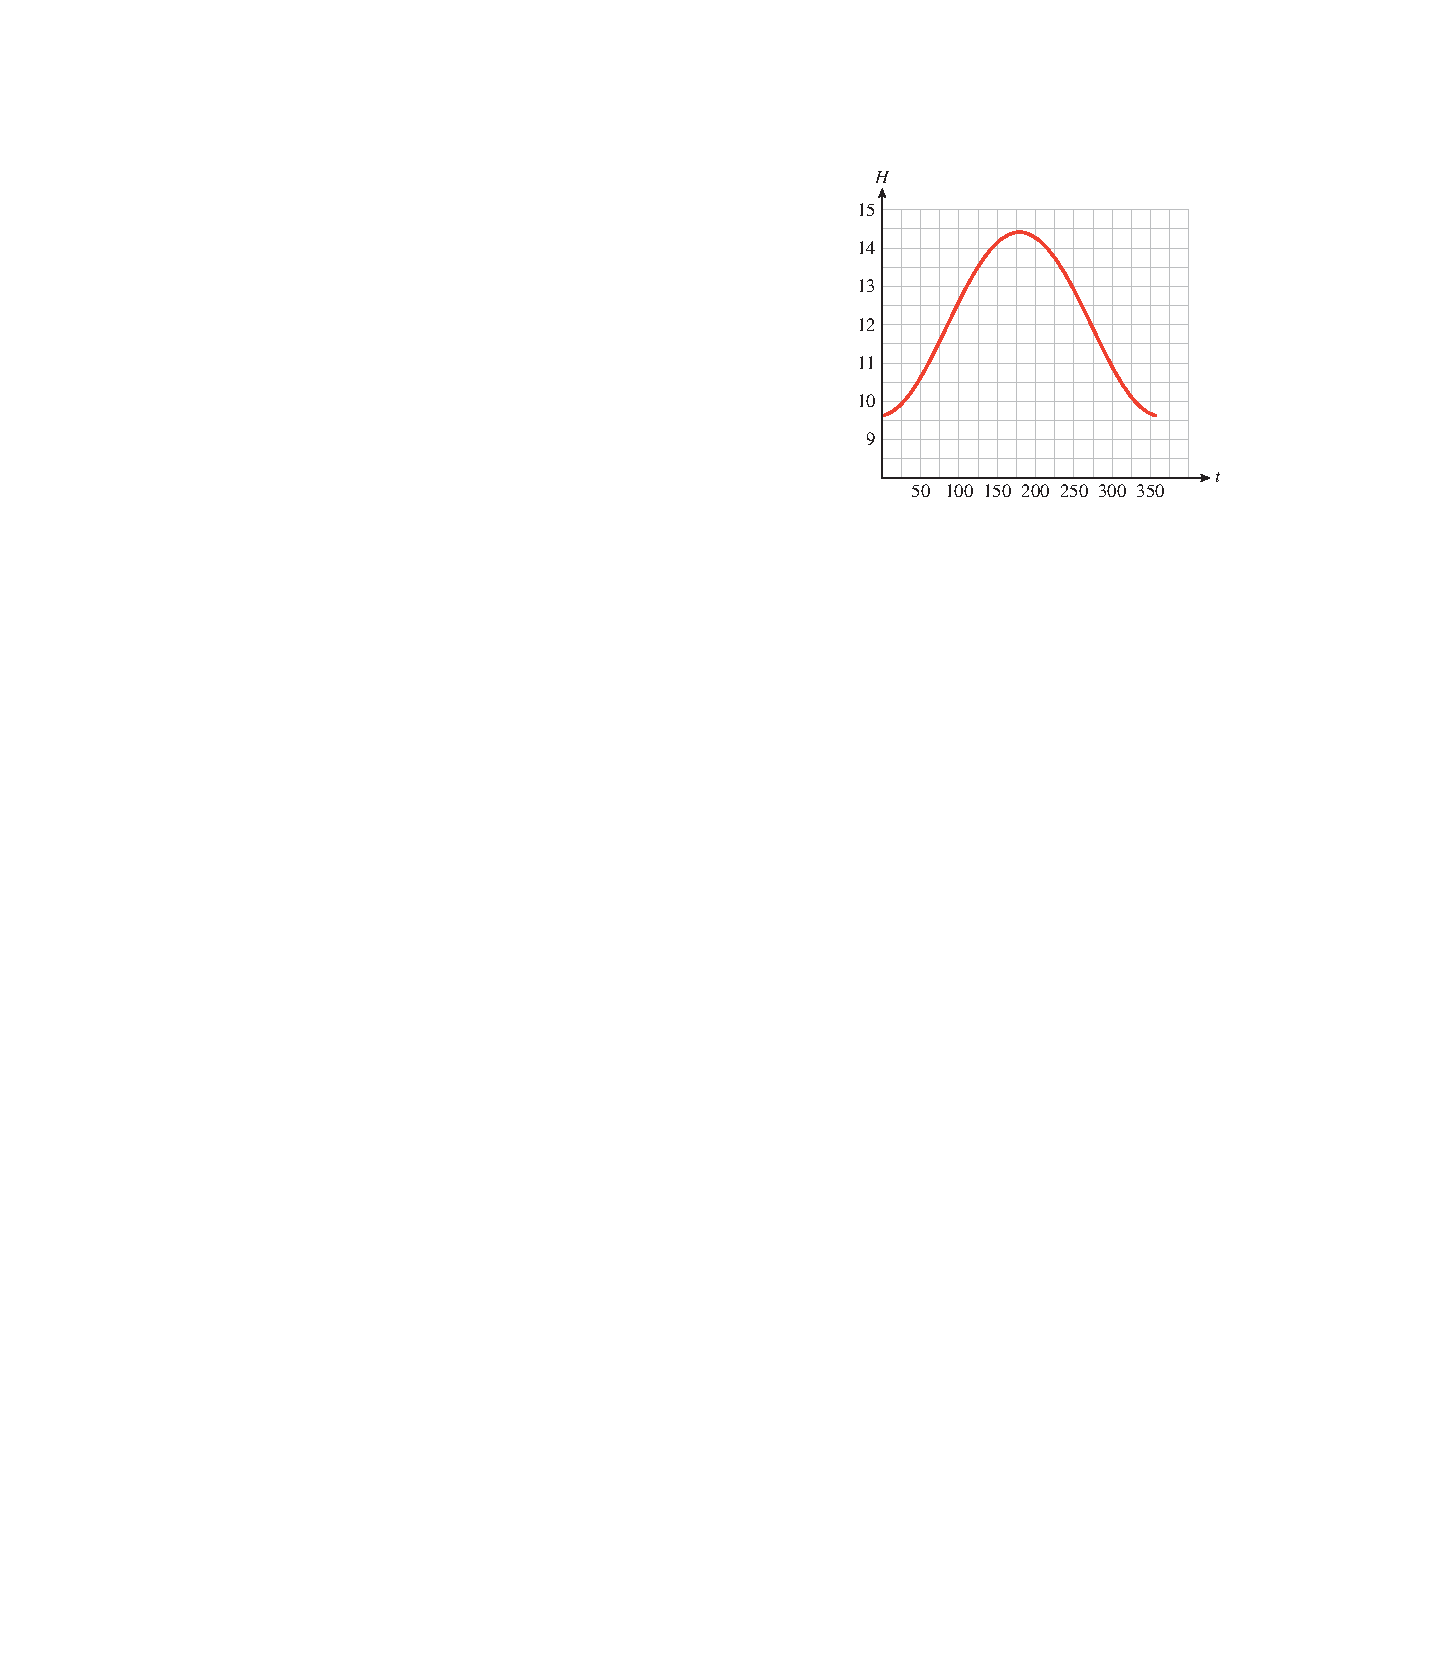
\includegraphics[width=0.4\linewidth]{../../html/PreCalculus/images/fig-sun-hours.pdf}
\end{lrbox}
\ifdefined\phAimage\else\newlength{\phAimage}\fi%
\setlength{\phAimage}{\ht\panelboxAimage+\dp\panelboxAimage}
\settototalheight{\phAimage}{\usebox{\panelboxAimage}}
\setlength{\panelmax}{\maxof{\panelmax}{\phAimage}}
\leavevmode%
% begin: side-by-side as tabular
% \tabcolsep change local to group
\setlength{\tabcolsep}{0.025\linewidth}
% @{} suppress \tabcolsep at extremes, so margins behave as intended
\par\medskip\noindent
\hspace*{0.025\linewidth}%
\begin{tabular}{@{}*{2}{c}@{}}
\begin{minipage}[c][\panelmax][t]{0.5\linewidth}\usebox{\panelboxAp}\end{minipage}&
\begin{minipage}[c][\panelmax][t]{0.4\linewidth}\usebox{\panelboxAimage}\end{minipage}\tabularnewline
&
\parbox[t]{0.4\linewidth}{\captionof{figure}{\label{fig-sun-hours}}
}\end{tabular}\\
% end: side-by-side as tabular
}% end: group for a single side-by-side
\end{example}
\hypertarget{p-39}{}%
We have a method of quickly determining if a relationship is a function once we have a graph of the relationship.%
\begin{assemblage}[The Vertical Line Test]\label{assemblage-2}
\hypertarget{p-40}{}%
A graph represents a function if and only if every vertical line intersects the graph in at most one point.%
\end{assemblage}
\begin{figure}
\centering
\centerline{Geogebra: \href{https://www.geogebra.org/m/j9j59n7z}{\mono{www.geogebra.org/m/j9j59n7z}}}
\caption{Demonstration of the Vertical Line Test\label{figure-2}}
\end{figure}
\begin{example}[]\label{example-vertical-line-test}
\hypertarget{p-41}{}%
Use the vertical line test to decide which of the graphs in \hyperref[fig-vertical-line-test2]{Figure~\ref{fig-vertical-line-test2}}  represent functions.%
\begin{figure}
\centering
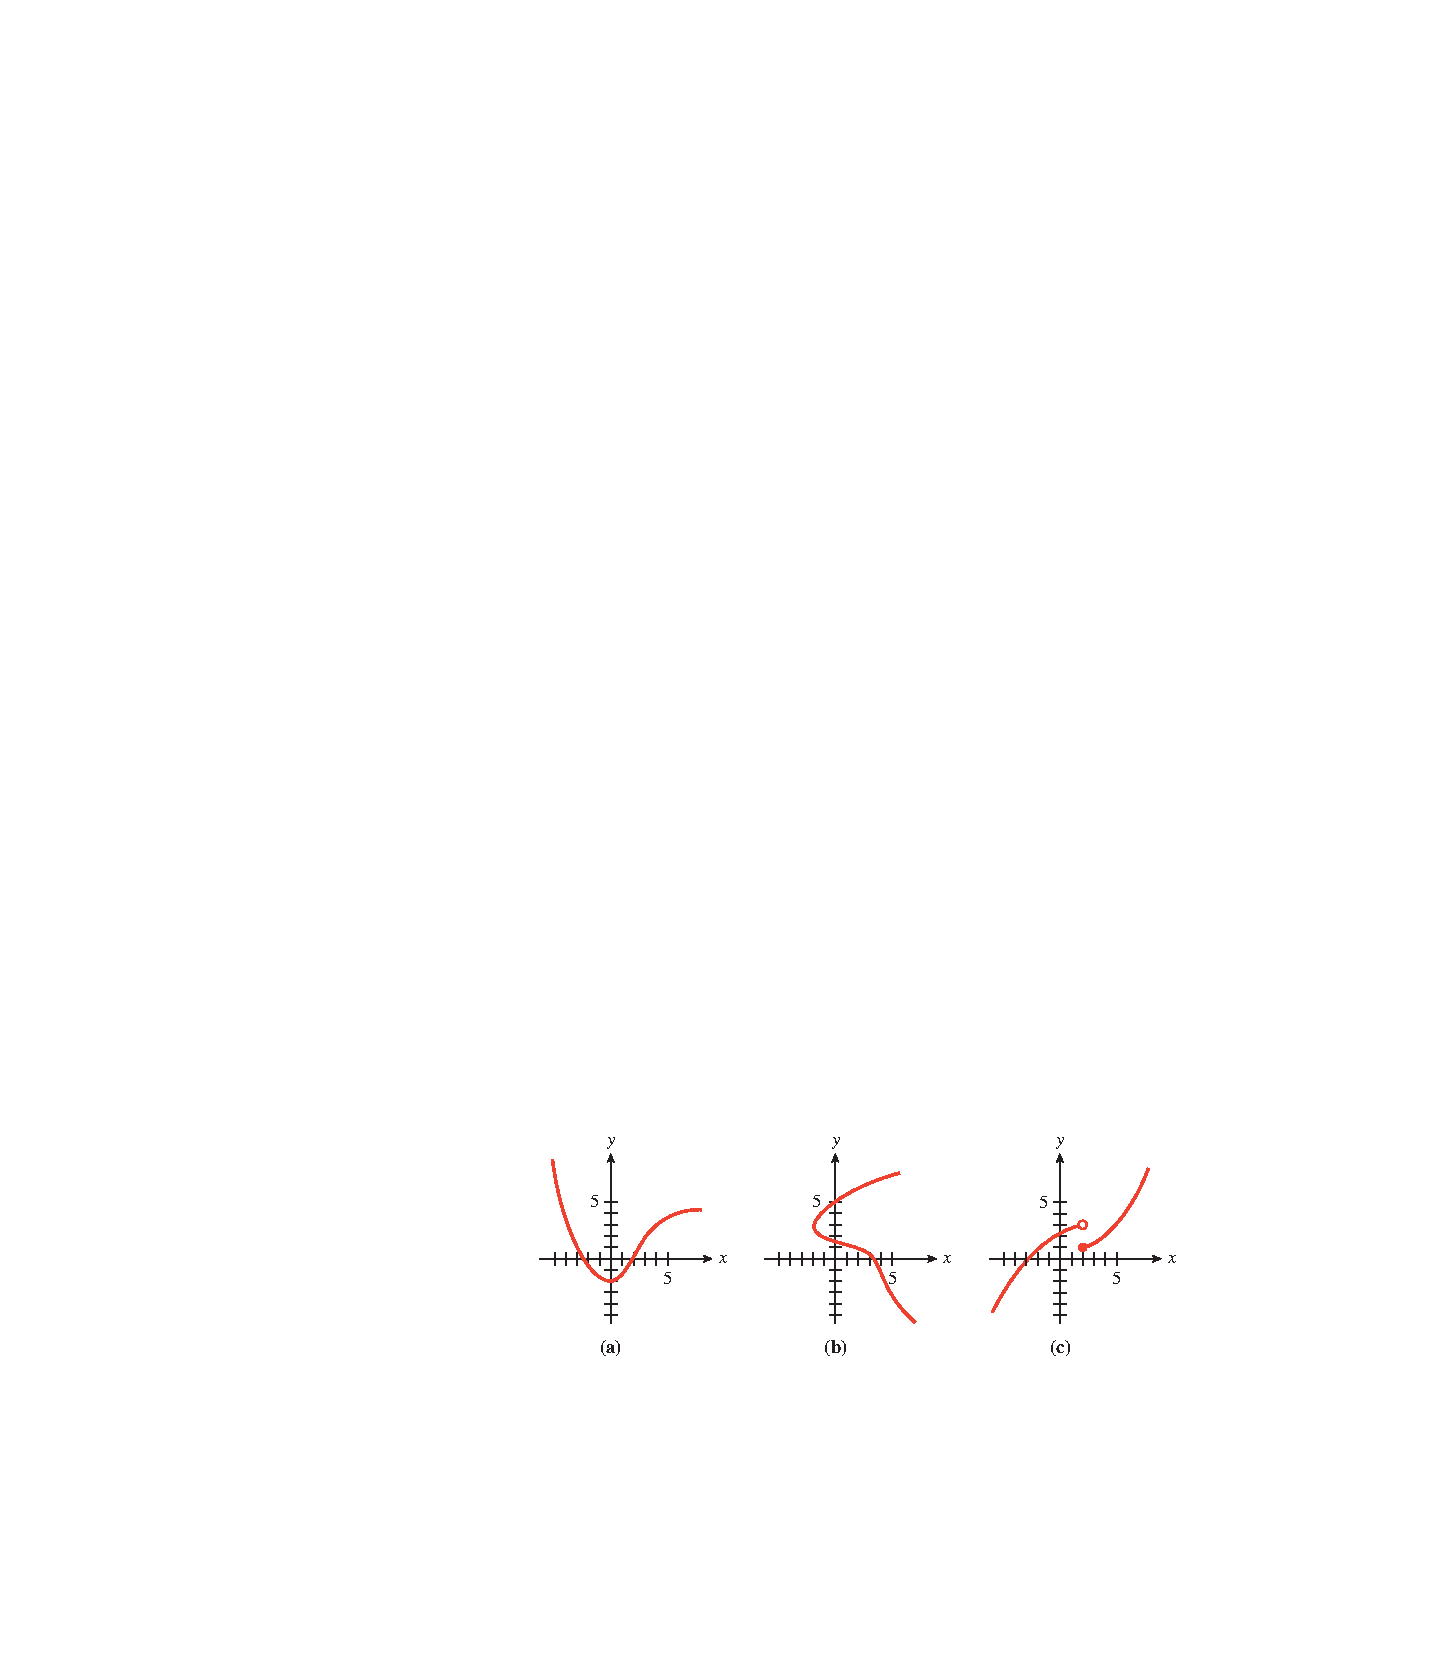
\includegraphics[width=0.9\linewidth]{../../html/Calculus/images/fig-vertical-line-test2.pdf}
\caption{\label{fig-vertical-line-test2}}
\end{figure}
\par\smallskip%
\noindent\textbf{Solution.}\hypertarget{solution-1}{}\quad%
\hypertarget{p-42}{}%
\leavevmode%
\begin{itemize}[label=\textbullet]
\item{}\hypertarget{p-43}{}%
Graph (a) represents a function, because it passes the vertical line test.%
\item{}\hypertarget{p-44}{}%
Graph (b) is not the graph of a function, because the vertical line at (for example) \(x = 1\) intersects the graph at two points.%
\item{}\hypertarget{p-45}{}%
For graph (c), notice the break in the curve at \(x = 2\): The solid dot at \((2, 1)\) is the only point on the graph with \(x = 2\); the open circle at \((2, 3)\) indicates that \((2, 3)\) is not a point on the graph. Thus, graph (c) is a function, with \(f(2) = 1\).%
\end{itemize}
%
\end{example}
\typeout{************************************************}
\typeout{Subsection 1.4 Functions Defined by Equations}
\typeout{************************************************}
\section[{Functions Defined by Equations}]{Functions Defined by Equations}\label{subsection-4}
\hypertarget{p-46}{}%
\hyperref[example-falling-book]{Example~\ref{example-falling-book}} illustrates a function defined by an equation.%
\begin{example}[]\label{example-falling-book}
\hypertarget{p-47}{}%
As of 2016,  One World Trade Center in New York City is the nations tallest building, at 1776 feet. If an algebra book is dropped from the top of One World Trade Center, its height above the ground after \(t\) seconds is given by the equation%
\begin{equation*}
h = 1776 - 16t^2
\end{equation*}
Thus, after \(1\) second the books height is%
\begin{equation*}
h = 1776 - 16(1)^2 = 1760 \text{ feet}
\end{equation*}
After \(2\) seconds its height is%
\begin{equation*}
h = 1776 - 16(2)^2 = 1712 \text{ feet}
\end{equation*}
For this function, \(t\) is the input variable and \(h\) is the output variable. For any value of \(t\), a unique value of \(h\) can be determined from the equation for \(h\). We say that \(h\) \emph{is a function of} \(t\).%
\end{example}
\typeout{************************************************}
\typeout{Subsection 1.5 Function Notation}
\typeout{************************************************}
\section[{Function Notation}]{Function Notation}\label{subsection-5}
\hypertarget{p-48}{}%
There is a convenient notation for discussing functions. First, we choose a letter, such as \(f\), \(g\), or \(h\) (or \(F\), \(G\), or \(H\)), to name a particular function. (We can use any letter, but these are the most common choices.) For instance, the height, \(h\), of a falling textbook is a function of the elapsed time, \(t\). We might call this function \(f\). In other words, \(f\) is the name of the relationship between the variables \(h\) and \(t\). We write%
\begin{equation*}
h = f (t)
\end{equation*}
which means "\(h\) is a function of \(t\), and \(f\) is the name of the function."%
\begin{example}[]\label{example-falling-book-2}
\hypertarget{p-49}{}%
In \hyperref[example-falling-book]{Example~\ref{example-falling-book}}, the height of an algebra book dropped from the top of One World Trade Center is given by the equation%
\begin{equation*}
h = 1776 - 16t^2
\end{equation*}
We see that%
\par
\hypertarget{p-50}{}%
% group protects changes to lengths, releases boxes (?)
{% begin: group for a single side-by-side
% set panel max height to practical minimum, created in preamble
\setlength{\panelmax}{0pt}
\ifdefined\panelboxAtabular\else\newsavebox{\panelboxAtabular}\fi%
\savebox{\panelboxAtabular}{%
\raisebox{\depth}{\parbox{1\linewidth}{\centering\begin{tabular}{lll}
when \(t=1\)&&\(h=1760\)\tabularnewline[0pt]
when \(t=2\)&&\(h=1712\)
\end{tabular}
}}}
\ifdefined\phAtabular\else\newlength{\phAtabular}\fi%
\setlength{\phAtabular}{\ht\panelboxAtabular+\dp\panelboxAtabular}
\settototalheight{\phAtabular}{\usebox{\panelboxAtabular}}
\setlength{\panelmax}{\maxof{\panelmax}{\phAtabular}}
\leavevmode%
% begin: side-by-side as tabular
% \tabcolsep change local to group
\setlength{\tabcolsep}{0\linewidth}
% @{} suppress \tabcolsep at extremes, so margins behave as intended
\par\medskip\noindent
\begin{tabular}{@{}*{1}{c}@{}}
\begin{minipage}[c][\panelmax][t]{1\linewidth}\usebox{\panelboxAtabular}\end{minipage}\end{tabular}\\
% end: side-by-side as tabular
}% end: group for a single side-by-side
%
\par
\hypertarget{p-51}{}%
Using function notation, these relationships can be expressed more concisely as%
\par
\hypertarget{p-52}{}%
% group protects changes to lengths, releases boxes (?)
{% begin: group for a single side-by-side
% set panel max height to practical minimum, created in preamble
\setlength{\panelmax}{0pt}
\ifdefined\panelboxAtabular\else\newsavebox{\panelboxAtabular}\fi%
\savebox{\panelboxAtabular}{%
\raisebox{\depth}{\parbox{1\linewidth}{\centering\begin{tabular}{lll}
\(f(1)=1760\)&and&\(f(2)=1712\)
\end{tabular}
}}}
\ifdefined\phAtabular\else\newlength{\phAtabular}\fi%
\setlength{\phAtabular}{\ht\panelboxAtabular+\dp\panelboxAtabular}
\settototalheight{\phAtabular}{\usebox{\panelboxAtabular}}
\setlength{\panelmax}{\maxof{\panelmax}{\phAtabular}}
\leavevmode%
% begin: side-by-side as tabular
% \tabcolsep change local to group
\setlength{\tabcolsep}{0\linewidth}
% @{} suppress \tabcolsep at extremes, so margins behave as intended
\par\medskip\noindent
\begin{tabular}{@{}*{1}{c}@{}}
\begin{minipage}[c][\panelmax][t]{1\linewidth}\usebox{\panelboxAtabular}\end{minipage}\end{tabular}\\
% end: side-by-side as tabular
}% end: group for a single side-by-side
%
\par
\hypertarget{p-53}{}%
which we read as "\(f\) of 1 equals 1760" and "\(f\) of 2 equals 1712." The values for the input variable, \(t\), appear \emph{inside} the parentheses, and the values for the output variable, \(h\), appear on the other side of the equation.%
\end{example}
\hypertarget{p-54}{}%
Remember that when we write \(y = f(x)\), the symbol \(f(x)\) is just another name for the output variable.%
\typeout{************************************************}
\typeout{Subsection 1.6 Evaluating a Function}
\typeout{************************************************}
\section[{Evaluating a Function}]{Evaluating a Function}\label{subsection-6}
\hypertarget{p-55}{}%
Finding the value of the output variable that corresponds to a particular value of the input variable is called \terminology{evaluating the function}\index{evaluating the function}.%
\begin{example}[]\label{example-postage2}
\hypertarget{p-56}{}%
Let \(g\) be the name of the postage function defined by \hyperref[table-postage]{Table~\ref{table-postage}}. Find \(g(1)\), \(g(3)\), and \(g(6.75\)).%
\par\smallskip%
\noindent\textbf{Solution.}\hypertarget{solution-2}{}\quad%
\hypertarget{p-57}{}%
According to the table,%
\par
\hypertarget{p-58}{}%
% group protects changes to lengths, releases boxes (?)
{% begin: group for a single side-by-side
% set panel max height to practical minimum, created in preamble
\setlength{\panelmax}{0pt}
\ifdefined\panelboxAtabular\else\newsavebox{\panelboxAtabular}\fi%
\savebox{\panelboxAtabular}{%
\raisebox{\depth}{\parbox{1\linewidth}{\centering\begin{tabular}{lllll}
when \(w=1\),&&\(p=0.47\)&so&\(g(1)=0.47\)\tabularnewline[0pt]
when \(w=3\),&&\(p=0.89\)&so&\(g(3)=0.89\)\tabularnewline[0pt]
when \(w=6.75\),&&\(p=1.73\)&so&\(g(6.75)=1.73\)
\end{tabular}
}}}
\ifdefined\phAtabular\else\newlength{\phAtabular}\fi%
\setlength{\phAtabular}{\ht\panelboxAtabular+\dp\panelboxAtabular}
\settototalheight{\phAtabular}{\usebox{\panelboxAtabular}}
\setlength{\panelmax}{\maxof{\panelmax}{\phAtabular}}
\leavevmode%
% begin: side-by-side as tabular
% \tabcolsep change local to group
\setlength{\tabcolsep}{0\linewidth}
% @{} suppress \tabcolsep at extremes, so margins behave as intended
\par\medskip\noindent
\begin{tabular}{@{}*{1}{c}@{}}
\begin{minipage}[c][\panelmax][t]{1\linewidth}\usebox{\panelboxAtabular}\end{minipage}\end{tabular}\\
% end: side-by-side as tabular
}% end: group for a single side-by-side
 Thus, a letter weighing 1 ounce costs \textdollar{}0.47 to mail, a letter weighing 3 ounces costs \textdollar{}0.89, and a letter weighing 6.75 ounces costs \textdollar{}1.73.%
\end{example}
\hypertarget{p-59}{}%
If a function is described by an equation, we simply substitute the given input value into the equation to find the corresponding output, or function value.%
\begin{example}[]\label{example-evaluate-function}
\hypertarget{p-60}{}%
The function \(H\) is defined by \(H=f(s) = \dfrac{\sqrt{s+3}}{s}\). Evaluate the function at the following values. \leavevmode%
\begin{enumerate}[label=\alph*]
\item\hypertarget{li-14}{}\hypertarget{p-61}{}%
\(s=6\)%
\item\hypertarget{li-15}{}\hypertarget{p-62}{}%
\(s=-1\)%
\end{enumerate}
%
\par\smallskip%
\noindent\textbf{Solution.}\hypertarget{solution-3}{}\quad%
\hypertarget{p-63}{}%
\leavevmode%
\begin{enumerate}[label=\alph*]
\item\hypertarget{li-16}{}\hypertarget{p-64}{}%
\(f(\alert{6})=\dfrac{\sqrt{\alert{6}+3}}{\alert{6}}=
\dfrac{\sqrt{9}}{6}=\dfrac{3}{6}=\dfrac{1}{2}\). Thus, \(f(6)=\dfrac{1}{2}\).%
\item\hypertarget{li-17}{}\hypertarget{p-65}{}%
\(f(\alert{-1})=\dfrac{\sqrt{\alert{-1}+3}}{\alert{-1}}=
\dfrac{\sqrt{2}}{-1}=-\sqrt{2}\). Thus, \(f(-1)=-\sqrt{2}\).%
\end{enumerate}
%
\end{example}
\hypertarget{p-66}{}%
To simplify the notation, we sometimes use the same letter for the output variable and for the name of the function.%
\typeout{************************************************}
\typeout{Subsection 1.7 Linear Functions}
\typeout{************************************************}
\section[{Linear Functions}]{Linear Functions}\label{subsection-7}
\hypertarget{p-67}{}%
Linear relationships are relationships in which the rate of change is constant. \begin{assemblage}[Linear Equation]\label{assemblage-3}
\hypertarget{p-68}{}%
A \terminology{linear function} is a function which has a \terminology{constant rate of change.}%
\end{assemblage}
 Many phenomena can be modeled using linear functions \(y = f (x)\) where the equations have the form%
\begin{equation*}
f (x) = (\text{starting value}) + (\text{rate of change}) \cdot x.
\end{equation*}
The initial value, or the value of \(f(0)\), is the vertical intercept of the graph, and the rate of change is the slope of the graph. Thus, we can write an equation of a line as%
\begin{equation*}
f (x) = b + mx
\end{equation*}
where the constant term, \(b\), is the vertical intercept of the line, and \(m\), the coefficient of \(x\), is the slope of the line. This form for an equation of a line is called the \terminology{slope-intercept form}\index{slope-intercept form}.%
\begin{assemblage}[Slope-Intercept Form]\label{assemblage-4}
\hypertarget{p-69}{}%
If we write an equation of a linear function in the form,%
\begin{equation*}
f (x) = b + mx
\end{equation*}
then \(m\) is the \terminology{slope}\index{slope} of the line, and \(b\) is the \terminology{vertical intercept}.%
\end{assemblage}
\begin{example}[]\label{example-linear-function1}
\hypertarget{p-70}{}%
An icicle grows according to the formula \(H(t)=0.05t+0.12\), where \(t\) is the time in minutes since the first measurement was take, and \(H(t)\) is the height of the icicle in centimeters.%
\par
\hypertarget{p-71}{}%
\leavevmode%
\begin{enumerate}[label=\alph*]
\item\hypertarget{li-18}{}\hypertarget{p-72}{}%
The slope is 0.05, which tells us that the icicle's height grows by 0.05 cm each minute.%
\item\hypertarget{li-19}{}\hypertarget{p-73}{}%
The \(y\)-intercept is 0.12, which tells us that the height of the icicle was 0.12 cm at the first measurement.%
\end{enumerate}
%
\end{example}
\begin{example}[]\label{example-linear-function2}
\hypertarget{p-74}{}%
Samantha owns a catering business. For any party with up to 100 guests, she charges $2,000. She charges $8 per person for each additional guest over 100. Give a formula for the cost of having Samantha cater your party as a function of the number of guests over 200.%
\par\smallskip%
\noindent\textbf{Solution.}\hypertarget{solution-4}{}\quad%
\hypertarget{p-75}{}%
A possible formula for the cost of having Samantha cater your party is \(C(g)=2000+8g\), where \(g\) is the number of guests over 100.%
\end{example}
\hypertarget{p-76}{}%
The following formula provides a method to finding the value of the slope \(m\) when given two points on the line.%
\begin{assemblage}[Two-Point Slope Formula]\label{assemblage-5}
\hypertarget{p-77}{}%
The slope of the line passing through the points \(P_1 (x_1, y_1)\) and \(P_2 (x_2, y_2)\) is given by%
\begin{equation*}
m = \frac{\Delta y}{\Delta x}= \frac{y_2 - y_1}{x_2 - x_1} 
\text{, }~x_2 \ne x_1.
\end{equation*}
%
\end{assemblage}
\begin{example}[]\label{example-two-point-slope}
\hypertarget{p-78}{}%
Compute the slope of the line between the points \((6, -3)\) and \((4, 3)\).%
\par\smallskip%
\noindent\textbf{Solution.}\hypertarget{solution-5}{}\quad%
\hypertarget{p-79}{}%
Substitute the coordinates of \(Q_1\) and \(Q_2\) into the slope formula to find%
\begin{equation*}
m = \frac{y_2 - y_1}{x_2 - x_1}= \frac{3 - (-3)}{4 - 6}
= \frac{6}{-2}= -3.
\end{equation*}
This value for the slope, \(-3\), is the same value found above.%
\end{example}
\hypertarget{p-80}{}%
Sometimes you will be given the slope of a line and another point on that line. The following formula is helpful in that situation.%
\begin{assemblage}[Point-Slope Form]\label{assemblage-6}
\hypertarget{p-81}{}%
An equation of the line that passes through the point \((x_1, y_1)\) and has slope \(m\) is%
\begin{equation*}
y= y_1 + m(x- x_1).
\end{equation*}
%
\end{assemblage}
\begin{example}[]\label{example-point-slope2}
\hypertarget{p-82}{}%
Find a formula for the line that has slope -2 and passes through the point \((-1,4)\)%
\par\smallskip%
\noindent\textbf{Solution.}\hypertarget{solution-6}{}\quad%
\hypertarget{p-83}{}%
Using point-slope form, we have the line \(y=4+(-2)(x-(-1))\).%
\par
\hypertarget{p-84}{}%
We can also write this in slope-intercept form by simplifying: \(y=2-2x\).%
\end{example}
\hypertarget{p-85}{}%
Is is also useful to introduce the term \(x\)-intercept. \begin{assemblage}[\(x\)-intercept]\label{assemblage-7}
\hypertarget{p-86}{}%
An \terminology{\(x\)-intercept} for a function \(f(x)\) is the value of \(x\) such that \(f(x)=0\).%
\end{assemblage}
%
\begin{note}[]\label{note-1}
\hypertarget{p-87}{}%
In the equation \(f (x) = b + mx\), we call \(m\) and \(b\) \terminology{parameters}\index{parameters}. Their values are fixed for any particular linear equation; for example, in the equation \(y = 2x + 3\), \(m = 2\) and \(b = 3\), and the variables are \(x\) and \(y\). By changing the values of \(m\) and \(b\), we can write the equation for any line except a vertical line (see \hyperref[fig-slope-vs-intercept]{Figure~\ref{fig-slope-vs-intercept}}). The collection of all linear functions \(f (x) = b + mx\) is called a \terminology{two-parameter}\index{two-parameter} family of functions.%
\end{note}
\begin{figure}
\centering
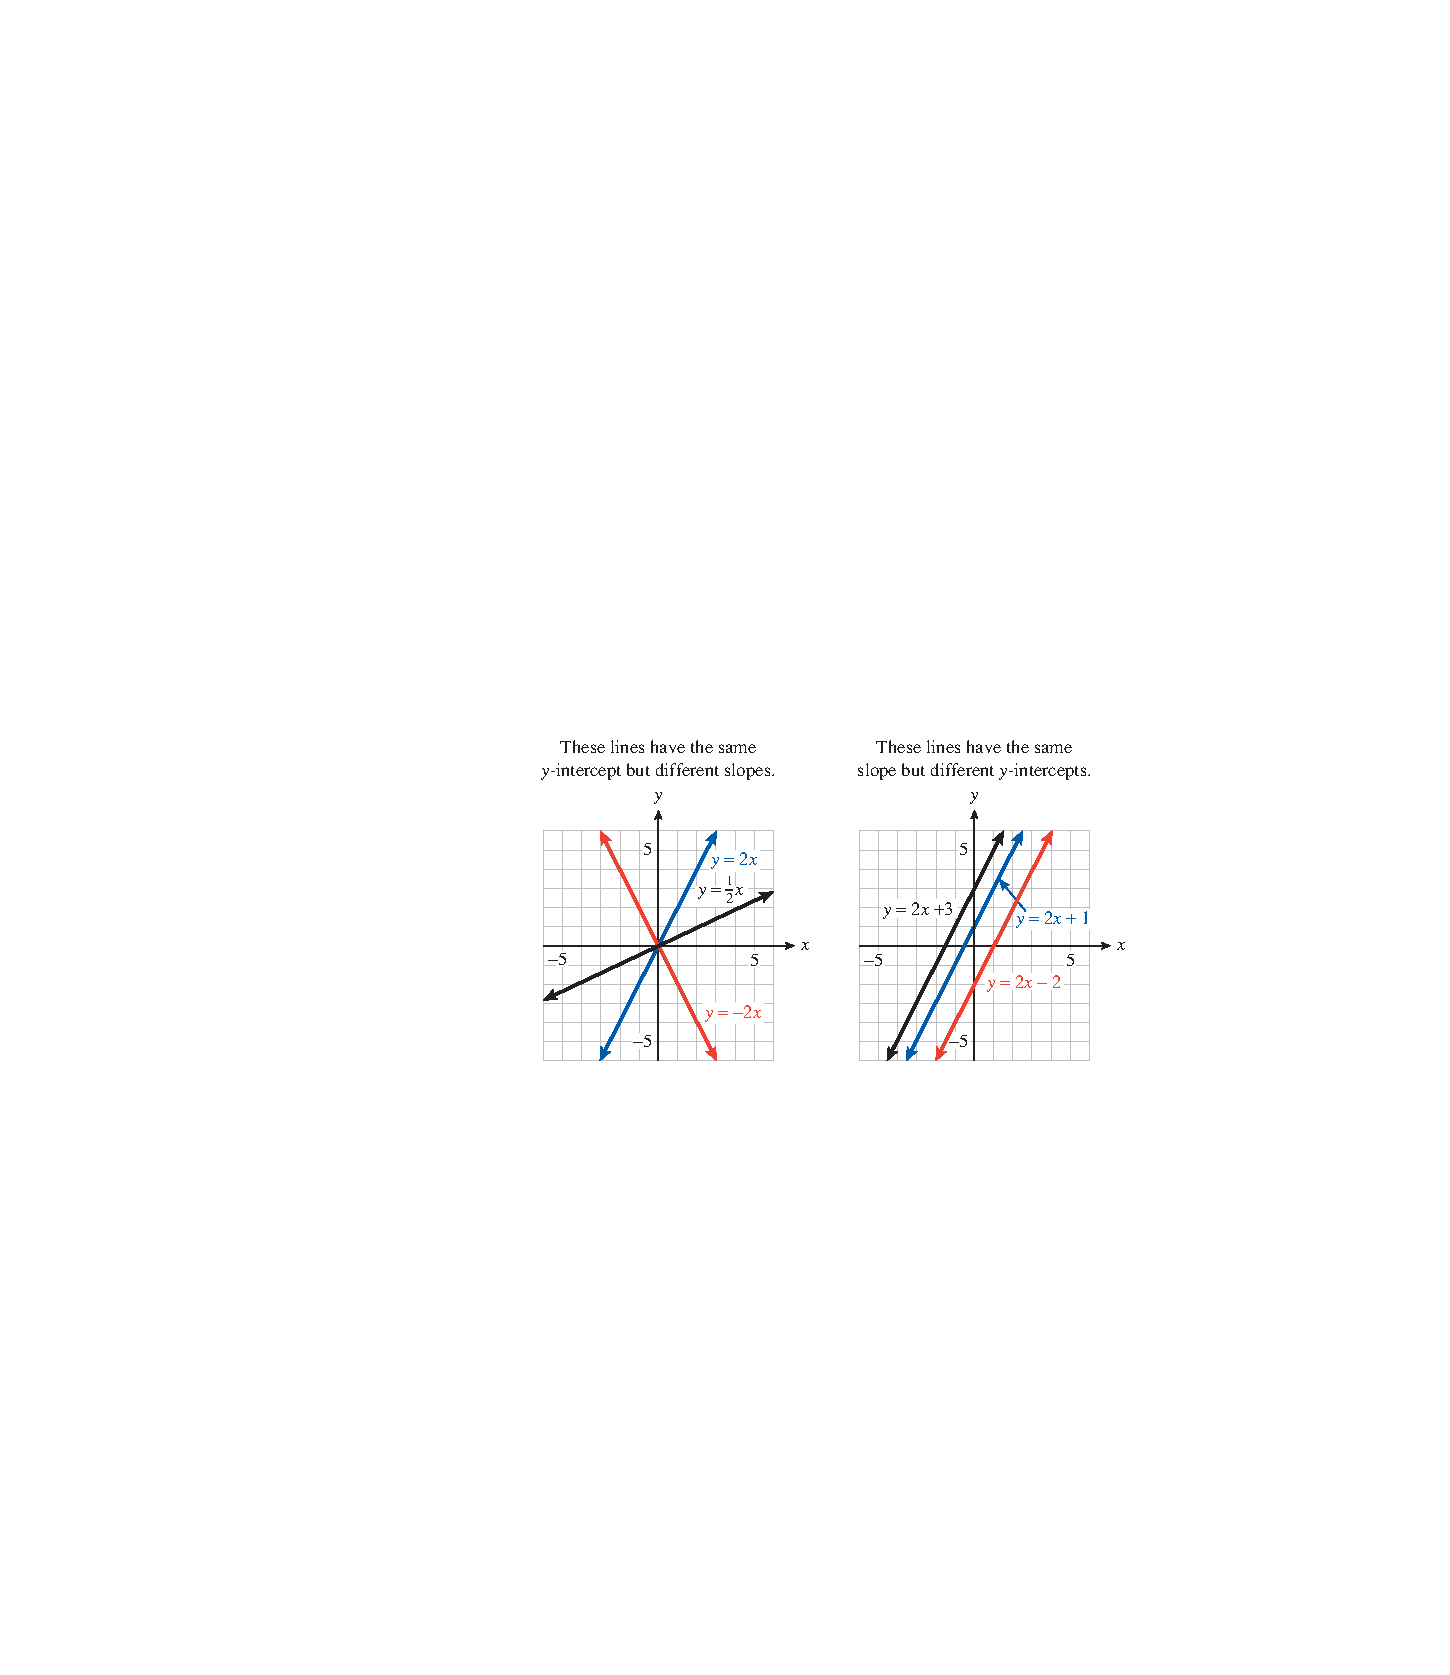
\includegraphics[width=0.8\linewidth]{../../html/PreCalculus/images/fig-slope-vs-intercept.pdf}
\caption{\label{fig-slope-vs-intercept}}
\end{figure}
\typeout{************************************************}
\typeout{Subsection 1.8 Describing Functions}
\typeout{************************************************}
\section[{Describing Functions}]{Describing Functions}\label{subsection-8}
\hypertarget{p-88}{}%
There are several terms that will be useful in describing functions.  We first begin with the notion of an increasing function.%
\begin{assemblage}[Increasing Function]\label{assemblage-8}
\hypertarget{p-89}{}%
A function \(f\) is increasing if the values of \(f(x)\) increase as \(x\) increases. The graph of an increasing function climbs as we move from left to right.%
\end{assemblage}
\begin{assemblage}[Decreasing Function]\label{assemblage-9}
\hypertarget{p-90}{}%
A function \(f\) is decreasing if the values of \(f(x)\) decrease as \(x\) increases. The graph of a decreasing function falls as we move from left to right.%
\end{assemblage}
\begin{assemblage}[Monotonic Funcion]\label{assemblage-10}
\hypertarget{p-91}{}%
A function \(f(x)\) is monotonic if it increases for all \(x\) or decreases for all \(x\).%
\end{assemblage}
\begin{assemblage}[Directly Proportional]\label{assemblage-11}
\hypertarget{p-92}{}%
We say \(y\) is directly proportional to \(x\) if there is a nonzero constant \(k\) such that, \(y = kx\). This \(k\) is called the constant of proportionality.%
\end{assemblage}
\begin{assemblage}[Inversely Proportional]\label{assemblage-12}
\hypertarget{p-93}{}%
We say that \(y\) is inversely proportional to \(x\) if \(y\) is proportional to the reciprocal of \(x\), that is, \(y = \frac{k}{x}\) for a nonzero constant \(k\).%
\end{assemblage}
\typeout{************************************************}
\typeout{Subsection 1.9 Function Transformations}
\typeout{************************************************}
\section[{Function Transformations}]{Function Transformations}\label{subsection-9}
\hypertarget{p-94}{}%
It is also useful to talk about transformations of functions.  Several key facts will be useful.%
\begin{assemblage}[Function Transformations]\label{assemblage-13}
\hypertarget{p-95}{}%
\leavevmode%
\begin{enumerate}
\item\hypertarget{li-20}{}Multiplying a function by a constant, \(c\), stretches the graph vertically (if \(c \gt 1\)) or shrinks the graph vertically (if \(0 \lt c \lt 1\))%
\item\hypertarget{li-21}{}A negative sign (if \(c \lt 0\)) reflects the graph about the \(x\)-axis, in addition to shrinking or stretching.%
\item\hypertarget{li-22}{}Replacing \(y\) by \((y+k)\) moves a graph up by \(k\) (down if \(k\) is negative).%
\item\hypertarget{li-23}{}Replacing \(x\) by \((x-h)\) moves a graph to the right by \(h\) (to the left if \(h\) is negative).%
\end{enumerate}
%
\end{assemblage}
\begin{example}[]\label{example-12}
\hypertarget{p-96}{}%
Let \(f(x)=x^2\). We will explore different transformations performed on the graph of \(f(x)\).%
\par
\hypertarget{p-97}{}%
\leavevmode%
\begin{enumerate}[label=\alph*]
\item\hypertarget{li-24}{}\hypertarget{p-98}{}%
\(g(x)=2\cdotf(x)=2x^2\) is a vertical stretch of \(f(x)\) by a factor of 2.%
\item\hypertarget{li-25}{}\hypertarget{p-99}{}%
\(h(x)=-2\cdotf(x)=-2x^2\) is a vertical stretch of \(f(x)\) by a factor of 2 and a reflection across the \(x\)-axis.%
\item\hypertarget{li-26}{}\hypertarget{p-100}{}%
\(j(x)=f(x)+5=x^2+5\) is a vertical shift of \(f(x)\) up 5 units.%
\item\hypertarget{li-27}{}\hypertarget{p-101}{}%
\(k(x)=f(x+5)=(x+5)^2\) is a horizontal shift of \(f(x)\) left 5 units.%
\end{enumerate}
%
\end{example}
\begin{assemblage}[Order of Transformations]\label{assemblage-14}
\hypertarget{p-102}{}%
Suppose that \(f(x)\) is our function we are applying transformations to. Once written in the form%
\begin{equation*}
a\cdot f(b\cdot (x+h))+k
\end{equation*}
the order of transformations is:%
\par
\hypertarget{p-103}{}%
\leavevmode%
\begin{enumerate}
\item\hypertarget{li-28}{}horizontal stretch or compress by a factor of \(\abs{b}\) or \(\abs{\dfrac{1}{b}}\) (if \(b\lt 0\) then also reflect about \(y\)-axis)%
\item\hypertarget{li-29}{}shift horizontally left/ right by \(\abs{h} \)%
\item\hypertarget{li-30}{}vertically stretch or compress by a factor of \(\abs{a}\) or \(\abs{\dfrac{1}{a}}\) (if \(a\lt 0\) then also reflect about \(x\)-axis)%
\item\hypertarget{li-31}{}shift vertically up/ down by \(\abs{k} \)%
\end{enumerate}
%
\end{assemblage}
\begin{example}[]\label{example-13}
\hypertarget{p-104}{}%
Describe the function%
\begin{equation*}
5\cdot [f(-3x-6)-1]
\end{equation*}
as a list of transformations done to \(f(x)\) in the appropriate order.%
\par\smallskip%
\noindent\textbf{Solution.}\hypertarget{solution-7}{}\quad%
\hypertarget{p-105}{}%
First, let's rewrite the function in the form given above: \begin{align*} 5\cdot [f(-3x-6)-1]\amp = 5f(-3x-6)-5 \ \ \text{we distributed in the 5}\\ \amp = 5f(-3(x+2))-5 \ \ \text{we factored out the -3} \end{align*} Now that the function is written in the desired order, we may list off the transformations in the correct order using the order discussed above: \leavevmode%
\begin{enumerate}
\item\hypertarget{li-32}{}horizontal compress by \(3\) and reflect about the \(y\)-axis%
\item\hypertarget{li-33}{}shift horizontally left by \(2 \)%
\item\hypertarget{li-34}{}vertically stretch by \(5\)%
\item\hypertarget{li-35}{}shift vertically down by \(5 \)%
\end{enumerate}
%
\end{example}
\typeout{************************************************}
\typeout{Subsection 1.10 Inverse Functions}
\typeout{************************************************}
\section[{Inverse Functions}]{Inverse Functions}\label{subsection-10}
\hypertarget{p-106}{}%
It is also useful to consider inverse functions.%
\begin{assemblage}[Inverse Functions]\label{assemblage-15}
\hypertarget{p-107}{}%
Suppose the inverse of \(f\) is a function, denoted by \(f^{-1}\). Then%
\begin{equation*}
f^{-1}(y) = x \text{ if and only if }f(x) = y.
\end{equation*}
%
\end{assemblage}
\begin{example}[]\label{example-inverse-functions}
\hypertarget{p-108}{}%
Suppose \(g\) is the inverse function for \(f\), and we know the following function values for \(f\):%
\begin{equation*}
f (-3) = 5, ~~ f (2) = 1, ~~ f (5) = 0.
\end{equation*}
Find \(g(5)\) and \(g(0)\).%
\par\smallskip%
\noindent\textbf{Solution.}\hypertarget{solution-8}{}\quad%
\hypertarget{p-109}{}%
We know that \(g(5) = -3\) because \(f (-3) = 5\), and \(g(0) = 5\) because \(f (5) = 0\). Tables may be helpful in visualizing the two functions, as shown below.%
% group protects changes to lengths, releases boxes (?)
{% begin: group for a single side-by-side
% set panel max height to practical minimum, created in preamble
\setlength{\panelmax}{0pt}
\ifdefined\panelboxAtabular\else\newsavebox{\panelboxAtabular}\fi%
\savebox{\panelboxAtabular}{%
\raisebox{\depth}{\parbox{0.19\linewidth}{\centering\begin{tabular}{AcAcA}\hrulethick
\multicolumn{2}{AcA}{\(y=f(x)\)}\tabularnewline\hrulethin
\(x\)&\(y\)\tabularnewline\hrulethin
\(-3\)&\(5\)\tabularnewline\hrulethin
\(2\)&\(1\)\tabularnewline\hrulethin
\(5\)&\(0\)\tabularnewline\hrulethin
\end{tabular}
}}}
\ifdefined\phAtabular\else\newlength{\phAtabular}\fi%
\setlength{\phAtabular}{\ht\panelboxAtabular+\dp\panelboxAtabular}
\settototalheight{\phAtabular}{\usebox{\panelboxAtabular}}
\setlength{\panelmax}{\maxof{\panelmax}{\phAtabular}}
\ifdefined\panelboxAp\else\newsavebox{\panelboxAp}\fi%
\savebox{\panelboxAp}{%
\raisebox{\depth}{\parbox{0.45\linewidth}{→ Interchange the columns →}}}
\ifdefined\phAp\else\newlength{\phAp}\fi%
\setlength{\phAp}{\ht\panelboxAp+\dp\panelboxAp}
\settototalheight{\phAp}{\usebox{\panelboxAp}}
\setlength{\panelmax}{\maxof{\panelmax}{\phAp}}
\ifdefined\panelboxBtabular\else\newsavebox{\panelboxBtabular}\fi%
\savebox{\panelboxBtabular}{%
\raisebox{\depth}{\parbox{0.19\linewidth}{\centering\begin{tabular}{AcAcA}\hrulethick
\multicolumn{2}{AcA}{\(x=g(y)\)}\tabularnewline\hrulethin
\(y\)&\(x\)\tabularnewline\hrulethin
\(5\)&\(-3\)\tabularnewline\hrulethin
\(1\)&\(2\)\tabularnewline\hrulethin
\(0\)&\(5\)\tabularnewline\hrulethin
\end{tabular}
}}}
\ifdefined\phBtabular\else\newlength{\phBtabular}\fi%
\setlength{\phBtabular}{\ht\panelboxBtabular+\dp\panelboxBtabular}
\settototalheight{\phBtabular}{\usebox{\panelboxBtabular}}
\setlength{\panelmax}{\maxof{\panelmax}{\phBtabular}}
\leavevmode%
% begin: side-by-side as tabular
% \tabcolsep change local to group
\setlength{\tabcolsep}{0.0075\linewidth}
% @{} suppress \tabcolsep at extremes, so margins behave as intended
\par\medskip\noindent
\hspace*{0.07\linewidth}%
\begin{tabular}{@{}*{3}{c}@{}}
\begin{minipage}[c][\panelmax][c]{0.19\linewidth}\usebox{\panelboxAtabular}\end{minipage}&
\begin{minipage}[c][\panelmax][c]{0.45\linewidth}\usebox{\panelboxAp}\end{minipage}&
\begin{minipage}[c][\panelmax][c]{0.19\linewidth}\usebox{\panelboxBtabular}\end{minipage}\end{tabular}\\
% end: side-by-side as tabular
}% end: group for a single side-by-side
\par
\hypertarget{p-111}{}%
For the function \(f\), the input variable is \(x\) and the output variable is \(y\). For the inverse function \(g\), the roles of the variables are interchanged: \(y\) is now the input and \(x\) is the output.%
\end{example}
\begin{assemblage}[Functions and Inverse Functions]\label{assemblage-16}
\hypertarget{p-112}{}%
Suppose \(f^{-1}\) is the inverse function for \(f\). Then%
\begin{equation*}
f^{-1}\left(f(x)\right) = x\text{ and }f\left(f^{-1}( y)\right) = y
\end{equation*}
as long as \(x\) is in the domain of \(f\), and \(y\) is in the domain of \(f^{-1}\).%
\end{assemblage}
\hypertarget{p-113}{}%
We also have a method of quickly determining if a function is invertible once we have a graph of the function.%
\begin{assemblage}[Horizontal Line Test]\label{assemblage-17}
\hypertarget{p-114}{}%
If no horizontal line intersects the graph of a function more than once, then its inverse is also a function.%
\end{assemblage}
\begin{figure}
\centering
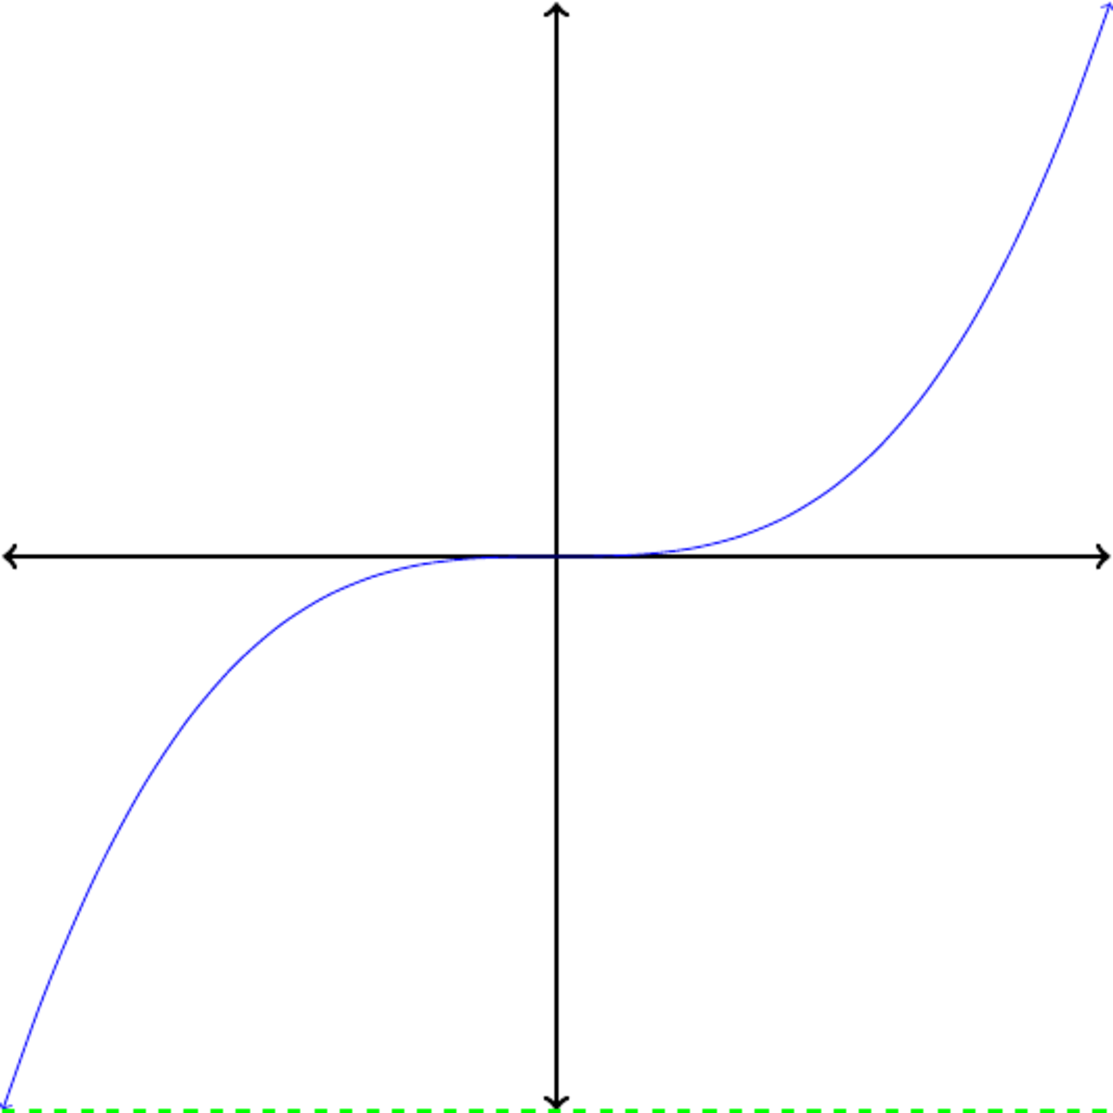
\includegraphics[width=0.7\linewidth]{../../html/Calculus/images/HorizontalLineTest.gif}
\caption{Notice that as the line moves up the \(y-\) axis, it only ever intersects the graph in a single place.  This means this function is invertible.\label{fig-horizontal-line-test-animation}}
\end{figure}
\begin{figure}
\centering
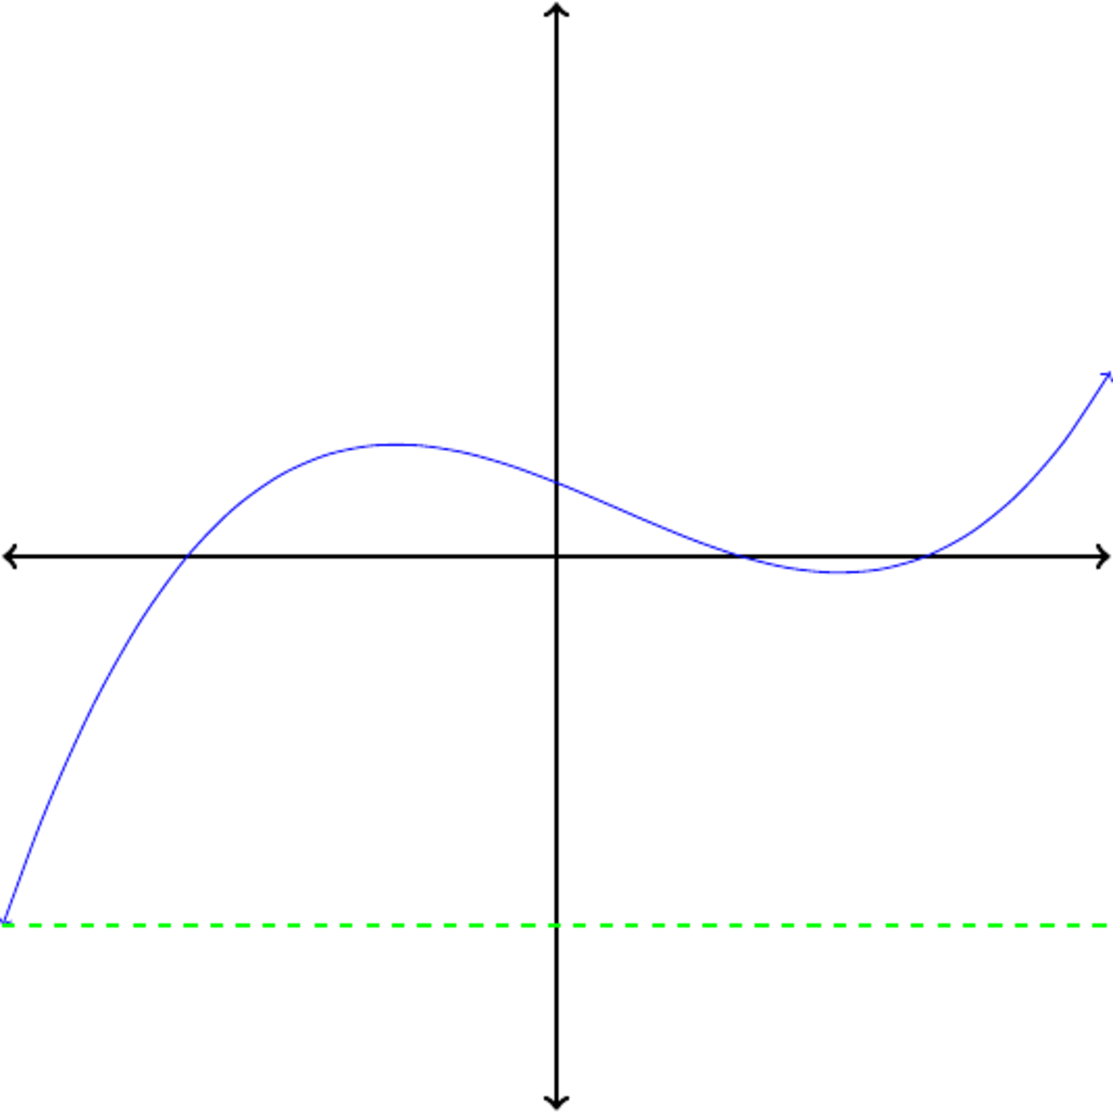
\includegraphics[width=0.7\linewidth]{../../html/Calculus/images/HorizontalLineTestFail.gif}
\caption{Notice that as the line moves up the \(y-\) axis, it sometimes intersects the graph in more than one place.  This means this function is not invertible.\label{fig-horizontal-line-test-fail-animation}}
\end{figure}
\begin{example}[]\label{example-invertible-or-not}
\hypertarget{p-115}{}%
Which of the functions in \hyperref[fig-invertible-or-not]{Figure~\ref{fig-invertible-or-not}} are invertible?%
\begin{figure}
\centering
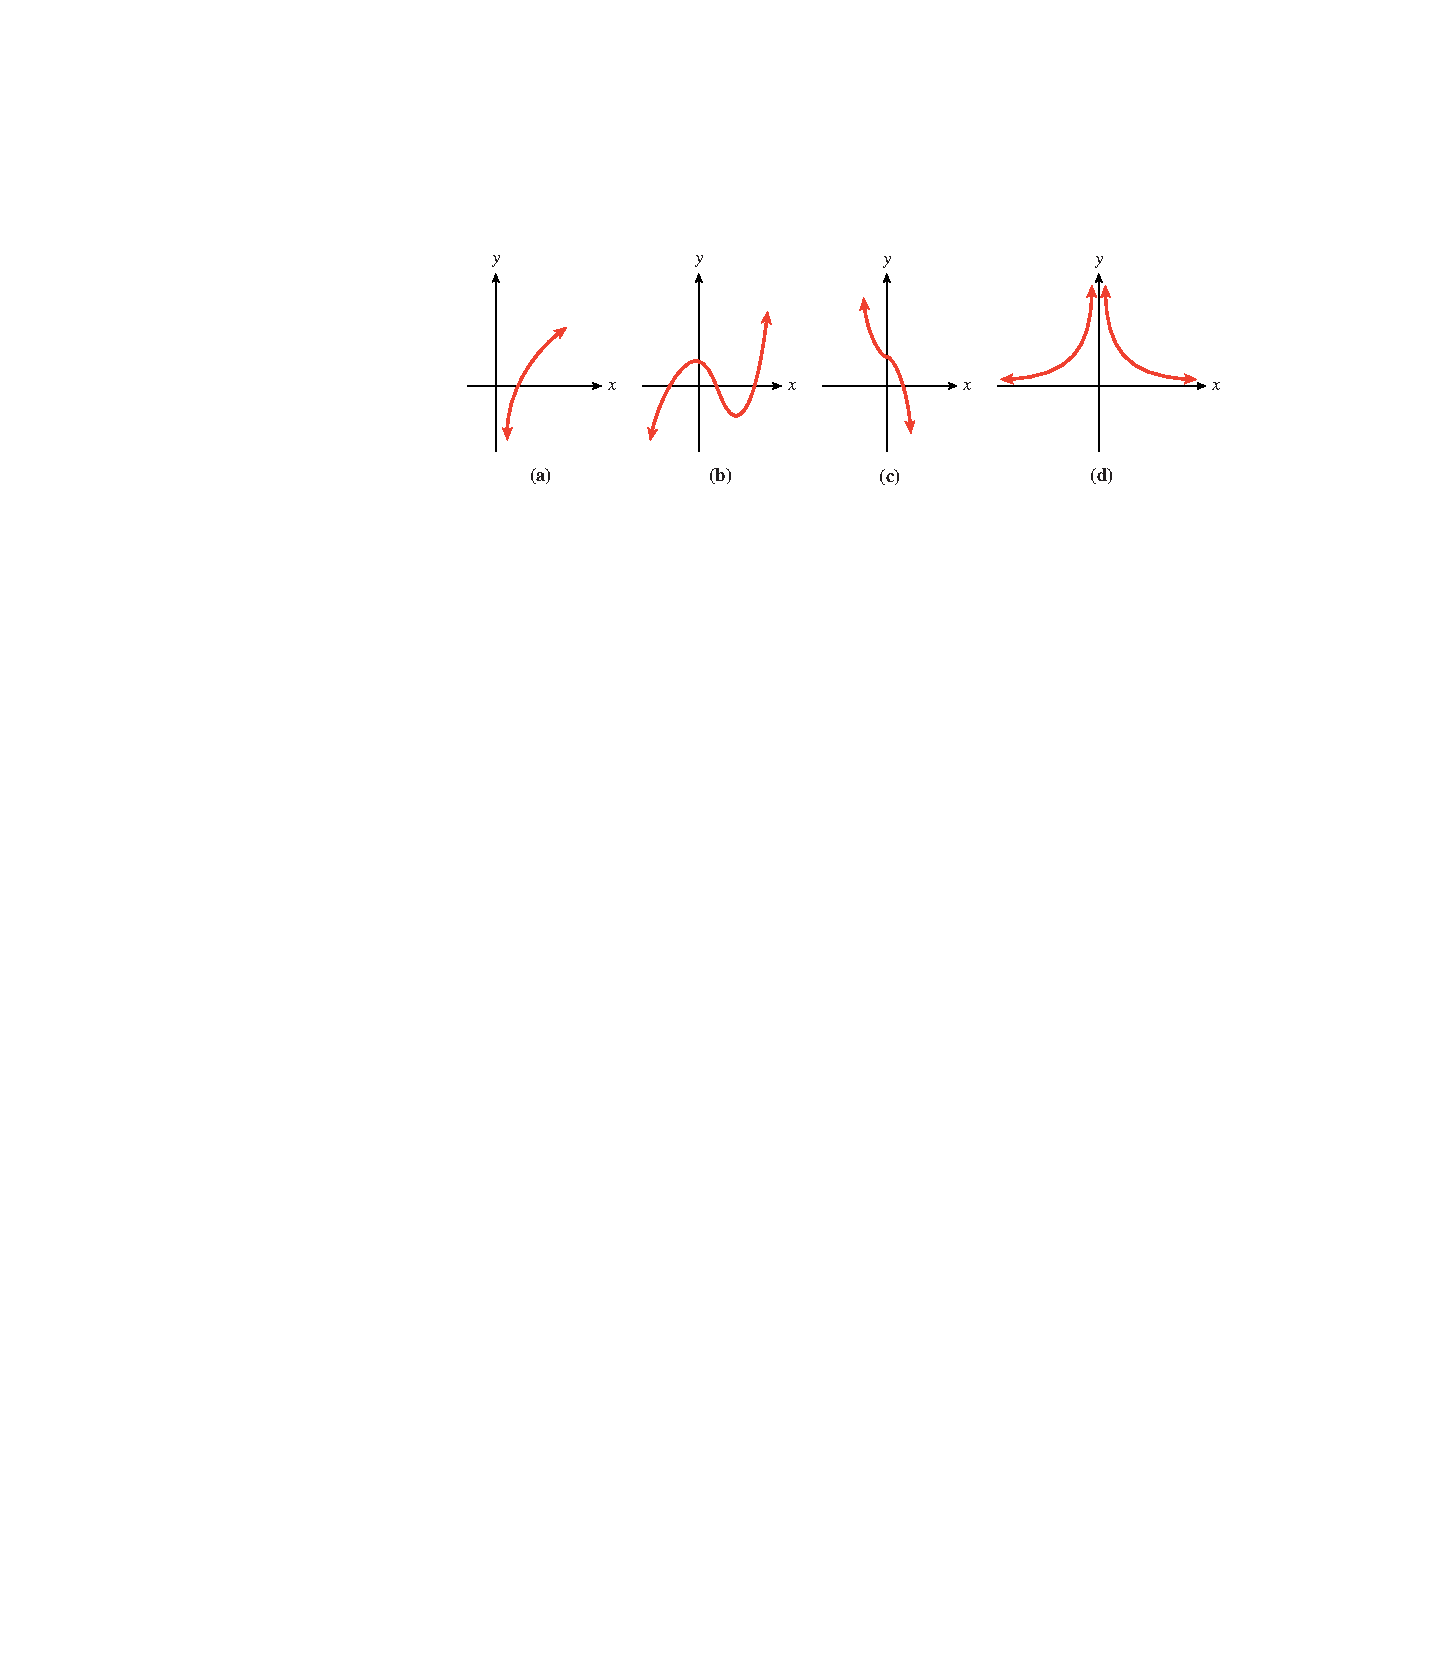
\includegraphics[width=0.9\linewidth]{../../html/Calculus/images/fig-invertible-or-not.pdf}
\caption{\label{fig-invertible-or-not}}
\end{figure}
\par\smallskip%
\noindent\textbf{Solution.}\hypertarget{solution-9}{}\quad%
\hypertarget{p-116}{}%
In each case, apply the horizontal line test to determine whether the function is invertible. Because no horizontal line intersects their graphs more than once, the functions pictured in \hyperref[fig-invertible-or-not]{Figures~\ref{fig-invertible-or-not}}(a) and (c) are invertible. The functions in \hyperref[fig-invertible-or-not]{Figures~\ref{fig-invertible-or-not}}(b) and (d) are not invertibe.%
\end{example}
\hypertarget{p-117}{}%
We have been talking about how to tell if the inverse of a function is also a function, but in practice this is not the language typicaly used. Usually we ask this same question in the form "Is the function invertible?" The following definition explains this relationship: \begin{assemblage}[Invertible Function]\label{assemblage-18}
\hypertarget{p-118}{}%
If \(y=f(x) \) is a function such that its inverse, \(x=f^{-1}(y)\), is also a function then we say that \(f(x) \) is an \terminology{invertible function}.%
\end{assemblage}
%
\par
\hypertarget{p-119}{}%
The inverse function \(f^{-1}\) undoes the effect of the function \(f\). The function \(f(t) = 6 + 2t\) multiplies the input by \(2\) and then adds \(6\) to the result. The inverse function \(f^{-1}(H) = \dfrac{H -6}{2}\) undoes those operations in reverse order: It subtracts \(6\) from the input and then divides the result by \(2\).%
\par
\hypertarget{p-120}{}%
If we apply the function \(f\) to a given input value and then apply the function \(f^{-1}\) to the output from \(f\), the end result will be the original input value. For example, if we choose \(t = 5\) as an input value, we find that \begin{align*} f(5)\amp= 6 + 2(5) = 16\amp\amp\text{ Multiply by 2, then add 6.}\\ \text{and } f^{-1}(16) \amp = \frac{16 - 6}{2} = 5.\amp\amp\text{Subtract 6, then divide by 2.} \end{align*}%
\begin{figure}
\centering
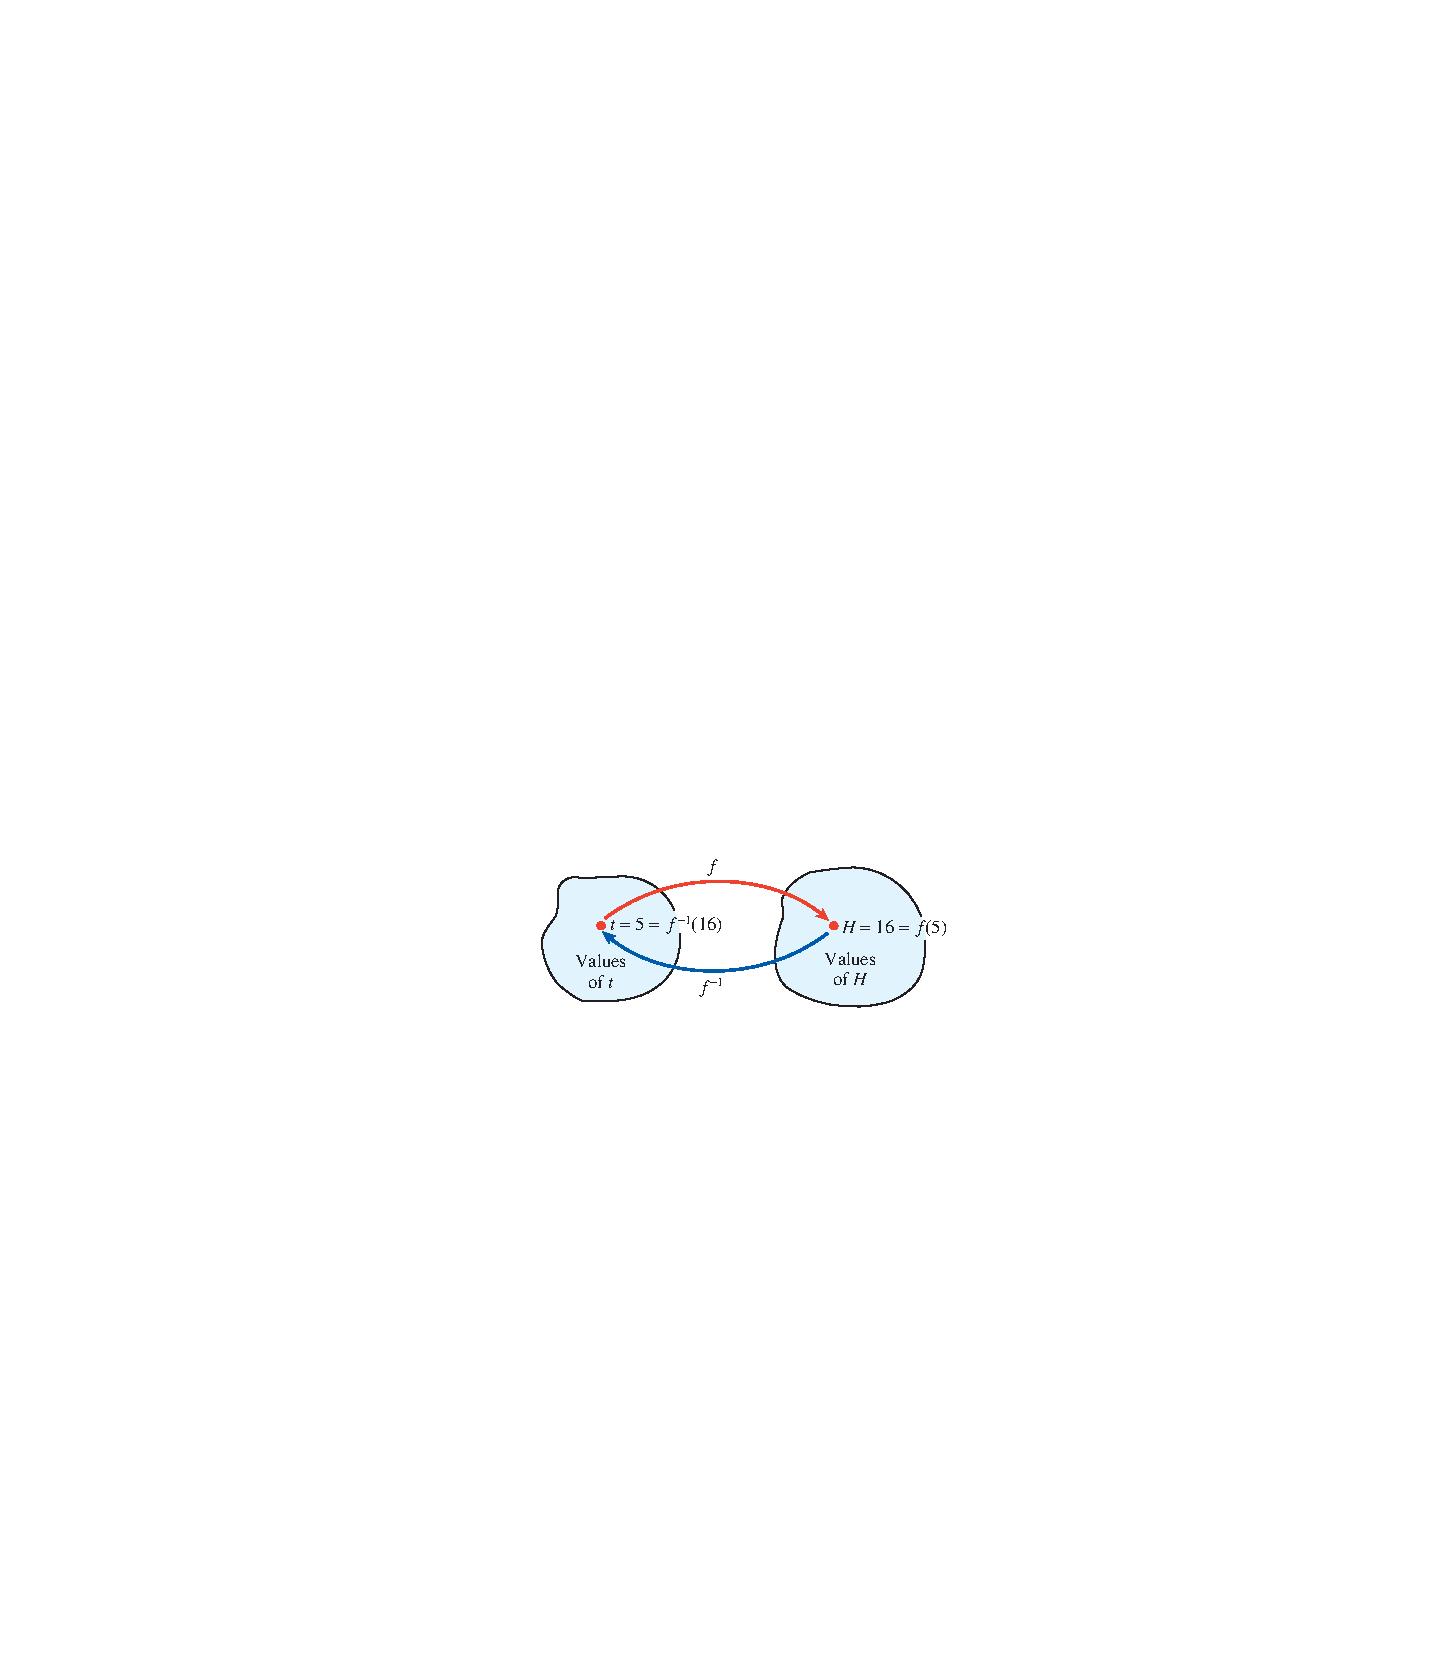
\includegraphics[width=0.5\linewidth]{../../html/PreCalculus/images/fig-function-and-inverse-diagram.pdf}
\caption{\label{fig-function-and-inverse-diagram}}
\end{figure}
\hypertarget{p-121}{}%
We return to the original input value, \(5\).%
\typeout{************************************************}
\typeout{Exercises 1.11 Exercises}
\typeout{************************************************}
\section[{Exercises}]{Exercises}\label{exercises-1}
\begin{exerciselist}
\item[1.]\hypertarget{exercise-1}{}(Slope and Intercept)\space\space{}This exercise uses the WeBWorK Online Homework System and so is not available in the print copy of this book.\item[2.]\hypertarget{exercise-2}{}(Graphs of Linear Equations)\space\space{}This exercise uses the WeBWorK Online Homework System and so is not available in the print copy of this book.\item[3.]\hypertarget{exercise-3}{}(Proportionality)\space\space{}This exercise uses the WeBWorK Online Homework System and so is not available in the print copy of this book.\item[4.]\hypertarget{exercise-4}{}(Finding Lines)\space\space{}This exercise uses the WeBWorK Online Homework System and so is not available in the print copy of this book.\item[5.]\hypertarget{exercise-5}{}(Transformations)\space\space{}This exercise uses the WeBWorK Online Homework System and so is not available in the print copy of this book.\item[6.]\hypertarget{exercise-6}{}(Matching Transformations)\space\space{}This exercise uses the WeBWorK Online Homework System and so is not available in the print copy of this book.\end{exerciselist}
\typeout{************************************************}
\typeout{Section 2 Exponential and Logarithmic Functions}
\typeout{************************************************}
\chapter[{Exponential and Logarithmic Functions}]{Exponential and Logarithmic Functions}\label{explog}
\hypertarget{p-122}{}%
In this chapter we define exponential and logarithmic functions.  For a more extensive treatment of exponential functions we refer the reader to \href{https://mathbooks.unl.edu/PreCalculus/Exponential-Functions.html}{PreCalculus at Nebraska: Exponential Functions} and for a more extensive treatment of exponential functions we refer the reader to \href{https://mathbooks.unl.edu/PreCalculus/section-33.html}{PreCalculus at Nebraska: Logarithmic Functions}%
\typeout{************************************************}
\typeout{Subsection 2.1 Exponential Functions}
\typeout{************************************************}
\section[{Exponential Functions}]{Exponential Functions}\label{subsection-11}
\hypertarget{p-123}{}%
Before we discuss exponential functions, it is first useful to define the notion of concavity.%
\begin{assemblage}[Concavity]\label{assemblage-19}
\hypertarget{p-124}{}%
The graph of a function is concave up if it bends upward as we move left to right; it is concave down if it bends downward. (See the figure for four possible shapes.) A line is neither concave up nor concave down.%
\end{assemblage}
\hypertarget{p-125}{}%
An exponential function will be either concave up everywhere! We define such an exponential as follows:%
\begin{assemblage}[Exponential Function]\label{assemblage-20}
\hypertarget{p-126}{}%
%
\begin{equation*}
P(t) = a \cdot b^t \text{, where } b \gt 0 \text{ and } b \ne 1 \text{, } a \ne 0.
\end{equation*}
%
\par
\hypertarget{p-127}{}%
The constant \(a \) is the \(y\)-value of the \(y\)-intercept of the function.%
\end{assemblage}
\hypertarget{p-128}{}%
The equation%
\begin{equation*}
P(t)=P_0 a^t
\end{equation*}
gives an exponential function with base \(a\). Then%
\begin{equation*}
\frac{P(t+1)}{P(t)}=\frac{P_0 a^{t+1}}{P_0 a^t}=a =\text{constant rate of growth/decay}
\end{equation*}
\leavevmode%
\begin{itemize}[label=\textbullet]
\item{}Growth: \(a\gt1\): Doubling time: the time it takes to double the initial amount%
\item{}Decay \(a\lt1\): Half-life: the time it takes to decay to half of the initial amount%
\end{itemize}
%
\begin{assemblage}[Doubling Time and Half-life]\label{assemblage-21}
\hypertarget{p-129}{}%
The doubling time of an exponentially increasing quantity is the time required for the quantity to double. The half-life of an exponentially decaying quantity is the time required for the quantity to be reduced by a factor of one half.%
\end{assemblage}
\hypertarget{p-130}{}%
We will (naturally) consider exponentials (and later, logarithms) in base%
\begin{equation*}
e \approx 2.718281828459... \text{ (irrational number)}
\end{equation*}
For example, the general exponential function in the natural base%
\begin{equation*}
P(t)=P_0 a^t=P_0 (e^k)^t=P_0e^{kt}, \quad a=e^k. 
\end{equation*}
Thus, we will have \leavevmode%
\begin{itemize}[label=\textbullet]
\item{}exponential growth if \(a\gt 1\), which gives \(k\gt 0\)%
\item{}exponential decay if \(a\lt 1\), which gives \(k\lt 0\)%
\end{itemize}
 The number \(k\) is called \emph{the continuous rate of growth/decay.} To find \(k\) we will need the logarithmic function.%
\typeout{************************************************}
\typeout{Subsection 2.2 Logarithmic Functions}
\typeout{************************************************}
\section[{Logarithmic Functions}]{Logarithmic Functions}\label{subsection-12}
\hypertarget{p-131}{}%
Recall inverse functions.  If for each \(y\) in the range of \(f\) there exists exactly one value of \(x\) such that \(f(x)=y,\) then \(f\) has an inverse at \(y\) denoted by \(f^{-1}\) such that%
\begin{equation*}
f(x)=y \quad \iff \quad f^{-1}(y)=x
\end{equation*}
Hence%
\begin{equation*}
f(f^{-1}(y))=y \quad \text{and} \quad f^{-1}(f(x))=x.
\end{equation*}
The \emph{inverse} of the exponential function \(f(x)=e^x\) is the natural \emph{logarithmic} function \(f^{-1}(x)= \ln(x)\) so we have%
\begin{equation*}
\ln(x) =c \iff e^c=x  
\end{equation*}
%
\begin{assemblage}[The Logarithm]\label{assemblage-22}
\hypertarget{p-132}{}%
Let \(b\neq 1 \) be a positive number, then the function%
\begin{equation*}
f(t)=\log_b(t) 
\end{equation*}
is called a logarithm with base \(b \).%
\par
\hypertarget{p-133}{}%
Upon inputting a value \(t\) the function \(\log_b(t)\) will tell you the  power of \(b \) which will yield \(t \).%
\end{assemblage}
\hypertarget{p-134}{}%
Due to the relationship between logarithms and exponentials, we often say that the equations%
\begin{equation*}
x=\log_b(y)\ \ \ \ \text{and}\ \ \ \ b^x=y
\end{equation*}
are equivalent.%
\begin{warning}[]\label{warning-1}
\hypertarget{p-135}{}%
Two common bases of a logarithm are base \(10 \) and \(e\). Since they are used so often, we have developed a short hand notation for a logarithm of base \(10\) and a logarithm of base \(e\). This short hand is shown below:%
\begin{equation*}
\log_{10}(y)=\log(y).
\end{equation*}
%
\begin{equation*}
\log_{e}(y)=\ln(y).
\end{equation*}
In other words, we simply drop the subscript when referring to base \(10 \) and we change to \(\ln\) when referring to base \(e\)%
\end{warning}
\hypertarget{p-136}{}%
There are some important properties of logarithms that you should be familier with.%
\begin{assemblage}[Properties of Logarithms]\label{assemblage-23}
\hypertarget{p-137}{}%
If \(x,y,b>0\), and \(b\neq 1\), then \leavevmode%
\begin{enumerate}[label=\arabic*]
\item\hypertarget{li-42}{}\hypertarget{p-138}{}%
\(\log_b(xy)=\log_b(x)+\log_b(y),\)%
\item\hypertarget{li-43}{}\hypertarget{p-139}{}%
\(\log_b(\frac{x}{y})=\log_b(x)-\log_b(y),\)%
\item\hypertarget{li-44}{}\hypertarget{p-140}{}%
\(\log_b(x^k)=k\cdot \log_b(x),\)%
\item\hypertarget{li-45}{}\hypertarget{p-141}{}%
\(\log_b(b^y)=y,\)%
\item\hypertarget{li-46}{}\hypertarget{p-142}{}%
\(b^{\log_b(x)}=x.\)%
\end{enumerate}
%
\end{assemblage}
\typeout{************************************************}
\typeout{Exercises 2.3 Exercises}
\typeout{************************************************}
\section[{Exercises}]{Exercises}\label{exercises-2}
\begin{exerciselist}
\item[1.]\hypertarget{exercise-7}{}(General Exponential Functions)\space\space{}This exercise uses the WeBWorK Online Homework System and so is not available in the print copy of this book.\item[2.]\hypertarget{exercise-8}{}(Finding Exponential Functions)\space\space{}This exercise uses the WeBWorK Online Homework System and so is not available in the print copy of this book.\item[3.]\hypertarget{exercise-9}{}(Finding the Parameters for an Exponential Function)\space\space{}This exercise uses the WeBWorK Online Homework System and so is not available in the print copy of this book.\item[4.]\hypertarget{exercise-10}{}(Half-Life)\space\space{}This exercise uses the WeBWorK Online Homework System and so is not available in the print copy of this book.\item[5.]\hypertarget{exercise-11}{}(Applied Half-Life)\space\space{}This exercise uses the WeBWorK Online Homework System and so is not available in the print copy of this book.\item[6.]\hypertarget{exercise-12}{}(Solving Exponential Equations)\space\space{}This exercise uses the WeBWorK Online Homework System and so is not available in the print copy of this book.\item[7.]\hypertarget{exercise-13}{}(Using Inverse Functions With Exponentials and Logarithms)\space\space{}This exercise uses the WeBWorK Online Homework System and so is not available in the print copy of this book.\end{exerciselist}
\typeout{************************************************}
\typeout{Section 3 Trigonometric Functions}
\typeout{************************************************}
\chapter[{Trigonometric Functions}]{Trigonometric Functions}\label{trig}
\hypertarget{p-143}{}%
In this chapter we define trigonometric functions.  For a more extensive treatment of trigonometric functions we refer the reader to \href{https://mathbooks.unl.edu/PreCalculus/part-3.html}{PreCalculus at Nebraska: College Trigonometry}.%
\typeout{************************************************}
\typeout{Subsection 3.1 Periodic Functions}
\typeout{************************************************}
\section[{Periodic Functions}]{Periodic Functions}\label{subsection-13}
\begin{assemblage}\label{assemblage-24}
\hypertarget{p-144}{}%
A \terminology{periodic function}\index{periodic function} is a function whose output values repeat on a regular interval. In mathematical terms, we say that a periodic function is a function for which a specific horizontal shift, \(P\), results in the original function: \(f(x+P)=f(x)\) for all values of \(x\).%
\par
\hypertarget{p-145}{}%
The \terminology{period}\index{period} of a periodic function is how long it takes for the output values to begin repeating, or the smallest horizontal shift with \(P>0\), such that \(f(x+P)=f(x)\) for all values of \(x\).%
% group protects changes to lengths, releases boxes (?)
{% begin: group for a single side-by-side
% set panel max height to practical minimum, created in preamble
\setlength{\panelmax}{0pt}
\ifdefined\panelboxAimage\else\newsavebox{\panelboxAimage}\fi%
\begin{lrbox}{\panelboxAimage}
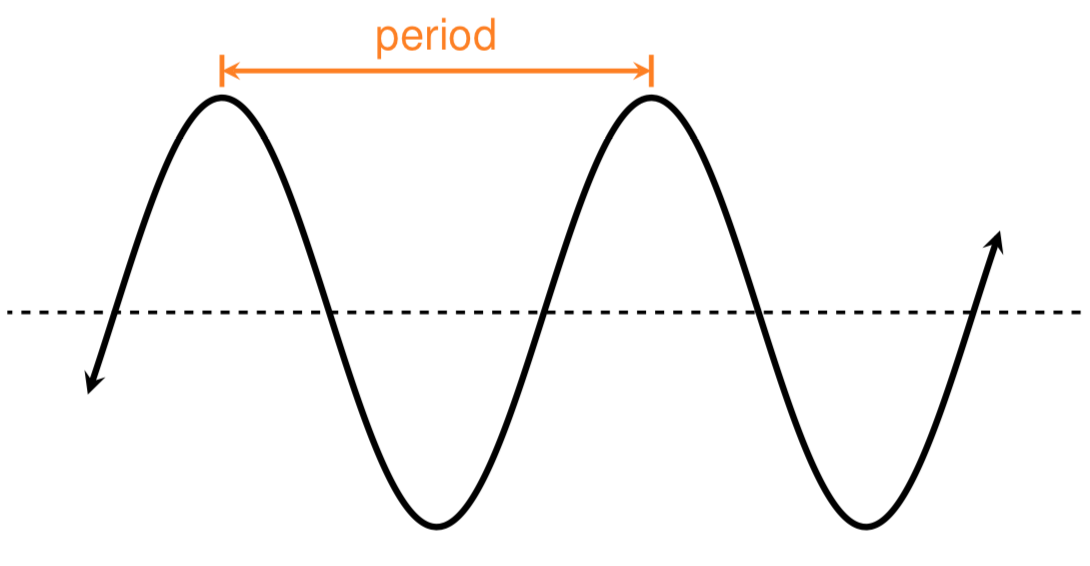
\includegraphics[width=1\linewidth]{../../html/PreCalculus/images/imagesChap13/period.png}
\end{lrbox}
\ifdefined\phAimage\else\newlength{\phAimage}\fi%
\setlength{\phAimage}{\ht\panelboxAimage+\dp\panelboxAimage}
\settototalheight{\phAimage}{\usebox{\panelboxAimage}}
\setlength{\panelmax}{\maxof{\panelmax}{\phAimage}}
\leavevmode%
% begin: side-by-side as tabular
% \tabcolsep change local to group
\setlength{\tabcolsep}{0\linewidth}
% @{} suppress \tabcolsep at extremes, so margins behave as intended
\par\medskip\noindent
\begin{tabular}{@{}*{1}{c}@{}}
\begin{minipage}[c][\panelmax][t]{1\linewidth}\usebox{\panelboxAimage}\end{minipage}\end{tabular}\\
% end: side-by-side as tabular
}% end: group for a single side-by-side
\end{assemblage}
\hypertarget{p-146}{}%
In addition to the period we also define the midline and amplitude of a periodic function.%
\begin{assemblage}\label{assemblage-25}
\hypertarget{p-147}{}%
The \terminology{midline}\index{midline} of a periodic function is the horizontal line halfway, or midway, between the function's maximum and minimum output values.%
\par
\hypertarget{p-148}{}%
%
\par
\hypertarget{p-149}{}%
The \terminology{amplitude}\index{amplitude} of a periodic function is the distance between the function's maximum (or minimum) output value and the midline.%
% group protects changes to lengths, releases boxes (?)
{% begin: group for a single side-by-side
% set panel max height to practical minimum, created in preamble
\setlength{\panelmax}{0pt}
\ifdefined\panelboxAimage\else\newsavebox{\panelboxAimage}\fi%
\begin{lrbox}{\panelboxAimage}
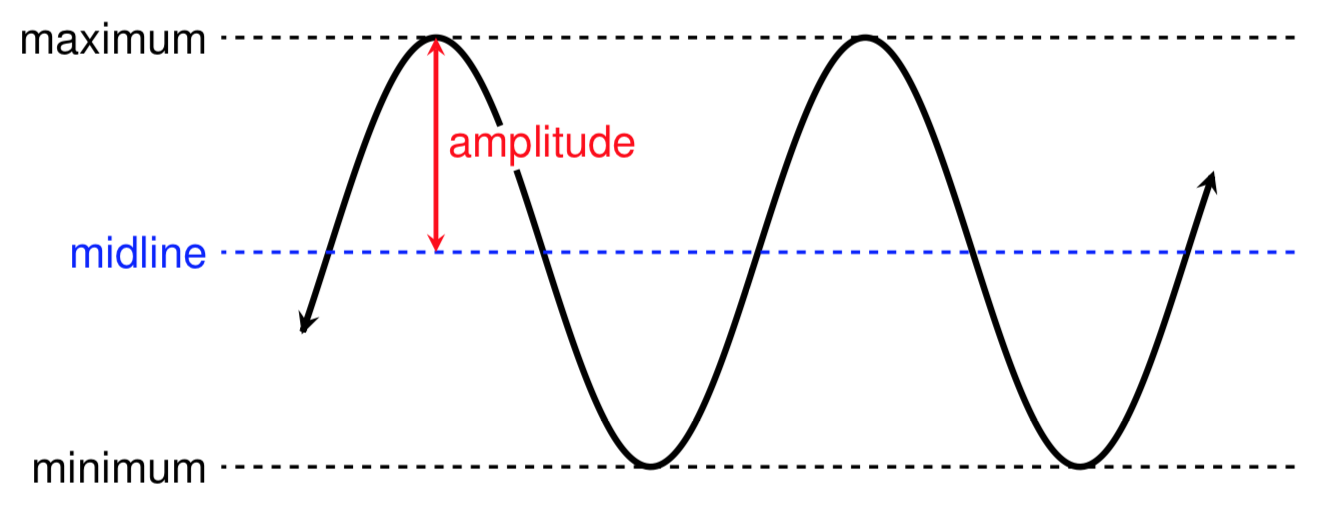
\includegraphics[width=1\linewidth]{../../html/PreCalculus/images/imagesChap13/midlineamp.png}
\end{lrbox}
\ifdefined\phAimage\else\newlength{\phAimage}\fi%
\setlength{\phAimage}{\ht\panelboxAimage+\dp\panelboxAimage}
\settototalheight{\phAimage}{\usebox{\panelboxAimage}}
\setlength{\panelmax}{\maxof{\panelmax}{\phAimage}}
\leavevmode%
% begin: side-by-side as tabular
% \tabcolsep change local to group
\setlength{\tabcolsep}{0\linewidth}
% @{} suppress \tabcolsep at extremes, so margins behave as intended
\par\medskip\noindent
\begin{tabular}{@{}*{1}{c}@{}}
\begin{minipage}[c][\panelmax][t]{1\linewidth}\usebox{\panelboxAimage}\end{minipage}\end{tabular}\\
% end: side-by-side as tabular
}% end: group for a single side-by-side
\par
\hypertarget{p-150}{}%
%
\par
\hypertarget{p-151}{}%
The midline often represents the average value of a wave-like periodic function and should always be written as the equation of a horizontal line. The amplitude of a periodic function represents how "large" the function's oscillations are.%
\end{assemblage}
\hypertarget{p-152}{}%
While measuring angles in degrees may be familiar to many students, doing so often complicates matters since the units of measure can get in the way of calculations. For this reason, another measure of angles is commonly used. This measure is based on the distance around the unit circle.%
\begin{assemblage}[The Unit Circle]\label{assemblage-26}
\hypertarget{p-153}{}%
%
\par
\hypertarget{p-154}{}%
The \terminology{unit circle}\index{unit circle} is a circle of radius 1, centered at the origin of the \(xy\)-plane. When measuring an angle around the unit circle, we travel in the counterclockwise direction, starting from the positive \(x\)-axis. A negative angle is measured in the opposite, or clockwise, direction. A complete trip around the unit circle amounts to a total of 360 degrees.%
% group protects changes to lengths, releases boxes (?)
{% begin: group for a single side-by-side
% set panel max height to practical minimum, created in preamble
\setlength{\panelmax}{0pt}
\ifdefined\panelboxAimage\else\newsavebox{\panelboxAimage}\fi%
\begin{lrbox}{\panelboxAimage}
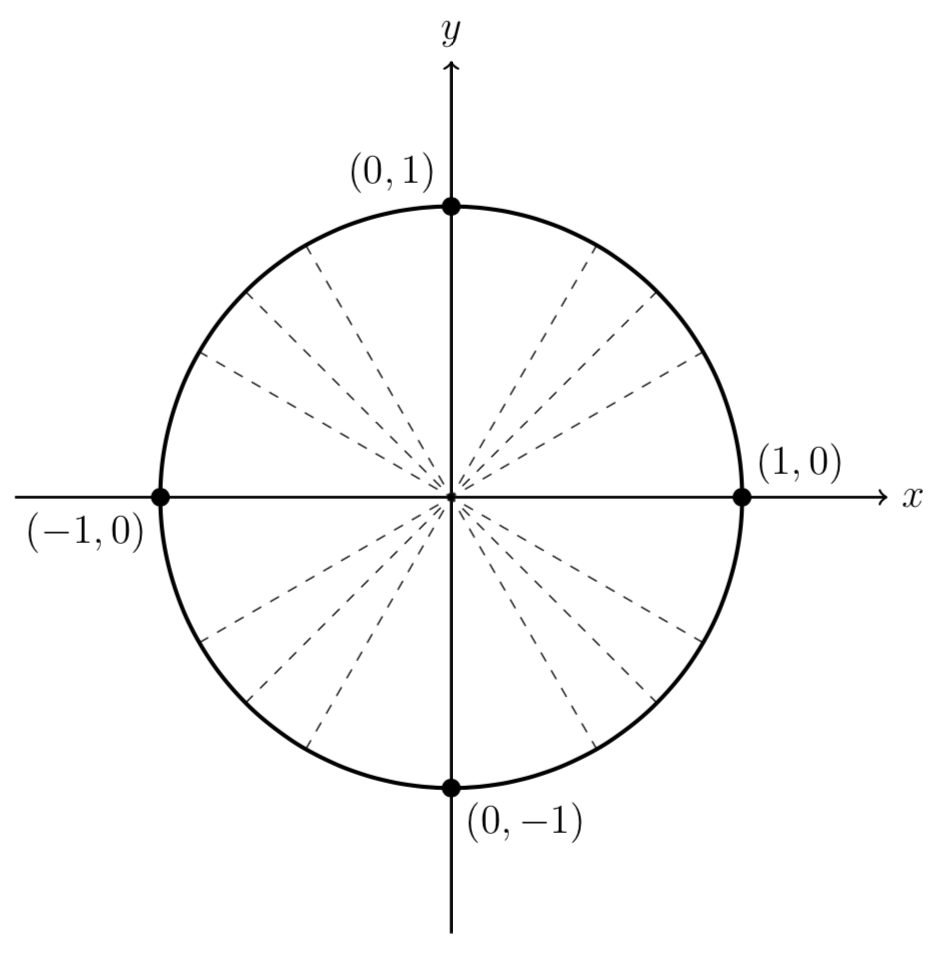
\includegraphics[width=0.7\linewidth]{../../html/PreCalculus/images/imagesChap13/blankUnitCircle.png}
\end{lrbox}
\ifdefined\phAimage\else\newlength{\phAimage}\fi%
\setlength{\phAimage}{\ht\panelboxAimage+\dp\panelboxAimage}
\settototalheight{\phAimage}{\usebox{\panelboxAimage}}
\setlength{\panelmax}{\maxof{\panelmax}{\phAimage}}
\leavevmode%
% begin: side-by-side as tabular
% \tabcolsep change local to group
\setlength{\tabcolsep}{0\linewidth}
% @{} suppress \tabcolsep at extremes, so margins behave as intended
\par\medskip\noindent
\hspace*{0.15\linewidth}%
\begin{tabular}{@{}*{1}{c}@{}}
\begin{minipage}[c][\panelmax][t]{0.7\linewidth}\usebox{\panelboxAimage}\end{minipage}\end{tabular}\\
% end: side-by-side as tabular
}% end: group for a single side-by-side
\par
\hypertarget{p-155}{}%
%
\par
\hypertarget{p-156}{}%
A \terminology{radian}\index{radian} is a measurement of an angle that arises from looking at angles as a fraction of the circumference of the unit circle. A complete trip around the unit circle amounts to a total of \(2\pi\) radians.%
% group protects changes to lengths, releases boxes (?)
{% begin: group for a single side-by-side
% set panel max height to practical minimum, created in preamble
\setlength{\panelmax}{0pt}
\ifdefined\panelboxAimage\else\newsavebox{\panelboxAimage}\fi%
\begin{lrbox}{\panelboxAimage}
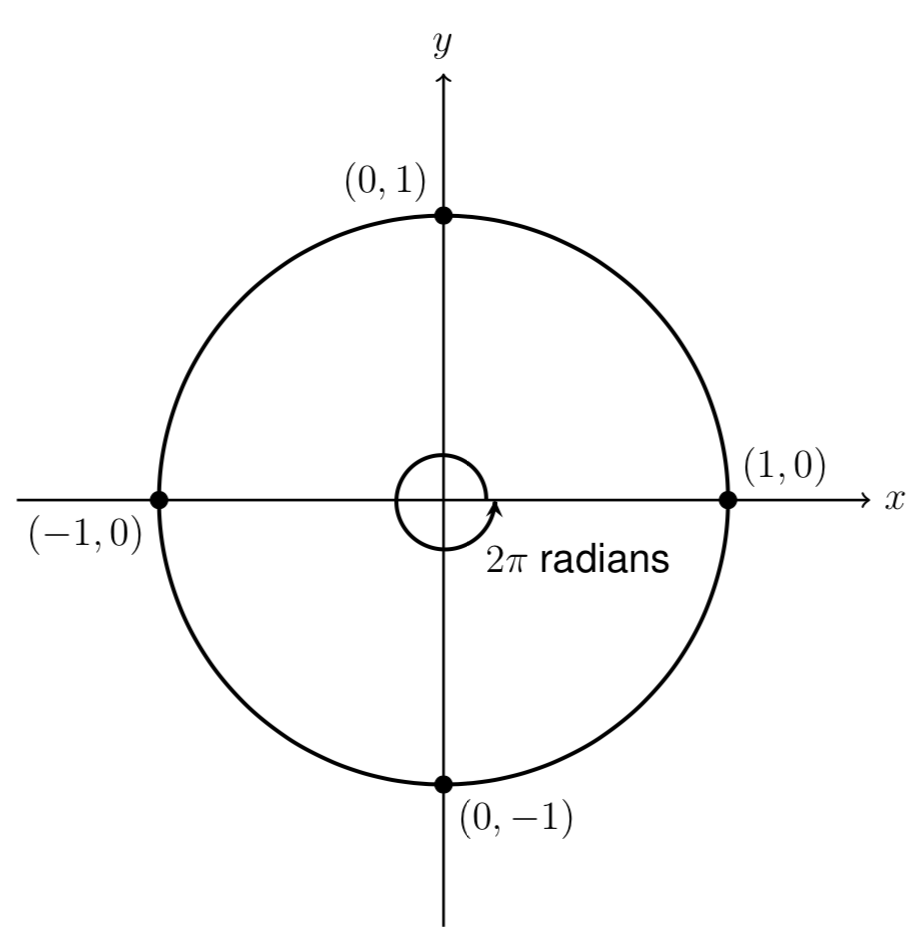
\includegraphics[width=0.7\linewidth]{../../html/PreCalculus/images/imagesChap13/radians.png}
\end{lrbox}
\ifdefined\phAimage\else\newlength{\phAimage}\fi%
\setlength{\phAimage}{\ht\panelboxAimage+\dp\panelboxAimage}
\settototalheight{\phAimage}{\usebox{\panelboxAimage}}
\setlength{\panelmax}{\maxof{\panelmax}{\phAimage}}
\leavevmode%
% begin: side-by-side as tabular
% \tabcolsep change local to group
\setlength{\tabcolsep}{0\linewidth}
% @{} suppress \tabcolsep at extremes, so margins behave as intended
\par\medskip\noindent
\hspace*{0.15\linewidth}%
\begin{tabular}{@{}*{1}{c}@{}}
\begin{minipage}[c][\panelmax][t]{0.7\linewidth}\usebox{\panelboxAimage}\end{minipage}\end{tabular}\\
% end: side-by-side as tabular
}% end: group for a single side-by-side
\par
\hypertarget{p-157}{}%
%
\par
\hypertarget{p-158}{}%
Radians are a \terminology{unitless measure}. Therefore, it is not necessary to write the label "radians" after a radian measure, and if you see an angle that is not labeled with "degrees" or the degree symbol, you should assume that it is a radian measure.%
\end{assemblage}
\hypertarget{p-159}{}%
Radians and degrees both measure angles. Thus, it is possible to convert between the two. Since one rotation around the unit circle equals 360 degrees or \(2\pi\) radians, we can use this as a conversion factor.%
\begin{assemblage}[Converting Between Radians and Degrees]\label{assemblage-27}
\hypertarget{p-160}{}%
%
\par
\hypertarget{p-161}{}%
Since \(360 \text{ degrees} = 2\pi \text{ radians}\), we can divide each side by 360 and conclude that%
\begin{equation*}
\displaystyle 1 \text{ degree} = \frac{2\pi \text{ radians}}{360} = \frac{\pi \text{ radians}}{180}
\end{equation*}
%
\par
\hypertarget{p-162}{}%
So, to convert from degrees to radians, we can multiply by \(\displaystyle \ \frac{\pi \text{ radians}}{180^\circ}\)%
\par
\hypertarget{p-163}{}%
%
\par
\hypertarget{p-164}{}%
Similarly, we can conclude that%
\begin{equation*}
\displaystyle 1 \text{ radian} = \frac{360^\circ}{2\pi} = \frac{180^\circ}{\pi}
\end{equation*}
%
\par
\hypertarget{p-165}{}%
So, to convert from radians to degrees, we can multiply by \(\displaystyle \ \frac{180^\circ}{\pi \text{ radians}}\)%
\end{assemblage}
\typeout{************************************************}
\typeout{Subsection 3.2 The Common Trigonometric Functions}
\typeout{************************************************}
\section[{The Common Trigonometric Functions}]{The Common Trigonometric Functions}\label{subsection-14}
\begin{assemblage}[The Sine and Cosine Functions]\label{assemblage-28}
\hypertarget{p-166}{}%
%
% group protects changes to lengths, releases boxes (?)
{% begin: group for a single side-by-side
% set panel max height to practical minimum, created in preamble
\setlength{\panelmax}{0pt}
\ifdefined\panelboxAparagraphs\else\newsavebox{\panelboxAparagraphs}\fi%
\savebox{\panelboxAparagraphs}{%
\raisebox{\depth}{\parbox{0.5\linewidth}{\hypertarget{p-167}{}%
%
\par
\hypertarget{p-168}{}%
Given an angle \(\theta \ \) (in either degrees or radians) and the \((x,y)\) coordinates of the corresponding point on the unit circle, we define cosine and sine as%
\par
\hypertarget{p-169}{}%
%
\begin{equation*}
\cos(\theta)=x \hspace{.25in} \text{and} \hspace{.25in} \sin(\theta)=y
\end{equation*}
%
\par
\hypertarget{p-170}{}%
Note that sine and cosine are \terminology{functions} that take angles as inputs.%
}}}
\ifdefined\phAparagraphs\else\newlength{\phAparagraphs}\fi%
\setlength{\phAparagraphs}{\ht\panelboxAparagraphs+\dp\panelboxAparagraphs}
\settototalheight{\phAparagraphs}{\usebox{\panelboxAparagraphs}}
\setlength{\panelmax}{\maxof{\panelmax}{\phAparagraphs}}
\ifdefined\panelboxAimage\else\newsavebox{\panelboxAimage}\fi%
\begin{lrbox}{\panelboxAimage}
\includegraphics[width=0.45\linewidth]{../../html/PreCalculus/images/imagesChap13/SineandCosineDefinition.png}
\end{lrbox}
\ifdefined\phAimage\else\newlength{\phAimage}\fi%
\setlength{\phAimage}{\ht\panelboxAimage+\dp\panelboxAimage}
\settototalheight{\phAimage}{\usebox{\panelboxAimage}}
\setlength{\panelmax}{\maxof{\panelmax}{\phAimage}}
\leavevmode%
% begin: side-by-side as tabular
% \tabcolsep change local to group
\setlength{\tabcolsep}{0.0125\linewidth}
% @{} suppress \tabcolsep at extremes, so margins behave as intended
\par\medskip\noindent
\hspace*{0.0125\linewidth}%
\begin{tabular}{@{}*{2}{c}@{}}
\begin{minipage}[c][\panelmax][t]{0.5\linewidth}\usebox{\panelboxAparagraphs}\end{minipage}&
\begin{minipage}[c][\panelmax][t]{0.45\linewidth}\usebox{\panelboxAimage}\end{minipage}\end{tabular}\\
% end: side-by-side as tabular
}% end: group for a single side-by-side
\end{assemblage}
\hypertarget{p-171}{}%
Using the \((x,y)\) coordinates we can find the cosine and sine values of common angles on the unit circle.%
\par
\hypertarget{p-172}{}%
The applet below shows how the graphs of sine and cosine relate to the \(x\) and \(y\) coordinates of the point \(P\) on the unit circle. Move the slider to change the angle \(\theta\) and observe how the \(x\) and \(y\) values of point \(P\) relate to the outputs of \(\cos(\theta)\) and \(\sin(\theta)\).%
\begin{figure}
\centering
\centerline{Geogebra: \href{https://www.geogebra.org/m/pJqvn9pR}{\mono{www.geogebra.org/m/pJqvn9pR}}}
\caption{How the Graphs of Sine and Cosine Relate to the Unit Circle\label{figure-9}}
\end{figure}
\hypertarget{p-173}{}%
In addition to sine and cosine it is also useful to define several additional trigonometric functions.%
\begin{assemblage}[The Tangent Function]\label{assemblage-29}
\hypertarget{p-174}{}%
%
% group protects changes to lengths, releases boxes (?)
{% begin: group for a single side-by-side
% set panel max height to practical minimum, created in preamble
\setlength{\panelmax}{0pt}
\ifdefined\panelboxAparagraphs\else\newsavebox{\panelboxAparagraphs}\fi%
\savebox{\panelboxAparagraphs}{%
\raisebox{\depth}{\parbox{0.5\linewidth}{\hypertarget{p-175}{}%
Given an angle \(\theta \ \) (in either degrees or radians) and the \((x,y)\) coordinates of the corresponding point on the unit circle, we define tangent as%
\begin{equation*}
\tan(\theta)=\frac{y}{x}
\end{equation*}
Just like sine and cosine, tangent is a \terminology{function} that takes angles as inputs.%
}}}
\ifdefined\phAparagraphs\else\newlength{\phAparagraphs}\fi%
\setlength{\phAparagraphs}{\ht\panelboxAparagraphs+\dp\panelboxAparagraphs}
\settototalheight{\phAparagraphs}{\usebox{\panelboxAparagraphs}}
\setlength{\panelmax}{\maxof{\panelmax}{\phAparagraphs}}
\ifdefined\panelboxAimage\else\newsavebox{\panelboxAimage}\fi%
\begin{lrbox}{\panelboxAimage}
\includegraphics[width=0.4\linewidth]{../../html/Calculus/images/imagesChap13/SineandCosineDefinition.png}
\end{lrbox}
\ifdefined\phAimage\else\newlength{\phAimage}\fi%
\setlength{\phAimage}{\ht\panelboxAimage+\dp\panelboxAimage}
\settototalheight{\phAimage}{\usebox{\panelboxAimage}}
\setlength{\panelmax}{\maxof{\panelmax}{\phAimage}}
\leavevmode%
% begin: side-by-side as tabular
% \tabcolsep change local to group
\setlength{\tabcolsep}{0.025\linewidth}
% @{} suppress \tabcolsep at extremes, so margins behave as intended
\par\medskip\noindent
\hspace*{0.025\linewidth}%
\begin{tabular}{@{}*{2}{c}@{}}
\begin{minipage}[c][\panelmax][t]{0.5\linewidth}\usebox{\panelboxAparagraphs}\end{minipage}&
\begin{minipage}[c][\panelmax][t]{0.4\linewidth}\usebox{\panelboxAimage}\end{minipage}\end{tabular}\\
% end: side-by-side as tabular
}% end: group for a single side-by-side
\par
\hypertarget{p-176}{}%
Note that since \(\sin(\theta)=y\) and \(\cos(\theta)=x\), we can also define tangent as%
\begin{equation*}
\tan(\theta)=\frac{\sin(\theta)}{\cos(\theta)}
\end{equation*}
%
\end{assemblage}
\hypertarget{p-177}{}%
We can find the tangent values of common angles on the unit circle by using the sine and cosine values of the angles (or the corresponding \(y\) and \(x\) coordinates).%
\par
\hypertarget{p-178}{}%
There are times when it can be useful to consider functions like \(\frac{1}{\sin(\theta)}\) or \(\frac{1}{\cos(\theta)}\). This happens often enough that mathematicians have created special names for these types of functions. Generally, these functions are called reciprocal trigonometric functions, and they can be defined in terms of the sine, cosine, and tangent functions.%
\begin{assemblage}[The Reciprocal Trigonometric Functions]\label{assemblage-30}
\hypertarget{p-179}{}%
%
\par
\hypertarget{p-180}{}%
Given an angle \(\theta\), we define:%
\begin{align*}
\amp \text{the secant function as } \amp\amp \sec(\theta)=\frac{1}{\cos(\theta)}\\
\\
\amp \text{the cosecant function as } \amp\amp \csc(\theta)=\frac{1}{\sin(\theta)}\\
\\
\amp \text{the cotangent function as } \amp\amp \cot(\theta)=\frac{1}{\tan(\theta)}
\end{align*}
%
\end{assemblage}
\typeout{************************************************}
\typeout{Subsection 3.3 Inverse Trigonometric Functions}
\typeout{************************************************}
\section[{Inverse Trigonometric Functions}]{Inverse Trigonometric Functions}\label{subsection-15}
\hypertarget{p-181}{}%
In the previous subsection, we evaluated trigonometric functions at various angles, but what if we needed to know what angle yields a specific sine, cosine, or tangent value. To find angles, we need inverse trigonometric functions.%
\begin{assemblage}[The Inverse Sine, Inverse Cosine, and Inverse Tangent Functions]\label{assemblage-31}
\hypertarget{p-182}{}%
%
\par
\hypertarget{p-183}{}%
If \(\sin(\theta)=a\), then \(\sin^{-1}(a)=\theta\) for \(-1\leq a \leq 1\)%
\par
\hypertarget{p-184}{}%
If \(\cos(\theta)=a\), then \(\cos^{-1}(a)=\theta\) for \(-1 \leq a \leq 1\)%
\par
\hypertarget{p-185}{}%
If \(\tan(\theta)=a\), then \(\tan^{-1}(a)=\theta\) for \(-\infty \lt a \lt \infty \)%
\par
\hypertarget{p-186}{}%
Note that the \emph{output} of each of these inverse functions is an \emph{angle}.%
\end{assemblage}
\begin{remark}[]\label{remark-1}
\hypertarget{p-187}{}%
Do not confuse \(\sin^{-1}(a) \) with \(\frac{1}{\sin(a)}\) as they are not equivalent. The same can be said with \(\cos^{-1}(a) \) and \(\tan^{-1}(a) \). As a result, we introduce an alternative (common) notation for the inverse trigonometric functions.%
\end{remark}
\begin{note}[Common Notation for the Inverse Trigonometric Functions]\label{note-2}
\hypertarget{p-188}{}%
%
\par
\hypertarget{p-189}{}%
The inverse sine function, \(\sin^{-1}(a)\) is sometimes called the \terminology{arcsine} function, and notated \(\arcsin(a)\).%
\par
\hypertarget{p-190}{}%
The inverse cosine function, \(\cos^{-1}(a)\) is sometimes called the \terminology{arccosine} function, and notated \(\arccos(a)\).%
\par
\hypertarget{p-191}{}%
The inverse tangent function, \(\tan^{-1}(a)\) is sometimes called the \terminology{arctangent} function, and notated \(\arctan(a)\).%
\end{note}
\typeout{************************************************}
\typeout{Subsection 3.4 Generalized Trigonometric Functions}
\typeout{************************************************}
\section[{Generalized Trigonometric Functions}]{Generalized Trigonometric Functions}\label{subsection-16}
\hypertarget{p-192}{}%
Like all functions, trigonometric functions can be transformed by changing properties like the period, midline, and amplitude of the function. In this subsection, we explore transformations of the sine and cosine functions and use them to model real life situations.%
\begin{assemblage}[Transformations of Sine and Cosine]\label{assemblage-32}
\hypertarget{p-193}{}%
%
\par
\hypertarget{p-194}{}%
Given an equation in the form%
\begin{equation*}
f(t) = A\sin(Bt)+k \hspace{.25in} \text{ or } \hspace{.25in} g(t) = A\cos(Bt)+k 
\end{equation*}
%
\par
\hypertarget{p-195}{}%
\(|A| \ \) is the vertical stretch/compression and the \terminology{amplitude} of the function.%
\par
\hypertarget{p-196}{}%
\(|B| \ \) is the horizontal stretch/compression and is \terminology{related} to the \terminology{period} of the function, \(P\), by the formula%
\begin{equation*}
P=\frac{2\pi}{|B|}
\end{equation*}
%
\par
\hypertarget{p-197}{}%
\(k \ \) is the vertical shift and determines the \terminology{midline} of the function.%
\end{assemblage}
\typeout{************************************************}
\typeout{Exercises 3.5 Exercises}
\typeout{************************************************}
\section[{Exercises}]{Exercises}\label{exercises-3}
\begin{exerciselist}
\item[1.]\hypertarget{exercise-14}{}(Period and Amplitude)\space\space{}This exercise uses the WeBWorK Online Homework System and so is not available in the print copy of this book.\item[2.]\hypertarget{exercise-15}{}(Period and Amplitude)\space\space{}This exercise uses the WeBWorK Online Homework System and so is not available in the print copy of this book.\item[3.]\hypertarget{exercise-16}{}(Finding Trigonometric Functions)\space\space{}This exercise uses the WeBWorK Online Homework System and so is not available in the print copy of this book.\item[4.]\hypertarget{exercise-17}{}(Finding Trigonometric Functions)\space\space{}This exercise uses the WeBWorK Online Homework System and so is not available in the print copy of this book.\item[5.]\hypertarget{exercise-18}{}(The Unit Circle)\space\space{}This exercise uses the WeBWorK Online Homework System and so is not available in the print copy of this book.\item[6.]\hypertarget{exercise-19}{}(Trigonometric Functions as Compositions)\space\space{}This exercise uses the WeBWorK Online Homework System and so is not available in the print copy of this book.\end{exerciselist}
%% begin: table of contents
%% Adjust Table of Contents
\setcounter{tocdepth}{1}
\renewcommand*\contentsname{Contents}
\tableofcontents
%% end:   table of contents
\mainmatter
\typeout{************************************************}
\typeout{Chapter 1 Understanding the Derivative}
\typeout{************************************************}
\chapter[{Understanding the Derivative}]{Understanding the Derivative}\label{C-1}
\typeout{************************************************}
\typeout{Section 1.1 Introduction to Continuity}
\typeout{************************************************}
\section[{Introduction to Continuity}]{Introduction to Continuity}\label{deriv}
\begin{objectives}{Motivating Questions}\label{objectives-1}
%
\begin{itemize}[label=\textbullet]
\item{}\hypertarget{p-198}{}%
What does it mean to say that a function \(f\) is continuous at \(x = a\)?%
\item{}\hypertarget{p-199}{}%
What does it mean to say that a function \(f\) is continuous everywhere?%
\end{itemize}
\end{objectives}
\hypertarget{p-200}{}%
In this section we introduce the idea of a continuous function. Many of the results in calculus require that the functions be continuous so having a strong understanding of continuous functions will be very important.%
\typeout{************************************************}
\typeout{Subsection 1.1.1 Being continuous at a point}
\typeout{************************************************}
\subsection[{Being continuous at a point}]{Being continuous at a point}\label{subsection-17}
\index{continuous}\hypertarget{p-201}{}%
Intuitively, a function is continuous if we can draw its graph without ever lifting our pencil from the page. Alternatively, we might say that the graph of a continuous function has no jumps or holes in it.%
\begin{figure}
\centering
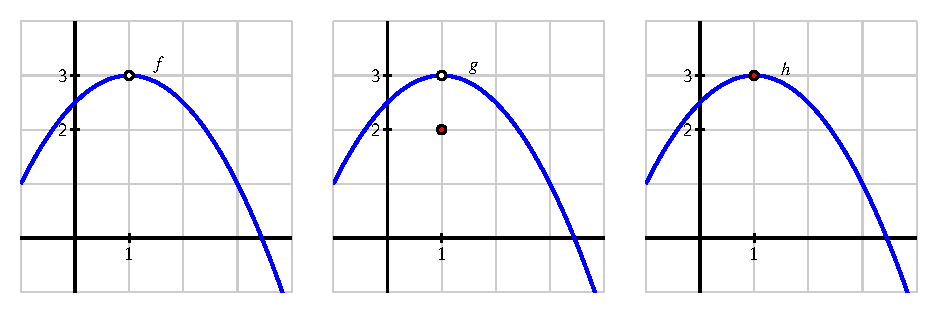
\includegraphics[width=1\linewidth]{../../html/Calculus/images/1_7_Cont.pdf}
\caption{Functions \(f\), \(g\), and \(h\) that demonstrate subtly different behaviors at \(a = 1\).\label{figure-10}}
\end{figure}
\hypertarget{p-202}{}%
First consider the function in the left-most graph. Note that \(f(1)\) is not defined, which leads to the resulting hole in the graph of \(f\) at \(a = 1\). If you were to draw the graph of \(f\) yourself then you would need to lift your pencil when you reached \(f(1)\). We will naturally say that \(f\) is \emph{not continuous at \(a = 1\)}. For the function \(g\), we observe that while \(g(1)\) is defined, the value of \(g(1) = 2\) is not what you would "expect."  Specifically, you would expect \(g(1)\) to be 3, not 2. Thus, to draw the graph of \(g\) you would need to lift you pencil at \(a=1\). Again, we will say that \(g\) is \emph{not continuous} at \(a=1\), even though the function is defined at \(a = 1\). Finally, the function \(h\) appears to be the most "well-behaved" of all three, since at \(a = 1\) its limit and its function value agree.  In this case we would say that \(h\) is continuous at \(a=1\).%
\par
\hypertarget{p-203}{}%
The above examples demonstrate a discontinuity commonly know as a \emph{removable discontinuity}. This is, however, not the only way in which a function can be discontinuous.  Another type of discontinuity is the so called \emph{jump} discontinuity.%
\begin{figure}
\centering
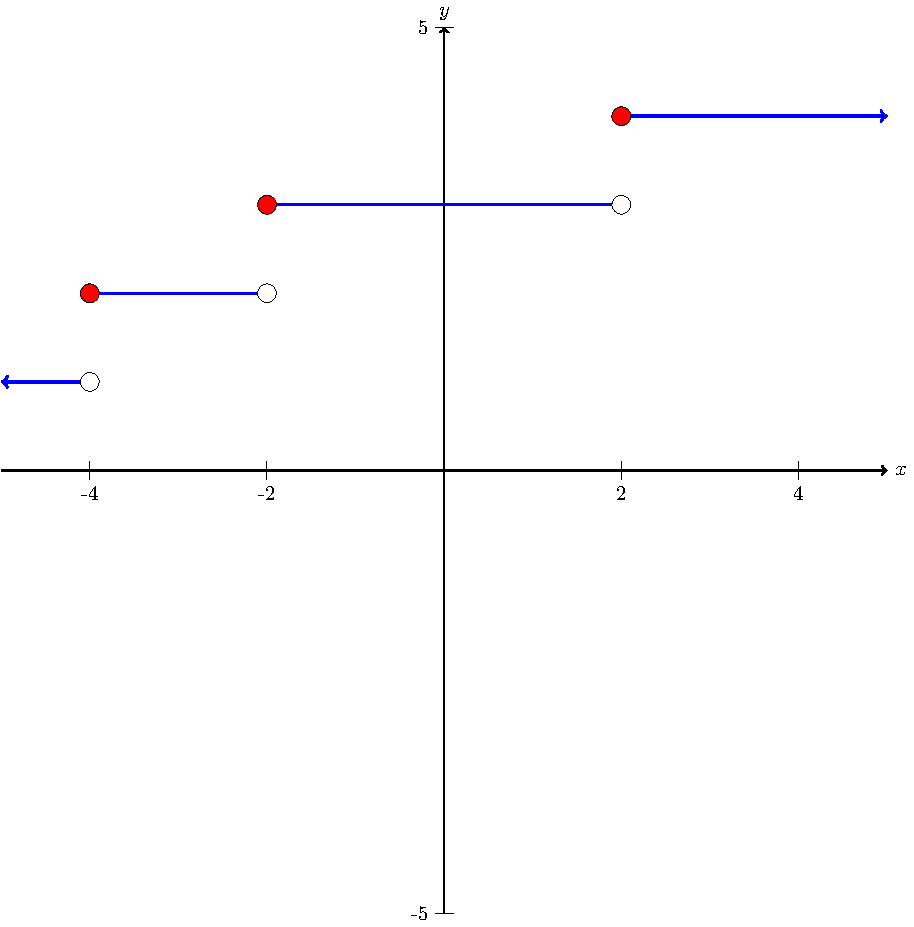
\includegraphics[width=0.5\linewidth]{../../html/Calculus/images/Piecewise.pdf}
\caption{Places where functions make a "jump" also produce discontinuities.\label{figure-11}}
\end{figure}
\hypertarget{p-204}{}%
A third type of discontinuity is the so called \emph{infinite} discontinuity.  Infinite discontinuities exist when the points values of a function diverge to infinity.  A classic example of an infinite discontinuity is the point \(x=0\) for the function \(f(x)=1/x\).%
\begin{figure}
\centering
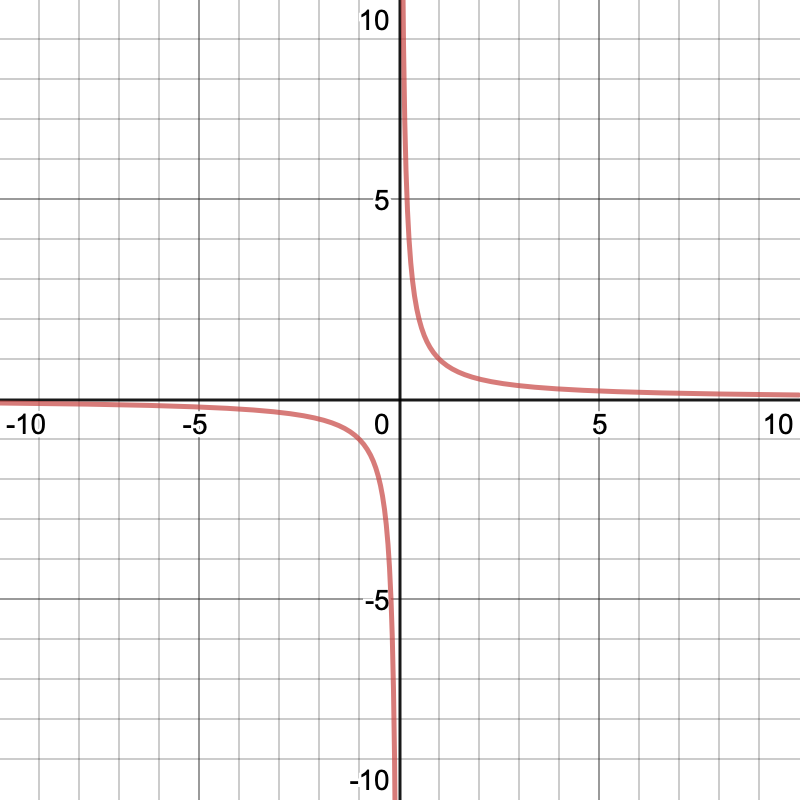
\includegraphics[width=0.5\linewidth]{../../html/Calculus/images/1overx.png}
\caption{A plot of the function \(y=f(x)\) for the function \(f(x)=1/x\).\label{figure-12}}
\end{figure}
\begin{example}[]\label{example-16}
\hypertarget{p-205}{}%
Consider the function%
\begin{equation*}
f(x)=\frac{3x(x+4)}{x^2-16}\text{.}
\end{equation*}
Are there \(x\)-values where the function is discontinuous?  If so, what are those \(x\)-values and why type of discontinuity occurs at that value?%
\par\smallskip%
\noindent\textbf{Hint.}\hypertarget{hint-1}{}\quad%
\hypertarget{p-206}{}%
Consider the graph of \(y=f(x)\).%
\begin{figure}
\centering
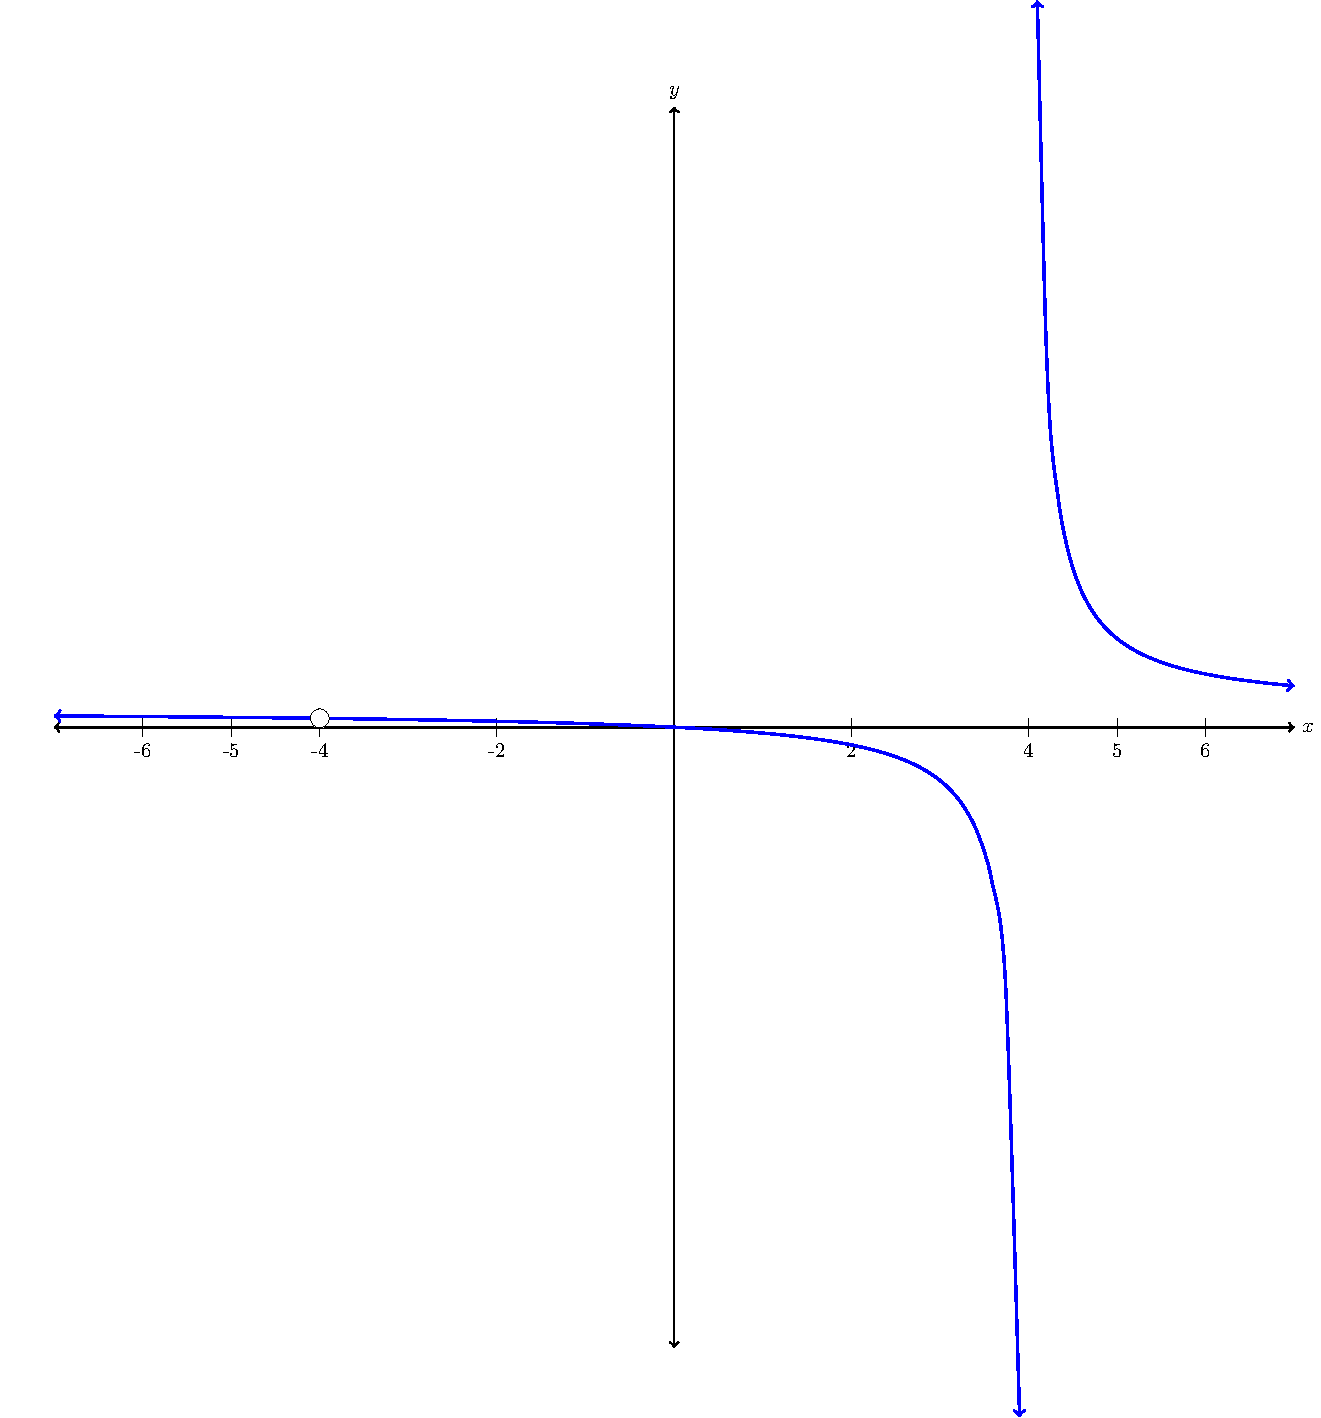
\includegraphics[width=0.5\linewidth]{../../html/Calculus/images/0-4-rational.pdf}
\caption{A plot of the function \(y=f(x)\).\label{figure-13}}
\end{figure}
\par\smallskip%
\noindent\textbf{Solution.}\hypertarget{solution-10}{}\quad%
\hypertarget{p-207}{}%
We first consider a graph of \(y=f(x)\).%
\begin{figure}
\centering
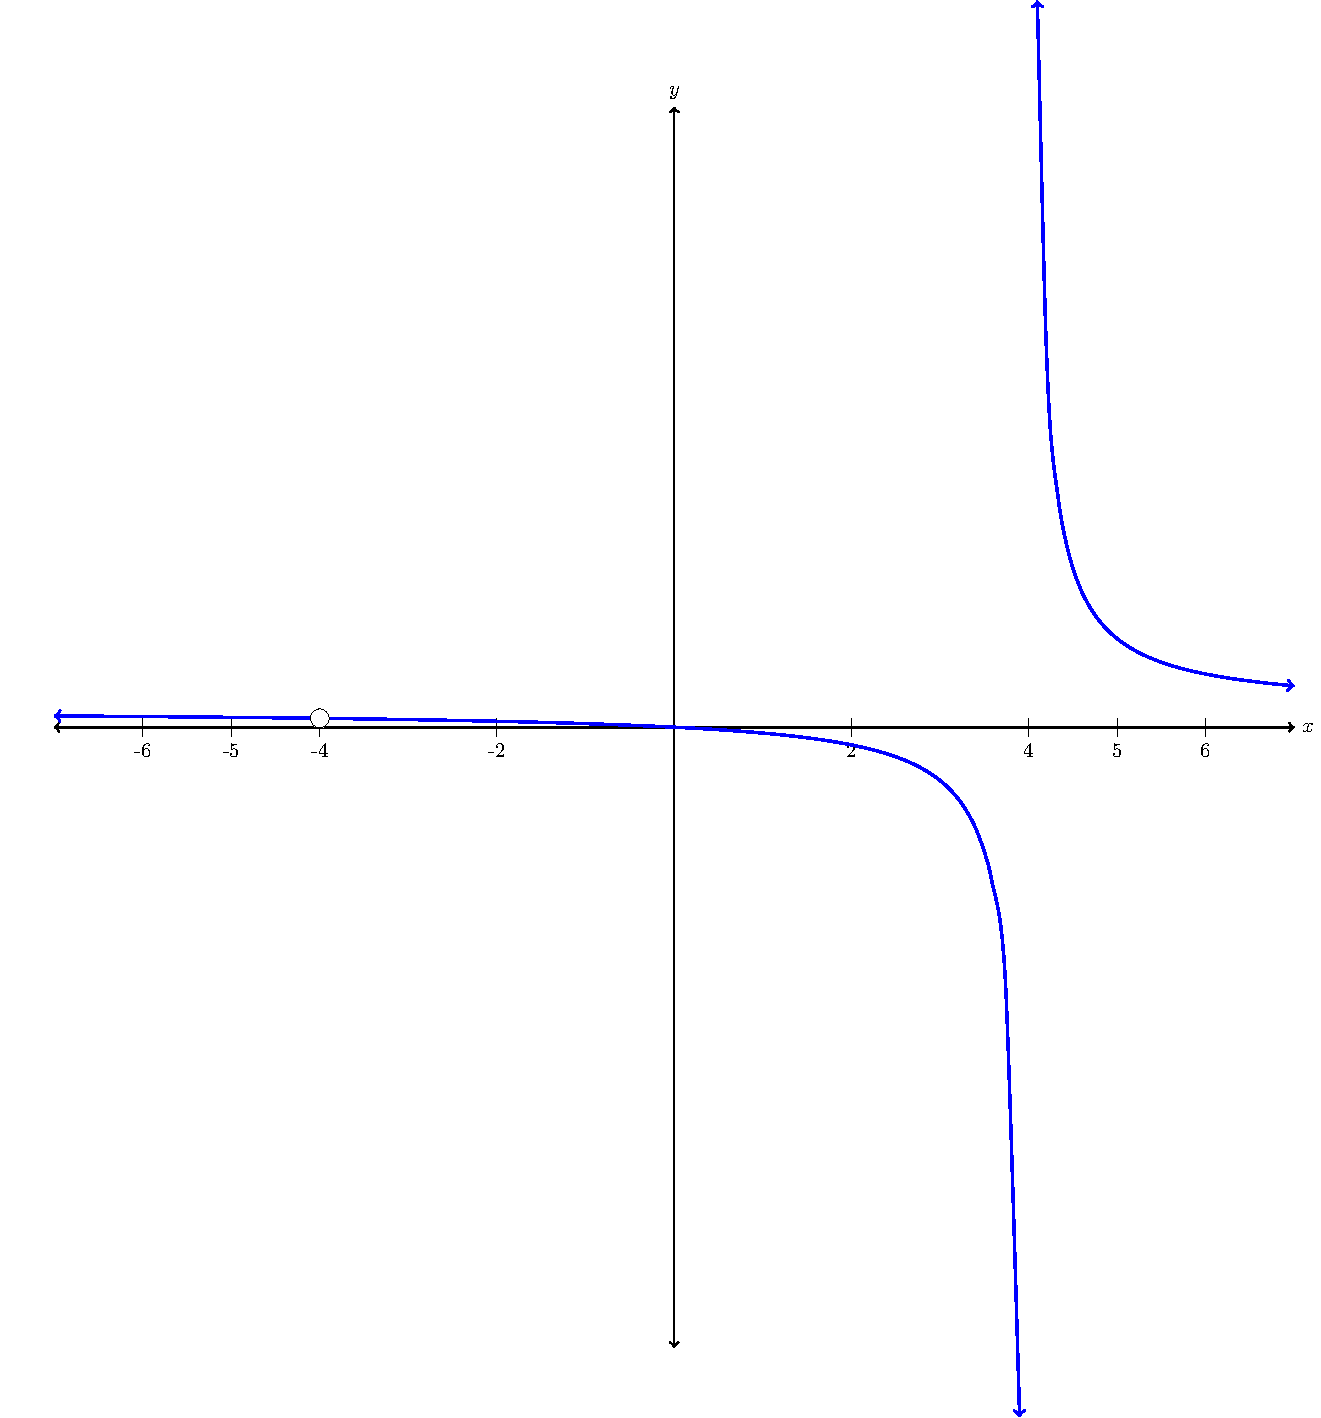
\includegraphics[width=0.5\linewidth]{../../html/Calculus/images/0-4-rational.pdf}
\caption{A plot of the function \(y=f(x)\).\label{figure-14}}
\end{figure}
\hypertarget{p-208}{}%
Visual inspection of the graph certainly indicates discontinuities.  However, we can make our visual inspection more precise through a little algebra.  We start by expanding the numerator and denominator of the function.  Specifically,%
\begin{equation*}
f(x)=\frac{3x(x+4)}{x^2-16}=\frac{3x(x+4)}{(x+4)(x-4)}.
\end{equation*}
From here we see that there are two \(x\)-values at which the function is undefined, \(x=-4,4\). Since the term \(x+4\) occurs in the numerator and denominator \(x=-4\) is a removable discontinuity. Since the term \(x-4\) occurs only in the denominator, \(x=4\) is an infinite discontinuity.%
\begin{note}[]\label{note-3}
\hypertarget{p-209}{}%
Rational functions can be a challenging topic. For a more complete discussion of rational functions we refer the reader to \href{https://mathbooks.unl.edu/PreCalculus/Graphing-Rational-Functions.html}{Short-Run Behavior of Rational Functions}%
\end{note}
\end{example}
\typeout{************************************************}
\typeout{Subsection 1.1.2 Piecewise Functions}
\typeout{************************************************}
\subsection[{Piecewise Functions}]{Piecewise Functions}\label{subsection-18}
\hypertarget{p-210}{}%
In many cases a simple function like \(f(x)=x^2\) may not fully describe the behavior of a phenomena. It  some of these cases we can turn to \emph{piecewise} functions to give us the tools we need.%
\begin{assemblage}[Piecewise Function]\label{assemblage-33}
\hypertarget{p-211}{}%
A piecewise-defined function is one which is defined not by a single equation, but by two or more. Each equation is valid for some interval .%
\end{assemblage}
\begin{example}[]\label{example-piecewise}
\hypertarget{p-212}{}%
Graph the function defined by%
\begin{equation*}
f(x) =
\begin{cases}
x +1  \amp \text{if } x\le 1\\
3  \amp \text{if } x\gt 1
\end{cases}.
\end{equation*}
%
\par\smallskip%
\noindent\textbf{Solution.}\hypertarget{solution-11}{}\quad%
\hypertarget{p-213}{}%
Think of the plane as divided into two regions by the vertical line \(x = 1\), as shown in \hyperref[fig-piecewise]{Figure~\ref{fig-piecewise}}. In the left-hand region (\(x \le 1\)), we graph the line \(y = x + 1\). (The fastest way to graph the line is to plot its intercepts, \((-1, 0)\) and \((0, 1)\).)%
\par
\hypertarget{p-214}{}%
%
% group protects changes to lengths, releases boxes (?)
{% begin: group for a single side-by-side
% set panel max height to practical minimum, created in preamble
\setlength{\panelmax}{0pt}
\ifdefined\panelboxAparagraphs\else\newsavebox{\panelboxAparagraphs}\fi%
\savebox{\panelboxAparagraphs}{%
\raisebox{\depth}{\parbox{0.5\linewidth}{\hypertarget{p-215}{}%
Notice that the value \(x = 1\) is included in the first region, so \(f (1) = 1 + 1 = 2\), and the point \((1, 2)\) is included on the graph. We indicate this with a solid dot at the point \((1, 2)\).%
\par
\hypertarget{p-216}{}%
In the right-hand region (\(x \gt 1\)), we graph the horizontal line \(y = 3\). The value \(x = 1\) is not included in the second region, so the point \((1, 3)\) is not part of the graph. We indicate this with an open circle at the point \((1, 3)\).%
}}}
\ifdefined\phAparagraphs\else\newlength{\phAparagraphs}\fi%
\setlength{\phAparagraphs}{\ht\panelboxAparagraphs+\dp\panelboxAparagraphs}
\settototalheight{\phAparagraphs}{\usebox{\panelboxAparagraphs}}
\setlength{\panelmax}{\maxof{\panelmax}{\phAparagraphs}}
\ifdefined\panelboxAimage\else\newsavebox{\panelboxAimage}\fi%
\begin{lrbox}{\panelboxAimage}
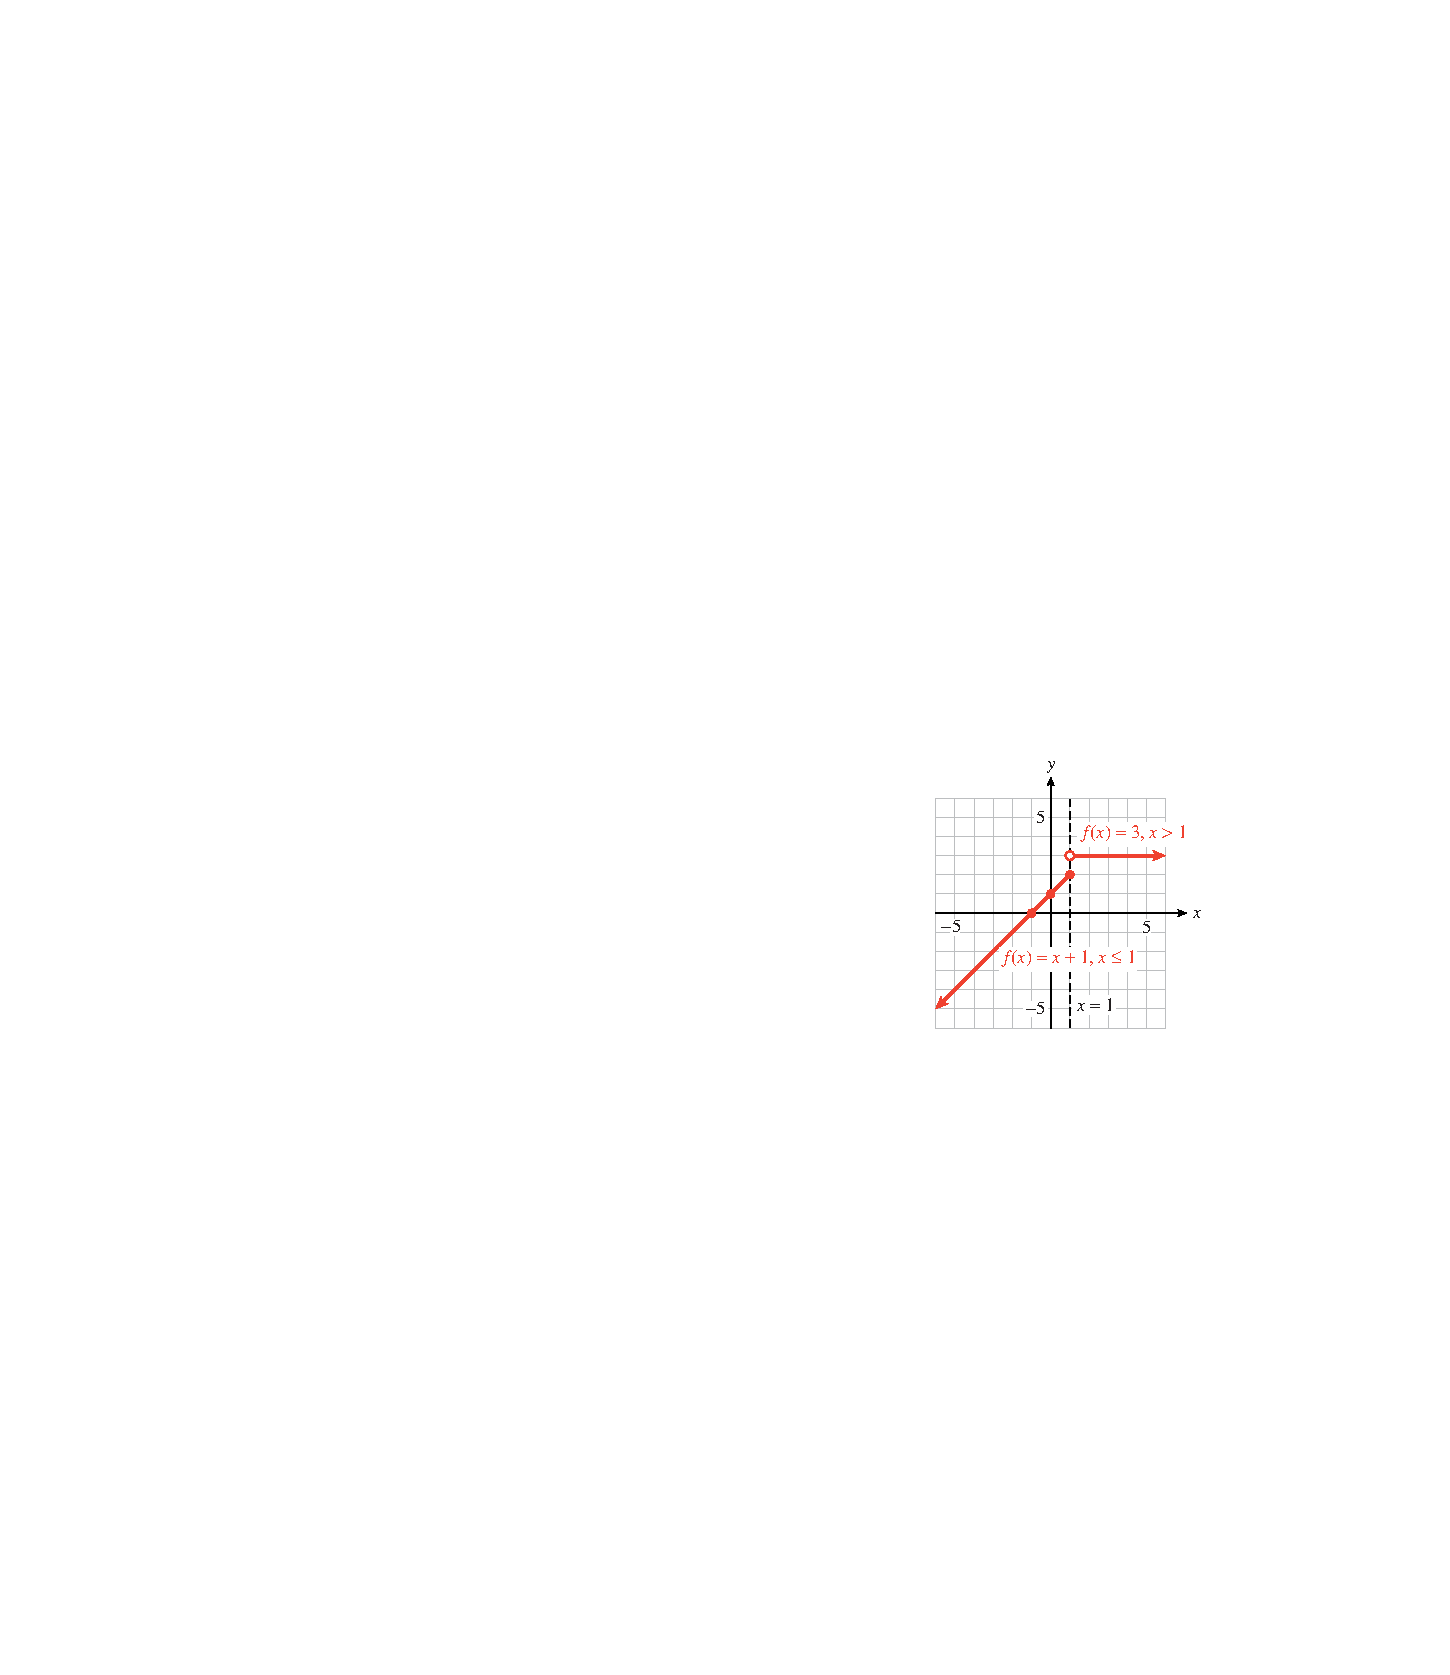
\includegraphics[width=0.4\linewidth]{../../html/Calculus/images/fig-piecewise.pdf}
\end{lrbox}
\ifdefined\phAimage\else\newlength{\phAimage}\fi%
\setlength{\phAimage}{\ht\panelboxAimage+\dp\panelboxAimage}
\settototalheight{\phAimage}{\usebox{\panelboxAimage}}
\setlength{\panelmax}{\maxof{\panelmax}{\phAimage}}
\leavevmode%
% begin: side-by-side as tabular
% \tabcolsep change local to group
\setlength{\tabcolsep}{0.025\linewidth}
% @{} suppress \tabcolsep at extremes, so margins behave as intended
\par\medskip\noindent
\hspace*{0.025\linewidth}%
\begin{tabular}{@{}*{2}{c}@{}}
\begin{minipage}[c][\panelmax][t]{0.5\linewidth}\usebox{\panelboxAparagraphs}\end{minipage}&
\begin{minipage}[c][\panelmax][t]{0.4\linewidth}\usebox{\panelboxAimage}\end{minipage}\tabularnewline
&
\parbox[t]{0.4\linewidth}{\captionof{figure}{\label{fig-piecewise}}
}\end{tabular}\\
% end: side-by-side as tabular
}% end: group for a single side-by-side
\end{example}
\hypertarget{p-217}{}%
The jumps that a piecewise function possesses make piecewise functions a natural place in which to explore continuity.%
\begin{example}[]\label{example-18}
\hypertarget{p-218}{}%
The function%
\begin{equation*}
h(x)=\begin{cases} 4x^2 \amp \text{ if } x\leq 1 \\ 3x+3 \amp \text{ if } x\gt1 \end{cases}
\end{equation*}
is discontinuous at \(x=1\). It is continuous on any interval that does not include \(x=1\).%
\end{example}
\hypertarget{p-219}{}%
Not only can we ask questions about when a piecewise function is continuous but we can also ask questions about how to make a piecewise function continuous by varying parameters.%
\begin{example}[]\label{example-19}
\hypertarget{p-220}{}%
Consider the piecewise function%
\begin{equation*}
D(x)=\begin{cases}
4x^2-k\amp\text{ if } x \lt 2,\\
kx+1\amp\text{ if } 2 \leq x.\\
\end{cases}
\end{equation*}
Find the value of \(k\) to make this function continuous for all \(x\).%
\par\smallskip%
\noindent\textbf{Hint.}\hypertarget{hint-2}{}\quad%
\hypertarget{p-221}{}%
The point where the function may not be continuous is at the potential "jump"-point.  Specifically, when \(x=2\)%
\par\smallskip%
\noindent\textbf{Solution.}\hypertarget{solution-12}{}\quad%
\hypertarget{p-222}{}%
The point where the function may not be continuous is at the potential "jump"-point.  Specifically, when \(x=2\). For the function to be continuous we need the two "branches" of the function to meet when \(x=2\).  That is we need \(4\times 2^2-k=k \times 2+1\) which is equivalent to \(k=5\).  The figure below shows a graph of \(y=D(x)\) for \(k=5\).%
\begin{figure}
\centering
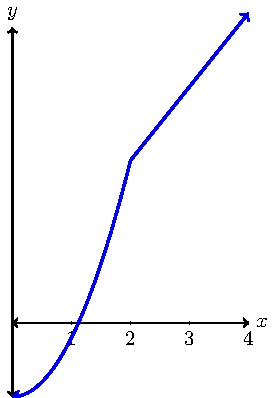
\includegraphics[width=0.5\linewidth]{../../html/Calculus/images/0-4-piecewise.pdf}
\caption{A plot of the function \(y=f(x)\).\label{figure-16}}
\end{figure}
\end{example}
\typeout{************************************************}
\typeout{Subsection 1.1.3 The Intermediate Value Theorem}
\typeout{************************************************}
\subsection[{The Intermediate Value Theorem}]{The Intermediate Value Theorem}\label{subsection-19}
\hypertarget{p-223}{}%
Up to this point we have talked about the continuity of a function at a point. Before stating the intermediate value theorem we begin by defining a continuous function.%
\begin{assemblage}[Continuous Function]\label{assemblage-34}
\hypertarget{p-224}{}%
A function is said to be continuous on an interval \((a,b)\) if the function as no points of discontinuity on that interval.%
\end{assemblage}
\hypertarget{p-226}{}%
One of the most important theorems in Calculus is the intermediate value theorem.  The intermediate value theorem essentially says that a continuous function takes the value of any any points that it crosses.  The formal statement of the theorem follows.%
\begin{assemblage}[Intermediate Value theorem]\label{assemblage-35}
\hypertarget{p-227}{}%
Suppose \(f\) is continuous on a closed interval \([a,b]\). If \(k\) is any number between \(f(a)\) and \(f(b)\), then there is at least one number \(c\) in \([a,b]\) such that \(f(c)=k\).%
\end{assemblage}
\typeout{************************************************}
\typeout{Exercises 1.1.4 Exercises}
\typeout{************************************************}
\subsection[{Exercises}]{Exercises}\label{exercises-4}
\begin{exerciselist}
\item[1.]\hypertarget{exercise-20}{}This exercise uses the WeBWorK Online Homework System and so is not available in the print copy of this book.\item[2.]\hypertarget{exercise-21}{}This exercise uses the WeBWorK Online Homework System and so is not available in the print copy of this book.\item[3.]\hypertarget{exercise-22}{}This exercise uses the WeBWorK Online Homework System and so is not available in the print copy of this book.\item[4.]\hypertarget{exercise-23}{}This exercise uses the WeBWorK Online Homework System and so is not available in the print copy of this book.\item[5.]\hypertarget{exercise-24}{}This exercise uses the WeBWorK Online Homework System and so is not available in the print copy of this book.\item[6.]\hypertarget{exercise-25}{}This exercise uses the WeBWorK Online Homework System and so is not available in the print copy of this book.\item[7.]\hypertarget{exercise-26}{}This exercise uses the WeBWorK Online Homework System and so is not available in the print copy of this book.\item[8.]\hypertarget{exercise-27}{}This exercise uses the WeBWorK Online Homework System and so is not available in the print copy of this book.\item[9.]\hypertarget{exercise-28}{}This exercise uses the WeBWorK Online Homework System and so is not available in the print copy of this book.\item[10.]\hypertarget{exercise-29}{}This exercise uses the WeBWorK Online Homework System and so is not available in the print copy of this book.\end{exerciselist}
\typeout{************************************************}
\typeout{Section 1.2 Introduction to Limits}
\typeout{************************************************}
\section[{Introduction to Limits}]{Introduction to Limits}\label{lims}
\begin{objectives}{Motivating Questions}\label{objectives-2}
%
\begin{itemize}[label=\textbullet]
\item{}\hypertarget{p-228}{}%
What is the mathematical notion of \emph{limit} and what role do limits play in the study of functions?%
\item{}\hypertarget{p-229}{}%
What is the meaning of the notation \(\lim_{x \to a} f(x) = L\)?%
\item{}\hypertarget{p-230}{}%
How do we go about determining the value of the limit of a function at a point?%
\item{}\hypertarget{p-231}{}%
What is a left-hand limit at \(x = a\) and a right-hand limit at \(x = a\)?%
\item{}\hypertarget{p-232}{}%
What does it mean graphically to say that \(f\) has limit \(L\) as \(x \to a\)? How is this connected to having a left-hand limit at \(x = a\) and having a right-hand limit at \(x = a\)?%
\item{}\hypertarget{p-233}{}%
How are limits connected to continuity?%
\end{itemize}
\end{objectives}
\hypertarget{p-234}{}%
Limits are a mathematical construct we can use to describe the behavior of a function near a point.  Consider the function \(g\) given by the graph in \hyperref[F-1-2-PA1]{Figure~\ref{F-1-2-PA1}} below. We can evaluate the function at a variety of points.  For example, \(g(-2)=0\), \(g(-1)=3\), and \(g(0)=1\).%
\begin{figure}
\centering
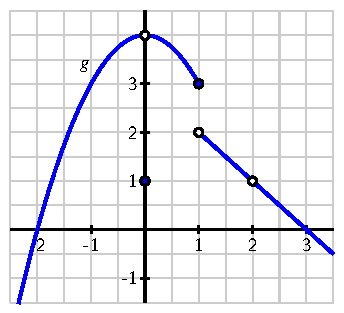
\includegraphics[width=0.47\linewidth]{../../html/Calculus/images/1_2_PA1.pdf}
\caption{Graph of \(y = g(x)\).\label{F-1-2-PA1}}
\end{figure}
\hypertarget{p-235}{}%
As stated earlier, \(g(0)=1\).  However, a careful look at the graph shows that you might have expected \(g(0)\) to be \(4\).  In fact, you would probably agree that ``As \(x\) gets closer and closer (but not equal) to \(0\), \(g(x)\) gets as close as we want to \(4\).'' This is the basic idea of a limit and we will expand on this idea in the following chapter.%
\typeout{************************************************}
\typeout{Subsection 1.2.1 The Notion of Limit}
\typeout{************************************************}
\subsection[{The Notion of Limit}]{The Notion of Limit}\label{subsection-20}
\hypertarget{p-236}{}%
Limits give us a way to identify a trend in the values of a function as its input variable approaches a particular value of interest. We need a precise understanding of what it means to say ``a function \(f\) has limit \(L\) as \(x\) approaches \(a\).''%
\par
\hypertarget{p-237}{}%
In \hyperref[F-1-2-PA1]{Figure~\ref{F-1-2-PA1}}, we saw that as \(x\) gets closer and closer (but not equal) to 0, \(g(x)\) gets as close as we want to the value 4. At first, this may feel counterintuitive, because the value of \(g(0)\) is \(1\), not \(4\). But limits describe the behavior of a function \emph{arbitrarily close to} a fixed input and are not affected by the value of the function \emph{at} the fixed input. More formally,\footnote{What follows here is not what mathematicians consider the formal definition of a limit. To be completely precise, it is necessary to quantify both what it means to say ``as close to \(L\) as we like'' and ``sufficiently close to \(a\).'' That can be accomplished through what is traditionally called the epsilon-delta definition of limits. That being said, the definition presented here is sufficient for the purposes of this text.\label{fn-2}} we say the following.%
\begin{assemblage}\label{assemblage-36}
\hypertarget{p-238}{}%
If a function \(f\) is defined on an interval around \(c\), except perhaps at the point \(x = c\).  We define the limit of the function \(f(x)\) as \(x\) approaches \(c\) to be a number \(L\) (if one exists) such that \(f(x)\) is as close to  \(L\) as we want whenever \(x\) is sufficiently close to \(c\) (but \(x \neq c\)). If \(L\) exists, we write%
\begin{equation*}
\lim_{x \rightarrow c} f(x)=L
\end{equation*}
On the other hand, if as \(x\) approaches \(c\) we cannot make \(f(x)\) as close to a single value as we would like, then we say that \terminology{\(f\) does not have a limit as \(x\) approaches \(c\).}%
\end{assemblage}
\begin{example}[]\label{example-20}
\hypertarget{p-239}{}%
Recall the function \(g\) from the section introduction. \begin{figure}
\centering
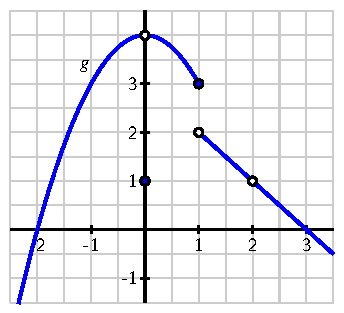
\includegraphics[width=0.47\linewidth]{../../html/Calculus/images/1_2_PA1.pdf}
\caption{Graph of \(y = g(x)\)\label{F-1-2-PA1prime}}
\end{figure}
 For the function \(g\) pictured in \hyperref[F-1-2-PA1prime]{Figure~\ref{F-1-2-PA1prime}}, we make the following observations:%
\begin{equation*}
\lim_{x \to -1} g(x) = 3, \  \lim_{x \to 0} g(x) = 4, \ \text{and}  \  \lim_{x \to 2} g(x) = 1\text{.}
\end{equation*}
When finding a limit from a graph, it suffices to ask if the function \emph{approaches} a single value from each side of the fixed input. The function value \emph{at} the fixed input is irrelevant. This reasoning explains the values of the three limits stated above.%
\par
\hypertarget{p-240}{}%
We further observe that \(g\) does not have a limit as \(x\) approaches \(1\) because there is a jump in the graph at \(x = 1\). If we approach \(x = 1\) from the left, the function values tend to get close to 3, but if we approach \(x = 1\) from the right, the function values get close to 2. There is no single number that all of these function values approach. This is why the limit of \(g\) does not exist at \(x = 1\).%
\end{example}
\hypertarget{p-241}{}%
For any function \(f\), there are typically three ways to answer the question ``does \(f\) have a limit at \(x = a\), and if so, what is the limit?'' The first is to reason graphically. If we have a formula for \(f(x)\), there are two additional possibilities: \leavevmode%
\begin{enumerate}[label=\arabic*]
\item\hypertarget{li-55}{}Evaluate the function at a sequence of inputs that approach \(a\) on either side (typically using some sort of computing technology), and ask if the sequence of outputs seems to approach a single value.%
\item\hypertarget{li-56}{}Use the algebraic form of the function to understand the trend in its output values as the input values approach \(a\).%
\end{enumerate}
 The first approach produces only an approximation of the value of the limit, while the latter can often be used to determine the limit exactly.%
\begin{example}[Limits of Two Functions]\label{Ex-1-2-Limits}
\hypertarget{p-242}{}%
For each of the following functions, we'd like to know whether or not the function has a limit at the stated \(c\)-values. Use both numerical and algebraic approaches to investigate and, if possible, estimate or determine the value of the limit. Compare the results with a careful graph of the function on an interval containing the points of interest.%
\par
\hypertarget{p-243}{}%
\leavevmode%
\begin{multicols}{2}
\begin{enumerate}[label=\alph*.]
\item\hypertarget{li-57}{}\(f(x) = \frac{4-x^2}{x+2}\); \(c = -1\), \(c = -2\)%
\item\hypertarget{li-58}{}\(g(x) = \sin\left(\frac{\pi}{x}\right)\); \(c = 3\), \(c = 0\)%
\end{enumerate}
\end{multicols}
%
\par\smallskip%
\noindent\textbf{Solution.}\hypertarget{solution-13}{}\quad%
\hypertarget{p-244}{}%
a. We first construct a graph of \(f\) along with tables of values near \(c = -1\) and \(c = -2\).%
% group protects changes to lengths, releases boxes (?)
{% begin: group for a single side-by-side
% set panel max height to practical minimum, created in preamble
\setlength{\panelmax}{0pt}
\ifdefined\panelboxAtabular\else\newsavebox{\panelboxAtabular}\fi%
\savebox{\panelboxAtabular}{%
\raisebox{\depth}{\parbox{0.23\linewidth}{\centering\begin{tabular}{ll}
\multicolumn{1}{c}{\(x\)}&\multicolumn{1}{c}{\(f(x)\)}\tabularnewline\hrulethin
\(-0.9\)&\(2.9\)\tabularnewline[0pt]
\(-0.99\)&\(2.99\)\tabularnewline[0pt]
\(-0.999\)&\(2.999\)\tabularnewline[0pt]
\(-0.9999\)&\(2.9999\)\tabularnewline[0pt]
\(-1.1\)&\(3.1\)\tabularnewline[0pt]
\(-1.01\)&\(3.01\)\tabularnewline[0pt]
\(-1.001\)&\(3.001\)\tabularnewline[0pt]
\(-1.0001\)&\(3.0001\)
\end{tabular}
}}}
\ifdefined\phAtabular\else\newlength{\phAtabular}\fi%
\setlength{\phAtabular}{\ht\panelboxAtabular+\dp\panelboxAtabular}
\settototalheight{\phAtabular}{\usebox{\panelboxAtabular}}
\setlength{\panelmax}{\maxof{\panelmax}{\phAtabular}}
\ifdefined\panelboxBtabular\else\newsavebox{\panelboxBtabular}\fi%
\savebox{\panelboxBtabular}{%
\raisebox{\depth}{\parbox{0.23\linewidth}{\centering\begin{tabular}{ll}
\multicolumn{1}{c}{\(x\)}&\multicolumn{1}{c}{\(f(x)\)}\tabularnewline\hrulethin
\(-1.9\)&\(3.9\)\tabularnewline[0pt]
\(-1.99\)&\(3.99\)\tabularnewline[0pt]
\(-1.999\)&\(3.999\)\tabularnewline[0pt]
\(-1.9999\)&\(3.9999\)\tabularnewline[0pt]
\(-2.1\)&\(4.1\)\tabularnewline[0pt]
\(-2.01\)&\(4.01\)\tabularnewline[0pt]
\(-2.001\)&\(4.001\)\tabularnewline[0pt]
\(-2.0001\)&\(4.0001\)
\end{tabular}
}}}
\ifdefined\phBtabular\else\newlength{\phBtabular}\fi%
\setlength{\phBtabular}{\ht\panelboxBtabular+\dp\panelboxBtabular}
\settototalheight{\phBtabular}{\usebox{\panelboxBtabular}}
\setlength{\panelmax}{\maxof{\panelmax}{\phBtabular}}
\ifdefined\panelboxAimage\else\newsavebox{\panelboxAimage}\fi%
\begin{lrbox}{\panelboxAimage}
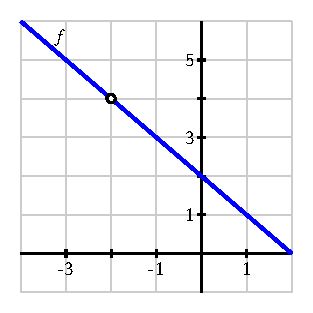
\includegraphics[width=0.42\linewidth]{../../html/Calculus/images/1_2_Ex1f.pdf}
\end{lrbox}
\ifdefined\phAimage\else\newlength{\phAimage}\fi%
\setlength{\phAimage}{\ht\panelboxAimage+\dp\panelboxAimage}
\settototalheight{\phAimage}{\usebox{\panelboxAimage}}
\setlength{\panelmax}{\maxof{\panelmax}{\phAimage}}
\leavevmode%
% begin: side-by-side as tabular
% \tabcolsep change local to group
\setlength{\tabcolsep}{0.02\linewidth}
% @{} suppress \tabcolsep at extremes, so margins behave as intended
\par\medskip\noindent
\hspace*{0.02\linewidth}%
\begin{tabular}{@{}*{3}{c}@{}}
\begin{minipage}[c][\panelmax][c]{0.23\linewidth}\usebox{\panelboxAtabular}\end{minipage}&
\begin{minipage}[c][\panelmax][c]{0.23\linewidth}\usebox{\panelboxBtabular}\end{minipage}&
\begin{minipage}[c][\panelmax][c]{0.42\linewidth}\usebox{\panelboxAimage}\end{minipage}\tabularnewline
\parbox[t]{0.23\linewidth}{\captionof{table}{Table of \(f\) values near \(x=-1\).\label{table-1-F-1-2-Ex1f}}
}&
\parbox[t]{0.23\linewidth}{\captionof{table}{Table of \(f\) values near \(x=-2\).\label{table-2-F-1-2-Ex1f}}
}&
\parbox[t]{0.42\linewidth}{\captionof{figure}{Plot of \(f(x)\) on \([-4,2]\).\label{plot-F-1-2-Ex1f}}
}\end{tabular}\\
% end: side-by-side as tabular
}% end: group for a single side-by-side
\par
\hypertarget{p-245}{}%
From \hyperref[table-1-F-1-2-Ex1f]{Table~\ref{table-1-F-1-2-Ex1f}}, it appears that we can make \(f\) as close as we want to 3 by taking \(x\) sufficiently close to \(-1\), which suggests that \(\lim_{x \to -1} f(x) = 3\). This is also consistent with the graph of \(f\), as seen in \hyperref[plot-F-1-2-Ex1f]{Figure~\ref{plot-F-1-2-Ex1f}}. To see this a bit more rigorously and from an algebraic point of view, consider the formula for \(f\): \(f(x) = \frac{4-x^2}{x+2}\). As \(x\) approaches \(-1\), the numerator, \(4-x^2\), of \(f\) approaches \(4 - (-1)^2 = 3\), and the denominator, \(x+2\), of \(f\) approaches \(-1 + 2 = 1\). Hence \(\lim_{x \to -1} f(x) = \frac{3}{1} = 3\).%
\par
\hypertarget{p-246}{}%
The situation is more complicated when \(x\) approaches \(-2\) because \(f(-2)\) is not defined. If we try to use a similar algebraic argument regarding the numerator and denominator, we observe that as \(x\) approaches \(-2\), the numerator \((4-x^2)\) approaches \((4 - (-2)^2) = 0\), and the denominator \((x+2)\) approaches \((-2 + 2) = 0\), so as \(x\) approaches \(-2\), the numerator and denominator of \(f\) both tend to 0. We call \(0/0\) an \emph{indeterminate form}. \index{indeterminate form} This tells us that there is somehow more work to do. From \hyperref[table-2-F-1-2-Ex1f]{Table~\ref{table-2-F-1-2-Ex1f}} and \hyperref[plot-F-1-2-Ex1f]{Figure~\ref{plot-F-1-2-Ex1f}}, it appears that \(f\) should have a limit of \(4\) at \(x = -2\).%
\par
\hypertarget{p-247}{}%
To see algebraically why this is the case, observe that%
\begin{align*}
\lim_{x \to -2} f(x) = \amp  \lim_{x \to -2} \frac{4-x^2}{x+2}\\
= \amp  \lim_{x \to -2} \frac{(2-x)(2+x)}{x+2}\text{.}
\end{align*}
%
\par
\hypertarget{p-248}{}%
It is important to observe that because we are taking the limit as \(x\) approaches \(-2\), we are considering \(x\) values that are close, but not equal, to \(-2\). Since we never actually allow \(x\) to equal \(-2\), the quotient \(\frac{2+x}{x+2}\) has value 1 for every possible value of \(x\). Thus, we can simplify the most recent expression above, and find that%
\begin{equation*}
\lim_{x \to -2} f(x) = \lim_{x \to -2} (2-x)\text{.}
\end{equation*}
This limit is now easy to determine, and its value is \(4\). Thus, from several points of view we've seen that \(\lim_{x \to -2} f(x) = 4\).%
\par
\hypertarget{p-249}{}%
b. Next we turn to the function \(g\), and construct two tables and a graph.%
% group protects changes to lengths, releases boxes (?)
{% begin: group for a single side-by-side
% set panel max height to practical minimum, created in preamble
\setlength{\panelmax}{0pt}
\ifdefined\panelboxAtabular\else\newsavebox{\panelboxAtabular}\fi%
\savebox{\panelboxAtabular}{%
\raisebox{\depth}{\parbox{0.23\linewidth}{\centering\begin{tabular}{ll}
\multicolumn{1}{c}{\(x\)}&\multicolumn{1}{c}{\(g(x)\)}\tabularnewline\hrulethin
\(2.9\)&\(0.84864\)\tabularnewline[0pt]
\(2.99\)&\(0.86428\)\tabularnewline[0pt]
\(2.999\)&\(0.86585\)\tabularnewline[0pt]
\(2.9999\)&\(0.86601\)\tabularnewline[0pt]
\(3.1\)&\(0.88351\)\tabularnewline[0pt]
\(3.01\)&\(0.86777\)\tabularnewline[0pt]
\(3.001\)&\(0.86620\)\tabularnewline[0pt]
\(3.0001\)&\(0.86604\)
\end{tabular}
}}}
\ifdefined\phAtabular\else\newlength{\phAtabular}\fi%
\setlength{\phAtabular}{\ht\panelboxAtabular+\dp\panelboxAtabular}
\settototalheight{\phAtabular}{\usebox{\panelboxAtabular}}
\setlength{\panelmax}{\maxof{\panelmax}{\phAtabular}}
\ifdefined\panelboxBtabular\else\newsavebox{\panelboxBtabular}\fi%
\savebox{\panelboxBtabular}{%
\raisebox{\depth}{\parbox{0.23\linewidth}{\centering\begin{tabular}{ll}
\multicolumn{1}{c}{\(x\)}&\multicolumn{1}{c}{\(g(x)\)}\tabularnewline\hrulethin
\(-0.1\)&\(0\)\tabularnewline[0pt]
\(-0.01\)&\(0\)\tabularnewline[0pt]
\(-0.001\)&\(0\)\tabularnewline[0pt]
\(-0.0001\)&\(0\)\tabularnewline[0pt]
\(0.1\)&\(0\)\tabularnewline[0pt]
\(0.01\)&\(0\)\tabularnewline[0pt]
\(0.001\)&\(0\)\tabularnewline[0pt]
\(0.0001\)&\(0\)
\end{tabular}
}}}
\ifdefined\phBtabular\else\newlength{\phBtabular}\fi%
\setlength{\phBtabular}{\ht\panelboxBtabular+\dp\panelboxBtabular}
\settototalheight{\phBtabular}{\usebox{\panelboxBtabular}}
\setlength{\panelmax}{\maxof{\panelmax}{\phBtabular}}
\ifdefined\panelboxAimage\else\newsavebox{\panelboxAimage}\fi%
\begin{lrbox}{\panelboxAimage}
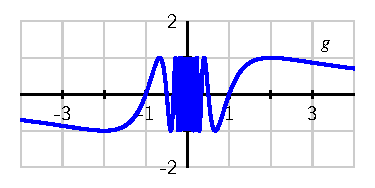
\includegraphics[width=0.42\linewidth]{../../html/Calculus/images/1_2_Ex1g.pdf}
\end{lrbox}
\ifdefined\phAimage\else\newlength{\phAimage}\fi%
\setlength{\phAimage}{\ht\panelboxAimage+\dp\panelboxAimage}
\settototalheight{\phAimage}{\usebox{\panelboxAimage}}
\setlength{\panelmax}{\maxof{\panelmax}{\phAimage}}
\leavevmode%
% begin: side-by-side as tabular
% \tabcolsep change local to group
\setlength{\tabcolsep}{0.02\linewidth}
% @{} suppress \tabcolsep at extremes, so margins behave as intended
\par\medskip\noindent
\hspace*{0.02\linewidth}%
\begin{tabular}{@{}*{3}{c}@{}}
\begin{minipage}[c][\panelmax][t]{0.23\linewidth}\usebox{\panelboxAtabular}\end{minipage}&
\begin{minipage}[c][\panelmax][t]{0.23\linewidth}\usebox{\panelboxBtabular}\end{minipage}&
\begin{minipage}[c][\panelmax][t]{0.42\linewidth}\usebox{\panelboxAimage}\end{minipage}\tabularnewline
\parbox[t]{0.23\linewidth}{\captionof{table}{Table of \(g\) values near \(x=3\).\label{table-1-F-1-2-Ex1g}}
}&
\parbox[t]{0.23\linewidth}{\captionof{table}{Table of \(g\) values near \(x=0\).\label{table-2-F-1-2-Ex1g}}
}&
\parbox[t]{0.42\linewidth}{\captionof{figure}{Plot of \(g(x)\) on \([-4,4]\).\label{plot-F-1-2-Ex1g}}
}\end{tabular}\\
% end: side-by-side as tabular
}% end: group for a single side-by-side
\par
\hypertarget{p-250}{}%
First, as \(x\) approaches \(3\), it appears from the values in \hyperref[table-1-F-1-2-Ex1g]{Table~\ref{table-1-F-1-2-Ex1g}} that the function is approaching a number between \(0.86601\) and \(0.86604\). From the graph in \hyperref[plot-F-1-2-Ex1g]{Figure~\ref{plot-F-1-2-Ex1g}} it appears that \(g(x)\) approaches \(g(3)\) as \(x\) approaches \(3\). The exact value of \(g(3) = \sin(\frac{\pi}{3})\) is \(\frac{\sqrt{3}}{2}\), which is approximately 0.8660254038. This is convincing evidence that%
\begin{equation*}
\lim_{x \to 3} g(x) = \frac{\sqrt{3}}{2}\text{.}
\end{equation*}
%
\par
\hypertarget{p-251}{}%
As \(x\) approaches \(0\), we observe that \(\frac{\pi}{x}\) does not behave in an elementary way. When \(x\) is positive and approaching zero, we are dividing by smaller and smaller positive values, and \(\frac{\pi}{x}\) increases without bound. When \(x\) is negative and approaching zero, \(\frac{\pi}{x}\) decreases without bound. In this sense, as we get close to \(x = 0\), the inputs to the sine function are growing rapidly, and this leads to increasingly rapid oscillations in the graph of \(g\) between \(1\) and \(-1\). If we plot the function \(g(x) = \sin\left(\frac{\pi}{x}\right)\) with a graphing utility and then zoom in on \(x = 0\), we see that the function never settles down to a single value near the origin, which suggests that \(g\) does not have a limit at \(x = 0\).%
\par
\hypertarget{p-252}{}%
How do we reconcile the graph in \hyperref[plot-F-1-2-Ex1g]{Figure~\ref{plot-F-1-2-Ex1g}} with \hyperref[table-2-F-1-2-Ex1g]{Table~\ref{table-2-F-1-2-Ex1g}}, which seems to suggest that the limit of \(g\) as \(x\) approaches \(0\) may in fact be \(0\)? The data misleads us because of the special nature of the sequence of input values \(\{0.1, 0.01, 0.001, \ldots\}\). When we evaluate \(g(10^{-k})\), we get \(g(10^{-k}) = \sin\left(\frac{\pi}{10^{-k}}\right) = \sin(10^k \pi) = 0\) for each positive integer value of \(k\). But if we take a different sequence of values approaching zero, say \(\{0.3, 0.03, 0.003, \ldots\}\), then we find that%
\begin{equation*}
g(3 \cdot 10^{-k}) = \sin\left(\frac{\pi}{3 \cdot 10^{-k}}\right) = \sin\left(\frac{10^k \pi}{3}\right) = \frac{\sqrt{3}}{2} \approx 0.866025\text{.}
\end{equation*}
%
\par
\hypertarget{p-253}{}%
That sequence of function values suggests that the value of the limit is \(\frac{\sqrt{3}}{2}\). Clearly the function cannot have two different values for the limit, so \(g\) has no limit as \(x\) approaches \(0\).%
\end{example}
\hypertarget{p-254}{}%
An important lesson to take from \hyperref[Ex-1-2-Limits]{Example~\ref{Ex-1-2-Limits}} is that tables can be misleading when determining the value of a limit. While a table of values is useful for investigating the \emph{possible} value of a limit, we should also use other tools to confirm the value.%
\begin{example}[]\label{act-1-2-1}
\hypertarget{p-255}{}%
Estimate the value of each of the following limits by constructing appropriate tables of values. Then determine the exact value of the limit by using algebra to simplify the function. Finally, plot each function on an appropriate interval to check your result visually. \leavevmode%
\begin{multicols}{3}
\begin{enumerate}[label=\alph*.]
\item\hypertarget{li-59}{}\(\lim_{x \to 1} \frac{x^2 - 1}{x-1}\)%
\item\hypertarget{li-60}{}\(\lim_{x \to 0} \frac{(2+x)^3 - 8}{x}\)%
\item\hypertarget{li-61}{}\(\lim_{x \to 0} \frac{\sqrt{x+1} - 1}{x}\)%
\end{enumerate}
\end{multicols}
%
\par\smallskip%
\noindent\textbf{Hint.}\hypertarget{hint-3}{}\quad%
\hypertarget{p-256}{}%
\leavevmode%
\begin{enumerate}[label=\alph*.]
\item\hypertarget{li-62}{}\((x^2 - 1)\) can be factored.%
\item\hypertarget{li-63}{}Expand the expression \((2+x)^3\), and then combine like terms in the numerator.%
\item\hypertarget{li-64}{}Try multiplying the given function by this fancy form of 1: \(\frac{\sqrt{x+1} + 1}{\sqrt{x+1} + 1}\).%
\end{enumerate}
%
\par\smallskip%
\noindent\textbf{Answer.}\hypertarget{answer-1}{}\quad%
\hypertarget{p-257}{}%
\leavevmode%
\begin{enumerate}[label=\alph*.]
\item\hypertarget{li-65}{}\(2\).%
\item\hypertarget{li-66}{}\(12\).%
\item\hypertarget{li-67}{}\(\frac{1}{2}\).%
\end{enumerate}
%
\par\smallskip%
\noindent\textbf{Solution.}\hypertarget{solution-14}{}\quad%
\hypertarget{p-258}{}%
Estimating the values of the limits with tables is straightforward and should suggest the exact values stated below.%
\par
\hypertarget{p-259}{}%
\leavevmode%
\begin{enumerate}[label=\alph*.]
\item\hypertarget{li-68}{}\(\lim_{x \to 1} \frac{x^2 - 1}{x-1} = \lim_{x \to 1} \frac{(x+1)(x-1)}{x-1} = \lim_{x \to 1} (x+1) = 2\).%
\item\hypertarget{li-69}{}%
\begin{align*}
\lim_{x \to 0} \frac{(2+x)^3 - 8}{x} \amp = \lim_{x \to 0} \frac{8 + 12x + 6x^2 + x^3 - 8}{x} = \lim_{x \to 0} \frac{12x + 6x^2 + x^3}{x}\\
\amp =  \lim_{x \to 0} (12 + 6x + x^2) = 12\text{.}
\end{align*}
%
\item\hypertarget{li-70}{}%
\begin{align*}
\lim_{x \to 0} \frac{\sqrt{x+1} - 1}{x} \amp = \lim_{x \to 0} \frac{\sqrt{x+1} - 1}{x} \cdot \frac{\sqrt{x+1} + 1}{\sqrt{x+1} + 1} = \lim_{x \to 0} \frac{x+1-1}{x(\sqrt{x+1}+1)}\\
\amp = \lim_{x \to 0} \frac{1}{\sqrt{x+1}+1} = \frac{1}{2}\text{.}
\end{align*}
%
\end{enumerate}
%
\end{example}
\hypertarget{p-260}{}%
Recall that our primary motivation for considering limits of functions comes from our interest in studying the rate of change of a function. To that end, we close this section by revisiting our previous work with average and instantaneous velocity and highlighting the role that limits play.%
\typeout{************************************************}
\typeout{Subsection 1.2.2 Having a limit at a point}
\typeout{************************************************}
\subsection[{Having a limit at a point}]{Having a limit at a point}\label{subsection-21}
\hypertarget{p-261}{}%
We saw earlier that \(f\) has limit \(L\) as \(x\) approaches \(c\) provided that we can make the value of \(f(x)\) as close to \(L\) as we like by taking \(x\) sufficiently close (but not equal to) \(c\). If so, we write \(\lim_{x \to c} f(x) = L\). We also saw that there are cases where a function can fail to have a limit.  The graphs that follow are two such examples.%
\begin{figure}
\centering
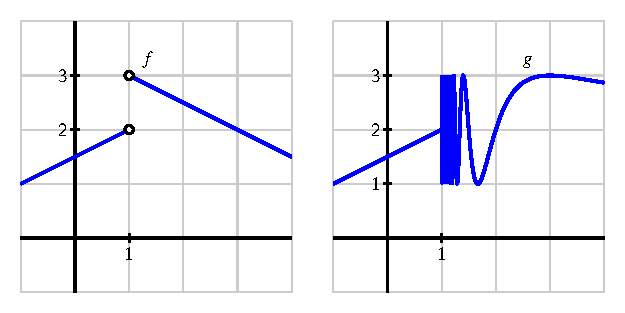
\includegraphics[width=1\linewidth]{../../html/Calculus/images/1_7_NoLimit.pdf}
\caption{Functions \(f\) and \(g\) that each fail to have a limit at \(c = 1\).\label{F-1-7-NoLimit}}
\end{figure}
\hypertarget{p-262}{}%
Essentially there are two behaviors that a function can exhibit near a point where it fails to have a limit. In \hyperref[F-1-7-NoLimit]{Figure~\ref{F-1-7-NoLimit}}, at left we see a function \(f\) whose graph shows a jump at \(c = 1\). If we let \(x\) approach 1 from the left side, the value of \(f\) approaches 2, but if we let \(x\) approach \(1\) from the right, the value of \(f\) tends to 3. Because the value of \(f\) does not approach a single number as \(x\) gets arbitrarily close to 1 from both sides, we know that \(f\) does not have a limit at \(c = 1\).%
\par
\hypertarget{p-263}{}%
For such cases, we introduce the notion of \emph{left} and \emph{right} (or \emph{one-sided}) limits. \index{left limit} \index{right limit} \index{limit!one-sided}%
\begin{assemblage}\label{assemblage-37}
\hypertarget{p-264}{}%
We say that \emph{\(f\) has limit \(L_1\) as \(x\) approaches \(c\) from the left} and write%
\begin{equation*}
\lim_{x \to c^-} f(x) = L_1
\end{equation*}
provided that we can make the value of \(f(x)\) as close to \(L_1\) as we like by taking \(x\) sufficiently close to \(c\) while always having \(x \lt  c\). We call \(L_1\) the left-hand limit of \(f\) as \(x\) approaches \(c\). Similarly, we say \emph{\(L_2\) is the right-hand limit of \(f\) as \(x\) approaches \(c\)} and write%
\begin{equation*}
\lim_{x \to c^+} f(x) = L_2
\end{equation*}
provided that we can make the value of \(f(x)\) as close to \(L_2\) as we like by taking \(x\) sufficiently close to \(c\) while always having \(x \gt c\).%
\end{assemblage}
\hypertarget{p-265}{}%
In the graph of the function \(f\) in \hyperref[F-1-7-NoLimit]{Figure~\ref{F-1-7-NoLimit}}, we see that%
\begin{equation*}
\lim_{x \to 1^-} f(x) = 2 \ \ \text{and}  \ \lim_{x \to 1^+} f(x) = 3\text{.}
\end{equation*}
Precisely because the left and right limits are not equal, the overall limit of \(f\) as \(x \to 1\) fails to exist.%
\par
\hypertarget{p-266}{}%
For the function \(g\) pictured at right in \hyperref[F-1-7-NoLimit]{Figure~\ref{F-1-7-NoLimit}}, the function fails to have a limit at \(c = 1\) for a different reason. While the function does not have a jump in its graph at \(c = 1\), it is still not the case that \(g\) approaches a single value as \(x\) approaches 1. In particular, due to the infinitely oscillating behavior of \(g\) to the right of \(c = 1\), we say that the right-hand limit of \(g\) as \(x \to 1^+\) does not exist, and thus \(\lim_{x \to 1} g(x) \ \text{does not exist} \).%
\par
\hypertarget{p-267}{}%
To summarize, if either a left- or right-hand limit fails to exist or if the left- and right-hand limits are not equal to each other, the overall limit does not exist.%
\begin{assemblage}\label{limit-left-right}
\hypertarget{p-268}{}%
A function \(f\) has limit \(L\) as \(x \to c\) if and only if%
\begin{equation*}
\lim_{x \to c^-} f(x) = L = \lim_{x \to c^+} f(x)\text{.}
\end{equation*}
%
\end{assemblage}
\hypertarget{p-269}{}%
That is, a function has a limit at \(x = c\) if and only if both the left- and right-hand limits at \(x = c\) exist and have the same value.%
\par
\hypertarget{p-270}{}%
The function \(f\) given in \hyperref[F-1-7-PA1]{Figure~\ref{F-1-7-PA1}} fails to have a limit at only two values: at \(c = -2\) (where the left- and right-hand limits are 2 and \(-1\), respectively) and at \(x = 2\), where \(\lim_{x \to 2^+} f(x)\) does not exist). Note well that even at values such as \(c = -1\) and \(c = 0\) where there are holes in the graph, the limit still exists.%
\begin{figure}
\centering
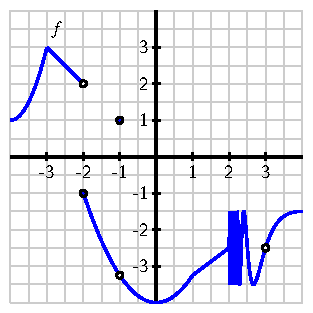
\includegraphics[width=1\linewidth]{../../html/Calculus/images/1_7_PA1.pdf}
\caption{Functions \(f\), \(g\), and \(h\) that demonstrate subtly different behaviors at \(c = 1\).\label{F-1-7-PA1}}
\end{figure}
\begin{example}[]\label{act-1-7-1}
\hypertarget{p-271}{}%
Consider a function that is piecewise-defined according to the formula%
\begin{equation*}
f(x) = \begin{cases}3(x+2)+2 \amp  \text{ for \(-3 \lt  x \lt  -2\) }  \\
\frac{2}{3}(x+2)+1 \amp  \text{ for \(-2 \le x \lt  -1\) }  \\
\frac{2}{3}(x+2)+1 \amp  \text{ for \(-1 \lt  x \lt  1\) }  \\
2 \amp  \text{ for \(x = 1\) }  \\
4-x \amp  \text{ for \(x \gt 1\) }
\end{cases}
\end{equation*}
%
\par
\hypertarget{p-272}{}%
Use the given formula to answer the following questions.%
\par
\hypertarget{p-273}{}%
\leavevmode%
\begin{enumerate}[label=\alph*.]
\item\hypertarget{li-71}{}\hypertarget{p-274}{}%
For each of the values \(c = -2, -1, 0, 1, 2\), compute \(f(c)\).%
\item\hypertarget{li-72}{}\hypertarget{p-275}{}%
For each of the values \(c = -2, -1, 0, 1, 2\), determine \(\lim_{x \to c^-} f(x)\) and \(\lim_{x \to c^+} f(x)\).%
\item\hypertarget{li-73}{}\hypertarget{p-276}{}%
For each of the values \(c = -2, -1, 0, 1, 2\), determine \(\lim_{x \to c} f(x)\). If the limit fails to exist, explain why by discussing the left- and right-hand limits at the relevant \(a\)-value.%
\item\hypertarget{li-74}{}\hypertarget{p-277}{}%
For which values of \(c\) is the following statement true?%
\begin{equation*}
\lim_{x \to c} f(x) \ne f(c)
\end{equation*}
%
\item\hypertarget{li-75}{}\hypertarget{p-278}{}%
Sketch an accurate, labeled graph of \(y = f(x)\). Be sure to carefully use open circles (\(\circ\)) and filled circles (\(\bullet\)) to represent key points on the graph, as dictated by the piecewise formula.%
\end{enumerate}
%
\par\smallskip%
\noindent\textbf{Hint.}\hypertarget{hint-4}{}\quad%
\hypertarget{p-279}{}%
\leavevmode%
\begin{enumerate}[label=\alph*.]
\item\hypertarget{li-76}{}\hypertarget{p-280}{}%
Find the interval in which \(c\) lies and evaluate the function there.%
\item\hypertarget{li-77}{}\hypertarget{p-281}{}%
Remember that for \(\lim_{x \to c^-} f(x)\), we only consider values of \(x\) such that \(x \lt c\). Find the right formula to use in the piecewise definition for \(f\) to fit the values you are considering.%
\item\hypertarget{li-78}{}\hypertarget{p-282}{}%
Use your work in (c) and compare left- and right-hand limits.%
\item\hypertarget{li-79}{}\hypertarget{p-283}{}%
Use your work in (a) and (c).%
\item\hypertarget{li-80}{}\hypertarget{p-284}{}%
Note that \(f\) is piecewise linear.%
\end{enumerate}
%
\par\smallskip%
\noindent\textbf{Answer.}\hypertarget{answer-2}{}\quad%
\hypertarget{p-285}{}%
\leavevmode%
\begin{enumerate}[label=\alph*.]
\item\hypertarget{li-81}{}\hypertarget{p-286}{}%
\(f(-2) = 1\); \(f(-1)\) is not defined; \(f(0) = \frac{7}{3}\); \(f(1) = 2\); \(f(2) = 2\).%
\item\hypertarget{li-82}{}\hypertarget{p-287}{}%
%
\begin{equation*}
\lim_{x \to -2^-} f(x) = 2 \ \text{and}  \lim_{x \to -2^+} f(x) = 1
\end{equation*}
%
\begin{equation*}
\lim_{x \to -1^-} f(x) = \frac{5}{3} \ \text{and}  \lim_{x \to -1^+} f(x) = \frac{5}{3}
\end{equation*}
%
\begin{equation*}
\lim_{x \to 0^-} f(x) = \frac{7}{3} \ \text{and}  \lim_{x \to 0^+} f(x) = \frac{7}{3}
\end{equation*}
%
\begin{equation*}
\lim_{x \to 1^-} f(x) = 3 \ \text{and}  \lim_{x \to 1^+} f(x) = 3
\end{equation*}
%
\begin{equation*}
\lim_{x \to 2^-} f(x) = 2 \ \text{and}  \lim_{x \to 2^+} f(x) = 2
\end{equation*}
%
\item\hypertarget{li-83}{}\hypertarget{p-288}{}%
\(\lim_{x \to -2} f(x)\) does not exist. The values of the limits as \(x \to c\) for \(c = -1, 0, 1, 2\) are \(\frac{5}{3}, \frac{7}{3}, 3, 2\).%
\item\hypertarget{li-84}{}\hypertarget{p-289}{}%
\(c = -2\), \(c = -1\), and \(c = 1\).%
\item\hypertarget{li-85}{}% group protects changes to lengths, releases boxes (?)
{% begin: group for a single side-by-side
% set panel max height to practical minimum, created in preamble
\setlength{\panelmax}{0pt}
\ifdefined\panelboxAimage\else\newsavebox{\panelboxAimage}\fi%
\begin{lrbox}{\panelboxAimage}
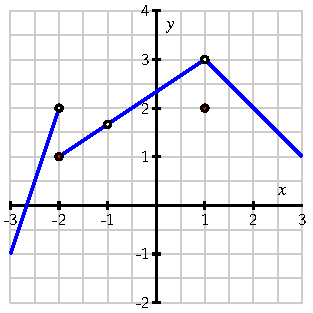
\includegraphics[width=0.4\linewidth]{../../html/Calculus/images/1_7_Act1Soln.pdf}
\end{lrbox}
\ifdefined\phAimage\else\newlength{\phAimage}\fi%
\setlength{\phAimage}{\ht\panelboxAimage+\dp\panelboxAimage}
\settototalheight{\phAimage}{\usebox{\panelboxAimage}}
\setlength{\panelmax}{\maxof{\panelmax}{\phAimage}}
\leavevmode%
% begin: side-by-side as tabular
% \tabcolsep change local to group
\setlength{\tabcolsep}{0\linewidth}
% @{} suppress \tabcolsep at extremes, so margins behave as intended
\par\medskip\noindent
\hspace*{0.3\linewidth}%
\begin{tabular}{@{}*{1}{c}@{}}
\begin{minipage}[c][\panelmax][t]{0.4\linewidth}\usebox{\panelboxAimage}\end{minipage}\end{tabular}\\
% end: side-by-side as tabular
}% end: group for a single side-by-side
%
\end{enumerate}
%
\par\smallskip%
\noindent\textbf{Solution.}\hypertarget{solution-15}{}\quad%
\hypertarget{p-290}{}%
\leavevmode%
\begin{enumerate}[label=\alph*.]
\item\hypertarget{li-86}{}\hypertarget{p-291}{}%
\(f(-2) = \frac{2}{3}(-2+2) + 1 = 1\); \(f(-1)\) is not defined; \(f(0) = \frac{2}{3}(0+2)+1 = \frac{7}{3}\); \(f(1) = 2\) (by the rule); \(f(2) = 4-2 = 2\).%
\item\hypertarget{li-87}{}\hypertarget{p-292}{}%
%
\begin{equation*}
\lim_{x \to -2^-} f(x) = 2 \ \text{and}  \lim_{x \to -2^+} f(x) = 1
\end{equation*}
%
\begin{equation*}
\lim_{x \to -1^-} f(x) = \frac{5}{3} \ \text{and}  \lim_{x \to -1^+} f(x) = \frac{5}{3}
\end{equation*}
%
\begin{equation*}
\lim_{x \to 0^-} f(x) = \frac{7}{3} \ \text{and}  \lim_{x \to 0^+} f(x) = \frac{7}{3}
\end{equation*}
%
\begin{equation*}
\lim_{x \to 1^-} f(x) = 3 \ \text{and}  \lim_{x \to 1^+} f(x) = 3
\end{equation*}
%
\begin{equation*}
\lim_{x \to 2^-} f(x) = 2 \ \text{and}  \lim_{x \to 2^+} f(x) = 2
\end{equation*}
%
\item\hypertarget{li-88}{}\hypertarget{p-293}{}%
\(\lim_{x \to -2} f(x)\) does not exists because the left-hand limit is \(2\) while the right-hand limit is \(1\). All of the other requested limits exist, as left- and right-hand limits exist and are equal in each case. The respective values of the limits as \(x \to c\) for \(c = -1, 0, 1, 2\) are \(\frac{5}{3}, \frac{7}{3}, 3, 2\).%
\item\hypertarget{li-89}{}\hypertarget{p-294}{}%
For \(c = -2\), \(a = -1\), and \(c = 1\), \(\lim_{x \to c} f(x) \ne f(a)\). At \(c = -2\), the limit fails to exist, but \(f(-2) = 1\). At \(c = -1\), the limit is \(\frac{5}{3}\), but \(f(-1)\) is not defined. At \(c = 1\), the limit is 3, but \(f(1) = 2\).%
\item\hypertarget{li-90}{}% group protects changes to lengths, releases boxes (?)
{% begin: group for a single side-by-side
% set panel max height to practical minimum, created in preamble
\setlength{\panelmax}{0pt}
\ifdefined\panelboxAimage\else\newsavebox{\panelboxAimage}\fi%
\begin{lrbox}{\panelboxAimage}
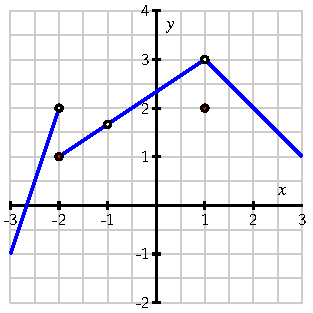
\includegraphics[width=0.4\linewidth]{../../html/Calculus/images/1_7_Act1Soln.pdf}
\end{lrbox}
\ifdefined\phAimage\else\newlength{\phAimage}\fi%
\setlength{\phAimage}{\ht\panelboxAimage+\dp\panelboxAimage}
\settototalheight{\phAimage}{\usebox{\panelboxAimage}}
\setlength{\panelmax}{\maxof{\panelmax}{\phAimage}}
\leavevmode%
% begin: side-by-side as tabular
% \tabcolsep change local to group
\setlength{\tabcolsep}{0\linewidth}
% @{} suppress \tabcolsep at extremes, so margins behave as intended
\par\medskip\noindent
\hspace*{0.3\linewidth}%
\begin{tabular}{@{}*{1}{c}@{}}
\begin{minipage}[c][\panelmax][t]{0.4\linewidth}\usebox{\panelboxAimage}\end{minipage}\end{tabular}\\
% end: side-by-side as tabular
}% end: group for a single side-by-side
%
\end{enumerate}
%
\end{example}
\typeout{************************************************}
\typeout{Subsection 1.2.3 Limits and Continuity}
\typeout{************************************************}
\subsection[{Limits and Continuity}]{Limits and Continuity}\label{subsection-22}
\index{continuous}\hypertarget{p-295}{}%
Recall that informally we said a function is continuous if we can draw its graph without ever lifting our pencil from the page.%
\begin{figure}
\centering
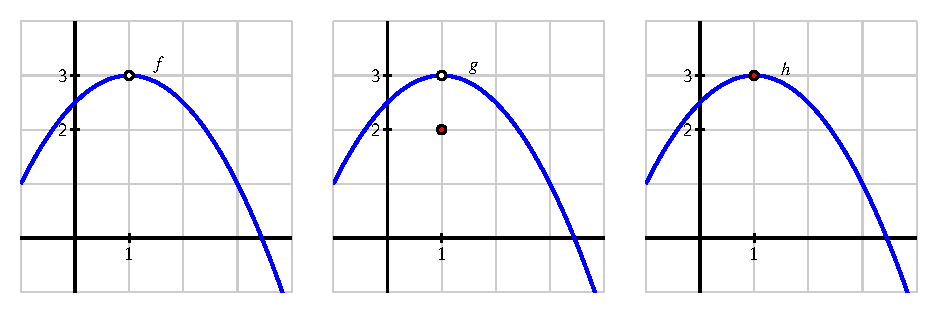
\includegraphics[width=1\linewidth]{../../html/Calculus/images/1_7_Cont.pdf}
\caption{Functions \(f\), \(g\), and \(h\) that demonstrate subtly different behaviors at \(c = 1\).\label{F-1-7-Cont}}
\end{figure}
\hypertarget{p-296}{}%
Using limits we can formalize the idea of continuity. First consider the function in the left-most graph. Note that \(f(1)\) is not defined, which leads to the resulting hole in the graph of \(f\) at \(c = 1\). We will naturally say that \(f\) is \emph{not continuous at \(c = 1\)}. For the function \(g\), we observe that while \(\lim_{x \to 1} g(x) = 3\), the value of \(g(1) = 2\), and thus the limit does not equal the function value. Here, too, we will say that \(g\) is \emph{not continuous}, even though the function is defined at \(c = 1\). Finally, the function \(h\) appears to be the most well-behaved of all three, since at \(c = 1\) its limit and its function value agree. That is,%
\begin{equation*}
\lim_{x \to 1} h(x) = 3 = h(1)\text{.}
\end{equation*}
%
\par
\hypertarget{p-297}{}%
With no hole or jump in the graph of \(h\) at \(c = 1\), we say that \(h\) is \emph{continuous} there. More formally, we make the following definition.%
\begin{assemblage}\label{assemblage-39}
\hypertarget{p-298}{}%
A function \(f\) is \terminology{continuous at \(x = c\)} \index{continuous at \(x = c\)} provided that \leavevmode%
\begin{enumerate}[label=\alph*.]
\item\hypertarget{li-91}{}\hypertarget{p-299}{}%
\(f\) has a limit as \(x \to c\),%
\item\hypertarget{li-92}{}\hypertarget{p-300}{}%
\(f\) is defined at \(x = c\), and%
\item\hypertarget{li-93}{}\hypertarget{p-301}{}%
\(\lim_{x \to c} f(x) = f(c)\).%
\end{enumerate}
%
\end{assemblage}
\hypertarget{p-302}{}%
Conditions (a) and (b) are technically contained implicitly in (c), but we state them explicitly to emphasize their individual importance. The definition says that a function is continuous at \(x = c\) provided that its limit as \(x \to c\) exists and equals its function value at \(x = c\). If a function is continuous at every point in an interval \([a,b]\), we say the function is ``continuous on \([a,b]\).'' If a function is continuous at every point in its domain, we simply say the function is ``continuous.'' Thus, continuous functions are particularly nice: to evaluate the limit of a continuous function at a point, all we need to do is evaluate the function.%
\par
\hypertarget{p-303}{}%
For example, consider \(p(x) = x^2 - 2x + 3\). It can be proved that every polynomial is a continuous function at every real number, and thus if we would like to know \(\lim_{x \to 2} p(x)\), we simply compute%
\begin{equation*}
\lim_{x \to 2} (x^2 - 2x + 3) = 2^2 - 2 \cdot 2 + 3 = 3\text{.}
\end{equation*}
%
\par
\hypertarget{p-304}{}%
This route of substituting an input value to evaluate a limit works whenever we know that the function being considered is continuous. Besides polynomial functions, all exponential functions and the sine and cosine functions are continuous at every point, as are many other familiar functions and combinations thereof.%
\begin{example}[]\label{act-1-7-2}
\hypertarget{p-305}{}%
Using the same function \(f\) as given by the graph that is in \hyperref[F-1-7-A2]{Figure~\ref{F-1-7-A2}}.%
\begin{figure}
\centering
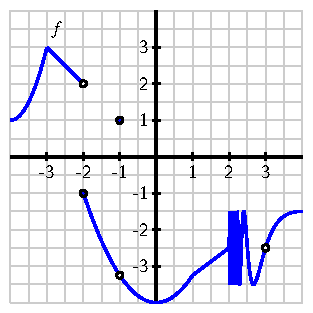
\includegraphics[width=0.47\linewidth]{../../html/Calculus/images/1_7_PA1.pdf}
\caption{The graph of \(y = f(x)\) for \hyperref[act-1-7-2]{Example~\ref{act-1-7-2}}.\label{F-1-7-A2}}
\end{figure}
\hypertarget{p-306}{}%
\leavevmode%
\begin{enumerate}[label=\alph*.]
\item\hypertarget{li-94}{}\hypertarget{p-307}{}%
At which values of \(c\) does \(\lim_{x \to c} f(x)\) not exist?%
\item\hypertarget{li-95}{}\hypertarget{p-308}{}%
At which values of \(c\) is \(f(c)\) not defined?%
\item\hypertarget{li-96}{}\hypertarget{p-309}{}%
At which values of \(c\) does \(f\) have a limit, but \(\lim_{x \to c} f(x) \ne f(c)\)?%
\item\hypertarget{li-97}{}\hypertarget{p-310}{}%
State all values of \(c\) for which \(f\) is not continuous at \(x = c\).%
\item\hypertarget{li-98}{}\hypertarget{p-311}{}%
Which condition is stronger, and hence implies the other: \(f\) has a limit at \(x = c\) or \(f\) is continuous at \(x = c\)? Explain, and hence complete the following sentence: ``If \(f\) \fillin{4.545454545454546} at \(x = c\), then \(f\) \fillin{4.545454545454546} at \(x = c\),'' where you complete the blanks with \emph{has a limit} and \emph{is continuous}, using each phrase once.%
\end{enumerate}
%
\par\smallskip%
\noindent\textbf{Hint.}\hypertarget{hint-5}{}\quad%
\hypertarget{p-312}{}%
\leavevmode%
\begin{enumerate}[label=\alph*.]
\item\hypertarget{li-99}{}\hypertarget{p-313}{}%
Consider the left- and right-hand limits at each value.%
\item\hypertarget{li-100}{}\hypertarget{p-314}{}%
Carefully examine places on the graph where there's an open circle.%
\item\hypertarget{li-101}{}\hypertarget{p-315}{}%
Are there locations on the graph where the function has a limit but there's a hole in the graph?%
\item\hypertarget{li-102}{}\hypertarget{p-316}{}%
Remember that at least one of three conditions must fail: if the function lacks a limit, if the function is undefined, or if the limit exists but does not equal the function value, then \(f\) is not continuous at the point.%
\item\hypertarget{li-103}{}\hypertarget{p-317}{}%
Note that the definition of being continuous requires the limit to exist.%
\end{enumerate}
%
\par\smallskip%
\noindent\textbf{Answer.}\hypertarget{answer-3}{}\quad%
\hypertarget{p-318}{}%
\leavevmode%
\begin{enumerate}[label=\alph*.]
\item\hypertarget{li-104}{}\hypertarget{p-319}{}%
\(c = -2\); \(c = +2\).%
\item\hypertarget{li-105}{}\hypertarget{p-320}{}%
\(c = 3\).%
\item\hypertarget{li-106}{}\hypertarget{p-321}{}%
\(c = -1\); \(c = 3\).%
\item\hypertarget{li-107}{}\hypertarget{p-322}{}%
\(c=-2\); \(c = 2\); \(c = 3\); \(c = -1\).%
\item\hypertarget{li-108}{}\hypertarget{p-323}{}%
``If \(f\) \emph{is continuous} at \(x = c\), then \(f\) \emph{has a limit} at \(x = c\).''%
\end{enumerate}
%
\par\smallskip%
\noindent\textbf{Solution.}\hypertarget{solution-16}{}\quad%
\hypertarget{p-324}{}%
\leavevmode%
\begin{enumerate}[label=\alph*.]
\item\hypertarget{li-109}{}\hypertarget{p-325}{}%
\(\lim_{x \to c} f(x)\) does not exist at \(c = -2\) since \(\lim_{x \to -2^-} f(x) = 2 \ne -1 = \lim_{x \to -2^+}\) and \(\lim_{x \to c} f(x)\) does not exist at \(c = +2\) since \(\lim_{x \to 2^+} f(x)\) does not exist due to the infinitely oscillatory behavior of \(f\).%
\item\hypertarget{li-110}{}\hypertarget{p-326}{}%
The only point at which \(f\) is not defined is at \(c = 3\).%
\item\hypertarget{li-111}{}\hypertarget{p-327}{}%
At \(c = -1\), note that \(\lim_{x \to -1} f(x)\) exists (and appears to have value approximately \(-3.25\)), but \(f(-1) = 1\), and thus \(\lim_{x \to -1} f(x) \ne f(-1)\). At \(c = 3\), \(\lim_{x \to 3} f(x) = -2.5\), but \(f(3)\) is not defined, so the limit exists but does not equal the function value.%
\item\hypertarget{li-112}{}\hypertarget{p-328}{}%
Based on our work in (a), (b), and (c), \(f\) is not continuous at \(c=-2\) and \(c = 2\) because \(f\) does not have a limit at those points; \(f\) is not continuous at \(c = 3\) since \(f\) is not defined there; and \(f\) is not continuous at \(c = -1\) because at that point its limit does not equal its function value.%
\item\hypertarget{li-113}{}\hypertarget{p-329}{}%
``If \(f\) \emph{is continuous} at \(x = c\), then \(f\) \emph{has a limit} at \(x = c\),'' since one of the defining properties of ``being continuous'' at \(x = c\) is that the function has a limit at that input value. This shows that being continuous is a stronger condition than having a limit.%
\end{enumerate}
%
\end{example}
\typeout{************************************************}
\typeout{Subsection 1.2.4 Properties of Limits and Continuous Functions}
\typeout{************************************************}
\subsection[{Properties of Limits and Continuous Functions}]{Properties of Limits and Continuous Functions}\label{subsection-23}
\hypertarget{p-330}{}%
There are several properties of limits and continuous functions that are useful to have in your toolbox.  Specifically, limits and continuous functions behave well under typical mathematical operations.  While these properties can be proven we proceed to only state the properties.%
\begin{assemblage}[Properties of Limits]\label{assemblage-40}
\hypertarget{p-331}{}%
Assuming all the limits on the right-hand side exist: \leavevmode%
\begin{itemize}[label=\textbullet]
\item{}If \(b\) is a constant, then \(\lim\limits_{x \rightarrow c} (bf(x))=b\left(\lim\limits_{x \rightarrow c} f(x) \right)\)%
\item{}\(\lim\limits_{x \rightarrow c} \left( f(x)+g(x)\right)=\lim\limits_{x \rightarrow c} f(x)+\lim\limits_{x \rightarrow c}g(x)\)%
\item{}\(\lim\limits_{x \rightarrow c} \left( f(x) \cdot g(x)\right)=\lim\limits_{x \rightarrow c} f(x)\cdot\lim\limits_{x \rightarrow c}g(x)\)%
\item{}\(\lim\limits_{x \rightarrow c} \left(\frac{f(x)}{g(x)}\right)=\frac{\lim\limits_{x \rightarrow c} f(x)}{\lim\limits_{x \rightarrow c} g(x)}\), provided \(\lim\limits_{x \rightarrow c} g(x) \neq 0\)%
\item{}For any constant \(k\), \(\lim\limits_{x \rightarrow c} k=k\)%
\item{}\(\lim\limits_{x \rightarrow c} x=c\)%
\end{itemize}
%
\end{assemblage}
\begin{example}[]\label{example-25}
\hypertarget{p-332}{}%
We can use algebra to compute \(\lim\limits_{x \rightarrow 1} x^2(x^3+2).\)  Specifically,%
\begin{align*}
\lim\limits_{x \rightarrow 1} x^2(x^3+2)\amp=\left(\lim\limits_{x \rightarrow 1} x^2\right)\left(\lim\limits_{x \rightarrow 1} (x^3+2)\right)\\
\amp=\left(\lim\limits_{x \rightarrow 1} x^2\right)\left(\lim\limits_{x \rightarrow 1} x^3+\lim\limits_{x \rightarrow 1}2)\right)\\
\amp=1(1+2) \\
\amp=3. 
\end{align*}
%
\end{example}
\begin{assemblage}[Continuity of Sums, Products, and Quotients of Functions]\label{assemblage-41}
\hypertarget{p-333}{}%
Suppose that \(f\) and \(g\) are continuous on an interval and that \(b\) is a constant. Then, on that same interval, \leavevmode%
\begin{itemize}[label=\textbullet]
\item{}\(bf(x)\) is continuous.%
\item{}\(f(x) + g(x)\) is continuous.%
\item{}\(f(x)g(x)\) is continuous.%
\item{}\(f(x) /g(x)\) is continuous, provided \(g(x) \neq 0\) on the interval.%
\end{itemize}
%
\end{assemblage}
\begin{assemblage}[Continuity of Composite Functions]\label{assemblage-42}
\hypertarget{p-334}{}%
If \(f\) and \(g\) are continuous, and if the composite function \(f(g(x))\) is defined on an interval, then \(f(g(x))\) is continuous on that interval.%
\end{assemblage}
\typeout{************************************************}
\typeout{Exercises 1.2.5 Exercises}
\typeout{************************************************}
\subsection[{Exercises}]{Exercises}\label{exercises-5}
\begin{exerciselist}
\item[1.]\hypertarget{ez-1-2-WW1}{}(Limits on a piecewise graph)\space\space{}This exercise uses the WeBWorK Online Homework System and so is not available in the print copy of this book.\item[2.]\hypertarget{ez-1-2-WW2}{}(Estimating a limit numerically)\space\space{}This exercise uses the WeBWorK Online Homework System and so is not available in the print copy of this book.\item[3.]\hypertarget{WEEK2-P14}{}(Limits for a piecewise formula)\space\space{}This exercise uses the WeBWorK Online Homework System and so is not available in the print copy of this book.\item[4.]\hypertarget{ez-1-2-WW3}{}(Limits for a piecewise formula)\space\space{}This exercise uses the WeBWorK Online Homework System and so is not available in the print copy of this book.\item[5.]\hypertarget{ez-1-2-WW5}{}(Calculating Limits, Rational Functions)\space\space{}This exercise uses the WeBWorK Online Homework System and so is not available in the print copy of this book.\item[6.]\hypertarget{ez-1-2-WW6}{}(One Sided Limits)\space\space{}This exercise uses the WeBWorK Online Homework System and so is not available in the print copy of this book.\item[7.]\hypertarget{ez-1-2-WW7}{}(Evaluating a limit algebraically)\space\space{}This exercise uses the WeBWorK Online Homework System and so is not available in the print copy of this book.\item[8.]\hypertarget{ez-1-2-WW8}{}(Limit Rules)\space\space{}This exercise uses the WeBWorK Online Homework System and so is not available in the print copy of this book.\end{exerciselist}
\typeout{************************************************}
\typeout{Section 1.3 How do we measure velocity?}
\typeout{************************************************}
\section[{How do we measure velocity?}]{How do we measure velocity?}\label{sec-1-1-vel}
\begin{objectives}{Motivating Questions}\label{objectives-3}
%
\begin{itemize}[label=\textbullet]
\item{}\hypertarget{p-335}{}%
How is the average velocity of a moving object connected to the input and output values of its position function?%
\item{}\hypertarget{p-336}{}%
How do we interpret the average velocity of an object geometrically on the graph of its position function?%
\item{}\hypertarget{p-337}{}%
How is the notion of instantaneous velocity connected to average velocity?%
\end{itemize}
\end{objectives}
\hypertarget{p-338}{}%
Calculus can be viewed broadly as the study of change. A natural and important question to ask about any changing quantity is ``how fast is the quantity changing?''%
\par
\hypertarget{p-339}{}%
We begin with a simple problem: a ball is tossed straight up in the air. How is the ball moving? Questions like this one are central to our study of differential calculus.%
\begin{example}[]\label{PA-1-1}
\hypertarget{p-340}{}%
Suppose that the height \(s\) of a ball at time \(t\) (in seconds) is given by the formula \(s(t) = 64 - 16(t-1)^2 (in feet)\).%
\leavevmode%
\begin{enumerate}[label=\alph*.]
\item\hypertarget{li-127}{}\hypertarget{p-341}{}%
Construct a graph of \(y = s(t)\) on the time interval \(0 \le t \le 3\). Label at least six distinct points on the graph, including the three points showing when the ball was released, when the ball reaches its highest point, and when the ball lands.%
\item\hypertarget{li-128}{}\hypertarget{p-342}{}%
Describe the behavior of the ball on the time interval \(0 \lt t \lt 1\) and on the time interval \(1 \lt t \lt 3\). What occurs at the instant \(t = 1\)?%
\item\hypertarget{li-129}{}\hypertarget{p-343}{}%
Consider the expression%
\begin{equation*}
AV_{[0.5,1]} = \frac{s(1) - s(0.5)}{1-0.5}\text{.}
\end{equation*}
Compute the value of \(AV_{[0.5,1]}\). What does this value measure on the graph? What does this value tell us about the motion of the ball? In particular, what are the units on \(AV_{[0.5,1]}\)?%
\end{enumerate}
\par\smallskip%
\noindent\textbf{Hint.}\hypertarget{hint-6}{}\quad%
\leavevmode%
\begin{enumerate}[label=\alph*.]
\item\hypertarget{li-130}{}\(s\) is a quadratic function, so its graph is a parabola. Where is the vertex? What are the \(t\)-intercepts?%
\item\hypertarget{li-131}{}Where is the vertex?%
\item\hypertarget{li-132}{}How does this value relate to the points \((1,s(1))\) and \((0.5,s(0.5))\) on the graph? What are the units of \(s(t)\)? What are the units of \(t\)? How might these units inform the units of \(AV_{[0.5,1]}\)?%
\end{enumerate}
\par\smallskip%
\noindent\textbf{Answer.}\hypertarget{answer-4}{}\quad%
\leavevmode%
\begin{enumerate}[label=\alph*.]
\item\hypertarget{li-133}{}\hypertarget{p-344}{}%
\leavevmode%
\begin{figure}
\centering
\centerline{Geogebra: \href{https://www.geogebra.org/m/cqs42zua}{\mono{www.geogebra.org/m/cqs42zua}}}
\caption{A graph of \(y = s(t)\) on the time interval \(0 \le t \le 3\).  You can drag the point to check your points.\label{figure-25}}
\end{figure}
%
\item\hypertarget{li-134}{}\hypertarget{p-345}{}%
The ball reaches its highest point at \(t=1\), rising until then and falling after.%
\item\hypertarget{li-135}{}\hypertarget{p-346}{}%
\(AV_{[0.5,1]}=8\) ft/s measures the slope of the line between \((0.5,s(0.5))\) and \((1,s(1))\), and is the average velocity of the ball between \(t=0.5\) seconds and \(t=1\) second.%
\end{enumerate}
\par\smallskip%
\noindent\textbf{Solution.}\hypertarget{solution-17}{}\quad%
\leavevmode%
\begin{enumerate}[label=\alph*.]
\item\hypertarget{li-136}{}\hypertarget{p-347}{}%
\leavevmode%
\begin{figure}
\centering
\centerline{Geogebra: \href{https://www.geogebra.org/m/cqs42zua}{\mono{www.geogebra.org/m/cqs42zua}}}
\caption{A graph of \(y = s(t)\) on the time interval \(0 \le t \le 3\).  You can drag the point to check your points.\label{figure-26}}
\end{figure}
%
\item\hypertarget{li-137}{}\hypertarget{p-348}{}%
The ball is rising on the interval \(0\lt t\lt1\) and falling on the interval \(1\lt t\lt3\). At the instant \(t=1\), the ball reaches its highest point, stops, and changes direction.%
\item\hypertarget{li-138}{}\hypertarget{p-349}{}%
We first compute \(s(1)=64-16(1-1)^2=64\) and \(s(0.5)=64-16(0.5-1)^2=60\). With these values, we can say%
\begin{align*}
AV_{[0.5,1]}=\mathstrut \amp \frac{s(1)-s(0.5)}{1-0.5}\\
=\mathstrut \amp \frac{64-60}{0.5}\\
=\mathstrut \amp \frac{4}{0.5}\\
=\mathstrut \amp 8
\end{align*}
Notice that in the numerator, we have the values \(s(1)\) and \(s(0.5)\), both measured in feet. In the denominator, we have the corresponding time values \(t=1\) and \(t=0.5\), both measured in seconds. The units of the quotient, then, should be feet per second. These are units of velocity, and in fact the value of \(AV_{[0.5,1]}\) is the average velocity on the time interval \(0.5\le t\le1\). Moreover, the formula for \(AV_{[0.5,1]}\) is precisely the slope formula between the points \((0.5,s(0.5))\) and \((1,s(1))\).%
\end{enumerate}
\end{example}
\typeout{************************************************}
\typeout{Subsection 1.3.1 Position and average velocity}
\typeout{************************************************}
\subsection[{Position and average velocity}]{Position and average velocity}\label{subsection-24}
\hypertarget{p-350}{}%
The \emph{position} \index{position} of any moving object can be considered as a function of \emph{time}. When the motion is along a straight line, the position is given by a single variable, which we denote by \(s(t)\). For example, \(s(t)\) might give the mile marker of a car traveling on a straight highway at time \(t\) in hours. Similarly, the function \(s(t)\) described in \hyperref[PA-1-1]{Example~\ref{PA-1-1}} is a position function, where the position of a ball is measured vertically relative to the ground.%
\par
\hypertarget{p-351}{}%
On any time interval, a moving object also has an \emph{average velocity}. For example, to compute a car's average velocity we divide the number of miles traveled by the time elapsed, which gives the velocity in \emph{miles per hour}. Similarly, the value of \(AV_{[0.5,1]}\) in \hyperref[PA-1-1]{Example~\ref{PA-1-1}} gave the average velocity of the ball on the time interval \([0.5,1]\), measured in feet per second.%
\par
\hypertarget{p-352}{}%
In general, following the notation we introduced earlier, we make the following definition:%
\begin{assemblage}[Average Velocity]\label{assemblage-43}
\hypertarget{p-353}{}%
For an object moving in a straight line with position function \(s(t)\), the \index{average velocity} \emph{average velocity of the object on the interval from \(t = a\) to \(t = b\)}, denoted \(AV_{[a,b]}\), is given by the formula%
\begin{equation*}
AV_{[a,b]} = \frac{s(b)-s(a)}{b-a}\text{.}
\end{equation*}
%
\end{assemblage}
\hypertarget{p-354}{}%
Note: the units on \(AV_{[a,b]}\) are ``units of \(s\) per unit of \(t\),'' such as ``miles per hour'' or ``feet per second.''%
\begin{example}[]\label{act-1-1-1}
\hypertarget{p-355}{}%
The following questions concern the position function given by \(s(t) = 64 - 16(t-1)^2\), considered in \hyperref[PA-1-1]{Example~\ref{PA-1-1}}.%
\par
\hypertarget{p-356}{}%
\leavevmode%
\begin{enumerate}[label=\alph*.]
\item\hypertarget{li-139}{}\hypertarget{p-357}{}%
Compute the average velocity of the ball on each of the following time intervals: \([0.4,0.8]\), \([0.7,0.8]\), \([0.79, 0.8]\), \([0.799,0.8]\), \([0.8,1.2]\), \([0.8,0.9]\), \([0.8,0.81]\), \([0.8,0.801]\). Include units for each value.%
\item\hypertarget{li-140}{}\hypertarget{p-358}{}%
On the graph provided below in \hyperref[F-1-1-Act1]{Figure~\ref{F-1-1-Act1}}, sketch the line that passes through the points \(A=(0.4, s(0.4))\) and \(B=(0.8, s(0.8))\). What is the meaning of the slope of this line? In light of this meaning, what is a geometric way to interpret each of the values computed in the preceding question?%
\item\hypertarget{li-141}{}\hypertarget{p-359}{}%
Use a graphing utility to plot the graph of \(s(t) = 64 - 16(t-1)^2\) on an interval containing the value \(t = 0.8\). Then, zoom in repeatedly on the point \((0.8, s(0.8))\). What do you observe about how the graph appears as you view it more and more closely?%
\item\hypertarget{li-142}{}\hypertarget{p-360}{}%
What do you think the velocity of the ball at the instant \(t = 0.8\) is? Why?%
\end{enumerate}
%
\begin{figure}
\centering
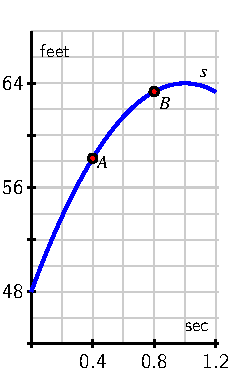
\includegraphics[width=0.43\linewidth]{../../html/Calculus/images/1_1_Act1.pdf}
\caption{A partial plot of \(s(t) = 64 - 16(t-1)^2\).\label{F-1-1-Act1}}
\end{figure}
\par\smallskip%
\noindent\textbf{Hint.}\hypertarget{hint-7}{}\quad%
\hypertarget{p-361}{}%
\leavevmode%
\begin{enumerate}[label=\alph*.]
\item\hypertarget{li-143}{}\hypertarget{p-362}{}%
On \([0.4,0.8]\), the average velocity is \(AV_{[0.4,0.8]} = \frac{s(0.8)-s(0.4)}{0.8-0.4}\) ft/sec.%
\item\hypertarget{li-144}{}\hypertarget{p-363}{}%
Remember that the slope of a line can be found by taking ``rise over run.'' In this context, the slope is found by computing ``change in \(s\) over change in \(t\).''%
\item\hypertarget{li-145}{}\hypertarget{p-364}{}%
While the curve \(s(t)\) is a parabola, how does it look up close on a very small interval?%
\item\hypertarget{li-146}{}\hypertarget{p-365}{}%
``Instantaneous'' velocity can be approximated by average velocity on a very small interval.%
\end{enumerate}
%
\par\smallskip%
\noindent\textbf{Answer.}\hypertarget{answer-5}{}\quad%
\hypertarget{p-366}{}%
\leavevmode%
\begin{enumerate}[label=\alph*.]
\item\hypertarget{li-147}{}\hypertarget{p-367}{}%
\(AV_{[0.4,0.8]} = 12.8\) ft/sec; \(AV_{[0.7,0.8]} = 8\) ft/sec; the other average velocities are, respectively, 6.56, 6.416, 0, 4.8, 6.24, 6.384, all in ft/sec.%
\item\hypertarget{li-148}{}\hypertarget{p-368}{}%
\(m = 12.8\) is the average velocity of the ball between \(t = 0.4\) and \(t = 0.8\).%
% group protects changes to lengths, releases boxes (?)
{% begin: group for a single side-by-side
% set panel max height to practical minimum, created in preamble
\setlength{\panelmax}{0pt}
\ifdefined\panelboxAimage\else\newsavebox{\panelboxAimage}\fi%
\begin{lrbox}{\panelboxAimage}
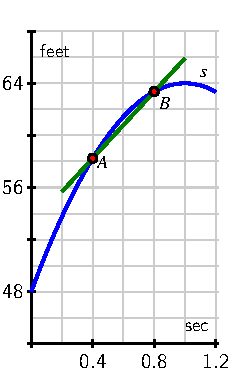
\includegraphics[width=0.3\linewidth]{../../html/Calculus/images/1_1_Act1Soln.pdf}
\end{lrbox}
\ifdefined\phAimage\else\newlength{\phAimage}\fi%
\setlength{\phAimage}{\ht\panelboxAimage+\dp\panelboxAimage}
\settototalheight{\phAimage}{\usebox{\panelboxAimage}}
\setlength{\panelmax}{\maxof{\panelmax}{\phAimage}}
\leavevmode%
% begin: side-by-side as tabular
% \tabcolsep change local to group
\setlength{\tabcolsep}{0\linewidth}
% @{} suppress \tabcolsep at extremes, so margins behave as intended
\par\medskip\noindent
\hspace*{0.35\linewidth}%
\begin{tabular}{@{}*{1}{c}@{}}
\begin{minipage}[c][\panelmax][t]{0.3\linewidth}\usebox{\panelboxAimage}\end{minipage}\end{tabular}\\
% end: side-by-side as tabular
}% end: group for a single side-by-side
\item\hypertarget{li-149}{}\hypertarget{p-369}{}%
Like a straight line with slope about 6.4.%
\item\hypertarget{li-150}{}\hypertarget{p-370}{}%
About 6.4 feet per second.%
\end{enumerate}
%
\par\smallskip%
\noindent\textbf{Solution.}\hypertarget{solution-18}{}\quad%
\hypertarget{p-371}{}%
\leavevmode%
\begin{enumerate}[label=\alph*.]
\item\hypertarget{li-151}{}\hypertarget{p-372}{}%
On \([0.4,0.8]\), the average velocity is \(AV_{[0.4,0.8]} = \frac{s(0.8)-s(0.4)}{0.8-0.4} = \frac{63.36-58.24}{0.4} = 12.8\) ft/sec. On \([0.7,0.8]\), the average velocity is 8 ft/sec. The other average velocities are, respectively (in the order of the intervals listed in the activity), 6.56, 6.416, 0, 4.8, 6.24, 6.384, all measured in feet per second.%
\item\hypertarget{li-152}{}\hypertarget{p-373}{}%
The slope of the line between \(A(0.4, s(0.4))\) and \(B(0.8, s(0.8))\) is \(\frac{s(0.8)-s(0.4)}{0.8-0.4} = 12.8\). This is precisely the average velocity of the ball between \(t = 0.4\) and \(t = 0.8\), and indeed each of the average velocities computed in (a) can be viewed as the slope of the line joining the points \((a,s(a))\) and \((b,s(b))\).%
% group protects changes to lengths, releases boxes (?)
{% begin: group for a single side-by-side
% set panel max height to practical minimum, created in preamble
\setlength{\panelmax}{0pt}
\ifdefined\panelboxAimage\else\newsavebox{\panelboxAimage}\fi%
\begin{lrbox}{\panelboxAimage}
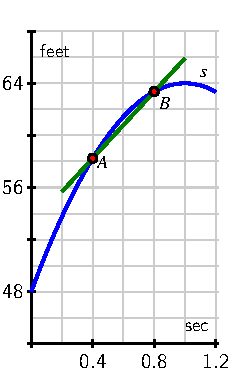
\includegraphics[width=0.3\linewidth]{../../html/Calculus/images/1_1_Act1Soln.pdf}
\end{lrbox}
\ifdefined\phAimage\else\newlength{\phAimage}\fi%
\setlength{\phAimage}{\ht\panelboxAimage+\dp\panelboxAimage}
\settototalheight{\phAimage}{\usebox{\panelboxAimage}}
\setlength{\panelmax}{\maxof{\panelmax}{\phAimage}}
\leavevmode%
% begin: side-by-side as tabular
% \tabcolsep change local to group
\setlength{\tabcolsep}{0\linewidth}
% @{} suppress \tabcolsep at extremes, so margins behave as intended
\par\medskip\noindent
\hspace*{0.35\linewidth}%
\begin{tabular}{@{}*{1}{c}@{}}
\begin{minipage}[c][\panelmax][t]{0.3\linewidth}\usebox{\panelboxAimage}\end{minipage}\end{tabular}\\
% end: side-by-side as tabular
}% end: group for a single side-by-side
\item\hypertarget{li-153}{}\hypertarget{p-374}{}%
As we zoom in on the curve \(s(t) = 64 - 16(t-1)^2\) at the point \((0.5, 60)\), the graph begins to look like a straight line. Indeed, it appears to look like a straight line with slope about 6.4.%
\item\hypertarget{li-154}{}\hypertarget{p-375}{}%
Observe that the average velocity of the ball on the intervals \([0.799,0.8]\) and \([0.8,0.801]\) is 6.416 and 6.384 feet/sec respectively. Hence it appears that the ball's velocity at the instant \(t = 0.8\) should be about 6.4 feet per second.%
\end{enumerate}
%
\end{example}
\typeout{************************************************}
\typeout{Subsection 1.3.2 Instantaneous Velocity}
\typeout{************************************************}
\subsection[{Instantaneous Velocity}]{Instantaneous Velocity}\label{subsection-25}
\hypertarget{p-376}{}%
Whether we are driving a car, riding a bike, or throwing a ball, we have an intuitive sense that a moving object has a velocity at any given moment --- a number that measures how fast the object is moving \emph{right now}. For instance, a car's speedometer tells the driver the car's velocity at any given instant. In fact, the velocity on a speedometer is really an average velocity that is computed over a very small time interval. If we let the time interval over which average velocity is computed become shorter and shorter, we can progress from average velocity to \emph{instantaneous} velocity.%
\par
\hypertarget{p-377}{}%
Informally, we define the \emph{instantaneous velocity} \index{instantaneous velocity} of a moving object at time \(t = a\) to be the value that the average velocity approaches as we take smaller and smaller intervals of time containing \(t = a\). We will develop a more formal definition of instantaneous velocity soon, and this definition will be the foundation of much of our work in calculus. For now, it is fine to think of instantaneous velocity as follows: take average velocities on smaller and smaller time intervals around a specific point. If those average velocities approach a single number, then that number will be the instantaneous velocity at that point.%
\begin{example}[]\label{act-1-1-2}
\hypertarget{p-378}{}%
Each of the following questions concern \(s(t) = 64 - 16(t-1)^2\), the position function from \hyperref[PA-1-1]{Example~\ref{PA-1-1}}.%
\par
\hypertarget{p-379}{}%
\leavevmode%
\begin{enumerate}[label=\alph*.]
\item\hypertarget{li-155}{}\hypertarget{p-380}{}%
Compute the average velocity of the ball on the time interval \([1.5,2]\). What is different between this value and the average velocity on the interval \([0,0.5]\)?%
\item\hypertarget{li-156}{}\hypertarget{p-381}{}%
Use appropriate computing technology to estimate the instantaneous velocity of the ball at \(t = 1.5\). Likewise, estimate the instantaneous velocity of the ball at \(t = 2\). Which value is greater?%
\item\hypertarget{li-157}{}\hypertarget{p-382}{}%
How is the sign of the instantaneous velocity of the ball related to its behavior at a given point in time? In other words, what does positive instantaneous velocity tell you the ball is doing? Negative instantaneous velocity?%
\item\hypertarget{li-158}{}\hypertarget{p-383}{}%
Without doing any computations, what do you expect the instantaneous velocity of the ball at \(t = 1\) to be? Why?%
\end{enumerate}
%
\par\smallskip%
\noindent\textbf{Hint.}\hypertarget{hint-8}{}\quad%
\hypertarget{p-384}{}%
\leavevmode%
\begin{enumerate}[label=\alph*.]
\item\hypertarget{li-159}{}\hypertarget{p-385}{}%
Remember to use the formula for average velocity from above: \(AV_{[a,b]} = \frac{s(b)-s(a)}{b-a}\). Think carefully about whether certain quantities are positive or negative.%
\item\hypertarget{li-160}{}\hypertarget{p-386}{}%
To estimate the instantaneous velocity at \(t = 1.5\), consider average velocities on the intervals \([1.499,1.5]\) and \([1.5,1.501]\).%
\item\hypertarget{li-161}{}\hypertarget{p-387}{}%
Think about whether the ball is rising or falling.%
\item\hypertarget{li-162}{}\hypertarget{p-388}{}%
What is the average velocity of the ball on small intervals that contain \(t = 1\)?%
\end{enumerate}
%
\par\smallskip%
\noindent\textbf{Answer.}\hypertarget{answer-6}{}\quad%
\hypertarget{p-389}{}%
\leavevmode%
\begin{enumerate}[label=\alph*.]
\item\hypertarget{li-163}{}\hypertarget{p-390}{}%
\(AV_{[1.5,2]} = -24\) ft/sec, which is negative; \(AV_{[0,0.5]} = 24\) ft/sec, which is positive.%
\item\hypertarget{li-164}{}\hypertarget{p-391}{}%
The instantaneous velocity at \(t = 1.5\) is approximately \(-16\) ft/sec; at \(t = 2\), the instantaneous velocity is about \(-32\) ft/sec, and \(-16>-32\).%
\item\hypertarget{li-165}{}\hypertarget{p-392}{}%
When the ball is rising its instantaneous velocity is positive, while when the ball is falling its instantaneous velocity is negative.%
\item\hypertarget{li-166}{}\hypertarget{p-393}{}%
Zero.%
\end{enumerate}
%
\par\smallskip%
\noindent\textbf{Solution.}\hypertarget{solution-19}{}\quad%
\hypertarget{p-394}{}%
\leavevmode%
\begin{enumerate}[label=\alph*.]
\item\hypertarget{li-167}{}\hypertarget{p-395}{}%
\(AV_{[1.5,2]} = \frac{s(2)-s(1.5)}{2-1.5} = -24\) ft/sec. We note that this average velocity is negative, and in fact is the opposite of the average velocity of 24 ft/sec on the interval \([0,0.5]\).%
\item\hypertarget{li-168}{}\hypertarget{p-396}{}%
Since \(AV_{[1.499,1.5]} = -15.984\) and \(AV_{[1.5, 1.501]} = -16.016\), it appears that the instantaneous velocity of the ball at \(t = 1.5\) is approximately \(-16\) ft/sec. Similar computations show that at \(t = 2\), the instantaneous velocity is about \(-32\) ft/sec. Note that \(-16>-32\), so the instantaneous velocity at \(t = 1.5\) is greater because it is ``less negative.'' Asking which number is ``greater'' is different from asking which number is ``more negative.''%
\item\hypertarget{li-169}{}\hypertarget{p-397}{}%
When the ball is rising its instantaneous velocity is positive, while when the ball is falling its instantaneous velocity is negative.%
\item\hypertarget{li-170}{}\hypertarget{p-398}{}%
Note that \((1,s(1))\) is the vertex of the parabola given by \(s(t)\). At this point, the ball is neither rising nor falling. On intervals of the form \([a,1]\), where \(a \lt 1\), the average velocity of the ball is positive; on intervals of form \([1,b]\), where \(b > 1\), the average velocity is positive. Hence we expect the instantaneous velocity of the ball at the moment \(t = 1\) to be zero.%
\end{enumerate}
%
\end{example}
\hypertarget{p-399}{}%
 At this point we have started to see a close connection between average velocity and instantaneous velocity. Each is connected not only to the physical behavior of the moving object but also to the geometric behavior of the graph of the position function. We are interested in computing average velocities on the interval \([a,b]\) for smaller and smaller intervals. In order to make the link between average and instantaneous velocity more formal, think of the value \(b\) as \(b = a + h\), where \(h\) is a small (non-zero) number that is allowed to vary. Then the average velocity of the object on the interval \([a,a+h]\) is%
\begin{equation*}
AV_{[a,a+h]} = \frac{s(a+h)-s(a)}{h}\text{,}
\end{equation*}
with the denominator being simply \(h\) because \((a+h) - a = h\). Note that when \(h \lt  0\), \(AV_{[a,a+h]}\) measures the average velocity on the interval \([a+h,a]\).%
\par
\hypertarget{p-400}{}%
To find the instantaneous velocity at \(t = a\), we investigate what happens as the value of \(h\) approaches zero.%
\begin{example}[Computing instantaneous velocity for a falling ball]\label{example-29}
\hypertarget{p-401}{}%
The position function for a falling ball is given by \(s(t) = 16 - 16t^2\) (where \(s(t)\) is measured in feet and \(t\) in seconds).%
\par
\hypertarget{p-402}{}%
\leavevmode%
\begin{enumerate}[label=\alph*]
\item\hypertarget{li-171}{}Find an expression for the average velocity of the ball on a time interval of the form \([0.5, 0.5+h]\) where \(-0.5 \lt h \lt 0.5\) and \(h \ne 0\).%
\item\hypertarget{li-172}{}Use this expression to compute the average velocity on \([0.5,0.75]\) and \([0.4,0.5]\).%
\item\hypertarget{li-173}{}Make a conjecture about the instantaneous velocity at \(t = 0.5\).%
\end{enumerate}
%
\par\smallskip%
\noindent\textbf{Hint.}\hypertarget{hint-9}{}\quad%
\hypertarget{p-403}{}%
\leavevmode%
\begin{enumerate}
\item\hypertarget{li-174}{}What formula do we have for the average velocity of a function \(f\) on an interval \([a,b]\)? Can this be simplified at all with this function and interval? Why is this range of \(h\) values specified?%
\item\hypertarget{li-175}{}What values of \(h\) do we need to use to get these intervals? Be careful with whether you choose \(h\) to be positive or negative.%
\item\hypertarget{li-176}{}How might we use the expression we found for average velocity to estimate instantaneous velocity?%
\end{enumerate}
%
\par\smallskip%
\noindent\textbf{Answer.}\hypertarget{answer-7}{}\quad%
\hypertarget{p-404}{}%
\leavevmode%
\begin{enumerate}
\item\hypertarget{li-177}{}\(AV_{[0.5, 0.5+h]} = -16 - 16h\).%
\item\hypertarget{li-178}{}Use \(h=0.25\) to find \(AV_{[0.5,0.75]}=-20\) ft/sec, and \(h=-0.1\) to find \(AV_{[0.4,0.5]}=-14.4\) ft/sec.%
\item\hypertarget{li-179}{}The instantaneous velocity at \(t=0.5\) should be \(-16\) ft/sec.%
\end{enumerate}
%
\par\smallskip%
\noindent\textbf{Solution.}\hypertarget{solution-20}{}\quad%
\hypertarget{p-405}{}%
\leavevmode%
\begin{enumerate}[label=\alph*]
\item\hypertarget{li-180}{}We make the assumptions that \(-0.5 \lt  h \lt  0.5\) and \(h \ne 0\) because \(h\) cannot be zero (otherwise there is no interval on which to compute average velocity) and because the function only makes sense on the time interval \(0 \le t \le 1\), as this is the duration of time during which the ball is falling. We want to compute and simplify%
\begin{equation*}
AV_{[0.5, 0.5+h]} = \frac{s(0.5+h) - s(0.5)}{(0.5+h) - 0.5}\text{.}
\end{equation*}
We start by finding \(s(0.5+h)\). To do so, we follow the rule that defines the function \(s\).%
\begin{align*}
s(0.5+h) \amp  =  16 - 16(0.5 + h)^2\\
\amp  =  16 - 16(0.25 + h + h^2)\\
\amp  =  16 - 4 - 16h - 16h^2\\
\amp  =  12 - 16h - 16h^2\text{.}
\end{align*}
Now, returning to our computation of the average velocity, we find that%
\begin{align*}
AV_{[0.5, 0.5+h]} \amp  =  \frac{s(0.5+h) - s(0.5)}{(0.5+h) - 0.5}\\
\amp  =  \frac{(12 - 16h - 16h^2) - (16 - 16(0.5)^2)}{0.5 + h - 0.5}\\
\amp  =  \frac{12 - 16h - 16h^2 - 12}{h}\\
\amp  =  \frac{-16h - 16h^2}{h}\text{.}
\end{align*}
At this point, we note two things: first, the expression for average velocity clearly depends on \(h\), which it must, since as \(h\) changes the average velocity will change. Further, we note that since \(h\) can never equal zero, we may remove the common factor of \(h\) from the numerator and denominator. It follows that%
\begin{equation*}
AV_{[0.5, 0.5+h]} = -16 - 16h\text{.}
\end{equation*}
%
\item\hypertarget{li-181}{}From this expression we can compute the average for any small positive or negative value of \(h\). For instance, to obtain the average velocity on \([0.5,0.75]\), we let \(h = 0.25\), and the average velocity is \(-16 - 16(0.25) = -20\) ft/sec. To get the average velocity on \([0.4, 0.5]\), we let \(h = -0.1\), and compute the average velocity as%
\begin{equation*}
-16 - 16(-0.1) = -14.4\ \text{ft/sec}\text{.}
\end{equation*}
%
\item\hypertarget{li-182}{}We can even explore what happens to \(AV_{[0.5, 0.5+h]}\) as \(h\) gets closer and closer to zero. As \(h\) approaches zero, \(-16h\) will also approach zero, so it appears that the instantaneous velocity of the ball at \(t = 0.5\) should be \(-16\) ft/sec.%
\end{enumerate}
%
\end{example}
\begin{example}[]\label{act-1-1-3}
\hypertarget{p-406}{}%
For the function given by \(s(t) = 64 - 16(t-1)^2\) from \hyperref[PA-1-1]{Example~\ref{PA-1-1}}, find the most simplified expression you can for the average velocity of the ball on the interval \([2, 2+h]\). Use your result to compute the average velocity on \([1.5,2]\) and to estimate the instantaneous velocity at \(t = 2\). Finally, compare this to your earlier work in \hyperref[act-1-1-1]{Example~\ref{act-1-1-1}}.%
\par\smallskip%
\noindent\textbf{Hint.}\hypertarget{hint-10}{}\quad%
\hypertarget{p-407}{}%
Note that%
\begin{align*}
s(2+h) \amp = 64 - 16(2+h-1)^2 = 64 - 16(1+h)^2\\
\amp = 64 - (16 + 32h + 16h^2) = 48 - 32h - 16h^2\text{.}
\end{align*}
%
\par\smallskip%
\noindent\textbf{Answer.}\hypertarget{answer-8}{}\quad%
\hypertarget{p-408}{}%
\(AV_{[2, 2+h]} = -32 - 16h\)%
\par\smallskip%
\noindent\textbf{Solution.}\hypertarget{solution-21}{}\quad%
\hypertarget{p-409}{}%
Observe first that%
\begin{align*}
s(2+h) \amp = 64 - 16(2+h-1)^2 = 64 - 16(1+h)^2\\
\amp = 64 - (16 + 32h + 16h^2) = 48 - 32h - 16h^2\text{.}
\end{align*}
Next, recall that \(AV_{[2, 2+h]} = \frac{s(2+h) - s(2)}{h}\), so%
\begin{equation*}
AV_{[2, 2+h]} = \frac{s(2+h) - s(2)}{h} = \frac{(48 - 32h - 16h^2)-48}{h} = \frac{-32h - 16h^2}{h}\text{.}
\end{equation*}
%
\par
\hypertarget{p-410}{}%
Now, since we assume \(h \ne 0\), we can simplify further to find that \(AV_{[2, 2+h]} = -32 - 16h\). Setting \(h = -0.5\), it follows that \(AV_{[1.5,2]} = -32 + 16(0.5) = -24\) ft/sec. Likewise, as we let \(h\) approach zero, we see that \(-32 - 16h\) will approach \(-32\), so the instantaneous velocity at \(t = 2\) appears to be \(-32\) feet/sec. Both results match our earlier work in \hyperref[act-1-1-1]{Example~\ref{act-1-1-1}}.%
\end{example}
\typeout{************************************************}
\typeout{Subsection 1.3.3 Summary}
\typeout{************************************************}
\subsection[{Summary}]{Summary}\label{subsection-26}
\hypertarget{p-411}{}%
\leavevmode%
\begin{itemize}[label=\textbullet]
\item{}For an object moving in a straight line with position function \(s(t)\), the \index{average velocity} \emph{average velocity of the object on the interval from \(t = a\) to \(t = b\)}, denoted \(AV_{[a,b]}\), is given by the formula%
\begin{equation*}
AV_{[a,b]} = \frac{s(b)-s(a)}{b-a}\text{.}
\end{equation*}
%
\item{}\hypertarget{p-412}{}%
The average velocity on \([a,b]\) can be viewed geometrically as the slope of the line between the points \((a,s(a))\) and \((b,s(b))\) on the graph of \(y = s(t)\), as shown below in \hyperref[F-1-1-Summary]{Figure~\ref{F-1-1-Summary}}.%
\begin{figure}
\centering
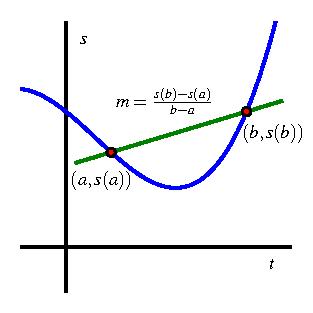
\includegraphics[width=0.5\linewidth]{../../html/Calculus/images/1_1_Summary.pdf}
\caption{The graph of position function \(s(t)\) together with the line through \((a,s(a))\) and \((b,s(b))\) whose slope is \(m = \frac{s(b)-s(a)}{b-a}\). The line's slope is the average rate of change of \(s(t)\) on the interval \([a,b]\).\label{F-1-1-Summary}}
\end{figure}
\item{}Given a moving object whose position at time \(t\) is given by a function \(s(t)\), the average velocity of the object on the time interval \([a,b]\) is given by \(AV_{[a,b]} = \frac{s(b) - s(a)}{b-a}\). Viewing the interval \([a,b]\) as having the form \([a,a+h]\), we equivalently compute average velocity by the formula \(AV_{[a,a+h]} = \frac{s(a+h) - s(a)}{h}\).%
\item{}The instantaneous velocity of a moving object at a fixed time is estimated by considering average velocities on shorter and shorter time intervals that contain the instant of interest.%
\end{itemize}
%
\typeout{************************************************}
\typeout{Exercises 1.3.4 Exercises}
\typeout{************************************************}
\subsection[{Exercises}]{Exercises}\label{exercises-6}
\begin{exerciselist}
\item[1.]\hypertarget{ez-1-1-WW1}{}(Average velocity from position)\space\space{}This exercise uses the WeBWorK Online Homework System and so is not available in the print copy of this book.\item[2.]\hypertarget{ez-1-1-WW2}{}(Rate of calorie consumption)\space\space{}This exercise uses the WeBWorK Online Homework System and so is not available in the print copy of this book.\item[3.]\hypertarget{ez-1-1-WW3}{}(Average rate of change - quadratic function)\space\space{}This exercise uses the WeBWorK Online Homework System and so is not available in the print copy of this book.\item[4.]\hypertarget{ez-1-1-WW4}{}(Comparing average rate of change of two functions)\space\space{}This exercise uses the WeBWorK Online Homework System and so is not available in the print copy of this book.\item[5.]\hypertarget{ez-1-1-WW5}{}(Matching a distance graph to velocity)\space\space{}This exercise uses the WeBWorK Online Homework System and so is not available in the print copy of this book.\item[6.]\hypertarget{ez-1-1-Bungee}{}\hypertarget{p-413}{}%
A bungee jumper dives from a tower at time \(t=0\). Her height \(h\) (measured in feet) at time \(t\) (in seconds) is given by the graph in \hyperref[F-1-1-Ez1]{Figure~\ref{F-1-1-Ez1}}. In this problem, you may base your answers on estimates from the graph or use the fact that the jumper's height function is given by \(s(t) = 100\cos(0.75t) \cdot e^{-0.2t}+100\).%
\begin{figure}
\centering
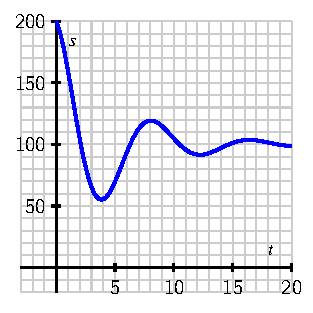
\includegraphics[width=0.4\linewidth]{../../html/Calculus/images/1_1_Ez1.pdf}
\caption{A bungee jumper's height function.\label{F-1-1-Ez1}}
\end{figure}
\hypertarget{p-414}{}%
\leavevmode%
\begin{enumerate}[label=\alph*.]
\item\hypertarget{li-187}{}\hypertarget{p-415}{}%
What is the change in vertical position of the bungee jumper between \(t=0\) and \(t=15\)?%
\item\hypertarget{li-188}{}\hypertarget{p-416}{}%
Estimate the jumper's average velocity on each of the following time intervals: \([0,15]\), \([0,2]\), \([1,6]\), and \([8,10]\). Include units on your answers.%
\item\hypertarget{li-189}{}\hypertarget{p-417}{}%
On what time interval(s) do you think the bungee jumper achieves her greatest average velocity? Why?%
\item\hypertarget{li-190}{}\hypertarget{p-418}{}%
Estimate the jumper's instantaneous velocity at \(t=5\). Show your work and explain your reasoning, and include units on your answer.%
\item\hypertarget{li-191}{}\hypertarget{p-419}{}%
Among the average and instantaneous velocities you computed in earlier questions, which are positive and which are negative? What does negative velocity indicate?%
\end{enumerate}
%
\par\smallskip
\par\smallskip%
\noindent\textbf{Answer.}\hypertarget{answer-9}{}\quad%
\hypertarget{p-420}{}%
\leavevmode%
\begin{enumerate}[label=\alph*.]
\item\hypertarget{li-192}{}\hypertarget{p-421}{}%
\(s(15)-s(0) \approx -98.75\).%
\item\hypertarget{li-193}{}\hypertarget{p-422}{}%
%
\begin{align*}
AV_{[0,15]} &= \frac{s(15)-s(0)}{15-0} \approx  -6.58\\
AV_{[0,2]} &= \frac{s(2)-s(0)}{2-0} \approx  -47.63\\
AV_{[1,6]} &= \frac{s(6)-s(1)}{6-1} \approx  -13.25\\
AV_{[8,10]} &= \frac{s(10)-s(8)}{10-8} \approx  -7.35
\end{align*}
%
\item\hypertarget{li-194}{}\hypertarget{p-423}{}%
Most negative average velocity on \([0,4]\); most positive average velocity on \([4,8]\).%
\item\hypertarget{li-195}{}\hypertarget{p-424}{}%
\(\frac{21.31+22.25}{2} = 21.78\) feet per second.%
\item\hypertarget{li-196}{}\hypertarget{p-425}{}%
The average velocities are negative; the instantaneous velocity was positive. Downward motion corresponds to negative average velocity; upward motion to positive average velocity.%
\end{enumerate}
%
\par\smallskip%
\noindent\textbf{Solution.}\hypertarget{solution-22}{}\quad%
\hypertarget{p-426}{}%
\leavevmode%
\begin{enumerate}[label=\alph*.]
\item\hypertarget{li-197}{}\hypertarget{p-427}{}%
Since \(s(0) = 100\cos(0)e^{0}+100 = 200\) and \(s(15) = 100\cos(11.25)e^{-3}+100 \approx 101.25\), the bungee jumper's change in vertical position between \(t=0\) \(t=15\) is%
\begin{equation*}
s(15)-s(0) \approx -98.75\text{.}
\end{equation*}
%
\item\hypertarget{li-198}{}\hypertarget{p-428}{}%
We estimate the jumper's average velocity using the formula%
\begin{equation*}
AV_{[a,b]} = \frac{s(b)-s(a)}{b-a}\text{.}
\end{equation*}
Using the approximations from part (a) and \(s(1) \approx 159.91, \ \ s(2) \approx 104.74, \ \ s(6) \approx 93.65, \ \ s(8) \approx 119.39, \ \ s(10) \approx 104.69\), we have%
\begin{align*}
AV_{[0,15]} &= \frac{s(15)-s(0)}{15-0} \approx  -6.58\\
AV_{[0,2]} &= \frac{s(2)-s(0)}{2-0} \approx  -47.63\\
AV_{[1,6]} &= \frac{s(6)-s(1)}{6-1} \approx  -13.25\\
AV_{[8,10]} &= \frac{s(10)-s(8)}{10-8} \approx  -7.35
\end{align*}
The units on each of these average velocities are ``feet per second''.%
\item\hypertarget{li-199}{}\hypertarget{p-429}{}%
On the time interval \([0,4]\) the jumper has the greatest change in position over that period of time, so it is on that interval that her average velocity is greatest in magnitude (but negative in sign). For the same reasons, the largest (positive) average velocity will occur on the interval \([4,8]\).%
\item\hypertarget{li-200}{}\hypertarget{p-430}{}%
We can approximate the jumper's average velocity on the intervals \([4.9,5]\) and \([5,5.1]\) and find the average of these average velocities. This will give us the slope of the secant line connecting the points \((4.9, s(4.9))\) and \((5.1, s(5.1))\) and be a reasonably good approximation to the instantaneous velocity at \(t = 5\). Now%
\begin{align*}
AV_{[4.9,5]} &= \frac{s(5)-s(4.9)}{5-4.9} \approx  21.31\\
AV_{[5,5.1]} &= \frac{s(5.1)-s(5)}{5.1-5} \approx  22.25
\end{align*}
so the jumper's instantaneous velocity at \(t=5\) is about%
\begin{equation*}
\frac{21.31+22.25}{2} = 21.78
\end{equation*}
feet per second.%
\item\hypertarget{li-201}{}\hypertarget{p-431}{}%
The average velocities we calculated were all negative, while the instantaneous velocity was positive. When the jumper is moving in the downward direction, the average velocity will be negative (indicating a decrease in position), while a positive average velocity indicates an increase in position (moving upwards).%
\end{enumerate}
%
\item[7.]\hypertarget{ez-1-1-Diver}{}\hypertarget{p-432}{}%
A diver leaps from a 3 meter springboard. His feet leave the board at time \(t=0\), he reaches his maximum height of 4.5 m at \(t = 1.1\) seconds, and enters the water at \(t = 2.45\). Once in the water, the diver coasts to the bottom of the pool (depth 3.5 m), touches bottom at \(t=7\), rests for one second, and then pushes off the bottom. From there he coasts to the surface, and takes his first breath at \(t=13\).%
\par
\hypertarget{p-433}{}%
\leavevmode%
\begin{enumerate}[label=\alph*.]
\item\hypertarget{li-202}{}\hypertarget{p-434}{}%
Let \(s(t)\) denote the function that gives the height of the diver's feet (in meters) above the water at time \(t\). (Note that the ``height'' of the bottom of the pool is \(-3.5\) meters.) Sketch a carefully labeled graph of \(s(t)\) on the provided axes in \hyperref[F-1-1-Ez2a]{Figure~\ref{F-1-1-Ez2a}}. Include scale and units on the vertical axis. Be as detailed as possible.%
% group protects changes to lengths, releases boxes (?)
{% begin: group for a single side-by-side
% set panel max height to practical minimum, created in preamble
\setlength{\panelmax}{0pt}
\ifdefined\panelboxAimage\else\newsavebox{\panelboxAimage}\fi%
\begin{lrbox}{\panelboxAimage}
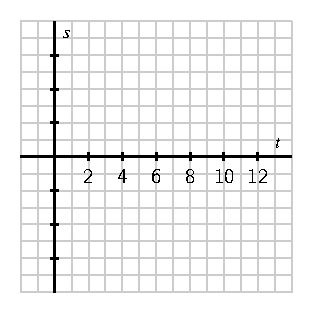
\includegraphics[width=0.44\linewidth]{../../html/Calculus/images/1_1_Ez2a.pdf}
\end{lrbox}
\ifdefined\phAimage\else\newlength{\phAimage}\fi%
\setlength{\phAimage}{\ht\panelboxAimage+\dp\panelboxAimage}
\settototalheight{\phAimage}{\usebox{\panelboxAimage}}
\setlength{\panelmax}{\maxof{\panelmax}{\phAimage}}
\ifdefined\panelboxBimage\else\newsavebox{\panelboxBimage}\fi%
\begin{lrbox}{\panelboxBimage}
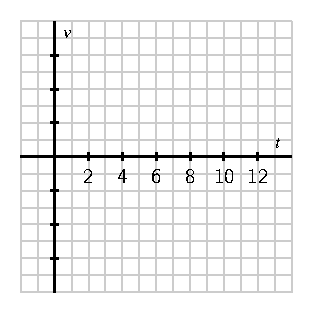
\includegraphics[width=0.44\linewidth]{../../html/Calculus/images/1_1_Ez2b.pdf}
\end{lrbox}
\ifdefined\phBimage\else\newlength{\phBimage}\fi%
\setlength{\phBimage}{\ht\panelboxBimage+\dp\panelboxBimage}
\settototalheight{\phBimage}{\usebox{\panelboxBimage}}
\setlength{\panelmax}{\maxof{\panelmax}{\phBimage}}
\leavevmode%
% begin: side-by-side as tabular
% \tabcolsep change local to group
\setlength{\tabcolsep}{0.06\linewidth}
% @{} suppress \tabcolsep at extremes, so margins behave as intended
\par\medskip\noindent
\begin{tabular}{@{}*{2}{c}@{}}
\begin{minipage}[c][\panelmax][t]{0.44\linewidth}\usebox{\panelboxAimage}\end{minipage}&
\begin{minipage}[c][\panelmax][t]{0.44\linewidth}\usebox{\panelboxBimage}\end{minipage}\tabularnewline
\parbox[t]{0.44\linewidth}{\captionof{figure}{Axes for plotting \(s(t)\) in part (a).\label{F-1-1-Ez2a}}
}&
\parbox[t]{0.44\linewidth}{\captionof{figure}{Axes for plotting \(v(t)\) in part (c).\label{F-1-1-Ez2c}}
}\end{tabular}\\
% end: side-by-side as tabular
}% end: group for a single side-by-side
\item\hypertarget{li-203}{}\hypertarget{p-435}{}%
Based on your graph in (a), what is the average velocity of the diver between \(t = 2.45\) and \(t=7\)? Is his average velocity the same on every time interval within \([2.45,7]\)?%
\item\hypertarget{li-204}{}\hypertarget{p-436}{}%
Let the function \(v(t)\) represent the \emph{instantaneous vertical velocity} of the diver at time \(t\) (i.e.~the speed at which the height function \(s(t)\) is changing; note that velocity in the upward direction is positive, while the velocity of a falling object is negative). Based on your understanding of the diver's behavior, as well as your graph of the position function, sketch a carefully labeled graph of \(v(t)\) on the axes provided in \hyperref[F-1-1-Ez2c]{Figure~\ref{F-1-1-Ez2c}}. Include scale and units on the vertical axis. Write several sentences that explain how you constructed your graph, discussing when you expect \(v(t)\) to be zero, positive, negative, relatively large, and relatively small.%
\item\hypertarget{li-205}{}\hypertarget{p-437}{}%
Is there a connection between the two graphs that you can describe? What can you say about the velocity graph when the height function is increasing? decreasing? Make as many observations as you can.%
\end{enumerate}
%
\par\smallskip
\par\smallskip%
\noindent\textbf{Answer.}\hypertarget{answer-10}{}\quad%
\hypertarget{p-438}{}%
\leavevmode%
\begin{enumerate}[label=\alph*.]
\item\hypertarget{li-206}{}\hypertarget{p-439}{}%
Sketch a plot where the diver's height at time \(t\) is on the vertical axis. For instance, \(h(2.45) = 0\).%
\item\hypertarget{li-207}{}\hypertarget{p-440}{}%
\(AV_{[2.45,7]} \approx \frac{-3.5-0}{7-2.45}=\frac{-3.5}{4.55}=-0.7692\) m/sec. The average velocity is not the same on every time interval within \([2.45,7]\).%
\item\hypertarget{li-208}{}\hypertarget{p-441}{}%
When the diver is going upward, her velocity is positive. When she is going downward, her velocity is negative. At the peak of her dive and when her feet touch the bottom of the pool.%
\item\hypertarget{li-209}{}\hypertarget{p-442}{}%
It looks like when the position function is steep, the velocity function's value is farther away from zero, and that whenever the height/position function is rising/increasing, the velocity function has a positive value. Similarly, whenever the position function is decreasing, the velocity is negative.%
\end{enumerate}
%
\par\smallskip%
\noindent\textbf{Solution.}\hypertarget{solution-23}{}\quad%
\hypertarget{p-443}{}%
\leavevmode%
\begin{enumerate}[label=\alph*.]
\item\hypertarget{li-210}{}\hypertarget{p-444}{}%
Taking into account the given information and our intuition about the diver's velocity, ketch a plot where the diver's height at time \(t\) is on the vertical axis. For instance, \(h(2.45) = 0\).%
\item\hypertarget{li-211}{}\hypertarget{p-445}{}%
First, we see that%
\begin{equation*}
AV_{[2.45,7]} \approx \frac{-3.5-0}{7-2.45}=\frac{-3.5}{4.55}=-0.7692
\end{equation*}
m/sec. The average velocity is not the same on every time interval within \([2.45,7]\), since the position function is not linear. Physically, we expect the water to make the diver's velocity change as she glides through the water.%
\item\hypertarget{li-212}{}\hypertarget{p-446}{}%
When the diver is going upward, her velocity is positive. When she is going downward, her velocity is negative. At the peak of her dive and when her feet touch the bottom of the pool, her velocity is zero because the velocity is changing sign there. Sketch a possible graph accordingly.%
\item\hypertarget{li-213}{}\hypertarget{p-447}{}%
It looks like when the position function is steep, the velocity function's value is farther away from zero, and that whenever the height/position function is rising/increasing, the velocity function has a positive value. Similarly, whenever the position function is decreasing, the velocity is negative.%
\end{enumerate}
%
\item[8.]\hypertarget{exercise-45}{}\hypertarget{p-448}{}%
According to the U.S. census, the population of the city of Grand Rapids, MI, was 181,843 in 1980; 189,126 in 1990; and 197,800 in 2000.%
\par
\hypertarget{p-449}{}%
\leavevmode%
\begin{enumerate}[label=\alph*.]
\item\hypertarget{li-214}{}Between 1980 and 2000, by how many people did the population of Grand Rapids grow?%
\item\hypertarget{li-215}{}In an average year between 1980 and 2000, by how many people did the population of Grand Rapids grow?%
\item\hypertarget{li-216}{}Just like we can find the average velocity of a moving body by computing change in position over change in time, we can compute the average rate of change of any function \(f\). In particular, the \emph{average rate of change} of a function \(f\) over an interval \([a,b]\) is the quotient%
\begin{equation*}
\frac{f(b)-f(a)}{b-a}\text{.}
\end{equation*}
What does the quantity \(\frac{f(b)-f(a)}{b-a}\) measure on the graph of \(y = f(x)\) over the interval \([a,b]\)?%
\item\hypertarget{li-217}{}Let \(P(t)\) represent the population of Grand Rapids at time \(t\), where \(t\) is measured in years from January 1, 1980. What is the average rate of change of \(P\) on the interval \(t = 0\) to \(t = 20\)? What are the units on this quantity?%
\item\hypertarget{li-218}{}If we assume the population of Grand Rapids is growing at a rate of approximately 4\% per decade, we can model the population function with the formula%
\begin{equation*}
P(t) = 181843 (1.04)^{t/10}\text{.}
\end{equation*}
Use this formula to compute the average rate of change of the population on the intervals \([5,10]\), \([5,9]\), \([5,8]\), \([5,7]\), and \([5,6]\).%
\item\hypertarget{li-219}{}How fast do you think the population of Grand Rapids was changing on January 1, 1985? Said differently, at what rate do you think people were being added to the population of Grand Rapids as of January 1, 1985? How many additional people should the city have expected in the following year? Why?%
\end{enumerate}
%
\par\smallskip
\par\smallskip%
\noindent\textbf{Answer.}\hypertarget{answer-11}{}\quad%
\hypertarget{p-450}{}%
\leavevmode%
\begin{enumerate}[label=\alph*.]
\item\hypertarget{li-220}{}\hypertarget{p-451}{}%
\(15 957\) people.%
\item\hypertarget{li-221}{}\hypertarget{p-452}{}%
In an average year the population grew by about \(798\) people/year.%
\item\hypertarget{li-222}{}\hypertarget{p-453}{}%
The slope of a secant line through the points \((a,f(a))\) and \((b,f(b))\).%
\item\hypertarget{li-223}{}\hypertarget{p-454}{}%
\(AV_{[0,20]} \approx 798\) people per year.%
\item\hypertarget{li-224}{}\hypertarget{p-455}{}%
%
\begin{align*}
AV_{[5,10]} & \approx 734.50\\
AV_{[5,9]} & \approx 733.06\\
AV_{[5,8]} & \approx 731.62\\
AV_{[5,7]} & \approx 730.19\\
AV_{[5,6]} & \approx 728.7535
\end{align*}
%
\end{enumerate}
%
\par\smallskip%
\noindent\textbf{Solution.}\hypertarget{solution-24}{}\quad%
\hypertarget{p-456}{}%
\leavevmode%
\begin{enumerate}[label=\alph*.]
\item\hypertarget{li-225}{}\hypertarget{p-457}{}%
The change in population is \(P(2000) - P(1980) = 197 800 - 181 843 = 15 957\) people.%
\item\hypertarget{li-226}{}\hypertarget{p-458}{}%
Since there were \(15 957\) people added to Grand Rapids over the 20 years from 1980 to 2000, in an average year the population grew by \(\frac{15,957}{20} \approx 798\) people/year.%
\item\hypertarget{li-227}{}\hypertarget{p-459}{}%
\(\frac{f(b)-f(a)}{b-a}=\frac{\Delta f}{\Delta x}\) measures the slope of a secant line through the points \((a,f(a))\) and \((b,f(b))\).%
\item\hypertarget{li-228}{}\hypertarget{p-460}{}%
%
\begin{equation*}
AV_{[0,20]}=\frac{P(20)-P(0)}{20-0}=\frac{197 800 - 181 843}{20}=\frac{15 957}{20} \approx 798
\end{equation*}
people per year.%
\item\hypertarget{li-229}{}\hypertarget{p-461}{}%
%
\begin{align*}
AV_{[5,10]} &=\frac{P(10) - P(5)}{10-5} = \frac{189 116.72 - 185 444.20}{10-5} \approx 734.50\\
AV_{[5,9]} &= \frac{188 376.44 - 185 444.20}{9-5} \approx 733.06\\
AV_{[5,8]} &= \frac{187 639.06 - 185,444.20}{8-5} \approx 731.62\\
AV_{[5,7]} &= \frac{186 904.57 - 185,444.20}{7-5} \approx 730.19\\
AV_{[5,6]} &= \frac{186 172.95 - 185,444.20}{6-5} \approx 728.7535
\end{align*}
The units on each of these quantities are ``people per year''.%
\end{enumerate}
%
\end{exerciselist}
\typeout{************************************************}
\typeout{Section 1.4 The derivative of a function at a point}
\typeout{************************************************}
\section[{The derivative of a function at a point}]{The derivative of a function at a point}\label{sec-1-3-derivative-pt}
\begin{objectives}{Motivating Questions}\label{objectives-4}
%
\begin{itemize}[label=\textbullet]
\item{}\hypertarget{p-462}{}%
How is the average rate of change of a function on a given interval defined, and what does this quantity measure?%
\item{}\hypertarget{p-463}{}%
How is the instantaneous rate of change of a function at a particular point defined? How is the instantaneous rate of change linked to average rate of change?%
\item{}\hypertarget{p-464}{}%
What is the derivative of a function at a given point? What does this derivative value measure? How do we interpret the derivative value graphically?%
\item{}\hypertarget{p-465}{}%
How are limits used formally in the computation of derivatives?%
\end{itemize}
\end{objectives}
\hypertarget{p-466}{}%
The \emph{instantaneous rate of change} of a function is an idea that sits at the foundation of calculus. It is a generalization of the notion of instantaneous velocity and measures how fast a particular function is changing at a given point. If the original function represents the position of a moving object, this instantaneous rate of change is precisely the velocity of the object. In other contexts, instantaneous rate of change could measure the number of cells added to a bacteria culture per day, the number of additional gallons of gasoline consumed upon increasing a car's velocity by one mile per hour, or the number of dollars added to a mortgage payment for each percentage point increase in interest rate. The instantaneous rate of change can also be interpreted geometrically on the function's graph, and this connection is fundamental to many of the main ideas in calculus.%
\par
\hypertarget{p-467}{}%
Recall that for a moving object with position function \(s\), its average velocity on the time interval \(t = a\) to \(t = a+h\) is given by the quotient%
\begin{equation*}
AV_{[a,a+h]} = \frac{s(a+h)-s(a)}{h}\text{.}
\end{equation*}
%
\par
\hypertarget{p-468}{}%
In a similar way, we make the following definition for an arbitrary function \(y = f(x)\).%
\begin{assemblage}[Average Rate of Change]\label{aroc-def}
\hypertarget{p-469}{}%
For a function \(f\), the \terminology{average rate of change} \index{average rate of change} of \(f\) on the interval \([a,a+h]\) is given by the value%
\begin{equation*}
AV_{[a,a+h]} = \frac{f(a+h)-f(a)}{h}\text{.}
\end{equation*}
%
\end{assemblage}
\hypertarget{p-470}{}%
Equivalently, if we want to consider the average rate of change of \(f\) on \([a,b]\), we compute%
\begin{equation*}
AV_{[a,b]} = \frac{f(b)-f(a)}{b-a}\text{.}
\end{equation*}
%
\par
\hypertarget{p-471}{}%
It is essential that you understand how the average rate of change of \(f\) on an interval is connected to its graph.%
\begin{example}[]\label{PA-1-3}
\hypertarget{p-472}{}%
Suppose that \(f\) is the function given by the graph below and that \(a\) and \(a+h\) are the input values as labeled on the \(x\)-axis. Use the graph in \hyperref[F-1-3-PA1]{Figure~\ref{F-1-3-PA1}} to answer the following questions.%
\begin{figure}
\centering
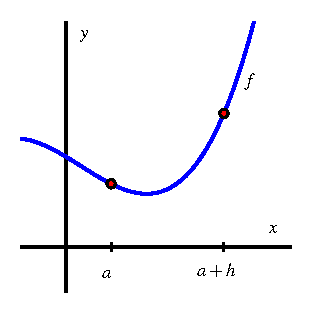
\includegraphics[width=0.47\linewidth]{../../html/Calculus/images/1_3_PA1.pdf}
\caption{Plot of \(y = f(x)\) for \hyperref[PA-1-3]{Example~\ref{PA-1-3}}.\label{F-1-3-PA1}}
\end{figure}
\hypertarget{p-473}{}%
\leavevmode%
\begin{enumerate}[label=\alph*.]
\item\hypertarget{li-234}{}\hypertarget{p-474}{}%
Locate and label the points \((a,f(a))\) and \((a+h, f(a+h))\) on the graph.%
\item\hypertarget{li-235}{}\hypertarget{p-475}{}%
Construct a right triangle whose hypotenuse is the line segment from \((a,f(a))\) to \((a+h,f(a+h))\). What are the lengths of the respective legs of this triangle?%
\item\hypertarget{li-236}{}\hypertarget{p-476}{}%
What is the slope of the line that connects the points \((a,f(a))\) and \((a+h, f(a+h))\)?%
\item\hypertarget{li-237}{}\hypertarget{p-477}{}%
Write a meaningful sentence that explains how the average rate of change of the function on a given interval and the slope of a related line are connected.%
\end{enumerate}
%
\par\smallskip%
\noindent\textbf{Hint.}\hypertarget{hint-11}{}\quad%
\hypertarget{p-478}{}%
\leavevmode%
\begin{enumerate}[label=\alph*.]
\item\hypertarget{li-238}{}What are the coordinates of the two marked points on the graph of \(f\)?%
\item\hypertarget{li-239}{}Draw the triangle so that one of its legs is horizontal and the other is vertical.%
\item\hypertarget{li-240}{}Remember that the slope of a line segment can be thought of as ``rise over run''.%
\item\hypertarget{li-241}{}How does the slope you found compare to the formula for the average rate of change of \(f\) on the interval \(a,a+h\)?%
\end{enumerate}
%
\par\smallskip%
\noindent\textbf{Answer.}\hypertarget{answer-12}{}\quad%
\hypertarget{p-479}{}%
\leavevmode%
\begin{enumerate}[label=\alph*.]
\item\hypertarget{li-242}{}The left marked point on the graph in \hyperref[F-1-3-PA1]{Figure~\ref{F-1-3-PA1}} is the point \((a,f(a))\), the right marked point on the graph is \((a+h,f(a+h))\).%
\item\hypertarget{li-243}{}The lengths of the legs of this triangle are \(f(a+h)-f(a)\) and \(h\).%
\item\hypertarget{li-244}{}\(\frac{f(a+h)-f(a)}{h}\)%
\item\hypertarget{li-245}{}The average rate of change of the function \(f\) on the interval \([a,a+h]\) is the same as the slope of the line segment from \((a,f(a))\) to \((a+h,f(a+h))\).%
\end{enumerate}
%
\par\smallskip%
\noindent\textbf{Solution.}\hypertarget{solution-25}{}\quad%
\hypertarget{p-480}{}%
\leavevmode%
\begin{enumerate}[label=\alph*.]
\item\hypertarget{li-246}{}The left marked point on the graph in \hyperref[F-1-3-PA1]{Figure~\ref{F-1-3-PA1}} is the point \((a,f(a))\), the right marked point on the graph is \((a+h,f(a+h))\).%
\item\hypertarget{li-247}{}The length of the vertical leg of this triangle is \(f(a+h)-f(a)\), and the length of the horizontal leg of this triangle is \(a+h-a=h\).%
\item\hypertarget{li-248}{}The slope of the line connecting the two points is \(\frac{f(a+h)-f(a)}{h}\), as shown by the triangle drawn in the previous part: the ``rise'' is the length of the vertical leg, and the ``run'' is the length of the horizontal leg.%
\item\hypertarget{li-249}{}The average rate of change of the function \(f\) on the interval \([a,a+h]\) is \(AV_{[a,a+h]}=\frac{f(a+h)-f(a)}{h}\), which is exactly what we found in the previous part as the slope of the line segment connecting the points \((a,f(a))\) and \((a+h,f(a+h))\).%
\end{enumerate}
%
\end{example}
\typeout{************************************************}
\typeout{Subsection 1.4.1 The Derivative of a Function at a Point}
\typeout{************************************************}
\subsection[{The Derivative of a Function at a Point}]{The Derivative of a Function at a Point}\label{subsection-27}
\hypertarget{p-481}{}%
Just as we defined instantaneous velocity in terms of average velocity, we now define the instantaneous rate of change of a function at a point in terms of the average rate of change of the function \(f\) over related intervals. This instantaneous rate of change of \(f\) at \(a\) \index{instantaneous rate of change} is called ``the \emph{derivative} of \(f\) at \(a\),'' and is denoted by \(f'(a)\).%
\begin{assemblage}[Derivative at a Point]\label{def-derivative}
\hypertarget{p-482}{}%
Let \(f\) be a function and \(x = a\) a value in the function's domain. The \terminology{limit definition} of the \terminology{derivative of \(f\) with respect to \(x\) evaluated at \(x = a\)}, \index{derivative!definition} denoted \(f'(a)\), by the formula%
\begin{equation*}
f'(a) = \lim_{h \to 0} \frac{f(a+h)-f(a)}{h}\text{,}
\end{equation*}
provided this limit exists.%
\end{assemblage}
\hypertarget{p-483}{}%
Aloud, we read the symbol \(f'(a)\) as either ``\(f\)-prime of \(a\)'' or ``the derivative of \(f\) evaluated at \(x = a\).'' The next several chapters will be devoted to understanding, computing, applying, and interpreting derivatives. For now, we observe the following important things.%
\begin{note}[]\label{note-5}
\hypertarget{p-484}{}%
\leavevmode%
\begin{itemize}[label=\textbullet]
\item{}The derivative of \(f\) at the value \(x = a\) is defined as the limit of the average rate of change of \(f\) on the interval \([a,a+h]\) as \(h \to 0\). This limit depends on both the function \(f\) and the point \(x=a\). Since this limit may not exist, not every function has a derivative at every point.%
\item{}We say that a function is \emph{differentiable} \index{differentiable} at \(x = a\) if it has a derivative at \(x = a\).%
\item{}The derivative is a generalization of the instantaneous velocity of a position function: if \(y = s(t)\) is a position function of a moving object, \(s'(a)\) tells us the instantaneous velocity of the object at time \(t=a\).%
\item{}Because the units of \(\frac{f(a+h)-f(a)}{h}\) are ``units of \(f(x)\) per unit of \(x\),'' the derivative has these same units. For instance, if \(s\) measures position in feet and \(t\) measures time in seconds, the units on \(s'(a)\) are feet per second.%
\item{}The quantity \(\frac{f(a+h)-f(a)}{h}\) represents the slope of the line through \((a,f(a))\) and \((a+h, f(a+h))\). When we compute the derivative, we are actually taking the limit of a collection of slopes of lines. Thus, the derivative itself represents the slope of a particularly important line.%
\end{itemize}
%
\end{note}
\hypertarget{p-485}{}%
We first consider the derivative at a given value as the slope of a certain line at that value.%
\par
\hypertarget{p-486}{}%
When we compute an instantaneous rate of change, we allow the interval \([a,a+h]\) to shrink as \(h \to 0\). We can think of one endpoint of the interval as ``sliding towards'' the other. In particular, provided that \(f\) has a derivative at \((a,f(a))\), the point \((a+h,f(a+h))\) will approach \((a,f(a))\) as \(h \to 0\). Because the process of taking a limit is a dynamic one, it can be helpful to use computing technology to visualize it. One option is a Java applet in which the user is able to control the point that is moving. For a helpful collection of examples, consider the \href{http://gvsu.edu/s/5r}{work of David Austin} of Grand Valley State University, and \href{http://gvsu.edu/s/5s}{this particularly relevant example}. For applets that have been built in Geogebra\footnote{You can even consider building your own examples; the fantastic program Geogebra is available for \href{http://geogebra.org}{free download} and is easy to learn and use.\label{fn-3}}, see \href{http://gvsu.edu/s/5p}{Marc Renault's library} via Shippensburg University, with \href{http://gvsu.edu/s/5q}{this example} being especially fitting for our work in this section.%
\par
\hypertarget{p-487}{}%
\hyperref[F-1-3-SecToTanSeq]{Figure~\ref{F-1-3-SecToTanSeq}} below shows a sequence of figures with several different lines through the points \((a, f(a))\) and \((a+h,f(a+h))\), generated by different values of \(h\). These lines (shown in the first three figures in magenta), are often called \terminology{secant lines} to the curve \(y = f(x)\). A secant line to a curve is simply a line that passes through two points on the curve. For each such line, the slope of the secant line is \(m = \frac{f(a+h) - f(a)}{h}\), where the value of \(h\) depends on the location of the point we choose. We can see in the diagram how, as \(h \to 0\), the secant lines start to approach a single line that passes through the point \((a,f(a))\). If the limit of the slopes of the secant lines exists, we say that the resulting value is the slope of the \emph{tangent line} to the curve. This tangent line \terminology{tangent line} (shown in the right-most figure in green) to the graph of \(y = f(x)\) at the point \((a,f(a))\) has slope \(m = f'(a)\).%
\begin{figure}
\centering
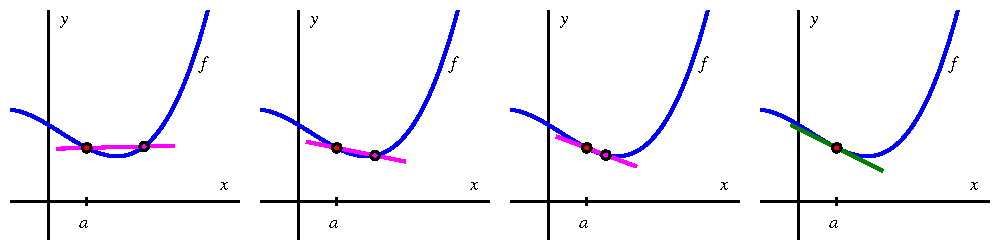
\includegraphics[width=1\linewidth]{../../html/Calculus/images/1_3_SecToTanSeq.pdf}
\caption{A sequence of secant lines approaching the tangent line to \(f\) at \((a,f(a))\).\label{F-1-3-SecToTanSeq}}
\end{figure}
\hypertarget{p-488}{}%
If the tangent line at \(x = a\) exists, the graph of \(f\) looks like a straight line when viewed up close at \((a,f(a))\). In \hyperref[F-1-3-SecToTan]{Figure~\ref{F-1-3-SecToTan}} below, we combine the four graphs from \hyperref[F-1-3-SecToTanSeq]{Figure~\ref{F-1-3-SecToTanSeq}} into a single graph on the left, and zoom in on the box centered at \((a,f(a))\) on the right. Note how the tangent line sits relative to the curve \(y = f(x)\) at \((a,f(a))\), and how closely it resembles the curve near \(x = a\).%
\begin{figure}
\centering
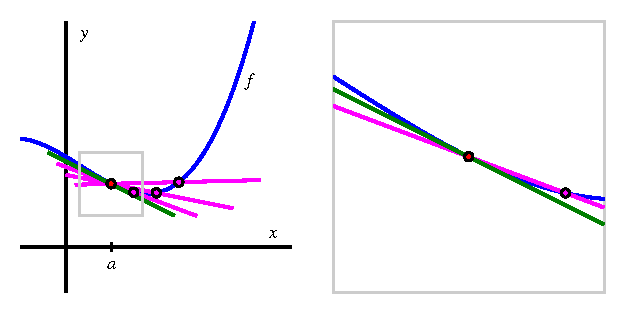
\includegraphics[width=0.6\linewidth]{../../html/Calculus/images/1_3_SecToTan.pdf}
\caption{A sequence of secant lines approaching the tangent line to \(f\) at \((a,f(a))\). At right, we zoom in on the point \((a,f(a))\). The slope of the tangent line (in green) to \(f\) at \((a,f(a))\) is given by \(f'(a)\).\label{F-1-3-SecToTan}}
\end{figure}
\begin{note}[]\label{note-6}
\hypertarget{p-489}{}%
The instantaneous rate of change of \(f\) with respect to \(x\) at \(x = a\), \(f'(a)\), also measures the slope of the tangent line to the curve \(y = f(x)\) at \((a,f(a))\).%
\end{note}
\hypertarget{p-490}{}%
The following example demonstrates several key ideas involving the derivative of a function.%
\begin{example}[Using the limit definition of the derivative]\label{example-32}
\hypertarget{p-491}{}%
For the function \(f(x) = x - x^2\), use the limit definition of the derivative to compute \(f'(2)\). In addition, discuss the meaning of this value and draw a labeled graph that supports your explanation.%
\par\smallskip%
\noindent\textbf{Hint.}\hypertarget{hint-12}{}\quad%
\hypertarget{p-492}{}%
The definition of the derivative of \(f\) with respect to \(x\) evaluated at \(x=a\) says%
\begin{equation*}
f'(a)=\lim_{h\to0}\frac{f(a+h)-f(a)}{h}\text{.}
\end{equation*}
How does the value you find for \(f'(2)\) manifest in the graph of \(f(x)=x-x^2\), particularly near the point \((2,f(2))\)?%
\par\smallskip%
\noindent\textbf{Answer.}\hypertarget{answer-13}{}\quad%
%
\begin{equation*}
f'(2)=-3.
\end{equation*}
\hypertarget{p-493}{}%
The slope of the tangent line to \(f\) through the point \((2,-2)\) is \(-3\).%
\par\smallskip%
\noindent\textbf{Solution.}\hypertarget{solution-26}{}\quad%
\hypertarget{p-494}{}%
From the limit definition, we know that%
\begin{equation*}
f'(2) = \lim_{h \to 0} \frac{f(2+h)-f(2)}{h}\text{.}
\end{equation*}
%
\par
\hypertarget{p-495}{}%
Now we use the rule for \(f\), and observe that \(f(2) = 2 - 2^2 = -2\) and \(f(2+h) = (2+h) - (2+h)^2\). Substituting these values into the limit definition, we have that%
\begin{equation*}
f'(2) = \lim_{h \to 0} \frac{(2+h) - (2+h)^2 -  (-2)}{h}\text{.}
\end{equation*}
%
\par
\hypertarget{p-496}{}%
In order to evaluate the limit, we must simplify the quotient. Expanding and distributing in the numerator gives us%
\begin{equation*}
f'(2) = \lim_{h \to 0} \frac{2+h - 4 - 4h - h^2 + 2}{h}\text{.}
\end{equation*}
%
\par
\hypertarget{p-497}{}%
Combining like terms, we have%
\begin{equation*}
f'(2) = \lim_{h \to 0} \frac{ -3h - h^2}{h}\text{.}
\end{equation*}
%
\par
\hypertarget{p-498}{}%
Next, because \(h\neq0\) within the limit, we may remove a common factor of \(h\) in both the numerator and denominator and find that%
\begin{equation*}
f'(2) = \lim_{h \to 0} (-3-h)\text{.}
\end{equation*}
%
\par
\hypertarget{p-499}{}%
Finally, we are able to take the limit as \(h\) approaches \(0\), and thus conclude that \(f'(2) = -3\). We note that \(f'(2)\) is the instantaneous rate of change of \(f\) at the point \((2,-2)\). It is also the slope of the tangent line to the graph of \(y = x - x^2\) at the point \((2,-2)\). \hyperref[F-1-3-Ex1]{Figure~\ref{F-1-3-Ex1}} below shows both the function and the line through \((2,-2)\) with slope \(m = f'(2) = -3\).%
\begin{figure}
\centering
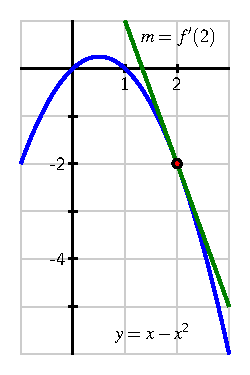
\includegraphics[width=0.4\linewidth]{../../html/Calculus/images/1_3_Ex1.pdf}
\caption{The tangent line to \(y = x - x^2\) at the point \((2,-2)\).\label{F-1-3-Ex1}}
\end{figure}
\end{example}
\hypertarget{p-500}{}%
The following examples will help you explore a variety of key ideas related to derivatives.%
\begin{example}[]\label{act-1-3-1}
\hypertarget{p-501}{}%
Consider the function \(f\) whose formula is \(\displaystyle f(x) = 3 - 2x\).%
\par
\hypertarget{p-502}{}%
\leavevmode%
\begin{enumerate}[label=\alph*.]
\item\hypertarget{li-255}{}What familiar type of function is \(f\)? What can you say about the slope of \(f\) at every value of \(x\)?%
\item\hypertarget{li-256}{}Compute the average rate of change of \(f\) on the intervals \([1,4]\), \([3,7]\), and \([5,5+h]\); simplify each result as much as possible. What do you notice about these quantities?%
\item\hypertarget{li-257}{}Use the limit definition of the derivative to compute the exact instantaneous rate of change of \(f\) with respect to \(x\) at the value \(a = 1\). That is, compute \(f'(1)\) using the limit definition. Show your work. Is your result surprising?%
\item\hypertarget{li-258}{}Without doing any additional computations, what are the values of \(f'(2)\), \(f'(\pi)\), and \(f'(-\sqrt{2})\)? Why?%
\end{enumerate}
%
\par\smallskip%
\noindent\textbf{Hint.}\hypertarget{hint-13}{}\quad%
\hypertarget{p-503}{}%
\leavevmode%
\begin{enumerate}[label=\alph*.]
\item\hypertarget{li-259}{}If \(f(x) = 3x^2 + 2x - 4\), we say ``\(f\) is quadratic.'' If \(f(x) = 5 e^{2x-1}\), we say ``\(f\) is exponential.'' What do we say about \(f(x) = 3-2x\)?%
\item\hypertarget{li-260}{}Remember that to compute the average rate of change of \(f\) on \([a,b]\), we calculate \(\frac{f(b)-f(a)}{b-a}\).%
\item\hypertarget{li-261}{}Observe that \(f(1+h) = 3 - 2(1+h) = 3 - 2 - 2h = 1 - 2h\).%
\item\hypertarget{li-262}{}Think about the how the graph of \(f\) appears. What is the same at every point?%
\end{enumerate}
%
\par\smallskip%
\noindent\textbf{Answer.}\hypertarget{answer-14}{}\quad%
\hypertarget{p-504}{}%
\leavevmode%
\begin{enumerate}[label=\alph*.]
\item\hypertarget{li-263}{}\(f\) is linear.%
\item\hypertarget{li-264}{}The average rate of change on \([1,4]\), \([3,7]\), and \([5,5+h]\) is \(-2\).%
\item\hypertarget{li-265}{}\(f'(1)=-2\).%
\item\hypertarget{li-266}{}\(f'(2)=-2\), \(f'(\pi)=-2\), and \(f'(-\sqrt{2})=-2\), since the slope of a linear function is the same at every point.%
\end{enumerate}
%
\par\smallskip%
\noindent\textbf{Solution.}\hypertarget{solution-27}{}\quad%
\hypertarget{p-505}{}%
\leavevmode%
\begin{enumerate}[label=\alph*.]
\item\hypertarget{li-267}{}Because \(f(x) = 3 - 2x\) is of the form \(f(x) = mx + b\), we call \(f\) a \emph{linear} function.%
\item\hypertarget{li-268}{}The average rate of change on \([1,4]\) is \(\frac{f(4)-f(1)}{4-1} = \frac{-5 - 1}{3} = -2\). Similar calculations show the average rate of change on \([3,7]\) is also \(-2\). On \([5,5+h]\), observe that%
\begin{align*}
\frac{f(5+h)-f(5)}{h} \amp = \frac{(3-2(5+h)) - (3-10)}{h}\\
\amp = \frac{3 - 10 - 2h + 7}{h}\\
\amp = \frac{-2h}{h}\\
\amp = -2\text{.}
\end{align*}
%
\item\hypertarget{li-269}{}Using the limit definition of the derivative, we find that%
\begin{align*}
f'(1) = \amp  \lim_{h \to 0} \frac{f(1+h) - f(1)}{h}\\
= \amp  \lim_{h \to 0} \frac{(3 - 2(1+h)) - (3-2)}{h}\\
= \amp  \lim_{h \to 0} \frac{3 - 2 - 2h - 1}{h}\\
= \amp  \lim_{h \to 0} \frac{-2h}{h}\\
= \amp  \lim_{h \to 0} -2\\
= \amp  -2\text{.}
\end{align*}
%
\end{enumerate}
%
\end{example}
\begin{example}[]\label{act-1-3-2}
\hypertarget{p-506}{}%
A water balloon is tossed vertically in the air from a window. The balloon's height in feet \(t\) seconds after being launched is given by \(s(t) = -16t^2 + 16t + 32\). Use this function to respond to each of the following questions.%
\par
\hypertarget{p-507}{}%
\leavevmode%
\begin{enumerate}[label=\alph*.]
\item\hypertarget{li-270}{}\hypertarget{p-508}{}%
Sketch an accurate, labeled graph of \(y=s(t)\) for \(t=0\) to \(t=2\). Label the scale on the axes carefully. You should be able to do this without using computing technology.%
\item\hypertarget{li-271}{}Compute the average rate of change of \(s\) on the time interval \([1,2]\). Include units in your answer and write one sentence to explain the meaning of the value you found.%
\item\hypertarget{li-272}{}Use the limit definition of the derivative to compute the instantaneous rate of change of \(s\) with respect to time, \(t\), at the instant \(a = 1\). Show your work using proper notation, include units in your answer, and write one sentence to explain the meaning of the value you found.%
\item\hypertarget{li-273}{}On your graph in (a), sketch two lines: one whose slope represents the average rate of change of \(s\) on \([1,2]\), the other whose slope represents the instantaneous rate of change of \(s\) at the instant \(a=1\). Label each line clearly.%
\item\hypertarget{li-274}{}For what values of \(a\) do you expect \(s'(a)\) to be positive? Why? Answer the same questions when ``positive'' is replaced by ``negative'' and ``zero.''%
\end{enumerate}
%
\par\smallskip%
\noindent\textbf{Hint.}\hypertarget{hint-14}{}\quad%
\hypertarget{p-509}{}%
\leavevmode%
\begin{enumerate}[label=\alph*.]
\item\hypertarget{li-275}{}Observe that \((t^2 - t - 2) = (t-2)(t+1)\) and that \(s(t)\) has its vertex at \(t = \frac{1}{2}\).%
\item\hypertarget{li-276}{}Recall the formula for average rate of change.%
\item\hypertarget{li-277}{}Note that \(s(1+h) = -16(1+h)^2 + 16(1+h) + 32\).%
\item\hypertarget{li-278}{}Think about a secant line and a tangent line.%
\item\hypertarget{li-279}{}A line with positive slope is one that is rising; a line with negative slope is one that is falling.%
\end{enumerate}
%
\par\smallskip%
\noindent\textbf{Answer.}\hypertarget{answer-15}{}\quad%
\hypertarget{p-510}{}%
\leavevmode%
\begin{enumerate}[label=\alph*.]
\item\hypertarget{li-280}{}The vertex is \((\frac{1}{2},36)\).%
\item\hypertarget{li-281}{}\(\frac{s(2)-s(1)}{2-1} = -32\) feet per second.%
\item\hypertarget{li-282}{}\(s'(1) = -16\).%
\item\hypertarget{li-283}{}% group protects changes to lengths, releases boxes (?)
{% begin: group for a single side-by-side
% set panel max height to practical minimum, created in preamble
\setlength{\panelmax}{0pt}
\ifdefined\panelboxAimage\else\newsavebox{\panelboxAimage}\fi%
\begin{lrbox}{\panelboxAimage}
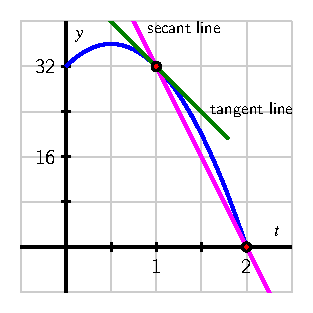
\includegraphics[width=0.5\linewidth]{../../html/Calculus/images/1_3_Act2Soln.pdf}
\end{lrbox}
\ifdefined\phAimage\else\newlength{\phAimage}\fi%
\setlength{\phAimage}{\ht\panelboxAimage+\dp\panelboxAimage}
\settototalheight{\phAimage}{\usebox{\panelboxAimage}}
\setlength{\panelmax}{\maxof{\panelmax}{\phAimage}}
\leavevmode%
% begin: side-by-side as tabular
% \tabcolsep change local to group
\setlength{\tabcolsep}{0\linewidth}
% @{} suppress \tabcolsep at extremes, so margins behave as intended
\par\medskip\noindent
\hspace*{0.25\linewidth}%
\begin{tabular}{@{}*{1}{c}@{}}
\begin{minipage}[c][\panelmax][t]{0.5\linewidth}\usebox{\panelboxAimage}\end{minipage}\end{tabular}\\
% end: side-by-side as tabular
}% end: group for a single side-by-side
%
\item\hypertarget{li-284}{}\(s'(a)\) is positive whenever \(0 \le a \lt \frac{1}{2}\); \(s'(a)\) is negative whenever \(\frac{1}{2} \lt a \lt 2\); \(s'(\frac{1}{2}) = 0\).%
\end{enumerate}
%
\par\smallskip%
\noindent\textbf{Solution.}\hypertarget{solution-28}{}\quad%
\hypertarget{p-511}{}%
\leavevmode%
\begin{enumerate}[label=\alph*.]
\item\hypertarget{li-285}{}Since \(s(t) = -16t^2 + 16t + 32 = -16(t^2 - t - 2) = -16(t-2)(t+1)\), \(s\) has \(t\)-intercepts at \((2,0)\) and \((-1,0)\); the \(s\)-intercept is clearly \((0,32)\); and the vertex is \((\frac{1}{2},36)\). See more in part (d).%
\item\hypertarget{li-286}{}Observe that \(\frac{s(2)-s(1)}{2-1} = \frac{0 - 32}{1} = -32\) feet per second. This value represents the average rate at which the balloon is falling over the time interval from \(t = 1\) to \(t = 2\).%
\item\hypertarget{li-287}{}We compute \(s'(1)\) as follows:%
\begin{align*}
s'(1) = \amp  \lim_{h \to 0} \frac{s(1+h)-s(1)}{h}\\
= \amp  \lim_{h \to 0} \frac{(-16(1+h)^2 + 16(1+h) + 32) - (-16(1)^2 + 16(1) + 32)}{h}\\
= \amp  \lim_{h \to 0} \frac{-16 - 32h - 16h^2 + 16 + 16h + 32 - 32}{h}\\
= \amp  \lim_{h \to 0} \frac{-16h - 16h^2}{h}\\
= \amp  \lim_{h \to 0} (-16-16h)\\
= \amp  -16\text{.}
\end{align*}
%
\item\hypertarget{li-288}{}\hypertarget{p-512}{}%
We plot and label the secant line through \((1,s(1))\) and \((2,s(2))\), as well as the tangent line through \((1,s(1))\) with slope \(s'(1)\).%
% group protects changes to lengths, releases boxes (?)
{% begin: group for a single side-by-side
% set panel max height to practical minimum, created in preamble
\setlength{\panelmax}{0pt}
\ifdefined\panelboxAimage\else\newsavebox{\panelboxAimage}\fi%
\begin{lrbox}{\panelboxAimage}
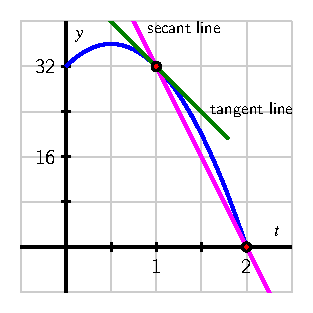
\includegraphics[width=0.4\linewidth]{../../html/Calculus/images/1_3_Act2Soln.pdf}
\end{lrbox}
\ifdefined\phAimage\else\newlength{\phAimage}\fi%
\setlength{\phAimage}{\ht\panelboxAimage+\dp\panelboxAimage}
\settototalheight{\phAimage}{\usebox{\panelboxAimage}}
\setlength{\panelmax}{\maxof{\panelmax}{\phAimage}}
\leavevmode%
% begin: side-by-side as tabular
% \tabcolsep change local to group
\setlength{\tabcolsep}{0\linewidth}
% @{} suppress \tabcolsep at extremes, so margins behave as intended
\par\medskip\noindent
\hspace*{0.3\linewidth}%
\begin{tabular}{@{}*{1}{c}@{}}
\begin{minipage}[c][\panelmax][t]{0.4\linewidth}\usebox{\panelboxAimage}\end{minipage}\end{tabular}\\
% end: side-by-side as tabular
}% end: group for a single side-by-side
\item\hypertarget{li-289}{}Observe that whenever the balloon is rising, its position function is rising, and thus the slope of its tangent line at any such point will be positive. This means that we should find \(s'(a)\) to be positive whenever \(0 \le a \lt \frac{1}{2}\), and similarly \(s'(a)\) to be negative whenever \(\frac{1}{2} \lt a \lt 2\) (which is when the balloon is falling). At the instant \(a = \frac{1}{2}\), the balloon is at its vertex and is neither rising nor falling, and at that point, \(s'(\frac{1}{2}) = 0\).%
\end{enumerate}
%
\end{example}
\begin{example}[]\label{act-1-3-3}
\hypertarget{p-513}{}%
A rapidly growing city in Arizona has its population \(P\) at time \(t\), where \(t\) is the number of decades after the year 2010, modeled by the formula \(P(t) = 25000 e^{t/5}\). Use this function to respond to the following questions.%
\par
\hypertarget{p-514}{}%
\leavevmode%
\begin{enumerate}[label=\alph*.]
\item\hypertarget{li-290}{}\hypertarget{p-515}{}%
Sketch an accurate graph of \(y=P(t)\) for \(t = 0\) to \(t = 5\). Label the scale on the axes carefully.%
\item\hypertarget{li-291}{}Compute the average rate of change of \(P\) between 2030 and 2050. Include units in your answer and write one sentence to explain (in everyday language) the meaning of the value you found.%
\item\hypertarget{li-292}{}Use the limit definition of the derivative to write an expression for the instantaneous rate of change of \(P\) with respect to time, \(t\), at the instant \(a = 2\). Explain why this limit is difficult to evaluate exactly.%
\item\hypertarget{li-293}{}Estimate the limit in (c) for the instantaneous rate of change of \(P\) at the instant \(a = 2\) by using several small \(h\) values. Once you have determined an accurate estimate of \(P'(2)\), include units in your answer, and write one sentence (using everyday language) to explain the meaning of the value you found.%
\item\hypertarget{li-294}{}On your graph above, sketch two lines: one whose slope represents the average rate of change of \(P\) on \([2,4]\), the other whose slope represents the instantaneous rate of change of \(P\) at the instant \(a=2\).%
\item\hypertarget{li-295}{}In a carefully-worded sentence, describe the behavior of \(P'(a)\) as \(a\) increases in value. What does this reflect about the behavior of the given function \(P\)?%
\end{enumerate}
%
\par\smallskip%
\noindent\textbf{Hint.}\hypertarget{hint-15}{}\quad%
\hypertarget{p-516}{}%
\leavevmode%
\begin{enumerate}[label=\alph*.]
\item\hypertarget{li-296}{}\(P(t)\) is the standard exponential function, scaled by \(25000\).%
\item\hypertarget{li-297}{}Use the formula for the average rate of change of a function.%
\item\hypertarget{li-298}{}Because of the exponential nature of \(P(t)\), we're not able to simplify \(\frac{P(2+h)-P(2)}{h}\) in a way that removes \(h\) from the denominator.%
\item\hypertarget{li-299}{}Try using \(h = 0.001, 0.0001, 0.00001\) and \(h = -0.001, -0.0001, -0.00001\). Be careful not to round or use computing precision that is too limited.%
\item\hypertarget{li-300}{}For the first line, think about the points \((2,P(2))\) and \((4,P(4))\).%
\item\hypertarget{li-301}{}Visualize the slope of the tangent line and how it changes as a point moves along the curve in the positive direction.%
\end{enumerate}
%
\par\smallskip%
\noindent\textbf{Answer.}\hypertarget{answer-16}{}\quad%
\hypertarget{p-517}{}%
\leavevmode%
\begin{enumerate}[label=\alph*.]
\item\hypertarget{li-302}{}% group protects changes to lengths, releases boxes (?)
{% begin: group for a single side-by-side
% set panel max height to practical minimum, created in preamble
\setlength{\panelmax}{0pt}
\ifdefined\panelboxAimage\else\newsavebox{\panelboxAimage}\fi%
\begin{lrbox}{\panelboxAimage}
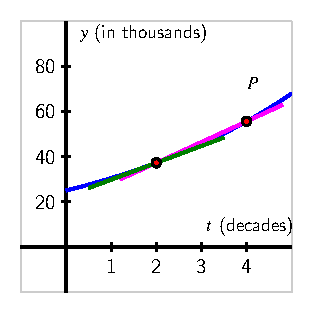
\includegraphics[width=0.4\linewidth]{../../html/Calculus/images/1_3_Act3Soln.pdf}
\end{lrbox}
\ifdefined\phAimage\else\newlength{\phAimage}\fi%
\setlength{\phAimage}{\ht\panelboxAimage+\dp\panelboxAimage}
\settototalheight{\phAimage}{\usebox{\panelboxAimage}}
\setlength{\panelmax}{\maxof{\panelmax}{\phAimage}}
\leavevmode%
% begin: side-by-side as tabular
% \tabcolsep change local to group
\setlength{\tabcolsep}{0\linewidth}
% @{} suppress \tabcolsep at extremes, so margins behave as intended
\par\medskip\noindent
\hspace*{0.3\linewidth}%
\begin{tabular}{@{}*{1}{c}@{}}
\begin{minipage}[c][\panelmax][t]{0.4\linewidth}\usebox{\panelboxAimage}\end{minipage}\end{tabular}\\
% end: side-by-side as tabular
}% end: group for a single side-by-side
%
\item\hypertarget{li-303}{}\(AV_{[2,4]} \approx 9171\) people per decade is expected to be the average rate of change of the city's population over the two decades from 2030 to 2050.%
\item\hypertarget{li-304}{}%
\begin{equation*}
P'(2) =  \lim_{h \to 0} \frac{P(2+h)-P(2)}{h} \approx 7458.5,
\end{equation*}
\hypertarget{p-518}{}%
which is measured in people per decade.%
\item\hypertarget{li-305}{}See the graph provided in (a) above. The magenta line has slope equal to the average rate of change of \(P\) on \([2,4]\), while the green line is the tangent line at \((2,P(2))\) with slope \(P'(2)\).%
\item\hypertarget{li-306}{}It appears that the tangent line's slope at the point \((a,P(a))\) will increase as \(a\) increases.%
\end{enumerate}
%
\par\smallskip%
\noindent\textbf{Solution.}\hypertarget{solution-29}{}\quad%
\hypertarget{p-519}{}%
\leavevmode%
\begin{enumerate}[label=\alph*.]
\item\hypertarget{li-307}{}% group protects changes to lengths, releases boxes (?)
{% begin: group for a single side-by-side
% set panel max height to practical minimum, created in preamble
\setlength{\panelmax}{0pt}
\ifdefined\panelboxAimage\else\newsavebox{\panelboxAimage}\fi%
\begin{lrbox}{\panelboxAimage}
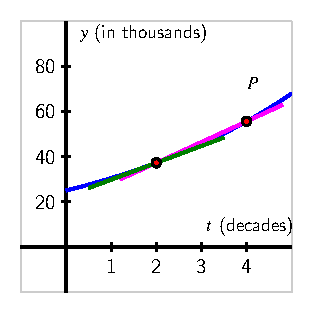
\includegraphics[width=0.4\linewidth]{../../html/Calculus/images/1_3_Act3Soln.pdf}
\end{lrbox}
\ifdefined\phAimage\else\newlength{\phAimage}\fi%
\setlength{\phAimage}{\ht\panelboxAimage+\dp\panelboxAimage}
\settototalheight{\phAimage}{\usebox{\panelboxAimage}}
\setlength{\panelmax}{\maxof{\panelmax}{\phAimage}}
\leavevmode%
% begin: side-by-side as tabular
% \tabcolsep change local to group
\setlength{\tabcolsep}{0\linewidth}
% @{} suppress \tabcolsep at extremes, so margins behave as intended
\par\medskip\noindent
\hspace*{0.3\linewidth}%
\begin{tabular}{@{}*{1}{c}@{}}
\begin{minipage}[c][\panelmax][t]{0.4\linewidth}\usebox{\panelboxAimage}\end{minipage}\end{tabular}\\
% end: side-by-side as tabular
}% end: group for a single side-by-side
%
\item\hypertarget{li-308}{}\(AV_{[2,4]} = \frac{P(4)-P(2)}{4-2} = \frac{25000e^{4/5} - 25000e^{2/5}}{2} \approx 9171\) people per decade is expected to be the average rate of change of the city's population over the two decades from 2030 to 2050.%
\item\hypertarget{li-309}{}Note that%
\begin{align*}
P'(2) = \amp  \lim_{h \to 0} \frac{P(2+h)-P(2)}{h} = \lim_{h \to 0} \frac{25000 e^{(2+h)/5}-25000e^{2/5}}{h}\\
= \amp   \lim_{h \to 0} \frac{25000 e^{2/5} e^{h/5} -25000e^{2/5}}{h} =  \lim_{h \to 0} 25000e^{2/5}\left( \frac{e^{h/5} - 1}{h}\right)
\end{align*}
Because there is no way to remove a factor of \(h\) from the numerator, we cannot eliminate the \(h\) that is making the denominator go to zero, so it appears we need to be content estimating the limit with small values of \(h\).%
\item\hypertarget{li-310}{}Using \(h = 0.00001\), we find \(\frac{P(2+0.00001)-P(2)}{0.00001} \approx 7457\); using \(h = -0.00001\), we find \(\frac{P(2-0.00001)-P(2)}{-0.00001} \approx 7460\). Averaging these two results, we find that%
\begin{equation*}
P'(2) =  \lim_{h \to 0} \frac{P(2+h)-P(2)}{h} \approx 7458.5
\end{equation*}
which is measured in people per decade.%
\item\hypertarget{li-311}{}See the graph provided in (a) above. The magenta line has slope equal to the average rate of change of \(P\) on \([2,4]\), while the green line is the tangent line at \((2,P(2))\) with slope \(P'(2)\).%
\item\hypertarget{li-312}{}If we consider the point where \(t = a\) and let \(a\) start at 0 and then increase, it appears that the tangent line's slope at the point \((a,P(a))\) will increase as \(a\) increases.%
\end{enumerate}
%
\end{example}
\typeout{************************************************}
\typeout{Subsection 1.4.2 Summary}
\typeout{************************************************}
\subsection[{Summary}]{Summary}\label{subsection-28}
\hypertarget{p-520}{}%
\leavevmode%
\begin{itemize}[label=\textbullet]
\item{}The average rate of change of a function \(f\) on the interval \([a,b]\) is \(\frac{f(b)-f(a)}{b-a}\). The units on the average rate of change are units of \(f(x)\) per unit of \(x\), and the numerical value of the average rate of change represents the slope of the secant line between the points \((a,f(a))\) and \((b,f(b))\) on the graph of \(y = f(x)\). If we view the interval as being \([a,a+h]\) instead of \([a,b]\), the meaning is still the same, but the average rate of change is now computed by \(\frac{f(a+h)-f(a)}{h}\).%
\item{}The instantaneous rate of change with respect to \(x\) of a function \(f\) at a value \(x = a\) is denoted \(f'(a)\) (read ``the derivative of \(f\) evaluated at \(a\)'' or ``\(f\)-prime of \(a\)'') and is defined by the formula%
\begin{equation*}
f'(a) = \lim_{h \to 0} \frac{f(a+h)-f(a)}{h}\text{,}
\end{equation*}
provided the limit exists. Note particularly that the instantaneous rate of change at \(x = a\) is the limit of the average rate of change on \([a,a+h]\) as \(h\) approaches \(0\).%
\item{}Provided the derivative \(f'(a)\) exists, its value tells us the instantaneous rate of change of \(f\) with respect to \(x\) at \(x = a\), which geometrically is the slope of the tangent line to the curve \(y = f(x)\) at the point \((a,f(a))\). We even say that \(f'(a)\) is the ``slope of the curve'' at the point \((a,f(a))\).%
\item{}Limits allow us to move from the rate of change over an interval to the rate of change at a single point.%
\end{itemize}
%
\typeout{************************************************}
\typeout{Exercises 1.4.3 Exercises}
\typeout{************************************************}
\subsection[{Exercises}]{Exercises}\label{exercises-7}
\begin{exerciselist}
\item[1.]\hypertarget{ez-1-3-WW1}{}(Estimating derivative values graphically)\space\space{}This exercise uses the WeBWorK Online Homework System and so is not available in the print copy of this book.\item[2.]\hypertarget{ez-1-3-WW2}{}(Tangent line to a curve)\space\space{}This exercise uses the WeBWorK Online Homework System and so is not available in the print copy of this book.\item[3.]\hypertarget{ez-1-3-WW3}{}(Interpreting values and slopes from a graph)\space\space{}This exercise uses the WeBWorK Online Homework System and so is not available in the print copy of this book.\item[4.]\hypertarget{ez-1-3-WW4}{}(Estimating a derivative value graphically)\space\space{}This exercise uses the WeBWorK Online Homework System and so is not available in the print copy of this book.\item[5.]\hypertarget{ez-1-3-WW5}{}(Estimating a derivative from the limit definition)\space\space{}This exercise uses the WeBWorK Online Homework System and so is not available in the print copy of this book.\item[6.]\hypertarget{exercise-51}{}\hypertarget{p-521}{}%
Consider the graph of \(y = f(x)\) provided in \hyperref[F-1-3-Ez1]{Figure~\ref{F-1-3-Ez1}}.%
% group protects changes to lengths, releases boxes (?)
{% begin: group for a single side-by-side
% set panel max height to practical minimum, created in preamble
\setlength{\panelmax}{0pt}
\ifdefined\panelboxAp\else\newsavebox{\panelboxAp}\fi%
\savebox{\panelboxAp}{%
\raisebox{\depth}{\parbox{0.47\linewidth}{\leavevmode%
\begin{enumerate}[label=\alph*.]
\item\hypertarget{li-317}{}\hypertarget{p-523}{}%
On the graph of \(y = f(x)\), sketch and label the following quantities: %
\begin{itemize}[label=\textbullet]
\item{}the secant line to \(y = f(x)\) on the interval \([-3,-1]\) and the secant line to \(y = f(x)\) on the interval \([0,2]\).%
\item{}the tangent line to \(y = f(x)\) at \(x = -3\) and the tangent line to \(y = f(x)\) at \(x = 0\).%
\end{itemize}
%
\item\hypertarget{li-320}{}What is the approximate value of the average rate of change of \(f\) on \([-3,-1]\)? On \([0,2]\)? How are these values related to your work in (a)?%
\item\hypertarget{li-321}{}What is the approximate value of the instantaneous rate of change of \(f\) at \(x = -3\)? At \(x = 0\)? How are these values related to your work in (a)?%
\end{enumerate}
}}}
\ifdefined\phAp\else\newlength{\phAp}\fi%
\setlength{\phAp}{\ht\panelboxAp+\dp\panelboxAp}
\settototalheight{\phAp}{\usebox{\panelboxAp}}
\setlength{\panelmax}{\maxof{\panelmax}{\phAp}}
\ifdefined\panelboxAimage\else\newsavebox{\panelboxAimage}\fi%
\begin{lrbox}{\panelboxAimage}
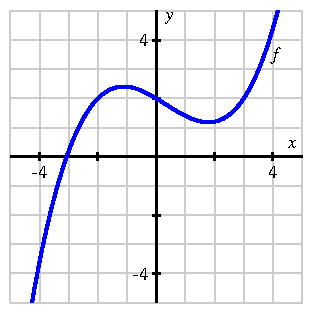
\includegraphics[width=0.47\linewidth]{../../html/Calculus/images/1_3_Ez1.pdf}
\end{lrbox}
\ifdefined\phAimage\else\newlength{\phAimage}\fi%
\setlength{\phAimage}{\ht\panelboxAimage+\dp\panelboxAimage}
\settototalheight{\phAimage}{\usebox{\panelboxAimage}}
\setlength{\panelmax}{\maxof{\panelmax}{\phAimage}}
\leavevmode%
% begin: side-by-side as tabular
% \tabcolsep change local to group
\setlength{\tabcolsep}{0.03\linewidth}
% @{} suppress \tabcolsep at extremes, so margins behave as intended
\par\medskip\noindent
\begin{tabular}{@{}*{2}{c}@{}}
\begin{minipage}[c][\panelmax][t]{0.47\linewidth}\usebox{\panelboxAp}\end{minipage}&
\begin{minipage}[c][\panelmax][t]{0.47\linewidth}\usebox{\panelboxAimage}\end{minipage}\tabularnewline
&
\parbox[t]{0.47\linewidth}{\captionof{figure}{Plot of \(y = f(x)\).\label{F-1-3-Ez1}}
}\end{tabular}\\
% end: side-by-side as tabular
}% end: group for a single side-by-side
\par\smallskip
\par\smallskip%
\noindent\textbf{Answer.}\hypertarget{answer-17}{}\quad%
\hypertarget{p-524}{}%
\leavevmode%
\begin{enumerate}[label=\alph*.]
\item\hypertarget{li-322}{}% group protects changes to lengths, releases boxes (?)
{% begin: group for a single side-by-side
% set panel max height to practical minimum, created in preamble
\setlength{\panelmax}{0pt}
\ifdefined\panelboxAimage\else\newsavebox{\panelboxAimage}\fi%
\begin{lrbox}{\panelboxAimage}
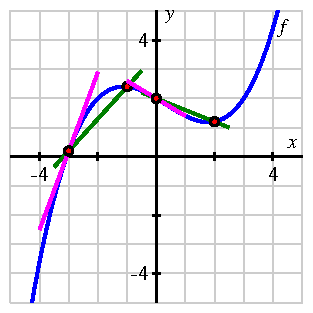
\includegraphics[width=0.5\linewidth]{../../html/Calculus/images/1_3_Ez1Soln.pdf}
\end{lrbox}
\ifdefined\phAimage\else\newlength{\phAimage}\fi%
\setlength{\phAimage}{\ht\panelboxAimage+\dp\panelboxAimage}
\settototalheight{\phAimage}{\usebox{\panelboxAimage}}
\setlength{\panelmax}{\maxof{\panelmax}{\phAimage}}
\leavevmode%
% begin: side-by-side as tabular
% \tabcolsep change local to group
\setlength{\tabcolsep}{0\linewidth}
% @{} suppress \tabcolsep at extremes, so margins behave as intended
\par\medskip\noindent
\hspace*{0.25\linewidth}%
\begin{tabular}{@{}*{1}{c}@{}}
\begin{minipage}[c][\panelmax][t]{0.5\linewidth}\usebox{\panelboxAimage}\end{minipage}\end{tabular}\\
% end: side-by-side as tabular
}% end: group for a single side-by-side
%
\item\hypertarget{li-323}{}\hypertarget{p-525}{}%
\(AV_{[-3,-1]} \approx 1.15\); \(AV_{[0,2]} \approx -0.4\).%
\item\hypertarget{li-324}{}\hypertarget{p-526}{}%
\(f'(-3) \approx 3\); \(f'(0) \approx -\frac{1}{2}\).%
\end{enumerate}
%
\par\smallskip%
\noindent\textbf{Solution.}\hypertarget{solution-30}{}\quad%
\hypertarget{p-527}{}%
\leavevmode%
\begin{enumerate}[label=\alph*.]
\item\hypertarget{li-325}{}\hypertarget{p-528}{}%
The requested secant lines are drawn in green, with the noted tangent lines in magenta.%
% group protects changes to lengths, releases boxes (?)
{% begin: group for a single side-by-side
% set panel max height to practical minimum, created in preamble
\setlength{\panelmax}{0pt}
\ifdefined\panelboxAimage\else\newsavebox{\panelboxAimage}\fi%
\begin{lrbox}{\panelboxAimage}
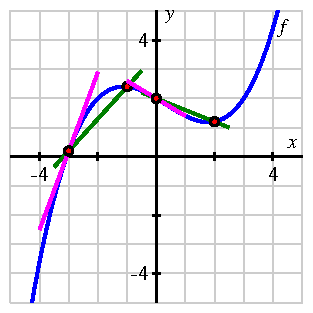
\includegraphics[width=0.5\linewidth]{../../html/Calculus/images/1_3_Ez1Soln.pdf}
\end{lrbox}
\ifdefined\phAimage\else\newlength{\phAimage}\fi%
\setlength{\phAimage}{\ht\panelboxAimage+\dp\panelboxAimage}
\settototalheight{\phAimage}{\usebox{\panelboxAimage}}
\setlength{\panelmax}{\maxof{\panelmax}{\phAimage}}
\leavevmode%
% begin: side-by-side as tabular
% \tabcolsep change local to group
\setlength{\tabcolsep}{0\linewidth}
% @{} suppress \tabcolsep at extremes, so margins behave as intended
\par\medskip\noindent
\hspace*{0.25\linewidth}%
\begin{tabular}{@{}*{1}{c}@{}}
\begin{minipage}[c][\panelmax][t]{0.5\linewidth}\usebox{\panelboxAimage}\end{minipage}\end{tabular}\\
% end: side-by-side as tabular
}% end: group for a single side-by-side
\item\hypertarget{li-326}{}\hypertarget{p-529}{}%
First, \(AV_{[-3,-1]} = \frac{f(-1)-f(-3)}{-1-(-3)} \approx \frac{2.3}{2} = 1.15\). Similarly, \(AV_{[0,2]} = \frac{f(2)-f(0)}{2-0} \approx -\frac{0.8}{2} = -0.4\). These values are the respective slopes of the green secant lines plotted in (a).%
\item\hypertarget{li-327}{}\hypertarget{p-530}{}%
\(f'(-3) \approx 3\) and \(f'(0) \approx -\frac{1}{2}\), as these are estimates of the slopes of the tangent lines plotted in magenta.%
\end{enumerate}
%
\item[7.]\hypertarget{exercise-52}{}\hypertarget{p-531}{}%
For each of the following prompts, sketch a graph on the provided axes in \hyperref[F-1-3-Ez2]{Figure~\ref{F-1-3-Ez2}} of a function that has the stated properties.%
\begin{figure}
\centering
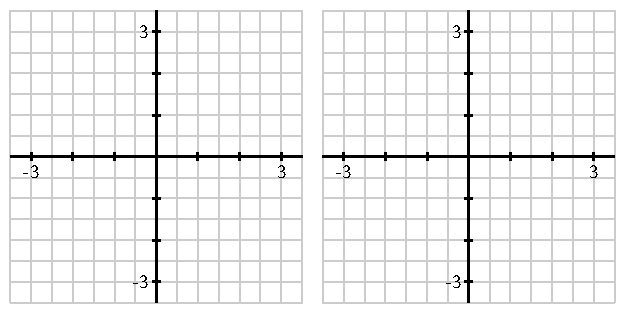
\includegraphics[width=0.99\linewidth]{../../html/Calculus/images/1_2_Ez3.pdf}
\caption{Axes for plotting \(y = f(x)\) in (a) and \(y = g(x)\) in (b).\label{F-1-3-Ez2}}
\end{figure}
\hypertarget{p-532}{}%
\leavevmode%
\begin{enumerate}[label=\alph*.]
\item\hypertarget{li-328}{}\hypertarget{p-533}{}%
\(y = f(x)\) such that %
\begin{itemize}[label=\textbullet]
\item{}the average rate of change of \(f\) on \([-3,0]\) is \(-2\) and the average rate of change of \(f\) on \([1,3]\) is 0.5, and%
\item{}the instantaneous rate of change of \(f\) at \(x = -1\) is \(-1\) and the instantaneous rate of change of \(f\) at \(x = 2\) is 1.%
\end{itemize}
%
\item\hypertarget{li-331}{}\hypertarget{p-534}{}%
\(y = g(x)\) such that %
\begin{itemize}[label=\textbullet]
\item{}\(\frac{g(3)-g(-2)}{5} = 0\) and \(\frac{g(1)-g(-1)}{2} = -1\), and%
\item{}\(g'(2) = 1\) and \(g'(-1) = 0\)%
\end{itemize}
%
\end{enumerate}
%
\par\smallskip
\par\smallskip%
\noindent\textbf{Answer.}\hypertarget{answer-18}{}\quad%
\hypertarget{p-535}{}%
\leavevmode%
\begin{enumerate}[label=\alph*.]
\item\hypertarget{li-334}{}\hypertarget{p-536}{}%
For instance, you could let \(f(-3) = 3\) and have \(f\) pass through the points \((-3,3)\), \((-1,-2)\), \((0,-3)\), \((1,-2)\), and \((3,-1)\) and draw the desired tangent lines accordingly.%
\item\hypertarget{li-335}{}\hypertarget{p-537}{}%
For instance, you could draw a function \(g\) that passes through the points \((-2,3)\), \((-1,2)\), \((1,0)\), \((2,0)\), and \((3,3)\) in such a way that the tangent line at \((-1,2)\) is horizontal and the tangent line at \((2,0)\) has slope \(1\).%
\end{enumerate}
%
\par\smallskip%
\noindent\textbf{Solution.}\hypertarget{solution-31}{}\quad%
\hypertarget{p-538}{}%
\leavevmode%
\begin{enumerate}[label=\alph*.]
\item\hypertarget{li-336}{}\hypertarget{p-539}{}%
For this problem, you should draw a graph so that the slope of the secant line from \((-3,f(-3))\) to \((0,f(0))\) is \(-2\), and similarly the slope of the secant line from \((1,f(1))\) to \((3,f(3))\) is \(0.5\), while the slopes of the tangent lines at \(x = -1\) and \(x = 2\) are \(-1\) and \(1\), respectively. For instance, you could let \(f(-3) = 3\) and have \(f\) pass through the points \((-3,3)\), \((-1,-2)\), \((0,-3)\), \((1,-2)\), and \((3,-1)\) and draw the desired tangent lines accordingly.%
\item\hypertarget{li-337}{}\hypertarget{p-540}{}%
For this problem, you should draw a graph so that the slope of the secant line from \((-2,g(-2))\) to \((3,f(3))\) is \(0\), and similarly the slope of the secant line from \((-1,g(-1))\) to \((1,g(1))\) is \(-1\), while the slopes of the tangent lines to \(y = g(x)\) at \(x=-1\) and \(x = 2\) are \(0\) and \(1\), respectively. For instance, you could draw a function \(g\) that passes through the points \((-2,3)\), \((-1,2)\), \((1,0)\), \((2,0)\), and \((3,3)\) in such a way that the tangent line at \((-1,2)\) is horizontal and the tangent line at \((2,0)\) has slope \(1\).%
\end{enumerate}
%
\item[8.]\hypertarget{exercise-53}{}\hypertarget{p-541}{}%
Suppose that the population, \(P\), of China (in billions) can be approximated by the function \(P(t) = 1.15(1.014)^t\) where \(t\) is the number of years since the start of 1993.%
\par
\hypertarget{p-542}{}%
\leavevmode%
\begin{enumerate}[label=\alph*.]
\item\hypertarget{li-338}{}According to the model, what was the total change in the population of China between January 1, 1993 and January 1, 2000? What will be the average rate of change of the population over this time period? Is this average rate of change greater or less than the instantaneous rate of change of the population on January 1, 2000? Explain and justify, being sure to include proper units on all your answers.%
\item\hypertarget{li-339}{}According to the model, what is the average rate of change of the population of China in the ten-year period starting on January 1, 2012?%
\item\hypertarget{li-340}{}Write an expression involving limits that, if evaluated, would give the exact instantaneous rate of change of the population on today's date. Then estimate the value of this limit (discuss how you chose to do so) and explain the meaning (including units) of the value you have found.%
\item\hypertarget{li-341}{}Find an equation for the tangent line to the function \(y = P(t)\) at the point where the \(t\)-value is given by today's date.%
\end{enumerate}
%
\par\smallskip
\par\smallskip%
\noindent\textbf{Answer.}\hypertarget{answer-19}{}\quad%
\hypertarget{p-543}{}%
\leavevmode%
\begin{enumerate}[label=\alph*.]
\item\hypertarget{li-342}{}\hypertarget{p-544}{}%
\(AV_{[0,7]}=\frac{0.1175}{7} \approx 0.01679\) billion people per year; \(P'(7) \approx 0.1762\) billion people per year; \(P'(7) \gt AV_{[0,7]}\).%
\item\hypertarget{li-343}{}\hypertarget{p-545}{}%
\(AV_{[19,29]} \approx 0.02234\) billion people/year.%
\item\hypertarget{li-344}{}\hypertarget{p-546}{}%
We will say that today's date is July 1, 2015, which means that \(t = 22.5\);%
\begin{equation*}
P'(22.5) = \lim_{h \to 0} \frac{115(1.014)^{22.5+h}-115(1.014)^{22.5}}{h};
\end{equation*}
\(P'(22.5) \approx 0.02186\) billions of people per year.%
\item\hypertarget{li-345}{}\hypertarget{p-547}{}%
\(y - 1.57236 = 0.02186(t-22.5)\).%
\end{enumerate}
%
\par\smallskip%
\noindent\textbf{Solution.}\hypertarget{solution-32}{}\quad%
\hypertarget{p-548}{}%
\leavevmode%
\begin{enumerate}[label=\alph*.]
\item\hypertarget{li-346}{}\hypertarget{p-549}{}%
First, \(P(7)-P(0) = 115(1.014)^7-115(1.014)^0 \approx 0.1175\) billion people is the total population change. It follows that the average rate of change over this time period is \(AV_{[0,7]}=\frac{0.1175}{7} \approx 0.01679\) billion people per year. The instantaneous rate of change of the population at \(t = 7\) is%
\begin{equation*}
P'(7) = \lim_{h \to 0} AV_{[7,7+h]} = \lim_{h \to 0} \frac{115(1.014)^{7+h}-115(1.014)^7}{h}\text{,}
\end{equation*}
and approximating this quantity with small values of \(h\), it follows that \(P'(7) \approx 0.1762\). Hence, the instantaneous rate of change at \(t = 7\) is greater than the average rate of change of \(P\)on the interval \([0,7]\).%
\item\hypertarget{li-347}{}\hypertarget{p-550}{}%
Using the formula for average rate of change,%
\begin{equation*}
AV_{[19,29]}=\frac{1.15(1.014)^{29}-1.15(1.014)^{19}}{29-19} \approx 0.02234
\end{equation*}
billion people/year.%
\item\hypertarget{li-348}{}\hypertarget{p-551}{}%
We will say that today's date is July 1, 2015, which means that \(t = 22.5\), so we want to compute \(P'(22.5)\). The limit definition tells us that%
\begin{equation*}
P'(22.5) = \lim_{h \to 0} \frac{115(1.014)^{22.5+h}-115(1.014)^{22.5}}{h}\text{.}
\end{equation*}
Estimating this limit by using small values of \(h\), we determine that \(P'(22.5) \approx 0.02186\), which is measured in billions of people per year.%
\item\hypertarget{li-349}{}\hypertarget{p-552}{}%
We want the equation of the tangent line that has slope \(P'(22.5) \approx 0.02186\) and that passes through the point \((22.5, P(22.5))\). Using point-slope form, it follows that the line is given by%
\begin{equation*}
y - 1.57236 = 0.02186(t-22.5)\text{.}
\end{equation*}
%
\end{enumerate}
%
\item[9.]\hypertarget{exercise-54}{}\hypertarget{p-553}{}%
The goal of this problem is to compute the value of the derivative at a point for several different functions, where for each one we do so in three different ways, and then to compare the results to see that each produces the same value.%
\par
\hypertarget{p-554}{}%
For each of the following functions, use the limit definition of the derivative to compute the value of \(f'(a)\) using three different approaches: strive to use the algebraic approach first (to compute the limit exactly), then test your result using numerical evidence (with small values of \(h\)), and finally plot the graph of \(y = f(x)\) near \((a,f(a))\) along with the appropriate tangent line to estimate the value of \(f'(a)\) visually. Compare your findings among all three approaches; if you are unable to complete the algebraic approach, still work numerically and graphically.%
\par
\hypertarget{p-555}{}%
\leavevmode%
\begin{multicols}{2}
\begin{enumerate}[label=\alph*.]
\item\hypertarget{li-350}{}\(f(x) = x^2 - 3x\), \(a = 2\)%
\item\hypertarget{li-351}{}\(f(x) = \frac{1}{x}\), \(a = 1\)%
\item\hypertarget{li-352}{}\(f(x) = \sqrt{x}\), \(a = 1\)%
\item\hypertarget{li-353}{}\(f(x) = 2 - |x-1|\), \(a = 1\)%
\item\hypertarget{li-354}{}\(f(x) = \sin(x)\), \(a = \frac{\pi}{2}\)%
\end{enumerate}
\end{multicols}
%
\par\smallskip
\par\smallskip%
\noindent\textbf{Answer.}\hypertarget{answer-20}{}\quad%
\hypertarget{p-556}{}%
\leavevmode%
\begin{enumerate}[label=\alph*.]
\item\hypertarget{li-355}{}\hypertarget{p-557}{}%
All three approaches show that \(f'(2) = 1\).%
\item\hypertarget{li-356}{}\hypertarget{p-558}{}%
All three approaches show that \(f'(1) = -1\).%
\item\hypertarget{li-357}{}\hypertarget{p-559}{}%
All three approaches show that \(f'(1) = \frac{1}{2}\).%
\item\hypertarget{li-358}{}\hypertarget{p-560}{}%
All three approaches show that \(f'(1)\) does not exist.%
\item\hypertarget{li-359}{}\hypertarget{p-561}{}%
The first two approaches show that \(f'(\frac{\pi}{2}) = 0\).%
\end{enumerate}
%
\par\smallskip%
\noindent\textbf{Solution.}\hypertarget{solution-33}{}\quad%
\hypertarget{p-562}{}%
\leavevmode%
\begin{enumerate}[label=\alph*.]
\item\hypertarget{li-360}{}\hypertarget{p-563}{}%
The table below gives values of the difference quotient \(\frac{f(a+h)-f(a)}{h}\) for \(a=2\) and several small values of \(h\). This table indicates that \(f'(2)\) is approximately \(1\).%
% group protects changes to lengths, releases boxes (?)
{% begin: group for a single side-by-side
% set panel max height to practical minimum, created in preamble
\setlength{\panelmax}{0pt}
\ifdefined\panelboxAtabular\else\newsavebox{\panelboxAtabular}\fi%
\savebox{\panelboxAtabular}{%
\raisebox{\depth}{\parbox{1\linewidth}{\centering\begin{tabular}{lllllll}\hrulethin
\(h\)&\(-0.0001\)&\(-0.001\)&\(-0.01\)&\(0.01\)&\(0.001\)&\(0.0001\)\tabularnewline\hrulethin
\(\frac{f(2+h)-f(2)}{h}\)&\(0.9999\)&\(0.9990\)&\(0.9900\)&\(1.0100\)&\(1.0010\)&\(1.0001\)\tabularnewline\hrulethin
\end{tabular}
}}}
\ifdefined\phAtabular\else\newlength{\phAtabular}\fi%
\setlength{\phAtabular}{\ht\panelboxAtabular+\dp\panelboxAtabular}
\settototalheight{\phAtabular}{\usebox{\panelboxAtabular}}
\setlength{\panelmax}{\maxof{\panelmax}{\phAtabular}}
\leavevmode%
% begin: side-by-side as tabular
% \tabcolsep change local to group
\setlength{\tabcolsep}{0\linewidth}
% @{} suppress \tabcolsep at extremes, so margins behave as intended
\par\medskip\noindent
\begin{tabular}{@{}*{1}{c}@{}}
\begin{minipage}[c][\panelmax][t]{1\linewidth}\usebox{\panelboxAtabular}\end{minipage}\end{tabular}\\
% end: side-by-side as tabular
}% end: group for a single side-by-side
\par
\hypertarget{p-564}{}%
The tangent line to \(f\) at the point \((2,f(2))\) as shown in the following appears to have a slope that is approximately 1.%
% group protects changes to lengths, releases boxes (?)
{% begin: group for a single side-by-side
% set panel max height to practical minimum, created in preamble
\setlength{\panelmax}{0pt}
\ifdefined\panelboxAimage\else\newsavebox{\panelboxAimage}\fi%
\begin{lrbox}{\panelboxAimage}
\includegraphics[width=0.5\linewidth]{../../html/Calculus/images/1_3_Ez4a_soln.pdf}
\end{lrbox}
\ifdefined\phAimage\else\newlength{\phAimage}\fi%
\setlength{\phAimage}{\ht\panelboxAimage+\dp\panelboxAimage}
\settototalheight{\phAimage}{\usebox{\panelboxAimage}}
\setlength{\panelmax}{\maxof{\panelmax}{\phAimage}}
\leavevmode%
% begin: side-by-side as tabular
% \tabcolsep change local to group
\setlength{\tabcolsep}{0\linewidth}
% @{} suppress \tabcolsep at extremes, so margins behave as intended
\par\medskip\noindent
\hspace*{0.25\linewidth}%
\begin{tabular}{@{}*{1}{c}@{}}
\begin{minipage}[c][\panelmax][t]{0.5\linewidth}\usebox{\panelboxAimage}\end{minipage}\end{tabular}\\
% end: side-by-side as tabular
}% end: group for a single side-by-side
\par
\hypertarget{p-565}{}%
Finally, we verify these approximations using an algebraic approach. The definition of the derivative of \(f\) at \(x=a\) shows that%
\begin{align*}
f'(2) &= \lim_{h \to 0} \frac{f(2+h)-f(2)}{h}\\
&= \lim_{h \to 0} \frac{\left[(2+h)^2 - 3(2+h)\right] - (-2)}{h}\\
&= \lim_{h \to 0} \frac{\left[4+4h+h^2 - 6 - 3h\right] + 2}{h}\\
&= \lim_{h \to 0} \frac{h^2 + h}{h}\\
&= \lim_{h \to 0} \frac{h(h+1)}{h}\\
&= \lim_{h \to 0} h+1\\
&= 1
\end{align*}
This confirms our conclusions using the numeric and geometric approaches.%
\item\hypertarget{li-361}{}\hypertarget{p-566}{}%
The following table gives values of the difference quotient \(\frac{f(a+h)-f(a)}{h}\) for \(a=1\) and several small values of \(h\). This table indicates that \(f'(1)\) is approximately \(-1\).%
% group protects changes to lengths, releases boxes (?)
{% begin: group for a single side-by-side
% set panel max height to practical minimum, created in preamble
\setlength{\panelmax}{0pt}
\ifdefined\panelboxAtabular\else\newsavebox{\panelboxAtabular}\fi%
\savebox{\panelboxAtabular}{%
\raisebox{\depth}{\parbox{1\linewidth}{\centering\begin{tabular}{lllllll}\hrulethin
\(h\)&\(-0.0001\)&\(-0.001\)&\(-0.01\)&\(0.01\)&\(0.001\)&\(0.0001\)\tabularnewline\hrulethin
\(\frac{f(1+h)-f(1)}{h}\)&\(-1.00010\)&\(-1.001001\)&\(-1.010101\)&\(-0.990099\)&\(-0.999001\)&\(-0.999900\)\tabularnewline\hrulethin
\end{tabular}
}}}
\ifdefined\phAtabular\else\newlength{\phAtabular}\fi%
\setlength{\phAtabular}{\ht\panelboxAtabular+\dp\panelboxAtabular}
\settototalheight{\phAtabular}{\usebox{\panelboxAtabular}}
\setlength{\panelmax}{\maxof{\panelmax}{\phAtabular}}
\leavevmode%
% begin: side-by-side as tabular
% \tabcolsep change local to group
\setlength{\tabcolsep}{0\linewidth}
% @{} suppress \tabcolsep at extremes, so margins behave as intended
\par\medskip\noindent
\begin{tabular}{@{}*{1}{c}@{}}
\begin{minipage}[c][\panelmax][t]{1\linewidth}\usebox{\panelboxAtabular}\end{minipage}\end{tabular}\\
% end: side-by-side as tabular
}% end: group for a single side-by-side
\par
\hypertarget{p-567}{}%
The tangent line to \(f\) at the point \((1,f(1))\) as shown in the following figure appears to have a slope that is approximately \(-1\).%
% group protects changes to lengths, releases boxes (?)
{% begin: group for a single side-by-side
% set panel max height to practical minimum, created in preamble
\setlength{\panelmax}{0pt}
\ifdefined\panelboxAimage\else\newsavebox{\panelboxAimage}\fi%
\begin{lrbox}{\panelboxAimage}
\includegraphics[width=0.5\linewidth]{../../html/Calculus/images/1_3_Ez4b_soln.pdf}
\end{lrbox}
\ifdefined\phAimage\else\newlength{\phAimage}\fi%
\setlength{\phAimage}{\ht\panelboxAimage+\dp\panelboxAimage}
\settototalheight{\phAimage}{\usebox{\panelboxAimage}}
\setlength{\panelmax}{\maxof{\panelmax}{\phAimage}}
\leavevmode%
% begin: side-by-side as tabular
% \tabcolsep change local to group
\setlength{\tabcolsep}{0\linewidth}
% @{} suppress \tabcolsep at extremes, so margins behave as intended
\par\medskip\noindent
\hspace*{0.25\linewidth}%
\begin{tabular}{@{}*{1}{c}@{}}
\begin{minipage}[c][\panelmax][t]{0.5\linewidth}\usebox{\panelboxAimage}\end{minipage}\end{tabular}\\
% end: side-by-side as tabular
}% end: group for a single side-by-side
\par
\hypertarget{p-568}{}%
Finally, we verify these approximations using an algebraic approach. The definition of the derivative of \(f\) at \(x=a\) shows that%
\begin{align*}
f'(1) &= \lim_{h \to 0} \frac{f(1+h)-f(1)}{h}\\
&= \lim_{h \to 0} \frac{\frac{1}{1+h} - 1}{h}\\
&= \lim_{h \to 0} \frac{\frac{1}{1+h} - 1}{h} \left(\frac{1+h}{1+h} \right)\\
&= \lim_{h \to 0} \frac{1-(1+h)}{h(1+h)}\\
&= \lim_{h \to 0} \frac{-h)}{h(1+h)}\\
&= \lim_{h \to 0} -\frac{1}{1+h}\\
&= -1\text{.}
\end{align*}
This confirms our conclusions using the numeric and geometric approaches.%
\item\hypertarget{li-362}{}\hypertarget{p-569}{}%
The table below gives values of the difference quotient \(\frac{f(a+h)-f(a)}{h}\) for \(a=1\) and several small values of \(h\). This table indicates that \(f'(1)\) is approximately \(0.5\).%
% group protects changes to lengths, releases boxes (?)
{% begin: group for a single side-by-side
% set panel max height to practical minimum, created in preamble
\setlength{\panelmax}{0pt}
\ifdefined\panelboxAtabular\else\newsavebox{\panelboxAtabular}\fi%
\savebox{\panelboxAtabular}{%
\raisebox{\depth}{\parbox{1\linewidth}{\centering\begin{tabular}{lllllll}\hrulethin
\(h\)&\(-0.0001\)&\(-0.001\)&\(-0.01\)&\(0.01\)&\(0.001\)&\(0.0001\)\tabularnewline\hrulethin
\(\frac{f(1+h)-f(1)}{h}\)&\(0.50001300\)&\(0.50012510\)&\(0.50125629\)&\(0.49875620\)&\(0.49987500\)&\(0.49999000\)\tabularnewline\hrulethin
\end{tabular}
}}}
\ifdefined\phAtabular\else\newlength{\phAtabular}\fi%
\setlength{\phAtabular}{\ht\panelboxAtabular+\dp\panelboxAtabular}
\settototalheight{\phAtabular}{\usebox{\panelboxAtabular}}
\setlength{\panelmax}{\maxof{\panelmax}{\phAtabular}}
\leavevmode%
% begin: side-by-side as tabular
% \tabcolsep change local to group
\setlength{\tabcolsep}{0\linewidth}
% @{} suppress \tabcolsep at extremes, so margins behave as intended
\par\medskip\noindent
\begin{tabular}{@{}*{1}{c}@{}}
\begin{minipage}[c][\panelmax][t]{1\linewidth}\usebox{\panelboxAtabular}\end{minipage}\end{tabular}\\
% end: side-by-side as tabular
}% end: group for a single side-by-side
\par
\hypertarget{p-570}{}%
The tangent line to \(f\) at the point \((1,f(1))\) as shown in the figure below appears to have a slope that is approximately \(0.5\).%
% group protects changes to lengths, releases boxes (?)
{% begin: group for a single side-by-side
% set panel max height to practical minimum, created in preamble
\setlength{\panelmax}{0pt}
\ifdefined\panelboxAimage\else\newsavebox{\panelboxAimage}\fi%
\begin{lrbox}{\panelboxAimage}
\includegraphics[width=0.5\linewidth]{../../html/Calculus/images/1_3_Ez4c_soln.pdf}
\end{lrbox}
\ifdefined\phAimage\else\newlength{\phAimage}\fi%
\setlength{\phAimage}{\ht\panelboxAimage+\dp\panelboxAimage}
\settototalheight{\phAimage}{\usebox{\panelboxAimage}}
\setlength{\panelmax}{\maxof{\panelmax}{\phAimage}}
\leavevmode%
% begin: side-by-side as tabular
% \tabcolsep change local to group
\setlength{\tabcolsep}{0\linewidth}
% @{} suppress \tabcolsep at extremes, so margins behave as intended
\par\medskip\noindent
\hspace*{0.25\linewidth}%
\begin{tabular}{@{}*{1}{c}@{}}
\begin{minipage}[c][\panelmax][t]{0.5\linewidth}\usebox{\panelboxAimage}\end{minipage}\end{tabular}\\
% end: side-by-side as tabular
}% end: group for a single side-by-side
\par
\hypertarget{p-571}{}%
Finally, we verify these approximations using an algebraic approach. The definition of the derivative of \(f\) at \(x=a\) shows that%
\begin{align*}
f'(1) &= \lim_{h \to 0} \frac{f(1+h)-f(1)}{h}\\
&= \lim_{h \to 0} \frac{\sqrt{1+h}-\sqrt{1}}{h}\\
&= \lim_{h \to 0} \frac{\sqrt{1+h}-1}{h}\\
&= \lim_{h \to 0} \frac{\sqrt{1+h}-1}{h} \left(\frac{\sqrt{1+h}+1}{\sqrt{1+h}+1} \right)\\
&= \lim_{h \to 0} \frac{(1+h)-1}{h(\sqrt{1+h}+1)}\\
&= \lim_{h \to 0} \frac{h}{h(\sqrt{1+h}+1)}\\
&= \frac{1}{\sqrt{1+h}+1}\\
&= \frac{1}{2}\text{.}
\end{align*}
This confirms our conclusions using the numeric and geometric approaches.%
\item\hypertarget{li-363}{}\hypertarget{p-572}{}%
The data in the following table indicates that \(\frac{f(1+h)-f(1)}{h}\) has values of \(1\) for \(h \lt 0\) and values of \(-1\) for \(h \gt 0\). This implies that \(f'(1)\) does not exist.%
% group protects changes to lengths, releases boxes (?)
{% begin: group for a single side-by-side
% set panel max height to practical minimum, created in preamble
\setlength{\panelmax}{0pt}
\ifdefined\panelboxAtabular\else\newsavebox{\panelboxAtabular}\fi%
\savebox{\panelboxAtabular}{%
\raisebox{\depth}{\parbox{1\linewidth}{\centering\begin{tabular}{lllllll}\hrulethin
\(h\)&\(-0.0001\)&\(-0.001\)&\(-0.01\)&\(0.01\)&\(0.001\)&\(0.0001\)\tabularnewline\hrulethin
\(\frac{f(1+h)-f(1)}{h}\)&\(1\)&\(1\)&\(1\)&\(-1\)&\(-1\)&\(-1\)\tabularnewline\hrulethin
\end{tabular}
}}}
\ifdefined\phAtabular\else\newlength{\phAtabular}\fi%
\setlength{\phAtabular}{\ht\panelboxAtabular+\dp\panelboxAtabular}
\settototalheight{\phAtabular}{\usebox{\panelboxAtabular}}
\setlength{\panelmax}{\maxof{\panelmax}{\phAtabular}}
\leavevmode%
% begin: side-by-side as tabular
% \tabcolsep change local to group
\setlength{\tabcolsep}{0\linewidth}
% @{} suppress \tabcolsep at extremes, so margins behave as intended
\par\medskip\noindent
\begin{tabular}{@{}*{1}{c}@{}}
\begin{minipage}[c][\panelmax][t]{1\linewidth}\usebox{\panelboxAtabular}\end{minipage}\end{tabular}\\
% end: side-by-side as tabular
}% end: group for a single side-by-side
\par
\hypertarget{p-573}{}%
The graph of \(f\) in the figure below appears to show a sharp corner at the point \((1,f(1))\), also implying that there is no tangent line to \(f\)at \((1,f(1))\).%
% group protects changes to lengths, releases boxes (?)
{% begin: group for a single side-by-side
% set panel max height to practical minimum, created in preamble
\setlength{\panelmax}{0pt}
\ifdefined\panelboxAimage\else\newsavebox{\panelboxAimage}\fi%
\begin{lrbox}{\panelboxAimage}
\includegraphics[width=0.5\linewidth]{../../html/Calculus/images/1_3_Ez4d_soln.pdf}
\end{lrbox}
\ifdefined\phAimage\else\newlength{\phAimage}\fi%
\setlength{\phAimage}{\ht\panelboxAimage+\dp\panelboxAimage}
\settototalheight{\phAimage}{\usebox{\panelboxAimage}}
\setlength{\panelmax}{\maxof{\panelmax}{\phAimage}}
\leavevmode%
% begin: side-by-side as tabular
% \tabcolsep change local to group
\setlength{\tabcolsep}{0\linewidth}
% @{} suppress \tabcolsep at extremes, so margins behave as intended
\par\medskip\noindent
\hspace*{0.25\linewidth}%
\begin{tabular}{@{}*{1}{c}@{}}
\begin{minipage}[c][\panelmax][t]{0.5\linewidth}\usebox{\panelboxAimage}\end{minipage}\end{tabular}\\
% end: side-by-side as tabular
}% end: group for a single side-by-side
\par
\hypertarget{p-574}{}%
Now we verify these approximations using an algebraic approach. Notice first that%
\begin{align*}
\frac{f(1+h)-f(1)}{h} &= \frac{[2-|(1+h)-1|] - 2}{h}\\
&= \frac{(2-|h|)-2}{h}\\
&= \frac{-|h|}{h}
\end{align*}
The definition of the absolute value function tells us that \(|h| = h\) whenever \(h \ge 0\), while \(|h| = -h\) whenever \(h \lt 0\). Thus, for \(h \gt 0\), we have%
\begin{equation*}
\frac{f(1+h)-f(1)}{h} = \frac{-|h|}{h} = -\frac{h}{h} = -1
\end{equation*}
and for \(h \lt 0\), we have%
\begin{equation*}
\frac{f(1+h)-f(1)}{h} = \frac{-|h|}{h} = -\frac{-h}{h} = 1\text{.}
\end{equation*}
This confirms that \(\lim_{h \to 0} \frac{f(1+h)-f(1)}{h}\) does not exist.%
\item\hypertarget{li-364}{}\hypertarget{p-575}{}%
The data in the following table indicate that \(\frac{f(\frac{\pi}{2}+h)-f(\frac{\pi}{2})}{h}\) approaches \(0\) as \(h \to 0\).%
% group protects changes to lengths, releases boxes (?)
{% begin: group for a single side-by-side
% set panel max height to practical minimum, created in preamble
\setlength{\panelmax}{0pt}
\ifdefined\panelboxAtabular\else\newsavebox{\panelboxAtabular}\fi%
\savebox{\panelboxAtabular}{%
\raisebox{\depth}{\parbox{1\linewidth}{\centering\begin{tabular}{lllllll}\hrulethin
\(h\)&\(-0.0001\)&\(-0.001\)&\(-0.01\)&\(0.01\)&\(0.001\)&\(0.0001\)\tabularnewline\hrulethin
\(\frac{f(1+h)-f(1)}{h}\)&\(0.00005\)&\(0.0005\)&\(0.005\)&\(-0.005\)&\(-0.0005\)&\(-0.00005\)\tabularnewline\hrulethin
\end{tabular}
}}}
\ifdefined\phAtabular\else\newlength{\phAtabular}\fi%
\setlength{\phAtabular}{\ht\panelboxAtabular+\dp\panelboxAtabular}
\settototalheight{\phAtabular}{\usebox{\panelboxAtabular}}
\setlength{\panelmax}{\maxof{\panelmax}{\phAtabular}}
\leavevmode%
% begin: side-by-side as tabular
% \tabcolsep change local to group
\setlength{\tabcolsep}{0\linewidth}
% @{} suppress \tabcolsep at extremes, so margins behave as intended
\par\medskip\noindent
\begin{tabular}{@{}*{1}{c}@{}}
\begin{minipage}[c][\panelmax][t]{1\linewidth}\usebox{\panelboxAtabular}\end{minipage}\end{tabular}\\
% end: side-by-side as tabular
}% end: group for a single side-by-side
\par
\hypertarget{p-576}{}%
The graph of \(f\) in the figure below shows a horizontal tangent line at the point \((\frac{\pi}{2},f(\frac{\pi}{2}))\), which also suggests that \(f'(\frac{\pi}{2}) = 0\).%
% group protects changes to lengths, releases boxes (?)
{% begin: group for a single side-by-side
% set panel max height to practical minimum, created in preamble
\setlength{\panelmax}{0pt}
\ifdefined\panelboxAimage\else\newsavebox{\panelboxAimage}\fi%
\begin{lrbox}{\panelboxAimage}
\includegraphics[width=0.5\linewidth]{../../html/Calculus/images/1_3_Ez4e_soln.pdf}
\end{lrbox}
\ifdefined\phAimage\else\newlength{\phAimage}\fi%
\setlength{\phAimage}{\ht\panelboxAimage+\dp\panelboxAimage}
\settototalheight{\phAimage}{\usebox{\panelboxAimage}}
\setlength{\panelmax}{\maxof{\panelmax}{\phAimage}}
\leavevmode%
% begin: side-by-side as tabular
% \tabcolsep change local to group
\setlength{\tabcolsep}{0\linewidth}
% @{} suppress \tabcolsep at extremes, so margins behave as intended
\par\medskip\noindent
\hspace*{0.25\linewidth}%
\begin{tabular}{@{}*{1}{c}@{}}
\begin{minipage}[c][\panelmax][t]{0.5\linewidth}\usebox{\panelboxAimage}\end{minipage}\end{tabular}\\
% end: side-by-side as tabular
}% end: group for a single side-by-side
\par
\hypertarget{p-577}{}%
Finally, we attempt to verify these approximations using an algebraic approach. Notice first that%
\begin{align*}
\frac{f(\frac{\pi}{2}+h)-f(\frac{\pi}{2})}{h} &= \frac{\sin(\frac{\pi}{2}+h) - \sin \frac{\pi}{2}}{h}\\
&= \frac{\sin(\frac{\pi}{2}+h) - 1}{h}
\end{align*}
Using the sum of two angles identity for the sine function, it follows that%
\begin{equation*}
\sin(\frac{\pi}{2}+h) = \sin \frac{\pi}{2} \cos(h) + \cos \frac{\pi}{2} \sin(h) =  1 \cdot \cos(h) + 0 \cdot \sin(h) =  \cos(h)\text{.}
\end{equation*}
Hence,%
\begin{align*}
f'(\frac{\pi}{2}) &= \lim_{h \to 0} \frac{f(\frac{\pi}{2}+h)-f(\frac{\pi}{2})}{h}\\
&= \lim_{h \to 0} \frac{\cos(h) - 1}{h}
\end{align*}
At this point, we encounter a limit that we are unable to evaluate further using algebraic means. Like the earlier limit above, we can estimate the limit using small values of \(h\). Doing so confirms that this limit also approaches \(0\), and we hence conclude that \(f'(\frac{\pi}{2}) = 0\).%
\end{enumerate}
%
\end{exerciselist}
\typeout{************************************************}
\typeout{Section 1.5 The derivative function}
\typeout{************************************************}
\section[{The derivative function}]{The derivative function}\label{sec-1-4-derivative-fxn}
\begin{objectives}{Motivating Questions}\label{objectives-5}
%
\begin{itemize}[label=\textbullet]
\item{}\hypertarget{p-578}{}%
How does the limit definition of the derivative of a function \(f\) lead to an entirely new (but related) function \(f'\)?%
\item{}\hypertarget{p-579}{}%
What is the difference between writing \(f'(a)\) and \(f'(x)\)?%
\item{}\hypertarget{p-580}{}%
How is the graph of the derivative function \(f'(x)\) related to the graph of \(f(x)\)?%
\item{}\hypertarget{p-581}{}%
What are some examples of functions \(f\) for which \(f'\) is undefined at one or more points?%
\end{itemize}
\end{objectives}
\hypertarget{p-582}{}%
We now know that the instantaneous rate of change of a function \(f(x)\) at \(x = a\), or equivalently the slope of the tangent line to the graph of \(y = f(x)\) at \(x = a\), is given by the value \(f'(a)\). In all of our examples so far, we have identified a particular value of \(a\) as our point of interest: \(a = 1\), \(a = 3\), etc. But it is not hard to imagine that we will often be interested in the derivative value for more than just one \(a\)-value, and possibly for many of them. In this section, we explore how we can move from computing the derivative at a single point to computing a formula for \(f'(a)\) at any point \(a\). Indeed, the process of ``taking the derivative'' generates a new function, denoted by \(f'(x)\), derived from the original function \(f(x)\).%
\begin{example}[]\label{PA-1-4}
\hypertarget{p-583}{}%
Consider the function \(f(x) = 4x - x^2\). \leavevmode%
\begin{enumerate}[label=\alph*.]
\item\hypertarget{li-369}{}\hypertarget{p-584}{}%
Use the limit definition to compute the derivative values: \(f'(0)\), \(f'(1)\), \(f'(2)\), and \(f'(3)\).%
\item\hypertarget{li-370}{}\hypertarget{p-585}{}%
Observe that the work to find \(f'(a)\) is the same, regardless of the value of \(a\). Based on your work in (a), what do you conjecture is the value of \(f'(4)\)? How about \(f'(5)\)? (Note: you should \emph{not} use the limit definition of the derivative to find either value.)%
\item\hypertarget{li-371}{}\hypertarget{p-586}{}%
Conjecture a formula for \(f'(a)\) that depends only on the value \(a\). That is, in the same way that we have a formula for \(f(x)\) (recall \(f(x) = 4x - x^2\)), see if you can use your work above to guess a formula for \(f'(a)\) in terms of \(a\).%
\end{enumerate}
%
\par\smallskip%
\noindent\textbf{Hint.}\hypertarget{hint-16}{}\quad%
\leavevmode%
\begin{enumerate}[label=\alph*.]
\item\hypertarget{li-372}{}\(f'(a)=\lim_{h\to0}\frac{f(a+h)-f(a)}{h}\)%
\item\hypertarget{li-373}{}Is there a pattern with the four values you found in (a)?%
\item\hypertarget{li-374}{}Based on (a) and (b), what type of familiar function might the derivative be? What do formulas for this type of function look like?%
\end{enumerate}
\par\smallskip%
\noindent\textbf{Answer.}\hypertarget{answer-21}{}\quad%
\leavevmode%
\begin{enumerate}[label=\alph*.]
\item\hypertarget{li-375}{}\(f'(0)=4,\, f'(1)=2,\, f'(2)=0,\, f'(3)=-2\).%
\item\hypertarget{li-376}{}\(f'(4)=-4,\, f'(5)=-6\).%
\item\hypertarget{li-377}{}\(f'(a)=-2a+4\).%
\end{enumerate}
\par\smallskip%
\noindent\textbf{Solution.}\hypertarget{solution-34}{}\quad%
\leavevmode%
\begin{enumerate}[label=\alph*.]
\item\hypertarget{li-378}{}\hypertarget{p-587}{}%
Since \(f(0)=0\) and \(f(0+h)=f(h)=4h-h^2\), we can say that%
\begin{align*}
f'(0)=\mathstrut \amp \lim_{h\to0}\frac{f(0+h)-f(0)}{h}\\
=\mathstrut \amp \lim_{h\to0}\frac{(4h-h^2)-0}{h}\\
=\mathstrut \amp \lim_{h\to0}(4-h)\\
=\mathstrut \amp 4\text{.}
\end{align*}
%
\par
\hypertarget{p-588}{}%
Since \(f(1)=4(1)-(1)^2=3\) and%
\begin{align*}
f(1+h)=\mathstrut \amp 4(1+h)-(1+h)^2\\
=\mathstrut \amp 4+4h-(1+2h+h^2)\\
=\mathstrut \amp 3+2h-h^2\text{,}
\end{align*}
we can say that%
\begin{align*}
f'(1)=\mathstrut \amp \lim_{h\to0}\frac{f(1+h)-f(1)}{h}\\
=\mathstrut \amp \lim_{h\to0}\frac{(3+2h-h^2)-(3)}{h}\\
=\mathstrut \amp \lim_{h\to0}\frac{2h-h^2}{h}\\
=\mathstrut \amp \lim_{h\to0}(2-h)\\
=\mathstrut \amp 2\text{.}
\end{align*}
%
\par
\hypertarget{p-589}{}%
Similar work shows that \(f'(2)=0\) and \(f'(3)=-2\).%
\item\hypertarget{li-379}{}In part (a), each time we increased the input value by \(1\), the derivative value decreased by \(2\). This leads us to believe that \(f'(4)=-4\) and \(f'(5)=-6\), assuming the linear pattern continues.%
\item\hypertarget{li-380}{}The derivative values seem to fit a linear pattern, with a slope of \(-2\) and a \(y\)-intercept of \(4\). A reasonable formula for \(f'(a)\), then, is \(f'(a)=-2a+4\).%
\end{enumerate}
\end{example}
\typeout{************************************************}
\typeout{Subsection 1.5.1 How the derivative is itself a function}
\typeout{************************************************}
\subsection[{How the derivative is itself a function}]{How the derivative is itself a function}\label{subsection-29}
\hypertarget{p-590}{}%
In your work in \hyperref[PA-1-4]{Example~\ref{PA-1-4}} with \(f(x) = 4x - x^2\), you may have found several patterns. One comes from observing that \(f'(0) = 4\), \(f'(1) = 2\), \(f'(2) = 0\), and \(f'(3) = -2\). That sequence of values leads us naturally to conjecture that \(f'(4) = -4\) and \(f'(5) = -6\). We also observe that the particular value of \(a\) has very little effect on the process of computing the value of the derivative through the limit definition. To see this more clearly, we compute \(f'(a)\), where \(a\) represents a number to be named later. Following the now standard process of using the limit definition of the derivative,%
\begin{align*}
f'(a) =\mathstrut \amp  \lim_{h \to 0} \frac{f(a + h) - f(a)}{h} = \lim_{h \to 0} \frac{4(a + h) - (a + h)^2 - (4a-a^2)}{h}\\
=\mathstrut \amp  \lim_{h \to 0} \frac{4a + 4h - a^2 - 2ha - h^2 - 4a+a^2}{h} = \lim_{h \to 0} \frac{4h - 2ha - h^2}{h}\\
=\mathstrut \amp  \lim_{h \to 0} \frac{h(4 - 2a - h)}{h} =  \lim_{h \to 0} (4 - 2a - h)\text{.}
\end{align*}
%
\par
\hypertarget{p-591}{}%
Here we observe that neither \(4\) nor \(2a\) depend on the value of \(h\), so as \(h\) tends to \(0\), \((4 - 2a - h)\) approaches \((4 - 2a)\). Thus, \(f'(a) = 4 - 2a\).%
\par
\hypertarget{p-592}{}%
This result is consistent with the specific values we found above: e.g., \(f'(3) = 4 - 2(3) = -2\). And indeed, our work confirms that the value of \(a\) has almost no bearing on the process of computing the derivative. We note further that the letter being used is immaterial: whether we call it \(a\), \(x\), or anything else, the derivative at a given value is simply given by ``4 minus 2 times the value.'' We choose to use \(x\) for consistency with the original function given by \(y = f(x)\), as well as for the purpose of graphing the derivative function. For the function \(f(x) = 4x - x^2\), it follows that \(f'(x) = 4 - 2x\).%
\par
\hypertarget{p-593}{}%
Because the value of the derivative function is linked to the graph of the original function, it makes sense to look at both of these functions plotted on the same domain.%
\begin{figure}
\centering
\includegraphics[width=0.74\linewidth]{../../html/Calculus/images/1_4_ffprimeplot.pdf}
\caption{The graphs of \(y=f(x)\) (at left) with \(f(x) = 4x - x^2\), and of \(y=f'(x)\) (at right), where \(f'(x) = 4 - 2x\). Slopes on the graph of \(y=f(x)\) correspond to \(y\)-coordinates on the graph of \(y=f'(x)\).\label{F-1-4-ffprime}}
\end{figure}
\hypertarget{p-594}{}%
The left half of \hyperref[F-1-4-ffprime]{Figure~\ref{F-1-4-ffprime}} above, shows a plot of \(y=f(x)\), where \(f(x) = 4x - x^2\), together with a selection of tangent lines at the points we considered in \hyperref[PA-1-4]{Example~\ref{PA-1-4}}. The right half of the figure shows a plot of \(y=f'(x)\), where \(f'(x) = 4 - 2x\) with emphasis on the \(y\)-coordinates of the derivative graph at the same selection of points. Notice the connection between colors in the left and right graphs: the green tangent line on the original graph is tied to the green point on the right graph in the following way: \emph{the slope of the tangent line} at a point on the lefthand graph is the same as the \emph{\(y\)-value} at the corresponding point on the righthand graph. That is, at each respective value of \(x\), the slope of the tangent line to the original function is the same as the output of the derivative function. Do note, however, that the units on the vertical axes are different: in the left graph, the vertical units are simply the output units of \(f\). On the righthand graph of \(y = f'(x)\), the units on the vertical axis are units of \(f\) per unit of \(x\).%
\par
\hypertarget{p-595}{}%
An excellent way to explore how the graph of \(f(x)\) generates the graph of \(f'(x)\) is through a java applet. See, for instance, the applets at \href{http://gvsu.edu/s/5C}{http://gvsu.edu/s/5C} or \href{http://gvsu.edu/s/5D}{http://gvsu.edu/s/5D},  via the sites of Austin and Renault\footnote{David Austin, \href{http://gvsu.edu/s/5r}{http://gvsu.edu/s/5r}; Marc Renault, \href{http://gvsu.edu/s/5p}{http://gvsu.edu/s/5p}.\label{fn-4}}.%
\par
\hypertarget{p-596}{}%
In \hyperref[sec-1-3-derivative-pt]{Section~\ref{sec-1-3-derivative-pt}} when we first defined the derivative, we wrote the definition in terms of a value \(a\) to find \(f'(a)\). As we have seen above, the letter \(a\) is merely a placeholder, and it often makes more sense to use \(x\) instead. For the record, here we restate the definition of the derivative. \index{derivative!definition}%
\begin{assemblage}[Derivative Function]\label{D-derivative-defn-x}
\hypertarget{p-597}{}%
Let \(f\) be a function and \(x\) a value in the function's domain. We define a new function called \(f'\) to be the \terminology{derivative of \(f\)}, where \(f'\) is given by the formula%
\begin{equation*}
f'(x) = \lim_{h \to 0} \frac{f(x+h)-f(x)}{h}\text{,}
\end{equation*}
provided this limit exists.%
\end{assemblage}
\hypertarget{p-598}{}%
We now have two different ways of thinking about the derivative function: \leavevmode%
\begin{enumerate}[label=\arabic*]
\item\hypertarget{li-381}{}given a graph of \(y = f(x)\), how does this graph lead to the graph of the derivative function \(y = f'(x)\)? and%
\item\hypertarget{li-382}{}given a formula for \(y = f(x)\), how does the limit definition of derivative generate a formula for \(y = f'(x)\)?%
\end{enumerate}
 Both of these issues are explored in the following examples.%
\begin{example}[]\label{act-1-4-1}
\hypertarget{p-599}{}%
Below you will find the graphs of eight different functions, each on a grid with scale \(1\times1\). For each given graph, sketch an approximate graph of its derivative function on the axes immediately below. Assume the \emph{horizontal} scale of the grid for each derivative graph is identical to that for the original function. If necessary, adjust the vertical scale on the axes for the graphs of each derivative. Label all axes (vertical and horizontal) with the scales you use. %
\par
\hypertarget{p-600}{}%
When you are finished with all eight graphs, write several sentences that describe your overall process for sketching the graph of the derivative function, given the graph of the original function. What are the values of the derivative function that you tend to identify first? What do you do thereafter? How do key traits of the graph of the derivative function exemplify properties of the graph of the original function?%
% group protects changes to lengths, releases boxes (?)
{% begin: group for a single side-by-side
% set panel max height to practical minimum, created in preamble
\setlength{\panelmax}{0pt}
\ifdefined\panelboxAimage\else\newsavebox{\panelboxAimage}\fi%
\begin{lrbox}{\panelboxAimage}
\includegraphics[width=1\linewidth]{../../html/Calculus/images/1_4_Act1a.pdf}
\end{lrbox}
\ifdefined\phAimage\else\newlength{\phAimage}\fi%
\setlength{\phAimage}{\ht\panelboxAimage+\dp\panelboxAimage}
\settototalheight{\phAimage}{\usebox{\panelboxAimage}}
\setlength{\panelmax}{\maxof{\panelmax}{\phAimage}}
\leavevmode%
% begin: side-by-side as tabular
% \tabcolsep change local to group
\setlength{\tabcolsep}{0\linewidth}
% @{} suppress \tabcolsep at extremes, so margins behave as intended
\par\medskip\noindent
\begin{tabular}{@{}*{1}{c}@{}}
\begin{minipage}[c][\panelmax][t]{1\linewidth}\usebox{\panelboxAimage}\end{minipage}\end{tabular}\\
% end: side-by-side as tabular
}% end: group for a single side-by-side
% group protects changes to lengths, releases boxes (?)
{% begin: group for a single side-by-side
% set panel max height to practical minimum, created in preamble
\setlength{\panelmax}{0pt}
\ifdefined\panelboxAimage\else\newsavebox{\panelboxAimage}\fi%
\begin{lrbox}{\panelboxAimage}
\includegraphics[width=1\linewidth]{../../html/Calculus/images/1_4_Act1b.pdf}
\end{lrbox}
\ifdefined\phAimage\else\newlength{\phAimage}\fi%
\setlength{\phAimage}{\ht\panelboxAimage+\dp\panelboxAimage}
\settototalheight{\phAimage}{\usebox{\panelboxAimage}}
\setlength{\panelmax}{\maxof{\panelmax}{\phAimage}}
\leavevmode%
% begin: side-by-side as tabular
% \tabcolsep change local to group
\setlength{\tabcolsep}{0\linewidth}
% @{} suppress \tabcolsep at extremes, so margins behave as intended
\par\medskip\noindent
\begin{tabular}{@{}*{1}{c}@{}}
\begin{minipage}[c][\panelmax][t]{1\linewidth}\usebox{\panelboxAimage}\end{minipage}\end{tabular}\\
% end: side-by-side as tabular
}% end: group for a single side-by-side
% group protects changes to lengths, releases boxes (?)
{% begin: group for a single side-by-side
% set panel max height to practical minimum, created in preamble
\setlength{\panelmax}{0pt}
\ifdefined\panelboxAimage\else\newsavebox{\panelboxAimage}\fi%
\begin{lrbox}{\panelboxAimage}
\includegraphics[width=1\linewidth]{../../html/Calculus/images/1_4_Act1c.pdf}
\end{lrbox}
\ifdefined\phAimage\else\newlength{\phAimage}\fi%
\setlength{\phAimage}{\ht\panelboxAimage+\dp\panelboxAimage}
\settototalheight{\phAimage}{\usebox{\panelboxAimage}}
\setlength{\panelmax}{\maxof{\panelmax}{\phAimage}}
\leavevmode%
% begin: side-by-side as tabular
% \tabcolsep change local to group
\setlength{\tabcolsep}{0\linewidth}
% @{} suppress \tabcolsep at extremes, so margins behave as intended
\par\medskip\noindent
\begin{tabular}{@{}*{1}{c}@{}}
\begin{minipage}[c][\panelmax][t]{1\linewidth}\usebox{\panelboxAimage}\end{minipage}\end{tabular}\\
% end: side-by-side as tabular
}% end: group for a single side-by-side
% group protects changes to lengths, releases boxes (?)
{% begin: group for a single side-by-side
% set panel max height to practical minimum, created in preamble
\setlength{\panelmax}{0pt}
\ifdefined\panelboxAimage\else\newsavebox{\panelboxAimage}\fi%
\begin{lrbox}{\panelboxAimage}
\includegraphics[width=1\linewidth]{../../html/Calculus/images/1_4_Act1d.pdf}
\end{lrbox}
\ifdefined\phAimage\else\newlength{\phAimage}\fi%
\setlength{\phAimage}{\ht\panelboxAimage+\dp\panelboxAimage}
\settototalheight{\phAimage}{\usebox{\panelboxAimage}}
\setlength{\panelmax}{\maxof{\panelmax}{\phAimage}}
\leavevmode%
% begin: side-by-side as tabular
% \tabcolsep change local to group
\setlength{\tabcolsep}{0\linewidth}
% @{} suppress \tabcolsep at extremes, so margins behave as intended
\par\medskip\noindent
\begin{tabular}{@{}*{1}{c}@{}}
\begin{minipage}[c][\panelmax][t]{1\linewidth}\usebox{\panelboxAimage}\end{minipage}\end{tabular}\\
% end: side-by-side as tabular
}% end: group for a single side-by-side
\par\smallskip%
\noindent\textbf{Hint.}\hypertarget{hint-17}{}\quad%
\hypertarget{p-601}{}%
Points where the slope of the tangent line is equal to zero are particularly important. Try finding these points first in your effort to plot \(y = f'(x)\) and plotting those zero values on the axes where you'll graph \(y = f'(x)\).%
\par\smallskip%
\noindent\textbf{Answer.}\hypertarget{answer-22}{}\quad%
% group protects changes to lengths, releases boxes (?)
{% begin: group for a single side-by-side
% set panel max height to practical minimum, created in preamble
\setlength{\panelmax}{0pt}
\ifdefined\panelboxAimage\else\newsavebox{\panelboxAimage}\fi%
\begin{lrbox}{\panelboxAimage}
\includegraphics[width=1\linewidth]{../../html/Calculus/images/1_4_Act1aSoln.pdf}
\end{lrbox}
\ifdefined\phAimage\else\newlength{\phAimage}\fi%
\setlength{\phAimage}{\ht\panelboxAimage+\dp\panelboxAimage}
\settototalheight{\phAimage}{\usebox{\panelboxAimage}}
\setlength{\panelmax}{\maxof{\panelmax}{\phAimage}}
\leavevmode%
% begin: side-by-side as tabular
% \tabcolsep change local to group
\setlength{\tabcolsep}{0\linewidth}
% @{} suppress \tabcolsep at extremes, so margins behave as intended
\par\medskip\noindent
\begin{tabular}{@{}*{1}{c}@{}}
\begin{minipage}[c][\panelmax][t]{1\linewidth}\usebox{\panelboxAimage}\end{minipage}\end{tabular}\\
% end: side-by-side as tabular
}% end: group for a single side-by-side
% group protects changes to lengths, releases boxes (?)
{% begin: group for a single side-by-side
% set panel max height to practical minimum, created in preamble
\setlength{\panelmax}{0pt}
\ifdefined\panelboxAimage\else\newsavebox{\panelboxAimage}\fi%
\begin{lrbox}{\panelboxAimage}
\includegraphics[width=1\linewidth]{../../html/Calculus/images/1_4_Act1bSoln.pdf}
\end{lrbox}
\ifdefined\phAimage\else\newlength{\phAimage}\fi%
\setlength{\phAimage}{\ht\panelboxAimage+\dp\panelboxAimage}
\settototalheight{\phAimage}{\usebox{\panelboxAimage}}
\setlength{\panelmax}{\maxof{\panelmax}{\phAimage}}
\leavevmode%
% begin: side-by-side as tabular
% \tabcolsep change local to group
\setlength{\tabcolsep}{0\linewidth}
% @{} suppress \tabcolsep at extremes, so margins behave as intended
\par\medskip\noindent
\begin{tabular}{@{}*{1}{c}@{}}
\begin{minipage}[c][\panelmax][t]{1\linewidth}\usebox{\panelboxAimage}\end{minipage}\end{tabular}\\
% end: side-by-side as tabular
}% end: group for a single side-by-side
% group protects changes to lengths, releases boxes (?)
{% begin: group for a single side-by-side
% set panel max height to practical minimum, created in preamble
\setlength{\panelmax}{0pt}
\ifdefined\panelboxAimage\else\newsavebox{\panelboxAimage}\fi%
\begin{lrbox}{\panelboxAimage}
\includegraphics[width=1\linewidth]{../../html/Calculus/images/1_4_Act1cSoln.pdf}
\end{lrbox}
\ifdefined\phAimage\else\newlength{\phAimage}\fi%
\setlength{\phAimage}{\ht\panelboxAimage+\dp\panelboxAimage}
\settototalheight{\phAimage}{\usebox{\panelboxAimage}}
\setlength{\panelmax}{\maxof{\panelmax}{\phAimage}}
\leavevmode%
% begin: side-by-side as tabular
% \tabcolsep change local to group
\setlength{\tabcolsep}{0\linewidth}
% @{} suppress \tabcolsep at extremes, so margins behave as intended
\par\medskip\noindent
\begin{tabular}{@{}*{1}{c}@{}}
\begin{minipage}[c][\panelmax][t]{1\linewidth}\usebox{\panelboxAimage}\end{minipage}\end{tabular}\\
% end: side-by-side as tabular
}% end: group for a single side-by-side
% group protects changes to lengths, releases boxes (?)
{% begin: group for a single side-by-side
% set panel max height to practical minimum, created in preamble
\setlength{\panelmax}{0pt}
\ifdefined\panelboxAimage\else\newsavebox{\panelboxAimage}\fi%
\begin{lrbox}{\panelboxAimage}
\includegraphics[width=1\linewidth]{../../html/Calculus/images/1_4_Act1dSoln.pdf}
\end{lrbox}
\ifdefined\phAimage\else\newlength{\phAimage}\fi%
\setlength{\phAimage}{\ht\panelboxAimage+\dp\panelboxAimage}
\settototalheight{\phAimage}{\usebox{\panelboxAimage}}
\setlength{\panelmax}{\maxof{\panelmax}{\phAimage}}
\leavevmode%
% begin: side-by-side as tabular
% \tabcolsep change local to group
\setlength{\tabcolsep}{0\linewidth}
% @{} suppress \tabcolsep at extremes, so margins behave as intended
\par\medskip\noindent
\begin{tabular}{@{}*{1}{c}@{}}
\begin{minipage}[c][\panelmax][t]{1\linewidth}\usebox{\panelboxAimage}\end{minipage}\end{tabular}\\
% end: side-by-side as tabular
}% end: group for a single side-by-side
\par\smallskip%
\noindent\textbf{Solution.}\hypertarget{solution-35}{}\quad%
% group protects changes to lengths, releases boxes (?)
{% begin: group for a single side-by-side
% set panel max height to practical minimum, created in preamble
\setlength{\panelmax}{0pt}
\ifdefined\panelboxAimage\else\newsavebox{\panelboxAimage}\fi%
\begin{lrbox}{\panelboxAimage}
\includegraphics[width=1\linewidth]{../../html/Calculus/images/1_4_Act1aSoln.pdf}
\end{lrbox}
\ifdefined\phAimage\else\newlength{\phAimage}\fi%
\setlength{\phAimage}{\ht\panelboxAimage+\dp\panelboxAimage}
\settototalheight{\phAimage}{\usebox{\panelboxAimage}}
\setlength{\panelmax}{\maxof{\panelmax}{\phAimage}}
\leavevmode%
% begin: side-by-side as tabular
% \tabcolsep change local to group
\setlength{\tabcolsep}{0\linewidth}
% @{} suppress \tabcolsep at extremes, so margins behave as intended
\par\medskip\noindent
\begin{tabular}{@{}*{1}{c}@{}}
\begin{minipage}[c][\panelmax][t]{1\linewidth}\usebox{\panelboxAimage}\end{minipage}\end{tabular}\\
% end: side-by-side as tabular
}% end: group for a single side-by-side
% group protects changes to lengths, releases boxes (?)
{% begin: group for a single side-by-side
% set panel max height to practical minimum, created in preamble
\setlength{\panelmax}{0pt}
\ifdefined\panelboxAimage\else\newsavebox{\panelboxAimage}\fi%
\begin{lrbox}{\panelboxAimage}
\includegraphics[width=1\linewidth]{../../html/Calculus/images/1_4_Act1bSoln.pdf}
\end{lrbox}
\ifdefined\phAimage\else\newlength{\phAimage}\fi%
\setlength{\phAimage}{\ht\panelboxAimage+\dp\panelboxAimage}
\settototalheight{\phAimage}{\usebox{\panelboxAimage}}
\setlength{\panelmax}{\maxof{\panelmax}{\phAimage}}
\leavevmode%
% begin: side-by-side as tabular
% \tabcolsep change local to group
\setlength{\tabcolsep}{0\linewidth}
% @{} suppress \tabcolsep at extremes, so margins behave as intended
\par\medskip\noindent
\begin{tabular}{@{}*{1}{c}@{}}
\begin{minipage}[c][\panelmax][t]{1\linewidth}\usebox{\panelboxAimage}\end{minipage}\end{tabular}\\
% end: side-by-side as tabular
}% end: group for a single side-by-side
% group protects changes to lengths, releases boxes (?)
{% begin: group for a single side-by-side
% set panel max height to practical minimum, created in preamble
\setlength{\panelmax}{0pt}
\ifdefined\panelboxAimage\else\newsavebox{\panelboxAimage}\fi%
\begin{lrbox}{\panelboxAimage}
\includegraphics[width=1\linewidth]{../../html/Calculus/images/1_4_Act1cSoln.pdf}
\end{lrbox}
\ifdefined\phAimage\else\newlength{\phAimage}\fi%
\setlength{\phAimage}{\ht\panelboxAimage+\dp\panelboxAimage}
\settototalheight{\phAimage}{\usebox{\panelboxAimage}}
\setlength{\panelmax}{\maxof{\panelmax}{\phAimage}}
\leavevmode%
% begin: side-by-side as tabular
% \tabcolsep change local to group
\setlength{\tabcolsep}{0\linewidth}
% @{} suppress \tabcolsep at extremes, so margins behave as intended
\par\medskip\noindent
\begin{tabular}{@{}*{1}{c}@{}}
\begin{minipage}[c][\panelmax][t]{1\linewidth}\usebox{\panelboxAimage}\end{minipage}\end{tabular}\\
% end: side-by-side as tabular
}% end: group for a single side-by-side
% group protects changes to lengths, releases boxes (?)
{% begin: group for a single side-by-side
% set panel max height to practical minimum, created in preamble
\setlength{\panelmax}{0pt}
\ifdefined\panelboxAimage\else\newsavebox{\panelboxAimage}\fi%
\begin{lrbox}{\panelboxAimage}
\includegraphics[width=1\linewidth]{../../html/Calculus/images/1_4_Act1dSoln.pdf}
\end{lrbox}
\ifdefined\phAimage\else\newlength{\phAimage}\fi%
\setlength{\phAimage}{\ht\panelboxAimage+\dp\panelboxAimage}
\settototalheight{\phAimage}{\usebox{\panelboxAimage}}
\setlength{\panelmax}{\maxof{\panelmax}{\phAimage}}
\leavevmode%
% begin: side-by-side as tabular
% \tabcolsep change local to group
\setlength{\tabcolsep}{0\linewidth}
% @{} suppress \tabcolsep at extremes, so margins behave as intended
\par\medskip\noindent
\begin{tabular}{@{}*{1}{c}@{}}
\begin{minipage}[c][\panelmax][t]{1\linewidth}\usebox{\panelboxAimage}\end{minipage}\end{tabular}\\
% end: side-by-side as tabular
}% end: group for a single side-by-side
\end{example}
\hypertarget{p-602}{}%
For a dynamic investigation that allows you to experiment with graphing \(f'\) when given the graph of \(f\), see \href{http://gvsu.edu/s/8y}{http://gvsu.edu/s/8y}.\footnote{Marc Renault, Calculus Applets Using Geogebra.\label{fn-5}}%
\par
\hypertarget{p-603}{}%
Now, recall the opening example of this section: we began with the function \(y = f(x) = 4x - x^2\) and used the limit definition of the derivative to show that \(f'(a) = 4 - 2a\), or equivalently that \(f'(x) = 4 - 2x\). We subsequently graphed the functions \(f\) and \(f'\) in \hyperref[F-1-4-ffprime]{Figure~\ref{F-1-4-ffprime}}. Following \hyperref[act-1-4-1]{Example~\ref{act-1-4-1}}, we now understand that we could have constructed a fairly accurate graph of \(f'(x)\) \emph{without} knowing a formula for either \(f\) or \(f'\). Even so, it is useful to know a formula for the derivative function whenever it is possible to find one.%
\par
\hypertarget{p-604}{}%
In the next example, we further explore the more algebraic approach to finding a derivative: given a formula for \(y = f(x)\), the limit definition of the derivative will be used to develop a formula for \(f'(x)\).%
\begin{example}[]\label{act-1-4-2}
\hypertarget{p-605}{}%
For each of the listed functions, determine a formula for the derivative function. For the first two, determine the formula for the derivative by thinking about the nature of the given function and its slope at various points; do not use the limit definition. For the latter four, use the limit definition. Pay careful attention to the function names and independent variables. It is important to be comfortable with using letters other than \(f\) and \(x\). For example, given a function \(p(z)\), we call its derivative \(p'(z)\). \leavevmode%
\begin{multicols}{3}
\begin{enumerate}[label=\alph*.]
\item\hypertarget{li-383}{}\hypertarget{p-606}{}%
\(f(x) = 1\)%
\item\hypertarget{li-384}{}\hypertarget{p-607}{}%
\(g(t) = t\)%
\item\hypertarget{li-385}{}\hypertarget{p-608}{}%
\(p(z) = z^2\)%
\item\hypertarget{li-386}{}\hypertarget{p-609}{}%
\(q(s) = s^3\)%
\item\hypertarget{li-387}{}\hypertarget{p-610}{}%
\(F(t) = \frac{1}{t}\)%
\item\hypertarget{li-388}{}\hypertarget{p-611}{}%
\(G(y) = \sqrt{y}\)%
\end{enumerate}
\end{multicols}
%
\par\smallskip%
\noindent\textbf{Hint.}\hypertarget{hint-18}{}\quad%
\hypertarget{p-612}{}%
\leavevmode%
\begin{enumerate}[label=\alph*.]
\item\hypertarget{li-389}{}\hypertarget{p-613}{}%
What is the slope of the function at every point?%
\item\hypertarget{li-390}{}\hypertarget{p-614}{}%
What is the slope of the function at every point?%
\item\hypertarget{li-391}{}\hypertarget{p-615}{}%
\(p(z+h) = (z+h)^2\)%
\item\hypertarget{li-392}{}\hypertarget{p-616}{}%
\(q(s+h) = (s+h)^3\)%
\item\hypertarget{li-393}{}\hypertarget{p-617}{}%
\(F(t+h) = \frac{1}{t+h}\)%
\item\hypertarget{li-394}{}\hypertarget{p-618}{}%
\(G(y+h) = \sqrt{y+h}\)%
\end{enumerate}
%
\par\smallskip%
\noindent\textbf{Answer.}\hypertarget{answer-23}{}\quad%
\hypertarget{p-619}{}%
\leavevmode%
\begin{enumerate}[label=\alph*.]
\item\hypertarget{li-395}{}\hypertarget{p-620}{}%
\(f'(x) = 0\).%
\item\hypertarget{li-396}{}\hypertarget{p-621}{}%
\(g'(t) = 1\).%
\item\hypertarget{li-397}{}\hypertarget{p-622}{}%
\(p'(z) = 2z\).%
\item\hypertarget{li-398}{}\hypertarget{p-623}{}%
\(q'(s) = 3s^2\).%
\item\hypertarget{li-399}{}\hypertarget{p-624}{}%
\(F'(t) = \frac{-1}{t^2}\).%
\item\hypertarget{li-400}{}\hypertarget{p-625}{}%
\(G'(y) = \frac{1}{2\sqrt{y}}\).%
\end{enumerate}
%
\par\smallskip%
\noindent\textbf{Solution.}\hypertarget{solution-36}{}\quad%
\hypertarget{p-626}{}%
\leavevmode%
\begin{enumerate}[label=\alph*.]
\item\hypertarget{li-401}{}\hypertarget{p-627}{}%
The instantaneous rate of change of a linear function at a given point is the same, regardless of the point chosen. This is because linear functions have a constant slope, so any tangent line to a linear function coincides with the function itself (i.e., they are the same line). In this case, \(f'(x) = 0\) because the slope of the tangent line to the horizontal line given by \(f(x) = 1\) is zero at every value of \(x\).%
\item\hypertarget{li-402}{}\hypertarget{p-628}{}%
\(g'(t) = 1\) because the slope of the tangent line to the line given by \(g(t) = t\) is 1 at every value of \(t\).%
\item\hypertarget{li-403}{}%
\begin{align*}
p'(z) =\mathstrut \amp  \lim_{h \to 0} \frac{p(z+h) - p(z)}{h}\\
=\mathstrut \amp  \lim_{h \to 0} \frac{(z+h)^2 - z^2}{h}\\
=\mathstrut \amp  \lim_{h \to 0} \frac{(z^2 + 2zh + h^2) - z^2}{h}\\
=\mathstrut \amp  \lim_{h \to 0} \frac{2zh + h^2}{h}\\
=\mathstrut \amp  \lim_{h \to 0} (2z + h)\\
=\mathstrut \amp  2z
\end{align*}
%
\item\hypertarget{li-404}{}%
\begin{align*}
q'(s) =\mathstrut \amp  \lim_{h \to 0} \frac{q(s+h) - q(s)}{h}\\
=\mathstrut \amp  \lim_{h \to 0} \frac{(s+h)^3 - s^3}{h}\\
=\mathstrut \amp  \lim_{h \to 0} \frac{(s^3 + 3s^2h + 3sh^2 + h^3) - s^3}{h}\\
=\mathstrut \amp  \lim_{h \to 0} \frac{3s^2h + 3sh^2 + h^2}{h}\\
=\mathstrut \amp  \lim_{h \to 0} (3s^2 + 3sh + h)\\
=\mathstrut \amp  3s^2
\end{align*}
%
\item\hypertarget{li-405}{}%
\begin{align*}
F'(t) =\mathstrut \amp  \lim_{h \to 0} \frac{F(t+h) - F(s)}{h}\\
=\mathstrut \amp  \lim_{h \to 0} \frac{\left(\frac{1}{t+h} - \frac{1}{t}\right)}{h}\\
=\mathstrut \amp  \lim_{h \to 0} \frac{\left(\frac{t - (t+h)}{t(t+h)}\right)}{h}\\
=\mathstrut \amp  \lim_{h \to 0} \frac{-h}{ht(t+h)}\\
=\mathstrut \amp  \lim_{h \to 0} \frac{-1}{t(t+h)}\\
=\mathstrut \amp  \frac{-1}{t^2}
\end{align*}
%
\item\hypertarget{li-406}{}%
\begin{align*}
G'(y) =\mathstrut \amp  \lim_{h \to 0} \frac{G(y+h) - G(y)}{h}\\
=\mathstrut \amp  \lim_{h \to 0} \frac{\sqrt{y+h}-\sqrt{y}}{h}\\
=\mathstrut \amp  \lim_{h \to 0} \left(\frac{\sqrt{y+h}-\sqrt{y}}{h}\right) \cdot \left(\frac{\sqrt{y+h} + \sqrt{y}}{\sqrt{y+h} + \sqrt{y}}\right)\\
=\mathstrut \amp  \lim_{h \to 0} \frac{(y+h)-y}{h(\sqrt{y+h} + \sqrt{y})}\\
=\mathstrut \amp  \lim_{h \to 0} \frac{h}{h(\sqrt{y+h} + \sqrt{y})}\\
=\mathstrut \amp  \lim_{h \to 0} \frac{1}{\sqrt{y+h} + \sqrt{y}}\\
=\mathstrut \amp  \frac{1}{2\sqrt{y}}
\end{align*}
%
\end{enumerate}
%
\end{example}
\typeout{************************************************}
\typeout{Subsection 1.5.2 Summary}
\typeout{************************************************}
\subsection[{Summary}]{Summary}\label{subsection-30}
\hypertarget{p-629}{}%
\leavevmode%
\begin{itemize}[label=\textbullet]
\item{}\hypertarget{p-630}{}%
The limit definition of the derivative, \(f'(x) = \lim_{h \to 0} \frac{f(x+h)-f(x)}{h}\), produces a value for each \(x\) at which the derivative is defined, and this leads to a new function \(y = f'(x)\). It is especially important to note that taking the derivative is a process that starts with a given function (\(f\)) and produces a new, related function (\(f'\)).%
\item{}\hypertarget{p-631}{}%
There is essentially no difference between writing \(f'(a)\) (as we did regularly in \hyperref[sec-1-3-derivative-pt]{Section~\ref{sec-1-3-derivative-pt}}) and writing \(f'(x)\). In either case, the variable is just a placeholder that is used to define the rule for the derivative function.%
\item{}\hypertarget{p-632}{}%
Given the graph of a function \(y = f(x)\), we can sketch an approximate graph of its derivative \(y = f'(x)\) by observing that \emph{\(y\)-coordinates} on the derivative's graph correspond to \emph{slopes} on the original function's graph.%
\item{}\hypertarget{p-633}{}%
In \hyperref[act-1-4-1]{Example~\ref{act-1-4-1}}, we encountered some functions that had sharp corners on their graphs, such as the shifted absolute value function. At such points, the derivative fails to exist, and we say that \(f\) is not differentiable there. For now, it suffices to understand this as a consequence of the jump that must occur in the derivative function at a sharp corner on the graph of the original function.%
\end{itemize}
%
\typeout{************************************************}
\typeout{Exercises 1.5.3 Exercises}
\typeout{************************************************}
\subsection[{Exercises}]{Exercises}\label{exercises-8}
\begin{exerciselist}
\item[1.]\hypertarget{ez-1-4-WW0}{}(The derivative function graphically)\space\space{}This exercise uses the WeBWorK Online Homework System and so is not available in the print copy of this book.\item[2.]\hypertarget{ez-1-4-WW1}{}(The derivative function graphically)\space\space{}This exercise uses the WeBWorK Online Homework System and so is not available in the print copy of this book.\item[3.]\hypertarget{ez-1-4-WW2}{}(Applying the limit definition of the derivative)\space\space{}This exercise uses the WeBWorK Online Homework System and so is not available in the print copy of this book.\item[4.]\hypertarget{ez-1-4-WW3}{}(Sketching the derivative)\space\space{}This exercise uses the WeBWorK Online Homework System and so is not available in the print copy of this book.\item[5.]\hypertarget{ez-1-4-WW4}{}(Comparing function and derivative values)\space\space{}This exercise uses the WeBWorK Online Homework System and so is not available in the print copy of this book.\item[6.]\hypertarget{ez-1-4-WW5}{}(Limit definition of the derivative for a rational function)\space\space{}This exercise uses the WeBWorK Online Homework System and so is not available in the print copy of this book.\item[7.]\hypertarget{exercise-61}{}\hypertarget{p-634}{}%
Let \(f\) be a function with the following properties: \(f\) is differentiable at every value of \(x\) (that is, \(f\) has a derivative at every point), \(f(-2) = 1\), and \(f'(-2) = -2\), \(f'(-1) = -1\), \(f'(0) = 0\), \(f'(1) = 1\), and \(f'(2) = 2\). \leavevmode%
\begin{enumerate}[label=\alph*.]
\item\hypertarget{li-411}{}\hypertarget{p-635}{}%
On the axes provided at left in \hyperref[F-1-4-Ez1]{Figure~\ref{F-1-4-Ez1}}, sketch a possible graph of \(y = f(x)\). Explain why your graph meets the stated criteria.%
\item\hypertarget{li-412}{}\hypertarget{p-636}{}%
Conjecture a formula for the function \(y = f(x)\). Use the limit definition of the derivative to determine the corresponding formula for \(y = f'(x)\). Discuss both graphical and algebraic evidence for whether or not your conjecture is correct.%
\end{enumerate}
%
\begin{figure}
\centering
\includegraphics[width=1\linewidth]{../../html/Calculus/images/1_2_Ez3.pdf}
\caption{Axes for plotting \(y = f(x)\) in (a) and \(y = f'(x)\) in (b).\label{F-1-4-Ez1}}
\end{figure}
\par\smallskip
\par\smallskip%
\noindent\textbf{Answer.}\hypertarget{answer-24}{}\quad%
\hypertarget{p-637}{}%
\leavevmode%
\begin{enumerate}[label=\alph*.]
\item\hypertarget{li-413}{}\hypertarget{p-638}{}%
See the figure below.%
\item\hypertarget{li-414}{}\hypertarget{p-639}{}%
See the figure below.%
% group protects changes to lengths, releases boxes (?)
{% begin: group for a single side-by-side
% set panel max height to practical minimum, created in preamble
\setlength{\panelmax}{0pt}
\ifdefined\panelboxAimage\else\newsavebox{\panelboxAimage}\fi%
\begin{lrbox}{\panelboxAimage}
\includegraphics[width=1\linewidth]{../../html/Calculus/images/1_4_Ez1Soln.pdf}
\end{lrbox}
\ifdefined\phAimage\else\newlength{\phAimage}\fi%
\setlength{\phAimage}{\ht\panelboxAimage+\dp\panelboxAimage}
\settototalheight{\phAimage}{\usebox{\panelboxAimage}}
\setlength{\panelmax}{\maxof{\panelmax}{\phAimage}}
\leavevmode%
% begin: side-by-side as tabular
% \tabcolsep change local to group
\setlength{\tabcolsep}{0\linewidth}
% @{} suppress \tabcolsep at extremes, so margins behave as intended
\par\medskip\noindent
\begin{tabular}{@{}*{1}{c}@{}}
\begin{minipage}[c][\panelmax][t]{1\linewidth}\usebox{\panelboxAimage}\end{minipage}\end{tabular}\\
% end: side-by-side as tabular
}% end: group for a single side-by-side
\item\hypertarget{li-415}{}\hypertarget{p-640}{}%
One example of a formula for \(f\) is \(f(x) = \frac{1}{2}x^2 - 1\).%
\end{enumerate}
%
\par\smallskip%
\noindent\textbf{Solution.}\hypertarget{solution-37}{}\quad%
\hypertarget{p-641}{}%
\leavevmode%
\begin{enumerate}[label=\alph*.]
\item\hypertarget{li-416}{}\hypertarget{p-642}{}%
The fact that \(f\) is differentiable everywhere means that the graph of \(f\) is smooth everywhere. The slopes of the tangent lines to \(f\) are negative but increasing on the interval \((-\infty,0)\) and positive and increasing on the interval \((0,\infty)\), with a slope of \(0\) when \(x=0\). This is the kind of behavior that a quadratic function possesses, so we could guess that \(f\) has a graph something like that shown in the figure below.%
\item\hypertarget{li-417}{}\hypertarget{p-643}{}%
Because the change in the derivative values is constant, it looks like \(f'\) is linear with a slope of \(1\), passing through the point \((0,0)\), so it is reasonable to guess that \(f'(x) = x\). A plot of \(f'\) is shown at right in the figure below.%
% group protects changes to lengths, releases boxes (?)
{% begin: group for a single side-by-side
% set panel max height to practical minimum, created in preamble
\setlength{\panelmax}{0pt}
\ifdefined\panelboxAimage\else\newsavebox{\panelboxAimage}\fi%
\begin{lrbox}{\panelboxAimage}
\includegraphics[width=1\linewidth]{../../html/Calculus/images/1_4_Ez1Soln.pdf}
\end{lrbox}
\ifdefined\phAimage\else\newlength{\phAimage}\fi%
\setlength{\phAimage}{\ht\panelboxAimage+\dp\panelboxAimage}
\settototalheight{\phAimage}{\usebox{\panelboxAimage}}
\setlength{\panelmax}{\maxof{\panelmax}{\phAimage}}
\leavevmode%
% begin: side-by-side as tabular
% \tabcolsep change local to group
\setlength{\tabcolsep}{0\linewidth}
% @{} suppress \tabcolsep at extremes, so margins behave as intended
\par\medskip\noindent
\begin{tabular}{@{}*{1}{c}@{}}
\begin{minipage}[c][\panelmax][t]{1\linewidth}\usebox{\panelboxAimage}\end{minipage}\end{tabular}\\
% end: side-by-side as tabular
}% end: group for a single side-by-side
\item\hypertarget{li-418}{}\hypertarget{p-644}{}%
A natural guess is \(f(x) = x^2\); since we need the function to pass through the point \((1,-2)\), we might try \(f(x) = x^2 - 3\). Using the limit definition, we have%
\begin{align*}
f'(x) &= \lim_{h \to 0} \frac{f(x+h)-f(x)}{h}\\
&= \lim_{h \to 0} \frac{\left[(x+h)^2-3\right] - \left[x^2-3\right]}{h}\\
&= \lim_{h \to 0} \frac{\left[x^2+2xh+h^2-3\right] - \left[x^2-3\right]}{h}\\
&= \lim_{h \to 0} \frac{2xh+h^2}{h}\\
&= \lim_{h \to 0} 2x+h\\
&= 2x\text{.}
\end{align*}
So this guess is close, but is off by a factor of \(2\), since we want \(f'(x) = x\). Instead, if we use \(f(x) = \frac{1}{2}x^2-1\) (note that we chose the ``\(-1\)'' so that \(f(-2)=1\), then we have%
\begin{align*}
f'(x) &= \lim_{h \to 0} \frac{f(x+h)-f(x)}{h}\\
&= \lim_{h \to 0} \frac{\left[\frac{1}{2}(x+h)^2-1\right] - \left[\frac{1}{2}x^2-1\right]}{h}\\
&= \lim_{h \to 0} \frac{\frac{1}{2}\left[x^2+2xh+h^2\right] - \frac{1}{2}\left[x^2\right]}{h}\\
&= \lim_{h \to 0} \frac{1}{2}\frac{2xh+h^2}{h}\\
&= \lim_{h \to 0} x+\frac{h}{2}\\
&= x\text{.}
\end{align*}
This appears to be the correct function \(f\).%
\end{enumerate}
%
\item[8.]\hypertarget{exercise-62}{}\hypertarget{p-645}{}%
Consider the function \(g(x) = x^2 - x + 3\). \leavevmode%
\begin{enumerate}[label=\alph*.]
\item\hypertarget{li-419}{}\hypertarget{p-646}{}%
Use the limit definition of the derivative to determine a formula for \(g'(x)\).%
\item\hypertarget{li-420}{}\hypertarget{p-647}{}%
Use a graphing utility to plot both \(y = g(x)\) and your result for \(y = g'(x)\); does your formula for \(g'(x)\) generate the graph you expected?%
\item\hypertarget{li-421}{}\hypertarget{p-648}{}%
Use the limit definition of the derivative to find a formula for \(p'(x)\) where \(p(x) = 5x^2 - 4x + 12\).%
\item\hypertarget{li-422}{}\hypertarget{p-649}{}%
Compare and contrast the formulas for \(g'(x)\) and \(p'(x)\) you have found. How do the constants 5, 4, 12, and 3 affect the results?%
\end{enumerate}
%
\par\smallskip
\par\smallskip%
\noindent\textbf{Answer.}\hypertarget{answer-25}{}\quad%
\hypertarget{p-650}{}%
\leavevmode%
\begin{enumerate}[label=\alph*.]
\item\hypertarget{li-423}{}\hypertarget{p-651}{}%
\(g'(x) = 2x - 1\).%
\item\hypertarget{li-424}{}% group protects changes to lengths, releases boxes (?)
{% begin: group for a single side-by-side
% set panel max height to practical minimum, created in preamble
\setlength{\panelmax}{0pt}
\ifdefined\panelboxAimage\else\newsavebox{\panelboxAimage}\fi%
\begin{lrbox}{\panelboxAimage}
\includegraphics[width=0.5\linewidth]{../../html/Calculus/images/1_4_Ez2bSoln.pdf}
\end{lrbox}
\ifdefined\phAimage\else\newlength{\phAimage}\fi%
\setlength{\phAimage}{\ht\panelboxAimage+\dp\panelboxAimage}
\settototalheight{\phAimage}{\usebox{\panelboxAimage}}
\setlength{\panelmax}{\maxof{\panelmax}{\phAimage}}
\leavevmode%
% begin: side-by-side as tabular
% \tabcolsep change local to group
\setlength{\tabcolsep}{0\linewidth}
% @{} suppress \tabcolsep at extremes, so margins behave as intended
\par\medskip\noindent
\hspace*{0.25\linewidth}%
\begin{tabular}{@{}*{1}{c}@{}}
\begin{minipage}[c][\panelmax][t]{0.5\linewidth}\usebox{\panelboxAimage}\end{minipage}\end{tabular}\\
% end: side-by-side as tabular
}% end: group for a single side-by-side
%
\item\hypertarget{li-425}{}\hypertarget{p-652}{}%
\(p'(x) = 10x - 4\).%
\item\hypertarget{li-426}{}\hypertarget{p-653}{}%
The constants \(3\) and \(12\) don't seem to affect the results at all. The coefficient \(-4\) on the linear term in \(p(x)\) appears to make the ``\(-4\)'' appear in \(p'(x)= 10x - 4\). The leading coefficient \(5\) in \((x) = 5x^2 - 4x + 12\) leads to the coefficient of ``\(10\)'' in \(p'(x) = 10x -4\).%
\end{enumerate}
%
\par\smallskip%
\noindent\textbf{Solution.}\hypertarget{solution-38}{}\quad%
\hypertarget{p-654}{}%
\leavevmode%
\begin{enumerate}[label=\alph*.]
\item\hypertarget{li-427}{}\hypertarget{p-655}{}%
By definition,%
\begin{align*}
g'(x) &= \lim_{h \to 0} \frac{g(x+h)-g(x)}{h}\\
&= \lim_{h \to 0} \frac{(x+h)^2 - (x+h) + 3 - (x^2 - x + 3)}{h}\\
&= \lim_{h \to 0} \frac{x^2 + 2xh + h^2 - x-h + 3 - x^2 + x - 3}{h}\\
&= \lim_{h \to 0} \frac{2xh + h^2 - h}{h}\\
&= \lim_{h \to 0} \frac{h(2x + h - 1)}{h}\\
&= \lim_{h \to 0} (2x + h - 1)\\
&= 2x - 1\text{.}
\end{align*}
%
\item\hypertarget{li-428}{}% group protects changes to lengths, releases boxes (?)
{% begin: group for a single side-by-side
% set panel max height to practical minimum, created in preamble
\setlength{\panelmax}{0pt}
\ifdefined\panelboxAimage\else\newsavebox{\panelboxAimage}\fi%
\begin{lrbox}{\panelboxAimage}
\includegraphics[width=0.5\linewidth]{../../html/Calculus/images/1_4_Ez2bSoln.pdf}
\end{lrbox}
\ifdefined\phAimage\else\newlength{\phAimage}\fi%
\setlength{\phAimage}{\ht\panelboxAimage+\dp\panelboxAimage}
\settototalheight{\phAimage}{\usebox{\panelboxAimage}}
\setlength{\panelmax}{\maxof{\panelmax}{\phAimage}}
\leavevmode%
% begin: side-by-side as tabular
% \tabcolsep change local to group
\setlength{\tabcolsep}{0\linewidth}
% @{} suppress \tabcolsep at extremes, so margins behave as intended
\par\medskip\noindent
\hspace*{0.25\linewidth}%
\begin{tabular}{@{}*{1}{c}@{}}
\begin{minipage}[c][\panelmax][t]{0.5\linewidth}\usebox{\panelboxAimage}\end{minipage}\end{tabular}\\
% end: side-by-side as tabular
}% end: group for a single side-by-side
\par
\hypertarget{p-656}{}%
In the above figure, we see plots of both \(g\) and \(g'\). We observe that the point \((0.5, 2.75)\) is the vertex of the quadratic function \(g\), and at this point the slope of the tangent line to \(g(x)\) is zero. This aligns with the point \((0.5, 0)\) where \(y=g'(x)\) crosses the \(x\)-axis. In addition, we note that \(g'(x)\) is negative for \(x \lt 0.5\), which corresponds to where \(g\) is decreasing and has tangent lines with slopes that are negative. Similarly, the values of \(g'\) are positive for \(x \gt 0.5\), which align with the values of slopes we see on the original function \(g\).%
\item\hypertarget{li-429}{}\hypertarget{p-657}{}%
By definition,%
\begin{align*}
p'(x) &= \lim_{h \to 0} \frac{p(x+h)-p(x)}{h}\\
&= \lim_{h \to 0} \frac{5(x+h)^2 - 4(x+h) + 12 - (5x^2 - 4x + 12)}{h}\\
&= \lim_{h \to 0} \frac{5x^2 + 10xh + 5h^2 - 4x-4h + 12 - 5x^2 + 4x - 12}{h}\\
&= \lim_{h \to 0} \frac{10xh + 5h^2 - 4h}{h}\\
&= \lim_{h \to 0} \frac{h(10x + 5h - 4)}{h}\\
&= \lim_{h \to 0} (10x + 5h - 4)\\
&= 10x - 4\text{.}
\end{align*}
%
\item\hypertarget{li-430}{}\hypertarget{p-658}{}%
For \(g(x) = x^2 - x + 3\), we found that \(g'(x) = 2x - 1\). For \(p(x) = 5x^2 - 4x + 12\), we determined that \(p'(x) = 10x - 4\). The constants \(3\) and \(12\) don't seem to affect the results at all, and that makes sense because those numbers only serve to shift the graphs of \(g\) and \(p\) vertically, which does nothing to change the slope. The coefficient \(-4\) on the linear term in \(p(x)\) appears to make the ``\(-4\)'' appear in \(p'(x)= 10x - 4\). That, too, makes sense in light of the fact that if we considered only the linear function \(L(x) = -4x\), the slope would everywhere be \(-4\), in contrast to the coefficent \(-1\) found on the linear term in \(g(x) = x^2 - x + 3\), which leads to the constant \(-1\) in \(g'(x) = 2x - 1\). Finally, the leading coefficient \(5\) in \((x) = 5x^2 - 4x + 12\) leads to the coefficient of ``\(10\)'' in \(p'(x) = 10x -4\). This makes sense because if we considered only \(y = 5x^2\), the \(5\) would make the graph \(5\) times as steep as the graph of \(y = x^2\), and thus it affects the derivative proportionately.%
\end{enumerate}
%
\item[9.]\hypertarget{exercise-63}{}\hypertarget{p-659}{}%
Let \(g\) be a continuous function (that is, one with no jumps or holes in the graph) and suppose that a graph of \(y= g'(x)\) is given by the graph on the right in \hyperref[F-1-4-Ez2]{Figure~\ref{F-1-4-Ez2}}.%
\begin{figure}
\centering
\includegraphics[width=1\linewidth]{../../html/Calculus/images/1_4_Ez2.pdf}
\caption{Axes for plotting \(y = g(x)\) and, at right, the graph of \(y = g'(x)\).\label{F-1-4-Ez2}}
\end{figure}
\hypertarget{p-660}{}%
\leavevmode%
\begin{enumerate}[label=\alph*.]
\item\hypertarget{li-431}{}\hypertarget{p-661}{}%
Observe that for every value of \(x\) that satisfies \(0 \lt x \lt 2\), the value of \(g'(x)\) is constant. What does this tell you about the behavior of the graph of \(y = g(x)\) on this interval?%
\item\hypertarget{li-432}{}\hypertarget{p-662}{}%
On what intervals other than \(0 \lt x \lt 2\) do you expect \(y = g(x)\) to be a linear function? Why?%
\item\hypertarget{li-433}{}\hypertarget{p-663}{}%
At which values of \(x\) is \(g'(x)\) not defined? What behavior does this lead you to expect to see in the graph of \(y=g(x)\)?%
\item\hypertarget{li-434}{}\hypertarget{p-664}{}%
Suppose that \(g(0) = 1\). On the axes provided at left in \hyperref[F-1-4-Ez2]{Figure~\ref{F-1-4-Ez2}}, sketch an accurate graph of \(y = g(x)\).%
\end{enumerate}
%
\par\smallskip
\par\smallskip%
\noindent\textbf{Answer.}\hypertarget{answer-26}{}\quad%
\hypertarget{p-665}{}%
\leavevmode%
\begin{enumerate}[label=\alph*.]
\item\hypertarget{li-435}{}\hypertarget{p-666}{}%
\(g\) is linear.%
\item\hypertarget{li-436}{}\hypertarget{p-667}{}%
On \(-3.5 \lt x \lt -2\), \(-2 \lt x \lt 0\) and \(2 \lt x \lt 3.5\).%
\item\hypertarget{li-437}{}\hypertarget{p-668}{}%
At \(x = -2, 0, 2\); \(g\) must have sharp corners at these points.%
\item\hypertarget{li-438}{}% group protects changes to lengths, releases boxes (?)
{% begin: group for a single side-by-side
% set panel max height to practical minimum, created in preamble
\setlength{\panelmax}{0pt}
\ifdefined\panelboxAimage\else\newsavebox{\panelboxAimage}\fi%
\begin{lrbox}{\panelboxAimage}
\includegraphics[width=0.9\linewidth]{../../html/Calculus/images/1_4_Ez3Soln.pdf}
\end{lrbox}
\ifdefined\phAimage\else\newlength{\phAimage}\fi%
\setlength{\phAimage}{\ht\panelboxAimage+\dp\panelboxAimage}
\settototalheight{\phAimage}{\usebox{\panelboxAimage}}
\setlength{\panelmax}{\maxof{\panelmax}{\phAimage}}
\leavevmode%
% begin: side-by-side as tabular
% \tabcolsep change local to group
\setlength{\tabcolsep}{0\linewidth}
% @{} suppress \tabcolsep at extremes, so margins behave as intended
\par\medskip\noindent
\hspace*{0.05\linewidth}%
\begin{tabular}{@{}*{1}{c}@{}}
\begin{minipage}[c][\panelmax][t]{0.9\linewidth}\usebox{\panelboxAimage}\end{minipage}\end{tabular}\\
% end: side-by-side as tabular
}% end: group for a single side-by-side
%
\end{enumerate}
%
\par\smallskip%
\noindent\textbf{Solution.}\hypertarget{solution-39}{}\quad%
\hypertarget{p-669}{}%
\leavevmode%
\begin{enumerate}[label=\alph*.]
\item\hypertarget{li-439}{}\hypertarget{p-670}{}%
Since \(g'(x)\) is constant (with value \(1\)) on the interval \(0 \lt x \lt 2\), it follows that \(g\) is linear on that same interval, since \(g\) is increasing at a constant rate.%
\item\hypertarget{li-440}{}\hypertarget{p-671}{}%
On \(-3.5 \lt x \lt -2\), we also expect \(g\) to be linear with slope \(1\), while on \(-2 \lt x \lt 0\) and \(2 \lt x \lt 3.5\), \(g\) will be linear with slope \(-1\); in each case this is true because the value of \(g'(x)\) is constant with the noted value on the interval.%
\item\hypertarget{li-441}{}\hypertarget{p-672}{}%
From the given graph of \(g'(x)\), we observe that \(g'\) is undefined at \(x = -2, 0, 2\). Since we have been given that \(g\) is a continuous function, we can conclude that \(g\) must have sharp corners on its graph at these points. Moreover, that makes sense in light of our earlier observations that show \(g\) has constant slope on the intervals that connect at \(x = -2, 0, 2\) and the graph jumps from having slope \(1\) to \(-1\), and then back, and so on.%
\item\hypertarget{li-442}{}% group protects changes to lengths, releases boxes (?)
{% begin: group for a single side-by-side
% set panel max height to practical minimum, created in preamble
\setlength{\panelmax}{0pt}
\ifdefined\panelboxAimage\else\newsavebox{\panelboxAimage}\fi%
\begin{lrbox}{\panelboxAimage}
\includegraphics[width=0.9\linewidth]{../../html/Calculus/images/1_4_Ez3Soln.pdf}
\end{lrbox}
\ifdefined\phAimage\else\newlength{\phAimage}\fi%
\setlength{\phAimage}{\ht\panelboxAimage+\dp\panelboxAimage}
\settototalheight{\phAimage}{\usebox{\panelboxAimage}}
\setlength{\panelmax}{\maxof{\panelmax}{\phAimage}}
\leavevmode%
% begin: side-by-side as tabular
% \tabcolsep change local to group
\setlength{\tabcolsep}{0\linewidth}
% @{} suppress \tabcolsep at extremes, so margins behave as intended
\par\medskip\noindent
\hspace*{0.05\linewidth}%
\begin{tabular}{@{}*{1}{c}@{}}
\begin{minipage}[c][\panelmax][t]{0.9\linewidth}\usebox{\panelboxAimage}\end{minipage}\end{tabular}\\
% end: side-by-side as tabular
}% end: group for a single side-by-side
%
\end{enumerate}
%
\item[10.]\hypertarget{exercise-64}{}\hypertarget{p-673}{}%
For each graph that provides an original function \(y = f(x)\) in \hyperref[F-1-4-Ez3a]{Figure~\ref{F-1-4-Ez3a}}, your task is to sketch an approximate graph of its derivative function, \(y = f'(x)\), on the axes immediately below. View the scale of the grid for the graph of \(f\) as being \(1 \times 1\), and assume the horizontal scale of the grid for the graph of \(f'\) is identical to that for \(f\). If you need to adjust the vertical scale on the axes for the graph of \(f'\), you should label that accordingly.%
\begin{figure}
\centering
% group protects changes to lengths, releases boxes (?)
{% begin: group for a single side-by-side
% set panel max height to practical minimum, created in preamble
\setlength{\panelmax}{0pt}
\ifdefined\panelboxAimage\else\newsavebox{\panelboxAimage}\fi%
\begin{lrbox}{\panelboxAimage}
\includegraphics[width=0.86\linewidth]{../../html/Calculus/images/1_4_Ez3a.pdf}
\end{lrbox}
\ifdefined\phAimage\else\newlength{\phAimage}\fi%
\setlength{\phAimage}{\ht\panelboxAimage+\dp\panelboxAimage}
\settototalheight{\phAimage}{\usebox{\panelboxAimage}}
\setlength{\panelmax}{\maxof{\panelmax}{\phAimage}}
\leavevmode%
% begin: side-by-side as tabular
% \tabcolsep change local to group
\setlength{\tabcolsep}{0\linewidth}
% @{} suppress \tabcolsep at extremes, so margins behave as intended
\par\medskip\noindent
\begin{tabular}{@{}*{1}{c}@{}}
\begin{minipage}[c][\panelmax][t]{0.86\linewidth}\usebox{\panelboxAimage}\end{minipage}\end{tabular}\\
% end: side-by-side as tabular
}% end: group for a single side-by-side
% group protects changes to lengths, releases boxes (?)
{% begin: group for a single side-by-side
% set panel max height to practical minimum, created in preamble
\setlength{\panelmax}{0pt}
\ifdefined\panelboxAimage\else\newsavebox{\panelboxAimage}\fi%
\begin{lrbox}{\panelboxAimage}
\includegraphics[width=0.86\linewidth]{../../html/Calculus/images/1_4_Ez3b.pdf}
\end{lrbox}
\ifdefined\phAimage\else\newlength{\phAimage}\fi%
\setlength{\phAimage}{\ht\panelboxAimage+\dp\panelboxAimage}
\settototalheight{\phAimage}{\usebox{\panelboxAimage}}
\setlength{\panelmax}{\maxof{\panelmax}{\phAimage}}
\leavevmode%
% begin: side-by-side as tabular
% \tabcolsep change local to group
\setlength{\tabcolsep}{0\linewidth}
% @{} suppress \tabcolsep at extremes, so margins behave as intended
\par\medskip\noindent
\begin{tabular}{@{}*{1}{c}@{}}
\begin{minipage}[c][\panelmax][t]{0.86\linewidth}\usebox{\panelboxAimage}\end{minipage}\end{tabular}\\
% end: side-by-side as tabular
}% end: group for a single side-by-side
\caption{Graphs of \(y = f(x)\) and grids for plotting the corresponding graph of \(y = f'(x)\).\label{F-1-4-Ez3a}}
\end{figure}
\par\smallskip
\par\smallskip%
\noindent\textbf{Answer.}\hypertarget{answer-27}{}\quad%
% group protects changes to lengths, releases boxes (?)
{% begin: group for a single side-by-side
% set panel max height to practical minimum, created in preamble
\setlength{\panelmax}{0pt}
\ifdefined\panelboxAimage\else\newsavebox{\panelboxAimage}\fi%
\begin{lrbox}{\panelboxAimage}
\includegraphics[width=0.86\linewidth]{../../html/Calculus/images/1_4_Ez4aSoln.pdf}
\end{lrbox}
\ifdefined\phAimage\else\newlength{\phAimage}\fi%
\setlength{\phAimage}{\ht\panelboxAimage+\dp\panelboxAimage}
\settototalheight{\phAimage}{\usebox{\panelboxAimage}}
\setlength{\panelmax}{\maxof{\panelmax}{\phAimage}}
\leavevmode%
% begin: side-by-side as tabular
% \tabcolsep change local to group
\setlength{\tabcolsep}{0\linewidth}
% @{} suppress \tabcolsep at extremes, so margins behave as intended
\par\medskip\noindent
\begin{tabular}{@{}*{1}{c}@{}}
\begin{minipage}[c][\panelmax][t]{0.86\linewidth}\usebox{\panelboxAimage}\end{minipage}\end{tabular}\\
% end: side-by-side as tabular
}% end: group for a single side-by-side
% group protects changes to lengths, releases boxes (?)
{% begin: group for a single side-by-side
% set panel max height to practical minimum, created in preamble
\setlength{\panelmax}{0pt}
\ifdefined\panelboxAimage\else\newsavebox{\panelboxAimage}\fi%
\begin{lrbox}{\panelboxAimage}
\includegraphics[width=0.86\linewidth]{../../html/Calculus/images/1_4_Ez4bSoln.pdf}
\end{lrbox}
\ifdefined\phAimage\else\newlength{\phAimage}\fi%
\setlength{\phAimage}{\ht\panelboxAimage+\dp\panelboxAimage}
\settototalheight{\phAimage}{\usebox{\panelboxAimage}}
\setlength{\panelmax}{\maxof{\panelmax}{\phAimage}}
\leavevmode%
% begin: side-by-side as tabular
% \tabcolsep change local to group
\setlength{\tabcolsep}{0\linewidth}
% @{} suppress \tabcolsep at extremes, so margins behave as intended
\par\medskip\noindent
\begin{tabular}{@{}*{1}{c}@{}}
\begin{minipage}[c][\panelmax][t]{0.86\linewidth}\usebox{\panelboxAimage}\end{minipage}\end{tabular}\\
% end: side-by-side as tabular
}% end: group for a single side-by-side
\par\smallskip%
\noindent\textbf{Solution.}\hypertarget{solution-40}{}\quad%
\hypertarget{p-674}{}%
At any point where there is a jump in the graph of the derivative, the derivative is undefined. Normally we would draw an open circle at each end of the graph, but those are omitted here for convenience of plotting.%
% group protects changes to lengths, releases boxes (?)
{% begin: group for a single side-by-side
% set panel max height to practical minimum, created in preamble
\setlength{\panelmax}{0pt}
\ifdefined\panelboxAimage\else\newsavebox{\panelboxAimage}\fi%
\begin{lrbox}{\panelboxAimage}
\includegraphics[width=0.86\linewidth]{../../html/Calculus/images/1_4_Ez4aSoln.pdf}
\end{lrbox}
\ifdefined\phAimage\else\newlength{\phAimage}\fi%
\setlength{\phAimage}{\ht\panelboxAimage+\dp\panelboxAimage}
\settototalheight{\phAimage}{\usebox{\panelboxAimage}}
\setlength{\panelmax}{\maxof{\panelmax}{\phAimage}}
\leavevmode%
% begin: side-by-side as tabular
% \tabcolsep change local to group
\setlength{\tabcolsep}{0\linewidth}
% @{} suppress \tabcolsep at extremes, so margins behave as intended
\par\medskip\noindent
\hspace*{0.07\linewidth}%
\begin{tabular}{@{}*{1}{c}@{}}
\begin{minipage}[c][\panelmax][t]{0.86\linewidth}\usebox{\panelboxAimage}\end{minipage}\end{tabular}\\
% end: side-by-side as tabular
}% end: group for a single side-by-side
% group protects changes to lengths, releases boxes (?)
{% begin: group for a single side-by-side
% set panel max height to practical minimum, created in preamble
\setlength{\panelmax}{0pt}
\ifdefined\panelboxAimage\else\newsavebox{\panelboxAimage}\fi%
\begin{lrbox}{\panelboxAimage}
\includegraphics[width=0.86\linewidth]{../../html/Calculus/images/1_4_Ez4bSoln.pdf}
\end{lrbox}
\ifdefined\phAimage\else\newlength{\phAimage}\fi%
\setlength{\phAimage}{\ht\panelboxAimage+\dp\panelboxAimage}
\settototalheight{\phAimage}{\usebox{\panelboxAimage}}
\setlength{\panelmax}{\maxof{\panelmax}{\phAimage}}
\leavevmode%
% begin: side-by-side as tabular
% \tabcolsep change local to group
\setlength{\tabcolsep}{0\linewidth}
% @{} suppress \tabcolsep at extremes, so margins behave as intended
\par\medskip\noindent
\hspace*{0.07\linewidth}%
\begin{tabular}{@{}*{1}{c}@{}}
\begin{minipage}[c][\panelmax][t]{0.86\linewidth}\usebox{\panelboxAimage}\end{minipage}\end{tabular}\\
% end: side-by-side as tabular
}% end: group for a single side-by-side
\end{exerciselist}
\typeout{************************************************}
\typeout{Section 1.6 Interpreting, estimating, and using the derivative}
\typeout{************************************************}
\section[{Interpreting, estimating, and using the derivative}]{Interpreting, estimating, and using the derivative}\label{sec-1-5-units}
\begin{objectives}{Motivating Questions}\label{objectives-6}
%
\begin{itemize}[label=\textbullet]
\item{}\hypertarget{p-675}{}%
In contexts other than the position of a moving object, what does the derivative of a function measure?%
\item{}\hypertarget{p-676}{}%
What are the units on the derivative function \(f'\), and how are they related to the units of the original function \(f\)?%
\item{}\hypertarget{p-677}{}%
What is a central difference, and how can one be used to estimate the value of the derivative at a point from given function data?%
\item{}\hypertarget{p-678}{}%
Given the value of the derivative of a function at a point, what can we infer about how the value of the function changes nearby?%
\end{itemize}
\end{objectives}
\hypertarget{p-679}{}%
A powerful feature of mathematics is that it can be studied both as an abstract discipline and as an applied one. For instance, calculus can be developed almost entirely as an abstract collection of ideas that focus on properties of functions. At the same time, if we consider functions that represent meaningful processes, calculus can describe our experience of physical reality. We have already seen that for the position function \(y = s(t)\) of a ball being tossed straight up in the air, the derivative of the position function, \(v(t) = s'(t)\), gives the ball's velocity at time \(t\).%
\par
\hypertarget{p-680}{}%
In this section, we investigate several functions with specific physical meaning, and consider how the units on the independent variable, dependent variable, and the derivative function add to our understanding. To start, we consider the familiar problem of a position function of a moving object.%
\begin{example}[]\label{PA-1-5}
\hypertarget{p-681}{}%
One of the longest stretches of straight (and flat) road in North America can be found on the Great Plains in the state of North Dakota on state highway 46, which lies just south of the interstate highway I-94 and runs through the town of Gackle. Suppose a car leaves town (at time \(t = 0\)) and heads east on highway 46; its position in miles from Gackle at time \(t\) in minutes is given by the graph of the function in \hyperref[F-1-5-PA1]{Figure~\ref{F-1-5-PA1}} below. Three important points are labeled on the graph; where the curve looks linear, you may assume that it is indeed a straight line.%
\begin{figure}
\centering
\includegraphics[width=0.47\linewidth]{../../html/Calculus/images/1_5_PA1.pdf}
\caption{The graph of \(y = s(t)\), the position of the car along highway 46, which tells its distance in miles from Gackle, ND at time \(t\) in minutes.\label{F-1-5-PA1}}
\end{figure}
\hypertarget{p-682}{}%
\leavevmode%
\begin{enumerate}[label=\alph*.]
\item\hypertarget{li-447}{}\hypertarget{p-683}{}%
In everyday language, describe the behavior of the car over the provided time interval. In particular, discuss what is happening on the time intervals \([57,68]\) and \([68,104]\).%
\item\hypertarget{li-448}{}\hypertarget{p-684}{}%
Find the slope of the line between the points \((57,63.8)\) and \((104,106.8)\). What are the units on this slope? What does the slope represent?%
\item\hypertarget{li-449}{}\hypertarget{p-685}{}%
Find the average rate of change of the car's position on the interval \([68,104]\). Include units in your answer.%
\item\hypertarget{li-450}{}\hypertarget{p-686}{}%
Estimate the instantaneous rate of change of the car's position at the moment \(t = 80\). Write a sentence to explain your reasoning and the meaning of this value.%
\end{enumerate}
%
\par\smallskip%
\noindent\textbf{Hint.}\hypertarget{hint-19}{}\quad%
\leavevmode%
\begin{enumerate}[label=\alph*.]
\item\hypertarget{li-451}{}\hypertarget{p-687}{}%
When is the car moving? When is the car stopped? How do you know? (What features of the graph tell you this information?)%
\item\hypertarget{li-452}{}\hypertarget{p-688}{}%
Units of slope should be ``units of \(s\) per unit of \(t\)''. Think about what the slope of a secant line represents.%
\item\hypertarget{li-453}{}\hypertarget{p-689}{}%
Use the formula for \hyperref[aroc-def]{average rate of change.~} %
\item\hypertarget{li-454}{}\hypertarget{p-690}{}%
Close to the time \(t=80\) minutes, the function is linear. What does this mean for the instantaneous rate of change of the car's position at this instant?%
\end{enumerate}
\par\smallskip%
\noindent\textbf{Answer.}\hypertarget{answer-28}{}\quad%
\leavevmode%
\begin{enumerate}[label=\alph*.]
\item\hypertarget{li-455}{}\hypertarget{p-691}{}%
The car drives away from Gackle at a constant speed for \(57\) minutes, stops for \(11\) minutes (on the interval \([57,68]\)), and then resumes driving away from Gackle at a constant speed for another \(36\) minutes (on the interval \([68,104]\)).%
\item\hypertarget{li-456}{}\hypertarget{p-692}{}%
The slope between these points is \(m=\frac{43}{57}\approx0.75\) miles per minute.%
\item\hypertarget{li-457}{}\hypertarget{p-693}{}%
\(AV_{[68,104]}=\frac{43}{36}\approx1.194\) miles per minute.%
\item\hypertarget{li-458}{}\hypertarget{p-694}{}%
\(s'(80)=\frac{43}{36}\) miles per minute, the speed of the car after \(80\) minutes of driving.%
\end{enumerate}
\par\smallskip%
\noindent\textbf{Solution.}\hypertarget{solution-41}{}\quad%
\leavevmode%
\begin{enumerate}[label=\alph*.]
\item\hypertarget{li-459}{}\hypertarget{p-695}{}%
For the first \(57\) minutes, the car travels away from Gackle at a constant speed. Since it travels a total of \(63.8\) miles during this time, its velocity is \(\frac{63.8}{57}\) miles per minute, or approximately \(67.16\) miles per hour. The car is stopped between minutes \(57\) and \(68\), and then resumes driving away from Gackle, again at a constant speed. Between \(68\) and \(104\) minutes, the car travels \(106.8-63.8=43\) miles, so its (average) velocity during this time is \(\frac{43}{104-68}=\frac{43}{36}\) miles per minute, or about \(71.67\) miles per hour.%
\item\hypertarget{li-460}{}\hypertarget{p-696}{}%
The slope of the line between the points \((57,63.8)\) and \((104,106.8)\) is \(m=\frac{106.8-63.8}{104-57}=\frac{43}{57}\approx0.754\) miles per minute. This value represents the average speed of the car between \(57\) and \(104\) minutes of driving. Because the car is stopped for the first \(11\) minutes of this time interval, the average speed on this interval is down to approximately \(45\) miles per hour.%
\item\hypertarget{li-461}{}\hypertarget{p-697}{}%
The average rate of change of the car's position on the interval \([68,104]\) is%
\begin{equation*}
AV_{[68,104]}=\frac{106.8-63.8}{104-68}=\frac{43}{36}\approx1.194
\end{equation*}
miles per minute. On this interval, the car travels at an average speed of \(72\) miles per hour.%
\item\hypertarget{li-462}{}\hypertarget{p-698}{}%
At \(t=80\) minutes, we are solidly in the middle of the time interval \([68,104]\), over which the car appears to be traveling at a constant velocity of about \(72\) miles per hour. A constant velocity (and in general, a linear position function) on an interval means the instantaneous velocity of the car at a point on that interval is the same as the average velocity of the car over that interval. Therefore, the instantaneous rate of change of the car's position at the moment \(t=80\) minutes is about \(72\) miles per hour, or \(1.2\) miles per minute.%
\end{enumerate}
\end{example}
\typeout{************************************************}
\typeout{Subsection 1.6.1 Units of the derivative function}
\typeout{************************************************}
\subsection[{Units of the derivative function}]{Units of the derivative function}\label{subsection-31}
\hypertarget{p-699}{}%
As we now know, the derivative of the function \(f\) at a fixed value \(x\) is given by%
\begin{equation*}
f'(x) = \lim_{h \to 0} \frac{f(x+h)-f(x)}{h}\text{,}
\end{equation*}
and this value has several different interpretations. If we set \(x = a\), one meaning of \(f'(a)\) is the slope of the tangent line at the point \((a,f(a))\).%
\par
\hypertarget{p-700}{}%
We also sometimes write \(\frac{df}{dx}\) or \(\frac{dy}{dx}\) instead of \(f'(x)\), and these alternate notations help us see the units (and thus the meaning) of the derivative as \emph{the instantaneous rate of change of \(f\) with respect to \(x\)}. \index{instantaneous rate of change} The units on the slope of the secant line, \(\frac{f(x+h)-f(x)}{h}\), are ``units of \(y\) per unit of \(x\),'' and when we take the limit as \(h\) goes to zero, the derivative \(f'(x)\) has the same units: units of \(y\) per unit of \(x\). It is helpful to remember that the units on the derivative function are ``units of output per unit of input,'' for the variables of the original function.%
\par
\hypertarget{p-701}{}%
For example, suppose that the function \(y = P(t)\) measures the population of a city (in thousands) at the start of year \(t\) (where \(t = 0\) corresponds to 2010 AD). We are told that \(P'(2) = 21.37\). What is the meaning of this value? Well, since \(P\) is measured in thousands and \(t\) is measured in years, we can say that the instantaneous rate of change of the city's population with respect to time at the start of 2012 is 21.37 thousand people per year. We therefore expect that in the coming year, about 21,370 people will be added to the city's population.%
\typeout{************************************************}
\typeout{Subsection 1.6.2 Toward more accurate derivative estimates}
\typeout{************************************************}
\subsection[{Toward more accurate derivative estimates}]{Toward more accurate derivative estimates}\label{subsection-32}
\hypertarget{p-702}{}%
Recall that to estimate the value of \(f'(x)\) at a given \(x\), we calculate a \emph{difference quotient} \index{difference quotient} \(\frac{f(x+h)-f(x)}{h}\) with a relatively small value of \(h\). We should use both positive and negative values of \(h\) in order to account for the behavior of the function on both sides of the point of interest. To that end, we introduce the notion of a \emph{central difference} and its role in estimating derivatives.%
\begin{example}[]\label{Ex-1-5-1}
\hypertarget{p-703}{}%
Suppose that \(y = f(x)\) is a function for which three values are known: \(f(1) = 2.5\), \(f(2) = 3.25\), and \(f(3) = 3.625\). Estimate \(f'(2)\).%
\par\smallskip%
\noindent\textbf{Hint.}\hypertarget{hint-20}{}\quad%
\hypertarget{p-704}{}%
Try using a difference quotient with \(h=\pm1\).%
\par\smallskip%
\noindent\textbf{Answer.}\hypertarget{answer-29}{}\quad%
\hypertarget{p-705}{}%
\(f'(2)\approx0.5625\)%
\par\smallskip%
\noindent\textbf{Solution.}\hypertarget{solution-42}{}\quad%
\hypertarget{p-706}{}%
We know that \(f'(2) = \lim_{h \to 0} \frac{f(2+h) - f(2)}{h}\). But since we don't have a graph or a formula for the function, we can neither sketch a tangent line nor evaluate the limit algebraically. We can't even use smaller and smaller values of \(h\) to estimate the limit. Instead, we have just two choices: using \(h = -1\) or \(h = 1\), depending on which point we pair with \((2,3.25)\).%
\par
\hypertarget{p-707}{}%
So, one estimate is%
\begin{equation*}
f'(2) \approx \frac{f(1)-f(2)}{1-2} = \frac{2.5-3.25}{-1} = 0.75\text{.}
\end{equation*}
%
\par
\hypertarget{p-708}{}%
The other is%
\begin{equation*}
f'(2) \approx \frac{f(3)-f(2)}{3-2} = \frac{3.625-3.25}{1} = 0.375\text{.}
\end{equation*}
%
\par
\hypertarget{p-709}{}%
Because the first approximation looks backward from the point \((2,3.25)\) and the second approximation looks forward, it makes sense to average these two estimates in order to account for behavior on both sides of \(x=2\). Doing so, we find that%
\begin{equation*}
f'(2) \approx \frac{0.75 + 0.375}{2} = 0.5625\text{.}
\end{equation*}
%
\end{example}
\hypertarget{p-710}{}%
The intuitive approach to average the two estimates found in \hyperref[Ex-1-5-1]{Example~\ref{Ex-1-5-1}} is in fact the best possible way to estimate a derivative when we have just two function values for \(f\) on opposite sides of the point of interest.%
\begin{figure}
\centering
\includegraphics[width=1\linewidth]{../../html/Calculus/images/1_5_Ex1.pdf}
\caption{At left, the graph of \(y = f(x)\) along with the secant line through \((1,2.5)\) and \((2,3.25)\), the secant line through \((2, 3.25)\) and \((3,3.625)\), as well as the tangent line through \((2,3.25)\).  At right, the same graph of \(y=f(x)\) along with the secant line through \((1,2.5)\) and \((3,3.625)\), plus the tangent line through \((2,3.25)\).\label{F-1-5-Ex1}}
\end{figure}
\hypertarget{p-711}{}%
To see why, we think about the diagram in \hyperref[F-1-5-Ex1]{Figure~\ref{F-1-5-Ex1}} above. On the left, we see the two secant lines with slopes that come from computing the \emph{backward difference} \index{backward difference} \(\frac{f(1)-f(2)}{1-2} = 0.75\) and from the \emph{forward difference} \index{forward difference} \(\frac{f(3)-f(2)}{3-2} = 0.375\). Note how the first slope overestimates the slope of the tangent line at \((2,f(2))\), while the second slope underestimates \(f'(2)\). On the right, we see the secant line whose slope is given by the \emph{central difference} \index{central difference}%
\begin{equation*}
\frac{f(3)-f(1)}{3-1} = \frac{3.625-2.5}{2} = \frac{1.125}{2} = 0.5625\text{.}
\end{equation*}
%
\par
\hypertarget{p-712}{}%
Note that this central difference has the same value as the average of the forward and backward differences (and it is straightforward to explain why this always holds). The central difference yields a very good approximation to the derivative's value, because it yields a line closer to being parallel to the tangent line.%
\begin{assemblage}[Central Difference Approximation]\label{assemblage-47}
\hypertarget{p-713}{}%
The \terminology{central difference approximation} to the value of the first derivative is given by%
\begin{equation*}
f'(a) \approx \frac{f(a+h) - f(a-h)}{2h}\text{.}
\end{equation*}
This quantity measures the slope of the secant line to \(y = f(x)\) through the points \((a-h, f(a-h))\) and \((a+h, f(a+h))\).%
\end{assemblage}
\begin{example}[]\label{act-1-5-1}
\hypertarget{p-714}{}%
A potato is placed in an oven, and the potato's temperature \(F\) (in degrees Fahrenheit) at various points in time is taken and recorded in the following table. Time \(t\) is measured in minutes.%
\begin{table}
\centering
\begin{tabular}{llllllll}\hrulethin
\(t\)&\(0\)&\(15\)&\(30\)&\(45\)&\(60\)&\(75\)&\(90\)\tabularnewline\hrulemedium
\(F(t)\)&\(70\)&\(180.5\)&\(251\)&\(296\)&\(324.5\)&\(342.8\)&\(354.5\)\tabularnewline\hrulethin
\end{tabular}
\caption{Temperature data in degrees Fahrenheit.\label{table-8}}
\end{table}
\hypertarget{p-715}{}%
\leavevmode%
\begin{enumerate}[label=\alph*.]
\item\hypertarget{li-463}{}\hypertarget{p-716}{}%
Use a central difference to estimate the instantaneous rate of change of the temperature of the potato at \(t= 30\). Include units in your answer.%
\item\hypertarget{li-464}{}\hypertarget{p-717}{}%
Use a central difference to estimate the instantaneous rate of change of the temperature of the potato at \(t= 60\). Include units in your answer.%
\item\hypertarget{li-465}{}\hypertarget{p-718}{}%
Without doing any calculation, which do you expect to be greater: \(F'(75)\) or \(F'(90)\)? Why?%
\item\hypertarget{li-466}{}\hypertarget{p-719}{}%
Suppose it is given that \(F(64) = 330.28\) and \(F'(64) = 1.341\). What are the units on these two quantities? What do you expect the temperature of the potato to be when \(t = 65\)? when \(t = 66\)? Why?%
\item\hypertarget{li-467}{}\hypertarget{p-720}{}%
Write a couple of careful sentences that describe the behavior of the temperature of the potato on the time interval \([0,90]\), as well as the behavior of the instantaneous rate of change of the temperature of the potato on the same time interval.%
\end{enumerate}
%
\par\smallskip%
\noindent\textbf{Hint.}\hypertarget{hint-21}{}\quad%
\hypertarget{p-721}{}%
\leavevmode%
\begin{enumerate}[label=\alph*.]
\item\hypertarget{li-468}{}\hypertarget{p-722}{}%
Think about quantities such as \(\frac{F(45)-F(30)}{45-30}\).%
\item\hypertarget{li-469}{}\hypertarget{p-723}{}%
See the note in (a).%
\item\hypertarget{li-470}{}\hypertarget{p-724}{}%
Is \(F\) changing faster at \(t = 75\) or at \(t = 90\)?%
\item\hypertarget{li-471}{}\hypertarget{p-725}{}%
Remember that the units on \(F'\) will be ``degrees Fahrenheit per minute.''%
\item\hypertarget{li-472}{}\hypertarget{p-726}{}%
Be careful to distinguish between the temperature, \(F\), and the rate of change of temperature, \(F'\), in your commentary.%
\end{enumerate}
%
\par\smallskip%
\noindent\textbf{Answer.}\hypertarget{answer-30}{}\quad%
\hypertarget{p-727}{}%
\leavevmode%
\begin{enumerate}[label=\alph*.]
\item\hypertarget{li-473}{}\hypertarget{p-728}{}%
\(F'(30) \approx 3.85\) degrees per minute.%
\item\hypertarget{li-474}{}\hypertarget{p-729}{}%
\(F'(60) \approx 1.56\) degrees per minute.%
\item\hypertarget{li-475}{}\hypertarget{p-730}{}%
\(F'(75) \gt F'(90)\).%
\item\hypertarget{li-476}{}\hypertarget{p-731}{}%
The value \(F(64) = 330.28\) is the temperature of the potato in degrees Fahrenheit at time \(64\), while \(F'(64) = 1.341\) measures the instantaneous rate of change of the potato's temperature with respect to time at the instant \(t = 64\), and its units are degrees per minute. Because at time \(t = 64\) the potato's temperature is increasing at a rate of \(1.341\) degrees per minute, we expect that at \(t = 65\), the temperature will be about \(1.341\) degrees greater than at \(t = 64\), or in other words \(F(65) \approx 330.28 + 1.341 = 331.621\) degrees. Similarly, at \(t = 66\), two minutes have elapsed from \(t = 64\), so we expect an increase of \(2 \cdot 1.341\) degrees: \(F(66) \approx 330.28 + 2 \cdot 1.341 = 332.962\) degrees.%
\item\hypertarget{li-477}{}\hypertarget{p-732}{}%
Throughout the time interval \([0,90]\), the temperature \(F\) of the potato is increasing. But as time goes on, the rate at which the temperature is rising appears to be decreasing. That is, while the values of \(F\) continue to get larger as time progresses, the values of \(F'\) are getting smaller (while still remaining positive). We thus might say that ``the temperature of the potato is increasing, but at a decreasing rate.''%
\end{enumerate}
%
\par\smallskip%
\noindent\textbf{Solution.}\hypertarget{solution-43}{}\quad%
\hypertarget{p-733}{}%
\leavevmode%
\begin{enumerate}[label=\alph*.]
\item\hypertarget{li-478}{}\hypertarget{p-734}{}%
Using the central difference, we find that%
\begin{equation*}
F'(30) \approx \frac{F(45)-F(15)}{45-15} = \frac{296-180.5}{30} = 3.85
\end{equation*}
degrees per minute.%
\item\hypertarget{li-479}{}\hypertarget{p-735}{}%
Using the central difference, we find that%
\begin{equation*}
F'(60) \approx \frac{F(75)-F(45)}{45-15} = \frac{342.8-296}{30} = 1.56
\end{equation*}
degrees per minute.%
\item\hypertarget{li-480}{}\hypertarget{p-736}{}%
Over each subsequent time interval, we see that the amount of increase in the potato's temperature gets less and less, thus we expect the value of \(F'(t)\) to get smaller and smaller as time goes on. We therefore expect \(F'(75) \gt F'(90)\).%
\item\hypertarget{li-481}{}\hypertarget{p-737}{}%
The value \(F(64) = 330.28\) is the temperature of the potato in degrees Fahrenheit at time \(64\), while \(F'(64) = 1.341\) measures the instantaneous rate of change of the potato's temperature with respect to time at the instant \(t = 64\), and its units are degrees per minute. Because at time \(t = 64\) the potato's temperature is increasing at a rate of \(1.341\) degrees per minute, we expect that at \(t = 65\), the temperature will be about \(1.341\) degrees greater than at \(t = 64\), or in other words \(F(65) \approx 330.28 + 1.341 = 331.621\) degrees. Similarly, at \(t = 66\), two minutes have elapsed from \(t = 64\), so we expect an increase of \(2 \cdot 1.341\) degrees: \(F(66) \approx 330.28 + 2 \cdot 1.341 = 332.962\) degrees.%
\item\hypertarget{li-482}{}\hypertarget{p-738}{}%
Throughout the time interval \([0,90]\), the temperature \(F\) of the potato is increasing. But as time goes on, the rate at which the temperature is rising appears to be decreasing. That is, while the values of \(F\) continue to get larger as time progresses, the values of \(F'\) are getting smaller (while still remaining positive). We thus might say that ``the temperature of the potato is increasing, but at a decreasing rate.''%
\end{enumerate}
%
\end{example}
\begin{example}[]\label{act-1-5-2}
\hypertarget{p-739}{}%
A company manufactures rope, and the total cost of producing \(r\) feet of rope is \(C(r)\) dollars. \leavevmode%
\begin{enumerate}[label=\alph*.]
\item\hypertarget{li-483}{}\hypertarget{p-740}{}%
What does it mean to say that \(C(2000) = 800\)?%
\item\hypertarget{li-484}{}\hypertarget{p-741}{}%
What are the units of \(C'(r)\)?%
\item\hypertarget{li-485}{}\hypertarget{p-742}{}%
Suppose that \(C(2000) = 800\) and \(C'(2000) = 0.35\). Estimate \(C(2100)\), and justify your estimate by writing at least one sentence that explains your thinking.%
\item\hypertarget{li-486}{}\hypertarget{p-743}{}%
Do you think \(C'(2000)\) is less than, equal to, or greater than \(C'(3000)\)? Why?%
\item\hypertarget{li-487}{}\hypertarget{p-744}{}%
Suppose someone claims that \(C'(5000) = -0.1\). What would the practical meaning of this derivative value tell you about the approximate cost of the next foot of rope? Is this possible? Why or why not?%
\end{enumerate}
%
\par\smallskip%
\noindent\textbf{Hint.}\hypertarget{hint-22}{}\quad%
\hypertarget{p-745}{}%
\leavevmode%
\begin{enumerate}[label=\alph*.]
\item\hypertarget{li-488}{}\hypertarget{p-746}{}%
The cost of producing 2000 feet of rope is \(\ldots\)%
\item\hypertarget{li-489}{}\hypertarget{p-747}{}%
Remember that the units on any derivative are ``units of output per unit of input.''%
\item\hypertarget{li-490}{}\hypertarget{p-748}{}%
How much do you expect \(C\) to increase for each additional foot away from 2000? By how many feet will the input increase to get to 2100?%
\item\hypertarget{li-491}{}\hypertarget{p-749}{}%
In manufacturing processes, there is often a decrease in cost per unit as the number of units increases.%
\item\hypertarget{li-492}{}\hypertarget{p-750}{}%
Is it possible for the total cost function to be decreasing at some point?%
\end{enumerate}
%
\par\smallskip%
\noindent\textbf{Answer.}\hypertarget{answer-31}{}\quad%
\hypertarget{p-751}{}%
\leavevmode%
\begin{enumerate}[label=\alph*.]
\item\hypertarget{li-493}{}\hypertarget{p-752}{}%
It costs \textdollar{}800 to make 2000 feet of rope.%
\item\hypertarget{li-494}{}\hypertarget{p-753}{}%
``dollars per foot.''%
\item\hypertarget{li-495}{}\hypertarget{p-754}{}%
\(C(2100) \approx 835\).%
\item\hypertarget{li-496}{}\hypertarget{p-755}{}%
Either \(C'(2000) = C'(3000)\) or \(C'(2000) > C'(3000)\).%
\item\hypertarget{li-497}{}\hypertarget{p-756}{}%
Impossible. The total cost function \(C(r)\) can never decrease.%
\end{enumerate}
%
\par\smallskip%
\noindent\textbf{Solution.}\hypertarget{solution-44}{}\quad%
\hypertarget{p-757}{}%
\leavevmode%
\begin{enumerate}[label=\alph*.]
\item\hypertarget{li-498}{}\hypertarget{p-758}{}%
\(C(2000) = 800\) means that it costs \textdollar{}800 to make 2000 feet of rope.%
\item\hypertarget{li-499}{}\hypertarget{p-759}{}%
The units of \(C'(r)\) are ``dollars per foot.''%
\item\hypertarget{li-500}{}\hypertarget{p-760}{}%
If \(C(2000) = 800\) and \(C'(2000) = 0.35\), then we know once 2000 feet of rope are produced, the total cost function is increasing at \textdollar{}0.35 per additional foot of rope. Then, if we manufacture an additional 100 feet of rope, the additional total cost will be approximately%
\begin{equation*}
100 \ \text{feet}  \cdot 0.35 \ \frac{\text{dollars} }{\text{foot} } = 35 \ \text{dollars}\text{.}
\end{equation*}
Therefore, we find that \(C(2100) \approx C(2000) + 35 = 835\), or that the cost to make 2100 feet of rope is about \textdollar{}835.%
\item\hypertarget{li-501}{}\hypertarget{p-761}{}%
Either \(C'(2000) = C'(3000)\) or \(C'(2000) > C'(3000)\), since we expect the cost per foot of additional rope to either stay constant or to get smaller as the production volume increases. Said differently, the instantaneous rate of change of the total cost function should either be constant or decrease due to economy of scale.%
\item\hypertarget{li-502}{}\hypertarget{p-762}{}%
It is impossible to have \(C'(5000) = -0.1\) and indeed to have any negative derivative value for the total cost function. The total cost function \(C(r)\) can never decrease, because it doesn't make sense for the total cost of producing 5001 feet of rope to be less than the total cost of producing 5000 feet of rope.%
\end{enumerate}
%
\end{example}
\begin{example}[]\label{act-1-5-3}
\hypertarget{p-763}{}%
Researchers at a major car company have found a function that relates gasoline consumption to speed for a particular model of car. In particular, they have determined that the consumption \(C\), in \emph{liters per kilometer}, at a given speed \(s\), is given by a function \(C = f(s)\), where \(s\) is the car's speed in \emph{kilometers per hour}. \leavevmode%
\begin{enumerate}[label=\alph*.]
\item\hypertarget{li-503}{}\hypertarget{p-764}{}%
Data provided by the car company tells us that \(f(80) = 0.015\), \(f(90) = 0.02\), and \(f(100) = 0.027\). Use this information to estimate the instantaneous rate of change of fuel consumption with respect to speed at \(s = 90\). Be as accurate as possible, use proper notation, and include units in your answer.%
\item\hypertarget{li-504}{}\hypertarget{p-765}{}%
By writing a complete sentence, interpret the meaning (in the context of fuel consumption) of ``\(f(80) = 0.015\).''%
\item\hypertarget{li-505}{}\hypertarget{p-766}{}%
Write at least one complete sentence that interprets the meaning of the value of \(f'(90)\) that you estimated in (a).%
\end{enumerate}
%
\par\smallskip%
\noindent\textbf{Hint.}\hypertarget{hint-23}{}\quad%
\hypertarget{p-767}{}%
\leavevmode%
\begin{enumerate}[label=\alph*.]
\item\hypertarget{li-506}{}\hypertarget{p-768}{}%
Try a central difference.%
\item\hypertarget{li-507}{}\hypertarget{p-769}{}%
What is happening when the car is traveling at 80 km/hr?%
\item\hypertarget{li-508}{}\hypertarget{p-770}{}%
Remember that units on the derivative are ``units of output per unit of input.''%
\end{enumerate}
%
\par\smallskip%
\noindent\textbf{Answer.}\hypertarget{answer-32}{}\quad%
\hypertarget{p-771}{}%
\leavevmode%
\begin{enumerate}[label=\alph*.]
\item\hypertarget{li-509}{}\hypertarget{p-772}{}%
\(f'(90) \approx 0.0006\) liters per kilometer per kilometer per hour.%
\item\hypertarget{li-510}{}\hypertarget{p-773}{}%
At 80 kilometers per hour, the car is using fuel at a rate of 0.015 liters per kilometer.%
\item\hypertarget{li-511}{}\hypertarget{p-774}{}%
When the car is traveling at 90 kilometers per hour, its rate of fuel consumption per kilometer is increasing at a rate of 0.0006 liters per kilometer per kilometer per hour.%
\end{enumerate}
%
\par\smallskip%
\noindent\textbf{Solution.}\hypertarget{solution-45}{}\quad%
\hypertarget{p-775}{}%
\leavevmode%
\begin{enumerate}[label=\alph*.]
\item\hypertarget{li-512}{}\hypertarget{p-776}{}%
Using a central difference, we have%
\begin{equation*}
f'(90) \approx \frac{f(100) - f(80)}{100-80} = \frac{0.027 - 0.015}{20} = \frac{0.012}{20} = 0.0006
\end{equation*}
which tells us that \(f'(90) \approx 0.0006\) liters per kilometer per kilometer per hour.%
\item\hypertarget{li-513}{}\hypertarget{p-777}{}%
When the car is traveling at 80 kilometers per hour, it is using fuel at a rate of 0.015 liters per kilometer. That is, at the given speed, for each additional kilometer the car travels, it uses an additional 0.015 liters of fuel.%
\item\hypertarget{li-514}{}\hypertarget{p-778}{}%
To say that \(f'(90) = 0.0006\) liters per kilometer per kilometer per hour means that when the car is traveling at 90 kilometers per hour, its rate of fuel consumption per kilometer is increasing at a rate of 0.0006 liters per kilometer per kilometer per hour. If we increase our speed from 90 to 91 km/hr, we would expect our rate of fuel consumption to rise by 0.0006 liters for each additional kilometer driven.%
\end{enumerate}
%
\end{example}
\hypertarget{p-779}{}%
In \hyperref[sec-1-4-derivative-fxn]{Section~\ref{sec-1-4-derivative-fxn}}, we learned how use to the graph of a given function \(f\) to plot the graph of its derivative, \(f'\). It is important to remember that when we do so, the scale and the units on the vertical axis often have to change to represent \(f'\). For example, suppose that \(P(t) = 400-330e^{-0.03t}\) tells us the temperature in degrees Fahrenheit of a potato in an oven at time \(t\) in minutes. In \hyperref[F-1-5-PPprime]{Figure~\ref{F-1-5-PPprime}} below, we sketch the graph of \(P\) on the left and the graph of \(P'\) on the right.%
\begin{figure}
\centering
\includegraphics[width=1\linewidth]{../../html/Calculus/images/1_5_PPprimeplot.pdf}
\caption{Plot of \(P(t) = 400-330e^{-0.03t}\) at left, and its derivative \(P'(t)\) at right.\label{F-1-5-PPprime}}
\end{figure}
\hypertarget{p-780}{}%
Notice that both the size and the units of the vertical scales differ, as the units of \(P\) are \(^{\circ}\)F, while those of \(P'\) are \(^{\circ}\)F/min.%
\typeout{************************************************}
\typeout{Subsection 1.6.3 Summary}
\typeout{************************************************}
\subsection[{Summary}]{Summary}\label{subsection-33}
\hypertarget{p-781}{}%
\leavevmode%
\begin{itemize}[label=\textbullet]
\item{}\hypertarget{p-782}{}%
The derivative of a given function \(y=f(x)\) measures the instantaneous rate of change of the output variable with respect to the input variable.%
\item{}\hypertarget{p-783}{}%
The units on the derivative function \(y = f'(x)\) are units of \(f(x)\) per unit of \(x\). Again, this measures how fast the output of the function \(f\) changes when the input of the function changes.%
\item{}\hypertarget{p-784}{}%
The central difference approximation to the value of the first derivative is given by%
\begin{equation*}
f'(a) \approx \frac{f(a+h) - f(a-h)}{2h}\text{.}
\end{equation*}
This quantity measures the slope of the secant line to \(y = f(x)\) through the points \((a-h, f(a-h))\) and \((a+h, f(a+h))\). The central difference generates a good approximation of the derivative's value.%
\end{itemize}
%
\typeout{************************************************}
\typeout{Exercises 1.6.4 Exercises}
\typeout{************************************************}
\subsection[{Exercises}]{Exercises}\label{exercises-9}
\begin{exerciselist}
\item[1.]\hypertarget{ez-1-5-WW1}{}(A cooling cup of coffee)\space\space{}This exercise uses the WeBWorK Online Homework System and so is not available in the print copy of this book.\item[2.]\hypertarget{ez-1-5-WW2}{}(A cost function)\space\space{}This exercise uses the WeBWorK Online Homework System and so is not available in the print copy of this book.\item[3.]\hypertarget{ez-1-5-WW3}{}(Weight as a function of calories)\space\space{}This exercise uses the WeBWorK Online Homework System and so is not available in the print copy of this book.\item[4.]\hypertarget{ez-1-5-WW4}{}(Displacement and velocity)\space\space{}This exercise uses the WeBWorK Online Homework System and so is not available in the print copy of this book.\item[5.]\hypertarget{exercise-69}{}\hypertarget{p-785}{}%
A cup of coffee has its temperature \(F\) (in degrees Fahrenheit) at time \(t\) given by the function \(F(t) = 75 + 110 e^{-0.05t}\), where time is measured in minutes. \leavevmode%
\begin{enumerate}[label=\alph*.]
\item\hypertarget{li-518}{}\hypertarget{p-786}{}%
Use a central difference with \(h = 0.01\) to estimate the value of \(F'(10)\).%
\item\hypertarget{li-519}{}\hypertarget{p-787}{}%
What are the units on the value of \(F'(10)\) that you computed in (a)? What is the practical meaning of the value of \(F'(10)\)?%
\item\hypertarget{li-520}{}\hypertarget{p-788}{}%
Which do you expect to be greater: \(F'(10)\) or \(F'(20)\)? Why?%
\item\hypertarget{li-521}{}\hypertarget{p-789}{}%
Write a sentence that describes the behavior of the function \(y = F'(t)\) on the time interval \(0 \le t \le 30\). How do you think its graph will look? Why?%
\end{enumerate}
%
\par\smallskip
\par\smallskip%
\noindent\textbf{Answer.}\hypertarget{answer-33}{}\quad%
\hypertarget{p-790}{}%
\leavevmode%
\begin{enumerate}[label=\alph*.]
\item\hypertarget{li-522}{}\hypertarget{p-791}{}%
\(F'(10) \approx -3.33592\).%
\item\hypertarget{li-523}{}\hypertarget{p-792}{}%
The coffee's temperature is decreasing at about \(3.33592\) degrees per minute.%
\item\hypertarget{li-524}{}\hypertarget{p-793}{}%
\(F'(20)\).%
\item\hypertarget{li-525}{}\hypertarget{p-794}{}%
We expect \(F'\) to get closer and closer to \(0\) as time goes on.%
\end{enumerate}
%
\par\smallskip%
\noindent\textbf{Solution.}\hypertarget{solution-46}{}\quad%
\hypertarget{p-795}{}%
\leavevmode%
\begin{enumerate}[label=\alph*.]
\item\hypertarget{li-526}{}\hypertarget{p-796}{}%
Using the central difference formula, we find that%
\begin{equation*}
F'(10) \approx \frac{F(10.01) - F(9.99)}{0.02} = \frac{(75 + 110 e^{-0.05\cdot 10.01}) - (75 + 110 e^{-0.05\cdot 9.99})}{0.02} \approx -3.33592\text{.}
\end{equation*}
%
\item\hypertarget{li-527}{}\hypertarget{p-797}{}%
Since \(F\) is measured in degrees Fahrenheit and \(t\) in minutes, we have \(F'(10) \approx -3.33592\) degrees F per minute. This means that at the instant \(t=10\), the temperature of the coffee is decreasing at an instantaneous rate of about \(3.33592\) degrees per minute. Said differently, in the next minute, we'd expect the temperature of the coffee to drop about \(3.33592\) degrees.%
\item\hypertarget{li-528}{}\hypertarget{p-798}{}%
We expect the coffee's temperature to decrease quickly early on when the difference between its temperature and the surroundings is greatest, and as time goes on for the coffee's temperature to approach that of the surrounding room. Keeping in mind that \(F\) is an always decreasing function so that \(F'\) is always negative, we observe that \(F'(10)\) should be less (more negative) than \(F'(20)\). These observations can also be confirmed by plotting a graph of \(F\).%
\item\hypertarget{li-529}{}\hypertarget{p-799}{}%
We have noted that \(F'\) is always negative, and that we expect \(F'\) to get closer and closer to \(0\) as time goes on (that is, \(F'\) is increasing). As such, we expect \(F'\) to look something like the graph of \(y = -e^{-x}\). This is reasonable since \(-e^{-x}\) is also an exponential function, is always negative, is always increasing, and approaches \(0\) as \(x\) increases.%
\end{enumerate}
%
\item[6.]\hypertarget{exercise-70}{}\hypertarget{p-800}{}%
The temperature change \(T\) (in Fahrenheit degrees), in a patient, that is generated by a dose \(q\) (in milliliters), of a drug, is given by the function \(T = f(q)\). \leavevmode%
\begin{enumerate}[label=\alph*.]
\item\hypertarget{li-530}{}\hypertarget{p-801}{}%
What does it mean to say \(f(50) = 0.75\)? Write a complete sentence to explain, using correct units.%
\item\hypertarget{li-531}{}\hypertarget{p-802}{}%
A person's sensitivity, \(s\), to the drug is defined by the function \(s(q) = f'(q)\). What are the units of sensitivity?%
\item\hypertarget{li-532}{}\hypertarget{p-803}{}%
Suppose that \(f'(50) = -0.02\). Write a complete sentence to explain the meaning of this value. Include in your response the information given in (a).%
\end{enumerate}
%
\par\smallskip
\par\smallskip%
\noindent\textbf{Answer.}\hypertarget{answer-34}{}\quad%
\hypertarget{p-804}{}%
\leavevmode%
\begin{enumerate}[label=\alph*.]
\item\hypertarget{li-533}{}\hypertarget{p-805}{}%
If a patient takes a dose of \(50\) ml of a drug, the patient will experience a body temperature change of \(0.75\) degrees F.%
\item\hypertarget{li-534}{}\hypertarget{p-806}{}%
``degrees Fahrenheit per milliliter.''%
\item\hypertarget{li-535}{}\hypertarget{p-807}{}%
For a patient taking a \(50\) ml dose, adding one more ml to the dose leads us to expect a temperature change that is about \(0.02\) degrees less than the temperature change induced by a \(50\) ml dose.%
\end{enumerate}
%
\par\smallskip%
\noindent\textbf{Solution.}\hypertarget{solution-47}{}\quad%
\hypertarget{p-808}{}%
\leavevmode%
\begin{enumerate}[label=\alph*.]
\item\hypertarget{li-536}{}\hypertarget{p-809}{}%
To say that \(f(50) = 0.75\) means that if a patient takes a dose of \(50\) ml of a drug, the patient will experience a body temperature change of \(0.75\) degrees F.%
\item\hypertarget{li-537}{}\hypertarget{p-810}{}%
Since the units of \(f\) are degrees F and the units of \(q\) are ml, it follows that the units of \(s(q) = f'(q)\) are ``degrees Fahrenheit per milliliter.''%
\item\hypertarget{li-538}{}\hypertarget{p-811}{}%
If \(f'(50) = -0.02\) degrees Fahrenheit per milliliter, this means that the instantaneous rate of change of the temperature change function is \(-0.02\) degrees F per ml at the dose-level of \(50\) ml. This means that for a patient taking a \(50\) ml dose, adding one more ml to the dose leads us to expect a temperature change that is about \(0.02\) degrees less than the temperature change induced by a \(50\) ml dose.%
\end{enumerate}
%
\item[7.]\hypertarget{exercise-71}{}\hypertarget{p-812}{}%
The velocity of a ball that has been tossed vertically in the air is given by \(v(t) = 16 - 32t\), where \(v\) is measured in feet per second, and \(t\) is measured in seconds. The ball is in the air from \(t = 0\) until \(t = 2\). \leavevmode%
\begin{enumerate}[label=\alph*.]
\item\hypertarget{li-539}{}\hypertarget{p-813}{}%
When is the ball's velocity greatest?%
\item\hypertarget{li-540}{}\hypertarget{p-814}{}%
Determine the value of \(v'(1)\). Justify your thinking.%
\item\hypertarget{li-541}{}\hypertarget{p-815}{}%
What are the units on the value of \(v'(1)\)? What does this value and the corresponding units tell you about the behavior of the ball at time \(t = 1\)?%
\item\hypertarget{li-542}{}\hypertarget{p-816}{}%
What is the physical meaning of the function \(v'(t)\)?%
\end{enumerate}
%
\par\smallskip
\par\smallskip%
\noindent\textbf{Answer.}\hypertarget{answer-35}{}\quad%
\hypertarget{p-817}{}%
\leavevmode%
\begin{enumerate}[label=\alph*.]
\item\hypertarget{li-543}{}\hypertarget{p-818}{}%
\(t=0\).%
\item\hypertarget{li-544}{}\hypertarget{p-819}{}%
\(v'(1) = -32\).%
\item\hypertarget{li-545}{}\hypertarget{p-820}{}%
``feet per second per second''; \(v'(1) = -32\) tells us that the ball's velocity is decreasing at a rate of 32 feet per second per second.%
\item\hypertarget{li-546}{}\hypertarget{p-821}{}%
The acceleration of the ball.%
\end{enumerate}
%
\par\smallskip%
\noindent\textbf{Solution.}\hypertarget{solution-48}{}\quad%
\hypertarget{p-822}{}%
\leavevmode%
\begin{enumerate}[label=\alph*.]
\item\hypertarget{li-547}{}\hypertarget{p-823}{}%
Observe that \(v(t) = 16-32t\) is a linear function with negative slope \(-32\), and thus decreasing. Since the function is of interest from \(t = 0\) to \(t=2\), the velocity is greatest at the left endpoint, when \(t=0\). This greatest velocity is \(v(0) = 16\) feet per second.%
\item\hypertarget{li-548}{}\hypertarget{p-824}{}%
Since \(v\) is a linear function, its slope is constant, and hence the slope of every tangent line to the function is the same as the slope of the line the function generates. Thus, \(v'(1) = -32\).%
\item\hypertarget{li-549}{}\hypertarget{p-825}{}%
Because \(v\) is measured in feet per second and \(t\) in seconds, the units on \(v'(1)\) are ``feet per second per second.'' Knowing that \(v'(1) = -32\), this tells us that the ball's velocity is decreasing at a rate of 32 feet per second per second; that is, for whatever the ball's velocity is at \(t = 1\), we would expect the velocity to decrease by (exactly) \(32\) feet per second over the next one second. (Normally this total decrease would be approximate, not exact, but since the velocity function is linear, we can compute the exact total change.)%
\item\hypertarget{li-550}{}\hypertarget{p-826}{}%
The instantaneous rate of change of velocity is precisely the acceleration of the ball. Indeed, \(v'(t)\) tells us how the ball's velocity changes, and that it does so at a constant rate of \(-32\) feet per second per second. This is also consistent with the fact that acceleration due to gravity is constant.%
\end{enumerate}
%
\item[8.]\hypertarget{exercise-72}{}\hypertarget{p-827}{}%
The value, \(V\), of a particular automobile (in dollars) depends on the number of miles, \(m\), the car has been driven, according to the function \(V = h(m)\). \leavevmode%
\begin{enumerate}[label=\alph*.]
\item\hypertarget{li-551}{}\hypertarget{p-828}{}%
Suppose that \(h(40000) = 15500\) and \(h(55000) = 13200\). What is the average rate of change of \(h\) on the interval \([40000,55000]\), and what are the units on this value?%
\item\hypertarget{li-552}{}\hypertarget{p-829}{}%
In addition to the information given in (a), say that \(h(70000) = 11100\). Determine the best possible estimate of \(h'(55000)\) and write one sentence to explain the meaning of your result, including units on your answer.%
\item\hypertarget{li-553}{}\hypertarget{p-830}{}%
Which value do you expect to be greater: \(h'(30000)\) or \(h'(80000)\)? Why?%
\item\hypertarget{li-554}{}\hypertarget{p-831}{}%
Write a sentence to describe the long-term behavior of the function \(V = h(m)\), plus another sentence to describe the long-term behavior of \(h'(m)\). Provide your discussion in practical terms regarding the value of the car and the rate at which that value is changing.%
\end{enumerate}
%
\par\smallskip
\par\smallskip%
\noindent\textbf{Answer.}\hypertarget{answer-36}{}\quad%
\hypertarget{p-832}{}%
\leavevmode%
\begin{enumerate}[label=\alph*.]
\item\hypertarget{li-555}{}\hypertarget{p-833}{}%
\(AV_{[40000,55000]} \approx -0.153 \) dollars per mile.%
\item\hypertarget{li-556}{}\hypertarget{p-834}{}%
\(h'(55000) \approx -0.147\) dollars per mile. During \(55 0001\)st mile, we expect the car's value to drop by \(0.147\) dollars.%
\item\hypertarget{li-557}{}\hypertarget{p-835}{}%
\(h'(30000) \lt h'(80000)\).%
\item\hypertarget{li-558}{}\hypertarget{p-836}{}%
The graph of \(h\) might have the general shape of the graph of \(y = e^{-x}\) for positive values of \(x\): always positive, always decreasing, and bending upwards while tending to \(0\) as \(x\) increases.%
\end{enumerate}
%
\par\smallskip%
\noindent\textbf{Solution.}\hypertarget{solution-49}{}\quad%
\hypertarget{p-837}{}%
\leavevmode%
\begin{enumerate}[label=\alph*.]
\item\hypertarget{li-559}{}\hypertarget{p-838}{}%
To find the average rate of change of \(h\) on the interval \([40000,55000]\), we divide the change in \(h\) values (in dollars) on this interval by the change in \(m\) values (in miles) to obtain%
\begin{equation*}
AV_{[40000,55000]} = \frac{h(55000)- h(40000)}{55000-40000} = \frac{13200-15500}{15000} = -\frac{2300}{15000} \approx -0.153
\end{equation*}
dollars per mile. This tells us that from the mileage of \(40 000\) to \(50 000\) miles, on average the car's value decreases by \(0.153\) dollars per mile driven.%
\item\hypertarget{li-560}{}\hypertarget{p-839}{}%
Since \(40 000\) and \(70 0000\) are equidistant from \(55 000\), we use the central difference quotient to approximate the derivative of \(h\) at \(55 0000\) to obtain%
\begin{equation*}
h'(55000) \approx \frac{h(70000) - h(40000)}{70000-40000} = \frac{11100-15500}{30000} = - \frac{4400}{30000} \approx -0.147
\end{equation*}
dollars per mile. This approximation tells us that at the instant the car has been driven \(55 000\) miles, the car's value is decreasing at an instantaneous rate of \(0.147\) dollars per mile. That is, during \(55 0001\)st mile, we'd expect the car's value to drop by \(0.147\) dollars.%
\item\hypertarget{li-561}{}\hypertarget{p-840}{}%
As we pile up miles on our car, we expect the value to go down. However, we should expect the depreciation to be more extreme at first, but less in magnitude as we drive more miles and our car gets older. Note, though, the the value of the car is always decreasing and \(h'(m)\) is always negative. Thus, we should expect that the rate of change of \(h\) is increasing (becoming less negative) as \(m\) increases and that \(h'(30000) \lt h'(80000)\).%
\item\hypertarget{li-562}{}\hypertarget{p-841}{}%
The value of a car is never negative. So we know that \(h(m) \geq 0\) for all \(m\). A new car decreases in value very quickly at first, and as the car gets older with more mileage, its value will depreciate to near zero. So \(h\) is a decreasing function. Since the value of our car always decreases, it follows that \(h'(m) \lt 0\) for all \(m \gt 0\). The fact that the depreciation slows as \(m\) increases implies that \(h'\) is an increasing (getting less negative) function. Since \(h'\) is increasing, it follows that \(h\) is bends upward; we will study this issue more in Section 1.6. So the graph of \(h\) might have the general shape of the graph of \(y = e^{-x}\) for positive values of \(x\).%
\end{enumerate}
%
\end{exerciselist}
\typeout{************************************************}
\typeout{Section 1.7 The second derivative}
\typeout{************************************************}
\section[{The second derivative}]{The second derivative}\label{sec-1-6-second-d}
\begin{objectives}{Motivating Questions}\label{objectives-7}
%
\begin{itemize}[label=\textbullet]
\item{}\hypertarget{p-842}{}%
How does the derivative of a function tell us whether the function is increasing or decreasing at a point or on an interval?%
\item{}\hypertarget{p-843}{}%
What can we learn by taking the derivative of the derivative (the \emph{second} derivative) of a function \(f\)?%
\item{}\hypertarget{p-844}{}%
What does it mean to say that a function is concave up or concave down? How are these characteristics connected to certain properties of the derivative of the function?%
\item{}\hypertarget{p-845}{}%
What are the units of the second derivative? How do they help us understand the rate of change of the rate of change?%
\end{itemize}
\end{objectives}
\hypertarget{p-846}{}%
Given a differentiable function \(y= f(x)\), we know that its derivative, \(y = f'(x)\), is a related function whose output at \(x=a\) tells us the slope of the tangent line to \(y = f(x)\) at the point \((a,f(a))\). That is, heights on the derivative graph tell us the values of slopes on the original function's graph.%
\par
\hypertarget{p-847}{}%
At a point where \(f'(x)\) is positive, the slope of the tangent line to \(f\) is positive. Therefore, on an interval where \(f'(x)\) is positive, the function \(f\) is increasing (or rising). \index{increasing} Similarly, if \(f'(x)\) is negative on an interval, the graph of \(f\) is decreasing \index{decreasing} (or falling).%
\par
\hypertarget{p-848}{}%
The derivative of \(f\) tells us not only \emph{whether} the function \(f\) is increasing or decreasing on an interval, but also \emph{how} the function \(f\) is increasing or decreasing. Look at the two tangent lines shown in \hyperref[F-1-6-Intro]{Figure~\ref{F-1-6-Intro}}. We see that at point \(A\) the value of \(f'(x)\) is positive and relatively close to zero, and at that point the graph is rising slowly. By contrast, at point \(B\), the derivative is negative and relatively large in absolute value, and \(f\) is decreasing rapidly at \(B\).%
\begin{figure}
\centering
\includegraphics[width=0.45\linewidth]{../../html/Calculus/images/1_6_Intro.pdf}
\caption{Two tangent lines on a graph.\label{F-1-6-Intro}}
\end{figure}
\hypertarget{p-849}{}%
Besides asking whether the value of the derivative function is positive or negative and whether it is large or small, we can also ask ``how is the derivative changing?''%
\par
\hypertarget{p-850}{}%
Because the derivative, \(y = f'(x)\), is itself a function, we can consider taking its derivative \textemdash{} the derivative of the derivative \textemdash{} and ask ``what does the derivative of the derivative tell us about how the original function behaves?'' We start with an investigation of a moving object.%
\begin{example}[]\label{PA-1-6}
\hypertarget{p-851}{}%
The position of a car driving along a straight road at time \(t\) in minutes is given by the function \(y = s(t)\) that is pictured in \hyperref[F-1-6-PA1]{Figure~\ref{F-1-6-PA1}}. The car's position function has units measured in thousands of feet. For instance, the point \((2,4)\) on the graph indicates that after 2 minutes, the car has traveled 4000 feet.%
\begin{figure}
\centering
\includegraphics[width=0.4\linewidth]{../../html/Calculus/images/1_6_PA1.pdf}
\caption{The graph of \(y = s(t)\), the position of the car (measured in thousands of feet from its starting location) at time \(t\) in minutes.\label{F-1-6-PA1}}
\end{figure}
\hypertarget{p-852}{}%
\leavevmode%
\begin{enumerate}[label=\alph*.]
\item\hypertarget{li-567}{}\hypertarget{p-853}{}%
In everyday language, describe the behavior of the car over the provided time interval. In particular, you should carefully discuss what is happening on each of the time intervals \([0,1]\), \([1,2]\), \([2,3]\), \([3,4]\), and \([4,5]\), plus provide commentary overall on what the car is doing on the interval \([0,12]\).%
\item\hypertarget{li-568}{}\hypertarget{p-854}{}%
Sketch a careful, accurate graph of \(y = s'(t)\).%
\item\hypertarget{li-569}{}\hypertarget{p-855}{}%
What is the meaning of the function \(y = s'(t)\) in the context of the given problem? What can we say about the car's behavior when \(s'(t)\) is positive? when \(s'(t)\) is zero? when \(s'(t)\) is negative?%
\item\hypertarget{li-570}{}\hypertarget{p-856}{}%
Rename the function you graphed in (b) to be called \(y = v(t)\). Describe the behavior of \(v\) in words, using phrases like ``\(v\) is increasing on the interval \(\ldots\)'' and ``\(v\) is constant on the interval \(\ldots\).''%
\item\hypertarget{li-571}{}\hypertarget{p-857}{}%
Sketch a graph of the function \(y = v'(t)\). Write at least one sentence to explain how the behavior of \(v'(t)\) is connected to the graph of \(y=v(t)\).%
\end{enumerate}
%
\par\smallskip%
\noindent\textbf{Hint.}\hypertarget{hint-24}{}\quad%
\leavevmode%
\begin{enumerate}[label=\alph*]
\item\hypertarget{li-572}{}\hypertarget{p-858}{}%
Can you estimate the car's speed at different times? Does it ever stop or change direction? How can you tell?%
\item\hypertarget{li-573}{}\hypertarget{p-859}{}%
What are the units on \(s'\)? When is the slope of the tangent line to \(s\) positive, zero, or negative? How big does it get?%
\item\hypertarget{li-574}{}\hypertarget{p-860}{}%
What are the units on \(s'\)? When is the value of the derivative positive, zero, or negative, and how does that relate to the direction the car is traveling at that time?%
\item\hypertarget{li-575}{}\hypertarget{p-861}{}%
When does your graph in (b) have positive slope? Negative slope? Zero slope?%
\item\hypertarget{li-576}{}\hypertarget{p-862}{}%
Look at your graph of \(y=v(t)\) from (b). What do the slopes of the tangent lines to \(v\) tell you about the values of \(v'(t)\)?%
\end{enumerate}
\par\smallskip%
\noindent\textbf{Answer.}\hypertarget{answer-37}{}\quad%
\leavevmode%
\begin{enumerate}[label=\alph*]
\item\hypertarget{li-577}{}\hypertarget{p-863}{}%
The car starts out not moving and then speeds up for a minute as it travels about \(1300\) feet forward before starting to slow down in the second minute, coming to a stop at time \(t=2\) minutes at a point \(4000\) feet from its starting position. The car is stopped during the third minute. This three-minute pattern repeats for the full \(12\) minutes, at which point the car is \(16,000\) feet from its starting position, having always traveled in the same direction along the road.%
\item\hypertarget{li-578}{}\hypertarget{p-864}{}%
\leavevmode%
\begin{figure}
\centering
\includegraphics[width=0.75\linewidth]{../../html/Calculus/images/1_6_SPrime.jpg}
\caption{The graph of \(y=s'(t)\), showing the velocity of the car, in thousands of feet per minute, after \(t\) minutes.\label{figure-47}}
\end{figure}
%
\item\hypertarget{li-579}{}\hypertarget{p-865}{}%
\(s'\) describes the velocity of the car, in \(1000\) ft/min, after \(t\) minutes of driving. The car moves forward when \(s'(t)\) is positive, moves backward when \(s'(t)\) is negative, and is stopped when \(s'(t)=0\).%
\item\hypertarget{li-580}{}\hypertarget{p-866}{}%
\(v\) is increasing on the intervals \((0,1.1)\), \((3,4.1)\), \((6,7.1)\), and \((9,10.1)\). \(v\) is decreasing on the intervals \((1.1,2)\), \((4.1,5)\), \((7.1,8)\), and \((10.1,11)\). \(v\) is constant on the intervals \((2,3)\), \((5,6)\), \((8,9)\), and \((11,12)\).%
\item\hypertarget{li-581}{}\hypertarget{p-867}{}%
\leavevmode%
\begin{figure}
\centering
\includegraphics[width=0.75\linewidth]{../../html/Calculus/images/1_6_SDoublePrime.jpg}
\caption{The graph of \(y=v'(t)\), showing the acceleration of the car, in thousands of feet per minute per minute, after \(t\) minutes.\label{figure-48}}
\end{figure}
%
\par
\hypertarget{p-868}{}%
As seen in the graph above: \(v'\) is positive whenever \(v\) is increasing; \(v'\) is negative whenever \(v\) is decreasing; \(v'\) is zero whenever \(v\) is constant.%
\end{enumerate}
\par\smallskip%
\noindent\textbf{Solution.}\hypertarget{solution-50}{}\quad%
\leavevmode%
\begin{enumerate}[label=\alph*]
\item\hypertarget{li-582}{}\hypertarget{p-869}{}%
At time \(t=0\), the car is at rest but gradually accelerates to a speed of about \(6000\) ft/min as it drives about \(1300\) feet during the first minute of travel. The car reaches its peak speed of about \(7000\) ft/min just after the time \(t=1\) minute (and again just after the points \(t=4\), \(t=7\), and \(t=10\) minutes). In the second minute, the car gradually slows back down, coming to a stop about \(4000\) feet from where it started. It waits there for a minute (between \(t=2\) minutes and \(t=3\) minutes) before continuing to drive in the same direction as before. At this point, the car again gradually accelerates to a speed of about \(6000\) ft/min by the end of the fourth minute, at which point it has driven around \(5300\) feet since starting out. During the fifth minute, the car gradually slows back to a stop after traveling an additional \(2700\) feet. This pattern of starts and stops continues for a total of \(12\) minutes, by which time the car has traveled a total of \(16,000\) feet from its starting point.%
\item\hypertarget{li-583}{}\hypertarget{p-870}{}%
\leavevmode%
\begin{figure}
\centering
\includegraphics[width=0.75\linewidth]{../../html/Calculus/images/1_6_SPrime.jpg}
\caption{The graph of \(y=s'(t)\), showing the velocity of the car, in thousands of feet per minute, after \(t\) minutes.\label{figure-49}}
\end{figure}
%
\par
\hypertarget{p-871}{}%
The car is stopped at \(t=0\) and \(t=12\) minutes, as well as on the intervals \((2,3)\), \((5,6)\), \((8,9)\), and \((11,12)\). The value of \(s'\) at these times is \(0\) ft/min. In the minute or so after each of the points \(t=0\), \(t=3\), \(t=6\), and \(t=9\), the car gradually accelerates to a speed of about \(7000\) ft/min, and then gradually slows back down, reaching a speed of \(0\) ft/min by the times \(t=2\), \(t=5\), \(t=8\), and \(t=11\) minutes. While the car is speeding up, the graph of \(y=s'(t)\) has a positive slope; while the car is slowing down, the graph of \(y=s'(t)\) has a negative slope. When the car is traveling at a constant speed (of \(0\) ft/min), the graph of \(y=s'(t)\) is horizontal.%
\item\hypertarget{li-584}{}\hypertarget{p-872}{}%
The derivative function \(s'\) describes the velocity of the car, in thousands of feet per minute, after \(t\) minutes of driving. The car moves forward when \(s'(t)\) is positive, moves backward when \(s'(t)\) is negative, and is stopped when \(s'(t)=0\).%
\item\hypertarget{li-585}{}\hypertarget{p-873}{}%
\(v\) is increasing from \(0\) ft/min to \(7000\) ft/min approximately on the \(66\)-second intervals \((0,1.1)\), \((3,4.1)\), \((6,7.1)\), and \((9,10.1)\). \(v\) is decreasing from \(7000\) ft/min to \(0\) ft/min approximately on the \(54\)-second intervals \((1.1,2)\), \((4.1,5)\), \((7.1,8)\), and \((10.1,11)\). \(v\) is constant at \(0\) ft/min on the \(1\)-minute intervals \((2,3)\), \((5,6)\), \((8,9)\), and \((11,12)\).%
\item\hypertarget{li-586}{}\hypertarget{p-874}{}%
\leavevmode%
\begin{figure}
\centering
\includegraphics[width=0.75\linewidth]{../../html/Calculus/images/1_6_SDoublePrime.jpg}
\caption{The graph of \(y=v'(t)\), showing the acceleration of the car, in thousands of feet per minute per minute, after \(t\) minutes.\label{figure-50}}
\end{figure}
%
\par
\hypertarget{p-875}{}%
As seen in the graph above: \(v'\) is positive whenever \(v\) is increasing; \(v'\) is negative whenever \(v\) is decreasing; \(v'\) is zero whenever \(v\) is constant. Since the units of \(v'\) are thousands of feet per minute squared, we conjecture that the function \(v'\) models the acceleration of the car after \(t\) minutes of driving. Thus we have positive acceleration whenever the car is speeding up (increasing velocity), negative acceleration whenever the car is slowing down (decreasing velocity), and zero acceleration whenever the car travels at a constant speed (constant velocity).%
\end{enumerate}
\end{example}
\typeout{************************************************}
\typeout{Subsection 1.7.1 Increasing, decreasing, or neither}
\typeout{************************************************}
\subsection[{Increasing, decreasing, or neither}]{Increasing, decreasing, or neither}\label{subsection-34}
\hypertarget{p-876}{}%
So far, we have used the words \emph{increasing} and \emph{decreasing} intuitively to describe a function's graph. Here we define these terms more formally.%
\begin{assemblage}[Increasing and Decreasing Functions]\label{assemblage-48}
\hypertarget{p-877}{}%
Given a function \(f(x)\) defined on the interval \((a,b)\), we say that \terminology{\(f\) is increasing on \((a,b)\)} provided that for all \(x\), \(y\) in the interval \((a,b)\), if \(x \lt y\), then \(f(x) \lt f(y)\). Similarly, we say that \terminology{\(f\) is decreasing on \((a,b)\)} provided that for all \(x\), \(y\) in the interval \((a,b)\), if \(x \lt y\), then \(f(x) \gt f(y)\).%
\end{assemblage}
\hypertarget{p-878}{}%
Simply put, an increasing function is one that is rising as we move from left to right along the graph, and a decreasing function is one that falls as the value of the input increases. If the function has a derivative, the sign of the derivative tells us whether the function is increasing or decreasing.%
\par
\hypertarget{p-879}{}%
Let \(f\) be a function that is differentiable on an interval \((a,b)\). It is possible to show that that \(f\) is increasing on \((a,b)\) if and only if \(f'(x) > 0\) for every \(x\) such that \(a \lt x \lt b\); similarly, \(f\) is decreasing on \((a,b)\) if and only if \(f'(x) \lt 0\). If \(f'(a) = 0\), then \(f\) is neither increasing nor decreasing at \(x = a\).%
\par
\hypertarget{p-880}{}%
For example, the function pictured in \hyperref[F-1-6-Intro2]{Figure~\ref{F-1-6-Intro2}} is increasing on the entire interval \(-2 \lt x \lt 0\). Note that at both \(x = \pm 2\) and \(x = 0\), we say that \(f\) is neither increasing nor decreasing, because \(f'(x) = 0\) at these values.%
\begin{figure}
\centering
\includegraphics[width=0.47\linewidth]{../../html/Calculus/images/1_6_Intro2.pdf}
\caption{A function that is decreasing on the intervals \(-3 \lt  x \lt  -2\) and \(0 \lt  x  \lt  2\) and increasing on \(-2 \lt  x \lt  0\) and \(2 \lt  x \lt  3\).\label{F-1-6-Intro2}}
\end{figure}
\typeout{************************************************}
\typeout{Subsection 1.7.2 The Second Derivative}
\typeout{************************************************}
\subsection[{The Second Derivative}]{The Second Derivative}\label{subsection-35}
\index{second derivative}\hypertarget{p-881}{}%
We are now accustomed to investigating the behavior of a function by examining its derivative. The derivative of a function \(f\) is a new function given by the rule%
\begin{equation*}
f'(x) = \lim_{h \to 0} \frac{f(x+h)-f(x)}{h}\text{.}
\end{equation*}
%
\par
\hypertarget{p-882}{}%
Because \(f'\) is itself a function, it is perfectly feasible for us to consider the derivative of the derivative, which is the new function \(y = [f'(x)]'\). We call this resulting function \emph{the second derivative of \(f\),} \index{second derivative}  and denote the second derivative by \(y = f''(x)\). Consequently, we will sometimes call \(f'\) ``the first derivative'' of \(f\), rather than simply ``the derivative'' of \(f\).%
\begin{assemblage}[Second Derivative]\label{assemblage-49}
\hypertarget{p-883}{}%
The \terminology{second derivative} is defined by applying the limit definition of the derivative to the first derivative. That is,%
\begin{equation*}
f''(x) = \lim_{h \to 0} \frac{f'(x+h)-f'(x)}{h}\text{.}
\end{equation*}
We read ``\(f''(x)\)'' as ``\(f\)-double prime of \(x\)'', or as ``the second derivative of \(f\)''.%
\end{assemblage}
\hypertarget{p-884}{}%
The meaning of the derivative function still holds, so when we compute \(f''(x)\), this new function measures slopes of tangent lines to the curve \(y = f'(x)\), as well as the instantaneous rate of change of \(y = f'(x)\). In other words, just as the first derivative measures the rate at which the original function changes, the \emph{second} derivative measures the rate at which the \emph{first} derivative changes. The second derivative will help us understand how the rate of change of the original function is itself changing.%
\typeout{************************************************}
\typeout{Subsection 1.7.3 Concavity}
\typeout{************************************************}
\subsection[{Concavity}]{Concavity}\label{subsection-36}
\hypertarget{p-885}{}%
In addition to asking \emph{whether} a function is increasing or decreasing, it is also natural to inquire \emph{how} a function is increasing or decreasing. There are three basic behaviors that an increasing function can demonstrate on an interval, as pictured below in \hyperref[F-1-6-3optsi]{Figure~\ref{F-1-6-3optsi}}: the function can increase more and more rapidly, it can increase at the same rate, or it can increase in a way that is slowing down. Fundamentally, we are beginning to think about how a particular curve bends, with the natural comparison being made to lines, which don't bend at all. More than this, we want to understand how the bend in a function's graph is tied to behavior characterized by the first derivative of the function.%
\begin{figure}
\centering
\includegraphics[width=1\linewidth]{../../html/Calculus/images/1_6_3optsi.pdf}
\caption{Three functions that are all increasing, but doing so at an increasing rate, at a constant rate, and at a decreasing rate, respectively.\label{F-1-6-3optsi}}
\end{figure}
\hypertarget{p-886}{}%
On the leftmost curve in \hyperref[F-1-6-3optsi]{Figure~\ref{F-1-6-3optsi}}, draw a sequence of tangent lines to the curve. As we move from left to right, the slopes of those tangent lines will increase. Therefore, the rate of change of the pictured function is increasing, and this explains why we say this function is \emph{increasing at an increasing rate}. For the rightmost graph in \hyperref[F-1-6-3optsi]{Figure~\ref{F-1-6-3optsi}}, observe that as \(x\) increases, the function increases, but the slopes of the tangent lines decrease. This function is \emph{increasing at a decreasing rate}.%
\par
\hypertarget{p-887}{}%
Similar options hold for how a function can decrease. Here we must be extra careful with our language, because decreasing functions involve negative slopes\footnote{Negative numbers present an interesting tension between common language and mathematical language. For example, it can be tempting to say that ``\(-100\) is bigger than \(-2\).'' But we must remember that ``greater than'' describes how numbers lie on a number line: \(x \gt y\) provided that \(x\) lies to the right of \(y\). So of course, \(-100\) is less than \(-2\). Informally, it might be helpful to say that ``\(-100\) is more negative than \(-2\).''\label{fn-6}}. When a function's values are negative, and those values get more negative as the input increases, the function must be decreasing.%
\begin{figure}
\centering
\includegraphics[width=1\linewidth]{../../html/Calculus/images/1_6_3optsd.pdf}
\caption{From left to right, three functions that are all decreasing, but doing so in different ways.\label{F-1-6-3optsd}}
\end{figure}
\hypertarget{p-888}{}%
Now consider the three graphs shown above in \hyperref[F-1-6-3optsd]{Figure~\ref{F-1-6-3optsd}}. The middle graph clearly depicts a function decreasing at a constant rate. Now, on the first curve, draw a sequence of tangent lines. We see that the slopes of these lines get closer to zero \textemdash{} meaning they get less and less negative \textemdash{} as we move from left to right. That means that the values of the first derivative, while all negative, are increasing, and thus we say that the leftmost curve is \emph{decreasing at an increasing rate}.%
\par
\hypertarget{p-889}{}%
This leaves only the rightmost curve in \hyperref[F-1-6-3optsd]{Figure~\ref{F-1-6-3optsd}} to consider. For that function, the slopes of the tangent lines are negative throughout the pictured interval, but as we move from left to right, the slopes get more and more negative as they get steeper. Hence the slope of the curve is decreasing, and we say that the function is \emph{decreasing at a decreasing rate}.%
\par
\hypertarget{p-890}{}%
We now introduce the notion of \emph{concavity} \index{concavity} which provides simpler language to describe these behaviors. When a curve opens upward on a given interval, like the parabola \(y = x^2\) or the exponential growth function \(y = e^x\), we say that the curve is \emph{concave up} on that interval. Likewise, when a curve opens down, like the parabola \(y = -x^2\) or the negative exponential function \(y = -e^{x}\), we say that the function is \emph{concave down}. Concavity is linked to both the first and second derivatives of the function.%
\par
\hypertarget{p-891}{}%
In \hyperref[F-1-6-concavity]{Figure~\ref{F-1-6-concavity}} below, we see two functions and a sequence of tangent lines to each. The lefthand plot shows a function that is concave up; observe that here the tangent lines always lie below the curve itself, and the slopes of the tangent lines are increasing as we move from left to right. In other words, the graph of \(y=f(x)\) is concave up on the interval shown because its derivative, \(f'\), is increasing on that interval. Similarly, the righthand plot in \hyperref[F-1-6-concavity]{Figure~\ref{F-1-6-concavity}} depicts a function that is concave down; in this case we see that the tangent lines alway lie above the curve and the slopes of the tangent lines are decreasing as we move from left to right. The fact that its derivative, \(f'\), is decreasing makes \(f\) concave down on the interval shown.%
\begin{figure}
\centering
\includegraphics[width=0.9\linewidth]{../../html/Calculus/images/1_6_concavity.pdf}
\caption{At left, a function that is concave up; at right, one that is concave down.\label{F-1-6-concavity}}
\end{figure}
\hypertarget{p-892}{}%
We state these most recent observations formally as the definitions of the terms \emph{concave up} and \emph{concave down}.%
\begin{assemblage}[Concavity]\label{assemblage-50}
\hypertarget{p-893}{}%
Let \(f\) be a differentiable function on an interval \((a,b)\). Then \(f\) is \terminology{concave up} \index{concave up} on \((a,b)\) if and only if \(f'\) is increasing on \((a,b)\); \(f\) is \terminology{concave down} \index{concave down} on \((a,b)\) if and only if \(f'\) is decreasing on \((a,b)\).%
\end{assemblage}
\begin{example}[]\label{act-1-6-1}
\hypertarget{p-894}{}%
The position of a car driving along a straight road at time \(t\) in minutes is given by the function \(y = s(t)\) that is pictured below in \hyperref[F-1-6-A1]{Figure~\ref{F-1-6-A1}}. The car's position function has units measured in thousands of feet. Remember that you worked with this function and sketched graphs of \(y = v(t) = s'(t)\) and \(y = v'(t)=s''(t)\) earlier, in \hyperref[PA-1-6]{Example~\ref{PA-1-6}}.%
\begin{figure}
\centering
\includegraphics[width=0.75\linewidth]{../../html/Calculus/images/1_6_S.pdf}
\caption{The graph of \(y = s(t)\), the position of the car (measured in thousands of feet from its starting location) at time \(t\) in minutes.\label{F-1-6-A1}}
\end{figure}
\hypertarget{p-895}{}%
\leavevmode%
\begin{enumerate}[label=\alph*.]
\item\hypertarget{li-587}{}\hypertarget{p-896}{}%
On what intervals is the position function \(y = s(t)\) increasing? decreasing? Why?%
\item\hypertarget{li-588}{}\hypertarget{p-897}{}%
On which intervals is the velocity function \(y = v(t) = s'(t)\) increasing? decreasing? neither? Why?%
\item\hypertarget{li-589}{}\hypertarget{p-898}{}%
\emph{Acceleration} \index{acceleration} is defined to be the instantaneous rate of change of velocity, as the acceleration of an object measures the rate at which the velocity of the object is changing. Say that the car's acceleration function is named \(a(t)\). How is \(a(t)\) computed from \(v(t)\)? How is \(a(t)\) computed from \(s(t)\)? Explain.%
\item\hypertarget{li-590}{}\hypertarget{p-899}{}%
What can you say about \(s''\) whenever \(s'\) is increasing? Why?%
\item\hypertarget{li-591}{}\hypertarget{p-900}{}%
Using only the words \emph{increasing}, \emph{decreasing}, \emph{constant}, \emph{concave up}, \emph{concave down}, and \emph{linear}, complete the following sentences. For the position function \(s\) with velocity \(v\) and acceleration \(a\), %
\begin{itemize}[label=\textbullet]
\item{}\hypertarget{p-901}{}%
on an interval where \(v\) is positive, \(s\) is \fillin{4.545454545454546}.%
\item{}\hypertarget{p-902}{}%
on an interval where \(v\) is negative, \(s\) is \fillin{4.545454545454546}.%
\item{}\hypertarget{p-903}{}%
on an interval where \(v\) is zero, \(s\) is \fillin{4.545454545454546}.%
\item{}\hypertarget{p-904}{}%
on an interval where \(a\) is positive, \(v\) is \fillin{4.545454545454546}.%
\item{}\hypertarget{p-905}{}%
on an interval where \(a\) is negative, \(v\) is \fillin{4.545454545454546}.%
\item{}\hypertarget{p-906}{}%
on an interval where \(a\) is zero, \(v\) is \fillin{4.545454545454546}.%
\item{}\hypertarget{p-907}{}%
on an interval where \(a\) is positive, \(s\) is \fillin{4.545454545454546}.%
\item{}\hypertarget{p-908}{}%
on an interval where \(a\) is negative, \(s\) is \fillin{4.545454545454546}.%
\item{}\hypertarget{p-909}{}%
on an interval where \(a\) is zero, \(s\) is \fillin{4.545454545454546}.%
\end{itemize}
%
\end{enumerate}
%
\par\smallskip%
\noindent\textbf{Hint.}\hypertarget{hint-25}{}\quad%
\hypertarget{p-910}{}%
\leavevmode%
\begin{enumerate}[label=\alph*.]
\item\hypertarget{li-601}{}\hypertarget{p-911}{}%
Remember that a function is increasing on an interval if and only if its first derivative is positive on the interval.%
\item\hypertarget{li-602}{}\hypertarget{p-912}{}%
See (a).%
\item\hypertarget{li-603}{}\hypertarget{p-913}{}%
Remember that the first derivative of a function measures its instantaneous rate of change.%
\item\hypertarget{li-604}{}\hypertarget{p-914}{}%
Think about how \(s''(t) = [s'(t)]'\).%
\item\hypertarget{li-605}{}\hypertarget{p-915}{}%
Be very careful with your letters: \(s\), \(v\), and \(a\).%
\end{enumerate}
%
\par\smallskip%
\noindent\textbf{Answer.}\hypertarget{answer-38}{}\quad%
\hypertarget{p-916}{}%
\leavevmode%
\begin{enumerate}[label=\alph*.]
\item\hypertarget{li-606}{}\hypertarget{p-917}{}%
Increasing: \(0\lt t\lt 2\), \(3\lt t\lt 5\), \(6\lt t\lt 8\), and \(9\lt t\lt 11\). Decreasing: never.%
\item\hypertarget{li-607}{}\hypertarget{p-918}{}%
Velocity is increasing on \(0\lt t\lt 1.1\), \(3\lt t\lt 4.1\), \(6\lt t\lt 7.1\), and \(9\lt t\lt 10.1\); \(y = v(t)\) is decreasing on \(1.1\lt t\lt 2\), \(4.1\lt t\lt 5\), \(7.1\lt t\lt 8\), and \(10.1\lt t\lt 11\). Velocity is neither increasing nor decreasing (i.e. the velocity is constant) on \(2\lt t\lt 3\), \(5\lt t\lt 6\), \(8\lt t\lt 9\), and \(11\lt t\lt 12\).%
\item\hypertarget{li-608}{}\hypertarget{p-919}{}%
\(a(t) = v'(t)\) and \(a(t) = s''(t)\).%
\item\hypertarget{li-609}{}\hypertarget{p-920}{}%
\(s''(t)\) is positive since \(s'(t)\) is increasing.%
\item\hypertarget{li-610}{}\hypertarget{p-921}{}%
%
\begin{itemize}[label=\textbullet]
\item{}\hypertarget{p-922}{}%
\emph{increasing}.%
\item{}\hypertarget{p-923}{}%
\emph{decreasing}.%
\item{}\hypertarget{p-924}{}%
\emph{constant}.%
\item{}\hypertarget{p-925}{}%
\emph{increasing}.%
\item{}\hypertarget{p-926}{}%
\emph{decreasing}.%
\item{}\hypertarget{p-927}{}%
\emph{constant}.%
\item{}\hypertarget{p-928}{}%
\emph{concave up}.%
\item{}\hypertarget{p-929}{}%
\emph{concave down}.%
\item{}\hypertarget{p-930}{}%
\emph{linear}.%
\end{itemize}
%
\end{enumerate}
%
\par\smallskip%
\noindent\textbf{Solution.}\hypertarget{solution-51}{}\quad%
\hypertarget{p-931}{}%
\leavevmode%
\begin{enumerate}[label=\alph*.]
\item\hypertarget{li-620}{}\hypertarget{p-932}{}%
The position function \(y = s(t)\) is increasing on the intervals \(0\lt t\lt 2\), \(3\lt t\lt 5\), \(6\lt t\lt 8\), and \(9\lt t\lt 11\) because \(s'(t)\) is positive at every point in such intervals. Furthermore, \(s(t)\) is never decreasing because its derivative is never negative.%
\item\hypertarget{li-621}{}\hypertarget{p-933}{}%
The velocity function \(y = v(t)\) appears to be increasing on the intervals \(0\lt t\lt 1.1\), \(3\lt t\lt 4.1\), \(6\lt t\lt 7.1\), and \(9\lt t\lt 10.1\). This is because the curve \(y = s(t)\) is concave up on these intervals, which corresponds to an increasing first derivative \(y =s'(t)\). Similarly, \(y = v(t)\) appears to be decreasing on the intervals \(1.1\lt t\lt 2\), \(4.1\lt t\lt 5\), \(7.1\lt t\lt 8\), and \(10.1\lt t\lt 11\). This is due to the curve \(y = s(t)\) being concave down on these intervals, corresponding to a decreasing first derivative \(y =s'(t)\). On the intervals \(2\lt t\lt 3\), \(5\lt t\lt 6\), \(8\lt t\lt 9\), and \(11\lt t\lt 12\), the curve \(y = s(t)\) is constant, and thus linear, so \(s\) is neither concave up nor concave down. On these intervals, then, the velocity function is constant.%
\item\hypertarget{li-622}{}\hypertarget{p-934}{}%
Since \(a(t)\) is the instantaneous rate of change of \(v(t)\), we can say \(a(t) = v'(t)\). Moreover, because \(v(t) = s'(t)\), it follows that \(a(t) = v'(t) = [s'(t)]' = s''(t)\), so acceleration is the second derivative of position.%
\item\hypertarget{li-623}{}\hypertarget{p-935}{}%
Since \(s''(t)\) is the first derivative of \(s'(t)\), then whenever \(s'(t)\) is increasing, \(s''(t)\) must be positive.%
\item\hypertarget{li-624}{}\hypertarget{p-936}{}%
For the position function \(s(t)\) with velocity \(v(t)\) and acceleration \(a(t)\), %
\begin{itemize}[label=\textbullet]
\item{}\hypertarget{p-937}{}%
on an interval where \(v(t)\) is positive, \(s(t)\) is \emph{increasing}.%
\item{}\hypertarget{p-938}{}%
on an interval where \(v(t)\) is negative, \(s(t)\) is \emph{decreasing}.%
\item{}\hypertarget{p-939}{}%
on an interval where \(v(t)\) is zero, \(s(t)\) is \emph{constant}.%
\item{}\hypertarget{p-940}{}%
on an interval where \(a(t)\) is positive, \(v(t)\) is \emph{increasing}.%
\item{}\hypertarget{p-941}{}%
on an interval where \(a(t)\) is negative, \(v(t)\) is \emph{decreasing}.%
\item{}\hypertarget{p-942}{}%
on an interval where \(a(t)\) is zero, \(v(t)\) is \emph{constant}.%
\item{}\hypertarget{p-943}{}%
on an interval where \(a(t)\) is positive, \(s(t)\) is \emph{concave up}.%
\item{}\hypertarget{p-944}{}%
on an interval where \(a(t)\) is negative, \(s(t)\) is \emph{concave down}.%
\item{}\hypertarget{p-945}{}%
on an interval where \(a(t)\) is zero, \(s(t)\) is \emph{linear}.%
\end{itemize}
%
\end{enumerate}
%
\end{example}
\hypertarget{p-946}{}%
Exploring the context of position, velocity, and acceleration is an excellent way to understand how a function, its first derivative, and its second derivative are related to one another. In \hyperref[act-1-6-1]{Example~\ref{act-1-6-1}} that we just finished, we can replace \(s\), \(v\), and \(a\) with an arbitrary function \(f\) and its derivatives \(f'\) and \(f''\), and essentially all the same observations hold. In particular, note that the following are equivalent: on an interval where the graph of \(y=f(x)\) is concave up, \(f'\) is increasing and \(f''\) is positive. Likewise, on an interval where the graph of \(y=f(x)\) is concave down, \(f'\) is decreasing and \(f''\) is negative.%
\begin{example}[]\label{act-1-6-2}
\hypertarget{p-947}{}%
A potato is placed in an oven, and the potato's temperature \(F\) (in degrees Fahrenheit) at various points in time is taken and recorded below in \hyperref[table-1-act-1-6-2]{Table~\ref{table-1-act-1-6-2}}. Time \(t\) is measured in minutes. In \hyperref[act-1-5-1]{Example~\ref{act-1-5-1}} from \hyperref[sec-1-5-units]{Section~\ref{sec-1-5-units}}, we computed approximations to \(F'(30)\) and \(F'(60)\) using central differences. Those values are provided in \hyperref[table-2-act-1-6-2]{Table~\ref{table-2-act-1-6-2}} below on the right, along with several others computed in the same way.%
% group protects changes to lengths, releases boxes (?)
{% begin: group for a single side-by-side
% set panel max height to practical minimum, created in preamble
\setlength{\panelmax}{0pt}
\ifdefined\panelboxAtabular\else\newsavebox{\panelboxAtabular}\fi%
\savebox{\panelboxAtabular}{%
\raisebox{\depth}{\parbox{0.47\linewidth}{\centering\begin{tabular}{ll}\hrulethin
\(t\)&\(F(t)\)\tabularnewline\hrulemedium
\(0\)&\(70\)\tabularnewline\hrulethin
\(15\)&\(180.5\)\tabularnewline\hrulethin
\(30\)&\(251\)\tabularnewline\hrulethin
\(45\)&\(296\)\tabularnewline\hrulethin
\(60\)&\(324.5\)\tabularnewline\hrulethin
\(75\)&\(342.8\)\tabularnewline\hrulethin
\(90\)&\(354.5\)\tabularnewline\hrulethin
\end{tabular}
}}}
\ifdefined\phAtabular\else\newlength{\phAtabular}\fi%
\setlength{\phAtabular}{\ht\panelboxAtabular+\dp\panelboxAtabular}
\settototalheight{\phAtabular}{\usebox{\panelboxAtabular}}
\setlength{\panelmax}{\maxof{\panelmax}{\phAtabular}}
\ifdefined\panelboxBtabular\else\newsavebox{\panelboxBtabular}\fi%
\savebox{\panelboxBtabular}{%
\raisebox{\depth}{\parbox{0.47\linewidth}{\centering\begin{tabular}{ll}\hrulethin
\(t\)&\(F'(t)\)\tabularnewline\hrulemedium
\(0\)&NA\tabularnewline\hrulethin
\(15\)&\(6.03\)\tabularnewline\hrulethin
\(30\)&\(3.85\)\tabularnewline\hrulethin
\(45\)&\(2.45\)\tabularnewline\hrulethin
\(60\)&\(1.56\)\tabularnewline\hrulethin
\(75\)&\(1.00\)\tabularnewline\hrulethin
\(90\)&NA\tabularnewline\hrulethin
\end{tabular}
}}}
\ifdefined\phBtabular\else\newlength{\phBtabular}\fi%
\setlength{\phBtabular}{\ht\panelboxBtabular+\dp\panelboxBtabular}
\settototalheight{\phBtabular}{\usebox{\panelboxBtabular}}
\setlength{\panelmax}{\maxof{\panelmax}{\phBtabular}}
\leavevmode%
% begin: side-by-side as tabular
% \tabcolsep change local to group
\setlength{\tabcolsep}{0.03\linewidth}
% @{} suppress \tabcolsep at extremes, so margins behave as intended
\par\medskip\noindent
\begin{tabular}{@{}*{2}{c}@{}}
\begin{minipage}[c][\panelmax][t]{0.47\linewidth}\usebox{\panelboxAtabular}\end{minipage}&
\begin{minipage}[c][\panelmax][t]{0.47\linewidth}\usebox{\panelboxBtabular}\end{minipage}\tabularnewline
\parbox[t]{0.47\linewidth}{\captionof{table}{Select values of \(F(t)\).\label{table-1-act-1-6-2}}
}&
\parbox[t]{0.47\linewidth}{\captionof{table}{Select values of \(F'(t)\).\label{table-2-act-1-6-2}}
}\end{tabular}\\
% end: side-by-side as tabular
}% end: group for a single side-by-side
\par
\hypertarget{p-948}{}%
\leavevmode%
\begin{enumerate}[label=\alph*.]
\item\hypertarget{li-634}{}\hypertarget{p-949}{}%
What are the units on the values of \(F'(t)\)?%
\item\hypertarget{li-635}{}\hypertarget{p-950}{}%
Use a central difference to estimate the value of \(F''(30)\).%
\item\hypertarget{li-636}{}\hypertarget{p-951}{}%
In terms of the potato's temperature, what is the meaning of the value of \(F''(30)\) that you have computed in (b)? Write several careful sentences that discuss (with appropriate units) the values of \(F(30)\), \(F'(30)\), and \(F''(30)\), and explain the overall behavior of the potato's temperature at this point in time.%
\item\hypertarget{li-637}{}\hypertarget{p-952}{}%
Overall, is the potato's temperature increasing at an increasing rate, increasing at a constant rate, or increasing at a decreasing rate? Why?%
\end{enumerate}
%
\par\smallskip%
\noindent\textbf{Hint.}\hypertarget{hint-26}{}\quad%
\hypertarget{p-953}{}%
\leavevmode%
\begin{enumerate}[label=\alph*.]
\item\hypertarget{li-638}{}\hypertarget{p-954}{}%
Remember that the derivative's units are ``units of output per unit of input.''%
\item\hypertarget{li-639}{}\hypertarget{p-955}{}%
Central difference: to estimate \(g'(a)\), we can use%
\begin{equation*}
g'(a) \approx \frac{g(a+h)-g(a-h)}{2h}
\end{equation*}
for an appropriate choice of \(h\).%
\item\hypertarget{li-640}{}\hypertarget{p-956}{}%
For each of the values \(F'(30)\) and \(F''(30)\), think about what they tell you about expected upcoming behavior in \(F(t)\) and \(F'(t)\), respectively.%
\item\hypertarget{li-641}{}\hypertarget{p-957}{}%
Think about concavity.%
\end{enumerate}
%
\par\smallskip%
\noindent\textbf{Answer.}\hypertarget{answer-39}{}\quad%
\hypertarget{p-958}{}%
\leavevmode%
\begin{enumerate}[label=\alph*.]
\item\hypertarget{li-642}{}\hypertarget{p-959}{}%
Degrees Fahrenheit per minute.%
\item\hypertarget{li-643}{}\hypertarget{p-960}{}%
\(F''(30) \approx -0.119\).%
\item\hypertarget{li-644}{}\hypertarget{p-961}{}%
At the moment \(t = 30\), the temperature of the potato is \(251\) degrees; its temperature is rising at a rate of \(3.85\) degrees per minute; and the rate at which the temperature is rising is \emph{falling} at a rate of \(0.119\) degrees per minute per minute.%
\item\hypertarget{li-645}{}\hypertarget{p-962}{}%
Increasing at a decreasing rate.%
\end{enumerate}
%
\par\smallskip%
\noindent\textbf{Solution.}\hypertarget{solution-52}{}\quad%
\hypertarget{p-963}{}%
\leavevmode%
\begin{enumerate}[label=\alph*.]
\item\hypertarget{li-646}{}\hypertarget{p-964}{}%
\(F'(t)\) has units measured in degrees Fahrenheit per minute.%
\item\hypertarget{li-647}{}\hypertarget{p-965}{}%
Using a central difference,%
\begin{equation*}
F''(30) \approx \frac{F'(45)-F'(15)}{30} = \frac{2.45-6.03}{30} \approx -0.119\text{.}
\end{equation*}
%
\item\hypertarget{li-648}{}\hypertarget{p-966}{}%
The values \(F(30)=251\), \(F'(30)=3.85\), and \(F''(30) \approx -0.119\) (which is measured in degrees per minute per minute), tell us that at the moment \(t = 30\) minutes: the temperature of the potato is \(251\) degrees, its temperature is rising at a rate of \(3.85\) degrees per minute, and the rate at which the temperature is rising is \emph{falling} at a rate of \(0.119\) degrees per minute per minute. That is, even though the temperature is still rising, it is doing so at a slower and slower rate. At \(t = 31\), we expect that the rate of increase of the potato's temperature would have dropped to about \(3.73\) degrees per minute.%
\item\hypertarget{li-649}{}\hypertarget{p-967}{}%
The potato's temperature is increasing at a decreasing rate because the values of the first derivative of \(F\) are falling. Equivalently, the value of \(F''(t)\) is negative throughout the given time interval.%
\end{enumerate}
%
\end{example}
\begin{example}[]\label{act-1-6-3}
\hypertarget{p-968}{}%
This example builds on our experience and understanding of how to sketch the graph of \(y=f'(x)\) given the graph of \(y=f(x)\).%
\par
\hypertarget{p-969}{}%
For each of the two functions graphed below in \hyperref[F-1-6-A2]{Figure~\ref{F-1-6-A2}}, sketch the corresponding graphs of the first and second derivatives. In addition, for each, write several careful sentences in the spirit of those in \hyperref[act-1-6-1]{Example~\ref{act-1-6-1}} that connect the behaviors of \(f\), \(f'\), and \(f''\) (or of \(g\), \(g'\), and \(g''\) in the case of the second function). For instance, write something such as%
\begin{quote}\hypertarget{blockquote-1}{}
\hypertarget{p-970}{}%
``\(f'\) is \fillin{4.545454545454546} on the interval \fillin{4.545454545454546}, which is connected to the fact that \(f\) is \fillin{4.545454545454546} on the same interval \fillin{4.545454545454546}, and \(f''\) is \fillin{4.545454545454546} on the interval.''%
\end{quote}
\hypertarget{p-971}{}%
but with the blanks filled in. The scale of the grids on the given graphs is \(1\times1\); be sure to label the scale on each of the graphs you draw, even if it does not change from the original.%
\begin{figure}
\centering
\includegraphics[width=1\linewidth]{../../html/Calculus/images/1_7_ex_graphs.pdf}
\caption{The graphs of \(y=f(x)\) and \(y=g(x)\), for two given functions \(f\) and \(g\).\label{F-1-6-A2}}
\end{figure}
\par\smallskip%
\noindent\textbf{Hint.}\hypertarget{hint-27}{}\quad%
\hypertarget{p-972}{}%
Remember that to plot \(y = f'(x)\), it is helpful to first identify where \(f'(x) = 0\).%
\par\smallskip%
\noindent\textbf{Answer.}\hypertarget{answer-40}{}\quad%
% group protects changes to lengths, releases boxes (?)
{% begin: group for a single side-by-side
% set panel max height to practical minimum, created in preamble
\setlength{\panelmax}{0pt}
\ifdefined\panelboxAimage\else\newsavebox{\panelboxAimage}\fi%
\begin{lrbox}{\panelboxAimage}
\includegraphics[width=1\linewidth]{../../html/Calculus/images/1_7_ex_graphs_soln.pdf}
\end{lrbox}
\ifdefined\phAimage\else\newlength{\phAimage}\fi%
\setlength{\phAimage}{\ht\panelboxAimage+\dp\panelboxAimage}
\settototalheight{\phAimage}{\usebox{\panelboxAimage}}
\setlength{\panelmax}{\maxof{\panelmax}{\phAimage}}
\leavevmode%
% begin: side-by-side as tabular
% \tabcolsep change local to group
\setlength{\tabcolsep}{0\linewidth}
% @{} suppress \tabcolsep at extremes, so margins behave as intended
\par\medskip\noindent
\begin{tabular}{@{}*{1}{c}@{}}
\begin{minipage}[c][\panelmax][t]{1\linewidth}\usebox{\panelboxAimage}\end{minipage}\end{tabular}\\
% end: side-by-side as tabular
}% end: group for a single side-by-side
\par
\hypertarget{p-973}{}%
Notice the vertical scale on the graph of \(y=g''(x)\) has changed, with each grid square now having height \(4\).%
\par\smallskip%
\noindent\textbf{Solution.}\hypertarget{solution-53}{}\quad%
\hypertarget{p-974}{}%
The graphs of \(y=f'(x)\) and \(y=f''(x)\) are plotted below the graph of \(y=f(x)\) on the left. The graphs of \(y=g'(x)\) and \(y=g''(x)\) are plotted below the graph of \(y=g(x)\) on the right. Notice the vertical scale on the graph of \(y=g''(x)\) has changed, with each grid square now having height \(4\).%
% group protects changes to lengths, releases boxes (?)
{% begin: group for a single side-by-side
% set panel max height to practical minimum, created in preamble
\setlength{\panelmax}{0pt}
\ifdefined\panelboxAimage\else\newsavebox{\panelboxAimage}\fi%
\begin{lrbox}{\panelboxAimage}
\includegraphics[width=1\linewidth]{../../html/Calculus/images/1_7_ex_graphs_soln.pdf}
\end{lrbox}
\ifdefined\phAimage\else\newlength{\phAimage}\fi%
\setlength{\phAimage}{\ht\panelboxAimage+\dp\panelboxAimage}
\settototalheight{\phAimage}{\usebox{\panelboxAimage}}
\setlength{\panelmax}{\maxof{\panelmax}{\phAimage}}
\leavevmode%
% begin: side-by-side as tabular
% \tabcolsep change local to group
\setlength{\tabcolsep}{0\linewidth}
% @{} suppress \tabcolsep at extremes, so margins behave as intended
\par\medskip\noindent
\begin{tabular}{@{}*{1}{c}@{}}
\begin{minipage}[c][\panelmax][t]{1\linewidth}\usebox{\panelboxAimage}\end{minipage}\end{tabular}\\
% end: side-by-side as tabular
}% end: group for a single side-by-side
\par
\hypertarget{p-975}{}%
\leavevmode%
\begin{itemize}[label=\textbullet]
\item{}The graph of \(y=f(x)\) is decreasing and concave up on the interval \((-6,-2)\), which is connected to the fact that \(f''\) is positive, and that \(f'\) is negative and increasing on the same interval.%
\item{}The graph of \(y=f(x)\) is increasing and concave up on the interval \((-2,0.5)\), which is connected to the fact that \(f''\) is positive, and that \(f'\) is positive and increasing on the same interval.%
\item{}The graph of \(y=f(x)\) is increasing and concave down on the interval \((0.5,3)\), which is connected to the fact that \(f''\) is negative, and that \(f'\) is positive and decreasing on the same interval.%
\item{}The graph of \(y=f(x)\) is decreasing and concave down on the interval \((3,6)\), which is connected to the fact that \(f''\) is negative, and that \(f'\) is negative and decreasing on the same interval.%
\item{}The graph of \(y=g(x)\) is increasing and concave up on the (approximate) intervals \((-6,-5.5)\), \((-3.5,-3)\), \((-2,-1.5)\), \((2,2.2)\), and \((3.5,4)\). This is connected to the fact that \(g''\) is positive, and that \(g'\) is positive and increasing on the same intervals.%
\item{}The graph of \(y=g(x)\) is increasing and concave down on the (approximate) intervals \((-5.5,-5)\), \((-3,-2.5)\), \((-1.5,0)\), \((2.2,2.5)\), and \((4,5)\). This is connected to the fact that \(g''\) is negative, and that \(g'\) is positive and decreasing on the same intervals.%
\item{}The graph of \(y=g(x)\) is decreasing and concave down on the (approximate) intervals \((-5,-4)\), \((-2.5,-2.2)\), \((0,1.5)\), \((2.5,3)\), and \((5,5.5)\). This is connected to the fact that \(g''\) is negative, and that \(g'\) is negative and decreasing on the same intervals.%
\item{}The graph of \(y=g(x)\) is decreasing and concave up on the (approximate) intervals \((-4,-3.5)\), \((-2.2,-2)\), \((1.5,2)\), \((3,3.5)\), and \((5.5,6)\). This is connected to the fact that \(g''\) is positive, and that \(g'\) is negative and increasing on the same intervals.%
\end{itemize}
%
\end{example}
\typeout{************************************************}
\typeout{Subsection 1.7.4 Summary}
\typeout{************************************************}
\subsection[{Summary}]{Summary}\label{subsection-37}
\hypertarget{p-976}{}%
\leavevmode%
\begin{itemize}[label=\textbullet]
\item{}\hypertarget{p-977}{}%
A differentiable function \(f\) is increasing at a point or on an interval whenever its first derivative is positive, and decreasing whenever its first derivative is negative.%
\item{}\hypertarget{p-978}{}%
By taking the derivative of the derivative of a function \(f\), we arrive at the second derivative, \(f''\). The second derivative measures the instantaneous rate of change of the first derivative. The sign of the second derivative tells us whether the slope of the tangent line to \(f\) is increasing or decreasing.%
\item{}\hypertarget{p-979}{}%
A differentiable function is concave up whenever its first derivative is increasing (or equivalently whenever its second derivative is positive), and concave down whenever its first derivative is decreasing (or equivalently whenever its second derivative is negative). Examples of functions that are everywhere concave up are \(y = x^2\) and \(y = e^x\); examples of functions that are everywhere concave down are \(y = -x^2\) and \(y = -e^x\).%
\item{}\hypertarget{p-980}{}%
The units on the second derivative are ``units of output per unit of input per unit of input.'' They tell us how the value of the derivative function is changing in response to changes in the input. In other words, the second derivative tells us the rate of change of the rate of change of the original function.%
\end{itemize}
%
\typeout{************************************************}
\typeout{Exercises 1.7.5 Exercises}
\typeout{************************************************}
\subsection[{Exercises}]{Exercises}\label{ez-1-6}
\begin{exerciselist}
\item[1.]\hypertarget{ez-1-6-WW1}{}(Comparing \(f, f', f''\) values)\space\space{}This exercise uses the WeBWorK Online Homework System and so is not available in the print copy of this book.\item[2.]\hypertarget{ez-1-6-WW2}{}(Signs of \(f, f', f''\) values)\space\space{}This exercise uses the WeBWorK Online Homework System and so is not available in the print copy of this book.\item[3.]\hypertarget{ez-1-6-WW3}{}(Acceleration from velocity)\space\space{}This exercise uses the WeBWorK Online Homework System and so is not available in the print copy of this book.\item[4.]\hypertarget{ez-1-6-WW4}{}(Rates of change of stock values)\space\space{}This exercise uses the WeBWorK Online Homework System and so is not available in the print copy of this book.\item[5.]\hypertarget{ez-1-6-WW5}{}(Interpreting a graph of \(f'\))\space\space{}This exercise uses the WeBWorK Online Homework System and so is not available in the print copy of this book.\item[6.]\hypertarget{exercise-78}{}\hypertarget{p-981}{}%
Suppose that \(y = f(x)\) is a differentiable function for which the following information is known: \(f(2) = -3\), \(f'(2) = 1.5\), \(f''(2) = -0.25\). \leavevmode%
\begin{enumerate}[label=\alph*.]
\item\hypertarget{li-662}{}\hypertarget{p-982}{}%
Is \(f\) increasing or decreasing at \(x = 2\)? Is \(f\) concave up or concave down at \(x = 2\)?%
\item\hypertarget{li-663}{}\hypertarget{p-983}{}%
Do you expect \(f(2.1)\) to be greater than \(-3\), equal to \(-3\), or less than \(-3\)? Why?%
\item\hypertarget{li-664}{}\hypertarget{p-984}{}%
Do you expect \(f'(2.1)\) to be greater than \(1.5\), equal to \(1.5\), or less than \(1.5\)? Why?%
\item\hypertarget{li-665}{}\hypertarget{p-985}{}%
Sketch a graph of \(y = f(x)\) near \((2,f(2))\) and include a graph of the tangent line.%
\end{enumerate}
%
\par\smallskip
\par\smallskip%
\noindent\textbf{Answer.}\hypertarget{answer-41}{}\quad%
\hypertarget{p-986}{}%
\leavevmode%
\begin{enumerate}[label=\alph*.]
\item\hypertarget{li-666}{}\hypertarget{p-987}{}%
\(f\) is increasing and concave down at \(x=2\).%
\item\hypertarget{li-667}{}\hypertarget{p-988}{}%
Greater.%
\item\hypertarget{li-668}{}\hypertarget{p-989}{}%
Less.%
\item\hypertarget{li-669}{}% group protects changes to lengths, releases boxes (?)
{% begin: group for a single side-by-side
% set panel max height to practical minimum, created in preamble
\setlength{\panelmax}{0pt}
\ifdefined\panelboxAimage\else\newsavebox{\panelboxAimage}\fi%
\begin{lrbox}{\panelboxAimage}
\includegraphics[width=0.5\linewidth]{../../html/Calculus/images/1_6_Ez1dSoln.pdf}
\end{lrbox}
\ifdefined\phAimage\else\newlength{\phAimage}\fi%
\setlength{\phAimage}{\ht\panelboxAimage+\dp\panelboxAimage}
\settototalheight{\phAimage}{\usebox{\panelboxAimage}}
\setlength{\panelmax}{\maxof{\panelmax}{\phAimage}}
\leavevmode%
% begin: side-by-side as tabular
% \tabcolsep change local to group
\setlength{\tabcolsep}{0\linewidth}
% @{} suppress \tabcolsep at extremes, so margins behave as intended
\par\medskip\noindent
\hspace*{0.25\linewidth}%
\begin{tabular}{@{}*{1}{c}@{}}
\begin{minipage}[c][\panelmax][t]{0.5\linewidth}\usebox{\panelboxAimage}\end{minipage}\end{tabular}\\
% end: side-by-side as tabular
}% end: group for a single side-by-side
%
\end{enumerate}
%
\par\smallskip%
\noindent\textbf{Solution.}\hypertarget{solution-54}{}\quad%
\hypertarget{p-990}{}%
\leavevmode%
\begin{enumerate}[label=\alph*.]
\item\hypertarget{li-670}{}\hypertarget{p-991}{}%
Since \(f'(2)\) is positive, \(f\) is increasing at \(x=2\), and since \(f''(2)\) is negative, \(f\) is concave down at \(x=2\).%
\item\hypertarget{li-671}{}\hypertarget{p-992}{}%
We are given that \(f(2) = -3\). Since \(f\) is increasing at \(x=2\), we expect \(f(2.1)\) to be greater than \(f(2) = -3\).%
\item\hypertarget{li-672}{}\hypertarget{p-993}{}%
Since \(f''(2)\) is negative, we also know that \(f'\) is decreasing at \(2\). Thus, we expect that \(f'(2.1)\) will be less than \(f'(2) = 1.5\).%
\item\hypertarget{li-673}{}\hypertarget{p-994}{}%
In the following figure, we see a possible graph of a function \(f\) that passes through the point \((2,-3)\) at an instantaneous rate of \(f'(2) = 1.5\) and in such a way that its second derivative at \(x = 2\) is negative.%
% group protects changes to lengths, releases boxes (?)
{% begin: group for a single side-by-side
% set panel max height to practical minimum, created in preamble
\setlength{\panelmax}{0pt}
\ifdefined\panelboxAimage\else\newsavebox{\panelboxAimage}\fi%
\begin{lrbox}{\panelboxAimage}
\includegraphics[width=0.5\linewidth]{../../html/Calculus/images/1_6_Ez1dSoln.pdf}
\end{lrbox}
\ifdefined\phAimage\else\newlength{\phAimage}\fi%
\setlength{\phAimage}{\ht\panelboxAimage+\dp\panelboxAimage}
\settototalheight{\phAimage}{\usebox{\panelboxAimage}}
\setlength{\panelmax}{\maxof{\panelmax}{\phAimage}}
\leavevmode%
% begin: side-by-side as tabular
% \tabcolsep change local to group
\setlength{\tabcolsep}{0\linewidth}
% @{} suppress \tabcolsep at extremes, so margins behave as intended
\par\medskip\noindent
\hspace*{0.25\linewidth}%
\begin{tabular}{@{}*{1}{c}@{}}
\begin{minipage}[c][\panelmax][t]{0.5\linewidth}\usebox{\panelboxAimage}\end{minipage}\end{tabular}\\
% end: side-by-side as tabular
}% end: group for a single side-by-side
\end{enumerate}
%
\item[7.]\hypertarget{exercise-79}{}\hypertarget{p-995}{}%
For a certain function \(y = g(x)\), its derivative is given by the function pictured in \hyperref[F-1-6-Ez2]{Figure~\ref{F-1-6-Ez2}}.%
\begin{figure}
\centering
\includegraphics[width=0.47\linewidth]{../../html/Calculus/images/1_6_Ez2.pdf}
\caption{The graph of \(y = g'(x)\).\label{F-1-6-Ez2}}
\end{figure}
\hypertarget{p-996}{}%
\leavevmode%
\begin{enumerate}[label=\alph*.]
\item\hypertarget{li-674}{}\hypertarget{p-997}{}%
What is the approximate slope of the tangent line to \(y = g(x)\) at the point \((2,g(2))\)?%
\item\hypertarget{li-675}{}\hypertarget{p-998}{}%
How many real number solutions can there be to the equation \(g(x) = 0\)? Justify your conclusion fully and carefully by explaining what you know about how the graph of \(g\) must behave based on the given graph of \(g'\).%
\item\hypertarget{li-676}{}\hypertarget{p-999}{}%
On the interval \(-3 \lt x \lt 3\), how many times does the concavity of \(g\) change? Why?%
\item\hypertarget{li-677}{}\hypertarget{p-1000}{}%
Use the provided graph to estimate the value of \(g''(2)\).%
\end{enumerate}
%
\par\smallskip
\par\smallskip%
\noindent\textbf{Answer.}\hypertarget{answer-42}{}\quad%
\hypertarget{p-1001}{}%
\leavevmode%
\begin{enumerate}[label=\alph*.]
\item\hypertarget{li-678}{}\hypertarget{p-1002}{}%
\(g'(2) \approx 1.4\).%
\item\hypertarget{li-679}{}\hypertarget{p-1003}{}%
At most one.%
\item\hypertarget{li-680}{}\hypertarget{p-1004}{}%
\(9\).%
\item\hypertarget{li-681}{}\hypertarget{p-1005}{}%
\(g''(2) \approx 5.5\).%
\end{enumerate}
%
\par\smallskip%
\noindent\textbf{Solution.}\hypertarget{solution-55}{}\quad%
\hypertarget{p-1006}{}%
\leavevmode%
\begin{enumerate}[label=\alph*.]
\item\hypertarget{li-682}{}\hypertarget{p-1007}{}%
From the given graph of \(g'\), we may estimate that \(g'(2) \approx 1.4\).%
\item\hypertarget{li-683}{}\hypertarget{p-1008}{}%
Observe that \(g'\) is always positive. This tells us that \(g\) must be always increasing. Therefore, it follows that \(g\) may cross the \(x\)-axis at most one time, and hence there can be at most one solution to \(g(x) = 0\).%
\item\hypertarget{li-684}{}\hypertarget{p-1009}{}%
On \(-3 \lt x \lt 3\), \(g\) changes concavity \(g\) times, since \(g'\) changes from increasing to decreasing or from decreasing to increasing \(9\) times. Whenever \(g'\) is increasing, \(g''\) is positive, and whenever \(g'\) is decreasing, \(g''\) is negative. Hence, whenever \(g'\) changes from increasing to decreasing or vice versa, it follows that \(g''\) changes sign, and this causes a change in the concavity of \(g\). We therefore see that while \(g\) is always increasing, \(g\) changes concavity many times.%
\item\hypertarget{li-685}{}\hypertarget{p-1010}{}%
From the given graph of \(g'\), we can see that \(g'(1.9) \approx 0.9\) and \(g'(2.1) \approx 2\). Using a central difference, it follows that%
\begin{equation*}
g''(2) \approx \frac{g'(2.1) - g(1.9)}{0.2} \approx \frac{2-0.9}{0.2} = 5.5\text{.}
\end{equation*}
%
\end{enumerate}
%
\item[8.]\hypertarget{exercise-80}{}\hypertarget{p-1011}{}%
A bungee jumper's height \(h\) (in feet ) at time \(t\) (in seconds) is given in part by the table:%
% group protects changes to lengths, releases boxes (?)
{% begin: group for a single side-by-side
% set panel max height to practical minimum, created in preamble
\setlength{\panelmax}{0pt}
\ifdefined\panelboxAtabular\else\newsavebox{\panelboxAtabular}\fi%
\savebox{\panelboxAtabular}{%
\raisebox{\depth}{\parbox{1\linewidth}{\centering\begin{tabular}{llllllllllll}
\(t\)&\(0.0\)&\(0.5\)&\(1.0\)&\(1.5\)&\(2.0\)&\(2.5\)&\(3.0\)&\(3.5\)&\(4.0\)&\(4.5\)&\(5.0\)\tabularnewline\hrulethin
\(h(t)\)&\(200\)&\(184.2\)&\(159.9\)&\(131.9\)&\(104.7\)&\(81.8\)&\(65.5\)&\(56.8\)&\(55.5\)&\(60.4\)&\(69.8\)
\end{tabular}
}}}
\ifdefined\phAtabular\else\newlength{\phAtabular}\fi%
\setlength{\phAtabular}{\ht\panelboxAtabular+\dp\panelboxAtabular}
\settototalheight{\phAtabular}{\usebox{\panelboxAtabular}}
\setlength{\panelmax}{\maxof{\panelmax}{\phAtabular}}
\leavevmode%
% begin: side-by-side as tabular
% \tabcolsep change local to group
\setlength{\tabcolsep}{0\linewidth}
% @{} suppress \tabcolsep at extremes, so margins behave as intended
\par\medskip\noindent
\begin{tabular}{@{}*{1}{c}@{}}
\begin{minipage}[c][\panelmax][t]{1\linewidth}\usebox{\panelboxAtabular}\end{minipage}\end{tabular}\\
% end: side-by-side as tabular
}% end: group for a single side-by-side
% group protects changes to lengths, releases boxes (?)
{% begin: group for a single side-by-side
% set panel max height to practical minimum, created in preamble
\setlength{\panelmax}{0pt}
\ifdefined\panelboxAtabular\else\newsavebox{\panelboxAtabular}\fi%
\savebox{\panelboxAtabular}{%
\raisebox{\depth}{\parbox{1\linewidth}{\centering\begin{tabular}{lllllllllll}
\(t\)&\(5.5\)&\(6.0\)&\(6.5\)&\(7.0\)&\(7.5\)&\(8.0\)&\(8.5\)&\(9.0\)&\(9.5\)&\(10.0\)\tabularnewline\hrulethin
\(h(t)\)&\(81.6\)&\(93.7\)&\(104.4\)&\(112.6\)&\(117.7\)&\(119.4\)&\(118.2\)&\(114.8\)&\(110.0\)&\(104.7\)
\end{tabular}
}}}
\ifdefined\phAtabular\else\newlength{\phAtabular}\fi%
\setlength{\phAtabular}{\ht\panelboxAtabular+\dp\panelboxAtabular}
\settototalheight{\phAtabular}{\usebox{\panelboxAtabular}}
\setlength{\panelmax}{\maxof{\panelmax}{\phAtabular}}
\leavevmode%
% begin: side-by-side as tabular
% \tabcolsep change local to group
\setlength{\tabcolsep}{0\linewidth}
% @{} suppress \tabcolsep at extremes, so margins behave as intended
\par\medskip\noindent
\begin{tabular}{@{}*{1}{c}@{}}
\begin{minipage}[c][\panelmax][t]{1\linewidth}\usebox{\panelboxAtabular}\end{minipage}\end{tabular}\\
% end: side-by-side as tabular
}% end: group for a single side-by-side
\par
\hypertarget{p-1012}{}%
%
\par
\hypertarget{p-1013}{}%
\leavevmode%
\begin{enumerate}[label=\alph*.]
\item\hypertarget{li-686}{}\hypertarget{p-1014}{}%
Use the given data to estimate \(h'(4.5)\), \(h'(5)\), and \(h'(5.5)\). At which of these times is the bungee jumper rising most rapidly?%
\item\hypertarget{li-687}{}\hypertarget{p-1015}{}%
Use the given data and your work in (a) to estimate \(h''(5)\).%
\item\hypertarget{li-688}{}\hypertarget{p-1016}{}%
What physical property of the bungee jumper does the value of \(h''(5)\) measure? What are its units?%
\item\hypertarget{li-689}{}\hypertarget{p-1017}{}%
Based on the data, on what approximate time intervals is the function \(y = h(t)\) concave down? What is happening to the velocity of the bungee jumper on these time intervals?%
\end{enumerate}
%
\par\smallskip
\par\smallskip%
\noindent\textbf{Answer.}\hypertarget{answer-43}{}\quad%
\hypertarget{p-1018}{}%
\leavevmode%
\begin{enumerate}[label=\alph*.]
\item\hypertarget{li-690}{}\hypertarget{p-1019}{}%
\(h'(4.5) \approx 14.3\); \(h'(5) \approx 21.2\); \(h'(5.5) \approx = 23.9\); rising most rapidly at \(t = 5.5\).%
\item\hypertarget{li-691}{}\hypertarget{p-1020}{}%
\(h'(5) \approx 9.6\).%
\item\hypertarget{li-692}{}\hypertarget{p-1021}{}%
Acceleration of the bungee jumper in feet per second per second.%
\item\hypertarget{li-693}{}\hypertarget{p-1022}{}%
\(0 \lt t \lt 2\), \(6 \lt t \lt 10\).%
\end{enumerate}
%
\par\smallskip%
\noindent\textbf{Solution.}\hypertarget{solution-56}{}\quad%
\hypertarget{p-1023}{}%
\leavevmode%
\begin{enumerate}[label=\alph*.]
\item\hypertarget{li-694}{}\hypertarget{p-1024}{}%
We will use central differences to estimate the requested derivatives. Thus,%
\begin{align*}
h'(4.5) &\approx \frac{h(5)-h(4)}{5-4} = \frac{69.8 - 55.5}{1} = 14.3\\
h'(5) &\approx \frac{h(5.5)-h(4.5)}{5.5-4.4} = \frac{81.6 - 60.4}{1} = 21.2\\
h'(5.5) &\approx \frac{h(6)-h(5)}{6-5} = \frac{93.7 - 69.8}{1} = 23.9
\end{align*}
The bungee jumper is rising most rapidly at \(t = 5.5\), at a rate of about \(23.9\) feet per second.%
\item\hypertarget{li-695}{}\hypertarget{p-1025}{}%
We again use a central difference, this time to estimate \(h''(5)\). Observe that%
\begin{equation*}
h''(5) \approx \frac{h'(5.5) - h'(4.5)}{5.5-4.5} = \frac{23.9 - 14.3}{1} = 9.6
\end{equation*}
%
\item\hypertarget{li-696}{}\hypertarget{p-1026}{}%
\(h''(5)\) measures the acceleration of the bungee jumper at \(t = 5\). Thus we know that the person's acceleration at \(t = 5\) is about \(9.6\) feet per second per second. This measures the instantaneous rate of change of the jumper's velocity.%
\item\hypertarget{li-697}{}\hypertarget{p-1027}{}%
The bungee jumper's position function is concave down on approximately the intervals \(0 \lt t \lt 2\), \(6 \lt t \lt 10\). This is easiest to see if we plot the data using a program like Excel. On these time intervals, the velocity of the jumper is decreasing: either the velocity is positive and getting less positive, or negative and getting more negative.%
\end{enumerate}
%
\item[9.]\hypertarget{exercise-81}{}\hypertarget{p-1028}{}%
For each prompt that follows, sketch a possible graph of a function on the interval \(-3 \lt x \lt 3\) that satisfies the stated properties. \leavevmode%
\begin{enumerate}[label=\alph*.]
\item\hypertarget{li-698}{}\hypertarget{p-1029}{}%
\(y = f(x)\) such that \(f\) is increasing on \(-3 \lt x \lt 3\), concave up on \(-3 \lt x \lt 0\), and concave down on \(0 \lt x \lt 3\).%
\item\hypertarget{li-699}{}\hypertarget{p-1030}{}%
\(y = g(x)\) such that \(g\) is increasing on \(-3 \lt x \lt 3\), concave down on \(-3 \lt x \lt 0\), and concave up on \(0 \lt x \lt 3\).%
\item\hypertarget{li-700}{}\hypertarget{p-1031}{}%
\(y = h(x)\) such that \(h\) is decreasing on \(-3 \lt x \lt 3\), concave up on \(-3 \lt x \lt -1\), neither concave up nor concave down on \(-1 \lt x \lt 1\), and concave down on \(1 \lt x \lt 3\).%
\item\hypertarget{li-701}{}\hypertarget{p-1032}{}%
\(y = p(x)\) such that \(p\) is decreasing and concave down on \(-3 \lt x \lt 0\) and is increasing and concave down on \(0 \lt x \lt 3\).%
\end{enumerate}
%
\par\smallskip
\par\smallskip%
\noindent\textbf{Answer.}\hypertarget{answer-44}{}\quad%
\hypertarget{p-1033}{}%
\leavevmode%
\begin{enumerate}[label=\alph*.]
\item\hypertarget{li-702}{}% group protects changes to lengths, releases boxes (?)
{% begin: group for a single side-by-side
% set panel max height to practical minimum, created in preamble
\setlength{\panelmax}{0pt}
\ifdefined\panelboxAimage\else\newsavebox{\panelboxAimage}\fi%
\begin{lrbox}{\panelboxAimage}
\includegraphics[width=0.5\linewidth]{../../html/Calculus/images/1_6_Ez_4aSoln.pdf}
\end{lrbox}
\ifdefined\phAimage\else\newlength{\phAimage}\fi%
\setlength{\phAimage}{\ht\panelboxAimage+\dp\panelboxAimage}
\settototalheight{\phAimage}{\usebox{\panelboxAimage}}
\setlength{\panelmax}{\maxof{\panelmax}{\phAimage}}
\leavevmode%
% begin: side-by-side as tabular
% \tabcolsep change local to group
\setlength{\tabcolsep}{0\linewidth}
% @{} suppress \tabcolsep at extremes, so margins behave as intended
\par\medskip\noindent
\hspace*{0.25\linewidth}%
\begin{tabular}{@{}*{1}{c}@{}}
\begin{minipage}[c][\panelmax][t]{0.5\linewidth}\usebox{\panelboxAimage}\end{minipage}\end{tabular}\\
% end: side-by-side as tabular
}% end: group for a single side-by-side
%
\item\hypertarget{li-703}{}% group protects changes to lengths, releases boxes (?)
{% begin: group for a single side-by-side
% set panel max height to practical minimum, created in preamble
\setlength{\panelmax}{0pt}
\ifdefined\panelboxAimage\else\newsavebox{\panelboxAimage}\fi%
\begin{lrbox}{\panelboxAimage}
\includegraphics[width=0.5\linewidth]{../../html/Calculus/images/1_6_Ez_4bSoln.pdf}
\end{lrbox}
\ifdefined\phAimage\else\newlength{\phAimage}\fi%
\setlength{\phAimage}{\ht\panelboxAimage+\dp\panelboxAimage}
\settototalheight{\phAimage}{\usebox{\panelboxAimage}}
\setlength{\panelmax}{\maxof{\panelmax}{\phAimage}}
\leavevmode%
% begin: side-by-side as tabular
% \tabcolsep change local to group
\setlength{\tabcolsep}{0\linewidth}
% @{} suppress \tabcolsep at extremes, so margins behave as intended
\par\medskip\noindent
\hspace*{0.25\linewidth}%
\begin{tabular}{@{}*{1}{c}@{}}
\begin{minipage}[c][\panelmax][t]{0.5\linewidth}\usebox{\panelboxAimage}\end{minipage}\end{tabular}\\
% end: side-by-side as tabular
}% end: group for a single side-by-side
%
\item\hypertarget{li-704}{}% group protects changes to lengths, releases boxes (?)
{% begin: group for a single side-by-side
% set panel max height to practical minimum, created in preamble
\setlength{\panelmax}{0pt}
\ifdefined\panelboxAimage\else\newsavebox{\panelboxAimage}\fi%
\begin{lrbox}{\panelboxAimage}
\includegraphics[width=0.5\linewidth]{../../html/Calculus/images/1_6_Ez_4cSoln.pdf}
\end{lrbox}
\ifdefined\phAimage\else\newlength{\phAimage}\fi%
\setlength{\phAimage}{\ht\panelboxAimage+\dp\panelboxAimage}
\settototalheight{\phAimage}{\usebox{\panelboxAimage}}
\setlength{\panelmax}{\maxof{\panelmax}{\phAimage}}
\leavevmode%
% begin: side-by-side as tabular
% \tabcolsep change local to group
\setlength{\tabcolsep}{0\linewidth}
% @{} suppress \tabcolsep at extremes, so margins behave as intended
\par\medskip\noindent
\hspace*{0.25\linewidth}%
\begin{tabular}{@{}*{1}{c}@{}}
\begin{minipage}[c][\panelmax][t]{0.5\linewidth}\usebox{\panelboxAimage}\end{minipage}\end{tabular}\\
% end: side-by-side as tabular
}% end: group for a single side-by-side
%
\item\hypertarget{li-705}{}% group protects changes to lengths, releases boxes (?)
{% begin: group for a single side-by-side
% set panel max height to practical minimum, created in preamble
\setlength{\panelmax}{0pt}
\ifdefined\panelboxAimage\else\newsavebox{\panelboxAimage}\fi%
\begin{lrbox}{\panelboxAimage}
\includegraphics[width=0.5\linewidth]{../../html/Calculus/images/1_6_Ez_4dSoln.pdf}
\end{lrbox}
\ifdefined\phAimage\else\newlength{\phAimage}\fi%
\setlength{\phAimage}{\ht\panelboxAimage+\dp\panelboxAimage}
\settototalheight{\phAimage}{\usebox{\panelboxAimage}}
\setlength{\panelmax}{\maxof{\panelmax}{\phAimage}}
\leavevmode%
% begin: side-by-side as tabular
% \tabcolsep change local to group
\setlength{\tabcolsep}{0\linewidth}
% @{} suppress \tabcolsep at extremes, so margins behave as intended
\par\medskip\noindent
\hspace*{0.25\linewidth}%
\begin{tabular}{@{}*{1}{c}@{}}
\begin{minipage}[c][\panelmax][t]{0.5\linewidth}\usebox{\panelboxAimage}\end{minipage}\end{tabular}\\
% end: side-by-side as tabular
}% end: group for a single side-by-side
%
\end{enumerate}
%
\par\smallskip%
\noindent\textbf{Solution.}\hypertarget{solution-57}{}\quad%
\hypertarget{p-1034}{}%
\leavevmode%
\begin{enumerate}[label=\alph*.]
\item\hypertarget{li-706}{}\hypertarget{p-1035}{}%
When a function is increasing, its graph rises as \(x\) increases, and when a function is concave up, that means the graph of the function looks bowl-shaped. A graph of an increasing, concave up function \(f\) on the interval \((-3,0)\) is shown in the following figure. When a function is concave down, its graph looks like an upside down bowl. The function \(f\) in the figure is increasing and concave down on the interval \((0,3)\) Note that \(f\) is also increasing on the entire interval \((-3,3)\).%
% group protects changes to lengths, releases boxes (?)
{% begin: group for a single side-by-side
% set panel max height to practical minimum, created in preamble
\setlength{\panelmax}{0pt}
\ifdefined\panelboxAimage\else\newsavebox{\panelboxAimage}\fi%
\begin{lrbox}{\panelboxAimage}
\includegraphics[width=0.5\linewidth]{../../html/Calculus/images/1_6_Ez_4aSoln.pdf}
\end{lrbox}
\ifdefined\phAimage\else\newlength{\phAimage}\fi%
\setlength{\phAimage}{\ht\panelboxAimage+\dp\panelboxAimage}
\settototalheight{\phAimage}{\usebox{\panelboxAimage}}
\setlength{\panelmax}{\maxof{\panelmax}{\phAimage}}
\leavevmode%
% begin: side-by-side as tabular
% \tabcolsep change local to group
\setlength{\tabcolsep}{0\linewidth}
% @{} suppress \tabcolsep at extremes, so margins behave as intended
\par\medskip\noindent
\hspace*{0.25\linewidth}%
\begin{tabular}{@{}*{1}{c}@{}}
\begin{minipage}[c][\panelmax][t]{0.5\linewidth}\usebox{\panelboxAimage}\end{minipage}\end{tabular}\\
% end: side-by-side as tabular
}% end: group for a single side-by-side
\item\hypertarget{li-707}{}\hypertarget{p-1036}{}%
When a function is increasing, its graph rises as \(x\)increases, and when a function is concave down, that means the graph of the function looks like an upside down bowl. A graph of an increasing, concave down function \(g\) on the interval \((-3,0)\) is shown in the figure below. When a function is concave up, its graph looks like a bowl. The function \(g\) in the figure is increasing and concave up on the interval \((0,3)\). Note that \(g\) is also increasing on the entire interval \((-3,3)\).%
% group protects changes to lengths, releases boxes (?)
{% begin: group for a single side-by-side
% set panel max height to practical minimum, created in preamble
\setlength{\panelmax}{0pt}
\ifdefined\panelboxAimage\else\newsavebox{\panelboxAimage}\fi%
\begin{lrbox}{\panelboxAimage}
\includegraphics[width=0.5\linewidth]{../../html/Calculus/images/1_6_Ez_4bSoln.pdf}
\end{lrbox}
\ifdefined\phAimage\else\newlength{\phAimage}\fi%
\setlength{\phAimage}{\ht\panelboxAimage+\dp\panelboxAimage}
\settototalheight{\phAimage}{\usebox{\panelboxAimage}}
\setlength{\panelmax}{\maxof{\panelmax}{\phAimage}}
\leavevmode%
% begin: side-by-side as tabular
% \tabcolsep change local to group
\setlength{\tabcolsep}{0\linewidth}
% @{} suppress \tabcolsep at extremes, so margins behave as intended
\par\medskip\noindent
\hspace*{0.25\linewidth}%
\begin{tabular}{@{}*{1}{c}@{}}
\begin{minipage}[c][\panelmax][t]{0.5\linewidth}\usebox{\panelboxAimage}\end{minipage}\end{tabular}\\
% end: side-by-side as tabular
}% end: group for a single side-by-side
\item\hypertarget{li-708}{}\hypertarget{p-1037}{}%
When a function is decreasing, its graph falls as \(x\) increases, and when a function is concave up, that means the graph of the function looks bowl-shaped. A graph of a decreasing, concave up function \(h\) on the interval \((-3,-1)\)is shown in the figure below. To be neither concave up or concave down, a graph has to be linear, so the graph of \(h\) in the following figure is a straight line on \((-1,1)\). When a function is concave down, its graph looks like an upside down bowl. The function \(h\) in the figure is decreasing and concave down on the interval \((1,3)\). Note that \(h\) is decreasing on the entire interval \((-3,3)\).%
% group protects changes to lengths, releases boxes (?)
{% begin: group for a single side-by-side
% set panel max height to practical minimum, created in preamble
\setlength{\panelmax}{0pt}
\ifdefined\panelboxAimage\else\newsavebox{\panelboxAimage}\fi%
\begin{lrbox}{\panelboxAimage}
\includegraphics[width=0.5\linewidth]{../../html/Calculus/images/1_6_Ez_4cSoln.pdf}
\end{lrbox}
\ifdefined\phAimage\else\newlength{\phAimage}\fi%
\setlength{\phAimage}{\ht\panelboxAimage+\dp\panelboxAimage}
\settototalheight{\phAimage}{\usebox{\panelboxAimage}}
\setlength{\panelmax}{\maxof{\panelmax}{\phAimage}}
\leavevmode%
% begin: side-by-side as tabular
% \tabcolsep change local to group
\setlength{\tabcolsep}{0\linewidth}
% @{} suppress \tabcolsep at extremes, so margins behave as intended
\par\medskip\noindent
\hspace*{0.25\linewidth}%
\begin{tabular}{@{}*{1}{c}@{}}
\begin{minipage}[c][\panelmax][t]{0.5\linewidth}\usebox{\panelboxAimage}\end{minipage}\end{tabular}\\
% end: side-by-side as tabular
}% end: group for a single side-by-side
\item\hypertarget{li-709}{}\hypertarget{p-1038}{}%
When a function is decreasing, its graph falls as \(x\) increases, and when a function is concave down, that means the graph of the function looks like an upside down bowl. A graph of a decreasing, concave down function \(p\) on the interval \((-3,0)\) is shown in the figure below. When a function is increasing, its graph rises as \(x\) increases. The function \(p\) in the figure is increasing and concave down on the interval \((0,3)\).%
% group protects changes to lengths, releases boxes (?)
{% begin: group for a single side-by-side
% set panel max height to practical minimum, created in preamble
\setlength{\panelmax}{0pt}
\ifdefined\panelboxAimage\else\newsavebox{\panelboxAimage}\fi%
\begin{lrbox}{\panelboxAimage}
\includegraphics[width=0.5\linewidth]{../../html/Calculus/images/1_6_Ez_4dSoln.pdf}
\end{lrbox}
\ifdefined\phAimage\else\newlength{\phAimage}\fi%
\setlength{\phAimage}{\ht\panelboxAimage+\dp\panelboxAimage}
\settototalheight{\phAimage}{\usebox{\panelboxAimage}}
\setlength{\panelmax}{\maxof{\panelmax}{\phAimage}}
\leavevmode%
% begin: side-by-side as tabular
% \tabcolsep change local to group
\setlength{\tabcolsep}{0\linewidth}
% @{} suppress \tabcolsep at extremes, so margins behave as intended
\par\medskip\noindent
\hspace*{0.25\linewidth}%
\begin{tabular}{@{}*{1}{c}@{}}
\begin{minipage}[c][\panelmax][t]{0.5\linewidth}\usebox{\panelboxAimage}\end{minipage}\end{tabular}\\
% end: side-by-side as tabular
}% end: group for a single side-by-side
\end{enumerate}
%
\end{exerciselist}
\typeout{************************************************}
\typeout{Section 1.8 Differentiability}
\typeout{************************************************}
\section[{Differentiability}]{Differentiability}\label{sec-1-7-lim-cont-diff}
\begin{objectives}{Motivating Questions}\label{objectives-8}
%
\begin{itemize}[label=\textbullet]
\item{}\hypertarget{p-1039}{}%
What does it mean graphically to say that a function \(f\) is differentiable at \(x = a\)? How is this connected to the function being locally linear?%
\item{}\hypertarget{p-1040}{}%
How are the characteristics of a function having a limit, being continuous, and being differentiable at a given point related to one another?%
\end{itemize}
\end{objectives}
\hypertarget{p-1041}{}%
In this section we aim to determine whether or not the function has a derivative \(f'(a)\) at \(x = a\).%
\typeout{************************************************}
\typeout{Subsection 1.8.1 Being differentiable at a point}
\typeout{************************************************}
\subsection[{Being differentiable at a point}]{Being differentiable at a point}\label{subsection-38}
\index{differentiable}\hypertarget{p-1042}{}%
We recall that a function \(f\) is said to be differentiable at \(x = a\) if \(f'(a)\) exists. Moreover, for \(f'(a)\) to exist, we know that the graph of \(y = f(x)\) must have a tangent line at the point \((a,f(a))\), since the value of \(f'(a)\) is precisely the slope of this line. Observe that in order to ask if \(f\) has a tangent line at \((a,f(a))\), it is necessary for \(f\) to be continuous at \(x = a\): if \(f\) fails to have a limit at \(x = a\), if \(f(a)\) is not defined, or if \(f(a)\) does not equal the value of \(\lim_{x \to a} f(x)\), then it doesn't make sense to talk about a tangent line to the curve at this point.%
\par
\hypertarget{p-1043}{}%
Indeed, it can be proved formally that if a function \(f\) is differentiable at \(x = a\), then it must be continuous at \(x = a\). Stated differently, if \(f\) is not continuous at \(x = a\), then it is automatically the case that \(f\) is not differentiable there. For example, in \hyperref[F-1-7-Cont]{Figure~\ref{F-1-7-Cont}}, both \(f\) and \(g\) fail to be differentiable at \(x = 1\) because neither function is continuous at \(x = 1\).%
\par
\hypertarget{p-1044}{}%
A natural question to ask at this point is ``is there a difference between continuity and differentiability?'' Can a function fail to be differentiable at a point where the function is continuous? To answer these questions, we consider a certain function \(f\), where the graph of \(y=f(x)\) is displayed below in \hyperref[F-1-7-NotDiff]{Figure~\ref{F-1-7-NotDiff}}. We notice that \(f\) has a sharp corner at the point \((1,1)\), and further observe that \(f\) is continuous at \(x=1\) since \(\lim_{x\to1} f(x)=1=f(1)\).%
\begin{figure}
\centering
\includegraphics[width=0.7\linewidth]{../../html/Calculus/images/1_7_NotDiff.pdf}
\caption{A function \(f\) that is continuous at \(x = 1\) but not differentiable at \(x = 1\); at right, we zoom in on the point \((1,1)\) in a magnified version of the box in the left-hand plot.\label{F-1-7-NotDiff}}
\end{figure}
\hypertarget{p-1045}{}%
However, the function \(f\) in \hyperref[F-1-7-NotDiff]{Figure~\ref{F-1-7-NotDiff}} is not differentiable at \(x = 1\) because \(f'(1)\) fails to exist. One way to see this is to observe that \(f'(x) = -1\) for every value of \(x\) that is less than 1, while \(f'(x) = +1\) for every value of \(x\) that is greater than 1. That makes it seem that either \(+1\) or \(-1\) would be equally good candidates for the value of the derivative at \(x = 1\). Alternatively, we could use the limit definition of the derivative to attempt to compute \(f'(1)\), and discover that the derivative does not exist. Finally, we can see visually in \hyperref[F-1-7-NotDiff]{Figure~\ref{F-1-7-NotDiff}} that this function does not have a tangent line at \(x=1\). Regardless of how closely we examine the function by zooming in on \((1,1)\) on the graph of \(y=f(x)\), it will always look like a ``V'' and never like a single line, which tells us there is no possibility for a tangent line there.%
\par
\hypertarget{p-1046}{}%
If a function \emph{does} have a tangent line at a given point, then the function and the tangent line should appear essentially indistinguishable when we zoom in on the point of tangency\footnote{For instance, see \href{http://gvsu.edu/s/6J}{http://gvsu.edu/s/6J} for an applet (due to David Austin, GVSU) where zooming in shows the increasing similarity between the tangent line and the curve.\label{fn-7}}. Conversely, if we zoom in on a point and the function looks like a single straight line, then the function should have a tangent line there, and thus be differentiable at that point.  Therefore, we say that a function that is differentiable at \(x = a\) is \emph{locally linear}. \index{locally linear}%
\par
\hypertarget{p-1047}{}%
To summarize the preceding discussion of differentiability, we make several important observations.%
\begin{assemblage}\label{cont-diff-summary}
\hypertarget{p-1048}{}%
\leavevmode%
\begin{itemize}[label=\textbullet]
\item{}\hypertarget{p-1049}{}%
If \(f\) is differentiable at \(x = a\), then \(f\) is continuous at \(x = a\). Equivalently, if\(f\) fails to be continuous at \(x = a\), then \(f\) will not be differentiable at \(x = a\).%
\item{}\hypertarget{p-1050}{}%
A function can be continuous at a point without being differentiable there. In particular, a function \(f\) is not differentiable at \(x = a\) if the graph has a sharp corner (or \emph{cusp}) \index{cusp} at the point \((a,f(a))\).%
\item{}\hypertarget{p-1051}{}%
If \(f\) is differentiable at \(x = a\), then \(f\) is locally linear at \(x = a\). In other words, a differentiable function looks linear when viewed up close because it resembles its tangent line at any given point of differentiability.%
\end{itemize}
%
\end{assemblage}
\begin{example}[]\label{act-1-7-3}
\hypertarget{p-1052}{}%
In this example, we explore two different functions and classify the points at which each is not differentiable. Let \(g\) be the function given by the rule \(g(x) = |x|\), and let \(f\) be the function whose graph is given below in \hyperref[F-1-7-Act3]{Figure~\ref{F-1-7-Act3}}.%
\begin{figure}
\centering
\includegraphics[width=0.47\linewidth]{../../html/Calculus/images/1_7_PA1.pdf}
\caption{The graph of \(y = f(x)\) for \hyperref[act-1-7-3]{Example~\ref{act-1-7-3}}.\label{F-1-7-Act3}}
\end{figure}
\hypertarget{p-1053}{}%
\leavevmode%
\begin{enumerate}[label=\alph*.]
\item\hypertarget{li-715}{}\hypertarget{p-1054}{}%
Visualize (or sketch) the graph of \(y=g(x)\), and use it to explain why \(g\) is differentiable at every nonzero value of \(x\).%
\item\hypertarget{li-716}{}\hypertarget{p-1055}{}%
Use the limit definition of the derivative to show that \(g'(0) = \lim_{h \to 0} \frac{|h|}{h}\). Then use small positive and negative values of \(h\) to explain why this limit does not exist. Conclude that \(g\) is not differentiable at \(x=0\).%
\item\hypertarget{li-717}{}\hypertarget{p-1056}{}%
State all values of \(a\) for which \(f\) is not differentiable at \(x = a\). For each, provide a reason for your conclusion.%
\item\hypertarget{li-718}{}\hypertarget{p-1057}{}%
True or false: if a function \(p\) is differentiable at \(x = b\), then \(\lim_{x \to b} p(x)\) must exist. Write at least one sentence to justify your choice.%
\end{enumerate}
%
\par\smallskip%
\noindent\textbf{Hint.}\hypertarget{hint-28}{}\quad%
\hypertarget{p-1058}{}%
\leavevmode%
\begin{enumerate}[label=\alph*.]
\item\hypertarget{li-719}{}\hypertarget{p-1059}{}%
What type of function is \(g\) for all \(x \lt 0\)? For all \(x > 0\)?%
\item\hypertarget{li-720}{}\hypertarget{p-1060}{}%
Recall that \(g'(0) = \lim_{h \to 0} \frac{g(0 + h) - g(0)}{h}\). What is the value of \(|h|\) when \(h \lt 0\)?%
\item\hypertarget{li-721}{}\hypertarget{p-1061}{}%
You might start by identifying points where \(f\) is not continuous.%
\item\hypertarget{li-722}{}\hypertarget{p-1062}{}%
What does being differentiable at a point tell you about continuity there?%
\end{enumerate}
%
\par\smallskip%
\noindent\textbf{Answer.}\hypertarget{answer-45}{}\quad%
\hypertarget{p-1063}{}%
\leavevmode%
\begin{enumerate}[label=\alph*.]
\item\hypertarget{li-723}{}\hypertarget{p-1064}{}%
\(g\) is piecewise linear.%
\item\hypertarget{li-724}{}\hypertarget{p-1065}{}%
Show that%
\begin{equation*}
g'(0) =  \lim_{h \to 0} \frac{|h|}{h}\text{,}
\end{equation*}
which does not exist.%
\item\hypertarget{li-725}{}\hypertarget{p-1066}{}%
\(a = -3, -2, -1, 1, 2, 3\).%
\item\hypertarget{li-726}{}\hypertarget{p-1067}{}%
True.%
\end{enumerate}
%
\par\smallskip%
\noindent\textbf{Solution.}\hypertarget{solution-58}{}\quad%
\hypertarget{p-1068}{}%
\leavevmode%
\begin{enumerate}[label=\alph*.]
\item\hypertarget{li-727}{}\hypertarget{p-1069}{}%
We know that \(g(x) = |x|\) is given by the formula \(g(x) = -x\) when \(x \lt 0\) and by \(g(x) = x\) when \(x \ge 0\). Each of these pieces of \(g\) is a straight line, so at every point other than the point where they meet, the function \(g\) has a well-defined slope, and thus is differentiable.%
\item\hypertarget{li-728}{}\hypertarget{p-1070}{}%
Observe that%
\begin{align*}
g'(0) =\mathstrut \amp  \lim_{h \to 0} \frac{g(0+h)-g(0)}{h}\\
=\mathstrut \amp  \lim_{h \to 0} \frac{|0+h|-|0|}{h}\\
=\mathstrut \amp  \lim_{h \to 0} \frac{|h|}{h}
\end{align*}
%
\par
\hypertarget{p-1071}{}%
To evaluate this limit, note that \(|h| = h\) whenever \(h > 0\), and thus%
\begin{equation*}
\lim_{h \to 0^+} \frac{|h|}{h} = \lim_{h \to 0^+} \frac{h}{h} = 1\text{.}
\end{equation*}
In contrast, \(|h| = -h\) whenever \(h \lt  0\), and thus%
\begin{equation*}
\lim_{h \to 0^-} \frac{|h|}{h} = \lim_{h \to 0^-} \frac{-h}{h} = -1
\end{equation*}
Since the right- and left-hand limits are not equal, it follows that%
\begin{equation*}
g'(0) =  \lim_{h \to 0} \frac{|h|}{h}
\end{equation*}
does not exist.%
\item\hypertarget{li-729}{}\hypertarget{p-1072}{}%
\(f\) is not differentiable at \(a = -2, -1, 2, 3\) because at each of these points \(f\) is not continuous. In addition, \(f\) is not differentiable at \(a = -3\) and \(a = 1\) because the graph of \(f\) has a corner point (or cusp) at each of these values.%
\item\hypertarget{li-730}{}\hypertarget{p-1073}{}%
We know that a function \(f\) is continuous whenever it is differentiable, and that one characteristic of \(f\) being continuous at \(x=a\) is that \(\lim_{x\to a}f(x)\) exists. Therefore the statement ``if a function \(p\) is differentiable at \(x = b\), then \(\lim_{x \to b} p(x)\) must exist'' is true.%
\end{enumerate}
%
\end{example}
\typeout{************************************************}
\typeout{Subsection 1.8.2 Summary}
\typeout{************************************************}
\subsection[{Summary}]{Summary}\label{subsection-39}
\hypertarget{p-1074}{}%
\leavevmode%
\begin{itemize}[label=\textbullet]
\item{}\hypertarget{p-1075}{}%
A function \(f\) is differentiable at \(x = a\) whenever \(f'(a)\) exists, which means that \(f\) has a tangent line at \((a,f(a))\) and thus \(f\) is locally linear at \(x = a\). Informally, this means that the function looks like a line when viewed up close at \((a,f(a))\) and that there is not a corner point or cusp at \((a,f(a))\).%
\item{}\hypertarget{p-1076}{}%
Differentiability is a stronger condition than continuity, which is a stronger condition than having a limit. In particular, if \(f\) is differentiable at \(x = a\), then \(f\) is also continuous at \(x = a\), and if \(f\) is continuous at \(x = a\), then \(f\) has a limit at \(x = a\).%
\end{itemize}
%
\typeout{************************************************}
\typeout{Exercises 1.8.3 Exercises}
\typeout{************************************************}
\subsection[{Exercises}]{Exercises}\label{exercises-11}
\begin{exerciselist}
\item[1.]\hypertarget{ez-1-7-WW3}{}(Continuity and differentiability of a graph)\space\space{}This exercise uses the WeBWorK Online Homework System and so is not available in the print copy of this book.\item[2.]\hypertarget{exercise-83}{}\hypertarget{p-1077}{}%
Consider the graph of the function \(y = p(x)\) that is provided in \hyperref[F-1-7-Ez2]{Figure~\ref{F-1-7-Ez2}}. Assume that each portion of the graph of \(p\) is a straight line, as pictured.%
\begin{figure}
\centering
\includegraphics[width=1\linewidth]{../../html/Calculus/images/1_7_Ez2.pdf}
\caption{At left, the piecewise linear function \(y = p(x)\).  At right, axes for plotting \(y = p'(x)\).\label{F-1-7-Ez2}}
\end{figure}
\hypertarget{p-1078}{}%
\leavevmode%
\begin{enumerate}[label=\alph*.]
\item\hypertarget{li-733}{}\hypertarget{p-1079}{}%
State all values of \(a\) for which \(\lim_{x \to a} p(x)\) does not exist.%
\item\hypertarget{li-734}{}\hypertarget{p-1080}{}%
State all values of \(a\) for which \(p\) is not continuous at \(a\).%
\item\hypertarget{li-735}{}\hypertarget{p-1081}{}%
State all values of \(a\) for which \(p\) is not differentiable at \(x = a\).%
\item\hypertarget{li-736}{}\hypertarget{p-1082}{}%
On the axes provided in \hyperref[F-1-7-Ez2]{Figure~\ref{F-1-7-Ez2}}, sketch an accurate graph of \(y = p'(x)\).%
\end{enumerate}
%
\par\smallskip
\par\smallskip%
\noindent\textbf{Answer.}\hypertarget{answer-46}{}\quad%
\hypertarget{p-1083}{}%
\leavevmode%
\begin{enumerate}[label=\alph*.]
\item\hypertarget{li-737}{}\hypertarget{p-1084}{}%
\(a = 0\).%
\item\hypertarget{li-738}{}\hypertarget{p-1085}{}%
\(a = 0, 3\).%
\item\hypertarget{li-739}{}\hypertarget{p-1086}{}%
\(a = -2, 0, 1, 2, 3\).%
\item\hypertarget{li-740}{}% group protects changes to lengths, releases boxes (?)
{% begin: group for a single side-by-side
% set panel max height to practical minimum, created in preamble
\setlength{\panelmax}{0pt}
\ifdefined\panelboxAimage\else\newsavebox{\panelboxAimage}\fi%
\begin{lrbox}{\panelboxAimage}
\includegraphics[width=1\linewidth]{../../html/Calculus/images/1_7_Ez2_Soln.pdf}
\end{lrbox}
\ifdefined\phAimage\else\newlength{\phAimage}\fi%
\setlength{\phAimage}{\ht\panelboxAimage+\dp\panelboxAimage}
\settototalheight{\phAimage}{\usebox{\panelboxAimage}}
\setlength{\panelmax}{\maxof{\panelmax}{\phAimage}}
\leavevmode%
% begin: side-by-side as tabular
% \tabcolsep change local to group
\setlength{\tabcolsep}{0\linewidth}
% @{} suppress \tabcolsep at extremes, so margins behave as intended
\par\medskip\noindent
\begin{tabular}{@{}*{1}{c}@{}}
\begin{minipage}[c][\panelmax][t]{1\linewidth}\usebox{\panelboxAimage}\end{minipage}\end{tabular}\\
% end: side-by-side as tabular
}% end: group for a single side-by-side
%
\end{enumerate}
%
\par\smallskip%
\noindent\textbf{Solution.}\hypertarget{solution-59}{}\quad%
\hypertarget{p-1087}{}%
\leavevmode%
\begin{enumerate}[label=\alph*.]
\item\hypertarget{li-741}{}\hypertarget{p-1088}{}%
The only value of \(a\) at which \(\lim_{x \to a} p(x)\) does not exist is \(a = 0\). This is because \(\lim_{x \to 0^-} p(x) = 0 \ne -2 = \lim_{x \to 0^+} p(x)\).%
\item\hypertarget{li-742}{}\hypertarget{p-1089}{}%
\(p\) is not continuous at \(a = 0\) because \(\lim_{x \to 0} p(x)\) does not exist. In addition, \(p\) is not continuous at \(a=3\) because \(p(3)\) is not defined.%
\item\hypertarget{li-743}{}\hypertarget{p-1090}{}%
\(p\) is not differentiable at \(a = 0\) and at \(a = 3\) since \(p\) is not continuous at these points. In addition, \(p\) is not differentiable at \(a = -2, 1, 2\) since \(p\) has corner points at these values, making \(p\) not have a tangent line at these values.%
\item\hypertarget{li-744}{}\hypertarget{p-1091}{}%
Note that \(p\) is piecewise linear, so the value of the derivative of \(p\) (where it exists) is the slope of \(p\), which will be constant on each interval where \(p\) is linear. In addition, note that \(p'\) is not defined at \(a = -2, 0, 1, 2, 3\), which is reflected by open circles in the following plot.%
% group protects changes to lengths, releases boxes (?)
{% begin: group for a single side-by-side
% set panel max height to practical minimum, created in preamble
\setlength{\panelmax}{0pt}
\ifdefined\panelboxAimage\else\newsavebox{\panelboxAimage}\fi%
\begin{lrbox}{\panelboxAimage}
\includegraphics[width=1\linewidth]{../../html/Calculus/images/1_7_Ez2_Soln.pdf}
\end{lrbox}
\ifdefined\phAimage\else\newlength{\phAimage}\fi%
\setlength{\phAimage}{\ht\panelboxAimage+\dp\panelboxAimage}
\settototalheight{\phAimage}{\usebox{\panelboxAimage}}
\setlength{\panelmax}{\maxof{\panelmax}{\phAimage}}
\leavevmode%
% begin: side-by-side as tabular
% \tabcolsep change local to group
\setlength{\tabcolsep}{0\linewidth}
% @{} suppress \tabcolsep at extremes, so margins behave as intended
\par\medskip\noindent
\begin{tabular}{@{}*{1}{c}@{}}
\begin{minipage}[c][\panelmax][t]{1\linewidth}\usebox{\panelboxAimage}\end{minipage}\end{tabular}\\
% end: side-by-side as tabular
}% end: group for a single side-by-side
\end{enumerate}
%
\item[3.]\hypertarget{exercise-84}{}\hypertarget{p-1092}{}%
For each of the following prompts, give an example of a function that satisfies the stated criteria. A formula or a graph, with reasoning, is sufficient for each. If no such example is possible, explain why. \leavevmode%
\begin{enumerate}[label=\alph*.]
\item\hypertarget{li-745}{}\hypertarget{p-1093}{}%
A function \(f\) that is continuous at \(a = 2\) but not differentiable at \(a = 2\).%
\item\hypertarget{li-746}{}\hypertarget{p-1094}{}%
A function \(g\) that is differentiable at \(a = 3\) but does not have a limit at \(a=3\).%
\item\hypertarget{li-747}{}\hypertarget{p-1095}{}%
A function \(h\) that has a limit at \(a = -2\), is defined at \(a = -2\), but is not continuous at \(a = -2\).%
\item\hypertarget{li-748}{}\hypertarget{p-1096}{}%
A function \(p\) that satisfies all of the following: %
\begin{itemize}[label=\textbullet]
\item{}\hypertarget{p-1097}{}%
\(p(-1) = 3\) and \(\lim_{x \to -1} p(x) = 2\)%
\item{}\hypertarget{p-1098}{}%
\(p(0) = 1\) and \(p'(0) = 0\)%
\item{}\hypertarget{p-1099}{}%
\(\lim_{x \to 1} p(x) = p(1)\) and \(p'(1)\) does not exist%
\end{itemize}
%
\end{enumerate}
%
\par\smallskip
\par\smallskip%
\noindent\textbf{Answer.}\hypertarget{answer-47}{}\quad%
\hypertarget{p-1100}{}%
\leavevmode%
\begin{enumerate}[label=\alph*.]
\item\hypertarget{li-752}{}\hypertarget{p-1101}{}%
\(f(x) = |x-2|\).%
\item\hypertarget{li-753}{}\hypertarget{p-1102}{}%
Impossible.%
\item\hypertarget{li-754}{}\hypertarget{p-1103}{}%
Let \(f\) be the function defined to be \(f(x) = 1\) for every value of \(x \ne -2\), and such that \(f(-2) = 4\).%
\item\hypertarget{li-755}{}% group protects changes to lengths, releases boxes (?)
{% begin: group for a single side-by-side
% set panel max height to practical minimum, created in preamble
\setlength{\panelmax}{0pt}
\ifdefined\panelboxAimage\else\newsavebox{\panelboxAimage}\fi%
\begin{lrbox}{\panelboxAimage}
\includegraphics[width=0.5\linewidth]{../../html/Calculus/images/1_7_Ez1_Soln.pdf}
\end{lrbox}
\ifdefined\phAimage\else\newlength{\phAimage}\fi%
\setlength{\phAimage}{\ht\panelboxAimage+\dp\panelboxAimage}
\settototalheight{\phAimage}{\usebox{\panelboxAimage}}
\setlength{\panelmax}{\maxof{\panelmax}{\phAimage}}
\leavevmode%
% begin: side-by-side as tabular
% \tabcolsep change local to group
\setlength{\tabcolsep}{0\linewidth}
% @{} suppress \tabcolsep at extremes, so margins behave as intended
\par\medskip\noindent
\hspace*{0.25\linewidth}%
\begin{tabular}{@{}*{1}{c}@{}}
\begin{minipage}[c][\panelmax][t]{0.5\linewidth}\usebox{\panelboxAimage}\end{minipage}\end{tabular}\\
% end: side-by-side as tabular
}% end: group for a single side-by-side
%
\end{enumerate}
%
\par\smallskip%
\noindent\textbf{Solution.}\hypertarget{solution-60}{}\quad%
\hypertarget{p-1104}{}%
\leavevmode%
\begin{enumerate}[label=\alph*.]
\item\hypertarget{li-756}{}\hypertarget{p-1105}{}%
The function \(f(x) = |x-2|\) is continuous at \(a = 2\), because \(f(2) = 0 = \lim_{x \to 2} f(x)\), but not differentiable at \(a = 2\) because \(f\) has a corner point at \(a = 2\).%
\item\hypertarget{li-757}{}\hypertarget{p-1106}{}%
This is impossible. Any function that is differentiable at a point must have a limit at the point.%
\item\hypertarget{li-758}{}\hypertarget{p-1107}{}%
Let \(f\) be the function defined to be \(f(x) = 1\) for every value of \(x \ne -2\), and such that \(f(-2) = 4\). This function has a limit of \(1\) as \(x \to -2\), but since \(f(-2) = 4 \ne 1\), the function is not continus at \(a = -2\).%
\item\hypertarget{li-759}{}\hypertarget{p-1108}{}%
A possible function \(p\) that has the desired properties is shown in the following figure.%
% group protects changes to lengths, releases boxes (?)
{% begin: group for a single side-by-side
% set panel max height to practical minimum, created in preamble
\setlength{\panelmax}{0pt}
\ifdefined\panelboxAimage\else\newsavebox{\panelboxAimage}\fi%
\begin{lrbox}{\panelboxAimage}
\includegraphics[width=0.5\linewidth]{../../html/Calculus/images/1_7_Ez1_Soln.pdf}
\end{lrbox}
\ifdefined\phAimage\else\newlength{\phAimage}\fi%
\setlength{\phAimage}{\ht\panelboxAimage+\dp\panelboxAimage}
\settototalheight{\phAimage}{\usebox{\panelboxAimage}}
\setlength{\panelmax}{\maxof{\panelmax}{\phAimage}}
\leavevmode%
% begin: side-by-side as tabular
% \tabcolsep change local to group
\setlength{\tabcolsep}{0\linewidth}
% @{} suppress \tabcolsep at extremes, so margins behave as intended
\par\medskip\noindent
\hspace*{0.25\linewidth}%
\begin{tabular}{@{}*{1}{c}@{}}
\begin{minipage}[c][\panelmax][t]{0.5\linewidth}\usebox{\panelboxAimage}\end{minipage}\end{tabular}\\
% end: side-by-side as tabular
}% end: group for a single side-by-side
\end{enumerate}
%
\item[4.]\hypertarget{exercise-85}{}\hypertarget{p-1109}{}%
Consider the function \(g(x) = \sqrt{|x|}\). \leavevmode%
\begin{enumerate}[label=\alph*.]
\item\hypertarget{li-760}{}\hypertarget{p-1110}{}%
Use a graph to explain visually why \(g\) is not differentiable at \(x = 0\).%
\item\hypertarget{li-761}{}\hypertarget{p-1111}{}%
Use the limit definition of the derivative to show that%
\begin{equation*}
g'(0) = \lim_{h \to 0} \frac{\sqrt{|h|}}{h}\text{.}
\end{equation*}
%
\item\hypertarget{li-762}{}\hypertarget{p-1112}{}%
Investigate the value of \(g'(0)\) by estimating the limit in (b) using small positive and negative values of \(h\). For instance, you might compute \(\frac{\sqrt{|-0.01|}}{0.01}\). Be sure to use several different values of \(h\) (both positive and negative), including ones closer to 0 than 0.01. What do your results tell you about \(g'(0)\)?%
\item\hypertarget{li-763}{}\hypertarget{p-1113}{}%
Use your graph in (a) to sketch an approximate graph of \(y = g'(x)\).%
\end{enumerate}
%
\par\smallskip
\par\smallskip%
\noindent\textbf{Answer.}\hypertarget{answer-48}{}\quad%
\hypertarget{p-1114}{}%
\leavevmode%
\begin{enumerate}[label=\alph*.]
\item\hypertarget{li-764}{}\hypertarget{p-1115}{}%
At \(x = 0\).%
\par
\hypertarget{p-1116}{}%
%
\begin{align*}
g'(0) & = \lim_{h \to 0} \frac{g(0+h) - g(0)}{h}\\
& = \lim_{h \to 0} \frac{\sqrt{|h|} - \sqrt{|0|}}{h}\\
& = \lim_{h \to 0} \frac{\sqrt{|h|}}{h}
\end{align*}
%
\item\hypertarget{li-765}{}% group protects changes to lengths, releases boxes (?)
{% begin: group for a single side-by-side
% set panel max height to practical minimum, created in preamble
\setlength{\panelmax}{0pt}
\ifdefined\panelboxAtabular\else\newsavebox{\panelboxAtabular}\fi%
\savebox{\panelboxAtabular}{%
\raisebox{\depth}{\parbox{1\linewidth}{\centering\begin{tabular}{lllllllll}
\(h\)&\(0.1\)&\(0.01\)&\(0.001\)&\(0.0001\)&\(-0.1\)&\(-0.01\)&\(-0.001\)&\(-0.0001\)\tabularnewline\hrulethin
\(\sqrt{|h|}/h\)&\(3.162\)&\(10\)&\(31.62\)&\(100\)&\(-3.162\)&\(-10\)&\(-31.62\)&\(-100\)
\end{tabular}
}}}
\ifdefined\phAtabular\else\newlength{\phAtabular}\fi%
\setlength{\phAtabular}{\ht\panelboxAtabular+\dp\panelboxAtabular}
\settototalheight{\phAtabular}{\usebox{\panelboxAtabular}}
\setlength{\panelmax}{\maxof{\panelmax}{\phAtabular}}
\leavevmode%
% begin: side-by-side as tabular
% \tabcolsep change local to group
\setlength{\tabcolsep}{0\linewidth}
% @{} suppress \tabcolsep at extremes, so margins behave as intended
\par\medskip\noindent
\begin{tabular}{@{}*{1}{c}@{}}
\begin{minipage}[c][\panelmax][t]{1\linewidth}\usebox{\panelboxAtabular}\end{minipage}\end{tabular}\\
% end: side-by-side as tabular
}% end: group for a single side-by-side
\par
\hypertarget{p-1117}{}%
\(g'(0)\) does not exist.%
\item\hypertarget{li-766}{}% group protects changes to lengths, releases boxes (?)
{% begin: group for a single side-by-side
% set panel max height to practical minimum, created in preamble
\setlength{\panelmax}{0pt}
\ifdefined\panelboxAimage\else\newsavebox{\panelboxAimage}\fi%
\begin{lrbox}{\panelboxAimage}
\includegraphics[width=1\linewidth]{../../html/Calculus/images/1_7_Ez4_Soln.pdf}
\end{lrbox}
\ifdefined\phAimage\else\newlength{\phAimage}\fi%
\setlength{\phAimage}{\ht\panelboxAimage+\dp\panelboxAimage}
\settototalheight{\phAimage}{\usebox{\panelboxAimage}}
\setlength{\panelmax}{\maxof{\panelmax}{\phAimage}}
\leavevmode%
% begin: side-by-side as tabular
% \tabcolsep change local to group
\setlength{\tabcolsep}{0\linewidth}
% @{} suppress \tabcolsep at extremes, so margins behave as intended
\par\medskip\noindent
\begin{tabular}{@{}*{1}{c}@{}}
\begin{minipage}[c][\panelmax][t]{1\linewidth}\usebox{\panelboxAimage}\end{minipage}\end{tabular}\\
% end: side-by-side as tabular
}% end: group for a single side-by-side
%
\end{enumerate}
%
\par\smallskip%
\noindent\textbf{Solution.}\hypertarget{solution-61}{}\quad%
\hypertarget{p-1118}{}%
\leavevmode%
\begin{enumerate}[label=\alph*.]
\item\hypertarget{li-767}{}\hypertarget{p-1119}{}%
As seen at left in the figure below in part (d), \(g\) has a sharp corner point at \(x = 0\), which makes \(g\) not differentiable at this point.%
\par
\hypertarget{p-1120}{}%
By definition, we know%
\begin{align*}
g'(0) & = \lim_{h \to 0} \frac{g(0+h) - g(0)}{h}\\
& = \lim_{h \to 0} \frac{g(h) - g(0)}{h}\\
& = \lim_{h \to 0} \frac{\sqrt{|h|} - \sqrt{|0|}}{h}\\
& = \lim_{h \to 0} \frac{\sqrt{|h|}}{h}
\end{align*}
%
\item\hypertarget{li-768}{}\hypertarget{p-1121}{}%
In the following table, we record the values of \(\frac{\sqrt{|h|}}{h}\) for small values of \(h\).%
% group protects changes to lengths, releases boxes (?)
{% begin: group for a single side-by-side
% set panel max height to practical minimum, created in preamble
\setlength{\panelmax}{0pt}
\ifdefined\panelboxAtabular\else\newsavebox{\panelboxAtabular}\fi%
\savebox{\panelboxAtabular}{%
\raisebox{\depth}{\parbox{1\linewidth}{\centering\begin{tabular}{lllllllll}
\(h\)&\(0.1\)&\(0.01\)&\(0.001\)&\(0.0001\)&\(-0.1\)&\(-0.01\)&\(-0.001\)&\(-0.0001\)\tabularnewline\hrulethin
\(\sqrt{|h|}/h\)&\(3.162\)&\(10\)&\(31.62\)&\(100\)&\(-3.162\)&\(-10\)&\(-31.62\)&\(-100\)
\end{tabular}
}}}
\ifdefined\phAtabular\else\newlength{\phAtabular}\fi%
\setlength{\phAtabular}{\ht\panelboxAtabular+\dp\panelboxAtabular}
\settototalheight{\phAtabular}{\usebox{\panelboxAtabular}}
\setlength{\panelmax}{\maxof{\panelmax}{\phAtabular}}
\leavevmode%
% begin: side-by-side as tabular
% \tabcolsep change local to group
\setlength{\tabcolsep}{0\linewidth}
% @{} suppress \tabcolsep at extremes, so margins behave as intended
\par\medskip\noindent
\begin{tabular}{@{}*{1}{c}@{}}
\begin{minipage}[c][\panelmax][t]{1\linewidth}\usebox{\panelboxAtabular}\end{minipage}\end{tabular}\\
% end: side-by-side as tabular
}% end: group for a single side-by-side
\par
\hypertarget{p-1122}{}%
These results show from a different perspective that \(g'(0)\) does not exist. For small negative \(h\) values, the difference quotient is negative and getting more negative without bound. For small positive values of \(h\), the difference quotient is positive and increasing without bound. This shows that \(\lim_{h \to 0} \frac{\sqrt{|h|}}{h}\) does not exist.%
\item\hypertarget{li-769}{}\hypertarget{p-1123}{}%
An approximate graph of \(g'\) is shown at right in the figure below.%
% group protects changes to lengths, releases boxes (?)
{% begin: group for a single side-by-side
% set panel max height to practical minimum, created in preamble
\setlength{\panelmax}{0pt}
\ifdefined\panelboxAimage\else\newsavebox{\panelboxAimage}\fi%
\begin{lrbox}{\panelboxAimage}
\includegraphics[width=1\linewidth]{../../html/Calculus/images/1_7_Ez4_Soln.pdf}
\end{lrbox}
\ifdefined\phAimage\else\newlength{\phAimage}\fi%
\setlength{\phAimage}{\ht\panelboxAimage+\dp\panelboxAimage}
\settototalheight{\phAimage}{\usebox{\panelboxAimage}}
\setlength{\panelmax}{\maxof{\panelmax}{\phAimage}}
\leavevmode%
% begin: side-by-side as tabular
% \tabcolsep change local to group
\setlength{\tabcolsep}{0\linewidth}
% @{} suppress \tabcolsep at extremes, so margins behave as intended
\par\medskip\noindent
\begin{tabular}{@{}*{1}{c}@{}}
\begin{minipage}[c][\panelmax][t]{1\linewidth}\usebox{\panelboxAimage}\end{minipage}\end{tabular}\\
% end: side-by-side as tabular
}% end: group for a single side-by-side
\end{enumerate}
%
\end{exerciselist}
\typeout{************************************************}
\typeout{Chapter 2 Computing Derivatives}
\typeout{************************************************}
\chapter[{Computing Derivatives}]{Computing Derivatives}\label{C-2}
\typeout{************************************************}
\typeout{Section 2.1 Elementary derivative rules}
\typeout{************************************************}
\section[{Elementary derivative rules}]{Elementary derivative rules}\label{sec-2-1-elem-rules}
\begin{objectives}{Motivating Questions}\label{objectives-9}
%
\begin{itemize}[label=\textbullet]
\item{}\hypertarget{p-1124}{}%
What are alternate notations for the derivative?%
\item{}\hypertarget{p-1125}{}%
How can we use the algebraic structure of a function \(f(x)\) to compute a formula for \(f'(x)\)?%
\item{}\hypertarget{p-1126}{}%
What is the derivative of a power function of the form \(f(x) = x^n\)? What is the derivative of an exponential function of the form \(f(x) = a^x\)?%
\item{}\hypertarget{p-1127}{}%
If we know the derivative of \(y = f(x)\), what is the derivative of \(y = k f(x)\), where \(k\) is a constant?%
\item{}\hypertarget{p-1128}{}%
If we know the derivatives of \(y = f(x)\) and \(y = g(x)\), how do we compute the derivative of \(y = f(x) + g(x)\)?%
\end{itemize}
\end{objectives}
\hypertarget{p-1129}{}%
In \hyperref[C-1]{Chapter~\ref{C-1}} we developed the concept of the derivative of a function. We now know that the derivative \(f'\) of a function \(f\) measures the instantaneous rate of change of \(f\) with respect to \(x\). The derivative also tells us the slope of the tangent line to the graph of \(y=f(x)\) at any given value of \(x\). So far, we have focused on interpreting the derivative graphically or, in the context of a physical setting, as a meaningful rate of change. To calculate the value of the derivative at a specific point, we have relied on the limit definition of the derivative:%
\begin{equation*}
f'(x) = \lim_{h \to 0} \frac{f(x+h)-f(x)}{h}\text{.}
\end{equation*}
%
\par
\hypertarget{p-1130}{}%
In this chapter we investigate how the limit definition of the derivative leads to interesting patterns and rules that enable us to quickly find a formula for \(f'(x)\) \emph{without} directly using the limit definition. For example, we would like to apply shortcuts to differentiate a function such as \(g(x) = 4x^7 - \sin(x) + 3e^x\)%
\begin{example}[]\label{PA-2-1}
\hypertarget{p-1131}{}%
Functions of the form \(f(x) = x^n\), where \(n = 1, 2, 3, \ldots\), are often called \terminology{power functions}. The first two questions below revisit work we did earlier in \hyperref[C-1]{Chapter~\ref{C-1}}, and the following questions extend those ideas to higher powers of \(x\). \leavevmode%
\begin{enumerate}[label=\alph*.]
\item\hypertarget{li-775}{}\hypertarget{p-1132}{}%
Use the limit definition of the derivative to find \(f'(x)\) for \(f(x) = x^2\).%
\item\hypertarget{li-776}{}\hypertarget{p-1133}{}%
Use the limit definition of the derivative to find \(f'(x)\) for \(f(x) = x^3\).%
\item\hypertarget{li-777}{}\hypertarget{p-1134}{}%
Use the limit definition of the derivative to find \(f'(x)\) for \(f(x) = x^4\). (Hint: \((a+b)^4 = a^4 + 4a^3b + 6a^2b^2 + 4ab^3 + b^4\). Apply this rule to \((x+h)^4\) within the limit definition.)%
\item\hypertarget{li-778}{}\hypertarget{p-1135}{}%
Based on your work in (a), (b), and (c), what do you conjecture is the derivative of \(f(x) = x^5\)? Of \(f(x) = x^{13}\)?%
\item\hypertarget{li-779}{}\hypertarget{p-1136}{}%
Conjecture a formula for the derivative of \(f(x) = x^n\) that holds for any positive integer \(n\). That is, given \(f(x) = x^n\) where \(n\) is a positive integer, what do you think is the formula for \(f'(x)\)?%
\end{enumerate}
%
\par\smallskip%
\noindent\textbf{Hint.}\hypertarget{hint-29}{}\quad%
\hypertarget{p-1137}{}%
\leavevmode%
\begin{enumerate}[label=\alph*]
\item\hypertarget{li-780}{}\((a+b)^2=a^2+2ab+b^2\)%
\item\hypertarget{li-781}{}\((a+b)^3=a^3+3a^2b+3ab^2+b^3\)%
\item\hypertarget{li-782}{}\((a+b)^4=a^4+4a^3b+6a^2b^2+4ab^3+b^4\)%
\item\hypertarget{li-783}{}Use your answers to (a), (b), and (c) to find a pattern in the relationship between the formula for \(f\) and the formula for \(f'\) in each case.%
\item\hypertarget{li-784}{}What pattern did you use in (d) to find \(f'(x)\) when \(f(x)=x^5\)? What happens when you replace the ``\(5\)'' with ``\(n\)''?%
\end{enumerate}
%
\par\smallskip%
\noindent\textbf{Answer.}\hypertarget{answer-49}{}\quad%
\hypertarget{p-1138}{}%
\leavevmode%
\begin{enumerate}[label=\alph*]
\item\hypertarget{li-785}{}\(f'(x)=2x\).%
\item\hypertarget{li-786}{}\(f'(x)=3x^2\).%
\item\hypertarget{li-787}{}\(f'(x)=4x^3\).%
\item\hypertarget{li-788}{}\(f'(x)=5x^4\) when \(f(x)=x^5\); when \(f(x)=x^{13}\), then \(f'(x)=13x^{12}\).%
\item\hypertarget{li-789}{}\(f'(x)=nx^{n-1}\), where \(f(x)=x^n\) and \(n\) is a positive integer.%
\end{enumerate}
%
\par\smallskip%
\noindent\textbf{Solution.}\hypertarget{solution-62}{}\quad%
\hypertarget{p-1139}{}%
\leavevmode%
\begin{enumerate}[label=\alph*]
\item\hypertarget{li-790}{}%
\begin{align*}
f'(x) \amp = \lim_{h \to 0} \frac{f(x+h)-f(x)}{h}\\
\amp = \lim_{h\to0}\frac{(x+h)^2-x^2}{h}\\
\amp = \lim_{h\to0}\frac{(x^2+2xh+h^2)-x^2}{h}\\
\amp = \lim_{h\to0}\frac{2xh+h^2}{h}\\
\amp = \lim_{h\to0}(2x+2h)\\
\amp = 2x\text{.}
\end{align*}
%
\item\hypertarget{li-791}{}%
\begin{align*}
f'(x) \amp = \lim_{h \to 0} \frac{f(x+h)-f(x)}{h}\\
\amp = \lim_{h\to0}\frac{(x+h)^3-x^3}{h}\\
\amp = \lim_{h\to0}\frac{(x^3+3x^2h+3xh^2+h^3)-x^3}{h}\\
\amp = \lim_{h\to0}\frac{3x^2h+3xh^2+h^3}{h}\\
\amp = \lim_{h\to0}(3x^2+3xh+h^2)\\
\amp = 3x^2
\end{align*}
%
\item\hypertarget{li-792}{}%
\begin{align*}
f'(x) \amp = \lim_{h \to 0} \frac{f(x+h)-f(x)}{h}\\
\amp = \lim_{h\to0}\frac{(x+h)^4-x^4}{h}\\
\amp = \lim_{h\to0}\frac{(x^4+4x^3h+6x^2h^2+4xh^3+h^4)-x^4}{h}\\
\amp = \lim_{h\to0}\frac{4x^3h+6x^2h^2+4xh^3+h^4}{h}\\
\amp = \lim_{h\to0}(4x^3+6x^2h+4xh^2+h^3)\\
\amp = 4x^3
\end{align*}
%
\item\hypertarget{li-793}{}\hypertarget{p-1140}{}%
In the previous parts, we discovered that the derivatives of \(x^2\), \(x^3\), and \(x^4\) are \(2x\), \(3x^2\), and \(4x^3\), respectively. It looks like when we increase the power of \(x\) by one, this affects the derivative by increasing both the coefficient and the power of \(x\) by one. For instance, going from \(f(x)=x^2\) to \(g(x)=x^3\), we saw the derivatives go from \(f'(x)=2x\) to \(g'(x)=3x^2\).%
\par
\hypertarget{p-1141}{}%
Since the derivative of \(x^4\) is \(4x^3\), if this pattern continues, then it makes sense for the derivative of \(x^5\) to be \(5x^4\). Then if \(f(x)=x^{13}\), we've increased the power of \(x\) by eight from \(x^5\), so we want to increase the coefficient and power in the derivative by eight as well, to get \(f'(x)=(5+8)x^{4+8}=13x^{12}\).%
\item\hypertarget{li-794}{}The pattern we've seen is that increasing the power of \(x\) by one makes the coefficient and power of \(x\) in the derivative by one. Also, the power of \(x\) in the derivative is one less than in the original function in each case we've looked at, and the coefficient on the derivative is the same as the power in the original function. For instance, \(f(x)=x^5\) implies \(f'(x)=5x^4=5x^{5-1}\). If we try to generalize this by replacing ``\(5\)'' with ``\(n\)'', we conjecture that when \(n\) is a positive integer and \(f(x)=x^n\), then \(f'(x)=nx^{n-1}\).%
\end{enumerate}
%
\end{example}
\typeout{************************************************}
\typeout{Subsection 2.1.1 Some Key Notation}
\typeout{************************************************}
\subsection[{Some Key Notation}]{Some Key Notation}\label{subsection-40}
\hypertarget{p-1142}{}%
In addition to our usual \(f'\) notation, there are other ways to denote the derivative of a function, as well as the instruction to take the derivative. If we are thinking about the relationship between \(y\) and \(x\), we sometimes denote the derivative of \(y\) with respect to \(x\) by the symbol%
\begin{equation*}
\frac{dy}{dx}
\end{equation*}
which we read ``dee-y dee-x.'' For example, if \(y = x^2\), we'll write that the derivative is \(\frac{dy}{dx} = 2x\). This notation comes from the fact that the derivative is related to the slope of a line, and slope is measured by \(\frac{\Delta y}{\Delta x}\). Note that while we read \(\frac{\Delta y}{\Delta x}\) as ``change in \(y\) over change in \(x\),'' we view \(\frac{dy}{dx}\) as a single symbol, not a quotient of two quantities.%
\par
\hypertarget{p-1143}{}%
We use a variant of this notation as the instruction to take the derivative. In particular,%
\begin{equation*}
\frac{d}{dx}\left[ \Box \right]
\end{equation*}
means ``take the derivative of the quantity in \(\Box\) with respect to \(x\).'' For example, we may write \(\frac{d}{dx}[x^2] = 2x\).%
\par
\hypertarget{p-1144}{}%
It is important to note that the independent variable can be different from \(x\). If we have \(f(z) = z^2\), we then write \(f'(z) = 2z\). Similarly, if \(y = t^2\), we say \(\frac{dy}{dt} = 2t\). And it is also true that \(\frac{d}{dq}[q^2] = 2q\). This notation may also be used for second derivatives: \(f''(z) = \frac{d}{dz}\left[\frac{df}{dz}\right] = \frac{d^2 f}{dz^2}\).%
\par
\hypertarget{p-1145}{}%
In what follows, we'll build a repertoire of functions for which we can quickly compute the derivative.%
\typeout{************************************************}
\typeout{Subsection 2.1.2 Constant, Power, and Exponential Functions}
\typeout{************************************************}
\subsection[{Constant, Power, and Exponential Functions}]{Constant, Power, and Exponential Functions}\label{subsection-41}
\hypertarget{p-1146}{}%
So far, we know the derivative formula for two important classes of functions: constant functions and power functions. If \(f(x) = c\) is a constant function, its graph is a horizontal line with slope zero at every point. Thus, \(\frac{d}{dx}[c] = 0\). We summarize this with the following rule.%
\begin{assemblage}[Constant Functions]\label{const-fxns}
\hypertarget{p-1147}{}%
\index{derivative!constant function} For any real number \(c\), if \(f(x) = c\), then \(f'(x) = 0\).%
\end{assemblage}
\begin{example}[]\label{example-50}
\hypertarget{p-1148}{}%
If \(f(x) = 7\), then \(f'(x) = 0\). Similarly, \(\frac{d}{dx} [\sqrt{3}] = 0\).%
\end{example}
\hypertarget{p-1149}{}%
In your work in \hyperref[PA-2-1]{Example~\ref{PA-2-1}}, you conjectured that for any positive integer \(n\), if \(f(x) = x^n\), then \(f'(x) = nx^{n-1}\). This rule can be formally proved for any positive integer \(n\), and also for any nonzero real number (positive or negative).%
\begin{assemblage}[Power Functions]\label{power-fxns}
\hypertarget{p-1150}{}%
\index{derivative!power function} For any nonzero real number \(n\), if \(f(x) = x^n\), then \(f'(x) = nx^{n-1}\).%
\end{assemblage}
\begin{example}[]\label{example-51}
\hypertarget{p-1151}{}%
Using the rule for power functions, we can compute the following derivatives. If \(g(z) = z^{-3}\), then \(g'(z) = -3z^{-4}\). Similarly, if \(h(t) = t^{7/5}\), then \(\frac{dh}{dt} = \frac{7}{5}t^{2/5}\), and \(\frac{d}{dq} [q^{\pi}] = \pi q^{\pi - 1}\).%
\end{example}
\hypertarget{p-1152}{}%
It will be instructive to have a derivative formula for one more type of basic function. For now, we simply state this rule without explanation or justification; we will explore why this rule is true in one of the exercises. And we will encounter graphical reasoning for why the rule is plausible in \hyperref[PA-2-2]{Example~\ref{PA-2-2}}.%
\begin{assemblage}[Exponential Functions]\label{exp-fxns}
\hypertarget{p-1153}{}%
\index{derivative!exponential function} For any positive real number \(a\), if \(f(x) = a^x\), then \(f'(x) = a^x \ln(a)\).%
\end{assemblage}
\begin{example}[]\label{example-52}
\hypertarget{p-1154}{}%
If \(f(x) = 2^x\), then \(f'(x) = 2^x \ln(2)\). Similarly, for \(p(t) = 10^t\), \(p'(t) = 10^t \ln(10)\). It is especially important to note that when \(a = e\), where \(e\) is the base of the natural logarithm function, we have that%
\begin{equation*}
\frac{d}{dx} [e^x] = e^x \ln(e) = e^x
\end{equation*}
since \(\ln(e) = 1\). This is an extremely important property of the function \(e^x\): its derivative function is itself!%
\end{example}
\hypertarget{p-1155}{}%
Note carefully the distinction between power functions and exponential functions: in power functions, the variable is in the base, as in \(x^2\), while in exponential functions, the variable is in the power, as in \(2^x\). As we can see from the rules, this makes a big difference in the form of the derivative.%
\begin{example}[]\label{act-2-1-1}
\hypertarget{p-1156}{}%
Use the three rules above to determine the derivative of each of the following functions. For each, state your answer using full and proper notation, labeling the derivative with its name. For example, if you are given a function \(h(z)\), you should write ``\(h'(z) =\)'' or ``\(\frac{dh}{dz} =\)'' as part of your response. \leavevmode%
\begin{multicols}{3}
\begin{enumerate}[label=\alph*.]
\item\hypertarget{li-795}{}\hypertarget{p-1157}{}%
\(f(t) = \pi\)%
\item\hypertarget{li-796}{}\hypertarget{p-1158}{}%
\(g(z) = 7^z\)%
\item\hypertarget{li-797}{}\hypertarget{p-1159}{}%
\(h(w) = w^{3/4}\)%
\item\hypertarget{li-798}{}\hypertarget{p-1160}{}%
\(p(x) = 3^{1/2}\)%
\item\hypertarget{li-799}{}\hypertarget{p-1161}{}%
\(r(t) = (\sqrt{2})^t\)%
\item\hypertarget{li-800}{}\hypertarget{p-1162}{}%
\(s(q) = q^{-1}\)%
\item\hypertarget{li-801}{}\hypertarget{p-1163}{}%
\(m(t) = \frac{1}{t^3}\)%
\end{enumerate}
\end{multicols}
%
\par\smallskip%
\noindent\textbf{Hint.}\hypertarget{hint-30}{}\quad%
\hypertarget{p-1164}{}%
\leavevmode%
\begin{enumerate}[label=\alph*.]
\item\hypertarget{li-802}{}\hypertarget{p-1165}{}%
Is \(\pi\) a variable or a constant?%
\item\hypertarget{li-803}{}\hypertarget{p-1166}{}%
Is \(g\) a power or exponential function?%
\item\hypertarget{li-804}{}\hypertarget{p-1167}{}%
Is \(h\) a power or exponential function?%
\item\hypertarget{li-805}{}\hypertarget{p-1168}{}%
Is \(3^{1/2}\) a constant or a variable?%
\item\hypertarget{li-806}{}\hypertarget{p-1169}{}%
\(\sqrt{2}\) is a constant%
\item\hypertarget{li-807}{}\hypertarget{p-1170}{}%
Remember the notation here means ``take the derivative with respect to \(q\) of \(q^{-1}\).''%
\item\hypertarget{li-808}{}\hypertarget{p-1171}{}%
Rewrite the fraction using a negative exponent.%
\end{enumerate}
%
\par\smallskip%
\noindent\textbf{Answer.}\hypertarget{answer-50}{}\quad%
\hypertarget{p-1172}{}%
\leavevmode%
\begin{enumerate}[label=\alph*.]
\item\hypertarget{li-809}{}\hypertarget{p-1173}{}%
\(f'(t) = 0\).%
\item\hypertarget{li-810}{}\hypertarget{p-1174}{}%
\(g'(z) = 7^z \ln(7)\).%
\item\hypertarget{li-811}{}\hypertarget{p-1175}{}%
\(h'(w) = \frac{3}{4} w^{-1/4}\).%
\item\hypertarget{li-812}{}\hypertarget{p-1176}{}%
\(\frac{dp}{dx} = 0\).%
\item\hypertarget{li-813}{}\hypertarget{p-1177}{}%
\(r'(t) = (\sqrt{2})^t \ln (\sqrt{2})\).%
\item\hypertarget{li-814}{}\hypertarget{p-1178}{}%
\(\frac{d}{dq}[q^{-1}] = -q^{-2}\).%
\item\hypertarget{li-815}{}\hypertarget{p-1179}{}%
\(\frac{dm}{dt} = -3t^{-4} = -\frac{3}{t^4}\).%
\end{enumerate}
%
\par\smallskip%
\noindent\textbf{Solution.}\hypertarget{solution-63}{}\quad%
\hypertarget{p-1180}{}%
\leavevmode%
\begin{enumerate}[label=\alph*.]
\item\hypertarget{li-816}{}\hypertarget{p-1181}{}%
\(f(t) = \pi\) is constant, so \(f'(t) = 0\).%
\item\hypertarget{li-817}{}\hypertarget{p-1182}{}%
\(g(z) = 7^z\) is an exponential function, so \(g'(z) = 7^z \ln(7)\).%
\item\hypertarget{li-818}{}\hypertarget{p-1183}{}%
\(h(w) = w^{3/4}\) is a power function, thus \(h'(w) = \frac{3}{4} w^{-1/4}\).%
\item\hypertarget{li-819}{}\hypertarget{p-1184}{}%
\(p(x) = 3^{1/2}\) is constant, and therefore \(\frac{dp}{dx} = 0\).%
\item\hypertarget{li-820}{}\hypertarget{p-1185}{}%
\(r(t) = (\sqrt{2})^t\) is exponential (since \(\sqrt{2}\) is a constant), and so we have \(r'(t) = (\sqrt{2})^t \ln (\sqrt{2})\).%
\item\hypertarget{li-821}{}\hypertarget{p-1186}{}%
\(\frac{d}{dq}[q^{-1}] = -q^{-2}\), by the rule for power functions.%
\item\hypertarget{li-822}{}\hypertarget{p-1187}{}%
\(m(t) = \frac{1}{t^3} = t^{-3}\), so \(\frac{dm}{dt} = -3t^{-4} = -\frac{3}{t^4}\).%
\end{enumerate}
%
\end{example}
\typeout{************************************************}
\typeout{Subsection 2.1.3 Constant Multiples and Sums of Functions}
\typeout{************************************************}
\subsection[{Constant Multiples and Sums of Functions}]{Constant Multiples and Sums of Functions}\label{subsection-42}
\hypertarget{p-1188}{}%
Next we will learn how to compute the derivative of a function constructed as an algebraic combination of basic functions. For instance, we'd like to be able to take the derivative of a polynomial function such as%
\begin{equation*}
p(t) = 3t^5 - 7t^4 + t^2 - 9\text{,}
\end{equation*}
which is a sum of constant multiples of powers of \(t\). To that end, we develop two new rules: the Constant Multiple Rule and the Sum Rule.%
\par
\hypertarget{p-1189}{}%
How is the derivative of \(y = kf(x)\) related to the derivative of \(y = f(x)\)? Recall that when we multiply a function by a constant \(k\), we vertically stretch the graph by a factor of \(|k|\) (and reflect the graph across \(y = 0\) if \(k \lt 0\)). This vertical stretch affects the slope of the graph, so the slope of the function \(y = kf(x)\) is \(k\) times as steep as the slope of \(y = f(x)\). Thus, when we multiply a function by a factor of \(k\), we change the value of its derivative by a factor of \(k\) as well.\footnote{The Constant Multiple Rule can be formally proved as a consequence of properties of limits, using the limit definition of the derivative.\label{fn-8}},%
\begin{assemblage}[The Constant Multiple Rule]\label{const-mult-rule}
\hypertarget{p-1190}{}%
\index{constant multiple rule} For any real number \(k\), if \(f(x)\) is a differentiable function with derivative \(f'(x)\), then \(\frac{d}{dx}[k f(x)] = k f'(x)\).%
\end{assemblage}
\hypertarget{p-1191}{}%
In words, this rule says that ``the derivative of a constant times a function is the constant times the derivative of the function.''%
\begin{example}[]\label{example-54}
\hypertarget{p-1192}{}%
If \(g(t) = 3 \cdot 5^t\), we have \(g'(t) = 3 \cdot 5^t \ln(5)\). Similarly, \(\frac{d}{dz} [5z^{-2}] = 5 (-2z^{-3})\).%
\end{example}
\hypertarget{p-1193}{}%
Next we examine a sum of two functions. If we have \(y = f(x)\) and \(y = g(x)\), we can compute a new function \(y = (f+g)(x)\) by adding the outputs of the two functions: \((f+g)(x) = f(x) + g(x)\). Not only is the value of the new function the sum of the values of the two known functions, but the slope of the new function is the sum of the slopes of the known functions. Therefore\footnote{Like the Constant Multiple Rule, the Sum Rule can be formally proved as a consequence of properties of limits, using the limit definition of the derivative.\label{fn-9}}, we arrive at the following Sum Rule for derivatives:%
\begin{assemblage}[The Sum Rule]\label{sum-rule}
\hypertarget{p-1194}{}%
\index{sum rule} If \(f(x)\) and \(g(x)\) are differentiable functions with derivatives \(f'(x)\) and \(g'(x)\) respectively, then \(\frac{d}{dx}[f(x) + g(x)] = f'(x) + g'(x)\).%
\end{assemblage}
\hypertarget{p-1195}{}%
In words, the Sum Rule tells us that ``the derivative of a sum is the sum of the derivatives.'' It also tells us that a sum of two differentiable functions is also differentiable. Furthermore, because we can view the difference function \(y = (f-g)(x) = f(x) - g(x)\) as \(y = f(x) + (-1 \cdot g(x))\), the Sum Rule and Constant Multiple Rules together tell us that \(\frac{d}{dx}[f(x) + (-1 \cdot g(x))] = f'(x) - g'(x)\), or that ``the derivative of a difference is the difference of the derivatives.'' We can now compute derivatives of sums and differences of elementary functions.%
\begin{example}[]\label{example-55}
\hypertarget{p-1196}{}%
Using the sum rule, \(\frac{d}{dw} (2^w + w^2) = 2^w \ln(2) + 2w\). Using both the sum and constant multiple rules, if \(h(q) = 3q^6 - 4q^{-3}\), then \(h'(q) = 3 (6q^5) - 4(-3q^{-4}) = 18q^5 + 12q^{-4}\).%
\end{example}
\begin{example}[]\label{act-2-1-2}
\hypertarget{p-1197}{}%
Use only the rules for constant, power, and exponential functions, together with the Constant Multiple and Sum Rules, to compute the derivative of each function below with respect to the given independent variable. Note well that we do not yet know any rules for how to differentiate the product or quotient of functions. This means that you may have to do some algebra first on the functions below before you can actually use existing rules to compute the desired derivative formula. In each case, label the derivative you calculate with its name using proper notation such as \(f'(x)\), \(h'(z)\), \(dr/dt\), etc. \leavevmode%
\begin{multicols}{2}
\begin{enumerate}[label=\alph*.]
\item\hypertarget{li-823}{}\hypertarget{p-1198}{}%
\(f(x) = x^{5/3} - x^4 + 2^x\)%
\item\hypertarget{li-824}{}\hypertarget{p-1199}{}%
\(g(x) = 14e^x + 3x^5 - x\)%
\item\hypertarget{li-825}{}\hypertarget{p-1200}{}%
\(h(z) = \sqrt{z} + \frac{1}{z^4} + 5^z\)%
\item\hypertarget{li-826}{}\hypertarget{p-1201}{}%
\(r(t) = \sqrt{53} \, t^7 - \pi e^t + e^4\)%
\item\hypertarget{li-827}{}\hypertarget{p-1202}{}%
\(s(y) = (y^2 + 1)(y^2 - 1)\)%
\item\hypertarget{li-828}{}\hypertarget{p-1203}{}%
\(q(x) = \frac{x^3 - x + 2}{x}\)%
\item\hypertarget{li-829}{}\hypertarget{p-1204}{}%
\(p(a) = 3a^4 - 2a^3 + 7a^2 - a + 12\)%
\end{enumerate}
\end{multicols}
%
\par\smallskip%
\noindent\textbf{Hint.}\hypertarget{hint-31}{}\quad%
\hypertarget{p-1205}{}%
\leavevmode%
\begin{enumerate}[label=\alph*.]
\item\hypertarget{li-830}{}\hypertarget{p-1206}{}%
Use the sum rule.%
\item\hypertarget{li-831}{}\hypertarget{p-1207}{}%
Use the sum rule together with the constant multiple rule.%
\item\hypertarget{li-832}{}\hypertarget{p-1208}{}%
How can you rewrite \(\sqrt{z}\) using exponents?%
\item\hypertarget{li-833}{}\hypertarget{p-1209}{}%
Is \(e^4\) a constant or variable?%
\item\hypertarget{li-834}{}\hypertarget{p-1210}{}%
Expand the product before attempting to find the derivative.%
\item\hypertarget{li-835}{}\hypertarget{p-1211}{}%
Rewrite the single fraction as a sum of three fractions, and simplify.%
\item\hypertarget{li-836}{}\hypertarget{p-1212}{}%
Note that ``\(a\)'' is the independent variable.%
\end{enumerate}
%
\par\smallskip%
\noindent\textbf{Answer.}\hypertarget{answer-51}{}\quad%
\hypertarget{p-1213}{}%
\leavevmode%
\begin{enumerate}[label=\alph*.]
\item\hypertarget{li-837}{}\hypertarget{p-1214}{}%
\(f'(x) = \frac{5}{3}x^{2/3} - 4 x^3 + 2^x \ln(2)\).%
\item\hypertarget{li-838}{}\hypertarget{p-1215}{}%
\(g'(x) = 14e^x + 3 \cdot 5x^4 - 1\).%
\item\hypertarget{li-839}{}\hypertarget{p-1216}{}%
\(h'(z) = \frac{1}{2}z^{-1/2} - 4z^{-5} + 5^z \ln(5)\).%
\item\hypertarget{li-840}{}\hypertarget{p-1217}{}%
\(\frac{dr}{dt} = \sqrt{53} \cdot 7 t^6 - \pi e^t\).%
\item\hypertarget{li-841}{}\hypertarget{p-1218}{}%
\(\frac{ds}{dy} = 4y^3\).%
\item\hypertarget{li-842}{}\hypertarget{p-1219}{}%
\(q'(x) = 2x - 2x^{-2}\).%
\item\hypertarget{li-843}{}\hypertarget{p-1220}{}%
\(p'(a) = 12a^3 - 6 a^2 + 14a - 1\).%
\end{enumerate}
%
\par\smallskip%
\noindent\textbf{Solution.}\hypertarget{solution-64}{}\quad%
\hypertarget{p-1221}{}%
\leavevmode%
\begin{enumerate}[label=\alph*.]
\item\hypertarget{li-844}{}\hypertarget{p-1222}{}%
\(f(x) = x^{5/3} - x^4 + 2^x\), so by the sum rule, \(f'(x) = \frac{5}{3}x^{2/3} - 4 x^3 + 2^x \ln(2)\).%
\item\hypertarget{li-845}{}\hypertarget{p-1223}{}%
\(g(x) = 14e^x + 3x^5 - x\), so by the sum and constant multiple rules, \(g'(x) = 14e^x + 3 \cdot 5x^4 - 1\).%
\item\hypertarget{li-846}{}\hypertarget{p-1224}{}%
\(h(z) = \sqrt{z} + \frac{1}{z^4} + 5^z = z^{1/2} + z^{-4} + 5^z\), thus \(h'(z) = \frac{1}{2}z^{-1/2} - 4z^{-5} + 5^z \ln(5)\).%
\item\hypertarget{li-847}{}\hypertarget{p-1225}{}%
Since \(r(t) = \sqrt{53} \, t^7 - \pi e^t + e^4\) and \(\sqrt{53}\), \(\pi\), and \(e^4\) are all constants, it follows from the sum and constant multiple rules, as well as the derivative of a constant rule, that \(\frac{dr}{dt} = \sqrt{53} \cdot 7 t^6 - \pi e^t\). (Note particularly that \(\frac{d}{dt}[e^4] = 0\) since \(e^4\) is constant.%
\item\hypertarget{li-848}{}\hypertarget{p-1226}{}%
\(s(y) = (y^2 + 1)(y^2 - 1)= y^4 - 1\), thus \(\frac{ds}{dy} = 4y^3\).%
\item\hypertarget{li-849}{}\hypertarget{p-1227}{}%
\(q(x) = \frac{x^3 - x + 2}{x} = \frac{x^3}{x} - \frac{x}{x} + \frac{2}{x} = x^2 - 1 + 2x^{-1}\). Now it follows that \(q'(x) = 2x - 2x^{-2}\).%
\item\hypertarget{li-850}{}\hypertarget{p-1228}{}%
\(p(a) = 3a^4 - 2a^3 + 7a^2 - a + 12\), so \(p'(a) = 12a^3 - 6 a^2 + 14a - 1\).%
\end{enumerate}
%
\end{example}
\hypertarget{p-1229}{}%
In the same way that we have shortcut rules to help us find derivatives, we introduce some language that is simpler and shorter. Often, rather than say ``take the derivative of \(f\),'' we'll instead say simply ``differentiate \(f\).'' Similarly, if the derivative exists at a point, we say ``\(f\) is differentiable at that point,'' or that \(f\) can be differentiated.%
\par
\hypertarget{p-1230}{}%
As we work with the algebraic structure of functions, it is important to develop a big picture view of what we are doing. Here, we make several general observations based on the rules we have so far. \leavevmode%
\begin{itemize}[label=\textbullet]
\item{}The derivative of any polynomial function will be another polynomial function, and that the degree of the derivative is one less than the degree of the original function. For instance, if \(p(t) = 7t^5 - 4t^3 + 8t\), \(p\) is a degree 5 polynomial, and its derivative, \(p'(t) = 35t^4 - 12t^2 + 8\), is a degree 4 polynomial.%
\item{}The derivative of any exponential function is another exponential function: for example, if \(g(z) = 7 \cdot 2^z\), then \(g'(z) = 7 \cdot 2^z \ln(2)\), which is also exponential.%
\item{}We should not lose sight of the fact that all of the meaning of the derivative that we developed in \hyperref[C-1]{Chapter~\ref{C-1}} still holds. The derivative measures the instantaneous rate of change of the original function, as well as the slope of the tangent line at any selected point on the curve.%
\end{itemize}
%
\begin{example}[]\label{act-2-1-3}
\hypertarget{p-1231}{}%
Each of the following questions asks you to use derivatives to answer key questions about functions. Be sure to think carefully about each question and to use proper notation in your responses.%
\par
\hypertarget{p-1232}{}%
\leavevmode%
\begin{enumerate}[label=\alph*.]
\item\hypertarget{li-854}{}\hypertarget{p-1233}{}%
Find the slope of the tangent line to \(h(z) = \sqrt{z} + \frac{1}{z}\) at the point where \(z = 4\).%
\item\hypertarget{li-855}{}\hypertarget{p-1234}{}%
A population of cells is growing in such a way that its total number in millions is given by the function \(P(t) = 2(1.37)^t + 32\), where \(t\) is measured in days.%
\par
\hypertarget{p-1235}{}%
%
\begin{enumerate}[label=\roman*.]
\item\hypertarget{li-856}{}\hypertarget{p-1236}{}%
Determine the instantaneous rate at which the population is growing on day 4, and include units in your answer.%
\item\hypertarget{li-857}{}\hypertarget{p-1237}{}%
Is the population growing at an increasing rate or growing at a decreasing rate on day 4? Explain.%
\end{enumerate}
%
\item\hypertarget{li-858}{}\hypertarget{p-1238}{}%
Find an equation for the tangent line to the curve \(p(a) = 3a^4 - 2a^3 + 7a^2 - a + 12\) at the point where \(a=-1\).%
\item\hypertarget{li-859}{}\hypertarget{p-1239}{}%
What is the difference between being asked to find the \emph{slope} of the tangent line (asked in (a)) and the \emph{equation} of the tangent line (asked in (c))?%
\end{enumerate}
%
\par\smallskip%
\noindent\textbf{Hint.}\hypertarget{hint-32}{}\quad%
\hypertarget{p-1240}{}%
\leavevmode%
\begin{enumerate}[label=\alph*.]
\item\hypertarget{li-860}{}\hypertarget{p-1241}{}%
How would \(h'(z)\) help you answer the question?%
\item\hypertarget{li-861}{}\hypertarget{p-1242}{}%
Think about finding both \(P'(t)\) and \(P''(t)\).%
\item\hypertarget{li-862}{}\hypertarget{p-1243}{}%
What two important pieces of information do you need to know to determine the equation of a line?%
\item\hypertarget{li-863}{}\hypertarget{p-1244}{}%
What information do you find in both (a) and (c)?%
\end{enumerate}
%
\par\smallskip%
\noindent\textbf{Answer.}\hypertarget{answer-52}{}\quad%
\hypertarget{p-1245}{}%
\leavevmode%
\begin{enumerate}[label=\alph*.]
\item\hypertarget{li-864}{}\hypertarget{p-1246}{}%
\(h'(4) = \frac{3}{16}\).%
\item\hypertarget{li-865}{}\hypertarget{p-1247}{}%
(i.)\(P'(4) = 2(1.37)^4 \ln(1.37) \approx 2.218\) million cells per day; (ii.) the population is growing at an increasing rate.%
\item\hypertarget{li-866}{}\hypertarget{p-1248}{}%
\(y - 25 = -33(a+1)\).%
\item\hypertarget{li-867}{}\hypertarget{p-1249}{}%
The slope is a number, while the equation is, well, an equation.%
\end{enumerate}
%
\par\smallskip%
\noindent\textbf{Solution.}\hypertarget{solution-65}{}\quad%
\hypertarget{p-1250}{}%
\leavevmode%
\begin{enumerate}[label=\alph*.]
\item\hypertarget{li-868}{}\hypertarget{p-1251}{}%
Note that since \(h(z) = z^{1/2} + z^{-1}\), we have \(h'(z) = \frac{1}{2}z^{-1/2} - z^{-2}\). Thus, \(h'(4) = \frac{1}{2(4)^{1/2}} - \frac{1}{4^2} = \frac{1}{4} - \frac{1}{16} = \frac{3}{16}\). Thus, the slope of the tangent line to \(h(z)\) at the point where \(z = 4\) is \(\frac{3}{16}\).%
\item\hypertarget{li-869}{}\hypertarget{p-1252}{}%
For (i.), note that \(P'(t) = 2(1.37)^t \ln(1.37)\), and therefore \(P'(4) = 2(1.37)^4 \ln(1.37) \approx 2.218\) million cells per day. For (ii.), we can compute \(P''(t)\) and find that \(P''(t) = 2(1.37)^t \ln(1.37) \ln(1.37)\) and therefore find that \(P''(4) \approx 0.69825\). Since \(P''(4)\) is positive, this tells us that the instantaneous rate of change \(P'(t)\) is increasing at \(t = 4\), and thus the population is growing at an increasing rate.%
\item\hypertarget{li-870}{}\hypertarget{p-1253}{}%
Given \(p(a) = 3a^4 - 2a^3 + 7a^2 - a + 12\), first observe that \(p(-1) = 3 + 2 + 7 + 1 + 12 = 25\), so the tangent line will pass through \((-1,25)\). Further, since \(p'(a) = 12a^3 - 6a^2 + 14a - 1\), we have \(p'(-1) = -12 - 6 - 14 - 1 = -33\), which is the slope of the tangent line. The equation of the tangent line is therefore \(y - 25 = -33(a+1)\).%
\item\hypertarget{li-871}{}\hypertarget{p-1254}{}%
The biggest difference is that (a) asks for the \emph{slope} of the tangent line, while (c) asks for the \emph{equation} of the tangent line. The latter requires the slope of the tangent line, but the slope and equation are two different entities.%
\end{enumerate}
%
\end{example}
\typeout{************************************************}
\typeout{Subsection 2.1.4 Summary}
\typeout{************************************************}
\subsection[{Summary}]{Summary}\label{subsection-43}
\hypertarget{p-1255}{}%
\leavevmode%
\begin{itemize}[label=\textbullet]
\item{}\hypertarget{p-1256}{}%
Given a differentiable function \(y = f(x)\), we can express the derivative of \(f\) in several different notations: \(f'(x)\), \(\frac{df}{dx}\), \(\frac{dy}{dx}\), and \(\frac{d}{dx}[f(x)]\).%
\item{}\hypertarget{p-1257}{}%
The limit definition of the derivative leads to patterns among certain families of functions that enable us to compute derivative formulas without resorting directly to the limit definition. For example, if \(f\) is a power function of the form \(f(x) = x^n\), then \(f'(x) = nx^{n-1}\) for any real number \(n\) other than 0. This is called the Rule for Power Functions.%
\item{}\hypertarget{p-1258}{}%
We have stated a rule for derivatives of exponential functions in the same spirit as the rule for power functions: for any positive real number \(a\), if \(f(x) = a^x\), then \(f'(x) = a^x \ln(a)\).%
\item{}\hypertarget{p-1259}{}%
If we are given a constant multiple of a function whose derivative we know, or a sum of functions whose derivatives we know, the Constant Multiple and Sum Rules make it straightforward to compute the derivative of the overall function. More formally, if \(f(x)\) and \(g(x)\) are differentiable with derivatives \(f'(x)\) and \(g'(x)\) and \(a\) and \(b\) are constants, then%
\begin{equation*}
\frac{d}{dx} \left[af(x) + bg(x)\right] = af'(x) + bg'(x)\text{.}
\end{equation*}
%
\end{itemize}
%
\typeout{************************************************}
\typeout{Exercises 2.1.5 Exercises}
\typeout{************************************************}
\subsection[{Exercises}]{Exercises}\label{exercises-12}
\begin{exerciselist}
\item[1.]\hypertarget{ez-2-1-WW1}{}(Derivative of a power function)\space\space{}This exercise uses the WeBWorK Online Homework System and so is not available in the print copy of this book.\item[2.]\hypertarget{ez-2-1-WW2}{}(Derivative of a rational function)\space\space{}This exercise uses the WeBWorK Online Homework System and so is not available in the print copy of this book.\item[3.]\hypertarget{ez-2-1-WW3}{}(Derivative of a root function)\space\space{}This exercise uses the WeBWorK Online Homework System and so is not available in the print copy of this book.\item[4.]\hypertarget{ez-2-1-WW4}{}(Derivative of a quadratic)\space\space{}This exercise uses the WeBWorK Online Homework System and so is not available in the print copy of this book.\item[5.]\hypertarget{ez-2-1-WW5}{}(Derivative of a sum of power functions)\space\space{}This exercise uses the WeBWorK Online Homework System and so is not available in the print copy of this book.\item[6.]\hypertarget{ez-2-1-WW6}{}(Simplifying a product before differentiating)\space\space{}This exercise uses the WeBWorK Online Homework System and so is not available in the print copy of this book.\item[7.]\hypertarget{ez-2-1-WW7}{}(Simplifying a quotient before differentiating)\space\space{}This exercise uses the WeBWorK Online Homework System and so is not available in the print copy of this book.\item[8.]\hypertarget{ez-2-1-WW8}{}(Finding a tangent line equation)\space\space{}This exercise uses the WeBWorK Online Homework System and so is not available in the print copy of this book.\item[9.]\hypertarget{ez-2-1-WW9}{}(Determining where \(f'(x) = 0\))\space\space{}This exercise uses the WeBWorK Online Homework System and so is not available in the print copy of this book.\item[10.]\hypertarget{exercise-95}{}\hypertarget{p-1260}{}%
Let \(f\) and \(g\) be differentiable functions for which the following information is known: \(f(2) = 5\), \(g(2) = -3\), \(f'(2) = -1/2\), \(g'(2) = 2\). \leavevmode%
\begin{enumerate}[label=\alph*.]
\item\hypertarget{li-876}{}\hypertarget{p-1261}{}%
Let \(h\) be the new function defined by the rule \(h(x) = 3f(x) - 4g(x)\). Determine \(h(2)\) and \(h'(2)\).%
\item\hypertarget{li-877}{}\hypertarget{p-1262}{}%
Find an equation for the tangent line to \(y = h(x)\) at the point \((2,h(2))\).%
\item\hypertarget{li-878}{}\hypertarget{p-1263}{}%
Let \(p\) be the function defined by the rule \(p(x) = -2f(x) + \frac{1}{2}g(x)\). Is \(p\) increasing, decreasing, or neither at \(a = 2\)? Why?%
\item\hypertarget{li-879}{}\hypertarget{p-1264}{}%
Estimate the value of \(p(2.03)\) by using the local linearization of \(p\) at the point \((2,p(2))\).%
\end{enumerate}
%
\par\smallskip
\par\smallskip%
\noindent\textbf{Answer.}\hypertarget{answer-53}{}\quad%
\hypertarget{p-1265}{}%
\leavevmode%
\begin{enumerate}[label=\alph*.]
\item\hypertarget{li-880}{}\hypertarget{p-1266}{}%
\(h(2) = 27\); \(h'(2) = -19/2\).%
\item\hypertarget{li-881}{}\hypertarget{p-1267}{}%
\(L(x) = 27 - \frac{19}{2}(x-2)\).%
\item\hypertarget{li-882}{}\hypertarget{p-1268}{}%
\(p\) is increasing at \(x=2\).%
\item\hypertarget{li-883}{}\hypertarget{p-1269}{}%
\(p(2.03) \approx -11.56\).%
\end{enumerate}
%
\par\smallskip%
\noindent\textbf{Solution.}\hypertarget{solution-66}{}\quad%
\hypertarget{p-1270}{}%
\leavevmode%
\begin{enumerate}[label=\alph*.]
\item\hypertarget{li-884}{}\hypertarget{p-1271}{}%
First, since \(h(x) = 3f(x) - 4g(x)\), we know \(h(2) = 3f(2) - 4g(2) = 3(5) - 4(-3) = 27\). Next, by the sum and constant multiple rules, \(h'(x) = 3f'(x) - 4g'(x)\). Hence, using the given derivative values, \(h'(2) = 3f'(2) - 4g'(2) = 3(-1/2) - 4(2) = -19/2\).%
\item\hypertarget{li-885}{}\hypertarget{p-1272}{}%
The tangent line at the point \((2,h(2))\) has equation \(L(x) = h(2) + h'(2)(x-2)\). Using the information determined in (a), we see \(L(x) = 27 - \frac{19}{2}(x-2)\).%
\item\hypertarget{li-886}{}\hypertarget{p-1273}{}%
Since \(p(x) = -2f(x) + \frac{1}{2}g(x)\), it follows that \(p'(x) = -2f'(x) + \frac{1}{2}g'(x)\) by the sum and constant multiple rules. Using the given function and derivative values for \(f\) and \(g\) at \(x=2\), we see that \(p(2) = -2f(2) + \frac{1}{2}g(2) = -2(5) + \frac{1}{2}(-3) = -\frac{23}{2}\) and \(p'(2) = -2(-\frac{1}{2}) + \frac{1}{2}(2)) = 2\). Since \(p'(2) = 2 \gt 0\), we conclude that \(p\) is increasing at \(x=2\).%
\item\hypertarget{li-887}{}\hypertarget{p-1274}{}%
First, the linearization of \(p\) at \(a = 2\) is \(L(x) = p(2) + p'(2)(x-2) = -\frac{23}{2} + 2(x-2)\). Using the linearization to estimate \(p(2.03)\), we find that%
\begin{equation*}
p(2.03) \approx L(2.03) = -\frac{23}{2} + 2(2.03-2) = -11.5 + 2(0.03) = -11.56\text{.}
\end{equation*}
%
\end{enumerate}
%
\item[11.]\hypertarget{exercise-96}{}\hypertarget{p-1275}{}%
Let functions \(p\) and \(q\) be the piecewise linear functions given by their respective graphs in \hyperref[F-2-1-Ez3]{Figure~\ref{F-2-1-Ez3}}. Use the graphs to answer the following questions.%
\begin{figure}
\centering
\includegraphics[width=0.47\linewidth]{../../html/Calculus/images/2_1_Ez3.pdf}
\caption{The graphs of \(p\) (in blue) and \(q\) (in green).\label{F-2-1-Ez3}}
\end{figure}
\hypertarget{p-1276}{}%
\leavevmode%
\begin{enumerate}[label=\alph*.]
\item\hypertarget{li-888}{}\hypertarget{p-1277}{}%
At what values of \(x\) is \(p\) not differentiable? At what values of \(x\) is \(q\) not differentiable? Why?%
\item\hypertarget{li-889}{}\hypertarget{p-1278}{}%
Let \(r(x) = p(x) + 2q(x)\). At what values of \(x\) is \(r\) not differentiable? Why?%
\item\hypertarget{li-890}{}\hypertarget{p-1279}{}%
Determine \(r'(-2)\) and \(r'(0)\).%
\item\hypertarget{li-891}{}\hypertarget{p-1280}{}%
Find an equation for the tangent line to \(y = r(x)\) at the point \((2,r(2))\).%
\end{enumerate}
%
\par\smallskip
\par\smallskip%
\noindent\textbf{Answer.}\hypertarget{answer-54}{}\quad%
\hypertarget{p-1281}{}%
\leavevmode%
\begin{enumerate}[label=\alph*.]
\item\hypertarget{li-892}{}\hypertarget{p-1282}{}%
\(p\) is not differentiable at \(x=-1\) and \(x=1\); \(q\) is not differentiable at \(x=-1\) and \(x=1\).%
\item\hypertarget{li-893}{}\hypertarget{p-1283}{}%
\(r\) is not differentiable at \(x=-1\) and \(x=1\).%
\item\hypertarget{li-894}{}\hypertarget{p-1284}{}%
\(r'(-2) = 4\); \(r'(0) = 1\).%
\item\hypertarget{li-895}{}\hypertarget{p-1285}{}%
\(y = 4\).%
\end{enumerate}
%
\par\smallskip%
\noindent\textbf{Solution.}\hypertarget{solution-67}{}\quad%
\hypertarget{p-1286}{}%
\leavevmode%
\begin{enumerate}[label=\alph*.]
\item\hypertarget{li-896}{}\hypertarget{p-1287}{}%
The function \(p\) is differentiable at points where its graph is locally linear or smooth. Since there are sharp corners in the graph of \(p\) at \(x=-1\) and \(x=1\), we see that \(p\) is not differentiable at those points. Similarly, the sharp corners in \(q\) at \(x=-1\) and \(x=1\) mean that \(q\) is not differentiable at these points, either.%
\item\hypertarget{li-897}{}\hypertarget{p-1288}{}%
In order for \(r\) to be differentiable at a point, both \(p\) and \(q\) must be differentiable at the point. So \(r\) is not differentiable at \(x=-1\) and \(x=1\).%
\item\hypertarget{li-898}{}\hypertarget{p-1289}{}%
Using the sum and scalar multiple rules, we have \(r'(x) = p'(x) + 2q'(x)\). The slope of \(p\) at \(x=-2\) is \(-2\) and the slope of \(q\) at \(x=-2\) is \(3\), so \(p'(-2) = -2\) and \(q'(-2) = 3\). It follows that \('(-2) = p'(-2) + 2q'(-2) = (-2) + 2(3) = 4\). Similarly, the slope of \(p\) at \(x=0\) is \(1\) and the slope of \(q\) at \(x=0\) is \(0\), so \(p'(0) = 1\) and \(q'(0) = 0\). It follows that \(r'(0) = p'(0) + 2q'(0) = (1) + 2(0) = 1\).%
\item\hypertarget{li-899}{}\hypertarget{p-1290}{}%
Note that \(r(2) = p(2)+2q(2) = 2+2(1) = 4\) and \(r'(2) = p'(2)+2q'(2) = 2+2(-1) = 0\). Thus, the line tangent to the graph of \(r\) at \(x=2\) is \(y = r(2) + r'(2)(x-2) = 4\).%
\end{enumerate}
%
\item[12.]\hypertarget{exercise-97}{}\hypertarget{p-1291}{}%
Consider the functions \(r(t) = t^t\) and \(s(t) = \arccos(t)\), for which you are given the facts that \(r'(t) = t^t(\ln(t) + 1)\) and \(s'(t) = -\frac{1}{\sqrt{1-t^2}}\). Do not be concerned with where these derivative formulas come from. We restrict our interest in both functions to the domain \(0 \lt t \lt 1\). \leavevmode%
\begin{enumerate}[label=\alph*.]
\item\hypertarget{li-900}{}\hypertarget{p-1292}{}%
Let \(w(t) = 3t^t - 2\arccos(t)\). Determine \(w'(t)\).%
\item\hypertarget{li-901}{}\hypertarget{p-1293}{}%
Find an equation for the tangent line to \(y = w(t)\) at the point \((\frac{1}{2}, w(\frac{1}{2}))\).%
\item\hypertarget{li-902}{}\hypertarget{p-1294}{}%
Let \(v(t) = t^t + \arccos(t)\). Is \(v\) increasing or decreasing at the instant \(t = \frac{1}{2}\)? Why?%
\end{enumerate}
%
\par\smallskip
\par\smallskip%
\noindent\textbf{Answer.}\hypertarget{answer-55}{}\quad%
\hypertarget{p-1295}{}%
\leavevmode%
\begin{enumerate}[label=\alph*.]
\item\hypertarget{li-903}{}\hypertarget{p-1296}{}%
\(w'(t) = 3t^t(\ln(t) + 1) + 2\frac{1}{\sqrt{1-t^2}}\).%
\item\hypertarget{li-904}{}\hypertarget{p-1297}{}%
\(L(t) = (\frac{3}{\sqrt{2}} - \frac{2\pi}{3}) + (\frac{3}{\sqrt{2}}(\ln(\frac{1}{2}) + 1) + \frac{4}{\sqrt{3}})(t-2)\).%
\item\hypertarget{li-905}{}\hypertarget{p-1298}{}%
\(v\) is increasing at \(t = \frac{1}{2}\).%
\end{enumerate}
%
\par\smallskip%
\noindent\textbf{Solution.}\hypertarget{solution-68}{}\quad%
\hypertarget{p-1299}{}%
\leavevmode%
\begin{enumerate}[label=\alph*.]
\item\hypertarget{li-906}{}\hypertarget{p-1300}{}%
We note that \(w\) has the structure \(w(t) = 3r(t) - 2s(t)\), so by the sum and constant multiple rules, \(w'(t) = 3r'(t) - 2s'(t)\). Applying the given information about \(r'\) and \(s'\), \(w'(t) = 3t^t(\ln(t) + 1) + 2\frac{1}{\sqrt{1-t^2}}\).%
\item\hypertarget{li-907}{}\hypertarget{p-1301}{}%
We see that \(w(\frac{1}{2}) = 3(\frac{1}{2})^{\frac{1}{2}} - 2\arccos(\frac{1}{2}) = 3 \cdot \frac{1}{\sqrt{2}} - 2 \cdot \frac{\pi}{3} = \frac{3}{\sqrt{2}} - \frac{2\pi}{3}\). Similarly,%
\begin{align*}
w'\left(\frac{1}{2}\right) &= 3\left(\frac{1}{2}\right)^{\frac{1}{2}}\left(\ln\left(\frac{1}{2}\right) + 1\right) + 2\frac{1}{\sqrt{1-(\frac{1}{2})^2}}\\
&= \frac{3}{\sqrt{2}}\left(\ln\left(\frac{1}{2}\right) + 1\right) + \frac{4}{\sqrt{3}}\text{.}
\end{align*}
Using these values, we find that the tangent line to \(w\) at the point \((\frac{1}{2},w(\frac{1}{2})\) is%
\begin{equation*}
L(t) = w\left(\frac{1}{2}\right) + w'\left(\frac{1}{2}\right)\left(t-\frac{1}{2}\right) = \left(\frac{3}{\sqrt{2}} - \frac{2\pi}{3}\right) + \left(\frac{3}{\sqrt{2}}\left(\ln\left(\frac{1}{2}\right) + 1\right) + \frac{4}{\sqrt{3}}\right)(t-2)\text{.}
\end{equation*}
%
\item\hypertarget{li-908}{}\hypertarget{p-1302}{}%
To determine whether \(v\) is increasing or decreasing at \(t = \frac{1}{2}\), we compute \(v'(\frac{1}{2})\). First, \(v'(t) = t^t(\ln(t) + 1) + \frac{1}{\sqrt{1-t^2}}\). Hence,%
\begin{equation*}
v'\left(\frac{1}{2}\right) = \left(\frac{1}{2}\right)^{\frac{1}{2}}\left(\ln\left(\frac{1}{2}\right) + 1\right) + \frac{1}{\sqrt{1-(\frac{1}{2})^2}}\text{.}
\end{equation*}
Since \((\ln(\frac{1}{2})+1)\) is positive, it's clear that \(v'(\frac{1}{2}) \gt 0\), and thus \(v\) is increasing at \(t = \frac{1}{2}\).%
\end{enumerate}
%
\item[13.]\hypertarget{exercise-98}{}\hypertarget{p-1303}{}%
Let \(f(x) = a^x\). The goal of this problem is to explore how the value of \(a\) affects the derivative of \(f(x)\), without assuming we know the rule for \(\frac{d}{dx}[a^x]\) that we have stated and used in earlier work in this section. \leavevmode%
\begin{enumerate}[label=\alph*.]
\item\hypertarget{li-909}{}\hypertarget{p-1304}{}%
Use the limit definition of the derivative to show that%
\begin{equation*}
f'(x) = \lim_{h \to 0} \frac{a^x \cdot a^h - a^x}{h}\text{.}
\end{equation*}
%
\item\hypertarget{li-910}{}\hypertarget{p-1305}{}%
Explain why it is also true that%
\begin{equation*}
f'(x) = a^x \cdot \lim_{h \to 0} \frac{a^h - 1}{h}\text{.}
\end{equation*}
%
\item\hypertarget{li-911}{}\hypertarget{p-1306}{}%
Use computing technology and small values of \(h\) to estimate the value of%
\begin{equation*}
L = \lim_{h \to 0} \frac{a^h - 1}{h}
\end{equation*}
when \(a = 2\). Do likewise when \(a = 3\).%
\item\hypertarget{li-912}{}\hypertarget{p-1307}{}%
Note that it would be ideal if the value of the limit \(L\) was \(1\), for then \(f\) would be a particularly special function: its derivative would be simply \(a^x\), which would mean that its derivative is itself. By experimenting with different values of \(a\) between \(2\) and \(3\), try to find a value for \(a\) for which%
\begin{equation*}
L = \lim_{h \to 0} \frac{a^h - 1}{h} = 1\text{.}
\end{equation*}
%
\item\hypertarget{li-913}{}\hypertarget{p-1308}{}%
Compute \(\ln(2)\) and \(\ln(3)\). What does your work in (b) and (c) suggest is true about \(\frac{d}{dx}[2^x]\) and \(\frac{d}{dx}[3^x]\)?%
\item\hypertarget{li-914}{}\hypertarget{p-1309}{}%
How do your investigations in (d) lead to a particularly important fact about the function \(f(x) = e^x\)?%
\end{enumerate}
%
\par\smallskip
\par\smallskip%
\noindent\textbf{Answer.}\hypertarget{answer-56}{}\quad%
\hypertarget{p-1310}{}%
\leavevmode%
\begin{enumerate}[label=\alph*.]
\item\hypertarget{li-915}{}\hypertarget{p-1311}{}%
%
\begin{align*}
f'(x) &= \lim_{h \to 0} \frac{a^{x+h}-a^x}{h}\\
&= \lim_{h \to 0} \frac{a^{x} \cdot a^{h} - a^x}{h}\\
&= \lim_{h \to 0} \frac{a^{x}(a^{h}-1)}{h}\text{,}
\end{align*}
%
\item\hypertarget{li-916}{}\hypertarget{p-1312}{}%
Since \(a^x\) does not depend at all on \(h\), we may treat \(a^x\) as constant in the noted limit and thus write the value \(a^x\) in front of the limit being taken.%
\item\hypertarget{li-917}{}\hypertarget{p-1313}{}%
When \(a = 2\), \(L \approx 0.6931\); when \(a = 3\), \(L \approx 1.0986\).%
\item\hypertarget{li-918}{}\hypertarget{p-1314}{}%
\(a \approx 2.71828\) (for which \(L \approx 1.000\))%
\item\hypertarget{li-919}{}\hypertarget{p-1315}{}%
\(\frac{d}{dx}[2^x] = 2^x \cdot \ln(2)\) and \(\frac{d}{dx}[3^x] = 3^x \cdot \ln(3)\)%
\item\hypertarget{li-920}{}\hypertarget{p-1316}{}%
%
\begin{equation*}
\frac{d}{dx}[e^x] = e^x\text{.}
\end{equation*}
%
\end{enumerate}
%
\par\smallskip%
\noindent\textbf{Solution.}\hypertarget{solution-69}{}\quad%
\hypertarget{p-1317}{}%
\leavevmode%
\begin{enumerate}[label=\alph*.]
\item\hypertarget{li-921}{}\hypertarget{p-1318}{}%
By definition,%
\begin{equation*}
f'(x) = \lim_{h \to 0} \frac{f(x+h)-f(x)}{h}\text{.}
\end{equation*}
Using the fact that \(f(x)=a^x\) along with \(a^{x+h} = a^x \cdot a^h\), we have%
\begin{align*}
f'(x) &= \lim_{h \to 0} \frac{f(x+h)-f(x)}{h}\\
&= \lim_{h \to 0} \frac{a^{x+h}-a^x}{h}\\
&= \lim_{h \to 0} \frac{a^{x} \cdot a^{h} - a^x}{h}\\
&= \lim_{h \to 0} \frac{a^{x}(a^{h}-1)}{h}\text{,}
\end{align*}
where the last equality follows by removing the common factor of \(a^x\) from each term in the numerator.%
\item\hypertarget{li-922}{}\hypertarget{p-1319}{}%
Since \(a^x\) does not depend at all on \(h\), we may treat \(a^x\) as constant in the noted limit. Thus,%
\begin{equation*}
f'(x) = \lim_{h \to 0} \frac{a^{x}(a^{h}-1)}{h} = a^{x} \cdot \lim_{h \to 0} \frac{a^{h}-1}{h}\text{.}
\end{equation*}
Note that this tells us that the derivative of \(a^x\) is some constant multiple of \(a^x\) (and that the constant's values must be \(\lim_{h \to 0} \frac{a^{h}-1}{h}\).)%
\item\hypertarget{li-923}{}\hypertarget{p-1320}{}%
Using \(h = \pm 0.0001\), it appears that when \(a = 2\), \(L \approx 0.6931\), while when \(a = 3\), \(L \approx 1.0986\).%
\item\hypertarget{li-924}{}\hypertarget{p-1321}{}%
By experimenting, we see first that \(a \approx 2.7\) (for which \(L \approx 0.993\), so \(a\) needs to be slightly bigger than \(2.7\)). Continuing to try values of \(a\) that result in \(L\) being closer and closer to \(1\), we find \(a \approx 2.71828\) (for which \(L \approx 1.000\))%
\item\hypertarget{li-925}{}\hypertarget{p-1322}{}%
We note that \(\ln(2) \approx 0.6931\) and \(\ln(3) \approx 1.0986\). Since these values correspond to the values of%
\begin{equation*}
\lim_{h \to 0} \frac{a^{h}-1}{h}
\end{equation*}
when \(a = 2\) and \(a = 3\), we conjecture that%
\begin{equation*}
\frac{d}{dx}[2^x] = 2^x \cdot \ln(2)
\end{equation*}
and%
\begin{equation*}
\frac{d}{dx}[3^x] = 3^x \cdot \ln(3)
\end{equation*}
%
\item\hypertarget{li-926}{}\hypertarget{p-1323}{}%
Our work suggests that \(\frac{d}{dx}[a^x] = a^x \cdot \ln(a)\), and when \(a = e \approx 2.71828\), it follows that%
\begin{equation*}
\frac{d}{dx}[e^x] = e^x \cdot \ln(e) = e^x
\end{equation*}
Thus, \(e^x\) is a very special function: its derivative is itself!%
\end{enumerate}
%
\end{exerciselist}
\typeout{************************************************}
\typeout{Section 2.2 The product and quotient rules}
\typeout{************************************************}
\section[{The product and quotient rules}]{The product and quotient rules}\label{sec-2-3-prod-quot}
\begin{objectives}{Motivating Questions}\label{objectives-10}
%
\begin{itemize}[label=\textbullet]
\item{}\hypertarget{p-1324}{}%
How does the algebraic structure of a function guide us in computing its derivative using shortcut rules?%
\item{}\hypertarget{p-1325}{}%
How do we compute the derivative of a product of two basic functions in terms of the derivatives of the basic functions?%
\item{}\hypertarget{p-1326}{}%
How do we compute the derivative of a quotient of two basic functions in terms of the derivatives of the basic functions?%
\item{}\hypertarget{p-1327}{}%
How do the product and quotient rules combine with the sum and constant multiple rules to expand the library of functions we can differentiate quickly?%
\end{itemize}
\end{objectives}
\hypertarget{p-1328}{}%
So far, we can differentiate power functions (\(x^n\)), exponential functions (\(a^x\)), and the two fundamental trigonometric functions (\(\sin(x)\) and \(\cos(x)\)). With the sum rule and constant multiple rules, we can also compute the derivative of combined functions.%
\begin{example}[]\label{example-58}
\hypertarget{p-1329}{}%
Differentiate%
\begin{equation*}
f(x) = 7x^{11} - 4 \cdot 9^x + \pi \sin(x) - \sqrt{3}\cos(x)
\end{equation*}
Because \(f\) is  a sum of basic functions, we can now quickly say that \(f'(x) = 77x^{10} - 4 \cdot 9^x \ln(9) + \pi \cos(x) + \sqrt{3} \sin(x)\).%
\end{example}
\hypertarget{p-1330}{}%
What about a product or quotient of two basic functions, such as%
\begin{equation*}
p(z) = z^3 \cos(z)\text{,}
\end{equation*}
or%
\begin{equation*}
q(t) = \frac{\sin(t)}{2^t}\text{?}
\end{equation*}
%
\par
\hypertarget{p-1331}{}%
While the derivative of a sum is the sum of the derivatives, it turns out that the rules for computing derivatives of products and quotients are more complicated.%
\begin{example}[]\label{PA-2-3}
\hypertarget{p-1332}{}%
Let \(f\) and \(g\) be the functions defined by \(f(t) = 2t^2\) and \(g(t) = t^3 + 4t\). \leavevmode%
\begin{enumerate}[label=\alph*.]
\item\hypertarget{li-931}{}\hypertarget{p-1333}{}%
Determine \(f'(t)\) and \(g'(t)\).%
\item\hypertarget{li-932}{}\hypertarget{p-1334}{}%
Let \(p(t) = 2t^2 (t^3 + 4t)\) and observe that \(p(t) = f(t) \cdot g(t)\). Rewrite the formula for \(p\) by distributing the \(2t^2\) term. Then, compute \(p'(t)\) using the sum and constant multiple rules.%
\item\hypertarget{li-933}{}\hypertarget{p-1335}{}%
True or false: \(p'(t) = f'(t) \cdot g'(t)\).%
\item\hypertarget{li-934}{}\hypertarget{p-1336}{}%
Let \(q(t) = \frac{t^3 + 4t}{2t^2}\) and observe that \(q(t) = \frac{g(t)}{f(t)}\). Rewrite the formula for \(q\) by dividing each term in the numerator by the denominator and simplify to write \(q\) as a sum of constant multiples of powers of \(t\). Then, compute \(q'(t)\) using the sum and constant multiple rules.%
\item\hypertarget{li-935}{}\hypertarget{p-1337}{}%
True or false: \(q'(t) = \frac{g'(t)}{f'(t)}\).%
\end{enumerate}
%
\end{example}
\typeout{************************************************}
\typeout{Subsection 2.2.1 The product rule}
\typeout{************************************************}
\subsection[{The product rule}]{The product rule}\label{subsection-44}
\hypertarget{p-1338}{}%
As part (b) of \hyperref[PA-2-3]{Example~\ref{PA-2-3}} shows, it is not true in general that the derivative of a product of two functions is the product of the derivatives of those functions. To see why this is the case, we consider an example involving meaningful functions.%
\par
\hypertarget{p-1339}{}%
Say that an investor is regularly purchasing stock in a particular company. Let \(N(t)\) represent the number of shares owned on day \(t\), where \(t = 0\) represents the first day on which shares were purchased. Let \(S(t)\) give the value of one share of the stock on day \(t\); note that the units on \(S(t)\) are dollars per share. To compute the total value of the stock on day \(t\), we take the product%
\begin{equation*}
V(t) = N(t) \, \text{shares}  \cdot S(t) \, \text{dollars per share}\text{,}
\end{equation*}
Observe that over time, both the number of shares and the value of a given share will vary. The derivative \(N'(t)\) measures the rate at which the number of shares is changing, while \(S'(t)\) measures the rate at which the value per share is changing. How do these respective rates of change affect the rate of change of the total value function?%
\par
\hypertarget{p-1340}{}%
To help us understand the relationship among changes in \(N\), \(S\), and \(V\), let's consider some specific data. \leavevmode%
\begin{itemize}[label=\textbullet]
\item{}Suppose that on day 100, the investor owns 520 shares of stock and the stock's current value is \textdollar{}27.50 per share. This tells us that \(N(100) = 520\) and \(S(100) = 27.50\).%
\item{}On day 100, the investor purchases an additional 12 shares (so the number of shares held is rising at a rate of 12 shares per day).%
\item{}On that same day the price of the stock is rising at a rate of 0.75 dollars per share per day.%
\end{itemize}
%
\par
\hypertarget{p-1341}{}%
In calculus notation, the latter two facts tell us that \(N'(100) = 12\) (shares per day) and \(S'(100) = 0.75\) (dollars per share per day). At what rate is the value of the investor's total holdings changing on day 100?%
\par
\hypertarget{p-1342}{}%
Observe that the increase in total value comes from two sources: the growing number of shares, and the rising value of each share. If only the number of shares is increasing (and the value of each share is constant), the rate at which which total value would rise is the product of the current value of the shares and the rate at which the number of shares is changing. That is, the rate at which total value would change is given by%
\begin{equation*}
S(100) \cdot N'(100) = 27.50 \, \frac{\text{dollars} }{\text{share} } \cdot 12 \, \frac{\text{shares} }{\text{day} } = 330 \, \frac{\text{dollars} }{\text{day} }\text{.}
\end{equation*}
%
\par
\hypertarget{p-1343}{}%
Note particularly how the units make sense and show the rate at which the total value \(V\) is changing, measured in dollars per day.%
\par
\hypertarget{p-1344}{}%
If instead the number of shares is constant, but the value of each share is rising, the rate at which the total value would rise is  the product of the number of shares and the rate of change of share value. The total value is rising at a rate of%
\begin{equation*}
N(100) \cdot S'(100) = 520 \, \text{shares}  \cdot 0.75 \, \frac{\text{dollars per share} }{\text{day} } = 390 \, \frac{\text{dollars} }{\text{day} }\text{.}
\end{equation*}
%
\par
\hypertarget{p-1345}{}%
Of course, when both the number of shares and the value of each share are changing, we have to include both of these sources. In that case the rate at which the total value is rising is%
\begin{equation*}
V'(100) = S(100) \cdot N'(100) + N(100) \cdot S'(100) = 330 + 390 = 720 \, \frac{\text{dollars} }{\text{day} }\text{.}
\end{equation*}
%
\par
\hypertarget{p-1346}{}%
We expect the total value of the investor's holdings to rise by about \textdollar{}720 on the 100th day.\footnote{While this example highlights why the product rule is true, there are some subtle issues to recognize. For one, if the stock's value really does rise exactly \textdollar{}0.75 on day 100, and the number of shares really rises by 12 on day 100, then we'd expect that \(V(101) = N(101) \cdot S(101) = 532 \cdot 28.25 = 15029\). If, as noted above, we expect the total value to rise by \textdollar{}720, then with \(V(100) = N(100) \cdot S(100) = 520 \cdot 27.50 = 14300\), then it seems we should find that \(V(101) = V(100) + 720 = 15020\). Why do the two results differ by 9? One way to understand why this difference occurs is to recognize that \(N'(100) = 12\) represents an \emph{instantaneous} rate of change, while our (informal) discussion has also thought of this number as the total change in the number of shares over the course of a single day. The formal proof of the product rule reconciles this issue by taking the limit as the change in the input tends to zero.\label{fn-10}}%
\par
\hypertarget{p-1347}{}%
Next, we expand our perspective from the specific example above to the more general and abstract setting of a product \(p\) of two differentiable functions, \(f\) and \(g\). If \(P(x) = f(x) \cdot g(x)\), our work above suggests that \(P'(x) = f(x) g'(x) + g(x) f'(x)\). Indeed, a formal proof using the limit definition of the derivative can be given to show that the following rule, called the \emph{product rule}, \index{product rule} holds in general.%
\begin{assemblage}[Product Rule]\label{prod-rule}
\hypertarget{p-1348}{}%
\index{product rule} If \(f\) and \(g\) are differentiable functions, then their product \(P(x) = f(x) \cdot g(x)\) is also a differentiable function, and%
\begin{equation*}
P'(x) = f(x) g'(x) + g(x) f'(x)\text{.}
\end{equation*}
%
\end{assemblage}
\hypertarget{p-1349}{}%
In light of the earlier example involving shares of stock, the product rule also makes sense intuitively: the rate of change of \(P\) should take into account both how fast \(f\) and \(g\) are changing, as well as how large \(f\) and \(g\) are at the point of interest. In words the product rule says: if \(P\) is the product of two functions \(f\) (the first function) and \(g\) (the second), then ``the derivative of \(P\) is the first times the derivative of the second, plus the second times the derivative of the first.'' It is often a helpful mental exercise to say this phrasing aloud when executing the product rule.%
\begin{example}[]\label{example-60}
\hypertarget{p-1350}{}%
If \(P(z) = z^3 \cdot \cos(z)\), we can use the product rule to differentiate \(P\). The first function is \(z^3\) and the second function is \(\cos(z)\). By the product rule, \(P'\) will be given by the first, \(z^3\), times the derivative of the second, \(-\sin(z)\), plus the second, \(\cos(z)\), times the derivative of the first, \(3z^2\). That is,%
\begin{equation*}
P'(z) = z^3(-\sin(z)) + \cos(z) 3z^2 = -z^3 \sin(z) + 3z^2 \cos(z)\text{.}
\end{equation*}
%
\end{example}
\begin{example}[]\label{act-2-3-1}
\hypertarget{p-1351}{}%
Use the product rule to answer each of the questions below. Throughout, be sure to carefully label any derivative you find by name. It is not necessary to algebraically simplify any of the derivatives you compute. \leavevmode%
\begin{enumerate}[label=\alph*.]
\item\hypertarget{li-939}{}\hypertarget{p-1352}{}%
Let \(m(w)=3w^{17} 4^w\). Find \(m'(w)\).%
\item\hypertarget{li-940}{}\hypertarget{p-1353}{}%
Let \(h(t) = (\sin(t) + \cos(t))t^4\). Find \(h'(t)\).%
\item\hypertarget{li-941}{}\hypertarget{p-1354}{}%
Determine the slope of the tangent line to the curve \(y = f(x)\) at the point where \(a = 1\) if \(f\) is given by the rule \(f(x) = e^x \sin(x)\).%
\item\hypertarget{li-942}{}\hypertarget{p-1355}{}%
Find the tangent line approximation \(L(x)\) to the function \(y = g(x)\) at the point where \(a = -1\) if \(g\) is given by the rule \(g(x) = (x^2 + x) 2^x\).%
\end{enumerate}
%
\par\smallskip%
\noindent\textbf{Hint.}\hypertarget{hint-33}{}\quad%
\hypertarget{p-1356}{}%
\leavevmode%
\begin{enumerate}[label=\alph*.]
\item\hypertarget{li-943}{}\hypertarget{p-1357}{}%
Let the first function be \(3w^{17}\).%
\item\hypertarget{li-944}{}\hypertarget{p-1358}{}%
Let the first function be \((\sin(t) + \cos(t))\).%
\item\hypertarget{li-945}{}\hypertarget{p-1359}{}%
Remember that the slope of the tangent line to \(y = f(x)\) at \((a,f(a))\) is given by \(f'(a)\).%
\item\hypertarget{li-946}{}\hypertarget{p-1360}{}%
Remember that \(L(x) = g(a) + g'(a)(x-a)\).%
\end{enumerate}
%
\par\smallskip%
\noindent\textbf{Answer.}\hypertarget{answer-57}{}\quad%
\hypertarget{p-1361}{}%
\leavevmode%
\begin{enumerate}[label=\alph*.]
\item\hypertarget{li-947}{}\hypertarget{p-1362}{}%
\(m'(w) = 3w^{17} \cdot 4^w \ln(4) + 4^w \cdot 51w^{16}\).%
\item\hypertarget{li-948}{}\hypertarget{p-1363}{}%
\(h'(t) = (\sin(t) + \cos(t)) \cdot 4t^3 + t^4 \cdot (\cos(t) - \sin(t))\).%
\item\hypertarget{li-949}{}\hypertarget{p-1364}{}%
\(f'(1) = e(\cos(1) + \sin(1)) \approx 3.756\).%
\item\hypertarget{li-950}{}\hypertarget{p-1365}{}%
\(L(x) = -\frac{1}{2}(x+1)\).%
\end{enumerate}
%
\par\smallskip%
\noindent\textbf{Solution.}\hypertarget{solution-70}{}\quad%
\hypertarget{p-1366}{}%
\leavevmode%
\begin{enumerate}[label=\alph*.]
\item\hypertarget{li-951}{}\hypertarget{p-1367}{}%
By the product rule,%
\begin{equation*}
m'(w) = 3w^{17} \cdot 4^w \ln(4) + 4^w \cdot 51w^{16}\text{.}
\end{equation*}
%
\item\hypertarget{li-952}{}\hypertarget{p-1368}{}%
By the product rule,%
\begin{equation*}
h'(t) = (\sin(t) + \cos(t)) \cdot 4t^3 + t^4 \cdot (\cos(t) - \sin(t))\text{.}
\end{equation*}
%
\item\hypertarget{li-953}{}\hypertarget{p-1369}{}%
To determine the slope of the tangent line at \(a = 1\), we want to find \(f'(1)\). Since \(f(x) = e^x \sin(x)\), the product rule tells us that \(f'(x) = e^x \cdot \cos(x) + \sin(x) \cdot e^x\). Thus, \(f'(1) = e^1 \cdot \cos(1) + \sin(1) \cdot e^1 = e(\cos(1) + \sin(1)) \approx 3.756\).%
\item\hypertarget{li-954}{}\hypertarget{p-1370}{}%
First, observe that \(g(-1) = ((-1)^2 - 1) \cdot 2^{-1} = 0\). Further, by the product rule, \(g'(x) = (x^2 + x) \cdot 2^x \ln(2) + 2^x \cdot (2x + 1)\), and therefore \(g'(-1) = ((-1)^2 - 1) \cdot 2^{-1} \ln(2) + 2^{-1} \cdot (2(-1) + 1) = 0 + \frac{1}{2}(-1) = -\frac{1}{2}\). Therefore,%
\begin{equation*}
L(x) = g(-1) + g'(-1)(x+1) = 0 - \frac{1}{2}(x+1) = -\frac{1}{2}(x+1)\text{.}
\end{equation*}
%
\end{enumerate}
%
\end{example}
\typeout{************************************************}
\typeout{Subsection 2.2.2 The quotient rule}
\typeout{************************************************}
\subsection[{The quotient rule}]{The quotient rule}\label{subsection-45}
\hypertarget{p-1371}{}%
Because quotients and products are closely linked, we can use the product rule to understand how to take the derivative of a quotient. Let \(Q(x)\) be defined by \(Q(x) = f(x)/g(x)\), where \(f\) and \(g\) are both differentiable functions. It turns out that \(Q\) is differentiable everywhere that \(g(x) \ne 0\). We would like a formula for \(Q'\) in terms of \(f\), \(g\), \(f'\), and \(g'\). multiplying both sides of the formula \(Q = f/g\) by \(g\), we observe that%
\begin{equation*}
f(x) = Q(x) \cdot g(x)\text{.}
\end{equation*}
%
\par
\hypertarget{p-1372}{}%
Now we can use the product rule to differentiate \(f\).%
\begin{equation*}
f'(x) = Q(x) g'(x) + g(x) Q'(x)\text{.}
\end{equation*}
%
\par
\hypertarget{p-1373}{}%
We want to know a formula for \(Q'\), so we solve this equation for \(Q'(x)\).%
\begin{equation*}
Q'(x) g(x) = f'(x) - Q(x) g'(x)
\end{equation*}
and dividing both sides by \(g(x)\), we have%
\begin{equation*}
Q'(x) = \frac{f'(x) - Q(x) g'(x)}{g(x)}\text{.}
\end{equation*}
%
\par
\hypertarget{p-1374}{}%
Finally, we recall that \(Q(x) = \frac{f(x)}{g(x)}\). Substituting this expression in the preceding equation, we have%
\begin{align*}
Q'(x) =\mathstrut \amp  \frac{f'(x) - \frac{f(x)}{g(x)} g'(x)}{g(x)}\\
=\mathstrut \amp  \frac{f'(x) - \frac{f(x)}{g(x)} g'(x)}{g(x)} \cdot \frac{g(x)}{g(x)}\\
=\mathstrut \amp  \frac{g(x) f'(x) -  f(x) g'(x)}{g(x)^2}\text{.}
\end{align*}
%
\par
\hypertarget{p-1375}{}%
This calculation gives us the \emph{quotient rule}.%
\begin{assemblage}[Quotient Rule]\label{quot-rule}
\hypertarget{p-1376}{}%
\index{quotient rule} If \(f\) and \(g\) are differentiable functions, then their quotient \(Q(x) = \frac{f(x)}{g(x)}\) is also a differentiable function for all \(x\) where \(g(x) \ne 0\) and%
\begin{equation*}
Q'(x) = \frac{g(x) f'(x) -  f(x) g'(x)}{g(x)^2}\text{.}
\end{equation*}
%
\end{assemblage}
\hypertarget{p-1377}{}%
As with the product rule, it can be helpful to think of the quotient rule verbally. If a function \(Q\) is the quotient of a top function \(f\) and a bottom function \(g\), then \(Q'\) is given by ``the bottom times the derivative of the top, minus the top times the derivative of the bottom, all over the bottom squared.''%
\begin{example}[]\label{example-62}
\hypertarget{p-1378}{}%
If \(Q(t) = \sin(t)/2^t\), we call  \(\sin(t)\) the top function and \(2^t\) the bottom function. By the quotient rule, \(Q'\) is given by the bottom, \(2^t\), times the derivative of the top, \(\cos(t)\), minus the top, \(\sin(t)\), times the derivative of the bottom, \(2^t \ln(2)\), all over the bottom squared, \((2^t)^2\). That is,%
\begin{equation*}
Q'(t) = \frac{2^t \cos(t) - \sin(t) 2^t \ln(2)}{(2^t)^2}\text{.}
\end{equation*}
%
\par
\hypertarget{p-1379}{}%
In this particular example, it is possible to simplify \(Q'(t)\) by removing a factor of \(2^t\) from both the numerator and denominator, so that%
\begin{equation*}
Q'(t) = \frac{\cos(t) - \sin(t) \ln(2)}{2^t}\text{.}
\end{equation*}
%
\end{example}
\hypertarget{p-1380}{}%
In general, we must be careful in doing any such simplification, as we don't want to execute the quotient rule correctly but then make an algebra error.%
\begin{example}[]\label{act-2-3-2}
\hypertarget{p-1381}{}%
Use the quotient rule to answer each of the questions below. Throughout, be sure to carefully label any derivative you find by name. That is, if you're given a formula for \(f(x)\), clearly label the formula you find for \(f'(x)\). It is not necessary to algebraically simplify any of the derivatives you compute. \leavevmode%
\begin{enumerate}[label=\alph*.]
\item\hypertarget{li-955}{}\hypertarget{p-1382}{}%
Let \(r(z)=\frac{3^z}{z^4 + 1}\). Find \(r'(z)\).%
\item\hypertarget{li-956}{}\hypertarget{p-1383}{}%
Let \(v(t) = \frac{\sin(t)}{\cos(t) + t^2}\). Find \(v'(t)\).%
\item\hypertarget{li-957}{}\hypertarget{p-1384}{}%
Determine the slope of the tangent line to the curve \(\displaystyle R(x) = \frac{x^2 - 2x - 8}{x^2 - 9}\) at the point where \(x = 0\).%
\item\hypertarget{li-958}{}\hypertarget{p-1385}{}%
When a camera flashes, the intensity \(I\) of light seen by the eye is given by the function%
\begin{equation*}
I(t) = \frac{100t}{e^t}\text{,}
\end{equation*}
where \(I\) is measured in candles and \(t\) is measured in milliseconds. Compute \(I'(0.5)\), \(I'(2)\), and \(I'(5)\); include appropriate units on each value; and discuss the meaning of each.%
\end{enumerate}
%
\par\smallskip%
\noindent\textbf{Hint.}\hypertarget{hint-34}{}\quad%
\hypertarget{p-1386}{}%
\leavevmode%
\begin{enumerate}[label=\alph*.]
\item\hypertarget{li-959}{}\hypertarget{p-1387}{}%
When applying the quotient rule, use parentheses around the bottom function, \(z^4 + 1\), to ensure that when you compute ``the bottom times the derivative of the top'' that the rule is applied correctly.%
\item\hypertarget{li-960}{}\hypertarget{p-1388}{}%
When applying the quotient rule, use parentheses around the bottom function, \(\cos(t) + t^2\), and its derivative to ensure that the rule is applied correctly.%
\item\hypertarget{li-961}{}\hypertarget{p-1389}{}%
Remember one of the key interpretations of the derivative.%
\item\hypertarget{li-962}{}\hypertarget{p-1390}{}%
Let the top function be \(100t\) and simply use the constant multiple rule to find its derivative.%
\end{enumerate}
%
\par\smallskip%
\noindent\textbf{Answer.}\hypertarget{answer-58}{}\quad%
\hypertarget{p-1391}{}%
\leavevmode%
\begin{enumerate}[label=\alph*.]
\item\hypertarget{li-963}{}\hypertarget{p-1392}{}%
\(r'(z)=\frac{(z^4+1) 3^z \ln(3) - 3^z(4z^3)}{(z^4 + 1)^2}\).%
\item\hypertarget{li-964}{}\hypertarget{p-1393}{}%
\(v'(t) = \frac{(\cos(t) + t^2)\cos(t) - \sin(t)(\sin(t) + 2t)}{(\cos(t) + t^2)^2}\).%
\item\hypertarget{li-965}{}\hypertarget{p-1394}{}%
\(R'(0) = \frac{2}{9}\).%
\item\hypertarget{li-966}{}\hypertarget{p-1395}{}%
\(I'(0.5) = \frac{50}{e^{0.5}} \approx 30.327\), \(I'(2) = \frac{-100}{e^{2}} \approx -13.534\), and \(I'(5) = \frac{-400}{e^4} \approx -2.695\), each in candles per millisecond.%
\end{enumerate}
%
\par\smallskip%
\noindent\textbf{Solution.}\hypertarget{solution-71}{}\quad%
\hypertarget{p-1396}{}%
\leavevmode%
\begin{enumerate}[label=\alph*.]
\item\hypertarget{li-967}{}\hypertarget{p-1397}{}%
By the quotient rule,%
\begin{equation*}
r'(z)=\frac{(z^4+1) 3^z \ln(3) - 3^z(4z^3)}{(z^4 + 1)^2}\text{.}
\end{equation*}
%
\item\hypertarget{li-968}{}\hypertarget{p-1398}{}%
By the quotient rule,%
\begin{equation*}
v'(t) = \frac{(\cos(t) + t^2)\cos(t) - \sin(t)(\sin(t) + 2t)}{(\cos(t) + t^2)^2}\text{.}
\end{equation*}
%
\item\hypertarget{li-969}{}\hypertarget{p-1399}{}%
We first compute \(R'(x)\). By the quotient rule,%
\begin{equation*}
R'(x) = \frac{(x^2 - 9)(2x - 2) - (x^2 - 2x - 8)(2x)}{(x^2 - 9)^2}\text{.}
\end{equation*}
From this, it follows that \(R'(0) = \frac{(-9)(-2)-(-8)(0)}{(-9)^2} = \frac{2}{9}\), which is the slope of the tangent line to the curve at the point where \(x = 0\).%
\item\hypertarget{li-970}{}\hypertarget{p-1400}{}%
By the quotient rule and algebraic simplification,%
\begin{equation*}
I'(t) = \frac{e^t 100 - 100te^t}{(e^t)^2} = \frac{100-100t}{e^t}\text{.}
\end{equation*}
Thus, \(I'(0.5) = \frac{50}{e^{0.5}} \approx 30.327\), \(I'(2) = \frac{-100}{e^{2}} \approx -13.534\), and \(I'(5) = \frac{-400}{e^4} \approx -2.695\), each measured in candles per millisecond. These results show that at \(t = 0.5\), the intensity of the flash is increasing rapidly, while at \(t = 2\) and \(t = 5\), the intensity is decreasing, with the intensity decreasing more rapidly when \(t = 2\).%
\end{enumerate}
%
\end{example}
\typeout{************************************************}
\typeout{Subsection 2.2.3 Combining rules}
\typeout{************************************************}
\subsection[{Combining rules}]{Combining rules}\label{subsection-46}
\hypertarget{p-1401}{}%
In order to apply the derivative shortcut rules correctly we must recognize the fundamental structure of a function.%
\begin{example}[]\label{example-64}
\hypertarget{p-1402}{}%
Determine the derivative of the function%
\begin{equation*}
f(x) = x\sin(x) + \frac{x^2}{\cos(x) + 2}\text{.}
\end{equation*}
How do we decide which rules to apply? Our first task is to recognize the structure of the function. This function \(f\) is a sum of two slightly less complicated functions, so we can apply the sum rule\footnote{When taking a derivative that involves the use of multiple derivative rules, it is often helpful to use the notation \(\frac{d}{dx} \left[ ~~\right]\) to wait to apply subsequent rules. This is demonstrated in each of the two examples presented here.\label{fn-11}} to get%
\begin{align*}
f'(x) =\mathstrut \amp  \frac{d}{dx} \left[ x\sin(x) + \frac{x^2}{\cos(x) + 2} \right]\\
=\mathstrut \amp  \frac{d}{dx} \left[ x\sin(x) \right] + \frac{d}{dx}\left[ \frac{x^2}{\cos(x) + 2} \right]
\end{align*}
%
\par
\hypertarget{p-1403}{}%
Now, the left-hand term above is a product, so the product rule is needed there, while the right-hand term is a quotient, so the quotient rule is required. Applying these rules respectively, we find that%
\begin{align*}
f'(x) =\mathstrut \amp  \left( x \cos(x) + \sin(x) \right) + \frac{(\cos(x) + 2) 2x - x^2(-\sin(x))}{(\cos(x) + 2)^2}\\
=\mathstrut \amp  x \cos(x) + \sin(x) + \frac{2x\cos(x) + 4x^2 + x^2\sin(x)}{(\cos(x) + 2)^2}\text{.}
\end{align*}
%
\end{example}
\begin{example}[]\label{example-65}
\hypertarget{p-1404}{}%
Differentiate%
\begin{equation*}
s(y) = \frac{y \cdot 7^y}{y^2 + 1}\text{.}
\end{equation*}
The function \(s\) is a quotient of two simpler functions, so the quotient rule will be needed. To begin, we set up the quotient rule and use the notation \(\frac{d}{dy}\) to indicate the derivatives of the numerator and denominator. Thus,%
\begin{equation*}
s'(y) = \frac{(y^2 + 1) \cdot \frac{d}{dy}\left[ y \cdot 7^y \right] - y \cdot 7^y \cdot \frac{d}{dy}\left[y^2 + 1 \right]}{(y^2 + 1)^2}\text{.}
\end{equation*}
Now, there remain two derivatives to calculate. The first one, \(\frac{d}{dy}\left[ y \cdot 7^y \right]\) calls for use of the product rule, while the second, \(\frac{d}{dy}\left[y^2 + 1 \right]\) needs only the sum rule. Applying these rules, we now have%
\begin{equation*}
s'(y) = \frac{(y^2 + 1) [y \cdot 7^y \ln(7) + 7^y \cdot 1] - y \cdot 7^y [2y]}{(y^2 + 1)^2}\text{.}
\end{equation*}
While some simplification is possible, we are content to leave \(s'(y)\) in its current form.%
\end{example}
\hypertarget{p-1405}{}%
Success in applying derivative rules begins with recognizing the structure of the function, followed by the careful and diligent application of the relevant derivative rules. The best way to become proficient at this process is to do a large number of examples.%
\begin{example}[]\label{act-2-3-3}
\hypertarget{p-1406}{}%
Use relevant derivative rules to answer each of the questions below. Throughout, be sure to use proper notation and carefully label any derivative you find by name. \leavevmode%
\begin{enumerate}[label=\alph*.]
\item\hypertarget{li-971}{}\hypertarget{p-1407}{}%
Let \(f(r) = (5r^3 + \sin(r))(4^r - 2\cos(r))\). Find \(f'(r)\).%
\item\hypertarget{li-972}{}\hypertarget{p-1408}{}%
Let \(\displaystyle p(t) = \frac{\cos(t)}{t^6 \cdot 6^t}\). Find \(p'(t)\).%
\item\hypertarget{li-973}{}\hypertarget{p-1409}{}%
Let \(g(z) = 3z^7 e^z - 2z^2 \sin(z) + \frac{z}{z^2 + 1}\). Find \(g'(z)\).%
\item\hypertarget{li-974}{}\hypertarget{p-1410}{}%
A moving particle has its position in feet at time \(t\) in seconds given by the function \(s(t) = \frac{3\cos(t) - \sin(t)}{e^t}\). Find the particle's instantaneous velocity at the moment \(t = 1\).%
\item\hypertarget{li-975}{}\hypertarget{p-1411}{}%
Suppose that \(f(x)\) and \(g(x)\) are differentiable functions and it is known that \(f(3) = -2\), \(f'(3) = 7\), \(g(3) = 4\), and \(g'(3) = -1\). If \(p(x) = f(x) \cdot g(x)\) and \(\displaystyle q(x) = \frac{f(x)}{g(x)}\), calculate \(p'(3)\) and \(q'(3)\).%
\end{enumerate}
%
\par\smallskip%
\noindent\textbf{Hint.}\hypertarget{hint-35}{}\quad%
\hypertarget{p-1412}{}%
\leavevmode%
\begin{enumerate}[label=\alph*.]
\item\hypertarget{li-976}{}\hypertarget{p-1413}{}%
Observe that \(f\) is fundamentally a product. Which is the first function? The second?%
\item\hypertarget{li-977}{}\hypertarget{p-1414}{}%
Note that \(p\) has the overall structure of a quotient.%
\item\hypertarget{li-978}{}\hypertarget{p-1415}{}%
Think about how \(g\) is a sum of three functions. What is the structure of each of the three functions in the sum?%
\item\hypertarget{li-979}{}\hypertarget{p-1416}{}%
How is the velocity of a moving object related to its position?%
\item\hypertarget{li-980}{}\hypertarget{p-1417}{}%
Since we know \(p(x) = f(x) \cdot g(x)\), it follows \(p'(x) = f(x) g'(x) + g(x) f'(x)\).%
\end{enumerate}
%
\par\smallskip%
\noindent\textbf{Answer.}\hypertarget{answer-59}{}\quad%
\hypertarget{p-1418}{}%
\leavevmode%
\begin{enumerate}[label=\alph*.]
\item\hypertarget{li-981}{}\hypertarget{p-1419}{}%
\(f'(r) = (5r^3 + \sin(r))[4^r \ln(4) + 2\sin(r)] + (4^r - 2\cos(r))[15r^2 + \cos(r)]\).%
\item\hypertarget{li-982}{}\hypertarget{p-1420}{}%
\(p'(t) = \frac{t^6 \cdot 6^t [-\sin(t)] - \cos(t) [t^6 \cdot 6^t \ln(6) + 6^t \cdot 6t^5]}{(t^6 \cdot 6^t)^2}\).%
\item\hypertarget{li-983}{}\hypertarget{p-1421}{}%
\(g'(z) = 3 [z^7 e^z + 7z^6e^z] - 2[z^2 \cos(z) + 2z\sin(z)] + \frac{(z^2+1) 1 - z(2z)}{(z^2 + 1)^2}\).%
\item\hypertarget{li-984}{}\hypertarget{p-1422}{}%
\(s'(1) = \frac{-2\sin(1)-4\cos(1)}{e^1} \approx -1.414\) feet per second.%
\item\hypertarget{li-985}{}\hypertarget{p-1423}{}%
\(p'(3) = 30\) and \(q'(3) = \frac{13}{8}\).%
\end{enumerate}
%
\par\smallskip%
\noindent\textbf{Solution.}\hypertarget{solution-72}{}\quad%
\hypertarget{p-1424}{}%
\leavevmode%
\begin{enumerate}[label=\alph*.]
\item\hypertarget{li-986}{}\hypertarget{p-1425}{}%
Using the product rule, followed by the sum and constant multiple rule, observe that%
\begin{align*}
f'(r) =\mathstrut \amp  (5r^3 + \sin(r))\frac{d}{dr}[4^r - 2\cos(r)] +  (4^r - 2\cos(r))\frac{d}{dr}[5r^3 + \sin(r)]\\
=\mathstrut \amp  (5r^3 + \sin(r))[4^r \ln(4) + 2\sin(r)] +  (4^r - 2\cos(r))[15r^2 + \cos(r)]
\end{align*}
%
\item\hypertarget{li-987}{}\hypertarget{p-1426}{}%
We use the quotient rule on \(p\), followed by the product rule to differentiate the denominator, finding that%
\begin{align*}
p'(t) =\mathstrut \amp  \frac{t^6 \cdot 6^t \frac{d}{dt}[\cos(t)] - \cos(t) \frac{d}{dt}[t^6 \cdot 6^t]}{(t^6 \cdot 6^t)^2}\\
=\mathstrut \amp  \frac{t^6 \cdot 6^t [-\sin(t)] - \cos(t) [t^6 \cdot 6^t \ln(6) + 6^t \cdot 6t^5]}{(t^6 \cdot 6^t)^2}
\end{align*}
%
\item\hypertarget{li-988}{}\hypertarget{p-1427}{}%
Using the sum and constant multiple rules, it follows first that%
\begin{equation*}
g'(z) = 3 \frac{d}{dz}[z^7 e^z] - 2\frac{d}{dz}[z^2 \sin(z)] + \frac{d}{dz}\left[ \frac{z}{z^2 + 1} \right]\text{.}
\end{equation*}
Applying the product rule in the first two terms and the quotient rule in the third, we find that%
\begin{equation*}
g'(z) = 3 [z^7 e^z +  7z^6e^z] - 2[z^2 \cos(z) + 2z\sin(z)] + \frac{(z^2+1) 1 - z(2z)}{(z^2 + 1)^2}\text{.}
\end{equation*}
%
\item\hypertarget{li-989}{}\hypertarget{p-1428}{}%
The particle's instantaneous velocity at the moment \(t = 1\) is given by \(s'(1)\). We use the quotient rule to find \(s'(t)\), and simplify by removing a common factor of \(e^t\) to get%
\begin{equation*}
s'(t) = \frac{e^t(-3\sin(t) - \cos(t))-(3\cos(t) - \sin(t))e^t}{(e^t)^2} = \frac{-2\sin(t)-4\cos(t)}{e^t}\text{.}
\end{equation*}
Thus, \(s'(1) = \frac{-2\sin(1)-4\cos(1)}{e^1} \approx -1.414\), which is the particle's instantaneous velocity in feet per second at the moment \(t = 1\).%
\item\hypertarget{li-990}{}\hypertarget{p-1429}{}%
Since \(p(x) = f(x) \cdot g(x)\), the product rule tells us%
\begin{equation*}
p'(x) = f(x)g'(x) + g(x)f'(x)\text{,}
\end{equation*}
and since \(\displaystyle q(x) = \frac{f(x)}{g(x)}\), by the quotient rule we know%
\begin{equation*}
q'(x) = \frac{g(x)f'(x)-f(x)g'(x)}{g(x)^2}\text{.}
\end{equation*}
Using the given information (\(f(3) = -2\), \(f'(3) = 7\), \(g(3) = 4\), and  \(g'(3) = -1\)) we now see that%
\begin{equation*}
p'(3) = f(3)g'(3) + g(3)f'(3) = (-2)(-1) + (4)(7) = 30
\end{equation*}
and%
\begin{equation*}
q'(3) = \frac{g(3)f'(3)-f(3)g'(3)}{g(3)^2} = \frac{(4)(7) - (-2)(-1)}{4^2} = \frac{13}{8}\text{.}
\end{equation*}
%
\end{enumerate}
%
\end{example}
\hypertarget{p-1430}{}%
As the algebraic complexity of the functions we are able to differentiate continues to increase, it is important to remember that all of the derivative's meaning continues to hold. Regardless of the structure of the function \(f\), the value of \(f'(a)\) tells us the instantaneous rate of change of \(f\) with respect to \(x\) at the moment \(x = a\), as well as the slope of the tangent line to \(y = f(x)\) at the point \((a,f(a))\).%
\typeout{************************************************}
\typeout{Subsection 2.2.4 Summary}
\typeout{************************************************}
\subsection[{Summary}]{Summary}\label{subsection-47}
\hypertarget{p-1431}{}%
\leavevmode%
\begin{itemize}[label=\textbullet]
\item{}\hypertarget{p-1432}{}%
If a function is a sum, product, or quotient of simpler functions, then we can use the sum, product, or quotient rules to differentiate it in terms of the simpler functions and their derivatives.%
\item{}\hypertarget{p-1433}{}%
The product rule tells us that if \(P\) is a product of differentiable functions \(f\) and \(g\) according to the rule \(P(x) = f(x) g(x)\), then%
\begin{equation*}
P'(x) = f(x)g'(x) + g(x)f'(x)\text{.}
\end{equation*}
%
\item{}\hypertarget{p-1434}{}%
The quotient rule tells us that if \(Q\) is a quotient of differentiable functions \(f\) and \(g\) according to the rule \(Q(x) = \frac{f(x)}{g(x)}\), then%
\begin{equation*}
Q'(x) = \frac{g(x)f'(x) - f(x)g'(x)}{g(x)^2}\text{.}
\end{equation*}
%
\item{}\hypertarget{p-1435}{}%
Along with the constant multiple and sum rules, the product and quotient rules enable us to compute the derivative of any function that consists of sums, constant multiples, products, and quotients of basic functions. For instance, if \(F\) has the form%
\begin{equation*}
F(x) = \frac{2a(x) - 5b(x)}{c(x) \cdot d(x)}\text{,}
\end{equation*}
then \(F\) is a quotient, in which the numerator is a sum of constant multiples and the denominator is a product. This, the derivative of \(F\) can be found by applying the quotient rule and then using the sum and constant multiple rules to differentiate the numerator and the product rule to differentiate the denominator.%
\end{itemize}
%
\typeout{************************************************}
\typeout{Exercises 2.2.5 Exercises}
\typeout{************************************************}
\subsection[{Exercises}]{Exercises}\label{exercises-13}
\begin{exerciselist}
\item[1.]\hypertarget{ez-2-3-WW1}{}(Derivative of a basic product)\space\space{}This exercise uses the WeBWorK Online Homework System and so is not available in the print copy of this book.\item[2.]\hypertarget{ez-2-3-WW2}{}(Derivative of a product)\space\space{}This exercise uses the WeBWorK Online Homework System and so is not available in the print copy of this book.\item[3.]\hypertarget{ez-2-3-WW3}{}(Derivative of a quotient of linear functions)\space\space{}This exercise uses the WeBWorK Online Homework System and so is not available in the print copy of this book.\item[4.]\hypertarget{ez-2-3-WW4}{}(Derivative of a rational function)\space\space{}This exercise uses the WeBWorK Online Homework System and so is not available in the print copy of this book.\item[5.]\hypertarget{ez-2-3-WW5}{}(Derivative of a product of trigonometric functions)\space\space{}This exercise uses the WeBWorK Online Homework System and so is not available in the print copy of this book.\item[6.]\hypertarget{ez-2-3-WW6}{}(Derivative of a product of power and trigonmetric functions)\space\space{}This exercise uses the WeBWorK Online Homework System and so is not available in the print copy of this book.\item[7.]\hypertarget{ez-2-3-WW7}{}(Derivative of a sum that involves a product)\space\space{}This exercise uses the WeBWorK Online Homework System and so is not available in the print copy of this book.\item[8.]\hypertarget{ez-2-3-WW8}{}(Product and quotient rules with graphs)\space\space{}This exercise uses the WeBWorK Online Homework System and so is not available in the print copy of this book.\item[9.]\hypertarget{ez-2-3-WW9}{}(Product and quotient rules with given function values)\space\space{}This exercise uses the WeBWorK Online Homework System and so is not available in the print copy of this book.\item[10.]\hypertarget{exercise-108}{}\hypertarget{p-1436}{}%
Let \(f\) and \(g\) be differentiable functions for which the following information is known: \(f(2) = 5\), \(g(2) = -3\), \(f'(2) = -1/2\), \(g'(2) = 2\). \leavevmode%
\begin{enumerate}[label=\alph*.]
\item\hypertarget{li-995}{}\hypertarget{p-1437}{}%
Let \(h\) be the new function defined by the rule \(h(x) = g(x) \cdot f(x)\). Determine \(h(2)\) and \(h'(2)\).%
\item\hypertarget{li-996}{}\hypertarget{p-1438}{}%
Find an equation for the tangent line to \(y = h(x)\) at the point \((2,h(2))\) (where \(h\) is the function defined in (a)).%
\item\hypertarget{li-997}{}\hypertarget{p-1439}{}%
Let \(r\) be the function defined by the rule \(r(x) = \frac{g(x)}{f(x)}\). Is \(r\) increasing, decreasing, or neither at \(a = 2\)? Why?%
\item\hypertarget{li-998}{}\hypertarget{p-1440}{}%
Estimate the value of \(r(2.06)\) (where \(r\) is the function defined in (c)) by using the local linearization of \(r\) at the point \((2,r(2))\).%
\end{enumerate}
%
\par\smallskip
\par\smallskip%
\noindent\textbf{Answer.}\hypertarget{answer-60}{}\quad%
\hypertarget{p-1441}{}%
\leavevmode%
\begin{enumerate}[label=\alph*.]
\item\hypertarget{li-999}{}\hypertarget{p-1442}{}%
\(h(2) = -15\); \(h'(2) = 23/2\).%
\item\hypertarget{li-1000}{}\hypertarget{p-1443}{}%
\(L(x) = -15 + 23/2(x-2)\).%
\item\hypertarget{li-1001}{}\hypertarget{p-1444}{}%
Increasing.%
\item\hypertarget{li-1002}{}\hypertarget{p-1445}{}%
\(r(2.06) \approx -0.5796\).%
\end{enumerate}
%
\par\smallskip%
\noindent\textbf{Solution.}\hypertarget{solution-73}{}\quad%
\hypertarget{p-1446}{}%
\leavevmode%
\begin{enumerate}[label=\alph*.]
\item\hypertarget{li-1003}{}\hypertarget{p-1447}{}%
Since \(h(x) = g(x) \cdot f(x)\), it follows \(h(2) = g(2) \cdot f(2) = (5) \cdot (-3) = -15\). Further, by the product rule, we know that \(h'(x) = g(x) \cdot f'(x) + f(x) \cdot g'(x)\). Using the given function and derivative values, \(h'(2) = g(2) \cdot f'(2) + f(2) \cdot g'(2) = (-3)(-1/2) + (5)(2) = 23/2\).%
\item\hypertarget{li-1004}{}\hypertarget{p-1448}{}%
The tangent line to \(h\) at \(a=2\) is given by \(L(x) = h(2) + h'(2)(x-2)\), so using our results from (a), we have \(L(x) = -15 + 23/2(x-2)\).%
\item\hypertarget{li-1005}{}\hypertarget{p-1449}{}%
Since \(r(x) = \frac{g(x)}{f(x)}\), but the quotient rule that \(r'(x) = \frac{f(x) \cdot g'(x) - g(x) \cdot f'(x)}{(f(x))^2}\), and thus \(r'(2) = \frac{f(2) \cdot g'(2) - g(2) \cdot f'(2)}{(f(2))^2}\). Employing the known function and derivative values, \(r'(2) = \frac{(5)(2) - (-3)(-1/2)}{(5)^2} = \frac{17/2}{25} = \frac{17}{50}\). Therefore, \(r'(2) \gt 0\), and \(r\) is increasing at \(a = 2\).%
\item\hypertarget{li-1006}{}\hypertarget{p-1450}{}%
The local linearization of \(r\) at \(a=2\) is \(L(x) = r(2) + r'(2)(x-2) = -\frac{3}{5} + \frac{17}{20}(x-2)\), and thus \(r(2.06) \approx L(2.06) = -\frac{3}{5} + \frac{17}{50}(2.06-2) = -0.5796\).%
\end{enumerate}
%
\item[11.]\hypertarget{exercise-109}{}\hypertarget{p-1451}{}%
Consider the functions \(r(t) = t^t\) and \(s(t) = \arccos(t)\), for which you are given the facts that \(r'(t) = t^t(\ln(t) + 1)\) and \(s'(t) = -\frac{1}{\sqrt{1-t^2}}\). Do not be concerned with where these derivative formulas come from. We restrict our interest in both functions to the domain \(0 \lt t \lt 1\). \leavevmode%
\begin{enumerate}[label=\alph*.]
\item\hypertarget{li-1007}{}\hypertarget{p-1452}{}%
Let \(w(t) = t^t \arccos(t)\). Determine \(w'(t)\).%
\item\hypertarget{li-1008}{}\hypertarget{p-1453}{}%
Find an equation for the tangent line to \(y = w(t)\) at the point \((\frac{1}{2}, w(\frac{1}{2}))\).%
\item\hypertarget{li-1009}{}\hypertarget{p-1454}{}%
Let \(v(t) = \frac{t^t}{\arccos(t)}\). Is \(v\) increasing or decreasing at the instant \(t = \frac{1}{2}\)? Why?%
\end{enumerate}
%
\par\smallskip
\par\smallskip%
\noindent\textbf{Answer.}\hypertarget{answer-61}{}\quad%
\hypertarget{p-1455}{}%
\leavevmode%
\begin{enumerate}[label=\alph*.]
\item\hypertarget{li-1010}{}\hypertarget{p-1456}{}%
\(w'(t) = t^t\left(\ln t+1\right)\cdot\left(\arccos t\right)+t^t\cdot\frac{-1}{\sqrt{1-t^2}}\).%
\item\hypertarget{li-1011}{}\hypertarget{p-1457}{}%
\(L(t) \approx 0.740-0.589(t-0.5)\).%
\item\hypertarget{li-1012}{}\hypertarget{p-1458}{}%
Increasing.%
\end{enumerate}
%
\par\smallskip%
\noindent\textbf{Solution.}\hypertarget{solution-74}{}\quad%
\hypertarget{p-1459}{}%
\leavevmode%
\begin{enumerate}[label=\alph*.]
\item\hypertarget{li-1013}{}\hypertarget{p-1460}{}%
Using the Product Rule and the information given,%
\begin{align*}
w'(t) &= \frac{d}{dt}\left(t^t\right)\cdot\left(\arccos t\right)+t^t\cdot\frac{d}{dt}\left(\arccos t\right)\\
&= t^t\left(\ln t+1\right)\cdot\left(\arccos t\right)+t^t\cdot\frac{-1}{\sqrt{1-t^2}}
\end{align*}
%
\item\hypertarget{li-1014}{}\hypertarget{p-1461}{}%
Using the local linearization formula, we have \(L(t) = w\left(\frac{1}{2}\right) + w'\left(\frac{1}{2}\right) \left(t-\frac{1}{2}\right)\). Substituting \(t=\frac{1}{2}\) into the formulas for \(w\) and \(w'\) and using a computational device gives%
\begin{equation*}
w(2) = \left(\frac{1}{2}\right)^{\left(\frac{1}{2}\right)}\arccos\left(\frac{1}{2}\right) \approx 0.740
\end{equation*}
and%
\begin{equation*}
w'(2) = \left[\left(\frac{1}{2}\right)^{\left(\frac{1}{2}\right)}\left(\ln t+1\right)\cdot\left(\arccos \left(\frac{1}{2}\right)\right)+\left(\frac{1}{2}\right)^{\left(\frac{1}{2}\right)}\cdot\frac{-1}{\sqrt{1-\left(\frac{1}{2}\right)^2}}\right] \approx -0.589\text{.}
\end{equation*}
Thus, \(L(t) \approx 0.740-0.589(t-0.5)\).%
\item\hypertarget{li-1015}{}\hypertarget{p-1462}{}%
Using the Quotient Rule,%
\begin{equation*}
v'(t) = frac{(t)^{t}\left(\ln(t)+1\right)\left(\arccos(t)\right)-(t)^{t}\cdot\left(\frac{-1}{\sqrt{1-(t)^2}}\right)}{\arccos^2(t)}\text{.}
\end{equation*}
Using a computational device to evaluate \(v'(2)\), it follows \(v'(2) \approx 0.952\). Since this number is positive, the instantaneous rate of change of \(v\) at \(t=\frac{1}{2}\) is positive, which means that \(v\) is increasing at that instant.%
\end{enumerate}
%
\item[12.]\hypertarget{exercise-110}{}\hypertarget{p-1463}{}%
Let functions \(p\) and \(q\) be the piecewise linear functions given by their respective graphs in \hyperref[F-2-3-Ez3]{Figure~\ref{F-2-3-Ez3}}. Use the graphs to answer the following questions.%
% group protects changes to lengths, releases boxes (?)
{% begin: group for a single side-by-side
% set panel max height to practical minimum, created in preamble
\setlength{\panelmax}{0pt}
\ifdefined\panelboxAp\else\newsavebox{\panelboxAp}\fi%
\savebox{\panelboxAp}{%
\raisebox{\depth}{\parbox{0.47\linewidth}{\leavevmode%
\begin{enumerate}[label=\alph*.]
\item\hypertarget{li-1016}{}\hypertarget{p-1465}{}%
Let \(r(x) = p(x) \cdot q(x)\). Determine \(r'(-2)\) and \(r'(0)\).%
\item\hypertarget{li-1017}{}\hypertarget{p-1466}{}%
Are there values of \(x\) for which \(r'(x)\) does not exist? If so, which values, and why?%
\item\hypertarget{li-1018}{}\hypertarget{p-1467}{}%
Find an equation for the tangent line to \(y = r(x)\) at the point \((2,r(2))\).%
\item\hypertarget{li-1019}{}\hypertarget{p-1468}{}%
Let \(z(x) = \frac{q(x)}{p(x)}\). Determine \(z'(0)\) and \(z'(2)\).%
\item\hypertarget{li-1020}{}\hypertarget{p-1469}{}%
Are there values of \(x\) for which \(z'(x)\) does not exist? If so, which values, and why?%
\end{enumerate}
}}}
\ifdefined\phAp\else\newlength{\phAp}\fi%
\setlength{\phAp}{\ht\panelboxAp+\dp\panelboxAp}
\settototalheight{\phAp}{\usebox{\panelboxAp}}
\setlength{\panelmax}{\maxof{\panelmax}{\phAp}}
\ifdefined\panelboxAimage\else\newsavebox{\panelboxAimage}\fi%
\begin{lrbox}{\panelboxAimage}
\includegraphics[width=0.47\linewidth]{../../html/Calculus/images/2_1_Ez3.pdf}
\end{lrbox}
\ifdefined\phAimage\else\newlength{\phAimage}\fi%
\setlength{\phAimage}{\ht\panelboxAimage+\dp\panelboxAimage}
\settototalheight{\phAimage}{\usebox{\panelboxAimage}}
\setlength{\panelmax}{\maxof{\panelmax}{\phAimage}}
\leavevmode%
% begin: side-by-side as tabular
% \tabcolsep change local to group
\setlength{\tabcolsep}{0.03\linewidth}
% @{} suppress \tabcolsep at extremes, so margins behave as intended
\par\medskip\noindent
\begin{tabular}{@{}*{2}{c}@{}}
\begin{minipage}[c][\panelmax][t]{0.47\linewidth}\usebox{\panelboxAp}\end{minipage}&
\begin{minipage}[c][\panelmax][t]{0.47\linewidth}\usebox{\panelboxAimage}\end{minipage}\tabularnewline
&
\parbox[t]{0.47\linewidth}{\captionof{figure}{The graphs of \(p\) (in blue) and \(q\) (in green).\label{F-2-3-Ez3}}
}\end{tabular}\\
% end: side-by-side as tabular
}% end: group for a single side-by-side
\par\smallskip
\par\smallskip%
\noindent\textbf{Answer.}\hypertarget{answer-62}{}\quad%
\hypertarget{p-1470}{}%
\leavevmode%
\begin{enumerate}[label=\alph*.]
\item\hypertarget{li-1021}{}\hypertarget{p-1471}{}%
\(r'(-2) = 2\) and \(r'(0) = 0.25\).%
\item\hypertarget{li-1022}{}\hypertarget{p-1472}{}%
At \(x = -1\) and \(x = 1\).%
\item\hypertarget{li-1023}{}\hypertarget{p-1473}{}%
\(L(x) = 2\).%
\item\hypertarget{li-1024}{}\hypertarget{p-1474}{}%
\(z'(0) = \frac{1}{16}\) and \(z'(2) = -1\).%
\item\hypertarget{li-1025}{}\hypertarget{p-1475}{}%
At \(x = -1\), \(x = 1\), \(x = -1.5\), and \(x = 1\).%
\end{enumerate}
%
\par\smallskip%
\noindent\textbf{Solution.}\hypertarget{solution-75}{}\quad%
\hypertarget{p-1476}{}%
\leavevmode%
\begin{enumerate}[label=\alph*.]
\item\hypertarget{li-1026}{}\hypertarget{p-1477}{}%
For all values of \(t\) for which , the product rule applies, and we have \(r'(x) = p(x) \cdot q'(x) + q(x) \cdot p'(x)\). Since \(p\) and \(q\) are differentiable at both \(x=-2\) and \(x=0\), we can determine the values of \(p'\) and \(q'\) at these points by computing the slope of the function (which is piecewise linear). In particular, \(p'(-2) = -2\), \(q'(-2) = 3\), \(p'(0) = 0\), and \(q'(0) = \frac{1}{2}\). In addition, we can read the values of \(p\) and \(q\) at these points from the graph: \(p(-2) = 1\), \(q(-2) = -1\), \(p(0) = \frac{1}{2}\), and \(q(0) = 2\). Thus,%
\begin{align*}
r'(-2) &= p(-2) \cdot q'(-2) + q(-2) \cdot p'(-2)\\
&= (1)(3) + (-1)(1)\\
&= 2
\end{align*}
and%
\begin{align*}
r'(0)  &= p(0) \cdot q'(0) + q(0) \cdot p'(0)\\
&= (0.5)(0.5) + (2)(0)\\
&= 0.25\text{.}
\end{align*}
%
\item\hypertarget{li-1027}{}\hypertarget{p-1478}{}%
Neither \(r'(-1)\) nor \(r'(1)\) exist because both \(p\) and \(q\) fail to be differentiable at \(x = -1\) and \(x = 1\) due to the sharp corners on their graphs.%
\item\hypertarget{li-1028}{}\hypertarget{p-1479}{}%
To find the tangent line to \(r\) at \((2,r(2))\), we first observe that \(r(2) = p(2) \cdot q(2) = 2 \cdot 1 = 2\). In addition, we know by the product rule that \(r'(2) = p(2) \cdot q'(2) + q(2) \cdot p'(2) = (2)(-1) + (1)(2) = 0\). Thus, the tangent line is given by \(L(x) = r(2) + r'(2)(x-2) = 2 + 0(x-1) = 2\). In particular, the tangent line is horizontal at \((2,r(2))\).%
\item\hypertarget{li-1029}{}\hypertarget{p-1480}{}%
By the quotient rule,%
\begin{equation*}
z'(x) = \frac{p(x)\cdot q'(x) - q(x) \cdot p'(x)}{p(x)^2}
\end{equation*}
Thus, using the values of \(p\) and \(q\) and their derivatives at \(x = 0\) and \(x = 2\) that we have determined in earlier parts of this problem,%
\begin{equation*}
z'(0) = \frac{p(0)\cdot q'(0) - q(0) \cdot p'(0)}{p(0)^2} = \frac{(0.5)(0.5)-(2)(0)}{2^2} = \frac{1}{16}
\end{equation*}
and%
\begin{equation*}
z'(2) = \frac{p(2)\cdot q'(2) - q(2) \cdot p'(2)}{p(2)^2} = \frac{(2)(-1)-(1)(2)}{2^2} = -1\text{.}
\end{equation*}
%
\item\hypertarget{li-1030}{}\hypertarget{p-1481}{}%
\(z\) fails to be differentiable at \(x = -1\) and \(x = 1\) because both \(p\) and \(q\) have sharp corners at these \(x\)-values. In addition, since \(p(-1.5) = 0\) and \(p(1) = 0\), \(z\) is not differentiable at \(x = -1.5\) and \(x = 1\).%
\end{enumerate}
%
\item[13.]\hypertarget{exercise-111}{}\hypertarget{p-1482}{}%
A farmer with large land holdings has historically grown a wide variety of crops. With the price of ethanol fuel rising, he decides that it would be prudent to devote more and more of his acreage to producing corn. As he grows more and more corn, he learns efficiencies that increase his yield per acre. In the present year, he used 7000 acres of his land to grow corn, and that land had an average yield of 170 bushels per acre. At the current time, he plans to increase his number of acres devoted to growing corn at a rate of 600 acres/year, and he expects that right now his average yield is increasing at a rate of 8 bushels per acre per year. Use this information to answer the following questions. \leavevmode%
\begin{enumerate}[label=\alph*.]
\item\hypertarget{li-1031}{}\hypertarget{p-1483}{}%
Say that the present year is \(t = 0\), that \(A(t)\) denotes the number of acres the farmer devotes to growing corn in year \(t\), \(Y(t)\) represents the average yield in year \(t\) (measured in bushels per acre), and \(C(t)\) is the total number of bushels of corn the farmer produces. What is the formula for \(C(t)\) in terms of \(A(t)\) and \(Y(t)\)? Why?%
\item\hypertarget{li-1032}{}\hypertarget{p-1484}{}%
What is the value of \(C(0)\)? What does it measure?%
\item\hypertarget{li-1033}{}\hypertarget{p-1485}{}%
Write an expression for \(C'(t)\) in terms of \(A(t)\), \(A'(t)\), \(Y(t)\), and \(Y'(t)\). Explain your thinking.%
\item\hypertarget{li-1034}{}\hypertarget{p-1486}{}%
What is the value of \(C'(0)\)? What does it measure?%
\item\hypertarget{li-1035}{}\hypertarget{p-1487}{}%
Based on the given information and your work above, estimate the value of \(C(1)\).%
\end{enumerate}
%
\par\smallskip
\par\smallskip%
\noindent\textbf{Answer.}\hypertarget{answer-63}{}\quad%
\hypertarget{p-1488}{}%
\leavevmode%
\begin{enumerate}[label=\alph*.]
\item\hypertarget{li-1036}{}\hypertarget{p-1489}{}%
\(C(t) = A(t)Y(t)\) bushels in year \(t\).%
\item\hypertarget{li-1037}{}\hypertarget{p-1490}{}%
\(1 190 000\) bushels of corn.%
\item\hypertarget{li-1038}{}\hypertarget{p-1491}{}%
\(C'(t) = A(t)Y'(t) + A'(t)Y(t)\).%
\item\hypertarget{li-1039}{}\hypertarget{p-1492}{}%
\(C'(0) = 158 000\) bushels per year.%
\item\hypertarget{li-1040}{}\hypertarget{p-1493}{}%
\(C(1) \approx 1 348 000\)bushels.%
\end{enumerate}
%
\par\smallskip%
\noindent\textbf{Solution.}\hypertarget{solution-76}{}\quad%
\hypertarget{p-1494}{}%
\leavevmode%
\begin{enumerate}[label=\alph*.]
\item\hypertarget{li-1041}{}\hypertarget{p-1495}{}%
If we multiply \(A(t)\) acres by \(Y(t)\) bushels per acre, we arrive at \(C(t) = A(t)Y(t)\) bushels as the total number of bushels of corn the farmer produces in year \(t\).%
\item\hypertarget{li-1042}{}\hypertarget{p-1496}{}%
We are given that \(A(0) = 7000\) acres with a yield of \(Y(0) = 170\) bushels per acre, giving us \(C(0) = A(0)Y(0) = (7000)(170) = 1190000\) bushels. Thus, the farmer produces \(1 190 000\) bushels of corn in the present year.%
\item\hypertarget{li-1043}{}\hypertarget{p-1497}{}%
The product rule tells us that \(C'(t) = A(t)Y'(t) + A'(t)Y(t)\).%
\item\hypertarget{li-1044}{}\hypertarget{p-1498}{}%
We know \(A(0) = 7000\) and \(Y(0) = 170\). We are also given that the farmer will increase his number of acres devoted to growing corn at a rate of \(600\) acres/year, and he expects that right now his average yield is increasing at a rate of \(8\) bushels per acre per year. This tells us that \(A'(t) = 600\) and \(Y'(0) = 8\). So%
\begin{equation*}
C'(0) = A(0)Y'(0) + A'(0)Y(0) = (7000)(8) + (600)(170) = 158 000\text{.}
\end{equation*}
Note that the units of \(A(t)\) are acres and the units of \(Y'(t)\) are bushels per acre per year. So the units of \(A(0)Y'(0)\) are bushels per year. Similarly, the units of \(A'(t)\) are acres per year and the units of \(Y(t)\) are bushels per acre, so the units of \(A'(0)Y(0)\) are also bushels per acre. So the units of \(C'(0)\) are bushels per acre. Therefore, \(C'(0) = 158 000\) tells us that the number of bushels the farmer can produce will increase by approximately \(158 000\) bushels for each year past the present year.%
\item\hypertarget{li-1045}{}\hypertarget{p-1499}{}%
The linearization of \(C\) at \(t=0\) is \(L(t) = C(0) + C'(0)(t-0) = 119 0000 + 158 000t\), \(C(1) \approx L(1) = 119 0000 + 158 000(1) = 1 348 000\)bushels.%
\end{enumerate}
%
\item[14.]\hypertarget{exercise-112}{}\hypertarget{p-1500}{}%
Let \(f(v)\) be the gas consumption (in liters/km) of a car going at velocity \(v\) (in km/hour). In other words, \(f(v)\) tells you how many liters of gas the car uses to go one kilometer if it is traveling at \(v\) kilometers per hour. In addition, suppose that \(f(80)=0.05\) and \(f'(80) = 0.0004\). \leavevmode%
\begin{enumerate}[label=\alph*.]
\item\hypertarget{li-1046}{}\hypertarget{p-1501}{}%
Let \(g(v)\) be the distance the same car goes on one liter of gas at velocity \(v\). What is the relationship between \(f(v)\) and \(g(v)\)? Hence find \(g(80)\) and \(g'(80)\).%
\item\hypertarget{li-1047}{}\hypertarget{p-1502}{}%
Let \(h(v)\) be the gas consumption in liters per hour of a car going at velocity \(v\). In other words, \(h(v)\) tells you how many liters of gas the car uses in one hour if it is going at velocity \(v\). What is the algebraic relationship between \(h(v)\) and \(f(v)\)? Hence find \(h(80)\) and \(h'(80)\).%
\item\hypertarget{li-1048}{}\hypertarget{p-1503}{}%
How would you explain the practical meaning of these function and derivative values to a driver who knows no calculus? Include units on each of the function and derivative values you discuss in your response.%
\end{enumerate}
%
\par\smallskip
\par\smallskip%
\noindent\textbf{Answer.}\hypertarget{answer-64}{}\quad%
\hypertarget{p-1504}{}%
\leavevmode%
\begin{enumerate}[label=\alph*.]
\item\hypertarget{li-1049}{}\hypertarget{p-1505}{}%
\(g(80) = 20\) kilometers per liter, and \(g'(80) = -0.16\). kilometers per liter per kilometer per hour.%
\item\hypertarget{li-1050}{}\hypertarget{p-1506}{}%
\(h(80) = 4\) liters per hour and \(h'(80) = 0.082\) liters per hour per kilometer per hour.%
\item\hypertarget{li-1051}{}\hypertarget{p-1507}{}%
Think carefully about units and how each of the three pairs of values expresses fundamentally the same facts.%
\end{enumerate}
%
\par\smallskip%
\noindent\textbf{Solution.}\hypertarget{solution-77}{}\quad%
\hypertarget{p-1508}{}%
\leavevmode%
\begin{enumerate}[label=\alph*.]
\item\hypertarget{li-1052}{}\hypertarget{p-1509}{}%
Observe that the units on \(g(v)\) are ``kilometers per liter.'' Since the units on \(f(v)\) are ``liters per kilometer,'' it follows that \(g\) is the reciprocal of \(f\): \(g(v) = \frac{1}{f(v)}\). By the quotient rule, we then know that%
\begin{equation*}
g'(v) = \frac{f(v) \cdot 0 - 1 \cdot f'(v)}{f(v)^2} = -\frac{f'(v)}{f(v)^2}\text{.}
\end{equation*}
Further, using the given values we can say that \(g(80) = \frac{1}{f(80)} = \frac{1}{0.05} = 20\) kilometers per liter, and \(g'(80) = -\frac{f'(80)}{f(80)^2} = -\frac{0.0004}{0.05^2} = -0.16\). Note that the units on \(g'(80)\) are ``kilometers per liter per kilometer per hour.''%
\item\hypertarget{li-1053}{}\hypertarget{p-1510}{}%
Since the units on \(h(v)\) are ``liters per hour,'' and the units on \(f(v)\) are ``liters per kilometer,'' we note that if we multiply \(f(v)\) by \(v\) (whose units are ``kilometers per hour''), we get that the units on \(v \cdot f(v)\) match the units of \(h(v)\). Thus,%
\begin{equation*}
h(v) = v \cdot f(v)\text{.}
\end{equation*}
By the product rule, it follows that%
\begin{equation*}
h'(v) = v \cdot \frac{d}{dv}[f(v)] + \frac{d}{dv}[v] \cdot f(v) = v \cdot f'(v) + 1 \cdot f(v)\text{.}
\end{equation*}
Using the known function and derivative values of \(f\), we determine that \(h(80) = 80 \cdot 0.05 = 4\) liters per hour and \(h'(80) = 80 \cdot 0.0004 + 0.05 = 0.082\) liters per hour per kilometer per hour.%
\item\hypertarget{li-1054}{}\hypertarget{p-1511}{}%
To explain the meaning of these function and derivative values to someone who doesn't know calculus, we could say something like the following: %
\begin{itemize}[label=\textbullet]
\item{}\hypertarget{p-1512}{}%
The given values of \(f(80) = 0.05\) and \(f'(80) = 0.0004\) tell us that when the car is going \(80\) kilometers per hour, it is using \(0.05\) liters of fuel for every kilometer it travels. In addition, for each additional kilometer per hour of velocity above \(80\) kph, we expect that the car will use about an additional \(0.0004\) liters of fuel per kilometer.%
\item{}\hypertarget{p-1513}{}%
The values of \(g(80) = 20\) and \(g'(80) = -0.16\) tell us that when the car is going \(80\) kilometers per hour, it is able to travel \(20\) kilometers for each liter of fuel used. In addition, for each additional kilometer per hour of velocity above \(80\) kph, we expect that the car will be able to travel about \(0.16\) fewer kilometers per liter of fuel.%
\item{}\hypertarget{p-1514}{}%
Finally, the values of \(h(80) = 4\) and \(h'(80) = 0.82\) tell us that when the car is going \(80\) kilometers per hour, it is using \(4\) liters of fuel for every hour it travels. In addition, for each additional kilometer per hour of velocity above \(80\) kph, we expect that the car will ues about \(0.082\) more liters of fuel per hour.%
\end{itemize}
 Note that all three of these observations are saying fundamentally the same thing, just from different perspectives: the first regards fuel consumption measured in liters per kilometer; the second regards fuel consumption in kilometers per liter; and the last regards fuel consumption in liters per hour.%
\end{enumerate}
%
\end{exerciselist}
\typeout{************************************************}
\typeout{Section 2.3 The sine and cosine functions}
\typeout{************************************************}
\section[{The sine and cosine functions}]{The sine and cosine functions}\label{sec-2-2-sin-cos}
\begin{objectives}{Motivating Questions}\label{objectives-11}
%
\begin{itemize}[label=\textbullet]
\item{}\hypertarget{p-1515}{}%
What is a graphical justification for why \(\frac{d}{dx}[a^x] = a^x \ln(a)\)?%
\item{}\hypertarget{p-1516}{}%
What do the graphs of \(y = \sin(x)\) and \(y = \cos(x)\) suggest as formulas for their respective derivatives?%
\item{}\hypertarget{p-1517}{}%
Once we know the derivatives of \(\sin(x)\) and \(\cos(x)\), how do previous derivative rules work when these functions are involved?%
\end{itemize}
\end{objectives}
\hypertarget{p-1518}{}%
Throughout \hyperref[C-2]{Chapter~\ref{C-2}}, we will develop shortcut derivative rules to help us bypass the limit definition and quickly compute \(f'(x)\) from a formula for \(f(x)\). In \hyperref[sec-2-1-elem-rules]{Section~\ref{sec-2-1-elem-rules}}, we stated the rule for power functions,%
\begin{equation*}
\text{if}~ f(x) = x^n,~ \text{then}~ f'(x) = nx^{n-1}\text{,}
\end{equation*}
and the rule for exponential functions,%
\begin{equation*}
\text{if}~ a ~ \text{is a positive real number and}~ f(x) = a^x,~
\text{then}~ f'(x) = a^x \ln(a)\text{.}
\end{equation*}
Later in this section, we will use a graphical argument to conjecture derivative formulas for the sine and cosine functions.%
\begin{example}[]\label{PA-2-2}
\hypertarget{p-1519}{}%
Consider the function \(g(x) = 2^x\), which is graphed in \hyperref[F-2-2-PA1]{Figure~\ref{F-2-2-PA1}}. \leavevmode%
\begin{enumerate}[label=\alph*.]
\item\hypertarget{li-1061}{}\hypertarget{p-1520}{}%
At each of \(x = -2, -1, 0, 1, 2\), use a straightedge to sketch an accurate tangent line to \(y = g(x)\).%
\item\hypertarget{li-1062}{}\hypertarget{p-1521}{}%
Use the provided grid to estimate the slope of the tangent line you drew at each point in (a).%
\item\hypertarget{li-1063}{}\hypertarget{p-1522}{}%
Use the limit definition of the derivative to estimate \(g'(0)\) by using small values of \(h\), and compare the result to your visual estimate for the slope of the tangent line to \(y = g(x)\) at \(x = 0\) in (b).%
\item\hypertarget{li-1064}{}\hypertarget{p-1523}{}%
Based on your work in (a), (b), and (c), sketch an accurate graph of \(y = g'(x)\) on the axes adjacent to the graph of \(y = g(x)\).%
\item\hypertarget{li-1065}{}\hypertarget{p-1524}{}%
Write at least one sentence that explains why it is reasonable to think that \(g'(x) = cg(x)\), where \(c\) is a constant. In addition, calculate \(\ln(2)\), and then discuss how this value, combined with your work above, reasonably suggests that \(g'(x) = 2^x \ln(2)\).%
\end{enumerate}
%
\begin{figure}
\centering
\includegraphics[width=0.6\linewidth]{../../html/Calculus/images/2_2_PA1a.pdf}
\caption{At left, the graph of \(y = g(x) = 2^x\). At right, axes for plotting \(y = g'(x)\).\label{F-2-2-PA1}}
\end{figure}
\end{example}
\typeout{************************************************}
\typeout{Subsection 2.3.1 The sine and cosine functions}
\typeout{************************************************}
\subsection[{The sine and cosine functions}]{The sine and cosine functions}\label{subsection-48}
\hypertarget{p-1525}{}%
The sine and cosine functions are among the most important functions in all of mathematics. Sometimes called the \emph{circular} functions due to their definition on the unit circle, these periodic functions play a key role in modeling repeating phenomena such as tidal elevations, the behavior of an oscillating mass attached to a spring, or the location of a point on a bicycle tire. Like polynomial and exponential functions, the sine and cosine functions are considered basic functions, ones that are often used in building more complicated functions. As such, we would like to know formulas for \(\frac{d}{dx} [\sin(x)]\) and \(\frac{d}{dx} [\cos(x)]\), and the next two activities lead us to that end.%
\begin{example}[]\label{act-2-2-1}
\hypertarget{p-1526}{}%
Consider the function \(f(x) = \sin(x)\), which is graphed in \hyperref[F-2-2-A1]{Figure~\ref{F-2-2-A1}} below. Note carefully that the grid in the diagram does not have boxes that are \(1 \times 1\), but rather approximately \(1.57 \times 1\), as the horizontal scale of the grid is \(\pi/2\) units per box.%
\begin{figure}
\centering
\includegraphics[width=1\linewidth]{../../html/Calculus/images/2_2_sine.pdf}
\caption{At left, the graph of \(y = f(x) = \sin(x)\).\label{F-2-2-A1}}
\end{figure}
\hypertarget{p-1527}{}%
\leavevmode%
\begin{enumerate}[label=\alph*.]
\item\hypertarget{li-1066}{}\hypertarget{p-1528}{}%
At each of \(x = -2\pi, -\frac{3\pi}{2}, -\pi, -\frac{\pi}{2}, 0, \frac{\pi}{2}, \pi, \frac{3\pi}{2}, 2\pi\), use a straightedge to sketch an accurate tangent line to \(y = f(x)\).%
\item\hypertarget{li-1067}{}\hypertarget{p-1529}{}%
Use the provided grid to estimate the slope of the tangent line you drew at each point. Pay careful attention to the scale of the grid.%
\item\hypertarget{li-1068}{}\hypertarget{p-1530}{}%
Use the limit definition of the derivative to estimate \(f'(0)\) by using small values of \(h\), and compare the result to your visual estimate for the slope of the tangent line to \(y = f(x)\) at \(x = 0\) in (b). Using periodicity, what does this result suggest about \(f'(2\pi)\)? about \(f'(-2\pi)\)?%
\item\hypertarget{li-1069}{}\hypertarget{p-1531}{}%
Based on your work in (a), (b), and (c), sketch an accurate graph of \(y = f'(x)\) on the axes adjacent to the graph of \(y = f(x)\).%
\item\hypertarget{li-1070}{}\hypertarget{p-1532}{}%
What familiar function do you think is the derivative of \(f(x) = \sin(x)\)?%
\end{enumerate}
%
\par\smallskip%
\noindent\textbf{Hint.}\hypertarget{hint-36}{}\quad%
\hypertarget{p-1533}{}%
\leavevmode%
\begin{enumerate}[label=\alph*.]
\item\hypertarget{li-1071}{}\hypertarget{p-1534}{}%
It's very important to use a straightedge for accuracy.%
\item\hypertarget{li-1072}{}\hypertarget{p-1535}{}%
First determine the slopes that appear to be zero. Then estimate \(f'(0)\) carefully using the grid. Use symmetry and periodicity to help you estimate other nonzero slopes on the graph.%
\item\hypertarget{li-1073}{}\hypertarget{p-1536}{}%
\(f'(0) \approx \frac{\sin(h)}{h}\) for small values of \(h\).%
\item\hypertarget{li-1074}{}\hypertarget{p-1537}{}%
Recall that heights on \(f'\) come from slopes on \(f\).%
\item\hypertarget{li-1075}{}\hypertarget{p-1538}{}%
It might be reasonable to expect that the derivative of a trigonometric function is another trigonometric function.%
\end{enumerate}
%
\par\smallskip%
\noindent\textbf{Answer.}\hypertarget{answer-65}{}\quad%
\hypertarget{p-1539}{}%
\leavevmode%
\begin{enumerate}[label=\alph*.]
\item\hypertarget{li-1076}{}\hypertarget{p-1540}{}%
\hyperref[F-2-2-A1-soln-a]{Figure~\ref{F-2-2-A1-soln-a}}.%
\item\hypertarget{li-1077}{}\hypertarget{p-1541}{}%
\(1,0,-1,0,1,0,-1,0,1\).%
\item\hypertarget{li-1078}{}\hypertarget{p-1542}{}%
\(f'(0) = f'(-2\pi) = f'(2\pi) = 1\).%
\item\hypertarget{li-1079}{}\hypertarget{p-1543}{}%
\hyperref[F-2-2-A1-soln-a]{Figure~\ref{F-2-2-A1-soln-a}}.%
\item\hypertarget{li-1080}{}\hypertarget{p-1544}{}%
\(\frac{d}{dx}[\sin(x)] = \cos(x)\).%
\end{enumerate}
%
\begin{figure}
\centering
\includegraphics[width=1\linewidth]{../../html/Calculus/images/2_2_sineSoln.pdf}
\caption{At left, the graph of \(y = f(x) = \sin(x)\).  At right, the graph of \(y=f'(x)\).\label{F-2-2-A1-soln-a}}
\end{figure}
\par\smallskip%
\noindent\textbf{Solution.}\hypertarget{solution-78}{}\quad%
\hypertarget{p-1545}{}%
\leavevmode%
\begin{enumerate}[label=\alph*.]
\item\hypertarget{li-1081}{}\hypertarget{p-1546}{}%
See \hyperref[F-2-2-A1-soln]{Figure~\ref{F-2-2-A1-soln}}.%
\item\hypertarget{li-1082}{}\hypertarget{p-1547}{}%
Reading left to right from \(-2\pi, \ldots, 2\pi\) with stepsize \(\pi/2\), the respective slopes of tangent lines appear to be \(1,0,-1,0,1,0,-1,0,1\).%
\item\hypertarget{li-1083}{}\hypertarget{p-1548}{}%
From the limit definition,%
\begin{align*}
f'(0) =\mathstrut \amp  \lim_{h \to 0} \frac{f(0 + h) - f(0)}{h}\\
=\mathstrut \amp  \lim_{h \to 0} \frac{\sin(0 + h) - \sin(0)}{h}\\
=\mathstrut \amp  \lim_{h \to 0} \frac{\sin(h)}{h}
\end{align*}
Because we cannot simplify the fraction \(\frac{\sin(h)}{h}\) any further algebraically, we estimate the value of the limit using small values of \(h\). Doing so, it appears that \(\lim_{h \to 0} \frac{\sin(h)}{h}  = 1\), and thus \(f'(0) = 1\). This matches the estimate generated visually by sketching the tangent line at \((0,f(0))\). Finally, by the periodicity of the sine function, we expect the value of the derivative at 0 to match the derivative value at \(-2\pi\) and \(2\pi\).%
\item\hypertarget{li-1084}{}\hypertarget{p-1549}{}%
See the figure below.%
\item\hypertarget{li-1085}{}\hypertarget{p-1550}{}%
It appears that \(\frac{d}{dx}[\sin(x)] = \cos(x)\).%
\end{enumerate}
%
\begin{figure}
\centering
\includegraphics[width=1\linewidth]{../../html/Calculus/images/2_2_sineSoln.pdf}
\caption{At left, the graph of \(y = f(x) = \sin(x)\).  At right, the graph of \(y=f'(x)\).\label{F-2-2-A1-soln}}
\end{figure}
\end{example}
\begin{example}[]\label{act-2-2-2}
\hypertarget{p-1551}{}%
Consider the function \(g(x) = \cos(x)\), which is graphed in \hyperref[F-2-2-A2]{Figure~\ref{F-2-2-A2}} below. Note carefully that the grid in the diagram does not have boxes that are \(1 \times 1\), but rather approximately \(1.57 \times 1\), as the horizontal scale of the grid is \(\pi/2\) units per box.%
\begin{figure}
\centering
\includegraphics[width=1\linewidth]{../../html/Calculus/images/2_2_cosine.pdf}
\caption{At left, the graph of \(y = g(x) = \cos(x)\).\label{F-2-2-A2}}
\end{figure}
\hypertarget{p-1552}{}%
\leavevmode%
\begin{enumerate}[label=\alph*.]
\item\hypertarget{li-1086}{}\hypertarget{p-1553}{}%
At each of \(x = -2\pi, -\frac{3\pi}{2}, -\pi, -\frac{\pi}{2}, 0, \frac{\pi}{2}, \pi, \frac{3\pi}{2}, 2\pi\), use a straightedge to sketch an accurate tangent line to \(y = g(x)\).%
\item\hypertarget{li-1087}{}\hypertarget{p-1554}{}%
Use the provided grid to estimate the slope of the tangent line you drew at each point. Again, note the scale of the axes and grid.%
\item\hypertarget{li-1088}{}\hypertarget{p-1555}{}%
Use the limit definition of the derivative to estimate \(g'(\frac{\pi}{2})\) by using small values of \(h\), and compare the result to your visual estimate for the slope of the tangent line to \(y = g(x)\) at \(x = \frac{\pi}{2}\) in (b). Using periodicity, what does this result suggest about \(g'(-\frac{3\pi}{2})\)? can symmetry on the graph help you estimate other slopes easily?%
\item\hypertarget{li-1089}{}\hypertarget{p-1556}{}%
Based on your work in (a), (b), and (c), sketch an accurate graph of \(y = g'(x)\) on the axes adjacent to the graph of \(y = g(x)\).%
\item\hypertarget{li-1090}{}\hypertarget{p-1557}{}%
What familiar function do you think is the derivative of \(g(x) = \cos(x)\)?%
\end{enumerate}
%
\par\smallskip%
\noindent\textbf{Hint.}\hypertarget{hint-37}{}\quad%
\hypertarget{p-1558}{}%
\leavevmode%
\begin{enumerate}[label=\alph*.]
\item\hypertarget{li-1091}{}\hypertarget{p-1559}{}%
It's very important to use a straightedge for accuracy.%
\item\hypertarget{li-1092}{}\hypertarget{p-1560}{}%
First determine the slopes that appear to be zero. Then estimate \(g'(\frac{\pi}{2})\) carefully using the grid. Use symmetry and periodicity to help you estimate other nonzero slopes on the graph.%
\item\hypertarget{li-1093}{}\hypertarget{p-1561}{}%
\(g'(\frac{\pi}{2}) \approx \frac{\cos(\frac{\pi}{2}+h)}{h}\) for small values of \(h\).%
\item\hypertarget{li-1094}{}\hypertarget{p-1562}{}%
Recall that heights on \(g'\) come from slopes on \(g\).%
\item\hypertarget{li-1095}{}\hypertarget{p-1563}{}%
It might be reasonable to expect that the derivative of a trigonometric function is another trigonometric function.%
\end{enumerate}
%
\par\smallskip%
\noindent\textbf{Answer.}\hypertarget{answer-66}{}\quad%
\hypertarget{p-1564}{}%
\leavevmode%
\begin{enumerate}[label=\alph*.]
\item\hypertarget{li-1096}{}\hypertarget{p-1565}{}%
\hyperref[F-2-2-A2-soln-a]{Figure~\ref{F-2-2-A2-soln-a}}.%
\item\hypertarget{li-1097}{}\hypertarget{p-1566}{}%
\(0,-1,0,1,0,-1,0,1,0\).%
\item\hypertarget{li-1098}{}\hypertarget{p-1567}{}%
\(g'(\frac{\pi}{2})=g'(-\frac{3\pi}{2})=-1\).%
\item\hypertarget{li-1099}{}\hypertarget{p-1568}{}%
\hyperref[F-2-2-A2-soln-a]{Figure~\ref{F-2-2-A2-soln-a}}.%
\item\hypertarget{li-1100}{}\hypertarget{p-1569}{}%
\(\frac{d}{dx}[\cos(x)] = -\sin(x)\).%
\end{enumerate}
%
\begin{figure}
\centering
\includegraphics[width=1\linewidth]{../../html/Calculus/images/2_2_cosineSoln.pdf}
\caption{At left, the graph of \(y = g(x) = \cos(x)\).  At right, the graph of \(y = g'(x)\)\label{F-2-2-A2-soln-a}}
\end{figure}
\par\smallskip%
\noindent\textbf{Solution.}\hypertarget{solution-79}{}\quad%
\hypertarget{p-1570}{}%
\leavevmode%
\begin{enumerate}[label=\alph*.]
\item\hypertarget{li-1101}{}\hypertarget{p-1571}{}%
See \hyperref[F-2-2-A2-soln]{Figure~\ref{F-2-2-A2-soln}}..%
\item\hypertarget{li-1102}{}\hypertarget{p-1572}{}%
Reading left to right from \(-2\pi, \ldots, 2\pi\) with stepsize \(\pi/2\), the respective slopes of tangent lines appear to be \(0,-1,0,1,0,-1,0,1,0\).%
\item\hypertarget{li-1103}{}\hypertarget{p-1573}{}%
From the limit definition,%
\begin{align*}
g'(\frac{\pi}{2}) =\mathstrut \amp  \lim_{h \to 0} \frac{g(\frac{\pi}{2} + h) - g(\frac{\pi}{2})}{h}\\
=\mathstrut \amp  \lim_{h \to 0} \frac{\cos(\frac{\pi}{2} + h) - \cos(\frac{\pi}{2})}{h}\\
=\mathstrut \amp  \lim_{h \to 0} \frac{\cos(\frac{\pi}{2}h)}{h}
\end{align*}
Because we cannot simplify the fraction \(\frac{\cos(\frac{\pi}{2}+h)}{h}\) any further algebraically, we estimate the value of the limit using small values of \(h\). Doing so, it appears that \(\lim_{h \to 0} \frac{\cos(\frac{\pi}{2}+h)}{h}  = -1\), and thus \(g'(\frac{\pi}{2}) = -1\). This matches the estimate generated visually by sketching the tangent line at \((\frac{\pi}{2},g(\frac{\pi}{2}))\). Finally, by the periodicity of the sine function, we expect the value of the derivative at \(\frac{\pi}{2}\) to match the derivative value at \(-\frac{3\pi}{2}\).%
\item\hypertarget{li-1104}{}\hypertarget{p-1574}{}%
See \hyperref[F-2-2-A2-soln-a]{Figure~\ref{F-2-2-A2-soln-a}}.%
\item\hypertarget{li-1105}{}\hypertarget{p-1575}{}%
It appears that \(\frac{d}{dx}[\cos(x)] = -\sin(x)\).%
\end{enumerate}
%
\begin{figure}
\centering
\includegraphics[width=1\linewidth]{../../html/Calculus/images/2_2_cosineSoln.pdf}
\caption{At left, the graph of \(y = g(x) = \cos(x)\).  At right, the graph of \(y = g'(x)\)\label{F-2-2-A2-soln}}
\end{figure}
\end{example}
\hypertarget{p-1576}{}%
The results of the two preceding activities suggest that the sine and cosine functions not only have beautiful connections such as the identities \(\sin^2(x) + \cos^2(x) = 1\) and \(\cos(x - \frac{\pi}{2}) = \sin(x)\), but that they are even further linked through calculus, as the derivative of each involves the other. The following rules summarize the results of the activities\footnote{These two rules may be formally proved using the limit definition of the derivative and the expansion identities for \(\sin(x+h)\) and \(\cos(x+h)\).\label{fn-12}}.%
\begin{assemblage}[Sine and Cosine Functions]\label{sine-cosine-fxns}
\hypertarget{p-1577}{}%
\index{derivative!cosine} \index{derivative!sine} For all real numbers \(x\),%
\begin{equation*}
\frac{d}{dx} [\sin(x)] = \cos(x) \ \ \text{and}  \ \ \frac{d}{dx} [\cos(x)] = -\sin(x)\text{.}
\end{equation*}
%
\end{assemblage}
\hypertarget{p-1578}{}%
We have now added the sine and cosine functions to our library of basic functions whose derivatives we know. The constant multiple and sum rules still hold, of course, as well as all of the inherent meaning of the derivative.%
\begin{example}[]\label{act-2-2-3}
\hypertarget{p-1579}{}%
Answer each of the following questions. Where a derivative is requested, be sure to label the derivative function with its name using proper notation. \leavevmode%
\begin{enumerate}[label=\alph*.]
\item\hypertarget{li-1106}{}\hypertarget{p-1580}{}%
Determine the derivative of \(h(t) = 3\cos(t) - 4\sin(t)\).%
\item\hypertarget{li-1107}{}\hypertarget{p-1581}{}%
Find the exact slope of the tangent line to \(y = f(x) = 2x + \frac{\sin(x)}{2}\) at the point where \(x = \frac{\pi}{6}\).%
\item\hypertarget{li-1108}{}\hypertarget{p-1582}{}%
Find the equation of the tangent line to \(y = g(x) = x^2 + 2\cos(x)\) at the point where \(x = \frac{\pi}{2}\).%
\item\hypertarget{li-1109}{}\hypertarget{p-1583}{}%
Determine the derivative of \(p(z) = z^4 + 4^z + 4\cos(z) - \sin(\frac{\pi}{2})\).%
\item\hypertarget{li-1110}{}\hypertarget{p-1584}{}%
The function \(P(t) = 24 + 8\sin(t)\) represents a population of a particular kind of animal that lives on a small island, where \(P\) is measured in hundreds and \(t\) is measured in decades since January 1, 2010. What is the instantaneous rate of change of \(P\) on January 1, 2030? What are the units of this quantity? Write a sentence in everyday language that explains how the population is behaving at this point in time.%
\end{enumerate}
%
\par\smallskip%
\noindent\textbf{Hint.}\hypertarget{hint-38}{}\quad%
\hypertarget{p-1585}{}%
\leavevmode%
\begin{enumerate}[label=\alph*.]
\item\hypertarget{li-1111}{}\hypertarget{p-1586}{}%
Recall the constant multiple and sum rules.%
\item\hypertarget{li-1112}{}\hypertarget{p-1587}{}%
\(f'(\frac{\pi}{6})\) tells us the slope of the tangent line at \((\frac{\pi}{6},\frac{\pi}{6})\).%
\item\hypertarget{li-1113}{}\hypertarget{p-1588}{}%
Find both \((\frac{\pi}{2}, g(\frac{\pi}{2}))\) and \(g'(\frac{\pi}{2})\).%
\item\hypertarget{li-1114}{}\hypertarget{p-1589}{}%
\(\sin(\frac{\pi}{2})\) is a constant.%
\item\hypertarget{li-1115}{}\hypertarget{p-1590}{}%
\(P'(a)\) tells us the instantaneous rate of change of \(P\) with respect to time at the instant \(t = a\), and its units are ``units of \(P\) per unit of time.''%
\end{enumerate}
%
\par\smallskip%
\noindent\textbf{Answer.}\hypertarget{answer-67}{}\quad%
\hypertarget{p-1591}{}%
\leavevmode%
\begin{enumerate}[label=\alph*.]
\item\hypertarget{li-1116}{}\hypertarget{p-1592}{}%
\(\frac{dh}{dt} = -3\sin(t) - 4\cos(t)\).%
\item\hypertarget{li-1117}{}\hypertarget{p-1593}{}%
\(y - \frac{\pi^2}{4} = (\pi-1)(x-\frac{\pi}{2})\).%
\item\hypertarget{li-1118}{}\hypertarget{p-1594}{}%
\(p'(z) = 4z^3 + 4^z \ln(4) - 4\sin(z)\).%
\item\hypertarget{li-1119}{}\hypertarget{p-1595}{}%
\(P'(2) = 8\cos(2) \approx -3.329\) hundred animals per decade.%
\end{enumerate}
%
\par\smallskip%
\noindent\textbf{Solution.}\hypertarget{solution-80}{}\quad%
\hypertarget{p-1596}{}%
\leavevmode%
\begin{enumerate}[label=\alph*.]
\item\hypertarget{li-1120}{}\hypertarget{p-1597}{}%
By the sum and constant multiple rules, \(\frac{dh}{dt} = 3(-\sin(t)) - 4(\cos(t)) = -3\sin(t) - 4\cos(t)\).%
\item\hypertarget{li-1121}{}\hypertarget{p-1598}{}%
The exact slope of the tangent line to \(y = f(x) = 2x + \frac{\sin(x)}{2}\) at \(x = \frac{\pi}{6}\) is given by \(f'(\frac{\pi}{6})\). So, we first compute \(f'(x)\). Using the sum and constant multiple rules, \(f'(x) = 2 + \frac{1}{2}\cos(x)\), and thus \(f'(\frac{\pi}{6}) = 2 + \frac{1}{2} \cos(\frac{\pi}{6}) = 2 + \frac{\sqrt{3}}{4}\).%
\item\hypertarget{li-1122}{}\hypertarget{p-1599}{}%
The tangent line passes through the point \((\frac{\pi}{2}, g(\frac{\pi}{2}))\) with slope \(g'(\frac{\pi}{2})\). We observe first that \(g(\frac{\pi}{2}) = (\frac{\pi}{2})^2 + 2\cos(\frac{\pi}{2}) = \frac{\pi^2}{4}\). Next, we compute the derivative function, \(g'(x)\), and find that%
\begin{equation*}
g'(x) = 2x - 2\sin(x)\text{.}
\end{equation*}
Thus, \(g(\frac{\pi}{2}) = 2 \cdot \frac{\pi}{2} - 2 \sin(\frac{\pi}{2}) = \pi - 1\). Hence the equation of the tangent line (in point-slope form) is given by%
\begin{equation*}
y - \frac{\pi^2}{4} = (\pi-1)(x-\frac{\pi}{2})\text{.}
\end{equation*}
%
\item\hypertarget{li-1123}{}\hypertarget{p-1600}{}%
Noting that \(\sin(\frac{\pi}{2})\) is a constant, we have \(p'(z) = 4z^3 + 4^z \ln(4) - 4\sin(z)\).%
\item\hypertarget{li-1124}{}\hypertarget{p-1601}{}%
The value of \(P'(2)\) will tell us the instantaneous rate of change of \(P\) at the instant two decades have elapsed. Observe that \(P'(t) = 8\cos(t)\), and thus \(P'(2) = 8\cos(2) \approx -3.329\) hundred animals per decade. This tells us that the instantaneous rate of change of \(P\) on January 1, 2030 is about \(-3329\) animals per decade, which tells us that the animal population is shrinking considerably at this point in time. We might say that for whatever the population is on January 1, 2030, we expect that population to drop by about 3300 animals over the next ten years, provided the current population trend continues.%
\end{enumerate}
%
\end{example}
\typeout{************************************************}
\typeout{Subsection 2.3.2 Summary}
\typeout{************************************************}
\subsection[{Summary}]{Summary}\label{subsection-49}
\hypertarget{p-1602}{}%
\leavevmode%
\begin{itemize}[label=\textbullet]
\item{}\hypertarget{p-1603}{}%
For an exponential function \(f(x) = a^x\) \((a \gt 1)\), the graph of \(f'(x)\) appears to be a scaled version of the original function. In particular, careful analysis of the graph of\(f(x) = 2^x\), suggests that \(\frac{d}{dx}[2^x] = 2^x \ln(2)\), which is a special case of the rule we stated in \hyperref[sec-2-1-elem-rules]{Section~\ref{sec-2-1-elem-rules}}.%
\item{}\hypertarget{p-1604}{}%
By carefully analyzing the graphs of \(y = \sin(x)\) and \(y = \cos(x)\), and by using the limit definition of the derivative at select points, we found that \(\frac{d}{dx} [\sin(x)] = \cos(x)\) and \(\frac{d}{dx} [\cos(x)] = -\sin(x)\).%
\item{}\hypertarget{p-1605}{}%
We note that all previously encountered derivative rules still hold, but now may also be applied to functions involving the sine and cosine. All of the established meaning of the derivative applies to these trigonometric functions as well.%
\end{itemize}
%
\typeout{************************************************}
\typeout{Exercises 2.3.3 Exercises}
\typeout{************************************************}
\subsection[{Exercises}]{Exercises}\label{exercises-14}
\begin{exerciselist}
\item[1.]\hypertarget{exercise-113}{}\hypertarget{p-1606}{}%
Suppose that \(V(t) = 24 \cdot 1.07^t + 6 \sin(t)\) represents the value of a person's investment portfolio in thousands of dollars in year \(t\), where \(t = 0\) corresponds to January 1, 2010. \leavevmode%
\begin{enumerate}[label=\alph*.]
\item\hypertarget{li-1128}{}\hypertarget{p-1607}{}%
At what instantaneous rate is the portfolio's value changing on January 1, 2012? Include units on your answer.%
\item\hypertarget{li-1129}{}\hypertarget{p-1608}{}%
Determine the value of \(V''(2)\). What are the units on this quantity and what does it tell you about how the portfolio's value is changing?%
\item\hypertarget{li-1130}{}\hypertarget{p-1609}{}%
On the interval \(0 \le t \le 20\), graph the function \(V(t) = 24 \cdot 1.07^t + 6 \sin(t)\) and describe its behavior in the context of the problem. Then, compare the graphs of the functions \(A(t) = 24 \cdot 1.07^t\) and \(V(t) = 24 \cdot 1.07^t + 6 \sin(t)\), as well as the graphs of their derivatives \(A'(t)\) and \(V'(t)\). What is the impact of the term \(6 \sin(t)\) on the behavior of the function \(V(t)\)?%
\end{enumerate}
%
\par\smallskip
\par\smallskip%
\noindent\textbf{Answer.}\hypertarget{answer-68}{}\quad%
\hypertarget{p-1610}{}%
\leavevmode%
\begin{enumerate}[label=\alph*.]
\item\hypertarget{li-1131}{}\hypertarget{p-1611}{}%
\(V'(2) = 24 \cdot 1.07^2 \cdot \ln(1.07) + 6 \cos(2) \approx -0.63778\) thousands of dollars per year.%
\item\hypertarget{li-1132}{}\hypertarget{p-1612}{}%
\(V''(2) = 24 \cdot 1.07^2 \cdot \ln(1.07)^2 - 6 \sin(2) \approx -5.33\) thousands of dollars per year per year. At this moment, \(V'\) is decreasing and we expect the derivative's value to decrease by about \(5.33\) thousand dollars per year over the course of the next year.%
\item\hypertarget{li-1133}{}\hypertarget{p-1613}{}%
See the figure below. Adding the term \(6\sin(t)\) to \(A\) to create the function \(V\) adds volatility to the value of the portfolio.%
% group protects changes to lengths, releases boxes (?)
{% begin: group for a single side-by-side
% set panel max height to practical minimum, created in preamble
\setlength{\panelmax}{0pt}
\ifdefined\panelboxAimage\else\newsavebox{\panelboxAimage}\fi%
\begin{lrbox}{\panelboxAimage}
\includegraphics[width=0.5\linewidth]{../../html/Calculus/images/2_2_Ez1Soln.pdf}
\end{lrbox}
\ifdefined\phAimage\else\newlength{\phAimage}\fi%
\setlength{\phAimage}{\ht\panelboxAimage+\dp\panelboxAimage}
\settototalheight{\phAimage}{\usebox{\panelboxAimage}}
\setlength{\panelmax}{\maxof{\panelmax}{\phAimage}}
\leavevmode%
% begin: side-by-side as tabular
% \tabcolsep change local to group
\setlength{\tabcolsep}{0\linewidth}
% @{} suppress \tabcolsep at extremes, so margins behave as intended
\par\medskip\noindent
\hspace*{0.25\linewidth}%
\begin{tabular}{@{}*{1}{c}@{}}
\begin{minipage}[c][\panelmax][t]{0.5\linewidth}\usebox{\panelboxAimage}\end{minipage}\end{tabular}\\
% end: side-by-side as tabular
}% end: group for a single side-by-side
\end{enumerate}
%
\par\smallskip%
\noindent\textbf{Solution.}\hypertarget{solution-81}{}\quad%
\hypertarget{p-1614}{}%
\leavevmode%
\begin{enumerate}[label=\alph*.]
\item\hypertarget{li-1134}{}\hypertarget{p-1615}{}%
January 1, 2012 corresponds to the instant \(t = 2\), so we compute \(V'(2)\). First, we observe by the sum and constant multiple rules that \(V'(t) = 24 \cdot 1.07^t \cdot \ln(1.07) + 6 \cos(t)\). Thus, \(V'(2) = 24 \cdot 1.07^2 \cdot \ln(1.07) + 6 \cos(2) \approx -0.63778\). Since \(V\) is measured in thousands of dollars and \(t\) in years, we know that the portfolio's value is decreasing at a rate of \(637.78\) dollars per year on January 1, 2012.%
\item\hypertarget{li-1135}{}\hypertarget{p-1616}{}%
Since \(V'(t) = 24 \cdot 1.07^t \cdot \ln(1.07) + 6 \cos(t)\), it follows that \(V''(t) = 24 \cdot 1.07^t \cdot (\ln(1.07))^2 - 6 \sin(t)\), and thus \(V''(2) = 24 \cdot 1.07^2 \cdot \ln(1.07)^2 - 6 \sin(2) \approx -5.33\), with units ``thousands of dollars per year per year.'' This means that at the moment \(t = 2\), the portfolio's value is decreasing at a decreasing rate. More specifically, we know that \(V'\) is decreasing at the moment \(t = 2\) and expect the derivative's value to decrease by about \(5.33\) thousand dollars per year over the course of the next year. In other words, the portfolio's value is not only decreasing, but we expect it to decrease more rapidly as the year goes on.%
\item\hypertarget{li-1136}{}\hypertarget{p-1617}{}%
In the figure below, we see plots of both \(V\) and \(A\) along with their corresponding derivatives. We see that the function \(A\) is a purely exponential function that always increases at an increasing rate. By adding the term \(6\sin(t)\) to \(A\) to create the function \(V\), we add volatility to the value of the portfolio: the oscillating nature of the sine function not only creates variance in the stock's value, but also in its rate of change. We also observe that as time progresses and the value of \(24 \cdot (1.07)^t\) increases, the effect of \(6 \sin(t)\) lessens.%
% group protects changes to lengths, releases boxes (?)
{% begin: group for a single side-by-side
% set panel max height to practical minimum, created in preamble
\setlength{\panelmax}{0pt}
\ifdefined\panelboxAimage\else\newsavebox{\panelboxAimage}\fi%
\begin{lrbox}{\panelboxAimage}
\includegraphics[width=0.5\linewidth]{../../html/Calculus/images/2_2_Ez1Soln.pdf}
\end{lrbox}
\ifdefined\phAimage\else\newlength{\phAimage}\fi%
\setlength{\phAimage}{\ht\panelboxAimage+\dp\panelboxAimage}
\settototalheight{\phAimage}{\usebox{\panelboxAimage}}
\setlength{\panelmax}{\maxof{\panelmax}{\phAimage}}
\leavevmode%
% begin: side-by-side as tabular
% \tabcolsep change local to group
\setlength{\tabcolsep}{0\linewidth}
% @{} suppress \tabcolsep at extremes, so margins behave as intended
\par\medskip\noindent
\hspace*{0.25\linewidth}%
\begin{tabular}{@{}*{1}{c}@{}}
\begin{minipage}[c][\panelmax][t]{0.5\linewidth}\usebox{\panelboxAimage}\end{minipage}\end{tabular}\\
% end: side-by-side as tabular
}% end: group for a single side-by-side
\end{enumerate}
%
\item[2.]\hypertarget{exercise-114}{}\hypertarget{p-1618}{}%
Let \(f(x) = 3\cos(x) - 2\sin(x) + 6\). \leavevmode%
\begin{enumerate}[label=\alph*.]
\item\hypertarget{li-1137}{}\hypertarget{p-1619}{}%
Determine the exact slope of the tangent line to \(y = f(x)\) at the point where \(a = \frac{\pi}{4}\).%
\item\hypertarget{li-1138}{}\hypertarget{p-1620}{}%
Determine the tangent line approximation to \(y = f(x)\) at the point where \(a = \pi\).%
\item\hypertarget{li-1139}{}\hypertarget{p-1621}{}%
At the point where \(a = \frac{\pi}{2}\), is \(f\) increasing, decreasing, or neither?%
\item\hypertarget{li-1140}{}\hypertarget{p-1622}{}%
At the point where \(a = \frac{3\pi}{2}\), does the tangent line to \(y = f(x)\) lie above the curve, below the curve, or neither? How can you answer this question without even graphing the function or the tangent line?%
\end{enumerate}
%
\par\smallskip
\par\smallskip%
\noindent\textbf{Answer.}\hypertarget{answer-69}{}\quad%
\hypertarget{p-1623}{}%
\leavevmode%
\begin{enumerate}[label=\alph*.]
\item\hypertarget{li-1141}{}\hypertarget{p-1624}{}%
\(f'\left(\frac{\pi}{4}\right) = -5\left(\frac{\sqrt{2}}{2}\right)\).%
\item\hypertarget{li-1142}{}\hypertarget{p-1625}{}%
\(L(x) = 3+2(x-\pi)\).%
\item\hypertarget{li-1143}{}\hypertarget{p-1626}{}%
Decreasing.%
\item\hypertarget{li-1144}{}\hypertarget{p-1627}{}%
The tangent line to \(f\) lies above the curve at this point.%
\end{enumerate}
%
\par\smallskip%
\noindent\textbf{Solution.}\hypertarget{solution-82}{}\quad%
\hypertarget{p-1628}{}%
\leavevmode%
\begin{enumerate}[label=\alph*.]
\item\hypertarget{li-1145}{}\hypertarget{p-1629}{}%
The slope of the line tangent to the graph of \(f\) at \(a = \frac{\pi}{4}\) is given by \(f'\left(\frac{\pi}{4}\right)\). To find \(f'\left(\frac{\pi}{4}\right)\) we first find \(f'(x)\), which is \(f'(x) = -3\sin(x) - 2\cos(x)\). Thus,%
\begin{align*}
f'\left(\frac{\pi}{4}\right) &= -3\sin\left(\frac{\pi}{4}\right) - 2\cos\left(\frac{\pi}{4}\right)\\
& -3\left(\frac{\sqrt{2}}{2}\right) - 3\left(\frac{\sqrt{2}}{2}\right) = -5\left(\frac{\sqrt{2}}{2}\right)\text{.}
\end{align*}
%
\item\hypertarget{li-1146}{}\hypertarget{p-1630}{}%
The linearization \(L(x)\) to \(f\) at \(a = \pi\) is \((x) = f(\pi) + f'(\pi)(x-\pi)\)L. We calculated \(f'(x)\) in part (a) and so \(f'(\pi) = -3\sin(\pi) - 2\cos(\pi) = 2\). We also have \(f(\pi) = 3\cos(\pi) - 2\sin(\pi) + 6 = 3\). Hence \(L(x) = 3+2(x-\pi)\).%
\item\hypertarget{li-1147}{}\hypertarget{p-1631}{}%
A differentiable function \(f\) is increasing at \(x=a\) if and only if \(f'(a) \gt 0\) and decreasing if and only if \(f'(a) \lt 0\). Now \(f'\left(\frac{\pi}{2}\right) = -3\sin\left(\frac{\pi}{2}\right) - 2\cos\left(\frac{\pi}{2}\right) = -3\), so \(f\) is decreasing at \(a = \frac{\pi}{2}\).%
\item\hypertarget{li-1148}{}\hypertarget{p-1632}{}%
If a curve defined by a function \(f\) is concave up at \(x=a\), then the tangent line to \(f\) at \(x=a\) lies below the curve and if the graph of \(f\) is concave down at \(x=a\), then the tangent line to \(f\) at \(x=a\) lies above the curve. The concavity of a curve is determined by the second derivative and \(f''(x) = -3\cos(x)+2\sin(x)\). Since%
\begin{equation*}
f''\left(\frac{3\pi}{2}\right) = -3\cos\left(\frac{3\pi}{2}\right) + 2\sin\left(\frac{3\pi}{2}\right) = -2\text{,}
\end{equation*}
the graph of \(f\) is concave down at \(a = \frac{3\pi}{2}\) and the tangent line to \(f\) lies above the curve at this point.%
\end{enumerate}
%
\item[3.]\hypertarget{exercise-115}{}\hypertarget{p-1633}{}%
In this exercise, we explore how the limit definition of the derivative more formally shows that \(\frac{d}{dx}[\sin(x)] = \cos(x)\). Letting \(f(x) = \sin(x)\), note that the limit definition of the derivative tells us that%
\begin{equation*}
f'(x) = \lim_{h \to 0} \frac{\sin(x+h) - \sin(x)}{h}\text{.}
\end{equation*}
\leavevmode%
\begin{enumerate}[label=\alph*.]
\item\hypertarget{li-1149}{}\hypertarget{p-1634}{}%
Recall the trigonometric identity for the sine of a sum of angles \(\alpha\) and \(\beta\): \(\sin(\alpha + \beta) = \sin(\alpha)\cos(\beta) + \cos(\alpha)\sin(\beta)\). Use this identity and some algebra to show that%
\begin{equation*}
f'(x) = \lim_{h \to 0} \frac{\sin(x)(\cos(h)-1) + \cos(x)\sin(h)}{h}\text{.}
\end{equation*}
%
\item\hypertarget{li-1150}{}\hypertarget{p-1635}{}%
Next, note that as \(h\) changes, \(x\) remains constant. Explain why it therefore makes sense to say that%
\begin{equation*}
f'(x) = \sin(x) \cdot \lim_{h \to 0} \frac{\cos(h) -1 }{h} + \cos(x) \cdot \lim_{h \to 0} \frac{\sin(h)}{h}\text{.}
\end{equation*}
%
\item\hypertarget{li-1151}{}\hypertarget{p-1636}{}%
Finally, use small values of \(h\) to estimate the values of the two limits in (c):%
\begin{equation*}
\lim_{h \to 0} \frac{\cos(h) - 1}{h} \ \ \text{and}  \ \ \lim_{h \to 0} \frac{\sin(h)}{h}\text{.}
\end{equation*}
%
\item\hypertarget{li-1152}{}\hypertarget{p-1637}{}%
What do your results in (b) and (c) thus tell you about \(f'(x)\)?%
\item\hypertarget{li-1153}{}\hypertarget{p-1638}{}%
By emulating the steps taken above, use the limit definition of the derivative to argue convincingly that \(\frac{d}{dx}[\cos(x)] = -\sin(x)\).%
\end{enumerate}
%
\par\smallskip
\par\smallskip%
\noindent\textbf{Answer.}\hypertarget{answer-70}{}\quad%
\hypertarget{p-1639}{}%
\leavevmode%
\begin{enumerate}[label=\alph*.]
\item\hypertarget{li-1154}{}\hypertarget{p-1640}{}%
Hint: in the numerator of the difference quotient, combine the first and last terms and remove a factor of \(\sin(x)\).%
\item\hypertarget{li-1155}{}\hypertarget{p-1641}{}%
Hint: divide each part of the numerator by \(h\) and consider the sum of two separate limits.%
\item\hypertarget{li-1156}{}\hypertarget{p-1642}{}%
\(\lim_{h \to 0} \left( \frac{\cos(h)-1}{h} \right) = 0\) and \(\lim_{h \to 0} \left( \frac{\sin(h)}{h} \right) = 1\).%
\item\hypertarget{li-1157}{}\hypertarget{p-1643}{}%
\(f'(x) = \sin(x) \cdot 0 + \cos(x) \cdot 1\).%
\item\hypertarget{li-1158}{}\hypertarget{p-1644}{}%
Hint: \(\cos(\alpha + \beta)\) is \(\cos(\alpha + \beta) = \cos(\alpha) \cos(\beta) - \sin(\alpha) \sin(\beta)\).%
\end{enumerate}
%
\par\smallskip%
\noindent\textbf{Solution.}\hypertarget{solution-83}{}\quad%
\hypertarget{p-1645}{}%
\leavevmode%
\begin{enumerate}[label=\alph*.]
\item\hypertarget{li-1159}{}\hypertarget{p-1646}{}%
By definition, we know that%
\begin{equation*}
f'(x) = \lim_{h \to 0} \frac{\sin(x+h) - \sin(x)}{h}\text{.}
\end{equation*}
By the sum of two angles identity for the sine function, \(\sin(x+h) = \sin(x)\cos(h) + \cos(x)\sin(h)\), and thus%
\begin{equation*}
f'(x) = \lim_{h \to 0} \frac{\sin(x)\cos(h) + \cos(x)\sin(h) - \sin(x)}{h}\text{..}
\end{equation*}
Combining the first and last terms and removing a factor of \(\sin(x)\),%
\begin{equation*}
f'(x) = \lim_{h \to 0} \frac{ \sin(x)(\cos(h)-1) + \cos(x)\sin(h) - \sin(x) }{h}\text{..}
\end{equation*}
%
\item\hypertarget{li-1160}{}\hypertarget{p-1647}{}%
Continuing our work in (a), we divide each part of the numerator by \(h\) and see it follows%
\begin{equation*}
f'(x) = \lim_{h \to 0} \left( \frac{\sin(x) (\cos(h)-1) }{h}  + \frac{\cos(x)\sin(h)}{h} \right)\text{.}
\end{equation*}
Next, we note that \(\sin(x)\) does not depend on \(h\), and likewise \(\cos(x)\) is independent of \(h\). It thus makes sense to view those constants as being outside the limit being taken, and also that the limit of a sum is the sum of the limits. Hence we write%
\begin{equation*}
f'(x) = \sin(x) \cdot \lim_{h \to 0} \left( \frac{\cos(h)-1}{h} \right)  + \cos(x) \cdot \lim_{h \to 0} \left( \frac{\sin(h)}{h} \right)\text{.}
\end{equation*}
%
\item\hypertarget{li-1161}{}\hypertarget{p-1648}{}%
Using small positive and negative values of \(h\) to estimate the desired limits, we find that it appears%
\begin{equation*}
\lim_{h \to 0} \left( \frac{\cos(h)-1}{h} \right) = 0
\end{equation*}
and%
\begin{equation*}
\lim_{h \to 0} \left( \frac{\sin(h)}{h} \right) = 1
\end{equation*}
It suffices in each case to consider \(h\)-values of \(h = \pm 0.01, \pm 0.001, \pm 0.0001\).%
\item\hypertarget{li-1162}{}\hypertarget{p-1649}{}%
Combining our results in (b) and (c), we have found that%
\begin{equation*}
f'(x) = \sin(x) \cdot \lim_{h \to 0} \left( \frac{\cos(h)-1}{h} \right)  + \cos(x) \cdot \lim_{h \to 0} \left( \frac{\sin(h)}{h} \right) = \sin(x) \cdot 0 + \cos(x) \cdot 1 = \cos(x)\text{.}
\end{equation*}
%
\item\hypertarget{li-1163}{}\hypertarget{p-1650}{}%
The argument for showing \(\frac{d}{dx}[\cos(x)] = -\sin(x)\) is almost identical. Do note that the sum of two angles identity for \(\cos(\alpha + \beta)\) is \(\cos(\alpha + \beta) = \cos(\alpha) \cos(\beta) - \sin(\alpha) \sin(\beta)\).%
\end{enumerate}
%
\end{exerciselist}
\typeout{************************************************}
\typeout{Section 2.4 Derivatives of other trigonometric functions}
\typeout{************************************************}
\section[{Derivatives of other trigonometric functions}]{Derivatives of other trigonometric functions}\label{sec-2-4-other-trig}
\begin{objectives}{Motivating Questions}\label{objectives-12}
%
\begin{itemize}[label=\textbullet]
\item{}\hypertarget{p-1651}{}%
What are the derivatives of the tangent, cotangent, secant, and cosecant functions?%
\item{}\hypertarget{p-1652}{}%
How do the derivatives of \(\tan(x)\), \(\cot(x)\), \(\sec(x)\), and \(\csc(x)\) combine with other derivative rules we have developed to expand the library of functions we can quickly differentiate?%
\end{itemize}
\end{objectives}
\hypertarget{p-1653}{}%
One of the powerful themes in trigonometry \index{trigonometry} comes from a very simple idea: locating a point on the unit circle.%
\begin{figure}
\centering
\includegraphics[width=0.47\linewidth]{../../html/Calculus/images/2_4_UnitCircle.pdf}
\caption{The unit circle and the definition of the sine and cosine functions.\label{F-2-4-UnitCircle}}
\end{figure}
\hypertarget{p-1654}{}%
Because each angle \(\theta\) in standard position corresponds to one and only one point \((x,y)\) on the unit circle, the \(x\)- and \(y\)-coordinates of this point are each functions of \(\theta\). In fact, this is the very definition of \(\cos(\theta)\) and \(\sin(\theta)\): \(\cos(\theta)\) is the \(x\)-coordinate of the point on the unit circle corresponding to the angle \(\theta\), and \(\sin(\theta)\) is the \(y\)-coordinate. From this simple definition, all of trigonometry is founded. For instance, the Fundamental Trigonometric Identity, \index{trigonometry!fundamental trigonometric identity}%
\begin{equation*}
\sin^2(\theta) + \cos^2(\theta) = 1\text{,}
\end{equation*}
is a restatement of the Pythagorean Theorem, applied to the right triangle shown in \hyperref[F-2-4-UnitCircle]{Figure~\ref{F-2-4-UnitCircle}}.%
\par
\hypertarget{p-1655}{}%
There are four other trigonometric functions, each defined in terms of the sine and/or cosine functions. \leavevmode%
\begin{itemize}[label=\textbullet]
\item{}The tangent function \index{tangent} is defined by \(\tan(\theta) = \frac{\sin(\theta)}{\cos(\theta)}\);%
\item{}the cotangent function is its reciprocal: \(\cot(\theta) = \frac{\cos(\theta)}{\sin(\theta)}\).%
\item{}The secant function is the reciprocal of the cosine function, \(\sec(\theta) = \frac{1}{\cos(\theta)}\);%
\item{}and the cosecant function is the reciprocal of the sine function, \(\csc(\theta) = \frac{1}{\sin(\theta)}\).%
\end{itemize}
 These six trigonometric functions together offer us a wide range of flexibility in problems involving right triangles.%
\par
\hypertarget{p-1656}{}%
Because we know the derivatives of the sine and cosine function, we can now develop shortcut differentiation rules for the tangent, cotangent, secant, and cosecant functions. In \hyperref[PA-2-4]{Example~\ref{PA-2-4}}, we work through the steps to find the derivative of \(y = \tan(x)\).%
\begin{example}[]\label{PA-2-4}
\hypertarget{p-1657}{}%
Consider the function \(f(x) = \tan(x)\), and remember that \(\tan(x) = \frac{\sin(x)}{\cos(x)}\). \leavevmode%
\begin{enumerate}[label=\alph*.]
\item\hypertarget{li-1170}{}\hypertarget{p-1658}{}%
What is the domain of \(f\)?%
\item\hypertarget{li-1171}{}\hypertarget{p-1659}{}%
Use the quotient rule to show that one expression for \(f'(x)\) is%
\begin{equation*}
f'(x) = \frac{\cos(x)\cos(x) + \sin(x)\sin(x)}{\cos^2(x)}\text{.}
\end{equation*}
%
\item\hypertarget{li-1172}{}\hypertarget{p-1660}{}%
What is the Fundamental Trigonometric Identity? How can this identity be used to find a simpler form for \(f'(x)\)?%
\item\hypertarget{li-1173}{}\hypertarget{p-1661}{}%
Recall that \(\sec(x) = \frac{1}{\cos(x)}\). How can we express \(f'(x)\) in terms of the secant function?%
\item\hypertarget{li-1174}{}\hypertarget{p-1662}{}%
For what values of \(x\) is \(f'(x)\) defined? How does this set compare to the domain of \(f\)?%
\end{enumerate}
%
\end{example}
\typeout{************************************************}
\typeout{Subsection 2.4.1 Derivatives of the cotangent, secant, and cosecant functions}
\typeout{************************************************}
\subsection[{Derivatives of the cotangent, secant, and cosecant functions}]{Derivatives of the cotangent, secant, and cosecant functions}\label{subsection-50}
\index{cotangent}\index{secant}\index{cosecant}\hypertarget{p-1663}{}%
In \hyperref[PA-2-4]{Example~\ref{PA-2-4}}, we found that the derivative of the tangent function can be expressed in several ways, but most simply in terms of the secant function. Next, we develop the derivative of the cotangent function.%
\par
\hypertarget{p-1664}{}%
Let \(g(x) = \cot(x)\). To find \(g'(x)\), we observe that \(g(x) = \frac{\cos(x)}{\sin(x)}\) and apply the quotient rule. Hence%
\begin{align*}
g'(x) =\mathstrut \amp  \frac{\sin(x)(-\sin(x)) - \cos(x) \cos(x)}{\sin^2(x)}\\
=\mathstrut \amp  -\frac{\sin^2(x) + \cos^2(x)}{\sin^2(x)}
\end{align*}
%
\par
\hypertarget{p-1665}{}%
By the Fundamental Trigonometric Identity, we see that \(g'(x) = -\frac{1}{\sin^2(x)}\), and recalling that \(\csc(x) = \frac{1}{\sin(x)}\), it follows that we can express \(g'\) by the rule%
\begin{equation*}
g'(x) = -\csc^2(x)\text{.}
\end{equation*}
%
\par
\hypertarget{p-1666}{}%
Note that neither \(g\) nor \(g'\) is defined when \(\sin(x) = 0\), which occurs at every integer multiple of \(\pi\). Hence we have the following rule.%
\begin{assemblage}[Cotangent Function]\label{cotangent-rule}
\hypertarget{p-1667}{}%
\index{derivative!cotangent} For all real numbers \(x\) such that \(x \ne k\pi\), where \(k = 0, \pm 1, \pm 2, \ldots\),%
\begin{equation*}
\frac{d}{dx} [\cot(x)] = -\csc^2(x)\text{.}
\end{equation*}
%
\end{assemblage}
\hypertarget{p-1668}{}%
Notice that the derivative of the cotangent function is very similar to the derivative of the tangent function we discovered in \hyperref[PA-2-4]{Example~\ref{PA-2-4}}.%
\begin{assemblage}[Tangent Function]\label{tangent-rule}
\hypertarget{p-1669}{}%
\index{derivative!tangent} For all real numbers \(x\) such that \(x \ne \frac{(2k+1)\pi}{2}\), where \(k = \pm 1, \pm 2, \ldots\),%
\begin{equation*}
\frac{d}{dx} [\tan(x)] = \sec^2(x)\text{.}
\end{equation*}
%
\end{assemblage}
\hypertarget{p-1670}{}%
In the next two activities, we develop the rules for differentiating the secant and cosecant functions.%
\begin{example}[]\label{act-2-4-1}
\hypertarget{p-1671}{}%
Let \(h(x) = \sec(x)\) and recall that \(\sec(x) = \frac{1}{\cos(x)}\). \leavevmode%
\begin{enumerate}[label=\alph*.]
\item\hypertarget{li-1175}{}\hypertarget{p-1672}{}%
What is the domain of \(h\)?%
\item\hypertarget{li-1176}{}\hypertarget{p-1673}{}%
Use the quotient rule to develop a formula for \(h'(x)\) that is expressed completely in terms of \(\sin(x)\) and \(\cos(x)\).%
\item\hypertarget{li-1177}{}\hypertarget{p-1674}{}%
How can you use other relationships among trigonometric functions to write \(h'(x)\) only in terms of \(\tan(x)\) and \(\sec(x)\)?%
\item\hypertarget{li-1178}{}\hypertarget{p-1675}{}%
What is the domain of \(h'\)? How does this compare to the domain of \(h\)?%
\end{enumerate}
%
\par\smallskip%
\noindent\textbf{Hint.}\hypertarget{hint-39}{}\quad%
\hypertarget{p-1676}{}%
\leavevmode%
\begin{enumerate}[label=\alph*.]
\item\hypertarget{li-1179}{}\hypertarget{p-1677}{}%
For what values of \(x\) is \(\cos(x) = 0\)?%
\item\hypertarget{li-1180}{}\hypertarget{p-1678}{}%
Don't forget that \(\frac{d}{dx}[1] = 0\).%
\item\hypertarget{li-1181}{}\hypertarget{p-1679}{}%
Consider rewriting \(\frac{\sin(x)}{\cos^2(x)}\) as \(\frac{1}{\cos(x)} \cdot \frac{\sin(x)}{\cos(x)}\).%
\item\hypertarget{li-1182}{}\hypertarget{p-1680}{}%
Observe that \(\cos(x)\) is still present in the denominator of \(h'(x)\).%
\end{enumerate}
%
\par\smallskip%
\noindent\textbf{Answer.}\hypertarget{answer-71}{}\quad%
\hypertarget{p-1681}{}%
\leavevmode%
\begin{enumerate}[label=\alph*.]
\item\hypertarget{li-1183}{}\hypertarget{p-1682}{}%
All real numbers \(x\) such that \(x \ne \frac{k\pi}{2}\), where \(k = \pm 1, \pm 2, \ldots\).%
\item\hypertarget{li-1184}{}\hypertarget{p-1683}{}%
\(h'(x) = \frac{\sin(x)}{\cos^2(x)}\).%
\item\hypertarget{li-1185}{}\hypertarget{p-1684}{}%
\(h'(x) = \sec(x) \tan(x)\).%
\item\hypertarget{li-1186}{}\hypertarget{p-1685}{}%
\(h\) and \(h'\) have the same domain: all real numbers \(x\) such that \(x \ne \frac{k\pi}{2}\), where \(k = \pm 1, \pm 2, \ldots\).%
\end{enumerate}
%
\par\smallskip%
\noindent\textbf{Solution.}\hypertarget{solution-84}{}\quad%
\hypertarget{p-1686}{}%
\leavevmode%
\begin{enumerate}[label=\alph*.]
\item\hypertarget{li-1187}{}\hypertarget{p-1687}{}%
\(h(x) = \sec(x)\) is defined for all \(x\) for which \(\cos(x) \ne 0\). Hence the domain of \(h\) is all real numbers \(x\) such that \(x \ne \frac{k\pi}{2}\), where \(k = \pm 1, \pm 2, \ldots\).%
\item\hypertarget{li-1188}{}\hypertarget{p-1688}{}%
By the quotient rule,%
\begin{equation*}
h'(x) = \frac{0 - 1  (-\sin(x))}{\cos^2(x)} = \frac{\sin(x)}{\cos^2(x)}\text{.}
\end{equation*}
%
\item\hypertarget{li-1189}{}\hypertarget{p-1689}{}%
Observe that \(h'(x) = \frac{\sin(x)}{\cos^2(x)} = \frac{1}{\cos(x)} \cdot \frac{\sin(x)}{\cos(x)}\), so%
\begin{equation*}
h'(x) = \sec(x) \tan(x)\text{.}
\end{equation*}
%
\item\hypertarget{li-1190}{}\hypertarget{p-1690}{}%
The derivative \(h'(x)\) is, like \(h(x)\), defined for all values of \(x\) for which \(\cos(x) \ne 0\). Therefore, \(h\) and \(h'\) have the same domain: all real numbers \(x\) such that \(x \ne \frac{k\pi}{2}\), where \(k = \pm 1, \pm 2, \ldots\).%
\end{enumerate}
%
\end{example}
\begin{example}[]\label{act-2-4-2}
\hypertarget{p-1691}{}%
Let \(p(x) = \csc(x)\) and recall that \(\csc(x) = \frac{1}{\sin(x)}\). \leavevmode%
\begin{enumerate}[label=\alph*.]
\item\hypertarget{li-1191}{}\hypertarget{p-1692}{}%
What is the domain of \(p\)?%
\item\hypertarget{li-1192}{}\hypertarget{p-1693}{}%
Use the quotient rule to develop a formula for \(p'(x)\) that is expressed completely in terms of \(\sin(x)\) and \(\cos(x)\).%
\item\hypertarget{li-1193}{}\hypertarget{p-1694}{}%
How can you use other relationships among trigonometric functions to write \(p'(x)\) only in terms of \(\cot(x)\) and \(\csc(x)\)?%
\item\hypertarget{li-1194}{}\hypertarget{p-1695}{}%
What is the domain of \(p'\)? How does this compare to the domain of \(p\)?%
\end{enumerate}
%
\par\smallskip%
\noindent\textbf{Hint.}\hypertarget{hint-40}{}\quad%
\hypertarget{p-1696}{}%
\leavevmode%
\begin{enumerate}[label=\alph*.]
\item\hypertarget{li-1195}{}\hypertarget{p-1697}{}%
For what values of \(x\) is \(\sin(x) = 0\)?%
\item\hypertarget{li-1196}{}\hypertarget{p-1698}{}%
Don't forget that \(\frac{d}{dx}[1] = 0\).%
\item\hypertarget{li-1197}{}\hypertarget{p-1699}{}%
Consider rewriting \(\frac{\cos(x)}{\sin^2(x)}\) as \(\frac{1}{\sin(x)} \cdot \frac{\cos(x)}{\sin(x)}\).%
\item\hypertarget{li-1198}{}\hypertarget{p-1700}{}%
Observe that \(\sin(x)\) is still present in the denominator of \(h'(x)\).%
\end{enumerate}
%
\par\smallskip%
\noindent\textbf{Answer.}\hypertarget{answer-72}{}\quad%
\hypertarget{p-1701}{}%
\leavevmode%
\begin{enumerate}[label=\alph*.]
\item\hypertarget{li-1199}{}\hypertarget{p-1702}{}%
All real numbers \(x\) such that \(x k\pi\), where \(k = 0, \pm 1, \pm 2, \ldots\).%
\item\hypertarget{li-1200}{}\hypertarget{p-1703}{}%
\(h'(x) -\frac{\cos(x)}{\sin^2(x)}\).%
\item\hypertarget{li-1201}{}\hypertarget{p-1704}{}%
\(h'(x) = -\csc(x) \cot(x)\).%
\item\hypertarget{li-1202}{}\hypertarget{p-1705}{}%
\(p\) and \(p'\) have the same domain: all real numbers \(x\) such that \(x \ne k\pi\), where \(k = 0, \pm 1, \pm 2, \ldots\).%
\end{enumerate}
%
\par\smallskip%
\noindent\textbf{Solution.}\hypertarget{solution-85}{}\quad%
\hypertarget{p-1706}{}%
\leavevmode%
\begin{enumerate}[label=\alph*.]
\item\hypertarget{li-1203}{}\hypertarget{p-1707}{}%
\(p(x) = \csc(x)\) is defined for all \(x\) for which \(\sin(x) \ne 0\). Hence the domain of \(h\) is all real numbers \(x\) such that \(x k\pi\), where \(k = 0, \pm 1, \pm 2, \ldots\).%
\item\hypertarget{li-1204}{}\hypertarget{p-1708}{}%
By the quotient rule,%
\begin{equation*}
h'(x) = \frac{0 - 1 \cdot (\cos(x))}{\sin^2(x)} = -\frac{\cos(x)}{\sin^2(x)}\text{.}
\end{equation*}
%
\item\hypertarget{li-1205}{}\hypertarget{p-1709}{}%
Observe that \(h'(x) = -\frac{\cos(x)}{\sin^2(x)} = -\frac{1}{\sin(x)} \cdot \frac{\cos(x)}{\sin(x)}\), so%
\begin{equation*}
h'(x) = -\csc(x) \cot(x)\text{.}
\end{equation*}
%
\item\hypertarget{li-1206}{}\hypertarget{p-1710}{}%
The derivative \(p'(x)\) is, like \(p(x)\), defined for all values of \(x\) for which \(\sin(x) \ne 0\). Therefore, \(p\) and \(p'\) have the same domain: all real numbers \(x\) such that \(x \ne k\pi\), where \(k = 0, \pm 1, \pm 2, \ldots\).%
\end{enumerate}
%
\end{example}
\hypertarget{p-1711}{}%
Using the quotient rule we have determined the derivatives of the tangent, cotangent, secant, and cosecant functions, expanding our overall library of functions we can differentiate. Observe that just as the derivative of any polynomial function is a polynomial, and the derivative of any exponential function is another exponential function, so it is that the derivative of any basic trigonometric function is another function that consists of basic trigonometric functions. This makes sense because all trigonometric functions are periodic, and hence their derivatives will be periodic, too.%
\par
\hypertarget{p-1712}{}%
The derivative retains all of its fundamental meaning as an instantaneous rate of change and as the slope of the tangent line to the function under consideration.%
\begin{example}[]\label{act-2-4-3}
\hypertarget{p-1713}{}%
Answer each of the following questions. Where a derivative is requested, be sure to label the derivative function with its name using proper notation. \leavevmode%
\begin{enumerate}[label=\alph*.]
\item\hypertarget{li-1207}{}\hypertarget{p-1714}{}%
Let \(f(x) = 5 \sec(x) - 2\csc(x)\). Find the slope of the tangent line to \(f\) at the point where \(x =\frac{\pi}{3}\).%
\item\hypertarget{li-1208}{}\hypertarget{p-1715}{}%
Let \(p(z) = z^2\sec(z) - z\cot(z)\). Find the instantaneous rate of change of \(p\) at the point where \(z = \frac{\pi}{4}\).%
\item\hypertarget{li-1209}{}\hypertarget{p-1716}{}%
Let \(h(t) = \displaystyle \frac{\tan (t)}{t^2+1} - 2e^t \cos(t)\). Find \(h'(t)\).%
\item\hypertarget{li-1210}{}\hypertarget{p-1717}{}%
Let \(g(r) = \displaystyle \frac{r \sec(r) }{5^r}\). Find \(g'(r)\).%
\item\hypertarget{li-1211}{}\hypertarget{p-1718}{}%
When a mass hangs from a spring and is set in motion, the object's position oscillates in a way that the size of the oscillations decrease. This is usually called a \emph{damped oscillation}. Suppose that for a particular object, its displacement from equilibrium (where the object sits at rest) is modeled by the function%
\begin{equation*}
s(t) = \frac{15 \sin(t)}{e^t}\text{.}
\end{equation*}
Assume that \(s\) is measured in inches and \(t\) in seconds. Sketch a graph of this function for \(t \ge 0\) to see how it represents the situation described. Then compute \(ds/dt\), state the units of this function, and explain what it tells you about the object's motion. Finally, compute and interpret \(s'(2)\).%
\end{enumerate}
%
\par\smallskip%
\noindent\textbf{Hint.}\hypertarget{hint-41}{}\quad%
\hypertarget{p-1719}{}%
\leavevmode%
\begin{enumerate}[label=\alph*.]
\item\hypertarget{li-1212}{}\hypertarget{p-1720}{}%
What rule(s) can help you determine \(f'(x)\)?%
\item\hypertarget{li-1213}{}\hypertarget{p-1721}{}%
Note that \(p\) is a sum of two functions. What rule is needed to differentiate each term in the sum?%
\item\hypertarget{li-1214}{}\hypertarget{p-1722}{}%
Observe that \(h\) is a sum of two functions; the first term in the sum is a quotient, while the second is a product.%
\item\hypertarget{li-1215}{}\hypertarget{p-1723}{}%
What is the overall structure of \(g\)? What is the algebraic structure of the numerator of \(g\)?%
\item\hypertarget{li-1216}{}\hypertarget{p-1724}{}%
Keep in mind that the derivative of position tells us the instantaneous velocity.%
\end{enumerate}
%
\par\smallskip%
\noindent\textbf{Answer.}\hypertarget{answer-73}{}\quad%
\hypertarget{p-1725}{}%
\leavevmode%
\begin{enumerate}[label=\alph*.]
\item\hypertarget{li-1217}{}\hypertarget{p-1726}{}%
\(m = f'(\frac{\pi}{3}) =10\sqrt{3} + \frac{4}{3}\).%
\item\hypertarget{li-1218}{}\hypertarget{p-1727}{}%
\(p'(\frac{\pi}{4}) = \frac{\pi^2}{16} \sqrt{2} + \frac{\sqrt{2}\pi}{2} + \frac{\pi}{2} - 1\).%
\item\hypertarget{li-1219}{}\hypertarget{p-1728}{}%
\(h'(t) = \frac{(t^2+1) \sec^2(t) - 2t \tan(t)}{(t^2 + 1)^2} + 2e^t \sin(t) - 2 e^t\cos(t)\).%
\item\hypertarget{li-1220}{}\hypertarget{p-1729}{}%
\(g'(r) = \frac{r \sec(r) \tan(r) + \sec(r) - r 5^r \sec(r)}{5^r}\).%
\item\hypertarget{li-1221}{}\hypertarget{p-1730}{}%
\(s'(2) = \frac{15\cos(2) - 15\sin(2)}{e^2} \approx -2.69\) inches per second.%
\end{enumerate}
%
\par\smallskip%
\noindent\textbf{Solution.}\hypertarget{solution-86}{}\quad%
\hypertarget{p-1731}{}%
\leavevmode%
\begin{enumerate}[label=\alph*.]
\item\hypertarget{li-1222}{}\hypertarget{p-1732}{}%
Using the sum and constant multiple rules along with the formulas for the derivatives of \(\sec(x)\) and \(\csc(x)\), we find that%
\begin{equation*}
f'(x) = 5 \sec(x)\tan(x) + 2\csc(x)\cot(x)\text{.}
\end{equation*}
Therefore, the slope of the tangent line to \(f\) at the point where \(x =\frac{\pi}{3}\) is given by%
\begin{align*}
m =\mathstrut \amp f'(\frac{\pi}{3}) =  5 \sec(\frac{\pi}{3})\tan(\frac{\pi}{3}) + 2\csc(\frac{\pi}{3})\cot(\frac{\pi}{3})\\
=\mathstrut \amp 5 \cdot 2 \cdot \sqrt{3} + 2 \cdot \frac{2}{\sqrt{3}} \cdot \frac{1}{\sqrt{3}} = 10\sqrt{3} + \frac{4}{3}\text{.}
\end{align*}
%
\item\hypertarget{li-1223}{}\hypertarget{p-1733}{}%
By the sum rule and two applications of the product rule, we have%
\begin{align*}
p'(z) =\mathstrut \amp  \frac{d}{dz}[z^2\sec(z)] - \frac{d}{dz}[z\cot(z)]\\
=\mathstrut \amp  [z^2 \sec(z) \tan(z) + \sec(z) \cdot 2z] - [z(-\csc^2(z)) + \cot(z) \cdot 1]\\
=\mathstrut \amp  z^2 \sec(z) \tan(z) + 2z\sec(z) + z\csc^2(z) - \cot(z)\text{.}
\end{align*}
Thus, the instantaneous rate of change of \(p\) at the point where \(z = \frac{\pi}{4}\) is%
\begin{align*}
p'(\frac{\pi}{4}) =\mathstrut \amp  (\frac{\pi}{4})^2 \sec(\frac{\pi}{4}) \tan(\frac{\pi}{4}) + 2\frac{\pi}{4}\sec(\frac{\pi}{4}) + \frac{\pi}{4}\csc^2(\frac{\pi}{4}) - \cot(\frac{\pi}{4})\\
=\mathstrut \amp  \frac{\pi^2}{16} \sqrt{2} + 2\frac{\pi}{4}\sqrt{2} + \frac{\pi}{4}2 - 1\\
=\mathstrut \amp  \frac{\pi^2}{16} \sqrt{2} + \frac{\sqrt{2}\pi}{2} + \frac{\pi}{2} - 1
\end{align*}
%
\item\hypertarget{li-1224}{}\hypertarget{p-1734}{}%
Using the sum and constant multiple rules, followed by the quotient rule on the first term and the product rule on the second, we find that%
\begin{align*}
h'(t) =\mathstrut \amp  \frac{d}{dt}\left[ \frac{\tan (t)}{t^2+1} \right] - 2\frac{d}{dt}\left[e^t \cos(t)\right]\\
=\mathstrut \amp  \frac{(t^2+1) \sec^2(t) - \tan(t) (2t)}{(t^2 + 1)^2} - 2(e^t(-\sin(t)) + \cos(t)e^t)\\
=\mathstrut \amp  \frac{(t^2+1) \sec^2(t) - 2t \tan(t)}{(t^2 + 1)^2} + 2e^t \sin(t) - 2 e^t\cos(t)
\end{align*}
%
\item\hypertarget{li-1225}{}\hypertarget{p-1735}{}%
Note that \(g\) is fundamentally a quotient, so we need to use the quotient rule. But the numerator of \(g\) is a product, so the product rule will be required to compute the derivative of the top function. Executing the quotient rule and proceeding, we find that%
\begin{align*}
g'(r) =\mathstrut \amp  \frac{5^r \frac{d}{dr}[r \sec(r)] - r\sec(r) \cdot 5^r \ln(5) }{(5^r)^2}\\
=\mathstrut \amp  \frac{5^r [r \sec(r) \tan(r) + \sec(r) \cdot 1] - r\sec(r) \cdot 5^r \ln(5) }{(5^r)^2}\\
=\mathstrut \amp  \frac{r \sec(r) \tan(r) + \sec(r) - r 5^r \sec(r)}{5^r}
\end{align*}
%
\item\hypertarget{li-1226}{}\hypertarget{p-1736}{}%
By the quotient rule,%
\begin{equation*}
\frac{ds}{dt} = \frac{e^t \cdot 15 \cos(t) - 15\sin(t) \cdot e^t}{(e^t)^2} = \frac{15\cos(t) - 15\sin(t)}{e^t}\text{.}
\end{equation*}
The function \(\frac{ds}{dt} = s'(t)\) measures the instantaneous vertical velocity of the mass that is attached to the spring. In particular, \(s'(2) = \frac{15\cos(2) - 15\sin(2)}{e^2} \approx -2.69\) inches per second, which tells us at the instant \(t = 2\), the mass is moving downward at an instantaneous rate of 2.69 inches per second.%
\end{enumerate}
%
\end{example}
\typeout{************************************************}
\typeout{Subsection 2.4.2 Summary}
\typeout{************************************************}
\subsection[{Summary}]{Summary}\label{subsection-51}
\hypertarget{p-1737}{}%
\leavevmode%
\begin{itemize}[label=\textbullet]
\item{}\hypertarget{p-1738}{}%
The derivatives of the other four trigonometric functions are%
\begin{equation*}
\frac{d}{dx}[\tan(x)] = \sec^2(x), \ \ \frac{d}{dx}[\cot(x)] = -\csc^2(x)\text{,}
\end{equation*}
%
\begin{equation*}
\frac{d}{dx}[\sec(x)] = \sec(x)\tan(x), \ \text{and}  \ \frac{d}{dx}[\csc(x)] = -\csc(x)\cot(x)\text{.}
\end{equation*}
Each derivative exists and is defined on the same domain as the original function. For example, both the tangent function and its derivative are defined for all real numbers \(x\) such that \(x \ne \frac{k\pi}{2}\), where \(k = \pm 1, \pm 2, \ldots\).%
\item{}\hypertarget{p-1739}{}%
The four rules for the derivatives of the tangent, cotangent, secant, and cosecant can be used along with the rules for power functions, exponential functions, and the sine and cosine, as well as the sum, constant multiple, product, and quotient rules, to quickly differentiate a wide range of different functions.%
\end{itemize}
%
\typeout{************************************************}
\typeout{Exercises 2.4.3 Exercises}
\typeout{************************************************}
\subsection[{Exercises}]{Exercises}\label{exercises-15}
\begin{exerciselist}
\item[1.]\hypertarget{ez-2-4-WW1}{}(A sum and product involving \(\tan(x)\))\space\space{}This exercise uses the WeBWorK Online Homework System and so is not available in the print copy of this book.\item[2.]\hypertarget{ez-2-4-WW3}{}(A quotient involving \(\tan(t)\))\space\space{}This exercise uses the WeBWorK Online Homework System and so is not available in the print copy of this book.\item[3.]\hypertarget{ez-2-4-WW4}{}(A quotient of trigonometric functions)\space\space{}This exercise uses the WeBWorK Online Homework System and so is not available in the print copy of this book.\item[4.]\hypertarget{ez-2-4-WW5}{}(A quotient that involves a product)\space\space{}This exercise uses the WeBWorK Online Homework System and so is not available in the print copy of this book.\item[5.]\hypertarget{ez-2-4-WW6}{}(Finding a tangent line equation)\space\space{}This exercise uses the WeBWorK Online Homework System and so is not available in the print copy of this book.\item[6.]\hypertarget{exercise-121}{}\hypertarget{p-1740}{}%
An object moving vertically has its height at time \(t\) (measured in feet, with time in seconds) given by the function \(h(t) = 3 + \frac{2\cos(t)}{1.2^t}\). \leavevmode%
\begin{enumerate}[label=\alph*.]
\item\hypertarget{li-1229}{}\hypertarget{p-1741}{}%
What is the object's instantaneous velocity when \(t =2\)?%
\item\hypertarget{li-1230}{}\hypertarget{p-1742}{}%
What is the object's acceleration at the instant \(t = 2\)?%
\item\hypertarget{li-1231}{}\hypertarget{p-1743}{}%
Describe in everyday language the behavior of the object at the instant \(t = 2\).%
\end{enumerate}
%
\par\smallskip
\par\smallskip%
\noindent\textbf{Answer.}\hypertarget{answer-74}{}\quad%
\hypertarget{p-1744}{}%
\leavevmode%
\begin{enumerate}[label=\alph*.]
\item\hypertarget{li-1232}{}\hypertarget{p-1745}{}%
\(h'(2) = \frac{-2\sin(2) - 2\cos(2) \ln(1.2)}{1.2^2} \approx -1.1575\) feet per second.%
\item\hypertarget{li-1233}{}\hypertarget{p-1746}{}%
\(h''(2) = \frac{\cos(2)(-2 + 2ln^2(1.2)) + 4\ln(1.2)\sin(2))}{1.2^2} \approx 1.0193\) feet per second per second.%
\item\hypertarget{li-1234}{}\hypertarget{p-1747}{}%
The object is falling and slowing down.%
\end{enumerate}
%
\par\smallskip%
\noindent\textbf{Solution.}\hypertarget{solution-87}{}\quad%
\hypertarget{p-1748}{}%
\leavevmode%
\begin{enumerate}[label=\alph*.]
\item\hypertarget{li-1235}{}\hypertarget{p-1749}{}%
The object's instantaneous velocity at \(t=2\) is given by \(h'(2)\). Since \(h(t) = 3 + \frac{2\cos(t)}{1.2^t}\), by the quotient rule we can determine that%
\begin{align*}
h'(t) &= \frac{1.2^t \cdot (-2\sin(t)) - 2\cos(t) \cdot 1.2^t \ln(1.2)}{(1.2^t)^2}\\
&= \frac{1.2^t (-2\sin(t) - 2\cos(t) \ln(1.2))}{(1.2^t)^2}\\
&= \frac{-2\sin(t) - 2\cos(t) \ln(1.2)}{1.2^t}\text{.}
\end{align*}
Thus, \(h'(2) = \frac{-2\sin(2) - 2\cos(2) \ln(1.2)}{1.2^2} \approx -1.1575\) feet per second is the instanateous (vertical) velocity of the object at \(t=2\).%
\item\hypertarget{li-1236}{}\hypertarget{p-1750}{}%
To find the object's acceleration at \(t=2\), we compute \(h''(2)\). First, by the quotient rule,%
\begin{align*}
h''(t) &= \frac{1.2^t(-2\cos(t) + 2\sin(t) \ln(1.2)) - (-2\sin(t) - 2\cos(t) \ln(1.2))1.2^t \ln(1.2)}{(1.2^t)^2}\\
&= \frac{-2\cos(t) + 2\sin(t) \ln(1.2)) + 2\sin(t)\ln(1.2) + 2\cos(t) \ln^2(1.2)}{1.2^t}\\
&= \frac{\cos(t)(-2 + 2\ln^2(1.2)) + 4\ln(1.2)\sin(t))}{1.2^t}\text{.}
\end{align*}
Therefore, the acceleration at \(t = 2\) is \(h''(2) = \frac{\cos(2)(-2 + 2\ln^2(1.2)) + 4\ln(1.2)\sin(2))}{1.2^2} \approx 1.0193\) feet per second per second.%
\item\hypertarget{li-1237}{}\hypertarget{p-1751}{}%
At \(t=2\), the object is falling and slowing down. We know the object is falling because its velocity is negative, and slowing down because its negative velocity is increasing (due to \(h''(2)\) being positive) and thus getting less negative.%
\end{enumerate}
%
\item[7.]\hypertarget{exercise-122}{}\hypertarget{p-1752}{}%
Let \(f(x) = \sin(x) \cot(x)\). \leavevmode%
\begin{enumerate}[label=\alph*.]
\item\hypertarget{li-1238}{}\hypertarget{p-1753}{}%
Use the product rule to find \(f'(x)\).%
\item\hypertarget{li-1239}{}\hypertarget{p-1754}{}%
True or false: for all real numbers \(x\), \(f(x) = \cos(x)\).%
\item\hypertarget{li-1240}{}\hypertarget{p-1755}{}%
Explain why the function that you found in (a) is almost the opposite of the sine function, but not quite. (Hint: convert all of the trigonometric functions in (a) to sines and cosines, and work to simplify. Think carefully about the domain of \(f\) and the domain of \(f'\).)%
\end{enumerate}
%
\par\smallskip
\par\smallskip%
\noindent\textbf{Answer.}\hypertarget{answer-75}{}\quad%
\hypertarget{p-1756}{}%
\leavevmode%
\begin{enumerate}[label=\alph*.]
\item\hypertarget{li-1241}{}\hypertarget{p-1757}{}%
\(f'(x) = \sin(x) \cdot (-\csc^2(x)) + \cot(x) \cdot \cos(x)\).%
\item\hypertarget{li-1242}{}\hypertarget{p-1758}{}%
False.%
\item\hypertarget{li-1243}{}\hypertarget{p-1759}{}%
\(f'(x) = \frac{-\sin^2(x)}{\sin(x)} = -\sin(x)\) for \(x \ne \frac{\pi}{2} + k\pi\) for some integer value of \(k\).%
\end{enumerate}
%
\par\smallskip%
\noindent\textbf{Solution.}\hypertarget{solution-88}{}\quad%
\hypertarget{p-1760}{}%
\leavevmode%
\begin{enumerate}[label=\alph*.]
\item\hypertarget{li-1244}{}\hypertarget{p-1761}{}%
Since \(f(x) = \sin(x) \cot(x)\), by the product rule we know that \(f'(x) = \sin(x) \cdot (-\csc^2(x)) + \cot(x) \cdot \cos(x)\).%
\item\hypertarget{li-1245}{}\hypertarget{p-1762}{}%
False. Since \(\cot(x) = \frac{\cos(x)}{\sin(x)}\), we can write \(f(x) = \sin(x) \cdot \frac{\cos(x)}{\sin(x)}\). From here, it is tempting to ``cancel'' the \(\sin(x)\) term in the numerator and denominator. However, note that because of the \(\sin(x)\) in the denominator, \(f\) is not defined for \(x = \frac{\pi}{2} + k\pi\) for any integer \(k\). In other words, the domain of \(f\) is all real numbers except odd multiples of \(\frac{\pi}{2}\). Thus, we can say that \(f(x) = \cos(x)\) for all real numbers except odd multiples of \(\frac{\pi}{2}\). But it is not the case that \(f(x) = \cos(x)\) for every value of \(x\).%
\item\hypertarget{li-1246}{}\hypertarget{p-1763}{}%
Taking our result from (a) and converting \(\csc(x)\) and \(\cot(x)\) to expressions involving the sine and cosine functions, we have%
\begin{align*}
f'(x) &= \sin(x) \cdot (-\csc^2(x)) + \cot(x) \cdot \cos(x)\\
&= \sin(x) \cdot \left(-\frac{1}{\sin^2(x)}\right) + \frac{\cos(x)}{\sin(x)} \cdot \cos(x)
\end{align*}
Provided that \(x \ne \frac{\pi}{2} + k\pi\) for some integer value of \(k\), it follows that%
\begin{equation*}
f'(x) = -\frac{1}{\sin(x)} + \frac{\cos^2(x)}{\sin(x)} = \frac{\cos^2(x)-1}{\sin(x)}\text{.}
\end{equation*}
By the Fundamental Trigonometric Identity, recall that \(\cos^2(x) + \sin^2(x) = 1\), and thus \(\cos^2(x)-1 = -\sin^2(x)\). Hence, for \(x \ne \frac{\pi}{2} + k\pi\) for some integer value of \(k\), we have \(f'(x) = \frac{-\sin^2(x)}{\sin(x)} = -\sin(x)\). Again, this equality holds only for \(x \ne \frac{\pi}{2} + k\pi\) for some integer value of \(k\) because those values of \(x\) are not in the domain of the original function \(f\).%
\end{enumerate}
%
\item[8.]\hypertarget{exercise-123}{}\hypertarget{p-1764}{}%
Let \(p(z)\) be given by the rule%
\begin{equation*}
p(z) = \frac{z\tan(z)}{z^2\sec(z) + 1} + 3 e^z + 1\text{.}
\end{equation*}
\leavevmode%
\begin{enumerate}[label=\alph*.]
\item\hypertarget{li-1247}{}\hypertarget{p-1765}{}%
Determine \(p'(z)\).%
\item\hypertarget{li-1248}{}\hypertarget{p-1766}{}%
Find an equation for the tangent line to \(p\) at the point where \(z = 0\).%
\item\hypertarget{li-1249}{}\hypertarget{p-1767}{}%
At \(z = 0\), is \(p\) increasing, decreasing, or neither? Why?%
\end{enumerate}
%
\par\smallskip
\par\smallskip%
\noindent\textbf{Answer.}\hypertarget{answer-76}{}\quad%
\hypertarget{p-1768}{}%
\leavevmode%
\begin{enumerate}[label=\alph*.]
\item\hypertarget{li-1250}{}\hypertarget{p-1769}{}%
\(p'(z) = \frac{\left(z^2\sec(z) +1 \right)\left(z\sec^2(z)+\tan(z)\right) - z\tan(z) \left(z^2\sec(z)\tan(z)+2z\sec(z)\right)}{\left(z^2\sec(z) + 1\right)^2} +3e^z\)%
\item\hypertarget{li-1251}{}\hypertarget{p-1770}{}%
\(y - 4 = 3(x-0)\).%
\item\hypertarget{li-1252}{}\hypertarget{p-1771}{}%
Increasing.%
\end{enumerate}
%
\par\smallskip%
\noindent\textbf{Solution.}\hypertarget{solution-89}{}\quad%
\hypertarget{p-1772}{}%
\leavevmode%
\begin{enumerate}[label=\alph*.]
\item\hypertarget{li-1253}{}\hypertarget{p-1773}{}%
We use the quotient, product, sum, and constant multiple rules to obtain%
\begin{align*}
p'(z) &= \frac{d}{dz}\left(\frac{z\tan(z)}{z^2\sec(z) + 1} + 3 e^z + 1\right)\\
&= \frac{d}{dz}\left(\frac{z\tan(z)}{z^2\sec(z) + 1}\right) + \frac{d}{dz} \left(3 e^z \right) + \frac{d}{dz}(1)\\
&= \frac{\left(z^2\sec(z) +1 \right)\frac{d}{dz}\left(z\tan(z)\right) - z\tan(z) \frac{d}{dz}\left(z^2\sec(z) + 1\right)}{\left(z^2\sec(z) + 1\right)^2} +3e^z\\
&= \frac{\left(z^2\sec(z) +1 \right)\left(z\sec^2(z)+\tan(z)\right) - z\tan(z) \left(z^2\sec(z)\tan(z)+2z\sec(z)\right)}{\left(z^2\sec(z) + 1\right)^2} +3e^z
\end{align*}
%
\item\hypertarget{li-1254}{}\hypertarget{p-1774}{}%
We have \(p(0) = 0+3+1 = 4\) and \(p'(0) = 0+3=3\), so an equation for the tangent line to \(p\) at the point where \(z=0\) is \(y - 4 = 3(x-0)\).%
\item\hypertarget{li-1255}{}\hypertarget{p-1775}{}%
We found that \(p'(0) = 3\) is positive, so \(p\) is increasing at \(t=0\).%
\end{enumerate}
%
\end{exerciselist}
\typeout{************************************************}
\typeout{Section 2.5 The chain rule}
\typeout{************************************************}
\section[{The chain rule}]{The chain rule}\label{sec-2-5-chain}
\begin{objectives}{Motivating Questions}\label{objectives-13}
%
\begin{itemize}[label=\textbullet]
\item{}\hypertarget{p-1776}{}%
What is a composite function and how do we recognize its structure algebraically?%
\item{}\hypertarget{p-1777}{}%
Given a composite function \(C(x) = f(g(x))\) that is built from differentiable functions \(f\) and \(g\), how do we compute \(C'(x)\) in terms of \(f\), \(g\), \(f'\), and \(g'\)? What is the statement of the Chain Rule?%
\end{itemize}
\end{objectives}
\hypertarget{p-1778}{}%
In addition to learning how to differentiate a variety of basic functions, we have also been developing our ability to use rules to differentiate certain algebraic combinations of them.%
\begin{example}[]\label{example-75}
\hypertarget{p-1779}{}%
State the rule(s) to find the derivative of each of the following combinations of \(f(x) = \sin(x)\) and \(g(x) = x^2\):%
\begin{equation*}
s(x) = 3x^2 - 5\sin(x)\text{,}
\end{equation*}
%
\begin{equation*}
p(x) = x^2 \sin(x), \text{and}
\end{equation*}
%
\begin{equation*}
q(x) = \frac{\sin(x)}{x^2}\text{.}
\end{equation*}
%
\par\smallskip%
\noindent\textbf{Solution.}\hypertarget{solution-90}{}\quad%
\hypertarget{p-1780}{}%
Finding \(s'\) uses the sum and constant multiple rules, because \(s(x) = 3g(x) - 5f(x)\). Determining \(p'\) requires the product rule, because \(p(x) = g(x) \cdot f(x)\). To calculate \(q'\) we use the quotient rule, because \(q(x) =\frac{f(x)}{g(x)}\).%
\end{example}
\hypertarget{p-1781}{}%
There is one more natural way to combine basic functions algebraically, and that is by \emph{composing} them. For instance, let's consider the function%
\begin{equation*}
C(x) = \sin(x^2)\text{,}
\end{equation*}
and observe that any input \(x\) passes through a \emph{chain} of functions. In the process that defines the function \(C(x)\), \(x\) is first squared, and then the sine of the result is taken. Using an arrow diagram,%
\begin{equation*}
x \longrightarrow x^2 \longrightarrow \sin(x^2)\text{.}
\end{equation*}
%
\par
\hypertarget{p-1782}{}%
In terms of the elementary functions \(f\) and \(g\), we observe that \(x\) is the input for the function \(g\), and the result is used as the input for \(f\). We write%
\begin{equation*}
C(x) = f(g(x)) = \sin(x^2)
\end{equation*}
and say that \(C\) is the \emph{composition} \index{composition} of \(f\) and \(g\). We will refer to \(g\), the function that is first applied to \(x\), as the \emph{inner} function, while \(f\), the function that is applied to the result, is the \emph{outer} function.%
\par
\hypertarget{p-1783}{}%
Given a composite function \(C(x) = f(g(x))\) that is built from differentiable functions \(f\) and \(g\), how do we compute \(C'(x)\) in terms of \(f\), \(g\), \(f'\), and \(g'\)? In the same way that the rate of change of a product of two functions, \(p(x) = f(x) \cdot g(x)\), depends on the behavior of both \(f\) and \(g\), it makes sense intuitively that the rate of change of a composite function \(C(x) = f(g(x))\) will also depend on some combination of \(f\) and \(g\) and their derivatives. The rule that describes how to compute \(C'\) in terms of \(f\) and \(g\) and their derivatives is called the \emph{chain rule}.%
\par
\hypertarget{p-1784}{}%
But before we can learn what the chain rule says and why it works, we first need to be comfortable decomposing composite functions so that we can correctly identify the inner and outer functions, as we did in the example above with \(C(x) = \sin(x^2)\).%
\begin{example}[]\label{PA-2-5}
\hypertarget{p-1785}{}%
For each function given below, identify its fundamental algebraic structure. In particular, is the given function a sum, product, quotient, or composition of basic functions? If the function is a composition of basic functions, state a formula for the inner function \(g\) and the outer function \(f\) so that the overall composite function can be written in the form \(f(g(x))\). If the function is a sum, product, or quotient of basic functions, use the appropriate rule to determine its derivative. \leavevmode%
\begin{multicols}{2}
\begin{enumerate}[label=\alph*.]
\item\hypertarget{li-1258}{}\hypertarget{p-1786}{}%
\(h(x) = \tan(2^x)\)%
\item\hypertarget{li-1259}{}\hypertarget{p-1787}{}%
\(p(x) = 2^x \tan(x)\)%
\item\hypertarget{li-1260}{}\hypertarget{p-1788}{}%
\(r(x) = (\tan(x))^2\)%
\item\hypertarget{li-1261}{}\hypertarget{p-1789}{}%
\(m(x) = e^{\tan(x)}\)%
\item\hypertarget{li-1262}{}\hypertarget{p-1790}{}%
\(w(x) = \sqrt{x} + \tan(x)\)%
\item\hypertarget{li-1263}{}\hypertarget{p-1791}{}%
\(z(x) = \sqrt{\tan(x)}\)%
\end{enumerate}
\end{multicols}
%
\end{example}
\typeout{************************************************}
\typeout{Subsection 2.5.1 The chain rule}
\typeout{************************************************}
\subsection[{The chain rule}]{The chain rule}\label{subsection-52}
\hypertarget{p-1792}{}%
Often a composite function cannot be written in an alternate algebraic form. For instance, the function \(C(x) = \sin(x^2)\) cannot be expanded or otherwise rewritten, so it presents no alternate approaches to taking the derivative. But some composite functions can be expanded or simplified, and these provide a way to explore how the chain rule works.%
\begin{example}[]\label{ex-2-5-linear}
\hypertarget{p-1793}{}%
Let \(f(x) = -4x + 7\) and \(g(x) = 3x - 5\). Determine a formula for \(C(x) = f(g(x))\) and compute \(C'(x)\). How is \(C'\) related to \(f\) and \(g\) and their derivatives?%
\par\smallskip%
\noindent\textbf{Solution.}\hypertarget{solution-91}{}\quad%
\hypertarget{p-1794}{}%
By the rules given for \(f\) and \(g\),%
\begin{align*}
C(x) =\mathstrut \amp  f(g(x))\\
=\mathstrut \amp  f(3x-5)\\
=\mathstrut \amp  -4(3x-5) + 7\\
=\mathstrut \amp  -12x + 20 + 7\\
=\mathstrut \amp  -12x + 27\text{.}
\end{align*}
%
\par
\hypertarget{p-1795}{}%
Thus, \(C'(x) = -12\). Noting that \(f'(x) = -4\) and \(g'(x) = 3\), we observe that \(C'\) appears to be the product of \(f'\) and \(g'\).%
\end{example}
\hypertarget{p-1796}{}%
It may seem that \hyperref[ex-2-5-linear]{Example~\ref{ex-2-5-linear}} is too elementary to illustrate how to differentiate a composite fuction. Linear functions are the simplest of all functions, and composing linear functions yields another linear function. While this example does not illustrate the full complexity of a composition of nonlinear functions, at the same time we remember that any differentiable function is \emph{locally} linear, and thus any function with a derivative behaves like a line when viewed up close. The fact that the derivatives of the linear functions \(f\) and \(g\) are multiplied to find the derivative of their composition turns out to be a key insight.%
\par
\hypertarget{p-1797}{}%
We now consider a composition involving a nonlinear function.%
\begin{example}[]\label{ex-2-5-double-angle}
\hypertarget{p-1798}{}%
Let \(C(x) = \sin(2x)\). Use the double angle identity to rewrite \(C\) as a product of basic functions, and use the product rule to find \(C'\). Rewrite \(C'\) in the simplest form possible.%
\par\smallskip%
\noindent\textbf{Solution.}\hypertarget{solution-92}{}\quad%
\hypertarget{p-1799}{}%
Using the double angle identity for the sine function, we write%
\begin{equation*}
C(x) = \sin(2x) = 2\sin(x)\cos(x)\text{.}
\end{equation*}
%
\par
\hypertarget{p-1800}{}%
Applying the product rule and simplifying, we find%
\begin{equation*}
C'(x) = 2\sin(x)(-\sin(x)) + \cos(x)(2\cos(x)) = 2(\cos^2(x) - \sin^2(x))\text{.}
\end{equation*}
%
\par
\hypertarget{p-1801}{}%
Next, we recall that the double angle identity for the cosine,%
\begin{equation*}
\cos(2x) = \cos^2(x) - \sin^2(x)\text{.}
\end{equation*}
%
\par
\hypertarget{p-1802}{}%
Substituting this result into our expression for \(C'(x)\), we now have that%
\begin{equation*}
C'(x) = 2 \cos(2x)\text{.}
\end{equation*}
%
\end{example}
\hypertarget{p-1803}{}%
In \hyperref[ex-2-5-double-angle]{Example~\ref{ex-2-5-double-angle}}, if we let \(g(x) = 2x\) and \(f(x) = \sin(x)\), we observe that \(C(x) = f(g(x))\). Now, \(g'(x) = 2\) and \(f'(x) = \cos(x)\), so we can view the structure of \(C'(x)\) as%
\begin{equation*}
C'(x) = 2\cos(2x) = g'(x) f'(g(x))\text{.}
\end{equation*}
%
\par
\hypertarget{p-1804}{}%
In this example, as in the example involving linear functions, we see that the derivative of the composite function \(C(x) = f(g(x))\) is found by multiplying the derivatives of \(f\) and \(g\), but with \(f'\) evaluated at \(g(x)\).%
\par
\hypertarget{p-1805}{}%
It makes sense intuitively that these two quantities are involved in the rate of change of a composite function: if we ask how fast \(C\) is changing at a given \(x\) value, it clearly matters how fast \(g\) is changing at \(x\), as well as how fast \(f\) is changing at the value of \(g(x)\). It turns out that this structure holds for all differentiable functions\footnote{Like other differentiation rules, the Chain Rule can be proved formally using the limit definition of the derivative.\label{fn-13}} as is stated in the Chain Rule.%
\begin{assemblage}[Chain Rule]\label{chain-rule}
\hypertarget{p-1806}{}%
\index{chain rule} If \(g\) is differentiable at \(x\) and \(f\) is differentiable at \(g(x)\), then the composite function \(C\) defined by \(C(x) = f(g(x))\) is differentiable at \(x\) and%
\begin{equation*}
C'(x) = f'(g(x)) g'(x)\text{.}
\end{equation*}
%
\end{assemblage}
\hypertarget{p-1807}{}%
As with the product and quotient rules, it is often helpful to think verbally about what the chain rule says: ``If \(C\) is a composite function defined by an outer function \(f\) and an inner function \(g\), then \(C'\) is given by the derivative of the outer function evaluated at the inner function, times the derivative of the inner function.''%
\par
\hypertarget{p-1808}{}%
It is helpful to identify clearly the inner function \(g\) and outer function \(f\), compute their derivatives individually, and then put all of the pieces together by the chain rule.%
\begin{example}[]\label{example-79}
\hypertarget{p-1809}{}%
Determine the derivative of the function%
\begin{equation*}
r(x) = (\tan(x))^2\text{.}
\end{equation*}
%
\par\smallskip%
\noindent\textbf{Solution.}\hypertarget{solution-93}{}\quad%
\hypertarget{p-1810}{}%
The function \(r\) is composite, with inner function \(g(x) = \tan(x)\) and outer function \(f(x) = x^2\). Organizing the key information involving \(f\), \(g\), and their derivatives, we have%
% group protects changes to lengths, releases boxes (?)
{% begin: group for a single side-by-side
% set panel max height to practical minimum, created in preamble
\setlength{\panelmax}{0pt}
\ifdefined\panelboxAtabular\else\newsavebox{\panelboxAtabular}\fi%
\savebox{\panelboxAtabular}{%
\raisebox{\depth}{\parbox{1\linewidth}{\centering\begin{tabular}{lll}
\(f(x) = x^2\)&&\(g(x) = \tan(x)\)\tabularnewline[0pt]
\(f'(x) = 2x\)&&\(g'(x) = \sec^2(x)\)\tabularnewline[0pt]
\(f'(g(x)) = 2\tan(x)\)&&
\end{tabular}
}}}
\ifdefined\phAtabular\else\newlength{\phAtabular}\fi%
\setlength{\phAtabular}{\ht\panelboxAtabular+\dp\panelboxAtabular}
\settototalheight{\phAtabular}{\usebox{\panelboxAtabular}}
\setlength{\panelmax}{\maxof{\panelmax}{\phAtabular}}
\leavevmode%
% begin: side-by-side as tabular
% \tabcolsep change local to group
\setlength{\tabcolsep}{0\linewidth}
% @{} suppress \tabcolsep at extremes, so margins behave as intended
\par\medskip\noindent
\begin{tabular}{@{}*{1}{c}@{}}
\begin{minipage}[c][\panelmax][t]{1\linewidth}\usebox{\panelboxAtabular}\end{minipage}\end{tabular}\\
% end: side-by-side as tabular
}% end: group for a single side-by-side
\par
\hypertarget{p-1811}{}%
Applying the chain rule, we find that%
\begin{equation*}
r'(x) = f'(g(x))g'(x) = 2\tan(x) \sec^2(x)\text{.}
\end{equation*}
%
\end{example}
\hypertarget{p-1812}{}%
As a side note, we remark that \(r(x)\) is usually written as \(\tan^2(x)\). This is common notation for powers of trigonometric functions: \(\cos^4(x)\), \(\sin^5(x)\), and \(\sec^2(x)\) are all composite functions, with the outer function a power function and the inner function a trigonometric one.%
\begin{example}[]\label{act-2-5-1}
\hypertarget{p-1813}{}%
For each function given below, identify an inner function \(g\) and outer function \(f\) to write the function in the form \(f(g(x))\). Determine \(f'(x)\), \(g'(x)\), and \(f'(g(x))\), and then apply the chain rule to determine the derivative of the given function. \leavevmode%
\begin{multicols}{2}
\begin{enumerate}[label=\alph*.]
\item\hypertarget{li-1264}{}\hypertarget{p-1814}{}%
\(h(x) = \cos(x^4)\)%
\item\hypertarget{li-1265}{}\hypertarget{p-1815}{}%
\(p(x) = \sqrt{ \tan(x) }\)%
\item\hypertarget{li-1266}{}\hypertarget{p-1816}{}%
\(s(x) = 2^{\sin(x)}\)%
\item\hypertarget{li-1267}{}\hypertarget{p-1817}{}%
\(z(x) = \cot^5(x)\)%
\item\hypertarget{li-1268}{}\hypertarget{p-1818}{}%
\(m(x) = (\sec(x) + e^x)^9\)%
\end{enumerate}
\end{multicols}
%
\par\smallskip%
\noindent\textbf{Hint.}\hypertarget{hint-42}{}\quad%
\hypertarget{p-1819}{}%
\leavevmode%
\begin{enumerate}[label=\alph*.]
\item\hypertarget{li-1269}{}\hypertarget{p-1820}{}%
The outer function is \(f(x) = \cos(x)\).%
\item\hypertarget{li-1270}{}\hypertarget{p-1821}{}%
The outer function is \(f(x) = \sqrt{x}\).%
\item\hypertarget{li-1271}{}\hypertarget{p-1822}{}%
The outer function is \(f(x) = 2^x\).%
\item\hypertarget{li-1272}{}\hypertarget{p-1823}{}%
The outer function is \(f(x) = x^5\).%
\item\hypertarget{li-1273}{}\hypertarget{p-1824}{}%
The outer function is \(f(x) = x^9\).%
\end{enumerate}
%
\par\smallskip%
\noindent\textbf{Answer.}\hypertarget{answer-77}{}\quad%
\hypertarget{p-1825}{}%
\leavevmode%
\begin{enumerate}[label=\alph*.]
\item\hypertarget{li-1274}{}\hypertarget{p-1826}{}%
\(h'(x) = -4x^3\sin(x^4)\).%
\item\hypertarget{li-1275}{}\hypertarget{p-1827}{}%
\(h'(x) = \frac{\sec^2(x)}{2\sqrt{\tan(x)}}\).%
\item\hypertarget{li-1276}{}\hypertarget{p-1828}{}%
\(h'(x) = 2^{\sin(x)}\ln(2)\cos(x)\).%
\item\hypertarget{li-1277}{}\hypertarget{p-1829}{}%
\(h'(x) = -5\cot^4(x) \csc^2(x)\).%
\item\hypertarget{li-1278}{}\hypertarget{p-1830}{}%
\(h'(x) = 9(\sec(x)+e^x)^8 (\sec(x)\tan(x) + e^x)\).%
\end{enumerate}
%
\par\smallskip%
\noindent\textbf{Solution.}\hypertarget{solution-94}{}\quad%
\hypertarget{p-1831}{}%
\leavevmode%
\begin{enumerate}[label=\alph*.]
\item\hypertarget{li-1279}{}\hypertarget{p-1832}{}%
The outer function is \(f(x) = \cos(x)\), while the inner function is \(g(x) = x^4\), and we know that%
\begin{equation*}
f'(x) = -\sin(x),
g'(x) = 4x^3, \ \text{and}  \ f'(g(x)) = -\sin(x^4)\text{.}
\end{equation*}
Hence, by the chain rule,%
\begin{equation*}
h'(x) = f'(g(x))g'(x) = -4x^3\sin(x^4)\text{.}
\end{equation*}
%
\item\hypertarget{li-1280}{}\hypertarget{p-1833}{}%
The outer function is \(f(x) = \sqrt{x}\), while the inner function is \(g(x) = \tan(x)\), and we know that%
\begin{equation*}
f'(x) = \frac{1}{2\sqrt{x}}, g'(x) = \sec^2(x), \ \text{and}  \ f'(g(x)) = \frac{1}{2\sqrt{\tan(x)}}\text{.}
\end{equation*}
Hence, by the chain rule,%
\begin{equation*}
h'(x) = f'(g(x))g'(x) = \frac{\sec^2(x)}{2\sqrt{\tan(x)}}\text{.}
\end{equation*}
%
\item\hypertarget{li-1281}{}\hypertarget{p-1834}{}%
The outer function is \(f(x) = 2^x\), while the inner function is \(g(x) = \sin(x)\), and we know that%
\begin{equation*}
f'(x) = 2^x \ln(2),
g'(x) = \cos(x), \ \text{and}  \ f'(g(x)) = 2^{\sin(x)}\ln(2)\text{.}
\end{equation*}
Hence, by the chain rule,%
\begin{equation*}
h'(x) = f'(g(x))g'(x) = 2^{\sin(x)}\ln(2)\cos(x)\text{.}
\end{equation*}
%
\item\hypertarget{li-1282}{}\hypertarget{p-1835}{}%
The outer function is \(f(x) = x^5\), while the inner function is \(g(x) = \cot(x)\), and we know that%
\begin{equation*}
f'(x) = 5x^4, g'(x) = -\csc^2(x), \ \text{and}  \ f'(g(x)) = 5\cot^4(x)\text{.}
\end{equation*}
Hence, by the chain rule,%
\begin{equation*}
h'(x) = f'(g(x))g'(x) = -5\cot^4(x) \csc^2(x)\text{.}
\end{equation*}
%
\item\hypertarget{li-1283}{}\hypertarget{p-1836}{}%
The outer function is \(f(x) = x^9\), while the inner function is \(g(x) = \sec(x) + e^x\), and we know that%
\begin{equation*}
f'(x) = 9x^8, g'(x) = \sec(x)\tan(x) + e^x, \ \text{and}  \ f'(g(x)) = 9(\sec(x)+e^x)^8\text{.}
\end{equation*}
Hence, by the chain rule,%
\begin{equation*}
h'(x) = f'(g(x))g'(x) = 9(\sec(x)+e^x)^8 (\sec(x)\tan(x) + e^x)\text{.}
\end{equation*}
%
\end{enumerate}
%
\end{example}
\typeout{************************************************}
\typeout{Subsection 2.5.2 Using multiple rules simultaneously}
\typeout{************************************************}
\subsection[{Using multiple rules simultaneously}]{Using multiple rules simultaneously}\label{subsection-53}
\hypertarget{p-1837}{}%
The chain rule now joins the sum, constant multiple, product, and quotient rules in our collection of techniques for finding the derivative of a function through understanding its algebraic structure and the basic functions that constitute it. It takes practice to get comfortable applying multiple rules to differentiate a single function, but using proper notation and taking a few extra steps will help.%
\begin{example}[]\label{example-81}
\hypertarget{p-1838}{}%
Find a formula for the derivative of \(h(t) = 3^{t^2 + 2t}\sec^4(t)\).%
\par\smallskip%
\noindent\textbf{Solution.}\hypertarget{solution-95}{}\quad%
\hypertarget{p-1839}{}%
We first observe that \(h\) is the product of two functions: \(h(t) = a(t) \cdot b(t)\), where \(a(t) = 3^{t^2 + 2t}\) and \(b(t) = \sec^4(t)\). We will need to use the product rule to differentiate \(h\). And because \(a\) and \(b\) are composite functions, we will need the chain rule. We therefore begin by computing \(a'(t)\) and \(b'(t)\).%
\par
\hypertarget{p-1840}{}%
Writing \(a(t) = f(g(t)) = 3^{t^2 + 2t}\), and finding the derivatives of \(f\) and \(g\), we have%
% group protects changes to lengths, releases boxes (?)
{% begin: group for a single side-by-side
% set panel max height to practical minimum, created in preamble
\setlength{\panelmax}{0pt}
\ifdefined\panelboxAtabular\else\newsavebox{\panelboxAtabular}\fi%
\savebox{\panelboxAtabular}{%
\raisebox{\depth}{\parbox{1\linewidth}{\centering\begin{tabular}{lll}
\(f(t) = 3^t\)&&\(g(t) = t^2 + 2t\)\tabularnewline[0pt]
\(f'(t) = 3^t \ln(3)\)&&\(g'(t) = 2t+2\)\tabularnewline[0pt]
\(f'(g(t)) = 3^{t^2 + 2t}\ln(3)\)&&
\end{tabular}
}}}
\ifdefined\phAtabular\else\newlength{\phAtabular}\fi%
\setlength{\phAtabular}{\ht\panelboxAtabular+\dp\panelboxAtabular}
\settototalheight{\phAtabular}{\usebox{\panelboxAtabular}}
\setlength{\panelmax}{\maxof{\panelmax}{\phAtabular}}
\leavevmode%
% begin: side-by-side as tabular
% \tabcolsep change local to group
\setlength{\tabcolsep}{0\linewidth}
% @{} suppress \tabcolsep at extremes, so margins behave as intended
\par\medskip\noindent
\begin{tabular}{@{}*{1}{c}@{}}
\begin{minipage}[c][\panelmax][t]{1\linewidth}\usebox{\panelboxAtabular}\end{minipage}\end{tabular}\\
% end: side-by-side as tabular
}% end: group for a single side-by-side
\par
\hypertarget{p-1841}{}%
Thus, by the chain rule, it follows that \(a'(t) = f'(g(t))g'(t) = 3^{t^2 + 2t}\ln(3) (2t+2)\).%
\par
\hypertarget{p-1842}{}%
Turning next to \(b\), we write \(b(t) = r(s(t)) = \sec^4(t)\) and find the derivatives of \(r\) and \(s\).%
% group protects changes to lengths, releases boxes (?)
{% begin: group for a single side-by-side
% set panel max height to practical minimum, created in preamble
\setlength{\panelmax}{0pt}
\ifdefined\panelboxAtabular\else\newsavebox{\panelboxAtabular}\fi%
\savebox{\panelboxAtabular}{%
\raisebox{\depth}{\parbox{1\linewidth}{\centering\begin{tabular}{lll}
\(r(t) = t^4\)&&\(s(t) = \sec(t)\)\tabularnewline[0pt]
\(r'(t) = 4t^3\)&&\(s'(t) = \sec(t)\tan(t)\)\tabularnewline[0pt]
\(r'(s(t)) = 4\sec^3(t)\)&&
\end{tabular}
}}}
\ifdefined\phAtabular\else\newlength{\phAtabular}\fi%
\setlength{\phAtabular}{\ht\panelboxAtabular+\dp\panelboxAtabular}
\settototalheight{\phAtabular}{\usebox{\panelboxAtabular}}
\setlength{\panelmax}{\maxof{\panelmax}{\phAtabular}}
\leavevmode%
% begin: side-by-side as tabular
% \tabcolsep change local to group
\setlength{\tabcolsep}{0\linewidth}
% @{} suppress \tabcolsep at extremes, so margins behave as intended
\par\medskip\noindent
\begin{tabular}{@{}*{1}{c}@{}}
\begin{minipage}[c][\panelmax][t]{1\linewidth}\usebox{\panelboxAtabular}\end{minipage}\end{tabular}\\
% end: side-by-side as tabular
}% end: group for a single side-by-side
\par
\hypertarget{p-1843}{}%
By the chain rule,%
\begin{equation*}
b'(t) = r'(s(t))s'(t) = 4\sec^3(t)\sec(t)\tan(t) = 4 \sec^4(t) \tan(t)\text{.}
\end{equation*}
%
\par
\hypertarget{p-1844}{}%
Now we are finally ready to compute the derivative of the function \(h\). Recalling that \(h(t) = 3^{t^2 + 2t}\sec^4(t)\), by the product rule we have%
\begin{equation*}
h'(t) = 3^{t^2 + 2t} \frac{d}{dt}[\sec^4(t)] + \sec^4(t) \frac{d}{dt}[3^{t^2 + 2t}]\text{.}
\end{equation*}
%
\par
\hypertarget{p-1845}{}%
From our work above with \(a\) and \(b\), we know the derivatives of \(3^{t^2 + 2t}\) and \(\sec^4(t)\), and therefore%
\begin{equation*}
h'(t) = 3^{t^2 + 2t} 4\sec^4(t) \tan(t) + \sec^4(t) 3^{t^2 + 2t}\ln(3) (2t+2)\text{.}
\end{equation*}
%
\end{example}
\begin{example}[]\label{act-2-5-2}
\hypertarget{p-1846}{}%
For each of the following functions, find the function's derivative. State the rule(s) you use, label relevant derivatives appropriately, and be sure to clearly identify your overall answer. \leavevmode%
\begin{multicols}{2}
\begin{enumerate}[label=\alph*.]
\item\hypertarget{li-1284}{}\hypertarget{p-1847}{}%
\(p(r) = 4\sqrt{r^6 + 2e^r}\)%
\item\hypertarget{li-1285}{}\hypertarget{p-1848}{}%
\(m(v) = \sin(v^2) \cos(v^3)\)%
\item\hypertarget{li-1286}{}\hypertarget{p-1849}{}%
\(h(y) = \frac{\cos(10y)}{e^{4y}+1}\)%
\item\hypertarget{li-1287}{}\hypertarget{p-1850}{}%
\(s(z) = 2^{z^2 \sec (z)}\)%
\item\hypertarget{li-1288}{}\hypertarget{p-1851}{}%
\(c(x) = \sin(e^{x^2})\)%
\end{enumerate}
\end{multicols}
%
\par\smallskip%
\noindent\textbf{Hint.}\hypertarget{hint-43}{}\quad%
\hypertarget{p-1852}{}%
\leavevmode%
\begin{enumerate}[label=\alph*.]
\item\hypertarget{li-1289}{}\hypertarget{p-1853}{}%
Use the constant multiple rule first, followed by the chain rule.%
\item\hypertarget{li-1290}{}\hypertarget{p-1854}{}%
Observe that \(m\) is fundamentally a product of composite functions.%
\item\hypertarget{li-1291}{}\hypertarget{p-1855}{}%
Note that \(h\) is a quotient of composite functions.%
\item\hypertarget{li-1292}{}\hypertarget{p-1856}{}%
The function \(s\) is a composite function with outer function \(2^z\).%
\item\hypertarget{li-1293}{}\hypertarget{p-1857}{}%
It is possible for a function to be a composite function with more than two functions in the chain.%
\end{enumerate}
%
\par\smallskip%
\noindent\textbf{Answer.}\hypertarget{answer-78}{}\quad%
\hypertarget{p-1858}{}%
\leavevmode%
\begin{enumerate}[label=\alph*.]
\item\hypertarget{li-1294}{}\hypertarget{p-1859}{}%
\(p'(r) = \frac{4(6r^5 + 2e^r)}{2\sqrt{r^6 + 2e^r}}\).%
\item\hypertarget{li-1295}{}\hypertarget{p-1860}{}%
\(m'(v) = -3v^2 \sin(v^2)\sin(v^3) + 2v \cos(v^3)\cos(v^2)\).%
\item\hypertarget{li-1296}{}\hypertarget{p-1861}{}%
\(h'(y) = \frac{(e^{4y}+1) [-10\sin(10y)] - \cos(10y) [4e^{4y}]}{(e^{4y}+1)^2}\).%
\item\hypertarget{li-1297}{}\hypertarget{p-1862}{}%
\(s'(z) = 2^{z^2\sec(z)} \ln(2) [z^2 \sec(z)\tan(z) + \sec(z) \cdot 2z]\).%
\item\hypertarget{li-1298}{}\hypertarget{p-1863}{}%
\(c'(x) = \cos(e^{x^2}) [e^{x^2}\cdot 2x]\).%
\end{enumerate}
%
\par\smallskip%
\noindent\textbf{Solution.}\hypertarget{solution-96}{}\quad%
\hypertarget{p-1864}{}%
\leavevmode%
\begin{enumerate}[label=\alph*.]
\item\hypertarget{li-1299}{}\hypertarget{p-1865}{}%
By the constant multiple rule, \(p'(r) = 4\frac{d}{dr}[\sqrt{r^6 + 2e^r}]\). Using the chain rule to complete the remaining derivative, we see that%
\begin{equation*}
p'(r) = 4 \frac{1}{2\sqrt{r^6 + 2e^r}} \frac{d}{dr}[r^6 + 2e^r] = \frac{4(6r^5 + 2e^r)}{2\sqrt{r^6 + 2e^r}}\text{.}
\end{equation*}
%
\item\hypertarget{li-1300}{}\hypertarget{p-1866}{}%
Observe that by the product rule, \(m'(v) = \sin(v^2) \frac{d}{dv}[\cos(v^3)] + \cos(v^3) \frac{d}{dv}[\sin(v^2)]\). Applying the chain rule to differentiate \(\cos(v^3)\) and \(\sin(v^2)\), we see that%
\begin{equation*}
m'(v) = \sin(v^2) [-\sin(v^3) \cdot 3v^2] + \cos(v^3) [\cos(v^2) \cdot 2v] = -3v^2 \sin(v^2)\sin(v^3) + 2v \cos(v^3)\cos(v^2)\text{.}
\end{equation*}
%
\item\hypertarget{li-1301}{}\hypertarget{p-1867}{}%
By the quotient rule,%
\begin{equation*}
h'(y) = \frac{(e^{4y}+1) \frac{d}{dy}[\cos(10y)] - \cos(10y) \frac{d}{dy}[e^{4y}+1]}{(e^{4y}+1)^2}\text{.}
\end{equation*}
Applying the chain rule to differentiate \(\cos(10y)\) and \(e^{4y}\), it follows%
\begin{equation*}
h'(y) = \frac{(e^{4y}+1) [-10\sin(10y)] - \cos(10y) [4e^{4y}]}{(e^{4y}+1)^2}\text{.}
\end{equation*}
%
\item\hypertarget{li-1302}{}\hypertarget{p-1868}{}%
By the chain rule, \(s'(z) = 2^{z^2\sec(z)} \ln(2) \frac{d}{dz}[z^2 \sec(z)]\). Then by the product rule, we find that%
\begin{equation*}
s'(z) = 2^{z^2\sec(z)} \ln(2) [z^2 \sec(z)\tan(z) + \sec(z) \cdot 2z]\text{.}
\end{equation*}
%
\item\hypertarget{li-1303}{}\hypertarget{p-1869}{}%
If we first apply the chain rule to the outer function (the sine function), note that%
\begin{equation*}
c'(x) = \cos(e^{x^2}) \frac{d}{dx}[e^{x^2}]\text{.}
\end{equation*}
Next, we again apply the chain rule, but this time to \(e^{x^2}\), and get%
\begin{equation*}
c'(x) = \cos(e^{x^2}) [e^{x^2}\cdot 2x]\text{.}
\end{equation*}
%
\end{enumerate}
%
\end{example}
\hypertarget{p-1870}{}%
The chain rule now adds substantially to our ability to compute derivatives. Whether we are finding the equation of the tangent line to a curve, the instantaneous velocity of a moving particle, or the instantaneous rate of change of a certain quantity, if the function under consideration is a composition, the chain rule is indispensable.%
\begin{example}[]\label{act-2-5-3}
\hypertarget{p-1871}{}%
Use known derivative rules, including the chain rule, as needed to answer each of the following questions. \leavevmode%
\begin{enumerate}[label=\alph*.]
\item\hypertarget{li-1304}{}\hypertarget{p-1872}{}%
Find an equation for the tangent line to the curve \(y= \sqrt{e^x + 3}\) at the point where \(x=0\).%
\item\hypertarget{li-1305}{}\hypertarget{p-1873}{}%
If \(\displaystyle s(t) = \frac{1}{(t^2+1)^3}\) represents the position function of a particle moving horizontally along an axis at time \(t\) (where \(s\) is measured in inches and \(t\) in seconds), find the particle's instantaneous velocity at \(t=1\). Is the particle moving to the left or right at that instant?%
\item\hypertarget{li-1306}{}\hypertarget{p-1874}{}%
At sea level, air pressure is 30 inches of mercury. At an altitude of \(h\) feet above sea level, the air pressure, \(P\), in inches of mercury, is given by the function \(P = 30 e^{-0.0000323 h}\). Compute \(dP/dh\) and explain what this derivative function tells you about air pressure, including a discussion of the units of \(dP/dh\). In addition, determine how fast the air pressure is changing for a pilot of a small plane passing through an altitude of \(1000\) feet.%
\item\hypertarget{li-1307}{}\hypertarget{p-1875}{}%
Suppose that \(f(x)\) and \(g(x)\) are differentiable functions and that the following information about them is known:%
\begin{table}
\centering
\begin{tabular}{ccccc}\hrulethin
\(x\)&\(f(x)\)&\(f'(x)\)&\(g(x)\)&\(g'(x)\)\tabularnewline\hrulethin
\(-1\)&\(2\)&\(-5\)&\(-3\)&\(4\)\tabularnewline\hrulethin
\(2\)&\(-3\)&\(4\)&\(-1\)&\(2\)\tabularnewline\hrulethin
\end{tabular}
\caption{Data for functions \(f\) and \(g\).\label{table-11}}
\end{table}
\hypertarget{p-1876}{}%
If \(C(x)\) is a function given by the formula \(f(g(x))\), determine \(C'(2)\). In addition, if \(D(x)\) is the function \(f(f(x))\), find \(D'(-1)\).%
\end{enumerate}
%
\par\smallskip%
\noindent\textbf{Hint.}\hypertarget{hint-44}{}\quad%
\hypertarget{p-1877}{}%
\leavevmode%
\begin{enumerate}[label=\alph*.]
\item\hypertarget{li-1308}{}\hypertarget{p-1878}{}%
Let \(f(x) = \sqrt{e^x + 3}\). Find \(f'(x)\) and \(f'(0)\).%
\item\hypertarget{li-1309}{}\hypertarget{p-1879}{}%
Recall that \(s'(t)\) tells us the instantaneous velocity at time \(t\).%
\item\hypertarget{li-1310}{}\hypertarget{p-1880}{}%
Note that the units of \(dP/dh\) are inches of mercury per foot.%
\item\hypertarget{li-1311}{}\hypertarget{p-1881}{}%
Since \(C(x) = f(g(x))\), it follows \(C'(x) = f'(g(x))g'(x)\). What is \(C'(2)\)?%
\end{enumerate}
%
\par\smallskip%
\noindent\textbf{Answer.}\hypertarget{answer-79}{}\quad%
\hypertarget{p-1882}{}%
\leavevmode%
\begin{enumerate}[label=\alph*.]
\item\hypertarget{li-1312}{}\hypertarget{p-1883}{}%
\(y - 2 = \frac{1}{4}(x-0)\).%
\item\hypertarget{li-1313}{}\hypertarget{p-1884}{}%
\(P'(1000) = 30 e^{-0.0323} (-0.0000323) \approx -0.000938\) inches of mercury per foot.%
\item\hypertarget{li-1314}{}\hypertarget{p-1885}{}%
\(C'(2) = -10 \); \(D'(-1) = -20\).%
\end{enumerate}
%
\par\smallskip%
\noindent\textbf{Solution.}\hypertarget{solution-97}{}\quad%
\hypertarget{p-1886}{}%
\leavevmode%
\begin{enumerate}[label=\alph*.]
\item\hypertarget{li-1315}{}\hypertarget{p-1887}{}%
Let \(f(x) = \sqrt{e^x + 3}\). By the chain rule \(f'(x) = \frac{e^x}{2\sqrt{e^x + 3}}\), and thus \(f'(0) = \frac{1}{4}\). Note further that \(f(0) = \sqrt{1 + 3} = 2\). The tangent line is therefore the line through \((0,2)\) with slope \(1/4\), which is%
\begin{equation*}
y - 2 = \frac{1}{4}(x-0)\text{.}
\end{equation*}
%
\item\hypertarget{li-1316}{}\hypertarget{p-1888}{}%
Observe that \(s(t) = (t^2 + 1)^{-3}\), and thus by the chain rule, \(s'(t) = -3(t^2 + 1)^{-4}(2t)\). We therefore see that \(s'(1) = -\frac{6}{16} = -\frac{3}{8}\) inches per second, so the particle is moving left at the instant \(t = 1\).%
\item\hypertarget{li-1317}{}\hypertarget{p-1889}{}%
First, \(P'(h) = \frac{dP}{dh} = 30 e^{-0.0000323h} (-0.0000323)\). Therefore, \(P'(1000) = 30 e^{-0.0323} (-0.0000323) \approx -0.000938\) inches of mercury per foot. This tells us that the barometric pressure is dropping very slightly for each additional foot of elevation gain.%
\item\hypertarget{li-1318}{}\hypertarget{p-1890}{}%
Since \(C(x) = f(g(x))\), it follows \(C'(x) = f'(g(x))g'(x)\). Therefore, \(C'(2) = f'(g(2))g'(2)\). From the given table, \(g(2) = -1\), so applying this result and using additional given information,%
\begin{equation*}
C'(2) = f'(-1) g'(2) = (-5)(2) = -10\text{.}
\end{equation*}
For \(D(x) = f(f(x))\), the chain rule tells us that \(D'(x) = f'(f(x))f'(x)\), so \(D'(-1) = f'(f(-1))f'(-1)\). Using the given table, it follows%
\begin{equation*}
D'(-1) = f'(2)f'(-1) = (4)(-5) = -20\text{.}
\end{equation*}
%
\end{enumerate}
%
\end{example}
\typeout{************************************************}
\typeout{Subsection 2.5.3 The composite version of basic function rules}
\typeout{************************************************}
\subsection[{The composite version of basic function rules}]{The composite version of basic function rules}\label{subsection-54}
\hypertarget{p-1891}{}%
As we gain more experience with differention, we will become more comfortable in simply writing down the derivative without taking multiple steps. This is particularly simple when the inner function is linear, since the derivative of a linear function is a constant.%
\begin{example}[]\label{example-84}
\hypertarget{p-1892}{}%
Use the chain rule to differentiate each of the following composite functions whose inside function is linear:%
\begin{equation*}
\frac{d}{dx} \left[ (5x+7)^{10} \right] = 10(5x+7)^9 \cdot 5\text{,}
\end{equation*}
%
\begin{equation*}
\frac{d}{dx} \left[ \tan(17x) \right] = 17\sec^2(17x), \ \text{and}
\end{equation*}
%
\begin{equation*}
\frac{d}{dx} \left[ e^{-3x} \right] = -3e^{-3x}\text{.}
\end{equation*}
%
\end{example}
\hypertarget{p-1893}{}%
More generally, following is an excellent exercise for getting comfortable with the derivative rules. Write down a list of all the basic functions whose derivatives we know, and list the derivatives. Then write a composite function with the inner function being an unknown function \(u(x)\) and the outer function being a basic function. Finally, write the chain rule for the composite function. The following example illustrates this for two different functions.%
\begin{example}[]\label{example-85}
\hypertarget{p-1894}{}%
To determine%
\begin{equation*}
\frac{d}{dx}[\sin(u(x))]\text{,}
\end{equation*}
where \(u\) is a differentiable function of \(x\), we use the chain rule with the sine function as the outer function. Applying the chain rule, we find that%
\begin{equation*}
\frac{d}{dx}[\sin(u(x))] = \cos(u(x)) \cdot u'(x)\text{.}
\end{equation*}
This rule is analogous to the basic derivative rule that \(\frac{d}{dx}[\sin(x)] = \cos(x)\).%
\par
\hypertarget{p-1895}{}%
Similarly, since \(\frac{d}{dx}[a^x] = a^x \ln(a)\), it follows by the chain rule that%
\begin{equation*}
\frac{d}{dx}[a^{u(x)}] = a^{u(x)} \ln(a) \cdot u'(x)\text{.}
\end{equation*}
This rule is analogous to the basic derivative rule that \(\frac{d}{dx}[a^{x}] = a^{x} \ln(a)\).%
\end{example}
\typeout{************************************************}
\typeout{Subsection 2.5.4 Summary}
\typeout{************************************************}
\subsection[{Summary}]{Summary}\label{subsection-55}
\hypertarget{p-1896}{}%
\leavevmode%
\begin{itemize}[label=\textbullet]
\item{}\hypertarget{p-1897}{}%
A composite function is one where the input variable \(x\) first passes through one function, and then the resulting output passes through another. For example, the function \(h(x) = 2^{\sin(x)}\) is composite since \(x \longrightarrow \sin(x) \longrightarrow 2^{\sin(x)}\).%
\item{}\hypertarget{p-1898}{}%
Given a composite function \(C(x) = f(g(x))\) where \(f\) and \(g\) are differentiable functions, the chain rule tells us that%
\begin{equation*}
C'(x) = f'(g(x)) g'(x)\text{.}
\end{equation*}
%
\end{itemize}
%
\typeout{************************************************}
\typeout{Exercises 2.5.5 Exercises}
\typeout{************************************************}
\subsection[{Exercises}]{Exercises}\label{exercises-16}
\begin{exerciselist}
\item[1.]\hypertarget{ez-2-5-WW1}{}(Mixing rules:  chain, product, sum)\space\space{}This exercise uses the WeBWorK Online Homework System and so is not available in the print copy of this book.\item[2.]\hypertarget{ez-2-5-WW2}{}(Mixing rules:  chain and product)\space\space{}This exercise uses the WeBWorK Online Homework System and so is not available in the print copy of this book.\item[3.]\hypertarget{ez-2-5-WW3}{}(Using the chain rule repeatedly)\space\space{}This exercise uses the WeBWorK Online Homework System and so is not available in the print copy of this book.\item[4.]\hypertarget{ez-2-5-WW4}{}(Derivative involving arbitrary constants \(a\) and \(b\))\space\space{}This exercise uses the WeBWorK Online Homework System and so is not available in the print copy of this book.\item[5.]\hypertarget{ez-2-5-WW5}{}(Chain rule with graphs)\space\space{}This exercise uses the WeBWorK Online Homework System and so is not available in the print copy of this book.\item[6.]\hypertarget{ez-2-5-WW6}{}(Chain rule with function values)\space\space{}This exercise uses the WeBWorK Online Homework System and so is not available in the print copy of this book.\item[7.]\hypertarget{ez-2-5-WW7}{}(A product involving a composite function)\space\space{}This exercise uses the WeBWorK Online Homework System and so is not available in the print copy of this book.\item[8.]\hypertarget{exercise-131}{}\hypertarget{p-1899}{}%
Consider the basic functions \(f(x) = x^3\) and \(g(x) = \sin(x)\). \leavevmode%
\begin{enumerate}[label=\alph*.]
\item\hypertarget{li-1321}{}\hypertarget{p-1900}{}%
Let \(h(x) = f(g(x))\). Find the exact instantaneous rate of change of \(h\) at the point where \(x = \frac{\pi}{4}\).%
\item\hypertarget{li-1322}{}\hypertarget{p-1901}{}%
Which function is changing most rapidly at \(x = 0.25\): \(h(x) = f(g(x))\) or \(r(x) = g(f(x))\)? Why?%
\item\hypertarget{li-1323}{}\hypertarget{p-1902}{}%
Let \(h(x) = f(g(x))\) and \(r(x) = g(f(x))\). Which of these functions has a derivative that is periodic? Why?%
\end{enumerate}
%
\par\smallskip
\par\smallskip%
\noindent\textbf{Answer.}\hypertarget{answer-80}{}\quad%
\hypertarget{p-1903}{}%
\leavevmode%
\begin{enumerate}[label=\alph*.]
\item\hypertarget{li-1324}{}\hypertarget{p-1904}{}%
\(h'\left( \frac{\pi}{4} \right) = \frac{3}{2\sqrt{2}}\).%
\item\hypertarget{li-1325}{}\hypertarget{p-1905}{}%
\(r'(0.25) = \cos(0.25^3) \cdot 3(0.25)^2 \approx 0.1875 \gt h'(0.25) = 3\sin^2(0.25) \cdot \cos(0.25) \approx 0.1779\); \(r\) is changing more rapidly.%
\item\hypertarget{li-1326}{}\hypertarget{p-1906}{}%
\(h'(x)\) is periodic; \(r'(x)\) is not.%
\end{enumerate}
%
\par\smallskip%
\noindent\textbf{Solution.}\hypertarget{solution-98}{}\quad%
\hypertarget{p-1907}{}%
\leavevmode%
\begin{enumerate}[label=\alph*.]
\item\hypertarget{li-1327}{}\hypertarget{p-1908}{}%
Since \(h(x) = f(g(x))\), by the chain rule we know that \(h'(x) = f'(g(x)) \cdot g'(x)\). Using the facts that \(f(x)=x^3\) and \(g(x) = \sin(x)\), it follows \(f'(x) = 3x^2\) and \(f'(g(x)) = 3\sin^2(x)\), and \(g'(x) = \cos(x)\). Therefore,%
\begin{equation*}
h'(x) = 3\sin^2(x) \cdot \cos(x)
\end{equation*}
and \(h'\left( \frac{\pi}{4} \right) = 3 \left( \frac{1}{\sqrt{2}} \right)^2 \cdot \frac{1}{\sqrt{2}} = \frac{3}{2\sqrt{2}}\).%
\item\hypertarget{li-1328}{}\hypertarget{p-1909}{}%
Note that \(r'(x) = g'(f(x)) \cdot f'(x) = \cos(x^3) \cdot 3x^2\). Thus, we have \(r'(0.25) = \cos(0.25^3) \cdot 3(0.25)^2 \approx 0.1875\), while using our work from (a), \(h'(0.25) = 3\sin^2(0.25) \cdot \cos(0.25) \approx 0.1779\), so since \(|h'(0.25) \lt r'(0.25)|\), we see that \(r\) is changing more rapidly.%
\item\hypertarget{li-1329}{}\hypertarget{p-1910}{}%
We have observed in (a) and (b) that \(h'(x) = 3\sin^2(x) \cdot \cos(x)\) and \(r'(x) = \cos(x^3) \cdot 3x^2\). Because both parts of the product in \(h'(x)\) are periodic functions, \(h'(x)\) is periodic (with period \(2\pi\)). However, \(r'(x)\) is not periodic, since \(3x^2\) grows without bound as \(x\) increases.%
\end{enumerate}
%
\item[9.]\hypertarget{exercise-132}{}\hypertarget{p-1911}{}%
Let \(u(x)\) be a differentiable function. For each of the following functions, determine the derivative. Each response will involve \(u\) and/or \(u'\). \leavevmode%
\begin{enumerate}[label=\alph*.]
\item\hypertarget{li-1330}{}\hypertarget{p-1912}{}%
\(p(x) = e^{u(x)}\)%
\item\hypertarget{li-1331}{}\hypertarget{p-1913}{}%
\(q(x) = u(e^x)\)%
\item\hypertarget{li-1332}{}\hypertarget{p-1914}{}%
\(r(x) = \cot(u(x))\)%
\item\hypertarget{li-1333}{}\hypertarget{p-1915}{}%
\(s(x) = u(\cot(x))\)%
\item\hypertarget{li-1334}{}\hypertarget{p-1916}{}%
\(a(x) = u(x^4)\)%
\item\hypertarget{li-1335}{}\hypertarget{p-1917}{}%
\(b(x) = u^4(x)\)%
\end{enumerate}
%
\par\smallskip
\par\smallskip%
\noindent\textbf{Answer.}\hypertarget{answer-81}{}\quad%
\hypertarget{p-1918}{}%
\leavevmode%
\begin{enumerate}[label=\alph*.]
\item\hypertarget{li-1336}{}\hypertarget{p-1919}{}%
\(p'(x) = e^{u(x)} \cdot u'(x)\).%
\item\hypertarget{li-1337}{}\hypertarget{p-1920}{}%
\(q'(x) = u'(e^x) \cdot e^x\).%
\item\hypertarget{li-1338}{}\hypertarget{p-1921}{}%
\(r'(x) = -\csc^2(u(x) \cdot u'(x)\).%
\item\hypertarget{li-1339}{}\hypertarget{p-1922}{}%
\(s'(x) = u'(\cot(x)) \cdot (-\csc^2(x))\).%
\item\hypertarget{li-1340}{}\hypertarget{p-1923}{}%
\(a'(x) = u'(x^4) \cdot 4x^3\).%
\item\hypertarget{li-1341}{}\hypertarget{p-1924}{}%
\(b'(x) = 4(u(x))^3 \cdot u'(x)\).%
\end{enumerate}
%
\par\smallskip%
\noindent\textbf{Solution.}\hypertarget{solution-99}{}\quad%
\hypertarget{p-1925}{}%
\leavevmode%
\begin{enumerate}[label=\alph*.]
\item\hypertarget{li-1342}{}\hypertarget{p-1926}{}%
By the chain rule, \(p'(x) = e^{u(x)} \cdot u'(x)\).%
\item\hypertarget{li-1343}{}\hypertarget{p-1927}{}%
By the chain rule, \(q'(x) = u'(e^x) \cdot e^x\).%
\item\hypertarget{li-1344}{}\hypertarget{p-1928}{}%
By the chain rule, \(r'(x) = -\csc^2(u(x) \cdot u'(x)\).%
\item\hypertarget{li-1345}{}\hypertarget{p-1929}{}%
By the chain rule, \(s'(x) = u'(\cot(x)) \cdot (-\csc^2(x))\).%
\item\hypertarget{li-1346}{}\hypertarget{p-1930}{}%
By the chain rule, \(a'(x) = u'(x^4) \cdot 4x^3\).%
\item\hypertarget{li-1347}{}\hypertarget{p-1931}{}%
By the chain rule, \(b'(x) = 4(u(x))^3 \cdot u'(x)\).%
\end{enumerate}
%
\item[10.]\hypertarget{exercise-133}{}\hypertarget{p-1932}{}%
Let functions \(p\) and \(q\) be the piecewise linear functions given by their respective graphs in \hyperref[F-2-5-Ez3]{Figure~\ref{F-2-5-Ez3}}. Use the graphs to answer the following questions.%
\begin{figure}
\centering
\includegraphics[width=0.5\linewidth]{../../html/Calculus/images/2_1_Ez3.pdf}
\caption{The graphs of \(p\) (in blue) and \(q\) (in green).\label{F-2-5-Ez3}}
\end{figure}
\hypertarget{p-1933}{}%
\leavevmode%
\begin{enumerate}[label=\alph*.]
\item\hypertarget{li-1348}{}\hypertarget{p-1934}{}%
Let \(C(x) = p(q(x))\). Determine \(C'(0)\) and \(C'(3)\).%
\item\hypertarget{li-1349}{}\hypertarget{p-1935}{}%
Find a value of \(x\) for which \(C'(x)\) does not exist. Explain your thinking.%
\item\hypertarget{li-1350}{}\hypertarget{p-1936}{}%
Let \(Y(x) = q(q(x))\) and \(Z(x) = q(p(x))\). Determine \(Y'(-2)\) and \(Z'(0)\).%
\end{enumerate}
%
\par\smallskip
\par\smallskip%
\noindent\textbf{Answer.}\hypertarget{answer-82}{}\quad%
\hypertarget{p-1937}{}%
\leavevmode%
\begin{enumerate}[label=\alph*.]
\item\hypertarget{li-1351}{}\hypertarget{p-1938}{}%
\(C'(0) = 0\) and \(C'(3) = -\frac{1}{2}\).%
\item\hypertarget{li-1352}{}\hypertarget{p-1939}{}%
Consider \(C'(1)\). By the chain rule, we'd expect that \(C'(1) = p'(q(1)) \cdot q'(1)\), but we know that \(q'(1)\) does not exist since \(q\) has a corner point at \(x = 1\). This means that \(C'(1)\) does not exist either.%
\item\hypertarget{li-1353}{}\hypertarget{p-1940}{}%
Since \(Y(x) = q(q(x))\), the chain rule implies that \(Y'(x) = q'(q(x)) \cdot q'(x)\), and thus \(Y'(-2) = q'(q(-2)) \cdot q'(-2) = q'(-1) \cdot q'(-2)\). But \(q'(-1)\) does not exist, so \(Y'(-2)\) also fails to exist. Using \(Z(x) = q(p(x))\) and the chain rule, we have \(Z'(x) = q'(p(x)) \cdot p'(x)\). Therefore \(Z'(0) = q'(p(0)) \cdot p'(0) = q'(-0.5) \cdot p'(0) = 0 \cdot 0.5 = 0\).%
\end{enumerate}
%
\par\smallskip%
\noindent\textbf{Solution.}\hypertarget{solution-100}{}\quad%
\hypertarget{p-1941}{}%
\leavevmode%
\begin{enumerate}[label=\alph*.]
\item\hypertarget{li-1354}{}\hypertarget{p-1942}{}%
By the chain rule, \(C'(x) = p'(q(x)) \cdot q'(x)\), so \(C'(0) = p'(q(0)) \cdot q'(0)\) and \(C'(3) = p'(q(3)) \cdot q'(3)\). From the graph, we see that \(q(0) = 2\), and thus \(C'(0) = p'(2) \cdot q'(0)\). Reading the slopes of the lines from the graph, it follows \(C'(0) = 2 \cdot 0 = 0\). Similarly, \(q(3) = 0\), so \(C'(3) = p'(0) \cdot q'(3) = \frac{1}{2} \cdot (-1) = -\frac{1}{2}\).%
\item\hypertarget{li-1355}{}\hypertarget{p-1943}{}%
Consider \(C'(1)\). By the chain rule, we'd expect that \(C'(1) = p'(q(1)) \cdot q'(1)\), but we know that \(q'(1)\) does not exist since \(q\) has a corner point at \(x = 1\). This means that \(C'(1)\) does not exist either.%
\item\hypertarget{li-1356}{}\hypertarget{p-1944}{}%
Since \(Y(x) = q(q(x))\), the chain rule implies that \(Y'(x) = q'(q(x)) \cdot q'(x)\), and thus \(Y'(-2) = q'(q(-2)) \cdot q'(-2) = q'(-1) \cdot q'(-2)\). But \(q'(-1)\) does not exist, so \(Y'(-2)\) also fails to exist. Using \(Z(x) = q(p(x))\) and the chain rule, we have \(Z'(x) = q'(p(x)) \cdot p'(x)\). Therefore \(Z'(0) = q'(p(0)) \cdot p'(0) = q'(-0.5) \cdot p'(0) = 0 \cdot 0.5 = 0\).%
\end{enumerate}
%
\item[11.]\hypertarget{exercise-134}{}\hypertarget{p-1945}{}%
If a spherical tank of radius 4 feet has \(h\) feet of water present in the tank, then the volume of water in the tank is given by the formula%
\begin{equation*}
V = \frac{\pi}{3} h^2(12-h)\text{.}
\end{equation*}
\leavevmode%
\begin{enumerate}[label=\alph*.]
\item\hypertarget{li-1357}{}\hypertarget{p-1946}{}%
At what instantaneous rate is the volume of water in the tank changing with respect to the \emph{height} of the water at the instant \(h = 1\)? What are the units on this quantity?%
\item\hypertarget{li-1358}{}\hypertarget{p-1947}{}%
Now suppose that the height of water in the tank is being regulated by an inflow and outflow (e.g., a faucet and a drain) so that the height of the water at time \(t\) is given by the rule \(h(t) = \sin(\pi t) + 1\), where \(t\) is measured in hours (and \(h\) is still measured in feet). At what rate is the height of the water changing with respect to time at the instant \(t = 2\)?%
\item\hypertarget{li-1359}{}\hypertarget{p-1948}{}%
Continuing under the assumptions in (b), at what instantaneous rate is the volume of water in the tank changing with respect to \emph{time} at the instant \(t = 2\)?%
\item\hypertarget{li-1360}{}\hypertarget{p-1949}{}%
What are the main differences between the rates found in (a) and (c)? Include a discussion of the relevant units.%
\end{enumerate}
%
\par\smallskip
\par\smallskip%
\noindent\textbf{Answer.}\hypertarget{answer-83}{}\quad%
\hypertarget{p-1950}{}%
\leavevmode%
\begin{enumerate}[label=\alph*.]
\item\hypertarget{li-1361}{}\hypertarget{p-1951}{}%
\(\frac{dV}{dh} = \pi \left(8h-h^2 \right)\), cubic feet per foot.%
\item\hypertarget{li-1362}{}\hypertarget{p-1952}{}%
\(\frac{dV}{dt} = \frac{\pi}{3}\left[ 12 \cdot 2 (\sin(\pi t) + 1) \cdot \pi \cos(\pi t) - 3 (\sin(\pi t) + 1)^2 \cdot \pi \cos(\pi t) \right]\) cubic feet per hour.%
\item\hypertarget{li-1363}{}\hypertarget{p-1953}{}%
\(\left. \frac{dV}{dt} \right|_{t=0} = 7 \pi^2\) cubic feet per hour.%
\item\hypertarget{li-1364}{}\hypertarget{p-1954}{}%
In (a) we are determining the instantaneous rate at which the volume changes as we increase the height of the water in the tank, while in (c) we are finding the instantaneous rate at which volume changes as we increase time.%
\end{enumerate}
%
\par\smallskip%
\noindent\textbf{Solution.}\hypertarget{solution-101}{}\quad%
\hypertarget{p-1955}{}%
\leavevmode%
\begin{enumerate}[label=\alph*.]
\item\hypertarget{li-1365}{}\hypertarget{p-1956}{}%
We are asked to find \(\frac{dV}{dh}\) (the derivative of \(V\) with respect to the independent variable \(h\)) at the instant \(h = 1\). If we first expand \(V\) to write%
\begin{equation*}
V = \frac{\pi}{3}\left(12h^2 - h^3\right)
\end{equation*}
we find that%
\begin{equation*}
\frac{dV}{dh} = \frac{\pi}{3} \left(24h - 3h^2\right) = \pi \left(8h-h^2 \right)\text{,}
\end{equation*}
with units ``cubic feet per foot''.%
\item\hypertarget{li-1366}{}\hypertarget{p-1957}{}%
Now we want to find \(\frac{dV}{dt}\), the derivative of \(V\) with respect to the independent variable \(t\). Here we can write \(V\) as a function of \(t\) by writing \(V(t) = \frac{\pi}{3}\left(12(h(t))^2 - (h(t))^3\right)\), where \(h(t) = \sin(\pi t) + 1\). By the chain rule, it follows that%
\begin{equation*}
\frac{dV}{dt} = \frac{\pi}{3}\left( 12 \cdot 2 h(t) \cdot h'(t) - 3 (h(t))^2 \cdot h'(t) \right)
\end{equation*}
and hence using \(h(t) = \sin(\pi t) + 1\) and \(h'(t) = \pi \cos(\pi t)\),%
\begin{equation*}
\frac{dV}{dt} = \frac{\pi}{3}\left[ 12 \cdot 2 (\sin(\pi t) + 1) \cdot \pi \cos(\pi t) - 3 (\sin(\pi t) + 1)^2 \cdot \pi \cos(\pi t) \right]
\end{equation*}
with units ``cubic feet per hour''.%
\item\hypertarget{li-1367}{}\hypertarget{p-1958}{}%
Now we want to find \(\frac{dV}{dt}\) when \(t=0\). Using the result from part (b), we have%
\begin{equation*}
\left. \frac{dV}{dt} \right|_{t=0} = \frac{\pi}{3}\left[ 12 \cdot 2 (\sin(0) + 1) \cdot \pi \cos(0) - 3 (\sin(0) + 1)^2 \cdot \pi \cos(0) \right] = 7 \pi^2
\end{equation*}
cubic feet per hour.%
\item\hypertarget{li-1368}{}\hypertarget{p-1959}{}%
In (a) we are determining the instantaneous rate at which the volume changes as we increase the height of the water in the tank, while in (c) we are finding the instantaneous rate at which volume changes as we increase time. The first calculation is a direct one, while the second is more indirect, as it involves the composition of \(V\) with \(h\) as a function of time. In the latter case, both \(h\) and \(V\) are functions of time, which allows us to think not only of how \(V\) is changing as a function of \(h\), but also as a function of \(t\).%
\end{enumerate}
%
\end{exerciselist}
\typeout{************************************************}
\typeout{Section 2.6 Derivatives of Inverse Functions}
\typeout{************************************************}
\section[{Derivatives of Inverse Functions}]{Derivatives of Inverse Functions}\label{sec-2-6-inverse}
\begin{objectives}{Motivating Questions}\label{objectives-14}
%
\begin{itemize}[label=\textbullet]
\item{}\hypertarget{p-1960}{}%
What is the derivative of the natural logarithm function?%
\item{}\hypertarget{p-1961}{}%
What are the derivatives of the inverse trigonometric functions \(\arcsin(x)\) and \(\arctan(x)\)?%
\item{}\hypertarget{p-1962}{}%
If \(g\) is the inverse of a differentiable function \(f\), how is \(g'\) computed in terms of \(f\), \(f'\), and \(g\)?%
\end{itemize}
\end{objectives}
\hypertarget{p-1963}{}%
Much of mathematics centers on the notion of function. Indeed, throughout our study of calculus, we are investigating the behavior of functions, with particular emphasis on how fast the output of the function changes in response to changes in the input. Because each function represents a process, a natural question to ask is whether or not the particular process can be reversed. That is, if we know the output that results from the function, can we determine the input that led to it? And if we know how fast a particular process is changing, can we determine how fast the inverse process is changing?%
\par
\hypertarget{p-1964}{}%
One of the most important functions in all of mathematics is the natural exponential function \(f(x) = e^x\). Its inverse, the natural logarithm, \(g(x) = \ln(x)\), is similarly important. One of our goals in this section is to learn how to differentiate the logarithm function. First, we review some of the basic concepts surrounding functions and their inverses.%
\begin{example}[]\label{PA-2-6}
\hypertarget{p-1965}{}%
The equation \(y = \frac{5}{9}(x-32)\) relates a temperature given in \(x\) degrees Fahrenheit to the corresponding temperature \(y\) measured in degrees Celcius. \leavevmode%
\begin{enumerate}[label=\alph*.]
\item\hypertarget{li-1372}{}\hypertarget{p-1966}{}%
Solve the equation \(y = \frac{5}{9}(x-32)\) for \(x\) to write \(x\) (Fahrenheit temperature) in terms of \(y\) (Celcius temperature).%
\item\hypertarget{li-1373}{}\hypertarget{p-1967}{}%
Let \(C(x) = \frac{5}{9}(x-32)\) be the function that takes a Fahrenheit temperature as input and produces the Celcius temperature as output. In addition, let \(F(y)\) be the function that converts a temperature given in \(y\) degrees Celcius to the temperature \(F(y)\) measured in degrees Fahrenheit. Use your work in (a) to write a formula for \(F(y)\).%
\item\hypertarget{li-1374}{}\hypertarget{p-1968}{}%
Next consider the new function defined by \(p(x) = F(C(x))\). Use the formulas for \(F\) and \(C\) to determine an expression for \(p(x)\) and simplify this expression as much as possible. What do you observe?%
\item\hypertarget{li-1375}{}\hypertarget{p-1969}{}%
Now, let \(r(y) = C(F(y))\). Use the formulas for \(F\) and \(C\) to determine an expression for \(r(y)\) and simplify this expression as much as possible. What do you observe?%
\item\hypertarget{li-1376}{}\hypertarget{p-1970}{}%
What is the value of \(C'(x)\)? of \(F'(y)\)? How do these values appear to be related?%
\end{enumerate}
%
\end{example}
\typeout{************************************************}
\typeout{Subsection 2.6.1 Basic facts about inverse functions}
\typeout{************************************************}
\subsection[{Basic facts about inverse functions}]{Basic facts about inverse functions}\label{subsection-56}
\hypertarget{p-1971}{}%
A function \index{function} \(f : A \to B\) is a rule that associates each element in the set \(A\) to one and only one element in the set \(B\). We call \(A\) the \emph{domain} \index{domain} of \(f\) and \(B\) the \emph{codomain} \index{codomain} of \(f\). If there exists a function \(g : B \to A\) such that \(g(f(a)) = a\) for every possible choice of \(a\) in the set \(A\) and \(f(g(b)) = b\) for every \(b\) in the set \(B\), then we say that \(g\) is the \emph{inverse} of \(f\).%
\par
\hypertarget{p-1972}{}%
We often use the notation \(f^{-1}\) (read ``\(f\)-inverse'') to denote the inverse of \(f\). The inverse function undoes the work of \(f\). Indeed, if \(y = f(x)\), then%
\begin{equation*}
f^{-1}(y) = f^{-1}(f(x)) = x\text{.}
\end{equation*}
Thus, the equations \(y = f(x)\) and \(x = f^{-1}(y)\) say the same thing. The only difference between the two equations is one of perspective \textemdash{} one is solved for \(x\), while the other is solved for \(y\).%
\par
\hypertarget{p-1973}{}%
Here we briefly remind ourselves of some key facts about inverse functions.%
\begin{note}[]\label{note-7}
\hypertarget{p-1974}{}%
For a function \(f : A \to B\), \leavevmode%
\begin{itemize}[label=\textbullet]
\item{}\hypertarget{p-1975}{}%
\(f\) has an inverse if and only if \(f\) is one-to-one \index{one-to-one}\footnote{A function \(f\) is \emph{one-to-one} provided that no two distinct inputs lead to the same output.\label{fn-14}} and onto \index{onto}\footnote{A function \(f\) is \emph{onto} provided that every possible element of the codomain can be realized as an output of the function for some choice of input from the domain.\label{fn-15}};%
\item{}\hypertarget{p-1976}{}%
provided \(f^{-1}\) exists, the domain of \(f^{-1}\) is the codomain of \(f\), and the codomain of \(f^{-1}\) is the domain of \(f\);%
\item{}\hypertarget{p-1977}{}%
\(f^{-1}(f(x)) = x\) for every \(x\) in the domain of \(f\) and \(f(f^{-1}(y)) = y\) for every \(y\) in the codomain of \(f\);%
\item{}\hypertarget{p-1978}{}%
\(y = f(x)\) if and only if \(x = f^{-1}(y)\).%
\end{itemize}
%
\end{note}
\hypertarget{p-1979}{}%
The last fact reveals a special relationship between the graphs of \(f\) and \(f^{-1}\). If a point \((x,y)\) that lies on the graph of \(y = f(x)\), then it is also true that \(x = f^{-1}(y)\), which means that the point \((y,x)\) lies on the graph of \(f^{-1}\). This shows us that the graphs of \(f\) and \(f^{-1}\) are the reflections of each other across the line \(y = x\), because this reflection is precisely the geometric action that swaps the coordinates in an ordered pair. In \hyperref[F-2-6-Inverse-Plot]{Figure~\ref{F-2-6-Inverse-Plot}}, we see this illustrated by the function \(y = f(x) = 2^x\) and its inverse, with the points \((-1,\frac{1}{2})\) and \((\frac{1}{2},-1)\) highlighting the reflection of the curves across \(y = x\).%
\begin{figure}
\centering
\includegraphics[width=0.47\linewidth]{../../html/Calculus/images/2_6_InversePlot.pdf}
\caption{A graph of a function \(y = f(x)\) along with its inverse, \(y = f^{-1}(x)\).\label{F-2-6-Inverse-Plot}}
\end{figure}
\hypertarget{p-1980}{}%
To close our review of important facts about inverses, we recall that the natural exponential function \(y = f(x) = e^x\) has an inverse function, namely the natural logarithm, \(x = f^{-1}(y) = \ln(y)\). Thus, writing \(y = e^x\) is interchangeable with \(x = \ln(y)\), plus \(\ln(e^x) = x\) for every real number \(x\) and \(e^{\ln(y)} = y\) for every positive real number \(y\).%
\typeout{************************************************}
\typeout{Subsection 2.6.2 The derivative of the natural logarithm function}
\typeout{************************************************}
\subsection[{The derivative of the natural logarithm function}]{The derivative of the natural logarithm function}\label{subsection-57}
\hypertarget{p-1981}{}%
In what follows, we find a formula for the derivative of \(g(x) = \ln(x)\). To do so, we take advantage of the fact that we know the derivative of the natural exponential function, the inverse of \(g\). In particular, we know that writing \(g(x) = \ln(x)\) is equivalent to writing \(e^{g(x)} = x\). Now we differentiate both sides of this equation and observe that%
\begin{equation*}
\frac{d}{dx}\left[e^{g(x)}\right] = \frac{d}{dx}[x]\text{.}
\end{equation*}
%
\par
\hypertarget{p-1982}{}%
The righthand side is simply \(1\); by applying the chain rule to the left side, we find that%
\begin{equation*}
e^{g(x)} g'(x) = 1\text{.}
\end{equation*}
%
\par
\hypertarget{p-1983}{}%
Next we solve for \(g'(x)\), to get%
\begin{equation*}
g'(x) = \frac{1}{e^{g(x)}}\text{.}
\end{equation*}
%
\par
\hypertarget{p-1984}{}%
Finally, we recall that \(g(x) = \ln(x)\), so \(e^{g(x)} = e^{\ln(x)} = x\), and thus%
\begin{equation*}
g'(x) = \frac{1}{x}\text{.}
\end{equation*}
%
\begin{assemblage}[Natural Logarithm]\label{natural-log}
\hypertarget{p-1985}{}%
\index{derivative!logarithm} For all positive real numbers \(x\), \(\frac{d}{dx}[\ln(x)] = \frac{1}{x}\).%
\end{assemblage}
\hypertarget{p-1986}{}%
This rule for the natural logarithm function now joins our list of basic derivative rules. Note that this rule applies only to positive values of \(x\), as these are the only values for which \(\ln(x)\) is defined.%
\par
\hypertarget{p-1987}{}%
Also notice that for the first time in our work, differentiating a basic function of a particular type has led to a function of a very different nature: the derivative of the natural logarithm is not another logarithm, nor even an exponential function, but rather a rational one.%
\par
\hypertarget{p-1988}{}%
Derivatives of logarithms may now be computed in concert with all of the rules known to date. For instance, if \(f(t) = \ln(t^2 + 1)\), then by the chain rule, \(f'(t) = \frac{1}{t^2 + 1} \cdot 2t\).%
\par
\hypertarget{p-1989}{}%
There are interesting connections between the graphs of \(f(x) = e^x\) and \(f^{-1}(x) = \ln(x)\).%
% group protects changes to lengths, releases boxes (?)
{% begin: group for a single side-by-side
% set panel max height to practical minimum, created in preamble
\setlength{\panelmax}{0pt}
\ifdefined\panelboxAp\else\newsavebox{\panelboxAp}\fi%
\savebox{\panelboxAp}{%
\raisebox{\depth}{\parbox{0.44\linewidth}{In \hyperref[F-2-6-Log-Exp]{Figure~\ref{F-2-6-Log-Exp}}, we are reminded that since the natural exponential function has the property that its derivative is itself, the slope of the tangent to \(y = e^x\) is equal to the height of the curve at that point. For instance, at the point \(A = (\ln(0.5), 0.5)\), the slope of the tangent line is \(m_A = 0.5\), and at \(B = (\ln(5), 5)\), the tangent line's slope is \(m_B = 5\).}}}
\ifdefined\phAp\else\newlength{\phAp}\fi%
\setlength{\phAp}{\ht\panelboxAp+\dp\panelboxAp}
\settototalheight{\phAp}{\usebox{\panelboxAp}}
\setlength{\panelmax}{\maxof{\panelmax}{\phAp}}
\ifdefined\panelboxAimage\else\newsavebox{\panelboxAimage}\fi%
\begin{lrbox}{\panelboxAimage}
\includegraphics[width=0.5\linewidth]{../../html/Calculus/images/2_6_LogExp.pdf}
\end{lrbox}
\ifdefined\phAimage\else\newlength{\phAimage}\fi%
\setlength{\phAimage}{\ht\panelboxAimage+\dp\panelboxAimage}
\settototalheight{\phAimage}{\usebox{\panelboxAimage}}
\setlength{\panelmax}{\maxof{\panelmax}{\phAimage}}
\leavevmode%
% begin: side-by-side as tabular
% \tabcolsep change local to group
\setlength{\tabcolsep}{0.03\linewidth}
% @{} suppress \tabcolsep at extremes, so margins behave as intended
\par\medskip\noindent
\begin{tabular}{@{}*{2}{c}@{}}
\begin{minipage}[c][\panelmax][t]{0.44\linewidth}\usebox{\panelboxAp}\end{minipage}&
\begin{minipage}[c][\panelmax][t]{0.5\linewidth}\usebox{\panelboxAimage}\end{minipage}\tabularnewline
&
\parbox[t]{0.5\linewidth}{\captionof{figure}{A graph of the function \(y = e^x\) along with its inverse, \(y = \ln(x)\), where both functions are viewed using the input variable \(x\).\label{F-2-6-Log-Exp}}
}\end{tabular}\\
% end: side-by-side as tabular
}% end: group for a single side-by-side
\par
\hypertarget{p-1991}{}%
At the corresponding points \(A'\) and \(B'\) on the graph of the natural logarithm function (which come from reflecting \(A\) and \(B\) across the line \(y = x\)), we know that the slope of the tangent line is the reciprocal of the \(x\)-coordinate of the point (since \(\frac{d}{dx}[\ln(x)] = \frac{1}{x}\)). Thus, at \(A' = (0.5, \ln(0.5))\), we have \(m_{A'} = \frac{1}{0.5} = 2\), and at \(B' = (5, \ln(5))\), \(m_{B'} = \frac{1}{5}\).%
\par
\hypertarget{p-1992}{}%
In particular, we observe that \(m_{A'} = \frac{1}{m_A}\) and \(m_{B'} = \frac{1}{m_B}\). This is not a coincidence, but in fact holds for any curve \(y = f(x)\) and its inverse, provided the inverse exists. This is due to the reflection across \(y = x\). It changes the roles of \(x\) and \(y\), thus reversing the rise and run, so the slope of the inverse function at the reflected point is the reciprocal of the slope of the original function.%
\begin{example}[]\label{act-2-6-1}
\hypertarget{p-1993}{}%
For each function given below, find its derivative. \leavevmode%
\begin{multicols}{2}
\begin{enumerate}[label=\alph*.]
\item\hypertarget{li-1381}{}\hypertarget{p-1994}{}%
\(h(x) = x^2\ln(x)\)%
\item\hypertarget{li-1382}{}\hypertarget{p-1995}{}%
\(p(t) = \frac{\ln(t)}{e^t + 1}\)%
\item\hypertarget{li-1383}{}\hypertarget{p-1996}{}%
\(s(y) = \ln(\cos(y) + 2)\)%
\item\hypertarget{li-1384}{}\hypertarget{p-1997}{}%
\(z(x) = \tan(\ln(x))\)%
\item\hypertarget{li-1385}{}\hypertarget{p-1998}{}%
\(m(z) = \ln(\ln(z))\)%
\end{enumerate}
\end{multicols}
%
\par\smallskip%
\noindent\textbf{Hint.}\hypertarget{hint-45}{}\quad%
\hypertarget{p-1999}{}%
\leavevmode%
\begin{enumerate}[label=\alph*.]
\item\hypertarget{li-1386}{}\hypertarget{p-2000}{}%
Is \(h\) a product, quotient, or composition of basic functions?%
\item\hypertarget{li-1387}{}\hypertarget{p-2001}{}%
Is \(p\) a product, quotient, or composition of basic functions?%
\item\hypertarget{li-1388}{}\hypertarget{p-2002}{}%
Is \(s\) a product, quotient, or composition of basic functions?%
\item\hypertarget{li-1389}{}\hypertarget{p-2003}{}%
Is \(z\) a product, quotient, or composition of basic functions?%
\item\hypertarget{li-1390}{}\hypertarget{p-2004}{}%
Is \(m\) a product, quotient, or composition of basic functions?%
\end{enumerate}
%
\par\smallskip%
\noindent\textbf{Answer.}\hypertarget{answer-84}{}\quad%
\hypertarget{p-2005}{}%
\leavevmode%
\begin{enumerate}[label=\alph*.]
\item\hypertarget{li-1391}{}\hypertarget{p-2006}{}%
\(h'(x) = x + 2x\ln(x)\).%
\item\hypertarget{li-1392}{}\hypertarget{p-2007}{}%
\(p'(t) = \frac{(e^t + 1) \frac{1}{t} - \ln(t) \cdot e^t}{(e^t + 1)^2}\).%
\item\hypertarget{li-1393}{}\hypertarget{p-2008}{}%
\(s'(y) = \frac{1}{\cos(y) + 2)} \cdot (-\sin(y))\).%
\item\hypertarget{li-1394}{}\hypertarget{p-2009}{}%
\(z'(x) = \sec^2(\ln(x)) \cdot \frac{1}{x}\).%
\item\hypertarget{li-1395}{}\hypertarget{p-2010}{}%
\(m'(z) = \frac{1}{\ln(z)} \cdot \frac{1}{z}\).%
\end{enumerate}
%
\par\smallskip%
\noindent\textbf{Solution.}\hypertarget{solution-102}{}\quad%
\hypertarget{p-2011}{}%
\leavevmode%
\begin{enumerate}[label=\alph*.]
\item\hypertarget{li-1396}{}\hypertarget{p-2012}{}%
By the product rule,%
\begin{equation*}
h'(x) = x^2\cdot \frac{1}{x} + \ln(x) \cdot 2x = x + 2x\ln(x)\text{.}
\end{equation*}
%
\item\hypertarget{li-1397}{}\hypertarget{p-2013}{}%
By the quotient rule,%
\begin{equation*}
p'(t) = \frac{(e^t + 1) \frac{1}{t} - \ln(t) \cdot e^t}{(e^t + 1)^2}\text{.}
\end{equation*}
%
\item\hypertarget{li-1398}{}\hypertarget{p-2014}{}%
The chain rule tells us that%
\begin{equation*}
s'(y) = \frac{1}{\cos(y) + 2)} \cdot (-\sin(y))\text{.}
\end{equation*}
%
\item\hypertarget{li-1399}{}\hypertarget{p-2015}{}%
Again using the chain rule,%
\begin{equation*}
z'(x) = \sec^2(\ln(x)) \cdot \frac{1}{x}\text{.}
\end{equation*}
%
\item\hypertarget{li-1400}{}\hypertarget{p-2016}{}%
Noting that \(m\) is composite with the natural logarithm function serving as both the inner and outer function, we find that%
\begin{equation*}
m'(z) = \frac{1}{\ln(z)} \cdot \frac{1}{z}\text{.}
\end{equation*}
%
\end{enumerate}
%
\end{example}
\typeout{************************************************}
\typeout{Subsection 2.6.3 Inverse trigonometric functions and their derivatives}
\typeout{************************************************}
\subsection[{Inverse trigonometric functions and their derivatives}]{Inverse trigonometric functions and their derivatives}\label{subsection-58}
\hypertarget{p-2017}{}%
Trigonometric functions are periodic, so they fail to be one-to-one, and thus do not have inverse functions. However, we can restrict the domain of each trigonometric function so that it is one-to-one on that domain.%
\par
\hypertarget{p-2018}{}%
For instance, consider the sine function on the domain \([-\frac{\pi}{2}, \frac{\pi}{2}]\). Because no output of the sine function is repeated on this interval, the function is one-to-one and thus has an inverse. Thus, the function \(f(x) = \sin(x)\) with \([-\frac{\pi}{2}, \frac{\pi}{2}]\) and codomain \([-1,1]\) has an inverse function \(f^{-1}\) such that%
\begin{equation*}
f^{-1} : [-1,1] \to [-\frac{\pi}{2}, \frac{\pi}{2}]\text{.}
\end{equation*}
%
% group protects changes to lengths, releases boxes (?)
{% begin: group for a single side-by-side
% set panel max height to practical minimum, created in preamble
\setlength{\panelmax}{0pt}
\ifdefined\panelboxAp\else\newsavebox{\panelboxAp}\fi%
\savebox{\panelboxAp}{%
\raisebox{\depth}{\parbox{0.47\linewidth}{We call \(f^{-1}\) the \emph{arcsine} \index{arcsine} (or inverse sine) function and write \(f^{-1}(y) = \arcsin(y)\). It is especially important to remember that%
\begin{equation*}
y = \sin(x) \ \ \text{and}  \ \ x = \arcsin(y)
\end{equation*}
say the same thing. ``The arcsine of \(y\)'' means ``the angle whose sine is \(y\).'' For example, \(\arcsin(\frac{1}{2}) = \frac{\pi}{6}\) means that \(\frac{\pi}{6}\) is the angle whose sine is \(\frac{1}{2}\), which is equivalent to writing \(\sin(\frac{\pi}{6}) = \frac{1}{2}\).}}}
\ifdefined\phAp\else\newlength{\phAp}\fi%
\setlength{\phAp}{\ht\panelboxAp+\dp\panelboxAp}
\settototalheight{\phAp}{\usebox{\panelboxAp}}
\setlength{\panelmax}{\maxof{\panelmax}{\phAp}}
\ifdefined\panelboxAimage\else\newsavebox{\panelboxAimage}\fi%
\begin{lrbox}{\panelboxAimage}
\includegraphics[width=0.47\linewidth]{../../html/Calculus/images/2_6_arcsine.pdf}
\end{lrbox}
\ifdefined\phAimage\else\newlength{\phAimage}\fi%
\setlength{\phAimage}{\ht\panelboxAimage+\dp\panelboxAimage}
\settototalheight{\phAimage}{\usebox{\panelboxAimage}}
\setlength{\panelmax}{\maxof{\panelmax}{\phAimage}}
\leavevmode%
% begin: side-by-side as tabular
% \tabcolsep change local to group
\setlength{\tabcolsep}{0.03\linewidth}
% @{} suppress \tabcolsep at extremes, so margins behave as intended
\par\medskip\noindent
\begin{tabular}{@{}*{2}{c}@{}}
\begin{minipage}[c][\panelmax][t]{0.47\linewidth}\usebox{\panelboxAp}\end{minipage}&
\begin{minipage}[c][\panelmax][t]{0.47\linewidth}\usebox{\panelboxAimage}\end{minipage}\tabularnewline
&
\parbox[t]{0.47\linewidth}{\captionof{figure}{A graph of \(f(x) = \sin(x)\) (in blue), restricted to the domain \([-\frac{\pi}{2}, \frac{\pi}{2}]\), along with its inverse, \(f^{-1}(x) = \arcsin(x)\) (in magenta).\label{F-2-6-arcsine}}
}\end{tabular}\\
% end: side-by-side as tabular
}% end: group for a single side-by-side
\par
\hypertarget{p-2020}{}%
Next, we determine the derivative of the arcsine function. Letting \(h(x) = \arcsin(x)\), our goal is to find \(h'(x)\). Since \(h(x)\) is the angle whose sine is \(x\), it is equivalent to write%
\begin{equation*}
\sin(h(x)) = x\text{.}
\end{equation*}
%
\par
\hypertarget{p-2021}{}%
Differentiating both sides of the previous equation, we have%
\begin{equation*}
\frac{d}{dx}[\sin(h(x))] = \frac{d}{dx}[x]\text{.}
\end{equation*}
The righthand side is simply \(1\), and by applying the chain rule applied to the left side,%
\begin{equation*}
\cos(h(x)) h'(x) = 1\text{.}
\end{equation*}
%
\par
\hypertarget{p-2022}{}%
Solving for \(h'(x)\), it follows that%
\begin{equation*}
h'(x) = \frac{1}{\cos(h(x))}\text{.}
\end{equation*}
%
\par
\hypertarget{p-2023}{}%
Finally, we recall that \(h(x) = \arcsin(x)\), so the denominator of \(h'(x)\) is the function \(\cos(\arcsin(x))\), or in other words, ``the cosine of the angle whose sine is \(x\).'' A bit of right triangle trigonometry allows us to simplify this expression considerably.%
% group protects changes to lengths, releases boxes (?)
{% begin: group for a single side-by-side
% set panel max height to practical minimum, created in preamble
\setlength{\panelmax}{0pt}
\ifdefined\panelboxAp\else\newsavebox{\panelboxAp}\fi%
\savebox{\panelboxAp}{%
\raisebox{\depth}{\parbox{0.47\linewidth}{Let's say that \(\theta = \arcsin(x)\), so that \(\theta\) is the angle whose sine is \(x\). We can picture \(\theta\) as an angle in a right triangle with hypotenuse \(1\) and a vertical leg of length \(x\), as shown in \hyperref[F-2-6-cosarcsin]{Figure~\ref{F-2-6-cosarcsin}}. The horizontal leg must be \(\sqrt{1-x^2}\), by the Pythagorean Theorem.}}}
\ifdefined\phAp\else\newlength{\phAp}\fi%
\setlength{\phAp}{\ht\panelboxAp+\dp\panelboxAp}
\settototalheight{\phAp}{\usebox{\panelboxAp}}
\setlength{\panelmax}{\maxof{\panelmax}{\phAp}}
\ifdefined\panelboxAimage\else\newsavebox{\panelboxAimage}\fi%
\begin{lrbox}{\panelboxAimage}
\includegraphics[width=0.47\linewidth]{../../html/Calculus/images/2_6_cosarcsin.pdf}
\end{lrbox}
\ifdefined\phAimage\else\newlength{\phAimage}\fi%
\setlength{\phAimage}{\ht\panelboxAimage+\dp\panelboxAimage}
\settototalheight{\phAimage}{\usebox{\panelboxAimage}}
\setlength{\panelmax}{\maxof{\panelmax}{\phAimage}}
\leavevmode%
% begin: side-by-side as tabular
% \tabcolsep change local to group
\setlength{\tabcolsep}{0.03\linewidth}
% @{} suppress \tabcolsep at extremes, so margins behave as intended
\par\medskip\noindent
\begin{tabular}{@{}*{2}{c}@{}}
\begin{minipage}[c][\panelmax][t]{0.47\linewidth}\usebox{\panelboxAp}\end{minipage}&
\begin{minipage}[c][\panelmax][t]{0.47\linewidth}\usebox{\panelboxAimage}\end{minipage}\tabularnewline
&
\parbox[t]{0.47\linewidth}{\captionof{figure}{The right triangle that corresponds to the angle \(\theta = \arcsin(x)\).\label{F-2-6-cosarcsin}}
}\end{tabular}\\
% end: side-by-side as tabular
}% end: group for a single side-by-side
\par
\hypertarget{p-2025}{}%
Now, because \(\theta = \arcsin(x)\), the expression for \(\cos(\arcsin(x))\) is equivalent to \(\cos(\theta)\). From the figure, \(\cos(\arcsin(x)) = \cos(\theta) = \sqrt{1-x^2}\).%
\par
\hypertarget{p-2026}{}%
Substituting this expression into our formula, \(h'(x) = \frac{1}{\cos(\arcsin(x))}\), we have now shown that%
\begin{equation*}
h'(x) = \frac{1}{\sqrt{1-x^2}}\text{.}
\end{equation*}
%
\begin{assemblage}[Inverse sine]\label{inverse-sine}
\hypertarget{p-2027}{}%
\index{derivative!arcsine} For all real numbers \(x\) such that \(-1 \lt  x \lt  1\),%
\begin{equation*}
\frac{d}{dx}[\arcsin(x)] = \frac{1}{\sqrt{1-x^2}}\text{.}
\end{equation*}
%
\end{assemblage}
\begin{example}[]\label{act-2-6-2}
\hypertarget{p-2028}{}%
The following prompts in this example will lead you to develop the derivative of the inverse tangent function. \leavevmode%
\begin{enumerate}[label=\alph*.]
\item\hypertarget{li-1401}{}\hypertarget{p-2029}{}%
Let \(r(x) = \arctan(x)\). Use the relationship between the arctangent and tangent functions to rewrite this equation using only the tangent function.%
\item\hypertarget{li-1402}{}\hypertarget{p-2030}{}%
Differentiate both sides of the equation you found in (a). Solve the resulting equation for \(r'(x)\), writing \(r'(x)\) as simply as possible in terms of a trigonometric function evaluated at \(r(x)\).%
\item\hypertarget{li-1403}{}\hypertarget{p-2031}{}%
Recall that \(r(x) = \arctan(x)\). Update your expression for \(r'(x)\) so that it only involves trigonometric functions and the independent variable \(x\).%
\item\hypertarget{li-1404}{}\hypertarget{p-2032}{}%
Introduce a right triangle with angle \(\theta\) so that \(\theta = \arctan(x)\). What are the three sides of the triangle?%
\item\hypertarget{li-1405}{}\hypertarget{p-2033}{}%
In terms of only \(x\) and \(1\), what is the value of \(\cos(\arctan(x))\)?%
\item\hypertarget{li-1406}{}\hypertarget{p-2034}{}%
Use the results of your work above to find an expression involving only \(1\) and \(x\) for \(r'(x)\).%
\end{enumerate}
%
\par\smallskip%
\noindent\textbf{Hint.}\hypertarget{hint-46}{}\quad%
\hypertarget{p-2035}{}%
\leavevmode%
\begin{enumerate}[label=\alph*.]
\item\hypertarget{li-1407}{}\hypertarget{p-2036}{}%
Recall that for any function and its inverse, writing \(y = f^{-1}(x)\) is equivalent to writing \(f(y) = x\).%
\item\hypertarget{li-1408}{}\hypertarget{p-2037}{}%
Apply the chain rule to differentiate \(\tan(r(x))\).%
\item\hypertarget{li-1409}{}\hypertarget{p-2038}{}%
This question is only asking you to substitute the expression for \(r(x)\) into what you found in (b).%
\item\hypertarget{li-1410}{}\hypertarget{p-2039}{}%
Let the vertical leg of the triangle be \(x\). What must the horizontal leg be?%
\item\hypertarget{li-1411}{}\hypertarget{p-2040}{}%
Recall that the cosine of an angle is the length of the adjacent leg over the length of they hypotenuse.%
\item\hypertarget{li-1412}{}\hypertarget{p-2041}{}%
Note that \(\cos^2(\alpha) = (\cos(\alpha))^2\).%
\end{enumerate}
%
\par\smallskip%
\noindent\textbf{Answer.}\hypertarget{answer-85}{}\quad%
\hypertarget{p-2042}{}%
\leavevmode%
\begin{enumerate}[label=\alph*.]
\item\hypertarget{li-1413}{}\hypertarget{p-2043}{}%
\(\tan(r(x)) = x\).%
\item\hypertarget{li-1414}{}\hypertarget{p-2044}{}%
\(r'(x) = \cos^2(r(x))\).%
\item\hypertarget{li-1415}{}\hypertarget{p-2045}{}%
\(r'(x) = \cos^2(\arctan(x))\).%
\item\hypertarget{li-1416}{}\hypertarget{p-2046}{}%
With \(\theta = \arctan(x)\),%
% group protects changes to lengths, releases boxes (?)
{% begin: group for a single side-by-side
% set panel max height to practical minimum, created in preamble
\setlength{\panelmax}{0pt}
\ifdefined\panelboxAimage\else\newsavebox{\panelboxAimage}\fi%
\begin{lrbox}{\panelboxAimage}
\includegraphics[width=0.33\linewidth]{../../html/Calculus/images/2_6_cosarctan.pdf}
\end{lrbox}
\ifdefined\phAimage\else\newlength{\phAimage}\fi%
\setlength{\phAimage}{\ht\panelboxAimage+\dp\panelboxAimage}
\settototalheight{\phAimage}{\usebox{\panelboxAimage}}
\setlength{\panelmax}{\maxof{\panelmax}{\phAimage}}
\leavevmode%
% begin: side-by-side as tabular
% \tabcolsep change local to group
\setlength{\tabcolsep}{0\linewidth}
% @{} suppress \tabcolsep at extremes, so margins behave as intended
\par\medskip\noindent
\hspace*{0.335\linewidth}%
\begin{tabular}{@{}*{1}{c}@{}}
\begin{minipage}[c][\panelmax][t]{0.33\linewidth}\usebox{\panelboxAimage}\end{minipage}\end{tabular}\\
% end: side-by-side as tabular
}% end: group for a single side-by-side
\item\hypertarget{li-1417}{}\hypertarget{p-2047}{}%
\(\cos(\arctan(x)) = \frac{1}{\sqrt{1+x^2}}\).%
\item\hypertarget{li-1418}{}\hypertarget{p-2048}{}%
\(r'(x) = \frac{1}{1+x^2}\).%
\end{enumerate}
%
\par\smallskip%
\noindent\textbf{Solution.}\hypertarget{solution-103}{}\quad%
\hypertarget{p-2049}{}%
\leavevmode%
\begin{enumerate}[label=\alph*.]
\item\hypertarget{li-1419}{}\hypertarget{p-2050}{}%
Since \(r(x) = \arctan(x)\), it is equivalent to write \(\tan(r(x)) = x\).%
\item\hypertarget{li-1420}{}\hypertarget{p-2051}{}%
Differentiating, we have \(\frac{d}{dx}[\tan(r(x))] = \frac{d}{dx}[x]\), so%
\begin{equation*}
\sec^2(r(x)) r'(x) = 1\text{,}
\end{equation*}
and thus%
\begin{equation*}
r'(x) = \frac{1}{\sec^2(r(x))} = \cos^2(r(x))\text{,}
\end{equation*}
since \(\frac{1}{\sec(\alpha)} = \cos(\alpha)\).%
\item\hypertarget{li-1421}{}\hypertarget{p-2052}{}%
Since \(r(x) = \arctan(x)\), we now have that \(r'(x) = \cos^2(\arctan(x))\).%
\item\hypertarget{li-1422}{}\hypertarget{p-2053}{}%
Letting \(\theta = \arctan(x)\), it follows that we can view \(\theta\) as an angle in a right triangle with legs \(1\) and \(x\) (so that \(\tan(\theta) = \frac{x}{1}\), and thus by the Pythagorean Theorem, the triangle's hypotenuse is \(\sqrt{1+x^2}\), as shown below.%
% group protects changes to lengths, releases boxes (?)
{% begin: group for a single side-by-side
% set panel max height to practical minimum, created in preamble
\setlength{\panelmax}{0pt}
\ifdefined\panelboxAimage\else\newsavebox{\panelboxAimage}\fi%
\begin{lrbox}{\panelboxAimage}
\includegraphics[width=0.33\linewidth]{../../html/Calculus/images/2_6_cosarctan.pdf}
\end{lrbox}
\ifdefined\phAimage\else\newlength{\phAimage}\fi%
\setlength{\phAimage}{\ht\panelboxAimage+\dp\panelboxAimage}
\settototalheight{\phAimage}{\usebox{\panelboxAimage}}
\setlength{\panelmax}{\maxof{\panelmax}{\phAimage}}
\leavevmode%
% begin: side-by-side as tabular
% \tabcolsep change local to group
\setlength{\tabcolsep}{0\linewidth}
% @{} suppress \tabcolsep at extremes, so margins behave as intended
\par\medskip\noindent
\hspace*{0.335\linewidth}%
\begin{tabular}{@{}*{1}{c}@{}}
\begin{minipage}[c][\panelmax][t]{0.33\linewidth}\usebox{\panelboxAimage}\end{minipage}\end{tabular}\\
% end: side-by-side as tabular
}% end: group for a single side-by-side
\item\hypertarget{li-1423}{}\hypertarget{p-2054}{}%
To evaluate \(\cos(\arctan(x))\), we use the right triangle developed in (d) and observe that%
\begin{equation*}
\cos(\arctan(x)) = \frac{1}{\sqrt{1+x^2}}\text{.}
\end{equation*}
%
\item\hypertarget{li-1424}{}\hypertarget{p-2055}{}%
Finally, we recall that we know \(r'(x) = \cos^2(\arctan(x)) = \left( \cos(\arctan(x)) \right)^2\). Having established that \(\cos(\arctan(x)) = \frac{1}{\sqrt{1+x^2}}\), we now have that%
\begin{equation*}
r'(x) = \frac{1}{1+x^2}\text{.}
\end{equation*}
%
\end{enumerate}
%
\end{example}
\hypertarget{p-2056}{}%
While derivatives for other inverse trigonometric functions can be established similarly, for now we limit ourselves to the arcsine and arctangent functions.%
\begin{example}[]\label{act-2-6-3}
\hypertarget{p-2057}{}%
Determine the derivative of each of the following functions. \leavevmode%
\begin{enumerate}[label=\alph*.]
\item\hypertarget{li-1425}{}\hypertarget{p-2058}{}%
\(\displaystyle f(x) = x^3 \arctan(x) + e^x \ln(x)\)%
\item\hypertarget{li-1426}{}\hypertarget{p-2059}{}%
\(\displaystyle p(t) = 2^{t\arcsin(t)}\)%
\item\hypertarget{li-1427}{}\hypertarget{p-2060}{}%
\(\displaystyle h(z) = (\arcsin(5z) + \arctan(4-z))^{27}\)%
\item\hypertarget{li-1428}{}\hypertarget{p-2061}{}%
\(\displaystyle s(y) = \cot(\arctan(y))\)%
\item\hypertarget{li-1429}{}\hypertarget{p-2062}{}%
\(\displaystyle m(v) = \ln(\sin^2(v)+1)\)%
\item\hypertarget{li-1430}{}\hypertarget{p-2063}{}%
\(\displaystyle g(w) = \arctan\left( \frac{\ln(w)}{1+w^2} \right)\)%
\end{enumerate}
%
\par\smallskip%
\noindent\textbf{Hint.}\hypertarget{hint-47}{}\quad%
\hypertarget{p-2064}{}%
\leavevmode%
\begin{enumerate}[label=\alph*.]
\item\hypertarget{li-1431}{}\hypertarget{p-2065}{}%
Use the sum rule followed by the product rule on each term in the sum.%
\item\hypertarget{li-1432}{}\hypertarget{p-2066}{}%
Use the chain rule first. What rule is needed to differentiate \(t\arcsin(t)\)?%
\item\hypertarget{li-1433}{}\hypertarget{p-2067}{}%
Note that the chain rule is needed to differentiate \(\arcsin(5z)\).%
\item\hypertarget{li-1434}{}\hypertarget{p-2068}{}%
You can use right triangle trigonometry to simplify the function first.%
\item\hypertarget{li-1435}{}\hypertarget{p-2069}{}%
Use the chain rule twice.%
\item\hypertarget{li-1436}{}\hypertarget{p-2070}{}%
Think about the overall structure of this function.%
\end{enumerate}
%
\par\smallskip%
\noindent\textbf{Answer.}\hypertarget{answer-86}{}\quad%
\hypertarget{p-2071}{}%
\leavevmode%
\begin{enumerate}[label=\alph*.]
\item\hypertarget{li-1437}{}\hypertarget{p-2072}{}%
\(f'(x) = \left[x^3 \cdot \frac{1}{1+x^2} + \arctan(x) \cdot 3x^2 \right] + \left[e^x \cdot \frac{1}{x} + \ln(x) \cdot e^x\right]\).%
\item\hypertarget{li-1438}{}\hypertarget{p-2073}{}%
\(p'(t) = 2^{t\arcsin(t)} \ln(2) [t \cdot \frac{1}{\sqrt{1-t^2}} + \arcsin(t) \cdot 1]\).%
\item\hypertarget{li-1439}{}\hypertarget{p-2074}{}%
\(h'(z) = 27(\arcsin(5z) + \arctan(4-z))^{26} \left[\frac{1}{1-(5z)^2} \cdot 5 + \frac{1}{1+(4-z)^2} \cdot (-1) \right]\).%
\item\hypertarget{li-1440}{}\hypertarget{p-2075}{}%
\(s'(y) = -\frac{1}{y^2}\).%
\item\hypertarget{li-1441}{}\hypertarget{p-2076}{}%
\(m'(v) = \frac{1}{\sin^2(v)+1} \cdot \left[ 2\sin(v)\cos(v) \right]\).%
\item\hypertarget{li-1442}{}\hypertarget{p-2077}{}%
\(g'(w) = \frac{1}{1+ \left( \frac{\ln(w)}{1+w^2} \right)^2} \cdot \left[ \frac{(1+w^2) \frac{1}{w} - \ln(w) \cdot 2w}{(1+w^2)^2} \right] \)%
\end{enumerate}
%
\par\smallskip%
\noindent\textbf{Solution.}\hypertarget{solution-104}{}\quad%
\hypertarget{p-2078}{}%
\leavevmode%
\begin{enumerate}[label=\alph*.]
\item\hypertarget{li-1443}{}\hypertarget{p-2079}{}%
By the sum rule followed by two applications of the product rule,%
\begin{align*}
f'(x) =\mathstrut \amp  \frac{d}{dx}[x^3 \arctan(x)] + \frac{d}{dx}[e^x \ln(x)]\\
=\mathstrut \amp  \left[x^3 \cdot \frac{1}{1+x^2} + \arctan(x) \cdot 3x^2 \right] + \left[e^x \cdot \frac{1}{x} + \ln(x) \cdot e^x\right]
\end{align*}
%
\item\hypertarget{li-1444}{}\hypertarget{p-2080}{}%
Using the chain rule followed by the product rule,%
\begin{align*}
p'(t) =\mathstrut \amp  2^{t\arcsin(t)} \ln(2) \frac{d}{dt}[t\arcsin(t)]\\
=\mathstrut \amp  2^{t\arcsin(t)} \ln(2) [t \cdot \frac{1}{\sqrt{1-t^2}} + \arcsin(t) \cdot 1]
\end{align*}
%
\item\hypertarget{li-1445}{}\hypertarget{p-2081}{}%
Applying the chain rule twice,%
\begin{align*}
h'(z) =\mathstrut \amp  27(\arcsin(5z) + \arctan(4-z))^{26} \frac{d}{dz}[\arcsin(5z) + \arctan(4-z)]\\
=\mathstrut \amp  27(\arcsin(5z) + \arctan(4-z))^{26} \left[\frac{1}{1-(5z)^2} \cdot \frac{d}{dz}[5z] + \frac{1}{1+(4-z)^2} \cdot \frac{d}{dz}[4-z] \right]\\
=\mathstrut \amp  27(\arcsin(5z) + \arctan(4-z))^{26} \left[\frac{1}{1-(5z)^2} \cdot 5 + \frac{1}{1+(4-z)^2} \cdot (-1) \right]
\end{align*}
%
\item\hypertarget{li-1446}{}\hypertarget{p-2082}{}%
Using right triangle trigonometry, it is straightforward to show that \(\cot(\arctan(y)) = \frac{1}{y}\). As such, \(s'(y) = -\frac{1}{y^2}\).%
\item\hypertarget{li-1447}{}\hypertarget{p-2083}{}%
By two applications of the chain rule (noting particularly that \(\sin^2(v) = (\sin(v))^2\), we have%
\begin{align*}
m'(v) =\mathstrut \amp  \frac{1}{\sin^2(v)+1} \cdot \frac{d}{dv} \left[ \sin^2(v) + 1 \right]\\
=\mathstrut \amp  \frac{1}{\sin^2(v)+1} \cdot \left[ 2\sin(v)\cos(v) \right]
\end{align*}
%
\item\hypertarget{li-1448}{}\hypertarget{p-2084}{}%
By the chain rule followed by the quotient rule,%
\begin{align*}
g'(w) =\mathstrut \amp  \frac{1}{1+ \left( \frac{\ln(w)}{1+w^2} \right)^2} \cdot \frac{d}{dw} \left[ \frac{\ln(w)}{1+w^2} \right]\\
=\mathstrut \amp  \frac{1}{1+ \left( \frac{\ln(w)}{1+w^2} \right)^2} \cdot \left[ \frac{(1+w^2) \frac{1}{w} - \ln(w) \cdot 2w}{(1+w^2)^2} \right]
\end{align*}
%
\end{enumerate}
%
\end{example}
\typeout{************************************************}
\typeout{Subsection 2.6.4 The link between the derivative of a function and the derivative of its inverse}
\typeout{************************************************}
\subsection[{The link between the derivative of a function and the derivative of its inverse}]{The link between the derivative of a function and the derivative of its inverse}\label{subsection-59}
\hypertarget{p-2085}{}%
In \hyperref[F-2-6-Log-Exp]{Figure~\ref{F-2-6-Log-Exp}}, we saw an interesting relationship between the slopes of tangent lines to the natural exponential and natural logarithm functions at points reflected across the line \(y = x\). In particular, we observed that at the point \((\ln(2), 2)\) on the graph of \(f(x) = e^x\), the slope of the tangent line is \(f'(\ln(2)) = 2\), while at the corresponding point \((2, \ln(2))\) on the graph of \(f^{-1}(x) = \ln(x)\), the slope of the tangent line is \((f^{-1})'(2) = \frac{1}{2}\), which is the reciprocal of \(f'(\ln(2))\).%
\par
\hypertarget{p-2086}{}%
That the two corresponding tangent lines have reciprocal slopes is not a coincidence. If \(f\) and \(g\) are differentiable inverse functions, then \(y = f(x)\) if and only if \(x = g(y)\), then\(f(g(x)) = x\) for every \(x\) in the domain of \(f^{-1}\). Differentiating both sides of this equation, we have%
\begin{equation*}
\frac{d}{dx} [f(g(x))] = \frac{d}{dx} [x]\text{,}
\end{equation*}
and by the chain rule,%
\begin{equation*}
f'(g(x)) g'(x) = 1\text{.}
\end{equation*}
%
\par
\hypertarget{p-2087}{}%
Solving for \(g'(x)\), we have \(g'(x) = \frac{1}{f'(g(x))}\). Here we see that the slope of the tangent line to the inverse function \(g\) at the point \((x,g(x))\) is precisely the reciprocal of the slope of the tangent line to the original function \(f\) at the point \((g(x),f(g(x))) = (g(x),x)\).%
\begin{figure}
\centering
\includegraphics[width=0.5\linewidth]{../../html/Calculus/images/2_6_GenInv.pdf}
\caption{A graph of function \(y = f(x)\) along with its inverse, \(y = g(x) = f^{-1}(x)\).  Observe that the slopes of the two tangent lines are reciprocals of one another.\label{F-2-6-Gen-Inv}}
\end{figure}
\hypertarget{p-2088}{}%
To see this more clearly, consider the graph of the function \(y = f(x)\) shown in \hyperref[F-2-6-Gen-Inv]{Figure~\ref{F-2-6-Gen-Inv}}, along with its inverse \(y = g(x)\). Given a point \((a,b)\) that lies on the graph of \(f\), we know that \((b,a)\) lies on the graph of \(g\); because \(f(a) = b\) and \(g(b) = a\). Now, applying the rule that \(g'(x) = 1/f'(g(x))\) to the value \(x = b\), we have%
\begin{equation*}
g'(b) = \frac{1}{f'(g(b))} = \frac{1}{f'(a)}\text{,}
\end{equation*}
which is precisely what we see in the figure: the slope of the tangent line to \(g\) at \((b,a)\) is the reciprocal of the slope of the tangent line to \(f\) at \((a,b)\), since these two lines are reflections of one another across the line \(y = x\).%
\begin{assemblage}[Derivative of an inverse function]\label{inverse-function}
\hypertarget{p-2089}{}%
\index{derivative!inverse} Suppose that \(f\) is a differentiable function with inverse \(g\) and that \((a,b)\) is a point that lies on the graph of \(f\) at which \(f'(a) \ne 0\). Then%
\begin{equation*}
g'(b) = \frac{1}{f'(a)}\text{.}
\end{equation*}
%
\end{assemblage}
\hypertarget{p-2090}{}%
More generally, for any \(x\) in the domain of \(g'\), we have \(g'(x) = 1/f'(g(x))\).%
\par
\hypertarget{p-2091}{}%
The rules we derived for \(\ln(x)\), \(\arcsin(x)\), and \(\arctan(x)\) are all just specific examples of this general property of the derivative of an inverse function. For example, with \(g(x) = \ln(x)\) and \(f(x) = e^x\), it follows that%
\begin{equation*}
g'(x) = \frac{1}{f'(g(x))} = \frac{1}{e^{\ln(x)}} = \frac{1}{x}\text{.}
\end{equation*}
%
\typeout{************************************************}
\typeout{Subsection 2.6.5 Summary}
\typeout{************************************************}
\subsection[{Summary}]{Summary}\label{subsection-60}
\hypertarget{p-2092}{}%
\leavevmode%
\begin{itemize}[label=\textbullet]
\item{}\hypertarget{p-2093}{}%
For all positive real numbers \(x\), \(\frac{d}{dx}[\ln(x)] = \frac{1}{x}\).%
\item{}\hypertarget{p-2094}{}%
For all real numbers \(x\) such that \(-1 \lt x \lt 1\), \(\frac{d}{dx}[\arcsin(x)] = \frac{1}{\sqrt{1-x^2}}\). In addition, for all real numbers \(x\), \(\frac{d}{dx}[\arctan(x)] = \frac{1}{1+x^2}\).%
\item{}\hypertarget{p-2095}{}%
If \(g\) is the inverse of a differentiable function \(f\), then for any point \(x\) in the domain of \(g'\), \(g'(x) = \frac{1}{f'(g(x))}\).%
\end{itemize}
%
\typeout{************************************************}
\typeout{Exercises 2.6.6 Exercises}
\typeout{************************************************}
\subsection[{Exercises}]{Exercises}\label{exercises-17}
\begin{exerciselist}
\item[1.]\hypertarget{ez-2-6-WW1}{}(Composite function involving logarithms and polynomials)\space\space{}This exercise uses the WeBWorK Online Homework System and so is not available in the print copy of this book.\item[2.]\hypertarget{ez-2-6-WW2}{}(Composite function involving trigonometric functions and logarithms)\space\space{}This exercise uses the WeBWorK Online Homework System and so is not available in the print copy of this book.\item[3.]\hypertarget{ez-2-6-WW3}{}(Product involving \(\arcsin(w)\))\space\space{}This exercise uses the WeBWorK Online Homework System and so is not available in the print copy of this book.\item[4.]\hypertarget{ez-2-6-WW4}{}(Derivative involving \(\arctan(x)\))\space\space{}This exercise uses the WeBWorK Online Homework System and so is not available in the print copy of this book.\item[5.]\hypertarget{ez-2-6-WW5}{}(Composite function from a graph)\space\space{}This exercise uses the WeBWorK Online Homework System and so is not available in the print copy of this book.\item[6.]\hypertarget{ez-2-6-WW6}{}(Composite function involving an inverse trigonometric function)\space\space{}This exercise uses the WeBWorK Online Homework System and so is not available in the print copy of this book.\item[7.]\hypertarget{ez-2-6-WW7}{}(Mixing rules: product, chain, and inverse trig)\space\space{}This exercise uses the WeBWorK Online Homework System and so is not available in the print copy of this book.\item[8.]\hypertarget{ez-2-6-WW8}{}(Mixing rules: product and inverse trig)\space\space{}This exercise uses the WeBWorK Online Homework System and so is not available in the print copy of this book.\item[9.]\hypertarget{exercise-143}{}\hypertarget{p-2096}{}%
Determine the derivative of each of the following functions. Use proper notation and clearly identify the derivative rules you use. \leavevmode%
\begin{enumerate}[label=\alph*.]
\item\hypertarget{li-1452}{}\hypertarget{p-2097}{}%
\(f(x) = \ln(2\arctan(x) + 3\arcsin(x) + 5)\)%
\item\hypertarget{li-1453}{}\hypertarget{p-2098}{}%
\(r(z) = \arctan(\ln(\arcsin(z)))\)%
\item\hypertarget{li-1454}{}\hypertarget{p-2099}{}%
\(q(t) = \arctan^2(3t) \arcsin^4(7t)\)%
\item\hypertarget{li-1455}{}\hypertarget{p-2100}{}%
\(g(v) = \ln\left( \frac{\arctan(v)}{\arcsin(v) + v^2} \right)\)%
\end{enumerate}
%
\par\smallskip
\par\smallskip%
\noindent\textbf{Answer.}\hypertarget{answer-87}{}\quad%
\hypertarget{p-2101}{}%
\leavevmode%
\begin{enumerate}[label=\alph*.]
\item\hypertarget{li-1456}{}\hypertarget{p-2102}{}%
\(f'(x) = \frac{1}{2\arctan(x) + 3\arcsin(x) + 5} \cdot \left(\frac{2}{1+x^2} + \frac{3}{\sqrt{1-x^2}}\right)\).%
\item\hypertarget{li-1457}{}\hypertarget{p-2103}{}%
\(r'(z) = \frac{1}{1+\left(\ln(\arcsin(z))\right)^2} \cdot \left( \frac{1}{\arcsin(z)} \right) \cdot \frac{1}{\sqrt{1-z^2}}\).%
\item\hypertarget{li-1458}{}\hypertarget{p-2104}{}%
\(q'(t) = \arctan^2(3t) \cdot \left[4\arcsin^3(7t) \left( \frac{7}{\sqrt{1+(7t)^2}} \right)\right] + \arcsin^4(7t) \cdot \left[2\arctan(3t) \left(\frac{3}{1+(3t)^2}\right) \right]\).%
\item\hypertarget{li-1459}{}\hypertarget{p-2105}{}%
\(g'(v) = \frac{1}{\frac{\arctan(v)}{\arcsin(v) + v^2}} \cdot \frac{(\arcsin(v) + v^2) \cdot \frac{1}{1+v^2} - \arctan(v) \cdot \left(\frac{1}{\sqrt{1-v^2}} + 2v \right)}{(\arcsin(v) + v^2)^2} \)%
\end{enumerate}
%
\par\smallskip%
\noindent\textbf{Solution.}\hypertarget{solution-105}{}\quad%
\hypertarget{p-2106}{}%
\leavevmode%
\begin{enumerate}[label=\alph*.]
\item\hypertarget{li-1460}{}\hypertarget{p-2107}{}%
By the chain rule,%
\begin{equation*}
f'(x) = \frac{1}{2\arctan(x) + 3\arcsin(x) + 5} \cdot \frac{d}{dx}\left( 2\arctan(x) + 3\arcsin(x) + 5\right)\text{,}
\end{equation*}
and by the sum and constant multiple rules, it follows that%
\begin{equation*}
f'(x) = \frac{1}{2\arctan(x) + 3\arcsin(x) + 5} \cdot \left(\frac{2}{1+x^2} + \frac{3}{\sqrt{1-x^2}}\right)\text{.}
\end{equation*}
%
\item\hypertarget{li-1461}{}\hypertarget{p-2108}{}%
By the chain rule applied to the outermost function,%
\begin{equation*}
r'(z) = \frac{1}{1+\left(\ln(\arcsin(z))\right)^2} \cdot \frac{d}{dz} \left( \ln(\arcsin(z)) \right)\text{.}
\end{equation*}
Applying the chain rule again to evaluate \(\frac{d}{dz} \left( \ln(\arcsin(z)) \right)\),%
\begin{equation*}
r'(z) = \frac{1}{1+\left(\ln(\arcsin(z))\right)^2} \cdot \left( \frac{1}{\arcsin(z)} \right) \cdot \frac{d}{dz}\left(\arcsin(z)\right)\text{.}
\end{equation*}
Finally, using the basic rule for \(\frac{d}{dz}\left(\arcsin(z)\right)\),%
\begin{equation*}
r'(z) = \frac{1}{1+\left(\ln(\arcsin(z))\right)^2} \cdot \left( \frac{1}{\arcsin(z)} \right) \cdot \frac{1}{\sqrt{1-z^2}}\text{.}
\end{equation*}
%
\item\hypertarget{li-1462}{}\hypertarget{p-2109}{}%
First, by the product rule,%
\begin{equation*}
q'(t) = \arctan^2(3t) \cdot \frac{d}{dt}\left(\arcsin^4(7t)\right) +  \arcsin^4(7t) \cdot \frac{d}{dt}\left(\arctan^2(3t)\right)\text{.}
\end{equation*}
Next, we recall that \(\arcsin^4(7t) = \left(\arcsin(7t)\right)^4\) and \(\arctan^2(3t) = \left( \arctan(3t) \right)^2\), and apply the chain rule to find the derivative of each of these functions to get%
\begin{equation*}
q'(t) = \arctan^2(3t) \cdot \left[4\arcsin^3(7t) \frac{d}{dt}\left( \arcsin(7t) \right)\right] +  \arcsin^4(7t) \cdot \left[2\arctan(3t) \frac{d}{dt}\left(\arctan(3t)\right) \right] \text{.}
\end{equation*}
Finally, applying the chain rule one more time to evaluate the remaining derivatives,%
\begin{equation*}
q'(t) = \arctan^2(3t) \cdot \left[4\arcsin^3(7t) \left( \frac{7}{\sqrt{1+(7t)^2}} \right)\right] +  \arcsin^4(7t) \cdot \left[2\arctan(3t) \left(\frac{3}{1+(3t)^2}\right) \right]\text{.}
\end{equation*}
%
\item\hypertarget{li-1463}{}\hypertarget{p-2110}{}%
By the chain rule,%
\begin{equation*}
g'(v) = \frac{1}{ \frac{\arctan(v)}{\arcsin(v) + v^2} } \cdot \frac{d}{dv}\left[ \frac{\arctan(v)}{\arcsin(v) + v^2} \right]
\end{equation*}
Thus, by the quotient rule,%
\begin{equation*}
g'(v) = \frac{1}{\frac{\arctan(v)}{\arcsin(v) + v^2}} \cdot \frac{(\arcsin(v) + v^2) \cdot \frac{1}{1+v^2} - \arctan(v) \cdot \left(\frac{1}{\sqrt{1-v^2}} + 2v \right)}{(\arcsin(v) + v^2)^2}
\end{equation*}
%
\end{enumerate}
%
\item[10.]\hypertarget{ez-2-6-Ez4}{}\hypertarget{p-2111}{}%
Consider the graph of \(y = f(x)\) provided in \hyperref[F-2-6-Ez4]{Figure~\ref{F-2-6-Ez4}} and use it to answer the following questions.%
% group protects changes to lengths, releases boxes (?)
{% begin: group for a single side-by-side
% set panel max height to practical minimum, created in preamble
\setlength{\panelmax}{0pt}
\ifdefined\panelboxAp\else\newsavebox{\panelboxAp}\fi%
\savebox{\panelboxAp}{%
\raisebox{\depth}{\parbox{0.47\linewidth}{\leavevmode%
\begin{enumerate}[label=\alph*.]
\item\hypertarget{li-1464}{}\hypertarget{p-2113}{}%
Use the provided graph to estimate the value of \(f'(1)\).%
\item\hypertarget{li-1465}{}\hypertarget{p-2114}{}%
Sketch an approximate graph of \(y = f^{-1}(x)\). Label at least three distinct points on the graph that correspond to three points on the graph of \(f\).%
\item\hypertarget{li-1466}{}\hypertarget{p-2115}{}%
Based on your work in (a), what is the value of \((f^{-1})'(-1)\)? Why?%
\end{enumerate}
}}}
\ifdefined\phAp\else\newlength{\phAp}\fi%
\setlength{\phAp}{\ht\panelboxAp+\dp\panelboxAp}
\settototalheight{\phAp}{\usebox{\panelboxAp}}
\setlength{\panelmax}{\maxof{\panelmax}{\phAp}}
\ifdefined\panelboxAimage\else\newsavebox{\panelboxAimage}\fi%
\begin{lrbox}{\panelboxAimage}
\includegraphics[width=0.47\linewidth]{../../html/Calculus/images/2_6_Ez4.pdf}
\end{lrbox}
\ifdefined\phAimage\else\newlength{\phAimage}\fi%
\setlength{\phAimage}{\ht\panelboxAimage+\dp\panelboxAimage}
\settototalheight{\phAimage}{\usebox{\panelboxAimage}}
\setlength{\panelmax}{\maxof{\panelmax}{\phAimage}}
\leavevmode%
% begin: side-by-side as tabular
% \tabcolsep change local to group
\setlength{\tabcolsep}{0.03\linewidth}
% @{} suppress \tabcolsep at extremes, so margins behave as intended
\par\medskip\noindent
\begin{tabular}{@{}*{2}{c}@{}}
\begin{minipage}[c][\panelmax][t]{0.47\linewidth}\usebox{\panelboxAp}\end{minipage}&
\begin{minipage}[c][\panelmax][t]{0.47\linewidth}\usebox{\panelboxAimage}\end{minipage}\tabularnewline
&
\parbox[t]{0.47\linewidth}{\captionof{figure}{A function \(y = f(x)\)\label{F-2-6-Ez4}}
}\end{tabular}\\
% end: side-by-side as tabular
}% end: group for a single side-by-side
\par\smallskip
\par\smallskip%
\noindent\textbf{Answer.}\hypertarget{answer-88}{}\quad%
\hypertarget{p-2116}{}%
\leavevmode%
\begin{enumerate}[label=\alph*.]
\item\hypertarget{li-1467}{}\hypertarget{p-2117}{}%
\(f'(1) \approx 2\).%
\item\hypertarget{li-1468}{}% group protects changes to lengths, releases boxes (?)
{% begin: group for a single side-by-side
% set panel max height to practical minimum, created in preamble
\setlength{\panelmax}{0pt}
\ifdefined\panelboxAimage\else\newsavebox{\panelboxAimage}\fi%
\begin{lrbox}{\panelboxAimage}
\includegraphics[width=0.5\linewidth]{../../html/Calculus/images/2_6_Ez4Soln.pdf}
\end{lrbox}
\ifdefined\phAimage\else\newlength{\phAimage}\fi%
\setlength{\phAimage}{\ht\panelboxAimage+\dp\panelboxAimage}
\settototalheight{\phAimage}{\usebox{\panelboxAimage}}
\setlength{\panelmax}{\maxof{\panelmax}{\phAimage}}
\leavevmode%
% begin: side-by-side as tabular
% \tabcolsep change local to group
\setlength{\tabcolsep}{0\linewidth}
% @{} suppress \tabcolsep at extremes, so margins behave as intended
\par\medskip\noindent
\hspace*{0.25\linewidth}%
\begin{tabular}{@{}*{1}{c}@{}}
\begin{minipage}[c][\panelmax][t]{0.5\linewidth}\usebox{\panelboxAimage}\end{minipage}\end{tabular}\\
% end: side-by-side as tabular
}% end: group for a single side-by-side
%
\item\hypertarget{li-1469}{}\hypertarget{p-2118}{}%
\(f'(-1) \approx 1/2\).%
\end{enumerate}
%
\par\smallskip%
\noindent\textbf{Solution.}\hypertarget{solution-106}{}\quad%
\hypertarget{p-2119}{}%
\leavevmode%
\begin{enumerate}[label=\alph*.]
\item\hypertarget{li-1470}{}\hypertarget{p-2120}{}%
By plotting the tangent line as shown in the figure below, it appears that \(f'(1) \approx 2\).%
\item\hypertarget{li-1471}{}\hypertarget{p-2121}{}%
One way to estimate the graph of \(y = f^{-1}(x)\) is to plot several \((x,y)\) points on the graph of \(y = f(x)\) and then plot the corresponding points \((y,x)\) with the coordinates reversed. Doing so and recalling that the graph of \(y = f^{-1}(x)\) is the reflection of the graph of \(y = f(x)\) across the line \(y = x\), we see the following figure.%
% group protects changes to lengths, releases boxes (?)
{% begin: group for a single side-by-side
% set panel max height to practical minimum, created in preamble
\setlength{\panelmax}{0pt}
\ifdefined\panelboxAimage\else\newsavebox{\panelboxAimage}\fi%
\begin{lrbox}{\panelboxAimage}
\includegraphics[width=0.5\linewidth]{../../html/Calculus/images/2_6_Ez4Soln.pdf}
\end{lrbox}
\ifdefined\phAimage\else\newlength{\phAimage}\fi%
\setlength{\phAimage}{\ht\panelboxAimage+\dp\panelboxAimage}
\settototalheight{\phAimage}{\usebox{\panelboxAimage}}
\setlength{\panelmax}{\maxof{\panelmax}{\phAimage}}
\leavevmode%
% begin: side-by-side as tabular
% \tabcolsep change local to group
\setlength{\tabcolsep}{0\linewidth}
% @{} suppress \tabcolsep at extremes, so margins behave as intended
\par\medskip\noindent
\hspace*{0.25\linewidth}%
\begin{tabular}{@{}*{1}{c}@{}}
\begin{minipage}[c][\panelmax][t]{0.5\linewidth}\usebox{\panelboxAimage}\end{minipage}\end{tabular}\\
% end: side-by-side as tabular
}% end: group for a single side-by-side
\item\hypertarget{li-1472}{}\hypertarget{p-2122}{}%
Because the original function passes through the point \((1,-1)\), the inverse function passes through \((-1,1)\). Moreover, since the tangent line to the original function at \((1,-1)\) has slope \(f'(1) \approx 2\), and the tangent line to the inverse function at \((-1,1)\) corresponds to the reflection of the original tangent line across the line \(y=x\), it follows that \(f'(-1) \approx 1/2\). This can also be deduced from the ``derivative of an inverse function'' rule, whereby \(f'(-1) = \frac{1}{f'(1)}\).%
\end{enumerate}
%
\item[11.]\hypertarget{exercise-145}{}\hypertarget{p-2123}{}%
Let \(f(x) = \frac{1}{4}x^3 + 4\). \leavevmode%
\begin{enumerate}[label=\alph*.]
\item\hypertarget{li-1473}{}\hypertarget{p-2124}{}%
Sketch a graph of \(y = f(x)\) and explain why \(f\) is an invertible function.%
\item\hypertarget{li-1474}{}\hypertarget{p-2125}{}%
Let \(g\) be the inverse of \(f\) and determine a formula for \(g\).%
\item\hypertarget{li-1475}{}\hypertarget{p-2126}{}%
Compute \(f'(x)\), \(g'(x)\), \(f'(2)\), and \(g'(6)\). What is the special relationship between \(f'(2)\) and \(g'(6)\)? Why?%
\end{enumerate}
%
\par\smallskip
\par\smallskip%
\noindent\textbf{Answer.}\hypertarget{answer-89}{}\quad%
\hypertarget{p-2127}{}%
\leavevmode%
\begin{enumerate}[label=\alph*.]
\item\hypertarget{li-1476}{}\hypertarget{p-2128}{}%
\(f\) passes the horizontal line test.%
\item\hypertarget{li-1477}{}\hypertarget{p-2129}{}%
\(f^{-1}(x) = g(x) = \sqrt[3]{4x-16}\).%
\item\hypertarget{li-1478}{}\hypertarget{p-2130}{}%
\(f'(x) = \frac{3}{4}x^2\); \(f'(2) = 3\). \(g'(x) = \frac{1}{3}(4x-16)^{-2/3} \cdot 4\); \(g'(6) = \frac{1}{3}\). These two derivative values are reciprocals.%
\end{enumerate}
%
\par\smallskip%
\noindent\textbf{Solution.}\hypertarget{solution-107}{}\quad%
\hypertarget{p-2131}{}%
\leavevmode%
\begin{enumerate}[label=\alph*.]
\item\hypertarget{li-1479}{}\hypertarget{p-2132}{}%
\(f\) is an invertible function because its graph passes the horizontal line test.%
\item\hypertarget{li-1480}{}\hypertarget{p-2133}{}%
To find a formula for \(g = f^{-1}\), we take the equation \(y = \frac{1}{4}x^3 + 4\) and solve for \(x\) in terms of \(y\). Doing so, we find that \(y - 4 = \frac{1}{4}x^3\), so \(x^3 = 4(y-4)\), and thus%
\begin{equation*}
x = \sqrt[3]{4(y-4)} = f^{-1}(y)\text{.}
\end{equation*}
Writing the inverse as a function of \(x\), we have found that \(f^{-1}(x) = g(x) = \sqrt[3]{4x-16}\).%
\item\hypertarget{li-1481}{}\hypertarget{p-2134}{}%
First, \(f'(x) = \frac{3}{4}x^2\), and thus \(f'(2) = 3\). Next, \(g'(x) = \frac{1}{3}(4x-16)^{-2/3} \cdot 4\), so that \(g'(6) = \frac{1}{3} \cdot 8^{-2/3} \cdot 4 = \frac{1}{3} \cdot \frac{1}{4} \cdot 4 = \frac{1}{3}\). What is special about these two derivative values is that they happen to be reciprocals. Noting that \(f(2) = 3\) and \(g(3) = 2\), we know that \(g'(3) = \frac{1}{f'(2)}\) by the rule for the derivative of an inverse function, and this matches our finding above that \(g'(3) = \frac{1}{3}\).%
\end{enumerate}
%
\item[12.]\hypertarget{exercise-146}{}\hypertarget{p-2135}{}%
Let \(h(x) = x + \sin(x)\). \leavevmode%
\begin{enumerate}[label=\alph*.]
\item\hypertarget{li-1482}{}\hypertarget{p-2136}{}%
Sketch a graph of \(y = h(x)\) and explain why \(h\) must be invertible.%
\item\hypertarget{li-1483}{}\hypertarget{p-2137}{}%
Explain why it does not appear to be algebraically possible to determine a formula for \(h^{-1}\).%
\item\hypertarget{li-1484}{}\hypertarget{p-2138}{}%
Observe that the point \((\frac{\pi}{2}, \frac{\pi}{2} + 1)\) lies on the graph of \(y = h(x)\). Determine the value of \((h^{-1})'(\frac{\pi}{2} + 1)\).%
\end{enumerate}
%
\par\smallskip
\par\smallskip%
\noindent\textbf{Answer.}\hypertarget{answer-90}{}\quad%
\hypertarget{p-2139}{}%
\leavevmode%
\begin{enumerate}[label=\alph*.]
\item\hypertarget{li-1485}{}\hypertarget{p-2140}{}%
\(h\) passes the horizontal line test.%
\item\hypertarget{li-1486}{}\hypertarget{p-2141}{}%
The equation \(y = x + \sin(x)\) can't be solved for \(x\) in terms of \(y\).%
\item\hypertarget{li-1487}{}\hypertarget{p-2142}{}%
\((h^{-1})'(\frac{\pi}{2} + 1) = 1\).%
\end{enumerate}
%
\par\smallskip%
\noindent\textbf{Solution.}\hypertarget{solution-108}{}\quad%
\hypertarget{p-2143}{}%
\leavevmode%
\begin{enumerate}[label=\alph*.]
\item\hypertarget{li-1488}{}\hypertarget{p-2144}{}%
The function \(h\) is invertible because its graph passes the horizontal line test.%
\item\hypertarget{li-1489}{}\hypertarget{p-2145}{}%
It does not seem possible to solve the equation \(y = x + \sin(x)\) for \(x\) in terms of \(y\).%
\item\hypertarget{li-1490}{}\hypertarget{p-2146}{}%
By the rule for the derivative of an invertible function, we have \((h^{-1})'(\frac{\pi}{2} + 1) = \frac{1}{h'\left(\frac{\pi}{2} \right)}\). Thus, we first compute \(h'(x)\) and find that \(h'(x) = 1 + \cos(x)\). Since \(h'\left(\frac{\pi}{2} \right) = 1 + \cos\left(\frac{\pi}{2} \right) = 1\), it follows that \((h^{-1})'(\frac{\pi}{2} + 1) = \frac{1}{1} = 1\).%
\end{enumerate}
%
\end{exerciselist}
\typeout{************************************************}
\typeout{Section 2.7 Derivatives of Functions Given Implicitly}
\typeout{************************************************}
\section[{Derivatives of Functions Given Implicitly}]{Derivatives of Functions Given Implicitly}\label{sec-2-7-implicit}
\begin{objectives}{Motivating Questions}\label{objectives-15}
%
\begin{itemize}[label=\textbullet]
\item{}\hypertarget{p-2147}{}%
What does it mean to say that a curve is an implicit function of \(x\), rather than an explicit function of \(x\)?%
\item{}\hypertarget{p-2148}{}%
How does implicit differentiation enable us to find a formula for \(\frac{dy}{dx}\) when \(y\) is an implicit function of \(x\)?%
\item{}\hypertarget{p-2149}{}%
In the context of an implicit curve, how can we use \(\frac{dy}{dx}\) to answer important questions about the tangent line to the curve?%
\end{itemize}
\end{objectives}
\hypertarget{p-2150}{}%
In all of our studies with derivatives so far, we have worked with functions whose formula is given explicitly in terms of \(x\). But there are many interesting curves whose equations involving \(x\) and \(y\) are impossible to solve for \(y\) in terms of \(x\).%
\begin{figure}
\centering
\includegraphics[width=1\linewidth]{../../html/Calculus/images/2_7_Intro.pdf}
\caption{At left, the circle given by \(x^2 + y^2 = 16\).  In the middle, the portion of the circle \(x^2 + y^2 = 16\) that has been highlighted in the box at left.  And at right, the lemniscate given by \(x^3 - y^3 = 6xy\).\label{F-2-7-Intro}}
\end{figure}
\hypertarget{p-2151}{}%
Perhaps the simplest and most natural of all such curves are circles. Because of the circle's symmetry, for each \(x\) value strictly between the endpoints of the horizontal diameter, there are two corresponding \(y\)-values. For instance, in \hyperref[F-2-7-Intro]{Figure~\ref{F-2-7-Intro}}, we have labeled \(A = (-3,\sqrt{7})\) and \(B = (-3,-\sqrt{7})\), and these points demonstrate that the circle fails the vertical line test. Hence, it is impossible to represent the circle through a single function of the form \(y = f(x)\). But portions of the circle can be represented explicitly as a function of \(x\), such as the highlighted arc that is magnified in the center of \hyperref[F-2-7-Intro]{Figure~\ref{F-2-7-Intro}}. Moreover, it is evident that the circle is locally linear, so we ought to be able to find a tangent line to the curve at every point. Thus, it makes sense to wonder if we can compute \(\frac{dy}{dx}\) at any point on the circle, even though we cannot write \(y\) explicitly as a function of \(x\).%
\par
\hypertarget{p-2152}{}%
We say that the equation \(x^2 + y^2 = 16\) defines \(y\) \emph{implicitly} as a function of \(x\). The graph of the equation can be broken into pieces where each piece can be defined by an explicit function of \(x\). For the circle, we could choose to take the top half as one function of \(x\), namely \(y = \sqrt{16 - x^2}\) and the bottom half as \(y = -\sqrt{16 - x^2}\). The equation for the circle defines two \emph{implicit functions} of \(x\). \index{implicit function}%
\par
\hypertarget{p-2153}{}%
The righthand curve in \hyperref[F-2-7-Intro]{Figure~\ref{F-2-7-Intro}} is called a \emph{lemniscate} \index{lemniscate} and is just one of many fascinating possibilities for implicitly given curves.%
\par
\hypertarget{p-2154}{}%
How can we find an equation for \(\frac{dy}{dx}\) without an explicit formula for \(y\) in terms of \(x\)? The following example reminds us of some ways we can compute derivatives of functions in settings where the function's formula is not known.%
\begin{example}[]\label{PA-2-7}
\hypertarget{p-2155}{}%
Let \(f\) be a differentiable function of \(x\) (whose formula is not known) and recall that \(\frac{d}{dx}[f(x)]\) and \(f'(x)\) are interchangeable notations. Determine each of the following derivatives of combinations of explicit functions of \(x\), the unknown function \(f\), and an arbitrary constant \(c\). \leavevmode%
\begin{multicols}{2}
\begin{enumerate}[label=\alph*.]
\item\hypertarget{li-1494}{}\hypertarget{p-2156}{}%
\(\frac{d}{dx} \left[ x^2 + f(x) \right]\)%
\item\hypertarget{li-1495}{}\hypertarget{p-2157}{}%
\(\frac{d}{dx} \left[ x^2 f(x) \right]\)%
\item\hypertarget{li-1496}{}\hypertarget{p-2158}{}%
\(\frac{d}{dx} \left[ c + x + f(x)^2 \right]\)%
\item\hypertarget{li-1497}{}\hypertarget{p-2159}{}%
\(\frac{d}{dx} \left[ f(x^2) \right]\)%
\item\hypertarget{li-1498}{}\hypertarget{p-2160}{}%
\(\frac{d}{dx} \left[ xf(x) + f(cx) + cf(x) \right]\)%
\end{enumerate}
\end{multicols}
%
\end{example}
\typeout{************************************************}
\typeout{Subsection 2.7.1 Implicit Differentiation}
\typeout{************************************************}
\subsection[{Implicit Differentiation}]{Implicit Differentiation}\label{subsection-61}
\hypertarget{p-2161}{}%
We begin our exploration of implicit differentiation with the example of the circle given by \(x^2 + y^2 = 16\). How can we find a formula for \(\frac{dy}{dx}\)?%
\par
\hypertarget{p-2162}{}%
By viewing \(y\) as an \emph{implicit} function of \(x\), we think of \(y\) as some function whose formula \(f(x)\) is unknown, but which we can differentiate. Just as \(y\) represents an unknown formula, so too its derivative with respect to \(x\), \(\frac{dy}{dx}\), will be (at least temporarily) unknown.%
\par
\hypertarget{p-2163}{}%
So we view \(y\) as an unknown differentiable function of \(x\) and differentiate both sides of the equation with respect to \(x\).%
\begin{equation*}
\frac{d}{dx} \left[ x^2 + y^2 \right] = \frac{d}{dx} \left[ 16 \right]\text{.}
\end{equation*}
%
\par
\hypertarget{p-2164}{}%
On the right, the derivative of the constant \(16\) is \(0\), and on the left we can apply the sum rule, so it follows that%
\begin{equation*}
\frac{d}{dx} \left[ x^2 \right]  + \frac{d}{dx} \left[ y^2 \right] = 0\text{.}
\end{equation*}
%
\par
\hypertarget{p-2165}{}%
Note carefully the different roles being played by \(x\) and \(y\). Because \(x\) is the independent variable, \(\frac{d}{dx} \left[x^2\right] = 2x\). But \(y\) is the dependent variable and \(y\) is an implicit function of \(x\). Recall \hyperref[PA-2-7]{Example~\ref{PA-2-7}}, where we computed \(\frac{d}{dx}[f(x)^2]\). Computing \(\frac{d}{dx}[y^2]\) is the same, and requires the chain rule, by which we find that \(\frac{d}{dx}[y^2] = 2y^1 \frac{dy}{dx}\). We now have that%
\begin{equation*}
2x + 2y \frac{dy}{dx} = 0\text{.}
\end{equation*}
%
\par
\hypertarget{p-2166}{}%
We solve this equation for \(\frac{dy}{dx}\) by subtracting \(2x\) from both sides and dividing by \(2y\).%
\begin{equation*}
\frac{dy}{dx} = -\frac{2x}{2y} = -\frac{x}{y}\text{.}
\end{equation*}
%
\par
\hypertarget{p-2167}{}%
There are several important things to observe about the result that \(\frac{dy}{dx} = -\frac{x}{y}\). First, this expression for the derivative involves both \(x\) and \(y\). This makes sense because there are two corresponding points on the circle for each value of \(x\) between \(-4\) and \(4\), and the slope of the tangent line is different at each of these points.%
% group protects changes to lengths, releases boxes (?)
{% begin: group for a single side-by-side
% set panel max height to practical minimum, created in preamble
\setlength{\panelmax}{0pt}
\ifdefined\panelboxAp\else\newsavebox{\panelboxAp}\fi%
\savebox{\panelboxAp}{%
\raisebox{\depth}{\parbox{0.5\linewidth}{Second, this formula is entirely consistent with our understanding of circles. The slope of the radius from the origin to the point \((a,b)\) is \(m_r = \frac{b}{a}\). The tangent line to the circle at \((a,b)\) is perpendicular to the radius, and thus has slope \(m_t = -\frac{a}{b}\), as shown in \hyperref[F-2-7-Circle]{Figure~\ref{F-2-7-Circle}}. In particular, the slope of the tangent line is zero at \((0,4)\) and \((0,-4)\), and is undefined at \((-4,0)\) and \((4,0)\). All of these values are consistent with the formula \(\frac{dy}{dx} = -\frac{x}{y}\).}}}
\ifdefined\phAp\else\newlength{\phAp}\fi%
\setlength{\phAp}{\ht\panelboxAp+\dp\panelboxAp}
\settototalheight{\phAp}{\usebox{\panelboxAp}}
\setlength{\panelmax}{\maxof{\panelmax}{\phAp}}
\ifdefined\panelboxAimage\else\newsavebox{\panelboxAimage}\fi%
\begin{lrbox}{\panelboxAimage}
\includegraphics[width=0.46\linewidth]{../../html/Calculus/images/2_7_Circle.pdf}
\end{lrbox}
\ifdefined\phAimage\else\newlength{\phAimage}\fi%
\setlength{\phAimage}{\ht\panelboxAimage+\dp\panelboxAimage}
\settototalheight{\phAimage}{\usebox{\panelboxAimage}}
\setlength{\panelmax}{\maxof{\panelmax}{\phAimage}}
\leavevmode%
% begin: side-by-side as tabular
% \tabcolsep change local to group
\setlength{\tabcolsep}{0.02\linewidth}
% @{} suppress \tabcolsep at extremes, so margins behave as intended
\par\medskip\noindent
\begin{tabular}{@{}*{2}{c}@{}}
\begin{minipage}[c][\panelmax][c]{0.5\linewidth}\usebox{\panelboxAp}\end{minipage}&
\begin{minipage}[c][\panelmax][c]{0.46\linewidth}\usebox{\panelboxAimage}\end{minipage}\tabularnewline
&
\parbox[t]{0.46\linewidth}{\captionof{figure}{The circle given by \(x^2 + y^2 = 16\) with point \((a,b)\) on the circle and the tangent line at that point, with labeled slopes of the radial line, \(m_r\), and tangent line, \(m_t\).\label{F-2-7-Circle}}
}\end{tabular}\\
% end: side-by-side as tabular
}% end: group for a single side-by-side
\begin{example}[]\label{Ex-2-7-1}
\hypertarget{p-2169}{}%
For the curve given implicitly by \(x^3 + y^2 - 2xy = 2\), shown in \hyperref[F-2-7-Ex1]{Figure~\ref{F-2-7-Ex1}}, find the slope of the tangent line at \((-1,1)\).%
\begin{figure}
\centering
\includegraphics[width=0.47\linewidth]{../../html/Calculus/images/2_7_Ex1.pdf}
\caption{The curve \(x^3 + y^2 - 2xy = 2\).\label{F-2-7-Ex1}}
\end{figure}
\par\smallskip%
\noindent\textbf{Solution.}\hypertarget{solution-109}{}\quad%
\hypertarget{p-2170}{}%
We begin by differentiating the curve's equation implicitly. Taking the derivative of each side with respect to \(x\),%
\begin{equation*}
\frac{d}{dx}\left[ x^3 + y^2 - 2xy \right] = \frac{d}{dx} \left[ 2 \right]\text{,}
\end{equation*}
by the sum rule and the fact that the derivative of a constant is zero, we have%
\begin{equation*}
\frac{d}{dx}[x^3] + \frac{d}{dx}[y^2] - \frac{d}{dx}[2xy] = 0\text{.}
\end{equation*}
%
\par
\hypertarget{p-2171}{}%
For the three derivatives we now must execute, the first uses the simple power rule, the second requires the chain rule (since \(y\) is an implicit function of \(x\)), and the third necessitates the product rule (again since \(y\) is a function of \(x\)). Applying these rules, we now find that%
\begin{equation*}
3x^2 + 2y\frac{dy}{dx} - [2x \frac{dy}{dx} + 2y] = 0\text{.}
\end{equation*}
%
\par
\hypertarget{p-2172}{}%
We want to solve this equation for \(\frac{dy}{dx}\). To do so, we first collect all of the terms involving \(\frac{dy}{dx}\) on one side of the equation.%
\begin{equation*}
2y\frac{dy}{dx} - 2x \frac{dy}{dx}= 2y - 3x^2\text{.}
\end{equation*}
%
\par
\hypertarget{p-2173}{}%
Then we factor the left side to isolate \(\frac{dy}{dx}\).%
\begin{equation*}
\frac{dy}{dx}(2y - 2x) = 2y - 3x^2\text{.}
\end{equation*}
%
\par
\hypertarget{p-2174}{}%
Finally, we divide both sides by \((2y - 2x)\) and conclude that%
\begin{equation*}
\frac{dy}{dx} = \frac{2y-3x^2}{2y-2x}\text{.}
\end{equation*}
%
\par
\hypertarget{p-2175}{}%
Note that the expression for \(\frac{dy}{dx}\) depends on both \(x\) and \(y\). To find the slope of the tangent line at \((-1,1)\), we substitute the coordinates into the formula for \(\frac{dy}{dx}\), using the notation%
\begin{equation*}
\left. \frac{dy}{dx} \right|_{(-1,1)} = \frac{2(1)-3(-1)^2}{2(1)-2(-1)} = -\frac14\text{.}
\end{equation*}
%
\par
\hypertarget{p-2176}{}%
This value matches our visual estimate of the slope of the tangent line shown in \hyperref[F-2-7-Ex1]{Figure~\ref{F-2-7-Ex1}}.%
\end{example}
\hypertarget{p-2177}{}%
\hyperref[Ex-2-7-1]{Example~\ref{Ex-2-7-1}} shows that it is possible when differentiating implicitly to have multiple terms involving \(\frac{dy}{dx}\). We use addition and subtraction to collect all terms involving \(\frac{dy}{dx}\) on one side of the equation, then factor to get a single term of \(\frac{dy}{dx}\). Finally, we divide to solve for \(\frac{dy}{dx}\).%
\par
\hypertarget{p-2178}{}%
We use the notation%
\begin{equation*}
\left. \frac{dy}{dx} \right|_{(a,b)}
\end{equation*}
to denote the evaluation of \(\frac{dy}{dx}\) at the point \((a,b)\). This is analogous to writing \(f'(a)\) when \(f'\) depends on a single variable.%
\par
\hypertarget{p-2179}{}%
There is a big difference between writing \(\frac{d}{dx}\) and \(\frac{dy}{dx}\). For example,%
\begin{equation*}
\frac{d}{dx}[x^2 + y^2]
\end{equation*}
gives an instruction to take the derivative with respect to \(x\) of the quantity \(x^2 + y^2\), presumably where \(y\) is a function of \(x\). On the other hand,%
\begin{equation*}
\frac{dy}{dx}(x^2 + y^2)
\end{equation*}
means the product of the derivative of \(y\) with respect to \(x\) with the quantity \(x^2 + y^2\). Understanding this notational subtlety is essential.%
\begin{example}[]\label{act-2-7-1}
\hypertarget{p-2180}{}%
Consider the curve defined by the equation \(x = y^5 - 5y^3 + 4y\), whose graph is pictured in \hyperref[F-2-7-Act1]{Figure~\ref{F-2-7-Act1}}.%
% group protects changes to lengths, releases boxes (?)
{% begin: group for a single side-by-side
% set panel max height to practical minimum, created in preamble
\setlength{\panelmax}{0pt}
\ifdefined\panelboxAp\else\newsavebox{\panelboxAp}\fi%
\savebox{\panelboxAp}{%
\raisebox{\depth}{\parbox{0.47\linewidth}{\leavevmode%
\begin{enumerate}[label=\alph*.]
\item\hypertarget{li-1499}{}\hypertarget{p-2182}{}%
Explain why it is not possible to express \(y\) as an explicit function of \(x\).%
\item\hypertarget{li-1500}{}\hypertarget{p-2183}{}%
Use implicit differentiation to find a formula for \(dy/dx\).%
\item\hypertarget{li-1501}{}\hypertarget{p-2184}{}%
Use your result from part (b) to find an equation of the line tangent to the graph of \(x = y^5 - 5y^3 + 4y\) at the point \((0, 1)\).%
\item\hypertarget{li-1502}{}\hypertarget{p-2185}{}%
Use your result from part (b) to determine all of the points at which the graph of \(x = y^5 - 5y^3 + 4y\) has a vertical tangent line.%
\end{enumerate}
}}}
\ifdefined\phAp\else\newlength{\phAp}\fi%
\setlength{\phAp}{\ht\panelboxAp+\dp\panelboxAp}
\settototalheight{\phAp}{\usebox{\panelboxAp}}
\setlength{\panelmax}{\maxof{\panelmax}{\phAp}}
\ifdefined\panelboxAimage\else\newsavebox{\panelboxAimage}\fi%
\begin{lrbox}{\panelboxAimage}
\includegraphics[width=0.47\linewidth]{../../html/Calculus/images/2_7_Act1.pdf}
\end{lrbox}
\ifdefined\phAimage\else\newlength{\phAimage}\fi%
\setlength{\phAimage}{\ht\panelboxAimage+\dp\panelboxAimage}
\settototalheight{\phAimage}{\usebox{\panelboxAimage}}
\setlength{\panelmax}{\maxof{\panelmax}{\phAimage}}
\leavevmode%
% begin: side-by-side as tabular
% \tabcolsep change local to group
\setlength{\tabcolsep}{0.03\linewidth}
% @{} suppress \tabcolsep at extremes, so margins behave as intended
\par\medskip\noindent
\begin{tabular}{@{}*{2}{c}@{}}
\begin{minipage}[c][\panelmax][c]{0.47\linewidth}\usebox{\panelboxAp}\end{minipage}&
\begin{minipage}[c][\panelmax][c]{0.47\linewidth}\usebox{\panelboxAimage}\end{minipage}\tabularnewline
&
\parbox[t]{0.47\linewidth}{\captionof{figure}{The curve \(x = y^5 - 5y^3 + 4y\).\label{F-2-7-Act1}}
}\end{tabular}\\
% end: side-by-side as tabular
}% end: group for a single side-by-side
\par\smallskip%
\noindent\textbf{Hint.}\hypertarget{hint-48}{}\quad%
\hypertarget{p-2186}{}%
\leavevmode%
\begin{enumerate}[label=\alph*.]
\item\hypertarget{li-1503}{}\hypertarget{p-2187}{}%
Does the graph pass the vertical line test?%
\item\hypertarget{li-1504}{}\hypertarget{p-2188}{}%
Note, for instance, that \(\frac{d}{dx}[y^5] = 5y^4\).%
\item\hypertarget{li-1505}{}\hypertarget{p-2189}{}%
Remember the meaning of \(\left. \frac{dy}{dx} \right|_{(0,1)}\).%
\item\hypertarget{li-1506}{}\hypertarget{p-2190}{}%
What is the slope of a vertical line?%
\end{enumerate}
%
\par\smallskip%
\noindent\textbf{Answer.}\hypertarget{answer-91}{}\quad%
\hypertarget{p-2191}{}%
\leavevmode%
\begin{enumerate}[label=\alph*.]
\item\hypertarget{li-1507}{}\hypertarget{p-2192}{}%
The graph of the curve fails the vertical line test.%
\item\hypertarget{li-1508}{}\hypertarget{p-2193}{}%
\(\frac{dy}{dx} = \frac{1}{5y^4 - 15y^2 + 4}\).%
\item\hypertarget{li-1509}{}\hypertarget{p-2194}{}%
\(y = -\frac{1}{6}x + 1\).%
\item\hypertarget{li-1510}{}\hypertarget{p-2195}{}%
\((1.418697,0.543912)\), \((-1.418697,-0.543912)\), \((-3.63143, 1.64443)\), and \((3.63143, -1.64443)\).%
\end{enumerate}
%
\par\smallskip%
\noindent\textbf{Solution.}\hypertarget{solution-110}{}\quad%
\hypertarget{p-2196}{}%
\leavevmode%
\begin{enumerate}[label=\alph*.]
\item\hypertarget{li-1511}{}\hypertarget{p-2197}{}%
Because the graph of the curve fails the vertical line test, \(y\) cannot be a function of \(x\). This also confirms our intuition that there is not an algebraic means by which we can rearrange the equation \(x = y^5 - 5y^3 + 4y\) to write \(y\) in terms of \(x\).%
\item\hypertarget{li-1512}{}\hypertarget{p-2198}{}%
We differentiate implicitly, taking the derivative of each side with respect to \(x\),%
\begin{equation*}
\frac{d}{dx}[x ]= \frac{d}{dx}[y^5 - 5y^3 + 4y]\text{,}
\end{equation*}
and evaluate the elementary derivative on the left and use the sum rule on the right to find that%
\begin{equation*}
1 = \frac{d}{dx}[y^5] - \frac{d}{dx}[5y^3] + \frac{d}{dx}[4y]\text{.}
\end{equation*}
By the chain and constant multiple rules, viewing \(y\) as a function of \(x\), we now have%
\begin{equation*}
1 = 5y^4\frac{dy}{dx} - 15y^2\frac{dy}{dx} + 4\frac{dy}{dx}\text{.}
\end{equation*}
Factoring,%
\begin{equation*}
1 = \frac{dy}{dx}(5y^4 - 15y^2 + 4)\text{,}
\end{equation*}
and therefore%
\begin{equation*}
\frac{dy}{dx} = \frac{1}{5y^4 - 15y^2 + 4}\text{.}
\end{equation*}
%
\item\hypertarget{li-1513}{}\hypertarget{p-2199}{}%
To find an equation of the line tangent to the graph of \(x = y^5 - 5y^3 + 4y\) at the point \((0, 1)\), we only need the slope of the tangent line. Hence we compute%
\begin{equation*}
\left. \frac{dy}{dx} \right|_{(0,1)} = \frac{1}{5 \cdot 1^4 - 15 \cdot 1^2 + 4} = -\frac{1}{6}\text{.}
\end{equation*}
Therefore, the equation of the tangent line is%
\begin{equation*}
y - 1 = -\frac{1}{6}(x-0)
\end{equation*}
or \(y = -\frac{1}{6}x + 1\).%
\item\hypertarget{li-1514}{}\hypertarget{p-2200}{}%
Since a line is vertical whenever its slope is undefined, we seek all points \((x,y)\) that make \(\frac{dy}{dx}\) undefined. This will occur precisely when the denominator, \(5y^4 - 15y^2 + 4\), is zero. Using a graphing utility or computer algebra system to solve the equation \(5y^4 - 15y^2 + 4 = 0\), we find that this happens at the four approximate \(y\)-values \(y \approx \pm 0.543912, \pm 1.64443\). For each such value, we use the original equation \(x = y^5 - 5y^3 + 4y\) to find the \(x\)-value of the point. Doing so, we have established that there are four points at which the tangent line is vertical, and they are approximately \((1.418697,0.543912)\), \((-1.418697,-0.543912)\), \((-3.63143, 1.64443)\), and \((3.63143, -1.64443)\).%
\end{enumerate}
%
\end{example}
\hypertarget{p-2201}{}%
It is natural to ask where the tangent line to a curve is vertical or horizontal. The slope of a horizontal tangent line must be zero, while the slope of a vertical tangent line is undefined. Often the formula for \(\frac{dy}{dx}\) is expressed as a quotient of functions of \(x\) and \(y\), say%
\begin{equation*}
\frac{dy}{dx} = \frac{p(x,y)}{q(x,y)}\text{.}
\end{equation*}
%
\par
\hypertarget{p-2202}{}%
The tangent line is horizontal precisely when the numerator is zero and the denominator is nonzero, making the slope of the tangent line zero. If we can solve the equation \(p(x,y) = 0\) for either \(x\) and \(y\) in terms of the other, we can substitute that expression into the original equation for the curve. This gives an equation in a single variable, and if we can solve that equation we can find the point(s) on the curve where \(p(x,y) = 0\). At those points, the tangent line is horizontal.%
\par
\hypertarget{p-2203}{}%
Similarly, the tangent line is vertical whenever \(q(x,y) = 0\) and \(p(x,y) \ne 0\), making the slope undefined.%
\begin{example}[]\label{act-2-7-2}
\hypertarget{p-2204}{}%
Consider the curve defined by the equation \(y(y^2-1)(y-2) = x(x-1)(x-2)\), whose graph is pictured in \hyperref[F-2-7-Act2]{Figure~\ref{F-2-7-Act2}}. Through implicit differentiation, it can be shown that%
\begin{equation*}
\frac{dy}{dx} = \frac{(x-1)(x-2) + x(x-2) + x(x-1)}{(y^2-1)(y-2) + 2y^2(y-2) + y(y^2-1)}\text{.}
\end{equation*}
Use this fact to answer each of the following questions.%
% group protects changes to lengths, releases boxes (?)
{% begin: group for a single side-by-side
% set panel max height to practical minimum, created in preamble
\setlength{\panelmax}{0pt}
\ifdefined\panelboxAp\else\newsavebox{\panelboxAp}\fi%
\savebox{\panelboxAp}{%
\raisebox{\depth}{\parbox{0.47\linewidth}{\leavevmode%
\begin{enumerate}[label=\alph*.]
\item\hypertarget{li-1515}{}\hypertarget{p-2206}{}%
Determine all points \((x,y)\) at which the tangent line to the curve is horizontal. (Use technology appropriately to find the needed zeros of the relevant polynomial function.)%
\item\hypertarget{li-1516}{}\hypertarget{p-2207}{}%
Determine all points \((x,y)\) at which the tangent line is vertical. (Use technology appropriately to find the needed zeros of the relevant polynomial function.)%
\item\hypertarget{li-1517}{}\hypertarget{p-2208}{}%
Find the equation of the tangent line to the curve at one of the points where \(x = 1\).%
\end{enumerate}
}}}
\ifdefined\phAp\else\newlength{\phAp}\fi%
\setlength{\phAp}{\ht\panelboxAp+\dp\panelboxAp}
\settototalheight{\phAp}{\usebox{\panelboxAp}}
\setlength{\panelmax}{\maxof{\panelmax}{\phAp}}
\ifdefined\panelboxAimage\else\newsavebox{\panelboxAimage}\fi%
\begin{lrbox}{\panelboxAimage}
\includegraphics[width=0.47\linewidth]{../../html/Calculus/images/2_7_Act2.pdf}
\end{lrbox}
\ifdefined\phAimage\else\newlength{\phAimage}\fi%
\setlength{\phAimage}{\ht\panelboxAimage+\dp\panelboxAimage}
\settototalheight{\phAimage}{\usebox{\panelboxAimage}}
\setlength{\panelmax}{\maxof{\panelmax}{\phAimage}}
\leavevmode%
% begin: side-by-side as tabular
% \tabcolsep change local to group
\setlength{\tabcolsep}{0.03\linewidth}
% @{} suppress \tabcolsep at extremes, so margins behave as intended
\par\medskip\noindent
\begin{tabular}{@{}*{2}{c}@{}}
\begin{minipage}[c][\panelmax][c]{0.47\linewidth}\usebox{\panelboxAp}\end{minipage}&
\begin{minipage}[c][\panelmax][c]{0.47\linewidth}\usebox{\panelboxAimage}\end{minipage}\tabularnewline
&
\parbox[t]{0.47\linewidth}{\captionof{figure}{\(y(y^2-1)(y-2) = x(x-1)(x-2)\).\label{F-2-7-Act2}}
}\end{tabular}\\
% end: side-by-side as tabular
}% end: group for a single side-by-side
\par\smallskip%
\noindent\textbf{Hint.}\hypertarget{hint-49}{}\quad%
\hypertarget{p-2209}{}%
\leavevmode%
\begin{enumerate}[label=\alph*.]
\item\hypertarget{li-1518}{}\hypertarget{p-2210}{}%
Note that the numerator of \(\frac{dy}{dx}\) is a quadratic function of \(x\).%
\item\hypertarget{li-1519}{}\hypertarget{p-2211}{}%
The denominator of \(\frac{dy}{dx}\) is a cubic function of \(y\).%
\item\hypertarget{li-1520}{}\hypertarget{p-2212}{}%
When \(x = 1\), then \(y\) must satisfy the equation \(y(y^2-1)(y-2) = 0\).%
\end{enumerate}
%
\par\smallskip%
\noindent\textbf{Answer.}\hypertarget{answer-92}{}\quad%
\hypertarget{p-2213}{}%
\leavevmode%
\begin{enumerate}[label=\alph*.]
\item\hypertarget{li-1521}{}\hypertarget{p-2214}{}%
Horizontal at \(x \approx 0.42265\), thus \((0.42265, -1.05782); (0.42265, 0.229478); (0.42265, 0.770522); (0.42265, 2.05782)\). There are four more points where \(x \approx 1.57735\).%
\item\hypertarget{li-1522}{}\hypertarget{p-2215}{}%
When \(y = \frac{1}{2}, \frac{1 \pm \sqrt{5}}{2}\), so one point is \((2.21028, \frac{1}{2})\).%
\item\hypertarget{li-1523}{}\hypertarget{p-2216}{}%
\(y - 1 = \frac{1}{2}(x-1)\).%
\end{enumerate}
%
\par\smallskip%
\noindent\textbf{Solution.}\hypertarget{solution-111}{}\quad%
\hypertarget{p-2217}{}%
\leavevmode%
\begin{enumerate}[label=\alph*.]
\item\hypertarget{li-1524}{}\hypertarget{p-2218}{}%
To find where the tangent line to the curve is horizontal, we set \(\frac{dy}{dx} = 0\), which requires that the numerator be zero, or in other words that%
\begin{equation*}
(x-1)(x-2) + x(x-2) + x(x-1) = 0\text{.}
\end{equation*}
Expanding and combining like terms, we find that \(3x^2 - 6x + 2 = 0\), which occurs where \(x = \frac{3\pm\sqrt{3}}{3} \approx 0.42265, 1.57735\). From the graph in \hyperref[F-2-7-Act2]{Figure~\ref{F-2-7-Act2}}, we observe that at each such \(x\)-value, there are several corresponding \(y\)-values for which the tangent line will be horizontal. For instance, when \(x = 0.42265\), then \(y\) must satisfy the equation%
\begin{equation*}
y(y^2-1)(y-2) = 0.42265(0.42265-1)(0.42265-2) = 0.384900\text{.}
\end{equation*}
Because this is a quartic equation (degree 4) equation in \(y\), we use computational technology to help us find the solutions. Doing so, we find four approximate values for \(y\), \(y \approx -1.05782, 0.229478, 0.770522, 2.05782\), and thus our estimates for four points at which the tangent line is horizontal are%
\begin{equation*}
(0.42265, -1.05782); (0.42265, 0.229478);  (0.42265, 0.770522); (0.42265, 2.05782)\text{.}
\end{equation*}
Similar work can be done to find the four points at which the tangent line is horizontal when \(x \approx 1.57735\).%
\item\hypertarget{li-1525}{}\hypertarget{p-2219}{}%
The tangent line to the curve is vertical wherever \(\frac{dy}{dx}\) is undefined, which occurs precisely where%
\begin{equation*}
(y^2-1)(y-2) + 2y^2(y-2) + y(y^2-1) = 0\text{.}
\end{equation*}
Expanding and combining like terms, we see that we need to solve the cubic equation \(4y^3 - 6y^2 - 2y + 2 = 0\); using a computer algebra system, we find that this occurs when \(y = \frac{1}{2}, \frac{1 \pm \sqrt{5}}{2}\). It now remains to find the \(x\)-coordinate that corresponds to each such \(y\)-value. For instance, when \(y = \frac{1}{2}\), \(x\) must satisfy%
\begin{equation*}
\frac{1}{2}(\frac{1}{4}-1)(\frac{1}{2}-2) = x(x-1)(x-2)\text{,}
\end{equation*}
or in other words, \(x^3 - 3x^2 + 2x = \frac{9}{16}\). Here, too, we use technology to determine that there is only one such \(x\), and \(x \approx 2.21028\). Similar work can be done to find the \(x\)-values that correspond to \(y = \frac{1 \pm \sqrt{5}}{2}\).%
\item\hypertarget{li-1526}{}\hypertarget{p-2220}{}%
There are four points on the curve where \(x = 1\), which correspond to the \(y\)-values that satisfy \(y(y^2-1)(y-2) = 0\): \((1,0)\), \((1,1)\), \((1,-1)\), \((1,2)\). We choose the point \((1,1)\) and evaluate \(\frac{dy}{dx}\) at this point. Doing so,%
\begin{equation*}
\left.\frac{dy}{dx} \right|_{(1,1)} = \frac{(1-1)(1-2) + 1(1-2) + 1(1-1)}{(1^2-1)(1-2) + 2\cdot 1^2(1-2) + 1(1^2-1)} = \frac{-1}{-2} = \frac{1}{2}\text{.}
\end{equation*}
Thus, the equation of the tangent line to the curve at \((1,1)\) is \(y - 1 = \frac{1}{2}(x-1)\).%
\end{enumerate}
%
\end{example}
\begin{example}[]\label{act-2-7-3}
\hypertarget{p-2221}{}%
For each of the following curves, use implicit differentiation to find \(dy/dx\) and determine the equation of the tangent line at the given point. \leavevmode%
\begin{multicols}{2}
\begin{enumerate}[label=\alph*.]
\item\hypertarget{li-1527}{}\hypertarget{p-2222}{}%
\(x^3 - y^3 = 6xy\), ~\((-3,3)\)%
\item\hypertarget{li-1528}{}\hypertarget{p-2223}{}%
\(\sin(y) + y = x^3 + x\), ~\((0,0)\)%
\item\hypertarget{li-1529}{}\hypertarget{p-2224}{}%
\(3x e^{-xy} = y^2\), ~\((0.619061,1)\)%
\end{enumerate}
\end{multicols}
%
\par\smallskip%
\noindent\textbf{Hint.}\hypertarget{hint-50}{}\quad%
\hypertarget{p-2225}{}%
\leavevmode%
\begin{enumerate}[label=\alph*.]
\item\hypertarget{li-1530}{}\hypertarget{p-2226}{}%
Note that \(\frac{d}{dx}[6xy]\) requires the product rule.%
\item\hypertarget{li-1531}{}\hypertarget{p-2227}{}%
With \(y\) being a function of \(x\), \(\frac{d}{dx}[\sin(y)]\) requires the chain rule.%
\item\hypertarget{li-1532}{}\hypertarget{p-2228}{}%
To calculate \(\frac{d}{dx}[x e^{-xy}]\), first use the product rule and temporarily defer computing \(\frac{d}{dx}[e^{-xy}]\).%
\end{enumerate}
%
\par\smallskip%
\noindent\textbf{Answer.}\hypertarget{answer-93}{}\quad%
\hypertarget{p-2229}{}%
\leavevmode%
\begin{enumerate}[label=\alph*.]
\item\hypertarget{li-1533}{}\hypertarget{p-2230}{}%
\(\frac{dy}{dx}(-3y^2 - 6x) = 6y-3x^2 \) and the tangent line has equation \(y - 3 = 1(x+3)\).%
\item\hypertarget{li-1534}{}\hypertarget{p-2231}{}%
\(\frac{dy}{dx} = \frac{3x^2 + 1}{\cos(y) + 1}\). and the tangent line has equation \(y = \frac{1}{2}x\).%
\item\hypertarget{li-1535}{}\hypertarget{p-2232}{}%
\(\frac{dy}{dx} = \frac{-xye^{-xy} + e^{-xy}}{x^2e^{-xy}+2}\). and the tangent line is \(y - 1 = 0.110794(x - 0.571433)\).%
\end{enumerate}
%
\par\smallskip%
\noindent\textbf{Solution.}\hypertarget{solution-112}{}\quad%
\hypertarget{p-2233}{}%
\leavevmode%
\begin{enumerate}[label=\alph*.]
\item\hypertarget{li-1536}{}\hypertarget{p-2234}{}%
Differentiating with respect to \(x\),%
\begin{equation*}
\frac{d}{dx}[x^3 - y^3] = \frac{d}{dx}[6xy]\text{,}
\end{equation*}
so that by the chain and product rules we have%
\begin{equation*}
3x^2 - 3y^2 \frac{dy}{dx} = 6x\frac{dy}{dx}+ 6y\text{.}
\end{equation*}
Rearranging to get all terms with \(\frac{dy}{dx}\) on the same side, it follows that%
\begin{equation*}
-3y^2 \frac{dy}{dx} - 6x\frac{dy}{dx} = 6y-3x^2\text{,}
\end{equation*}
and thus%
\begin{equation*}
\frac{dy}{dx}(-3y^2 - 6x) = 6y-3x^2\text{.}
\end{equation*}
Finally, we have established that%
\begin{equation*}
\frac{dy}{dx} = \frac{6y-3x^2}{-3y^2 - 6x}\text{,}
\end{equation*}
so evaluating at \((-3,3)\), we have \(\left. \frac{dy}{dx} \right|_{(-3,3)} = \frac{6(3)-3(-3)^2}{-3(3)^2 - 6(-3)} = 1\). Thus, the tangent line has equation \(y - 3 = 1(x+3)\).%
\item\hypertarget{li-1537}{}\hypertarget{p-2235}{}%
After differentiating with respect to \(x\), we have%
\begin{equation*}
\cos(y) \frac{dy}{dx} + \frac{dy}{dx} = 3x^2 + 1\text{.}
\end{equation*}
Taking the usual steps to solve for \(\frac{dy}{dx}\), we find that%
\begin{equation*}
\frac{dy}{dx} = \frac{3x^2 + 1}{\cos(y) + 1}\text{.}
\end{equation*}
Evaluating the slope of the tangent line at \((0,0)\), we have \(\left. \frac{dy}{dx} \right|_{(0,0)} = \frac{1}{2}\), and thus the tangent line at \((0,0)\) has equation \(y = \frac{1}{2}x\).%
\item\hypertarget{li-1538}{}\hypertarget{p-2236}{}%
When we differentiate both sides with respect to \(x\),%
\begin{equation*}
\frac{d}{dx}[3x e^{-xy}] = \frac{d}{dx}[y^2]\text{,}
\end{equation*}
we first observe that the product rule is needed on the left and the chain rule on the right. Applying those rules, we have%
\begin{equation*}
3x\frac{d}{dx}[e^{-xy}] + 3e^{-xy} = 2y\frac{dy}{dx}\text{.}
\end{equation*}
Next, we apply the chain rule to differentiate \(e^{-xy}\), which yields%
\begin{equation*}
3xe^{-xy}\frac{d}{dx}[-xy] + 3e^{-xy} = 2y\frac{dy}{dx}\text{.}
\end{equation*}
Finally, to complete the process of differentiation, we use the product rule and get%
\begin{equation*}
3xe^{-xy}(-x\frac{dy}{dx} - y) + 3e^{-xy} = 2y\frac{dy}{dx}\text{.}
\end{equation*}
To solve for \(\frac{dy}{dx}\), we first expand to have%
\begin{equation*}
3x^2e^{-xy}\frac{dy}{dx} - 3xye^{-xy} + 3e^{-xy} = 2y\frac{dy}{dx}\text{,}
\end{equation*}
and then the usual algebraic work may be done to deduce that%
\begin{equation*}
\frac{dy}{dx} = \frac{3xye^{-xy} - 3e^{-xy}}{3x^2e^{-xy}-2y}\text{.}
\end{equation*}
Evaluating at the point \((0.571433,1)\), it follows that the slope of the tangent line is%
\begin{equation*}
\left. \frac{dy}{dx} \right|_{(0.571433,1)} = \frac{3 \cdot 0.571433 e^{-0.571433} - 3 e^{-0.571433}}{3(0.571433)^2e^{-0.571433}-2} \approx 0.501835\text{.}
\end{equation*}
Thus, the tangent line is given by \(y - 1 = 0.501835(x - 0.571433)\).%
\end{enumerate}
%
\end{example}
\typeout{************************************************}
\typeout{Subsection 2.7.2 Summary}
\typeout{************************************************}
\subsection[{Summary}]{Summary}\label{subsection-62}
\hypertarget{p-2237}{}%
\leavevmode%
\begin{itemize}[label=\textbullet]
\item{}\hypertarget{p-2238}{}%
In an equation involving \(x\) and \(y\) where portions of the graph can be defined by explicit functions of \(x\), we say that \(y\) is an implicit function of \(x\). A good example of such a curve is the unit circle.%
\item{}\hypertarget{p-2239}{}%
We use implicit differentiation to differentiate an implicitly defined function. We differentiate both sides of the equation with respect to \(x\), treating \(y\) as a function of \(x\) by applying the chain rule. If possible, we subsequently solve for \(\frac{dy}{dx}\) using algebra.%
\item{}\hypertarget{p-2240}{}%
While \(\frac{dy}{dx}\) may now involve both the variables \(x\) and \(y\), \(\frac{dy}{dx}\) still gives the slope of the tangent line to the curve. It may be used to decide where the tangent line is horizontal (\(\frac{dy}{dx} = 0\)) or vertical (\(\frac{dy}{dx}\) is undefined), or to find the equation of the tangent line at a particular point on the curve.%
\end{itemize}
%
\typeout{************************************************}
\typeout{Exercises 2.7.3 Exercises}
\typeout{************************************************}
\subsection[{Exercises}]{Exercises}\label{exercises-18}
\begin{exerciselist}
\item[1.]\hypertarget{ez-2-7-WW1}{}(Implicit differentiaion in a polynomial equation)\space\space{}This exercise uses the WeBWorK Online Homework System and so is not available in the print copy of this book.\item[2.]\hypertarget{ez-2-7-WW2}{}(Implicit differentiation in an equation with logarithms)\space\space{}This exercise uses the WeBWorK Online Homework System and so is not available in the print copy of this book.\item[3.]\hypertarget{ez-2-7-WW3}{}(Implicit differentiation in an equation with inverse trigonometric functions)\space\space{}This exercise uses the WeBWorK Online Homework System and so is not available in the print copy of this book.\item[4.]\hypertarget{ez-2-7-WW4}{}(Slope of the tangent line to an implicit curve)\space\space{}This exercise uses the WeBWorK Online Homework System and so is not available in the print copy of this book.\item[5.]\hypertarget{ez-2-7-WW5}{}(Equation of the tangent line to an implicit curve)\space\space{}This exercise uses the WeBWorK Online Homework System and so is not available in the print copy of this book.\item[6.]\hypertarget{exercise-152}{}\hypertarget{p-2241}{}%
Consider the curve given by the equation \(2y^3+y^2-y^5 = x^4 - 2x^3 + x^2\). Find all points at which the tangent line to the curve is horizontal or vertical. Be sure to use a graphing utility to plot this implicit curve and to visually check the results of algebraic reasoning that you use to determine where the tangent lines are horizontal and vertical.%
\par\smallskip
\par\smallskip%
\noindent\textbf{Answer.}\hypertarget{answer-94}{}\quad%
\hypertarget{p-2242}{}%
Horizontal tangent lines: \((0,-1)\), \((0,-0.618)\), \((0,1.618)\), \((1,-1)\), \((1,-0.618)\), \((1,1.618)\), \((0.5,-1.0493)\), \((0.5,0.2104)\), \((0.5, 1.6139)\). Vertical tangent lines: \((-0.1756,-0.379)\), \((0.2912,-0.379)\), \((0.7088,-0.379)\), \((1.1756,-0.379)\), \((-0.8437, 1.235)\), and \((1.8437, 1.235)\).%
% group protects changes to lengths, releases boxes (?)
{% begin: group for a single side-by-side
% set panel max height to practical minimum, created in preamble
\setlength{\panelmax}{0pt}
\ifdefined\panelboxAimage\else\newsavebox{\panelboxAimage}\fi%
\begin{lrbox}{\panelboxAimage}
\includegraphics[width=0.5\linewidth]{../../html/Calculus/images/2_7_Ez1Soln.pdf}
\end{lrbox}
\ifdefined\phAimage\else\newlength{\phAimage}\fi%
\setlength{\phAimage}{\ht\panelboxAimage+\dp\panelboxAimage}
\settototalheight{\phAimage}{\usebox{\panelboxAimage}}
\setlength{\panelmax}{\maxof{\panelmax}{\phAimage}}
\leavevmode%
% begin: side-by-side as tabular
% \tabcolsep change local to group
\setlength{\tabcolsep}{0\linewidth}
% @{} suppress \tabcolsep at extremes, so margins behave as intended
\par\medskip\noindent
\hspace*{0.25\linewidth}%
\begin{tabular}{@{}*{1}{c}@{}}
\begin{minipage}[c][\panelmax][t]{0.5\linewidth}\usebox{\panelboxAimage}\end{minipage}\end{tabular}\\
% end: side-by-side as tabular
}% end: group for a single side-by-side
\par\smallskip%
\noindent\textbf{Solution.}\hypertarget{solution-113}{}\quad%
\hypertarget{p-2243}{}%
First, we compute \(\frac{dy}{dx}\) by implicit differentiation. Differentiating both sides of the given equation with respect to \(x\) while treating \(y\) as a function of \(x\), we see that%
\begin{equation*}
6y^2 \frac{dy}{dx} + 2y \frac{dy}{dx} - 5y^4 \frac{dy}{dx} = 4x^3 - 6x^2 + 2x\text{.}
\end{equation*}
Removing a factor of \(\frac{dy}{dx}\) from the lefthand side and dividing to solve for \(\frac{dy}{dx}\), we have%
\begin{equation*}
\frac{dy}{dx} = \frac{4x^3 - 6x^2 + 2x}{6y^2 + 2y - 5y^4} = \frac{2x(2x^2 - 3x + 1)}{y(-5y^3 + 6y + 2)}\text{.}
\end{equation*}
The tangent line is potentially horizontal where the numerator of \(\frac{dy}{dx}\) is zero and potentially vertical where \(\frac{dy}{dx}\) is zero. Solving \(2x(2x^2 - 3x + 1) = 0\), we see that%
\begin{equation*}
2x(2x-1)(x-1) = 0
\end{equation*}
so the numerator is zero at \(x = 0, 0.5, 1\). The denominator is zero where \(y(-5y^3 + 6y + 2) = 0\). Using technology to estimate where \(-5y^3 + 6y + 2 = 0\), we see the denominator is zero at \(y = 0\) and \(y \approx -0.856, -0.379, 1.235\).%
\par
\hypertarget{p-2244}{}%
Next, we need to find the coordinates of these points where potential horizontal or vertical tangent lines occur. First, we consider the potential horizontal tangent line locations. When \(x = 0\), \(2y^3+y^2-y^5 = x^4 - 2x^3 + x^2 = 0\), and thus we know \(y^2(2y + 1 - y^3) = 0\), from which it follows that \(y = 0\), \(y=-1\) or \(y \approx -0.618, 1.618\). This leads to four points to consider: \((0,0)\), \((0,-1)\), \((0,-0.618)\), and \((0,1.618)\). It is apparent from the graph shown below that the tangent line at \((0,0)\) is not horizontal (here both the numerator and denominator of \(\frac{dy}{dx}\) are zero), but at each of the other three points, the tangent line is horizontal.%
\par
\hypertarget{p-2245}{}%
We now reason similarly for the other \(x\)-values where the numerator is zero. At \(x = 1\), \(2y^3+y^2-y^5 = 1^4 - 2\cdot 1^3 + 1^2 = 0\), and here again \(y = 0\), \(y=-1\) or \(y \approx -0.618, 1.618\). This leads to four potential points where the tangent line is horizontal: \((1,0)\), \((1,-1)\), \((1,-0.618)\), and \((1,1.618)\). At \((1,0)\), there's not a horizontal tangent line, but at each of the others there is, as seen in the figure. Similar reasoning when \(x = 0.5\) shows that \(2y^3+y^2-y^5 = 0.5^4 - 2\cdot 0.5^3 + 0.5^2 = 0.625\), from which we find that \(y \approx -1.0493, 0.2104, 1.6139\), and thus the three points \((0.5,-1.0493)\), \((0.5,0.2104)\), \((0.5, 1.6139)\).%
\par
\hypertarget{p-2246}{}%
Returning to where the denominator is zero (\(y = 0\) and \(y \approx -0.856, -0.379, 1.235\)), we now determine points where the tangent line is vertical. Is is apparent from the figure below that there are no vertical tangent lines when \(y = 0\) or \(y \approx -0.856\), so there are two values to pursue: \(y \approx -0.379, 1.235\).%
\par
\hypertarget{p-2247}{}%
When \(y \approx -0.379\), it follows that \(2(-0.379)^3+(-0.379)^2-(-0.379)^5 = x^4 - 2x^3 + x^2\), so%
\begin{equation*}
x^4 - 2x^3 + x^2 = 0.0426
\end{equation*}
from which we find that \(x \approx -0.1756, 0.2912, 0.7088, 1.1756\). The figure confirms that there are vertical tangent lines at \((-0.1756,-0.379)\), \((0.2912,-0.379)\), \((0.7088,-0.379)\), and \((1.1756,-0.379)\)%
\par
\hypertarget{p-2248}{}%
Lastly, when \(y \approx 1.235\), it follows \(2(1.235)^3+(1.235)^2-(1.235)^5 = x^4 - 2x^3 + x^2\), so%
\begin{equation*}
x^4 - 2x^3 + x^2 = 2.4195
\end{equation*}
and thus via technology, \(x \approx -0.8437, 1.8437\). This leads to two additional points at which the tangent line is vertical: \((-0.8437, 1.235)\) and \((1.8437, 1.235)\).%
\par
\hypertarget{p-2249}{}%
All of our above work is summarized in the following figure.%
% group protects changes to lengths, releases boxes (?)
{% begin: group for a single side-by-side
% set panel max height to practical minimum, created in preamble
\setlength{\panelmax}{0pt}
\ifdefined\panelboxAimage\else\newsavebox{\panelboxAimage}\fi%
\begin{lrbox}{\panelboxAimage}
\includegraphics[width=0.5\linewidth]{../../html/Calculus/images/2_7_Ez1Soln.pdf}
\end{lrbox}
\ifdefined\phAimage\else\newlength{\phAimage}\fi%
\setlength{\phAimage}{\ht\panelboxAimage+\dp\panelboxAimage}
\settototalheight{\phAimage}{\usebox{\panelboxAimage}}
\setlength{\panelmax}{\maxof{\panelmax}{\phAimage}}
\leavevmode%
% begin: side-by-side as tabular
% \tabcolsep change local to group
\setlength{\tabcolsep}{0\linewidth}
% @{} suppress \tabcolsep at extremes, so margins behave as intended
\par\medskip\noindent
\hspace*{0.25\linewidth}%
\begin{tabular}{@{}*{1}{c}@{}}
\begin{minipage}[c][\panelmax][t]{0.5\linewidth}\usebox{\panelboxAimage}\end{minipage}\end{tabular}\\
% end: side-by-side as tabular
}% end: group for a single side-by-side
\item[7.]\hypertarget{exercise-153}{}\hypertarget{p-2250}{}%
For the curve given by the equation \(\sin(x+y) + \cos(x-y) = 1\), find the equation of the tangent line to the curve at the point \((\frac{\pi}{2}, \frac{\pi}{2})\).%
\par\smallskip
\par\smallskip%
\noindent\textbf{Answer.}\hypertarget{answer-95}{}\quad%
\hypertarget{p-2251}{}%
\(y = \frac{\pi}{2} - \left(x-\frac{\pi}{2}\right)\).%
% group protects changes to lengths, releases boxes (?)
{% begin: group for a single side-by-side
% set panel max height to practical minimum, created in preamble
\setlength{\panelmax}{0pt}
\ifdefined\panelboxAimage\else\newsavebox{\panelboxAimage}\fi%
\begin{lrbox}{\panelboxAimage}
\includegraphics[width=0.5\linewidth]{../../html/Calculus/images/2_7_Ez2Soln.pdf}
\end{lrbox}
\ifdefined\phAimage\else\newlength{\phAimage}\fi%
\setlength{\phAimage}{\ht\panelboxAimage+\dp\panelboxAimage}
\settototalheight{\phAimage}{\usebox{\panelboxAimage}}
\setlength{\panelmax}{\maxof{\panelmax}{\phAimage}}
\leavevmode%
% begin: side-by-side as tabular
% \tabcolsep change local to group
\setlength{\tabcolsep}{0\linewidth}
% @{} suppress \tabcolsep at extremes, so margins behave as intended
\par\medskip\noindent
\hspace*{0.25\linewidth}%
\begin{tabular}{@{}*{1}{c}@{}}
\begin{minipage}[c][\panelmax][t]{0.5\linewidth}\usebox{\panelboxAimage}\end{minipage}\end{tabular}\\
% end: side-by-side as tabular
}% end: group for a single side-by-side
\par\smallskip%
\noindent\textbf{Solution.}\hypertarget{solution-114}{}\quad%
\hypertarget{p-2252}{}%
First we need to find the slope of the line tangent to the curve, or \(\frac{dy}{dx}\). To do so, we differentiate both sides of the equation with respect to \(x\), treating \(y\) as a function of \(x\) to obtain%
\begin{align*}
\frac{d}{dx} \left( \sin(x+y) + \cos(x-y) \right) &= \frac{d}{dx}(1)\\
\cos(x+y) \left(1+\frac{dy}{dx}\right) - \sin(x-y)\left(1-\frac{dy}{dx}\right) &= 0\text{.}
\end{align*}
Distributing on the left side of the equation,%
\begin{equation*}
\cos(x+y) + \cos(x+y)\frac{dy}{dx} - \sin(x-y) + \sin(x-y)\frac{dy}{dx} = 0\text{.}
\end{equation*}
Removing a factor of \(\frac{dy}{dx}\) from two terms on the right and moving the other two terms to the righthand side,%
\begin{equation*}
\frac{dy}{dx} \left(\cos(x+y) + \sin(x-y) \right) =  \sin(x-y) - \cos(x+y)\text{.}
\end{equation*}
Therefore,%
\begin{equation*}
\frac{dy}{dx} = \frac{\sin(x-y) - \cos(x+y)}{\cos(x+y) + \sin(x-y)}\text{.}
\end{equation*}
At the point \(\left(\frac{\pi}{2}, \frac{\pi}{2}\right)\) we have that%
\begin{equation*}
\frac{dy}{dx}\biggm|_{\left(\frac{\pi}{2}, \frac{\pi}{2}\right)} = \frac{\sin(0)-\cos(\pi)}{\cos(\pi) + \sin(0)} = -1\text{.}
\end{equation*}
Therefore, the equation of the line tangent to the curve at the point \(\left(\frac{\pi}{2}, \frac{\pi}{2}\right)\) is \(y = \frac{\pi}{2} - \left(x-\frac{\pi}{2}\right)\). A portion of the graph of the curve defined by \(\sin(x+y) + \cos(x-y) = 1\) and the tangent line to the curve at the point \(\left(\frac{\pi}{2}, \frac{\pi}{2}\right)\) are shown in the following figure.%
% group protects changes to lengths, releases boxes (?)
{% begin: group for a single side-by-side
% set panel max height to practical minimum, created in preamble
\setlength{\panelmax}{0pt}
\ifdefined\panelboxAimage\else\newsavebox{\panelboxAimage}\fi%
\begin{lrbox}{\panelboxAimage}
\includegraphics[width=0.5\linewidth]{../../html/Calculus/images/2_7_Ez2Soln.pdf}
\end{lrbox}
\ifdefined\phAimage\else\newlength{\phAimage}\fi%
\setlength{\phAimage}{\ht\panelboxAimage+\dp\panelboxAimage}
\settototalheight{\phAimage}{\usebox{\panelboxAimage}}
\setlength{\panelmax}{\maxof{\panelmax}{\phAimage}}
\leavevmode%
% begin: side-by-side as tabular
% \tabcolsep change local to group
\setlength{\tabcolsep}{0\linewidth}
% @{} suppress \tabcolsep at extremes, so margins behave as intended
\par\medskip\noindent
\hspace*{0.25\linewidth}%
\begin{tabular}{@{}*{1}{c}@{}}
\begin{minipage}[c][\panelmax][t]{0.5\linewidth}\usebox{\panelboxAimage}\end{minipage}\end{tabular}\\
% end: side-by-side as tabular
}% end: group for a single side-by-side
\item[8.]\hypertarget{exercise-154}{}\hypertarget{p-2253}{}%
Implicit differentiation enables us a different perspective from which to see why the rule \(\frac{d}{dx} [a^x] = a^x \ln(a)\) holds, if we assume that \(\frac{d}{dx}[\ln(x)] = \frac{1}{x}\). This exercise leads you through the key steps to do so. \leavevmode%
\begin{enumerate}[label=\alph*.]
\item\hypertarget{li-1542}{}\hypertarget{p-2254}{}%
Let \(y = a^x\). Rewrite this equation using the natural logarithm function to write \(x\) in terms of \(y\) (and the constant \(a\)).%
\item\hypertarget{li-1543}{}\hypertarget{p-2255}{}%
Differentiate both sides of the equation you found in (a) with respect to \(x\), keeping in mind that \(y\) is implicitly a function of \(x\).%
\item\hypertarget{li-1544}{}\hypertarget{p-2256}{}%
Solve the equation you found in (b) for \(\frac{dy}{dx}\), and then use the definition of \(y\) to write \(\frac{dy}{dx}\) solely in terms of \(x\). What have you found?%
\end{enumerate}
%
\par\smallskip
\par\smallskip%
\noindent\textbf{Answer.}\hypertarget{answer-96}{}\quad%
\hypertarget{p-2257}{}%
\leavevmode%
\begin{enumerate}[label=\alph*.]
\item\hypertarget{li-1545}{}\hypertarget{p-2258}{}%
\(x = \frac{\ln(y)}{\ln(a)}\).%
\item\hypertarget{li-1546}{}\hypertarget{p-2259}{}%
\(1 = \frac{1}{\ln(a)} \cdot \frac{1}{y}\frac{dy}{dx}\).%
\item\hypertarget{li-1547}{}\hypertarget{p-2260}{}%
\(\frac{d}{dx}[a^x] = a^x \ln(a)\).%
\end{enumerate}
%
\par\smallskip%
\noindent\textbf{Solution.}\hypertarget{solution-115}{}\quad%
\hypertarget{p-2261}{}%
\leavevmode%
\begin{enumerate}[label=\alph*.]
\item\hypertarget{li-1548}{}\hypertarget{p-2262}{}%
Taking the natural log of both sides, \(\ln(y) = \ln(a^x) = x \ln(a)\). Thus, it follows that%
\begin{equation*}
x = \frac{\ln(y)}{\ln(a)}\text{.}
\end{equation*}
%
\item\hypertarget{li-1549}{}\hypertarget{p-2263}{}%
Remembering that \(\ln(a)\) is constant with respect to \(x\), we can also write \(x = \frac{1}{\ln(a)} \cdot \ln(y)\). Differentiating both sides with respect to \(x\) while treating \(y\) as a function of \(x\) (and again remembering that \(\ln(a)\) is constant), we have%
\begin{equation*}
1 = \frac{1}{\ln(a)} \cdot \frac{1}{y}\frac{dy}{dx}\text{.}
\end{equation*}
%
\item\hypertarget{li-1550}{}\hypertarget{p-2264}{}%
Solving for \(\frac{dy}{dx}\), we see that \(\frac{dy}{dx} = y \ln(a)\). But recall from the outset that \(y = a^x\), and thus%
\begin{equation*}
\frac{dy}{dx} = a^x \ln(a)
\end{equation*}
which shows that \(\frac{d}{dx}[a^x] = a^x \ln(a)\).%
\end{enumerate}
%
\end{exerciselist}
\typeout{************************************************}
\typeout{Section 2.8 Hyperbolic Functions}
\typeout{************************************************}
\section[{Hyperbolic Functions}]{Hyperbolic Functions}\label{sec-2-8-hyperbolic}
\begin{objectives}{Motivating Questions}\label{objectives-16}
%
\begin{itemize}[label=\textbullet]
\item{}\hypertarget{p-2265}{}%
What type of function describes the behavior of a line hanging between two poles?%
\item{}\hypertarget{p-2266}{}%
What are the properties of a function that can be used to describe the behavior of a line between two poles?%
\item{}\hypertarget{p-2267}{}%
What is the derivative of a function that can be used to describe the behavior of a line between two poles?%
\end{itemize}
\end{objectives}
\hypertarget{p-2268}{}%
There is an important class of functions that show up in many real-life situations, the so-called hyperbolic functions. Hyperbolic functions can be used to describe the shape of electrical lines freely hanging between two poles or any idealized hanging chain or cable supported only at its ends and hanging under its own weight. Hyperbolic functions can also be used to describe the path of a spacecraft performing a "gravitational slingshot" maneuver.%
\begin{figure}
\centering
\includegraphics[width=0.74\linewidth]{../../html/Calculus/images/1280px-PylonsSunset-5982.jpg}
\caption{Freely-hanging electric power cables can form a catenary.\label{powerline}}
\end{figure}
\typeout{************************************************}
\typeout{Subsection 2.8.1 The Hyperbolic Trigonometric Functions}
\typeout{************************************************}
\subsection[{The Hyperbolic Trigonometric Functions}]{The Hyperbolic Trigonometric Functions}\label{subsection-63}
\hypertarget{p-2269}{}%
There are two "fundamental" hyperbolic trigonometric functions, the hyperbolic sine (\(\sinh\)) and hyperbolic cosine (\(\cosh\)).  These functions are defined in terms of the functions \(e^x\) and \(e^{-x}\).%
\begin{assemblage}[Hyperbolic Functions]\label{assemblage-66}
\hypertarget{p-2270}{}%
%
\begin{equation*}
\sinh(x)=\frac{e^x-e^{-x}}{2} \hskip 1cm \cosh(x) = \frac{e^x+e^{-x}}{2}
\end{equation*}
%
\end{assemblage}
\begin{figure}
\centering
% group protects changes to lengths, releases boxes (?)
{% begin: group for a single side-by-side
% set panel max height to practical minimum, created in preamble
\setlength{\panelmax}{0pt}
\ifdefined\panelboxAimage\else\newsavebox{\panelboxAimage}\fi%
\begin{lrbox}{\panelboxAimage}
\includegraphics[width=0.47\linewidth]{../../html/Calculus/images/2-8-hyperbolicSine.pdf}
\end{lrbox}
\ifdefined\phAimage\else\newlength{\phAimage}\fi%
\setlength{\phAimage}{\ht\panelboxAimage+\dp\panelboxAimage}
\settototalheight{\phAimage}{\usebox{\panelboxAimage}}
\setlength{\panelmax}{\maxof{\panelmax}{\phAimage}}
\ifdefined\panelboxBimage\else\newsavebox{\panelboxBimage}\fi%
\begin{lrbox}{\panelboxBimage}
\includegraphics[width=0.47\linewidth]{../../html/Calculus/images/2-8-hyperbolicCosine.pdf}
\end{lrbox}
\ifdefined\phBimage\else\newlength{\phBimage}\fi%
\setlength{\phBimage}{\ht\panelboxBimage+\dp\panelboxBimage}
\settototalheight{\phBimage}{\usebox{\panelboxBimage}}
\setlength{\panelmax}{\maxof{\panelmax}{\phBimage}}
\leavevmode%
% begin: side-by-side as tabular
% \tabcolsep change local to group
\setlength{\tabcolsep}{0.03\linewidth}
% @{} suppress \tabcolsep at extremes, so margins behave as intended
\par\medskip\noindent
\begin{tabular}{@{}*{2}{c}@{}}
\begin{minipage}[c][\panelmax][t]{0.47\linewidth}\usebox{\panelboxAimage}\end{minipage}&
\begin{minipage}[c][\panelmax][t]{0.47\linewidth}\usebox{\panelboxBimage}\end{minipage}\end{tabular}\\
% end: side-by-side as tabular
}% end: group for a single side-by-side
\caption{Graphs of \(e^x\), \(e^{-x}\) together with \(\sinh(x)\) and \(\cosh(x)\).\label{hyperbolic-images}}
\end{figure}
\begin{example}[]\label{example-95}
\hypertarget{p-2271}{}%
A cable hanging between two supports will form the shape of a hyperbolic cosine. In particular, the formula%
\begin{equation*}
y = \frac{T}{w}\cosh\left(\frac{wx}{T}\right),
\end{equation*}
where \(T\) is the tension at its lowest point and \(w\) is the weight of the cable per unit length, will yield the total cable sag when evaluated at \(x=0\). We can calculate the total sag in a powerline hanging between two poles spaced 400 feet apart where the mass per unit length is \(50 lb/ft\) and the tension at the lowest point is \(2025 lbs\).  Specifically, the total sag is given by%
\begin{equation*}
y = \frac{2025lb}{50 lb/ft}\cosh\left(\frac{50\times 0}{2025}\right)=40.5 ft.
\end{equation*}
%
\end{example}
\hypertarget{p-2272}{}%
In addition to the hyperbolic sine and cosine there is also a hyperbolic tangent function which is defined as you might expect.%
\begin{assemblage}[Hyperbolic Tangent]\label{assemblage-67}
\hypertarget{p-2273}{}%
%
\begin{equation*}
\tanh(x)=\frac{\sinh(x)}{\cosh(x)}=\frac{e^x-e^{-x}}{e^x+e^{-x}}
\end{equation*}
%
\end{assemblage}
\typeout{************************************************}
\typeout{Subsection 2.8.2 Identities and Properties}
\typeout{************************************************}
\subsection[{Identities and Properties}]{Identities and Properties}\label{subsection-64}
\hypertarget{p-2274}{}%
Similar to the usual trigonometric functions, the hyperbolic trigonometric functions have several important properties.  While we will not take the time to directly show these properties are valid, we do encourage the reader to confirm these properties by inspecting the graphs in \hyperref[hyperbolic-images]{Figure~\ref{hyperbolic-images}} above.%
\begin{assemblage}[Properties of Hyperbolic Functions]\label{assemblage-68}
\hypertarget{p-2275}{}%
\leavevmode%
\begin{itemize}[label=\textbullet]
\item{}\(\cosh(0) = 1\)%
\item{}\(\sinh(0) = 0\)%
\item{}\(\cosh(-x) = \cosh(x)\)%
\item{}\(\sinh(-x) = -\sinh(x)\)%
\end{itemize}
%
\end{assemblage}
\hypertarget{p-2276}{}%
It is also useful to discuss the long-run behavior of the hyperbolic trigonometric functions.  Again, inspection of \hyperref[hyperbolic-images]{Figure~\ref{hyperbolic-images}} above suggests that as \(x\rightarrow\infty\), the graph of \(\cosh(x)\) resembles the graph of \(\frac12e^x\).  Similarly, it appears that as \(x\rightarrow-\infty\), the graph of \(\cosh(x)\) resembles the graph of \(\frac12e^{-x}\).  This behavior is further explained by using the formulas for \(\cosh(x)\) and \(\sinh(x)\) and the facts that \(e^{-x}\rightarrow0\) as \(x\rightarrow\infty\), and \(e^{x}\rightarrow0\) as \(x\rightarrow-\infty\)%
\par
\hypertarget{p-2277}{}%
Recall that the trig functions were defined on the unit circle and hence were called the \emph{circular functions}. This is where we get the Pythagorean identity, setting \(x = \cos\theta\) and \(y=\sin\theta\),%
\begin{equation*}
\cos^2\theta + \sin^2\theta = 1\text{ because }x^2+y^2 = 1.
\end{equation*}
In fact, an analogous identity holds for the hyperbolic trigonometric functions. \begin{assemblage}[]\label{assemblage-69}
\hypertarget{p-2278}{}%
%
\begin{equation*}
\cosh^2\theta - \sinh^2{\theta} = 1
\end{equation*}
%
\end{assemblage}
 This identity shows us how the hyperbolic functions got their name.  Suppose \((x,y)\) is a point in the plane, and \(x = \cosh\theta\) and \(y=\sinh\theta\) for some \(\theta\).  Then the point \((x,y)\) lies on the hyperbola \(x^2-y^2 = 1\).%
\typeout{************************************************}
\typeout{Subsection 2.8.3 Derivatives of Hyperbolic Functions}
\typeout{************************************************}
\subsection[{Derivatives of Hyperbolic Functions}]{Derivatives of Hyperbolic Functions}\label{subsection-65}
\hypertarget{p-2279}{}%
We now proceed to calculate the derivatives of each of the hyperbolic functions.%
\begin{example}[]\label{example-96}
\hypertarget{p-2280}{}%
Calculate the derivatives \leavevmode%
\begin{enumerate}
\item\hypertarget{li-1558}{}\(\frac{d}{dx}\cosh(x)\)%
\item\hypertarget{li-1559}{}\(\frac{d}{dx}\sinh(x)\)%
\item\hypertarget{li-1560}{}\(\frac{d}{dx}\tanh(x)\)%
\end{enumerate}
%
\par\smallskip%
\noindent\textbf{Hint.}\hypertarget{hint-51}{}\quad%
\hypertarget{p-2281}{}%
Recall that \(\frac{d}{dx}e^x=e^x\), \(\sinh(x)=\frac{e^x-e^{-x}}{2}\), \(\cosh(x) = \frac{e^x+e^{-x}}{2},\), and \(\tanh(x)=\frac{\sinh(x)}{\cosh(x)}=\frac{e^x-e^{-x}}{e^x+e^{-x}}.\)%
\par\smallskip%
\noindent\textbf{Solution.}\hypertarget{solution-116}{}\quad%
\hypertarget{p-2282}{}%
%
\begin{equation*}
\frac{d}{dx}\cosh(x) = \frac{d}{dx}\left(\frac{e^x+e^{-x}}{2}\right)=\left(\frac{e^x-e^{-x}}{2}\right)=\sinh(x)
\end{equation*}
%
\begin{equation*}
\frac{d}{dx}\sinh(x) = \frac{d}{dx}\left(\frac{e^x-e^{-x}}{2}\right)=\left(\frac{e^x+e^{-x}}{2}\right)=\cos(x)
\end{equation*}
%
\begin{equation*}
\frac{d}{dx}\tanh(x) = \frac{d}{dx}\left(\frac{\sinh(x)}{\cosh(x)}\right)=\left(\frac{(\cosh(x))^2-(\sinh(x))^2}{(\cosh(x))^2}\right)=\frac{1}{\cosh^2(x)}
\end{equation*}
%
\end{example}
\begin{assemblage}[Derivatives of Hyperbolic Trigonometric Functions]\label{assemblage-70}
\hypertarget{p-2283}{}%
\leavevmode%
\begin{enumerate}
\item\hypertarget{li-1561}{}\(\frac{d}{dx}\cosh(x)=\sinh(x)\)%
\item\hypertarget{li-1562}{}\(\frac{d}{dx}\sinh(x)=\cosh(x)\)%
\item\hypertarget{li-1563}{}\(\frac{d}{dx}\tanh(x)=\frac{1}{\cosh^2(x)}\)%
\end{enumerate}
%
\end{assemblage}
\typeout{************************************************}
\typeout{Subsection 2.8.4 Applications of Hyperbolic Trigonometry}
\typeout{************************************************}
\subsection[{Applications of Hyperbolic Trigonometry}]{Applications of Hyperbolic Trigonometry}\label{subsection-66}
\hypertarget{p-2284}{}%
A company wishes to build a supsension bridge that stretches between the basketball arena and the baseball stadium on the other side of the railway lines in a particular city.  The center part of the bridge will be suspended between two concrete pillars 280 feet apart and 80 feet high. The cable holding the bridge is to be exactly 30 feet above the railway tracks in the middle of the bridge, i.e., it sags exactly 50 feet.%
\par
\hypertarget{p-2285}{}%
Gottfried Leibniz and Christian Huygens in 1691 determined that any cable hanging under the force of gravity must have the shape of the graph of%
\begin{equation*}
y(x) = a \cosh\left( \frac x a \right) + b. 
\end{equation*}
This shape is known as a \emph{catenary}. The parameter \(a\) is the ratio of cable tension to cable density.  The only use of the parameter \(b\) is to provide a vertical shift, if needed.%
\par
\hypertarget{p-2286}{}%
We can ask two important questions.  First, what values must \(a\) and \(b\) have in order for the catenary to fit the constraints provided by the placement of the concrete pillars and the low point of the cable?%
\par
\hypertarget{p-2287}{}%
In order to find \(a\) and \(b\) we need to solve two separate equations.  We know that \(y(0)=30\) to ensure we have sufficient clearance above the railway tracks. We also know that \(y(140)=80\) since the cable attaches to a 80 foot tall pillar 140 feet from the lowest point (center).  Therefore we have,%
\begin{equation*}
30=a \cosh\left( \frac 0 a \right) + b
\end{equation*}
%
\begin{equation*}
80=a \cosh\left( \frac{140}{a} \right) + b
\end{equation*}
Since \(\cosh(0)=1\) we can simplify the first equation to \(30=a+b\) substituting this equation into the second equation yields \(80=a \cosh\left( \frac{140}{a} \right) +30-a\).  Now, by graphing the \(y=x \cosh\left( \frac{140}{x} \right) +30-x\) and the line \(y=80\) and then graphically searching for the point of intersection (as in \hyperref[solvinghyper]{Figure~\ref{solvinghyper}}) we see that \(80=a \cosh\left( \frac{140}{a} \right) +30-a\) when \(a \approx 203.82\).%
\begin{figure}
\centering
\centerline{Geogebra: \href{https://www.geogebra.org/m/pcj3yebb}{\mono{www.geogebra.org/m/pcj3yebb}}}
\caption{Solving \(80=a \cosh\left( \frac{140}{a} \right) +30-a\)\label{solvinghyper}}
\end{figure}
\hypertarget{p-2288}{}%
Using the value of \(a \approx 203.82\) together with \(30=a+b\) we have \(b=-173.82\). Therefore, the height of the bridge can be modeled by the equation%
\begin{equation*}
h(x)=203.82 \cosh(\frac{x}{203.82}) - 173.82
\end{equation*}
%
\typeout{************************************************}
\typeout{Exercises 2.8.5 Exercises}
\typeout{************************************************}
\subsection[{Exercises}]{Exercises}\label{exercises-19}
\begin{exerciselist}
\item[1.]\hypertarget{exercise-155}{}(Simplifying Hyperbolic Trigonometric Functions)\space\space{}This exercise uses the WeBWorK Online Homework System and so is not available in the print copy of this book.\item[2.]\hypertarget{exercise-156}{}(Limits of Hyperbolic Functions)\space\space{}This exercise uses the WeBWorK Online Homework System and so is not available in the print copy of this book.\item[3.]\hypertarget{exercise-157}{}(Proportionality)\space\space{}This exercise uses the WeBWorK Online Homework System and so is not available in the print copy of this book.\item[4.]\hypertarget{exercise-158}{}(Limits of Hyperbolic Functions)\space\space{}This exercise uses the WeBWorK Online Homework System and so is not available in the print copy of this book.\item[5.]\hypertarget{exercise-159}{}(Graphs of Hyperbolic Functions)\space\space{}This exercise uses the WeBWorK Online Homework System and so is not available in the print copy of this book.\end{exerciselist}
\typeout{************************************************}
\typeout{Section 2.9 The Tangent Line Approximation}
\typeout{************************************************}
\section[{The Tangent Line Approximation}]{The Tangent Line Approximation}\label{sec-1-8-tan-line-approx}
\begin{objectives}{Motivating Questions}\label{objectives-17}
%
\begin{itemize}[label=\textbullet]
\item{}\hypertarget{p-2289}{}%
What is the formula for the general tangent line approximation to a differentiable function \(y = f(x)\) at the point \((a,f(a))\)?%
\item{}\hypertarget{p-2290}{}%
What is the principle of local linearity and what is the local linearization of a differentiable function \(f\) at a point \((a,f(a))\)?%
\item{}\hypertarget{p-2291}{}%
How does knowing just the tangent line approximation tell us information about the behavior of the original function itself near the point of approximation? How does knowing the second derivative's value at this point provide us additional knowledge of the original function's behavior?%
\end{itemize}
\end{objectives}
\hypertarget{p-2292}{}%
Among all functions, linear functions are simplest. One of the powerful consequences of a function \(y = f(x)\) being differentiable at a point \((a,f(a))\) is that, up close, the function \(y = f(x)\) is locally linear and looks like its tangent line at that point. In certain circumstances, this allows us to approximate the original function \(f\) with a simpler function \(L\) that is linear: this can be advantageous when we have limited information about \(f\) or when \(f\) is computationally or algebraically complicated. We will explore all of these situations in what follows.%
\par
\hypertarget{p-2293}{}%
It is essential to recall that when \(f\) is differentiable at \(x = a\), the value of \(f'(a)\) provides the slope of the tangent line to \(y = f(x)\) at the point \((a,f(a))\). If we know both a point on the line and the slope of the line we can find the equation of the tangent line and write the equation in point-slope form\footnote{Recall that a line with slope \(m\) that passes through \((x_0,y_0)\) has equation \(y - y_0 = m(x - x_0)\), and this is the \emph{point-slope form} of the equation.\label{fn-16}}.%
\begin{example}[]\label{PA-1-8}
\hypertarget{p-2294}{}%
Consider the function \(y = g(x) = -x^2+3x+2\).%
\par
\hypertarget{p-2295}{}%
\leavevmode%
\begin{enumerate}[label=\alph*.]
\item\hypertarget{li-1567}{}\hypertarget{p-2296}{}%
Use the limit definition of the derivative to compute a formula for \(y = g'(x)\).%
\item\hypertarget{li-1568}{}\hypertarget{p-2297}{}%
Determine the slope of the tangent line to \(y = g(x)\) at the value \(x = 2\).%
\item\hypertarget{li-1569}{}\hypertarget{p-2298}{}%
Compute \(g(2)\).%
\item\hypertarget{li-1570}{}\hypertarget{p-2299}{}%
Find an equation for the tangent line to \(y = g(x)\) at the point \((2,g(2))\). Write your result in point-slope form.%
\item\hypertarget{li-1571}{}\hypertarget{p-2300}{}%
On the axes provided in \hyperref[F-1-8-PA1]{Figure~\ref{F-1-8-PA1}}, sketch an accurate, labeled graph of \(y = g(x)\) along with its tangent line at the point \((2,g(2))\).%
\end{enumerate}
%
\begin{figure}
\centering
\includegraphics[width=0.47\linewidth]{../../html/Calculus/images/1_8_PA1.pdf}
\caption{Axes for plotting \(y = g(x)\) and its tangent line to the point \((2,g(2))\).\label{F-1-8-PA1}}
\end{figure}
\end{example}
\typeout{************************************************}
\typeout{Subsection 2.9.1 The tangent line}
\typeout{************************************************}
\subsection[{The tangent line}]{The tangent line}\label{subsection-67}
\index{tangent line!equation}\hypertarget{p-2301}{}%
Given a function \(f\) that is differentiable at \(x = a\), we know that we can determine the slope of the tangent line to \(y = f(x)\) at \((a,f(a))\) by computing \(f'(a)\). The equation of the resulting tangent line is given in point-slope form by%
\begin{equation*}
y - f(a) = f'(a)(x-a) \ \ \text{or} \ \ y = f'(a)(x-a) + f(a)\text{.}
\end{equation*}
Note well: there is a major difference between \(f(a)\) and \(f(x)\) in this context. The former is a constant that results from using the given fixed value of \(a\), while the latter is the general expression for the rule that defines the function. The same is true for \(f'(a)\) and \(f'(x)\): we must carefully distinguish between these expressions. Each time we find the tangent line, we need to evaluate the function and its derivative at a fixed \(a\)-value.%
\par
\hypertarget{p-2302}{}%
In \hyperref[F-1-8-TanLine]{Figure~\ref{F-1-8-TanLine}}, we see the graph of a function \(f\) and its tangent line at the point \((a,f(a))\). Notice how when we zoom in we see the local linearity of \(f\) more clearly highlighted. The function and its tangent line are nearly indistinguishable up close. Local linearity can also be seen dynamically in the java applet at \href{http://gvsu.edu/s/6J}{http://gvsu.edu/s/6J}.%
\begin{figure}
\centering
\includegraphics[width=1\linewidth]{../../html/Calculus/images/1_8_TanLine.pdf}
\caption{A function \(y = f(x)\) and its tangent line at the point \((a,f(a))\): at left, from a distance, and at right, up close.  At right, we label the tangent line function by \(y = L(x)\) and observe that for \(x\) near \(a\), \(f(x) \approx L(x)\).\label{F-1-8-TanLine}}
\end{figure}
\typeout{************************************************}
\typeout{Subsection 2.9.2 The local linearization}
\typeout{************************************************}
\subsection[{The local linearization}]{The local linearization}\label{subsection-68}
\index{local linearization}\hypertarget{p-2303}{}%
A slight change in perspective and notation will enable us to be more precise in discussing how the tangent line approximates \(f\) near \(x = a\). By solving for \(y\), we can write the equation for the tangent line as%
\begin{equation*}
y = f'(a)(x-a) + f(a)
\end{equation*}
This line is itself a function of \(x\). Replacing the variable \(y\) with the expression \(L(x)\), we call%
\begin{equation*}
L(x) = f'(a)(x-a) + f(a)
\end{equation*}
the \emph{local linearization of \(f\)} at the point \((a,f(a))\). In this notation, \(L(x)\) is nothing more than a new name for the tangent line. As we saw above, for \(x\) close to \(a\), \(f(x) \approx L(x)\).%
\begin{example}[]\label{example-98}
\hypertarget{p-2304}{}%
Suppose that a function \(y = f(x)\) has its tangent line approximation given by \(L(x) = 3 - 2(x-1)\) at the point \((1,3)\), but we do not know anything else about the function \(f\). To estimate a value of \(f(x)\) for \(x\) near 1, such as \(f(1.2)\), we can use the fact that \(f(1.2) \approx L(1.2)\) and hence%
\begin{equation*}
f(1.2) \approx L(1.2) = 3 - 2(1.2-1) = 3 - 2(0.2) = 2.6\text{.}
\end{equation*}
%
\end{example}
\hypertarget{p-2305}{}%
We emphasize that \(y = L(x)\) is simply a new name for the tangent line function. Using this new notation and our observation that \(L(x) \approx f(x)\) for \(x\) near \(a\), it follows that we can write%
\begin{equation*}
f(x) \approx f(a) + f'(a)(x-a) \ \text{for}  \  x \ \text{near}  \ a\text{.}
\end{equation*}
%
\begin{example}[]\label{act-1-8-1}
\hypertarget{p-2306}{}%
Suppose it is known that for a given differentiable function \(y = g(x)\), its local linearization at the point where \(a = -1\) is given by \(L(x) = -2 + 3(x+1)\). \leavevmode%
\begin{enumerate}[label=\alph*.]
\item\hypertarget{li-1572}{}\hypertarget{p-2307}{}%
Compute the values of \(L(-1)\) and \(L'(-1)\).%
\item\hypertarget{li-1573}{}\hypertarget{p-2308}{}%
What must be the values of \(g(-1)\) and \(g'(-1)\)? Why?%
\item\hypertarget{li-1574}{}\hypertarget{p-2309}{}%
Do you expect the value of \(g(-1.03)\) to be greater than or less than the value of \(g(-1)\)? Why?%
\item\hypertarget{li-1575}{}\hypertarget{p-2310}{}%
Use the local linearization to estimate the value of \(g(-1.03)\).%
\item\hypertarget{li-1576}{}\hypertarget{p-2311}{}%
Suppose that you also know that \(g''(-1) = 2\). What does this tell you about the graph of \(y = g(x)\) at \(a = -1\)?%
\item\hypertarget{li-1577}{}\hypertarget{p-2312}{}%
For \(x\) near \(-1\), sketch the graph of the local linearization \(y = L(x)\) as well as a possible graph of \(y = g(x)\) on the axes provided in \hyperref[F-1-8-Act1]{Figure~\ref{F-1-8-Act1}}.%
\end{enumerate}
%
\begin{figure}
\centering
\includegraphics[width=0.47\linewidth]{../../html/Calculus/images/1_8_Act1.pdf}
\caption{Axes for plotting \(y = L(x)\) and \(y = g(x)\).\label{F-1-8-Act1}}
\end{figure}
\par\smallskip%
\noindent\textbf{Hint.}\hypertarget{hint-52}{}\quad%
\hypertarget{p-2313}{}%
\leavevmode%
\begin{enumerate}[label=\alph*.]
\item\hypertarget{li-1578}{}\hypertarget{p-2314}{}%
Follow the rule for \(L\).%
\item\hypertarget{li-1579}{}\hypertarget{p-2315}{}%
Recall that the form of the local linearization is \(L(x) = g(a) + g'(a)(x-a)\).%
\item\hypertarget{li-1580}{}\hypertarget{p-2316}{}%
Is the function \(g\) increasing or decreasing at \(a = -1\)?%
\item\hypertarget{li-1581}{}\hypertarget{p-2317}{}%
Remember that \(g(-1.03) \approx L(-1.03)\).%
\item\hypertarget{li-1582}{}\hypertarget{p-2318}{}%
What does the second derivative tell you about the shape of a curve?%
\item\hypertarget{li-1583}{}\hypertarget{p-2319}{}%
Use your work above.%
\end{enumerate}
%
\par\smallskip%
\noindent\textbf{Answer.}\hypertarget{answer-97}{}\quad%
\hypertarget{p-2320}{}%
\leavevmode%
\begin{enumerate}[label=\alph*.]
\item\hypertarget{li-1584}{}\hypertarget{p-2321}{}%
\(L(-1) = -2\); \(L'(-1) = 3\).%
\item\hypertarget{li-1585}{}\hypertarget{p-2322}{}%
\(g(-1) = -2\); \(g'(-1) = 3\).%
\item\hypertarget{li-1586}{}\hypertarget{p-2323}{}%
Increasing.%
\item\hypertarget{li-1587}{}\hypertarget{p-2324}{}%
O\(g(-1.03) \approx L(-1.03) = -2.09\).%
\item\hypertarget{li-1588}{}\hypertarget{p-2325}{}%
Concave up.%
\item\hypertarget{li-1589}{}\hypertarget{p-2326}{}%
The illustration below shows a possible graph of \(y = g(x)\) near \(x = -1\), along with the tangent line \(y = L(x)\) through \((-1, g(-1))\).%
% group protects changes to lengths, releases boxes (?)
{% begin: group for a single side-by-side
% set panel max height to practical minimum, created in preamble
\setlength{\panelmax}{0pt}
\ifdefined\panelboxAimage\else\newsavebox{\panelboxAimage}\fi%
\begin{lrbox}{\panelboxAimage}
\includegraphics[width=1\linewidth]{../../html/Calculus/images/1_8_Act2Soln.pdf}
\end{lrbox}
\ifdefined\phAimage\else\newlength{\phAimage}\fi%
\setlength{\phAimage}{\ht\panelboxAimage+\dp\panelboxAimage}
\settototalheight{\phAimage}{\usebox{\panelboxAimage}}
\setlength{\panelmax}{\maxof{\panelmax}{\phAimage}}
\leavevmode%
% begin: side-by-side as tabular
% \tabcolsep change local to group
\setlength{\tabcolsep}{0\linewidth}
% @{} suppress \tabcolsep at extremes, so margins behave as intended
\par\medskip\noindent
\begin{tabular}{@{}*{1}{c}@{}}
\begin{minipage}[c][\panelmax][t]{1\linewidth}\usebox{\panelboxAimage}\end{minipage}\end{tabular}\\
% end: side-by-side as tabular
}% end: group for a single side-by-side
\end{enumerate}
%
\par\smallskip%
\noindent\textbf{Solution.}\hypertarget{solution-117}{}\quad%
\hypertarget{p-2327}{}%
\leavevmode%
\begin{enumerate}[label=\alph*.]
\item\hypertarget{li-1590}{}\hypertarget{p-2328}{}%
Using the formula for \(L\), \(L(-1) = -2\); Since \(L'(x) = 3\), we see \(L'(-1) = 3\).%
\item\hypertarget{li-1591}{}\hypertarget{p-2329}{}%
Since \(L(x) = g(-1) + g'(-1)(x+1) = -2 + 3(x+1)\), we see \(g(-1) = -2\) and \(g'(-1) = 3\). Alternatively, we could observe that the value and slope of \(g\) must match the value and slope of \(L\) at the point of tangency.%
\item\hypertarget{li-1592}{}\hypertarget{p-2330}{}%
Because \(g'(-1) = 3\), we see that \(g\) is increasing at \(a = -1\)?%
\item\hypertarget{li-1593}{}\hypertarget{p-2331}{}%
Observe that \(g(-1.03) \approx L(-1.03) = -2 + 3(-1.03+1) = -2 - 0.09 = -2.09\).%
\item\hypertarget{li-1594}{}\hypertarget{p-2332}{}%
Since \(g''(-1) > 0\), we know \(g\) is concave up at \(x = -1\).%
\item\hypertarget{li-1595}{}\hypertarget{p-2333}{}%
In the figure below, we use the results of our previous work to generate the plot shown, which is a possible graph of \(y = g(x)\) near \(x = -1\), along with the tangent line \(y = L(x)\) through \((-1, g(-1))\).%
% group protects changes to lengths, releases boxes (?)
{% begin: group for a single side-by-side
% set panel max height to practical minimum, created in preamble
\setlength{\panelmax}{0pt}
\ifdefined\panelboxAimage\else\newsavebox{\panelboxAimage}\fi%
\begin{lrbox}{\panelboxAimage}
\includegraphics[width=1\linewidth]{../../html/Calculus/images/1_8_Act2Soln.pdf}
\end{lrbox}
\ifdefined\phAimage\else\newlength{\phAimage}\fi%
\setlength{\phAimage}{\ht\panelboxAimage+\dp\panelboxAimage}
\settototalheight{\phAimage}{\usebox{\panelboxAimage}}
\setlength{\panelmax}{\maxof{\panelmax}{\phAimage}}
\leavevmode%
% begin: side-by-side as tabular
% \tabcolsep change local to group
\setlength{\tabcolsep}{0\linewidth}
% @{} suppress \tabcolsep at extremes, so margins behave as intended
\par\medskip\noindent
\begin{tabular}{@{}*{1}{c}@{}}
\begin{minipage}[c][\panelmax][t]{1\linewidth}\usebox{\panelboxAimage}\end{minipage}\end{tabular}\\
% end: side-by-side as tabular
}% end: group for a single side-by-side
\end{enumerate}
%
\end{example}
\hypertarget{p-2334}{}%
From \hyperref[act-1-8-1]{Example~\ref{act-1-8-1}}, we see that the local linearization \(y = L(x)\) is a linear function that shares two important values with the function \(y = f(x)\) that it is derived from. In particular, \leavevmode%
\begin{itemize}[label=\textbullet]
\item{}because \(L(x) = f(a) + f'(a)(x-a)\), it follows that \(L(a) = f(a)\); and%
\item{}because \(L\) is a linear function, its derivative is its slope.%
\end{itemize}
 Hence, \(L'(x) = f'(a)\) for every value of \(x\), and specifically \(L'(a) = f'(a)\). Therefore, we see that \(L\) is a linear function that has both the same value and the same slope as the function \(f\) at the point \((a,f(a))\).%
\par
\hypertarget{p-2335}{}%
Thus, if we know the linear approximation \(y = L(x)\) for a function, we know the original function's value and its slope at the point of tangency. What remains unknown, however, is the shape of the function \(f\) at the point of tangency. There are essentially four possibilities, as shown in \hyperref[F-1-8-Options]{Figure~\ref{F-1-8-Options}}.%
\begin{figure}
\centering
\includegraphics[width=1\linewidth]{../../html/Calculus/images/1_8_Options.pdf}
\caption{Four possible graphs for a nonlinear differentiable function and how it can be situated relative to its tangent line at a point.\label{F-1-8-Options}}
\end{figure}
\hypertarget{p-2336}{}%
These possible shapes result from the fact that there are three options for the value of the second derivative: either \(f''(a) \lt 0\), \(f''(a) = 0\), or \(f''(a) \gt 0\). \leavevmode%
\begin{itemize}[label=\textbullet]
\item{}If \(f''(a) \gt 0\), then we know the graph of \(f\) is concave up, and we see the first possibility on the left, where the tangent line lies entirely below the curve.%
\item{}If \(f''(a) \lt 0\), then \(f\) is concave down and the tangent line lies above the curve, as shown in the second figure.%
\item{}If \(f''(a) = 0\) and \(f''\) changes sign at \(x = a\), the concavity of the graph will change, and we will see either the third or fourth figure.\footnote{It is possible that \(f''(a) = 0\) but \(f''\) does not change sign at \(x = a\), in which case the graph will look like one of the first two options.\label{fn-17}}.%
\item{}A fifth option (which is not very interesting) can occur if the function \(f\) itself is linear, so that \(f(x) = L(x)\) for all values of \(x\).%
\end{itemize}
%
\par
\hypertarget{p-2337}{}%
The plots in \hyperref[F-1-8-Options]{Figure~\ref{F-1-8-Options}} highlight yet another important thing that we can learn from the concavity of the graph near the point of tangency: whether the tangent line lies above or below the curve itself. This is key because it tells us whether or not the tangent line approximation's values will be too large or too small in comparison to the true value of \(f\). For instance, in the first situation in the leftmost plot in \hyperref[F-1-8-Options]{Figure~\ref{F-1-8-Options}} where \(f''(a) > 0\), because the tangent line falls below the curve, we know that \(L(x) \le f(x)\) for all values of \(x\) near \(a\).%
\begin{example}[]\label{act-1-8-2}
\hypertarget{p-2338}{}%
This example concerns a function \(f(x)\) about which the following information is known: \leavevmode%
\begin{itemize}[label=\textbullet]
\item{}\hypertarget{p-2339}{}%
\(f\) is a differentiable function defined at every real number \(x\)%
\item{}\hypertarget{p-2340}{}%
\(f(2) = -1\)%
\item{}\hypertarget{p-2341}{}%
\(y = f'(x)\) has its graph given in \hyperref[F-1-8-Act2]{Figure~\ref{F-1-8-Act2}}%
\end{itemize}
%
\begin{figure}
\centering
\includegraphics[width=1\linewidth]{../../html/Calculus/images/1_8_Act2.pdf}
\caption{At center, a graph of \(y = f'(x)\); at left, axes for plotting \(y = f(x)\); at right, axes for plotting \(y = f''(x)\).\label{F-1-8-Act2}}
\end{figure}
\hypertarget{p-2342}{}%
Your task is to determine as much information as possible about \(f\) (especially near the value \(a = 2\)) by responding to the questions below. \leavevmode%
\begin{enumerate}[label=\alph*.]
\item\hypertarget{li-1605}{}\hypertarget{p-2343}{}%
Find a formula for the tangent line approximation, \(L(x)\), to \(f\) at the point \((2,-1)\).%
\item\hypertarget{li-1606}{}\hypertarget{p-2344}{}%
Use the tangent line approximation to estimate the value of \(f(2.07)\). Show your work carefully and clearly.%
\item\hypertarget{li-1607}{}\hypertarget{p-2345}{}%
Sketch a graph of \(y = f''(x)\) on the righthand grid in \hyperref[F-1-8-Act2]{Figure~\ref{F-1-8-Act2}}; label it appropriately.%
\item\hypertarget{li-1608}{}\hypertarget{p-2346}{}%
Is the slope of the tangent line to \(y = f(x)\) increasing, decreasing, or neither when \(x = 2\)? Explain.%
\item\hypertarget{li-1609}{}\hypertarget{p-2347}{}%
Sketch a possible graph of \(y = f(x)\) near \(x = 2\) on the lefthand grid in \hyperref[F-1-8-Act2]{Figure~\ref{F-1-8-Act2}}. Include a sketch of \(y=L(x)\) (found in part (a)). Explain how you know the graph of \(y = f(x)\) looks like you have drawn it.%
\item\hypertarget{li-1610}{}\hypertarget{p-2348}{}%
Does your estimate in (b) over- or under-estimate the true value of \(f(2.07)\)? Why?%
\end{enumerate}
%
\par\smallskip%
\noindent\textbf{Hint.}\hypertarget{hint-53}{}\quad%
\hypertarget{p-2349}{}%
\leavevmode%
\begin{enumerate}[label=\alph*.]
\item\hypertarget{li-1611}{}\hypertarget{p-2350}{}%
Find the value of \(f'(2)\) from the given graph of \(f\).%
\item\hypertarget{li-1612}{}\hypertarget{p-2351}{}%
Remember that \(f(2.07) \approx L(2.07)\).%
\item\hypertarget{li-1613}{}\hypertarget{p-2352}{}%
The graph of \(y = f''(x)\) is the derivative of the graph of \(y = f'(x)\).%
\item\hypertarget{li-1614}{}\hypertarget{p-2353}{}%
Is \(f'\) increasing, decreasing, or neither when \(x = 2\)?%
\item\hypertarget{li-1615}{}\hypertarget{p-2354}{}%
Draw \(y = L(x)\) first. Then think about options for \(f\) relative to the graph of \(L\).%
\item\hypertarget{li-1616}{}\hypertarget{p-2355}{}%
Does the tangent line lie above or below the graph of \(y = f(x)\) at \((2,3)\)?%
\end{enumerate}
%
\par\smallskip%
\noindent\textbf{Answer.}\hypertarget{answer-98}{}\quad%
\hypertarget{p-2356}{}%
\leavevmode%
\begin{enumerate}[label=\alph*.]
\item\hypertarget{li-1617}{}\hypertarget{p-2357}{}%
\(L(x) = -1 + 2(x-2)\).%
\item\hypertarget{li-1618}{}\hypertarget{p-2358}{}%
\(f(2.07) \approx L(2.07) = -0.86\).%
\item\hypertarget{li-1619}{}\hypertarget{p-2359}{}%
See the image in \hyperlink{part-1-8-Act2-ans-e}{part~e}.%
\item\hypertarget{li-1620}{}\hypertarget{p-2360}{}%
Neither.%
\item\hypertarget{part-1-8-Act2-ans-e}{}\hypertarget{p-2361}{}%
See the image below, which shows, at left, a possible graph of \(y = f(x)\) near \(x = 2\), along with the tangent line \(y = L(x)\) through \((2, f(2))\).%
% group protects changes to lengths, releases boxes (?)
{% begin: group for a single side-by-side
% set panel max height to practical minimum, created in preamble
\setlength{\panelmax}{0pt}
\ifdefined\panelboxAimage\else\newsavebox{\panelboxAimage}\fi%
\begin{lrbox}{\panelboxAimage}
\includegraphics[width=1\linewidth]{../../html/Calculus/images/1_8_Act2Soln.pdf}
\end{lrbox}
\ifdefined\phAimage\else\newlength{\phAimage}\fi%
\setlength{\phAimage}{\ht\panelboxAimage+\dp\panelboxAimage}
\settototalheight{\phAimage}{\usebox{\panelboxAimage}}
\setlength{\panelmax}{\maxof{\panelmax}{\phAimage}}
\leavevmode%
% begin: side-by-side as tabular
% \tabcolsep change local to group
\setlength{\tabcolsep}{0\linewidth}
% @{} suppress \tabcolsep at extremes, so margins behave as intended
\par\medskip\noindent
\begin{tabular}{@{}*{1}{c}@{}}
\begin{minipage}[c][\panelmax][t]{1\linewidth}\usebox{\panelboxAimage}\end{minipage}\end{tabular}\\
% end: side-by-side as tabular
}% end: group for a single side-by-side
\item\hypertarget{li-1622}{}\hypertarget{p-2362}{}%
Too large.%
\end{enumerate}
%
\par\smallskip%
\noindent\textbf{Solution.}\hypertarget{solution-118}{}\quad%
\hypertarget{p-2363}{}%
\leavevmode%
\begin{enumerate}[label=\alph*.]
\item\hypertarget{li-1623}{}\hypertarget{p-2364}{}%
Since \(f(2) = -1\) and \(f'(2) = 2\), we have \(L(x) = -1 + 2(x-2)\).%
\item\hypertarget{li-1624}{}\hypertarget{p-2365}{}%
Using our work in (a), \(f(2.07) \approx L(2.07) = -1 + 2(2.07-2) = -1 + 2\cdot 0.07 = -0.86\).%
\item\hypertarget{li-1625}{}\hypertarget{p-2366}{}%
See the image in \hyperlink{part-1-8-Act2-soln-e}{part~e}.%
\item\hypertarget{li-1626}{}\hypertarget{p-2367}{}%
The slope of the tangent line to \(y = f(x)\) is increasing for \(x \lt 2\) because \(y = f'(x)\) is an increasing function on this interval. Similarly, for \(x > 2\), the slope of the tangent line to \(y = f(x)\) is decreasing. Right at \(x = 2\), the slope of the tangent line to \(y = f(x)\) is neither increasing nor decreasing.%
\item\hypertarget{part-1-8-Act2-soln-e}{}\hypertarget{p-2368}{}%
See the plot in the image below, which shows, at left, a possible graph of \(y = f(x)\) near \(x = 2\), along with the tangent line \(y = L(x)\) through \((2, f(2))\). Note that \(y = f(x)\) is concave up for \(x \lt 2\) since \(f'\) is increasing on that interval, and \(y = f(x)\) is concave down for \(x > 2\) since \(f'\) is decreasing there. Hence \(y = f(x)\) changes from concave up to concave down right at \(x = 2\), which is also the point near 2 where the graph of \(y = f(x)\) is steepest.%
% group protects changes to lengths, releases boxes (?)
{% begin: group for a single side-by-side
% set panel max height to practical minimum, created in preamble
\setlength{\panelmax}{0pt}
\ifdefined\panelboxAimage\else\newsavebox{\panelboxAimage}\fi%
\begin{lrbox}{\panelboxAimage}
\includegraphics[width=1\linewidth]{../../html/Calculus/images/1_8_Act2Soln.pdf}
\end{lrbox}
\ifdefined\phAimage\else\newlength{\phAimage}\fi%
\setlength{\phAimage}{\ht\panelboxAimage+\dp\panelboxAimage}
\settototalheight{\phAimage}{\usebox{\panelboxAimage}}
\setlength{\panelmax}{\maxof{\panelmax}{\phAimage}}
\leavevmode%
% begin: side-by-side as tabular
% \tabcolsep change local to group
\setlength{\tabcolsep}{0\linewidth}
% @{} suppress \tabcolsep at extremes, so margins behave as intended
\par\medskip\noindent
\begin{tabular}{@{}*{1}{c}@{}}
\begin{minipage}[c][\panelmax][t]{1\linewidth}\usebox{\panelboxAimage}\end{minipage}\end{tabular}\\
% end: side-by-side as tabular
}% end: group for a single side-by-side
\item\hypertarget{li-1628}{}\hypertarget{p-2369}{}%
Because the tangent line to \(y = f(x)\) lies above the graph  of \(f\) to the right of \(x = 2\), our estimate of \(f(2.07)\) is too large \textemdash{} the local linearization overshoots the true value of \(f\) at this point.%
\end{enumerate}
%
\end{example}
\hypertarget{p-2370}{}%
The idea that a differentiable function looks linear and can be well-approximated by a linear function is an important one that finds wide application in calculus. For example, by approximating a function with its local linearization, it is possible to develop an effective algorithm to estimate the zeroes of a function. Local linearity also helps us to make further sense of certain challenging limits. For instance, we have seen that the limit%
\begin{equation*}
\lim_{x \to 0} \frac{\sin(x)}{x}
\end{equation*}
is indeterminate, because both its numerator and denominator tend to 0. While there is no algebra that we can do to simplify \(\frac{\sin(x)}{x}\), it is straightforward to show that the linearization of \(f(x) = \sin(x)\) at the point \((0,0)\) is given by \(L(x) = x\). Hence, for values of \(x\) near 0, \(\sin(x) \approx x\), and therefore%
\begin{equation*}
\frac{\sin(x)}{x} \approx \frac{x}{x} = 1\text{,}
\end{equation*}
which makes plausible the fact that%
\begin{equation*}
\lim_{x \to 0} \frac{\sin(x)}{x} = 1\text{.}
\end{equation*}
%
\typeout{************************************************}
\typeout{Subsection 2.9.3 Summary}
\typeout{************************************************}
\subsection[{Summary}]{Summary}\label{subsection-69}
\hypertarget{p-2371}{}%
\leavevmode%
\begin{itemize}[label=\textbullet]
\item{}\hypertarget{p-2372}{}%
The tangent line to a differentiable function \(y = f(x)\) at the point \((a,f(a))\) is given in point-slope form by the equation%
\begin{equation*}
y - f(a) = f'(a)(x-a)\text{.}
\end{equation*}
%
\item{}\hypertarget{p-2373}{}%
The principle of local linearity tells us that if we zoom in on a point where a function \(y = f(x)\) is differentiable, the function will be indistinguishable from its tangent line. That is, a differentiable function looks linear when viewed up close. We rename the tangent line to be the function \(y = L(x)\), where \(L(x) = f(a) + f'(a)(x-a)\). Thus, \(f(x) \approx L(x)\) for all \(x\) near \(x = a\).%
\item{}\hypertarget{p-2374}{}%
If we know the tangent line approximation \(L(x) = f(a) + f'(a)(x-a)\) to a function \(y=f(x)\), then because \(L(a) = f(a)\) and \(L'(a) = f'(a)\), we also know the values of both the function and its derivative at the point where \(x = a\). In other words, the linear approximation tells us the height and slope of the original function. If, in addition, we know the value of \(f''(a)\), we then know whether the tangent line lies above or below the graph of \(y = f(x)\), depending on the concavity of \(f\).%
\end{itemize}
%
\typeout{************************************************}
\typeout{Exercises 2.9.4 Exercises}
\typeout{************************************************}
\subsection[{Exercises}]{Exercises}\label{exercises-20}
\begin{exerciselist}
\item[1.]\hypertarget{ez-1-8-WW2}{}(Approximating \(\sqrt{x}\))\space\space{}This exercise uses the WeBWorK Online Homework System and so is not available in the print copy of this book.\item[2.]\hypertarget{ez-1-8-WW4}{}(Local linearization of a graph)\space\space{}This exercise uses the WeBWorK Online Homework System and so is not available in the print copy of this book.\item[3.]\hypertarget{ez-1-8-WW5}{}(Estimating with the local linearization)\space\space{}This exercise uses the WeBWorK Online Homework System and so is not available in the print copy of this book.\item[4.]\hypertarget{ez-1-8-WW6}{}(Predicting behavior from the local linearization)\space\space{}This exercise uses the WeBWorK Online Homework System and so is not available in the print copy of this book.\item[5.]\hypertarget{exercise-164}{}\hypertarget{p-2375}{}%
A certain function \(y=p(x)\) has its local linearization at \(a = 3\) given by \(L(x) = -2x + 5\). \leavevmode%
\begin{enumerate}[label=\alph*.]
\item\hypertarget{li-1632}{}\hypertarget{p-2376}{}%
What are the values of \(p(3)\) and \(p'(3)\)? Why?%
\item\hypertarget{li-1633}{}\hypertarget{p-2377}{}%
Estimate the value of \(p(2.79)\).%
\item\hypertarget{li-1634}{}\hypertarget{p-2378}{}%
Suppose that \(p''(3) = 0\) and you know that \(p''(x) \lt 0\) for \(x \lt 3\). Is your estimate in (b) too large or too small?%
\item\hypertarget{li-1635}{}\hypertarget{p-2379}{}%
Suppose that \(p''(x) \gt 0\) for \(x \gt 3\). Use this fact and the additional information above to sketch an accurate graph of \(y = p(x)\) near \(x = 3\). Include a sketch of \(y = L(x)\) in your work.%
\end{enumerate}
%
\par\smallskip
\par\smallskip%
\noindent\textbf{Answer.}\hypertarget{answer-99}{}\quad%
\hypertarget{p-2380}{}%
\leavevmode%
\begin{enumerate}[label=\alph*.]
\item\hypertarget{li-1636}{}\hypertarget{p-2381}{}%
\(p(3) = -1\) and \(p'(3) = -2\).%
\item\hypertarget{li-1637}{}\hypertarget{p-2382}{}%
\(p(2.79) \approx -0.58\).%
\item\hypertarget{li-1638}{}\hypertarget{p-2383}{}%
Too large.%
\item\hypertarget{li-1639}{}% group protects changes to lengths, releases boxes (?)
{% begin: group for a single side-by-side
% set panel max height to practical minimum, created in preamble
\setlength{\panelmax}{0pt}
\ifdefined\panelboxAimage\else\newsavebox{\panelboxAimage}\fi%
\begin{lrbox}{\panelboxAimage}
\includegraphics[width=0.5\linewidth]{../../html/Calculus/images/1_8_Ez1Soln.pdf}
\end{lrbox}
\ifdefined\phAimage\else\newlength{\phAimage}\fi%
\setlength{\phAimage}{\ht\panelboxAimage+\dp\panelboxAimage}
\settototalheight{\phAimage}{\usebox{\panelboxAimage}}
\setlength{\panelmax}{\maxof{\panelmax}{\phAimage}}
\leavevmode%
% begin: side-by-side as tabular
% \tabcolsep change local to group
\setlength{\tabcolsep}{0\linewidth}
% @{} suppress \tabcolsep at extremes, so margins behave as intended
\par\medskip\noindent
\hspace*{0.25\linewidth}%
\begin{tabular}{@{}*{1}{c}@{}}
\begin{minipage}[c][\panelmax][t]{0.5\linewidth}\usebox{\panelboxAimage}\end{minipage}\end{tabular}\\
% end: side-by-side as tabular
}% end: group for a single side-by-side
%
\end{enumerate}
%
\par\smallskip%
\noindent\textbf{Solution.}\hypertarget{solution-119}{}\quad%
\hypertarget{p-2384}{}%
\leavevmode%
\begin{enumerate}[label=\alph*.]
\item\hypertarget{li-1640}{}\hypertarget{p-2385}{}%
Since the value and slope of the tangent line match the value and slope of the function at the point of tangency, we know \(p(3) = L(3) = -1\) and \(p'(3) = L'(3) = -2\).%
\item\hypertarget{li-1641}{}\hypertarget{p-2386}{}%
Using the local linearization, \(p(2.79) \approx L(2.79) = -2(2.79) + 5 = -0.58\).%
\item\hypertarget{li-1642}{}\hypertarget{p-2387}{}%
Since \(p''(x) \lt 0\) for \(x \lt 3\), we know that \(p\) is concave down for \(x \lt 3\). This means to the left of the point of tangency at \(x = 3\), the tangent line lies above the curve, and thus the estimate in (b) is too large.%
\item\hypertarget{li-1643}{}\hypertarget{p-2388}{}%
In the following figure, we see a possible function \(p\) that matches the value and slope of the tangent line at the point \((3,-1)\) and that is concave down to the left of \(x=3\) and concave up to the right.%
% group protects changes to lengths, releases boxes (?)
{% begin: group for a single side-by-side
% set panel max height to practical minimum, created in preamble
\setlength{\panelmax}{0pt}
\ifdefined\panelboxAimage\else\newsavebox{\panelboxAimage}\fi%
\begin{lrbox}{\panelboxAimage}
\includegraphics[width=0.5\linewidth]{../../html/Calculus/images/1_8_Ez1Soln.pdf}
\end{lrbox}
\ifdefined\phAimage\else\newlength{\phAimage}\fi%
\setlength{\phAimage}{\ht\panelboxAimage+\dp\panelboxAimage}
\settototalheight{\phAimage}{\usebox{\panelboxAimage}}
\setlength{\panelmax}{\maxof{\panelmax}{\phAimage}}
\leavevmode%
% begin: side-by-side as tabular
% \tabcolsep change local to group
\setlength{\tabcolsep}{0\linewidth}
% @{} suppress \tabcolsep at extremes, so margins behave as intended
\par\medskip\noindent
\hspace*{0.25\linewidth}%
\begin{tabular}{@{}*{1}{c}@{}}
\begin{minipage}[c][\panelmax][t]{0.5\linewidth}\usebox{\panelboxAimage}\end{minipage}\end{tabular}\\
% end: side-by-side as tabular
}% end: group for a single side-by-side
\end{enumerate}
%
\item[6.]\hypertarget{exercise-165}{}\hypertarget{p-2389}{}%
A potato is placed in an oven, and the potato's temperature \(F\) (in degrees Fahrenheit) at various points in time is taken and recorded in the following table. Time \(t\) is measured in minutes.%
\begin{table}
\centering
\begin{tabular}{ll}\hrulethin
\(t\)&\(F(t)\)\tabularnewline\hrulemedium
\(0\)&\(70\)\tabularnewline\hrulethin
\(15\)&\(180.5\)\tabularnewline\hrulethin
\(30\)&\(251\)\tabularnewline\hrulethin
\(45\)&\(296\)\tabularnewline\hrulethin
\(60\)&\(324.5\)\tabularnewline\hrulethin
\(75\)&\(342.8\)\tabularnewline\hrulethin
\(90\)&\(354.5\)\tabularnewline\hrulethin
\end{tabular}
\caption{Temperature data for the potato.\label{table-12}}
\end{table}
\hypertarget{p-2390}{}%
\leavevmode%
\begin{enumerate}[label=\alph*.]
\item\hypertarget{li-1644}{}\hypertarget{p-2391}{}%
Use a central difference to estimate \(F'(60)\). Use this estimate as needed in subsequent questions.%
\item\hypertarget{li-1645}{}\hypertarget{p-2392}{}%
Find the local linearization \(y = L(t)\) to the function \(y = F(t)\) at the point where \(a = 60\).%
\item\hypertarget{li-1646}{}\hypertarget{p-2393}{}%
Determine an estimate for \(F(63)\) by employing the local linearization.%
\item\hypertarget{li-1647}{}\hypertarget{p-2394}{}%
Do you think your estimate in (c) is too large or too small? Why?%
\end{enumerate}
%
\par\smallskip
\par\smallskip%
\noindent\textbf{Answer.}\hypertarget{answer-100}{}\quad%
\hypertarget{p-2395}{}%
\leavevmode%
\begin{enumerate}[label=\alph*.]
\item\hypertarget{li-1648}{}\hypertarget{p-2396}{}%
\(F'(60)\approx 1.56\) degrees per minute.%
\item\hypertarget{li-1649}{}\hypertarget{p-2397}{}%
\(L(t) \approx 1.56(t-60)+324.5\).%
\item\hypertarget{li-1650}{}\hypertarget{p-2398}{}%
\(F(63)\approx L(63)\approx = 329.18\) degrees F.%
\item\hypertarget{li-1651}{}\hypertarget{p-2399}{}%
Overestimate.%
\end{enumerate}
%
\par\smallskip%
\noindent\textbf{Solution.}\hypertarget{solution-120}{}\quad%
\hypertarget{p-2400}{}%
\leavevmode%
\begin{enumerate}[label=\alph*.]
\item\hypertarget{li-1652}{}\hypertarget{p-2401}{}%
The central difference approximation with \(h=15\) gives%
\begin{equation*}
F'(60)\approx \frac{F(75)-F(45)}{30}=\frac{342.8-296}{30}=1.56
\end{equation*}
degrees per minute.%
\item\hypertarget{li-1653}{}\hypertarget{p-2402}{}%
The local linearization at \(a=60\) is \(L(t)=F'(60)(t-60)+F(60)\approx 1.56(t-60)+324.5\).%
\item\hypertarget{li-1654}{}\hypertarget{p-2403}{}%
Using the linearization from (b), \(F(63)\approx L(63)\approx 1.56(3)+324.5=329.18\) degrees F.%
\item\hypertarget{li-1655}{}\hypertarget{p-2404}{}%
Since the values of \(F(t)\) given in the table appear to be increasing at a decreasing rate, it follows that the graph of \(F\) is concave down. This implies that near \(t=60\), the graph of \(L(t)\) (the tangent line to \(F\) at \(t=60)\) lies above the graph of \(F\). Therefore, the approximation given in part (c) is probably an overestimate.%
\end{enumerate}
%
\item[7.]\hypertarget{exercise-166}{}\hypertarget{p-2405}{}%
An object moving along a straight line path has a differentiable position function \(y = s(t)\); \(s(t)\) measures the object's position relative to the origin at time \(t\). It is known that at time \(t = 9\) seconds, the object's position is \(s(9) = 4\) feet (i.e., 4 feet to the right of the origin). Furthermore, the object's instantaneous velocity at \(t = 9\) is \(-1.2\) feet per second, and its acceleration at the same instant is \(0.08\) feet per second per second. \leavevmode%
\begin{enumerate}[label=\alph*.]
\item\hypertarget{li-1656}{}\hypertarget{p-2406}{}%
Use local linearity to estimate the position of the object at \(t = 9.34\).%
\item\hypertarget{li-1657}{}\hypertarget{p-2407}{}%
Is your estimate likely too large or too small? Why?%
\item\hypertarget{li-1658}{}\hypertarget{p-2408}{}%
In everyday language, describe the behavior of the moving object at \(t = 9\). Is it moving toward the origin or away from it? Is its velocity increasing or decreasing?%
\end{enumerate}
%
\par\smallskip
\par\smallskip%
\noindent\textbf{Answer.}\hypertarget{answer-101}{}\quad%
\hypertarget{p-2409}{}%
\leavevmode%
\begin{enumerate}[label=\alph*.]
\item\hypertarget{li-1659}{}\hypertarget{p-2410}{}%
\(s(9.34) \approx L(9.34) = 3.592\).%
\item\hypertarget{li-1660}{}\hypertarget{p-2411}{}%
underestimate.%
\item\hypertarget{li-1661}{}\hypertarget{p-2412}{}%
The object is slowing down as it moves toward toward its starting position at \(t=4\).%
\end{enumerate}
%
\par\smallskip%
\noindent\textbf{Solution.}\hypertarget{solution-121}{}\quad%
\hypertarget{p-2413}{}%
\leavevmode%
\begin{enumerate}[label=\alph*.]
\item\hypertarget{li-1662}{}\hypertarget{p-2414}{}%
The linearization \(L\) of \(s\) at \(t=a\) is \(L(t) = s(a) + s'(a)(t-a)\). With the information we have we can find the linearization of \(s\) at \(t=9\), using the facts that \(s(9) = 4\) and \(s'(9) = -1.2\). Thus, the linearization of \(s\) at \(t=9\) is \(L(t) = 4 - 1.2(t-9)\). One use of the linearization is that for \(t\) close to \(9\), \(L(t)\) can provide a good approximation to \(s(t)\). So%
\begin{equation*}
s(9.34) \approx L(9.34) = 4-1.2(0.34) = 3.592\text{.}
\end{equation*}
%
\item\hypertarget{li-1663}{}\hypertarget{p-2415}{}%
Since \(s''(4) = 0.08\) is positive, we know that the graph of \(s\) is concave up at \(t=4\). This means that the linearization of \(s\) at \(t=4\) lies below the graph of \(s\) and so \(L(9.34)\) is an underestimate to \(s(9.34)\).%
\item\hypertarget{li-1664}{}\hypertarget{p-2416}{}%
Given that \(s'(4)\) is negative, the object is moving back toward its original position. The fact that \(s''(4)\) is positive means that the velocity of the object is increasing at \(t=4\). This means that the object is actually slowing down as it moves toward toward its starting position at \(t=4\).%
\end{enumerate}
%
\item[8.]\hypertarget{exercise-167}{}\hypertarget{p-2417}{}%
For a certain function \(f\), its derivative is known to be \(f'(x) = (x-1)e^{-x^2}\). Note that you do not know a formula for \(y = f(x)\). \leavevmode%
\begin{enumerate}[label=\alph*.]
\item\hypertarget{li-1665}{}\hypertarget{p-2418}{}%
At what \(x\)-value(s) is \(f'(x) = 0\)? Justify your answer algebraically, but include a graph of \(f'\) to support your conclusion.%
\item\hypertarget{li-1666}{}\hypertarget{p-2419}{}%
Reasoning graphically, for what intervals of \(x\)-values is \(f''(x) \gt 0\)? What does this tell you about the behavior of the original function \(f\)? Explain.%
\item\hypertarget{li-1667}{}\hypertarget{p-2420}{}%
Assuming that \(f(2) = -3\), estimate the value of \(f(1.88)\) by finding and using the tangent line approximation to \(f\) at \(x=2\). Is your estimate larger or smaller than the true value of \(f(1.88)\)? Justify your answer.%
\end{enumerate}
%
\par\smallskip
\par\smallskip%
\noindent\textbf{Answer.}\hypertarget{answer-102}{}\quad%
\hypertarget{p-2421}{}%
\leavevmode%
\begin{enumerate}[label=\alph*.]
\item\hypertarget{li-1668}{}\hypertarget{p-2422}{}%
\(x=1\).%
\item\hypertarget{li-1669}{}\hypertarget{p-2423}{}%
On \(-0.37 \lt x \lt 1.37\); \(f\) is concave up.%
\item\hypertarget{li-1670}{}\hypertarget{p-2424}{}%
\(f(1.88) \approx 0.02479\), and this estimate is larger than the true value of \(f(1.88)\).%
\end{enumerate}
%
\par\smallskip%
\noindent\textbf{Solution.}\hypertarget{solution-122}{}\quad%
\hypertarget{p-2425}{}%
\leavevmode%
\begin{enumerate}[label=\alph*.]
\item\hypertarget{li-1671}{}\hypertarget{p-2426}{}%
Since \(e\) raised to any power is always positive (and thus never \(0\)), it follows that the only value that makes \(f'(x) = (x-1)e^{-x^2} = 0\) is \(x=1\). This is confirmed by plotting \(f'\) where we only see the graph cross the \(x\)-axis at \(x=1\) (though we do see the graph approach the \(x\)-axis) as \(x\) increases or decreases without bound).%
\item\hypertarget{li-1672}{}\hypertarget{p-2427}{}%
We know that \(f''(x) \gt 0\) wherever \(f'\) is increasing. From the graph of \(f'\), we see that \(f'\) is increasing approximately on the interval \(-0.37 \lt x \lt 1.37\), and thus \(f\) is concave up on this interval.%
\item\hypertarget{li-1673}{}\hypertarget{p-2428}{}%
The tangent line approximation at \(a = 2\) is \(L(x) = f(2) + f'(2)(x-2) \approx 0.0182 + -0.05495(x-2)\). Thus, \(f(1.88) \approx L(1.88) \approx 0.0182 + -0.05495(1.88-2) = 0.02479\). Since \(f''(x) \lt 0\) at and around \(x = 2\), \(f\) is concave down there, and therefore the tangent line lies above the curve. This makes our estimate larger than the true value of \(f(1.88)\).%
\end{enumerate}
%
\end{exerciselist}
\typeout{************************************************}
\typeout{Section 2.10 The Mean Value Theorem}
\typeout{************************************************}
\section[{The Mean Value Theorem}]{The Mean Value Theorem}\label{sec-2-10-MVT}
\begin{objectives}{Motivating Questions}\label{objectives-18}
%
\begin{itemize}[label=\textbullet]
\item{}\hypertarget{p-2429}{}%
Can we use global information about a function (average rate of change) to say anything about the local behavior of the function (instantaneous rate of change)?%
\end{itemize}
\end{objectives}
\hypertarget{p-2430}{}%
If you know how a function behaves at every point then you know quite a lot about a function.  In fact, this is the whole idea behind plotting points on a coordinate plane in order to determine what the graph of a function looks like.  Indeed, given enough local information about a function we can describe it very well globally.  However, the opposite is not obviously true.  If you know how a function behaves overall, can you say anything about how the function behaves at a specific point?  For example, if you knew that \(f(x)\) was a parabola, can you determine the value of \(f(3)\)?  No! In order to determine the value of \(f(3)\) you need more information.  In general, global information is not enough to determine local information.  However, there are some special cases and one such special case is the mean value theorem.%
\typeout{************************************************}
\typeout{Subsection 2.10.1 The Mean Value Theorem}
\typeout{************************************************}
\subsection[{The Mean Value Theorem}]{The Mean Value Theorem}\label{subsection-70}
\begin{example}[]\label{example-101}
\hypertarget{p-2431}{}%
Imagine you have driven a car between Lincoln and Omaha Nebraska, a distance of 59 miles.  Suppose that it took you exactly three quarters of an hour to drive this distance.  Is it possible that you drove less than 75 miles per hour the entire trip?  The average rate of change was 78.67 miles per hour our intuition tells us that at some point on the trip you must have driven at least 78.67 miles per hour.  In fact, this is exactly the mean value theorem.%
\end{example}
\begin{assemblage}[The Mean Value Theorem]\label{assemblage-71}
\hypertarget{p-2432}{}%
Let \(f\) be a continuous function on the interval \([a,b]\) and differentiable on the interval \((a,b)\), then there exists a number \(c\), with \(a\lt c \lt b\), such that%
\begin{equation*}
f'(c)=\dfrac{f(b)-f(a)}{b-a}.
\end{equation*}
In other words, \(f(b)-f(a)=f'(c)(b-a)\).%
\end{assemblage}
\hypertarget{p-2433}{}%
A proof of the mean value theorem is outside the scope of the text book.  However, it is worth noting that the mean value theorem essentially states that given any secant line between two points on a continuous curve, there is a line tangent to the curve at a point in-between those two points with the property that the slope of the tangent line and slope of the secant line are identical.  A geometric representaiton of the theorem is located in \hyperref[mvt]{Figure~\ref{mvt}}.%
\begin{figure}
\centering
\includegraphics[width=1\linewidth]{../../html/Calculus/images/2-10-MVT.pdf}
\caption{To understand this theorem geometrically, look at the figure. Join the points on the curve where \(x = a\) and \(x = b\) with a secant line and observe that the slope of secant line \((f(b) - f(a))/(b - a)\). Notice that there appears to be at least one point between \(a\) and \(b\) where the slope of the tangent line to the curve is precisely the same as the slope of the secant line.\label{mvt}}
\end{figure}
\begin{example}[]\label{example-102}
\hypertarget{p-2434}{}%
%
\end{example}
\typeout{************************************************}
\typeout{Subsection 2.10.2 Consequences of the Mean Value Theorem}
\typeout{************************************************}
\subsection[{Consequences of the Mean Value Theorem}]{Consequences of the Mean Value Theorem}\label{subsection-71}
\hypertarget{p-2435}{}%
The Mean Value Theorem has several important consequences that confirm some intuitive ideas that you probably already hold.  First, the \emph{Increasing Function Theorem} establishes that continuous functions with a positive derivative on an interval are increasing on that interval.  More specifically,%
\begin{assemblage}[The Increasing Function Theorem]\label{assemblage-72}
\hypertarget{p-2436}{}%
Suppose that \(f\) is continuous on \(a \leq x \leq b\) and differentiable on \(a \lt x \lt b\). \leavevmode%
\begin{itemize}[label=\textbullet]
\item{}If \(f'(x)>0\) on \(a \lt x \lt b\), then \(f\) is increasing on \(a \leq x \leq  b\).%
\item{}If \(f'(x) \geq 0\) on \(a \lt x \lt b\), then \(f\) is non-decreasing on \(a \leq x \leq  b\).%
\end{itemize}
%
\end{assemblage}
\hypertarget{p-2437}{}%
We can also state that a function with a derivative equal to zero on an interval is constant on that interval.%
\begin{assemblage}[Constant Function Theorem]\label{assemblage-73}
\hypertarget{p-2438}{}%
Suppose that \(f\) is continuous on \(a \leq x \leq b\) and differentiable on \(a \lt x \lt b\).  If \(f '(x) = 0\) on \(a \lt x \lt b\), then \(f\) is constant on \(a \leq x \leq b\).%
\end{assemblage}
\begin{example}[]\label{example-103}
\hypertarget{p-2439}{}%
%
\end{example}
\typeout{************************************************}
\typeout{Exercises 2.10.3 Exercises}
\typeout{************************************************}
\subsection[{Exercises}]{Exercises}\label{exercises-21}
\begin{exerciselist}
\item[1.]\hypertarget{exercise-168}{}(Statement of the Mean Value Theorem)\space\space{}This exercise uses the WeBWorK Online Homework System and so is not available in the print copy of this book.\item[2.]\hypertarget{exercise-169}{}(Applying Theorems)\space\space{}This exercise uses the WeBWorK Online Homework System and so is not available in the print copy of this book.\item[3.]\hypertarget{exercise-170}{}(Conclusion of the Mean Value Theorem)\space\space{}This exercise uses the WeBWorK Online Homework System and so is not available in the print copy of this book.\item[4.]\hypertarget{exercise-171}{}(Conclusion of the Mean Value Theorem)\space\space{}This exercise uses the WeBWorK Online Homework System and so is not available in the print copy of this book.\end{exerciselist}
\typeout{************************************************}
\typeout{Chapter 3 Using Derivatives}
\typeout{************************************************}
\chapter[{Using Derivatives}]{Using Derivatives}\label{C-3}
\typeout{************************************************}
\typeout{Section 3.1 Using derivatives to identify extreme values}
\typeout{************************************************}
\section[{Using derivatives to identify extreme values}]{Using derivatives to identify extreme values}\label{sec-3-1-tests}
\begin{objectives}{Motivating Questions}\label{objectives-19}
%
\begin{itemize}[label=\textbullet]
\item{}\hypertarget{p-2440}{}%
What are the critical numbers of a function \(f\) and how are they connected to identifying the most extreme values the function achieves?%
\item{}\hypertarget{p-2441}{}%
How does the first derivative of a function reveal important information about the behavior of the function, including the function's extreme values?%
\item{}\hypertarget{p-2442}{}%
How can the second derivative of a function be used to help identify extreme values of the function?%
\end{itemize}
\end{objectives}
\hypertarget{p-2443}{}%
In many different settings, we are interested in knowing where a function achieves its least and greatest values. These can be important in applications \textemdash{} say to identify a point at which maximum profit or minimum cost occurs \textemdash{} or in theory to characterize the behavior of a function or a family of related functions.%
\par
\hypertarget{p-2444}{}%
Consider the simple and familiar example of a parabolic function such as \(s(t) = -16t^2 + 32t + 48\) (shown at left in \hyperref[F-3-1-Intro]{Figure~\ref{F-3-1-Intro}}) that represents the height of an object tossed vertically: its maximum value occurs at the vertex of the parabola and represents the greatest height the object reaches. This maximum value is an especially important point on the graph, the point at which the curve changes from increasing to decreasing.%
\begin{definition}[{}]\label{definition-1}
\hypertarget{p-2445}{}%
Given a function \(f\), we say that \(f(c)\) is a \terminology{global} or \terminology{absolute maximum} \index{maximum!global} \index{maximum!absolute} of \(f\) provided that \(f(c) \ge f(x)\) for all \(x\) in the domain of \(f\), and similarly we call \(f(c)\) a \terminology{global} \index{minimum!global} or \terminology{absolute minimum} \index{minimum!absolute} of \(f\) whenever \(f(c) \le f(x)\) for all \(x\) in the domain of \(f\).%
\end{definition}
\hypertarget{p-2446}{}%
For instance, in \hyperref[F-3-1-Intro]{Figure~\ref{F-3-1-Intro}}, \(g\) has a global maximum of \(g(c)\), but \(g\) does not appear to have a global minimum, as the graph of \(g\) seems to decrease without bound. Note that the point \((c,g(c))\) marks a fundamental change in the behavior of \(g\), where \(g\) changes from increasing to decreasing; similar things happen at both \((a,g(a))\) and \((b,g(b))\), although these points are not global minima or maxima.%
\begin{figure}
\centering
\includegraphics[width=1\linewidth]{../../html/Calculus/images/3_1_Intro.pdf}
\caption{At left, \(s(t) = -16t^2 + 24t + 32\) whose vertex is \((\frac{3}{4}, 41)\); at right, a function \(g\) that demonstrates several high and low points.\label{F-3-1-Intro}}
\end{figure}
\begin{definition}[{}]\label{definition-2}
\hypertarget{p-2447}{}%
We say that \(f(c)\) is a \terminology{local maximum} \index{maximum!local} or \terminology{relative maximum} \index{maximum!relative} of \(f\) provided that \(f(c) \ge f(x)\) for all \(x\) near \(c\), and \(f(c)\) is called a \terminology{local} \index{minimum!local} or \terminology{relative minimum} \index{minimum!relative} of \(f\) whenever \(f(c) \le f(x)\) for all \(x\) near \(c\).%
\end{definition}
\hypertarget{p-2448}{}%
For example, in \hyperref[F-3-1-Intro]{Figure~\ref{F-3-1-Intro}}, \(g\) has a relative minimum of \(g(b)\) at the point \((b,g(b))\) and a relative maximum of \(g(a)\) at \((a,g(a))\). We have already identified the global maximum of \(g\) as \(g(c)\); it can also be considered a relative maximum. Any maximum or minimum may also be called an \emph{extreme value} \index{extreme value} of \(f\).%
\par
\hypertarget{p-2449}{}%
We would like to use calculus ideas to identify and classify key function behavior, including the location of relative extremes. Of course, if we are given a graph of a function, it is often straightforward to locate these important behaviors visually.%
\begin{example}[]\label{PA-3-1}
\hypertarget{p-2450}{}%
Consider the function \(h\) given by the graph in \hyperref[F-3-1-PA1]{Figure~\ref{F-3-1-PA1}}. Use the graph to answer each of the following questions.%
\begin{figure}
\centering
\includegraphics[width=0.5\linewidth]{../../html/Calculus/images/3_1_PA1.pdf}
\caption{The graph of a function \(h\) on the interval \([-3,3]\).\label{F-3-1-PA1}}
\end{figure}
\hypertarget{p-2451}{}%
\leavevmode%
\begin{enumerate}[label=\alph*.]
\item\hypertarget{li-1680}{}\hypertarget{p-2452}{}%
Identify all of the values of \(c\) for which \(h(c)\) is a local maximum of \(h\).%
\item\hypertarget{li-1681}{}\hypertarget{p-2453}{}%
Identify all of the values of \(c\) for which \(h(c)\) is a local minimum of \(h\).%
\item\hypertarget{li-1682}{}\hypertarget{p-2454}{}%
Does \(h\) have a global maximum on the interval \([-3,3]\)? If so, what is the value of this global maximum?%
\item\hypertarget{li-1683}{}\hypertarget{p-2455}{}%
Does \(h\) have a global minimum on the interval \([-3,3]\)? If so, what is its value?%
\item\hypertarget{li-1684}{}\hypertarget{p-2456}{}%
Identify all values of \(c\) for which \(h'(c) = 0\).%
\item\hypertarget{li-1685}{}\hypertarget{p-2457}{}%
Identify all values of \(c\) for which \(h'(c)\) does not exist.%
\item\hypertarget{li-1686}{}\hypertarget{p-2458}{}%
True or false: every relative maximum and minimum of \(h\) occurs at a point where \(h'(c)\) is either zero or does not exist.%
\item\hypertarget{li-1687}{}\hypertarget{p-2459}{}%
True or false: at every point where \(h'(c)\) is zero or does not exist, \(h\) has a relative maximum or minimum.%
\end{enumerate}
%
\end{example}
\typeout{************************************************}
\typeout{Subsection 3.1.1 Critical numbers and the first derivative test}
\typeout{************************************************}
\subsection[{Critical numbers and the first derivative test}]{Critical numbers and the first derivative test}\label{subsection-72}
\leavevmode%
\begin{figure}
\centering
\includegraphics[width=1\linewidth]{../../html/Calculus/images/3_1_extremes.pdf}
\caption{From left to right, a function with a relative maximum where its derivative is zero; a function with a relative maximum where its derivative is undefined; a function with neither a maximum nor a minimum at a point where its derivative is zero; a function with a relative minimum where its derivative is zero; and a function with a relative minimum where its derivative is undefined.\label{F-3-1-extremes}}
\end{figure}
\hypertarget{p-2460}{}%
If a continuous function has a relative maximum at \(c\), then it is both necessary and sufficient that the function change from being increasing just before \(c\) to decreasing just after \(c\). A continuous function has a relative minimum at \(c\) if and only if the function changes from decreasing to increasing at \(c\). (See \hyperref[F-3-1-extremes]{Figure~\ref{F-3-1-extremes}}.) There are only two possible ways for these changes in behavior to occur: either \(f'(c) = 0\) or \(f'(c)\) is undefined. Because these values of \(c\) are so important, we call them \emph{critical numbers}.%
\begin{definition}[{}]\label{definition-3}
\hypertarget{p-2461}{}%
We say that a function \(f\) has a \terminology{critical number} \index{critical number} at \(x = c\) provided that \(c\) is in the domain of \(f\), and \(f'(c) = 0\) or \(f'(c)\) is undefined.%
\end{definition}
\hypertarget{p-2462}{}%
Critical numbers are the only possible locations where the function \(f\) may have relative extremes. Note that not every critical number produces a maximum or minimum; in the middle graph of \hyperref[F-3-1-extremes]{Figure~\ref{F-3-1-extremes}}, the function pictured there has a horizontal tangent line at the noted point, but the function is increasing before and increasing after, so the critical number does not yield a maximum or minimum.%
\par
\hypertarget{p-2463}{}%
When \(c\) is a critical number, we say that \((c,f(c))\) is a \emph{critical point} \index{critical point} of the function, or that \(f(c)\) is a \emph{critical value} . \index{critical value} The \emph{first derivative test} \index{first derivative test} summarizes how sign changes in the first derivative (which can only occur at critical numbers) indicate the presence of a local maximum or minimum for a given function.%
\begin{assemblage}[First Derivative Test]\label{First-D-Test}
\hypertarget{p-2464}{}%
\index{first derivative test} If \(p\) is a critical number of a continuous function \(f\) that is differentiable near \(p\) (except possibly at \(x = p\)), then \(f\) has a relative maximum at \(p\) if and only if \(f'\) changes sign from positive to negative at \(p\), and \(f\) has a relative minimum at \(p\) if and only if \(f'\) changes sign from negative to positive at \(p\).%
\end{assemblage}
\begin{example}[]\label{Ex-f-from-f-prime}
\hypertarget{p-2465}{}%
Let \(f\) be a function whose derivative is given by the formula \(f'(x) = e^{-2x}(3-x)(x+1)^2\). Determine all critical numbers of \(f\) and decide whether a relative maximum, relative minimum, or neither occurs at each.%
\par\smallskip%
\noindent\textbf{Solution.}\hypertarget{solution-123}{}\quad%
\hypertarget{p-2466}{}%
Since we already have \(f'(x)\) written in factored form, it is straightforward to find the critical numbers of \(f\). Because \(f'(x)\) is defined for all values of \(x\), we need only determine where \(f'(x) = 0\). From the equation%
\begin{equation*}
e^{-2x}(3-x)(x+1)^2 = 0
\end{equation*}
and the zero product property, it follows that \(x = 3\) and \(x = -1\) are critical numbers of \(f\). (There is no value of \(x\) that makes \(e^{-2x} = 0\).)%
\par
\hypertarget{p-2467}{}%
Next, to apply the first derivative test, we'd like to know the sign of \(f'(x)\) at inputs near the critical numbers. Because the critical numbers are the only locations at which \(f'\) can change sign, it follows that the sign of the derivative is the same on each of the intervals created by the critical numbers: for instance, the sign of \(f'\) must be the same for every \(x \lt -1\). We create a first derivative sign chart to summarize the sign of \(f'\) on the relevant intervals, along with the corresponding behavior of \(f\).%
\begin{figure}
\centering
\includegraphics[width=0.65\linewidth]{../../html/Calculus/images/3_1_signchart.pdf}
\caption{The first derivative sign chart for a function \(f\) whose derivative is given by the formula \(f'(x) = e^{-2x}(3-x)(x+1)^2\).\label{F-3-1-signchart}}
\end{figure}
\hypertarget{p-2468}{}%
To produce the first derivative sign chart in \hyperref[F-3-1-signchart]{Figure~\ref{F-3-1-signchart}} we identify the sign of each factor of \(f'(x)\) at one selected point in each interval. For instance, for \(x \lt -1\), we could determine the sign of \(e^{-2x}\), \((3-x)\), and \((x+1)^2\) at the value \(x = -2\). We note that both \(e^{-2x}\) and \((x+1)^2\) are positive regardless of the value of \(x\), while \((3-x)\) is also positive at \(x = -2\). Hence, each of the three terms in \(f'\) is positive, which we indicate by writing ``\(+++\).'' Taking the product of three positive terms results in a positive value for \(f'\), which we denote by the ``\(+\)'' in the interval to the left of \(x = -1\). And, since \(f'\) is positive on that interval, we know that \(f\) is increasing, so we write ``INC'' to represent the behavior of \(f\). In a similar way, we find that \(f'\) is positive and \(f\) is increasing on \(-1 \lt x \lt 3\), and \(f'\) is negative and \(f\) is decreasing for \(x \gt 3\).%
\par
\hypertarget{p-2469}{}%
Now we look for critical numbers at which \(f'\) changes sign. In this example, \(f'\) changes sign only at \(x = 3\), from positive to negative, so \(f\) has a relative maximum at \(x = 3\). Although \(f\) has a critical number at \(x = -1\), since \(f\) is increasing both before and after \(x = -1\), \(f\) has neither a minimum nor a maximum at \(x = -1\).%
\end{example}
\begin{example}[]\label{act-3-1-1}
\hypertarget{p-2470}{}%
Suppose that \(g(x)\) is a function continuous for every value of \(x \ne 2\) whose first derivative is \(g'(x) = \frac{(x+4)(x-1)^2}{x-2}\). Further, assume that it is known that \(g\) has a vertical asymptote at \(x = 2\). \leavevmode%
\begin{enumerate}[label=\alph*.]
\item\hypertarget{li-1688}{}\hypertarget{p-2471}{}%
Determine all critical numbers of \(g\).%
\item\hypertarget{li-1689}{}\hypertarget{p-2472}{}%
By developing a carefully labeled first derivative sign chart, decide whether \(g\) has as a local maximum, local minimum, or neither at each critical number.%
\item\hypertarget{li-1690}{}\hypertarget{p-2473}{}%
Does \(g\) have a global maximum? global minimum? Justify your claims.%
\item\hypertarget{li-1691}{}\hypertarget{p-2474}{}%
What is the value of \(\lim_{x \to \infty} g'(x)\)? What does the value of this limit tell you about the long-term behavior of \(g\)?%
\item\hypertarget{li-1692}{}\hypertarget{p-2475}{}%
Sketch a possible graph of \(y = g(x)\).%
\end{enumerate}
%
\par\smallskip%
\noindent\textbf{Hint.}\hypertarget{hint-54}{}\quad%
\hypertarget{p-2476}{}%
\leavevmode%
\begin{enumerate}[label=\alph*.]
\item\hypertarget{li-1693}{}\hypertarget{p-2477}{}%
For which \(x\) is \(g'(x) = 0\)?%
\item\hypertarget{li-1694}{}\hypertarget{p-2478}{}%
Note that \((x-1)^2\) is positive for all \(x \ne 1\).%
\item\hypertarget{li-1695}{}\hypertarget{p-2479}{}%
Use your first derivative sign chart from (b).%
\item\hypertarget{li-1696}{}\hypertarget{p-2480}{}%
Try expanding the numerator before evaluating the limit.%
\item\hypertarget{li-1697}{}\hypertarget{p-2481}{}%
Think carefully about the information from the sign chart found in (b).%
\end{enumerate}
%
\par\smallskip%
\noindent\textbf{Answer.}\hypertarget{answer-103}{}\quad%
\hypertarget{p-2482}{}%
\leavevmode%
\begin{enumerate}[label=\alph*.]
\item\hypertarget{li-1698}{}\hypertarget{p-2483}{}%
\(x = -4\) or \(x = 1\).%
\item\hypertarget{li-1699}{}\hypertarget{p-2484}{}%
\(g\) has a local maximum at \(x = -4\) and neither a max nor min at \(x = 1\).%
\item\hypertarget{li-1700}{}\hypertarget{p-2485}{}%
\(g\) does not have a global minimum; it is unclear (at this point in our work) if \(g\) increases without bound, so we can't say for certain whether or not \(g\) has a global maximum.%
\item\hypertarget{li-1701}{}\hypertarget{p-2486}{}%
\(\lim_{x \to \infty} g'(x) = \infty\).%
\item\hypertarget{li-1702}{}\hypertarget{p-2487}{}%
A possible graph of \(g\) is the following.%
% group protects changes to lengths, releases boxes (?)
{% begin: group for a single side-by-side
% set panel max height to practical minimum, created in preamble
\setlength{\panelmax}{0pt}
\ifdefined\panelboxAimage\else\newsavebox{\panelboxAimage}\fi%
\begin{lrbox}{\panelboxAimage}
\includegraphics[width=0.5\linewidth]{../../html/Calculus/images/3_1_Act1Soln.pdf}
\end{lrbox}
\ifdefined\phAimage\else\newlength{\phAimage}\fi%
\setlength{\phAimage}{\ht\panelboxAimage+\dp\panelboxAimage}
\settototalheight{\phAimage}{\usebox{\panelboxAimage}}
\setlength{\panelmax}{\maxof{\panelmax}{\phAimage}}
\leavevmode%
% begin: side-by-side as tabular
% \tabcolsep change local to group
\setlength{\tabcolsep}{0\linewidth}
% @{} suppress \tabcolsep at extremes, so margins behave as intended
\par\medskip\noindent
\hspace*{0.25\linewidth}%
\begin{tabular}{@{}*{1}{c}@{}}
\begin{minipage}[c][\panelmax][t]{0.5\linewidth}\usebox{\panelboxAimage}\end{minipage}\end{tabular}\\
% end: side-by-side as tabular
}% end: group for a single side-by-side
\end{enumerate}
%
\par\smallskip%
\noindent\textbf{Solution.}\hypertarget{solution-124}{}\quad%
\hypertarget{p-2488}{}%
\leavevmode%
\begin{enumerate}[label=\alph*.]
\item\hypertarget{li-1703}{}\hypertarget{p-2489}{}%
Since \(g'(x) = \frac{(x+4)(x-1)^2}{x-2}\), we see that \(g'(x) = 0\) implies that \(x = -4\) or \(x = 1\). While \(x = 2\) makes \(g'\) undefined, we are told that \(g\) has a vertical asymptote at \(x = 2\), so \(x = 2\) is not in the domain of \(g\), and hence is technically not a critical number of \(g\). Nonetheless, we place \(x = 2\) on our first derivative sign chart since the vertical asymptote is a location at which \(g'\) may change sign.%
\item\hypertarget{li-1704}{}\hypertarget{p-2490}{}%
The first derivative sign chart shows that \(g'(x) \gt 0\) for \(x \lt -4\), \(g'(x) \lt 0\) for \(-4 \lt x \lt 1\), \(g'(x) \lt 0\) for \(1 \lt x \lt 2\), and \(g'(x) \gt 0\) for \(x \gt 2\). By the first derivative test, \(g\) has a local maximum at \(x = -4\) and neither a max nor min at \(x = 1\). As these are the only two critical numbers, these are the only two locations for possible extremes. (Note: although \(g\) changes from decreasing to increasing at \(x = 2\), this is due to a vertical asymptote, and \(g\) does not have a minimum there.)%
\item\hypertarget{li-1705}{}\hypertarget{p-2491}{}%
Because \(g\) is decreasing as \(x \to 2^-\) (where \(g\) has a vertical asymptote), \(g\) does not have a global minimum. For \(x \gt 2\), \(g\) is always increasing, which suggests that \(g\) does not have a global maximum (though we do not know for sure that \(g\) increases without bound).%
\item\hypertarget{li-1706}{}\hypertarget{p-2492}{}%
We observe that%
\begin{align*}
\lim_{x \to \infty} g'(x) =\mathstrut \amp  \lim_{x \to \infty} \frac{(x+4)(x-1)^2}{x-2}\\
=\mathstrut \amp  \lim_{x \to \infty} \frac{x^3 + 2x^2 - 7x + 4}{x-2} \cdot \frac{\frac{1}{x}}{\frac{1}{x}}\\
=\mathstrut \amp  \lim_{x \to \infty} \frac{x^2 + 2x - 7 + \frac{4}{x}}{1 - \frac{2}{x}}\\
=\mathstrut \amp  \infty
\end{align*}
Since \(g'(x) \to \infty\) as \(x \to \infty\), this tells us that \(g\) increases without bound as \(x \to \infty\).%
\item\hypertarget{li-1707}{}\hypertarget{p-2493}{}%
From all of our work above, we know that \(g\) has a local maximum at \(x = -4\), a horizontal tangent line with neither a max nor min at \(x = 1\), and a vertical asymptote at \(x = 2\), plus \(g\) and \(g'\) both increase without bound as \(x \to \infty\). Thus, a possible graph of \(g\) is the following.%
% group protects changes to lengths, releases boxes (?)
{% begin: group for a single side-by-side
% set panel max height to practical minimum, created in preamble
\setlength{\panelmax}{0pt}
\ifdefined\panelboxAimage\else\newsavebox{\panelboxAimage}\fi%
\begin{lrbox}{\panelboxAimage}
\includegraphics[width=0.5\linewidth]{../../html/Calculus/images/3_1_Act1Soln.pdf}
\end{lrbox}
\ifdefined\phAimage\else\newlength{\phAimage}\fi%
\setlength{\phAimage}{\ht\panelboxAimage+\dp\panelboxAimage}
\settototalheight{\phAimage}{\usebox{\panelboxAimage}}
\setlength{\panelmax}{\maxof{\panelmax}{\phAimage}}
\leavevmode%
% begin: side-by-side as tabular
% \tabcolsep change local to group
\setlength{\tabcolsep}{0\linewidth}
% @{} suppress \tabcolsep at extremes, so margins behave as intended
\par\medskip\noindent
\hspace*{0.25\linewidth}%
\begin{tabular}{@{}*{1}{c}@{}}
\begin{minipage}[c][\panelmax][t]{0.5\linewidth}\usebox{\panelboxAimage}\end{minipage}\end{tabular}\\
% end: side-by-side as tabular
}% end: group for a single side-by-side
\end{enumerate}
%
\end{example}
\typeout{************************************************}
\typeout{Subsection 3.1.2 The second derivative test}
\typeout{************************************************}
\subsection[{The second derivative test}]{The second derivative test}\label{subsection-73}
\hypertarget{p-2494}{}%
Recall that the second derivative of a function tells us several important things about the behavior of the function itself. For instance, if \(f''\) is positive on an interval, then we know that \(f'\) is increasing on that interval and, consequently, that \(f\) is concave up, so throughout that interval the tangent line to \(y = f(x)\) lies below the curve at every point. At a point where \(f'(p) = 0\), the sign of the second derivative determines whether \(f\) has a local minimum or local maximum at the critical number \(p\).%
\begin{figure}
\centering
\includegraphics[width=1\linewidth]{../../html/Calculus/images/3_1_2Dtest.pdf}
\caption{Four possible graphs of a function \(f\) with a horizontal tangent line at a critical point.\label{F-3-1-2Dtest}}
\end{figure}
\hypertarget{p-2495}{}%
In \hyperref[F-3-1-2Dtest]{Figure~\ref{F-3-1-2Dtest}}, we see the four possibilities for a function \(f\) that has a critical number \(p\) at which \(f'(p) = 0\), provided \(f''(p)\) is not zero on an interval including \(p\) (except possibly at \(p\)). On either side of the critical number, \(f''\) can be either positive or negative, and hence \(f\) can be either concave up or concave down. In the first two graphs, \(f\) does not change concavity at \(p\), and in those situations, \(f\) has either a local minimum or local maximum. In particular, if \(f'(p) = 0\) and \(f''(p) \lt 0\), then \(f\) is concave down at \(p\) with a horizontal tangent line, so \(f\) has a local maximum there. This fact, along with the corresponding statement for when \(f''(p)\) is positive, is the substance of the \emph{second derivative test}.%
\begin{assemblage}[Second Derivative Test]\label{Second-D-Test}
\hypertarget{p-2496}{}%
\index{second derivative test} If \(p\) is a critical number of a continuous function \(f\) such that \(f'(p) = 0\) and \(f''(p) \ne 0\), then \(f\) has a relative maximum at \(p\) if and only if \(f''(p) \lt 0\), and \(f\) has a relative minimum at \(p\) if and only if \(f''(p) \gt 0\).%
\end{assemblage}
\hypertarget{p-2497}{}%
In the event that \(f''(p) = 0\), the second derivative test is inconclusive. That is, the test doesn't provide us any information. This is because if \(f''(p) = 0\), it is possible that \(f\) has a local minimum, local maximum, or neither.\footnote{Consider the functions \(f(x) = x^4\), \(g(x) = -x^4\), and \(h(x) = x^3\) at the critical point \(p = 0\).\label{fn-18}}%
\par
\hypertarget{p-2498}{}%
Just as a first derivative sign chart reveals all of the increasing and decreasing behavior of a function, we can construct a second derivative sign chart that demonstrates all of the important information involving concavity.%
\begin{example}[]\label{Ex-3-2}
\hypertarget{p-2499}{}%
Let \(f(x)\) be a function whose first derivative is \(f'(x) = 3x^4 - 9x^2\). Construct both first and second derivative sign charts for \(f\), fully discuss where \(f\) is increasing and decreasing and concave up and concave down, identify all relative extreme values, and sketch a possible graph of \(f\).%
\par\smallskip%
\noindent\textbf{Solution.}\hypertarget{solution-125}{}\quad%
\hypertarget{p-2500}{}%
Since we know \(f'(x) = 3x^4 - 9x^2\), we can find the critical numbers of \(f\) by solving \(3x^4 - 9x^2 = 0\). Factoring, we observe that%
\begin{equation*}
0 = 3x^2(x^2 - 3) = 3x^2(x+\sqrt{3})(x-\sqrt{3})\text{,}
\end{equation*}
so that \(x = 0, \pm\sqrt{3}\) are the three critical numbers of \(f\). The first derivative sign chart for \(f\) is given in \hyperref[F-3-1-signchart2]{Figure~\ref{F-3-1-signchart2}}.%
\begin{figure}
\centering
\includegraphics[width=1\linewidth]{../../html/Calculus/images/3_1_signchart2.pdf}
\caption{The first derivative sign chart for \(f\) when \(f'(x) = 3x^4 - 9x^2 = 3x^2(x^2-3)\).\label{F-3-1-signchart2}}
\end{figure}
\hypertarget{p-2501}{}%
We see that \(f\) is increasing on the intervals \((-\infty, -\sqrt{3})\) and \((\sqrt{3}, \infty)\), and \(f\) is decreasing on \((-\sqrt{3},0)\) and \((0, \sqrt{3})\). By the first derivative test, this information tells us that \(f\) has a local maximum at \(x = -\sqrt{3}\) and a local minimum at \(x = \sqrt{3}\). Although \(f\) also has a critical number at \(x = 0\), neither a maximum nor minimum occurs there since \(f'\) does not change sign at \(x = 0\).%
\par
\hypertarget{p-2502}{}%
Next, we move on to investigate concavity. Differentiating \(f'(x) = 3x^4 - 9x^2\), we see that \(f''(x) = 12x^3 - 18x\). Since we are interested in knowing the intervals on which \(f''\) is positive and negative, we first find where \(f''(x) = 0\). Observe that%
\begin{equation*}
0 = 12x^3 - 18x = 12x\left(x^2 - \frac{3}{2}\right) = 12x\left(x+\sqrt{\frac{3}{2}}\right)\left(x-\sqrt{\frac{3}{2}}\right)\text{.}
\end{equation*}
This equation has solutions \(x = 0, \pm\sqrt{\frac{3}{2}}\). Building a sign chart for \(f''\) in the exact same way we do for \(f'\), we see the result shown in \hyperref[F-3-1-signchart3]{Figure~\ref{F-3-1-signchart3}}.%
\begin{figure}
\centering
\includegraphics[width=1\linewidth]{../../html/Calculus/images/3_1_signchart3.pdf}
\caption{The second derivative sign chart for \(f\) when \(f''(x) = 12x^3-18x = 12x^2\left(x^2-\sqrt{\frac{3}{2}}\right)\).\label{F-3-1-signchart3}}
\end{figure}
\hypertarget{p-2503}{}%
Therefore, \(f\) is concave down on the intervals \((-\infty, -\sqrt{\frac{3}{2}})\) and \((0, \sqrt{\frac{3}{2}})\), and concave up on \((-\sqrt{\frac{3}{2}},0)\) and \((\sqrt{\frac{3}{2}}, \infty)\).%
\par
\hypertarget{p-2504}{}%
Putting all of this information together, we now see a complete and accurate possible graph of \(f\) in \hyperref[F-3-1-Ex2]{Figure~\ref{F-3-1-Ex2}}.%
\begin{figure}
\centering
\includegraphics[width=0.65\linewidth]{../../html/Calculus/images/3_1_Ex2.pdf}
\caption{A possible graph of the function \(f\) in \hyperref[Ex-3-2]{Example~\ref{Ex-3-2}}.\label{F-3-1-Ex2}}
\end{figure}
\hypertarget{p-2505}{}%
The point \(A = (-\sqrt{3}, f(-\sqrt{3}))\) is a local maximum, because \(f\) is increasing prior to \(A\) and decreasing after; similarly, the point \(E = (\sqrt{3}, f(\sqrt{3})\) is a local minimum. Note, too, that \(f\) is concave down at \(A\) and concave up at \(B\), which is consistent both with our second derivative sign chart and the second derivative test. At points \(B\) and \(D\), concavity changes, as we saw in the results of the second derivative sign chart in \hyperref[F-3-1-signchart3]{Figure~\ref{F-3-1-signchart3}}. Finally, at point \(C\), \(f\) has a critical point with a horizontal tangent line, but neither a maximum nor a minimum occurs there, since \(f\) is decreasing both before and after \(C\). It is also the case that concavity changes at \(C\).%
\par
\hypertarget{p-2506}{}%
While we completely understand where \(f\) is increasing and decreasing, where \(f\) is concave up and concave down, and where \(f\) has relative extremes, we do not know any specific information about the \(y\)-coordinates of points on the curve. For instance, while we know that \(f\) has a local maximum at \(x = -\sqrt{3}\), we don't know the value of that maximum because we do not know \(f(-\sqrt{3})\). Any vertical translation of our sketch of \(f\) in \hyperref[F-3-1-Ex2]{Figure~\ref{F-3-1-Ex2}} would satisfy the given criteria for \(f\).%
\end{example}
\hypertarget{p-2507}{}%
Points \(B\), \(C\), and \(D\) in \hyperref[F-3-1-Ex2]{Figure~\ref{F-3-1-Ex2}} are locations at which the concavity of \(f\) changes. We give a special name to any such point.%
\begin{definition}[{}]\label{definition-4}
\hypertarget{p-2508}{}%
If \(p\) is a value in the domain of a continuous function \(f\) at which \(f\) changes concavity, then we say that \((p,f(p))\) is an \terminology{inflection point} \index{inflection point} (or \terminology{point of inflection}) of \(f\).%
\end{definition}
\hypertarget{p-2509}{}%
Just as we look for locations where \(f\) changes from increasing to decreasing at points where \(f'(p) = 0\) or \(f'(p)\) is undefined, so too we find where \(f''(p) = 0\) or \(f''(p)\) is undefined to see if there are points of inflection at these locations.%
\par
\hypertarget{p-2510}{}%
At this point in our study, it is important to remind ourselves of the big picture that derivatives help to paint: the sign of the first derivative \(f'\) tells us \emph{whether} the function \(f\) is increasing or decreasing, while the sign of the second derivative \(f''\) tells us \emph{how} the function \(f\) is increasing or decreasing.%
\begin{example}[]\label{act-3-1-2}
\hypertarget{p-2511}{}%
Suppose that \(g\) is a function whose second derivative, \(g''\), is given by the graph in \hyperref[F-3-1-Act2]{Figure~\ref{F-3-1-Act2}}.%
\begin{figure}
\centering
\includegraphics[width=0.47\linewidth]{../../html/Calculus/images/3_1_Act2.pdf}
\caption{The graph of \(y = g''(x)\).\label{F-3-1-Act2}}
\end{figure}
\hypertarget{p-2512}{}%
\leavevmode%
\begin{enumerate}[label=\alph*.]
\item\hypertarget{li-1708}{}\hypertarget{p-2513}{}%
Find the \(x\)-coordinates of all points of inflection of \(g\).%
\item\hypertarget{li-1709}{}\hypertarget{p-2514}{}%
Fully describe the concavity of \(g\) by making an appropriate sign chart.%
\item\hypertarget{li-1710}{}\hypertarget{p-2515}{}%
Suppose you are given that \(g'(-1.67857351) = 0\). Is there is a local maximum, local minimum, or neither (for the function \(g\)) at this critical number of \(g\), or is it impossible to say? Why?%
\item\hypertarget{li-1711}{}\hypertarget{p-2516}{}%
Assuming that \(g''(x)\) is a polynomial (and that all important behavior of \(g''\) is seen in the graph above), what degree polynomial do you think \(g(x)\) is? Why?%
\end{enumerate}
%
\par\smallskip%
\noindent\textbf{Hint.}\hypertarget{hint-55}{}\quad%
\hypertarget{p-2517}{}%
\leavevmode%
\begin{enumerate}[label=\alph*.]
\item\hypertarget{li-1712}{}\hypertarget{p-2518}{}%
What must be true of \(g''(x)\) at a point of inflection?%
\item\hypertarget{li-1713}{}\hypertarget{p-2519}{}%
Use the given graph to decide where \(g''\) is positive and negative.%
\item\hypertarget{li-1714}{}\hypertarget{p-2520}{}%
What does the second derivative test say?%
\item\hypertarget{li-1715}{}\hypertarget{p-2521}{}%
Can you guess a formula for \(g''(x)\) based on its graph?%
\end{enumerate}
%
\par\smallskip%
\noindent\textbf{Answer.}\hypertarget{answer-104}{}\quad%
\hypertarget{p-2522}{}%
\leavevmode%
\begin{enumerate}[label=\alph*.]
\item\hypertarget{li-1716}{}\hypertarget{p-2523}{}%
\(x = -1\) is an inflection point of \(g\).%
\item\hypertarget{li-1717}{}\hypertarget{p-2524}{}%
\(g\) is concave up for \(x \lt -1\), concave down for \(-1 \lt x \lt 2\), and concave down for \(x \gt 2\).%
\item\hypertarget{li-1718}{}\hypertarget{p-2525}{}%
\(g\) has a local minimum at \(x = -1.67857351\).%
\item\hypertarget{li-1719}{}\hypertarget{p-2526}{}%
\(g\) is a degree 5 polynomial.%
\end{enumerate}
%
\par\smallskip%
\noindent\textbf{Solution.}\hypertarget{solution-126}{}\quad%
\hypertarget{p-2527}{}%
\leavevmode%
\begin{enumerate}[label=\alph*.]
\item\hypertarget{li-1720}{}\hypertarget{p-2528}{}%
Based on the given graph of \(g''\), the only point at which \(g''\) changes sign is \(x = -1\), and hence this is an inflection point of \(g\).%
\item\hypertarget{li-1721}{}\hypertarget{p-2529}{}%
Note that \(g''(x) \gt 0\) for \(x \lt -1\), \(g''(x) \lt 0\) for \(-1 \lt x \lt 2\), and \(g''(x) \lt 0\) for \(x \gt 2\). This tells us that \(g\) is concave up for \(x \lt -1\), concave down for \(-1 \lt x \lt 2\), and concave down for \(x \gt 2\).%
\item\hypertarget{li-1722}{}\hypertarget{p-2530}{}%
Given that \(g'(-1.67857351) = 0\), we know that \(g\) has a horizontal tangent line at this critical number. In addition, from the given graph of \(g''\), we see that \(g''( -1.67857351) \gt 0\) and observe that \(g\) is concave up at \(x\)-values near \(-1.67857351\). By the second derivative test, \(g\) has a local minimum at \(x = -1.67857351\).%
\item\hypertarget{li-1723}{}\hypertarget{p-2531}{}%
From the given graph, since \(g''\) has a simple zero at \(x = -1\) and a repeated zero at \(x = 2\), it appears that \(g''\) is a degree 3 polynomial. If so, then \(g'\) is a degree 4 polynomial, and \(g\) is a degree 5 polynomial.%
\end{enumerate}
%
\end{example}
\hypertarget{p-2532}{}%
As we will see in more detail in the following section, derivatives also help us to understand families of functions that differ only by changing one or more parameters. For instance, we might be interested in understanding the behavior of all functions of the form \(f(x) = a(x-h)^2 + k\) where \(a\), \(h\), and \(k\) are parameters. Each parameter has considerable impact on how the graph appears.%
\begin{example}[]\label{act-3-1-3}
\hypertarget{p-2533}{}%
Consider the family of functions given by \(h(x) = x^2 + \cos(kx)\), where \(k\) is an arbitrary positive real number.%
\par
\hypertarget{p-2534}{}%
\leavevmode%
\begin{enumerate}[label=\alph*.]
\item\hypertarget{li-1724}{}\hypertarget{p-2535}{}%
Use a graphing utility to sketch the graph of \(h\) for several different \(k\)-values, including \(k = 1,3,5,10\). Plot \(h(x) = x^2 + \cos(3x)\) on the axes provided. What is the smallest value of \(k\) at which you think you can see (just by looking at the graph) at least one inflection point on the graph of \(h\)?%
\begin{figure}
\centering
\includegraphics[width=0.47\linewidth]{../../html/Calculus/images/3_1_Act3.pdf}
\caption{Axes for plotting \(y = h(x)\).\label{F-3-1-Act3}}
\end{figure}
\item\hypertarget{li-1725}{}\hypertarget{p-2536}{}%
Explain why the graph of \(h\) has no inflection points if \(k \le \sqrt{2}\), but infinitely many inflection points if \(k \gt \sqrt{2}\).%
\item\hypertarget{li-1726}{}\hypertarget{p-2537}{}%
Explain why, no matter the value of \(k\), \(h\) can only have finitely many critical numbers.%
\end{enumerate}
%
\par\smallskip%
\noindent\textbf{Hint.}\hypertarget{hint-56}{}\quad%
\hypertarget{p-2538}{}%
\leavevmode%
\begin{enumerate}[label=\alph*.]
\item\hypertarget{li-1727}{}\hypertarget{p-2539}{}%
Be sure to try some values between 1.5 and 2.%
\item\hypertarget{li-1728}{}\hypertarget{p-2540}{}%
Treat \(k\) as an arbitrary constant in computing \(h'(x)\) and \(h''(x)\).%
\item\hypertarget{li-1729}{}\hypertarget{p-2541}{}%
What is the largest value of \(k\sin(kx)\)? How many times can \(y = k\sin(kx)\) intersect the line \(y = 2x\)?%
\end{enumerate}
%
\par\smallskip%
\noindent\textbf{Answer.}\hypertarget{answer-105}{}\quad%
\hypertarget{p-2542}{}%
\leavevmode%
\begin{enumerate}[label=\alph*.]
\item\hypertarget{li-1730}{}\hypertarget{p-2543}{}%
In the graph below, \(h(x) = x^2 + \cos(3x)\) is given in dark blue, while \(h(x) = x^2 + \cos(1.6x)\) is shown in light blue.%
% group protects changes to lengths, releases boxes (?)
{% begin: group for a single side-by-side
% set panel max height to practical minimum, created in preamble
\setlength{\panelmax}{0pt}
\ifdefined\panelboxAimage\else\newsavebox{\panelboxAimage}\fi%
\begin{lrbox}{\panelboxAimage}
\includegraphics[width=0.5\linewidth]{../../html/Calculus/images/3_1_Act3Soln.pdf}
\end{lrbox}
\ifdefined\phAimage\else\newlength{\phAimage}\fi%
\setlength{\phAimage}{\ht\panelboxAimage+\dp\panelboxAimage}
\settototalheight{\phAimage}{\usebox{\panelboxAimage}}
\setlength{\panelmax}{\maxof{\panelmax}{\phAimage}}
\leavevmode%
% begin: side-by-side as tabular
% \tabcolsep change local to group
\setlength{\tabcolsep}{0\linewidth}
% @{} suppress \tabcolsep at extremes, so margins behave as intended
\par\medskip\noindent
\hspace*{0.25\linewidth}%
\begin{tabular}{@{}*{1}{c}@{}}
\begin{minipage}[c][\panelmax][t]{0.5\linewidth}\usebox{\panelboxAimage}\end{minipage}\end{tabular}\\
% end: side-by-side as tabular
}% end: group for a single side-by-side
\item\hypertarget{li-1731}{}\hypertarget{p-2544}{}%
If \(\frac{2}{k^2} \gt 1\), then the equation \(\cos(kx) = \frac{2}{k^2}\) has no solution. Hence, whenever \(k^2 \lt 2\), or \(k \lt \sqrt{2} \approx 1.414\), it follows that the equation \(\cos(kx) = \frac{2}{k^2}\) has no solutions \(x\), which means that \(h''(x)\) is never zero (indeed, for these \(k\)-values, \(h''(x)\) is always positive so that \(h\) is always concave up). On the other hand, if \(k \ge \sqrt{2}\), then \(\frac{2}{k^2} \le 1\), which guarantees that \(\cos(kx) = \frac{2}{k^2}\) has infinitely many solutions, due to the periodicity of the cosine function. At each such point, \(h''(x) = 2 - k^2 \cos(kx)\) changes sign, and therefore \(h\) has infinitely many inflection points whenever \(k \ge \sqrt{2}\).%
\item\hypertarget{li-1732}{}\hypertarget{p-2545}{}%
To see why \(h\) can only have a finite number of critical numbers regardless of the value of \(k\), consider the equation%
\begin{equation*}
0 = h'(x) = 2x - k\sin(kx)\text{,}
\end{equation*}
which implies that \(2x = k\sin(kx)\). Since \(-1 \le \sin(kx) \le 1\), we know that \(-k \le k\sin(kx) \le k\). Once \(|x|\) is sufficiently large, we are guaranteed that \(|2x| \gt k\), which means that for large \(x\), \(2x\) and \(k\sin(kx)\) cannot intersect. Moreover, for relatively small values of \(x\), the functions \(2x\) and \(k\sin(kx)\) can only intersect finitely many times since \(k\sin(kx)\) oscillates a finite number of times. This is why \(h\) can only have a finite number of critical numbers, regardless of the value of \(k\).%
\end{enumerate}
%
\par\smallskip%
\noindent\textbf{Solution.}\hypertarget{solution-127}{}\quad%
\hypertarget{p-2546}{}%
\leavevmode%
\begin{enumerate}[label=\alph*.]
\item\hypertarget{li-1733}{}\hypertarget{p-2547}{}%
In the graph below, \(h(x) = x^2 + \cos(3x)\) is given in dark blue, while \(h(x) = x^2 + \cos(1.6x)\) is shown in light blue.%
% group protects changes to lengths, releases boxes (?)
{% begin: group for a single side-by-side
% set panel max height to practical minimum, created in preamble
\setlength{\panelmax}{0pt}
\ifdefined\panelboxAimage\else\newsavebox{\panelboxAimage}\fi%
\begin{lrbox}{\panelboxAimage}
\includegraphics[width=0.4\linewidth]{../../html/Calculus/images/3_1_Act3Soln.pdf}
\end{lrbox}
\ifdefined\phAimage\else\newlength{\phAimage}\fi%
\setlength{\phAimage}{\ht\panelboxAimage+\dp\panelboxAimage}
\settototalheight{\phAimage}{\usebox{\panelboxAimage}}
\setlength{\panelmax}{\maxof{\panelmax}{\phAimage}}
\leavevmode%
% begin: side-by-side as tabular
% \tabcolsep change local to group
\setlength{\tabcolsep}{0\linewidth}
% @{} suppress \tabcolsep at extremes, so margins behave as intended
\par\medskip\noindent
\hspace*{0.3\linewidth}%
\begin{tabular}{@{}*{1}{c}@{}}
\begin{minipage}[c][\panelmax][t]{0.4\linewidth}\usebox{\panelboxAimage}\end{minipage}\end{tabular}\\
% end: side-by-side as tabular
}% end: group for a single side-by-side
\par
\hypertarget{p-2548}{}%
Close inspection of the light blue graph reveals some subtle changes in concavity around \(x \approx \pm 0.5\). For values smaller than \(1.6\), it is very hard to visually detect any inflection points in \(h(x)\).%
\item\hypertarget{li-1734}{}\hypertarget{p-2549}{}%
Treating \(k\) as an arbitrary constant, we first observe that \(h'(x) = 2x - k\sin(kx)\). Again treating \(k\) as a constant and differentiating, we find%
\begin{equation*}
h''(x) = 2 - k^2\cos(kx)\text{.}
\end{equation*}
We seek the values of \(x\) for which \(h''(x) = 0\) at which \(h''\) changes sign. Setting \(h''(x) = 0\) and rearranging the resulting equation, we now seek \(x\) such that%
\begin{equation*}
k^2 \cos(kx) = 2\text{,}
\end{equation*}
or%
\begin{equation*}
\cos(kx) = \frac{2}{k^2}\text{.}
\end{equation*}
Now, remember that \(k\) is an arbitrary positive constant and recall that \(-1 \le \cos(\theta) \le 1\) for all input values \(\theta\). If \(\frac{2}{k^2} \gt 1\), then the equation \(\cos(kx) = \frac{2}{k^2}\) has no solution. Hence, whenever \(k^2 \lt  2\), or \(k \lt  \sqrt{2} \approx 1.414\), it follows that the equation \(\cos(kx) = \frac{2}{k^2}\) has no solutions \(x\), which means that \(h''(x)\) is never zero (indeed, for these \(k\)-values, \(h''(x)\) is always positive so that \(h\) is always concave up). On the other hand, if \(k \ge \sqrt{2}\), then \(\frac{2}{k^2} \le 1\), which guarantees that \(\cos(kx) = \frac{2}{k^2}\) has infinitely many solutions, due to the periodicity of the cosine function. At each such point, \(h''(x) = 2 - k^2 \cos(kx)\) changes sign, and therefore \(h\) has infinitely many inflection points whenever \(k \ge \sqrt{2}\).%
\item\hypertarget{li-1735}{}\hypertarget{p-2550}{}%
To see why \(h\) can only have a finite number of critical numbers regardless of the value of \(k\), consider the equation%
\begin{equation*}
0 = h'(x) = 2x - k\sin(kx)\text{,}
\end{equation*}
which implies that \(2x = k\sin(kx)\). Since \(-1 \le \sin(kx) \le 1\), we know that \(-k \le k\sin(kx) \le k\). Once \(|x|\) is sufficiently large, we are guaranteed that \(|2x| \gt k\), which means that for large \(x\), \(2x\) and \(k\sin(kx)\) cannot intersect. Moreover, for relatively small values of \(x\), the functions \(2x\) and \(k\sin(kx)\) can only intersect finitely many times since \(k\sin(kx)\) oscillates a finite number of times. This is why \(h\) can only have a finite number of critical numbers, regardless of the value of \(k\).%
\end{enumerate}
%
\end{example}
\typeout{************************************************}
\typeout{Subsection 3.1.3 Summary}
\typeout{************************************************}
\subsection[{Summary}]{Summary}\label{subsection-74}
\hypertarget{p-2551}{}%
\leavevmode%
\begin{itemize}[label=\textbullet]
\item{}\hypertarget{p-2552}{}%
The critical numbers of a continuous function \(f\) are the values of \(p\) for which \(f'(p) = 0\) or \(f'(p)\) does not exist. These values are important because they identify horizontal tangent lines or corner points on the graph, which are the only possible locations at which a local maximum or local minimum can occur.%
\item{}\hypertarget{p-2553}{}%
Given a differentiable function \(f\), whenever \(f'\) is positive, \(f\) is increasing; whenever \(f'\) is negative, \(f\) is decreasing. The first derivative test tells us that at any point where \(f\) changes from increasing to decreasing, \(f\) has a local maximum, while conversely at any point where \(f\) changes from decreasing to increasing \(f\) has a local minimum.%
\item{}\hypertarget{p-2554}{}%
Given a twice differentiable function \(f\), if we have a horizontal tangent line at \(x = p\) and \(f''(p)\) is nonzero, the sign of \(f''\) tells us the concavity of \(f\)and hence whether \(f\) has a maximum or minimum at \(x = p\). In particular, if \(f'(p) = 0\) and \(f''(p) \lt 0\), then \(f\) is concave down at \(p\) and \(f\) has a local maximum there, while if \(f'(p) = 0\) and \(f''(p) \gt 0\), then \(f\) has a local minimum at \(p\). If \(f'(p) = 0\) and \(f''(p) = 0\), then the second derivative does not tell us whether \(f\) has a local extreme at \(p\) or not.%
\end{itemize}
%
\typeout{************************************************}
\typeout{Exercises 3.1.4 Exercises}
\typeout{************************************************}
\subsection[{Exercises}]{Exercises}\label{exercises-22}
\begin{exerciselist}
\item[1.]\hypertarget{ez-3-1-WW1}{}(Finding critical points and inflection points)\space\space{}This exercise uses the WeBWorK Online Homework System and so is not available in the print copy of this book.\item[2.]\hypertarget{ez-3-1-WW2}{}(Finding inflection points)\space\space{}This exercise uses the WeBWorK Online Homework System and so is not available in the print copy of this book.\item[3.]\hypertarget{ez-3-1-WW3}{}(Matching graphs of \(f,f',f''\))\space\space{}This exercise uses the WeBWorK Online Homework System and so is not available in the print copy of this book.\item[4.]\hypertarget{exercise-175}{}\hypertarget{p-2555}{}%
This problem concerns a function about which the following information is known: \leavevmode%
\begin{itemize}[label=\textbullet]
\item{}\hypertarget{p-2556}{}%
\(f\) is a differentiable function defined at every real number \(x\)%
\item{}\hypertarget{p-2557}{}%
\(f(0) = -1/2\)%
\item{}\hypertarget{p-2558}{}%
\(y = f'(x)\) has its graph given at center in \hyperref[F-3-1-Ez1]{Figure~\ref{F-3-1-Ez1}}%
\end{itemize}
%
\begin{figure}
\centering
\includegraphics[width=1\linewidth]{../../html/Calculus/images/3_1_Ez1.pdf}
\caption{At center, a graph of \(y = f'(x)\); at left, axes for plotting \(y = f(x)\); at right, axes for plotting \(y = f''(x)\).\label{F-3-1-Ez1}}
\end{figure}
\hypertarget{p-2559}{}%
\leavevmode%
\begin{enumerate}[label=\alph*.]
\item\hypertarget{li-1742}{}\hypertarget{p-2560}{}%
Construct a first derivative sign chart for \(f\). Clearly identify all critical numbers of \(f\), where \(f\) is increasing and decreasing, and where \(f\) has local extrema.%
\item\hypertarget{li-1743}{}\hypertarget{p-2561}{}%
On the right-hand axes, sketch an approximate graph of \(y = f''(x)\).%
\item\hypertarget{li-1744}{}\hypertarget{p-2562}{}%
Construct a second derivative sign chart for \(f\). Clearly identify where \(f\) is concave up and concave down, as well as all inflection points.%
\item\hypertarget{li-1745}{}\hypertarget{p-2563}{}%
On the left-hand axes, sketch a possible graph of \(y = f(x)\).%
\end{enumerate}
%
\par\smallskip
\par\smallskip%
\noindent\textbf{Answer.}\hypertarget{answer-106}{}\quad%
\hypertarget{p-2564}{}%
\leavevmode%
\begin{enumerate}[label=\alph*.]
\item\hypertarget{li-1746}{}\hypertarget{p-2565}{}%
\(f'\) is positive for \(-1 \lt x lt 1\) and for \(x \gt 1\); \(f'\) is negative for all \(x \lt -1\). \(f\) has a local minimum at \(x = -1\).%
\item\hypertarget{li-1747}{}\hypertarget{p-2566}{}%
A possible graph of \(y = f''(x)\) is shown at right in the figure.%
\item\hypertarget{li-1748}{}\hypertarget{p-2567}{}%
\(f''(x)\) is negative for \(-0.35 \lt x \lt 1\); \(f''(x)\) is positive everywhere else; \(f\) has points of inflection at \(x \approx -0.35\) and \(x = 1\).%
\item\hypertarget{li-1749}{}\hypertarget{p-2568}{}%
A possible graph of \(y = f(x)\) is shown at left in the figure.%
% group protects changes to lengths, releases boxes (?)
{% begin: group for a single side-by-side
% set panel max height to practical minimum, created in preamble
\setlength{\panelmax}{0pt}
\ifdefined\panelboxAimage\else\newsavebox{\panelboxAimage}\fi%
\begin{lrbox}{\panelboxAimage}
\includegraphics[width=1\linewidth]{../../html/Calculus/images/3_1_Ez1Soln.pdf}
\end{lrbox}
\ifdefined\phAimage\else\newlength{\phAimage}\fi%
\setlength{\phAimage}{\ht\panelboxAimage+\dp\panelboxAimage}
\settototalheight{\phAimage}{\usebox{\panelboxAimage}}
\setlength{\panelmax}{\maxof{\panelmax}{\phAimage}}
\leavevmode%
% begin: side-by-side as tabular
% \tabcolsep change local to group
\setlength{\tabcolsep}{0\linewidth}
% @{} suppress \tabcolsep at extremes, so margins behave as intended
\par\medskip\noindent
\begin{tabular}{@{}*{1}{c}@{}}
\begin{minipage}[c][\panelmax][t]{1\linewidth}\usebox{\panelboxAimage}\end{minipage}\end{tabular}\\
% end: side-by-side as tabular
}% end: group for a single side-by-side
\end{enumerate}
%
\par\smallskip%
\noindent\textbf{Solution.}\hypertarget{solution-128}{}\quad%
\hypertarget{p-2569}{}%
\leavevmode%
\begin{enumerate}[label=\alph*.]
\item\hypertarget{li-1750}{}\hypertarget{p-2570}{}%
From the given graph of \(f'\), the first derivative sign chart for \(f\) shows that \(f\) has critical numbers at \(x = -1, 1\) and that \(f'\) is positive for \(-1 \lt x lt 1\) and for \(x \gt 1\), while being negative for all \(x \lt -1\). Hence \(f\) is increasing for \(-1 \lt x lt 1\) and for \(x \gt 1\), and decreasing for \(x \lt -1\). It follows by the first derivative test that \(f\) has a local minimum at \(x = -1\) because \(f\) changes from decreasing to increasing there.%
\item\hypertarget{li-1751}{}\hypertarget{p-2571}{}%
Based on where \(f'(x)\) has horizontal tangent lines and where its slope is positive and negative, we can sketch an approximate graph of \(y = f''(x)\) in the usual way that we sketch the derivative of a given function. From the given graph of \(y = f'(x)\), we can see that \(f''(x) = 0\) at \(x \approx -0.35\) and at \(x = 1\), and that between these points, \(f''(x)\) is negative because \(f'(x)\) is decreasing, while \(f''(x)\) is positive everywhere else since \(f'(x)\) is increasing everywhere else. A possible graph of \(y = f''(x)\) is shown at right in the following figure.%
\item\hypertarget{li-1752}{}\hypertarget{p-2572}{}%
From our sketch of the second derivative in (b), we can develop a second derivative sign chart for \(f\). In particular, we saw that \(f''(x) = 0\) at \(x \approx -0.35\) and at \(x = 1\), and that between these points, \(f''(x)\) is negative, while \(f''(x)\) is positive everywhere else. This shows that \(f\) is concave down for \(-0.35 \lt x \lt 1\) while being concave up everywhere else. We thus see that \(f\) has points of inflection at both \(x \approx -0.35\) and \(x = 1\).%
\item\hypertarget{li-1753}{}\hypertarget{p-2573}{}%
Now that we know where \(f\) is increasing and decreasing as well as where \(f\) is concave up and concave down, along with the fact that \(f(0) = -0.5\), we can sketch an approximate graph of \(y = f(x)\). Note that we also know \(f\) has a horizontal tangent line at \(x = 1\) while being increasing on either side of \(x = 1\), and earlier we established that \(f\) has a local minimum at \(x = -1\). After making a few rough sketches and shifting the graph vertically to pass through \((0,-0.5)\), we arrive at the graph shown at left below.%
% group protects changes to lengths, releases boxes (?)
{% begin: group for a single side-by-side
% set panel max height to practical minimum, created in preamble
\setlength{\panelmax}{0pt}
\ifdefined\panelboxAimage\else\newsavebox{\panelboxAimage}\fi%
\begin{lrbox}{\panelboxAimage}
\includegraphics[width=1\linewidth]{../../html/Calculus/images/3_1_Ez1Soln.pdf}
\end{lrbox}
\ifdefined\phAimage\else\newlength{\phAimage}\fi%
\setlength{\phAimage}{\ht\panelboxAimage+\dp\panelboxAimage}
\settototalheight{\phAimage}{\usebox{\panelboxAimage}}
\setlength{\panelmax}{\maxof{\panelmax}{\phAimage}}
\leavevmode%
% begin: side-by-side as tabular
% \tabcolsep change local to group
\setlength{\tabcolsep}{0\linewidth}
% @{} suppress \tabcolsep at extremes, so margins behave as intended
\par\medskip\noindent
\begin{tabular}{@{}*{1}{c}@{}}
\begin{minipage}[c][\panelmax][t]{1\linewidth}\usebox{\panelboxAimage}\end{minipage}\end{tabular}\\
% end: side-by-side as tabular
}% end: group for a single side-by-side
\end{enumerate}
%
\item[5.]\hypertarget{exercise-176}{}\hypertarget{p-2574}{}%
Suppose that \(g\) is a differentiable function and \(g'(2) = 0\). In addition, suppose that on \(1 \lt x\lt 2\) and \(2 \lt x \lt 3\) it is known that \(g'(x)\) is positive. \leavevmode%
\begin{enumerate}[label=\alph*.]
\item\hypertarget{li-1754}{}\hypertarget{p-2575}{}%
Does \(g\) have a local maximum, local minimum, or neither at \(x = 2\)? Why?%
\item\hypertarget{li-1755}{}\hypertarget{p-2576}{}%
Suppose that \(g''(x)\) exists for every \(x\) such that \(1 \lt x \lt 3\). Reasoning graphically, describe the behavior of \(g''(x)\) for \(x\)-values near \(2\).%
\item\hypertarget{li-1756}{}\hypertarget{p-2577}{}%
Besides being a critical number of \(g\), what is special about the value \(x = 2\) in terms of the behavior of the graph of \(g\)?%
\end{enumerate}
%
\par\smallskip
\par\smallskip%
\noindent\textbf{Answer.}\hypertarget{answer-107}{}\quad%
\hypertarget{p-2578}{}%
\leavevmode%
\begin{enumerate}[label=\alph*.]
\item\hypertarget{li-1757}{}\hypertarget{p-2579}{}%
Neither.%
\item\hypertarget{li-1758}{}\hypertarget{p-2580}{}%
\(g''(2) = 0\); \(g''\) is negative for \(1 \lt x \lt 2\) and positive for \(2 \lt x \lt 3\).%
\item\hypertarget{li-1759}{}\hypertarget{p-2581}{}%
\(g\) has a point of inflection at \(x = 2\).%
\end{enumerate}
%
\par\smallskip%
\noindent\textbf{Solution.}\hypertarget{solution-129}{}\quad%
\hypertarget{p-2582}{}%
\leavevmode%
\begin{enumerate}[label=\alph*.]
\item\hypertarget{li-1760}{}\hypertarget{p-2583}{}%
\(g\) has neither a local maximum nor local minimum at \(x = 2\) because \(f'\) does not change sign at \(x = 2\).%
\item\hypertarget{li-1761}{}\hypertarget{p-2584}{}%
Because \(g'(2) = 0\) and \(g'\) is positive for \(1 \lt x \lt 2\) and for \(2 \lt x \lt 3\), it must be that \(g'\) is decreasing for \(1 \lt x \lt 2\) and \(g'\) is increasing for \(2 \lt x \lt 3\). Since \(g'\) changes from decreasing to increasing at \(x = 2\), it follows that \(g'\) has a local minimum at \(x = 2\) and thus \(g''(2) = 0\). In addition, \(g''(x)\) must change sign from negative to positive at \(x = 2\). In particular, \(g''\) is negative for \(1 \lt x \lt 2\) and positive for \(2 \lt x \lt 3\).%
\item\hypertarget{li-1762}{}\hypertarget{p-2585}{}%
\(g\) has a horizontal tangent line at \(x = 2\), is increasing before \(x = 2\) and decreasing after \(x = 2\), and concave down before \(x = 2\) and concave up after \(x = 2\), and thus \(g\) has a point of inflection at \(x = 2\).%
\end{enumerate}
%
\item[6.]\hypertarget{exercise-177}{}\hypertarget{p-2586}{}%
Suppose that \(h\) is a differentiable function whose first derivative is given by the graph in \hyperref[F-3-1-Ez3]{Figure~\ref{F-3-1-Ez3}}.%
% group protects changes to lengths, releases boxes (?)
{% begin: group for a single side-by-side
% set panel max height to practical minimum, created in preamble
\setlength{\panelmax}{0pt}
\ifdefined\panelboxAp\else\newsavebox{\panelboxAp}\fi%
\savebox{\panelboxAp}{%
\raisebox{\depth}{\parbox{0.47\linewidth}{\leavevmode%
\begin{enumerate}[label=\alph*.]
\item\hypertarget{li-1763}{}\hypertarget{p-2588}{}%
How many real number solutions can the equation \(h(x) = 0\) have? Why?%
\item\hypertarget{li-1764}{}\hypertarget{p-2589}{}%
If \(h(x) = 0\) has two distinct real solutions, what can you say about the signs of the two solutions? Why?%
\item\hypertarget{li-1765}{}\hypertarget{p-2590}{}%
Assume that \(\lim_{x \to \infty} h'(x) = 3\), as appears to be indicated in \hyperref[F-3-1-Ez3]{Figure~\ref{F-3-1-Ez3}}. How will the graph of \(y = h(x)\) appear as \(x \to \infty\)? Why?%
\item\hypertarget{li-1766}{}\hypertarget{p-2591}{}%
Describe the concavity of \(y = h(x)\) as fully as you can from the provided information.%
\end{enumerate}
}}}
\ifdefined\phAp\else\newlength{\phAp}\fi%
\setlength{\phAp}{\ht\panelboxAp+\dp\panelboxAp}
\settototalheight{\phAp}{\usebox{\panelboxAp}}
\setlength{\panelmax}{\maxof{\panelmax}{\phAp}}
\ifdefined\panelboxAimage\else\newsavebox{\panelboxAimage}\fi%
\begin{lrbox}{\panelboxAimage}
\includegraphics[width=0.47\linewidth]{../../html/Calculus/images/3_1_Ez3.pdf}
\end{lrbox}
\ifdefined\phAimage\else\newlength{\phAimage}\fi%
\setlength{\phAimage}{\ht\panelboxAimage+\dp\panelboxAimage}
\settototalheight{\phAimage}{\usebox{\panelboxAimage}}
\setlength{\panelmax}{\maxof{\panelmax}{\phAimage}}
\leavevmode%
% begin: side-by-side as tabular
% \tabcolsep change local to group
\setlength{\tabcolsep}{0.03\linewidth}
% @{} suppress \tabcolsep at extremes, so margins behave as intended
\par\medskip\noindent
\begin{tabular}{@{}*{2}{c}@{}}
\begin{minipage}[c][\panelmax][t]{0.47\linewidth}\usebox{\panelboxAp}\end{minipage}&
\begin{minipage}[c][\panelmax][t]{0.47\linewidth}\usebox{\panelboxAimage}\end{minipage}\tabularnewline
&
\parbox[t]{0.47\linewidth}{\captionof{figure}{The graph of \(y = h'(x)\).\label{F-3-1-Ez3}}
}\end{tabular}\\
% end: side-by-side as tabular
}% end: group for a single side-by-side
\par\smallskip
\par\smallskip%
\noindent\textbf{Answer.}\hypertarget{answer-108}{}\quad%
\hypertarget{p-2592}{}%
\leavevmode%
\begin{enumerate}[label=\alph*.]
\item\hypertarget{li-1767}{}\hypertarget{p-2593}{}%
\(h\) can have no, one, or two real zeros.%
% group protects changes to lengths, releases boxes (?)
{% begin: group for a single side-by-side
% set panel max height to practical minimum, created in preamble
\setlength{\panelmax}{0pt}
\ifdefined\panelboxAimage\else\newsavebox{\panelboxAimage}\fi%
\begin{lrbox}{\panelboxAimage}
\includegraphics[width=0.5\linewidth]{../../html/Calculus/images/3_1_Ez3Soln.pdf}
\end{lrbox}
\ifdefined\phAimage\else\newlength{\phAimage}\fi%
\setlength{\phAimage}{\ht\panelboxAimage+\dp\panelboxAimage}
\settototalheight{\phAimage}{\usebox{\panelboxAimage}}
\setlength{\panelmax}{\maxof{\panelmax}{\phAimage}}
\leavevmode%
% begin: side-by-side as tabular
% \tabcolsep change local to group
\setlength{\tabcolsep}{0\linewidth}
% @{} suppress \tabcolsep at extremes, so margins behave as intended
\par\medskip\noindent
\hspace*{0.25\linewidth}%
\begin{tabular}{@{}*{1}{c}@{}}
\begin{minipage}[c][\panelmax][t]{0.5\linewidth}\usebox{\panelboxAimage}\end{minipage}\end{tabular}\\
% end: side-by-side as tabular
}% end: group for a single side-by-side
\item\hypertarget{li-1768}{}\hypertarget{p-2594}{}%
One root is negative and the other positive.%
\item\hypertarget{li-1769}{}\hypertarget{p-2595}{}%
\(h\) will look like a line with slope \(3\).%
\item\hypertarget{li-1770}{}\hypertarget{p-2596}{}%
\(h\) is concave up everywhere; \(h\) is almost linear for large values of \(|x|\).%
\end{enumerate}
%
\par\smallskip%
\noindent\textbf{Solution.}\hypertarget{solution-130}{}\quad%
\hypertarget{p-2597}{}%
\leavevmode%
\begin{enumerate}[label=\alph*.]
\item\hypertarget{li-1771}{}\hypertarget{p-2598}{}%
Since \(h'\) is negative to the left of \(0\) and positive to the right of \(0\), the function \(h\) is decreasing for \(x \lt 0\) and increasing for \(x \gt 0\). So \(h\) can have at most \(2\) real roots (solutions to \(h(x)=0\). As the graphs in the following figure show, it is possible that \(h\) has no real zeros, one real zero, or two real zeros.%
% group protects changes to lengths, releases boxes (?)
{% begin: group for a single side-by-side
% set panel max height to practical minimum, created in preamble
\setlength{\panelmax}{0pt}
\ifdefined\panelboxAimage\else\newsavebox{\panelboxAimage}\fi%
\begin{lrbox}{\panelboxAimage}
\includegraphics[width=0.5\linewidth]{../../html/Calculus/images/3_1_Ez3Soln.pdf}
\end{lrbox}
\ifdefined\phAimage\else\newlength{\phAimage}\fi%
\setlength{\phAimage}{\ht\panelboxAimage+\dp\panelboxAimage}
\settototalheight{\phAimage}{\usebox{\panelboxAimage}}
\setlength{\panelmax}{\maxof{\panelmax}{\phAimage}}
\leavevmode%
% begin: side-by-side as tabular
% \tabcolsep change local to group
\setlength{\tabcolsep}{0\linewidth}
% @{} suppress \tabcolsep at extremes, so margins behave as intended
\par\medskip\noindent
\hspace*{0.25\linewidth}%
\begin{tabular}{@{}*{1}{c}@{}}
\begin{minipage}[c][\panelmax][t]{0.5\linewidth}\usebox{\panelboxAimage}\end{minipage}\end{tabular}\\
% end: side-by-side as tabular
}% end: group for a single side-by-side
\item\hypertarget{li-1772}{}\hypertarget{p-2599}{}%
Given that \(h\) is decreasing for \(x \lt 0\) and increasing for \(x \gt 0\), the function \(h\) has an absolute minimum value at \(x=0\). So one root is to the left of this minimum and the other to the right. Thus, one root is negative and the other positive. See, for instance, the lowest of the three possibilities for \(h\) shown in the figure in (a).%
\item\hypertarget{li-1773}{}\hypertarget{p-2600}{}%
The slopes of the tangent lines to \(h\) will all be near \(3\), but less than \(3\), as \(x\) gets large. So the graph of \(h\) will look very much like a line with slope \(3\) for large values of \(x\).%
\item\hypertarget{li-1774}{}\hypertarget{p-2601}{}%
We note that \(h'\) is increasing everywhere, \(h\) is concave up everywhere. Since the graph of \(h'\) levels off for large values of \(|x|\), the concavity of \(h\) is small when \(|x|\) is large. Also, the largest value of the slope of the tangent line to \(h'\) occurs when \(x=0\), so \(h\) has its largest second dervitive when \(x=0\). So \(h\) is almost linear as \(x\) decreases without bound, \(h\) has more bend as \(x\) approaches \(0\), has its greatest bend at \(x=0\), then the second derivative of \(h\) as \(x\) increases, ultimately having \(h\) become almost linear as \(x\) increases without bound.%
\end{enumerate}
%
\item[7.]\hypertarget{exercise-178}{}\hypertarget{p-2602}{}%
Let \(p\) be a function whose second derivative is \(p''(x) = (x+1)(x-2)e^{-x}\). \leavevmode%
\begin{enumerate}[label=\alph*.]
\item\hypertarget{li-1775}{}\hypertarget{p-2603}{}%
Construct a second derivative sign chart for \(p\) and determine all inflection points of \(p\).%
\item\hypertarget{li-1776}{}\hypertarget{p-2604}{}%
Suppose you also know that \(x = \frac{\sqrt{5}-1}{2}\) is a critical number of \(p\). Does \(p\) have a local minimum, local maximum, or neither at \(x = \frac{\sqrt{5}-1}{2}\)? Why?%
\item\hypertarget{li-1777}{}\hypertarget{p-2605}{}%
If the point \((2, \frac{12}{e^2})\) lies on the graph of \(y = p(x)\) and \(p'(2) = -\frac{5}{e^2}\), find the equation of the tangent line to \(y = p(x)\) at the point where \(x = 2\). Does the tangent line lie above the curve, below the curve, or neither at this value? Why?%
\end{enumerate}
%
\par\smallskip
\par\smallskip%
\noindent\textbf{Answer.}\hypertarget{answer-109}{}\quad%
\hypertarget{p-2606}{}%
\leavevmode%
\begin{enumerate}[label=\alph*.]
\item\hypertarget{li-1778}{}\hypertarget{p-2607}{}%
\(p''(x)\) is negative for \(-1 \lt x \lt 2\) and positive for all other values of \(x\); \(p\) has points of inflection at \(x = -1\) and \(x = 2\).%
\item\hypertarget{li-1779}{}\hypertarget{p-2608}{}%
Local maximum.%
\item\hypertarget{li-1780}{}\hypertarget{p-2609}{}%
Neither.%
\end{enumerate}
%
\par\smallskip%
\noindent\textbf{Solution.}\hypertarget{solution-131}{}\quad%
\hypertarget{p-2610}{}%
\leavevmode%
\begin{enumerate}[label=\alph*.]
\item\hypertarget{li-1781}{}\hypertarget{p-2611}{}%
Note that \(p''(x)=0\) at \(x=-1\) and \(x=2\). The second derivative sign chart for \(p\) shows that \(p''(x)\) is negative for \(-1 \lt x \lt 2\) and positive for all other values of \(x\). Since \(p''\) changes sign at \(x = -1\) and \(x = 2\), \(p\) has points of inflection at \(x = -1\) and \(x = 2\). In particular, \(p\) is concave down for \(-1 \lt x \lt 2\) and concave up for all other values of \(x\).%
\item\hypertarget{li-1782}{}\hypertarget{p-2612}{}%
If we compute \(p''\left(\frac{\sqrt{5}-1}{2} \right)\), we find that \(p''\left(\frac{\sqrt{5}-1}{2} \right) \approx -1.205\), which means that \(p\) is concave down at \(x = \frac{\sqrt{5}-1}{2}\). Since \(p\) has a horizontal tangent line at this point, it follows that \(p\) has a local maximum at \(x = \frac{\sqrt{5}-1}{2}\) by the second derivative test.%
\item\hypertarget{li-1783}{}\hypertarget{p-2613}{}%
Since \(p(2) = \frac{12}{e^2}\) and \(p'(2) = -\frac{5}{e^2}\), the equation of the tangent line to \(p\) at \(x = 2\) is given by \(y = -\frac{5}{e^2}(x-2) + \frac{12}{e^2}\). To determine whether the tangent line lies above or below the graph of \(y=p(x)\) at \(x = 2\), we consider the concavity of \(p\). Recall we know that \(p''(2) = 0\) and that \(p\) is concave down to the left of \(x = 2\) and concave up to the right. Thus, the tangent line lies neither solely below nor solely above the graph of \(y = p(x)\) at \(x = 2\); it lies below \(y = p(x)\) to the right of \(x = 2\) and above \(y = p(x)\) to the left of \(x = 2\).%
\end{enumerate}
%
\end{exerciselist}
\typeout{************************************************}
\typeout{Section 3.2 Global Optimization}
\typeout{************************************************}
\section[{Global Optimization}]{Global Optimization}\label{sec-3-3-optimization}
\begin{objectives}{Motivating Questions}\label{objectives-20}
%
\begin{itemize}[label=\textbullet]
\item{}\hypertarget{p-2614}{}%
What are the differences between finding relative extreme values and global extreme values of a function?%
\item{}\hypertarget{p-2615}{}%
How is the process of finding the global maximum or minimum of a function over the function's entire domain different from determining the global maximum or minimum on a restricted domain?%
\item{}\hypertarget{p-2616}{}%
For a function that is guaranteed to have both a global maximum and global minimum on a closed, bounded interval, what are the possible points at which these extreme values occur?%
\end{itemize}
\end{objectives}
\hypertarget{p-2617}{}%
We have seen that we can use the first derivative of a function to determine where the function is increasing or decreasing, and the second derivative to know where the function is concave up or concave down. This information helps us determine the overall shape and behavior of the graph, as well as whether the function has relative extrema.%
\par
\hypertarget{p-2618}{}%
Remember the difference between a relative maximum and a global maximum: there is a \emph{relative} maximum of \(f\) at \(x = p\) if \(f(p) \ge f(x)\) for all \(x\) \emph{near} \(p\), while there is a \emph{global} maximum at \(p\) if \(f(p) \ge f(x)\) for \emph{all} \(x\) in the domain of \(f\).%
% group protects changes to lengths, releases boxes (?)
{% begin: group for a single side-by-side
% set panel max height to practical minimum, created in preamble
\setlength{\panelmax}{0pt}
\ifdefined\panelboxAp\else\newsavebox{\panelboxAp}\fi%
\savebox{\panelboxAp}{%
\raisebox{\depth}{\parbox{0.5\linewidth}{For instance, in \hyperref[F-3-3-Intro]{Figure~\ref{F-3-3-Intro}}, we see a function \(f\) that has a global maximum at \(x = c\) and a relative maximum at \(x = a\), since \(f(c)\) is greater than \(f(x)\) for every value of \(x\), while \(f(a)\) is only greater than the value of \(f(x)\) for \(x\) near \(a\). Since the function appears to decrease without bound, \(f\) has no global minimum, though clearly \(f\) has a relative minimum at \(x = b\).}}}
\ifdefined\phAp\else\newlength{\phAp}\fi%
\setlength{\phAp}{\ht\panelboxAp+\dp\panelboxAp}
\settototalheight{\phAp}{\usebox{\panelboxAp}}
\setlength{\panelmax}{\maxof{\panelmax}{\phAp}}
\ifdefined\panelboxAimage\else\newsavebox{\panelboxAimage}\fi%
\begin{lrbox}{\panelboxAimage}
\includegraphics[width=0.44\linewidth]{../../html/Calculus/images/3_3_Intro.pdf}
\end{lrbox}
\ifdefined\phAimage\else\newlength{\phAimage}\fi%
\setlength{\phAimage}{\ht\panelboxAimage+\dp\panelboxAimage}
\settototalheight{\phAimage}{\usebox{\panelboxAimage}}
\setlength{\panelmax}{\maxof{\panelmax}{\phAimage}}
\leavevmode%
% begin: side-by-side as tabular
% \tabcolsep change local to group
\setlength{\tabcolsep}{0.03\linewidth}
% @{} suppress \tabcolsep at extremes, so margins behave as intended
\par\medskip\noindent
\begin{tabular}{@{}*{2}{c}@{}}
\begin{minipage}[c][\panelmax][t]{0.5\linewidth}\usebox{\panelboxAp}\end{minipage}&
\begin{minipage}[c][\panelmax][t]{0.44\linewidth}\usebox{\panelboxAimage}\end{minipage}\tabularnewline
&
\parbox[t]{0.44\linewidth}{\captionof{figure}{A function \(f\) with a global maximum, but no global minimum.\label{F-3-3-Intro}}
}\end{tabular}\\
% end: side-by-side as tabular
}% end: group for a single side-by-side
\par
\hypertarget{p-2620}{}%
Our emphasis in this section is on finding the global extreme values of a function (if they exist), either over its entire domain or on some restricted portion.%
\begin{example}[]\label{PA-3-3}
\hypertarget{p-2621}{}%
Let \(f(x) = 2 + \frac{3}{1+(x+1)^2}\). \leavevmode%
\begin{enumerate}[label=\alph*.]
\item\hypertarget{li-1787}{}\hypertarget{p-2622}{}%
Determine all of the critical numbers of \(f\).%
\item\hypertarget{li-1788}{}\hypertarget{p-2623}{}%
Construct a first derivative sign chart for \(f\) and thus determine all intervals on which \(f\) is increasing or decreasing.%
\item\hypertarget{li-1789}{}\hypertarget{p-2624}{}%
Does \(f\) have a global maximum? If so, why, and what is its value and where is the maximum attained? If not, explain why.%
\item\hypertarget{li-1790}{}\hypertarget{p-2625}{}%
Determine \(\lim_{x \to \infty} f(x)\) and \(\lim_{x \to -\infty} f(x)\).%
\item\hypertarget{li-1791}{}\hypertarget{p-2626}{}%
Explain why \(f(x) \gt 2\) for every value of \(x\).%
\item\hypertarget{li-1792}{}\hypertarget{p-2627}{}%
Does \(f\) have a global minimum? If so, why, and what is its value and where is the minimum attained? If not, explain why.%
\end{enumerate}
%
\end{example}
\typeout{************************************************}
\typeout{Subsection 3.2.1 Global Optimization}
\typeout{************************************************}
\subsection[{Global Optimization}]{Global Optimization}\label{subsection-75}
\hypertarget{p-2628}{}%
In \hyperref[F-3-3-Intro]{Figure~\ref{F-3-3-Intro}} and \hyperref[PA-3-3]{Example~\ref{PA-3-3}}, we were interested in finding the global minimum and global maximum for \(f\) on its entire domain. At other times, we might focus on some restriction of the domain.%
\par
\hypertarget{p-2629}{}%
For example, rather than considering \(f(x) = 2 + \frac{3}{1+(x+1)^2}\) for every value of \(x\), perhaps instead we are only interested in those \(x\) for which \(0 \le x \le 4\), and we would like to know which values of \(x\) in the interval \([0,4]\) produce the largest possible and smallest possible values of \(f\). We are accustomed to critical numbers playing a key role in determining the location of extreme values of a function; now, by restricting the domain to an interval, it makes sense that the endpoints of the interval will also be important to consider, as we see in the following example. When limiting ourselves to a particular interval, we will often refer to the \emph{absolute} maximum or minimum value, rather than the \emph{global} maximum or minimum.%
\begin{example}[]\label{act-3-3-1}
\hypertarget{p-2630}{}%
Let \(g(x) = \frac{1}{3}x^3 - 2x + 2\). \leavevmode%
\begin{enumerate}[label=\alph*.]
\item\hypertarget{li-1793}{}\hypertarget{p-2631}{}%
Find all critical numbers of \(g\) that lie in the interval \(-2 \le x \le 3\).%
\item\hypertarget{li-1794}{}\hypertarget{p-2632}{}%
Use a graphing utility to construct the graph of \(g\) on the interval \(-2 \le x \le 3\).%
\item\hypertarget{li-1795}{}\hypertarget{p-2633}{}%
From the graph, determine the \(x\)-values at which the absolute minimum and absolute maximum of \(g\) occur on the interval \([-2,3]\).%
\item\hypertarget{li-1796}{}\hypertarget{p-2634}{}%
How do your answers change if we instead consider the interval \(-2 \le x \le 2\)?%
\item\hypertarget{li-1797}{}\hypertarget{p-2635}{}%
What if we instead consider the interval \(-2 \le x \le 1\)?%
\end{enumerate}
%
\par\smallskip%
\noindent\textbf{Hint.}\hypertarget{hint-57}{}\quad%
\hypertarget{p-2636}{}%
\leavevmode%
\begin{enumerate}[label=\alph*.]
\item\hypertarget{li-1798}{}\hypertarget{p-2637}{}%
Check that each critical number you find satisfies \(-2 \le x \le 3\).%
\item\hypertarget{li-1799}{}\hypertarget{p-2638}{}%
\href{http://wolframalpha.com}{http://wolframalfpha.com} is a great choice.%
\item\hypertarget{li-1800}{}\hypertarget{p-2639}{}%
On the graph, look for the lowest and highest possible values of the function.%
\item\hypertarget{li-1801}{}\hypertarget{p-2640}{}%
Ask yourself the same questions as (a)-(c), simply using the new interval.%
\end{enumerate}
%
\par\smallskip%
\noindent\textbf{Answer.}\hypertarget{answer-110}{}\quad%
\hypertarget{p-2641}{}%
\leavevmode%
\begin{enumerate}[label=\alph*.]
\item\hypertarget{li-1802}{}\hypertarget{p-2642}{}%
\(x = \pm \sqrt{2} \approx \pm 1.414\).%
\item\hypertarget{li-1803}{}% group protects changes to lengths, releases boxes (?)
{% begin: group for a single side-by-side
% set panel max height to practical minimum, created in preamble
\setlength{\panelmax}{0pt}
\ifdefined\panelboxAimage\else\newsavebox{\panelboxAimage}\fi%
\begin{lrbox}{\panelboxAimage}
\includegraphics[width=1\linewidth]{../../html/Calculus/images/3_3_Act1Soln.pdf}
\end{lrbox}
\ifdefined\phAimage\else\newlength{\phAimage}\fi%
\setlength{\phAimage}{\ht\panelboxAimage+\dp\panelboxAimage}
\settototalheight{\phAimage}{\usebox{\panelboxAimage}}
\setlength{\panelmax}{\maxof{\panelmax}{\phAimage}}
\leavevmode%
% begin: side-by-side as tabular
% \tabcolsep change local to group
\setlength{\tabcolsep}{0\linewidth}
% @{} suppress \tabcolsep at extremes, so margins behave as intended
\par\medskip\noindent
\begin{tabular}{@{}*{1}{c}@{}}
\begin{minipage}[c][\panelmax][t]{1\linewidth}\usebox{\panelboxAimage}\end{minipage}\end{tabular}\\
% end: side-by-side as tabular
}% end: group for a single side-by-side
%
\item\hypertarget{li-1804}{}\hypertarget{p-2643}{}%
On \([-2,3]\), \(g\) has a global maximum at \(x = 3\) and a global minimum at \(x = \sqrt{2}\).%
\item\hypertarget{li-1805}{}\hypertarget{p-2644}{}%
On \([-2,2]\), \(g\) has a global maximum at \(x = -\sqrt{2}\) and a global minimum at \(x = \sqrt{2}\).%
\item\hypertarget{li-1806}{}\hypertarget{p-2645}{}%
On \([-2,3]\), \(g\) has a global maximum at \(x = -\sqrt{2}\) and a global minimum at \(x = 1\).%
\end{enumerate}
%
\par\smallskip%
\noindent\textbf{Solution.}\hypertarget{solution-132}{}\quad%
\hypertarget{p-2646}{}%
\leavevmode%
\begin{enumerate}[label=\alph*.]
\item\hypertarget{li-1807}{}\hypertarget{p-2647}{}%
Since \(g'(x) = x^2 - 2\), the critical numbers of \(g\) are \(x = \pm \sqrt{2} \approx \pm 1.414\), both of which lie in the interval \(-2 \le x \le 3\).%
\item\hypertarget{li-1808}{}\hypertarget{p-2648}{}%
The figure shown below shows three related plots, each with the emphases on the interval provided in (c), (d), and (e).%
% group protects changes to lengths, releases boxes (?)
{% begin: group for a single side-by-side
% set panel max height to practical minimum, created in preamble
\setlength{\panelmax}{0pt}
\ifdefined\panelboxAimage\else\newsavebox{\panelboxAimage}\fi%
\begin{lrbox}{\panelboxAimage}
\includegraphics[width=1\linewidth]{../../html/Calculus/images/3_3_Act1Soln.pdf}
\end{lrbox}
\ifdefined\phAimage\else\newlength{\phAimage}\fi%
\setlength{\phAimage}{\ht\panelboxAimage+\dp\panelboxAimage}
\settototalheight{\phAimage}{\usebox{\panelboxAimage}}
\setlength{\panelmax}{\maxof{\panelmax}{\phAimage}}
\leavevmode%
% begin: side-by-side as tabular
% \tabcolsep change local to group
\setlength{\tabcolsep}{0\linewidth}
% @{} suppress \tabcolsep at extremes, so margins behave as intended
\par\medskip\noindent
\begin{tabular}{@{}*{1}{c}@{}}
\begin{minipage}[c][\panelmax][t]{1\linewidth}\usebox{\panelboxAimage}\end{minipage}\end{tabular}\\
% end: side-by-side as tabular
}% end: group for a single side-by-side
\item\hypertarget{li-1809}{}\hypertarget{p-2649}{}%
On \([-2,3]\), \(g\) has a global maximum at \(x = 3\) and a global minimum at \(x = \sqrt{2}\).%
\item\hypertarget{li-1810}{}\hypertarget{p-2650}{}%
On \([-2,2]\), \(g\) has a global maximum at \(x = -\sqrt{2}\) and a global minimum at \(x = \sqrt{2}\).%
\item\hypertarget{li-1811}{}\hypertarget{p-2651}{}%
On \([-2,3]\), \(g\) has a global maximum at \(x = -\sqrt{2}\) and a global minimum at \(x = 1\).%
\end{enumerate}
%
\end{example}
\hypertarget{p-2652}{}%
In \hyperref[act-3-3-1]{Example~\ref{act-3-3-1}}, we saw how the absolute maximum and absolute minimum of a function on a closed, bounded interval \([a,b]\), depend not only on the critical numbers of the function, but also on the values of \(a\) and \(b\). These observations demonstrate several important facts that hold more generally. First, we state an important result called the Extreme Value Theorem.%
\begin{assemblage}[The Extreme Value Theorem]\label{extreme-value-theorem}
\hypertarget{p-2653}{}%
\index{extreme value theorem} If \(f\) is a continuous function on a closed interval \([a,b]\), then \(f\) attains both an absolute minimum and absolute maximum on \([a,b]\). That is, for some value \(x_m\) such that \(a \le x_m \le b\), it follows that \(f(x_m) \le f(x)\) for all \(x\) in \([a,b]\). Similarly, there is a value \(x_M\) in \([a,b]\) such that \(f(x_M) \ge f(x)\) for all \(x\) in \([a,b]\). Letting \(m = f(x_m)\) and \(M = f(x_M)\), it follows that \(m \le f(x) \le M\) for all \(x\) in \([a,b]\).%
\end{assemblage}
\hypertarget{p-2654}{}%
The Extreme Value Theorem tells us that on any closed interval \([a,b]\), a continuous function has to achieve both an absolute minimum and an absolute maximum. The theorem does not tell us where these extreme values occur, but rather only that they must exist. As we saw in \hyperref[act-3-3-1]{Example~\ref{act-3-3-1}}, the only possible locations for relative extremes are at the endpoints of the interval or at a critical number.%
\begin{note}[]\label{note-8}
\hypertarget{p-2655}{}%
Thus, we have the following approach to finding the absolute maximum and minimum of a continuous function \(f\) on the interval \([a,b]\): \leavevmode%
\begin{itemize}[label=\textbullet]
\item{}\hypertarget{p-2656}{}%
find all critical numbers of \(f\) that lie in the interval;%
\item{}\hypertarget{p-2657}{}%
evaluate the function \(f\) at each critical number in the interval and at each endpoint of the interval;%
\item{}\hypertarget{p-2658}{}%
from among those function values, the smallest is the absolute minimum of \(f\) on the interval, while the largest is the absolute maximum.%
\end{itemize}
%
\end{note}
\begin{example}[]\label{act-3-3-2}
\hypertarget{p-2659}{}%
Find the \emph{exact} absolute maximum and minimum of each function on the stated interval. \leavevmode%
\begin{enumerate}[label=\alph*.]
\item\hypertarget{li-1815}{}\hypertarget{p-2660}{}%
\(h(x) = xe^{-x}\), \([0,3]\)%
\item\hypertarget{li-1816}{}\hypertarget{p-2661}{}%
\(p(t) = \sin(t) + \cos(t)\), \([-\frac{\pi}{2}, \frac{\pi}{2}]\)%
\item\hypertarget{li-1817}{}\hypertarget{p-2662}{}%
\(q(x) = \frac{x^2}{x-2}\), \([3,7]\)%
\item\hypertarget{li-1818}{}\hypertarget{p-2663}{}%
\(f(x) = 4 - e^{-(x-2)^2}\), \((-\infty, \infty)\)%
\item\hypertarget{li-1819}{}\hypertarget{p-2664}{}%
\(h(x) = xe^{-ax}\), \([0, \frac{2}{a}]\) (\(a \gt 0\))%
\item\hypertarget{li-1820}{}\hypertarget{p-2665}{}%
\(f(x) = b - e^{-(x-a)^2}\), \((-\infty, \infty)\), \(a, b \gt 0\)%
\end{enumerate}
%
\par\smallskip%
\noindent\textbf{Hint.}\hypertarget{hint-58}{}\quad%
\hypertarget{p-2666}{}%
\leavevmode%
\begin{enumerate}[label=\alph*.]
\item\hypertarget{li-1821}{}\hypertarget{p-2667}{}%
After computing \(h'(x)\), factor to write the derivative as a product.%
\item\hypertarget{li-1822}{}\hypertarget{p-2668}{}%
The sine and cosine functions have the same value at \(\frac{\pi}{4} \pm k\pi\) for any integer \(k\).%
\item\hypertarget{li-1823}{}\hypertarget{p-2669}{}%
Upon finding \(q'(x)\), factor its numerator.%
\item\hypertarget{li-1824}{}\hypertarget{p-2670}{}%
Remember that \(e^{-(x-2)^2}\) is never zero.%
\item\hypertarget{li-1825}{}\hypertarget{p-2671}{}%
After differentiating, remove a factor of \(e^{-ax}\).%
\item\hypertarget{li-1826}{}\hypertarget{p-2672}{}%
Compare part (d).%
\end{enumerate}
%
\par\smallskip%
\noindent\textbf{Answer.}\hypertarget{answer-111}{}\quad%
\hypertarget{p-2673}{}%
\leavevmode%
\begin{enumerate}[label=\alph*.]
\item\hypertarget{li-1827}{}\hypertarget{p-2674}{}%
Absolute maximum: \(e^{-1}\); absolute minimum: \(0\).%
\item\hypertarget{li-1828}{}\hypertarget{p-2675}{}%
Absolute maximum: \(\sqrt{2}\); absolute minimum: \(-1\).%
\item\hypertarget{li-1829}{}\hypertarget{p-2676}{}%
Absolute maximum: 9.8; absolute minimum: 8.%
\item\hypertarget{li-1830}{}\hypertarget{p-2677}{}%
Absolute minimum at \(x = 2\); no absolute maximum.%
\end{enumerate}
%
\par\smallskip%
\noindent\textbf{Solution.}\hypertarget{solution-133}{}\quad%
\hypertarget{p-2678}{}%
\leavevmode%
\begin{enumerate}[label=\alph*.]
\item\hypertarget{li-1831}{}\hypertarget{p-2679}{}%
For \(h(x) = xe^{-x}\), we know that \(h'(x) = xe^{-x}(-1) + e^{-x} = e^{-x}(-x+1)\). Therefore, the only critical number of \(h\) is \(x = 1\). Next, we compute \(h(1)\), \(h(0)\), and \(h(3)\). Observe that %
\begin{itemize}[label=\textbullet]
\item{}\hypertarget{p-2680}{}%
\(h(1) = e^{-1} \approx 0.36788\)%
\item{}\hypertarget{p-2681}{}%
\(h(0) = 0\)%
\item{}\hypertarget{p-2682}{}%
\(h(3) = 3e^{-3} \approx 0.14936\)%
\end{itemize}
%
\par
\hypertarget{p-2683}{}%
Thus, on \([0,3]\), the absolute maximum of \(h\) is \(e^{-1}\) and the absolute minimum is \(0\).%
\item\hypertarget{li-1835}{}\hypertarget{p-2684}{}%
Given \(p(t) = \sin(t) + \cos(t)\), it follows \(p'(t) = \cos(t) - \sin(t)\), so \(p'(t) = 0\) implies that \(\cos(t) =\sin(t)\). The sine and cosine functions have the same value at \(\frac{\pi}{4} \pm k\pi\) for any integer \(k\). The only time this occurs in \([-\frac{\pi}{2}, \frac{\pi}{2}]\) is for \(x = \frac{\pi}{4}\), and thus this is the only critical number of \(p\) in the given interval. Now, %
\begin{itemize}[label=\textbullet]
\item{}\hypertarget{p-2685}{}%
\(p(\frac{\pi}{4}) = \sin(\frac{\pi}{4}) + \cos(\frac{\pi}{4}) = \frac{\sqrt{2}}{2} + \frac{\sqrt{2}}{2} = \sqrt{2} \approx 1.41421\)%
\item{}\hypertarget{p-2686}{}%
\(p(-\frac{\pi}{2}) = \sin(-\frac{\pi}{2}) + \cos(-\frac{\pi}{2}) = -1 + 0 = -1\)%
\item{}\hypertarget{p-2687}{}%
\(p(\frac{\pi}{2}) = \sin(\frac{\pi}{2}) + \cos(\frac{\pi}{2}) = 1 + 0 = 1\)%
\end{itemize}
%
\par
\hypertarget{p-2688}{}%
Therefore, on \([-\frac{\pi}{2},\frac{\pi}{2}]\), the absolute maximum of \(p\) is \(\sqrt{2}\) and the absolute minimum is \(-1\).%
\item\hypertarget{li-1839}{}\hypertarget{p-2689}{}%
With \(q(x) = \frac{x^2}{x-2}\), we have%
\begin{equation*}
q'(x) = \frac{(x-2)(2x) - x^2(1)}{(x-2)^2} = \frac{2x^2 - 4x - x^2}{(x-2)^2} = \frac{x^2-4x}{(x-2)^2} = \frac{x(x-4)}{(x-2)^2}\text{.}
\end{equation*}
Hence, the critical numbers of \(q\) are \(x = 0\) and \(x = 4\). Only the latter critical number lies in the interval \([3,7]\), and thus we evaluate \(q\) and find %
\begin{itemize}[label=\textbullet]
\item{}\hypertarget{p-2690}{}%
\(q(4) = \frac{16}{2} = 8\)%
\item{}\hypertarget{p-2691}{}%
\(q(3) = \frac{9}{1} = 9\)%
\item{}\hypertarget{p-2692}{}%
\(q(7) = \frac{49}{5} = 9.8\)%
\end{itemize}
%
\par
\hypertarget{p-2693}{}%
We now see that on \([3,7]\) the absolute maximum of \(q\) is 9.8 and the absolute minimum is 8.%
\item\hypertarget{li-1843}{}\hypertarget{p-2694}{}%
Here, we first observe that we are working on the domain of all real numbers, not a closed bounded interval. Hence, we need to think about the overall behavior of the function. First, since \(f(x) = 4 - e^{-(x-2)^2}\), by the chain rule we see that \(f'(x) = -e^{-(x-2)^2}(-2(x-2)) = 2(x-2)e^{-(x-2)^2}\). Since \(e^{-(x-2)^2}\) is always positive (in particular, never zero), it follows that the only critical number of \(f\) is \(x = 2\). Furthermore, with \(f'(x) = 2(x-2)e^{-(x-2)^2}\), we see that for \(x \lt 2\), \(f'(x) \lt 0\), while for \(x \gt 2\), \(f'(x) \gt 0\). This tells us by the first derivative test that \(f\) is decreasing for \(x \lt 2\) and increasing for \(x \gt 2\), which tells us that \(f\) has an absolute minimum at \(x = 2\), and \(f\) does not have an absolute maximum.%
\end{enumerate}
%
\end{example}
\hypertarget{p-2695}{}%
The interval we choose has nearly the same influence on extreme values as the function under consideration. Consider, for instance, the function pictured in \hyperref[F-3-3-Interval]{Figure~\ref{F-3-3-Interval}}.%
\begin{figure}
\centering
\includegraphics[width=1\linewidth]{../../html/Calculus/images/3_3_Interval.pdf}
\caption{A function \(g\) considered on three different intervals.\label{F-3-3-Interval}}
\end{figure}
\hypertarget{p-2696}{}%
In sequence, from left to right, the interval under consideration is changed from \([-2,3]\) to \([-2,2]\) to \([-2,1]\). \leavevmode%
\begin{itemize}[label=\textbullet]
\item{}On the interval \([-2,3]\), there are two critical numbers, with the absolute minimum at one critical number and the absolute maximum at the right endpoint.%
\item{}On the interval \([-2,2]\), both critical numbers are in the interval, with the absolute minimum and maximum at the two critical numbers.%
\item{}On the interval \([-2,1]\), just one critical number lies in the interval, with the absolute maximum at one critical number and the absolute minimum at one endpoint.%
\end{itemize}
%
\par
\hypertarget{p-2697}{}%
Remember to consider only the critical numbers that lie within the interval.%
\typeout{************************************************}
\typeout{Subsection 3.2.2 Moving toward applications}
\typeout{************************************************}
\subsection[{Moving toward applications}]{Moving toward applications}\label{subsection-76}
\hypertarget{p-2698}{}%
We conclude this section with an example of an applied optimization problem. It highlights the role that a closed, bounded domain can play in finding absolute extrema.%
\begin{example}[]\label{Ex-3-3-1}
\hypertarget{p-2699}{}%
A 20 cm piece of wire is cut into two pieces. One piece is used to form a square and the other to form an equilateral triangle. How should the wire be cut to maximize the total area enclosed by the square and triangle? to minimize the area?%
\par\smallskip%
\noindent\textbf{Solution.}\hypertarget{solution-134}{}\quad%
\hypertarget{p-2700}{}%
We begin by sketching a picture that illustrates the situation. The variable in the problem is where we decide to cut the wire. We thus label the cut point at a distance \(x\) from one end of the wire, and note that the remaining portion of the wire then has length \(20-x\)%
\par
\hypertarget{p-2701}{}%
As shown in \hyperref[F-3-3-Ex1]{Figure~\ref{F-3-3-Ex1}}, we see that the \(x\) cm of wire that is used to form the equilateral triangle with three sides of length \(\frac{x}{3}\). For the remaining \(20-x\) cm of wire, the square that results will have each side of length \(\frac{20-x}{4}\).%
\begin{figure}
\centering
\includegraphics[width=0.56\linewidth]{../../html/Calculus/images/3_3_Ex1.pdf}
\caption{A 20 cm piece of wire cut into two pieces, one of which forms an equilateral triangle, the other which yields a square.\label{F-3-3-Ex1}}
\end{figure}
\hypertarget{p-2702}{}%
At this point, we note that there are obvious restrictions on \(x\): in particular, \(0 \le x \le 20\). In the extreme cases, all of the wire is being used to make just one figure. For instance, if \(x = 0\), then all 20 cm of wire are used to make a square that is \(5 \times 5\).%
\par
\hypertarget{p-2703}{}%
Now, our overall goal is to find the minimum and maximum areas that can be enclosed. Because the height of an equilateral triangle is \(\sqrt{3}\) times half the length of the base, the area of the triangle is%
\begin{equation*}
A_{\Delta} = \frac{1}{2} bh = \frac{1}{2} \cdot \frac{x}{3} \cdot \frac{x\sqrt{3}}{6}\text{.}
\end{equation*}
The area of the square is \(A_{\Box} = s^2 = \left( \frac{20-x}{4} \right)^2\). Therefore, the total area function is%
\begin{equation*}
A(x) = \frac{\sqrt{3}x^2}{36} + \left( \frac{20-x}{4} \right)^2\text{.}
\end{equation*}
%
\par
\hypertarget{p-2704}{}%
Remember that we are considering this function only on the restricted domain \([0,20]\).%
\par
\hypertarget{p-2705}{}%
Differentiating \(A(x)\), we have%
\begin{equation*}
A'(x) = \frac{\sqrt{3}x}{18} + 2\left( \frac{20-x}{4} \right)\left( -\frac{1}{4} \right) = \frac{\sqrt{3}}{18} x + \frac{1}{8}x - \frac{5}{2}\text{.}
\end{equation*}
%
\par
\hypertarget{p-2706}{}%
When we set \(A'(x) = 0\), we find that \(x = \frac{180}{4\sqrt{3}+9} \approx 11.3007\) is the only critical number of \(A\) in the interval \([0,20]\).%
\par
\hypertarget{p-2707}{}%
Evaluating \(A\) at the critical number and endpoints, we see that \leavevmode%
\begin{itemize}[label=\textbullet]
\item{}\hypertarget{p-2708}{}%
\(A\left(\frac{180}{4\sqrt{3}+9}\right) = \frac{\sqrt{3}(\frac{180}{4\sqrt{3}+9})^2}{4} + \left( \frac{20-\frac{180}{4\sqrt{3}+9}}{4} \right)^2 \approx 10.8741\)%
\item{}\hypertarget{p-2709}{}%
\(A(0) = 25\)%
\item{}\hypertarget{p-2710}{}%
\(A(20) = \frac{\sqrt{3}}{36}(400) = \frac{100}{9} \sqrt{3} \approx 19.2450\)%
\end{itemize}
%
\par
\hypertarget{p-2711}{}%
Thus, the absolute minimum occurs when \(x \approx 11.3007\) and results in the minimum area of approximately \(10.8741\) square centimeters. The absolute maximum occurs when we invest all of the wire in the square (and none in the triangle), resulting in 25 square centimeters of area. These results are confirmed by a plot of \(y = A(x)\) on the interval \([0,20]\), as shown in \hyperref[F-3-3-Ex1Plot]{Figure~\ref{F-3-3-Ex1Plot}}.%
\begin{figure}
\centering
\includegraphics[width=0.47\linewidth]{../../html/Calculus/images/3_3_Ex1Plot.pdf}
\caption{A plot of the area function from \hyperref[Ex-3-3-1]{Example~\ref{Ex-3-3-1}}.\label{F-3-3-Ex1Plot}}
\end{figure}
\end{example}
\begin{example}[]\label{act-3-3-3}
\hypertarget{p-2712}{}%
A piece of cardboard that is \(10 \times 15\) (each measured in inches) is being made into a box without a top. To do so, squares are cut from each corner of the box and the remaining sides are folded up. If the box needs to be at least 1 inch deep and no more than 3 inches deep, what is the maximum possible volume of the box? what is the minimum volume? Justify your answers using calculus. \leavevmode%
\begin{enumerate}[label=\alph*.]
\item\hypertarget{li-1850}{}\hypertarget{p-2713}{}%
Draw a labeled diagram that shows the given information. What variable should we introduce to represent the choice we make in creating the box? Label the diagram appropriately with the variable, and write a sentence to state what the variable represents.%
\item\hypertarget{li-1851}{}\hypertarget{p-2714}{}%
Determine a formula for the function \(V\) (that depends on the variable in (a)) that tells us the volume of the box.%
\item\hypertarget{li-1852}{}\hypertarget{p-2715}{}%
What is the domain of the function \(V\)? That is, what values of \(x\) make sense for input? Are there additional restrictions provided in the problem?%
\item\hypertarget{li-1853}{}\hypertarget{p-2716}{}%
Determine all critical numbers of the function \(V\).%
\item\hypertarget{li-1854}{}\hypertarget{p-2717}{}%
Evaluate \(V\) at each of the endpoints of the domain and at any critical numbers that lie in the domain.%
\item\hypertarget{li-1855}{}\hypertarget{p-2718}{}%
What is the maximum possible volume of the box? the minimum?%
\end{enumerate}
%
\par\smallskip%
\noindent\textbf{Hint.}\hypertarget{hint-59}{}\quad%
\hypertarget{p-2719}{}%
\leavevmode%
\begin{enumerate}[label=\alph*.]
\item\hypertarget{li-1856}{}\hypertarget{p-2720}{}%
Consider letting the length of one side of the removed squares be represented by \(x\).%
\item\hypertarget{li-1857}{}\hypertarget{p-2721}{}%
Remember that the volume of a box is length \texttimes{} width \texttimes{} height.%
\item\hypertarget{li-1858}{}\hypertarget{p-2722}{}%
Read the given information carefully and think about the picture.%
\item\hypertarget{li-1859}{}\hypertarget{p-2723}{}%
Note that since \(V\) is a cubic function, \(V'\) is quadratic.%
\item\hypertarget{li-1860}{}\hypertarget{p-2724}{}%
Which critical numbers satisfy \(1 \le x \le 3\)?%
\item\hypertarget{li-1861}{}\hypertarget{p-2725}{}%
Evaluate the function at appropriate points.%
\end{enumerate}
%
\par\smallskip%
\noindent\textbf{Answer.}\hypertarget{answer-112}{}\quad%
\hypertarget{p-2726}{}%
\leavevmode%
\begin{enumerate}[label=\alph*.]
\item\hypertarget{li-1862}{}% group protects changes to lengths, releases boxes (?)
{% begin: group for a single side-by-side
% set panel max height to practical minimum, created in preamble
\setlength{\panelmax}{0pt}
\ifdefined\panelboxAimage\else\newsavebox{\panelboxAimage}\fi%
\begin{lrbox}{\panelboxAimage}
\includegraphics[width=0.65\linewidth]{../../html/Calculus/images/3_3_Act3Soln.pdf}
\end{lrbox}
\ifdefined\phAimage\else\newlength{\phAimage}\fi%
\setlength{\phAimage}{\ht\panelboxAimage+\dp\panelboxAimage}
\settototalheight{\phAimage}{\usebox{\panelboxAimage}}
\setlength{\panelmax}{\maxof{\panelmax}{\phAimage}}
\leavevmode%
% begin: side-by-side as tabular
% \tabcolsep change local to group
\setlength{\tabcolsep}{0\linewidth}
% @{} suppress \tabcolsep at extremes, so margins behave as intended
\par\medskip\noindent
\hspace*{0.175\linewidth}%
\begin{tabular}{@{}*{1}{c}@{}}
\begin{minipage}[c][\panelmax][t]{0.65\linewidth}\usebox{\panelboxAimage}\end{minipage}\end{tabular}\\
% end: side-by-side as tabular
}% end: group for a single side-by-side
%
\item\hypertarget{li-1863}{}\hypertarget{p-2727}{}%
\(V(x) = x (10-2x) (15-2x) = 4x^3 - 50x^2 + 150x\).%
\item\hypertarget{li-1864}{}\hypertarget{p-2728}{}%
\(1 \le x \le 3\).%
\item\hypertarget{li-1865}{}\hypertarget{p-2729}{}%
\(x = \frac{25 \pm 5\sqrt{7}}{6} \approx 6.371459426, 1.961873908\).%
\item\hypertarget{li-1866}{}\hypertarget{p-2730}{}%
%
\begin{itemize}[label=\textbullet]
\item{}\hypertarget{p-2731}{}%
\(V(1.961873908) = 132.0382370\)%
\item{}\hypertarget{p-2732}{}%
\(V(1) = 104\)%
\item{}\hypertarget{p-2733}{}%
\(V(3) = 108\)%
\end{itemize}
%
\item\hypertarget{li-1870}{}\hypertarget{p-2734}{}%
Absolute maximum: 132.0382370; absolute minimum: 104.%
\end{enumerate}
%
\par\smallskip%
\noindent\textbf{Solution.}\hypertarget{solution-135}{}\quad%
\hypertarget{p-2735}{}%
\leavevmode%
\begin{enumerate}[label=\alph*.]
\item\hypertarget{li-1871}{}\hypertarget{p-2736}{}%
We let \(x\) represent the length of a side of the square that is cut from each corner, so that we have the following picture:%
% group protects changes to lengths, releases boxes (?)
{% begin: group for a single side-by-side
% set panel max height to practical minimum, created in preamble
\setlength{\panelmax}{0pt}
\ifdefined\panelboxAimage\else\newsavebox{\panelboxAimage}\fi%
\begin{lrbox}{\panelboxAimage}
\includegraphics[width=0.5\linewidth]{../../html/Calculus/images/3_3_Act3Soln.pdf}
\end{lrbox}
\ifdefined\phAimage\else\newlength{\phAimage}\fi%
\setlength{\phAimage}{\ht\panelboxAimage+\dp\panelboxAimage}
\settototalheight{\phAimage}{\usebox{\panelboxAimage}}
\setlength{\panelmax}{\maxof{\panelmax}{\phAimage}}
\leavevmode%
% begin: side-by-side as tabular
% \tabcolsep change local to group
\setlength{\tabcolsep}{0\linewidth}
% @{} suppress \tabcolsep at extremes, so margins behave as intended
\par\medskip\noindent
\hspace*{0.25\linewidth}%
\begin{tabular}{@{}*{1}{c}@{}}
\begin{minipage}[c][\panelmax][t]{0.5\linewidth}\usebox{\panelboxAimage}\end{minipage}\end{tabular}\\
% end: side-by-side as tabular
}% end: group for a single side-by-side
\item\hypertarget{li-1872}{}\hypertarget{p-2737}{}%
Because the box has dimensions \((10-2x) \times (15-2x) \times x\), the volume of the box is given by%
\begin{equation*}
V(x) = x (10-2x) (15-2x) = 4x^3 - 50x^2 + 150x\text{.}
\end{equation*}
%
\item\hypertarget{li-1873}{}\hypertarget{p-2738}{}%
Clearly the smallest \(x\) can be is 0 and the largest \(x\) can be is 5, since one side of the cardboard has length 10. But we're told in the problem to restrict the value of \(x\) to \(1 \le x \le 3\), so this is the domain we use for \(V\), even though \(V\) is defined for every real number \(x\).%
\item\hypertarget{li-1874}{}\hypertarget{p-2739}{}%
Since \(V'(x) = 12x^2 - 100x + 150\), it follows that the critical numbers (where \(V'(x) = 0\)) are%
\begin{equation*}
x = \frac{25 \pm 5\sqrt{7}}{6} \approx 6.371459426, 1.961873908\text{.}
\end{equation*}
%
\item\hypertarget{li-1875}{}\hypertarget{p-2740}{}%
Only the latter critical number is in the relevant domain of \(V\), and hence we consider %
\begin{itemize}[label=\textbullet]
\item{}\hypertarget{p-2741}{}%
\(V(1.961873908) = 132.0382370\)%
\item{}\hypertarget{p-2742}{}%
\(V(1) = 104\)%
\item{}\hypertarget{p-2743}{}%
\(V(3) = 108\)%
\end{itemize}
%
\item\hypertarget{li-1879}{}\hypertarget{p-2744}{}%
Hence the absolute maximum possible volume of the box is 132.0382370 and occurs when \(x = 1.961873908\), while the absolute minimum is 104, which occurs when \(x=1\).%
\end{enumerate}
%
\end{example}
\hypertarget{p-2745}{}%
\hyperref[Ex-3-3-1]{Example~\ref{Ex-3-3-1}} and \hyperref[act-3-3-3]{Example~\ref{act-3-3-3}} illustrate standard steps that we undertake in almost every applied optimization problem: we draw a picture to demonstrate the situation, introduce one or more variables to represent quantities that are changing, find a function that models the quantity to be optimized, and then decide on an appropriate domain for that function. Once that is done, we are in the familiar situation of finding the absolute minimum and maximum of a function over a particular domain, so we apply the calculus ideas that we have been studying to this point in \hyperref[C-3]{Chapter~\ref{C-3}}.%
\typeout{************************************************}
\typeout{Subsection 3.2.3 Summary}
\typeout{************************************************}
\subsection[{Summary}]{Summary}\label{subsection-77}
\hypertarget{p-2746}{}%
\leavevmode%
\begin{itemize}[label=\textbullet]
\item{}\hypertarget{p-2747}{}%
To find relative extreme values of a function, we use a first derivative sign chart and classify all of the function's critical numbers. If instead we are interested in absolute extreme values, we first decide whether we are considering the entire domain of the function or a particular interval.%
\item{}\hypertarget{p-2748}{}%
In the case of finding global extremes over the function's entire domain, we again use a first or second derivative sign chart. If we are working to find absolute extremes on a restricted interval, then we first identify all critical numbers of the function that lie in the interval.%
\item{}\hypertarget{p-2749}{}%
For a continuous function on a closed, bounded interval, the only possible points at which absolute extreme values occur are the critical numbers and the endpoints. Thus, we simply evaluate the function at each endpoint and each critical number in the interval, and compare the results to decide which is largest (the absolute maximum) and which is smallest (the absolute minimum).%
\end{itemize}
%
\typeout{************************************************}
\typeout{Exercises 3.2.4 Exercises}
\typeout{************************************************}
\subsection[{Exercises}]{Exercises}\label{exercises-23}
\begin{exerciselist}
\item[1.]\hypertarget{exercise-179}{}\hypertarget{p-2750}{}%
Based on the given information about each function, decide whether the function has global maximum, a global minimum, neither, both, or that it is not possible to say without more information. Assume that each function is twice differentiable and defined for all real numbers, unless noted otherwise. In each case, write one sentence to explain your conclusion. \leavevmode%
\begin{enumerate}[label=\alph*.]
\item\hypertarget{li-1883}{}\hypertarget{p-2751}{}%
\(f\) is a function such that \(f''(x) \lt 0\) for every \(x\).%
\item\hypertarget{li-1884}{}\hypertarget{p-2752}{}%
\(g\) is a function with two critical numbers \(a\) and \(b\) (where \(a \lt b\)), and \(g'(x) \lt 0\) for \(x \lt a\), \(g'(x) \lt 0\) for \(a \lt x \lt b\), and \(g'(x) \gt 0\) for \(x \gt b\).%
\item\hypertarget{li-1885}{}\hypertarget{p-2753}{}%
\(h\) is a function with two critical numbers \(a\) and \(b\) (where \(a \lt b\)), and \(h'(x) \lt 0\) for \(x \lt a\), \(h'(x) \gt 0\) for \(a \lt x \lt b\), and \(h'(x) \lt 0\) for \(x \gt b\). In addition, \(\lim_{x \to \infty} h(x) = 0\) and \(\lim_{x \to -\infty} h(x) = 0\).%
\item\hypertarget{li-1886}{}\hypertarget{p-2754}{}%
\(p\) is a function differentiable everywhere except at \(x = a\) and \(p''(x) \gt 0\) for \(x \lt a\) and \(p''(x) \lt 0\) for \(x \gt a\).%
\end{enumerate}
%
\par\smallskip
\par\smallskip%
\noindent\textbf{Answer.}\hypertarget{answer-113}{}\quad%
\hypertarget{p-2755}{}%
\leavevmode%
\begin{enumerate}[label=\alph*.]
\item\hypertarget{li-1887}{}\hypertarget{p-2756}{}%
Not enough information is given.%
\item\hypertarget{li-1888}{}\hypertarget{p-2757}{}%
Global minimum at \(x = a\).%
\item\hypertarget{li-1889}{}\hypertarget{p-2758}{}%
Global minimum at \(x = a\); global maximum at \(x = b\).%
\item\hypertarget{li-1890}{}\hypertarget{p-2759}{}%
Not enough information is provided.%
\end{enumerate}
%
\par\smallskip%
\noindent\textbf{Solution.}\hypertarget{solution-136}{}\quad%
\hypertarget{p-2760}{}%
\leavevmode%
\begin{enumerate}[label=\alph*.]
\item\hypertarget{li-1891}{}\hypertarget{p-2761}{}%
It's not possible to say without more information: for instance, the functions \(f(x) = e^{-x}\), \(f(x) = e^{-x}\), and \(f(x) = x^2\) are each always concave up, but only one of them has a global minimum. We can say for sure that by being always concave up, \(f\) cannot have a global maximum, and it also cannot have both a global maximum and a global minimum. It might have a global minimum, or it might have neither.%
\item\hypertarget{li-1892}{}\hypertarget{p-2762}{}%
By being twice differentiable, we know that \(g'(x) = 0\) any time \(x\) is a critical number of \(g\). Thus, given the signs of \(g'(x)\) on the stated intervals, \(g\) is decreasing before \(x = a\) and decreasing on \(a \lt x \lt b\), with a horizontal tangent line at \(x = a\). In addition, \(g\) is increasing for \(x \gt b\). Thus, we know that \(g\) has a global minimum at \(x = a\).%
\item\hypertarget{li-1893}{}\hypertarget{p-2763}{}%
Since \(h\) is always decreasing for \(x \lt a\), always increasing for \(a \lt x \lt b\), and always decreasing for \(x \gt b\), we know that \(h\) has a local minimum at \(x = a\) and a local maximum at \(x = b\). Moreover, these local extremes are both global extremes since \(h(x) to 0\) as \(x \to \pm \infty\). In particular, since \(h(x)\) decreases to \(0\) for \(x \gt b\) and increases on \(a \lt x \lt b\), it follows that \(h(b)\) is the largest value of \(h(x)\) on \((a, \infty)\), and that \(h(b) \gt 0\). Similarly, since \(h(x)\) decreases on \((-\infty,
a)\) and approaches \(0\) as \(x \to -\infty\), and \(h(x)\) increases on \(a \lt x \lt b\), it must be the case that \(h(a)\) is the least value of \(h(x)\) on \((-\infty,
b)\) and that \(h(b) \lt 0\). Hence, \(h(x)\) is always negative on \(x \lt a\) and \(h(x)\) is always positive on \(x \gt b\). From all of these observations, it follows that \(h\) has a global minimum at \(x = a\) and a global maximum at \(x = b\).%
\item\hypertarget{li-1894}{}\hypertarget{p-2764}{}%
First, observe that \(p\) is defined for all real numbers by assumption, so \(p(a)\) has some finite value. However, \(p\) is not differentiable at \(x = a\) and \(p\) is concave up to the left of \(x = a\) and concave down to the right of \(x = a\). This indicates that \(p\) has a relative maximum at \(x = a\). Not enough information is provided, however, to determine if this relative maximum is a global maximum, nor if \(p\) happens to have a global minimum at some other point.%
\end{enumerate}
%
\item[2.]\hypertarget{exercise-180}{}\hypertarget{p-2765}{}%
For each family of functions that depends on one or more parameters, determine the function's absolute maximum and absolute minimum on the given interval. \leavevmode%
\begin{enumerate}[label=\alph*.]
\item\hypertarget{li-1895}{}\hypertarget{p-2766}{}%
\(p(x) = x^3 - a^2x\), \([0,a]\) (\(a \gt 0\))%
\item\hypertarget{li-1896}{}\hypertarget{p-2767}{}%
\(r(x) = axe^{-bx}\), \([\frac{1}{2b}, \frac{2}{b}]\) (\(a \gt 0,
b \gt 1\))%
\item\hypertarget{li-1897}{}\hypertarget{p-2768}{}%
\(w(x) = a(1-e^{-bx})\), \([b, 3b]\) (\(a, b \gt 0\))%
\item\hypertarget{li-1898}{}\hypertarget{p-2769}{}%
\(s(x) = \sin(kx)\), \(\left[\frac{\pi}{3k}, \frac{5\pi}{6k}\right]\) (\(k \gt 0\))%
\end{enumerate}
%
\par\smallskip
\par\smallskip%
\noindent\textbf{Answer.}\hypertarget{answer-114}{}\quad%
\hypertarget{p-2770}{}%
\leavevmode%
\begin{enumerate}[label=\alph*.]
\item\hypertarget{li-1899}{}\hypertarget{p-2771}{}%
Global maximum \(p(0) = p(a) = 0\); global minimum \(p\left( \frac{a}{\sqrt{3}} \right) = -\frac{2a^3}{3\sqrt{3}}\).%
\item\hypertarget{li-1900}{}\hypertarget{p-2772}{}%
Global max \(r\left( \frac{1}{b} \right) \approx 0.368 \frac{a}{b}\); global min \(r\left( \frac{2}{b} \right) \approx 0.270 \frac{a}{b}\).%
\item\hypertarget{li-1901}{}\hypertarget{p-2773}{}%
Global minimum \(g(b) = a(1-e^{-b^2})\); global maximum \(g(3b) = a(1-e^{-3b^2})\).%
\item\hypertarget{li-1902}{}\hypertarget{p-2774}{}%
Global max \(s\left( \frac{\pi}{2k} \right) = 1\); global min \(s\left( \frac{5\pi}{6k} \right) = \frac{1}{2}\).%
\end{enumerate}
%
\par\smallskip%
\noindent\textbf{Solution.}\hypertarget{solution-137}{}\quad%
\hypertarget{p-2775}{}%
\leavevmode%
\begin{enumerate}[label=\alph*.]
\item\hypertarget{li-1903}{}\hypertarget{p-2776}{}%
Given \(p(x) = x^3 - a^2x\) on \([0,a]\), we first find the critical number(s) of \(p\) that lie in \([0,a]\). Since \(p'(x) = 3x^2 - a^2 = 3\left(x^2 - \frac{a^2}{3} \right)\), we know \(p\) has critical numbers at \(x = \pm \frac{a}{\sqrt{3}}\). The negative critical number lies outside the interval, while the positive one lies within the interval since \(0 \lt \frac{1}{\sqrt{3}} \lt 1\). Evaluating \(p\) at the endpoints and the critical number within the interval, we find that \(p(0) = 0\), \(p(a) = a^3 - a^2 \cdot a = 0\), and \(p\left( \frac{a}{\sqrt{3}} \right) = \left( \frac{a}{\sqrt{3}} \right)^3 - a^2 \cdot \left( \frac{a}{\sqrt{3}} \right) = \frac{a^3}{3\sqrt{3}} - \frac{a^3}{\sqrt{3}} = -\frac{2a^3}{3\sqrt{3}}\). Hence, the global maximum of \(p\) on \([0,a]\) is \(p(0) = p(a) = 0\) and the global minimum is \(p\left( \frac{a}{\sqrt{3}} \right) = -\frac{2a^3}{3\sqrt{3}}\).%
\item\hypertarget{li-1904}{}\hypertarget{p-2777}{}%
Given \(r(x) = axe^{-bx}\) on \(\left[\frac{1}{2b}, \frac{2}{b}\right]\), we first find the critical numbers of \(r\) that lie in the given interval. Note that by the product rule, \(r'(x) = ax e^{-bx} (-b) + e^{-bx} a\). Factoring, \(r'(x) = ae^{-bx}(-bx + 1)\), and thus the only critical number of \(r\) occurs where \(x = \frac{1}{b}\). Note that \(\frac{1}{2b} \lt \frac{1}{b} \lt b\) since \(b \gt 1\), and thus the critical number lies within the interval.%
\par
\hypertarget{p-2778}{}%
Evaluating \(r\) at the endpoints and the critical number, we find %
\begin{itemize}[label=\textbullet]
\item{}\hypertarget{p-2779}{}%
\(r\left( \frac{1}{2b} \right) = a \cdot \frac{1}{2b} \cdot e^{-1/2} \approx 0.607 \frac{a}{2b} = 0.3035 \frac{a}{b}\)%
\item{}\hypertarget{p-2780}{}%
\(r\left( \frac{2}{b} \right) = a \cdot \frac{2}{b} \cdot e^{-2} \approx 0.135 \frac{2a}{b} = 0.270 \frac{a}{b}\)%
\item{}\hypertarget{p-2781}{}%
\(r\left( \frac{1}{b} \right) = a \cdot \frac{1}{b} \cdot e^{-1} \approx 0.368 \frac{a}{b} \)%
\end{itemize}
 The global max of \(r\) is therefore \(r\left( \frac{1}{b} \right) \approx 0.368 \frac{a}{b}\) and the global min is \(r\left( \frac{2}{b} \right) \approx 0.270 \frac{a}{b}\).%
\item\hypertarget{li-1908}{}\hypertarget{p-2782}{}%
For \(w(x) = a(1-e^{-bx})\) on \([b, 3b]\), we first note that \(w'(x) = a(be^{-bx}) = abe^{-bx}\). Since \(a\) and \(b\) are both positive and so is \(e^{-bx}\) for every value of \(x\), we see that \(w'(x) \gt 0\) for every value of \(x\). Because \(w\) is always increasing (specifically on \([b,3b]\)), \(w\) has its global minimum at the left endpoint (\(g(b) = a(1-e^{-b^2})\)) and its global maximum at the right endpoint (\(g(3b) = a(1-e^{-3b^2})\)).%
\item\hypertarget{li-1909}{}\hypertarget{p-2783}{}%
Finally, for \(s(x) = \sin(kx)\) on \(\left[\frac{\pi}{3k}, \frac{5\pi}{6k}\right]\), we know \(s'(x) = k\cos(kx)\), and \(\cos(kx) = 0\) when \(kx = \frac{\pi}{2} \pm n\pi\) for some integer \(n\), so \(x = \frac{\pi}{2k} \pm n\pi = \frac{\pi \pm 2n\pi}{2k}\). These \(x\)-values are the critical numbers of \(s\). Note that when \(n = -1, 0, 1\), the corresponding critical numbers are%
\begin{equation*}
x = -\frac{\pi}{2k}, \frac{\pi}{2k}, \frac{3\pi}{2k}
\end{equation*}
Comparing the values of \(-\frac{\pi}{2}\), \(\frac{\pi}{2k}\), and \(\frac{3\pi}{2k}\) to \(\frac{\pi}{3}\) and \(\frac{5\pi}{6}\), we see that only \(\frac{\pi}{2k}\) lies in the given interval \(\left[\frac{\pi}{3k}, \frac{5\pi}{6k}\right]\), and thus \(x = \frac{\pi}{2k}\) is the only critical number at which we need to evaluate \(s\).%
\par
\hypertarget{p-2784}{}%
Evaluating \(s\) at the endpoints and relevant critical number, we find: %
\begin{itemize}[label=\textbullet]
\item{}\hypertarget{p-2785}{}%
\(s\left( \frac{\pi}{3k} \right) = \sin\left( k \cdot \frac{\pi}{3k} \right) = \sin\left( \frac{\pi}{3} \right) = \frac{\sqrt{3}}{2}\);%
\item{}\hypertarget{p-2786}{}%
\(s\left( \frac{5\pi}{6k} \right) = \sin\left( k \cdot \frac{5\pi}{6k} \right) = \sin\left( \frac{5\pi}{6} \right) = \frac{1}{2}\); and%
\item{}\hypertarget{p-2787}{}%
\(s\left( \frac{\pi}{2k} \right) = \sin\left( k \cdot \frac{\pi}{2k} \right) = \sin\left( \frac{\pi}{2} \right) = 1\).%
\end{itemize}
 Hence the global max of \(s\) on \(\left[\frac{\pi}{3k}, \frac{5\pi}{6k}\right]\) is \(s\left( \frac{\pi}{2k} \right) = 1\) and the global min of \(s\) is \(s\left( \frac{5\pi}{6k} \right) = \frac{1}{2}\).%
\end{enumerate}
%
\item[3.]\hypertarget{exercise-181}{}\hypertarget{p-2788}{}%
For each of the functions described below (each continuous on \([a,b]\)), state the location of the function's absolute maximum and absolute minimum on the interval \([a,b]\), or say there is not enough information provided to make a conclusion. Assume that any critical numbers mentioned in the problem statement represent all of the critical numbers the function has in \([a,b]\). In each case, write one sentence to explain your answer. \leavevmode%
\begin{enumerate}[label=\alph*.]
\item\hypertarget{li-1913}{}\hypertarget{p-2789}{}%
\(f'(x) \le 0\) for all \(x\) in \([a,b]\)%
\item\hypertarget{li-1914}{}\hypertarget{p-2790}{}%
\(g\) has a critical number at \(c\) such that \(a \lt c\lt b\) and \(g'(x) \gt 0\) for \(x \lt c\) and \(g'(x) \lt 0\) for \(x \gt c\)%
\item\hypertarget{li-1915}{}\hypertarget{p-2791}{}%
\(h(a) = h(b)\) and \(h''(x) \lt 0\) for all \(x\) in \([a,b]\)%
\item\hypertarget{li-1916}{}\hypertarget{p-2792}{}%
\(p(a) \gt 0\), \(p(b) \lt 0\), and for the critical number \(c\) such that \(a \lt c \lt b\), \(p'(x) \lt 0\) for \(x \lt c\) and \(p'(x) \gt 0\) for \(x \gt c\)%
\end{enumerate}
%
\par\smallskip
\par\smallskip%
\noindent\textbf{Answer.}\hypertarget{answer-115}{}\quad%
\hypertarget{p-2793}{}%
\leavevmode%
\begin{enumerate}[label=\alph*.]
\item\hypertarget{li-1917}{}\hypertarget{p-2794}{}%
Global maximum at \(x=a\); global minimum at \(x=b\).%
\item\hypertarget{li-1918}{}\hypertarget{p-2795}{}%
Global maximum at \(x=c\); global minimum at either \(x=a\) or \(x=b\).%
\item\hypertarget{li-1919}{}\hypertarget{p-2796}{}%
Global minimum at \(x=a\) and \(x=b\); global maximum somewhere in \((a,b)\).%
\item\hypertarget{li-1920}{}\hypertarget{p-2797}{}%
Global minimum at \(x=c\); global maximum value at \(x = a\).%
\end{enumerate}
%
\par\smallskip%
\noindent\textbf{Solution.}\hypertarget{solution-138}{}\quad%
\hypertarget{p-2798}{}%
\leavevmode%
\begin{enumerate}[label=\alph*.]
\item\hypertarget{li-1921}{}\hypertarget{p-2799}{}%
The fact that \(f'(x) \leq 0\) for all \(x\) in \([a,b]\) means that \(f\) cannot increase in this interval. So either \(f\) is constant or \(f\) decreases somewhere in this interval. We can conclude that the global maximum value of \(f\) occurs at \(x=a\) and the global minimum value at \(x=b\).%
\item\hypertarget{li-1922}{}\hypertarget{p-2800}{}%
The information we are given shows that \(g\) is increasing on \((a,c)\) and decreasing on \((c,b)\). So \(g\) has a global maximum value at \(x=c\). We know that \(g\) must have a global minimum at either \(x=a\) or \(x=b\). The information given does not tell us how much \(g\) increases on \((a,c)\) and decreases on \((c,b)\), so we cannot determine the endpoint at which \(g\) attains its global minimum value.%
\item\hypertarget{li-1923}{}\hypertarget{p-2801}{}%
In order for \(h(a)=h(b)\) and \(h''(x) \lt 0\) for all \(x\) in \([a,b]\), the graph of \(h\) must look something like a parabola that opens down on the interval \([a,b]\). Consequently, \(h\) has its global minimum at \(x=a\) and \(x=b\), and its global maximum somewhere in \((a,b)\), but we do not know the exact point at which \(h\) attains its global maximum.%
\item\hypertarget{li-1924}{}\hypertarget{p-2802}{}%
The given information forces the graph of \(p\) to decrease on \((a,c)\) then increase on \((c,b)\). Thus, we must have \(p(c) \lt p(b)\) and so \(p\) has its global minimum value at \(x=c\). Since \(p(a) \gt p(b)\), this makes \(p(a)\) the global maximum value of \(p\) on \([a,b]\).%
\end{enumerate}
%
\item[4.]\hypertarget{exercise-182}{}\hypertarget{p-2803}{}%
Let \(s(t) = 3\sin(2(t-\frac{\pi}{6})) + 5\). Find the exact absolute maximum and minimum of \(s\) on the provided intervals by testing the endpoints and finding and evaluating all relevant critical numbers of \(s\). \leavevmode%
\begin{multicols}{2}
\begin{enumerate}[label=\alph*.]
\item\hypertarget{li-1925}{}\hypertarget{p-2804}{}%
\([\frac{\pi}{6}, \frac{7\pi}{6}]\)%
\item\hypertarget{li-1926}{}\hypertarget{p-2805}{}%
\([0, \frac{\pi}{2}]\)%
\item\hypertarget{li-1927}{}\hypertarget{p-2806}{}%
\([0, 2\pi]\)%
\item\hypertarget{li-1928}{}\hypertarget{p-2807}{}%
\([\frac{\pi}{3}, \frac{5\pi}{6}]\)%
\end{enumerate}
\end{multicols}
%
\par\smallskip
\par\smallskip%
\noindent\textbf{Answer.}\hypertarget{answer-116}{}\quad%
\hypertarget{p-2808}{}%
\leavevmode%
\begin{enumerate}[label=\alph*.]
\item\hypertarget{li-1929}{}\hypertarget{p-2809}{}%
Global max \(s(\frac{5\pi}{12}) = 8\); global min \(s(\frac{11\pi}{12}) = 2\).%
\item\hypertarget{li-1930}{}\hypertarget{p-2810}{}%
Global max \(s(\frac{5\pi}{12}) = 8\); global min \(s(0) = 5 - \frac{3\sqrt{3}}{2} \approx 2.402\).%
\item\hypertarget{li-1931}{}\hypertarget{p-2811}{}%
Global max \(s(\frac{5\pi}{12}) = 8\); global min \(s(\frac{11\pi}{12}) = 2\). (There are other points at which the function achieves these values on the given interval.)%
\item\hypertarget{li-1932}{}\hypertarget{p-2812}{}%
Global max \(s(\frac{5\pi}{12}) = 8\); global min \(s(\frac{\pi}{3}) = 6.5\).%
\end{enumerate}
%
\par\smallskip%
\noindent\textbf{Solution.}\hypertarget{solution-139}{}\quad%
\hypertarget{p-2813}{}%
\leavevmode%
\begin{enumerate}[label=\alph*.]
\item\hypertarget{li-1933}{}\hypertarget{p-2814}{}%
For \(s(t) = 3\sin(2(t-\frac{\pi}{6})) + 5\), \(s'(t) = 3\cos(2(t-\frac{\pi}{6})) \cdot 2 = 6\cos(2(t-\frac{\pi}{6}))\). It follows that \(s'(t) = 0\) if and only if \(\cos(2(t-\frac{\pi}{6})) = 0\), and thus \(2(t-\frac{\pi}{6}) = \frac{\pi}{2} \pm k\pi\) for some integer value of \(k\). Solving this most recent equation for \(t\), we have \(t-\frac{\pi}{6} = \frac{\pi}{4} \pm \frac{k\pi}{2}\), so%
\begin{equation*}
t = \frac{\pi}{6} + \frac{\pi}{4} \pm \frac{k\pi}{2} = \frac{5\pi}{12} \pm \frac{k\pi}{2}\text{.}
\end{equation*}
Now we consider the given interval \([\frac{\pi}{6}, \frac{7\pi}{6}]\), which we can think of as \([\frac{2\pi}{12}, \frac{14\pi}{12}]\). The value \(t = \frac{5\pi}{12}\) lies in this interval, as does \(t = \frac{5\pi}{12} + \frac{\pi}{2} = \frac{11\pi}{12}\). Thus, we have two critical numbers in the interval at which to evaluate \(s\), as well as at the endpoints.%
\par
\hypertarget{p-2815}{}%
Doing so, we find: %
\begin{itemize}[label=\textbullet]
\item{}\hypertarget{p-2816}{}%
\(s(\frac{5\pi}{12}) = 8\);%
\item{}\hypertarget{p-2817}{}%
\(s(\frac{11\pi}{12}) = 2\);%
\item{}\hypertarget{p-2818}{}%
\(s(\frac{\pi}{6}) = 5\); and%
\item{}\hypertarget{p-2819}{}%
\(s(\frac{7\pi}{6}) = 5\).%
\end{itemize}
 The global max of \(s\) on \([\frac{\pi}{6}, \frac{7\pi}{6}]\) is thus \(s(\frac{5\pi}{12}) = 8\), while the global min is \(s(\frac{11\pi}{12}) = 2\).%
\item\hypertarget{li-1938}{}\hypertarget{p-2820}{}%
From our work in (a), we know that \(s\) has critical numbers at \(t = \frac{5\pi}{12} \pm \frac{k\pi}{2}\). On the interval \([0, \frac{\pi}{2}]\), only \(t = \frac{5\pi}{12}\) lies in the interval. Thus we have three values at which to evaluate \(s\).%
\par
\hypertarget{p-2821}{}%
Doing so: %
\begin{itemize}[label=\textbullet]
\item{}\hypertarget{p-2822}{}%
\(s(\frac{5\pi}{12}) = 8\);%
\item{}\hypertarget{p-2823}{}%
\(s(0) = 3\sin(2(0-\frac{\pi}{6})) + 5 = 3\sin(-\frac{\pi}{3}) + 5 = 5 - \frac{3\sqrt{3}}{2} \approx 2.402\); and%
\item{}\hypertarget{p-2824}{}%
\(s(\frac{\pi}{2}) = 3\sin(2(\frac{\pi}{2}-\frac{\pi}{6})) + 5 = 3\sin(\frac{2\pi}{3}) + 5 = 5 + \frac{3\sqrt{3}}{2} \approx 7.598\).%
\end{itemize}
 The global max of \(s\) on \([0, \frac{\pi}{2}]\) is thus \(s(\frac{5\pi}{12}) = 8\), while the global min is \(s(0) = 5 - \frac{3\sqrt{3}}{2} \approx 2.402\).%
\item\hypertarget{li-1942}{}\hypertarget{p-2825}{}%
On the interval from \(t = 0\) to \(t = 2\pi\), \(s\) completes nearly two full periods, and thus achieves each of its maximum and minimum values. The global maximum is \(8\) as determined in (a), and the global minimum is \(2\). These occur, for example, at \(s(\frac{5\pi}{12}) = 8\), while the global min is \(s(\frac{11\pi}{12}) = 2\). There are other points at which the function achieves these values on the given interval.%
\item\hypertarget{li-1943}{}\hypertarget{p-2826}{}%
On the interval \([\frac{\pi}{3}, \frac{5\pi}{6}] = [\frac{4\pi}{12}, \frac{10\pi}{12}]\), only the critical number \(t = \frac{5\pi}{12}\) lies in the interval. Thus we have three values at which to evaluate \(s\).%
\par
\hypertarget{p-2827}{}%
Doing so: %
\begin{itemize}[label=\textbullet]
\item{}\hypertarget{p-2828}{}%
\(s(\frac{5\pi}{12}) = 8\);%
\item{}\hypertarget{p-2829}{}%
\(s(\frac{\pi}{3}) = 3\sin(2(\frac{\pi}{3}-\frac{\pi}{6})) + 5 = 3\sin(\frac{\pi}{6}) + 5 = \frac{3}{2} + 5 = \frac{13}{2} = 6.5\); and%
\item{}\hypertarget{p-2830}{}%
\(s(\frac{5\pi}{6}) = 3\sin(2(\frac{5\pi}{6}-\frac{\pi}{6})) + 5 = 3\sin(\frac{2\pi}{3}) + 5 = 5 + \frac{3\sqrt{3}}{2} \approx 7.598\).%
\end{itemize}
 The global max of \(s\) on \([\frac{\pi}{3}, \frac{5\pi}{6}]\) is thus \(s(\frac{5\pi}{12}) = 8\), while the global min is \(s(\frac{\pi}{3}) = 6.5\).%
\end{enumerate}
%
\end{exerciselist}
\typeout{************************************************}
\typeout{Section 3.3 Applied Optimization}
\typeout{************************************************}
\section[{Applied Optimization}]{Applied Optimization}\label{sec-3-4-applied-opt}
\begin{objectives}{Motivating Questions}\label{objectives-21}
%
\begin{itemize}[label=\textbullet]
\item{}\hypertarget{p-2831}{}%
In a setting where a situation is described for which optimal parameters are sought, how do we develop a function that models the situation and use calculus to find the desired maximum or minimum?%
\end{itemize}
\end{objectives}
\hypertarget{p-2832}{}%
Near the conclusion of \hyperref[sec-3-3-optimization]{Section~\ref{sec-3-3-optimization}}, we considered two optimization problems where determining the function to be optimized was part of the problem. In \hyperref[Ex-3-3-1]{Example~\ref{Ex-3-3-1}}, we sought to use a single piece of wire to build an equilateral triangle and square in order to maximize the total combined area enclosed. In the subsequent \hyperref[act-3-3-3]{Example~\ref{act-3-3-3}}, we investigated how the volume of a box constructed from a piece of cardboard by removing squares from each corner and folding up the sides depends on the size of the squares removed.%
\par
\hypertarget{p-2833}{}%
In neither of these problems was a function to optimize explicitly provided. Rather, we first tried to understand the problem by drawing a figure and introducing variables, and then sought to develop a formula for a function that modeled the quantity to be optimized. Once the function was established, we then considered what domain was appropriate. At that point, we were finally ready to apply the ideas of calculus to determine the absolute minimum or maximum.%
\par
\hypertarget{p-2834}{}%
Throughout what follows in the current section, the primary emphasis is on the reader solving problems. Initially, some substantial guidance is provided, with the problems progressing to require greater independence as we move along.%
\begin{example}[]\label{PA-3-4}
\hypertarget{p-2835}{}%
According to U.S.~postal regulations, the girth plus the length of a parcel sent by mail may not exceed 108 inches, where by ``girth'' we mean the perimeter of the smallest end. What is the largest possible volume of a rectangular parcel with a square end that can be sent by mail? What are the dimensions of the package of largest volume?%
\par
\hypertarget{p-2836}{}%
\leavevmode%
\begin{enumerate}[label=\alph*.]
\item\hypertarget{li-1948}{}\hypertarget{p-2837}{}%
Let \(x\) represent the length of one side of the square end and \(y\) the length of the longer side. Label these quantities appropriately on the image shown in \hyperref[F-3-4-PA1]{Figure~\ref{F-3-4-PA1}}.%
\begin{figure}
\centering
\includegraphics[width=0.47\linewidth]{../../html/Calculus/images/3_4_PA1.pdf}
\caption{A rectangular parcel with a square end.\label{F-3-4-PA1}}
\end{figure}
\item\hypertarget{li-1949}{}\hypertarget{p-2838}{}%
What is the quantity to be optimized in this problem? Find a formula for this quantity in terms of \(x\) and \(y\).%
\item\hypertarget{li-1950}{}\hypertarget{p-2839}{}%
The problem statement tells us that the parcel's girth plus length may not exceed 108 inches. In order to maximize volume, we assume that we will actually need the girth plus length to equal 108 inches. What equation does this produce involving \(x\) and \(y\)?%
\item\hypertarget{li-1951}{}\hypertarget{p-2840}{}%
Solve the equation you found in (c) for one of \(x\) or \(y\) (whichever is easier).%
\item\hypertarget{li-1952}{}\hypertarget{p-2841}{}%
Now use your work in (b) and (d) to determine a formula for the volume of the parcel so that this formula is a function of a single variable.%
\item\hypertarget{li-1953}{}\hypertarget{p-2842}{}%
Over what domain should we consider this function? Note that both \(x\) and \(y\) must be positive; how does the constraint that girth plus length is 108 inches produce intervals of possible values for \(x\) and \(y\)?%
\item\hypertarget{li-1954}{}\hypertarget{p-2843}{}%
Find the absolute maximum of the volume of the parcel on the domain you established in (f) and hence also determine the dimensions of the box of greatest volume. Justify that you've found the maximum using calculus.%
\end{enumerate}
%
\end{example}
\typeout{************************************************}
\typeout{Subsection 3.3.1 More applied optimization problems}
\typeout{************************************************}
\subsection[{More applied optimization problems}]{More applied optimization problems}\label{subsection-78}
\hypertarget{p-2844}{}%
Many of the steps in \hyperref[PA-3-4]{Example~\ref{PA-3-4}} are ones that we will execute in any applied optimization problem. We briefly summarize those here to provide an overview of our approach in subsequent questions.%
\begin{note}[]\label{note-9}
\hypertarget{p-2845}{}%
\leavevmode%
\begin{itemize}[label=\textbullet]
\item{}\hypertarget{p-2846}{}%
Draw a picture and introduce variables. It is essential to first understand what quantities are allowed to vary in the problem and then to represent those values with variables. Constructing a figure with the variables labeled is almost always an essential first step. Sometimes drawing several diagrams can be especially helpful to get a sense of the situation. A nice example of this can be seen at \href{http://gvsu.edu/s/99}{http://gvsu.edu/s/99}, where the choice of where to bend a piece of wire into the shape of a rectangle determines both the rectangle's shape and area.%
\item{}\hypertarget{p-2847}{}%
Identify the quantity to be optimized as well as any key relationships among the variable quantities. Essentially this step involves writing equations that involve the variables that have been introduced: one to represent the quantity whose minimum or maximum is sought, and possibly others that show how multiple variables in the problem may be interrelated.%
\item{}\hypertarget{p-2848}{}%
Determine a function of a single variable that models the quantity to be optimized; this may involve using other relationships among variables to eliminate one or more variables in the function formula. For example, in \hyperref[PA-3-4]{Example~\ref{PA-3-4}}, we initially found that \(V = x^2 y\), but then the additional relationship that \(4x + y = 108\) (girth plus length equals 108 inches) allows us to relate \(x\) and \(y\) and thus observe equivalently that \(y = 108-4x\). Substituting for \(y\) in the volume equation yields \(V(x) = x^2(108-4x)\), and thus we have written the volume as a function of the single variable \(x\).%
\item{}\hypertarget{p-2849}{}%
Decide the domain on which to consider the function being optimized. Often the physical constraints of the problem will limit the possible values that the independent variable can take on. Thinking back to the diagram describing the overall situation and any relationships among variables in the problem often helps identify the smallest and largest values of the input variable.%
\item{}\hypertarget{p-2850}{}%
Use calculus to identify the absolute maximum and/or minimum of the quantity being optimized. This always involves finding the critical numbers of the function first. Then, depending on the domain, we either construct a first derivative sign chart (for an open or unbounded interval) or evaluate the function at the endpoints and critical numbers (for a closed, bounded interval), using ideas we've studied so far in \hyperref[C-3]{Chapter~\ref{C-3}}.%
\item{}\hypertarget{p-2851}{}%
Finally, we make certain we have answered the question: does the question seek the absolute maximum of a quantity, or the values of the variables that produce the maximum? That is, finding the absolute maximum volume of a parcel is different from finding the dimensions of the parcel that produce the maximum.%
\end{itemize}
%
\end{note}
\begin{example}[]\label{act-3-4-1}
\hypertarget{p-2852}{}%
A soup can in the shape of a right circular cylinder is to be made from two materials. The material for the side of the can costs \textdollar{}0.015 per square inch and the material for the lids costs \textdollar{}\(0.027\) per square inch. Suppose that we desire to construct a can that has a volume of 16 cubic inches. What dimensions minimize the cost of the can? \leavevmode%
\begin{enumerate}[label=\alph*.]
\item\hypertarget{li-1961}{}\hypertarget{p-2853}{}%
Draw a picture of the can and label its dimensions with appropriate variables.%
\item\hypertarget{li-1962}{}\hypertarget{p-2854}{}%
Use your variables to determine expressions for the volume, surface area, and cost of the can.%
\item\hypertarget{li-1963}{}\hypertarget{p-2855}{}%
Determine the total cost function as a function of a single variable. What is the domain on which you should consider this function?%
\item\hypertarget{li-1964}{}\hypertarget{p-2856}{}%
Find the absolute minimum cost and the dimensions that produce this value.%
\end{enumerate}
%
\par\smallskip%
\noindent\textbf{Hint.}\hypertarget{hint-60}{}\quad%
\hypertarget{p-2857}{}%
\leavevmode%
\begin{enumerate}[label=\alph*.]
\item\hypertarget{li-1965}{}\hypertarget{p-2858}{}%
Note that both the radius and the height of the can are variable.%
\item\hypertarget{li-1966}{}\hypertarget{p-2859}{}%
Remember that volume is the area of the base times the height, while surface are can be thought of in terms of the area of the two lids, plus the area of the ``side'' of the can.%
\item\hypertarget{li-1967}{}\hypertarget{p-2860}{}%
Use the fact that \(V = 16\) to write one of the variables in terms of the other to get the cost as a function of a single variable.%
\item\hypertarget{li-1968}{}\hypertarget{p-2861}{}%
Differentiate the total cost function and find its critical number(s) first.%
\end{enumerate}
%
\par\smallskip%
\noindent\textbf{Answer.}\hypertarget{answer-117}{}\quad%
\hypertarget{p-2862}{}%
\leavevmode%
\begin{enumerate}[label=\alph*.]
\item\hypertarget{li-1969}{}\hypertarget{p-2863}{}%
Let the can have radius \(r\) and height \(h\).%
\item\hypertarget{li-1970}{}\hypertarget{p-2864}{}%
V\(V = \pi r^2 h\); \(S = 2 \pi r^2 + 2 \pi r h\); \(C = 2 \pi r^2 \cdot 0.027 + 2 \pi r h \cdot 0.015\).%
\item\hypertarget{li-1971}{}\hypertarget{p-2865}{}%
\(C(r) = 0.054 \pi r^2 + 0.48 \frac{1}{r}\), \(r \gt 0\).%
\item\hypertarget{li-1972}{}\hypertarget{p-2866}{}%
\(r = \sqrt[3]{ \frac{0.48}{0.108 \pi} } \approx 1.12259\); \(h \approx 4.041337\); minimum cost \(C(1.12259) \approx 0.64137\).%
\end{enumerate}
%
\par\smallskip%
\noindent\textbf{Solution.}\hypertarget{solution-140}{}\quad%
\hypertarget{p-2867}{}%
\leavevmode%
\begin{enumerate}[label=\alph*.]
\item\hypertarget{li-1973}{}\hypertarget{p-2868}{}%
We let \(r\) be the radius of the base of the cylindrical can and \(h\) be its height.%
\item\hypertarget{li-1974}{}\hypertarget{p-2869}{}%
Volume is the area of the base times the height, so \(V = \pi r^2 h\). Surface area is the area of the lids plus the area of the side, the latter of which is a rectangle with height \(h\) and width the perimeter of the base. Hence, \(S = 2 \pi r^2 + 2 \pi r h\). Finally, the total cost is the cost of the lids plus the cost of the sides, which is%
\begin{equation*}
C = 2 \pi r^2 \cdot 0.027 + 2 \pi r h \cdot 0.015\text{.}
\end{equation*}
%
\item\hypertarget{li-1975}{}\hypertarget{p-2870}{}%
Because the volume is fixed at 16 cubic inches, we know that \(16 =  \pi r^2 h\). Solving for \(h\), \(h = \frac{16}{\pi r^2}\). Substituting this expression for \(h\) in the formula for total cost, we now have that%
\begin{equation*}
C = 2 \pi r^2 \cdot 0.027 + 2 \pi r \left( \frac{16}{\pi r^2} \right) \cdot 0.015 = 0.054 \pi r^2 + 0.48 \frac{1}{r}\text{.}
\end{equation*}
With \(C(r) = 0.054 \pi r^2 + 0.48 \frac{1}{r}\), we note that the only constraint on \(r\) is that \(r \gt 0\), hence this is the domain on which we seek to minimize \(C\).%
\item\hypertarget{li-1976}{}\hypertarget{p-2871}{}%
Noting that \(C'(r) = 0.108 \pi r - 0.48 \frac{1}{r^2}\), we set \(C'(r) = 0\) and solve for \(r\) to find that%
\begin{equation*}
0.108 \pi r = \frac{0.48}{r^2}\text{,}
\end{equation*}
so that \(r^3 = \frac{0.48}{0.108 \pi} \approx 1.41471\), from which it follows that \(r = \sqrt[3]{ \frac{0.48}{0.108 \pi} } \approx 1.12259\) is the only critical number of \(C\). At this point, we can use either the first or second derivative test to justify that \(C\) has an absolute minimum at \(r = 1.12259\). We choose to use the second derivative test; note that \(C''(r) = 0.108 \pi + 0.96 \frac{1}{r^3}\), which is always positive for \(r \gt 0\), hence \(C\) is always concave up on the relevant domain (\(r \gt 0\)), which makes \(r = \sqrt[3]{ \frac{0.48}{0.108 \pi} } \approx 1.12259\) where the absolute minimum of \(C\) occurs. In addition, we note that since \(h = \frac{16}{\pi r^2}\), the corresponding \(h\) value is \(h \approx 4.041337\), and the overall minimum cost is \(C(1.12259) \approx 0.64137\).%
\end{enumerate}
%
\end{example}
\hypertarget{p-2872}{}%
Familiarity with common geometric formulas is particularly helpful in problems such as the one in \hyperref[act-3-4-1]{Example~\ref{act-3-4-1}}. Sometimes those involve perimeter, area, volume, or surface area. At other times, the constraints of a problem introduce right triangles (where the Pythagorean Theorem applies) or other functions whose formulas provide relationships among the variables.%
\begin{example}[]\label{act-3-4-2}
\hypertarget{p-2873}{}%
A hiker starting at a point \(P\) on a straight road walks east towards point \(Q\), which is on the road and 3 kilometers from point \(P\).%
\par
\hypertarget{p-2874}{}%
Two kilometers due north of point \(Q\) is a cabin. The hiker will walk down the road for a while, at a pace of 8 kilometers per hour. At some point \(Z\) between \(P\) and \(Q\), the hiker leaves the road and makes a straight line towards the cabin through the woods, hiking at a pace of 3 kph, as pictured in \hyperref[F-3-4-Act2]{Figure~\ref{F-3-4-Act2}}. In order to minimize the time to go from \(P\) to \(Z\) to the cabin, where should the hiker turn into the forest?%
\begin{figure}
\centering
\includegraphics[width=0.47\linewidth]{../../html/Calculus/images/3_4_Act2.pdf}
\caption{A hiker walks from \(P\) to \(Z\) to the cabin, as pictured.\label{F-3-4-Act2}}
\end{figure}
\par\smallskip%
\noindent\textbf{Hint.}\hypertarget{hint-61}{}\quad%
\hypertarget{p-2875}{}%
Let \(x\) be the distance from \(Z\) to \(Q\). What is then the distance from \(P\) to \(Z\) in terms of \(x\)? How about the distance from \(Z\) to the cabin? How does time depend on distance and rate?%
\par\smallskip%
\noindent\textbf{Answer.}\hypertarget{answer-118}{}\quad%
\hypertarget{p-2876}{}%
The absolute minimum time the hiker can achieve is \(0.99302\) hours, which is attained by hiking about 2.2 km from \(P\) to \(Q\) and then turning into the woods for the remainder of the trip.%
\par\smallskip%
\noindent\textbf{Solution.}\hypertarget{solution-141}{}\quad%
\hypertarget{p-2877}{}%
We begin by letting \(x\) be the distance from \(Z\) to \(Q\). Since it is 3 km from \(P\) to \(Q\), the distance from \(P\) to \(Z\) is \(3-x\). Further, by the Pythagorean Theorem, the distance from \(Z\) to the cabin is \(\sqrt{4+x^2}\).%
\par
\hypertarget{p-2878}{}%
Next, we want to determine the hiker's time as a function of \(x\). Because distance equals rate times time, time is thus distance divided by rate. Along the road, the hiker's distance is \(3-x\) km and her rate is \(8\) km/hr, thus her time on the road, \(T_r\) is%
\begin{equation*}
T_r = \frac{3-x}{8}\text{.}
\end{equation*}
%
\par
\hypertarget{p-2879}{}%
Once she enters the woods, her rate drops to \(3\) km/hr and travels a distance of \(\sqrt{4+x^2}\) km, making her time in the woods, \(T_w\), given by%
\begin{equation*}
T_w = \frac{\sqrt{4+x^2}}{3}\text{.}
\end{equation*}
%
\par
\hypertarget{p-2880}{}%
Thus, the hiker's total time is given by the function%
\begin{equation*}
T(x) = \frac{3-x}{8} + \frac{\sqrt{4+x^2}}{3}\text{.}
\end{equation*}
%
\par
\hypertarget{p-2881}{}%
Because the only values of \(x\) that make sense to use are \(0 \le x \le 3\) (using either negative values or values greater than 3 clearly add unnecessary time to the trip), we use this domain for \(T\) and now seek the absolute minimum of \(T\) on \([0,3]\). First, we find that%
\begin{equation*}
T'(x) = -\frac{1}{8} + \frac{1}{3} \cdot \frac{1}{2} (4+x^2)^{-1/2} (2x) = -\frac{1}{8} + \frac{x}{3\sqrt{4+x^2}}\text{.}
\end{equation*}
%
\par
\hypertarget{p-2882}{}%
Setting \(T'(x) = 0\) and solving for \(x\), we have \(\frac{x}{3\sqrt{4+x^2}} = \frac{1}{8}\), so \(8x = 3\sqrt{4+x^2}\). Squaring both sides, \(64x^2 = 9(4+x^2) = 36 + 9x^2\). Hence, \(55x^2 = 36\), so \(x = \sqrt{\frac{36}{55}} \approx 0.80904\). (We don't consider the critical number \(x = -\sqrt{\frac{36}{55}}\) because this doesn't lie in the relevant domain of \(T\).)%
\par
\hypertarget{p-2883}{}%
Finally, we evaluate \(T\) at the only critical number in the interval and at the interval's endpoints. Doing so, we find \(T(0) = \frac{3}{8} + \frac{2}{3} \approx 1.0417\), \(T(3) = \frac{\sqrt{13}}{3} \approx 1.20185\), and \(T(\sqrt{\frac{36}{55}}) = \frac{3}{8} + \frac{\sqrt{55}}{12} \approx 0.99302\), and thus the absolute minimum time the hiker can achieve is \(0.99302\) hours, which is attained by hiking about 2.2 km from \(P\) to \(Q\) and then turning into the woods for the remainder of the trip.%
\end{example}
\hypertarget{p-2884}{}%
In more geometric problems, we often use curves or functions to provide natural constraints. For instance, we could investigate which isosceles triangle that circumscribes a unit circle has the smallest area, which you can explore for yourself at \href{http://gvsu.edu/s/9b}{http://gvsu.edu/s/9b}. Or similarly, for a region bounded by a parabola, we might seek the rectangle of largest area that fits beneath the curve, as shown at \href{http://gvsu.edu/s/9c}{http://gvsu.edu/s/9c}. The next example is similar to the latter problem.%
\begin{example}[]\label{act-3-4-3}
\hypertarget{p-2885}{}%
Consider the region in the \(x\)-\(y\) plane that is bounded by the \(x\)-axis and the function \(f(x) = 25-x^2\). Construct a rectangle whose base lies on the \(x\)-axis and is centered at the origin, and whose sides extend vertically until they intersect the curve \(y = 25-x^2\). Which such rectangle has the maximum possible area? Which such rectangle has the greatest perimeter? Which has the greatest combined perimeter and area? (Challenge: answer the same questions in terms of positive parameters \(a\) and \(b\) for the function \(f(x) = b-ax^2\).)%
\par\smallskip%
\noindent\textbf{Hint.}\hypertarget{hint-62}{}\quad%
\hypertarget{p-2886}{}%
Let \(x\) represent half the width of the rectangle's base. How does the rectangle's height depend on \(x\)?%
\par\smallskip%
\noindent\textbf{Answer.}\hypertarget{answer-119}{}\quad%
\hypertarget{p-2887}{}%
Maximum area: \(A(\frac{5}{\sqrt{3}}) = \frac{500}{9}\sqrt{3} \approx 96.225\). Maximum perimeter: \(P(1) = 52\). At \(x = \frac{\sqrt{82}-1}{3}\) the absolute maximum of combined perimeter and area occurs.%
\par\smallskip%
\noindent\textbf{Solution.}\hypertarget{solution-142}{}\quad%
\hypertarget{p-2888}{}%
Letting \(x\) represent half the width of the rectangle's base, it follows that the rectangle's height is \(25-x^2\). Hence the area of the rectangle is%
\begin{equation*}
A(x) = 2x(25-x^2) = 50x - 2x^3\text{.}
\end{equation*}
%
\par
\hypertarget{p-2889}{}%
Based on the region, the only possible values of \(x\) are for \(0 \le x \le 5\); moreover, it is evident that for either \(x = 0\) or \(x = 5\), the area of the corresponding rectangle is zero, which can't be where the maximum occurs. Differentiating,%
\begin{equation*}
A'(x) = 50 - 6x^2\text{,}
\end{equation*}
so we find the critical number of \(A\) by solving \(6x^2 = 50\), which yields \(x = \frac{5}{\sqrt{3}} \approx 2.8868\), which results in the maximum possible area of%
\begin{equation*}
A(\frac{5}{\sqrt{3}}) = \frac{500}{9}\sqrt{3} \approx 96.225
\end{equation*}
square units.%
\par
\hypertarget{p-2890}{}%
To maximize perimeter, we note that the rectangle's perimeter is%
\begin{equation*}
P(x) = 2x + (25-x^2) + 2x + (25 - x^2) = -2x^2 + 4x + 50\text{.}
\end{equation*}
%
\par
\hypertarget{p-2891}{}%
It is straightforward to show that the only critical number of the quadratic function \(P\) occurs when \(x = 1\) and that the corresponding absolute maximum value is \(P(1) = 52\).%
\par
\hypertarget{p-2892}{}%
Finally, to consider combined area and perimeter, examine the function \(f(x) = A(x) + P(x)\) on the interval \(0 \le x \le 5\). You should find that the only relevant critical number is \(x = \frac{\sqrt{82}-1}{3}\) and that the absolute maximum of \(f\) occurs at that value.%
\end{example}
\begin{example}[]\label{act-3-4-4}
\hypertarget{p-2893}{}%
A trough is being constructed by bending a \(4 \times 24\) (measured in feet) rectangular piece of sheet metal.%
\par
\hypertarget{p-2894}{}%
Two symmetric folds 2 feet apart will be made parallel to the longest side of the rectangle so that the trough has cross-sections in the shape of a trapezoid, as pictured in \hyperref[F-3-4-Act4]{Figure~\ref{F-3-4-Act4}}. At what angle should the folds be made to produce the trough of maximum volume?%
\begin{figure}
\centering
\includegraphics[width=0.47\linewidth]{../../html/Calculus/images/3_4_Act4.pdf}
\caption{A cross-section of the trough formed by folding to an angle of \(\theta\).\label{F-3-4-Act4}}
\end{figure}
\par\smallskip%
\noindent\textbf{Hint.}\hypertarget{hint-63}{}\quad%
\hypertarget{p-2895}{}%
Drop altitudes from the top of the trough to the base of length 2. In the two triangles that are formed, what are the lengths of the legs in terms of \(\theta\)?%
\par\smallskip%
\noindent\textbf{Answer.}\hypertarget{answer-120}{}\quad%
\hypertarget{p-2896}{}%
\(A(1.19606) \approx 2.2018\) is the absolute maximum cross-sectional area, which leads to the absolute maximum volueme.%
\par\smallskip%
\noindent\textbf{Solution.}\hypertarget{solution-143}{}\quad%
\hypertarget{p-2897}{}%
Once we choose the angle \(\theta\), the two right triangles in the trapezoid are determined, and each has a horizontal leg of length \(\cos(\theta)\) and a vertical leg of length \(\sin(\theta)\). Thus, the sum of the areas of the two triangles is \(\sin(\theta) \cos(\theta)\), and the area of the rectangle between them is \(2\sin(\theta)\). Hence, the area of the trapezoidal cross-section is \(A(\theta) = \sin(\theta) \cos(\theta) + 2 \sin(\theta)\). Because the length of the trough is constant, the trough's volume will be maximized by maximizing cross-sectional area. Note, too, that the domain for \(\theta\) is \(0 \le \theta \le \frac{\pi}{2}\).%
\par
\hypertarget{p-2898}{}%
Differentiating, we find that%
\begin{equation*}
A'(\theta) = \sin(\theta) (-\sin(\theta)) + \cos(\theta) \cos(\theta) + 2 \cos(\theta) = -\sin^2(\theta) + \cos^2(\theta) + 2 \cos(\theta)\text{.}
\end{equation*}
%
\par
\hypertarget{p-2899}{}%
Using the identity \(\sin^2(\theta) = 1 - \cos^2(\theta)\), it follows that%
\begin{equation*}
A'(\theta) = \cos^2(\theta) - 1 + \cos^2(\theta) + 2 \cos(\theta) = 2\cos^2(\theta) + 2 \cos(\theta) - 1\text{.}
\end{equation*}
%
\par
\hypertarget{p-2900}{}%
This most recent equation is quadratic in \(\cos(\theta)\), so letting \(u = \cos(\theta)\), we can start to solve the equation \(A'(\theta) = 0\) by solving \(2u^2 + 2u - 1 = 0\). Doing so, we find that%
\begin{equation*}
u = \frac{-1 \pm \sqrt{3}}{2} \approx 0.3660254, -1.3660254\text{,}
\end{equation*}
so only \(u = \frac{-1 + \sqrt{3}}{2}\) will be a potential value of the cosine function from an angle that lies in the interval \([0,\frac{\pi}{2}]\). Now, recalling that \(\cos(\theta) = u\), to find the critical number \(\theta\), we solve \(\cos(\theta) = \frac{-1 + \sqrt{3}}{2}\), which implies \(\theta = \arccos(\frac{-1 + \sqrt{3}}{2}) \approx 1.19606\) radians, or \(\theta \approx 68.5292^\circ\).%
\par
\hypertarget{p-2901}{}%
Finally, to confirm that \(A\) has an absolute maximum at \(\theta = \arccos(\frac{-1 + \sqrt{3}}{2}) \approx 1.19606\), we consider this value as well as the endpoints of \([0, \frac{\pi}{2}]\), and evaluate \(A\) to find that \(A(0) = 0\), \(A(\frac{\pi}{2}) = 2\), and \(A(1.19606) \approx 2.2018\), which is the absolute maximum possible cross-sectional area.%
\end{example}
\typeout{************************************************}
\typeout{Subsection 3.3.2 Summary}
\typeout{************************************************}
\subsection[{Summary}]{Summary}\label{subsection-79}
\hypertarget{p-2902}{}%
\leavevmode%
\begin{itemize}[label=\textbullet]
\item{}\hypertarget{p-2903}{}%
While there is no single algorithm that works in every situation where optimization is used, in most of the problems we consider, the following steps are helpful: draw a picture and introduce variables; identify the quantity to be optimized and find relationships among the variables; determine a function of a single variable that models the quantity to be optimized; decide the domain on which to consider the function being optimized; use calculus to identify the absolute maximum and/or minimum of the quantity being optimized.%
\end{itemize}
%
\typeout{************************************************}
\typeout{Exercises 3.3.3 Exercises}
\typeout{************************************************}
\subsection[{Exercises}]{Exercises}\label{exercises-24}
\begin{exerciselist}
\item[1.]\hypertarget{ez-3-4-WW1}{}(Maximizing the volume of a box)\space\space{}This exercise uses the WeBWorK Online Homework System and so is not available in the print copy of this book.\item[2.]\hypertarget{ez-3-4-WW2}{}(Minimizing the cost of a container)\space\space{}This exercise uses the WeBWorK Online Homework System and so is not available in the print copy of this book.\item[3.]\hypertarget{ez-3-4-WW3}{}(Maximizing area contained by a fence)\space\space{}This exercise uses the WeBWorK Online Homework System and so is not available in the print copy of this book.\item[4.]\hypertarget{ez-3-4-WW4}{}(Minimizing the area of a poster)\space\space{}This exercise uses the WeBWorK Online Homework System and so is not available in the print copy of this book.\item[5.]\hypertarget{ez-3-4-WW5}{}(Maximizing the area of a rectangle)\space\space{}This exercise uses the WeBWorK Online Homework System and so is not available in the print copy of this book.\item[6.]\hypertarget{exercise-188}{}\hypertarget{p-2904}{}%
A rectangular box with a square bottom and closed top is to be made from two materials. The material for the side costs \textdollar{}1.50 per square foot and the material for the top and bottom costs \textdollar{}3.00 per square foot. If you are willing to spend \textdollar{}15 on the box, what is the largest volume it can contain? Justify your answer completely using calculus.%
\par\smallskip
\par\smallskip%
\noindent\textbf{Answer.}\hypertarget{answer-121}{}\quad%
\hypertarget{p-2905}{}%
The absolute maximum volume is \(V\left( \sqrt{\frac{5}{3}} \right) = \frac{15}{12}\left( \sqrt{\frac{5}{3}} \right) - \frac{1}{4}\left( \sqrt{\frac{5}{3}} \right)^3 \approx 1.07583\) cubic feet.%
\par\smallskip%
\noindent\textbf{Solution.}\hypertarget{solution-144}{}\quad%
\hypertarget{p-2906}{}%
Let \(x\) be the length of one side of the square bottom and \(h\) the height of one of the sides. We first note that the volume, \(V\), of the box is \(V = x^2 h\), and the surface area of the box is \(S = 2x^2 +  4xh\), since there are two square sides (bottom and top) of area \(x^2\) and four identical sides of area \(xh\). Since the material for the top and bottom costs \textdollar{}3.00 per square foot and the material for the sides costs \textdollar{}1.50 per square foot, it follows that the total cost of a box with surface area \(S\) is%
\begin{equation*}
C = 1.50 (2x^2) +  3.00 (4xh) = 3x^2 + 12xh\text{.}
\end{equation*}
%
\par
\hypertarget{p-2907}{}%
We are interested in building box of largest volume for which we spend \textdollar{}15. This cost constraint implies that%
\begin{equation*}
15 = 3x^2 + 12xh\text{,}
\end{equation*}
which allows us to express \(h\) as a function of \(x\) by solving for \(h\). Doing so, we see that \(12xh = 15 - 3x^2\), so%
\begin{equation*}
h = \frac{15-3x^2}{12x}\text{.}
\end{equation*}
Using this relationship, we are now able to express the volume, \(V\), of the box as a function of the single variable \(x\). Subsituting the expression for \(h\), we have%
\begin{equation*}
V = x^2 h = x^2 \frac{15-3x^2}{12x} = \frac{1}{12}x(15 - 3x^2) = \frac{15}{12}x - \frac{1}{4}x^3\text{.}
\end{equation*}
Note particularly that in order to have a box, we require that both \(x \gt 0\) and \(h \gt 0\). The latter condition along with the fact that \(h = \frac{15-3x^2}{12x}\) shows that we need \(15 - 3x^2 \gt 0\), and thus \(x^2 \lt 5\), so \(x \lt \sqrt{5}\). Hence we are considering \(V(x)\) on the domain \(0 \lt x \lt \sqrt{5}\).%
\par
\hypertarget{p-2908}{}%
It is apparent that the box vanishes (and its volume tends to zero) as either \(x \to 0^+\) or \(x \to \sqrt{5}^-\), and thus the absolute maximum volume must appear between these values at a critical number. Differentiating \(V\), we find that \(V'(x) = \frac{15}{12} - \frac{3}{4}x^2\). Solving \(V'(x) = 0\) to find all critical numbers of \(V\) in the domain, we see that \(x^2 = \frac{15}{12} \cdot \frac{4}{3} = \frac{5}{3}\), and thus \(x = \pm \sqrt{\frac{5}{3}}\), so only \(x = \sqrt{\frac{5}{3}}\) is a critical number that lies in \(0 \lt x \lt \sqrt{5}\). Noting that the absolute minimum volume \(V = 0\) occurs at each endpoint, it must be the case that the absolute maximum volume is \(V\left( \sqrt{\frac{5}{3}} \right) = \frac{15}{12}\left( \sqrt{\frac{5}{3}} \right) - \frac{1}{4}\left( \sqrt{\frac{5}{3}} \right)^3 \approx 1.07583\) cubic feet.%
\item[7.]\hypertarget{exercise-189}{}\hypertarget{p-2909}{}%
A farmer wants to start raising cows, horses, goats, and sheep, and desires to have a rectangular pasture for the animals to graze in. However, no two different kinds of animals can graze together. In order to minimize the amount of fencing she will need, she has decided to enclose a large rectangular area and then divide it into four equally sized pens by adding three segments of fence inside the large rectangle that are parallel to two existing sides. She has decided to purchase 7500 ft of fencing. What is the maximum possible area that each of the four pens will enclose?%
\par\smallskip
\par\smallskip%
\noindent\textbf{Answer.}\hypertarget{answer-122}{}\quad%
\hypertarget{p-2910}{}%
Exercise Answer%
\par\smallskip%
\noindent\textbf{Solution.}\hypertarget{solution-145}{}\quad%
\hypertarget{p-2911}{}%
The farmer will fence a rectangular area whose length \(x\) and width \(y\) are unknown. The total area of the rectangular area is composed of 4 equal area rectangles. There are two ways to do this as shown in the figure below.%
% group protects changes to lengths, releases boxes (?)
{% begin: group for a single side-by-side
% set panel max height to practical minimum, created in preamble
\setlength{\panelmax}{0pt}
\ifdefined\panelboxAimage\else\newsavebox{\panelboxAimage}\fi%
\begin{lrbox}{\panelboxAimage}
\includegraphics[width=1\linewidth]{../../html/Calculus/images/3_4_Ez2Soln.pdf}
\end{lrbox}
\ifdefined\phAimage\else\newlength{\phAimage}\fi%
\setlength{\phAimage}{\ht\panelboxAimage+\dp\panelboxAimage}
\settototalheight{\phAimage}{\usebox{\panelboxAimage}}
\setlength{\panelmax}{\maxof{\panelmax}{\phAimage}}
\leavevmode%
% begin: side-by-side as tabular
% \tabcolsep change local to group
\setlength{\tabcolsep}{0\linewidth}
% @{} suppress \tabcolsep at extremes, so margins behave as intended
\par\medskip\noindent
\begin{tabular}{@{}*{1}{c}@{}}
\begin{minipage}[c][\panelmax][t]{1\linewidth}\usebox{\panelboxAimage}\end{minipage}\end{tabular}\\
% end: side-by-side as tabular
}% end: group for a single side-by-side
\par
\hypertarget{p-2912}{}%
We want to maximize the area of each subrectangular region, which is the same as maximizing the total area \(A = xy\) of the entire rectangular region. Since \(A\) has two variables, we can't yet directly apply calculus techniques to it. We use the information about the amount of fencing to relate \(x\) and \(y\) in order to write \(A\) in terms of just one variable.%
\par
\hypertarget{p-2913}{}%
In the case of the fencing option on the left in the figure, the total amount of fencing that is needed to enclose the four grazing areas is \(2x+5y\). We assume that all of the \(7500\) feet of fencing will be used, so \(2x+5y=7500\). Solving for \(x\), \(x = 3750 - 2.5y\). Substituting this expression for \(x\) into the area formula allows us to write \(A\) in terms of \(y\) alone:%
\begin{equation*}
A(y) = (3750-2.5y)y = 3750y - 2.5y^2\text{.}
\end{equation*}
To enclose any area, we of course must have \(y \gt 0\) and \(x \gt 0\), and since \(x = 3750 - 2.5y\), it follows that we need to have \(2.5y \lt 3750\) so \(y \lt 1500\). To find the maximum value of \(A\) on this domain, we find the critical numbers of \(A\). Since \(A'(y) = 3750 - 5y\), we see that \(A'(y) = 0\) when and only when \(y = 750\). For \(0 \lt y \lt 750\), we see that \(A'(y) \gt 0\) and for \(750 \lt y \lt 1500\) we have \(A'(y) \lt 0\). So \(A(750) = 1406250\) square feet is the absolute maximum value of \(A\). The maximum possible area that each of the four pens can enclose is one quarter of the total, or \(351562.5\) square feet.%
\par
\hypertarget{p-2914}{}%
In the case of the fencing option on the right in the figure, the total amount of fencing that is needed to enclose the four grazing areas is \(3x+3y\). We assume that all of the \(7500\) feet of fencing will be used, so \(3x + 3y = 7500\). Solving for \(x\) and substituting into \(A\), we find \(x = 2500 - y\) and%
\begin{equation*}
A(y) = (2500-y)y = 2500y - y^2\text{.}
\end{equation*}
To enclose any area, we of course must have \(y \gt 0\) and \(x \gt 0\), and since \(x = 2500 - y\), it follows that we need to have \(y \lt 2500\). To find the maximum value of \(A\) on this domain, we find the critical numbers of \(A\). Since \(A'(y) = 2500 - 2y\), we see that \(A'(y) = 0\) when and only when \(y = 1250\). For \(0 \lt y \lt 1250\), we see that \(A'(y) \gt 0\) and for \(1250 \lt y \lt 2500\) we have \(A'(y) \lt 0\). So \(A(1250) = 1406250\) square feet is the absolute maximum value of \(A\). The maximum possible area that each of the four pens can enclose is one quarter of the total, or \(390625\) square feet.%
\par
\hypertarget{p-2915}{}%
So the maximum possible area that each of the four pens can enclose is 390625 square feet.%
\item[8.]\hypertarget{exercise-190}{}\hypertarget{p-2916}{}%
Two vertical poles of heights 60 ft and 80 ft stand on level ground, with their bases 100 ft apart. A cable that is stretched from the top of one pole to some point on the ground between the poles, and then to the top of the other pole. What is the minimum possible length of cable required? Justify your answer completely using calculus.%
\par\smallskip
\par\smallskip%
\noindent\textbf{Answer.}\hypertarget{answer-123}{}\quad%
\hypertarget{p-2917}{}%
\(172.047\) feet of cable.%
\par\smallskip%
\noindent\textbf{Solution.}\hypertarget{solution-146}{}\quad%
\hypertarget{p-2918}{}%
We start by constructing a careful diagram of the overall situation. Let \(x\) be the distance from the first pole to the second pole where the cable touches the ground, and let \(y\) be the length of the cable from the top of the first tower to the ground, and \(z\) the length of cable from the ground to the top of the second tower, as pictured in the following figure. Note that we have included the given heights of the towers and the distance between them.%
% group protects changes to lengths, releases boxes (?)
{% begin: group for a single side-by-side
% set panel max height to practical minimum, created in preamble
\setlength{\panelmax}{0pt}
\ifdefined\panelboxAimage\else\newsavebox{\panelboxAimage}\fi%
\begin{lrbox}{\panelboxAimage}
\includegraphics[width=0.65\linewidth]{../../html/Calculus/images/3_4_Ez3Soln.pdf}
\end{lrbox}
\ifdefined\phAimage\else\newlength{\phAimage}\fi%
\setlength{\phAimage}{\ht\panelboxAimage+\dp\panelboxAimage}
\settototalheight{\phAimage}{\usebox{\panelboxAimage}}
\setlength{\panelmax}{\maxof{\panelmax}{\phAimage}}
\leavevmode%
% begin: side-by-side as tabular
% \tabcolsep change local to group
\setlength{\tabcolsep}{0\linewidth}
% @{} suppress \tabcolsep at extremes, so margins behave as intended
\par\medskip\noindent
\hspace*{0.175\linewidth}%
\begin{tabular}{@{}*{1}{c}@{}}
\begin{minipage}[c][\panelmax][t]{0.65\linewidth}\usebox{\panelboxAimage}\end{minipage}\end{tabular}\\
% end: side-by-side as tabular
}% end: group for a single side-by-side
\par
\hypertarget{p-2919}{}%
The total amount of cable, \(L\), used (which we wish to minimize) is given by \(L = y + z\). We can use the geometry of the situation to write both \(y\) and \(z\) in terms of \(x\). In the first right triangle, by the Pythagorean Theorem we know that \(x^2 + 60^2 = y^2\), and thus \(y = \sqrt{x^2 + 3600}\). In the second right triangle, note that the horizontal leg of the triangle has length \(100-x\), and thus \((100-x)^2 + 80^2 = z^2\), so \(z = \sqrt{(100-x)^2 + 6400}\). It follows that with \(L = y + z\),%
\begin{equation*}
L(x) = \sqrt{x^2 + 3600} + \sqrt{6400 + (100-x)^2}\text{.}
\end{equation*}
It is also apparent from the given situation that the relevant domain for \(L\) is \(0 \le x \le 100\). Given that we want to minimize \(L\) on this closed interval, it remains to find any critical numbers of \(L\).%
\par
\hypertarget{p-2920}{}%
We note by the chain rule that%
\begin{equation*}
L'(x) = \frac{2x}{2(x^2+3600)^{1/2}} + \frac{-2(100-x)}{2((100-x)^2 + 6400)^{1/2}}
\end{equation*}
We use technology to solve the equation \(L'(x) = 0\) and find that it has a single solution in the interval \(0 \le x \le 100\): \(x \approx 42.85714\).%
\par
\hypertarget{p-2921}{}%
To find the absolute minimum of \(L\) on the relevant domain, we evaluate \(L\) at the endpoints and the only critical number. Doing so, we fine \(L(0) \approx 188.062\), \(L(100) \approx 196.619\), and \(L(42.85714) \approx 172.047\). Hence the least amount of cable we can use is approximately \(172.047\) feet and is accomplished by anchoring the cable about \(42.85714\) feet from the first tower.%
\item[9.]\hypertarget{exercise-191}{}\hypertarget{p-2922}{}%
A company is designing propane tanks that are cylindrical with hemispherical ends. Assume that the company wants tanks that will hold 1000 cubic feet of gas, and that the ends are more expensive to make, costing \textdollar{}5 per square foot, while the cylindrical barrel between the ends costs \textdollar{}2 per square foot. Use calculus to determine the minimum cost to construct such a tank.%
\par\smallskip
\par\smallskip%
\noindent\textbf{Answer.}\hypertarget{answer-124}{}\quad%
\hypertarget{p-2923}{}%
The minimum cost is \textdollar{}1165.70.%
\par\smallskip%
\noindent\textbf{Solution.}\hypertarget{solution-147}{}\quad%
\hypertarget{p-2924}{}%
We let the length of the cylindrical part of the tank be \(h\) with the radius of the cylinder given by \(r\). It follows that the radius of the hemispherical ends of the tank is also \(r\). We first identify formulas for both the volume and surface area of the tank by looking at the cylindrical and hemispherical pieces.%
\par
\hypertarget{p-2925}{}%
The cylindrical part of the tank has volume \(V_c = \pi r^2 h\), and the surface area of its sides is \(A_c = 2\pi r h\) (which is the circumference of the cylinder's base times the cylinder's height -- think about how a cylinder unfurls to form a rectangle). The two hemispherical ends together constitute a full sphere, and the volume of a sphere is \(V_s = \frac{4}{3} \pi r^3\), while the surface area of a sphere is \(A_s = 4 \pi r^2\).%
\par
\hypertarget{p-2926}{}%
The overall volume of the tank is therefore%
\begin{equation*}
V = V_c + V_s = \pi r^2 h + \frac{4}{3} \pi r^3\text{,}
\end{equation*}
and its total surface area is%
\begin{equation*}
A = A_c + A_s = 2\pi r h + 4 \pi r^2\text{.}
\end{equation*}
Moreover, taking into account the different costs of material for the cylindrical sides and hemispherical ends, we find that the total cost of the tank is%
\begin{equation*}
C = 2(2\pi r h) + 5(4 \pi r^2) = 4 \pi r h + 20 \pi r^2\text{.}
\end{equation*}
%
\par
\hypertarget{p-2927}{}%
Our goal is to minimize the total cost of the tank given that we want it to hold 1000 cubic meters of volume. From this constraint, we have the equation \(1000 = \pi r^2 h + \frac{4}{3} \pi r^3\), which we can solve for \(h\) to get \(\pi r^2 h = 1000 - \frac{4}{3} \pi r^3\), so%
\begin{equation*}
h = \frac{1000 - \frac{4}{3} \pi r^3}{\pi r^2}\text{.}
\end{equation*}
This allows us to now write cost as a function of the single variable \(r\) by substituting the expression for \(h\) into the earlier formula we found for cost. In particular,%
\begin{equation*}
C(r) = 4 \pi r \frac{1000 - \frac{4}{3} \pi r^3}{\pi r^2} + 20 \pi r^2 = 4 \frac{1000 - \frac{4}{3} \pi r^3}{r} + 20\pi r^2
\end{equation*}
Simplifying further, we have found that%
\begin{equation*}
C(r) = \frac{4000}{r} - \frac{16}{3}\pi r^2 + 20 \pi r^2 = \frac{4000}{r} + \frac{44}{3}r^2\text{.}
\end{equation*}
Based on the physical constraints of the problem, we obviously will only consider values of \(r \gt 0\) and \(h \gt 0\). Since \(h = \frac{1000 - \frac{4}{3} \pi r^3}{\pi r^2}\), we must have%
\begin{equation*}
\frac{4}{3} \pi r^3 \lt 1000
\end{equation*}
so \(r^3 \lt \frac{3}{4} \cdot 1000 = 750\), and thus \(r \lt \sqrt[3]{750} \approx 9.086\). We now work to minimize \(C(r)\) on the interval \(0 \lt r \lt \sqrt[3]{750}\).%
\par
\hypertarget{p-2928}{}%
Taking the derivative of \(C\), we find that \(C'(r) = -\frac{4000}{r^2} + \frac{88}{3}r\). Setting \(C'(r) = 0\), it follows that%
\begin{equation*}
\frac{4000}{r^2} = \frac{88}{3}r
\end{equation*}
and thus%
\begin{equation*}
4000 \cdot \frac{3}{88} = r^3\text{.}
\end{equation*}
Therefore, \(r^3 = \frac{1500}{11}\), so \(r = \sqrt[3]{\frac{1500}{11}} \approx 5.147\) is the only critical number of \(C\); observe that it lies within the interval \(0 \lt r \lt \sqrt[3]{750}\).%
\par
\hypertarget{p-2929}{}%
If we plot the derivative function, \(y = C'(r)\), on the interval \(0 \lt r \lt \sqrt[3]{750}\), we see that for \(0 \lt r \lt 5.147\), \(C'(r) \lt 0\), and for \(5.147 \lt r \lt 9.086\), \(C'(r) \gt 0\), which shows that \(C\) is decreasing before the critical number and increasing after the critical number, and hence \(C\) has a global minimum of \(C(\sqrt[3]{\frac{1500}{11}}) \approx 1165.70\), so \textdollar{}1165.70 is the minimum cost to build the desired tank under the given constraints.%
\end{exerciselist}
\typeout{************************************************}
\typeout{Section 3.4 Using derivatives to describe families of functions}
\typeout{************************************************}
\section[{Using derivatives to describe families of functions}]{Using derivatives to describe families of functions}\label{sec-3-2-families}
\begin{objectives}{Motivating Questions}\label{objectives-22}
%
\begin{itemize}[label=\textbullet]
\item{}\hypertarget{p-2930}{}%
Given a family of functions that depends on one or more parameters, how does the shape of the graph of a typical function in the family depend on the value of the parameters?%
\item{}\hypertarget{p-2931}{}%
How can we construct first and second derivative sign charts of functions that depend on one or more parameters while allowing those parameters to remain arbitrary constants?%
\end{itemize}
\end{objectives}
\hypertarget{p-2932}{}%
Mathematicians are often interested in making general observations, say by describing patterns that hold in a large number of cases. Think about the Pythagorean Theorem: it doesn't tell us something about a single right triangle, but rather a fact about \emph{every} right triangle. In the next part of our studies, we use calculus to make general observations about families of functions that depend on one or more parameters. People who use applied mathematics, such as engineers and economists, often encounter the same types of functions where only small changes to certain constants occur. These constants are called \emph{parameters}.%
\begin{figure}
\centering
\includegraphics[width=0.65\linewidth]{../../html/Calculus/images/3_2_SineFam.pdf}
\caption{The graph of \(f(t) = a \sin(b(t-c)) + d\) based on parameters \(a\), \(b\), \(c\), and \(d\).\label{F-3-2-SineFam}}
\end{figure}
\hypertarget{p-2933}{}%
You are already familiar with certain families of functions. For example, \(f(t) = a \sin(b(t-c)) + d\) is a stretched and shifted version of the sine function with amplitude \(a\), period \(\frac{2\pi}{b}\), phase shift \(c\), and vertical shift \(d\). We know that \(a\) affects the size of the oscillation, \(b\) the rapidity of oscillation, and \(c\) where the oscillation starts, as shown in \hyperref[F-3-2-SineFam]{Figure~\ref{F-3-2-SineFam}}, while \(d\) affects the vertical positioning of the graph.%
\par
\hypertarget{p-2934}{}%
As another example, every function of the form \(y = mx + b\) is a line with slope \(m\) and \(y\)-intercept \((0,b)\). The value of \(m\) affects the line's steepness, and the value of \(b\) situates the line vertically on the coordinate axes. These two parameters describe all possible non-vertical lines.%
\par
\hypertarget{p-2935}{}%
For other less familiar families of functions, we can use calculus to discover where key behavior occurs: where members of the family are increasing or decreasing, concave up or concave down, where relative extremes occur, and more, all in terms of the parameters involved. To get started, we revisit a common collection of functions to see how calculus confirms things we already know.%
\begin{example}[]\label{PA-3-2}
\hypertarget{p-2936}{}%
Let \(a\), \(h\), and \(k\) be arbitrary real numbers with \(a \ne 0\), and let \(f\) be the function given by the rule \(f(x) = a(x-h)^2 + k\). \leavevmode%
\begin{enumerate}[label=\alph*.]
\item\hypertarget{li-1980}{}\hypertarget{p-2937}{}%
What familiar type of function is \(f\)? What information do you know about \(f\) just by looking at its form? (Think about the roles of \(a\), \(h\), and \(k\).)%
\item\hypertarget{li-1981}{}\hypertarget{p-2938}{}%
Next we use some calculus to develop familiar ideas from a different perspective. To start, treat \(a\), \(h\), and \(k\) as constants and compute \(f'(x)\).%
\item\hypertarget{li-1982}{}\hypertarget{p-2939}{}%
Find all critical numbers of \(f\). (These will depend on at least one of \(a\), \(h\), and \(k\).)%
\item\hypertarget{li-1983}{}\hypertarget{p-2940}{}%
Assume that \(a \lt 0\). Construct a first derivative sign chart for \(f\).%
\item\hypertarget{li-1984}{}\hypertarget{p-2941}{}%
Based on the information you've found above, classify the critical values of \(f\) as maxima or minima.%
\end{enumerate}
%
\end{example}
\typeout{************************************************}
\typeout{Subsection 3.4.1 Describing families of functions in terms of parameters}
\typeout{************************************************}
\subsection[{Describing families of functions in terms of parameters}]{Describing families of functions in terms of parameters}\label{subsection-80}
\hypertarget{p-2942}{}%
Our goal is to describe the key characteristics of the overall behavior of each member of a family of functions in terms of its parameters. By finding the first and second derivatives and constructing sign charts (each of which may depend on one or more of the parameters), we can often make broad conclusions about how each member of the family will appear.%
\begin{example}[]\label{Ex-3-2-1}
\hypertarget{p-2943}{}%
Consider the two-parameter family of functions given by \(g(x) = axe^{-bx}\), where \(a\) and \(b\) are positive real numbers. Fully describe the behavior of a typical member of the family in terms of \(a\) and \(b\), including the location of all critical numbers, where \(g\) is increasing, decreasing, concave up, and concave down, and the long term behavior of \(g\).%
\par\smallskip%
\noindent\textbf{Solution.}\hypertarget{solution-148}{}\quad%
\hypertarget{p-2944}{}%
We begin by computing \(g'(x)\). By the product rule,%
\begin{equation*}
g'(x) = ax \frac{d}{dx}\left[e^{-bx}\right] + e^{-bx} \frac{d}{dx}[ax]\text{.}
\end{equation*}
By applying the chain rule and constant multiple rule, we find that%
\begin{equation*}
g'(x) = axe^{-bx}(-b) + e^{-bx}(a)\text{.}
\end{equation*}
%
\par
\hypertarget{p-2945}{}%
To find the critical numbers of \(g\), we solve the equation \(g'(x) = 0\). By factoring \(g'(x)\), we find%
\begin{equation*}
0 = ae^{-bx}(-bx + 1)\text{.}
\end{equation*}
%
\par
\hypertarget{p-2946}{}%
Since we are given that \(a \ne 0\) and we know that \(e^{-bx} \ne 0\) for all values of \(x\), the only way this equation can hold is when \(-bx + 1 = 0\). Solving for \(x\), we find \(x = \frac{1}{b}\), and this is therefore the only critical number of \(g\).%
\par
\hypertarget{p-2947}{}%
We construct the first derivative sign chart for \(g\) that is shown in \hyperref[F-3-2-signchartg]{Figure~\ref{F-3-2-signchartg}}.%
\begin{figure}
\centering
\includegraphics[width=0.5\linewidth]{../../html/Calculus/images/3_2_signchartg.pdf}
\caption{The first derivative sign chart for \(g(x) = axe^{-bx}\).\label{F-3-2-signchartg}}
\end{figure}
\hypertarget{p-2948}{}%
Because the factor \(ae^{-bx}\) is always positive, the sign of \(g'\) depends on the linear factor \((1-bx)\), which is positive for \(x \lt \frac{1}{b}\) and negative for \(x \gt \frac{1}{b}\). Hence we can not only conclude that \(g\) is always increasing for \(x \lt \frac{1}{b}\) and decreasing for \(x \gt \frac{1}{b}\), but also that \(g\) has a global maximum at \((\frac{1}{b}, g(\frac{1}{b}))\) and no local minimum.%
\par
\hypertarget{p-2949}{}%
We turn next to analyzing the concavity of \(g\). With \(g'(x) = -abxe^{-bx} + ae^{-bx}\), we differentiate to find that%
\begin{equation*}
g''(x) = -abxe^{-bx}(-b) + e^{-bx}(-ab) + ae^{-bx}(-b)\text{.}
\end{equation*}
%
\par
\hypertarget{p-2950}{}%
Combining like terms and factoring, we now have%
\begin{equation*}
g''(x) = ab^2xe^{-bx} - 2abe^{-bx} = abe^{-bx}(bx - 2)\text{.}
\end{equation*}
%
\begin{figure}
\centering
\includegraphics[width=0.5\linewidth]{../../html/Calculus/images/3_2_signchartg2.pdf}
\caption{The second derivative sign chart for \(g(x) = axe^{-bx}\).\label{F-3-2-signchartg2}}
\end{figure}
\hypertarget{p-2951}{}%
We observe that \(abe^{-bx}\) is always positive, and thus the sign of \(g''\) depends on the sign of \((bx-2)\), which is zero when \(x = \frac{2}{b}\). Since \(b\) is positive, the value of \((bx-2)\) is negative for \(x \lt \frac{2}{b}\) and positive for \(x \gt \frac{2}{b}\). The sign chart for \(g''\) is shown in \hyperref[F-3-2-signchartg2]{Figure~\ref{F-3-2-signchartg2}}. Thus, \(g\) is concave down for all \(x \lt \frac{2}{b}\) and concave up for all \(x \gt \frac{2}{b}\).%
\par
\hypertarget{p-2952}{}%
Finally, we analyze the long term behavior of \(g\) by considering two limits. First, we note that%
\begin{equation*}
\lim_{x \to \infty} g(x) = \lim_{x \to \infty} axe^{-bx} = \lim_{x \to \infty} \frac{ax}{e^{bx}}\text{.}
\end{equation*}
%
\par
\hypertarget{p-2953}{}%
This limit has indeterminate form \(\frac{\infty}{\infty}\), so we apply L'Hpital's Rule and find that \(\lim_{x \to \infty} g(x) = 0\). In the other direction,%
\begin{equation*}
\lim_{x \to -\infty} g(x) = \lim_{x \to -\infty} axe^{-bx} = -\infty\text{,}
\end{equation*}
because \(ax \to -\infty\) and \(e^{-bx} \to \infty\) as \(x \to -\infty\). Hence, as we move left on its graph, \(g\) decreases without bound, while as we move to the right, \(g(x) \to 0\).%
\par
\hypertarget{p-2954}{}%
All of this information now helps us produce the graph of a typical member of this family of functions without using a graphing utility (and without choosing particular values for \(a\) and \(b\)), as shown in \hyperref[F-3-2-SurgeFam]{Figure~\ref{F-3-2-SurgeFam}}.%
\begin{figure}
\centering
\includegraphics[width=0.8\linewidth]{../../html/Calculus/images/3_2_SurgeFam.pdf}
\caption{The graph of \(g(x) = axe^{-bx}\).\label{F-3-2-SurgeFam}}
\end{figure}
\hypertarget{p-2955}{}%
Note that the value of \(b\) controls the horizontal location of the global maximum and the inflection point, as neither depends on \(a\). The value of \(a\) affects the vertical stretch of the graph. For example, the global maximum occurs at the point \((\frac{1}{b}, g(\frac{1}{b})) = (\frac{1}{b}, \frac{a}{b}e^{-1})\), so the larger the value of \(a\), the greater the value of the global maximum.%
\end{example}
\hypertarget{p-2956}{}%
The work we've completed in \hyperref[Ex-3-2-1]{Example~\ref{Ex-3-2-1}} can often be replicated for other families of functions that depend on parameters. Normally we are most interested in determining all critical numbers, a first derivative sign chart, a second derivative sign chart, and the limit of the function as \(x \to \infty\). Throughout, we prefer to work with the parameters as arbitrary constants. In addition, we can experiment with some particular values of the parameters present to reduce the algebraic complexity of our work. The following activities offer several key examples where we see that the values of the parameters substantially affect the behavior of individual functions within a given family.%
\begin{example}[]\label{act-3-2-1}
\hypertarget{p-2957}{}%
Consider the family of functions defined by \(p(x) = x^3 - ax\), where \(a \ne 0\) is an arbitrary constant. \leavevmode%
\begin{enumerate}[label=\alph*.]
\item\hypertarget{li-1985}{}\hypertarget{p-2958}{}%
Find \(p'(x)\) and determine the critical numbers of \(p\). How many critical numbers does \(p\) have?%
\item\hypertarget{li-1986}{}\hypertarget{p-2959}{}%
Construct a first derivative sign chart for \(p\). What can you say about the overall behavior of \(p\) if the constant \(a\) is positive? Why? What if the constant \(a\) is negative? In each case, describe the relative extremes of \(p\).%
\item\hypertarget{li-1987}{}\hypertarget{p-2960}{}%
Find \(p''(x)\) and construct a second derivative sign chart for \(p\). What does this tell you about the concavity of \(p\)? What role does \(a\) play in determining the concavity of \(p\)?%
\item\hypertarget{li-1988}{}\hypertarget{p-2961}{}%
Without using a graphing utility, sketch and label typical graphs of \(p(x)\) for the cases where \(a\gt 0\) and \(a \lt 0\). Label all inflection points and local extrema.%
\item\hypertarget{li-1989}{}\hypertarget{p-2962}{}%
Finally, use a graphing utility to test your observations above by entering and plotting the function \(p(x) = x^3 - ax\) for at least four different values of \(a\). Write several sentences to describe your overall conclusions about how the behavior of \(p\) depends on \(a\).%
\end{enumerate}
%
\par\smallskip%
\noindent\textbf{Hint.}\hypertarget{hint-64}{}\quad%
\hypertarget{p-2963}{}%
\leavevmode%
\begin{enumerate}[label=\alph*.]
\item\hypertarget{li-1990}{}\hypertarget{p-2964}{}%
When solving \(p'(x) = 0\), think about two possible cases: when \(a\gt 0\) and when \(a \lt 0\).%
\item\hypertarget{li-1991}{}\hypertarget{p-2965}{}%
Remember that any quadratic function can be zero at most two times. How does the graph of \(y = 3x^2 - a\) look?%
\item\hypertarget{li-1992}{}\hypertarget{p-2966}{}%
Don't forget that \(\frac{d}{dx}[a] = 0\).%
\item\hypertarget{li-1993}{}\hypertarget{p-2967}{}%
Think about how a typical cubic polynomial's graph behaves.%
\end{enumerate}
%
\par\smallskip%
\noindent\textbf{Answer.}\hypertarget{answer-125}{}\quad%
\hypertarget{p-2968}{}%
\leavevmode%
\begin{enumerate}[label=\alph*.]
\item\hypertarget{li-1994}{}\hypertarget{p-2969}{}%
\(p\) has two critical numbers (\(x = \pm \sqrt{\frac{a}{3}}\)) whenever \(a \gt 0\) and no critical numbers when \(a \lt 0\).%
\item\hypertarget{li-1995}{}\hypertarget{p-2970}{}%
When \(a \lt 0\), \(p\) is always increasing and has no relative extreme values. When \(a\gt 0\), \(p\) has a relative maximum at \(x = -\sqrt{\frac{a}{3}}\) and a relative minimum at \(x = +\sqrt{\frac{a}{3}}\).%
\item\hypertarget{li-1996}{}\hypertarget{p-2971}{}%
\(p\) is CCD for \(x \lt 0\) and \(p\) is CCU for \(x\gt 0\), making \(x = 0\) an inflection point.%
\item\hypertarget{li-1997}{}% group protects changes to lengths, releases boxes (?)
{% begin: group for a single side-by-side
% set panel max height to practical minimum, created in preamble
\setlength{\panelmax}{0pt}
\ifdefined\panelboxAimage\else\newsavebox{\panelboxAimage}\fi%
\begin{lrbox}{\panelboxAimage}
\includegraphics[width=1\linewidth]{../../html/Calculus/images/3_2_Act1Soln.pdf}
\end{lrbox}
\ifdefined\phAimage\else\newlength{\phAimage}\fi%
\setlength{\phAimage}{\ht\panelboxAimage+\dp\panelboxAimage}
\settototalheight{\phAimage}{\usebox{\panelboxAimage}}
\setlength{\panelmax}{\maxof{\panelmax}{\phAimage}}
\leavevmode%
% begin: side-by-side as tabular
% \tabcolsep change local to group
\setlength{\tabcolsep}{0\linewidth}
% @{} suppress \tabcolsep at extremes, so margins behave as intended
\par\medskip\noindent
\begin{tabular}{@{}*{1}{c}@{}}
\begin{minipage}[c][\panelmax][t]{1\linewidth}\usebox{\panelboxAimage}\end{minipage}\end{tabular}\\
% end: side-by-side as tabular
}% end: group for a single side-by-side
%
\end{enumerate}
%
\par\smallskip%
\noindent\textbf{Solution.}\hypertarget{solution-149}{}\quad%
\hypertarget{p-2972}{}%
\leavevmode%
\begin{enumerate}[label=\alph*.]
\item\hypertarget{li-1998}{}\hypertarget{p-2973}{}%
We first note that \(p'(x) = 3x^2 - a\), so to find critical numbers we set \(p'(x) = 0\) and solve for \(x\). This leads to the equation \(3x^2 - a = 0\), which implies%
\begin{equation*}
x^2 = \frac{a}{3}\text{.}
\end{equation*}
If \(a \gt 0\), then the solutions to this equation are \(x = \pm \sqrt{\frac{a}{3}}\); if \(a \lt  0\), then the equation has no solution. Hence, \(p\) has two critical numbers (\(x = \pm \sqrt{\frac{a}{3}}\)) whenever \(a \gt 0\) and no critical numbers when \(a \lt  0\).%
\item\hypertarget{li-1999}{}\hypertarget{p-2974}{}%
For the case when \(a \lt 0\), we observe that \(p'(x) = 3x^2 - a\) is positive for every value of \(x\), and thus \(p\) is always increasing and has no relative extreme values. (There are no critical numbers to place on the first derivative sign chart, and \(p'\) is always positive.) For the case when \(a\gt 0\), we observe that \(p'(x) = 3x^2 - a\) is a concave up parabola with zeros at \(x = -\sqrt{\frac{a}{3}}\) and \(x = +\sqrt{\frac{a}{3}}\). It follows that for \(x \lt -\sqrt{\frac{a}{3}}\), \(p'(x)\gt 0\) (so \(p\) is increasing); for \(-\sqrt{\frac{a}{3}} \lt x \lt \sqrt{\frac{a}{3}}\), \(p'(x)\gt 0\) (so \(p\) is decreasing); and for \(x\gt \sqrt{\frac{a}{3}}\), \(p'(x)\gt 0\) (so \(p\) is again increasing). In this situation, we see that \(p\) has a relative maximum at \(x = -\sqrt{\frac{a}{3}}\) and a relative minimum at \(x = +\sqrt{\frac{a}{3}}\).%
\item\hypertarget{li-2000}{}\hypertarget{p-2975}{}%
Since \(p'(x) = 3x^2 - a\) and \(a\) is constant, it follows that \(p''(x) = 6x\). Note that \(p''(x) = 0\) when \(x = 0\) and that \(p''(x) \lt 0\) for \(x \lt 0\) and \(p''(x)\gt 0\) for \(x\gt 0\). Hence \(p\) is CCD for \(x \lt 0\) and \(p\) is CCU for \(x\gt 0\), making \(x = 0\) an inflection point.%
\item\hypertarget{li-2001}{}\hypertarget{p-2976}{}%
Below, we show the two possible situations. At left, for the case when \(a \lt 0\) and \(p\) is always increasing with an inflection point at \(x = 0\), and at right for when \(a\gt 0\) and \(p\) has a relative maximum at \(x = -\sqrt{\frac{a}{3}}\) and a relative minimum at \(x = +\sqrt{\frac{a}{3}}\), again with an inflection point at \(x = 0\). Note, too, that \(p\) has its \(x\)-intercepts at \(x = \pm \sqrt{a}\).%
% group protects changes to lengths, releases boxes (?)
{% begin: group for a single side-by-side
% set panel max height to practical minimum, created in preamble
\setlength{\panelmax}{0pt}
\ifdefined\panelboxAimage\else\newsavebox{\panelboxAimage}\fi%
\begin{lrbox}{\panelboxAimage}
\includegraphics[width=0.8\linewidth]{../../html/Calculus/images/3_2_Act1Soln.pdf}
\end{lrbox}
\ifdefined\phAimage\else\newlength{\phAimage}\fi%
\setlength{\phAimage}{\ht\panelboxAimage+\dp\panelboxAimage}
\settototalheight{\phAimage}{\usebox{\panelboxAimage}}
\setlength{\panelmax}{\maxof{\panelmax}{\phAimage}}
\leavevmode%
% begin: side-by-side as tabular
% \tabcolsep change local to group
\setlength{\tabcolsep}{0\linewidth}
% @{} suppress \tabcolsep at extremes, so margins behave as intended
\par\medskip\noindent
\hspace*{0.1\linewidth}%
\begin{tabular}{@{}*{1}{c}@{}}
\begin{minipage}[c][\panelmax][t]{0.8\linewidth}\usebox{\panelboxAimage}\end{minipage}\end{tabular}\\
% end: side-by-side as tabular
}% end: group for a single side-by-side
\end{enumerate}
%
\end{example}
\begin{example}[]\label{act-3-2-2}
\hypertarget{p-2977}{}%
Consider the two-parameter family of functions of the form \(h(x) = a(1-e^{-bx})\), where \(a\) and \(b\) are positive real numbers. \leavevmode%
\begin{enumerate}[label=\alph*.]
\item\hypertarget{li-2002}{}\hypertarget{p-2978}{}%
Find the first derivative and the critical numbers of \(h\). Use these to construct a first derivative sign chart and determine for which values of \(x\) the function \(h\) is increasing and decreasing.%
\item\hypertarget{li-2003}{}\hypertarget{p-2979}{}%
Find the second derivative and build a second derivative sign chart. For which values of \(x\) is a function in this family concave up? concave down?%
\item\hypertarget{li-2004}{}\hypertarget{p-2980}{}%
What is the value of \(\lim_{x \to \infty} a(1-e^{-bx})\)? \(\lim_{x \to -\infty} a(1-e^{-bx})\)?%
\item\hypertarget{li-2005}{}\hypertarget{p-2981}{}%
How does changing the value of \(b\) affect the shape of the curve?%
\item\hypertarget{li-2006}{}\hypertarget{p-2982}{}%
Without using a graphing utility, sketch the graph of a typical member of this family. Write several sentences to describe the overall behavior of a typical function \(h\) and how this behavior depends on \(a\) and \(b\).%
\end{enumerate}
%
\par\smallskip%
\noindent\textbf{Hint.}\hypertarget{hint-65}{}\quad%
\hypertarget{p-2983}{}%
\leavevmode%
\begin{enumerate}[label=\alph*.]
\item\hypertarget{li-2007}{}\hypertarget{p-2984}{}%
Expand to write \(h(x) = a - ae^{-bx}\) before differentiating.%
\item\hypertarget{li-2008}{}\hypertarget{p-2985}{}%
Remember that \(e^{-bx}\) is never zero and always positive, regardless of the value of \(x\).%
\item\hypertarget{li-2009}{}\hypertarget{p-2986}{}%
Recall that \(e^{-x} \to 0\) as \(x \to \infty\) and \(e^{-x} \to \infty\) as \(x \to -\infty\).%
\item\hypertarget{li-2010}{}\hypertarget{p-2987}{}%
Consider how \(b\) affects the value of \(h'(x)\).%
\item\hypertarget{li-2011}{}\hypertarget{p-2988}{}%
Use your work in (a)-(d).%
\end{enumerate}
%
\par\smallskip%
\noindent\textbf{Answer.}\hypertarget{answer-126}{}\quad%
\hypertarget{p-2989}{}%
\leavevmode%
\begin{enumerate}[label=\alph*.]
\item\hypertarget{li-2012}{}\hypertarget{p-2990}{}%
\(h\) is an always increasing function.%
\item\hypertarget{li-2013}{}\hypertarget{p-2991}{}%
\(h\) is always concave down.%
\item\hypertarget{li-2014}{}\hypertarget{p-2992}{}%
\(\lim_{x \to \infty} a(1-e^{-bx}) = a\), and \(\lim_{x \to \infty} a(1-e^{-bx}) = -\infty\).%
\item\hypertarget{li-2015}{}\hypertarget{p-2993}{}%
If \(b\) is large and \(x\) is close to zero, \(h'(x)\) is relatively large near \(x = 0\), and the curve's slope will quickly approach zero as \(x\) increases. If \(b\) is small, the graph is less steep near \(x = 0\) and its slope goes to zero less quickly as \(x\) increases.%
\item\hypertarget{li-2016}{}% group protects changes to lengths, releases boxes (?)
{% begin: group for a single side-by-side
% set panel max height to practical minimum, created in preamble
\setlength{\panelmax}{0pt}
\ifdefined\panelboxAimage\else\newsavebox{\panelboxAimage}\fi%
\begin{lrbox}{\panelboxAimage}
\includegraphics[width=0.5\linewidth]{../../html/Calculus/images/3_2_Act2Soln.pdf}
\end{lrbox}
\ifdefined\phAimage\else\newlength{\phAimage}\fi%
\setlength{\phAimage}{\ht\panelboxAimage+\dp\panelboxAimage}
\settototalheight{\phAimage}{\usebox{\panelboxAimage}}
\setlength{\panelmax}{\maxof{\panelmax}{\phAimage}}
\leavevmode%
% begin: side-by-side as tabular
% \tabcolsep change local to group
\setlength{\tabcolsep}{0\linewidth}
% @{} suppress \tabcolsep at extremes, so margins behave as intended
\par\medskip\noindent
\hspace*{0.25\linewidth}%
\begin{tabular}{@{}*{1}{c}@{}}
\begin{minipage}[c][\panelmax][t]{0.5\linewidth}\usebox{\panelboxAimage}\end{minipage}\end{tabular}\\
% end: side-by-side as tabular
}% end: group for a single side-by-side
%
\end{enumerate}
%
\par\smallskip%
\noindent\textbf{Solution.}\hypertarget{solution-150}{}\quad%
\hypertarget{p-2994}{}%
\leavevmode%
\begin{enumerate}[label=\alph*.]
\item\hypertarget{li-2017}{}\hypertarget{p-2995}{}%
Since \(h(x) = a - ae^{-bx}\), we have by the constant multiple and chain rules that%
\begin{equation*}
h'(x) = -ae^{-bx}(-b) = abe^{-bx}\text{.}
\end{equation*}
Since \(a\) and \(b\) are positive constants and \(e^{-bx} \gt 0\) for all \(x\), we see that \(h'(x)\) is never zero (nor undefined), and indeed \(h'(x) \gt 0\) for all \(x\). Hence \(h\) is an always increasing function.%
\item\hypertarget{li-2018}{}\hypertarget{p-2996}{}%
Because \(h'(x) = abe^{-bx}\), we have that \(h''(x) = abe^{-bx}(-b) = -ab^2e^{-bx}\). As with \(h'\), we recognize that \(a\), \(b^2\), and \(e^{-bx}\) are always positive, and thus \(h''(x) = -ab^2e^{-bx} \lt 0\) for all values of \(x\), making \(h\) always concave down.%
\item\hypertarget{li-2019}{}\hypertarget{p-2997}{}%
As \(x \to \infty\), \(e^{-bx} \to 0\). Thus,%
\begin{equation*}
\lim_{x \to \infty} a(1-e^{-bx}) = \lim_{x \to \infty} a - ae^{-bx} = a - 0 = a\text{.}
\end{equation*}
This shows that \(h\) has a horizontal asymptote at \(y = a\) as we move rightward on its graph. As \(x \to -\infty\), \(e^{-bx} \to \infty\). Thus,%
\begin{equation*}
\lim_{x \to \infty} a(1-e^{-bx}) = \lim_{x \to \infty} a - ae^{-bx} = -\infty\text{.}
\end{equation*}
%
\item\hypertarget{li-2020}{}\hypertarget{p-2998}{}%
Noting that \(h'(x) = abe^{-bx}\), we see that if we consider different values of \(b\), the slope of the graph changes. If \(b\) is large and \(x\) is close to zero, \(h'(x) \approx ab\) (since \(e^0 = 1\)), so \(h'(x)\) is relatively large near \(x = 0\). At the same time, for large \(b\), \(e^{-bx}\) approaches zero quickly as \(x\) increases, so the curve's slope will quickly approach zero as \(x\) increases. If \(b\) is small, the graph is less steep near \(x = 0\) and its slope goes to zero less quickly as \(x\) increases.%
\item\hypertarget{li-2021}{}\hypertarget{p-2999}{}%
Observing that \(h(0) = 0\) and \(\lim_{x \to \infty} h(x) = a\), along with the facts that \(h\) is always increasing and always concave down, we see that a typical member of this family looks like the following graph.%
% group protects changes to lengths, releases boxes (?)
{% begin: group for a single side-by-side
% set panel max height to practical minimum, created in preamble
\setlength{\panelmax}{0pt}
\ifdefined\panelboxAimage\else\newsavebox{\panelboxAimage}\fi%
\begin{lrbox}{\panelboxAimage}
\includegraphics[width=0.4\linewidth]{../../html/Calculus/images/3_2_Act2Soln.pdf}
\end{lrbox}
\ifdefined\phAimage\else\newlength{\phAimage}\fi%
\setlength{\phAimage}{\ht\panelboxAimage+\dp\panelboxAimage}
\settototalheight{\phAimage}{\usebox{\panelboxAimage}}
\setlength{\panelmax}{\maxof{\panelmax}{\phAimage}}
\leavevmode%
% begin: side-by-side as tabular
% \tabcolsep change local to group
\setlength{\tabcolsep}{0\linewidth}
% @{} suppress \tabcolsep at extremes, so margins behave as intended
\par\medskip\noindent
\hspace*{0.3\linewidth}%
\begin{tabular}{@{}*{1}{c}@{}}
\begin{minipage}[c][\panelmax][t]{0.4\linewidth}\usebox{\panelboxAimage}\end{minipage}\end{tabular}\\
% end: side-by-side as tabular
}% end: group for a single side-by-side
\end{enumerate}
%
\end{example}
\begin{example}[]\label{act-3-2-3}
\hypertarget{p-3000}{}%
Let \(L(t) = \frac{A}{1+ce^{-kt}}\), where \(A\), \(c\), and \(k\) are all positive real numbers. \leavevmode%
\begin{enumerate}[label=\alph*.]
\item\hypertarget{li-2022}{}\hypertarget{p-3001}{}%
Observe that we can equivalently write \(L(t) = A(1+ce^{-kt})^{-1}\). Find \(L'(t)\) and explain why \(L\) has no critical numbers. Is \(L\) always increasing or always decreasing? Why?%
\item\hypertarget{li-2023}{}\hypertarget{p-3002}{}%
Given the fact that%
\begin{equation*}
L''(t) = Ack^2e^{-kt} \frac{ce^{-kt}-1}{(1+ce^{-kt})^3}\text{,}
\end{equation*}
find all values of \(t\) such that \(L''(t) = 0\) and hence construct a second derivative sign chart. For which values of \(t\) is a function in this family concave up?  concave down?%
\item\hypertarget{li-2024}{}\hypertarget{p-3003}{}%
What is the value of \(\lim_{t \to \infty} \frac{A}{1+ce^{-kt}}\)? \(\lim_{t \to -\infty} \frac{A}{1+ce^{-kt}}\)?%
\item\hypertarget{li-2025}{}\hypertarget{p-3004}{}%
Find the value of \(L(x)\) at the inflection point found in (b).%
\item\hypertarget{li-2026}{}\hypertarget{p-3005}{}%
Without using a graphing utility, sketch the graph of a typical member of this family. Write several sentences to describe the overall behavior of a typical function \(L\) and how this behavior depends on \(A\), \(c\), and \(k\) number.%
\item\hypertarget{li-2027}{}\hypertarget{p-3006}{}%
Explain why it is reasonable to think that the function \(L(t)\) models the growth of a population over time in a setting where the largest possible population the surrounding environment can support is \(A\).%
\end{enumerate}
%
\par\smallskip%
\noindent\textbf{Hint.}\hypertarget{hint-66}{}\quad%
\hypertarget{p-3007}{}%
\leavevmode%
\begin{enumerate}[label=\alph*.]
\item\hypertarget{li-2028}{}\hypertarget{p-3008}{}%
Use the chain rule, treating \(A\), \(c\), and \(k\) as constants.%
\item\hypertarget{li-2029}{}\hypertarget{p-3009}{}%
Note that the only way \(L''(t) = 0\) is if \(ce^{-kt}-1 = 0\).%
\item\hypertarget{li-2030}{}\hypertarget{p-3010}{}%
Remember that \(e^{-t} \to 0\) as \(t \to \infty\) and \(e^{-t} \to \infty\) as \(t \to -\infty\).%
\item\hypertarget{li-2031}{}\hypertarget{p-3011}{}%
Don't forget that \(e^{\ln(x)} = x\) for all \(x \gt 0\).%
\item\hypertarget{li-2032}{}\hypertarget{p-3012}{}%
Think about horizontal asymptotes, where \(L\) is increasing and decreasing, and concavity.%
\end{enumerate}
%
\par\smallskip%
\noindent\textbf{Answer.}\hypertarget{answer-127}{}\quad%
\hypertarget{p-3013}{}%
\leavevmode%
\begin{enumerate}[label=\alph*.]
\item\hypertarget{li-2033}{}\hypertarget{p-3014}{}%
\(L\) is an always increasing function.%
\item\hypertarget{li-2034}{}\hypertarget{p-3015}{}%
\(L\) is concave up for all \(t \lt -\frac{1}{k} \ln \left(\frac{1}{c}\right)\) and concave up for all other values of \(t\).%
\item\hypertarget{li-2035}{}\hypertarget{p-3016}{}%
\(\lim_{t \to \infty} \frac{A}{1+ce^{-kt}} = A\), and%
\begin{equation*}
\lim_{t \to \infty} \frac{A}{1+ce^{-kt}} = 0\text{.}
\end{equation*}
%
\item\hypertarget{li-2036}{}\hypertarget{p-3017}{}%
The inflection point on the graph of \(L\) is \(( -\frac{1}{k} \ln \left(\frac{1}{c}\right), \frac{A}{2})\).%
\item\hypertarget{li-2037}{}% group protects changes to lengths, releases boxes (?)
{% begin: group for a single side-by-side
% set panel max height to practical minimum, created in preamble
\setlength{\panelmax}{0pt}
\ifdefined\panelboxAimage\else\newsavebox{\panelboxAimage}\fi%
\begin{lrbox}{\panelboxAimage}
\includegraphics[width=0.5\linewidth]{../../html/Calculus/images/3_2_Act3Soln.pdf}
\end{lrbox}
\ifdefined\phAimage\else\newlength{\phAimage}\fi%
\setlength{\phAimage}{\ht\panelboxAimage+\dp\panelboxAimage}
\settototalheight{\phAimage}{\usebox{\panelboxAimage}}
\setlength{\panelmax}{\maxof{\panelmax}{\phAimage}}
\leavevmode%
% begin: side-by-side as tabular
% \tabcolsep change local to group
\setlength{\tabcolsep}{0\linewidth}
% @{} suppress \tabcolsep at extremes, so margins behave as intended
\par\medskip\noindent
\hspace*{0.25\linewidth}%
\begin{tabular}{@{}*{1}{c}@{}}
\begin{minipage}[c][\panelmax][t]{0.5\linewidth}\usebox{\panelboxAimage}\end{minipage}\end{tabular}\\
% end: side-by-side as tabular
}% end: group for a single side-by-side
%
\end{enumerate}
%
\par\smallskip%
\noindent\textbf{Solution.}\hypertarget{solution-151}{}\quad%
\hypertarget{p-3018}{}%
\leavevmode%
\begin{enumerate}[label=\alph*.]
\item\hypertarget{li-2038}{}\hypertarget{p-3019}{}%
By the chain rule and treating \(A\), \(c\), and \(k\) as constants, we find that%
\begin{equation*}
L'(t) = A(-1)(1+ce^{-kt})^{-2} ce^{-kt}(-k) = Acke^{-kt}(1+ce^{-kt})^{-2}\text{.}
\end{equation*}
Since \(A\), \(c\), and \(k\) are all positive and \(e^{-kt} \gt 0\) for all values of \(t\), it is apparent that \(L'(t)\) is never zero, and indeed is positive for every value of \(t\). Thus, \(L\) is an always increasing function.%
\item\hypertarget{li-2039}{}\hypertarget{p-3020}{}%
Given that%
\begin{equation*}
L''(t) = Ack^2e^{-kt} \frac{ce^{-kt}-1}{(1+ce^{-kt})^3}\text{,}
\end{equation*}
the only way \(L''(t) = 0\) is if \(ce^{-kt}-1 = 0\). Solving \(ce^{-kt}-1 = 0\) for \(t\), we first write \(e^{-kt} = \frac{1}{c}\). Taking the natural logarithm of both sides, \(-kt = \ln(\frac{1}{c})\), so that%
\begin{equation*}
t = -\frac{1}{k} \ln \left(\frac{1}{c}\right)
\end{equation*}
is the only value of \(t\) for which \(L''(t) = 0\). Now, observe that since \(ce^{-kt} \to 0\) as \(t \to \infty\), the quantity \(ce^{-kt} - 1\) will be positive to the left of where it is zero and negative to the right of where it is zero. Since this is the only term in \(L''(t)\) that can change sign, it follows that \(L''(t) \gt 0\) for \(t \lt  -\frac{1}{k} \ln \left(\frac{1}{c}\right)\) and \(L''(t) \gt 0\) for \(t \gt -\frac{1}{k} \ln \left(\frac{1}{c}\right)\), making \(L\) concave up to the left of the noted inflection point and concave down thereafter.%
\item\hypertarget{li-2040}{}\hypertarget{p-3021}{}%
Recalling that \(e^{-kt} \to 0\) as \(t \to \infty\), we observe that%
\begin{equation*}
\lim_{t \to \infty} \frac{A}{1+ce^{-kt}} = \frac{A}{1+0} = A\text{,}
\end{equation*}
so \(L\) has a horizontal asymptote of \(y = A\) as \(t \to \infty\). On the other hand, since \(e^{-kt} \to \infty\) as \(t \to -\infty\), this causes the denominator of \(L\) to grow without bound (while the numerator remains constant), and therefore%
\begin{equation*}
\lim_{t \to \infty} \frac{A}{1+ce^{-kt}} = 0\text{,}
\end{equation*}
which means \(L\) has a horizontal asymptote of \(y = 0\) as \(t \to -\infty\).%
\item\hypertarget{li-2041}{}\hypertarget{p-3022}{}%
From (b), we know that \(t = -\frac{1}{k} \ln \left(\frac{1}{c}\right)\) is the location of the inflection point of \(L\). Evaluating the function at this point, we find that%
\begin{equation*}
L\left( -\frac{1}{k} \ln \left(\frac{1}{c}\right) \right) = \frac{A}{1+ce^{-k [-\frac{1}{k} \ln \left(\frac{1}{c}\right)]}} = \frac{A}{1+ce^{\ln \left(\frac{1}{c}\right)}} = \frac{A}{1+c \cdot \frac{1}{c}} = \frac{A}{2}\text{.}
\end{equation*}
Thus, the inflection point on the graph of \(L\) is located at  \(( -\frac{1}{k} \ln \left(\frac{1}{c}\right), \frac{A}{2})\).%
\item\hypertarget{li-2042}{}\hypertarget{p-3023}{}%
We have shown that \(L\) is an always increasing function that has horizontal asymptotes at \(y =0\) and \(y = A\), as well as an inflection point at \(( -\frac{1}{k} \ln \left(\frac{1}{c}\right), \frac{A}{2})\), which we note lies vertically halfway between the asymptotes. In addition, we see that \(L(0) = \frac{A}{1+c}\). The combination of all of this information shows us that a typical graph in this family of functions is given by the following figure.%
% group protects changes to lengths, releases boxes (?)
{% begin: group for a single side-by-side
% set panel max height to practical minimum, created in preamble
\setlength{\panelmax}{0pt}
\ifdefined\panelboxAimage\else\newsavebox{\panelboxAimage}\fi%
\begin{lrbox}{\panelboxAimage}
\includegraphics[width=0.4\linewidth]{../../html/Calculus/images/3_2_Act3Soln.pdf}
\end{lrbox}
\ifdefined\phAimage\else\newlength{\phAimage}\fi%
\setlength{\phAimage}{\ht\panelboxAimage+\dp\panelboxAimage}
\settototalheight{\phAimage}{\usebox{\panelboxAimage}}
\setlength{\panelmax}{\maxof{\panelmax}{\phAimage}}
\leavevmode%
% begin: side-by-side as tabular
% \tabcolsep change local to group
\setlength{\tabcolsep}{0\linewidth}
% @{} suppress \tabcolsep at extremes, so margins behave as intended
\par\medskip\noindent
\hspace*{0.3\linewidth}%
\begin{tabular}{@{}*{1}{c}@{}}
\begin{minipage}[c][\panelmax][t]{0.4\linewidth}\usebox{\panelboxAimage}\end{minipage}\end{tabular}\\
% end: side-by-side as tabular
}% end: group for a single side-by-side
\end{enumerate}
%
\end{example}
\typeout{************************************************}
\typeout{Subsection 3.4.2 Summary}
\typeout{************************************************}
\subsection[{Summary}]{Summary}\label{subsection-81}
\hypertarget{p-3024}{}%
\leavevmode%
\begin{itemize}[label=\textbullet]
\item{}\hypertarget{p-3025}{}%
Given a family of functions that depends on one or more parameters, by investigating how critical numbers and locations where the second derivative is zero depend on the values of these parameters, we can often accurately describe the shape of the function in terms of the parameters.%
\item{}\hypertarget{p-3026}{}%
In particular, just as we can created first and second derivative sign charts for a single function, we often can do so for entire families of functions where critical numbers and possible inflection points depend on arbitrary constants. These sign charts then reveal where members of the family are increasing or decreasing, concave up or concave down, and help us to identify relative extremes and inflection points.%
\end{itemize}
%
\typeout{************************************************}
\typeout{Exercises 3.4.3 Exercises}
\typeout{************************************************}
\subsection[{Exercises}]{Exercises}\label{exercises-25}
\begin{exerciselist}
\item[1.]\hypertarget{ez-3-2-WW1}{}(Drug dosage with a parameter)\space\space{}This exercise uses the WeBWorK Online Homework System and so is not available in the print copy of this book.\item[2.]\hypertarget{ez-3-2-WW2}{}(Using the graph of \(g'\))\space\space{}This exercise uses the WeBWorK Online Homework System and so is not available in the print copy of this book.\item[3.]\hypertarget{exercise-194}{}\hypertarget{p-3027}{}%
Consider the one-parameter family of functions given by \(p(x) = x^3-ax^2\), where \(a \gt 0\). \leavevmode%
\begin{enumerate}[label=\alph*.]
\item\hypertarget{li-2045}{}\hypertarget{p-3028}{}%
Sketch a plot of a typical member of the family, using the fact that each is a cubic polynomial with a repeated zero at \(x = 0\) and another zero at \(x = a\).%
\item\hypertarget{li-2046}{}\hypertarget{p-3029}{}%
Find all critical numbers of \(p\).%
\item\hypertarget{li-2047}{}\hypertarget{p-3030}{}%
Compute \(p''\) and find all values for which \(p''(x) = 0\). Hence construct a second derivative sign chart for \(p\).%
\item\hypertarget{li-2048}{}\hypertarget{p-3031}{}%
Describe how the location of the critical numbers and the inflection point of \(p\) change as \(a\) changes. That is, if the value of \(a\) is increased, what happens to the critical numbers and inflection point?%
\end{enumerate}
%
\par\smallskip
\par\smallskip%
\noindent\textbf{Answer.}\hypertarget{answer-128}{}\quad%
\hypertarget{p-3032}{}%
\leavevmode%
\begin{enumerate}[label=\alph*.]
\item\hypertarget{li-2049}{}% group protects changes to lengths, releases boxes (?)
{% begin: group for a single side-by-side
% set panel max height to practical minimum, created in preamble
\setlength{\panelmax}{0pt}
\ifdefined\panelboxAimage\else\newsavebox{\panelboxAimage}\fi%
\begin{lrbox}{\panelboxAimage}
\includegraphics[width=0.5\linewidth]{../../html/Calculus/images/3_2_Ez1Soln.pdf}
\end{lrbox}
\ifdefined\phAimage\else\newlength{\phAimage}\fi%
\setlength{\phAimage}{\ht\panelboxAimage+\dp\panelboxAimage}
\settototalheight{\phAimage}{\usebox{\panelboxAimage}}
\setlength{\panelmax}{\maxof{\panelmax}{\phAimage}}
\leavevmode%
% begin: side-by-side as tabular
% \tabcolsep change local to group
\setlength{\tabcolsep}{0\linewidth}
% @{} suppress \tabcolsep at extremes, so margins behave as intended
\par\medskip\noindent
\hspace*{0.25\linewidth}%
\begin{tabular}{@{}*{1}{c}@{}}
\begin{minipage}[c][\panelmax][t]{0.5\linewidth}\usebox{\panelboxAimage}\end{minipage}\end{tabular}\\
% end: side-by-side as tabular
}% end: group for a single side-by-side
%
\item\hypertarget{li-2050}{}\hypertarget{p-3033}{}%
\(x = 0\) and \(x = \frac{2a}{3}\).%
\item\hypertarget{li-2051}{}\hypertarget{p-3034}{}%
\(x = \frac{a}{2}\); \(p''(x)\) changes sign from negative to positive at \(x = \frac{a}{2}\).%
\item\hypertarget{li-2052}{}\hypertarget{p-3035}{}%
As we increase the value of \(a\), both the location of the critical number and the inflection point move to the right along with \(a\).%
\end{enumerate}
%
\par\smallskip%
\noindent\textbf{Solution.}\hypertarget{solution-152}{}\quad%
\hypertarget{p-3036}{}%
\leavevmode%
\begin{enumerate}[label=\alph*.]
\item\hypertarget{li-2053}{}\hypertarget{p-3037}{}%
Writing \(p(x) = x^3 - ax^2 = x^2(x-a)\), we see that \(p(x) = 0\) at \(x=0\) and \(x=a\). Further, since \(x^2 \ge 0\) for all \(x\), we note that \(p(x) \le 0\) whenever \(x \lt a \) and \(p(x) \gt 0\) for all \(x \gt a\). A typical such function is plotted below.%
% group protects changes to lengths, releases boxes (?)
{% begin: group for a single side-by-side
% set panel max height to practical minimum, created in preamble
\setlength{\panelmax}{0pt}
\ifdefined\panelboxAimage\else\newsavebox{\panelboxAimage}\fi%
\begin{lrbox}{\panelboxAimage}
\includegraphics[width=0.5\linewidth]{../../html/Calculus/images/3_2_Ez1Soln.pdf}
\end{lrbox}
\ifdefined\phAimage\else\newlength{\phAimage}\fi%
\setlength{\phAimage}{\ht\panelboxAimage+\dp\panelboxAimage}
\settototalheight{\phAimage}{\usebox{\panelboxAimage}}
\setlength{\panelmax}{\maxof{\panelmax}{\phAimage}}
\leavevmode%
% begin: side-by-side as tabular
% \tabcolsep change local to group
\setlength{\tabcolsep}{0\linewidth}
% @{} suppress \tabcolsep at extremes, so margins behave as intended
\par\medskip\noindent
\hspace*{0.25\linewidth}%
\begin{tabular}{@{}*{1}{c}@{}}
\begin{minipage}[c][\panelmax][t]{0.5\linewidth}\usebox{\panelboxAimage}\end{minipage}\end{tabular}\\
% end: side-by-side as tabular
}% end: group for a single side-by-side
\item\hypertarget{li-2054}{}\hypertarget{p-3038}{}%
To find the critical numbers of \(p\), we first compute \(p'(x)\). Treating \(a\) as constant, we have \(p'(x) = 3x^2 - 2ax = x(3x - 2a)\). Thus, setting \(p'(x) = 0\), we find that \(x(3x-2a) = 0\) and thus \(x = 0\) and \(x = \frac{2a}{3}\) are the critical numbers of \(p\).%
\item\hypertarget{li-2055}{}\hypertarget{p-3039}{}%
Observe that \(p''(x) = 6x - 2a\) and thus \(p''(x) = 0\) implies that \(x = \frac{a}{2}\). Since \(p''(x)\) is linear with positive slope, we see that \(p''(x)\) changes sign from negative to positive at \(x = \frac{a}{2}\), and thus \(p\) is concave down for \(x \lt \frac{a}{2}\) and concave up for \(x \gt \frac{a}{2}\) and \(x = \frac{a}{2}\) is the only inflection point of \(p\).%
\item\hypertarget{li-2056}{}\hypertarget{p-3040}{}%
There is always a critical number of \(p\) at \(x = 0\). But the other critical number at \(x = \frac{2a}{3}\) and the inflection point at \(x = \frac{a}{3}\) both obviously depend directly on \(a\): as we increase the value of \(a\), both the location of the critical number and the inflection point move to the right along with \(a\).%
\end{enumerate}
%
\item[4.]\hypertarget{exercise-195}{}\hypertarget{p-3041}{}%
Let \(q(x) = \frac{e^{-x}}{x-c}\) be a one-parameter family of functions where \(c \gt 0\). \leavevmode%
\begin{enumerate}[label=\alph*.]
\item\hypertarget{li-2057}{}\hypertarget{p-3042}{}%
Explain why \(q\) has a vertical asymptote at \(x = c\).%
\item\hypertarget{li-2058}{}\hypertarget{p-3043}{}%
Determine \(\lim_{x \to \infty} q(x)\) and \(\lim_{x \to -\infty} q(x)\).%
\item\hypertarget{li-2059}{}\hypertarget{p-3044}{}%
Compute \(q'(x)\) and find all critical numbers of \(q\).%
\item\hypertarget{li-2060}{}\hypertarget{p-3045}{}%
Construct a first derivative sign chart for \(q\) and determine whether each critical number leads to a local minimum, local maximum, or neither for the function \(q\).%
\item\hypertarget{li-2061}{}\hypertarget{p-3046}{}%
Sketch a typical member of this family of functions with important behaviors clearly labeled.%
\end{enumerate}
%
\par\smallskip
\par\smallskip%
\noindent\textbf{Answer.}\hypertarget{answer-129}{}\quad%
\hypertarget{p-3047}{}%
\leavevmode%
\begin{enumerate}[label=\alph*.]
\item\hypertarget{li-2062}{}\hypertarget{p-3048}{}%
\(x=c\) is a vertical asymptote because \(\lim_{x \to c^+} \frac{e^{-x}}{x-c} = \infty\) and \(\lim_{x \to c^-} \frac{e^{-x}}{x-c} = -\infty\).%
\item\hypertarget{li-2063}{}\hypertarget{p-3049}{}%
\(\lim_{x \to \infty} \frac{e^{-x}}{x-c} = 0\); \(\lim_{x \to -\infty} \frac{e^{-x}}{x-c} = -\infty\).%
\item\hypertarget{li-2064}{}\hypertarget{p-3050}{}%
The only critical number for \(q\) is \(x=c-1\).%
\item\hypertarget{li-2065}{}\hypertarget{p-3051}{}%
When \(x \lt c-1\), \(q'(x) \gt 0\); when \(x \gt c-1\), \(q'(x) \lt 0\); \(q\) has a local maximum at \(x = c-1\).%
\item\hypertarget{li-2066}{}% group protects changes to lengths, releases boxes (?)
{% begin: group for a single side-by-side
% set panel max height to practical minimum, created in preamble
\setlength{\panelmax}{0pt}
\ifdefined\panelboxAimage\else\newsavebox{\panelboxAimage}\fi%
\begin{lrbox}{\panelboxAimage}
\includegraphics[width=0.5\linewidth]{../../html/Calculus/images/3_2_Ez2Soln.pdf}
\end{lrbox}
\ifdefined\phAimage\else\newlength{\phAimage}\fi%
\setlength{\phAimage}{\ht\panelboxAimage+\dp\panelboxAimage}
\settototalheight{\phAimage}{\usebox{\panelboxAimage}}
\setlength{\panelmax}{\maxof{\panelmax}{\phAimage}}
\leavevmode%
% begin: side-by-side as tabular
% \tabcolsep change local to group
\setlength{\tabcolsep}{0\linewidth}
% @{} suppress \tabcolsep at extremes, so margins behave as intended
\par\medskip\noindent
\hspace*{0.25\linewidth}%
\begin{tabular}{@{}*{1}{c}@{}}
\begin{minipage}[c][\panelmax][t]{0.5\linewidth}\usebox{\panelboxAimage}\end{minipage}\end{tabular}\\
% end: side-by-side as tabular
}% end: group for a single side-by-side
%
\end{enumerate}
%
\par\smallskip%
\noindent\textbf{Solution.}\hypertarget{solution-153}{}\quad%
\hypertarget{p-3052}{}%
\leavevmode%
\begin{enumerate}[label=\alph*.]
\item\hypertarget{li-2067}{}\hypertarget{p-3053}{}%
The value of the numerator at \(x=c\) is \(e^{-c} \ne 0\), while the value of the denominator is \(0\) at \(x=c\). Thus, \(\lim_{x \to c^+} \frac{e^{-x}}{x-c} = \infty\) and \(\lim_{x \to c^-} \frac{e^{-x}}{x-c} = -\infty\). This makes the line \(x=c\) a vertical asymptote for \(q\).%
\item\hypertarget{li-2068}{}\hypertarget{p-3054}{}%
We can write \(q(x)\) as \(q(x) = \frac{1}{(x-c)e^x}\) and thus see the denominator increases without bound as \(x \to \infty\). Therefore, \(\lim_{x \to \infty} \frac{e^{-x}}{x-c} = 0\). This makes the line \(y=0\) a horizontal asymptote for \(q\). As \(x \to -\infty\), \(e^{-x}\) increases without bound, while \((x-c)\) decreases without bound. Thus, \(q\) has an indeterminate form as \(x \to -infty\). Applying L'Hopital's Rule gives us%
\begin{equation*}
\lim_{x \to -\infty} \frac{e^{-x}}{x-c} = \lim_{x \to -\infty} \frac{-e^{-x}}{1} = -\infty\text{.}
\end{equation*}
%
\item\hypertarget{li-2069}{}\hypertarget{p-3055}{}%
Using \(q(x) = \frac{1}{(x-c)e^x}\), the quotient and product rules along with algebraic simplification show that%
\begin{equation*}
q'(x) = -\frac{(x-c)e^x + e^x}{(x-c)^2\left(e^x\right)^2} = -\frac{x-c+1}{(x-c)^2e^x}\text{.}
\end{equation*}
The function \(q\) has critical points in its domain where \(q'(x) = 0\) or \(q'(x)\) doesn't exist. Note that \(q'(x)\) is undefined at \(x=c\), but \(c\) is not in the domain of mq. Thus, the only critical points of \(q\) occur when \(q'(x)=0\). The only way the fraction \(q'(x)\) can be \(0\) is if the numerator is \(0\). Since \(x-c+1=0\) when \(x=c-1\), the only critical number for \(q\) is \(x=c-1\).%
\item\hypertarget{li-2070}{}\hypertarget{p-3056}{}%
The values of the exponential function \(e^x\) and the quadratic \((x-c)^2\) are positive for \(x \neq c\), so the sign of \(q'(x) = -\frac{x-c+1}{(x-c)^2e^x}\) depends entirely on the sign of \(x-(c-1)\). When \(x \lt c-1\) we see that \(q'(x) \gt 0\) and when \(x \gt c-1\) we have \(q'(x) \lt 0\). Thus, \(q\) is increasing on \((-\infty,
c-1)\) and is decreasing on \((c-1,c)\), so it follows that \(q(c-1)\) is a relative maximum value. This value is a local maximum, since the value of \(q\) can be made as large as we like as shown in part (b).%
\item\hypertarget{li-2071}{}\hypertarget{p-3057}{}%
We've shown that a typical member of the family of functions given by \(q(x) = \frac{1}{(x-c)e^x}\) has a vertical asymptote at \(x = c\) and a critical number at which a local maximum occurs one unit to the left of \(c\) at \(x = c-1\). A typical such graph is shown below. Note how \(q\) is increasing and decreasing according to our earlier work in (d).%
% group protects changes to lengths, releases boxes (?)
{% begin: group for a single side-by-side
% set panel max height to practical minimum, created in preamble
\setlength{\panelmax}{0pt}
\ifdefined\panelboxAimage\else\newsavebox{\panelboxAimage}\fi%
\begin{lrbox}{\panelboxAimage}
\includegraphics[width=0.5\linewidth]{../../html/Calculus/images/3_2_Ez2Soln.pdf}
\end{lrbox}
\ifdefined\phAimage\else\newlength{\phAimage}\fi%
\setlength{\phAimage}{\ht\panelboxAimage+\dp\panelboxAimage}
\settototalheight{\phAimage}{\usebox{\panelboxAimage}}
\setlength{\panelmax}{\maxof{\panelmax}{\phAimage}}
\leavevmode%
% begin: side-by-side as tabular
% \tabcolsep change local to group
\setlength{\tabcolsep}{0\linewidth}
% @{} suppress \tabcolsep at extremes, so margins behave as intended
\par\medskip\noindent
\hspace*{0.25\linewidth}%
\begin{tabular}{@{}*{1}{c}@{}}
\begin{minipage}[c][\panelmax][t]{0.5\linewidth}\usebox{\panelboxAimage}\end{minipage}\end{tabular}\\
% end: side-by-side as tabular
}% end: group for a single side-by-side
\end{enumerate}
%
\item[5.]\hypertarget{exercise-196}{}\hypertarget{p-3058}{}%
Let \(E(x) = e^{-\frac{(x-m)^2}{2s^2}}\), where \(m\) is any real number and \(s\) is a positive real number. \leavevmode%
\begin{enumerate}[label=\alph*.]
\item\hypertarget{li-2072}{}\hypertarget{p-3059}{}%
Compute \(E'(x)\) and hence find all critical numbers of \(E\).%
\item\hypertarget{li-2073}{}\hypertarget{p-3060}{}%
Construct a first derivative sign chart for \(E\) and classify each critical number of the function as a local minimum, local maximum, or neither.%
\item\hypertarget{li-2074}{}\hypertarget{p-3061}{}%
It can be shown that \(E''(x)\) is given by the formula%
\begin{equation*}
E''(x) = e^{-\frac{(x-m)^2}{2s^2}} \left(\frac{(x-m)^2 - s^2}{s^4} \right)\text{.}
\end{equation*}
Find all values of \(x\) for which \(E''(x) = 0\).%
\item\hypertarget{li-2075}{}\hypertarget{p-3062}{}%
Determine \(\lim_{x \to \infty} E(x)\) and \(\lim_{x \to -\infty} E(x)\).%
\item\hypertarget{li-2076}{}\hypertarget{p-3063}{}%
Construct a labeled graph of a typical function \(E\) that clearly shows how important points on the graph of \(y = E(x)\) depend on \(m\) and \(s\).%
\end{enumerate}
%
\par\smallskip
\par\smallskip%
\noindent\textbf{Answer.}\hypertarget{answer-130}{}\quad%
\hypertarget{p-3064}{}%
\leavevmode%
\begin{enumerate}[label=\alph*.]
\item\hypertarget{li-2077}{}\hypertarget{p-3065}{}%
\(x = m\).%
\item\hypertarget{li-2078}{}\hypertarget{p-3066}{}%
\(E\) is increasing for \(x \lt m\) and decreasing for \(x \gt m\), with a local maximum at \(x = m\).%
\item\hypertarget{li-2079}{}\hypertarget{p-3067}{}%
\(x = m \pm s\).%
\item\hypertarget{li-2080}{}\hypertarget{p-3068}{}%
\(\lim_{x \to \infty} E(x) = \lim_{x \to -\infty} E(x) = 0\).%
\item\hypertarget{li-2081}{}% group protects changes to lengths, releases boxes (?)
{% begin: group for a single side-by-side
% set panel max height to practical minimum, created in preamble
\setlength{\panelmax}{0pt}
\ifdefined\panelboxAimage\else\newsavebox{\panelboxAimage}\fi%
\begin{lrbox}{\panelboxAimage}
\includegraphics[width=1\linewidth]{../../html/Calculus/images/3_2_Ez3Soln.pdf}
\end{lrbox}
\ifdefined\phAimage\else\newlength{\phAimage}\fi%
\setlength{\phAimage}{\ht\panelboxAimage+\dp\panelboxAimage}
\settototalheight{\phAimage}{\usebox{\panelboxAimage}}
\setlength{\panelmax}{\maxof{\panelmax}{\phAimage}}
\leavevmode%
% begin: side-by-side as tabular
% \tabcolsep change local to group
\setlength{\tabcolsep}{0\linewidth}
% @{} suppress \tabcolsep at extremes, so margins behave as intended
\par\medskip\noindent
\begin{tabular}{@{}*{1}{c}@{}}
\begin{minipage}[c][\panelmax][t]{1\linewidth}\usebox{\panelboxAimage}\end{minipage}\end{tabular}\\
% end: side-by-side as tabular
}% end: group for a single side-by-side
%
\end{enumerate}
%
\par\smallskip%
\noindent\textbf{Solution.}\hypertarget{solution-154}{}\quad%
\hypertarget{p-3069}{}%
\leavevmode%
\begin{enumerate}[label=\alph*.]
\item\hypertarget{li-2082}{}\hypertarget{p-3070}{}%
Treating \(m\) and \(s\) as constants, by the chain rule,%
\begin{equation*}
E'(x) = e^{-\frac{(x-m)^2}{2s^2}} \cdot \frac{d}{dx}\left[ -\frac{(x-m)^2}{2s^2} \right] = e^{-\frac{(x-m)^2}{2s^2}} \cdot \left[ -\frac{2(x-m)}{2s^2} \right]
\end{equation*}
Note that \(E'(x)\) is defined for every value of \(x\), thus the only critical numbers occur where \(E'(x) = 0\). Since \(e\) raised to any power is never zero, the only way that \(E'(x) = 0\) is for \(\left[ -\frac{2(x-m)}{2s^2} \right] = 0\), which implies that \(x = m\). Thus, \(x = m\) is the only critical number of \(E\).%
\item\hypertarget{li-2083}{}\hypertarget{p-3071}{}%
As we noted in (a), \(x = m\) is the only critical number of \(E\). More over, since \(e\) to any power is always positive, the sign of \(E'(x)\) depends entirely on the expression \(-\frac{2(x-m)}{2s^2} = -\frac{1}{2}(x-m)\). This linear function of \(x\) has negative slope, and thus is positive for \(x \lt m\) and negative for \(x \gt m\), and thus \(E'(x)\) is positive for \(x \lt m\) and negative for \(x \gt m\). Therefore, \(E\) is increasing for \(x \lt m\) and decreasing for \(x \gt m\), with a local maximum at \(x = m\).%
\item\hypertarget{li-2084}{}\hypertarget{p-3072}{}%
From the given formula for \(E''(x)\) and our knowledge that \(e\) to any power is positive, the only way \(E''(x) = 0\) is for%
\begin{equation*}
\left(\frac{(x-m)^2 - s^2}{s^4} \right) = 0\text{,}
\end{equation*}
which implies that \((x-m)^2 = s^2\), and therefore \(x-m = \pm s\), or \(x = m \pm s\). These are the two values for which \(E''(x) = 0\).%
\item\hypertarget{li-2085}{}\hypertarget{p-3073}{}%
As \(x \to \pm \infty\), we know that the quadratic function \(-\frac{(x-m)^2}{2s^2}\) must decrease without bound because the quadratic function opens down. Thus, the power to which we are raising \(e\) in the formula for \(E(x)\) is decreasing without bound, which means that \(E(x)\) must approach \(0\) since raising \(e\) to more and more negative numbers drives the result to \(0\). Thus, \(\lim_{x \to \infty} E(x) = \lim_{x \to -\infty} E(x) = 0\).%
\item\hypertarget{li-2086}{}\hypertarget{p-3074}{}%
We've shown that \(E\) has a single critical number at \(x = m\) and two potential points of inflection at \(x = m \pm s\), as well as that \(E(x) \to 0\) as \(x \to \pm \infty\). All of these properties are reflected in the following figure.%
% group protects changes to lengths, releases boxes (?)
{% begin: group for a single side-by-side
% set panel max height to practical minimum, created in preamble
\setlength{\panelmax}{0pt}
\ifdefined\panelboxAimage\else\newsavebox{\panelboxAimage}\fi%
\begin{lrbox}{\panelboxAimage}
\includegraphics[width=1\linewidth]{../../html/Calculus/images/3_2_Ez3Soln.pdf}
\end{lrbox}
\ifdefined\phAimage\else\newlength{\phAimage}\fi%
\setlength{\phAimage}{\ht\panelboxAimage+\dp\panelboxAimage}
\settototalheight{\phAimage}{\usebox{\panelboxAimage}}
\setlength{\panelmax}{\maxof{\panelmax}{\phAimage}}
\leavevmode%
% begin: side-by-side as tabular
% \tabcolsep change local to group
\setlength{\tabcolsep}{0\linewidth}
% @{} suppress \tabcolsep at extremes, so margins behave as intended
\par\medskip\noindent
\begin{tabular}{@{}*{1}{c}@{}}
\begin{minipage}[c][\panelmax][t]{1\linewidth}\usebox{\panelboxAimage}\end{minipage}\end{tabular}\\
% end: side-by-side as tabular
}% end: group for a single side-by-side
\end{enumerate}
%
\end{exerciselist}
\typeout{************************************************}
\typeout{Section 3.5 Related Rates}
\typeout{************************************************}
\section[{Related Rates}]{Related Rates}\label{sec-3-5-rel-rates}
\begin{objectives}{Motivating Questions}\label{objectives-23}
%
\begin{itemize}[label=\textbullet]
\item{}\hypertarget{p-3075}{}%
If two quantities that are related, such as the radius and volume of a spherical balloon, are both changing as implicit functions of time, how are their rates of change related? That is, how does the relationship between the values of the quantities affect the relationship between their respective derivatives with respect to time?%
\end{itemize}
\end{objectives}
\hypertarget{p-3076}{}%
In most of our applications of the derivative so far, we have been interested in the instantaneous rate at which one variable, say \(y\), changes with respect to another, say \(x\), leading us to compute and interpret \(\frac{dy}{dx}\). We next consider situations where several variable quantities are related, but where each quantity is implicitly a function of time, which will be represented by the variable \(t\). Through knowing how the quantities are related, we will be interested in determining how their respective rates of change with respect to time are related.%
\par
\hypertarget{p-3077}{}%
For example, suppose that air is being pumped into a spherical balloon so that its volume increases at a constant rate of 20 cubic inches per second. Since the balloon's volume and radius are related, by knowing how fast the volume is changing, we ought to be able to discover how fast the radius is changing. We are interested in questions such as: can we determine how fast the radius of the balloon is increasing at the moment the balloon's diameter is 12 inches?%
\begin{example}[]\label{PA-3-5}
\hypertarget{p-3078}{}%
A spherical balloon is being inflated at a constant rate of 20 cubic inches per second. How fast is the radius of the balloon changing at the instant the balloon's diameter is 12 inches? Is the radius changing more rapidly when \(d = 12\) or when \(d = 16\)? Why? \leavevmode%
\begin{enumerate}[label=\alph*.]
\item\hypertarget{li-2088}{}\hypertarget{p-3079}{}%
Draw several spheres with different radii, and observe that as volume changes, the radius, diameter, and surface area of the balloon also change.%
\item\hypertarget{li-2089}{}\hypertarget{p-3080}{}%
Recall that the volume of a sphere of radius \(r\) is \(V = \frac{4}{3} \pi r^3\). Note well that in the setting of this problem, \emph{both} \(V\) and \(r\) are changing as time \(t\) changes, and thus both \(V\) and \(r\) may be viewed as implicit functions of \(t\), with respective derivatives \(\frac{dV}{dt}\) and \(\frac{dr}{dt}\). Differentiate both sides of the equation \(V = \frac{4}{3} \pi r^3\) with respect to \(t\) (using the chain rule on the right) to find a formula for \(\frac{dV}{dt}\) that depends on both \(r\) and \(\frac{dr}{dt}\).%
\item\hypertarget{li-2090}{}\hypertarget{p-3081}{}%
At this point in the problem, by differentiating we have ``related the rates'' of change of \(V\) and \(r\). Recall that we are given in the problem that the balloon is being inflated at a constant \emph{rate} of 20 cubic inches per second. Is this rate the value of \(\frac{dr}{dt}\) or \(\frac{dV}{dt}\)? Why?%
\item\hypertarget{li-2091}{}\hypertarget{p-3082}{}%
From part (c), we know the value of \(\frac{dV}{dt}\) at every value of \(t\). Next, observe that when the diameter of the balloon is 12, we know the value of the radius. In the equation \(\frac{dV}{dt} = 4\pi r^2 \frac{dr}{dt}\), substitute these values for the relevant quantities and solve for the remaining unknown quantity, which is \(\frac{dr}{dt}\). How fast is the radius changing at the instant \(d = 12\)?%
\item\hypertarget{li-2092}{}\hypertarget{p-3083}{}%
How is the situation different when \(d = 16\)? When is the radius changing more rapidly, when \(d = 12\) or when \(d = 16\)?%
\end{enumerate}
%
\end{example}
\typeout{************************************************}
\typeout{Subsection 3.5.1 Related Rates Problems}
\typeout{************************************************}
\subsection[{Related Rates Problems}]{Related Rates Problems}\label{subsection-82}
\hypertarget{p-3084}{}%
In problems where two or more quantities can be related to one another, and all of the variables involved are implicitly functions of time, \(t\), we are often interested in how their rates are related; we call these \emph{related rates} problems. \index{related rates} Once we have an equation establishing the relationship among the variables, we differentiate implicitly with respect to time to find connections among the rates of change.%
\begin{example}[]\label{Ex-3-5-FallingSand}
\hypertarget{p-3085}{}%
Sand is being dumped by a conveyor belt onto a pile so that the sand forms a right circular cone, as pictured in \hyperref[F-3-5-ConeEx]{Figure~\ref{F-3-5-ConeEx}}.%
\begin{figure}
\centering
\includegraphics[width=0.5\linewidth]{../../html/Calculus/images/3_5_ConeEx.pdf}
\caption{A conical pile of sand.\label{F-3-5-ConeEx}}
\end{figure}
\par\smallskip%
\noindent\textbf{Solution.}\hypertarget{solution-155}{}\quad%
\hypertarget{p-3086}{}%
As sand falls from the conveyor belt, several features of the sand pile will change: the volume of the pile will grow, the height will increase, and the radius will get bigger, too. All of these quantities are related to one another, and the rate at which each is changing is related to the rate at which sand falls from the conveyor.%
\par
\hypertarget{p-3087}{}%
We begin by identifying which variables are changing and how they are related. In this problem, we observe that the radius and height of the pile are related to its volume by the standard equation for the volume of a cone,%
\begin{equation*}
V = \frac{1}{3} \pi r^2 h\text{.}
\end{equation*}
%
\par
\hypertarget{p-3088}{}%
Viewing each of \(V\), \(r\), and \(h\) as functions of \(t\), we differentiate implicitly to arrive at an equation that relates their respective rates of change. Taking the derivative of each side of the equation with respect to \(t\), we find%
\begin{equation*}
\frac{d}{dt}[V] = \frac{d}{dt}\left[\frac{1}{3} \pi r^2 h\right]\text{.}
\end{equation*}
%
\par
\hypertarget{p-3089}{}%
On the left, \(\frac{d}{dt}[V]\) is simply \(\frac{dV}{dt}\). On the right, the situation is more complicated, as both \(r\) and \(h\) are implicit functions of \(t\). Hence we need the product and chain rules. We find that%
\begin{align*}
\frac{dV}{dt} &=  \frac{d}{dt}\left[\frac{1}{3} \pi r^2 h\right]\\
&=  \frac{1}{3} \pi r^2 \frac{d}{dt}[h] + \frac{1}{3} \pi h \frac{d}{dt}[r^2]\\
&=  \frac{1}{3} \pi r^2 \frac{dh}{dt} + \frac{1}{3} \pi h 2r \frac{dr}{dt}
\end{align*}
%
\par
\hypertarget{p-3090}{}%
(Note particularly how we are using ideas from \hyperref[sec-2-7-implicit]{Section~\ref{sec-2-7-implicit}} on implicit differentiation. There we found that when \(y\) is an implicit function of \(x\), \(\frac{d}{dx}[y^2] = 2y \frac{dy}{dx}\). The same principles are applied here when we compute \(\frac{d}{dt}[r^2] = 2r \frac{dr}{dt}\).)%
\par
\hypertarget{p-3091}{}%
The equation%
\begin{equation*}
\frac{dV}{dt} = \frac{1}{3} \pi r^2 \frac{dh}{dt} + \frac{2}{3} \pi rh \frac{dr}{dt}\text{,}
\end{equation*}
relates the rates of change of \(V\), \(h\), and \(r\).%
\end{example}
\hypertarget{p-3092}{}%
If we are given sufficient additional information, we may then find the value of one or more of these rates of change at a specific point in time.%
\begin{example}[]\label{example-127}
\hypertarget{p-3093}{}%
In the setting of \hyperref[Ex-3-5-FallingSand]{Example~\ref{Ex-3-5-FallingSand}}, suppose we also know the following: (a) sand falls from the conveyor in such a way that the height of the pile is always half the radius, and (b) sand falls from the conveyor belt at a constant rate of 10 cubic feet per minute. How fast is the height of the sandpile changing at the moment the radius is 4 feet?%
\par\smallskip%
\noindent\textbf{Solution.}\hypertarget{solution-156}{}\quad%
\hypertarget{p-3094}{}%
The information that the height is always half the radius tells us that for all values of \(t\), \(h = \frac{1}{2}r\). Differentiating with respect to \(t\), it follows that \(\frac{dh}{dt} = \frac{1}{2} \frac{dr}{dt}\). These relationships enable us to relate \(\frac{dV}{dt}\) to just one of \(r\) or \(h\). Substituting the expressions involving \(r\) and \(\frac{dr}{dt}\) for \(h\) and \(\frac{dh}{dt}\), we now have that%
\begin{equation}
\frac{dV}{dt} = \frac{1}{3} \pi r^2 \cdot \frac{1}{2} \frac{dr}{dt} + \frac{2}{3} \pi r \cdot \frac{1}{2}r \cdot \frac{dr}{dt}\text{.}\label{E-ConeRR}
\end{equation}
%
\par
\hypertarget{p-3095}{}%
Since sand falls from the conveyor at the constant rate of 10 cubic feet per minute, the value of \(\frac{dV}{dt}\), the rate at which the volume of the sand pile changes, is \(\frac{dV}{dt} = 10\) ft\(^3\)/min. We are interested in how fast the height of the pile is changing at the instant when \(r = 4\), so we substitute \(r = 4\) and \(\frac{dV}{dt} = 10\) into Equation~\hyperref[E-ConeRR]{(\ref{E-ConeRR})}, to find%
\begin{equation*}
10 = \frac{1}{3} \pi 4^2 \cdot \frac{1}{2}  \left. \frac{dr}{dt} \right|_{r=4} + \frac{2}{3} \pi 4 \cdot \frac{1}{2}4 \cdot \left. \frac{dr}{dt} \right|_{r=4} = \frac{8}{3}\pi \left. \frac{dr}{dt} \right|_{r=4} + \frac{16}{3} \pi \left. \frac{dr}{dt} \right|_{r=4}\text{.}
\end{equation*}
%
\par
\hypertarget{p-3096}{}%
Only the value of \(\left. \frac{dr}{dt} \right|_{r=4}\) remains unknown. We combine like terms on the right side of the equation above to get \(10 = 8 \pi \left. \frac{dr}{dt} \right|_{r=4}\), and solve for \(\left. \frac{dr}{dt} \right|_{r=4}\) to find%
\begin{equation*}
\left. \frac{dr}{dt} \right|_{r=4} = \frac{10}{8\pi} \approx 0.39789
\end{equation*}
feet per second. Because we were interested in how fast the height of the pile was changing at this instant, we want to know \(\frac{dh}{dt}\) when \(r = 4\). Since \(\frac{dh}{dt} = \frac{1}{2} \frac{dr}{dt}\) for all values of \(t\), it follows%
\begin{equation*}
\left. \frac{dh}{dt} \right|_{r=4} = \frac{5}{8\pi} \approx 0.19894 \ \text{ft/min}\text{.}
\end{equation*}
%
\end{example}
\hypertarget{p-3097}{}%
Note the difference between the notations \(\frac{dr}{dt}\) and \(\left. \frac{dr}{dt} \right|_{r=4}\). The former represents the rate of change of \(r\) with respect to \(t\) at an arbitrary value of \(t\), while the latter is the rate of change of \(r\) with respect to \(t\) at a particular moment, the moment when \(r = 4\).%
\par
\hypertarget{p-3098}{}%
Had we known that \(h = \frac{1}{2}r\) at the beginning of \hyperref[Ex-3-5-FallingSand]{Example~\ref{Ex-3-5-FallingSand}}, we could have immediately simplified our work by writing \(V\) solely in terms of \(r\) to have%
\begin{equation*}
V = \frac{1}{3} \pi r^2 \left(\frac{1}{2}h\right) = \frac{1}{6} \pi r^3\text{.}
\end{equation*}
%
\par
\hypertarget{p-3099}{}%
From this last equation, differentiating with respect to \(t\) implies%
\begin{equation*}
\frac{dV}{dt} = \frac{1}{2} \pi r^2 \frac{dr}{dt}\text{,}
\end{equation*}
from which the same conclusions can be made.%
\par
\hypertarget{p-3100}{}%
Our work with the sandpile problem above is similar in many ways to our approach in \hyperref[PA-3-5]{Example~\ref{PA-3-5}}, and these steps are typical of most related rates problems. In certain ways, they also resemble work we do in applied optimization problems, and here we summarize the main approach for consideration in subsequent problems.%
\begin{note}[]\label{note-10}
\hypertarget{p-3101}{}%
\leavevmode%
\begin{itemize}[label=\textbullet]
\item{}\hypertarget{p-3102}{}%
Identify the quantities in the problem that are changing and choose clearly defined variable names for them. Draw one or more figures that clearly represent the situation.%
\item{}\hypertarget{p-3103}{}%
Determine all rates of change that are known or given and identify the rate(s) of change to be found.%
\item{}\hypertarget{p-3104}{}%
Find an equation that relates the variables whose rates of change are known to those variables whose rates of change are to be found.%
\item{}\hypertarget{p-3105}{}%
Differentiate implicitly with respect to \(t\) to relate the rates of change of the involved quantities.%
\item{}\hypertarget{p-3106}{}%
Evaluate the derivatives and variables at the information relevant to the instant at which a certain rate of change is sought. Use proper notation to identify when a derivative is being evaluated at a particular instant, such as \(\left. \frac{dr}{dt} \right|_{r=4}\).%
\end{itemize}
%
\end{note}
\hypertarget{p-3107}{}%
When identifying variables and drawing a picture, it is important to think about the dynamic ways in which the quantities change. Sometimes a sequence of pictures can be helpful; for some pictures that can be easily modified as applets built in Geogebra, see the following links,\footnote{We again refer to the work of Prof.~Marc Renault of Shippensburg University, found at \href{http://gvsu.edu/s/5p}{http://gvsu.edu/s/5p}.\label{fn-19}} which represent \leavevmode%
\begin{itemize}[label=\textbullet]
\item{}\hypertarget{p-3108}{}%
how a circular oil slick's area grows as its radius increases \href{http://gvsu.edu/s/9n}{http://gvsu.edu/s/9n};%
\item{}\hypertarget{p-3109}{}%
how the location of the base of a ladder and its height along a wall change as the ladder slides \href{http://gvsu.edu/s/9o}{http://gvsu.edu/s/9o};%
\item{}\hypertarget{p-3110}{}%
how the water level changes in a conical tank as it fills with water at a constant rate \href{http://gvsu.edu/s/9p}{http://gvsu.edu/s/9p} (compare the problem in \hyperref[act-3-5-1]{Example~\ref{act-3-5-1}});%
\item{}\hypertarget{p-3111}{}%
how a skateboarder's shadow changes as he moves past a lamppost \href{http://gvsu.edu/s/9q}{http://gvsu.edu/s/9q}.%
\end{itemize}
%
\par
\hypertarget{p-3112}{}%
Drawing well-labeled diagrams and envisioning how different parts of the figure change is a key part of understanding related rates problems and being successful at solving them.%
\begin{example}[]\label{act-3-5-1}
\hypertarget{p-3113}{}%
A water tank has the shape of an inverted circular cone (point down) with a base of radius 6 feet and a depth of 8 feet. Suppose that water is being pumped into the tank at a constant instantaneous rate of 4 cubic feet per minute. \leavevmode%
\begin{enumerate}[label=\alph*.]
\item\hypertarget{li-2102}{}\hypertarget{p-3114}{}%
Draw a picture of the conical tank, including a sketch of the water level at a point in time when the tank is not yet full. Introduce variables that measure the radius of the water's surface and the water's depth in the tank, and label them on your figure.%
\item\hypertarget{li-2103}{}\hypertarget{p-3115}{}%
Say that \(r\) is the radius and \(h\) the depth of the water at a given time, \(t\). What equation relates the radius and height of the water, and why?%
\item\hypertarget{li-2104}{}\hypertarget{p-3116}{}%
Determine an equation that relates the volume of water in the tank at time \(t\) to the depth \(h\) of the water at that time.%
\item\hypertarget{li-2105}{}\hypertarget{p-3117}{}%
Through differentiation, find an equation that relates the instantaneous rate of change of water volume with respect to time to the instantaneous rate of change of water depth at time \(t\).%
\item\hypertarget{li-2106}{}\hypertarget{p-3118}{}%
Find the instantaneous rate at which the water level is rising when the water in the tank is 3 feet deep.%
\item\hypertarget{li-2107}{}\hypertarget{p-3119}{}%
When is the water rising most rapidly: at \(h = 3\), \(h = 4\), or \(h = 5\)?%
\end{enumerate}
%
\par\smallskip%
\noindent\textbf{Hint.}\hypertarget{hint-67}{}\quad%
\hypertarget{p-3120}{}%
\leavevmode%
\begin{enumerate}[label=\alph*.]
\item\hypertarget{li-2108}{}% group protects changes to lengths, releases boxes (?)
{% begin: group for a single side-by-side
% set panel max height to practical minimum, created in preamble
\setlength{\panelmax}{0pt}
\ifdefined\panelboxAimage\else\newsavebox{\panelboxAimage}\fi%
\begin{lrbox}{\panelboxAimage}
\includegraphics[width=0.5\linewidth]{../../html/Calculus/images/3_5_Act1Soln.pdf}
\end{lrbox}
\ifdefined\phAimage\else\newlength{\phAimage}\fi%
\setlength{\phAimage}{\ht\panelboxAimage+\dp\panelboxAimage}
\settototalheight{\phAimage}{\usebox{\panelboxAimage}}
\setlength{\panelmax}{\maxof{\panelmax}{\phAimage}}
\leavevmode%
% begin: side-by-side as tabular
% \tabcolsep change local to group
\setlength{\tabcolsep}{0\linewidth}
% @{} suppress \tabcolsep at extremes, so margins behave as intended
\par\medskip\noindent
\hspace*{0.25\linewidth}%
\begin{tabular}{@{}*{1}{c}@{}}
\begin{minipage}[c][\panelmax][t]{0.5\linewidth}\usebox{\panelboxAimage}\end{minipage}\end{tabular}\\
% end: side-by-side as tabular
}% end: group for a single side-by-side
%
\item\hypertarget{li-2109}{}\hypertarget{p-3121}{}%
Think about similar triangles.%
\item\hypertarget{li-2110}{}\hypertarget{p-3122}{}%
Recall that the volume of a cone is \(V = \frac{1}{3} \pi r^2 h\).%
\item\hypertarget{li-2111}{}\hypertarget{p-3123}{}%
Remember to differentiate implicitly with respect to \(t\).%
\item\hypertarget{li-2112}{}\hypertarget{p-3124}{}%
Use \(h = 3\) and the fact that the value of \(\frac{dV}{dt}\) is given.%
\item\hypertarget{li-2113}{}\hypertarget{p-3125}{}%
Consider \href{http://gvsu.edu/s/9p}{http://gvsu.edu/s/9p}. Why does this phenomenon occur?%
\end{enumerate}
%
\par\smallskip%
\noindent\textbf{Answer.}\hypertarget{answer-131}{}\quad%
\hypertarget{p-3126}{}%
\leavevmode%
\begin{enumerate}[label=\alph*.]
\item\hypertarget{li-2114}{}% group protects changes to lengths, releases boxes (?)
{% begin: group for a single side-by-side
% set panel max height to practical minimum, created in preamble
\setlength{\panelmax}{0pt}
\ifdefined\panelboxAimage\else\newsavebox{\panelboxAimage}\fi%
\begin{lrbox}{\panelboxAimage}
\includegraphics[width=0.5\linewidth]{../../html/Calculus/images/3_5_Act1Soln.pdf}
\end{lrbox}
\ifdefined\phAimage\else\newlength{\phAimage}\fi%
\setlength{\phAimage}{\ht\panelboxAimage+\dp\panelboxAimage}
\settototalheight{\phAimage}{\usebox{\panelboxAimage}}
\setlength{\panelmax}{\maxof{\panelmax}{\phAimage}}
\leavevmode%
% begin: side-by-side as tabular
% \tabcolsep change local to group
\setlength{\tabcolsep}{0\linewidth}
% @{} suppress \tabcolsep at extremes, so margins behave as intended
\par\medskip\noindent
\hspace*{0.25\linewidth}%
\begin{tabular}{@{}*{1}{c}@{}}
\begin{minipage}[c][\panelmax][t]{0.5\linewidth}\usebox{\panelboxAimage}\end{minipage}\end{tabular}\\
% end: side-by-side as tabular
}% end: group for a single side-by-side
%
\item\hypertarget{li-2115}{}\hypertarget{p-3127}{}%
\(r = \frac{3}{4}h\).%
\item\hypertarget{li-2116}{}\hypertarget{p-3128}{}%
\(V = \frac{3}{16} \pi h^3\).%
\item\hypertarget{li-2117}{}\hypertarget{p-3129}{}%
\(\frac{dV}{dt} = \frac{9}{16} \pi h^2 \frac{dh}{dt} \).%
\item\hypertarget{li-2118}{}\hypertarget{p-3130}{}%
\(\left. \frac{dh}{dt} \right|_{h=3} = \frac{64}{81\pi} \approx 0.2515\) feet per minute.%
\end{enumerate}
%
\par\smallskip%
\noindent\textbf{Solution.}\hypertarget{solution-157}{}\quad%
\hypertarget{p-3131}{}%
\leavevmode%
\begin{enumerate}[label=\alph*.]
\item\hypertarget{li-2119}{}\hypertarget{p-3132}{}%
Letting \(r\) represent the water's radius at time \(t\) and \(h\) the water's depth, we see the following situation:%
% group protects changes to lengths, releases boxes (?)
{% begin: group for a single side-by-side
% set panel max height to practical minimum, created in preamble
\setlength{\panelmax}{0pt}
\ifdefined\panelboxAimage\else\newsavebox{\panelboxAimage}\fi%
\begin{lrbox}{\panelboxAimage}
\includegraphics[width=0.5\linewidth]{../../html/Calculus/images/3_5_Act1Soln.pdf}
\end{lrbox}
\ifdefined\phAimage\else\newlength{\phAimage}\fi%
\setlength{\phAimage}{\ht\panelboxAimage+\dp\panelboxAimage}
\settototalheight{\phAimage}{\usebox{\panelboxAimage}}
\setlength{\panelmax}{\maxof{\panelmax}{\phAimage}}
\leavevmode%
% begin: side-by-side as tabular
% \tabcolsep change local to group
\setlength{\tabcolsep}{0\linewidth}
% @{} suppress \tabcolsep at extremes, so margins behave as intended
\par\medskip\noindent
\hspace*{0.25\linewidth}%
\begin{tabular}{@{}*{1}{c}@{}}
\begin{minipage}[c][\panelmax][t]{0.5\linewidth}\usebox{\panelboxAimage}\end{minipage}\end{tabular}\\
% end: side-by-side as tabular
}% end: group for a single side-by-side
\item\hypertarget{li-2120}{}\hypertarget{p-3133}{}%
Observe that the right triangle with legs of length \(h\) and \(r\) is similar to the right triangle with legs of length \(8\) and \(6\), respectively, based on how the water assumes the shape of the tank, and thus \(\frac{r}{h} = \frac{6}{8}\), so that \(r = \frac{3}{4}h\).%
\item\hypertarget{li-2121}{}\hypertarget{p-3134}{}%
Since the water in the tank always takes the shape of a circular cone, the volume of water in the tank at time \(t\) is given by \(V = \frac{1}{3}\pi r^2 h\). Because we have established that \(r = \frac{3}{4}h\), it follows that%
\begin{equation*}
V = \frac{1}{3}\pi \left( \frac{3}{4}h \right)^2 h = \frac{3}{16} \pi h^3\text{.}
\end{equation*}
%
\item\hypertarget{li-2122}{}\hypertarget{p-3135}{}%
Differentiating with respect to \(t\), we now find%
\begin{equation*}
\frac{dV}{dt} = \frac{9}{16} \pi h^2 \frac{dh}{dt}\text{,}
\end{equation*}
which relates the rates of change of \(V\) and \(h\).%
\item\hypertarget{li-2123}{}\hypertarget{p-3136}{}%
It is given in the problem setting that water is entering the tank at a rate of 4 cubic feet per minute, hence \(\frac{dV}{dt} = 4\), and we are interested in the rate of change of the water's depth when \(h = 3\). Substituting these values into the equation that relates \(\frac{dV}{dt}\) and \(\frac{dh}{dt}\), we find that%
\begin{equation*}
4 =  \frac{9}{16} \pi 3^2 \left. \frac{dh}{dt} \right|_{h=3}\text{,}
\end{equation*}
so that \(\left. \frac{dh}{dt} \right|_{h=3} = \frac{64}{81\pi} \approx 0.2515\) feet per minute.%
\end{enumerate}
%
\end{example}
\hypertarget{p-3137}{}%
Recognizing which geometric relationships are relevant in a given problem is often the key to finding the function to optimize. For instance, although the problem in \hyperref[act-3-5-1]{Example~\ref{act-3-5-1}} is about a conical tank, the most important fact is that there are two similar right triangles involved. In another setting, we might use the Pythagorean Theorem to relate the legs of the triangle. But in the conical tank, the fact that the water fills the tank so that that the ratio of radius to depth is constant turns out to be the important relationship. In other situations where a changing angle is involved, trigonometric functions may provide the means to find relationships among various parts of the triangle.%
\begin{example}[]\label{act-3-5-2}
\hypertarget{p-3138}{}%
A television camera is positioned 4000 feet from the base of a rocket launching pad. The angle of elevation of the camera has to change at the correct rate in order to keep the rocket in sight. In addition, the auto-focus of the camera has to take into account the increasing distance between the camera and the rocket. We assume that the rocket rises vertically. (A similar problem is discussed and pictured dynamically at \href{http://gvsu.edu/s/9t}{http://gvsu.edu/s/9t}. Exploring the applet at the link will be helpful to you in answering the questions that follow.) \leavevmode%
\begin{enumerate}[label=\alph*.]
\item\hypertarget{li-2124}{}\hypertarget{p-3139}{}%
Draw a figure that summarizes the given situation. What parts of the picture are changing? What parts are constant? Introduce appropriate variables to represent the quantities that are changing.%
\item\hypertarget{li-2125}{}\hypertarget{p-3140}{}%
Find an equation that relates the camera's angle of elevation to the height of the rocket, and then find an equation that relates the instantaneous rate of change of the camera's elevation angle to the instantaneous rate of change of the rocket's height (where all rates of change are with respect to time).%
\item\hypertarget{li-2126}{}\hypertarget{p-3141}{}%
Find an equation that relates the distance from the camera to the rocket to the rocket's height, as well as an equation that relates the instantaneous rate of change of distance from the camera to the rocket to the instantaneous rate of change of the rocket's height (where all rates of change are with respect to time).%
\item\hypertarget{li-2127}{}\hypertarget{p-3142}{}%
Suppose that the rocket's speed is 600 ft/sec at the instant it has risen 3000 feet. How fast is the distance from the television camera to the rocket changing at that moment? If the camera is following the rocket, how fast is the camera's angle of elevation changing at that same moment?%
\item\hypertarget{li-2128}{}\hypertarget{p-3143}{}%
If from an elevation of 3000 feet onward the rocket continues to rise at 600 feet/sec, will the rate of change of distance with respect to time be greater when the elevation is 4000 feet than it was at 3000 feet, or less? Why?%
\end{enumerate}
%
\par\smallskip%
\noindent\textbf{Hint.}\hypertarget{hint-68}{}\quad%
\hypertarget{p-3144}{}%
\leavevmode%
\begin{enumerate}[label=\alph*.]
\item\hypertarget{li-2129}{}\hypertarget{p-3145}{}%
Let \(\theta\) represent the camera angle and note that one leg of the right triangle is constant. Which two are changing?%
\item\hypertarget{li-2130}{}\hypertarget{p-3146}{}%
Think trigonometrically.%
\item\hypertarget{li-2131}{}\hypertarget{p-3147}{}%
Think like Pythagoras.%
\item\hypertarget{li-2132}{}\hypertarget{p-3148}{}%
Use the facts that \(h = 3000\) and \(\frac{dh}{dt} = 600\) in your preceding work.%
\item\hypertarget{li-2133}{}\hypertarget{p-3149}{}%
You can answer this question intuitively or by changing the value of \(h\) in your work in (d).%
\end{enumerate}
%
\par\smallskip%
\noindent\textbf{Answer.}\hypertarget{answer-132}{}\quad%
\hypertarget{p-3150}{}%
\leavevmode%
\begin{enumerate}[label=\alph*.]
\item\hypertarget{li-2134}{}% group protects changes to lengths, releases boxes (?)
{% begin: group for a single side-by-side
% set panel max height to practical minimum, created in preamble
\setlength{\panelmax}{0pt}
\ifdefined\panelboxAimage\else\newsavebox{\panelboxAimage}\fi%
\begin{lrbox}{\panelboxAimage}
\includegraphics[width=0.5\linewidth]{../../html/Calculus/images/3_5_Act2Soln.pdf}
\end{lrbox}
\ifdefined\phAimage\else\newlength{\phAimage}\fi%
\setlength{\phAimage}{\ht\panelboxAimage+\dp\panelboxAimage}
\settototalheight{\phAimage}{\usebox{\panelboxAimage}}
\setlength{\panelmax}{\maxof{\panelmax}{\phAimage}}
\leavevmode%
% begin: side-by-side as tabular
% \tabcolsep change local to group
\setlength{\tabcolsep}{0\linewidth}
% @{} suppress \tabcolsep at extremes, so margins behave as intended
\par\medskip\noindent
\hspace*{0.25\linewidth}%
\begin{tabular}{@{}*{1}{c}@{}}
\begin{minipage}[c][\panelmax][t]{0.5\linewidth}\usebox{\panelboxAimage}\end{minipage}\end{tabular}\\
% end: side-by-side as tabular
}% end: group for a single side-by-side
%
\item\hypertarget{li-2135}{}\hypertarget{p-3151}{}%
\(\frac{dh}{dt} = 4000 \sec^2 (\theta) \frac{d\theta}{dt}\).%
\item\hypertarget{li-2136}{}\hypertarget{p-3152}{}%
\(h \frac{dh}{dt} = z \frac{dz}{dt}\).%
\item\hypertarget{li-2137}{}\hypertarget{p-3153}{}%
\(\left. \frac{dz}{dt} \right|_{h=3000} = 360 \ \text{feet/sec}; \) \(\left. \frac{d\theta}{dt} \right|_{h=3000} = \frac{12}{125} \) radians per second.%
\item\hypertarget{li-2138}{}\hypertarget{p-3154}{}%
greater.%
\end{enumerate}
%
\par\smallskip%
\noindent\textbf{Solution.}\hypertarget{solution-158}{}\quad%
\hypertarget{p-3155}{}%
\leavevmode%
\begin{enumerate}[label=\alph*.]
\item\hypertarget{li-2139}{}\hypertarget{p-3156}{}%
Letting \(\theta\) be the camera's elevation angle, \(h\) the rocket's height, and \(z\) the distance from the camera to the rocket, we have the following situation at a given point in time:%
% group protects changes to lengths, releases boxes (?)
{% begin: group for a single side-by-side
% set panel max height to practical minimum, created in preamble
\setlength{\panelmax}{0pt}
\ifdefined\panelboxAimage\else\newsavebox{\panelboxAimage}\fi%
\begin{lrbox}{\panelboxAimage}
\includegraphics[width=0.4\linewidth]{../../html/Calculus/images/3_5_Act2Soln.pdf}
\end{lrbox}
\ifdefined\phAimage\else\newlength{\phAimage}\fi%
\setlength{\phAimage}{\ht\panelboxAimage+\dp\panelboxAimage}
\settototalheight{\phAimage}{\usebox{\panelboxAimage}}
\setlength{\panelmax}{\maxof{\panelmax}{\phAimage}}
\leavevmode%
% begin: side-by-side as tabular
% \tabcolsep change local to group
\setlength{\tabcolsep}{0\linewidth}
% @{} suppress \tabcolsep at extremes, so margins behave as intended
\par\medskip\noindent
\hspace*{0.3\linewidth}%
\begin{tabular}{@{}*{1}{c}@{}}
\begin{minipage}[c][\panelmax][t]{0.4\linewidth}\usebox{\panelboxAimage}\end{minipage}\end{tabular}\\
% end: side-by-side as tabular
}% end: group for a single side-by-side
\item\hypertarget{li-2140}{}\hypertarget{p-3157}{}%
To relate \(\theta\) and \(h\), observe that the tangent function is a good choice, since \(\tan(\theta) = \frac{h}{4000}\), so that%
\begin{equation*}
h = 4000 \tan(\theta)\text{.}
\end{equation*}
Differentiating implicitly with respect to \(t\), we find that%
\begin{equation*}
\frac{dh}{dt} = 4000 \sec^2 (\theta) \frac{d\theta}{dt}\text{.}
\end{equation*}
%
\item\hypertarget{li-2141}{}\hypertarget{p-3158}{}%
To relate \(z\) and \(h\), the Pythagorean Theorem is natural to consider. By this famous result,%
\begin{equation*}
h^2 + 4000^2 = z^2\text{.}
\end{equation*}
Differentiating both sides implicitly with respect to \(t\), it follows%
\begin{equation*}
2h \frac{dh}{dt} = 2z \frac{dz}{dt}\text{,}
\end{equation*}
and thus \(h \frac{dh}{dt} = z \frac{dz}{dt}\).%
\item\hypertarget{li-2142}{}\hypertarget{p-3159}{}%
Using the given fact that the rocket's speed is 600 ft/sec at the instant it has risen 3000 feet, we know that \(\left. \frac{dh}{dt} \right|_{h=3000} = 600\). Note further in the triangle that when \(h = 3000\), it follows \(z = 5000\), since the base leg of the triangle is constant at 4000, by using the Pythagorean Theorem. Substituting this information from the instant \(h = 3000\) into the equation that relates the rates of change of \(z\) and \(h\) found in (c), we find that%
\begin{equation*}
2 \cdot 3000 \cdot 600 = 2 \cdot 5000 \cdot \left. \frac{dz}{dt} \right|_{h=3000}\text{.}
\end{equation*}
Solving for \(\left. \frac{dz}{dt} \right|_{h=3000}\) we have%
\begin{equation*}
\left. \frac{dz}{dt} \right|_{h=3000} = \frac{1800}{5} = 360 \ \text{feet/sec}\text{.}
\end{equation*}
To answer the question about how fast the camera angle is changing, we use the same information but now in the equation we found in (b) that relates the rates of change of \(\theta\) and \(h\):%
\begin{equation*}
\frac{dh}{dt} = 4000 \sec^2 (\theta) \frac{d\theta}{dt}\text{.}
\end{equation*}
Observe that when \(h = 3000\), in the 3000-4000-5000 right triangle, it follows that \(\cos(\theta) = \frac{4}{5}\), so \(\sec(\theta) = \frac{5}{4}\). Thus, using the instantaneous information,%
\begin{equation*}
600 = 4000 \cdot \frac{25}{16} \left. \frac{d\theta}{dt} \right|_{h=3000}\text{,}
\end{equation*}
and thus%
\begin{equation*}
\left. \frac{d\theta}{dt} \right|_{h=3000} = \frac{6 \cdot 16}{40 \cdot 25} = \frac{12}{125}\text{,}
\end{equation*}
which is measured in radians per second.%
\item\hypertarget{li-2143}{}\hypertarget{p-3160}{}%
Recalling that \(2h \frac{dh}{dt} = 2z \frac{dz}{dt}\), it follows that%
\begin{equation*}
\frac{dz}{dt} = \frac{h}{z} \frac{dh}{dt}\text{.}
\end{equation*}
Using this equation when \(h = 3000\) and \(\frac{dh}{dt} = 600\) led us to conclude that \(\left. \frac{dz}{dt} \right|_{h=3000} = \frac{3}{5} \cdot 600 = 360 \ \text{feet/sec}\). If we instead use \(h = 4000\), it follows that \(z = 4000\sqrt{2}\), so that%
\begin{equation*}
\left. \frac{dz}{dt} \right|_{h=4000} = \frac{4}{4\sqrt{2}} \cdot 600 \approx 424.26 \ \text{feet/sec}\text{.}
\end{equation*}
Indeed, \(\frac{dz}{dt}\) is an increasing function of \(h\), provided that \(\frac{dh}{dt}\) is constant, because we can write \(h^2 + 4000^2 = z^2\), so \(z = \sqrt{h^2 + 4000^2}\), making%
\begin{equation*}
\frac{dz}{dt} = \frac{h}{\sqrt{h^2 + 4000^2}} \frac{dh}{dt} = \frac{h}{\sqrt{h^2 + 4000^2}} 600\text{.}
\end{equation*}
It is straightforward to verify that \(\frac{h}{\sqrt{h^2 + 4000^2}}\) is an increasing function of \(h\).%
\end{enumerate}
%
\end{example}
\hypertarget{p-3161}{}%
In addition to finding instantaneous rates of change at particular points in time, we can often make more general observations about how particular rates themselves will change over time. For instance, when a conical tank is filling with water at a constant rate, it seems obvious that the depth of the water should increase more slowly over time. Note how carefully we must phrase the relationship: we mean to say that while the depth, \(h\), of the water is increasing, its rate of change, \(\frac{dh}{dt}\), is decreasing (both as a function of \(t\) and as a function of \(h\)). We make this observation by solving the equation that relates the various rates for one particular rate, without substituting any particular values for known variables or rates. For instance, in the conical tank problem in \hyperref[act-3-5-1]{Example~\ref{act-3-5-1}}, we established that%
\begin{equation*}
\frac{dV}{dt} = \frac{1}{16} \pi h^2 \frac{dh}{dt}\text{,}
\end{equation*}
and hence%
\begin{equation*}
\frac{dh}{dt} = \frac{16}{\pi h^2} \frac{dV}{dt}\text{.}
\end{equation*}
%
\par
\hypertarget{p-3162}{}%
Provided that \(\frac{dV}{dt}\) is constant, it is immediately apparent that as \(h\) gets larger, \(\frac{dh}{dt}\) will get smaller but remain positive. Hence, the depth of the water is increasing at a decreasing rate.%
\begin{example}[]\label{act-3-5-3}
\hypertarget{p-3163}{}%
As pictured in the applet at~\href{http://gvsu.edu/s/9q}{http://gvsu.edu/s/9q}, a skateboarder who is 6 feet tall rides under a 15 foot tall lamppost at a constant rate of 3 feet per second. We are interested in understanding how fast his shadow is changing at various points in time. \leavevmode%
\begin{enumerate}[label=\alph*.]
\item\hypertarget{li-2144}{}\hypertarget{p-3164}{}%
Draw an appropriate right triangle that represents a snapshot in time of the skateboarder, lamppost, and his shadow. Let \(x\) denote the horizontal distance from the base of the lamppost to the skateboarder and \(s\) represent the length of his shadow. Label these quantities, as well as the skateboarder's height and the lamppost's height on the diagram.%
\item\hypertarget{li-2145}{}\hypertarget{p-3165}{}%
Observe that the skateboarder and the lamppost represent parallel line segments in the diagram, and thus similar triangles are present. Use similar triangles to establish an equation that relates \(x\) and \(s\).%
\item\hypertarget{li-2146}{}\hypertarget{p-3166}{}%
Use your work in (b) to find an equation that relates \(\frac{dx}{dt}\) and \(\frac{ds}{dt}\).%
\item\hypertarget{li-2147}{}\hypertarget{p-3167}{}%
At what rate is the length of the skateboarder's shadow increasing at the instant the skateboarder is 8 feet from the lamppost?%
\item\hypertarget{li-2148}{}\hypertarget{p-3168}{}%
As the skateboarder's distance from the lamppost increases, is his shadow's length increasing at an increasing rate, increasing at a decreasing rate, or increasing at a constant rate?%
\item\hypertarget{li-2149}{}\hypertarget{p-3169}{}%
Which is moving more rapidly: the skateboarder or the tip of his shadow? Explain, and justify your answer.%
\end{enumerate}
%
\par\smallskip%
\noindent\textbf{Hint.}\hypertarget{hint-69}{}\quad%
\hypertarget{p-3170}{}%
\leavevmode%
\begin{enumerate}[label=\alph*.]
\item\hypertarget{li-2150}{}\hypertarget{p-3171}{}%
Note that the lengths of the legs of the right triangle will be \(15\) for the vertical one and \(x + s\) for the horizontal one.%
\item\hypertarget{li-2151}{}\hypertarget{p-3172}{}%
The small triangle formed by the skateboarder and his shadow, with legs \(6\) and \(s\) is similar to the large triangle that has the lamppost as one of its legs.%
\item\hypertarget{li-2152}{}\hypertarget{p-3173}{}%
Simplify the equation in (b) as much as possible before differentiating implicitly with respect to \(t\).%
\item\hypertarget{li-2153}{}\hypertarget{p-3174}{}%
Find \(\left. \frac{ds}{dt} \right|_{x=8}\).%
\item\hypertarget{li-2154}{}\hypertarget{p-3175}{}%
Does the equation that relates \(\frac{dx}{dt}\) and \(\frac{ds}{dt}\) involve \(x\)? Is \(\frac{dx}{dt}\) changing or constant?%
\item\hypertarget{li-2155}{}\hypertarget{p-3176}{}%
Let \(y\) represent the location of the tip of the shadow, so that \(y = x + s\).%
\end{enumerate}
%
\par\smallskip%
\noindent\textbf{Answer.}\hypertarget{answer-133}{}\quad%
\hypertarget{p-3177}{}%
\leavevmode%
\begin{enumerate}[label=\alph*.]
\item\hypertarget{li-2156}{}% group protects changes to lengths, releases boxes (?)
{% begin: group for a single side-by-side
% set panel max height to practical minimum, created in preamble
\setlength{\panelmax}{0pt}
\ifdefined\panelboxAimage\else\newsavebox{\panelboxAimage}\fi%
\begin{lrbox}{\panelboxAimage}
\includegraphics[width=0.4\linewidth]{../../html/Calculus/images/3_5_Act3Soln.pdf}
\end{lrbox}
\ifdefined\phAimage\else\newlength{\phAimage}\fi%
\setlength{\phAimage}{\ht\panelboxAimage+\dp\panelboxAimage}
\settototalheight{\phAimage}{\usebox{\panelboxAimage}}
\setlength{\panelmax}{\maxof{\panelmax}{\phAimage}}
\leavevmode%
% begin: side-by-side as tabular
% \tabcolsep change local to group
\setlength{\tabcolsep}{0\linewidth}
% @{} suppress \tabcolsep at extremes, so margins behave as intended
\par\medskip\noindent
\hspace*{0.3\linewidth}%
\begin{tabular}{@{}*{1}{c}@{}}
\begin{minipage}[c][\panelmax][t]{0.4\linewidth}\usebox{\panelboxAimage}\end{minipage}\end{tabular}\\
% end: side-by-side as tabular
}% end: group for a single side-by-side
%
\item\hypertarget{li-2157}{}\hypertarget{p-3178}{}%
\(3s = 2x\).%
\item\hypertarget{li-2158}{}\hypertarget{p-3179}{}%
\(3 \frac{ds}{dt} = 2\frac{dx}{dt}\).%
\item\hypertarget{li-2159}{}\hypertarget{p-3180}{}%
\(\left. \frac{ds}{dt} \right|_{x=8} = 2\) feet per second.%
\item\hypertarget{li-2160}{}\hypertarget{p-3181}{}%
at a constant rate.%
\item\hypertarget{li-2161}{}\hypertarget{p-3182}{}%
Let \(y\) represent the location of the tip of the shadow; \(\frac{dy}{dt} = 5\) feet/sec.%
\end{enumerate}
%
\par\smallskip%
\noindent\textbf{Solution.}\hypertarget{solution-159}{}\quad%
\hypertarget{p-3183}{}%
\leavevmode%
\begin{enumerate}[label=\alph*.]
\item\hypertarget{li-2162}{}\hypertarget{p-3184}{}%
The given information leads us to construct the following diagram:%
% group protects changes to lengths, releases boxes (?)
{% begin: group for a single side-by-side
% set panel max height to practical minimum, created in preamble
\setlength{\panelmax}{0pt}
\ifdefined\panelboxAimage\else\newsavebox{\panelboxAimage}\fi%
\begin{lrbox}{\panelboxAimage}
\includegraphics[width=0.3\linewidth]{../../html/Calculus/images/3_5_Act3Soln.pdf}
\end{lrbox}
\ifdefined\phAimage\else\newlength{\phAimage}\fi%
\setlength{\phAimage}{\ht\panelboxAimage+\dp\panelboxAimage}
\settototalheight{\phAimage}{\usebox{\panelboxAimage}}
\setlength{\panelmax}{\maxof{\panelmax}{\phAimage}}
\leavevmode%
% begin: side-by-side as tabular
% \tabcolsep change local to group
\setlength{\tabcolsep}{0\linewidth}
% @{} suppress \tabcolsep at extremes, so margins behave as intended
\par\medskip\noindent
\hspace*{0.35\linewidth}%
\begin{tabular}{@{}*{1}{c}@{}}
\begin{minipage}[c][\panelmax][t]{0.3\linewidth}\usebox{\panelboxAimage}\end{minipage}\end{tabular}\\
% end: side-by-side as tabular
}% end: group for a single side-by-side
\item\hypertarget{li-2163}{}\hypertarget{p-3185}{}%
The small triangle formed by the skateboarder and his shadow, with legs of length \(6\) and \(s\) is similar to the large triangle that has the lamppost as one of its legs (length 15) and horizontal leg of length \(x + s\). Because the ratios of the lengths of the legs of these two triangles is equal, we have%
\begin{equation*}
\frac{s}{6} = \frac{s+x}{15}\text{.}
\end{equation*}
Simplifying, we have \(15s = 6s + 6x\), so that \(9s = 2x\), or most simply, \(3s = 2x\).%
\item\hypertarget{li-2164}{}\hypertarget{p-3186}{}%
Differentiating with respect to \(t\), it is immediate that \(3 \frac{ds}{dt} = 2\frac{dx}{dt}\).%
\item\hypertarget{li-2165}{}\hypertarget{p-3187}{}%
Since \(\frac{ds}{dt} = \frac{2}{3} \frac{dx}{dt}\), and \(\frac{dx}{dt} = 3\), it follows \(\frac{ds}{dt} = 2\) for every value of \(t\) (and \(x\)). Thus, \(\left. \frac{ds}{dt} \right|_{x=8} = 2\) feet per second.%
\item\hypertarget{li-2166}{}\hypertarget{p-3188}{}%
Because \(\frac{ds}{dt}\) is constant, the shadow's length is increasing at a constant rate (irrespective of the distance from the skateboarder to the lamppost).%
\item\hypertarget{li-2167}{}\hypertarget{p-3189}{}%
Let \(y\) represent the location of the tip of the shadow, so that \(y = x + s\). Observe that we can now compute \(\frac{dy}{dt}\) in terms of \(\frac{dx}{dt}\) and \(\frac{ds}{dt}\), with \(\frac{dy}{dt} = \frac{dx}{dt} + \frac{ds}{dt} = 3 + 2 = 5\) feet/sec, and hence the tip of the shadow is moving more rapidly than the skateboarder himself.%
\end{enumerate}
%
\end{example}
\hypertarget{p-3190}{}%
In the first three activities of this section, we provided guided instruction to build a solution in a step by step way. For the closing example and the following exercises, most of the detailed work is left to the reader.%
\begin{example}[]\label{act-3-5-4}
\hypertarget{p-3191}{}%
A baseball diamond is \(90'\) square. A batter hits a ball along the third base line and runs to first base. At what rate is the distance between the ball and first base changing when the ball is halfway to third base, if at that instant the ball is traveling \(100\) feet/sec? At what rate is the distance between the ball and the runner changing at the same instant, if at the same instant the runner is \(1/8\) of the way to first base running at \(30\) feet/sec?%
\par\smallskip%
\noindent\textbf{Hint.}\hypertarget{hint-70}{}\quad%
\hypertarget{p-3192}{}%
Let \(x\) denote the position of the ball along the third base line at time \(t\), and \(z\) the distance from the ball to first base. Note that the basepaths meet at 90 degree angles.%
\par\smallskip%
\noindent\textbf{Answer.}\hypertarget{answer-134}{}\quad%
\hypertarget{p-3193}{}%
Let \(x\) denote the position of the ball at time \(t\) and \(z\) the distance from the ball to first base, as pictured below.%
% group protects changes to lengths, releases boxes (?)
{% begin: group for a single side-by-side
% set panel max height to practical minimum, created in preamble
\setlength{\panelmax}{0pt}
\ifdefined\panelboxAimage\else\newsavebox{\panelboxAimage}\fi%
\begin{lrbox}{\panelboxAimage}
\includegraphics[width=0.5\linewidth]{../../html/Calculus/images/3_5_Act4Soln1.pdf}
\end{lrbox}
\ifdefined\phAimage\else\newlength{\phAimage}\fi%
\setlength{\phAimage}{\ht\panelboxAimage+\dp\panelboxAimage}
\settototalheight{\phAimage}{\usebox{\panelboxAimage}}
\setlength{\panelmax}{\maxof{\panelmax}{\phAimage}}
\leavevmode%
% begin: side-by-side as tabular
% \tabcolsep change local to group
\setlength{\tabcolsep}{0\linewidth}
% @{} suppress \tabcolsep at extremes, so margins behave as intended
\par\medskip\noindent
\hspace*{0.25\linewidth}%
\begin{tabular}{@{}*{1}{c}@{}}
\begin{minipage}[c][\panelmax][t]{0.5\linewidth}\usebox{\panelboxAimage}\end{minipage}\end{tabular}\\
% end: side-by-side as tabular
}% end: group for a single side-by-side
\par
\hypertarget{p-3194}{}%
\(\left. \frac{dz}{dt} \right|_{x = 45} = \frac{100}{\sqrt{5}} \approx 44.7214 \ \text{feet/sec} \).%
\par
\hypertarget{p-3195}{}%
Let \(r\) be the runner's position at time \(t\) and let \(s\) be the distance between the runner and the ball, as pictured.%
% group protects changes to lengths, releases boxes (?)
{% begin: group for a single side-by-side
% set panel max height to practical minimum, created in preamble
\setlength{\panelmax}{0pt}
\ifdefined\panelboxAimage\else\newsavebox{\panelboxAimage}\fi%
\begin{lrbox}{\panelboxAimage}
\includegraphics[width=0.5\linewidth]{../../html/Calculus/images/3_5_Act4Soln2.pdf}
\end{lrbox}
\ifdefined\phAimage\else\newlength{\phAimage}\fi%
\setlength{\phAimage}{\ht\panelboxAimage+\dp\panelboxAimage}
\settototalheight{\phAimage}{\usebox{\panelboxAimage}}
\setlength{\panelmax}{\maxof{\panelmax}{\phAimage}}
\leavevmode%
% begin: side-by-side as tabular
% \tabcolsep change local to group
\setlength{\tabcolsep}{0\linewidth}
% @{} suppress \tabcolsep at extremes, so margins behave as intended
\par\medskip\noindent
\hspace*{0.25\linewidth}%
\begin{tabular}{@{}*{1}{c}@{}}
\begin{minipage}[c][\panelmax][t]{0.5\linewidth}\usebox{\panelboxAimage}\end{minipage}\end{tabular}\\
% end: side-by-side as tabular
}% end: group for a single side-by-side
\par
\hypertarget{p-3196}{}%
\(\left. \frac{ds}{dt} \right|_{x = 45} = \frac{430}{\sqrt{17}} \approx 104.2903 \ \text{feet/sec} \).%
\par\smallskip%
\noindent\textbf{Solution.}\hypertarget{solution-160}{}\quad%
\hypertarget{p-3197}{}%
We let \(x\) denote the position of the ball at time \(t\) and \(z\) the distance from the ball to first base, as pictured below.%
% group protects changes to lengths, releases boxes (?)
{% begin: group for a single side-by-side
% set panel max height to practical minimum, created in preamble
\setlength{\panelmax}{0pt}
\ifdefined\panelboxAimage\else\newsavebox{\panelboxAimage}\fi%
\begin{lrbox}{\panelboxAimage}
\includegraphics[width=0.5\linewidth]{../../html/Calculus/images/3_5_Act4Soln1.pdf}
\end{lrbox}
\ifdefined\phAimage\else\newlength{\phAimage}\fi%
\setlength{\phAimage}{\ht\panelboxAimage+\dp\panelboxAimage}
\settototalheight{\phAimage}{\usebox{\panelboxAimage}}
\setlength{\panelmax}{\maxof{\panelmax}{\phAimage}}
\leavevmode%
% begin: side-by-side as tabular
% \tabcolsep change local to group
\setlength{\tabcolsep}{0\linewidth}
% @{} suppress \tabcolsep at extremes, so margins behave as intended
\par\medskip\noindent
\hspace*{0.25\linewidth}%
\begin{tabular}{@{}*{1}{c}@{}}
\begin{minipage}[c][\panelmax][t]{0.5\linewidth}\usebox{\panelboxAimage}\end{minipage}\end{tabular}\\
% end: side-by-side as tabular
}% end: group for a single side-by-side
\par
\hypertarget{p-3198}{}%
By the Pythagorean Theorem, we know that \(x^2 + 90^2 = z^2\); differentiating with respect to \(t\), we have%
\begin{equation*}
2x\frac{dx}{dt} = 2z\frac{dz}{dt}\text{.}
\end{equation*}
%
\par
\hypertarget{p-3199}{}%
At the instant the ball is halfway to third base, we know \(x = 45\) and \(\left. \frac{dx}{dt} \right|_{x = 45} = 100\). Moreover, by Pythagoras, \(z^2 = 90^2 + 45^2\), so \(z = 45\sqrt{5}\). Thus,%
\begin{equation*}
2 \cdot 45 \cdot 100 = 2 \cdot 45 \sqrt{5} \cdot \left. \frac{dz}{dt} \right|_{x = 45}\text{,}
\end{equation*}
so%
\begin{equation*}
\left. \frac{dz}{dt} \right|_{x = 45} = \frac{100}{\sqrt{5}} \approx 44.7214 \ \text{feet/sec}\text{.}
\end{equation*}
%
\par
\hypertarget{p-3200}{}%
For the second question, we still let \(x\) represent the ball's position at time \(t\), but now we introduce \(r\) as the runner's position at time \(t\) and let \(s\) be the distance between the runner and the ball. In this setting, as seen in the diagram below,%
% group protects changes to lengths, releases boxes (?)
{% begin: group for a single side-by-side
% set panel max height to practical minimum, created in preamble
\setlength{\panelmax}{0pt}
\ifdefined\panelboxAimage\else\newsavebox{\panelboxAimage}\fi%
\begin{lrbox}{\panelboxAimage}
\includegraphics[width=0.5\linewidth]{../../html/Calculus/images/3_5_Act4Soln2.pdf}
\end{lrbox}
\ifdefined\phAimage\else\newlength{\phAimage}\fi%
\setlength{\phAimage}{\ht\panelboxAimage+\dp\panelboxAimage}
\settototalheight{\phAimage}{\usebox{\panelboxAimage}}
\setlength{\panelmax}{\maxof{\panelmax}{\phAimage}}
\leavevmode%
% begin: side-by-side as tabular
% \tabcolsep change local to group
\setlength{\tabcolsep}{0\linewidth}
% @{} suppress \tabcolsep at extremes, so margins behave as intended
\par\medskip\noindent
\hspace*{0.25\linewidth}%
\begin{tabular}{@{}*{1}{c}@{}}
\begin{minipage}[c][\panelmax][t]{0.5\linewidth}\usebox{\panelboxAimage}\end{minipage}\end{tabular}\\
% end: side-by-side as tabular
}% end: group for a single side-by-side
\par
\hypertarget{p-3201}{}%
\(x\), \(r\), and \(s\) form the sides of a right triangle, so that%
\begin{equation*}
x^2 + r^2 = s^2\text{,}
\end{equation*}
by the Pythagorean Theorem. Differentiating each side with respect to \(t\), it follows that the three rates of change are related by the equation%
\begin{equation*}
2x \frac{dx}{dt} + 2r \frac{dr}{dt} = 2s \frac{ds}{dt}\text{.}
\end{equation*}
%
\par
\hypertarget{p-3202}{}%
We are given that at the instant \(x = 45\), \(r = \frac{90}{8}\), so by Pythagoras, \(s = \frac{45}{4}\sqrt{17}\). In addition, at this same instant we know that \(\left. \frac{dx}{dt} \right|_{x = 45} = 100\) and \(\left. \frac{dr}{dt} \right|_{x = 45} = 30\). Applying this information,%
\begin{equation*}
2 \cdot 45 \cdot 100 + 2 \cdot \frac{45}{4} \cdot 30 = 2 \cdot \frac{45}{4}\sqrt{17} \cdot \left. \frac{ds}{dt} \right|_{x = 45}
\end{equation*}
and therefore%
\begin{equation*}
\left. \frac{ds}{dt} \right|_{x = 45} = \frac{430}{\sqrt{17}} \approx 104.2903 \ \text{feet/sec}\text{.}
\end{equation*}
%
\end{example}
\typeout{************************************************}
\typeout{Subsection 3.5.2 Summary}
\typeout{************************************************}
\subsection[{Summary}]{Summary}\label{subsection-83}
\hypertarget{p-3203}{}%
\leavevmode%
\begin{itemize}[label=\textbullet]
\item{}\hypertarget{p-3204}{}%
When two or more related quantities are changing as implicit functions of time, their rates of change can be related by implicitly differentiating the equation that relates the quantities themselves. For instance, if the sides of a right triangle are all changing as functions of time, say having lengths \(x\), \(y\), and \(z\), then these quantities are related by the Pythagorean Theorem: \(x^2 + y^2 = z^2\). It follows by implicitly differentiating with respect to \(t\) that their rates are related by the equation%
\begin{equation*}
2x \frac{dx}{dt} + 2y\frac{dy}{dt} = 2z \frac{dz}{dt}\text{,}
\end{equation*}
so that if we know the values of \(x\), \(y\), and \(z\) at a particular time, as well as two of the three rates, we can deduce the value of the third.%
\end{itemize}
%
\typeout{************************************************}
\typeout{Exercises 3.5.3 Exercises}
\typeout{************************************************}
\subsection[{Exercises}]{Exercises}\label{exercises-26}
\begin{exerciselist}
\item[1.]\hypertarget{ez-3-5-WW2}{}(Height of a conical pile of gravel)\space\space{}This exercise uses the WeBWorK Online Homework System and so is not available in the print copy of this book.\item[2.]\hypertarget{ez-3-5-WW3}{}(Movement of a shadow)\space\space{}This exercise uses the WeBWorK Online Homework System and so is not available in the print copy of this book.\item[3.]\hypertarget{ez-3-5-WW4}{}(A leaking conical tank)\space\space{}This exercise uses the WeBWorK Online Homework System and so is not available in the print copy of this book.\item[4.]\hypertarget{exercise-200}{}\hypertarget{p-3205}{}%
A sailboat is sitting at rest near its dock. A rope attached to the bow of the boat is drawn in over a pulley that stands on a post on the end of the dock that is 5 feet higher than the bow. If the rope is being pulled in at a rate of 2 feet per second, how fast is the boat approaching the dock when the length of rope from bow to pulley is 13 feet?%
\par\smallskip
\par\smallskip%
\noindent\textbf{Answer.}\hypertarget{answer-135}{}\quad%
\hypertarget{p-3206}{}%
The boat is approaching the dock at a rate of \(\frac{13}{6} \approx 2.167\) feet per second.%
\par\smallskip%
\noindent\textbf{Solution.}\hypertarget{solution-161}{}\quad%
\hypertarget{p-3207}{}%
Using the given information, we construct the figure shown below.%
% group protects changes to lengths, releases boxes (?)
{% begin: group for a single side-by-side
% set panel max height to practical minimum, created in preamble
\setlength{\panelmax}{0pt}
\ifdefined\panelboxAimage\else\newsavebox{\panelboxAimage}\fi%
\begin{lrbox}{\panelboxAimage}
\includegraphics[width=1\linewidth]{../../html/Calculus/images/3_5_Ez1Soln.pdf}
\end{lrbox}
\ifdefined\phAimage\else\newlength{\phAimage}\fi%
\setlength{\phAimage}{\ht\panelboxAimage+\dp\panelboxAimage}
\settototalheight{\phAimage}{\usebox{\panelboxAimage}}
\setlength{\panelmax}{\maxof{\panelmax}{\phAimage}}
\leavevmode%
% begin: side-by-side as tabular
% \tabcolsep change local to group
\setlength{\tabcolsep}{0\linewidth}
% @{} suppress \tabcolsep at extremes, so margins behave as intended
\par\medskip\noindent
\begin{tabular}{@{}*{1}{c}@{}}
\begin{minipage}[c][\panelmax][t]{1\linewidth}\usebox{\panelboxAimage}\end{minipage}\end{tabular}\\
% end: side-by-side as tabular
}% end: group for a single side-by-side
\par
\hypertarget{p-3208}{}%
As pictured, we know that \(5\) is the vertical height from the pulley to the level of the bow of the boat, and we let \(z\) be the length of the rope from the pulley to the bow of the boat, and \(x\) the horizontal distance from the dock to the bow of the boat.%
\par
\hypertarget{p-3209}{}%
We are given that the rope is being pulled in at \(2\) feet per second, and thus \(\frac{dz}{dt} = -2\) feet per second. Because we want to know how fast the boat is approaching the dock when the length of rope from bow to pulley is 13 feet, we want to know \(\left. \frac{dx}{dt} \right|_{z=13}\). Thus, we need to relate the changing quantities \(z\) and \(x\).%
\par
\hypertarget{p-3210}{}%
Because the rope, the post (vertically extended), and the horizontal distance from the bow of the boat to the post on the dock form a right triangle at all times, it follows that%
\begin{equation*}
x^2 + 5^2 = z^2\text{.}
\end{equation*}
Having now related \(z\) and \(x\), we differentiate this equation with respect to \(t\). By the chain rule, we now see that%
\begin{equation*}
2x \frac{dx}{dt} = 2z \frac{dz}{dt}\text{.}
\end{equation*}
At the instant \(z = 13\), \(x^2 + 5^2 = 13^2\), and thus \(x = 12\). Using all of the given information at the instant \(z = 13\) (including that \(\frac{dz}{dt} = -2\)),%
\begin{equation*}
2(12) \left. \frac{dx}{dt} \right|_{z = 13} = 2(13)(-2)\text{.}
\end{equation*}
Solving for \(\left. \frac{dx}{dt} \right|_{z = 13}\),%
\begin{equation*}
\left. \frac{dx}{dt} \right|_{z = 13} = -\frac{13}{6}
\end{equation*}
feet per second. Thus the boat is approaching the dock at a rate of \(\frac{13}{6} \approx 2.167\) feet per second.%
\item[5.]\hypertarget{ez-3-5-pool}{}\hypertarget{p-3211}{}%
A swimming pool is \(60\) feet long and \(25\) feet wide. Its depth varies uniformly from \(3\) feet at the shallow end to \(15\) feet at the deep end, as shown in the \hyperref[F-3-5-Ez3]{Figure~\ref{F-3-5-Ez3}}.%
\begin{figure}
\centering
\includegraphics[width=0.5\linewidth]{../../html/Calculus/images/3_5_Ez3.pdf}
\caption{The swimming pool.\label{F-3-5-Ez3}}
\end{figure}
\hypertarget{p-3212}{}%
Suppose the pool has been emptied and is now being filled with water at a rate of \(800\) cubic feet per minute. At what rate is the depth of water (measured at the deepest point of the pool) increasing when it is \(5\) feet deep at that end? Over time, describe how the depth of the water will increase: at an increasing rate, at a decreasing rate, or at a constant rate. Explain.%
\par\smallskip
\par\smallskip%
\noindent\textbf{Answer.}\hypertarget{answer-136}{}\quad%
\hypertarget{p-3213}{}%
The depth of the water is increasing at%
\begin{equation*}
\left. \frac{dh}{dt}\right|_{h = 5} = 1.28
\end{equation*}
feet per minute. The depth of the water is increasing at a decreasing rate.%
\par\smallskip%
\noindent\textbf{Solution.}\hypertarget{solution-162}{}\quad%
\hypertarget{p-3214}{}%
The variables in this problem are the volume \(V\) of water in the pool and the depth \(y\) of water in the pool (measured at the deepest point of the pool); each is implicitly a function of time, \(t\). We are given that \(\frac{dV}{dt}\) is a constant \(800\) cubic feet per minute and want to find \(\frac{dh}{dt}\bigm|_{h=5}\). To do this, we first need to relate \(V\) and \(h\). The volume of the water in the pool at height \(h \lt 12\) is the volume of the triangular cross sectional area of height \(h\) (as shown in the figure below) times the width (25 feet) of the pool. The height of the triangular cross section is \(h\) and the length is distance of the dotted line indicated in the figure.%
% group protects changes to lengths, releases boxes (?)
{% begin: group for a single side-by-side
% set panel max height to practical minimum, created in preamble
\setlength{\panelmax}{0pt}
\ifdefined\panelboxAimage\else\newsavebox{\panelboxAimage}\fi%
\begin{lrbox}{\panelboxAimage}
\includegraphics[width=0.65\linewidth]{../../html/Calculus/images/3_5_Ez2Soln.pdf}
\end{lrbox}
\ifdefined\phAimage\else\newlength{\phAimage}\fi%
\setlength{\phAimage}{\ht\panelboxAimage+\dp\panelboxAimage}
\settototalheight{\phAimage}{\usebox{\panelboxAimage}}
\setlength{\panelmax}{\maxof{\panelmax}{\phAimage}}
\leavevmode%
% begin: side-by-side as tabular
% \tabcolsep change local to group
\setlength{\tabcolsep}{0\linewidth}
% @{} suppress \tabcolsep at extremes, so margins behave as intended
\par\medskip\noindent
\hspace*{0.175\linewidth}%
\begin{tabular}{@{}*{1}{c}@{}}
\begin{minipage}[c][\panelmax][t]{0.65\linewidth}\usebox{\panelboxAimage}\end{minipage}\end{tabular}\\
% end: side-by-side as tabular
}% end: group for a single side-by-side
\par
\hypertarget{p-3215}{}%
Placing the cross section on a coordinate system as in the figure, the hypotenuse of the triangle is the line connecting the points \((0,-15)\) and \((60, -3)\). This line has slope \(\frac{12}{60} = 0.2\) and \(y\)-intercept \((0,-15)\). So the equation of this line is \(y = 0.2x-15\). It is the \(x\) coordinate of the point on this line corresponding to the \(y\)-coordinate \(h-15\) that is the length of the triangle whose height is \(h\). So the length \(l\) is \(l = \frac{(h-15)+15}{0.2} = 5h\). Thus, the volume of water in the pool at height \(h\) is%
\begin{equation*}
V = \left(\frac{1}{2}(h)(5h)\right)(25) = 62.5h^2\text{.}
\end{equation*}
Both \(V\) and \(h\) are functions of time. Differentiating both sides of the equation with respect to  \(t\) gives%
\begin{equation*}
\frac{dV}{dt} = 62.5(2h) \frac{dh}{dt}\text{,}
\end{equation*}
so%
\begin{equation*}
\frac{dh}{dt} = \frac{1}{125h} \frac{dV}{dt}\text{.}
\end{equation*}
When the depth of water in the pool is \(5\) feet, then the depth is increasing at the rate%
\begin{equation*}
\left. \frac{dh}{dt}\right|_{h = 5} = \frac{1}{125(5)} (800) = 1.28
\end{equation*}
feet per minute. Since \(\frac{dh}{dt}\) is inversely proportional to \(h\), the rate at which the depth of the water increases slows as \(h\) increases, so the depth of the water is increasing at a decreasing rate.%
\item[6.]\hypertarget{exercise-202}{}\hypertarget{p-3216}{}%
A baseball diamond is a square with sides \(90\) feet long. Suppose a baseball player is advancing from second to third base at the rate of \(24\) feet per second, and an umpire is standing on home plate. Let \(\theta\) be the angle between the third baseline and the line of sight from the umpire to the runner. How fast is \(\theta\) changing when the runner is \(30\) feet from third base?%
\par\smallskip
\par\smallskip%
\noindent\textbf{Answer.}\hypertarget{answer-137}{}\quad%
\hypertarget{p-3217}{}%
\(\left. \frac{d\theta}{dt} \right|_{x = 30} = -0.24\) radians per second.%
\par\smallskip%
\noindent\textbf{Solution.}\hypertarget{solution-163}{}\quad%
\hypertarget{p-3218}{}%
Let \(x\) represent the distance from the runner to third base along the path from second to third, let \(z\) be the distance from the umpire at home plate to the runner, and call \(\theta\) the angle between the third baseline and the line of sight from the umpire to the runner. See the figure below.%
% group protects changes to lengths, releases boxes (?)
{% begin: group for a single side-by-side
% set panel max height to practical minimum, created in preamble
\setlength{\panelmax}{0pt}
\ifdefined\panelboxAimage\else\newsavebox{\panelboxAimage}\fi%
\begin{lrbox}{\panelboxAimage}
\includegraphics[width=1\linewidth]{../../html/Calculus/images/3_5_Ez3Soln.pdf}
\end{lrbox}
\ifdefined\phAimage\else\newlength{\phAimage}\fi%
\setlength{\phAimage}{\ht\panelboxAimage+\dp\panelboxAimage}
\settototalheight{\phAimage}{\usebox{\panelboxAimage}}
\setlength{\panelmax}{\maxof{\panelmax}{\phAimage}}
\leavevmode%
% begin: side-by-side as tabular
% \tabcolsep change local to group
\setlength{\tabcolsep}{0\linewidth}
% @{} suppress \tabcolsep at extremes, so margins behave as intended
\par\medskip\noindent
\begin{tabular}{@{}*{1}{c}@{}}
\begin{minipage}[c][\panelmax][t]{1\linewidth}\usebox{\panelboxAimage}\end{minipage}\end{tabular}\\
% end: side-by-side as tabular
}% end: group for a single side-by-side
\par
\hypertarget{p-3219}{}%
Each of \(x\), \(z\), and \(\theta\) is implicitly a function of \(t\). We are given that the runner is advancing at a rate of \(24\) feet per second, so \(\frac{dx}{dt} = -24\). Since we want to know \(\left. \frac{d\theta}{dt} \right|_{x = 30}\), we want to relate \(x\) and \(\theta\).%
\par
\hypertarget{p-3220}{}%
We first observe that by definition,%
\begin{equation*}
\tan(\theta) = \frac{x}{90} = \frac{1}{90}x\text{.}
\end{equation*}
Having related \(x\) and \(\theta\), we can differentiate both sides of the preceding equation with respect  to \(t\). By the chain rule,%
\begin{equation*}
\sec^2 (\theta) \frac{d\theta}{dt} = \frac{1}{90} \frac{dx}{dt}\text{,}
\end{equation*}
and thus%
\begin{equation*}
\frac{d\theta}{dt} = \frac{1}{90 \sec^2 (\theta)} \frac{dx}{dt}
\end{equation*}
At the instant \(x = 30\), since \(x^2 + 90^2 = z^2\), \(z = \sqrt{90^2 + 30^2} = \sqrt{9000} = 30\sqrt{10}\). Hence, at this same instance, \(\sec(\theta) = \frac{1}{\cos(\theta)} = \frac{30\sqrt{10}}{90} = \frac{\sqrt{10}}{3}\). Recall we also know that \(\frac{dx}{dt} = -24\). Applying this information to the equation that relates the rates of change of \(x\) and \(\theta\),%
\begin{equation*}
\left. \frac{d\theta}{dt} \right|_{x = 30} = \frac{1}{90 \left( \frac{\sqrt{10}}{3} \right)^2} (-24) = -\frac{1}{100}(24) = -0.24
\end{equation*}
radians per second.%
\item[7.]\hypertarget{exercise-203}{}\hypertarget{p-3221}{}%
Sand is being dumped off a conveyor belt onto a pile in such a way that the pile forms in the shape of a cone whose radius is always equal to its height. Assuming that the sand is being dumped at a rate of \(10\) cubic feet per minute, how fast is the height of the pile changing when there are \(1000\) cubic feet on the pile?%
\par\smallskip
\par\smallskip%
\noindent\textbf{Answer.}\hypertarget{answer-138}{}\quad%
\hypertarget{p-3222}{}%
\(\left. \frac{dh}{dt}\right|_{V=1000} = \frac{10}{\pi \left( \sqrt[3]{\frac{3000}{\pi}} \right)^2} \approx 0.0328\) feet per minute.%
\par\smallskip%
\noindent\textbf{Solution.}\hypertarget{solution-164}{}\quad%
\hypertarget{p-3223}{}%
We can draw a figure similar to \hyperref[F-3-5-ConeEx]{Figure~\ref{F-3-5-ConeEx}} and let \(h\) be the height of the pile at time \(t\) and \(r\) the pile's base radius. Given that \(\frac{dV}{dt} = 10\) cubic feet per minute, we want to know \(\left. \frac{dh}{dt} \right|_{V = 1000}\).%
\par
\hypertarget{p-3224}{}%
We first relate \(V\) and \(h\). We know that \(V = \frac{1}{3} \pi r^2 h\), as well as that for every time, \(t\), the height and radius are equal so \(r = h\). Thus,%
\begin{equation*}
V =  \frac{1}{3} \pi h^2 h =  \frac{1}{3} \pi h^3
\end{equation*}
Differentiating both sides of this equation with respect to \(t\)%
\begin{equation*}
\frac{dV}{dt} = \frac{1}{3} \pi \cdot 3h^2 \frac{dh}{dt} = \pi h^2 \frac{dh}{dt}\text{.}
\end{equation*}
We note that at the instant \(V = 1000\), \(1000 = \frac{1}{3} \pi h^3\), so \(h^3 = \frac{3000}{\pi}\) and therefore \(h = \sqrt[3]{\frac{3000}{\pi}}\). Recall also that \(\frac{dV}{dt} = 10\). Applying all of this information at the instant \(V = 1000\) in the equation that relates \(\frac{dV}{dt}\) and \(\frac{dh}{dt}\), we have%
\begin{equation*}
10 = \pi \left( \sqrt[3]{\frac{3000}{\pi}} \right)^2 \left. \frac{dh}{dt}\right|_{V=1000}\text{.}
\end{equation*}
Thus,%
\begin{equation*}
\left. \frac{dh}{dt}\right|_{V=1000} = \frac{10}{\pi \left( \sqrt[3]{\frac{3000}{\pi}} \right)^2} \approx 0.0328
\end{equation*}
feet per minute.%
\end{exerciselist}
\typeout{************************************************}
\typeout{Section 3.6 Using Derivatives to Evaluate Limits}
\typeout{************************************************}
\section[{Using Derivatives to Evaluate Limits}]{Using Derivatives to Evaluate Limits}\label{sec-2-8-LHR}
\begin{objectives}{Motivating Questions}\label{objectives-24}
%
\begin{itemize}[label=\textbullet]
\item{}\hypertarget{p-3225}{}%
How can derivatives be used to help us evaluate indeterminate limits of the form \(\frac{0}{0}\)?%
\item{}\hypertarget{p-3226}{}%
What does it mean to say that \(\lim_{x \to \infty} f(x) = L\) and \(\lim_{x \to a} f(x) = \infty\)?%
\item{}\hypertarget{p-3227}{}%
How can derivatives assist us in evaluating indeterminate limits of the form \(\frac{\infty}{\infty}\)?%
\end{itemize}
\end{objectives}
\hypertarget{p-3228}{}%
Because differential calculus is based on the definition of the derivative, and the definition of the derivative involves a limit, there is a sense in which all of calculus rests on limits. In addition, the limit involved in the definition of the derivative always generates the indeterminate form \(\frac{0}{0}\). If \(f\) is a differentiable function, thenin the definition%
\begin{equation*}
f'(x) = \lim_{h \to 0} \frac{f(x+h)-f(x)}{h}\text{,}
\end{equation*}
not only does \(h \to 0\) in the denominator, but also \((f(x+h)-f(x)) \to 0\) in the numerator, since \(f\) is continuous. Remember, saying that a limit has an indeterminate form only means that we don't yet know its value and have more work to do: indeed, limits of the form \(\frac{0}{0}\) can take on any value, as is evidenced by evaluating \(f'(x)\) for varying values of \(x\) for a function such as \(f'(x) = x^2\).%
\par
\hypertarget{p-3229}{}%
We have learned many techniques for evaluating the limits that result from the derivative definition, including a large number of shortcut rules. In this section, we turn the situation upside-down: instead of using limits to evaluate derivatives, we explore how to use derivatives to evaluate certain limits.%
\begin{example}[]\label{PA-2-8}
\hypertarget{p-3230}{}%
Let \(h\) be the function given by \(h(x) = \frac{x^5 + x - 2}{x^2 - 1}\). \leavevmode%
\begin{enumerate}[label=\alph*.]
\item\hypertarget{li-2172}{}\hypertarget{p-3231}{}%
What is the domain of \(h\)?%
\item\hypertarget{li-2173}{}\hypertarget{p-3232}{}%
Explain why \(\displaystyle\lim_{x \to 1} \frac{x^5 + x - 2}{x^2 - 1}\) results in an indeterminate form.%
\item\hypertarget{li-2174}{}\hypertarget{p-3233}{}%
Next we will investigate the behavior of both the numerator and denominator of \(h\) near the point where \(x = 1\). Let \(f(x) = x^5 + x - 2\) and \(g(x) = x^2 - 1\). Find the local linearizations of \(f\) and \(g\) at \(a = 1\), and call these functions \(L_f(x)\) and \(L_g(x)\), respectively.%
\item\hypertarget{li-2175}{}\hypertarget{p-3234}{}%
Explain why \(h(x) \approx \frac{L_f(x)}{L_g(x)}\) for \(x\) near \(a = 1\).%
\item\hypertarget{li-2176}{}\hypertarget{p-3235}{}%
Using your work from (c) and (d), evaluate%
\begin{equation*}
\lim_{x \to 1} \frac{L_f(x)}{L_g(x)}\text{.}
\end{equation*}
What do you think your result tells us about \(\lim_{x \to 1} h(x)\)?%
\item\hypertarget{li-2177}{}\hypertarget{p-3236}{}%
Investigate the function \(h(x)\) graphically and numerically near \(x = 1\). What do you think is the value of \(\lim_{x \to 1} h(x)\)?%
\end{enumerate}
%
\end{example}
\typeout{************************************************}
\typeout{Subsection 3.6.1 Using derivatives to evaluate indeterminate limits of the form \(\frac{0}{0}\).}
\typeout{************************************************}
\subsection[{Using derivatives to evaluate indeterminate limits of the form \(\frac{0}{0}\).}]{Using derivatives to evaluate indeterminate limits of the form \(\frac{0}{0}\).}\label{subsection-84}
\leavevmode%
\begin{figure}
\centering
\includegraphics[width=1\linewidth]{../../html/Calculus/images/2_8_LHR.pdf}
\caption{At left, the graphs of \(f\) and \(g\) near the value \(a\), along with their tangent line approximations \(L_f\) and \(L_g\) at \(x = a\).  At right, zooming in on the point \(a\) and the four graphs.\label{F-2-8-LHR}}
\end{figure}
\hypertarget{p-3237}{}%
The idea demonstrated in \hyperref[PA-2-8]{Example~\ref{PA-2-8}} \textemdash{} that we can evaluate an indeterminate limit of the form \(\frac{0}{0}\) by replacing each of the numerator and denominator with their local linearizations at the point of interest \textemdash{} can be generalized in a way that enables us to evaluate a wide range of limits. We with a function \(h(x)\) that can be written as a quotient \(h(x) = \frac{f(x)}{g(x)}\), where \(f\) and \(g\) are both differentiable at \(x=a\) and for which \(f(a) = g(a) = 0\). We would like to evaluate the indeterminate limit given by \(\lim_{x \to a} h(x)\). \hyperref[F-2-8-LHR]{Figure~\ref{F-2-8-LHR}} illustrates the situation. We see that both \(f\) and \(g\) have an \(x\)-intercept at \(x = a\). Their respective tangent line approximations \(L_f\) and \(L_g\) at \(x = a\) are also shown in the figure. We can take advantage of the fact that a function and its tangent line approximation become indistinguishable as \(x \to a\).%
\par
\hypertarget{p-3238}{}%
First, let's recall that \(L_f(x) = f'(a)(x-a) + f(a)\) and \(L_g(x) = g'(a)(x-a) +g(a)\). Because \(x\) is getting arbitrarily close to \(a\) when we take the limit, we can replace \(f\) with \(L_f\) and replace \(g\) with \(L_g\), and thus we observe that%
\begin{align*}
\lim_{x \to a} \frac{f(x)}{g(x)} =\mathstrut \amp  \lim_{x \to a} \frac{L_f(x)}{L_g(x)}\\
=\mathstrut \amp  \lim_{x \to a} \frac{f'(a)(x-a) + f(a)}{g'(a)(x-a) + g(a)}\text{.}
\end{align*}
%
\par
\hypertarget{p-3239}{}%
Next, we remember that both \(f(a) = 0\) and \(g(a) = 0\), which is precisely what makes the original limit indeterminate. Substituting these values for \(f(a)\) and \(g(a)\) in the limit above, we now have%
\begin{align*}
\lim_{x \to a} \frac{f(x)}{g(x)} =\mathstrut \amp  \lim_{x \to a} \frac{f'(a)(x-a)}{g'(a)(x-a)}\\
=\mathstrut \amp  \lim_{x \to a} \frac{f'(a)}{g'(a)}\text{,}
\end{align*}
where the latter equality holds because \(\frac{x-a}{x-a} = 1\) when \(x\) is approaching (but not equal to) \(a\). Finally, we note that \(\frac{f'(a)}{g'(a)}\) is constant with respect to \(x\), and thus%
\begin{equation*}
\lim_{x \to a} \frac{f(x)}{g(x)} = \frac{f'(a)}{g'(a)}\text{.}
\end{equation*}
%
\par
\hypertarget{p-3240}{}%
This result holds as long as \(g'(a)\) is not equal to zero. The formal name of the result is L'Hpital's Rule.%
\begin{assemblage}[L'Hpital's Rule]\label{assemblage-77}
\hypertarget{p-3241}{}%
Let \(f\) and \(g\) be differentiable at \(x=a\), and suppose that \(f(a) = g(a) = 0\) and that \(g'(a) \neq 0\). Then \(\lim_{x \to a} \frac{f(x)}{g(x)} = \frac{f'(a)}{g'(a)}\).%
\end{assemblage}
\hypertarget{p-3242}{}%
In practice, we typically work with a slightly more general version of L'Hpital's Rule, which states that (under the identical assumptions as the boxed rule above and the extra assumption that \(g'\) is continuous at \(x=a\))%
\begin{equation*}
\lim_{x \to a} \frac{f(x)}{g(x)} = \lim_{x \to a} \frac{f'(x)}{g'(x)}\text{,}
\end{equation*}
provided the righthand limit exists. This form reflects the basic idea of L'Hpital's Rule: if \(\frac{f(x)}{g(x)}\) produces an indeterminate limit of form \(\frac{0}{0}\) as \(x \to a\), that limit is equivalent to the limit of the quotient of the two functions' derivatives, \(\frac{f'(x)}{g'(x)}\).%
\par
\hypertarget{p-3243}{}%
For example, if we consider the limit from \hyperref[PA-2-8]{Example~\ref{PA-2-8}},%
\begin{equation*}
\lim_{x \to 1} \frac{x^5 + x - 2}{x^2 - 1}\text{,}
\end{equation*}
by L'Hpital's Rule we have that%
\begin{equation*}
\lim_{x \to 1} \frac{x^5 + x - 2}{x^2 - 1} = \lim_{x \to 1} \frac{5x^4 + 1}{2x} = \frac{6}{2} = 3. \\
\end{equation*}
%
\par
\hypertarget{p-3244}{}%
By replacing the numerator and denominator with their respective derivatives, we often replace an indeterminate limit with one whose value we can easily determine.%
\begin{example}[]\label{act-2-8-1}
\hypertarget{p-3245}{}%
Evaluate each of the following limits. If you use L'Hpital's Rule, indicate where it was used, and be certain its hypotheses are met before you apply it. \leavevmode%
\begin{multicols}{2}
\begin{enumerate}[label=\alph*.]
\item\hypertarget{li-2178}{}\hypertarget{p-3246}{}%
\(\lim_{x \to 0} \frac{\ln(1 + x)}{x}\)%
\item\hypertarget{li-2179}{}\hypertarget{p-3247}{}%
\(\lim_{x \to \pi} \frac{\cos(x)}{x}\)%
\item\hypertarget{li-2180}{}\hypertarget{p-3248}{}%
\(\lim_{x \to 1} \frac{2 \ln(x)}{1-e^{x-1}}\)%
\item\hypertarget{li-2181}{}\hypertarget{p-3249}{}%
\(\lim_{x \to 0} \frac{\sin(x) - x}{\cos(2x)-1}\)%
\end{enumerate}
\end{multicols}
%
\par\smallskip%
\noindent\textbf{Hint.}\hypertarget{hint-71}{}\quad%
\hypertarget{p-3250}{}%
\leavevmode%
\begin{enumerate}[label=\alph*.]
\item\hypertarget{li-2182}{}\hypertarget{p-3251}{}%
Remember that \(\ln(1) = 0\).%
\item\hypertarget{li-2183}{}\hypertarget{p-3252}{}%
Note that \(x \to \pi\), not \(x \to 0\).%
\item\hypertarget{li-2184}{}\hypertarget{p-3253}{}%
Observe that \(e^{x-1} \to 1\) as \(x \to 1\).%
\item\hypertarget{li-2185}{}\hypertarget{p-3254}{}%
If necessary, L'Hpital's Rule can be applied more than once.%
\end{enumerate}
%
\par\smallskip%
\noindent\textbf{Answer.}\hypertarget{answer-139}{}\quad%
\hypertarget{p-3255}{}%
\leavevmode%
\begin{enumerate}[label=\alph*.]
\item\hypertarget{li-2186}{}\hypertarget{p-3256}{}%
\(\lim_{x \to 0} \frac{\ln(1 + x)}{x} = 1\).%
\item\hypertarget{li-2187}{}\hypertarget{p-3257}{}%
\(\lim_{x \to \pi} \frac{\cos(x)}{x} = -\frac{1}{\pi}\).%
\item\hypertarget{li-2188}{}\hypertarget{p-3258}{}%
\(\lim_{x \to 1} \frac{2 \ln(x)}{1-e^{x-1}} = -2\).%
\item\hypertarget{li-2189}{}\hypertarget{p-3259}{}%
\(\lim_{x \to 0} \frac{\sin(x) - x}{\cos(2x)-1} = 0\).%
\end{enumerate}
%
\par\smallskip%
\noindent\textbf{Solution.}\hypertarget{solution-165}{}\quad%
\hypertarget{p-3260}{}%
\leavevmode%
\begin{enumerate}[label=\alph*.]
\item\hypertarget{li-2190}{}\hypertarget{p-3261}{}%
As \(x \to 0\), we see that \(\ln(1+x) \to \ln(1) = 0\), thus this limit has an indeterminate form. By L'Hpital's Rule, we have%
\begin{equation*}
\lim_{x \to 0} \frac{\ln(1 + x)}{x} = \lim_{x \to 0} \frac{\frac{1}{1 + x}}{1}\text{.}
\end{equation*}
As this limit is no longer indeterminate, we may simply allow \(x \to 0\), and thus we find that%
\begin{equation*}
\lim_{x \to 0} \frac{\ln(1 + x)}{x} = \frac{\frac{1}{1 + 0}}{1} = 1\text{.}
\end{equation*}
%
\item\hypertarget{li-2191}{}\hypertarget{p-3262}{}%
Observe that%
\begin{equation*}
\lim_{x \to \pi} \frac{\cos(x)}{x} = \frac{\cos(\pi)}{\pi} = -\frac{1}{\pi}\text{,}
\end{equation*}
since this limit is not indeterminate because the function \(\frac{\cos(x)}{x}\) is continuous at \(x = \pi\).%
\item\hypertarget{li-2192}{}\hypertarget{p-3263}{}%
Since \(\ln(x) \to 0\) and \(e^{x-1} \to 1\) as \(x \to 0\), this limit is indeterminate with form \(\frac{0}{0}\). Hence, by L'Hpital's Rule,%
\begin{equation*}
\lim_{x \to 1} \frac{2 \ln(x)}{1-e^{x-1}} = \lim_{x \to 1} \frac{\frac{2}{x}}{-e^{x-1}}\text{.}
\end{equation*}
The updated limit is not indeterminate, and allowing \(x \to 1\), we find%
\begin{equation*}
\lim_{x \to 1} \frac{2 \ln(x)}{1-e^{x-1}} = \frac{\frac{2}{1}}{-e^{0}} = -2\text{.}
\end{equation*}
%
\item\hypertarget{li-2193}{}\hypertarget{p-3264}{}%
Since the given limit is indeterminate of form \(\frac{0}{0}\), by L'Hpital's Rule we have%
\begin{equation*}
\lim_{x \to 0} \frac{\sin(x) - x}{\cos(2x)-1} =  \lim_{x \to 0} \frac{\cos(x) - 1}{-2\sin(2x)}\text{.}
\end{equation*}
Now, as \(x \to 0\), \(\cos(x) \to 1\) and \(\sin(2x) \to 0\), which makes the latest limit also indeterminate in form \(\frac{0}{0}\). Applying L'Hpital's Rule a second time, we now have%
\begin{equation*}
\lim_{x \to 0} \frac{\sin(x) - x}{\cos(2x)-1} =  \lim_{x \to 0} \frac{-\sin(x)}{-4\cos(2x)}\text{.}
\end{equation*}
In the newest limit, we note that \(\sin(x) \to 0\) but \(\cos(2x) \to 1\) as \(x \to 0\), so the numerator is tending to 0 while the denominator is approaching \(-4\). Thus, the value of the limit is determined to be%
\begin{equation*}
\lim_{x \to 0} \frac{\sin(x) - x}{\cos(2x)-1} =  0\text{.}
\end{equation*}
%
\end{enumerate}
%
\end{example}
\hypertarget{p-3265}{}%
While L'Hpital's Rule can be applied in an entirely algebraic way,%
\begin{figure}
\centering
\includegraphics[width=1\linewidth]{../../html/Calculus/images/2_8_LHR2.pdf}
\caption{Two functions \(f\) and \(g\) that satisfy L'Hpital's Rule.\label{F-2-8-LHR2}}
\end{figure}
\hypertarget{p-3266}{}%
it is important to remember that the justification of the rule is graphical: the main idea is that the slopes of the tangent lines to \(f\) and \(g\) at \(x = a\) determine the value of the limit of \(\frac{f(x)}{g(x)}\) as \(x \to a\). We see this in \hyperref[F-2-8-LHR2]{Figure~\ref{F-2-8-LHR2}}, where we can see from the grid that \(f'(a) = 2\) and \(g'(a) = -1\), hence by L'Hpital's Rule,%
\begin{equation*}
\lim_{x \to a}\frac{f(x)}{g(x)} = \frac{f'(a)}{g'(a)} = \frac{2}{-1} = -2\text{.}
\end{equation*}
%
\par
\hypertarget{p-3267}{}%
It's not the fact that \(f\) and \(g\) both approach zero that matters most, but rather the \emph{rate} at which each approaches zero that determines the value of the limit. This is a good way to remember what L'Hpital's Rule says: if \(f(a) = g(a) = 0\), the the limit of \(\frac{f(x)}{g(x)}\) as \(x \to a\) is given by the ratio of the slopes of \(f\) and \(g\) at \(x = a\).%
\begin{example}[]\label{act-2-8-2}
\hypertarget{p-3268}{}%
In this example, we reason graphically from the following figure to evaluate limits of ratios of functions about which some information is known.%
\begin{figure}
\centering
\includegraphics[width=1\linewidth]{../../html/Calculus/images/2_8_Act2.pdf}
\caption{Three graphs referenced in the questions of \hyperref[act-2-8-2]{Example~\ref{act-2-8-2}}.\label{F-2-8-Act2}}
\end{figure}
\hypertarget{p-3269}{}%
\leavevmode%
\begin{enumerate}[label=\alph*.]
\item\hypertarget{li-2194}{}\hypertarget{p-3270}{}%
Use the left-hand graph to determine the values of \(f(2)\), \(f'(2)\), \(g(2)\), and \(g'(2)\). Then, evaluate \(\lim\limits_{x \to 2} \frac{f(x)}{g(x)}\).%
\item\hypertarget{li-2195}{}\hypertarget{p-3271}{}%
Use the middle graph to find \(p(2)\), \(p'(2)\), \(q(2)\), and \(q'(2)\). Then, determine the value of \(\lim\limits_{x \to 2} \frac{p(x)}{q(x)}\).%
\item\hypertarget{li-2196}{}\hypertarget{p-3272}{}%
Assume that \(r\) and \(s\) are functions whose for which \(r''(2) \ne 0\) and \(s''(2) \ne 0\) Use the right-hand graph to compute \(r(2)\), \(r'(2)\), \(s(2)\), \(s'(2)\). Explain why you cannot determine the exact value of \(\lim\limits_{x \to 2} \frac{r(x)}{s(x)}\) without further information being provided, but that you can determine the sign of \(\lim\limits_{x \to 2} \frac{r(x)}{s(x)}\). In addition, state what the sign of the limit will be, with justification.%
\end{enumerate}
%
\par\smallskip%
\noindent\textbf{Hint.}\hypertarget{hint-72}{}\quad%
\hypertarget{p-3273}{}%
\leavevmode%
\begin{enumerate}[label=\alph*.]
\item\hypertarget{li-2197}{}\hypertarget{p-3274}{}%
Don't forget that \(f'(a)\) measures the slope of the tangent line to \(y = f(x)\) at the point \((a,f(a))\).%
\item\hypertarget{li-2198}{}\hypertarget{p-3275}{}%
Do the functions \(p\) and \(q\) meet the criteria of L'Hpital's Rule?%
\item\hypertarget{li-2199}{}\hypertarget{p-3276}{}%
Remember that L'Hpital's Rule can be applied more than once to a particular limit.%
\end{enumerate}
%
\par\smallskip%
\noindent\textbf{Answer.}\hypertarget{answer-140}{}\quad%
\hypertarget{p-3277}{}%
\leavevmode%
\begin{enumerate}[label=\alph*.]
\item\hypertarget{li-2200}{}\hypertarget{p-3278}{}%
\(\lim_{x \to 2} \frac{f(x)}{g(x)} = \frac{1}{8}\).%
\item\hypertarget{li-2201}{}\hypertarget{p-3279}{}%
\(\lim_{x \to 2} \frac{p(x)}{q(x)} = 1\).%
\item\hypertarget{li-2202}{}\hypertarget{p-3280}{}%
\(\lim_{x \to 2} \frac{r(x)}{s(x)} \lt 0\).%
\end{enumerate}
%
\par\smallskip%
\noindent\textbf{Solution.}\hypertarget{solution-166}{}\quad%
\hypertarget{p-3281}{}%
\leavevmode%
\begin{enumerate}[label=\alph*.]
\item\hypertarget{li-2203}{}\hypertarget{p-3282}{}%
From the given graph, we observe that \(f(2) = 0\), \(f'(2) = \frac{1}{2}\), \(g(2)=0\), and \(g'(2) = 4\). By L'Hpital's Rule,%
\begin{equation*}
\lim_{x \to 2} \frac{f(x)}{g(x)} = \frac{f'(2)}{g'(2)} = \frac{\frac{1}{2}}{4} = \frac{1}{8}\text{.}
\end{equation*}
%
\item\hypertarget{li-2204}{}\hypertarget{p-3283}{}%
The given graph tells us that \(p(2) = 1.5\), \(p'(2)=-1\), \(q(2)=1.5\), and \(q'(2)=0\). Note well that the given limit,%
\begin{equation*}
\lim_{x \to 2} \frac{p(x)}{q(x)}\text{,}
\end{equation*}
is not indeterminate, and thus L'Hpital's Rule does not apply. Rather, since \(p(x) \to 1.5\) and \(q(x) \to 1.5\) as \(x \to 2\), we have that%
\begin{equation*}
\lim_{x \to 2} \frac{p(x)}{q(x)} = \frac{p(2)}{q(2)} = \frac{1.5}{1.5} = 1\text{.}
\end{equation*}
%
\item\hypertarget{li-2205}{}\hypertarget{p-3284}{}%
From the third graph,  \(r(2)=0\), \(r'(2)=0\), \(s(2)=0\), \(s'(2)=0\). By L'Hpital's Rule,%
\begin{equation*}
\lim_{x \to 2} \frac{r(x)}{s(x)} = \lim_{x \to 2} \frac{r'(x)}{s'(x)}\text{,}
\end{equation*}
but this limit is still indeterminate, so by L'Hpital's Rule again,%
\begin{equation*}
\lim_{x \to 2} \frac{r(x)}{s(x)} = \lim_{x \to 2} \frac{r''(x)}{s''(x)} = \frac{r''(2)}{s''(2)}\text{,}
\end{equation*}
provided that \(s''(2) \ne 0\). Since we do not know the values of \(r''(2)\) and \(s''(2)\), we can't determine the actual value of the limit, but from the graph it appears that \(r''(2) \gt 0\) (since \(r\) is concave up) and that \(s''(2) \lt  0\) (because \(s\) is concave down), and therefore%
\begin{equation*}
\lim_{x \to 2} \frac{r(x)}{s(x)} \lt  0\text{.}
\end{equation*}
%
\end{enumerate}
%
\end{example}
\typeout{************************************************}
\typeout{Subsection 3.6.2 Limits involving \(\infty\)}
\typeout{************************************************}
\subsection[{Limits involving \(\infty\)}]{Limits involving \(\infty\)}\label{subsection-85}
\hypertarget{p-3285}{}%
The concept of infinity, \index{infinity} denoted \(\infty\), arises naturally in calculus, as it does in much of mathematics. It is important to note from the outset that \(\infty\) is a concept, but not a number itself. Indeed, the notion of \(\infty\) naturally invokes the idea of limits. Consider, for example, the function \(f(x) = \frac{1}{x}\), whose graph is pictured in \hyperref[F-2-8-Infty]{Figure~\ref{F-2-8-Infty}}.%
\par
\hypertarget{p-3286}{}%
We note that \(x = 0\) is not in the domain of \(f\), so we may naturally wonder what happens as \(x \to 0\). As \(x \to 0^+\), we observe that \(f(x)\) \emph{increases without bound}. That is, we can make the value of \(f(x)\) as large as we like by taking \(x\) closer and closer (but not equal) to 0, while keeping \(x \gt 0\). This is a good way to think about what infinity represents: a quantity is tending to infinity if there is no single number that the quantity is always less than.%
\begin{figure}
\centering
\includegraphics[width=0.47\linewidth]{../../html/Calculus/images/2_8_Infty.pdf}
\caption{The graph of \(f(x) = \frac{1}{x}\).\label{F-2-8-Infty}}
\end{figure}
\hypertarget{p-3287}{}%
Recall that the statement \(\lim_{x \to a} f(x) = L\), means that can make \(f(x)\) as close to \(L\) as we'd like by taking \(x\) sufficiently close (but not equal) to \(a\). We now expand this notation and language to include the possibility that either \(L\) or \(a\) can be \(\infty\). For instance, for \(f(x) = \frac{1}{x}\), we now write%
\begin{equation*}
\lim_{x \to 0^+} \frac{1}{x} = \infty\text{,}
\end{equation*}
by which we mean that we can make \(\frac{1}{x}\) as large as we like by taking \(x\) sufficiently close (but not equal) to 0. In a similar way, we write%
\begin{equation*}
\lim_{x \to \infty} \frac{1}{x} = 0\text{,}
\end{equation*}
since we can make \(\frac{1}{x}\) as close to 0 as we'd like by taking \(x\) sufficiently large (i.e., by letting \(x\) increase without bound).%
\par
\hypertarget{p-3288}{}%
In general, the notation \(\lim_{x \to a} f(x) = \infty\) means that we can make \(f(x)\) as large as we like by taking \(x\) sufficiently close (but not equal) to \(a\), and the notation \(\lim_{x \to \infty} f(x) = L\)  means that we can make \(f(x)\) as close to \(L\) as we like by taking \(x\) sufficiently large. This notation also applies to left- and right-hand limits, and to limits involving \(-\infty\). For example, returning to \hyperref[F-2-8-Infty]{Figure~\ref{F-2-8-Infty}} and \(f(x) = \frac{1}{x}\), we can say that%
\begin{equation*}
\lim_{x \to 0^-} \frac{1}{x} = -\infty \ \ \text{and}  \ \ \lim_{x \to -\infty} \frac{1}{x} = 0\text{.}
\end{equation*}
%
\par
\hypertarget{p-3289}{}%
Finally, we write%
\begin{equation*}
\lim_{x \to \infty} f(x) = \infty
\end{equation*}
if we can make the value of \(f(x)\) as large as we'd like by taking \(x\) sufficiently large. For example,%
\begin{equation*}
\lim_{x \to \infty} x^2 = \infty\text{.}
\end{equation*}
%
\par
\hypertarget{p-3290}{}%
Limits involving infinity identify \emph{vertical} and \emph{horizontal asymptotes} \index{asymptote} \index{asymptote!vertical} \index{asymptote!horizontal} of a function. If \(\lim_{x \to a} f(x) = \infty\), then \(x = a\) is a vertical asymptote of \(f\), while if \(\lim_{x \to \infty} f(x) = L\), then \(y = L\) is a horizontal asymptote of \(f\). Similar statements can be made using \(-\infty\), and with left- and right-hand limits as \(x \to a^-\) or \(x \to a^+\).%
\par
\hypertarget{p-3291}{}%
In precalculus classes, it is common to study the \emph{end behavior} of certain families of functions, by which we mean the behavior of a function as \(x \to \infty\) and as \(x \to -\infty\). Here we briefly examine some familiar functions and note the values of several limits involving \(\infty\).%
\begin{figure}
\centering
\includegraphics[width=1\linewidth]{../../html/Calculus/images/2_8_InftyLib.pdf}
\caption{Graphs of some familiar functions whose end behavior as \(x \to \pm \infty\) is known.  In the middle graph, \(f(x) = x^3 - 16x\) and \(g(x) = x^4 - 16x^2 - 8\).\label{F-2-8-InftyLib}}
\end{figure}
\hypertarget{p-3292}{}%
For the natural exponential function \(e^x\), we note that \(\lim_{x \to \infty} e^x = \infty\) and \(\lim_{x \to -\infty} e^x = 0\). For the exponential decay function \(e^{-x}\), these limits are reversed, with \(\lim_{x \to \infty} e^{-x} = 0\) and \(\lim_{x \to -\infty} e^{-x} = \infty\). Turning to the natural logarithm function, we have \(\lim_{x \to 0^+} \ln(x) = -\infty\) and \(\lim_{x \to \infty} \ln(x) = \infty\). While both \(e^x\) and \(\ln(x)\) grow without bound as \(x \to \infty\), the exponential function does so much more quickly than the logarithm function does. We'll soon use limits to quantify what we mean by ``quickly.''%
\par
\hypertarget{p-3293}{}%
For polynomial functions of the form%
\begin{equation*}
p(x) = a_n x^n + a_{n-1}x^{n-1} + \cdots a_1 x + a_0\text{,}
\end{equation*}
the end behavior depends on the sign of \(a_n\) and whether the highest power \(n\) is even or odd. If \(n\) is even and \(a_n\) is positive, then \(\lim_{x \to \infty} p(x) = \infty\) and \(\lim_{x \to -\infty} p(x) = \infty\), as in the plot of \(g\) in \hyperref[F-2-8-InftyLib]{Figure~\ref{F-2-8-InftyLib}}. If instead \(a_n\) is negative, then \(\lim_{x \to \infty} p(x) = -\infty\) and \(\lim_{x \to -\infty} p(x) = -\infty\). In the situation where \(n\) is odd, then either \(\lim_{x \to \infty} p(x) = \infty\) and \(\lim_{x \to -\infty} p(x) = -\infty\) (which occurs when \(a_n\) is positive, as in the graph of \(f\) in \hyperref[F-2-8-InftyLib]{Figure~\ref{F-2-8-InftyLib}}), or \(\lim_{x \to \infty} p(x) = -\infty\) and \(\lim_{x \to -\infty} p(x) = \infty\) (when \(a_n\) is negative).%
\par
\hypertarget{p-3294}{}%
A function can fail to have a limit as \(x \to \infty\). For example, consider the plot of the sine function at right in \hyperref[F-2-8-InftyLib]{Figure~\ref{F-2-8-InftyLib}}. Because the function continues oscillating between \(-1\) and \(1\) as \(x \to \infty\), we say that \(\lim_{x \to \infty} \sin(x)\) does not exist.%
\par
\hypertarget{p-3295}{}%
Finally, it is straightforward to analyze the behavior of any rational function as \(x \to \infty\).%
\begin{example}[]\label{example-135}
\hypertarget{p-3296}{}%
Determine the limit of the function%
\begin{equation*}
q(x) =  \frac{3x^2 - 4x + 5}{7x^2 + 9x - 10}
\end{equation*}
as \(x \to \infty\).%
\par
\hypertarget{p-3297}{}%
Note that both \((3x^2 - 4x + 5) \to \infty\) as \(x \to \infty\) and \((7x^2 + 9x - 10) \to \infty\) as \(x \to \infty\). Here we say that \(\lim_{x \to \infty} q(x)\) has indeterminate form \(\frac{\infty}{\infty}\). We can determine the value of this limit through a standard algebraic approach. Multiplying the numerator and denominator each by \(\frac{1}{x^2}\), we find that%
\begin{align*}
\lim_{x \to \infty} q(x) =\mathstrut \amp  \lim_{x \to \infty} \frac{3x^2 - 4x + 5}{7x^2 + 9x - 10} \cdot \frac{\frac{1}{x^2}}{\frac{1}{x^2}}\\
=\mathstrut \amp  \lim_{x \to \infty} \frac{3 - 4\frac{1}{x} + 5\frac{1}{x^2}}{7 + 9\frac{1}{x} - 10\frac{1}{x^2}} = \frac{3}{7}
\end{align*}
since \(\frac{1}{x^2} \to 0\) and \(\frac{1}{x} \to 0\) as \(x \to \infty\). This shows that the rational function \(q\) has a horizontal asymptote at \(y = \frac{3}{7}\). A similar approach can be used to determine the limit of any rational function as \(x \to \infty\).%
\end{example}
\hypertarget{p-3298}{}%
But how should we handle a limit such as%
\begin{equation*}
\lim_{x \to \infty} \frac{x^2}{e^x}?
\end{equation*}
%
\par
\hypertarget{p-3299}{}%
Here, both \(x^2 \to \infty\) and \(e^x \to \infty\), but there is not an obvious algebraic approach that enables us to find the limit's value. Fortunately, it turns out that L'Hpital's Rule extends to cases involving infinity.%
\begin{assemblage}[L'Hpital's Rule (\(\infty\))]\label{assemblage-78}
\hypertarget{p-3300}{}%
If \(f\) and \(g\) are differentiable and both approach zero or both approach \(\pm \infty\) as \(x \to a\) (where \(a\) is allowed to be \(\infty\)) , then%
\begin{equation*}
\lim_{x \to a} \frac{f(x)}{g(x)} = \lim_{x \to a} \frac{f'(x)}{g'(x)}\text{.}
\end{equation*}
%
\end{assemblage}
\hypertarget{p-3301}{}%
(To be technically correct, we need to add the additional hypothesis that \(g'(x) \ne 0\) on an open interval that contains \(a\) or in every neighborhood of infinity if \(a\) is \(\infty\); this is almost always met in practice.)%
\par
\hypertarget{p-3302}{}%
To evaluate \(\lim_{x \to \infty} \frac{x^2}{e^x}\), we can apply L'Hpital's Rule, since both \(x^2 \to \infty\) and \(e^x \to \infty\). Doing so, it follows that%
\begin{equation*}
\lim_{x \to \infty} \frac{x^2}{e^x} = \lim_{x \to \infty} \frac{2x}{e^x}\text{.}
\end{equation*}
%
\par
\hypertarget{p-3303}{}%
This updated limit is still indeterminate and of the form \(\frac{\infty}{\infty}\), but it is simpler since \(2x\) has replaced \(x^2\). Hence, we can apply L'Hpital's Rule again, and find that%
\begin{equation*}
\lim_{x \to \infty} \frac{x^2}{e^x} = \lim_{x \to \infty} \frac{2x}{e^x} = \lim_{x \to \infty} \frac{2}{e^x}\text{.}
\end{equation*}
%
\par
\hypertarget{p-3304}{}%
Now, since \(2\) is constant and \(e^x \to \infty\) as \(x \to \infty\), it follows that \(\frac{2}{e^x} \to 0\) as \(x \to \infty\), which shows that%
\begin{equation*}
\lim_{x \to \infty} \frac{x^2}{e^x} = 0\text{.}
\end{equation*}
%
\begin{example}[]\label{act-2-8-3}
\hypertarget{p-3305}{}%
Evaluate each of the following limits. If you use L'Hpital's Rule, indicate where it was used, and be certain its hypotheses are met before you apply it. \leavevmode%
\begin{multicols}{2}
\begin{enumerate}[label=\alph*.]
\item\hypertarget{li-2206}{}\hypertarget{p-3306}{}%
\(\lim_{x \to \infty} \frac{x}{\ln(x)}\)%
\item\hypertarget{li-2207}{}\hypertarget{p-3307}{}%
\(\lim_{x \to \infty} \frac{e^{x} + x}{2e^{x} + x^2}\)%
\item\hypertarget{li-2208}{}\hypertarget{p-3308}{}%
\(\lim_{x \to 0^+} \frac{\ln(x)}{\frac{1}{x}}\)%
\item\hypertarget{li-2209}{}\hypertarget{p-3309}{}%
\(\lim_{x \to \frac{\pi}{2}^-} \frac{\tan(x)}{x-\frac{\pi}{2}}\)%
\item\hypertarget{li-2210}{}\hypertarget{p-3310}{}%
\(\lim_{x \to \infty} xe^{-x}\)%
\end{enumerate}
\end{multicols}
%
\par\smallskip%
\noindent\textbf{Hint.}\hypertarget{hint-73}{}\quad%
\hypertarget{p-3311}{}%
\leavevmode%
\begin{enumerate}[label=\alph*.]
\item\hypertarget{li-2211}{}\hypertarget{p-3312}{}%
Remember that \(\ln(x) \to \infty\) as \(x \to infty\).%
\item\hypertarget{li-2212}{}\hypertarget{p-3313}{}%
Both the numerator and denominator tend to \(\infty\) as \(x \to \infty\).%
\item\hypertarget{li-2213}{}\hypertarget{p-3314}{}%
Note that \(x \to 0^+\), not \(\infty\).%
\item\hypertarget{li-2214}{}\hypertarget{p-3315}{}%
As \(x \to \frac{\pi}{2}^-\), \(\tan(x) \to \infty\).%
\item\hypertarget{li-2215}{}\hypertarget{p-3316}{}%
Observe that \(e^{-x} = \frac{1}{e^x}\).%
\end{enumerate}
%
\par\smallskip%
\noindent\textbf{Answer.}\hypertarget{answer-141}{}\quad%
\hypertarget{p-3317}{}%
\leavevmode%
\begin{enumerate}[label=\alph*.]
\item\hypertarget{li-2216}{}\hypertarget{p-3318}{}%
\(\lim_{x \to \infty} \frac{x}{\ln(x)} = \infty\).%
\item\hypertarget{li-2217}{}\hypertarget{p-3319}{}%
\(\lim_{x \to \infty} \frac{e^{x} + x}{2e^{x} + x^2} = \frac{1}{2}\).%
\item\hypertarget{li-2218}{}\hypertarget{p-3320}{}%
\(\lim_{x \to 0^+} \frac{\ln(x)}{\frac{1}{x}} = 0\).%
\item\hypertarget{li-2219}{}\hypertarget{p-3321}{}%
\(\lim_{x \to \frac{\pi}{2}^-} \frac{\tan(x)}{x-\frac{\pi}{2}} = -\infty\).%
\item\hypertarget{li-2220}{}\hypertarget{p-3322}{}%
\(\lim_{x \to \infty} xe^{-x} = 0\).%
\end{enumerate}
%
\par\smallskip%
\noindent\textbf{Solution.}\hypertarget{solution-167}{}\quad%
\hypertarget{p-3323}{}%
\leavevmode%
\begin{enumerate}[label=\alph*.]
\item\hypertarget{li-2221}{}\hypertarget{p-3324}{}%
As both numerator and denominator tend to \(\infty\) as \(x \to \infty\), by L'Hpital's Rule followed by some elementary algebra,%
\begin{equation*}
\lim_{x \to \infty} \frac{x}{\ln(x)} = \lim_{x \to \infty} \frac{1}{\frac{1}{x}} = \lim_{x \to \infty} x = \infty\text{.}
\end{equation*}
%
\item\hypertarget{li-2222}{}\hypertarget{p-3325}{}%
Because this limit has indeterminate form \(\frac{\infty}{\infty}\), L'Hpital's Rule tells us that%
\begin{equation*}
\lim_{x \to \infty} \frac{e^{x} + x}{2e^{x} + x^2} = \lim_{x \to \infty} \frac{e^{x} + 1}{2e^{x} + 2x}\text{.}
\end{equation*}
The latest limit is indeterminate for the same reason, and a second application of the rule shows%
\begin{equation*}
\lim_{x \to \infty} \frac{e^{x} + x}{2e^{x} + x^2} = \lim_{x \to \infty} \frac{e^{x}}{2e^{x} + 2}\text{.}
\end{equation*}
Note how each application of the rule produces a simpler numerator and denominator. With one more use of L'Hpital's Rule, followed by a simple algebraic simplification, we have%
\begin{equation*}
\lim_{x \to \infty} \frac{e^{x} + x}{2e^{x} + x^2} = \lim_{x \to \infty} \frac{e^{x}}{2e^{x}} = \lim_{x \to \infty} \frac{1}{2} = \frac{1}{2}\text{.}
\end{equation*}
%
\item\hypertarget{li-2223}{}\hypertarget{p-3326}{}%
As \(x \to 0^+\), \(\ln(x) \to -\infty\) and \(\frac{1}{x} \to +\infty\), thus by L'Hpital's Rule,%
\begin{equation*}
\lim_{x \to 0^+} \frac{\ln(x)}{\frac{1}{x}} = \lim_{x \to 0^+} \frac{\frac{1}{x}}{-\frac{1}{x^2}}\text{.}
\end{equation*}
Reciprocating, multiplying, and simplifying, it follows that%
\begin{equation*}
\lim_{x \to 0^+} \frac{\ln(x)}{\frac{1}{x}} = \lim_{x \to 0^+} \frac{1}{x}\cdot \frac{x^2}{-1} = \lim_{x \to 0^+} -x = 0\text{.}
\end{equation*}
%
\item\hypertarget{li-2224}{}\hypertarget{p-3327}{}%
Here, the numerator tends to \(\infty\) while the denominator tends to \(0^-\). Note well that this limit is not indeterminate, but rather produces a collection of fractions with large positive numerators and small negative denominators. Hence%
\begin{equation*}
\lim_{x \to \frac{\pi}{2}^-} \frac{\tan(x)}{x-\frac{\pi}{2}} = -\infty\text{.}
\end{equation*}
In particular, we observe that L'Hpital's Rule is not applicable here.%
\item\hypertarget{li-2225}{}\hypertarget{p-3328}{}%
In its original form, \(\lim_{x \to \infty} xe^{-x}\), is indeterminate of form \(\infty \cdot 0\). Rewriting \(e^{-x}\) as \(\frac{1}{e^x}\), a straightforward application of L'Hpital's Rule tells us that%
\begin{equation*}
\lim_{x \to \infty} xe^{-x} = \lim_{x \to \infty} \frac{x}{e^x} = \lim_{x \to \infty} \frac{1}{e^x}\text{.}
\end{equation*}
Since \(e^x \to \infty\) as \(x \to \infty\), we find that%
\begin{equation*}
\lim_{x \to \infty} xe^{-x} = 0\text{.}
\end{equation*}
%
\end{enumerate}
%
\end{example}
\hypertarget{p-3329}{}%
To evaluate the limit of a quotient of two functions \(\frac{f(x)}{g(x)}\) that results in an indeterminate form of \(\frac{\infty}{\infty}\), in essence we are asking which function is growing faster without bound. We say that the function \(g\) \emph{dominates} the function \(f\) as \(x \to \infty\) provided that%
\begin{equation*}
\lim_{x \to \infty} \frac{f(x)}{g(x)} = 0\text{,}
\end{equation*}
whereas \(f\) dominates \(g\) provided that \(\lim_{x \to \infty} \frac{f(x)}{g(x)} = \infty\). Finally, if the value of \(\lim_{x \to \infty} \frac{f(x)}{g(x)}\) is finite and nonzero, we say that \(f\) and \(g\) \emph{grow at the same rate}. For example, we saw that \(\lim_{x \to \infty} \frac{x^2}{e^x} = 0\), so \(e^x\) dominates \(x^2\), while \(\lim_{x \to \infty} \frac{3x^2 - 4x + 5}{7x^2 + 9x - 10} = \frac{3}{7}\), so \(f(x) = 3x^2 - 4x + 5\) and \(g(x) = 7x^2 + 9x - 10\) grow at the same rate.%
\typeout{************************************************}
\typeout{Subsection 3.6.3 Summary}
\typeout{************************************************}
\subsection[{Summary}]{Summary}\label{subsection-86}
\hypertarget{p-3330}{}%
\leavevmode%
\begin{itemize}[label=\textbullet]
\item{}\hypertarget{p-3331}{}%
Derivatives can be used to help us evaluate indeterminate limits of the form \(\frac{0}{0}\) through L'Hpital's Rule, by replacing the functions in the numerator and denominator with their tangent line approximations. In particular, if \(f(a) = g(a) = 0\) and \(f\) and \(g\) are differentiable at \(a\), L'Hpital's Rule tells us that%
\begin{equation*}
\lim_{x \to a}\frac{f(x)}{g(x)} = \lim_{x \to a}\frac{f'(x)}{g'(x)}\text{.}
\end{equation*}
%
\item{}\hypertarget{p-3332}{}%
When we write \(x \to \infty\), this means that \(x\) is increasing without bound. Thus, \(\lim_{x \to \infty} f(x) = L\) means that we can make \(f(x)\) as close to \(L\) as we like by choosing \(x\) to be sufficiently large. Similarly, \(\lim_{x \to a} f(x) = \infty\), means that we can make \(f(x)\) as large as we like by choosing \(x\) sufficiently close to \(a\).%
\item{}\hypertarget{p-3333}{}%
A version of L'Hpital's Rule also helps us evaluate indeterminate limits of the form \(\frac{\infty}{\infty}\). If \(f\) and \(g\) are differentiable and both approach zero or both approach \(\pm \infty\) as \(x \to a\) (where \(a\) is allowed to be \(\infty\)), then%
\begin{equation*}
\lim_{x \to a} \frac{f(x)}{g(x)} = \lim_{x \to a} \frac{f'(x)}{g'(x)}\text{.}
\end{equation*}
%
\end{itemize}
%
\typeout{************************************************}
\typeout{Exercises 3.6.4 Exercises}
\typeout{************************************************}
\subsection[{Exercises}]{Exercises}\label{exercises-27}
\begin{exerciselist}
\item[1.]\hypertarget{ez-2-8-WW1}{}(L'Hpital's Rule with graphs)\space\space{}This exercise uses the WeBWorK Online Homework System and so is not available in the print copy of this book.\item[2.]\hypertarget{ez-2-8-WW2}{}(L'Hpital's Rule to evaluate a limit)\space\space{}This exercise uses the WeBWorK Online Homework System and so is not available in the print copy of this book.\item[3.]\hypertarget{ez-2-8-WW3}{}(Determining if L'Hpital's Rule applies)\space\space{}This exercise uses the WeBWorK Online Homework System and so is not available in the print copy of this book.\item[4.]\hypertarget{ez-2-8-WW6}{}(Using L'Hpital's Rule multiple times)\space\space{}This exercise uses the WeBWorK Online Homework System and so is not available in the print copy of this book.\item[5.]\hypertarget{exercise-208}{}\hypertarget{p-3334}{}%
Let \(f\) and \(g\) be differentiable functions about which the following information is known: \(f(3) = g(3) = 0\), \(f'(3) = g'(3) = 0\), \(f''(3) = -2\), and \(g''(3) = 1\). Let a new function \(h\) be given by the rule \(h(x) = \frac{f(x)}{g(x)}\). On the same set of axes, sketch possible graphs of \(f\) and \(g\) near \(x = 3\), and use the provided information to determine the value of%
\begin{equation*}
\lim_{x \to 3} h(x)\text{.}
\end{equation*}
%
\par
\hypertarget{p-3335}{}%
Provide explanation to support your conclusion.%
\par\smallskip
\par\smallskip%
\noindent\textbf{Answer.}\hypertarget{answer-142}{}\quad%
\hypertarget{p-3336}{}%
\(\lim_{x \to 3} h(x) = -2\).%
% group protects changes to lengths, releases boxes (?)
{% begin: group for a single side-by-side
% set panel max height to practical minimum, created in preamble
\setlength{\panelmax}{0pt}
\ifdefined\panelboxAimage\else\newsavebox{\panelboxAimage}\fi%
\begin{lrbox}{\panelboxAimage}
\includegraphics[width=0.5\linewidth]{../../html/Calculus/images/2_8_Ez1Soln.pdf}
\end{lrbox}
\ifdefined\phAimage\else\newlength{\phAimage}\fi%
\setlength{\phAimage}{\ht\panelboxAimage+\dp\panelboxAimage}
\settototalheight{\phAimage}{\usebox{\panelboxAimage}}
\setlength{\panelmax}{\maxof{\panelmax}{\phAimage}}
\leavevmode%
% begin: side-by-side as tabular
% \tabcolsep change local to group
\setlength{\tabcolsep}{0\linewidth}
% @{} suppress \tabcolsep at extremes, so margins behave as intended
\par\medskip\noindent
\hspace*{0.25\linewidth}%
\begin{tabular}{@{}*{1}{c}@{}}
\begin{minipage}[c][\panelmax][t]{0.5\linewidth}\usebox{\panelboxAimage}\end{minipage}\end{tabular}\\
% end: side-by-side as tabular
}% end: group for a single side-by-side
\par\smallskip%
\noindent\textbf{Solution.}\hypertarget{solution-168}{}\quad%
\hypertarget{p-3337}{}%
See the figure below for possible graphs of \(f\) and \(g\). To evaluate the limit, we can apply L'Hpital's Rule twice. Since \(f(3) = g(3) = 0\), we know by the rule that%
\begin{equation*}
\lim_{x \to 3} \frac{f(x)}{g(x)} = \lim_{x \to 3}  \frac{f'(x)}{g'(x)}\text{.}
\end{equation*}
Since \(f'(3) = g'(3) = 0\), the limit is still indeterminate, and we can apply the rule again to get%
\begin{equation*}
\lim_{x \to 3} \frac{f(x)}{g(x)} = \lim_{x \to 3}  \frac{f''(x)}{g''(x)} = \frac{f''(3)}{g''(3)} = \frac{-2}{1}\text{.}
\end{equation*}
Hence, \(\lim_{x \to 3} h(x) = -2\).%
% group protects changes to lengths, releases boxes (?)
{% begin: group for a single side-by-side
% set panel max height to practical minimum, created in preamble
\setlength{\panelmax}{0pt}
\ifdefined\panelboxAimage\else\newsavebox{\panelboxAimage}\fi%
\begin{lrbox}{\panelboxAimage}
\includegraphics[width=0.5\linewidth]{../../html/Calculus/images/2_8_Ez1Soln.pdf}
\end{lrbox}
\ifdefined\phAimage\else\newlength{\phAimage}\fi%
\setlength{\phAimage}{\ht\panelboxAimage+\dp\panelboxAimage}
\settototalheight{\phAimage}{\usebox{\panelboxAimage}}
\setlength{\panelmax}{\maxof{\panelmax}{\phAimage}}
\leavevmode%
% begin: side-by-side as tabular
% \tabcolsep change local to group
\setlength{\tabcolsep}{0\linewidth}
% @{} suppress \tabcolsep at extremes, so margins behave as intended
\par\medskip\noindent
\hspace*{0.25\linewidth}%
\begin{tabular}{@{}*{1}{c}@{}}
\begin{minipage}[c][\panelmax][t]{0.5\linewidth}\usebox{\panelboxAimage}\end{minipage}\end{tabular}\\
% end: side-by-side as tabular
}% end: group for a single side-by-side
\item[6.]\hypertarget{exercise-209}{}\hypertarget{p-3338}{}%
Find all vertical and horizontal asymptotes of the function%
\begin{equation*}
R(x) = \frac{3(x-a)(x-b)}{5(x-a)(x-c)}\text{,}
\end{equation*}
where \(a\), \(b\), and \(c\) are distinct, arbitrary constants. In addition, state all values of \(x\) for which \(R\) is not continuous. Sketch a possible graph of \(R\), clearly labeling the values of \(a\), \(b\), and \(c\).%
\par\smallskip
\par\smallskip%
\noindent\textbf{Answer.}\hypertarget{answer-143}{}\quad%
\hypertarget{p-3339}{}%
Horizontal asymptote: \(y = \frac{3}{5}\); vertical asymptote: \(x = c\); hole: \((a, \frac{3(a-b)}{5(a-c)})\). \(R\) is not continuous at \(x = a\) and \(x = c\).%
% group protects changes to lengths, releases boxes (?)
{% begin: group for a single side-by-side
% set panel max height to practical minimum, created in preamble
\setlength{\panelmax}{0pt}
\ifdefined\panelboxAimage\else\newsavebox{\panelboxAimage}\fi%
\begin{lrbox}{\panelboxAimage}
\includegraphics[width=0.5\linewidth]{../../html/Calculus/images/2_8_Ez2Soln.pdf}
\end{lrbox}
\ifdefined\phAimage\else\newlength{\phAimage}\fi%
\setlength{\phAimage}{\ht\panelboxAimage+\dp\panelboxAimage}
\settototalheight{\phAimage}{\usebox{\panelboxAimage}}
\setlength{\panelmax}{\maxof{\panelmax}{\phAimage}}
\leavevmode%
% begin: side-by-side as tabular
% \tabcolsep change local to group
\setlength{\tabcolsep}{0\linewidth}
% @{} suppress \tabcolsep at extremes, so margins behave as intended
\par\medskip\noindent
\hspace*{0.25\linewidth}%
\begin{tabular}{@{}*{1}{c}@{}}
\begin{minipage}[c][\panelmax][t]{0.5\linewidth}\usebox{\panelboxAimage}\end{minipage}\end{tabular}\\
% end: side-by-side as tabular
}% end: group for a single side-by-side
\par\smallskip%
\noindent\textbf{Solution.}\hypertarget{solution-169}{}\quad%
\hypertarget{p-3340}{}%
First, we note that since both the numerator and denominator of \(R\) are quadratic, the limit as \(x \to \infty\) can be found by taking the quotient of the leading coefficients. In particular,%
\begin{equation*}
\lim_{x \to \infty} R(x) = \frac{3}{5}
\end{equation*}
and thus the horizontal asymptote of \(R\) is \(y = \frac{3}{5}\).%
\par
\hypertarget{p-3341}{}%
Next, since \(b\) and \(c\) are distinct, we see that the numerator of \(R\) is zero (and the denominator is not) when \(x = b\), and thus \(R(b) = 0\). In addition, the denominator is zero (and the numerator is not) when \(x = c\), and this results in there being a vertical asymptote at \(x = c\).%
\par
\hypertarget{p-3342}{}%
Finally, we observe that \(x = a\) makes both the numerator and denominator zero. Since \(R(a)\) is thus not defined, the graph of \(R\) has either a hole or a vertical asymptote at \(x = a\). To determine which, we evaluate the limit and see that%
\begin{equation*}
\lim_{x \to a} \frac{3(x-a)(x-b)}{5(x-a)(x-c)} = \lim_{x \to a} \frac{3(x-b)}{5(x-c)} = \frac{3(a-b)}{5(a-c)}\text{.}
\end{equation*}
This tells us that \(R\) has a hole at the point \((a, \frac{3(a-b)}{5(a-c)})\). Moreover, \(R\) is not continuous at \(x = a\) and \(x = c\).%
\par
\hypertarget{p-3343}{}%
A possible graph of \(R\) is shown in the following figure.%
% group protects changes to lengths, releases boxes (?)
{% begin: group for a single side-by-side
% set panel max height to practical minimum, created in preamble
\setlength{\panelmax}{0pt}
\ifdefined\panelboxAimage\else\newsavebox{\panelboxAimage}\fi%
\begin{lrbox}{\panelboxAimage}
\includegraphics[width=0.5\linewidth]{../../html/Calculus/images/2_8_Ez2Soln.pdf}
\end{lrbox}
\ifdefined\phAimage\else\newlength{\phAimage}\fi%
\setlength{\phAimage}{\ht\panelboxAimage+\dp\panelboxAimage}
\settototalheight{\phAimage}{\usebox{\panelboxAimage}}
\setlength{\panelmax}{\maxof{\panelmax}{\phAimage}}
\leavevmode%
% begin: side-by-side as tabular
% \tabcolsep change local to group
\setlength{\tabcolsep}{0\linewidth}
% @{} suppress \tabcolsep at extremes, so margins behave as intended
\par\medskip\noindent
\hspace*{0.25\linewidth}%
\begin{tabular}{@{}*{1}{c}@{}}
\begin{minipage}[c][\panelmax][t]{0.5\linewidth}\usebox{\panelboxAimage}\end{minipage}\end{tabular}\\
% end: side-by-side as tabular
}% end: group for a single side-by-side
\item[7.]\hypertarget{exercise-210}{}\hypertarget{p-3344}{}%
Consider the function \(g(x) = x^{2x}\), which is defined for all \(x \gt 0\). Observe that \(\lim_{x \to 0^+} g(x)\) is indeterminate due to its form of \(0^0\). (Think about how we know that \(0^k = 0\) for all \(k \gt 0\), while \(b^0 = 1\) for all \(b \ne 0\), but that neither rule can apply to \(0^0\).) \leavevmode%
\begin{enumerate}[label=\alph*.]
\item\hypertarget{li-2229}{}\hypertarget{p-3345}{}%
Let \(h(x) = \ln(g(x))\). Explain why \(h(x) = 2x \ln(x)\).%
\item\hypertarget{li-2230}{}\hypertarget{p-3346}{}%
Next, explain why it is equivalent to write \(h(x) = \frac{2\ln(x)}{\frac{1}{x}}\).%
\item\hypertarget{li-2231}{}\hypertarget{p-3347}{}%
Use L'Hpital's Rule and your work in (b) to compute \(\lim_{x \to 0^+} h(x)\).%
\item\hypertarget{li-2232}{}\hypertarget{p-3348}{}%
Based on the value of \(\lim_{x \to 0^+} h(x)\), determine \(\lim_{x \to 0^+} g(x)\).%
\end{enumerate}
%
\par\smallskip
\par\smallskip%
\noindent\textbf{Answer.}\hypertarget{answer-144}{}\quad%
\hypertarget{p-3349}{}%
\leavevmode%
\begin{enumerate}[label=\alph*.]
\item\hypertarget{li-2233}{}\hypertarget{p-3350}{}%
\(\ln(x^{2x}) = 2x \cdot \ln(x)\).%
\item\hypertarget{li-2234}{}\hypertarget{p-3351}{}%
\(x = \frac{1}{\frac{1}{x}}\).%
\item\hypertarget{li-2235}{}\hypertarget{p-3352}{}%
\(\lim_{x \to 0^+} h(x) = 0\).%
\item\hypertarget{li-2236}{}\hypertarget{p-3353}{}%
\(\lim_{x \to 0^+} g(x) = \lim_{x \to 0^+} x^{2x} = 1\).%
\end{enumerate}
%
\par\smallskip%
\noindent\textbf{Solution.}\hypertarget{solution-170}{}\quad%
\hypertarget{p-3354}{}%
\leavevmode%
\begin{enumerate}[label=\alph*.]
\item\hypertarget{li-2237}{}\hypertarget{p-3355}{}%
Since \(h(x) = \ln(g(x))\) and we are given that \(g(x) = x^{2x}\), it follows that%
\begin{equation*}
h(x) = \ln(x^{2x}) = 2x \cdot \ln(x)\text{.}
\end{equation*}
%
\item\hypertarget{li-2238}{}\hypertarget{p-3356}{}%
Since \(x = (x^{-1})^{-1} = \frac{1}{\frac{1}{x}}\), we can also write%
\begin{equation*}
h(x) = \frac{2\ln(x)}{\frac{1}{x}}\text{.}
\end{equation*}
%
\item\hypertarget{li-2239}{}\hypertarget{p-3357}{}%
Since \(\ln(x) \to -\infty\) as \(x \to 0^+\) and \(\frac{1}{x} \to +\infty\) as \(x \to 0^+\), we see that%
\begin{equation*}
\lim_{x \to 0^+} h(x) = \lim_{x \to 0^+} \frac{2\ln(x)}{\frac{1}{x}}
\end{equation*}
is of an indeterminate form to which we can apply L'Hpital's Rule. Doing so,%
\begin{equation*}
\lim_{x \to 0^+} h(x) = \lim_{x \to 0^+} \frac{2\ln(x)}{\frac{1}{x}} = \lim_{x \to 0^+} \frac{\frac{2}{x}}{-\frac{1}{x^2}}
\end{equation*}
Simplifying algebraically,%
\begin{equation*}
\lim_{x \to 0^+} h(x) = \lim_{x \to 0^+} \frac{2}{x} \cdot \left(-\frac{x^2}{1}\right) = \lim_{x \to 0^+} (-2x)
\end{equation*}
Hence, it follows that \(\lim_{x \to 0^+} h(x) = 0\).%
\item\hypertarget{li-2240}{}\hypertarget{p-3358}{}%
Having shown that \(\lim_{x \to 0^+} h(x) = 0\) and recalling that \(h(x) = \ln(g(x))\), we know that as \(x \to 0^+\), the natural log of \(g(x)\) tends to \(0\). Since \(\ln(1) = 0\), it must be the case that \(g(x)\) is tending to \(1\), and thus%
\begin{equation*}
\lim_{x \to 0^+} g(x) = \lim_{x \to 0^+} x^{2x} = 1
\end{equation*}
%
\end{enumerate}
%
\item[8.]\hypertarget{exercise-211}{}\hypertarget{p-3359}{}%
Recall we say that function \(g\) \terminology{dominates} \index{dominates} function \(f\) provided that \(\lim_{x \to \infty} f(x) = \infty\), \(\lim_{x \to \infty} g(x) = \infty\), and \(\lim_{x \to \infty} \frac{f(x)}{g(x)} = 0\). \leavevmode%
\begin{enumerate}[label=\alph*.]
\item\hypertarget{li-2241}{}\hypertarget{p-3360}{}%
Which function dominates the other: \(\ln(x)\) or \(\sqrt{x}\)?%
\item\hypertarget{li-2242}{}\hypertarget{p-3361}{}%
Which function dominates the other: \(\ln(x)\) or \(\sqrt[n]{x}\)? (\(n\) can be any positive integer)%
\item\hypertarget{li-2243}{}\hypertarget{p-3362}{}%
Explain why \(e^x\) will dominate any polynomial function.%
\item\hypertarget{li-2244}{}\hypertarget{p-3363}{}%
Explain why \(x^n\) will dominate \(\ln(x)\) for any positive integer \(n\).%
\item\hypertarget{li-2245}{}\hypertarget{p-3364}{}%
Give any example of two nonlinear functions such that neither dominates the other.%
\end{enumerate}
%
\par\smallskip
\par\smallskip%
\noindent\textbf{Answer.}\hypertarget{answer-145}{}\quad%
\hypertarget{p-3365}{}%
\leavevmode%
\begin{enumerate}[label=\alph*.]
\item\hypertarget{li-2246}{}\hypertarget{p-3366}{}%
Show that \(\lim_{x \to \infty}\frac{\ln(x)}{\sqrt{x}} = 0\).%
\item\hypertarget{li-2247}{}\hypertarget{p-3367}{}%
Show that \(\lim_{x \to \infty}\frac{\ln(x)}{\sqrt[n]{x}} = 0\).%
\item\hypertarget{li-2248}{}\hypertarget{p-3368}{}%
Consider \(\lim_{x \to \infty} \frac{p(x)}{e^x} \) By repeated application of LHR, the numerator will eventually be simply a constant (after \(n\) applications of LHR), and thus with \(e^x\) still in the denominator, the overall limit will be \(0\).%
\item\hypertarget{li-2249}{}\hypertarget{p-3369}{}%
Show that \(\lim_{x \to \infty} \frac{\ln(x)}{x^n} = 0\)%
\item\hypertarget{li-2250}{}\hypertarget{p-3370}{}%
For example, \(f(x) = 3x^2 + 1\) and \(g(x) = -0.5x^2 + 5x - 2\).%
\end{enumerate}
%
\par\smallskip%
\noindent\textbf{Solution.}\hypertarget{solution-171}{}\quad%
\hypertarget{p-3371}{}%
\leavevmode%
\begin{enumerate}[label=\alph*.]
\item\hypertarget{li-2251}{}\hypertarget{p-3372}{}%
We note that both  \(\ln(x)\) or \(\sqrt{x}\) increase without bound as \(x \to \infty\), so we consider%
\begin{equation*}
\lim_{x \to \infty}\frac{\ln(x)}{\sqrt{x}}\text{.}
\end{equation*}
By L'Hpital's Rule and some simplifying algebra,%
\begin{equation*}
\lim_{x \to \infty}\frac{\ln(x)}{\sqrt{x}} = \lim_{x \to \infty}\frac{\frac{1}{x}}{\frac{1}{2x^{1/2}}} = \lim_{x \to \infty}\frac{2x^{1/2}}{x} = \lim_{x \to \infty}\frac{2}{x^{1/2}}\text{.}
\end{equation*}
Thus, it follows that%
\begin{equation*}
\lim_{x \to \infty}\frac{\ln(x)}{\sqrt{x}} = 0\text{,}
\end{equation*}
and hence \(\sqrt{x}\) dominates \(\ln(x)\).%
\item\hypertarget{li-2252}{}\hypertarget{p-3373}{}%
Using a similar argument to our work in \((a)\), we can show that \(\sqrt[n]{x}\) dominates \(\ln(x)\) for any positive integer \(n\). In particular, by L'Hpital's Rule and some simplifying algebra,%
\begin{equation*}
\lim_{x \to \infty}\frac{\ln(x)}{\sqrt[n]{x}} = \lim_{x \to \infty}\frac{\frac{1}{x}}{\frac{1}{nx^{(n-1)/n}}} = \lim_{x \to \infty}\frac{nx^{(n-1)/n}}{x}\text{.}
\end{equation*}
Since \(\frac{x^{(n-1)/n}}{x} = x^{(n-1)/n - 1} = x^{(n-1-n)/n} = x^{-1/n}\), it follows that%
\begin{equation*}
\lim_{x \to \infty}\frac{\ln(x)}{\sqrt[n]{x}} = \lim_{x \to \infty} \frac{1}{x^{1/n}} = 0
\end{equation*}
we've shown that \(\sqrt[n]{x}\) dominates \(\ln(x)\) for any positive integer \(n\).%
\item\hypertarget{li-2253}{}\hypertarget{p-3374}{}%
To see why \(e^x\) will dominate any polynomial function, consider \(p(x) = x^4\). If we consider the limit of their quotient and apply LHR once, we see that%
\begin{equation*}
\lim_{x \to \infty} \frac{x^4}{e^x} = \lim_{x \to \infty} \frac{4x^3}{e^x}
\end{equation*}
By repeated application of LHR, the numerator (regardless of what polynomial we start with) will eventually be simply a constant (after \(n\) applications of LHR), and thus with \(e^x\) still in the denominator, the overall limit will be \(0\).%
\item\hypertarget{li-2254}{}\hypertarget{p-3375}{}%
Here we naturally consider the limit of the quotient of \(\ln(x)\) and \(x^n\), where \(n \ge 1\). Since both functions increase without bound, we can apply LHR.  Doing so along with some simplifying algebra, we see%
\begin{equation*}
\lim_{x \to \infty} \frac{\ln(x)}{x^n} =  \lim_{x \to \infty} \frac{\frac{1}{x}}{nx^{n-1}} = \frac{1}{nx^n} = 0
\end{equation*}
and thus \(x^n\) indeed dominates.%
\item\hypertarget{li-2255}{}\hypertarget{p-3376}{}%
Consider \(f(x) = 3x^2 + 1\) and \(g(x) = -0.5x^2 + 5x - 2\). Since these functions are polynomials of the same degree, we know%
\begin{equation*}
\lim_{x \to \infty} \frac{f(x)}{g(x)} = \frac{3}{-0.5} = -6\text{.}
\end{equation*}
%
\end{enumerate}
%
\end{exerciselist}
\typeout{************************************************}
\typeout{Section 3.7 Parametric Equations}
\typeout{************************************************}
\section[{Parametric Equations}]{Parametric Equations}\label{sec-3-7-parametric}
\begin{objectives}{Motivating Questions}\label{objectives-25}
%
\begin{itemize}[label=\textbullet]
\item{}\hypertarget{p-3377}{}%
What types of equations can be used to describe motion in multiple dimensions as a function of time?%
\item{}\hypertarget{p-3378}{}%
How can we calculate instantaneous rates of change for such equations?%
\item{}\hypertarget{p-3379}{}%
How can we derive the equations of lines tangent to such equations?%
\end{itemize}
\end{objectives}
\hypertarget{p-3380}{}%
Up to this point, we have been representing a graph by a single equation involving two variables such as \(x\) and \(y\). However, some items are not really well described by such equations. In this section, you will study situations in which it is useful to introduce a \emph{third variable} to represent a curve in the plane.  This process is commonly called parameterization and is the basis for our study of parametric curves.%
\typeout{************************************************}
\typeout{Subsection 3.7.1 Parametric Equations}
\typeout{************************************************}
\subsection[{Parametric Equations}]{Parametric Equations}\label{subsection-87}
\hypertarget{p-3381}{}%
Consider the path of an object that is propelled into the air at an angle of \(45^{\circ}\).  In a physics class you might learn that this object would follow a parabolic path.  That is%
\begin{equation*}
y=-\frac{x^2}{72}+x
\end{equation*}
However, this equation does not tell the whole story. Although it does tell you where the object has been, it does not tell you \emph{when} the object was at a given point \((x, y)\) on the path. To determine this time, you can introduce a third variable \(t\), called a parameter. It is possible to write both \(x\) and \(y\) as functions of \(t\) to obtain the parametric equations%
\begin{align*}
x(t) \amp= 24 \sqrt{2}t\\
y(t) \amp =-16t^2+24\sqrt{2}t
\end{align*}
The parametric equations are graphed in \hyperref[basicparametricgraph]{Figure~\ref{basicparametricgraph}} below.  Using the parametric equations we can state properties such as: at time \(t = 0\), the object is at the point \((0, 0)\) and at time \(t = 1\), the object is at the point \((24 \sqrt{2},24\sqrt{2}-16)\).%
\begin{figure}
\centering
\includegraphics[width=0.74\linewidth]{../../html/Calculus/images/3-7-Parametric.jpg}
\caption{A plot of the parametric equations \(x(t)= 24 \sqrt{2}t\), \(y(t) =-16t^2+24\sqrt{2}t\).  Notice that when \(t=\frac{3\sqrt{2}}{4}\), \(x=36\) and \(y=18\) (you can get these values by plugging \(t=\frac{3\sqrt{2}}{4}\) into the equations for \(x\) and \(y\)).\label{basicparametricgraph}}
\end{figure}
\begin{example}[]\label{example-137}
\hypertarget{p-3382}{}%
Suppose the position of an object is given by the parametric equations%
\begin{align*}
x(t) \amp= 24 \sqrt{2}t\\
y(t) \amp =-16t^2+24\sqrt{2}t.
\end{align*}
After \(t=3\) seconds, what is the position of the object If the origin represents the initial position?%
\par\smallskip%
\noindent\textbf{Hint.}\hypertarget{hint-74}{}\quad%
\hypertarget{p-3383}{}%
Try plugging \(t=3\) into each equation.%
\par\smallskip%
\noindent\textbf{Solution.}\hypertarget{solution-172}{}\quad%
\hypertarget{p-3384}{}%
By plugging \(t=3\) into each of the equations for \(x(t)\) and \(y(t)\) we see that%
\begin{align*}
x(3) \amp= 24 \sqrt{2}3\\
y(3) \amp =-16(3)^2+24\sqrt{2}(3)
\end{align*}
Therefore, after \(3\) seconds the object is located at \((24 \sqrt{2}3,144-72 \sqrt{2}).\)%
\end{example}
\hypertarget{p-3385}{}%
With these examples in hand we are now in a position to formally define parametric equations.%
\begin{assemblage}[Parametric Equations]\label{assemblage-79}
\hypertarget{p-3386}{}%
Parametric equations are equations that specify the values of \(x\) and \(y\) in terms of a third variable \(t\) called a \emph{parameter}.  We often represent parametric curves in the form%
\begin{align*}
x(t) \amp= f(t)\\
y(t) \amp =g(t).
\end{align*}
where \(f\) and \(g\) are functions and the parameter \(t\) varies over some interval \(a \lt t \lt b\).  When no interval is specified we assume that \(t\) accepts all real values.%
\end{assemblage}
\typeout{************************************************}
\typeout{Subsection 3.7.2 Graphing Parametric Equations}
\typeout{************************************************}
\subsection[{Graphing Parametric Equations}]{Graphing Parametric Equations}\label{subsection-88}
\hypertarget{p-3387}{}%
Graphs of curves sketched from parametric equations can have varied and interesting shapes, as exemplified in \hyperref[exampleparametricgraphs]{Figure~\ref{exampleparametricgraphs}}.  In this section we will cover some methods to sketch parametric curves.%
\begin{figure}
\centering
\includegraphics[width=0.74\linewidth]{../../html/Calculus/images/3-7-ParametricExamples.jpg}
\caption{Parametric equations can give some very interesting graphs.\label{exampleparametricgraphs}}
\end{figure}
\hypertarget{p-3388}{}%
One of the most effective ways to sketch a parametric curve is to create a table of values by choosing various values of \(t\) and computing both \(x(t)\) and \(y(t)\).  The following example demonstrates this procedure.%
\begin{example}[]\label{example-138}
\hypertarget{p-3389}{}%
Sketch the curve given by the parametric equations%
\begin{align*}
x(t) \amp= t^2-4\\
y(t) \amp =t/2.
\end{align*}
%
\par\smallskip%
\noindent\textbf{Hint.}\hypertarget{hint-75}{}\quad%
\hypertarget{p-3390}{}%
A reasonable first step is to cerate a table of values for \(t=-2,-1,0,1,2,3\).  Why these values of \(t\)?  Choosing "good" values of \(t\) is not always a straight forward task and in general you must choose values that give you a "reasonable" picture of the curve.  You also might wonder how many values of \(t\) are appropriate.  Again, the answer is enough values that you can be reasonably confident you have captured the shape of the curve.  So what does this mean?  Often it helps to choose a few positive and negative values close to zero, calculate these values, plot the points, and then determine if you need more values to give your curve a clear shape.%
\par\smallskip%
\noindent\textbf{Solution.}\hypertarget{solution-173}{}\quad%
\hypertarget{p-3391}{}%
We begin by creating a table of values (For more details on how we chose these value see the hint). \leavevmode%
\begin{table}
\centering
\begin{tabular}{lll}
\multicolumn{1}{lB}{t}&\multicolumn{1}{lB}{x(t)}&y(t)\tabularnewline\hrulemedium
\multicolumn{1}{lB}{-2}&\multicolumn{1}{lB}{0}&-1\tabularnewline[0pt]
\multicolumn{1}{lB}{-1}&\multicolumn{1}{lB}{-3}&-1/2\tabularnewline[0pt]
\multicolumn{1}{lB}{0}&\multicolumn{1}{lB}{-4}&0\tabularnewline[0pt]
\multicolumn{1}{lB}{1}&\multicolumn{1}{lB}{-3}&1/2\tabularnewline[0pt]
\multicolumn{1}{lB}{2}&\multicolumn{1}{lB}{0}&1\tabularnewline[0pt]
\multicolumn{1}{lB}{3}&\multicolumn{1}{lB}{5}&3/2
\end{tabular}
\caption{Table of values for the parametric equations \(x(t)=t^2-4\) and \(y(t)=t/2\)\label{table-13}}
\end{table}
 We plot these values on a coordinate plane and then connect the values with appropriate curves as in \hyperref[graphingparametric]{Figure~\ref{graphingparametric}}.  It is often helpful to place arrows on the curve to indicate how the curve changes as \(t\) increases.%
\begin{figure}
\centering
\includegraphics[width=0.74\linewidth]{../../html/Calculus/images/3-7-ParametricGraphing.jpg}
\caption{Plot of the parametric equations \(x(t)=t^2-4\) and \(y(t)=t/2\) for \(-2 \lt t \lt 3\).\label{graphingparametric}}
\end{figure}
\hypertarget{p-3392}{}%
You may notice in \hyperref[graphingparametric]{Figure~\ref{graphingparametric}} that the curve seems to start abruptly at \(t=-2\).  In fact, this is just an artifact of our starting our table of values at \(t=-2\).  If we instead started our table at \(t=-3\) then we would get a slightly different image, \hyperref[graphingparametric2]{Figure~\ref{graphingparametric2}}.%
\begin{figure}
\centering
\includegraphics[width=0.74\linewidth]{../../html/Calculus/images/3-7-ParametricGraphing2.jpg}
\caption{Plot of the parametric equations \(x(t)=t^2-4\) and \(y(t)=t/2\) for \(-3 \lt t \lt 3\).\label{graphingparametric2}}
\end{figure}
\end{example}
\hypertarget{p-3393}{}%
In addition to the method of plotting points, many graphing software programs can effectively plot parametric curves.  For convenience, one usch utility based on GeoGebra is included in \hyperref[parametricapp]{Figure~\ref{parametricapp}}.%
\begin{figure}
\centering
\centerline{Geogebra: \href{https://www.geogebra.org/m/pcj3yebb}{\mono{www.geogebra.org/m/pcj3yebb}}}
\caption{GeoGebra app for plotting parametric equations.\label{parametricapp}}
\end{figure}
\begin{example}[]\label{parametricmotion}
\hypertarget{p-3394}{}%
Describe the motion of the particle whose coordinates at time t are expressed with the parametric equations: \(x = \cos t\) and \(y = \sin t\).%
\par\smallskip%
\noindent\textbf{Solution.}\hypertarget{solution-174}{}\quad%
\hypertarget{p-3395}{}%
Since \((\cos t)^2 + (\sin t)^2 = 1\), we have \(x^2 + y^2 = 1\). That is, at any time \(t\) the particle is at a point \((x, y)\) on the unit circle \(x^2 + y^2 = 1\). We plot points at different times to see how the particle moves on the circle. The particle completes one full trip counterclockwise around the circle every \(2\pi\) units of time. Notice how the \(x\)-coordinate goes back and forth from \(-1\) to \(1\) while the \(y\)-coordinate goes up and down from \(-1\) to \(1\). The two motions combine to trace out a circle. \begin{table}
\centering
\begin{tabular}{lll}
\multicolumn{1}{lB}{t}&x&y\tabularnewline\hrulemedium
\multicolumn{1}{lB}{0}&\multicolumn{1}{lB}{1}&0\tabularnewline[0pt]
\multicolumn{1}{lB}{\(\pi/2\)}&\multicolumn{1}{lB}{0}&1\tabularnewline[0pt]
\multicolumn{1}{lB}{\(\pi\)}&\multicolumn{1}{lB}{-1}&0\tabularnewline[0pt]
\multicolumn{1}{lB}{\(3\pi/2\)}&\multicolumn{1}{lB}{0}&-1\tabularnewline[0pt]
\multicolumn{1}{lB}{\(2\pi\)}&\multicolumn{1}{lB}{1}&0
\end{tabular}
\caption{Table of values for the parametric equations \(x = \cos t\) and \(y = \sin t\).\label{table-14}}
\end{table}
%
\begin{figure}
\centering
\includegraphics[width=0.74\linewidth]{../../html/Calculus/images/3-7-ParametricGraphingEx1-42.jpg}
\caption{Plot of the parametric equations \(x = \cos t\) and \(y = \sin t\).\label{graphingparametric1-42}}
\end{figure}
\end{example}
\hypertarget{p-3396}{}%
%
\par
\hypertarget{p-3397}{}%
The first thing we note is that \((\cos 3t)^2 + (\sin 3t)^2 = 1\) and so we still have the fact that, at any time \(t\) the particle is at a point \((x, y)\) on the unit circle \(x^2 + y^2 = 1\).  So, what effect is the \(3\) in \(x = \cos 3t\) and \(y = \sin 3t\) having?  Consider the following table of values: \begin{table}
\centering
\begin{tabular}{lll}
\multicolumn{1}{lB}{t}&\multicolumn{1}{lB}{x}&y\tabularnewline\hrulemedium
\multicolumn{1}{lB}{0}&\multicolumn{1}{lB}{1}&0\tabularnewline[0pt]
\multicolumn{1}{lB}{\(\pi/6\)}&\multicolumn{1}{lB}{0}&1\tabularnewline[0pt]
\multicolumn{1}{lB}{\(\pi/3\)}&\multicolumn{1}{lB}{-1}&0\tabularnewline[0pt]
\multicolumn{1}{lB}{\(\pi/2\)}&\multicolumn{1}{lB}{0}&-1\tabularnewline[0pt]
\multicolumn{1}{lB}{\(2\pi/3\)}&\multicolumn{1}{lB}{1}&0
\end{tabular}
\caption{Table of values for the parametric equations \(x = \cos 3t\) and \(y = \sin 3t\).\label{table-15}}
\end{table}
 In other words, the motion of the particle described by \(x = \cos 3t\) and \(y = \sin 3t\) is nearly identical to the motion of a particle described by \(x = \cos t\) and \(y = \sin t\) except that the particle described by \(x = \cos 3t\) and \(y = \sin 3t\) is moving three times as fast. The motion of the particule is displayed by the graph in \hyperref[graphingparametric1-43]{Figure~\ref{graphingparametric1-43}}. \begin{figure}
\centering
\includegraphics[width=0.74\linewidth]{../../html/Calculus/images/3-7-ParametricGraphingEx1-43.jpg}
\caption{Plot of the parametric equations \(x = \cos 3t\) and \(y = \sin 3t\).\label{graphingparametric1-43}}
\end{figure}
%
\typeout{************************************************}
\typeout{Subsection 3.7.3 Motion in a Straight Line and Derivatives}
\typeout{************************************************}
\subsection[{Motion in a Straight Line and Derivatives}]{Motion in a Straight Line and Derivatives}\label{subsection-89}
\hypertarget{p-3398}{}%
Suppose an object moves with constant speed along a straight line through the point \((x_0, y_0)\).  Recall that they key to motion in a straight line is that the rate of change is constant.  In other words, both the \(x\) and \(y\)-coordinates have a constant rate of change. For convenience, let \(a = dx/dt\) and \(b = dy/dt\) be the rate of change in the \(x\) and \(y\) directions, respectively. Then at time \(t\) the object has coordinates \(x = x_0 + at\), \(y = y_0 + bt\). Notice that \(a\) represents the change in \(x\) in one unit of time, and \(b\) represents the change in \(y\) in one unit of time (see \hyperref[graphingparametric1-44]{Figure~\ref{graphingparametric1-44}}). Thus the line has slope \(m = b/a\).  Therefore, the parametric equations for motion in a straight line are given by \(x = x_0 + at\), \(y = y_0 + bt\). \begin{figure}
\centering
\includegraphics[width=0.74\linewidth]{../../html/Calculus/images/3-7-ParametricGraphingEx1-44.jpg}
\caption{Plot of the parametric equations \(x = \cos 3t\) and \(y = \sin 3t\).\label{graphingparametric1-44}}
\end{figure}
%
\par
\hypertarget{p-3399}{}%
Now that we have developed the notion of motion in a straight line for parametric equations we can discuss tangent lines for parametric equations. \begin{assemblage}[Parametric Equations for the tangent line]\label{assemblage-80}
\hypertarget{p-3400}{}%
An object moving along a line through the point \((x_0, y_0)\), with \(dx/dt = a\) and \(dy/dt = b\), has parametric equations%
\begin{equation*}
x = x_0 + at \mbox{, } y = y_0 + bt.
\end{equation*}
The slope of the line is \(m = b/a\).%
\end{assemblage}
%
\begin{example}[]\label{example-140}
\hypertarget{p-3401}{}%
Find the tangent line at the point \((1, 2)\) to the curve defined by the parametric equations \(x = t^3\), \(y = 2t\).%
\par\smallskip%
\noindent\textbf{Solution.}\hypertarget{solution-175}{}\quad%
\hypertarget{p-3402}{}%
At time \(t = 1\) the particle is at the point \((1, 2)\). The velocity in the \(x\)-direction at time \(t\) is \(v_x = dx/dt = 3t^2\), and the velocity in the \(y\)-direction is \(v_y = dy/dt = 2\). So at \(t = 1\) the velocity in the \(x\)-direction is 3 and the velocity in the \(y\)-direction is \(2\). Thus the tangent line has parametric equations%
\begin{equation*}
x = 1 + 3t\mbox{, } y = 2 + 2t.
\end{equation*}
%
\end{example}
\hypertarget{p-3403}{}%
With the notion of a tangent line in hand we are in the position to be able to talk about the speed and velocity of an object whose position is given by parametric equations.  In general, given an object traveling in the \(xy\)-plane we can break its movement into two pieces.  Movement in the "\(x\)-direction" and movement in the "\(y\)-direction."  We can also talk about rate-of-change in the "\(x\)-direction" (\(\frac{dx}{dt}\)) and rate-of-change in the "\(y\)-direction" (\(\frac{dx}{dt}\)).  If we think of these rates of change as vectors then we can use the Pythagorean theorem to talk about the instantaneous speed \(\frac{dy}{dx}\) , see \hyperref[graphingparametric1-45]{Figure~\ref{graphingparametric1-45}}. \begin{figure}
\centering
\includegraphics[width=0.74\linewidth]{../../html/Calculus/images/3-7-ParametricGraphingEx1-45.jpg}
\caption{Plot of the parametric equations \(x = \cos 3t\) and \(y = \sin 3t\).\label{graphingparametric1-45}}
\end{figure}
 Using this idea we have the following definition. \begin{assemblage}[Instantaneous Speed]\label{assemblage-81}
\hypertarget{p-3404}{}%
The instantaneous speed of a moving object is defined to be%
\begin{equation*}
v=\sqrt{\left(\dfrac{dx}{dt} \right)^2+\left(\dfrac{dy}{dt} \right)^2}
\end{equation*}
The quantity \(v_x = dx/dt\) is the instantaneous velocity in the \(x\)-direction; \(v_y = dy/dt\) is the instantaneous velocity in the \(y\)-direction. The velocity vector \(\mathbf{v}\) is written%
\begin{equation*}
\mathbf{v}=v_x \mathbf{i}+v_y\mathbf{j}.
\end{equation*}
%
\end{assemblage}
%
\begin{example}[]\label{example-141}
\hypertarget{p-3405}{}%
A particle moves along a curve in the \(xy\)-plane with \(x(t) = 2t + e^t\) and \(y(t) = 3t -4\), where \(t\) is time. Find the velocity vector and speed of the particle when \(t = 1\).%
\par\smallskip%
\noindent\textbf{Solution.}\hypertarget{solution-176}{}\quad%
\hypertarget{p-3406}{}%
Differentiating gives \(dx/dt = 2 + e^t\), \(dy/dt = 3\). When \(t = 1\) we have \(v_x = 2 + e\), \(v_y = 3\). So the velocity vector is%
\begin{equation*}
\mathbf{v}=(2+e)\mathbf{i}+3\mathbf{j}
\end{equation*}
The speed at \(t = 1\) is%
\begin{equation*}
v=\sqrt{(2+e)^2+3^2} \approx 5.591\text{.}
\end{equation*}
%
\end{example}
\hypertarget{p-3407}{}%
We now formally define the slope of the tangent line to a parametric curve and concavity of a parametric curve. \begin{assemblage}[Slope of Tangent Line to Parametric Curves]\label{assemblage-82}
\hypertarget{p-3408}{}%
%
\begin{equation*}
\dfrac{dy}{dx}=\dfrac{dy/dt}{dx/dt}
\end{equation*}
%
\end{assemblage}
 \begin{assemblage}[Concavity of Parametric Curves]\label{assemblage-83}
\hypertarget{p-3409}{}%
%
\begin{equation*}
\dfrac{d^2y}{dx^2}=\dfrac{\dfrac{d}{dt} \left(\dfrac{dy}{dx}\right)}{\dfrac{dx}{dt}}
\end{equation*}
%
\end{assemblage}
%
\begin{example}[]\label{example-142}
\hypertarget{p-3410}{}%
A particle moves in the \(xy\)-plane so that its position at time \(t\) is given by \(x = \sin(2t)\), \(y = -\cos(2t)\) for \(0 \leq t \lt 2\pi\). \leavevmode%
\begin{enumerate}
\item\hypertarget{li-2259}{}At what time does the particle first touch the \(x\)-axis? What is the speed of the particle at that time?%
\item\hypertarget{li-2260}{}Is the particle ever at rest?%
\end{enumerate}
%
\par\smallskip%
\noindent\textbf{Solution.}\hypertarget{solution-177}{}\quad%
\hypertarget{p-3411}{}%
\leavevmode%
\begin{enumerate}
\item\hypertarget{li-2261}{}The particle touches the \(x\)-axis when \(y=0\), that is when \(\cos(2t)=0\).  This occurs when \(t=\pi/4\). At this point, the speed of the particle is given by%
\begin{equation*}
\sqrt{4\cos^2(\pi/2)+4\sin^2(\pi/2)}=2\text{.}
\end{equation*}
%
\item\hypertarget{li-2262}{}Since \(\sqrt{4\cos^2(2t)+4\sin^2(2t)}=2\), the particle is never at rest.%
\end{enumerate}
%
\end{example}
\typeout{************************************************}
\typeout{Exercises 3.7.4 Exercises}
\typeout{************************************************}
\subsection[{Exercises}]{Exercises}\label{ez-3-7}
\begin{exerciselist}
\item[1.]\hypertarget{ez-2-1-WW1}{}(Evaluating Parametric Equations)\space\space{}This exercise uses the WeBWorK Online Homework System and so is not available in the print copy of this book.\item[2.]\hypertarget{ez-2-1-WW2}{}(Sketching Parametric Equations)\space\space{}This exercise uses the WeBWorK Online Homework System and so is not available in the print copy of this book.\item[3.]\hypertarget{ez-2-1-WW3}{}(Parametric Lines)\space\space{}This exercise uses the WeBWorK Online Homework System and so is not available in the print copy of this book.\item[4.]\hypertarget{ez-2-1-WW4}{}(Slope in Parametric Equations)\space\space{}This exercise uses the WeBWorK Online Homework System and so is not available in the print copy of this book.\item[5.]\hypertarget{ez-2-1-WW5}{}(Derivatives of Parametric Equations)\space\space{}This exercise uses the WeBWorK Online Homework System and so is not available in the print copy of this book.\item[6.]\hypertarget{ez-2-1-WW6}{}(Tangent Lines and Parametric Equations)\space\space{}This exercise uses the WeBWorK Online Homework System and so is not available in the print copy of this book.\item[7.]\hypertarget{ez-2-1-WW7}{}(Horizontal Tangent Lines and Parametric Equations)\space\space{}This exercise uses the WeBWorK Online Homework System and so is not available in the print copy of this book.\item[8.]\hypertarget{ez-2-1-WW8}{}(Speed and Parametric Equations)\space\space{}This exercise uses the WeBWorK Online Homework System and so is not available in the print copy of this book.\item[9.]\hypertarget{ez-2-1-WW9}{}(Calculating Speed Using Parametric Equations)\space\space{}This exercise uses the WeBWorK Online Homework System and so is not available in the print copy of this book.\item[10.]\hypertarget{ez-2-1-WW10}{}(Intersecting Parametric Equations)\space\space{}This exercise uses the WeBWorK Online Homework System and so is not available in the print copy of this book.\end{exerciselist}
\typeout{************************************************}
\typeout{Chapter 4 The Definite Integral}
\typeout{************************************************}
\chapter[{The Definite Integral}]{The Definite Integral}\label{C-4}
\typeout{************************************************}
\typeout{Section 4.1 Determining distance traveled from velocity}
\typeout{************************************************}
\section[{Determining distance traveled from velocity}]{Determining distance traveled from velocity}\label{sec-4-1-velocity-distance}
\begin{objectives}{Motivating Questions}\label{objectives-26}
%
\begin{itemize}[label=\textbullet]
\item{}\hypertarget{p-3412}{}%
If we know the velocity of a moving body at every point in a given interval, can we determine the distance the object has traveled on the time interval?%
\item{}\hypertarget{p-3413}{}%
How is the problem of finding distance traveled related to finding the area under a certain curve?%
\item{}\hypertarget{p-3414}{}%
What does it mean to antidifferentiate a function and why is this process relevant to finding distance traveled?%
\item{}\hypertarget{p-3415}{}%
If velocity is negative, how does this impact the problem of finding distance traveled?%
\end{itemize}
\end{objectives}
\hypertarget{p-3416}{}%
In the first section of the text, we considered a moving object with known position at time \(t\), namely, a tennis ball tossed into the air with height \(s\) (in feet) at time \(t\) (in seconds) given by \(s(t) = 64 - 16(t-1)^2\). We investigated the average velocity of the ball on an interval \([a,b]\), computed by the difference quotient \(\frac{s(b)-s(a)}{b-a}\). We found that we could determine the instantaneous velocity of the ball at time \(t\) by taking the derivative of the position function,%
\begin{equation*}
s'(t) = \lim_{h \to 0} \frac{s(t+h)-s(t)}{h}\text{.}
\end{equation*}
%
\par
\hypertarget{p-3417}{}%
Thus, if its position function is differentiable, we can find the velocity of a moving object at any point in time.%
\par
\hypertarget{p-3418}{}%
From this study of position and velocity we have learned a great deal. We can use the derivative to find a function's instantaneous rate of change at any point in the domain, to find where the function is increasing or decreasing, where it is concave up or concave down, and to locate relative extremes. The vast majority of the problems and applications we have considered have involved the situation where a particular function is known and we seek information that relies on knowing the function's instantaneous rate of change. For all these tasks, we proceed from a function \(f\) to its derivative, \(f'\), and use the meaning of the derivative to help us answer important questions.%
\par
\hypertarget{p-3419}{}%
We have also encountered the reverse situation, where we know the derivative of a function, \(f'\), and try to deduce information about \(f\). We will focus our attention in \hyperref[C-4]{Chapter~\ref{C-4}} on this problem: if we know the instantaneous rate of change of a function, can we find the function itself? We start with a more specific question: if we know the instantaneous velocity of an object moving along a straight line path, can we find its corresponding position function?%
\begin{example}[]\label{PA-4-1}
\hypertarget{p-3420}{}%
Suppose that a person is taking a walk along a long straight path and walks at a constant rate of 3 miles per hour. \leavevmode%
\begin{enumerate}[label=\alph*.]
\item\hypertarget{li-2267}{}\hypertarget{p-3421}{}%
On the left-hand axes provided in \hyperref[F-4-1-PA1]{Figure~\ref{F-4-1-PA1}}, sketch a labeled graph of the velocity function \(v(t) = 3\).%
\begin{figure}
\centering
\includegraphics[width=1\linewidth]{../../html/Calculus/images/4_1_PA1.pdf}
\caption{At left, axes for plotting \(y = v(t)\); at right, for plotting \(y = s(t)\).\label{F-4-1-PA1}}
\end{figure}
\hypertarget{p-3422}{}%
Note that while the scale on the two sets of axes is the same, the units on the right-hand axes differ from those on the left. The right-hand axes will be used in question (d).%
\item\hypertarget{li-2268}{}\hypertarget{p-3423}{}%
How far did the person travel during the two hours? How is this distance related to the area of a certain region under the graph of \(y = v(t)\)?%
\item\hypertarget{li-2269}{}\hypertarget{p-3424}{}%
Find an algebraic formula, \(s(t)\), for the position of the person at time \(t\), assuming that \(s(0) = 0\). Explain your thinking.%
\item\hypertarget{li-2270}{}\hypertarget{p-3425}{}%
On the right-hand axes provided in \hyperref[F-4-1-PA1]{Figure~\ref{F-4-1-PA1}}, sketch a labeled graph of the position function \(y = s(t)\).%
\item\hypertarget{li-2271}{}\hypertarget{p-3426}{}%
For what values of \(t\) is the position function \(s\) increasing? Explain why this is the case using relevant information about the velocity function \(v\).%
\end{enumerate}
%
\end{example}
\typeout{************************************************}
\typeout{Subsection 4.1.1 Area under the graph of the velocity function}
\typeout{************************************************}
\subsection[{Area under the graph of the velocity function}]{Area under the graph of the velocity function}\label{subsection-90}
\index{area!under velocity function}\hypertarget{p-3427}{}%
In \hyperref[PA-4-1]{Example~\ref{PA-4-1}}, we learned that when the velocity of a moving object's velocity is constant (and positive), the area under the velocity curve over an interval of time tells us the distance the object traveled.%
\begin{figure}
\centering
\includegraphics[width=0.74\linewidth]{../../html/Calculus/images/4_1_VelArea.pdf}
\caption{At left, a constant velocity function; at right, a non-constant velocity function.\label{F-4-1-VelArea}}
\end{figure}
\hypertarget{p-3428}{}%
The left-hand graph of \hyperref[F-4-1-VelArea]{Figure~\ref{F-4-1-VelArea}} shows the velocity of an object moving at 2 miles per hour over the time interval \([1,1.5]\). The area \(A_1\) of the shaded region under \(y = v(t)\) on \([1,1.5]\) is%
\begin{equation*}
A_1= 2 \, \frac{\text{miles} }{\text{hour} } \cdot \frac{1}{2} \, \text{hours}  = 1 \, \text{mile}\text{.}
\end{equation*}
%
\par
\hypertarget{p-3429}{}%
This result is simply the fact that distance equals rate times time, provided the rate is constant. Thus, if \(v(t)\) is constant on the interval \([a,b]\), the distance traveled on \([a,b]\) is equal to the area \(A\) given by%
\begin{equation*}
A = v(a) (b-a) = v(a) \Delta t\text{,}
\end{equation*}
where \(\Delta t\) is the change in \(t\) over the interval. (Since the velocity is constant, we can use any value of \(v(t)\) on the interval \([a,b]\), we simply chose \(v(a)\), the value at the interval's left endpoint.) For several examples where the velocity function is piecewise constant, see \href{http://gvsu.edu/s/9T}{http://gvsu.edu/s/9T}.\footnote{Marc Renault, calculus applets.\label{fn-20}}%
\par
\hypertarget{p-3430}{}%
The situation is more complicated when the velocity function is not constant. But on relatively small intervals where \(v(t)\) does not vary much, we can use the area principle to estimate the distance traveled. The graph at right in \hyperref[F-4-1-VelArea]{Figure~\ref{F-4-1-VelArea}} shows a non-constant velocity function. On the interval \([1,1.5]\), the velocity varies from \(v(1) = 2.5\) down to \(v(1.5) \approx 2.1\). One estimate for the distance traveled is the area of the pictured rectangle,%
\begin{equation*}
A_2 = v(1) \Delta t = 2.5 \, \frac{\text{miles} }{\text{hour} } \cdot \frac{1}{2} \, \text{hours}  = 1.25 \, \text{miles}\text{.}
\end{equation*}
%
\par
\hypertarget{p-3431}{}%
Note that because \(v\) is decreasing on \([1,1.5]\), \(A_2 = 1.25\) is an over-estimate of the actual distance traveled.%
\par
\hypertarget{p-3432}{}%
To estimate the area under this non-constant velocity function on a wider interval, say \([0,3]\), one rectangle will not give a good approximation. Instead, we could use the six rectangles pictured in \hyperref[F-4-1-VelArea2]{Figure~\ref{F-4-1-VelArea2}}, find the area of each rectangle, and add up the total. Obviously there are choices to make and issues to understand: How many rectangles should we use? Where should we evaluate the function to decide the rectangle's height? What happens if the velocity is sometimes negative? Can we find the exact area under any non-constant curve?%
\begin{figure}
\centering
\includegraphics[width=0.47\linewidth]{../../html/Calculus/images/4_1_VelArea2.pdf}
\caption{Using six rectangles to estimate the area under \(y = v(t)\) on \([0,3]\).\label{F-4-1-VelArea2}}
\end{figure}
\hypertarget{p-3433}{}%
We will study these questions and more in what follows; for now it suffices to observe that the simple idea of the area of a rectangle gives us a powerful tool for estimating distance traveled from a velocity function, as well as for estimating the area under an arbitrary curve. To explore the use of multiple rectangles to approximate area under a non-constant velocity function, see the applet found at \href{http://gvsu.edu/s/9U}{http://gvsu.edu/s/9U}.\footnote{Marc Renault, calculus applets.\label{fn-21}}%
\begin{example}[]\label{act-4-1-1}
\hypertarget{p-3434}{}%
Suppose that a person is walking in such a way that her velocity varies slightly according to the information given in \hyperref[T-4-1-Act1]{Table~\ref{T-4-1-Act1}} and graph given in \hyperref[F-4-1-Act1]{Figure~\ref{F-4-1-Act1}}.%
% group protects changes to lengths, releases boxes (?)
{% begin: group for a single side-by-side
% set panel max height to practical minimum, created in preamble
\setlength{\panelmax}{0pt}
\ifdefined\panelboxAtabular\else\newsavebox{\panelboxAtabular}\fi%
\savebox{\panelboxAtabular}{%
\raisebox{\depth}{\parbox{0.47\linewidth}{\centering\begin{tabular}{ll}
\multicolumn{1}{c}{\(t\)}&\multicolumn{1}{c}{\(v(t)\)}\tabularnewline\hrulethin
\(0.00\)&\(1.500\)\tabularnewline[0pt]
\(0.25\)&\(1.789\)\tabularnewline[0pt]
\(0.50\)&\(1.938\)\tabularnewline[0pt]
\(0.75\)&\(1.992\)\tabularnewline[0pt]
\(1.00\)&\(2.000\)\tabularnewline[0pt]
\(1.25\)&\(2.008\)\tabularnewline[0pt]
\(1.50\)&\(2.063\)\tabularnewline[0pt]
\(1.75\)&\(2.211\)\tabularnewline[0pt]
\(2.00\)&\(2.500\)
\end{tabular}
}}}
\ifdefined\phAtabular\else\newlength{\phAtabular}\fi%
\setlength{\phAtabular}{\ht\panelboxAtabular+\dp\panelboxAtabular}
\settototalheight{\phAtabular}{\usebox{\panelboxAtabular}}
\setlength{\panelmax}{\maxof{\panelmax}{\phAtabular}}
\ifdefined\panelboxAimage\else\newsavebox{\panelboxAimage}\fi%
\begin{lrbox}{\panelboxAimage}
\includegraphics[width=0.47\linewidth]{../../html/Calculus/images/4_1_Act1.pdf}
\end{lrbox}
\ifdefined\phAimage\else\newlength{\phAimage}\fi%
\setlength{\phAimage}{\ht\panelboxAimage+\dp\panelboxAimage}
\settototalheight{\phAimage}{\usebox{\panelboxAimage}}
\setlength{\panelmax}{\maxof{\panelmax}{\phAimage}}
\leavevmode%
% begin: side-by-side as tabular
% \tabcolsep change local to group
\setlength{\tabcolsep}{0.015\linewidth}
% @{} suppress \tabcolsep at extremes, so margins behave as intended
\par\medskip\noindent
\hspace*{0.015\linewidth}%
\begin{tabular}{@{}*{2}{c}@{}}
\begin{minipage}[c][\panelmax][c]{0.47\linewidth}\usebox{\panelboxAtabular}\end{minipage}&
\begin{minipage}[c][\panelmax][c]{0.47\linewidth}\usebox{\panelboxAimage}\end{minipage}\tabularnewline
\parbox[t]{0.47\linewidth}{\captionof{table}{Velocity data for the person walking.\label{T-4-1-Act1}}
}&
\parbox[t]{0.47\linewidth}{\captionof{figure}{The graph of \(y = v(t)\).\label{F-4-1-Act1}}
}\end{tabular}\\
% end: side-by-side as tabular
}% end: group for a single side-by-side
\par
\hypertarget{p-3435}{}%
\leavevmode%
\begin{enumerate}[label=\alph*.]
\item\hypertarget{li-2272}{}\hypertarget{p-3436}{}%
Using the grid, graph, and given data appropriately, estimate the distance traveled by the walker during the two hour interval from \(t = 0\) to \(t = 2\). You should use time intervals of width \(\Delta t = 0.5\), choosing a way to use the function consistently to determine the height of each rectangle in order to approximate distance traveled.%
\item\hypertarget{li-2273}{}\hypertarget{p-3437}{}%
How could you get a better approximation of the distance traveled on \([0,2]\)? Explain, and then find this new estimate.%
\item\hypertarget{li-2274}{}\hypertarget{p-3438}{}%
Now suppose that you know that \(v\) is given by \(v(t) = 0.5t^3-1.5t^2+1.5t+1.5\). Remember that \(v\) is the derivative of the walker's position function, \(s\). Find a formula for \(s\) so that \(s' = v\).%
\item\hypertarget{li-2275}{}\hypertarget{p-3439}{}%
Based on your work in (c), what is the value of \(s(2) - s(0)\)? What is the meaning of this quantity?%
\end{enumerate}
%
\par\smallskip%
\noindent\textbf{Hint.}\hypertarget{hint-76}{}\quad%
\hypertarget{p-3440}{}%
\leavevmode%
\begin{enumerate}[label=\alph*.]
\item\hypertarget{li-2276}{}\hypertarget{p-3441}{}%
For instance, the approximate distance traveled on \([0,0.5]\) can be computed by \(v(0) \cdot 0.5 = 1.5 \cdot 0.5 = 0.75\) miles.%
\item\hypertarget{li-2277}{}\hypertarget{p-3442}{}%
Think about the possibility of using a larger number of rectangles.%
\item\hypertarget{li-2278}{}\hypertarget{p-3443}{}%
If \(v(t) = t^3\) and we seek a function \(s\) such that \(s' = v\), note that \(s\) has to involve \(t^4\).%
\item\hypertarget{li-2279}{}\hypertarget{p-3444}{}%
Observe that this quantity is measuring a change in position.%
\end{enumerate}
%
\par\smallskip%
\noindent\textbf{Answer.}\hypertarget{answer-146}{}\quad%
\hypertarget{p-3445}{}%
\leavevmode%
\begin{enumerate}[label=\alph*.]
\item\hypertarget{li-2280}{}% group protects changes to lengths, releases boxes (?)
{% begin: group for a single side-by-side
% set panel max height to practical minimum, created in preamble
\setlength{\panelmax}{0pt}
\ifdefined\panelboxAimage\else\newsavebox{\panelboxAimage}\fi%
\begin{lrbox}{\panelboxAimage}
\includegraphics[width=0.4\linewidth]{../../html/Calculus/images/4_1_Act1Soln.pdf}
\end{lrbox}
\ifdefined\phAimage\else\newlength{\phAimage}\fi%
\setlength{\phAimage}{\ht\panelboxAimage+\dp\panelboxAimage}
\settototalheight{\phAimage}{\usebox{\panelboxAimage}}
\setlength{\panelmax}{\maxof{\panelmax}{\phAimage}}
\leavevmode%
% begin: side-by-side as tabular
% \tabcolsep change local to group
\setlength{\tabcolsep}{0\linewidth}
% @{} suppress \tabcolsep at extremes, so margins behave as intended
\par\medskip\noindent
\hspace*{0.3\linewidth}%
\begin{tabular}{@{}*{1}{c}@{}}
\begin{minipage}[c][\panelmax][t]{0.4\linewidth}\usebox{\panelboxAimage}\end{minipage}\end{tabular}\\
% end: side-by-side as tabular
}% end: group for a single side-by-side
\par
\hypertarget{p-3446}{}%
%
\begin{align*}
A =\mathstrut \amp  v(0.0) \cdot 0.5 + v(0.5) \cdot 0.5 + v(1.0) \cdot 0.5 + v(1.5) \cdot 0.5\\
=\mathstrut \amp  1.500 \cdot 0.5 + 1.9375 \cdot 0.5 +  2.000 \cdot 0.5 + 2.0625 \cdot 0.5\\
=\mathstrut \amp  3.75
\end{align*}
Thus, \(D \approx 3.75\) miles.%
\item\hypertarget{li-2281}{}\hypertarget{p-3447}{}%
Using 8 rectangles of width \(0.25\), \(D \approx 3.875\).%
\item\hypertarget{li-2282}{}\hypertarget{p-3448}{}%
\(s(t) = \frac{1}{8}t^4 - \frac{1}{2} t^3 + \frac{3}{4} t^2 + \frac{3}{2}t\).%
\item\hypertarget{li-2283}{}\hypertarget{p-3449}{}%
\(s(2) - s(0) = \frac{1}{8}2^4 - \frac{1}{2}2^3 + \frac{3}{4}2^2 + \frac{3}{2} 2 = 4\).%
\end{enumerate}
%
\par\smallskip%
\noindent\textbf{Solution.}\hypertarget{solution-178}{}\quad%
\hypertarget{p-3450}{}%
\leavevmode%
\begin{enumerate}[label=\alph*.]
\item\hypertarget{li-2284}{}\hypertarget{p-3451}{}%
Using rectangles of width \(\Delta t = 0.5\) and choosing to set the heights of the rectangles from the function value at the left end of the interval, we see the following graph and find the sum of the areas of the rectangles to be%
\begin{align*}
A =\mathstrut \amp  v(0.0) \cdot 0.5 + v(0.5) \cdot 0.5 + v(1.0) \cdot 0.5 + v(1.5) \cdot 0.5\\
=\mathstrut \amp  1.500 \cdot 0.5 + 1.9375 \cdot 0.5 +  2.000 \cdot 0.5 + 2.0625 \cdot 0.5\\
=\mathstrut \amp  3.75
\end{align*}
Thus, the distance traveled is approximately \(D \approx 3.75\) miles.%
% group protects changes to lengths, releases boxes (?)
{% begin: group for a single side-by-side
% set panel max height to practical minimum, created in preamble
\setlength{\panelmax}{0pt}
\ifdefined\panelboxAimage\else\newsavebox{\panelboxAimage}\fi%
\begin{lrbox}{\panelboxAimage}
\includegraphics[width=0.3\linewidth]{../../html/Calculus/images/4_1_Act1Soln.pdf}
\end{lrbox}
\ifdefined\phAimage\else\newlength{\phAimage}\fi%
\setlength{\phAimage}{\ht\panelboxAimage+\dp\panelboxAimage}
\settototalheight{\phAimage}{\usebox{\panelboxAimage}}
\setlength{\panelmax}{\maxof{\panelmax}{\phAimage}}
\leavevmode%
% begin: side-by-side as tabular
% \tabcolsep change local to group
\setlength{\tabcolsep}{0\linewidth}
% @{} suppress \tabcolsep at extremes, so margins behave as intended
\par\medskip\noindent
\hspace*{0.35\linewidth}%
\begin{tabular}{@{}*{1}{c}@{}}
\begin{minipage}[c][\panelmax][t]{0.3\linewidth}\usebox{\panelboxAimage}\end{minipage}\end{tabular}\\
% end: side-by-side as tabular
}% end: group for a single side-by-side
\item\hypertarget{li-2285}{}\hypertarget{p-3452}{}%
It appears that a better approximation could be found using narrower rectangles. If we move to 8 rectangles of width \(0.25\), similar computations show that \(D \approx 3.875\).%
\item\hypertarget{li-2286}{}\hypertarget{p-3453}{}%
By thinking about how the power rule for differentiation works, we can undo this rule and find a position function \(s\) whose derivative is \(v\). For instance, since \(\frac{d}{dt}[t^4] = 4t^3\), we see that \(\frac{d}{dt}[\frac{1}{8}t^4] = \frac{1}{2}t^3\). Thus, if we let%
\begin{equation*}
s(t) = \frac{1}{8}t^4 - \frac{1}{2} t^3 + \frac{3}{4} t^2 + \frac{3}{2}t\text{,}
\end{equation*}
then it is straightforward to check that \(s'(t) = \frac{1}{2}t^3 - \frac{3}{2}t^2 + \frac{3}{2}t + \frac{3}{2}\), which is precisely the formula for \(v(t)\) that we were given.%
\item\hypertarget{li-2287}{}\hypertarget{p-3454}{}%
By the rule found in (c) for \(s\), we have that \(s(2) - s(0) = \frac{1}{8}2^4 - \frac{1}{2}2^3 + \frac{3}{4}2^2 + \frac{3}{2} 2 = 2 - 4 + 3 + 3 = 4\). This is the change in the walker's position over the time interval \([0,2]\), and since the velocity is always positive, this is actually the exact distance traveled. We see how both earlier estimates (\(3.75\) and \(3.785\)) are good approximations to this value.%
\end{enumerate}
%
\end{example}
\typeout{************************************************}
\typeout{Subsection 4.1.2 Two approaches: area and antidifferentiation}
\typeout{************************************************}
\subsection[{Two approaches: area and antidifferentiation}]{Two approaches: area and antidifferentiation}\label{subsection-91}
\index{antidifferentiation}\index{distance traveled}\hypertarget{p-3455}{}%
When the velocity of a moving object is positive, the object's position is always increasing. (We will soon consider situations where velocity is negative; for now, we focus on the situation where velocity is always positive.) We have established that whenever \(v\) is constant on an interval, the exact distance traveled is the area under the velocity curve. When \(v\) is not constant, we can estimate the total distance traveled by finding the areas of rectangles that approximate the area under the velocity curve.%
\par
\hypertarget{p-3456}{}%
Thus, we see that finding the area between a curve and the horizontal axis is an important exercise: besides being an interesting geometric question, if the curve gives the velocity of a moving object, the area under the curve tells us the exact distance traveled on an interval. We can estimate this area if we have a graph or a table of values for the velocity function.%
\par
\hypertarget{p-3457}{}%
In \hyperref[act-4-1-1]{Example~\ref{act-4-1-1}}, we encountered an alternate approach to finding the distance traveled. If \(y = v(t)\) is a formula for the instantaneous velocity of a moving object, then \(v\) must be the derivative of the object's position function, \(s\). If we can find a formula for \(s(t)\) from the formula for \(v(t)\), we will know the position of the object at time \(t\), and the change in position over a particular time interval tells us the distance traveled on that interval.%
\par
\hypertarget{p-3458}{}%
For a simple example, consider the situation from \hyperref[PA-4-1]{Example~\ref{PA-4-1}}, where a person is walking along a straight line with velocity function \(v(t) = 3\) mph.%
\begin{figure}
\centering
\includegraphics[width=1\linewidth]{../../html/Calculus/images/4_1_PA1Soln.pdf}
\caption{The velocity function \(v(t) = 3\) and corresponding position function \(s(t) = 3t\).\label{F-4-1-PA1Soln}}
\end{figure}
\hypertarget{p-3459}{}%
On the left-hand graph of the velocity function in \hyperref[F-4-1-PA1Soln]{Figure~\ref{F-4-1-PA1Soln}}, we see the relationship between area and distance traveled,%
\begin{equation*}
A= 3 \, \frac{\text{miles} }{\text{hour} } \cdot 1.25 \, \text{hours}  = 3.75 \, \text{miles}\text{.}
\end{equation*}
In addition, we observe\footnote{Here we are making the implicit assumption that \(s(0) = 0\); we will discuss different possibilities for values of \(s(0)\) in subsequent study.\label{fn-22}} that if \(s(t) = 3t\), then \(s'(t) = 3\), so \(s(t) = 3t\) is the position function whose derivative is the given velocity function, \(v(t) = 3\). The respective locations of the person at times \(t = 0.25\) and \(t = 1.5\) are \(s(1.5) = 4.5\) and \(s(0.25) = 0.75\), and therefore%
\begin{equation*}
s(1.5) - s(0.25) = 4.5 - 0.75 = 3.75 \ \text{miles}\text{.}
\end{equation*}
%
\par
\hypertarget{p-3460}{}%
This is the person's change in position on \([0.25,1.5]\), which is precisely the distance traveled. In this example there are profound ideas and connections that we will study throughout \hyperref[C-4]{Chapter~\ref{C-4}}.%
\par
\hypertarget{p-3461}{}%
For now, observe that if we know a formula for a velocity function \(v\), it can be very helpful to find a function \(s\) that satisfies \(s' = v\). We say that \(s\) is an \emph{antiderivative} of \(v\). More generally, we have the following formal definition.%
\begin{definition}[{}]\label{definition-5}
\hypertarget{p-3462}{}%
If \(g\) and \(G\) are functions such that \(G' = g\), we say that \(G\) is an \terminology{antiderivative} \index{antiderivative} of \(g\).%
\end{definition}
\hypertarget{p-3463}{}%
For example, if \(g(x) = 3x^2 + 2x\), \(G(x) = x^3 + x^2\) is an antiderivative of \(g\), because \(G'(x) = g(x)\). Note that we say ``an'' antiderivative of \(g\) rather than ``the'' antiderivative of \(g\), because \(H(x) = x^3 + x^2 + 5\) is also a function whose derivative is \(g\), and thus \(H\) is another antiderivative of \(g\).%
\begin{example}[]\label{act-4-1-2}
\hypertarget{p-3464}{}%
A ball is tossed vertically in such a way that its velocity function is given by \(v(t) = 32 - 32t\), where \(t\) is measured in seconds and \(v\) in feet per second. Assume that this function is valid for \(0 \le t \le 2\).%
\par
\hypertarget{p-3465}{}%
\leavevmode%
\begin{enumerate}[label=\alph*.]
\item\hypertarget{li-2288}{}\hypertarget{p-3466}{}%
For what values of \(t\) is the velocity of the ball positive? What does this tell you about the motion of the ball on this interval of time values?%
\item\hypertarget{li-2289}{}\hypertarget{p-3467}{}%
Find an antiderivative, \(s\), of \(v\) that satisfies \(s(0) = 0\).%
\item\hypertarget{li-2290}{}\hypertarget{p-3468}{}%
Compute the value of \(s(1) - s(\frac{1}{2})\). What is the meaning of the value you find?%
\item\hypertarget{li-2291}{}\hypertarget{p-3469}{}%
Using the graph of \(y = v(t)\) provided in \hyperref[F-4-1-Act2]{Figure~\ref{F-4-1-Act2}}, find the exact area of the region under the velocity curve between \(t = \frac{1}{2}\) and \(t = 1\). What is the meaning of the value you find?%
\begin{figure}
\centering
\includegraphics[width=0.47\linewidth]{../../html/Calculus/images/4_1_Act2.pdf}
\caption{The graph of \(y = v(t)\).\label{F-4-1-Act2}}
\end{figure}
\item\hypertarget{li-2292}{}\hypertarget{p-3470}{}%
Answer the same questions as in (c) and (d) but instead using the interval \([0,1]\).%
\item\hypertarget{li-2293}{}\hypertarget{p-3471}{}%
What is the value of \(s(2) - s(0)\)? What does this result tell you about the flight of the ball? How is this value connected to the provided graph of \(y = v(t)\)? Explain.%
\end{enumerate}
%
\par\smallskip%
\noindent\textbf{Hint.}\hypertarget{hint-77}{}\quad%
\hypertarget{p-3472}{}%
\leavevmode%
\begin{enumerate}[label=\alph*.]
\item\hypertarget{li-2294}{}\hypertarget{p-3473}{}%
Where is velocity zero?%
\item\hypertarget{li-2295}{}\hypertarget{p-3474}{}%
Since \(v\) is linear, note that \(s\) must be quadratic.%
\item\hypertarget{li-2296}{}\hypertarget{p-3475}{}%
Observe that you are taking the difference between two values of the position function.%
\item\hypertarget{li-2297}{}\hypertarget{p-3476}{}%
The region whose area is sought is triangular.%
\item\hypertarget{li-2298}{}\hypertarget{p-3477}{}%
See (c) and (d) above.%
\item\hypertarget{li-2299}{}\hypertarget{p-3478}{}%
What does it mean for the change of the ball's position to be zero?%
\end{enumerate}
%
\par\smallskip%
\noindent\textbf{Answer.}\hypertarget{answer-147}{}\quad%
\hypertarget{p-3479}{}%
\leavevmode%
\begin{enumerate}[label=\alph*.]
\item\hypertarget{li-2300}{}\hypertarget{p-3480}{}%
On \((0,1)\), \(s\) is increasing because velocity is positive.%
\item\hypertarget{li-2301}{}\hypertarget{p-3481}{}%
\(s(t) = 32t - 16t^2\).%
\item\hypertarget{li-2302}{}\hypertarget{p-3482}{}%
\(s(1) - s(\frac{1}{2}) = 4\).%
\item\hypertarget{li-2303}{}\hypertarget{p-3483}{}%
\(A = 4\) feet is the total distance the ball traveled vertically on \([0,\frac{1}{2}]\).%
\item\hypertarget{li-2304}{}\hypertarget{p-3484}{}%
\(s(1) - s(0) = 16\) is the vertical distance the ball traveled on the interval \([0,1]\). Equivalently, the area under the velocity curve on \([0,1]\) is \(A = 16\) feet.%
\item\hypertarget{li-2305}{}\hypertarget{p-3485}{}%
\(s(2) - s(0) = 0\), so the ball has zero change in position on the interval \([0,2]\).%
\end{enumerate}
%
\par\smallskip%
\noindent\textbf{Solution.}\hypertarget{solution-179}{}\quad%
\hypertarget{p-3486}{}%
\leavevmode%
\begin{enumerate}[label=\alph*.]
\item\hypertarget{li-2306}{}\hypertarget{p-3487}{}%
Note that \(v(1) = 0\) and for \(0 \lt t \lt 1\), \(v(t) \gt 0\). This means that on the interval \((0,1)\), the position function \(s\) is increasing because velocity is positive.%
\item\hypertarget{li-2307}{}\hypertarget{p-3488}{}%
We can check that the derivative of \(s(t) = 32t - 16t^2\) is \(s'(t) = v(t) = 32 - 32t\), and that \(s(0) = 0\), so this is the antiderivative of \(v\) that we desire.%
\item\hypertarget{li-2308}{}\hypertarget{p-3489}{}%
Now, \(s(1) - s(\frac{1}{2}) = (32 - 16) - (16 - 4) = 4\), which is the change in position of the ball on the interval \([\frac{1}{2},1]\). Equivalently, since \(v\) is positive through this interval, 4 feet is the vertical distance the ball traveled during this time.%
\item\hypertarget{li-2309}{}\hypertarget{p-3490}{}%
On the interval from \(t = \frac{1}{2}\) to \(t = 1\), the corresponding area under the velocity curve is the area of the right triangular region whose width is \(\frac{1}{2}\) seconds and whose height is \(v(\frac{1}{2}) = 16\) feet/sec. That area is therefore \(A = \frac{1}{2} bh = \frac{1}{2} \cdot \frac{1}{2} \cdot 16 = 4\) feet. This is the total distance the ball traveled vertically on \([0,\frac{1}{2}]\).%
\item\hypertarget{li-2310}{}\hypertarget{p-3491}{}%
\(s(1) - s(0) = (32 - 16) - (0-0) = 16\), which is the vertical distance the ball traveled on the interval \([0,1]\). The area under the velocity curve on \([0,1]\) is the area of the triangle with height 32 (ft/sec) and base 1 (second), which is \(A = \frac{1}{2} \cdot 1 \cdot 32 = 16\) feet. These two results are identical, in part due to the fact that we are using two different perspectives to compute the same quantity, which is distance traveled.%
\item\hypertarget{li-2311}{}\hypertarget{p-3492}{}%
Observe that \(s(2) - s(0) = (32 - 32) - (0 - 0) = 0\). This means that the ball has zero change in position on the interval \([0,2]\). But we already established that on the interval \([0,1]\), the ball traveled 16 feet vertically; since the velocity becomes negative on the interval \(1 \lt t \lt 2\), there we know the ball's position is decreasing, so it is falling back to earth. The resulting zero change in position means that at \(t = 2\) the ball has returned to the location from which it was tossed. If we view the area between the velocity function and the \(t\)-axis as being negative wherever \(v\) is negative, then we see that the areas of the two triangles involved are opposites, which in some sense results in the ``total area'' being zero, matching the change in position.%
\end{enumerate}
%
\end{example}
\typeout{************************************************}
\typeout{Subsection 4.1.3 When velocity is negative}
\typeout{************************************************}
\subsection[{When velocity is negative}]{When velocity is negative}\label{subsection-92}
\hypertarget{p-3493}{}%
The assumption that its velocity is positive on a given interval guarantees that the movement of an object is always in a single direction, and hence ensures that its change in position is the same as the distance it travels. As we saw in \hyperref[act-4-1-2]{Example~\ref{act-4-1-2}}, there are natural settings in which an object's velocity is negative, and we would like to understand this scenario as well.%
\par
\hypertarget{p-3494}{}%
Consider a simple example where a woman goes for a walk on the beach along a stretch of very straight shoreline that runs east-west. We assume that her initial position is \(s(0) = 0\), and that her position function increases as she moves east from her starting location. For instance, \(s = 1\) mile represents one mile east of the start location, while \(s = -1\) tells us she is one mile west of where she began walking on the beach.%
\par
\hypertarget{p-3495}{}%
Now suppose she walks in the following manner. From the outset at \(t = 0\), she walks due east at a constant rate of \(3\) mph for 1.5 hours. After 1.5 hours, she stops abruptly and begins walking due west at a constant rate of \(4\) mph and does so for 0.5 hours. Then, after another abrupt stop and start, she resumes walking at a constant rate of \(3\) mph to the east for one more hour. What is the total distance she traveled on the time interval from \(t = 0\) to \(t = 3\)? What the total change in her position over that time?%
\par
\hypertarget{p-3496}{}%
These questions are possible to answer without calculus because the velocity is constant on each interval. From \(t = 0\) to \(t = 1.5\), she traveled%
\begin{equation*}
D_{[0,1.5]} = 3 \ \text{miles per hour}  \cdot 1.5 \ \text{hours}  = 4.5 \ \text{miles}\text{.}
\end{equation*}
%
\par
\hypertarget{p-3497}{}%
On \(t = 1.5\) to \(t = 2\), the distance traveled is%
\begin{equation*}
D_{[1.5,2]} = 4 \ \text{miles per hour}  \cdot 0.5 \ \text{hours}  = 2 \ \text{miles}\text{.}
\end{equation*}
%
\par
\hypertarget{p-3498}{}%
Finally, in the last hour she walked%
\begin{equation*}
D_{[2,3]} = 3 \ \text{miles per hour}  \cdot 1 \ \text{hours}  = 3 \ \text{miles}\text{,}
\end{equation*}
so the total distance she traveled is%
\begin{equation*}
D = D_{[0,1.5]} + D_{[1.5,2]} + D_{[2,3]} = 4.5 + 2 + 3 = 9.5 \ \text{miles}\text{.}
\end{equation*}
%
\par
\hypertarget{p-3499}{}%
Since the velocity for \(1.5 \lt  t \lt  2\) is \(v = -4\), indicating motion in the westward direction, the woman first walked 4.5 miles east, then 2 miles west, followed by 3 more miles east. Thus, the total change in her position is%
\begin{equation*}
\text{change in position}  = 4.5 - 2 + 3 = 5.5 \ \text{miles}\text{.}
\end{equation*}
%
\par
\hypertarget{p-3500}{}%
We have been able to answer these questions fairly easily, and if we think about the problem graphically, we can generalize our solution to the more complicated setting when velocity is not constant, and possibly negative.%
\begin{figure}
\centering
\includegraphics[width=1\linewidth]{../../html/Calculus/images/4_1_NegVel.pdf}
\caption{At left, the velocity function of the person walking; at right, the corresponding position function.\label{F-4-1-NegVel}}
\end{figure}
\hypertarget{p-3501}{}%
In \hyperref[F-4-1-NegVel]{Figure~\ref{F-4-1-NegVel}}, we see how the distances we computed can be viewed as areas: \(A_1 = 4.5\) comes from multiplyimg rate times time (\(3 \cdot 1.5\)), as do \(A_2\) and \(A_3\). But while \(A_2\) is an area (and is therefore positive), because the velocity function is negative for \(1.5 \lt t \lt 2\), this area has a negative sign associated with it. The negative area distinguishes between distance traveled and change in position.%
\par
\hypertarget{p-3502}{}%
The distance traveled is the sum of the areas,%
\begin{equation*}
D = A_1 + A_2 + A_3 = 4.5 + 2 + 3 = 9.5 \ \text{miles}\text{.}
\end{equation*}
%
\par
\hypertarget{p-3503}{}%
But the change in position has to account for travel in the negative direction. An area above the \(t\)-axis is considered positive because it represents distance traveled in the positive direction, while one below the \(t\)-axis is viewed as negative because it represents travel in thenegative direction. Thus, the change in the woman's position is%
\begin{equation*}
s(3) - s(0) = (+4.5) + (-2) + (+3) = 5.5 \ \text{miles}\text{.}
\end{equation*}
In other words, the woman walks 4.5 miles in the positive direction, followed by two miles in the negative direction, and then 3 more miles in the positive direction.%
\par
\hypertarget{p-3504}{}%
Negative velocity is also seen in the graph of the position function \(y=s(t)\). Its slope is negative (specifically, \(-4\)) on the interval \(1.5\lt t\lt 2\) because the velocity is \(-4\) on that interval. The negative slope shows the position function is decreasing because the woman is walking east, rather than west.%
\par
\hypertarget{p-3505}{}%
To summarize, we see that if velocity is sometimes negative, a moving object's change in position different from its distance traveled. If we compute separately the distance traveled on each interval where velocity is positive or negative, we can calculate either the total distance traveled or the total change in position. We assign a negative value to distances traveled in the negative direction when we calculate change in position, but a positive value when we calculate the total distance traveled.%
\begin{example}[]\label{act-4-1-3}
\hypertarget{p-3506}{}%
Suppose that an object moving along a straight line path has its velocity \(v\) (in meters per second) at time \(t\) (in seconds) given by the piecewise linear function whose graph is pictured at left in \hyperref[F-4-1-Act3]{Figure~\ref{F-4-1-Act3}}. We view movement to the right as being in the positive direction (with positive velocity), while movement to the left is in the negative direction.%
\begin{figure}
\centering
\includegraphics[width=1\linewidth]{../../html/Calculus/images/4_1_Act3.pdf}
\caption{The velocity function of a moving object.\label{F-4-1-Act3}}
\end{figure}
\hypertarget{p-3507}{}%
Suppose further that the object's initial position at time \(t = 0\) is \(s(0) = 1\). \leavevmode%
\begin{enumerate}[label=\alph*.]
\item\hypertarget{li-2312}{}\hypertarget{p-3508}{}%
Determine the total distance traveled and the total change in position on the time interval \(0 \le t \le 2\). What is the object's position at \(t = 2\)?%
\item\hypertarget{li-2313}{}\hypertarget{p-3509}{}%
On what time intervals is the moving object's position function increasing? Why? On what intervals is the object's position decreasing? Why?%
\item\hypertarget{li-2314}{}\hypertarget{p-3510}{}%
What is the object's position at \(t = 8\)? How many total meters has it traveled to get to this point (including distance in both directions)? Is this different from the object's total change in position on \(t = 0\) to \(t = 8\)?%
\item\hypertarget{li-2315}{}\hypertarget{p-3511}{}%
Find the exact position of the object at \(t = 1, 2, 3, \ldots, 8\) and use this data to sketch an accurate graph of \(y = s(t)\) on the axes provided at right in \hyperref[F-4-1-Act3]{Figure~\ref{F-4-1-Act3}}. How can you use the provided information about \(y = v(t)\) to determine the concavity of \(s\) on each relevant interval?%
\end{enumerate}
%
\par\smallskip%
\noindent\textbf{Hint.}\hypertarget{hint-78}{}\quad%
\hypertarget{p-3512}{}%
\leavevmode%
\begin{enumerate}[label=\alph*.]
\item\hypertarget{li-2316}{}\hypertarget{p-3513}{}%
Find the area of each triangular region formed between \(y = v(t)\) and the \(t\)-axis.%
\item\hypertarget{li-2317}{}\hypertarget{p-3514}{}%
Recall that \(v = s'\), and here we are given complete information about \(v\).%
\item\hypertarget{li-2318}{}\hypertarget{p-3515}{}%
Be careful to address whether \(v\) is positive or negative when calculating areas and adding the results.%
\item\hypertarget{li-2319}{}\hypertarget{p-3516}{}%
Consider finding the area bounded by \(y = v(t)\) and the \(t\)-axis on each interval \([0,1]\), \([1,2]\), \(\ldots\).%
\end{enumerate}
%
\par\smallskip%
\noindent\textbf{Answer.}\hypertarget{answer-148}{}\quad%
\hypertarget{p-3517}{}%
\leavevmode%
\begin{enumerate}[label=\alph*.]
\item\hypertarget{li-2320}{}\hypertarget{p-3518}{}%
Total distance traveled is \(2\); change in position is \(0\).%
\item\hypertarget{li-2321}{}\hypertarget{p-3519}{}%
\(0 \lt t \lt 1\) and \(4 \lt t \lt 8 \).%
\item\hypertarget{li-2322}{}\hypertarget{p-3520}{}%
\(s(8) - s(0) = 1 - 4 + 8 = 5 \ \mbox{m} \).%
\item\hypertarget{li-2323}{}\hypertarget{p-3521}{}%
See the figure below.%
\end{enumerate}
%
% group protects changes to lengths, releases boxes (?)
{% begin: group for a single side-by-side
% set panel max height to practical minimum, created in preamble
\setlength{\panelmax}{0pt}
\ifdefined\panelboxAimage\else\newsavebox{\panelboxAimage}\fi%
\begin{lrbox}{\panelboxAimage}
\includegraphics[width=0.9\linewidth]{../../html/Calculus/images/4_1_Act3Soln.pdf}
\end{lrbox}
\ifdefined\phAimage\else\newlength{\phAimage}\fi%
\setlength{\phAimage}{\ht\panelboxAimage+\dp\panelboxAimage}
\settototalheight{\phAimage}{\usebox{\panelboxAimage}}
\setlength{\panelmax}{\maxof{\panelmax}{\phAimage}}
\leavevmode%
% begin: side-by-side as tabular
% \tabcolsep change local to group
\setlength{\tabcolsep}{0\linewidth}
% @{} suppress \tabcolsep at extremes, so margins behave as intended
\par\medskip\noindent
\hspace*{0.05\linewidth}%
\begin{tabular}{@{}*{1}{c}@{}}
\begin{minipage}[c][\panelmax][t]{0.9\linewidth}\usebox{\panelboxAimage}\end{minipage}\end{tabular}\\
% end: side-by-side as tabular
}% end: group for a single side-by-side
\par\smallskip%
\noindent\textbf{Solution.}\hypertarget{solution-180}{}\quad%
\hypertarget{p-3522}{}%
\leavevmode%
\begin{enumerate}[label=\alph*.]
\item\hypertarget{li-2324}{}\hypertarget{p-3523}{}%
By finding the area of the triangular regions formed between \(y = v(t)\) and the \(t\)-axis on \([0,1]\) and \([1,2]\) (each of which is \(1\)), it follows that the object's total distance traveled is \(2\), while its change in position is \(0\). The latter is true since the net signed area bounded by \(v\) on \([0,2]\) is \(1 - 1 = 0\).%
\item\hypertarget{li-2325}{}\hypertarget{p-3524}{}%
The object's position is increasing wherever its velocity is positive, hence for \(0 \le t \lt 1\) and \(4 \lt t \lt 8 \).%
\item\hypertarget{li-2326}{}\hypertarget{p-3525}{}%
By calculating the area bounded by the curve, we find 1 unit of area on \([0,1]\), 4 units of area on \([1,4]\), and 8 units of area on \([4,8]\), thus the total distance traveled on \(0 \le t \le 8\) is \(D = 1 + 4 + 8\) meters. As the change in position is given by the net signed area on this interval, we find that the change in position is%
\begin{equation*}
s(8) - s(0) = 1 - 4 + 8 = 5 \ \mbox{m}\text{.}
\end{equation*}
%
\item\hypertarget{li-2327}{}\hypertarget{p-3526}{}%
In the figure below, at left we list all of the areas bounded by \(v\) on each one-unit subinterval. Along with the given starting point that \(s(0) = 1\), we use the resulting changes in position to plot points for the function \(s\). For instance, we know \(s(1) - s(0) = 1\), hence \(s(1) = 2\). Similarly, \(s(2) - s(1) = -1\), thus \(s(2) = 1\). Continuing across the interval, we generate the function \(s\) that is pictured at right. Note that the portion of \(s\) from \(t = 2\) to \(t = 3\) is linear because \(v\) is constant there, while the other parts of \(s\) appear to be quadratic, as they correspond to intervals where \(v\) is linear.%
\end{enumerate}
%
% group protects changes to lengths, releases boxes (?)
{% begin: group for a single side-by-side
% set panel max height to practical minimum, created in preamble
\setlength{\panelmax}{0pt}
\ifdefined\panelboxAimage\else\newsavebox{\panelboxAimage}\fi%
\begin{lrbox}{\panelboxAimage}
\includegraphics[width=0.9\linewidth]{../../html/Calculus/images/4_1_Act3Soln.pdf}
\end{lrbox}
\ifdefined\phAimage\else\newlength{\phAimage}\fi%
\setlength{\phAimage}{\ht\panelboxAimage+\dp\panelboxAimage}
\settototalheight{\phAimage}{\usebox{\panelboxAimage}}
\setlength{\panelmax}{\maxof{\panelmax}{\phAimage}}
\leavevmode%
% begin: side-by-side as tabular
% \tabcolsep change local to group
\setlength{\tabcolsep}{0\linewidth}
% @{} suppress \tabcolsep at extremes, so margins behave as intended
\par\medskip\noindent
\hspace*{0.05\linewidth}%
\begin{tabular}{@{}*{1}{c}@{}}
\begin{minipage}[c][\panelmax][t]{0.9\linewidth}\usebox{\panelboxAimage}\end{minipage}\end{tabular}\\
% end: side-by-side as tabular
}% end: group for a single side-by-side
\end{example}
\typeout{************************************************}
\typeout{Subsection 4.1.4 Summary}
\typeout{************************************************}
\subsection[{Summary}]{Summary}\label{subsection-93}
\hypertarget{p-3527}{}%
\leavevmode%
\begin{itemize}[label=\textbullet]
\item{}\hypertarget{p-3528}{}%
If we know the velocity of a moving body at every point in a given interval and the velocity is positive throughout, we can estimate the object's distance traveled and in some circumstances determine this value exactly.%
\item{}\hypertarget{p-3529}{}%
In particular, when velocity is positive on an interval, we can find the total distance traveled by finding the area under the velocity curve and above the \(t\)-axis on the given time interval. We may only be able to estimate this area, depending on the shape of the velocity curve.%
\item{}\hypertarget{p-3530}{}%
An antiderivative of a function \(f\) is a new function \(F\) whose derivative is \(f\). That is, \(F\) is an antiderivative of \(f\) provided that \(F' = f\). In the context of velocity and position, if we know a velocity function \(v\), an antiderivative of \(v\) is a position function \(s\) that satisfies \(s' = v\). If \(v\) is positive on a given interval, say \([a,b]\), then the change in position, \(s(b) - s(a)\), measures the distance the moving object traveled on \([a,b]\).%
\item{}\hypertarget{p-3531}{}%
If its velocity is sometimes negative, a moving object is sometimes traveling in the opposite direction or backtracking. To determine distance traveled, we have to think compute the distance separately on intervals where velocity is positive or negative, and account for the change in position on each such interval.%
\end{itemize}
%
\typeout{************************************************}
\typeout{Exercises 4.1.5 Exercises}
\typeout{************************************************}
\subsection[{Exercises}]{Exercises}\label{exercises-29}
\begin{exerciselist}
\item[1.]\hypertarget{ez-4-1-WW1}{}(Estimating distance traveled from velocity data)\space\space{}This exercise uses the WeBWorK Online Homework System and so is not available in the print copy of this book.\item[2.]\hypertarget{ez-4-1-WW2}{}(Distance from a linear veloity function)\space\space{}This exercise uses the WeBWorK Online Homework System and so is not available in the print copy of this book.\item[3.]\hypertarget{ez-4-1-WW3}{}(Change in position from a linear velocity function)\space\space{}This exercise uses the WeBWorK Online Homework System and so is not available in the print copy of this book.\item[4.]\hypertarget{ez-4-1-WW4}{}(Comparing distance traveled from velocity graphs)\space\space{}This exercise uses the WeBWorK Online Homework System and so is not available in the print copy of this book.\item[5.]\hypertarget{ez-4-1-WW5}{}(Finding average acceleration from velocity data)\space\space{}This exercise uses the WeBWorK Online Homework System and so is not available in the print copy of this book.\item[6.]\hypertarget{ez-4-1-WW6}{}(Change in position from a quadratic velocity function)\space\space{}This exercise uses the WeBWorK Online Homework System and so is not available in the print copy of this book.\item[7.]\hypertarget{exercise-228}{}\hypertarget{p-3532}{}%
Along the eastern shore of Lake Michigan from Lake Macatawa (near Holland) to Grand Haven, there is a bike bath that runs almost directly north-south. For the purposes of this problem, assume the road is completely straight, and that the function \(s(t)\) tracks the position of the biker along this path in miles north of Pigeon Lake, which lies roughly halfway between the ends of the bike path.%
\par
\hypertarget{p-3533}{}%
Suppose that the biker's velocity function is given by the graph in \hyperref[F-4-1-Ez1]{Figure~\ref{F-4-1-Ez1}} on the time interval \(0 \le t \le 4\) (where \(t\) is measured in hours), and that \(s(0) = 1\).%
\begin{figure}
\centering
\includegraphics[width=0.8\linewidth]{../../html/Calculus/images/4_1_Ez1.pdf}
\caption{The graph of the biker's velocity, \(y = v(t)\), at left.  At right, axes to plot an approximate sketch of \(y = s(t)\).\label{F-4-1-Ez1}}
\end{figure}
\hypertarget{p-3534}{}%
\leavevmode%
\begin{enumerate}[label=\alph*.]
\item\hypertarget{li-2332}{}\hypertarget{p-3535}{}%
Approximately how far north of Pigeon Lake was the cyclist when she was the greatest distance away from Pigeon Lake? At what time did this occur?%
\item\hypertarget{li-2333}{}\hypertarget{p-3536}{}%
What is the cyclist's total change in position on the time interval \(0 \le t \le 2\)? At \(t = 2\), was she north or south of Pigeon Lake?%
\item\hypertarget{li-2334}{}\hypertarget{p-3537}{}%
What is the total distance the biker traveled on \(0 \le t \le 4\)? At the end of the ride, how close was she to the point at which she started?%
\item\hypertarget{li-2335}{}\hypertarget{p-3538}{}%
Sketch an approximate graph of \(y = s(t)\), the position function of the cyclist, on the interval \(0 \le t \le 4\). Label at least four important points on the graph of \(s\).%
\end{enumerate}
%
\par\smallskip
\par\smallskip%
\noindent\textbf{Answer.}\hypertarget{answer-149}{}\quad%
\hypertarget{p-3539}{}%
\leavevmode%
\begin{enumerate}[label=\alph*.]
\item\hypertarget{li-2336}{}\hypertarget{p-3540}{}%
At time \(t = 1\), \(12\) miles north of the lake.%
\item\hypertarget{li-2337}{}\hypertarget{p-3541}{}%
\(s(4) - s(0) = 0\).%
\item\hypertarget{li-2338}{}\hypertarget{p-3542}{}%
\(40\) miles.%
\item\hypertarget{li-2339}{}% group protects changes to lengths, releases boxes (?)
{% begin: group for a single side-by-side
% set panel max height to practical minimum, created in preamble
\setlength{\panelmax}{0pt}
\ifdefined\panelboxAimage\else\newsavebox{\panelboxAimage}\fi%
\begin{lrbox}{\panelboxAimage}
\includegraphics[width=0.8\linewidth]{../../html/Calculus/images/4_1_Ez1Soln.pdf}
\end{lrbox}
\ifdefined\phAimage\else\newlength{\phAimage}\fi%
\setlength{\phAimage}{\ht\panelboxAimage+\dp\panelboxAimage}
\settototalheight{\phAimage}{\usebox{\panelboxAimage}}
\setlength{\panelmax}{\maxof{\panelmax}{\phAimage}}
\leavevmode%
% begin: side-by-side as tabular
% \tabcolsep change local to group
\setlength{\tabcolsep}{0\linewidth}
% @{} suppress \tabcolsep at extremes, so margins behave as intended
\par\medskip\noindent
\hspace*{0.1\linewidth}%
\begin{tabular}{@{}*{1}{c}@{}}
\begin{minipage}[c][\panelmax][t]{0.8\linewidth}\usebox{\panelboxAimage}\end{minipage}\end{tabular}\\
% end: side-by-side as tabular
}% end: group for a single side-by-side
%
\end{enumerate}
%
\par\smallskip%
\noindent\textbf{Solution.}\hypertarget{solution-181}{}\quad%
\hypertarget{p-3543}{}%
\leavevmode%
\begin{enumerate}[label=\alph*.]
\item\hypertarget{li-2340}{}\hypertarget{p-3544}{}%
The velocity function of the biker tells us that for the first hour, the biker pedals north at a velocity of \(11\) miles per hour. At the \(1\)-hour mark, the biker abruptly changes direction and then pedals south at \(10\) miles per hour for the next two hours; finally, at the \(3\)-hour mark, the biker again changes direction and then pedals north at \(9\) mph for the last hour of their trip.%
\par
\hypertarget{p-3545}{}%
Thus, the biker traveled \(11\) miles north from their starting point (mile \(1\)) and thus made the turn at \(t = 1\) at mile \(12\). Two hours later, having pedaled south at \(10\) mph, they'd traveled \(20\) miles south, and thus were at mile \(12 - 20 = -8\) relative to Pigeon Lake. Finally, after biking at \(9\) mph north for the lat hour, they were back at mile \(-8 + 9 = 1\).%
\par
\hypertarget{p-3546}{}%
The furthest north the biker was occurred at time \(t = 1\). This occurs because it is the only time when the derivative of the biker's position function changes from positive to negative, and thus \(s\) has a local maximum. In addition, we can see this based on our discussion above of how far the biker traveled in each direction on the various time intervals, and that the biker was \(12\) miles north of the lake at \(t = 1\).%
\item\hypertarget{li-2341}{}\hypertarget{p-3547}{}%
The cyclist's total change in position is \(s(4) - s(0) = 0\). In part (a), we established that \(s(1) = 12\), \(s(3) = -8\), and \(s(4) = 1\). We were given that \(s(0) = 1\). Thus, \(s(4) - s(0) = 0\), and the biker ended up back where they started the trip.%
\item\hypertarget{li-2342}{}\hypertarget{p-3548}{}%
The cyclist first traveled \(11\) miles north, then \(20\) miles south, and finally \(9\) miles north. Since \(11 + 20 + 9 = 40\), their total distance traveled is \(40\) miles, even though their change of position \(0\), as established in (b).%
\item\hypertarget{li-2343}{}\hypertarget{p-3549}{}%
In the following figure, we see an approximate plot of the biker's position function. Since their velocity is constant on the various intervals, their position function is linear on those intervals with slope that matches the velocity. In addition, as pictured, the position function passes through the points we've established above like \((3,-8)\).%
% group protects changes to lengths, releases boxes (?)
{% begin: group for a single side-by-side
% set panel max height to practical minimum, created in preamble
\setlength{\panelmax}{0pt}
\ifdefined\panelboxAimage\else\newsavebox{\panelboxAimage}\fi%
\begin{lrbox}{\panelboxAimage}
\includegraphics[width=0.8\linewidth]{../../html/Calculus/images/4_1_Ez1Soln.pdf}
\end{lrbox}
\ifdefined\phAimage\else\newlength{\phAimage}\fi%
\setlength{\phAimage}{\ht\panelboxAimage+\dp\panelboxAimage}
\settototalheight{\phAimage}{\usebox{\panelboxAimage}}
\setlength{\panelmax}{\maxof{\panelmax}{\phAimage}}
\leavevmode%
% begin: side-by-side as tabular
% \tabcolsep change local to group
\setlength{\tabcolsep}{0\linewidth}
% @{} suppress \tabcolsep at extremes, so margins behave as intended
\par\medskip\noindent
\hspace*{0.1\linewidth}%
\begin{tabular}{@{}*{1}{c}@{}}
\begin{minipage}[c][\panelmax][t]{0.8\linewidth}\usebox{\panelboxAimage}\end{minipage}\end{tabular}\\
% end: side-by-side as tabular
}% end: group for a single side-by-side
\end{enumerate}
%
\item[8.]\hypertarget{exercise-229}{}\hypertarget{p-3550}{}%
A toy rocket is launched vertically from the ground on a day with no wind. The rocket's vertical velocity at time \(t\) (in seconds) is given by \(v(t)= 500-32t\) feet/sec. \leavevmode%
\begin{enumerate}[label=\alph*.]
\item\hypertarget{li-2344}{}\hypertarget{p-3551}{}%
At what time after the rocket is launched does the rocket's velocity equal zero? Call this time value \(a\). What happens to the rocket at \(t = a\)?%
\item\hypertarget{li-2345}{}\hypertarget{p-3552}{}%
Find the value of the total area enclosed by \(y = v(t)\) and the \(t\)-axis on the interval \(0 \le t \le a\). What does this area represent in terms of the physical setting of the problem?%
\item\hypertarget{li-2346}{}\hypertarget{p-3553}{}%
Find an antiderivative \(s\) of the function \(v\). That is, find a function \(s\) such that \(s'(t) = v(t)\).%
\item\hypertarget{li-2347}{}\hypertarget{p-3554}{}%
Compute the value of \(s(a) - s(0)\). What does this number represent in terms of the physical setting of the problem?%
\item\hypertarget{li-2348}{}\hypertarget{p-3555}{}%
Compute \(s(5) - s(1)\). What does this number tell you about the rocket's flight?%
\end{enumerate}
%
\par\smallskip
\par\smallskip%
\noindent\textbf{Answer.}\hypertarget{answer-150}{}\quad%
\hypertarget{p-3556}{}%
\leavevmode%
\begin{enumerate}[label=\alph*.]
\item\hypertarget{li-2349}{}\hypertarget{p-3557}{}%
\(t = \frac{500}{32} = \frac{125}{8} = 15.625\) is when the rocket reaches its maximum height.%
\item\hypertarget{li-2350}{}\hypertarget{p-3558}{}%
\(A = 3906.25\), the vertical distance traveled on \([0, 15.625]\).%
\item\hypertarget{li-2351}{}\hypertarget{p-3559}{}%
\(s(t) = 500t - 16t^2\).%
\item\hypertarget{li-2352}{}\hypertarget{p-3560}{}%
\(s(15.625) - s(0) = 3906.25\) is the change of the rocket's position on \([0,15.625]\).%
\item\hypertarget{li-2353}{}\hypertarget{p-3561}{}%
\(s(5) - s(1) = 1616\); the rocket rose \(1616\) feet on \([1,5]\).%
\end{enumerate}
%
\par\smallskip%
\noindent\textbf{Solution.}\hypertarget{solution-182}{}\quad%
\hypertarget{p-3562}{}%
\leavevmode%
\begin{enumerate}[label=\alph*.]
\item\hypertarget{li-2354}{}\hypertarget{p-3563}{}%
Setting \(v(t) = 0\), we find \(500 - 32t = 0\), and thus \(t = \frac{500}{32} = \frac{125}{8} = 15.625\). This is the time that the rocket's velocity changes from positive to negative, and thus the point when the rocket's position changes from increasing to decreasing: it's when the rocket reaches its maximum height.%
\item\hypertarget{li-2355}{}\hypertarget{p-3564}{}%
Since \(v\) is a positive linear function that connects the points \((0,500)\) and \((15.625,0)\) on the interval \([0, 15.625]\), the region enclosed by the velocity function and the \(t\)-axis is a right triangle with vertical leg of length \(500\) and horizontal leg of length \(15.625\). The area of this triangle is \(A = \frac{1}{2}bh = \frac{1}{2}(15.625)(500) = 3906.25\). Because this is the area under the velocity curve (where velocity is positive) this area represents the vertical distance traveled by the rocket on the time interval \([0, 15.625]\).%
\item\hypertarget{li-2356}{}\hypertarget{p-3565}{}%
One function that has derivative \(v(t) = s'(t) = 500-32t\) is \(s(t) = 500t - 16t^2\).%
\item\hypertarget{li-2357}{}\hypertarget{p-3566}{}%
Using our result in (c), \(s(15.625) - s(0) = 500(15.625) - 16(15.625)^2 - (0 - 0) = 3906.25\). Thus, the change of the rocket's position on \([0,15.625]\) is \(3906.25\) feet, which is also the distance the rocket traveled vertically on the time interval, since velocity is positive throughout.%
\item\hypertarget{li-2358}{}\hypertarget{p-3567}{}%
We find that \(s(5) - s(1) = 1616\), which tells us that the rocket rose \(1616\) feet on the \(4\)-second interval from \(t = 1\) to \(t = 5\).%
\end{enumerate}
%
\item[9.]\hypertarget{exercise-230}{}\hypertarget{p-3568}{}%
An object moving along a horizontal axis has its instantaneous velocity at time \(t\) in seconds given by the function \(v\) pictured in \hyperref[F-4-1-Ez3]{Figure~\ref{F-4-1-Ez3}}, where \(v\) is measured in feet/sec. Assume that the curves that make up the parts of the graph of \(y=v(t)\) are either portions of straight lines or portions of circles.%
\begin{figure}
\centering
\includegraphics[width=0.6\linewidth]{../../html/Calculus/images/4_1_Ez3.pdf}
\caption{The graph of \(y = v(t)\), the velocity function of a moving object.\label{F-4-1-Ez3}}
\end{figure}
\hypertarget{p-3569}{}%
\leavevmode%
\begin{enumerate}[label=\alph*.]
\item\hypertarget{li-2359}{}\hypertarget{p-3570}{}%
Determine the exact total distance the object traveled on \(0 \le t \le 2\).%
\item\hypertarget{li-2360}{}\hypertarget{p-3571}{}%
What is the value and meaning of \(s(5) - s(2)\), where \(y = s(t)\) is the position function of the moving object?%
\item\hypertarget{li-2361}{}\hypertarget{p-3572}{}%
On which time interval did the object travel the greatest distance: \([0,2]\), \([2,4]\), or \([5,7]\)?%
\item\hypertarget{li-2362}{}\hypertarget{p-3573}{}%
On which time interval(s) is the position function \(s\) increasing? At which point(s) does \(s\) achieve a relative maximum?%
\end{enumerate}
%
\par\smallskip
\par\smallskip%
\noindent\textbf{Answer.}\hypertarget{answer-151}{}\quad%
\hypertarget{p-3574}{}%
\leavevmode%
\begin{enumerate}[label=\alph*.]
\item\hypertarget{li-2363}{}\hypertarget{p-3575}{}%
\(\frac{1}{2} + \frac{1}{4} \pi \approx 1.285\).%
\item\hypertarget{li-2364}{}\hypertarget{p-3576}{}%
\(s(5)-s(2) = -2\) is the change in position of the object on \([2,5]\).%
\item\hypertarget{li-2365}{}\hypertarget{p-3577}{}%
On the time interval \([5,7]\).%
\item\hypertarget{li-2366}{}\hypertarget{p-3578}{}%
\(s\) is increasing on the intervals \((0,2)\) and \((5,7)\); the position function has a relative maximum at \(t=2\).%
\end{enumerate}
%
\par\smallskip%
\noindent\textbf{Solution.}\hypertarget{solution-183}{}\quad%
\hypertarget{p-3579}{}%
\leavevmode%
\begin{enumerate}[label=\alph*.]
\item\hypertarget{li-2367}{}\hypertarget{p-3580}{}%
To find the exact total distance traveled, we need to calculate the area under the velocity function on the interval \([0,2]\). This area is the sum of the areas of the triangular region of height \(1\) and base length \(1\) on the interval \([0,1]\) plus the area of the quarter circle of radius \(1\) on the interval \([1,2]\). So the total distance the object traveled on \(0 \le t \le 2\) is%
\begin{equation*}
\frac{1}{2}(1)(1) + \frac{1}{4} \pi (1^2) = \frac{1}{2} + \frac{1}{4} \pi \approx 1.285\text{.}
\end{equation*}
%
\item\hypertarget{li-2368}{}\hypertarget{p-3581}{}%
The meaning of \(s(5)-s(2)\) is the change in position, or total displacement, of the object on the time interval \([2,5]\). Note that \(s(2)\) was found to be \(\frac{1}{2} + \frac{1}{4} \pi\) in part (a) and%
\begin{equation*}
s(5) = \frac{1}{2} + \frac{1}{4} \pi - \frac{1}{2} - 1 - \frac{1}{2} = \frac{\pi}{4} - \frac{3}{2}\text{.}
\end{equation*}
So, \(s(5) - s(2) = -2\), which means that the object moved 2 feet back toward its original position from time \(t=2\) to time \(t=5\).%
\item\hypertarget{li-2369}{}\hypertarget{p-3582}{}%
In part (a) we calculated the distance traveled by the object on the interval \([0,2\) to be approximately \(1.285\) feet. On the time interval \([2,4]\), the object is moving in the opposite direction from the motion on the interval \([0,2\), and the total distance traveled is the area \(v(t)\) bounds below the \(t\)-axis on the interval \([2,4\). This area is the sum of the areas of the triangle of height \(1\) and base length \(1\) on the interval \([2,3]\) and the area of the rectangle of height \(1\) and length \(1\) on the interval \([3,4\). So the total distance traveled by the object on the interval \([2,4]\) is%
\begin{equation*}
\frac{1}{2}(1)(1) + (1)(1) = 1.5\text{.}
\end{equation*}
The total distance traveled by the object on the interval \([5,7\) is the area \(v(t)\) bounds above the \(t\)-axis on the interval \([5,7]\). This area is the area of the semicircle of radius \(1\)on the interval \([5,7]\). So the total distance traveled by the object on the interval \([5,7]\) is%
\begin{equation*}
\frac{1}{2}\pi (1)^2 = \frac{\pi}{2} \approx 1.571\text{.}
\end{equation*}
Thus, the object traveled the greatest distance on the time interval \([5,7]\).%
\item\hypertarget{li-2370}{}\hypertarget{p-3583}{}%
We know that the position function is increasing when the velocity is positive, so \(s\) is increasing on the intervals \((0,2)\) and \((5,7)\). Since \(v(t)\) is positive to the left of \(t=2\) and then negative to the right of \(t=2\), the position function \(s\) is increasing to the left of \(t=2\) then decreasing to the right of \(t=2\). Thus, the position function has a relative maximum point at \(t=2\). There are no other points with this property, so this is the only relative maximum value of \(s\) on this interval. We also can note that \(s\) increases from \(t=5\) to \(t=7\), culminating in a local maximum value at \(t=7\).%
\end{enumerate}
%
\item[10.]\hypertarget{exercise-231}{}\hypertarget{p-3584}{}%
Filters at a water treatment plant become dirtier over time and thus become less effective; they are replaced every 30 days. During one 30-day period, the rate at which pollution passes through the filters into a nearby lake (in units of particulate matter per day) is measured every 6 days and is given in the following table. The time \(t\) is measured in days since the filters were replaced.%
\begin{table}
\centering
\begin{tabular}{lllllll}\hrulethin
Day, \(t\)&\(0\)&\(6\)&\(12\)&\(18\)&\(24\)&\(30\)\tabularnewline\hrulethin
Rate of pollution in units per day, \(p(t)\)&\(7\)&\(8\)&\(10\)&\(13\)&\(18\)&\(35\)\tabularnewline\hrulethin
\end{tabular}
\caption{Pollution data for the water filters.\label{table-17}}
\end{table}
\hypertarget{p-3585}{}%
\leavevmode%
\begin{enumerate}[label=\alph*.]
\item\hypertarget{li-2371}{}\hypertarget{p-3586}{}%
Plot the given data on a set of axes with time on the horizontal axis and the rate of pollution on the vertical axis.%
\item\hypertarget{li-2372}{}\hypertarget{p-3587}{}%
Explain why the amount of pollution that entered the lake during this 30-day period would be given exactly by the area bounded by \(y = p(t)\) and the \(t\)-axis on the time interval \([0,30]\).%
\item\hypertarget{li-2373}{}\hypertarget{p-3588}{}%
Estimate the total amount of pollution entering the lake during this 30-day period. Carefully explain how you determined your estimate.%
\end{enumerate}
%
\par\smallskip
\par\smallskip%
\noindent\textbf{Answer.}\hypertarget{answer-152}{}\quad%
\hypertarget{p-3589}{}%
\leavevmode%
\begin{enumerate}[label=\alph*.]
\item\hypertarget{li-2374}{}% group protects changes to lengths, releases boxes (?)
{% begin: group for a single side-by-side
% set panel max height to practical minimum, created in preamble
\setlength{\panelmax}{0pt}
\ifdefined\panelboxAimage\else\newsavebox{\panelboxAimage}\fi%
\begin{lrbox}{\panelboxAimage}
\includegraphics[width=0.5\linewidth]{../../html/Calculus/images/4_1_Ez4Soln.pdf}
\end{lrbox}
\ifdefined\phAimage\else\newlength{\phAimage}\fi%
\setlength{\phAimage}{\ht\panelboxAimage+\dp\panelboxAimage}
\settototalheight{\phAimage}{\usebox{\panelboxAimage}}
\setlength{\panelmax}{\maxof{\panelmax}{\phAimage}}
\leavevmode%
% begin: side-by-side as tabular
% \tabcolsep change local to group
\setlength{\tabcolsep}{0\linewidth}
% @{} suppress \tabcolsep at extremes, so margins behave as intended
\par\medskip\noindent
\hspace*{0.25\linewidth}%
\begin{tabular}{@{}*{1}{c}@{}}
\begin{minipage}[c][\panelmax][t]{0.5\linewidth}\usebox{\panelboxAimage}\end{minipage}\end{tabular}\\
% end: side-by-side as tabular
}% end: group for a single side-by-side
%
\item\hypertarget{li-2375}{}\hypertarget{p-3590}{}%
Think about the product of the units involved: ``units of pollution per day'' times ``days''. Connect this to the area of a thin vertical rectangle whose height is given by the curve.%
\item\hypertarget{li-2376}{}\hypertarget{p-3591}{}%
An underestimate is \(546\) units of pollution.%
\end{enumerate}
%
\par\smallskip%
\noindent\textbf{Solution.}\hypertarget{solution-184}{}\quad%
\hypertarget{p-3592}{}%
\leavevmode%
\begin{enumerate}[label=\alph*.]
\item\hypertarget{li-2377}{}\hypertarget{p-3593}{}%
The plot below shows that the rate of pollution appears to be increasing at an increasing rate as time goes on.%
% group protects changes to lengths, releases boxes (?)
{% begin: group for a single side-by-side
% set panel max height to practical minimum, created in preamble
\setlength{\panelmax}{0pt}
\ifdefined\panelboxAimage\else\newsavebox{\panelboxAimage}\fi%
\begin{lrbox}{\panelboxAimage}
\includegraphics[width=0.5\linewidth]{../../html/Calculus/images/4_1_Ez4Soln.pdf}
\end{lrbox}
\ifdefined\phAimage\else\newlength{\phAimage}\fi%
\setlength{\phAimage}{\ht\panelboxAimage+\dp\panelboxAimage}
\settototalheight{\phAimage}{\usebox{\panelboxAimage}}
\setlength{\panelmax}{\maxof{\panelmax}{\phAimage}}
\leavevmode%
% begin: side-by-side as tabular
% \tabcolsep change local to group
\setlength{\tabcolsep}{0\linewidth}
% @{} suppress \tabcolsep at extremes, so margins behave as intended
\par\medskip\noindent
\hspace*{0.25\linewidth}%
\begin{tabular}{@{}*{1}{c}@{}}
\begin{minipage}[c][\panelmax][t]{0.5\linewidth}\usebox{\panelboxAimage}\end{minipage}\end{tabular}\\
% end: side-by-side as tabular
}% end: group for a single side-by-side
\item\hypertarget{li-2378}{}\hypertarget{p-3594}{}%
If we think about an interval on which the rate of pollution is relatively constant and suppose the interval is \(\triangle t\) wide, then the area under the curve on that interval is approximately the area of the rectangle whose width is \(\triangle t\) and whose height is \(p(t)\), the polution rate on that interval. When we compute the product \(p(t) \cdot \triangle t\) to find the area, the units involved are ``units of pollution per day'' times ``days'', which results in an overall unit of ``units of pollution''. Thus, the area under the curve tells us the total pollution emitted over the time interval \([0,30]\).%
\item\hypertarget{li-2379}{}\hypertarget{p-3595}{}%
One way to estimate the total amount of pollution is to suppose the rate of pollution is constant on each of the intervals \([0,6]\), \([6,12]\), \(..\)..  For instance, we could assume the rate on \([0,6]\) is always \(7\) units per day, and then the rate jumps to \(8\) units per day on \([6,12]\), and so on. Doing so, and using the ideas we discussed in (b), one estimate for the total pollution, \(P\), is%
\begin{equation*}
P = 7 \cdot 6 + 8 \cdot 6 + 10 \cdot 6 + 13 \cdot 6 + 18 \cdot 6 + 35 \cdot 6 = 546
\end{equation*}
total units of pollution. Note, for example, that when we compute \(13 \cdot 6\) this represents an estimate of the total amount of pollution emitted on the interval \([18,24]\) since we are assuming the plant emits \(13\) units of pollution per day for 6 days. It is apparent that this particular estimate is an underestimate of the total amount of pollution since the rate is always increasing but we are choosing the lowest value of that rate on a given interval.%
\end{enumerate}
%
\end{exerciselist}
\typeout{************************************************}
\typeout{Section 4.2 Riemann Sums}
\typeout{************************************************}
\section[{Riemann Sums}]{Riemann Sums}\label{sec-4-2-Riemann}
\begin{objectives}{Motivating Questions}\label{objectives-27}
%
\begin{itemize}[label=\textbullet]
\item{}\hypertarget{p-3596}{}%
How can we use a Riemann sum to estimate the area between a given curve and the horizontal axis over a particular interval?%
\item{}\hypertarget{p-3597}{}%
What are the differences among left, right, middle, and random Riemann sums?%
\item{}\hypertarget{p-3598}{}%
How can we write Riemann sums in an abbreviated form?%
\end{itemize}
\end{objectives}
\hypertarget{p-3599}{}%
In \hyperref[sec-4-1-velocity-distance]{Section~\ref{sec-4-1-velocity-distance}}, we learned that if an object moves with positive velocity \(v\), the area between \(y = v(t)\) and the \(t\)-axis over a given time interval tells us the distance traveled by the object over that time period. If \(v(t)\) is sometimes negative and we view the area of any region below the \(t\)-axis as having an associated negative sign, then the sum of these signed areas tells us the moving object's change in position over a given time interval.%
% group protects changes to lengths, releases boxes (?)
{% begin: group for a single side-by-side
% set panel max height to practical minimum, created in preamble
\setlength{\panelmax}{0pt}
\ifdefined\panelboxAp\else\newsavebox{\panelboxAp}\fi%
\savebox{\panelboxAp}{%
\raisebox{\depth}{\parbox{0.47\linewidth}{For instance, for the velocity function given in \hyperref[F-4-2-Intro]{Figure~\ref{F-4-2-Intro}}, if the areas of shaded regions are \(A_1\), \(A_2\), and \(A_3\) as labeled, then the total distance \(D\) traveled by the moving object on \([a,b]\) is%
\begin{equation*}
D = A_1 + A_2 + A_3\text{,}
\end{equation*}
while the total change in the object's position on \([a,b]\) is%
\begin{equation*}
s(b) - s(a) = A_1 - A_2 + A_3\text{.}
\end{equation*}
}}}
\ifdefined\phAp\else\newlength{\phAp}\fi%
\setlength{\phAp}{\ht\panelboxAp+\dp\panelboxAp}
\settototalheight{\phAp}{\usebox{\panelboxAp}}
\setlength{\panelmax}{\maxof{\panelmax}{\phAp}}
\ifdefined\panelboxAimage\else\newsavebox{\panelboxAimage}\fi%
\begin{lrbox}{\panelboxAimage}
\includegraphics[width=0.47\linewidth]{../../html/Calculus/images/4_2_Intro.pdf}
\end{lrbox}
\ifdefined\phAimage\else\newlength{\phAimage}\fi%
\setlength{\phAimage}{\ht\panelboxAimage+\dp\panelboxAimage}
\settototalheight{\phAimage}{\usebox{\panelboxAimage}}
\setlength{\panelmax}{\maxof{\panelmax}{\phAimage}}
\leavevmode%
% begin: side-by-side as tabular
% \tabcolsep change local to group
\setlength{\tabcolsep}{0.03\linewidth}
% @{} suppress \tabcolsep at extremes, so margins behave as intended
\par\medskip\noindent
\begin{tabular}{@{}*{2}{c}@{}}
\begin{minipage}[c][\panelmax][t]{0.47\linewidth}\usebox{\panelboxAp}\end{minipage}&
\begin{minipage}[c][\panelmax][t]{0.47\linewidth}\usebox{\panelboxAimage}\end{minipage}\tabularnewline
&
\parbox[t]{0.47\linewidth}{\captionof{figure}{A velocity function that is sometimes negative.\label{F-4-2-Intro}}
}\end{tabular}\\
% end: side-by-side as tabular
}% end: group for a single side-by-side
\par
\hypertarget{p-3601}{}%
Because the motion is in the negative direction on the interval where \(v(t) \lt 0\), we subtract \(A_2\) to determine the object's total change in position.%
\par
\hypertarget{p-3602}{}%
Of course, finding \(D\) and \(s(b)-s(a)\) for the graph in \hyperref[F-4-2-Intro]{Figure~\ref{F-4-2-Intro}} presumes that we can actually find the areas \(A_1\), \(A_2\), and \(A_3\). So far, we have worked with velocity functions that were either constant or linear, so that the area bounded by the velocity function and the horizontal axis is a combination of rectangles and triangles, and we can find the area exactly. But when the curve bounds a region that is not a familiar geometric shape, we cannot find its area exactly. Indeed, this is one of our biggest goals in \hyperref[C-4]{Chapter~\ref{C-4}}: to learn how to find the exact area bounded between a curve and the horizontal axis for as many different types of functions as possible.%
\par
\hypertarget{p-3603}{}%
In \hyperref[act-4-1-1]{Example~\ref{act-4-1-1}}, we approximated the area under a nonlinear velocity function using rectangles. In \hyperref[PA-4-2]{Example~\ref{PA-4-2}}, we consider three different options for the heights of the rectangles we will use.%
\begin{example}[]\label{PA-4-2}
\hypertarget{p-3604}{}%
A person walking along a straight path has her velocity in miles per hour at time \(t\) given by the function \(v(t) = 0.25t^3-1.5t^2+3t+0.25\), for times in the interval \(0 \le t \le 2\). The graph of this function is also given in each of the three diagrams in \hyperref[F-4-2-PA1]{Figure~\ref{F-4-2-PA1}}.%
\begin{figure}
\centering
\includegraphics[width=0.97\linewidth]{../../html/Calculus/images/4_2_PA1.pdf}
\caption{Three approaches to estimating the area under \(y = v(t)\) on the interval \([0,2]\).\label{F-4-2-PA1}}
\end{figure}
\hypertarget{p-3605}{}%
Note that in each diagram, we use four rectangles to estimate the area under \(y = v(t)\) on the interval \([0,2]\), but the method by which the four rectangles' respective heights are decided varies among the three individual graphs. \leavevmode%
\begin{enumerate}[label=\alph*.]
\item\hypertarget{li-2383}{}\hypertarget{p-3606}{}%
How are the heights of rectangles in the left-most diagram being chosen? Explain, and hence determine the value of%
\begin{equation*}
S = A_1 + A_2 + A_3 + A_4
\end{equation*}
by evaluating the function \(y = v(t)\) at appropriately chosen values and observing the width of each rectangle. Note, for example, that%
\begin{equation*}
A_3 = v(1) \cdot \frac{1}{2} = 2 \cdot \frac{1}{2} = 1\text{.}
\end{equation*}
%
\item\hypertarget{li-2384}{}\hypertarget{p-3607}{}%
Explain how the heights of rectangles are being chosen in the middle diagram and find the value of%
\begin{equation*}
T = B_1 + B_2 + B_3 + B_4\text{.}
\end{equation*}
%
\item\hypertarget{li-2385}{}\hypertarget{p-3608}{}%
Likewise, determine the pattern of how heights of rectangles are chosen in the right-most diagram and determine%
\begin{equation*}
U = C_1 + C_2 + C_3 + C_4\text{.}
\end{equation*}
%
\item\hypertarget{li-2386}{}\hypertarget{p-3609}{}%
Of the estimates \(S\), \(T\), and \(U\), which do you think is the best approximation of \(D\), the total distance the person traveled on \([0,2]\)? Why?%
\end{enumerate}
%
\end{example}
\typeout{************************************************}
\typeout{Subsection 4.2.1 Sigma Notation}
\typeout{************************************************}
\subsection[{Sigma Notation}]{Sigma Notation}\label{subsection-94}
\hypertarget{p-3610}{}%
We have used sums of areas of rectangles to approximate the area under a curve. Intuitively, we expect that using a larger number of thinner rectangles will provide a better estimate for the area. Consequently, we anticipate dealing with sums of a large number of terms. To do so, we introduce \emph{sigma notation}, \index{sigma notation} named for the Greek letter \(\Sigma\), which is the capital letter \(S\) in the Greek alphabet.%
\par
\hypertarget{p-3611}{}%
For example, say we are interested in the sum%
\begin{equation*}
1 + 2 + 3 + \cdots + 100\text{,}
\end{equation*}
the sum of the first 100 natural numbers. In sigma notation we write%
\begin{equation*}
\sum_{k=1}^{100} k =  1 + 2 + 3 + \cdots + 100\text{.}
\end{equation*}
%
\par
\hypertarget{p-3612}{}%
We read the symbol \(\sum_{k=1}^{100} k\) as ``the sum from \(k\) equals 1 to 100 of \(k\).'' The variable \(k\) is called the index of summation, and any letter can be used for this variable. The pattern in the terms of the sum is denoted by a function of the index; for example,%
\begin{equation*}
\sum_{k=1}^{10} (k^2 + 2k) =  (1^2 + 2\cdot 1) + (2^2 + 2\cdot 2) + (3^2 + 2\cdot 3) + \cdots + (10^2 + 2\cdot 10)\text{,}
\end{equation*}
and more generally,%
\begin{equation*}
\sum_{k=1}^n f(k) = f(1) + f(2) + \cdots + f(n)\text{.}
\end{equation*}
%
\par
\hypertarget{p-3613}{}%
Sigma notation allows us to vary easily the function being used to describe the terms in the sum, and to adjust the number of terms in the sum simply by changing the value of \(n\). We test our understanding of this new notation in the following example.%
\begin{example}[]\label{act-4-2-1}
\hypertarget{p-3614}{}%
For each sum written in sigma notation, write the sum long-hand and evaluate the sum to find its value. For each sum written in expanded form, write the sum in sigma notation. \leavevmode%
\begin{multicols}{2}
\begin{enumerate}[label=\alph*.]
\item\hypertarget{li-2387}{}\hypertarget{p-3615}{}%
\(\sum_{k=1}^{5} (k^2 + 2)\)%
\item\hypertarget{li-2388}{}\hypertarget{p-3616}{}%
\(\sum_{i=3}^{6} (2i-1)\)%
\item\hypertarget{li-2389}{}\hypertarget{p-3617}{}%
\(3 + 7 + 11 + 15 + \cdots + 27\)%
\item\hypertarget{li-2390}{}\hypertarget{p-3618}{}%
\(4 + 8 + 16 + 32 + \cdots + 256\)%
\item\hypertarget{li-2391}{}\hypertarget{p-3619}{}%
\(\sum_{i=1}^{6} \frac{1}{2^i}\)%
\end{enumerate}
\end{multicols}
%
\par\smallskip%
\noindent\textbf{Hint.}\hypertarget{hint-79}{}\quad%
\hypertarget{p-3620}{}%
\leavevmode%
\begin{enumerate}[label=\alph*.]
\item\hypertarget{li-2392}{}\hypertarget{p-3621}{}%
Observe that when \(k = 1\), \(k^2 + 2 = 1^2 + 2 = 3\). This is the first term in the sum.%
\item\hypertarget{li-2393}{}\hypertarget{p-3622}{}%
Note that this sum starts at \(i = 3\).%
\item\hypertarget{li-2394}{}\hypertarget{p-3623}{}%
Since the terms in the sum increase by 4, try a function \(f(k)\) that somehow involves \(4k\).%
\item\hypertarget{li-2395}{}\hypertarget{p-3624}{}%
What pattern do you observe in the terms of the sum?%
\item\hypertarget{li-2396}{}\hypertarget{p-3625}{}%
Write every term in the sum as a fraction with denominator \(2^6 = 64\).%
\end{enumerate}
%
\par\smallskip%
\noindent\textbf{Answer.}\hypertarget{answer-153}{}\quad%
\hypertarget{p-3626}{}%
\leavevmode%
\begin{enumerate}[label=\alph*.]
\item\hypertarget{li-2397}{}\hypertarget{p-3627}{}%
\(64 \)%
\item\hypertarget{li-2398}{}\hypertarget{p-3628}{}%
\(32 \)%
\item\hypertarget{li-2399}{}\hypertarget{p-3629}{}%
%
\begin{equation*}
3 + 7 + 11 + 15 +  \cdots + 27 = \sum_{k=1}^{7} 4k-1\text{.}
\end{equation*}
%
\item\hypertarget{li-2400}{}\hypertarget{p-3630}{}%
%
\begin{equation*}
4 + 8 + 16 + 32 + \cdots + 256 = \sum{i=2}^{8} 2^i\text{.}
\end{equation*}
%
\item\hypertarget{li-2401}{}\hypertarget{p-3631}{}%
%
\begin{equation*}
\sum_{i=1}^{6} \frac{1}{2^i} =  \frac{63}{64}\text{.}
\end{equation*}
%
\end{enumerate}
%
\par\smallskip%
\noindent\textbf{Solution.}\hypertarget{solution-185}{}\quad%
\hypertarget{p-3632}{}%
\leavevmode%
\begin{enumerate}[label=\alph*.]
\item\hypertarget{li-2402}{}\hypertarget{p-3633}{}%
%
\begin{align*}
\sum_{k=1}^{5} (k^2 + 2) =\mathstrut \amp  (1^2 + 2) + (2^2 + 2) + (3^2 + 2) + (4^2 + 2) + (5^2 + 2)\\
=\mathstrut \amp  3 + 6 + 11 + 17 + 27\\
=\mathstrut \amp  64
\end{align*}
%
\item\hypertarget{li-2403}{}\hypertarget{p-3634}{}%
%
\begin{align*}
\sum_{i=3}^{6} (2i-1) =\mathstrut \amp  (2 \cdot 3 - 1) + (2 \cdot 4- 1) + (2 \cdot 5 - 1) + (2 \cdot 6 - 1)\\
=\mathstrut \amp  5 + 7 + 9 + 11\\
=\mathstrut \amp  32
\end{align*}
%
\item\hypertarget{li-2404}{}\hypertarget{p-3635}{}%
Observe that each term in the sum%
\begin{equation*}
3 + 7 + 11 + 15 +  \cdots + 27
\end{equation*}
differs from the previous term by 4. If we view \(4\) as \(4 = 4 \cdot 1 - 1\) and \(7\) as \(7 = 4 \cdot 2 - 1\), we see that the pattern may be represented through the function \(f(k) = 4k-1\), so that%
\begin{equation*}
3 + 7 + 11 + 15 +  \cdots + 27 = \sum_{k=1}^{7} 4k-1\text{.}
\end{equation*}
We note that \(k=7\) is the end value of the index since \(4 \cdot 7  = 28\).%
\item\hypertarget{li-2405}{}\hypertarget{p-3636}{}%
The sum \(4 + 8 + 16 + 32 + \cdots + 256\) is a sum of powers of \(2\), which we can express in sigma notation as%
\begin{equation*}
4 + 8 + 16 + 32 + \cdots + 256 = \sum{i=2}^{8} 2^i\text{.}
\end{equation*}
%
\item\hypertarget{li-2406}{}\hypertarget{p-3637}{}%
%
\begin{align*}
\sum_{i=1}^{6} \frac{1}{2^i} =\mathstrut \amp  \frac{1}{2} + \frac{1}{2^2} + \cdots + \frac{1}{2^6}\\
=\mathstrut \amp  \frac{32}{64} + \frac{16}{64} + \frac{8}{64} + \frac{4}{64} + \frac{2}{64} + \frac{1}{64}\\
=\mathstrut \amp  \frac{63}{64}\text{.}
\end{align*}
%
\end{enumerate}
%
\end{example}
\typeout{************************************************}
\typeout{Subsection 4.2.2 Riemann Sums}
\typeout{************************************************}
\subsection[{Riemann Sums}]{Riemann Sums}\label{subsection-95}
\hypertarget{p-3638}{}%
When a moving body has a positive velocity function \(y = v(t)\) on a given interval \([a,b]\), the area under the curve over the interval gives the total distance the body travels on \([a,b]\). We are also interested in finding the exact area bounded by \(y = f(x)\) on an interval \([a,b]\), regardless of the meaning or context of the function \(f\). For now, we continue to focus on finding an accurate estimate of this area by using a sum of the areas of rectangles. Unless otherwise indicated, we assume that \(f\) is continuous and non-negative on \([a,b]\).%
\par
\hypertarget{p-3639}{}%
The first choice we make in such an approximation is the number of rectangles.%
\begin{figure}
\centering
\includegraphics[width=0.8\linewidth]{../../html/Calculus/images/4_2_Interval.pdf}
\caption{Subdividing the interval \([a,b]\) into \(n\) subintervals of equal length \(\Delta x\).\label{F-4-2-Interval}}
\end{figure}
\hypertarget{p-3640}{}%
If we desire \(n\) rectangles of equal width to subdivide the interval \([a,b]\), then each rectangle must have width \(\Delta x = \frac{b-a}{n}\). We let \(x_0 = a\), \(x_n = b\), and define \(x_{i} = a + i\Delta x\), so that \(x_1 = x_0 + \Delta x\), \(x_2 = x_0 + 2 \Delta x\), and so on, as pictured in \hyperref[F-4-2-Interval]{Figure~\ref{F-4-2-Interval}}.%
\par
\hypertarget{p-3641}{}%
We use each subinterval \([x_i, x_{i+1}]\) as the base of a rectangle, and next choose the height of the rectangle on that subinterval. There are three standard choices: we can use the left endpoint of each subinterval, the right endpoint of each subinterval, or the midpoint of each. These are precisely the options encountered in \hyperref[PA-4-2]{Example~\ref{PA-4-2}} and seen in \hyperref[F-4-2-PA1]{Figure~\ref{F-4-2-PA1}}. We next explore how these choices can be described in sigma notation.%
\par
\hypertarget{p-3642}{}%
Consider an arbitrary positive function \(f\) on \([a,b]\) with the interval subdivided as shown in \hyperref[F-4-2-Interval]{Figure~\ref{F-4-2-Interval}}, and choose to use left endpoints. Then on each interval \([x_{i}, x_{i+1}]\), the area of the rectangle formed is given by%
\begin{equation*}
A_{i+1} = f(x_i) \cdot \Delta x\text{,}
\end{equation*}
as seen in \hyperref[F-4-2-LeftSum]{Figure~\ref{F-4-2-LeftSum}}.%
\begin{figure}
\centering
\includegraphics[width=0.73\linewidth]{../../html/Calculus/images/4_2_LeftSum.pdf}
\caption{Subdividing the interval \([a,b]\) into \(n\) subintervals of equal length \(\Delta x\) and approximating the area under \(y = f(x)\) over \([a,b]\) using left rectangles.\label{F-4-2-LeftSum}}
\end{figure}
\hypertarget{p-3643}{}%
If we let \(L_n\) denote the sum of the areas of these rectangles, we see that%
\begin{align*}
L_n =\mathstrut \amp  A_1 + A_2 + \cdots + A_{i+1} + \cdots + A_n\\
=\mathstrut \amp  f(x_0) \cdot \Delta x + f(x_1) \cdot \Delta x + \cdots + f(x_i) \cdot \Delta x + \cdots + f(x_{n-1}) \cdot \Delta x\text{.}
\end{align*}
In the more compact sigma notation, we have%
\begin{equation*}
L_n = \sum_{i = 0}^{n-1} f(x_i) \Delta x\text{.}
\end{equation*}
%
\par
\hypertarget{p-3644}{}%
Note that since the index of summation begins at \(0\) and ends at \(n-1\), there are indeed \(n\) terms in this sum. We call \(L_n\) the \emph{left Riemann sum} \index{Riemann sum} \index{Riemann sum!left} for the function \(f\) on the interval \([a,b]\).%
\par
\hypertarget{p-3645}{}%
To see how the Riemann sums for right endpoints and midpoints are constructed, we consider \hyperref[F-4-2-RightMidSum]{Figure~\ref{F-4-2-RightMidSum}}.%
\begin{figure}
\centering
\includegraphics[width=1\linewidth]{../../html/Calculus/images/4_2_RightMidSum.pdf}
\caption{Riemann sums using right endpoints and midpoints.\label{F-4-2-RightMidSum}}
\end{figure}
\hypertarget{p-3646}{}%
For the sum with right endpoints, we see that the area of the rectangle on an arbitrary interval \([x_i, x_{i+1}]\) is given by \(B_{i+1} = f(x_{i+1}) \cdot \Delta x\), and that the sum of all such areas of rectangles is given by%
\begin{align*}
R_n =\mathstrut \amp  B_1 + B_2 + \cdots + B_{i+1} + \cdots + B_n\\
=\mathstrut \amp  f(x_1) \cdot \Delta x + f(x_2) \cdot \Delta x + \cdots + f(x_{i+1}) \cdot \Delta x + \cdots + f(x_{n}) \cdot \Delta x\\
=\mathstrut \amp  \sum_{i=1}^{n} f(x_i) \Delta x\text{.}
\end{align*}
%
\par
\hypertarget{p-3647}{}%
We call \(R_n\) the \emph{right Riemann sum} \index{Riemann sum!right} for the function \(f\) on the interval \([a,b]\).%
\par
\hypertarget{p-3648}{}%
For the sum that uses midpoints, we introduce the notation%
\begin{equation*}
\overline{x}_{i+1} = \frac{x_{i} + x_{i+1}}{2}
\end{equation*}
so that \(\overline{x}_{i+1}\) is the midpoint of the interval \([x_i, x_{i+1}]\). For instance, for the rectangle with area \(C_1\) in \hyperref[F-4-2-RightMidSum]{Figure~\ref{F-4-2-RightMidSum}}, we now have%
\begin{equation*}
C_1 = f(\overline{x}_1) \cdot \Delta x\text{.}
\end{equation*}
%
\par
\hypertarget{p-3649}{}%
Hence, the sum of all the areas of rectangles that use midpoints is%
\begin{align*}
M_n =\mathstrut \amp  C_1 + C_2 + \cdots + C_{i+1} + \cdots + C_n\\
=\mathstrut \amp  f(\overline{x_1}) \cdot \Delta x + f(\overline{x_2}) \cdot \Delta x + \cdots + f(\overline{x}_{i+1}) \cdot \Delta x + \cdots + f(\overline{x}_{n}) \cdot \Delta x\\
=\mathstrut \amp  \sum_{i=1}^{n} f(\overline{x}_i) \Delta x\text{,}
\end{align*}
and we say that \(M_n\) is the \emph{middle Riemann sum} \index{Riemann sum!middle} for \(f\) on \([a,b]\).%
\par
\hypertarget{p-3650}{}%
Thus, we have two variables to explore: the number of rectangles and the height of each rectangle. We can explore these choices dynamically, and the applet\footnote{Marc Renault, Geogebra Calculus Applets.\label{fn-23}} found at \href{http://gvsu.edu/s/a9}{http://gvsu.edu/s/a9} is a particularly useful one. There we see the image shown in \hyperref[F-4-2-RenaultAppletRS]{Figure~\ref{F-4-2-RenaultAppletRS}}, but with the opportunity to adjust the slider bars for the heights and the number of rectangles.%
\begin{figure}
\centering
\includegraphics[width=0.71\linewidth]{../../html/Calculus/images/4_2_RenaultAppletRS.pdf}
\caption{A snapshot of the applet found at \href{http://gvsu.edu/s/a9}{http://gvsu.edu/s/a9}.\label{F-4-2-RenaultAppletRS}}
\end{figure}
\hypertarget{p-3651}{}%
By moving the sliders, we can see how the heights of the rectangles change as we consider left endpoints, midpoints, and right endpoints, as well as the impact that a larger number of narrower rectangles has on the approximation of the exact area bounded by the function and the horizontal axis.%
\par
\hypertarget{p-3652}{}%
When \(f(x) \ge 0\) on \([a,b]\), each of the Riemann sums \(L_n\), \(R_n\), and \(M_n\) provides an estimate of the area under the curve \(y = f(x)\) over the interval \([a,b]\). We also recall that in the context of a nonnegative velocity function \(y = v(t)\), the corresponding Riemann sums approximate the distance traveled on \([a,b]\) by a moving object with velocity function \(v\).%
\par
\hypertarget{p-3653}{}%
There is a more general way to think of Riemann sums, and that is to allow any choice of where the function is evaluated to determine the rectangle heights. Rather than saying we'll always choose left endpoints, or always choose midpoints, we simply say that a point \(x_{i+1}^*\) will be selected at random in the interval \([x_i, x_{i+1}]\) (so that \(x_i \le x_{i+1}^* \le x_{i+1}\)). The Riemann sum is then given by%
\begin{equation*}
f(x_1^*) \cdot \Delta x + f(x_2^*) \cdot \Delta x + \cdots + f(x_{i+1}^*) \cdot \Delta x + \cdots + f(x_n^*) \cdot \Delta x = \sum_{i=1}^{n} f(x_i^*) \Delta x\text{.}
\end{equation*}
%
\par
\hypertarget{p-3654}{}%
At \href{http://gvsu.edu/s/a9}{http://gvsu.edu/s/a9}, the applet noted earlier and referenced in \hyperref[F-4-2-RenaultAppletRS]{Figure~\ref{F-4-2-RenaultAppletRS}}, by unchecking the ``relative'' box at the top left, and instead checking ``random,'' we can easily explore the effect of using random point locations in subintervals on a Riemann sum. In computational practice, we most often use \(L_n\), \(R_n\), or \(M_n\), while the random Riemann sum is useful in theoretical discussions. In the following example, we investigate several different Riemann sums for a particular velocity function.%
\begin{example}[]\label{act-4-2-2}
\hypertarget{p-3655}{}%
Suppose that an object moving along a straight line path has its velocity in feet per second at time \(t\) in seconds given by \(v(t) = \frac{2}{9}(t-3)^2 + 2\). \leavevmode%
\begin{enumerate}[label=\alph*.]
\item\hypertarget{li-2407}{}\hypertarget{p-3656}{}%
Carefully sketch the region whose exact area will tell you the value of the distance the object traveled on the time interval \(2 \le t \le 5\).%
\item\hypertarget{li-2408}{}\hypertarget{p-3657}{}%
Estimate the distance traveled on \([2,5]\) by computing \(L_4\), \(R_4\), and \(M_4\).%
\item\hypertarget{li-2409}{}\hypertarget{p-3658}{}%
Does averaging \(L_4\) and \(R_4\) result in the same value as \(M_4\)? If not, what do you think the average of \(L_4\) and \(R_4\) measures?%
\item\hypertarget{li-2410}{}\hypertarget{p-3659}{}%
For this question, think about an arbitrary function \(f\), rather than the particular function \(v\) given above. If \(f\) is positive and increasing on \([a,b]\), will \(L_n\) over-estimate or under-estimate the exact area under \(f\) on \([a,b]\)? Will \(R_n\) over- or under-estimate the exact area under \(f\) on \([a,b]\)? Explain.%
\end{enumerate}
%
\par\smallskip%
\noindent\textbf{Hint.}\hypertarget{hint-80}{}\quad%
\hypertarget{p-3660}{}%
\leavevmode%
\begin{enumerate}[label=\alph*.]
\item\hypertarget{li-2411}{}\hypertarget{p-3661}{}%
Note that \(y = v(t)\) is a parabola with vertex \((3,2)\).%
\item\hypertarget{li-2412}{}\hypertarget{p-3662}{}%
Recall the formulas for \(L_n\), \(R_n\), and \(M_n\).%
\item\hypertarget{li-2413}{}\hypertarget{p-3663}{}%
Think about what the average of \(L_1\) and \(R_1\) measures.%
\item\hypertarget{li-2414}{}\hypertarget{p-3664}{}%
Consider carefully the role of endpoints in generating \(L_n\) and \(R_n\).%
\end{enumerate}
%
\par\smallskip%
\noindent\textbf{Answer.}\hypertarget{answer-154}{}\quad%
\hypertarget{p-3665}{}%
\leavevmode%
\begin{enumerate}[label=\alph*.]
\item\hypertarget{li-2415}{}% group protects changes to lengths, releases boxes (?)
{% begin: group for a single side-by-side
% set panel max height to practical minimum, created in preamble
\setlength{\panelmax}{0pt}
\ifdefined\panelboxAimage\else\newsavebox{\panelboxAimage}\fi%
\begin{lrbox}{\panelboxAimage}
\includegraphics[width=0.4\linewidth]{../../html/Calculus/images/4_2_Act2Soln.pdf}
\end{lrbox}
\ifdefined\phAimage\else\newlength{\phAimage}\fi%
\setlength{\phAimage}{\ht\panelboxAimage+\dp\panelboxAimage}
\settototalheight{\phAimage}{\usebox{\panelboxAimage}}
\setlength{\panelmax}{\maxof{\panelmax}{\phAimage}}
\leavevmode%
% begin: side-by-side as tabular
% \tabcolsep change local to group
\setlength{\tabcolsep}{0\linewidth}
% @{} suppress \tabcolsep at extremes, so margins behave as intended
\par\medskip\noindent
\hspace*{0.3\linewidth}%
\begin{tabular}{@{}*{1}{c}@{}}
\begin{minipage}[c][\panelmax][t]{0.4\linewidth}\usebox{\panelboxAimage}\end{minipage}\end{tabular}\\
% end: side-by-side as tabular
}% end: group for a single side-by-side
%
\item\hypertarget{li-2416}{}\hypertarget{p-3666}{}%
\(L_4 = \frac{311}{48} \approx 6.47917\), \(R_4 = \frac{335}{48} \approx 6.97917\), and \(M_4 = \frac{637}{96} \approx 6.63542\).%
\item\hypertarget{li-2417}{}\hypertarget{p-3667}{}%
%
\begin{equation*}
\frac{L_4 + M_4}{2} = \frac{646}{96} \ne \frac{637}{96} = M_4\text{.}
\end{equation*}
%
\item\hypertarget{li-2418}{}\hypertarget{p-3668}{}%
\(L_n\) is an under-estimate; \(R_n\) is an over-estimates.%
\end{enumerate}
%
\par\smallskip%
\noindent\textbf{Solution.}\hypertarget{solution-186}{}\quad%
\hypertarget{p-3669}{}%
\leavevmode%
\begin{enumerate}[label=\alph*.]
\item\hypertarget{li-2419}{}\hypertarget{p-3670}{}%
The region whose exact area tells us the value of the distance the object traveled on the time interval \(2 \le t \le 5\) is shown below.%
% group protects changes to lengths, releases boxes (?)
{% begin: group for a single side-by-side
% set panel max height to practical minimum, created in preamble
\setlength{\panelmax}{0pt}
\ifdefined\panelboxAimage\else\newsavebox{\panelboxAimage}\fi%
\begin{lrbox}{\panelboxAimage}
\includegraphics[width=0.4\linewidth]{../../html/Calculus/images/4_2_Act2Soln.pdf}
\end{lrbox}
\ifdefined\phAimage\else\newlength{\phAimage}\fi%
\setlength{\phAimage}{\ht\panelboxAimage+\dp\panelboxAimage}
\settototalheight{\phAimage}{\usebox{\panelboxAimage}}
\setlength{\panelmax}{\maxof{\panelmax}{\phAimage}}
\leavevmode%
% begin: side-by-side as tabular
% \tabcolsep change local to group
\setlength{\tabcolsep}{0\linewidth}
% @{} suppress \tabcolsep at extremes, so margins behave as intended
\par\medskip\noindent
\hspace*{0.3\linewidth}%
\begin{tabular}{@{}*{1}{c}@{}}
\begin{minipage}[c][\panelmax][t]{0.4\linewidth}\usebox{\panelboxAimage}\end{minipage}\end{tabular}\\
% end: side-by-side as tabular
}% end: group for a single side-by-side
\item\hypertarget{li-2420}{}\hypertarget{p-3671}{}%
\(L_4 = \frac{311}{48} \approx 6.47917\), \(R_4 = \frac{335}{48} \approx 6.97917\), and \(M_4 = \frac{637}{96} \approx 6.63542\).%
\item\hypertarget{li-2421}{}\hypertarget{p-3672}{}%
The average of \(L_4\) and \(R_4\) is%
\begin{equation*}
\frac{L_4 + M_4}{2} = \frac{311+335}{96} = \frac{646}{96} \ne \frac{637}{96} = M_4\text{.}
\end{equation*}
This average actually measures what would result from using four trapezoids, rather than rectangles, to estimate the area on each subinterval. One reason this is so is because the area of a trapezoid is the average of the bases times the width, and the ``bases'' are given by the function values at the left and right endpoints.%
\item\hypertarget{li-2422}{}\hypertarget{p-3673}{}%
If \(f\) is positive and increasing on \([a,b]\), \(L_n\) will under-estimate the exact area under \(f\) on \([a,b]\). Because \(f\) is increasing, its value at the left endpoint of any subinterval will be lower than every other function value in the interval, and thus the rectangle with that height lies exclusively below the curve. In a similar way, \(R_n\) over-estimates the exact area under \(f\) on \([a,b]\).%
\end{enumerate}
%
\end{example}
\typeout{************************************************}
\typeout{Subsection 4.2.3 When the function is sometimes negative}
\typeout{************************************************}
\subsection[{When the function is sometimes negative}]{When the function is sometimes negative}\label{subsection-96}
\hypertarget{p-3674}{}%
For a Riemann sum such as%
\begin{equation*}
L_n = \sum_{i=0}^{n-1} f(x_i) \Delta x\text{,}
\end{equation*}
we can of course compute the sum even when \(f\) takes on negative values. We know that when \(f\) is positive on \([a,b]\), a Riemann sum estimates the area bounded between \(f\) and the horizontal axis over the interval.%
\begin{figure}
\centering
\includegraphics[width=1\linewidth]{../../html/Calculus/images/4_2_NegF.pdf}
\caption{At left and center, two left Riemann sums for a function \(f\) that is sometimes negative; at right, the areas bounded by \(f\) on the interval \([a,d]\).\label{F-4-2-NegF}}
\end{figure}
\hypertarget{p-3675}{}%
For the function pictured in the first graph of \hyperref[F-4-2-NegF]{Figure~\ref{F-4-2-NegF}}, a left Riemann sum with 12 subintervals over \([a,d]\) is shown. The function is negative on the interval \(b \le x \le c\), so at the four left endpoints that fall in \([b,c]\), the terms \(f(x_i) \Delta x\) are negative. This means that those four terms in the Riemann sum produce an estimate of the \emph{opposite} of the area bounded by \(y = f(x)\) and the \(x\)-axis on \([b,c]\).%
\par
\hypertarget{p-3676}{}%
In the middle graph of \hyperref[F-4-2-NegF]{Figure~\ref{F-4-2-NegF}}, we see that by increasing the number of rectangles the approximation of the area (or the opposite of the area) bounded by the curve appears to improve.%
\par
\hypertarget{p-3677}{}%
In general, any Riemann sum of a continuous function \(f\) on an interval \([a,b]\) approximates the difference between the area that lies above the horizontal axis on \([a,b]\) and under \(f\) and the area that lies below the horizontal axis on \([a,b]\) and above \(f\). In the notation of \hyperref[F-4-2-NegF]{Figure~\ref{F-4-2-NegF}}, we may say that%
\begin{equation*}
L_{24} \approx A_1 - A_2 + A_3\text{,}
\end{equation*}
where \(L_{24}\) is the left Riemann sum using 24 subintervals shown in the middle graph. \(A_1\) and \(A_3\) are the areas of the regions where \(f\) is positive, and \(A_2\) is the area where \(f\) is negative. We will call the quantity \(A_1 - A_2 + A_3\) the \emph{net signed area} \index{net signed area} bounded by \(f\) over the interval \([a,d]\), where by the phrase ``signed area'' we indicate that we are attaching a minus sign to the areas of regions that fall below the horizontal axis.%
\par
\hypertarget{p-3678}{}%
Finally, we recall that if the function \(f\) represents the velocity of a moving object, the sum of the areas bounded by the curve tells us the total distance traveled over the relevant time interval, while the net signed area bounded by the curve computes the object's change in position on the interval.%
\begin{example}[]\label{act-4-2-3}
\hypertarget{p-3679}{}%
Suppose that an object moving along a straight line path has its velocity \(v\) (in feet per second) at time \(t\) (in seconds) given by%
\begin{equation*}
v(t) = \frac{1}{2}t^2 - 3t + \frac{7}{2}\text{.}
\end{equation*}
\leavevmode%
\begin{enumerate}[label=\alph*.]
\item\hypertarget{li-2423}{}\hypertarget{p-3680}{}%
Compute \(M_5\), the middle Riemann sum, for \(v\) on the time interval \([1,5]\). Be sure to clearly identify the value of \(\Delta t\) as well as the locations of \(t_0\), \(t_1\), \(\cdots\), \(t_5\). In addition, provide a careful sketch of the function and the corresponding rectangles that are being used in the sum.%
\item\hypertarget{li-2424}{}\hypertarget{p-3681}{}%
Building on your work in (a), estimate the total change in position of the object on the interval \([1,5]\).%
\item\hypertarget{li-2425}{}\hypertarget{p-3682}{}%
Building on your work in (a) and (b), estimate the total distance traveled by the object on \([1,5]\).%
\item\hypertarget{li-2426}{}\hypertarget{p-3683}{}%
Use appropriate computing technology\footnote{For instance, consider the applet at \href{http://gvsu.edu/s/a9}{http://gvsu.edu/s/a9} and change the function and adjust the locations of the blue points that represent the interval endpoints \(a\) and \(b\).\label{fn-24}} to compute \(M_{10}\) and \(M_{20}\). What exact value do you think the middle sum eventually approaches as \(n\) increases without bound? What does that number represent in the physical context of the overall problem?%
\end{enumerate}
%
\par\smallskip%
\noindent\textbf{Hint.}\hypertarget{hint-81}{}\quad%
\hypertarget{p-3684}{}%
\leavevmode%
\begin{enumerate}[label=\alph*.]
\item\hypertarget{li-2427}{}\hypertarget{p-3685}{}%
Note that \(\Delta t = \frac{5-1}{5}\).%
\item\hypertarget{li-2428}{}\hypertarget{p-3686}{}%
Change in position is tied to the net signed area bounded by the velocity function.%
\item\hypertarget{li-2429}{}\hypertarget{p-3687}{}%
Think about how total distance is different from change in position when the velocity is sometimes negative.%
\item\hypertarget{li-2430}{}\hypertarget{p-3688}{}%
Besides the noted applet, computer algebra systems such as \emph{Maple} and \emph{Mathematica} offer this utility.%
\end{enumerate}
%
\par\smallskip%
\noindent\textbf{Answer.}\hypertarget{answer-155}{}\quad%
\hypertarget{p-3689}{}%
\leavevmode%
\begin{enumerate}[label=\alph*.]
\item\hypertarget{li-2431}{}\hypertarget{p-3690}{}%
\(M_5 = -\frac{36}{25} = -1.44\)%
% group protects changes to lengths, releases boxes (?)
{% begin: group for a single side-by-side
% set panel max height to practical minimum, created in preamble
\setlength{\panelmax}{0pt}
\ifdefined\panelboxAimage\else\newsavebox{\panelboxAimage}\fi%
\begin{lrbox}{\panelboxAimage}
\includegraphics[width=0.6\linewidth]{../../html/Calculus/images/4_2_Act3Soln.pdf}
\end{lrbox}
\ifdefined\phAimage\else\newlength{\phAimage}\fi%
\setlength{\phAimage}{\ht\panelboxAimage+\dp\panelboxAimage}
\settototalheight{\phAimage}{\usebox{\panelboxAimage}}
\setlength{\panelmax}{\maxof{\panelmax}{\phAimage}}
\leavevmode%
% begin: side-by-side as tabular
% \tabcolsep change local to group
\setlength{\tabcolsep}{0\linewidth}
% @{} suppress \tabcolsep at extremes, so margins behave as intended
\par\medskip\noindent
\hspace*{0.2\linewidth}%
\begin{tabular}{@{}*{1}{c}@{}}
\begin{minipage}[c][\panelmax][t]{0.6\linewidth}\usebox{\panelboxAimage}\end{minipage}\end{tabular}\\
% end: side-by-side as tabular
}% end: group for a single side-by-side
\item\hypertarget{li-2432}{}\hypertarget{p-3691}{}%
The change in position is approximately \(-1.44\) feet.%
\item\hypertarget{li-2433}{}\hypertarget{p-3692}{}%
\(D \approx 2.336\).%
\item\hypertarget{li-2434}{}\hypertarget{p-3693}{}%
\(-\frac{4}{3}\) is the object's total change in position on \([1,5]\).%
\end{enumerate}
%
\par\smallskip%
\noindent\textbf{Solution.}\hypertarget{solution-187}{}\quad%
\hypertarget{p-3694}{}%
\leavevmode%
\begin{enumerate}[label=\alph*.]
\item\hypertarget{li-2435}{}\hypertarget{p-3695}{}%
For this Riemann sum with five subintervals, \(\Delta t = \frac{5-1}{5} = \frac{4}{5}\), so \(t_0 = 1\), \(t_1 = 1.8\), \(t_2 = 2.6\), \(t_3 = 3.4\), \(t_4 = 4.2\) and \(t_5 = 4\). It follows that%
\begin{align*}
M_5 =\mathstrut \amp  v(1.4) \Delta t + v(2.2) \Delta t + v(3.0) \Delta t + v(3.8) \Delta t + v(4.6)\\
=\mathstrut \amp  \frac{7}{25} \cdot \frac{4}{5} - \frac{17}{25} \cdot \frac{4}{5} - 1 \cdot \frac{4}{5} - \frac{17}{25} \cdot \frac{4}{5} +  \frac{7}{25} \cdot \frac{4}{5}\\
=\mathstrut \amp  -\frac{36}{25} = -1.44
\end{align*}
A sketch is shown below.%
% group protects changes to lengths, releases boxes (?)
{% begin: group for a single side-by-side
% set panel max height to practical minimum, created in preamble
\setlength{\panelmax}{0pt}
\ifdefined\panelboxAimage\else\newsavebox{\panelboxAimage}\fi%
\begin{lrbox}{\panelboxAimage}
\includegraphics[width=0.6\linewidth]{../../html/Calculus/images/4_2_Act3Soln.pdf}
\end{lrbox}
\ifdefined\phAimage\else\newlength{\phAimage}\fi%
\setlength{\phAimage}{\ht\panelboxAimage+\dp\panelboxAimage}
\settototalheight{\phAimage}{\usebox{\panelboxAimage}}
\setlength{\panelmax}{\maxof{\panelmax}{\phAimage}}
\leavevmode%
% begin: side-by-side as tabular
% \tabcolsep change local to group
\setlength{\tabcolsep}{0\linewidth}
% @{} suppress \tabcolsep at extremes, so margins behave as intended
\par\medskip\noindent
\hspace*{0.2\linewidth}%
\begin{tabular}{@{}*{1}{c}@{}}
\begin{minipage}[c][\panelmax][t]{0.6\linewidth}\usebox{\panelboxAimage}\end{minipage}\end{tabular}\\
% end: side-by-side as tabular
}% end: group for a single side-by-side
\item\hypertarget{li-2436}{}\hypertarget{p-3696}{}%
Since the net signed area bounded by \(v\) on \([1,5]\) represents the total change in position of the object on the interval \([1,5]\), it follows that \(M_5\) estimates the total change in position. Hence, the change in position is approximately \(-1.44\) feet.%
\item\hypertarget{li-2437}{}\hypertarget{p-3697}{}%
To estimate the total distance traveled by the object on \([1,5]\), we have to calculate the total area between the curve and the \(t\)-axis. Thus,%
\begin{equation*}
D \approx \frac{7}{25} \cdot \frac{4}{5} + \frac{17}{25} \cdot \frac{4}{5} + 1 \cdot \frac{4}{5} + \frac{17}{25} \cdot \frac{4}{5} +  \frac{7}{25} \cdot \frac{4}{5} = \frac{292}{125} \approx 2.336\text{.}
\end{equation*}
%
\item\hypertarget{li-2438}{}\hypertarget{p-3698}{}%
Using appropriate technology, \(M_{10} = -1.36\) and \(M_{20} = -1.34\). Further calculations suggest that \(M_n \to -\frac{4}{3} = -1.\overline{33}\) as \(n \to \infty\), and this number represents the object's total change in position on \([1,5]\).%
\end{enumerate}
%
\end{example}
\typeout{************************************************}
\typeout{Subsection 4.2.4 Summary}
\typeout{************************************************}
\subsection[{Summary}]{Summary}\label{subsection-97}
\hypertarget{p-3699}{}%
\leavevmode%
\begin{itemize}[label=\textbullet]
\item{}\hypertarget{p-3700}{}%
A Riemann sum is simply a sum of products of the form \(f(x_i^*) \Delta x\) that estimates the area between a positive function and the horizontal axis over a given interval. If the function is sometimes negative on the interval, the Riemann sum estimates the difference between the areas that lie above the horizontal axis and those that lie below the axis.%
\item{}\hypertarget{p-3701}{}%
The three most common types of Riemann sums are left, right, and middle sums, but we can also work with a more general Riemann sum. The only difference among these sums is the location of the point at which the function is evaluated to determine the height of the rectangle whose area is being computed. For a left Riemann sum, we evaluate the function at the left endpoint of each subinterval, while for right and middle sums, we use right endpoints and midpoints, respectively.%
\item{}\hypertarget{p-3702}{}%
The left, right, and middle Riemann sums are denoted \(L_n\), \(R_n\), and \(M_n\), with formulas%
\begin{align*}
L_n = f(x_0) \Delta x + f(x_1) \Delta x + \cdots + f(x_{n-1}) \Delta x \amp= \sum_{i = 0}^{n-1} f(x_i) \Delta x,\\
R_n = f(x_1) \Delta x + f(x_2) \Delta x + \cdots + f(x_{n}) \Delta x \amp= \sum_{i = 1}^{n} f(x_i) \Delta x,\\
M_n = f(\overline{x}_1) \Delta x + f(\overline{x}_2) \Delta x + \cdots + f(\overline{x}_{n}) \Delta x \amp= \sum_{i = 1}^{n} f(\overline{x}_i) \Delta x\text{,}
\end{align*}
where \(x_0 = a\), \(x_i = a + i\Delta x\), and \(x_n = b\), using \(\Delta x = \frac{b-a}{n}\). For the midpoint sum, \(\overline{x}_{i} = (x_{i-1} + x_i)/2\).%
\end{itemize}
%
\typeout{************************************************}
\typeout{Exercises 4.2.5 Exercises}
\typeout{************************************************}
\subsection[{Exercises}]{Exercises}\label{exercises-30}
\begin{exerciselist}
\item[1.]\hypertarget{ez-4-2-WW1}{}(Evaluating Riemann sums for a quadratic function)\space\space{}This exercise uses the WeBWorK Online Homework System and so is not available in the print copy of this book.\item[2.]\hypertarget{ez-4-2-WW2}{}(Estimating distance traveled with a Riemann sum from data)\space\space{}This exercise uses the WeBWorK Online Homework System and so is not available in the print copy of this book.\item[3.]\hypertarget{ez-4-2-WW3}{}(Writing basic Riemann sums)\space\space{}This exercise uses the WeBWorK Online Homework System and so is not available in the print copy of this book.\item[4.]\hypertarget{exercise-235}{}\hypertarget{p-3703}{}%
Consider the function \(f(x) = 3x + 4\). \leavevmode%
\begin{enumerate}[label=\alph*.]
\item\hypertarget{li-2442}{}\hypertarget{p-3704}{}%
Compute \(M_4\) for \(y=f(x)\) on the interval \([2,5]\). Be sure to clearly identify the value of \(\Delta x\), as well as the locations of \(x_0, x_1, \ldots, x_4\). Include a careful sketch of the function and the corresponding rectangles being used in the sum.%
\item\hypertarget{li-2443}{}\hypertarget{p-3705}{}%
Use a familiar geometric formula to determine the exact value of the area of the region bounded by \(y = f(x)\) and the \(x\)-axis on \([2,5]\).%
\item\hypertarget{li-2444}{}\hypertarget{p-3706}{}%
Explain why the values you computed in (a) and (b) turn out to be the same. Will this be true if we use a number different than \(n = 4\) and compute \(M_n\)? Will \(L_4\) or \(R_4\) have the same value as the exact area of the region found in (b)?%
\item\hypertarget{li-2445}{}\hypertarget{p-3707}{}%
Describe the collection of functions \(g\) for which it will always be the case that \(M_n\), regardless of the value of \(n\), gives the exact net signed area bounded between the function \(g\) and the \(x\)-axis on the interval \([a,b]\).%
\end{enumerate}
%
\par\smallskip
\par\smallskip%
\noindent\textbf{Answer.}\hypertarget{answer-156}{}\quad%
\hypertarget{p-3708}{}%
\leavevmode%
\begin{enumerate}[label=\alph*.]
\item\hypertarget{li-2446}{}\hypertarget{p-3709}{}%
\(M_4 = 43.5\).%
% group protects changes to lengths, releases boxes (?)
{% begin: group for a single side-by-side
% set panel max height to practical minimum, created in preamble
\setlength{\panelmax}{0pt}
\ifdefined\panelboxAimage\else\newsavebox{\panelboxAimage}\fi%
\begin{lrbox}{\panelboxAimage}
\includegraphics[width=0.5\linewidth]{../../html/Calculus/images/4_2_Ez1Soln.pdf}
\end{lrbox}
\ifdefined\phAimage\else\newlength{\phAimage}\fi%
\setlength{\phAimage}{\ht\panelboxAimage+\dp\panelboxAimage}
\settototalheight{\phAimage}{\usebox{\panelboxAimage}}
\setlength{\panelmax}{\maxof{\panelmax}{\phAimage}}
\leavevmode%
% begin: side-by-side as tabular
% \tabcolsep change local to group
\setlength{\tabcolsep}{0\linewidth}
% @{} suppress \tabcolsep at extremes, so margins behave as intended
\par\medskip\noindent
\hspace*{0.25\linewidth}%
\begin{tabular}{@{}*{1}{c}@{}}
\begin{minipage}[c][\panelmax][t]{0.5\linewidth}\usebox{\panelboxAimage}\end{minipage}\end{tabular}\\
% end: side-by-side as tabular
}% end: group for a single side-by-side
\item\hypertarget{li-2447}{}\hypertarget{p-3710}{}%
\(A = \frac{87}{2}\).%
\item\hypertarget{li-2448}{}\hypertarget{p-3711}{}%
The rectangles with heights that come from the midpoint have the same area as the trapezoids that are formed by the function values at the two endpoints of each subinterval.%
% group protects changes to lengths, releases boxes (?)
{% begin: group for a single side-by-side
% set panel max height to practical minimum, created in preamble
\setlength{\panelmax}{0pt}
\ifdefined\panelboxAimage\else\newsavebox{\panelboxAimage}\fi%
\begin{lrbox}{\panelboxAimage}
\includegraphics[width=0.5\linewidth]{../../html/Calculus/images/4_2_Ez1Solnc.pdf}
\end{lrbox}
\ifdefined\phAimage\else\newlength{\phAimage}\fi%
\setlength{\phAimage}{\ht\panelboxAimage+\dp\panelboxAimage}
\settototalheight{\phAimage}{\usebox{\panelboxAimage}}
\setlength{\panelmax}{\maxof{\panelmax}{\phAimage}}
\leavevmode%
% begin: side-by-side as tabular
% \tabcolsep change local to group
\setlength{\tabcolsep}{0\linewidth}
% @{} suppress \tabcolsep at extremes, so margins behave as intended
\par\medskip\noindent
\hspace*{0.25\linewidth}%
\begin{tabular}{@{}*{1}{c}@{}}
\begin{minipage}[c][\panelmax][t]{0.5\linewidth}\usebox{\panelboxAimage}\end{minipage}\end{tabular}\\
% end: side-by-side as tabular
}% end: group for a single side-by-side
\par
\hypertarget{p-3712}{}%
\(M_n\) will give the exact area for any value of \(n\). Neither \(L_n\) nor \(R_n\) will be exact for any \(n\).%
\item\hypertarget{li-2449}{}\hypertarget{p-3713}{}%
For any linear function \(g\) of the form \(g(x) = mx + b\) such that \(g(x) \ge 0\) on the interval of interest.%
\end{enumerate}
%
\par\smallskip%
\noindent\textbf{Solution.}\hypertarget{solution-188}{}\quad%
\hypertarget{p-3714}{}%
\leavevmode%
\begin{enumerate}[label=\alph*.]
\item\hypertarget{li-2450}{}\hypertarget{p-3715}{}%
Since we are using \(4\) subintervals on \([2,5]\), it follows that \(\triangle x = \frac{5-2}{4} = 0.75\). Thus, \(x_0 = 2\), \(x_1 = 2.75\), \(x_2 = 3.5\), \(x_3 = 4.25\), and \(x_4 = 5\). The midpoints of the respective subintervals are thus \(\overline{x_1} = \frac{2+2.75}{2} = 2.375\), \(\overline{x_2} = 3.125\), \(\overline{x_3} = 3.875\), and \(\overline{x_4} = 4.625\). Thus,%
\begin{align*}
M_4 &= f(\overline{x_1}) \cdot \triangle x + f(\overline{x_2}) \cdot \triangle x + f(\overline{x_3}) \cdot \triangle x + f(\overline{x_4}) \cdot \triangle x\\
&= \left(f(2.375) + f(3.125) + f(3.875) + f(4.625) \right) \cdot (0.75)\\
&= \left(11.125 + 13.375 + 15.625 + 17.875 \right) \cdot (0.75)\\
&= 58 \cdot 0.75\\
&= 43.5
\end{align*}
An overall sketch of the key parts of \(M_4\) is seen in the figure below.%
% group protects changes to lengths, releases boxes (?)
{% begin: group for a single side-by-side
% set panel max height to practical minimum, created in preamble
\setlength{\panelmax}{0pt}
\ifdefined\panelboxAimage\else\newsavebox{\panelboxAimage}\fi%
\begin{lrbox}{\panelboxAimage}
\includegraphics[width=0.5\linewidth]{../../html/Calculus/images/4_2_Ez1Soln.pdf}
\end{lrbox}
\ifdefined\phAimage\else\newlength{\phAimage}\fi%
\setlength{\phAimage}{\ht\panelboxAimage+\dp\panelboxAimage}
\settototalheight{\phAimage}{\usebox{\panelboxAimage}}
\setlength{\panelmax}{\maxof{\panelmax}{\phAimage}}
\leavevmode%
% begin: side-by-side as tabular
% \tabcolsep change local to group
\setlength{\tabcolsep}{0\linewidth}
% @{} suppress \tabcolsep at extremes, so margins behave as intended
\par\medskip\noindent
\hspace*{0.25\linewidth}%
\begin{tabular}{@{}*{1}{c}@{}}
\begin{minipage}[c][\panelmax][t]{0.5\linewidth}\usebox{\panelboxAimage}\end{minipage}\end{tabular}\\
% end: side-by-side as tabular
}% end: group for a single side-by-side
\item\hypertarget{li-2451}{}\hypertarget{p-3716}{}%
Observe that \(f(2) = 10\) and \(f(5) = 19\). The region bounded by the function, the \(x\)-axis, and the endpoints is a trapezoid. Recalling that the area of a trapezoid is the average of the bases times the height, we see that the bounded region has area%
\begin{equation*}
A = \frac{1}{2}(10 + 19)(5-2) = \frac{87}{2}\text{.}
\end{equation*}
%
\item\hypertarget{li-2452}{}\hypertarget{p-3717}{}%
The reason that \(M_4\) gives the exact area between the line and the \(x\)-axis is the rectangles with heights that come from the midpoint have the same area as the trapezoids that are formed by the function values at the two endpoints of each subinterval. We can also see this by observing that the ``extra area'' bounded by the midpoint rectangle exactly matches the ``missing area'' that is absent from the midpoint rectangle, as seen in the following figure. Since these two quantities balance out, the areas of the midpoint rectangles give us the exact area under the curve.%
% group protects changes to lengths, releases boxes (?)
{% begin: group for a single side-by-side
% set panel max height to practical minimum, created in preamble
\setlength{\panelmax}{0pt}
\ifdefined\panelboxAimage\else\newsavebox{\panelboxAimage}\fi%
\begin{lrbox}{\panelboxAimage}
\includegraphics[width=0.5\linewidth]{../../html/Calculus/images/4_2_Ez1Solnc.pdf}
\end{lrbox}
\ifdefined\phAimage\else\newlength{\phAimage}\fi%
\setlength{\phAimage}{\ht\panelboxAimage+\dp\panelboxAimage}
\settototalheight{\phAimage}{\usebox{\panelboxAimage}}
\setlength{\panelmax}{\maxof{\panelmax}{\phAimage}}
\leavevmode%
% begin: side-by-side as tabular
% \tabcolsep change local to group
\setlength{\tabcolsep}{0\linewidth}
% @{} suppress \tabcolsep at extremes, so margins behave as intended
\par\medskip\noindent
\hspace*{0.25\linewidth}%
\begin{tabular}{@{}*{1}{c}@{}}
\begin{minipage}[c][\panelmax][t]{0.5\linewidth}\usebox{\panelboxAimage}\end{minipage}\end{tabular}\\
% end: side-by-side as tabular
}% end: group for a single side-by-side
\par
\hypertarget{p-3718}{}%
Indeed, the value of \(M_n\) will give the exact area under \(g\) on \([2,5]\) for any value of \(n\). But neither \(L_n\) nor \(R_n\) will be exact: \(L_n\) will underestimate the true area since every rectangle will lie completely under the function \(g\), whereas \(R_n\) will overestimate because every rectangle lies above the function.%
\item\hypertarget{li-2453}{}\hypertarget{p-3719}{}%
For any linear function \(g\) of the form \(g(x) = mx + b\) such that \(g(x) \ge 0\) on the interval of interest, the midpoint rule will give the exact value of the area bounded by the function and the \(x\)-axis. This is true because the area of the trapezoid formed by the two endpoints on a given subinterval will be the same as the area of the rectangle whose height is given by the function at the midpoint of the subinterval.%
\end{enumerate}
%
\item[5.]\hypertarget{exercise-236}{}\hypertarget{p-3720}{}%
Let \(S\) be the sum given by%
\begin{equation*}
S = ((1.4)^2 + 1) \cdot 0.4 + ((1.8)^2 + 1) \cdot 0.4 + ((2.2)^2 + 1) \cdot 0.4 + ((2.6)^2 + 1) \cdot 0.4 +((3.0)^2 + 1) \cdot 0.4\text{.}
\end{equation*}
\leavevmode%
\begin{enumerate}[label=\alph*.]
\item\hypertarget{li-2454}{}\hypertarget{p-3721}{}%
Assume that \(S\) is a right Riemann sum. For what function \(f\) and what interval \([a,b]\) is \(S\) this function's Riemann sum? Why?%
\item\hypertarget{li-2455}{}\hypertarget{p-3722}{}%
How does your answer to (a) change if \(S\) is a left Riemann sum? a middle Riemann sum?%
\item\hypertarget{li-2456}{}\hypertarget{p-3723}{}%
Suppose that \(S\) really is a right Riemann sum. What is geometric quantity does \(S\) approximate?%
\item\hypertarget{li-2457}{}\hypertarget{p-3724}{}%
Use sigma notation to write a new sum \(R\) that is the right Riemann sum for the same function, but that uses twice as many subintervals as \(S\).%
\end{enumerate}
%
\par\smallskip
\par\smallskip%
\noindent\textbf{Answer.}\hypertarget{answer-157}{}\quad%
\hypertarget{p-3725}{}%
\leavevmode%
\begin{enumerate}[label=\alph*.]
\item\hypertarget{li-2458}{}\hypertarget{p-3726}{}%
\(f(x) = x^2 + 1\) on the interval \([1,3]\).%
\item\hypertarget{li-2459}{}\hypertarget{p-3727}{}%
If \(S\) is a left Riemann sum, \(f(x) = x^2 + 1\) on the interval \([1.4, 3.4]\). If \(S\) is a middle Riemann sum, \(f(x) = x^2 + 1\) on the interval \([1.2, 3.2]\).%
\item\hypertarget{li-2460}{}\hypertarget{p-3728}{}%
The area under \(f(x) = x^2 + 1\) on \([1,3]\).%
\item\hypertarget{li-2461}{}\hypertarget{p-3729}{}%
\(R_{10} = \sum_{i=1}^{10} \left( (1+0.2i)^2 + 1 \right) \cdot 0.2\).%
\end{enumerate}
%
\par\smallskip%
\noindent\textbf{Solution.}\hypertarget{solution-189}{}\quad%
\hypertarget{p-3730}{}%
\leavevmode%
\begin{enumerate}[label=\alph*.]
\item\hypertarget{li-2462}{}\hypertarget{p-3731}{}%
The function is being evaluated at \(x_1 = 1.4\), \(x_2 = 1.8\), \(x_3 = 2.2\), \(x_4 = 2.6\), and \(x_5 = 3.0\). Thus, since we know this is a right Riemann sum, we are using \(5\) subintervals with \(\triangle x = 0.4\), and \(x_0 = 1.0\). From the pattern, we observe that the function must be \(f(x) = x^2 + 1\) on the interval \([1,3]\).%
\item\hypertarget{li-2463}{}\hypertarget{p-3732}{}%
If \(S\) is a left Riemann sum instead, then the \(x_i\)'s shift left: \(x_0 = 1.4\), \(x_1 = 1.8\), \(\ldots\), \(x_5 = 3.4\). In this setting, the function is identical, but we are considering it on the interval \([1.4, 3.4]\).%
\par
\hypertarget{p-3733}{}%
If \(S\) is a middle Riemann sum, then (for example) \(1.4\) is the midpoint of an interval \(\triangle x = 0.4\) units long, so \(x_0 = 1.2\) and \(x_1 = 1.6\). Continuing that trend, we'd be considering the function \(f(x) = x^2 + 1\) on the interval \([1.2, 3.2]\).%
\item\hypertarget{li-2464}{}\hypertarget{p-3734}{}%
\(S\) is an approximation of the area that lies under \(f(x) = x^2 + 1\) on \([1,3]\).%
\item\hypertarget{li-2465}{}\hypertarget{p-3735}{}%
To use twice as many subintervals, we move to \(\triangle x = 0.2\) and thus \(x_1 = 1.2\), \(x_2 = 1.4\), and so on, with the general right endpoint being given by \(x_i = 1 + 0.2 \cdot i\). We'll also have \(n = 10\), so%
\begin{equation*}
R_{10} = \sum_{i=1}^{10} \left( (1+0.2i)^2 + 1 \right) \cdot 0.2\text{.}
\end{equation*}
%
\end{enumerate}
%
\item[6.]\hypertarget{exercise-237}{}\hypertarget{p-3736}{}%
A car traveling along a straight road is braking and its velocity is measured at several different points in time, as given in the following table.%
\begin{table}
\centering
\begin{tabular}{llllllll}\hrulethin
seconds, \(t\)&\(0\)&\(0.3\)&\(0.6\)&\(0.9\)&\(1.2\)&\(1.5\)&\(1.8\)\tabularnewline\hrulethin
Velocity in ft/sec, \(v(t)\)&\(100\)&\(88\)&\(74\)&\(59\)&\(40\)&\(19\)&\(0\)\tabularnewline\hrulethin
\end{tabular}
\caption{Data for the braking car.\label{table-18}}
\end{table}
\hypertarget{p-3737}{}%
\leavevmode%
\begin{enumerate}[label=\alph*.]
\item\hypertarget{li-2466}{}\hypertarget{p-3738}{}%
Plot the given data on a set of axes with time on the horizontal axis and the velocity on the vertical axis.%
\item\hypertarget{li-2467}{}\hypertarget{p-3739}{}%
Estimate the total distance traveled during the car the time brakes using a middle Riemann sum with 3 subintervals.%
\item\hypertarget{li-2468}{}\hypertarget{p-3740}{}%
Estimate the total distance traveled on \([0,1.8]\) by computing \(L_6\), \(R_6\), and \(\frac{1}{2}(L_6 + R_6)\).%
\item\hypertarget{li-2469}{}\hypertarget{p-3741}{}%
Assuming that \(v(t)\) is always decreasing on \([0,1.8]\), what is the maximum possible distance the car traveled before it stopped? Why?%
\end{enumerate}
%
\par\smallskip
\par\smallskip%
\noindent\textbf{Answer.}\hypertarget{answer-158}{}\quad%
\hypertarget{p-3742}{}%
\leavevmode%
\begin{enumerate}[label=\alph*.]
\item\hypertarget{li-2470}{}% group protects changes to lengths, releases boxes (?)
{% begin: group for a single side-by-side
% set panel max height to practical minimum, created in preamble
\setlength{\panelmax}{0pt}
\ifdefined\panelboxAimage\else\newsavebox{\panelboxAimage}\fi%
\begin{lrbox}{\panelboxAimage}
\includegraphics[width=0.5\linewidth]{../../html/Calculus/images/4_2_Ez3Soln.pdf}
\end{lrbox}
\ifdefined\phAimage\else\newlength{\phAimage}\fi%
\setlength{\phAimage}{\ht\panelboxAimage+\dp\panelboxAimage}
\settototalheight{\phAimage}{\usebox{\panelboxAimage}}
\setlength{\panelmax}{\maxof{\panelmax}{\phAimage}}
\leavevmode%
% begin: side-by-side as tabular
% \tabcolsep change local to group
\setlength{\tabcolsep}{0\linewidth}
% @{} suppress \tabcolsep at extremes, so margins behave as intended
\par\medskip\noindent
\hspace*{0.25\linewidth}%
\begin{tabular}{@{}*{1}{c}@{}}
\begin{minipage}[c][\panelmax][t]{0.5\linewidth}\usebox{\panelboxAimage}\end{minipage}\end{tabular}\\
% end: side-by-side as tabular
}% end: group for a single side-by-side
%
\item\hypertarget{li-2471}{}\hypertarget{p-3743}{}%
\(M_3 = 99.6\) feet.%
\item\hypertarget{li-2472}{}\hypertarget{p-3744}{}%
\(L_6 = 114\),%
\begin{equation*}
R_6 = 84\text{,}
\end{equation*}
and \(\frac{1}{2}(L_6 + R_6) = 99\).%
\item\hypertarget{li-2473}{}\hypertarget{p-3745}{}%
\(114\) feet.%
\end{enumerate}
%
\par\smallskip%
\noindent\textbf{Solution.}\hypertarget{solution-190}{}\quad%
\hypertarget{p-3746}{}%
\leavevmode%
\begin{enumerate}[label=\alph*.]
\item\hypertarget{li-2474}{}\hypertarget{p-3747}{}%
A plot of the given data is shown in the figure below.%
% group protects changes to lengths, releases boxes (?)
{% begin: group for a single side-by-side
% set panel max height to practical minimum, created in preamble
\setlength{\panelmax}{0pt}
\ifdefined\panelboxAimage\else\newsavebox{\panelboxAimage}\fi%
\begin{lrbox}{\panelboxAimage}
\includegraphics[width=0.5\linewidth]{../../html/Calculus/images/4_2_Ez3Soln.pdf}
\end{lrbox}
\ifdefined\phAimage\else\newlength{\phAimage}\fi%
\setlength{\phAimage}{\ht\panelboxAimage+\dp\panelboxAimage}
\settototalheight{\phAimage}{\usebox{\panelboxAimage}}
\setlength{\panelmax}{\maxof{\panelmax}{\phAimage}}
\leavevmode%
% begin: side-by-side as tabular
% \tabcolsep change local to group
\setlength{\tabcolsep}{0\linewidth}
% @{} suppress \tabcolsep at extremes, so margins behave as intended
\par\medskip\noindent
\hspace*{0.25\linewidth}%
\begin{tabular}{@{}*{1}{c}@{}}
\begin{minipage}[c][\panelmax][t]{0.5\linewidth}\usebox{\panelboxAimage}\end{minipage}\end{tabular}\\
% end: side-by-side as tabular
}% end: group for a single side-by-side
\item\hypertarget{li-2475}{}\hypertarget{p-3748}{}%
For \(M_3\) with the given data, the midpoints are \(\overline{x_1} = 0.3\), \(\overline{x_2} = 0.9\), and  \(\overline{x_3} = 1.5\), and \(\triangle t = 0.6\), so%
\begin{equation*}
M_3 = f(0.3) \cdot 0.6 + f(0.9) \cdot 0.6 + f(1.5) \cdot 0.6 = 166 \cdot 0.6 = 99.6\text{.}
\end{equation*}
Therefore, the car travels approximately \(99.6\) feet over the \(1.8\) second interval it brakes.%
\item\hypertarget{li-2476}{}\hypertarget{p-3749}{}%
Using the standard formulas,%
\begin{equation*}
L_6 = f(0) \cdot 0.3 + f(0.3) \cdot 0.3 + \cdots + f(1.5) \cdot 0.3 = 380 \cdot 0.3 = 114
\end{equation*}
and%
\begin{equation*}
R_6 = f(0.3) \cdot 0.3 + f(0.6) \cdot 0.3 + \cdots + f(1.8) \cdot 0.3 = 280 \cdot 0.3 = 84\text{.}
\end{equation*}
Thus,%
\begin{equation*}
\frac{1}{2}(L_6 + R_6) = \frac{114+84}{2} = 99\text{.}
\end{equation*}
Each of these three quantities is an estimate of the total distance traveled: \(L_6\) is an overestimate and \(R_6\) is an underestimate.%
\item\hypertarget{li-2477}{}\hypertarget{p-3750}{}%
The maximum possible distance the car traveled before it stopped is \(114\) feet. This is because \(L_n\) is always an overestimate when the function is decreasinging on the interval.%
\end{enumerate}
%
\item[7.]\hypertarget{exercise-238}{}\hypertarget{p-3751}{}%
The rate at which pollution escapes a scrubbing process at a manufacturing plant increases over time as filters and other technologies become less effective. For this particular example, assume that the rate of pollution (in tons per week) is given by the function \(r\) that is pictured in \hyperref[F-4-2-Ez4]{Figure~\ref{F-4-2-Ez4}}.%
\par
\hypertarget{p-3752}{}%
\leavevmode%
\begin{enumerate}[label=\alph*.]
\item\hypertarget{li-2478}{}\hypertarget{p-3753}{}%
Use the graph to estimate the value of \(M_4\) on the interval \([0,4]\).%
\item\hypertarget{li-2479}{}\hypertarget{p-3754}{}%
What is the meaning of \(M_4\) in terms of the pollution discharged by the plant?%
\item\hypertarget{li-2480}{}\hypertarget{p-3755}{}%
Suppose that \(r(t) = 0.5 e^{0.5t}\). Use this formula for \(r\) to compute \(L_5\) on \([0,4]\).%
\item\hypertarget{li-2481}{}\hypertarget{p-3756}{}%
Determine an upper bound on the total amount of pollution that can escape the plant during the pictured four week time period that is accurate within an error of at most one ton of pollution.%
\end{enumerate}
%
\begin{figure}
\centering
\includegraphics[width=0.47\linewidth]{../../html/Calculus/images/4_2_Ez4.pdf}
\caption{The rate, \(r(t)\), of pollution in tons per week.\label{F-4-2-Ez4}}
\end{figure}
\par\smallskip
\par\smallskip%
\noindent\textbf{Answer.}\hypertarget{answer-159}{}\quad%
\hypertarget{p-3757}{}%
\leavevmode%
\begin{enumerate}[label=\alph*.]
\item\hypertarget{li-2482}{}\hypertarget{p-3758}{}%
\(M_4 \approx 6.4\).%
% group protects changes to lengths, releases boxes (?)
{% begin: group for a single side-by-side
% set panel max height to practical minimum, created in preamble
\setlength{\panelmax}{0pt}
\ifdefined\panelboxAimage\else\newsavebox{\panelboxAimage}\fi%
\begin{lrbox}{\panelboxAimage}
\includegraphics[width=0.5\linewidth]{../../html/Calculus/images/4_2_Ez4aSoln.pdf}
\end{lrbox}
\ifdefined\phAimage\else\newlength{\phAimage}\fi%
\setlength{\phAimage}{\ht\panelboxAimage+\dp\panelboxAimage}
\settototalheight{\phAimage}{\usebox{\panelboxAimage}}
\setlength{\panelmax}{\maxof{\panelmax}{\phAimage}}
\leavevmode%
% begin: side-by-side as tabular
% \tabcolsep change local to group
\setlength{\tabcolsep}{0\linewidth}
% @{} suppress \tabcolsep at extremes, so margins behave as intended
\par\medskip\noindent
\hspace*{0.25\linewidth}%
\begin{tabular}{@{}*{1}{c}@{}}
\begin{minipage}[c][\panelmax][t]{0.5\linewidth}\usebox{\panelboxAimage}\end{minipage}\end{tabular}\\
% end: side-by-side as tabular
}% end: group for a single side-by-side
\item\hypertarget{li-2483}{}\hypertarget{p-3759}{}%
The total tonnage of pollution escaping the scrubbing process in the time interval \([0,4]\) weeks.%
\item\hypertarget{li-2484}{}\hypertarget{p-3760}{}%
\(L_5 \approx 5.19620599\).%
% group protects changes to lengths, releases boxes (?)
{% begin: group for a single side-by-side
% set panel max height to practical minimum, created in preamble
\setlength{\panelmax}{0pt}
\ifdefined\panelboxAimage\else\newsavebox{\panelboxAimage}\fi%
\begin{lrbox}{\panelboxAimage}
\includegraphics[width=0.5\linewidth]{../../html/Calculus/images/4_2_Ez4bSoln.pdf}
\end{lrbox}
\ifdefined\phAimage\else\newlength{\phAimage}\fi%
\setlength{\phAimage}{\ht\panelboxAimage+\dp\panelboxAimage}
\settototalheight{\phAimage}{\usebox{\panelboxAimage}}
\setlength{\panelmax}{\maxof{\panelmax}{\phAimage}}
\leavevmode%
% begin: side-by-side as tabular
% \tabcolsep change local to group
\setlength{\tabcolsep}{0\linewidth}
% @{} suppress \tabcolsep at extremes, so margins behave as intended
\par\medskip\noindent
\hspace*{0.25\linewidth}%
\begin{tabular}{@{}*{1}{c}@{}}
\begin{minipage}[c][\panelmax][t]{0.5\linewidth}\usebox{\panelboxAimage}\end{minipage}\end{tabular}\\
% end: side-by-side as tabular
}% end: group for a single side-by-side
\item\hypertarget{li-2485}{}\hypertarget{p-3761}{}%
\(6.4\) tons.%
\end{enumerate}
%
\par\smallskip%
\noindent\textbf{Solution.}\hypertarget{solution-191}{}\quad%
\hypertarget{p-3762}{}%
\leavevmode%
\begin{enumerate}[label=\alph*.]
\item\hypertarget{li-2486}{}\hypertarget{p-3763}{}%
We estimate the value of \(r\) at the midpoint of each subinterval and then multiply these values by the width (\(1\)) of each subinterval to estimate the areas of the rectangles shown in the following figure. We use the following approximations: \(r(0.5) \approx 0.6\), \(r(1.5) \approx 1.1\), \(r(2.5) \approx 1.8\), \(r(3.5) \approx 2.9\), so%
\begin{equation*}
M_4 \approx (0.6)(1) + (1.1)(1) + (1.8)(1) + (2.9)(1) = 6.4\text{.}
\end{equation*}
\[\]%
% group protects changes to lengths, releases boxes (?)
{% begin: group for a single side-by-side
% set panel max height to practical minimum, created in preamble
\setlength{\panelmax}{0pt}
\ifdefined\panelboxAimage\else\newsavebox{\panelboxAimage}\fi%
\begin{lrbox}{\panelboxAimage}
\includegraphics[width=0.5\linewidth]{../../html/Calculus/images/4_2_Ez4aSoln.pdf}
\end{lrbox}
\ifdefined\phAimage\else\newlength{\phAimage}\fi%
\setlength{\phAimage}{\ht\panelboxAimage+\dp\panelboxAimage}
\settototalheight{\phAimage}{\usebox{\panelboxAimage}}
\setlength{\panelmax}{\maxof{\panelmax}{\phAimage}}
\leavevmode%
% begin: side-by-side as tabular
% \tabcolsep change local to group
\setlength{\tabcolsep}{0\linewidth}
% @{} suppress \tabcolsep at extremes, so margins behave as intended
\par\medskip\noindent
\hspace*{0.25\linewidth}%
\begin{tabular}{@{}*{1}{c}@{}}
\begin{minipage}[c][\panelmax][t]{0.5\linewidth}\usebox{\panelboxAimage}\end{minipage}\end{tabular}\\
% end: side-by-side as tabular
}% end: group for a single side-by-side
\item\hypertarget{li-2487}{}\hypertarget{p-3764}{}%
Since \(r(t)\) is measured in tons/week and \(t\) in weeks, the units of \(r(t) \triangle t\) are tons. So \(M_4\) approximates the total tonnage of pollution escaping the scrubbing process in the time interval \([0,4]\) weeks.%
\item\hypertarget{li-2488}{}\hypertarget{p-3765}{}%
Now we are using \(5\) subintervals, so \(\triangle t = \frac{4}{5} = 0.8\). We evaluate \(r\) at the left endpoint of each subinterval and multiply by \(\triangle t\)to determine the areas of the rectangles shown in the following figure. So%
\begin{align*}
L_5 &= \left(0.5e^{(0.5)(0)}\right)(0.8) + \left(0.5e^{(0.5)(0.8)}\right)(0.8) + \left(0.5e^{(0.5)(1.6)}\right)(0.8)\\
&+ \left(0.5e^{(0.5)(2.4)}\right)(0.8) + \left(0.5e^{(0.5)(3.2)}\right)(0.8)\\
&\approx 5.19620599\text{.}
\end{align*}
%
% group protects changes to lengths, releases boxes (?)
{% begin: group for a single side-by-side
% set panel max height to practical minimum, created in preamble
\setlength{\panelmax}{0pt}
\ifdefined\panelboxAimage\else\newsavebox{\panelboxAimage}\fi%
\begin{lrbox}{\panelboxAimage}
\includegraphics[width=0.5\linewidth]{../../html/Calculus/images/4_2_Ez4bSoln.pdf}
\end{lrbox}
\ifdefined\phAimage\else\newlength{\phAimage}\fi%
\setlength{\phAimage}{\ht\panelboxAimage+\dp\panelboxAimage}
\settototalheight{\phAimage}{\usebox{\panelboxAimage}}
\setlength{\panelmax}{\maxof{\panelmax}{\phAimage}}
\leavevmode%
% begin: side-by-side as tabular
% \tabcolsep change local to group
\setlength{\tabcolsep}{0\linewidth}
% @{} suppress \tabcolsep at extremes, so margins behave as intended
\par\medskip\noindent
\hspace*{0.25\linewidth}%
\begin{tabular}{@{}*{1}{c}@{}}
\begin{minipage}[c][\panelmax][t]{0.5\linewidth}\usebox{\panelboxAimage}\end{minipage}\end{tabular}\\
% end: side-by-side as tabular
}% end: group for a single side-by-side
\item\hypertarget{li-2489}{}\hypertarget{p-3766}{}%
Given that \(r\) is an increasing function, a right sum will always give us an overestimate of the total amount of pollution (in tons) on the interval \([0,4]\). We use computational technology to compute a few right sums: \(R_{10} \approx 7.049244376\), \(R_{50} \approx 6.517689073\), \(R_{100} \approx 6.453159616\), \(R_{500} \approx 6.401842731\). These sums don't seem to change in the tens place as we make \(n\) sufficiently large, so an upper bound on the total amount of pollution on the interval \([0,4]\) that is accurate to within one ton is \(6.4\) tons.%
\end{enumerate}
%
\end{exerciselist}
\typeout{************************************************}
\typeout{Section 4.3 The Definite Integral}
\typeout{************************************************}
\section[{The Definite Integral}]{The Definite Integral}\label{sec-4-3-definite-integral}
\begin{objectives}{Motivating Questions}\label{objectives-28}
%
\begin{itemize}[label=\textbullet]
\item{}\hypertarget{p-3767}{}%
How does increasing the number of subintervals affect the accuracy of the approximation generated by a Riemann sum?%
\item{}\hypertarget{p-3768}{}%
What is the definition of the definite integral of a function \(f\) over the interval \([a,b]\)?%
\item{}\hypertarget{p-3769}{}%
What does the definite integral measure exactly, and what are some of the key properties of the definite integral?%
\end{itemize}
\end{objectives}
\hypertarget{p-3770}{}%
In \hyperref[F-4-3-IncreaseN]{Figure~\ref{F-4-3-IncreaseN}}, we see evidence that increasing the number of rectangles in a Riemann sum improves the accuracy of the approximation of the net signed area bounded by the given function.%
\begin{figure}
\centering
\includegraphics[width=1\linewidth]{../../html/Calculus/images/4_2_NegF.pdf}
\caption{At left and center, two left Riemann sums for a function \(f\) that is sometimes negative; at right, the exact areas bounded by \(f\) on the interval \([a,d]\).\label{F-4-3-IncreaseN}}
\end{figure}
\hypertarget{p-3771}{}%
We therefore explore the natural idea of allowing the number of rectangles to increase without bound. In an effort to compute the exact net signed area we also consider the differences among left, right, and middle Riemann sums and the different results they generate as the value of \(n\) increases. We begin with functions that are exclusively positive on the interval under consideration.%
\begin{example}[]\label{PA-4-3}
\hypertarget{p-3772}{}%
Consider the applet found at \href{http://gvsu.edu/s/a9}{http://gvsu.edu/s/a9}\footnote{Marc Renault, Shippensburg University, Geogebra Applets for Calclulus, \href{http://gvsu.edu/s/5p}{http://gvsu.edu/s/5p}.\label{fn-25}}. There, you will initially see the situation shown in \hyperref[F-4-3-GGBApplet]{Figure~\ref{F-4-3-GGBApplet}}.%
\begin{figure}
\centering
\includegraphics[width=1\linewidth]{../../html/Calculus/images/4_3_GGBApplet.pdf}
\caption{A right Riemann sum with 10 subintervals for the function \(f(x) = \sin(2x) - \frac{x^2}{10} + 3\) on the interval \([1,7]\).  The value of the sum is \(R_{10} = 4.90595\).\label{F-4-3-GGBApplet}}
\end{figure}
\hypertarget{p-3773}{}%
Note that the value of the chosen Riemann sum is displayed next to the word ``relative,'' and that you can change the type of Riemann sum being computed by dragging the point on the slider bar below the phrase ``sample point placement.''%
\par
\hypertarget{p-3774}{}%
Explore to see how you can change the window in which the function is viewed, as well as the function itself. You can set the minimum and maximum values of \(x\) by clicking and dragging on the blue points that set the endpoints; you can change the function by typing a new formula in the ``f(x)'' window at the bottom; and you can adjust the overall window by ``panning and zooming'' by using the Shift key and the scrolling feature of your mouse. More information on how to pan and zoom can be found at \href{http://gvsu.edu/s/Fl}{http://gvsu.edu/s/Fl}.%
\par
\hypertarget{p-3775}{}%
Work accordingly to adjust the applet so that it uses a left Riemann sum with \(n = 5\) subintervals for the function is \(f(x) = 2x + 1\). You should see the updated figure shown in \hyperref[F-4-3-GGBApplet2]{Figure~\ref{F-4-3-GGBApplet2}}. Then, answer the following questions.%
\par
\hypertarget{p-3776}{}%
\leavevmode%
\begin{enumerate}[label=\alph*.]
\item\hypertarget{li-2493}{}\hypertarget{p-3777}{}%
Update the applet (and view window, as needed) so that the function being considered is \(f(x) = 2x+1\) on \([1,4]\), as directed above. For this function on this interval, compute \(L_{n}\), \(M_{n}\), \(R_{n}\) for \(n = 5\), \(n = 25\), and \(n = 100\). What appears to be the exact area bounded by \(f(x) = 2x+1\) and the \(x\)-axis on \([1,4]\)?%
\item\hypertarget{li-2494}{}\hypertarget{p-3778}{}%
Use basic geometry to determine the exact area bounded by \(f(x) = 2x+1\) and the \(x\)-axis on \([1,4]\).%
\item\hypertarget{li-2495}{}\hypertarget{p-3779}{}%
Based on your work in (a) and (b), what do you observe occurs when we increase the number of subintervals used in the Riemann sum?%
\item\hypertarget{li-2496}{}\hypertarget{p-3780}{}%
Update the applet to consider the function \(f(x) = x^2 + 1\) on the interval \([1,4]\) (note that you need to enter ``\mono{x \textasciicircum{} 2 + 1}'' for the function formula). Use the applet to compute \(L_{n}\), \(M_{n}\), \(R_{n}\) for \(n = 5\), \(n = 25\), and \(n = 100\). What do you conjecture is the exact area bounded by \(f(x) = x^2+1\) and the \(x\)-axis on \([1,4]\)?%
\item\hypertarget{li-2497}{}\hypertarget{p-3781}{}%
Why can we not compute the exact value of the area bounded by \(f(x) = x^2+1\) and the \(x\)-axis on \([1,4]\) using a formula like we did in (b)?%
\end{enumerate}
%
\begin{figure}
\centering
\includegraphics[width=1\linewidth]{../../html/Calculus/images/4_3_GGBApplet2.pdf}
\caption{A left Riemann sum with 5 subintervals for the function \(f(x) = 2x+1\) on the interval \([1,4]\).  The value of the sum is \(L_5 = 16.2\).\label{F-4-3-GGBApplet2}}
\end{figure}
\end{example}
\typeout{************************************************}
\typeout{Subsection 4.3.1 The definition of the definite integral}
\typeout{************************************************}
\subsection[{The definition of the definite integral}]{The definition of the definite integral}\label{subsection-98}
\index{definite integral!definition}\hypertarget{p-3782}{}%
In \hyperref[PA-4-3]{Example~\ref{PA-4-3}}, we saw that as the number of rectangles got larger and larger, the values of \(L_n\), \(M_n\), and \(R_n\) all grew closer and closer to the same value. It turns out that this occurs for any continuous function on an interval \([a,b]\), and also for a Riemann sum using any point \(x_{i+1}^*\) in the interval \([x_i, x_{i+1}]\). Thus, as we let \(n \to \infty\), it doesn't really matter where we choose to evaluate the function within a given subinterval, because%
\begin{equation*}
\lim_{n \to \infty} L_n = \lim_{n \to \infty} R_n = \lim_{n \to \infty} M_n = \lim_{n \to \infty} \sum_{i=1}^{n} f(x_i^*) \Delta x\text{.}
\end{equation*}
%
\par
\hypertarget{p-3783}{}%
That these limits always exist (and share the same value) when \(f\) is continuous\footnote{It turns out that a function need not be continuous in order to have a definite integral. For our purposes, we assume that the functions we consider are continuous on the interval(s) of interest. It is straightforward to see that any function that is piecewise continuous on an interval of interest will also have a well-defined definite integral.\label{fn-26}} allows us to make the following definition.%
\begin{definition}[{}]\label{D-4-3-DefInt}
\index{definite integral!definition}\hypertarget{p-3784}{}%
The \terminology{definite integral} of a continuous function \(f\) on the interval \([a,b]\), denoted \(\int_a^b f(x) \, dx\), is the real number given by%
\begin{equation*}
\int_a^b f(x) \, dx = \lim_{n \to \infty} \sum_{i=1}^{n} f(x_i^*) \Delta x\text{,}
\end{equation*}
where \(\Delta x = \frac{b-a}{n}\), \(x_i = a + i\Delta x\) (for \(i = 0, \ldots, n\)), and \(x_i^*\) satisfies \(x_{i-1} \le x_i^* \le x_i\) (for \(i = 1, \ldots, n\)).%
\end{definition}
\hypertarget{p-3785}{}%
We call the symbol \(\int\) the \emph{integral sign}, \index{integral sign} the values \(a\) and \(b\) the \emph{limits of integration}, \index{limits of integration} and the function \(f\) the \emph{integrand} \index{integrand} The process of determining the real number \(\int_a^b f(x) \, dx\) is called \emph{evaluating the definite integral}. While there are several different interpretations of the definite integral, for now the most important is that \(\int_a^b f(x) \, dx\) measures the net signed area bounded by \(y = f(x)\) and the \(x\)-axis on the interval \([a,b]\).%
\par
\hypertarget{p-3786}{}%
For example, if \(f\) is the function pictured in \hyperref[F-4-3-DefIntInterp]{Figure~\ref{F-4-3-DefIntInterp}}, and \(A_1\), \(A_2\), and \(A_3\) are the exact areas bounded by \(f\) and the \(x\)-axis on the respective intervals \([a,b]\), \([b,c]\), and \([c,d]\), then%
\begin{gather*}
\int_a^b f(x) \, dx = A_1, \ \int_b^c f(x) \, dx = -A_2,\\
\int_c^d f(x) \, dx = A_3,\\
\text{ and } \int_a^d f(x) \, dx = A_1 - A_2 + A_3\text{.}
\end{gather*}
%
\begin{figure}
\centering
\includegraphics[width=0.47\linewidth]{../../html/Calculus/images/4_3_DefIntInterp.pdf}
\caption{A continuous function \(f\) on the interval \([a,d]\).\label{F-4-3-DefIntInterp}}
\end{figure}
\hypertarget{p-3787}{}%
We can also use definite integrals to express the change in position and the distance traveled by a moving object. If \(v\) is a velocity function on an interval \([a,b]\), then the change in position of the object, \(s(b) - s(a)\), is given by%
\begin{equation*}
s(b) - s(a) = \int_a^b v(t) \, dt\text{.}
\end{equation*}
%
\par
\hypertarget{p-3788}{}%
If the velocity function is nonnegative on \([a,b]\), then \(\int_a^b v(t) \,dt\) tells us the distance the object traveled. If the velocity is sometimes negative on \([a,b]\), we can use definite integrals to find the areas bounded by the function on each interval where \(v\) does not change sign, and the sum of these areas will tell us the distance the object traveled.%
\par
\hypertarget{p-3789}{}%
To compute the value of a definite integral from the definition, we have to take the limit of a sum. While this is possible to do in select circumstances, it is also tedious and time-consuming, and does not offer much additional insight into the meaning or interpretation of the definite integral. Instead, in \hyperref[sec-4-4-FTC]{Section~\ref{sec-4-4-FTC}}, we will learn the Fundamental Theorem of Calculus, which provides a shortcut for evaluating a large class of definite integrals. This will enable us to determine the exact net signed area bounded by a continuous function and the \(x\)-axis in many circumstances.%
\par
\hypertarget{p-3790}{}%
For now, our goal is to understand the meaning and properties of the definite integral, rather than to compute its value. To do this, we will rely on the net signed area interpretation of the definite integral. So we will use as examples curves that produce regions whose areas we can compute exactly through area formulas. We can thus compute the exact value of the corresponding integral.%
\par
\hypertarget{p-3791}{}%
For instance, if we wish to evaluate the definite integral \(\int_1^4 (2x+1) \, dx\), we observe that the region bounded by this function and the \(x\)-axis is the trapezoid shown in \hyperref[F-4-3-TrapArea]{Figure~\ref{F-4-3-TrapArea}}. By the formula for the area of a trapezoid, \(A = \frac{1}{2}(3+9) \cdot 3 = 18\), so%
\begin{equation*}
\int_1^4 (2x+1) \, dx = 18\text{.}
\end{equation*}
%
\begin{figure}
\centering
\includegraphics[width=0.47\linewidth]{../../html/Calculus/images/4_3_TrapArea.pdf}
\caption{The area bounded by \(f(x)=2x+1\) and the \(x\)-axis on the interval \([1,4]\).\label{F-4-3-TrapArea}}
\end{figure}
\begin{example}[]\label{act-4-3-1}
\hypertarget{p-3792}{}%
Use known geometric formulas and the net signed area interpretation of the definite integral to evaluate each of the definite integrals below.%
\par
\hypertarget{p-3793}{}%
\leavevmode%
\begin{enumerate}[label=\alph*.]
\item\hypertarget{li-2498}{}\hypertarget{p-3794}{}%
\(\int_0^1 3x \, dx\)%
\item\hypertarget{li-2499}{}\hypertarget{p-3795}{}%
\(\int_{-1}^4 (2-2x) \, dx\)%
\item\hypertarget{li-2500}{}\hypertarget{p-3796}{}%
\(\int_{-1}^1 \sqrt{1-x^2} \, dx\)%
\item\hypertarget{li-2501}{}\hypertarget{p-3797}{}%
\(\int_{-3}^4 g(x) \, dx\), where \(g\) is the function pictured in \hyperref[F-4-3-Act1]{Figure~\ref{F-4-3-Act1}}. Assume that each portion of \(g\) is either part of a line or part of a circle.%
\begin{figure}
\centering
\includegraphics[width=0.65\linewidth]{../../html/Calculus/images/4_3_Act1.pdf}
\caption{A function \(g\) that is piecewise defined; each piece of the function is part of a circle or part of a line.\label{F-4-3-Act1}}
\end{figure}
\end{enumerate}
%
\par\smallskip%
\noindent\textbf{Hint.}\hypertarget{hint-82}{}\quad%
\hypertarget{p-3798}{}%
\leavevmode%
\begin{enumerate}[label=\alph*.]
\item\hypertarget{li-2502}{}\hypertarget{p-3799}{}%
Sketch the region bounded by \(y = 3x\) and the \(x\)-axis on \([0,1]\).%
\item\hypertarget{li-2503}{}\hypertarget{p-3800}{}%
Sketch the region bounded by \(y = 2-2x\) and the \(x\)-axis on \([-1,4]\).%
\item\hypertarget{li-2504}{}\hypertarget{p-3801}{}%
Observe that \(y = \sqrt{1-x^2}\) is the top half the circle whose equation is \(x^2 + y^2 = 1\).%
\item\hypertarget{li-2505}{}\hypertarget{p-3802}{}%
Use known formulas for the area of a triangle, square, or circle appropriately.%
\end{enumerate}
%
\par\smallskip%
\noindent\textbf{Answer.}\hypertarget{answer-160}{}\quad%
\hypertarget{p-3803}{}%
\leavevmode%
\begin{enumerate}[label=\alph*.]
\item\hypertarget{li-2506}{}\hypertarget{p-3804}{}%
\(\int_0^1 3x \, dx = \frac{3}{2}\).%
\item\hypertarget{li-2507}{}\hypertarget{p-3805}{}%
\(\int_{-1}^4 (2-2x) \, dx = -5\).%
\item\hypertarget{li-2508}{}\hypertarget{p-3806}{}%
\(\int_{-1}^1 \sqrt{1-x^2} \, dx = \frac{\pi}{2}\).%
\item\hypertarget{li-2509}{}\hypertarget{p-3807}{}%
\(\int_{-3}^4 g(x) \, dx = \frac{3\pi}{4} - \frac{3}{2}\).%
\end{enumerate}
%
\par\smallskip%
\noindent\textbf{Solution.}\hypertarget{solution-192}{}\quad%
\hypertarget{p-3808}{}%
\leavevmode%
\begin{enumerate}[label=\alph*.]
\item\hypertarget{li-2510}{}\hypertarget{p-3809}{}%
Because \(y = 3x\) and the \(x\)-axis bound a triangle with base of length 1 and height \(3\) on the interval \([0,1]\), it follows that%
\begin{equation*}
\int_0^1 3x \, dx = \frac{1}{2} \cdot 1 \cdot 3 = \frac{3}{2}\text{.}
\end{equation*}
%
\item\hypertarget{li-2511}{}\hypertarget{p-3810}{}%
For \(\int_{-1}^4 (2-2x) \, dx\), we first sketch the region bounded by the function, as shown below.%
% group protects changes to lengths, releases boxes (?)
{% begin: group for a single side-by-side
% set panel max height to practical minimum, created in preamble
\setlength{\panelmax}{0pt}
\ifdefined\panelboxAimage\else\newsavebox{\panelboxAimage}\fi%
\begin{lrbox}{\panelboxAimage}
\includegraphics[width=0.4\linewidth]{../../html/Calculus/images/4_3_Act1bSoln.pdf}
\end{lrbox}
\ifdefined\phAimage\else\newlength{\phAimage}\fi%
\setlength{\phAimage}{\ht\panelboxAimage+\dp\panelboxAimage}
\settototalheight{\phAimage}{\usebox{\panelboxAimage}}
\setlength{\panelmax}{\maxof{\panelmax}{\phAimage}}
\leavevmode%
% begin: side-by-side as tabular
% \tabcolsep change local to group
\setlength{\tabcolsep}{0\linewidth}
% @{} suppress \tabcolsep at extremes, so margins behave as intended
\par\medskip\noindent
\hspace*{0.3\linewidth}%
\begin{tabular}{@{}*{1}{c}@{}}
\begin{minipage}[c][\panelmax][t]{0.4\linewidth}\usebox{\panelboxAimage}\end{minipage}\end{tabular}\\
% end: side-by-side as tabular
}% end: group for a single side-by-side
\par
\hypertarget{p-3811}{}%
The line creates two triangles, one with area \(A_1 = \frac{1}{2} \cdot 2 \cdot 4 = 4\) and the other with area \(A_2 = \frac{1}{2} \cdot 3 \cdot 6 = 9\). Since the latter area corresponds to a region below the \(x\)-axis, we associate a negative sign to it, and hence find that%
\begin{equation*}
\int_{-1}^4 (2-2x) \, dx = A_1 - A_2 = 4 - 9 = -5\text{.}
\end{equation*}
%
\item\hypertarget{li-2512}{}\hypertarget{p-3812}{}%
For \(\int_{-1}^1 \sqrt{1-x^2} \, dx\), we simply observe that this function is the top half of a circle of radius 1, and thus the bounded region is a semicircle of radius 1, thus having an area of \(\frac{\pi}{2}\). Therefore,%
\begin{equation*}
\int_{-1}^1 \sqrt{1-x^2} \, dx = \frac{\pi}{2}\text{.}
\end{equation*}
%
\item\hypertarget{li-2513}{}\hypertarget{p-3813}{}%
Finally, for \(\int_{-3}^4 g(x) \, dx\), where \(g\) is the function pictured in \hyperref[F-4-3-Act1]{Figure~\ref{F-4-3-Act1}}, we consider the function on seven consecutive subintervals of length 1. Observe that on \([-3,-2]\), the bounded area is \(\frac{1}{2}\). On \([-2,-1]\), the area is \(\frac{1}{4} \pi\). Similarly, on the next five subintervals of length 1, the areas bounded are respectively \(\frac{1}{2}\), \(1\), \(\frac{1}{2}\), \(\frac{1}{4} \pi\), and \(\frac{1}{4} \pi\). Thus, the value of the integral is%
\begin{equation*}
\int_{-3}^4 g(x) \, dx = \frac{1}{2} + \frac{\pi}{4} - \frac{1}{2} - 1 - \frac{1}{2} + \frac{\pi}{4} + \frac{\pi}{4} = \frac{3\pi}{4} - \frac{3}{2}\text{,}
\end{equation*}
which is approximately 0.8562.%
\end{enumerate}
%
\end{example}
\typeout{************************************************}
\typeout{Subsection 4.3.2 Some properties of the definite integral}
\typeout{************************************************}
\subsection[{Some properties of the definite integral}]{Some properties of the definite integral}\label{subsection-99}
\hypertarget{p-3814}{}%
Regarding the definite integral of a function \(f\) over an interval \([a,b]\) as the net signed area bounded by \(f\) and the \(x\)-axis, we discover several standard properties of the definite integral. It is helpful to remember that the definite integral is defined in terms of Riemann sums, which consist of the areas of rectangles.%
\par
\hypertarget{p-3815}{}%
For any real number \(a\) and the definite integral \(\int_a^a f(x) \, dx\) it is evident that no area is enclosed, because the interval begins and ends with the same point. Hence,%
\begin{assemblage}\label{assemblage-84}
\hypertarget{p-3816}{}%
If \(f\) is a continuous function and \(a\) is a real number, then \(\int_a^a f(x) \,dx = 0\).%
\end{assemblage}
\hypertarget{p-3817}{}%
Next, we consider the result of subdividing the interval of integration. In \hyperref[F-4-3-AdditiveProp]{Figure~\ref{F-4-3-AdditiveProp}}, we see that%
\begin{gather*}
\int_a^b f(x) \, dx = A_1, \ \int_b^c f(x) \, dx = A_2,\\
\text{and }\int_a^c f(x) \, dx = A_1 + A_2\text{,}
\end{gather*}
which illustrates the following general rule.%
\begin{figure}
\centering
\includegraphics[width=0.47\linewidth]{../../html/Calculus/images/4_3_AdditiveProp.pdf}
\caption{The area bounded by \(y=f(x)\) on the interval \([a,c]\).\label{F-4-3-AdditiveProp}}
\end{figure}
\begin{assemblage}\label{assemblage-85}
\hypertarget{p-3818}{}%
If \(f\) is a continuous function and \(a\), \(b\), and \(c\) are real numbers, then%
\begin{equation*}
\int_a^c f(x) \,dx = \int_a^b f(x) \,dx + \int_b^c f(x) \,dx\text{.}
\end{equation*}
%
\end{assemblage}
\hypertarget{p-3819}{}%
While this rule is easy to see if \(a \lt b \lt c\), it in fact holds in general for any values of \(a\), \(b\), and \(c\). Another property of the definite integral states that if we reverse the order of the limits of integration, we change the sign of the integral's value.%
\begin{assemblage}\label{assemblage-86}
\hypertarget{p-3820}{}%
If \(f\) is a continuous function and \(a\) and \(b\) are real numbers, then%
\begin{equation*}
\int_b^a f(x) \,dx = -\int_a^b f(x) \,dx\text{.}
\end{equation*}
%
\end{assemblage}
\hypertarget{p-3821}{}%
This result makes sense because if we integrate from \(a\) to \(b\), then in the defining Riemann sum we set \(\Delta x = \frac{b-a}{n}\), while if we integrate from \(b\) to \(a\), we have \(\Delta x = \frac{a-b}{n} = -\frac{b-a}{n}\), and this is the only change in the sum used to define the integral.%
\par
\hypertarget{p-3822}{}%
There are two additional useful properties of the definite integral. When we worked with derivative rules in \hyperref[C-2]{Chapter~\ref{C-2}}, we formulated the Constant Multiple Rule and the Sum Rule. Recall that the Constant Multiple Rule says that if \(f\) is a differentiable function and \(k\) is a constant, then%
\begin{equation*}
\frac{d}{dx} [kf(x)] = kf'(x)\text{,}
\end{equation*}
and the Sum Rule says that if \(f\) and \(g\) are differentiable functions, then%
\begin{equation*}
\frac{d}{dx}[f(x) + g(x)] = f'(x) + g'(x)\text{.}
\end{equation*}
%
\par
\hypertarget{p-3823}{}%
These rules are useful because they allow to deal individually with the simplest parts of certain functions by taking advantage of addition and multiplying by a constant. In other words, the process of taking the derivative respects addition and multiplying by constants in the simplest possible way.%
\par
\hypertarget{p-3824}{}%
It turns out that similar rules hold for the definite integral. First, let's consider the functions pictured in \hyperref[F-4-3-ConstMult]{Figure~\ref{F-4-3-ConstMult}}.%
\begin{figure}
\centering
\includegraphics[width=1\linewidth]{../../html/Calculus/images/4_3_ConstMult.pdf}
\caption{The areas bounded by \(y = f(x)\) and \(y = 2f(x)\) on \([a,b]\).\label{F-4-3-ConstMult}}
\end{figure}
\hypertarget{p-3825}{}%
Because multiplying the function by 2 doubles its height at every \(x\)-value, we see that the height of each rectangle in a left Riemann sum is doubled, \(f(x_i)\) for the original function, versus \(2f(x_i)\) in the doubled function. For the areas \(A\) and \(B\), it follows \(B = 2A\). As this is true regardless of the value of \(n\) or the type of sum we use, we see that in the limit, the area of the red region bounded by \(y = 2f(x)\) will be twice the area of the blue region bounded by \(y = f(x)\). As there is nothing special about the value \(2\) compared to an arbitrary constant \(k\), the following general principle holds.%
\begin{assemblage}[Constant Multiple Rule]\label{assemblage-87}
\hypertarget{p-3826}{}%
If \(f\) is a continuous function and \(k\) is any real number, then%
\begin{equation*}
\int_a^b k \cdot f(x) \,dx = k \int_a^b f(x) \,dx\text{.}
\end{equation*}
%
\end{assemblage}
\hypertarget{p-3827}{}%
We see a similar situation with the sum of two functions \(f\) and \(g\).%
\begin{figure}
\centering
\includegraphics[width=1\linewidth]{../../html/Calculus/images/4_3_Sum.pdf}
\caption{The areas bounded by \(y = f(x)\) and \(y = g(x)\) on \([a,b]\), as well as the area bounded by \(y = f(x) + g(x)\).\label{F-4-3-Sum}}
\end{figure}
\hypertarget{p-3828}{}%
If we take the sum of two functions \(f\) and \(g\) at every point in the interval, the height of the function \(f+g\) is given by \((f+g)(x_i) = f(x_i) + g(x_i)\). Hence, for the pictured rectangles with areas \(A\), \(B\), and \(C\), it follows that \(C = A + B\). Because this will occur for every such rectangle, in the limit the area of the gray region will be the sum of the areas of the blue and red regions. In terms of definite integrals, we have the following general rule.%
\begin{assemblage}[Sum Rule]\label{assemblage-88}
\hypertarget{p-3829}{}%
If \(f\) and \(g\) are continuous functions, then%
\begin{equation*}
\int_a^b [f(x) + g(x)] \,dx = \int_a^b f(x) \,dx + \int_a^b g(x) \,dx\text{.}
\end{equation*}
%
\end{assemblage}
\hypertarget{p-3830}{}%
The Constant Multiple and Sum Rules can be combined to say that for any continuous functions \(f\) and \(g\) and any constants \(c\) and \(k\),%
\begin{equation*}
\int_a^b [c f(x) \pm k g(x)] \,dx = c \int_a^b f(x) \,dx \pm k \int_a^b g(x) \,dx\text{.}
\end{equation*}
%
\begin{example}[]\label{act-4-3-2}
\hypertarget{p-3831}{}%
Suppose that the following information is known about the functions \(f\), \(g\), \(x^2\), and \(x^3\): \leavevmode%
\begin{itemize}[label=\textbullet]
\item{}\hypertarget{p-3832}{}%
\(\int_0^2 f(x) \, dx = -3\); \(\int_2^5 f(x) \, dx = 2\)%
\item{}\hypertarget{p-3833}{}%
\(\int_0^2 g(x) \, dx = 4\); \(\int_2^5 g(x) \, dx = -1\)%
\item{}\hypertarget{p-3834}{}%
\(\int_0^2 x^2 \, dx = \frac{8}{3}\); \(\int_2^5 x^2 \, dx = \frac{117}{3}\)%
\item{}\hypertarget{p-3835}{}%
\(\int_0^2 x^3 \, dx = 4\); \(\int_2^5 x^3 \, dx = \frac{609}{4}\)%
\end{itemize}
%
\par
\hypertarget{p-3836}{}%
Use the provided information and the rules discussed in the preceding section to evaluate each of the following definite integrals. \leavevmode%
\begin{multicols}{2}
\begin{enumerate}[label=\alph*.]
\item\hypertarget{li-2518}{}\hypertarget{p-3837}{}%
\(\int_5^2 f(x) \, dx\)%
\item\hypertarget{li-2519}{}\hypertarget{p-3838}{}%
\(\int_0^5 g(x) \, dx\)%
\item\hypertarget{li-2520}{}\hypertarget{p-3839}{}%
\(\int_0^5 (f(x) + g(x))\, dx\)%
\item\hypertarget{li-2521}{}\hypertarget{p-3840}{}%
\(\int_2^5 (3x^2 - 4x^3) \, dx\)%
\item\hypertarget{li-2522}{}\hypertarget{p-3841}{}%
\(\int_5^0 (2x^3 - 7g(x)) \, dx\)%
\end{enumerate}
\end{multicols}
%
\par\smallskip%
\noindent\textbf{Hint.}\hypertarget{hint-83}{}\quad%
\hypertarget{p-3842}{}%
\leavevmode%
\begin{enumerate}[label=\alph*.]
\item\hypertarget{li-2523}{}\hypertarget{p-3843}{}%
Note that the value of \(\int_2^5 f(x) \, dx\) is given.%
\item\hypertarget{li-2524}{}\hypertarget{p-3844}{}%
Use the values of \(\int_0^2 g(x) \,dx\) and \(\int_2^5 g(x) \,dx\).%
\item\hypertarget{li-2525}{}\hypertarget{p-3845}{}%
First find \(\int_0^5 f(x) \, dx\) and \(\int_0^5 g(x) \, dx\).%
\item\hypertarget{li-2526}{}\hypertarget{p-3846}{}%
Use the sum and constant multiple rules.%
\item\hypertarget{li-2527}{}\hypertarget{p-3847}{}%
First write \(\int_5^0 (2x^3 - 7g(x)) \, dx = -\int_0^5 (2x^3 - 7g(x)) \, dx\).%
\end{enumerate}
%
\par\smallskip%
\noindent\textbf{Answer.}\hypertarget{answer-161}{}\quad%
\hypertarget{p-3848}{}%
\leavevmode%
\begin{enumerate}[label=\alph*.]
\item\hypertarget{li-2528}{}\hypertarget{p-3849}{}%
\(\int_5^2 f(x) \,dx = -2\).%
\item\hypertarget{li-2529}{}\hypertarget{p-3850}{}%
\(\int_0^5 g(x) \,dx = 3\).%
\item\hypertarget{li-2530}{}\hypertarget{p-3851}{}%
\(\int_0^5 (f(x) + g(x))\, dx = 2\).%
\item\hypertarget{li-2531}{}\hypertarget{p-3852}{}%
\(\int_2^5 (3x^2 - 4x^3) \, dx = -492\).%
\item\hypertarget{li-2532}{}\hypertarget{p-3853}{}%
\(\int_5^0 (2x^3 - 7g(x)) \, dx = -\frac{187}{3}\).%
\end{enumerate}
%
\par\smallskip%
\noindent\textbf{Solution.}\hypertarget{solution-193}{}\quad%
\hypertarget{p-3854}{}%
\leavevmode%
\begin{enumerate}[label=\alph*.]
\item\hypertarget{li-2533}{}\hypertarget{p-3855}{}%
Note that the value of \(\int_2^5 f(x) \, dx\) is given, and thus%
\begin{equation*}
\int_5^2 f(x) \,dx = -\int_2^5 f(x) \, dx = -2\text{.}
\end{equation*}
%
\item\hypertarget{li-2534}{}\hypertarget{p-3856}{}%
Since \(\int_0^2 g(x) \,dx = 4\) and \(\int_2^5 g(x) \,dx = -1\), we have%
\begin{equation*}
\int_0^5 g(x) \,dx = \int_0^2 g(x) \,dx + \int_2^5 g(x) \,dx = 4 + (-1) = 3\text{.}
\end{equation*}
%
\item\hypertarget{li-2535}{}\hypertarget{p-3857}{}%
First, using work from and similar to that in (c), we find \(\int_0^5 f(x) \, dx = -3 + 2 = -1\) and \(\int_0^5 g(x) \, dx = 3\), thus by the sum rule,%
\begin{equation*}
\int_0^5 (f(x) + g(x))\, dx = \int_0^5 f(x)\, dx + \int_0^5 g(x)\, dx = -1 + 3 = 2\text{.}
\end{equation*}
%
\item\hypertarget{li-2536}{}\hypertarget{p-3858}{}%
By the sum and constant multiple rules,%
\begin{equation*}
\int_2^5 (3x^2 - 4x^3) \, dx = 3\int_2^5 x^2 \, dx - 4\int_2^5 x^3 \, dx = 3 \cdot \frac{117}{3} - 4 \frac{609}{4} = 117 - 609 = -492\text{.}
\end{equation*}
%
\item\hypertarget{li-2537}{}\hypertarget{p-3859}{}%
First, we write \(\int_5^0 (2x^3 - 7g(x)) \, dx = -\int_0^5 (2x^3 - 7g(x)) \, dx\). Then, using the sum and constant multiple rules, it follows%
\begin{align*}
\int_5^0 (2x^3 - 7g(x)) \, dx =\mathstrut \amp  -\int_0^5 (2x^3 - 7g(x)) \, dx\\
=\mathstrut \amp  -\left(2 \int_0^5 x^3 \, dx - 7 \int_0^5 g(x) \,dx \right)\\
=\mathstrut \amp  -2 \left(\frac{8}{3} + \frac{117}{3}\right)  + 7 \left(4 +  (-1))\right)\\
=\mathstrut \amp  -\frac{250}{3} + 21\\
=\mathstrut \amp  -\frac{187}{3}\text{.}
\end{align*}
%
\end{enumerate}
%
\end{example}
\typeout{************************************************}
\typeout{Subsection 4.3.3 How the definite integral is connected to a function's average value}
\typeout{************************************************}
\subsection[{How the definite integral is connected to a function's average value}]{How the definite integral is connected to a function's average value}\label{subsection-100}
\index{average value of a function}\hypertarget{p-3860}{}%
One of the most valuable applications of the definite integral is that it provides a way to discuss the average value of a function, even for a function that takes on infinitely many values. Recall that if we wish to take the average of \(n\) numbers \(y_1\), \(y_2\), \(\ldots\), \(y_n\), we compute%
\begin{equation*}
AVG  = \frac{y_1 + y_2 + \cdots + y_n}{n}\text{.}
\end{equation*}
%
\par
\hypertarget{p-3861}{}%
Since integrals arise from Riemann sums in which we add \(n\) values of a function, it should not be surprising that evaluating an integral is similar to averaging the output values of a function. Consider, for instance, the right Riemann sum \(R_n\) of a function \(f\), which is given by%
\begin{equation*}
R_n = f(x_1) \Delta x + f(x_2) \Delta x + \cdots + f(x_n) \Delta x = (f(x_1) + f(x_2) + \cdots + f(x_n))\Delta x\text{.}
\end{equation*}
%
\par
\hypertarget{p-3862}{}%
Since \(\Delta x = \frac{b-a}{n}\), we can thus write%
\begin{align}
R_n =\mathstrut \amp (f(x_1) + f(x_2) + \cdots + f(x_n))\cdot \frac{b-a}{n}\notag\\
=\mathstrut \amp (b-a) \frac{f(x_1) + f(x_2) + \cdots + f(x_n)}{n}\text{.}\label{E-RAvg}
\end{align}
%
\par
\hypertarget{p-3863}{}%
We see that the right Riemann sum with \(n\) subintervals is just the length of the interval \((b-a)\) times the average of the \(n\) function values found at the right endpoints. And just as with our efforts to compute area, the larger the value of \(n\) we use, the more accurate our average will be. Indeed, we will define the average value of \(f\) on \([a,b]\) to be%
\begin{equation*}
f_{\operatorname{AVG} [a,b]} = \lim_{n \to \infty} \frac{f(x_1) + f(x_2) + \cdots + f(x_n)}{n}\text{.}
\end{equation*}
%
\par
\hypertarget{p-3864}{}%
But we also know that for any continuous function \(f\) on \([a,b]\), taking the limit of a Riemann sum leads precisely to the definite integral. That is, \(\lim_{n \to \infty} R_n = \int_a^b f(x) \, dx\), and thus taking the limit as \(n \to \infty\) in \hyperref[E-RAvg]{Equation~(\ref{E-RAvg})}, we have that%
\begin{equation}
\int_a^b f(x) \, dx = (b-a) \cdot f_{\operatorname{AVG} [a,b]}\text{.}\label{E-RAvg2}
\end{equation}
%
\par
\hypertarget{p-3865}{}%
Solving Equation~\hyperref[E-RAvg2]{(\ref{E-RAvg2})} for \(f_{\operatorname{AVG} [a,b]}\), we have the following general principle.%
\begin{assemblage}[Average value of a function]\label{average-value}
\hypertarget{p-3866}{}%
\index{average value} If \(f\) is a continuous function on \([a,b]\), then its average value on \([a,b]\) is given by the formula%
\begin{equation*}
f_{\operatorname{AVG} [a,b]} = \frac{1}{b-a} \cdot \int_a^b f(x) \, dx\text{.}
\end{equation*}
%
\end{assemblage}
\hypertarget{p-3867}{}%
Equation~\hyperref[E-RAvg2]{(\ref{E-RAvg2})} tells us another way to interpret the definite integral: the definite integral of a function \(f\) from \(a\) to \(b\) is the length of the interval \((b-a)\) times the average value of the function on the interval. In addition, when the function \(f\) is nonnegative on \([a,b]\), Equation~\hyperref[E-RAvg2]{(\ref{E-RAvg2})} has a natural visual interpretation.%
\begin{figure}
\centering
\includegraphics[width=1\linewidth]{../../html/Calculus/images/4_3_AvgVal.pdf}
\caption{A function \(y = f(x)\), the area it bounds, and its average value on \([a,b]\).\label{F-4-3-AvgVal}}
\end{figure}
\hypertarget{p-3868}{}%
Consider \hyperref[F-4-3-AvgVal]{Figure~\ref{F-4-3-AvgVal}}, where we see at left the shaded region whose area is \(\int_a^b f(x) \, dx\), at center the shaded rectangle whose dimensions are \((b-a)\) by \(f_{\operatorname{AVG} [a,b]}\), and at right these two figures superimposed. Note that in dark green we show the horizontal line \(y = f_{\operatorname{AVG} [a,b]}\). Thus, the area of the green rectangle is given by \((b-a) \cdot f_{\operatorname{AVG} [a,b]}\), which is precisely the value of \(\int_a^b f(x) \, dx\). The area of the blue region in the left figure is the same as the area of the green rectangle in the center figure. We can also observe that the areas \(A_1\) and \(A_2\) in the rightmost figure appear to be equal. Thus, knowing the average value of a function enables us to construct a rectangle whose area is the same as the value of the definite integral of the function on the interval. The java applet\footnote{David Austin, \href{http://gvsu.edu/s/5r}{http://gvsu.edu/s/5r}.\label{fn-27}} at \href{http://gvsu.edu/s/az}{http://gvsu.edu/s/az} provides an opportunity to explore how the average value of the function changes as the interval changes, through an image similar to that found in \hyperref[F-4-3-AvgVal]{Figure~\ref{F-4-3-AvgVal}}.%
\begin{example}[]\label{act-4-3-3}
\hypertarget{p-3869}{}%
Suppose that \(v(t) = \sqrt{4-(t-2)^2}\) tells us the instantaneous velocity of a moving object on the interval \(0 \le t \le 4\), where \(t\) is measured in minutes and \(v\) is measured in meters per minute. \leavevmode%
\begin{enumerate}[label=\alph*.]
\item\hypertarget{li-2538}{}\hypertarget{p-3870}{}%
Sketch an accurate graph of \(y = v(t)\). What kind of curve is \(y = \sqrt{4-(t-2)^2}\)?%
\item\hypertarget{li-2539}{}\hypertarget{p-3871}{}%
Evaluate \(\int_0^4 v(t) \, dt\) exactly.%
\item\hypertarget{li-2540}{}\hypertarget{p-3872}{}%
In terms of the physical problem of the moving object with velocity \(v(t)\), what is the meaning of \(\int_0^4 v(t) \, dt\)? Include units in your answer.%
\item\hypertarget{li-2541}{}\hypertarget{p-3873}{}%
Determine the exact average value of \(v(t)\) on \([0,4]\). Include units in your answer.%
\item\hypertarget{li-2542}{}\hypertarget{p-3874}{}%
Sketch a rectangle whose base is the line segment from \(t=0\) to \(t = 4\) on the \(t\)-axis such that the rectangle's area is equal to the value of \(\int_0^4 v(t) \, dt\). What is the rectangle's exact height?%
\item\hypertarget{li-2543}{}\hypertarget{p-3875}{}%
How can you use the average value you found in (d) to compute the total distance traveled by the moving object over \([0,4]\)?%
\end{enumerate}
%
\par\smallskip%
\noindent\textbf{Hint.}\hypertarget{hint-84}{}\quad%
\hypertarget{p-3876}{}%
\leavevmode%
\begin{enumerate}[label=\alph*.]
\item\hypertarget{li-2544}{}\hypertarget{p-3877}{}%
Note that \(y = \sqrt{4-(t-2)^2}\) is part of the curve given by \((t-2)^2 + y^2 = 4\).%
\item\hypertarget{li-2545}{}\hypertarget{p-3878}{}%
What familiar shape is generated by the curve \(y = v(t)\)?%
\item\hypertarget{li-2546}{}\hypertarget{p-3879}{}%
Recall the meaning of the area bounded by a nonnegative velocity function on a given interval.%
\item\hypertarget{li-2547}{}\hypertarget{p-3880}{}%
From the meaning of the average value of a function, we know \(v_{\text{AVG} }[a,b] = \frac{1}{b-a} \int_a^b v(t) \, dt\).%
\item\hypertarget{li-2548}{}\hypertarget{p-3881}{}%
Consider a key recent figure in the text.%
\item\hypertarget{li-2549}{}\hypertarget{p-3882}{}%
Distance equals average rate times \(\ldots\).%
\end{enumerate}
%
\par\smallskip%
\noindent\textbf{Answer.}\hypertarget{answer-162}{}\quad%
\hypertarget{p-3883}{}%
\leavevmode%
\begin{enumerate}[label=\alph*.]
\item\hypertarget{li-2550}{}\hypertarget{p-3884}{}%
\(y = v(t) = \sqrt{4-(t-2)^2}\) is the top half of the circle \((t-2)^2 + y^2 = 4\), which has radius 2 and is centered at \((2,0)\).%
\item\hypertarget{li-2551}{}\hypertarget{p-3885}{}%
\(\int_0^4 v(t) \, dt = 2\pi\).%
\item\hypertarget{li-2552}{}\hypertarget{p-3886}{}%
The object moved \(2 \pi\) meters in 4 minutes.%
\item\hypertarget{li-2553}{}\hypertarget{p-3887}{}%
\(v_{\text{AVG} }[0,4] = \frac{\pi}{2}\), meters per minute,.%
\item\hypertarget{li-2554}{}% group protects changes to lengths, releases boxes (?)
{% begin: group for a single side-by-side
% set panel max height to practical minimum, created in preamble
\setlength{\panelmax}{0pt}
\ifdefined\panelboxAimage\else\newsavebox{\panelboxAimage}\fi%
\begin{lrbox}{\panelboxAimage}
\includegraphics[width=0.5\linewidth]{../../html/Calculus/images/4_3_Act3Soln.pdf}
\end{lrbox}
\ifdefined\phAimage\else\newlength{\phAimage}\fi%
\setlength{\phAimage}{\ht\panelboxAimage+\dp\panelboxAimage}
\settototalheight{\phAimage}{\usebox{\panelboxAimage}}
\setlength{\panelmax}{\maxof{\panelmax}{\phAimage}}
\leavevmode%
% begin: side-by-side as tabular
% \tabcolsep change local to group
\setlength{\tabcolsep}{0\linewidth}
% @{} suppress \tabcolsep at extremes, so margins behave as intended
\par\medskip\noindent
\hspace*{0.25\linewidth}%
\begin{tabular}{@{}*{1}{c}@{}}
\begin{minipage}[c][\panelmax][t]{0.5\linewidth}\usebox{\panelboxAimage}\end{minipage}\end{tabular}\\
% end: side-by-side as tabular
}% end: group for a single side-by-side
\par
\hypertarget{p-3888}{}%
The height of the rectangle is the average value of \(v\), \(v_{\text{AVG} }[0,4] = \frac{\pi}{2} \approx 1.57\).%
\item\hypertarget{li-2555}{}\hypertarget{p-3889}{}%
\(D = 2\pi\).%
\end{enumerate}
%
\par\smallskip%
\noindent\textbf{Solution.}\hypertarget{solution-194}{}\quad%
\hypertarget{p-3890}{}%
\leavevmode%
\begin{enumerate}[label=\alph*.]
\item\hypertarget{li-2556}{}\hypertarget{p-3891}{}%
The curve \(y = v(t) = \sqrt{4-(t-2)^2}\) is the top half of the circle \((t-2)^2 + y^2 = 4\), which has radius 2 and is centered at \((2,0)\).%
\item\hypertarget{li-2557}{}\hypertarget{p-3892}{}%
Thus, the value of \(\int_0^4 v(t) \, dt\) is the area of a semicircle of radius 2, which is \(\frac{1}{2} \pi (2)^2 = 2\pi\).%
\item\hypertarget{li-2558}{}\hypertarget{p-3893}{}%
Because the velocity \(v(t)\) is always nonnegative in this problem, the meaning of \(\int_0^4 v(t) \, dt = 2\pi\) is both the distance traveled and the change in position of the object on the interval \(0 \le t \le \pi\). Specifically, the object moved \(2 \pi\) meters in 4 minutes.%
\item\hypertarget{li-2559}{}\hypertarget{p-3894}{}%
We know \(v_{\text{AVG} }[a,b] = \frac{1}{b-a}  \int_a^b v(t) \, dt\), so%
\begin{equation*}
v_{\text{AVG} }[0,4] = \frac{1}{4-0}  \int_0^4 \sqrt{4-(t-2)^2} \, dt = \frac{1}{4} 2\pi = \frac{\pi}{2}\text{,}
\end{equation*}
which is measured in meters per minute, since the units of ``4'' are minutes and of ``\(2\pi\)'' are meters.%
\item\hypertarget{li-2560}{}\hypertarget{p-3895}{}%
Constructing a figure similar to those shown in this section on the topic of average value of a function, we find the following, which demonstrates a rectangle having the same area as the semicircle.%
% group protects changes to lengths, releases boxes (?)
{% begin: group for a single side-by-side
% set panel max height to practical minimum, created in preamble
\setlength{\panelmax}{0pt}
\ifdefined\panelboxAimage\else\newsavebox{\panelboxAimage}\fi%
\begin{lrbox}{\panelboxAimage}
\includegraphics[width=0.4\linewidth]{../../html/Calculus/images/4_3_Act3Soln.pdf}
\end{lrbox}
\ifdefined\phAimage\else\newlength{\phAimage}\fi%
\setlength{\phAimage}{\ht\panelboxAimage+\dp\panelboxAimage}
\settototalheight{\phAimage}{\usebox{\panelboxAimage}}
\setlength{\panelmax}{\maxof{\panelmax}{\phAimage}}
\leavevmode%
% begin: side-by-side as tabular
% \tabcolsep change local to group
\setlength{\tabcolsep}{0\linewidth}
% @{} suppress \tabcolsep at extremes, so margins behave as intended
\par\medskip\noindent
\hspace*{0.3\linewidth}%
\begin{tabular}{@{}*{1}{c}@{}}
\begin{minipage}[c][\panelmax][t]{0.4\linewidth}\usebox{\panelboxAimage}\end{minipage}\end{tabular}\\
% end: side-by-side as tabular
}% end: group for a single side-by-side
\par
\hypertarget{p-3896}{}%
The height of the rectangle is the average value of \(v\), specifically \(v_{\text{AVG} }[0,4] = \frac{\pi}{2} \approx 1.57\).%
\item\hypertarget{li-2561}{}\hypertarget{p-3897}{}%
Knowing that average velocity is \(\frac{\pi}{2}\), it follows from the fact that distance traveled equals average rate times time (provided velocity is always nonnegative), we have%
\begin{equation*}
D = \frac{\pi}{2} \cdot 4 = 2\pi\text{.}
\end{equation*}
We see from (c) or (f) that we are simply considering the situation from two different perspectives: if we know the distance traveled, we can find average velocity, or if we know average velocity, we can find distance traveled.%
\end{enumerate}
%
\end{example}
\typeout{************************************************}
\typeout{Subsection 4.3.4 Summary}
\typeout{************************************************}
\subsection[{Summary}]{Summary}\label{subsection-101}
\hypertarget{p-3898}{}%
\leavevmode%
\begin{itemize}[label=\textbullet]
\item{}\hypertarget{p-3899}{}%
Any Riemann sum of a continuous function \(f\) on an interval \([a,b]\) provides an estimate of the net signed area bounded by the function and the horizontal axis on the interval. Increasing the number of subintervals in the Riemann sum improves the accuracy of this estimate, and letting the number of subintervals increase without bound results in the values of the corresponding Riemann sums approaching the exact value of the enclosed net signed area.%
\item{}\hypertarget{p-3900}{}%
When we take the limit of Riemann sums, we arrive at what we call the definite integral of \(f\) over the interval \([a,b]\). In particular, the symbol \(\int_a^b f(x) \, dx\) denotes the definite integral of \(f\) over \([a,b]\), and this quantity is defined by the equation%
\begin{equation*}
\int_a^b f(x) \, dx = \lim_{n \to \infty} \sum_{i=1}^{n} f(x_i^*) \Delta x\text{,}
\end{equation*}
where \(\Delta x = \frac{b-a}{n}\), \(x_i = a + i\Delta x\) (for \(i = 0, \ldots, n\)), and \(x_i^*\) satisfies \(x_{i-1} \le x_i^* \le x_i\) (for \(i = 1, \ldots, n\)).%
\item{}\hypertarget{p-3901}{}%
The definite integral \(\int_a^b f(x) \,dx\) measures the exact net signed area bounded by \(f\) and the horizontal axis on \([a,b]\); in addition, the value of the definite integral is related to what we call the average value of the function on \([a,b]\): \(f_{\text{AVG} [a,b]} = \frac{1}{b-a} \cdot \int_a^b f(x) \, dx\). In the setting where we consider the integral of a velocity function \(v\), \(\int_a^b v(t) \,dt\) measures the exact change in position of the moving object on \([a,b]\); when \(v\) is nonnegative, \(\int_a^b v(t) \,dt\) is the object's distance traveled on \([a,b]\).%
\item{}\hypertarget{p-3902}{}%
The definite integral is a sophisticated sum, and thus has some of the same natural properties that finite sums have. Perhaps most important of these is how the definite integral respects sums and constant multiples of functions, which can be summarized by the rule%
\begin{equation*}
\int_a^b [c f(x) \pm k g(x)] \,dx = c \int_a^b f(x) \,dx \pm k \int_a^b g(x) \,dx
\end{equation*}
where \(f\) and \(g\) are continuous functions on \([a,b]\) and \(c\) and \(k\) are arbitrary constants.%
\end{itemize}
%
\typeout{************************************************}
\typeout{Exercises 4.3.5 Exercises}
\typeout{************************************************}
\subsection[{Exercises}]{Exercises}\label{exercises-31}
\begin{exerciselist}
\item[1.]\hypertarget{ez-4-3-WW1}{}(Evaluating definite integrals from graphical information)\space\space{}This exercise uses the WeBWorK Online Homework System and so is not available in the print copy of this book.\item[2.]\hypertarget{ez-4-3-WW2}{}(Estimating definite integrals from a graph)\space\space{}This exercise uses the WeBWorK Online Homework System and so is not available in the print copy of this book.\item[3.]\hypertarget{ez-4-3-WW3}{}(Finding the average value of a linear function)\space\space{}This exercise uses the WeBWorK Online Homework System and so is not available in the print copy of this book.\item[4.]\hypertarget{ez-4-3-WW4}{}(Finding the average value of a function given graphically)\space\space{}This exercise uses the WeBWorK Online Homework System and so is not available in the print copy of this book.\item[5.]\hypertarget{ez-4-3-WW5}{}(Estimating a definite integral and average value from a graph)\space\space{}This exercise uses the WeBWorK Online Homework System and so is not available in the print copy of this book.\item[6.]\hypertarget{ez-4-3-WW6}{}(Using rules to combine known integral values)\space\space{}This exercise uses the WeBWorK Online Homework System and so is not available in the print copy of this book.\item[7.]\hypertarget{exercise-245}{}\hypertarget{p-3903}{}%
The velocity of an object moving along an axis is given by the piecewise linear function \(v\) that is pictured in \hyperref[F-4-3-Ez1]{Figure~\ref{F-4-3-Ez1}}. Assume that the object is moving to the right when its velocity is positive, and moving to the left when its velocity is negative. Assume that the given velocity function is valid for \(t = 0\) to \(t = 4\).%
% group protects changes to lengths, releases boxes (?)
{% begin: group for a single side-by-side
% set panel max height to practical minimum, created in preamble
\setlength{\panelmax}{0pt}
\ifdefined\panelboxAp\else\newsavebox{\panelboxAp}\fi%
\savebox{\panelboxAp}{%
\raisebox{\depth}{\parbox{0.47\linewidth}{\leavevmode%
\begin{enumerate}[label=\alph*.]
\item\hypertarget{li-2566}{}\hypertarget{p-3905}{}%
Write an expression involving definite integrals whose value is the total change in position of the object on the interval \([0,4]\).%
\item\hypertarget{li-2567}{}\hypertarget{p-3906}{}%
Use the provided graph of \(v\) to determine the value of the total change in position on \([0,4]\).%
\item\hypertarget{li-2568}{}\hypertarget{p-3907}{}%
Write an expression involving definite integrals whose value is the total distance traveled by the object on \([0,4]\). What is the exact value of the total distance traveled on \([0,4]\)?%
\item\hypertarget{li-2569}{}\hypertarget{p-3908}{}%
What is the object's exact average velocity on \([0,4]\)?%
\item\hypertarget{li-2570}{}\hypertarget{p-3909}{}%
Find an algebraic formula for the object's position function on \([0, 1.5]\) that satisfies \(s(0) = 0\).%
\end{enumerate}
}}}
\ifdefined\phAp\else\newlength{\phAp}\fi%
\setlength{\phAp}{\ht\panelboxAp+\dp\panelboxAp}
\settototalheight{\phAp}{\usebox{\panelboxAp}}
\setlength{\panelmax}{\maxof{\panelmax}{\phAp}}
\ifdefined\panelboxAimage\else\newsavebox{\panelboxAimage}\fi%
\begin{lrbox}{\panelboxAimage}
\includegraphics[width=0.47\linewidth]{../../html/Calculus/images/4_3_Ez1.pdf}
\end{lrbox}
\ifdefined\phAimage\else\newlength{\phAimage}\fi%
\setlength{\phAimage}{\ht\panelboxAimage+\dp\panelboxAimage}
\settototalheight{\phAimage}{\usebox{\panelboxAimage}}
\setlength{\panelmax}{\maxof{\panelmax}{\phAimage}}
\leavevmode%
% begin: side-by-side as tabular
% \tabcolsep change local to group
\setlength{\tabcolsep}{0.03\linewidth}
% @{} suppress \tabcolsep at extremes, so margins behave as intended
\par\medskip\noindent
\begin{tabular}{@{}*{2}{c}@{}}
\begin{minipage}[c][\panelmax][t]{0.47\linewidth}\usebox{\panelboxAp}\end{minipage}&
\begin{minipage}[c][\panelmax][t]{0.47\linewidth}\usebox{\panelboxAimage}\end{minipage}\tabularnewline
&
\parbox[t]{0.47\linewidth}{\captionof{figure}{The velocity function of a moving object.\label{F-4-3-Ez1}}
}\end{tabular}\\
% end: side-by-side as tabular
}% end: group for a single side-by-side
\par\smallskip
\par\smallskip%
\noindent\textbf{Answer.}\hypertarget{answer-163}{}\quad%
\hypertarget{p-3910}{}%
\leavevmode%
\begin{enumerate}[label=\alph*.]
\item\hypertarget{li-2571}{}\hypertarget{p-3911}{}%
The total change in position is \(P = \int_0^{4} v(t) dt\).%
\item\hypertarget{li-2572}{}\hypertarget{p-3912}{}%
\(P = -2.625\) feet.%
\item\hypertarget{li-2573}{}\hypertarget{p-3913}{}%
\(D = 3.375\) feet.%
\item\hypertarget{li-2574}{}\hypertarget{p-3914}{}%
\(AV = -0.65625\) feet per second.%
\item\hypertarget{li-2575}{}\hypertarget{p-3915}{}%
\(s(t) = -t^2+t\).%
\end{enumerate}
%
\par\smallskip%
\noindent\textbf{Solution.}\hypertarget{solution-195}{}\quad%
\hypertarget{p-3916}{}%
\leavevmode%
\begin{enumerate}[label=\alph*.]
\item\hypertarget{li-2576}{}\hypertarget{p-3917}{}%
Since the area between the velocity function and the \(t\)-axis tells us distance traveled (provided we are careful about velocity being negative), we can use definite integrals to express the total change in position.%
\par
\hypertarget{p-3918}{}%
The change in position on \([0,0.5]\) is \(\int_0^{0.5} v(t) dt\), and the value of this integral is positive since velocity is positive. The change in position on \([0.5,3.5]\) is \(\int_{0.5}^{3.5} v(t) dt\), and the value of this integral is negative since the velocity is negative. Finally, the change in position on \([3.5,4]\) is \(\int_{3.5}^4 v(t) dt\), which is positive. Thus, the total change in position, \(P\), is%
\begin{equation*}
P = \int_0^{0.5} v(t) dt + \int_{0.5}^{3.5} v(t) dt + \int_{3.5}^{4} v(t) dt\text{.}
\end{equation*}
By the additive property of definite integrals, the total change in position is%
\begin{equation*}
P = \int_0^{4} v(t) dt\text{.}
\end{equation*}
%
\item\hypertarget{li-2577}{}\hypertarget{p-3919}{}%
We can evaluate the three integrals identified in (a) by finding the areas of relevant triangles since the velocity function is piecewise linear. In particular,%
\begin{equation*}
\int_0^{0.5} v(t) dt = \frac{1}{2}(0.5)(1) = 0.25\text{,}
\end{equation*}
%
\begin{equation*}
\int_{0.5}^{3.5} v(t) dt = -\frac{1}{2}(3)(2) = -3\text{,}
\end{equation*}
and%
\begin{equation*}
\int_{3.5}^{4} v(t) dt = \frac{1}{2}(0.5)(0.5) = 0.125\text{.}
\end{equation*}
Thus, the total change in position is%
\begin{align*}
P &= \int_{0}^4 v(t) dt\\
&= \int_0^{0.5} v(t) dt + \int_{0.5}^{3.5} v(t) dt + \int_{3.5}^{4} v(t) dt\\
&= 0.25 - 3 + 0.125\\
&= -2.625
\end{align*}
feet.%
\item\hypertarget{li-2578}{}\hypertarget{p-3920}{}%
For the total distance traveled, \(D\), we take the opposite of the change in position on any interval where the velocity is negative. Hence,%
\begin{align*}
D &= \int_0^{0.5} v(t) dt - \int_{0.5}^{3.5} v(t) dt + \int_{3.5}^{4} v(t) dt\\
&= 0.25 + 3 + 0.125\\
&= 3.375
\end{align*}
feet.%
\item\hypertarget{li-2579}{}\hypertarget{p-3921}{}%
Recall that the average value of a function \(f\) on an interval \([a,b]\) is%
\begin{equation*}
f_{\operatorname{AVG} [a,b]} = \frac{1}{b-a} \int_a^b f(x) dx\text{.}
\end{equation*}
So the average velocity, \(AV\), of the object on the interval \([0,4]\) is%
\begin{equation*}
AV = \frac{1}{4} \int_0^4 v(t) \, dt = (0.25)(-2.625) = -0.65625
\end{equation*}
feet per second.%
\item\hypertarget{li-2580}{}\hypertarget{p-3922}{}%
Assuming that \(v\) is linear on the interval \([0,1.5]\), the slope of \(v\) is \(-\frac{3}{1.5} = -2\). Given that the \(v\)-intercept is \((0,1)\) we conclude that on the interval \([0,1.5]\) we have \(v(t) = -2t+1\). Now position, \(s\), is an antiderivative of the velocity, \(v\), so the possible formulas for \(s\) on the interval \([0,1.5]\) are \(s(t) = -t^2+t+C\), where \(C\) is some constant. If we want \(s(0) = 0\), that forces \(C=0\) and so the object's position function on \([0, 1.5]\) that satisfies \(s(0) = 0\) is \(s(t) = -t^2+t\).%
\end{enumerate}
%
\item[8.]\hypertarget{exercise-246}{}\hypertarget{p-3923}{}%
Suppose that the velocity of a moving object is given by \(v(t) = t(t-1)(t-3)\), measured in feet per second, and that this function is valid for \(0 \le t \le 4\). \leavevmode%
\begin{enumerate}[label=\alph*.]
\item\hypertarget{li-2581}{}\hypertarget{p-3924}{}%
Write an expression involving definite integrals whose value is the total change in position of the object on the interval \([0,4]\).%
\item\hypertarget{li-2582}{}\hypertarget{p-3925}{}%
Use appropriate technology (such as \href{http://gvsu.edu/s/av}{http://gvsu.edu/s/a9}\footnote{Marc Renault, Shippensburg University.\label{fn-28}}) to compute Riemann sums to estimate the object's total change in position on \([0,4]\). Work to ensure that your estimate is accurate to two decimal places, and explain how you know this to be the case.%
\item\hypertarget{li-2583}{}\hypertarget{p-3926}{}%
Write an expression involving definite integrals whose value is the total distance traveled by the object on \([0,4]\).%
\item\hypertarget{li-2584}{}\hypertarget{p-3927}{}%
Use appropriate technology to compute Riemann sums to estimate the object's total distance travelled on \([0,4]\). Work to ensure that your estimate is accurate to two decimal places, and explain how you know this to be the case.%
\item\hypertarget{li-2585}{}\hypertarget{p-3928}{}%
What is the object's average velocity on \([0,4]\), accurate to two decimal places?%
\end{enumerate}
%
\par\smallskip
\par\smallskip%
\noindent\textbf{Answer.}\hypertarget{answer-164}{}\quad%
\hypertarget{p-3929}{}%
\leavevmode%
\begin{enumerate}[label=\alph*.]
\item\hypertarget{li-2586}{}\hypertarget{p-3930}{}%
The total change in position, \(P\), is \(P = \int_0^1 v(t) \, dt + \int_1^3 v(t) \, dt + \int_3^4 v(t) \, dt = \int_0^4 v(t) \, dt\).%
\item\hypertarget{li-2587}{}\hypertarget{p-3931}{}%
\(P = \int_0^4 v(t) \, dt \approx 2.665\).%
\item\hypertarget{li-2588}{}\hypertarget{p-3932}{}%
The total distance traveled, \(D\), is \(D = \int_0^1 v(t) \, dt - \int_1^3 v(t) \, dt + \int_3^4 v(t) \, dt\).%
\item\hypertarget{li-2589}{}\hypertarget{p-3933}{}%
\(D \approx 8.00016\).%
\item\hypertarget{li-2590}{}\hypertarget{p-3934}{}%
%
\begin{equation*}
v_{\operatorname{AVG} [0,4]} \approx = 0.66625
\end{equation*}
feet per second.%
\end{enumerate}
%
\par\smallskip%
\noindent\textbf{Solution.}\hypertarget{solution-196}{}\quad%
\hypertarget{p-3935}{}%
\leavevmode%
\begin{enumerate}[label=\alph*.]
\item\hypertarget{li-2591}{}\hypertarget{p-3936}{}%
We observe that \(v(t) = 0\) at \(t = 0\), \(t = 1\), and \(t = 3\), and \(v(t)\) is positive on the intervals \(0 \lt t \lt 1\) and \(3 \lt t \lt 4\), while \(v(t)\) is negative on \(1 \lt t \lt 3\). The total change in position, \(P\), of the object is thus given by%
\begin{equation*}
P = \int_0^1 v(t) \, dt + \int_1^3 v(t) \, dt + \int_3^4 v(t) \, dt = \int_0^4 v(t) \, dt\text{.}
\end{equation*}
%
\item\hypertarget{li-2592}{}\hypertarget{p-3937}{}%
Using computational technology, we use the midpoint rule to estimate the total change of position, \(\int_0^4 v(t) \, dt\). We find that \(M_{25} = 2.6496\), \(M_{50} = 2.6624\), \(M_{75} = 2.66477\), and \(M_{100} = 2.6656\). Since it appears that neither of the first two decimal places are changing as we increase the number of subintervals, it looks like \(P = \int_0^4 v(t) \, dt \approx 2.665\) is accurate to two decimal places.%
\item\hypertarget{li-2593}{}\hypertarget{p-3938}{}%
We noted in (a) where \(v(t)\) is positive and negative. In particular, on \(1 \lt t \lt 3\), \(v(t) \lt 0\), and thus \(\int_1^3 v(t) \, dt\) will give us a negative change in position; the distance traveled on this interval is therefore \(-\int_1^3 v(t) \, dt\), and hence the total distance traveled, \(D\), on \([0,4]\) is%
\begin{equation*}
D = \int_0^1 v(t) \, dt - \int_1^3 v(t) \, dt + \int_3^4 v(t) \, dt\text{.}
\end{equation*}
%
\item\hypertarget{li-2594}{}\hypertarget{p-3939}{}%
To use Riemann sums to estimate \(D\), we have to estimate each of the three integrals individually. We find that %
\begin{itemize}[label=\textbullet]
\item{}\hypertarget{p-3940}{}%
\(\int_0^1 v(t) \, dt \approx M_{100} = 0.41669\),%
\item{}\hypertarget{p-3941}{}%
\(\int_1^3 v(t) \, dt \approx M_{100} = -2.6668\), and%
\item{}\hypertarget{p-3942}{}%
\(\int_1^4 v(t) \, dt \approx M_{100} = 4.91667\)%
\end{itemize}
 From experimenting with different \(n\)-values in \(M_n\), it is apparent that each of these individual estimates is accurate to at least \(3\) decimal places, and thus we expect their sum to be accurate to at least \(2\). Hence,%
\begin{equation*}
D = \int_0^1 v(t) \, dt - \int_1^3 v(t) \, dt + \int_3^4 v(t) \, dt \approx 0.41669 - (-2.6668) + 4.91667 = 8.00016\text{.}
\end{equation*}
Therefore \(D \approx 8.00016\) is an estimate of distance traveled accurate to at least \(2\) decimal places.%
\item\hypertarget{li-2598}{}\hypertarget{p-3943}{}%
We know that the average velocity on \([0,4]\) is given by the integral expression%
\begin{equation*}
v_{\operatorname{AVG} [0,4]} = \frac{1}{4-0} \int_0^4 v(t) \, dt\text{.}
\end{equation*}
We estimated the definite integral in (b), so using that result,%
\begin{equation*}
v_{\operatorname{AVG} [0,4]} \approx \frac{1}{4-0} 2.665 = 0.66625
\end{equation*}
feet per second is the object's average velocity, accurate to at least two decimal places. It makes sense that the average velocity is positive since the total change in position is positive.%
\end{enumerate}
%
\item[9.]\hypertarget{exercise-247}{}\hypertarget{p-3944}{}%
Consider the graphs of two functions \(f\) and \(g\) that are provided in \hyperref[F-4-3-Ez2]{Figure~\ref{F-4-3-Ez2}}. Each piece of \(f\) and \(g\) is either part of a straight line or part of a circle.%
\begin{figure}
\centering
\includegraphics[width=1\linewidth]{../../html/Calculus/images/4_3_Ez2.pdf}
\caption{Two functions \(f\) and \(g\).\label{F-4-3-Ez2}}
\end{figure}
\hypertarget{p-3945}{}%
\leavevmode%
\begin{enumerate}[label=\alph*.]
\item\hypertarget{li-2599}{}\hypertarget{p-3946}{}%
Determine the exact value of \(\int_0^1 [f(x) + g(x)]\,dx\).%
\item\hypertarget{li-2600}{}\hypertarget{p-3947}{}%
Determine the exact value of \(\int_1^4 [2f(x) - 3g(x)] \, dx\).%
\item\hypertarget{li-2601}{}\hypertarget{p-3948}{}%
Find the exact average value of \(h(x) = g(x) - f(x)\) on \([0,4]\).%
\item\hypertarget{li-2602}{}\hypertarget{p-3949}{}%
For what constant \(c\) does the following equation hold?%
\begin{equation*}
\int_0^4 c \, dx = \int_0^4 [f(x) + g(x)] \, dx
\end{equation*}
%
\end{enumerate}
%
\par\smallskip
\par\smallskip%
\noindent\textbf{Answer.}\hypertarget{answer-165}{}\quad%
\hypertarget{p-3950}{}%
\leavevmode%
\begin{enumerate}[label=\alph*.]
\item\hypertarget{li-2603}{}\hypertarget{p-3951}{}%
\(\int_0^1 [f(x) + g(x)] \,dx = 1-\frac{\pi}{4}\).%
\item\hypertarget{li-2604}{}\hypertarget{p-3952}{}%
\(\int_1^4 [2f(x) - 3g(x)] \, dx = -\frac{15}{2} - 3\pi\).%
\item\hypertarget{li-2605}{}\hypertarget{p-3953}{}%
\(h_{\operatorname{AVG} [0,4]} = \frac{5}{8} + \frac{3\pi}{16}\).%
\item\hypertarget{li-2606}{}\hypertarget{p-3954}{}%
\(c = -\frac{3}{8} + \frac{3\pi}{16}\).%
\end{enumerate}
%
\par\smallskip%
\noindent\textbf{Solution.}\hypertarget{solution-197}{}\quad%
\hypertarget{p-3955}{}%
\leavevmode%
\begin{enumerate}[label=\alph*.]
\item\hypertarget{li-2607}{}\hypertarget{p-3956}{}%
The sum property of the definite integral tells us that%
\begin{equation*}
\int_0^1 [f(x) + g(x)] \, dx = \int_0^1 f(x) \, dx + \int_0^1 g(x) \, dx
\end{equation*}
Now \(\int_0^1 f(x) \, dx\) is the area of a triangle of height \(2\) and base \(1\), so \(\int_0^1 f(x) \, dx = 1\). Also, \(\int_0^1 g(x) \,dx\) is the opposite of the area of a quarter circle of radius \(1\), so \(\int_0^1 g(x) \,dx = \frac{\pi}{4}\). Therefore,%
\begin{equation*}
\int_0^1 [f(x) + g(x)] \,dx = \int_0^1 f(x) \,dx + \int_0^1 g(x) \,dx = 1-\frac{\pi}{4}\text{.}
\end{equation*}
%
\item\hypertarget{li-2608}{}\hypertarget{p-3957}{}%
The value of \(\int_1^4 f(x) \,dx\) is the difference of the areas of the regions \(f\) bounds above the \(x\)-axis minus the areas of the regions \(f\) bounds below the \(x\)-axis on the interval \([1,4]\). The area of the triangle \(f\) bounds above the \(x\)-axis on the interval \([1,1.5]\) is \((0.5)(2)(0.5) = 0.5\), the area of the region \(f\) bounds below the \(x\)-axis on \([1.5,2]\) is also \(0.5\), the area of the region \(f\) bounds below the \(x\)-axis on \([2,3]\) is the area (\(2\)) of a rectangle with height \(2\) and base \(1\), and the area of the region \(f\) bounds below the \(x\)-axis on \([3,4]\) is the area (\(1\)) of a triangle with height \(2\) and base \(1\). So%
\begin{equation*}
\int_1^4 f(x) \,dx = 0.5-0.5-2-1 = -3\text{.}
\end{equation*}
Notice that the graph of \(g\) is linear on the interval \([1,2]\), passing through the points \((1,-1)\) and \((2,2)\). This line has slope \(3\) and equation \(y = -1+3(x-1)\). The \(x\)-intercept of this line is \(\frac{4}{3}\). So the triangle the graph of \(g\) bounds on the interval \(\left[1, \frac{4}{3}\right]\) has area \(\left(\frac{1}{2}\right)\left(\frac{1}{3}\right)(1) = \frac{1}{6}\), and the area of the triangle between the graph of \(g\) and the \(x\)-axis on the interval \(\left[\frac{4}{3}, 2\right]\) is \(\left(\frac{1}{2}\right)\left(\frac{2}{3}\right)(2) = \frac{2}{3}\). Finally, the graph of \(g\) bounds a quarter circle of radius \(2\) on the interval \([2,4]\), so%
\begin{equation*}
\int_1^4 g(x) \,dx = -\frac{1}{6} + \frac{2}{3} + \pi = \frac{1}{2} + \pi\text{.}
\end{equation*}
Therefore,%
\begin{equation*}
\int_1^4 [2f(x) - 3g(x)] \, dx = 2\int_1^4 f(x) \, dx - 3\int_1^4 g(x) \, dx = (2)(-3) - (3)\left(\frac{1}{2} + \pi\right) = -\frac{15}{2} - 3\pi\text{.}
\end{equation*}
%
\item\hypertarget{li-2609}{}\hypertarget{p-3958}{}%
Recall that the average value of a function \(f\) on an interval \([a,b]\) is%
\begin{equation*}
f_{\operatorname{AVG} [a,b]} = \frac{1}{b-a} \int_a^b f(x) \,dx\text{.}
\end{equation*}
Combining the results from (a) and (b) gives us%
\begin{equation*}
\int_0^4 f(x) \,dx = \int_0^1 f(x) \,dx +\int_1^4 f(x) \,dx = 1 -3 = -2
\end{equation*}
and%
\begin{equation*}
\int_0^4 g(x) \,dx = \int_0^1 g(x) \,dx +\int_1^4 g(x) \,dx = -\frac{\pi}{4} + \frac{1}{2} + \pi =  \frac{1}{2} + \frac{3\pi}{4}\text{.}
\end{equation*}
Thus, the average value of \(h\) on the interval \([0,4]\) is%
\begin{align*}
h_{\operatorname{AVG} [0,4]} &= \frac{1}{4} \int_0^4 [g(x)-f(x)] \,dx\\
&= \frac{1}{4} \left(\int_0^4 g(x) \,dx - \int_0^4 f(x) \,dx \right)\\
&= \frac{1}{4} \left(\frac{1}{2} + \frac{3\pi}{4} - (-2) \right)\\
&= \frac{5}{8} + \frac{3\pi}{16}\text{.}
\end{align*}
%
\item\hypertarget{li-2610}{}\hypertarget{p-3959}{}%
We know that \(\int_0^4 c \, dx\) is the signed area of a rectangle with ``height" \(c\) (note that \(c\) could be negative), and base \(4\), so%
\begin{equation*}
\int_0^4 c \, dx = 4c\text{.}
\end{equation*}
Also, from part (c) we have%
\begin{equation*}
\int_0^4 [f(x) + g(x)] \, dx = \int_0^4 f(x) \, dx + \int_0^4 g(x) \, dx = -2+\frac{1}{2} + \frac{3\pi}{4} = -\frac{3}{2} + \frac{3\pi}{4}\text{.}
\end{equation*}
Therefore,%
\begin{equation*}
\int_0^4 c \, dx = \int_0^4 [f(x) + g(x)] \, dx
\end{equation*}
from which it follows that \(4c = -\frac{3}{2} + \frac{3\pi}{4}\) so \(c = -\frac{3}{8} + \frac{3\pi}{16}\).%
\end{enumerate}
%
\item[10.]\hypertarget{exercise-248}{}\hypertarget{p-3960}{}%
Let \(f(x) = 3 - x^2\) and \(g(x) = 2x^2\). \leavevmode%
\begin{enumerate}[label=\alph*.]
\item\hypertarget{li-2611}{}\hypertarget{p-3961}{}%
On the interval \([-1,1]\), sketch a labeled graph of \(y = f(x)\) and write a definite integral whose value is the exact area bounded by \(y = f(x)\) on \([-1,1]\).%
\item\hypertarget{li-2612}{}\hypertarget{p-3962}{}%
On the interval \([-1,1]\), sketch a labeled graph of \(y = g(x)\) and write a definite integral whose value is the exact area bounded by \(y = g(x)\) on \([-1,1]\).%
\item\hypertarget{li-2613}{}\hypertarget{p-3963}{}%
Write an expression involving a difference of definite integrals whose value is the exact area that lies between \(y = f(x)\) and \(y = g(x)\) on \([-1,1]\).%
\item\hypertarget{li-2614}{}\hypertarget{p-3964}{}%
Explain why your expression in (c) has the same value as the single integral \(\int_{-1}^1 [f(x) - g(x)] \, dx\).%
\item\hypertarget{li-2615}{}\hypertarget{p-3965}{}%
Explain why, in general, if \(p(x) \ge q(x)\) for all \(x\) in \([a,b]\), the exact area between \(y = p(x)\) and \(y = q(x)\) is given by%
\begin{equation*}
\int_a^b [p(x) - q(x)] \, dx\text{.}
\end{equation*}
%
\end{enumerate}
%
\par\smallskip
\par\smallskip%
\noindent\textbf{Answer.}\hypertarget{answer-166}{}\quad%
\hypertarget{p-3966}{}%
\leavevmode%
\begin{enumerate}[label=\alph*.]
\item\hypertarget{li-2616}{}\hypertarget{p-3967}{}%
\(A_1 = \int_{-1}^{1} (3-x^2) \, dx\).%
% group protects changes to lengths, releases boxes (?)
{% begin: group for a single side-by-side
% set panel max height to practical minimum, created in preamble
\setlength{\panelmax}{0pt}
\ifdefined\panelboxAimage\else\newsavebox{\panelboxAimage}\fi%
\begin{lrbox}{\panelboxAimage}
\includegraphics[width=0.5\linewidth]{../../html/Calculus/images/4_3_Ez4aSoln.pdf}
\end{lrbox}
\ifdefined\phAimage\else\newlength{\phAimage}\fi%
\setlength{\phAimage}{\ht\panelboxAimage+\dp\panelboxAimage}
\settototalheight{\phAimage}{\usebox{\panelboxAimage}}
\setlength{\panelmax}{\maxof{\panelmax}{\phAimage}}
\leavevmode%
% begin: side-by-side as tabular
% \tabcolsep change local to group
\setlength{\tabcolsep}{0\linewidth}
% @{} suppress \tabcolsep at extremes, so margins behave as intended
\par\medskip\noindent
\hspace*{0.25\linewidth}%
\begin{tabular}{@{}*{1}{c}@{}}
\begin{minipage}[c][\panelmax][t]{0.5\linewidth}\usebox{\panelboxAimage}\end{minipage}\end{tabular}\\
% end: side-by-side as tabular
}% end: group for a single side-by-side
\item\hypertarget{li-2617}{}\hypertarget{p-3968}{}%
\(A_2 = \int_{-1}^{1} 2x^2 \, dx\).%
% group protects changes to lengths, releases boxes (?)
{% begin: group for a single side-by-side
% set panel max height to practical minimum, created in preamble
\setlength{\panelmax}{0pt}
\ifdefined\panelboxAimage\else\newsavebox{\panelboxAimage}\fi%
\begin{lrbox}{\panelboxAimage}
\includegraphics[width=0.5\linewidth]{../../html/Calculus/images/4_3_Ez4bSoln.pdf}
\end{lrbox}
\ifdefined\phAimage\else\newlength{\phAimage}\fi%
\setlength{\phAimage}{\ht\panelboxAimage+\dp\panelboxAimage}
\settototalheight{\phAimage}{\usebox{\panelboxAimage}}
\setlength{\panelmax}{\maxof{\panelmax}{\phAimage}}
\leavevmode%
% begin: side-by-side as tabular
% \tabcolsep change local to group
\setlength{\tabcolsep}{0\linewidth}
% @{} suppress \tabcolsep at extremes, so margins behave as intended
\par\medskip\noindent
\hspace*{0.25\linewidth}%
\begin{tabular}{@{}*{1}{c}@{}}
\begin{minipage}[c][\panelmax][t]{0.5\linewidth}\usebox{\panelboxAimage}\end{minipage}\end{tabular}\\
% end: side-by-side as tabular
}% end: group for a single side-by-side
\item\hypertarget{li-2618}{}\hypertarget{p-3969}{}%
The exact area between the two curves is \(\int_{-1}^{1} (3-x^2) \, dx - \int_{-1}^{1} 2x^2 \, dx\).%
\item\hypertarget{li-2619}{}\hypertarget{p-3970}{}%
Use the sum rule for definite integrals over the same interval.%
\item\hypertarget{li-2620}{}\hypertarget{p-3971}{}%
Think about subtracting the area under \(q\) from the area under \(p\).%
\end{enumerate}
%
\par\smallskip%
\noindent\textbf{Solution.}\hypertarget{solution-198}{}\quad%
\hypertarget{p-3972}{}%
\leavevmode%
\begin{enumerate}[label=\alph*.]
\item\hypertarget{li-2621}{}\hypertarget{p-3973}{}%
Since \(f(x)\) is positive on \([-1,1]\), the area bounded by the function and \(x\)-axis on the given interval is \(A_1 = \int_{-1}^{1} (3-x^2) \, dx\). A sketch of the function and region is shown below.%
% group protects changes to lengths, releases boxes (?)
{% begin: group for a single side-by-side
% set panel max height to practical minimum, created in preamble
\setlength{\panelmax}{0pt}
\ifdefined\panelboxAimage\else\newsavebox{\panelboxAimage}\fi%
\begin{lrbox}{\panelboxAimage}
\includegraphics[width=0.5\linewidth]{../../html/Calculus/images/4_3_Ez4aSoln.pdf}
\end{lrbox}
\ifdefined\phAimage\else\newlength{\phAimage}\fi%
\setlength{\phAimage}{\ht\panelboxAimage+\dp\panelboxAimage}
\settototalheight{\phAimage}{\usebox{\panelboxAimage}}
\setlength{\panelmax}{\maxof{\panelmax}{\phAimage}}
\leavevmode%
% begin: side-by-side as tabular
% \tabcolsep change local to group
\setlength{\tabcolsep}{0\linewidth}
% @{} suppress \tabcolsep at extremes, so margins behave as intended
\par\medskip\noindent
\hspace*{0.25\linewidth}%
\begin{tabular}{@{}*{1}{c}@{}}
\begin{minipage}[c][\panelmax][t]{0.5\linewidth}\usebox{\panelboxAimage}\end{minipage}\end{tabular}\\
% end: side-by-side as tabular
}% end: group for a single side-by-side
\item\hypertarget{li-2622}{}\hypertarget{p-3974}{}%
Likewise, because \(g(x)\) is positive on \([-1,1]\), the area bounded by the function and \(x\)-axis on the given interval is \(A_2 = \int_{-1}^{1} 2x^2 \, dx\). A sketch of the function and region is shown below.%
% group protects changes to lengths, releases boxes (?)
{% begin: group for a single side-by-side
% set panel max height to practical minimum, created in preamble
\setlength{\panelmax}{0pt}
\ifdefined\panelboxAimage\else\newsavebox{\panelboxAimage}\fi%
\begin{lrbox}{\panelboxAimage}
\includegraphics[width=0.5\linewidth]{../../html/Calculus/images/4_3_Ez4bSoln.pdf}
\end{lrbox}
\ifdefined\phAimage\else\newlength{\phAimage}\fi%
\setlength{\phAimage}{\ht\panelboxAimage+\dp\panelboxAimage}
\settototalheight{\phAimage}{\usebox{\panelboxAimage}}
\setlength{\panelmax}{\maxof{\panelmax}{\phAimage}}
\leavevmode%
% begin: side-by-side as tabular
% \tabcolsep change local to group
\setlength{\tabcolsep}{0\linewidth}
% @{} suppress \tabcolsep at extremes, so margins behave as intended
\par\medskip\noindent
\hspace*{0.25\linewidth}%
\begin{tabular}{@{}*{1}{c}@{}}
\begin{minipage}[c][\panelmax][t]{0.5\linewidth}\usebox{\panelboxAimage}\end{minipage}\end{tabular}\\
% end: side-by-side as tabular
}% end: group for a single side-by-side
\item\hypertarget{li-2623}{}\hypertarget{p-3975}{}%
From the above two figures, we see that the exact area between the two curves is the area under \(f\) (\(A_1\)) minus the area under \(g\) (\(A_2\)). That is,%
\begin{equation*}
A_1 - A_2 = \int_{-1}^{1} (3-x^2) \, dx - \int_{-1}^{1} 2x^2 \, dx\text{.}
\end{equation*}
%
\item\hypertarget{li-2624}{}\hypertarget{p-3976}{}%
By the sum rule for definite integrals over the same interval, we know that%
\begin{equation*}
\int_{-1}^{1} (3-x^2) \, dx - \int_{-1}^{1} 2x^2 \, dx = \int_{-1}^{1} [ (3-x^2) - 2x^2 ] \, dx
\end{equation*}
and thus the latter single integral captures the exact area between the two curves on \([-1,1]\).%
\item\hypertarget{li-2625}{}\hypertarget{p-3977}{}%
In general, if \(p(x) \ge q(x)\) on \([a,b]\), the exact area, \(A\), between \(p\) and \(q\) on the interval will be given by%
\begin{equation*}
A = \int_a^b [p(x) - q(x)] \, dx
\end{equation*}
because we can find the area as the difference of the area under \(p\) (\(\int_a^b p(x) \, dx\)) and the area under \(q\) (\(\int_a^b q(x) \, dx\)), and then subtract the two definite integrals as shown in (d).%
\end{enumerate}
%
\end{exerciselist}
\typeout{************************************************}
\typeout{Section 4.4 The Fundamental Theorem of Calculus}
\typeout{************************************************}
\section[{The Fundamental Theorem of Calculus}]{The Fundamental Theorem of Calculus}\label{sec-4-4-FTC}
\begin{objectives}{Motivating Questions}\label{objectives-29}
%
\begin{itemize}[label=\textbullet]
\item{}\hypertarget{p-3978}{}%
How can we find the exact value of a definite integral without taking the limit of a Riemann sum?%
\item{}\hypertarget{p-3979}{}%
What is the statement of the Fundamental Theorem of Calculus, and how do antiderivatives of functions play a key role in applying the theorem?%
\item{}\hypertarget{p-3980}{}%
What is the meaning of the definite integral of a rate of change in contexts other than when the rate of change represents velocity?%
\end{itemize}
\end{objectives}
\hypertarget{p-3981}{}%
Much of our work in \hyperref[C-4]{Chapter~\ref{C-4}} has been motivated by the velocity-distance problem: if we know the instantaneous velocity function, \(v(t)\), for a moving object on a given time interval \([a,b]\), can we determine the distance it traveled on \([a,b]\)? If the velocity function is nonnegative on \([a,b]\), the area bounded by \(y = v(t)\) and the \(t\)-axis on \([a,b]\) is equal to the distance traveled. This area is also the value of the definite integral \(\int_a^b v(t) \, dt\). If the velocity is sometimes negative, the total area bounded by the velocity function still tells us distance traveled, while the net signed area tells us the object's change in position.%
\par
\hypertarget{p-3982}{}%
For instance, for the velocity function in \hyperref[F-4-4-Intro]{Figure~\ref{F-4-4-Intro}}, the total distance \(D\) traveled by the moving object on \([a,b]\) is%
\begin{equation*}
D = A_1 + A_2 + A_3\text{,}
\end{equation*}
and the total change in the object's position is%
\begin{equation*}
s(b) - s(a) = A_1 - A_2 + A_3\text{.}
\end{equation*}
The areas \(A_1\), \(A_2\), and \(A_3\) are each given by definite integrals, which may be computed by limits of Riemann sums (and in special circumstances by geometric formulas).%
\begin{figure}
\centering
\includegraphics[width=0.47\linewidth]{../../html/Calculus/images/4_2_Intro.pdf}
\caption{A velocity function that is sometimes negative.\label{F-4-4-Intro}}
\end{figure}
\hypertarget{p-3983}{}%
We turn our attention to an alternate approach.%
\begin{example}[]\label{PA-4-4}
\hypertarget{p-3984}{}%
A student with a third floor dormitory window 32 feet off the ground tosses a water balloon straight up in the air with an initial velocity of 16 feet per second. It turns out that the instantaneous velocity of the water balloon is given by \(v(t) = -32t + 16\), where \(v\) is measured in feet per second and \(t\) is measured in seconds. \leavevmode%
\begin{enumerate}[label=\alph*.]
\item\hypertarget{li-2629}{}\hypertarget{p-3985}{}%
Let \(s(t)\) represent the height of the water balloon above ground at time \(t\), and note that \(s\) is an antiderivative of \(v\). That is, \(v\) is the derivative of \(s\): \(s'(t) = v(t)\). Find a formula for \(s(t)\) that satisfies the initial condition that the balloon is tossed from 32 feet above ground. In other words, make your formula for \(s\) satisfy \(s(0) = 32\).%
\item\hypertarget{li-2630}{}\hypertarget{p-3986}{}%
When does the water balloon reach its maximum height? When does it land?%
\item\hypertarget{li-2631}{}\hypertarget{p-3987}{}%
Compute \(s(\frac{1}{2}) - s(0)\), \(s(2) - s(\frac{1}{2})\), and \(s(2) - s(0)\). What do these represent?%
\item\hypertarget{li-2632}{}\hypertarget{p-3988}{}%
What is the total vertical distance traveled by the water balloon from the time it is tossed until the time it lands?%
\item\hypertarget{li-2633}{}\hypertarget{p-3989}{}%
Sketch a graph of the velocity function \(y = v(t)\) on the time interval \([0,2]\). What is the total net signed area bounded by \(y = v(t)\) and the \(t\)-axis on \([0,2]\)? Answer this question in two ways: first by using your work above, and then by using a familiar geometric formula to compute areas of certain relevant regions.%
\end{enumerate}
%
\end{example}
\typeout{************************************************}
\typeout{Subsection 4.4.1 The Fundamental Theorem of Calculus}
\typeout{************************************************}
\subsection[{The Fundamental Theorem of Calculus}]{The Fundamental Theorem of Calculus}\label{subsection-102}
\index{fundamental theorem of calculus}\hypertarget{p-3990}{}%
Suppose we know the position function \(s(t)\) and the velocity function \(v(t)\) of an object moving in a straight line, and for the moment let us assume that \(v(t)\) is positive on \([a,b]\). Then, as shown in \hyperref[F-4-4-FTCVel]{Figure~\ref{F-4-4-FTCVel}}, we know two different ways to compute the distance, \(D\), the object travels: one is that \(D = s(b) - s(a)\), the object's change in position. The other is the area under the velocity curve, which is given by the definite integral, so \(D = \int_a^b v(t) \, dt\).%
\begin{figure}
\centering
\includegraphics[width=0.47\linewidth]{../../html/Calculus/images/4_4_FTCVel.pdf}
\caption{Finding distance traveled when we know a velocity function \(v\).\label{F-4-4-FTCVel}}
\end{figure}
\hypertarget{p-3991}{}%
Since both of these expressions tell us the distance traveled, it follows that they are equal, so%
\begin{equation}
s(b) - s(a) = \int_a^b v(t) \, dt\text{.}\label{E-FTCVel}
\end{equation}
%
\par
\hypertarget{p-3992}{}%
\hyperref[E-FTCVel]{Equation~(\ref{E-FTCVel})} holds even when velocity is sometimes negative, because \(s(b) - s(a)\),the object's change in position, is also measured by the net signed area on \([a,b]\) which is given by \(\int_a^b v(t) \, dt\).%
\par
\hypertarget{p-3993}{}%
Perhaps the most powerful fact \hyperref[E-FTCVel]{Equation~(\ref{E-FTCVel})} reveals is that we can compute the integral's value if we can find a formula for \(s\). Remember, \(s\) and \(v\) are related by the fact that \(v\) is the derivative of \(s\), or equivalently that \(s\) is an antiderivative of \(v\).%
\begin{example}[]\label{Ex-FTCVel}
\hypertarget{p-3994}{}%
Determine the exact distance traveled on \([1,5]\) by an object with velocity function \(v(t) = 3t^2 + 40\) feet per second. The distance traveled on the interval \([1,5]\) is given by%
\begin{equation*}
D  =  \int_1^5 v(t) \,dt  =  \int_1^5 (3t^2 + 40) \, dt  =   s(5) - s(1)\text{,}
\end{equation*}
where \(s\) is an antiderivative of \(v\). Now, the derivative of \(t^3\) is \(3t^2\) and the derivative of \(40t\) is \(40\), so it follows that \(s(t) = t^3 + 40t\) is an antiderivative of \(v\). Therefore,%
\begin{align*}
D &= \int_1^5 3t^2 + 40 \, dt  = s(5) - s(1)\\
&=  (5^3 + 40 \cdot 5) - (1^3 + 40\cdot 1) = 284 \ \text{feet}\text{.}
\end{align*}
%
\end{example}
\hypertarget{p-3995}{}%
Note the key lesson of \hyperref[Ex-FTCVel]{Example~\ref{Ex-FTCVel}}: to find the distance traveled, we need to compute the area under a curve, which is given by the definite integral. But to evaluate the integral, we can find an antiderivative, \(s\), of the velocity function, and then compute the total change in \(s\) on the interval. In particular, we can evaluate the integral without computing the limit of a Riemann sum.%
\begin{figure}
\centering
\includegraphics[width=0.47\linewidth]{../../html/Calculus/images/4_4_FTCVel2.pdf}
\caption{The exact area of the region enclosed by \(v(t) = 3t^2 + 40\) on \([1,5]\).\label{F-4-4-FTCVel2}}
\end{figure}
\hypertarget{p-3996}{}%
It will be convenient to have a shorthand symbol for a function's antiderivative. For a continuous function \(f\), we will often denote an antiderivative of \(f\) by \(F\), so that \(F'(x) = f(x)\) for all relevant \(x\). Using the notation \(V\) in place of \(s\) (so that \(V\) is an antiderivative of \(v\)) in Equation~\hyperref[E-FTCVel]{(\ref{E-FTCVel})}, we can write%
\begin{equation}
V(b) - V(a) = \int_a^b v(t) \, dt\text{.}\label{E-FTCV}
\end{equation}
%
\par
\hypertarget{p-3997}{}%
Now, to evaluate the definite integral \(\int_a^b f(x) \, dx\) for an arbitrary continuous function \(f\), we could certainly think of \(f\) as representing the velocity of some moving object, and \(x\) as the variable that represents time. But \hyperref[E-FTCVel]{Equations~(\ref{E-FTCVel})} and~\hyperref[E-FTCV]{(\ref{E-FTCV})} hold for any continuous velocity function, even when \(v\) is sometimes negative. So \hyperref[E-FTCV]{Equation~(\ref{E-FTCV})} offers a shortcut route to evaluating any definite integral, provided that we can find an antiderivative of the integrand. The Fundamental Theorem of Calculus (FTC) \index{FTC} summarizes these observations.%
\begin{assemblage}[Fundamental Theorem of Calculus]\label{FTC}
\hypertarget{p-3998}{}%
\index{fundamental theorem of calculus} If \(f\) is a continuous function on \([a,b]\), and \(F\) is any antiderivative of \(f\), then \(\int_a^b f(x) \, dx = F(b) - F(a)\).%
\end{assemblage}
\hypertarget{p-3999}{}%
A common alternate notation for \(F(b) - F(a)\) is%
\begin{equation*}
F(b) - F(a) = \left.
F(x) \right|_a^b\text{,}
\end{equation*}
where we read the righthand side as ``the function \(F\) evaluated from \(a\) to \(b\).'' In this notation, the FTC says that%
\begin{equation*}
\int_a^b f(x) \, dx = \left.
F(x) \right|_a^b\text{.}
\end{equation*}
%
\par
\hypertarget{p-4000}{}%
The FTC opens the door to evaluating a wide range of integrals if we can find an antiderivative \(F\) for the integrand \(f\). For instance since \(\frac{d}{dx}[\frac{1}{3}x^3] = x^2\), the FTC tells us that%
\begin{align*}
\int_0^1 x^2 \, dx =\mathstrut \amp  \left. \frac{1}{3} \, x^3 \right|_0^1\\
=\mathstrut \amp  \frac{1}{3} \, (1)^3 - \frac{1}{3} \, (0)^3\\
=\mathstrut \amp  \frac{1}{3}\text{.}
\end{align*}
%
\par
\hypertarget{p-4001}{}%
But finding an antiderivative can be far from simple; it is often difficult or even impossible. While we can differentiate just about any function, even some relatively simple functions don't have an elementary antiderivative. A significant portion of integral calculus (which is the main focus of second semester college calculus) is devoted to the problem of finding antiderivatives.%
\begin{example}[]\label{act-4-4-1}
\hypertarget{p-4002}{}%
Use the Fundamental Theorem of Calculus to evaluate each of the following integrals exactly. For each, sketch a graph of the integrand on the relevant interval and write one sentence that explains the meaning of the value of the integral in terms of the (net signed) area bounded by the curve. \leavevmode%
\begin{multicols}{2}
\begin{enumerate}[label=\alph*.]
\item\hypertarget{li-2634}{}\hypertarget{p-4003}{}%
\(\int_{-1}^4 (2-2x) \, dx\)%
\item\hypertarget{li-2635}{}\hypertarget{p-4004}{}%
\(\int_{0}^{\frac{\pi}{2}} \sin(x) \, dx\)%
\item\hypertarget{li-2636}{}\hypertarget{p-4005}{}%
\(\int_0^1 e^x \, dx\)%
\item\hypertarget{li-2637}{}\hypertarget{p-4006}{}%
\(\int_{-1}^{1} x^5 \, dx\)%
\item\hypertarget{li-2638}{}\hypertarget{p-4007}{}%
\(\int_0^2 (3x^3 - 2x^2 - e^x) \, dx\)%
\end{enumerate}
\end{multicols}
%
\par\smallskip%
\noindent\textbf{Hint.}\hypertarget{hint-85}{}\quad%
\hypertarget{p-4008}{}%
\leavevmode%
\begin{enumerate}[label=\alph*.]
\item\hypertarget{li-2639}{}\hypertarget{p-4009}{}%
Find a function whose derivative is \(2 - 2x\).%
\item\hypertarget{li-2640}{}\hypertarget{p-4010}{}%
Which familiar function has derivative \(\sin(x)\)?%
\item\hypertarget{li-2641}{}\hypertarget{p-4011}{}%
What is special about \(e^x\) when it comes to differentiation?%
\item\hypertarget{li-2642}{}\hypertarget{p-4012}{}%
Consider the derivative of \(x^6\).%
\item\hypertarget{li-2643}{}\hypertarget{p-4013}{}%
Find an antiderivative for each of the three individual terms in the integrand.%
\end{enumerate}
%
\par\smallskip%
\noindent\textbf{Answer.}\hypertarget{answer-167}{}\quad%
\hypertarget{p-4014}{}%
\leavevmode%
\begin{enumerate}[label=\alph*.]
\item\hypertarget{li-2644}{}\hypertarget{p-4015}{}%
\(\int_{-1}^4 (2-2x) \, dx = -5\).%
\item\hypertarget{li-2645}{}\hypertarget{p-4016}{}%
\(\int_{0}^{\frac{\pi}{2}} \sin(x) \, dx = 1\).%
\item\hypertarget{li-2646}{}\hypertarget{p-4017}{}%
\(\int_0^1 e^x \, dx = e-1\).%
\item\hypertarget{li-2647}{}\hypertarget{p-4018}{}%
\(\int_{-1}^{1} x^5 \, dx = 0\).%
\item\hypertarget{li-2648}{}\hypertarget{p-4019}{}%
\(\int_0^2 (3x^3 - 2x^2 - e^x) \, dx = \frac{17}{3} - e^2\).%
\end{enumerate}
%
\par\smallskip%
\noindent\textbf{Solution.}\hypertarget{solution-199}{}\quad%
\hypertarget{p-4020}{}%
\leavevmode%
\begin{enumerate}[label=\alph*.]
\item\hypertarget{li-2649}{}\hypertarget{p-4021}{}%
Because \(\frac{d}{dx}[2x - x^2] = 2-2x\), by the Fundamental Theorem of Calculus,%
\begin{equation*}
\int_{-1}^4 (2-2x) \, dx = \left. 2x - x^2 \right|_{-1}^4\text{,}
\end{equation*}
and therefore%
\begin{equation*}
\int_{-1}^4 (2-2x) \, dx = (2 \cdot 4 - 4^2) - (2(-1) - (-1)^2) = -8 + 3 = -5\text{.}
\end{equation*}
%
\item\hypertarget{li-2650}{}\hypertarget{p-4022}{}%
Since \(\frac{d}{dx} [\cos(x)] = -\sin(x)\), an antiderivative of \(f(x) = \sin(x)\) is \(F(x) = -\cos(x)\). Therefore, by the FTC,%
\begin{equation*}
\int_{0}^{\frac{\pi}{2}} \sin(x) \, dx = \left. -\cos(x) \right|_{-\frac{\pi}{2}}^{\frac{\pi}{2}}\text{,}
\end{equation*}
so%
\begin{equation*}
\int_{0}^{\frac{\pi}{2}} \sin(x) \, dx = -\cos(\frac{\pi}{2}) - (-\cos(0)) = -0 + 1 = 1\text{.}
\end{equation*}
%
\item\hypertarget{li-2651}{}\hypertarget{p-4023}{}%
Since \(e^x\) is its own derivative, it is also its own antiderivative. Hence,%
\begin{equation*}
\int_0^1 e^x \, dx = \left. e^x \right|_0^1 = e^1 - e^0 = e-1\text{.}
\end{equation*}
%
\item\hypertarget{li-2652}{}\hypertarget{p-4024}{}%
Note that since \(\frac{d}{dx} [x^6] = 6x^5\), it follows that \(\frac{d}{dx} [\frac{1}{6}x^6] = x^5\), and thus%
\begin{equation*}
\int_{-1}^{1} x^5 \, dx = \left. \frac{1}{6}x^6 \right|_{-1}^1 = \frac{1}{6} (1)^6 - \frac{1}{6}(-1)^6 = 0\text{.}
\end{equation*}
%
\item\hypertarget{li-2653}{}\hypertarget{p-4025}{}%
Using the sum and constant multiple rules for differentiation, we can see that similar results hold for antidifferentiation, and thus that \(F(x) = \frac{3}{4} x^4 - \frac{2}{3} x^3 - e^x\) is an antiderivative of \(f(x) = 3x^3 - 2x^2 - e^x\). Now, by the FTC,%
\begin{align*}
\int_0^2 (3x^3 - 2x^2 - e^x) \, dx =\mathstrut \amp  \left. \frac{3}{4} x^4 - \frac{2}{3} x^3 - e^x \right|_0^2\\
=\mathstrut \amp  \frac{3}{4} (2)^4 - \frac{2}{3} (2)^3 - e^2 - (\frac{3}{4} (0)^4 - \frac{2}{3} (0)^3 - e^0)\\
=\mathstrut \amp  12 - \frac{16}{3} - e^2 - (0 - 0 - 1)\\
=\mathstrut \amp  \frac{17}{3} - e^2\text{.}
\end{align*}
%
\end{enumerate}
%
\end{example}
\typeout{************************************************}
\typeout{Subsection 4.4.2 The total change theorem}
\typeout{************************************************}
\subsection[{The total change theorem}]{The total change theorem}\label{subsection-103}
\index{total change theorem}\hypertarget{p-4026}{}%
Let us review three interpretations of the definite integral. \leavevmode%
\begin{itemize}[label=\textbullet]
\item{}\hypertarget{p-4027}{}%
For a moving object with instantaneous velocity \(v(t)\), the object's change in position on the time interval \([a,b]\) is given by \(\int_a^b v(t) \, dt\), and whenever \(v(t) \ge 0\) on \([a,b]\), \(\int_a^b v(t) \, dt\) tells us the total distance traveled by the object on \([a,b]\).%
\item{}\hypertarget{p-4028}{}%
For any continuous function \(f\), its definite integral \(\int_a^b f(x) \, dx\) represents the net signed area bounded by \(y = f(x)\) and the \(x\)-axis on \([a,b]\), where regions that lie below the \(x\)-axis have a minus sign associated with their area.%
\item{}\hypertarget{p-4029}{}%
The value of a definite integral is linked to the average value of a function: for a continuous function \(f\) on \([a,b]\), its average value \(f_{\operatorname{AVG} [a,b]}\) is given by%
\begin{equation*}
f_{\operatorname{AVG} [a,b]} = \frac{1}{b-a} \int_a^b f(x) \, dx\text{.}
\end{equation*}
%
\end{itemize}
%
\par
\hypertarget{p-4030}{}%
The Fundamental Theorem of Calculus now enables us to evaluate exactly (without taking a limit of Riemann sums) any definite integral for which we are able to find an antiderivative of the integrand.%
\par
\hypertarget{p-4031}{}%
A slight change in perspective allows us to gain even more insight into the meaning of the definite integral. Recall \hyperref[E-FTCV]{Equation~(\ref{E-FTCV})}, where we wrote the Fundamental Theorem of Calculus for a velocity function \(v\) with antiderivative \(V\) as%
\begin{equation*}
V(b) - V(a) = \int_a^b v(t) \, dt\text{.}
\end{equation*}
%
\par
\hypertarget{p-4032}{}%
If we instead replace \(V\) with \(s\) (which represents position) and replace \(v\) with \(s'\) (since velocity is the derivative of position), \hyperref[E-FTCV]{Equation~(\ref{E-FTCV})} then reads as%
\begin{equation}
s(b) - s(a) = \int_a^b s'(t) \, dt\text{.}\label{E-FTCs}
\end{equation}
%
\par
\hypertarget{p-4033}{}%
In words, this version of the FTC tells us that the total change in an object's position function on a particular interval is given by the definite integral of the position function's derivative over that interval.%
\par
\hypertarget{p-4034}{}%
Of course, this result is not limited to only the setting of position and velocity. Writing the result in terms of a more general function \(f\), we have the Total Change Theorem.%
\begin{assemblage}[Total Change Theorem]\label{total-change-theorem}
\hypertarget{p-4035}{}%
\index{total change theorem} If \(f\) is a continuously differentiable function on \([a,b]\) with derivative \(f'\), then \(f(b) - f(a) = \int_a^b f'(x) \, dx\). That is, the definite integral of the rate of change of a function on \([a,b]\) is the total change of the function itself on \([a,b]\).%
\end{assemblage}
\hypertarget{p-4036}{}%
The Total Change Theorem tells us more about the relationship between the graph of a function and that of its derivative. Recall that heights on the graph of the derivative function are equal to slopes on the graph of the function itself. If instead we know \(f'\) and are seeking information about \(f\), we can say the following:%
\begin{quote}\hypertarget{blockquote-2}{}
\hypertarget{p-4037}{}%
\emph{differences in heights on \(f\) correspond to net signed areas bounded by \(f'\).}%
\end{quote}
\begin{figure}
\centering
\includegraphics[width=0.8\linewidth]{../../html/Calculus/images/4_4_TCT.pdf}
\caption{The graphs of \(f'(x) = 4 - 2x\) (at left) and an antiderivative \(f(x) = 4x - x^2\) at right.  Differences in heights on \(f\) correspond to net signed areas bounded by \(f'\).\label{F-4-4-TCT}}
\end{figure}
\hypertarget{p-4038}{}%
To see why this is so, consider the difference \(f(1) - f(0)\). This value is 3, because \(f(1) = 3\) and \(f(0) = 0\), but also because the net signed area bounded by \(y = f'(x)\) on \([0,1]\) is 3. That is,%
\begin{equation*}
f(1) - f(0) = \int_0^1 f'(x) \, dx\text{.}
\end{equation*}
%
\par
\hypertarget{p-4039}{}%
In addition to this observation about area, the Total Change Theorem enables us to answer questions about a function whose rate of change we know.%
\begin{example}[]\label{Ex-4-4-1}
\hypertarget{p-4040}{}%
Suppose that pollutants are leaking out of an underground storage tank at a rate of \(r(t)\) gallons/day, where \(t\) is measured in days. It is conjectured that \(r(t)\) is given by the formula \(r(t) = 0.0069t^3 -0.125t^2+11.079\) over a certain 12-day period. The graph of \(y=r(t)\) is given in \hyperref[F-4-4-TCTEx]{Figure~\ref{F-4-4-TCTEx}}. What is the meaning of \(\int_4^{10} r(t) \, dt\) and what is its value? What is the average rate at which pollutants are leaving the tank on the time interval \(4 \le t \le 10\)?%
\begin{figure}
\centering
\includegraphics[width=0.47\linewidth]{../../html/Calculus/images/4_4_TCTEx.pdf}
\caption{The rate \(r(t)\) of pollution leaking from a tank, measured in gallons per day.\label{F-4-4-TCTEx}}
\end{figure}
\par\smallskip%
\noindent\textbf{Solution.}\hypertarget{solution-200}{}\quad%
\hypertarget{p-4041}{}%
Since \(r(t) \ge 0\), the value of \(\int_4^{10} r(t) \, dt\) is the area under the curve on the interval \([4,10]\). A Riemann sum for this area will have rectangles with heights measured in gallons per day and widths measured in days, so the area of each rectangle will have units of%
\begin{equation*}
\frac{\text{gallons} }{\text{day} } \cdot \text{days}  = \text{gallons}\text{.}
\end{equation*}
%
\par
\hypertarget{p-4042}{}%
Thus, the definite integral tells us the total number of gallons of pollutant that leak from the tank from day 4 to day 10. The Total Change Theorem tells us the same thing: if we let \(R(t)\) denote the total number of gallons of pollutant that have leaked from the tank up to day \(t\), then \(R'(t) = r(t)\), and%
\begin{equation*}
\int_4^{10} r(t) \, dt = R(10) - R(4)\text{,}
\end{equation*}
the number of gallons that have leaked from day 4 to day 10.%
\par
\hypertarget{p-4043}{}%
To compute the exact value of the integral, we use the Fundamental Theorem of Calculus. Antidifferentiating \(r(t) = 0.0069t^3 -0.125t^2+11.079\), we find that%
\begin{align*}
\int_4^{10} 0.0069t^3 -0.125t^2+11.079 \, dt =\mathstrut \amp  \left. 0.0069 \cdot \frac{1}{4} \, t^4 - 0.125 \cdot \frac{1}{3} t^3 + 11.079t \right|_4^{10}\\
\approx\mathstrut \amp  44.282\text{.}
\end{align*}
%
\par
\hypertarget{p-4044}{}%
Thus, approximately 44.282 gallons of pollutant leaked over the six day time period.%
\par
\hypertarget{p-4045}{}%
To find the average rate at which pollutant leaked from the tank over \(4 \le t \le 10\), we compute the average value of \(r\) on \([4,10]\). Thus,%
\begin{equation*}
r_{\operatorname{AVG} [4,10]} = \frac{1}{10-4} \int_4^{10} r(t) \, dt \approx \frac{44.282}{6} = 7.380
\end{equation*}
gallons per day.%
\end{example}
\begin{example}[]\label{act-4-4-3}
\hypertarget{p-4046}{}%
During a 40-minute workout, a person riding an exercise machine burns calories at a rate of \(c\) calories per minute, where the function \(y = c(t)\) is given in \hyperref[F-4-4-Act3]{Figure~\ref{F-4-4-Act3}}. On the interval \(0 \le t \le 10\), the formula for \(c\) is \(c(t) = -0.05t^2 + t + 10\), while on \(30 \le t \le 40\), its formula is \(c(t) = -0.05t^2 + 3t - 30\).%
\begin{figure}
\centering
\includegraphics[width=0.8\linewidth]{../../html/Calculus/images/4_4_Act3.pdf}
\caption{The rate \(c(t)\) at which a person exercising burns calories, measured in calories per minute.\label{F-4-4-Act3}}
\end{figure}
\hypertarget{p-4047}{}%
\leavevmode%
\begin{enumerate}[label=\alph*.]
\item\hypertarget{li-2657}{}\hypertarget{p-4048}{}%
What is the exact total number of calories the person burns during the first 10 minutes of her workout?%
\item\hypertarget{li-2658}{}\hypertarget{p-4049}{}%
Let \(C(t)\) be an antiderivative of \(c(t)\). What is the meaning of \(C(40) - C(0)\) in the context of the person exercising? Include units in your answer.%
\item\hypertarget{li-2659}{}\hypertarget{p-4050}{}%
Determine the exact average rate at which the person burned calories during the 40-minute workout.%
\item\hypertarget{li-2660}{}\hypertarget{p-4051}{}%
At what time(s), if any, is the instantaneous rate at which the person is burning calories equal to the average rate at which she burns calories, on the time interval \(0 \le t \le 40\)?%
\end{enumerate}
%
\par\smallskip%
\noindent\textbf{Hint.}\hypertarget{hint-86}{}\quad%
\hypertarget{p-4052}{}%
\leavevmode%
\begin{enumerate}[label=\alph*.]
\item\hypertarget{li-2661}{}\hypertarget{p-4053}{}%
What are the units of the area of a rectangle found in a Riemann sum for the function \(y= c(t)\)?%
\item\hypertarget{li-2662}{}\hypertarget{p-4054}{}%
Use the FTC.%
\item\hypertarget{li-2663}{}\hypertarget{p-4055}{}%
Recall the formula for \(c_{\operatorname{AVG} [0,40]}\).%
\item\hypertarget{li-2664}{}\hypertarget{p-4056}{}%
Think carefully about which function tells you the instantaneous rate at which calories are burned.%
\end{enumerate}
%
\par\smallskip%
\noindent\textbf{Answer.}\hypertarget{answer-168}{}\quad%
\hypertarget{p-4057}{}%
\leavevmode%
\begin{enumerate}[label=\alph*.]
\item\hypertarget{li-2665}{}\hypertarget{p-4058}{}%
The person burned approximately 133.33 calories in the first 10 minutes of the workout.%
\item\hypertarget{li-2666}{}\hypertarget{p-4059}{}%
\(C(40) - C(0) = \int_0^{40} C'(t) \, dt = \int_0^{40} c(t) \, dt\) is the total calories burned on \([0,40]\).%
\item\hypertarget{li-2667}{}\hypertarget{p-4060}{}%
The exact average rate at which the person burned calories on \(0 \le t \le 40\) is%
\begin{equation*}
c_{\operatorname{AVG} [0,40]} = \frac{1}{40-0} \int_0^{40} c(t) \, dt = \frac{1}{40} \cdot \frac{1700}{3} = \frac{1700}{120} \approx 14.17 \ \text{cal/min}\text{.}
\end{equation*}
%
\item\hypertarget{li-2668}{}\hypertarget{p-4061}{}%
One time at which the instantaneous rate at which calories are burned equals the average rate on \([0,40]\) is \(t = \frac{5}{3}(6 - \sqrt{6}) \approx 5.918\).%
\end{enumerate}
%
\par\smallskip%
\noindent\textbf{Solution.}\hypertarget{solution-201}{}\quad%
\hypertarget{p-4062}{}%
\leavevmode%
\begin{enumerate}[label=\alph*.]
\item\hypertarget{li-2669}{}\hypertarget{p-4063}{}%
Since the units on a rectangle in a Riemann sum are cal/min for the height and min for the width, the units of the area of such a rectangle are calories, and hence the units of area under the curve \(y = c(t)\) are given in total calories. Hence, the total calories burned during the first 10 minutes of the workout is given by the definite integral \(\int_0^{10} c(t) \, dt\). We use the FTC and evaluate the integral, finding that%
\begin{align*}
\int_0^{10} (-0.05t^2 + t + 10) \, dt =\mathstrut \amp  \left. \left( -\frac{0.05}{3} t^3 + \frac{1}{2} t^2 + 10t \right) \right|_0^{10}\\
=\mathstrut \amp  \left( -\frac{0.05}{3} (10)^3 + \frac{1}{2} (10)^2 + 10(10) \right) - (-0 + 0 + 0)\\
=\mathstrut \amp  \frac{400}{3} \ \text{calories}\text{.}
\end{align*}
Thus, the person burned approximately 133.33 calories in the first 10 minutes of the workout.%
\item\hypertarget{li-2670}{}\hypertarget{p-4064}{}%
We observe first that by the Total Change Theorem, \(C(40) - C(0) = \int_0^{40} C'(t) \, dt = \int_0^{40} c(t) \, dt\), and therefore, as discussed in (a), the meaning of this value is the total calories burned on \([0,40]\).%
\item\hypertarget{li-2671}{}\hypertarget{p-4065}{}%
The exact average rate at which the person burned calories on \(0 \le t \le 40\) is given by%
\begin{equation*}
c_{\text{AVG} [0,40]} = \frac{1}{40-0} \int_0^{40} c(t) \, dt\text{.}
\end{equation*}
To calculate \(\int_0^{40} c(t) \, dt\), we recognize that \(c(t)\) is defined in piecewise fashion, and use the additive property of the definite integral, which tells us that%
\begin{equation*}
\int_0^{40} c(t) \, dt = \int_0^{10} c(t) \, dt +  \int_{10}^{30} c(t) \, dt +  \int_{30}^{40} c(t) \, dt\text{.}
\end{equation*}
We know from our work in (a) that \(\int_0^{10} c(t) \, dt = \frac{400}{3}\). Since \(c(t) = 15\) is constant on \(10 \le t \le 20\), it follows that \(\int_{10}^{30} c(t) \, dt  = 15 \cdot 30 = 300\). And finally, it is straightforward to show using \(c(t) = -0.05t^2 + 3t - 30\) (or symmetry) on \(30 \le t \le 40\) that \(\int_{30}^{40} c(t) \, dt = \frac{400}{3}\). Hence,%
\begin{align*}
\int_0^{40} c(t) \, dt =\mathstrut \amp  \int_0^{10} c(t) \, dt +  \int_{10}^{30} c(t) \, dt +  \int_{30}^{40} c(t) \, dt\\
=\mathstrut \amp  \frac{400}{3} + 300 + \frac{400}{3}\\
=\mathstrut \amp  \frac{1700}{3} \approx 566.67 \ \text{calories}\text{.}
\end{align*}
Now, it follows that the exact average rate at which calories were burned on \([0,40]\) is%
\begin{equation*}
c_{\text{AVG} [0,40]} = \frac{1}{40-0} \int_0^{40} c(t) \, dt = \frac{1}{40} \cdot \frac{1700}{3} = \frac{1700}{120} \approx 14.17 \ \text{cal/min}\text{.}
\end{equation*}
%
\item\hypertarget{li-2672}{}\hypertarget{p-4066}{}%
It makes sense intuitively that there must be at least one time at which the instantaneous rate at which calories are burned equals the average rate at which calories are burned, as it would be impossible for a continuous instantaneous rate of change to always be above its average value. Since we know from (c) that \(c_{\text{AVG} [0,40]} = \frac{85}{6}\), and \(c(t)\) tells us the instantaneous rate at which calories are burned, it follows that we want to solve the equation%
\begin{equation*}
c(t) = \frac{85}{6}\text{.}
\end{equation*}
From the graph, it appears that there are two such values of \(t\) for which this equation is true, one in the first ten minutes, and one in the last ten. For instance, solving%
\begin{equation*}
-0.05t^2 + t + 10 = \frac{85}{6}\text{,}
\end{equation*}
it follows that \(t = \frac{5}{3}(6 \pm \sqrt{6}) \approx 14.082, 5.918\), only the second of which lies in \(0 \le t \le 10\). So one time at which the instantaneous rate at which calories are burned equals the average rate on \([0,40]\) is \(t = \frac{5}{3}(6 - \sqrt{6}) \approx 5.918\). Similar reasoning leads to the second time that lies in \([30,40]\).%
\end{enumerate}
%
\end{example}
\typeout{************************************************}
\typeout{Subsection 4.4.3 Summary}
\typeout{************************************************}
\subsection[{Summary}]{Summary}\label{subsection-104}
\hypertarget{p-4067}{}%
\leavevmode%
\begin{itemize}[label=\textbullet]
\item{}\hypertarget{p-4068}{}%
We can find the exact value of a definite integral without taking the limit of a Riemann sum or using a familiar area formula by finding the antiderivative of the integrand, and hence applying the Fundamental Theorem of Calculus.%
\item{}\hypertarget{p-4069}{}%
The Fundamental Theorem of Calculus says that if \(f\) is a continuous function on \([a,b]\) and \(F\) is an antiderivative of \(f\), then%
\begin{equation*}
\int_a^b f(x) \, dx = F(b) - F(a)\text{.}
\end{equation*}
Hence, if we can find an antiderivative for the integrand \(f\), evaluating the definite integral comes from simply computing the change in \(F\) on \([a,b]\).%
\item{}\hypertarget{p-4070}{}%
A slightly different perspective on the FTC allows us to restate it as the Total Change Theorem, which says that%
\begin{equation*}
\int_a^b f'(x) \, dx = f(b) - f(a)\text{,}
\end{equation*}
for any continuously differentiable function \(f\). This means that the definite integral of the instantaneous rate of change of a function \(f\) on an interval \([a,b]\) is equal to the total change in the function \(f\) on \([a,b]\).%
\end{itemize}
%
\typeout{************************************************}
\typeout{Exercises 4.4.4 Exercises}
\typeout{************************************************}
\subsection[{Exercises}]{Exercises}\label{exercises-32}
\begin{exerciselist}
\item[1.]\hypertarget{ez-4-4-WW0}{}(Using Graphs to Evaluate)\space\space{}This exercise uses the WeBWorK Online Homework System and so is not available in the print copy of this book.\item[2.]\hypertarget{ez-4-4-WW1}{}(Using Graphs to Evaluate)\space\space{}This exercise uses the WeBWorK Online Homework System and so is not available in the print copy of this book.\item[3.]\hypertarget{ez-4-4-WW2}{}(Estimating using the FTC)\space\space{}This exercise uses the WeBWorK Online Homework System and so is not available in the print copy of this book.\item[4.]\hypertarget{ez-4-4-WW3}{}(Finding Values using the FTC)\space\space{}This exercise uses the WeBWorK Online Homework System and so is not available in the print copy of this book.\item[5.]\hypertarget{ez-4-4-WW4}{}(Average Value)\space\space{}This exercise uses the WeBWorK Online Homework System and so is not available in the print copy of this book.\item[6.]\hypertarget{ez-4-4-WW5}{}(Average Value (Estimating from a Graph))\space\space{}This exercise uses the WeBWorK Online Homework System and so is not available in the print copy of this book.\item[7.]\hypertarget{ez-4-4-WW6}{}(Average Value (Estimating from a Table))\space\space{}This exercise uses the WeBWorK Online Homework System and so is not available in the print copy of this book.\item[8.]\hypertarget{exercise-256}{}\hypertarget{p-4071}{}%
When an aircraft attempts to climb as rapidly as possible, its climb rate (in feet per minute) decreases as altitude increases, because the air is less dense at higher altitudes. Given below is a table showing performance data for a certain single engine aircraft, giving its climb rate at various altitudes, where \(c(h)\) denotes the climb rate of the airplane at an altitude \(h\).%
% group protects changes to lengths, releases boxes (?)
{% begin: group for a single side-by-side
% set panel max height to practical minimum, created in preamble
\setlength{\panelmax}{0pt}
\ifdefined\panelboxAtabular\else\newsavebox{\panelboxAtabular}\fi%
\savebox{\panelboxAtabular}{%
\raisebox{\depth}{\parbox{1\linewidth}{\centering\begin{tabular}{llllllllllll}\hrulethin
\(h\) (feet)&\(0\)&\(1000\)&\(2000\)&\(3000\)&\(4000\)&\(5000\)&\(6000\)&\(7000\)&\(8000\)&\(9000\)&\(10{,}000\)\tabularnewline\hrulethin
\(c\) (ft/min)&\(925\)&\(875\)&\(830\)&\(780\)&\(730\)&\(685\)&\(635\)&\(585\)&\(535\)&\(490\)&\(440\)\tabularnewline\hrulethin
\end{tabular}
}}}
\ifdefined\phAtabular\else\newlength{\phAtabular}\fi%
\setlength{\phAtabular}{\ht\panelboxAtabular+\dp\panelboxAtabular}
\settototalheight{\phAtabular}{\usebox{\panelboxAtabular}}
\setlength{\panelmax}{\maxof{\panelmax}{\phAtabular}}
\leavevmode%
% begin: side-by-side as tabular
% \tabcolsep change local to group
\setlength{\tabcolsep}{0\linewidth}
% @{} suppress \tabcolsep at extremes, so margins behave as intended
\par\medskip\noindent
\begin{tabular}{@{}*{1}{c}@{}}
\begin{minipage}[c][\panelmax][t]{1\linewidth}\usebox{\panelboxAtabular}\end{minipage}\end{tabular}\\
% end: side-by-side as tabular
}% end: group for a single side-by-side
\par
\hypertarget{p-4072}{}%
Let a new function called \(m(h)\) measure the number of minutes required for a plane at altitude \(h\) to climb the next foot of altitude. \leavevmode%
\begin{enumerate}[label=\alph*.]
\item\hypertarget{li-2676}{}\hypertarget{p-4073}{}%
Determine a similar table of values for \(m(h)\) and explain how it is related to the table above. Be sure to explain the units.%
\item\hypertarget{li-2677}{}\hypertarget{p-4074}{}%
Give a careful interpretation of a function whose derivative is \(m(h)\). Describe what the input is and what the output is. Also, explain in plain English what the function tells us.%
\item\hypertarget{li-2678}{}\hypertarget{p-4075}{}%
Determine a definite integral whose value tells us exactly the number of minutes required for the airplane to ascend to 10,000 feet of altitude. Clearly explain why the value of this integral has the required meaning.%
\item\hypertarget{li-2679}{}\hypertarget{p-4076}{}%
Use the Riemann sum \(M_5\) to estimate the value of the integral you found in (c). Include units on your result.%
\end{enumerate}
%
\par\smallskip
\par\smallskip%
\noindent\textbf{Answer.}\hypertarget{answer-169}{}\quad%
\hypertarget{p-4077}{}%
\leavevmode%
\begin{enumerate}[label=\alph*.]
\item\hypertarget{li-2680}{}% group protects changes to lengths, releases boxes (?)
{% begin: group for a single side-by-side
% set panel max height to practical minimum, created in preamble
\setlength{\panelmax}{0pt}
\ifdefined\panelboxAtabular\else\newsavebox{\panelboxAtabular}\fi%
\savebox{\panelboxAtabular}{%
\raisebox{\depth}{\parbox{1\linewidth}{\centering\begin{tabular}{llllllllllll}\hrulethin
\(h\) (feet)&\(0\)&\(1000\)&\(2000\)&\(3000\)&\(4000\)&\(5000\)&\(6000\)&\(7000\)&\(8000\)&\(9000\)&\(10{,}000\)\tabularnewline\hrulethin
\(c\) (ft/min)&\(925\)&\(875\)&\(830\)&\(780\)&\(730\)&\(685\)&\(635\)&\(585\)&\(535\)&\(490\)&\(440\)\tabularnewline\hrulethin
\(m\) (min/ft)&\(\frac{1}{925}\)&\(\frac{1}{875}\)&\(\frac{1}{830}\)&\(\frac{1}{780}\)&\(\frac{1}{730}\)&\(\frac{1}{685}\)&\(\frac{1}{635}\)&\(\frac{1}{585}\)&\(\frac{1}{535}\)&\(\frac{1}{490}\)&\(\frac{1}{440}\)\tabularnewline\hrulethin
\end{tabular}
}}}
\ifdefined\phAtabular\else\newlength{\phAtabular}\fi%
\setlength{\phAtabular}{\ht\panelboxAtabular+\dp\panelboxAtabular}
\settototalheight{\phAtabular}{\usebox{\panelboxAtabular}}
\setlength{\panelmax}{\maxof{\panelmax}{\phAtabular}}
\leavevmode%
% begin: side-by-side as tabular
% \tabcolsep change local to group
\setlength{\tabcolsep}{0\linewidth}
% @{} suppress \tabcolsep at extremes, so margins behave as intended
\par\medskip\noindent
\begin{tabular}{@{}*{1}{c}@{}}
\begin{minipage}[c][\panelmax][t]{1\linewidth}\usebox{\panelboxAtabular}\end{minipage}\end{tabular}\\
% end: side-by-side as tabular
}% end: group for a single side-by-side
%
\item\hypertarget{li-2681}{}\hypertarget{p-4078}{}%
The antiderivative function tells the total number of minutes it takes for the plane to climb to an altitude of \(h\) feet.%
\item\hypertarget{li-2682}{}\hypertarget{p-4079}{}%
\(M = \int_{0}^{10000} m(h) \, dh\).%
\item\hypertarget{li-2683}{}\hypertarget{p-4080}{}%
It takes the plane aabout \(M_5 \approx 15.27\) minutes.%
\end{enumerate}
%
\par\smallskip%
\noindent\textbf{Solution.}\hypertarget{solution-202}{}\quad%
\hypertarget{p-4081}{}%
\leavevmode%
\begin{enumerate}[label=\alph*.]
\item\hypertarget{li-2684}{}\hypertarget{p-4082}{}%
Since the given climb rate, \(c(h)\), is in feet per minute, and the new function, \(m(h)\), is measured in minutes per foot, it follows that \(m(h)\) is the reciprocal of \(c(h)\), so \(m(h) = \frac{1}{c(h)}\). Hence we get the following updated table.%
% group protects changes to lengths, releases boxes (?)
{% begin: group for a single side-by-side
% set panel max height to practical minimum, created in preamble
\setlength{\panelmax}{0pt}
\ifdefined\panelboxAtabular\else\newsavebox{\panelboxAtabular}\fi%
\savebox{\panelboxAtabular}{%
\raisebox{\depth}{\parbox{1\linewidth}{\centering\begin{tabular}{llllllllllll}\hrulethin
\(h\) (feet)&\(0\)&\(1000\)&\(2000\)&\(3000\)&\(4000\)&\(5000\)&\(6000\)&\(7000\)&\(8000\)&\(9000\)&\(10{,}000\)\tabularnewline\hrulethin
\(c\) (ft/min)&\(925\)&\(875\)&\(830\)&\(780\)&\(730\)&\(685\)&\(635\)&\(585\)&\(535\)&\(490\)&\(440\)\tabularnewline\hrulethin
\(m\) (min/ft)&\(\frac{1}{925}\)&\(\frac{1}{875}\)&\(\frac{1}{830}\)&\(\frac{1}{780}\)&\(\frac{1}{730}\)&\(\frac{1}{685}\)&\(\frac{1}{635}\)&\(\frac{1}{585}\)&\(\frac{1}{535}\)&\(\frac{1}{490}\)&\(\frac{1}{440}\)\tabularnewline\hrulethin
\end{tabular}
}}}
\ifdefined\phAtabular\else\newlength{\phAtabular}\fi%
\setlength{\phAtabular}{\ht\panelboxAtabular+\dp\panelboxAtabular}
\settototalheight{\phAtabular}{\usebox{\panelboxAtabular}}
\setlength{\panelmax}{\maxof{\panelmax}{\phAtabular}}
\leavevmode%
% begin: side-by-side as tabular
% \tabcolsep change local to group
\setlength{\tabcolsep}{0\linewidth}
% @{} suppress \tabcolsep at extremes, so margins behave as intended
\par\medskip\noindent
\begin{tabular}{@{}*{1}{c}@{}}
\begin{minipage}[c][\panelmax][t]{1\linewidth}\usebox{\panelboxAtabular}\end{minipage}\end{tabular}\\
% end: side-by-side as tabular
}% end: group for a single side-by-side
\item\hypertarget{li-2685}{}\hypertarget{p-4083}{}%
Given an original function, we know that the units on its derivative are ``units of input per unit of output.'' Since the units on \(m(h)\) are ``minutes per foot'', it follows that the antiderivative of \(m(h)\) should have output units of ``minutes'' since its input units are ``feet''. The antiderivative function should thus tell us the total number of minutes that it takes for the plane to climb to an altitude of \(h\) feet.%
\item\hypertarget{li-2686}{}\hypertarget{p-4084}{}%
The number of minutes required for the airplane to ascend to \(10{,}000\) feet of altitude is given by the definite integral%
\begin{equation*}
M = \int_{0}^{10000} m(h) \, dh
\end{equation*}
since the units on \(m(h)\) are ``minutes per foot'' and the units on \(\triangle h\) in the corresponding Riemann sum are ``feet'', so when we take the product of quantities with these units, the resulting numerical quantity is measured in minutes.%
\item\hypertarget{li-2687}{}\hypertarget{p-4085}{}%
For the Riemann sum \(M_5\), we have \(5\) subintervals. Given the original data, this means that we need to evaluate the function at every other known data point. In particular,%
\begin{align*}
\int_{0}^{10000} m(h) \, dh &\approx M_5\\
&= m(1000) \cdot 2000 + m(3000) \cdot 2000 + m(5000) \cdot 2000\\
&+ m(7000) \cdot 2000 + m(9000) \cdot 2000\\
&= \left( \frac{1}{875} + \frac{1}{780} + \frac{1}{685} + \frac{1}{585} + \frac{1}{490} \right) \cdot 2000\\
&\approx 0.007634980475 \cdot 2000\\
&\approx 15.27\text{.}
\end{align*}
Thus, it takes the plane a bit more than \(15\) minutes to climb to an altitude of 10,000 feet.%
\end{enumerate}
%
\item[9.]\hypertarget{exercise-257}{}\hypertarget{p-4086}{}%
In \hyperref[C-1]{Chapter~\ref{C-1}}, we showed that for an object moving along a straight line with position function \(s(t)\), the object's ``average velocity on the interval \([a,b]\)'' is given by%
\begin{equation*}
AV_{[a,b]} =  \frac{s(b)-s(a)}{b-a}\text{.}
\end{equation*}
%
\par
\hypertarget{p-4087}{}%
More recently in \hyperref[C-4]{Chapter~\ref{C-4}}, we found that for an object moving along a straight line with velocity function \(v(t)\), the object's ``average value of its velocity function on \([a,b]\)'' is%
\begin{equation*}
\displaystyle v_{\operatorname{AVG} [a,b]}  = \frac{1}{b-a} \int_a^b v(t) \, dt\text{.}
\end{equation*}
%
\par
\hypertarget{p-4088}{}%
Are the ``average velocity on the interval \([a,b]\)'' and the ``average value of the velocity function on \([a,b]\)'' the same thing? Why or why not? Explain.%
\par\smallskip
\par\smallskip%
\noindent\textbf{Answer.}\hypertarget{answer-170}{}\quad%
\hypertarget{p-4089}{}%
Yes.%
\par\smallskip%
\noindent\textbf{Solution.}\hypertarget{solution-203}{}\quad%
\hypertarget{p-4090}{}%
Yes, \(AV_{[a,b]} = \displaystyle v_{\operatorname{AVG} [a,b]}\). This is true because of the Fundamental Theorem of Calculus and the definitions of these two quantities. In particular,%
\begin{align*}
\displaystyle v_{\operatorname{AVG} [a,b]} &= \frac{1}{b-a} \int_a^b v(t) \, dt\\
&= \frac{s(b)-s(a)}{b-a}\\
&= AV_{a,b}\text{.}
\end{align*}
Average velocity can be thought of in two very different ways: one as the change in position divided by change in time, the other as an average of the values of \(v(t)\) itself.%
\end{exerciselist}
\typeout{************************************************}
\typeout{Chapter 5 Evaluating Integrals}
\typeout{************************************************}
\chapter[{Evaluating Integrals}]{Evaluating Integrals}\label{C-5}
\typeout{************************************************}
\typeout{Section 5.1 Constructing Accurate Graphs of Antiderivatives}
\typeout{************************************************}
\section[{Constructing Accurate Graphs of Antiderivatives}]{Constructing Accurate Graphs of Antiderivatives}\label{sec-5-1-antid-graphs}
\begin{objectives}{Motivating Questions}\label{objectives-30}
%
\begin{itemize}[label=\textbullet]
\item{}\hypertarget{p-4091}{}%
Given the graph of a function's derivative, how can we construct a completely accurate graph of the original function?%
\item{}\hypertarget{p-4092}{}%
How many antiderivatives does a given function have? What do those antiderivatives all have in common?%
\item{}\hypertarget{p-4093}{}%
Given a function \(f\), how does the rule \(A(x) = \int_0^x f(t) \, dt\) define a new function \(A\)?%
\end{itemize}
\end{objectives}
\hypertarget{p-4094}{}%
A recurring theme in our discussion of differential calculus has been the question ``Given information about the derivative of an unknown function \(f\), how much information can we obtain about \(f\) itself?'' In \hyperref[act-1-8-2]{Example~\ref{act-1-8-2}}, the graph of \(y = f'(x)\) was known (along with the value of \(f\) at a single point) and we endeavored to sketch a possible graph of \(f\) near the known point. In \hyperref[Ex-f-from-f-prime]{Example~\ref{Ex-f-from-f-prime}} \textemdash{} we investigated how the first derivative test enables us to use information about \(f'\) to determine where the original function \(f\) is increasing and decreasing, as well as where \(f\) has relative extreme values. If we know a formula or graph of \(f'\), by computing \(f''\) we can find where the original function \(f\) is concave up and concave down. Thus, knowing \(f'\) and \(f''\) enables us to understand the shape of the graph of \(f\).%
\par
\hypertarget{p-4095}{}%
We returned to this question in even more detail in \hyperref[sec-4-1-velocity-distance]{Section~\ref{sec-4-1-velocity-distance}}. In that setting, we knew the instantaneous velocity of a moving object and worked to determine as much as possible about the object's position function. We found connections between the net signed area under the velocity function and the corresponding change in position of the function, and the Total Change Theorem further illuminated these connections between \(f'\) and \(f\), showing that the total change in the value of \(f\) over an interval \([a,b]\) is determined by the net signed area bounded by \(f'\) and the \(x\)-axis on the same interval.%
\par
\hypertarget{p-4096}{}%
In what follows, we explore the situation where we possess an accurate graph of the derivative function along with a single value of the function \(f\). From that information, we'd like to determine a graph of \(f\) that shows where \(f\) is increasing, decreasing, concave up, and concave down, and also provides an accurate function value at any point.%
\begin{example}[]\label{PA-5-1}
\hypertarget{p-4097}{}%
Suppose that the following information is known about a function \(f\): the graph of its derivative, \(y = f'(x)\), is given in \hyperref[F-5-1-PA1]{Figure~\ref{F-5-1-PA1}}. Further, assume that \(f'\) is piecewise linear (as pictured) and that for \(x \le 0\) and \(x \ge 6\), \(f'(x) = 0\). Finally, it is given that \(f(0) = 1\).%
\begin{figure}
\centering
\includegraphics[width=1\linewidth]{../../html/Calculus/images/5_1_PA1.pdf}
\caption{At left, the graph of \(y = f'(x)\); at right, axes for plotting \(y = f(x)\).\label{F-5-1-PA1}}
\end{figure}
\hypertarget{p-4098}{}%
\leavevmode%
\begin{enumerate}[label=\alph*.]
\item\hypertarget{li-2691}{}\hypertarget{p-4099}{}%
On what interval(s) is \(f\) an increasing function? On what intervals is \(f\) decreasing?%
\item\hypertarget{li-2692}{}\hypertarget{p-4100}{}%
On what interval(s) is \(f\) concave up? concave down?%
\item\hypertarget{li-2693}{}\hypertarget{p-4101}{}%
At what point(s) does \(f\) have a relative minimum? a relative maximum?%
\item\hypertarget{li-2694}{}\hypertarget{p-4102}{}%
Recall that the Total Change Theorem tells us that%
\begin{equation*}
f(1) - f(0) = \int_0^1 f'(x) \, dx\text{.}
\end{equation*}
What is the exact value of \(f(1)\)?%
\item\hypertarget{li-2695}{}\hypertarget{p-4103}{}%
Use the given information and similar reasoning to that in (d) to determine the exact value of \(f(2)\), \(f(3)\), \(f(4)\), \(f(5)\), and \(f(6)\).%
\item\hypertarget{li-2696}{}\hypertarget{p-4104}{}%
Based on your responses to all of the preceding questions, sketch a complete and accurate graph of \(y = f(x)\) on the axes provided, being sure to indicate the behavior of \(f\) for \(x \lt 0\) and \(x \gt 6\).%
\end{enumerate}
%
\end{example}
\typeout{************************************************}
\typeout{Subsection 5.1.1 Constructing the graph of an antiderivative}
\typeout{************************************************}
\subsection[{Constructing the graph of an antiderivative}]{Constructing the graph of an antiderivative}\label{subsection-105}
\index{antiderivative!graph}\hypertarget{p-4105}{}%
\hyperref[PA-5-1]{Example~\ref{PA-5-1}} demonstrates that when we can find the exact area under the graph of a function on any given interval, it is possible to construct a graph of the function's antiderivative. That is, we can find a function whose derivative is given. We can now determine not only the overall shape of the antiderivative graph, but also the actual \emph{height} of the graph at any point of interest.%
\par
\hypertarget{p-4106}{}%
This is a consequence of the Fundamental Theorem of Calculus: if we know a function \(f\) and the value of the antiderivative \(F\) at some starting point \(a\), we can determine the value of \(F(b)\) via the definite integral. Since \(F(b) - F(a) = \int_a^b f(x) \, dx\), it follows that%
\begin{equation}
F(b) = F(a) + \int_a^b f(x) \, dx\text{.}\label{E-FTCTCT}
\end{equation}
%
\par
\hypertarget{p-4107}{}%
We can also interpret the equation \(F(b) - F(a) = \int_a^b f(x) \, dx\) in terms of the graphs of \(f\) and \(F\) as follows. On an interval \([a,b]\),%
\begin{quote}\hypertarget{blockquote-3}{}
\hypertarget{p-4108}{}%
\emph{differences in heights on the graph of the antiderivative} \emph{given by \(F(b) - F(a)\)} \emph{correspond to the net signed area bounded by the original function on the interval \([a,b]\),} \emph{which is given by} \(\int_a^b f(x) \, dx\).%
\end{quote}
\begin{example}[]\label{act-5-1-1}
\hypertarget{p-4109}{}%
Suppose that the function \(y = f(x)\) is given by the graph shown in \hyperref[F-5-1-Act1]{Figure~\ref{F-5-1-Act1}}, and that the pieces of \(f\) are either portions of lines or portions of circles. In addition, let \(F\) be an antiderivative of \(f\) and say that \(F(0) = -1\). Finally, assume that for \(x \le 0\) and \(x \ge 7\), \(f(x) = 0\).%
\begin{figure}
\centering
\includegraphics[width=1\linewidth]{../../html/Calculus/images/5_1_Act1.pdf}
\caption{At left, the graph of \(y = f(x)\).\label{F-5-1-Act1}}
\end{figure}
\hypertarget{p-4110}{}%
\leavevmode%
\begin{enumerate}[label=\alph*.]
\item\hypertarget{li-2697}{}\hypertarget{p-4111}{}%
On what interval(s) is \(F\) an increasing function? On what intervals is \(F\) decreasing?%
\item\hypertarget{li-2698}{}\hypertarget{p-4112}{}%
On what interval(s) is \(F\) concave up? concave down? neither?%
\item\hypertarget{li-2699}{}\hypertarget{p-4113}{}%
At what point(s) does \(F\) have a relative minimum? a relative maximum?%
\item\hypertarget{li-2700}{}\hypertarget{p-4114}{}%
Use the given information to determine the exact value of \(F(x)\) for \(x = 1, 2, \ldots, 7\). In addition, what are the values of \(F(-1)\) and \(F(8)\)?%
\item\hypertarget{li-2701}{}\hypertarget{p-4115}{}%
Based on your responses to all of the preceding questions, sketch a complete and accurate graph of \(y = F(x)\) on the axes provided, being sure to indicate the behavior of \(F\) for \(x \lt 0\) and \(x \gt 7\). Clearly indicate the scale on the vertical and horizontal axes of your graph.%
\item\hypertarget{li-2702}{}\hypertarget{p-4116}{}%
What happens if we change one key piece of information: in particular, say that \(G\) is an antiderivative of \(f\) and \(G(0) = 0\). How (if at all) would your answers to the preceding questions change? Sketch a graph of \(G\) on the same axes as the graph of \(F\) you constructed in (e).%
\end{enumerate}
%
\par\smallskip%
\noindent\textbf{Hint.}\hypertarget{hint-87}{}\quad%
\hypertarget{p-4117}{}%
\leavevmode%
\begin{enumerate}[label=\alph*.]
\item\hypertarget{li-2703}{}\hypertarget{p-4118}{}%
Consider the sign of \(F' = f\).%
\item\hypertarget{li-2704}{}\hypertarget{p-4119}{}%
Consider the sign of \(F'' = f'\).%
\item\hypertarget{li-2705}{}\hypertarget{p-4120}{}%
Where does \(F' = f\) change sign?%
\item\hypertarget{li-2706}{}\hypertarget{p-4121}{}%
Recall that \(F(1) = F(0) + \int_0^1 f(t) \, dt\).%
\item\hypertarget{li-2707}{}\hypertarget{p-4122}{}%
Use the function values found in (d) and the earlier information regarding the shape of \(F\).%
\item\hypertarget{li-2708}{}\hypertarget{p-4123}{}%
Note that \(G(1) = G(0) + \int_0^1 f(t) \, dt\).%
\end{enumerate}
%
\par\smallskip%
\noindent\textbf{Answer.}\hypertarget{answer-171}{}\quad%
\hypertarget{p-4124}{}%
\leavevmode%
\begin{enumerate}[label=\alph*.]
\item\hypertarget{li-2709}{}\hypertarget{p-4125}{}%
\(F\) is increasing on \((0,2)\) and \((5,7)\); \(F\) is decreasing on \((2,5)\).%
\item\hypertarget{li-2710}{}\hypertarget{p-4126}{}%
\(F\) is concave up on \((0,1)\), \((4,6)\); concave down on \((1,3)\), \((6,7)\); neither on \((3,4)\).%
\item\hypertarget{li-2711}{}\hypertarget{p-4127}{}%
A relative maximum at \(x = 2\); a relative minimum at \(x = 5\).%
\item\hypertarget{li-2712}{}\hypertarget{p-4128}{}%
\(F(1) = -\frac{1}{2}\); \(F(2) = \frac{\pi}{4} - \frac{1}{2}\); \(F(3) = \frac{\pi}{4} - 1\); \(F(4) = \frac{\pi}{4}-2\); \(F(5) = \frac{\pi}{4} - \frac{5}{2}\); \(F(6) = \frac{\pi}{2} - \frac{5}{2}\); \(F(7) = \frac{3\pi}{4} - \frac{5}{2}\); \(F(8) = \frac{3\pi}{4} - \frac{5}{2}\); and \(F(-1) = -1\).%
\item\hypertarget{li-2713}{}\hypertarget{p-4129}{}%
Use the function values found in (d) and the earlier information regarding the shape of \(F\).%
\item\hypertarget{li-2714}{}\hypertarget{p-4130}{}%
\(G(x) = F(x) + 1\).%
\end{enumerate}
%
\par\smallskip%
\noindent\textbf{Solution.}\hypertarget{solution-204}{}\quad%
\hypertarget{p-4131}{}%
\leavevmode%
\begin{enumerate}[label=\alph*.]
\item\hypertarget{li-2715}{}\hypertarget{p-4132}{}%
Wherever \(F' \gt 0\), \(F\) is increasing, so \(F\) is increasing on \((0,2)\) and \((5,7)\), while \(F\) is decreasing on \((2,5)\).%
\item\hypertarget{li-2716}{}\hypertarget{p-4133}{}%
Wherever \(F'' \gt 0\), \(F\) is concave up; note particularly that \(F'' \gt 0\) if and only if \(f\) is increasing. Thus, \(F\) is concave up on \((0,1)\), \((4,6)\), and concave down on \((1,3)\), \((6,7)\), and neither on \((3,4)\).%
\item\hypertarget{li-2717}{}\hypertarget{p-4134}{}%
A relative maximum for \(F\) will occur wherever \(F'\) changes from positive to negative, and thus at \(x = 2\); similarly, \(F\) has a relative minimum at \(x = 5\).%
\item\hypertarget{li-2718}{}\hypertarget{p-4135}{}%
Recall that \(F(1) = F(0) + \int_0^1 f(t) \, dt\), so \(F(1) = -1 + \frac{1}{2} = -\frac{1}{2}\). Similarly, \(F(2) = F(0) + \int_0^1 f(t) \, dt = -1 + \frac{1}{2} + \frac{\pi}{4} = \frac{\pi}{4} - \frac{1}{2}\). Continuing these calculations, \(F(3) = \frac{\pi}{4} - 1\), \(F(4) = \frac{\pi}{4}-2\), \(F(5) = \frac{\pi}{4} - \frac{5}{2}\), \(F(6) = \frac{\pi}{2} - \frac{5}{2}\), \(F(7) = \frac{3\pi}{4} - \frac{5}{2}\). Furthermore, since \(f(t) = 0\) for all \(t \lt 0\) and all \(t \gt 7\), it follows \(F(8) = \frac{3\pi}{4} - \frac{5}{2}\) and \(F(-1) = -1\).%
\item\hypertarget{li-2719}{}\hypertarget{p-4136}{}%
Use the function values found in (d) and the earlier information regarding the shape of \(F\).%
\item\hypertarget{li-2720}{}\hypertarget{p-4137}{}%
Note that \(G(1) = G(0) + \int_0^1 f(t) \, dt\). Since \(G(0) = 0\) (while \(F(0) = -1\)), this changes each response in by 1: \(G(x) = F(x) + 1\).%
\end{enumerate}
%
\end{example}
\typeout{************************************************}
\typeout{Subsection 5.1.2 Multiple antiderivatives of a single function}
\typeout{************************************************}
\subsection[{Multiple antiderivatives of a single function}]{Multiple antiderivatives of a single function}\label{subsection-106}
\hypertarget{p-4138}{}%
In the final question of \hyperref[act-5-1-1]{Example~\ref{act-5-1-1}}, we encountered a very important idea: a function \(f\) has more than one antiderivative. Each antiderivative of \(f\) is determined uniquely by its value at a single point. For example, suppose that \(f\) is the function given at left in \hyperref[F-5-1-Ex1]{Figure~\ref{F-5-1-Ex1}}, and suppose further that \(F\) is an antiderivative of \(f\) that satisfies \(F(0) = 1\).%
\begin{figure}
\centering
\includegraphics[width=0.75\linewidth]{../../html/Calculus/images/5_1_Ex1.pdf}
\caption{At left, the graph of \(y = f(x)\).  At right, three different antiderivatives of \(f\).\label{F-5-1-Ex1}}
\end{figure}
\hypertarget{p-4139}{}%
Then, using \hyperref[E-FTCTCT]{Equation~(\ref{E-FTCTCT})}, we can compute%
\begin{align*}
F(1) &= F(0) + \int_0^1 f(x) \, dx\\
&= 1 + 0.5\\
&= 1.5\text{.}
\end{align*}
Similarly, \(F(2) = 1.5\), \(F(3) = -0.5\), \(F(4) = -2\), \(F(5) = -0.5\), and \(F(6) = 1\). In addition, we can use the fact that \(F' = f\) to ascertain where \(F\) is increasing and decreasing, concave up and concave down, and has relative extremes and inflection points. We ultimately find that the graph of \(F\) is the one given in blue in \hyperref[F-5-1-Ex1]{Figure~\ref{F-5-1-Ex1}}.%
\par
\hypertarget{p-4140}{}%
If we want an antiderivative \(G\) for which \(G(0) = 3\), then \(G\) will have the exact same shape as \(F\) (since both share the derivative \(f\)), but \(G\) will be shifted vertically from the graph of \(F\), as pictured in red in \hyperref[F-5-1-Ex1]{Figure~\ref{F-5-1-Ex1}}. Note that \(G(1) - G(0) = \int_0^1 f(x) \, dx = 0.5\), just as \(F(1) - F(0) = 0.5\), but since \(G(0) = 3\), \(G(1) = G(0) + 0.5 = 3.5\), whereas \(F(1) = 1.5\). In the same way, if we assigned a different initial value to the antiderivative, say \(H(0) = -1\), we would get still another antiderivative, as shown in magenta in \hyperref[F-5-1-Ex1]{Figure~\ref{F-5-1-Ex1}}.%
\par
\hypertarget{p-4141}{}%
This example demonstrates an important fact that holds more generally:%
\begin{assemblage}\label{assemblage-92}
\hypertarget{p-4142}{}%
If \(G\) and \(H\) are both antiderivatives of a function \(f\), then the function \(G - H\) must be constant.%
\end{assemblage}
\hypertarget{p-4143}{}%
To see why this result holds, observe that if \(G\) and \(H\) are both antiderivatives of \(f\), then \(G' = f\) and \(H' = f\). Hence,%
\begin{equation*}
\frac{d}{dx}[ G(x) - H(x) ] = G'(x) - H'(x) = f(x) - f(x) = 0\text{.}
\end{equation*}
Since the only way a function can have derivative zero is by being a constant function, it follows that the function \(G - H\) must be constant.%
\par
\hypertarget{p-4144}{}%
We now see that if a function has at least one antiderivative, it must have infinitely many: we can add any constant of our choice to the antiderivative and get another antiderivative. For this reason, we sometimes refer to the \emph{general antiderivative} \index{antiderivative!general} of a function \(f\).%
\par
\hypertarget{p-4145}{}%
To identify a particular antiderivative of \(f\), we must know a single value of the antiderivative \(F\) (this value is often called an \emph{initial condition}). \index{initial condition} For example, if \(f(x) = x^2\), its general antiderivative is \(F(x) = \frac{1}{3}x^3 + C\), where we include the ``\(+C\)'' to indicate that \(F\) includes \emph{all} of the possible antiderivatives of \(f\). If we know that \(F(2) = 3\), we substitute 2 for \(x\) in \(F(x) = \frac{1}{3}x^3 + C\), and find that%
\begin{equation*}
3 = \frac{1}{3}(2)^3 + C\text{,}
\end{equation*}
or \(C = 3 - \frac{8}{3} = \frac{1}{3}\). Therefore, the particular antiderivative in this case is \(F(x) = \frac{1}{3}x^3 + \frac{1}{3}\).%
\begin{example}[]\label{act-5-1-2}
\hypertarget{p-4146}{}%
For each of the following functions, sketch an accurate graph of the antiderivative that satisfies the given initial condition. In addition, sketch the graph of two additional antiderivatives of the given function, and state the corresponding initial conditions that each of them satisfy. If possible, find an algebraic formula for the antiderivative that satisfies the initial condition. \leavevmode%
\begin{enumerate}[label=\alph*.]
\item\hypertarget{li-2721}{}\hypertarget{p-4147}{}%
original function: \(g(x) = \left| x \right| - 1\); initial condition: \(G(-1) = 0\); interval for sketch: \([-2,2]\)%
\item\hypertarget{li-2722}{}\hypertarget{p-4148}{}%
original function: \(h(x) = \sin(x)\); initial condition: \(H(0) = 1\); interval for sketch: \([0,4\pi]\)%
\item\hypertarget{li-2723}{}\hypertarget{p-4149}{}%
original function: \(p(x) = \begin{cases}x^2, \amp \text{ if } 0 \lt x \le 1 \\ -(x-2)^2, \amp \text{ if } 1 \lt x \lt 2 \\ 0 \amp \text{ otherwise } \end{cases}\); initial condition: \(P(0) = 1\); interval for sketch: \([-1,3]\)%
\end{enumerate}
%
\par\smallskip%
\noindent\textbf{Answer.}\hypertarget{answer-172}{}\quad%
\hypertarget{p-4150}{}%
\leavevmode%
\begin{enumerate}[label=\alph*.]
\item\hypertarget{li-2724}{}% group protects changes to lengths, releases boxes (?)
{% begin: group for a single side-by-side
% set panel max height to practical minimum, created in preamble
\setlength{\panelmax}{0pt}
\ifdefined\panelboxAimage\else\newsavebox{\panelboxAimage}\fi%
\begin{lrbox}{\panelboxAimage}
\includegraphics[width=0.5\linewidth]{../../html/Calculus/images/5_1_act_2_soln_a.pdf}
\end{lrbox}
\ifdefined\phAimage\else\newlength{\phAimage}\fi%
\setlength{\phAimage}{\ht\panelboxAimage+\dp\panelboxAimage}
\settototalheight{\phAimage}{\usebox{\panelboxAimage}}
\setlength{\panelmax}{\maxof{\panelmax}{\phAimage}}
\leavevmode%
% begin: side-by-side as tabular
% \tabcolsep change local to group
\setlength{\tabcolsep}{0\linewidth}
% @{} suppress \tabcolsep at extremes, so margins behave as intended
\par\medskip\noindent
\hspace*{0.25\linewidth}%
\begin{tabular}{@{}*{1}{c}@{}}
\begin{minipage}[c][\panelmax][t]{0.5\linewidth}\usebox{\panelboxAimage}\end{minipage}\end{tabular}\\
% end: side-by-side as tabular
}% end: group for a single side-by-side
%
\item\hypertarget{li-2725}{}\hypertarget{p-4151}{}%
\(H(x) = -\cos(x) + 2\).%
\item\hypertarget{li-2726}{}% group protects changes to lengths, releases boxes (?)
{% begin: group for a single side-by-side
% set panel max height to practical minimum, created in preamble
\setlength{\panelmax}{0pt}
\ifdefined\panelboxAimage\else\newsavebox{\panelboxAimage}\fi%
\begin{lrbox}{\panelboxAimage}
\includegraphics[width=0.5\linewidth]{../../html/Calculus/images/5_1_act_2_soln_c.pdf}
\end{lrbox}
\ifdefined\phAimage\else\newlength{\phAimage}\fi%
\setlength{\phAimage}{\ht\panelboxAimage+\dp\panelboxAimage}
\settototalheight{\phAimage}{\usebox{\panelboxAimage}}
\setlength{\panelmax}{\maxof{\panelmax}{\phAimage}}
\leavevmode%
% begin: side-by-side as tabular
% \tabcolsep change local to group
\setlength{\tabcolsep}{0\linewidth}
% @{} suppress \tabcolsep at extremes, so margins behave as intended
\par\medskip\noindent
\hspace*{0.25\linewidth}%
\begin{tabular}{@{}*{1}{c}@{}}
\begin{minipage}[c][\panelmax][t]{0.5\linewidth}\usebox{\panelboxAimage}\end{minipage}\end{tabular}\\
% end: side-by-side as tabular
}% end: group for a single side-by-side
%
\end{enumerate}
%
\par\smallskip%
\noindent\textbf{Solution.}\hypertarget{solution-205}{}\quad%
\hypertarget{p-4152}{}%
\leavevmode%
\begin{enumerate}[label=\alph*.]
\item\hypertarget{li-2727}{}\hypertarget{p-4153}{}%
A possible antiderivative \(G\) that satifies \(G(0) = 0\) is shown in the figure below, with a possible formula being \(G(x) = -\frac{1}{2}x^2 - x\) for \(x \lt 0\) and \(G(x) = \frac{1}{2}x^2 - x\) for \(x \ge 0\). Other antiderivatives that satisfy \(F(0) = 2\) and \(H(0) = -1\) are also shown.%
% group protects changes to lengths, releases boxes (?)
{% begin: group for a single side-by-side
% set panel max height to practical minimum, created in preamble
\setlength{\panelmax}{0pt}
\ifdefined\panelboxAimage\else\newsavebox{\panelboxAimage}\fi%
\begin{lrbox}{\panelboxAimage}
\includegraphics[width=0.5\linewidth]{../../html/Calculus/images/5_1_act_2_soln_a.pdf}
\end{lrbox}
\ifdefined\phAimage\else\newlength{\phAimage}\fi%
\setlength{\phAimage}{\ht\panelboxAimage+\dp\panelboxAimage}
\settototalheight{\phAimage}{\usebox{\panelboxAimage}}
\setlength{\panelmax}{\maxof{\panelmax}{\phAimage}}
\leavevmode%
% begin: side-by-side as tabular
% \tabcolsep change local to group
\setlength{\tabcolsep}{0\linewidth}
% @{} suppress \tabcolsep at extremes, so margins behave as intended
\par\medskip\noindent
\hspace*{0.25\linewidth}%
\begin{tabular}{@{}*{1}{c}@{}}
\begin{minipage}[c][\panelmax][t]{0.5\linewidth}\usebox{\panelboxAimage}\end{minipage}\end{tabular}\\
% end: side-by-side as tabular
}% end: group for a single side-by-side
\item\hypertarget{li-2728}{}\hypertarget{p-4154}{}%
Thinking both graphically and algebraically reveals that the antiderivative we seek is \(H(x) = -\cos(x) + 2\). Any vertical shift of this function will have the same derivative, but will have a different \(y\)-intercept.%
\item\hypertarget{li-2729}{}\hypertarget{p-4155}{}%
A possible antiderivative \(P\) that satifies \(P(0) = 1\) is shown in the figure below.%
% group protects changes to lengths, releases boxes (?)
{% begin: group for a single side-by-side
% set panel max height to practical minimum, created in preamble
\setlength{\panelmax}{0pt}
\ifdefined\panelboxAimage\else\newsavebox{\panelboxAimage}\fi%
\begin{lrbox}{\panelboxAimage}
\includegraphics[width=0.5\linewidth]{../../html/Calculus/images/5_1_act_2_soln_c.pdf}
\end{lrbox}
\ifdefined\phAimage\else\newlength{\phAimage}\fi%
\setlength{\phAimage}{\ht\panelboxAimage+\dp\panelboxAimage}
\settototalheight{\phAimage}{\usebox{\panelboxAimage}}
\setlength{\panelmax}{\maxof{\panelmax}{\phAimage}}
\leavevmode%
% begin: side-by-side as tabular
% \tabcolsep change local to group
\setlength{\tabcolsep}{0\linewidth}
% @{} suppress \tabcolsep at extremes, so margins behave as intended
\par\medskip\noindent
\hspace*{0.25\linewidth}%
\begin{tabular}{@{}*{1}{c}@{}}
\begin{minipage}[c][\panelmax][t]{0.5\linewidth}\usebox{\panelboxAimage}\end{minipage}\end{tabular}\\
% end: side-by-side as tabular
}% end: group for a single side-by-side
\end{enumerate}
%
\end{example}
\typeout{************************************************}
\typeout{Subsection 5.1.3 Functions defined by integrals}
\typeout{************************************************}
\subsection[{Functions defined by integrals}]{Functions defined by integrals}\label{subsection-107}
\hypertarget{p-4156}{}%
Equation~\hyperref[E-FTCTCT]{(\ref{E-FTCTCT})} allows us to compute the value of the antiderivative \(F\) at a point \(b\), provided that we know \(F(a)\) and can evaluate the definite integral from \(a\) to \(b\) of \(f\). That is,%
\begin{equation*}
F(b) = F(a) + \int_a^b f(x) \, dx\text{.}
\end{equation*}
%
\par
\hypertarget{p-4157}{}%
In several situations, we have used this formula to compute \(F(b)\) for several different values of \(b\), and then plotted the points \((b,F(b))\) to help us draw an accurate graph of \(F\). This suggests that we may want to think of \(b\), the upper limit of integration, as a variable itself. To that end, we introduce the idea of an \emph{integral function}, \index{integral function} a function whose formula involves a definite integral.%
\begin{definition}[{}]\label{definition-7}
\hypertarget{p-4158}{}%
If \(f\) is a continuous function, we define the corresponding \terminology{integral function} \(A\) according to the rule%
\begin{equation}
A(x) = \int_a^x f(t) \, dt\text{.}\label{E-intfxn}
\end{equation}
%
\end{definition}
\hypertarget{p-4159}{}%
Note that because \(x\) is the independent variable in the function \(A\), and determines the endpoint of the interval of integration, we need to use a different variable as the variable of integration. A standard choice is \(t\), but any variable other than \(x\) is acceptable.%
\par
\hypertarget{p-4160}{}%
One way to think of the function \(A\) is as the ``net signed area from \(a\) up to \(x\)'' function, where we consider the region bounded by \(y = f(t)\). For example, in \hyperref[F-5-1-IntFxn]{Figure~\ref{F-5-1-IntFxn}}, we see a function \(f\) pictured at left, and its corresponding area function (choosing \(a = 0\)), \(A(x) = \int_0^x f(t) \, dt\) shown at right.%
\begin{figure}
\centering
\includegraphics[width=1\linewidth]{../../html/Calculus/images/5_1_IntFxn.pdf}
\caption{At left, the graph of the given function \(f\).  At right, the area function \(A(x) = \int_0^x f(t) \  dt\).\label{F-5-1-IntFxn}}
\end{figure}
\hypertarget{p-4161}{}%
The function \(A\) measures the net signed area from \(t = 0\) to \(t = x\) bounded by the curve \(y = f(t)\); this value is then reported as the corresponding height on the graph of \(y = A(x)\). At \href{http://gvsu.edu/s/cz}{http://gvsu.edu/s/cz}, we find a java applet\footnote{David Austin, Grand Valley State University\label{fn-29}} that brings the static picture in \hyperref[F-5-1-IntFxn]{Figure~\ref{F-5-1-IntFxn}} to life. There, the user can move the red point on the function \(f\) and see how the corresponding height changes at the light blue point on the graph of \(A\).%
\par
\hypertarget{p-4162}{}%
The choice of \(a\) is somewhat arbitrary. In the example that follows, we explore how the value of \(a\) affects the graph of the integral function.%
\begin{example}[]\label{act-5-1-3}
\hypertarget{p-4163}{}%
Suppose that \(g\) is given by the graph at left in \hyperref[F-5-1-Act3]{Figure~\ref{F-5-1-Act3}} and that \(A\) is the corresponding integral function defined by \(A(x) = \int_1^x g(t) \, dt\).%
\begin{figure}
\centering
\includegraphics[width=1\linewidth]{../../html/Calculus/images/5_1_Act3.pdf}
\caption{At left, the graph of \(y = g(t)\); at right, axes for plotting \(y = A(x)\), where \(A\) is defined by the formula \(A(x) = \int_1^x g(t) \  dt\).\label{F-5-1-Act3}}
\end{figure}
\hypertarget{p-4164}{}%
\leavevmode%
\begin{enumerate}[label=\alph*.]
\item\hypertarget{li-2730}{}\hypertarget{p-4165}{}%
On what interval(s) is \(A\) an increasing function? On what intervals is \(A\) decreasing? Why?%
\item\hypertarget{li-2731}{}\hypertarget{p-4166}{}%
On what interval(s) do you think \(A\) is concave up? concave down? Why?%
\item\hypertarget{li-2732}{}\hypertarget{p-4167}{}%
At what point(s) does \(A\) have a relative minimum? a relative maximum?%
\item\hypertarget{li-2733}{}\hypertarget{p-4168}{}%
Use the given information to determine the exact values of \(A(0)\), \(A(1)\), \(A(2)\), \(A(3)\), \(A(4)\), \(A(5)\), and \(A(6)\).%
\item\hypertarget{li-2734}{}\hypertarget{p-4169}{}%
Based on your responses to all of the preceding questions, sketch a complete and accurate graph of \(y = A(x)\) on the axes provided, being sure to indicate the behavior of \(A\) for \(x \lt 0\) and \(x \gt 6\).%
\item\hypertarget{li-2735}{}\hypertarget{p-4170}{}%
How does the graph of \(B\) compare to \(A\) if \(B\) is instead defined by \(B(x) = \int_0^x g(t) \, dt\)?%
\end{enumerate}
%
\par\smallskip%
\noindent\textbf{Hint.}\hypertarget{hint-88}{}\quad%
\hypertarget{p-4171}{}%
\leavevmode%
\begin{enumerate}[label=\alph*.]
\item\hypertarget{li-2736}{}\hypertarget{p-4172}{}%
Where is \(A\) accumulating positive signed area?%
\item\hypertarget{li-2737}{}\hypertarget{p-4173}{}%
As \(A\) accumulates positive or negative signed area, where is the rate at which such area is accumulated increasing?%
\item\hypertarget{li-2738}{}\hypertarget{p-4174}{}%
Where does \(A\) change from accumulating positive signed area to accumulating negative signed area?%
\item\hypertarget{li-2739}{}\hypertarget{p-4175}{}%
Note, for instance, that \(A(2) = \int_1^2 g(t) \, dt\).%
\item\hypertarget{li-2740}{}\hypertarget{p-4176}{}%
Use your work in (a)-(d) appropriately.%
\item\hypertarget{li-2741}{}\hypertarget{p-4177}{}%
What is the value of \(B(0)\)? How does this compare to \(A(0)\)?%
\end{enumerate}
%
\par\smallskip%
\noindent\textbf{Answer.}\hypertarget{answer-173}{}\quad%
\hypertarget{p-4178}{}%
\leavevmode%
\begin{enumerate}[label=\alph*.]
\item\hypertarget{li-2742}{}\hypertarget{p-4179}{}%
\(A\) is increasing on \((0,1.5)\), \((4,6)\); \(A\) is decreasing on \((1.5,4)\).%
\item\hypertarget{li-2743}{}\hypertarget{p-4180}{}%
\(A\) is concave up on \((0,1)\) and \((3,5)\); \(A\) is concave down on \((1,3)\) and \((5,6)\).%
\item\hypertarget{li-2744}{}\hypertarget{p-4181}{}%
At \(x = 1.5\), \(A\) has a relative maximum; \(A\) has a relative minimum at \(x = 4\).%
\item\hypertarget{li-2745}{}\hypertarget{p-4182}{}%
\(A(0) = -\frac{1}{2}\); \(A(1) = 0\); \(A(2) = 0\); \(A(3) = -2\); \(A(4) = -3.5\), \(A(5) = -2\), \(A(6) = -0.5\).%
\item\hypertarget{li-2746}{}\hypertarget{p-4183}{}%
Use your work in (a)-(d) appropriately.%
\item\hypertarget{li-2747}{}\hypertarget{p-4184}{}%
\(B(x) = A(x) + \frac{1}{2}\).%
\end{enumerate}
%
\par\smallskip%
\noindent\textbf{Solution.}\hypertarget{solution-206}{}\quad%
\hypertarget{p-4185}{}%
\leavevmode%
\begin{enumerate}[label=\alph*.]
\item\hypertarget{li-2748}{}\hypertarget{p-4186}{}%
\(A\) is accumulating positive signed area wherever \(g\) is positive, and thus \(A\) is increasing on \((0,1.5)\), \((4,6)\); \(A\) is accumulating negative signed area and therefore decreasing wherever \(g\) is negative, which occurs on \((1.5,4)\).%
\item\hypertarget{li-2749}{}\hypertarget{p-4187}{}%
Here we want to consider where \(A\) is changing at an increasing rate (concave up) or changing at a decreasing rate (concave down). On \((0,1)\) and \((4,5)\), \(A\) is increasing, and we can also see that since \(g\) is increasing, \(A\) is increasing at an increasing rate. Similarly, on \((3,4)\) (where \(g\) is negative so \(A\) is decreasing), since \(g\) is increasing it follows that \(A\) is decreasing at an increasing rate. Thus, \(A\) is concave up on \((0,1)\) and \((3,5)\). Analogous reasoning shows that \(A\) is concave down on \((1,3)\) and \((5,6)\).%
\item\hypertarget{li-2750}{}\hypertarget{p-4188}{}%
Based on our work in (a), we see that \(A\) changes from increasing to decreasing at \(x = 1.5\), and thus \(A\) has a relative maximum there. Similarly, \(A\) has a relative minimum at \(x = 4\).%
\item\hypertarget{li-2751}{}\hypertarget{p-4189}{}%
Using the fact that \(g\) is piecewise linear and the definition of \(A\), we find that \(A(0) = \int_1^0 g(t) \, dt = -\int_0^1 g(t) \, dt = -\frac{1}{2}\); \(A(1) = \int_1^1 g(t) \, dt = 0\); \(A(2) = \int_1^2 g(t) \, dt = 0\). Analogous reasoning shows that \(A(3) = -2\), \(A(4) = -3.5\), \(A(5) = -2\), \(A(6) = -0.5\).%
\item\hypertarget{li-2752}{}\hypertarget{p-4190}{}%
Use your work in (a)-(d) appropriately.%
\item\hypertarget{li-2753}{}\hypertarget{p-4191}{}%
Note that \(B(0) = 0\), while \(A(0) = -\frac{1}{2}\). Likewise, \(B(1) = \frac{1}{2}\), while \(A(1) = 0\). Indeed, we can see that for any value of \(x\), \(B(x) = A(x) + \frac{1}{2}\).%
\end{enumerate}
%
\end{example}
\typeout{************************************************}
\typeout{Subsection 5.1.4 Summary}
\typeout{************************************************}
\subsection[{Summary}]{Summary}\label{subsection-108}
\hypertarget{p-4192}{}%
\leavevmode%
\begin{itemize}[label=\textbullet]
\item{}\hypertarget{p-4193}{}%
Given the graph of a function \(f\), we can construct the graph of its antiderivative \(F\) provided that (a) we know a starting value of \(F\), say \(F(a)\), and (b) we can evaluate the integral \(\int_a^b f(x) \, dx\) exactly for relevant choices of \(a\) and \(b\). For instance, if we wish to know \(F(3)\), we can compute \(F(3) = F(a) + \int_a^3 f(x) \, dx\). When we combine this information about the function values of \(F\) together with our understanding of how the behavior of \(F' = f\) affects the overall shape of \(F\), we can develop a completely accurate graph of the antiderivative \(F\).%
\item{}\hypertarget{p-4194}{}%
Because the derivative of a constant is zero, if \(F\) is an antiderivative of \(f\), it follows that \(G(x) = F(x) + C\) will also be an antiderivative of \(f\). Moreover, any two antiderivatives of a function \(f\) differ precisely by a constant. Thus, any function with at least one antiderivative in fact has infinitely many, and the graphs of any two antiderivatives will differ only by a vertical translation.%
\item{}\hypertarget{p-4195}{}%
Given a function \(f\), the rule \(A(x) = \int_a^x f(t) \, dt\) defines a new function \(A\) that measures the net-signed area bounded by \(f\) on the interval \([a,x]\). We call the function \(A\) the integral function corresponding to \(f\).%
\end{itemize}
%
\typeout{************************************************}
\typeout{Exercises 5.1.5 Exercises}
\typeout{************************************************}
\subsection[{Exercises}]{Exercises}\label{exercises-33}
\begin{exerciselist}
\item[1.]\hypertarget{ez-5-1-WW1}{}(Definite integral of a piecewise linear function)\space\space{}This exercise uses the WeBWorK Online Homework System and so is not available in the print copy of this book.\item[2.]\hypertarget{ez-5-1-WW2}{}(A smooth function that starts out at 0)\space\space{}This exercise uses the WeBWorK Online Homework System and so is not available in the print copy of this book.\item[3.]\hypertarget{ez-5-1-WW3}{}(A piecewise constant function)\space\space{}This exercise uses the WeBWorK Online Homework System and so is not available in the print copy of this book.\item[4.]\hypertarget{ez-5-1-WW4}{}(Another piecewise linear function)\space\space{}This exercise uses the WeBWorK Online Homework System and so is not available in the print copy of this book.\item[5.]\hypertarget{exercise-262}{}\hypertarget{p-4196}{}%
A moving particle has its velocity given by the quadratic function \(v\) pictured in \hyperref[F-5-1-Ez1]{Figure~\ref{F-5-1-Ez1}}. In addition, it is given that \(A_1 = \frac{7}{6}\) and \(A_2 = \frac{8}{3}\), as well as that for the corresponding position function \(s\), \(s(0) = 0.5\).%
\par
\hypertarget{p-4197}{}%
\leavevmode%
\begin{enumerate}[label=\alph*.]
\item\hypertarget{li-2757}{}\hypertarget{p-4198}{}%
Use the given information to determine \(s(1)\), \(s(3)\), \(s(5)\), and \(s(6)\).%
\item\hypertarget{li-2758}{}\hypertarget{p-4199}{}%
On what interval(s) is \(s\) increasing? On what interval(s) is \(s\) decreasing?%
\item\hypertarget{li-2759}{}\hypertarget{p-4200}{}%
On what interval(s) is \(s\) concave up? On what interval(s) is \(s\) concave down?%
\item\hypertarget{li-2760}{}\hypertarget{p-4201}{}%
Sketch an accurate, labeled graph of \(s\) on the axes at right in \hyperref[F-5-1-Ez1]{Figure~\ref{F-5-1-Ez1}}.%
\item\hypertarget{li-2761}{}\hypertarget{p-4202}{}%
Note that \(v(t) = -2 + \frac{1}{2}(t-3)^2\). Find a formula for \(s\).%
\end{enumerate}
%
\begin{figure}
\centering
\includegraphics[width=1\linewidth]{../../html/Calculus/images/5_1_Ez1.pdf}
\caption{At left, the given graph of \(v\).  At right, axes for plotting \(s\).\label{F-5-1-Ez1}}
\end{figure}
\par\smallskip
\par\smallskip%
\noindent\textbf{Answer.}\hypertarget{answer-174}{}\quad%
\hypertarget{p-4203}{}%
\leavevmode%
\begin{enumerate}[label=\alph*.]
\item\hypertarget{li-2762}{}\hypertarget{p-4204}{}%
\(s(1) = \frac{5}{3}\), \(s(3) = -1\), \(s(5) = -\frac{11}{3}\), \(s(6) = -\frac{5}{2}\).%
\item\hypertarget{li-2763}{}\hypertarget{p-4205}{}%
\(s\) is increasing on \(0 \lt t \lt 1\) and \(5 \lt t \lt 6\); decreasing for \(1 \lt t \lt 5\).%
\item\hypertarget{li-2764}{}\hypertarget{p-4206}{}%
\(s\) is concave down for \(t \lt 2\); concave up for \(t \gt 2\).%
\item\hypertarget{li-2765}{}% group protects changes to lengths, releases boxes (?)
{% begin: group for a single side-by-side
% set panel max height to practical minimum, created in preamble
\setlength{\panelmax}{0pt}
\ifdefined\panelboxAimage\else\newsavebox{\panelboxAimage}\fi%
\begin{lrbox}{\panelboxAimage}
\includegraphics[width=0.8\linewidth]{../../html/Calculus/images/5_1_Ez1Soln.pdf}
\end{lrbox}
\ifdefined\phAimage\else\newlength{\phAimage}\fi%
\setlength{\phAimage}{\ht\panelboxAimage+\dp\panelboxAimage}
\settototalheight{\phAimage}{\usebox{\panelboxAimage}}
\setlength{\panelmax}{\maxof{\panelmax}{\phAimage}}
\leavevmode%
% begin: side-by-side as tabular
% \tabcolsep change local to group
\setlength{\tabcolsep}{0\linewidth}
% @{} suppress \tabcolsep at extremes, so margins behave as intended
\par\medskip\noindent
\hspace*{0.1\linewidth}%
\begin{tabular}{@{}*{1}{c}@{}}
\begin{minipage}[c][\panelmax][t]{0.8\linewidth}\usebox{\panelboxAimage}\end{minipage}\end{tabular}\\
% end: side-by-side as tabular
}% end: group for a single side-by-side
%
\item\hypertarget{li-2766}{}\hypertarget{p-4207}{}%
\(s(t) = -2t + \frac{1}{6}(t-3)^3 + 5\).%
\end{enumerate}
%
\par\smallskip%
\noindent\textbf{Solution.}\hypertarget{solution-207}{}\quad%
\hypertarget{p-4208}{}%
\leavevmode%
\begin{enumerate}[label=\alph*.]
\item\hypertarget{li-2767}{}\hypertarget{p-4209}{}%
We use the Fundamental Theorem of Calculus repeatedly together with the given information and the symmetry of the function \(v\), while paying careful attention to signed area: %
\begin{itemize}[label=\textbullet]
\item{}\hypertarget{p-4210}{}%
\(s(1) = s(0) + \int_0^1 v(t) \, dt = \frac{1}{2} + \frac{7}{6} = \frac{5}{3}\)%
\item{}\hypertarget{p-4211}{}%
\(s(3) = s(1) + \int_1^3 v(t) \, dt = \frac{5}{3} - \frac{8}{3} = -1\)%
\item{}\hypertarget{p-4212}{}%
\(s(5) = s(3) + \int_3^5 v(t) \, dt = -1 - \frac{8}{3} = -\frac{11}{3}\)%
\item{}\hypertarget{p-4213}{}%
\(s(6) = s(5) + \int_5^6 v(t) \, dt = -\frac{11}{3} + \frac{7}{6} = -\frac{5}{2}\)%
\end{itemize}
%
\item\hypertarget{li-2772}{}\hypertarget{p-4214}{}%
The position function \(s\) is increasing on \(0 \lt t \lt 1\) and \(5 \lt t \lt 6\) since this is where \(v(t) = s'(t)\) is positive. Similarly, \(s\) is decreasing for \(1 \lt t \lt 5\).%
\item\hypertarget{li-2773}{}\hypertarget{p-4215}{}%
The position function \(s\) is concave down for \(t \lt 2\) since \(v = s'\) is decreasing on this interval, and \(s\) is concave up for \(t \gt 2\) because \(v = s'\) increases there.%
\item\hypertarget{li-2774}{}\hypertarget{p-4216}{}%
In the following figure, we see a plot of \(s\) that reflects all of the known information, including the points \((1, \frac{5}{3})\), \((3, -1)\), \((5, -\frac{11}{3})\), and \((6, -2.5)\).%
% group protects changes to lengths, releases boxes (?)
{% begin: group for a single side-by-side
% set panel max height to practical minimum, created in preamble
\setlength{\panelmax}{0pt}
\ifdefined\panelboxAimage\else\newsavebox{\panelboxAimage}\fi%
\begin{lrbox}{\panelboxAimage}
\includegraphics[width=0.8\linewidth]{../../html/Calculus/images/5_1_Ez1Soln.pdf}
\end{lrbox}
\ifdefined\phAimage\else\newlength{\phAimage}\fi%
\setlength{\phAimage}{\ht\panelboxAimage+\dp\panelboxAimage}
\settototalheight{\phAimage}{\usebox{\panelboxAimage}}
\setlength{\panelmax}{\maxof{\panelmax}{\phAimage}}
\leavevmode%
% begin: side-by-side as tabular
% \tabcolsep change local to group
\setlength{\tabcolsep}{0\linewidth}
% @{} suppress \tabcolsep at extremes, so margins behave as intended
\par\medskip\noindent
\hspace*{0.1\linewidth}%
\begin{tabular}{@{}*{1}{c}@{}}
\begin{minipage}[c][\panelmax][t]{0.8\linewidth}\usebox{\panelboxAimage}\end{minipage}\end{tabular}\\
% end: side-by-side as tabular
}% end: group for a single side-by-side
\item\hypertarget{li-2775}{}\hypertarget{p-4217}{}%
The general antiderivative of \(v(t) = -2 + \frac{1}{2}(t-3)^2\) is \(s(t) = -2t + \frac{1}{6}(t-3)^3 + C\). Given that \(s(0) = \frac{1}{2}\), we know that \(\frac{1}{2} = \frac{1}{6}(-3)^3 + C\), and thus \(C = \frac{1}{2} + \frac{27}{6} = \frac{30}{6} = 5\). Hence, \(s(t) = -2t + \frac{1}{6}(t-3)^3 + 5\).%
\end{enumerate}
%
\item[6.]\hypertarget{exercise-263}{}\hypertarget{p-4218}{}%
A person exercising on a treadmill experiences different levels of resistance and thus burns calories at different rates, depending on the treadmill's setting. In a particular workout, the rate at which a person is burning calories is given by the piecewise constant function \(c\) pictured in \hyperref[F-5-1-Ez2]{Figure~\ref{F-5-1-Ez2}}. Note that the units on \(c\) are ``calories per minute.''%
\begin{figure}
\centering
\includegraphics[width=1\linewidth]{../../html/Calculus/images/5_1_Ez2.pdf}
\caption{At left, the given graph of \(c\).  At right, axes for plotting \(C\).\label{F-5-1-Ez2}}
\end{figure}
\hypertarget{p-4219}{}%
\leavevmode%
\begin{enumerate}[label=\alph*.]
\item\hypertarget{li-2776}{}\hypertarget{p-4220}{}%
Let \(C\) be an antiderivative of \(c\). What does the function \(C\) measure? What are its units?%
\item\hypertarget{li-2777}{}\hypertarget{p-4221}{}%
Assume that \(C(0) = 0\). Determine the exact value of \(C(t)\) at the values \(t = 5, 10, 15, 20, 25, 30\).%
\item\hypertarget{li-2778}{}\hypertarget{p-4222}{}%
Sketch an accurate graph of \(C\) on the axes provided at right in \hyperref[F-5-1-Ez2]{Figure~\ref{F-5-1-Ez2}}. Be certain to label the scale on the vertical axis.%
\item\hypertarget{li-2779}{}\hypertarget{p-4223}{}%
Determine a formula for \(C\) that does not involve an integral and is valid for \(5 \le t \le 10\).%
\end{enumerate}
%
\par\smallskip
\par\smallskip%
\noindent\textbf{Answer.}\hypertarget{answer-175}{}\quad%
\hypertarget{p-4224}{}%
\leavevmode%
\begin{enumerate}[label=\alph*.]
\item\hypertarget{li-2780}{}\hypertarget{p-4225}{}%
\(C\) measures the total number of calories burned in the workout since \(t = 0\).%
\item\hypertarget{li-2781}{}\hypertarget{p-4226}{}%
\(C(5) = 12.5\), \(C(10) = 50\), \(C(15) = 125\), \(C(20) = 187.5\), \(C(25) = 237.5\), \(C(30) = 262.5\).%
\item\hypertarget{li-2782}{}% group protects changes to lengths, releases boxes (?)
{% begin: group for a single side-by-side
% set panel max height to practical minimum, created in preamble
\setlength{\panelmax}{0pt}
\ifdefined\panelboxAimage\else\newsavebox{\panelboxAimage}\fi%
\begin{lrbox}{\panelboxAimage}
\includegraphics[width=0.8\linewidth]{../../html/Calculus/images/5_1_Ez2Soln.pdf}
\end{lrbox}
\ifdefined\phAimage\else\newlength{\phAimage}\fi%
\setlength{\phAimage}{\ht\panelboxAimage+\dp\panelboxAimage}
\settototalheight{\phAimage}{\usebox{\panelboxAimage}}
\setlength{\panelmax}{\maxof{\panelmax}{\phAimage}}
\leavevmode%
% begin: side-by-side as tabular
% \tabcolsep change local to group
\setlength{\tabcolsep}{0\linewidth}
% @{} suppress \tabcolsep at extremes, so margins behave as intended
\par\medskip\noindent
\hspace*{0.1\linewidth}%
\begin{tabular}{@{}*{1}{c}@{}}
\begin{minipage}[c][\panelmax][t]{0.8\linewidth}\usebox{\panelboxAimage}\end{minipage}\end{tabular}\\
% end: side-by-side as tabular
}% end: group for a single side-by-side
%
\item\hypertarget{li-2783}{}\hypertarget{p-4227}{}%
\(C(t) = 12.5 + 7.5(t-5)\) on this interval.%
\end{enumerate}
%
\par\smallskip%
\noindent\textbf{Solution.}\hypertarget{solution-208}{}\quad%
\hypertarget{p-4228}{}%
\leavevmode%
\begin{enumerate}[label=\alph*.]
\item\hypertarget{li-2784}{}\hypertarget{p-4229}{}%
An antiderivative function \(C\) measures the total number of calories burned in the workout since \(t = 0\). Since the units on \(c(t) = C'(t)\) are ``calories per minute'', the units on \(C(t)\) are ``calories''.%
\item\hypertarget{li-2785}{}\hypertarget{p-4230}{}%
The value of \(C(5) = C(0) + \int_0^5 c(t) \, dt\). Since \(c\) is piecewise constant, the value of the integral is simply the area of the rectangle bounded by \(c\), so \(C(5) = C(0) + (2.5)(5) = 0 + 12.5 = 12.5\). Reasoning similarly, %
\begin{itemize}[label=\textbullet]
\item{}\hypertarget{p-4231}{}%
\(C(10) = C(5) + \int_{5}^{10} c(t) \, dt = 12.5 + (7.5)(5) = 50\)%
\item{}\hypertarget{p-4232}{}%
\(C(15) = C(10) + \int_{10}^{15} c(t) \, dt = 50 + (15)(5) = 125\)%
\item{}\hypertarget{p-4233}{}%
\(C(20) = C(15) + \int_{15}^{20} c(t) \, dt = 125 + (12.5)(5) = 187.5\)%
\item{}\hypertarget{p-4234}{}%
\(C(25) = C(20) + \int_{20}^{25} c(t) \, dt = 187.5 + (10)(5) = 237.5\)%
\item{}\hypertarget{p-4235}{}%
\(C(30) = C(25) + \int_{25}^{30} c(t) \, dt = 237.5 + (5)(5) = 262.5\)%
\end{itemize}
%
\item\hypertarget{li-2791}{}\hypertarget{p-4236}{}%
In the figure below, we see that \(C\) is a piecewise linear function that passes through the points we established in (b) (such as \((15, 125)\) and \((20, 187.5)\)) and that the slope of \(C\) on each interval where \(c\) is constant is simply the value of \(c(t)\) on that interval (such as \(m = 12.5\) on \(15 \lt t \lt 20\)).%
% group protects changes to lengths, releases boxes (?)
{% begin: group for a single side-by-side
% set panel max height to practical minimum, created in preamble
\setlength{\panelmax}{0pt}
\ifdefined\panelboxAimage\else\newsavebox{\panelboxAimage}\fi%
\begin{lrbox}{\panelboxAimage}
\includegraphics[width=0.8\linewidth]{../../html/Calculus/images/5_1_Ez2Soln.pdf}
\end{lrbox}
\ifdefined\phAimage\else\newlength{\phAimage}\fi%
\setlength{\phAimage}{\ht\panelboxAimage+\dp\panelboxAimage}
\settototalheight{\phAimage}{\usebox{\panelboxAimage}}
\setlength{\panelmax}{\maxof{\panelmax}{\phAimage}}
\leavevmode%
% begin: side-by-side as tabular
% \tabcolsep change local to group
\setlength{\tabcolsep}{0\linewidth}
% @{} suppress \tabcolsep at extremes, so margins behave as intended
\par\medskip\noindent
\hspace*{0.1\linewidth}%
\begin{tabular}{@{}*{1}{c}@{}}
\begin{minipage}[c][\panelmax][t]{0.8\linewidth}\usebox{\panelboxAimage}\end{minipage}\end{tabular}\\
% end: side-by-side as tabular
}% end: group for a single side-by-side
\item\hypertarget{li-2792}{}\hypertarget{p-4237}{}%
\(C\) is linear on \(5 \le t \le 10\) with slope \(m = 7.5\) and passes through the point \((5, C(5)) = (5, 12.5)\). Thus, \(C(t) = 12.5 + 7.5(t-5)\) on this interval.%
\end{enumerate}
%
\item[7.]\hypertarget{exercise-264}{}\hypertarget{p-4238}{}%
Consider the piecewise linear function \(f\) given in \hyperref[F-5-1-Ez3]{Figure~\ref{F-5-1-Ez3}}. Let the functions \(A\), \(B\), and \(C\) be defined by the rules \(A(x) = \int_{-1}^{x} f(t) \, dt\), \(B(x) = \int_{0}^{x} f(t) \, dt\), and \(C(x) = \int_{1}^{x} f(t) \, dt\).%
\par
\hypertarget{p-4239}{}%
\leavevmode%
\begin{enumerate}[label=\alph*.]
\item\hypertarget{li-2793}{}\hypertarget{p-4240}{}%
For the values \(x = -1, 0, 1, \ldots, 6\), make a table that lists corresponding values of \(A(x)\), \(B(x)\), and \(C(x)\).%
\item\hypertarget{li-2794}{}\hypertarget{p-4241}{}%
On the axes provided in \hyperref[F-5-1-Ez3]{Figure~\ref{F-5-1-Ez3}}, sketch the graphs of \(A\), \(B\), and \(C\).%
\item\hypertarget{li-2795}{}\hypertarget{p-4242}{}%
How are the graphs of \(A\), \(B\), and \(C\) related?%
\item\hypertarget{li-2796}{}\hypertarget{p-4243}{}%
How would you best describe the relationship between the function \(A\) and the function \(f\)?%
\end{enumerate}
%
\begin{figure}
\centering
\includegraphics[width=1\linewidth]{../../html/Calculus/images/5_1_Ez3.pdf}
\caption{At left, the given graph of \(f\).  At right, axes for plotting \(A\), \(B\), and \(C\).\label{F-5-1-Ez3}}
\end{figure}
\par\smallskip
\par\smallskip%
\noindent\textbf{Answer.}\hypertarget{answer-176}{}\quad%
\hypertarget{p-4244}{}%
\leavevmode%
\begin{enumerate}[label=\alph*.]
\item\hypertarget{li-2797}{}\hypertarget{p-4245}{}%
\(B(-1) = -1\), \(B(0) = 0\), \(B(1) = \frac{1}{2}\), \(B(2) = 0\), \(B(3) = -1\), \(B(4) = -\frac{3}{2}\), \(B(5) = -1\), \(B(6) = 0\). Also, \(A(x) = 1+B(x)\) and \(C(x) = B(x) - \frac{1}{2}\).%
% group protects changes to lengths, releases boxes (?)
{% begin: group for a single side-by-side
% set panel max height to practical minimum, created in preamble
\setlength{\panelmax}{0pt}
\ifdefined\panelboxAtabular\else\newsavebox{\panelboxAtabular}\fi%
\savebox{\panelboxAtabular}{%
\raisebox{\depth}{\parbox{1\linewidth}{\centering\begin{tabular}{lllllllll}\hrulethin
\(x\)&\(-1\)&\(0\)&\(1\)&\(2\)&\(3\)&\(4\)&\(5\)&\(6\)\tabularnewline\hrulethin
\(A(x)\)&\(0\)&\(1\)&\(1.5\)&\(1\)&\(0\)&\(-0.5\)&\(0\)&\(1\)\tabularnewline\hrulethin
\(B(x)\)&\(-1\)&\(0\)&\(0.5\)&\(0\)&\(-1\)&\(-1.5\)&\(-1\)&\(0\)\tabularnewline\hrulethin
\(C(x)\)&\(-1.5\)&\(-0.5\)&\(0\)&\(-0.5\)&\(-1.5\)&\(-2\)&\(-1.5\)&\(-0.5\)\tabularnewline\hrulethin
\end{tabular}
}}}
\ifdefined\phAtabular\else\newlength{\phAtabular}\fi%
\setlength{\phAtabular}{\ht\panelboxAtabular+\dp\panelboxAtabular}
\settototalheight{\phAtabular}{\usebox{\panelboxAtabular}}
\setlength{\panelmax}{\maxof{\panelmax}{\phAtabular}}
\leavevmode%
% begin: side-by-side as tabular
% \tabcolsep change local to group
\setlength{\tabcolsep}{0\linewidth}
% @{} suppress \tabcolsep at extremes, so margins behave as intended
\par\medskip\noindent
\begin{tabular}{@{}*{1}{c}@{}}
\begin{minipage}[c][\panelmax][t]{1\linewidth}\usebox{\panelboxAtabular}\end{minipage}\end{tabular}\\
% end: side-by-side as tabular
}% end: group for a single side-by-side
\item\hypertarget{li-2798}{}% group protects changes to lengths, releases boxes (?)
{% begin: group for a single side-by-side
% set panel max height to practical minimum, created in preamble
\setlength{\panelmax}{0pt}
\ifdefined\panelboxAimage\else\newsavebox{\panelboxAimage}\fi%
\begin{lrbox}{\panelboxAimage}
\includegraphics[width=0.5\linewidth]{../../html/Calculus/images/5_1_Ez3Soln.pdf}
\end{lrbox}
\ifdefined\phAimage\else\newlength{\phAimage}\fi%
\setlength{\phAimage}{\ht\panelboxAimage+\dp\panelboxAimage}
\settototalheight{\phAimage}{\usebox{\panelboxAimage}}
\setlength{\panelmax}{\maxof{\panelmax}{\phAimage}}
\leavevmode%
% begin: side-by-side as tabular
% \tabcolsep change local to group
\setlength{\tabcolsep}{0\linewidth}
% @{} suppress \tabcolsep at extremes, so margins behave as intended
\par\medskip\noindent
\hspace*{0.25\linewidth}%
\begin{tabular}{@{}*{1}{c}@{}}
\begin{minipage}[c][\panelmax][t]{0.5\linewidth}\usebox{\panelboxAimage}\end{minipage}\end{tabular}\\
% end: side-by-side as tabular
}% end: group for a single side-by-side
%
\item\hypertarget{li-2799}{}\hypertarget{p-4246}{}%
\(A\), \(B\), and \(C\) are vertical translations of each other.%
\item\hypertarget{li-2800}{}\hypertarget{p-4247}{}%
\(A' = f\).%
\end{enumerate}
%
\par\smallskip%
\noindent\textbf{Solution.}\hypertarget{solution-209}{}\quad%
\hypertarget{p-4248}{}%
\leavevmode%
\begin{enumerate}[label=\alph*.]
\item\hypertarget{li-2801}{}\hypertarget{p-4249}{}%
We use the First Fundamental Theorem and areas under the curves to complete the desired table. As an example, first note that%
\begin{equation*}
B(0) =  \int_{0}^{0} f(t) \, dt = 0\text{.}
\end{equation*}
Then, since the net-signed area between the graph of \(f\) and the \(x\)-axis on the interval \([-1,0]\) is the area of a square with side lengths of \(1\), we have%
\begin{equation*}
B(0) - B(-1) = \int_{-1}^0 f(t) \, dt
\end{equation*}
and thus \(B(0) - B(-1) = 1\), so \(0 - B(-1) = 1\) and \(B(-1) = -1\).%
\begin{align*}
B(1) &= B(0) + \int_0^1 f(t) \, dt = 0 + \frac{1}{2} = \frac{1}{2},\\
B(2) &= B(1) + \int_1^2 f(t) \, dt = \frac{1}{2} + \left(-\frac{1}{2}\right) = 0,\\
B(3) &= B(2) + \int_2^3 f(t) \, dt = 0 + (-1) = -1,\\
B(4) &= B(3) + \int_3^4 f(t) \, dt = -1 + \left(-\frac{1}{2}\right) = -\frac{3}{2},\\
B(5) &= B(4) + \int_4^5 f(t) \, dt = -\frac{3}{2} + \frac{1}{2} = -1,\\
B(6) &= B(5) + \int_5^6 f(t) \, dt = -1 + 1 = 0\text{.}
\end{align*}
We can also say that%
\begin{equation*}
A(x) = \int_{-1}^x f(t) \, dt = \int_{-1}^0 f(t) \, dt + \int_0^x f(t) \, dt = 1+B(x)
\end{equation*}
and%
\begin{equation*}
C(x) = \int_1^x f(t) \, dt = \int_{0}^x f(t) \, dt - \int_0^1 f(t) \, dt = B(x) - \frac{1}{2}\text{.}
\end{equation*}
This allows us to complete the following table.%
% group protects changes to lengths, releases boxes (?)
{% begin: group for a single side-by-side
% set panel max height to practical minimum, created in preamble
\setlength{\panelmax}{0pt}
\ifdefined\panelboxAtabular\else\newsavebox{\panelboxAtabular}\fi%
\savebox{\panelboxAtabular}{%
\raisebox{\depth}{\parbox{1\linewidth}{\centering\begin{tabular}{lllllllll}\hrulethin
\(x\)&\(-1\)&\(0\)&\(1\)&\(2\)&\(3\)&\(4\)&\(5\)&\(6\)\tabularnewline\hrulethin
\(A(x)\)&\(0\)&\(1\)&\(1.5\)&\(1\)&\(0\)&\(-0.5\)&\(0\)&\(1\)\tabularnewline\hrulethin
\(B(x)\)&\(-1\)&\(0\)&\(0.5\)&\(0\)&\(-1\)&\(-1.5\)&\(-1\)&\(0\)\tabularnewline\hrulethin
\(C(x)\)&\(-1.5\)&\(-0.5\)&\(0\)&\(-0.5\)&\(-1.5\)&\(-2\)&\(-1.5\)&\(-0.5\)\tabularnewline\hrulethin
\end{tabular}
}}}
\ifdefined\phAtabular\else\newlength{\phAtabular}\fi%
\setlength{\phAtabular}{\ht\panelboxAtabular+\dp\panelboxAtabular}
\settototalheight{\phAtabular}{\usebox{\panelboxAtabular}}
\setlength{\panelmax}{\maxof{\panelmax}{\phAtabular}}
\leavevmode%
% begin: side-by-side as tabular
% \tabcolsep change local to group
\setlength{\tabcolsep}{0\linewidth}
% @{} suppress \tabcolsep at extremes, so margins behave as intended
\par\medskip\noindent
\begin{tabular}{@{}*{1}{c}@{}}
\begin{minipage}[c][\panelmax][t]{1\linewidth}\usebox{\panelboxAtabular}\end{minipage}\end{tabular}\\
% end: side-by-side as tabular
}% end: group for a single side-by-side
\item\hypertarget{li-2802}{}\hypertarget{p-4250}{}%
The graphs are shown the figure below. Note that \(A\), \(B\), and \(C\) are all differentiable functions (that are antiderivatives of \(f\), so each of their derivatives is \(f\)), so the graphs of these functions should be (and are) smooth.%
% group protects changes to lengths, releases boxes (?)
{% begin: group for a single side-by-side
% set panel max height to practical minimum, created in preamble
\setlength{\panelmax}{0pt}
\ifdefined\panelboxAimage\else\newsavebox{\panelboxAimage}\fi%
\begin{lrbox}{\panelboxAimage}
\includegraphics[width=0.5\linewidth]{../../html/Calculus/images/5_1_Ez3Soln.pdf}
\end{lrbox}
\ifdefined\phAimage\else\newlength{\phAimage}\fi%
\setlength{\phAimage}{\ht\panelboxAimage+\dp\panelboxAimage}
\settototalheight{\phAimage}{\usebox{\panelboxAimage}}
\setlength{\panelmax}{\maxof{\panelmax}{\phAimage}}
\leavevmode%
% begin: side-by-side as tabular
% \tabcolsep change local to group
\setlength{\tabcolsep}{0\linewidth}
% @{} suppress \tabcolsep at extremes, so margins behave as intended
\par\medskip\noindent
\hspace*{0.25\linewidth}%
\begin{tabular}{@{}*{1}{c}@{}}
\begin{minipage}[c][\panelmax][t]{0.5\linewidth}\usebox{\panelboxAimage}\end{minipage}\end{tabular}\\
% end: side-by-side as tabular
}% end: group for a single side-by-side
\item\hypertarget{li-2803}{}\hypertarget{p-4251}{}%
Notice that the graphs of \(A\), \(B\), and \(C\) are vertical translations of each other. More specifically, \(A(x) = B(x) + 1\) and \(B(x) = C(x) + 0.5\).%
\item\hypertarget{li-2804}{}\hypertarget{p-4252}{}%
Since \(A\) is an antiderivative of \(f\), we can say that \(A' = f\).%
\end{enumerate}
%
\end{exerciselist}
\typeout{************************************************}
\typeout{Section 5.2 Antiderivatives from Formulas}
\typeout{************************************************}
\section[{Antiderivatives from Formulas}]{Antiderivatives from Formulas}\label{sec-5-2-AntiderivativesFromFormulas}
\begin{objectives}{Motivating Questions}\label{objectives-31}
%
\begin{itemize}[label=\textbullet]
\item{}\hypertarget{p-4253}{}%
If we have a function given by a formula, is there a way to write down the antiderivative?%
\item{}\hypertarget{p-4254}{}%
How can we find the area between two curves?%
\end{itemize}
\end{objectives}
\hypertarget{p-4255}{}%
The general problem of finding an antiderivative is difficult. In part, this is due to the fact that we are trying to undo the process of differentiating, and the undoing is much more difficult than the doing. For example, while it is evident that an antiderivative of \(f(x) = \sin(x)\) is \(F(x) = -\cos(x)\) and that an antiderivative of \(g(x) = x^2\) is \(G(x) = \frac{1}{3} x^3\), combinations of \(f\) and \(g\) can be far more complicated. Consider the functions%
\begin{equation*}
5\sin(x) - 4x^2, \ x^2 \sin(x), \ \frac{\sin(x)}{x^2}, \ \text{and}  \ \sin(x^2)\text{.}
\end{equation*}
In the above cases, the antiderivative might not be obvious and in some cases, for example, \(\sin(x^2)\) the antiderivative cannot be written down using elementary functions.  This warrants the question, how do we find an antiderivative from a function given by a formula in general?  We will begin to answer that question in this chapter.%
\typeout{************************************************}
\typeout{Subsection 5.2.1 Basic antiderivatives}
\typeout{************************************************}
\subsection[{Basic antiderivatives}]{Basic antiderivatives}\label{sec-4-4-ss2}
\hypertarget{p-4256}{}%
What is involved in trying to find an antiderivative for each? From our experience with derivative rules, we know that derivatives of sums and constant multiples of basic functions are simple to execute, but derivatives involving products, quotients, and composites of familiar functions are more complicated. Therefore, it stands to reason that antidifferentiating products, quotients, and composites of basic functions may be even more challenging. We defer our study of all but the most elementary antiderivatives to later in the text.%
\par
\hypertarget{p-4257}{}%
Before proceeding any further it will be useful to state two properties. \begin{assemblage}[Properties of Antiderivatives: Sums and Constant Multiples]\label{assemblage-93}
\hypertarget{p-4258}{}%
Let \(f\) and \(g\) be functions that have an antiderivative and \(c\) a constant then%
\begin{align*}
\int\left(f(x) \pm g(x)\right) dx &=  \int f(x)dx \pm \int g(x)dx\\
\int cf(x) dx &=  c\int f(x)dx\text{.}
\end{align*}
In other words, the antiderivative of a sum is the sum of the antiderivatives.%
\end{assemblage}
 We forgo a formal proof of these properties but note that they are a consequence of the Constant Multiple Rule and Sum Rule for derivatives in \hyperref[sec-2-1-elem-rules]{Section~\ref{sec-2-1-elem-rules}}.%
\par
\hypertarget{p-4259}{}%
We do note that whenever we know the derivative of a function, we have a \emph{function-derivative pair}, so we also know the antiderivative of a function. For instance, since we know that%
\begin{equation*}
\frac{d}{dx}[-\cos(x)] = \sin(x)\text{,}
\end{equation*}
we also know that \(F(x) = -\cos(x)\) is an antiderivative of \(f(x) = \sin(x)\). \(F\) and \(f\) together form a function-derivative pair. Clearly, every basic derivative rule leads us to such a pair, and thus to a known antiderivative.%
\par
\hypertarget{p-4260}{}%
In \hyperref[act-4-4-2]{Example~\ref{act-4-4-2}}, we will construct a list of the basic antiderivatives we know at this time. Those rules will help us  antidifferentiate sums and constant multiples of basic functions. For example, since \(-\cos(x)\) is an antiderivative of \(\sin(x)\) and \(\frac{1}{3}x^3\) is an antiderivative of \(x^2\), it follows that%
\begin{equation*}
F(x) = -5\cos(x) - \frac{4}{3}x^3
\end{equation*}
is an antiderivative of \(f(x) = 5\sin(x) - 4x^2\).%
\par
\hypertarget{p-4261}{}%
Finally, before proceeding to build a list of common functions whose antiderivatives we know, we recall that each function has more than one antiderivative. Because the derivative of any constant is zero, we may add a constant of our choice to any antiderivative. For instance, we know that \(G(x) = \frac{1}{3}x^3\) is an antiderivative of \(g(x) = x^2\). But we could also have chosen \(G(x) = \frac{1}{3}x^3 + 7\), since in this case as well, \(G'(x) = x^2\). If \(g(x) = x^2\), we say that the \emph{general antiderivative} \index{antiderivative!general} of \(g\) is%
\begin{equation*}
G(x) = \frac{1}{3}x^3 + C\text{,}
\end{equation*}
where \(C\) represents an arbitrary real number constant. Regardless of the formula for \(g\), including \(+C\) in the formula for its antiderivative \(G\) results in the most general possible antiderivative.%
\par
\hypertarget{p-4262}{}%
In the following example, we work to build a list of basic functions whose antiderivatives we already know.%
\begin{example}[]\label{act-4-4-2}
\hypertarget{p-4263}{}%
Use your knowledge of derivatives of basic functions to complete the above table of antiderivatives. For each entry, your task is to find a function \(F\) whose derivative is the given function \(f\).%
\begin{table}
\centering
\begin{tabular}{ll}\hrulethin
given function, \(f(x)\)&antiderivative, \(F(x)\)   ~\tabularnewline\hrulemedium
\(k\), (\(k\) is constant)&\tabularnewline\hrulethin
\(x^n\), \(n \ne -1\)&\tabularnewline\hrulethin
\(\frac{1}{x}\), \(x \gt 0\)&\tabularnewline\hrulethin
\(\sin(x)\)&\tabularnewline\hrulethin
\(\cos(x)\)&\tabularnewline\hrulethin
\(\sec(x) \tan(x)\)&\tabularnewline\hrulethin
\(\csc(x) \cot(x)\)&\tabularnewline\hrulethin
\(\sec^2 (x)\)&\tabularnewline\hrulethin
\(\csc^2 (x)\)&\tabularnewline\hrulethin
\(e^x\)&\tabularnewline\hrulethin
\(a^x\) \((a \gt 1)\)&\tabularnewline\hrulethin
\(\frac{1}{1+x^2}\)&\tabularnewline\hrulethin
\(\frac{1}{\sqrt{1-x^2}}\)&\tabularnewline\hrulethin
\end{tabular}
\caption{Familiar basic functions and their antiderivatives.\label{T-4-4-Act2}}
\end{table}
\par\smallskip%
\noindent\textbf{Hint.}\hypertarget{hint-89}{}\quad%
\hypertarget{p-4264}{}%
You might start by constructing a list of all the basic functions whose derivative you know.%
\par\smallskip%
\noindent\textbf{Answer.}\hypertarget{answer-177}{}\quad%
% group protects changes to lengths, releases boxes (?)
{% begin: group for a single side-by-side
% set panel max height to practical minimum, created in preamble
\setlength{\panelmax}{0pt}
\ifdefined\panelboxAtabular\else\newsavebox{\panelboxAtabular}\fi%
\savebox{\panelboxAtabular}{%
\raisebox{\depth}{\parbox{1\linewidth}{\centering\begin{tabular}{ll}\hrulethin
given function, \(f(x)\)&antiderivative, \(F(x)\)   ~\tabularnewline\hrulemedium
\(k\), (\(k \ne 0\))&\(kx+C\)\tabularnewline\hrulethin
\(x^n\), \(n \ne -1\)&\(\frac{1}{n+1}x^{n+1}+C\)\tabularnewline\hrulethin
\(\frac{1}{x}\), \(x \gt 0\)&\(\ln(x)+C\)\tabularnewline\hrulethin
\(\sin(x)\)&\(-\cos(x)+C\)\tabularnewline\hrulethin
\(\cos(x)\)&\(\sin(x)+C\)\tabularnewline\hrulethin
\(\sec(x) \tan(x)\)&\(\sec(x)+C\)\tabularnewline\hrulethin
\(\csc(x) \cot(x)\)&\(-\csc(x)+C\)\tabularnewline\hrulethin
\(\sec^2 (x)\)&\(\tan(x)+C\)\tabularnewline\hrulethin
\(\csc^2 (x)\)&\(\cot(x)+C\)\tabularnewline\hrulethin
\(e^x\)&\(e^x+C\)\tabularnewline\hrulethin
\(a^x\) \((a \gt 1)\)&\(\frac{1}{\ln(a)} a^x+C\)\tabularnewline\hrulethin
\(\frac{1}{1+x^2}\)&\(\arctan(x)+C\)\tabularnewline\hrulethin
\(\frac{1}{\sqrt{1-x^2}}\)&\(\arcsin(x)+C\)\tabularnewline\hrulethin
\end{tabular}
}}}
\ifdefined\phAtabular\else\newlength{\phAtabular}\fi%
\setlength{\phAtabular}{\ht\panelboxAtabular+\dp\panelboxAtabular}
\settototalheight{\phAtabular}{\usebox{\panelboxAtabular}}
\setlength{\panelmax}{\maxof{\panelmax}{\phAtabular}}
\leavevmode%
% begin: side-by-side as tabular
% \tabcolsep change local to group
\setlength{\tabcolsep}{0\linewidth}
% @{} suppress \tabcolsep at extremes, so margins behave as intended
\par\medskip\noindent
\begin{tabular}{@{}*{1}{c}@{}}
\begin{minipage}[c][\panelmax][t]{1\linewidth}\usebox{\panelboxAtabular}\end{minipage}\end{tabular}\\
% end: side-by-side as tabular
}% end: group for a single side-by-side
\par\smallskip%
\noindent\textbf{Solution.}\hypertarget{solution-210}{}\quad%
% group protects changes to lengths, releases boxes (?)
{% begin: group for a single side-by-side
% set panel max height to practical minimum, created in preamble
\setlength{\panelmax}{0pt}
\ifdefined\panelboxAtabular\else\newsavebox{\panelboxAtabular}\fi%
\savebox{\panelboxAtabular}{%
\raisebox{\depth}{\parbox{1\linewidth}{\centering\begin{tabular}{ll}\hrulethin
given function, \(f(x)\)&antiderivative, \(F(x)\)   ~\tabularnewline\hrulemedium
\(k\), (\(k \ne 0\))&\(kx+C\)\tabularnewline\hrulethin
\(x^n\), \(n \ne -1\)&\(\frac{1}{n+1}x^{n+1}+C\)\tabularnewline\hrulethin
\(\frac{1}{x}\), \(x \gt 0\)&\(\ln(x)+C\)\tabularnewline\hrulethin
\(\sin(x)\)&\(-\cos(x)+C\)\tabularnewline\hrulethin
\(\cos(x)\)&\(\sin(x)+C\)\tabularnewline\hrulethin
\(\sec(x) \tan(x)\)&\(\sec(x)+C\)\tabularnewline\hrulethin
\(\csc(x) \cot(x)\)&\(-\csc(x)+C\)\tabularnewline\hrulethin
\(\sec^2 (x)\)&\(\tan(x)+C\)\tabularnewline\hrulethin
\(\csc^2 (x)\)&\(\cot(x)+C\)\tabularnewline\hrulethin
\(e^x\)&\(e^x+C\)\tabularnewline\hrulethin
\(a^x\) \((a \gt 1)\)&\(\frac{1}{\ln(a)} a^x+C\)\tabularnewline\hrulethin
\(\frac{1}{1+x^2}\)&\(\arctan(x)+C\)\tabularnewline\hrulethin
\(\frac{1}{\sqrt{1-x^2}}\)&\(\arcsin(x)+C\)\tabularnewline\hrulethin
\end{tabular}
}}}
\ifdefined\phAtabular\else\newlength{\phAtabular}\fi%
\setlength{\phAtabular}{\ht\panelboxAtabular+\dp\panelboxAtabular}
\settototalheight{\phAtabular}{\usebox{\panelboxAtabular}}
\setlength{\panelmax}{\maxof{\panelmax}{\phAtabular}}
\leavevmode%
% begin: side-by-side as tabular
% \tabcolsep change local to group
\setlength{\tabcolsep}{0\linewidth}
% @{} suppress \tabcolsep at extremes, so margins behave as intended
\par\medskip\noindent
\begin{tabular}{@{}*{1}{c}@{}}
\begin{minipage}[c][\panelmax][t]{1\linewidth}\usebox{\panelboxAtabular}\end{minipage}\end{tabular}\\
% end: side-by-side as tabular
}% end: group for a single side-by-side
\end{example}
\typeout{************************************************}
\typeout{Subsection 5.2.2 Evaluating Definite Integrals Involving Expressions}
\typeout{************************************************}
\subsection[{Evaluating Definite Integrals Involving Expressions}]{Evaluating Definite Integrals Involving Expressions}\label{subsection-110}
\hypertarget{p-4265}{}%
Now that we have some basic antiderivatives in hand we can proceed to solve problems involving the definite integral when the integrand is an expression.  Specifically, we seek to use antiderivatives and the Fundamental Theorem of Calculus to evaluate expressions like \(\displaystyle \int_0^1 \left(x^3 - x - e^x + 2\right) \,dx\).%
\par
\hypertarget{p-4266}{}%
Since our current interest in antiderivatives is so that we can evaluate definite integrals by the Fundamental Theorem of Calculus the constant \(C\) is actually irrelevant, and mathematicians genrally omit it in these types of problems. To see why, consider the definite integral%
\begin{equation*}
\int_0^1 x^2 \, dx\text{.}
\end{equation*}
%
\par
\hypertarget{p-4267}{}%
For the integrand \(g(x) = x^2\), suppose we find and use the general antiderivative \(G(x) = \frac{1}{3} x^3 + C\). Then, by the FTC,%
\begin{align*}
\int_0^1 x^2 \, dx &=  \left. \frac{1}{3} x^3 + C \right|_0^1\\
&= \left(\frac{1}{3} (1)^3 + C  \right) - \left(\frac{1}{3} (0)^3 + C  \right)\\
&= \frac{1}{3} + C - 0 - C\\
&= \frac{1}{3}\text{.}
\end{align*}
%
\par
\hypertarget{p-4268}{}%
Observe that the \(C\)-values appear as opposites in the evaluation of the integral and thus do not affect the definite integral's value.%
\begin{example}[]\label{act-5-2-3}
\hypertarget{p-4269}{}%
Use the FTC and the results in \hyperref[T-4-4-Act2]{Table~\ref{T-4-4-Act2}} to evaluate the three given definite integrals.%
\par
\hypertarget{p-4270}{}%
\leavevmode%
\begin{enumerate}[label=\alph*.]
\item\hypertarget{li-2807}{}\hypertarget{p-4271}{}%
\(\displaystyle \int_0^1 \left(x^3 - x - e^x + 2\right) \,dx\)%
\item\hypertarget{li-2808}{}\hypertarget{p-4272}{}%
\(\displaystyle \int_0^{\pi/3} (2\sin (t) - 4\cos(t) + \sec^2(t) - \pi) \, dt\)%
\item\hypertarget{li-2809}{}\hypertarget{p-4273}{}%
\(\displaystyle \int_0^1 (\sqrt{x}-x^2) \, dx\)%
\end{enumerate}
%
\par\smallskip%
\noindent\textbf{Hint.}\hypertarget{hint-90}{}\quad%
\hypertarget{p-4274}{}%
Be sure to recall the sum and constant multiple rules, which work not only for differentiating, but also for antidifferentiating.%
\par\smallskip%
\noindent\textbf{Answer.}\hypertarget{answer-178}{}\quad%
\hypertarget{p-4275}{}%
\leavevmode%
\begin{enumerate}[label=\alph*.]
\item\hypertarget{li-2810}{}\hypertarget{p-4276}{}%
\(\int_0^1 \left(x^3 - x - e^x + 2\right) \,dx = \frac{11}{4} - 3\).%
\item\hypertarget{li-2811}{}\hypertarget{p-4277}{}%
\(\int_0^{\pi/3} (2\sin (t) - 4\cos(t) + \sec^2(t) - \pi) \, dt = 1 - \sqrt{3} - \frac{\pi^2}{3}\).%
\item\hypertarget{li-2812}{}\hypertarget{p-4278}{}%
\(\int_0^1 (\sqrt{x} - x^2) \, dx = \frac{1}{3}\).%
\end{enumerate}
%
\par\smallskip%
\noindent\textbf{Solution.}\hypertarget{solution-211}{}\quad%
\hypertarget{p-4279}{}%
\leavevmode%
\begin{enumerate}[label=\alph*.]
\item\hypertarget{li-2813}{}\hypertarget{p-4280}{}%
By standard antiderivative rules and the FTC,%
\begin{align*}
\int_0^1 \left(x^3 - x - e^x + 2\right) \,dx =\mathstrut \amp  \left. \frac{1}{4} x^4 - \frac{1}{2}x^2 - e^x + 2x \right|_0^1\\
=\mathstrut \amp  \left(\frac{1}{4} (1)^4 - \frac{1}{2}(1)^2 - e^1 + 2(1) \right) -   \left(\frac{1}{4} (0)^4 - \frac{1}{2}(0)^2 - e^0 + 2(0) \right)\\
=\mathstrut \amp  \frac{1}{4} - \frac{1}{2} - e + 2 -  \left(0 - 0 - 1 + 0 \right)\\
=\mathstrut \amp  -\frac{1}{4} - e + 3\\
=\mathstrut \amp  \frac{11}{4} - 3\text{.}
\end{align*}
%
\item\hypertarget{li-2814}{}\hypertarget{p-4281}{}%
Calculating the needed antiderivative and applying the FTC,%
\begin{align*}
\int_0^{\pi/3} (2\sin (t) - 4\cos(t) + \sec^2(t) - \pi) \, dt =\mathstrut \amp  \left. \left(-2\cos(t) - 4\sin(t) + \tan(t) - \pi t \right) \right|_0^{\pi/3}\\
=\mathstrut \amp  \left(-2\cos(\pi/3) - 4\sin(\pi/3) + \tan(\pi/3) - \pi (\pi/3) \right) -\\
\ \amp   \left(-2\cos(0)) - 4\sin(0) + \tan(0) - \pi (0) \right)\\
=\mathstrut \amp  -2 \cdot \frac{1}{2} - 4 \cdot \frac{\sqrt{3}}{2} + \sqrt{3} - \frac{\pi^2}{3} - (-2 - 0 + 0 - 0)\\
=\mathstrut \amp  1 - \sqrt{3} - \frac{\pi^2}{3}\text{.}
\end{align*}
%
\item\hypertarget{li-2815}{}\hypertarget{p-4282}{}%
Noting that \(\frac{d}{dx}[\frac{2}{3} x^{3/2}] = x^{1/2}\), we find that%
\begin{align*}
\int_0^1 (\sqrt{x} - x^2) \, dx =\mathstrut \amp  \left. \frac{2}{3}x^{3/2} - \frac{1}{3}x^3 \right|_0^1\\
=\mathstrut \amp  \frac{2}{3} - \frac{1}{3} - (0 - 0 )\\
=\mathstrut \amp  \frac{1}{3}\text{.}
\end{align*}
%
\end{enumerate}
%
\end{example}
\typeout{************************************************}
\typeout{Subsection 5.2.3 Integration and the Area between Two Curves}
\typeout{************************************************}
\subsection[{Integration and the Area between Two Curves}]{Integration and the Area between Two Curves}\label{subsection-111}
\hypertarget{p-4283}{}%
Integration allows us to find the area between a curve and the \(x\)-axis.  In fact, by visually inspecting the graphs of two different curves we can develop a technique for finding the area between two curves.  Consider the graphs of the curves \(y=x^2+1\) and \(y=x+3\) displayed in \hyperref[F-5-2-SS4]{Figure~\ref{F-5-2-SS4}}.  We might ask if there is a way to find the area enclosed by these two curves as is colored in the figure.%
\begin{figure}
\centering
\includegraphics[width=0.5\linewidth]{../../html/Calculus/images/5-2-SS4.jpg}
\caption{Graphs of the curves \(y=x^2+1\) and \(y=x+3\).\label{F-5-2-SS4}}
\end{figure}
\hypertarget{p-4284}{}%
In fact, using the knowledge we have about integration, we can figure out this quantity exactly.%
\begin{example}[]\label{example-166}
\(f(x)=x^2+1\)\(g(x)=x+3\)\par\smallskip%
\noindent\textbf{Hint.}\hypertarget{hint-91}{}\quad%
\hypertarget{p-4285}{}%
Is might help to answer the following questions: \leavevmode%
\begin{itemize}[label=\textbullet]
\item{}Where do the curves intersect?%
\item{}Based upon \hyperref[F-5-2-SS4]{Figure~\ref{F-5-2-SS4}} how would you calculate exact area between \(g(x)\) and the \(x\)-axis between the points of intersection?%
\item{}Based upon \hyperref[F-5-2-SS4]{Figure~\ref{F-5-2-SS4}} how would you calculate exact area between \(f(x)\) and the \(x\)-axis between the points of intersection?%
\item{}What is the relationship between the areas you calculated above?%
\end{itemize}
%
\par\smallskip%
\noindent\textbf{Solution.}\hypertarget{solution-212}{}\quad%
\hypertarget{p-4286}{}%
The first step in solving this problem is to determine where the curves intersect.  We can find the point of intersection by setting the two curves equal to each other.%
\begin{align*}
x^2+1 \amp=x+3\\
x^2-x-2 \amp=x+3\\
x^2-x-2 \amp=0\\
(x+1)(x-2) \amp=0
\end{align*}
Therefore, the curves intersect at two \(x\)-values, \(x=-1,2\).  This means were are concerned with the interval \([-2,2]\).%
\par
\hypertarget{p-4287}{}%
We next note that on the interval in question, \([-2,2]\), the curve \(g(x)=x+3\) is above the curve \(f(x)=x^2+1\).  We also note that \(\int_{-1}^{2}(x+3)dx\) would give the area shown in \hyperref[F-5-2-SS5]{Figure~\ref{F-5-2-SS5}} and \(\int_{-1}^{2}(x^2+1)dx\) \hyperref[F-5-2-SS6]{Figure~\ref{F-5-2-SS6}}.%
\begin{figure}
\centering
\includegraphics[width=0.25\linewidth]{../../html/Calculus/images/5-2-SS5.jpg}
\caption{Graphs of the curves \(y=x^2+1\) and \(y=x+3\).\label{F-5-2-SS5}}
\end{figure}
\begin{figure}
\centering
\includegraphics[width=0.25\linewidth]{../../html/Calculus/images/5-2-SS6.jpg}
\caption{Graphs of the curves \(y=x^2+1\) and \(y=x+3\).\label{F-5-2-SS6}}
\end{figure}
\hypertarget{p-4288}{}%
By overlaying \hyperref[F-5-2-SS5]{Figure~\ref{F-5-2-SS5}} and \hyperref[F-5-2-SS6]{Figure~\ref{F-5-2-SS6}} as in \hyperref[F-5-2-SS7]{Figure~\ref{F-5-2-SS7}} you can see that \hyperref[F-5-2-SS4]{Figure~\ref{F-5-2-SS4}} should be given by subtracting \(\int_{-1}^{2}(x^2+1)dx\) from \(\int_{-1}^{2}(x+3)dx\). \begin{figure}
\centering
\includegraphics[width=0.25\linewidth]{../../html/Calculus/images/5-2-SS7.jpg}
\caption{Graphs of the curves \(y=x^2+1\) and \(y=x+3\).\label{F-5-2-SS7}}
\end{figure}
%
\end{example}
\typeout{************************************************}
\typeout{Exercises 5.2.4 Exercises}
\typeout{************************************************}
\subsection[{Exercises}]{Exercises}\label{exercises-34}
\begin{exerciselist}
\item[1.]\hypertarget{ez-5-2-WW0}{}(Finding Antiderivatives)\space\space{}This exercise uses the WeBWorK Online Homework System and so is not available in the print copy of this book.\item[2.]\hypertarget{ez-5-2-WW0-1}{}(Finding Antiderivatives (Constants))\space\space{}This exercise uses the WeBWorK Online Homework System and so is not available in the print copy of this book.\item[3.]\hypertarget{ez-5-2-WW0-2}{}(Finding Antiderivatives (Polynomials))\space\space{}This exercise uses the WeBWorK Online Homework System and so is not available in the print copy of this book.\item[4.]\hypertarget{ez-5-2-WW0-5}{}(Finding Antiderivatives)\space\space{}This exercise uses the WeBWorK Online Homework System and so is not available in the print copy of this book.\item[5.]\hypertarget{ez-5-2-WW0-6}{}(Finding Antiderivatives (Power Functions))\space\space{}This exercise uses the WeBWorK Online Homework System and so is not available in the print copy of this book.\item[6.]\hypertarget{ez-5-2-WW0-7}{}(Finding Antiderivatives (Roots))\space\space{}This exercise uses the WeBWorK Online Homework System and so is not available in the print copy of this book.\item[7.]\hypertarget{ez-5-2-WW0-8}{}(Definite Integrals from Antiderivatives)\space\space{}This exercise uses the WeBWorK Online Homework System and so is not available in the print copy of this book.\item[8.]\hypertarget{ez-5-2-WW0-9}{}(Definite Integrals from Antiderivatives (Trigonometric Functions))\space\space{}This exercise uses the WeBWorK Online Homework System and so is not available in the print copy of this book.\item[9.]\hypertarget{ez-5-2-WW1}{}(Finding exact displacement)\space\space{}This exercise uses the WeBWorK Online Homework System and so is not available in the print copy of this book.\item[10.]\hypertarget{ez-5-2-WW2}{}(Evaluating the definite integral of a rational function)\space\space{}This exercise uses the WeBWorK Online Homework System and so is not available in the print copy of this book.\item[11.]\hypertarget{ez-5-2-WW3}{}(Evaluating the definite integral of a linear function)\space\space{}This exercise uses the WeBWorK Online Homework System and so is not available in the print copy of this book.\item[12.]\hypertarget{ez-5-2-WW4}{}(Evaluating the definite integral of a quadratic function)\space\space{}This exercise uses the WeBWorK Online Homework System and so is not available in the print copy of this book.\item[13.]\hypertarget{ez-5-2-WW5}{}(Simplifying an integrand before integrating)\space\space{}This exercise uses the WeBWorK Online Homework System and so is not available in the print copy of this book.\item[14.]\hypertarget{ez-5-2-WW6}{}(Evaluating the definite integral of a trigonometric function)\space\space{}This exercise uses the WeBWorK Online Homework System and so is not available in the print copy of this book.\item[15.]\hypertarget{exercise-279}{}\hypertarget{p-4289}{}%
The instantaneous velocity (in meters per minute) of a moving object is given by the function \(v\) as pictured in \hyperref[F-4-4-Ez2]{Figure~\ref{F-4-4-Ez2}}. Assume that on the interval \(0 \le t \le 4\), \(v(t)\) is given by \(v(t) = -\frac{1}{4}t^3 + \frac{3}{2}t^2 + 1\), and that on every other interval \(v\) is piecewise linear, as shown.%
\begin{figure}
\centering
\includegraphics[width=0.47\linewidth]{../../html/Calculus/images/4_4_Ez2.pdf}
\caption{The velocity function of a moving body.\label{F-4-4-Ez2}}
\end{figure}
\hypertarget{p-4290}{}%
\leavevmode%
\begin{enumerate}[label=\alph*.]
\item\hypertarget{li-2820}{}\hypertarget{p-4291}{}%
Determine the exact distance traveled by the object on the time interval \(0 \le t \le 4\).%
\item\hypertarget{li-2821}{}\hypertarget{p-4292}{}%
What is the object's average velocity on \([12,24]\)?%
\item\hypertarget{li-2822}{}\hypertarget{p-4293}{}%
At what time is the object's acceleration greatest?%
\item\hypertarget{li-2823}{}\hypertarget{p-4294}{}%
Suppose that the velocity of the object is increased by a constant value \(c\) for all values of \(t\). What value of \(c\) will make the object's total distance traveled on \([12,24]\) be 210 meters?%
\end{enumerate}
%
\par\smallskip
\par\smallskip%
\noindent\textbf{Answer.}\hypertarget{answer-179}{}\quad%
\hypertarget{p-4295}{}%
\leavevmode%
\begin{enumerate}[label=\alph*.]
\item\hypertarget{li-2824}{}\hypertarget{p-4296}{}%
\(20\) meters.%
\item\hypertarget{li-2825}{}\hypertarget{p-4297}{}%
\(\displaystyle v_{\operatorname{AVG} [12,24]} = 12.5\) meters per minute.%
\item\hypertarget{li-2826}{}\hypertarget{p-4298}{}%
The object's maximum acceleration is \(3\) meters per minute per minute at the instant \(t = 2\).%
\item\hypertarget{li-2827}{}\hypertarget{p-4299}{}%
\(c = \frac{60}{24} = 2.5\).%
\end{enumerate}
%
\par\smallskip%
\noindent\textbf{Solution.}\hypertarget{solution-213}{}\quad%
\hypertarget{p-4300}{}%
\leavevmode%
\begin{enumerate}[label=\alph*.]
\item\hypertarget{li-2828}{}\hypertarget{p-4301}{}%
Since velocity is positive, distance traveled is the definite integral of velocity. Thus, on \([0,4]\), the total distance, \(D\), is%
\begin{equation*}
D = \int_0^4 v(t) \, dt = \int_0^4 \left( -\frac{1}{4}t^3 + \frac{3}{2}t^2 + 1 \right) \, dt\text{.}
\end{equation*}
By the Fundamental Theorem of Calculus,%
\begin{align*}
\int_0^4 \left( -\frac{1}{4}t^3 + \frac{3}{2}t^2 + 1 \right) \, dt &= \left. \left( -\frac{1}{16}t^4 + \frac{1}{2}t^3 + t \right) \right|_{t=0}^{t=4}\\
&= -\frac{1}{16}4^4 + \frac{1}{2}4^3 + 4\\
&= 20\text{,}
\end{align*}
so the distance traveled by the object on \([0,4]\) is \(20\) meters.%
\item\hypertarget{li-2829}{}\hypertarget{p-4302}{}%
To find the average velocity of the object on \([12,24]\), we first evaluate \(\int_{12}^{24} v(t) \, dt\). To do so, we use the fact that \(v\) is piecewise linear and employ standard geometric formulas to determine the value of the integral. The area of the trapezoid formed by \(v(t)\) and the vertical line segments at \(t = 12\) and \(t = 16\) is%
\begin{equation*}
A_1 = \frac{1}{2}(f(12) + f(16))(4) = 2(9 + 15) = 48\text{.}
\end{equation*}
The area of the rectangle formed by \(v(t)\) and the vertical line segments at \(t = 16\) and \(t = 20\) is%
\begin{equation*}
A_2 = 4 \cdot 15 = 60\text{.}
\end{equation*}
Finally, the area of the trapezoid formed by \(v(t)\) and the vertical line segments at \(t = 20\) and \(t = 24\) is%
\begin{equation*}
A_3 = \frac{1}{2}(f(20) + f(24))(4) = 2(15 + 6) = 42\text{.}
\end{equation*}
Thus,%
\begin{equation*}
\int_{12}^{24} v(t) \, dt = A_1 + A_2 + A_3 = 48 + 60 + 42 = 150\text{,}
\end{equation*}
from which it follows that%
\begin{equation*}
\displaystyle v_{\operatorname{AVG} [12,24]}  = \frac{1}{24-12} \int_{12}^{24} v(t) \, dt = \frac{150}{12} = 12.5
\end{equation*}
meters per minute.%
\item\hypertarget{li-2830}{}\hypertarget{p-4303}{}%
To find where \(a(t)\) is greatest, we recall that \(a(t) = v'(t)\), so we are seeking the location where the slope of the tangent line to \(v(t)\) is maximized on the interval \([0,24]\). From the graph, there are only two possible intervals where this can occur: \(0 \lt t \lt 4\) and \(12 \lt t \lt 16\), as these are both where \(v\) is increasing and thus \(a(t) = v'(t)\) is positive.%
\par
\hypertarget{p-4304}{}%
On \(12 \lt t \lt 16\), \(a(t) = v'(t) = \frac{3}{2}\) since this is the slope of the line that forms \(v(t)\) on this interval. On \(0 \lt t \lt 4\), \(v(t) = -\frac{1}{4}t^3 + \frac{3}{2}t^2 + 1\), so \(a(t) = v'(t) = -\frac{3}{4}t^2 + 3t\). We see that \(a(t)\) is a quadratic function that opens down, so its maximum occurs at its vertex, which is located where \(a'(t) = 0\). We know that \(a'(t) = -\frac{3}{2}t + 3\), and \(0 = -\frac{3}{2}t + 3\) implies \(t = 2\). Moreover, \(a(2) = v'(2) = -\frac{3}{4} \cdot 2^2 + 3(2) = 3\). Clearly \(a(2) = 3 \gt \frac{3}{2}\), so the object's maximum acceleration is \(3\) meters per minute per minute at the instant \(t = 2\).%
\item\hypertarget{li-2831}{}\hypertarget{p-4305}{}%
Let \(V(t) = v(t) + c\) be the new velocity function that is the original velocity \(v\) increased by \(c\) at every time. We want to know the value of \(c\) for which total distance traveled is \(210\) meters. For this to be true, we must have that%
\begin{equation*}
210 = \int_{0}^{24} V(t) \, dt = \int_{0}^{24} \left( v(t) + c \right) \, dt\text{.}
\end{equation*}
Using the additive property of the definite integral and our earlier work in (b), we can say that%
\begin{equation*}
210 = \int_{0}^{24} v(t) \, dt + \int_{0}^{24} c \, dt = 150 + \int_{0}^{24} c \, dt\text{,}
\end{equation*}
so%
\begin{equation*}
\int_{0}^{24} c \, dt = 60\text{.}
\end{equation*}
Since the function \(f(t) = c\) is constant, the integral \(\int_{0}^{24} c \, dt\) represents the area of a rectangle \(24\) units wide and \(c\) units tall, so  \(\int_{0}^{24} c \, dt = 24c\). Hence,%
\begin{equation*}
24c = 60
\end{equation*}
so \(c = \frac{60}{24} = 2.5\).%
\end{enumerate}
%
\item[16.]\hypertarget{exercise-280}{}\hypertarget{p-4306}{}%
A function \(f\) is given piecewise by the formula%
\begin{equation*}
f(x) = 
\begin{cases}
-x^2 + 2x + 1, \amp  \ \text{if}  \ 0 \le x \lt  2 \\
-x + 3, \amp  \ \text{if}  \ 2 \le x \lt  3 \\
x^2 - 8x + 15, \amp  \ \text{if}  \ 3 \le x \le 5
\end{cases}\text{.}
\end{equation*}
\leavevmode%
\begin{enumerate}[label=\alph*.]
\item\hypertarget{li-2832}{}\hypertarget{p-4307}{}%
Determine the exact value of the net signed area enclosed by \(f\) and the \(x\)-axis on the interval \([2,5]\).%
\item\hypertarget{li-2833}{}\hypertarget{p-4308}{}%
Compute the exact average value of \(f\) on \([0,5]\).%
\item\hypertarget{li-2834}{}\hypertarget{p-4309}{}%
Find a formula for a function \(g\) on \(5 \le x \le 7\) so that if we extend the above definition of \(f\) so that \(f(x) = g(x)\) if \(5 \le x \le 7\), it follows that \(\int_0^7 f(x) \, dx = 0\).%
\end{enumerate}
%
\par\smallskip
\par\smallskip%
\noindent\textbf{Answer.}\hypertarget{answer-180}{}\quad%
\hypertarget{p-4310}{}%
\leavevmode%
\begin{enumerate}[label=\alph*.]
\item\hypertarget{li-2835}{}\hypertarget{p-4311}{}%
\(-\frac{5}{6}\).%
\item\hypertarget{li-2836}{}\hypertarget{p-4312}{}%
\(\displaystyle f_{\operatorname{AVG} [0,5]} = \frac{1}{2}\).%
\item\hypertarget{li-2837}{}\hypertarget{p-4313}{}%
\(g(x) = f(x)\) for \(0 \le x \lt 5\) and \(g(x) = -\frac{5}{4}(x - 5)\) on \(5 \le x \le 7\).%
% group protects changes to lengths, releases boxes (?)
{% begin: group for a single side-by-side
% set panel max height to practical minimum, created in preamble
\setlength{\panelmax}{0pt}
\ifdefined\panelboxAimage\else\newsavebox{\panelboxAimage}\fi%
\begin{lrbox}{\panelboxAimage}
\includegraphics[width=0.5\linewidth]{../../html/Calculus/images/4_4_Ez2Solnc.pdf}
\end{lrbox}
\ifdefined\phAimage\else\newlength{\phAimage}\fi%
\setlength{\phAimage}{\ht\panelboxAimage+\dp\panelboxAimage}
\settototalheight{\phAimage}{\usebox{\panelboxAimage}}
\setlength{\panelmax}{\maxof{\panelmax}{\phAimage}}
\leavevmode%
% begin: side-by-side as tabular
% \tabcolsep change local to group
\setlength{\tabcolsep}{0\linewidth}
% @{} suppress \tabcolsep at extremes, so margins behave as intended
\par\medskip\noindent
\hspace*{0.25\linewidth}%
\begin{tabular}{@{}*{1}{c}@{}}
\begin{minipage}[c][\panelmax][t]{0.5\linewidth}\usebox{\panelboxAimage}\end{minipage}\end{tabular}\\
% end: side-by-side as tabular
}% end: group for a single side-by-side
\end{enumerate}
%
\par\smallskip%
\noindent\textbf{Solution.}\hypertarget{solution-214}{}\quad%
\hypertarget{p-4314}{}%
\leavevmode%
\begin{enumerate}[label=\alph*.]
\item\hypertarget{li-2838}{}\hypertarget{p-4315}{}%
The net signed area enclosed by \(f\) and the \(x\)-axis on the interval \([2,5]\) is \(\int_2^5 f(x) \, dx\). The figure below shows a graph of \(f\) on the interval \([0,5]\). To calculate the definite integral of \(f\) on the interval \([2,5]\), we consider the integrals on the subintervals \([2,3]\) and \([3,5]\). Doing so and using the Fundamental Theorem of Calculus,%
\begin{align*}
\int_2^5 f(x) \, dx &= \int_2^3 f(x) \, dx + \int_3^5 f(x) \, dx\\
&= \int_2^3 -x+3 \, dx + \int_3^5 x^2-8x+15 \, dx\\
&= \left. \left( -\frac{1}{2}x^2 + 3x \right)\right|_2^3 + \left. \left( \frac{1}{3}x^3 - 4x^2 + 15x  \right)\right|_3^5\\
&= \left(\frac{9}{2}-4\right) + \left( \frac{50}{3}-18 \right)\\
&= \frac{127}{6} - 22 = -\frac{5}{6}\text{.}
\end{align*}
%
% group protects changes to lengths, releases boxes (?)
{% begin: group for a single side-by-side
% set panel max height to practical minimum, created in preamble
\setlength{\panelmax}{0pt}
\ifdefined\panelboxAimage\else\newsavebox{\panelboxAimage}\fi%
\begin{lrbox}{\panelboxAimage}
\includegraphics[width=0.5\linewidth]{../../html/Calculus/images/4_4_Ez2Soln.pdf}
\end{lrbox}
\ifdefined\phAimage\else\newlength{\phAimage}\fi%
\setlength{\phAimage}{\ht\panelboxAimage+\dp\panelboxAimage}
\settototalheight{\phAimage}{\usebox{\panelboxAimage}}
\setlength{\panelmax}{\maxof{\panelmax}{\phAimage}}
\leavevmode%
% begin: side-by-side as tabular
% \tabcolsep change local to group
\setlength{\tabcolsep}{0\linewidth}
% @{} suppress \tabcolsep at extremes, so margins behave as intended
\par\medskip\noindent
\hspace*{0.25\linewidth}%
\begin{tabular}{@{}*{1}{c}@{}}
\begin{minipage}[c][\panelmax][t]{0.5\linewidth}\usebox{\panelboxAimage}\end{minipage}\end{tabular}\\
% end: side-by-side as tabular
}% end: group for a single side-by-side
\item\hypertarget{li-2839}{}\hypertarget{p-4316}{}%
To find the average value of \(f\) on \([0,5]\) we need to first calculate%
\begin{equation*}
\int_0^5 f(x) \, dx\text{.}
\end{equation*}
Using our work in (a) and considering the subintervals \([0,2]\) and \([2,5]\),%
\begin{align*}
\int_0^5 f(x) \, dx &= \int_0^2 f(x) \, dx + \int_2^5 f(x) \, dx\\
&= \int_0^2 -x^2 + 2x + 1 \, dx - \frac{5}{6}\\
&= \left. \left( -\frac{1}{3}x^3 + x^2 + x \right)\right|_0^2 - \frac{5}{6}\\
&= \frac{10}{3} - \frac{5}{6}\\
&= \frac{5}{2}\text{.}
\end{align*}
Therefore, the average value of \(f\) on \([0,5]\) is%
\begin{equation*}
\displaystyle f_{\operatorname{AVG} [0,5]} = \frac{1}{5-0} \int_0^5 f(x) \, dx = \left(\frac{1}{5}\right) \left(\frac{5}{2}\right) = \frac{1}{2}\text{.}
\end{equation*}
%
\item\hypertarget{li-2840}{}\hypertarget{p-4317}{}%
Since \(\int_0^5 f(x) \, dx = \frac{5}{2}\), we need a function \(g\) that matches \(f\) but that is also defined on \([5,7]\) so that \(\int_5^7 g(x) \, dx = -\frac{5}{2}\). To preserve continuity, we will choose a formula for \(g\) that also satisfies \(g(5) = 0\). It's natural to pick a linear function whose graph encloses \(5/2\) units of area, so one that has a slope of \(5/4\). To check, we compute%
\begin{align*}
\int_5^7 -\frac{5}{4}(x - 5) \, dx &= -\left(\frac{5}{4}\right) \left. \left(\frac{x^2}{2} - 5x\right) \right|_5^7\\
&= -\left(\frac{5}{4}\right) \left( \frac{49-25}{2} - 5(7-5) \right)\\
&= -\left(\frac{5}{4}\right) \left( 12 - 10 \right)\\
&= -\left(\frac{5}{4}\right) \left( 2 \right) = -\frac{5}{2}\text{.}
\end{align*}
So \(g\) defined so that \(g(x) = f(x)\) for \(0 \le x \lt 5\) and \(g(x) = -\frac{5}{4}(x - 5)\) on \(5 \le x \le 7\) has the desired property. A graph of \(g\) is shown in the figure below.%
% group protects changes to lengths, releases boxes (?)
{% begin: group for a single side-by-side
% set panel max height to practical minimum, created in preamble
\setlength{\panelmax}{0pt}
\ifdefined\panelboxAimage\else\newsavebox{\panelboxAimage}\fi%
\begin{lrbox}{\panelboxAimage}
\includegraphics[width=0.5\linewidth]{../../html/Calculus/images/4_4_Ez2Solnc.pdf}
\end{lrbox}
\ifdefined\phAimage\else\newlength{\phAimage}\fi%
\setlength{\phAimage}{\ht\panelboxAimage+\dp\panelboxAimage}
\settototalheight{\phAimage}{\usebox{\panelboxAimage}}
\setlength{\panelmax}{\maxof{\panelmax}{\phAimage}}
\leavevmode%
% begin: side-by-side as tabular
% \tabcolsep change local to group
\setlength{\tabcolsep}{0\linewidth}
% @{} suppress \tabcolsep at extremes, so margins behave as intended
\par\medskip\noindent
\hspace*{0.25\linewidth}%
\begin{tabular}{@{}*{1}{c}@{}}
\begin{minipage}[c][\panelmax][t]{0.5\linewidth}\usebox{\panelboxAimage}\end{minipage}\end{tabular}\\
% end: side-by-side as tabular
}% end: group for a single side-by-side
\end{enumerate}
%
\end{exerciselist}
\typeout{************************************************}
\typeout{Section 5.3 Differential Equations}
\typeout{************************************************}
\section[{Differential Equations}]{Differential Equations}\label{sec-5-3-diff}
\begin{objectives}{Motivating Questions}\label{objectives-32}
%
\begin{itemize}[label=\textbullet]
\item{}\hypertarget{p-4318}{}%
What is a differential equation and what kinds of information can it tell us?%
\item{}\hypertarget{p-4319}{}%
How do differential equations arise in the world around us?%
\item{}\hypertarget{p-4320}{}%
What do we mean by a solution to a differential equation?%
\end{itemize}
\end{objectives}
\hypertarget{p-4321}{}%
In previous chapters, we have seen that a function's derivative tells us the rate at which the function is changing. The Fundamental Theorem of Calculus helped us determine the total change of a function over an interval from the function's rate of change. For instance, an object's velocity tells us the rate of change of that object's position. By integrating the velocity over a time interval, we can determine how much the position changes over that time interval. If we know where the object is at the beginning of that interval, we have enough information to predict where it will be at the end of the interval.%
\par
\hypertarget{p-4322}{}%
In this chapter, we introduce the concept of \emph{differential equations}. A differential equation is an equation that provides a description of a function's derivative, which means that it tells us the function's rate of change. Using this information, we would like to learn as much as possible about the function itself. Ideally we would like to have an algebraic description of the function. As we'll see, this may be too much to ask in some situations, but we will still be able to make accurate approximations.%
\typeout{************************************************}
\typeout{Subsection 5.3.1 What is a differential equation?}
\typeout{************************************************}
\subsection[{What is a differential equation?}]{What is a differential equation?}\label{subsection-112}
\index{differential equation}\hypertarget{p-4323}{}%
A differential equation is an equation that describes the derivative, or derivatives, of a function that is unknown to us. For instance, the equation%
\begin{equation*}
\frac{dy}{dx} = 2x\sin(x^2)
\end{equation*}
describes the derivative of a function \(y(x)\) that is unknown to us.%
\par
\hypertarget{p-4324}{}%
As many important examples of differential equations involve quantities that change in time, the independent variable in our discussion will frequently be time \(t\). For example, the differential equation%
\begin{equation*}
\frac{ds}{dt} = 4t + 1
\end{equation*}
describes an objects position (\(s(t)\)) as a function of time.%
\par
\hypertarget{p-4325}{}%
If we know the velocity and the starting position of a moving object, we will be able to find its position at any later time.%
\par
\hypertarget{p-4326}{}%
Because differential equations describe the derivative of a function, they give us information about how that function changes. Our goal will be to use this information to predict the value of the function in the future; in this way, differential equations provide us with something like a crystal ball.%
\begin{example}[]\label{PA-7-1}
\hypertarget{p-4327}{}%
The position of a moving object is given by the function \(s(t)\), where \(s\) is measured in feet and \(t\) in seconds. We determine that the velocity is \(v(t) = 4t + 1\) feet per second. \leavevmode%
\begin{enumerate}[label=\alph*.]
\item\hypertarget{li-2844}{}\hypertarget{p-4328}{}%
How much does the position change over the time interval \([0,4]\)?%
\item\hypertarget{li-2845}{}\hypertarget{p-4329}{}%
Does this give you enough information to determine \(s(4)\), the position at time \(t=4\)? If so, what is \(s(4)\)? If not, what additional information would you need to know to determine \(s(4)\)?%
\item\hypertarget{li-2846}{}\hypertarget{p-4330}{}%
Suppose you are told that the object's initial position \(s(0) = 7\). Determine \(s(2)\), the object's position 2 seconds later.%
\item\hypertarget{li-2847}{}\hypertarget{p-4331}{}%
If we know that \(s(0) = 7\) can we find an equation for \(s(t)\)?%
\end{enumerate}
%
\par\smallskip%
\noindent\textbf{Hint.}\hypertarget{hint-92}{}\quad%
\hypertarget{p-4332}{}%
What does the quantity \(\int_0^4 (4t+1)dt\) represent in this problem?%
\par\smallskip%
\noindent\textbf{Solution.}\hypertarget{solution-215}{}\quad%
\leavevmode%
\begin{enumerate}
\item\hypertarget{li-2848}{}\hypertarget{p-4333}{}%
We can find the total change in the position of the object by integrating the equation for velocity over the interval \([0,4]\).  That is%
\begin{equation*}
\int_0^4 (4t+1)dt=\left.(2t^2+t)\right\vert_0^4=36\text{.}
\end{equation*}
Therefore, the position changes by 36 feet over the interval \([0,4]\).%
\item\hypertarget{li-2849}{}\hypertarget{p-4334}{}%
Simply knowing how much the position has changed on the interval \([0,4]\) does not tell us where the object is.  In order to know where the object is located we must also know where the object started.%
\item\hypertarget{li-2850}{}\hypertarget{p-4335}{}%
We can find the total change in the position of the object by integrating the equation for velocity over the interval \([0,2]\).  That is%
\begin{equation*}
\int_0^2 (4t+1)dt=\left.(2t^2+t)\right\vert_0^2=10\text{.}
\end{equation*}
Therefore, the position changes by 10 feet over the interval \([0,2]\).  Since we know that \(s(0)=7\) we can say that \(s(2)=7+10=17\).%
\item\hypertarget{li-2851}{}\hypertarget{p-4336}{}%
Note that%
\begin{equation*}
\int (4t+1)dt=2t^2+t+C\text{.}
\end{equation*}
Since \(s(0) = 7\) it is reasonable to use \(s(0)\) to "find" the constant \(C\).  That is, we can say that \(7=2(0)^2+0+C\) which means \(C=7\).  Therefore, the position of the object at anytime is given by the equation \(s(t)=2t^2+t+7\).%
\end{enumerate}
\end{example}
\typeout{************************************************}
\typeout{Subsection 5.3.2 Solving a differential equation}
\typeout{************************************************}
\subsection[{Solving a differential equation}]{Solving a differential equation}\label{subsection-113}
\index{differential equation!solution}\hypertarget{p-4337}{}%
A differential equation describes the derivative, or derivatives, of a function that is unknown to us. By a \emph{solution} to a differential equation, we mean simply a function that satisies this description.%
\par
\hypertarget{p-4338}{}%
For instance, the first differential equation we looked at is%
\begin{equation*}
\frac{ds}{dt} = 4t+1\text{,}
\end{equation*}
which describes an unknown function \(s(t)\). We may check that \(s(t) =
2t^2+t\) is a solution because it satisfies this description. Notice that \(s(t) = 2t^2+t+4\) is also a solution.%
\par
\hypertarget{p-4339}{}%
If we have a candidate for a solution, it is straightforward to check whether it is a solution or not. Before we demonstrate, however, let's consider the same issue in a simpler context. Suppose we are given the equation \(2x^2 - 2x = 2x+6\) and asked whether \(x=3\) is a solution. To answer this question, we could rewrite the variable \(x\) in the equation with the symbol \(\Box\):%
\begin{equation*}
2\Box^2 - 2\Box = 2\Box + 6\text{.}
\end{equation*}
%
\par
\hypertarget{p-4340}{}%
To determine whether \(x=3\) is a solution, we can investigate the value of each side of the equation separately when the value \(3\) is placed in \(\Box\) and see if indeed the two resulting values are equal. Doing so, we observe that%
\begin{equation*}
2\Box^2 - 2\Box = 2\cdot3^2 - 2\cdot3 = 12\text{,}
\end{equation*}
and%
\begin{equation*}
2\Box + 6 = 2\cdot3 + 6 = 12\text{.}
\end{equation*}
%
\par
\hypertarget{p-4341}{}%
Therefore, \(x=3\) is indeed a solution.%
\par
\hypertarget{p-4342}{}%
We will do the same thing with differential equations. Consider the differential equation%
\begin{align*}
\frac{dv}{dt} =\mathstrut \amp  1.5 - 0.5v, \ \text{or}\\
\frac{d\Box}{dt} =\mathstrut \amp  1.5 - 0.5\Box\text{.}
\end{align*}
%
\par
\hypertarget{p-4343}{}%
Let's ask whether \(v(t) = 3 - 2e^{-0.5t}\) is a solution\footnote{At this time, don't worry about why we chose this function;  we will learn techniques for finding solutions to differential equations soon enough.\label{fn-30}}. Using this formula for \(v\), observe first that%
\begin{equation*}
\frac{dv}{dt} =  \frac{d\Box}{dt}  = \frac{d}{dt}[3 - 2e^{-0.5t}] = -2e^{-0.5t} \cdot (-0.5) = e^{-0.5t}
\end{equation*}
and%
\begin{equation*}
1.5 - 0.5v = 1.5 - 0.5\Box= 1.5 - 0.5(3 - 2e^{-0.5t}) = 1.5 - 1.5 + e^{-0.5t} = e^{-0.5t}\text{.}
\end{equation*}
%
\par
\hypertarget{p-4344}{}%
Since \(\frac{dv}{dt}\) and \(1.5 - 0.5v\) agree for all values of \(t\) when \(v = 3-2e^{-0.5t}\), we have indeed found a solution to the differential equation.%
\begin{example}[]\label{act-7-1-3}
\hypertarget{p-4345}{}%
Consider the differential equation%
\begin{equation*}
\frac{dv}{dt} = 1.5 - 0.5v\text{.}
\end{equation*}
%
\par
\hypertarget{p-4346}{}%
Which of the following functions are solutions of this differential equation? \leavevmode%
\begin{multicols}{2}
\begin{enumerate}[label=\alph*.]
\item\hypertarget{li-2852}{}\hypertarget{p-4347}{}%
\(v(t) = 1.5t - 0.25t^2\).%
\item\hypertarget{li-2853}{}\hypertarget{p-4348}{}%
\(v(t) = 3 + 2e^{-0.5t}\).%
\item\hypertarget{li-2854}{}\hypertarget{p-4349}{}%
\(v(t) = 3\).%
\item\hypertarget{li-2855}{}\hypertarget{p-4350}{}%
\(v(t) = 3 + Ce^{-0.5t}\) where \(C\) is any constant.%
\end{enumerate}
\end{multicols}
%
\par\smallskip%
\noindent\textbf{Hint.}\hypertarget{hint-93}{}\quad%
\hypertarget{p-4351}{}%
\leavevmode%
\begin{enumerate}[label=\alph*.]
\item\hypertarget{li-2856}{}\hypertarget{p-4352}{}%
hints for each of the prompts above.%
\end{enumerate}
%
\par\smallskip%
\noindent\textbf{Answer.}\hypertarget{answer-181}{}\quad%
\hypertarget{p-4353}{}%
\leavevmode%
\begin{enumerate}[label=\alph*.]
\item\hypertarget{li-2857}{}\hypertarget{p-4354}{}%
\(v(t) = 1.5t - 0.25t^2\) is not a solution to the given DE.%
\item\hypertarget{li-2858}{}\hypertarget{p-4355}{}%
\(v(t) = 3 + 2e^{-0.5t}\) is a solution to the given DE.%
\item\hypertarget{li-2859}{}\hypertarget{p-4356}{}%
\(v(t) = 3\) is a solution to the given DE.%
\item\hypertarget{li-2860}{}\hypertarget{p-4357}{}%
\(v(t) = 3 + Ce^{-0.5t}\) is a solution to the given DE for any choice of \(C\).%
\end{enumerate}
%
\par\smallskip%
\noindent\textbf{Solution.}\hypertarget{solution-216}{}\quad%
\hypertarget{p-4358}{}%
\leavevmode%
\begin{enumerate}[label=\alph*.]
\item\hypertarget{li-2861}{}\hypertarget{p-4359}{}%
Since \(v(t) = 1.5t - 0.25t^2\), \(\frac{dv}{dt} = 1.5 - 0.5t\). We observe that for this choice of \(v\), \(1.5 - 0.5v = 1.5 - 0.5(1.5t - 0.25t^2) = 1.5 - 0.75t + 0.125t^2 \ne 1.5 - 0.5t = \frac{dv}{dt}\), and thus \(v(t) = 1.5t - 0.25t^2\) is not a solution to the given differential equation.%
\item\hypertarget{li-2862}{}\hypertarget{p-4360}{}%
Since \(v(t) = 3 + 2e^{-0.5t}\), \(\frac{dv}{dt} = 2e^{-0.5t}(-0.5) = -e^{-0.5t}\). Hence, for this choice of \(v\), \(1.5 - 0.5v = 1.5 - 0.5(3+2e^{-0.5t}) = 1.5 - 1.5 - e^{-0.5t} = -e^{-0.5t} = \frac{dv}{dt}\). Therefore \(v(t) = 3 + 2e^{-0.5t}\) is a solution to the given differential equation.%
\item\hypertarget{li-2863}{}\hypertarget{p-4361}{}%
Since \(v(t) = 3\), \(\frac{dv}{dt} = 0\). Hence, for this choice of \(v\), \(1.5 - 0.5v = 1.5 - 0.5(3) = 1.5 - 1.5 = 0 = \frac{dv}{dt}\). Therefore \(v(t) = 3\) is a solution to the given differential equation.%
\item\hypertarget{li-2864}{}\hypertarget{p-4362}{}%
Since \(v(t) = 3 + Ce^{-0.5t}\) (where \(C\) is a constant), \(\frac{dv}{dt} = Ce^{-0.5t}(-0.5) = -0.5C e^{-0.5t}\). Hence, for this choice of \(v\), \(1.5 - 0.5v = 1.5 - 0.5(3+Ce^{-0.5t}) = 1.5 - 1.5 - 0.5Ce^{-0.5t} = -0.5Ce^{-0.5t} = \frac{dv}{dt}\). Therefore \(v(t) = 3 + Ce^{-0.5t}\) is a solution to the given differential equation for any choice of \(C\).%
\end{enumerate}
%
\end{example}
\hypertarget{p-4363}{}%
This example shows us something interesting. Notice that the differential equation has infinitely many solutions, which are parametrized by the constant \(C\) in \(v(t) = 3+Ce^{-0.5t}\). In \hyperref[F-7-1-family]{Figure~\ref{F-7-1-family}}, we see the graphs of these solutions for a few values of \(C\), as labeled.%
\begin{figure}
\centering
\includegraphics[width=0.47\linewidth]{../../html/Calculus/images/7_1_family.pdf}
\caption{The family of solutions to the differential equation \(\frac{dv}{dt} = 1.5 - 0.5v\).\label{F-7-1-family}}
\end{figure}
\hypertarget{p-4364}{}%
Notice that the value of \(C\) is connected to the initial value of the velocity \(v(0)\), since \(v(0) = 3+C\). In other words, while the differential equation describes how the velocity changes as a function of the velocity itself, this is not enough information to determine the velocity uniquely: we also need to know the initial velocity. For this reason, differential equations will typically have infinitely many solutions, one corresponding to each initial value. We have seen this phenomenon before: given the velocity of a moving object \(v(t)\), we cannot uniquely determine the object's position function unless we also know its initial position.%
\par
\hypertarget{p-4365}{}%
If we are given a differential equation and an initial value for the unknown function, we say that we have an \emph{initial value problem.} For instance,%
\begin{equation*}
\frac{dv}{dt} = 1.5-0.5v, \ v(0) = 0.5
\end{equation*}
is an initial value problem. In this problem, we know the value of \(v\) at one time and we know how \(v\) is changing. Consequently, there should be exactly one function \(v\) that satisfies the initial value problem.%
\par
\hypertarget{p-4366}{}%
This demonstrates the following important general property of initial value problems.%
\begin{assemblage}\label{assemblage-94}
\hypertarget{p-4367}{}%
Initial value problems that are ``well behaved'' have exactly one solution, which exists in some interval around the initial point.%
\end{assemblage}
\hypertarget{p-4368}{}%
We won't worry about what ``well behaved'' means \textemdash{}it is a technical condition that will be satisfied by all the differential equations we consider.%
\typeout{************************************************}
\typeout{Exercises 5.3.3 Exercises}
\typeout{************************************************}
\subsection[{Exercises}]{Exercises}\label{exercises-35}
\begin{exerciselist}
\item[1.]\hypertarget{ez-5-3-WW1}{}(General Solution to a Differential Equations)\space\space{}This exercise uses the WeBWorK Online Homework System and so is not available in the print copy of this book.\item[2.]\hypertarget{ez-5-3-WW2}{}(Developing a Differential Equations)\space\space{}This exercise uses the WeBWorK Online Homework System and so is not available in the print copy of this book.\item[3.]\hypertarget{ez-5-3-WW3}{}(Developing a Differential Equations)\space\space{}This exercise uses the WeBWorK Online Homework System and so is not available in the print copy of this book.\item[4.]\hypertarget{ez-5-3-WW4}{}(Displacement)\space\space{}This exercise uses the WeBWorK Online Homework System and so is not available in the print copy of this book.\item[5.]\hypertarget{ez-5-3-WW5}{}(Initial Value Problems)\space\space{}This exercise uses the WeBWorK Online Homework System and so is not available in the print copy of this book.\item[6.]\hypertarget{ez-5-3-WW6}{}(Initial Velocity)\space\space{}This exercise uses the WeBWorK Online Homework System and so is not available in the print copy of this book.\item[7.]\hypertarget{ez-5-3-WW7}{}(Finding the Position Function)\space\space{}This exercise uses the WeBWorK Online Homework System and so is not available in the print copy of this book.\item[8.]\hypertarget{ez-5-3-WW8}{}(Finding the Position Function Given Acceleration)\space\space{}This exercise uses the WeBWorK Online Homework System and so is not available in the print copy of this book.\item[9.]\hypertarget{ez-5-3-WW9}{}(Finding Discplacement)\space\space{}This exercise uses the WeBWorK Online Homework System and so is not available in the print copy of this book.\item[10.]\hypertarget{ez-5-3-WW10}{}(Finding Discplacement)\space\space{}This exercise uses the WeBWorK Online Homework System and so is not available in the print copy of this book.\item[11.]\hypertarget{ez-5-3-WW11}{}(Finding Discplacement from a Graph)\space\space{}This exercise uses the WeBWorK Online Homework System and so is not available in the print copy of this book.\item[12.]\hypertarget{ez-5-3-WW12}{}(Finding Discplacement from a Graph)\space\space{}This exercise uses the WeBWorK Online Homework System and so is not available in the print copy of this book.\end{exerciselist}
\typeout{************************************************}
\typeout{Section 5.4 The Second Fundamental Theorem of Calculus}
\typeout{************************************************}
\section[{The Second Fundamental Theorem of Calculus}]{The Second Fundamental Theorem of Calculus}\label{sec-5-2-FTC2}
\begin{objectives}{Motivating Questions}\label{objectives-33}
%
\begin{itemize}[label=\textbullet]
\item{}\hypertarget{p-4369}{}%
How does the integral function \(A(x) = \int_1^x f(t) \, dt\) define an antiderivative of \(f\)?%
\item{}\hypertarget{p-4370}{}%
What is the statement of the Second Fundamental Theorem of Calculus?%
\item{}\hypertarget{p-4371}{}%
How do the First and Second Fundamental Theorems of Calculus enable us to formally see how differentiation and integration are almost inverse processes?%
\end{itemize}
\end{objectives}
\hypertarget{p-4372}{}%
In \hyperref[sec-4-4-FTC]{Section~\ref{sec-4-4-FTC}}, we learned the Fundamental Theorem of Calculus (FTC), which from here forward will be referred to as the \emph{First} Fundamental Theorem of Calculus, \index{Fundamental Theorem of Calculus!First} as in this section we develop a corresponding result that follows it. Recall that the First FTC tells us that if \(f\) is a continuous function on \([a,b]\) and \(F\) is any antiderivative of \(f\) (that is, \(F' = f\)), then%
\begin{equation*}
\int_a^b f(x) \, dx = F(b) - F(a)\text{.}
\end{equation*}
%
\par
\hypertarget{p-4373}{}%
We have used this result in two settings: \leavevmode%
\begin{enumerate}[label=\arabic*]
\item\hypertarget{li-2868}{}\hypertarget{p-4374}{}%
If we have a graph of \(f\) and we can compute the exact area bounded by \(f\) on an interval \([a,b]\), we can compute the change in an antiderivative \(F\) over the interval.%
\item\hypertarget{li-2869}{}\hypertarget{p-4375}{}%
If we can find an algebraic formula for an antiderivative of \(f\), we can evaluate the integral to find the net signed area bounded by the function on the interval.%
\end{enumerate}
 For the former, see \hyperref[PA-5-1]{Example~\ref{PA-5-1}} or \hyperref[act-5-1-1]{Example~\ref{act-5-1-1}}. For the latter, we can easily evaluate exactly integrals such as%
\begin{equation*}
\int_1^4 x^2 \, dx\text{,}
\end{equation*}
since we know that the function \(F(x) = \frac{1}{3}x^3\) is an antiderivative of \(f(x) = x^2\). Thus,%
\begin{align*}
\int_1^4 x^2 \, dx &= \frac{1}{3}x^3 \bigg\vert_1^4\\
&=  \frac{1}{3}(4)^3 - \frac{1}{3}(1)^3\\
&=  21\text{.}
\end{align*}
%
\par
\hypertarget{p-4376}{}%
Thus, the First FTC can used in two ways. First, to find the difference \(F(b) - F(a)\) for an antiderivative \(F\) of the integrand \(f\), even if we may not have a formula for \(F\) itself. To do this, we must know the value of the integral \(\int_a^b f(x) \, dx\) exactly, perhaps through known geometric formulas for area. In addition, the First FTC provides a way to find the exact value of a definite integral, and hence a certain net signed area exactly, by finding an antiderivative of the integrand and evaluating its total change over the interval. In this case, we need to know a formula for the antiderivative \(F\). Both of these perspectives are reflected in \hyperref[F-5-2-Intro]{Figure~\ref{F-5-2-Intro}}.%
\begin{figure}
\centering
\includegraphics[width=1\linewidth]{../../html/Calculus/images/5_2_Intro.pdf}
\caption{At left, the graph of \(f(x) = x^2\) on the interval \([1,4]\) and the area it bounds.  At right, the antiderivative function \(F(x) = \frac{1}{3}x^3\), whose total change on \([1,4]\) is the value of the definite integral at left.\label{F-5-2-Intro}}
\end{figure}
\hypertarget{p-4377}{}%
The value of a definite integral may have additional meaning depending on context: as the change in position when the integrand is a velocity function, the total amount of pollutant leaked from a tank when the integrand is the rate at which pollution is leaking, or other total changes if the integrand is a rate function. Also, the value of the definite integral is connected to the average value of a continuous function on a given interval: \(f_{\operatorname{AVG} [a,b]} = \frac{1}{b-a} \int_a^b f(x) \, dx\).%
\par
\hypertarget{p-4378}{}%
In the last part of \hyperref[sec-5-1-antid-graphs]{Section~\ref{sec-5-1-antid-graphs}}, we studied integral functions of the form \(A(x) = \int_c^x f(t) \, dt\). \hyperref[F-5-1-IntFxn]{Figure~\ref{F-5-1-IntFxn}} is a particularly important image to keep in mind as we work with integral functions, and the corresponding java applet at \href{http://gvsu.edu/s/cz}{gvsu.edu/s/cz} can help us understand the function \(A\). In what follows, we use the First FTC to gain additional understanding of the function \(A(x) = \int_c^x f(t) \, dt\), where the integrand \(f\) is given (either through a graph or a formula), and \(c\) is a constant.%
\begin{example}[]\label{PA-5-2}
\hypertarget{p-4379}{}%
Consider the function \(A\) defined by the rule%
\begin{equation*}
A(x) = \int_1^x f(t) \, dt\text{,}
\end{equation*}
where \(f(t) = 4-2t\). \leavevmode%
\begin{enumerate}[label=\alph*.]
\item\hypertarget{li-2870}{}\hypertarget{p-4380}{}%
Compute \(A(1)\) and \(A(2)\) exactly.%
\item\hypertarget{li-2871}{}\hypertarget{p-4381}{}%
Use the First Fundamental Theorem of Calculus to find a formula for \(A(x)\) that does not involve integrals. That is, use the first FTC to evaluate \(\int_1^x (4-2t) \, dt\).%
\item\hypertarget{li-2872}{}\hypertarget{p-4382}{}%
Observe that \(f\) is a linear function; what kind of function is \(A\)?%
\item\hypertarget{li-2873}{}\hypertarget{p-4383}{}%
Using the formula you found in (b) that does not involve integrals, compute \(A'(x)\).%
\item\hypertarget{li-2874}{}\hypertarget{p-4384}{}%
While we have defined \(f\) by the rule \(f(t) = 4-2t\), it is equivalent to say that \(f\) is given by the rule \(f(x) = 4 - 2x\). What do you observe about the relationship between \(A\) and \(f\)?%
\end{enumerate}
%
\end{example}
\typeout{************************************************}
\typeout{Subsection 5.4.1 The Second Fundamental Theorem of Calculus}
\typeout{************************************************}
\subsection[{The Second Fundamental Theorem of Calculus}]{The Second Fundamental Theorem of Calculus}\label{subsection-114}
\index{Fundamental Theorem of Calculus!Second}\hypertarget{p-4385}{}%
The result of \hyperref[PA-5-2]{Example~\ref{PA-5-2}} is not particular to the function \(f(t) = 4-2t\), nor to the choice of ``\(1\)'' as the lower bound in the integral that defines the function \(A\). For instance, if we let \(f(t) = \cos(t) - t\) and set \(A(x) = \int_2^x f(t) \, dt\), we can determine a formula for \(A\) by the First FTC. Specifically,%
\begin{align*}
A(x) &=  \int_2^x (\cos(t) - t) \, dt\\
&=  \sin(t) - \frac{1}{2}t^2 \bigg\vert_2^x\\
&=  \sin(x) -  \frac{1}{2}x^2 - \left(\sin(2) - 2 \right)\text{.}
\end{align*}
%
\par
\hypertarget{p-4386}{}%
Differentiating \(A(x)\), since \((\sin(2) - 2)\) is constant, it follows that%
\begin{equation*}
A'(x) = \cos(x) - x\text{,}
\end{equation*}
and thus we see that \(A'(x) = f(x)\), so \(A\) is an antiderivative of \(f\). And since \(A(2) = \int_2^2 f(t) \, dt = 0\), \(A\) is the only antiderivative of \(f\) for which \(A(2) = 0\).%
\par
\hypertarget{p-4387}{}%
In general, if \(f\) is any continuous function, and we define the function \(A\) by the rule%
\begin{equation*}
A(x) = \int_c^x f(t) \, dt\text{,}
\end{equation*}
where \(c\) is an arbitrary constant, then we can show that \(A\) is an antiderivative of \(f\). To see why, let's demonstrate that \(A'(x) = f(x)\) by using the limit definition of the derivative. Doing so, we observe that%
\begin{align}
A'(x) \amp = \lim_{h \to 0} \frac{A(x+h) - A(x)}{h}\notag\\
\amp = \lim_{h \to 0} \frac{\int_c^{x+h} f(t) \, dt - \int_c^x f(t) \, dt}{h}\notag\\
\amp = \lim_{h \to 0} \frac{\int_x^{x+h} f(t) \, dt}{h}\text{,}\label{E-FTC2limdef}
\end{align}
where \hyperref[E-FTC2limdef]{Equation~(\ref{E-FTC2limdef})} follows from the fact that \(\int_c^x f(t) \,dt + \int_x^{x+h} f(t) \, dt = \int_c^{x+h} f(t) \, dt\). Now, observe that for small values of \(h\),%
\begin{equation*}
\int_x^{x+h} f(t) \, dt \approx f(x) \cdot h\text{,}
\end{equation*}
by a simple left-hand approximation of the integral. Thus, as we take the limit in \hyperref[E-FTC2limdef]{Equation~(\ref{E-FTC2limdef})}, it follows that%
\begin{equation*}
A'(x) =  \lim_{h \to 0} \frac{\int_x^{x+h} f(t) \, dt}{h} = \lim_{h \to 0} \frac{f(x) \cdot h}{h} = f(x)\text{.}
\end{equation*}
%
\par
\hypertarget{p-4388}{}%
Hence, \(A\) is indeed an antiderivative of \(f\). In addition, \(A(c) = \int_c^c f(t) \, dt = 0\). The preceding argument demonstrates the truth of the Second Fundamental Theorem of Calculus, which we state as follows.%
\begin{assemblage}[The Second Fundamental Theorem of Calculus]\label{FTC-2}
\hypertarget{p-4389}{}%
\index{second fundamental theorem of calculus} If \(f\) is a continuous function and \(c\) is any constant, then \(f\) has a unique antiderivative \(A\) that satisfies \(A(c) = 0\), and that antiderivative is given by the rule \(A(x) = \int_c^x f(t) \, dt\).%
\end{assemblage}
\begin{example}[]\label{act-5-2-1}
\hypertarget{p-4390}{}%
Suppose that \(f\) is the function given in \hyperref[F-5-2-Act1]{Figure~\ref{F-5-2-Act1}} and that \(f\) is a piecewise function whose parts are either portions of lines or portions of circles, as pictured.%
\begin{figure}
\centering
\includegraphics[width=1\linewidth]{../../html/Calculus/images/5_2_Act1.pdf}
\caption{At left, the graph of \(y = f(x)\).  At right, axes for sketching \(y = A(x)\).\label{F-5-2-Act1}}
\end{figure}
\hypertarget{p-4391}{}%
In addition, let \(A\) be the function defined by the rule \(A(x) = \int_2^x f(t) \, dt\). \leavevmode%
\begin{enumerate}[label=\alph*.]
\item\hypertarget{li-2875}{}\hypertarget{p-4392}{}%
What does the Second FTC tell us about the relationship between \(A\) and \(f\)?%
\item\hypertarget{li-2876}{}\hypertarget{p-4393}{}%
Compute \(A(1)\) and \(A(3)\) exactly.%
\item\hypertarget{li-2877}{}\hypertarget{p-4394}{}%
Sketch a precise graph of \(y = A(x)\) on the axes at right that accurately reflects where \(A\) is increasing and decreasing, where \(A\) is concave up and concave down, and the exact values of \(A\) at \(x = 0, 1, \ldots, 7\).%
\item\hypertarget{li-2878}{}\hypertarget{p-4395}{}%
How is \(A\) similar to, but different from, the function \(F\) that you found in \hyperref[act-5-1-1]{Example~\ref{act-5-1-1}}?%
\item\hypertarget{li-2879}{}\hypertarget{p-4396}{}%
With as little additional work as possible, sketch precise graphs of the functions \(B(x) = \int_3^x f(t) \, dt\) and \(C(x) = \int_1^x f(t) \, dt\). Justify your results with at least one sentence of explanation.%
\end{enumerate}
%
\par\smallskip%
\noindent\textbf{Hint.}\hypertarget{hint-94}{}\quad%
\hypertarget{p-4397}{}%
\leavevmode%
\begin{enumerate}[label=\alph*.]
\item\hypertarget{li-2880}{}\hypertarget{p-4398}{}%
If you don't recall it, review the statement of the Second FTC above.%
\item\hypertarget{li-2881}{}\hypertarget{p-4399}{}%
Note that \(A(1)= \int_2^1 f(t) \, dt\).%
\item\hypertarget{li-2882}{}\hypertarget{p-4400}{}%
Don't miss our key conclusion from (a).%
\item\hypertarget{li-2883}{}\hypertarget{p-4401}{}%
Compare the values of \(A(1)\) and \(F(1)\).%
\item\hypertarget{li-2884}{}\hypertarget{p-4402}{}%
What does the Second FTC tell us about the relationship between \(B\) and \(f\)?%
\end{enumerate}
%
\par\smallskip%
\noindent\textbf{Answer.}\hypertarget{answer-182}{}\quad%
\hypertarget{p-4403}{}%
\leavevmode%
\begin{enumerate}[label=\alph*.]
\item\hypertarget{li-2885}{}\hypertarget{p-4404}{}%
\(A'(x) = f(x)\).%
\item\hypertarget{li-2886}{}\hypertarget{p-4405}{}%
\(A(1) = -\frac{\pi}{4}\).%
\item\hypertarget{li-2887}{}\hypertarget{p-4406}{}%
\(A\) is increasing wherever \(f\) is positive; \(A\) is CCU wherever \(f\) is increasing. \(A(2) = 0\), \(A(3) = -0.5\), \(A(4) = -1.5\), \(A(5) = -2\), \(A(6) = -2 + \frac{\pi}{4}\), and \(A(7) = -2 + \frac{\pi}{2}\).%
\item\hypertarget{li-2888}{}\hypertarget{p-4407}{}%
\(F\) and \(A\) differ by the constant \(\frac{\pi}{4} - \frac{1}{2}\).%
\item\hypertarget{li-2889}{}\hypertarget{p-4408}{}%
\(B\) and \(C\) have the same shape as \(A\) and \(F\), and differ from \(A\) by a constant. Observe that \(B(3) = 0\) and \(C(1) = 0\).%
\end{enumerate}
%
\par\smallskip%
\noindent\textbf{Solution.}\hypertarget{solution-217}{}\quad%
\hypertarget{p-4409}{}%
\leavevmode%
\begin{enumerate}[label=\alph*.]
\item\hypertarget{li-2890}{}\hypertarget{p-4410}{}%
By the Second FTC, \(A'(x) = f(x)\).%
\item\hypertarget{li-2891}{}\hypertarget{p-4411}{}%
Since \(A(1)= \int_2^1 f(t) \, dt = -\int_1^2 f(t) \, dt\), it follows \(A(1) = -\frac{\pi}{4}\).%
\item\hypertarget{li-2892}{}\hypertarget{p-4412}{}%
Note that \(A\) is increasing wherever \(f\) is positive, and \(A\) is CCU wherever \(f\) is increasing. Similar conclusions follow for \(A\) being decreasing and/or concave down. Moreover, \(A(2) = 0\), \(A(3) = -0.5\), \(A(4) = -1.5\), \(A(5) = -2\), \(A(6) = -2 + \frac{\pi}{4}\), and \(A(7) = -2 + \frac{\pi}{2}\).%
\item\hypertarget{li-2893}{}\hypertarget{p-4413}{}%
In our current example, \(A\) is an antiderivative of \(f\) that satisfies \(A(0) = -\frac{1}{2} - \frac{\pi}{4}\). Our earlier work with \(F\) showed that \(F\) is an antiderivative of \(F\) that satisfied \(F(0) = -1\). Since \(F\) and \(A\) are both antiderivatives of \(f\), they differ by a constant, and that constant is \(-1 - (-\frac{1}{2} - \frac{\pi}{4}) = \frac{\pi}{4} - \frac{1}{2}\).%
\item\hypertarget{li-2894}{}\hypertarget{p-4414}{}%
The Second FTC tells us that \(B' = f\) and \(C' = f\). Thus, \(B\) and \(C\) are each antiderivatives of \(f\), have the same shape as \(A\) and \(F\), and each differ from \(A\) by just a constant. Observing that \(B(3) = 0\) and \(C(1) = 0\) enables us to easily sketch these shifted versions of \(A\).%
\end{enumerate}
%
\end{example}
\typeout{************************************************}
\typeout{Subsection 5.4.2 Understanding Integral Functions}
\typeout{************************************************}
\subsection[{Understanding Integral Functions}]{Understanding Integral Functions}\label{subsection-115}
\hypertarget{p-4415}{}%
The Second FTC provides us with a way to construct an antiderivative of any continuous function. In particular, if we are given a continuous function \(g\) and wish to find an antiderivative of \(G\), we can now say that%
\begin{equation*}
G(x) = \int_c^x g(t) \, dt
\end{equation*}
provides the rule for such an antiderivative, and moreover that \(G(c) = 0\). Note especially that we know that \(G'(x) = g(x)\), or%
\begin{equation}
\frac{d}{dx} \left[ \int_c^x g(t) \, dt \right] = g(x)\text{.}\label{E_diffint}
\end{equation}
%
\par
\hypertarget{p-4416}{}%
This result is useful for understanding the graph of \(G\).%
\begin{example}[]\label{example-171}
\hypertarget{p-4417}{}%
Investigate the behavior of the integral function%
\begin{equation*}
E(x) = \int_0^x e^{-t^2} \, dt\text{.}
\end{equation*}
%
\par\smallskip%
\noindent\textbf{Solution.}\hypertarget{solution-218}{}\quad%
\hypertarget{p-4418}{}%
\(E\) is closely related to the well known \emph{error function} \index{error functin}\footnote{The error function is defined by the rule \(\erf (x) = \frac{2}{\sqrt{\pi}} \int_0^x e^{-t^2} \,dt\) and has the key property that \(0 \le \erf (x) \lt 1\) for all \(x \ge 0\) and moreover that \(\lim_{x \to \infty} \erf (x) = 1\).\label{fn-31}} in probability and statistics. It turns out that the function \(e^{-t^2}\) does not have an elementary antiderivative.%
\par
\hypertarget{p-4419}{}%
While we cannot evaluate \(E\) exactly for any value other than \(x = 0\), we still can gain a tremendous amount of information about the function \(E\). By applying the rule in \hyperref[E_diffint]{Equation~(\ref{E_diffint})} to \(E\), it follows that%
\begin{equation*}
E'(x) = \frac{d}{dx} \left[ \int_0^x e^{-t^2} \, dt \right] = e^{-x^2}\text{,}
\end{equation*}
so we know a formula for the derivative of \(E\), and we know that \(E(0) = 0\). This information is precisely the type we were given in \hyperref[act-3-1-1]{Example~\ref{act-3-1-1}}, where we were given information about the derivative of a function, but lacked a formula for the function itself.%
\par
\hypertarget{p-4420}{}%
Using the first and second derivatives of \(E\), along with the fact that \(E(0) = 0\), we can determine more information about the behavior of \(E\). First, we note that for all real numbers \(x\), \(e^{-x^2} \gt 0\), and thus \(E'(x) \gt 0\) for all \(x\). Thus \(E\) is an always increasing function. Further, as \(x \to \infty\), \(E'(x) = e^{-x^2} \to 0\), so the slope of the function \(E\) tends to zero as \(x \to \infty\) (and similarly as \(x \to -\infty\)). Indeed, it turns out that \(E\) has horizontal asymptotes as \(x\) increases or decreases without bound.%
\par
\hypertarget{p-4421}{}%
In addition, we can observe that \(E''(x) = -2xe^{-x^2}\), and that \(E''(0) = 0\), while \(E''(x) \lt 0\) for \(x \gt 0\) and \(E''(x) \gt 0\) for \(x \lt 0\). This information tells us that \(E\) is concave up for \(x\lt 0\) and concave down for \(x \gt 0\) with a point of inflection at \(x = 0\).%
\par
\hypertarget{p-4422}{}%
The only thing we lack at this point is a sense of how big \(E\) can get as \(x\) increases. If we use a midpoint Riemann sum with 10 subintervals to estimate \(E(2)\), we see that \(E(2) \approx 0.8822\); a similar calculation to estimate \(E(3)\) shows little change (\(E(3) \approx 0.8862\)), so it appears that as \(x\) increases without bound, \(E\) approaches a value just larger than \(0.886\), which aligns with the fact that \(E\) has horizontal asymptotes. Putting all of this information together (and using the symmetry of \(f(t) = e^{-t^2}\)), we see the results shown in \hyperref[F-5-2-erf]{Figure~\ref{F-5-2-erf}}.%
\begin{figure}
\centering
\includegraphics[width=1\linewidth]{../../html/Calculus/images/5_2_erf.pdf}
\caption{At left, the graph of \(f(t) = e^{-t^2}\).  At right, the integral function \(E(x) = \int_0^x e^{-t^2} \ dt\), which is the unique antiderivative of \(f\) that satisfies \(E(0) = 0\).\label{F-5-2-erf}}
\end{figure}
\hypertarget{p-4423}{}%
Because \(E\) is the antiderivative of \(f(t) = e^{-t^2}\) that satisfies \(E(0) = 0\), values on the graph of \(y = E(x)\) represent the net signed area of the region bounded by \(f(t) = e^{-t^2}\) from 0 up to \(x\). We see that the value of \(E\) increases rapidly near zero but then levels off as \(x\) increases, since there is less and less additional accumulated area bounded by \(f(t) = e^{-t^2}\) as \(x\) increases.%
\end{example}
\begin{example}[]\label{act-5-2-2}
\hypertarget{p-4424}{}%
Suppose that \(f(t) = \frac{t}{1+t^2}\) and \(F(x) = \int_0^x f(t) \, dt\).%
\par
\hypertarget{p-4425}{}%
\leavevmode%
\begin{enumerate}[label=\alph*.]
\item\hypertarget{li-2895}{}\hypertarget{p-4426}{}%
On the axes at left in \hyperref[F-5-2-Act2]{Figure~\ref{F-5-2-Act2}}, plot a graph of \(f(t) = \frac{t}{1+t^2}\) on the interval \(-10 \le t \le 10\). Clearly label the vertical axes with appropriate scale.%
\item\hypertarget{li-2896}{}\hypertarget{p-4427}{}%
What is the key relationship between \(F\) and \(f\), according to the Second FTC?%
\item\hypertarget{li-2897}{}\hypertarget{p-4428}{}%
Use the first derivative test to determine the intervals on which \(F\) is increasing and decreasing.%
\item\hypertarget{li-2898}{}\hypertarget{p-4429}{}%
Use the second derivative test to determine the intervals on which \(F\) is concave up and concave down. Note that \(f'(t)\) can be simplified to be written in the form \(f'(t) = \frac{1-t^2}{(1+t^2)^2}\).%
\item\hypertarget{li-2899}{}\hypertarget{p-4430}{}%
Using technology appropriately, estimate the values of \(F(5)\) and \(F(10)\) through appropriate Riemann sums.%
\item\hypertarget{li-2900}{}\hypertarget{p-4431}{}%
Sketch an accurate graph of \(y = F(x)\) on the righthand axes provided, and clearly label the vertical axes with appropriate scale.%
\end{enumerate}
%
\begin{figure}
\centering
\includegraphics[width=1\linewidth]{../../html/Calculus/images/5_2_Act2.pdf}
\caption{Axes for plotting \(f\) and \(F\).\label{F-5-2-Act2}}
\end{figure}
\par\smallskip%
\noindent\textbf{Hint.}\hypertarget{hint-95}{}\quad%
\hypertarget{p-4432}{}%
\leavevmode%
\begin{enumerate}[label=\alph*.]
\item\hypertarget{li-2901}{}\hypertarget{p-4433}{}%
Use computing technology appropriately to generate the desired graph.%
\item\hypertarget{li-2902}{}\hypertarget{p-4434}{}%
Again, recall the statement of the Second FTC.%
\item\hypertarget{li-2903}{}\hypertarget{p-4435}{}%
Where is \(F'\) positive? \(F'\) negative?%
\item\hypertarget{li-2904}{}\hypertarget{p-4436}{}%
Note that \(F'' = f'\).%
\item\hypertarget{li-2905}{}\hypertarget{p-4437}{}%
Remember that \(F(5) = \int_0^5 \frac{t}{1+t^2} \, dt\).%
\item\hypertarget{li-2906}{}\hypertarget{p-4438}{}%
Don't forget that \(F(0) = 0\).%
\end{enumerate}
%
\par\smallskip%
\noindent\textbf{Answer.}\hypertarget{answer-183}{}\quad%
\hypertarget{p-4439}{}%
\leavevmode%
\begin{enumerate}[label=\alph*.]
\item\hypertarget{li-2907}{}\hypertarget{p-4440}{}%
See the plot at below left.%
\item\hypertarget{li-2908}{}\hypertarget{p-4441}{}%
\(F' = f\).%
\item\hypertarget{li-2909}{}\hypertarget{p-4442}{}%
\(F\) is increasing for all \(x \gt 0\); \(F\) is decreasing for \(x \lt 0\)%
\item\hypertarget{li-2910}{}\hypertarget{p-4443}{}%
\(F\) is CCU on \(-1 \lt x \lt 1\) and CCD for \(x \lt -1\) and \(x \gt 1\).%
\item\hypertarget{li-2911}{}\hypertarget{p-4444}{}%
\(F(5) \approx 2.35973\); \(F(10) \approx 2.35973\).%
\item\hypertarget{li-2912}{}\hypertarget{p-4445}{}%
See the graph at below right.%
\end{enumerate}
%
% group protects changes to lengths, releases boxes (?)
{% begin: group for a single side-by-side
% set panel max height to practical minimum, created in preamble
\setlength{\panelmax}{0pt}
\ifdefined\panelboxAimage\else\newsavebox{\panelboxAimage}\fi%
\begin{lrbox}{\panelboxAimage}
\includegraphics[width=1\linewidth]{../../html/Calculus/images/5_2_Act2_soln.pdf}
\end{lrbox}
\ifdefined\phAimage\else\newlength{\phAimage}\fi%
\setlength{\phAimage}{\ht\panelboxAimage+\dp\panelboxAimage}
\settototalheight{\phAimage}{\usebox{\panelboxAimage}}
\setlength{\panelmax}{\maxof{\panelmax}{\phAimage}}
\leavevmode%
% begin: side-by-side as tabular
% \tabcolsep change local to group
\setlength{\tabcolsep}{0\linewidth}
% @{} suppress \tabcolsep at extremes, so margins behave as intended
\par\medskip\noindent
\begin{tabular}{@{}*{1}{c}@{}}
\begin{minipage}[c][\panelmax][t]{1\linewidth}\usebox{\panelboxAimage}\end{minipage}\end{tabular}\\
% end: side-by-side as tabular
}% end: group for a single side-by-side
\par\smallskip%
\noindent\textbf{Solution.}\hypertarget{solution-219}{}\quad%
\hypertarget{p-4446}{}%
\leavevmode%
\begin{enumerate}[label=\alph*.]
\item\hypertarget{li-2913}{}\hypertarget{p-4447}{}%
See the plot at below left.%
\item\hypertarget{li-2914}{}\hypertarget{p-4448}{}%
\(F' = f\), by the Second FTC.%
\item\hypertarget{li-2915}{}\hypertarget{p-4449}{}%
\(F\) is increasing wherever \(F'=f\) is positive, so for all \(x \gt 0\). Similarly, \(F\) is decreasing for \(x \lt 0\)%
\item\hypertarget{li-2916}{}\hypertarget{p-4450}{}%
\(F\) is CCU wherever \(F' = f\) is increasing or wherever \(F'' = f'\) is positive. It is straightforward to show that \(f''\) is positive for \(-1 \lt x \lt 1\) and negative otherwise, thus \(F\) is CCU on \(-1 \lt x \lt 1\) and CCD for \(x \lt -1\) and \(x \gt 1\).%
\item\hypertarget{li-2917}{}\hypertarget{p-4451}{}%
\(F(5) = \int_0^5 \frac{t}{1+t^2} \, dt \approx 2.35973\), using a midpoint Riemann sum with 10 subintervals. Similarly, \(F(10) = \int_0^{10} \frac{t}{1+t^2} \, dt \approx 2.35973\).%
\item\hypertarget{li-2918}{}\hypertarget{p-4452}{}%
Recalling that \(F(0) = 0\) and using the values and information we've found in (b)-(e), we arrive at the graph at below right.%
\end{enumerate}
%
% group protects changes to lengths, releases boxes (?)
{% begin: group for a single side-by-side
% set panel max height to practical minimum, created in preamble
\setlength{\panelmax}{0pt}
\ifdefined\panelboxAimage\else\newsavebox{\panelboxAimage}\fi%
\begin{lrbox}{\panelboxAimage}
\includegraphics[width=1\linewidth]{../../html/Calculus/images/5_2_Act2_soln.pdf}
\end{lrbox}
\ifdefined\phAimage\else\newlength{\phAimage}\fi%
\setlength{\phAimage}{\ht\panelboxAimage+\dp\panelboxAimage}
\settototalheight{\phAimage}{\usebox{\panelboxAimage}}
\setlength{\panelmax}{\maxof{\panelmax}{\phAimage}}
\leavevmode%
% begin: side-by-side as tabular
% \tabcolsep change local to group
\setlength{\tabcolsep}{0\linewidth}
% @{} suppress \tabcolsep at extremes, so margins behave as intended
\par\medskip\noindent
\begin{tabular}{@{}*{1}{c}@{}}
\begin{minipage}[c][\panelmax][t]{1\linewidth}\usebox{\panelboxAimage}\end{minipage}\end{tabular}\\
% end: side-by-side as tabular
}% end: group for a single side-by-side
\end{example}
\typeout{************************************************}
\typeout{Subsection 5.4.3 Differentiating an Integral Function}
\typeout{************************************************}
\subsection[{Differentiating an Integral Function}]{Differentiating an Integral Function}\label{subsection-116}
\hypertarget{p-4453}{}%
We have seen that the Second FTC enables us to construct an antiderivative \(F\) for any continuous function \(f\) as the integral function \(F(x) = \int_c^x f(t) \, dt\). If we have a function of the form \(F(x) = \int_c^x f(t) \, dt\), then we know that \(F'(x) = \frac{d}{dx} \left[\int_c^x f(t) \, dt \right] = f(x)\). This shows that integral functions, while perhaps having the most complicated formulas of any functions we have encountered, are nonetheless particularly simple to differentiate. For instance, if%
\begin{equation*}
F(x) = \int_{\pi}^x \sin(t^2) \, dt\text{,}
\end{equation*}
then by the Second FTC, we know immediately that%
\begin{equation*}
F'(x) = \sin(x^2)\text{.}
\end{equation*}
%
\par
\hypertarget{p-4454}{}%
In general, we know by the Second FTC that%
\begin{equation*}
\frac{d}{dx} \left[ \int_a^x f(t) \, dt \right] = f(x)\text{.}
\end{equation*}
%
\par
\hypertarget{p-4455}{}%
This equation says that ``the derivative of the integral function whose integrand is \(f\), is \(f\).'' We see that if we first integrate the function \(f\) from \(t = a\) to \(t = x\), and then differentiate with respect to \(x\), these two processes ``undo'' each other.%
\par
\hypertarget{p-4456}{}%
What happens if we differentiate a function \(f(t)\) and then integrate the result from \(t = a\) to \(t = x\)? That is, what can we say about the quantity%
\begin{equation*}
\int_a^x \frac{d}{dt} \left[ f(t) \right] \, dt?
\end{equation*}
%
\par
\hypertarget{p-4457}{}%
We note that \(f(t)\) is an antiderivative of \(\frac{d}{dt} \left[ f(t) \right]\) and apply the First FTC. We see that%
\begin{align*}
\int_a^x \frac{d}{dt} \left[ f(t) \right] \, dt &=  f(t) \bigg\vert_a^x\\
&=  f(x) - f(a)\text{.}
\end{align*}
%
\par
\hypertarget{p-4458}{}%
Thus, we see that if we first differentiate \(f\) and then integrate the result from \(a\) to \(x\), we return to the function \(f\), minus the constant value \(f(a)\). So the two processes almost undo each other, up to the constant \(f(a)\).%
\par
\hypertarget{p-4459}{}%
The observations made in the preceding two paragraphs demonstrate that differentiating and integrating (where we integrate from a constant up to a variable) are almost inverse processes. This should not be surprising: integrating involves antidifferentiating, which reverses the process of differentiating. On the other hand, we see that there is some subtlety involved, because integrating the derivative of a function does not quite produce the function itself. This is because every function has an entire family of antiderivatives, and any two of those antiderivatives differ only by a constant.%
\begin{example}[]\label{act-5-2-3}
\hypertarget{p-4460}{}%
Evaluate each of the following derivatives and definite integrals. Clearly cite whether you use the First or Second FTC in so doing. \leavevmode%
\begin{multicols}{2}
\begin{enumerate}[label=\alph*.]
\item\hypertarget{li-2919}{}\hypertarget{p-4461}{}%
\(\frac{d}{dx} \left[ \int_4^x e^{t^2} \, dt \right]\)%
\item\hypertarget{li-2920}{}\hypertarget{p-4462}{}%
\(\int_{-2}^x \frac{d}{dt} \left[ \frac{t^4}{1+t^4} \right] \, dt\)%
\item\hypertarget{li-2921}{}\hypertarget{p-4463}{}%
\(\frac{d}{dx} \left[ \int_{x}^1 \cos(t^3) \, dt \right]\)%
\item\hypertarget{li-2922}{}\hypertarget{p-4464}{}%
\(\int_{3}^x \frac{d}{dt} \left[ \ln(1+t^2) \right] \, dt\)%
\item\hypertarget{li-2923}{}\hypertarget{p-4465}{}%
\(\frac{d}{dx} \left[ \int_4^{x^3} \sin(t^2) \, dt \right]\) .%
\end{enumerate}
\end{multicols}
%
\par\smallskip%
\noindent\textbf{Hint.}\hypertarget{hint-96}{}\quad%
\hypertarget{p-4466}{}%
\leavevmode%
\begin{enumerate}[label=\alph*.]
\item\hypertarget{li-2924}{}\hypertarget{p-4467}{}%
Second FTC.%
\item\hypertarget{li-2925}{}\hypertarget{p-4468}{}%
First FTC.%
\item\hypertarget{li-2926}{}\hypertarget{p-4469}{}%
\(\int_{x}^{1} g(t) \, dt = -\int_{1}^{x} g(t) \, dt\).%
\item\hypertarget{li-2927}{}\hypertarget{p-4470}{}%
First FTC.%
\item\hypertarget{li-2928}{}\hypertarget{p-4471}{}%
Let \(F(x) = \int_4^x \sin(t^2) \, dt\) and observe that this problem is asking you to evaluate \(\frac{d}{dx} \left[F(x^3)] \right]\).%
\end{enumerate}
%
\par\smallskip%
\noindent\textbf{Answer.}\hypertarget{answer-184}{}\quad%
\hypertarget{p-4472}{}%
\leavevmode%
\begin{enumerate}[label=\alph*.]
\item\hypertarget{li-2929}{}\hypertarget{p-4473}{}%
\(\frac{d}{dx} \left[ \int_4^x e^{t^2} \, dt \right] = e^{x^2}\).%
\item\hypertarget{li-2930}{}\hypertarget{p-4474}{}%
\(\int_{-2}^x \frac{d}{dt} \left[ \frac{t^4}{1+t^4} \right] \, dt = \frac{x^4}{1+x^4} - \frac{8}{9}\).%
\item\hypertarget{li-2931}{}\hypertarget{p-4475}{}%
\(\frac{d}{dx} \left[ \int_{x}^1 \cos(t^3) \, dt \right] = -\cos(x^3)\).%
\item\hypertarget{li-2932}{}\hypertarget{p-4476}{}%
\(\int_{3}^x \frac{d}{dt} \left[ \ln(1+t^2) \right] \, dt = \ln(1+x^2)-\ln(4)\).%
\item\hypertarget{li-2933}{}\hypertarget{p-4477}{}%
\(\frac{d}{dx} \left[ \int_4^{x^3} \sin(t^2) \, dt \right] = \sin(x^6) \cdot 3x^2\).%
\end{enumerate}
%
\par\smallskip%
\noindent\textbf{Solution.}\hypertarget{solution-220}{}\quad%
\hypertarget{p-4478}{}%
\leavevmode%
\begin{enumerate}[label=\alph*.]
\item\hypertarget{li-2934}{}\hypertarget{p-4479}{}%
By the Second FTC, \(\frac{d}{dx} \left[ \int_4^x e^{t^2} \, dt \right] = e^{x^2}\).%
\item\hypertarget{li-2935}{}\hypertarget{p-4480}{}%
By the First FTC, \(\int_{-2}^x \frac{d}{dt} \left[ \frac{t^4}{1+t^4} \right] \, dt = \left. \left[ \frac{t^4}{1+t^4} \right] \right|_{-2}^{x} = \frac{x^4}{1+x^4} - \frac{8}{9}\).%
\item\hypertarget{li-2936}{}\hypertarget{p-4481}{}%
Since \(\int_{x}^{1} g(t) \, dt = -\int_{1}^{x} g(t) \, dt\), it follows by this fact and the Second FTC that \(\frac{d}{dx} \left[ \int_{x}^1 \cos(t^3) \, dt \right] = -\frac{d}{dx} \left[ \int_{1}^x \cos(t^3) \, dt \right] = -\cos(x^3)\).%
\item\hypertarget{li-2937}{}\hypertarget{p-4482}{}%
By the First FTC, \(\int_{3}^x \frac{d}{dt} \left[ \ln(1+t^2) \right] \, dt = \left. \ln(1+t^2) \right|_{3}^{x} = \ln(1+x^2)-\ln(4)\).%
\item\hypertarget{li-2938}{}\hypertarget{p-4483}{}%
Letting \(F(x) = \int_4^x \sin(t^2) \, dt\) it follows that we need to compute \(\frac{d}{dx} \left[F(x^3)] \right]\). By the Chain Rule, \(\frac{d}{dx} \left[F(x^3)] \right] = F'(x^3) \cdot 3x^2\). By the Second FTC, we know that \(F'(x) = \sin(x^2)\), and thus \(\frac{d}{dx} \left[ \int_4^{x^3} \sin(t^2) \, dt \right] = \frac{d}{dx} \left[F(x^3)] \right] = \sin(x^6) \cdot 3x^2\).%
\end{enumerate}
%
\end{example}
\typeout{************************************************}
\typeout{Subsection 5.4.4 Summary}
\typeout{************************************************}
\subsection[{Summary}]{Summary}\label{subsection-117}
\hypertarget{p-4484}{}%
\leavevmode%
\begin{itemize}[label=\textbullet]
\item{}\hypertarget{p-4485}{}%
For a continuous function \(f\), the integral function \(A(x) = \int_1^x f(t) \, dt\) defines an antiderivative of \(f\).%
\item{}\hypertarget{p-4486}{}%
The Second Fundamental Theorem of Calculus is the formal, more general statement of the preceding fact: if \(f\) is a continuous function and \(c\) is any constant, then \(A(x) = \int_c^x f(t) \, dt\) is the unique antiderivative of \(f\) that satisfies \(A(c) = 0\).%
\item{}\hypertarget{p-4487}{}%
Together, the First and Second FTC enable us to formally see how differentiation and integration are almost inverse processes through the observations that%
\begin{equation*}
\int_c^x \frac{d}{dt} \left[ f(t) \right] \, dt = f(x) - f(c)
\end{equation*}
and%
\begin{equation*}
\frac{d}{dx} \left[ \int_c^x f(t) \, dt \right] = f(x)\text{.}
\end{equation*}
%
\end{itemize}
%
\typeout{************************************************}
\typeout{Exercises 5.4.5 Exercises}
\typeout{************************************************}
\subsection[{Exercises}]{Exercises}\label{exercises-36}
\begin{exerciselist}
\item[1.]\hypertarget{ez-5-2-WW1}{}(A definite integral starting at 3)\space\space{}This exercise uses the WeBWorK Online Homework System and so is not available in the print copy of this book.\item[2.]\hypertarget{ez-5-2-WW2}{}(Variable in the lower limit)\space\space{}This exercise uses the WeBWorK Online Homework System and so is not available in the print copy of this book.\item[3.]\hypertarget{ez-5-2-WW5}{}(Approximating a function with derivative \(e^{-x^2/5}\))\space\space{}This exercise uses the WeBWorK Online Homework System and so is not available in the print copy of this book.\item[4.]\hypertarget{exercise-296}{}\hypertarget{p-4488}{}%
Let \(g\) be the function pictured at left in \hyperref[F-5-2-Ez1]{Figure~\ref{F-5-2-Ez1}}, and let \(F\) be defined by \(F(x) = \int_{2}^x g(t) \, dt\). Assume that the shaded areas have values \(A_1 = 4.29\), \(A_2 = 12.75\), \(A_3 = 0.36\), and \(A_4 = 1.79\). Assume further that the portion of \(A_2\) that lies between \(x = 0.5\) and \(x = 2\) is \(6.06\).%
\par
\hypertarget{p-4489}{}%
Sketch a carefully labeled graph of \(F\) on the axes provided, and include a written analysis of how you know where \(F\) is zero, increasing, decreasing, CCU, and CCD.%
\begin{figure}
\centering
\includegraphics[width=1\linewidth]{../../html/Calculus/images/5_2_Ez1.pdf}
\caption{At left, the graph of \(g\).  At right, axes for plotting \(F\).\label{F-5-2-Ez1}}
\end{figure}
\par\smallskip
\par\smallskip%
\noindent\textbf{Answer.}\hypertarget{answer-185}{}\quad%
\hypertarget{p-4490}{}%
\(F\) is increasing on \(x \lt -1\), \(0.5 \lt x \lt 4\), and \(5 \lt x \lt 6.5\); decreasing on \(-1 \lt x \lt 0.5\) and \(4 \lt x \lt 5\); concave up on approximately \(-0.4 \lt x \lt 2\) and \(4.5 \lt x \lt 6\); concave down on approximately \(2 \lt x \lt 4.5\) and \(x \gt 6\); \(F(2) = 0\); \(F(0.5) = -6.06\); \(F(-1) = -1.77\); \(F(4) = 6.69\); \(F(5) = 6.33\); \(F(6.5) = 8.12\).%
% group protects changes to lengths, releases boxes (?)
{% begin: group for a single side-by-side
% set panel max height to practical minimum, created in preamble
\setlength{\panelmax}{0pt}
\ifdefined\panelboxAimage\else\newsavebox{\panelboxAimage}\fi%
\begin{lrbox}{\panelboxAimage}
\includegraphics[width=0.8\linewidth]{../../html/Calculus/images/5_2_Ez1Soln.pdf}
\end{lrbox}
\ifdefined\phAimage\else\newlength{\phAimage}\fi%
\setlength{\phAimage}{\ht\panelboxAimage+\dp\panelboxAimage}
\settototalheight{\phAimage}{\usebox{\panelboxAimage}}
\setlength{\panelmax}{\maxof{\panelmax}{\phAimage}}
\leavevmode%
% begin: side-by-side as tabular
% \tabcolsep change local to group
\setlength{\tabcolsep}{0\linewidth}
% @{} suppress \tabcolsep at extremes, so margins behave as intended
\par\medskip\noindent
\hspace*{0.1\linewidth}%
\begin{tabular}{@{}*{1}{c}@{}}
\begin{minipage}[c][\panelmax][t]{0.8\linewidth}\usebox{\panelboxAimage}\end{minipage}\end{tabular}\\
% end: side-by-side as tabular
}% end: group for a single side-by-side
\par\smallskip%
\noindent\textbf{Solution.}\hypertarget{solution-221}{}\quad%
\hypertarget{p-4491}{}%
By the Second Fundamental Theorem of Calculus, we know that \(F'(x) = g(x)\). Thus, from the given graph of \(g\), it follows that \(F\) is increasing wherever \(g\) is positive (on the intervals \(x \lt -1\), \(0.5 \lt x \lt 4\), and \(5 \lt x \lt 6.5\)) and decreasing wherever \(g\) is negative (on \(-1 \lt x \lt 0.5\) and \(4 \lt x \lt 5\)). Furthermore, \(F\) is concave up wherever \(g\) is increasing (on approximately \(-0.4 \lt x \lt 2\) and \(4.5 \lt x \lt 6\)) and concave down werever \(g\) is decreasing (on approximately \(2 \lt x \lt 4.5\) and \(x \gt 6\)).%
\par
\hypertarget{p-4492}{}%
In addition, from the given data about definite integrals and properties of the definite integral, we can determine the following function values:%
\begin{align*}
F(2) &= \int_{2}^{2} g(t) \, dt = 0\\
F(0.5) &= \int_{2}^{0.5} g(t) \, dt = -6.06\\
F(4) &= \int_{2}^{4} g(t) \, dt = \int_{0.5}^4 g(t) \, dt - \int_{0.5}^2 g(t) \, dt = 12.75 - 6.06 = 6.69\\
F(5) &= F(4) + \int_4^5 g(t) \,dt = 6.69 - 0.36 = 6.33\\
F(6.5) &= F(5) + \int_4^{6.5} g(t) \,dt = 6.33 + 1.79 = 8.12\\
F(-1) &= \int_2^{-1} g(t) \, dt = -\int_{-1}^2 g(t) \, dt = -\left( \int_{-1}^{0.5} g(t) \, dt + \int_{0.5}^2 g(t) \, dt \right) = -(-4.29 + 6.06) = -1.77
\end{align*}
%
\par
\hypertarget{p-4493}{}%
In the figure below, we put all of this information to work and sketch an approximate graph of \(y = F(x)\).%
% group protects changes to lengths, releases boxes (?)
{% begin: group for a single side-by-side
% set panel max height to practical minimum, created in preamble
\setlength{\panelmax}{0pt}
\ifdefined\panelboxAimage\else\newsavebox{\panelboxAimage}\fi%
\begin{lrbox}{\panelboxAimage}
\includegraphics[width=0.8\linewidth]{../../html/Calculus/images/5_2_Ez1Soln.pdf}
\end{lrbox}
\ifdefined\phAimage\else\newlength{\phAimage}\fi%
\setlength{\phAimage}{\ht\panelboxAimage+\dp\panelboxAimage}
\settototalheight{\phAimage}{\usebox{\panelboxAimage}}
\setlength{\panelmax}{\maxof{\panelmax}{\phAimage}}
\leavevmode%
% begin: side-by-side as tabular
% \tabcolsep change local to group
\setlength{\tabcolsep}{0\linewidth}
% @{} suppress \tabcolsep at extremes, so margins behave as intended
\par\medskip\noindent
\hspace*{0.1\linewidth}%
\begin{tabular}{@{}*{1}{c}@{}}
\begin{minipage}[c][\panelmax][t]{0.8\linewidth}\usebox{\panelboxAimage}\end{minipage}\end{tabular}\\
% end: side-by-side as tabular
}% end: group for a single side-by-side
\item[5.]\hypertarget{exercise-297}{}\hypertarget{p-4494}{}%
The tide removes sand from the beach at a small ocean park at a rate modeled by the function%
\begin{equation*}
R(t) = 2 + 5\sin \left( \frac{4\pi t}{25} \right)
\end{equation*}
%
\par
\hypertarget{p-4495}{}%
A pumping station adds sand to the beach at rate modeled by the function%
\begin{equation*}
S(t) = \frac{15t}{1+3t}
\end{equation*}
%
\par
\hypertarget{p-4496}{}%
Both \(R(t)\) and \(S(t)\) are measured in cubic yards of sand per hour, \(t\) is measured in hours, and the valid times are \(0 \le t \le 6\). At time \(t = 0\), the beach holds 2500 cubic yards of sand. \leavevmode%
\begin{enumerate}[label=\alph*.]
\item\hypertarget{li-2942}{}\hypertarget{p-4497}{}%
What definite integral measures how much sand the tide will remove during the time period \(0 \le t \le 6\)? Why?%
\item\hypertarget{li-2943}{}\hypertarget{p-4498}{}%
Write an expression for \(Y(x)\), the total number of cubic yards of sand on the beach at time \(x\). Carefully explain your thinking and reasoning.%
\item\hypertarget{li-2944}{}\hypertarget{p-4499}{}%
At what instantaneous rate is the total number of cubic yards of sand on the beach at time \(t = 4\) changing?%
\item\hypertarget{li-2945}{}\hypertarget{p-4500}{}%
Over the time interval \(0 \le t \le 6\), at what time \(t\) is the amount of sand on the beach least? What is this minimum value? Explain and justify your answers fully.%
\end{enumerate}
%
\par\smallskip
\par\smallskip%
\noindent\textbf{Answer.}\hypertarget{answer-186}{}\quad%
\hypertarget{p-4501}{}%
Exercise Answer%
\par\smallskip%
\noindent\textbf{Solution.}\hypertarget{solution-222}{}\quad%
\hypertarget{p-4502}{}%
\leavevmode%
\begin{enumerate}[label=\alph*.]
\item\hypertarget{li-2946}{}\hypertarget{p-4503}{}%
Since the tide removes sand at a rate of \(R(t) = 2 + 5\sin \left( \frac{4\pi t}{25} \right)\) cubic yards of sand per hour, on the time interval \([0,6]\), it follows that since the units on \(R(t) \cdot \triangle t\) are ``cubic yards'', the total sand removed on this time interval is%
\begin{equation*}
\int_0^6 \left[2 + 5\sin \left( \frac{4\pi t}{25} \right) \right] \, dt\text{.}
\end{equation*}
%
\item\hypertarget{li-2947}{}\hypertarget{p-4504}{}%
Because sand is being both removed and added, we can determine the total amount of sand on the beach at a given time \(t\) by integrating the difference between the the rates at which sand is being added and removed. In particular, since the total change is the integral of the rate of change, we have that the total amount of sand on the beach at time \(x\) is given by%
\begin{equation*}
Y(x) = \int_0^x \left[ S(t) - R(t) \right] \, dt = \int_0^x \left[ \frac{15t}{1+3t} - \left( 2 + 5\sin \left( \frac{4\pi t}{25} \right) \right) \right] \, dt\text{.}
\end{equation*}
%
\item\hypertarget{li-2948}{}\hypertarget{p-4505}{}%
We know that \(Y(x)\) measures the total amount of sand on the beach at time \(x\). Thus, the instantaneous rate at which the total number of cubic yards of sand on the beach is changing at time \(t=4\) is given by \(Y'(4)\). We first compute \(Y'(x)\). By the Second Fundamental Theorem of Calculus, we have%
\begin{equation*}
Y'(x) = S(x) - R(x)\text{,}
\end{equation*}
and thus \(Y'(4) = S(4) - R(4) \approx -1.90875\) cubic yards per hour.%
\item\hypertarget{li-2949}{}\hypertarget{p-4506}{}%
To find where the total sand function \(Y(x)\) has its minimum value on \([0,6]\), we look at the behavior of \(Y'(x) = S(x) - R(x)\). Plotting \(Y'(x)\) on the interval, we see that \(Y'(x) = 0\) at \(x \approx 5.118\), and for \(0 \le x \lt 5.118\), \(Y'(x) \lt 0\), and for \(5.118 \lt x \le 6\), \(Y'(x) \gt 0\). Thus, \(Y\) changes from decreasing to increasing at \(x \approx 5.118\) and has an absolute minimum there on the interval \([0,6]\). Furthermore, \(Y(5.118) \approx 2492.368\).%
\end{enumerate}
%
\item[6.]\hypertarget{exercise-298}{}\hypertarget{p-4507}{}%
When an aircraft attempts to climb as rapidly as possible, its climb rate (in feet per minute) decreases as altitude increases, because the air is less dense at higher altitudes. Given below is a table showing performance data for a certain single engine aircraft, giving its climb rate at various altitudes, where \(c(h)\) denotes the climb rate of the airplane at an altitude \(h\).%
\begin{table}
\centering
\begin{tabular}{llllllllllll}\hrulethin
\(h\) (feet)&\(0\)&\(1000\)&\(2000\)&\(3000\)&\(4000\)&\(5000\)&\(6000\)&\(7000\)&\(8000\)&\(9000\)&\(10{,}000\)\tabularnewline\hrulethin
\(c\) (ft/min)&\(925\)&\(875\)&\(830\)&\(780\)&\(730\)&\(685\)&\(635\)&\(585\)&\(535\)&\(490\)&\(440\)\tabularnewline\hrulethin
\end{tabular}
\caption{Data for the climbing aircraft.\label{table-20}}
\end{table}
\hypertarget{p-4508}{}%
Let a new function \(m\), that also depends on \(h\), (say \(y = m(h)\)) measure the number of minutes required for a plane at altitude \(h\) to climb the next foot of altitude. \leavevmode%
\begin{enumerate}[label=\alph*.]
\item\hypertarget{li-2950}{}\hypertarget{p-4509}{}%
Determine a similar table of values for \(m(h)\) and explain how it is related to the table above. Be sure to discuss the units on \(m\).%
\item\hypertarget{li-2951}{}\hypertarget{p-4510}{}%
Give a careful interpretation of a function whose derivative is \(m(h)\). Describe what the input is and what the output is. Also, explain in plain English what the function tells us.%
\item\hypertarget{li-2952}{}\hypertarget{p-4511}{}%
Determine a definite integral whose value tells us exactly the number of minutes required for the airplane to ascend to 10,000 feet of altitude. Clearly explain why the value of this integral has the required meaning.%
\item\hypertarget{li-2953}{}\hypertarget{p-4512}{}%
Determine a formula for a function \(M(h)\) whose value tells us the exact number of minutes required for the airplane to ascend to \(h\) feet of altitude.%
\item\hypertarget{li-2954}{}\hypertarget{p-4513}{}%
Estimate the values of \(M(6000)\) and \(M(10000)\) as accurately as you can. Include units on your results.%
\end{enumerate}
%
\par\smallskip
\par\smallskip%
\noindent\textbf{Answer.}\hypertarget{answer-187}{}\quad%
\hypertarget{p-4514}{}%
Exercise Answer%
\par\smallskip%
\noindent\textbf{Solution.}\hypertarget{solution-223}{}\quad%
\hypertarget{p-4515}{}%
\leavevmode%
\begin{enumerate}[label=\alph*.]
\item\hypertarget{li-2955}{}\hypertarget{p-4516}{}%
Since the given climb rate, \(c(h)\), is in feet per minute, and the new function, \(m(h)\), is measured in minutes per foot, it follows that \(m(h)\) is the reciprocal of \(c(h)\), so \(m(h) = \frac{1}{c(h)}\). Hence we get the following updated table.%
% group protects changes to lengths, releases boxes (?)
{% begin: group for a single side-by-side
% set panel max height to practical minimum, created in preamble
\setlength{\panelmax}{0pt}
\ifdefined\panelboxAtabular\else\newsavebox{\panelboxAtabular}\fi%
\savebox{\panelboxAtabular}{%
\raisebox{\depth}{\parbox{1\linewidth}{\centering\begin{tabular}{llllllllllll}\hrulethin
\(h\) (feet)&\(0\)&\(1000\)&\(2000\)&\(3000\)&\(4000\)&\(5000\)&\(6000\)&\(7000\)&\(8000\)&\(9000\)&\(10{,}000\)\tabularnewline\hrulethin
\(c\) (ft/min)&\(925\)&\(875\)&\(830\)&\(780\)&\(730\)&\(685\)&\(635\)&\(585\)&\(535\)&\(490\)&\(440\)\tabularnewline\hrulethin
\(m\) (min/ft)&\(\frac{1}{925}\)&\(\frac{1}{875}\)&\(\frac{1}{830}\)&\(\frac{1}{780}\)&\(\frac{1}{730}\)&\(\frac{1}{685}\)&\(\frac{1}{635}\)&\(\frac{1}{585}\)&\(\frac{1}{535}\)&\(\frac{1}{490}\)&\(\frac{1}{440}\)\tabularnewline\hrulethin
\end{tabular}
}}}
\ifdefined\phAtabular\else\newlength{\phAtabular}\fi%
\setlength{\phAtabular}{\ht\panelboxAtabular+\dp\panelboxAtabular}
\settototalheight{\phAtabular}{\usebox{\panelboxAtabular}}
\setlength{\panelmax}{\maxof{\panelmax}{\phAtabular}}
\leavevmode%
% begin: side-by-side as tabular
% \tabcolsep change local to group
\setlength{\tabcolsep}{0\linewidth}
% @{} suppress \tabcolsep at extremes, so margins behave as intended
\par\medskip\noindent
\begin{tabular}{@{}*{1}{c}@{}}
\begin{minipage}[c][\panelmax][t]{1\linewidth}\usebox{\panelboxAtabular}\end{minipage}\end{tabular}\\
% end: side-by-side as tabular
}% end: group for a single side-by-side
\item\hypertarget{li-2956}{}\hypertarget{p-4517}{}%
Given an original function, we know that the units on its derivative are ``units of input per unit of output.'' Since the units on \(m(h)\) are ``minutes per foot'', it follows that the antiderivative of \(m(h)\) should have output units of ``minutes'' since its input units are ``feet''. The antiderivative function should thus tell us the total number of minutes that it takes for the plane to climb to an altitude of \(h\) feet.%
\item\hypertarget{li-2957}{}\hypertarget{p-4518}{}%
The number of minutes required for the airplane to ascend to \(10{,}000\) feet of altitude is given by the definite integral%
\begin{equation*}
M = \int_{0}^{10000} m(h) \, dh
\end{equation*}
since the units on \(m(h)\) are ``minutes per foot'' and the units on \(\triangle h\) in the corresponding Riemann sum are ``feet'', so when we take the product of quantities with these units, the resulting numerical quantity is measured in minutes.%
\item\hypertarget{li-2958}{}\hypertarget{p-4519}{}%
Reasoning similarly to our work in (c), the number of minutes required for the airplane to ascend to \(h\) feet of altitude is given by the definite integral%
\begin{equation*}
M(h) = \int_{0}^{t} m(t) \, dt\text{.}
\end{equation*}
Note that because \(h\) is the upper limit of integration, we need to use a different variable (\(t\)) of integration.%
\item\hypertarget{li-2959}{}\hypertarget{p-4520}{}%
The best possible estimates are provided by using the midpoint rule (we will learn why in Chapter 6, but the can also be determined by using left and right rules and thinking about the error for an always decreasing function like \(m(h)\)).%
\par
\hypertarget{p-4521}{}%
On the interval \([0,6000]\), if we evaluate the function at every other data point, we can estimate the desired integral using \(3\) subintervals and find that%
\begin{align*}
\int_{0}^{6000} m(h) \, dh &\approx M_3\\
&= m(1000) \cdot 2000 + m(3000) \cdot 2000 + m(5000) \cdot 2000\\
&= \left( \frac{1}{875} + \frac{1}{780} + \frac{1}{685} \right) \cdot 2000\\
&\approx 0.00388476 \cdot 2000\\
&\approx 7.77\text{.}
\end{align*}
Thus, it takes the plane a bit less than \(8\) minutes to climb to an altitude of 6,000 feet.%
\par
\hypertarget{p-4522}{}%
Using \(5\) subintervals,%
\begin{align*}
\int_{0}^{10000} m(h) \, dh &\approx M_5\\
&= m(1000) \cdot 2000 + m(3000) \cdot 2000 + m(5000) \cdot 2000\\
&+ m(7000) \cdot 2000 + m(9000) \cdot 2000\\
&= \left( \frac{1}{875} + \frac{1}{780} + \frac{1}{685} + \frac{1}{585} + \frac{1}{490} \right) \cdot 2000\\
&\approx 0.007634980475 \cdot 2000\\
&\approx 15.27\text{.}
\end{align*}
Thus, it takes the plane a bit more than \(15\) minutes to climb to an altitude of 10,000 feet.%
\par
\hypertarget{p-4523}{}%
Note that in both of these computations, we are using \(M_n\) to denote the midpoint rule with \(n\) subintervals, and this ``\(M\)'' is different from the one we used earlier in \(M(h)\).%
\end{enumerate}
%
\end{exerciselist}
\typeout{************************************************}
\typeout{Section 5.5 Integration by Substitution}
\typeout{************************************************}
\section[{Integration by Substitution}]{Integration by Substitution}\label{sec-5-3-substitution}
\begin{objectives}{Motivating Questions}\label{objectives-34}
%
\begin{itemize}[label=\textbullet]
\item{}\hypertarget{p-4524}{}%
How can we begin to find algebraic formulas for antiderivatives of more complicated algebraic functions?%
\item{}\hypertarget{p-4525}{}%
What is an indefinite integral and how is its notation used in discussing antiderivatives?%
\item{}\hypertarget{p-4526}{}%
How does the technique of \(u\)-substitution work to help us evaluate certain indefinite integrals, and how does this process rely on identifying function-derivative pairs?%
\end{itemize}
\end{objectives}
\hypertarget{p-4527}{}%
In \hyperref[sec-4-4-FTC]{Section~\ref{sec-4-4-FTC}}, we learned the key role that antiderivatives play in the process of evaluating definite integrals exactly. The Fundamental Theorem of Calculus tells us that if \(F\) is any antiderivative of \(f\), then%
\begin{equation*}
\int_a^b f(x) \, dx = F(b) - F(a)\text{.}
\end{equation*}
%
\par
\hypertarget{p-4528}{}%
Furthermore, we realized that each elementary derivative rule developed in \hyperref[C-2]{Chapter~\ref{C-2}} leads to a corresponding elementary antiderivative, as summarized in \hyperref[T-4-4-Act2]{Table~\ref{T-4-4-Act2}}. Thus, if we wish to evaluate an integral such as%
\begin{equation*}
\int_0^1 \left(x^3 - \sqrt{x} + 5^x \right) \,dx\text{,}
\end{equation*}
it is straightforward to do so, since we can easily antidifferentiate \(f(x) = x^3 - \sqrt{x} + 5^x\). Because one antiderivative of \(f\) is \(F(x) = \frac{1}{4}x^4 - \frac{2}{3}x^{3/2} + \frac{1}{\ln(5)}5^x\), the Fundamental Theorem of Calculus tells us that%
\begin{align*}
\int_0^1 \left(x^3 - \sqrt{x} + 5^x\right) \,dx &=  \left. \frac{1}{4}x^4 - \frac{2}{3}x^{3/2} + \frac{1}{\ln(5)}5^x\right|_0^1\\
&= \left( \frac{1}{4}(1)^4 - \frac{2}{3}(1)^{3/2} + \frac{1}{\ln(5)}5^1 \right) - \left( 0 - 0 + \frac{1}{\ln(5)}5^0 \right)\\
&= -\frac{5}{12} + \frac{4}{\ln(5)}\text{.}
\end{align*}
%
\par
\hypertarget{p-4529}{}%
We see that we have a natural interest in being able to find such algebraic antiderivatives. We emphasize \emph{algebraic} antiderivatives, as opposed to any antiderivative, since we know by the Second Fundamental Theorem of Calculus that \(G(x) = \int_a^x f(t) \, dt\) is indeed an antiderivative of the given function \(f\), but one that still involves a definite integral. Our goal in this section is to ``undo'' the process of differentiation to find an algebraic antiderivative for a given function.%
\begin{example}[]\label{PA-5-3}
\hypertarget{p-4530}{}%
In \hyperref[sec-2-5-chain]{Section~\ref{sec-2-5-chain}}, we learned the Chain Rule and how it can be applied to find the derivative of a composite function. In particular, if \(u\) is a differentiable function of \(x\), and \(f\) is a differentiable function of \(u(x)\), then%
\begin{equation*}
\frac{d}{dx} \left[ f(u(x))  \right] = f'(u(x)) \cdot u'(x)\text{.}
\end{equation*}
%
\par
\hypertarget{p-4531}{}%
In words, we say that the derivative of a composite function \(c(x) = f(u(x))\), where \(f\) is considered the ``outer'' function and \(u\) the ``inner'' function, is ``the derivative of the outer function, evaluated at the inner function, times the derivative of the inner function.''%
\par
\hypertarget{p-4532}{}%
\leavevmode%
\begin{enumerate}[label=\alph*.]
\item\hypertarget{li-2963}{}\hypertarget{p-4533}{}%
For each of the following functions, use the Chain Rule to find the function's derivative. Be sure to label each derivative by name (e.g., the derivative of \(g(x)\) should be labeled \(g'(x)\)).%
\par
\hypertarget{p-4534}{}%
%
\begin{multicols}{2}
\begin{enumerate}[label=\roman*.]
\item\hypertarget{li-2964}{}\hypertarget{p-4535}{}%
\(g(x) = e^{3x}\)%
\item\hypertarget{li-2965}{}\hypertarget{p-4536}{}%
\(h(x) = \sin(5x+1)\)%
\item\hypertarget{li-2966}{}\hypertarget{p-4537}{}%
\(p(x) = \arctan(2x)\)%
\item\hypertarget{li-2967}{}\hypertarget{p-4538}{}%
\(q(x) = (2-7x)^4\)%
\item\hypertarget{li-2968}{}\hypertarget{p-4539}{}%
\(r(x) = 3^{4-11x}\)%
\end{enumerate}
\end{multicols}
%
\item\hypertarget{li-2969}{}\hypertarget{p-4540}{}%
For each of the following functions, use your work in (a) to help you determine the general antiderivative\footnote{Recall that the general antiderivative of a function includes ``\(+C\)'' to reflect the entire family of functions that share the same derivative.\label{fn-32}} of the function. Label each antiderivative by name (e.g., the antiderivative of \(m\) should be called \(M\)). In addition, check your work by computing the derivative of each proposed antiderivative. %
\begin{multicols}{2}
\begin{enumerate}[label=\roman*.]
\item\hypertarget{li-2970}{}\hypertarget{p-4541}{}%
\(m(x) = e^{3x}\)%
\item\hypertarget{li-2971}{}\hypertarget{p-4542}{}%
\(n(x) = \cos(5x+1)\)%
\item\hypertarget{li-2972}{}\hypertarget{p-4543}{}%
\(s(x) = \frac{1}{1+4x^2}\)%
\item\hypertarget{li-2973}{}\hypertarget{p-4544}{}%
\(v(x) = (2-7x)^3\)%
\item\hypertarget{li-2974}{}\hypertarget{p-4545}{}%
\(w(x) = 3^{4-11x}\)%
\end{enumerate}
\end{multicols}
%
\item\hypertarget{li-2975}{}\hypertarget{p-4546}{}%
Based on your experience in parts (a) and (b), conjecture an antiderivative for each of the following functions. Test your conjectures by computing the derivative of each proposed antiderivative. %
\begin{multicols}{2}
\begin{enumerate}[label=\roman*.]
\item\hypertarget{li-2976}{}\hypertarget{p-4547}{}%
\(a(x) = \cos(\pi x)\)%
\item\hypertarget{li-2977}{}\hypertarget{p-4548}{}%
\(b(x) = (4x+7)^{11}\)%
\item\hypertarget{li-2978}{}\hypertarget{p-4549}{}%
\(c(x) = xe^{x^2}\)%
\end{enumerate}
\end{multicols}
%
\end{enumerate}
%
\end{example}
\typeout{************************************************}
\typeout{Subsection 5.5.1 Reversing the Chain Rule: First Steps}
\typeout{************************************************}
\subsection[{Reversing the Chain Rule: First Steps}]{Reversing the Chain Rule: First Steps}\label{subsection-118}
\hypertarget{p-4550}{}%
Whenever \(f\) is a familiar function whose antiderivative is known and \(u(x)\) is a linear function, it is  straightforward to antidifferentiate a function of the form%
\begin{equation*}
h(x) = f(u(x))\text{.}
\end{equation*}
%
\begin{example}[]\label{example-175}
\hypertarget{p-4551}{}%
Determine the general antiderivative of%
\begin{equation*}
h(x) = (5x-3)^6\text{.}
\end{equation*}
Check the result by differentiating.%
\par
\hypertarget{p-4552}{}%
For this composite function, the outer function \(f\) is \(f(u) = u^6\), while the inner function is \(u(x) = 5x - 3\). Since the antiderivative of \(f\) is \(F(u) = \frac{1}{7}u^7+C\), we see that the antiderivative of \(h\) is%
\begin{equation*}
H(x) = \frac{1}{7} (5x-3)^7 \cdot \frac{1}{5} + C = \frac{1}{35} (5x-3)^7 + C\text{.}
\end{equation*}
%
\par
\hypertarget{p-4553}{}%
The inclusion of the constant \(\frac{1}{5}\) is essential precisely because the derivative of the inner function is \(u'(x) = 5\). Indeed, if we now compute \(H'(x)\), we find by the Chain Rule (and Constant Multiple Rule) that%
\begin{equation*}
H'(x) = \frac{1}{35} \cdot 7(5x-3)^6 \cdot 5 = (5x-3)^6 = h(x)\text{,}
\end{equation*}
and thus \(H\) is indeed the general antiderivative of \(h\).%
\end{example}
\hypertarget{p-4554}{}%
Hence, in the special case where the outer function is familiar and the inner function is linear, we can antidifferentiate composite functions according to the following rule.%
\begin{assemblage}\label{assemblage-96}
\hypertarget{p-4555}{}%
If \(h(x) = f(ax + b)\) and \(F\) is a known algebraic antiderivative of \(f\), then the general antiderivative of \(h\) is given by%
\begin{equation*}
H(x) = \frac{1}{a} F(ax+b) + C\text{.}
\end{equation*}
%
\end{assemblage}
\hypertarget{p-4556}{}%
It is useful to have shorthand notation that indicates the instruction to find an antiderivative. Thus, in a similar way to how the notation%
\begin{equation*}
\frac{d}{dx} \left[ f(x) \right]
\end{equation*}
represents the derivative of \(f(x)\) with respect to \(x\), we use the notation of the \emph{indefinite integral}, \index{indefinite integral}%
\begin{equation*}
\int f(x) \, dx
\end{equation*}
to represent the general antiderivative of \(f\) with respect to \(x\). Returning to the earlier example with \(h(x) = (5x-3)^6\), we can rephrase the relationship between \(h\) and its antiderivative \(H\) through the notation%
\begin{equation*}
\int (5x-3)^6 \, dx = \frac{1}{35} (5x-6)^7 + C\text{.}
\end{equation*}
%
\par
\hypertarget{p-4557}{}%
When we find an antiderivative, we will often say that we \emph{evaluate an indefinite integral}. \index{indefinite integral!evaluate} Just as the notation \(\frac{d}{dx} [ \Box ]\) means ``find the derivative with respect to \(x\) of \(\Box\),'' the notation \(\int \Box \, dx\) means ``find a function of \(x\) whose derivative is \(\Box\).''%
\begin{example}[]\label{act-5-3-1}
\hypertarget{p-4558}{}%
Evaluate each of the following indefinite integrals. Check each antiderivative that you find by differentiating. \leavevmode%
\begin{multicols}{2}
\begin{enumerate}[label=\alph*.]
\item\hypertarget{li-2979}{}\hypertarget{p-4559}{}%
\(\int \sin(8-3x) \, dx\)%
\item\hypertarget{li-2980}{}\hypertarget{p-4560}{}%
\(\int \sec^2 (4x) \, dx\)%
\item\hypertarget{li-2981}{}\hypertarget{p-4561}{}%
\(\int \frac{1}{11x - 9} \, dx\)%
\item\hypertarget{li-2982}{}\hypertarget{p-4562}{}%
\(\int \csc(2x+1) \cot(2x+1) \, dx\)%
\item\hypertarget{li-2983}{}\hypertarget{p-4563}{}%
\(\int \frac{1}{\sqrt{1-16x^2}}\, dx\)%
\item\hypertarget{li-2984}{}\hypertarget{p-4564}{}%
\(\int 5^{-x}\, dx\)%
\end{enumerate}
\end{multicols}
%
\par\smallskip%
\noindent\textbf{Hint.}\hypertarget{hint-97}{}\quad%
\hypertarget{p-4565}{}%
\leavevmode%
\begin{enumerate}[label=\alph*.]
\item\hypertarget{li-2985}{}\hypertarget{p-4566}{}%
Think \(\int \sin(u) \, du\).%
\item\hypertarget{li-2986}{}\hypertarget{p-4567}{}%
Think \(\int \sec^2 (u) \, du\).%
\item\hypertarget{li-2987}{}\hypertarget{p-4568}{}%
Think \(\int \frac{1}{u}\, du\).%
\item\hypertarget{li-2988}{}\hypertarget{p-4569}{}%
Think \(\int \csc(u) \cot(u) \, du\).%
\item\hypertarget{li-2989}{}\hypertarget{p-4570}{}%
Think \(\int \frac{1}{\sqrt{1-u^2}} \, du\).%
\item\hypertarget{li-2990}{}\hypertarget{p-4571}{}%
Think \(\int 5^{u} \, du\).%
\end{enumerate}
%
\par\smallskip%
\noindent\textbf{Answer.}\hypertarget{answer-188}{}\quad%
\hypertarget{p-4572}{}%
\leavevmode%
\begin{enumerate}[label=\alph*.]
\item\hypertarget{li-2991}{}\hypertarget{p-4573}{}%
\(\int \sin(8-3x) \, dx = -\frac{1}{3} (-\cos(8-3x)) + C\).%
\item\hypertarget{li-2992}{}\hypertarget{p-4574}{}%
\(\int \sec^2 (4x) \, dx = \frac{1}{4} \tan(4x) + C\).%
\item\hypertarget{li-2993}{}\hypertarget{p-4575}{}%
\(\int \frac{1}{11x - 9} \, dx = \frac{1}{11} \ln(11x - 9) + C\).%
\item\hypertarget{li-2994}{}\hypertarget{p-4576}{}%
\(\int \csc(2x+1) \cot(2x+1) \, dx = -\frac{1}{2}\cot(2x+1) + C\).%
\item\hypertarget{li-2995}{}\hypertarget{p-4577}{}%
\(\int \frac{1}{\sqrt{1-16x^2}}\, dx = \frac{1}{4} \arcsin(4x) + C\)%
\item\hypertarget{li-2996}{}\hypertarget{p-4578}{}%
\(\int 5^{-x}\, dx = -\frac{1}{\ln(5)}5^{-x} + C\).%
\end{enumerate}
%
\par\smallskip%
\noindent\textbf{Solution.}\hypertarget{solution-224}{}\quad%
\hypertarget{p-4579}{}%
\leavevmode%
\begin{enumerate}[label=\alph*.]
\item\hypertarget{li-2997}{}\hypertarget{p-4580}{}%
Since \(u=8-3x\) is linear and \(\int \sin(u) \, du = -\cos(u) + C\), it follows that \(\int \sin(8-3x) \, dx = -\frac{1}{3} (-\cos(8-3x)) + C\).%
\item\hypertarget{li-2998}{}\hypertarget{p-4581}{}%
Since \(4x\) is linear and \(\int \sec^2(u) \, du = \tan(u) + C \), we see \(\int \sec^2 (4x) \, dx = \frac{1}{4} \tan(4x) + C\).%
\item\hypertarget{li-2999}{}\hypertarget{p-4582}{}%
Using the fact that \(\int \frac{1}{u} \, du = \ln |u| + C\), we have \(\int \frac{1}{11x - 9} \, dx = \frac{1}{11} \ln(11x - 9) + C\).%
\item\hypertarget{li-3000}{}\hypertarget{p-4583}{}%
We know \(\int \csc(u) \cot(u) \, du = -\cot(u) + C\), so \(\int \csc(2x+1) \cot(2x+1) \, dx = -\frac{1}{2}\cot(2x+1) + C\).%
\item\hypertarget{li-3001}{}\hypertarget{p-4584}{}%
Observe that \(\int \frac{1}{\sqrt{1-u^2}}\, dx = \arcsin(u) + C\), and thus viewing \(16x^2 = (4x)^2\), we see that \(\int \frac{1}{\sqrt{1-16x^2}}\, dx = \frac{1}{4} \arcsin(4x) + C\)%
\item\hypertarget{li-3002}{}\hypertarget{p-4585}{}%
Since \(\int 5^{u}\, du = \frac{1}{\ln(5)}5^u + C\), we have that \(\int 5^{-x}\, dx = -\frac{1}{\ln(5)}5^{-x} + C\).%
\end{enumerate}
%
\end{example}
\typeout{************************************************}
\typeout{Subsection 5.5.2 Reversing the Chain Rule: \(u\)-substitution}
\typeout{************************************************}
\subsection[{Reversing the Chain Rule: \(u\)-substitution}]{Reversing the Chain Rule: \(u\)-substitution}\label{subsection-119}
\index{\(u\)-substitution}\hypertarget{p-4586}{}%
A natural question arises from our recent work: what happens when the inner function is not linear? For example, can we find antiderivatives of such functions as%
\begin{equation*}
g(x) = x e^{x^2} \ \text{and}  \ h(x) = e^{x^2}?
\end{equation*}
%
\par
\hypertarget{p-4587}{}%
It is important to remember that differentiation and antidifferentiation are almost inverse processes (that they are not is due to the \(+C\) that arises when antidifferentiating). This almost-inverse relationship enables us to take any known derivative rule and rewrite it as a corresponding rule for an indefinite integral. For example, since%
\begin{equation*}
\frac{d}{dx} \left[x^5\right] = 5x^4\text{,}
\end{equation*}
we can equivalently write%
\begin{equation*}
\int 5x^4 \, dx = x^5 + C\text{.}
\end{equation*}
%
\par
\hypertarget{p-4588}{}%
Recall that the Chain Rule states that%
\begin{equation*}
\frac{d}{dx} \left[ f(g(x)) \right] = f'(g(x)) \cdot g'(x)\text{.}
\end{equation*}
%
\par
\hypertarget{p-4589}{}%
Restating this relationship in terms of an indefinite integral,%
\begin{equation}
\int f'(g(x)) g'(x) \, dx = f(g(x))+C\text{.}\label{E-usubst}
\end{equation}
%
\par
\hypertarget{p-4590}{}%
\hyperref[E-usubst]{Equation~(\ref{E-usubst})} tells us that if we can view a given function as \(f'(g(x)) g'(x)\) for some appropriate choices of \(f\) and \(g\), then we can antidifferentiate the function by reversing the Chain Rule. Note that both \(g(x)\) and \(g'(x)\) appear in the form of \(f'(g(x)) g'(x)\); we will sometimes say that we seek to \emph{identify a function-derivative pair} \index{function-derivative pair} (\(g(x)\) and \(g'(x)\)) when trying to apply the rule in \hyperref[E-usubst]{Equation~(\ref{E-usubst})}.%
\par
\hypertarget{p-4591}{}%
If we can identify a function-derivative pair, we will introduce a new variable \(u\) to represent the function \(g(x)\). With \(u = g(x)\), it follows in Leibniz notation that \(\frac{du}{dx} = g'(x)\), so that in terms of differentials\footnote{If we recall from the definition of the derivative that \(\frac{du}{dx} \approx \frac{\Delta{u}}{\Delta{x}}\) and use the fact that \(\frac{du}{dx} = g'(x)\), then we see that \(g'(x) \approx \frac{\Delta{u}}{\Delta{x}}\). Solving for \(\Delta u\), \(\Delta u \approx g'(x) \Delta x\). It is this last relationship that, when expressed in ``differential'' notation enables us to write \(du = g'(x) \, dx\) in the change of variable formula.\label{fn-33}}, \(du = g'(x)\, dx\). Now converting the indefinite integral to a new one in terms of \(u\), we have%
\begin{equation*}
\int f'(g(x)) g'(x) \, dx = \int f'(u) \,du\text{.}
\end{equation*}
%
\par
\hypertarget{p-4592}{}%
Provided that \(f'\) is an elementary function whose antiderivative is known, we can easily evaluate the indefinite integral in \(u\), and then go on to determine the desired overall antiderivative of \(f'(g(x)) g'(x)\). We call this process \emph{\(u\)-substitution}, and summarize the rule as follows:%
\begin{assemblage}\label{assemblage-97}
\hypertarget{p-4593}{}%
With the substitution \(u = g(x)\),%
\begin{equation*}
\int f'(g(x)) g'(x) \, dx = \int f'(u) \,du = f(u) + C = f(g(x)) + C\text{.}
\end{equation*}
%
\end{assemblage}
\hypertarget{p-4594}{}%
To see \(u\)-substitution at work, we consider the following example.%
\begin{example}[]\label{Ex-5-3-usub}
\hypertarget{p-4595}{}%
Evaluate the indefinite integral%
\begin{equation*}
\int x^3 \cdot \sin (7x^4 + 3) \, dx
\end{equation*}
and check the result by differentiating.%
\par\smallskip%
\noindent\textbf{Solution.}\hypertarget{solution-225}{}\quad%
\hypertarget{p-4596}{}%
We can make two algebraic observations regarding the integrand, \(x^3 \cdot \sin (7x^4 + 3)\). First, \(\sin (7x^4 + 3)\) is a composite function; as such, we know we'll need a more sophisticated approach to antidifferentiating. Second, \(x^3\) is almost the derivative of \((7x^4 + 3)\); the only issue is a missing constant. Thus, \(x^3\) and \((7x^4 + 3)\) are nearly a function-derivative pair. Furthermore, we know the antiderivative of \(f(u) = \sin(u)\). The combination of these observations suggests that we can evaluate the given indefinite integral by reversing the chain rule through \(u\)-substitution.%
\par
\hypertarget{p-4597}{}%
Letting \(u\) represent the inner function of the composite function \(\sin (7x^4 + 3)\), we have \(u = 7x^4 + 3\), and thus \(\frac{du}{dx} = 28x^3\). In differential notation, it follows that \(du = 28x^3 \, dx\), and thus \(x^3 \, dx = \frac{1}{28} \, du\). The original indefinite integral may be slightly rewritten as%
\begin{equation*}
\int \sin (7x^4 + 3) \cdot x^3 \, dx\text{,}
\end{equation*}
and so by substituting \(u\) for \(7x^4 + 3\) and \(\frac{1}{28} \, du\) for \(x^3 \, dx\), it follows that%
\begin{equation*}
\int \sin (7x^4 + 3) \cdot x^3 \, dx = \int \sin(u) \cdot \frac{1}{28} \, du\text{.}
\end{equation*}
%
\par
\hypertarget{p-4598}{}%
Now we may evaluate the easier integral in \(u\), and then replace \(u\) by the expression \(7x^4 + 3\). Doing so, we find%
\begin{align*}
\int \sin (7x^4 + 3) \cdot x^3 \, dx &= \int \sin(u) \cdot \frac{1}{28} \, du\\
&= \frac{1}{28} \int \sin(u) \, du\\
&= \frac{1}{28} (-\cos(u)) + C\\
&= -\frac{1}{28} \cos(7x^4 + 3) + C\text{.}
\end{align*}
%
\par
\hypertarget{p-4599}{}%
To check our work, we observe by the Chain Rule that%
\begin{equation*}
\frac{d}{dx} \left[ -\frac{1}{28}\cos(7x^4 + 3) \right] = -\frac{1}{28} \cdot (-1)\sin(7x^4 + 3) \cdot 28x^3 = \sin(7x^4 + 3) \cdot x^3\text{,}
\end{equation*}
which is indeed the original integrand.%
\end{example}
\hypertarget{p-4600}{}%
The \(u\)-substitution worked because the function multiplying \(\sin (7x^4 + 3)\) was \(x^3\). If instead that function was \(x^2\) or \(x^4\), the substitution process would not have worked. This is one of the primary challenges of antidifferentiation: slight changes in the integrand make tremendous differences. For instance, we can use \(u\)-substitution with \(u = x^2\) and \(du = 2xdx\) to find that%
\begin{align*}
\int xe^{x^2} \, dx &=  \int e^u \cdot \frac{1}{2} \, du\\
&= \frac{1}{2} \int e^u \, du\\
&= \frac{1}{2} e^u + C\\
&= \frac{1}{2} e^{x^2} + C\text{.}
\end{align*}
%
\par
\hypertarget{p-4601}{}%
However, for the similar indefinite integral%
\begin{equation*}
\int e^{x^2} \, dx\text{,}
\end{equation*}
the \(u\)-substitution \(u = x^2\) is no longer possible because the factor of \(x\) is missing. Hence, part of the lesson of \(u\)-substitution is just how specialized the process is: it only applies to situations where, up to a missing constant, the integrand is the result of applying the Chain Rule to a different, related function.%
\begin{example}[]\label{act-5-3-2}
\hypertarget{p-4602}{}%
Evaluate each of the following indefinite integrals by using these steps: \leavevmode%
\begin{itemize}[label=\textbullet]
\item{}\hypertarget{p-4603}{}%
Find two functions within the integrand that form (up to a possible missing constant) a function-derivative pair;%
\item{}\hypertarget{p-4604}{}%
Make a substitution and convert the integral to one involving \(u\) and \(du\);%
\item{}\hypertarget{p-4605}{}%
Evaluate the new integral in \(u\);%
\item{}\hypertarget{p-4606}{}%
Convert the resulting function of \(u\) back to a function of \(x\) by using your earlier substitution;%
\item{}\hypertarget{p-4607}{}%
Check your work by differentiating the function of \(x\). You should come up with the integrand originally given.%
\end{itemize}
 \leavevmode%
\begin{multicols}{2}
\begin{enumerate}[label=\alph*.]
\item\hypertarget{li-3008}{}\hypertarget{p-4608}{}%
\(\int \frac{x^2}{5x^3+1} \, dx\)%
\item\hypertarget{li-3009}{}\hypertarget{p-4609}{}%
\(\int e^x \sin(e^x) \, dx\)%
\item\hypertarget{li-3010}{}\hypertarget{p-4610}{}%
\(\int \frac{\cos(\sqrt{x})}{\sqrt{x}} \, dx\)%
\end{enumerate}
\end{multicols}
%
\par\smallskip%
\noindent\textbf{Hint.}\hypertarget{hint-98}{}\quad%
\hypertarget{p-4611}{}%
\leavevmode%
\begin{enumerate}[label=\alph*.]
\item\hypertarget{li-3011}{}\hypertarget{p-4612}{}%
Note that \(5x^3 + 1\) and \(15x^2\) form a function-derivative pair.%
\item\hypertarget{li-3012}{}\hypertarget{p-4613}{}%
Recall that \(e^{x}\) is its own derivative.%
\item\hypertarget{li-3013}{}\hypertarget{p-4614}{}%
Observe that \(x^{-1/2} = \frac{1}{\sqrt{x}}\).%
\end{enumerate}
%
\par\smallskip%
\noindent\textbf{Answer.}\hypertarget{answer-189}{}\quad%
\hypertarget{p-4615}{}%
\leavevmode%
\begin{enumerate}[label=\alph*.]
\item\hypertarget{li-3014}{}\hypertarget{p-4616}{}%
\(\int \frac{x^2}{5x^3+1} \, dx = \frac{1}{15} \ln(5x^3 + 1) + C\).%
\item\hypertarget{li-3015}{}\hypertarget{p-4617}{}%
\(\int e^x \sin(e^x) \, dx = -\cos(e^x) + C\).%
\item\hypertarget{li-3016}{}\hypertarget{p-4618}{}%
\(\int \frac{\cos(\sqrt{x})}{\sqrt{x}} \, dx = 2\sin(\sqrt{x}) + C\).%
\end{enumerate}
%
\par\smallskip%
\noindent\textbf{Solution.}\hypertarget{solution-226}{}\quad%
\hypertarget{p-4619}{}%
\leavevmode%
\begin{enumerate}[label=\alph*.]
\item\hypertarget{li-3017}{}\hypertarget{p-4620}{}%
Since \(5x^3 + 1\) and \(15x^2\) form a function-derivative pair, we let \(u=5x^3+1\), and observe that \(du=15x^2dx\), and thus \(x^2dx=\frac{1}{15}du\). Applying this substitution, integrating, and substituting back, \(\int \frac{x^2}{5x^3+1} \, dx = \int \frac{\frac{1}{15}du}{u} = \frac{1}{15} \ln(u) + C = \frac{1}{15} \ln(5x^3 + 1) + C\).%
\item\hypertarget{li-3018}{}\hypertarget{p-4621}{}%
Because \(\frac{d}{dx}[e^x] = e^x\), if we let \(u=e^x\), it follows \(du = e^x dx\). Substituting and integrating, \(\int e^x \sin(e^x) \, dx = \int \sin(u) \, du = -\cos(u) + C = -\cos(e^x) + C\).%
\item\hypertarget{li-3019}{}\hypertarget{p-4622}{}%
Let \(u = \sqrt{x}\), so that \(du = \frac{1}{2}x^{-1/2}dx = \frac{dx}{2\sqrt{x}}\). We observe that \(\frac{dx}{\sqrt{x}} = 2 du\), and thus \(\int \frac{\cos(\sqrt{x})}{\sqrt{x}}~dx = \int 2 \cos(u) \, du = 2\sin(u) + C = 2\sin(\sqrt{x}) + C\).%
\end{enumerate}
%
\end{example}
\typeout{************************************************}
\typeout{Subsection 5.5.3 Evaluating Definite Integrals via \(u\)-substitution}
\typeout{************************************************}
\subsection[{Evaluating Definite Integrals via \(u\)-substitution}]{Evaluating Definite Integrals via \(u\)-substitution}\label{subsection-120}
\hypertarget{p-4623}{}%
We have introduced \(u\)-substitution as a means to evaluate indefinite integrals of functions that can be written, up to a constant multiple, in the form \(f(g(x))g'(x)\). This same technique can be used to evaluate definite integrals involving such functions, though we need to be careful with the corresponding limits of integration. Consider, for instance, the definite integral%
\begin{equation*}
\int_2^5 xe^{x^2} \, dx\text{.}
\end{equation*}
%
\par
\hypertarget{p-4624}{}%
Whenever we write a definite integral, it is implicit that the limits of integration correspond to the variable of integration. To be more explicit, observe that%
\begin{equation*}
\int_2^5 xe^{x^2} \, dx = \int_{x=2}^{x=5} xe^{x^2} \, dx\text{.}
\end{equation*}
%
\par
\hypertarget{p-4625}{}%
When we execute a \(u\)-substitution, we change the \emph{variable} of integration; it is essential to note that this also changes the \emph{limits} of integration. For instance, with the substitution \(u = x^2\) and \(du = 2x \, dx\), it also follows that when \(x = 2\), \(u = 2^2 = 4\), and when \(x = 5\), \(u = 5^2 = 25\). Thus, under the change of variables of \(u\)-substitution, we now have%
\begin{align*}
\int_{x=2}^{x=5} xe^{x^2} \, dx    &= \int_{u=4}^{u=25} e^{u} \cdot \frac{1}{2} \, du\\
&= \left. \frac{1}{2}e^u \right|_{u=4}^{u=25}\\
&= \frac{1}{2}e^{25} - \frac{1}{2}e^4\text{.}
\end{align*}
%
\par
\hypertarget{p-4626}{}%
Alternatively, we could consider the related indefinite integral \(\int xe^{x^2} \, dx\), find the antiderivative \(\frac{1}{2}e^{x^2}\) through \(u\)-substitution, and then evaluate the original definite integral. With that method, we'd have%
\begin{align*}
\int_{2}^{5} xe^{x^2} \, dx    &= \left. \frac{1}{2}e^{x^2} \right|_{2}^{5}\\
&= \frac{1}{2}e^{25} - \frac{1}{2}e^4\text{,}
\end{align*}
which is, of course, the same result.%
\begin{example}[]\label{act-5-3-3}
\hypertarget{p-4627}{}%
Evaluate each of the following definite integrals exactly through an appropriate \(u\)-substitution. \leavevmode%
\begin{multicols}{2}
\begin{enumerate}[label=\alph*.]
\item\hypertarget{li-3020}{}\hypertarget{p-4628}{}%
\(\int_1^2 \frac{x}{1 + 4x^2} \, dx\)%
\item\hypertarget{li-3021}{}\hypertarget{p-4629}{}%
\(\int_0^1 e^{-x} (2e^{-x}+3)^{9} \, dx\)%
\item\hypertarget{li-3022}{}\hypertarget{p-4630}{}%
\(\int_{2/\pi}^{4/\pi} \frac{\cos\left(\frac{1}{x}\right)}{x^{2}} \,dx\)%
\end{enumerate}
\end{multicols}
%
\par\smallskip%
\noindent\textbf{Hint.}\hypertarget{hint-99}{}\quad%
\hypertarget{p-4631}{}%
\leavevmode%
\begin{enumerate}[label=\alph*.]
\item\hypertarget{li-3023}{}\hypertarget{p-4632}{}%
Let \(u = 1+4x^2\).%
\item\hypertarget{li-3024}{}\hypertarget{p-4633}{}%
\((2e^{-x}+3)\) and \(e^{-x}\) form a function-derivative pair%
\item\hypertarget{li-3025}{}\hypertarget{p-4634}{}%
\(\frac{d}{dx}\left[\frac{1}{x}\right] = -\frac{1}{x^2}\)%
\end{enumerate}
%
\par\smallskip%
\noindent\textbf{Answer.}\hypertarget{answer-190}{}\quad%
\hypertarget{p-4635}{}%
\leavevmode%
\begin{enumerate}[label=\alph*.]
\item\hypertarget{li-3026}{}\hypertarget{p-4636}{}%
\(\int_{x=1}^{x=2} \frac{x}{1 + 4x^2} \, dx = \frac{1}{8} (\ln(17) - \ln(5))\).%
\item\hypertarget{li-3027}{}\hypertarget{p-4637}{}%
\(\int_0^1 e^{-x} (2e^{-x}+3)^{9} \, dx = -\frac{1}{20}(2e^{-1}+3)^{10} + \frac{1}{20}(2e^{0}+3)^{10}\).%
\item\hypertarget{li-3028}{}\hypertarget{p-4638}{}%
\(\int_{2/\pi}^{4/\pi} \frac{\cos\left(\frac{1}{x}\right)}{x^{2}} \,dx = 1 - \frac{\sqrt{2}}{2}\).%
\end{enumerate}
%
\par\smallskip%
\noindent\textbf{Solution.}\hypertarget{solution-227}{}\quad%
\hypertarget{p-4639}{}%
\leavevmode%
\begin{enumerate}[label=\alph*.]
\item\hypertarget{li-3029}{}\hypertarget{p-4640}{}%
Let \(u = 1+4x^2\), so \(du=8x dx\) and \(xdx = \frac{1}{8} du\). Note that \(x=1\) implies \(u=5\) and \(x=2\) implies \(u=17\). Thus, \(\int_{x=1}^{x=2} \frac{x}{1 + 4x^2} \, dx = \frac{1}{8} \int_{u=5}^{u=17} \frac{du}{u} = \left. \frac{1}{8} \ln(u) \right|_5^{17} = \frac{1}{8} (\ln(17) - \ln(5))\).%
\item\hypertarget{li-3030}{}\hypertarget{p-4641}{}%
First consider the corresponding indefinite integral, \(\int e^{-x} (2e^{-x}+3)^{9} \, dx\), and let \(u=2e^{-x}+3\) so that \(du = -2e^{-x}dx\). We see \(e^{-x}dx = -\frac{1}{2}du\), and thus \(\int e^{-x} (2e^{-x}+3)^{9} \, dx = -\frac{1}{2} \int u^9 \, du = -\frac{1}{2} \cdot \frac{1}{10} u^{10} + C = -\frac{1}{20}(2e^{-x}+3)^{10}\). Applying this antiderivative to the definite integral, we see that \(\int_0^1 e^{-x} (2e^{-x}+3)^{9} \, dx = \left. -\frac{1}{20}(2e^{-x}+3)^{10} \right|_0^1 = -\frac{1}{20}(2e^{-1}+3)^{10} + \frac{1}{20}(2e^{0}+3)^{10}\).%
\item\hypertarget{li-3031}{}\hypertarget{p-4642}{}%
Using the substitution \(u=\frac{1}{x}\), it follows that \(\int \frac{\cos\left(\frac{1}{x}\right)}{x^{2}} \,dx = -\int \cos(u) \, du = -\sin(u) + C\). Hence, \(\int_{2/\pi}^{4/\pi} \frac{\cos\left(\frac{1}{x}\right)}{x^{2}} \,dx = \left.-\sin\left(\frac{1}{x}\right) \right|_{2/\pi}^{4/\pi} = -\sin(\frac{\pi}{4} + \sin(\frac{\pi}{2}) = 1 - \frac{\sqrt{2}}{2}\).%
\end{enumerate}
%
\end{example}
\typeout{************************************************}
\typeout{Subsection 5.5.4 Summary}
\typeout{************************************************}
\subsection[{Summary}]{Summary}\label{subsection-121}
\hypertarget{p-4643}{}%
\leavevmode%
\begin{itemize}[label=\textbullet]
\item{}\hypertarget{p-4644}{}%
To find algebraic formulas for antiderivatives of more complicated algebraic functions, we need to think carefully about how we can reverse known differentiation rules. To that end, it is essential that we understand and recall known derivatives of basic functions, as well as the standard derivative rules.%
\item{}\hypertarget{p-4645}{}%
The indefinite integral provides notation for antiderivatives. When we write ``\(\int f(x) \, dx\),'' we mean ``the general antiderivative of \(f\).''  In particular, if we have functions \(f\) and \(F\) such that \(F' = f\), the following two statements say the exact thing:%
\begin{equation*}
\frac{d}{dx}[F(x)] = f(x) \ \text{and}  \ \int f(x) \, dx = F(x) + C\text{.}
\end{equation*}
That is, \(f\) is the derivative of \(F\), and \(F\) is an antiderivative of \(f\).%
\item{}\hypertarget{p-4646}{}%
The technique of \(u\)-substitution helps us to evaluate indefinite integrals of the form \(\int f(g(x))g'(x) \, dx\) through the substitutions \(u = g(x)\) and \(du = g'(x) \, dx\), so that%
\begin{equation*}
\int f(g(x))g'(x) \, dx = \int f(u) \, du\text{.}
\end{equation*}
A key part of choosing the expression in \(x\) to be represented by \(u\) is the identification of a function-derivative pair. To do so, we often look for an ``inner'' function \(g(x)\) that is part of a composite function, while investigating whether \(g'(x)\) (or a constant multiple of \(g'(x)\)) is present as a multiplying factor of the integrand.%
\end{itemize}
%
\typeout{************************************************}
\typeout{Exercises 5.5.5 Exercises}
\typeout{************************************************}
\subsection[{Exercises}]{Exercises}\label{exercises-37}
\begin{exerciselist}
\item[1.]\hypertarget{ez-5-3-WW1}{}(Product involving 4th power of a polynomial)\space\space{}This exercise uses the WeBWorK Online Homework System and so is not available in the print copy of this book.\item[2.]\hypertarget{ez-5-3-WW2}{}(Product involving \(\sin(x^6)\))\space\space{}This exercise uses the WeBWorK Online Homework System and so is not available in the print copy of this book.\item[3.]\hypertarget{ez-5-3-WW3}{}(Fraction involving \(\ln^9\))\space\space{}This exercise uses the WeBWorK Online Homework System and so is not available in the print copy of this book.\item[4.]\hypertarget{ez-5-3-WW4}{}(Fraction involving \(e^{5 x}\))\space\space{}This exercise uses the WeBWorK Online Homework System and so is not available in the print copy of this book.\item[5.]\hypertarget{ez-5-3-WW5}{}(Fraction involving \(e^{5 \sqrt{y}}\))\space\space{}This exercise uses the WeBWorK Online Homework System and so is not available in the print copy of this book.\item[6.]\hypertarget{ez-5-3-WW6}{}(Definite integral involving \(e^{-cos(q)}\))\space\space{}This exercise uses the WeBWorK Online Homework System and so is not available in the print copy of this book.\item[7.]\hypertarget{exercise-305}{}\hypertarget{p-4647}{}%
This problem centers on finding antiderivatives for the basic trigonometric functions other than \(\sin(x)\) and \(\cos(x)\). \leavevmode%
\begin{enumerate}[label=\alph*.]
\item\hypertarget{li-3035}{}\hypertarget{p-4648}{}%
Consider the indefinite integral \(\int \tan(x) \, dx\). By rewriting the integrand as \(\tan(x) = \frac{\sin(x)}{\cos(x)}\) and identifying an appropriate function-derivative pair, make a \(u\)-substitution and hence evaluate \(\int \tan(x) \, dx\).%
\item\hypertarget{li-3036}{}\hypertarget{p-4649}{}%
In a similar way, evaluate \(\int \cot(x) \, dx\).%
\item\hypertarget{li-3037}{}\hypertarget{p-4650}{}%
Consider the indefinite integral%
\begin{equation*}
\int \frac{\sec^2(x) + \sec(x) \tan(x)}{\sec(x) + \tan(x)} \, dx\text{.}
\end{equation*}
Evaluate this integral using the substitution \(u = \sec(x) + \tan(x)\).%
\item\hypertarget{li-3038}{}\hypertarget{p-4651}{}%
Simplify the integrand in (c) by factoring the numerator. What is a far simpler way to write the integrand?%
\item\hypertarget{li-3039}{}\hypertarget{p-4652}{}%
Combine your work in (c) and (d) to determine \(\int \sec(x) \, dx\).%
\item\hypertarget{li-3040}{}\hypertarget{p-4653}{}%
Using (c)-(e) as a guide, evaluate \(\int \csc(x) \, dx\).%
\end{enumerate}
%
\par\smallskip
\par\smallskip%
\noindent\textbf{Answer.}\hypertarget{answer-191}{}\quad%
\hypertarget{p-4654}{}%
\leavevmode%
\begin{enumerate}[label=\alph*.]
\item\hypertarget{li-3041}{}\hypertarget{p-4655}{}%
\(\int \tan(x) \, dx = \ln\left(|\sec(x)|\right) + C\).%
\item\hypertarget{li-3042}{}\hypertarget{p-4656}{}%
\(\int \cot(x) \, dx = -\ln\left(|\csc(x)|\right) + C\).%
\item\hypertarget{li-3043}{}\hypertarget{p-4657}{}%
\(\int \frac{\sec^2(x) + \sec(x) \tan(x)}{\sec(x) + \tan(x)} \, dx = \ln\left(|\sec(x) + \tan(x)|\right) + C\).%
\item\hypertarget{li-3044}{}\hypertarget{p-4658}{}%
\(\frac{\sec^2(x) + \sec(x) \tan(x)}{\sec(x) + \tan(x)} = \sec(x)\).%
\item\hypertarget{li-3045}{}\hypertarget{p-4659}{}%
\(\int \sec(x) \, dx = \ln\left(|\sec(x) + \tan(x)|\right) + C\).%
\item\hypertarget{li-3046}{}\hypertarget{p-4660}{}%
\(\int \csc(x) \, dx = -\ln\left(|\csc(x) + \cot(x)|\right) + C\).%
\end{enumerate}
%
\par\smallskip%
\noindent\textbf{Solution.}\hypertarget{solution-228}{}\quad%
\hypertarget{p-4661}{}%
\leavevmode%
\begin{enumerate}[label=\alph*.]
\item\hypertarget{li-3047}{}\hypertarget{p-4662}{}%
We let \(u = \cos(x)\), so \(du = -\sin(x) \ dx\). This change of variable transforms the integral into one we can integrate as follows:%
\begin{align*}
\int \tan(x) \, dx &= \int \frac{\sin(x)}{\cos(x)} \ dx\\
&= -\int \frac{1}{u} \ du\\
&= -\ln(|u|) + C\\
&= -\ln(|\cos(x)| + C\\
&= \ln\left(|\cos(x)|^{-1}\right) + C\\
&= \ln\left(|\sec(x)|\right) + C\text{.}
\end{align*}
Note that we used the property of the logarithm that \(p \ln (z) = \ln(z^p)\) as well as the fact that \(\frac{1}{\cos(x)} = \sec(x)\) in order to simplify the result.%
\item\hypertarget{li-3048}{}\hypertarget{p-4663}{}%
We let \(u = \sin(x)\), so \(du = \cos(x) \ dx\). This change of variable transforms the integral into one we can integrate as follows:%
\begin{align*}
\int \cot(x) \, dx &= \int \frac{\cos(x)}{\sin(x)} \ dx\\
&= \int \frac{1}{u} \ du\\
&= \ln(|u|) + C\\
&= \ln(|\sin(x)| + C\\
&= -\ln\left(|\sin(x)|^{-1}\right) + C\\
&= -\ln\left(|\csc(x)|\right) + C\text{.}
\end{align*}
Note that here we used the fact that \(\ln(z) = (-1)(-1)\ln(z) = (-1) \ln(z^{-1})\) in order to simplify the result.%
\item\hypertarget{li-3049}{}\hypertarget{p-4664}{}%
We let \(u = \sec(x) + \tan(x)\), so it follows that \(du = \left(\sec(x)\tan(x)+\sec^2(x)\right) \ dx\). This change of variable shows that the basic structure of the integrand is simple and can be integrated as follows:%
\begin{align*}
\int \frac{\sec^2(x) + \sec(x) \tan(x)}{\sec(x) + \tan(x)} \, dx &= \int \frac{1}{u} \ du\\
&= \ln(|u|) + C\\
&= \ln\left(|\sec(x) + \tan(x)|\right) + C\text{.}
\end{align*}
%
\item\hypertarget{li-3050}{}\hypertarget{p-4665}{}%
The numerator of \(\frac{\sec^2(x) + \sec(x) \tan(x)}{\sec(x) + \tan(x)}\) can be rewritten by removing the common factor of \(\sec(x)\) to obtain%
\begin{equation*}
\sec(x)\left(\sec(x) + \tan(x)\right)\text{.}
\end{equation*}
The integrand can then be simplified to%
\begin{equation*}
\frac{\sec^2(x) + \sec(x) \tan(x)}{\sec(x) + \tan(x)} = \frac{\sec(x)\left(\sec(x) + \tan(x)\right)}{\sec(x) + \tan(x)} = \sec(x)\text{.}
\end{equation*}
%
\item\hypertarget{li-3051}{}\hypertarget{p-4666}{}%
Using the results of (c) and (d), we see that%
\begin{equation*}
\int \sec(x) \, dx = \int \frac{\sec^2(x) + \sec(x) \tan(x)}{\sec(x) + \tan(x)} \, dx = \ln\left(|\sec(x) + \tan(x)|\right) + C\text{.}
\end{equation*}
%
\item\hypertarget{li-3052}{}\hypertarget{p-4667}{}%
Following (c)-(e) we can evaluate \(int \csc(x) \, dx\) as follows. First, rewrite \(\csc(x)\) by multiplying by \(1 = \frac{\csc(x) + \cot(x)}{\csc(x) + \cot(x)}\), so that%
\begin{equation*}
\int \csc(x) \, dx = \int \frac{\csc(x)\left(\csc(x) + \cot(x)\right)}{\csc(x) + \cot(x)} \, dx = \int \frac{\csc^2(x) + \csc(x) \cot(x)}{\csc(x) + \cot(x)} \, dx\text{.}
\end{equation*}
Now we evaluate the last integral in the preceding equation with the substitution \(u = \csc(x) + \cot(x)\). Then \(du = -\left(\csc(x)\cot(x)+\csc^2(x)\right) \ dx\). This change of variable transforms the integral so that we can integrate:%
\begin{align*}
\int \frac{\csc^2(x) + \csc(x) \cot(x)}{\csc(x) + \cot(x)} \, dx &= - \int \frac{1}{u} \ dx\\
&= -\ln(|u|) + C\\
&= -\ln\left(|\csc(x) + \cot(x)|\right) + C\text{.}
\end{align*}
Connecting the equalities we have established in our work, we have shown that%
\begin{equation*}
\int \csc(x) \, dx = -\ln\left(|\csc(x) + \cot(x)|\right) + C\text{.}
\end{equation*}
%
\end{enumerate}
%
\item[8.]\hypertarget{exercise-306}{}\hypertarget{p-4668}{}%
Consider the indefinite integral \(\int x \sqrt{x-1} \, dx\). \leavevmode%
\begin{enumerate}[label=\alph*.]
\item\hypertarget{li-3053}{}\hypertarget{p-4669}{}%
At first glance, this integrand may not seem suited to substitution due to the presence of \(x\) in separate locations in the integrand. Nonetheless, using the composite function \(\sqrt{x-1}\) as a guide, let \(u = x-1\). Determine expressions for both \(x\) and \(dx\) in terms of \(u\).%
\item\hypertarget{li-3054}{}\hypertarget{p-4670}{}%
Convert the given integral in \(x\) to a new integral in \(u\).%
\item\hypertarget{li-3055}{}\hypertarget{p-4671}{}%
Evaluate the integral in (b) by noting that \(\sqrt{u} = u^{1/2}\) and observing that it is now possible to rewrite the integrand in \(u\) by expanding through multiplication.%
\item\hypertarget{li-3056}{}\hypertarget{p-4672}{}%
Evaluate each of the integrals \(\int x^2 \sqrt{x-1} \, dx\) and \(\int x \sqrt{x^2 - 1} \, dx\). Write a paragraph to discuss the similarities among the three indefinite integrals in this problem and the role of substitution and algebraic rearrangement in each.%
\end{enumerate}
%
\par\smallskip
\par\smallskip%
\noindent\textbf{Answer.}\hypertarget{answer-192}{}\quad%
\hypertarget{p-4673}{}%
\leavevmode%
\begin{enumerate}[label=\alph*.]
\item\hypertarget{li-3057}{}\hypertarget{p-4674}{}%
\(\int x \sqrt{x-1} \, dx = \int (u+1) \sqrt{u} \, du\).%
\item\hypertarget{li-3058}{}\hypertarget{p-4675}{}%
\(\int x \sqrt{x-1} \, dx = \frac{2}{5} (x-1)^{5/2} + \frac{2}{3} (x-1)^{3/2} + C\).%
\item\hypertarget{li-3059}{}\hypertarget{p-4676}{}%
\(\int x^2 \sqrt{x-1} \, dx = \frac{2}{7} (x-1)^{7/2} + \frac{4}{5} (x-1)^{5/2} + \frac{2}{3} (x-1)^{3/2} + C\).%
\par
\hypertarget{p-4677}{}%
\(\int x \sqrt{x^2 - 1} \, dx = \frac{1}{3} (x^2-1)^{3/2} + C\).%
\end{enumerate}
%
\par\smallskip%
\noindent\textbf{Solution.}\hypertarget{solution-229}{}\quad%
\hypertarget{p-4678}{}%
\leavevmode%
\begin{enumerate}[label=\alph*.]
\item\hypertarget{li-3060}{}\hypertarget{p-4679}{}%
Letting \(u = x-1\), we find that \(x = u+1\) and thus \(dx = du\).%
\item\hypertarget{li-3061}{}\hypertarget{p-4680}{}%
Using the change of variables in (a),%
\begin{equation*}
\int x \sqrt{x-1} \, dx = \int (u+1) \sqrt{u} \, du\text{.}
\end{equation*}
%
\item\hypertarget{li-3062}{}\hypertarget{p-4681}{}%
Using the fact that \(\sqrt{u} = u^{1/2}\) and distributing, we can evaluate the integral as follows:%
\begin{align*}
\int x \sqrt{x-1} \, dx &= \int (u+1) u^{1/2} \, du\\
&= \int \left(u^{3/2} + u^{1/2} \right) \, du\\
&= \frac{2}{5} u^{5/2} + \frac{2}{3} u^{3/2} + C\\
&= \frac{2}{5} (x-1)^{5/2} + \frac{2}{3} (x-1)^{3/2} + C\text{.}
\end{align*}
%
\item\hypertarget{li-3063}{}\hypertarget{p-4682}{}%
First, for \(\int x^2 \sqrt{x-1} \, dx\), we let \(u = x-1\) so that \(x = u+1\) and \(dx = du\). From there, our work is very similar to what we did in (b):%
\begin{align*}
\int x^2 \sqrt{x-1} \, dx &= \int (u+1)^2 u^{1/2} \, du\\
&= \int \left(u^2 + 2u + 1 \right) u^{1/2} \, du\\
&= \int \left(u^{5/2} + 2u^{3/2} + u^{1/2} \right) \, du\\
&= \frac{2}{7} u^{7/2} + \frac{4}{5} u^{5/2} + \frac{2}{3} u^{3/2} + C\\
&= \frac{2}{7} (x-1)^{7/2} + \frac{4}{5} (x-1)^{5/2} + \frac{2}{3} (x-1)^{3/2} + C\text{.}
\end{align*}
%
\par
\hypertarget{p-4683}{}%
For \(\int x \sqrt{x^2 - 1} \, dx\), despite the fact that the integral looks remarkably similar, the situation is quite different. We observe that with \(u = x^2 - 1\), it follows \(du = 2x \, dx\), so we have a standard function-derivative pair. Noting that \(x \, dx = \frac{1}{2} \, du\), it follows that%
\begin{align*}
\int x \sqrt{x^2 - 1} \, dx &= \int \sqrt{u} \cdot \frac{1}{2} \, du\\
&= \frac{1}{2} \cdot \frac{2}{3}u^{3/2} + C\\
&= \frac{1}{3} u^{3/2} + C\\
&= \frac{1}{3} (x^2-1)^{3/2} + C\text{.}
\end{align*}
%
\par
\hypertarget{p-4684}{}%
In the situation where we have \((x-a)\) under a square root and a polynomial outside the square root, the substitution \(u = x-a\) will allow us to convert the integrand into an expression we can integrate by changing the form of the radical from \(\sqrt{x-a}\) to \(\sqrt{u}\). From there we are able to distribute and integrate an expression that is essentially a sum of (fractional) powers of \(u\). In the situation where a polynomial of degree higher than \(1\) (such as \(x^2 - 1\)) is under the radical, we likely have to be fortunate enough to have the derivative of said polynomial (up to a constant) outside the radical in order to be able to integrate, as we were in the last example.%
\end{enumerate}
%
\item[9.]\hypertarget{exercise-307}{}\hypertarget{p-4685}{}%
Consider the indefinite integral \(\int \sin^3(x) \, dx\). \leavevmode%
\begin{enumerate}[label=\alph*.]
\item\hypertarget{li-3064}{}\hypertarget{p-4686}{}%
Explain why the substitution \(u = \sin(x)\) will not work to help evaluate the given integral.%
\item\hypertarget{li-3065}{}\hypertarget{p-4687}{}%
Recall the Fundamental Trigonometric Identity, which states that \(\sin^2(x) + \cos^2(x) = 1\). By observing that \(\sin^3(x) = \sin(x) \cdot \sin^2(x)\), use the Fundamental Trigonometric Identity to rewrite the integrand as the product of \(\sin(x)\) with another function.%
\item\hypertarget{li-3066}{}\hypertarget{p-4688}{}%
Explain why the substitution \(u = \cos(x)\) now provides a possible way to evaluate the integral in (b).%
\item\hypertarget{li-3067}{}\hypertarget{p-4689}{}%
Use your work in (a)-(c) to evaluate the indefinite integral \(\int \sin^3(x) \, dx\).%
\item\hypertarget{li-3068}{}\hypertarget{p-4690}{}%
Use a similar approach to evaluate \(\int \cos^3(x) \, dx\).%
\end{enumerate}
%
\par\smallskip
\par\smallskip%
\noindent\textbf{Answer.}\hypertarget{answer-193}{}\quad%
\hypertarget{p-4691}{}%
\leavevmode%
\begin{enumerate}[label=\alph*.]
\item\hypertarget{li-3069}{}\hypertarget{p-4692}{}%
We don't have a function-derivative pair.%
\item\hypertarget{li-3070}{}\hypertarget{p-4693}{}%
\(\sin^3(x) = \sin(x) (1-\cos^2(x))\).%
\item\hypertarget{li-3071}{}\hypertarget{p-4694}{}%
\(u = \cos(x)\) and \(du = -\sin(x) \, dx\).%
\item\hypertarget{li-3072}{}\hypertarget{p-4695}{}%
\(\int \sin^3(x) \, dx = \frac{1}{3}\cos^3(x) - \cos(x) + C\).%
\item\hypertarget{li-3073}{}\hypertarget{p-4696}{}%
\(\int \cos^3(x) \, dx = \sin(x) - \frac{1}{3}\sin^3(x) + C\).%
\end{enumerate}
%
\par\smallskip%
\noindent\textbf{Solution.}\hypertarget{solution-230}{}\quad%
\hypertarget{p-4697}{}%
\leavevmode%
\begin{enumerate}[label=\alph*.]
\item\hypertarget{li-3074}{}\hypertarget{p-4698}{}%
If we let \(u = \sin(x)\), then \(du = \cos(x) \, dx\). Since there is no cosine function present in the integrand, we don't have the needed function-derivative pair present in order to transform the integral into one we can evaluate.%
\item\hypertarget{li-3075}{}\hypertarget{p-4699}{}%
Using the Fundamental Trigonometric Identity, we observe that \(\sin^2(x) = 1-\cos^2(x)\), and thus%
\begin{equation*}
\sin^3(x) = \sin(x) \cdot \sin^2(x) = \sin(x) (1-\cos^2(x))\text{.}
\end{equation*}
%
\item\hypertarget{li-3076}{}\hypertarget{p-4700}{}%
By our work in (b), we see that \(\int \sin^3(x) \, dx = \int \sin(x) (1-\cos^2(x)) \, dx\), and in this integral we have the function-derivative pair that corresponds to \(u = \cos(x)\) and \(du = -\sin(x) \, dx\).%
\item\hypertarget{li-3077}{}\hypertarget{p-4701}{}%
Using this substitution and evaluating the resulting integral,%
\begin{align*}
\int \sin^3(x) \, dx &= \int \sin(x) (1-\cos^2(x)) \, dx\\
&= \int (-1)(1-u^2) \, du\\
&= \int (u^2-1) \, du\\
&= \frac{1}{3}u^3 - u + C\\
&= \frac{1}{3}\cos^3(x) - \cos(x) + C\text{.}
\end{align*}
%
\item\hypertarget{li-3078}{}\hypertarget{p-4702}{}%
Here we observe that \(\cos^3(x) = \cos(x) \cdot \cos^2(x) = \cos(x) (1-\sin^2(x))\), so letting \(u = \sin(x)\) and thus \(du = \cos(x) \, dx\), we have%
\begin{align*}
\int \cos^3(x) \, dx &= \int \cos(x) (1-\sin^2(x)) \, dx\\
&= \int (1-u^2) \, du\\
&= u - \frac{1}{3}u^3 + C\\
&= \sin(x) - \frac{1}{3}\sin^3(x) + C\text{.}
\end{align*}
%
\end{enumerate}
%
\item[10.]\hypertarget{exercise-308}{}\hypertarget{p-4703}{}%
For the town of Mathland, MI, residential power consumption has shown certain trends over recent years. Based on data reflecting average usage, engineers at the power company have modeled the town's rate of energy consumption by the function%
\begin{equation*}
r(t) = 4 + \sin(0.263t + 4.7) + \cos(0.526t+9.4)\text{.}
\end{equation*}
%
\par
\hypertarget{p-4704}{}%
Here, \(t\) measures time in hours after midnight on a typical weekday, and \(r\) is the rate of consumption in megawatts\footnote{The unit \emph{megawatt} is itself a rate, which measures energy consumption per unit time. A \emph{megawatt-hour} is the total amount of energy that is equivalent to a constant stream of 1 megawatt of power being sustained for 1 hour.\label{fn-34}} at time \(t\). Units are critical throughout this problem. \leavevmode%
\begin{enumerate}[label=\alph*.]
\item\hypertarget{li-3079}{}\hypertarget{p-4705}{}%
Sketch a carefully labeled graph of \(r(t)\) on the interval [0,24] and explain its meaning. Why is this a reasonable model of power consumption?%
\item\hypertarget{li-3080}{}\hypertarget{p-4706}{}%
Without calculating its value, explain the meaning of \(\int_0^{24} r(t) \, dt\). Include appropriate units on your answer.%
\item\hypertarget{li-3081}{}\hypertarget{p-4707}{}%
Determine the exact amount of energy Mathland consumes in a typical day.%
\item\hypertarget{li-3082}{}\hypertarget{p-4708}{}%
What is Mathland's average rate of power consumption in a given 24-hour period? What are the units on this quantity?%
\end{enumerate}
%
\par\smallskip
\par\smallskip%
\noindent\textbf{Answer.}\hypertarget{answer-194}{}\quad%
\hypertarget{p-4709}{}%
\leavevmode%
\begin{enumerate}[label=\alph*.]
\item\hypertarget{li-3083}{}\hypertarget{p-4710}{}%
The model is reasonable because it appears to be periodic and the rate of consumption seems to peak at the times of day where people are most active in their homes.%
% group protects changes to lengths, releases boxes (?)
{% begin: group for a single side-by-side
% set panel max height to practical minimum, created in preamble
\setlength{\panelmax}{0pt}
\ifdefined\panelboxAimage\else\newsavebox{\panelboxAimage}\fi%
\begin{lrbox}{\panelboxAimage}
\includegraphics[width=0.5\linewidth]{../../html/Calculus/images/5_3_Ez4Soln.pdf}
\end{lrbox}
\ifdefined\phAimage\else\newlength{\phAimage}\fi%
\setlength{\phAimage}{\ht\panelboxAimage+\dp\panelboxAimage}
\settototalheight{\phAimage}{\usebox{\panelboxAimage}}
\setlength{\panelmax}{\maxof{\panelmax}{\phAimage}}
\leavevmode%
% begin: side-by-side as tabular
% \tabcolsep change local to group
\setlength{\tabcolsep}{0\linewidth}
% @{} suppress \tabcolsep at extremes, so margins behave as intended
\par\medskip\noindent
\hspace*{0.25\linewidth}%
\begin{tabular}{@{}*{1}{c}@{}}
\begin{minipage}[c][\panelmax][t]{0.5\linewidth}\usebox{\panelboxAimage}\end{minipage}\end{tabular}\\
% end: side-by-side as tabular
}% end: group for a single side-by-side
\item\hypertarget{li-3084}{}\hypertarget{p-4711}{}%
The total power consumed in \(24\) hours, measured in megawatt-hours.%
\item\hypertarget{li-3085}{}\hypertarget{p-4712}{}%
\(\int_0^{24} r(t) \, dt \approx 95.7809 \) megawatts of power used in \(24\) hours.%
\item\hypertarget{li-3086}{}\(\displaystyle r_{\operatorname{AVG} [0,24]} \approx 3.99087\) megawatts.%
\end{enumerate}
%
\par\smallskip%
\noindent\textbf{Solution.}\hypertarget{solution-231}{}\quad%
\hypertarget{p-4713}{}%
\leavevmode%
\begin{enumerate}[label=\alph*.]
\item\hypertarget{li-3087}{}\hypertarget{p-4714}{}%
In the following plot, we see that the model is reasonable because it appears to be periodic and repeats every \(24\) hours, as well as that the rate of consumption seems to peak at the times of day where people are most active in their homes: around \(7\) a.m. and around \(5\) p.m.%
% group protects changes to lengths, releases boxes (?)
{% begin: group for a single side-by-side
% set panel max height to practical minimum, created in preamble
\setlength{\panelmax}{0pt}
\ifdefined\panelboxAimage\else\newsavebox{\panelboxAimage}\fi%
\begin{lrbox}{\panelboxAimage}
\includegraphics[width=0.5\linewidth]{../../html/Calculus/images/5_3_Ez4Soln.pdf}
\end{lrbox}
\ifdefined\phAimage\else\newlength{\phAimage}\fi%
\setlength{\phAimage}{\ht\panelboxAimage+\dp\panelboxAimage}
\settototalheight{\phAimage}{\usebox{\panelboxAimage}}
\setlength{\panelmax}{\maxof{\panelmax}{\phAimage}}
\leavevmode%
% begin: side-by-side as tabular
% \tabcolsep change local to group
\setlength{\tabcolsep}{0\linewidth}
% @{} suppress \tabcolsep at extremes, so margins behave as intended
\par\medskip\noindent
\hspace*{0.25\linewidth}%
\begin{tabular}{@{}*{1}{c}@{}}
\begin{minipage}[c][\panelmax][t]{0.5\linewidth}\usebox{\panelboxAimage}\end{minipage}\end{tabular}\\
% end: side-by-side as tabular
}% end: group for a single side-by-side
\item\hypertarget{li-3088}{}\hypertarget{p-4715}{}%
The meaning of \(\int_0^{24} r(t) \, dt\) is the total power consumed in \(24\) hours, measured in megawatt-hours. This is because \(r(t)\) is measured in megawatts and \(\triangle t\) in hours, and thus in the Riemann sum that corresponds to the definite integral, the terms in the sum of the form \(r(t) \cdot \triangle t\) have units ``megawatt-hours''. Moreover, by integrating the rate of power consumption we get the total change in power consumed.%
\item\hypertarget{li-3089}{}\hypertarget{p-4716}{}%
In a typical day, we know that Mathland consumes \(\int_0^{24} r(t) \, dt\) megawatt-hours of power, and thus we seek to evaluate the integral%
\begin{equation*}
\int_0^{24} r(t) \, dt = \int_0^{24} \left[ 4 + \sin(0.263t + 4.7) + \cos(0.526t+9.4) \right] \, dt\text{.}
\end{equation*}
To do so, we use the subtitutions \(u = 0.263t + 4.7\) (so \(du = 0.263 \, dt\)) and \(w = 0.526t + 9.4\) (so \(dw = 0.526 \, dt\)) to help us antidifferentiate the two trigonometric expressions, and thus we find that%
\begin{equation*}
\int \sin(0.263t + 4.7) \, dt = \frac{1}{0.263} \int \sin(u) \, du = -\frac{1}{0.263} \cos(u) = -\frac{1}{0.263} \cos(0.263t + 4.7)
\end{equation*}
and%
\begin{equation*}
\int \cos(0.526t + 9.4) \, dt = \frac{1}{0.526} \int \cos(w) \, dw = \frac{1}{0.526} \sin(w) = \frac{1}{0.526} \sin(0.526t + 9.4)\text{.}
\end{equation*}
Putting this all together and using the Fundamental Theorem of Calculus, we have%
\begin{align*}
\int_0^{24} r(t) \, dt &= \left. 4t -\frac{1}{0.263} \cos(0.263t + 4.7) + \frac{1}{0.526} \sin(0.526t + 9.4) \right|_0^{24}\\
&= \left[ 4 \cdot 24 -\frac{1}{0.263} \cos(0.263 \cdot 24 + 4.7) + \frac{1}{0.526} \sin(0.526 \cdot 24 + 9.4) \right] - \left[ -\frac{1}{0.263} \cos(4.7) + \frac{1}{0.526} \sin(9.4) \right]\\
&\approx 95.7809
\end{align*}
megawatts of power used in \(24\) hours.%
\item\hypertarget{li-3090}{}We know that the average value of the rate function \(r\) on \([0,24]\) is%
\begin{equation*}
\displaystyle r_{\operatorname{AVG} [0,24]}  = \frac{1}{24-0} \int_{0}^{24} r(t) \, dt\text{.}
\end{equation*}
Thus, by our work in (c), we have that%
\begin{equation*}
\displaystyle r_{\operatorname{AVG} [0,24]}  \approx \frac{1}{24} \cdot 95.7809 = 3.99087
\end{equation*}
which is measured in megawatts.%
\end{enumerate}
%
\end{exerciselist}
\typeout{************************************************}
\typeout{Section 5.6 Integration by Parts}
\typeout{************************************************}
\section[{Integration by Parts}]{Integration by Parts}\label{sec-5-4-parts}
\begin{objectives}{Motivating Questions}\label{objectives-35}
%
\begin{itemize}[label=\textbullet]
\item{}\hypertarget{p-4717}{}%
How do we evaluate indefinite integrals that involve products of basic functions such as \(\int x \sin(x) \, dx\) and \(\int x e^x \, dx\)?%
\item{}\hypertarget{p-4718}{}%
What is the method of integration by parts and how can we consistently apply it to integrate products of basic functions?%
\item{}\hypertarget{p-4719}{}%
How does the algebraic structure of functions guide us in identifying \(u\) and \(dv\) in using integration by parts?%
\end{itemize}
\end{objectives}
\hypertarget{p-4720}{}%
In \hyperref[sec-5-3-substitution]{Section~\ref{sec-5-3-substitution}}, we learned the technique of \(u\)-substitution for evaluating indefinite integrals. For example, the indefinite integral \(\int x^3 \sin(x^4) \, dx\) is perfectly suited to \(u\)-substitution, because one factor is a composite function and the other factor is the derivative (up to a constant) of the inner function. Recognizing the algebraic structure of a function can help us to find its antiderivative.%
\par
\hypertarget{p-4721}{}%
Next we consider integrands with a different elementary algebraic structure: a product of basic functions. For instance, suppose we are interested in evaluating the indefinite integral%
\begin{equation*}
\int x \sin(x) \, dx\text{.}
\end{equation*}
%
\par
\hypertarget{p-4722}{}%
The integrand is the product of the basic functions \(f(x) = x\) and \(g(x) = \sin(x)\). We know that it is relatively complicated to compute the derivative of the product of two functions, so we should expect that antidifferentiating a product should be similarly involved. Intuitively, we expect that evaluating \(\int x \sin(x) \, dx\) will involve somehow reversing the Product Rule.%
\par
\hypertarget{p-4723}{}%
To that end, in \hyperref[PA-5-4]{Example~\ref{PA-5-4}} we refresh our understanding of the Product Rule and then investigate some indefinite integrals that involve products of basic functions.%
\begin{example}[]\label{PA-5-4}
\hypertarget{p-4724}{}%
In \hyperref[sec-2-3-prod-quot]{Section~\ref{sec-2-3-prod-quot}}, we developed the Product Rule and studied how it is employed to differentiate a product of two functions. In particular, recall that if \(f\) and \(g\) are differentiable functions of \(x\), then%
\begin{equation*}
\frac{d}{dx} \left[ f(x) \cdot g(x)  \right] = f(x) \cdot g'(x) + g(x) \cdot f'(x)\text{.}
\end{equation*}
%
\par
\hypertarget{p-4725}{}%
\leavevmode%
\begin{enumerate}[label=\alph*.]
\item\hypertarget{li-3094}{}\hypertarget{p-4726}{}%
For each of the following functions, use the Product Rule to find the function's derivative. Be sure to label each derivative by name (e.g., the derivative of \(g(x)\) should be labeled \(g'(x)\)).%
\par
\hypertarget{p-4727}{}%
%
\begin{multicols}{2}
\begin{enumerate}[label=\roman*.]
\item\hypertarget{li-3095}{}\hypertarget{p-4728}{}%
\(g(x) = x\sin(x)\)%
\item\hypertarget{li-3096}{}\hypertarget{p-4729}{}%
\(h(x) = xe^x\)%
\item\hypertarget{li-3097}{}\hypertarget{p-4730}{}%
\(p(x) = x\ln(x)\)%
\item\hypertarget{li-3098}{}\hypertarget{p-4731}{}%
\(q(x) = x^2 \cos(x)\)%
\item\hypertarget{li-3099}{}\hypertarget{p-4732}{}%
\(r(x) = e^x \sin(x)\)%
\end{enumerate}
\end{multicols}
%
\item\hypertarget{li-3100}{}\hypertarget{p-4733}{}%
Use your work in (a) to help you evaluate the following indefinite integrals. Use differentiation to check your work. %
\begin{multicols}{2}
\begin{enumerate}[label=\roman*.]
\item\hypertarget{li-3101}{}\hypertarget{p-4734}{}%
\(\int xe^x + e^x \, dx\)%
\item\hypertarget{li-3102}{}\hypertarget{p-4735}{}%
\(\int e^x(\sin(x) + \cos(x)) \, dx\)%
\item\hypertarget{li-3103}{}\hypertarget{p-4736}{}%
\(\int 2x\cos(x) - x^2 \sin(x) \, dx\)%
\item\hypertarget{li-3104}{}\hypertarget{p-4737}{}%
\(\int x\cos(x) + \sin(x) \, dx\)%
\item\hypertarget{li-3105}{}\hypertarget{p-4738}{}%
\(\int 1 + \ln(x) \, dx\)%
\end{enumerate}
\end{multicols}
%
\item\hypertarget{li-3106}{}\hypertarget{p-4739}{}%
Observe that the examples in (b) work nicely because of the derivatives you were asked to calculate in (a). Each integrand in (b) is precisely the result of differentiating one of the products of basic functions found in (a). To see what happens when an integrand is still a product but not necessarily the result of differentiating an elementary product, we consider how to evaluate%
\begin{equation*}
\int x\cos(x) \, dx\text{.}
\end{equation*}
%
\begin{enumerate}[label=\roman*.]
\item\hypertarget{li-3107}{}\hypertarget{p-4740}{}%
First, observe that%
\begin{equation*}
\frac{d}{dx} \left[ x\sin(x) \right] = x\cos(x) + \sin(x)\text{.}
\end{equation*}
Integrating both sides indefinitely and using the fact that the integral of a sum is the sum of the integrals, we find that%
\begin{equation*}
\int \left(\frac{d}{dx} \left[ x\sin(x) \right] \right) \, dx = \int  x\cos(x) \, dx +  \int \sin(x) \, dx\text{.}
\end{equation*}
In this last equation, evaluate the indefinite integral on the left side as well as the rightmost indefinite integral on the right.%
\item\hypertarget{li-3108}{}\hypertarget{p-4741}{}%
In the most recent equation from (i.), solve the equation for the expression \(\int x \cos(x) \, dx\).%
\item\hypertarget{li-3109}{}\hypertarget{p-4742}{}%
For which product of basic functions have you now found the antiderivative?%
\end{enumerate}
%
\end{enumerate}
%
\end{example}
\typeout{************************************************}
\typeout{Subsection 5.6.1 Reversing the Product Rule: Integration by Parts}
\typeout{************************************************}
\subsection[{Reversing the Product Rule: Integration by Parts}]{Reversing the Product Rule: Integration by Parts}\label{subsection-122}
\index{integration by parts}\hypertarget{p-4743}{}%
Problem (c) in \hyperref[PA-5-4]{Example~\ref{PA-5-4}} provides a clue to the general technique known as Integration by Parts, which comes from reversing the Product Rule. Recall that the Product Rule states that%
\begin{equation*}
\frac{d}{dx} \left[ f(x) g(x) \right] = f(x) g'(x) + g(x)  f'(x)\text{.}
\end{equation*}
%
\par
\hypertarget{p-4744}{}%
Integrating both sides of this equation indefinitely with respect to \(x\), we find%
\begin{equation}
\int \frac{d}{dx} \left[ f(x)  g(x) \right] \, dx = \int f(x) g'(x) \, dx + \int g(x)  f'(x) \, dx\text{.}\label{E-intprod}
\end{equation}
%
\par
\hypertarget{p-4745}{}%
On the left side of \hyperref[E-intprod]{Equation~(\ref{E-intprod})}, we have the indefinite integral of the derivative of a function. Temporarily omitting the constant that may arise, we have%
\begin{equation}
f(x)  g(x) = \int f(x) g'(x) \, dx + \int g(x)  f'(x) \, dx\text{.}\label{E-intprod2}
\end{equation}
%
\par
\hypertarget{p-4746}{}%
We solve for the first indefinite integral on the left to generate the rule%
\begin{equation}
\int f(x) g'(x) \, dx  = f(x)  g(x) -  \int g(x)  f'(x) \, dx\text{.}\label{E-IBP1}
\end{equation}
%
\par
\hypertarget{p-4747}{}%
Often we express \hyperref[E-IBP1]{Equation~(\ref{E-IBP1})} in terms of the variables \(u\) and \(v\), where \(u = f(x)\) and \(v = g(x)\). In differential notation, \(du = f'(x) \, dx\) and \(dv = g'(x) \, dx\), so we can state the rule for Integration by Parts in its most common form as follows:%
\begin{assemblage}\label{assemblage-98}
\hypertarget{p-4748}{}%
%
\begin{equation*}
\int u \, dv  = uv -  \int v \, du\text{.}
\end{equation*}
%
\end{assemblage}
\hypertarget{p-4749}{}%
To apply integration by parts, we look for a product of basic functions that we can identify as \(u\) and \(dv\). If we can antidifferentiate \(dv\) to find \(v\), and evaluating \(\int v \, du\) is not more difficult than evaluating \(\int u \, dv\), then this substitution usually proves to be fruitful. To demonstrate, we consider the following example.%
\begin{example}[]\label{Ex-5-4-IBP}
\hypertarget{p-4750}{}%
Evaluate the indefinite integral%
\begin{equation*}
\int x\cos(x) \, dx
\end{equation*}
using integration by parts.%
\par\smallskip%
\noindent\textbf{Solution.}\hypertarget{solution-232}{}\quad%
\hypertarget{p-4751}{}%
When we use integration by parts, we have a choice for \(u\) and \(dv\). In this problem, we can either let \(u = x\) and \(dv = \cos(x) \, dx\), or let \(u = \cos(x)\) and \(dv = x \, dx\). While there is not a universal rule for how to choose \(u\) and \(dv\), a good guideline is this: do so in a way that \(\int v \, du\) is at least as simple as the original problem \(\int u \, dv\).%
\par
\hypertarget{p-4752}{}%
This leads us to choose\footnote{Observe that if we considered the alternate choice, and let \(u = \cos(x)\) and \(dv = x \, dx\), then \(du = -\sin(x) \, dx\) and \(v = \frac{1}{2}x^2\), from which we would write \(\int x\cos(x) \, dx = \frac{1}{2}x^2 \cos(x) - \int \frac{1}{2}x^2 (-\sin(x)) \, dx\). Thus we have replaced the problem of integrating \(x \cos(x)\) with that of integrating \(\frac{1}{2}x^2 \sin(x)\); the latter is clearly more complicated, which shows that this alternate choice is not as helpful as the first choice.\label{fn-35}}\(u = x\) and \(dv = \cos(x) \, dx\), from which it follows that \(du = 1 \, dx\) and \(v = \sin(x)\). With this substitution, the rule for integration by parts tells us that%
\begin{equation*}
\int x \cos(x) \, dx = x \sin(x) - \int \sin(x) \cdot 1 \, dx\text{.}
\end{equation*}
%
\par
\hypertarget{p-4753}{}%
All that remains to do is evaluate the (simpler) integral \(\int \sin(x) \cdot 1 \, dx\). Doing so, we find%
\begin{equation*}
\int x \cos(x) \, dx = x \sin(x) - (-\cos(x)) + C = x\sin(x) + \cos(x) + C\text{.}
\end{equation*}
Observe that when we get to the final stage of evaluating the last remaining antiderivative, it is at this step that we include the integration constant, \(+C\).%
\end{example}
\hypertarget{p-4754}{}%
The general technique of integration by parts involves trading the problem of integrating the product of two functions for the problem of integrating the product of two related functions. That is, we convert the problem of evaluating \(\int u \, dv\) to that of evaluating \(\int v \, du\). This clearly shapes our choice of \(u\) and \(v\). In \hyperref[Ex-5-4-IBP]{Example~\ref{Ex-5-4-IBP}}, the original integral to evaluate was \(\int x \cos(x) \,dx\), and through the substitution provided by integration by parts, we were instead able to evaluate \(\int \sin(x) \cdot 1 \, dx\). Note that the original function \(x\) was replaced by its derivative, while \(\cos(x)\) was replaced by its antiderivative.%
\begin{example}[]\label{act-5-4-1}
\hypertarget{p-4755}{}%
Evaluate each of the following indefinite integrals. Check each antiderivative that you find by differentiating. \leavevmode%
\begin{multicols}{2}
\begin{enumerate}[label=\alph*.]
\item\hypertarget{li-3110}{}\hypertarget{p-4756}{}%
\(\int te^{-t} \, dt\)%
\item\hypertarget{li-3111}{}\hypertarget{p-4757}{}%
\(\int 4x \sin(3x) \, dx\)%
\item\hypertarget{li-3112}{}\hypertarget{p-4758}{}%
\(\int z \sec^2(z) \,dz\)%
\item\hypertarget{li-3113}{}\hypertarget{p-4759}{}%
\(\int x \ln(x) \, dx\)%
\end{enumerate}
\end{multicols}
%
\par\smallskip%
\noindent\textbf{Hint.}\hypertarget{hint-100}{}\quad%
\hypertarget{p-4760}{}%
\leavevmode%
\begin{enumerate}[label=\alph*.]
\item\hypertarget{li-3114}{}\hypertarget{p-4761}{}%
Try \(u=t\).%
\item\hypertarget{li-3115}{}\hypertarget{p-4762}{}%
Let \(dv=\sin(3x)dx\)%
\item\hypertarget{li-3116}{}\hypertarget{p-4763}{}%
Remember that \(\int \sec^2(z) \,dz = \tan(z)\).%
\item\hypertarget{li-3117}{}\hypertarget{p-4764}{}%
Note that \(\ln(x) \, dx\) has a simple derivative to work with.%
\end{enumerate}
%
\par\smallskip%
\noindent\textbf{Answer.}\hypertarget{answer-195}{}\quad%
\hypertarget{p-4765}{}%
\leavevmode%
\begin{enumerate}[label=\alph*.]
\item\hypertarget{li-3118}{}\hypertarget{p-4766}{}%
\(\int t e^{-t} dt = -te^{-t} - e^{-t}\).%
\item\hypertarget{li-3119}{}\hypertarget{p-4767}{}%
\(\int 4x \sin(3x) dx = -\dfrac{4}{3} x \cos(3x) + \frac{4}{9} \sin(3x) + c \).%
\item\hypertarget{li-3120}{}\hypertarget{p-4768}{}%
\(\int z \sec^2(z) dz = z \tan(z) + \ln (\cos(z)) + c \).%
\item\hypertarget{li-3121}{}\hypertarget{p-4769}{}%
\(\int x\ln(x) dx = \frac{1}{2}x^2 \ln(x) - \frac{1}{4}x^2 + c \).%
\end{enumerate}
%
\par\smallskip%
\noindent\textbf{Solution.}\hypertarget{solution-233}{}\quad%
\hypertarget{p-4770}{}%
\leavevmode%
\begin{enumerate}[label=\alph*.]
\item\hypertarget{li-3122}{}\hypertarget{p-4771}{}%
Using \(u = t\) and \(dv = e^{-t} dt\), we obtain \(du = dt\) and \(v = -e^{-t}\). So%
\begin{align*}
\int t e^{-t} dt \amp = -te^{-t} + \int e^{-t} dt\\
\amp = -te^{-t} - e^{-t} + c
\end{align*}
We check using differentiation as follows:%
\begin{align*}
\frac{d}{dt} \left( -te^{-t} - e^{-t} + c \right) \amp = \left( t e^{-t} - e^{-t} \right) + e^{-t}\\
\amp = te^{-t}
\end{align*}
%
\item\hypertarget{li-3123}{}\hypertarget{p-4772}{}%
Using \(u = 4x\) and \(dv = \sin(3x) dx\), we obtain \(du = 4 dx\) and \(v = -\dfrac{1}{3} \cos(3x)\). So%
\begin{align*}
\int 4x \sin(3x) dx \amp = -\dfrac{4}{3} x \cos(3x) + \dfrac{4}{3} \int \cos(3x) dx\\
\amp = -\dfrac{4}{3} x \cos(3x) + \frac{4}{9} \sin(3x) + c
\end{align*}
We check using differentiation as follows:%
\begin{align*}
\frac{d}{dx} \left( -\dfrac{4}{3} x \cos(3x) + \frac{4}{9} \sin(3x) + c \right) \amp = \left( 4x \sin(3x) - \frac{4}{3} \cos(3x) \right) + \frac{4}{3} \cos(3x)\\
\amp = 4x \sin(3x)
\end{align*}
%
\item\hypertarget{li-3124}{}\hypertarget{p-4773}{}%
Using \(u = z\) and \(dv = \sec^2(z) dz\), we obtain \(du = dz\) and \(v = \tan(z)\). So%
\begin{align*}
\int z \sec^2(z) dz \amp = z \tan(z) - \int \tan(z) dz\\
\amp = z \tan(z) + \ln (\cos(z)) + c
\end{align*}
We check using differentiation as follows:%
\begin{align*}
\frac{d}{dz} \left( z \tan(z) + \ln (\cos(z)) + c \right) \amp = z\sec^2(z) + \tan(z) - \frac{\sin(z)}{\cos(z)}\\
\amp = z\sec^2(z) + \tan(z) - \tan(z)\\
\amp = z \sec^2(z)
\end{align*}
%
\item\hypertarget{li-3125}{}\hypertarget{p-4774}{}%
Using \(u = \ln(x)\) and \(dv = x dx\), we obtain \(du = \dfrac{1}{x} dx\) and \(v = \dfrac{1}{2}x^2\). So%
\begin{align*}
\int x\ln(x) dx \amp = \frac{1}{2}x^2 \ln(x) - \frac{1}{2} \int x dx\\
\amp = \frac{1}{2}x^2 \ln(x) - \frac{1}{4}x^2 + c
\end{align*}
We check using differentiation as follows:%
\begin{align*}
\frac{d}{dx} \left( \frac{1}{2}x^2 \ln(x) - \frac{1}{4}x^2 + c \right) \amp = \frac{1}{2}x + x \ln(x) - \frac{1}{2} x\\
\amp = x \ln(x)
\end{align*}
%
\end{enumerate}
%
\end{example}
\typeout{************************************************}
\typeout{Subsection 5.6.2 Some Subtleties with Integration by Parts}
\typeout{************************************************}
\subsection[{Some Subtleties with Integration by Parts}]{Some Subtleties with Integration by Parts}\label{subsection-123}
\hypertarget{p-4775}{}%
Sometimes integration by parts is not an obvious choice, but the technique is appropriate nonetheless. Integration by parts allows us to replace one function in a product with its derivative while replacing the other with its antiderivative. For instance, consider evaluating%
\begin{equation*}
\int \arctan(x) \, dx\text{.}
\end{equation*}
%
\par
\hypertarget{p-4776}{}%
Initially, this problem seems ill-suited to integration by parts, since there does not appear to be a product of functions present. But if we note that \(\arctan(x) = \arctan(x) \cdot 1\), and realize that we know the derivative of \(\arctan(x)\) as well as the antiderivative of \(1\), we see the possibility for the substitution \(u = \arctan(x)\) and \(dv = 1 \, dx\). We explore this substitution further in \hyperref[act-5-4-2]{Example~\ref{act-5-4-2}}.%
\par
\hypertarget{p-4777}{}%
In a related problem, consider \(\int t^3 \sin(t^2) \, dt\). Observe that there is a composite function present in \(\sin(t^2)\), but there is not an obvious function-derivative pair, as we have \(t^3\) (rather than simply \(t\)) multiplying \(\sin(t^2)\). In this problem we use both \(u\)-substitution and integration by parts. First we write \(t^3 = t \cdot t^2\) and consider the indefinite integral%
\begin{equation*}
\int t \cdot t^2 \cdot \sin(t^2) \, dt\text{.}
\end{equation*}
We let \(z = t^2\) so that \(dz = 2t \, dt\), and thus \(t \, dt = \frac{1}{2} \, dz\). (We are using the variable \(z\) to perform a ``\(z\)-substitution'' first so that we may then apply integration by parts.) Under this \(z\)-substitution, we now have%
\begin{equation*}
\int t \cdot t^2 \cdot \sin(t^2) \, dt = \int z \cdot \sin(z) \cdot \frac{1}{2} \, dz\text{.}
\end{equation*}
%
\par
\hypertarget{p-4778}{}%
The resulting integral can be evaluated by parts. This, too, is explored further in \hyperref[act-5-4-2]{Example~\ref{act-5-4-2}}.%
\par
\hypertarget{p-4779}{}%
These problems show that we sometimes must think creatively in choosing the variables for substitution in integration by parts, and that we may need to use substitution for an additional change of variables.%
\begin{example}[]\label{act-5-4-2}
\hypertarget{p-4780}{}%
Evaluate each of the following indefinite integrals, using the provided hints. \leavevmode%
\begin{enumerate}[label=\alph*.]
\item\hypertarget{li-3126}{}\hypertarget{p-4781}{}%
Evaluate \(\int \arctan(x) \, dx\) by using Integration by Parts with the substitution \(u = \arctan(x)\) and \(dv = 1 \, dx\).%
\item\hypertarget{li-3127}{}\hypertarget{p-4782}{}%
Evaluate \(\int \ln(z) \,dz\). Consider a similar substitution to the one in (a).%
\item\hypertarget{li-3128}{}\hypertarget{p-4783}{}%
Use the substitution \(z = t^2\) to transform the integral \(\int t^3 \sin(t^2) \, dt\) to a new integral in the variable \(z\), and evaluate that new integral by parts.%
\item\hypertarget{li-3129}{}\hypertarget{p-4784}{}%
Evaluate \(\int s^5 e^{s^3} \, ds\) using an approach similar to that described in (c).%
\item\hypertarget{li-3130}{}\hypertarget{p-4785}{}%
Evaluate \(\int e^{2t} \cos(e^t) \, dt\). You will find it helpful to note that \(e^{2t} = e^t \cdot e^t\).%
\end{enumerate}
%
\par\smallskip%
\noindent\textbf{Answer.}\hypertarget{answer-196}{}\quad%
\hypertarget{p-4786}{}%
\leavevmode%
\begin{enumerate}[label=\alph*.]
\item\hypertarget{li-3131}{}\hypertarget{p-4787}{}%
\(\int{\arctan(x) dx} = x\arctan(x) - \frac{1}{2} \ln \left( 1 + x^2 \right) + c \).%
\item\hypertarget{li-3132}{}\hypertarget{p-4788}{}%
\(\int \ln(z) dz = z \ln(z) - z + c \).%
\item\hypertarget{li-3133}{}\hypertarget{p-4789}{}%
\(\int t^3 \sin(t^2) dt = \frac{1}{2} \left( -t^2 \cos\left(t^2 \right) + \sin\left(t^2\right) \right) \).%
\item\hypertarget{li-3134}{}\hypertarget{p-4790}{}%
\(\int s^5 e^{s^3} ds = \frac{1}{3} \left( s^3 e^{s^3} - e^{s^3} \right) + c \).%
\item\hypertarget{li-3135}{}\hypertarget{p-4791}{}%
\(\int e^{2t} \cos\left( e^t \right) dt = e^t \sin \left( e^t \right) + \cos \left( e^t \right) + c \).%
\end{enumerate}
%
\par\smallskip%
\noindent\textbf{Solution.}\hypertarget{solution-234}{}\quad%
\hypertarget{p-4792}{}%
\leavevmode%
\begin{enumerate}[label=\alph*.]
\item\hypertarget{li-3136}{}\hypertarget{p-4793}{}%
We use integration by parts with \(u = \arctan(x)\) and \(dv = dx\). So \(du = \dfrac{1}{1+x^2}dx\) and \(v = x\).%
\begin{align*}
\int{\arctan(x) dx} \amp = uv - \int{v du}\\
\amp = x\arctan(x) - \int\frac{x}{1+x^2} dx
\end{align*}
For the integral in the last equation, use the substitution \(z = 1+x^2\) and \(dz = 2x\, dx\).%
\begin{align*}
\int \arctan(x) dx  \amp = x\arctan(x) -\int\frac{x}{1+x^2} dx\\
\amp = x\arctan(x) - \frac{1}{2} \int \frac{1}{z} dz\\
\amp = x\arctan(x) - \frac{1}{2} \ln(z) + c\\
\amp = x\arctan(x) - \frac{1}{2} \ln \left( 1 + x^2 \right) + c
\end{align*}
%
\item\hypertarget{li-3137}{}\hypertarget{p-4794}{}%
Using \(u = \ln(z)\) and \(dv = dz\), we obtain \(du = \dfrac{1}{z} dz\) and \(v = z\). So%
\begin{align*}
\int \ln(z) dz \amp = z \ln(z) - \int dz\\
\amp = z \ln(z) - z + c
\end{align*}
%
\item\hypertarget{li-3138}{}\hypertarget{p-4795}{}%
Using \(z = t^2\), we obtain \(dz = 2t dt\) and \(\dfrac{1}{2} dz = t dt\). So%
\begin{align*}
\int t^3 \sin(t^2) dt \amp = \int t^2 \sin(t^2) \cdot t dt\\
\amp = \int z \sin(z) \frac{1}{2} dz\\
\amp = \frac{1}{2} \int z \sin(z) dz
\end{align*}
Now using integration by parts with \(u = z\) and \(dv = \sin(z) dz\), we obtain \(du = dz\) and \(v = -\cos(z)\). So%
\begin{align*}
\int t^3 \sin(t^2) dt \amp = \frac{1}{2} \int z \sin(z) dz\\
\amp = \frac{1}{2} \left( -z \cos(z) + \int \cos(z) dz \right)\\
\amp = \frac{1}{2} \left( -z \cos(z) + \sin(z) \right)
\end{align*}
Finally, we use \(z = t^2\) and obtain%
\begin{equation*}
\int t^3 \sin(t^2) dt = \frac{1}{2} \left( -t^2 \cos\left(t^2 \right) + \sin\left(t^2\right) \right)\text{.}
\end{equation*}
%
\item\hypertarget{li-3139}{}\hypertarget{p-4796}{}%
Use a substitution with \(z = s^3\) and \(dz = 3s^2 ds\).%
\begin{align*}
\int s^5 e^{s^3} ds \amp = \int s^2 s^3 e^{s^3} ds\\
\amp = \frac{1}{3} \int z e^z dz
\end{align*}
Now use integration by parts with \(u = z\) and \(dv = e^z dz\). So \(du = dz\) and \(v = e^z\).%
\begin{align*}
\int s^5 e^{s^3} ds \amp = \frac{1}{3} \int z e^z dz\\
\amp = \frac{1}{3} \left( z e^z - \int e^z dz \right)\\
\amp = \frac{1}{3} \left( z e^z - e^z \right) + c\\
\amp = \frac{1}{3} \left( s^3 e^{s^3} - e^{s^3} \right) + c
\end{align*}
%
\item\hypertarget{li-3140}{}\hypertarget{p-4797}{}%
Using \(z = e^t\), we see that \(dz = e^t dt\) and so%
\begin{align*}
\int e^{2t} \cos\left( e^t \right) dt \amp = \int e^t \cos\left( e^t \right) \cdot e^t  dt\\
\amp = \int z \cos(z) dz
\end{align*}
In \hyperref[Ex-5-4-IBP]{Example~\ref{Ex-5-4-IBP}}, we saw that%
\begin{equation*}
\int z \cos(z) dz = z \sin(z) + \cos(z) + c\text{.}
\end{equation*}
Combining these two results, we obtain%
\begin{align*}
\int e^{2t} \cos\left( e^t \right) dt \amp = \int z \cos(z) dz\\
\amp = z \sin(z) + \cos(z) + c\\
\amp = e^t \sin \left( e^t \right) + \cos \left( e^t \right) + c
\end{align*}
%
\end{enumerate}
%
\end{example}
\typeout{************************************************}
\typeout{Subsection 5.6.3 Using Integration by Parts Multiple Times}
\typeout{************************************************}
\subsection[{Using Integration by Parts Multiple Times}]{Using Integration by Parts Multiple Times}\label{subsection-124}
\hypertarget{p-4798}{}%
Integration by parts is well suited to integrating the product of basic functions, allowing us to trade a given integrand for a new one where one function in the product is replaced by its derivative, and the other is replaced by its antiderivative. The goal in this trade of \(\int u \, dv\) for \(\int v \, du\) is that the new integral be simpler to evaluate than the original one. Sometimes it is necessary to apply integration by parts more than once in order to evaluate a given integral.%
\begin{example}[]\label{example-184}
\hypertarget{p-4799}{}%
Evaluate \(\int t^2 e^t \, dt\).%
\par\smallskip%
\noindent\textbf{Solution.}\hypertarget{solution-235}{}\quad%
\hypertarget{p-4800}{}%
Let \(u = t^2\) and \(dv = e^t \, dt\). Then \(du = 2t \, dt\) and \(v = e^t\), and thus%
\begin{equation*}
\int t^2 e^t \, dt = t^2 e^t - \int 2t e^t \, dt\text{.}
\end{equation*}
%
\par
\hypertarget{p-4801}{}%
The integral on the right side is simpler to evaluate than the one on the left, but it still requires integration by parts. Now letting \(u = 2t\) and \(dv = e^t \, dt\), we have \(du = 2\, dt\) and \(v = e^t\), so that%
\begin{equation*}
\int t^2 e^t \, dt = t^2 e^t - \left( 2t e^t - \int 2 e^t \, dt \right)\text{.}
\end{equation*}
%
\par
\hypertarget{p-4802}{}%
(Note the parentheses, which remind us to distribute the minus sign to the entire value of the integral \(\int 2t e^t \, dt\).) The final integral on the right is a basic one; evaluating that integral and distributing the minus sign, we find%
\begin{equation*}
\int t^2 e^t \, dt = t^2 e^t - 2t e^t +  2 e^t + C\text{.}
\end{equation*}
%
\end{example}
\hypertarget{p-4803}{}%
Of course, even more than two applications of integration by parts may be necessary. In the preceding example, if the integrand had been \(t^3e^t\), we would have had to use integration by parts three times.%
\par
\hypertarget{p-4804}{}%
Next, we consider the slightly different scenario.%
\begin{example}[]\label{example-185}
\hypertarget{p-4805}{}%
Evaluate \(\int e^t \cos(t) \, dt\).%
\par\smallskip%
\noindent\textbf{Solution.}\hypertarget{solution-236}{}\quad%
\hypertarget{p-4806}{}%
We can choose to let \(u\) be either \(e^t\) or \(\cos(t)\); we pick \(u = \cos(t)\), and thus \(dv = e^t \, dt\). With \(du = -\sin(t) \, dt\) and \(v = e^t\), integration by parts tells us that%
\begin{equation*}
\int e^t \cos(t) \, dt = e^t \cos(t) - \int e^t (-\sin(t))\, dt\text{,}
\end{equation*}
or equivalently that%
\begin{equation}
\int e^t \cos(t) \, dt = e^t \cos(t) + \int e^t \sin(t) \, dt\text{.}\label{E_IBPtwice}
\end{equation}
%
\par
\hypertarget{p-4807}{}%
The new integral has the same algebraic structure as the original one. While the overall situation isn't necessarily better than what we started with, it hasn't gotten worse. Thus, we proceed to integrate by parts again. This time we let \(u = \sin(t)\) and \(dv = e^t \, dt\), so that \(du = \cos(t) \, dt\) and \(v = e^t\), which implies%
\begin{equation}
\int e^t \cos(t) \, dt = e^t \cos(t) + \left( e^t \sin(t) - \int e^t \cos(t) \, dt \right)\text{.}\label{E_IBPtwice2}
\end{equation}
%
\par
\hypertarget{p-4808}{}%
We seem to be back where we started, as two applications of integration by parts has led us back to the original problem, \(\int e^t \cos(t) \, dt\). But if we look closely at \hyperref[E_IBPtwice2]{Equation~(\ref{E_IBPtwice2})}, we see that we can use algebra to solve for the value of the desired integral. Adding \(\int e^t \cos(t) \, dt\) to both sides of the equation, we have%
\begin{equation*}
2 \int e^t \cos(t) \, dt = e^t \cos(t) +  e^t \sin(t)\text{,}
\end{equation*}
and therefore%
\begin{equation*}
\int e^t \cos(t) \, dt = \frac{1}{2} \left( e^t \cos(t) +  e^t \sin(t) \right) + C\text{.}
\end{equation*}
%
\par
\hypertarget{p-4809}{}%
Note that since we never actually encountered an integral we could evaluate directly, we didn't have the opportunity to add the integration constant \(C\) until the final step.%
\end{example}
\begin{example}[]\label{act-5-4-3}
\hypertarget{p-4810}{}%
Evaluate each of the following indefinite integrals. \leavevmode%
\begin{enumerate}[label=\alph*.]
\item\hypertarget{li-3141}{}\hypertarget{p-4811}{}%
\(\int x^2 \sin(x) \, dx\)%
\item\hypertarget{li-3142}{}\hypertarget{p-4812}{}%
\(\int t^3 \ln(t) \, dt\)%
\item\hypertarget{li-3143}{}\hypertarget{p-4813}{}%
\(\int e^z \sin(z) \, dz\)%
\item\hypertarget{li-3144}{}\hypertarget{p-4814}{}%
\(\int s^2 e^{3s} \, ds\)%
\item\hypertarget{li-3145}{}\hypertarget{p-4815}{}%
\(\int t \arctan(t) \,dt\) (\emph{Hint:} At a certain point in this problem, it is very helpful to note that \(\frac{t^2}{1+t^2} = 1 - \frac{1}{1+t^2}\).)%
\end{enumerate}
%
\par\smallskip%
\noindent\textbf{Hint.}\hypertarget{hint-101}{}\quad%
\hypertarget{p-4816}{}%
\leavevmode%
\begin{enumerate}[label=\alph*.]
\item\hypertarget{li-3146}{}\hypertarget{p-4817}{}%
Start with \(u=x^2\).%
\item\hypertarget{li-3147}{}\hypertarget{p-4818}{}%
Begin with \(u=t^3\).%
\item\hypertarget{li-3148}{}\hypertarget{p-4819}{}%
You'll have to integrate by parts twice.%
\item\hypertarget{li-3149}{}\hypertarget{p-4820}{}%
Start with \(u=s^2\).%
\item\hypertarget{li-3150}{}\hypertarget{p-4821}{}%
Try \(u=\arctan(x)\).%
\end{enumerate}
%
\par\smallskip%
\noindent\textbf{Answer.}\hypertarget{answer-197}{}\quad%
\hypertarget{p-4822}{}%
\leavevmode%
\begin{enumerate}[label=\alph*.]
\item\hypertarget{li-3151}{}\hypertarget{p-4823}{}%
\(\int x^2 \sin(x) dx = -x^2 \cos(x) + 2x \sin(x) + 2 \cos(x) + c \).%
\item\hypertarget{li-3152}{}\hypertarget{p-4824}{}%
\(\int t^3 \ln(t) dt = \frac{1}{4} t^4 \ln(t) - \frac{1}{16} t^4 + c \).%
\item\hypertarget{li-3153}{}\hypertarget{p-4825}{}%
\(\int e^z \sin(z) dz = -\frac{1}{2}e^z \cos(z) + \frac{1}{2}e^z \sin(z) + c \).%
\item\hypertarget{li-3154}{}\hypertarget{p-4826}{}%
\(\int s^2 e^{3s} ds = \frac{1}{3}s^2 e^{3s} - \frac{2}{9}s e^{3s} + \frac{2}{27} e^{3s} + c \).%
\item\hypertarget{li-3155}{}\hypertarget{p-4827}{}%
\(\int t \arctan(t) dt = \frac{1}{2}t^2 \arctan(t) - \frac{1}{2}t - \frac{1}{2} \arctan(t) + c \).%
\end{enumerate}
%
\par\smallskip%
\noindent\textbf{Solution.}\hypertarget{solution-237}{}\quad%
\hypertarget{p-4828}{}%
\leavevmode%
\begin{enumerate}[label=\alph*.]
\item\hypertarget{li-3156}{}\hypertarget{p-4829}{}%
First, using \(u = x^2\) and \(dv = \sin(x) dx\), we get \(du = 2x dx\) and \(v = -\cos(x)\). So%
\begin{equation*}
\int x^2 \sin(x) dx = -x^2 \cos(x) + 2 \int x \cos(x) dx\text{.}
\end{equation*}
Now, for \(\int x \cos(x) dx\), we use \(u = x\) and \(dv = \cos(x)\) and get \(du = dx\) and \(v =\sin(x)\). So%
\begin{align*}
\int x^2 \sin(x) dx \amp = -x^2 \cos(x) + 2 \left( x \sin(x) - \int \sin(x) dx \right)\\
\amp = -x^2 \cos(x) + 2x \sin(x) + 2 \cos(x) + c
\end{align*}
%
\item\hypertarget{li-3157}{}\hypertarget{p-4830}{}%
Using \(u = \ln(t)\) and \(dv = t^3 dt\), we get \(du = \dfrac{1}{t} dt\) and \(v = \dfrac{1}{4} t^4\). So%
\begin{align*}
\int t^3 \ln(t) dt \amp = \frac{1}{4} t^4 \ln(t) - \frac{1}{4} \int t^3 dt\\
\amp = \frac{1}{4} t^4 \ln(t) - \frac{1}{4} \cdot \frac{1}{4} t^4 + c\\
\amp = \frac{1}{4} t^4 \ln(t) - \frac{1}{16}  t^4 + c
\end{align*}
%
\item\hypertarget{li-3158}{}\hypertarget{p-4831}{}%
We use \(u = e^z\) and \(dv = \sin(z) dz\). This gives \(du = e^z dz\) and \(v = -\cos(z)\), and%
\begin{equation*}
\int e^z \sin(z) dz = -e^z \cos(z) + \int e^z \cos(z) dz\text{.}
\end{equation*}
For \(\int e^z \cos(z) dz\), we use \(u = e^z\) and \(dv = \cos(z) dz\). So \(du = e^z dz\) and \(v = \sin(z)\), and%
\begin{align*}
\int e^z \sin(z) dz \amp = -e^z \cos(z)  + e^z \sin(z) dz - \int e^z \sin(z) dz\\
2 \int e^z \sin(z) dz \amp = -e^z \cos(z) + e^z \sin(z) + c'\\
\int e^z \sin(z) dz \amp = -\frac{1}{2}e^z \cos(z) + \frac{1}{2}e^z \sin(z) + c'
\end{align*}
%
\item\hypertarget{li-3159}{}\hypertarget{p-4832}{}%
We use \(u = s^2\), \(dv = e^{3s} ds\), \(du = 2s ds\), and \(v = \frac{1}{3} e^{3s}\). This gives%
\begin{equation*}
\int s^2 e^{3s} ds = \frac{1}{3}s^2 e^{3s} - \frac{2}{3} \int s e^{3s} ds\text{.}
\end{equation*}
We now use \(u = s\), \(dv = e^{3s} ds\), \(du = ds\), and \(v = \dfrac{1}{3} e^{3s}\) for \(\int s e^{3s} ds\).%
\begin{align*}
\int s^2 e^{3s} ds \amp = \frac{1}{3}s^2 e^{3s} - \frac{2}{3} \left( \frac{1}{3}s e^{3s} - \frac{1}{3}\int e^{3s} ds \right)\\
\amp = \frac{1}{3}s^2 e^{3s} - \frac{2}{3} \left( \frac{1}{3}s e^{3s} - \frac{1}{9} e^{3s} \right) + c\\
\amp = \frac{1}{3}s^2 e^{3s} - \frac{2}{9}s e^{3s} + \frac{2}{27} e^{3s} + c
\end{align*}
%
\item\hypertarget{li-3160}{}\hypertarget{p-4833}{}%
Using \(u = \arctan(t)\), \(dv = t dt\), \(du = \dfrac{1}{1+t^2} dt\), and \(v = \dfrac{1}{2} t^2\), we get%
\begin{align*}
\int t \arctan(t) dt \amp = \frac{1}{2}t^2 \arctan(t) - \frac{1}{2} \int \frac{t^2}{1 + t^2} dt\\
\amp = \frac{1}{2}t^2 \arctan(t) - \frac{1}{2} \int \left( 1 - \frac{1}{1 + t^2} \right) dt\\
\amp = \frac{1}{2}t^2 \arctan(t) - \frac{1}{2}t - \frac{1}{2} \arctan(t) + c
\end{align*}
%
\end{enumerate}
%
\end{example}
\typeout{************************************************}
\typeout{Subsection 5.6.4 Evaluating Definite Integrals Using Integration by Parts}
\typeout{************************************************}
\subsection[{Evaluating Definite Integrals Using Integration by Parts}]{Evaluating Definite Integrals Using Integration by Parts}\label{subsection-125}
\hypertarget{p-4834}{}%
We can use the technique of integration by parts to evaluate a definite integral.%
\begin{example}[]\label{example-187}
\hypertarget{p-4835}{}%
Evaluate%
\begin{equation*}
\int_0^{\pi/2} t\sin(t) \, dt\text{.}
\end{equation*}
%
\par\smallskip%
\noindent\textbf{Solution.}\hypertarget{solution-238}{}\quad%
\hypertarget{p-4836}{}%
One option is to find an antiderivative (using indefinite integral notation) and then apply the Fundamental Theorem of Calculus to find that%
\begin{align*}
\int_0^{\pi/2} t\sin(t) \, dt =\mathstrut \amp  \left( -t \cos(t) + \sin(t) \right) \bigg\vert_0^{\pi/2}\\
=\mathstrut \amp  \left( -\frac{\pi}{2} \cos(\frac{\pi}{2}) + \sin(\frac{\pi}{2}) \right) - \left( -0 \cos(0) + \sin(0) \right)\\
=\mathstrut \amp  1\text{.}
\end{align*}
%
\par
\hypertarget{p-4837}{}%
Alternatively, we can apply integration by parts and work with definite integrals throughout. With this method, we must remember to evaluate the product \(uv\) over the given limits of integration. Using the substitution \(u = t\) and \(dv = \sin(t) \, dt\), so that \(du = dt\) and \(v = -\cos(t)\), we write%
\begin{align*}
\int_0^{\pi/2} t\sin(t) \, dt =\mathstrut \amp  -t \cos(t) \bigg\vert_0^{\pi/2} - \int_0^{\pi/2} (-\cos(t)) \, dt\\
=\mathstrut \amp  -t \cos(t) \bigg\vert_0^{\pi/2}  +  \sin(t) \bigg\vert_0^{\pi/2}\\
=\mathstrut \amp  \left( -\frac{\pi}{2} \cos(\frac{\pi}{2}) + \sin(\frac{\pi}{2}) \right) - \left( -0 \cos(0) + \sin(0) \right)\\
=\mathstrut \amp  1\text{.}
\end{align*}
%
\end{example}
\hypertarget{p-4838}{}%
As with any substitution technique, it is important to use notation carefully and completely, and to ensure that the end result makes sense.%
\typeout{************************************************}
\typeout{Subsection 5.6.5 When \(u\)-substitution and Integration by Parts Fail to Help}
\typeout{************************************************}
\subsection[{When \(u\)-substitution and Integration by Parts Fail to Help}]{When \(u\)-substitution and Integration by Parts Fail to Help}\label{subsection-126}
\hypertarget{p-4839}{}%
Both integration techniques we have discussed apply in relatively limited circumstances. It is not hard to find examples of functions for which neither technique produces an antiderivative; indeed, there are many, many functions that appear elementary but that do not have an elementary algebraic antiderivative. For instance, neither \(u\)-substitution nor integration by parts proves fruitful for the indefinite integrals%
\begin{equation*}
\int e^{x^2} \, dx \ \ \text{and}  \ \ \int x \tan(x) \, dx\text{.}
\end{equation*}
While there are other integration techniques, some of which we will consider briefly, none of them enables us to find an algebraic antiderivative for \(e^{x^2}\) or \(x \tan(x)\). We do know from the Second Fundamental Theorem of Calculus that we can construct an integral antiderivative for each function; \(F(x) = \int_0^x e^{t^2} \, dt\) is an antiderivative of \(f(x) = e^{x^2}\), and \(G(x) = \int_0^{x} t \tan(t) \, dt\) is an antiderivative of \(g(x) = x \tan(x)\). But finding an elementary algebraic formula that doesn't involve integrals for either \(F\) or \(G\) turns out not only to be impossible through \(u\)-substitution or integration by parts, but indeed impossible altogether. Antidifferentiation is much harder in general than differentiation.%
\typeout{************************************************}
\typeout{Subsection 5.6.6 Summary}
\typeout{************************************************}
\subsection[{Summary}]{Summary}\label{subsection-127}
\hypertarget{p-4840}{}%
\leavevmode%
\begin{itemize}[label=\textbullet]
\item{}\hypertarget{p-4841}{}%
Through the method of integration by parts, we can evaluate indefinite integrals that involve products of basic functions such as \(\int x \sin(x) \, dx\) and \(\int x \ln(x) \, dx\). Using a substitution enables us to trade one of the functions in the product for its derivative, and the other for its antiderivative, in an effort to find a different product of functions that is easier to integrate.%
\item{}\hypertarget{p-4842}{}%
If the algebraic structure of an integrand is a product of basic functions in the form \(\int f(x) g'(x) \, dx\), we can use the substitution \(u = f(x)\) and \(dv = g'(x) \,dx\) and apply the rule%
\begin{equation*}
\int u \, dv = uv - \int v \, du
\end{equation*}
to evaluate the original integral \(\int f(x) g'(x) \, dx\) by instead evaluating%
\begin{equation*}
\int v \, du = \int f'(x) g(x) \, dx\text{.}
\end{equation*}
%
\item{}\hypertarget{p-4843}{}%
When deciding to integrate by parts, we have to select both \(u\) and \(dv\). That selection is guided by the overall principle that the new integral \(\int v \, du\) not be more difficult than the original integral \(\int u \, dv\). In addition, it is often helpful to recognize if one of the functions present is much easier to differentiate than antidifferentiate (such as \(\ln(x)\)), in which case that function often is best assigned the variable \(u\). In addition, \(dv\) must be a function that we can antidifferentiate.%
\end{itemize}
%
\typeout{************************************************}
\typeout{Exercises 5.6.7 Exercises}
\typeout{************************************************}
\subsection[{Exercises}]{Exercises}\label{exercises-38}
\begin{exerciselist}
\item[1.]\hypertarget{ez-5-4-WW1}{}(Choose which method to use)\space\space{}This exercise uses the WeBWorK Online Homework System and so is not available in the print copy of this book.\item[2.]\hypertarget{ez-5-4-WW2}{}(Product involving \(\cos(5 x)\))\space\space{}This exercise uses the WeBWorK Online Homework System and so is not available in the print copy of this book.\item[3.]\hypertarget{ez-5-4-WW3}{}(Product involving \(e^{8 z}\))\space\space{}This exercise uses the WeBWorK Online Homework System and so is not available in the print copy of this book.\item[4.]\hypertarget{ez-5-4-WW4}{}(Definite integral of \(t e^{-t}\))\space\space{}This exercise uses the WeBWorK Online Homework System and so is not available in the print copy of this book.\item[5.]\hypertarget{exercise-313}{}\hypertarget{p-4844}{}%
Let \(f(t) = te^{-2t}\) and \(F(x) = \int_0^x f(t) \, dt\). \leavevmode%
\begin{enumerate}[label=\alph*.]
\item\hypertarget{li-3164}{}\hypertarget{p-4845}{}%
Determine \(F'(x)\).%
\item\hypertarget{li-3165}{}\hypertarget{p-4846}{}%
Use the First FTC to find a formula for \(F\) that does not involve an integral.%
\item\hypertarget{li-3166}{}\hypertarget{p-4847}{}%
Is \(F\) an increasing or decreasing function for \(x \gt 0\)? Why?%
\end{enumerate}
%
\par\smallskip
\par\smallskip%
\noindent\textbf{Answer.}\hypertarget{answer-198}{}\quad%
\hypertarget{p-4848}{}%
\leavevmode%
\begin{enumerate}[label=\alph*.]
\item\hypertarget{li-3167}{}\hypertarget{p-4849}{}%
\(F'(x) = xe^{-2x}\).%
\item\hypertarget{li-3168}{}\hypertarget{p-4850}{}%
\(F(x) = -\frac{1}{2}xe^{-2x} - \frac{1}{4}e^{-2x} + \frac{1}{4}\)%
\item\hypertarget{li-3169}{}\hypertarget{p-4851}{}%
Increasing.%
\end{enumerate}
%
\par\smallskip%
\noindent\textbf{Solution.}\hypertarget{solution-239}{}\quad%
\hypertarget{p-4852}{}%
\leavevmode%
\begin{enumerate}[label=\alph*.]
\item\hypertarget{li-3170}{}\hypertarget{p-4853}{}%
By the Second Fundamental Theorem of Calculus, \(F'(x) = f(x) = xe^{-2x}\).%
\item\hypertarget{li-3171}{}\hypertarget{p-4854}{}%
To use the First Fundamental Theorem of Calculus to evaluate the integral in \(F(x) = \int_0^x te^{-2t} \, dt\), we use integration by parts. Letting%
\begin{align*}
u &= t, \ du = dt\\
dv &= e^{-2t} \, dt, \ v = -\frac{1}{2}e^{-2t}\text{,}
\end{align*}
it follows that%
\begin{equation*}
\int te^{-2t} \, dt = -\frac{1}{2}te^{-2t} - \int \left( -\frac{1}{2}e^{-2t} \right) \, dt = -\frac{1}{2}te^{-2t} - \frac{1}{4}e^{-2t}\text{.}
\end{equation*}
Thus,%
\begin{align*}
F(x) &= \int_0^x te^{-2t} \, dt\\
&= \left. -\frac{1}{2}te^{-2t} - \frac{1}{4}e^{-2t} \right|_{0}^{x}\\
&= -\frac{1}{2}xe^{-2x} - \frac{1}{4}e^{-2x} - \left( 0 - \frac{1}{4}e^{0} \right)\\
&= -\frac{1}{2}xe^{-2x} - \frac{1}{4}e^{-2x} + \frac{1}{4}
\end{align*}
%
\item\hypertarget{li-3172}{}\hypertarget{p-4855}{}%
For \(x \gt 0\), we observe that \(F'(x) = f(x) = xe^{-2x} \gt 0\) since \(e\) to any power is positive. Thus, because \(F'(x) \gt 0\), it follows that \(F\) is increasing for all \(x \gt 0\).%
\end{enumerate}
%
\item[6.]\hypertarget{exercise-314}{}\hypertarget{p-4856}{}%
Consider the indefinite integral given by \(\int e^{2x} \cos(e^x) \, dx\). \leavevmode%
\begin{enumerate}[label=\alph*.]
\item\hypertarget{li-3173}{}\hypertarget{p-4857}{}%
Noting that \(e^{2x} = e^x \cdot e^x\), use the substitution \(z = e^{x}\) to determine a new, equivalent integral in the variable \(z\).%
\item\hypertarget{li-3174}{}\hypertarget{p-4858}{}%
Evaluate the integral you found in (a) using an appropriate technique.%
\item\hypertarget{li-3175}{}\hypertarget{p-4859}{}%
How is the problem of evaluating \(\int e^{2x} \cos(e^{2x}) \, dx\) different from evaluating the integral in (a)? Do so.%
\item\hypertarget{li-3176}{}\hypertarget{p-4860}{}%
Evaluate each of the following integrals as well, keeping in mind the approach(es) used earlier in this problem: %
\begin{itemize}[label=\textbullet]
\item{}\hypertarget{p-4861}{}%
\(\int e^{2x} \sin(e^x) \, dx\)%
\item{}\hypertarget{p-4862}{}%
\(\int e^{3x} \sin(e^{3x}) \, dx\)%
\item{}\hypertarget{p-4863}{}%
\(\int xe^{x^2} \cos(e^{x^2}) \sin(e^{x^2}) \, dx\)%
\end{itemize}
%
\end{enumerate}
%
\par\smallskip
\par\smallskip%
\noindent\textbf{Answer.}\hypertarget{answer-199}{}\quad%
\hypertarget{p-4864}{}%
\leavevmode%
\begin{enumerate}[label=\alph*.]
\item\hypertarget{li-3180}{}\hypertarget{p-4865}{}%
\(\int e^{2x} \cos(e^x) \, dx = \int z \cos(z) \, dz\).%
\item\hypertarget{li-3181}{}\hypertarget{p-4866}{}%
\(\int e^{2x} \cos(e^x) \, dx = e^x \sin(e^x) + \cos(e^x) + C\).%
\item\hypertarget{li-3182}{}\hypertarget{p-4867}{}%
\(\int e^{2x} \cos(e^{2x}) \, dx = \frac{1}{2} \sin(e^{2x} + C\)%
\item\hypertarget{li-3183}{}\hypertarget{p-4868}{}%
%
\begin{itemize}[label=\textbullet]
\item{}\hypertarget{p-4869}{}%
\(\int e^{2x} \sin(e^x) \, dx = sin(e^x) - z\cos(e^x) + C\).%
\item{}\hypertarget{p-4870}{}%
\(\int e^{3x} \sin(e^{3x}) \, dx = -\frac{1}{3} \cos(e^{3x}) + C\).%
\item{}\hypertarget{p-4871}{}%
\(\int xe^{x^2} \cos(e^{x^2}) \sin(e^{x^2}) \, dx = \frac{1}{4} \sin^2(e^{x^2}) + C\).%
\end{itemize}
%
\end{enumerate}
%
\par\smallskip%
\noindent\textbf{Solution.}\hypertarget{solution-240}{}\quad%
\hypertarget{p-4872}{}%
\leavevmode%
\begin{enumerate}[label=\alph*.]
\item\hypertarget{li-3187}{}\hypertarget{p-4873}{}%
We first write%
\begin{equation*}
\int e^{2x} \cos(e^x) \, dx = \int e^x \cdot e^x \cos(e^x) \, dx\text{.}
\end{equation*}
Letting \(z = e^x\), we have \(dz = e^x \, dx\), and thus%
\begin{equation*}
\int e^{2x} \cos(e^x) \, dx = \int z \cos(z) \, dz\text{.}
\end{equation*}
%
\item\hypertarget{li-3188}{}\hypertarget{p-4874}{}%
We can evaluate the integral \(\int z \cos(z) \, dz\) using integration by parts in the standard way with \(u = z\) and \(dv = \cos(z) \, dz\). Doing so,%
\begin{equation*}
\int z \cos(z) \, dz = z \sin(z) - \int \sin(z) \, dz = z \sin(z) + \cos(z) + C\text{.}
\end{equation*}
Returning to the original integral in \(x\) and using the substitution we first used with \(z\), we have shown that%
\begin{equation*}
\int e^{2x} \cos(e^x) \, dx = e^x \sin(e^x) + \cos(e^x) + C\text{.}
\end{equation*}
%
\item\hypertarget{li-3189}{}\hypertarget{p-4875}{}%
For the integral \(\int e^{2x} \cos(e^{2x}) \, dx\), we actually have a function-derivative pair (up to a constant multiple) already present: letting \(u = e^{2x}\), \(du = 2e^{2x} \, dx\), and thus we can evaluate the integral using this substitution. In particular,%
\begin{align*}
\int e^{2x} \cos(e^{2x}) \, dx &= \int \cos(u) \cdot \frac{1}{2} \, du\\
&= \frac{1}{2} \sin(u) + C\\
&= \frac{1}{2} \sin(e^{2x} + C
\end{align*}
%
\item\hypertarget{li-3190}{}\hypertarget{p-4876}{}%
%
\begin{itemize}[label=\textbullet]
\item{}\hypertarget{p-4877}{}%
For the first integral, \(\int e^{2x} \sin(e^x) \, dx\), since \(e^x\) is the inside function in the composition, we let \(z = e^x\), so \(dz = e^x \, dx\), and write \(e^{2x} = e^x \cdot e^x\). Hence,%
\begin{equation*}
\int e^{2x} \sin(e^x) \, dx = \int e^x \cdot e^x \sin(e^x) \, dx = \int z \sin(z) \, dz\text{.}
\end{equation*}
Using the standard integration by parts with \(u = z\) and \(dv = \sin(z) \, dz\), we find%
\begin{equation*}
\int z \sin(z) \, dz = sin(z) - z\cos(z) + C\text{.}
\end{equation*}
Re-substituting from \(z\) back to \(x\), we've found that%
\begin{equation*}
\int e^{2x} \sin(e^x) \, dx = sin(e^x) - z\cos(e^x) + C\text{.}
\end{equation*}
%
\item{}\hypertarget{p-4878}{}%
The integral \(\int e^{3x} \sin(e^{3x}) \, dx\) can be evaluated using a \(u\)-substitution since \(u = e^{3x}\) is present to form a function-derivative pair with \(du = 3e^{3x}\). It follows that%
\begin{equation*}
\int e^{3x} \sin(e^{3x}) \, dx = \int \sin(u) \cdot \frac{1}{3} \, du = -\frac{1}{3} \cos(u) + C = -\frac{1}{3} \cos(e^{3x}) + C\text{.}
\end{equation*}
%
\item{}\hypertarget{p-4879}{}%
For the final integral, \(\int xe^{x^2} \cos(e^{x^2}) \sin(e^{x^2}) \, dx\), we first observe by the chain rule that \(\frac{d}{dx}\left[e^{x^2}\right] = 2xe^{x^2}\), which shows that we have a function-derivative pair present. Using the substitution \(z = e^{x^2}\), it follows \(dz = 2xe^{x^2} \, dx\), and therefore%
\begin{equation*}
\int xe^{x^2} \cos(e^{x^2}) \sin(e^{x^2}) \, dx = \int \cos(z) \sin(z) \cdot \frac{1}{2} \, dz\text{.}
\end{equation*}
The new integral in \(z\) can be evaluated using several different approaches, including \(u\)-substitution with \(u = \sin(z)\), \(du = \cos(z) \, dz\). Doing so,%
\begin{equation*}
\int \cos(z) \sin(z) \cdot \frac{1}{2} \, dz = \frac{1}{2} \int u  \, du = \frac{1}{2} \cdot \frac{1}{2} u^2 + C = \frac{1}{4} \sin^2(z) + C\text{.}
\end{equation*}
Returning to the original integral in \(x\) and our earlier work, substituting backward we find that%
\begin{equation*}
\int xe^{x^2} \cos(e^{x^2}) \sin(e^{x^2}) \, dx = \frac{1}{4} \sin^2(e^{x^2}) + C\text{.}
\end{equation*}
%
\end{itemize}
%
\end{enumerate}
%
\item[7.]\hypertarget{exercise-315}{}\hypertarget{p-4880}{}%
For each of the following indefinite integrals, determine whether you would use \(u\)-substitution, integration by parts, neither*, or both to evaluate the integral. In each case, write one sentence to explain your reasoning, and include a statement of any substitutions used. (That is, if you decide in a problem to let \(u = e^{3x}\), you should state that, as well as that \(du = 3e^{3x} \, dx\).) Finally, use your chosen approach to evaluate each integral. (* one of the following problems does not have an elementary antiderivative and you are not expected to actually evaluate this integral; this will correspond with a choice of ``neither'' among those given.)%
\par
\hypertarget{p-4881}{}%
\leavevmode%
\begin{enumerate}[label=\alph*.]
\item\hypertarget{li-3194}{}\hypertarget{p-4882}{}%
\(\int x^2 \cos(x^3) \, dx\)%
\item\hypertarget{li-3195}{}\hypertarget{p-4883}{}%
\(\int x^5 \cos(x^3) \, dx\) ~(Hint: \(x^5 = x^2 \cdot x^3\))%
\item\hypertarget{li-3196}{}\hypertarget{p-4884}{}%
\(\int x\ln(x^2) \, dx\)%
\item\hypertarget{li-3197}{}\hypertarget{p-4885}{}%
\(\int \sin(x^4) \, dx\)%
\item\hypertarget{li-3198}{}\hypertarget{p-4886}{}%
\(\int x^3 \sin(x^4) \, dx\)%
\item\hypertarget{li-3199}{}\hypertarget{p-4887}{}%
\(\int x^7 \sin(x^4) \, dx\)%
\end{enumerate}
%
\par\smallskip
\par\smallskip%
\noindent\textbf{Answer.}\hypertarget{answer-200}{}\quad%
\hypertarget{p-4888}{}%
\leavevmode%
\begin{enumerate}[label=\alph*.]
\item\hypertarget{li-3200}{}\hypertarget{p-4889}{}%
\(u\)-substitution; \(\int x^2 \cos(x^3) \ dx = \frac{1}{3} \sin(x^3) + C\).%
\item\hypertarget{li-3201}{}\hypertarget{p-4890}{}%
Both are needed; \(\int x^5 \cos(x^3) \ dx = \frac{1}{3} \left(x^3\sin(x^3) + \cos(x^3) \right) + C\).%
\item\hypertarget{li-3202}{}\hypertarget{p-4891}{}%
Integration by parts; \(\int x ln(x^2) \ dx = \frac{x^2}{2} \ln(x^2) - \frac{x^2}{2} + C\).%
\item\hypertarget{li-3203}{}\hypertarget{p-4892}{}%
Neither.%
\item\hypertarget{li-3204}{}\hypertarget{p-4893}{}%
\(u\)-substitution; \(\int x^3 \sin(x^4) \ dx = -\frac{1}{4} \cos(x^4) + C\).%
\item\hypertarget{li-3205}{}\hypertarget{p-4894}{}%
Both are needed; \(\int x^7 \sin(x^4) \ dx = -\frac{1}{4} x^4 \cos(x^4) + \frac{1}{4} \sin(x^4) + C\).%
\end{enumerate}
%
\par\smallskip%
\noindent\textbf{Solution.}\hypertarget{solution-241}{}\quad%
\hypertarget{p-4895}{}%
\leavevmode%
\begin{enumerate}[label=\alph*.]
\item\hypertarget{li-3206}{}\hypertarget{p-4896}{}%
We will use a \(u\)-substitution with \(u = x^3\) because the integrand involves a composite function with \(x^3\) as the innermost function and because \(du = 3x^2 \, dx\) involves the factor \(x^2\) which is also present in the integrand. When we make this substitution we will have \(x^2 \ dx = \frac{1}{3} \ du\) and the integral can be evaluated as follows:%
\begin{align*}
\int x^2 \cos(x^3) \ dx &= \frac{1}{3} \int \cos(u) \ du\\
&= \frac{1}{3} \sin(u) + C\\
&= \frac{1}{3} \sin(x^3) + C\text{.}
\end{align*}
%
\item\hypertarget{li-3207}{}\hypertarget{p-4897}{}%
We might try substituting \(z = x^3/\), since there is a composite function in the integrand. In this case we have \(dz = 3x^2 \, dx\). To make this substitution we need to rewrite the integrand as%
\begin{equation*}
x^5 \cos(x^3) = x^3 \left[x^2 \cos(x^3) \right]
\end{equation*}
and notice that \(x^3 = z\). Then%
\begin{equation*}
\int x^5 \cos(x^3) \ dx = \frac{1}{3} \int z \cos(z) \ dz\text{.}
\end{equation*}
We can then try integration by parts on this last integral with%
\begin{align*}
u &= z, \ du = dz\\
dv & = \cos(z) \, dz, \ v = \sin(z)
\end{align*}
We then have%
\begin{align*}
\int x^5 \cos(x^3) \ dx &= \frac{1}{3} \int z \cos(z) \ dz\\
&= \frac{1}{3} \left(z\sin(z) - \int \sin(z) \ dz \right)\\
&= \frac{1}{3} \left(z\sin(z) + \cos(z) \right) + C\\
&= \frac{1}{3} \left(x^3\sin(x^3) + \cos(x^3) \right) + C\text{.}
\end{align*}
%
\item\hypertarget{li-3208}{}\hypertarget{p-4898}{}%
Since the logarithm function changes to a rational function when we differentiate it, using integration by parts with \(u = \ln(x^2) = 2\ln(x)\) will make the resulting integral easier to evaluate. So we let%
\begin{align*}
u &= \ln(x^2), \ du = \frac{2}{x} \ dx\\
dv & = x \ dx , \ v = \frac{x^2}{2}
\end{align*}
and then integration by parts yields%
\begin{align*}
\int x ln(x^2) \ dx &= \frac{x^2}{2} \ln(x^2) - \int \left(\frac{2}{x}\right) \left(\frac{x^2}{2}\right) \ dx\\
&= \frac{x^2}{2} \ln(x^2) - \int x \ dx\\
&= \frac{x^2}{2} \ln(x^2) - \frac{x^2}{2} + C\text{.}
\end{align*}
%
\item\hypertarget{li-3209}{}\hypertarget{p-4899}{}%
We might try a substitution with \(u = x^4\), but then \(du = 4x^3 \ dx\) and there is no factor of \(x^3\) in the integrand to allow us to complete this substitution. If we attempt to integrate by parts, then only option is to let \(u = sin(x^4)\) which makes \(du = 4x^3 \cos(x^4)\) and we only make the integral more complicated. This is one integral we cannot evaluate with the tools we have.%
\item\hypertarget{li-3210}{}\hypertarget{p-4900}{}%
We will try a \(u\)-substitution with \(u = x^4\), because the integrand involves a composite function with \(x^4\) as the innermost function and because \(du = 4x^3 \, dx\) involves the factor \(x^3\) which is also present in the integrand. When we make this substitution we  have \(x^3 \ dx = \frac{1}{4} \ du\) and the integral can be evaluated as follows:%
\begin{align*}
\int x^3 \sin(x^4) \ dx &= \frac{1}{4} \int \sin(u) \ du\\
&= -\frac{1}{4} \cos(u) + C\\
&= -\frac{1}{4} \cos(x^4) + C\text{.}
\end{align*}
%
\item\hypertarget{li-3211}{}\hypertarget{p-4901}{}%
We will use integration by parts. Notice that%
\begin{equation*}
\int x^7 \sin(x^4) \ dx = \int x^4 \left[x^3 \sin(x^4)\right] \ dx
\end{equation*}
and we have a factor we can differentiate (\(x^3\)) and one we can integrate (\(x^3 \sin(x^4)\)) (as we did in part (e)). So we let%
\begin{align*}
u &= x^3, \ du = 3x^2 \ dx\\
dv & = x^3 \sin(x^4) \ dx , \ v = -\frac{1}{4} \cos(x^4)
\end{align*}
Integration by parts formula now gives%
\begin{equation*}
\int x^7 \sin(x^4) \ dx = -\frac{1}{4} x^4 \cos(x^4) + \int x^3 \cos(x^4) \ dx\text{.}
\end{equation*}
This last integral is essentially the same as obtaining \(v\) from \(dv\), so we will make the substitution \(z = x^4\) with \(dz = 4x^3 \ dx\). Changing variables in the last integral gives us%
\begin{align*}
\int x^7 \sin(x^4) \ dx &= -\frac{1}{4} x^4 \cos(x^4) + \int x^3 \cos(x^4) \ dx\\
&= -\frac{1}{4} x^4 \cos(x^4) + \frac{1}{4} \int \cos(z) \ dz\\
&= -\frac{1}{4} x^4 \cos(x^4) + \frac{1}{4} \sin(z) + C\\
&= -\frac{1}{4} x^4 \cos(x^4) + \frac{1}{4} \sin(x^4) + C\text{.}
\end{align*}
%
\end{enumerate}
%
\end{exerciselist}
\typeout{************************************************}
\typeout{Section 5.7 Other Options for Finding Algebraic Antiderivatives}
\typeout{************************************************}
\section[{Other Options for Finding Algebraic Antiderivatives}]{Other Options for Finding Algebraic Antiderivatives}\label{sec-5-5-other-opt}
\begin{objectives}{Motivating Questions}\label{objectives-36}
%
\begin{itemize}[label=\textbullet]
\item{}\hypertarget{p-4902}{}%
How does the method of partial fractions enable any rational function to be antidifferentiated?%
\item{}\hypertarget{p-4903}{}%
What role have integral tables historically played in the study of calculus and how can a table be used to evaluate integrals such as \(\int \sqrt{a^2 + u^2} \, du\)?%
\item{}\hypertarget{p-4904}{}%
What role can a computer algebra system play in the process of finding antiderivatives?%
\end{itemize}
\end{objectives}
\hypertarget{p-4905}{}%
We have learned two antidifferentiation techniques: \(u\)-substitution and integration by parts. The former is used to reverse the chain rule, while the latter to reverse the product rule. But we have seen that each works only in specialized circumstances. For example, while \(\int xe^{x^2} \, dx\) may be evaluated by \(u\)-substitution and \(\int x e^x \, dx\) by integration by parts, neither method provides a route to evaluate \(\int e^{x^2} \, dx\), and in fact an elementary algebraic antiderivative for \(e^{x^2}\) does not exist. No antidifferentiation method will provide us with a simple algebraic formula for a function \(F(x)\) that satisfies \(F'(x) = e^{x^2}\).%
\par
\hypertarget{p-4906}{}%
In this section of the text, our main goals are to identify some classes of functions that can be antidifferentiated, and to learn some methods to do so. We should also recognize that there are many functions for which an algebraic formula for an antiderivative does not exist, and appreciate the role that computing technology can play in finding antiderivatives of other complicated functions.%
\begin{example}[]\label{PA-5-5}
\hypertarget{p-4907}{}%
For each of the indefinite integrals below, the main question is to decide whether the integral can be evaluated using \(u\)-substitution, integration by parts, a combination of the two, or neither. For integrals for which your answer is affirmative, state the substitution(s) you would use. It is not necessary to actually evaluate any of the integrals completely, unless the integral can be evaluated immediately using a familiar basic antiderivative. \leavevmode%
\begin{enumerate}[label=\alph*.]
\item\hypertarget{li-3215}{}\hypertarget{p-4908}{}%
\(\int x^2 \sin(x^3) \, dx\), ~\(\int x^2 \sin(x) \, dx\), ~ \(\int \sin(x^3) \, dx\), ~ \(\int x^5 \sin(x^3) \, dx\)%
\item\hypertarget{li-3216}{}\hypertarget{p-4909}{}%
\(\int \frac{1}{1+x^2} \, dx\), ~ \(\int \frac{x}{1+x^2} \, dx\), ~ \(\int \frac{2x+3}{1+x^2} \, dx\), ~\(\int \frac{e^x}{1+(e^x)^2} \, dx\),%
\item\hypertarget{li-3217}{}\hypertarget{p-4910}{}%
\(\int x \ln(x) \, dx\), ~ \(\int \frac{\ln(x)}{x} \, dx\), ~ \(\int \ln(1+x^2) \, dx\), ~\(\int x\ln(1+x^2) \, dx\),%
\item\hypertarget{li-3218}{}\hypertarget{p-4911}{}%
\(\int x \sqrt{1-x^2} \, dx\), ~ \(\int \frac{1}{\sqrt{1-x^2}} \, dx\), ~ \(\int \frac{x}{\sqrt{1-x^2}}\, dx\), ~\(\int \frac{1}{x\sqrt{1-x^2}} \, dx\),%
\end{enumerate}
%
\end{example}
\typeout{************************************************}
\typeout{Subsection 5.7.1 The Method of Partial Fractions}
\typeout{************************************************}
\subsection[{The Method of Partial Fractions}]{The Method of Partial Fractions}\label{subsection-128}
\index{partial fractions}\hypertarget{p-4912}{}%
The method of partial fractions is used to integrate rational functions. It involves reversing the process of finding a common denominator.%
\begin{example}[]\label{example-189}
\hypertarget{p-4913}{}%
Evaluate%
\begin{equation*}
\int \frac{5x}{x^2-x-2} \, dx\text{.}
\end{equation*}
%
\par\smallskip%
\noindent\textbf{Solution.}\hypertarget{solution-242}{}\quad%
\hypertarget{p-4914}{}%
If we factor the denominator, we can see how \(R\) might be the sum of two fractions of the form \(\frac{A}{x-2} + \frac{B}{x+1}\), so we suppose that%
\begin{equation*}
\frac{5x}{(x-2)(x+1)} = \frac{A}{x-2} + \frac{B}{x+1}
\end{equation*}
and look for the constants \(A\) and \(B\).%
\par
\hypertarget{p-4915}{}%
Multiplying both sides of this equation by \((x-2)(x+1)\), we find that%
\begin{equation*}
5x = A(x+1) + B(x-2)\text{.}
\end{equation*}
%
\par
\hypertarget{p-4916}{}%
Since we want this equation to hold for every value of \(x\), we can use insightful choices of specific \(x\)-values to help us find \(A\) and \(B\). Taking \(x = -1\), we have%
\begin{equation*}
5(-1) = A(0) + B(-3)\text{,}
\end{equation*}
so \(B = \frac{5}{3}\). Choosing \(x = 2\), it follows%
\begin{equation*}
5(2) = A(3) + B(0)\text{,}
\end{equation*}
so \(A = \frac{10}{3}\). Thus,%
\begin{equation*}
\int \frac{5x}{x^2-x-2} \, dx = \int \frac{10/3}{x-2} + \frac{5/3}{x+1} \, dx\text{.}
\end{equation*}
%
\par
\hypertarget{p-4917}{}%
This integral is straightforward to evaluate, and hence we find that%
\begin{equation*}
\int \frac{5x}{x^2-x-2} \, dx = \frac{10}{3} \ln|x-2| + \frac{5}{3}\ln|x+1| + C\text{.}
\end{equation*}
%
\end{example}
\hypertarget{p-4918}{}%
It turns out that we can use the method of partial fractions to rewrite any ratinal function \(R(x) = \frac{P(x)}{Q(x)}\) where the degree of the polynomial \(P\) is less than\footnote{If the degree of \(P\) is greater than or equal to the degree of \(Q\), long division may be used to write \(R\) as the sum of a polynomial plus a rational function where the numerator's degree is less than the denominator's.\label{fn-36}} the degree of \(Q\) as a sum of simpler rational functions of one of the following forms:%
\begin{equation*}
\frac{A}{x-c},\ \frac{A}{(x-c)^n},\ \frac{Ax+B}{x^2 + k},\ \text{or }\frac{Ax+B}{\left(x^2 + k\right)^n}
\end{equation*}
where \(A\), \(B\), and \(c\) are real numbers, and \(k\) is a positive real number. Because we can antidifferentiate each of these basic forms, partial fractions enables us to antidifferentiate any rational function.%
\par
\hypertarget{p-4919}{}%
A computer algebra system such as \emph{Maple}, \emph{Mathematica}, or \emph{WolframAlpha} can be used to find the partial fraction decomposition of any rational function. In \emph{WolframAlpha}, entering%
\begin{quote}\hypertarget{blockquote-4}{}
\hypertarget{p-4920}{}%
\mono{partial fraction 5x/(x\textasciicircum{}2-x-2)}%
\end{quote}
\hypertarget{p-4921}{}%
results in the output%
\begin{equation*}
\frac{5x}{x^2-x-2} = \frac{10}{3(x-2)} + \frac{5}{3(x+1)}\text{.}
\end{equation*}
%
\par
\hypertarget{p-4922}{}%
We will use technology to generate partial fraction decompositions of rational functions, and then evaluate the integrals using established methods.%
\begin{example}[]\label{act-5-5-1}
\hypertarget{p-4923}{}%
For each of the following problems, evaluate the integral by using the partial fraction decomposition provided. \leavevmode%
\begin{enumerate}[label=\alph*.]
\item\hypertarget{li-3219}{}\hypertarget{p-4924}{}%
\(\int \frac{1}{x^2 - 2x - 3} \, dx\), given that \(\frac{1}{x^2 - 2x - 3} = \frac{1/4}{x-3} - \frac{1/4}{x+1}\)%
\item\hypertarget{li-3220}{}\hypertarget{p-4925}{}%
\(\int \frac{x^2+1}{x^3 - x^2} \, dx\), given that \(\frac{x^2+1}{x^3 - x^2} = -\frac{1}{x} - \frac{1}{x^2} + \frac{2}{x-1}\)%
\item\hypertarget{li-3221}{}\hypertarget{p-4926}{}%
\(\int \frac{x-2}{x^4 + x^2}\, dx\), given that \(\frac{x-2}{x^4 + x^2} = \frac{1}{x} - \frac{2}{x^2} + \frac{-x+2}{1+x^2}\)%
\end{enumerate}
%
\par\smallskip%
\noindent\textbf{Hint.}\hypertarget{hint-102}{}\quad%
\hypertarget{p-4927}{}%
\leavevmode%
\begin{enumerate}[label=\alph*.]
\item\hypertarget{li-3222}{}\hypertarget{p-4928}{}%
\(\int \ln(u) \, du = \frac{1}{u} + C\).%
\item\hypertarget{li-3223}{}\hypertarget{p-4929}{}%
\(\frac{1}{x^2} = x^{-2}\).%
\item\hypertarget{li-3224}{}\hypertarget{p-4930}{}%
\(\frac{-x+2}{1+x^2} = \frac{-x}{1+x^2}+\frac{2}{1+x^2}\),%
\end{enumerate}
%
\par\smallskip%
\noindent\textbf{Answer.}\hypertarget{answer-201}{}\quad%
\hypertarget{p-4931}{}%
\leavevmode%
\begin{enumerate}[label=\alph*.]
\item\hypertarget{li-3225}{}\hypertarget{p-4932}{}%
\(\int \frac{1}{x^2 - 2x - 3} \, dx = \frac{1}{4}\ln|x-3| - \frac{1}{4}\ln|x+1| + C\).%
\item\hypertarget{li-3226}{}\hypertarget{p-4933}{}%
\(\int \frac{x^2+1}{x^3 - x^2} \, dx = -\ln(x) + x^{-1} + 2\ln(x-1) + C\).%
\item\hypertarget{li-3227}{}\hypertarget{p-4934}{}%
\(\int \frac{x-2}{x^4 + x^2}\, dx = \ln|x| + 2x^{-1} - \frac{1}{2} \ln(1+x^2) + 2\arctan(x) + C\).%
\end{enumerate}
%
\par\smallskip%
\noindent\textbf{Solution.}\hypertarget{solution-243}{}\quad%
\hypertarget{p-4935}{}%
\leavevmode%
\begin{enumerate}[label=\alph*.]
\item\hypertarget{li-3228}{}\hypertarget{p-4936}{}%
\(\int \frac{1}{x^2 - 2x - 3} \, dx = \int \frac{1/4}{x-3} - \frac{1/4}{x+1} \, dx = \frac{1}{4}\ln|x-3| - \frac{1}{4}\ln|x+1| + C\).%
\item\hypertarget{li-3229}{}\hypertarget{p-4937}{}%
\(\int \frac{x^2+1}{x^3 - x^2} \, dx = \int\left(-\frac{1}{x} - \frac{1}{x^2} + \frac{2}{x-1} \right) \, dx = -ln(x) + x^{-1} + 2\ln(x-1) + C\).%
\item\hypertarget{li-3230}{}\hypertarget{p-4938}{}%
By the partial fractions decomposition, \(\int \frac{x-2}{x^4 + x^2}\, dx = \int \frac{1}{x} - \frac{2}{x^2} + \frac{-x+2}{1+x^2} \, dx \). Observing that \(\frac{-x+2}{1+x^2} = \frac{-x}{1+x^2}+\frac{2}{1+x^2}\), it now follows that%
\begin{equation*}
\int \frac{x-2}{x^4 + x^2}\, dx = \int \frac{1}{x} - \frac{2}{x^2} - \frac{x}{1+x^2} + \frac{2}{1+x^2} \, dx\text{.}
\end{equation*}
Noting that \(\int \frac{x}{1+x^2} \, dx\) can be evaluated by the \(u\)-substitution \(u=1+x^2\), we see that \(\int \frac{x}{1+x^2} \, dx = \frac{1}{2} \ln(1+x^2) + C\). Thus%
\begin{equation*}
\int \frac{x-2}{x^4 + x^2}\, dx = \int \frac{1}{x} - \frac{2}{x^2} - \frac{x}{1+x^2} + \frac{2}{1+x^2} \, dx = \ln|x| + 2x^{-1} - \frac{1}{2} \ln(1+x^2) + 2\arctan(x) + C\text{.}
\end{equation*}
%
\end{enumerate}
%
\end{example}
\typeout{************************************************}
\typeout{Subsection 5.7.2 Using an Integral Table}
\typeout{************************************************}
\subsection[{Using an Integral Table}]{Using an Integral Table}\label{subsection-129}
\hypertarget{p-4939}{}%
Calculus has a long history, going back to Greek mathematicians in 400-300 BC. Its main foundations were first investigated and understood independently by Isaac Newton and Gottfried Wilhelm Leibniz in the late 1600s, making the modern ideas of calculus well over 300 years old. It is instructive to realize that until the late 1980s, the personal computer did not exist, so calculus (and other mathematics) had to be done by hand for roughly 300 years. In the 21st century, however, computers have revolutionized many aspects of the world we live in, including mathematics. In this section we take a short historical tour to precede discussing the role computer algebra systems can play in evaluating indefinite integrals. In particular, we consider a class of integrals involving certain radical expressions.%
\par
\hypertarget{p-4940}{}%
As seen in the short table of integrals found in \hyperref[integral-table]{Appendix~\ref{integral-table}}, there are many forms of integrals that involve \(\sqrt{a^2 \pm w^2}\) and \(\sqrt{w^2 - a^2}\). These integral rules can be developed using a technique known as \emph{trigonometric substitution} that we choose to omit; instead, we will simply accept the results presented in the table. To see how these rules are used, consider the differences among%
\begin{equation*}
\int \frac{1}{\sqrt{1-x^2}} \,dx, \ \ \  \int \frac{x}{\sqrt{1-x^2}} \,dx, \ \ \  \text{and}  \ \ \ \int \sqrt{1-x^2} \,dx\text{.}
\end{equation*}
%
\par
\hypertarget{p-4941}{}%
The first integral is a familiar basic one, and results in \(\arcsin(x) + C\). The second integral can be evaluated using a standard \(u\)-substitution with \(u = 1-x^2\). The third, however, is not familiar and does not lend itself to \(u\)-substitution.%
\par
\hypertarget{p-4942}{}%
In \hyperref[integral-table]{Appendix~\ref{integral-table}}, we find the rule%
\begin{equation*}
(h) ~  \int \sqrt{a^2 - u^2} \, du = \frac{u}{2}\sqrt{a^2 - u^2} + \frac{a^2}{2} \arcsin \frac{u}{a} + C\text{.}
\end{equation*}
%
\par
\hypertarget{p-4943}{}%
Using the substitutions \(a = 1\) and \(u = x\) (so that \(du = dx\)), it follows that%
\begin{equation*}
\int \sqrt{1-x^2} \, dx = \frac{x}{2} \sqrt{1-x^2} - \frac{1}{2} \arcsin x + C\text{.}
\end{equation*}
%
\par
\hypertarget{p-4944}{}%
Whenever we are applying a rule in the table, we are doing a \(u\)-substitution, especially when the substitution is more complicated than setting \(u = x\) as in the last example.%
\begin{example}[]\label{ex-5-5-table-c}
\hypertarget{p-4945}{}%
Evaluate the integral%
\begin{equation*}
\int \sqrt{9 + 64x^2} \, dx\text{.}
\end{equation*}
%
\par\smallskip%
\noindent\textbf{Solution.}\hypertarget{solution-244}{}\quad%
\hypertarget{p-4946}{}%
Here, we want to use Rule (c) from the table, but we now set \(a = 3\) and \(u = 8x\). We also choose the ``\(+\)'' option in the rule. With this substitution, it follows that \(du = 8dx\), so \(dx = \frac{1}{8} du\). Applying the substitution,%
\begin{equation*}
\int \sqrt{9 + 64x^2} \, dx = \int \sqrt{9 + u^2} \cdot \frac{1}{8} \, du = \frac{1}{8} \int \sqrt{9+u^2} \, du\text{.}
\end{equation*}
%
\par
\hypertarget{p-4947}{}%
By Rule (c), we now find that%
\begin{align*}
\int \sqrt{9 + 64x^2} \, dx =\mathstrut \amp  \frac{1}{8} \left( \frac{u}{2}\sqrt{u^2 + 9} + \frac{9}{2}\ln|u + \sqrt{u^2 + 9}| + C \right)\\
=\mathstrut \amp  \frac{1}{8} \left( \frac{8x}{2}\sqrt{64x^2 + 9} + \frac{9}{2}\ln|8x + \sqrt{64x^2 + 9}| + C \right)\text{.}
\end{align*}
%
\end{example}
\hypertarget{p-4948}{}%
Whenever we use a \(u\)-subsitution in conjunction with \hyperref[integral-table]{Appendix~\ref{integral-table}}, it's important that we not forget to address any constants that arise and include them in our computations, such as the \(\frac{1}{8}\) that appeared in \hyperref[ex-5-5-table-c]{Example~\ref{ex-5-5-table-c}}.%
\begin{example}[]\label{act-5-5-2}
\hypertarget{p-4949}{}%
For each of the following integrals, evaluate the integral using \(u\)-substitution and/or an entry from the table found in \hyperref[integral-table]{Appendix~\ref{integral-table}}. \leavevmode%
\begin{multicols}{2}
\begin{enumerate}[label=\alph*.]
\item\hypertarget{li-3231}{}\hypertarget{p-4950}{}%
\(\int \sqrt{x^2 + 4} \, dx\)%
\item\hypertarget{li-3232}{}\hypertarget{p-4951}{}%
\(\int \frac{x}{\sqrt{x^2 +4}} \, dx\)%
\item\hypertarget{li-3233}{}\hypertarget{p-4952}{}%
\(\int \frac{2}{\sqrt{16+25x^2}}\, dx\)%
\item\hypertarget{li-3234}{}\hypertarget{p-4953}{}%
\(\int \frac{1}{x^2 \sqrt{49-36x^2}} \, dx\)%
\end{enumerate}
\end{multicols}
%
\par\smallskip%
\noindent\textbf{Hint.}\hypertarget{hint-103}{}\quad%
\hypertarget{p-4954}{}%
\leavevmode%
\begin{enumerate}[label=\alph*.]
\item\hypertarget{li-3235}{}\hypertarget{p-4955}{}%
Compare \(\int \sqrt{u^2 + a^2} \, du\).%
\item\hypertarget{li-3236}{}\hypertarget{p-4956}{}%
Try a straightforward \(u\)-substitution; the table is unneeded.%
\item\hypertarget{li-3237}{}\hypertarget{p-4957}{}%
Let \(a = 4\) and \(u = 5x\) and look for a similar integral in the table.%
\item\hypertarget{li-3238}{}\hypertarget{p-4958}{}%
Let \(a = 7\) and \(u = 6x\); find a related integral in the table.%
\end{enumerate}
%
\par\smallskip%
\noindent\textbf{Answer.}\hypertarget{answer-202}{}\quad%
\hypertarget{p-4959}{}%
\leavevmode%
\begin{enumerate}[label=\alph*.]
\item\hypertarget{li-3239}{}\hypertarget{p-4960}{}%
\(\int \sqrt{x^2 + 4} \, dx = \frac{1}{2} \arctan(\frac{x}{2})+C\).%
\item\hypertarget{li-3240}{}\hypertarget{p-4961}{}%
\(\int \frac{x}{\sqrt{x^2 +4}} \, dx = \sqrt{x^2 + 4} + C\).%
\item\hypertarget{li-3241}{}\hypertarget{p-4962}{}%
\(\int \frac{2}{\sqrt{16+25x^2}}\, dx = \frac{2}{5} \ln| 5x + \sqrt{16+25x^2} | + C\).%
\item\hypertarget{li-3242}{}\hypertarget{p-4963}{}%
\(\int \frac{1}{x^2 \sqrt{49-36x^2}} \, dx = - \frac{\sqrt{49-36x^2}}{49x} + C\).%
\end{enumerate}
%
\par\smallskip%
\noindent\textbf{Solution.}\hypertarget{solution-245}{}\quad%
\hypertarget{p-4964}{}%
\leavevmode%
\begin{enumerate}[label=\alph*.]
\item\hypertarget{li-3243}{}\hypertarget{p-4965}{}%
By (1) in \hyperref[integral-table]{Appendix~\ref{integral-table}} with \(a=2\) and \(u = x\),%
\begin{equation*}
\int \sqrt{x^2 + 4} \, dx = \frac{1}{2} \arctan(\frac{x}{2})+C\text{.}
\end{equation*}
%
\item\hypertarget{li-3244}{}\hypertarget{p-4966}{}%
Let \(u=x^2 + 4\), so \(du = 2x dx\). Thus%
\begin{equation*}
\int \frac{x}{\sqrt{x^2 +4}} \, dx = \frac{1}{2} \int \frac{du}{\sqrt{u}} = \frac{1}{2} \cdot 2u^{1/2} + C = \sqrt{x^2 + 4} + C\text{.}
\end{equation*}
%
\item\hypertarget{li-3245}{}\hypertarget{p-4967}{}%
Letting \(a = 4\) and \(u = 5x\), we see \(du=5dx\). Thus,%
\begin{equation*}
\int \frac{2}{\sqrt{16+25x^2}}\, dx = \frac{2}{5} \int \frac{du}{\sqrt{a^2 + u^2}}\text{.}
\end{equation*}
Now by (2) in \hyperref[integral-table]{Appendix~\ref{integral-table}}, it follows%
\begin{equation*}
\int \frac{2}{\sqrt{16+25x^2}}\, dx = \frac{2}{5} \ln| 5x + \sqrt{16+25x^2} | + C\text{.}
\end{equation*}
%
\item\hypertarget{li-3246}{}\hypertarget{p-4968}{}%
Letting \(a = 7\) and \(u = 6x\), it follows \(x=\frac{1}{6}u\) and \(du=6dx\), and therefore%
\begin{equation*}
\int \frac{1}{x^2 \sqrt{49-36x^2}} \, dx = \frac{1}{6} \int \frac{1}{\frac{1}{36}u^2 \sqrt{a^2-u^2}} \, du\text{.}
\end{equation*}
Using (11) in \hyperref[integral-table]{Appendix~\ref{integral-table}} and the fact that \(\frac{1}{6} \cdot 36 = 6\), we see%
\begin{equation*}
\int \frac{1}{x^2 \sqrt{49-36x^2}} \, dx = -6\cdot \frac{\sqrt{49-36x^2}}{49 \cdot 6x} + C\text{.}
\end{equation*}
%
\end{enumerate}
%
\end{example}
\typeout{************************************************}
\typeout{Subsection 5.7.3 Using Computer Algebra Systems}
\typeout{************************************************}
\subsection[{Using Computer Algebra Systems}]{Using Computer Algebra Systems}\label{subsection-130}
\hypertarget{p-4969}{}%
A computer algebra system (CAS) is a computer program that is capable of executing symbolic mathematics. For example, if we ask a CAS to solve the equation \(ax^2 + bx + c = 0\) for the variable \(x\), where \(a\), \(b\), and \(c\) are arbitrary constants, the program will return \(x = \frac{-b \pm \sqrt{b^2 - 4ac}}{2a}\). Research to develop the first CAS dates to the 1960s, and these programs became publicly available in the early 1990s. Two prominent examples are the programs \emph{Maple} and \emph{Mathematica}, which were among the first computer algebra systems to offer a graphical user interface. Today, \emph{Maple} and \emph{Mathematica} are exceptionally powerful professional software packages that can execute an amazing array of sophisticated mathematical computations. They are also very expensive, as each is a proprietary program. The CAS \emph{SAGE} is an open-source, free alternative to \emph{Maple} and \emph{Mathematica}.%
\par
\hypertarget{p-4970}{}%
For the purposes of this text, when we need to use a CAS, we are going to turn instead to a similar, but somewhat different computational tool, the web-based ``computational knowledge engine'' called \emph{WolframAlpha}. There are two features of \emph{WolframAlpha} that make it stand out from the CAS options mentioned above: (1) unlike \emph{Maple} and \emph{Mathematica}, \emph{WolframAlpha} is free (provided we are willing to navigate some pop-up advertising); and (2) unlike any of the three, the syntax in \emph{WolframAlpha} is flexible. Think of \emph{WolframAlpha} as being a little bit like doing a Google search: the program will interpret what is input, and then provide a summary of options.%
\par
\hypertarget{p-4971}{}%
If we want to have \emph{WolframAlpha} evaluate an integral for us, we can provide it syntax such as%
\begin{quote}\hypertarget{blockquote-5}{}
\hypertarget{p-4972}{}%
\mono{integrate x\textasciicircum{}2 dx}%
\end{quote}
\hypertarget{p-4973}{}%
to which the program responds with%
\begin{equation*}
\int x^2 \, dx = \frac{x^3}{3} + \text{constant}\text{.}
\end{equation*}
%
\par
\hypertarget{p-4974}{}%
While there is much to be enthusiastic about regarding CAS programs such as \emph{WolframAlpha}, there are several things we should be cautious about: (1) a CAS only responds to exactly what is input; (2) a CAS can answer using powerful functions from very advanced mathematics; and (3) there are problems that even a CAS cannot do without additional human insight.%
\par
\hypertarget{p-4975}{}%
Although (1) likely goes without saying, we have to be careful with our input: if we enter syntax that defines the wrong function, the CAS will work with precisely the function we define. For example, if we are interested in evaluating the integral%
\begin{equation*}
\int \frac{1}{16-5x^2} \, dx\text{,}
\end{equation*}
and we mistakenly enter%
\begin{quote}\hypertarget{blockquote-6}{}
\hypertarget{p-4976}{}%
\mono{integrate 1/16 - 5x\textasciicircum{}2 dx}%
\end{quote}
\hypertarget{p-4977}{}%
a CAS will (correctly) reply with%
\begin{equation*}
\frac{1}{16}x - \frac{5}{3} x^3\text{.}
\end{equation*}
%
\par
\hypertarget{p-4978}{}%
But if we are sufficiently well-versed in antidifferentiation, we will recognize that this function cannot be the one that we seek: integrating a rational function such as \(\frac{1}{16-5x^2}\), we expect the logarithm function to be present in the result.%
\par
\hypertarget{p-4979}{}%
Regarding (2), even for a relatively simple integral such as \(\int \frac{1}{16-5x^2} \, dx\), some CASs will invoke advanced functions rather than simple ones. For instance, if we use \emph{Maple} to execute the command%
\begin{quote}\hypertarget{blockquote-7}{}
\hypertarget{p-4980}{}%
\mono{int(1/(16-5*x\textasciicircum{}2), x);}%
\end{quote}
\hypertarget{p-4981}{}%
the program responds with%
\begin{equation*}
\int \frac{1}{16-5x^2} \, dx = \frac{\sqrt{5}}{20} \arctanh  (\frac{\sqrt{5}}{4}x)\text{.}
\end{equation*}
%
\par
\hypertarget{p-4982}{}%
While this is correct (save for the missing arbitrary constant, which \emph{Maple} never reports), the inverse hyperbolic tangent function is not a common nor familiar one; a simpler way to express this function can be found by using the partial fractions method, and happens to be the result reported by \emph{WolframAlpha}:%
\begin{equation*}
\int \frac{1}{16-5x^2} \, dx = \frac{1}{8\sqrt{5}} \left(\log(4\sqrt{5}+5x) - \log(4\sqrt{5}-5x)\right) + \text{constant}\text{.}
\end{equation*}
%
\par
\hypertarget{p-4983}{}%
Using sophisticated functions from more advanced mathematics is sometimes the way a CAS says to the user ``I don't know how to do this problem.'' For example, if we want to evaluate%
\begin{equation*}
\int e^{-x^2} \, dx\text{,}
\end{equation*}
and we ask \emph{WolframAlpha} to do so, the input%
\begin{quote}\hypertarget{blockquote-8}{}
\hypertarget{p-4984}{}%
\mono{integrate exp(-x\textasciicircum{}2) dx}%
\end{quote}
\hypertarget{p-4985}{}%
results in the output%
\begin{equation*}
\int e^{-x^2} \, dx = \frac{\sqrt{\pi}}{2}\erf  (x) + \text{constant}\text{.}
\end{equation*}
%
\par
\hypertarget{p-4986}{}%
The function ``erf\((x)\)'' is the \emph{error function}, \index{error function} which is actually defined by an integral:%
\begin{equation*}
\erf  (x) = \frac{2}{\sqrt{\pi}} \int_0^x e^{-t^2} \, dt\text{.}
\end{equation*}
%
\par
\hypertarget{p-4987}{}%
So, in producing output involving an integral, the CAS has basically reported back to us the very question we asked.%
\par
\hypertarget{p-4988}{}%
Finally, as remarked at (3) above, there are times that a CAS will actually fail without some additional human insight. If we consider the integral%
\begin{equation*}
\int (1+x)e^x \sqrt{1+x^2e^{2x}} \, dx
\end{equation*}
and ask \emph{WolframAlpha} to evaluate%
\begin{quote}\hypertarget{blockquote-9}{}
\hypertarget{p-4989}{}%
\mono{int (1+x) * exp(x) * sqrt(1+x\textasciicircum{}2 * exp(2x)) dx},%
\end{quote}
\hypertarget{p-4990}{}%
the program thinks for a moment and then reports%
\begin{quote}\hypertarget{blockquote-10}{}
\hypertarget{p-4991}{}%
(\emph{no result found in terms of standard mathematical functions})%
\end{quote}
\hypertarget{p-4992}{}%
But in fact this integral is not that difficult to evaluate. If we let \(u = xe^{x}\), then \(du = (1+x)e^x \, dx\), which means that the preceding integral has form%
\begin{equation*}
\int (1+x)e^x \sqrt{1+x^2e^{2x}} \, dx = \int \sqrt{1+u^2} \, du\text{,}
\end{equation*}
which is a straightforward one for any CAS to evaluate.%
\par
\hypertarget{p-4993}{}%
So, we should proceed with some caution: while any CAS is capable of evaluating a wide range of integrals (both definite and indefinite), there are times when the result can mislead us. We must think carefully about the meaning of the output, whether it is consistent with what we expect, and whether or not it makes sense to proceed.%
\typeout{************************************************}
\typeout{Subsection 5.7.4 Summary}
\typeout{************************************************}
\subsection[{Summary}]{Summary}\label{subsection-131}
\hypertarget{p-4994}{}%
\leavevmode%
\begin{itemize}[label=\textbullet]
\item{}\hypertarget{p-4995}{}%
We can antidifferentiate any rational function with the method of partial fractions. Any polynomial function can be factored into a product of linear and irreducible quadratic terms, so any rational function may be written as the sum of a polynomial plus rational terms of the form \(\frac{A}{(x-c)^n}\) (where \(n\) is a natural number) and \(\frac{Bx+C}{x^2 + k}\) (where \(k\) is a positive real number).%
\item{}\hypertarget{p-4996}{}%
Until the development of compute algebra systems, integral tables enabled students of calculus to evaluate integrals such as \(\int \sqrt{a^2 + u^2} \, du\), where \(a\) is a positive real number. A short table of integrals may be found in \hyperref[integral-table]{Appendix~\ref{integral-table}}.%
\item{}\hypertarget{p-4997}{}%
Computer algebra systems can play an important role in finding antiderivatives, though we must be cautious to use correct input, to watch for unusual or unfamiliar advanced functions that the CAS may cite in its result, and to consider the possibility that a CAS may need further assistance or insight from us in order to answer a particular question.%
\end{itemize}
%
\typeout{************************************************}
\typeout{Exercises 5.7.5 Exercises}
\typeout{************************************************}
\subsection[{Exercises}]{Exercises}\label{exercises-39}
\begin{exerciselist}
\item[1.]\hypertarget{ez-5-5-WW1}{}(Partial fractions: linear over difference of squares)\space\space{}This exercise uses the WeBWorK Online Homework System and so is not available in the print copy of this book.\item[2.]\hypertarget{ez-5-5-WW2}{}(Partial fractions: constant over product)\space\space{}This exercise uses the WeBWorK Online Homework System and so is not available in the print copy of this book.\item[3.]\hypertarget{ez-5-5-WW3}{}(Partial fractions: linear over quadratic)\space\space{}This exercise uses the WeBWorK Online Homework System and so is not available in the print copy of this book.\item[4.]\hypertarget{ez-5-5-WW5}{}(Partial fractions: cubic over 4th degree)\space\space{}This exercise uses the WeBWorK Online Homework System and so is not available in the print copy of this book.\item[5.]\hypertarget{ez-5-5-WW7}{}(Partial fractions: quadratic over factored cubic)\space\space{}This exercise uses the WeBWorK Online Homework System and so is not available in the print copy of this book.\item[6.]\hypertarget{exercise-321}{}\hypertarget{p-4998}{}%
For each of the following integrals involving rational functions, (1) use a CAS to find the partial fraction decomposition of the integrand; (2) evaluate the integral of the resulting function without the assistance of technology; (3) use a CAS to evaluate the original integral to test and compare your result in (2). \leavevmode%
\begin{enumerate}[label=\alph*.]
\item\hypertarget{li-3250}{}\hypertarget{p-4999}{}%
\(\int \frac{x^3 + x + 1}{x^4 - 1} \, dx\)%
\item\hypertarget{li-3251}{}\hypertarget{p-5000}{}%
\(\int \frac{x^5 + x^2 + 3}{x^3 - 6x^2 + 11x - 6} \, dx\)%
\item\hypertarget{li-3252}{}\hypertarget{p-5001}{}%
\(\int \frac{x^2 - x - 1}{(x-3)^3} \, dx\)%
\end{enumerate}
%
\par\smallskip
\par\smallskip%
\noindent\textbf{Answer.}\hypertarget{answer-203}{}\quad%
\hypertarget{p-5002}{}%
Exercise Answer%
\par\smallskip%
\noindent\textbf{Solution.}\hypertarget{solution-246}{}\quad%
\hypertarget{p-5003}{}%
\leavevmode%
\begin{enumerate}[label=\alph*.]
\item\hypertarget{li-3253}{}\hypertarget{p-5004}{}%
Wolfram|Alpha shows that%
\begin{equation*}
\frac{x^3 + x + 1}{x^4 - 1} = -\frac{1}{2(x^2+1)} + \frac{1}{4(x+1)} + \frac{3}{4(x-1)}\text{.}
\end{equation*}
Then, using standard antiderivatives,%
\begin{align*}
\int \frac{x^3 + x + 1}{x^4 - 1} \, dx &= \int -\frac{1}{2(x^2+1)} + \frac{1}{4(x+1)} + \frac{3}{4(x-1)} \ dx\\
&= \int -\frac{1}{2(x^2+1)} \ dx + \int \frac{1}{4(x+1)} \ dx + int \frac{3}{4(x-1)} \ dx\\
&= -\frac{1}{2} \arctan(x) + \frac{1}{4} \ln|x+1| + \frac{3}{4} \ln|x-1| + C
\end{align*}
Directly asking Wolfram|Alpha to integrate \(\frac{x^3 + x + 1}{x^4 - 1}\) yields%
\begin{equation*}
\int \frac{x^3 + x + 1}{x^4 - 1} \, dx = \frac{1}{4} \left( 3\log(1-x) + \log(x+1) - 2\arctan{x} \right) + C\text{.}
\end{equation*}
By rearranging, distributing the \(\frac{1}{4}\), and noticing that Wolfram|Alpha does not use absolute value with integrals involving the logarithm (as well as that \(|x-1| = |1-x|\)), we see that these two results are the same.%
\item\hypertarget{li-3254}{}\hypertarget{p-5005}{}%
Wolfram|Alpha shows that%
\begin{equation*}
\frac{x^5 + x^2 + 3}{x^3 - 6x^2 + 11x - 6} = x^2 + 6x + 25 + \frac{255}{2(x-3)} - \frac{39}{x-2} + \frac{5}{2(x-1)}\text{.}
\end{equation*}
Then, using standard antiderivatives,%
\begin{align*}
\int \frac{x^5 + x^2 + 3}{x^3 - 6x^2 + 11x - 6} \, dx &= \int x^2 + 6x + 25 + \frac{255}{2(x-3)} - \frac{39}{x-2} + \frac{5}{2(x-1)} \ dx\\
&= \int x^2 \ dx + \int 6x \ dx + \int 25 \ dx + \int \frac{255}{2(x-3)} \ dx - \int \frac{39}{x-2} \ dx + \int \frac{5}{2(x-1)} \ dx\\
&= \frac{x^3}{3} + 3x^2 + 25x + \frac{255}{2} \ln|x-3| - 39 \ln|x-2| + \frac{5}{2} \ln|x-1| + C\text{.}
\end{align*}
Directly asking Wolfram|Alpha to integrate \(\frac{x^5 + x^2 + 3}{x^3 - 6x^2 + 11x - 6}\) yields the same result with the caveats mentioned in part (a).%
\item\hypertarget{li-3255}{}\hypertarget{p-5006}{}%
Wolfram|Alpha shows that%
\begin{equation*}
\frac{x^2 - x - 1}{(x-3)^3} = \frac{1}{x-3} + \frac{5}{(x-3)^2} + \frac{5}{(x-3)^3}\text{.}
\end{equation*}
Then, using standard antiderivatives,%
\begin{align*}
\int \frac{x^2 - x - 1}{(x-3)^3} \, dx &= \int \frac{1}{x-3} + \frac{5}{(x-3)^2} + \frac{5}{(x-3)^3} \ dx\\
&= \int \frac{1}{x-3} \ dx + \int \frac{5}{(x-3)^2} \ dx + \int \frac{5}{(x-3)^3} \ dx\\
&= \ln|x-3| + \int 5(x-3)^{-2} \ dx + \int 5(x-3)^{-3} \ dx\\
&= \ln|x-3| - \frac{5}{x-3} - \frac{5}{2(x-3)^2} + C\text{.}
\end{align*}
Directly asking Wolfram|Alpha to integrate \(\frac{x^2 - x - 1}{(x-3)^3}\) yields%
\begin{equation*}
\int \frac{x^2 - x - 1}{(x-3)^3} \, dx = \log(x-3) - \frac{5(2x-5)}{2(x-3)^2} + C\text{.}
\end{equation*}
The logarithm part is the same, and since%
\begin{equation*}
-\frac{5}{x-3} - \frac{5}{2(x-3)^2}  = -\frac{5[2(x-3) + 1]}{2(x-3)^2} = -\frac{5(2x-5)}{2(x-3)^2}\text{,}
\end{equation*}
we see that the rest of the result matches as well.%
\end{enumerate}
%
\item[7.]\hypertarget{exercise-322}{}\hypertarget{p-5007}{}%
For each of the following integrals involving radical functions, (1) use an appropriate \(u\)-substitution along with \hyperref[integral-table]{Appendix~\ref{integral-table}} to evaluate the integral without the assistance of technology, and (2) use a CAS to evaluate the original integral to test and compare your result in (1). \leavevmode%
\begin{enumerate}[label=\alph*.]
\item\hypertarget{li-3256}{}\hypertarget{p-5008}{}%
\(\int \frac{1}{x \sqrt{9x^2 + 25}} \, dx\)%
\item\hypertarget{li-3257}{}\hypertarget{p-5009}{}%
\(\int x \sqrt{1 + x^4} \, dx\)%
\item\hypertarget{li-3258}{}\hypertarget{p-5010}{}%
\(\int e^x \sqrt{4 + e^{2x}} \, dx\)%
\item\hypertarget{li-3259}{}\hypertarget{p-5011}{}%
\(\int \frac{\tan(x)}{\sqrt{9 - \cos^2(x)}} \, dx\)%
\end{enumerate}
%
\par\smallskip
\par\smallskip%
\noindent\textbf{Answer.}\hypertarget{answer-204}{}\quad%
\hypertarget{p-5012}{}%
\leavevmode%
\begin{enumerate}[label=\alph*.]
\item\hypertarget{li-3260}{}\hypertarget{p-5013}{}%
\(\int \frac{1}{x \sqrt{9x^2 + 25}} \, dx = -\frac{1}{5} \ln \left| \frac{5+\sqrt{9x^2 + 5^2}}{3x} \right| + C\).%
\item\hypertarget{li-3261}{}\hypertarget{p-5014}{}%
\(\int x \sqrt{1 + x^4} \, dx = \frac{1}{2} \left( \frac{x^2}{2}\sqrt{x^4 + 1} + \frac{1}{2}\ln|x^2 + \sqrt{x^4 + 1}| \right) + C\)%
\item\hypertarget{li-3262}{}\hypertarget{p-5015}{}%
\(\int e^x \sqrt{4 + e^{2x}} \, dx = \frac{e^x}{2}\sqrt{e^{2x} + 4} + 2\ln|e^x + \sqrt{e^{2x} + 4}| + C\)%
\item\hypertarget{li-3263}{}\hypertarget{p-5016}{}%
\(\int \frac{\tan(x)}{\sqrt{9 - \cos^2(x)}} \, dx = \frac{1}{3} \ln \left| \frac{3 + \sqrt{9 - \cos^2(x)}}{\cos(x)} \right| + C\).%
\end{enumerate}
%
\par\smallskip%
\noindent\textbf{Solution.}\hypertarget{solution-247}{}\quad%
\hypertarget{p-5017}{}%
\leavevmode%
\begin{enumerate}[label=\alph*.]
\item\hypertarget{li-3264}{}\hypertarget{p-5018}{}%
For \(\int \frac{1}{x \sqrt{9x^2 + 25}} \, dx\), we let \(u = 3x\) so \(du = 3 \, dx\) and \(x = \frac{1}{3} u\). Applying this substitution,%
\begin{equation*}
\int \frac{1}{x \sqrt{9x^2 + 25}} \, dx = \int \frac{3}{u \sqrt{u^2 + 25}} \cdot \frac{1}{3} \, du = \int \frac{1}{u \sqrt{u^2 + 25}} \, du\text{.}
\end{equation*}
Now, using Rule (e) from the appendix with \(a = 5\),%
\begin{equation*}
\int \frac{1}{u \sqrt{u^2 + 25}} \, du = -\frac{1}{5} \ln \left| \frac{5+\sqrt{u^2 + 5^2}}{u} \right| + C
\end{equation*}
Substituting back to \(x\), we've shown that%
\begin{equation*}
\int \frac{1}{x \sqrt{9x^2 + 25}} \, dx = -\frac{1}{5} \ln \left| \frac{5+\sqrt{9x^2 + 5^2}}{3x} \right| + C\text{.}
\end{equation*}
Asking Wolfram|Alpha to evaluate the same original integral, the program reports that%
\begin{equation*}
\int \frac{1}{x \sqrt{9x^2 + 25}} \, dx = \frac{1}{5} \left( \log(x) - \log\left( \sqrt{9x^2 + 25} + 5\right) \right) + C\text{.}
\end{equation*}
These two results are in fact the same (the program uses ``\(\log\)'' where we use ``\(\ln\)''), though it takes some work with logarithm properties to show this. Using the rule \(\ln(\frac{u}{v}) = \ln (u) - \ln (v)\) and \(\ln(3x) = \ln(3) + \ln(x)\) and including the value \(\ln(3)\) in the arbitrary constant of integration, it follows that the two results match.%
\item\hypertarget{li-3265}{}\hypertarget{p-5019}{}%
For \(\int x \sqrt{1 + x^4} \, dx\), we first recognize that \(x^4 = (x^2)^2\), and that with \(u = x^2\) we have a function-derivative pair present with \(du = 2x \, dx\). Applying this substitution,%
\begin{equation*}
\int x \sqrt{1 + x^4} \, dx = \int \frac{1}{2} \sqrt{1+u^2} \, du\text{.}
\end{equation*}
Next, we use Rule (c) with ``\(+\)'' and \(a = 1\) to find that%
\begin{equation*}
\int \frac{1}{2} \sqrt{1+u^2} \, du = \frac{1}{2} \left( \frac{u}{2}\sqrt{u^2 + 1} + \frac{1}{2}\ln|u + \sqrt{u^2 + 1}| \right) + C
\end{equation*}
Returning to the original variable, \(x\), we have%
\begin{equation*}
\int x \sqrt{1 + x^4} \, dx = \frac{1}{2} \left( \frac{x^2}{2}\sqrt{x^4 + 1} + \frac{1}{2}\ln|x^2 + \sqrt{x^4 + 1}| \right) + C
\end{equation*}
Wolfram|Alpha's first response when asked to evaluate this integral is to give a result that involves the hyperbolic sine function (\(\sinh^{-1}(x^2)\)); if we scroll down to ``alternate results'', we find one that matches what we've found above.%
\item\hypertarget{li-3266}{}\hypertarget{p-5020}{}%
For \(\int e^x \sqrt{4 + e^{2x}} \, dx\), we first observe that \(e^{2x} = (e^x)^2\). If we use the substitution \(u = e^x\), the resulting integral is%
\begin{equation*}
\int e^x \sqrt{4 + e^{2x}} \, dx = \int \sqrt{4 + u^2} \, du\text{,}
\end{equation*}
which can be evaluated by the same approach as in part (b) with Rule (c) from the Appendix, this time with \(a = 2\). Thus,%
\begin{equation*}
\int \sqrt{4 + u^2} \, du = \frac{u}{2}\sqrt{u^2 + 4} + \frac{2^2}{2}\ln|u + \sqrt{u^2 + 4}|
\end{equation*}
Substituting back,%
\begin{equation*}
\int e^x \sqrt{4 + e^{2x}} \, dx = \frac{e^x}{2}\sqrt{e^{2x} + 4} + 2\ln|e^x + \sqrt{e^{2x} + 4}|  + C
\end{equation*}
As in part (b), we need to scroll down in Wolfram|Alpha's results to find one close to what we have here. The alternate result almost matches, but the program writes%
\begin{equation*}
\log(\left( \sqrt{\frac{e^{2x}}{4} + 1 } + \frac{e^{x}}{2} \right)
\end{equation*}
where we have%
\begin{equation*}
\ln|e^x + \sqrt{e^{2x} + 4}.|
\end{equation*}
This discrepancy can be explained using properties of the logarithm function and the presence of the arbitrary constant. If we write%
\begin{equation*}
\log(\left( \sqrt{\frac{e^{2x}}{4} + 1 } + \frac{e^{x}}{2} \right) = \log(\left( \sqrt{\frac{e^{2x} + 4}{4}} + \frac{e^{x}}{2} \right) = \log(\left( \frac{ \sqrt{e^{2x} + 4} + e^{x}}{2} \right)
\end{equation*}
and then recall that \(\log \left( \frac{z}{2} \right) = \log(z) - \log(2)\), we see that the \(\log(2)\) can be included in the arbitray constant, and the two different results actually match.%
\item\hypertarget{li-3267}{}\hypertarget{p-5021}{}%
To evaluate the integral \(\int \frac{\tan(x)}{\sqrt{9 - \cos^2(x)}} \, dx\), we first write \(\tan(x) = \frac{\sin(x)}{\cos(x)}\) to have the integral in the form%
\begin{equation*}
\int \frac{\tan(x)}{\sqrt{9 - \cos^2(x)}} \, dx = \int \frac{\sin(x)}{\cos(x) \sqrt{9 - \cos^2(x)}} \, dx\text{.}
\end{equation*}
Next, letting \(u = \cos(x)\), it follows \(du = -\sin(x) \, dx\), and therefore%
\begin{equation*}
\int \frac{\tan(x)}{\sqrt{9 - \cos^2(x)}} \, dx = \int \frac{-1}{u \sqrt{9 - u^2}} \, du\text{.}
\end{equation*}
By Rule (j) in the appendix, we know that%
\begin{equation*}
\int \frac{1}{u \sqrt{9 - u^2}} \, du = -\frac{1}{3} \ln \left| \frac{3 + \sqrt{9 - u^2}}{u} \right| + C\text{.}
\end{equation*}
Connecting the above chain of equalities and substituting back to \(x\), we have shown that%
\begin{equation*}
\int \frac{\tan(x)}{\sqrt{9 - \cos^2(x)}} \, dx = \frac{1}{3} \ln \left| \frac{3 + \sqrt{9 - \cos^2(x)}}{\cos(x)} \right| + C\text{.}
\end{equation*}
When Wolfram|Alpha is asked to evaluate the original integral, its first result involves the inverse hyperbolic tangent function, and the alternate forms are equally complicated. It seems that the technology is unable to evaluate this integral in the most straightforward way.%
\end{enumerate}
%
\item[8.]\hypertarget{exercise-323}{}\hypertarget{p-5022}{}%
Consider the indefinite integral given by%
\begin{equation*}
\int \frac{\sqrt{x+\sqrt{1+x^2}}}{x} \, dx\text{.}
\end{equation*}
\leavevmode%
\begin{enumerate}[label=\alph*.]
\item\hypertarget{li-3268}{}\hypertarget{p-5023}{}%
Explain why \(u\)-substitution does not offer a way to simplify this integral by discussing at least two different options you might try for \(u\).%
\item\hypertarget{li-3269}{}\hypertarget{p-5024}{}%
Explain why integration by parts does not seem to be a reasonable way to proceed, either, by considering one option for \(u\) and \(dv\).%
\item\hypertarget{li-3270}{}\hypertarget{p-5025}{}%
Is there any line in the integral table in \hyperref[integral-table]{Appendix~\ref{integral-table}} that is helpful for this integral?%
\item\hypertarget{li-3271}{}\hypertarget{p-5026}{}%
Evaluate the given integral using \emph{WolframAlpha}. What do you observe?%
\end{enumerate}
%
\par\smallskip
\par\smallskip%
\noindent\textbf{Answer.}\hypertarget{answer-205}{}\quad%
\hypertarget{p-5027}{}%
\leavevmode%
\begin{enumerate}[label=\alph*.]
\item\hypertarget{li-3272}{}\hypertarget{p-5028}{}%
Try \(u = 1+x^2\) or \(u = x + \sqrt{1+x^2}\).%
\item\hypertarget{li-3273}{}\hypertarget{p-5029}{}%
Try \(u = \sqrt{x+\sqrt{1+x^2}}\) and \(dv = \frac{1}{x} \, dx\).%
\item\hypertarget{li-3274}{}\hypertarget{p-5030}{}%
No.%
\item\hypertarget{li-3275}{}\hypertarget{p-5031}{}%
It appears that the function \(\frac{\sqrt{x+\sqrt{1+x^2}}}{x}\) does not have an elementary antiderivative.%
\end{enumerate}
%
\par\smallskip%
\noindent\textbf{Solution.}\hypertarget{solution-248}{}\quad%
\hypertarget{p-5032}{}%
\leavevmode%
\begin{enumerate}[label=\alph*.]
\item\hypertarget{li-3276}{}\hypertarget{p-5033}{}%
Looking at the composite functions that are present, there are two possible \(u\)-substitutions to try. One is \(u = 1+x^2\), for which \(du = 2x \, dx\) and \(x = \sqrt{u-1}\). Because there is no \(x \, dx\) term present in the integral, this substitution will not work.%
\par
\hypertarget{p-5034}{}%
A second subsitution to attempt is letting \(u = x + \sqrt{1+x^2}\), for which \(du = \left(1 + x(1+x^2)^{-1/2} \right) \, dx\). Here, too, the needed product is not present in the integral in order for the subsitution to work.%
\item\hypertarget{li-3277}{}\hypertarget{p-5035}{}%
For integration by parts to work, we normally need a choice of \(u\) that is straightforward to differentiate, and \(dv\) that is straightforward to antidifferentiate. Noting that the integrand can really only be written as the product of \(\frac{1}{x}\) and \(\sqrt{x+\sqrt{1+x^2}}\), it appears that the most natural possible option is to let \(u = \sqrt{x+\sqrt{1+x^2}}\) and \(dv = \frac{1}{x} \, dx\), since we can antidifferentiate \(\frac{1}{x}\). Here, however, the approach stalls, because integration by parts requires us to evaluate \(\int v \, du\), and that integral is%
\begin{equation*}
\int \ln|x| \cdot \frac{1}{2} \left( x + \sqrt{1+x^2} \right)^{-1/2} \cdot \left( 1 + x(1+x^2)^{-1/2} \right) \, dx
\end{equation*}
which is far more complicated than the already-complicated integral we started with. From this it appears that integration by parts will not be productive.%
\item\hypertarget{li-3278}{}\hypertarget{p-5036}{}%
Since we can't seem to find a \(u\)-substitution that simplifies the given integral, and there are no formulas in the Appendix that use nested square roots, it appears that the table doesn't offer any help in evaluating this particular integral.%
\item\hypertarget{li-3279}{}\hypertarget{p-5037}{}%
Wolfram|Alpha returns results that either involve inverse hyperbolic trigonometric functions or complex numbers. As such, it appears that the function \(\frac{\sqrt{x+\sqrt{1+x^2}}}{x}\) does not have an elementary antiderivative that we can find.%
\end{enumerate}
%
\end{exerciselist}
\typeout{************************************************}
\typeout{Section 5.8 Numerical Integration}
\typeout{************************************************}
\section[{Numerical Integration}]{Numerical Integration}\label{sec-5-6-num-int}
\begin{objectives}{Motivating Questions}\label{objectives-37}
%
\begin{itemize}[label=\textbullet]
\item{}\hypertarget{p-5038}{}%
How do we accurately evaluate a definite integral such as \(\int_0^1 e^{-x^2} \, dx\) when we cannot use the First Fundamental Theorem of Calculus because the integrand lacks an elementary algebraic antiderivative? Are there ways to generate accurate estimates without using extremely large values of \(n\) in Riemann sums?%
\item{}\hypertarget{p-5039}{}%
What is the Trapezoid Rule, and how is it related to left, right, and middle Riemann sums?%
\item{}\hypertarget{p-5040}{}%
How are the errors in the Trapezoid Rule and Midpoint Rule related, and how can they be used to develop an even more accurate rule?%
\end{itemize}
\end{objectives}
\hypertarget{p-5041}{}%
When we first explored finding the net signed area bounded by a curve, we developed the concept of a Riemann sum as a helpful estimation tool and a key step in the definition of the definite integral. Recall that the left, right, and middle Riemann sums of a function \(f\) on an interval \([a,b]\) are given by%
\begin{align}
L_n = f(x_0) \Delta x + f(x_1) \Delta x + \cdots + f(x_{n-1}) \Delta x \amp= \sum_{i = 0}^{n-1} f(x_i) \Delta x,\label{E-Left}\\
R_n = f(x_1) \Delta x + f(x_2) \Delta x + \cdots + f(x_{n}) \Delta x \amp= \sum_{i = 1}^{n} f(x_i) \Delta x,\label{E-Right}\\
M_n = f(\overline{x}_1) \Delta x + f(\overline{x}_2) \Delta x + \cdots + f(\overline{x}_{n}) \Delta x \amp= \sum_{i = 1}^{n} f(\overline{x}_i) \Delta x\text{,}\label{E-Mid}
\end{align}
where \(x_0 = a\), \(x_i = a + i\Delta x\), \(x_n = b\), and \(\Delta x = \frac{b-a}{n}\). For the middle sum, we defined \(\overline{x}_{i} = (x_{i-1} + x_i)/2\).%
\par
\hypertarget{p-5042}{}%
A Riemann sum is a sum of (possibly signed) areas of rectangles. The value of \(n\) determines the number of rectangles, and our choice of left endpoints, right endpoints, or midpoints determines the heights of the rectangles. We can see the similarities and differences among these three options in \hyperref[F-5-6-LRMsum]{Figure~\ref{F-5-6-LRMsum}}, where we consider the function \(f(x) = \frac{1}{20}(x-4)^3 + 7\) on the interval \([1,8]\), and use 5 rectangles for each of the Riemann sums.%
\begin{figure}
\centering
\includegraphics[width=1\linewidth]{../../html/Calculus/images/5_6_LRMsum.pdf}
\caption{Left, right, and middle Riemann sums for \(y = f(x)\) on \([1,8]\) with 5 subintervals.\label{F-5-6-LRMsum}}
\end{figure}
\hypertarget{p-5043}{}%
While it is a good exercise to compute a few Riemann sums by hand, just to ensure that we understand how they work and how varying the function, the number of subintervals, and the choice of endpoints or midpoints affects the result, using computing technology is the best way to determine \(L_n\), \(R_n\), and \(M_n\). Any computer algebra system will offer this capability; as we saw in \hyperref[PA-4-3]{Example~\ref{PA-4-3}}, a straightforward option that is freely available online is the applet\footnote{Marc Renault, Shippensburg University\label{fn-37}} at \href{http://gvsu.edu/s/a9}{http://gvsu.edu/s/a9}. Note that we can adjust the formula for \(f(x)\), the window of \(x\)- and \(y\)-values of interest, the number of subintervals, and the method. (See \hyperref[PA-4-3]{Example~\ref{PA-4-3}} for any needed reminders on how the applet works.)%
\par
\hypertarget{p-5044}{}%
In this section we explore several different alternatives for estimating definite integrals. Our main goal is to develop formulas to estimate definite integrals accurately without using a large numbers of rectangles.%
\begin{example}[]\label{PA-5-6}
\hypertarget{p-5045}{}%
As we begin to investigate ways to approximate definite integrals, it will be insightful to compare results to integrals whose exact values we know. To that end, the following sequence of questions centers on \(\int_0^3 x^2 \, dx\). \leavevmode%
\begin{enumerate}[label=\alph*.]
\item\hypertarget{li-3283}{}\hypertarget{p-5046}{}%
Use the applet at \href{http://gvsu.edu/s/a9}{http://gvsu.edu/s/a9} with the function \(f(x) = x^2\) on the window of \(x\) values from \(0\) to \(3\) to compute \(L_3\), the left Riemann sum with three subintervals.%
\item\hypertarget{li-3284}{}\hypertarget{p-5047}{}%
Likewise, use the applet to compute \(R_3\) and \(M_3\), the right and middle Riemann sums with three subintervals, respectively.%
\item\hypertarget{li-3285}{}\hypertarget{p-5048}{}%
Use the Fundamental Theorem of Calculus to compute the exact value of \(I = \int_0^3 x^2 \, dx\).%
\item\hypertarget{li-3286}{}\hypertarget{p-5049}{}%
We define the \emph{error} in an approximation of a definite integral to be the difference between the integral's exact value and the approximation's value. What is the error that results from using \(L_3\)? From \(R_3\)? From \(M_3\)?%
\item\hypertarget{li-3287}{}\hypertarget{p-5050}{}%
In what follows in this section, we will learn a new approach to estimating the value of a definite integral known as the Trapezoid Rule. The basic idea is to use trapezoids, rather than rectangles, to estimate the area under a curve. What is the formula for the area of a trapezoid with bases of length \(b_1\) and \(b_2\) and height \(h\)?%
\item\hypertarget{li-3288}{}\hypertarget{p-5051}{}%
Working by hand, estimate the area under \(f(x) = x^2\) on \([0,3]\) using three subintervals and three corresponding trapezoids. What is the error in this approximation? How does it compare to the errors you calculated in (d)?%
\end{enumerate}
%
\end{example}
\typeout{************************************************}
\typeout{Subsection 5.8.1 The Trapezoid Rule}
\typeout{************************************************}
\subsection[{The Trapezoid Rule}]{The Trapezoid Rule}\label{subsection-132}
\index{trapezoid rule}\hypertarget{p-5052}{}%
So far, we have used the simplest possible quadrilaterals (that is, rectangles) to estimate areas. It is natural, however, to wonder if other familiar shapes might serve us even better.%
\par
\hypertarget{p-5053}{}%
An alternative to \(L_n\), \(R_n\), and \(M_n\) is called the \emph{Trapezoid Rule}. Rather than using a rectangle to estimate the (signed) area bounded by \(y = f(x)\) on a small interval, we use a trapezoid. For example, in \hyperref[F-5-6-TRAP]{Figure~\ref{F-5-6-TRAP}}, we estimate the area under the curve using three subintervals and the trapezoids that result from connecting the corresponding points on the curve with straight lines.%
\begin{figure}
\centering
\includegraphics[width=0.73\linewidth]{../../html/Calculus/images/5_6_TRAP.pdf}
\caption{Estimating \(\int_a^b f(x) \  dx\) using three subintervals and trapezoids, rather than rectangles, where \(a = x_0\) and \(b = x_3\).\label{F-5-6-TRAP}}
\end{figure}
\hypertarget{p-5054}{}%
The biggest difference between the Trapezoid Rule and a Riemann sum is that on each subinterval, the Trapezoid Rule uses two function values, rather than one, to estimate the (signed) area bounded by the curve. For instance, to compute \(D_1\), the area of the trapezoid on \([x_0, x_1]\), we observe that the left base has length \(f(x_0)\), while the right base has length \(f(x_1)\). The height of the trapezoid is \(x_1 - x_0 = \Delta x = \frac{b-a}{3}\). The area of a trapezoid is the average of the bases times the height, so we have%
\begin{equation*}
D_1 = \frac{1}{2}(f(x_0) + f(x_1)) \cdot \Delta x\text{.}
\end{equation*}
%
\par
\hypertarget{p-5055}{}%
Using similar computations for \(D_2\) and \(D_3\), we find that \(T_3\), the trapezoidal approximation to \(\int_a^b f(x) \, dx\) is given by%
\begin{align*}
T_3 &=  D_1 + D_2 + D_3\\
&= \frac{1}{2}(f(x_0) + f(x_1)) \cdot \Delta x + \frac{1}{2}(f(x_1) + f(x_2)) \cdot \Delta x + \frac{1}{2}(f(x_2) + f(x_3)) \cdot \Delta x\text{.}
\end{align*}
%
\par
\hypertarget{p-5056}{}%
Because both left and right endpoints are being used, we recognize within the trapezoidal approximation the use of both left and right Riemann sums. Rearranging the expression for \(T_3\) by removing factors of \(\frac{1}{2}\) and \(\Delta x \), grouping the left endpoint and right endpoint evaluations of \(f\), we see that%
\begin{equation}
T_3 =  \frac{1}{2} \left[ f(x_0) + f(x_1) + f(x_2) \right] \Delta x   +  \frac{1}{2} \left[ f(x_1) + f(x_2) + f(x_3) \right] \Delta x\text{.}\label{E-Trap3}
\end{equation}
%
\par
\hypertarget{p-5057}{}%
We now observe that two familiar sums have arisen. The left Riemann sum \(L_3\) is \(L_3 = f(x_0) \Delta x + f(x_1) \Delta x + f(x_2) \Delta x\), and the right Riemann sum is \(R_3 = f(x_1) \Delta x + f(x_2) \Delta x + f(x_3) \Delta x\). Substituting \(L_3\) and \(R_3\) for the corresponding expressions in \hyperref[E-Trap3]{Equation~(\ref{E-Trap3})}, it follows that \(T_3 = \frac{1}{2} \left[ L_3 + R_3 \right]\). We have thus seen a very important result: using trapezoids to estimate the (signed) area bounded by a curve is the same as averaging the estimates generated by using left and right endpoints.%
\begin{assemblage}[The Trapezoid Rule]\label{assemblage-99}
\hypertarget{p-5058}{}%
The trapezoidal approximation, \(T_n\), of the definite integral \(\int_a^b f(x) \, dx\) using \(n\) subintervals is given by the rule%
\begin{align*}
T_n =\mathstrut \amp  \left[\frac{1}{2}(f(x_0) + f(x_1)) + \frac{1}{2}(f(x_1) + f(x_2))  + \cdots + \frac{1}{2}(f(x_{n-1}) + f(x_n)) \right] \Delta x.\\
=\mathstrut \amp  \sum_{i=0}^{n-1} \frac{1}{2}(f(x_i) + f(x_{i+1}))  \Delta x\text{.}
\end{align*}
Moreover, \(T_n = \frac{1}{2} \left[ L_n + R_n \right]\).%
\end{assemblage}
\begin{example}[]\label{act-5-6-1}
\hypertarget{p-5059}{}%
In this example, we explore the relationships among the errors generated by left, right, midpoint, and trapezoid approximations to the definite integral \(\int_1^2 \frac{1}{x^2} \, dx\) \leavevmode%
\begin{enumerate}[label=\alph*.]
\item\hypertarget{li-3289}{}\hypertarget{p-5060}{}%
Use the First FTC to evaluate \(\int_1^2 \frac{1}{x^2} \, dx\) exactly.%
\item\hypertarget{li-3290}{}\hypertarget{p-5061}{}%
Use appropriate computing technology to compute the following approximations for \(\int_1^2 \frac{1}{x^2} \, dx\): \(T_4\), \(M_4\), \(T_8\), and \(M_8\).%
\item\hypertarget{li-3291}{}\hypertarget{p-5062}{}%
Let the \emph{error} \index{error} \index{trapezoid rule!error} \index{midpoint rule!error} of an approximation be the difference between the exact value of the definite integral and the resulting approximation. For instance, if we let \(E_{T,4}\) represent the error that results from using the trapezoid rule with 4 subintervals to estimate the integral, we have%
\begin{equation*}
E_{T,4} = \int_1^2 \frac{1}{x^2} \, dx -  T_4\text{.}
\end{equation*}
Similarly, we compute the error of the midpoint rule approximation with 8 subintervals by the formula%
\begin{equation*}
E_{M,8} = \int_1^2 \frac{1}{x^2} \, dx -  M_8\text{.}
\end{equation*}
Based on your work in (a) and (b) above, compute \(E_{T,4}\), \(E_{T,8}\), \(E_{M,4}\), \(E_{M,8}\).%
\item\hypertarget{li-3292}{}\hypertarget{p-5063}{}%
Which rule consistently over-estimates the exact value of the definite integral? Which rule consistently under-estimates the definite integral?%
\item\hypertarget{li-3293}{}\hypertarget{p-5064}{}%
What behavior(s) of the function \(f(x) = \frac{1}{x^2}\) lead to your observations in (d)?%
\end{enumerate}
%
\par\smallskip%
\noindent\textbf{Hint.}\hypertarget{hint-104}{}\quad%
\hypertarget{p-5065}{}%
\leavevmode%
\begin{enumerate}[label=\alph*.]
\item\hypertarget{li-3294}{}\hypertarget{p-5066}{}%
\(\frac{1}{x^2} = x^{-2}\).%
\item\hypertarget{li-3295}{}\hypertarget{p-5067}{}%
Use a computational device.%
\item\hypertarget{li-3296}{}\hypertarget{p-5068}{}%
Use a computational device.%
\item\hypertarget{li-3297}{}\hypertarget{p-5069}{}%
Which estimate is larger than the true value of the definite integral?%
\item\hypertarget{li-3298}{}\hypertarget{p-5070}{}%
Note that how the curve bends makes a big difference in whether the trapezoid rule over- or under-estimates the value of the definite integral.%
\end{enumerate}
%
\par\smallskip%
\noindent\textbf{Answer.}\hypertarget{answer-206}{}\quad%
\hypertarget{p-5071}{}%
\leavevmode%
\begin{enumerate}[label=\alph*.]
\item\hypertarget{li-3299}{}\hypertarget{p-5072}{}%
\(\int_1^2 \dfrac{1}{x^2} dx = \dfrac{1}{2}\).%
\item\hypertarget{li-3300}{}\hypertarget{p-5073}{}%
The table below gives values of the trapezoid rule and corresponding errors for different \(n\)-values.%
% group protects changes to lengths, releases boxes (?)
{% begin: group for a single side-by-side
% set panel max height to practical minimum, created in preamble
\setlength{\panelmax}{0pt}
\ifdefined\panelboxAtabular\else\newsavebox{\panelboxAtabular}\fi%
\savebox{\panelboxAtabular}{%
\raisebox{\depth}{\parbox{1\linewidth}{\centering\begin{tabular}{lll}\hrulethin
\(n\)&\(T_n\)&\(E_{T,n}\)\tabularnewline\hrulemedium
\(4\)&\(0.50899\)&\(-0.50899\)\tabularnewline\hrulethin
\(8\)&\(0.50227\)&\(-0.50227\)\tabularnewline\hrulethin
\(16\)&\(0.50057\)&\(-0.50057\)\tabularnewline\hrulethin
\end{tabular}
}}}
\ifdefined\phAtabular\else\newlength{\phAtabular}\fi%
\setlength{\phAtabular}{\ht\panelboxAtabular+\dp\panelboxAtabular}
\settototalheight{\phAtabular}{\usebox{\panelboxAtabular}}
\setlength{\panelmax}{\maxof{\panelmax}{\phAtabular}}
\leavevmode%
% begin: side-by-side as tabular
% \tabcolsep change local to group
\setlength{\tabcolsep}{0\linewidth}
% @{} suppress \tabcolsep at extremes, so margins behave as intended
\par\medskip\noindent
\begin{tabular}{@{}*{1}{c}@{}}
\begin{minipage}[c][\panelmax][t]{1\linewidth}\usebox{\panelboxAtabular}\end{minipage}\end{tabular}\\
% end: side-by-side as tabular
}% end: group for a single side-by-side
\item\hypertarget{li-3301}{}\hypertarget{p-5074}{}%
The table below gives values of the midpoint rule and corresponding errors for different \(n\)-values.%
% group protects changes to lengths, releases boxes (?)
{% begin: group for a single side-by-side
% set panel max height to practical minimum, created in preamble
\setlength{\panelmax}{0pt}
\ifdefined\panelboxAtabular\else\newsavebox{\panelboxAtabular}\fi%
\savebox{\panelboxAtabular}{%
\raisebox{\depth}{\parbox{1\linewidth}{\centering\begin{tabular}{lll}\hrulethin
\(n\)&\(M_n\)&\(E_{M,n}\)\tabularnewline\hrulemedium
\(4\)&\(0.49555\)&\(0.00445\)\tabularnewline\hrulethin
\(8\)&\(0.49887\)&\(0.00113\)\tabularnewline\hrulethin
\(16\)&\(0.49972\)&\(0.00028\)\tabularnewline\hrulethin
\end{tabular}
}}}
\ifdefined\phAtabular\else\newlength{\phAtabular}\fi%
\setlength{\phAtabular}{\ht\panelboxAtabular+\dp\panelboxAtabular}
\settototalheight{\phAtabular}{\usebox{\panelboxAtabular}}
\setlength{\panelmax}{\maxof{\panelmax}{\phAtabular}}
\leavevmode%
% begin: side-by-side as tabular
% \tabcolsep change local to group
\setlength{\tabcolsep}{0\linewidth}
% @{} suppress \tabcolsep at extremes, so margins behave as intended
\par\medskip\noindent
\begin{tabular}{@{}*{1}{c}@{}}
\begin{minipage}[c][\panelmax][t]{1\linewidth}\usebox{\panelboxAtabular}\end{minipage}\end{tabular}\\
% end: side-by-side as tabular
}% end: group for a single side-by-side
\item\hypertarget{li-3302}{}\hypertarget{p-5075}{}%
The trapezoid rule overestimates; the midpoint rule underestimates.%
\item\hypertarget{li-3303}{}\hypertarget{p-5076}{}%
\(f(x) = \dfrac{1}{x^2}\) is concave up on \([1, 2]\).%
\end{enumerate}
%
\par\smallskip%
\noindent\textbf{Solution.}\hypertarget{solution-249}{}\quad%
\hypertarget{p-5077}{}%
\leavevmode%
\begin{enumerate}[label=\alph*.]
\item\hypertarget{li-3304}{}\hypertarget{p-5078}{}%
\(\int_1^2 \dfrac{1}{x^2} dx = \left. -x^{-1} \right|_1^2 = -\dfrac{1}{2} + 1 = \dfrac{1}{2}\).%
\item\hypertarget{li-3305}{}\hypertarget{p-5079}{}%
The table below gives values of the trapezoid rule and corresponding errors for different \(n\)-values.%
% group protects changes to lengths, releases boxes (?)
{% begin: group for a single side-by-side
% set panel max height to practical minimum, created in preamble
\setlength{\panelmax}{0pt}
\ifdefined\panelboxAtabular\else\newsavebox{\panelboxAtabular}\fi%
\savebox{\panelboxAtabular}{%
\raisebox{\depth}{\parbox{1\linewidth}{\centering\begin{tabular}{lll}\hrulethin
\(n\)&\(T_n\)&\(E_{T,n}\)\tabularnewline\hrulemedium
\(4\)&\(0.50899\)&\(-0.50899\)\tabularnewline\hrulethin
\(8\)&\(0.50227\)&\(-0.50227\)\tabularnewline\hrulethin
\(16\)&\(0.50057\)&\(-0.50057\)\tabularnewline\hrulethin
\end{tabular}
}}}
\ifdefined\phAtabular\else\newlength{\phAtabular}\fi%
\setlength{\phAtabular}{\ht\panelboxAtabular+\dp\panelboxAtabular}
\settototalheight{\phAtabular}{\usebox{\panelboxAtabular}}
\setlength{\panelmax}{\maxof{\panelmax}{\phAtabular}}
\leavevmode%
% begin: side-by-side as tabular
% \tabcolsep change local to group
\setlength{\tabcolsep}{0\linewidth}
% @{} suppress \tabcolsep at extremes, so margins behave as intended
\par\medskip\noindent
\begin{tabular}{@{}*{1}{c}@{}}
\begin{minipage}[c][\panelmax][t]{1\linewidth}\usebox{\panelboxAtabular}\end{minipage}\end{tabular}\\
% end: side-by-side as tabular
}% end: group for a single side-by-side
\item\hypertarget{li-3306}{}\hypertarget{p-5080}{}%
The table below gives values of the midpoint rule and corresponding errors for different \(n\)-values.%
% group protects changes to lengths, releases boxes (?)
{% begin: group for a single side-by-side
% set panel max height to practical minimum, created in preamble
\setlength{\panelmax}{0pt}
\ifdefined\panelboxAtabular\else\newsavebox{\panelboxAtabular}\fi%
\savebox{\panelboxAtabular}{%
\raisebox{\depth}{\parbox{1\linewidth}{\centering\begin{tabular}{lll}\hrulethin
\(n\)&\(M_n\)&\(E_{M,n}\)\tabularnewline\hrulemedium
\(4\)&\(0.49555\)&\(0.00445\)\tabularnewline\hrulethin
\(8\)&\(0.49887\)&\(0.00113\)\tabularnewline\hrulethin
\(16\)&\(0.49972\)&\(0.00028\)\tabularnewline\hrulethin
\end{tabular}
}}}
\ifdefined\phAtabular\else\newlength{\phAtabular}\fi%
\setlength{\phAtabular}{\ht\panelboxAtabular+\dp\panelboxAtabular}
\settototalheight{\phAtabular}{\usebox{\panelboxAtabular}}
\setlength{\panelmax}{\maxof{\panelmax}{\phAtabular}}
\leavevmode%
% begin: side-by-side as tabular
% \tabcolsep change local to group
\setlength{\tabcolsep}{0\linewidth}
% @{} suppress \tabcolsep at extremes, so margins behave as intended
\par\medskip\noindent
\begin{tabular}{@{}*{1}{c}@{}}
\begin{minipage}[c][\panelmax][t]{1\linewidth}\usebox{\panelboxAtabular}\end{minipage}\end{tabular}\\
% end: side-by-side as tabular
}% end: group for a single side-by-side
\item\hypertarget{li-3307}{}\hypertarget{p-5081}{}%
From the errors in comparision to the known exact value, we see that the trapezoid rule overestimates this definite integral and the midpoint rule underestimates this definite integral.%
\item\hypertarget{li-3308}{}\hypertarget{p-5082}{}%
The graph of the function given by \(f(x) = \dfrac{1}{x^2}\) is concave up on the interval \([1, 2]\). Because of this fact, we can see graphically that the line forming the top of each trapezoid lies fully above the curve, and thus the trapezoid rule overestimates the true value of the definite integral. Later in this section we'll see graphically why this concavity makes the midpoint rule an underestimate.%
\end{enumerate}
%
\end{example}
\typeout{************************************************}
\typeout{Subsection 5.8.2 Comparing the Midpoint and Trapezoid Rules}
\typeout{************************************************}
\subsection[{Comparing the Midpoint and Trapezoid Rules}]{Comparing the Midpoint and Trapezoid Rules}\label{subsection-133}
\hypertarget{p-5083}{}%
We know from the definition of the definite integral that if we let \(n\) be large enough, we can make any of the approximations \(L_n\), \(R_n\), and \(M_n\) as close as we'd like (in theory) to the exact value of \(\int_a^b f(x) \, dx\). Thus, it may be natural to wonder why we ever use any rule other than \(L_n\) or \(R_n\) (with a sufficiently large \(n\) value) to estimate a definite integral. One of the primary reasons is that as \(n \to \infty\), \(\Delta x = \frac{b-a}{n} \to 0\), and thus in a Riemann sum calculation with a large \(n\) value, we end up multiplying by a number that is very close to zero. Doing so often generates roundoff error, because representing numbers close to zero accurately is a persistent challenge for computers.%
\par
\hypertarget{p-5084}{}%
Hence, we explore ways to estimate definite integrals to high levels of precision, but without using extremely large values of \(n\). Paying close attention to patterns in errors, such as those observed in \hyperref[act-5-6-1]{Example~\ref{act-5-6-1}}, is one way to begin to see some alternate approaches.%
\par
\hypertarget{p-5085}{}%
To begin, we compare the errors in the Midpoint and Trapezoid rules. First, consider a function that is concave up on a given interval, and picture approximating the area bounded on that interval by both the Midpoint and Trapezoid rules using a single subinterval.%
\begin{figure}
\centering
\includegraphics[width=1\linewidth]{../../html/Calculus/images/5_6_MidVTrap.pdf}
\caption{Estimating \(\int_a^b f(x) \  dx\) using a single subinterval: at left, the trapezoid rule; in the middle, the midpoint rule; at right, a modified way to think about the midpoint rule.\label{F-5-6-MidVTrap}}
\end{figure}
\hypertarget{p-5086}{}%
As seen in \hyperref[F-5-6-MidVTrap]{Figure~\ref{F-5-6-MidVTrap}}, it is evident that whenever the function is concave up on an interval, the Trapezoid Rule with one subinterval, \(T_1\), will overestimate the exact value of the definite integral on that interval. From a careful analysis of the line that bounds the top of the rectangle for the Midpoint Rule (shown in magenta), we see that if we rotate this line segment until it is tangent to the curve at the midpoint of the interval (as shown at right in \hyperref[F-5-6-MidVTrap]{Figure~\ref{F-5-6-MidVTrap}}), the resulting trapezoid has the same area as \(M_1\), and this value is less than the exact value of the definite integral. Thus, when the function is concave up on the interval, \(M_1\) underestimates the integral's true value.%
\begin{figure}
\centering
\includegraphics[width=0.47\linewidth]{../../html/Calculus/images/5_6_MidTrapError.pdf}
\caption{Comparing the error in estimating \(\int_a^b f(x) \  dx\) using a single subinterval: in red, the error from the Trapezoid rule; in light red, the error from the Midpoint rule.\label{F-5-6-MidTrapError}}
\end{figure}
\hypertarget{p-5087}{}%
These observations extend easily to the situation where the function's concavity remains consistent but we use larger values of \(n\) in the Midpoint and Trapezoid Rules. Hence, whenever \(f\) is concave up on \([a,b]\), \(T_n\) will overestimate the value of \(\int_a^b f(x) \, dx\), while \(M_n\) will underestimate \(\int_a^b f(x) \, dx\). The reverse observations are true in the situation where \(f\) is concave down.%
\par
\hypertarget{p-5088}{}%
Next, we compare the size of the errors between \(M_n\) and \(T_n\). Again, we focus on \(M_1\) and \(T_1\) on an interval where the concavity of \(f\) is consistent. In \hyperref[F-5-6-MidTrapError]{Figure~\ref{F-5-6-MidTrapError}}, where the error of the Trapezoid Rule is shaded in red, while the error of the Midpoint Rule is shaded lighter red, it is visually apparent that the error in the Trapezoid Rule is more significant. To see how much more significant, let's consider two examples and some particular computations.%
\par
\hypertarget{p-5089}{}%
If we let \(f(x) = 1-x^2\) and consider \(\int_0^1 f(x) \,dx\), we know by the First FTC that the exact value of the integral is%
\begin{equation*}
\int_0^1 (1-x^2) \, dx = x - \frac{x^3}{3} \bigg\vert_0^1 = \frac{2}{3}\text{.}
\end{equation*}
%
\par
\hypertarget{p-5090}{}%
Using appropriate technology to compute \(M_4\), \(M_8\), \(T_4\), and \(T_8\), as well as the corresponding errors \(E_{M,4}\), \(E_{M,8}\), \(E_{T,4}\), and \(E_{T,8}\), as we did in \hyperref[act-5-6-1]{Example~\ref{act-5-6-1}}, we find the results summarized in \hyperref[T-5-6-Ex2]{Table~\ref{T-5-6-Ex2}}. We also include the approximations and their errors for the example \(\int_1^2 \frac{1}{x^2} \, dx\) from \hyperref[act-5-6-1]{Example~\ref{act-5-6-1}}.%
\begin{table}
\centering
\begin{tabular}{lllll}\hrulethin
Rule&\(\int_0^1 (1-x^2) \,dx = 0.\overline{6}\)&error&\(\int_1^2 \frac{1}{x^2} \, dx = 0.5\)&error\tabularnewline\hrulethin
\(T_4\)&\(0.65625\)&\(-0.0104166667\)&\(0.5089937642\)&\(0.0089937642\)\tabularnewline\hrulethin
\(M_4\)&\(0.671875\)&\(0.0052083333\)&\(0.4955479365\)&\(-0.0044520635\)\tabularnewline\hrulethin
\(T_8\)&\(0.6640625\)&\(-0.0026041667\)&\(0.5022708502\)&\(0.0022708502\)\tabularnewline\hrulethin
\(M_8\)&\(0.66796875\)&\(0.0013020833\)&\(0.4988674899\)&\(-0.0011325101\)\tabularnewline\hrulethin
\end{tabular}
\caption{Calculations of \(T_4\), \(M_4\), \(T_8\), and \(M_8\), along with corresponding errors, for the definite integrals \(\int_0^1 (1-x^2) \  dx\) and \(\int_1^2 \frac{1}{x^2} \  dx\).\label{T-5-6-Ex2}}
\end{table}
\hypertarget{p-5091}{}%
For a given function \(f\) and interval \([a,b]\), \(E_{T,4} = \int_a^b f(x) \,dx - T_4\) calculates the difference between the exact value of the definite integral and the approximation generated by the Trapezoid Rule with \(n = 4\). If we look at not only \(E_{T,4}\), but also the other errors generated by using \(T_n\) and \(M_n\) with \(n = 4\) and \(n = 8\) in the two examples noted in \hyperref[T-5-6-Ex2]{Table~\ref{T-5-6-Ex2}}, we see an evident pattern. Not only is the sign of the error (which measures whether the rule generates an over- or under-estimate) tied to the rule used and the function's concavity, but the magnitude of the errors generated by \(T_n\) and \(M_n\) seems closely connected. In particular, the errors generated by the Midpoint Rule seem to be about half the size of those generated by the Trapezoid Rule.%
\par
\hypertarget{p-5092}{}%
That is, we can observe in both examples that \(E_{M,4} \approx -\frac{1}{2} E_{T,4}\) and \(E_{M,8} \approx -\frac{1}{2}E_{T,8}\). This property of the Midpoint and Trapezoid Rules turns out to hold in general: for a function of consistent concavity, the error in the Midpoint Rule has the opposite sign and approximately half the magnitude of the error of the Trapezoid Rule. Written symbolically,%
\begin{equation*}
E_{M,n} \approx -\frac{1}{2} E_{T,n}\text{.}
\end{equation*}
%
\par
\hypertarget{p-5093}{}%
This important relationship suggests a way to combine the Midpoint and Trapezoid Rules to create an even more accurate approximation to a definite integral.%
\typeout{************************************************}
\typeout{Subsection 5.8.3 Simpson's Rule}
\typeout{************************************************}
\subsection[{Simpson's Rule}]{Simpson's Rule}\label{subsection-134}
\index{Simpson's rule}\hypertarget{p-5094}{}%
When we first developed the Trapezoid Rule, we observed that it is an average of the Left and Right Riemann sums:%
\begin{equation*}
T_n = \frac{1}{2}(L_n + R_n)\text{.}
\end{equation*}
%
\par
\hypertarget{p-5095}{}%
If a function is always increasing or always decreasing on the interval \([a,b]\), one of \(L_n\) and \(R_n\) will over-estimate the true value of \(\int_a^b f(x) \, dx\), while the other will under-estimate the integral. Thus, the errors found in \(L_n\) and \(R_n\) will have opposite signs; so averaging \(L_n\) and \(R_n\) eliminates a considerable amount of the error present in the respective approximations. In a similar way, it makes sense to think about averaging \(M_n\) and \(T_n\) in order to generate a still more accurate approximation.%
\par
\hypertarget{p-5096}{}%
We've just observed that \(M_n\) is typically about twice as accurate as \(T_n\). So we use the weighted average \index{weighted average}%
\begin{equation}
S_{2n} = \frac{2M_n + T_n}{3}\text{.}\label{E-Simpson}
\end{equation}
%
\par
\hypertarget{p-5097}{}%
The rule for \(S_{2n}\) giving by \hyperref[E-Simpson]{Equation~(\ref{E-Simpson})} is usually known as \emph{Simpson's Rule}.\footnote{Thomas Simpson was an 18th century mathematician; his idea was to extend the Trapezoid rule, but rather than using straight lines to build trapezoids, to use quadratic functions to build regions whose area was bounded by parabolas (whose areas he could find exactly). Simpson's Rule is often developed from the more sophisticated perspective of using interpolation by quadratic functions.\label{fn-38}} Note that we use ``\(S_{2n}\)'' rather that ``\(S_n\)'' since the \(n\) points the Midpoint Rule uses are different from the \(n\) points the Trapezoid Rule uses, and thus Simpson's Rule is using \(2n\) points at which to evaluate the function. We build upon the results in \hyperref[T-5-6-Ex2]{Table~\ref{T-5-6-Ex2}} to see the approximations generated by Simpson's Rule. In particular, in \hyperref[T-5-6-Ex3]{Table~\ref{T-5-6-Ex3}}, we include all of the results in \hyperref[T-5-6-Ex2]{Table~\ref{T-5-6-Ex2}}, but include additional results for \(S_8 = \frac{2M_4 + T_4}{3}\) and \(S_{16} = \frac{2M_8 + T_8}{3}\).%
\begin{table}
\centering
\begin{tabular}{lllll}\hrulethin
Rule&\(\int_0^1 (1-x^2) \,dx = 0.\overline{6}\)&error&\(\int_1^2 \frac{1}{x^2} \, dx = 0.5\)&error\tabularnewline\hrulethin
\(T_4\)&\(0.65625\)&\(-0.0104166667\)&\(0.5089937642\)&\(0.0089937642\)\tabularnewline\hrulethin
\(M_4\)&\(0.671875\)&\(0.0052083333\)&\(0.4955479365\)&\(-0.0044520635\)\tabularnewline\hrulethin
\(S_8\)&\(0.6666666667\)&\(0\)&\(0.5000298792\)&\(0.0000298792\)\tabularnewline\hrulethin
\(T_8\)&\(0.6640625\)&\(-0.0026041667\)&\(0.5022708502\)&\(0.0022708502\)\tabularnewline\hrulethin
\(M_8\)&\(0.66796875\)&\(0.0013020833\)&\(0.4988674899\)&\(-0.0011325101\)\tabularnewline\hrulethin
\(S_{16}\)&\(0.6666666667\)&\(0\)&\(0.5000019434\)&\(0.0000019434\)\tabularnewline\hrulethin
\end{tabular}
\caption{\hyperref[T-5-6-Ex2]{Table~\ref{T-5-6-Ex2}} updated to include \(S_8\), \(S_{16}\), and the corresponding errors.\label{T-5-6-Ex3}}
\end{table}
\hypertarget{p-5098}{}%
The results seen in \hyperref[T-5-6-Ex3]{Table~\ref{T-5-6-Ex3}} are striking. If we consider the \(S_{16}\) approximation of \(\int_1^2 \frac{1}{x^2} \, dx\), the error is only \(E_{S,16} = 0.0000019434\). By contrast, \(L_8 = 0.5491458502\), so the error of that estimate is \(E_{L,8} = -0.0491458502\). Moreover, we observe that generating the approximations for Simpson's Rule is almost no additional work: once we have \(L_n\), \(R_n\), and \(M_n\) for a given value of \(n\), it is a simple exercise to generate \(T_n\), and from there to calculate \(S_{2n}\). Finally, note that the error in the Simpson's Rule approximations of \(\int_0^1 (1-x^2) \, dx\) is zero!\footnote{Similar to how the Midpoint and Trapezoid approximations are exact for linear functions, Simpson's Rule approximations are exact for quadratic and cubic functions. See additional discussion on this issue later in the section and in the exercises.\label{fn-39}}%
\par
\hypertarget{p-5099}{}%
These rules are not only useful for approximating definite integrals such as \(\int_0^1 e^{-x^2} \, dx\), for which we cannot find an elementary antiderivative of \(e^{-x^2}\), but also for approximating definite integrals when we are given a function through a table of data.%
\begin{example}[]\label{act-5-6-2}
\hypertarget{p-5100}{}%
A car traveling along a straight road is braking and its velocity is measured at several different points in time, as given in the following table. Assume that \(v\) is continuous, always decreasing, and always decreasing at a decreasing rate, as is suggested by the data.%
% group protects changes to lengths, releases boxes (?)
{% begin: group for a single side-by-side
% set panel max height to practical minimum, created in preamble
\setlength{\panelmax}{0pt}
\ifdefined\panelboxAtabular\else\newsavebox{\panelboxAtabular}\fi%
\savebox{\panelboxAtabular}{%
\raisebox{\depth}{\parbox{0.47\linewidth}{\centering\begin{tabular}{cc}
seconds, \(t\)&Velocity in ft/sec, \(v(t)\)\tabularnewline\hrulethin
\(0\)&\(100\)\tabularnewline[0pt]
\(0.3\)&\(99\)\tabularnewline[0pt]
\(0.6\)&\(96\)\tabularnewline[0pt]
\(0.9\)&\(90\)\tabularnewline[0pt]
\(1.2\)&\(80\)\tabularnewline[0pt]
\(1.5\)&\(50\)\tabularnewline[0pt]
\(1.8\)&\(0\)
\end{tabular}
}}}
\ifdefined\phAtabular\else\newlength{\phAtabular}\fi%
\setlength{\phAtabular}{\ht\panelboxAtabular+\dp\panelboxAtabular}
\settototalheight{\phAtabular}{\usebox{\panelboxAtabular}}
\setlength{\panelmax}{\maxof{\panelmax}{\phAtabular}}
\ifdefined\panelboxAimage\else\newsavebox{\panelboxAimage}\fi%
\begin{lrbox}{\panelboxAimage}
\includegraphics[width=0.47\linewidth]{../../html/Calculus/images/5_6_Act2.pdf}
\end{lrbox}
\ifdefined\phAimage\else\newlength{\phAimage}\fi%
\setlength{\phAimage}{\ht\panelboxAimage+\dp\panelboxAimage}
\settototalheight{\phAimage}{\usebox{\panelboxAimage}}
\setlength{\panelmax}{\maxof{\panelmax}{\phAimage}}
\leavevmode%
% begin: side-by-side as tabular
% \tabcolsep change local to group
\setlength{\tabcolsep}{0.015\linewidth}
% @{} suppress \tabcolsep at extremes, so margins behave as intended
\par\medskip\noindent
\hspace*{0.015\linewidth}%
\begin{tabular}{@{}*{2}{c}@{}}
\begin{minipage}[c][\panelmax][c]{0.47\linewidth}\usebox{\panelboxAtabular}\end{minipage}&
\begin{minipage}[c][\panelmax][c]{0.47\linewidth}\usebox{\panelboxAimage}\end{minipage}\tabularnewline
\parbox[t]{0.47\linewidth}{\captionof{table}{Data for the braking car.\label{table-23}}
}&
\parbox[t]{0.47\linewidth}{\captionof{figure}{Axes for plotting the data in \hyperref[act-5-6-2]{Example~\ref{act-5-6-2}}.\label{F-5-6-Act2}}
}\end{tabular}\\
% end: side-by-side as tabular
}% end: group for a single side-by-side
\par
\hypertarget{p-5101}{}%
\leavevmode%
\begin{enumerate}[label=\alph*.]
\item\hypertarget{li-3309}{}\hypertarget{p-5102}{}%
Plot the given data on the set of axes provided in \hyperref[F-5-6-Act2]{Figure~\ref{F-5-6-Act2}} with time on the horizontal axis and the velocity on the vertical axis.%
\item\hypertarget{li-3310}{}\hypertarget{p-5103}{}%
What definite integral will give you the exact distance the car traveled on \([0,1.8]\)?%
\item\hypertarget{li-3311}{}\hypertarget{p-5104}{}%
Estimate the total distance traveled on \([0,1.8]\) by computing \(L_3\), \(R_3\), and \(T_3\). Which of these under-estimates the true distance traveled?%
\item\hypertarget{li-3312}{}\hypertarget{p-5105}{}%
Estimate the total distance traveled on \([0,1.8]\) by computing \(M_3\). Is this an over- or under-estimate? Why?%
\item\hypertarget{li-3313}{}\hypertarget{p-5106}{}%
Using your results from (c) and (d), improve your estimate further by using Simpson's Rule.%
\item\hypertarget{li-3314}{}\hypertarget{p-5107}{}%
What is your best estimate of the average velocity of the car on \([0,1.8]\)? Why? What are the units on this quantity?%
\end{enumerate}
%
\par\smallskip%
\noindent\textbf{Hint.}\hypertarget{hint-105}{}\quad%
\hypertarget{p-5108}{}%
\leavevmode%
\begin{enumerate}[label=\alph*.]
\item\hypertarget{li-3315}{}\hypertarget{p-5109}{}%
Plot the data.%
\item\hypertarget{li-3316}{}\hypertarget{p-5110}{}%
What are the units of \(v(t) \cdot \Delta t\)?%
\item\hypertarget{li-3317}{}\hypertarget{p-5111}{}%
Recall the standard rules for sums that produce \(L_3\), \(R_3\), \(T_3\).%
\item\hypertarget{li-3318}{}\hypertarget{p-5112}{}%
Think about concavity to decide if \(M_3\) is an over- or under-estimate.%
\item\hypertarget{li-3319}{}\hypertarget{p-5113}{}%
Recall how \(S_3\) is a weighted average of \(T_3\) and \(M_3\).%
\item\hypertarget{li-3320}{}\hypertarget{p-5114}{}%
Simpson's Rule gives the best estimate for a function of consistent concavity.%
\end{enumerate}
%
\par\smallskip%
\noindent\textbf{Answer.}\hypertarget{answer-207}{}\quad%
\hypertarget{p-5115}{}%
\leavevmode%
\begin{enumerate}[label=\alph*.]
\item\hypertarget{li-3321}{}\hypertarget{p-5116}{}%
Plot the data.%
\item\hypertarget{li-3322}{}\hypertarget{p-5117}{}%
\(\int_0^{1.8} v(t) dt\).%
\item\hypertarget{li-3323}{}\hypertarget{p-5118}{}%
%
\begin{align*}
L_3 \amp = 165.6 \text{ ft }  \amp  R_3 \amp = 105.6 \text{ ft }  \amp  T_3 \amp = 135.6 \text{ ft }\text{.}
\end{align*}
\(R_3\) and \(T_3\) are underestimates.%
\item\hypertarget{li-3324}{}\hypertarget{p-5119}{}%
\(M_3 = 143.4 \text{ ft } \) ; overestimate.%
\item\hypertarget{li-3325}{}\hypertarget{p-5120}{}%
\(S_6 = 140.8 \text{ ft } \).%
\item\hypertarget{li-3326}{}\hypertarget{p-5121}{}%
Simpson's rule gives the best approximation of the distance traveled, \(\int_0^{1.8} v(t) dt \approx 140.8 \text{ ft }\).%
\end{enumerate}
%
\par\smallskip%
\noindent\textbf{Solution.}\hypertarget{solution-250}{}\quad%
\hypertarget{p-5122}{}%
\leavevmode%
\begin{enumerate}[label=\alph*.]
\item\hypertarget{li-3327}{}\hypertarget{p-5123}{}%
Plot the data.%
\item\hypertarget{li-3328}{}\hypertarget{p-5124}{}%
Since the velocity is always positive, the definite integral that will give the exact distance traveled by the car on the interval \([0, 1.8]\) is%
\begin{equation*}
\int_0^{1.8} v(t) dt\text{.}
\end{equation*}
%
\item\hypertarget{li-3329}{}\hypertarget{p-5125}{}%
The estimates of \(\int_0^{1.8} v(t) dt\) are%
\begin{align*}
L_3 \amp = 165.6 \text{ ft }  \amp  R_3 \amp = 105.6 \text{ ft }  \amp  T_3 \amp = 135.6 \text{ ft }\text{.}
\end{align*}
\(R_3\) is an underestimate of the distance traveled since \(v(t)\) is decreasing. \(T_3\) is an underestimate of the distance traveled since \(v(t)\) is concave down.%
\item\hypertarget{li-3330}{}\hypertarget{p-5126}{}%
Another estimate of the distance traveled is%
\begin{equation*}
M_3 = 143.4 \text{ ft }\text{.}
\end{equation*}
This is an overestimate since \(v(t)\) is concave down.%
\item\hypertarget{li-3331}{}\hypertarget{p-5127}{}%
For Simpson's Rule, we see that%
\begin{equation*}
S_6 = \frac{2}{3}M_3 + \frac{1}{3}T_3 = 140.8 \text{ ft }\text{.}
\end{equation*}
%
\item\hypertarget{li-3332}{}\hypertarget{p-5128}{}%
Simpson's rule gives the best approximation of the distance traveled since it is a weighted average of the midpoint and trapezoid rules and uses more information about the velocity than the other methods. The units on each of the estimates, including Simpson's Rule, are "feet", since ft/sec \(\cdot\) sec = ft. Thus, the best approximation we have generated is that \(\int_0^{1.8} v(t) dt \approx 140.8 \text{ ft }\).%
\end{enumerate}
%
\end{example}
\typeout{************************************************}
\typeout{Subsection 5.8.4 Overall observations regarding \(L_n\), \(R_n\), \(T_n\), \(M_n\), and \(S_{2n}\).}
\typeout{************************************************}
\subsection[{Overall observations regarding \(L_n\), \(R_n\), \(T_n\), \(M_n\), and \(S_{2n}\).}]{Overall observations regarding \(L_n\), \(R_n\), \(T_n\), \(M_n\), and \(S_{2n}\).}\label{subsection-135}
\hypertarget{p-5129}{}%
As we conclude our discussion of numerical approximation of definite integrals, it is important to summarize general trends in how the various rules over- or under-estimate the true value of a definite integral, and by how much. To revisit some past observations and see some new ones, we consider the following example.%
\begin{example}[]\label{act-5-6-3}
\hypertarget{p-5130}{}%
Consider the functions \(f(x) = 2-x^2\), \(g(x) = 2-x^3\), and \(h(x) = 2-x^4\), all on the interval \([0,1]\). For each of the questions that require a numerical answer in what follows, write your answer exactly in fraction form. \leavevmode%
\begin{enumerate}[label=\alph*.]
\item\hypertarget{li-3333}{}\hypertarget{p-5131}{}%
On the three sets of axes provided in \hyperref[F-5-6-Act3]{Figure~\ref{F-5-6-Act3}}, sketch a graph of each function on the interval \([0,1]\), and compute \(L_1\) and \(R_1\) for each. What do you observe?%
\item\hypertarget{li-3334}{}\hypertarget{p-5132}{}%
Compute \(M_1\) for each function to approximate \(\int_0^1 f(x) \,dx\), \(\int_0^1 g(x) \,dx\), and \(\int_0^1 h(x) \,dx\), respectively.%
\item\hypertarget{li-3335}{}\hypertarget{p-5133}{}%
Compute \(T_1\) for each of the three functions, and hence compute \(S_2\) for each of the three functions.%
\item\hypertarget{li-3336}{}\hypertarget{p-5134}{}%
Evaluate each of the integrals \(\int_0^1 f(x) \,dx\), \(\int_0^1 g(x) \,dx\), and \(\int_0^1 h(x) \,dx\) exactly using the First FTC.%
\item\hypertarget{li-3337}{}\hypertarget{p-5135}{}%
For each of the three functions \(f\), \(g\), and \(h\), compare the results of \(L_1\), \(R_1\), \(M_1\), \(T_1\), and \(S_2\) to the true value of the corresponding definite integral. What patterns do you observe?%
\end{enumerate}
%
\begin{figure}
\centering
\includegraphics[width=1\linewidth]{../../html/Calculus/images/5_6_Act3.pdf}
\caption{Axes for plotting the functions in \hyperref[act-5-6-3]{Example~\ref{act-5-6-3}}.\label{F-5-6-Act3}}
\end{figure}
\par\smallskip%
\noindent\textbf{Hint.}\hypertarget{hint-106}{}\quad%
\hypertarget{p-5136}{}%
\leavevmode%
\begin{enumerate}[label=\alph*.]
\item\hypertarget{li-3338}{}\hypertarget{p-5137}{}%
For each estimate, just one function evaluation is needed.%
\item\hypertarget{li-3339}{}\hypertarget{p-5138}{}%
Use the midpoint rule with \(n=1\).%
\item\hypertarget{li-3340}{}\hypertarget{p-5139}{}%
Remember that both the trapezoid and Simpson's rule can be executed using (weighted) averages of known values.%
\item\hypertarget{li-3341}{}\hypertarget{p-5140}{}%
Find antiderivatives to evaluate the integrals exactly.%
\item\hypertarget{li-3342}{}\hypertarget{p-5141}{}%
Think about trends in over- and under-estimates.%
\end{enumerate}
%
\par\smallskip%
\noindent\textbf{Answer.}\hypertarget{answer-208}{}\quad%
\hypertarget{p-5142}{}%
\leavevmode%
\begin{enumerate}[label=\alph*.]
\item\hypertarget{li-3343}{}\hypertarget{p-5143}{}%
For \(L_1\) and \(T_1\):%
\begin{table}
\centering
\begin{tabular}{lll}\hrulethin
\(f\)&\(g\)&\(h\)\tabularnewline\hrulethick
\(L_1=2\)&\(L_1=2\)&\(L_1=2\)\tabularnewline\hrulethin
\(R_1=1\)&\(R_1=1\)&\(R_1=1\)\tabularnewline\hrulethin
\end{tabular}
\caption{Left and Trapezoid rules.\label{table-24}}
\end{table}
\hypertarget{p-5144}{}%
The values of \(L_1\) and \(R_1\) are the same for all three.%
\item\hypertarget{li-3344}{}\hypertarget{p-5145}{}%
For the \(M_1\),%
\begin{table}
\centering
\begin{tabular}{lll}\hrulethin
\(f\)&\(g\)&\(h\)\tabularnewline\hrulethick
\(M_1=\frac{7}{4}\)&\(M_1=\frac{15}{8}\)&\(M_1=\frac{31}{16}\)\tabularnewline\hrulethin
\end{tabular}
\caption{Midpoint Rule.\label{table-25}}
\end{table}
\item\hypertarget{li-3345}{}\hypertarget{p-5146}{}%
For \(T_1\) and \(S_2\),%
\begin{table}
\centering
\begin{tabular}{lll}\hrulethin
\(f\)&\(g\)&\(h\)\tabularnewline\hrulethick
\(T_1=\frac{3}{2}\)&\(T_1=\frac{3}{2}\)&\(T_1=\frac{3}{2}\)\tabularnewline\hrulethin
\(S_2=\frac{5}{3} \approx 1.6667\)&\(S_2=\frac{7}{4}\)&\(S_2=\frac{43}{24} \approx 1.79167\)\tabularnewline\hrulethin
\end{tabular}
\caption{Trapezoid and Simpson's Rule.\label{table-26}}
\end{table}
\item\hypertarget{li-3346}{}\hypertarget{p-5147}{}%
%
\begin{align*}
\int_0^1 f(x) dx \amp = \frac{5}{3}   \amp   \int_0^1 g(x) dx \amp = \frac{7}{4}  \amp    \int_0^1 h(x) dx \amp = \frac{9}{5}
\end{align*}
%
\item\hypertarget{li-3347}{}\hypertarget{p-5148}{}%
Left endpoint rule results are overestimates; right endpoint rules are underestimates; midpoint rules are overestimates; trapezoid rules are underestimates. Simpson's rule is exact for both \(f\) and \(g\), while a slight overestimate of \(\int_0^1 h(x) dx\).%
\end{enumerate}
%
\par\smallskip%
\noindent\textbf{Solution.}\hypertarget{solution-251}{}\quad%
\hypertarget{p-5149}{}%
\leavevmode%
\begin{enumerate}[label=\alph*.]
\item\hypertarget{li-3348}{}\hypertarget{p-5150}{}%
For the left and right endpoint rules, we see that%
\begin{table}
\centering
\begin{tabular}{lll}\hrulethin
\(f\)&\(g\)&\(h\)\tabularnewline\hrulethick
\(L_1=2\)&\(L_1=2\)&\(L_1=2\)\tabularnewline\hrulethin
\(R_1=1\)&\(R_1=1\)&\(R_1=1\)\tabularnewline\hrulethin
\end{tabular}
\caption{Left and Trapezoid rules.\label{table-27}}
\end{table}
\hypertarget{p-5151}{}%
Thus, we observe that despite the fact the functions are all different, the values of \(L_1\) and \(R_1\) are the same for all three.%
\item\hypertarget{li-3349}{}\hypertarget{p-5152}{}%
For the midpoint rule, we find that%
\begin{table}
\centering
\begin{tabular}{lll}\hrulethin
\(f\)&\(g\)&\(h\)\tabularnewline\hrulethick
\(M_1=\frac{7}{4}\)&\(M_1=\frac{15}{8}\)&\(M_1=\frac{31}{16}\)\tabularnewline\hrulethin
\end{tabular}
\caption{Midpoint Rule.\label{table-28}}
\end{table}
\item\hypertarget{li-3350}{}\hypertarget{p-5153}{}%
For the trapezoid rule and Simpson's rule,%
\begin{table}
\centering
\begin{tabular}{lll}\hrulethin
\(f\)&\(g\)&\(h\)\tabularnewline\hrulethick
\(T_1=\frac{3}{2}\)&\(T_1=\frac{3}{2}\)&\(T_1=\frac{3}{2}\)\tabularnewline\hrulethin
\(S_2=\frac{5}{3} \approx 1.6667\)&\(S_2=\frac{7}{4}\)&\(S_2=\frac{43}{24} \approx 1.79167\)\tabularnewline\hrulethin
\end{tabular}
\caption{Trapezoid and Simpson's Rule.\label{table-29}}
\end{table}
\item\hypertarget{li-3351}{}\hypertarget{p-5154}{}%
The exact values of the three definite integrals are%
\begin{align*}
\int_0^1 f(x) dx \amp = \frac{5}{3}   \amp   \int_0^1 g(x) dx \amp = \frac{7}{4}  \amp    \int_0^1 h(x) dx \amp = \frac{9}{5}\\
\amp \approx 1.6667  \amp                          \amp = 1.75            \amp                          \amp = 1.8
\end{align*}
%
\item\hypertarget{li-3352}{}\hypertarget{p-5155}{}%
We observe that each of the left endpoint rule results are overestimates, each of the right endpoint rules are underestimates, each of the midpoint rules are overestimates, and each of the trapezoid rules are underestimates. These results hold because each of the three functions are both decreasing and concave down. For Simpson's rule, we see that the result is exact for both \(f\) and \(g\), while Simpson's rule is a slight overestimate of \(\int_0^1 h(x) dx\).%
\end{enumerate}
%
\end{example}
\hypertarget{p-5156}{}%
The results seen in \hyperref[act-5-6-3]{Example~\ref{act-5-6-3}} generalize nicely. For instance, if \(f\) is decreasing on \([a,b]\), \(L_n\) will over-estimate the exact value of \(\int_a^b f(x) \,dx\), and if \(f\) is concave down on \([a,b]\), \(M_n\) will over-estimate the exact value of the integral. An excellent exercise is to write a collection of scenarios of possible function behavior, and then categorize whether each of \(L_n\), \(R_n\), \(T_n\), and \(M_n\) is an over- or under-estimate.%
\par
\hypertarget{p-5157}{}%
Finally, we make two important notes about Simpson's Rule. When T.~Simpson first developed this rule, his idea was to replace the function \(f\) on a given interval with a quadratic function that shared three values with the function \(f\). In so doing, he guaranteed that this new approximation rule would be exact for the definite integral of any quadratic polynomial. In one of the pleasant surprises of numerical analysis, it turns out that even though it was designed to be exact for quadratic polynomials, Simpson's Rule is exact for any cubic polynomial: that is, if we are interested in an integral such as \(\int_2^5 (5x^3 - 2x^2 + 7x - 4)\, dx\), \(S_{2n}\) will always be exact, regardless of the value of \(n\). This is just one more piece of evidence that shows how effective Simpson's Rule is as an approximation tool for estimating definite integrals.\footnote{One reason that Simpson's Rule is so effective is that \(S_{2n}\) benefits from using \(2n+1\) points of data. Because it combines \(M_n\), which uses \(n\) midpoints, and \(T_n\), which uses the \(n+1\) endpoints of the chosen subintervals, \(S_{2n}\) takes advantage of the maximum amount of information we have when we know function values at the endpoints and midpoints of \(n\) subintervals.\label{fn-40}}%
\typeout{************************************************}
\typeout{Subsection 5.8.5 Summary}
\typeout{************************************************}
\subsection[{Summary}]{Summary}\label{subsection-136}
\hypertarget{p-5158}{}%
\leavevmode%
\begin{itemize}[label=\textbullet]
\item{}\hypertarget{p-5159}{}%
For a definite integral such as \(\int_0^1 e^{-x^2} \, dx\) when we cannot use the First Fundamental Theorem of Calculus because the integrand lacks an elementary algebraic antiderivative, we can estimate the integral's value by using a sequence of Riemann sum approximations. Typically, we start by computing \(L_n\), \(R_n\), and \(M_n\) for one or more chosen values of \(n\).%
\item{}\hypertarget{p-5160}{}%
The Trapezoid Rule, which estimates \(\int_a^b f(x) \, dx\) by using trapezoids, rather than rectangles, can also be viewed as the average of Left and Right Riemann sums. That is, \(T_n = \frac{1}{2}(L_n + R_n)\).%
\item{}\hypertarget{p-5161}{}%
The Midpoint Rule is typically twice as accurate as the Trapezoid Rule, and the signs of the respective errors of these rules are opposites. Hence, by taking the weighted average \(S_{2n} = \frac{2M_n + T_n}{3}\), we can build a much more accurate approximation to \(\int_a^b f(x) \, dx\) by using approximations we have already computed. The rule for \(S_{2n}\) is known as Simpson's Rule, which can also be developed by approximating a given continuous function with pieces of quadratic polynomials.%
\end{itemize}
%
\typeout{************************************************}
\typeout{Exercises 5.8.6 Exercises}
\typeout{************************************************}
\subsection[{Exercises}]{Exercises}\label{exercises-40}
\begin{exerciselist}
\item[1.]\hypertarget{ez-5-6-WW1}{}(Various methods for \(e^x\) numerically)\space\space{}This exercise uses the WeBWorK Online Homework System and so is not available in the print copy of this book.\item[2.]\hypertarget{ez-5-6-WW4}{}(Comparison of methods for increasing concave down function)\space\space{}This exercise uses the WeBWorK Online Homework System and so is not available in the print copy of this book.\item[3.]\hypertarget{ez-5-6-WW6}{}(Comparing accuracy for two similar functions)\space\space{}This exercise uses the WeBWorK Online Homework System and so is not available in the print copy of this book.\item[4.]\hypertarget{ez-5-6-WW8}{}(Identifying and comparing methods)\space\space{}This exercise uses the WeBWorK Online Homework System and so is not available in the print copy of this book.\item[5.]\hypertarget{exercise-328}{}\hypertarget{p-5162}{}%
Consider the definite integral \(\int_0^1 x \tan(x) \, dx\). \leavevmode%
\begin{enumerate}[label=\alph*.]
\item\hypertarget{li-3356}{}\hypertarget{p-5163}{}%
Explain why this integral cannot be evaluated exactly by using either \(u\)-substitution or by integrating by parts.%
\item\hypertarget{li-3357}{}\hypertarget{p-5164}{}%
Using appropriate subintervals, compute \(L_4\), \(R_4\), \(M_4\), \(T_4\), and \(S_8\).%
\item\hypertarget{li-3358}{}\hypertarget{p-5165}{}%
Which of the approximations in (b) is an over-estimate to the true value of \(\int_0^1 x \tan(x) \, dx\)? Which is an under-estimate? How do you know?%
\end{enumerate}
%
\par\smallskip
\par\smallskip%
\noindent\textbf{Answer.}\hypertarget{answer-209}{}\quad%
\hypertarget{p-5166}{}%
\leavevmode%
\begin{enumerate}[label=\alph*.]
\item\hypertarget{li-3359}{}\hypertarget{p-5167}{}%
\(u\)-substitution fails since there's not a composite function present; try showing that each of the choices of \(u = x\) and \(dv = \tan(x) \, dx\), or \(u = \tan(x)\) and \(dv = x \, dx\), fail to produce an integral that can be evaluated by parts.%
\item\hypertarget{li-3360}{}\hypertarget{p-5168}{}%
%
\begin{itemize}[label=\textbullet]
\item{}\hypertarget{p-5169}{}%
\(L_4 = 0.25892\)%
\item{}\hypertarget{p-5170}{}%
\(R_4 = 0.64827\)%
\item{}\hypertarget{p-5171}{}%
\(M_4 = 0.41550\)%
\item{}\hypertarget{p-5172}{}%
\(T_4 = \frac{L_4 + R_4}{2} = 0.45360\)%
\item{}\hypertarget{p-5173}{}%
\(S_8 = \frac{2M_4 + T_4}{3} = 0.42820\)%
\end{itemize}
%
\item\hypertarget{li-3366}{}\hypertarget{p-5174}{}%
\(L_4\) and \(M_4\) are underestimates; \(R_4\) and \(M_4\) are overestimates.%
\end{enumerate}
%
\par\smallskip%
\noindent\textbf{Solution.}\hypertarget{solution-252}{}\quad%
\hypertarget{p-5175}{}%
\leavevmode%
\begin{enumerate}[label=\alph*.]
\item\hypertarget{li-3367}{}\hypertarget{p-5176}{}%
We can't use \(u\)-substitution since there's not a function-derivative pair present (nor even a composite function). To show that integration by parts doesn't work is more complicated, but comes down to the fact that if we use the natural choice of \(u = x\) and \(dv = \tan(x) \, dx\), to do so requires us to evaluate the integral \(\int \ln(\sec(x)) \, dx\), which appears not to have an elementary antiderivative. If we try instead \(u = \tan(x)\) and \(dv = x \, dx\), then we have to evaluate the integral \(\int x^2 \cdot \sec^2(x) \, dx\) which is more complicated than the integral we started with and would seem to send us back where we started if we attempt integration by parts.%
\item\hypertarget{li-3368}{}\hypertarget{p-5177}{}%
We use computational technology to generate the following estimates, which are reported to \(5\) decimal places of accuracy: %
\begin{itemize}[label=\textbullet]
\item{}\hypertarget{p-5178}{}%
\(L_4 = 0.25892\)%
\item{}\hypertarget{p-5179}{}%
\(R_4 = 0.64827\)%
\item{}\hypertarget{p-5180}{}%
\(M_4 = 0.41550\)%
\item{}\hypertarget{p-5181}{}%
\(T_4 = \frac{L_4 + R_4}{2} = 0.45360\)%
\item{}\hypertarget{p-5182}{}%
\(S_8 = \frac{2M_4 + T_4}{3} = 0.42820\)%
\end{itemize}
%
\item\hypertarget{li-3374}{}\hypertarget{p-5183}{}%
From the values of these estimates or from the graph of \(f(x) = x\tan(x)\), we can observe that \(f\) is always increasing and concave up on the interval. Thus, \(L_4\) and \(M_4\) are underestimates while \(R_4\) and \(M_4\) are overestimates.%
\end{enumerate}
%
\item[6.]\hypertarget{exercise-329}{}\hypertarget{p-5184}{}%
For an unknown function \(f(x)\), the following information is known. \leavevmode%
\begin{itemize}[label=\textbullet]
\item{}\hypertarget{p-5185}{}%
\(f\) is continuous on \([3,6]\);%
\item{}\hypertarget{p-5186}{}%
\(f\) is either always increasing or always decreasing on \([3,6]\);%
\item{}\hypertarget{p-5187}{}%
\(f\) has the same concavity throughout the interval \([3,6]\);%
\item{}\hypertarget{p-5188}{}%
As approximations to \(\int_3^6 f(x) \, dx\), \(L_4 = 7.23\), \(R_4 = 6.75\), and \(M_4 = 7.05\).%
\end{itemize}
 \leavevmode%
\begin{enumerate}[label=\alph*.]
\item\hypertarget{li-3379}{}\hypertarget{p-5189}{}%
Is \(f\) increasing or decreasing on \([3,6]\)? What data tells you?%
\item\hypertarget{li-3380}{}\hypertarget{p-5190}{}%
Is \(f\) concave up or concave down on \([3,6]\)? Why?%
\item\hypertarget{li-3381}{}\hypertarget{p-5191}{}%
Determine the best possible estimate you can for \(\int_3^6 f(x) \, dx\), based on the given information.%
\end{enumerate}
%
\par\smallskip
\par\smallskip%
\noindent\textbf{Answer.}\hypertarget{answer-210}{}\quad%
\hypertarget{p-5192}{}%
\leavevmode%
\begin{enumerate}[label=\alph*.]
\item\hypertarget{li-3382}{}\hypertarget{p-5193}{}%
Decreasing.%
\item\hypertarget{li-3383}{}\hypertarget{p-5194}{}%
Concave down.%
\item\hypertarget{li-3384}{}\hypertarget{p-5195}{}%
\(\int_3^6 f(x) \approx 7.03\).%
\end{enumerate}
%
\par\smallskip%
\noindent\textbf{Solution.}\hypertarget{solution-253}{}\quad%
\hypertarget{p-5196}{}%
\leavevmode%
\begin{enumerate}[label=\alph*.]
\item\hypertarget{li-3385}{}\hypertarget{p-5197}{}%
Because \(L_4 = 7.23 \gt 6.75 = R_4\) and we know the function is always increasing or always decreasing, for the left endpoint rule to give a value greater than the right endpoint rule, \(f\) must be always decreasing.%
\item\hypertarget{li-3386}{}\hypertarget{p-5198}{}%
From the given data, we know that%
\begin{equation*}
T_4 = \frac{L_4 + R_4}{2} = \frac{7.23 + 6.75}{2} = 6.99\text{.}
\end{equation*}
Since \(M_4 = 7.05\), it follows that%
\begin{equation*}
R_4 \lt T_4 \lt M_4 \lt L_4\text{.}
\end{equation*}
In particular, we know that the function is not only always decreasing on the interval, but it also concave down. Because the concavity is constant, it follows that if the trapezoid rule under-estimates the true value, then the midpoint rule must over-estimate the true value (or vice-versa). Since \(T_4 \lt M_4\), this means that%
\begin{equation*}
T_4 \lt \int_3^6 f(x) \, dx \lt M_4
\end{equation*}
and that \(f\) must be concave down on the interval.%
\item\hypertarget{li-3387}{}\hypertarget{p-5199}{}%
We use Simpson's Rule to determine the best possible estimate for the definite integral. That is,%
\begin{align*}
\int_3^6 f(x) \, dx &\approx S_8\\
&= \frac{2M_4 + T_4}{3}\\
&= \frac{2 \cdot 7.05 + 6.99}{3}\\
&=7.03\text{.}
\end{align*}
%
\end{enumerate}
%
\item[7.]\hypertarget{exercise-330}{}\hypertarget{p-5200}{}%
The rate at which water flows through Table Rock Dam on the White River in Branson, MO, is measured in thousands of cubic feet per second (TCFS). As engineers open the floodgates, flow rates are recorded according to the following chart.%
\begin{table}
\centering
\begin{tabular}{llllllll}\hrulethin
seconds, \(t\)&\(0\)&\(10\)&\(20\)&\(30\)&\(40\)&\(50\)&\(60\)\tabularnewline\hrulethin
flow in TCFS, \(r(t)\)&\(2000\)&\(2100\)&\(2400\)&\(3000\)&\(3900\)&\(5100\)&\(6500\)\tabularnewline\hrulethin
\end{tabular}
\caption{Water flow data.\label{table-30}}
\end{table}
\hypertarget{p-5201}{}%
\leavevmode%
\begin{enumerate}[label=\alph*.]
\item\hypertarget{li-3388}{}\hypertarget{p-5202}{}%
What definite integral measures the total volume of water to flow through the dam in the 60 second time period provided by the table above?%
\item\hypertarget{li-3389}{}\hypertarget{p-5203}{}%
Use the given data to calculate \(M_n\) for the largest possible value of \(n\) to approximate the integral you stated in (a). Do you think \(M_n\) over- or under-estimates the exact value of the integral? Why?%
\item\hypertarget{li-3390}{}\hypertarget{p-5204}{}%
Approximate the integral stated in (a) by calculating \(S_n\) for the largest possible value of \(n\), based on the given data.%
\item\hypertarget{li-3391}{}\hypertarget{p-5205}{}%
Compute \(\frac{1}{60} S_n\) and \(\frac{2000+2100+2400+3000+3900+5100+6500}{7}\). What quantity do both of these values estimate? Which is a more accurate approximation?%
\end{enumerate}
%
\par\smallskip
\par\smallskip%
\noindent\textbf{Answer.}\hypertarget{answer-211}{}\quad%
\hypertarget{p-5206}{}%
\leavevmode%
\begin{enumerate}[label=\alph*.]
\item\hypertarget{li-3392}{}\hypertarget{p-5207}{}%
\(\int_0^{60} r(t) \, dt\).%
\item\hypertarget{li-3393}{}\hypertarget{p-5208}{}%
\(\int_0^{60} r(t) \, dt \gt M_3 = 204000\).%
\item\hypertarget{li-3394}{}\hypertarget{p-5209}{}%
\(\int_0^{60} r(t) \, dt \approx S_6 = \frac{619000}{3} \approx 206333.33\).%
\item\hypertarget{li-3395}{}\hypertarget{p-5210}{}%
\(\frac{1}{60} S_6 \approx 3438.89\); \(\frac{2000+2100+2400+3000+3900+5100+6500}{7} = \frac{25000}{7} \approx 3571.43\). each estimates the average rate at which water flows through the dam on \([0,60]\), and the first is more accurate.%
\end{enumerate}
%
\par\smallskip%
\noindent\textbf{Solution.}\hypertarget{solution-254}{}\quad%
\hypertarget{p-5211}{}%
\leavevmode%
\begin{enumerate}[label=\alph*.]
\item\hypertarget{li-3396}{}\hypertarget{p-5212}{}%
Because \(r(t)\) is measured in thousands of cubic feet per second and \(\triangle t\) is measured in seconds, the definite integral%
\begin{equation*}
\int_0^{60} r(t) \, dt
\end{equation*}
measures the total amount of water (in thousands of cubic feet) that flow through the dam in 60 seconds.%
\item\hypertarget{li-3397}{}\hypertarget{p-5213}{}%
With \(7\) function values and thus \(6\) subintervals as the maximum number of intervals we can use, we can compute \(M_3\) since we need to use every other data point to evaluate the function. Doing so,%
\begin{align*}
\int_0^{60} r(t) \, dt &\approx M_3\\
&= r(10) \cdot 20 + r(30) \cdot 20 + r(50) \cdot 20\\
&= (2100 + 3000 + 5100) \cdot 20\\
&= 204000\text{.}
\end{align*}
Thus, approximately \(204 000 000\) cubic feet of water pass through the dam on the interval \(0 \le t \le 60\).%
\par
\hypertarget{p-5214}{}%
We observe that \(r\) appears to be increasing at an increasing rate on \(0 \le t \le 60\). In particular, the data suggests that \(r\) is concave up on the interval. As such, the trapezoid rule will over-estimate the true value of the definite integral and the midpoint rule will under-estimate the value. Thus,%
\begin{equation*}
\int_0^{60} r(t) \, dt \gt M_3 = 204000\text{.}
\end{equation*}
%
\item\hypertarget{li-3398}{}\hypertarget{p-5215}{}%
In order to estimate the integral using \(S_6\), we need to know the value of \(T_3\) along with \(M_3\). To find \(T_3\), we compute \(L_3\) and \(R_3\). First%
\begin{equation*}
L_3 = r(0) \cdot 20 + r(20) \cdot 20 + r(40) \cdot 20 = (2000 + 2400 + 3900) \cdot 20 = 166000\text{.}
\end{equation*}
Similarly,%
\begin{equation*}
R_3 = r(20) \cdot 20 + r(40) \cdot 20 + r(60) \cdot 20 = (2400 + 3900 + 6500) \cdot 20 = 256000\text{.}
\end{equation*}
Thus,%
\begin{equation*}
T_3 = \frac{L_3 + R_3}{2} = \frac{166000 + 256000}{2} = 211000\text{.}
\end{equation*}
Finally, we now have the information needed to compute \(S_6\). We thus find that%
\begin{equation*}
\int_0^{60} r(t) \, dt \approx S_6 = \frac{2M_3 + T_3}{3} = \frac{2 \cdot 204000 + 211000}{3} = \frac{619000}{3} \approx 206333.33\text{.}
\end{equation*}
%
\item\hypertarget{li-3399}{}\hypertarget{p-5216}{}%
First,%
\begin{equation*}
\frac{1}{60} S_6 = \frac{206333.33}{60} = \frac{30950}{9} \approx 3438.89\text{.}
\end{equation*}
This is one estimate for the average value of \(r\) on \([0,60]\) since%
\begin{equation*}
r_{\operatorname{AVG} [0,60]} = \frac{1}{60-0} \int_0^{60} r(t) \, dt\text{,}
\end{equation*}
and \(\int_0^{60} r(t) \, dt \approx S_6\). Thus, on average, water is flowing through the dam at a rate of \(3438.89\) thousand cubic feet per second.%
\par
\hypertarget{p-5217}{}%
Next,%
\begin{equation*}
\frac{2000+2100+2400+3000+3900+5100+6500}{7} = \frac{25000}{7} \approx 3571.43
\end{equation*}
is the average of the \(7\) known values of \(r(t)\) on the interval \([0,60]\), and thus is one estiamte of the average value of \(r\). This average treats all of them equally, as opposed to \(S_6\) which counts midpoints more than endpoints and is developed in such a way to remove some of the error inherent in using simple estimates like \(L_6\) and \(R_6\). This simple average of \(7\) rate values is analogous to using a left or right Riemann sum, and thus we expect that the estimate of the average value of \(r\) that comes from \(S_6\) is more accurate for computing the average rate at which water flows through the dam.%
\end{enumerate}
%
\end{exerciselist}
\typeout{************************************************}
\typeout{Chapter 6 Using Definite Integrals}
\typeout{************************************************}
\chapter[{Using Definite Integrals}]{Using Definite Integrals}\label{C-6}
\typeout{************************************************}
\typeout{Section 6.1 Using Definite Integrals to Find Area and Length}
\typeout{************************************************}
\section[{Using Definite Integrals to Find Area and Length}]{Using Definite Integrals to Find Area and Length}\label{sec-6-1-area}
\begin{objectives}{Motivating Questions}\label{objectives-38}
%
\begin{itemize}[label=\textbullet]
\item{}\hypertarget{p-5218}{}%
How can we use definite integrals to measure the area between two curves?%
\item{}\hypertarget{p-5219}{}%
How do we decide whether to integrate with respect to \(x\) or with respect to \(y\) when we try to find the area of a region?%
\item{}\hypertarget{p-5220}{}%
How can a definite integral be used to measure the length of a curve?%
\end{itemize}
\end{objectives}
\hypertarget{p-5221}{}%
Early on in our work with the definite integral, we learned that for an object moving along an axis, the area under a non-negative velocity function \(v\) between \(a\) and \(b\) tells us the distance the object traveled on that time interval, and that area is given precisely by the definite integral \(\int_a^b v(t) \, dt\). In general, for any nonnegative function \(f\) on an interval \([a,b]\), \(\int_a^b f(x) \, dx\) measures the area bounded by the curve and the \(x\)-axis between \(x = a\) and \(x = b\).%
\par
\hypertarget{p-5222}{}%
Next, we will explore how definite integrals can be used to represent other physically important properties. In \hyperref[PA-6-1]{Example~\ref{PA-6-1}}, we investigate how a single definite integral may be used to represent the area between two curves.%
\begin{example}[]\label{PA-6-1}
\hypertarget{p-5223}{}%
Consider the functions given by \(f(x) = 5-(x-1)^2\) and \(g(x) = 4-x\). \leavevmode%
\begin{enumerate}[label=\alph*.]
\item\hypertarget{li-3403}{}\hypertarget{p-5224}{}%
Use algebra to find the points where the graphs of \(f\) and \(g\) intersect.%
\item\hypertarget{li-3404}{}\hypertarget{p-5225}{}%
Sketch an accurate graph of \(f\) and \(g\) on the axes provided, labeling the curves by name and the intersection points with ordered pairs.%
\item\hypertarget{li-3405}{}\hypertarget{p-5226}{}%
Find and evaluate exactly an integral expression that represents the area between \(y = f(x)\) and the \(x\)-axis on the interval between the intersection points of \(f\) and \(g\).%
\item\hypertarget{li-3406}{}\hypertarget{p-5227}{}%
Find and evaluate exactly an integral expression that represents the area between \(y = g(x)\) and the \(x\)-axis on the interval between the intersection points of \(f\) and \(g\).%
\item\hypertarget{li-3407}{}\hypertarget{p-5228}{}%
What is the exact area between \(f\) and \(g\) between their intersection points? Why?%
\end{enumerate}
%
\begin{figure}
\centering
\includegraphics[width=0.47\linewidth]{../../html/Calculus/images/6_1_PA1.pdf}
\caption{Axes for plotting \(f\) and \(g\) in \hyperref[PA-6-1]{Example~\ref{PA-6-1}}\label{F-6-1-Intro}}
\end{figure}
\end{example}
\typeout{************************************************}
\typeout{Subsection 6.1.1 The Area Between Two Curves}
\typeout{************************************************}
\subsection[{The Area Between Two Curves}]{The Area Between Two Curves}\label{subsection-137}
\index{area}\hypertarget{p-5229}{}%
In \hyperref[PA-6-1]{Example~\ref{PA-6-1}}, we saw a natural way to think about the area between two curves: it is the area beneath the upper curve minus the area below the lower curve.%
\begin{example}[]\label{example-198}
\hypertarget{p-5230}{}%
Find the area bounded between the graphs of \(f(x) = (x-1)^2 + 1\) and \(g(x) = x+2\).%
\begin{figure}
\centering
\includegraphics[width=1\linewidth]{../../html/Calculus/images/6_1_PA1revisited.pdf}
\caption{The areas bounded by the functions \(f(x) = (x-1)^2 + 1\) and \(g(x) = x+2\) on the interval \([0,3]\).\label{F-6-1-PA1revisited}}
\end{figure}
\par\smallskip%
\noindent\textbf{Solution.}\hypertarget{solution-255}{}\quad%
\hypertarget{p-5231}{}%
In \hyperref[F-6-1-PA1revisited]{Figure~\ref{F-6-1-PA1revisited}}, we see that the graphs intersect at \((0,2)\) and \((3,5)\). We can find these intersection points algebraically by solving the system of equations given by \(y = x+2\) and \(y = (x-1)^2 + 1\): substituting \(x+2\) for \(y\) in the second equation yields \(x+2 = (x-1)^2 + 1\), so \(x+2 = x^2 - 2x + 1 + 1\), and thus%
\begin{equation*}
x^2 - 3x = x(x-3) = 0\text{,}
\end{equation*}
from which it follows that \(x = 0\) or \(x = 3\). Using \(y = x+2\), we find the corresponding \(y\)-values of the intersection points.%
\par
\hypertarget{p-5232}{}%
On the interval \([0,3]\), the area beneath \(g\) is%
\begin{equation*}
\int_0^3 (x+2) \, dx = \frac{21}{2}\text{,}
\end{equation*}
while the area under \(f\) on the same interval is%
\begin{equation*}
\int_0^3 [(x-1)^2 + 1] \, dx = 6\text{.}
\end{equation*}
%
\par
\hypertarget{p-5233}{}%
Thus, the area between the curves is%
\begin{equation}
A = \int_0^3 (x+2) \, dx -  \int_0^3 [(x-1)^2 + 1] \, dx = \frac{21}{2} - 6 = \frac{9}{2}\text{.}\label{E-DiffOfInt}
\end{equation}
%
\end{example}
\hypertarget{p-5234}{}%
We can also think of the area this way: if we slice up the region between two curves into thin vertical rectangles (in the same spirit as we originally sliced the region between a single curve and the \(x\)-axis in \hyperref[sec-4-2-Riemann]{Section~\ref{sec-4-2-Riemann}}), we see (as shown in \hyperref[F-6-1-PA1revisited2]{Figure~\ref{F-6-1-PA1revisited2}}) that the height of a typical rectangle is given by the difference between the two functions, \(g(x) - f(x)\), and its width is \(\Delta x\). Thus the area of the rectangle is%
\begin{equation*}
A_{\text{rect} } = (g(x) - f(x)) \Delta x\text{.}
\end{equation*}
%
\begin{figure}
\centering
\includegraphics[width=1\linewidth]{../../html/Calculus/images/6_1_PA1revisited2.pdf}
\caption{The area bounded by the functions \(f(x) = (x-1)^2 + 1\) and \(g(x) = x+2\) on the interval \([0,3]\).\label{F-6-1-PA1revisited2}}
\end{figure}
\hypertarget{p-5235}{}%
The area between the two curves on \([0,3]\) is thus approximated by the Riemann sum%
\begin{equation*}
A \approx \sum_{i=1}^{n} (g(x_i) - f(x_i)) \Delta x\text{,}
\end{equation*}
and as we let \(n \to \infty\), it follows that the area is given by the single definite integral%
\begin{equation}
A = \int_0^3 (g(x) - f(x)) \, dx\text{.}\label{E-IntOfDiff}
\end{equation}
%
\par
\hypertarget{p-5236}{}%
In many applications of the definite integral, we will find it helpful to think of a ``representative slice'' and use the definite integral to add these slices. Here, the integral sums the areas of thin rectangles.%
\par
\hypertarget{p-5237}{}%
Finally, it doesn't matter whether we think of the area between two curves as the difference between the area bounded by the individual curves (as in~\hyperref[E-DiffOfInt]{(\ref{E-DiffOfInt})}) or as the limit of a Riemann sum of the areas of thin rectangles between the curves (as in~\hyperref[E-IntOfDiff]{(\ref{E-IntOfDiff})}). These two results are the same, since the difference of two integrals is the integral of the difference:%
\begin{equation*}
\int_0^3 g(x) \, dx -  \int_0^3 f(x) \, dx = \int_0^3 (g(x) - f(x)) \, dx\text{.}
\end{equation*}
%
\par
\hypertarget{p-5238}{}%
Our work so far in this section illustrates the following general principle.%
\begin{assemblage}\label{assemblage-100}
\hypertarget{p-5239}{}%
If two curves \(y = g(x)\) and \(y = f(x)\) intersect at \((a,g(a))\) and \((b,g(b))\), and for all \(x\) such that \(a \le x \le b\), \(g(x) \ge f(x)\), then the area between the curves is \(A = \int_a^b (g(x) - f(x)) \, dx\).%
\end{assemblage}
\begin{example}[]\label{act-6-1-1}
\hypertarget{p-5240}{}%
In each of the following problems, our goal is to determine the area of the region described. For each region, (i) determine the intersection points of the curves, (ii) sketch the region whose area is being found, (iii) draw and label a representative slice, and (iv) state the area of the representative slice. Then, state a definite integral whose value is the exact area of the region, and evaluate the integral to find the numeric value of the region's area. \leavevmode%
\begin{enumerate}[label=\alph*.]
\item\hypertarget{li-3408}{}\hypertarget{p-5241}{}%
The finite region bounded by \(y = \sqrt{x}\) and \(y = \frac{1}{4}x\).%
\item\hypertarget{li-3409}{}\hypertarget{p-5242}{}%
The finite region bounded by \(y = 12-2x^2\) and \(y = x^2 - 8\).%
\item\hypertarget{li-3410}{}\hypertarget{p-5243}{}%
The area bounded by the \(y\)-axis, \(f(x) = \cos(x)\), and \(g(x) = \sin(x)\), where we consider the region formed by the first positive value of \(x\) for which \(f\) and \(g\) intersect.%
\item\hypertarget{li-3411}{}\hypertarget{p-5244}{}%
The finite regions between the curves \(y = x^3-x\) and \(y = x^2\).%
\end{enumerate}
%
\par\smallskip%
\noindent\textbf{Hint.}\hypertarget{hint-107}{}\quad%
\hypertarget{p-5245}{}%
\leavevmode%
\begin{enumerate}[label=\alph*.]
\item\hypertarget{li-3412}{}\hypertarget{p-5246}{}%
Find where the two curves intersect.%
\item\hypertarget{li-3413}{}\hypertarget{p-5247}{}%
Plot both functions and think about how they compare to \(y=x^2\).%
\item\hypertarget{li-3414}{}\hypertarget{p-5248}{}%
Remember that \(\sin(\pi/4)=\cos(\pi/4)\).%
\item\hypertarget{li-3415}{}\hypertarget{p-5249}{}%
Find three points where the curves intersect and thus two finite regions between two pairs of those points.%
\end{enumerate}
%
\par\smallskip%
\noindent\textbf{Answer.}\hypertarget{answer-212}{}\quad%
\hypertarget{p-5250}{}%
\leavevmode%
\begin{enumerate}[label=\alph*.]
\item\hypertarget{li-3416}{}\hypertarget{p-5251}{}%
\(A = \int_{0}^{16} (\sqrt{x} - \frac{1}{4}x) \, dx = \frac{32}{3}\).%
\item\hypertarget{li-3417}{}\hypertarget{p-5252}{}%
\(A = \int_{-\sqrt{20}/3}^{\sqrt{20}/3} ((12-x^2)-(x^2-8)) \, dx \frac{160 \sqrt{\frac{5}{3}}}{3} \approx 68.853\).%
\item\hypertarget{li-3418}{}\hypertarget{p-5253}{}%
\(A = \int_0^\frac{\pi}{4} \left( \cos(x) - \sin(x) \right) dx = \sqrt{2} - 1\).%
\item\hypertarget{li-3419}{}\hypertarget{p-5254}{}%
The left-hand region has area%
\begin{equation*}
A_1 = \int_{\frac{1 - \sqrt{5}}{2}}^0 \left( x^2 - \left(x^3 - x \right) \right) dx = \dfrac{13 + 5\sqrt{5}}{24} \approx 1.007514\text{.}
\end{equation*}
The right-hand region has area%
\begin{equation*}
A_2 = \int_0^{\frac{1 + \sqrt{5}}{2}} \left( \left(x^3 - x \right) - x^2\right) dx = \dfrac{13 - 5\sqrt{5}}{24} \approx 0.075819\text{.}
\end{equation*}
%
\end{enumerate}
%
\par\smallskip%
\noindent\textbf{Solution.}\hypertarget{solution-256}{}\quad%
\hypertarget{p-5255}{}%
\leavevmode%
\begin{enumerate}[label=\alph*.]
\item\hypertarget{li-3420}{}\hypertarget{p-5256}{}%
By solving \(\sqrt{x}=\frac{1}{4}x\), we see that the two curves intersect when \(x=0\) and \(x=16\), so at the points \((0,0)\) and \((16,4)\). We can plot the region as shown in the figure below.%
% group protects changes to lengths, releases boxes (?)
{% begin: group for a single side-by-side
% set panel max height to practical minimum, created in preamble
\setlength{\panelmax}{0pt}
\ifdefined\panelboxAimage\else\newsavebox{\panelboxAimage}\fi%
\begin{lrbox}{\panelboxAimage}
\includegraphics[width=0.4\linewidth]{../../html/Calculus/images/6_1_act1a_soln.pdf}
\end{lrbox}
\ifdefined\phAimage\else\newlength{\phAimage}\fi%
\setlength{\phAimage}{\ht\panelboxAimage+\dp\panelboxAimage}
\settototalheight{\phAimage}{\usebox{\panelboxAimage}}
\setlength{\panelmax}{\maxof{\panelmax}{\phAimage}}
\leavevmode%
% begin: side-by-side as tabular
% \tabcolsep change local to group
\setlength{\tabcolsep}{0\linewidth}
% @{} suppress \tabcolsep at extremes, so margins behave as intended
\par\medskip\noindent
\hspace*{0.3\linewidth}%
\begin{tabular}{@{}*{1}{c}@{}}
\begin{minipage}[c][\panelmax][t]{0.4\linewidth}\usebox{\panelboxAimage}\end{minipage}\end{tabular}\\
% end: side-by-side as tabular
}% end: group for a single side-by-side
\par
\hypertarget{p-5257}{}%
Slicing the region with thin vertical rectangles, we see that a typical rectangle's height is given by \(\sqrt{x}-\frac{1}{4}x\), and thus the area of such a slice is \(A_{\text{rect} } = (\sqrt{x} - \frac{1}{4}x) \Delta x\). It follows that the area of the region bounded by the two curves is%
\begin{equation*}
A = \int_{0}^{16} (\sqrt{x} - \frac{1}{4}x) \, dx\text{.}
\end{equation*}
Evaluating the integral, we find \(A = \frac{32}{3}\).%
\item\hypertarget{li-3421}{}\hypertarget{p-5258}{}%
Solving \(12-2x^2=x^2-8\), we find that the two curves intersect where \(3x^2=2-\), so at \(x=\pm \sqrt{20/3}\). We can plot the region as shown in the figure below.%
% group protects changes to lengths, releases boxes (?)
{% begin: group for a single side-by-side
% set panel max height to practical minimum, created in preamble
\setlength{\panelmax}{0pt}
\ifdefined\panelboxAimage\else\newsavebox{\panelboxAimage}\fi%
\begin{lrbox}{\panelboxAimage}
\includegraphics[width=0.4\linewidth]{../../html/Calculus/images/6_1_act1b_soln.pdf}
\end{lrbox}
\ifdefined\phAimage\else\newlength{\phAimage}\fi%
\setlength{\phAimage}{\ht\panelboxAimage+\dp\panelboxAimage}
\settototalheight{\phAimage}{\usebox{\panelboxAimage}}
\setlength{\panelmax}{\maxof{\panelmax}{\phAimage}}
\leavevmode%
% begin: side-by-side as tabular
% \tabcolsep change local to group
\setlength{\tabcolsep}{0\linewidth}
% @{} suppress \tabcolsep at extremes, so margins behave as intended
\par\medskip\noindent
\hspace*{0.3\linewidth}%
\begin{tabular}{@{}*{1}{c}@{}}
\begin{minipage}[c][\panelmax][t]{0.4\linewidth}\usebox{\panelboxAimage}\end{minipage}\end{tabular}\\
% end: side-by-side as tabular
}% end: group for a single side-by-side
\par
\hypertarget{p-5259}{}%
Slicing the region with thin vertical rectangles, a typical rectangle's height is given by \((12-x^2)-(x^2-8)\), and thus the area of such a slice is \(A_{\text{rect} } = ((12-x^2)-(x^2-8)) \Delta x\). Hence, the area of the region bounded by the two curves is%
\begin{equation*}
A = \int_{-\sqrt{20}/3}^{\sqrt{20}/3} ((12-x^2)-(x^2-8)) \, dx\text{.}
\end{equation*}
Evaluating the integral, we find \(A = \frac{160 \sqrt{\frac{5}{3}}}{3} \approx 68.853\).%
\item\hypertarget{li-3422}{}\hypertarget{p-5260}{}%
The first positive value at which the sine and cosine functions intersect is \(x=\frac{\pi}{4}\). Plotting the functions in a surrounding region, we see the following figure.%
% group protects changes to lengths, releases boxes (?)
{% begin: group for a single side-by-side
% set panel max height to practical minimum, created in preamble
\setlength{\panelmax}{0pt}
\ifdefined\panelboxAimage\else\newsavebox{\panelboxAimage}\fi%
\begin{lrbox}{\panelboxAimage}
\includegraphics[width=0.4\linewidth]{../../html/Calculus/images/6_1_act1c_soln.pdf}
\end{lrbox}
\ifdefined\phAimage\else\newlength{\phAimage}\fi%
\setlength{\phAimage}{\ht\panelboxAimage+\dp\panelboxAimage}
\settototalheight{\phAimage}{\usebox{\panelboxAimage}}
\setlength{\panelmax}{\maxof{\panelmax}{\phAimage}}
\leavevmode%
% begin: side-by-side as tabular
% \tabcolsep change local to group
\setlength{\tabcolsep}{0\linewidth}
% @{} suppress \tabcolsep at extremes, so margins behave as intended
\par\medskip\noindent
\hspace*{0.3\linewidth}%
\begin{tabular}{@{}*{1}{c}@{}}
\begin{minipage}[c][\panelmax][t]{0.4\linewidth}\usebox{\panelboxAimage}\end{minipage}\end{tabular}\\
% end: side-by-side as tabular
}% end: group for a single side-by-side
\par
\hypertarget{p-5261}{}%
Slicing the region with vertical rectangles, we find the area of the shaded region is given by%
\begin{equation*}
A = \int_0^\frac{\pi}{4} \left( \cos(x) - \sin(x) \right) dx = \sqrt{2} - 1\text{.}
\end{equation*}
%
\item\hypertarget{li-3423}{}\hypertarget{p-5262}{}%
The curves \(y = x^3-x\) and \(y = x^2\) intersect at three points, forming two regions. Setting \(x^3-x=x^2\) and solving, we find that%
\begin{equation*}
x^3-x^2-x=x(x^2-x-1)=0\text{,}
\end{equation*}
which implies that \(x=0\) or \(x = \frac{1}{2}(1 \pm \sqrt{5})\). Plotting the curves, we see that for the left-hand region, the relative interval is \([\frac{1-\sqrt{5}}{2},0]\) and \(g(x)=x^3-x \gt x^2 = f(x)\).%
% group protects changes to lengths, releases boxes (?)
{% begin: group for a single side-by-side
% set panel max height to practical minimum, created in preamble
\setlength{\panelmax}{0pt}
\ifdefined\panelboxAimage\else\newsavebox{\panelboxAimage}\fi%
\begin{lrbox}{\panelboxAimage}
\includegraphics[width=0.4\linewidth]{../../html/Calculus/images/6_1_act1d_soln.pdf}
\end{lrbox}
\ifdefined\phAimage\else\newlength{\phAimage}\fi%
\setlength{\phAimage}{\ht\panelboxAimage+\dp\panelboxAimage}
\settototalheight{\phAimage}{\usebox{\panelboxAimage}}
\setlength{\panelmax}{\maxof{\panelmax}{\phAimage}}
\leavevmode%
% begin: side-by-side as tabular
% \tabcolsep change local to group
\setlength{\tabcolsep}{0\linewidth}
% @{} suppress \tabcolsep at extremes, so margins behave as intended
\par\medskip\noindent
\hspace*{0.3\linewidth}%
\begin{tabular}{@{}*{1}{c}@{}}
\begin{minipage}[c][\panelmax][t]{0.4\linewidth}\usebox{\panelboxAimage}\end{minipage}\end{tabular}\\
% end: side-by-side as tabular
}% end: group for a single side-by-side
\par
\hypertarget{p-5263}{}%
Thus, the left-hand region has area%
\begin{equation*}
A_1 = \int_{\frac{1 - \sqrt{5}}{2}}^0 \left( x^2 - \left(x^3 - x \right) \right) dx = \dfrac{13 + 5\sqrt{5}}{24} \approx 1.007514\text{.}
\end{equation*}
For the right-hand region, the interval is \([0, \frac{1+\sqrt{5}}{2}]\) and \(f(x)=x^2 \gt x^3-x = g(x)\), so that its area is%
\begin{equation*}
A_2 = \int_0^{\frac{1 + \sqrt{5}}{2}} \left( \left(x^3 - x \right) - x^2\right) dx = \dfrac{13 - 5\sqrt{5}}{24} \approx 0.075819\text{.}
\end{equation*}
%
\end{enumerate}
%
\end{example}
\typeout{************************************************}
\typeout{Subsection 6.1.2 Finding Area with Horizontal Slices}
\typeout{************************************************}
\subsection[{Finding Area with Horizontal Slices}]{Finding Area with Horizontal Slices}\label{subsection-138}
\hypertarget{p-5264}{}%
At times, the shape of a region may dictate that we use horizontal rectangular slices, instead of vertical ones.%
\begin{example}[]\label{example-200}
\hypertarget{p-5265}{}%
Find the area of the region bounded by the parabola \(x = y^2 - 1\) and the line \(y = x-1\), shown at left in \hyperref[F-6-1-IntWRTy]{Figure~\ref{F-6-1-IntWRTy}}.%
\begin{figure}
\centering
\includegraphics[width=1\linewidth]{../../html/Calculus/images/6_1_IntWRTy.pdf}
\caption{The area bounded by the functions \(x = y^2-1\) and \(y = x-1\) (at left), with the region sliced vertically (center) and horizontally (at right).\label{F-6-1-IntWRTy}}
\end{figure}
\par\smallskip%
\noindent\textbf{Solution.}\hypertarget{solution-257}{}\quad%
\hypertarget{p-5266}{}%
By solving the second equation for \(x\) and writing \(x = y + 1\), we find that \(y+1 = y^2 - 1\). Hence the curves intersect where \(y^2 - y - 2 = 0\). Thus, we find \(y = -1\) or \(y = 2\), so the intersection points of the two curves are \((0,-1)\) and \((3,2)\).%
\par
\hypertarget{p-5267}{}%
If we attempt to use vertical rectangles to slice up the area (as in the center graph of \hyperref[F-6-1-IntWRTy]{Figure~\ref{F-6-1-IntWRTy}}), we see that from \(x = -1\) to \(x = 0\) the curves that bound the top and bottom of the rectangle are one and the same. This suggests, as shown in the rightmost graph in the figure, that we try using horizontal rectangles.%
\par
\hypertarget{p-5268}{}%
Note that the width of a horizontal rectangle depends on \(y\). Between \(y = -1\) and \(y = 2\), the right end of a representative rectangle is determined by the line \(x = y+1\), and the left end is determined by the parabola, \(x = y^2-1\). The thickness of the rectangle is \(\Delta y\).%
\par
\hypertarget{p-5269}{}%
Therefore, the area of the rectangle is%
\begin{equation*}
A_{\text{rect} } = [(y+1) - (y^2-1)] \Delta y\text{,}
\end{equation*}
and the area between the two curves on the \(y\)-interval \([-1,2]\) is approximated by the Riemann sum%
\begin{equation*}
A \approx \sum_{i=1}^{n} [(y_i+1)-(y_i^2-1)] \Delta y\text{.}
\end{equation*}
%
\par
\hypertarget{p-5270}{}%
Taking the limit of the Riemann sum, it follows that the area of the region is%
\begin{equation}
A = \int_{y=-1}^{y=2} [(y+1) - (y^2-1)] \, dy\text{.}\label{E-IntWRTy}
\end{equation}
%
\par
\hypertarget{p-5271}{}%
We emphasize that we are integrating with respect to \(y\); this is because we chose to use horizontal rectangles whose widths depend on \(y\) and whose thickness is denoted \(\Delta y\). It is a straightforward exercise to evaluate the integral in \hyperref[E-IntWRTy]{Equation~(\ref{E-IntWRTy})} and find that \(A = \frac{9}{2}\).%
\end{example}
\hypertarget{p-5272}{}%
Just as with the use of vertical rectangles of thickness \(\Delta x\), we have a general principle for finding the area between two curves, which we state as follows.%
\begin{assemblage}\label{assemblage-101}
\hypertarget{p-5273}{}%
If two curves \(x = g(y)\) and \(x = f(y)\) intersect at \((g(c),c)\) and \((g(d),d)\), and for all \(y\) such that \(c \le y \le d\), \(g(y) \ge f(y)\), then the area between the curves is%
\begin{equation*}
A = \int_{y=c}^{y=d} (g(y) - f(y)) \, dy\text{.}
\end{equation*}
%
\end{assemblage}
\begin{example}[]\label{act-6-1-2}
\hypertarget{p-5274}{}%
In each of the following problems, our goal is to determine the area of the region described. For each region, (i) determine the intersection points of the curves, (ii) sketch the region whose area is being found, (iii) draw and label a representative slice, and (iv) state the area of the representative slice. Then, state a definite integral whose value is the exact area of the region, and evaluate the integral to find the numeric value of the region's area. \emph{Note well:} At the step where you draw a representative slice, you need to make a choice about whether to slice vertically or horizontally. \leavevmode%
\begin{enumerate}[label=\alph*.]
\item\hypertarget{li-3424}{}\hypertarget{p-5275}{}%
The finite region bounded by \(x=y^2\) and \(x=6-2y^2\).%
\item\hypertarget{li-3425}{}\hypertarget{p-5276}{}%
The finite region bounded by \(x=1-y^2\) and \(x = 2-2y^2\).%
\item\hypertarget{li-3426}{}\hypertarget{p-5277}{}%
The area bounded by the \(x\)-axis, \(y=x^2\), and \(y=2-x\).%
\item\hypertarget{li-3427}{}\hypertarget{p-5278}{}%
The finite regions between the curves \(x=y^2-2y\) and \(y=x\).%
\end{enumerate}
%
\par\smallskip%
\noindent\textbf{Hint.}\hypertarget{hint-108}{}\quad%
\hypertarget{p-5279}{}%
\leavevmode%
\begin{enumerate}[label=\alph*.]
\item\hypertarget{li-3428}{}\hypertarget{p-5280}{}%
Find where the curves intersect and plot them.%
\item\hypertarget{li-3429}{}\hypertarget{p-5281}{}%
Observe that horizontal slices are appropriate, so we will integrate with respect to y.%
\item\hypertarget{li-3430}{}\hypertarget{p-5282}{}%
Note that the region is approximately triangular with the \(x\)-axis as the base, \(y=x^2\) as the left "side", and \(y = 2-x\) as the right side.%
\item\hypertarget{li-3431}{}\hypertarget{p-5283}{}%
%
\item\hypertarget{li-3432}{}\hypertarget{p-5284}{}%
Plot the region and observe that horizontal slices are appropriate because of the shape of the region.%
\end{enumerate}
%
\par\smallskip%
\noindent\textbf{Answer.}\hypertarget{answer-213}{}\quad%
\hypertarget{p-5285}{}%
\leavevmode%
\begin{enumerate}[label=\alph*.]
\item\hypertarget{li-3433}{}\hypertarget{p-5286}{}%
\(A = \int_{y=-\sqrt{2}}^{y=\sqrt{2}} (6-2y^2 - y^2) \, dy = 8\sqrt{2} \approx 11.314\).%
\item\hypertarget{li-3434}{}\hypertarget{p-5287}{}%
\(A = \int_{y=-1}^{y=1} (2-2y^2-(1-y^2)) \, dy = \frac{4}{3}\).%
\item\hypertarget{li-3435}{}\hypertarget{p-5288}{}%
\(A=\int_{y=0}^{y=4-2\sqrt{3}} \left(\frac{2-y}{2} - \sqrt{y} \right) \, dy = \frac{11}{3}-2\sqrt{3} \approx 0.2026 \)%
\item\hypertarget{li-3436}{}\hypertarget{p-5289}{}%
\(A = \int_{0}^{3} (y - (y^2 - 2y)) \, dy = \frac{9}{2}\).%
\end{enumerate}
%
\par\smallskip%
\noindent\textbf{Solution.}\hypertarget{solution-258}{}\quad%
\hypertarget{p-5290}{}%
\leavevmode%
\begin{enumerate}[label=\alph*.]
\item\hypertarget{li-3437}{}\hypertarget{p-5291}{}%
The two curves intersect when \(y^2=6-2y^2\), thus when \(3y^2=6\), so at \(y=\pm \sqrt{2}\). Plotting the region, we see that for \(y=-\sqrt{2}\) to \(y=\sqrt{2}\), \(g(y) = 6-2y^2 \gt y^2 = f(y)\), and thus horizontal slices are appropriate for setting up the integral that represents the region's area. The area is thus given by%
\begin{equation*}
A = \int_{y=-\sqrt{2}}^{y=\sqrt{2}} (6-2y^2 - y^2) \, dy = 8\sqrt{2} \approx 11.314\text{.}
\end{equation*}
%
\item\hypertarget{li-3438}{}\hypertarget{p-5292}{}%
The two curves intersect when \(1-y^2=2-2y^2\), and therefore \(3y^2=3\) so \(y=\pm 1\). Graphing the region, on \(-1 \lt y \lt 1\), we see that \(g(y) = 2-2y^2 \ge 1-y^2 = f(y)\). Using horizontal slices, it follows that the region's area is given by%
\begin{equation*}
A = \int_{y=-1}^{y=1} (2-2y^2-(1-y^2)) \, dy = int_{y=-1}^{y=1} (1-y^2) \, dy = \frac{4}{3}\text{.}
\end{equation*}
%
\item\hypertarget{li-3439}{}\hypertarget{p-5293}{}%
Standard algebra shows that the two curves meet at \((-1+\sqrt{3},4-2\sqrt{3})\). A careful plot of the region shows that the two curves, together with the \(x\)-axis, form a roughly triangular region with the \(x\)-axis as the base, \(y=x^2\) as the left "side", and \(y = 2-2x\) as the right side. Using horizontal slices, and writing each respective equation with \(x\) as a function of \(y\) (so \(x=\sqrt{y}\) and \(x=\frac{2-y}{2}\)), we find that the area of this region is%
\begin{equation*}
A=\int_{y=0}^{y=4-2\sqrt{3}} \left(\frac{2-y}{2} - \sqrt{y} \right) \, dy = \frac{11}{3}-2\sqrt{3} \approx 0.2026
\end{equation*}
%
\item\hypertarget{li-3440}{}\hypertarget{p-5294}{}%
The two curves intersect at \((0,0)\) and \((3,3)\). For \(0 \le y \le 3\), we observe that \(g(y)=y \ge y^2-2y = f(y)\), so using horizontal slices and the corresponding definite integral, we find that the region's area is%
\begin{equation*}
A = \int_{0}^{3} (y - (y^2 - 2y)) \, dy = \int_{0}^{3} (3y - y^2) \, dy = \frac{9}{2}\text{.}
\end{equation*}
%
\end{enumerate}
%
\end{example}
\typeout{************************************************}
\typeout{Subsection 6.1.3 Finding the length of a curve}
\typeout{************************************************}
\subsection[{Finding the length of a curve}]{Finding the length of a curve}\label{subsection-139}
\index{arc length}\hypertarget{p-5295}{}%
We can also use the definite integral to find the length of a portion of a curve. We use the same fundamental principle: we slice the curve up into small pieces whose lengths we can easily approximate. Specifically, we subdivide the curve into small approximating line segments, as shown at left in \hyperref[F-6-1-ArcLength]{Figure~\ref{F-6-1-ArcLength}}.%
\begin{figure}
\centering
\includegraphics[width=1\linewidth]{../../html/Calculus/images/6_1_ArcLength.pdf}
\caption{At left, a continuous function \(y = f(x)\) whose length we seek on the interval \(a = x_0\) to \(b = x_3\).  At right, a close up view of a portion of the curve.\label{F-6-1-ArcLength}}
\end{figure}
\hypertarget{p-5296}{}%
We estimate the length \(L_{\text{slice} }\) of each portion of the curve on a small interval of length \(\Delta x\). We use the right triangle with legs parallel to the coordinate axes and hypotenuse connecting the endpoints of the slice, as seen at right in \hyperref[F-6-1-ArcLength]{Figure~\ref{F-6-1-ArcLength}}. The length, \(h\), of the hypotenuse approximates the length, \(L_{\text{slice} }\), of the curve between the two selected points. Thus,%
\begin{equation*}
L_{\text{slice} } \approx h = \sqrt{ (\Delta x)^2 + (\Delta y)^2 }\text{.}
\end{equation*}
%
\par
\hypertarget{p-5297}{}%
Next we use algebra to rearrange the expression for the length of the hypotenuse into a form that we can integrate. By removing a factor of \((\Delta x)^2\), we find%
\begin{align*}
L_{\text{slice}} &\approx  \sqrt{ (\Delta x)^2 + (\Delta y)^2 }\\
&= \sqrt{ (\Delta x)^2\left(1 + \frac{(\Delta y)^2}{(\Delta x)^2} \right)}\\
&= \sqrt{1 + \frac{(\Delta y)^2}{(\Delta x)^2} } \cdot \Delta x\text{.}
\end{align*}
%
\par
\hypertarget{p-5298}{}%
Then, as \(n \to \infty\) and \(\Delta x \to 0\), we have that \(\frac{\Delta y}{\Delta x} \to \frac{dy}{dx} = f'(x)\). Thus, we can say that%
\begin{equation*}
L_{\text{slice} } \approx \sqrt{1 + f'(x)^2} \Delta x\text{.}
\end{equation*}
%
\par
\hypertarget{p-5299}{}%
Taking a Riemann sum of all of these slices and letting \(n \to \infty\), we arrive at the following fact.%
\begin{assemblage}\label{assemblage-102}
\hypertarget{p-5300}{}%
Given a differentiable function \(f\) on an interval \([a,b]\), the total arc length, \index{arc length} \(L\), along the curve \(y = f(x)\) from \(x = a\) to \(x = b\) is given by%
\begin{equation*}
L = \int_a^b \sqrt{1+f'(x)^2} \, dx\text{.}
\end{equation*}
%
\end{assemblage}
\begin{example}[]\label{act-6-1-3}
\hypertarget{p-5301}{}%
Each of the following questions somehow involves the arc length along a curve. \leavevmode%
\begin{enumerate}[label=\alph*.]
\item\hypertarget{li-3441}{}\hypertarget{p-5302}{}%
Use the definition and appropriate computational technology to determine the arc length along \(y = x^2\) from \(x = -1\) to \(x = 1\).%
\item\hypertarget{li-3442}{}\hypertarget{p-5303}{}%
Find the arc length of \(y = \sqrt{4-x^2}\) on the interval \(-2 \le x \le 2\). Find this value in two different ways: (a) by using a definite integral, and (b) by using a familiar property of the curve.%
\item\hypertarget{li-3443}{}\hypertarget{p-5304}{}%
Determine the arc length of \(y = xe^{3x}\) on the interval \([0,1]\).%
\item\hypertarget{li-3444}{}\hypertarget{p-5305}{}%
Will the integrals that arise calculating arc length typically be ones that we can evaluate exactly using the First FTC, or ones that we need to approximate? Why?%
\item\hypertarget{li-3445}{}\hypertarget{p-5306}{}%
A moving particle is traveling along the curve given by \(y = f(x) = 0.1x^2 + 1\), and does so at a constant rate of 7 cm/sec, where both \(x\) and \(y\) are measured in cm (that is, the curve \(y = f(x)\) is the path along which the object actually travels; the curve is not a ``position function''). Find the position of the particle when \(t = 4\) sec, assuming that when \(t = 0\), the particle's location is \((0,f(0))\).%
\end{enumerate}
%
\par\smallskip%
\noindent\textbf{Hint.}\hypertarget{hint-109}{}\quad%
\hypertarget{p-5307}{}%
\leavevmode%
\begin{enumerate}[label=\alph*.]
\item\hypertarget{li-3446}{}\hypertarget{p-5308}{}%
Recall that \(L = \int_a^b \sqrt{1+f'(x)^2} \, dx\).%
\item\hypertarget{li-3447}{}\hypertarget{p-5309}{}%
Remember that \(x^2 + y^2 = 4\) generates a circle centered at \((0,0)\) of radius 4.%
\item\hypertarget{li-3448}{}\hypertarget{p-5310}{}%
Apply the arc length formula. Use technology to evaluate the integral.%
\item\hypertarget{li-3449}{}\hypertarget{p-5311}{}%
Most expressions involving square roots are difficult to antidifferentiate.%
\item\hypertarget{li-3450}{}\hypertarget{p-5312}{}%
Here you can determine the arc length and then experiment to find the upper limit of integration, which will help you determine position.%
\end{enumerate}
%
\par\smallskip%
\noindent\textbf{Answer.}\hypertarget{answer-214}{}\quad%
\hypertarget{p-5313}{}%
\leavevmode%
\begin{enumerate}[label=\alph*.]
\item\hypertarget{li-3451}{}\hypertarget{p-5314}{}%
\(L \approx 2.95789\).%
\item\hypertarget{li-3452}{}\hypertarget{p-5315}{}%
\(L = \int_{-2}^{2} \sqrt{\frac{4}{4-x^2}} \, dx = 2\pi\).%
\item\hypertarget{li-3453}{}\hypertarget{p-5316}{}%
\(L = \int_0^1 \sqrt{1 + e^{6x}(9x^2 + 6x + 1)} \, dx \approx 20.1773\).%
\item\hypertarget{li-3454}{}\hypertarget{p-5317}{}%
We will usually have to estimate the value of \(\int_a^b \sqrt{1+f'(x)^2} \, dx\) using computational technology.%
\item\hypertarget{li-3455}{}\hypertarget{p-5318}{}%
Approximately \((9.011,f(9.011)) = (9.011, 9.1198)\).%
\end{enumerate}
%
\par\smallskip%
\noindent\textbf{Solution.}\hypertarget{solution-259}{}\quad%
\hypertarget{p-5319}{}%
\leavevmode%
\begin{enumerate}[label=\alph*.]
\item\hypertarget{li-3456}{}\hypertarget{p-5320}{}%
Using the formula for arc length, we know%
\begin{equation*}
L = \int_{-1}^{1} \sqrt{1+(2x)^2} \,dx\text{.}
\end{equation*}
Evaluating the integral, we find \(L \approx 2.95789\).%
\item\hypertarget{li-3457}{}\hypertarget{p-5321}{}%
The curve is a semi-circle of radius 2, so its length must be \(L = \frac{1}{2} \cdot 2 \pi r = 2\pi\). This is confirmed by the arc length formula, since \(f(x) = \sqrt{4-x^2}\), so \(f'(x) = \frac{1}{2}(4-x^2)^{-1/2}(-2x)\)%
\begin{equation*}
L = \int_{-2}^{2} \sqrt{1 + \left(-x(4-x^2)^{-1/2} \right)^2} \, dx = \int_{-2}^{2} \sqrt{1 + x^2(4-x^2)^{-1}} \, dx\text{.}
\end{equation*}
It follows\footnote{This integral is actually "improper" because the integrand is undefined at the endpoints, \(x = \pm 2\). We will learn how to evaluate such integrals in \hyperref[sec-6-5-improper]{Section~\ref{sec-6-5-improper}}.\label{fn-41}} that%
\begin{equation*}
L = \int_{-2}^{2} \sqrt{\frac{4}{4-x^2}} \, dx = 2\pi\text{.}
\end{equation*}
%
\item\hypertarget{li-3458}{}\hypertarget{p-5322}{}%
For \(y = xe^{3x}\), we observe that \(y' = 3xe^{3x} + e^{3x} = e^{3x}(3x+1)\), and that%
\begin{equation*}
(y')^2 = e^{6x}(9x^2 + 6x + 1)\text{.}
\end{equation*}
Thus, the arc length of the curve on \([0,1]\) is%
\begin{equation*}
L = \int_0^1 \sqrt{1 + e^{6x}(9x^2 + 6x + 1)} \, dx \approx 20.1773\text{.}
\end{equation*}
%
\item\hypertarget{li-3459}{}\hypertarget{p-5323}{}%
Because \(\sqrt{1+f'(x)^2}\) will rarely simplify nicely and rarely have an elementary antiderivative, we will usually have to estimate the value of \(\int_a^b \sqrt{1+f'(x)^2} \, dx\) using computational technology.%
\item\hypertarget{li-3460}{}\hypertarget{p-5324}{}%
After 4 seconds traveling at 7 cm/sec, the particle has moved 28 cm. So, we have to find the value of \(b\) for which the arc length \(L\) along \([0,b]\) is 28. Thus, we know that%
\begin{equation*}
28 = L = \int_0^b \sqrt{1 + (0.2x)^2} \, dx\text{.}
\end{equation*}
Rewriting the integral, we see%
\begin{equation*}
28 = \int_0^b \sqrt{1+0.4x^2} \, dx\text{.}
\end{equation*}
Experimenting with different values of \(b\) in a computational engine like Wolfram|Alpha, we find that for \(b \approx 9.011\), \(\int_0^{9.011} \sqrt{1+0.4x^2} \, dx \approx 27.9992\), and thus the position of the particle when \(t=4\) is approximately \((9.011,f(9.011)) = (9.011, 9.1198)\).%
\end{enumerate}
%
\end{example}
\typeout{************************************************}
\typeout{Subsection 6.1.4 Summary}
\typeout{************************************************}
\subsection[{Summary}]{Summary}\label{subsection-140}
\hypertarget{p-5325}{}%
\leavevmode%
\begin{itemize}[label=\textbullet]
\item{}\hypertarget{p-5326}{}%
To find the area between two curves, we think about slicing the region into thin rectangles. If, for instance, the area of a typical rectangle on the interval \(x = a\) to \(x = b\) is given by \(A_{\text{rect} } = (g(x) - f(x)) \Delta x\), then the exact area of the region is given by the definite integral%
\begin{equation*}
A = \int_a^b (g(x)-f(x))\, dx\text{.}
\end{equation*}
%
\item{}\hypertarget{p-5327}{}%
The shape of the region usually dictates whether we should use vertical rectangles of thickness \(\Delta x\) or horizontal rectangles of thickness \(\Delta y\). We want the height of the rectangle given by the difference between two curves: if those curves are best thought of as functions of \(y\), we use horizontal rectangles, whereas if those curves are best viewed as functions of \(x\), we use vertical rectangles.%
\item{}\hypertarget{p-5328}{}%
The arc length, \(L\), along the curve \(y = f(x)\) from \(x = a\) to \(x = b\) is given by%
\begin{equation*}
L = \int_a^b \sqrt{1 + f'(x)^2} \, dx\text{.}
\end{equation*}
%
\end{itemize}
%
\typeout{************************************************}
\typeout{Exercises 6.1.5 Exercises}
\typeout{************************************************}
\subsection[{Exercises}]{Exercises}\label{exercises-41}
\begin{exerciselist}
\item[1.]\hypertarget{ez-6-1-WW1}{}(Area between two power functions)\space\space{}This exercise uses the WeBWorK Online Homework System and so is not available in the print copy of this book.\item[2.]\hypertarget{ez-6-1-WW2}{}(Area between two trigonometric functions)\space\space{}This exercise uses the WeBWorK Online Homework System and so is not available in the print copy of this book.\item[3.]\hypertarget{ez-6-1-WW3}{}(Area between two curves)\space\space{}This exercise uses the WeBWorK Online Homework System and so is not available in the print copy of this book.\item[4.]\hypertarget{ez-6-1-WW4}{}(Arc length of a curve)\space\space{}This exercise uses the WeBWorK Online Homework System and so is not available in the print copy of this book.\item[5.]\hypertarget{exercise-335}{}\hypertarget{p-5329}{}%
Find the exact area of each described region. \leavevmode%
\begin{enumerate}[label=\alph*.]
\item\hypertarget{li-3464}{}\hypertarget{p-5330}{}%
The finite region between the curves \(x = y(y-2)\) and \(x=-(y-1)(y-3)\).%
\item\hypertarget{li-3465}{}\hypertarget{p-5331}{}%
The region between the sine and cosine functions on the interval \([\frac{\pi}{4}, \frac{3\pi}{4}]\).%
\item\hypertarget{li-3466}{}\hypertarget{p-5332}{}%
The finite region between \(x = y^2 - y - 2\) and \(y = 2x-1\).%
\item\hypertarget{li-3467}{}\hypertarget{p-5333}{}%
The finite region between \(y = mx\) and \(y = x^2-1\), where \(m\) is a positive constant.%
\end{enumerate}
%
\par\smallskip
\par\smallskip%
\noindent\textbf{Answer.}\hypertarget{answer-215}{}\quad%
\hypertarget{p-5334}{}%
\leavevmode%
\begin{enumerate}[label=\alph*.]
\item\hypertarget{li-3468}{}\hypertarget{p-5335}{}%
\(A = \int_{\frac{3 - \sqrt{3}}{2}}^{\frac{3 + \sqrt{3}}{2}} -2y^2 + 6y - 3 \ dy = \sqrt{3}\).%
\item\hypertarget{li-3469}{}\hypertarget{p-5336}{}%
\(A = \int_{\pi/4}^{3\pi/4} \sin(x) - \cos(x) \ dx = \sqrt{2}\).%
\item\hypertarget{li-3470}{}\hypertarget{p-5337}{}%
\(A = \int_{-1}{5/2} \frac{y+1}{2} - (y^2-y-2) \ dy = \frac{343}{48}\).%
\item\hypertarget{li-3471}{}\hypertarget{p-5338}{}%
\(A = \int_{\frac{m - \sqrt{m^2+4}}{2}}^{\frac{m + \sqrt{m^2+4}}{2}} mx - \left(x^2-1\right) \ dx = - \frac{1}{3}\left(\frac{m + \sqrt{m^2+4}}{2}\right)^3 - \frac{1}{3}\left(\frac{m - \sqrt{m^2+4}}{2}\right)^3 + \frac{m}{2}\left(\frac{m + \sqrt{m^2+4}}{2}\right)^2 - \frac{m}{2}\left(\frac{m - \sqrt{m^2+4}}{2}\right)^2 + \left(\frac{m + \sqrt{m^2+4}}{2} - \frac{m - \sqrt{m^2+4}}{2} \right)\).%
\end{enumerate}
%
\par\smallskip%
\noindent\textbf{Solution.}\hypertarget{solution-260}{}\quad%
\hypertarget{p-5339}{}%
\leavevmode%
\begin{enumerate}[label=\alph*.]
\item\hypertarget{li-3472}{}\hypertarget{p-5340}{}%
The point of intersection of the graphs occurs when \(y(y - 2) = -(y - 1)(y - 3)\), and thus we need to find where \(y^2 - 2y = -(y^2 - 4y + 3)\) or \(2y^2 - 6y + 3 = 0\). By the quadratic formula, it follows that%
\begin{equation*}
y = \frac{6 \pm \sqrt{(-6)^2 - (4)(2)(3)}}{(2)(2)} = \frac{6 \pm \sqrt{36 - 24}}{4} = \frac{6 \pm \sqrt{12}}{4} = \frac{3 \pm \sqrt{3}}{2}\text{.}
\end{equation*}
Since the curve \(x = -(y - 1)(y - 3)\) lies to the right (has a greater \(x\) value) of \(x = y(y - 2)\) between \(y = \frac{3 - \sqrt{3}}{2} \approx 0.63\) and \(y = \frac{3 + \sqrt{3}}{2} \approx 2.37\) as shown in the figure below, we see that the area between the two curves is given by the integral%
\begin{equation*}
\int_{\frac{3 - \sqrt{3}}{2}}^{\frac{3 + \sqrt{3}}{2}} -(y - 1)(y - 3) - y(y - 2) \ dy\text{.}
\end{equation*}
Evaluating this integral, we find that%
\begin{align*}
A  &= \int_{\frac{3 - \sqrt{3}}{2}}^{\frac{3 + \sqrt{3}}{2}} -2y^2 + 6y - 3 \ dy\\
&= \left. \left(-\frac{2}{3}y^3 + 3y^2 - 3y \right) \right|_{\frac{3 - \sqrt{3}}{2}}^{\frac{3 + \sqrt{3}}{2}}\\
&= \left[-\frac{2}{3} \left(\frac{3 + \sqrt{3}}{2}\right)^3 + 3\left(\frac{3 + \sqrt{3}}{2}\right)^2 - 3\left(\frac{3 + \sqrt{3}}{2}\right)\right]\\
&\qquad - \left[-\frac{2}{3} \left(\frac{3 - \sqrt{3}}{2}\right)^3 + 3\left(\frac{3 - \sqrt{3}}{2}\right)^2 - 3\left(\frac{3 - \sqrt{3}}{2}\right)\right]\\
&= -\frac{1}{12}(54+30\sqrt{3}) + \frac{1}{12}(54-30\sqrt{3}) + \frac{3}{4}(12+6\sqrt{3})\\
&\qquad - \frac{3}{4}(12-6\sqrt{3}) - \frac{3}{2}(3+\sqrt{3}) + \frac{3}{2}(3-\sqrt{3})\\
&= -5\sqrt{3} + 9\sqrt{3} - 3\sqrt{3}\\
&= \sqrt{3}\text{.}
\end{align*}
%
% group protects changes to lengths, releases boxes (?)
{% begin: group for a single side-by-side
% set panel max height to practical minimum, created in preamble
\setlength{\panelmax}{0pt}
\ifdefined\panelboxAimage\else\newsavebox{\panelboxAimage}\fi%
\begin{lrbox}{\panelboxAimage}
\includegraphics[width=0.5\linewidth]{../../html/Calculus/images/6_1_Ez1aSoln.pdf}
\end{lrbox}
\ifdefined\phAimage\else\newlength{\phAimage}\fi%
\setlength{\phAimage}{\ht\panelboxAimage+\dp\panelboxAimage}
\settototalheight{\phAimage}{\usebox{\panelboxAimage}}
\setlength{\panelmax}{\maxof{\panelmax}{\phAimage}}
\leavevmode%
% begin: side-by-side as tabular
% \tabcolsep change local to group
\setlength{\tabcolsep}{0\linewidth}
% @{} suppress \tabcolsep at extremes, so margins behave as intended
\par\medskip\noindent
\hspace*{0.25\linewidth}%
\begin{tabular}{@{}*{1}{c}@{}}
\begin{minipage}[c][\panelmax][t]{0.5\linewidth}\usebox{\panelboxAimage}\end{minipage}\end{tabular}\\
% end: side-by-side as tabular
}% end: group for a single side-by-side
\item\hypertarget{li-3473}{}\hypertarget{p-5341}{}%
As the figure below shows, the graph of \(y = \sin(x)\) lies above the graph of \(y = \cos(x)\) on this interval. So the area between the two curves is given by%
\begin{align*}
A &= \int_{\pi/4}^{3\pi/4} \sin(x) - \cos(x) \ dx\\
&= \left. \left(-\cos(x) - \sin(x) \right) \right|_{\pi/4}^{3\pi/4}\\
&= \left[-\cos\left(\frac{3\pi}{4}\right) - \sin\left(\frac{3\pi}{4}\right) \right] - \left[-\cos\left(\frac{\pi}{4}\right) - \sin\left(\frac{\pi}{4}\right) \right]\\
&= \left[ \frac{\sqrt{2}}{2} - \frac{\sqrt{2}}{2} \right] + \left[ \frac{\sqrt{2}}{2} + \frac{\sqrt{2}}{2} \right]\\
&= \sqrt{2}\text{.}
\end{align*}
%
% group protects changes to lengths, releases boxes (?)
{% begin: group for a single side-by-side
% set panel max height to practical minimum, created in preamble
\setlength{\panelmax}{0pt}
\ifdefined\panelboxAimage\else\newsavebox{\panelboxAimage}\fi%
\begin{lrbox}{\panelboxAimage}
\includegraphics[width=0.5\linewidth]{../../html/Calculus/images/6_1_Ez1bSoln.pdf}
\end{lrbox}
\ifdefined\phAimage\else\newlength{\phAimage}\fi%
\setlength{\phAimage}{\ht\panelboxAimage+\dp\panelboxAimage}
\settototalheight{\phAimage}{\usebox{\panelboxAimage}}
\setlength{\panelmax}{\maxof{\panelmax}{\phAimage}}
\leavevmode%
% begin: side-by-side as tabular
% \tabcolsep change local to group
\setlength{\tabcolsep}{0\linewidth}
% @{} suppress \tabcolsep at extremes, so margins behave as intended
\par\medskip\noindent
\hspace*{0.25\linewidth}%
\begin{tabular}{@{}*{1}{c}@{}}
\begin{minipage}[c][\panelmax][t]{0.5\linewidth}\usebox{\panelboxAimage}\end{minipage}\end{tabular}\\
% end: side-by-side as tabular
}% end: group for a single side-by-side
\item\hypertarget{li-3474}{}\hypertarget{p-5342}{}%
We can rewrite \(y = 2x - 1\) as \(x = \frac{y+1}{2}\). The two curves intersect when \(y^2 - y - 2 = \frac{y+1}{2}\). It follows that \(2y^2 - 2y - 4 = y+1\), so \(2y^2 - 3y - 5 = 0\) and thus factoring, \((2y-5)(y+1) = 0\). Hence the two curves intersect when \(y = -1\) or \(y = \frac{5}{2}\). The figure below shows that \(x = \frac{y+1}{2}\) lies to the right of \(x = y^2 - y - 2\)on this interval, so the area of the region between the two curves is%
\begin{align*}
A &= \int_{-1}{5/2} \frac{y+1}{2} - (y^2-y-2) \ dy\\
&= \int_{-1}{5/2} -y^2 + \frac{3}{2}y + \frac{5}{2} \ dy\\
&= \left. \left( -\frac{y^3}{3} + \frac{3}{4}y^2 + \frac{5}{2}y \right) \right|_{-1}{5/2}\\
&= -\frac{1}{3}\left[\left(\frac{5}{2}\right)^3 + 1 \right] + \frac{3}{4}\left[\left(\frac{5}{2}\right)^2 - 1 \right] + \frac{5}{2}\left[\left(\frac{5}{2}\right) + 1 \right]\\
&= -\frac{133}{24} + \frac{63}{16} + \frac{35}{4}\\
&= \frac{343}{48}\text{.}
\end{align*}
%
% group protects changes to lengths, releases boxes (?)
{% begin: group for a single side-by-side
% set panel max height to practical minimum, created in preamble
\setlength{\panelmax}{0pt}
\ifdefined\panelboxAimage\else\newsavebox{\panelboxAimage}\fi%
\begin{lrbox}{\panelboxAimage}
\includegraphics[width=0.5\linewidth]{../../html/Calculus/images/6_1_Ez1cSoln.pdf}
\end{lrbox}
\ifdefined\phAimage\else\newlength{\phAimage}\fi%
\setlength{\phAimage}{\ht\panelboxAimage+\dp\panelboxAimage}
\settototalheight{\phAimage}{\usebox{\panelboxAimage}}
\setlength{\panelmax}{\maxof{\panelmax}{\phAimage}}
\leavevmode%
% begin: side-by-side as tabular
% \tabcolsep change local to group
\setlength{\tabcolsep}{0\linewidth}
% @{} suppress \tabcolsep at extremes, so margins behave as intended
\par\medskip\noindent
\hspace*{0.25\linewidth}%
\begin{tabular}{@{}*{1}{c}@{}}
\begin{minipage}[c][\panelmax][t]{0.5\linewidth}\usebox{\panelboxAimage}\end{minipage}\end{tabular}\\
% end: side-by-side as tabular
}% end: group for a single side-by-side
\item\hypertarget{li-3475}{}\hypertarget{p-5343}{}%
A representative picture (with \(m = 2\)) is shown in the figure below. The two curves intersect when \(x^2 - 1 = mx\), or when \(x^2 - mx - 1 = 0\). By the quadratic formula, it folows that%
\begin{equation*}
x = \frac{m \pm \sqrt{m^2-4(1)(-1)}}{2} = \frac{m \pm \sqrt{m^2+4}}{2}\text{.}
\end{equation*}
If we integrate with vertical slices, then the graph of \(y = mx\) is always above the graph of \(y = x^2 - 1\) and so the area of the region between the two graphs is%
\begin{align*}
A &= \int_{\frac{m - \sqrt{m^2+4}}{2}}^{\frac{m + \sqrt{m^2+4}}{2}} mx - \left(x^2-1\right) \ dx\\
&= \left. \left(-\frac{x^3}{3} + m\frac{x^2}{2} + x\right) \right|_{\frac{m - \sqrt{m^2+4}}{2}}^{\frac{m + \sqrt{m^2+4}}{2}}\\
&= - \frac{1}{3}\left(\frac{m + \sqrt{m^2+4}}{2}\right)^3 - \frac{1}{3}\left(\frac{m - \sqrt{m^2+4}}{2}\right)^3 + \frac{m}{2}\left(\frac{m + \sqrt{m^2+4}}{2}\right)^2\\
&\qquad - \frac{m}{2}\left(\frac{m - \sqrt{m^2+4}}{2}\right)^2 + \left(\frac{m + \sqrt{m^2+4}}{2} - \frac{m - \sqrt{m^2+4}}{2} \right)\text{.}
\end{align*}
%
% group protects changes to lengths, releases boxes (?)
{% begin: group for a single side-by-side
% set panel max height to practical minimum, created in preamble
\setlength{\panelmax}{0pt}
\ifdefined\panelboxAimage\else\newsavebox{\panelboxAimage}\fi%
\begin{lrbox}{\panelboxAimage}
\includegraphics[width=0.5\linewidth]{../../html/Calculus/images/6_1_Ez1dSoln.pdf}
\end{lrbox}
\ifdefined\phAimage\else\newlength{\phAimage}\fi%
\setlength{\phAimage}{\ht\panelboxAimage+\dp\panelboxAimage}
\settototalheight{\phAimage}{\usebox{\panelboxAimage}}
\setlength{\panelmax}{\maxof{\panelmax}{\phAimage}}
\leavevmode%
% begin: side-by-side as tabular
% \tabcolsep change local to group
\setlength{\tabcolsep}{0\linewidth}
% @{} suppress \tabcolsep at extremes, so margins behave as intended
\par\medskip\noindent
\hspace*{0.25\linewidth}%
\begin{tabular}{@{}*{1}{c}@{}}
\begin{minipage}[c][\panelmax][t]{0.5\linewidth}\usebox{\panelboxAimage}\end{minipage}\end{tabular}\\
% end: side-by-side as tabular
}% end: group for a single side-by-side
\end{enumerate}
%
\item[6.]\hypertarget{exercise-336}{}\hypertarget{p-5344}{}%
Let \(f(x) = 1-x^2\) and \(g(x) = ax^2 - a\), where \(a\) is an unknown positive real number. For what value(s) of \(a\) is the area between the curves \(f\) and \(g\) equal to 2?%
\par\smallskip
\par\smallskip%
\noindent\textbf{Answer.}\hypertarget{answer-216}{}\quad%
\hypertarget{p-5345}{}%
\(a = \frac{1}{2}\).%
\par\smallskip%
\noindent\textbf{Solution.}\hypertarget{solution-261}{}\quad%
\hypertarget{p-5346}{}%
Both of these quadratic functions pass through the points \((-1,0)\) and \((1,0)\), and thus these are the two intersection points for all positive values of \(a\). In addition, since \(1 - x^2 \gt ax^2 - a\) on \(-1 \lt x \lt 1\), it follows that the area between the curves is given by%
\begin{equation*}
A = \int_{-1}^{1} \left( 1 - x^2 - (ax^2 - a) \right) \, dx = \int_{-1}^{1} \left( (1+a) - (1+a)x^2 \right) \, dx\text{.}
\end{equation*}
Evaluating the integral, we find that%
\begin{align*}
A &= \int_{-1}^{1} \left( 1 + a - (1+a)x^2 \right) \, dx\\
&= \left. (1+a)x - \frac{1+a}{3}x^3 \right|_{-1}^{1}\\
&= (1+a)(1) - \frac{1+a}{3}(1)^3 - \left( (1+a)(-1) - \frac{1+a}{3}(-1)^3 \right)\\
&= 2(1+a) - \frac{2(1+a)}{3}\\
&= \frac{4(1+a)}{3}\text{.}
\end{align*}
We want to know for which value(s) of \(a\) it follows that \(A = 2\). Thus, we solve%
\begin{equation*}
2 = \frac{4(1+a)}{3}\text{,}
\end{equation*}
from which it follows that \(a = \frac{1}{2}\). Hence, in the figure below, the area between the two curves is exactly \(A = 2\).%
% group protects changes to lengths, releases boxes (?)
{% begin: group for a single side-by-side
% set panel max height to practical minimum, created in preamble
\setlength{\panelmax}{0pt}
\ifdefined\panelboxAimage\else\newsavebox{\panelboxAimage}\fi%
\begin{lrbox}{\panelboxAimage}
\includegraphics[width=0.5\linewidth]{../../html/Calculus/images/6_1_Ez2Soln.pdf}
\end{lrbox}
\ifdefined\phAimage\else\newlength{\phAimage}\fi%
\setlength{\phAimage}{\ht\panelboxAimage+\dp\panelboxAimage}
\settototalheight{\phAimage}{\usebox{\panelboxAimage}}
\setlength{\panelmax}{\maxof{\panelmax}{\phAimage}}
\leavevmode%
% begin: side-by-side as tabular
% \tabcolsep change local to group
\setlength{\tabcolsep}{0\linewidth}
% @{} suppress \tabcolsep at extremes, so margins behave as intended
\par\medskip\noindent
\hspace*{0.25\linewidth}%
\begin{tabular}{@{}*{1}{c}@{}}
\begin{minipage}[c][\panelmax][t]{0.5\linewidth}\usebox{\panelboxAimage}\end{minipage}\end{tabular}\\
% end: side-by-side as tabular
}% end: group for a single side-by-side
\item[7.]\hypertarget{exercise-337}{}\hypertarget{p-5347}{}%
Let \(f(x) = 2-x^2\). Recall that the average value of any continuous function \(f\) on an interval \([a,b]\) is given by \(\frac{1}{b-a} \int_a^b f(x) \, dx\). \leavevmode%
\begin{enumerate}[label=\alph*.]
\item\hypertarget{li-3476}{}\hypertarget{p-5348}{}%
Find the average value of \(f(x) = 2-x^2\) on the interval \([0,\sqrt{2}]\). Call this value \(r\).%
\item\hypertarget{li-3477}{}\hypertarget{p-5349}{}%
Sketch a graph of \(y = f(x)\) and \(y = r\). Find their intersection point(s).%
\item\hypertarget{li-3478}{}\hypertarget{p-5350}{}%
Show that on the interval \([0,\sqrt{2}]\), the amount of area that lies below \(y = f(x)\) and above \(y = r\) is equal to the amount of area that lies below \(y = r\) and above \(y = f(x)\).%
\item\hypertarget{li-3479}{}\hypertarget{p-5351}{}%
Will the result of (c) be true for any continuous function and its average value on any interval? Why?%
\end{enumerate}
%
\par\smallskip
\par\smallskip%
\noindent\textbf{Answer.}\hypertarget{answer-217}{}\quad%
\hypertarget{p-5352}{}%
\leavevmode%
\begin{enumerate}[label=\alph*.]
\item\hypertarget{li-3480}{}\hypertarget{p-5353}{}%
\(r = \frac{4}{3}\).%
\item\hypertarget{li-3481}{}% group protects changes to lengths, releases boxes (?)
{% begin: group for a single side-by-side
% set panel max height to practical minimum, created in preamble
\setlength{\panelmax}{0pt}
\ifdefined\panelboxAimage\else\newsavebox{\panelboxAimage}\fi%
\begin{lrbox}{\panelboxAimage}
\includegraphics[width=0.5\linewidth]{../../html/Calculus/images/6_1_Ez3Soln.pdf}
\end{lrbox}
\ifdefined\phAimage\else\newlength{\phAimage}\fi%
\setlength{\phAimage}{\ht\panelboxAimage+\dp\panelboxAimage}
\settototalheight{\phAimage}{\usebox{\panelboxAimage}}
\setlength{\panelmax}{\maxof{\panelmax}{\phAimage}}
\leavevmode%
% begin: side-by-side as tabular
% \tabcolsep change local to group
\setlength{\tabcolsep}{0\linewidth}
% @{} suppress \tabcolsep at extremes, so margins behave as intended
\par\medskip\noindent
\hspace*{0.25\linewidth}%
\begin{tabular}{@{}*{1}{c}@{}}
\begin{minipage}[c][\panelmax][t]{0.5\linewidth}\usebox{\panelboxAimage}\end{minipage}\end{tabular}\\
% end: side-by-side as tabular
}% end: group for a single side-by-side
%
\item\hypertarget{li-3482}{}\hypertarget{p-5354}{}%
\(A_1 = A_2 = \frac{4 \sqrt{6}}{27}\).%
\item\hypertarget{li-3483}{}\hypertarget{p-5355}{}%
Yes.%
\end{enumerate}
%
\par\smallskip%
\noindent\textbf{Solution.}\hypertarget{solution-262}{}\quad%
\hypertarget{p-5356}{}%
\leavevmode%
\begin{enumerate}[label=\alph*.]
\item\hypertarget{li-3484}{}\hypertarget{p-5357}{}%
The average value of \(f\) on the interval \([0,\sqrt{2}]\) is%
\begin{align*}
r &= \frac{1}{\sqrt{2}} \int_0^{\sqrt{2}} 2-x^2 \, dx\\
&= \left. \frac{1}{\sqrt{2}}\left(2x - \frac{x^3}{3}\right) \right|_0^{\sqrt{2}}\\
&= \frac{1}{\sqrt{2}}\left( 2\sqrt{2} - \frac{\sqrt{2}^3}{3} \right)\\
&= 2 - \frac{2}{3}\\
&= \frac{4}{3}\text{.}
\end{align*}
%
\item\hypertarget{li-3485}{}\hypertarget{p-5358}{}%
The intersection point of \(y=f(x)\) and \(y=r\) occurs, for positive \(x\), when \(2-x^2 = \frac{4}{3}\), from which it follows that \(x^2 = \frac{2}{3}\) and thus \(x = \frac{\sqrt{6}}{3}\). A graph of \(f\), \(y = r\), and the intersection point is shown in the following figure.%
% group protects changes to lengths, releases boxes (?)
{% begin: group for a single side-by-side
% set panel max height to practical minimum, created in preamble
\setlength{\panelmax}{0pt}
\ifdefined\panelboxAimage\else\newsavebox{\panelboxAimage}\fi%
\begin{lrbox}{\panelboxAimage}
\includegraphics[width=0.5\linewidth]{../../html/Calculus/images/6_1_Ez3Soln.pdf}
\end{lrbox}
\ifdefined\phAimage\else\newlength{\phAimage}\fi%
\setlength{\phAimage}{\ht\panelboxAimage+\dp\panelboxAimage}
\settototalheight{\phAimage}{\usebox{\panelboxAimage}}
\setlength{\panelmax}{\maxof{\panelmax}{\phAimage}}
\leavevmode%
% begin: side-by-side as tabular
% \tabcolsep change local to group
\setlength{\tabcolsep}{0\linewidth}
% @{} suppress \tabcolsep at extremes, so margins behave as intended
\par\medskip\noindent
\hspace*{0.25\linewidth}%
\begin{tabular}{@{}*{1}{c}@{}}
\begin{minipage}[c][\panelmax][t]{0.5\linewidth}\usebox{\panelboxAimage}\end{minipage}\end{tabular}\\
% end: side-by-side as tabular
}% end: group for a single side-by-side
\item\hypertarget{li-3486}{}\hypertarget{p-5359}{}%
Let \(A_1\) be the area that lies below \(y = f(x)\) and above \(y = r\) on the interval \(\left[0, \frac{\sqrt{6}}{3}\right]\) and \(A_2\) the are of the region that lies below \(y = r\) and above \(y = f(x)\) on \(\left[\frac{\sqrt{6}}{3}, \sqrt{2}\right]\) as illustrated in the figure below. Then%
\begin{align*}
A_1 &= \int_0^{\sqrt{6}/3} (2-x^2) - \frac{4}{3} \ dx\\
&= \int_0^{\sqrt{6}/3} \frac{2}{3} - x^2  \ dx\\
&= \left. \left( \frac{2}{3}x - \frac{x^3}{3} \right) \right|_0^{\sqrt{6}/3}\\
&= \left(\frac{2}{3}\right) \left(\frac{\sqrt{6}}{3} \right) - \left(\frac{1}{3}\right) \left(\frac{\sqrt{6}}{3} \right)^3\\
&= \frac{2\sqrt{6}}{9} - \frac{6 \sqrt{6}}{81}\\
&= \frac{4 \sqrt{6}}{27}\text{.}
\end{align*}
and%
\begin{align*}
A_2 &= \int_{\sqrt{6}/3}^{\sqrt{2}} \frac{4}{3} - (2-x^2) \ dx\\
&= \int_{\sqrt{6}/3}^{\sqrt{2}}  x^2 - \frac{2}{3}  \ dx\\
&= \left. \left(\frac{x^3}{3} - \frac{2}{3}x \right) \right|_{\sqrt{6}/3}^{\sqrt{2}}\\
&= \left(\frac{2\sqrt{2}}{3} - \frac{2}{3} \sqrt{2} \right) - \left[ \left(\frac{1}{3}\right) \left(\frac{\sqrt{6}}{3} \right)^3 - \left(\frac{2}{3}\right) \left(\frac{\sqrt{6}}{3} \right) \right]\\
&= \frac{4 \sqrt{6}}{27}\text{.}
\end{align*}
Hence \(A_1 = A_2\) as desired.%
\item\hypertarget{li-3487}{}\hypertarget{p-5360}{}%
The answer is yes. Let \(AV\) is the average value of a function \(f\) on an interval \([a,b]\). By the definition of average value,%
\begin{equation*}
AV(b-a) = \int_a^b f(x) \ dx\text{,}
\end{equation*}
which can also be viewed as the area of the rectangle with base \((b-a)\) and height \(AV\). Now suppose that the area of the region above the graph of \(f\) and below the line \(y=AV\) on the interval \([a,b]\) is \(R_1\) and the area of the region below the graph of \(f\) and above the line \(y=AV\) on the interval \([a,b]\) is \(R_2\). The figure below illustrates that the value of the definite integral is the area of the rectangle plus the area above the rectangle minus the area below the rectangle, or%
\begin{equation*}
\int_a^b f(x) \, dx = AV(b-a) + R_2 - R_1\text{.}
\end{equation*}
Having already established that \(AV(b-a) = \int_a^b f(x) \ dx\), it follows that \(R_2 - R_1 = 0\). So the area of the region that lies below \(y = f(x)\) and above \(y = AV\) is equal to the amount of area that lies below \(y = AV\) and above \(y = f(x)\) on \([a,b]\).%
\end{enumerate}
%
\end{exerciselist}
\typeout{************************************************}
\typeout{Section 6.2 Using Definite Integrals to Find Volume}
\typeout{************************************************}
\section[{Using Definite Integrals to Find Volume}]{Using Definite Integrals to Find Volume}\label{sec-6-2-volume}
\begin{objectives}{Motivating Questions}\label{objectives-39}
%
\begin{itemize}[label=\textbullet]
\item{}\hypertarget{p-5361}{}%
How can we use a definite integral to find the volume of a three-dimensional solid of revolution that results from revolving a two-dimensional region about a particular axis?%
\item{}\hypertarget{p-5362}{}%
In what circumstances do we integrate with respect to \(y\) instead of integrating with respect to \(x\)?%
\item{}\hypertarget{p-5363}{}%
What adjustments do we need to make if we revolve about a line other than the \(x\)- or \(y\)-axis?%
\end{itemize}
\end{objectives}
\hypertarget{p-5364}{}%
Just as we can use definite integrals to add the areas of rectangular slices to find the exact area that lies between two curves, we can also use integrals to find the volume of regions whose cross-sections have a particular shape.%
\par
\hypertarget{p-5365}{}%
In particular, we can determine the volume of solids whose cross-sections are all thin cylinders (or washers) by adding up the volumes of these individual slices. We first consider a familiar shape in \hyperref[PA-6-2]{Example~\ref{PA-6-2}}: a circular cone.%
\begin{example}[]\label{PA-6-2}
\hypertarget{p-5366}{}%
Consider a circular cone of radius 3 and height 5, which we view horizontally as pictured in \hyperref[F-PA-6-2]{Figure~\ref{F-PA-6-2}}. Our goal in this example is to use a definite integral to determine the volume of the cone.%
\begin{figure}
\centering
\includegraphics[width=0.47\linewidth]{../../html/Calculus/images/6_2_PA1.pdf}
\caption{The circular cone described in \hyperref[PA-6-2]{Example~\ref{PA-6-2}}\label{F-PA-6-2}}
\end{figure}
\hypertarget{p-5367}{}%
\leavevmode%
\begin{enumerate}[label=\alph*.]
\item\hypertarget{li-3491}{}\hypertarget{p-5368}{}%
Find a formula for the linear function \(y = f(x)\) that is pictured in \hyperref[F-PA-6-2]{Figure~\ref{F-PA-6-2}}.%
\item\hypertarget{li-3492}{}\hypertarget{p-5369}{}%
For the representative slice of thickness \(\Delta x\) that is located horizontally at a location \(x\) (somewhere between \(x = 0\) and \(x = 5\)), what is the radius of the representative slice? Note that the radius depends on the value of \(x\).%
\item\hypertarget{li-3493}{}\hypertarget{p-5370}{}%
What is the volume of the representative slice you found in (b)?%
\item\hypertarget{li-3494}{}\hypertarget{p-5371}{}%
What definite integral will sum the volumes of the thin slices across the full horizontal span of the cone? What is the exact value of this definite integral?%
\item\hypertarget{li-3495}{}\hypertarget{p-5372}{}%
Compare the result of your work in (d) to the volume of the cone that comes from using the formula \(V_{\text{cone} } = \frac{1}{3} \pi r^2 h\).%
\end{enumerate}
%
\end{example}
\typeout{************************************************}
\typeout{Subsection 6.2.1 The Volume of a Solid of Revolution}
\typeout{************************************************}
\subsection[{The Volume of a Solid of Revolution}]{The Volume of a Solid of Revolution}\label{subsection-141}
\index{solid of revolution}\hypertarget{p-5373}{}%
A solid of revolution is a three dimensional solid that can be generated by revolving one or more curves around a fixed axis. For example, the circular cone in \hyperref[F-PA-6-2]{Figure~\ref{F-PA-6-2}} is the solid of revolution generated by revolving the portion of the line \(y = 3 - \frac{3}{5}x\) from \(x = 0\) to \(x = 5\) about the \(x\)-axis. Notice that if we slice a solid of revolution perpendicular to the axis of revolution, the resulting cross-section is a circle.%
\par
\hypertarget{p-5374}{}%
We first consider solids whose slices are thin cylinders. Recall that the volume of a cylinder is given by \(V = \pi r^2 h\).%
\begin{example}[]\label{Ex-6-2-Disks}
\hypertarget{p-5375}{}%
Find the volume of the solid of revolution generated when the region \(R\) bounded by \(y = 4-x^2\) and the \(x\)-axis is revolved about the \(x\)-axis.%
\par\smallskip%
\noindent\textbf{Solution.}\hypertarget{solution-263}{}\quad%
\hypertarget{p-5376}{}%
First, we observe that \(y = 4-x^2\) intersects the \(x\)-axis at the points \((-2,0)\) and \((2,0)\). When we revolve the region \(R\) about the \(x\)-axis, we get the three-dimensional solid pictured in \hyperref[F-6-2-Ex1]{Figure~\ref{F-6-2-Ex1}}.%
\begin{figure}
\centering
\includegraphics[width=0.47\linewidth]{../../html/Calculus/images/6_2_Ex1.pdf}
\caption{The solid of revolution in \hyperref[Ex-6-2-Disks]{Example~\ref{Ex-6-2-Disks}}.\label{F-6-2-Ex1}}
\end{figure}
\hypertarget{p-5377}{}%
We slice the solid into vertical slices of thickness \(\Delta x\) between \(x = -2\) and \(x = 2\). A representative slice is a cylinder of height \(\Delta x\) and radius \(4-x^2\). Hence, the volume of the slice is%
\begin{equation*}
V_{\text{slice} } = \pi (4-x^2)^2 \Delta x\text{.}
\end{equation*}
%
\par
\hypertarget{p-5378}{}%
Using a definite integral to sum the volumes of the representative slices, it follows that%
\begin{equation*}
V = \int_{-2}^{2} \pi (4-x^2)^2 \, dx\text{.}
\end{equation*}
%
\par
\hypertarget{p-5379}{}%
It is straightforward to evaluate the integral and find that the volume is \(V = \frac{512}{15}\pi\).%
\end{example}
\hypertarget{p-5380}{}%
For a solid such as the one in \hyperref[Ex-6-2-Disks]{Example~\ref{Ex-6-2-Disks}}, where each slice is a cylindrical disk, we first find the volume of a typical slice (noting particularly how this volume depends on \(x\)), and then integrate over the range of \(x\)-values that bound the solid. Often, we will be content with simply finding the integral that represents the volume; if we desire a numeric value for the integral, we typically use a calculator or computer algebra system to find that value.%
\par
\hypertarget{p-5381}{}%
This method for finding the volume of a solid of revolution is often called the \emph{disk method}. \index{disk method}%
\begin{assemblage}[The Disk Method]\label{assemblage-103}
\hypertarget{p-5382}{}%
If \(y = r(x)\) is a nonnegative continuous function on \([a,b]\), then the volume of the solid of revolution generated by revolving the curve about the \(x\)-axis over this interval is given by%
\begin{equation*}
V = \int_a^b \pi r(x)^2 \, dx\text{.}
\end{equation*}
%
\end{assemblage}
\hypertarget{p-5383}{}%
A different type of solid can emerge when two curves are involved, as we see in the following example.%
\begin{example}[]\label{Ex-6-2-Washers}
\hypertarget{p-5384}{}%
Find the volume of the solid of revolution generated when the finite region \(R\) that lies between \(y = 4-x^2\) and \(y = x+2\) is revolved about the \(x\)-axis.%
\par\smallskip%
\noindent\textbf{Solution.}\hypertarget{solution-264}{}\quad%
\hypertarget{p-5385}{}%
First, we must determine where the curves \(y = 4-x^2\) and \(y = x+2\) intersect. Substituting the expression for \(y\) from the second equation into the first equation, we find that \(x + 2 = 4-x^2\). Rearranging, it follows that%
\begin{equation*}
x^2 + x - 2 = 0\text{,}
\end{equation*}
and the solutions to this equation are \(x = -2\) and \(x = 1\). The curves therefore cross at \((-2,0)\) and \((1,1)\).%
\par
\hypertarget{p-5386}{}%
When we revolve the region \(R\) about the \(x\)-axis, we get the three-dimensional solid pictured at left in \hyperref[F-6-2-Ex2]{Figure~\ref{F-6-2-Ex2}}.%
\begin{figure}
\centering
% group protects changes to lengths, releases boxes (?)
{% begin: group for a single side-by-side
% set panel max height to practical minimum, created in preamble
\setlength{\panelmax}{0pt}
\ifdefined\panelboxAimage\else\newsavebox{\panelboxAimage}\fi%
\begin{lrbox}{\panelboxAimage}
\includegraphics[width=0.5\linewidth]{../../html/Calculus/images/6_2_Ex2_left.pdf}
\end{lrbox}
\ifdefined\phAimage\else\newlength{\phAimage}\fi%
\setlength{\phAimage}{\ht\panelboxAimage+\dp\panelboxAimage}
\settototalheight{\phAimage}{\usebox{\panelboxAimage}}
\setlength{\panelmax}{\maxof{\panelmax}{\phAimage}}
\ifdefined\panelboxBimage\else\newsavebox{\panelboxBimage}\fi%
\begin{lrbox}{\panelboxBimage}
\includegraphics[width=0.5\linewidth]{../../html/Calculus/images/6_2_Ex2_right.pdf}
\end{lrbox}
\ifdefined\phBimage\else\newlength{\phBimage}\fi%
\setlength{\phBimage}{\ht\panelboxBimage+\dp\panelboxBimage}
\settototalheight{\phBimage}{\usebox{\panelboxBimage}}
\setlength{\panelmax}{\maxof{\panelmax}{\phBimage}}
\leavevmode%
% begin: side-by-side as tabular
% \tabcolsep change local to group
\setlength{\tabcolsep}{0\linewidth}
% @{} suppress \tabcolsep at extremes, so margins behave as intended
\par\medskip\noindent
\begin{tabular}{@{}*{2}{c}@{}}
\begin{minipage}[c][\panelmax][t]{0.5\linewidth}\usebox{\panelboxAimage}\end{minipage}&
\begin{minipage}[c][\panelmax][t]{0.5\linewidth}\usebox{\panelboxBimage}\end{minipage}\end{tabular}\\
% end: side-by-side as tabular
}% end: group for a single side-by-side
\caption{At left, the solid of revolution in \hyperref[Ex-6-2-Washers]{Example~\ref{Ex-6-2-Washers}}.  At right, a typical slice with inner radius \(r(x)\) and outer radius \(R(x)\).\label{F-6-2-Ex2}}
\end{figure}
\hypertarget{p-5387}{}%
Immediately we see a major difference between the solid in this example and the one in \hyperref[Ex-6-2-Disks]{Example~\ref{Ex-6-2-Disks}}: here, the three-dimensional solid of revolution isn't ``solid'' because it has open space in its center along the axis of revolution. If we slice the solid perpendicular to the axis of revolution, we observe that the resulting slice is not a solid disk, but rather a \emph{washer}, as pictured at right in \hyperref[F-6-2-Ex2]{Figure~\ref{F-6-2-Ex2}}. At a given location \(x\) between \(x = -2\) and \(x = 1\), the small radius \(r(x)\) of the inner circle is determined by the curve \(y = x+2\), so \(r(x) = x+2\). Similarly, the big radius \(R(x)\) comes from the function \(y = 4-x^2\), and thus \(R(x) = 4-x^2\).%
\par
\hypertarget{p-5388}{}%
To find the volume of a representative slice, we compute the volume of the outer disk and subtract the volume of the inner disk. Since%
\begin{equation*}
\pi R(x)^2 \Delta x - \pi r(x)^2 \Delta x = \pi [ R(x)^2 - r(x)^2] \Delta x\text{,}
\end{equation*}
it follows that the volume of a typical slice is%
\begin{equation*}
V_{\text{slice} } = \pi [ (4-x^2)^2 - (x+2)^2 ] \Delta x\text{.}
\end{equation*}
%
\par
\hypertarget{p-5389}{}%
Using a definite integral to sum the volumes of the respective slices across the integral, we find that%
\begin{equation*}
V = \int_{-2}^1 \pi[ (4-x^2)^2 - (x+2)^2 ] \, dx\text{.}
\end{equation*}
%
\par
\hypertarget{p-5390}{}%
Evaluating the integral, we find that the volume of the solid of revolution is \(V = \frac{108}{5}\pi\).%
\end{example}
\hypertarget{p-5391}{}%
This method for finding the volume of a solid of revolution generated by two curves is often called the \emph{washer method}. \index{washer method}%
\begin{assemblage}[The Washer Method]\label{assemblage-104}
\hypertarget{p-5392}{}%
If \(y = R(x)\) and \(y = r(x)\) are nonnegative continuous functions on \([a,b]\) that satisfy \(R(x) \ge r(x)\) for all \(x\) in \([a,b]\), then the volume of the solid of revolution generated by revolving the region between them about the \(x\)-axis over this interval is given by%
\begin{equation*}
V = \int_a^b \pi [R(x)^2 - r(x)^2] \, dx\text{.}
\end{equation*}
%
\end{assemblage}
\begin{example}[]\label{act-6-2-1}
\hypertarget{p-5393}{}%
In each of the following questions, draw a careful, labeled sketch of the region described, as well as the resulting solid that results from revolving the region about the stated axis. In addition, draw a representative slice and state the volume of that slice, along with a definite integral whose value is the volume of the entire solid. It is not necessary to evaluate the integrals you find. \leavevmode%
\begin{enumerate}[label=\alph*.]
\item\hypertarget{li-3496}{}\hypertarget{p-5394}{}%
The region \(S\) bounded by the \(x\)-axis, the curve \(y = \sqrt{x}\), and the line \(x = 4\); revolve \(S\) about the \(x\)-axis.%
\item\hypertarget{li-3497}{}\hypertarget{p-5395}{}%
The region \(S\) bounded by the \(y\)-axis, the curve \(y = \sqrt{x}\), and the line \(y = 2\); revolve \(S\) about the \(x\)-axis.%
\item\hypertarget{li-3498}{}\hypertarget{p-5396}{}%
The finite region \(S\) bounded by the curves \(y = \sqrt{x}\) and \(y = x^3\); revolve \(S\) about the \(x\)-axis.%
\item\hypertarget{li-3499}{}\hypertarget{p-5397}{}%
The finite region \(S\) bounded by the curves \(y = 2x^2 + 1\) and \(y = x^2 + 4\); revolve \(S\) about the \(x\)-axis.%
\item\hypertarget{li-3500}{}\hypertarget{p-5398}{}%
The region \(S\) bounded by the \(y\)-axis, the curve \(y = \sqrt{x}\), and the line \(y = 2\); revolve \(S\) about the \(y\)-axis. How is this problem different from the one posed in part (b)?%
\end{enumerate}
%
\par\smallskip%
\noindent\textbf{Hint.}\hypertarget{hint-110}{}\quad%
\hypertarget{p-5399}{}%
\leavevmode%
\begin{enumerate}[label=\alph*.]
\item\hypertarget{li-3501}{}\hypertarget{p-5400}{}%
Use slices perpendicular to the \(x\)-axis.%
\item\hypertarget{li-3502}{}\hypertarget{p-5401}{}%
Note that slices perpendicular to the \(x\)-axis will be washers.%
\item\hypertarget{li-3503}{}\hypertarget{p-5402}{}%
Find the points where the two curves intersect and draw a labeled graph.%
\item\hypertarget{li-3504}{}\hypertarget{p-5403}{}%
Think about how the solid looks like a donut; what is the outer radius?%
\item\hypertarget{li-3505}{}\hypertarget{p-5404}{}%
Try using slices perpendicular to the \(y\)-axis.%
\end{enumerate}
%
\par\smallskip%
\noindent\textbf{Answer.}\hypertarget{answer-218}{}\quad%
\hypertarget{p-5405}{}%
\leavevmode%
\begin{enumerate}[label=\alph*.]
\item\hypertarget{li-3506}{}\hypertarget{p-5406}{}%
\(V = \int_0^4 \pi (\sqrt{x})^2 \, dx = \int_0^4 \pi x \, dx = 8\pi\).%
\item\hypertarget{li-3507}{}\hypertarget{p-5407}{}%
\(V = \int_0^4 \pi (4-(\sqrt{x})^2) \, dx = \int_0^4 \pi (4-x) \, dx = 8\pi\).%
\item\hypertarget{li-3508}{}\hypertarget{p-5408}{}%
\(V = \int_0^1 \pi(x - x^6) \, dx = \frac{5}{14}\pi\).%
\item\hypertarget{li-3509}{}\hypertarget{p-5409}{}%
\(V = \int_{-\sqrt{3}}^{\sqrt{3}} \pi( (x^2 + 4)^2 - (2x^2 + 1)^2) \, dx = \frac{136\sqrt{3}}{5}\pi\).%
\item\hypertarget{li-3510}{}\hypertarget{p-5410}{}%
\(V = \int_0^2 \pi y^4 \, dy = \frac{32}{5}\pi\).%
\end{enumerate}
%
\par\smallskip%
\noindent\textbf{Solution.}\hypertarget{solution-265}{}\quad%
\hypertarget{p-5411}{}%
\leavevmode%
\begin{enumerate}[label=\alph*.]
\item\hypertarget{li-3511}{}\hypertarget{p-5412}{}%
A typical slice (perpendicular to the \(x\)-axis) has radius \(r(x) = \sqrt{x}\), and thus the volume of such a slice is%
\begin{equation*}
V_{\text{slice}} = \pi (\sqrt{x})^2 \Delta x\text{.}
\end{equation*}
It follows by the disk method that the volume of the solid of revolution is%
\begin{equation*}
V = \int_0^4 \pi (\sqrt{x})^2 \, dx = \int_0^4 \pi x \, dx = 8\pi\text{.}
\end{equation*}
%
\item\hypertarget{li-3512}{}\hypertarget{p-5413}{}%
A typical slice (perpendicular to the \(x\)-axis) is a washer with outer radius \(R(x) = 2\) and inner radius \(r(x) = \sqrt{x}\). The volume of such a slice is%
\begin{equation*}
V_{\text{slice}} = \pi(R(x)^2-r(x)^2) \Delta x = \pi (2^2 - (\sqrt{x})^2) \Delta x\text{.}
\end{equation*}
It follows by the washer method that the volume of the solid of revolution is%
\begin{equation*}
V = \int_0^4 \pi (4-(\sqrt{x})^2) \, dx = \int_0^4 \pi (4-x) \, dx = 8\pi\text{.}
\end{equation*}
%
\item\hypertarget{li-3513}{}\hypertarget{p-5414}{}%
The curves \(y = \sqrt{x}\) and \(y = x^3\) intersect at \((0,0)\) and \((1,1)\); revolving the region \(S\) about the \(x\)-axis and taking slices perpendicular to the \(x\)-axis, we see that a typical slice is a washer with outer radius \(R(x) = \sqrt{x}\) and inner radius \(r(x) = x^3\). Hence the volume of a typical slice is%
\begin{equation*}
V_{\text{slice}} = \pi(R(x)^2-r(x)^2) \Delta x = \pi((\sqrt{x})^2 - (x^3)^2) \Delta x = \pi(x - x^6) \Delta x\text{.}
\end{equation*}
By the washer method, the volume of the solid is%
\begin{equation*}
V = \int_0^1 \pi(x - x^6) \, dx = \frac{5}{14}\pi\text{.}
\end{equation*}
%
\item\hypertarget{li-3514}{}\hypertarget{p-5415}{}%
The curves \(y = 2x^2 + 1\) and \(y = x^2 + 4\) intersect at the points \((\pm \sqrt{3}, 7)\); after we revolve the region \(S\) about the \(x\)-axis, cross-sections perpendicular to the axis of rotation are washers with outer radius \(R(x) = x^2 + 4\) and inner radius \(r(x) = 2x^2 + 1\). By the washer method, we see that%
\begin{equation*}
V = \int_{-\sqrt{3}}^{\sqrt{3}} \pi( (x^2 + 4)^2 - (2x^2 + 1)^2) \, dx = \frac{136\sqrt{3}}{5}\pi\text{.}
\end{equation*}
%
\item\hypertarget{li-3515}{}\hypertarget{p-5416}{}%
The curve \(y = \sqrt{x}\) and the line \(y = 2\) intersect at \((4,2)\); when we revolve the region \(S\) about the \(y\)-axis, slices perpendicular to the \(y\)-axis are disks. Here we see that each disk's radius is a function of \(y\) and the disks have thickness \(\Delta y\), so we will need to integrate with respect to \(y\) and consider the radius function \(r(y) = y^2\) (which comes from solving \(y = \sqrt{x}\) for \(x\) in terms of \(y\). Note how this is different from the problem in part (b) because of the axis we rotate about and how this forces us to integrate in terms of \(y\). A typical slice has volume%
\begin{equation*}
V_{\text{slice}} = \pi (y^2)^2 \Delta y\text{,}
\end{equation*}
and thus by the disk method the total volume is%
\begin{equation*}
V = \int_0^2 \pi y^4 \, dy = \frac{32}{5}\pi\text{.}
\end{equation*}
%
\end{enumerate}
%
\end{example}
\typeout{************************************************}
\typeout{Subsection 6.2.2 Revolving about the \(y\)-axis}
\typeout{************************************************}
\subsection[{Revolving about the \(y\)-axis}]{Revolving about the \(y\)-axis}\label{subsection-142}
\hypertarget{p-5417}{}%
When we revolve a given region about the \(y\)-axis, the representative slices now have thickness \(\Delta y\), which means that we must integrate with respect to \(y\).%
\begin{example}[]\label{Ex-6-2-AboutY}
\hypertarget{p-5418}{}%
Find the volume of the solid of revolution generated when the region \(R\) that lies between \(y = \sqrt{x}\) and \(y = x^4\) is revolved about the \(y\)-axis.%
\par\smallskip%
\noindent\textbf{Solution.}\hypertarget{solution-266}{}\quad%
\hypertarget{p-5419}{}%
These two curves intersect when \(x = 1\), hence at the point \((1,1)\). When we revolve the region \(R\) about the \(y\)-axis, we get the three-dimensional solid pictured at left in \hyperref[F-6-2-Ex3]{Figure~\ref{F-6-2-Ex3}}.%
\begin{figure}
\centering
% group protects changes to lengths, releases boxes (?)
{% begin: group for a single side-by-side
% set panel max height to practical minimum, created in preamble
\setlength{\panelmax}{0pt}
\ifdefined\panelboxAimage\else\newsavebox{\panelboxAimage}\fi%
\begin{lrbox}{\panelboxAimage}
\includegraphics[width=0.5\linewidth]{../../html/Calculus/images/6_2_Ex3_left.pdf}
\end{lrbox}
\ifdefined\phAimage\else\newlength{\phAimage}\fi%
\setlength{\phAimage}{\ht\panelboxAimage+\dp\panelboxAimage}
\settototalheight{\phAimage}{\usebox{\panelboxAimage}}
\setlength{\panelmax}{\maxof{\panelmax}{\phAimage}}
\ifdefined\panelboxBimage\else\newsavebox{\panelboxBimage}\fi%
\begin{lrbox}{\panelboxBimage}
\includegraphics[width=0.5\linewidth]{../../html/Calculus/images/6_2_Ex3_right.pdf}
\end{lrbox}
\ifdefined\phBimage\else\newlength{\phBimage}\fi%
\setlength{\phBimage}{\ht\panelboxBimage+\dp\panelboxBimage}
\settototalheight{\phBimage}{\usebox{\panelboxBimage}}
\setlength{\panelmax}{\maxof{\panelmax}{\phBimage}}
\leavevmode%
% begin: side-by-side as tabular
% \tabcolsep change local to group
\setlength{\tabcolsep}{0\linewidth}
% @{} suppress \tabcolsep at extremes, so margins behave as intended
\par\medskip\noindent
\begin{tabular}{@{}*{2}{c}@{}}
\begin{minipage}[c][\panelmax][t]{0.5\linewidth}\usebox{\panelboxAimage}\end{minipage}&
\begin{minipage}[c][\panelmax][t]{0.5\linewidth}\usebox{\panelboxBimage}\end{minipage}\end{tabular}\\
% end: side-by-side as tabular
}% end: group for a single side-by-side
\caption{At left, the solid of revolution in \hyperref[Ex-6-2-AboutY]{Example~\ref{Ex-6-2-AboutY}}.  At right, a typical slice with inner radius \(r(y)\) and outer radius \(R(y)\).\label{F-6-2-Ex3}}
\end{figure}
\hypertarget{p-5420}{}%
Note that the slices are cylindrical washers only if taken perpendicular to the \(y\)-axis. We slice the solid horizontally, starting at \(y = 0\) and proceeding up to \(y = 1\). The thickness of a representative slice is \(\Delta y\), so we must express the integrand in terms of \(y\). The inner radius is determined by the curve \(y = \sqrt{x}\), so we solve for \(x\) and get \(x = y^2 = r(y)\). In the same way, we solve the curve \(y = x^4\) (which governs the outer radius) for \(x\) in terms of \(y\), and hence \(x = \sqrt[4]{y}\). Therefore, the volume of a typical slice is%
\begin{equation*}
V_{\text{slice} } = \pi [R(y)^2 - r(y)^2] = \pi[(\sqrt[4]{y})^2 - (y^2)^2] \Delta y\text{.}
\end{equation*}
%
\par
\hypertarget{p-5421}{}%
We use a definite integral to sum the volumes of all the slices from \(y = 0\) to \(y = 1\). The total volume is%
\begin{equation*}
V = \int_{y=0}^{y=1} \pi \left[ (\sqrt[4]{y})^2 - (y^2)^2 \right] \, dy\text{.}
\end{equation*}
%
\par
\hypertarget{p-5422}{}%
It is straightforward to evaluate the integral and find that \(V = \frac{7}{15} \pi\).%
\end{example}
\begin{example}[]\label{act-6-2-2}
\hypertarget{p-5423}{}%
In each of the following questions, draw a careful, labeled sketch of the region described, as well as the resulting solid that results from revolving the region about the stated axis. In addition, draw a representative slice and state the volume of that slice, along with a definite integral whose value is the volume of the entire solid. It is not necessary to evaluate the integrals you find. \leavevmode%
\begin{enumerate}[label=\alph*.]
\item\hypertarget{li-3516}{}\hypertarget{p-5424}{}%
The region \(S\) bounded by the \(y\)-axis, the curve \(y = \sqrt{x}\), and the line \(y = 2\); revolve \(S\) about the \(y\)-axis.%
\item\hypertarget{li-3517}{}\hypertarget{p-5425}{}%
The region \(S\) bounded by the \(x\)-axis, the curve \(y = \sqrt{x}\), and the line \(x = 4\); revolve \(S\) about the \(y\)-axis.%
\item\hypertarget{li-3518}{}\hypertarget{p-5426}{}%
The finite region \(S\) in the first quadrant bounded by the curves \(y = 2x\) and \(y = x^3\); revolve \(S\) about the \(x\)-axis.%
\item\hypertarget{li-3519}{}\hypertarget{p-5427}{}%
The finite region \(S\) in the first quadrant bounded by the curves \(y = 2x\) and \(y = x^3\); revolve \(S\) about the \(y\)-axis.%
\item\hypertarget{li-3520}{}\hypertarget{p-5428}{}%
The finite region \(S\) bounded by the curves \(x = (y-1)^2\) and \(y = x-1\); revolve \(S\) about the \(y\)-axis%
\end{enumerate}
%
\par\smallskip%
\noindent\textbf{Hint.}\hypertarget{hint-111}{}\quad%
\hypertarget{p-5429}{}%
\leavevmode%
\begin{enumerate}[label=\alph*.]
\item\hypertarget{li-3521}{}\hypertarget{p-5430}{}%
Consider slices perpendicular to the \(y\)-axis.%
\item\hypertarget{li-3522}{}\hypertarget{p-5431}{}%
Since we revolve around the \(y\)-axis, think about slices of thickness \(\Delta y\).%
\item\hypertarget{li-3523}{}\hypertarget{p-5432}{}%
Note that \(y = x^3\) lies below \(y = 2x\) on the interval \([0,\sqrt{2}]\).%
\item\hypertarget{li-3524}{}\hypertarget{p-5433}{}%
The curve \(y = x^3\) can be equivalently expressed as \(x = \sqrt[3]{y}\).%
\item\hypertarget{li-3525}{}\hypertarget{p-5434}{}%
Find the intersection points by writing the second curve as \(x = y+1\) and solving \((y-1)^2 = y+1\).%
\end{enumerate}
%
\par\smallskip%
\noindent\textbf{Answer.}\hypertarget{answer-219}{}\quad%
\hypertarget{p-5435}{}%
\leavevmode%
\begin{enumerate}[label=\alph*.]
\item\hypertarget{li-3526}{}\hypertarget{p-5436}{}%
\(V = \int_0^2 \pi y^4 \Delta \, dy\).%
\item\hypertarget{li-3527}{}\hypertarget{p-5437}{}%
\(V = \int_0^2 \pi (16 - y^4) \, dy\).%
\item\hypertarget{li-3528}{}\hypertarget{p-5438}{}%
\(V = int_0^{\sqrt{2}} \pi ( 4x^2 - x^6 ) \, dx\).%
\item\hypertarget{li-3529}{}\hypertarget{p-5439}{}%
\(V = \int_0^{2\sqrt{2}} \pi( y^{2/3} - y^2/4 ) \, dy\).%
\item\hypertarget{li-3530}{}\hypertarget{p-5440}{}%
\(V = \int_0^3 \pi( (y+1)^2 - (y-1)^4 ) \, dy\).%
\end{enumerate}
%
\par\smallskip%
\noindent\textbf{Solution.}\hypertarget{solution-267}{}\quad%
\hypertarget{p-5441}{}%
\leavevmode%
\begin{enumerate}[label=\alph*.]
\item\hypertarget{li-3531}{}\hypertarget{p-5442}{}%
Observe that horizontal slices with thickness \(\Delta y\) are all cylindrical disks, each with radius given by \(r(y) = y^2\) since they are given by the curve \(y = \sqrt{x}\), which can be equivalently expressed as \(x = y^2\). The volume of each slice is thus%
\begin{equation*}
V_{\text{slice}} = \pi r(y)^2 \Delta y = \pi y^4 \Delta y\text{.}
\end{equation*}
The volume of the solid is thus given by the definite integral%
\begin{equation*}
V = \int_0^2 \pi y^4 \Delta \, dy\text{.}
\end{equation*}
%
\item\hypertarget{li-3532}{}\hypertarget{p-5443}{}%
Slicing perpendicular to the axis of rotation, we get slices of thickness \(\Delta y\) that are shaped like washers. The outer radius, \(R(y)\), is given by \(R(y) = 4\); the innner radius is given by the function \(y = \sqrt{x}\), but expressed with \(x\) as a function of \(y\), so \(r(y) = y^2\). It follows that a representative washer slice has volume%
\begin{equation*}
V_{\text{slice}} = \pi (R(y)^2 - r(y)^2) \Delta y = \pi (16 - y^4) \Delta y\text{.}
\end{equation*}
Further, since \(y = \sqrt{x}\) and \(x = 4\) intersect at the point \((4,2)\), we integrate from \(y = 0\) to \(y = 2\) and thus find that the total volume is%
\begin{equation*}
V = \int_0^2 \pi (16 - y^4) \, dy\text{.}
\end{equation*}
%
\item\hypertarget{li-3533}{}\hypertarget{p-5444}{}%
The curves \(y=x^3\) and \(y=2x\) intersect where \(x^3 = 2x\), so where \(x^3-2x = x(x^2 - 2) = 0\). The two nonnegative values of \(x\) that make this equation true are \(x=0\) and \(x=\sqrt{2}\), and thus the points \((0,0)\) and \((\sqrt{2}, 2\sqrt{2})\) form the boundaries of the region \(S\) that is being rotated about the \(x\)-axis. Since we rotate about the horizontal axis, we slice perpendicular to that axis with slices of thickness \(\Delta x\). A representative slice is in the shape of a washer and has volume%
\begin{equation*}
V_{\text{slice}} = \pi (R(x)^2 - r(x)^2) \Delta x = \pi ( (2x)^2 - (x^3)^2 ) \Delta x\text{,}
\end{equation*}
and thus the total volume of the solid is%
\begin{equation*}
V = int_0^{\sqrt{2}} \pi ( 4x^2 - x^6 ) \, dx\text{.}
\end{equation*}
%
\item\hypertarget{li-3534}{}\hypertarget{p-5445}{}%
To use the same region \(S\) as in part (c), but now revolved about the \(y\)-axis, we shift to horizontal slices of thickness \(\Delta y\), and thus need to express the curves as functions of \(y\): the rightmost curve is \(x = R(y) = \sqrt[3]{y}\), while the leftmost curve is \(x = r(y) = \frac{1}{2}y\). A representative slice is a washer whose volume is%
\begin{equation*}
V_{\text{slice}} = \pi (R(y)^2 - r(y)^2) \Delta y = \pi( (\sqrt[3]{y})^2 - (\frac{1}{2}y)^2) \Delta y\text{.}
\end{equation*}
It follows that the total volume of the solid is%
\begin{equation*}
V = \int_0^{2\sqrt{2}} \pi( y^{2/3} - y^2/4 ) \, dy\text{.}
\end{equation*}
%
\item\hypertarget{li-3535}{}\hypertarget{p-5446}{}%
For this pair of curves, we see they intersect where \(x=(y-1)^2\) and \(x = (y+1)\) are both true, and hence where \((y-1)^2 = y+1\). Expanding, moving all terms to the left, and combining like terms, we see that \(y^2 - 2y + 1 = y + 1\), so \(y^2 - 3y = 0\). It follows that \(y(y-3) = 0\) and therefore \(y=3\) or \(y = 0\). Plotting the region and revolving about the \(y\)-axis, we see that horizontal slices of thickness \(\Delta y\) are shaped like washers. The outer radius is given by \(R(y) = y+1\), while the inner radius is \(r(y) = (y-1)^2\). A representative slice thus has volume%
\begin{equation*}
V_{\text{slice}} = \pi (R(y)^2 - r(y)^2) \Delta y = \pi( (y+1)^2 - ((y-1)^2)^2 ) \Delta y\text{.}
\end{equation*}
The volume of the solid of revolution is therefore%
\begin{equation*}
V = \int_0^3 \pi( (y+1)^2 - (y-1)^4 ) \, dy\text{.}
\end{equation*}
%
\end{enumerate}
%
\end{example}
\typeout{************************************************}
\typeout{Subsection 6.2.3 Revolving about horizontal and vertical lines other than the coordinate axes}
\typeout{************************************************}
\subsection[{Revolving about horizontal and vertical lines other than the coordinate axes}]{Revolving about horizontal and vertical lines other than the coordinate axes}\label{subsection-143}
\hypertarget{p-5447}{}%
It is possible to revolve a region around any horizontal or vertical line. Doing so adjusts the radii of the cylinders or washers involved by a constant value. A careful, well-labeled plot of the solid of revolution will usually reveal how the different axis of revolution affects the definite integral.%
\begin{example}[]\label{Ex-6-2-AboutNotY}
\hypertarget{p-5448}{}%
Find the volume of the solid of revolution generated when the finite region \(S\) that lies between \(y = x^2\) and \(y = x\) is revolved about the line \(y = -1\).%
\par\smallskip%
\noindent\textbf{Solution.}\hypertarget{solution-268}{}\quad%
\hypertarget{p-5449}{}%
Graphing the region between the two curves in the first quadrant between their points of intersection (\((0,0)\) and \((1,1)\)) and then revolving the region about the line \(y = -1\), we see the solid shown in \hyperref[F-6-2-Ex4]{Figure~\ref{F-6-2-Ex4}}. Each slice of the solid perpendicular to the axis of revolution is a washer, and the radii of each washer are governed by the curves \(y = x^2\) and \(y = x\). But we also see that there is one added change: the axis of revolution adds a fixed length to each radius. The inner radius of a typical slice, \(r(x)\), is given by \(r(x) = x^2 + 1\), while the outer radius is \(R(x) = x+1\).%
\begin{figure}
\centering
\includegraphics[width=0.47\linewidth]{../../html/Calculus/images/6_2_Ex4.pdf}
\caption{The solid of revolution described in \hyperref[Ex-6-2-AboutNotY]{Example~\ref{Ex-6-2-AboutNotY}}.\label{F-6-2-Ex4}}
\end{figure}
\hypertarget{p-5450}{}%
Therefore, the volume of a typical slice is%
\begin{equation*}
V_{\text{slice} } = \pi[ R(x)^2 - r(x)^2 ] \Delta x = \pi \left[ (x+1)^2 - (x^2 + 1)^2 \right] \Delta x\text{.}
\end{equation*}
%
\par
\hypertarget{p-5451}{}%
Finally, we integrate to find the total volume, and%
\begin{equation*}
V = \int_0^1  \pi \left[ (x+1)^2 - (x^2 + 1)^2 \right] \, dx = \frac{7}{15} \pi\text{.}
\end{equation*}
%
\end{example}
\begin{example}[]\label{act-6-2-3}
\hypertarget{p-5452}{}%
In each of the following questions, draw a careful, labeled sketch of the region described, as well as the resulting solid that results from revolving the region about the stated axis. In addition, draw a representative slice and state the volume of that slice, along with a definite integral whose value is the volume of the entire solid. It is not necessary to evaluate the integrals you find. For each prompt, use the finite region \(S\) in the first quadrant bounded by the curves \(y = 2x\) and \(y = x^3\). \leavevmode%
\begin{multicols}{2}
\begin{enumerate}[label=\alph*.]
\item\hypertarget{li-3536}{}\hypertarget{p-5453}{}%
Revolve \(S\) about the line \(y = -2\).%
\item\hypertarget{li-3537}{}\hypertarget{p-5454}{}%
Revolve \(S\) about the line \(y = 4\).%
\item\hypertarget{li-3538}{}\hypertarget{p-5455}{}%
Revolve \(S\) about the line \(x=-1\).%
\item\hypertarget{li-3539}{}\hypertarget{p-5456}{}%
Revolve \(S\) about the line \(x = 5\).%
\end{enumerate}
\end{multicols}
%
\par\smallskip%
\noindent\textbf{Hint.}\hypertarget{hint-112}{}\quad%
\hypertarget{p-5457}{}%
\leavevmode%
\begin{enumerate}[label=\alph*.]
\item\hypertarget{li-3540}{}\hypertarget{p-5458}{}%
Note that the two curves intersect in the first quadrant at \((0,0)\) and \((\sqrt{2}, 2\sqrt{2})\).%
\item\hypertarget{li-3541}{}\hypertarget{p-5459}{}%
The outer radius is \(R(x) = 4 - x^3\).%
\item\hypertarget{li-3542}{}\hypertarget{p-5460}{}%
Solve the equations governing the two curves for \(x\) in terms of \(y\).%
\item\hypertarget{li-3543}{}\hypertarget{p-5461}{}%
The inner radius is \(R(y) = 5 - y^{1/3}\).%
\end{enumerate}
%
\par\smallskip%
\noindent\textbf{Answer.}\hypertarget{answer-220}{}\quad%
\hypertarget{p-5462}{}%
\leavevmode%
\begin{enumerate}[label=\alph*.]
\item\hypertarget{li-3544}{}\hypertarget{p-5463}{}%
T%
\begin{equation*}
V = \int_{0}^{\sqrt{2}} \pi ( (2x+2)^2 - (x^3 + 2)^2 ) \, dx = \frac{4}{21}(21+8\sqrt{2}) \pi \approx 19.336\text{.}
\end{equation*}
%
\item\hypertarget{li-3545}{}\hypertarget{p-5464}{}%
%
\begin{equation*}
V = \int_{0}^{\sqrt{2}} \pi ( (4 - x^3)^2 - (4-2x)^2 ) \, dx =  \left( 8-\frac{32\sqrt{2}}{21} \right)\pi \approx 18.3626\text{.}
\end{equation*}
%
\item\hypertarget{li-3546}{}\hypertarget{p-5465}{}%
%
\begin{equation*}
V = \int_{0}^{2\sqrt{2}} \pi( (y^{1/3} + 1)^2 - (\frac{1}{2}y + 1)^2 ) \, dy = \frac{2}{15}(15 + 8\sqrt{2}) \pi \approx 11.022\text{.}
\end{equation*}
%
\item\hypertarget{li-3547}{}\hypertarget{p-5466}{}%
%
\begin{equation*}
V = \int_{0}^{2\sqrt{2}} \pi( (5 - \frac{1}{2}y)^2 - (5 - y^{1/3})^2 ) \, dy = \frac{2}{15}(75-8\sqrt{2})\pi \approx 26.677\text{.}
\end{equation*}
%
\end{enumerate}
%
\par\smallskip%
\noindent\textbf{Solution.}\hypertarget{solution-269}{}\quad%
\hypertarget{p-5467}{}%
\leavevmode%
\begin{enumerate}[label=\alph*.]
\item\hypertarget{li-3548}{}\hypertarget{p-5468}{}%
The two curves intersect in the first quadrant at \((0,0)\) and \((\sqrt{2}, 2\sqrt{2})\). Revolving the region \(S\) about the line \(y = -2\), we see that a typical slice is a washer with thickness \(\Delta x\), outer radius \(R(x) = 2x + 2\), and inner radius \(r(x) = x^3 + 2\). It follows by the washer method that%
\begin{equation*}
V = \int_{0}^{\sqrt{2}} \pi ( (2x+2)^2 - (x^3 + 2)^2 ) \, dx = \frac{4}{21}(21+8\sqrt{2}) \pi \approx 19.336\text{.}
\end{equation*}
%
\item\hypertarget{li-3549}{}\hypertarget{p-5469}{}%
In this situation, revolving about \(y = 4\), we see that the outer radius of a typical washer is \(R(x) = 4 - x^3\), while the inner radius is \(r(x) = 4 - 2x\), and thus the volume is%
\begin{equation*}
V = \int_{0}^{\sqrt{2}} \pi ( (4 - x^3)^2 - (4-2x)^2 ) \, dx =  \left( 8-\frac{32\sqrt{2}}{21} \right)\pi \approx 18.3626\text{.}
\end{equation*}
%
\item\hypertarget{li-3550}{}\hypertarget{p-5470}{}%
Because we are revolving about \(x = -1\), when we slice perpendicular to this we get washers of thickness \(\Delta y\), and thus we need to write the two curves as functions of \(y\) in order to determine the radii of the slices as functions of \(y\), we note that the line can be expressed as \(x = \frac{1}{2}y\) and the cubic curve can be rewritten in the form \(x = y^{1/3}\). The outer radius of a typical slice is thus \(R(y) = y^{1/3} + 1\) and the inner radius is \(r(y) = \frac{1}{2}y + 1\). It follows that the volume of the solid is%
\begin{equation*}
V = \int_{0}^{2\sqrt{2}} \pi( (y^{1/3} + 1)^2 - (\frac{1}{2}y + 1)^2 ) \, dy = \frac{2}{15}(15 + 8\sqrt{2}) \pi \approx 11.022\text{.}
\end{equation*}
%
\item\hypertarget{li-3551}{}\hypertarget{p-5471}{}%
Here, the outer radius is \(R(y) = 5 - \frac{1}{2}y\) and the inner radius is \(r(y) = 5 - y^{1/3}\), so the total volume of the solid is%
\begin{equation*}
V = \int_{0}^{2\sqrt{2}} \pi( (5 - \frac{1}{2}y)^2 - (5 - y^{1/3})^2 ) \, dy = \frac{2}{15}(75-8\sqrt{2})\pi \approx 26.677\text{.}
\end{equation*}
%
\end{enumerate}
%
\end{example}
\typeout{************************************************}
\typeout{Subsection 6.2.4 Summary}
\typeout{************************************************}
\subsection[{Summary}]{Summary}\label{subsection-144}
\hypertarget{p-5472}{}%
\leavevmode%
\begin{itemize}[label=\textbullet]
\item{}\hypertarget{p-5473}{}%
We can use a definite integral to find the volume of a three-dimensional solid of revolution that results from revolving a two-dimensional region about a particular axis by taking slices perpendicular to the axis of revolution which will then be circular disks or washers.%
\item{}\hypertarget{p-5474}{}%
If we revolve about a vertical line and slice perpendicular to that line, then our slices are horizontal and of thickness \(\Delta y\). This leads us to integrate with respect to \(y\), as opposed to with respect to \(x\) when we slice a solid vertically.%
\item{}\hypertarget{p-5475}{}%
If we revolve about a line other than the \(x\)- or \(y\)-axis, we need to carefully account for the shift that occurs in the radius of a typical slice. Normally, this shift involves taking a sum or difference of the function along with the constant connected to the equation for the horizontal or vertical line; a well-labeled diagram is usually the best way to decide the new expression for the radius.%
\end{itemize}
%
\typeout{************************************************}
\typeout{Exercises 6.2.5 Exercises}
\typeout{************************************************}
\subsection[{Exercises}]{Exercises}\label{exercises-42}
\begin{exerciselist}
\item[1.]\hypertarget{ez-6-2-WW1}{}(Solid of revolution from one function about the \(x\)-axis)\space\space{}This exercise uses the WeBWorK Online Homework System and so is not available in the print copy of this book.\item[2.]\hypertarget{ez-6-2-WW2}{}(Solid of revolution from one function about the \(y\)-axis)\space\space{}This exercise uses the WeBWorK Online Homework System and so is not available in the print copy of this book.\item[3.]\hypertarget{ez-6-2-WW3}{}(Solid of revolution from two functions about the \(x\)-axis)\space\space{}This exercise uses the WeBWorK Online Homework System and so is not available in the print copy of this book.\item[4.]\hypertarget{ez-6-2-WW4}{}(Solid of revolution from two functions about a horizontal line)\space\space{}This exercise uses the WeBWorK Online Homework System and so is not available in the print copy of this book.\item[5.]\hypertarget{ez-6-2-WW5}{}(Solid of revolution from two functions about a different horizontal line)\space\space{}This exercise uses the WeBWorK Online Homework System and so is not available in the print copy of this book.\item[6.]\hypertarget{ez-6-2-WW7}{}(Solid of revolution from two functions about a vertical line)\space\space{}This exercise uses the WeBWorK Online Homework System and so is not available in the print copy of this book.\item[7.]\hypertarget{exercise-344}{}\hypertarget{p-5476}{}%
Consider the curve \(f(x) = 3 \cos(\frac{x^3}{4})\) and the portion of its graph that lies in the first quadrant between the \(y\)-axis and the first positive value of \(x\) for which \(f(x) = 0\). Let \(R\) denote the region bounded by this portion of \(f\), the \(x\)-axis, and the \(y\)-axis. \leavevmode%
\begin{enumerate}[label=\alph*.]
\item\hypertarget{li-3555}{}\hypertarget{p-5477}{}%
Set up a definite integral whose value is the exact arc length of \(f\) that lies along the upper boundary of \(R\). Use technology appropriately to evaluate the integral you find.%
\item\hypertarget{li-3556}{}\hypertarget{p-5478}{}%
Set up a definite integral whose value is the exact area of \(R\). Use technology appropriately to evaluate the integral you find.%
\item\hypertarget{li-3557}{}\hypertarget{p-5479}{}%
Suppose that the region \(R\) is revolved around the \(x\)-axis. Set up a definite integral whose value is the exact volume of the solid of revolution that is generated. Use technology appropriately to evaluate the integral you find.%
\item\hypertarget{li-3558}{}\hypertarget{p-5480}{}%
Suppose instead that \(R\) is revolved around the \(y\)-axis. If possible, set up an integral expression whose value is the exact volume of the solid of revolution and evaluate the integral using appropriate technology. If not possible, explain why.%
\end{enumerate}
%
\par\smallskip
\par\smallskip%
\noindent\textbf{Answer.}\hypertarget{answer-221}{}\quad%
\hypertarget{p-5481}{}%
\leavevmode%
\begin{enumerate}[label=\alph*.]
\item\hypertarget{li-3559}{}\hypertarget{p-5482}{}%
\(L = \int_0^{1.84257} \sqrt{1+\left( -3 \sin \left(\frac{x^3}{4}\right) \cdot \frac{3}{4}x^2 \right)^2} \, dx
\approx 4.10521\).%
\item\hypertarget{li-3560}{}\hypertarget{p-5483}{}%
\(A = \int_0^{1.84527} 3 \cos\left( \frac{x^3}{4} \right) \, dx \approx 4.6623\).%
\item\hypertarget{li-3561}{}\hypertarget{p-5484}{}%
\(V = \int_0^{1.84527} \pi \cdot 9 \cos^2 \left( \frac{x^3}{4} \right) \, dx \approx 40.31965\).%
\item\hypertarget{li-3562}{}\hypertarget{p-5485}{}%
\(V = \int_0^3 \pi \left( 4\arccos \left(\frac{y}{3} \right) \right)^{2/3} \, dy \approx 23.29194\).%
\end{enumerate}
%
\par\smallskip%
\noindent\textbf{Solution.}\hypertarget{solution-270}{}\quad%
\hypertarget{p-5486}{}%
\leavevmode%
\begin{enumerate}[label=\alph*.]
\item\hypertarget{li-3563}{}\hypertarget{p-5487}{}%
Plotting the function and using technology to find where \(f(x)\) intersects the \(x\)-axis, we see that the region \(R\) as pictured in the following figure.%
% group protects changes to lengths, releases boxes (?)
{% begin: group for a single side-by-side
% set panel max height to practical minimum, created in preamble
\setlength{\panelmax}{0pt}
\ifdefined\panelboxAimage\else\newsavebox{\panelboxAimage}\fi%
\begin{lrbox}{\panelboxAimage}
\includegraphics[width=0.5\linewidth]{../../html/Calculus/images/6_2_Ez1Region.pdf}
\end{lrbox}
\ifdefined\phAimage\else\newlength{\phAimage}\fi%
\setlength{\phAimage}{\ht\panelboxAimage+\dp\panelboxAimage}
\settototalheight{\phAimage}{\usebox{\panelboxAimage}}
\setlength{\panelmax}{\maxof{\panelmax}{\phAimage}}
\leavevmode%
% begin: side-by-side as tabular
% \tabcolsep change local to group
\setlength{\tabcolsep}{0\linewidth}
% @{} suppress \tabcolsep at extremes, so margins behave as intended
\par\medskip\noindent
\hspace*{0.25\linewidth}%
\begin{tabular}{@{}*{1}{c}@{}}
\begin{minipage}[c][\panelmax][t]{0.5\linewidth}\usebox{\panelboxAimage}\end{minipage}\end{tabular}\\
% end: side-by-side as tabular
}% end: group for a single side-by-side
\par
\hypertarget{p-5488}{}%
To apply the formula we developed for arc length, we need the derivative of \(f\). By the chain rule, \(f'(x) = -3 \sin(\frac{x^3}{4}) \cdot \frac{3}{4}x^2\), so the arc length of \(f\) that lies along the upper boundary of \(R\) is%
\begin{equation*}
L = \int_0^{1.84257} \sqrt{1+\left( -3 \sin \left(\frac{x^3}{4}\right) \cdot \frac{3}{4}x^2 \right)^2} \, dx\text{.}
\end{equation*}
Using technology to evaluate the integral, we find \(L \approx 4.10521\).%
\item\hypertarget{li-3564}{}\hypertarget{p-5489}{}%
The area of \(R\) is%
\begin{equation*}
A = \int_0^{1.84527} 3 \cos\left( \frac{x^3}{4} \right) \, dx \approx 4.6623\text{.}
\end{equation*}
%
\item\hypertarget{li-3565}{}\hypertarget{p-5490}{}%
Revolving \(R\) around the \(x\)-axis, we can use the disk method with slices perpendicular to the \(x\)-axis to find the volume of the resulting region. Noting that the radius of each such disk is \(r(x) = 3 \cos(\frac{x^3}{4})\) and the width of each such disk is \(\triangle x\), we know the volume of each slice is%
\begin{equation*}
V_{\text{slice}} \approx \pi r(x)^2 \triangle x = \pi \left( 3 \cos\left( \frac{x^3}{4} \right) \right)^2 \triangle x
\end{equation*}
and thus the total volume is%
\begin{equation*}
V = \int_0^{1.84527} \pi \cdot 9 \cos^2 \left( \frac{x^3}{4} \right) \, dx \approx 40.31965
\end{equation*}
%
\item\hypertarget{li-3566}{}\hypertarget{p-5491}{}%
If we instead revolve \(R\) around the \(y\)-axis, we need to use horizontal disks of thickness \(\triangle y\) in order to apply the disk method. To do that, we also need to express \(x\) as a function of \(y\), rather than \(y\) as a function of \(x\) as given. Thus we take the given function \(y = 3 \cos(\frac{x^3}{4})\) and solve the equation for \(x\). First, we observe%
\begin{equation*}
\cos\left( \frac{x^3}{4} \right) = \frac{y}{3}
\end{equation*}
and thus using the inverse cosine,%
\begin{equation*}
\frac{x^3}{4} = \arccos \left( \frac{y}{3} \right)
\end{equation*}
and therefore \(x^3 = 4\arccos \left(\frac{y}{3} \right)\) so that%
\begin{equation*}
x = \sqrt[3]{4\arccos \left(\frac{y}{3} \right)}\text{.}
\end{equation*}
Now, a typical slice has radius \(r(y) = \sqrt[3]{4\arccos \left(\frac{y}{3} \right)}\) with thickness \(\triangle y\), and volume%
\begin{equation*}
V_{\text{slice}} \approx \pi \cdot \left( \sqrt[3]{4\arccos \left(\frac{y}{3} \right)} \right)^2 \triangle y\text{.}
\end{equation*}
Integrating to add up the slices from \(y = 0\) to \(y = 3\), we have the volume of the solid of revolution is%
\begin{equation*}
V = \int_0^3 \pi \left( 4\arccos \left(\frac{y}{3} \right) \right)^{2/3} \, dy \approx 23.29194\text{.}
\end{equation*}
%
\end{enumerate}
%
\item[8.]\hypertarget{exercise-345}{}\hypertarget{p-5492}{}%
Consider the curves given by \(y = \sin(x)\) and \(y = \cos(x)\). For each of the following problems, you should include a sketch of the region/solid being considered, as well as a labeled representative slice. \leavevmode%
\begin{enumerate}[label=\alph*.]
\item\hypertarget{li-3567}{}\hypertarget{p-5493}{}%
Sketch the region \(R\) bounded by the \(y\)-axis and the curves \(y = \sin(x)\) and \(y = \cos(x)\) up to the first positive value of \(x\) at which they intersect. What is the exact intersection point of the curves?%
\item\hypertarget{li-3568}{}\hypertarget{p-5494}{}%
Set up a definite integral whose value is the exact area of \(R\).%
\item\hypertarget{li-3569}{}\hypertarget{p-5495}{}%
Set up a definite integral whose value is the exact volume of the solid of revolution generated by revolving \(R\) about the \(x\)-axis.%
\item\hypertarget{li-3570}{}\hypertarget{p-5496}{}%
Set up a definite integral whose value is the exact volume of the solid of revolution generated by revolving \(R\) about the \(y\)-axis.%
\item\hypertarget{li-3571}{}\hypertarget{p-5497}{}%
Set up a definite integral whose value is the exact volume of the solid of revolution generated by revolving \(R\) about the line \(y = 2\).%
\item\hypertarget{li-3572}{}\hypertarget{p-5498}{}%
Set up a definite integral whose value is the exact volume of the solid of revolution generated by revolving \(R\) about the line \(x = -1\).%
\end{enumerate}
%
\par\smallskip
\par\smallskip%
\noindent\textbf{Answer.}\hypertarget{answer-222}{}\quad%
\hypertarget{p-5499}{}%
\leavevmode%
\begin{enumerate}[label=\alph*.]
\item\hypertarget{li-3573}{}% group protects changes to lengths, releases boxes (?)
{% begin: group for a single side-by-side
% set panel max height to practical minimum, created in preamble
\setlength{\panelmax}{0pt}
\ifdefined\panelboxAimage\else\newsavebox{\panelboxAimage}\fi%
\begin{lrbox}{\panelboxAimage}
\includegraphics[width=0.5\linewidth]{../../html/Calculus/images/6_2_Ez2Region.pdf}
\end{lrbox}
\ifdefined\phAimage\else\newlength{\phAimage}\fi%
\setlength{\phAimage}{\ht\panelboxAimage+\dp\panelboxAimage}
\settototalheight{\phAimage}{\usebox{\panelboxAimage}}
\setlength{\panelmax}{\maxof{\panelmax}{\phAimage}}
\leavevmode%
% begin: side-by-side as tabular
% \tabcolsep change local to group
\setlength{\tabcolsep}{0\linewidth}
% @{} suppress \tabcolsep at extremes, so margins behave as intended
\par\medskip\noindent
\hspace*{0.25\linewidth}%
\begin{tabular}{@{}*{1}{c}@{}}
\begin{minipage}[c][\panelmax][t]{0.5\linewidth}\usebox{\panelboxAimage}\end{minipage}\end{tabular}\\
% end: side-by-side as tabular
}% end: group for a single side-by-side
%
\item\hypertarget{li-3574}{}\hypertarget{p-5500}{}%
\(A = \int_0^{\frac{\pi}{4}} ( \cos(x) - \sin(x) ) \, dx\).%
\item\hypertarget{li-3575}{}\hypertarget{p-5501}{}%
\(V = \int_0^{\frac{\pi}{4}} \pi (\cos^2(x) - \sin^2(x)) \, dx\).%
\item\hypertarget{li-3576}{}\hypertarget{p-5502}{}%
\(V = \int_0^{\frac{\sqrt{2}}{2}} \pi \arcsin^2(y) \, dy + \int_{\frac{\sqrt{2}}{2}}^1 \pi \arccos^2(y) \, dy\)%
\item\hypertarget{li-3577}{}\hypertarget{p-5503}{}%
\(V = \int_0^{\frac{\pi}{4}} \pi [(2 - \sin(x))^2 - (2 - \cos(x))^2] \, dx\).%
\item\hypertarget{li-3578}{}\hypertarget{p-5504}{}%
\(V = \int_0^{\frac{\sqrt{2}}{2}} \pi [ (1+\arcsin(y))^2 - 1^2 ] \, dy + \int_{\frac{\sqrt{2}}{2}}^1 \pi [ (1+\arccos(y))^2 - 1^2 ] \, dy\)%
\end{enumerate}
%
\par\smallskip%
\noindent\textbf{Solution.}\hypertarget{solution-271}{}\quad%
\hypertarget{p-5505}{}%
\leavevmode%
\begin{enumerate}[label=\alph*.]
\item\hypertarget{li-3579}{}% group protects changes to lengths, releases boxes (?)
{% begin: group for a single side-by-side
% set panel max height to practical minimum, created in preamble
\setlength{\panelmax}{0pt}
\ifdefined\panelboxAimage\else\newsavebox{\panelboxAimage}\fi%
\begin{lrbox}{\panelboxAimage}
\includegraphics[width=0.5\linewidth]{../../html/Calculus/images/6_2_Ez2Region.pdf}
\end{lrbox}
\ifdefined\phAimage\else\newlength{\phAimage}\fi%
\setlength{\phAimage}{\ht\panelboxAimage+\dp\panelboxAimage}
\settototalheight{\phAimage}{\usebox{\panelboxAimage}}
\setlength{\panelmax}{\maxof{\panelmax}{\phAimage}}
\leavevmode%
% begin: side-by-side as tabular
% \tabcolsep change local to group
\setlength{\tabcolsep}{0\linewidth}
% @{} suppress \tabcolsep at extremes, so margins behave as intended
\par\medskip\noindent
\hspace*{0.25\linewidth}%
\begin{tabular}{@{}*{1}{c}@{}}
\begin{minipage}[c][\panelmax][t]{0.5\linewidth}\usebox{\panelboxAimage}\end{minipage}\end{tabular}\\
% end: side-by-side as tabular
}% end: group for a single side-by-side
\par
\hypertarget{p-5506}{}%
See the sketch above. The exact intersection point of the curves is where \(\cos(x) = \sin(x)\) in the first quadrant, and thus at the point \((\frac{\pi}{4}, \frac{\sqrt{2}}{2})\).%
\item\hypertarget{li-3580}{}\hypertarget{p-5507}{}%
The area of \(R\) is given by the definite integral%
\begin{equation*}
A = \int_0^{\frac{\pi}{4}} ( \cos(x) - \sin(x) ) \, dx\text{.}
\end{equation*}
%
\item\hypertarget{li-3581}{}\hypertarget{p-5508}{}%
Revolving \(R\) about the \(x\)-axis and using slices perpendicular to the axis with thickness \(\triangle x\), the outer radius of the resulting washers is \(R(x) = \cos(x)\), while the inner radius of the washers is \(r(x) = \sin(x)\). The volume of a typical slice is%
\begin{equation*}
V_{\text{slice}} \approx \pi (\cos^2(x) - \sin^2(x)) \triangle x
\end{equation*}
and thus using an integral to sum the slices over the interval \(x = 0\) to \(x = \pi/4\), we find the volume of the solid is%
\begin{equation*}
V = \int_0^{\frac{\pi}{4}} \pi (\cos^2(x) - \sin^2(x)) \, dx\text{.}
\end{equation*}
%
\item\hypertarget{li-3582}{}\hypertarget{p-5509}{}%
Revolving \(R\) about the \(y\)-axis, the resulting figure has solid cross sections that are disks perpendicular to the \(y\)-axis with thickness \(\triangle x\), but the radius \(R(y)\) that governs the radius of each disk changes at the height where \(y = \frac{\sqrt{2}}{2}\) in the interval from \(y = 0\) to \(y = 1\). We also need to express the two curves that bound the region with \(x\) as a function of \(y\). On the interval from \(y = 0\) to \(y = \frac{\sqrt{2}}{2}\), the sine function provides the boundary, which we write as \(x = \arcsin(y)\); on the interval from \(y = \frac{\sqrt{2}}{2}\) to \(y = 1\), the cosine function provides the boundary, which we write as \(x = \arccos(y)\). On the lower interval, a typical slice has volume%
\begin{equation*}
V_{\text{slice}} \approx \pi \arcsin^2(y) \triangle y\text{.}
\end{equation*}
Using similar reasoning for the upper interval and summing the slices using appropriate definite integrals, we find that%
\begin{equation*}
V = \int_0^{\frac{\sqrt{2}}{2}} \pi  \arcsin^2(y) \, dy +  \int_{\frac{\sqrt{2}}{2}}^1 \pi  \arccos^2(y) \, dy
\end{equation*}
%
\item\hypertarget{li-3583}{}\hypertarget{p-5510}{}%
Draw a picture. Revolving \(R\) about the line \(y = 2\), we see that cross-sections perpendicular to the line \(y = 2\) are washers with thickness \(\triangle x\), outer radius \(R(x) = 2 - \sin(x)\), and inner radius \(r(x) = 2 - \cos(x)\), since \(2 - \sin(x) \ge 2 - \cos(x)\) on the interval \([0, \frac{\pi}{4}]\). Thus, the volume of a typical slice is%
\begin{equation*}
V_{\text{slice}} \approx \pi [(2 - \sin(x))^2 - (2 - \cos(x))^2] \triangle x
\end{equation*}
and hence integrating to sum the total volume, we find%
\begin{equation*}
V = \int_0^{\frac{\pi}{4}} \pi [(2 - \sin(x))^2 - (2 - \cos(x))^2] \, dx\text{.}
\end{equation*}
%
\item\hypertarget{li-3584}{}\hypertarget{p-5511}{}%
Revolving \(R\) about the line \(x = -1\), the resulting figure has solid cross sections that are washers perpendicular to the \(y\)-axis with thickness \(\triangle x\); the inner radius is always \(r(y) = 1\), but the outer radius \(R(y)\) that governs the larger radius of each washer changes at the height where \(y = \frac{\sqrt{2}}{2}\) in the interval from \(y = 0\) to \(y = 1\). As in (d), we express the two curves that bound the region with \(x\) as a function of \(y\). On the interval from \(y = 0\) to \(y = \frac{\sqrt{2}}{2}\), \(R(y) = 1 + \arcsin(y)\); on the interval from \(y = \frac{\sqrt{2}}{2}\) to \(y = 1\),\(R(y) = 1 + \arccos(y)\). On the lower interval, a typical slice has volume%
\begin{equation*}
V_{\text{slice}} \approx \pi [ (1+\arcsin(y))^2 - 1^2 ] \triangle y\text{.}
\end{equation*}
Using similar reasoning for the upper interval and summing the slices using appropriate definite integrals, we find that%
\begin{equation*}
V = \int_0^{\frac{\sqrt{2}}{2}} \pi [ (1+\arcsin(y))^2 - 1^2 ] \, dy +  \int_{\frac{\sqrt{2}}{2}}^1 \pi  [ (1+\arccos(y))^2 - 1^2 ] \, dy
\end{equation*}
%
\end{enumerate}
%
\item[9.]\hypertarget{exercise-346}{}\hypertarget{p-5512}{}%
Consider the finite region \(R\) that is bounded by the curves \(y = 1+\frac{1}{2}(x-2)^2\), \(y=\frac{1}{2}x^2\), and \(x = 0\). \leavevmode%
\begin{enumerate}[label=\alph*.]
\item\hypertarget{li-3585}{}\hypertarget{p-5513}{}%
Determine a definite integral whose value is the area of the region enclosed by the two curves.%
\item\hypertarget{li-3586}{}\hypertarget{p-5514}{}%
Find an expression involving one or more definite integrals whose value is the volume of the solid of revolution generated by revolving the region \(R\) about the line \(y = -1\).%
\item\hypertarget{li-3587}{}\hypertarget{p-5515}{}%
Determine an expression involving one or more definite integrals whose value is the volume of the solid of revolution generated by revolving the region \(R\) about the \(y\)-axis.%
\item\hypertarget{li-3588}{}\hypertarget{p-5516}{}%
Find an expression involving one or more definite integrals whose value is the perimeter of the region \(R\).%
\end{enumerate}
%
\par\smallskip
\par\smallskip%
\noindent\textbf{Answer.}\hypertarget{answer-223}{}\quad%
\hypertarget{p-5517}{}%
\leavevmode%
\begin{enumerate}[label=\alph*.]
\item\hypertarget{li-3589}{}\hypertarget{p-5518}{}%
\(A = \int_0^{1.5} 1+\frac{1}{2}(x-2)^2 - \frac{1}{2}x^2 \ dx = 2.25\).%
\item\hypertarget{li-3590}{}\hypertarget{p-5519}{}%
\(V = \int_0^{1.5} \pi\left[\left(2+\frac{1}{2}(x-2)^2\right)^2 - \left(1+\frac{1}{2}x^2\right)^2 \right] \ dx = \frac{315}{32} \pi\)%
\item\hypertarget{li-3591}{}\hypertarget{p-5520}{}%
\(V = \int_{0}^{1.125} \pi \left(\sqrt{2y}\right)^2 \ dy + \int_{1.125}^3 \pi \left(2 - \sqrt{2(y-1)}\right)^2 \ dy \approx 7.06858347\).%
\item\hypertarget{li-3592}{}\hypertarget{p-5521}{}%
\(P = 3 + \int_0^{1.5} \sqrt{1+(x-2)^2} + \sqrt{1+x^2} \ dx \approx 7.387234642\).%
\end{enumerate}
%
\par\smallskip%
\noindent\textbf{Solution.}\hypertarget{solution-272}{}\quad%
\hypertarget{p-5522}{}%
\leavevmode%
\begin{enumerate}[label=\alph*.]
\item\hypertarget{li-3593}{}% group protects changes to lengths, releases boxes (?)
{% begin: group for a single side-by-side
% set panel max height to practical minimum, created in preamble
\setlength{\panelmax}{0pt}
\ifdefined\panelboxAimage\else\newsavebox{\panelboxAimage}\fi%
\begin{lrbox}{\panelboxAimage}
\includegraphics[width=0.5\linewidth]{../../html/Calculus/images/6_2_Ez3Region.pdf}
\end{lrbox}
\ifdefined\phAimage\else\newlength{\phAimage}\fi%
\setlength{\phAimage}{\ht\panelboxAimage+\dp\panelboxAimage}
\settototalheight{\phAimage}{\usebox{\panelboxAimage}}
\setlength{\panelmax}{\maxof{\panelmax}{\phAimage}}
\leavevmode%
% begin: side-by-side as tabular
% \tabcolsep change local to group
\setlength{\tabcolsep}{0\linewidth}
% @{} suppress \tabcolsep at extremes, so margins behave as intended
\par\medskip\noindent
\hspace*{0.25\linewidth}%
\begin{tabular}{@{}*{1}{c}@{}}
\begin{minipage}[c][\panelmax][t]{0.5\linewidth}\usebox{\panelboxAimage}\end{minipage}\end{tabular}\\
% end: side-by-side as tabular
}% end: group for a single side-by-side
\par
\hypertarget{p-5523}{}%
A picture of the region is shown in the figure above. The point of intersection occurs when%
\begin{equation*}
1+\frac{1}{2}(x-2)^2 = \frac{1}{2}x^2\text{,}
\end{equation*}
so \(2+(x-2)^2 = x^2\), which implies \(2+(x^2-4x+4) = x^2\) and thus \(4x=6\) so \(x = \frac{3}{2}\). Since \(g(x) = 1+\frac{1}{2}(x-2)^2 \ge \frac{1}{2}x^2 = f(x)\) on the interval \(\left[0, \frac{3}{2} \right]\), the area of the region between the two curves is%
\begin{align*}
A = &= \int_0^{1.5} 1+\frac{1}{2}(x-2)^2 - \frac{1}{2}x^2 \ dx\\
&= \int_0^{1.5} 1+\frac{1}{2}(x^2-4x+4) - \frac{1}{2}x^2 \ dx\\
&= \int_0^{1.5} 3-2x \ dx\\
&= \left(3x-x^2\right)\biggm|_{0}^{1.5}\\
&= 4.5-2.25\\
&= 2.25\text{.}
\end{align*}
%
\item\hypertarget{li-3594}{}\hypertarget{p-5524}{}%
(You should draw a picture of the solid, based on the figure above, with the region \(R\) revolved about \(y = -1\).)  We slice vertically so that our cross sections are washers with thickness \(\triangle x\). Because we are revolving about \(y = -1\), the outer radius is \(R(x) = 2+\frac{1}{2}(x-2)^2\), while the inner radius is \(1+\frac{1}{2}x^2\). Hence the volume of a typical slice, which has thickness \(\triangle x\) is given by%
\begin{equation*}
V_{\text{slice}} \approx \pi \left( R(x)^2 - r(x)^2 \right) \triangle x = \pi\left[\left(2+\frac{1}{2}(x-2)^2\right)^2 - \left(1+\frac{1}{2}x^2\right)^2 \right] \triangle x\text{.}
\end{equation*}
Hence, the volume of the solid obtained by revolving the region \(R\) around the line \(y=-1\) is given by%
\begin{equation*}
V = \int_0^{1.5} \pi\left[\left(2+\frac{1}{2}(x-2)^2\right)^2 - \left(1+\frac{1}{2}x^2\right)^2 \right] \ dx = \frac{315}{32} \pi
\end{equation*}
%
\item\hypertarget{li-3595}{}\hypertarget{p-5525}{}%
(Draw a picture of the solid, based on revolving the region \(R\) about the \(y\)-axis.) We slice horizontally and thus the resulting cross sections are cylinders with thickness \(\triangle y\). The radius of the disks changes as \(y\) passes through \(f\left(\frac{3}{2}\right) = \frac{9}{8} = 1.125\), so we need two different integrals to find the total volume. Since we are slicing horizontally, we will integrate with respect to \(y\), so we  need to solve both of our equations for \(x\) as functions of \(y\). Observe that \(y = 1+\frac{1}{2}(x-2)^2 \) implies \(2(y-1) = (x-2)^2\), so \(x-2 = \pm \sqrt{2(y-1)}\) and thus \(x = 2 \pm \sqrt{2(y-1)}\), and similarly \(y = \frac{1}{2}x^2\) implies \(x = \pm \sqrt{2y}\). The portion of the curve defined by \(y = 1+\frac{1}{2}(x-2)^2\) that determines one of the boundaries is the left hand portion of the parabola, so \(x = 2 - \sqrt{2(y-1)}\), while the portion of the curve \(y = \frac{1}{2}x^2\) that determines the other boundary is the right hand portion of the parabola, so \(x = \sqrt{2y}\). These two curves define the radius of the disk (one for \(y \lt 1.125\), the other for \(y \gt 1.125\)) and the lowest point on the region is \((0,0)\) while the highest is \((0,3)\). So a sum of integrals that represents the volume of the solid obtained by revolving the region \(R\) around the \(y\)-axis is%
\begin{equation*}
V = \int_{0}^{1.125} \pi \left(\sqrt{2y}\right)^2 \ dy + \int_{1.125}^3 \pi \left(2 - \sqrt{2(y-1)}\right)^2 \ dy \approx 7.06858347
\end{equation*}
%
\item\hypertarget{li-3596}{}\hypertarget{p-5526}{}%
Recall that the length of a curve defined by a function \(f\) on an interval \([a,b]\) is given by%
\begin{equation*}
\int_a^b \sqrt{1+(f'(x))^2} \ dx\text{.}
\end{equation*}
To find the perimeter of the region \(R\) we calculate the length of the curves defined by \(y = 1+\frac{1}{2}(x-2)^2\) (for which \(y' = x-2\)) and \(y=\frac{1}{2}x^2\) (for which \(y' = x\)) on the interval \([0,1.5]\) and the length of the segment along \(x=0\) as \(y\) goes from \(0\) to \(3\). This last length is \(3\), so the perimeter of the region \(R\) is given by%
\begin{equation*}
P = 3 + \int_0^{1.5} \sqrt{1+(x-2)^2} + \sqrt{1+x^2} \ dx \approx 7.387234642\text{.}
\end{equation*}
%
\end{enumerate}
%
\end{exerciselist}
\typeout{************************************************}
\typeout{Section 6.3 Density, Mass, and Center of Mass}
\typeout{************************************************}
\section[{Density, Mass, and Center of Mass}]{Density, Mass, and Center of Mass}\label{sec-6-3-mass}
\begin{objectives}{Motivating Questions}\label{objectives-40}
%
\begin{itemize}[label=\textbullet]
\item{}\hypertarget{p-5527}{}%
How are mass, density, and volume related?%
\item{}\hypertarget{p-5528}{}%
How is the mass of an object with varying density computed?%
\item{}\hypertarget{p-5529}{}%
What is is the center of mass of an object, and how are definite integrals used to compute it?%
\end{itemize}
\end{objectives}
\hypertarget{p-5530}{}%
Studying the units of the integrand and variable of integration helps us understand the meaning of a definite integral. For instance, if \(v(t)\) is the velocity of an object moving along an axis, measured in feet per second, and \(t\) measures time in seconds, then both the definite integral and its Riemann sum approximation,%
\begin{equation*}
\int_a^b v(t) \, dt \approx \sum_{i=1}^n v(t_i) \Delta t\text{,}
\end{equation*}
have units given by the product of the units of \(v(t)\) and \(t\):%
\begin{equation*}
\text{(feet/sec)} \cdot \text{(sec)} = \text{feet}\text{.}
\end{equation*}
Thus, \(\int_a^b v(t) \, dt\) measures the total change in position of the moving object in feet.%
\par
\hypertarget{p-5531}{}%
Unit analysis will be particularly helpful to us in what follows.%
\begin{example}[]\label{PA-6-3}
\hypertarget{p-5532}{}%
In each of the following scenarios, we consider the distribution of a quantity along an axis. \leavevmode%
\begin{enumerate}[label=\alph*.]
\item\hypertarget{li-3600}{}\hypertarget{p-5533}{}%
Suppose that the function \(c(x) = 200 + 100 e^{-0.1x}\) models the density of traffic on a straight road, measured in cars per mile, where \(x\) is number of miles east of a major interchange, and consider the definite integral \(\int_0^2 (200 + 100 e^{-0.1x}) \, dx\). %
\begin{enumerate}[label=\roman*.]
\item\hypertarget{li-3601}{}\hypertarget{p-5534}{}%
What are the units of the product \(c(x) \cdot \Delta x\)?%
\item\hypertarget{li-3602}{}\hypertarget{p-5535}{}%
What are the units of the definite integral and its Riemann sum approximation given by%
\begin{equation*}
\int_0^2 c(x) \, dx \approx \sum_{i=1}^n c(x_i) \Delta x?
\end{equation*}
%
\item\hypertarget{li-3603}{}\hypertarget{p-5536}{}%
Evaluate the definite integral \(\int_0^2 c(x) \, dx = \int_0^2 \left(200 + 100 e^{-0.1x}\right) \, dx\) and write one sentence to explain the meaning of the value you find.%
\end{enumerate}
%
\item\hypertarget{li-3604}{}\hypertarget{p-5537}{}%
On a 6 foot long shelf filled with books, the function \(B\) models the distribution of the weight of the books, in pounds per inch, where \(x\) is the number of inches from the left end of the bookshelf. Let \(B(x)\) be given by the rule \(B(x) = 0.5 + \frac{1}{(x+1)^2}\). %
\begin{enumerate}[label=\roman*.]
\item\hypertarget{li-3605}{}\hypertarget{p-5538}{}%
What are the units of the product \(B(x) \cdot \Delta x\)?%
\item\hypertarget{li-3606}{}\hypertarget{p-5539}{}%
What are the units of the definite integral and its Riemann sum approximation given by%
\begin{equation*}
\int_{12}^{36} B(x) \, dx \approx \sum_{i=1}^n B(x_i) \Delta x?
\end{equation*}
%
\item\hypertarget{li-3607}{}\hypertarget{p-5540}{}%
Evaluate the definite integral \(\int_{0}^{72} B(x) \, dx = \int_0^{72} \left(0.5 + \frac{1}{(x+1)^2}\right) \, dx\) and write one sentence to explain the meaning of the value you find.%
\end{enumerate}
%
\end{enumerate}
%
\end{example}
\typeout{************************************************}
\typeout{Subsection 6.3.1 Density}
\typeout{************************************************}
\subsection[{Density}]{Density}\label{subsection-145}
\index{density}\hypertarget{p-5541}{}%
The \emph{mass} \index{mass} of a quantity, typically measured in metric units such as grams or kilograms, is a measure of the amount of the quantity. In a corresponding way, the \emph{density} of an object measures the distribution of mass per unit volume. For instance, if a brick has mass 3 kg and volume 0.002 m\(^3\), then the density of the brick is%
\begin{equation*}
\frac{3 \mbox{kg} }{0.002 \mbox{m} ^3} = 1500 \frac{\mbox{kg} }{\mbox{m} ^3}\text{.}
\end{equation*}
%
\par
\hypertarget{p-5542}{}%
As another example, the mass density of water is 1000 kg/m\(^3\). Each of these relationships demonstrate the following general principle.%
\begin{assemblage}\label{assemblage-105}
\hypertarget{p-5543}{}%
For an object of constant density \(d\), with mass \(m\) and volume \(V\),%
\begin{equation*}
d = \frac{m}{V}, \ \text{or}  \ m = d \cdot V\text{.}
\end{equation*}
%
\end{assemblage}
\hypertarget{p-5544}{}%
But what happens when the density is not constant?%
\par
\hypertarget{p-5545}{}%
The formula \(m = d \cdot V\) is reminiscent of two other equations that we have used in our work: for a body moving in a fixed direction, distance = rate \(\cdot\) time, and, for a rectangle, its area is given by \(A = l \cdot w\). These formulas hold when the principal quantities involved, such as the rate the body moves and the height of the rectangle, are \emph{constant}. When these quantities are not constant, we have turned to the definite integral for assistance. By working with small slices on which the quantity of interest (such as velocity) is approximately constant, we can use a definite integral to add up the values on the pieces.%
\par
\hypertarget{p-5546}{}%
For example, if we have a nonnegative velocity function that is not constant, over a short time interval \(\Delta t\) we know that the distance traveled is approximately \(v(t) \Delta t\), since \(v(t)\) is almost constant on a small interval. Similarly, if we are thinking about the area under a nonnegative function \(f\) whose value is changing, on a short interval \(\Delta x\) the area under the curve is approximately the area of the rectangle whose height is \(f(x)\) and whose width is \(\Delta x\): \(f(x) \Delta x\). Both of these principles are represented visually in \hyperref[F-6-3-VelArea]{Figure~\ref{F-6-3-VelArea}}.%
\begin{figure}
\centering
\includegraphics[width=1\linewidth]{../../html/Calculus/images/6_3_VelArea.pdf}
\caption{At left, estimating a small amount of distance traveled, \(v(t) \Delta t\), and at right, a small amount of area under the curve, \(f(x) \Delta x\).\label{F-6-3-VelArea}}
\end{figure}
\hypertarget{p-5547}{}%
In a similar way, if the density of some object is not constant, we can use a definite integral to compute the overall mass of the object. We will focus on problems where the density varies in only one dimension, say along a single axis.%
\par
\hypertarget{p-5548}{}%
Let's consider a thin bar of length \(b\) whose left end is at the origin, where \(x = 0\), and assume that the bar has constant cross-sectional area of 1 cm\(^2\). We let \(\rho(x)\) represent the mass density function of the bar, measured in grams per cubic centimeter. That is, given a location \(x\), \(\rho(x)\) tells us approximately how much mass will be found in a one-centimeter wide slice of the bar at \(x\).%
\begin{figure}
\centering
\includegraphics[width=1\linewidth]{../../html/Calculus/images/6_3_Bar.pdf}
\caption{A thin bar of constant cross-sectional area 1 cm\(^2\) with density function \(\rho(x)\) g/cm\(^3\).\label{F-6-3-Bar}}
\end{figure}
\hypertarget{p-5549}{}%
The volume of a thin slice of the bar of width \(\Delta x\), as pictured in \hyperref[F-6-3-Bar]{Figure~\ref{F-6-3-Bar}}, is the cross-sectional area times \(\Delta x\). Since the cross-sections each have constant area 1 cm\(^2\), it follows that the volume of the slice is \(1 \Delta x\) cm\(^3\). And because mass is the product of density and volume, we see that the mass of this slice is approximately%
\begin{equation*}
\text{mass} _{\text{slice} } \approx \rho(x) \ \frac{\mbox{g} }{\mbox{cm} ^3} \cdot 1 \Delta x \ \mbox{cm} ^3 = \rho(x) \cdot \Delta x \ \mbox{g}\text{.}
\end{equation*}
%
\par
\hypertarget{p-5550}{}%
The corresponding Riemann sum (and the integral that it approximates),%
\begin{equation*}
\sum_{i=1}^n \rho(x_i) \Delta x \approx \int_0^b \rho(x) \, dx\text{,}
\end{equation*}
therefore measure the mass of the bar between \(0\) and \(b\). (The Riemann sum is an approximation, while the integral will be the exact mass.)%
\par
\hypertarget{p-5551}{}%
For objects whose cross-sectional area is constant and whose mass is distributed relative to horizontal location, \(x\), it makes sense to think of the density function \(\rho(x)\) with units ``mass per unit length,'' such as g/cm. Thus, when we compute \(\rho(x) \cdot \Delta x\) on a small slice \(\Delta x\), the resulting units are g/cm \(\cdot\) cm = g, which thus measures the mass of the slice. The general principle follows.%
\begin{assemblage}\label{assemblage-106}
\hypertarget{p-5552}{}%
For an object of constant cross-sectional area whose mass is distributed along a single axis according to the function \(\rho(x)\) (whose units are units of mass per unit of length), the total mass, \(M\), of the object between \(x = a\) and \(x = b\) is given by%
\begin{equation*}
M = \int_a^b \rho(x) \, dx\text{.}
\end{equation*}
%
\end{assemblage}
\begin{example}[]\label{act-6-3-1}
\hypertarget{p-5553}{}%
Consider the following situations in which mass is distributed in a non-constant manner. \leavevmode%
\begin{enumerate}[label=\alph*.]
\item\hypertarget{li-3608}{}\hypertarget{p-5554}{}%
Suppose that a thin rod with constant cross-sectional area of 1 cm\(^2\) has its mass distributed according to the density function \(\rho(x) = 2e^{-0.2x}\), where \(x\) is the distance in cm from the left end of the rod, and the units of \(\rho(x)\) are g/cm. If the rod is 10 cm long, determine the exact mass of the rod.%
\item\hypertarget{li-3609}{}\hypertarget{p-5555}{}%
Consider the cone that has a base of radius 4 m and a height of 5 m. Picture the cone lying horizontally with the center of its base at the origin and think of the cone as a solid of revolution. %
\begin{enumerate}[label=\roman*.]
\item\hypertarget{li-3610}{}\hypertarget{p-5556}{}%
Write and evaluate a definite integral whose value is the volume of the cone.%
\item\hypertarget{li-3611}{}\hypertarget{p-5557}{}%
Next, suppose that the cone has uniform density of 800 kg/m\(^3\). What is the mass of the solid cone?%
\item\hypertarget{li-3612}{}\hypertarget{p-5558}{}%
Now suppose that the cone's density is not uniform, but rather that the cone is most dense at its base. In particular, assume that the density of the cone is uniform across cross sections parallel to its base, but that in each such cross section that is a distance \(x\) units from the origin, the density of the cross section is given by the function \(\rho(x) = 400 + \frac{200}{1+x^2}\), measured in kg/m\(^3\). Determine and evaluate a definite integral whose value is the mass of this cone of non-uniform density. Do so by first thinking about the mass of a given slice of the cone \(x\) units away from the base; remember that in such a slice, the density will be \emph{essentially constant}.%
\end{enumerate}
%
\item\hypertarget{li-3613}{}\hypertarget{p-5559}{}%
Let a thin rod of constant cross-sectional area 1 cm\(^2\) and length 12 cm have its mass be distributed according to the density function \(\rho(x) = \frac{1}{25}(x-15)^2\), measured in g/cm. Find the exact location \(z\) at which to cut the bar so that the two pieces will each have identical mass.%
\end{enumerate}
%
\par\smallskip%
\noindent\textbf{Hint.}\hypertarget{hint-113}{}\quad%
\hypertarget{p-5560}{}%
\leavevmode%
\begin{enumerate}[label=\alph*.]
\item\hypertarget{li-3614}{}\hypertarget{p-5561}{}%
Remember that \(M = \int_a^b \rho(x) \, dx\).%
\item\hypertarget{li-3615}{}\hypertarget{p-5562}{}%
Think about slices: what's the volume of a slice? what's the mass of a slice?%
\item\hypertarget{li-3616}{}\hypertarget{p-5563}{}%
Consider \(\int_0^b \rho(x) \, dx\).%
\end{enumerate}
%
\par\smallskip%
\noindent\textbf{Answer.}\hypertarget{answer-224}{}\quad%
\hypertarget{p-5564}{}%
\leavevmode%
\begin{enumerate}[label=\alph*.]
\item\hypertarget{li-3617}{}\hypertarget{p-5565}{}%
\(M = 0.1 - 0.1e^{-4} \approx 0.0981684\) grams.%
\item\hypertarget{li-3618}{}\hypertarget{p-5566}{}%
%
\par
\hypertarget{p-5567}{}%
%
\begin{enumerate}[label=\roman*.]
\item\hypertarget{li-3619}{}\hypertarget{p-5568}{}%
\(V = \int_{0}^{5} \pi (4 - \frac{4}{5}x)^2 \, dx = \frac{80\pi}{3} \approx 83.7758 \mbox{m}^3\).%
\item\hypertarget{li-3620}{}\hypertarget{p-5569}{}%
\(M = \int_{0}^{5} (400 + \frac{200}{1+x^2}) \cdot \pi (4-\frac{4}{5}x)^2 \, dx = \frac{32}{5}\pi(25015 - 5 \ln(17576) + 72\tan^{-1}(5) \approx 33597.4664 \mbox{kg}\)%
\end{enumerate}
%
\item\hypertarget{li-3621}{}\hypertarget{p-5570}{}%
\(b \approx 3.0652\).%
\end{enumerate}
%
\par\smallskip%
\noindent\textbf{Solution.}\hypertarget{solution-273}{}\quad%
\hypertarget{p-5571}{}%
\leavevmode%
\begin{enumerate}[label=\alph*.]
\item\hypertarget{li-3622}{}\hypertarget{p-5572}{}%
Since the mass, \(M\), is given by \(M = \int_a^b \rho(x) \, dx\), it follows that%
\begin{equation*}
M = \int_{0}^{10} 2e^{-0.2x} = \left. \frac{2}{-0.2}e^{-0.2x} \right|_{0}^{20} = -0.1e^{-4}+0.1e^{0}\text{,}
\end{equation*}
and hence \(M = 0.1 - 0.1e^{-4} \approx 0.0981684\) grams.%
\item\hypertarget{li-3623}{}\hypertarget{p-5573}{}%
Consider the cone that has a base of radius 4 m and a height of 5 m.%
\par
\hypertarget{p-5574}{}%
%
\begin{enumerate}[label=\roman*.]
\item\hypertarget{li-3624}{}\hypertarget{p-5575}{}%
With the cone having its base centered at the origin and being a solid of revolution about the \(x\)-axis, the cone is generated by the line \(y = 4 - \frac{4}{5}x\). Using the disk method, it follows that the cone's volume is%
\begin{equation*}
V = \int_{0}^{5} \pi (4 - \frac{4}{5}x)^2 \, dx = \frac{80\pi}{3} \approx 83.7758 \mbox{m}^3\text{.}
\end{equation*}
%
\item\hypertarget{li-3625}{}\hypertarget{p-5576}{}%
If the cone has uniform density 800 kg/m\(^3\), we know that the cone's mass is the product of its density and volume, and thus%
\begin{equation*}
M = \rho \cdot V = 800 \cdot \frac{80\pi}{3} = \frac{6400\pi}{3} \approx 67020.6433 \mbox{kg}\text{.}
\end{equation*}
%
\item\hypertarget{li-3626}{}\hypertarget{p-5577}{}%
If the cone has non-uniform density, but is uniform across cross sections parallel to its base such that in each cross section a distance \(x\) units from the origin has its density given by \(\rho(x) = 400 + \frac{200}{1+x^2}\) kg/m\(^3\), we naturally consider slices of the cone that are perpendicular to the \(x\)-axis. For each such slice, the radius is \(r(x) = 4 - \frac{4}{5}x\), which makes the volume of the slice%
\begin{equation*}
V_{\text{slice}} \approx \pi (4-\frac{4}{5}x)^2 \Delta x\text{.}
\end{equation*}
Since the density is constant on the slice with value \(\rho(x) = 400 + \frac{200}{1+x^2}\), it follows that the mass of the slice is%
\begin{equation*}
M_{\text{slice}} \approx (400 + \frac{200}{1+x^2}) \cdot \pi (4-\frac{4}{5}x)^2 \Delta x\text{.}
\end{equation*}
Using a definite integral to let \(\Delta x \to 0\) and add up the values of all of the slices, we thus find the mass of the cone with this density distribution to be%
\begin{align*}
M \amp = \int_{0}^{5} (400 + \frac{200}{1+x^2}) \cdot \pi (4-\frac{4}{5}x)^2 \, dx\\
\amp = \frac{32}{5}\pi(25015 - 5 \ln(17576) + 72\tan^{-1}(5) \approx 33597.4664 \mbox{kg}\\
\amp \approx 33597.4664 \mbox{kg}\text{.}
\end{align*}
%
\end{enumerate}
%
\item\hypertarget{li-3627}{}\hypertarget{p-5578}{}%
The total mass of the bar is given by \(M = \int_{0}^{12} \frac{1}{25}(x-15)^2 \, dx = \frac{1116}{25}\). To find where to cut the bar in two so that the two pieces have equal mass, we have to determine the value of \(b\) such that%
\begin{equation*}
\int_{0}^{b} \frac{1}{25}(x-15)^2 \, dx = \frac{1}{2} \cdot \frac{1116}{25}\text{.}
\end{equation*}
Since \(\int_{0}^{b} \frac{1}{25}(x-15)^2 \, dx = \frac{1}{75}( (b-15)^3 - (-15)^3 )\), we need to have \(b\) satisfy the equation%
\begin{equation*}
\frac{1}{75}( (b-15)^3 - (-15)^3 ) = \frac{1}{2} \cdot \frac{1116}{25}\text{.}
\end{equation*}
Thus, \((b-15)^3 - (-15)^3 = 75 \cdot \frac{558}{25} = 3 \cdot 558 = 1674\), so \((b-15)^3 = 1675 - 3375 = -1700\). It follows that \(b-15 = \sqrt[3]{-1700} \approx -11.9348\), so \(b \approx 3.0652\).%
\end{enumerate}
%
\end{example}
\typeout{************************************************}
\typeout{Subsection 6.3.2 Weighted Averages}
\typeout{************************************************}
\subsection[{Weighted Averages}]{Weighted Averages}\label{subsection-146}
\hypertarget{p-5579}{}%
The concept of an average is a natural one, and one that we have used repeatedly as part of our understanding of the meaning of the definite integral. If we have \(n\) values \(a_1\), \(a_2\), \(\ldots\), \(a_n\), we know that their average is given by%
\begin{equation*}
\frac{a_1 + a_2 + \cdots + a_n}{n}\text{,}
\end{equation*}
and for a quantity being measured by a function \(f\) on an interval \([a,b]\), the average value of the quantity on \([a,b]\) is%
\begin{equation*}
\frac{1}{b-a} \int_a^b f(x) \, dx\text{.}
\end{equation*}
%
\par
\hypertarget{p-5580}{}%
As we continue to think about problems involving the distribution of mass, it is natural to consider the idea of a \emph{weighted} average, \index{weighted average} where certain quantities involved are counted more in the average.%
% group protects changes to lengths, releases boxes (?)
{% begin: group for a single side-by-side
% set panel max height to practical minimum, created in preamble
\setlength{\panelmax}{0pt}
\ifdefined\panelboxAp\else\newsavebox{\panelboxAp}\fi%
\savebox{\panelboxAp}{%
\raisebox{\depth}{\parbox{0.41\linewidth}{A common use of weighted averages is in the computation of a student's GPA, where grades are weighted according to credit hours. Let's consider the scenario in \hyperref[T-6-3-grades]{Table~\ref{T-6-3-grades}}.}}}
\ifdefined\phAp\else\newlength{\phAp}\fi%
\setlength{\phAp}{\ht\panelboxAp+\dp\panelboxAp}
\settototalheight{\phAp}{\usebox{\panelboxAp}}
\setlength{\panelmax}{\maxof{\panelmax}{\phAp}}
\ifdefined\panelboxAtabular\else\newsavebox{\panelboxAtabular}\fi%
\savebox{\panelboxAtabular}{%
\raisebox{\depth}{\parbox{0.53\linewidth}{\centering\begin{tabular}{lccc}\hrulethin
class&grade&grade points&credits\tabularnewline\hrulethin
chemistry&B+&3.3&5\tabularnewline\hrulethin
calculus&A-&3.7&4\tabularnewline\hrulethin
history&B-&2.7&3\tabularnewline\hrulethin
psychology&B-&2.7&3\tabularnewline\hrulethin
\end{tabular}
}}}
\ifdefined\phAtabular\else\newlength{\phAtabular}\fi%
\setlength{\phAtabular}{\ht\panelboxAtabular+\dp\panelboxAtabular}
\settototalheight{\phAtabular}{\usebox{\panelboxAtabular}}
\setlength{\panelmax}{\maxof{\panelmax}{\phAtabular}}
\leavevmode%
% begin: side-by-side as tabular
% \tabcolsep change local to group
\setlength{\tabcolsep}{0.03\linewidth}
% @{} suppress \tabcolsep at extremes, so margins behave as intended
\par\medskip\noindent
\begin{tabular}{@{}*{2}{c}@{}}
\begin{minipage}[c][\panelmax][t]{0.41\linewidth}\usebox{\panelboxAp}\end{minipage}&
\begin{minipage}[c][\panelmax][t]{0.53\linewidth}\usebox{\panelboxAtabular}\end{minipage}\tabularnewline
&
\parbox[t]{0.53\linewidth}{\captionof{table}{A college student's semester grades.\label{T-6-3-grades}}
}\end{tabular}\\
% end: side-by-side as tabular
}% end: group for a single side-by-side
\par
\hypertarget{p-5582}{}%
If all of the classes were of the same weight (i.e., the same number of credits), the student's GPA would simply be calculated by taking the average%
\begin{equation*}
\frac{3.3 + 3.7 + 2.7 + 2.7}{4} = 3.1\text{.}
\end{equation*}
%
\par
\hypertarget{p-5583}{}%
But since the chemistry and calculus courses have higher weights (of 5 and 4 credits respectively), we actually compute the GPA according to the weighted average%
\begin{equation*}
\frac{3.3 \cdot 5 + 3.7 \cdot 4 + 2.7 \cdot 3 + 2.7 \cdot 3}{5 + 4 + 3 + 3} = 3.1\overline{6}\text{.}
\end{equation*}
%
\par
\hypertarget{p-5584}{}%
The weighted average reflects the fact that chemistry and calculus, as courses with higher credits, have a greater impact on the students' grade point average. Note particularly that in the weighted average, each grade gets multiplied by its weight, and we divide by the sum of the weights.%
\par
\hypertarget{p-5585}{}%
In the following example, we explore further how weighted averages can be used to find the balancing point of a physical system.%
\begin{example}[]\label{act-6-3-2}
\hypertarget{p-5586}{}%
For quantities of equal weight, such as two children on a teeter-totter, the balancing point is found by taking the average of their locations. When the weights of the quantities differ, we use a weighted average of their respective locations to find the balancing point. \leavevmode%
\begin{enumerate}[label=\alph*.]
\item\hypertarget{li-3628}{}\hypertarget{p-5587}{}%
Suppose that a shelf is 6 feet long, with its left end situated at \(x = 0\). If one book of weight 1 lb is placed at \(x_1 = 0\), and another book of weight 1 lb is placed at \(x_2 = 6\), what is the location of \(\overline{x}\), the point at which the shelf would (theoretically) balance on a fulcrum?%
\item\hypertarget{li-3629}{}\hypertarget{p-5588}{}%
Now, say that we place four books on the shelf, each weighing 1 lb: at \(x_1 = 0\), at \(x_2 = 2\), at \(x_3 = 4\), and at \(x_4 = 6\). Find \(\overline{x}\), the balancing point of the shelf.%
\item\hypertarget{li-3630}{}\hypertarget{p-5589}{}%
How does \(\overline{x}\) change if we change the location of the third book? Say the locations of the 1-lb books are \(x_1 = 0\), \(x_2 = 2\), \(x_3 = 3\), and \(x_4 = 6\).%
\item\hypertarget{li-3631}{}\hypertarget{p-5590}{}%
Next, suppose that we place four books on the shelf, but of varying weights: at \(x_1 = 0\) a 2-lb book, at \(x_2 = 2\) a 3-lb book, at \(x_3 = 4\) a 1-lb book, and at \(x_4 = 6\) a 1-lb book. Use a weighted average of the locations to find \(\overline{x}\), the balancing point of the shelf. How does the balancing point in this scenario compare to that found in (b)?%
\item\hypertarget{li-3632}{}\hypertarget{p-5591}{}%
What happens if we change the location of one of the books? Say that we keep everything the same in (d), except that \(x_3 = 5\). How does \(\overline{x}\) change?%
\item\hypertarget{li-3633}{}\hypertarget{p-5592}{}%
What happens if we change the weight of one of the books? Say that we keep everything the same in (d), except that the book at \(x_3 = 4\) now weighs 2 lbs. How does \(\overline{x}\) change?%
\item\hypertarget{li-3634}{}\hypertarget{p-5593}{}%
Experiment with a couple of different scenarios of your choosing where you move one of the books to the left, or you decrease the weight of one of the books.%
\item\hypertarget{li-3635}{}\hypertarget{p-5594}{}%
Write a couple of sentences to explain how adjusting the location of one of the books or the weight of one of the books affects the location of the balancing point of the shelf. Think carefully here about how your changes should be considered relative to the location of the balancing point \(\overline{x}\) of the current scenario.%
\end{enumerate}
%
\par\smallskip%
\noindent\textbf{Hint.}\hypertarget{hint-114}{}\quad%
\hypertarget{p-5595}{}%
\leavevmode%
\begin{enumerate}[label=\alph*.]
\item\hypertarget{li-3636}{}\hypertarget{p-5596}{}%
Find the average location.%
\item\hypertarget{li-3637}{}\hypertarget{p-5597}{}%
Note that you are averaging 4 locations.%
\item\hypertarget{li-3638}{}\hypertarget{p-5598}{}%
Compare (b).%
\item\hypertarget{li-3639}{}\hypertarget{p-5599}{}%
If the book at location \(x_1\) weighs 2 pounds, it's like there are two books at \(x_1\), so \(2x_1\) must play a role in the average.%
\item\hypertarget{li-3640}{}\hypertarget{p-5600}{}%
Use a weighted average.%
\item\hypertarget{li-3641}{}\hypertarget{p-5601}{}%
Compare (e).%
\item\hypertarget{li-3642}{}\hypertarget{p-5602}{}%
Experiment.%
\item\hypertarget{li-3643}{}\hypertarget{p-5603}{}%
Compare the effects of moving locations left and adding weight to the left of the balancing point.%
\end{enumerate}
%
\par\smallskip%
\noindent\textbf{Answer.}\hypertarget{answer-225}{}\quad%
\hypertarget{p-5604}{}%
\leavevmode%
\begin{enumerate}[label=\alph*.]
\item\hypertarget{li-3644}{}\hypertarget{p-5605}{}%
\(\overline{x} = \frac{x_1 + x_2}{2} = 3\).%
\item\hypertarget{li-3645}{}\hypertarget{p-5606}{}%
\(\overline{x} = \frac{x_1 + x_2 + x_3 + x_4}{4} = 3\).%
\item\hypertarget{li-3646}{}\hypertarget{p-5607}{}%
\(\overline{x} = \frac{x_1 + x_2 + x_3 + x_4}{4} = 2.75\).%
\item\hypertarget{li-3647}{}\hypertarget{p-5608}{}%
\(\overline{x} = \frac{2x_1 + 3x_2 + 1x_3 + 1x_4}{7} = \frac{16}{7}\).%
\item\hypertarget{li-3648}{}\hypertarget{p-5609}{}%
\(\overline{x} = \frac{2x_1 + 3x_2 + 1x_3 + 1x_4}{7} = \frac{17}{7}\).%
\item\hypertarget{li-3649}{}\hypertarget{p-5610}{}%
\(\overline{x} = \frac{2x_1 + 3x_2 + 1x_3 + 2x_4}{7} = \frac{22}{7}\).%
\item\hypertarget{li-3650}{}\hypertarget{p-5611}{}%
Answers will vary.%
\item\hypertarget{li-3651}{}\hypertarget{p-5612}{}%
If we have an existing arrangement and balancing point, moving one of the locations to the left will move the balancing point to the left; similarly, moving one of the locations to the right will move the balancing point to the right. If instead we add weight to an existing location, if that location is left of the balancing point, the balancing point will move left; the behavior is similar if on the right.%
\end{enumerate}
%
\par\smallskip%
\noindent\textbf{Solution.}\hypertarget{solution-274}{}\quad%
\hypertarget{p-5613}{}%
\leavevmode%
\begin{enumerate}[label=\alph*.]
\item\hypertarget{li-3652}{}\hypertarget{p-5614}{}%
The shelf will balance at \(\overline{x} = \frac{x_1 + x_2}{2} = \frac{0 + 6}{2} = 3\).%
\item\hypertarget{li-3653}{}\hypertarget{p-5615}{}%
The shelf will balance at the average of the locations: \(\overline{x} = \frac{x_1 + x_2 + x_3 + x_4}{4} = \frac{0 + 2 + 4 + 6}{4} = 3\).%
\item\hypertarget{li-3654}{}\hypertarget{p-5616}{}%
Changing the location of \(x_3\) to the left will move the average to the left, so the new location for \(\overline{x}\) is \(\overline{x} = \frac{x_1 + x_2 + x_3 + x_4}{4} = \frac{0 + 2 + 3 + 6}{4} = \frac{11}{4} = 2.75\).%
\item\hypertarget{li-3655}{}\hypertarget{p-5617}{}%
We can think of the weighted books almost as if there were that \emph{number} of 1-lb books at each location. The balancing point is given by the weighted average%
\begin{equation*}
\overline{x} = \frac{2x_1 + 3x_2 + 1x_3 + 1x_4}{7} = \frac{2 \cdot 0 + 3 \cdot 2 + 1 \cdot 4 + 1 \cdot 6}{7} = \frac{16}{7}\text{.}
\end{equation*}
Note particularly that we divide by the \emph{total weight} of the books, not the total number.%
\item\hypertarget{li-3656}{}\hypertarget{p-5618}{}%
Here we find%
\begin{equation*}
\overline{x} = \frac{2x_1 + 3x_2 + 1x_3 + 1x_4}{7} = \frac{2 \cdot 0 + 3 \cdot 2 + 1 \cdot 5 + 1 \cdot 6}{7} = \frac{17}{7}\text{,}
\end{equation*}
which moves the balancing point slightly to the right.%
\item\hypertarget{li-3657}{}\hypertarget{p-5619}{}%
In this situation, we find the balancing point moves significantly to the right:%
\begin{equation*}
\overline{x} = \frac{2x_1 + 3x_2 + 1x_3 + 2x_4}{7} = \frac{2 \cdot 0 + 3 \cdot 2 + 1 \cdot 4 + 2 \cdot 6}{7} = \frac{22}{7}\text{.}
\end{equation*}
%
\item\hypertarget{li-3658}{}\hypertarget{p-5620}{}%
Try, for instance, having \(x_2 = 1\) and \(x_3 = 2\) and experiment with different weights.%
\item\hypertarget{li-3659}{}\hypertarget{p-5621}{}%
If we have an existing arrangement and balancing point, moving one of the locations to the left will move the balancing point to the left; similarly, moving one of the locations to the right will move the balancing point to the right. If instead we add weight to an existing location, if that location is left of the balancing point, the balancing point will move left; the behavior is similar if on the right.%
\end{enumerate}
%
\end{example}
\typeout{************************************************}
\typeout{Subsection 6.3.3 Center of Mass}
\typeout{************************************************}
\subsection[{Center of Mass}]{Center of Mass}\label{subsection-147}
\hypertarget{p-5622}{}%
In \hyperref[act-6-3-2]{Example~\ref{act-6-3-2}}, we saw that the balancing point of a system of point-masses\footnote{In the example, we actually used \emph{weight} rather than \emph{mass}. Since weight is proportional to mass, the computations for the balancing point result in the same location regardless of whether we use weight or mass. The gravitational constant is present in both the numerator and denominator of the weighted average.\label{fn-42}}(such as books on a shelf) is found by taking a weighted average of their respective locations. In the example, we were computing the \emph{center of mass} of a system of masses distributed along an axis, which is the balancing point of the axis on which the masses rest.%
\begin{assemblage}[Center of Mass (point-masses)]\label{assemblage-107}
\hypertarget{p-5623}{}%
For a collection of \(n\) masses \(m_1\), \(\ldots\), \(m_n\) that are distributed along a single axis at the locations \(x_1\), \(\ldots\), \(x_n\), the center of mass \index{center of mass (point-masses} is given by%
\begin{equation*}
\overline{x} = \frac{x_1 m_1  + x_2 m_2 + \cdots + x_n m_n}{m_1 + m_2 + \cdots + m_n}\text{.}
\end{equation*}
%
\end{assemblage}
\hypertarget{p-5624}{}%
Now consider a thin bar over which density is distributed continuously. If the density is constant, it is obvious that the balancing point of the bar is its midpoint. But if density is not constant, we must compute a weighted average. Let's say that the function \(\rho(x)\) tells us the density distribution along the bar, measured in g/cm. If we slice the bar into small sections, we can think of the bar as holding a collection of adjacent point-masses. The mass \(m_i\) of a slice of thickness \(\Delta x\) at location \(x_i\), is \(m_i \approx \rho(x_i) \Delta x\).%
\par
\hypertarget{p-5625}{}%
If we slice the bar into \(n\) pieces, we can approximate its center of mass by%
\begin{equation*}
\overline{x} \approx \frac{x_1 \cdot \rho(x_1) \Delta x + x_2 \cdot \rho(x_2) \Delta x  + \cdots + x_n \cdot \rho(x_n) \Delta x }{\rho(x_1) \Delta x + \rho(x_2) \Delta x + \cdots + \rho(x_n) \Delta x}\text{.}
\end{equation*}
Rewriting the sums in sigma notation, we have%
\begin{equation}
\overline{x} \approx \frac{\sum_{i = 1}^{n} x_i \cdot \rho(x_i) \Delta x}{\sum_{i = 1}^{n} \rho(x_i) \Delta x}\text{.}\label{E-CtrOfM}
\end{equation}
%
\par
\hypertarget{p-5626}{}%
The greater the number of slices, the more accurate our estimate of the balancing point will be. The sums in \hyperref[E-CtrOfM]{Equation~(\ref{E-CtrOfM})} can be viewed as Riemann sums, so in the limit as \(n \to \infty\), we find that the center of mass is given by the quotient of two integrals.%
\begin{assemblage}[Center of Mass (continuous mass distribution)]\label{assemblage-108}
\hypertarget{p-5627}{}%
For a thin rod of density \(\rho(x)\) distributed along an axis from \(x = a\) to \(x = b\), the center of mass \index{center of mass (continuous mass distribution)} of the rod is given by%
\begin{equation*}
\overline{x} = \frac{\int_a^b x \rho(x) \, dx}{\int_a^b \rho(x) \, dx}\text{.}
\end{equation*}
%
\end{assemblage}
\hypertarget{p-5628}{}%
Note that the denominator of \(\overline{x}\) is the mass of the bar, and that this quotient of integrals is simply the continuous version of the weighted average of locations, \(x\), along the bar.%
\begin{example}[]\label{act-6-3-3}
\hypertarget{p-5629}{}%
Consider a thin bar of length 20 cm whose density is distributed according to the function \(\rho(x) = 4 + 0.1x\), where \(x = 0\) represents the left end of the bar. Assume that \(\rho\) is measured in g/cm and \(x\) is measured in cm. \leavevmode%
\begin{enumerate}[label=\alph*.]
\item\hypertarget{li-3660}{}\hypertarget{p-5630}{}%
Find the total mass, \(M\), of the bar.%
\item\hypertarget{li-3661}{}\hypertarget{p-5631}{}%
Without doing any calculations, do you expect the center of mass of the bar to be equal to 10, less than 10, or greater than 10? Why?%
\item\hypertarget{li-3662}{}\hypertarget{p-5632}{}%
Compute \(\overline{x}\), the exact center of mass of the bar.%
\item\hypertarget{li-3663}{}\hypertarget{p-5633}{}%
What is the average density of the bar?%
\item\hypertarget{li-3664}{}\hypertarget{p-5634}{}%
Now consider a different density function, given by \(p(x) = 4e^{0.020732x}\), also for a bar of length 20 cm whose left end is at \(x = 0\). Plot both \(\rho(x)\) and \(p(x)\) on the same axes. Without doing any calculations, which bar do you expect to have the greater center of mass? Why?%
\item\hypertarget{li-3665}{}\hypertarget{p-5635}{}%
Compute the exact center of mass of the bar described in (e) whose density function is \(p(x) = 4e^{0.020732x}\). Check the result against the prediction you made in (e).%
\end{enumerate}
%
\par\smallskip%
\noindent\textbf{Hint.}\hypertarget{hint-115}{}\quad%
\hypertarget{p-5636}{}%
\leavevmode%
\begin{enumerate}[label=\alph*.]
\item\hypertarget{li-3666}{}\hypertarget{p-5637}{}%
Recall \(M = \int_a^b \rho(x) \, dx\).%
\item\hypertarget{li-3667}{}\hypertarget{p-5638}{}%
Think about whether there's more mass to the left of 10 or to the right of 10.%
\item\hypertarget{li-3668}{}\hypertarget{p-5639}{}%
Use the formula just developed in the preceding subsection of the text.%
\item\hypertarget{li-3669}{}\hypertarget{p-5640}{}%
Recall that when density, \(\rho\) is constant, \(M = \rho \cdot V\).%
\item\hypertarget{li-3670}{}\hypertarget{p-5641}{}%
Think about how the two density functions distribute mass. Note that they appear to distribute the same total mass, as the areas under the two curves appear to be equal.%
\item\hypertarget{li-3671}{}\hypertarget{p-5642}{}%
Use \(p(x)\) in place of \(\rho(x)\) in standard calculations.%
\end{enumerate}
%
\par\smallskip%
\noindent\textbf{Answer.}\hypertarget{answer-226}{}\quad%
\hypertarget{p-5643}{}%
\leavevmode%
\begin{enumerate}[label=\alph*.]
\item\hypertarget{li-3672}{}\hypertarget{p-5644}{}%
\(M = \int_{0}^{20} 4 + 0.1x \, dx = 100\) g.%
\item\hypertarget{li-3673}{}\hypertarget{p-5645}{}%
Greater than 10.%
\item\hypertarget{li-3674}{}\hypertarget{p-5646}{}%
\(\overline{x} = \frac{\int_{0}^{20} x (4 + 0.1x)) \, dx}{\int_{0}^{20} 4 + 0.1x \, dx} = \frac{32}{3}\).%
\item\hypertarget{li-3675}{}\hypertarget{p-5647}{}%
5 g/cm.%
\item\hypertarget{li-3676}{}\hypertarget{p-5648}{}%
Slightly to the right of the center of mass for \(\rho(x)\).%
\item\hypertarget{li-3677}{}\hypertarget{p-5649}{}%
\(\overline{x} = \frac{\int_{0}^{20} x 4e^{0.020732x} \, dx}{\int_{0}^{20} 4e^{0.020732x} \, dx} \approx 10.6891\),%
\end{enumerate}
%
\par\smallskip%
\noindent\textbf{Solution.}\hypertarget{solution-275}{}\quad%
\hypertarget{p-5650}{}%
\leavevmode%
\begin{enumerate}[label=\alph*.]
\item\hypertarget{li-3678}{}\hypertarget{p-5651}{}%
\(M = \int_{0}^{20} 4 + 0.1x \, dx = 100\) g.%
\item\hypertarget{li-3679}{}\hypertarget{p-5652}{}%
The center of mass will be greater than 10 since the mass is more concentrated as \(x\) increases.%
\item\hypertarget{li-3680}{}\hypertarget{p-5653}{}%
Using the formula we developed, \(\overline{x} = \frac{\int_{0}^{20} x \rho(x) \, dx}{\int_{0}^{20} \rho(x) \, dx}\), so%
\begin{equation*}
\overline{x} = \frac{\int_{0}^{20} x (4 + 0.1x)) \, dx}{\int_{0}^{20} 4 + 0.1x \, dx} = \frac{\frac{3200}{3}}{100} = \frac{32}{3}\text{,}
\end{equation*}
which is indeed just greater than 10.%
\item\hypertarget{li-3681}{}\hypertarget{p-5654}{}%
Recall that average density is given by mass divided by length, so since the bar is 20 cm long and its mass is 100 g, the average density is 100/20 = 5 g/cm. This can also be computed using the formula for average value of a function:%
\begin{equation*}
\rho_{\text{AVG} [0,20]} = \frac{1}{20-0} \int_{0}^{20} \rho(x) \,dx = \frac{100}{20}\text{.}
\end{equation*}
%
\item\hypertarget{li-3682}{}\hypertarget{p-5655}{}%
Since \(p(x) = 4e^{0.020732x}\) lies below \(\rho(x) = 4 + 0.1x\) up until where they intersect at about \(17.53\), after which \(p(x) \gt \rho(x)\), we see that \(p(x)\) distributes mass more to the right. It also appears as if the two curves may bound the same total area, and thus the generate the same total mass. If that is the case, we expect \(\overline{x}\) for \(p(x)\) to lie slightly to the right of the center of mass for \(\rho(x)\).%
\item\hypertarget{li-3683}{}\hypertarget{p-5656}{}%
We see that%
\begin{equation*}
\overline{x} = \frac{\int_{0}^{20} x 4e^{0.020732x} \, dx}{\int_{0}^{20} 4e^{0.020732x} \, dx} \approx 10.6891\text{,}
\end{equation*}
which is indeed slightly right of \(\overline{x}\) for \(\rho(x)\).%
\end{enumerate}
%
\end{example}
\typeout{************************************************}
\typeout{Subsection 6.3.4 Summary}
\typeout{************************************************}
\subsection[{Summary}]{Summary}\label{subsection-148}
\hypertarget{p-5657}{}%
\leavevmode%
\begin{itemize}[label=\textbullet]
\item{}\hypertarget{p-5658}{}%
For an object of constant density \(D\), with volume \(V\) and mass \(m\), we know that \(m = D \cdot V\).%
\item{}\hypertarget{p-5659}{}%
If an object with constant cross-sectional area (such as a thin bar) has its density distributed along an axis according to the function \(\rho(x)\), then we can find the mass of the object between \(x = a\) and \(x = b\) by%
\begin{equation*}
m = \int_a^b \rho(x) \, dx\text{.}
\end{equation*}
%
\item{}\hypertarget{p-5660}{}%
For a system of point-masses distributed along an axis, say \(m_1, \ldots,
m_n\) at locations \(x_1, \ldots,
x_n\), the center of mass, \(\overline{x}\), is given by the weighted average%
\begin{equation*}
\overline{x} = \frac{\sum_{i=1}^n x_i m_i}{\sum_{i=1}^n m_i}\text{.}
\end{equation*}
If instead we have mass continuously distributed along an axis, such as by a density function \(\rho(x)\) for a thin bar of constant cross-sectional area, the center of mass of the portion of the bar between \(x = a\) and \(x = b\) is given by%
\begin{equation*}
\overline{x} = \frac{\int_a^b x \rho(x) \, dx}{\int_a^b \rho(x) \, dx}\text{.}
\end{equation*}
In each situation, \(\overline{x}\) represents the balancing point of the system of masses or of the portion of the bar.%
\end{itemize}
%
\typeout{************************************************}
\typeout{Exercises 6.3.5 Exercises}
\typeout{************************************************}
\subsection[{Exercises}]{Exercises}\label{exercises-43}
\begin{exerciselist}
\item[1.]\hypertarget{ez-6-3-WW1}{}(Center of mass for a linear density function)\space\space{}This exercise uses the WeBWorK Online Homework System and so is not available in the print copy of this book.\item[2.]\hypertarget{ez-6-3-WW2}{}(Center of mass for a nonlinear density function)\space\space{}This exercise uses the WeBWorK Online Homework System and so is not available in the print copy of this book.\item[3.]\hypertarget{ez-6-3-WW3}{}(Interpreting the density of cars on a road)\space\space{}This exercise uses the WeBWorK Online Homework System and so is not available in the print copy of this book.\item[4.]\hypertarget{ez-6-3-WW4}{}(Center of mass in a point-mass system)\space\space{}This exercise uses the WeBWorK Online Homework System and so is not available in the print copy of this book.\item[5.]\hypertarget{exercise-351}{}\hypertarget{p-5661}{}%
Let a thin rod of length \(a\) have density distribution function \(\rho(x) = 10e^{-0.1x}\), where \(x\) is measured in cm and \(\rho\) in grams per centimeter. \leavevmode%
\begin{enumerate}[label=\alph*.]
\item\hypertarget{li-3687}{}\hypertarget{p-5662}{}%
If the mass of the rod is 30 g, what is the value of \(a\)?%
\item\hypertarget{li-3688}{}\hypertarget{p-5663}{}%
For the 30g rod, will the center of mass lie at its midpoint, to the left of the midpoint, or to the right of the midpoint? Why?%
\item\hypertarget{li-3689}{}\hypertarget{p-5664}{}%
For the 30g rod, find the center of mass, and compare your prediction in (b).%
\item\hypertarget{li-3690}{}\hypertarget{p-5665}{}%
At what value of \(x\) should the 30g rod be cut in order to form two pieces of equal mass?%
\end{enumerate}
%
\par\smallskip
\par\smallskip%
\noindent\textbf{Answer.}\hypertarget{answer-227}{}\quad%
\hypertarget{p-5666}{}%
\leavevmode%
\begin{enumerate}[label=\alph*.]
\item\hypertarget{li-3691}{}\hypertarget{p-5667}{}%
\(a = -10 \ln(0.7) \approx 3.567 \text{ cm}\).%
\item\hypertarget{li-3692}{}\hypertarget{p-5668}{}%
Left of the midpoint.%
\item\hypertarget{li-3693}{}\hypertarget{p-5669}{}%
\(\overline{x} \approx \frac{50.3338}{30} \approx 1.687\).%
\item\hypertarget{li-3694}{}\hypertarget{p-5670}{}%
\(q = -10\ln(0.85) \approx 1.625\) cm.%
\end{enumerate}
%
\par\smallskip%
\noindent\textbf{Solution.}\hypertarget{solution-276}{}\quad%
\hypertarget{p-5671}{}%
\leavevmode%
\begin{enumerate}[label=\alph*.]
\item\hypertarget{li-3695}{}\hypertarget{p-5672}{}%
To find mass we slice the rod horizontally into uniform slices of length \(\Delta x\) and approximate the density on the \(i\)th slice with the constant density \(\rho(x_i)\). Then the approximate mass of the \(i\)th slice is \(\rho(x_i) \Delta x\). Adding the approximations and taking the limit as the number of slices goes to infinity gives us the definite integral%
\begin{equation*}
\int_0^a \rho(x) \ dx
\end{equation*}
to represent the mass of the rod. Using the substitution \(u = -0.1x\) and \(du = -0.1 \ dx\) we have%
\begin{align*}
\int_0^a \rho(x) \ dx &= \int_0^a 10e^{-0.1x} \ dx\\
&= \int_0^{-0.1a} -100 e^u \ du\\
&= -100e^u \biggm|_0^{-0.1a}\\
&= -100\left(e^{-0.1a} - 1\right)\\
&= 100\left(1-e^{-0.1a}\right)\text{.}
\end{align*}
So if the mass is \(30\) g, then \(100\left(1-e^{-0.1a}\right) = 30\), so \(1-e^{-0.1a} = 0.3\), and \(e^{-0.1a} = 0.7\). It follows that \(-0.1a = \ln(0.7)\), and thus, \(a = -10 \ln(0.7) \approx 3.567 \text{ cm}\).%
\item\hypertarget{li-3696}{}\hypertarget{p-5673}{}%
Since the density is a decreasing function, we should expect that the center of mass of the rod will lie to the left of the midpoint.%
\item\hypertarget{li-3697}{}\hypertarget{p-5674}{}%
To find the center of mass, we slice the rod horizontally into uniform slices of length \(\Delta x\) and approximate the mass on the \(i\)th slice with the constant density \(\rho(x_i)\) to be \(\rho(x_i) \Delta x\) as in (a). The position of the \(i\)th slice is approximately \(x_i/\). Treating the rod as a collection of \(n\) discrete masses (the slices), the center of mass \(\overline{x}\) is approximately%
\begin{equation*}
\overline{x} \approx \frac{\sum_{i=1}^n x_i \rho(x_i) \Delta x}{\sum_{i=1}^n \rho(x_i) \Delta x}\text{.}
\end{equation*}
Letting the number of slices go to infinity gives us the exact location of the center of mass of the rod,%
\begin{equation*}
\overline{x} = \frac{\int_0^a x \rho(x) \ dx}{\int_0^a \rho(x) \ dx}\text{.}
\end{equation*}
The mass of the rod is \(30\) g, so now we just need to evaluate \(\int_0^a x \rho(x) \ dx = \int_0^a 10xe^{-0.1x} \ dx\). Integrating by parts with \(u = x\), \(du = dx\), \(dv = e^{-0.1x} \ dx\), and \(v = -10e^{-0.1x}\) gives us%
\begin{align*}
\int_0^a 10xe^{-0.1x} \ dx  &= 10\left(-10xe^{-0.1x}\biggm|_0^a + \int_0^a -10e^{-0.1x} \ dx \right)\\
&= 10\left(-10ae^{-0.1a} + 100(1-e^{-0.1a})\right)\\
&\approx 10\left(-10(3.567)ae^{-0.1(3.567)} + 100(1-e^{-0.1(3.567)})\right)\\
&\approx 50.3338\text{.}
\end{align*}
So the center of mass is \(\overline{x} \approx \frac{50.3338}{30} \approx 1.687\), which is less than midway across the \(3.567\) cm rod as expected.%
\item\hypertarget{li-3698}{}\hypertarget{p-5675}{}%
Each piece would have mass \(15\) grams. Let \(q\) be a value of \(x\) between 0 and \(a\) so the the mass of the rod on the interval \([0, q]\) is 15. Using the substitution \(u = -0.1x\) and \(du = -0.1 \ dx\) we have that the mass of the rod on the interval \([0, q]\) is%
\begin{align*}
\int_0^q \rho(x) \ dx  &= \int_0^q 10e^{-0.1x} \ dx\\
&= \int_0^{-0.1q} -100e^{u} \ du\\
&= -100e^u\biggm|_0^{-0.1q}\\
&= 100\left(1-e^{-0.1q}\right)
\end{align*}
We want this mass to be \(15\) grams, so we find \(q\) such that \(100\left(1-e^{-0.1q}\right) = 15\). Solving for \(q\) in the usual way, we find \(q = -10\ln(0.85) \approx 1.625\) cm. Note that this is not the same as the center of mass. The center of mass takes into account the torque (determined by distance from the center of mass), which is not incorporated into the calculation of the point to split the object into two pieces of equal mass.%
\end{enumerate}
%
\item[6.]\hypertarget{exercise-352}{}\hypertarget{p-5676}{}%
Consider two thin bars of constant cross-sectional area, each of length 10 cm, with respective mass density functions \(\rho(x) = \frac{1}{1+x^2}\) and \(p(x) = e^{-0.1x}\).%
\par
\hypertarget{p-5677}{}%
\leavevmode%
\begin{enumerate}[label=\alph*.]
\item\hypertarget{li-3699}{}\hypertarget{p-5678}{}%
Find the mass of each bar.%
\item\hypertarget{li-3700}{}\hypertarget{p-5679}{}%
Find the center of mass of each bar.%
\item\hypertarget{li-3701}{}\hypertarget{p-5680}{}%
Now consider a new 10 cm bar whose mass density function is \(f(x) = \rho(x) + p(x)\).%
\par
\hypertarget{p-5681}{}%
%
\begin{enumerate}[label=(\roman*)]
\item\hypertarget{li-3702}{}\hypertarget{p-5682}{}%
Explain how you can easily find the mass of this new bar with little to no additional work.%
\item\hypertarget{li-3703}{}\hypertarget{p-5683}{}%
Similarly, compute \(\int_0^{10} xf(x) \, dx\) as simply as possible, in light of earlier computations.%
\item\hypertarget{li-3704}{}\hypertarget{p-5684}{}%
True or false: the center of mass of this new bar is the average of the centers of mass of the two earlier bars. Write at least one sentence to say why your conclusion makes sense.%
\end{enumerate}
%
\end{enumerate}
%
\par\smallskip
\par\smallskip%
\noindent\textbf{Answer.}\hypertarget{answer-228}{}\quad%
\hypertarget{p-5685}{}%
\leavevmode%
\begin{enumerate}[label=\alph*.]
\item\hypertarget{li-3705}{}\hypertarget{p-5686}{}%
\(M_1 = \arctan(10) \approx 1.47113\); \(M_2 = 10 - 10e^{-1} \approx 6.32121\).%
\item\hypertarget{li-3706}{}\hypertarget{p-5687}{}%
\(\overline{x_1} \approx 1.56857\); \(\overline{x_2} \approx 4.18023\).%
\item\hypertarget{li-3707}{}\hypertarget{p-5688}{}%
%
\begin{enumerate}[label=(\roman*)]
\item\hypertarget{li-3708}{}\hypertarget{p-5689}{}%
%
\begin{equation*}
M = \int_0^{10} \rho(x) \, dx + \int_0^{10} p(x) \, dx \approx 1.47113 + 6.32121 = 7.79234\text{.}
\end{equation*}
%
\item\hypertarget{li-3709}{}\hypertarget{p-5690}{}%
%
\begin{equation*}
\int_0^{10} x(\rho(x) + p(x))) \, dx = 28.73167\text{.}
\end{equation*}
%
\item\hypertarget{li-3710}{}\hypertarget{p-5691}{}%
False.%
\end{enumerate}
%
\end{enumerate}
%
\par\smallskip%
\noindent\textbf{Solution.}\hypertarget{solution-277}{}\quad%
\hypertarget{p-5692}{}%
\leavevmode%
\begin{enumerate}[label=\alph*.]
\item\hypertarget{li-3711}{}\hypertarget{p-5693}{}%
To find the mass of the first bar, we use the fact that \(M = \int_0^a \rho(x) \, dx\), with \(a = 10\) and \(\rho(x) = \frac{1}{1+x^2}\). Thus, the mass of the first bar is%
\begin{equation*}
M_1 = \int_0^{10} \frac{1}{1+x^2} \, dx = \left. \arctan(x) \right|_0^{10}\text{,}
\end{equation*}
so \(M_1 = \arctan(10) \approx 1.47113\).%
\par
\hypertarget{p-5694}{}%
Similar computations for the second bar shows that its mass is%
\begin{equation*}
M_2 = \int_0^{10} e^{-0.1x} \, dx = \left. -10e^{-0.1x} \right|_0^{10}\text{,}
\end{equation*}
so \(M_2 = 10 - 10e^{-1} \approx 6.32121\).%
\item\hypertarget{li-3712}{}\hypertarget{p-5695}{}%
To find the center of mass of each bar, we use the standard formula:%
\begin{equation*}
\overline{x} = \frac{\int_0^{10} x \rho(x) \, dx}{\int_0^{10} \rho(x) \, dx}\text{.}
\end{equation*}
Having already evaluated the denominator for each mass distribution, we simply need to compute the numerator. It is straightforward to show that%
\begin{equation*}
\int_0^{10} x \frac{1}{1+x^2} \, dx = \frac{1}{2} \ln(101) \approx 2.30756\text{,}
\end{equation*}
so the first bar's center of mass is%
\begin{equation*}
\overline{x_1} = \frac{\arctan(10)}{\frac{1}{2}\ln(101)} \approx \frac{2.30756}{1.47113} \approx 1.56857\text{.}
\end{equation*}
For the second bar,%
\begin{equation*}
\int_0^{10} x e^{-0.1x} \, dx = 100-200e^{-1} \approx 26.42411\text{,}
\end{equation*}
so its center of mass is%
\begin{equation*}
\overline{x_2} = \frac{10 - 10e^{-1}}{100-200e^{-1}} \approx \frac{26.42411}{6.32121} \approx 4.18023\text{.}
\end{equation*}
%
\item\hypertarget{li-3713}{}\hypertarget{p-5696}{}%
Consider a new 10 cm bar whose mass density function is \(f(x) = \rho(x) + p(x)\).%
\par
\hypertarget{p-5697}{}%
%
\begin{enumerate}[label=(\roman*)]
\item\hypertarget{li-3714}{}\hypertarget{p-5698}{}%
The mass of this new bar is \(M = \int_0^{10} (\rho(x) + p(x)) \, dx\). Using the additive property of the definite integral,%
\begin{equation*}
M = \int_0^{10} \rho(x) \, dx + \int_0^{10} p(x) \, dx \approx 1.47113 + 6.32121 = 7.79234\text{.}
\end{equation*}
%
\item\hypertarget{li-3715}{}\hypertarget{p-5699}{}%
Applying the same idea to \(\int_0^{10} xf(x) \, dx\), we have%
\begin{equation*}
\int_0^{10} x(\rho(x) + p(x))) \, dx = \int_0^{10} x \rho(x) \, dx + \int_0^{10} x p(x) \, dx 
\approx 2.30756 + 26.42411 = 28.73167\text{.}
\end{equation*}
%
\item\hypertarget{li-3716}{}\hypertarget{p-5700}{}%
False. The center of mass of the new bar is%
\begin{equation*}
\overline{x} = \frac{\int_0^{10} x(\rho(x) + p(x)) \, dx}{\int_0^{10} (\rho(x) + p(x)) \, dx} \approx \frac{2.30756 + 26.42411}{1.47113 + 6.32121} = 3.68717
\end{equation*}
while the average of the two bars' centers of mass is%
\begin{equation*}
\frac{\overline{x_1} + \overline{x_2}}{2} \approx \frac{\frac{2.30756}{1.47113} + \frac{26.42411}{6.32121}}{2} = 2.8744\text{.}
\end{equation*}
Although the computations prove the conclusion, the result is also intuitive: the average treats the two bars as equal contributors and doesn't take into account that one bar has much more mass than the other. Indeed, a weighted average is needed to correctly compute the center of mass, which is what our earlier computations in (i) and (ii) accomplish.%
\end{enumerate}
%
\end{enumerate}
%
\item[7.]\hypertarget{exercise-353}{}\hypertarget{p-5701}{}%
Consider the curve given by \(y = f(x) = 2xe^{-1.25x} + (30-x) e^{-0.25(30-x)}\). \leavevmode%
\begin{enumerate}[label=\alph*.]
\item\hypertarget{li-3717}{}\hypertarget{p-5702}{}%
Plot this curve in the window \(x = 0 \ldots 30\), \(y = 0 \ldots 3\) (with constrained scaling so the units on the \(x\) and \(y\) axis are equal), and use it to generate a solid of revolution about the \(x\)-axis. Explain why this curve could generate a reasonable model of a baseball bat.%
\item\hypertarget{li-3718}{}\hypertarget{p-5703}{}%
Let \(x\) and \(y\) be measured in inches. Find the total volume of the baseball bat generated by revolving the given curve about the \(x\)-axis. Include units on your answer.%
\item\hypertarget{li-3719}{}\hypertarget{p-5704}{}%
Suppose that the baseball bat has constant weight density, and that the weight density is \(0.6\) ounces per cubic inch. Find the total weight of the bat whose volume you found in (b).%
\item\hypertarget{li-3720}{}\hypertarget{p-5705}{}%
Because the baseball bat does not have constant cross-sectional area, we see that the amount of weight concentrated at a location \(x\) along the bat is determined by the volume of a slice at location \(x\). Explain why we can think about the function \(\rho(x) = 0.6 \pi f(x)^2\) (where \(f\) is the function given at the start of the problem) as being the weight density function for how the weight of the baseball bat is distributed from \(x = 0\) to \(x = 30\).%
\item\hypertarget{li-3721}{}\hypertarget{p-5706}{}%
Compute the center of mass of the baseball bat.%
\end{enumerate}
%
\par\smallskip
\par\smallskip%
\noindent\textbf{Answer.}\hypertarget{answer-229}{}\quad%
\hypertarget{p-5707}{}%
\leavevmode%
\begin{enumerate}[label=\alph*.]
\item\hypertarget{li-3722}{}% group protects changes to lengths, releases boxes (?)
{% begin: group for a single side-by-side
% set panel max height to practical minimum, created in preamble
\setlength{\panelmax}{0pt}
\ifdefined\panelboxAimage\else\newsavebox{\panelboxAimage}\fi%
\begin{lrbox}{\panelboxAimage}
\includegraphics[width=1\linewidth]{../../html/Calculus/images/6_3_Ez3Soln.pdf}
\end{lrbox}
\ifdefined\phAimage\else\newlength{\phAimage}\fi%
\setlength{\phAimage}{\ht\panelboxAimage+\dp\panelboxAimage}
\settototalheight{\phAimage}{\usebox{\panelboxAimage}}
\setlength{\panelmax}{\maxof{\panelmax}{\phAimage}}
\leavevmode%
% begin: side-by-side as tabular
% \tabcolsep change local to group
\setlength{\tabcolsep}{0\linewidth}
% @{} suppress \tabcolsep at extremes, so margins behave as intended
\par\medskip\noindent
\begin{tabular}{@{}*{1}{c}@{}}
\begin{minipage}[c][\panelmax][t]{1\linewidth}\usebox{\panelboxAimage}\end{minipage}\end{tabular}\\
% end: side-by-side as tabular
}% end: group for a single side-by-side
%
\item\hypertarget{li-3723}{}\hypertarget{p-5708}{}%
\(V = \int_0^{30} \pi (2xe^{-1.25x} + (30-x) e^{-0.25(30-x)})^2 \, dx \approx 52.0666\) cubic inches.%
\item\hypertarget{li-3724}{}\hypertarget{p-5709}{}%
\(W \approx 0.6 \cdot 52.0666 = 31.23996\) ounces.%
\item\hypertarget{li-3725}{}\hypertarget{p-5710}{}%
At a given \(x\)-location, the amount of weight concentrated there is approximately the weight density (\(0.6\) ounces per cubic inch) times the volume of the slice, which is \(V_{text{slice}} \approx \pi f(x)^2\).%
\item\hypertarget{li-3726}{}\hypertarget{p-5711}{}%
\(\overline{x} \approx 23.21415\)%
\end{enumerate}
%
\par\smallskip%
\noindent\textbf{Solution.}\hypertarget{solution-278}{}\quad%
\hypertarget{p-5712}{}%
\leavevmode%
\begin{enumerate}[label=\alph*.]
\item\hypertarget{li-3727}{}% group protects changes to lengths, releases boxes (?)
{% begin: group for a single side-by-side
% set panel max height to practical minimum, created in preamble
\setlength{\panelmax}{0pt}
\ifdefined\panelboxAimage\else\newsavebox{\panelboxAimage}\fi%
\begin{lrbox}{\panelboxAimage}
\includegraphics[width=1\linewidth]{../../html/Calculus/images/6_3_Ez3Soln.pdf}
\end{lrbox}
\ifdefined\phAimage\else\newlength{\phAimage}\fi%
\setlength{\phAimage}{\ht\panelboxAimage+\dp\panelboxAimage}
\settototalheight{\phAimage}{\usebox{\panelboxAimage}}
\setlength{\panelmax}{\maxof{\panelmax}{\phAimage}}
\leavevmode%
% begin: side-by-side as tabular
% \tabcolsep change local to group
\setlength{\tabcolsep}{0\linewidth}
% @{} suppress \tabcolsep at extremes, so margins behave as intended
\par\medskip\noindent
\begin{tabular}{@{}*{1}{c}@{}}
\begin{minipage}[c][\panelmax][t]{1\linewidth}\usebox{\panelboxAimage}\end{minipage}\end{tabular}\\
% end: side-by-side as tabular
}% end: group for a single side-by-side
\par
\hypertarget{p-5713}{}%
The plot shown above (with the curve reflected across the \(x\)-axis to generate the solid of revolution) shows why this solid of revolution is a reasonable approximation to a baseball bat (if perhaps a bit thin between \(x = 3\) and \(x = 9\).%
\item\hypertarget{li-3728}{}\hypertarget{p-5714}{}%
We use the disk method to find the volume of the solid of revolution. In the usual way, the volume of a typical slice is%
\begin{equation*}
V_{\text{slice}} \approx \pi (2xe^{-1.25x} + (30-x) e^{-0.25(30-x)})^2 \triangle x
\end{equation*}
and thus using a definite integral to sum the volumes of the slices, we get%
\begin{equation*}
V = \int_0^{30} \pi (2xe^{-1.25x} + (30-x) e^{-0.25(30-x)})^2 \, dx\text{.}
\end{equation*}
Using technology to evaluate the integral, we find that \(V \approx 52.0666\) cubic inches.%
\item\hypertarget{li-3729}{}\hypertarget{p-5715}{}%
Given that the bat has (constant) weight density \(0.6\) ounces per cubic inch, it follows that the total weight of the bat is \(W \approx 0.6 \cdot 52.0666 = 31.23996\) ounces.%
\item\hypertarget{li-3730}{}\hypertarget{p-5716}{}%
If we slice the baseball bat perpendicular to the horizontal axes, we get thin cylindrical disks as cross-sections. At a given \(x\)-location, the amount of weight concentrated there is approximately the weight density (\(0.6\) ounces per cubic inch) times the volume of the slice, which is \(V_{text{slice}} \approx \pi f(x)^2\). Thus, we see that the amount of weight concentrated at a location \(x\) along the bat is given by \(\rho(x) = 0.6 \pi f(x)^2\), which we can therefore view as being the weight density function for how the weight of the baseball bat is distributed from \(x = 0\) to \(x = 30\).%
\item\hypertarget{li-3731}{}\hypertarget{p-5717}{}%
Even though we are dealing with ``weight'' instead of ``mass'', we can compute the center of mass in the usual way since weight differs from mass only by the gravitational constant, and this constant is present in both the numerator and denominator of the center of mass. Thus, using the standard formula,%
\begin{equation*}
\overline{x} = \frac{\int_0^{30} x \rho(x) \ dx}{\int_0^{30} \rho(x) \ dx}
\end{equation*}
so%
\begin{align*}
\overline{x} &= \frac{\int_0^{30} x \cdot 0.6 \pi (2xe^{-1.25x} + (30-x) e^{-0.25(30-x)})^2) \ dx}{\int_0^{30} 0.6 \pi (2xe^{-1.25x} + (30-x) e^{-0.25(30-x)})^2 \ dx}\\
&= \frac{\int_0^{30} x \cdot (2xe^{-1.25x} + (30-x) e^{-0.25(30-x)})^2) \ dx}{\int_0^{30} (2xe^{-1.25x} + (30-x) e^{-0.25(30-x)})^2 \ dx}\\
&\approx \frac{384.735}{16.5733} = 23.21415\text{,}
\end{align*}
so the center of mass is just over 2/3 along the length of the bat.%
\end{enumerate}
%
\end{exerciselist}
\typeout{************************************************}
\typeout{Section 6.4 Physics Applications:  Work, Force, and Pressure}
\typeout{************************************************}
\section[{Physics Applications:  Work, Force, and Pressure}]{Physics Applications:  Work, Force, and Pressure}\label{sec-6-4-physics}
\begin{objectives}{Motivating Questions}\label{objectives-41}
%
\begin{itemize}[label=\textbullet]
\item{}\hypertarget{p-5718}{}%
How do we measure the work accomplished by a varying force that moves an object a certain distance?%
\item{}\hypertarget{p-5719}{}%
What is the total force exerted by water against a dam?%
\item{}\hypertarget{p-5720}{}%
How are both of the above concepts and their corresponding use of definite integrals similar to problems we have encountered in the past involving formulas such as ``distance equals rate times time'' and ``mass equals density times volume''?%
\end{itemize}
\end{objectives}
\leavevmode%
\begin{figure}
\centering
\includegraphics[width=1\linewidth]{../../html/Calculus/images/6_4_Intro.pdf}
\caption{Three settings where we compute the accumulation of a varying quantity:  the area under \(y = f(x)\), the distance traveled by an object with velocity \(y = v(t)\), and the mass of a bar with density function \(y=\rho(x)\).\label{F-6-4-Intro}}
\end{figure}
\hypertarget{p-5721}{}%
We have seen several different circumstances where the definite integral enables us to measure the accumulation of a quantity that varies, provided the quantity is approximately constant over small intervals. For instance, to find the area bounded by a nonnegative curve \(y = f(x)\) and the \(x\)-axis on an interval \([a,b]\), we take a representative slice of width \(\Delta x\) that has area \(A_{\text{slice} } = f(x) \Delta x\). As we let the width of the representative slice tend to zero, we find that the exact area of the region is%
\begin{equation*}
A = \int_a^b f(x) \, dx\text{.}
\end{equation*}
%
\par
\hypertarget{p-5722}{}%
In a similar way, if we know the velocity \(v(t)\) of a moving object and we wish to know the distance the object travels on an interval \([a,b]\) where \(v(t)\) is nonnegative, we can use a definite integral to generalize the fact that \(d = r \cdot t\) when the rate, \(r\), is constant. On a short time interval \(\Delta t\), \(v(t)\) is roughly constant, so for a small slice of time, \(d_{\text{slice} } = v(t) \Delta t\). As the width of the time interval \(\Delta t\) tends to zero, the exact distance traveled is given by the definite integral%
\begin{equation*}
d = \int_a^b v(t) \, dt\text{.}
\end{equation*}
%
\par
\hypertarget{p-5723}{}%
Finally, if we want to determine the mass of an object of non-constant density, because \(M = D \cdot V\) (mass equals density times volume, provided that density is constant), we can consider a small slice of an object on which the density is approximately constant, and a definite integral may be used to determine the exact mass of the object. For instance, if we have a thin rod whose cross sections have constant density, but whose density is distributed along the \(x\) axis according to the function \(y = \rho(x)\), it follows that for a small slice of the rod that is \(\Delta x\) thick, \(M_{\text{slice} } = \rho(x) \Delta x\). In the limit as \(\Delta x \to 0\), we then find that the total mass is given by%
\begin{equation*}
M = \int_a^b \rho(x) \, dx\text{.}
\end{equation*}
%
\par
\hypertarget{p-5724}{}%
All three of these situations are similar in that we have a basic rule (\(A = l \cdot w\), \(d = r \cdot t\), \(M = D \cdot V\)) where one of the two quantities being multiplied is no longer constant; in each, we consider a small interval for the other variable in the formula, calculate the approximate value of the desired quantity (area, distance, or mass) over the small interval, and then use a definite integral to sum the results as the length of the small intervals is allowed to approach zero. It should be apparent that this approach will work effectively for other situations where we have a quantity that varies.%
\par
\hypertarget{p-5725}{}%
We next turn to the notion of \emph{work}: \index{work} from physics, a basic principal is that work is the product of force and distance. For example, if a person exerts a force of 20 pounds to lift a 20-pound weight 4 feet off the ground, the total work accomplished is%
\begin{equation*}
W = F \cdot d = 20 \cdot 4 = 80 \ \text{foot-pounds}\text{.}
\end{equation*}
%
\par
\hypertarget{p-5726}{}%
If force and distance are measured in English units (pounds and feet), then the units of work are \emph{foot-pounds}. \index{foot-pound} If we work in metric units, where forces are measured in Newtons and distances in meters, the units of work are \emph{Newton-meters}. \index{Newton-meter}%
\par
\hypertarget{p-5727}{}%
Of course, the formula \(W = F \cdot d\) only applies when the force is constant over the distance \(d\). In \hyperref[PA-6-4]{Example~\ref{PA-6-4}}, we explore one way that we can use a definite integral to compute the total work accomplished when the force exerted varies.%
\begin{example}[]\label{PA-6-4}
\hypertarget{p-5728}{}%
A bucket is being lifted from the bottom of a 50-foot deep well; its weight (including the water), \(B\), in pounds at a height \(h\) feet above the water is given by the function \(B(h)\). When the bucket leaves the water, the bucket and water together weigh \(B(0) = 20\) pounds, and when the bucket reaches the top of the well, \(B(50) = 12\) pounds. Assume that the bucket loses water at a constant rate (as a function of height, \(h\)) throughout its journey from the bottom to the top of the well. \leavevmode%
\begin{enumerate}[label=\alph*.]
\item\hypertarget{li-3735}{}\hypertarget{p-5729}{}%
Find a formula for \(B(h)\).%
\item\hypertarget{li-3736}{}\hypertarget{p-5730}{}%
Compute the value of the product \(B(5) \Delta h\), where \(\Delta h = 2\) feet. Include units in your answer. Explain why this product represents the approximate work it took to move the bucket of water from \(h = 5\) to \(h = 7\).%
\item\hypertarget{li-3737}{}\hypertarget{p-5731}{}%
Is the value in (b) an over- or under-estimate of the actual amount of work it took to move the bucket from \(h = 5\) to \(h = 7\)? Why?%
\item\hypertarget{li-3738}{}\hypertarget{p-5732}{}%
Compute the value of the product \(B(22) \Delta h\), where \(\Delta h = 0.25\) feet. Include units in your answer. What is the meaning of the value you found?%
\item\hypertarget{li-3739}{}\hypertarget{p-5733}{}%
More generally, what does the quantity \(W_{\text{slice} } = B(h) \Delta h\) measure for a given value of \(h\) and a small positive value of \(\Delta h\)?%
\item\hypertarget{li-3740}{}\hypertarget{p-5734}{}%
Evaluate the definite integral \(\int_0^{50} B(h) \, dh\). What is the meaning of the value you find? Why?%
\end{enumerate}
%
\end{example}
\typeout{************************************************}
\typeout{Subsection 6.4.1 Work}
\typeout{************************************************}
\subsection[{Work}]{Work}\label{subsection-149}
\index{work}\hypertarget{p-5735}{}%
Because work is calculated by the rule \(W = F \cdot d\) whenever the force \(F\) is constant, it follows that we can use a definite integral to compute the work accomplished by a varying force. For example, suppose that a bucket whose weight at height \(h\) is given by \(B(h) = 12 + 8e^{-0.1h}\) is being lifted in a 50-foot well.%
\par
\hypertarget{p-5736}{}%
In contrast to the problem in \hyperref[PA-6-4]{Example~\ref{PA-6-4}}, this bucket is not leaking at a constant rate; but because the weight of the bucket and water is not constant, we have to use a definite integral to determine the total work done in lifting the bucket. At a height \(h\) above the water, the approximate work to move the bucket a small distance \(\Delta h\) is%
\begin{equation*}
W_{\text{slice} } = B(h) \Delta h = (12 + 8e^{-0.1h}) \Delta h\text{.}
\end{equation*}
%
\par
\hypertarget{p-5737}{}%
Hence, if we let \(\Delta h\) tend to 0 and take the sum of all of the slices of work accomplished on these small intervals, it follows that the total work is given by%
\begin{equation*}
W = \int_0^{50} B(h) \, dh = \int_0^{50} (12 + 8e^{-0.1h}) \, dh\text{.}
\end{equation*}
%
\par
\hypertarget{p-5738}{}%
While it is a straightforward exercise to evaluate this integral exactly using the First Fundamental Theorem of Calculus, in applied settings such as this one we will typically use computing technology. Here, it turns out that \(W = \int_0^{50} (12 + 8e^{-0.1h}) \, dh \approx 679.461\) foot-pounds.%
\par
\hypertarget{p-5739}{}%
Our work in \hyperref[PA-6-4]{Example~\ref{PA-6-4}} and in the most recent discussion above employs the following important general principle.%
\begin{assemblage}\label{assemblage-109}
\hypertarget{p-5740}{}%
For an object being moved in the positive direction along an axis with location \(x\) by a force \(F(x)\), the total work to move the object from \(a\) to \(b\) is given by%
\begin{equation*}
W = \int_a^b F(x) \, dx\text{.}
\end{equation*}
%
\end{assemblage}
\begin{example}[]\label{act-6-4-1}
\hypertarget{p-5741}{}%
Consider the following situations in which a varying force accomplishes work.%
\par
\hypertarget{p-5742}{}%
\leavevmode%
\begin{enumerate}[label=\alph*.]
\item\hypertarget{li-3741}{}\hypertarget{p-5743}{}%
Suppose that a heavy rope hangs over the side of a cliff. The rope is 200 feet long and weighs 0.3 pounds per foot; initially the rope is fully extended. How much work is required to haul in the entire length of the rope? (Hint: set up a function \(F(h)\) whose value is the weight of the rope remaining over the cliff after \(h\) feet have been hauled in.)%
\item\hypertarget{li-3742}{}\hypertarget{p-5744}{}%
A leaky bucket is being hauled up from a 100 foot deep well. When lifted from the water, the bucket and water together weigh 40 pounds. As the bucket is being hauled upward at a constant rate, the bucket leaks water at a constant rate so that it is losing weight at a rate of 0.1 pounds per foot. What function \(B(h)\) tells the weight of the bucket after the bucket has been lifted \(h\) feet? What is the total amount of work accomplished in lifting the bucket to the top of the well?%
\item\hypertarget{li-3743}{}\hypertarget{p-5745}{}%
Now suppose that the bucket in (b) does not leak at a constant rate, but rather that its weight at a height \(h\) feet above the water is given by \(B(h) = 25 + 15e^{-0.05h}\). What is the total work required to lift the bucket 100 feet? What is the average force exerted on the bucket on the interval \(h = 0\) to \(h = 100\)?%
\item\hypertarget{li-3744}{}\hypertarget{p-5746}{}%
From physics, \emph{Hooke's Law} \index{Hooke's Law} for springs states that the amount of force required to hold a spring that is compressed (or extended) to a particular length is proportionate to the distance the spring is compressed (or extended) from its natural length. That is, the force to compress (or extend) a spring \(x\) units from its natural length is \(F(x) = kx\) for some constant \(k\) (which is called the \emph{spring constant}.) For springs, we choose to measure the force in pounds and the distance the spring is compressed in feet. Suppose that a force of 5 pounds extends a particular spring 4 inches (1/3 foot) beyond its natural length.%
\par
\hypertarget{p-5747}{}%
%
\begin{enumerate}[label=\roman*.]
\item\hypertarget{li-3745}{}\hypertarget{p-5748}{}%
Use the given fact that \(F(1/3) = 5\) to find the spring constant \(k\).%
\item\hypertarget{li-3746}{}\hypertarget{p-5749}{}%
Find the work done to extend the spring from its natural length to 1 foot beyond its natural length.%
\item\hypertarget{li-3747}{}\hypertarget{p-5750}{}%
Find the work required to extend the spring from 1 foot beyond its natural length to 1.5 feet beyond its natural length.%
\end{enumerate}
%
\end{enumerate}
%
\par\smallskip%
\noindent\textbf{Hint.}\hypertarget{hint-116}{}\quad%
\hypertarget{p-5751}{}%
\leavevmode%
\begin{enumerate}[label=\alph*.]
\item\hypertarget{li-3748}{}\hypertarget{p-5752}{}%
Find a linear function \(B(h)\) that satisfies \(B(0) = 200 \cdot 0.3\) and \(B(1) = 199 \cdot 0.3\)%
\item\hypertarget{li-3749}{}\hypertarget{p-5753}{}%
The weight of the bucket is given by a linear function.%
\item\hypertarget{li-3750}{}\hypertarget{p-5754}{}%
Recall that work is given by a certain definite integral.%
\item\hypertarget{li-3751}{}\hypertarget{p-5755}{}%
Follow the rule for Hooke's Law and then use \(W = \int_a^b F(x) \, dx\).%
\end{enumerate}
%
\par\smallskip%
\noindent\textbf{Answer.}\hypertarget{answer-230}{}\quad%
\hypertarget{p-5756}{}%
\leavevmode%
\begin{enumerate}[label=\alph*.]
\item\hypertarget{li-3752}{}\hypertarget{p-5757}{}%
\(W = \int_0^{200} 0.3(200-h) \, dh = 6000 \text{ foot-pounds}\).%
\item\hypertarget{li-3753}{}\hypertarget{p-5758}{}%
\(W = \int_0^{100} (40-0.1h) \, dh = 3500 \text{foot-pounds}\).%
\item\hypertarget{li-3754}{}\hypertarget{p-5759}{}%
\(B_{\text{AVG} [0,100]} \approx 25.9798 \text{ pounds}\).%
\item\hypertarget{li-3755}{}\hypertarget{p-5760}{}%
For the given spring, %
\begin{enumerate}[label=\roman*.]
\item\hypertarget{li-3756}{}\hypertarget{p-5761}{}%
\(k = 15\).%
\item\hypertarget{li-3757}{}\hypertarget{p-5762}{}%
\(W = \int_0^1 15x \, dx = \frac{15}{2} \text{ foot-pounds}\).%
\item\hypertarget{li-3758}{}\hypertarget{p-5763}{}%
\(W = \int_1^{1.5} 15x \, dx = 9.375 \text{ foot-pounds}\).%
\end{enumerate}
%
\end{enumerate}
%
\par\smallskip%
\noindent\textbf{Solution.}\hypertarget{solution-279}{}\quad%
\hypertarget{p-5764}{}%
\leavevmode%
\begin{enumerate}[label=\alph*.]
\item\hypertarget{li-3759}{}\hypertarget{p-5765}{}%
When the full rope is extended over the cliff, the weight of the hanging rope is 200 pounds. Every foot of rope weighs 0.3 pounds; in addition, the quantity \((200-h)\) measures the number of feet of rope hanging over the cliff when \(h\) feet of rope have been pulled in. This means that the function \(F(h)\) whose value is the weight of the rope hanging over the cliff after \(h\) feet have been pulled in is given by \(F(h) = 0.3(200-h)\). When a small amount of rope, \(\Delta h\), is pulled in, the work to move that slice of rope is given by%
\begin{equation*}
W_{\text{slice}} = F(h) \Delta h = 0.3(200-h) \Delta h\text{.}
\end{equation*}
Thus, the total work to pull in the 200 feet of rope is given by%
\begin{equation*}
W = \int_0^{200} 0.3(200-h) \, dh = 6000 \text{ foot-pounds}\text{.}
\end{equation*}
%
\item\hypertarget{li-3760}{}\hypertarget{p-5766}{}%
Since \(B(h)\) changes at a constant rate, \(B\) is a linear function. We know that \(B(0) = 40\) and that \(B\) loses weight at a rate of 0.1 pounds per foot of rope hauled in. Thus, \(B(h) = 40 - 0.1h\). It follows that the total work to life the leaky bucket 100 feet is%
\begin{equation*}
W = int_0^{100} (40-0.1h) \, dh = 3500 \text{foot-pounds}\text{.}
\end{equation*}
%
\item\hypertarget{li-3761}{}\hypertarget{p-5767}{}%
Given that \(B(h) = 25 + 15e^{-0.05h}\) is the weight of the bucket when \(h\) feet of rope have been pulled in, it follows that the total work to move the bucket 100 feet is%
\begin{equation*}
W = \int_0^{100} (25 + 5e^{-0.05h})\, dh \approx 2597.98 \text{ foot-pounds}\text{.}
\end{equation*}
In addition, the average force that was exerted on the bucket is precisely the average weight of the bucket, which is%
\begin{equation*}
B_{\text{AVG} [0,100]} = \frac{1}{100-0} \int_0^{100} (25 + 5e^{-0.05h})\, dh \approx 25.9798 \text{ pounds}\text{.}
\end{equation*}
%
\item\hypertarget{li-3762}{}\hypertarget{p-5768}{}%
Now considering the given spring, %
\begin{enumerate}[label=\roman*.]
\item\hypertarget{li-3763}{}\hypertarget{p-5769}{}%
Since \(F(1/3) = 5\) and \(F(x) = kx\) by Hoooke's Law, it follows that \(5 = k \cdot \frac{1}{3}\), and thus \(k = 15\).%
\item\hypertarget{li-3764}{}\hypertarget{p-5770}{}%
Because the work to stretch the spring 1 foot is given by \(W = \int_0^1 F(x) \, dx\), it follows \(W = \int_0^1 15x \, dx = \frac{15}{2} \text{ foot-pounds}\).%
\item\hypertarget{li-3765}{}\hypertarget{p-5771}{}%
Here, \(W = \int_1^{1.5} F(x) \, dx = \int_1^{1.5} 15x \, dx = 9.375 \text{ foot-pounds}\).%
\end{enumerate}
%
\end{enumerate}
%
\end{example}
\typeout{************************************************}
\typeout{Subsection 6.4.2 Work: Pumping Liquid from a Tank}
\typeout{************************************************}
\subsection[{Work: Pumping Liquid from a Tank}]{Work: Pumping Liquid from a Tank}\label{subsection-150}
\hypertarget{p-5772}{}%
In certain geographic locations where the water table is high, residential homes with basements have a peculiar feature: in the basement, one finds a large hole in the floor, and in the hole, there is water. For example, in \hyperref[F-6-4-SumpCrock]{Figure~\ref{F-6-4-SumpCrock}} we see a \emph{sump crock}\footnote{Image credit to \href{http://www.warreninspect.com/basement-moisture}{www.warreninspect.com/basement-moisture}.\label{fn-43}}. A sump crock provides an outlet for water that may build up beneath the basement floor to prevent flooding the basement.%
% group protects changes to lengths, releases boxes (?)
{% begin: group for a single side-by-side
% set panel max height to practical minimum, created in preamble
\setlength{\panelmax}{0pt}
\ifdefined\panelboxAp\else\newsavebox{\panelboxAp}\fi%
\savebox{\panelboxAp}{%
\raisebox{\depth}{\parbox{0.47\linewidth}{In the crock we see a floating pump. This pump is activated by elevation, so when the water level reaches a particular height, the pump turns on and pumps water out of the crock, hence relieving the water buildup beneath the foundation. One of the questions we'd like to answer is: how much work does a sump pump accomplish?}}}
\ifdefined\phAp\else\newlength{\phAp}\fi%
\setlength{\phAp}{\ht\panelboxAp+\dp\panelboxAp}
\settototalheight{\phAp}{\usebox{\panelboxAp}}
\setlength{\panelmax}{\maxof{\panelmax}{\phAp}}
\ifdefined\panelboxAimage\else\newsavebox{\panelboxAimage}\fi%
\begin{lrbox}{\panelboxAimage}
\includegraphics[width=0.47\linewidth]{../../html/Calculus/images/6_4_SumpCrock.pdf}
\end{lrbox}
\ifdefined\phAimage\else\newlength{\phAimage}\fi%
\setlength{\phAimage}{\ht\panelboxAimage+\dp\panelboxAimage}
\settototalheight{\phAimage}{\usebox{\panelboxAimage}}
\setlength{\panelmax}{\maxof{\panelmax}{\phAimage}}
\leavevmode%
% begin: side-by-side as tabular
% \tabcolsep change local to group
\setlength{\tabcolsep}{0.03\linewidth}
% @{} suppress \tabcolsep at extremes, so margins behave as intended
\par\medskip\noindent
\begin{tabular}{@{}*{2}{c}@{}}
\begin{minipage}[c][\panelmax][c]{0.47\linewidth}\usebox{\panelboxAp}\end{minipage}&
\begin{minipage}[c][\panelmax][c]{0.47\linewidth}\usebox{\panelboxAimage}\end{minipage}\tabularnewline
&
\parbox[t]{0.47\linewidth}{\captionof{figure}{A sump crock.\label{F-6-4-SumpCrock}}
}\end{tabular}\\
% end: side-by-side as tabular
}% end: group for a single side-by-side
\begin{example}[]\label{example-217}
\hypertarget{p-5774}{}%
Suppose that a sump crock has the shape of a frustum of a cone, as pictured in \hyperref[F-6-4-Crock]{Figure~\ref{F-6-4-Crock}}. The crock has a diameter of 3 feet at its surface, a diameter of 1.5 feet at its base, and a depth of 4 feet. In addition, suppose that the sump pump is set up so that it pumps the water vertically up a pipe to a drain that is located at ground level just outside a basement window. To accomplish this, the pump must send the water to a location 9 feet above the surface of the sump crock. How much work is required to empty the sump crock if it is initially completely full?%
\begin{figure}
\centering
\includegraphics[width=0.47\linewidth]{../../html/Calculus/images/6_4_Crock.pdf}
\caption{A sump crock with approximately cylindrical cross-sections.\label{F-6-4-Crock}}
\end{figure}
\par\smallskip%
\noindent\textbf{Solution.}\hypertarget{solution-280}{}\quad%
\hypertarget{p-5775}{}%
It is helpful to think of the depth below the surface of the crock as being the independent variable, so we let the positive \(x\)-axis point down, and the positive \(y\)-axis to the right, as pictured in the figure. Because the pump sits on the surface of the water, it makes sense to think about the pump moving the water one ``slice'' at a time, where it takes a thin slice from the surface, pumps it out of the tank, and then proceeds to pump the next slice below.%
\par
\hypertarget{p-5776}{}%
Each slice of water is cylindrical in shape. We see that the radius of each slice varies according to the linear function \(y = f(x)\) that passes through the points \((0,1.5)\) and \((4,0.75)\), where \(x\) is the depth of the particular slice in the tank; it is a straightforward exercise to find that \(f(x) = 1.5 - 0.1875x\). Now we think about the problem in several steps: \leavevmode%
\begin{enumerate}[label=\alph*]
\item\hypertarget{li-3766}{}determining the volume of a typical slice;%
\item\hypertarget{li-3767}{}finding the weight\footnote{We assume that the weight density of water is 62.4 pounds per cubic foot.\label{fn-44}} of a typical slice (and thus the force that must be exerted on it);%
\item\hypertarget{li-3768}{}deciding the distance that a typical slice moves;%
\item\hypertarget{li-3769}{}and computing the work to move a representative slice.%
\end{enumerate}
 Once we know the work it takes to move one slice, we use a definite integral over an appropriate interval to find the total work.%
\par
\hypertarget{p-5777}{}%
Consider a representative cylindrical slice at a depth of \(x\) feet below the top of the crock. The approximate volume of that slice is given by%
\begin{equation*}
V_{\text{slice} } = \pi f(x)^2 \Delta x = \pi (1.5 - 0.1875x)^2 \Delta x\text{.}
\end{equation*}
%
\par
\hypertarget{p-5778}{}%
Since water weighs 62.4 lb/ft\(^3\), the approximate weight of a representative slice is%
\begin{equation*}
F_{\text{slice} } = 62.4 \cdot V_{\text{slice} } = 62.4 \pi (1.5 - 0.1875x)^2 \Delta x\text{.}
\end{equation*}
This is also the approximate force the pump must exert to move the slice.%
\par
\hypertarget{p-5779}{}%
Because the slice is located at a depth of \(x\) feet below the top of the crock, the slice being moved by the pump must move \(x\) feet to get to the level of the basement floor, and then, as stated in the problem description, another 9 feet to reach the drain at ground level. Hence, the total distance a representative slice travels is%
\begin{equation*}
d_{\text{slice} } = x + 9\text{.}
\end{equation*}
%
\par
\hypertarget{p-5780}{}%
Finally, the work to move a representative slice is given by%
\begin{equation*}
W_{\text{slice} } = F_{\text{slice} } \cdot d_{\text{slice} } = 62.4 \pi (1.5 - 0.1875x)^2 \Delta x \cdot (x+9)\text{.}
\end{equation*}
%
\par
\hypertarget{p-5781}{}%
We sum the work required to move slices throughout the tank (from \(x = 0\) to \(x = 4\)), let \(\Delta x \to 0\), and hence%
\begin{equation*}
W = \int_0^4 62.4 \pi (1.5 - 0.1875x)^2 (x+9) \, dx\text{.}
\end{equation*}
When evaluated using appropriate technology, the integral shows that the total work is \(W = 3463.2 \pi\) foot-pounds.%
\end{example}
\hypertarget{p-5782}{}%
The preceding example demonstrates the standard approach to finding the work required to empty a tank filled with liquid. The main task in each such problem is to determine the volume of a representative slice, followed by the force exerted on the slice, as well as the distance such a slice moves. In the case where the units are metric, there is one key difference: in the metric setting, rather than weight, we normally first find the mass of a slice. For instance, if distance is measured in meters, the mass density of water is 1000 kg/m\(^3\). In that setting, we can find the mass of a typical slice (in kg). To determine the force required to move it, we use \(F = ma\), where \(m\) is the object's mass and \(a\) is the gravitational constant \(9.81\) N/kg\(^3\). That is, in metric units, the weight density of water is 9810 N/m\(^3\).%
\begin{example}[]\label{act-6-4-2}
\hypertarget{p-5783}{}%
In each of the following problems, determine the total work required to accomplish the described task. In parts (b) and (c), a key step is to find a formula for a function that describes the curve that forms the side boundary of the tank.%
\begin{figure}
\centering
\includegraphics[width=0.5\linewidth]{../../html/Calculus/images/6_4_Act2Trough.pdf}
\caption{A trough with triangular ends, as described in \hyperref[act-6-4-2]{Example~\ref{act-6-4-2}}, part (c).\label{F-6-4-Act2Trough}}
\end{figure}
\hypertarget{p-5784}{}%
\leavevmode%
\begin{enumerate}[label=\alph*.]
\item\hypertarget{li-3770}{}\hypertarget{p-5785}{}%
Consider a vertical cylindrical tank of radius 2 meters and depth 6 meters. Suppose the tank is filled with 4 meters of water of mass density 1000 kg/m\(^3\), and the top 1 meter of water is pumped over the top of the tank.%
\item\hypertarget{li-3771}{}\hypertarget{p-5786}{}%
Consider a hemispherical tank with a radius of 10 feet. Suppose that the tank is full to a depth of 7 feet with water of weight density 62.4 pounds/ft\(^3\), and the top 5 feet of water are pumped out of the tank to a tanker truck whose height is 5 feet above the top of the tank.%
\item\hypertarget{li-3772}{}\hypertarget{p-5787}{}%
Consider a trough with triangular ends, as pictured in \hyperref[F-6-4-Act2Trough]{Figure~\ref{F-6-4-Act2Trough}}, where the tank is 10 feet long, the top is 5 feet wide, and the tank is 4 feet deep. Say that the trough is full to within 1 foot of the top with water of weight density 62.4 pounds/ft\(^3\), and a pump is used to empty the tank until the water remaining in the tank is 1 foot deep.%
\end{enumerate}
%
\par\smallskip%
\noindent\textbf{Hint.}\hypertarget{hint-117}{}\quad%
\hypertarget{p-5788}{}%
\leavevmode%
\begin{enumerate}[label=\alph*.]
\item\hypertarget{li-3773}{}\hypertarget{p-5789}{}%
Note that slices of water at constant depth are all cylinders and all have the same radius. Also, remember to convert mass to weight when computing force.%
\item\hypertarget{li-3774}{}\hypertarget{p-5790}{}%
Recall that the top half of a circle of radius 10 centered at the origin has equation \(y = \sqrt{100-x^2}\).%
\item\hypertarget{li-3775}{}\hypertarget{p-5791}{}%
The equation of the line that determines the right side of the front face of the tank is \(y=\frac{5}{2} - \frac{5}{8}x\). Note that a slice of water at constant depth is a rectangular slab whose width is \(2y\).%
\end{enumerate}
%
\par\smallskip%
\noindent\textbf{Answer.}\hypertarget{answer-231}{}\quad%
\hypertarget{p-5792}{}%
\leavevmode%
\begin{enumerate}[label=\alph*.]
\item\hypertarget{li-3776}{}\hypertarget{p-5793}{}%
%
\begin{equation*}
W = \int_{0}^{1} 9.8 \cdot 4000\pi \cdot x \, dx = 19600 \pi \, \text{newton-meters}\text{.}
\end{equation*}
%
\item\hypertarget{li-3777}{}\hypertarget{p-5794}{}%
%
\begin{equation*}
W = \int_{3}^{8} 62.4 \pi (100-x^2)(x+5) \, dx \approx 673593 \, \text{foot-pounds}\text{.}
\end{equation*}
%
\item\hypertarget{li-3778}{}\hypertarget{p-5795}{}%
%
\begin{equation*}
W = \int_{1}^{3} 62.4 (50 - \frac{25}{2}x) x \, dx = 5720 \, \text{foot-pounds}\text{.}
\end{equation*}
%
\end{enumerate}
%
\par\smallskip%
\noindent\textbf{Solution.}\hypertarget{solution-281}{}\quad%
\hypertarget{p-5796}{}%
\leavevmode%
\begin{enumerate}[label=\alph*.]
\item\hypertarget{li-3779}{}\hypertarget{p-5797}{}%
A typical slice is a thin cylinder of radius 2 and thickness \(\Delta x\). The volume of such a cylinder is \(V_{\text{slice}} = \pi (2)^2 \Delta x\), and its weight is thus \(F_{\text{slice}} = 1000 \cdot 9.8 \cdot V_{\text{slice}} = 4000 \pi \Delta x\). Finally, the distance such a slice travels to the top of the tank is \(d_{\text{slice}} = x\). If we only pump out the top 1 m of water, it follows that the total work is%
\begin{equation*}
W = \int_{0}^{1} 9.8 \cdot 4000\pi \cdot x \, dx = 19600 \pi \, \text{newton-meters}\text{.}
\end{equation*}
%
\item\hypertarget{li-3780}{}\hypertarget{p-5798}{}%
Viewing the tank as a solid of revolution, the tank is generated by the function \(R(x) = \sqrt{100-x^2}\), and a typical slice has volume \(V_{\text{slice}} = \pi (\sqrt{100-x^2})^2 \Delta x\). The force to move such a slice is its weight, \(F_{\text{slice}} = 62.4 \cdot V_{\text{slice}} = 62.4 \pi (100-x^2) \Delta x\). Each slice has to move \(x\) feet to clear the top of the tank, and then an additional 5 feet up to the truck, so the distance each slice moves is \(d_{\text{slice}} = x + 5\). Finally, since the tank is full to a depth of 7 feet, and we wish to pump out the top 5 feet, \(x\) ranges from \(x=3\) (the top of the water) to \(x=8\) (the point at which there are 2 feet remaining in the tank). Hence, the total work done is%
\begin{equation*}
W = \int_{3}^{8} 62.4 \pi (100-x^2)(x+5) \, dx \approx 673593 \, \text{foot-pounds}\text{.}
\end{equation*}
%
\item\hypertarget{li-3781}{}\hypertarget{p-5799}{}%
The line that bounds the right edge of the triangular face of the tank lying in the first quadrant is \(y=\frac{5}{2} - \frac{5}{8}x\). If we take a slice of water that lies at depth \(x\), note that the slice is rectangular with thickness \(\Delta x\), length 10 (the tank is 10 feet long), and width \(2(\frac{5}{2} - \frac{5}{8}x)\). Thus, the volume of a typical slice is%
\begin{equation*}
V_{\text{slice}} = 10 \cdot 2(\frac{5}{2} - \frac{5}{8}x) \cdot \Delta x = (50 - \frac{25}{2}x) \Delta x\text{,}
\end{equation*}
and the force that has to be exerted to move such a slice is%
\begin{equation*}
F_{\text{slice}} = 62.4 \cdot V_{\text{slice}} = 62.4 (50 - \frac{25}{2}x) \Delta x\text{.}
\end{equation*}
The distance a typical slice moves when pumped to the top of the tank is \(d_{\text{slice}} = x\), and since the tank is full to a depth of 3 feet (within 1 foot of the top) and we are going to empty the tank until 1 foot of water remains in it, we see that we need to integrate from \(x=1\) to \(x=3\), so%
\begin{equation*}
W = \int_{1}^{3} 62.4 (50 - \frac{25}{2}x) x \, dx = 5720 \, \text{foot-pounds}\text{.}
\end{equation*}
%
\end{enumerate}
%
\end{example}
\typeout{************************************************}
\typeout{Subsection 6.4.3 Force due to Hydrostatic Pressure}
\typeout{************************************************}
\subsection[{Force due to Hydrostatic Pressure}]{Force due to Hydrostatic Pressure}\label{subsection-151}
\hypertarget{p-5800}{}%
When building a dam, engineers need to know how much force water will exert against the face of the dam. This force comes from water pressure. The pressure a force exerts on a region is measured in units of force per unit of area: for example, the air pressure in a tire is often measured in pounds per square inch (PSI). Hence, we see that the general relationship is given by%
\begin{equation*}
P = \frac{F}{A}, \ \text{or}  \ F = P \cdot A\text{,}
\end{equation*}
where \(P\) represents pressure, \(F\) represents force, and \(A\) the area of the region being considered. Of course, in the equation \(F = PA\), we assume that the pressure is constant over the entire region \(A\).%
\par
\hypertarget{p-5801}{}%
We know from experience that the deeper one dives underwater while swimming, the greater the pressure exerted by the water. This is because at a greater depth, there is more water right on top of the swimmer: it is the force that ``column'' of water exerts that determines the pressure the swimmer experiences. The total water pressure is found by computing the total weight of the column of water that lies above a region of area 1 square foot at a fixed depth. At a depth of \(d\) feet, a rectangular column has volume \(V = 1 \cdot 1 \cdot d\) ft\(^3\), so the corresponding weight of the water overhead is \(62.4d\). This is the amount of force being exerted on a 1 square foot region at a depth \(d\) feet underwater, so the pressure exerted by water at depth \(d\) is \(P = 62.4 d\) (lbs/ft\(^2\)).%
\par
\hypertarget{p-5802}{}%
Because pressure is force per unit area, or \(P = \frac{F}{A}\), we can compute the total force from a variable pressure by integrating \(F = PA\).%
\begin{example}[]\label{example-219}
\hypertarget{p-5803}{}%
Consider a trapezoid-shaped dam that is 60 feet wide at its base and 90 feet wide at its top, and assume the dam is 25 feet tall with water that rises to within 5 feet of the top of its face. Water weighs 62.4 pounds per cubic foot. How much force does the water exert against the dam?%
\par\smallskip%
\noindent\textbf{Solution.}\hypertarget{solution-282}{}\quad%
\hypertarget{p-5804}{}%
First, we sketch a picture of the dam, as shown in \hyperref[F-6-4-DamEx]{Figure~\ref{F-6-4-DamEx}}. Note that, as in problems involving the work to pump out a tank, we let the positive \(x\)-axis point down.%
\begin{figure}
\centering
\includegraphics[width=0.73\linewidth]{../../html/Calculus/images/6_4_DamEx.pdf}
\caption{A trapezoidal dam that is 25 feet tall, 60 feet wide at its base, 90 feet wide at its top, with the water line 5 feet down from the top of its face.\label{F-6-4-DamEx}}
\end{figure}
\hypertarget{p-5805}{}%
Pressure is constant at a fixed depth, so we consider a slice of water at constant depth on the face, as shown in the figure. The area of this slice is approximately the area of the rectangle pictured. Since the width of that rectangle depends on the variable \(x\), we find a formula for the line that represents one side of the dam. It is straightforward to find that \(y = 45 - \frac{3}{5}x\). Hence, the approximate area of a representative slice is%
\begin{equation*}
A_{\text{slice} } = 2 f(x) \Delta x = 2 (45 - \frac{3}{5}x) \Delta x\text{.}
\end{equation*}
%
\par
\hypertarget{p-5806}{}%
At any point on this slice, the depth is approximately constant, so the pressure can be considered constant. Because the water rises to within 5 feet of the top of the dam, the depth of any point on the representative slice is approximately \((x-5)\). Now, since pressure is given by \(P = 62.4d\), we have that at any point on the slice%
\begin{equation*}
P_{\text{slice} } = 62.4(x-5)\text{.}
\end{equation*}
%
\par
\hypertarget{p-5807}{}%
Knowing both the pressure and area, we can find the force the water exerts on the slice. Using \(F = PA\), it follows that%
\begin{equation*}
F_{\text{slice} } = P_{\text{slice} } \cdot A_{\text{slice} } = 62.4(x-5) \cdot 2 (45 - \frac{3}{5}x) \Delta x\text{.}
\end{equation*}
%
\par
\hypertarget{p-5808}{}%
Finally, we use a definite integral to sum the forces over the appropriate range of \(x\)-values. Since the water rises to within 5 feet of the top of the dam, we start at \(x = 5\) and take slices all the way to the bottom of the dam, where \(x = 30\). Hence,%
\begin{equation*}
F = \int_{x=5}^{x=25} 62.4(x-5) \cdot 2 (45 - \frac{3}{5}x) \, dx\text{.}
\end{equation*}
%
\par
\hypertarget{p-5809}{}%
Using technology to evaluate the integral, we find \(F = 848 640\) pounds.%
\end{example}
\begin{example}[]\label{act-6-4-3}
\hypertarget{p-5810}{}%
In each of the following problems, determine the total force exerted by water against the surface that is described.%
\begin{figure}
\centering
\includegraphics[width=0.5\linewidth]{../../html/Calculus/images/6_4_Act2Trough.pdf}
\caption{A trough with triangular ends, as described in \hyperref[act-6-4-3]{Example~\ref{act-6-4-3}}, part (c).\label{F-6-4-Act3Trough}}
\end{figure}
\hypertarget{p-5811}{}%
\leavevmode%
\begin{enumerate}[label=\alph*.]
\item\hypertarget{li-3782}{}\hypertarget{p-5812}{}%
Consider a rectangular dam that is 100 feet wide and 50 feet tall, and suppose that water presses against the dam all the way to the top.%
\item\hypertarget{li-3783}{}\hypertarget{p-5813}{}%
Consider a semicircular dam with a radius of 30 feet. Suppose that the water rises to within 10 feet of the top of the dam.%
\item\hypertarget{li-3784}{}\hypertarget{p-5814}{}%
Consider a trough with triangular ends, as pictured in \hyperref[F-6-4-Act3Trough]{Figure~\ref{F-6-4-Act3Trough}}, where the tank is 10 feet long, the top is 5 feet wide, and the tank is 4 feet deep. Say that the trough is full to within 1 foot of the top with water of weight density 62.4 pounds/ft\(^3\). How much force does the water exert against one of the triangular ends?%
\end{enumerate}
%
\par\smallskip%
\noindent\textbf{Hint.}\hypertarget{hint-118}{}\quad%
\hypertarget{p-5815}{}%
\leavevmode%
\begin{enumerate}[label=\alph*.]
\item\hypertarget{li-3785}{}\hypertarget{p-5816}{}%
Put the center of the top of the dam at the origin and let the positive \(x\)-axis point down.%
\item\hypertarget{li-3786}{}\hypertarget{p-5817}{}%
With the positive \(x\)-axis pointing down, the equation for the edge of the semi-circular dam is \(y = \sqrt{900-x^2}\).%
\item\hypertarget{li-3787}{}\hypertarget{p-5818}{}%
The equation for the line that bounds the right side of the trough is \(y = -\frac{5}{8}x + 2.5 \).%
\end{enumerate}
%
\par\smallskip%
\noindent\textbf{Answer.}\hypertarget{answer-232}{}\quad%
\hypertarget{p-5819}{}%
\leavevmode%
\begin{enumerate}[label=\alph*.]
\item\hypertarget{li-3788}{}\hypertarget{p-5820}{}%
\(F = \int_{x = 0}^{x=50} (6240 x) dx = 7~800~000 \text{ pounds } \).%
\item\hypertarget{li-3789}{}\hypertarget{p-5821}{}%
\(F = \int_{x=4}^{x=30} 124.8 (x - 4)\sqrt{900 - x^2} dx = 800~244 \text{ pounds } \).%
\item\hypertarget{li-3790}{}\hypertarget{p-5822}{}%
\(F = \int_{x=1}^{x=4} 62.4 (x - 1)(5 - 1.25x) dx = 351 \text{ pounds } \).%
\end{enumerate}
%
\par\smallskip%
\noindent\textbf{Solution.}\hypertarget{solution-283}{}\quad%
\hypertarget{p-5823}{}%
\leavevmode%
\begin{enumerate}[label=\alph*.]
\item\hypertarget{li-3791}{}\hypertarget{p-5824}{}%
We let the positive \(x\)-axis point down and let \(x\) be the distance from the top of the dam. The area of a typical horizontal slice (in square feet) is%
\begin{equation*}
A_{\text{ slice } } = 100 \Delta x\text{.}
\end{equation*}
The pressure (in pounds per square foot) at depth \(x\) is given by \(P_{\text{ slice } } = 62.5 x\). So the force on a typical slice (in pounds) is%
\begin{equation*}
F_{\text{ slice } } = (62.4x)(100 \Delta x) = 6240 x \Delta x\text{.}
\end{equation*}
So the force of the water against the dam is%
\begin{equation*}
F = \int_{x = 0}^{x=50} (6240 x) dx = 7~800~000 \text{ pounds }\text{.}
\end{equation*}
%
\item\hypertarget{li-3792}{}\hypertarget{p-5825}{}%
We let the positive \(x\)-axis point down and let \(x\) be the distance from the top of the dam. We place the top of the dam along the \(x\)-axis with the center at the origin. So the equation for the semicircle is \(y = \sqrt{30^2 - x^2} = \sqrt{900 - x^2}\). The area of a typical horizontal slice (in square feet) is%
\begin{equation*}
A_{\text{ slice } } = 2y \Delta x = 2 \sqrt{900 - x^2} \Delta x\text{.}
\end{equation*}
At a given value of \(x\), the depth of the water is \((x - 4)\). So the pressure (in pounds per square foot) at  \(x\) is given by \(P_{\text{ slice } } = 62.4 (x - 4)\). So the force on a typical slice (in pounds) is%
\begin{equation*}
F_{\text{ slice } } = 62.4(x - 4) \left(2 \sqrt{900 - x^2} \Delta x \right) = 124.8 (x - 4)\sqrt{900 - x^2} \Delta x\text{.}
\end{equation*}
So the force of the water against the dam is%
\begin{equation*}
F = \int_{x=4}^{x=30} 124.8 (x - 4)\sqrt{900 - x^2} dx = 800~244 \text{ pounds }\text{.}
\end{equation*}
%
\item\hypertarget{li-3793}{}\hypertarget{p-5826}{}%
We let the positive \(x\)-axis point down and let \(x\) be the distance from the top of the dam. We place the top of the trough along the \(x\)-axis with the center at the origin. We need the equation for the straight line from the point \((0, 2.5)\) to the point \((4, 0)\). The equation for this line is \(y = -\frac{5}{8}x + 2.5 = 2.5 - 0.625x\). The area of a typical horizontal slice (in square feet) is%
\begin{equation*}
A_{\text{ slice } } = 2y \Delta x = 2(2.5 - 0.625x) \Delta x = (5 - 1.25x)  \Delta x\text{.}
\end{equation*}
At a given value of \(x\), the depth of the water is \((x - 1)\). So the pressure (in pounds per square foot) at  \(x\) is given by \(P_{\text{ slice } } = 62.4 (x - 1)\). So the force on a typical slice (in pounds) is%
\begin{equation*}
F_{\text{ slice } } = 62.4(x - 1) \left( 5 - 1.25x \Delta x \right) = 62.4 (x - 1)(5 - 1.25x) \Delta x\text{.}
\end{equation*}
So the force of the water against the trough is%
\begin{equation*}
F = \int_{x=1}^{x=4} 62.4 (x - 1)(5 - 1.25x) dx = 351 \text{ pounds }\text{.}
\end{equation*}
%
\end{enumerate}
%
\end{example}
\hypertarget{p-5827}{}%
Although there are many different formulas involving work, force, and pressure, the fundamental ideas behind these problems are similar to others we've encountered in applications of the definite integral. We slice the quantity of interest into more manageable pieces and then use a definite integral to add them up.%
\typeout{************************************************}
\typeout{Subsection 6.4.4 Summary}
\typeout{************************************************}
\subsection[{Summary}]{Summary}\label{subsection-152}
\hypertarget{p-5828}{}%
\leavevmode%
\begin{itemize}[label=\textbullet]
\item{}\hypertarget{p-5829}{}%
To measure the work done by a varying force in moving an object, we divide the problem into pieces on which we can use the formula \(W = F \cdot d\), and then use a definite integral to sum the work done on each piece.%
\item{}\hypertarget{p-5830}{}%
To find the total force exerted by water against a dam, we use the formula \(F = P \cdot A\) to measure the force exerted on a slice that lies at a fixed depth, and then use a definite integral to sum the forces across the appropriate range of depths.%
\item{}\hypertarget{p-5831}{}%
Because work is computed as the product of force and distance (provided force is constant), and the force water exerts on a dam can be computed as the product of pressure and area (provided pressure is constant), problems involving these concepts are similar to earlier problems we did using definite integrals to find distance (via ``distance equals rate times time'') and mass (``mass equals density times volume'').%
\end{itemize}
%
\typeout{************************************************}
\typeout{Exercises 6.4.5 Exercises}
\typeout{************************************************}
\subsection[{Exercises}]{Exercises}\label{exercises-44}
\begin{exerciselist}
\item[1.]\hypertarget{ez-6-4-WW1}{}(Work to empty a conical tank)\space\space{}This exercise uses the WeBWorK Online Homework System and so is not available in the print copy of this book.\item[2.]\hypertarget{ez-6-4-WW2}{}(Work to empty a cylindrical tank)\space\space{}This exercise uses the WeBWorK Online Homework System and so is not available in the print copy of this book.\item[3.]\hypertarget{ez-6-4-WW3}{}(Work to empty a rectangular pool)\space\space{}This exercise uses the WeBWorK Online Homework System and so is not available in the print copy of this book.\item[4.]\hypertarget{ez-6-4-WW4}{}(Work to empty a cylindrical tank to differing heights)\space\space{}This exercise uses the WeBWorK Online Homework System and so is not available in the print copy of this book.\item[5.]\hypertarget{ez-6-4-WW5}{}(Force due to hydrostatic pressure)\space\space{}This exercise uses the WeBWorK Online Homework System and so is not available in the print copy of this book.\item[6.]\hypertarget{exercise-359}{}\hypertarget{p-5832}{}%
Consider the curve \(f(x) = 3 \cos(\frac{x^3}{4})\) and the portion of its graph that lies in the first quadrant between the \(y\)-axis and the first positive value of \(x\) for which \(f(x) = 0\). Let \(R\) denote the region bounded by this portion of \(f\), the \(x\)-axis, and the \(y\)-axis. Assume that \(x\) and \(y\) are each measured in feet. \leavevmode%
\begin{enumerate}[label=\alph*.]
\item\hypertarget{li-3797}{}\hypertarget{p-5833}{}%
Picture the coordinate axes rotated \(90\) degrees clockwise so that the positive \(x\)-axis points straight down, and the positive \(y\)-axis points to the right. Suppose that \(R\) is rotated about the \(x\) axis to form a solid of revolution, and we consider this solid as a storage tank. Suppose that the resulting tank is filled to a depth of \(1.5\) feet with water weighing \(62.4\) pounds per cubic foot. Find the amount of work required to lower the water in the tank until it is \(0.5\) feet deep, by pumping the water to the top of the tank.%
\item\hypertarget{li-3798}{}\hypertarget{p-5834}{}%
Again picture the coordinate axes rotated 90 degrees clockwise so that the positive \(x\)-axis points straight down, and the positive \(y\)-axis points to the right. Suppose that \(R\), together with its reflection across the \(x\)-axis, forms one end of a storage tank that is 10 feet long. Suppose that the resulting tank is filled completely with water weighing \(62.4\) pounds per cubic foot. Find a formula for a function that tells the amount of work required to lower the water by \(h\) feet.%
\item\hypertarget{li-3799}{}\hypertarget{p-5835}{}%
Suppose that the tank described in (b) is completely filled with water. Find the total force due to hydrostatic pressure exerted by the water on one end of the tank.%
\end{enumerate}
%
\par\smallskip
\par\smallskip%
\noindent\textbf{Answer.}\hypertarget{answer-233}{}\quad%
\hypertarget{p-5836}{}%
\leavevmode%
\begin{enumerate}[label=\alph*.]
\item\hypertarget{li-3800}{}% group protects changes to lengths, releases boxes (?)
{% begin: group for a single side-by-side
% set panel max height to practical minimum, created in preamble
\setlength{\panelmax}{0pt}
\ifdefined\panelboxAimage\else\newsavebox{\panelboxAimage}\fi%
\begin{lrbox}{\panelboxAimage}
\includegraphics[width=0.75\linewidth]{../../html/Calculus/images/6_4_Ez1Soln.pdf}
\end{lrbox}
\ifdefined\phAimage\else\newlength{\phAimage}\fi%
\setlength{\phAimage}{\ht\panelboxAimage+\dp\panelboxAimage}
\settototalheight{\phAimage}{\usebox{\panelboxAimage}}
\setlength{\panelmax}{\maxof{\panelmax}{\phAimage}}
\leavevmode%
% begin: side-by-side as tabular
% \tabcolsep change local to group
\setlength{\tabcolsep}{0\linewidth}
% @{} suppress \tabcolsep at extremes, so margins behave as intended
\par\medskip\noindent
\hspace*{0.125\linewidth}%
\begin{tabular}{@{}*{1}{c}@{}}
\begin{minipage}[c][\panelmax][t]{0.75\linewidth}\usebox{\panelboxAimage}\end{minipage}\end{tabular}\\
% end: side-by-side as tabular
}% end: group for a single side-by-side
\par
\hypertarget{p-5837}{}%
\(W \approx 1646.79\) foot-pounds.%
\item\hypertarget{li-3801}{}\hypertarget{p-5838}{}%
\(W = \int_0^h 3744 x \cos \left( \frac{x^3}{4} \right) \, dx\).%
\item\hypertarget{li-3802}{}\hypertarget{p-5839}{}%
\(F \approx 462.637\) pounds.%
\end{enumerate}
%
\par\smallskip%
\noindent\textbf{Solution.}\hypertarget{solution-284}{}\quad%
\hypertarget{p-5840}{}%
\leavevmode%
\begin{enumerate}[label=\alph*.]
\item\hypertarget{li-3803}{}\hypertarget{p-5841}{}%
First, we construct a picture of the tank as described. Below we see a sketch of \(f(x) = 3\cos \left( \frac{x^3}{4} \right)\) in the setting where the positive \(x\)-axis points down; note that this function first crosses the \(x\)-axis at about \(1.84527\). We reflect the curve from the first quadrant across the positive \(x\)-axis to generate a solid of revolution. Cross-sections perpendicular to the \(x\)-axis have thickness \(\triangle x\) and are circular disks.%
% group protects changes to lengths, releases boxes (?)
{% begin: group for a single side-by-side
% set panel max height to practical minimum, created in preamble
\setlength{\panelmax}{0pt}
\ifdefined\panelboxAimage\else\newsavebox{\panelboxAimage}\fi%
\begin{lrbox}{\panelboxAimage}
\includegraphics[width=0.75\linewidth]{../../html/Calculus/images/6_4_Ez1Soln.pdf}
\end{lrbox}
\ifdefined\phAimage\else\newlength{\phAimage}\fi%
\setlength{\phAimage}{\ht\panelboxAimage+\dp\panelboxAimage}
\settototalheight{\phAimage}{\usebox{\panelboxAimage}}
\setlength{\panelmax}{\maxof{\panelmax}{\phAimage}}
\leavevmode%
% begin: side-by-side as tabular
% \tabcolsep change local to group
\setlength{\tabcolsep}{0\linewidth}
% @{} suppress \tabcolsep at extremes, so margins behave as intended
\par\medskip\noindent
\hspace*{0.125\linewidth}%
\begin{tabular}{@{}*{1}{c}@{}}
\begin{minipage}[c][\panelmax][t]{0.75\linewidth}\usebox{\panelboxAimage}\end{minipage}\end{tabular}\\
% end: side-by-side as tabular
}% end: group for a single side-by-side
\par
\hypertarget{p-5842}{}%
We now suppose that the resulting tank is filled to a depth of \(1.5\) feet with water weighing \(62.4\) pounds per cubic foot. Since the bottom of the tank is at \(1.84527\), being full to a depth of \(1.5\) feet means that there is water from \(x = 0.34527\) to \(x = 1.84527\). To find the work done to pump the water until \(0.5\) feet remain in the tank (i.e. to a level where \(x = 1.34527\)), we have to first find the weight of a typical slice, which requires us to know the volume of such a slice. Observe that for a slice at depth \(x\),%
\begin{equation*}
V_{\text{slice}} \approx \pi \left( 3\cos \left( \frac{x^3}{4} \right) \right)^2 \triangle x\text{.}
\end{equation*}
Since water weighs \(62.4\) pounds per cubic foot, the weight (and thus force to be exerted) of such a slice is%
\begin{equation*}
F_{\text{slice}} \approx 62.4 \cdot 9 \cdot \pi \cos^2 \left( \frac{x^3}{4} \right) \triangle x\text{.}
\end{equation*}
Finally, the work done to pump such a slice to the top of the tank requires the slice to move \(x\) units, and thus work for that slice is%
\begin{equation*}
W_{\text{slice}} \approx x \cdot 561.6 \pi \cos^2 \left( \frac{x^3}{4} \right) \triangle x\text{.}
\end{equation*}
To find the total work accomplished, we use a definite integral to sum the work done on each slice from \(x = 0.34527\) (the top of the water when the tank is initially full to \(1.84527\) feet) to \(x = 1.34527\) (the height of the water after \(1\) foot has been emptied). Thus,%
\begin{equation*}
W = \int_{0.34527}^{1.34527}  561.6 \pi \cos^2 \left( \frac{x^3}{4} \right) \, dx\text{.}
\end{equation*}
Evaluating the integral, we find \(W \approx 1646.79\) foot-pounds.%
\item\hypertarget{li-3804}{}\hypertarget{p-5843}{}%
If instead we envision the tank not as a solid of revolution but as a trough, where the two-dimensional figure above forms one end of a tank that is 10 feet long, we now have a similar problem but with slices that are thin rectangular slabs, rather than thin cylindrical disks. Note that each such slice is \(2 f(x)\) wide, \(10\) feet long, and \(\triangle x\) thick. Thus, for a slice at depth \(x\),%
\begin{equation*}
V_{\text{slice}} \approx 2 \left( 3\cos \left( \frac{x^3}{4} \right) \right) \cdot 10 \cdot \triangle x\text{.}
\end{equation*}
Since water weighs \(62.4\) pounds per cubic foot, the weight (and thus force to be exerted) of such a slice is%
\begin{equation*}
F_{\text{slice}} \approx 62.4 \cdot 60 \cos \left( \frac{x^3}{4} \right) \triangle x\text{.}
\end{equation*}
Finally, the work done to pump such a slice to the top of the tank requires the slice to move \(x\) units, and thus work for that slice is%
\begin{equation*}
W_{\text{slice}} \approx x \cdot 3744 \cos \left( \frac{x^3}{4} \right) \triangle x\text{.}
\end{equation*}
Assuming that the tank is completely full, to lower the tank by \(h\) feet, we consider slices from \(x = 0\) to \(x = h\), and thus using a definite integral to sum the work required for each slice, we find that the total work is%
\begin{equation*}
W = \int_0^h  3744 x \cos \left( \frac{x^3}{4} \right) \, dx\text{.}
\end{equation*}
%
\item\hypertarget{li-3805}{}\hypertarget{p-5844}{}%
For the trough described in (b), we now seek to find the total hydrostatic force on one of the ends of the tank when it is completely full. First, we note that a typical slice at location \(x\) will be at a depth of \(x\) feet below the water and have area%
\begin{equation*}
A_{\text{slice}} \approx 2 f(x) \triangle x = 2 \left( 3\cos \left( \frac{x^3}{4} \right) \right) \triangle x\text{.}
\end{equation*}
At any point on this slice, which again lies at depth \(x\), the pressure exerted is%
\begin{equation*}
P_{\text{slice}} \approx 62.4 x
\end{equation*}
since pressure is the weight density of water times depth. Finally, since \(F = P \cdot A\), the total force water is exerting on this slice is%
\begin{equation*}
F_{\text{slice}} = P_{\text{slice}} \cdot A_{\text{slice}} \approx 62.4 x \cdot 6 \cos \left( \frac{x^3}{4} \right) \triangle x\text{.}
\end{equation*}
Integrating to sum the total force, we find that%
\begin{equation*}
F = \int_0^{1.84527} 374.4 x \cos \left( \frac{x^3}{4} \right) \, dx \approx 462.637
\end{equation*}
pounds.%
\end{enumerate}
%
\item[7.]\hypertarget{exercise-360}{}\hypertarget{p-5845}{}%
A cylindrical tank, buried on its side, has radius \(3\) feet and length \(10\) feet. It is filled completely with water whose weight density is \(62.4\) lbs/ft\(^3\), and the top of the tank is two feet underground. \leavevmode%
\begin{enumerate}[label=\alph*.]
\item\hypertarget{li-3806}{}\hypertarget{p-5846}{}%
Set up, but do not evaluate, an integral expression that represents the amount of work required to empty the top half of the water in the tank to a truck whose tank lies 4.5 feet above ground.%
\item\hypertarget{li-3807}{}\hypertarget{p-5847}{}%
With the tank now only half-full, set up, but do not evaluate an integral expression that represents the total force due to hydrostatic pressure against one end of the tank.%
\end{enumerate}
%
\par\smallskip
\par\smallskip%
\noindent\textbf{Answer.}\hypertarget{answer-234}{}\quad%
\hypertarget{p-5848}{}%
\leavevmode%
\begin{enumerate}[label=\alph*.]
\item\hypertarget{li-3808}{}\hypertarget{p-5849}{}%
\(W = 5904(19\pi - 8) \approx 305179.3 \) foot-pounds.%
\item\hypertarget{li-3809}{}\hypertarget{p-5850}{}%
%
\begin{equation*}
F \approx 1123.2
\end{equation*}
pounds.%
\end{enumerate}
%
\par\smallskip%
\noindent\textbf{Solution.}\hypertarget{solution-285}{}\quad%
\hypertarget{p-5851}{}%
\leavevmode%
\begin{enumerate}[label=\alph*.]
\item\hypertarget{li-3810}{}\hypertarget{p-5852}{}%
First, we set up axes and a sketch for one of the ends of the cylindrical tank. It is simplest to let ground level correspond to the (horizontal) \(y\)-axis with the positive \(x\)-axis pointing straight down, so that \(x = 0\) corresponds to ground level and the value of \(x\) tells us the depth of a particular location. The circular end of the tank has radius \(3\) and is centered at the point \((5,0)\) since its top is \(2\) feet underground. Thus, the equation of that circle is%
\begin{equation*}
(x-5)^2 + y^2 = 3^2\text{.}
\end{equation*}
Solving for \(y\), we find the equation of one half of the circle, the half that is pictured at right in the figure below: \(y = f(x) = \sqrt{9 - (x-5)^2}\).%
% group protects changes to lengths, releases boxes (?)
{% begin: group for a single side-by-side
% set panel max height to practical minimum, created in preamble
\setlength{\panelmax}{0pt}
\ifdefined\panelboxAimage\else\newsavebox{\panelboxAimage}\fi%
\begin{lrbox}{\panelboxAimage}
\includegraphics[width=0.5\linewidth]{../../html/Calculus/images/6_4_Ez2Soln.pdf}
\end{lrbox}
\ifdefined\phAimage\else\newlength{\phAimage}\fi%
\setlength{\phAimage}{\ht\panelboxAimage+\dp\panelboxAimage}
\settototalheight{\phAimage}{\usebox{\panelboxAimage}}
\setlength{\panelmax}{\maxof{\panelmax}{\phAimage}}
\leavevmode%
% begin: side-by-side as tabular
% \tabcolsep change local to group
\setlength{\tabcolsep}{0\linewidth}
% @{} suppress \tabcolsep at extremes, so margins behave as intended
\par\medskip\noindent
\hspace*{0.25\linewidth}%
\begin{tabular}{@{}*{1}{c}@{}}
\begin{minipage}[c][\panelmax][t]{0.5\linewidth}\usebox{\panelboxAimage}\end{minipage}\end{tabular}\\
% end: side-by-side as tabular
}% end: group for a single side-by-side
\par
\hypertarget{p-5853}{}%
Next, for a slice at depth \(x\), its shape is a rectangular slab with thickness \(\triangle x\). Its length is \(10\), and its width is \(2 f(x) = 2 \sqrt{9 - (x-5)^2}\). Thus, the volume of such a slice is%
\begin{equation*}
V_{\text{slice}} \approx 10 \cdot  2 \sqrt{9 - (x-5)^2} \cdot \triangle x\text{.}
\end{equation*}
With the water weighing \(62.4\) pounds per cubic foot, the weight of (and thus force to be exerted upon) a typical slice is%
\begin{equation*}
F_{\text{slice}} \approx 262.4 \cdot 20 \sqrt{9 - (x-5)^2} \triangle x\text{.}
\end{equation*}
To move such a slice from its depth \(x\) feet below the ground to a tank on a truck that's \(4.5\) feet above ground, each slice must travel \(x + 4.5\) feet, and thus the work to move the slice is%
\begin{equation*}
W_{\text{slice}} \approx (x+4.5) 5248 \sqrt{9 - (x-5)^2} \triangle x\text{.}
\end{equation*}
Finally, to empty half the tank, we need to consider slices from \(x = 2\) to \(x = 5\), and thus using a definite integral to sum the work required for each slice, we get%
\begin{equation*}
W = \int_2^5 5248 (x+4.5) \sqrt{9 - (x-5)^2} \, dx = 5904(19\pi - 8) \approx 305179.3
\end{equation*}
foot-pounds.%
\item\hypertarget{li-3811}{}\hypertarget{p-5854}{}%
To find the hydrostatic force due to water pressure that is exerted on one end of the tank by the remaining water, we first find the area of a rectangular slice at a location \(x\), which is%
\begin{equation*}
A_{\text{slice}} \approx 2 f(x) \triangle x = 2 \sqrt{9 - (x-5)^2} \triangle x\text{.}
\end{equation*}
We note that such a slice lies between \(x = 5\) and \(x = 8\), which is the values of \(x\) that represent the depths of remaining water from top to bottom. At an \(x\) in this interval, the slice's depth below the surface of the water is \(x - 5\). Thus, since pressure is weight-density times depth, it follows that%
\begin{equation*}
P_{\text{slice}} \approx 62.4 (x-5)\text{.}
\end{equation*}
Finally, since \(F = P \cdot A\), the total force water is exerting on this slice is%
\begin{equation*}
F_{\text{slice}} = P_{\text{slice}} \cdot A_{\text{slice}} \approx 62.4 (x-5) \cdot 2 \sqrt{9 - (x-5)^2}  \triangle x\text{.}
\end{equation*}
Integrating to sum the total force, we find%
\begin{equation*}
F = \int_5^8 124.8 (x-5) \sqrt{9 - (x-5)^2} \, dx \approx 1123.2
\end{equation*}
pounds.%
\end{enumerate}
%
\end{exerciselist}
\typeout{************************************************}
\typeout{Section 6.5 Improper Integrals}
\typeout{************************************************}
\section[{Improper Integrals}]{Improper Integrals}\label{sec-6-5-improper}
\begin{objectives}{Motivating Questions}\label{objectives-42}
%
\begin{itemize}[label=\textbullet]
\item{}\hypertarget{p-5855}{}%
What are improper integrals and why are they important?%
\item{}\hypertarget{p-5856}{}%
What does it mean to say that an improper integral converges or diverges?%
\item{}\hypertarget{p-5857}{}%
What are some typical improper integrals that we can classify as convergent or divergent?%
\end{itemize}
\end{objectives}
\hypertarget{p-5858}{}%
Another important application of the definite integral measures the likelihood of certain events. For instance, consider a company that manufactures incandescent light bulbs. Based on a large volume of test results, they have determined that the fraction of light bulbs that fail between times \(t = a\) and \(t = b\) of use (where \(t\) is measured in months) is given by%
\begin{equation*}
\int_a^b 0.3 e^{-0.3t} \, dt\text{.}
\end{equation*}
%
\par
\hypertarget{p-5859}{}%
For example, the fraction of light bulbs that fail during their third month of use is given by%
\begin{align*}
\int_2^3 0.3e^{-0.3t} \, dt \amp = -e^{-0.3t} \bigg \vert_2^3\\
\amp = -e^{-0.9} + e^{-0.6}\\
\amp \approx  0.1422\text{.}
\end{align*}
%
\par
\hypertarget{p-5860}{}%
Thus about 14.22\% of all lightbulbs fail between \(t = 2\) and \(t = 3\). Clearly we could adjust the limits of integration to measure the fraction of light bulbs that fail during any time period of interest.%
\begin{example}[]\label{PA-6-5}
\hypertarget{p-5861}{}%
A company with a large customer base has a call center that receives thousands of calls a day. After studying the data that represents how long callers wait for assistance, they find that the function \(p(t) = 0.25e^{-0.25t}\) models the time customers wait in the following way: the fraction of customers who wait between \(t = a\) and \(t = b\) minutes is given by%
\begin{equation*}
\int_a^b p(t) \, dt\text{.}
\end{equation*}
%
\par
\hypertarget{p-5862}{}%
Use this information to answer the following questions. \leavevmode%
\begin{enumerate}[label=\alph*.]
\item\hypertarget{li-3815}{}\hypertarget{p-5863}{}%
Determine the fraction of callers who wait between 5 and 10 minutes.%
\item\hypertarget{li-3816}{}\hypertarget{p-5864}{}%
Determine the fraction of callers who wait between 10 and 20 minutes.%
\item\hypertarget{li-3817}{}\hypertarget{p-5865}{}%
Next, let's study the fraction who wait up to a certain number of minutes: %
\begin{enumerate}[label=\roman*.]
\item\hypertarget{li-3818}{}\hypertarget{p-5866}{}%
What is the fraction of callers who wait between 0 and 5 minutes?%
\item\hypertarget{li-3819}{}\hypertarget{p-5867}{}%
What is the fraction of callers who wait between 0 and 10 minutes?%
\item\hypertarget{li-3820}{}\hypertarget{p-5868}{}%
Between 0 and 15 minutes? Between 0 and 20?%
\end{enumerate}
%
\item\hypertarget{li-3821}{}\hypertarget{p-5869}{}%
Let \(F(b)\) represent the fraction of callers who wait between \(0\) and \(b\) minutes. Find a formula for \(F(b)\) that involves a definite integral, and then use the First FTC to find a formula for \(F(b)\) that does not involve a definite integral.%
\item\hypertarget{li-3822}{}\hypertarget{p-5870}{}%
What is the value of the limit \(\lim_{b \to \infty} F(b)\)? What is its meaning in the context of the problem?%
\end{enumerate}
%
\end{example}
\typeout{************************************************}
\typeout{Subsection 6.5.1 Improper Integrals Involving Unbounded Intervals}
\typeout{************************************************}
\subsection[{Improper Integrals Involving Unbounded Intervals}]{Improper Integrals Involving Unbounded Intervals}\label{subsection-153}
\index{improper integral}\hypertarget{p-5871}{}%
In view of the above examples, we see that we may want to integrate over an interval whose upper limit grows without bound. For example, to find the fraction of light bulbs that fail \emph{eventually}, we wish to find%
\begin{equation*}
\lim_{b \to \infty} \int_0^b 0.3e^{-0.3t} \, dt\text{,}
\end{equation*}
for which we will also use the notation%
\begin{equation}
\int_0^\infty 0.3e^{-0.3t} \, dt\text{.}\label{E-ImpInt1}
\end{equation}
%
\par
\hypertarget{p-5872}{}%
Such an integral can be interpreted as the area of an unbounded region, as pictured at right in \hyperref[F-6-5-InfReg]{Figure~\ref{F-6-5-InfReg}}.%
\begin{figure}
\centering
\includegraphics[width=0.8\linewidth]{../../html/Calculus/images/6_5_InfReg.pdf}
\caption{At left, the area bounded by \(p(t) = 0.3e^{-0.3t}\) on the finite interval \([0,b]\); at right, the result of letting \(b \to \infty\).  By ``\(\cdots\)'' in the righthand figure, we mean that the region extends to the right without bound.\label{F-6-5-InfReg}}
\end{figure}
\hypertarget{p-5873}{}%
We call an integral for which the interval of integration is unbounded \emph{improper}. \index{improper integral!unbounded region of integration} For instance, the integrals%
\begin{equation*}
\int_1^{\infty} \frac{1}{x^2} \, dx, \ \ \int_{-\infty}^0 \frac{1}{1+x^2} \, dx, \ \ \text{and}  \int_{-\infty}^{\infty} e^{-x^2} \, dx
\end{equation*}
are all improper because they have limits of integration that involve \(\infty\). To evaluate an improper integral we replace it with a limit of proper integrals. That is,%
\begin{equation*}
\int_0^\infty f(x) \, dx = \lim_{b \to \infty} \int_0^b f(x) \,dx\text{.}
\end{equation*}
%
\par
\hypertarget{p-5874}{}%
We first attempt to evaluate \(\int_0^b f(x) \,dx\) using the First FTC, and then evaluate the limit. Is it even possible for the area of an unbounded region to be finite? The following example explores this issue and others in more detail.%
\begin{example}[]\label{act-6-5-1}
\hypertarget{p-5875}{}%
In this example we explore the improper integrals \(\int_1^{\infty} \frac{1}{x} \, dx\) and \(\int_1^{\infty} \frac{1}{x^{3/2}} \, dx\).%
\par
\hypertarget{p-5876}{}%
\leavevmode%
\begin{enumerate}[label=\alph*.]
\item\hypertarget{li-3823}{}\hypertarget{p-5877}{}%
First we investigate \(\int_1^{\infty} \frac{1}{x} \, dx\).%
\par
\hypertarget{p-5878}{}%
%
\begin{enumerate}[label=\roman*.]
\item\hypertarget{li-3824}{}\hypertarget{p-5879}{}%
Use the First FTC to determine the exact values of \(\int_1^{10} \frac{1}{x} \, dx\), \(\int_1^{1000} \frac{1}{x} \, dx\), and \(\int_1^{100000} \frac{1}{x} \, dx\). Then, use your computational device to compute a decimal approximation of each result.%
\item\hypertarget{li-3825}{}\hypertarget{p-5880}{}%
Use the First FTC to evaluate the definite integral \(\int_1^{b} \frac{1}{x} \, dx\) (which results in an expression that depends on \(b\)).%
\item\hypertarget{li-3826}{}\hypertarget{p-5881}{}%
Now, use your work from (ii.) to evaluate the limit given by%
\begin{equation*}
\lim_{b \to \infty}  \int_1^{b} \frac{1}{x} \, dx\text{.}
\end{equation*}
%
\end{enumerate}
%
\item\hypertarget{li-3827}{}\hypertarget{p-5882}{}%
Next, we investigate \(\int_1^{\infty} \frac{1}{x^{3/2}} \, dx\). %
\begin{enumerate}[label=\roman*.]
\item\hypertarget{li-3828}{}\hypertarget{p-5883}{}%
Use the First FTC to determine the exact values of \(\int_1^{10} \frac{1}{x^{3/2}} \, dx\), \(\int_1^{1000} \frac{1}{x^{3/2}} \, dx\), and \(\int_1^{100000} \frac{1}{x^{3/2}} \, dx\). Then, use your calculator to compute a decimal approximation of each result.%
\item\hypertarget{li-3829}{}\hypertarget{p-5884}{}%
Use the First FTC to evaluate the definite integral \(\int_1^{b} \frac{1}{x^{3/2}} \, dx\) (which results in an expression that depends on \(b\)).%
\item\hypertarget{li-3830}{}\hypertarget{p-5885}{}%
Now, use your work from (ii.) to evaluate the limit given by%
\begin{equation*}
\lim_{b \to \infty}  \int_1^{b} \frac{1}{x^{3/2}} \, dx\text{.}
\end{equation*}
%
\end{enumerate}
%
\item\hypertarget{li-3831}{}\hypertarget{p-5886}{}%
Plot the functions \(y = \frac{1}{x}\) and \(y = \frac{1}{x^{3/2}}\) on the same coordinate axes for the values \(x = 0 \ldots 10\). How would you compare their behavior as \(x\) increases without bound? What is similar? What is different?%
\item\hypertarget{li-3832}{}\hypertarget{p-5887}{}%
How would you characterize the value of \(\int_1^{\infty} \frac{1}{x} \, dx\)? of \(\int_1^{\infty} \frac{1}{x^{3/2}} \, dx\)? What does this tell us about the respective areas bounded by these two curves for \(x \ge 1\)?%
\end{enumerate}
%
\par\smallskip%
\noindent\textbf{Hint.}\hypertarget{hint-119}{}\quad%
\hypertarget{p-5888}{}%
\leavevmode%
\begin{enumerate}[label=\alph*.]
\item\hypertarget{li-3833}{}\hypertarget{p-5889}{}%
\(\frac{1}{x} = x^{-1}\).%
\item\hypertarget{li-3834}{}\hypertarget{p-5890}{}%
\(\frac{1}{x^{3/2}} = x^{-3/2}\)%
\item\hypertarget{li-3835}{}\hypertarget{p-5891}{}%
Compare how quickly the curves approach the \(x\)-axis as \(x \to \infty\).%
\item\hypertarget{li-3836}{}\hypertarget{p-5892}{}%
Remember that \(\lim_{b \to \infty} \frac{1}{b^k} = 0\) as long as \(k \gt 0\).%
\end{enumerate}
%
\par\smallskip%
\noindent\textbf{Answer.}\hypertarget{answer-235}{}\quad%
\hypertarget{p-5893}{}%
\leavevmode%
\begin{enumerate}[label=\alph*.]
\item\hypertarget{li-3837}{}\hypertarget{p-5894}{}%
%
\begin{enumerate}[label=\roman*.]
\item\hypertarget{li-3838}{}\hypertarget{p-5895}{}%
\(\int_1^{10} \frac{1}{x} dx = \ln(10)\) \(\int_1^{1000} \frac{1}{x} dx = \ln(1000)\) \(\int_1^{100000} \frac{1}{x} dx = \ln(100000)\)%
\item\hypertarget{li-3839}{}\hypertarget{p-5896}{}%
\(\int_1^b \frac{1}{x} dx = \ln(b)\).%
\item\hypertarget{li-3840}{}\hypertarget{p-5897}{}%
\(\lim_{b \to \infty} \int_1^b \frac{1}{x} dx = \lim_{b \to \infty} \ln(b) = \infty\)%
\end{enumerate}
%
\item\hypertarget{li-3841}{}\hypertarget{p-5898}{}%
%
\begin{enumerate}[label=\roman*.]
\item\hypertarget{li-3842}{}\hypertarget{p-5899}{}%
\(\int_1^{10} \frac{1}{x^{3/2}} dx = 2 - \frac{2}{\sqrt{10}}\) \(\int_1^{1000} \frac{1}{x^{3/2}} dx = 2 - \frac{2}{\sqrt{1000}}\) \(\int_1^{100000} \frac{1}{x^{3/2}} dx = 2 - \frac{2}{\sqrt{100000}}\)%
\item\hypertarget{li-3843}{}\hypertarget{p-5900}{}%
\(\int_1^b \frac{1}{x^{3/2}} dx = 2 - \frac{2}{\sqrt{b}}\).%
\item\hypertarget{li-3844}{}\hypertarget{p-5901}{}%
\(\lim_{b \to \infty} \int_1^b \frac{1}{x^{3/2}} dx = \lim_{b \to \infty} \left( 2 - \frac{2}{\sqrt{b}} \right) = 2\)%
\end{enumerate}
%
\item\hypertarget{li-3845}{}\hypertarget{p-5902}{}%
Both graphs have a vertical asymptote at \(x = 0\) and for both graphs, the \(x\)-axis is a horizontal asymptote. However, the graph of \(y = \frac{1}{x^{3/2}}\) will ''approach the \(x\)-axis faster'' than the graph of \(y = \frac{1}{x}\).%
\item\hypertarget{li-3846}{}\hypertarget{p-5903}{}%
The area bounded by the graph of \(y = \frac{1}{x}\), the \(x\)-axis, and the vertical line \(x = 1\) is infinite or unbounded. However, The area bounded by the graph of \(y = \frac{1}{x^{3/2}}\), the \(x\)-axis, and the vertical line \(x = 1\) is equal to 2.%
\end{enumerate}
%
\par\smallskip%
\noindent\textbf{Solution.}\hypertarget{solution-286}{}\quad%
\hypertarget{p-5904}{}%
\leavevmode%
\begin{enumerate}[label=\alph*.]
\item\hypertarget{li-3847}{}\hypertarget{p-5905}{}%
%
\begin{enumerate}[label=\roman*.]
\item\hypertarget{li-3848}{}\hypertarget{p-5906}{}%
\(\int_1^{10} \frac{1}{x} dx = \ln(10)\) \(\int_1^{1000} \frac{1}{x} dx = \ln(1000)\) \(\int_1^{100000} \frac{1}{x} dx = \ln(100000)\)%
\item\hypertarget{li-3849}{}\hypertarget{p-5907}{}%
\(\int_1^b \frac{1}{x} dx = \ln(b)\).%
\item\hypertarget{li-3850}{}\hypertarget{p-5908}{}%
\(\lim_{b \to \infty} \int_1^b \frac{1}{x} dx = \lim_{b \to \infty} \ln(b) = \infty\)%
\end{enumerate}
%
\item\hypertarget{li-3851}{}\hypertarget{p-5909}{}%
%
\begin{enumerate}[label=\roman*.]
\item\hypertarget{li-3852}{}\hypertarget{p-5910}{}%
\(\int_1^{10} \frac{1}{x^{3/2}} dx = 2 - \frac{2}{\sqrt{10}}\) \(\int_1^{1000} \frac{1}{x^{3/2}} dx = 2 - \frac{2}{\sqrt{1000}}\) \(\int_1^{100000} \frac{1}{x^{3/2}} dx = 2 - \frac{2}{\sqrt{100000}}\)%
\item\hypertarget{li-3853}{}\hypertarget{p-5911}{}%
\(\int_1^b \frac{1}{x^{3/2}} dx = 2 - \frac{2}{\sqrt{b}}\).%
\item\hypertarget{li-3854}{}\hypertarget{p-5912}{}%
\(\lim_{b \to \infty} \int_1^b \frac{1}{x^{3/2}} dx = \lim_{b \to \infty} \left( 2 - \frac{2}{\sqrt{b}} \right) = 2\)%
\end{enumerate}
%
\item\hypertarget{li-3855}{}\hypertarget{p-5913}{}%
Both graphs have a vertical asymptote at \(x = 0\) and for both graphs, the \(x\)-axis is a horizontal asymptote. However, the graph of \(y = \frac{1}{x^{3/2}}\) will ''approach the \(x\)-axis faster'' than the graph of \(y = \frac{1}{x}\).%
\item\hypertarget{li-3856}{}\hypertarget{p-5914}{}%
The area bounded by the graph of \(y = \frac{1}{x}\), the \(x\)-axis, and the vertical line \(x = 1\) is infinite or unbounded. However, The area bounded by the graph of \(y = \frac{1}{x^{3/2}}\), the \(x\)-axis, and the vertical line \(x = 1\) is equal to 2.%
\end{enumerate}
%
\end{example}
\typeout{************************************************}
\typeout{Subsection 6.5.2 Convergence and Divergence}
\typeout{************************************************}
\subsection[{Convergence and Divergence}]{Convergence and Divergence}\label{subsection-154}
\hypertarget{p-5915}{}%
\hyperref[act-6-5-1]{Example~\ref{act-6-5-1}} suggests that \(\lim_{b \to \infty} \int_1^b f(x) \, dx\) is either finite or infinite (or it doesn't exist). With these possibilities in mind, we introduce the following terminology.%
\begin{assemblage}\label{assemblage-110}
\hypertarget{p-5916}{}%
If \(f(x)\) is nonnegative for \(x \ge a\), then we say that the improper integral \(\int_a^{\infty} f(x) \, dx\) \terminology{converges} \index{improper integral!converges} provided that%
\begin{equation*}
\lim_{b \to \infty} \int_a^{b} f(x) \, dx
\end{equation*}
exists and is finite. Otherwise, we say that \(\int_a^{\infty} f(x) \, dx\) \terminology{diverges}. \index{improper integral!diverges}%
\end{assemblage}
\hypertarget{p-5917}{}%
We will restrict our interest to improper integrals for which the integrand is nonnegative. Also, we require that \(\lim_{x \to \infty} f(x) = 0\), for if \(f\) does not approach \(0\) as \(x \to \infty\), then it is impossible for \(\int_a^{\infty} f(x) \, dx\) to converge.%
\begin{example}[]\label{act-6-5-2}
\hypertarget{p-5918}{}%
Determine whether each of the following improper integrals converges or diverges. For each integral that converges, find its exact value. \leavevmode%
\begin{multicols}{2}
\begin{enumerate}[label=\alph*.]
\item\hypertarget{li-3857}{}\hypertarget{p-5919}{}%
\(\int_1^{\infty} \frac{1}{x^2} \, dx\)%
\item\hypertarget{li-3858}{}\hypertarget{p-5920}{}%
\(\int_0^{\infty} e^{-x/4} \, dx\)%
\item\hypertarget{li-3859}{}\hypertarget{p-5921}{}%
\(\int_2^{\infty} \frac{9}{(x+5)^{2/3}} \, dx\)%
\item\hypertarget{li-3860}{}\hypertarget{p-5922}{}%
\(\int_4^{\infty} \frac{3}{(x+2)^{5/4}} \, dx\)%
\item\hypertarget{li-3861}{}\hypertarget{p-5923}{}%
\(\int_0^{\infty} x e^{-x/4} \, dx\)%
\item\hypertarget{li-3862}{}\hypertarget{p-5924}{}%
\(\int_1^{\infty} \frac{1}{x^p} \, dx\), where \(p\) is a positive real number%
\end{enumerate}
\end{multicols}
%
\par\smallskip%
\noindent\textbf{Hint.}\hypertarget{hint-120}{}\quad%
\hypertarget{p-5925}{}%
\leavevmode%
\begin{enumerate}[label=\alph*.]
\item\hypertarget{li-3863}{}\hypertarget{p-5926}{}%
\(\frac{1}{x^2} = x^{-2}\).%
\item\hypertarget{li-3864}{}\hypertarget{p-5927}{}%
Recall that for \(k \gt 0\), \(e^{-kt} \to 0\) as \(t \to \infty\).%
\item\hypertarget{li-3865}{}\hypertarget{p-5928}{}%
\(\frac{9}{(x+5)^{2/3}} = 9(x+5)^{-2/3}\).%
\item\hypertarget{li-3866}{}\hypertarget{p-5929}{}%
Compare (c).%
\item\hypertarget{li-3867}{}\hypertarget{p-5930}{}%
Compare (b), after integrating by parts.%
\item\hypertarget{li-3868}{}\hypertarget{p-5931}{}%
Try two cases: \(0 \lt p \lt 1\) and \(1 \lt p\).%
\end{enumerate}
%
\par\smallskip%
\noindent\textbf{Answer.}\hypertarget{answer-236}{}\quad%
\hypertarget{p-5932}{}%
\leavevmode%
\begin{enumerate}[label=\alph*.]
\item\hypertarget{li-3869}{}\hypertarget{p-5933}{}%
\(\int_1^\infty \frac{1}{x^2} dx = 1 \)%
\item\hypertarget{li-3870}{}\hypertarget{p-5934}{}%
\(\int_0^\infty e^{-x/4} dx = 4 \)%
\item\hypertarget{li-3871}{}\hypertarget{p-5935}{}%
\(\int_2^\infty \frac{9}{(x+5)^{2/3}} dx = \infty \)%
\item\hypertarget{li-3872}{}\hypertarget{p-5936}{}%
\(\int_4^\infty \frac{3}{(x+2)^{5/4}} dx = \frac{12}{6^{1/4}} \)%
\item\hypertarget{li-3873}{}\hypertarget{p-5937}{}%
\(\int_0^\infty x e^{-x/4} dx = 16 \)%
\item\hypertarget{li-3874}{}\hypertarget{p-5938}{}%
If \(0 \lt p \lt 1\), \(\int_1^\infty \frac{1}{x^p} dx\) diverges, while if \(p \gt 1\), the integral converges.%
\end{enumerate}
%
\par\smallskip%
\noindent\textbf{Solution.}\hypertarget{solution-287}{}\quad%
\hypertarget{p-5939}{}%
\leavevmode%
\begin{enumerate}[label=\alph*.]
\item\hypertarget{li-3875}{}\hypertarget{p-5940}{}%
%
\begin{align*}
\int_1^\infty \frac{1}{x^2} dx \amp = \lim_{b \to \infty} \int_1^b \frac{1}{x^2} dx\\
\amp = \lim_{b \to \infty} \left.-\frac{1}{x} \right|_1^b\\
\amp = \lim_{b \to \infty} \left( -\frac{1}{b} + 1 \right)\\
\amp = 1
\end{align*}
%
\item\hypertarget{li-3876}{}\hypertarget{p-5941}{}%
%
\begin{align*}
\int_0^\infty e^{-x/4} dx \amp = \lim_{b \to \infty} \int_0^b e^{-x/4} dx\\
\amp = \lim_{b \to \infty} \left.\left( - 4e^{-x/4} \right) \right|_0^b\\
\amp = \lim_{b \to \infty} \left( -4e^{-b/4} + 4\right)\\
\amp = 4
\end{align*}
%
\item\hypertarget{li-3877}{}\hypertarget{p-5942}{}%
%
\begin{align*}
\int_2^\infty \frac{9}{(x+5)^{2/3}} dx \amp = \lim_{b \to \infty} \int_2^b \frac{9}{(x+5)^{2/3}} dx\\
\amp = \lim_{b \to \infty} \left. 27(x+5)^{1/3} \right|_2^b\\
\amp = \lim_{b \to \infty} \left( 27(b+5)^{1/3} - 27(7)^{1/3} \right)\\
\amp = \infty
\end{align*}
%
\item\hypertarget{li-3878}{}\hypertarget{p-5943}{}%
%
\begin{align*}
\int_4^\infty \frac{3}{(x+2)^{5/4}} dx \amp = \lim_{b \to \infty} \int_4^b \frac{3}{(x+2)^{5/4}} dx\\
\amp = \lim_{b \to \infty} \left( -\frac{12}{(b+2)^{1/4}} + \frac{12}{6^{1/4}} \right)\\
\amp = \frac{12}{6^{1/4}}
\end{align*}
%
\item\hypertarget{li-3879}{}\hypertarget{p-5944}{}%
%
\begin{align*}
\int_0^\infty x e^{-x/4} dx \amp = \lim_{b \to \infty} \int_0^b x e^{-x/4} dx\\
\amp = \lim_{b \to \infty} \left. \left( -4x e^{-x/4} -16e^{-x/4} \right) \right|_0^b\\
\amp = 16
\end{align*}
%
\item\hypertarget{li-3880}{}\hypertarget{p-5945}{}%
We assume that \(p\) is a positive real number.%
\begin{align*}
\int_1^\infty \frac{1}{x^p} dx \amp = \lim_{b \to \infty} \int_1^b x^{-p} dx\\
\amp = \lim_{b \to \infty} \left( -\frac{b^{1-p}}{p-1} + \frac{1}{p-1} \right)
\end{align*}
We now use two cases: %
\begin{itemize}[label=\textbullet]
\item{}\hypertarget{p-5946}{}%
(Assume \(0 \lt  p \lt  1\).)  In this case, \(1 - p \gt 0\) and so \(\lim_{b \to \infty} b^{1-p} = \infty\) and%
\begin{equation*}
\lim_{b \to \infty} \left( -\frac{b^{1-p}}{p-1} + \frac{1}{p-1} \right) = \infty
\end{equation*}
Using this and equation~(1), we see that \(\int_1^\infty \frac{1}{x^p} dx\) diverges.%
\item{}\hypertarget{p-5947}{}%
(Assume \(p \gt 1\).)  In this case, \(1 - p \lt  0\) and so \(\lim_{b \to \infty} b^{1-p} = 0\) and%
\begin{equation*}
\lim_{b \to \infty} \left( -\frac{b^{1-p}}{p-1} + \frac{1}{p-1} \right) = \frac{1}{p-1}
\end{equation*}
Using this and equation~(1), we see that \(\int_1^\infty \frac{1}{x^p} dx\) converges to \(\dfrac{1}{p-1}\).%
\end{itemize}
%
\end{enumerate}
%
\end{example}
\typeout{************************************************}
\typeout{Subsection 6.5.3 Improper Integrals Involving Unbounded Integrands}
\typeout{************************************************}
\subsection[{Improper Integrals Involving Unbounded Integrands}]{Improper Integrals Involving Unbounded Integrands}\label{subsection-155}
\hypertarget{p-5948}{}%
An integral is also called improper if the integrand is unbounded on the interval of integration. For example, consider%
\begin{equation*}
\int_0^1 \frac{1}{\sqrt{x}} \, dx\text{.}
\end{equation*}
Because \(f(x) = \frac{1}{\sqrt{x}}\) has a vertical asymptote at \(x = 0\), \(f\) is not continuous on \([0,1]\), and the integral represents the area of the unbounded region shown at right in \hyperref[F-6-5-InfIntegrand]{Figure~\ref{F-6-5-InfIntegrand}}.%
\begin{figure}
\centering
\includegraphics[width=0.8\linewidth]{../../html/Calculus/images/6_5_InfIntegrand.pdf}
\caption{At left, the area bounded by \(f(x) = \frac{1}{\sqrt{x}}\) on the finite interval \([a,1]\); at right, the result of letting \(a \to 0^+\), where we see that the shaded region will extend vertically without bound.\label{F-6-5-InfIntegrand}}
\end{figure}
\hypertarget{p-5949}{}%
We address the problem of the integrand being unbounded \index{improper integral!unbounded integrand} by replacing the improper integral with a limit of proper integrals. For example, to evaluate \(\int_0^1 \frac{1}{\sqrt{x}} \, dx\), we replace \(0\) with \(a\) and let \(a\) approach 0 from the right. Thus,%
\begin{equation*}
\int_0^1 \frac{1}{\sqrt{x}} \, dx = \lim_{a \to 0^+} \int_a^1 \frac{1}{\sqrt{x}} \, dx\text{.}
\end{equation*}
We evaluate the proper integral \(\int_a^1 \frac{1}{\sqrt{x}} \, dx\), and then take the limit. We will say that the improper integral converges if this limit exists, and diverges otherwise. In this example, we observe that%
\begin{align*}
\int_0^1 \frac{1}{\sqrt{x}} \, dx &=  \lim_{a \to 0^+} \int_a^1 \frac{1}{\sqrt{x}} \, dx\\
&= \lim_{a \to 0^+} 2\sqrt{x} \big\vert_a^1\\
&= \lim_{a \to 0^+} 2\sqrt{1} - 2\sqrt{a}\\
&= 2\text{,}
\end{align*}
so the improper integral \(\int_0^1 \frac{1}{\sqrt{x}} \, dx\) converges (to the value 2).%
\par
\hypertarget{p-5950}{}%
We have to be particularly careful with unbounded integrands, for they may arise in ways that may not initially be obvious. Consider, for instance, the integral%
\begin{equation*}
\int_1^3 \frac{1}{(x-2)^2} \, dx\text{.}
\end{equation*}
%
\par
\hypertarget{p-5951}{}%
At first glance we might think that we can simply apply the Fundamental Theorem of Calculus by antidifferentiating \(\frac{1}{(x-2)^2}\) to get \(-\frac{1}{x-2}\) and then evaluating from \(1\) to \(3\). Were we to do so, we would be erroneously applying the FTC because \(f(x) = \frac{1}{(x-2)^2}\) fails to be continuous throughout the interval, as seen in \hyperref[F-6-5-InfIntegrand2]{Figure~\ref{F-6-5-InfIntegrand2}}.%
\begin{figure}
\centering
\includegraphics[width=0.47\linewidth]{../../html/Calculus/images/6_5_InfIntegrand2.pdf}
\caption{The function \(f(x) = \frac{1}{(x-2)^2}\) on an interval including \(x = 2\).\label{F-6-5-InfIntegrand2}}
\end{figure}
\hypertarget{p-5952}{}%
Such an incorrect application of the FTC leads to an impossible result (\(-2\)), which would itself suggest that something we did must be wrong. Instead, we must address the vertical asymptote at \(x = 2\) by writing%
\begin{equation*}
\int_1^3 \frac{1}{(x-2)^2} \, dx = \lim_{a \to 2^-} \int_1^a \frac{1}{(x-2)^2} \, dx + \lim_{b \to 2^+} \int_b^3 \frac{1}{(x-2)^2} \, dx\text{.}
\end{equation*}
We then evaluate two separate limits of proper integrals. For instance, doing so for the integral with \(a\) approaching \(2\) from the left, we find%
\begin{align*}
\int_1^2 \frac{1}{(x-2)^2} \, dx&= \lim_{a \to 2^-} \int_1^a \frac{1}{(x-2)^2} \, dx\\
&= \lim_{a \to 2^-} -\frac{1}{(x-2)} \bigg\vert_1^a\\
&= \lim_{a \to 2^-} -\frac{1}{(a-2)} + \frac{1}{1-2}\\
&= \infty\text{,}
\end{align*}
since \(\frac{1}{a-2} \to -\infty\) as \(a\) approaches 2 from the left. Thus, the improper integral \(\int_1^2 \frac{1}{(x-2)^2} \, dx\) diverges; similar work shows that \(\int_2^3 \frac{1}{(x-2)^2} \, dx\) also diverges. From either of these two results, we can conclude that that the original integral, \(\int_1^3 \frac{1}{(x-2)^2} \, dx\) diverges, too.%
\begin{example}[]\label{act-6-5-3}
\hypertarget{p-5953}{}%
For each of the following definite integrals, decide whether the integral is improper or not. If the integral is proper, evaluate it using the First FTC. If the integral is improper, determine whether or not the integral converges or diverges; if the integral converges, find its exact value. \leavevmode%
\begin{multicols}{2}
\begin{enumerate}[label=\alph*.]
\item\hypertarget{li-3883}{}\hypertarget{p-5954}{}%
\(\int_0^1 \frac{1}{x^{1/3}} \, dx\)%
\item\hypertarget{li-3884}{}\hypertarget{p-5955}{}%
\(\int_0^2 e^{-x} \, dx\)%
\item\hypertarget{li-3885}{}\hypertarget{p-5956}{}%
\(\int_1^4 \frac{1}{\sqrt{4-x}} \, dx\)%
\item\hypertarget{li-3886}{}\hypertarget{p-5957}{}%
\(\int_{-2}^2 \frac{1}{x^2} \, dx\)%
\item\hypertarget{li-3887}{}\hypertarget{p-5958}{}%
\(\int_0^{\pi/2} \tan(x) \, dx\)%
\item\hypertarget{li-3888}{}\hypertarget{p-5959}{}%
\(\int_0^1 \frac{1}{\sqrt{1-x^2}} \, dx\)%
\end{enumerate}
\end{multicols}
%
\par\smallskip%
\noindent\textbf{Hint.}\hypertarget{hint-121}{}\quad%
\hypertarget{p-5960}{}%
\leavevmode%
\begin{enumerate}[label=\alph*.]
\item\hypertarget{li-3889}{}\hypertarget{p-5961}{}%
\(\frac{1}{x^{1/3}}\) is undefined at \(x = 0\).%
\item\hypertarget{li-3890}{}\hypertarget{p-5962}{}%
This integral is a proper one.%
\item\hypertarget{li-3891}{}\hypertarget{p-5963}{}%
\(\frac{1}{\sqrt{4-x}}\) is undefined at \(x = 4\).%
\item\hypertarget{li-3892}{}\hypertarget{p-5964}{}%
Be careful about what happens at \(x = 0\); split the original integral into two integrals that involve \(x = 0\).%
\item\hypertarget{li-3893}{}\hypertarget{p-5965}{}%
\(\tan(x)\) is undefined at \(x = \pi/2\).%
\item\hypertarget{li-3894}{}\hypertarget{p-5966}{}%
Recall that you know an antiderivative for \(\frac{1}{\sqrt{1-x^2}}\).%
\end{enumerate}
%
\par\smallskip%
\noindent\textbf{Answer.}\hypertarget{answer-237}{}\quad%
\hypertarget{p-5967}{}%
\leavevmode%
\begin{enumerate}[label=\alph*.]
\item\hypertarget{li-3895}{}\hypertarget{p-5968}{}%
\(\int_0^1 \frac{1}{x^{1/3}}dx = \frac{3}{2} \)%
\item\hypertarget{li-3896}{}\hypertarget{p-5969}{}%
\(\int_0^2 e^{-x} dx = 1 - e^{-2} \)%
\item\hypertarget{li-3897}{}\hypertarget{p-5970}{}%
\(\int_0^4 \frac{1}{\sqrt{4-x}} dx = 4 \)%
\item\hypertarget{li-3898}{}\hypertarget{p-5971}{}%
\(\int_{-2}^2 \frac{1}{x^2} \, dx\) diverges.%
\item\hypertarget{li-3899}{}\hypertarget{p-5972}{}%
\(\int_0^{\pi/2} \tan(x) dx = \infty \)%
\item\hypertarget{li-3900}{}\hypertarget{p-5973}{}%
\(\int_0^1 \frac{1}{\sqrt{1-x^2}} dx = \frac{\pi}{2} \)%
\end{enumerate}
%
\par\smallskip%
\noindent\textbf{Solution.}\hypertarget{solution-288}{}\quad%
\hypertarget{p-5974}{}%
\leavevmode%
\begin{enumerate}[label=\alph*.]
\item\hypertarget{li-3901}{}\hypertarget{p-5975}{}%
%
\begin{align*}
\int_0^1 \frac{1}{x^{1/3}}dx \amp = \lim_{a \to 0^+} \int_0^1 \frac{1}{x^{1/3}}dx\\
\amp = \lim_{a \to 0^+} \left( \frac{3}{2} - \frac{3}{2} a^{2/3} \right)\\
\amp = \frac{3}{2}
\end{align*}
%
\item\hypertarget{li-3902}{}\hypertarget{p-5976}{}%
%
\begin{align*}
\int_0^2 e^{-x} dx \amp = \left. -e^{-x} \right|_0^2\\
\amp = 1 - e^{-2}
\end{align*}
%
\item\hypertarget{li-3903}{}\hypertarget{p-5977}{}%
%
\begin{align*}
\int_0^4 \frac{1}{\sqrt{4-x}} dx \amp = \lim_{b \to 4^-}\int_0^b \frac{1}{\sqrt{4-x}} dx\\
\amp = \lim_{b \to 4^-} \left. -2\sqrt{4-x} \right|_0^b\\
\amp = 4
\end{align*}
%
\item\hypertarget{li-3904}{}\hypertarget{p-5978}{}%
%
\begin{equation*}
\int_{-2}^2 \frac{1}{x^2} dx = \int_{-2}^0 \frac{1}{x^2} + \int_{0}^2 \frac{1}{x^2}
\end{equation*}
However, each of the improper integrals on the right side of the equation diverges. For example,%
\begin{align*}
\int_{0}^2 \frac{1}{x^2} dx \amp = \lim_{a \to 0^+} \int_{a}^2 \frac{1}{x^2} dx\\
\amp = \lim_{a \to +} \left( -\frac{1}{2} + \frac{1}{a} \right)\\
\amp = \infty
\end{align*}
So \(\int_{-2}^2 \frac{1}{x^2}\) dx diverges.%
\item\hypertarget{li-3905}{}\hypertarget{p-5979}{}%
%
\begin{align*}
\int_0^{\pi/2} \tan(x) dx \amp = \lim_{b \to \dfrac{\pi}{2}^+} \int_0^b \tan(x) dx\\
\amp = \lim_{b \to \dfrac{\pi}{2}^+} \left( -\ln(\cos(b)) + \ln(\cos(0)) \right)\\
\amp = \infty
\end{align*}
%
\item\hypertarget{li-3906}{}\hypertarget{p-5980}{}%
%
\begin{align*}
\int_0^1 \frac{1}{\sqrt{1-x^2}} dx \amp = \lim_{b \to 1+} \int_0^b \frac{1}{\sqrt{1-x^2}} dx\\
\amp = \lim_{b \to 1+} \left( \arcsin(b) - \arcsin(0) \right)\\
\amp = \frac{\pi}{2}
\end{align*}
%
\end{enumerate}
%
\end{example}
\typeout{************************************************}
\typeout{Subsection 6.5.4 Summary}
\typeout{************************************************}
\subsection[{Summary}]{Summary}\label{subsection-156}
\hypertarget{p-5981}{}%
\leavevmode%
\begin{itemize}[label=\textbullet]
\item{}\hypertarget{p-5982}{}%
An integral \(\int_a^b f(x) \, dx\) can be improper if at least one of \(a\) or \(b\) is \(\pm \infty\), making the interval unbounded, or if \(f\) has a vertical asymptote at \(x = c\) for some value of \(c\) that satisfies \(a \le c \le b\). One reason that improper integrals are important is that certain probabilities can be represented by integrals that involve infinite limits.%
\item{}\hypertarget{p-5983}{}%
When we encounter an improper integral, we work to understand it by replacing the improper integral with a limit of proper integrals. For instance, we write%
\begin{equation*}
\int_a^\infty f(x) \, dx = \lim_{b \to \infty} \int_a^b f(x) \, dx\text{,}
\end{equation*}
and then work to determine whether the limit exists and is finite. For any improper integral, if the resulting limit of proper integrals exists and is finite, we say the improper integral converges. Otherwise, the improper integral diverges.%
\item{}\hypertarget{p-5984}{}%
An important class of improper integrals is given by%
\begin{equation*}
\int_1^{\infty} \frac{1}{x^p} \, dx
\end{equation*}
where \(p\) is a positive real number. We can show that this improper integral converges whenever \(p \gt 1\), and diverges whenever \(0 \lt  p \le 1\). A related class of improper integrals is \(\int_0^1 \frac{1}{x^p} \, dx\), which converges for \(0 \lt  p \lt  1\), and diverges for \(p \ge 1\).%
\end{itemize}
%
\typeout{************************************************}
\typeout{Exercises 6.5.5 Exercises}
\typeout{************************************************}
\subsection[{Exercises}]{Exercises}\label{exercises-45}
\begin{exerciselist}
\item[1.]\hypertarget{ez-6-5-WW4}{}(An improper integral on a finite interval)\space\space{}This exercise uses the WeBWorK Online Homework System and so is not available in the print copy of this book.\item[2.]\hypertarget{ez-6-5-WW5}{}(An improper integral on an infinite interval)\space\space{}This exercise uses the WeBWorK Online Homework System and so is not available in the print copy of this book.\item[3.]\hypertarget{ez-6-5-WW6}{}(An improper integral involving a ratio of exponential functions)\space\space{}This exercise uses the WeBWorK Online Homework System and so is not available in the print copy of this book.\item[4.]\hypertarget{ez-6-5-WW7}{}(A subtle improper integral)\space\space{}This exercise uses the WeBWorK Online Homework System and so is not available in the print copy of this book.\item[5.]\hypertarget{ez-6-5-WW8}{}(An improper integral involving a ratio of trigonometric functions)\space\space{}This exercise uses the WeBWorK Online Homework System and so is not available in the print copy of this book.\item[6.]\hypertarget{exercise-366}{}\hypertarget{p-5985}{}%
Determine, with justification, whether each of the following improper integrals converges or diverges. \leavevmode%
\begin{enumerate}[label=\alph*.]
\item\hypertarget{li-3910}{}\hypertarget{p-5986}{}%
\(\int_e^{\infty} \frac{\ln(x)}{x} \, dx\)%
\item\hypertarget{li-3911}{}\hypertarget{p-5987}{}%
\(\int_e^{\infty} \frac{1}{x\ln(x)} \, dx\)%
\item\hypertarget{li-3912}{}\hypertarget{p-5988}{}%
\(\int_e^{\infty} \frac{1}{x(\ln(x))^2} \, dx\)%
\item\hypertarget{li-3913}{}\hypertarget{p-5989}{}%
\(\int_e^{\infty} \frac{1}{x(\ln(x))^p} \, dx\), where \(p\) is a positive real number%
\item\hypertarget{li-3914}{}\hypertarget{p-5990}{}%
\(\int_0^1 \frac{\ln(x)}{x} \, dx\)%
\item\hypertarget{li-3915}{}\hypertarget{p-5991}{}%
\(\int_0^1 \ln(x) \, dx\)%
\end{enumerate}
%
\par\smallskip
\par\smallskip%
\noindent\textbf{Answer.}\hypertarget{answer-238}{}\quad%
\hypertarget{p-5992}{}%
\leavevmode%
\begin{enumerate}[label=\alph*.]
\item\hypertarget{li-3916}{}\hypertarget{p-5993}{}%
Diverges.%
\item\hypertarget{li-3917}{}\hypertarget{p-5994}{}%
Diverges.%
\item\hypertarget{li-3918}{}\hypertarget{p-5995}{}%
Converges to \(1\).%
\item\hypertarget{li-3919}{}\hypertarget{p-5996}{}%
\(\int_e^{\infty} \frac{1}{x(\ln(x))^p} \, dx\) diverges if \(p \leq 1\) and converges to \(\frac{1}{p-1}\) if \(p \gt 1\).%
\item\hypertarget{li-3920}{}\hypertarget{p-5997}{}%
Diverges.%
\item\hypertarget{li-3921}{}\hypertarget{p-5998}{}%
Converges to \(-1\).%
\end{enumerate}
%
\par\smallskip%
\noindent\textbf{Solution.}\hypertarget{solution-289}{}\quad%
\hypertarget{p-5999}{}%
\leavevmode%
\begin{enumerate}[label=\alph*.]
\item\hypertarget{li-3922}{}\hypertarget{p-6000}{}%
We write the improper integral as a limit and use the substitution \(u = \ln(x)\) and \(du = \frac{1}{x} \ dx\) to evaluate the definite integral, then take the limit:%
\begin{align*}
\int_e^{\infty} \frac{\ln(x)}{x} \, dx  &= \lim_{b \to \infty} \int_e^{b} \frac{\ln(x)}{x} \, dx\\
&= \lim_{b \to \infty} \int_1^{\ln(b)} u \, du\\
&= \lim_{b \to \infty} \left( \frac{u^2}{2} \right)\biggm|_1^{\ln(b)}\\
&= \lim_{b \to \infty} \left( \frac{(\ln(b))^2}{2} - \frac{1}{2} \right)\\
&= \infty\text{.}
\end{align*}
So the improper integral \(\int_e^{\infty} \frac{\ln(x)}{x} \, dx\) diverges.%
\item\hypertarget{li-3923}{}\hypertarget{p-6001}{}%
We write the improper integral as a limit and use the substitution \(u = \ln(x)\) and \(du = \frac{1}{x} \ dx\) to revaluate the definite integral, then take the limit:.%
\begin{align*}
\int_e^{\infty} \frac{1}{x\ln(x)} \, dx  &= \lim_{b \to \infty} \int_e^{b} \frac{1}{x\ln(x)} \, dx\\
&= \lim_{b \to \infty} \int_1^{\ln(b)} \frac{1}{u} \, du\\
&= \lim_{b \to \infty} \left( \ln(|u|) \right)\biggm|_1^{\ln(b)}\\
&= \lim_{b \to \infty} \left( \ln(\ln(|b|)) - \ln(1) \right)\\
&= \infty\text{.}
\end{align*}
So the improper integral \(\int_e^{\infty} \frac{1}{x\ln(x)} \, dx\) diverges.%
\item\hypertarget{li-3924}{}\hypertarget{p-6002}{}%
We again write the improper integral as a limit and use the substitution \(u = \ln(x)\) and \(du = \frac{1}{x} \ dx\) to evaluate the definite integral, then take the limit:%
\begin{align*}
\int_e^{\infty} \frac{1}{x(\ln(x))^2} \, dx  &= \lim_{b \to \infty} \int_e^{b} \frac{1}{x(\ln(x))^2} \, dx\\
&= \lim_{b \to \infty} \int_1^{\ln(b)} \frac{1}{u^2} \, du\\
&= \lim_{b \to \infty} \left( -u^{-1} \right)\biggm|_1^{\ln(b)}\\
&= \lim_{b \to \infty} \left( -\frac{1}{\ln(b)} - (-1) \right)\\
&= 1\text{.}
\end{align*}
So the improper integral \(\int_e^{\infty} \frac{1}{x(\ln(x))^2} \, dx\) converges to \(1\).%
\item\hypertarget{li-3925}{}\hypertarget{p-6003}{}%
We again write the improper integral as a limit and use the substitution \(u = \ln(x)\) and \(du = \frac{1}{x} \ dx\) to rewrite the definite integral. If \(p=1\), then the integral diverges by part (b). If \(p \neq 1\), we have%
\begin{align*}
\int_e^{\infty} \frac{1}{x(\ln(x))^p} \, dx  &= \lim_{b \to \infty} \int_e^{b} \frac{1}{x(\ln(x))^p} \, dx\\
&= \lim_{b \to \infty} \int_1^{\ln(b)} \frac{1}{u^p} \, du\\
&= \lim_{b \to \infty} \int_1^{\ln(b)} u^{-p} \, du\\
&= \lim_{b \to \infty} \left( \frac{u^{-p+1}}{-p+1} \right)\biggm|_1^{\ln(b)}\\
&= \frac{1}{1-p} \lim_{b \to \infty} \left( (\ln(b))^{1-p} - 1 \right)\\
&= 1\text{.}
\end{align*}
%
\par
\hypertarget{p-6004}{}%
If \(p \lt 1\), then \(1-p \gt 0\) and%
\begin{equation*}
\frac{1}{1-p} \lim_{b \to \infty} \left( (\ln(b))^{1-p} - 1 \right) = \left(\frac{1}{1-p}\right)\infty = \infty\text{.}
\end{equation*}
In this case the improper integral \(\int_e^{\infty} \frac{1}{x(\ln(x))^p} \, dx\) diverges.%
\par
\hypertarget{p-6005}{}%
If \(p \gt 1\), then \(1-p \lt 0\) and%
\begin{equation*}
\frac{1}{1-p}\lim_{b \to \infty} \left( (\ln(b))^{1-p} - 1 \right) = \frac{1}{1-p}\lim_{b \to \infty} \left( \frac{1}{(\ln(b))^{p-1}} - 1 \right)  = \left(\frac{1}{1-p}\right)(0-1) = \frac{1}{p-1}
\end{equation*}
In this case the improper integral \(\int_e^{\infty} \frac{1}{x(\ln(x))^p} \, dx\) converges to \(\frac{1}{p-1}\).%
\par
\hypertarget{p-6006}{}%
Thus, the improper integral \(\int_e^{\infty} \frac{1}{x(\ln(x))^p} \, dx\) diverges if \(p \leq 1\) and converges to \(\frac{1}{p-1}\) if \(p \gt 1\).%
\item\hypertarget{li-3926}{}\hypertarget{p-6007}{}%
This integral is improper since the integrand is undefined at \(x = 0\). So we write the improper integral as a limit, use the substitution \(u = \ln(x)\) and \(du = \frac{1}{x} \ dx\) to evaluate the definite integral, then take the limit:%
\begin{align*}
\int_0^1 \frac{\ln(x)}{x} \, dx  &= \lim_{a \to 0^+} \int_a^1 \frac{\ln(x)}{x} \, dx\\
&= \lim_{a \to 0^+} \int_{\ln(a)}^{0} u \, du\\
&= \lim_{a \to 0^+} \left( \frac{u^2}{2} \right)\biggm|_{\ln(a)}^{0}\\
&= \lim_{a \to 0^+} \left( -\frac{(\ln(a))^2}{2} \right)\\
&= -\infty\text{.}
\end{align*}
So the improper integral \(\int_0^1 \frac{\ln(x)}{x} \, dx\) diverges.%
\item\hypertarget{li-3927}{}\hypertarget{p-6008}{}%
This integral is improper since the integrand is undefined at \(x=0\). So we write the improper integral as a limit, then use parts with \(u = \ln(x)\), \(du = \frac{1}{x} \, dx\), \(dv = dx\), and \(v = x\) to evaluate the definite integral, then take the limit:%
\begin{align*}
\int_0^1 \ln(x) \, dx  &= \lim_{a \to 0^+} \int_a^1 \ln(x) \, dx\\
&= \lim_{a \to 0^+} \left( x\ln(x)\biggm|_a^1 - \int_{a}^{1} \ dx \right)\\
&= \lim_{a \to 0^+} \left( -a\ln(a) - x\biggm|_{\ln(a)}^{0} \right)\\
&= \lim_{a \to 0^+} \left( -a\ln(a) - (1-a) \right)\\
&= \lim_{a \to 0^+} \left( -a\ln(a) \right) - 1\text{.}
\end{align*}
The limit \(\lim_{a \to 0^+} \left( -a\ln(a) \right)\) has the form \(0 \times \infty\), which is indeterminate, so we need to rewrite it in a form in which we can apply L'Hopital's Rule. Now,%
\begin{equation*}
\lim_{a \to 0^+} \left( -a\ln(a) \right) = \lim_{a \to 0^+} \left( \frac{-\ln(a)}{\frac{1}{a}} \right)\text{,}
\end{equation*}
and this latter limit is of the form \(\frac{\infty}{\infty}\). Applying L'Hopital's Rule gives us%
\begin{align*}
\lim_{a \to 0^+} \left( \frac{-\ln(a)}{\frac{1}{a}} \right)  &= \lim_{a \to 0^+} \left( \frac{-\frac{1}{a}}{-\frac{1}{a^2}} \right)\\
&= \lim_{a \to 0^+} a\\
&= 0
\end{align*}
Returning to our earlier established equality that%
\begin{equation*}
\int_0^1 \ln(x) \, dx = \lim_{a \to 0^+} \left( -a\ln(a) \right) - 1\text{,}
\end{equation*}
this most recent limit shows that the improper integral \(\int_0^1 \ln(x) \, dx\) converges to \(-1\).%
\end{enumerate}
%
\item[7.]\hypertarget{exercise-367}{}\hypertarget{p-6009}{}%
Sometimes we may encounter an improper integral for which we cannot easily evaluate the limit of the corresponding proper integrals. For instance, consider \(\int_1^{\infty} \frac{1}{1+x^3} \, dx\). While it is hard (or perhaps impossible) to find an antiderivative for \(\frac{1}{1+x^3}\), we can still determine whether or not the improper integral converges or diverges by comparison to a simpler one. Observe that for all \(x \gt 0\), \(1 + x^3 \gt x^3\), and therefore%
\begin{equation*}
\frac{1}{1+x^3} \lt  \frac{1}{x^3}\text{.}
\end{equation*}
%
\par
\hypertarget{p-6010}{}%
It therefore follows that%
\begin{equation*}
\int_1^b \frac{1}{1+x^3} \, dx \lt  \int_1^b \frac{1}{x^3} \, dx
\end{equation*}
for every \(b \gt 1\). If we let \(b \to \infty\) so as to consider the two improper integrals \(\int_1^\infty \frac{1}{1+x^3} \, dx\) and \(\int_1^\infty \frac{1}{x^3} \, dx\), we know that the larger of the two improper integrals converges. And thus, since the smaller one lies below a convergent integral, it follows that the smaller one must converge, too. In particular, \(\int_1^\infty \frac{1}{1+x^3} \, dx\) must converge, even though we never explicitly evaluated the corresponding limit of proper integrals. We use this idea and similar ones in the exercises that follow. \leavevmode%
\begin{enumerate}[label=\alph*.]
\item\hypertarget{li-3928}{}\hypertarget{p-6011}{}%
Explain why \(x^2 + x + 1 \gt x^2\) for all \(x \ge 1\), and hence show that \(\int_1^{\infty} \frac{1}{x^2 + x + 1} \, dx\) converges by comparison to \(\int_1^{\infty} \frac{1}{x^2} \, dx\).%
\item\hypertarget{li-3929}{}\hypertarget{p-6012}{}%
Observe that for each \(x \gt 1\), \(\ln(x) \lt  x\). Explain why%
\begin{equation*}
\int_2^b \frac{1}{x} \, dx \lt  \int_2^b \frac{1}{\ln(x)} \,dx
\end{equation*}
for each \(b \gt 2\). Why must it be true that \(\int_2^b \frac{1}{\ln(x)} \, dx\) diverges?%
\item\hypertarget{li-3930}{}\hypertarget{p-6013}{}%
Explain why \(\sqrt{\frac{x^4+1}{x^4}} \gt 1\) for all \(x \gt 1\). Then, determine whether or not the improper integral%
\begin{equation*}
\int_1^{\infty} \frac{1}{x} \cdot \sqrt{\frac{x^4+1}{x^4}} \, dx
\end{equation*}
converges or diverges.%
\end{enumerate}
%
\par\smallskip
\par\smallskip%
\noindent\textbf{Answer.}\hypertarget{answer-239}{}\quad%
\hypertarget{p-6014}{}%
\leavevmode%
\begin{enumerate}[label=\alph*.]
\item\hypertarget{li-3931}{}\hypertarget{p-6015}{}%
converges%
\item\hypertarget{li-3932}{}\hypertarget{p-6016}{}%
diverges%
\item\hypertarget{li-3933}{}\hypertarget{p-6017}{}%
diverges%
\end{enumerate}
%
\par\smallskip%
\noindent\textbf{Solution.}\hypertarget{solution-290}{}\quad%
\hypertarget{p-6018}{}%
\leavevmode%
\begin{enumerate}[label=\alph*.]
\item\hypertarget{li-3934}{}\hypertarget{p-6019}{}%
Since \(x \ge 1\), it follows that \(x + 1 \ge 1 \gt 0\), so adding \(x^2\) to both sides of this inequality shows that%
\begin{equation*}
x^2 + x + 1 \gt x^2
\end{equation*}
for all \(x \ge 1\). Taking reciprocals (which reverses the inequality),%
\begin{equation*}
\frac{1}{x^2 + x + 1} \lt \frac{1}{x^2}
\end{equation*}
and thus for any \(b \gt 1\),%
\begin{equation*}
\int_1^b \frac{1}{x^2 + x + 1} \, dx \lt \int_1^b \frac{1}{x^2} \, dx\text{.}
\end{equation*}
Taking the limit as \(b \to \infty\), it follows that%
\begin{equation*}
\int_1^{\infty} \frac{1}{x^2 + x + 1} \, dx \lt \int_1^{\infty} \frac{1}{x^2} \, dx\text{,}
\end{equation*}
and since we know that \(\int_1^{\infty} \frac{1}{x^2} \, dx\)  converges, we conclude that \(\int_1^{\infty} \frac{1}{x^2 + x + 1} \, dx\) also converges.%
\item\hypertarget{li-3935}{}\hypertarget{p-6020}{}%
Since for each \(x \gt 1\), \(\ln(x) \lt  x\), it also holds that \(\ln(x) \lt  x\) for all \(x \gt 2\). Taking reciprocals,%
\begin{equation*}
\frac{1}{x} \lt \frac{1}{\ln(x)}
\end{equation*}
and thus%
\begin{equation*}
\int_2^b \frac{1}{x} \, dx \lt  \int_2^b \frac{1}{\ln(x)} \,dx
\end{equation*}
for each \(b \gt 2\). Taking the limit as \(b \to \infty\), we have%
\begin{equation*}
\int_2^{\infty} \frac{1}{x} \, dx \le  \int_2^{\infty} \frac{1}{\ln(x)} \,dx
\end{equation*}
and since we know that \(\int_1^\infty \frac{1}{x} \, dx\) diverges, it follows that \(\int_2^b \frac{1}{\ln(x)} \, dx\) also diverges.%
\item\hypertarget{li-3936}{}\hypertarget{p-6021}{}%
Since \(x^4+1 \gt x^4\) for all \(x\), it follows that%
\begin{equation*}
\frac{x^4+1}{x^4} \gt 1
\end{equation*}
for all \(x \gt 1\), and thus taking square roots,%
\begin{equation*}
\sqrt{\frac{x^4+1}{x^4}} \gt 1
\end{equation*}
for all \(x \gt 1\). Integrating from \(1\) to \(b\) and then letting \(b \to \infty\), we can next say that%
\begin{equation*}
\int_1^{\infty} \sqrt{\frac{x^4+1}{x^4}}  \, dx \ge \int_1^{\infty} 1  \, dx
\end{equation*}
It is obvious that \(\int_1^{\infty} 1 \, dx\) diverges since the integrand does not tend to \(0\). By the last inequality above, we can conclude that%
\begin{equation*}
\int_1^{\infty} \frac{1}{x} \cdot \sqrt{\frac{x^4+1}{x^4}} \, dx
\end{equation*}
diverges.%
\end{enumerate}
%
\end{exerciselist}
\typeout{************************************************}
\typeout{Chapter 7 Differential Equations}
\typeout{************************************************}
\chapter[{Differential Equations}]{Differential Equations}\label{C-7}
\typeout{************************************************}
\typeout{Section 7.1 An Introduction to Differential Equations}
\typeout{************************************************}
\section[{An Introduction to Differential Equations}]{An Introduction to Differential Equations}\label{sec-7-1-diff-eq-intro}
\begin{objectives}{Motivating Questions}\label{objectives-43}
%
\begin{itemize}[label=\textbullet]
\item{}\hypertarget{p-6022}{}%
This chapter needs learning objectives%
\end{itemize}
\end{objectives}
\typeout{************************************************}
\typeout{Subsection 7.1.1 What is a differential equation?}
\typeout{************************************************}
\subsection[{What is a differential equation?}]{What is a differential equation?}\label{subsection-157}
\index{differential equation}\hypertarget{p-6023}{}%
Differential equations arise frequently in our every day world. For instance, you may hear a bank advertising:%
\begin{quote}\hypertarget{blockquote-11}{}
\hypertarget{p-6024}{}%
\emph{Your money will grow at a 3\% annual interest rate with us.}%
\end{quote}
\hypertarget{p-6025}{}%
This innocuous statement is really a differential equation. Let's translate: \(A(t)\) will be amount of money you have in your account at time \(t\). The rate at which your money grows is the derivative \(dA/dt\), and we are told that this rate is \(0.03 A\). This leads to the differential equation%
\begin{equation*}
\frac{dA}{dt} = 0.03 A\text{.}
\end{equation*}
%
\par
\hypertarget{p-6026}{}%
This differential equation has a slightly different feel than the previous equation \(\frac{ds}{dt} = 4t+1\). In the earlier example, the rate of change depends only on the independent variable \(t\), and we may find \(s(t)\) by integrating the velocity \(4t+1\). In the banking example, however, the rate of change depends on the dependent variable \(A\), so we'll need some new techniques in order to find \(A(t)\).%
\begin{example}[]\label{act-7-1-1}
\hypertarget{p-6027}{}%
Express the following statements as differential equations. In each case, you will need to introduce notation to describe the important quantities in the statement so be sure to clearly state what your notation means. \leavevmode%
\begin{enumerate}[label=\alph*.]
\item\hypertarget{li-3938}{}\hypertarget{p-6028}{}%
The population of a town grows continuously at an annual rate of 1.25\%.%
\item\hypertarget{li-3939}{}\hypertarget{p-6029}{}%
A radioactive sample loses 5.6\% of its mass every day.%
\item\hypertarget{li-3940}{}\hypertarget{p-6030}{}%
You have a bank account that continuously earns 4\% interest every year. At the same time, you withdraw money continually from the account at the rate of \textdollar{}1000 per year.%
\item\hypertarget{li-3941}{}\hypertarget{p-6031}{}%
A cup of hot chocolate is sitting in a 70\(^\circ\) room. The temperature of the hot chocolate cools continuously by 10\% of the difference between the hot chocolate's temperature and the room temperature every minute.%
\item\hypertarget{li-3942}{}\hypertarget{p-6032}{}%
A can of cold soda is sitting in a 70\(^\circ\) room. The temperature of the soda warms continuously at the rate of 10\% of the difference between the soda's temperature and the room's temperature every minute.%
\end{enumerate}
%
\par\smallskip%
\noindent\textbf{Hint.}\hypertarget{hint-122}{}\quad%
\hypertarget{p-6033}{}%
\leavevmode%
\begin{enumerate}[label=\alph*.]
\item\hypertarget{li-3943}{}\hypertarget{p-6034}{}%
Small hints for each of the prompts above.%
\end{enumerate}
%
\par\smallskip%
\noindent\textbf{Answer.}\hypertarget{answer-240}{}\quad%
\hypertarget{p-6035}{}%
\leavevmode%
\begin{enumerate}[label=\alph*.]
\item\hypertarget{li-3944}{}\hypertarget{p-6036}{}%
Let \(P\) be the population \(t\) the time in years; \(\frac{dP}{dt} = 0.0125P\).%
\item\hypertarget{li-3945}{}\hypertarget{p-6037}{}%
Let \(m\) be the mass \(t\) the time in days; \(\frac{dm}{dt} = -0.056m\).%
\item\hypertarget{li-3946}{}\hypertarget{p-6038}{}%
Let \(B\) be the balance \(t\) be time in years; \(\frac{dB}{dt} = 0.04B - 1000\).%
\item\hypertarget{li-3947}{}\hypertarget{p-6039}{}%
Let \(t\) be time in minutes \(H\) the temperature of the hot chocolate; \(\frac{dH}{dt} = -0.1(H - 70)\).%
\item\hypertarget{li-3948}{}\hypertarget{p-6040}{}%
Let \(t\) be time in minutes and \(H\) the temperature of the soda;%
\begin{equation*}
\frac{dH}{dt} = 0.1(70 - H) = -0.1(H - 70)\text{.}
\end{equation*}
%
\end{enumerate}
%
\par\smallskip%
\noindent\textbf{Solution.}\hypertarget{solution-291}{}\quad%
\hypertarget{p-6041}{}%
\leavevmode%
\begin{enumerate}[label=\alph*.]
\item\hypertarget{li-3949}{}\hypertarget{p-6042}{}%
Let \(P\) be the population of the town and let \(t\) be the time in years. The population of the town grows continuously at an annual rate of \(1.25\%\) means that%
\begin{equation*}
\frac{dP}{dt} = 0.0125P\text{.}
\end{equation*}
%
\item\hypertarget{li-3950}{}\hypertarget{p-6043}{}%
Let \(m\) be the mass of a radioactive sample and let \(t\) be the time in days. The sample loses 5.6\% f its mass every day means that%
\begin{equation*}
\frac{dm}{dt} = -0.056m\text{.}
\end{equation*}
%
\item\hypertarget{li-3951}{}\hypertarget{p-6044}{}%
Let \(B\) be the balance (in dollars) in the account and let \(t\) be the time in years. The money in the account continuously earns 4\% interest every year and \textdollar{}1000 is withdrawn every year means that%
\begin{equation*}
\frac{dB}{dt} = 0.04B - 1000\text{.}
\end{equation*}
%
\item\hypertarget{li-3952}{}\hypertarget{p-6045}{}%
The temperature of a room is \(70^\circ\). Let \(t\) be time in minutes. The temperature \(H\) of a cup of hot chocolate cools continuosly by 10\% of the difference between the hot chocolate's temperature and the room temperature every minute means that%
\begin{equation*}
\frac{dH}{dt} = -0.1(H - 70)\text{.}
\end{equation*}
%
\item\hypertarget{li-3953}{}\hypertarget{p-6046}{}%
The temperature of a room is \(70^\circ\). Let \(t\) be time in minutes. The temperature \(H\) of a can of soda warms continuosly by 10\% of the difference between the soda's temperature and the room temperature every minute means that%
\begin{equation*}
\frac{dH}{dt} = 0.1(70 - H) = -0.1(H - 70)\text{.}
\end{equation*}
%
\end{enumerate}
%
\end{example}
\typeout{************************************************}
\typeout{Subsection 7.1.2 Differential equations in the world around us}
\typeout{************************************************}
\subsection[{Differential equations in the world around us}]{Differential equations in the world around us}\label{subsection-158}
\hypertarget{p-6047}{}%
Differential equations give a natural way to describe phenomena we see in the real world. For instance, physical principles are frequently expressed as a description of how a quantity changes. A good example is Newton's Second Law, which says:%
\begin{quote}\hypertarget{blockquote-12}{}
\hypertarget{p-6048}{}%
\emph{The product of an object's mass and acceleration equals the force applied to it.}%
\end{quote}
\hypertarget{p-6049}{}%
For instance, when gravity acts on an object near the earth's surface, it exerts a force equal to \(mg\), the mass of the object times the gravitational constant \(g\). We therefore have%
\begin{align*}
ma =\mathstrut \amp  mg, \ \text{or}\\
\frac{dv}{dt} =\mathstrut \amp  g\text{,}
\end{align*}
where \(v\) is the velocity of the object, and \(g = 9.8\) meters per second squared. Notice that this physical principle does not tell us what the object's velocity is, but rather how the object's velocity changes.%
\begin{example}[]\label{act-7-1-2}
\hypertarget{p-6050}{}%
Shown below are two graphs depicting the velocity of falling objects. On the left is the velocity of a skydiver, while on the right is the velocity of a meteorite entering the Earth's atmosphere.%
% group protects changes to lengths, releases boxes (?)
{% begin: group for a single side-by-side
% set panel max height to practical minimum, created in preamble
\setlength{\panelmax}{0pt}
\ifdefined\panelboxAimage\else\newsavebox{\panelboxAimage}\fi%
\begin{lrbox}{\panelboxAimage}
\includegraphics[width=0.48\linewidth]{../../html/Calculus/images/7_1_activity_0.pdf}
\end{lrbox}
\ifdefined\phAimage\else\newlength{\phAimage}\fi%
\setlength{\phAimage}{\ht\panelboxAimage+\dp\panelboxAimage}
\settototalheight{\phAimage}{\usebox{\panelboxAimage}}
\setlength{\panelmax}{\maxof{\panelmax}{\phAimage}}
\ifdefined\panelboxBimage\else\newsavebox{\panelboxBimage}\fi%
\begin{lrbox}{\panelboxBimage}
\includegraphics[width=0.48\linewidth]{../../html/Calculus/images/7_1_activity_1.pdf}
\end{lrbox}
\ifdefined\phBimage\else\newlength{\phBimage}\fi%
\setlength{\phBimage}{\ht\panelboxBimage+\dp\panelboxBimage}
\settototalheight{\phBimage}{\usebox{\panelboxBimage}}
\setlength{\panelmax}{\maxof{\panelmax}{\phBimage}}
\leavevmode%
% begin: side-by-side as tabular
% \tabcolsep change local to group
\setlength{\tabcolsep}{0.01\linewidth}
% @{} suppress \tabcolsep at extremes, so margins behave as intended
\par\medskip\noindent
\hspace*{0.01\linewidth}%
\begin{tabular}{@{}*{2}{c}@{}}
\begin{minipage}[c][\panelmax][t]{0.48\linewidth}\usebox{\panelboxAimage}\end{minipage}&
\begin{minipage}[c][\panelmax][t]{0.48\linewidth}\usebox{\panelboxBimage}\end{minipage}\tabularnewline
\parbox[t]{0.48\linewidth}{\captionof{figure}{A skydiver's velocity.\label{F-act-7-1-2-a}}
}&
\parbox[t]{0.48\linewidth}{\captionof{figure}{A meteorite's velocity.\label{F-act-7-1-2-b}}
}\end{tabular}\\
% end: side-by-side as tabular
}% end: group for a single side-by-side
\par
\hypertarget{p-6051}{}%
\leavevmode%
\begin{enumerate}[label=\alph*.]
\item\hypertarget{li-3954}{}\hypertarget{p-6052}{}%
Begin with the skydiver's velocity and use the given graph to measure the rate of change \(dv/dt\) when the velocity is \(v=0.5, 1.0, 1.5, 2.0\), and \(2.5\). Plot your values on the graph below. You will want to think carefully about this: you are plotting the derivative \(dv/dt\) as a function of \emph{velocity}.%
% group protects changes to lengths, releases boxes (?)
{% begin: group for a single side-by-side
% set panel max height to practical minimum, created in preamble
\setlength{\panelmax}{0pt}
\ifdefined\panelboxAimage\else\newsavebox{\panelboxAimage}\fi%
\begin{lrbox}{\panelboxAimage}
\includegraphics[width=1\linewidth]{../../html/Calculus/images/7_1_dataplot.pdf}
\end{lrbox}
\ifdefined\phAimage\else\newlength{\phAimage}\fi%
\setlength{\phAimage}{\ht\panelboxAimage+\dp\panelboxAimage}
\settototalheight{\phAimage}{\usebox{\panelboxAimage}}
\setlength{\panelmax}{\maxof{\panelmax}{\phAimage}}
\leavevmode%
% begin: side-by-side as tabular
% \tabcolsep change local to group
\setlength{\tabcolsep}{0\linewidth}
% @{} suppress \tabcolsep at extremes, so margins behave as intended
\par\medskip\noindent
\begin{tabular}{@{}*{1}{c}@{}}
\begin{minipage}[c][\panelmax][t]{1\linewidth}\usebox{\panelboxAimage}\end{minipage}\end{tabular}\\
% end: side-by-side as tabular
}% end: group for a single side-by-side
\item\hypertarget{li-3955}{}\hypertarget{p-6053}{}%
Now do the same thing with the meteorite's velocity: use the given graph to measure the rate of change \(dv/dt\) when the velocity is \(v=3.5,4.0,4.5\), and \(5.0\). Plot your values on the graph above.%
\item\hypertarget{li-3956}{}\hypertarget{p-6054}{}%
You should find that all your points lie on a line. Write the equation of this line being careful to use proper notation for the quantities on the horizontal and vertical axes.%
\item\hypertarget{li-3957}{}\hypertarget{p-6055}{}%
The relationship you just found is a differential equation. Write a complete sentence that explains its meaning.%
\item\hypertarget{li-3958}{}\hypertarget{p-6056}{}%
By looking at the differential equation, determine the values of the velocity for which the velocity increases.%
\item\hypertarget{li-3959}{}\hypertarget{p-6057}{}%
By looking at the differential equation, determine the values of the velocity for which the velocity decreases.%
\item\hypertarget{li-3960}{}\hypertarget{p-6058}{}%
By looking at the differential equation, determine the values of the velocity for which the velocity remains constant.%
\end{enumerate}
%
\par\smallskip%
\noindent\textbf{Hint.}\hypertarget{hint-123}{}\quad%
\hypertarget{p-6059}{}%
\leavevmode%
\begin{enumerate}[label=\alph*.]
\item\hypertarget{li-3961}{}\hypertarget{p-6060}{}%
Hints for each of the prompts above.%
\end{enumerate}
%
\par\smallskip%
\noindent\textbf{Answer.}\hypertarget{answer-241}{}\quad%
\hypertarget{p-6061}{}%
\leavevmode%
\begin{enumerate}[label=\alph*.]
\item\hypertarget{li-3962}{}\hypertarget{p-6062}{}%
For the skydiver:%
\begin{align*}
\left. \frac{dv}{dt}\right|_{(v = 0.5)} \amp \approx 1.5  \amp   \left. \frac{dv}{dt}\right|_{(v = 1)} \amp \approx 1.2 \amp   \left. \frac{dv}{dt}\right|_{(v = 1.5 )} \amp \approx 0.9\\
\left. \frac{dv}{dt}\right|_{(v = 2)} \amp \approx 0.6  \amp   \left. \frac{dv}{dt}\right|_{(v = 2.5)} \amp \approx 0.3
\end{align*}
%
\item\hypertarget{li-3963}{}\hypertarget{p-6063}{}%
For the meteorite:%
\begin{align*}
\left. \frac{dv}{dt}\right|_{(v = 3.5)} \amp \approx -0.3  \amp   \left. \frac{dv}{dt}\right|_{(v = 4)} \amp \approx -0.6\\
\left. \frac{dv}{dt}\right|_{(v = 4.5)} \amp \approx -0.9   \amp   \left. \frac{dv}{dt}\right|_{(v = 5)} \amp \approx -1.2
\end{align*}
A graph of the points from parts (a) and (b) is shown in the following diagram:%
% group protects changes to lengths, releases boxes (?)
{% begin: group for a single side-by-side
% set panel max height to practical minimum, created in preamble
\setlength{\panelmax}{0pt}
\ifdefined\panelboxAimage\else\newsavebox{\panelboxAimage}\fi%
\begin{lrbox}{\panelboxAimage}
\includegraphics[width=0.6\linewidth]{../../html/Calculus/images/7_1_Act2_skydiver_soln.pdf}
\end{lrbox}
\ifdefined\phAimage\else\newlength{\phAimage}\fi%
\setlength{\phAimage}{\ht\panelboxAimage+\dp\panelboxAimage}
\settototalheight{\phAimage}{\usebox{\panelboxAimage}}
\setlength{\panelmax}{\maxof{\panelmax}{\phAimage}}
\leavevmode%
% begin: side-by-side as tabular
% \tabcolsep change local to group
\setlength{\tabcolsep}{0\linewidth}
% @{} suppress \tabcolsep at extremes, so margins behave as intended
\par\medskip\noindent
\hspace*{0.2\linewidth}%
\begin{tabular}{@{}*{1}{c}@{}}
\begin{minipage}[c][\panelmax][t]{0.6\linewidth}\usebox{\panelboxAimage}\end{minipage}\end{tabular}\\
% end: side-by-side as tabular
}% end: group for a single side-by-side
\item\hypertarget{li-3964}{}\hypertarget{p-6064}{}%
\(\frac{dv}{dt} = -0.6v + 1.8\).%
\item\hypertarget{li-3965}{}\hypertarget{p-6065}{}%
The rate of change of velocity with respect to time is a linear function of velocity.%
\item\hypertarget{li-3966}{}\hypertarget{p-6066}{}%
\(0 \lt v \lt 3\).%
\item\hypertarget{li-3967}{}\hypertarget{p-6067}{}%
\(3 \lt v \lt 5\).%
\item\hypertarget{li-3968}{}\hypertarget{p-6068}{}%
\(v = 3\).%
\end{enumerate}
%
\par\smallskip%
\noindent\textbf{Solution.}\hypertarget{solution-292}{}\quad%
\hypertarget{p-6069}{}%
Each graph is a graph of velocity \(v\) as a function of time \(t\). To estimate \(\frac{dv}{dt}\) at a particular time, we must estimate the slope of the tangent line for the graph of \(v\) at that point. For parts (a) and (b), we draw tangent lines and measure the slopes of the tangent lines. These values are approximations. \leavevmode%
\begin{enumerate}[label=\alph*.]
\item\hypertarget{li-3969}{}\hypertarget{p-6070}{}%
For the skydiver:%
\begin{align*}
\left. \frac{dv}{dt}\right|_{(v = 0.5)} \amp \approx 1.5  \amp   \left. \frac{dv}{dt}\right|_{(v = 1)} \amp \approx 1.2 \amp   \left. \frac{dv}{dt}\right|_{(v = 1.5 )} \amp \approx 0.9\\
\left. \frac{dv}{dt}\right|_{(v = 2)} \amp \approx 0.6  \amp   \left. \frac{dv}{dt}\right|_{(v = 2.5)} \amp \approx 0.3
\end{align*}
%
\item\hypertarget{li-3970}{}\hypertarget{p-6071}{}%
For the meteorite:%
\begin{align*}
\left. \frac{dv}{dt}\right|_{(v = 3.5)} \amp \approx -0.3  \amp   \left. \frac{dv}{dt}\right|_{(v = 4)} \amp \approx -0.6\\
\left. \frac{dv}{dt}\right|_{(v = 4.5)} \amp \approx -0.9   \amp   \left. \frac{dv}{dt}\right|_{(v = 5)} \amp \approx -1.2
\end{align*}
A graph of the points from parts (a) and (b) is shown in the following diagram:%
% group protects changes to lengths, releases boxes (?)
{% begin: group for a single side-by-side
% set panel max height to practical minimum, created in preamble
\setlength{\panelmax}{0pt}
\ifdefined\panelboxAimage\else\newsavebox{\panelboxAimage}\fi%
\begin{lrbox}{\panelboxAimage}
\includegraphics[width=0.5\linewidth]{../../html/Calculus/images/7_1_Act2_skydiver_soln.pdf}
\end{lrbox}
\ifdefined\phAimage\else\newlength{\phAimage}\fi%
\setlength{\phAimage}{\ht\panelboxAimage+\dp\panelboxAimage}
\settototalheight{\phAimage}{\usebox{\panelboxAimage}}
\setlength{\panelmax}{\maxof{\panelmax}{\phAimage}}
\leavevmode%
% begin: side-by-side as tabular
% \tabcolsep change local to group
\setlength{\tabcolsep}{0\linewidth}
% @{} suppress \tabcolsep at extremes, so margins behave as intended
\par\medskip\noindent
\hspace*{0.25\linewidth}%
\begin{tabular}{@{}*{1}{c}@{}}
\begin{minipage}[c][\panelmax][t]{0.5\linewidth}\usebox{\panelboxAimage}\end{minipage}\end{tabular}\\
% end: side-by-side as tabular
}% end: group for a single side-by-side
\item\hypertarget{li-3971}{}\hypertarget{p-6072}{}%
Using the values in parts (a) and (b), we obtain \(\frac{dv}{dt} = -0.6v + 1.8\).%
\item\hypertarget{li-3972}{}\hypertarget{p-6073}{}%
This differential equation means that the rate of change of velocity with respect to time is a linear function of velocity.%
\item\hypertarget{li-3973}{}\hypertarget{p-6074}{}%
The velocity increases when \(\frac{dv}{dt} \gt 0\). So the velocity increases when \(0 \lt v \lt 3\).%
\item\hypertarget{li-3974}{}\hypertarget{p-6075}{}%
The velocity decreases when \(\frac{dv}{dt} \lt 0\). So the velocity decreases when \(3 \lt v \lt 5\).%
\item\hypertarget{li-3975}{}\hypertarget{p-6076}{}%
The velocity will remain constant when \(\frac{dv}{dt} = 0\), which is when \(v = 3\).%
\end{enumerate}
%
\end{example}
\hypertarget{p-6077}{}%
The point of this example is to demonstrate how differential equations model processes in the real world. In this example, two factors influence the velocities: gravity and wind resistance. The differential equation describes how these factors influence the rate of change of the velocities.%
\typeout{************************************************}
\typeout{Subsection 7.1.3 Types of Differential Equations}
\typeout{************************************************}
\subsection[{Types of Differential Equations}]{Types of Differential Equations}\label{subsection-159}
\hypertarget{p-6078}{}%
To close this section, we note that differential equations may be classified based on certain characteristics they may possess. You may see many different types of differential equations in a later course in differential equations. For now, we would like to introduce a few terms that are used to describe differential equations.%
\par
\hypertarget{p-6079}{}%
A \emph{first-order} differential equation \index{differential equation!first order} is one in which only the first derivative of the function occurs. For this reason,%
\begin{equation*}
\frac{dv}{dt} = 1.5-0.5v
\end{equation*}
is a first-order equation while%
\begin{equation*}
\frac{d^2 y}{dt^2} = -10y
\end{equation*}
is a second-order equation.%
\par
\hypertarget{p-6080}{}%
A differential equation is \emph{autonomous} \index{autonomous} \index{differential equation!autonomous} if the independent variable does not appear in the description of the derivative. For instance,%
\begin{equation*}
\frac{dv}{dt} = 1.5-0.5v
\end{equation*}
is autonomous because the description of the derivative \(dv/dt\) does not depend on time. The equation%
\begin{equation*}
\frac{dy}{dt} = 1.5t - 0.5y\text{,}
\end{equation*}
however, is not autonomous.%
\typeout{************************************************}
\typeout{Subsection 7.1.4 Summary}
\typeout{************************************************}
\subsection[{Summary}]{Summary}\label{subsection-160}
\hypertarget{p-6081}{}%
\leavevmode%
\begin{itemize}[label=\textbullet]
\item{}\hypertarget{p-6082}{}%
A differential equation is simply an equation that describes the derivative(s) of an unknown function.%
\item{}\hypertarget{p-6083}{}%
Physical principles, as well as some everyday situations, often describe how a quantity changes, which lead to differential equations.%
\item{}\hypertarget{p-6084}{}%
A solution to a differential equation is a function whose derivatives satisfy the equation's description. Differential equations typically have infinitely many solutions, parametrized by the initial values.%
\end{itemize}
%
\typeout{************************************************}
\typeout{Exercises 7.1.5 Exercises}
\typeout{************************************************}
\subsection[{Exercises}]{Exercises}\label{exercises-46}
\begin{exerciselist}
\item[1.]\hypertarget{ez-7-1-WW2}{}(Matching solutions with equations)\space\space{}This exercise uses the WeBWorK Online Homework System and so is not available in the print copy of this book.\item[2.]\hypertarget{ez-7-1-WW3}{}(Finding constant to complete solution)\space\space{}This exercise uses the WeBWorK Online Homework System and so is not available in the print copy of this book.\item[3.]\hypertarget{ez-7-1-WW4}{}(Choosing solution of \(dy/dt=k(1-Ay)\))\space\space{}This exercise uses the WeBWorK Online Homework System and so is not available in the print copy of this book.\item[4.]\hypertarget{exercise-371}{}\hypertarget{p-6085}{}%
Suppose that \(T(t)\) represents the temperature of a cup of coffee set out in a room, where \(T\) is expressed in degrees Fahrenheit and \(t\) in minutes. A physical principle known as Newton's Law of Cooling \index{Newton's Law of Cooling} tells us that%
\begin{equation*}
\frac{dT}{dt}= -\frac1{15}T+5\text{.}
\end{equation*}
\leavevmode%
\begin{enumerate}[label=\alph*.]
\item\hypertarget{li-3979}{}\hypertarget{p-6086}{}%
Supposes that \(T(0)=105\). What does the differential equation give us for the value of \(\frac{dT}{dt}\vert_{T=105}\)? Explain in a complete sentence the meaning of these two facts.%
\item\hypertarget{li-3980}{}\hypertarget{p-6087}{}%
Is \(T\) increasing or decreasing at \(t=0\)?%
\item\hypertarget{li-3981}{}\hypertarget{p-6088}{}%
What is the approximate temperature at \(t=1\)?%
\item\hypertarget{li-3982}{}\hypertarget{p-6089}{}%
On the graph below, make a plot of \(dT/dt\) as a function of \(T\).%
% group protects changes to lengths, releases boxes (?)
{% begin: group for a single side-by-side
% set panel max height to practical minimum, created in preamble
\setlength{\panelmax}{0pt}
\ifdefined\panelboxAimage\else\newsavebox{\panelboxAimage}\fi%
\begin{lrbox}{\panelboxAimage}
\includegraphics[width=0.5\linewidth]{../../html/Calculus/images/7_1_exercise_1.pdf}
\end{lrbox}
\ifdefined\phAimage\else\newlength{\phAimage}\fi%
\setlength{\phAimage}{\ht\panelboxAimage+\dp\panelboxAimage}
\settototalheight{\phAimage}{\usebox{\panelboxAimage}}
\setlength{\panelmax}{\maxof{\panelmax}{\phAimage}}
\leavevmode%
% begin: side-by-side as tabular
% \tabcolsep change local to group
\setlength{\tabcolsep}{0\linewidth}
% @{} suppress \tabcolsep at extremes, so margins behave as intended
\par\medskip\noindent
\hspace*{0.25\linewidth}%
\begin{tabular}{@{}*{1}{c}@{}}
\begin{minipage}[c][\panelmax][t]{0.5\linewidth}\usebox{\panelboxAimage}\end{minipage}\end{tabular}\\
% end: side-by-side as tabular
}% end: group for a single side-by-side
\item\hypertarget{li-3983}{}\hypertarget{p-6090}{}%
For which values of \(T\) does \(T\) increase? For which values of \(T\) does \(T\) decrease?%
\item\hypertarget{li-3984}{}\hypertarget{p-6091}{}%
What do you think is the temperature of the room? Explain your thinking.%
\item\hypertarget{li-3985}{}\hypertarget{p-6092}{}%
Verify that \(T(t) = 75 + 30e^{-t/15}\) is the solution to the differential equation with initial value \(T(0) = 105\). What happens to this solution after a long time?%
\end{enumerate}
%
\par\smallskip
\par\smallskip%
\noindent\textbf{Answer.}\hypertarget{answer-242}{}\quad%
\hypertarget{p-6093}{}%
\leavevmode%
\begin{enumerate}[label=\alph*.]
\item\hypertarget{li-3986}{}\hypertarget{p-6094}{}%
\(\frac{dT}{dt}\vert_{T=105} = -2\); when \(T = 105\), the coffee's temperature is decreasing at an instantaneous rate of \(-2\) degrees F per minute.%
\item\hypertarget{li-3987}{}\hypertarget{p-6095}{}%
\(T\) decreasing at \(t=0\).%
\item\hypertarget{li-3988}{}\hypertarget{p-6096}{}%
\(T(1) \approx 103\) degrees F.%
\item\hypertarget{li-3989}{}% group protects changes to lengths, releases boxes (?)
{% begin: group for a single side-by-side
% set panel max height to practical minimum, created in preamble
\setlength{\panelmax}{0pt}
\ifdefined\panelboxAimage\else\newsavebox{\panelboxAimage}\fi%
\begin{lrbox}{\panelboxAimage}
\includegraphics[width=0.5\linewidth]{../../html/Calculus/images/7_1_Ez1Soln.pdf}
\end{lrbox}
\ifdefined\phAimage\else\newlength{\phAimage}\fi%
\setlength{\phAimage}{\ht\panelboxAimage+\dp\panelboxAimage}
\settototalheight{\phAimage}{\usebox{\panelboxAimage}}
\setlength{\panelmax}{\maxof{\panelmax}{\phAimage}}
\leavevmode%
% begin: side-by-side as tabular
% \tabcolsep change local to group
\setlength{\tabcolsep}{0\linewidth}
% @{} suppress \tabcolsep at extremes, so margins behave as intended
\par\medskip\noindent
\hspace*{0.25\linewidth}%
\begin{tabular}{@{}*{1}{c}@{}}
\begin{minipage}[c][\panelmax][t]{0.5\linewidth}\usebox{\panelboxAimage}\end{minipage}\end{tabular}\\
% end: side-by-side as tabular
}% end: group for a single side-by-side
%
\item\hypertarget{li-3990}{}\hypertarget{p-6097}{}%
For \(T \lt 75\), \(T\) increases. For \(T \gt 75\), \(T\) decreases.%
\item\hypertarget{li-3991}{}\hypertarget{p-6098}{}%
Room temperature is \(75\) degrees F.%
\item\hypertarget{li-3992}{}\hypertarget{p-6099}{}%
Substitute \(T(t) = 75 + 30e^{-t/15}\) in for \(T\) in the differential equation \(\frac{dT}{dt}= -\frac1{15}T+5\) and verify the equality holds; \(T(0) = 75 + 30e^0 = 75 + 30 = 105\); \(T(t) = 75 + 30e^{-t/15} \to 75\) as \(t \to \infty\).%
\end{enumerate}
%
\par\smallskip%
\noindent\textbf{Solution.}\hypertarget{solution-293}{}\quad%
\hypertarget{p-6100}{}%
\leavevmode%
\begin{enumerate}[label=\alph*.]
\item\hypertarget{li-3993}{}\hypertarget{p-6101}{}%
Since \(\frac{dT}{dt}= -\frac1{15}T+5\) and \(T(0)=105\), \(\frac{dT}{dt}\vert_{T=105} = -\frac{1}{15}(105) + 5 = -7 + 5 = -2\). The fact that \(T(0) = 105\) tells us the coffee's temperature at time \(t = 0\) is \(T = 105\) degrees F, and \(\frac{dT}{dt}\vert_{T=105} = -2\) tells us that at the instant \(T = 105\) (i.e. when \(t = 0\)), the coffee's temperature is decreasing at an instantaneous rate of \(-2\) degrees F per minute.%
\item\hypertarget{li-3994}{}\hypertarget{p-6102}{}%
At \(t = 0\), \(T = 105\), and since \(\frac{dT}{dt}\vert_{T=105}\) is negative, \(T\) decreasing at \(t=0\).%
\item\hypertarget{li-3995}{}\hypertarget{p-6103}{}%
Using the linear approximation \(T(1) \approx T(0) + \frac{dT}{dt}\vert_{t=0} (1-0)\) along with the given information, it follows that%
\begin{equation*}
T(1) \approx 105 + (-2)(1) = 103
\end{equation*}
degrees F.%
\item\hypertarget{li-3996}{}\hypertarget{p-6104}{}%
We note that \(\frac{dT}{dt}\) is a linear function of \(T\) with slope \(-\frac{1}{15}\) and vertical intercept \((0,5)\), so its graph is as shown below. Note particularly that \(\frac{dT}{dt}\vert_{T = 75} = 0\).%
% group protects changes to lengths, releases boxes (?)
{% begin: group for a single side-by-side
% set panel max height to practical minimum, created in preamble
\setlength{\panelmax}{0pt}
\ifdefined\panelboxAimage\else\newsavebox{\panelboxAimage}\fi%
\begin{lrbox}{\panelboxAimage}
\includegraphics[width=0.5\linewidth]{../../html/Calculus/images/7_1_Ez1Soln.pdf}
\end{lrbox}
\ifdefined\phAimage\else\newlength{\phAimage}\fi%
\setlength{\phAimage}{\ht\panelboxAimage+\dp\panelboxAimage}
\settototalheight{\phAimage}{\usebox{\panelboxAimage}}
\setlength{\panelmax}{\maxof{\panelmax}{\phAimage}}
\leavevmode%
% begin: side-by-side as tabular
% \tabcolsep change local to group
\setlength{\tabcolsep}{0\linewidth}
% @{} suppress \tabcolsep at extremes, so margins behave as intended
\par\medskip\noindent
\hspace*{0.25\linewidth}%
\begin{tabular}{@{}*{1}{c}@{}}
\begin{minipage}[c][\panelmax][t]{0.5\linewidth}\usebox{\panelboxAimage}\end{minipage}\end{tabular}\\
% end: side-by-side as tabular
}% end: group for a single side-by-side
\item\hypertarget{li-3997}{}\hypertarget{p-6105}{}%
For \(T \lt 75\), \(\frac{dT}{dt} \gt 0\), so for these \(T\)-values, \(T\) increases. For \(T \gt 75\), \(\frac{dT}{dt} \lt 0\), so for these \(T\)-values, \(T\) decreases.%
\item\hypertarget{li-3998}{}\hypertarget{p-6106}{}%
In the previous question, we observed that \(75\) degrees F is the critical temperature that changes the behavior of \(T\). There are several reasons to think that \(75\) degrees F is room temperature: if the coffee's temperature is above room temperature (\(75\)), its temperature will decrease to room temperature, while if the coffee is below room temperature, its temperature will increase to room temperature. Moreover, if the coffee's temperature is \(75\) (which would match the room temperature), then its rate of change is \(0\) and the coffee's temperature doesn't change.%
\item\hypertarget{li-3999}{}\hypertarget{p-6107}{}%
Verify that \(T(t) = 75 + 30e^{-t/15}\) is the solution to the differential equation with initial value \(T(0) = 105\). What happens to this solution after a long time? Assuming that \(T(t) = 75 + 30e^{-t/15}\), we observe that%
\begin{equation*}
\frac{dT}{dt} = 30e^{-t/15} \left(-\frac{1}{15} \right) = -2e^{-t/15}\text{.}
\end{equation*}
In addition,%
\begin{equation*}
-\frac{1}{15}T + 5 = -\frac{1}{15}(75 + 30e^{-t/15}) + 5 = -5 - 2e^{-t/15} + 5 = -2e^{-t/15}\text{.}
\end{equation*}
The two preceding equations show that%
\begin{equation*}
\frac{dT}{dt}= -\frac1{15}T+5
\end{equation*}
when we substitute \(T(t) = 75 + 30e^{-t/15}\) in for \(T\), and thus this function is a solution to the differential equation. Moreover, \(T(0) = 75 + 30e^0 = 75 + 30 = 105\), so the function satisfies the initial condition, too. Finally, because \(e^{-t/15} \to 0\) as \(t \to \infty\), it follows that \(T(t) = 75 + 30e^{-t/15} \to 75\) as \(t \to \infty\), which shows that the solution function's value tends to room temperature as time increases without bound, as we expect.%
\end{enumerate}
%
\item[5.]\hypertarget{exercise-372}{}\hypertarget{p-6108}{}%
Suppose that the population of a particular species is described by the function \(P(t)\), where \(P\) is expressed in millions. Suppose further that the population's rate of change is governed by the differential equation%
\begin{equation*}
\frac{dP}{dt} = f(P)
\end{equation*}
where \(f(P)\) is the function graphed below.%
% group protects changes to lengths, releases boxes (?)
{% begin: group for a single side-by-side
% set panel max height to practical minimum, created in preamble
\setlength{\panelmax}{0pt}
\ifdefined\panelboxAimage\else\newsavebox{\panelboxAimage}\fi%
\begin{lrbox}{\panelboxAimage}
\includegraphics[width=0.5\linewidth]{../../html/Calculus/images/7_1_threshold.pdf}
\end{lrbox}
\ifdefined\phAimage\else\newlength{\phAimage}\fi%
\setlength{\phAimage}{\ht\panelboxAimage+\dp\panelboxAimage}
\settototalheight{\phAimage}{\usebox{\panelboxAimage}}
\setlength{\panelmax}{\maxof{\panelmax}{\phAimage}}
\leavevmode%
% begin: side-by-side as tabular
% \tabcolsep change local to group
\setlength{\tabcolsep}{0\linewidth}
% @{} suppress \tabcolsep at extremes, so margins behave as intended
\par\medskip\noindent
\hspace*{0.25\linewidth}%
\begin{tabular}{@{}*{1}{c}@{}}
\begin{minipage}[c][\panelmax][t]{0.5\linewidth}\usebox{\panelboxAimage}\end{minipage}\end{tabular}\\
% end: side-by-side as tabular
}% end: group for a single side-by-side
\par
\hypertarget{p-6109}{}%
\leavevmode%
\begin{enumerate}[label=\alph*.]
\item\hypertarget{li-4000}{}\hypertarget{p-6110}{}%
For which values of the population \(P\) does the population increase?%
\item\hypertarget{li-4001}{}\hypertarget{p-6111}{}%
For which values of the population \(P\) does the population decrease?%
\item\hypertarget{li-4002}{}\hypertarget{p-6112}{}%
If \(P(0) = 3\), how will the population change in time?%
\item\hypertarget{li-4003}{}\hypertarget{p-6113}{}%
If the initial population satisfies \(0\lt P(0)\lt 1\), what will happen to the population after a very long time?%
\item\hypertarget{li-4004}{}\hypertarget{p-6114}{}%
If the initial population satisfies \(1\lt P(0)\lt 3\), what will happen to the population after a very long time?%
\item\hypertarget{li-4005}{}\hypertarget{p-6115}{}%
If the initial population satisfies \(3\lt P(0)\), what will happen to the population after a very long time?%
\item\hypertarget{li-4006}{}\hypertarget{p-6116}{}%
This model for a population's growth is sometimes called ``growth with a threshold.'' Explain why this is an appropriate name.%
\end{enumerate}
%
\par\smallskip
\par\smallskip%
\noindent\textbf{Answer.}\hypertarget{answer-243}{}\quad%
\hypertarget{p-6117}{}%
\leavevmode%
\begin{enumerate}[label=\alph*.]
\item\hypertarget{li-4007}{}\hypertarget{p-6118}{}%
\(1 \lt P \lt 3\).%
\item\hypertarget{li-4008}{}\hypertarget{p-6119}{}%
\(P \lt 1\) and \(3 \lt P \lt 4\).%
\item\hypertarget{li-4009}{}\hypertarget{p-6120}{}%
\(P\) will not change at all.%
\item\hypertarget{li-4010}{}\hypertarget{p-6121}{}%
The population will decrease toward \(P = 0\) with \(P\) always being positive.%
\item\hypertarget{li-4011}{}\hypertarget{p-6122}{}%
The population will increase toward \(P = 3\) with \(P\) always being between \(1\) and \(3\).%
\item\hypertarget{li-4012}{}\hypertarget{p-6123}{}%
The population will decrease toward \(P = 3\) with \(P\) always being above \(3\).%
\item\hypertarget{li-4013}{}\hypertarget{p-6124}{}%
There's a maximum threshold of \(P = 3\).%
\end{enumerate}
%
\par\smallskip%
\noindent\textbf{Solution.}\hypertarget{solution-294}{}\quad%
\hypertarget{p-6125}{}%
\leavevmode%
\begin{enumerate}[label=\alph*.]
\item\hypertarget{li-4014}{}\hypertarget{p-6126}{}%
\(P\) increases for \(1 \lt P \lt 3\) since \(\frac{dP}{dt} \gt 0\) for these \(P\)-values.%
\item\hypertarget{li-4015}{}\hypertarget{p-6127}{}%
\(P\) decreases for \(P \lt 1\) and \(3 \lt P \lt 4\) since \(\frac{dP}{dt} \lt 0\) for these \(P\)-values.%
\item\hypertarget{li-4016}{}\hypertarget{p-6128}{}%
If \(P(0) = 3\), \(\frac{dP}{dt}\vert_{P=3} = 0\), so \(P\) will not change at all with time since its derivative is \(0\).%
\item\hypertarget{li-4017}{}\hypertarget{p-6129}{}%
If the initial population satisfies \(0\lt P(0)\lt 1\), we expect that the population will decrease toward \(P = 0\) with \(P\) always being positive. Since \(\frac{dP}{dt}\) is always negative for \(0\lt P \lt 1\), \(P\) is always decreasing on this interval. The population can't drop below \(P = 0\) because at that value of \(P\), \(\frac{dP}{dt} = 0\) and at that value the population wouldn't change.%
\item\hypertarget{li-4018}{}\hypertarget{p-6130}{}%
If the initial population satisfies \(1\lt P(0)\lt 3\), we expect that the population will increase toward \(P = 3\) with \(P\) always being between \(1\) and \(3\). Since \(\frac{dP}{dt}\) is always positive for \(1 \lt P \lt 3\), \(P\) is always increasing on this interval. The population can't increase above \(P = 3\) because at that value of \(P\), \(\frac{dP}{dt} = 0\) and at that value the population wouldn't change.%
\item\hypertarget{li-4019}{}\hypertarget{p-6131}{}%
If the initial population satisfies \(3\lt P(0)\), we expect that the population will decrease toward \(P = 3\) with \(P\) always being above \(3\). Since \(\frac{dP}{dt}\) is always negative for \(P \gt 3\), \(P\) is always decreasing on this interval. The population can't drop below \(P = 3\) because at that value of \(P\), \(\frac{dP}{dt} = 0\) and at that value the population wouldn't change.%
\item\hypertarget{li-4020}{}\hypertarget{p-6132}{}%
It looks like there are two thresholds for the population: there's a minimum threshold of \(P = 1\), since below that population, the population decreases to \(0\), and there's a maximum threshold of \(P = 3\), where if we are above the minimum but below the maximum, the population works to increase toward the maximum threshold, while if the population is above the maximum, its value will fall back toward it.%
\end{enumerate}
%
\item[6.]\hypertarget{exercise-373}{}\hypertarget{p-6133}{}%
In this problem, we test further what it means for a function to be a solution to a given differential equation. \leavevmode%
\begin{enumerate}[label=\alph*.]
\item\hypertarget{li-4021}{}\hypertarget{p-6134}{}%
Consider the differential equation%
\begin{equation*}
\frac{dy}{dt} = y - t\text{.}
\end{equation*}
Determine whether the following functions are solutions to the given differential equation. %
\begin{enumerate}[label=\roman*.]
\item\hypertarget{li-4022}{}\hypertarget{p-6135}{}%
\(y(t) = t + 1 + 2e^t\)%
\item\hypertarget{li-4023}{}\hypertarget{p-6136}{}%
\(y(t) = t + 1\)%
\item\hypertarget{li-4024}{}\hypertarget{p-6137}{}%
\(y(t) = t + 2\)%
\end{enumerate}
%
\item\hypertarget{li-4025}{}\hypertarget{p-6138}{}%
When you weigh bananas in a scale at the grocery store, the height \(h\) of the bananas is described by the differential equation%
\begin{equation*}
\frac{d^2h}{dt^2} = -kh
\end{equation*}
where \(k\) is the \emph{spring constant}, a constant that depends on the properties of the spring in the scale. After you put the bananas in the scale, you (cleverly) observe that the height of the bananas is given by \(h(t) = 4\sin(3t)\). What is the value of the spring constant?%
\end{enumerate}
%
\par\smallskip
\par\smallskip%
\noindent\textbf{Answer.}\hypertarget{answer-244}{}\quad%
\hypertarget{p-6139}{}%
\leavevmode%
\begin{enumerate}[label=\alph*.]
\item\hypertarget{li-4026}{}\hypertarget{p-6140}{}%
%
\begin{enumerate}[label=\roman*.]
\item\hypertarget{li-4027}{}\hypertarget{p-6141}{}%
\(y(t) = t + 1 + 2e^t\) is a solution to the DE.%
\item\hypertarget{li-4028}{}\hypertarget{p-6142}{}%
\(y(t) = t + 1\) is a solution to the DE.%
\item\hypertarget{li-4029}{}\hypertarget{p-6143}{}%
\(y(t) = t + 2\) is a not solution to the DE.%
\end{enumerate}
%
\item\hypertarget{li-4030}{}\hypertarget{p-6144}{}%
\(k = 9\).%
\end{enumerate}
%
\par\smallskip%
\noindent\textbf{Solution.}\hypertarget{solution-295}{}\quad%
\hypertarget{p-6145}{}%
\leavevmode%
\begin{enumerate}[label=\alph*.]
\item\hypertarget{li-4031}{}\hypertarget{p-6146}{}%
%
\begin{enumerate}[label=\roman*.]
\item\hypertarget{li-4032}{}\hypertarget{p-6147}{}%
To see if \(y(t) = t + 1 + 2e^t\) is a solution to \(\frac{dy}{dt} = y - t\), we compute \(\frac{dy}{dt}\) and \(y - t\) separately and see if they are equal.  First, using \(y(t) = t + 1 + 2e^t\),%
\begin{equation*}
\frac{dy}{dt} = 1 + 2e^t\text{.}
\end{equation*}
Next,%
\begin{equation*}
y - t = ( t + 1 + 2e^t ) - t = 1 + 2e^t\text{.}
\end{equation*}
Thus, \(y(t) = t + 1 + 2e^t\) satisfies the DE and is indeed a solution.%
\item\hypertarget{li-4033}{}\hypertarget{p-6148}{}%
For \(y(t) = t + 1\), observe that%
\begin{equation*}
\frac{dy}{dt} = 1
\end{equation*}
and%
\begin{equation*}
y - t = 1
\end{equation*}
as well, so \(y(t) = t + 1\) is a solution to the DE.%
\item\hypertarget{li-4034}{}\hypertarget{p-6149}{}%
If \(y(t) = t + 2\), then%
\begin{equation*}
\frac{dy}{dt} = 1
\end{equation*}
but%
\begin{equation*}
y - t = 2
\end{equation*}
as well, so \(\frac{dy}{dt} \ne y-t\), and therefore \(y(t) = t + 2\) is a not solution to the DE.%
\end{enumerate}
%
\item\hypertarget{li-4035}{}\hypertarget{p-6150}{}%
In order for \(h(t) = 4\sin(3t)\) to be a solution to%
\begin{equation*}
\frac{d^2h}{dt^2} = -kh\text{,}
\end{equation*}
it must make the equation true. To find \(k\), we substitute the formula for \(h\) into the DE and see what is required of \(k\).  We observe that for \(h(t) = 4\sin(3t)\),%
\begin{equation*}
\frac{dh}{dt} = 12\cos(3t)
\end{equation*}
and%
\begin{equation*}
\frac{d^2h}{dt^2} = -36\sin(3t)\text{.}
\end{equation*}
To satisfy the DE%
\begin{equation*}
\frac{d^2h}{dt^2} = -kh\text{,}
\end{equation*}
it follows that we must have \(-36\sin(3t) = -kh = -k \cdot 4\sin(3t)\). Thus, we need \(-36 = -4k\), and hence \(k = 9\).%
\end{enumerate}
%
\end{exerciselist}
\typeout{************************************************}
\typeout{Section 7.2 Qualitative behavior of solutions to DEs}
\typeout{************************************************}
\section[{Qualitative behavior of solutions to DEs}]{Qualitative behavior of solutions to DEs}\label{sec-7-2-qualitative}
\begin{objectives}{Motivating Questions}\label{objectives-44}
%
\begin{itemize}[label=\textbullet]
\item{}\hypertarget{p-6151}{}%
What is a slope field?%
\item{}\hypertarget{p-6152}{}%
How can we use a slope field to obtain qualitative information about the solutions of a differential equation?%
\item{}\hypertarget{p-6153}{}%
What are stable and unstable equilibrium solutions of an autonomous differential equation?%
\end{itemize}
\end{objectives}
\hypertarget{p-6154}{}%
In earlier work, we have used the tangent line to the graph of a function \(f\) at a point \(a\) to approximate the values of \(f\) near \(a\). The usefulness of this approximation is that we need to know very little about the function; armed with only the value \(f(a)\) and the derivative \(f'(a)\), we may find the equation of the tangent line and the approximation%
\begin{equation*}
f(x) \approx f(a) + f'(a)(x-a)\text{.}
\end{equation*}
%
\par
\hypertarget{p-6155}{}%
Remember that a first-order differential equation gives us information about the derivative of an unknown function. Since the derivative at a point tells us the slope of the tangent line at this point, a differential equation gives us crucial information about the tangent lines to the graph of a solution. We will use this information about the tangent lines to create a \emph{slope field} for the differential equation, which enables us to sketch solutions to initial value problems. Our aim will be to understand the solutions qualitatively. That is, we would like to understand the basic nature of solutions, such as their long-range behavior, without precisely determining the value of a solution at a particular point.%
\begin{example}[]\label{PA-7-2}
\hypertarget{p-6156}{}%
Let's consider the initial value problem%
\begin{equation*}
\frac{dy}{dt} = t - 2, \ \ y(0) = 1\text{.}
\end{equation*}
%
\par
\hypertarget{p-6157}{}%
\leavevmode%
\begin{enumerate}[label=\alph*.]
\item\hypertarget{li-4039}{}\hypertarget{p-6158}{}%
Use the differential equation to find the slope of the tangent line to the solution \(y(t)\) at \(t=0\). Then use the initial value to find the equation of the tangent line at \(t=0\). Sketch this tangent line over the interval \(-0.25 \leq t \leq 0.25\) on the axes provided in \hyperref[F-7-2-PA]{Figure~\ref{F-7-2-PA}}.%
\begin{figure}
\centering
\includegraphics[width=0.44\linewidth]{../../html/Calculus/images/7_2_PA_tangents.pdf}
\caption{Grid for plotting partial tangent lines.\label{F-7-2-PA}}
\end{figure}
\item\hypertarget{li-4040}{}\hypertarget{p-6159}{}%
Also shown in \hyperref[F-7-2-PA]{Figure~\ref{F-7-2-PA}} are the tangent lines to the solution \(y(t)\) at the points \(t=1, 2\), and \(3\) (we will see how to find these later). Use the graph to measure the slope of each tangent line and verify that each agrees with the value specified by the differential equation.%
\item\hypertarget{li-4041}{}\hypertarget{p-6160}{}%
Using these tangent lines as a guide, sketch a graph of the solution \(y(t)\) over the interval \(0\leq t\leq 3\) so that the lines are tangent to the graph of \(y(t)\).%
\item\hypertarget{li-4042}{}\hypertarget{p-6161}{}%
Use the Fundamental Theorem of Calculus to find \(y(t)\), the solution to this initial value problem.%
\item\hypertarget{li-4043}{}\hypertarget{p-6162}{}%
Graph the solution you found in (d) on the axes provided, and compare it to the sketch you made using the tangent lines.%
\end{enumerate}
%
\end{example}
\typeout{************************************************}
\typeout{Subsection 7.2.1 Slope fields}
\typeout{************************************************}
\subsection[{Slope fields}]{Slope fields}\label{subsection-161}
\index{slope field}\hypertarget{p-6163}{}%
\hyperref[PA-7-2]{Example~\ref{PA-7-2}} shows that we can sketch the solution to an initial value problem if we know an appropriate collection of tangent lines. We can use the differential equation to find the slope of the tangent line at any point of interest, and hence plot such a collection.%
\par
\hypertarget{p-6164}{}%
Let's continue looking at the differential equation \(\frac{dy}{dt} = t-2\). If \(t=0\), this equation says that \(dy/dt = 0-2=-2\). Note that this value holds regardless of the value of \(y\). We will therefore sketch tangent lines for several values of \(y\) and \(t=0\) with a slope of \(-2\), as shown in \hyperref[F-7-2-field-0]{Figure~\ref{F-7-2-field-0}}.%
% group protects changes to lengths, releases boxes (?)
{% begin: group for a single side-by-side
% set panel max height to practical minimum, created in preamble
\setlength{\panelmax}{0pt}
\ifdefined\panelboxAimage\else\newsavebox{\panelboxAimage}\fi%
\begin{lrbox}{\panelboxAimage}
\includegraphics[width=0.47\linewidth]{../../html/Calculus/images/7_2_field_0.pdf}
\end{lrbox}
\ifdefined\phAimage\else\newlength{\phAimage}\fi%
\setlength{\phAimage}{\ht\panelboxAimage+\dp\panelboxAimage}
\settototalheight{\phAimage}{\usebox{\panelboxAimage}}
\setlength{\panelmax}{\maxof{\panelmax}{\phAimage}}
\ifdefined\panelboxBimage\else\newsavebox{\panelboxBimage}\fi%
\begin{lrbox}{\panelboxBimage}
\includegraphics[width=0.47\linewidth]{../../html/Calculus/images/7_2_field_1.pdf}
\end{lrbox}
\ifdefined\phBimage\else\newlength{\phBimage}\fi%
\setlength{\phBimage}{\ht\panelboxBimage+\dp\panelboxBimage}
\settototalheight{\phBimage}{\usebox{\panelboxBimage}}
\setlength{\panelmax}{\maxof{\panelmax}{\phBimage}}
\leavevmode%
% begin: side-by-side as tabular
% \tabcolsep change local to group
\setlength{\tabcolsep}{0.03\linewidth}
% @{} suppress \tabcolsep at extremes, so margins behave as intended
\par\medskip\noindent
\begin{tabular}{@{}*{2}{c}@{}}
\begin{minipage}[c][\panelmax][t]{0.47\linewidth}\usebox{\panelboxAimage}\end{minipage}&
\begin{minipage}[c][\panelmax][t]{0.47\linewidth}\usebox{\panelboxBimage}\end{minipage}\tabularnewline
\parbox[t]{0.47\linewidth}{\captionof{figure}{Tangent lines at points with \(t=0\).\label{F-7-2-field-0}}
}&
\parbox[t]{0.47\linewidth}{\captionof{figure}{Adding tangent lines at points with \(t=1\).\label{F-7-2-field-1}}
}\end{tabular}\\
% end: side-by-side as tabular
}% end: group for a single side-by-side
\par
\hypertarget{p-6165}{}%
Let's continue in the same way: if \(t=1\), the differential equation tells us that \(dy/dt = 1-2=-1\), and this holds regardless of the value of \(y\). We now sketch tangent lines for several values of \(y\) and \(t=1\) with a slope of \(-1\) in \hyperref[F-7-2-field-1]{Figure~\ref{F-7-2-field-1}}.%
\par
\hypertarget{p-6166}{}%
Similarly, we see that when \(t=2\), \(dy/dt = 0\) and when \(t=3\), \(dy/dt=1\). We may therefore add to our growing collection of tangent line plots to achieve \hyperref[F-7-2-field-2]{Figure~\ref{F-7-2-field-2}}.%
% group protects changes to lengths, releases boxes (?)
{% begin: group for a single side-by-side
% set panel max height to practical minimum, created in preamble
\setlength{\panelmax}{0pt}
\ifdefined\panelboxAimage\else\newsavebox{\panelboxAimage}\fi%
\begin{lrbox}{\panelboxAimage}
\includegraphics[width=0.47\linewidth]{../../html/Calculus/images/7_2_field_3.pdf}
\end{lrbox}
\ifdefined\phAimage\else\newlength{\phAimage}\fi%
\setlength{\phAimage}{\ht\panelboxAimage+\dp\panelboxAimage}
\settototalheight{\phAimage}{\usebox{\panelboxAimage}}
\setlength{\panelmax}{\maxof{\panelmax}{\phAimage}}
\ifdefined\panelboxBimage\else\newsavebox{\panelboxBimage}\fi%
\begin{lrbox}{\panelboxBimage}
\includegraphics[width=0.47\linewidth]{../../html/Calculus/images/7_2_field_23.pdf}
\end{lrbox}
\ifdefined\phBimage\else\newlength{\phBimage}\fi%
\setlength{\phBimage}{\ht\panelboxBimage+\dp\panelboxBimage}
\settototalheight{\phBimage}{\usebox{\panelboxBimage}}
\setlength{\panelmax}{\maxof{\panelmax}{\phBimage}}
\leavevmode%
% begin: side-by-side as tabular
% \tabcolsep change local to group
\setlength{\tabcolsep}{0.03\linewidth}
% @{} suppress \tabcolsep at extremes, so margins behave as intended
\par\medskip\noindent
\begin{tabular}{@{}*{2}{c}@{}}
\begin{minipage}[c][\panelmax][t]{0.47\linewidth}\usebox{\panelboxAimage}\end{minipage}&
\begin{minipage}[c][\panelmax][t]{0.47\linewidth}\usebox{\panelboxBimage}\end{minipage}\tabularnewline
\parbox[t]{0.47\linewidth}{\captionof{figure}{Adding tangent lines at points with \(t=2\) and \(t=3\).\label{F-7-2-field-2}}
}&
\parbox[t]{0.47\linewidth}{\captionof{figure}{A completed slope field.\label{F-7-2-field-23}}
}\end{tabular}\\
% end: side-by-side as tabular
}% end: group for a single side-by-side
\par
\hypertarget{p-6167}{}%
In \hyperref[F-7-2-field-2]{Figure~\ref{F-7-2-field-2}}, we begin to see the solutions to the differential equation emerge. For the sake of even greater clarity, we add more tangent lines to provide the more complete picture shown at right in \hyperref[F-7-2-field-23]{Figure~\ref{F-7-2-field-23}}.%
\par
\hypertarget{p-6168}{}%
\hyperref[F-7-2-field-23]{Figure~\ref{F-7-2-field-23}} is called a \emph{slope field} \index{slope field} for the differential equation. It allows us to sketch solutions just as we did in \hyperref[PA-7-2]{Example~\ref{PA-7-2}}. We can begin with the initial value \(y(0) = 1\) and start sketching the solution by following the tangent line. Whenever the solution passes through a point at which a tangent line is drawn, that line is tangent to the solution. This principle leads us to the sequence of images in \hyperref[F-7-2-IVP-soln]{Figure~\ref{F-7-2-IVP-soln}}.%
\begin{figure}
\centering
% group protects changes to lengths, releases boxes (?)
{% begin: group for a single side-by-side
% set panel max height to practical minimum, created in preamble
\setlength{\panelmax}{0pt}
\ifdefined\panelboxAimage\else\newsavebox{\panelboxAimage}\fi%
\begin{lrbox}{\panelboxAimage}
\includegraphics[width=0.3\linewidth]{../../html/Calculus/images/7_2_field_31.pdf}
\end{lrbox}
\ifdefined\phAimage\else\newlength{\phAimage}\fi%
\setlength{\phAimage}{\ht\panelboxAimage+\dp\panelboxAimage}
\settototalheight{\phAimage}{\usebox{\panelboxAimage}}
\setlength{\panelmax}{\maxof{\panelmax}{\phAimage}}
\ifdefined\panelboxBimage\else\newsavebox{\panelboxBimage}\fi%
\begin{lrbox}{\panelboxBimage}
\includegraphics[width=0.3\linewidth]{../../html/Calculus/images/7_2_field_32.pdf}
\end{lrbox}
\ifdefined\phBimage\else\newlength{\phBimage}\fi%
\setlength{\phBimage}{\ht\panelboxBimage+\dp\panelboxBimage}
\settototalheight{\phBimage}{\usebox{\panelboxBimage}}
\setlength{\panelmax}{\maxof{\panelmax}{\phBimage}}
\ifdefined\panelboxCimage\else\newsavebox{\panelboxCimage}\fi%
\begin{lrbox}{\panelboxCimage}
\includegraphics[width=0.3\linewidth]{../../html/Calculus/images/7_2_field_33.pdf}
\end{lrbox}
\ifdefined\phCimage\else\newlength{\phCimage}\fi%
\setlength{\phCimage}{\ht\panelboxCimage+\dp\panelboxCimage}
\settototalheight{\phCimage}{\usebox{\panelboxCimage}}
\setlength{\panelmax}{\maxof{\panelmax}{\phCimage}}
\leavevmode%
% begin: side-by-side as tabular
% \tabcolsep change local to group
\setlength{\tabcolsep}{0.025\linewidth}
% @{} suppress \tabcolsep at extremes, so margins behave as intended
\par\medskip\noindent
\begin{tabular}{@{}*{3}{c}@{}}
\begin{minipage}[c][\panelmax][t]{0.3\linewidth}\usebox{\panelboxAimage}\end{minipage}&
\begin{minipage}[c][\panelmax][t]{0.3\linewidth}\usebox{\panelboxBimage}\end{minipage}&
\begin{minipage}[c][\panelmax][t]{0.3\linewidth}\usebox{\panelboxCimage}\end{minipage}\end{tabular}\\
% end: side-by-side as tabular
}% end: group for a single side-by-side
\caption{A sequence of images that show how to sketch the IVP solution that satisfies \(y(0)=1\).\label{F-7-2-IVP-soln}}
\end{figure}
\hypertarget{p-6169}{}%
In fact, we can draw solutions for any initial value. \hyperref[F-7-2-field-4]{Figure~\ref{F-7-2-field-4}} shows solutions for several different initial values for \(y(0)\).%
\begin{figure}
\centering
\includegraphics[width=0.4\linewidth]{../../html/Calculus/images/7_2_field_4.pdf}
\caption{Different solutions to \(\frac{dy}{dt} = t-2\) that correspond to different initial values.\label{F-7-2-field-4}}
\end{figure}
\hypertarget{p-6170}{}%
Just as we did for the equation \(\frac{dy}{dt} = t-2\), we can construct a slope field for any differential equation of interest. The slope field provides us with visual information about how we expect solutions to the differential equation to behave.%
\begin{example}[]\label{act-7-2-1}
\hypertarget{p-6171}{}%
Consider the autonomous differential equation%
\begin{equation*}
\frac{dy}{dt} = -\frac{1}{2}(y - 4)\text{.}
\end{equation*}
%
\par
\hypertarget{p-6172}{}%
\leavevmode%
\begin{enumerate}[label=\alph*.]
\item\hypertarget{li-4044}{}\hypertarget{p-6173}{}%
Make a plot of \(\frac{dy}{dt}\) versus \(y\) on the axes provided in \hyperref[F-7-2-act-1-2-dydt]{Figure~\ref{F-7-2-act-1-2-dydt}}. Looking at the graph, for what values of \(y\) does \(y\) increase and for what values of \(y\) does \(y\) decrease?%
% group protects changes to lengths, releases boxes (?)
{% begin: group for a single side-by-side
% set panel max height to practical minimum, created in preamble
\setlength{\panelmax}{0pt}
\ifdefined\panelboxAimage\else\newsavebox{\panelboxAimage}\fi%
\begin{lrbox}{\panelboxAimage}
\includegraphics[width=0.5\linewidth]{../../html/Calculus/images/7_2_Act1_1.pdf}
\end{lrbox}
\ifdefined\phAimage\else\newlength{\phAimage}\fi%
\setlength{\phAimage}{\ht\panelboxAimage+\dp\panelboxAimage}
\settototalheight{\phAimage}{\usebox{\panelboxAimage}}
\setlength{\panelmax}{\maxof{\panelmax}{\phAimage}}
\ifdefined\panelboxBimage\else\newsavebox{\panelboxBimage}\fi%
\begin{lrbox}{\panelboxBimage}
\includegraphics[width=0.44\linewidth]{../../html/Calculus/images/7_2_Act1_2.pdf}
\end{lrbox}
\ifdefined\phBimage\else\newlength{\phBimage}\fi%
\setlength{\phBimage}{\ht\panelboxBimage+\dp\panelboxBimage}
\settototalheight{\phBimage}{\usebox{\panelboxBimage}}
\setlength{\panelmax}{\maxof{\panelmax}{\phBimage}}
\leavevmode%
% begin: side-by-side as tabular
% \tabcolsep change local to group
\setlength{\tabcolsep}{0.03\linewidth}
% @{} suppress \tabcolsep at extremes, so margins behave as intended
\par\medskip\noindent
\begin{tabular}{@{}*{2}{c}@{}}
\begin{minipage}[c][\panelmax][b]{0.5\linewidth}\usebox{\panelboxAimage}\end{minipage}&
\begin{minipage}[c][\panelmax][b]{0.44\linewidth}\usebox{\panelboxBimage}\end{minipage}\tabularnewline
\parbox[t]{0.5\linewidth}{\captionof{figure}{Axes for plotting \(\frac{dy}{dt}\) versus \(y\).\label{F-7-2-act-1-2-dydt}}
}&
\parbox[t]{0.44\linewidth}{\captionof{figure}{Axes for plotting the slope field for \(\frac{dy}{dt} = -\frac 12( y - 4)\).\label{F-7-2-act-1-2}}
}\end{tabular}\\
% end: side-by-side as tabular
}% end: group for a single side-by-side
\item\hypertarget{li-4045}{}\hypertarget{p-6174}{}%
Next, sketch the slope field for this differential equation on the axes provided in \hyperref[F-7-2-act-1-2]{Figure~\ref{F-7-2-act-1-2}}.%
\item\hypertarget{li-4046}{}\hypertarget{p-6175}{}%
Use your work in (b) to sketch (on the same axes in \hyperref[F-7-2-act-1-2]{Figure~\ref{F-7-2-act-1-2}}.) solutions that satisfy \(y(0) = 0\), \(y(0) = 2\), \(y(0) = 4\) and \(y(0) = 6\).%
\item\hypertarget{li-4047}{}\hypertarget{p-6176}{}%
Verify that \(y(t) = 4 + 2e^{-t/2}\) is a solution to the given differential equation with the initial value \(y(0) = 6\). Compare its graph to the one you sketched in (c).%
\item\hypertarget{li-4048}{}\hypertarget{p-6177}{}%
What is special about the solution where \(y(0) = 4\)?%
\end{enumerate}
%
\par\smallskip%
\noindent\textbf{Answer.}\hypertarget{answer-245}{}\quad%
\hypertarget{p-6178}{}%
\leavevmode%
\begin{enumerate}[label=\alph*.]
\item\hypertarget{li-4049}{}\hypertarget{p-6179}{}%
When \(y \lt 4\), \(y\) is an increasing function of \(t\). When \(y \gt 4\), \(y\) is a decreasing function of \(t\).%
% group protects changes to lengths, releases boxes (?)
{% begin: group for a single side-by-side
% set panel max height to practical minimum, created in preamble
\setlength{\panelmax}{0pt}
\ifdefined\panelboxAimage\else\newsavebox{\panelboxAimage}\fi%
\begin{lrbox}{\panelboxAimage}
\includegraphics[width=0.5\linewidth]{../../html/Calculus/images/7_2_Act1_dydt_plot_soln.pdf}
\end{lrbox}
\ifdefined\phAimage\else\newlength{\phAimage}\fi%
\setlength{\phAimage}{\ht\panelboxAimage+\dp\panelboxAimage}
\settototalheight{\phAimage}{\usebox{\panelboxAimage}}
\setlength{\panelmax}{\maxof{\panelmax}{\phAimage}}
\leavevmode%
% begin: side-by-side as tabular
% \tabcolsep change local to group
\setlength{\tabcolsep}{0\linewidth}
% @{} suppress \tabcolsep at extremes, so margins behave as intended
\par\medskip\noindent
\hspace*{0.25\linewidth}%
\begin{tabular}{@{}*{1}{c}@{}}
\begin{minipage}[c][\panelmax][t]{0.5\linewidth}\usebox{\panelboxAimage}\end{minipage}\end{tabular}\\
% end: side-by-side as tabular
}% end: group for a single side-by-side
\item\hypertarget{li-4050}{}% group protects changes to lengths, releases boxes (?)
{% begin: group for a single side-by-side
% set panel max height to practical minimum, created in preamble
\setlength{\panelmax}{0pt}
\ifdefined\panelboxAimage\else\newsavebox{\panelboxAimage}\fi%
\begin{lrbox}{\panelboxAimage}
\includegraphics[width=0.5\linewidth]{../../html/Calculus/images/7_2_Act1_slope_field_soln.pdf}
\end{lrbox}
\ifdefined\phAimage\else\newlength{\phAimage}\fi%
\setlength{\phAimage}{\ht\panelboxAimage+\dp\panelboxAimage}
\settototalheight{\phAimage}{\usebox{\panelboxAimage}}
\setlength{\panelmax}{\maxof{\panelmax}{\phAimage}}
\leavevmode%
% begin: side-by-side as tabular
% \tabcolsep change local to group
\setlength{\tabcolsep}{0\linewidth}
% @{} suppress \tabcolsep at extremes, so margins behave as intended
\par\medskip\noindent
\hspace*{0.25\linewidth}%
\begin{tabular}{@{}*{1}{c}@{}}
\begin{minipage}[c][\panelmax][t]{0.5\linewidth}\usebox{\panelboxAimage}\end{minipage}\end{tabular}\\
% end: side-by-side as tabular
}% end: group for a single side-by-side
%
\item\hypertarget{li-4051}{}% group protects changes to lengths, releases boxes (?)
{% begin: group for a single side-by-side
% set panel max height to practical minimum, created in preamble
\setlength{\panelmax}{0pt}
\ifdefined\panelboxAimage\else\newsavebox{\panelboxAimage}\fi%
\begin{lrbox}{\panelboxAimage}
\includegraphics[width=0.5\linewidth]{../../html/Calculus/images/7_2_Act1_trajectories_soln.pdf}
\end{lrbox}
\ifdefined\phAimage\else\newlength{\phAimage}\fi%
\setlength{\phAimage}{\ht\panelboxAimage+\dp\panelboxAimage}
\settototalheight{\phAimage}{\usebox{\panelboxAimage}}
\setlength{\panelmax}{\maxof{\panelmax}{\phAimage}}
\leavevmode%
% begin: side-by-side as tabular
% \tabcolsep change local to group
\setlength{\tabcolsep}{0\linewidth}
% @{} suppress \tabcolsep at extremes, so margins behave as intended
\par\medskip\noindent
\hspace*{0.25\linewidth}%
\begin{tabular}{@{}*{1}{c}@{}}
\begin{minipage}[c][\panelmax][t]{0.5\linewidth}\usebox{\panelboxAimage}\end{minipage}\end{tabular}\\
% end: side-by-side as tabular
}% end: group for a single side-by-side
%
\item\hypertarget{li-4052}{}\hypertarget{p-6180}{}%
%
\begin{equation*}
\frac{dy}{dt} = 2 \left( -\frac{1}{2} e^{-t/2} \right) = -e^{-t/2}
\end{equation*}
and%
\begin{equation*}
-\frac{1}{2}( y - 4 ) = -\frac{1}{2} \left( 4 + 2e^{-t/2} \right) = -e^{-t/2}
\end{equation*}
In addition, \(y(0) = 4 + 2e^0 = 6\).%
\item\hypertarget{li-4053}{}\hypertarget{p-6181}{}%
A constant function.%
\end{enumerate}
%
\par\smallskip%
\noindent\textbf{Solution.}\hypertarget{solution-296}{}\quad%
\hypertarget{p-6182}{}%
\leavevmode%
\begin{enumerate}[label=\alph*.]
\item\hypertarget{li-4054}{}\hypertarget{p-6183}{}%
The graph below is a plot of \(\frac{dy}{dt}\) versus \(y\). We see that when \(y \lt 4\), \(\frac{dy}{dt} \gt 0\) and hence \(y\) is an increasing function of \(t\). We also see that when \(y \gt 4\), \(\frac{dy}{dt} \lt 0\) and hence \(y\) is a decreasing function of \(t\).%
% group protects changes to lengths, releases boxes (?)
{% begin: group for a single side-by-side
% set panel max height to practical minimum, created in preamble
\setlength{\panelmax}{0pt}
\ifdefined\panelboxAimage\else\newsavebox{\panelboxAimage}\fi%
\begin{lrbox}{\panelboxAimage}
\includegraphics[width=0.4\linewidth]{../../html/Calculus/images/7_2_Act1_dydt_plot_soln.pdf}
\end{lrbox}
\ifdefined\phAimage\else\newlength{\phAimage}\fi%
\setlength{\phAimage}{\ht\panelboxAimage+\dp\panelboxAimage}
\settototalheight{\phAimage}{\usebox{\panelboxAimage}}
\setlength{\panelmax}{\maxof{\panelmax}{\phAimage}}
\leavevmode%
% begin: side-by-side as tabular
% \tabcolsep change local to group
\setlength{\tabcolsep}{0\linewidth}
% @{} suppress \tabcolsep at extremes, so margins behave as intended
\par\medskip\noindent
\hspace*{0.3\linewidth}%
\begin{tabular}{@{}*{1}{c}@{}}
\begin{minipage}[c][\panelmax][t]{0.4\linewidth}\usebox{\panelboxAimage}\end{minipage}\end{tabular}\\
% end: side-by-side as tabular
}% end: group for a single side-by-side
\item\hypertarget{li-4055}{}\hypertarget{p-6184}{}%
Next, by sampling points \((t,y)\) in the plane and plotting short lines whose slope is \(\left. \frac{dy}{dt}\right|_{(t,y)}\), we create the following slope field for the differential equation \(\frac{dy}{dt} = -\frac{1}{2}(y - 4)\).%
% group protects changes to lengths, releases boxes (?)
{% begin: group for a single side-by-side
% set panel max height to practical minimum, created in preamble
\setlength{\panelmax}{0pt}
\ifdefined\panelboxAimage\else\newsavebox{\panelboxAimage}\fi%
\begin{lrbox}{\panelboxAimage}
\includegraphics[width=0.4\linewidth]{../../html/Calculus/images/7_2_Act1_slope_field_soln.pdf}
\end{lrbox}
\ifdefined\phAimage\else\newlength{\phAimage}\fi%
\setlength{\phAimage}{\ht\panelboxAimage+\dp\panelboxAimage}
\settototalheight{\phAimage}{\usebox{\panelboxAimage}}
\setlength{\panelmax}{\maxof{\panelmax}{\phAimage}}
\leavevmode%
% begin: side-by-side as tabular
% \tabcolsep change local to group
\setlength{\tabcolsep}{0\linewidth}
% @{} suppress \tabcolsep at extremes, so margins behave as intended
\par\medskip\noindent
\hspace*{0.3\linewidth}%
\begin{tabular}{@{}*{1}{c}@{}}
\begin{minipage}[c][\panelmax][t]{0.4\linewidth}\usebox{\panelboxAimage}\end{minipage}\end{tabular}\\
% end: side-by-side as tabular
}% end: group for a single side-by-side
\item\hypertarget{li-4056}{}\hypertarget{p-6185}{}%
Finally, by choosing starting points and following the direction of the slope field, we generate plots of solutions that satisfy \(y(0) = 0\), \(y(0) = 2\), \(y(0) = 4\), and \(y(0) = 6\), as shown in the following figure.%
% group protects changes to lengths, releases boxes (?)
{% begin: group for a single side-by-side
% set panel max height to practical minimum, created in preamble
\setlength{\panelmax}{0pt}
\ifdefined\panelboxAimage\else\newsavebox{\panelboxAimage}\fi%
\begin{lrbox}{\panelboxAimage}
\includegraphics[width=0.4\linewidth]{../../html/Calculus/images/7_2_Act1_trajectories_soln.pdf}
\end{lrbox}
\ifdefined\phAimage\else\newlength{\phAimage}\fi%
\setlength{\phAimage}{\ht\panelboxAimage+\dp\panelboxAimage}
\settototalheight{\phAimage}{\usebox{\panelboxAimage}}
\setlength{\panelmax}{\maxof{\panelmax}{\phAimage}}
\leavevmode%
% begin: side-by-side as tabular
% \tabcolsep change local to group
\setlength{\tabcolsep}{0\linewidth}
% @{} suppress \tabcolsep at extremes, so margins behave as intended
\par\medskip\noindent
\hspace*{0.3\linewidth}%
\begin{tabular}{@{}*{1}{c}@{}}
\begin{minipage}[c][\panelmax][t]{0.4\linewidth}\usebox{\panelboxAimage}\end{minipage}\end{tabular}\\
% end: side-by-side as tabular
}% end: group for a single side-by-side
\item\hypertarget{li-4057}{}\hypertarget{p-6186}{}%
For \(y(t) = 4 + 2e^{-t/2}\), we see that%
\begin{equation*}
\frac{dy}{dt} = 2 \left( -\frac{1}{2} e^{-t/2} \right) = -e^{-t/2}
\end{equation*}
and%
\begin{equation*}
-\frac{1}{2}( y - 4 ) = -\frac{1}{2} \left( 4 + 2e^{-t/2} \right) = -e^{-t/2}
\end{equation*}
In addition, \(y(0) = 4 + 2e^0 = 6\). So \(y(t) = 4 + 2e^{-t/2}\) is a solution of the differential equation \(\frac{dy}{dt} = -\frac{1}{2}(y - 4)\) with \(y(0) = 6\). The graph of this function is identical to the top graph in part (c).%
\item\hypertarget{li-4058}{}\hypertarget{p-6187}{}%
The solution where \(y(0) = 4\) is a constant function.%
\end{enumerate}
%
\end{example}
\typeout{************************************************}
\typeout{Subsection 7.2.2 Equilibrium solutions and stability}
\typeout{************************************************}
\subsection[{Equilibrium solutions and stability}]{Equilibrium solutions and stability}\label{subsection-162}
\hypertarget{p-6188}{}%
As our work in \hyperref[act-7-2-1]{Example~\ref{act-7-2-1}} demonstrates, first-order autonomous equations may have solutions that are constant. These are simple to detect by inspecting the differential equation \(dy/dt = f(y)\): constant solutions necessarily have a zero derivative, so \(dy/dt = 0 = f(y)\).%
\par
\hypertarget{p-6189}{}%
For example, in \hyperref[act-7-2-1]{Example~\ref{act-7-2-1}}, we considered the equation \(\frac{dy}{dt} = f(y)=-\frac12(y-4)\). Constant solutions are found by setting \(f(y) = -\frac12(y-4) = 0\), which we immediately see implies that \(y = 4\).%
\par
\hypertarget{p-6190}{}%
Values of \(y\) for which \(f(y) = 0\) in an autonomous differential equation \(\frac{dy}{dt} = f(y)\) are called \emph{equilibrium solutions} \index{equilibrium solution} of the differential equation.%
\begin{example}[]\label{act-7-2-2}
\hypertarget{p-6191}{}%
Consider the autonomous differential equation%
\begin{equation*}
\frac{dy}{dt} = -\frac{1}{2}y(y-4)\text{.}
\end{equation*}
%
\par
\hypertarget{p-6192}{}%
\leavevmode%
\begin{enumerate}[label=\alph*.]
\item\hypertarget{li-4059}{}\hypertarget{p-6193}{}%
Make a plot of \(\frac{dy}{dt}\) versus \(y\) on the axes provided in \hyperref[F-7-2-act-2-2-dydt]{Figure~\ref{F-7-2-act-2-2-dydt}}. Looking at the graph, for what values of \(y\) does \(y\) increase and for what values of \(y\) does \(y\) decrease?%
% group protects changes to lengths, releases boxes (?)
{% begin: group for a single side-by-side
% set panel max height to practical minimum, created in preamble
\setlength{\panelmax}{0pt}
\ifdefined\panelboxAimage\else\newsavebox{\panelboxAimage}\fi%
\begin{lrbox}{\panelboxAimage}
\includegraphics[width=0.5\linewidth]{../../html/Calculus/images/7_2_Act1_1.pdf}
\end{lrbox}
\ifdefined\phAimage\else\newlength{\phAimage}\fi%
\setlength{\phAimage}{\ht\panelboxAimage+\dp\panelboxAimage}
\settototalheight{\phAimage}{\usebox{\panelboxAimage}}
\setlength{\panelmax}{\maxof{\panelmax}{\phAimage}}
\ifdefined\panelboxBimage\else\newsavebox{\panelboxBimage}\fi%
\begin{lrbox}{\panelboxBimage}
\includegraphics[width=0.44\linewidth]{../../html/Calculus/images/7_2_Act2_2.pdf}
\end{lrbox}
\ifdefined\phBimage\else\newlength{\phBimage}\fi%
\setlength{\phBimage}{\ht\panelboxBimage+\dp\panelboxBimage}
\settototalheight{\phBimage}{\usebox{\panelboxBimage}}
\setlength{\panelmax}{\maxof{\panelmax}{\phBimage}}
\leavevmode%
% begin: side-by-side as tabular
% \tabcolsep change local to group
\setlength{\tabcolsep}{0.03\linewidth}
% @{} suppress \tabcolsep at extremes, so margins behave as intended
\par\medskip\noindent
\begin{tabular}{@{}*{2}{c}@{}}
\begin{minipage}[c][\panelmax][b]{0.5\linewidth}\usebox{\panelboxAimage}\end{minipage}&
\begin{minipage}[c][\panelmax][b]{0.44\linewidth}\usebox{\panelboxBimage}\end{minipage}\tabularnewline
\parbox[t]{0.5\linewidth}{\captionof{figure}{Axes for plotting \(dy/dt\) vs \(y\) for \(\frac{dy}{dt} = -\frac 12 y(y-4)\).\label{F-7-2-act-2-2-dydt}}
}&
\parbox[t]{0.44\linewidth}{\captionof{figure}{Axes for plotting the slope field for \(\frac{dy}{dt} = -\frac 12 y(y-4)\).\label{F-7-2-act-2-2}}
}\end{tabular}\\
% end: side-by-side as tabular
}% end: group for a single side-by-side
\item\hypertarget{li-4060}{}\hypertarget{p-6194}{}%
Identify any equilibrium solutions of the given differential equation.%
\item\hypertarget{li-4061}{}\hypertarget{p-6195}{}%
Now sketch the slope field for the given differential equation on the axes provided in \hyperref[F-7-2-act-2-2]{Figure~\ref{F-7-2-act-2-2}}.%
\item\hypertarget{li-4062}{}\hypertarget{p-6196}{}%
Sketch the solutions to the given differential equation that correspond to initial values \(y(0)=-1, 0, 1, \ldots, 5\).%
\item\hypertarget{li-4063}{}\hypertarget{p-6197}{}%
An equilibrium solution \(\overline{y}\) is called \emph{stable} \index{stable} \index{equilibrium solution!stable} if nearby solutions converge to \(\overline{y}\). This means that if the initial condition varies slightly from \(\overline{y}\), then \(\lim_{t\to\infty}y(t) = \overline{y}\). Conversely, an equilibrium solution \(\overline{y}\) is called \emph{unstable} \index{unstable} \index{equilibrium solution!unstable} if nearby solutions are pushed away from \(\overline{y}\). Using your work above, classify the equilibrium solutions you found in (b) as either stable or unstable.%
\item\hypertarget{li-4064}{}\hypertarget{p-6198}{}%
Suppose that \(y(t)\) describes the population of a species of living organisms and that the initial value \(y(0)\) is positive. What can you say about the eventual fate of this population?%
\item\hypertarget{li-4065}{}\hypertarget{p-6199}{}%
Now consider a general autonomous differential equation of the form \(dy/dt = f(y)\). Remember that an equilibrium solution \(\overline{y}\) satisfies \(f(\overline{y}) = 0\). If we graph \(dy/dt = f(y)\) as a function of \(y\), for which of the differential equations represented in \hyperref[F-7-2-act-2-3a]{Figure~\ref{F-7-2-act-2-3a}} and \hyperref[F-7-2-act-2-3b]{Figure~\ref{F-7-2-act-2-3b}} is \(\overline{y}\) a stable equilibrium and for which is \(\overline{y}\) unstable? Why?%
\end{enumerate}
%
% group protects changes to lengths, releases boxes (?)
{% begin: group for a single side-by-side
% set panel max height to practical minimum, created in preamble
\setlength{\panelmax}{0pt}
\ifdefined\panelboxAimage\else\newsavebox{\panelboxAimage}\fi%
\begin{lrbox}{\panelboxAimage}
\includegraphics[width=0.47\linewidth]{../../html/Calculus/images/7_2_Act2_3.pdf}
\end{lrbox}
\ifdefined\phAimage\else\newlength{\phAimage}\fi%
\setlength{\phAimage}{\ht\panelboxAimage+\dp\panelboxAimage}
\settototalheight{\phAimage}{\usebox{\panelboxAimage}}
\setlength{\panelmax}{\maxof{\panelmax}{\phAimage}}
\ifdefined\panelboxBimage\else\newsavebox{\panelboxBimage}\fi%
\begin{lrbox}{\panelboxBimage}
\includegraphics[width=0.47\linewidth]{../../html/Calculus/images/7_2_Act2_4.pdf}
\end{lrbox}
\ifdefined\phBimage\else\newlength{\phBimage}\fi%
\setlength{\phBimage}{\ht\panelboxBimage+\dp\panelboxBimage}
\settototalheight{\phBimage}{\usebox{\panelboxBimage}}
\setlength{\panelmax}{\maxof{\panelmax}{\phBimage}}
\leavevmode%
% begin: side-by-side as tabular
% \tabcolsep change local to group
\setlength{\tabcolsep}{0.015\linewidth}
% @{} suppress \tabcolsep at extremes, so margins behave as intended
\par\medskip\noindent
\hspace*{0.015\linewidth}%
\begin{tabular}{@{}*{2}{c}@{}}
\begin{minipage}[c][\panelmax][t]{0.47\linewidth}\usebox{\panelboxAimage}\end{minipage}&
\begin{minipage}[c][\panelmax][t]{0.47\linewidth}\usebox{\panelboxBimage}\end{minipage}\tabularnewline
\parbox[t]{0.47\linewidth}{\captionof{figure}{Plot of \(\frac{dy}{dt}\)  as a function of \(y\).\label{F-7-2-act-2-3a}}
}&
\parbox[t]{0.47\linewidth}{\captionof{figure}{Plot of \(\frac{dy}{dt}\)  as a different function of \(y\).\label{F-7-2-act-2-3b}}
}\end{tabular}\\
% end: side-by-side as tabular
}% end: group for a single side-by-side
\par\smallskip%
\noindent\textbf{Answer.}\hypertarget{answer-246}{}\quad%
\hypertarget{p-6200}{}%
\leavevmode%
\begin{enumerate}[label=\alph*.]
\item\hypertarget{li-4066}{}\hypertarget{p-6201}{}%
When \(y \lt 0\) and when \(y \gt 4\), \(y\) is a decreasing function of \(t\). When \(0 \lt y \lt 4\), \(y\) is a increasing function of \(t\).%
% group protects changes to lengths, releases boxes (?)
{% begin: group for a single side-by-side
% set panel max height to practical minimum, created in preamble
\setlength{\panelmax}{0pt}
\ifdefined\panelboxAimage\else\newsavebox{\panelboxAimage}\fi%
\begin{lrbox}{\panelboxAimage}
\includegraphics[width=0.5\linewidth]{../../html/Calculus/images/7_2_Act2_dydt_plot_soln.pdf}
\end{lrbox}
\ifdefined\phAimage\else\newlength{\phAimage}\fi%
\setlength{\phAimage}{\ht\panelboxAimage+\dp\panelboxAimage}
\settototalheight{\phAimage}{\usebox{\panelboxAimage}}
\setlength{\panelmax}{\maxof{\panelmax}{\phAimage}}
\leavevmode%
% begin: side-by-side as tabular
% \tabcolsep change local to group
\setlength{\tabcolsep}{0\linewidth}
% @{} suppress \tabcolsep at extremes, so margins behave as intended
\par\medskip\noindent
\hspace*{0.25\linewidth}%
\begin{tabular}{@{}*{1}{c}@{}}
\begin{minipage}[c][\panelmax][t]{0.5\linewidth}\usebox{\panelboxAimage}\end{minipage}\end{tabular}\\
% end: side-by-side as tabular
}% end: group for a single side-by-side
\item\hypertarget{li-4067}{}\hypertarget{p-6202}{}%
\(y = 0\) and \(y = 4\).%
\item\hypertarget{li-4068}{}% group protects changes to lengths, releases boxes (?)
{% begin: group for a single side-by-side
% set panel max height to practical minimum, created in preamble
\setlength{\panelmax}{0pt}
\ifdefined\panelboxAimage\else\newsavebox{\panelboxAimage}\fi%
\begin{lrbox}{\panelboxAimage}
\includegraphics[width=0.5\linewidth]{../../html/Calculus/images/7_2_Act2_slope_field_soln.pdf}
\end{lrbox}
\ifdefined\phAimage\else\newlength{\phAimage}\fi%
\setlength{\phAimage}{\ht\panelboxAimage+\dp\panelboxAimage}
\settototalheight{\phAimage}{\usebox{\panelboxAimage}}
\setlength{\panelmax}{\maxof{\panelmax}{\phAimage}}
\leavevmode%
% begin: side-by-side as tabular
% \tabcolsep change local to group
\setlength{\tabcolsep}{0\linewidth}
% @{} suppress \tabcolsep at extremes, so margins behave as intended
\par\medskip\noindent
\hspace*{0.25\linewidth}%
\begin{tabular}{@{}*{1}{c}@{}}
\begin{minipage}[c][\panelmax][t]{0.5\linewidth}\usebox{\panelboxAimage}\end{minipage}\end{tabular}\\
% end: side-by-side as tabular
}% end: group for a single side-by-side
%
\item\hypertarget{li-4069}{}% group protects changes to lengths, releases boxes (?)
{% begin: group for a single side-by-side
% set panel max height to practical minimum, created in preamble
\setlength{\panelmax}{0pt}
\ifdefined\panelboxAimage\else\newsavebox{\panelboxAimage}\fi%
\begin{lrbox}{\panelboxAimage}
\includegraphics[width=0.5\linewidth]{../../html/Calculus/images/7_2_Act2_trajectories_soln.pdf}
\end{lrbox}
\ifdefined\phAimage\else\newlength{\phAimage}\fi%
\setlength{\phAimage}{\ht\panelboxAimage+\dp\panelboxAimage}
\settototalheight{\phAimage}{\usebox{\panelboxAimage}}
\setlength{\panelmax}{\maxof{\panelmax}{\phAimage}}
\leavevmode%
% begin: side-by-side as tabular
% \tabcolsep change local to group
\setlength{\tabcolsep}{0\linewidth}
% @{} suppress \tabcolsep at extremes, so margins behave as intended
\par\medskip\noindent
\hspace*{0.25\linewidth}%
\begin{tabular}{@{}*{1}{c}@{}}
\begin{minipage}[c][\panelmax][t]{0.5\linewidth}\usebox{\panelboxAimage}\end{minipage}\end{tabular}\\
% end: side-by-side as tabular
}% end: group for a single side-by-side
%
\item\hypertarget{li-4070}{}\hypertarget{p-6203}{}%
\(y = 4\) is stable; \(y = 0\) is unstable.%
\item\hypertarget{li-4071}{}\hypertarget{p-6204}{}%
Tend to 4.%
\item\hypertarget{li-4072}{}\hypertarget{p-6205}{}%
\hyperref[F-7-2-act-2-3a]{Figure~\ref{F-7-2-act-2-3a}} is for an ustable equilibrium; \hyperref[F-7-2-act-2-3b]{Figure~\ref{F-7-2-act-2-3b}} is for a stable equilibrium.%
\end{enumerate}
%
\par\smallskip%
\noindent\textbf{Solution.}\hypertarget{solution-297}{}\quad%
\hypertarget{p-6206}{}%
\leavevmode%
\begin{enumerate}[label=\alph*.]
\item\hypertarget{li-4073}{}\hypertarget{p-6207}{}%
The graph below is a plot of \(\frac{dy}{dt}\) versus \(y\). We see that when \(y \lt 0\) and when \(y \gt 4\), \(\frac{dy}{dt} \lt 0\) and hence \(y\) is a decreasing function of \(t\). We also see that when \(0 \lt y \lt 4\), \(\frac{dy}{dt} \gt 0\) and hence \(y\) is a increasing function of \(t\).%
% group protects changes to lengths, releases boxes (?)
{% begin: group for a single side-by-side
% set panel max height to practical minimum, created in preamble
\setlength{\panelmax}{0pt}
\ifdefined\panelboxAimage\else\newsavebox{\panelboxAimage}\fi%
\begin{lrbox}{\panelboxAimage}
\includegraphics[width=0.4\linewidth]{../../html/Calculus/images/7_2_Act2_dydt_plot_soln.pdf}
\end{lrbox}
\ifdefined\phAimage\else\newlength{\phAimage}\fi%
\setlength{\phAimage}{\ht\panelboxAimage+\dp\panelboxAimage}
\settototalheight{\phAimage}{\usebox{\panelboxAimage}}
\setlength{\panelmax}{\maxof{\panelmax}{\phAimage}}
\leavevmode%
% begin: side-by-side as tabular
% \tabcolsep change local to group
\setlength{\tabcolsep}{0\linewidth}
% @{} suppress \tabcolsep at extremes, so margins behave as intended
\par\medskip\noindent
\hspace*{0.3\linewidth}%
\begin{tabular}{@{}*{1}{c}@{}}
\begin{minipage}[c][\panelmax][t]{0.4\linewidth}\usebox{\panelboxAimage}\end{minipage}\end{tabular}\\
% end: side-by-side as tabular
}% end: group for a single side-by-side
\item\hypertarget{li-4074}{}\hypertarget{p-6208}{}%
The equilibrium solutions occur when \(\frac{dy}{dt} = 0\) and so the equilibrium solutions are \(y = 0\) and \(y = 4\).%
\item\hypertarget{li-4075}{}\hypertarget{p-6209}{}%
Following is a slope field for the differential equation \(\frac{dy}{dt} = -\frac{1}{2}y(y - 4)\).%
% group protects changes to lengths, releases boxes (?)
{% begin: group for a single side-by-side
% set panel max height to practical minimum, created in preamble
\setlength{\panelmax}{0pt}
\ifdefined\panelboxAimage\else\newsavebox{\panelboxAimage}\fi%
\begin{lrbox}{\panelboxAimage}
\includegraphics[width=0.4\linewidth]{../../html/Calculus/images/7_2_Act2_slope_field_soln.pdf}
\end{lrbox}
\ifdefined\phAimage\else\newlength{\phAimage}\fi%
\setlength{\phAimage}{\ht\panelboxAimage+\dp\panelboxAimage}
\settototalheight{\phAimage}{\usebox{\panelboxAimage}}
\setlength{\panelmax}{\maxof{\panelmax}{\phAimage}}
\leavevmode%
% begin: side-by-side as tabular
% \tabcolsep change local to group
\setlength{\tabcolsep}{0\linewidth}
% @{} suppress \tabcolsep at extremes, so margins behave as intended
\par\medskip\noindent
\hspace*{0.3\linewidth}%
\begin{tabular}{@{}*{1}{c}@{}}
\begin{minipage}[c][\panelmax][t]{0.4\linewidth}\usebox{\panelboxAimage}\end{minipage}\end{tabular}\\
% end: side-by-side as tabular
}% end: group for a single side-by-side
\item\hypertarget{li-4076}{}\hypertarget{p-6210}{}%
Below is the slope field for the differential equation \(\frac{dy}{dt} = -\frac{1}{2}y(y - 4)\) along with solutions that satisfy \(y(0) = 1\), \(y(0) = 2\), \(y(0) = 3\), \(y(0) = 4\), and \(y(0) = 5\).%
% group protects changes to lengths, releases boxes (?)
{% begin: group for a single side-by-side
% set panel max height to practical minimum, created in preamble
\setlength{\panelmax}{0pt}
\ifdefined\panelboxAimage\else\newsavebox{\panelboxAimage}\fi%
\begin{lrbox}{\panelboxAimage}
\includegraphics[width=0.4\linewidth]{../../html/Calculus/images/7_2_Act2_trajectories_soln.pdf}
\end{lrbox}
\ifdefined\phAimage\else\newlength{\phAimage}\fi%
\setlength{\phAimage}{\ht\panelboxAimage+\dp\panelboxAimage}
\settototalheight{\phAimage}{\usebox{\panelboxAimage}}
\setlength{\panelmax}{\maxof{\panelmax}{\phAimage}}
\leavevmode%
% begin: side-by-side as tabular
% \tabcolsep change local to group
\setlength{\tabcolsep}{0\linewidth}
% @{} suppress \tabcolsep at extremes, so margins behave as intended
\par\medskip\noindent
\hspace*{0.3\linewidth}%
\begin{tabular}{@{}*{1}{c}@{}}
\begin{minipage}[c][\panelmax][t]{0.4\linewidth}\usebox{\panelboxAimage}\end{minipage}\end{tabular}\\
% end: side-by-side as tabular
}% end: group for a single side-by-side
\item\hypertarget{li-4077}{}\hypertarget{p-6211}{}%
The equilibrium solution \(y = 4\) is stable because trajectories nearby approach this constant solution, while the equilibrium solution \(y = 0\) is unstable because trajectories nearby veer away from this constant solution.%
\item\hypertarget{li-4078}{}\hypertarget{p-6212}{}%
The population will eventually tend to 4.%
\item\hypertarget{li-4079}{}\hypertarget{p-6213}{}%
\hyperref[F-7-2-act-2-3a]{Figure~\ref{F-7-2-act-2-3a}} is for an ustable equilibrium. This is because if \(y\) is slightly less than \(\bar{y}\), then \(\frac{dy}{dt} \lt 0\) and the function \(y(t)\) will be decreasing. In addition, if \(y\) is slightly greater than \(\bar{y}\), then \(\frac{dy}{dt} \gt 0\) and the function \(y(t)\) will be increasing. In both situations, \(y(t)\) is ``moving away from'' \(\bar{y}\). \hyperref[F-7-2-act-2-3b]{Figure~\ref{F-7-2-act-2-3b}} is for a stable equilibrium. This is because if \(y\) is slightly less than \(\bar{y}\), then \(\frac{dy}{dt} \gt 0\) and the function \(y(t)\) will be increasing. In addition, if \(y\) is slightly greater than \(\bar{y}\), then \(\frac{dy}{dt} \lt 0\) and the function \(y(t)\) will be decreasing. In both situations, \(y(t)\) is ``moving toward'' \(\bar{y}\).%
\end{enumerate}
%
\end{example}
\typeout{************************************************}
\typeout{Subsection 7.2.3 Summary}
\typeout{************************************************}
\subsection[{Summary}]{Summary}\label{subsection-163}
\hypertarget{p-6214}{}%
\leavevmode%
\begin{itemize}[label=\textbullet]
\item{}\hypertarget{p-6215}{}%
A slope field is a plot created by graphing the tangent lines of many different solutions to a differential equation.%
\item{}\hypertarget{p-6216}{}%
Once we have a slope field, we may sketch the graph of solutions by drawing a curve that is always tangent to the lines in the slope field.%
\item{}\hypertarget{p-6217}{}%
Autonomous differential equations sometimes have constant solutions that we call equilibrium solutions. These may be classified as stable or unstable, depending on the behavior of nearby solutions.%
\end{itemize}
%
\typeout{************************************************}
\typeout{Exercises 7.2.4 Exercises}
\typeout{************************************************}
\subsection[{Exercises}]{Exercises}\label{exercises-47}
\begin{exerciselist}
\item[1.]\hypertarget{ez-7-2-WW1}{}(Graphing equilibrium solutions)\space\space{}This exercise uses the WeBWorK Online Homework System and so is not available in the print copy of this book.\item[2.]\hypertarget{ez-7-2-WW2}{}(Sketching solution curves)\space\space{}This exercise uses the WeBWorK Online Homework System and so is not available in the print copy of this book.\item[3.]\hypertarget{ez-7-2-WW3}{}(Matching equations with direction fields)\space\space{}This exercise uses the WeBWorK Online Homework System and so is not available in the print copy of this book.\item[4.]\hypertarget{ez-7-2-WW5}{}(Describing equilibrium solutions)\space\space{}This exercise uses the WeBWorK Online Homework System and so is not available in the print copy of this book.\item[5.]\hypertarget{exercise-378}{}\hypertarget{p-6218}{}%
Consider the differential equation%
\begin{equation*}
\frac{dy}{dt} = t-y\text{.}
\end{equation*}
%
% group protects changes to lengths, releases boxes (?)
{% begin: group for a single side-by-side
% set panel max height to practical minimum, created in preamble
\setlength{\panelmax}{0pt}
\ifdefined\panelboxAp\else\newsavebox{\panelboxAp}\fi%
\savebox{\panelboxAp}{%
\raisebox{\depth}{\parbox{0.47\linewidth}{\leavevmode%
\begin{enumerate}[label=\alph*.]
\item\hypertarget{li-4083}{}\hypertarget{p-6220}{}%
Sketch a slope field on the axes at right.%
\item\hypertarget{li-4084}{}\hypertarget{p-6221}{}%
Sketch the solutions whose initial values are \(y(0)= -4, -3, \ldots, 4\).%
\item\hypertarget{li-4085}{}\hypertarget{p-6222}{}%
What do your sketches suggest is the solution whose initial value is \(y(0) = -1\)? Verify that this is indeed the solution to this initial value problem.%
\item\hypertarget{li-4086}{}\hypertarget{p-6223}{}%
By considering the differential equation and the graphs you have sketched, what is the relationship between \(t\) and \(y\) at a point where a solution has a local minimum?%
\end{enumerate}
}}}
\ifdefined\phAp\else\newlength{\phAp}\fi%
\setlength{\phAp}{\ht\panelboxAp+\dp\panelboxAp}
\settototalheight{\phAp}{\usebox{\panelboxAp}}
\setlength{\panelmax}{\maxof{\panelmax}{\phAp}}
\ifdefined\panelboxAimage\else\newsavebox{\panelboxAimage}\fi%
\begin{lrbox}{\panelboxAimage}
\includegraphics[width=0.47\linewidth]{../../html/Calculus/images/7_2_ex_1.pdf}
\end{lrbox}
\ifdefined\phAimage\else\newlength{\phAimage}\fi%
\setlength{\phAimage}{\ht\panelboxAimage+\dp\panelboxAimage}
\settototalheight{\phAimage}{\usebox{\panelboxAimage}}
\setlength{\panelmax}{\maxof{\panelmax}{\phAimage}}
\leavevmode%
% begin: side-by-side as tabular
% \tabcolsep change local to group
\setlength{\tabcolsep}{0.03\linewidth}
% @{} suppress \tabcolsep at extremes, so margins behave as intended
\par\medskip\noindent
\begin{tabular}{@{}*{2}{c}@{}}
\begin{minipage}[c][\panelmax][t]{0.47\linewidth}\usebox{\panelboxAp}\end{minipage}&
\begin{minipage}[c][\panelmax][t]{0.47\linewidth}\usebox{\panelboxAimage}\end{minipage}\end{tabular}\\
% end: side-by-side as tabular
}% end: group for a single side-by-side
\par\smallskip
\par\smallskip%
\noindent\textbf{Answer.}\hypertarget{answer-247}{}\quad%
\hypertarget{p-6224}{}%
\leavevmode%
\begin{enumerate}[label=\alph*.]
\item\hypertarget{li-4087}{}% group protects changes to lengths, releases boxes (?)
{% begin: group for a single side-by-side
% set panel max height to practical minimum, created in preamble
\setlength{\panelmax}{0pt}
\ifdefined\panelboxAimage\else\newsavebox{\panelboxAimage}\fi%
\begin{lrbox}{\panelboxAimage}
\includegraphics[width=0.5\linewidth]{../../html/Calculus/images/7_2_Ez1Soln.pdf}
\end{lrbox}
\ifdefined\phAimage\else\newlength{\phAimage}\fi%
\setlength{\phAimage}{\ht\panelboxAimage+\dp\panelboxAimage}
\settototalheight{\phAimage}{\usebox{\panelboxAimage}}
\setlength{\panelmax}{\maxof{\panelmax}{\phAimage}}
\leavevmode%
% begin: side-by-side as tabular
% \tabcolsep change local to group
\setlength{\tabcolsep}{0\linewidth}
% @{} suppress \tabcolsep at extremes, so margins behave as intended
\par\medskip\noindent
\hspace*{0.25\linewidth}%
\begin{tabular}{@{}*{1}{c}@{}}
\begin{minipage}[c][\panelmax][t]{0.5\linewidth}\usebox{\panelboxAimage}\end{minipage}\end{tabular}\\
% end: side-by-side as tabular
}% end: group for a single side-by-side
%
\item\hypertarget{li-4088}{}\hypertarget{p-6225}{}%
Sketch curves through appropriate points in the slope field above.%
\item\hypertarget{li-4089}{}\hypertarget{p-6226}{}%
\(y(t) = t-1\).%
\item\hypertarget{li-4090}{}\hypertarget{p-6227}{}%
\(t\) and \(y\) are equal.%
\end{enumerate}
%
\par\smallskip%
\noindent\textbf{Solution.}\hypertarget{solution-298}{}\quad%
\hypertarget{p-6228}{}%
\leavevmode%
\begin{enumerate}[label=\alph*.]
\item\hypertarget{li-4091}{}\hypertarget{p-6229}{}%
Sketching the slopes at individual points by computing \(\frac{dy}{dt}\vert_{(t,y)}\) at various values of \((t,y)\), we see the following slope field.%
% group protects changes to lengths, releases boxes (?)
{% begin: group for a single side-by-side
% set panel max height to practical minimum, created in preamble
\setlength{\panelmax}{0pt}
\ifdefined\panelboxAimage\else\newsavebox{\panelboxAimage}\fi%
\begin{lrbox}{\panelboxAimage}
\includegraphics[width=0.5\linewidth]{../../html/Calculus/images/7_2_Ez1Soln.pdf}
\end{lrbox}
\ifdefined\phAimage\else\newlength{\phAimage}\fi%
\setlength{\phAimage}{\ht\panelboxAimage+\dp\panelboxAimage}
\settototalheight{\phAimage}{\usebox{\panelboxAimage}}
\setlength{\panelmax}{\maxof{\panelmax}{\phAimage}}
\leavevmode%
% begin: side-by-side as tabular
% \tabcolsep change local to group
\setlength{\tabcolsep}{0\linewidth}
% @{} suppress \tabcolsep at extremes, so margins behave as intended
\par\medskip\noindent
\hspace*{0.25\linewidth}%
\begin{tabular}{@{}*{1}{c}@{}}
\begin{minipage}[c][\panelmax][t]{0.5\linewidth}\usebox{\panelboxAimage}\end{minipage}\end{tabular}\\
% end: side-by-side as tabular
}% end: group for a single side-by-side
\item\hypertarget{li-4092}{}\hypertarget{p-6230}{}%
By following the slope field so that we pass through the points \((0,-4)\), \((0,-3)\), \(\ldots\), \((0,4)\), we see the collection of curves in the figure above.%
\item\hypertarget{li-4093}{}\hypertarget{p-6231}{}%
It looks like the solution that passes through \((0,-1)\) is a straight line with slope \(m = 1\), and thus has the formula \(y(t) = t-1\). To verify this function is a solution, we compute both \(\frac{dy}{dt}\) and \(t-y\). Doing so, we see%
\begin{equation*}
\frac{dy}{dt} = 1
\end{equation*}
and%
\begin{equation*}
t-y = t - (t-1) = 1\text{.}
\end{equation*}
Thus, \(y(t) = t-1\) is indeed a solution to the differential equation.%
\item\hypertarget{li-4094}{}\hypertarget{p-6232}{}%
From both the differential equation and the graphs we have sketched, it appears that \(t\) and \(y\) are equal at any point where a solution has a local minimum. This is because when \(t = y\), \(\frac{dy}{dt} = t - y = 0\), and having the derivative be zero is required for any local minimum on a differentiable function.%
\end{enumerate}
%
\item[6.]\hypertarget{exercise-379}{}\hypertarget{p-6233}{}%
Consider the situation from problem 2 of \hyperref[sec-7-1-diff-eq-intro]{Section~\ref{sec-7-1-diff-eq-intro}}: Suppose that the population of a particular species is described by the function \(P(t)\), where \(P\) is expressed in millions. Suppose further that the population's rate of change is governed by the differential equation%
\begin{equation*}
\frac{dP}{dt} = f(P)
\end{equation*}
where \(f(P)\) is the function graphed below.%
% group protects changes to lengths, releases boxes (?)
{% begin: group for a single side-by-side
% set panel max height to practical minimum, created in preamble
\setlength{\panelmax}{0pt}
\ifdefined\panelboxAimage\else\newsavebox{\panelboxAimage}\fi%
\begin{lrbox}{\panelboxAimage}
\includegraphics[width=0.47\linewidth]{../../html/Calculus/images/7_1_threshold.pdf}
\end{lrbox}
\ifdefined\phAimage\else\newlength{\phAimage}\fi%
\setlength{\phAimage}{\ht\panelboxAimage+\dp\panelboxAimage}
\settototalheight{\phAimage}{\usebox{\panelboxAimage}}
\setlength{\panelmax}{\maxof{\panelmax}{\phAimage}}
\leavevmode%
% begin: side-by-side as tabular
% \tabcolsep change local to group
\setlength{\tabcolsep}{0\linewidth}
% @{} suppress \tabcolsep at extremes, so margins behave as intended
\par\medskip\noindent
\hspace*{0.265\linewidth}%
\begin{tabular}{@{}*{1}{c}@{}}
\begin{minipage}[c][\panelmax][t]{0.47\linewidth}\usebox{\panelboxAimage}\end{minipage}\end{tabular}\\
% end: side-by-side as tabular
}% end: group for a single side-by-side
\par
\hypertarget{p-6234}{}%
\leavevmode%
\begin{enumerate}[label=\alph*.]
\item\hypertarget{li-4095}{}\hypertarget{p-6235}{}%
Sketch a slope field for this differential equation. You do not have enough information to determine the actual slopes, but you should have enough information to determine where slopes are positive, negative, zero, large, or small, and hence determine the qualitative behavior of solutions.%
\item\hypertarget{li-4096}{}\hypertarget{p-6236}{}%
Sketch some solutions to this differential equation when the initial population \(P(0) \gt 0\).%
\item\hypertarget{li-4097}{}\hypertarget{p-6237}{}%
Identify any equilibrium solutions to the differential equation and classify them as stable or unstable.%
\item\hypertarget{li-4098}{}\hypertarget{p-6238}{}%
If \(P(0) \gt 1\), what is the eventual fate of the species? if \(P(0) \lt 1\)?%
\item\hypertarget{li-4099}{}\hypertarget{p-6239}{}%
Remember that we referred to this model for population growth as ``growth with a threshold.'' Explain why this characterization makes sense by considering solutions whose inital value is close to 1.%
\end{enumerate}
%
\par\smallskip
\par\smallskip%
\noindent\textbf{Answer.}\hypertarget{answer-248}{}\quad%
\hypertarget{p-6240}{}%
\leavevmode%
\begin{enumerate}[label=\alph*.]
\item\hypertarget{li-4100}{}% group protects changes to lengths, releases boxes (?)
{% begin: group for a single side-by-side
% set panel max height to practical minimum, created in preamble
\setlength{\panelmax}{0pt}
\ifdefined\panelboxAimage\else\newsavebox{\panelboxAimage}\fi%
\begin{lrbox}{\panelboxAimage}
\includegraphics[width=0.5\linewidth]{../../html/Calculus/images/7_2_Ez2Soln.pdf}
\end{lrbox}
\ifdefined\phAimage\else\newlength{\phAimage}\fi%
\setlength{\phAimage}{\ht\panelboxAimage+\dp\panelboxAimage}
\settototalheight{\phAimage}{\usebox{\panelboxAimage}}
\setlength{\panelmax}{\maxof{\panelmax}{\phAimage}}
\leavevmode%
% begin: side-by-side as tabular
% \tabcolsep change local to group
\setlength{\tabcolsep}{0\linewidth}
% @{} suppress \tabcolsep at extremes, so margins behave as intended
\par\medskip\noindent
\hspace*{0.25\linewidth}%
\begin{tabular}{@{}*{1}{c}@{}}
\begin{minipage}[c][\panelmax][t]{0.5\linewidth}\usebox{\panelboxAimage}\end{minipage}\end{tabular}\\
% end: side-by-side as tabular
}% end: group for a single side-by-side
%
\item\hypertarget{li-4101}{}\hypertarget{p-6241}{}%
Any solution curve that starts with \(P(0) \gt 3\) will decrease to \(P(t) = 3\) as \(t \to \infty\); any curve that starts with \(1 \lt P(0) \lt 3\) will increase to \(P(t) = 3\); any curve that starts with \(0 \lt P(0) \lt 1\) will decrease to \(P(t) = 0\).%
\item\hypertarget{li-4102}{}\hypertarget{p-6242}{}%
\(P = 0\), \(P = 1\), and \(P = 3\). \(P = 1\) is unstable; \(P = 0\) and \(P = 3\) are stable.%
\item\hypertarget{li-4103}{}\hypertarget{p-6243}{}%
The population will stabilize either at the value \(P = 3\) or at \(P = 0\).%
\item\hypertarget{li-4104}{}\hypertarget{p-6244}{}%
\(P(t) = 1\) is the threshold.%
\end{enumerate}
%
\par\smallskip%
\noindent\textbf{Solution.}\hypertarget{solution-299}{}\quad%
\hypertarget{p-6245}{}%
\leavevmode%
\begin{enumerate}[label=\alph*.]
\item\hypertarget{li-4105}{}\hypertarget{p-6246}{}%
We first observe from the given plot of \(\frac{dP}{dt}\) versus \(P\) that \(\frac{dP}{dt} = 0\) when \(P = 0\), \(P = 1\), and \(P = 3\). Moreover, we see that \(\frac{dP}{dt} \gt 0\) when \(P \lt 0\) or \(1 \lt P \lt 3\), and \(\frac{dP}{dt} \lt 0\) otherwise. The closer \(P\) is to \(0\), \(1\), or \(3\), the closer \(\frac{dP}{dt}\) is to \(0\). This leads us to sketch a direction field like the following.%
% group protects changes to lengths, releases boxes (?)
{% begin: group for a single side-by-side
% set panel max height to practical minimum, created in preamble
\setlength{\panelmax}{0pt}
\ifdefined\panelboxAimage\else\newsavebox{\panelboxAimage}\fi%
\begin{lrbox}{\panelboxAimage}
\includegraphics[width=0.5\linewidth]{../../html/Calculus/images/7_2_Ez2Soln.pdf}
\end{lrbox}
\ifdefined\phAimage\else\newlength{\phAimage}\fi%
\setlength{\phAimage}{\ht\panelboxAimage+\dp\panelboxAimage}
\settototalheight{\phAimage}{\usebox{\panelboxAimage}}
\setlength{\panelmax}{\maxof{\panelmax}{\phAimage}}
\leavevmode%
% begin: side-by-side as tabular
% \tabcolsep change local to group
\setlength{\tabcolsep}{0\linewidth}
% @{} suppress \tabcolsep at extremes, so margins behave as intended
\par\medskip\noindent
\hspace*{0.25\linewidth}%
\begin{tabular}{@{}*{1}{c}@{}}
\begin{minipage}[c][\panelmax][t]{0.5\linewidth}\usebox{\panelboxAimage}\end{minipage}\end{tabular}\\
% end: side-by-side as tabular
}% end: group for a single side-by-side
\item\hypertarget{li-4106}{}\hypertarget{p-6247}{}%
Following the slope field plotted above, we see that any solution curve that starts with \(P(0) \gt 3\) will decrease to \(P(t) = 3\) as \(t \to \infty\). Any curve that starts with \(1 \lt P(0) \lt 3\) will increase to \(P(t) = 3\). And any curve that starts with \(0 \lt P(0) \lt 1\) will decrease to \(P(t) = 0\).%
\item\hypertarget{li-4107}{}\hypertarget{p-6248}{}%
The equilibrium solutions are the values of \(P\) where \(\frac{dP}{dt} = 0\). These are \(P = 0\), \(P = 1\), and \(P = 3\). The equilibrium solution \(P = 1\) is unstable, while the solutions \(P = 0\) and \(P = 3\) are stable.%
\item\hypertarget{li-4108}{}\hypertarget{p-6249}{}%
If \(P(0) \gt 1\), the population's value will tend to \(P(t) = 3\) as \(t \to \infty\); if \(P(0) \lt 1\), the population's value will tend to \(P(t) = 0\). Thus, the population will stabilize either way, but either at the value \(P = 3\) or at a level that corresponds to the population going extinct.%
\item\hypertarget{li-4109}{}\hypertarget{p-6250}{}%
We can view \(P(t) = 1\) as the threshold for this population since if there aren't at least \(P(t) = 1\) members of the population, the population cannot grow. This aligns well with the definition of the word threshold: ``the magnitude or intensity that must be exceeded for a certain reaction, phenomenon, result, or condition to occur or be manifested''.%
\end{enumerate}
%
\item[7.]\hypertarget{exercise-380}{}\hypertarget{p-6251}{}%
The population of a species of fish in a lake is \(P(t)\) where \(P\) is measured in thousands of fish and \(t\) is measured in months. The growth of the population is described by the differential equation%
\begin{equation*}
\frac{dP}{dt} = f(P) = P(6-P)\text{.}
\end{equation*}
\leavevmode%
\begin{enumerate}[label=\alph*.]
\item\hypertarget{li-4110}{}\hypertarget{p-6252}{}%
Sketch a graph of \(f(P) = P(6-P)\) and use it to determine the equilibrium solutions and whether they are stable or unstable. Write a complete sentence that describes the long-term behavior of the fish population.%
\item\hypertarget{li-4111}{}\hypertarget{p-6253}{}%
Suppose now that the owners of the lake allow fishers to remove 1000 fish from the lake every month (remember that \(P(t)\) is measured in \emph{thousands} of fish). Modify the differential equation to take this into account. Sketch the new graph of \(dP/dt\) versus \(P\). Determine the new equilibrium solutions and decide whether they are stable or unstable.%
\item\hypertarget{li-4112}{}\hypertarget{p-6254}{}%
Given the situation in part (b), give a description of the long-term behavior of the fish population.%
\item\hypertarget{li-4113}{}\hypertarget{p-6255}{}%
Suppose that fishermen remove \(h\) thousand fish per month. How is the differential equation modified?%
\item\hypertarget{li-4114}{}\hypertarget{p-6256}{}%
What is the largest number of fish that can be removed per month without eliminating the fish population? If fish are removed at this maximum rate, what is the eventual population of fish?%
\end{enumerate}
%
\par\smallskip
\par\smallskip%
\noindent\textbf{Answer.}\hypertarget{answer-249}{}\quad%
\hypertarget{p-6257}{}%
\leavevmode%
\begin{enumerate}[label=\alph*.]
\item\hypertarget{li-4115}{}\hypertarget{p-6258}{}%
A graph of \(f\) against \(P\) is given in blue in the figure below. The equilibrium solutions are \(P=0\) (unstable) and \(P=6\) (stable).%
% group protects changes to lengths, releases boxes (?)
{% begin: group for a single side-by-side
% set panel max height to practical minimum, created in preamble
\setlength{\panelmax}{0pt}
\ifdefined\panelboxAimage\else\newsavebox{\panelboxAimage}\fi%
\begin{lrbox}{\panelboxAimage}
\includegraphics[width=0.5\linewidth]{../../html/Calculus/images/7_2_Ez3Soln.pdf}
\end{lrbox}
\ifdefined\phAimage\else\newlength{\phAimage}\fi%
\setlength{\phAimage}{\ht\panelboxAimage+\dp\panelboxAimage}
\settototalheight{\phAimage}{\usebox{\panelboxAimage}}
\setlength{\panelmax}{\maxof{\panelmax}{\phAimage}}
\leavevmode%
% begin: side-by-side as tabular
% \tabcolsep change local to group
\setlength{\tabcolsep}{0\linewidth}
% @{} suppress \tabcolsep at extremes, so margins behave as intended
\par\medskip\noindent
\hspace*{0.25\linewidth}%
\begin{tabular}{@{}*{1}{c}@{}}
\begin{minipage}[c][\panelmax][t]{0.5\linewidth}\usebox{\panelboxAimage}\end{minipage}\end{tabular}\\
% end: side-by-side as tabular
}% end: group for a single side-by-side
\item\hypertarget{li-4116}{}\hypertarget{p-6259}{}%
\(\frac{dP}{dt} = g(P) = P(6-P)-1\) ; the equilibrium at \(P\approx 0.172\) is unstable; the equilibrium at \(P \approx 5.83\) is stable.%
\item\hypertarget{li-4117}{}\hypertarget{p-6260}{}%
If \(P \lt \frac{6-\sqrt{32}}{2}\), then the fish population will die out. If \(\frac{6-\sqrt{32}}{2} \lt \), then the fish population will approach \(\frac{6+\sqrt{32}}{2}\) thousand fish.%
\item\hypertarget{li-4118}{}\hypertarget{p-6261}{}%
\(\frac{dP}{dt} = g(P) = P(6-P)-h\); equilibrium solutions \(P = \frac{6+\sqrt{36-4h}}{2}, \ \frac{6-\sqrt{36-4h}}{2}\).%
\item\hypertarget{li-4119}{}\hypertarget{p-6262}{}%
\(9000\) fish; harvesting at that rate will maintain the number of fish we start with, provided it's at least \(3000\).%
\end{enumerate}
%
\par\smallskip%
\noindent\textbf{Solution.}\hypertarget{solution-300}{}\quad%
\hypertarget{p-6263}{}%
\leavevmode%
\begin{enumerate}[label=\alph*.]
\item\hypertarget{li-4120}{}\hypertarget{p-6264}{}%
A graph of \(f\) against \(P\) is given in blue in the figure below. This graph and the differential equation show that the equilibrium solutions occur when \(f(P)=0\), or when \(P=0\) or \(P=6\). Since \(P' \lt 0\) for \(P\) slightly less than 0, the solutions with \(P \lt 0\) decrease away from the equilibrium \(P=0\). Also, \(P'>0\) for \(P\) slightly larger than 0 means that the solutions for \(P \gt \) increase away from the equilibrium \(P=0\). So \(P=0\) is an unstable equilibrium. If \(P\) is slightly less than \(6\) we see that \(P \gt 0\), so these solutions increase toward the equilibrium \(P=0\). When \(P\) is slightly larger than \(6\), we have \(P' \lt 0\) and so these solutions decrease toward the equilibrium \(P = 6\). We conclude that the equilibrium solution \(P=6\) is stable.%
% group protects changes to lengths, releases boxes (?)
{% begin: group for a single side-by-side
% set panel max height to practical minimum, created in preamble
\setlength{\panelmax}{0pt}
\ifdefined\panelboxAimage\else\newsavebox{\panelboxAimage}\fi%
\begin{lrbox}{\panelboxAimage}
\includegraphics[width=0.5\linewidth]{../../html/Calculus/images/7_2_Ez3Soln.pdf}
\end{lrbox}
\ifdefined\phAimage\else\newlength{\phAimage}\fi%
\setlength{\phAimage}{\ht\panelboxAimage+\dp\panelboxAimage}
\settototalheight{\phAimage}{\usebox{\panelboxAimage}}
\setlength{\panelmax}{\maxof{\panelmax}{\phAimage}}
\leavevmode%
% begin: side-by-side as tabular
% \tabcolsep change local to group
\setlength{\tabcolsep}{0\linewidth}
% @{} suppress \tabcolsep at extremes, so margins behave as intended
\par\medskip\noindent
\hspace*{0.25\linewidth}%
\begin{tabular}{@{}*{1}{c}@{}}
\begin{minipage}[c][\panelmax][t]{0.5\linewidth}\usebox{\panelboxAimage}\end{minipage}\end{tabular}\\
% end: side-by-side as tabular
}% end: group for a single side-by-side
\item\hypertarget{li-4121}{}\hypertarget{p-6265}{}%
Since \(P\) will decrease by \(1\) thousand fish every month through harvesting, the new differential equation is%
\begin{equation*}
\frac{dP}{dt} = g(P) = P(6-P)-1\text{.}
\end{equation*}
A sketch of \(g\) against \(P\) is given in green in the figure in (a). The equilibrium solutions now occur when \(g(P) = P(6-P)-1 = 0\). This happens when \(P^2-6P+1 = 0\). The quadratic formula tells us that the solutions to this quadratic equation are%
\begin{equation*}
P = \frac{6+\sqrt{32}}{2} \approx 5.83 \ \ \ \text{ and } \ \ \ P = \frac{6-\sqrt{32}}{2} \approx 0.172\text{.}
\end{equation*}
The same argument as in (a) shows that the equilibrium at \(P\approx 0.172\) is unstable and the equilibrium at \(P \approx 5.83\) is stable.%
\item\hypertarget{li-4122}{}\hypertarget{p-6266}{}%
Assuming that there are fish in the lake, so that \(P > 0\), there are two cases to consider. If \(P \lt \frac{6-\sqrt{32}}{2}\), then \(P' \lt 0\) and the fish population will die out. If \(\frac{6-\sqrt{32}}{2} \lt P \lt \frac{6+\sqrt{32}}{2}\), then \(P' \gt 0\) and the fish population will increase and approach a stable equilibrium population of \(\frac{6+\sqrt{32}}{2}\) thousand fish. If \(P \gt \frac{6+\sqrt{32}}{2}\), then \(P' \lt 0\) and the fish population will decrease and approach a stable equilibrium population of \(\frac{6+\sqrt{32}}{2}\) thousand fish.%
\item\hypertarget{li-4123}{}\hypertarget{p-6267}{}%
In this case the differential equation becomes%
\begin{equation*}
\frac{dP}{dt} = g(P) = P(6-P)-h\text{.}
\end{equation*}
We will have equilibrium solutions when \(P^2 - 6P + h = 0\) or when%
\begin{equation*}
P = \frac{6+\sqrt{36-4h}}{2} \ \ \ \text{ and } \ \ \ P = \frac{6-\sqrt{36-4h}}{2}\text{.}
\end{equation*}
%
\item\hypertarget{li-4124}{}\hypertarget{p-6268}{}%
We need a positive stable equilibrium. This will will happen as long as \(36-4h \ge 0\) or when \(h \le 9\). So the maximum harvest is \(9000\) fish. Note that \(P'\) is negative, so we need to start with more than \(3000\) fish. Since \(P(6-P)\) has a maximum value of \(9\), the fish will reproduce quickly enough so that harvesting \(9000\) fish will maintain a stable population.%
\end{enumerate}
%
\item[8.]\hypertarget{exercise-381}{}\hypertarget{p-6269}{}%
Let \(y(t)\) be the number of thousands of mice that live on a farm; assume time \(t\) is measured in years.\footnote{This problem is based on an ecological analysis presented in a research paper by C.S. Hollings:  The Components of Predation as Revealed by a Study of Small Mammal Predation of the European Pine Sawfly, \emph{Canadian Entomology} \emph{91}: 283-320.\label{fn-45}}\leavevmode%
\begin{enumerate}[label=\alph*.]
\item\hypertarget{li-4125}{}\hypertarget{p-6270}{}%
The population of the mice grows at a yearly rate that is twenty times the number of mice. Express this as a differential equation.%
\item\hypertarget{li-4126}{}\hypertarget{p-6271}{}%
At some point, the farmer brings \(C\) cats to the farm. The number of mice that the cats can eat in a year is%
\begin{equation*}
M(y) = C\frac{y}{2+y}
\end{equation*}
thousand mice per year. Explain how this modifies the differential equation that you found in part a).%
\item\hypertarget{li-4127}{}\hypertarget{p-6272}{}%
Sketch a graph of the function \(M(y)\) for a single cat \(C=1\) and explain its features by looking, for instance, at the behavior of \(M(y)\) when \(y\) is small and when \(y\) is large.%
\item\hypertarget{li-4128}{}\hypertarget{p-6273}{}%
Suppose that \(C=1\). Find the equilibrium solutions and determine whether they are stable or unstable. Use this to explain the long-term behavior of the mice population depending on the initial population of the mice.%
\item\hypertarget{li-4129}{}\hypertarget{p-6274}{}%
Suppose that \(C=60\). Find the equilibrium solutions and determine whether they are stable or unstable. Use this to explain the long-term behavior of the mice population depending on the initial population of the mice.%
\item\hypertarget{li-4130}{}\hypertarget{p-6275}{}%
What is the smallest number of cats you would need to keep the mice population from growing arbitrarily large?%
\end{enumerate}
%
\par\smallskip
\par\smallskip%
\noindent\textbf{Answer.}\hypertarget{answer-250}{}\quad%
\hypertarget{p-6276}{}%
\leavevmode%
\begin{enumerate}[label=\alph*.]
\item\hypertarget{li-4131}{}\hypertarget{p-6277}{}%
\(\frac{dy}{dt} = 20y\).%
\item\hypertarget{li-4132}{}\hypertarget{p-6278}{}%
\(\frac{dy}{dt} = 20y - C\frac{y}{2+y}\)%
\item\hypertarget{li-4133}{}\hypertarget{p-6279}{}%
For positive \(y\) near \(0\), \(M(y) = \frac{y}{2+y} \approx 0\); for large values of \(y\), \(M(y) = \frac{y}{2+y} \approx 1\).%
\item\hypertarget{li-4134}{}\hypertarget{p-6280}{}%
The only equilibrium solution is \(y = 0\), which is unstable.%
\item\hypertarget{li-4135}{}\hypertarget{p-6281}{}%
The equilibrium solutions are \(y = 0\) (stable) and \(y = 1\) (unstable).%
\item\hypertarget{li-4136}{}\hypertarget{p-6282}{}%
At least \(41\) cats.%
\end{enumerate}
%
\par\smallskip%
\noindent\textbf{Solution.}\hypertarget{solution-301}{}\quad%
\hypertarget{p-6283}{}%
\leavevmode%
\begin{enumerate}[label=\alph*.]
\item\hypertarget{li-4137}{}\hypertarget{p-6284}{}%
If we let \(y(t)\) be the population of the mice at year \(t\) in thousands and it grows at a yearly rate that is twenty times the number of mice, the governing differential equation is \(\frac{dy}{dt} = 20y\).%
\item\hypertarget{li-4138}{}\hypertarget{p-6285}{}%
On their own, the mice add \(20y\) thousand mice per year to their total population. With \(C\) cats present, the cats now remove \(M(y) = C\frac{y}{2+y}\) thousand mice per year. By taking both the rates at which mice are added and removed from the population into account, we find the updated differential equation%
\begin{equation*}
\frac{dy}{dt} = 20y - C\frac{y}{2+y}
\end{equation*}
%
\item\hypertarget{li-4139}{}\hypertarget{p-6286}{}%
For positive \(y\) near \(0\), \(M(y) = \frac{y}{2+y} \approx 0\); for large values of \(y\), \(M(y) = \frac{y}{2+y} \approx 1\). This means that a single cat can remove about \(1\) thousand mice per year from the population when the mice population is large.%
\item\hypertarget{li-4140}{}\hypertarget{p-6287}{}%
Letting \(C=1\), we are working with the differential equation%
\begin{equation*}
\frac{dy}{dt} = 20y - \frac{y}{2+y}\text{.}
\end{equation*}
To find the equilibrium solutions, we first set \(\frac{dy}{dt} = 0\). Doing so, we find that \(20y = \frac{y}{2+y}\), so \(40y + 20y^2 = y\), or \(39y + 20y^2 = 0\). Factoring, we see \(y(39y + 20) = 0\) and therefore \(y = 0\) or \(y = -\frac{20}{39}\). Since a negative equilibrium solution doesn't make sense in the context of the problem, the only equilibrium solution to study is \(y = 0\). If we plot \(dy/dt\) versus \(y\) for \(y \gt 0\), we see that \(dy/dt\) is always positive, and thus the population will grow away from \(y = 0\), making this equilibrium unstable. And this makes sense:  the population of mice will grow without bound, because one cat is insufficient to keep up with a mice population growing at a rate of \(20\) times its size per year.%
\item\hypertarget{li-4141}{}\hypertarget{p-6288}{}%
Letting \(C=60\), we are working with the differential equation%
\begin{equation*}
\frac{dy}{dt} = 20y - \frac{60y}{2+y}\text{.}
\end{equation*}
Similar work as in (d) shows that the equilibrium solutions are \(y = 0\) or \(y = 1\), and if we plot \(dy/dt\) versus \(y\), we see that for \(0 \lt y \lt 1\), \(dy/dt \lt 0\), while for \(y \gt 1\), \(dt/dt \gt 0\). Thus, with \(60\) cats present, as long as there are initially fewer than \(1000\) mice, the cats will drive the mice population to \(0\). If there are more than \(1000\) mice initially present, the mice population will grow without bound. And if there are \(1000\) mice initially present, this will be an (unstable) equilibrium.%
\item\hypertarget{li-4142}{}\hypertarget{p-6289}{}%
In order to keep the mice population from growing arbitrarily large, we need to bring enough cats that for certain initial mice populations, we can make \(dy/dt \le 0\). In other words, we need enough cats that there's a positive equilibrium solution. Considering the general differential equation,%
\begin{equation*}
\frac{dy}{dt} = 20y - C\frac{y}{2+y}\text{,}
\end{equation*}
we thus set \(dy/dt = 0\) and solve for \(C\). Doing so, we find that \(0 = 20y - C\frac{y}{2+y}\), so \(20y(y+2) = Cy\) or \(20y^2 + 40y - Cy = 0\). Factoring, we find that%
\begin{equation*}
y(20y + (40-C)) = 0\text{.}
\end{equation*}
To have a positive equilibrium solution, we require that \(40-C \lt 0\), and therefore the farmer must bring at least \(41\) cats to the farm. Even in that circumstance, whether the cats can keep the number of mice from growing without bound will depend on the initial number of mice present.%
\end{enumerate}
%
\end{exerciselist}
\typeout{************************************************}
\typeout{Section 7.3 Euler's method}
\typeout{************************************************}
\section[{Euler's method}]{Euler's method}\label{sec-7-3-euler}
\begin{objectives}{Motivating Questions}\label{objectives-45}
%
\begin{itemize}[label=\textbullet]
\item{}\hypertarget{p-6290}{}%
What is Euler's method and how can we use it to approximate the solution to an initial value problem?%
\item{}\hypertarget{p-6291}{}%
How accurate is Euler's method?%
\end{itemize}
\end{objectives}
\hypertarget{p-6292}{}%
In \hyperref[sec-7-2-qualitative]{Section~\ref{sec-7-2-qualitative}}, we saw how a slope field can be used to sketch solutions to a differential equation. In particular, the slope field is a plot of a large collection of tangent lines to a large number of solutions of the differential equation, and we sketch a single solution by simply following these tangent lines. With a little more thought, we can use this same idea to approximate numerically the solutions of a differential equation.%
\begin{example}[]\label{PA-7-3}
\hypertarget{p-6293}{}%
Consider the initial value problem%
\begin{equation*}
\frac{dy}{dt} = \frac12 (y + 1), \ y(0) = 0\text{.}
\end{equation*}
%
\par
\hypertarget{p-6294}{}%
\leavevmode%
\begin{enumerate}[label=\alph*.]
\item\hypertarget{li-4145}{}\hypertarget{p-6295}{}%
Use the differential equation to find the slope of the tangent line to the solution \(y(t)\) at \(t=0\). Then use the given initial value to find the equation of the tangent line at \(t=0\).%
\item\hypertarget{li-4146}{}\hypertarget{p-6296}{}%
Sketch the tangent line on the axes provided in \hyperref[F-7-3-PA]{Figure~\ref{F-7-3-PA}} on the interval \(0\leq t\leq 2\) and use it to approximate \(y(2)\), the value of the solution at \(t=2\).%
\begin{figure}
\centering
\includegraphics[width=0.47\linewidth]{../../html/Calculus/images/7_3_PA.pdf}
\caption{Grid for plotting the tangent line.\label{F-7-3-PA}}
\end{figure}
\item\hypertarget{li-4147}{}\hypertarget{p-6297}{}%
Assuming that your approximation for \(y(2)\) is the actual value of \(y(2)\), use the differential equation to find the slope of the tangent line to \(y(t)\) at \(t=2\). Then, write the equation of the tangent line at \(t=2\).%
\item\hypertarget{li-4148}{}\hypertarget{p-6298}{}%
Add a sketch of this tangent line on the interval \(2\leq t\leq 4\) to your plot \hyperref[F-7-3-PA]{Figure~\ref{F-7-3-PA}}; use this new tangent line to approximate \(y(4)\), the value of the solution at \(t=4\).%
\item\hypertarget{li-4149}{}\hypertarget{p-6299}{}%
Repeat the same step to find an approximation for \(y(6)\).%
\end{enumerate}
%
\end{example}
\typeout{************************************************}
\typeout{Subsection 7.3.1 Euler's Method}
\typeout{************************************************}
\subsection[{Euler's Method}]{Euler's Method}\label{subsection-164}
\index{Euler's Method}\hypertarget{p-6300}{}%
\hyperref[PA-7-3]{Example~\ref{PA-7-3}} demonstrates an algorithm known as Euler's\footnote{``Euler'' is pronounced ``Oy-ler.'' Among other things, Euler is the mathematician credited with the famous number \(e\); if you incorrectly pronounce his name ``You-ler,'' you fail to appreciate his genius and legacy.\label{fn-46}} Method, which generates a numerical approximation to the solution of an initial value problem. In this algorithm, we will approximate the solution by taking horizontal steps of a fixed size that we denote by \(\Delta t\).%
% group protects changes to lengths, releases boxes (?)
{% begin: group for a single side-by-side
% set panel max height to practical minimum, created in preamble
\setlength{\panelmax}{0pt}
\ifdefined\panelboxAstack\else\newsavebox{\panelboxAstack}\fi%
\savebox{\panelboxAstack}{%
\parbox{70pt}{[stack]}}
\ifdefined\phAstack\else\newlength{\phAstack}\fi%
\setlength{\phAstack}{\ht\panelboxAstack+\dp\panelboxAstack}
\settototalheight{\phAstack}{\usebox{\panelboxAstack}}
\setlength{\panelmax}{\maxof{\panelmax}{\phAstack}}
\ifdefined\panelboxAimage\else\newsavebox{\panelboxAimage}\fi%
\begin{lrbox}{\panelboxAimage}
\includegraphics[width=0.47\linewidth]{../../html/Calculus/images/7_3_slope.pdf}
\end{lrbox}
\ifdefined\phAimage\else\newlength{\phAimage}\fi%
\setlength{\phAimage}{\ht\panelboxAimage+\dp\panelboxAimage}
\settototalheight{\phAimage}{\usebox{\panelboxAimage}}
\setlength{\panelmax}{\maxof{\panelmax}{\phAimage}}
\leavevmode%
% begin: side-by-side as tabular
% \tabcolsep change local to group
\setlength{\tabcolsep}{0.03\linewidth}
% @{} suppress \tabcolsep at extremes, so margins behave as intended
\par\medskip\noindent
\begin{tabular}{@{}*{2}{c}@{}}
\begin{minipage}[c][\panelmax][t]{0.47\linewidth}\usebox{\panelboxAstack}\end{minipage}&
\begin{minipage}[c][\panelmax][t]{0.47\linewidth}\usebox{\panelboxAimage}\end{minipage}\tabularnewline
&
\parbox[t]{0.47\linewidth}{\captionof{figure}{The role of slope in Euler's Method.\label{F-7-3-slope}}
}\end{tabular}\\
% end: side-by-side as tabular
}% end: group for a single side-by-side
\par
\hypertarget{p-6303}{}%
Now, suppose that we would like to solve the initial value problem%
\begin{equation*}
\frac{dy}{dt} = t - y, \ y(0) = 1\text{.}
\end{equation*}
%
\par
\hypertarget{p-6304}{}%
There is an algorithm by which we can find an algebraic formula for the solution to this initial value problem, and we can check that this solution is \(y(t) = t -1 + 2e^{-t}\). But we are instead interested in generating an approximate solution by creating a sequence of points \((t_i, y_i)\), where \(y_i\approx y(t_i)\). For this first example, we choose \(\Delta t = 0.2\).%
\par
\hypertarget{p-6305}{}%
Since we know that \(y(0) = 1\), we will take the initial point to be \((t_0,y_0) = (0,1)\) and move horizontally by \(\Delta t = 0.2\) to the point \((t_1,y_1)\). Thus, \(t_1=t_0+\Delta t = 0.2\). Now, the differential equation tells us that the slope of the tangent line at this point is%
\begin{equation*}
m=\frac{dy}{dt}\bigg\vert_{(0,1)} = 0-1 = -1\text{,}
\end{equation*}
%
% group protects changes to lengths, releases boxes (?)
{% begin: group for a single side-by-side
% set panel max height to practical minimum, created in preamble
\setlength{\panelmax}{0pt}
\ifdefined\panelboxAp\else\newsavebox{\panelboxAp}\fi%
\savebox{\panelboxAp}{%
\raisebox{\depth}{\parbox{0.5\linewidth}{so to move along the tangent line by taking a horizontal step of size \(\Delta t=0.2\), we must also move vertically by%
\begin{equation*}
\Delta y = m\Delta t = -1\cdot 0.2 = -0.2\text{.}
\end{equation*}
We then have the approximation \(y(0.2) \approx y_1= y_0 + \Delta y = 1 - 0.2 = 0.8\). At this point, we have executed one step of Euler's method, as seen graphically in \hyperref[F-7-3-euler-points-1]{Figure~\ref{F-7-3-euler-points-1}}.}}}
\ifdefined\phAp\else\newlength{\phAp}\fi%
\setlength{\phAp}{\ht\panelboxAp+\dp\panelboxAp}
\settototalheight{\phAp}{\usebox{\panelboxAp}}
\setlength{\panelmax}{\maxof{\panelmax}{\phAp}}
\ifdefined\panelboxAimage\else\newsavebox{\panelboxAimage}\fi%
\begin{lrbox}{\panelboxAimage}
\includegraphics[width=0.44\linewidth]{../../html/Calculus/images/7_3_euler_points_1.pdf}
\end{lrbox}
\ifdefined\phAimage\else\newlength{\phAimage}\fi%
\setlength{\phAimage}{\ht\panelboxAimage+\dp\panelboxAimage}
\settototalheight{\phAimage}{\usebox{\panelboxAimage}}
\setlength{\panelmax}{\maxof{\panelmax}{\phAimage}}
\leavevmode%
% begin: side-by-side as tabular
% \tabcolsep change local to group
\setlength{\tabcolsep}{0.03\linewidth}
% @{} suppress \tabcolsep at extremes, so margins behave as intended
\par\medskip\noindent
\begin{tabular}{@{}*{2}{c}@{}}
\begin{minipage}[c][\panelmax][t]{0.5\linewidth}\usebox{\panelboxAp}\end{minipage}&
\begin{minipage}[c][\panelmax][t]{0.44\linewidth}\usebox{\panelboxAimage}\end{minipage}\tabularnewline
&
\parbox[t]{0.44\linewidth}{\captionof{figure}{One step of Euler's method.\label{F-7-3-euler-points-1}}
}\end{tabular}\\
% end: side-by-side as tabular
}% end: group for a single side-by-side
\par
\hypertarget{p-6307}{}%
Now we repeat this process: at \((t_1,y_1) = (0.2,0.8)\), the differential equation tells us that the slope is%
\begin{equation*}
m=\frac{dy}{dt}\bigg\vert_{(0.2,0.8)} = 0.2-0.8 = -0.6\text{.}
\end{equation*}
%
% group protects changes to lengths, releases boxes (?)
{% begin: group for a single side-by-side
% set panel max height to practical minimum, created in preamble
\setlength{\panelmax}{0pt}
\ifdefined\panelboxAp\else\newsavebox{\panelboxAp}\fi%
\savebox{\panelboxAp}{%
\raisebox{\depth}{\parbox{0.5\linewidth}{If we move forward horizontally by \(\Delta t\) to \(t_2=t_1+\Delta = 0.4\), we must move vertically by%
\begin{equation*}
\Delta y = -0.6\cdot0.2 = -0.12\text{.}
\end{equation*}
We consequently arrive at \(y_2=y_1+\Delta y = 0.8-0.12 = 0.68\), which gives \(y(0.2)\approx 0.68\). Now we have completed the second step of Euler's method, as shown in \hyperref[F-7-3-euler-points-2]{Figure~\ref{F-7-3-euler-points-2}}.}}}
\ifdefined\phAp\else\newlength{\phAp}\fi%
\setlength{\phAp}{\ht\panelboxAp+\dp\panelboxAp}
\settototalheight{\phAp}{\usebox{\panelboxAp}}
\setlength{\panelmax}{\maxof{\panelmax}{\phAp}}
\ifdefined\panelboxAimage\else\newsavebox{\panelboxAimage}\fi%
\begin{lrbox}{\panelboxAimage}
\includegraphics[width=0.44\linewidth]{../../html/Calculus/images/7_3_euler_points_2.pdf}
\end{lrbox}
\ifdefined\phAimage\else\newlength{\phAimage}\fi%
\setlength{\phAimage}{\ht\panelboxAimage+\dp\panelboxAimage}
\settototalheight{\phAimage}{\usebox{\panelboxAimage}}
\setlength{\panelmax}{\maxof{\panelmax}{\phAimage}}
\leavevmode%
% begin: side-by-side as tabular
% \tabcolsep change local to group
\setlength{\tabcolsep}{0.03\linewidth}
% @{} suppress \tabcolsep at extremes, so margins behave as intended
\par\medskip\noindent
\begin{tabular}{@{}*{2}{c}@{}}
\begin{minipage}[c][\panelmax][t]{0.5\linewidth}\usebox{\panelboxAp}\end{minipage}&
\begin{minipage}[c][\panelmax][t]{0.44\linewidth}\usebox{\panelboxAimage}\end{minipage}\tabularnewline
&
\parbox[t]{0.44\linewidth}{\captionof{figure}{Two steps of Euler's method.\label{F-7-3-euler-points-2}}
}\end{tabular}\\
% end: side-by-side as tabular
}% end: group for a single side-by-side
\par
\hypertarget{p-6309}{}%
If we continue in this way, we may generate the points \((t_i, y_i)\) shown in \hyperref[F-7-3-Euler-Pts-a]{Figure~\ref{F-7-3-Euler-Pts-a}}. Because we can find a formula for the actual solution \(y(t)\) to this differential equation, we can graph \(y(t)\) and compare it to the points generated by Euler's method, as shown in \hyperref[F-7-3-Euler-Pts-b]{Figure~\ref{F-7-3-Euler-Pts-b}}.%
% group protects changes to lengths, releases boxes (?)
{% begin: group for a single side-by-side
% set panel max height to practical minimum, created in preamble
\setlength{\panelmax}{0pt}
\ifdefined\panelboxAimage\else\newsavebox{\panelboxAimage}\fi%
\begin{lrbox}{\panelboxAimage}
\includegraphics[width=0.47\linewidth]{../../html/Calculus/images/7_3_euler_points_6.pdf}
\end{lrbox}
\ifdefined\phAimage\else\newlength{\phAimage}\fi%
\setlength{\phAimage}{\ht\panelboxAimage+\dp\panelboxAimage}
\settototalheight{\phAimage}{\usebox{\panelboxAimage}}
\setlength{\panelmax}{\maxof{\panelmax}{\phAimage}}
\ifdefined\panelboxBimage\else\newsavebox{\panelboxBimage}\fi%
\begin{lrbox}{\panelboxBimage}
\includegraphics[width=0.47\linewidth]{../../html/Calculus/images/7_3_euler.pdf}
\end{lrbox}
\ifdefined\phBimage\else\newlength{\phBimage}\fi%
\setlength{\phBimage}{\ht\panelboxBimage+\dp\panelboxBimage}
\settototalheight{\phBimage}{\usebox{\panelboxBimage}}
\setlength{\panelmax}{\maxof{\panelmax}{\phBimage}}
\leavevmode%
% begin: side-by-side as tabular
% \tabcolsep change local to group
\setlength{\tabcolsep}{0.03\linewidth}
% @{} suppress \tabcolsep at extremes, so margins behave as intended
\par\medskip\noindent
\begin{tabular}{@{}*{2}{c}@{}}
\begin{minipage}[c][\panelmax][t]{0.47\linewidth}\usebox{\panelboxAimage}\end{minipage}&
\begin{minipage}[c][\panelmax][t]{0.47\linewidth}\usebox{\panelboxBimage}\end{minipage}\tabularnewline
\parbox[t]{0.47\linewidth}{\captionof{figure}{The points and piecewise linear approximate solution generated by Euler's method.\label{F-7-3-Euler-Pts-a}}
}&
\parbox[t]{0.47\linewidth}{\captionof{figure}{The approximate solution compared to the exact solution (shown in blue).\label{F-7-3-Euler-Pts-b}}
}\end{tabular}\\
% end: side-by-side as tabular
}% end: group for a single side-by-side
\par
\hypertarget{p-6310}{}%
Because we need to generate a large number of points \((t_i,y_i)\), it is convenient to organize the implementation of Euler's method in a table as shown. We begin with the given initial data.%
% group protects changes to lengths, releases boxes (?)
{% begin: group for a single side-by-side
% set panel max height to practical minimum, created in preamble
\setlength{\panelmax}{0pt}
\ifdefined\panelboxAtabular\else\newsavebox{\panelboxAtabular}\fi%
\savebox{\panelboxAtabular}{%
\raisebox{\depth}{\parbox{1\linewidth}{\centering\begin{tabular}{llll}\hrulethin
\(t_i\)&\(y_i\)&\(dy/dt\)&\(\Delta y\)\tabularnewline\hrulethin
\(0.0000\)&\(1.0000\)&&\tabularnewline\hrulethin
\end{tabular}
}}}
\ifdefined\phAtabular\else\newlength{\phAtabular}\fi%
\setlength{\phAtabular}{\ht\panelboxAtabular+\dp\panelboxAtabular}
\settototalheight{\phAtabular}{\usebox{\panelboxAtabular}}
\setlength{\panelmax}{\maxof{\panelmax}{\phAtabular}}
\leavevmode%
% begin: side-by-side as tabular
% \tabcolsep change local to group
\setlength{\tabcolsep}{0\linewidth}
% @{} suppress \tabcolsep at extremes, so margins behave as intended
\par\medskip\noindent
\begin{tabular}{@{}*{1}{c}@{}}
\begin{minipage}[c][\panelmax][t]{1\linewidth}\usebox{\panelboxAtabular}\end{minipage}\end{tabular}\\
% end: side-by-side as tabular
}% end: group for a single side-by-side
\par
\hypertarget{p-6311}{}%
From here, we compute the slope of the tangent line \(m=dy/dt\) using the formula for \(dy/dt\) from the differential equation, and then we find \(\Delta y\), the change in \(y\), using the rule \(\Delta y = m\Delta t\).%
% group protects changes to lengths, releases boxes (?)
{% begin: group for a single side-by-side
% set panel max height to practical minimum, created in preamble
\setlength{\panelmax}{0pt}
\ifdefined\panelboxAtabular\else\newsavebox{\panelboxAtabular}\fi%
\savebox{\panelboxAtabular}{%
\raisebox{\depth}{\parbox{1\linewidth}{\centering\begin{tabular}{llll}\hrulethin
\(t_i\)&\(y_i\)&\(dy/dt\)&\(\Delta y\)\tabularnewline\hrulethin
\(0.0000\)&\(1.0000\)&\(-1.0000\)&\(-0.2000\)\tabularnewline\hrulethin
\end{tabular}
}}}
\ifdefined\phAtabular\else\newlength{\phAtabular}\fi%
\setlength{\phAtabular}{\ht\panelboxAtabular+\dp\panelboxAtabular}
\settototalheight{\phAtabular}{\usebox{\panelboxAtabular}}
\setlength{\panelmax}{\maxof{\panelmax}{\phAtabular}}
\leavevmode%
% begin: side-by-side as tabular
% \tabcolsep change local to group
\setlength{\tabcolsep}{0\linewidth}
% @{} suppress \tabcolsep at extremes, so margins behave as intended
\par\medskip\noindent
\begin{tabular}{@{}*{1}{c}@{}}
\begin{minipage}[c][\panelmax][t]{1\linewidth}\usebox{\panelboxAtabular}\end{minipage}\end{tabular}\\
% end: side-by-side as tabular
}% end: group for a single side-by-side
\par
\hypertarget{p-6312}{}%
Next, we increase \(t_i\) by \(\Delta t\) and \(y_i\) by \(\Delta y\) to get%
% group protects changes to lengths, releases boxes (?)
{% begin: group for a single side-by-side
% set panel max height to practical minimum, created in preamble
\setlength{\panelmax}{0pt}
\ifdefined\panelboxAtabular\else\newsavebox{\panelboxAtabular}\fi%
\savebox{\panelboxAtabular}{%
\raisebox{\depth}{\parbox{1\linewidth}{\centering\begin{tabular}{llll}\hrulethin
\(t_i\)&\(y_i\)&\(dy/dt\)&\(\Delta y\)\tabularnewline\hrulethin
\(0.0000\)&\(1.0000\)&\(-1.0000\)&\(-0.2000\)\tabularnewline\hrulethin
\(0.2000\)&\(0.8000\)&&\tabularnewline\hrulethin
\end{tabular}
}}}
\ifdefined\phAtabular\else\newlength{\phAtabular}\fi%
\setlength{\phAtabular}{\ht\panelboxAtabular+\dp\panelboxAtabular}
\settototalheight{\phAtabular}{\usebox{\panelboxAtabular}}
\setlength{\panelmax}{\maxof{\panelmax}{\phAtabular}}
\leavevmode%
% begin: side-by-side as tabular
% \tabcolsep change local to group
\setlength{\tabcolsep}{0\linewidth}
% @{} suppress \tabcolsep at extremes, so margins behave as intended
\par\medskip\noindent
\begin{tabular}{@{}*{1}{c}@{}}
\begin{minipage}[c][\panelmax][t]{1\linewidth}\usebox{\panelboxAtabular}\end{minipage}\end{tabular}\\
% end: side-by-side as tabular
}% end: group for a single side-by-side
\par
\hypertarget{p-6313}{}%
We continue the process for however many steps we decide, eventually generating a table like \hyperref[T-7-3-Example]{Table~\ref{T-7-3-Example}}.%
\begin{table}
\centering
\begin{tabular}{llll}\hrulethin
\(t_i\)&\(y_i\)&\(dy/dt\)&\(\Delta y\)\tabularnewline\hrulethin
\(0.0000\)&\(1.0000\)&\(-1.0000\)&\(-0.2000\)\tabularnewline\hrulethin
\(0.2000\)&\(0.8000\)&\(-0.6000\)&\(-0.1200\)\tabularnewline\hrulethin
\(0.4000\)&\(0.6800\)&\(-0.2800\)&\(-0.0560\)\tabularnewline\hrulethin
\(0.6000\)&\(0.6240\)&\(-0.0240\)&\(-0.0048\)\tabularnewline\hrulethin
\(0.8000\)&\(0.6192\)&\(0.1808\)&\(0.0362\)\tabularnewline\hrulethin
\(1.0000\)&\(0.6554\)&\(0.3446\)&\(0.0689\)\tabularnewline\hrulethin
\(1.2000\)&\(0.7243\)&\(0.4757\)&\(0.0951\)\tabularnewline\hrulethin
\end{tabular}
\caption{Euler's method for 6 steps with \(\Delta t = 0.2\).\label{T-7-3-Example}}
\end{table}
\begin{example}[]\label{act-7-3-1}
\hypertarget{p-6314}{}%
Consider the initial value problem%
\begin{equation*}
\frac{dy}{dt} = 2t-1, \ y(0) = 0
\end{equation*}
\leavevmode%
\begin{enumerate}[label=\alph*.]
\item\hypertarget{li-4150}{}\hypertarget{p-6315}{}%
Use Euler's method with \(\Delta t = 0.2\) to approximate the solution at \(t_i = 0.2, 0.4, 0.6, 0.8\), and \(1.0\). Record your work in the following table, and sketch the points \((t_i, y_i)\) on the axes provided.%
% group protects changes to lengths, releases boxes (?)
{% begin: group for a single side-by-side
% set panel max height to practical minimum, created in preamble
\setlength{\panelmax}{0pt}
\ifdefined\panelboxAtabular\else\newsavebox{\panelboxAtabular}\fi%
\savebox{\panelboxAtabular}{%
\raisebox{\depth}{\parbox{0.47\linewidth}{\centering\begin{tabular}{llll}\hrulethin
\(t_i\)&\(y_i\)&\(dy/dt\)&\(\Delta y\)\tabularnewline\hrulemedium
\(0.0000\)&\(0.0000\)&&\tabularnewline\hrulethin
\(0.2000\)&&&\tabularnewline\hrulethin
\(0.4000\)&&&\tabularnewline\hrulethin
\(0.6000\)&&&\tabularnewline\hrulethin
\(0.8000\)&&&\tabularnewline\hrulethin
\(1.0000\)&&&\tabularnewline\hrulethin
\end{tabular}
}}}
\ifdefined\phAtabular\else\newlength{\phAtabular}\fi%
\setlength{\phAtabular}{\ht\panelboxAtabular+\dp\panelboxAtabular}
\settototalheight{\phAtabular}{\usebox{\panelboxAtabular}}
\setlength{\panelmax}{\maxof{\panelmax}{\phAtabular}}
\ifdefined\panelboxAimage\else\newsavebox{\panelboxAimage}\fi%
\begin{lrbox}{\panelboxAimage}
\includegraphics[width=0.47\linewidth]{../../html/Calculus/images/7_3_euler_empty.pdf}
\end{lrbox}
\ifdefined\phAimage\else\newlength{\phAimage}\fi%
\setlength{\phAimage}{\ht\panelboxAimage+\dp\panelboxAimage}
\settototalheight{\phAimage}{\usebox{\panelboxAimage}}
\setlength{\panelmax}{\maxof{\panelmax}{\phAimage}}
\leavevmode%
% begin: side-by-side as tabular
% \tabcolsep change local to group
\setlength{\tabcolsep}{0.03\linewidth}
% @{} suppress \tabcolsep at extremes, so margins behave as intended
\par\medskip\noindent
\begin{tabular}{@{}*{2}{c}@{}}
\begin{minipage}[c][\panelmax][t]{0.47\linewidth}\usebox{\panelboxAtabular}\end{minipage}&
\begin{minipage}[c][\panelmax][t]{0.47\linewidth}\usebox{\panelboxAimage}\end{minipage}\tabularnewline
\parbox[t]{0.47\linewidth}{\captionof{table}{Table for recording results of Euler's method.\label{T-act-7-3-1}}
}&
\parbox[t]{0.47\linewidth}{\captionof{figure}{Grid for plotting points generated by Euler's method.\label{F-act-7-3-1-grid}}
}\end{tabular}\\
% end: side-by-side as tabular
}% end: group for a single side-by-side
\item\hypertarget{li-4151}{}\hypertarget{p-6316}{}%
Find the exact solution to the original initial value problem and use this function to find the error in your approximation at each one of the points \(t_i\).%
\item\hypertarget{li-4152}{}\hypertarget{p-6317}{}%
Explain why the value \(y_5\) generated by Euler's method for this initial value problem produces the same value as a left Riemann sum for the definite integral \(\int_0^1 (2t-1)~dt\).%
\item\hypertarget{li-4153}{}\hypertarget{p-6318}{}%
How would your computations differ if the initial value was \(y(0) = 1\)? What does this mean about different solutions to this differential equation?%
\end{enumerate}
%
\par\smallskip%
\noindent\textbf{Hint.}\hypertarget{hint-124}{}\quad%
\hypertarget{p-6319}{}%
\leavevmode%
\begin{enumerate}[label=\alph*.]
\item\hypertarget{li-4154}{}\hypertarget{p-6320}{}%
Small hints for each of the prompts above.%
\end{enumerate}
%
\par\smallskip%
\noindent\textbf{Answer.}\hypertarget{answer-251}{}\quad%
\hypertarget{p-6321}{}%
\leavevmode%
\begin{enumerate}[label=\alph*.]
\item\hypertarget{li-4155}{}% group protects changes to lengths, releases boxes (?)
{% begin: group for a single side-by-side
% set panel max height to practical minimum, created in preamble
\setlength{\panelmax}{0pt}
\ifdefined\panelboxAtabular\else\newsavebox{\panelboxAtabular}\fi%
\savebox{\panelboxAtabular}{%
\raisebox{\depth}{\parbox{0.47\linewidth}{\centering\begin{tabular}{llll}\hrulethin
\(t_i\)&\(y_i\)&\(dy/dt\)&\(\Delta y\)\tabularnewline\hrulemedium
\(0\)&\(0\)&\(-1\)&\(-0.2\)\tabularnewline\hrulethin
\(0.2\)&\(-0.2\)&\(-0.6\)&\(-0.12\)\tabularnewline\hrulethin
\(0.4\)&\(-0.32\)&\(-0.2\)&\(-0.04\)\tabularnewline\hrulethin
\(0.6\)&\(-0.36\)&\(0.2\)&\(0.04\)\tabularnewline\hrulethin
\(0.8\)&\(-0.32\)&\(0.6\)&\(0.12\)\tabularnewline\hrulethin
\(1.0\)&\(-0.2\)&\(1\)&\(0.2\)\tabularnewline\hrulethin
\end{tabular}
}}}
\ifdefined\phAtabular\else\newlength{\phAtabular}\fi%
\setlength{\phAtabular}{\ht\panelboxAtabular+\dp\panelboxAtabular}
\settototalheight{\phAtabular}{\usebox{\panelboxAtabular}}
\setlength{\panelmax}{\maxof{\panelmax}{\phAtabular}}
\ifdefined\panelboxAimage\else\newsavebox{\panelboxAimage}\fi%
\begin{lrbox}{\panelboxAimage}
\includegraphics[width=0.47\linewidth]{../../html/Calculus/images/7_3_Act1_soln.pdf}
\end{lrbox}
\ifdefined\phAimage\else\newlength{\phAimage}\fi%
\setlength{\phAimage}{\ht\panelboxAimage+\dp\panelboxAimage}
\settototalheight{\phAimage}{\usebox{\panelboxAimage}}
\setlength{\panelmax}{\maxof{\panelmax}{\phAimage}}
\leavevmode%
% begin: side-by-side as tabular
% \tabcolsep change local to group
\setlength{\tabcolsep}{0.03\linewidth}
% @{} suppress \tabcolsep at extremes, so margins behave as intended
\par\medskip\noindent
\begin{tabular}{@{}*{2}{c}@{}}
\begin{minipage}[c][\panelmax][t]{0.47\linewidth}\usebox{\panelboxAtabular}\end{minipage}&
\begin{minipage}[c][\panelmax][t]{0.47\linewidth}\usebox{\panelboxAimage}\end{minipage}\end{tabular}\\
% end: side-by-side as tabular
}% end: group for a single side-by-side
%
\item\hypertarget{li-4156}{}\hypertarget{p-6322}{}%
\(y = t^2 - t\), with errors \(e_1 = 0.04\), \(e_2 = 0.08\), \(e_3 = 0.12\), \(e_4 = 0.16\), \(e_5 = 0.2\).%
\item\hypertarget{li-4157}{}\hypertarget{p-6323}{}%
If we first think about how \(y_1\) is generated for the initial value problem \(\frac{dy}{dt} = f(t) = 2t-1, \ y(0) = 0\), we see that \(y_1 = y_0 + \Delta t \cdot f(t_0)\). Since \(y_0 = 0\), we have \(y_1 = \Delta t \cdot f(t_0)\). From there, we know that \(y_2\) is given by \(y_2 = y_1 + \Delta t f(t_1)\). Substituting our earlier result for \(y_1\), we see that \(y_2 = \Delta t \cdot f(t_0) + \Delta t f(t_1)\). Continuing this process up to \(y_5\), we get%
\begin{equation*}
y_5 = \Delta t \cdot f(t_0) + \Delta t f(t_1) + \Delta t f(t_2) + \Delta t f(t_3) + \Delta t f(t_4)
\end{equation*}
This is precisely the left Riemann sum with five subintervals for the definite integral \(\int_0^1 (2t-1)~dt\).%
\item\hypertarget{li-4158}{}\hypertarget{p-6324}{}%
Solutions to this differential equation all differ by only a constant.%
\end{enumerate}
%
\par\smallskip%
\noindent\textbf{Solution.}\hypertarget{solution-302}{}\quad%
\hypertarget{p-6325}{}%
\leavevmode%
\begin{enumerate}[label=\alph*.]
\item\hypertarget{li-4159}{}\hypertarget{p-6326}{}%
Using Euler's Method with \(\Delta t = 0.2\), we find the results shown in the table and graph below.%
% group protects changes to lengths, releases boxes (?)
{% begin: group for a single side-by-side
% set panel max height to practical minimum, created in preamble
\setlength{\panelmax}{0pt}
\ifdefined\panelboxAtabular\else\newsavebox{\panelboxAtabular}\fi%
\savebox{\panelboxAtabular}{%
\raisebox{\depth}{\parbox{0.47\linewidth}{\centering\begin{tabular}{llll}\hrulethin
\(t_i\)&\(y_i\)&\(dy/dt\)&\(\Delta y\)\tabularnewline\hrulemedium
\(0\)&\(0\)&\(-1\)&\(-0.2\)\tabularnewline\hrulethin
\(0.2\)&\(-0.2\)&\(-0.6\)&\(-0.12\)\tabularnewline\hrulethin
\(0.4\)&\(-0.32\)&\(-0.2\)&\(-0.04\)\tabularnewline\hrulethin
\(0.6\)&\(-0.36\)&\(0.2\)&\(0.04\)\tabularnewline\hrulethin
\(0.8\)&\(-0.32\)&\(0.6\)&\(0.12\)\tabularnewline\hrulethin
\(1.0\)&\(-0.2\)&\(1\)&\(0.2\)\tabularnewline\hrulethin
\end{tabular}
}}}
\ifdefined\phAtabular\else\newlength{\phAtabular}\fi%
\setlength{\phAtabular}{\ht\panelboxAtabular+\dp\panelboxAtabular}
\settototalheight{\phAtabular}{\usebox{\panelboxAtabular}}
\setlength{\panelmax}{\maxof{\panelmax}{\phAtabular}}
\ifdefined\panelboxAimage\else\newsavebox{\panelboxAimage}\fi%
\begin{lrbox}{\panelboxAimage}
\includegraphics[width=0.47\linewidth]{../../html/Calculus/images/7_3_Act1_soln.pdf}
\end{lrbox}
\ifdefined\phAimage\else\newlength{\phAimage}\fi%
\setlength{\phAimage}{\ht\panelboxAimage+\dp\panelboxAimage}
\settototalheight{\phAimage}{\usebox{\panelboxAimage}}
\setlength{\panelmax}{\maxof{\panelmax}{\phAimage}}
\leavevmode%
% begin: side-by-side as tabular
% \tabcolsep change local to group
\setlength{\tabcolsep}{0.015\linewidth}
% @{} suppress \tabcolsep at extremes, so margins behave as intended
\par\medskip\noindent
\hspace*{0.015\linewidth}%
\begin{tabular}{@{}*{2}{c}@{}}
\begin{minipage}[c][\panelmax][t]{0.47\linewidth}\usebox{\panelboxAtabular}\end{minipage}&
\begin{minipage}[c][\panelmax][t]{0.47\linewidth}\usebox{\panelboxAimage}\end{minipage}\end{tabular}\\
% end: side-by-side as tabular
}% end: group for a single side-by-side
\item\hypertarget{li-4160}{}\hypertarget{p-6327}{}%
The exact solution to the initial value problem \(\frac{dy}{dt} = 2t-1, \ y(0) = 0\) is \(y = t^2 - t\), which we find by integrating both sides with respect to \(t\) and then applying the fact that \(y(0) = 0\) to determine that the integration constant is \(0\). From here, we can see that the errors are \(e_1 = y(0.2) - y_1 = 0.04\), \(e_2 = y(0.4) - y_2 = 0.08\), \(e_3 = y(0.6) - y_3 = 0.12\), \(e_4 = y(0.8) - y_4 = 0.16\), \(e_5 = y(1.0) - y_5 = 0.2\).%
\item\hypertarget{li-4161}{}\hypertarget{p-6328}{}%
If we first think about how \(y_1\) is generated for the initial value problem \(\frac{dy}{dt} = f(t) = 2t-1, \ y(0) = 0\), we see that \(y_1 = y_0 + \Delta t \cdot f(t_0)\). Since \(y_0 = 0\), we have \(y_1 = \Delta t \cdot f(t_0)\). From there, we know that \(y_2\) is given by \(y_2 = y_1 + \Delta t f(t_1)\). Substituting our earlier result for \(y_1\), we see that \(y_2 = \Delta t \cdot f(t_0) + \Delta t f(t_1)\). Continuing this process up to \(y_5\), we get%
\begin{equation*}
y_5 = \Delta t \cdot f(t_0) + \Delta t f(t_1) + \Delta t f(t_2) + \Delta t f(t_3) + \Delta t f(t_4)
\end{equation*}
This is precisely the left Riemann sum with five subintervals for the definite integral \(\int_0^1 (2t-1)~dt\).%
\item\hypertarget{li-4162}{}\hypertarget{p-6329}{}%
Since \(\frac{dy}{dt} = 2t-1\), the slope of the tangent line depends only on \(t\). Thus, the different initial condition of \(y(0) = 1\) simply adds \(1\) to every value of \(y_i\) in our computations, which shifts every point we compute by Euler's Method up by 1 unit. This tells us that the solutions to this differential equation all differ by only a constant. We can see that both in our computations with Euler's Method and if we solve the differential equation to get \(y = t^2 - t + C\).%
\end{enumerate}
%
\end{example}
\begin{example}[]\label{act-7-3-2}
\hypertarget{p-6330}{}%
Consider the differential equation \(\frac{dy}{dt} = 6y-y^2\). \leavevmode%
\begin{enumerate}[label=\alph*.]
\item\hypertarget{li-4163}{}\hypertarget{p-6331}{}%
Sketch the slope field for this differential equation on the axes provided in \hyperref[F-7-3-act-2-grid]{Figure~\ref{F-7-3-act-2-grid}}.%
\begin{figure}
\centering
\includegraphics[width=0.5\linewidth]{../../html/Calculus/images/7_3_slopefield.pdf}
\caption{Grid for plotting the slope field of the given differential equation.\label{F-7-3-act-2-grid}}
\end{figure}
\item\hypertarget{li-4164}{}\hypertarget{p-6332}{}%
Identify any equilibrium solutions and determine whether they are stable or unstable.%
\item\hypertarget{li-4165}{}\hypertarget{p-6333}{}%
What is the long-term behavior of the solution that satisfies the initial value \(y(0) = 1\)?%
\item\hypertarget{li-4166}{}\hypertarget{p-6334}{}%
Using the initial value \(y(0) = 1\), use Euler's method with \(\Delta t = 0.2\) to approximate the solution at \(t_i = 0.2, 0.4, 0.6, 0.8\), and \(1.0\). Record your results in \hyperref[T-7-3-act-2]{Table~\ref{T-7-3-act-2}} and sketch the corresponding points \((t_i, y_i)\) on the axes provided in \hyperref[F-7-3-act-2]{Figure~\ref{F-7-3-act-2}}. Note the different horizontal scale on the axes in \hyperref[F-7-3-act-2]{Figure~\ref{F-7-3-act-2}} compared to \hyperref[F-7-3-act-2-grid]{Figure~\ref{F-7-3-act-2-grid}}.%
% group protects changes to lengths, releases boxes (?)
{% begin: group for a single side-by-side
% set panel max height to practical minimum, created in preamble
\setlength{\panelmax}{0pt}
\ifdefined\panelboxAtabular\else\newsavebox{\panelboxAtabular}\fi%
\savebox{\panelboxAtabular}{%
\raisebox{\depth}{\parbox{0.47\linewidth}{\centering\begin{tabular}{llll}\hrulethin
\(t_i\)&\(y_i\)&\(dy/dt\)&\(\Delta y\)\tabularnewline\hrulemedium
\(0.0\)&\(1.0000\)&&\tabularnewline\hrulethin
\(0.2\)&&&\tabularnewline\hrulethin
\(0.4\)&&&\tabularnewline\hrulethin
\(0.6\)&&&\tabularnewline\hrulethin
\(0.8\)&&&\tabularnewline\hrulethin
\(1.0\)&&&\tabularnewline\hrulethin
\end{tabular}
}}}
\ifdefined\phAtabular\else\newlength{\phAtabular}\fi%
\setlength{\phAtabular}{\ht\panelboxAtabular+\dp\panelboxAtabular}
\settototalheight{\phAtabular}{\usebox{\panelboxAtabular}}
\setlength{\panelmax}{\maxof{\panelmax}{\phAtabular}}
\ifdefined\panelboxAimage\else\newsavebox{\panelboxAimage}\fi%
\begin{lrbox}{\panelboxAimage}
\includegraphics[width=0.47\linewidth]{../../html/Calculus/images/7_3_euler_empty_2.pdf}
\end{lrbox}
\ifdefined\phAimage\else\newlength{\phAimage}\fi%
\setlength{\phAimage}{\ht\panelboxAimage+\dp\panelboxAimage}
\settototalheight{\phAimage}{\usebox{\panelboxAimage}}
\setlength{\panelmax}{\maxof{\panelmax}{\phAimage}}
\leavevmode%
% begin: side-by-side as tabular
% \tabcolsep change local to group
\setlength{\tabcolsep}{0.03\linewidth}
% @{} suppress \tabcolsep at extremes, so margins behave as intended
\par\medskip\noindent
\begin{tabular}{@{}*{2}{c}@{}}
\begin{minipage}[c][\panelmax][t]{0.47\linewidth}\usebox{\panelboxAtabular}\end{minipage}&
\begin{minipage}[c][\panelmax][t]{0.47\linewidth}\usebox{\panelboxAimage}\end{minipage}\tabularnewline
\parbox[t]{0.47\linewidth}{\captionof{table}{Table for recording results of Euler's method with \(\Delta t = 0.2\).\label{T-7-3-act-2}}
}&
\parbox[t]{0.47\linewidth}{\captionof{figure}{Axes for plotting the results of Euler's method.\label{F-7-3-act-2}}
}\end{tabular}\\
% end: side-by-side as tabular
}% end: group for a single side-by-side
\item\hypertarget{li-4167}{}\hypertarget{p-6335}{}%
What happens if we apply Euler's method to approximate the solution with \(y(0) = 6\)?%
\end{enumerate}
%
\par\smallskip%
\noindent\textbf{Hint.}\hypertarget{hint-125}{}\quad%
\hypertarget{p-6336}{}%
\leavevmode%
\begin{enumerate}[label=\alph*.]
\item\hypertarget{li-4168}{}\hypertarget{p-6337}{}%
Small hints for each of the prompts above.%
\end{enumerate}
%
\par\smallskip%
\noindent\textbf{Answer.}\hypertarget{answer-252}{}\quad%
\hypertarget{p-6338}{}%
\leavevmode%
\begin{enumerate}[label=\alph*.]
\item\hypertarget{li-4169}{}% group protects changes to lengths, releases boxes (?)
{% begin: group for a single side-by-side
% set panel max height to practical minimum, created in preamble
\setlength{\panelmax}{0pt}
\ifdefined\panelboxAimage\else\newsavebox{\panelboxAimage}\fi%
\begin{lrbox}{\panelboxAimage}
\includegraphics[width=0.5\linewidth]{../../html/Calculus/images/7_3_Act2_slope_field_soln.pdf}
\end{lrbox}
\ifdefined\phAimage\else\newlength{\phAimage}\fi%
\setlength{\phAimage}{\ht\panelboxAimage+\dp\panelboxAimage}
\settototalheight{\phAimage}{\usebox{\panelboxAimage}}
\setlength{\panelmax}{\maxof{\panelmax}{\phAimage}}
\leavevmode%
% begin: side-by-side as tabular
% \tabcolsep change local to group
\setlength{\tabcolsep}{0\linewidth}
% @{} suppress \tabcolsep at extremes, so margins behave as intended
\par\medskip\noindent
\hspace*{0.25\linewidth}%
\begin{tabular}{@{}*{1}{c}@{}}
\begin{minipage}[c][\panelmax][t]{0.5\linewidth}\usebox{\panelboxAimage}\end{minipage}\end{tabular}\\
% end: side-by-side as tabular
}% end: group for a single side-by-side
%
\item\hypertarget{li-4170}{}\hypertarget{p-6339}{}%
\(y = 0\) or \(y = 6\).%
\item\hypertarget{li-4171}{}\hypertarget{p-6340}{}%
The solution will tend to \(y = 6\).%
\item\hypertarget{li-4172}{}% group protects changes to lengths, releases boxes (?)
{% begin: group for a single side-by-side
% set panel max height to practical minimum, created in preamble
\setlength{\panelmax}{0pt}
\ifdefined\panelboxAtabular\else\newsavebox{\panelboxAtabular}\fi%
\savebox{\panelboxAtabular}{%
\raisebox{\depth}{\parbox{0.47\linewidth}{\centering\begin{tabular}{llll}\hrulethin
\(t_i\)&\(y_i\)&\(dy/dt\)&\(\Delta y\)\tabularnewline\hrulemedium
\(0.0\)&\(1.0000\)&\(5.0000\)&\(1.0000\)\tabularnewline\hrulethin
\(0.2\)&\(2.0000\)&\(8.0000\)&\(1.6000\)\tabularnewline\hrulethin
\(0.4\)&\(3.6000\)&\(8.6400\)&\(1.7280\)\tabularnewline\hrulethin
\(0.6\)&\(5.3280\)&\(3.5804\)&\(0.7161\)\tabularnewline\hrulethin
\(0.8\)&\(6.0441\)&\(-0.2664\)&\(-0.0533\)\tabularnewline\hrulethin
\(1.0\)&\(5.9908\)&\(0.0551\)&\(0.0110\)\tabularnewline\hrulethin
\end{tabular}
}}}
\ifdefined\phAtabular\else\newlength{\phAtabular}\fi%
\setlength{\phAtabular}{\ht\panelboxAtabular+\dp\panelboxAtabular}
\settototalheight{\phAtabular}{\usebox{\panelboxAtabular}}
\setlength{\panelmax}{\maxof{\panelmax}{\phAtabular}}
\ifdefined\panelboxAimage\else\newsavebox{\panelboxAimage}\fi%
\begin{lrbox}{\panelboxAimage}
\includegraphics[width=0.47\linewidth]{../../html/Calculus/images/7_3_Act2_euler_soln.pdf}
\end{lrbox}
\ifdefined\phAimage\else\newlength{\phAimage}\fi%
\setlength{\phAimage}{\ht\panelboxAimage+\dp\panelboxAimage}
\settototalheight{\phAimage}{\usebox{\panelboxAimage}}
\setlength{\panelmax}{\maxof{\panelmax}{\phAimage}}
\leavevmode%
% begin: side-by-side as tabular
% \tabcolsep change local to group
\setlength{\tabcolsep}{0.03\linewidth}
% @{} suppress \tabcolsep at extremes, so margins behave as intended
\par\medskip\noindent
\begin{tabular}{@{}*{2}{c}@{}}
\begin{minipage}[c][\panelmax][t]{0.47\linewidth}\usebox{\panelboxAtabular}\end{minipage}&
\begin{minipage}[c][\panelmax][t]{0.47\linewidth}\usebox{\panelboxAimage}\end{minipage}\end{tabular}\\
% end: side-by-side as tabular
}% end: group for a single side-by-side
%
\item\hypertarget{li-4173}{}\hypertarget{p-6341}{}%
The value of \(y_i = 6\) for every value of \(i\).%
\end{enumerate}
%
\par\smallskip%
\noindent\textbf{Solution.}\hypertarget{solution-303}{}\quad%
\hypertarget{p-6342}{}%
\leavevmode%
\begin{enumerate}[label=\alph*.]
\item\hypertarget{li-4174}{}\hypertarget{p-6343}{}%
The slope field for this differential equation is shown in the following figure.%
% group protects changes to lengths, releases boxes (?)
{% begin: group for a single side-by-side
% set panel max height to practical minimum, created in preamble
\setlength{\panelmax}{0pt}
\ifdefined\panelboxAimage\else\newsavebox{\panelboxAimage}\fi%
\begin{lrbox}{\panelboxAimage}
\includegraphics[width=0.5\linewidth]{../../html/Calculus/images/7_3_Act2_slope_field_soln.pdf}
\end{lrbox}
\ifdefined\phAimage\else\newlength{\phAimage}\fi%
\setlength{\phAimage}{\ht\panelboxAimage+\dp\panelboxAimage}
\settototalheight{\phAimage}{\usebox{\panelboxAimage}}
\setlength{\panelmax}{\maxof{\panelmax}{\phAimage}}
\leavevmode%
% begin: side-by-side as tabular
% \tabcolsep change local to group
\setlength{\tabcolsep}{0\linewidth}
% @{} suppress \tabcolsep at extremes, so margins behave as intended
\par\medskip\noindent
\hspace*{0.25\linewidth}%
\begin{tabular}{@{}*{1}{c}@{}}
\begin{minipage}[c][\panelmax][t]{0.5\linewidth}\usebox{\panelboxAimage}\end{minipage}\end{tabular}\\
% end: side-by-side as tabular
}% end: group for a single side-by-side
\item\hypertarget{li-4175}{}\hypertarget{p-6344}{}%
If \(y\) is an equilibrium solution, then \(y\) is constant so \(\frac{dy}{dt} = 0\). Solving \(0 = 6y - y^2\), we see that either \(y = 0\) or \(y = 6\), which is also consistent with what we see in the slope field.%
\item\hypertarget{li-4176}{}\hypertarget{p-6345}{}%
The long-term behavior of the solution that satisfies the initial value \(y(0) = 1\) is that the solution will tend to \(y = 6\).%
\item\hypertarget{li-4177}{}\hypertarget{p-6346}{}%
Using Euler's method with \(\Delta t = 0.2\), we approximate the solution of the IVP at \(t_i = 0.2, 0.4, 0.6, 0.8\), and \(1.0\) as shown in the following table and figure. We see that our estimates actually jump slightly above the equilibrium solution before being pulled back down.%
% group protects changes to lengths, releases boxes (?)
{% begin: group for a single side-by-side
% set panel max height to practical minimum, created in preamble
\setlength{\panelmax}{0pt}
\ifdefined\panelboxAtabular\else\newsavebox{\panelboxAtabular}\fi%
\savebox{\panelboxAtabular}{%
\raisebox{\depth}{\parbox{0.47\linewidth}{\centering\begin{tabular}{llll}\hrulethin
\(t_i\)&\(y_i\)&\(dy/dt\)&\(\Delta y\)\tabularnewline\hrulemedium
\(0.0\)&\(1.0000\)&\(5.0000\)&\(1.0000\)\tabularnewline\hrulethin
\(0.2\)&\(2.0000\)&\(8.0000\)&\(1.6000\)\tabularnewline\hrulethin
\(0.4\)&\(3.6000\)&\(8.6400\)&\(1.7280\)\tabularnewline\hrulethin
\(0.6\)&\(5.3280\)&\(3.5804\)&\(0.7161\)\tabularnewline\hrulethin
\(0.8\)&\(6.0441\)&\(-0.2664\)&\(-0.0533\)\tabularnewline\hrulethin
\(1.0\)&\(5.9908\)&\(0.0551\)&\(0.0110\)\tabularnewline\hrulethin
\end{tabular}
}}}
\ifdefined\phAtabular\else\newlength{\phAtabular}\fi%
\setlength{\phAtabular}{\ht\panelboxAtabular+\dp\panelboxAtabular}
\settototalheight{\phAtabular}{\usebox{\panelboxAtabular}}
\setlength{\panelmax}{\maxof{\panelmax}{\phAtabular}}
\ifdefined\panelboxAimage\else\newsavebox{\panelboxAimage}\fi%
\begin{lrbox}{\panelboxAimage}
\includegraphics[width=0.47\linewidth]{../../html/Calculus/images/7_3_Act2_euler_soln.pdf}
\end{lrbox}
\ifdefined\phAimage\else\newlength{\phAimage}\fi%
\setlength{\phAimage}{\ht\panelboxAimage+\dp\panelboxAimage}
\settototalheight{\phAimage}{\usebox{\panelboxAimage}}
\setlength{\panelmax}{\maxof{\panelmax}{\phAimage}}
\leavevmode%
% begin: side-by-side as tabular
% \tabcolsep change local to group
\setlength{\tabcolsep}{0.03\linewidth}
% @{} suppress \tabcolsep at extremes, so margins behave as intended
\par\medskip\noindent
\begin{tabular}{@{}*{2}{c}@{}}
\begin{minipage}[c][\panelmax][t]{0.47\linewidth}\usebox{\panelboxAtabular}\end{minipage}&
\begin{minipage}[c][\panelmax][t]{0.47\linewidth}\usebox{\panelboxAimage}\end{minipage}\end{tabular}\\
% end: side-by-side as tabular
}% end: group for a single side-by-side
\item\hypertarget{li-4178}{}\hypertarget{p-6347}{}%
If we apply Euler's method to approximate the solution with \(y(0) = 6\), the value of \(y_i = 6\) for every value of \(i\) since \(y=6\) is an equilibrium solution and the slope of the tangent line will always be \(0\).%
\end{enumerate}
%
\end{example}
\typeout{************************************************}
\typeout{Subsection 7.3.2 The error in Euler's method}
\typeout{************************************************}
\subsection[{The error in Euler's method}]{The error in Euler's method}\label{subsection-165}
\index{Euler's Method!error}\hypertarget{p-6348}{}%
Since we are approximating the solutions to an initial value problem using tangent lines, we should expect that the error in the approximation will be smaller when the step size is smaller. Consider the initial value problem%
\begin{equation*}
\frac{dy}{dt} = y, \ y(0) = 1\text{,}
\end{equation*}
whose solution we can easily find.%
\par
\hypertarget{p-6349}{}%
The question posed by this initial value problem is ``what function do we know that is the same as its own derivative and has value 1 when \(t=0\)?'' It is not hard to see that the solution is \(y(t) = e^t\). We now apply Euler's method to approximate \(y(1) = e\) using several values of \(\Delta t\). These approximations will be denoted by \(E_{\Delta t}\), and we'll use them to see how accurate Euler's Method is.%
\par
\hypertarget{p-6350}{}%
To begin, we apply Euler's method with a step size of \(\Delta t =
0.2\). In that case, we find that \(y(1) \approx E_{0.2} = 2.4883\). The error is therefore%
\begin{equation*}
y(1) - E_{0.2} = e - 2.4883 \approx 0.2300\text{.}
\end{equation*}
%
\par
\hypertarget{p-6351}{}%
Repeatedly halving \(\Delta t\) gives the following results, expressed in both tabular and graphical form.%
% group protects changes to lengths, releases boxes (?)
{% begin: group for a single side-by-side
% set panel max height to practical minimum, created in preamble
\setlength{\panelmax}{0pt}
\ifdefined\panelboxAtabular\else\newsavebox{\panelboxAtabular}\fi%
\savebox{\panelboxAtabular}{%
\raisebox{\depth}{\parbox{0.47\linewidth}{\centering\begin{tabular}{lll}\hrulethin
\(\Delta t\)&\(E_{\Delta t}\)&Error\tabularnewline\hrulethin
\(0.200\)&\(2.4883\)&\(0.2300\)\tabularnewline[0pt]
\(0.100\)&\(2.5937\)&\(0.1245\)\tabularnewline[0pt]
\(0.050\)&\(2.6533\)&\(0.0650\)\tabularnewline[0pt]
\(0.025\)&\(2.6851\)&\(0.0332\)\tabularnewline\hrulethin
\end{tabular}
}}}
\ifdefined\phAtabular\else\newlength{\phAtabular}\fi%
\setlength{\phAtabular}{\ht\panelboxAtabular+\dp\panelboxAtabular}
\settototalheight{\phAtabular}{\usebox{\panelboxAtabular}}
\setlength{\panelmax}{\maxof{\panelmax}{\phAtabular}}
\ifdefined\panelboxAimage\else\newsavebox{\panelboxAimage}\fi%
\begin{lrbox}{\panelboxAimage}
\includegraphics[width=0.47\linewidth]{../../html/Calculus/images/7_3_error.pdf}
\end{lrbox}
\ifdefined\phAimage\else\newlength{\phAimage}\fi%
\setlength{\phAimage}{\ht\panelboxAimage+\dp\panelboxAimage}
\settototalheight{\phAimage}{\usebox{\panelboxAimage}}
\setlength{\panelmax}{\maxof{\panelmax}{\phAimage}}
\leavevmode%
% begin: side-by-side as tabular
% \tabcolsep change local to group
\setlength{\tabcolsep}{0.03\linewidth}
% @{} suppress \tabcolsep at extremes, so margins behave as intended
\par\medskip\noindent
\begin{tabular}{@{}*{2}{c}@{}}
\begin{minipage}[c][\panelmax][t]{0.47\linewidth}\usebox{\panelboxAtabular}\end{minipage}&
\begin{minipage}[c][\panelmax][t]{0.47\linewidth}\usebox{\panelboxAimage}\end{minipage}\tabularnewline
\parbox[t]{0.47\linewidth}{\captionof{table}{Errors that correspond to different \(\Delta t\) values.\label{table-35}}
}&
\parbox[t]{0.47\linewidth}{\captionof{figure}{A plot of the error as a function of \(\Delta t\).\label{figure-237}}
}\end{tabular}\\
% end: side-by-side as tabular
}% end: group for a single side-by-side
\par
\hypertarget{p-6352}{}%
Notice, both numerically and graphically, that the error is roughly halved when \(\Delta t\) is halved. This example illustrates the following general principle.%
\par
\hypertarget{p-6353}{}%
If Euler's method is used to approximate the solution to an initial value problem at a point \(\overline{t}\), then the error is proportional to \(\Delta t\). That is,%
\begin{equation*}
y(\overline{t}) - E_{\Delta t} \approx K\Delta t
\end{equation*}
for some constant of proportionality \(K\).%
\typeout{************************************************}
\typeout{Subsection 7.3.3 Summary}
\typeout{************************************************}
\subsection[{Summary}]{Summary}\label{subsection-166}
\hypertarget{p-6354}{}%
\leavevmode%
\begin{itemize}[label=\textbullet]
\item{}\hypertarget{p-6355}{}%
Euler's method is an algorithm for approximating the solution to an initial value problem by following the tangent lines while we take horizontal steps across the \(t\)-axis.%
\item{}\hypertarget{p-6356}{}%
If we wish to approximate \(y(\overline{t})\) for some fixed \(\overline{t}\) by taking horizontal steps of size \(\Delta t\), then the error in our approximation is proportional to \(\Delta t\).%
\end{itemize}
%
\typeout{************************************************}
\typeout{Exercises 7.3.4 Exercises}
\typeout{************************************************}
\subsection[{Exercises}]{Exercises}\label{exercises-48}
\begin{exerciselist}
\item[1.]\hypertarget{ez-7-3-WW1}{}(A few steps of Euler's method)\space\space{}This exercise uses the WeBWorK Online Homework System and so is not available in the print copy of this book.\item[2.]\hypertarget{ez-7-3-WW2}{}(Using Euler's method for a solution of \(y'=4y\))\space\space{}This exercise uses the WeBWorK Online Homework System and so is not available in the print copy of this book.\item[3.]\hypertarget{ez-7-3-WW3}{}(Using Euler's method with different time steps)\space\space{}This exercise uses the WeBWorK Online Homework System and so is not available in the print copy of this book.\item[4.]\hypertarget{exercise-385}{}\hypertarget{p-6357}{}%
Newton's Law of Cooling says that the rate at which an object, such as a cup of coffee, cools is proportional to the difference in the object's temperature and room temperature. If \(T(t)\) is the object's temperature and \(T_r\) is room temperature, this law is expressed at%
\begin{equation*}
\frac{dT}{dt} = -k(T-T_r)\text{,}
\end{equation*}
where \(k\) is a constant of proportionality. In this problem, temperature is measured in degrees Fahrenheit and time in minutes. \leavevmode%
\begin{enumerate}[label=\alph*.]
\item\hypertarget{li-4181}{}\hypertarget{p-6358}{}%
Two calculus students, Alice and Bob, enter a 70\(^\circ\) classroom at the same time. Each has a cup of coffee that is 100\(^\circ\). The differential equation for Alice has a constant of proportionality \(k=0.5\), while the constant of proportionality for Bob is \(k=0.1\). What is the initial rate of change for Alice's coffee? What is the initial rate of change for Bob's coffee?%
\item\hypertarget{li-4182}{}\hypertarget{p-6359}{}%
What feature of Alice's and Bob's cups of coffee could explain this difference?%
\item\hypertarget{li-4183}{}\hypertarget{p-6360}{}%
As the heating unit turns on and off in the room, the temperature in the room is%
\begin{equation*}
T_r=70+10\sin t\text{.}
\end{equation*}
Implement Euler's method with a step size of \(\Delta t = 0.1\) to approximate the temperature of Alice's coffee over the time interval \(0\leq t\leq
50\). This will most easily be performed using a spreadsheet such as \emph{Excel}. Graph the temperature of her coffee and room temperature over this interval.%
\item\hypertarget{li-4184}{}\hypertarget{p-6361}{}%
In the same way, implement Euler's method to approximate the temperature of Bob's coffee over the same time interval. Graph the temperature of his coffee and room temperature over the interval.%
\item\hypertarget{li-4185}{}\hypertarget{p-6362}{}%
Explain the similarities and differences that you see in the behavior of Alice's and Bob's cups of coffee.%
\end{enumerate}
%
\par\smallskip
\par\smallskip%
\noindent\textbf{Answer.}\hypertarget{answer-253}{}\quad%
\hypertarget{p-6363}{}%
\leavevmode%
\begin{enumerate}[label=\alph*.]
\item\hypertarget{li-4186}{}\hypertarget{p-6364}{}%
Alice's coffee: \(\frac{dT_A}{dt} \vert_{T = 100} = -0.5(30) = -15\) degrees per minute; Bob's coffee: \(\frac{dT_B}{dt} \vert_{T = 100} = -0.1(30) = -3\) degrees per minute.%
\item\hypertarget{li-4187}{}\hypertarget{p-6365}{}%
Consider the insulation of the containers.%
\item\hypertarget{li-4188}{}\hypertarget{p-6366}{}%
Alice's coffee:%
\begin{equation*}
\frac{dT_A}{dt} = -0.5(T_A-(70+10\sin t))\text{,}
\end{equation*}
with the inital condition \(T_A(0) = 100\).%
% group protects changes to lengths, releases boxes (?)
{% begin: group for a single side-by-side
% set panel max height to practical minimum, created in preamble
\setlength{\panelmax}{0pt}
\ifdefined\panelboxAtabular\else\newsavebox{\panelboxAtabular}\fi%
\savebox{\panelboxAtabular}{%
\raisebox{\depth}{\parbox{0.3\linewidth}{\centering\begin{tabular}{ll}
\multicolumn{1}{c}{\(t\)}&\multicolumn{1}{c}{\(T_A(t)\)}\tabularnewline\hrulethin
\(0.0\)&\(100\)\tabularnewline[0pt]
\(0.1\)&\(98.5\)\tabularnewline[0pt]
\(0.2\)&\(97.12492\)\tabularnewline[0pt]
\(0.3\)&\(95.86801\)\tabularnewline[0pt]
\(0.4\)&\(94.72237\)\tabularnewline[0pt]
\multicolumn{1}{c}{\(\vdots\)}&\multicolumn{1}{c}{\(\vdots\)}\tabularnewline[0pt]
\(49.6\)&\(65.56715\)\tabularnewline[0pt]
\(49.7\)&\(65.48008\)\tabularnewline[0pt]
\(49.8\)&\(65.43816\)\tabularnewline[0pt]
\(49.9\)&\(65.44183\)\tabularnewline[0pt]
\(50\)&\(65.49103\)
\end{tabular}
}}}
\ifdefined\phAtabular\else\newlength{\phAtabular}\fi%
\setlength{\phAtabular}{\ht\panelboxAtabular+\dp\panelboxAtabular}
\settototalheight{\phAtabular}{\usebox{\panelboxAtabular}}
\setlength{\panelmax}{\maxof{\panelmax}{\phAtabular}}
\ifdefined\panelboxAimage\else\newsavebox{\panelboxAimage}\fi%
\begin{lrbox}{\panelboxAimage}
\includegraphics[width=0.3\linewidth]{../../html/Calculus/images/7_3_Ez1Soln.pdf}
\end{lrbox}
\ifdefined\phAimage\else\newlength{\phAimage}\fi%
\setlength{\phAimage}{\ht\panelboxAimage+\dp\panelboxAimage}
\settototalheight{\phAimage}{\usebox{\panelboxAimage}}
\setlength{\panelmax}{\maxof{\panelmax}{\phAimage}}
\leavevmode%
% begin: side-by-side as tabular
% \tabcolsep change local to group
\setlength{\tabcolsep}{0.1\linewidth}
% @{} suppress \tabcolsep at extremes, so margins behave as intended
\par\medskip\noindent
\hspace*{0.1\linewidth}%
\begin{tabular}{@{}*{2}{c}@{}}
\begin{minipage}[c][\panelmax][t]{0.3\linewidth}\usebox{\panelboxAtabular}\end{minipage}&
\begin{minipage}[c][\panelmax][t]{0.3\linewidth}\usebox{\panelboxAimage}\end{minipage}\end{tabular}\\
% end: side-by-side as tabular
}% end: group for a single side-by-side
\item\hypertarget{li-4189}{}% group protects changes to lengths, releases boxes (?)
{% begin: group for a single side-by-side
% set panel max height to practical minimum, created in preamble
\setlength{\panelmax}{0pt}
\ifdefined\panelboxAtabular\else\newsavebox{\panelboxAtabular}\fi%
\savebox{\panelboxAtabular}{%
\raisebox{\depth}{\parbox{0.3\linewidth}{\centering\begin{tabular}{ll}
\multicolumn{1}{c}{\(t\)}&\multicolumn{1}{c}{\(T_A(t)\)}\tabularnewline\hrulethin
\(0.0\)&\(100\)\tabularnewline[0pt]
\(0.1\)&\(99.7\)\tabularnewline[0pt]
\(0.2\)&\(99.41298\)\tabularnewline[0pt]
\(0.3\)&\(99.13872\)\tabularnewline[0pt]
\(0.4\)&\(98.87689\)\tabularnewline[0pt]
\multicolumn{1}{c}{\(\vdots\)}&\multicolumn{1}{c}{\(\vdots\)}\tabularnewline[0pt]
\(49.6\)&\(69.39515\)\tabularnewline[0pt]
\(49.7\)&\(69.33946\)\tabularnewline[0pt]
\(49.8\)&\(69.29248\)\tabularnewline[0pt]
\(49.9\)&\(69.25467\)\tabularnewline[0pt]
\(50\)&\(69.22638\)
\end{tabular}
}}}
\ifdefined\phAtabular\else\newlength{\phAtabular}\fi%
\setlength{\phAtabular}{\ht\panelboxAtabular+\dp\panelboxAtabular}
\settototalheight{\phAtabular}{\usebox{\panelboxAtabular}}
\setlength{\panelmax}{\maxof{\panelmax}{\phAtabular}}
\ifdefined\panelboxAimage\else\newsavebox{\panelboxAimage}\fi%
\begin{lrbox}{\panelboxAimage}
\includegraphics[width=0.3\linewidth]{../../html/Calculus/images/7_3_Ez1SolnB.pdf}
\end{lrbox}
\ifdefined\phAimage\else\newlength{\phAimage}\fi%
\setlength{\phAimage}{\ht\panelboxAimage+\dp\panelboxAimage}
\settototalheight{\phAimage}{\usebox{\panelboxAimage}}
\setlength{\panelmax}{\maxof{\panelmax}{\phAimage}}
\leavevmode%
% begin: side-by-side as tabular
% \tabcolsep change local to group
\setlength{\tabcolsep}{0.1\linewidth}
% @{} suppress \tabcolsep at extremes, so margins behave as intended
\par\medskip\noindent
\hspace*{0.1\linewidth}%
\begin{tabular}{@{}*{2}{c}@{}}
\begin{minipage}[c][\panelmax][t]{0.3\linewidth}\usebox{\panelboxAtabular}\end{minipage}&
\begin{minipage}[c][\panelmax][t]{0.3\linewidth}\usebox{\panelboxAimage}\end{minipage}\end{tabular}\\
% end: side-by-side as tabular
}% end: group for a single side-by-side
%
\item\hypertarget{li-4190}{}\hypertarget{p-6367}{}%
Compare the rate of initial decrease and amplitude of oscillation.%
\end{enumerate}
%
\par\smallskip%
\noindent\textbf{Solution.}\hypertarget{solution-304}{}\quad%
\hypertarget{p-6368}{}%
\leavevmode%
\begin{enumerate}[label=\alph*.]
\item\hypertarget{li-4191}{}\hypertarget{p-6369}{}%
The differential equation for Alice's coffee is%
\begin{equation*}
\frac{dT_A}{dt} = -0.5(T-70)\text{,}
\end{equation*}
so at the instant \(t = 0\), \(T = 100\), and thus \(\frac{dT_A}{dt} \vert_{T = 100} = -0.5(30) = -15\) degrees per minute. For Bob's coffee,%
\begin{equation*}
\frac{dT_B}{dt} = -0.1(T-70)\text{,}
\end{equation*}
so \(\frac{dT_B}{dt} \vert_{T = 100} = -0.1(30) = -3\) degrees per minute. These are the initial rates of change of the respective cups of coffee.%
\item\hypertarget{li-4192}{}\hypertarget{p-6370}{}%
The difference between the cups of coffee could be explained by how insulated the containers are: Bob's coffee loses temperature less quickly, so his is likely better insulated.%
\item\hypertarget{li-4193}{}\hypertarget{p-6371}{}%
With this varying temperature, the governing differential equation for Alice's coffee is%
\begin{equation*}
\frac{dT_A}{dt} = -0.5(T_A-(70+10\sin t))\text{,}
\end{equation*}
with the inital condition \(T_A(0) = 100\). Implementing Euler's Method with \(\Delta t = 0.1\), we get the following (abbreviated) table of data.%
% group protects changes to lengths, releases boxes (?)
{% begin: group for a single side-by-side
% set panel max height to practical minimum, created in preamble
\setlength{\panelmax}{0pt}
\ifdefined\panelboxAtabular\else\newsavebox{\panelboxAtabular}\fi%
\savebox{\panelboxAtabular}{%
\raisebox{\depth}{\parbox{0.3\linewidth}{\centering\begin{tabular}{ll}
\multicolumn{1}{c}{\(t\)}&\multicolumn{1}{c}{\(T_A(t)\)}\tabularnewline\hrulethin
\(0.0\)&\(100\)\tabularnewline[0pt]
\(0.1\)&\(98.5\)\tabularnewline[0pt]
\(0.2\)&\(97.12492\)\tabularnewline[0pt]
\(0.3\)&\(95.86801\)\tabularnewline[0pt]
\(0.4\)&\(94.72237\)\tabularnewline[0pt]
\multicolumn{1}{c}{\(\vdots\)}&\multicolumn{1}{c}{\(\vdots\)}\tabularnewline[0pt]
\(49.6\)&\(65.56715\)\tabularnewline[0pt]
\(49.7\)&\(65.48008\)\tabularnewline[0pt]
\(49.8\)&\(65.43816\)\tabularnewline[0pt]
\(49.9\)&\(65.44183\)\tabularnewline[0pt]
\(50\)&\(65.49103\)
\end{tabular}
}}}
\ifdefined\phAtabular\else\newlength{\phAtabular}\fi%
\setlength{\phAtabular}{\ht\panelboxAtabular+\dp\panelboxAtabular}
\settototalheight{\phAtabular}{\usebox{\panelboxAtabular}}
\setlength{\panelmax}{\maxof{\panelmax}{\phAtabular}}
\ifdefined\panelboxAimage\else\newsavebox{\panelboxAimage}\fi%
\begin{lrbox}{\panelboxAimage}
\includegraphics[width=0.3\linewidth]{../../html/Calculus/images/7_3_Ez1Soln.pdf}
\end{lrbox}
\ifdefined\phAimage\else\newlength{\phAimage}\fi%
\setlength{\phAimage}{\ht\panelboxAimage+\dp\panelboxAimage}
\settototalheight{\phAimage}{\usebox{\panelboxAimage}}
\setlength{\panelmax}{\maxof{\panelmax}{\phAimage}}
\leavevmode%
% begin: side-by-side as tabular
% \tabcolsep change local to group
\setlength{\tabcolsep}{0.1\linewidth}
% @{} suppress \tabcolsep at extremes, so margins behave as intended
\par\medskip\noindent
\hspace*{0.1\linewidth}%
\begin{tabular}{@{}*{2}{c}@{}}
\begin{minipage}[c][\panelmax][t]{0.3\linewidth}\usebox{\panelboxAtabular}\end{minipage}&
\begin{minipage}[c][\panelmax][t]{0.3\linewidth}\usebox{\panelboxAimage}\end{minipage}\end{tabular}\\
% end: side-by-side as tabular
}% end: group for a single side-by-side
\par
\hypertarget{p-6372}{}%
Plotting the data points that result from Euler's Method along with the room temperature function, we see how the room temperature drives the temperature of the coffee up and down as time goes on, as pictured in the figure above, where the data points for the coffee's approximate temperature are shown in dark blue, while the room temperature function, \(T_R(t) = 70 + 10\sin(t)\) is shown in green.%
\item\hypertarget{li-4194}{}\hypertarget{p-6373}{}%
Similar work with the differential equation for Bob's coffee yields the following abbreviated table of approximate function values along with the plot of the data and the temperature function.%
% group protects changes to lengths, releases boxes (?)
{% begin: group for a single side-by-side
% set panel max height to practical minimum, created in preamble
\setlength{\panelmax}{0pt}
\ifdefined\panelboxAtabular\else\newsavebox{\panelboxAtabular}\fi%
\savebox{\panelboxAtabular}{%
\raisebox{\depth}{\parbox{0.3\linewidth}{\centering\begin{tabular}{ll}
\multicolumn{1}{c}{\(t\)}&\multicolumn{1}{c}{\(T_A(t)\)}\tabularnewline\hrulethin
\(0.0\)&\(100\)\tabularnewline[0pt]
\(0.1\)&\(99.7\)\tabularnewline[0pt]
\(0.2\)&\(99.41298\)\tabularnewline[0pt]
\(0.3\)&\(99.13872\)\tabularnewline[0pt]
\(0.4\)&\(98.87689\)\tabularnewline[0pt]
\multicolumn{1}{c}{\(\vdots\)}&\multicolumn{1}{c}{\(\vdots\)}\tabularnewline[0pt]
\(49.6\)&\(69.39515\)\tabularnewline[0pt]
\(49.7\)&\(69.33946\)\tabularnewline[0pt]
\(49.8\)&\(69.29248\)\tabularnewline[0pt]
\(49.9\)&\(69.25467\)\tabularnewline[0pt]
\(50\)&\(69.22638\)
\end{tabular}
}}}
\ifdefined\phAtabular\else\newlength{\phAtabular}\fi%
\setlength{\phAtabular}{\ht\panelboxAtabular+\dp\panelboxAtabular}
\settototalheight{\phAtabular}{\usebox{\panelboxAtabular}}
\setlength{\panelmax}{\maxof{\panelmax}{\phAtabular}}
\ifdefined\panelboxAimage\else\newsavebox{\panelboxAimage}\fi%
\begin{lrbox}{\panelboxAimage}
\includegraphics[width=0.3\linewidth]{../../html/Calculus/images/7_3_Ez1SolnB.pdf}
\end{lrbox}
\ifdefined\phAimage\else\newlength{\phAimage}\fi%
\setlength{\phAimage}{\ht\panelboxAimage+\dp\panelboxAimage}
\settototalheight{\phAimage}{\usebox{\panelboxAimage}}
\setlength{\panelmax}{\maxof{\panelmax}{\phAimage}}
\leavevmode%
% begin: side-by-side as tabular
% \tabcolsep change local to group
\setlength{\tabcolsep}{0.1\linewidth}
% @{} suppress \tabcolsep at extremes, so margins behave as intended
\par\medskip\noindent
\hspace*{0.1\linewidth}%
\begin{tabular}{@{}*{2}{c}@{}}
\begin{minipage}[c][\panelmax][t]{0.3\linewidth}\usebox{\panelboxAtabular}\end{minipage}&
\begin{minipage}[c][\panelmax][t]{0.3\linewidth}\usebox{\panelboxAimage}\end{minipage}\end{tabular}\\
% end: side-by-side as tabular
}% end: group for a single side-by-side
\item\hypertarget{li-4195}{}\hypertarget{p-6374}{}%
The behaviors of both cups of coffee are similar in that each decreases toward the room temperature initially and then is driven in an osciallating way by the room temperature function as it rises and falls. We see that Alice's coffee is more susceptible to being influenced away from the average room temperature, which is consistent with her mug being less well insulated, while in Bob's coffee, we see much less radical oscillations (and a slower overall rate of decrease to get near room temperature), which is consistent with being better insulated.%
\end{enumerate}
%
\item[5.]\hypertarget{exercise-386}{}\hypertarget{p-6375}{}%
We have seen that the error in approximating the solution to an initial value problem is proportional to \(\Delta t\). That is, if \(E_{\Delta t}\) is the Euler's method approximation to the solution to an initial value problem at \(\overline{t}\), then%
\begin{equation*}
y(\overline{t})-E_{\Delta t} \approx K\Delta t
\end{equation*}
for some constant of proportionality \(K\).%
\par
\hypertarget{p-6376}{}%
In this problem, we will see how to use this fact to improve our estimates, using an idea called \emph{accelerated convergence}. \leavevmode%
\begin{enumerate}[label=\alph*.]
\item\hypertarget{li-4196}{}\hypertarget{p-6377}{}%
We will create a new approximation by assuming the error is \emph{exactly} proportional to \(\Delta t\), according to the formula%
\begin{equation*}
y(\overline{t})-E_{\Delta t} =K\Delta t\text{.}
\end{equation*}
Using our earlier results from the initial value problem \(dy/dt = y\) and \(y(0)=1\) with \(\Delta t = 0.2\) and \(\Delta t = 0.1\), we have%
\begin{align*}
y(1) - 2.4883 =\mathstrut \amp  0.2K\\
y(1) - 2.5937 =\mathstrut \amp  0.1K\text{.}
\end{align*}
This is a system of two linear equations in the unknowns \(y(1)\) and \(K\). Solve this system to find a new approximation for \(y(1)\).  (You may remember that the exact value is \(y(1) = e =
2.71828\ldots\).)%
\item\hypertarget{li-4197}{}\hypertarget{p-6378}{}%
Use the other data, \(E_{0.05} = 2.6533\) and \(E_{0.025} = 2.6851\) to do similar work as in (a) to obtain another approximation. Which gives the better approximation? Why do you think this is?%
\item\hypertarget{li-4198}{}\hypertarget{p-6379}{}%
Let's now study the initial value problem%
\begin{equation*}
\frac{dy}{dt} = t-y, \ y(0) = 0\text{.}
\end{equation*}
Approximate \(y(0.3)\) by applying Euler's method to find approximations \(E_{0.1}\) and \(E_{0.05}\). Now use the idea of accelerated convergence to obtain a better approximation.  (For the sake of comparison, you want to  note that the actual value is \(y(0.3) =
0.0408\).)%
\end{enumerate}
%
\par\smallskip
\par\smallskip%
\noindent\textbf{Answer.}\hypertarget{answer-254}{}\quad%
\hypertarget{p-6380}{}%
\leavevmode%
\begin{enumerate}[label=\alph*.]
\item\hypertarget{li-4199}{}\hypertarget{p-6381}{}%
\(K = 1.054\); \(y(1) = 2.6991\).%
\item\hypertarget{li-4200}{}\hypertarget{p-6382}{}%
\(K = 1.272\); \(y(1) = 2.7169\).%
\item\hypertarget{li-4201}{}\hypertarget{p-6383}{}%
\(K = 0.122\) and \(y(0.3) = 0.0412\).%
\end{enumerate}
%
\par\smallskip%
\noindent\textbf{Solution.}\hypertarget{solution-305}{}\quad%
\hypertarget{p-6384}{}%
\leavevmode%
\begin{enumerate}[label=\alph*.]
\item\hypertarget{li-4202}{}\hypertarget{p-6385}{}%
To solve the linear system%
\begin{align*}
y(1) - 2.4883 =\mathstrut \amp  0.2K\\
y(1) - 2.5937 =\mathstrut \amp  0.1K
\end{align*}
we subtract the second equation from the first to eliminate \(y(1)\). Doing so, we find that%
\begin{equation*}
-2.4883 - (-2.5937) = 0.2K - 0.1K
\end{equation*}
so that%
\begin{equation*}
0.1054 = 0.1K
\end{equation*}
and thus \(K = 1.054\). Substituting this value into the first equation in the system, it follows that%
\begin{equation*}
y(1) - 2.4883 = 0.2(1.054)
\end{equation*}
so \(y(1) = 0.2(1.054) + 2.4883 = 2.6991\).%
\item\hypertarget{li-4203}{}\hypertarget{p-6386}{}%
Recalling that \(E_{0.05} = 2.6533\) and \(E_{0.025} = 2.6851\), it follows that this data generates the similar linear system given by%
\begin{align*}
y(1) - 2.6533 =\mathstrut \amp  0.05K\\
y(1) - 2.6851 =\mathstrut \amp  0.025K\text{.}
\end{align*}
Solving this system yields \(K = 1.272\) and \(y(1) = 2.7169\). Knowing that the true value of \(y(1)\) is \(e = 2.71828\ldots\), we see that the approximation here in (b) is much better. That is expected because we are already working with better approximations that come from using \(\Delta t = 0.05\) and \(\Delta t = 0.025\), which have been twice halved from the smaller \(\Delta t\) value in (a).%
\item\hypertarget{li-4204}{}\hypertarget{p-6387}{}%
To compute \(E_{0.1}\) and \(E_{0.05}\), we first compute the estimates to \(y(0.3)\) using \(\Delta t = 0.1\) and \(\Delta t = 0.5\). Doing so and making similar assumptions about the error as we did in (a) and (b), we find that for \(\Delta t = 0.1\), \(y(1) \approx 0.0290\) and for \(\Delta t = 0.05\), \(y(1) \approx 0.0351\), and therefore we consider the system%
\begin{align*}
y(0.3) - 0.0290 &= 0.1K\\
y(0.3) - 0.0351 &= 0.05K\text{.}
\end{align*}
Solving the system, it follows that \(K = (-0.0290 + 0.0351)/0.05 = 0.122\) and \(y(0.3) = 0.1(0.122) + 0.0290 = 0.0412\), which is much closer to the actual value of \(y(0.3) = 0.0408\).%
\end{enumerate}
%
\item[6.]\hypertarget{exercise-387}{}\hypertarget{p-6388}{}%
In this problem, we'll modify Euler's method to obtain better approximations to solutions of initial value problems. This method is called the \emph{Improved Euler's method.}%
\par
\hypertarget{p-6389}{}%
In Euler's method, we walk across an interval of width \(\Delta t\) using the slope obtained from the differential equation at the left endpoint of the interval. Of course, the slope of the solution will most likely change over this interval. We can improve our approximation by trying to incorporate the change in the slope over the interval.%
\par
\hypertarget{p-6390}{}%
Let's again consider the initial value problem \(dy/dt = y\) and \(y(0) = 1\), which we will approximate using steps of width \(\Delta t = 0.2\). Our first interval is therefore \(0\leq t \leq 0.2\). At \(t=0\), the differential equation tells us that the slope is 1, and the approximation we obtain from Euler's method is that \(y(0.2)\approx y_1= 1+ 1(0.2)= 1.2\).%
\par
\hypertarget{p-6391}{}%
This gives us some idea for how the slope has changed over the interval \(0\leq t\leq 0.2\). We know the slope at \(t=0\) is 1, while the slope at \(t=0.2\) is 1.2, trusting in the Euler's method approximation. We will therefore refine our estimate of the initial slope to be the average of these two slopes; that is, we will estimate the slope to be \((1+1.2)/2 = 1.1\). This gives the new approximation \(y(1) = y_1 = 1 + 1.1(0.2) = 1.22\).%
\par
\hypertarget{p-6392}{}%
The first few steps look like what is found in \hyperref[T-7-3-ez-3]{Table~\ref{T-7-3-ez-3}}.%
\begin{table}
\centering
\begin{tabular}{llll}\hrulethin
\(t_i\)&\(y_i\)&Slope at \((t_{i+1},y_{i+1})\)&Average slope\tabularnewline\hrulethin
\(0.0\)&\(1.0000\)&\(1.2000\)&\(1.1000\)\tabularnewline[0pt]
\(0.2\)&\(1.2200\)&\(1.4640\)&\(1.3420\)\tabularnewline[0pt]
\(0.4\)&\(1.4884\)&\(1.7861\)&\(1.6372\)\tabularnewline[0pt]
\(\vdots\)&\(\vdots\)&\(\vdots\)&\(\vdots\)\tabularnewline\hrulethin
\end{tabular}
\caption{The first several steps of the improved Euler's method\label{T-7-3-ez-3}}
\end{table}
\hypertarget{p-6393}{}%
\leavevmode%
\begin{enumerate}[label=\alph*.]
\item\hypertarget{li-4205}{}\hypertarget{p-6394}{}%
Continue with this method to obtain an approximation for \(y(1) = e\).%
\item\hypertarget{li-4206}{}\hypertarget{p-6395}{}%
Repeat this method with \(\Delta t = 0.1\) to obtain a better approximation for \(y(1)\).%
\item\hypertarget{li-4207}{}\hypertarget{p-6396}{}%
We saw that the error in Euler's method is proportional to \(\Delta t\). Using your results from parts (a) and (b), what power of \(\Delta t\) appears to be proportional to the error in the Improved Euler's Method?%
\end{enumerate}
%
\par\smallskip
\par\smallskip%
\noindent\textbf{Answer.}\hypertarget{answer-255}{}\quad%
\hypertarget{p-6397}{}%
\leavevmode%
\begin{enumerate}[label=\alph*.]
\item\hypertarget{li-4208}{}\hypertarget{p-6398}{}%
\(y(1) \approx y_5 = 2.7027\).%
\item\hypertarget{li-4209}{}\hypertarget{p-6399}{}%
\(y(1) \approx y_{10} = 2.7141\).%
\item\hypertarget{li-4210}{}\hypertarget{p-6400}{}%
The square of \(\Delta t\).%
\end{enumerate}
%
\par\smallskip%
\noindent\textbf{Solution.}\hypertarget{solution-306}{}\quad%
\hypertarget{p-6401}{}%
\leavevmode%
\begin{enumerate}[label=\alph*.]
\item\hypertarget{li-4211}{}\hypertarget{p-6402}{}%
Continuing with this method, we find \(y(0.6) \approx y_3 = 1.8156\), \(y(0.8) \approx y_4 = 2.2153\), and \(y(1) \approx y_5 = 2.7027\), which is an approximation for \(y(1) = e\).%
\item\hypertarget{li-4212}{}\hypertarget{p-6403}{}%
Updating this method with \(\Delta t = 0.1\), we find \(y(0.1) \approx y_1 = 1.105\), \(y(0.2) \approx y_2 = 1.221\), \(\ldots\), \(y(1) \approx y_{10} = 2.7141\), which is an even better approximation for \(y(1) = e\).%
\item\hypertarget{li-4213}{}\hypertarget{p-6404}{}%
We have halved the value of \(\Delta t\) in these two approximations of \(y(1)\) in the Improved Euler Method. Using the notation \(I_{0.2} = 2.7027\) and \(I_{0.1} = 2.7141\) for the estimates generated by the method with the respective \(t\)-values, we see that the following occurs with the error (using the known value of \(y(1) = e\):%
\begin{gather*}
y(1) - I_{0.2} = 2.7183 - 2.7027 = 0.0156\\
y(1) - I_{0.1} = 2.7183 - 2.7141 = 0.0042
\end{gather*}
Computing \(I_{0.05}\), we find \(I_{0.05} = 2.7172\), and thus \(y(1) - I_{0.05} = 0.0011\). Experimenting with powers of \(\Delta t\), it appears that these errors are each approximately \(0.4 \Delta t^2\), and thus the error in the Improved Euler Method seems to be proportional to the square of \(\Delta t\).%
\end{enumerate}
%
\end{exerciselist}
\typeout{************************************************}
\typeout{Section 7.4 Separable differential equations}
\typeout{************************************************}
\section[{Separable differential equations}]{Separable differential equations}\label{sec-7-4-separable}
\begin{objectives}{Motivating Questions}\label{objectives-46}
%
\begin{itemize}[label=\textbullet]
\item{}\hypertarget{p-6405}{}%
What is a separable differential equation?%
\item{}\hypertarget{p-6406}{}%
How can we find solutions to a separable differential equation?%
\item{}\hypertarget{p-6407}{}%
Are some of the differential equations that arise in applications separable?%
\end{itemize}
\end{objectives}
\hypertarget{p-6408}{}%
In \hyperref[sec-7-2-qualitative]{Sections~\ref{sec-7-2-qualitative}} and \hyperref[sec-7-3-euler]{\ref{sec-7-3-euler}}, we have seen several ways to approximate the solution to an initial value problem. Given the frequency with which differential equations arise in the world around us, we would like to have some techniques for finding explicit algebraic solutions of certain initial value problems. In this section, we focus on a particular class of differential equations (called \emph{separable}) and develop a method for finding algebraic formulas for their solutions.%
\par
\hypertarget{p-6409}{}%
A \emph{separable differential equation} \index{separable} is a differential equation whose algebraic structure allows the variables to be separated in a particular way. For instance, consider the equation%
\begin{equation*}
\frac{dy}{dt} = ty\text{.}
\end{equation*}
%
\par
\hypertarget{p-6410}{}%
We would like to separate the variables \(t\) and \(y\) so that all occurrences of \(t\) appear on the right-hand side, and all occurrences of \(y\) appear on the left, multiplied by \(dy/dt\). For this example, we divide both sides by \(y\) so that%
\begin{equation*}
\frac1y \frac{dy}{dt} = t\text{.}
\end{equation*}
%
\par
\hypertarget{p-6411}{}%
Note that when we attempt to separate the variables in a differential equation, we require that one side is a product in which the derivative \(dy/dt\) is one factor and the other factor is solely an expression involving \(y\).%
\par
\hypertarget{p-6412}{}%
Not every differential equation is separable. For example, if we consider the equation%
\begin{equation*}
\frac{dy}{dt} = t-y\text{,}
\end{equation*}
it may seem natural to separate it by writing%
\begin{equation*}
y + \frac{dy}{dt} = t\text{.}
\end{equation*}
%
\par
\hypertarget{p-6413}{}%
As we will see, this will not be helpful, since the left-hand side is not a product of a function of \(y\) with \(\frac{dy}{dt}\).%
\begin{example}[]\label{PA-7-4}
\hypertarget{p-6414}{}%
In this example, we explore whether certain differential equations are separable or not, and then revisit some key ideas from earlier work in integral calculus.%
\par
\hypertarget{p-6415}{}%
\leavevmode%
\begin{enumerate}[label=\alph*.]
\item\hypertarget{li-4217}{}\hypertarget{p-6416}{}%
Which of the following differential equations are separable? If the equation is separable, write the equation in the revised form \(g(y) \frac{dy}{dt} = h(t)\).%
\par
\hypertarget{p-6417}{}%
%
\begin{enumerate}[label=\roman*.]
\item\hypertarget{li-4218}{}\hypertarget{p-6418}{}%
\(\displaystyle \frac{dy}{dt} = -3y\).%
\item\hypertarget{li-4219}{}\hypertarget{p-6419}{}%
\(\displaystyle \frac{dy}{dt} = ty - y\).%
\item\hypertarget{li-4220}{}\hypertarget{p-6420}{}%
\(\displaystyle \frac{dy}{dt} = t + 1\).%
\item\hypertarget{li-4221}{}\hypertarget{p-6421}{}%
\(\displaystyle \frac{dy}{dt} = t^2 - y^2\).%
\end{enumerate}
%
\item\hypertarget{li-4222}{}\hypertarget{p-6422}{}%
Explain why any autonomous differential equation is guaranteed to be separable.%
\item\hypertarget{li-4223}{}\hypertarget{p-6423}{}%
Why do we include the term ``\(+C\)'' in the expression%
\begin{equation*}
\int x~dx =
\frac{x^2}{2} + C?
\end{equation*}
%
\item\hypertarget{li-4224}{}\hypertarget{p-6424}{}%
Suppose we know that a certain function \(f\) satisfies the equation%
\begin{equation*}
\int f'(x)~dx = \int x~dx\text{.}
\end{equation*}
What can you conclude about \(f\)?%
\end{enumerate}
%
\end{example}
\typeout{************************************************}
\typeout{Subsection 7.4.1 Solving separable differential equations}
\typeout{************************************************}
\subsection[{Solving separable differential equations}]{Solving separable differential equations}\label{subsection-167}
\index{separable}\hypertarget{p-6425}{}%
Before we discuss a general approach to solving a separable differential equation, it is instructive to consider an example.%
\begin{example}[]\label{Ex-7-4-1}
\hypertarget{p-6426}{}%
Find all functions \(y\) that are solutions to the differential equation%
\begin{equation*}
\frac{dy}{dt}= \frac{t}{y^2}\text{.}
\end{equation*}
%
\par\smallskip%
\noindent\textbf{Solution.}\hypertarget{solution-307}{}\quad%
\hypertarget{p-6427}{}%
We begin by separating the variables and writing%
\begin{equation*}
y^2\frac{dy}{dt} = t\text{.}
\end{equation*}
%
\par
\hypertarget{p-6428}{}%
Integrating both sides of the equation with respect to the independent variable \(t\) shows that%
\begin{equation*}
\int y^2\frac{dy}{dt}~dt = \int t~dt\text{.}
\end{equation*}
%
\par
\hypertarget{p-6429}{}%
Next, we notice that the left-hand side allows us to change the variable of antidifferentiation\footnote{This is why we required that the left-hand side be written as a product in which \(dy/dt\) is one of the terms.\label{fn-47}} from \(t\) to \(y\). In particular, \(dy = \frac{dy}{dt}~dt\), so we now have%
\begin{equation*}
\int y^2 ~dy = \int t~dt\text{.}
\end{equation*}
%
\par
\hypertarget{p-6430}{}%
This equation says that two families of antiderivatives are equal to each other. Therefore, when we find representative antiderivatives of both sides, we know they must differ by an arbitrary constant \(C\). Antidifferentiating and including the integration constant \(C\) on the right, we find that%
\begin{equation*}
\frac{y^3}{3} = \frac{t^2}{2} + C\text{.}
\end{equation*}
%
\par
\hypertarget{p-6431}{}%
It is not necessary to include an arbitrary constant on both sides of the equation; we know that \(y^3/3\) and \(t^2/2\) are in the same family of antiderivatives and must therefore differ by a single constant.%
\par
\hypertarget{p-6432}{}%
Finally, we solve the last equation above for \(y\) as a function of \(t\), which gives%
\begin{equation*}
y(t) = \sqrt[3]{\frac 32 \, t^2 + 3C}\text{.}
\end{equation*}
%
\par
\hypertarget{p-6433}{}%
Of course, the term \(3C\) on the right-hand side represents 3 times an unknown constant. It is, therefore, still an unknown constant, which we will rewrite as \(C\). We thus conclude that the funtion%
\begin{equation*}
y(t) = \sqrt[3]{\frac 32 \, t^2 + C}
\end{equation*}
is a solution to the original differential equation for any value of \(C\).%
\par
\hypertarget{p-6434}{}%
Notice that because this solution depends on the arbitrary constant \(C\), we have found an infinite family of solutions. This makes sense because we expect to find a unique solution that corresponds to any given initial value.%
\par
\hypertarget{p-6435}{}%
For example, if we want to solve the initial value problem%
\begin{equation*}
\frac{dy}{dt} = \frac{t}{y^2}, \
y(0) = 2\text{,}
\end{equation*}
we know that the solution has the form \(y(t) = \sqrt[3]{\frac32\,
t^2 + C}\) for some constant \(C\). We therefore must find the appropriate value for \(C\) that gives the initial value \(y(0)=2\). Hence,%
\begin{equation*}
2 = y(0) = \sqrt[3]{\frac 32 \, 0^2 + C} = \sqrt[3]{C}\text{,}
\end{equation*}
which shows that \(C = 2^3 = 8\). The solution to the initial value problem is then%
\begin{equation*}
y(t) = \sqrt[3]{\frac32\, t^2+8}\text{.}
\end{equation*}
%
\end{example}
\hypertarget{p-6436}{}%
The strategy of \hyperref[Ex-7-4-1]{Example~\ref{Ex-7-4-1}} may be applied to any differential equation of the form \(\frac{dy}{dt} = g(y) \cdot h(t)\), and any differential equation of this form is said to be \emph{separable}. We work to solve a separable differential equation by writing%
\begin{equation*}
\frac{1}{g(y)} \frac{dy}{dt} = h(t)\text{,}
\end{equation*}
and then integrating both sides with respect to \(t\). After integrating, we try to solve algebraically for \(y\) in order to write \(y\) as a function of \(t\).%
\begin{example}[]\label{Ex-7-4-2}
\hypertarget{p-6437}{}%
Solve the differential equation%
\begin{equation*}
\frac{dy}{dt} =3y\text{.}
\end{equation*}
%
\par\smallskip%
\noindent\textbf{Solution.}\hypertarget{solution-308}{}\quad%
\hypertarget{p-6438}{}%
Following the same strategy as in \hyperref[Ex-7-4-1]{Example~\ref{Ex-7-4-1}}, we have%
\begin{equation*}
\frac 1y \frac{dy}{dt} = 3\text{.}
\end{equation*}
%
\par
\hypertarget{p-6439}{}%
Integrating both sides with respect to \(t\),%
\begin{equation*}
\int \frac 1y\frac{dy}{dt}~dt = \int 3~dt\text{,}
\end{equation*}
and thus%
\begin{equation*}
\int \frac 1y~dy =  \int 3~dt\text{.}
\end{equation*}
%
\par
\hypertarget{p-6440}{}%
Antidifferentiating and including the integration constant, we find that%
\begin{equation*}
\ln|y| = 3t + C\text{.}
\end{equation*}
%
\par
\hypertarget{p-6441}{}%
Finally, we need to solve for \(y\). Here, one point deserves careful attention. By the definition of the natural logarithm function, it follows that%
\begin{equation*}
|y| = e^{3t+C} = e^{3t}e^C\text{.}
\end{equation*}
%
\par
\hypertarget{p-6442}{}%
Since \(C\) is an unknown constant, \(e^C\) is as well, though we do know that it is positive (because \(e^x\) is positive for any \(x\)). When we remove the absolute value in order to solve for \(y\), however, this constant may be either positive or negative. To account for a possible \(+\) or \(-\), we denote this updated constant by \(C\) to obtain%
\begin{equation*}
y(t) = Ce^{3t}\text{.}
\end{equation*}
%
\end{example}
\hypertarget{p-6443}{}%
There is one more technical point to make. Notice that \(y=0\) is an equilibrium solution to this differential equation. In solving the equation above, we begin by dividing both sides by \(y\), which is not allowed if \(y=0\). To be perfectly careful, therefore, we should consider the equilibrium solutions separately. In this case, notice that the final form of our solution captures the equilibrium solution by allowing \(C=0\).%
\begin{example}[]\label{act-7-4-1}
\hypertarget{p-6444}{}%
Suppose that the population of a town is growing continuously at an annual rate of 3\% per year. \leavevmode%
\begin{enumerate}[label=\alph*.]
\item\hypertarget{li-4225}{}\hypertarget{p-6445}{}%
Let \(P(t)\) be the population of the town in year \(t\). Write a differential equation that describes the annual growth rate.%
\item\hypertarget{li-4226}{}\hypertarget{p-6446}{}%
Find the solutions of this differential equation.%
\item\hypertarget{li-4227}{}\hypertarget{p-6447}{}%
If you know that the town's population in year 0 is 10,000, find the population \(P(t)\).%
\item\hypertarget{li-4228}{}\hypertarget{p-6448}{}%
How long does it take for the population to double? This time is called the \emph{doubling time}.%
\item\hypertarget{li-4229}{}\hypertarget{p-6449}{}%
Working more generally, find the doubling time if the annual growth rate is \(k\) times the population.%
\end{enumerate}
%
\par\smallskip%
\noindent\textbf{Hint.}\hypertarget{hint-126}{}\quad%
\hypertarget{p-6450}{}%
\leavevmode%
\begin{enumerate}[label=\alph*.]
\item\hypertarget{li-4230}{}\hypertarget{p-6451}{}%
Small hints for each of the prompts above.%
\end{enumerate}
%
\par\smallskip%
\noindent\textbf{Answer.}\hypertarget{answer-256}{}\quad%
\hypertarget{p-6452}{}%
\leavevmode%
\begin{enumerate}[label=\alph*.]
\item\hypertarget{li-4231}{}\hypertarget{p-6453}{}%
\(\frac{dP}{dt} = 0.03 P\)%
\item\hypertarget{li-4232}{}\hypertarget{p-6454}{}%
\(P = Ce^{0.03t}\).%
\item\hypertarget{li-4233}{}\hypertarget{p-6455}{}%
\(P = 10000 e^{0.03t}\).%
\item\hypertarget{li-4234}{}\hypertarget{p-6456}{}%
The doubling time is \(t = \frac{\ln(2)}{0.03} \approx 23.105\) years.%
\item\hypertarget{li-4235}{}\hypertarget{p-6457}{}%
The doubling time is \(t = \frac{1}{k} \ln(2)\).%
\end{enumerate}
%
\par\smallskip%
\noindent\textbf{Solution.}\hypertarget{solution-309}{}\quad%
\hypertarget{p-6458}{}%
\leavevmode%
\begin{enumerate}[label=\alph*.]
\item\hypertarget{li-4236}{}\hypertarget{p-6459}{}%
Since the population \(P(t)\) of the town is growing at an annual rate of \(3\%\) per year, this means that \(\frac{dP}{dt} = 0.03 P\)%
\item\hypertarget{li-4237}{}\hypertarget{p-6460}{}%
We use separation of variables and write \(\frac{1}{P} \frac{dP}{dt} = 1.03\). We then have%
\begin{equation*}
\int \frac{1}{P} \frac{dP}{dt} dt = \int 0.03 dt
\end{equation*}
and thus \(\int \frac{1}{P} dP = \int 0.03 dt\). Evaluating the integrals on each side, we have \(\ln|P| = 0.03 t + c\) By definition of the logarithm function, it follows that%
\begin{equation*}
|P| = e^{0.03t + c} = e^c e^{0.03t} = C e^{0.03t}\text{.}
\end{equation*}
Incorporating the \(\pm\) that follows from the abslute value sign into the constant \(C\), we conclude that \(P = Ce^{0.03t}\).%
\item\hypertarget{li-4238}{}\hypertarget{p-6461}{}%
Given that \(P(0) = 10000\), we see that \(10000 = C e^0 = C\). So%
\begin{equation*}
P = 10000 e^{0.03t}\text{.}
\end{equation*}
%
\item\hypertarget{li-4239}{}\hypertarget{p-6462}{}%
The population will have doubled when \(P = 200000\). To determine the time it takes the population to double, we solve the equation%
\begin{equation*}
10000 e^{0.03t} = 20000\text{.}
\end{equation*}
Thus \(e^{0.03t} = 2\), so \(t = \frac{\ln(2)}{0.03} \approx 23.105\). It will take about 23.1 years for the population to double in size.%
\item\hypertarget{li-4240}{}\hypertarget{p-6463}{}%
If the annual growth rate is \(k\), then the differential equation for the population is%
\begin{equation*}
\frac{dP}{dt} = kP\text{.}
\end{equation*}
We can use separation of variables to show that \(P = P_0 e^{kt}\), where \(P_0\) is the population at time \(t = 0\). We then find the doubling time by solving the equation \(P_0 e^{kt} = 2P_0\). We first solve for \(e^{kt}\) and get \(e^{kt} = 2\). Taking natural logs, \(kt = \ln(2)\), and dividing by \(k\), \(t = \frac{1}{k} \ln(2)\). The doubling time for the population is thus \(\frac{1}{k} \ln(2)\).%
\end{enumerate}
%
\end{example}
\begin{example}[]\label{act-7-4-2}
\hypertarget{p-6464}{}%
Suppose that a cup of coffee is initially at a temperature of \(105^\circ\) F and is placed in a \(75^\circ\) F room. Newton's law of cooling says that%
\begin{equation*}
\frac{dT}{dt} = -k(T-75)\text{,}
\end{equation*}
where \(k\) is a constant of proportionality. \leavevmode%
\begin{enumerate}[label=\alph*.]
\item\hypertarget{li-4241}{}\hypertarget{p-6465}{}%
Suppose you measure that the coffee is cooling at one degree per minute at the time the coffee is brought into the room. Use the differential equation to determine the value of the constant \(k\).%
\item\hypertarget{li-4242}{}\hypertarget{p-6466}{}%
Find all the solutions of this differential equation.%
\item\hypertarget{li-4243}{}\hypertarget{p-6467}{}%
What happens to all the solutions as \(t\to\infty\)? Explain how this agrees with your intuition.%
\item\hypertarget{li-4244}{}\hypertarget{p-6468}{}%
What is the temperature of the cup of coffee after 20 minutes?%
\item\hypertarget{li-4245}{}\hypertarget{p-6469}{}%
How long does it take for the coffee to cool to \(80^\circ\)?%
\end{enumerate}
%
\par\smallskip%
\noindent\textbf{Hint.}\hypertarget{hint-127}{}\quad%
\hypertarget{p-6470}{}%
\leavevmode%
\begin{enumerate}[label=\alph*.]
\item\hypertarget{li-4246}{}\hypertarget{p-6471}{}%
Small hints for each of the prompts above.%
\end{enumerate}
%
\par\smallskip%
\noindent\textbf{Answer.}\hypertarget{answer-257}{}\quad%
\hypertarget{p-6472}{}%
\leavevmode%
\begin{enumerate}[label=\alph*.]
\item\hypertarget{li-4247}{}\hypertarget{p-6473}{}%
\(k = \frac{1}{30}\)%
\item\hypertarget{li-4248}{}\hypertarget{p-6474}{}%
\(T = 75 + Ce^{-t/30}\)%
\item\hypertarget{li-4249}{}\hypertarget{p-6475}{}%
The temperature of the coffee tends to 75 degrees.%
\item\hypertarget{li-4250}{}\hypertarget{p-6476}{}%
\(T(20) = 75 + 30e^{-2/3} \approx 90.4^\circ\)F.%
\item\hypertarget{li-4251}{}\hypertarget{p-6477}{}%
\(t = -30 \ln \left( \frac{1}{6} \right) \approx 53.75\) minutes.%
\end{enumerate}
%
\par\smallskip%
\noindent\textbf{Solution.}\hypertarget{solution-310}{}\quad%
\hypertarget{p-6478}{}%
We have%
\begin{equation*}
\frac{dT}{dt} = -k(T - 75)\text{,}
\end{equation*}
where \(k\) is a constant. We also have \(T(0) = 105\). \leavevmode%
\begin{enumerate}[label=\alph*.]
\item\hypertarget{li-4252}{}\hypertarget{p-6479}{}%
Since the coffee is cooling at a rate of one degree per minute at time \(0\), it follows that \(\frac{dT}{dt} = -1\) at this instant. From the given differential equation, we know \(-k(T(0) - 75) = -1\). Next, \(T(0) = 105\), so \(-k(105 - 75) = -1\), and thus \(k = \frac{1}{30}\).%
\item\hypertarget{li-4253}{}\hypertarget{p-6480}{}%
We use separation of variables to solve the differential equation \(\frac{dT}{dt} = -\frac{1}{30} (T - 75)\). Separating variables and integrating both sides with respect to \(t\),%
\begin{equation*}
\int \frac{1}{T - 75} dT = -\int \frac{1}{30} dt
\end{equation*}
Integrating both sides,%
\begin{equation*}
\ln \left| T - 75 \right| = -\frac{1}{30} t + c
\end{equation*}
Using the definition of the logarithm function and writing \(e^c = C\), we see that%
\begin{equation*}
|T - 75| = e^{-t/30 + c} = C e^{-t/30}
\end{equation*}
Finally, including the absolute value in \(C\) and solving for \(T\), \(T - 75 = C e^{-t/30}\), so \(T = 75 + Ce^{-t/30}\).%
\item\hypertarget{li-4254}{}\hypertarget{p-6481}{}%
As \(t \to \infty\), \(e^{-t/30} \to 0\). So%
\begin{equation*}
\lim_{t \to \infty} \left(75 + Ce^{-t/30} \right) = 75\text{.}
\end{equation*}
This means that as \(t \to \infty\), \(T \to 75\), or the temperature of the coffee tends to 75 degrees.%
\item\hypertarget{li-4255}{}\hypertarget{p-6482}{}%
In order to determine the temperature of the coffee after 20 minutes, we need to first determine the value of the constant \(C\) in the solution \(T = 75 + Ce^{-t/30}\). To do this, we use the fact that the temperature of the coffee at \(t = 0\) is \(105^\circ\)F. Thus, \(105 = 75 + Ce^0\), so \(C = 30\). Now we know that \(T = 75 + 30e^{-t/30}\), and when \(t = 20\), \(T(20) = 75 + 30e^{-2/3}\). The temperature of the coffee after 20 minutes is approximately \(90.4^\circ\)F.%
\item\hypertarget{li-4256}{}\hypertarget{p-6483}{}%
To determine how long it will take the coffee to cool to \(80^\circ\)F, we solve the equation \(80 = 75 + 30 e^{-t/30}\) for \(t\). Solving first for \(e^{-t/30}\), we subtract \(75\) from both sides and divide by \(30\) to get \(e^{-t/30} = \frac{5}{30}\). Taking logarithms and solving for \(t\), \(-\frac{t}{30} = \ln \left( \frac{1}{6} \right)\), and thus \(t = -30 \ln \left( \frac{1}{6} \right)\). We conclude that it will take about 53.75 minutes for the coffee to cool to \(80^\circ\)F.%
\end{enumerate}
%
\end{example}
\begin{example}[]\label{act-7-4-3}
\hypertarget{p-6484}{}%
Solve each of the following differential equations or initial value problems. \leavevmode%
\begin{enumerate}[label=\alph*.]
\item\hypertarget{li-4257}{}\hypertarget{p-6485}{}%
\(\frac{dy}{dt} - (2-t) y = 2-t\)%
\item\hypertarget{li-4258}{}\hypertarget{p-6486}{}%
\(\frac{1}{t}\frac{dy}{dt} = e^{t^2-2y}\)%
\item\hypertarget{li-4259}{}\hypertarget{p-6487}{}%
\(y' = 2y+2\), ~\(y(0)=2\)%
\item\hypertarget{li-4260}{}\hypertarget{p-6488}{}%
\(y' = 2y^2\), ~\(y(-1) = 2\)%
\item\hypertarget{li-4261}{}\hypertarget{p-6489}{}%
\(\frac{dy}{dt} = \frac{-2ty}{t^2 + 1}\), ~ \(y(0) = 4\)%
\end{enumerate}
%
\par\smallskip%
\noindent\textbf{Hint.}\hypertarget{hint-128}{}\quad%
\hypertarget{p-6490}{}%
\leavevmode%
\begin{enumerate}[label=\alph*.]
\item\hypertarget{li-4262}{}\hypertarget{p-6491}{}%
Small hints for each of the prompts above.%
\end{enumerate}
%
\par\smallskip%
\noindent\textbf{Answer.}\hypertarget{answer-258}{}\quad%
\hypertarget{p-6492}{}%
\leavevmode%
\begin{enumerate}[label=\alph*.]
\item\hypertarget{li-4263}{}\hypertarget{p-6493}{}%
\(y = -1 + C e^{\left(2t - \frac{t^2}{2} \right)}\).%
\item\hypertarget{li-4264}{}\hypertarget{p-6494}{}%
\(y = \frac{1}{2} \ln \left( e^{t^2} + C \right)\).%
\item\hypertarget{li-4265}{}\hypertarget{p-6495}{}%
\(y = -1 + 3 e^{2t}\).%
\item\hypertarget{li-4266}{}\hypertarget{p-6496}{}%
\(y = -\frac{1}{2t + \frac{3}{2}} = -\frac{2}{4t + 3}\).%
\item\hypertarget{li-4267}{}\hypertarget{p-6497}{}%
\(y = \frac{4}{t^2 + 1}\).%
\end{enumerate}
%
\par\smallskip%
\noindent\textbf{Solution.}\hypertarget{solution-311}{}\quad%
\hypertarget{p-6498}{}%
\leavevmode%
\begin{enumerate}[label=\alph*.]
\item\hypertarget{li-4268}{}\hypertarget{p-6499}{}%
We are given that \(\frac{dy}{dt} - (2 - t)y = 2 - t\). We first separate the variables by writing \(\frac{dy}{dt} = (2 - t)y + (2 - t) = (2-t)(y+1)\) and then dividing both sides by \((y+1)\) to find%
\begin{equation*}
\frac{1}{1+y} \frac{dy}{dt} = 2 - t\text{.}
\end{equation*}
Integrating both sides with respect to \(t\), we have%
\begin{equation*}
\int \frac{1}{1+y} dy = \int (2 - t) dt\text{.}
\end{equation*}
Evaluating the integrals,%
\begin{equation*}
\ln|1 + y| = \left( 2t - \frac{1}{2}t^2 \right) + c
\end{equation*}
Rewriting without logarithms,%
\begin{equation*}
|1+y| = e^{\left(2t - \frac{t^2}{2} \right)} e^c
\end{equation*}
Writing \(e^c = C\) and including the sign from the absolute value in this constant,%
\begin{equation*}
1 + y = Ce^{\left(2t - \frac{t^2}{2} \right)}\text{,}
\end{equation*}
and therefore \(y = -1 + C e^{\left(2t - \frac{t^2}{2} \right)}\).%
\item\hypertarget{li-4269}{}\hypertarget{p-6500}{}%
Given that \(\frac{1}{t} \frac{dy}{dt} = e^{t^2 - 2y}\), we first observe that \(e^{t^2 - 2y} = e^{t^2}e^{ -2y}\). Separating the variables,%
\begin{equation*}
e^{2y} \frac{dy}{dt} = t e^{t^2}\text{.}
\end{equation*}
Integrating with respect to \(t\),%
\begin{equation*}
\int e^{2y} dy = \int t e^{t^2} dt\text{.}
\end{equation*}
Using standard substitution techniques on both sides, we find that%
\begin{equation*}
\frac{1}{2} e^{2y} = \frac{1}{2} e^{t^2} + c
\end{equation*}
Writing \(2c = C\), we then have \(e^{2y} = e^{t^2} + C\), and taking logarithms to solve for \(y\), we find \(2y = \ln \left( e^{t^2} + C \right)\), and thus%
\begin{equation*}
y = \frac{1}{2} \ln \left( e^{t^2} + C \right)\text{.}
\end{equation*}
%
\item\hypertarget{li-4270}{}\hypertarget{p-6501}{}%
For the initial value problem \(y' = 2y + 2\), \(y(0) = 2\), we first solve the differential equation. Noting that \(2y + 2 = 2(y+1)\), we have%
\begin{equation*}
\frac{dy}{dt} = 2(y + 1)\text{,}
\end{equation*}
so%
\begin{equation*}
\frac{1}{y + 1} \frac{dy}{dt} = 2
\end{equation*}
Integrating with respect to \(t\),%
\begin{equation*}
\int \frac{1}{y + 1} dy = \int 2 dt
\end{equation*}
and thus evaluating the integrals, \(\ln|y+1| = 2t + c\). It follows that \(|y + 1| = e^{2t + c} = e^c e^{2t}\), so in the usual way we can write \(y+1 = Ce^{2t}\), and therefore%
\begin{equation*}
y = -1 + Ce^{2t}\text{.}
\end{equation*}
Using \(y(0) = 2\) to solve the IVP, we obtain \(2 = -1 + Ce^0\) and so \(C = 3\). The solution to the initial value problem is%
\begin{equation*}
y = -1 + 3 e^{2t}\text{.}
\end{equation*}
%
\item\hypertarget{li-4271}{}\hypertarget{p-6502}{}%
For the initial value problem \(y' = 2y^2\), \(y(-1) = 2\), we first separate variables and write%
\begin{equation*}
\frac{1}{y^2} \frac{dy}{dt} = 2\text{.}
\end{equation*}
Next, integrating with respect to \(t\),%
\begin{equation*}
\int \frac{1}{y^2} dy = \int 2 dt\text{,}
\end{equation*}
and thus \(-y^{-1} = 2t + c\). Solving for \(y\), it follows%
\begin{equation*}
y = -\frac{1}{2t + c}\text{.}
\end{equation*}
We now use the initial value \(y(-1) = 2\) and obtain \(2 = -\frac{1}{-2 + c}\). Solving for \(c\) gives \(c = \frac{3}{2}\). The solution of the initial value problem is thus%
\begin{equation*}
y = -\frac{1}{2t + \frac{3}{2}} = -\frac{2}{4t + 3}\text{.}
\end{equation*}
%
\item\hypertarget{li-4272}{}\hypertarget{p-6503}{}%
For the IVP \(\frac{dy}{dt} = \frac{-2ty}{t^2 + 1}\), \(y(0) = 4\), we first separate variables and write%
\begin{equation*}
\frac{1}{y} \frac{dy}{dt} = \frac{-2t}{t^2 + 1}\text{.}
\end{equation*}
Integrating with respect to \(t\) we find%
\begin{equation*}
\int \frac{1}{y} dy = -\int \frac{2t}{t^2 + 1} dt\text{.}
\end{equation*}
Using the substitution \(u = t^2 + 1\) on the right, it follows that%
\begin{equation*}
\ln|y|  = -\ln\left| t^2 + 1 \right| + c\text{.}
\end{equation*}
By definition and properties of the logarithm,%
\begin{equation*}
|y| = e^{-\ln\left| t^2 + 1 \right|}e^c = e^{\ln\left| t^2 + 1 \right|^{-1}}e^c = \left| t^2 + 1 \right|^{-1} e^c\text{.}
\end{equation*}
Writing \(C = e^c\) and absorbing the absolute value from the left side, we have%
\begin{equation*}
y = \frac{C}{t^2 + 1}\text{.}
\end{equation*}
Using the initial condition \(y(0) = 4\), we obtain \(4 = \frac{C}{1}\) or \(C = 4\). Thus, the solution to the initial value problem is%
\begin{equation*}
y = \frac{4}{t^2 + 1}\text{.}
\end{equation*}
%
\end{enumerate}
%
\end{example}
\typeout{************************************************}
\typeout{Subsection 7.4.2 Summary}
\typeout{************************************************}
\subsection[{Summary}]{Summary}\label{subsection-168}
\hypertarget{p-6504}{}%
\leavevmode%
\begin{itemize}[label=\textbullet]
\item{}\hypertarget{p-6505}{}%
A separable differential equation is one that may be rewritten with all occurrences of the dependent variable multiplying the derivative and all occurrences of the independent variable on the other side of the equation.%
\item{}\hypertarget{p-6506}{}%
We may find the solutions to certain separable differential equations by separating variables, integrating with respect to \(t\), and ultimately solving the resulting algebraic equation for \(y\).%
\item{}\hypertarget{p-6507}{}%
This technique allows us to solve many important differential equations that arise in the world around us. For instance, questions of growth and decay and Newton's Law of Cooling give rise to separable differential equations. Later, we will learn in \hyperref[sec-7-6-logistic]{Section~\ref{sec-7-6-logistic}} that the important logistic differential equation is also separable.%
\end{itemize}
%
\typeout{************************************************}
\typeout{Exercises 7.4.3 Exercises}
\typeout{************************************************}
\subsection[{Exercises}]{Exercises}\label{exercises-49}
\begin{exerciselist}
\item[1.]\hypertarget{ez-7-4-WW1}{}(Initial value problem for \(dy/dx=x^8 y\))\space\space{}This exercise uses the WeBWorK Online Homework System and so is not available in the print copy of this book.\item[2.]\hypertarget{ez-7-4-WW3}{}(Initial value problem for \(dy/dt=0.9(y-300)\))\space\space{}This exercise uses the WeBWorK Online Homework System and so is not available in the print copy of this book.\item[3.]\hypertarget{ez-7-4-WW4}{}(Initial value problem for \(dy/dt=y^2(8+t)\))\space\space{}This exercise uses the WeBWorK Online Homework System and so is not available in the print copy of this book.\item[4.]\hypertarget{ez-7-4-WW5}{}(Initial value problem for \(du/dt=e^{6u+10t}\))\space\space{}This exercise uses the WeBWorK Online Homework System and so is not available in the print copy of this book.\item[5.]\hypertarget{ez-7-4-WW6}{}(Initial value problem for \(dy/dx=170yx^{16}\))\space\space{}This exercise uses the WeBWorK Online Homework System and so is not available in the print copy of this book.\item[6.]\hypertarget{exercise-393}{}\hypertarget{p-6508}{}%
The mass of a radioactive sample decays at a rate that is proportional to its mass. \leavevmode%
\begin{enumerate}[label=\alph*.]
\item\hypertarget{li-4276}{}\hypertarget{p-6509}{}%
Express this fact as a differential equation for the mass \(M(t)\) using \(k\) for the constant of proportionality.%
\item\hypertarget{li-4277}{}\hypertarget{p-6510}{}%
If the initial mass is \(M_0\), find an expression for the mass \(M(t)\).%
\item\hypertarget{li-4278}{}\hypertarget{p-6511}{}%
The \emph{half-life} of the sample is the amount of time required for half of the mass to decay. Knowing that the half-life of Carbon-14 is 5730 years, find the value of \(k\) for a sample of Carbon-14.%
\item\hypertarget{li-4279}{}\hypertarget{p-6512}{}%
How long does it take for a sample of Carbon-14 to be reduced to one-quarter its original mass?%
\item\hypertarget{li-4280}{}\hypertarget{p-6513}{}%
Carbon-14 naturally occurs in our environment; any living organism takes in Carbon-14 when it eats and breathes. Upon dying, however, the organism no longer takes in Carbon-14. Suppose that you find remnants of a pre-historic firepit. By analyzing the charred wood in the pit, you determine that the amount of Carbon-14 is only 30\% of the amount in living trees. Estimate the age of the firepit.\footnote{This approach is the basic idea behind radiocarbon dating.\label{fn-48}}%
\end{enumerate}
%
\par\smallskip
\par\smallskip%
\noindent\textbf{Answer.}\hypertarget{answer-259}{}\quad%
\hypertarget{p-6514}{}%
\leavevmode%
\begin{enumerate}[label=\alph*.]
\item\hypertarget{li-4281}{}\hypertarget{p-6515}{}%
\(\frac{dM}{dt} = kM\).%
\item\hypertarget{li-4282}{}\hypertarget{p-6516}{}%
\(M(t) = M_0e^{kt}\).%
\item\hypertarget{li-4283}{}\hypertarget{p-6517}{}%
\(M(t) = M_0e^{-\frac{\ln(2)}{5730}t} \approx M_0e^{-0.000121t}\)%
\item\hypertarget{li-4284}{}\hypertarget{p-6518}{}%
\(t = \frac{5730\ln(4)}{\ln(2)} \approx 11460\) years.%
\item\hypertarget{li-4285}{}\hypertarget{p-6519}{}%
\(t = -\frac{5730\ln(0.3)}{\ln(2)} \approx 9952.8\) years.%
\end{enumerate}
%
\par\smallskip%
\noindent\textbf{Solution.}\hypertarget{solution-312}{}\quad%
\hypertarget{p-6520}{}%
\leavevmode%
\begin{enumerate}[label=\alph*.]
\item\hypertarget{li-4286}{}\hypertarget{p-6521}{}%
A differential equation that represents the given description is%
\begin{equation*}
\frac{dM}{dt} = kM\text{.}
\end{equation*}
%
\item\hypertarget{li-4287}{}\hypertarget{p-6522}{}%
Separating the variables to solve the differential equation yields%
\begin{equation*}
\frac{1}{M} \, dM = k \, dt
\end{equation*}
so%
\begin{equation*}
\int \frac{1}{M} \, dM = \int k \, dt\text{.}
\end{equation*}
Integrating and solving for \(M\), we find \(\ln|M| = kt + C\) and thus \(M = e^{kt+C} = e^{kt}e^C = Ke^{kt}\) for some constant \(K\). Using the initial condition \(M(0) = M_0\), it follows that \(K = M_0\). Therefore, the mass at time \(t\) is given by%
\begin{equation*}
M(t) = M_0e^{kt}\text{.}
\end{equation*}
%
\item\hypertarget{li-4288}{}\hypertarget{p-6523}{}%
If we let \(5730\) years pass from time \(0\), the remaining mass of the radioactive sample will be \(\frac{1}{2}M_0\). This allows us to find the value of \(k\) by setting \(M(5730)\) equal to \(\frac{1}{2}M_0\) and solving for \(t\). Doing so, we have \(\frac{1}{2}M_0 = M_0e^{5730k}\), and thus \(\frac{1}{2} = e^{5730k}\). It follows that%
\begin{equation*}
\ln\left(\frac{1}{2}\right) = 5730k
\end{equation*}
from which we find \(k = \frac{1}{5730}\ln\left(\frac{1}{2}\right) = -\frac{\ln(2)}{5730}\). Hence,%
\begin{equation*}
M(t) = M_0e^{-\frac{\ln(2)}{5730}t} \approx M_0e^{-0.000121t}
\end{equation*}
%
\item\hypertarget{li-4289}{}\hypertarget{p-6524}{}%
Now we want to find the time \(t\) so that \(M(t) = \frac{1}{4}M_0\). Similar work to our recent efforts in (c) shows that \(t = \frac{5730\ln(4)}{\ln(2)} \approx 11460\) years. This number makes sense because it takes \(5730\) years for half of the sample to decay, then another \(5730\) years for half to decay again, for a total of \((2)(5730)\) years for the substance to decay to one quarter of its original amount.%
\item\hypertarget{li-4290}{}\hypertarget{p-6525}{}%
We want to find the time it takes for \(M(t)\) to be \(30\)\% of \(M_0\), so we need to solve \(0.3M_0 = M_0e^{-\frac{\ln(2)}{5730}t}\). Doing so in the usual way, we find that \(t = -\frac{5730\ln(0.3)}{\ln(2)} \approx 9952.8\) years, so we estimate that the sample is about \(9973\) years old.%
\end{enumerate}
%
\item[7.]\hypertarget{exercise-394}{}\hypertarget{p-6526}{}%
Consider the initial value problem%
\begin{equation*}
\frac{dy}{dt} = -\frac ty, \ y(0) = 8
\end{equation*}
\leavevmode%
\begin{enumerate}[label=\alph*.]
\item\hypertarget{li-4291}{}\hypertarget{p-6527}{}%
Find the solution of the initial value problem and sketch its graph.%
\item\hypertarget{li-4292}{}\hypertarget{p-6528}{}%
For what values of \(t\) is the solution defined?%
\item\hypertarget{li-4293}{}\hypertarget{p-6529}{}%
What is the value of \(y\) at the last time that the solution is defined?%
\item\hypertarget{li-4294}{}\hypertarget{p-6530}{}%
By looking at the differential equation, explain why we should not expect to find solutions with the value of \(y\) you noted in (c).%
\end{enumerate}
%
\par\smallskip
\par\smallskip%
\noindent\textbf{Answer.}\hypertarget{answer-260}{}\quad%
\hypertarget{p-6531}{}%
\leavevmode%
\begin{enumerate}[label=\alph*.]
\item\hypertarget{li-4295}{}\hypertarget{p-6532}{}%
\(y = \sqrt{64 - t^2}\).%
\item\hypertarget{li-4296}{}\hypertarget{p-6533}{}%
\(-8 \le t \le 8\).%
\item\hypertarget{li-4297}{}\hypertarget{p-6534}{}%
\(y(8) = 0\).%
\item\hypertarget{li-4298}{}\hypertarget{p-6535}{}%
\(\frac{dy}{dt} = -\frac ty\) is not defined when \(y = 0\).%
\end{enumerate}
%
\par\smallskip%
\noindent\textbf{Solution.}\hypertarget{solution-313}{}\quad%
\hypertarget{p-6536}{}%
\leavevmode%
\begin{enumerate}[label=\alph*.]
\item\hypertarget{li-4299}{}\hypertarget{p-6537}{}%
Separating the variables, we find that%
\begin{equation*}
y \frac{dy}{dt} = -t
\end{equation*}
and integrating with respect to \(t\)%
\begin{equation*}
\int y \, dy = -\int t \,dt\text{.}
\end{equation*}
Evaluating the integrals and solving for \(y\), we see that \(\frac{1}{2}y^2 = -\frac{1}{2}t^2 + C\) and therefore%
\begin{equation*}
y^2 = C - t^2\text{,}
\end{equation*}
so \(y = \pm \sqrt{C - t^2}\). Applying the initial condition \(y(0) = 8\), we find that \(8 = \sqrt{C}\) (we choose the \(+\) from \(\pm\) since \(8 \gt 0\)), so \(C = 64\). Hence the solution to the IVP is%
\begin{equation*}
y = \sqrt{64 - t^2}\text{.}
\end{equation*}
%
\item\hypertarget{li-4300}{}\hypertarget{p-6538}{}%
The solution to the IVP is defined for \(-8 \le t \le 8\).%
\item\hypertarget{li-4301}{}\hypertarget{p-6539}{}%
The last time that the solution is defined is \(t = 8\) and the corresponding value of \(y\) at this point is \(y(8) = 0\).%
\item\hypertarget{li-4302}{}\hypertarget{p-6540}{}%
Recall that the differential equation is \(\frac{dy}{dt} = -\frac ty\), and the righthand expression is undefined when \(y = 0\). Hence the solution value is technically not defined at the point we noted in (c); this is connected to there being a vertical tangent line at this point in the direction field.%
\end{enumerate}
%
\item[8.]\hypertarget{exercise-395}{}\hypertarget{p-6541}{}%
Suppose that a cylindrical water tank with a hole in the bottom is filled with water. The water, of course, will leak out and the height of the water will decrease. Let \(h(t)\) denote the height of the water. A physical principle called \emph{Torricelli's Law} implies that the height decreases at a rate proportional to the square root of the height. \leavevmode%
\begin{enumerate}[label=\alph*.]
\item\hypertarget{li-4303}{}\hypertarget{p-6542}{}%
Express this fact using \(k\) as the constant of proportionality.%
\item\hypertarget{li-4304}{}\hypertarget{p-6543}{}%
Suppose you have two tanks, one with \(k=-1\) and another with \(k=-10\). What physical differences would you expect to find?%
\item\hypertarget{li-4305}{}\hypertarget{p-6544}{}%
Suppose you have a tank for which the height decreases at \(20\) inches per minute when the water is filled to a depth of \(100\) inches. Find the value of \(k\).%
\item\hypertarget{li-4306}{}\hypertarget{p-6545}{}%
Solve the initial value problem for the tank in part (c), and graph the solution you determine.%
\item\hypertarget{li-4307}{}\hypertarget{p-6546}{}%
How long does it take for the water to run out of the tank?%
\item\hypertarget{li-4308}{}\hypertarget{p-6547}{}%
Is the solution that you found valid for all time \(t\)? If so, explain how you know this. If not, explain why not.%
\end{enumerate}
%
\par\smallskip
\par\smallskip%
\noindent\textbf{Answer.}\hypertarget{answer-261}{}\quad%
\hypertarget{p-6548}{}%
\leavevmode%
\begin{enumerate}[label=\alph*.]
\item\hypertarget{li-4309}{}\hypertarget{p-6549}{}%
\(\frac{dh}{dt} = k \sqrt{h}\).%
\item\hypertarget{li-4310}{}\hypertarget{p-6550}{}%
The tank with \(k = -10\) has water leaving the tank much more rapidly.%
\item\hypertarget{li-4311}{}\hypertarget{p-6551}{}%
\(k = -5\).%
\item\hypertarget{li-4312}{}\hypertarget{p-6552}{}%
\(h(t) = \left( 5 - 2.5t \right)^2\).%
\item\hypertarget{li-4313}{}\hypertarget{p-6553}{}%
\(2.5\) minutes.%
\item\hypertarget{li-4314}{}\hypertarget{p-6554}{}%
No.%
\end{enumerate}
%
\par\smallskip%
\noindent\textbf{Solution.}\hypertarget{solution-314}{}\quad%
\hypertarget{p-6555}{}%
\leavevmode%
\begin{enumerate}[label=\alph*.]
\item\hypertarget{li-4315}{}\hypertarget{p-6556}{}%
Since \(\frac{dh}{dt}\) is proportional to the square root of the height of the water, we have%
\begin{equation*}
\frac{dh}{dt} = k \sqrt{h}\text{.}
\end{equation*}
%
\item\hypertarget{li-4316}{}\hypertarget{p-6557}{}%
If one tank has \(k=-1\) and the other has \(k=-10\), the tank with \(k = -10\) will have water leaving the tank much more rapidly, which should correspond to that tank having a larger hole.%
\item\hypertarget{li-4317}{}\hypertarget{p-6558}{}%
Since height decreases at \(20\) inches per minute when the water is filled to a depth of \(100\) inches, this tells us that \(\frac{dh}{dt}\vert_{h=100} = -20\). Applying this information to the differential equation,%
\begin{equation*}
-20 = k \sqrt{100}
\end{equation*}
and thus \(k = -5\).%
\item\hypertarget{li-4318}{}\hypertarget{p-6559}{}%
To solve the differential equation \(\frac{dh}{dt} = -5 \sqrt{h}\) with initial condition \(h(0) = 100\), we first separate the variables and write%
\begin{equation*}
\frac{1}{\sqrt{h}} \frac{dh}{dt} = -5\text{.}
\end{equation*}
Rewriting the first fraction and integrating with respect to \(t\), we have%
\begin{equation*}
\int h^{-1/2} \, dh = \int -5 \, dt
\end{equation*}
and thus%
\begin{equation*}
2h^{1/2} = -5t + C\text{,}
\end{equation*}
or \(h = \left( C - 2.5t \right)^2\). Knowing that \(h(0) = 100\), we see that \(100 = C^2\), and thus \(C = 5\). This shows that the solution to the IVP is%
\begin{equation*}
h(t) = \left( 5 - 2.5t \right)^2\text{.}
\end{equation*}
A plot of this function shows it to be a concave up parabola with \(y\)-intercept \((0,25)\) and a repeated zero at \((2.5,0)\).%
\item\hypertarget{li-4319}{}\hypertarget{p-6560}{}%
It takes \(2.5\) minutes for the tank to empty since \(h(2.5) = 0\).%
\item\hypertarget{li-4320}{}\hypertarget{p-6561}{}%
No, this solution is not valid for all time \(t\). The physical constraints of the problem tell us that the solution is only valid for \(0 \lt t \lt 2.5\) since at \(t = 2.5\) the tank is empty.%
\end{enumerate}
%
\item[9.]\hypertarget{exercise-396}{}\hypertarget{p-6562}{}%
The \emph{Gompertz equation} is a model that is used to describe the growth of certain populations. Suppose that \(P(t)\) is the population of some organism and that%
\begin{equation*}
\frac{dP}{dt} = -P\ln\left(\frac P3\right) = -P(\ln P - \ln 3)\text{.}
\end{equation*}
\leavevmode%
\begin{enumerate}[label=\alph*.]
\item\hypertarget{li-4321}{}\hypertarget{p-6563}{}%
Sketch a slope field for \(P(t)\) over the range \(0\leq P\leq 6\).%
\item\hypertarget{li-4322}{}\hypertarget{p-6564}{}%
Identify any equilibrium solutions and determine whether they are stable or unstable.%
\item\hypertarget{li-4323}{}\hypertarget{p-6565}{}%
Find the population \(P(t)\) assuming that \(P(0) = 1\) and sketch its graph. What happens to \(P(t)\) after a very long time?%
\item\hypertarget{li-4324}{}\hypertarget{p-6566}{}%
Find the population \(P(t)\) assuming that \(P(0) = 6\) and sketch its graph. What happens to \(P(t)\) after a very long time?%
\item\hypertarget{li-4325}{}\hypertarget{p-6567}{}%
Verify that the long-term behavior of your solutions agrees with what you predicted by looking at the slope field.%
\end{enumerate}
%
\par\smallskip
\par\smallskip%
\noindent\textbf{Answer.}\hypertarget{answer-262}{}\quad%
\hypertarget{p-6568}{}%
\leavevmode%
\begin{enumerate}[label=(\alph*)]
\item\hypertarget{li-4326}{}% group protects changes to lengths, releases boxes (?)
{% begin: group for a single side-by-side
% set panel max height to practical minimum, created in preamble
\setlength{\panelmax}{0pt}
\ifdefined\panelboxAimage\else\newsavebox{\panelboxAimage}\fi%
\begin{lrbox}{\panelboxAimage}
\includegraphics[width=0.5\linewidth]{../../html/Calculus/images/7_4_Ez4Soln.pdf}
\end{lrbox}
\ifdefined\phAimage\else\newlength{\phAimage}\fi%
\setlength{\phAimage}{\ht\panelboxAimage+\dp\panelboxAimage}
\settototalheight{\phAimage}{\usebox{\panelboxAimage}}
\setlength{\panelmax}{\maxof{\panelmax}{\phAimage}}
\leavevmode%
% begin: side-by-side as tabular
% \tabcolsep change local to group
\setlength{\tabcolsep}{0\linewidth}
% @{} suppress \tabcolsep at extremes, so margins behave as intended
\par\medskip\noindent
\hspace*{0.25\linewidth}%
\begin{tabular}{@{}*{1}{c}@{}}
\begin{minipage}[c][\panelmax][t]{0.5\linewidth}\usebox{\panelboxAimage}\end{minipage}\end{tabular}\\
% end: side-by-side as tabular
}% end: group for a single side-by-side
%
\item\hypertarget{li-4327}{}\hypertarget{p-6569}{}%
\(P = 3\) is stable.%
\item\hypertarget{li-4328}{}\hypertarget{p-6570}{}%
\(P(t) = 3e^{\ln \left(\frac{1}{3} \right) e^{-t}}\).%
\item\hypertarget{li-4329}{}\hypertarget{p-6571}{}%
\(P(t) = 3e^{\ln \left( 2 \right) e^{-t}}\).%
\item\hypertarget{li-4330}{}\hypertarget{p-6572}{}%
Yes.%
\end{enumerate}
%
\par\smallskip%
\noindent\textbf{Solution.}\hypertarget{solution-315}{}\quad%
\hypertarget{p-6573}{}%
\leavevmode%
\begin{enumerate}[label=(\alph*)]
\item\hypertarget{li-4331}{}% group protects changes to lengths, releases boxes (?)
{% begin: group for a single side-by-side
% set panel max height to practical minimum, created in preamble
\setlength{\panelmax}{0pt}
\ifdefined\panelboxAimage\else\newsavebox{\panelboxAimage}\fi%
\begin{lrbox}{\panelboxAimage}
\includegraphics[width=0.5\linewidth]{../../html/Calculus/images/7_4_Ez4Soln.pdf}
\end{lrbox}
\ifdefined\phAimage\else\newlength{\phAimage}\fi%
\setlength{\phAimage}{\ht\panelboxAimage+\dp\panelboxAimage}
\settototalheight{\phAimage}{\usebox{\panelboxAimage}}
\setlength{\panelmax}{\maxof{\panelmax}{\phAimage}}
\leavevmode%
% begin: side-by-side as tabular
% \tabcolsep change local to group
\setlength{\tabcolsep}{0\linewidth}
% @{} suppress \tabcolsep at extremes, so margins behave as intended
\par\medskip\noindent
\hspace*{0.25\linewidth}%
\begin{tabular}{@{}*{1}{c}@{}}
\begin{minipage}[c][\panelmax][t]{0.5\linewidth}\usebox{\panelboxAimage}\end{minipage}\end{tabular}\\
% end: side-by-side as tabular
}% end: group for a single side-by-side
%
\item\hypertarget{li-4332}{}\hypertarget{p-6574}{}%
The only equilibrium solution is \(P = 3\), since \(\ln(1) = 0\) (note: \(\ln(0)\) is undefined, so the differential equation is not defined for \(P = 0\)). From the slope field pictured in (a), the equilibrium solution \(P = 3\) is stable.%
\item\hypertarget{li-4333}{}\hypertarget{p-6575}{}%
To solve the IVP with \(\frac{dP}{dt} = -P\ln\left(\frac P3\right)\) and \(P(0) = 1\), we use separation of variables. Observe that%
\begin{equation*}
\frac{1}{P\ln\left(\frac P3\right)}\frac{dP}{dt} = -1
\end{equation*}
and thus%
\begin{equation*}
\int \frac{1}{P\ln\left(\frac P3\right)} \, dP = - \int 1 \, dt
\end{equation*}
On the left, using the substitution \(u = \ln (P/3)\), it follows \(du = \frac{3}{P} \cdot \frac{1}{3} \, dP\), we can rewrite the most recent equation as%
\begin{equation*}
\int \frac{du}{u} = - \int 1 \, dt\text{.}
\end{equation*}
Therefore,%
\begin{equation*}
\ln |u| = -t + C\text{,}
\end{equation*}
so \(|u| = e^{C-t}\), or \(u = Ke^{-t}\). Next, we recall that \(u = \ln \left(\frac P3\right)\), so%
\begin{equation*}
\frac{P}{3} = e^{Ke^{-t}}
\end{equation*}
and \(P = 3e^{Ke^{-t}}\). Applying the initial condition, \(1 = 3e^K\), so \(K = \ln \left(\frac{1}{3} \right)\), and thus%
\begin{equation*}
P(t) = 3e^{\ln \left(\frac{1}{3} \right) e^{-t}}\text{.}
\end{equation*}
This function's plot is shown in blue in the image above in (a) and we see (both graphically and algebraically) that \(P(t) \to 3\) as \(t \to \infty\) since \(e^{-t} \to 0\).%
\item\hypertarget{li-4334}{}\hypertarget{p-6576}{}%
Changing the initial condition to \(P(0) = 6\), we can use all of our preceding work in (c) up to where we established \(P = 3e^{Ke^{-t}}\). Applying this initial condition, \(6 = 3e^K\), so \(K = \ln \left(2 \right)\), and thus%
\begin{equation*}
P(t) = 3e^{\ln \left( 2 \right) e^{-t}}\text{.}
\end{equation*}
This function's plot is shown in red in the image above in (a) and we see (both graphically and algebraically) that \(P(t) \to 3\) as \(t \to \infty\) since \(e^{-t} \to 0\).%
\item\hypertarget{li-4335}{}\hypertarget{p-6577}{}%
Our work in (c) and (d) suggests that regardless of the initial condition with \(P(0) \gt 0\), the long-term behavior of \(P\) will be for it to tend to \(3\) as \(t\) increases without bound. This matches our initial observations based on the slope field.%
\end{enumerate}
%
\end{exerciselist}
\typeout{************************************************}
\typeout{Section 7.5 Modeling with differential equations}
\typeout{************************************************}
\section[{Modeling with differential equations}]{Modeling with differential equations}\label{sec-7-5-modeling}
\begin{objectives}{Motivating Questions}\label{objectives-47}
%
\begin{itemize}[label=\textbullet]
\item{}\hypertarget{p-6578}{}%
How can we use differential equations to describe phenomena in the world around us?%
\item{}\hypertarget{p-6579}{}%
How can we use differential equations to better understand these phenomena?%
\end{itemize}
\end{objectives}
\hypertarget{p-6580}{}%
We have seen several ways that differential equations arise in the natural world, from the growth of a population to the temperature of a cup of coffee. In this section, we look more closely at how differential equations give us a natural way to describe various phenoma. As we'll see, the key is to understand the different factors that cause a quantity to change.%
\begin{example}[]\label{PA-7-5}
\hypertarget{p-6581}{}%
Any time that the rate of change of a quantity is related to the amount of a quantity, a differential equation naturally arises. In the following two problems, we see two such scenarios; for each, we want to develop a differential equation whose solution is the quantity of interest. \leavevmode%
\begin{enumerate}[label=\alph*.]
\item\hypertarget{li-4338}{}\hypertarget{p-6582}{}%
Suppose you have a bank account in which money grows at an annual rate of 3\%. %
\begin{enumerate}[label=\roman*.]
\item\hypertarget{li-4339}{}\hypertarget{p-6583}{}%
If you have \textdollar{}10,000 in the account, at what rate is your money growing?%
\item\hypertarget{li-4340}{}\hypertarget{p-6584}{}%
Suppose that you are also withdrawing money from the account at \textdollar{}1,000 per year. What is the rate of change in the amount of money in the account? What are the units of this rate of change?%
\end{enumerate}
%
\item\hypertarget{li-4341}{}\hypertarget{p-6585}{}%
Suppose that a water tank holds 100 gallons and that a salty solution, which contains 20 grams of salt in every gallon, enters the tank at 2 gallons per minute. %
\begin{enumerate}[label=\roman*.]
\item\hypertarget{li-4342}{}\hypertarget{p-6586}{}%
How much salt enters the tank each minute?%
\item\hypertarget{li-4343}{}\hypertarget{p-6587}{}%
Suppose that initially there are 300 grams of salt in the tank. How much salt is in each gallon at this point in time?%
\item\hypertarget{li-4344}{}\hypertarget{p-6588}{}%
Finally, suppose that evenly mixed solution is pumped out of the tank at the rate of 2 gallons per minute. How much salt leaves the tank each minute?%
\item\hypertarget{li-4345}{}\hypertarget{p-6589}{}%
What is the total rate of change in the amount of salt in the tank?%
\end{enumerate}
%
\end{enumerate}
%
\end{example}
\typeout{************************************************}
\typeout{Subsection 7.5.1 Developing a differential equation}
\typeout{************************************************}
\subsection[{Developing a differential equation}]{Developing a differential equation}\label{subsection-169}
\hypertarget{p-6590}{}%
\hyperref[PA-7-5]{Example~\ref{PA-7-5}} demonstrates the kind of thinking we will be doing in this section. In each of the two examples we considered, there is a quantity, such as the amount of money in the bank account or the amount of salt in the tank, that is changing due to several factors. The governing differential equation states that the total rate of change is the difference between the rate of increase and the rate of decrease.%
\begin{example}[]\label{Ex-7-5-1}
\hypertarget{p-6591}{}%
In the Great Lakes region, rivers flowing into the lakes carry a great deal of pollution in the form of small pieces of plastic averaging 1 millimeter in diameter. In order to understand how the amount of plastic in Lake Michigan is changing, construct a model for how this type pollution has built up in the lake.%
\par\smallskip%
\noindent\textbf{Solution.}\hypertarget{solution-316}{}\quad%
\hypertarget{p-6592}{}%
First, some basic facts about Lake Michigan. \leavevmode%
\begin{itemize}[label=\textbullet]
\item{}\hypertarget{p-6593}{}%
The volume of the lake is \(5\cdot10^{12}\) cubic meters.%
\item{}\hypertarget{p-6594}{}%
Water flows into the lake at a rate of \(5\cdot10^{10}\) cubic meters per year. It flows out of the lake at the same rate.%
\item{}\hypertarget{p-6595}{}%
Each cubic meter flowing into the lake contains roughly \(3\cdot10^{-8}\) cubic meters of plastic pollution.%
\end{itemize}
%
\par
\hypertarget{p-6596}{}%
Let's denote the amount of pollution in the lake by \(P(t)\), where \(P\) is measured in cubic meters of plastic and \(t\) in years. Our goal is to describe the rate of change of this function; so we want to develop a differential equation describing \(P(t)\).%
\par
\hypertarget{p-6597}{}%
First, we will measure how \(P(t)\) increases due to pollution flowing into the lake. We know that \(5\cdot10^{10}\) cubic meters of water enters the lake every year and each cubic meter of water contains \(3\cdot10^{-8}\) cubic meters of pollution. Therefore, pollution enters the lake at the rate of%
\begin{equation*}
\left(5\cdot 10^{10} \frac{m^3 \text{ water} }{\text{year} }\right) \left(3\cdot10^{-8} \frac{m^3 \text{ plastic} }{m^3 \text{ water} } \right) = 1.5\cdot 10^3
\text{cubic m of plastic per year}\text{.}
\end{equation*}
%
\par
\hypertarget{p-6598}{}%
Second, we will measure how \(P(t)\) decreases due to pollution flowing out of the lake. If the total amount of pollution is \(P\) cubic meters and the volume of Lake Michigan is \(5\cdot 10^{12}\) cubic meters, then the concentration of plastic pollution in Lake Michigan is%
\begin{equation*}
\frac{P}{5\cdot10^{12}}  \text{cubic m of plastic per cubic m of water}\text{.}
\end{equation*}
%
\par
\hypertarget{p-6599}{}%
Since \(5\cdot10^{10}\) cubic meters of water flow out each year\footnote{and we assume that each cubic meter of water that flows out carries with it the plastic pollution it contains\label{fn-49}}, then the plastic pollution leaves the lake at the rate of%
\begin{equation*}
\left(\frac{P}{5\cdot10^{12}} \frac{m^3 \text{ plastic} }{m^3 \text{ water} } \right) \left(5\cdot10^{10} \frac{m^3 \text{ water} }{\text{year} } \right)=\frac{P}{100}
\text{cubic m of plastic per year}\text{.}
\end{equation*}
%
\par
\hypertarget{p-6600}{}%
The total rate of change of \(P\) is thus the difference between the rate at which pollution enters the lake and the rate at which pollution leaves the lake; that is,%
\begin{align*}
\frac{dP}{dt} =\mathstrut \amp  1.5\cdot10^{3}-\frac{P}{100}\\
=\mathstrut \amp  \frac{1}{100}(1.5\cdot10^{5} - P)\text{.}
\end{align*}
%
\par
\hypertarget{p-6601}{}%
We have now found a differential equation that describes the rate at which the amount of pollution is changing. To understand the behavior of \(P(t)\), we apply some of the techniques we have recently developed.%
\par
\hypertarget{p-6602}{}%
Because the differential equation is autonomous, we can sketch \(dP/dt\) as a function of \(P\) and then construct a slope field, as shown in \hyperref[F-7-5-Ex1-plot]{Figure~\ref{F-7-5-Ex1-plot}} and \hyperref[F-7-5-Ex1-slope-field]{Figure~\ref{F-7-5-Ex1-slope-field}}.%
% group protects changes to lengths, releases boxes (?)
{% begin: group for a single side-by-side
% set panel max height to practical minimum, created in preamble
\setlength{\panelmax}{0pt}
\ifdefined\panelboxAimage\else\newsavebox{\panelboxAimage}\fi%
\begin{lrbox}{\panelboxAimage}
\includegraphics[width=0.47\linewidth]{../../html/Calculus/images/7_5_lake_michigan.pdf}
\end{lrbox}
\ifdefined\phAimage\else\newlength{\phAimage}\fi%
\setlength{\phAimage}{\ht\panelboxAimage+\dp\panelboxAimage}
\settototalheight{\phAimage}{\usebox{\panelboxAimage}}
\setlength{\panelmax}{\maxof{\panelmax}{\phAimage}}
\ifdefined\panelboxBimage\else\newsavebox{\panelboxBimage}\fi%
\begin{lrbox}{\panelboxBimage}
\includegraphics[width=0.47\linewidth]{../../html/Calculus/images/7_5_slope_field.pdf}
\end{lrbox}
\ifdefined\phBimage\else\newlength{\phBimage}\fi%
\setlength{\phBimage}{\ht\panelboxBimage+\dp\panelboxBimage}
\settototalheight{\phBimage}{\usebox{\panelboxBimage}}
\setlength{\panelmax}{\maxof{\panelmax}{\phBimage}}
\leavevmode%
% begin: side-by-side as tabular
% \tabcolsep change local to group
\setlength{\tabcolsep}{0.03\linewidth}
% @{} suppress \tabcolsep at extremes, so margins behave as intended
\par\medskip\noindent
\begin{tabular}{@{}*{2}{c}@{}}
\begin{minipage}[c][\panelmax][t]{0.47\linewidth}\usebox{\panelboxAimage}\end{minipage}&
\begin{minipage}[c][\panelmax][t]{0.47\linewidth}\usebox{\panelboxBimage}\end{minipage}\tabularnewline
\parbox[t]{0.47\linewidth}{\captionof{figure}{Plot of \(\frac{dP}{dt}\) vs. \(P\) for \(\frac{dP}{dt} = \frac{1}{100}(1.5\cdot10^{5} - P)\).\label{F-7-5-Ex1-plot}}
}&
\parbox[t]{0.47\linewidth}{\captionof{figure}{Plot of the slope field for \(\frac{dP}{dt} = \frac{1}{100}(1.5\cdot10^{5} - P)\).\label{F-7-5-Ex1-slope-field}}
}\end{tabular}\\
% end: side-by-side as tabular
}% end: group for a single side-by-side
\par
\hypertarget{p-6603}{}%
These plots both show that \(P=1.5\cdot10^5\) is a stable equilibrium. Therefore, we should expect that the amount of pollution in Lake Michigan will stabilize near \(1.5\cdot10^5\) cubic meters of pollution.%
\par
\hypertarget{p-6604}{}%
Next, assuming that there is initially no pollution in the lake, we will solve the initial value problem%
\begin{equation*}
\frac{dP}{dt} = \frac{1}{100}(1.5\cdot10^{5} - P), \ P(0) = 0\text{.}
\end{equation*}
%
\par
\hypertarget{p-6605}{}%
Separating variables, we find that%
\begin{equation*}
\frac1{1.5\cdot10^5-P} \frac{dP}{dt} = \frac1{100}\text{.}
\end{equation*}
%
\par
\hypertarget{p-6606}{}%
Integrating with respect to \(t\), we have%
\begin{equation*}
\int \frac1{1.5\cdot10^5-P} \frac{dP}{dt}~dt = \int \frac1{100}~dt\text{,}
\end{equation*}
and thus changing variables on the left and antidifferentiating on both sides, we find that%
\begin{align*}
\int \frac{dP}{1.5\cdot10^5-P} =\mathstrut \amp  \int \frac1{100}~dt\\
-\ln|1.5\cdot10^5 - P| =\mathstrut \amp  \frac1{100}t + C
\end{align*}
%
\par
\hypertarget{p-6607}{}%
Finally, multiplying both sides by \(-1\) and using the definition of the logarithm, we find that%
\begin{equation}
1.5\cdot10^5 - P = C e^{-t/100}\text{.}\label{E-7-5-Ex1C}
\end{equation}
%
\par
\hypertarget{p-6608}{}%
This is a good time to determine the constant \(C\). Since \(P =
0\) when \(t=0\), we have%
\begin{equation*}
1.5\cdot 10^5 - 0 = Ce^0 = C\text{,}
\end{equation*}
%
\par
\hypertarget{p-6609}{}%
so \(C=1.5\cdot10^5\).%
\par
\hypertarget{p-6610}{}%
Using this value of \(C\) in Equation~\hyperref[E-7-5-Ex1C]{(\ref{E-7-5-Ex1C})} and solving for \(P\), we arrive at the solution%
\begin{equation*}
P(t) = 1.5\cdot10^5(1-e^{-t/100})\text{.}
\end{equation*}
%
\par
\hypertarget{p-6611}{}%
Superimposing the graph of \(P\) on the slope field we saw in \hyperref[F-7-5-Ex1-slope-field]{Figure~\ref{F-7-5-Ex1-slope-field}}, we see, as shown in \hyperref[F-7-5-Ex1a]{Figure~\ref{F-7-5-Ex1a}}%
\par
\hypertarget{p-6612}{}%
We see that, as expected, the amount of plastic pollution stabilizes around \(1.5\cdot10^5\) cubic meters.%
\begin{figure}
\centering
\includegraphics[width=0.4\linewidth]{../../html/Calculus/images/7_5_solution.pdf}
\caption{The solution \(P(t)\) and the slope field for the differential equation \(\frac{dP}{dt} = \frac{1}{100}(1.5\cdot10^{5} - P)\).\label{F-7-5-Ex1a}}
\end{figure}
\end{example}
\hypertarget{p-6613}{}%
There are many important lessons to learn from \hyperref[Ex-7-5-1]{Example~\ref{Ex-7-5-1}}. Foremost is how we can develop a differential equation by thinking about the ``total rate = rate in - rate out'' model. In addition, we note how we can bring together all of our available understanding (plotting \(\frac{dP}{dt}\) vs. \(P\), creating a slope field, solving the differential equation) to see how the differential equation describes the behavior of a changing quantity.%
\par
\hypertarget{p-6614}{}%
We can also explore what happens when certain aspects of the problem change. For instance, let's suppose we are at a time when the plastic pollution entering Lake Michigan has stabilized at \(1.5\cdot10^5\) cubic meters, and that new legislation is passed to prevent this type of pollution entering the lake. So, there is no longer any inflow of plastic pollution to the lake. How does the amount of plastic pollution in Lake Michigan now change? For example, how long does it take for the amount of plastic pollution in the lake to halve?%
\par
\hypertarget{p-6615}{}%
Resetting \(t=0\) at this time, we now have the initial value problem%
\begin{equation*}
\frac{dP}{dt} = -\frac{1}{100}P, \ P(0) = 1.5\cdot10^5\text{.}
\end{equation*}
%
\par
\hypertarget{p-6616}{}%
It is a straightforward and familiar exercise to find that the solution to this equation is \(P(t) = 1.5\cdot10^5
e^{-t/100}\). The time that it takes for half of the pollution to flow out of the lake is given by \(T\) where \(P(T) = 0.75\cdot10^5\). Thus, we must solve the equation%
\begin{equation*}
0.75\cdot10^5 = 1.5\cdot10^5e^{-T/100}\text{,}
\end{equation*}
or%
\begin{equation*}
\frac12 = e^{-T/100}\text{.}
\end{equation*}
%
\par
\hypertarget{p-6617}{}%
It follows that%
\begin{equation*}
T = -100\,\ln\left(\frac12\right) \approx 69.3 \text{years.}
\end{equation*}
%
\par
\hypertarget{p-6618}{}%
In the upcoming activities, we explore some other natural settings in which differential equations model changing quantities.%
\begin{example}[]\label{act-7-5-1}
\hypertarget{p-6619}{}%
Suppose you have a bank account that grows by 5\% every year. Let \(A(t)\) be the amount of money in the account in year \(t\). \leavevmode%
\begin{enumerate}[label=\alph*.]
\item\hypertarget{li-4349}{}\hypertarget{p-6620}{}%
What is the rate of change of \(A\) with respect to \(t\)?%
\item\hypertarget{li-4350}{}\hypertarget{p-6621}{}%
Suppose that you are also withdrawing \textdollar{}10,000 per year. Write a differential equation that expresses the total rate of change of \(A\).%
\item\hypertarget{li-4351}{}\hypertarget{p-6622}{}%
Sketch a slope field for this differential equation, find any equilibrium solutions, and identify them as either stable or unstable. Write a sentence or two that describes the significance of the stability of the equilibrium solution.%
\item\hypertarget{li-4352}{}\hypertarget{p-6623}{}%
Suppose that you initially deposit \textdollar{}100,000 into the account. How long does it take for you to deplete the account?%
\item\hypertarget{li-4353}{}\hypertarget{p-6624}{}%
What is the smallest amount of money you would need to have in the account to guarantee that you never deplete the money in the account?%
\item\hypertarget{li-4354}{}\hypertarget{p-6625}{}%
If your initial deposit is \textdollar{}300,000, how much could you withdraw every year without depleting the account?%
\end{enumerate}
%
\par\smallskip%
\noindent\textbf{Hint.}\hypertarget{hint-129}{}\quad%
\hypertarget{p-6626}{}%
\leavevmode%
\begin{enumerate}[label=\alph*.]
\item\hypertarget{li-4355}{}\hypertarget{p-6627}{}%
Small hints for each of the prompts above.%
\end{enumerate}
%
\par\smallskip%
\noindent\textbf{Answer.}\hypertarget{answer-263}{}\quad%
\hypertarget{p-6628}{}%
\leavevmode%
\begin{enumerate}[label=\alph*.]
\item\hypertarget{li-4356}{}\hypertarget{p-6629}{}%
\(\frac{dA}{dt} = 0.05A\).%
\item\hypertarget{li-4357}{}\hypertarget{p-6630}{}%
\(\frac{dA}{dt} = 0.05A - 10000\).%
\item\hypertarget{li-4358}{}% group protects changes to lengths, releases boxes (?)
{% begin: group for a single side-by-side
% set panel max height to practical minimum, created in preamble
\setlength{\panelmax}{0pt}
\ifdefined\panelboxAimage\else\newsavebox{\panelboxAimage}\fi%
\begin{lrbox}{\panelboxAimage}
\includegraphics[width=0.5\linewidth]{../../html/Calculus/images/7_5_Act1_slope_field.pdf}
\end{lrbox}
\ifdefined\phAimage\else\newlength{\phAimage}\fi%
\setlength{\phAimage}{\ht\panelboxAimage+\dp\panelboxAimage}
\settototalheight{\phAimage}{\usebox{\panelboxAimage}}
\setlength{\panelmax}{\maxof{\panelmax}{\phAimage}}
\leavevmode%
% begin: side-by-side as tabular
% \tabcolsep change local to group
\setlength{\tabcolsep}{0\linewidth}
% @{} suppress \tabcolsep at extremes, so margins behave as intended
\par\medskip\noindent
\hspace*{0.25\linewidth}%
\begin{tabular}{@{}*{1}{c}@{}}
\begin{minipage}[c][\panelmax][t]{0.5\linewidth}\usebox{\panelboxAimage}\end{minipage}\end{tabular}\\
% end: side-by-side as tabular
}% end: group for a single side-by-side
\par
\hypertarget{p-6631}{}%
The only equilibrium solution is \(A = 200000\).%
\item\hypertarget{li-4359}{}\hypertarget{p-6632}{}%
\(t = 20 \ln(2) \approx 13.86\)years.%
\item\hypertarget{li-4360}{}\hypertarget{p-6633}{}%
At least \textdollar{}200000.%
\item\hypertarget{li-4361}{}\hypertarget{p-6634}{}%
Up to \textdollar{}15000 every year.%
\end{enumerate}
%
\par\smallskip%
\noindent\textbf{Solution.}\hypertarget{solution-317}{}\quad%
\hypertarget{p-6635}{}%
Let \(A(t)\) be the amount of money in a bank account in year \(t\) that grows by 5\% every year. \leavevmode%
\begin{enumerate}[label=\alph*.]
\item\hypertarget{li-4362}{}\hypertarget{p-6636}{}%
The rate of change of \(A\) with respect to \(t\) is \(\frac{dA}{dt} = 0.05A\).%
\item\hypertarget{li-4363}{}\hypertarget{p-6637}{}%
If \textdollar{}10000 is being withdrawn every year, then%
\begin{equation*}
\frac{dA}{dt} = 0.05A - 10000\text{.}
\end{equation*}
%
\item\hypertarget{li-4364}{}\hypertarget{p-6638}{}%
Following is a slope field for the differential equation in (b).%
% group protects changes to lengths, releases boxes (?)
{% begin: group for a single side-by-side
% set panel max height to practical minimum, created in preamble
\setlength{\panelmax}{0pt}
\ifdefined\panelboxAimage\else\newsavebox{\panelboxAimage}\fi%
\begin{lrbox}{\panelboxAimage}
\includegraphics[width=0.5\linewidth]{../../html/Calculus/images/7_5_Act1_slope_field.pdf}
\end{lrbox}
\ifdefined\phAimage\else\newlength{\phAimage}\fi%
\setlength{\phAimage}{\ht\panelboxAimage+\dp\panelboxAimage}
\settototalheight{\phAimage}{\usebox{\panelboxAimage}}
\setlength{\panelmax}{\maxof{\panelmax}{\phAimage}}
\leavevmode%
% begin: side-by-side as tabular
% \tabcolsep change local to group
\setlength{\tabcolsep}{0\linewidth}
% @{} suppress \tabcolsep at extremes, so margins behave as intended
\par\medskip\noindent
\hspace*{0.25\linewidth}%
\begin{tabular}{@{}*{1}{c}@{}}
\begin{minipage}[c][\panelmax][t]{0.5\linewidth}\usebox{\panelboxAimage}\end{minipage}\end{tabular}\\
% end: side-by-side as tabular
}% end: group for a single side-by-side
\par
\hypertarget{p-6639}{}%
Equilibrium solutions occur where \(\frac{dA}{dt} = 0\) and so the only equilibriume solution is \(A = 200000\). This means that if you have \textdollar{}200000 in the account, then the amount of money in the account will remain constant at \textdollar{}200000.%
\item\hypertarget{li-4365}{}\hypertarget{p-6640}{}%
Suppose we initially have \textdollar{}100000 in the account. We will solve the intitial value problem%
\begin{equation*}
\frac{dA}{dt} = 0.05A - 10000,   A(0) = 100000\text{.}
\end{equation*}
Using separation of variables, we find that%
\begin{equation*}
A = 200000 + C e^{t/20}\text{,}
\end{equation*}
and since \(A(0) = 100000\), we have%
\begin{equation*}
A = 200000 - 100000e^{t/20}\text{.}
\end{equation*}
To determine when the account will be depleted, we solve the equation \(A = 0\) for \(t\). Since \(200000 - 100000 e^{t/20} = 0\), it follows \(e^{t/20} = 2\) and thus \(t = 20 \ln(2)\), so the account will be depleted in about 13.86 years.%
\item\hypertarget{li-4366}{}\hypertarget{p-6641}{}%
You must have at least \textdollar{}200000 in the account to make sure the account will never be depleted.%
\item\hypertarget{li-4367}{}\hypertarget{p-6642}{}%
Now suppose the intitial deposit is \textdollar{}300000 and we want to what amount \(w\) we can withdraw every year without depleting the account. So the initial value problem is%
\begin{equation*}
\frac{dA}{dt} = 0.05A - w, A(0) = 300000\text{.}
\end{equation*}
The solution to this initial value problem is%
\begin{equation*}
A = 20w + (300000 - 20w) e^{t/20}\text{.}
\end{equation*}
To make sure the account is never depleted, we need \((300000 - 20W)\) to be greater than or equal to 0. Solving the inequality \(300000 - 2w \geq 0\), we obtain \(w \leq 15000\). We can withdraw up to \textdollar{}15000 every year and the account will not be depleted.%
\end{enumerate}
%
\end{example}
\begin{example}[]\label{act-7-5-2}
\hypertarget{p-6643}{}%
A dose of morphine is absorbed from the bloodstream of a patient at a rate proportional to the amount in the bloodstream. \leavevmode%
\begin{enumerate}[label=\alph*.]
\item\hypertarget{li-4368}{}\hypertarget{p-6644}{}%
Write a differential equation for \(M(t)\), the amount of morphine in the patient's bloodstream, using \(k\) as the constant proportionality.%
\item\hypertarget{li-4369}{}\hypertarget{p-6645}{}%
Assuming that the initial dose of morphine is \(M_0\), solve the initial value problem to find \(M(t)\). Use the fact that the half-life for the absorption of morphine is two hours to find the constant \(k\).%
\item\hypertarget{li-4370}{}\hypertarget{p-6646}{}%
Suppose that a patient is given morphine intravenously at the rate of 3 milligrams per hour. Write a differential equation that combines the intravenous administration of morphine with the body's natural absorption.%
\item\hypertarget{li-4371}{}\hypertarget{p-6647}{}%
Find any equilibrium solutions and determine their stability.%
\item\hypertarget{li-4372}{}\hypertarget{p-6648}{}%
Assuming that there is initially no morphine in the patient's bloodstream, solve the initial value problem to determine \(M(t)\). What happens to \(M(t)\) after a very long time?%
\item\hypertarget{li-4373}{}\hypertarget{p-6649}{}%
To what rate should a doctor reduce the intravenous rate so that there is eventually 7 milligrams of morphine in the patient's bloodstream?%
\end{enumerate}
%
\par\smallskip%
\noindent\textbf{Hint.}\hypertarget{hint-130}{}\quad%
\hypertarget{p-6650}{}%
\leavevmode%
\begin{enumerate}[label=\alph*.]
\item\hypertarget{li-4374}{}\hypertarget{p-6651}{}%
Small hints for each of the prompts above.%
\end{enumerate}
%
\par\smallskip%
\noindent\textbf{Answer.}\hypertarget{answer-264}{}\quad%
\hypertarget{p-6652}{}%
\leavevmode%
\begin{enumerate}[label=\alph*.]
\item\hypertarget{li-4375}{}\hypertarget{p-6653}{}%
\(\frac{dM}{dt} = -kM\), where \(k\) is a positive constant.%
\item\hypertarget{li-4376}{}\hypertarget{p-6654}{}%
\(k = -\frac{1}{2} \ln \left( \frac{1}{2} \right) \approx 0.34657\).%
\item\hypertarget{li-4377}{}\hypertarget{p-6655}{}%
\(\frac{dM}{dt} = 3 - kM\), where \(k\) is a positive constant.%
\item\hypertarget{li-4378}{}\hypertarget{p-6656}{}%
The equilibrium solution \(mM = \frac{3}{k}\) is stable.%
\item\hypertarget{li-4379}{}\hypertarget{p-6657}{}%
\(M = \frac{3}{k} \left( 1 - e^{-kt} \right)\).%
\item\hypertarget{li-4380}{}\hypertarget{p-6658}{}%
About 2.426 milligrams per hour.%
\end{enumerate}
%
\par\smallskip%
\noindent\textbf{Solution.}\hypertarget{solution-318}{}\quad%
\hypertarget{p-6659}{}%
\leavevmode%
\begin{enumerate}[label=\alph*.]
\item\hypertarget{li-4381}{}\hypertarget{p-6660}{}%
We will use the differential equation \(\frac{dM}{dt} = -kM\), where \(k\) is a positive constant.%
\item\hypertarget{li-4382}{}\hypertarget{p-6661}{}%
With an initial condition of \(M = M_0\) when \(t = 0\), the solution for the initial value problem is%
\begin{equation*}
M = M_0 e^{-kt}\text{.}
\end{equation*}
Using a half-life of 2 hours, we see that \(M = \frac{1}{2} M_0\) when \(t = 2\). This gives \(\frac{1}{2}M_0 = M_0 e^{-2k}\), from which it follows that \(k = -\frac{1}{2} \ln \left( \frac{1}{2} \right) \approx 0.34657\).%
\item\hypertarget{li-4383}{}\hypertarget{p-6662}{}%
Noting that the rate of change of the drug in the body will be the differnce between the positive contributions of the dosage of 3 milligrams per hour and the decay of \(kM\) per hour, it follows that \(\frac{dM}{dt} = 3 - kM\), where \(k\) is a positive constant.%
\item\hypertarget{li-4384}{}\hypertarget{p-6663}{}%
To find the equilibrium solutions, we solve the equation \(\frac{dM}{dt} = 0\) for \(M\). This gives \(M = \frac{3}{k}\). The graph of \(\frac{dM}{dt}\) as a function of \(M\) is a straight line with a negative slope. (The slope is \(-k\).) So when \(M \lt \frac{3}{k}\), \(\frac{dM}{dt} \gt 0\) and the \(M\) is an increasing function of \(t\). When \(M \gt \frac{3}{k}\), \(\frac{dM}{dt} \lt 0\) and the \(M\) is a decreasing function of \(t\). This means that the equilibrium solution \(mM = \frac{3}{k}\) is a stable equilibrium solution.%
\item\hypertarget{li-4385}{}\hypertarget{p-6664}{}%
We use the initial condition \(M = 0\) when \(t = 0\) and solve the corresponding IVP.  Separating variables,%
\begin{equation*}
\frac{1}{3 - kM} \frac{dM}{dt} = 1\text{,}
\end{equation*}
so%
\begin{equation*}
\int \frac{1}{3 - kM} dM = \int 1 dt\text{,}
\end{equation*}
and thus%
\begin{equation*}
-\frac{1}{k} \ln |3 - kM | = t + c\text{.}
\end{equation*}
Solving for \(M\) in the usual way gives us%
\begin{equation*}
M = \frac{1}{k} \left( 3 - Ae^{-kt} \right)\text{,}
\end{equation*}
where \(A\) is a constant that arises from the integration constant. Using the initial condition, we obtain \(0 = \frac{1}{k} ( 3 - A)\), so \(A = 3\). Hence, the solution to the initial condition problem is \(M = \frac{1}{k} \left( 3 - 3e^{-kt} \right) = \frac{3}{k} \left( 1 - e^{-kt} \right)\).%
\item\hypertarget{li-4386}{}\hypertarget{p-6665}{}%
We let \(q\) be the unknown intravenous rate of morphine (in milligrams per hour). Notice that if we replace \(3\) with \(q\) in the differential equation and obtain \(\frac{dM}{dt} = q - kM\), the solution process is the same and the equilibriume solution is \(M = \frac{q}{k}\). So if we want the equilibrium solution to be \(M = 7\), we then have \(\frac{q}{k} = 7\), so \(q = 7k \approx 2.426\). The intravenous rate of morphine should be 2.426 milligrams per hour.%
\end{enumerate}
%
\end{example}
\typeout{************************************************}
\typeout{Subsection 7.5.2 Summary}
\typeout{************************************************}
\subsection[{Summary}]{Summary}\label{subsection-170}
\hypertarget{p-6666}{}%
\leavevmode%
\begin{itemize}[label=\textbullet]
\item{}\hypertarget{p-6667}{}%
Differential equations arise in a situation when we understand how various factors cause a quantity to change.%
\item{}\hypertarget{p-6668}{}%
We may use the tools we have developed so far\textemdash{}slope fields, Euler's methods, and our method for solving separable equations\textemdash{}to understand a quantity described by a differential equation.%
\end{itemize}
%
\typeout{************************************************}
\typeout{Exercises 7.5.3 Exercises}
\typeout{************************************************}
\subsection[{Exercises}]{Exercises}\label{exercises-50}
\begin{exerciselist}
\item[1.]\hypertarget{ez-7-5-WW1}{}(Mixing problem)\space\space{}This exercise uses the WeBWorK Online Homework System and so is not available in the print copy of this book.\item[2.]\hypertarget{ez-7-5-WW2}{}(Mixing problem)\space\space{}This exercise uses the WeBWorK Online Homework System and so is not available in the print copy of this book.\item[3.]\hypertarget{ez-7-5-WW3}{}(Population growth problem)\space\space{}This exercise uses the WeBWorK Online Homework System and so is not available in the print copy of this book.\item[4.]\hypertarget{ez-7-5-WW4}{}(Radioactive decay problem)\space\space{}This exercise uses the WeBWorK Online Homework System and so is not available in the print copy of this book.\item[5.]\hypertarget{ez-7-5-WW5}{}(Investment problem)\space\space{}This exercise uses the WeBWorK Online Homework System and so is not available in the print copy of this book.\item[6.]\hypertarget{exercise-402}{}\hypertarget{p-6669}{}%
Congratulations, you just won the lottery! In one option presented to you, you will be paid one million dollars a year for the next 25 years. You can deposit this money in an account that will earn 5\% each year. \leavevmode%
\begin{enumerate}[label=\alph*.]
\item\hypertarget{li-4389}{}\hypertarget{p-6670}{}%
Set up a differential equation that describes the rate of change in the amount of money in the account. Two factors cause the amount to grow\textemdash{}first, you are depositing one millon dollars per year and second, you are earning 5\% interest.%
\item\hypertarget{li-4390}{}\hypertarget{p-6671}{}%
If there is no amount of money in the account when you open it, how much money will you have in the account after 25 years?%
\item\hypertarget{li-4391}{}\hypertarget{p-6672}{}%
The second option presented to you is to take a lump sum of 10 million dollars, which you will deposit into a similar account. How much money will you have in that account after 25 years?%
\item\hypertarget{li-4392}{}\hypertarget{p-6673}{}%
Do you prefer the first or second option? Explain your thinking.%
\item\hypertarget{li-4393}{}\hypertarget{p-6674}{}%
At what time does the amount of money in the account under the first option overtake the amount of money in the account under the second option?%
\end{enumerate}
%
\par\smallskip
\par\smallskip%
\noindent\textbf{Answer.}\hypertarget{answer-265}{}\quad%
\hypertarget{p-6675}{}%
\leavevmode%
\begin{enumerate}[label=\alph*.]
\item\hypertarget{li-4394}{}\hypertarget{p-6676}{}%
\(\frac{dA}{dt} = 1 + 0.05A\)%
\item\hypertarget{li-4395}{}\hypertarget{p-6677}{}%
\(A(25) = 49.80686\) million dollars.%
\item\hypertarget{li-4396}{}\hypertarget{p-6678}{}%
\(A(25) = 34.90343\) million dollars.%
\item\hypertarget{li-4397}{}\hypertarget{p-6679}{}%
The first.%
\item\hypertarget{li-4398}{}\hypertarget{p-6680}{}%
\(t = 20 \ln(2) \approx 13.86 \ \text{years}\).%
\end{enumerate}
%
\par\smallskip%
\noindent\textbf{Solution.}\hypertarget{solution-319}{}\quad%
\hypertarget{p-6681}{}%
\leavevmode%
\begin{enumerate}[label=\alph*.]
\item\hypertarget{li-4399}{}\hypertarget{p-6682}{}%
Let \(A(t)\) be the amount of money (in millions) in the account at time \(t\). We know that the rate of change of \(A\) is affected by the addition of \(1\) million dollars a year, plus the interest earned, which is \(0.05A\). Thus,%
\begin{equation*}
\frac{dA}{dt} = 1 + 0.05A
\end{equation*}
%
\item\hypertarget{li-4400}{}\hypertarget{p-6683}{}%
If there is no amount of money in the account when you open it, that means \(A(0) = 0\). Solving the initial value problem, we can find how much money will be in the account after 25 years. Note that \(1 + 0.05A = 0.05(20 + A)\), so we have%
\begin{equation*}
\frac{1}{20+A} \frac{dA}{dt} = 0.05
\end{equation*}
and thus%
\begin{equation*}
\int \frac{1}{20+A} \, dA = \int 0.05 \, dt\text{.}
\end{equation*}
Integrating (and noting that \(A(t) > 0\) for all \(t\),%
\begin{equation*}
\ln (20 + A) = 0.05t + C\text{,}
\end{equation*}
so solving for \(A\) in the standard way,%
\begin{equation*}
20 + A = Ke^{0.05t}
\end{equation*}
and thus \(A(t) = Ke^{0.05t} - 20\). Since \(A(0) = 0\), \(K = 20\), and we've shown%
\begin{equation*}
A(t) = 20(e^{0.05t} - 1)\text{.}
\end{equation*}
It follows that \(A(25) = 49.80686\) million dollars.%
\item\hypertarget{li-4401}{}\hypertarget{p-6684}{}%
For this option, we know that \(\frac{dA}{dt} = 0.05A\), \(A(0) = 10\), and thus by the standard solution to this IVP,%
\begin{equation*}
A(t) = 10e^{0.05t}
\end{equation*}
from which we see that \(A(25) = 34.90343\) million dollars.%
\item\hypertarget{li-4402}{}\hypertarget{p-6685}{}%
The first option is obviously better because it leads to more money in the long term.%
\item\hypertarget{li-4403}{}\hypertarget{p-6686}{}%
The amount of money in the account under the first option overtakes the amount of money in the account under the second option when \(20(e^{0.05t} - 1) = 10e^{0.05t}\). Solving for \(t\), we find that \(10e^{0.05t} = 20\), so \(e^{0.05t} = 2\), and thus%
\begin{equation*}
t = 20 \ln(2) \approx 13.86 \ \text{years}\text{.}
\end{equation*}
%
\end{enumerate}
%
\item[7.]\hypertarget{exercise-403}{}\hypertarget{p-6687}{}%
When a skydiver jumps from a plane, gravity causes her downward velocity to increase at the rate of \(g\approx 9.8\) meters per second squared. At the same time, wind resistance causes her velocity to decrease at a rate proportional to the velocity. \leavevmode%
\begin{enumerate}[label=\alph*.]
\item\hypertarget{li-4404}{}\hypertarget{p-6688}{}%
Using \(k\) to represent the constant of proportionality, write a differential equation that describes the rate of change of the skydiver's velocity.%
\item\hypertarget{li-4405}{}\hypertarget{p-6689}{}%
Find any equilibrium solutions and decide whether they are stable or unstable. Your result should depend on \(k\).%
\item\hypertarget{li-4406}{}\hypertarget{p-6690}{}%
Suppose that the initial velocity is zero. Find the velocity \(v(t)\).%
\item\hypertarget{li-4407}{}\hypertarget{p-6691}{}%
A typical terminal velocity for a skydiver falling face down is 54 meters per second. What is the value of \(k\) for this skydiver?%
\item\hypertarget{li-4408}{}\hypertarget{p-6692}{}%
How long does it take to reach 50\% of the terminal velocity?%
\end{enumerate}
%
\par\smallskip
\par\smallskip%
\noindent\textbf{Answer.}\hypertarget{answer-266}{}\quad%
\hypertarget{p-6693}{}%
\leavevmode%
\begin{enumerate}[label=\alph*.]
\item\hypertarget{li-4409}{}\hypertarget{p-6694}{}%
\(\frac{dv}{dt} = 9.8 - kv\)%
\item\hypertarget{li-4410}{}\hypertarget{p-6695}{}%
\(v = \frac{9.8}{k}\) is a stable equilibrium.%
\item\hypertarget{li-4411}{}\hypertarget{p-6696}{}%
\(v(t) = \frac{9.8 - 9.8e^{-kt}}{k}\)%
\item\hypertarget{li-4412}{}\hypertarget{p-6697}{}%
\(k = 9.8/54 \approx 0.181481\).%
\item\hypertarget{li-4413}{}\hypertarget{p-6698}{}%
\(t = \frac{\ln(0.5)}{-0.181481} \approx 3.1894\) seconds.%
\end{enumerate}
%
\par\smallskip%
\noindent\textbf{Solution.}\hypertarget{solution-320}{}\quad%
\hypertarget{p-6699}{}%
\leavevmode%
\begin{enumerate}[label=\alph*.]
\item\hypertarget{li-4414}{}\hypertarget{p-6700}{}%
Let the skydiver's downward velocity at time \(t\) be given by \(v(t)\). Since gravity causes her downward velocity to increase at the rate of \(g\approx 9.8\), there is a factor of \(+9.8\) meters per second squared in the differential equation for \(\frac{dv}{dt}\), while the factor of wind resistence causing the velocity to decrease contributes the negative factor \(-kv\). Thus, the differential equation is%
\begin{equation*}
\frac{dv}{dt} = 9.8 - kv
\end{equation*}
%
\item\hypertarget{li-4415}{}\hypertarget{p-6701}{}%
To find the equilibrium solutions, we set \(\frac{dv}{dt} = 0\) and solve for \(v\). Doing so, \(0 = 9.8 - kv\), so \(v = \frac{9.8}{k}\). Moreover, we note that for \(v \lt \frac{9.8}{k}\), \(\frac{dv}{dt} \gt 0\), while for \(\frac{dv}{dt} \gt \frac{9.8}{k}\), \(\frac{dv}{dt} \lt 0\). Thus, for velocities just above the equilibrium, the velocity will decrease and for velocities just below the equilibrium, the velocity will decrease, making \(v = \frac{9.8}{k}\) a stable equilibrium.%
\item\hypertarget{li-4416}{}\hypertarget{p-6702}{}%
We assume that \(v(0) = 0\) and solve the IVP with the differential equation we developed. Taking the differential equation%
\begin{equation*}
\frac{dv}{dt} = 9.8 - kv
\end{equation*}
and separating the variables, we have%
\begin{equation*}
\frac{1}{9.8 - kv} \frac{dv}{dt} = 1\text{.}
\end{equation*}
Integrating with respect to \(t\),%
\begin{equation*}
\int \frac{1}{9.8 - kv} \, dv = \int 1 \, dt\text{,}
\end{equation*}
and using a standard substitution, we have%
\begin{equation*}
-\frac{1}{k} \ln | 9.8 - kv | = t + C\text{.}
\end{equation*}
Solving for \(v\), we have \(\ln | 9.8 - kv | = -kt + C_1\) (where \(C_1 = -Ck\), or%
\begin{equation*}
|9.8 - kv| = e^{-kt + C_1} = C_2 e^{-kt}\text{.}
\end{equation*}
Incorporating the absolute value into the constant \(C_2\) in the usual way, we have for some constant \(A\) that%
\begin{equation*}
9.8 - kv = Ae^{-kt}
\end{equation*}
and thus%
\begin{equation*}
v = \frac{9.8 - Ae^{-kt}}{k}\text{.}
\end{equation*}
Setting \(v(0) = 0\), we can also determine \(A\), since then%
\begin{equation*}
0 = \frac{9.8 - A}{k}
\end{equation*}
so \(A = 9.8\). The solution to the IVP is therefore%
\begin{equation*}
v(t) = \frac{9.8 - 9.8e^{-kt}}{k}
\end{equation*}
%
\item\hypertarget{li-4417}{}\hypertarget{p-6703}{}%
If the skydiver's terminal velocity is 54 meters per second, this means that%
\begin{equation*}
\lim_{t \to \infty} v(t) = 54
\end{equation*}
Using the solution we found in (c), we observe that%
\begin{equation*}
\lim_{t \to \infty} \frac{9.8 - 9.8e^{-kt}}{k} = \frac{9.8}{k}
\end{equation*}
since \(e^{-kt} \to 0\) as \(t \to \infty\). Thus, \(54 = \frac{9.8}{k}\), so \(k = 9.8/54 \approx 0.181481\).%
\item\hypertarget{li-4418}{}\hypertarget{p-6704}{}%
To find how long does it take to reach 50\% of the terminal velocity, we set \(v(t) = \frac{9.8 - 9.8e^{-0.181481t}}{0.181481} = 0.5(54)\) and solve for \(t\). We have%
\begin{equation*}
9.8 - 9.8e^{-0.181481t} = 0.5(54)(0.181481)\text{,}
\end{equation*}
so%
\begin{equation*}
9.8-9.8e^{-0.181481t} = 4.9\text{,}
\end{equation*}
and thus \(9.8e^{-0.181481t} = 4.9\), which tells us%
\begin{equation*}
e^{-0.181481t} = 0.5\text{.}
\end{equation*}
Solving for \(t\), \(t = \frac{\ln(0.5)}{-0.181481} \approx 3.1894\) seconds.%
\end{enumerate}
%
\item[8.]\hypertarget{exercise-404}{}\hypertarget{p-6705}{}%
During the first few years of life, the rate at which a baby gains weight is proportional to the reciprocal of its weight. \leavevmode%
\begin{enumerate}[label=\alph*.]
\item\hypertarget{li-4419}{}\hypertarget{p-6706}{}%
Express this fact as a differential equation.%
\item\hypertarget{li-4420}{}\hypertarget{p-6707}{}%
Suppose that a baby weighs 8 pounds at birth and 9 pounds one month later. How much will he weigh at one year?%
\item\hypertarget{li-4421}{}\hypertarget{p-6708}{}%
Do you think this is a realistic model for a long time?%
\end{enumerate}
%
\par\smallskip
\par\smallskip%
\noindent\textbf{Answer.}\hypertarget{answer-267}{}\quad%
\hypertarget{p-6709}{}%
\leavevmode%
\begin{enumerate}[label=\alph*.]
\item\hypertarget{li-4422}{}\hypertarget{p-6710}{}%
\(\frac{dw}{dt} = \frac{k}{w}\).%
\item\hypertarget{li-4423}{}\hypertarget{p-6711}{}%
\(w(t) = \sqrt{7t+64}\); \(w(12) = \sqrt{148} \approx 12.17\) pounds.%
\item\hypertarget{li-4424}{}\hypertarget{p-6712}{}%
The model is unrealistic.%
\end{enumerate}
%
\par\smallskip%
\noindent\textbf{Solution.}\hypertarget{solution-321}{}\quad%
\hypertarget{p-6713}{}%
\leavevmode%
\begin{enumerate}[label=\alph*.]
\item\hypertarget{li-4425}{}\hypertarget{p-6714}{}%
Since the baby's weight, \(w(t)\) (in pounds at month \(t\)), grows at a rate proportional to its reciprocal, we have%
\begin{equation*}
\frac{dw}{dt} = \frac{k}{w}\text{.}
\end{equation*}
%
\item\hypertarget{li-4426}{}\hypertarget{p-6715}{}%
Given that \(W(0) = 8\) and \(W(1) = 9\), we can both solve the IVP and determine \(k\). To start, we separate variables and solve the differential equation by writing%
\begin{equation*}
w \frac{dw}{dt} = k
\end{equation*}
and integrating to get%
\begin{equation*}
\int w \frac{dw}{dt} \, dt = \int k \, dt\text{.}
\end{equation*}
It follows that%
\begin{equation*}
\frac{1}{2}w^2 = kt + C
\end{equation*}
and therefore \(w(t) = \sqrt{2kt + C_1}\) (where \(C_1 = 2C\) and we take the positive square root because we know \(w(t) \gt 0\)). Applying the initial condition \(w(0) = 0\), we find that \(8 = \sqrt{C_1}\), so \(C_1 = 64\) and%
\begin{equation*}
w(t) = \sqrt{2kt + 64}\text{.}
\end{equation*}
To find \(k\), we use the additional information that \(w(1) = 9\), so%
\begin{equation*}
9 = \sqrt{2k + 64}
\end{equation*}
which implies that \(81 = 2k + 64\) and thus \(k = 17/2\). Thus,%
\begin{equation*}
w(t) = \sqrt{7t+64}\text{.}
\end{equation*}
At one year, according to the model the baby weighs \(w(12) = \sqrt{148} \approx 12.17\) pounds.%
\item\hypertarget{li-4427}{}\hypertarget{p-6716}{}%
While the function \(w(t) = \sqrt{7t+64}\) grows without bound as \(t\) increases, the model is unrealistic more because the function initially doesn't grow fast enough. For example, the model predicts that at age \(10\), \(w(120) \approx 30.06\) pounds, and at age \(20\), \(w(120) = 41.76\) pounds. A realistic model would need to grow much more quickly early in life and then level off around age \(20\).%
\end{enumerate}
%
\item[9.]\hypertarget{exercise-405}{}\hypertarget{p-6717}{}%
Suppose that you have a water tank that holds 100 gallons of water. A briny solution, which contains 20 grams of salt per gallon, enters the tank at the rate of 3 gallons per minute.%
\par
\hypertarget{p-6718}{}%
At the same time, the solution is well mixed, and water is pumped out of the tank at the rate of 3 gallons per minute. \leavevmode%
\begin{enumerate}[label=\alph*.]
\item\hypertarget{li-4428}{}\hypertarget{p-6719}{}%
Since 3 gallons enters the tank every minute and 3 gallons leaves every minute, what can you conclude about the volume of water in the tank.%
\item\hypertarget{li-4429}{}\hypertarget{p-6720}{}%
How many grams of salt enters the tank every minute?%
\item\hypertarget{li-4430}{}\hypertarget{p-6721}{}%
Suppose that \(S(t)\) denotes the number of grams of salt in the tank in minute \(t\). How many grams are there in each gallon in minute \(t\)?%
\item\hypertarget{li-4431}{}\hypertarget{p-6722}{}%
Since water leaves the tank at 3 gallons per minute, how many grams of salt leave the tank each minute?%
\item\hypertarget{li-4432}{}\hypertarget{p-6723}{}%
Write a differential equation that expresses the total rate of change of \(S\).%
\item\hypertarget{li-4433}{}\hypertarget{p-6724}{}%
Identify any equilibrium solutions and determine whether they are stable or unstable.%
\item\hypertarget{li-4434}{}\hypertarget{p-6725}{}%
Suppose that there is initially no salt in the tank. Find the amount of salt \(S(t)\) in minute \(t\).%
\item\hypertarget{li-4435}{}\hypertarget{p-6726}{}%
What happens to \(S(t)\) after a very long time? Explain how you could have predicted this only knowing how much salt there is in each gallon of the briny solution that enters the tank.%
\end{enumerate}
%
\par\smallskip
\par\smallskip%
\noindent\textbf{Answer.}\hypertarget{answer-268}{}\quad%
\hypertarget{p-6727}{}%
\leavevmode%
\begin{enumerate}[label=\alph*.]
\item\hypertarget{li-4436}{}\hypertarget{p-6728}{}%
The inflow and outflow are at the same rate.%
\item\hypertarget{li-4437}{}\hypertarget{p-6729}{}%
\(60\) grams per minute.%
\item\hypertarget{li-4438}{}\hypertarget{p-6730}{}%
\(\frac{S(t)}{100} \frac{\text{grams}}{\text{gallon}}\)%
\item\hypertarget{li-4439}{}\hypertarget{p-6731}{}%
\(\frac{3S(t)}{100} \frac{\text{grams}}{\text{minute}}\).%
\item\hypertarget{li-4440}{}\hypertarget{p-6732}{}%
\(\frac{dS}{dt} = 60 - \frac{3}{100} S\).%
\item\hypertarget{li-4441}{}\hypertarget{p-6733}{}%
\(S = 2000\) is a stable equilibrium solution.%
\item\hypertarget{li-4442}{}\hypertarget{p-6734}{}%
\(S(t) = 2000 - 2000e^{-\frac{3}{100}t}\).%
\item\hypertarget{li-4443}{}\hypertarget{p-6735}{}%
\(S(t) \to 2000\).%
\end{enumerate}
%
\par\smallskip%
\noindent\textbf{Solution.}\hypertarget{solution-322}{}\quad%
\hypertarget{p-6736}{}%
\leavevmode%
\begin{enumerate}[label=\alph*.]
\item\hypertarget{li-4444}{}\hypertarget{p-6737}{}%
The volume of solution in the tank remains constant because the inflow and outflow are at the same rate.%
\item\hypertarget{li-4445}{}\hypertarget{p-6738}{}%
Salt enters the tank with the inflow, which occurs at a rate of \(3\) gallons per minute at a concentration of \(20\) grams per gallon. Observing that%
\begin{equation*}
20 \frac{\text{grams}}{\text{gallon}} \cdot 3 \frac{\text{gallons}}{\text{minute}} = 60 \frac{\text{grams}}{\text{minute}}\text{,}
\end{equation*}
we see that salt is entering the tank at a rate of \(60\) grams per minute.%
\item\hypertarget{li-4446}{}\hypertarget{p-6739}{}%
Letting \(S(t)\) denotes the number of grams of salt in the tank at time \(t\), since there are \(100\) gallons of solution in the tank at any time \(t\), the concentration of salt in the tank in grams per gallon is%
\begin{equation*}
\frac{S(t)}{100} \frac{\text{grams}}{\text{gallon}}
\end{equation*}
at any time \(t\).%
\item\hypertarget{li-4447}{}\hypertarget{p-6740}{}%
With water leaving the tank at \(3\) gallons per minute, it follows that salt is leaving the tank at a rate of%
\begin{equation*}
\frac{S(t)}{100} \frac{\text{grams}}{\text{gallon}} \cdot 3 \frac{\text{gallons}}{\text{minute}} = \frac{3S(t)}{100} \frac{\text{grams}}{\text{minute}}\text{.}
\end{equation*}
%
\item\hypertarget{li-4448}{}\hypertarget{p-6741}{}%
Taking into account the rates at which salt enters and leaves the tank as established in (b) and (d) and noting that the units on \(\frac{dS}{dt}\) are grams per minute, we have shown that%
\begin{equation*}
\frac{dS}{dt} = 60 - \frac{3}{100} S\text{.}
\end{equation*}
%
\item\hypertarget{li-4449}{}\hypertarget{p-6742}{}%
Setting \(60 - \frac{3}{100} S = 0\), we find that \(S = 2000\) is the only equilibrium solution. This makes sense because the inflow is carrying \(20\) grams of salt per gallon and thus when the tank reaches this concentration, there will be \(20 \cdot 100\) total grams of salt. This equilibrium is stable (both intuitively and because \(\frac{dS}{dt}\) is positive for \(S \lt 2000\) and negative for \(S \gt 2000\).%
\item\hypertarget{li-4450}{}\hypertarget{p-6743}{}%
Assuming that \(S(0) = 0\), we can solve the IVP with \(\frac{dS}{dt} = 60 - \frac{3}{100} S\). For somewhat simpler computations, we write \(60 - \frac{3}{100}S = -\frac{3}{100}(S-2000)\). Separating variables,%
\begin{equation*}
\frac{1}{S-2000} \frac{dS}{dt} = -\frac{3}{100}
\end{equation*}
and integrating with respect to \(t\),%
\begin{equation*}
\int  \frac{1}{S-2000} \, dS = -\int \frac{3}{100} \, dt
\end{equation*}
so that%
\begin{equation*}
\ln|S-2000| = -\frac{3}{100}t + C\text{.}
\end{equation*}
Solving for \(S\) in the usual way,%
\begin{equation*}
S = 2000 + Ke^{-\frac{3}{100}t}
\end{equation*}
and using the initial condition that \(S(0) = 0\), we find \(K = -2000\) so that%
\begin{equation*}
S(t) = 2000 - 2000e^{-\frac{3}{100}t}\text{.}
\end{equation*}
%
\item\hypertarget{li-4451}{}\hypertarget{p-6744}{}%
As \(t \to \infty\), we know \(e^{-\frac{3}{100}t} \to 0\), and thus \(S(t) \to 2000\). This makes sense because the inflow carries \(20\) grams of salt per liter continuously. As time goes on, the concentration of solution in the tank should tend to that same concentration, and with \(100\) gallons of solution, the amount of salt will tend to \(20 \cdot 100 = 2000\) grams. This value also matches the stable equilibrium that we found in (f).%
\end{enumerate}
%
\end{exerciselist}
\typeout{************************************************}
\typeout{Section 7.6 Population Growth and the Logistic Equation}
\typeout{************************************************}
\section[{Population Growth and the Logistic Equation}]{Population Growth and the Logistic Equation}\label{sec-7-6-logistic}
\begin{objectives}{Motivating Questions}\label{objectives-48}
%
\begin{itemize}[label=\textbullet]
\item{}\hypertarget{p-6745}{}%
How can we use differential equations to realistically model the growth of a population?%
\item{}\hypertarget{p-6746}{}%
How can we assess the accuracy of our models?%
\end{itemize}
\end{objectives}
\hypertarget{p-6747}{}%
The growth of the earth's population is one of the pressing issues of our time. Will the population continue to grow? Or will it perhaps level off at some point, and if so, when? In this section, we look at two ways in which we may use differential equations to help us address these questions.%
\par
\hypertarget{p-6748}{}%
Before we begin, let's consider again two important differential equations that we have seen in earlier work this chapter.%
\begin{example}[]\label{PA-7-6}
\hypertarget{p-6749}{}%
Recall that one model for population growth states that a population grows at a rate proportional to its size. \leavevmode%
\begin{enumerate}[label=\alph*.]
\item\hypertarget{li-4454}{}\hypertarget{p-6750}{}%
We begin with the differential equation%
\begin{equation*}
\frac{dP}{dt} = \frac12 P\text{.}
\end{equation*}
Sketch a slope field below as well as a few typical solutions on the axes provided.%
% group protects changes to lengths, releases boxes (?)
{% begin: group for a single side-by-side
% set panel max height to practical minimum, created in preamble
\setlength{\panelmax}{0pt}
\ifdefined\panelboxAimage\else\newsavebox{\panelboxAimage}\fi%
\begin{lrbox}{\panelboxAimage}
\includegraphics[width=0.5\linewidth]{../../html/Calculus/images/7_6_preview.pdf}
\end{lrbox}
\ifdefined\phAimage\else\newlength{\phAimage}\fi%
\setlength{\phAimage}{\ht\panelboxAimage+\dp\panelboxAimage}
\settototalheight{\phAimage}{\usebox{\panelboxAimage}}
\setlength{\panelmax}{\maxof{\panelmax}{\phAimage}}
\leavevmode%
% begin: side-by-side as tabular
% \tabcolsep change local to group
\setlength{\tabcolsep}{0\linewidth}
% @{} suppress \tabcolsep at extremes, so margins behave as intended
\par\medskip\noindent
\hspace*{0.25\linewidth}%
\begin{tabular}{@{}*{1}{c}@{}}
\begin{minipage}[c][\panelmax][t]{0.5\linewidth}\usebox{\panelboxAimage}\end{minipage}\end{tabular}\\
% end: side-by-side as tabular
}% end: group for a single side-by-side
\item\hypertarget{li-4455}{}\hypertarget{p-6751}{}%
Find all equilibrium solutions of the equation \(\frac{dP}{dt} = \frac12 P\) and classify them as stable or unstable.%
\item\hypertarget{li-4456}{}\hypertarget{p-6752}{}%
If \(P(0)\) is positive, describe the long-term behavior of the solution to \(\frac{dP}{dt} = \frac12 P\).%
\item\hypertarget{li-4457}{}\hypertarget{p-6753}{}%
Let's now consider a modified differential equation given by%
\begin{equation*}
\frac{dP}{dt} = \frac 12 P(3-P)\text{.}
\end{equation*}
As before, sketch a slope field as well as a few typical solutions on the following axes provided.%
% group protects changes to lengths, releases boxes (?)
{% begin: group for a single side-by-side
% set panel max height to practical minimum, created in preamble
\setlength{\panelmax}{0pt}
\ifdefined\panelboxAimage\else\newsavebox{\panelboxAimage}\fi%
\begin{lrbox}{\panelboxAimage}
\includegraphics[width=0.5\linewidth]{../../html/Calculus/images/7_6_preview.pdf}
\end{lrbox}
\ifdefined\phAimage\else\newlength{\phAimage}\fi%
\setlength{\phAimage}{\ht\panelboxAimage+\dp\panelboxAimage}
\settototalheight{\phAimage}{\usebox{\panelboxAimage}}
\setlength{\panelmax}{\maxof{\panelmax}{\phAimage}}
\leavevmode%
% begin: side-by-side as tabular
% \tabcolsep change local to group
\setlength{\tabcolsep}{0\linewidth}
% @{} suppress \tabcolsep at extremes, so margins behave as intended
\par\medskip\noindent
\hspace*{0.25\linewidth}%
\begin{tabular}{@{}*{1}{c}@{}}
\begin{minipage}[c][\panelmax][t]{0.5\linewidth}\usebox{\panelboxAimage}\end{minipage}\end{tabular}\\
% end: side-by-side as tabular
}% end: group for a single side-by-side
\item\hypertarget{li-4458}{}\hypertarget{p-6754}{}%
Find any equilibrium solutions and classify them as stable or unstable.%
\item\hypertarget{li-4459}{}\hypertarget{p-6755}{}%
If \(P(0)\) is positive, describe the long-term behavior of the solution.%
\end{enumerate}
%
\end{example}
\typeout{************************************************}
\typeout{Subsection 7.6.1 The earth's population}
\typeout{************************************************}
\subsection[{The earth's population}]{The earth's population}\label{subsection-171}
\hypertarget{p-6756}{}%
We will now begin studying the earth's population. To get started, in \hyperref[T-7-6-earth]{Table~\ref{T-7-6-earth}} are some data for the earth's population in recent years that we will use in our investigations.%
\begin{table}
\centering
\begin{tabular}{llllllllllll}\hrulethin
Year&1998&1999&2000&2001&2002&2005&2006&2007&2008&2009&2010\tabularnewline\hrulethin
\tablecelllines{l}{m}
{Pop\\
(billions)}
&\(5.932\)&\(6.008\)&\(6.084\)&\(6.159\)&\(6.234\)&\(6.456\)&\(6.531\)&\(6.606\)&\(6.681\)&\(6.756\)&\(6.831\)\tabularnewline\hrulethin
\end{tabular}
\caption{Some recent population data for planet Earth.\label{T-7-6-earth}}
\end{table}
\begin{example}[]\label{act-7-6-1}
\hypertarget{p-6757}{}%
Our first model will be based on the following assumption:%
\begin{quote}\hypertarget{blockquote-13}{}
\hypertarget{p-6758}{}%
\emph{The rate of change of the population is proportional to the population.}%
\end{quote}
\hypertarget{p-6759}{}%
On the face of it, this seems pretty reasonable. When there is a relatively small number of people, there will be fewer births and deaths so the rate of change will be small. When there is a larger number of people, there will be more births and deaths so we expect a larger rate of change.%
\par
\hypertarget{p-6760}{}%
If \(P(t)\) is the population \(t\) years after the year 2000, we may express this assumption as%
\begin{equation*}
\frac{dP}{dt} = kP
\end{equation*}
where \(k\) is a constant of proportionality. \leavevmode%
\begin{enumerate}[label=\alph*.]
\item\hypertarget{li-4460}{}\hypertarget{p-6761}{}%
Use the data in the table to estimate the derivative \(P'(0)\) using a central difference. Assume that \(t=0\) corresponds to the year 2000.%
\item\hypertarget{li-4461}{}\hypertarget{p-6762}{}%
What is the population \(P(0)\)?%
\item\hypertarget{li-4462}{}\hypertarget{p-6763}{}%
Use your results from (a) and (b) to estimate the constant of proportionality \(k\) in the differential equation.%
\item\hypertarget{li-4463}{}\hypertarget{p-6764}{}%
Now that we know the value of \(k\), we have the initial value problem%
\begin{equation*}
\frac{dP}{dt} = kP, \ P(0) = 6.084\text{.}
\end{equation*}
Find the solution to this initial value problem.%
\item\hypertarget{li-4464}{}\hypertarget{p-6765}{}%
What does your solution predict for the population in the year 2010? Is this close to the actual population given in the table?%
\item\hypertarget{li-4465}{}\hypertarget{p-6766}{}%
When does your solution predict that the population will reach 12 billion?%
\item\hypertarget{li-4466}{}\hypertarget{p-6767}{}%
What does your solution predict for the population in the year 2500?%
\item\hypertarget{li-4467}{}\hypertarget{p-6768}{}%
Do you think this is a reasonable model for the earth's population? Why or why not? Explain your thinking using a couple of complete sentences.%
\end{enumerate}
%
\par\smallskip%
\noindent\textbf{Hint.}\hypertarget{hint-131}{}\quad%
\hypertarget{p-6769}{}%
\leavevmode%
\begin{enumerate}[label=\alph*.]
\item\hypertarget{li-4468}{}\hypertarget{p-6770}{}%
Small hints for each of the prompts above.%
\end{enumerate}
%
\par\smallskip%
\noindent\textbf{Answer.}\hypertarget{answer-269}{}\quad%
\hypertarget{p-6771}{}%
\leavevmode%
\begin{enumerate}[label=\alph*.]
\item\hypertarget{li-4469}{}\hypertarget{p-6772}{}%
\(P'(0) \approx 0.0755\).%
\item\hypertarget{li-4470}{}\hypertarget{p-6773}{}%
\(P(0) = 6.084\).%
\item\hypertarget{li-4471}{}\hypertarget{p-6774}{}%
\(k \approx 0.012041\).%
\item\hypertarget{li-4472}{}\hypertarget{p-6775}{}%
\(P(t) = 6.084 e^{0.012041t}\).%
\item\hypertarget{li-4473}{}\hypertarget{p-6776}{}%
\(P(10) \approx 6.8878\).%
\item\hypertarget{li-4474}{}\hypertarget{p-6777}{}%
\(t = \frac{1}{0.012041} \ln \left( \frac{12}{6.084}\right) \approx 56.41\), or in the year 2056.%
\item\hypertarget{li-4475}{}\hypertarget{p-6778}{}%
\(P(500) \approx 3012.3\) billion.%
\end{enumerate}
%
\par\smallskip%
\noindent\textbf{Solution.}\hypertarget{solution-323}{}\quad%
\hypertarget{p-6779}{}%
We let \(P(t)\) be the population after year 2000 with \(\frac{dP}{dt} = kP\), where \(k\) is a constant of proportionality. \leavevmode%
\begin{enumerate}[label=\alph*.]
\item\hypertarget{li-4476}{}\hypertarget{p-6780}{}%
Using the data in the table,%
\begin{equation*}
P'(0) \approx \frac{P(1) - P(-1)}{2} \approx \frac{6.159 - 6.008}{2} \approx 0.0755\text{.}
\end{equation*}
%
\item\hypertarget{li-4477}{}\hypertarget{p-6781}{}%
Since \(t = 0\) corresponds to the year \(2000\), \(P(0) = 6.084\).%
\item\hypertarget{li-4478}{}\hypertarget{p-6782}{}%
Using \(\frac{dP}{dt} = kP\) and the preceding values at \(t = 0\), we have \(0.0755 \approx k (6.084)\), so \(k \approx 0.012041\).%
\item\hypertarget{li-4479}{}\hypertarget{p-6783}{}%
The solution for the initial value problem is \(P(t) = 6.084 e^{0.012041t}\).%
\item\hypertarget{li-4480}{}\hypertarget{p-6784}{}%
The year 2010 corresponds to \(t = 10\). So \(P(10) \approx 6.8878\). The model predicts that the population in 2010 will be about 6.888 billion.%
\item\hypertarget{li-4481}{}\hypertarget{p-6785}{}%
The population will be 12 billion when \(P(t) = 12\). So we solve the equation \(6.084e^{0.012041t} = 12\) for \(t\). We see that \(e^{0.012041t} = \frac{12}{6.084}\), so \(t = \frac{1}{0.012041} \ln \left( \frac{12}{6.084}\right) \approx 56.41\). The population will reach 12 billion during the year 2056.%
\item\hypertarget{li-4482}{}\hypertarget{p-6786}{}%
The year 2500 corresponds to \(t = 500\). So \(P(500) \approx 3012.3\). The model predicts that the population in 2500 will be about 3012 billion or about about 3 012 300 000 000. This is rather unreasonably large.%
\end{enumerate}
%
\end{example}
\hypertarget{p-6787}{}%
Our work in \hyperref[act-7-6-1]{Example~\ref{act-7-6-1}} shows that that the exponential model is fairly accurate for years relatively close to 2000. However, if we go too far into the future, the model predicts increasingly large rates of change, which causes the population to grow arbitrarily large. This does not make much sense since it is unrealistic to expect that the earth would be able to support such a large population.%
\par
\hypertarget{p-6788}{}%
The constant \(k\) in the differential equation has an important interpretation. Let's rewrite the differential equation \(\frac{dP}{dt} = kP\) by solving for \(k\), so that we have%
\begin{equation*}
k = \frac{dP/dt}{P}\text{.}
\end{equation*}
%
\par
\hypertarget{p-6789}{}%
We see that \(k\) is the ratio of the rate of change to the population; in other words, it is the contribution to the rate of change from a single person. We call this the \emph{per capita growth rate}. \index{per capita growth rate}%
\par
\hypertarget{p-6790}{}%
In the exponential model we introduced in \hyperref[act-7-6-1]{Example~\ref{act-7-6-1}}, the per capita growth rate is constant. This means that when the population is large, the per capita growth rate is the same as when the population is small. It is natural to think that the per capita growth rate should decrease when the population becomes large, since there will not be enough resources to support so many people. We expect it would be a more realistic model to assume that the per capita growth rate depends on the population \(P\).%
\par
\hypertarget{p-6791}{}%
In the previous example, we computed the per capita growth rate in a single year by computing \(k\), the quotient of \(\frac{dP}{dt}\) and \(P\) (which we did for \(t = 0\)). If we return to the data in \hyperref[T-7-6-earth]{Table~\ref{T-7-6-earth}} and compute the per capita growth rate over a range of years, we generate the data shown in \hyperref[F-7-6-census]{Figure~\ref{F-7-6-census}}, which shows how the per capita growth rate is a function of the population, \(P\).%
\begin{figure}
\centering
\includegraphics[width=0.5\linewidth]{../../html/Calculus/images/7_6_census.pdf}
\caption{A plot of per capita growth rate vs.~population \(P\).\label{F-7-6-census}}
\end{figure}
\hypertarget{p-6792}{}%
From the data, we see that the per capita growth rate appears to decrease as the population increases. In fact, the points seem to lie very close to a line, which is shown at two different scales in \hyperref[F-7-6-census1]{Figure~\ref{F-7-6-census1}}.%
\begin{figure}
\centering
% group protects changes to lengths, releases boxes (?)
{% begin: group for a single side-by-side
% set panel max height to practical minimum, created in preamble
\setlength{\panelmax}{0pt}
\ifdefined\panelboxAimage\else\newsavebox{\panelboxAimage}\fi%
\begin{lrbox}{\panelboxAimage}
\includegraphics[width=0.47\linewidth]{../../html/Calculus/images/7_6_census_1.pdf}
\end{lrbox}
\ifdefined\phAimage\else\newlength{\phAimage}\fi%
\setlength{\phAimage}{\ht\panelboxAimage+\dp\panelboxAimage}
\settototalheight{\phAimage}{\usebox{\panelboxAimage}}
\setlength{\panelmax}{\maxof{\panelmax}{\phAimage}}
\ifdefined\panelboxBimage\else\newsavebox{\panelboxBimage}\fi%
\begin{lrbox}{\panelboxBimage}
\includegraphics[width=0.47\linewidth]{../../html/Calculus/images/7_6_census_2.pdf}
\end{lrbox}
\ifdefined\phBimage\else\newlength{\phBimage}\fi%
\setlength{\phBimage}{\ht\panelboxBimage+\dp\panelboxBimage}
\settototalheight{\phBimage}{\usebox{\panelboxBimage}}
\setlength{\panelmax}{\maxof{\panelmax}{\phBimage}}
\leavevmode%
% begin: side-by-side as tabular
% \tabcolsep change local to group
\setlength{\tabcolsep}{0.03\linewidth}
% @{} suppress \tabcolsep at extremes, so margins behave as intended
\par\medskip\noindent
\begin{tabular}{@{}*{2}{c}@{}}
\begin{minipage}[c][\panelmax][t]{0.47\linewidth}\usebox{\panelboxAimage}\end{minipage}&
\begin{minipage}[c][\panelmax][t]{0.47\linewidth}\usebox{\panelboxBimage}\end{minipage}\end{tabular}\\
% end: side-by-side as tabular
}% end: group for a single side-by-side
\caption{The line that approximates per capita growth as a function of population, \(P\).\label{F-7-6-census1}}
\end{figure}
\hypertarget{p-6793}{}%
Looking at this line carefully, we can find its equation to be%
\begin{equation*}
\frac{dP/dt}{P} = 0.025 - 0.002P\text{.}
\end{equation*}
%
\par
\hypertarget{p-6794}{}%
If we multiply both sides by \(P\), we arrive at the differential equation%
\begin{equation*}
\frac{dP}{dt} = P(0.025 - 0.002P)\text{.}
\end{equation*}
%
\par
\hypertarget{p-6795}{}%
Graphing the dependence of \(dP/dt\) on the population \(P\), we see that this differential equation demonstrates a quadratic relationship between \(\frac{dP}{dt}\) and \(P\), as shown in \hyperref[F-7-6logistic]{Figure~\ref{F-7-6logistic}}.%
\begin{figure}
\centering
\includegraphics[width=0.5\linewidth]{../../html/Calculus/images/7_6_logistic_de.pdf}
\caption{A plot of \(\frac{dP}{dt}\) vs.~\(P\) for the differential equation \(\frac{dP}{dt} = P(0.025 - 0.002P)\).\label{F-7-6logistic}}
\end{figure}
\hypertarget{p-6796}{}%
The equation \(\frac{dP}{dt} = P(0.025 - 0.002P)\) is an example of the \emph{logistic equation}, and is the second model for population growth that we will consider. We expect that it will be more realistic, because the per capita growth rate is a decreasing function of the population.%
\par
\hypertarget{p-6797}{}%
Indeed, the graph in \hyperref[F-7-6logistic]{Figure~\ref{F-7-6logistic}} shows that there are two equilibrium solutions, \(P=0\), which is unstable, and \(P=12.5\), which is a stable equilibrium. The graph shows that any solution with \(P(0) \gt 0\) will eventually stabilize around 12.5. Thus, our model predicts the world's population will eventually stabilize around 12.5 billion.%
\par
\hypertarget{p-6798}{}%
A prediction for the long-term behavior of the population is a valuable conclusion to draw from our differential equation. We would, however, also like to answer some quantitative questions. For instance, how long will it take to reach a population of 10 billion? To answer this question, we need to find an explicit solution of the equation.%
\typeout{************************************************}
\typeout{Subsection 7.6.2 Solving the logistic differential equation}
\typeout{************************************************}
\subsection[{Solving the logistic differential equation}]{Solving the logistic differential equation}\label{subsection-172}
\index{logistic}\hypertarget{p-6799}{}%
Since we would like to apply the logistic model in more general situations, we state the logistic equation \index{logistic equation} in its more general form,%
\begin{equation}
\frac{dP}{dt} = kP(N-P)\text{.}\label{E-7-6-logistic}
\end{equation}
%
\par
\hypertarget{p-6800}{}%
The equilibrium solutions here are \(P=0\) and \(1-\frac PN = 0\), which shows that \(P=N\). The equilibrium at \(P=N\) is called the \emph{carrying capacity} \index{carrying capacity} of the population for it represents the stable population that can be sustained by the environment.%
\par
\hypertarget{p-6801}{}%
We now solve the logistic equation~\hyperref[E-7-6-logistic]{(\ref{E-7-6-logistic})}. The equation is separable, so we separate the variables%
\begin{equation*}
\frac{1}{P(N-P)}\frac{dP}{dt} = k\text{,}
\end{equation*}
and integrate to find that%
\begin{equation*}
\int \frac{1}{P(N-P)}~dP = \int k~dt\text{.}
\end{equation*}
%
\par
\hypertarget{p-6802}{}%
To find the antiderivative on the left, we use the partial fraction decomposition%
\begin{equation*}
\frac{1}{P(N-P)} = \frac 1N\left[\frac 1P + \frac 1{N-P}\right]\text{.}
\end{equation*}
%
\par
\hypertarget{p-6803}{}%
Now we are ready to integrate, with%
\begin{equation*}
\int \frac 1N\left[\frac 1P + \frac 1{N-P}\right] ~dP  =  \int k~dt\text{.}
\end{equation*}
%
\par
\hypertarget{p-6804}{}%
On the left, observe that \(N\) is constant, so we can remove a factor of \(\frac{1}{N}\) and antidifferentiate to find that%
\begin{equation*}
\frac 1N (\ln|P| - \ln|N-P|)  =  kt + C\text{.}
\end{equation*}
%
\par
\hypertarget{p-6805}{}%
Multiplying both sides of this last equation by \(N\) and using a rule of logarithms, we next find that%
\begin{equation*}
\ln\left|\frac{P}{N-P}\right| = kNt + C\text{.}
\end{equation*}
%
\par
\hypertarget{p-6806}{}%
From the definition of the logarithm, replacing \(e^C\) with \(C\), and letting \(C\) absorb the absolute value signs, we now know that%
\begin{equation*}
\frac{P}{N-P} =  Ce^{kNt}\text{.}
\end{equation*}
%
\par
\hypertarget{p-6807}{}%
At this point, all that remains is to determine \(C\) and solve algebraically for \(P\).%
\par
\hypertarget{p-6808}{}%
If the initial population is \(P(0) = P_0\), then it follows that \(C = \frac{P_0}{N-P_0}\), so%
\begin{equation*}
\frac{P}{N-P} = \frac{P_0}{N-P_0}e^{kNt}\text{.}
\end{equation*}
%
\par
\hypertarget{p-6809}{}%
We will solve this equation for \(P\) by multiplying both sides by \((N-P)(N-P_0)\) to obtain%
\begin{align*}
P(N-P_0) &=  P_0(N-P)e^{kNt}\\
&=  P_0Ne^{kNt} - P_0Pe^{kNt}\text{.}
\end{align*}
%
\par
\hypertarget{p-6810}{}%
Solving for \(P_0Ne^{kNt}\), expanding, and factoring, it follows that%
\begin{align*}
P_0Ne^{kNt} &=  P(N-P_0) + P_0 Pe^{kNt}\\
&=  P(N-P_0 + P_0e^{kNt})\text{.}
\end{align*}
%
\par
\hypertarget{p-6811}{}%
Dividing to solve for \(P\), we see that%
\begin{equation*}
P = \frac{P_0Ne^{kNt}}{N-P_0 + P_0e^{kNt}}\text{.}
\end{equation*}
%
\par
\hypertarget{p-6812}{}%
Finally, we choose to multiply the numerator and denominator by \(\frac{1}{P_0}e^{-kNt}\) to obtain%
\begin{equation*}
P(t) = \frac{N}{\left(\frac{N-P_0}{P_0}\right) e^{-kNt} + 1}\text{.}
\end{equation*}
%
\par
\hypertarget{p-6813}{}%
While that was a lot of algebra, notice the result: we have found an explicit solution to the logistic equation.%
\begin{assemblage}[Solution to the Logistic Equation]\label{assemblage-111}
\hypertarget{p-6814}{}%
The solution to the initial value problem%
\begin{equation*}
\frac{dP}{dt} = kP(N-P), \ P(0) = P_0\text{,}
\end{equation*}
\index{logistic equation!solution} is%
\begin{equation}
P(t) = \frac{N}{\left(\frac{N-P_0}{P_0}\right) e^{-kNt} + 1}\text{.}\label{E-7-6-logistic-solution}
\end{equation}
%
\end{assemblage}
\hypertarget{p-6815}{}%
For the logistic equation describing the earth's population that we worked with earlier in this section, we have%
\begin{equation*}
k=0.002,  N= 12.5, \ \text{and} \  P_0 = 6.084\text{.}
\end{equation*}
%
\par
\hypertarget{p-6816}{}%
This gives the solution%
\begin{equation*}
P(t) = \frac{12.5}{1.0546e^{-0.025t} + 1}\text{,}
\end{equation*}
whose graph is shown in \hyperref[F-7-6-logistic-sol]{Figure~\ref{F-7-6-logistic-sol}}.%
\begin{figure}
\centering
\includegraphics[width=0.5\linewidth]{../../html/Calculus/images/7_6_logistic_sol.pdf}
\caption{The solution to the logistic equation modeling the earth's population.\label{F-7-6-logistic-sol}}
\end{figure}
\hypertarget{p-6817}{}%
The graph shows the population leveling off at 12.5 billion, as we expected, and that the population will be around 10 billion in the year 2050. These results, which we have found using a relatively simple mathematical model, agree fairly well with predictions made using a much more sophisticated model developed by the United Nations.%
\par
\hypertarget{p-6818}{}%
The logistic equation is good for modeling any situation in which limited growth is possible. For instance, it could model the spread of a flu virus through a population contained on a cruise ship, the rate at which a rumor spreads within a small town, or the behavior of an animal population on an island. Through our work in this section, we have completely solved the logistic equation, regardless of the values of the constants \(N\), \(k\), and \(P_0\). Anytime we encounter a logistic equation, we can apply the formula we found in Equation~\hyperref[E-7-6-logistic-solution]{(\ref{E-7-6-logistic-solution})}.%
\begin{example}[]\label{act-7-6-2}
\hypertarget{p-6819}{}%
Consider the logistic equation%
\begin{equation*}
\frac{dP}{dt} = kP(N-P)
\end{equation*}
with the graph of \(\frac{dP}{dt}\) vs.~\(P\) shown in \hyperref[F-act-7-6-2]{Figure~\ref{F-act-7-6-2}}.%
\begin{figure}
\centering
\includegraphics[width=0.5\linewidth]{../../html/Calculus/images/7_6_activity_2.pdf}
\caption{Plot of \(\frac{dP}{dt}\) vs. \(P\).\label{F-act-7-6-2}}
\end{figure}
\hypertarget{p-6820}{}%
\leavevmode%
\begin{enumerate}[label=\alph*.]
\item\hypertarget{li-4483}{}\hypertarget{p-6821}{}%
At what value of \(P\) is the rate of change greatest?%
\item\hypertarget{li-4484}{}\hypertarget{p-6822}{}%
Consider the model for the earth's population that we created. At what value of \(P\) is the rate of change greatest? How does that compare to the population in recent years?%
\item\hypertarget{li-4485}{}\hypertarget{p-6823}{}%
According to the model we developed, what will the population be in the year 2100?%
\item\hypertarget{li-4486}{}\hypertarget{p-6824}{}%
According to the model we developed, when will the population reach 9 billion?%
\item\hypertarget{li-4487}{}\hypertarget{p-6825}{}%
Now consider the general solution to the general logistic initial value problem that we found, given by%
\begin{equation*}
P(t) = \frac{N}{\left(\frac{N-P_0}{P_0}\right)e^{-kNt} + 1}\text{.}
\end{equation*}
Verify algebraically that \(P(0) = P_0\) and that \(\lim_{t\to\infty} P(t) = N\).%
\end{enumerate}
%
\par\smallskip%
\noindent\textbf{Hint.}\hypertarget{hint-132}{}\quad%
\hypertarget{p-6826}{}%
\leavevmode%
\begin{enumerate}[label=\alph*.]
\item\hypertarget{li-4488}{}\hypertarget{p-6827}{}%
Small hints for each of the prompts above.%
\end{enumerate}
%
\par\smallskip%
\noindent\textbf{Answer.}\hypertarget{answer-270}{}\quad%
\hypertarget{p-6828}{}%
\leavevmode%
\begin{enumerate}[label=\alph*.]
\item\hypertarget{li-4489}{}\hypertarget{p-6829}{}%
When \(P = \frac{N}{2}\).%
\item\hypertarget{li-4490}{}\hypertarget{p-6830}{}%
When the population is 6.125 billion.%
\item\hypertarget{li-4491}{}\hypertarget{p-6831}{}%
\(P = \frac{12.5}{1.0546e^{-0.025t} + 1}\); \(P(100) = 11.504\) billion.%
\item\hypertarget{li-4492}{}\hypertarget{p-6832}{}%
\(t = \frac{1}{-0.025} \ln \left( \frac{\left( \frac{12.5}{9} - 1 \right)}{1.0546}\right) \approx 39.9049\) (so in about year \(2040\)).%
\item\hypertarget{li-4493}{}\hypertarget{p-6833}{}%
\(\lim_{t \to \infty} P(t) = N\).%
\end{enumerate}
%
\par\smallskip%
\noindent\textbf{Solution.}\hypertarget{solution-324}{}\quad%
\hypertarget{p-6834}{}%
Consider the logistic equation \(\frac{dP}{dt} = kP(N - P)\). \leavevmode%
\begin{enumerate}[label=\alph*.]
\item\hypertarget{li-4494}{}\hypertarget{p-6835}{}%
The maximum value for \(\frac{dP}{dt}\) will occur when \(P = \frac{N}{2}\) since this is the highest point on the graph.%
\item\hypertarget{li-4495}{}\hypertarget{p-6836}{}%
The model we created for the population of the earth was \(\frac{dP}{dt} = P(0.025 - 0.002P\), which can be rewritten as \(\frac{dP}{dt} = 0.002P(12.5 - P)\). So for this model, the maximum rate of change for the earth's population will occur when the population is 6.125 billion. This value is slightly less than the earth's population in recent years.%
\item\hypertarget{li-4496}{}\hypertarget{p-6837}{}%
So for the logistic model, we have \(k = 0.002\), \(N = 12.5\). Using the year 2000 as \(t = 0\), the initial population is 6.084. So the solution for the differential equation in part (b) is%
\begin{equation*}
P = \frac{12.5}{1.0546e^{-0.025t} + 1}\text{.}
\end{equation*}
For the year 2100, we use \(t = 100\) and this model predicts that in the year 2100, the earth's population will be 11.504 billion.%
\item\hypertarget{li-4497}{}\hypertarget{p-6838}{}%
To determine when this model predicts that the earth's population will be 9 billion, we solve the  equation%
\begin{equation*}
\frac{12.5}{1.0546e^{-0.025t} + 1} = 9
\end{equation*}
for \(t\). Multiplying both sides by \(\left( 1.0546e^{-0.025t} + 1 \right)\), we have%
\begin{equation*}
12.5 = 9 \left( 1.0546e^{-0.025t} + 1 \right)\text{.}
\end{equation*}
Dividing by \(9\) then subtracting \(1\) from both sides, \(1.0546e^{-0.025t} = \left( \frac{12.5}{9} - 1 \right)\). Thus, \(e^{-0.025t} = \frac{\left( \frac{12.5}{9} - 1 \right)}{1.0546}\). Using logarithms in the usual way, \(t = \frac{1}{-0.025} \ln \left( \frac{\left( \frac{12.5}{9} - 1 \right)}{1.0546}\right) \approx 39.9049\). The earth's population will reach 9 billion in about 2040.%
\item\hypertarget{li-4498}{}\hypertarget{p-6839}{}%
The solution for the general logistic initial value problem is%
\begin{equation*}
P(t) = \frac{N}{\left( \frac{N - P_0}{P_0} \right) e^{-kNt} + 1}\text{.}
\end{equation*}
For this solution, we see that%
\begin{align*}
P(0) \amp = \frac{N}{\left( \frac{N - P_0}{P_0} \right) + 1}\\
\amp = \frac{N}{\frac{N - P_0 + P_0}{P_0}}\\
\amp = \frac{N P_0}{N}\\
\amp = P_0
\end{align*}
To determine \(\lim_{t \to \infty} P(t)\), we first note that since \(-kN \lt  0\), \(\lim_{t \to \infty} e^{-kNt} = 0\). Hence,%
\begin{equation*}
\lim_{t \to \infty}\left[ \left( \frac{N - P_0}{P_0} \right)e^{-kNt} + 1 \right] = 1\text{,}
\end{equation*}
and therefore,%
\begin{equation*}
\lim_{t \to \infty} P(t) = \lim_{t\to \infty} \frac{N}{\left( \frac{N - P_0}{P_0} \right) e^{-kNt} + 1} = \frac{N}{1} = N\text{.}
\end{equation*}
%
\end{enumerate}
%
\end{example}
\typeout{************************************************}
\typeout{Subsection 7.6.3 Summary}
\typeout{************************************************}
\subsection[{Summary}]{Summary}\label{subsection-173}
\hypertarget{p-6840}{}%
\leavevmode%
\begin{itemize}[label=\textbullet]
\item{}\hypertarget{p-6841}{}%
If we assume that the rate of growth of a population is proportional to the population, we are led to a model in which the population grows without bound and at a rate that grows without bound.%
\item{}\hypertarget{p-6842}{}%
By assuming that the per capita growth rate decreases as the population grows, we are led to the logistic model of population growth, which predicts that the population will eventually stabilize at the carrying capacity.%
\end{itemize}
%
\typeout{************************************************}
\typeout{Exercises 7.6.4 Exercises}
\typeout{************************************************}
\subsection[{Exercises}]{Exercises}\label{exercises-51}
\begin{exerciselist}
\item[1.]\hypertarget{ez-7-6-WW1}{}(Analyzing a logistic equation)\space\space{}This exercise uses the WeBWorK Online Homework System and so is not available in the print copy of this book.\item[2.]\hypertarget{ez-7-6-WW2}{}(Analyzing a logistic model)\space\space{}This exercise uses the WeBWorK Online Homework System and so is not available in the print copy of this book.\item[3.]\hypertarget{ez-7-6-WW3}{}(Finding a logistic function for an infection model)\space\space{}This exercise uses the WeBWorK Online Homework System and so is not available in the print copy of this book.\item[4.]\hypertarget{ez-7-6-WW4}{}(Analyzing a population growth model)\space\space{}This exercise uses the WeBWorK Online Homework System and so is not available in the print copy of this book.\item[5.]\hypertarget{exercise-410}{}\hypertarget{p-6843}{}%
The logistic equation may be used to model how a rumor spreads through a group of people. Suppose that \(p(t)\) is the fraction of people that have heard the rumor on day \(t\). The equation%
\begin{equation*}
\frac{dp}{dt} = 0.2p(1-p)
\end{equation*}
describes how \(p\) changes. Suppose initially that one-tenth of the people have heard the rumor; that is, \(p(0) = 0.1\). \leavevmode%
\begin{enumerate}[label=\alph*.]
\item\hypertarget{li-4501}{}\hypertarget{p-6844}{}%
What happens to \(p(t)\) after a very long time?%
\item\hypertarget{li-4502}{}\hypertarget{p-6845}{}%
Determine a formula for the function \(p(t)\).%
\item\hypertarget{li-4503}{}\hypertarget{p-6846}{}%
At what time is \(p\) changing most rapidly?%
\item\hypertarget{li-4504}{}\hypertarget{p-6847}{}%
How long does it take before 80\% of the people have heard the rumor?%
\end{enumerate}
%
\par\smallskip
\par\smallskip%
\noindent\textbf{Answer.}\hypertarget{answer-271}{}\quad%
\hypertarget{p-6848}{}%
\leavevmode%
\begin{enumerate}[label=\alph*.]
\item\hypertarget{li-4505}{}\hypertarget{p-6849}{}%
\(p(t) \to 1\) as \(t \to \infty\) provided \(p(0) \gt 0\).%
\item\hypertarget{li-4506}{}\hypertarget{p-6850}{}%
\(p(t) = \frac{1}{9e^{-0.2t} + 1}\).%
\item\hypertarget{li-4507}{}\hypertarget{p-6851}{}%
\(t = -5 \ln(1/9) \approx 10.986\) days.%
\item\hypertarget{li-4508}{}\hypertarget{p-6852}{}%
\(t = -5 \ln(0.2/9) \approx 19.033\) days.%
\end{enumerate}
%
\par\smallskip%
\noindent\textbf{Solution.}\hypertarget{solution-325}{}\quad%
\hypertarget{p-6853}{}%
\leavevmode%
\begin{enumerate}[label=\alph*.]
\item\hypertarget{li-4509}{}\hypertarget{p-6854}{}%
The equilibrium solutions for this logistic equation are \(p = 0\) and \(p = 1\). Since \(p = 1\) is the carrying capacity and thus a stable equilibrium, \(p(t) \to 1\) as \(t \to \infty\) provided \(p(0) \gt 0\).%
\item\hypertarget{li-4510}{}\hypertarget{p-6855}{}%
We know that the general solution to the logistic equation \(\frac{dP}{dt} = kP(N-P), \ P(0) = P_0\) is%
\begin{equation*}
P(t) = \frac{N}{\left(\frac{N-P_0}{P_0}\right) e^{-kNt} + 1}\text{.}
\end{equation*}
In the context of this problem, we know that \(k = 0.2\), \(N = 1\), and \(p(0) = 0.1\) and therefore the solution is%
\begin{equation*}
p(t) = \frac{1}{\left(\frac{1-0.1}{0.1}\right) e^{-0.2t} + 1} = \frac{1}{9e^{-0.2t} + 1}\text{.}
\end{equation*}
%
\item\hypertarget{li-4511}{}\hypertarget{p-6856}{}%
We know that \(p\) is changing most rapidly when its derivative, \(p'\), is largest. Recalling the original differential equation, we know that%
\begin{equation*}
p' = 0.2p(1-p)
\end{equation*}
which shows that \(p'\) is a quadratic function of \(p\). That quadratic function has zeros at \(p = 0\) and \(p = 1\), so the vertex of this concave down quadratic function lies at \(p = \frac{1}{2}\), and at this value of \(p\) the rate of change of \(p\) is largest. Thus, we solve the equation \(p(t) = 0.5\) to find the time at which the population is increasing fastest. We see that%
\begin{equation*}
0.5 = \frac{1}{9e^{-0.2t} + 1}
\end{equation*}
so%
\begin{equation*}
9e^{-0.2t} + 1 = 2
\end{equation*}
and \(e^{-0.2t} = 1/9\). It follows that \(t = -5 \ln(1/9) \approx 10.986\) days.%
\item\hypertarget{li-4512}{}\hypertarget{p-6857}{}%
Since \(p(t)\) tells us the percentage of people who've heard the rumor, we need to solve the equation \(p(t) = 0.8\). Thus we have%
\begin{equation*}
0.8 = \frac{1}{9e^{-0.2t} + 1}
\end{equation*}
so%
\begin{equation*}
9e^{-0.2t} + 1 = 1.2
\end{equation*}
and \(e^{-0.2t} = 0.2/9\). It follows that \(t = -5 \ln(0.2/9) \approx 19.033\) days.%
\end{enumerate}
%
\item[6.]\hypertarget{exercise-411}{}\hypertarget{p-6858}{}%
Suppose that \(b(t)\) measures the number of bacteria living in a colony in a Petri dish, where \(b\) is measured in thousands and \(t\) is measured in days. One day, you measure that there are 6,000 bacteria and the per capita growth rate is 3. A few days later, you measure that there are 9,000 bacteria and the per capita growth rate is 2. \leavevmode%
\begin{enumerate}[label=\alph*.]
\item\hypertarget{li-4513}{}\hypertarget{p-6859}{}%
Assume that the per capita growth rate \(\frac{db/dt}{b}\) is a linear function of \(b\). Use the measurements to find this function and write a logistic equation to describe \(\frac{db}{dt}\).%
\item\hypertarget{li-4514}{}\hypertarget{p-6860}{}%
What is the carrying capacity for the bacteria?%
\item\hypertarget{li-4515}{}\hypertarget{p-6861}{}%
At what population is the number of bacteria increasing most rapidly?%
\item\hypertarget{li-4516}{}\hypertarget{p-6862}{}%
If there are initially 1,000 bacteria, how long will it take to reach 80\% of the carrying capacity?%
\end{enumerate}
%
\par\smallskip
\par\smallskip%
\noindent\textbf{Answer.}\hypertarget{answer-272}{}\quad%
\hypertarget{p-6863}{}%
\leavevmode%
\begin{enumerate}[label=\alph*.]
\item\hypertarget{li-4517}{}\hypertarget{p-6864}{}%
\(\frac{db}{dt} = \frac{1}{3000} b(15000 - b)\)%
\item\hypertarget{li-4518}{}\hypertarget{p-6865}{}%
\(b = 15000\).%
\item\hypertarget{li-4519}{}\hypertarget{p-6866}{}%
When \(b = 7500\).%
\item\hypertarget{li-4520}{}\hypertarget{p-6867}{}%
\(t = -\frac{1}{5} \ln(1/70) \approx 0.8497\) days.%
\end{enumerate}
%
\par\smallskip%
\noindent\textbf{Solution.}\hypertarget{solution-326}{}\quad%
\hypertarget{p-6868}{}%
\leavevmode%
\begin{enumerate}[label=\alph*.]
\item\hypertarget{li-4521}{}\hypertarget{p-6869}{}%
Let \(y\) be the per capita growth rate as a function of \(b\). Using the given data in the problem statement, we know that this linear function passes through the points \((6000,3)\) and \((9000,2)\). The equation of this line is thus%
\begin{equation*}
y - 3 = -\frac{1}{3000}(b - 6000)
\end{equation*}
so \(y = (3 + 2) - \frac{1}{3000}b = 5 - \frac{1}{3000}b\). Since the logistic equation comes from taking the product of the population at time \(t\) with its per capita growth rate at that time, we find that%
\begin{equation*}
\frac{db}{dt} = b \left( 5 - \frac{1}{3000}b \right) = \frac{1}{3000} b(15000 - b)
\end{equation*}
%
\item\hypertarget{li-4522}{}\hypertarget{p-6870}{}%
From the form of the logistic equation, we see that the carrying capacity for the bacteria is \(b = 15000\), which is a stable equilibrium for the population.%
\item\hypertarget{li-4523}{}\hypertarget{p-6871}{}%
The bacteria is increasing most rapidly when \(\frac{db}{dt}\) is greatest. Since%
\begin{equation*}
\frac{db}{dt} = \frac{1}{3000} b(15000 - b)
\end{equation*}
is a quadratic function of \(b\), \(\frac{db}{dt}\) is maximized at the vertex of this concave down parabola, which occurs halfway between its zeros: \(b = 0\) and \(b = 15000\). Thus, when \(b = 7500\), the population is growing fastest. To find the exact \(t\)-value when this occurs, we'd need to know an initial condition like in the next part of the problem.%
\item\hypertarget{li-4524}{}\hypertarget{p-6872}{}%
Using \(b(0) = 1000\), we solve the logistic equation IVP with%
\begin{equation*}
\frac{db}{dt} = \frac{1}{3000} b(15000 - b)\text{.}
\end{equation*}
Using \(N = 15000\), \(k = \frac{1}{3000}\), and \(b_0 = 1000\), we know from the standard form of the solution to the logistic equation that%
\begin{equation*}
b(t) = \frac{15000}{\left(\frac{15000-1000}{1000}\right) e^{-5t} + 1} = \frac{15000}{14e^{-5t} + 1}\text{.}
\end{equation*}
To find how long it takes the bacteria to reach 80\% of the carrying capacity, we solve the equation%
\begin{equation*}
0.8 \cdot 15 = \frac{15000}{14e^{-5t} + 1}\text{.}
\end{equation*}
That equation implies that%
\begin{equation*}
0.8 = \frac{1}{14e^{-5t} + 1}\text{,}
\end{equation*}
so \(14e^{-5t} + 1 = 1.2\) and thus \(e^{-5t} = 0.2/14 = 1/70\). It follows that \(t = -\frac{1}{5} \ln(1/70) \approx 0.8497\) days.%
\end{enumerate}
%
\item[7.]\hypertarget{exercise-412}{}\hypertarget{p-6873}{}%
Suppose that the population of a species of fish is controlled by the logistic equation%
\begin{equation*}
\frac{dP}{dt} = 0.1P(10 - P)\text{,}
\end{equation*}
where \(P\) is measured in thousands of fish and \(t\) is measured in years. \leavevmode%
\begin{enumerate}[label=\alph*.]
\item\hypertarget{li-4525}{}\hypertarget{p-6874}{}%
What is the carrying capacity of this population?%
\item\hypertarget{li-4526}{}\hypertarget{p-6875}{}%
Suppose that a long time has passed and that the fish population is stable at the carrying capacity. At this time, humans begin harvesting 20\% of the fish every year. Modify the differential equation by adding a term to incorporate the harvesting of fish.%
\item\hypertarget{li-4527}{}\hypertarget{p-6876}{}%
What is the new carrying capacity?%
\item\hypertarget{li-4528}{}\hypertarget{p-6877}{}%
What will the fish population be one year after the harvesting begins?%
\item\hypertarget{li-4529}{}\hypertarget{p-6878}{}%
How long will it take for the population to be within 10\% of the carrying capacity?%
\end{enumerate}
%
\par\smallskip
\par\smallskip%
\noindent\textbf{Answer.}\hypertarget{answer-273}{}\quad%
\hypertarget{p-6879}{}%
\leavevmode%
\begin{enumerate}[label=\alph*.]
\item\hypertarget{li-4530}{}\hypertarget{p-6880}{}%
10000 fish.%
\item\hypertarget{li-4531}{}\hypertarget{p-6881}{}%
\(\frac{dP}{dt} = 0.1P(10 - P) - 0.2P\).%
\item\hypertarget{li-4532}{}\hypertarget{p-6882}{}%
\(8000\) fish.%
\item\hypertarget{li-4533}{}\hypertarget{p-6883}{}%
\(P(1) \approx 8.7899\) thousand fish.%
\item\hypertarget{li-4534}{}\hypertarget{p-6884}{}%
\(t = -1.2 \ln(5/11) \approx 0.9461\) years.%
\end{enumerate}
%
\par\smallskip%
\noindent\textbf{Solution.}\hypertarget{solution-327}{}\quad%
\hypertarget{p-6885}{}%
\leavevmode%
\begin{enumerate}[label=\alph*.]
\item\hypertarget{li-4535}{}\hypertarget{p-6886}{}%
From the form of the given logistic equation, we can see the carrying capacity is 10000 fish.%
\item\hypertarget{li-4536}{}\hypertarget{p-6887}{}%
In this situation, the initial condition is \(P(0) = 10\), and by removing \(20\)\% of the population per year, we subtract \(0.2P\) from the rate that defines the differential equation, thus finding%
\begin{equation*}
\frac{dP}{dt} = 0.1P(10 - P) - 0.2P\text{.}
\end{equation*}
%
\item\hypertarget{li-4537}{}\hypertarget{p-6888}{}%
Expanding and rewriting the differential equation in (b), we see that%
\begin{equation*}
\frac{dP}{dt} = P - 0.1P^2 - 0.2P = 0.8P - 0.1P^2 = 0.1P(8 - P)\text{.}
\end{equation*}
This, too, is a logistic equation, with carrying capacity \(8000\) fish.%
\item\hypertarget{li-4538}{}\hypertarget{p-6889}{}%
We can solve this logistic equation in the usual way (keeping in mind the initial condition \(P(0) = 10\), and noting that the carrying capacity is \(8\)):%
\begin{equation*}
P(t) = \frac{8}{\frac{8-10}{10}e^{-0.1 \cdot 8 t}+1} = \frac{8}{-0.2e^{-0.8t}+1}
\end{equation*}
After one year, the population of fish will thus be%
\begin{equation*}
P(1) \approx 8.7899
\end{equation*}
thousand fish.%
\item\hypertarget{li-4539}{}\hypertarget{p-6890}{}%
To be within 10\% of the carrying capacity, we need \(0.9(8) \le P(t) \le 1.1(8)\). Since the initial condition is larger than the carrying capacity, we want to know when \(P(t) = 1.1(8) = 8.8\). Thus we solve the equation%
\begin{equation*}
8.8 = \frac{8}{-0.2e^{-0.8t}+1}\text{,}
\end{equation*}
which implies \(-0.2e^{-0.8t}+1 = 8/8.8 = 10/11\). Thus, \(e^{-0.8t} = 5/11\), so \(t = -1.2 \ln(5/11) \approx 0.9461\) years.%
\end{enumerate}
%
\end{exerciselist}
\typeout{************************************************}
\typeout{Chapter 8 Sequences and Series}
\typeout{************************************************}
\chapter[{Sequences and Series}]{Sequences and Series}\label{C-8}
\typeout{************************************************}
\typeout{Section 8.1 Sequences}
\typeout{************************************************}
\section[{Sequences}]{Sequences}\label{sec-8-1-sequences}
\begin{objectives}{Motivating Questions}\label{objectives-49}
%
\begin{itemize}[label=\textbullet]
\item{}\hypertarget{p-6891}{}%
What is a sequence?%
\item{}\hypertarget{p-6892}{}%
What does it mean for a sequence to converge?%
\item{}\hypertarget{p-6893}{}%
What does it mean for a sequence to diverge?%
\end{itemize}
\end{objectives}
% group protects changes to lengths, releases boxes (?)
{% begin: group for a single side-by-side
% set panel max height to practical minimum, created in preamble
\setlength{\panelmax}{0pt}
\ifdefined\panelboxAp\else\newsavebox{\panelboxAp}\fi%
\savebox{\panelboxAp}{%
\raisebox{\depth}{\parbox{0.47\linewidth}{We encounter sequences every day. Your monthly utility payments, the annual interest you earn on investments, the amount you spend on groceries each week; all are examples of sequences. Other sequences with which you may be familiar include the Fibonacci sequence \index{Fibonacci sequence} \(1, 1, 2, 3, 5, 8, \ldots \), where each term is the sum of the two preceding terms, and the triangular numbers \index{triangular numbers} \(1, 3, 6, 10, 15, 21, 28, 36, 45, 55, \ldots \), the number of vertices in the triangles shown in \hyperref[F-8-1-Triangular-numbers]{Figure~\ref{F-8-1-Triangular-numbers}}.}}}
\ifdefined\phAp\else\newlength{\phAp}\fi%
\setlength{\phAp}{\ht\panelboxAp+\dp\panelboxAp}
\settototalheight{\phAp}{\usebox{\panelboxAp}}
\setlength{\panelmax}{\maxof{\panelmax}{\phAp}}
\ifdefined\panelboxAimage\else\newsavebox{\panelboxAimage}\fi%
\begin{lrbox}{\panelboxAimage}
\includegraphics[width=0.47\linewidth]{../../html/Calculus/images/8_1_Triangular_Numbers.pdf}
\end{lrbox}
\ifdefined\phAimage\else\newlength{\phAimage}\fi%
\setlength{\phAimage}{\ht\panelboxAimage+\dp\panelboxAimage}
\settototalheight{\phAimage}{\usebox{\panelboxAimage}}
\setlength{\panelmax}{\maxof{\panelmax}{\phAimage}}
\leavevmode%
% begin: side-by-side as tabular
% \tabcolsep change local to group
\setlength{\tabcolsep}{0.03\linewidth}
% @{} suppress \tabcolsep at extremes, so margins behave as intended
\par\medskip\noindent
\begin{tabular}{@{}*{2}{c}@{}}
\begin{minipage}[c][\panelmax][t]{0.47\linewidth}\usebox{\panelboxAp}\end{minipage}&
\begin{minipage}[c][\panelmax][t]{0.47\linewidth}\usebox{\panelboxAimage}\end{minipage}\tabularnewline
&
\parbox[t]{0.47\linewidth}{\captionof{figure}{Triangular numbers\label{F-8-1-Triangular-numbers}}
}\end{tabular}\\
% end: side-by-side as tabular
}% end: group for a single side-by-side
\par
\hypertarget{p-6895}{}%
Sequences of integers are of such interest to mathematicians and others that they have a journal\footnote{\textsl{The Journal of Integer Sequences} at \url{http://www.cs.uwaterloo.ca/journals/JIS/}\label{fn-50}} devoted to them and an on-line encyclopedia\footnote{The On-Line Encyclopedia of Integer Sequences at \url{http://oeis.org/}\label{fn-51}} that catalogs a huge number of integer sequences and their connections. Sequences are also used in digital recordings and images.%
\par
\hypertarget{p-6896}{}%
Our studies in calculus have dealt with continuous continuous functions. Sequences model \emph{discrete} instead of continuous information. We will study ways to represent and work with discrete information in this chapter as we investigate \emph{sequences} and \emph{series}, and ultimately see key connections between the discrete and continuous.%
\begin{example}[]\label{PA-8-1}
\hypertarget{p-6897}{}%
Suppose you receive \(\dollar5000\) through an inheritance. You decide to invest this money into a fund that pays \(8\%\) annually, compounded monthly. That means that each month your investment earns \(\frac{0.08}{12} \cdot P\) additional dollars, where \(P\) is your principal balance at the start of the month. So in the first month your investment earns%
\begin{equation*}
5000 \left(\frac{0.08}{12}\right)
\end{equation*}
or \(\dollar33.33\). If you reinvest this money, you will then have \(\dollar5033.33\) in your account at the end of the first month. From this point on, assume that you reinvest all of the interest you earn.%
\par
\hypertarget{p-6898}{}%
\leavevmode%
\begin{enumerate}[label=\alph*.]
\item\hypertarget{li-4543}{}\hypertarget{p-6899}{}%
How much interest will you earn in the second month? How much money will you have in your account at the end of the second month?%
\item\hypertarget{li-4544}{}\hypertarget{p-6900}{}%
Complete \hyperref[T-PA-8-1-Interest]{Table~\ref{T-PA-8-1-Interest}} to determine the interest earned and total amount of money in this investment each month for one year.%
\begin{table}
\centering
\begin{tabular}{rrr}\hrulethin
\multicolumn{1}{c}{Month}&\multicolumn{1}{c}{\tablecelllines{c}{t}
{Interest\\
earned}
}&\multicolumn{1}{c}{\tablecelllines{c}{t}
{Total amount\\
of money\\
in the account}
}\tabularnewline\hrulethin
\(0\)&\(\dollar0.00\)&\(\dollar5000.00\)\tabularnewline\hrulethin
\(1\)&\(\dollar33.33\)&\(\dollar5033.33\)\tabularnewline\hrulethin
\(2\)&&\tabularnewline\hrulethin
\(3\)&&\tabularnewline\hrulethin
\(4\)&&\tabularnewline\hrulethin
\(5\)&&\tabularnewline\hrulethin
\(6\)&&\tabularnewline\hrulethin
\(7\)&&\tabularnewline\hrulethin
\(8\)&&\tabularnewline\hrulethin
\(9\)&&\tabularnewline\hrulethin
\(10\)&&\tabularnewline\hrulethin
\(11\)&&\tabularnewline\hrulethin
\(12\)&&\tabularnewline\hrulethin
\end{tabular}
\caption{Interest\label{T-PA-8-1-Interest}}
\end{table}
\item\hypertarget{li-4545}{}\hypertarget{p-6901}{}%
As we will see later, the amount of money \(P_n\) in the account after month \(n\) is given by%
\begin{equation*}
P_n = 5000\left(1+\frac{0.08}{12}\right)^{n}\text{.}
\end{equation*}
Use this formula to check your calculations in \hyperref[T-PA-8-1-Interest]{Table~\ref{T-PA-8-1-Interest}}. Then find the amount of money in the account after 5 years.%
\item\hypertarget{li-4546}{}\hypertarget{p-6902}{}%
How many years will it be before the account has doubled in value to \textdollar{}10000?%
\end{enumerate}
%
\end{example}
\typeout{************************************************}
\typeout{Subsection 8.1.1 Sequences}
\typeout{************************************************}
\subsection[{Sequences}]{Sequences}\label{subsection-174}
\index{sequence}\hypertarget{p-6903}{}%
As \hyperref[PA-8-1]{Example~\ref{PA-8-1}} illustrates, many discrete phenomena can be represented as lists of numbers (like the amount of money in an account over a period of months). We call any such list a \emph{sequence}. A sequence is nothing more than list of terms in some order. We often list the entries of the sequence with subscripts,%
\begin{equation*}
s_1, s_2, \ldots, s_n \ldots\text{,}
\end{equation*}
where the subscript denotes the position of the entry in the sequence.%
\begin{definition}[{}]\label{D-8-1-sequence}
\hypertarget{p-6904}{}%
A sequence is a list of terms \(s_1, s_2, s_3, \ldots\) in a specified order.%
\end{definition}
\hypertarget{p-6905}{}%
We can think of a sequence as a function \(f\) whose domain is the set of positive integers where \(f(n) = s_n\) for each positive integer \(n\). This alternative view will be be useful in many situations.%
\par
\hypertarget{p-6906}{}%
We often denote the sequence%
\begin{equation*}
s_1, s_2, s_3, \ldots
\end{equation*}
by \(\{s_n\}\). The value \(s_n\) (alternatively \(s(n)\)) is called the \(n\)th \emph{term} \index{sequence!term} in the sequence. If the terms are all 0 after some fixed value of \(n\), we say the sequence is finite. Otherwise the sequence is infinite. With infinite sequences, we are often interested in their end behavior and the idea of \emph{convergent} sequences.%
\begin{example}[]\label{act-8-1-1}
\hypertarget{p-6907}{}%
\leavevmode%
\begin{enumerate}[label=\alph*.]
\item\hypertarget{li-4547}{}\hypertarget{p-6908}{}%
Let \(s_n\) be the \(n\)th term in the sequence \(1, 2, 3, \ldots\). Find a formula for \(s_n\) and use appropriate technological tools to draw a graph of entries in this sequence by plotting points of the form \((n,s_n)\) for some values of \(n\). Most graphing calculators can plot sequences; directions follow for the TI-84. %
\begin{itemize}[label=\textbullet]
\item{}\hypertarget{p-6909}{}%
In the \mono{MODE}menu, highlight \mono{SEQ}in the \mono{FUNC}line and press \mono{ENTER}.%
\item{}\hypertarget{p-6910}{}%
In the \mono{Y=}menu, you will now see lines to enter sequences. Enter a value for \mono{nMin} (where the sequence starts), a function for \mono{u(n)} (the \(n\)th term in the sequence), and the value of \mono{u\_\char`\{n Min\char`\}}.%
\item{}\hypertarget{p-6911}{}%
Set your window coordinates (this involves choosing limits for \(n\) as well as the window coordinates \mono{XMin}, \mono{XMax}, \mono{YMin}, and \mono{YMax}.%
\item{}\hypertarget{p-6912}{}%
The \mono{GRAPH}key will draw a plot of your sequence.%
\end{itemize}
 Using your knowledge of limits of continuous functions as \(x \to \infty\), decide if this sequence \(\{s_n\}\) has a limit as \(n \to \infty\). Explain your reasoning.%
\item\hypertarget{li-4552}{}\hypertarget{p-6913}{}%
Let \(s_n\) be the \(n\)th term in the sequence \(1, \frac{1}{2}, \frac{1}{3}, \ldots\). Find a formula for \(s_n\). Draw a graph of some points in this sequence. Using your knowledge of limits of continuous functions as \(x \to \infty\), decide if this sequence \(\{s_n\}\) has a limit as \(n \to \infty\). Explain your reasoning.%
\item\hypertarget{li-4553}{}\hypertarget{p-6914}{}%
Let \(s_n\) be the \(n\)th term in the sequence \(2, \frac{3}{2}, \frac{4}{3}, \frac{5}{4}, \ldots\). Find a formula for \(s_n\). Using your knowledge of limits of continuous functions as \(x \to \infty\), decide if this sequence \(\{s_n\}\) has a limit as \(n \to \infty\). Explain your reasoning.%
\end{enumerate}
%
\par\smallskip%
\noindent\textbf{Hint.}\hypertarget{hint-133}{}\quad%
\hypertarget{p-6915}{}%
\leavevmode%
\begin{enumerate}[label=\alph*.]
\item\hypertarget{li-4554}{}\hypertarget{p-6916}{}%
When \(n=1\), \(s_n = 1\); when \(n=2\), \(s_n = 2\).%
\item\hypertarget{li-4555}{}\hypertarget{p-6917}{}%
Think about the value of \(\frac{1}{n}\).%
\item\hypertarget{li-4556}{}\hypertarget{p-6918}{}%
Note that the numerator of each term of the sequence is one more than the denominator of the term.%
\end{enumerate}
%
\par\smallskip%
\noindent\textbf{Answer.}\hypertarget{answer-274}{}\quad%
\hypertarget{p-6919}{}%
\leavevmode%
\begin{enumerate}[label=\alph*.]
\item\hypertarget{li-4557}{}\hypertarget{p-6920}{}%
\(s_n = n\). A plot of the first 50 points in the sequence is shown here.%
% group protects changes to lengths, releases boxes (?)
{% begin: group for a single side-by-side
% set panel max height to practical minimum, created in preamble
\setlength{\panelmax}{0pt}
\ifdefined\panelboxAimage\else\newsavebox{\panelboxAimage}\fi%
\begin{lrbox}{\panelboxAimage}
\includegraphics[width=0.5\linewidth]{../../html/Calculus/images/8_1_Sequence_n.pdf}
\end{lrbox}
\ifdefined\phAimage\else\newlength{\phAimage}\fi%
\setlength{\phAimage}{\ht\panelboxAimage+\dp\panelboxAimage}
\settototalheight{\phAimage}{\usebox{\panelboxAimage}}
\setlength{\panelmax}{\maxof{\panelmax}{\phAimage}}
\leavevmode%
% begin: side-by-side as tabular
% \tabcolsep change local to group
\setlength{\tabcolsep}{0\linewidth}
% @{} suppress \tabcolsep at extremes, so margins behave as intended
\par\medskip\noindent
\hspace*{0.25\linewidth}%
\begin{tabular}{@{}*{1}{c}@{}}
\begin{minipage}[c][\panelmax][t]{0.5\linewidth}\usebox{\panelboxAimage}\end{minipage}\end{tabular}\\
% end: side-by-side as tabular
}% end: group for a single side-by-side
\par
\hypertarget{p-6921}{}%
This sequence does not have a limit as \(n\) goes to infinity.%
\item\hypertarget{li-4558}{}\hypertarget{p-6922}{}%
\(s_n\) is \(s_n = \frac{1}{n}\). A plot of the first 50 points in the sequence is shown here.%
% group protects changes to lengths, releases boxes (?)
{% begin: group for a single side-by-side
% set panel max height to practical minimum, created in preamble
\setlength{\panelmax}{0pt}
\ifdefined\panelboxAimage\else\newsavebox{\panelboxAimage}\fi%
\begin{lrbox}{\panelboxAimage}
\includegraphics[width=0.5\linewidth]{../../html/Calculus/images/8_1_Sequence_1overn.pdf}
\end{lrbox}
\ifdefined\phAimage\else\newlength{\phAimage}\fi%
\setlength{\phAimage}{\ht\panelboxAimage+\dp\panelboxAimage}
\settototalheight{\phAimage}{\usebox{\panelboxAimage}}
\setlength{\panelmax}{\maxof{\panelmax}{\phAimage}}
\leavevmode%
% begin: side-by-side as tabular
% \tabcolsep change local to group
\setlength{\tabcolsep}{0\linewidth}
% @{} suppress \tabcolsep at extremes, so margins behave as intended
\par\medskip\noindent
\hspace*{0.25\linewidth}%
\begin{tabular}{@{}*{1}{c}@{}}
\begin{minipage}[c][\panelmax][t]{0.5\linewidth}\usebox{\panelboxAimage}\end{minipage}\end{tabular}\\
% end: side-by-side as tabular
}% end: group for a single side-by-side
\par
\hypertarget{p-6923}{}%
This sequence has a limit of 0 as \(n\) goes to infinity.%
\item\hypertarget{li-4559}{}\hypertarget{p-6924}{}%
\(s_n = \frac{n+1}{n}\). A plot of the first 50 points in the sequence is shown here.%
% group protects changes to lengths, releases boxes (?)
{% begin: group for a single side-by-side
% set panel max height to practical minimum, created in preamble
\setlength{\panelmax}{0pt}
\ifdefined\panelboxAimage\else\newsavebox{\panelboxAimage}\fi%
\begin{lrbox}{\panelboxAimage}
\includegraphics[width=0.5\linewidth]{../../html/Calculus/images/8_1_Sequence_nplus1overn.pdf}
\end{lrbox}
\ifdefined\phAimage\else\newlength{\phAimage}\fi%
\setlength{\phAimage}{\ht\panelboxAimage+\dp\panelboxAimage}
\settototalheight{\phAimage}{\usebox{\panelboxAimage}}
\setlength{\panelmax}{\maxof{\panelmax}{\phAimage}}
\leavevmode%
% begin: side-by-side as tabular
% \tabcolsep change local to group
\setlength{\tabcolsep}{0\linewidth}
% @{} suppress \tabcolsep at extremes, so margins behave as intended
\par\medskip\noindent
\hspace*{0.25\linewidth}%
\begin{tabular}{@{}*{1}{c}@{}}
\begin{minipage}[c][\panelmax][t]{0.5\linewidth}\usebox{\panelboxAimage}\end{minipage}\end{tabular}\\
% end: side-by-side as tabular
}% end: group for a single side-by-side
\par
\hypertarget{p-6925}{}%
This sequence has a limit of 1 as \(n\) goes to infinity.%
\end{enumerate}
%
\par\smallskip%
\noindent\textbf{Solution.}\hypertarget{solution-328}{}\quad%
\hypertarget{p-6926}{}%
\leavevmode%
\begin{enumerate}[label=\alph*.]
\item\hypertarget{li-4560}{}\hypertarget{p-6927}{}%
By observation we see that a formula for \(s_n\) is \(s_n = n\). A plot of the first 50 points in the sequence is shown here.%
% group protects changes to lengths, releases boxes (?)
{% begin: group for a single side-by-side
% set panel max height to practical minimum, created in preamble
\setlength{\panelmax}{0pt}
\ifdefined\panelboxAimage\else\newsavebox{\panelboxAimage}\fi%
\begin{lrbox}{\panelboxAimage}
\includegraphics[width=0.5\linewidth]{../../html/Calculus/images/8_1_Sequence_n.pdf}
\end{lrbox}
\ifdefined\phAimage\else\newlength{\phAimage}\fi%
\setlength{\phAimage}{\ht\panelboxAimage+\dp\panelboxAimage}
\settototalheight{\phAimage}{\usebox{\panelboxAimage}}
\setlength{\panelmax}{\maxof{\panelmax}{\phAimage}}
\leavevmode%
% begin: side-by-side as tabular
% \tabcolsep change local to group
\setlength{\tabcolsep}{0\linewidth}
% @{} suppress \tabcolsep at extremes, so margins behave as intended
\par\medskip\noindent
\hspace*{0.25\linewidth}%
\begin{tabular}{@{}*{1}{c}@{}}
\begin{minipage}[c][\panelmax][t]{0.5\linewidth}\usebox{\panelboxAimage}\end{minipage}\end{tabular}\\
% end: side-by-side as tabular
}% end: group for a single side-by-side
\par
\hypertarget{p-6928}{}%
We recalling that a function \(f\) has a limit \(L\) at infinity if we can make the values of \(f(x)\) as large as we want by choosing \(x\) as large as we need. Since we can make the values of \(n\) in our sequence as large as we want by choosing \(n\) to be as large as we need, we suspect that this sequence does not have a limit as \(n\) goes to infinity.%
\item\hypertarget{li-4561}{}\hypertarget{p-6929}{}%
By observation we see that a formula for \(s_n\) is \(s_n = \frac{1}{n}\). A plot of the first 50 points in the sequence is shown here.%
% group protects changes to lengths, releases boxes (?)
{% begin: group for a single side-by-side
% set panel max height to practical minimum, created in preamble
\setlength{\panelmax}{0pt}
\ifdefined\panelboxAimage\else\newsavebox{\panelboxAimage}\fi%
\begin{lrbox}{\panelboxAimage}
\includegraphics[width=0.5\linewidth]{../../html/Calculus/images/8_1_Sequence_1overn.pdf}
\end{lrbox}
\ifdefined\phAimage\else\newlength{\phAimage}\fi%
\setlength{\phAimage}{\ht\panelboxAimage+\dp\panelboxAimage}
\settototalheight{\phAimage}{\usebox{\panelboxAimage}}
\setlength{\panelmax}{\maxof{\panelmax}{\phAimage}}
\leavevmode%
% begin: side-by-side as tabular
% \tabcolsep change local to group
\setlength{\tabcolsep}{0\linewidth}
% @{} suppress \tabcolsep at extremes, so margins behave as intended
\par\medskip\noindent
\hspace*{0.25\linewidth}%
\begin{tabular}{@{}*{1}{c}@{}}
\begin{minipage}[c][\panelmax][t]{0.5\linewidth}\usebox{\panelboxAimage}\end{minipage}\end{tabular}\\
% end: side-by-side as tabular
}% end: group for a single side-by-side
\par
\hypertarget{p-6930}{}%
Since we can make the values of \(\frac{1}{n}\) in our sequence as close to 0 as we want by choosing \(n\) to be as large as we need, we suspect that this sequence has a limit of 0 as \(n\) goes to infinity.%
\item\hypertarget{li-4562}{}\hypertarget{p-6931}{}%
Since the numerator is always 1 more than the denominator, a formula for \(s_n\) is \(s_n = \frac{n+1}{n}\). A plot of the first 50 points in the sequence is shown here.%
% group protects changes to lengths, releases boxes (?)
{% begin: group for a single side-by-side
% set panel max height to practical minimum, created in preamble
\setlength{\panelmax}{0pt}
\ifdefined\panelboxAimage\else\newsavebox{\panelboxAimage}\fi%
\begin{lrbox}{\panelboxAimage}
\includegraphics[width=0.5\linewidth]{../../html/Calculus/images/8_1_Sequence_nplus1overn.pdf}
\end{lrbox}
\ifdefined\phAimage\else\newlength{\phAimage}\fi%
\setlength{\phAimage}{\ht\panelboxAimage+\dp\panelboxAimage}
\settototalheight{\phAimage}{\usebox{\panelboxAimage}}
\setlength{\panelmax}{\maxof{\panelmax}{\phAimage}}
\leavevmode%
% begin: side-by-side as tabular
% \tabcolsep change local to group
\setlength{\tabcolsep}{0\linewidth}
% @{} suppress \tabcolsep at extremes, so margins behave as intended
\par\medskip\noindent
\hspace*{0.25\linewidth}%
\begin{tabular}{@{}*{1}{c}@{}}
\begin{minipage}[c][\panelmax][t]{0.5\linewidth}\usebox{\panelboxAimage}\end{minipage}\end{tabular}\\
% end: side-by-side as tabular
}% end: group for a single side-by-side
\par
\hypertarget{p-6932}{}%
Since we can make the values of \(\frac{n+1}{n}\) in our sequence as close to 1 as we want by choosing \(n\) to be as large as we need, we suspect that this sequence has a limit of 1 as \(n\) goes to infinity.%
\end{enumerate}
%
\end{example}
\hypertarget{p-6933}{}%
Next we formalize the ideas from \hyperref[act-8-1-1]{Example~\ref{act-8-1-1}}.%
\begin{example}[]\label{act-8-1-2}
\hypertarget{p-6934}{}%
\leavevmode%
\begin{enumerate}[label=\alph*.]
\item\hypertarget{li-4563}{}\hypertarget{p-6935}{}%
Recall our earlier work with limits involving infinity in \hyperref[sec-2-8-LHR]{Section~\ref{sec-2-8-LHR}}. State clearly what it means for a continuous function \(f\) to have a limit \(L\) as \(x \to \infty\).%
\item\hypertarget{li-4564}{}\hypertarget{p-6936}{}%
Given that an infinite sequence of real numbers is a function from the integers to the real numbers, apply the idea from part (a) to explain what you think it means for a sequence \(\{s_n\}\) to have a limit as \(n \to \infty\).%
\item\hypertarget{li-4565}{}\hypertarget{p-6937}{}%
Based on your response to the part (b), decide if the sequence \(\left\{ \frac{1+n}{2+n}\right\}\) has a limit as \(n \to \infty\). If so, what is the limit? If not, why not?%
\end{enumerate}
%
\par\smallskip%
\noindent\textbf{Hint.}\hypertarget{hint-134}{}\quad%
\hypertarget{p-6938}{}%
\leavevmode%
\begin{enumerate}[label=\alph*.]
\item\hypertarget{li-4566}{}\hypertarget{p-6939}{}%
A function \(f\) has limit \(L\) as \(x \to \infty\) if we can make \(f(x)\) as close to \(L\) as we like by \(\ldots\).%
\item\hypertarget{li-4567}{}\hypertarget{p-6940}{}%
Think about making \(s_n\) as close as you want to \(L\) for large values of \(n\).%
\item\hypertarget{li-4568}{}\hypertarget{p-6941}{}%
Compare \(f(x) = \frac{1+x}{2+x}\) as \(x \to \infty\).%
\end{enumerate}
%
\par\smallskip%
\noindent\textbf{Solution.}\hypertarget{solution-329}{}\quad%
\hypertarget{p-6942}{}%
\leavevmode%
\begin{enumerate}[label=\alph*.]
\item\hypertarget{li-4569}{}\hypertarget{p-6943}{}%
A continuous function \(f\) has a limit \(L\) as the independent variable \(x\) goes to infinity if we can make the values of \(f(x)\) as close to \(L\) as we want by choosing \(x\) as large as we need.%
\item\hypertarget{li-4570}{}\hypertarget{p-6944}{}%
We expect that a sequence \(\{s_n\}\) will have a limit \(L\) as \(n\) goes to infinity if we can make the entries \(s_n\) in the sequence as close to \(L\) as we want by choosing \(n\) as large as we need.%
\item\hypertarget{li-4571}{}\hypertarget{p-6945}{}%
As \(n\) gets large, the constant terms become infinitesimally small compared to \(n\) and so \(\frac{1+n}{2+n}\) looks like \(\frac{n}{n}\) or 1 for large \(n\). So the sequence \(\left\{ \frac{1+n}{2+n}\right\}\) has a limit of 1 at infinity.%
\end{enumerate}
%
\end{example}
\hypertarget{p-6946}{}%
In \hyperref[act-8-1-1]{Activities~\ref{act-8-1-1}} and \hyperref[act-8-1-2]{\ref{act-8-1-2}} we investigated a sequence \(\{s_n\}\) that has a limit as \(n\) goes to infinity. More formally, we make the following definition.%
\begin{definition}[{}]\label{D-8-1-sequence-convergence}
\hypertarget{p-6947}{}%
A sequence \(\{ s_n \}\) \terminology{converges} \index{converge!sequence} or is a \terminology{convergent sequence} \index{convergent sequence} provided that there is a number \(L\) such that we can make \(s_n\) as close to \(L\) as we want by taking \(n\) sufficiently large. In this situation, we call \(L\) the \emph{limit} of the convergent sequence and write%
\begin{equation*}
\lim_{n \to \infty} s_n = L\text{.}
\end{equation*}
If the sequence \(\{s_n\}\) does not converge, we say that the sequence \(\{s_n\}\) \terminology{diverges}. \index{diverge!sequence}%
\end{definition}
\hypertarget{p-6948}{}%
The idea of sequence having a limit as \(n \to \infty\) is the same as the idea of a continuous function having a limit as \(x \to \infty\). The only difference is that sequences are discrete instead of continuous.%
\begin{example}[]\label{act-8-1-3}
\hypertarget{p-6949}{}%
Use graphical and/or algebraic methods to determine whether each of the following sequences converges or diverges. \leavevmode%
\begin{enumerate}[label=\alph*.]
\item\hypertarget{li-4572}{}\hypertarget{p-6950}{}%
\(\left\{\frac{1+2n}{3n-2}\right\}\)%
\item\hypertarget{li-4573}{}\hypertarget{p-6951}{}%
\(\left\{\frac{5+3^n}{10+2^n}\right\}\)%
\item\hypertarget{li-4574}{}\hypertarget{p-6952}{}%
\(\left\{\frac{10^n}{n!}\right\}\) (where \(!\) is the \emph{factorial} symbol and \(n! = n(n-1)(n-2) \cdots (2)(1)\) for any positive integer \(n\) (as convention we define \(0!\) to be 1)).%
\end{enumerate}
%
\par\smallskip%
\noindent\textbf{Hint.}\hypertarget{hint-135}{}\quad%
\hypertarget{p-6953}{}%
\leavevmode%
\begin{enumerate}[label=\alph*.]
\item\hypertarget{li-4575}{}\hypertarget{p-6954}{}%
Multiply the numerator and denominator each by \(\frac{1}{n}\).%
\item\hypertarget{li-4576}{}\hypertarget{p-6955}{}%
Compare \(\frac{3^n}{2^n}\).%
\item\hypertarget{li-4577}{}\hypertarget{p-6956}{}%
Plot the sequence and think about what the graph suggests.%
\end{enumerate}
%
\par\smallskip%
\noindent\textbf{Answer.}\hypertarget{answer-275}{}\quad%
\hypertarget{p-6957}{}%
\leavevmode%
\begin{enumerate}[label=\alph*.]
\item\hypertarget{li-4578}{}\hypertarget{p-6958}{}%
The sequence \(\left\{\frac{1+2n}{3n-2}\right\}\) converges to \(\frac{2}{3}\).%
\item\hypertarget{li-4579}{}\hypertarget{p-6959}{}%
The sequence \(\left\{\frac{5+3^n}{10+2^n}\right\}\) diverges to infinity.%
\item\hypertarget{li-4580}{}\hypertarget{p-6960}{}%
\(\frac{10^n}{n!} \to 0\) as \(n \to \infty\).%
\end{enumerate}
%
\par\smallskip%
\noindent\textbf{Solution.}\hypertarget{solution-330}{}\quad%
\hypertarget{p-6961}{}%
\leavevmode%
\begin{enumerate}[label=\alph*.]
\item\hypertarget{li-4581}{}\hypertarget{p-6962}{}%
A plot of the first 50 terms of the sequence \(\left\{\frac{1+2n}{3n-2}\right\}\) is shown here.%
% group protects changes to lengths, releases boxes (?)
{% begin: group for a single side-by-side
% set panel max height to practical minimum, created in preamble
\setlength{\panelmax}{0pt}
\ifdefined\panelboxAimage\else\newsavebox{\panelboxAimage}\fi%
\begin{lrbox}{\panelboxAimage}
\includegraphics[width=0.5\linewidth]{../../html/Calculus/images/8_2_Sequence_a.pdf}
\end{lrbox}
\ifdefined\phAimage\else\newlength{\phAimage}\fi%
\setlength{\phAimage}{\ht\panelboxAimage+\dp\panelboxAimage}
\settototalheight{\phAimage}{\usebox{\panelboxAimage}}
\setlength{\panelmax}{\maxof{\panelmax}{\phAimage}}
\leavevmode%
% begin: side-by-side as tabular
% \tabcolsep change local to group
\setlength{\tabcolsep}{0\linewidth}
% @{} suppress \tabcolsep at extremes, so margins behave as intended
\par\medskip\noindent
\hspace*{0.25\linewidth}%
\begin{tabular}{@{}*{1}{c}@{}}
\begin{minipage}[c][\panelmax][t]{0.5\linewidth}\usebox{\panelboxAimage}\end{minipage}\end{tabular}\\
% end: side-by-side as tabular
}% end: group for a single side-by-side
\par
\hypertarget{p-6963}{}%
The plot implies that the sequence has a limit between 0.5 and 1. For large \(n\) the \(2n\) term dominates the numerator and the \(3n\) term the denominator. So \(\frac{1+2n}{3n-2}\) looks like \(\frac{2n}{3n} = \frac{2}{3}\) when \(n\) is big. So the sequence \(\left\{\frac{1+2n}{3n-2}\right\}\) converges to \(\frac{2}{3}\).%
\item\hypertarget{li-4582}{}\hypertarget{p-6964}{}%
A plot of the first 50 terms of the sequence \(\left\{\frac{5+3^n}{10+2^n}\right\}\) is shown here.%
% group protects changes to lengths, releases boxes (?)
{% begin: group for a single side-by-side
% set panel max height to practical minimum, created in preamble
\setlength{\panelmax}{0pt}
\ifdefined\panelboxAimage\else\newsavebox{\panelboxAimage}\fi%
\begin{lrbox}{\panelboxAimage}
\includegraphics[width=0.5\linewidth]{../../html/Calculus/images/8_2_Sequence_b.pdf}
\end{lrbox}
\ifdefined\phAimage\else\newlength{\phAimage}\fi%
\setlength{\phAimage}{\ht\panelboxAimage+\dp\panelboxAimage}
\settototalheight{\phAimage}{\usebox{\panelboxAimage}}
\setlength{\panelmax}{\maxof{\panelmax}{\phAimage}}
\leavevmode%
% begin: side-by-side as tabular
% \tabcolsep change local to group
\setlength{\tabcolsep}{0\linewidth}
% @{} suppress \tabcolsep at extremes, so margins behave as intended
\par\medskip\noindent
\hspace*{0.25\linewidth}%
\begin{tabular}{@{}*{1}{c}@{}}
\begin{minipage}[c][\panelmax][t]{0.5\linewidth}\usebox{\panelboxAimage}\end{minipage}\end{tabular}\\
% end: side-by-side as tabular
}% end: group for a single side-by-side
\par
\hypertarget{p-6965}{}%
The plot implies that the sequence does not have a limit as \(n\) goes to infinity. For large \(n\) the \(3^n\) term dominates the numerator and the \(2^n\) term the denominator. So \(\frac{5+3^n}{10+2^n}\) looks like \(\frac{3^n}{2^n} = \left(\frac{3}{2}\right)^n\) when \(n\) is big. Since \(\frac{3}{2} \gt 1\), the sequence \(\left\{\frac{5+3^n}{10+2^n}\right\}\) diverges to infinity.%
\item\hypertarget{li-4583}{}\hypertarget{p-6966}{}%
A plot of the first 50 terms of the sequence \(\left\{\frac{10^n}{n!}\right\}\) is shown here.%
% group protects changes to lengths, releases boxes (?)
{% begin: group for a single side-by-side
% set panel max height to practical minimum, created in preamble
\setlength{\panelmax}{0pt}
\ifdefined\panelboxAimage\else\newsavebox{\panelboxAimage}\fi%
\begin{lrbox}{\panelboxAimage}
\includegraphics[width=0.5\linewidth]{../../html/Calculus/images/8_2_Sequence_c.pdf}
\end{lrbox}
\ifdefined\phAimage\else\newlength{\phAimage}\fi%
\setlength{\phAimage}{\ht\panelboxAimage+\dp\panelboxAimage}
\settototalheight{\phAimage}{\usebox{\panelboxAimage}}
\setlength{\panelmax}{\maxof{\panelmax}{\phAimage}}
\leavevmode%
% begin: side-by-side as tabular
% \tabcolsep change local to group
\setlength{\tabcolsep}{0\linewidth}
% @{} suppress \tabcolsep at extremes, so margins behave as intended
\par\medskip\noindent
\hspace*{0.25\linewidth}%
\begin{tabular}{@{}*{1}{c}@{}}
\begin{minipage}[c][\panelmax][t]{0.5\linewidth}\usebox{\panelboxAimage}\end{minipage}\end{tabular}\\
% end: side-by-side as tabular
}% end: group for a single side-by-side
\par
\hypertarget{p-6967}{}%
Initially, it looks as though the terms increase without bound, but beginning at about \(n=10\) the factorial in the denominator dominates the numerator. Notice that%
\begin{equation*}
\frac{10^n}{n!} = \frac{10 \times 10 \times 10 \times \cdots \times 10}{1 \times 2 \times 3 \times \cdots n}
\end{equation*}
When \(n \gt 20\), we have that \(\frac{10}{n} \lt  \frac{1}{2}\) and%
\begin{align*}
\frac{10^n}{n!} \amp = \left(\frac{10 \times 10 \times 10 \times \cdots \times 10}{1 \times 2 \times 3 \times \cdots 20}\right) \left(\frac{10 \times 10 \times 10 \times \cdots \times 10}{21 \times 22 \times 23 \times \cdots n}\right)\\
\amp = \left(\frac{10^{20}}{20!}\right) \left(\frac{10}{21}\right) \left(\frac{10}{22}\right) \cdots \left(\frac{10}{n}\right)\\
\amp \lt  \left(\frac{10^{20}}{20!}\right) \left(\frac{1}{2}\right)^{n-20}\text{.}
\end{align*}
Since \(\frac{1}{2}\lt 1\), the term \(\left(\frac{1}{2}\right)^{n-20}\) goes to 0 as \(n\) goes to infinity. The fact that \(\frac{10^{20}}{20!}\) is a constant means that \(\frac{10^n}{n!} \to 0\) as \(n \to \infty\).%
\end{enumerate}
%
\end{example}
\typeout{************************************************}
\typeout{Subsection 8.1.2 Summary}
\typeout{************************************************}
\subsection[{Summary}]{Summary}\label{subsection-175}
\hypertarget{p-6968}{}%
\leavevmode%
\begin{itemize}[label=\textbullet]
\item{}\hypertarget{p-6969}{}%
A sequence is a list of objects in a specified order. We will typically work with sequences of real numbers. We can think of a sequence as a function from the positive integers to the set of real numbers.%
\item{}\hypertarget{p-6970}{}%
A sequence \(\{s_n\}\) of real numbers converges to a number \(L\) if we can make every value of \(s_k\) for \(k \ge n\) as close as we want to \(L\) by choosing \(n\) sufficiently large.%
\item{}\hypertarget{p-6971}{}%
A sequence diverges if it does not converge.%
\end{itemize}
%
\typeout{************************************************}
\typeout{Exercises 8.1.3 Exercises}
\typeout{************************************************}
\subsection[{Exercises}]{Exercises}\label{exercises-52}
\begin{exerciselist}
\item[1.]\hypertarget{ez-8-1-WW2}{}(Limits of five sequences)\space\space{}This exercise uses the WeBWorK Online Homework System and so is not available in the print copy of this book.\item[2.]\hypertarget{ez-8-1-WW3}{}(Formula for a sequence, given first terms)\space\space{}This exercise uses the WeBWorK Online Homework System and so is not available in the print copy of this book.\item[3.]\hypertarget{ez-8-1-WW4}{}(Divergent or convergent sequences)\space\space{}This exercise uses the WeBWorK Online Homework System and so is not available in the print copy of this book.\item[4.]\hypertarget{ez-8-1-WW5}{}(Terms of a sequence from sampling a signal)\space\space{}This exercise uses the WeBWorK Online Homework System and so is not available in the print copy of this book.\item[5.]\hypertarget{exercise-417}{}\hypertarget{p-6972}{}%
Finding limits of convergent sequences can be a challenge. However, there is a useful tool we can adapt from our study of limits of continuous functions at infinity to use to find limits of sequences. We illustrate in this exercise with the example of the sequence%
\begin{equation*}
\frac{\ln(n)}{n}\text{.}
\end{equation*}
\leavevmode%
\begin{enumerate}[label=\alph*.]
\item\hypertarget{li-4587}{}\hypertarget{p-6973}{}%
Calculate the first 10 terms of this sequence. Based on these calculations, do you think the sequence converges or diverges? Why?%
\item\hypertarget{li-4588}{}\hypertarget{p-6974}{}%
For this sequence, there is a corresponding continuous function \(f\) defined by%
\begin{equation*}
f(x) = \frac{\ln(x)}{x}\text{.}
\end{equation*}
Draw the graph of \(f(x)\) on the interval \([0,10]\) and then plot the entries of the sequence on the graph. What conclusion do you think we can draw about the sequence \(\left\{\frac{\ln(n)}{n}\right\}\) if \(\lim_{x \to \infty} f(x) = L\)? Explain.%
\item\hypertarget{li-4589}{}\hypertarget{p-6975}{}%
Note that \(f(x)\) has the indeterminate form \(\frac{\infty}{\infty}\) as \(x\) goes to infinity. What idea from differential calculus can we use to calculate \(\lim_{x \to \infty} f(x)\)? Use this method to find \(\lim_{x \to \infty} f(x)\). What, then, is \(\lim_{n \to \infty} \frac{\ln(n)}{n}\)?%
\end{enumerate}
%
\par\smallskip
\par\smallskip%
\noindent\textbf{Answer.}\hypertarget{answer-276}{}\quad%
\hypertarget{p-6976}{}%
\leavevmode%
\begin{enumerate}[label=\alph*.]
\item\hypertarget{li-4590}{}\hypertarget{p-6977}{}%
Unclear whether it converges or diverges.%
% group protects changes to lengths, releases boxes (?)
{% begin: group for a single side-by-side
% set panel max height to practical minimum, created in preamble
\setlength{\panelmax}{0pt}
\ifdefined\panelboxAtabular\else\newsavebox{\panelboxAtabular}\fi%
\savebox{\panelboxAtabular}{%
\raisebox{\depth}{\parbox{1\linewidth}{\centering\begin{tabular}{llllll}\hrulethin
\(n\)&\(1\)&\(2\)&\(3\)&\(4\)&\(5\)\tabularnewline\hrulethin
\(\frac{\ln(n)}{n}\)&\(0\)&\(0.3466\)&\(0.3663\)&\(0.3466\)&\(0.3218\)\tabularnewline\hrulethin
\(t\)&\(6\)&\(7\)&\(8\)&\(9\)&\(10\)\tabularnewline\hrulethin
\(\frac{\ln(n)}{n}\)&\(0.2987\)&\(0.2781\)&\(0.2599\)&\(0.2442\)&\(0.2303\)\tabularnewline\hrulethin
\end{tabular}
}}}
\ifdefined\phAtabular\else\newlength{\phAtabular}\fi%
\setlength{\phAtabular}{\ht\panelboxAtabular+\dp\panelboxAtabular}
\settototalheight{\phAtabular}{\usebox{\panelboxAtabular}}
\setlength{\panelmax}{\maxof{\panelmax}{\phAtabular}}
\leavevmode%
% begin: side-by-side as tabular
% \tabcolsep change local to group
\setlength{\tabcolsep}{0\linewidth}
% @{} suppress \tabcolsep at extremes, so margins behave as intended
\par\medskip\noindent
\begin{tabular}{@{}*{1}{c}@{}}
\begin{minipage}[c][\panelmax][t]{1\linewidth}\usebox{\panelboxAtabular}\end{minipage}\end{tabular}\\
% end: side-by-side as tabular
}% end: group for a single side-by-side
\item\hypertarget{li-4591}{}\hypertarget{p-6978}{}%
If \(\lim_{x \to \infty} f(x) = L\), then \(\lim_{n \to \infty} \frac{\ln(n)}{n} = L\) as well.%
\item\hypertarget{li-4592}{}\hypertarget{p-6979}{}%
%
\begin{equation*}
\lim_{n \to \infty} \frac{\ln(n)}{n} = \lim_{x \to \infty} \frac{\ln(x)}{x} = 0\text{.}
\end{equation*}
%
\end{enumerate}
%
\par\smallskip%
\noindent\textbf{Solution.}\hypertarget{solution-331}{}\quad%
\hypertarget{p-6980}{}%
\leavevmode%
\begin{enumerate}[label=\alph*.]
\item\hypertarget{li-4593}{}\hypertarget{p-6981}{}%
Decimal approximations of the first \(10\) terms of this sequence are given in the following table. The numbers in this sequence originally increase, but then seem to be decreasing. It looks as though the sequence might converge, but if so it isn't clear to what value the sequence converges.%
% group protects changes to lengths, releases boxes (?)
{% begin: group for a single side-by-side
% set panel max height to practical minimum, created in preamble
\setlength{\panelmax}{0pt}
\ifdefined\panelboxAtabular\else\newsavebox{\panelboxAtabular}\fi%
\savebox{\panelboxAtabular}{%
\raisebox{\depth}{\parbox{1\linewidth}{\centering\begin{tabular}{llllll}\hrulethin
\(n\)&\(1\)&\(2\)&\(3\)&\(4\)&\(5\)\tabularnewline\hrulethin
\(\frac{\ln(n)}{n}\)&\(0\)&\(0.3466\)&\(0.3663\)&\(0.3466\)&\(0.3218\)\tabularnewline\hrulethin
\(t\)&\(6\)&\(7\)&\(8\)&\(9\)&\(10\)\tabularnewline\hrulethin
\(\frac{\ln(n)}{n}\)&\(0.2987\)&\(0.2781\)&\(0.2599\)&\(0.2442\)&\(0.2303\)\tabularnewline\hrulethin
\end{tabular}
}}}
\ifdefined\phAtabular\else\newlength{\phAtabular}\fi%
\setlength{\phAtabular}{\ht\panelboxAtabular+\dp\panelboxAtabular}
\settototalheight{\phAtabular}{\usebox{\panelboxAtabular}}
\setlength{\panelmax}{\maxof{\panelmax}{\phAtabular}}
\leavevmode%
% begin: side-by-side as tabular
% \tabcolsep change local to group
\setlength{\tabcolsep}{0\linewidth}
% @{} suppress \tabcolsep at extremes, so margins behave as intended
\par\medskip\noindent
\begin{tabular}{@{}*{1}{c}@{}}
\begin{minipage}[c][\panelmax][t]{1\linewidth}\usebox{\panelboxAtabular}\end{minipage}\end{tabular}\\
% end: side-by-side as tabular
}% end: group for a single side-by-side
\item\hypertarget{li-4594}{}\hypertarget{p-6982}{}%
The graph of \(f\) on the interval \([1, 10]\) and the graph of the sequence \(\left\{\frac{n}{\ln(n)}\right\}\) for \(n\) from 1 to 10 are shown in the figure below. Since the graph of the sequence follows the graph of the function \(f\), and since \(f\) is a strictly decreasing function, we should expect that if \(\lim_{x \to \infty} f(x) = L\), then \(\lim_{n \to \infty} \frac{\ln(n)}{n} = L\) as well.%
% group protects changes to lengths, releases boxes (?)
{% begin: group for a single side-by-side
% set panel max height to practical minimum, created in preamble
\setlength{\panelmax}{0pt}
\ifdefined\panelboxAimage\else\newsavebox{\panelboxAimage}\fi%
\begin{lrbox}{\panelboxAimage}
\includegraphics[width=0.5\linewidth]{../../html/Calculus/images/8_1_Ez1Soln.pdf}
\end{lrbox}
\ifdefined\phAimage\else\newlength{\phAimage}\fi%
\setlength{\phAimage}{\ht\panelboxAimage+\dp\panelboxAimage}
\settototalheight{\phAimage}{\usebox{\panelboxAimage}}
\setlength{\panelmax}{\maxof{\panelmax}{\phAimage}}
\leavevmode%
% begin: side-by-side as tabular
% \tabcolsep change local to group
\setlength{\tabcolsep}{0\linewidth}
% @{} suppress \tabcolsep at extremes, so margins behave as intended
\par\medskip\noindent
\hspace*{0.25\linewidth}%
\begin{tabular}{@{}*{1}{c}@{}}
\begin{minipage}[c][\panelmax][t]{0.5\linewidth}\usebox{\panelboxAimage}\end{minipage}\end{tabular}\\
% end: side-by-side as tabular
}% end: group for a single side-by-side
\item\hypertarget{li-4595}{}\hypertarget{p-6983}{}%
Since we have the indeterminate form \(\frac{\infty}{\infty}\), we can apply L'Hopital's Rule to determine the limit. In this case, we have%
\begin{equation*}
\lim_{x \to \infty} \frac{\ln(x)}{x} = \lim_{x \to \infty} \frac{1}{x} = 0\text{.}
\end{equation*}
So we should expect that%
\begin{equation*}
\lim_{n \to \infty} \frac{\ln(n)}{n} = \lim_{x \to \infty} \frac{\ln(x)}{x} = 0\text{.}
\end{equation*}
%
\end{enumerate}
%
\item[6.]\hypertarget{exercise-418}{}\hypertarget{p-6984}{}%
We return to the example begun in \hyperref[PA-8-1]{Preview Activity~\ref{PA-8-1}} to see how to derive the formula for the amount of money in an account at a given time. We do this in a general setting. Suppose you invest \(P\) dollars (called the \emph{principal}) in an account paying \(r\%\) interest compounded monthly. In the first month you will receive \(\frac{r}{12}\) (here \(r\) is in decimal form; e.g., if we have \(8\%\) interest, we write \(\frac{0.08}{12}\)) of the principal \(P\) in interest, so you earn%
\begin{equation*}
P\left(\frac{r}{12}\right)
\end{equation*}
dollars in interest. Assume that you reinvest all interest. Then at the end of the first month your account will contain the original principal \(P\) plus the interest, or a total of%
\begin{equation*}
P_1 = P + P\left(\frac{r}{12}\right) = P\left( 1 + \frac{r}{12}\right)
\end{equation*}
dollars. \leavevmode%
\begin{enumerate}[label=\alph*.]
\item\hypertarget{li-4596}{}\hypertarget{p-6985}{}%
Given that your principal is now \(P_1\) dollars, how much interest will you earn in the second month? If \(P_2\) is the total amount of money in your account at the end of the second month, explain why%
\begin{equation*}
P_2 = P_1\left( 1 + \frac{r}{12}\right) = P\left( 1 + \frac{r}{12}\right)^2\text{.}
\end{equation*}
%
\item\hypertarget{li-4597}{}\hypertarget{p-6986}{}%
Find a formula for \(P_3\), the total amount of money in the account at the end of the third month in terms of the original investment \(P\).%
\item\hypertarget{li-4598}{}\hypertarget{p-6987}{}%
There is a pattern to these calculations. Let \(P_n\) the total amount of money in the account at the end of the third month in terms of the original investment \(P\). Find a formula for \(P_n\).%
\end{enumerate}
%
\par\smallskip
\par\smallskip%
\noindent\textbf{Answer.}\hypertarget{answer-277}{}\quad%
\hypertarget{p-6988}{}%
\leavevmode%
\begin{enumerate}[label=\alph*.]
\item\hypertarget{li-4599}{}\hypertarget{p-6989}{}%
\(P_1\left(\frac{r}{12}\right)\) in interest in the second month; at the end of the second month, \(P_2 = P\left( 1 + \frac{r}{12}\right)^2\).%
\item\hypertarget{li-4600}{}\hypertarget{p-6990}{}%
\(P_3 = P\left( 1 + \frac{r}{12}\right)^3\).%
\item\hypertarget{li-4601}{}\hypertarget{p-6991}{}%
\(P_n = P\left( 1 + \frac{r}{12}\right)^n\) is a pattern to these calculations.%
\end{enumerate}
%
\par\smallskip%
\noindent\textbf{Solution.}\hypertarget{solution-332}{}\quad%
\hypertarget{p-6992}{}%
\leavevmode%
\begin{enumerate}[label=\alph*.]
\item\hypertarget{li-4602}{}\hypertarget{p-6993}{}%
The principal of \(P_1\) dollars will earn \(P_1\left(\frac{r}{12}\right)\) in interest in the second month. Thus, at the end of the second month, the total amount \(P_2\) in your account will be%
\begin{equation*}
P_2 = P_1 + P_1\left(\frac{r}{12}\right)\text{.}
\end{equation*}
Factoring and recalling that \(P_1 = P\left( 1 + \frac{r}{12}\right)\)%
\begin{equation*}
P_2 = P_1\left( 1 + \frac{r}{12}\right) = P\left( 1 + \frac{r}{12}\right)^2\text{.}
\end{equation*}
%
\item\hypertarget{li-4603}{}\hypertarget{p-6994}{}%
The principal of \(P_2\) dollars will earn \(P_2\left(\frac{r}{12}\right)\) in interest in the third month. Thus, at the end of the third month, the total amount \(P_3\) in your account will be%
\begin{equation*}
P_3 = P_2 + P_2\left(\frac{r}{12}\right)\text{.}
\end{equation*}
Factoring and recalling that \(P_2 = P\left( 1 + \frac{r}{12}\right)^2\)%
\begin{equation*}
P_3 = P_2\left( 1 + \frac{r}{12}\right) = P\left( 1 + \frac{r}{12}\right)^3\text{.}
\end{equation*}
%
\item\hypertarget{li-4604}{}\hypertarget{p-6995}{}%
Based on the pattern we observe, continuing the same line of reasoning we find that%
\begin{equation*}
P_n = P_{n-1}\left( 1 + \frac{r}{12}\right) = P\left( 1 + \frac{r}{12}\right)^n
\end{equation*}
is a pattern to these calculations.%
\end{enumerate}
%
\item[7.]\hypertarget{exercise-419}{}\hypertarget{p-6996}{}%
Sequences have many applications in mathematics and the sciences. In a recent paper\footnote{Hui H, Farilla L, Merkel P, Perfetti R. The short half-life of glucagon-like peptide-1 in plasma does not reflect its long-lasting beneficial effects, \emph{Eur J Endocrinol} 2002 Jun;146(6):863-9.\label{fn-52}} the authors write%
\begin{quote}\hypertarget{blockquote-14}{}
\hypertarget{p-6997}{}%
The incretin hormone glucagon-like peptide-1 (GLP-1) is capable of ameliorating glucose-dependent insulin secretion in subjects with diabetes. However, its very short half-life (1.5-5 min) in plasma represents a major limitation for its use in the clinical setting.%
\end{quote}
\hypertarget{p-6998}{}%
The half-life of GLP-1 is the time it takes for half of the hormone to decay in its medium. For this exercise, assume the half-life of GLP-1 is 5 minutes. So if \(A\) is the amount of GLP-1 in plasma at some time \(t\), then only \(\frac{A}{2}\) of the hormone will be present after \(t+5\) minutes. Suppose \(A_0 = 100\) grams of the hormone are initially present in plasma. \leavevmode%
\begin{enumerate}[label=\alph*.]
\item\hypertarget{li-4605}{}\hypertarget{p-6999}{}%
Let \(A_1\) be the amount of GLP-1 present after 5 minutes. Find the value of \(A_1\).%
\item\hypertarget{li-4606}{}\hypertarget{p-7000}{}%
Let \(A_2\) be the amount of GLP-1 present after 10 minutes. Find the value of \(A_2\).%
\item\hypertarget{li-4607}{}\hypertarget{p-7001}{}%
Let \(A_3\) be the amount of GLP-1 present after 15 minutes. Find the value of \(A_3\).%
\item\hypertarget{li-4608}{}\hypertarget{p-7002}{}%
Let \(A_4\) be the amount of GLP-1 present after 20 minutes. Find the value of \(A_4\).%
\item\hypertarget{li-4609}{}\hypertarget{p-7003}{}%
Let \(A_n\) be the amount of GLP-1 present after \(5n\) minutes. Find a formula for \(A_n\).%
\item\hypertarget{li-4610}{}\hypertarget{p-7004}{}%
Does the sequence \(\{A_n\}\) converge or diverge? If the sequence converges, find its limit and explain why this value makes sense in the context of this problem.%
\item\hypertarget{li-4611}{}\hypertarget{p-7005}{}%
Determine the number of minutes it takes until the amount of GLP-1 in plasma is 1 gram.%
\end{enumerate}
%
\par\smallskip
\par\smallskip%
\noindent\textbf{Answer.}\hypertarget{answer-278}{}\quad%
\hypertarget{p-7006}{}%
Exercise Answer%
\par\smallskip%
\noindent\textbf{Solution.}\hypertarget{solution-333}{}\quad%
\hypertarget{p-7007}{}%
\leavevmode%
\begin{enumerate}[label=\alph*.]
\item\hypertarget{li-4612}{}\hypertarget{p-7008}{}%
Since one half-life has passed at \(t = 5\), \(A_1 = \frac{1}{2} A_0 = \frac{1}{2}(100)\).%
\item\hypertarget{li-4613}{}\hypertarget{p-7009}{}%
Since another half-life has passed at \(t = 10\), \(A_2 = \frac{1}{2} A_1 = \frac{1}{2}\left( \frac{1}{2} (100) \right) = \left( \frac{1}{2} \right)^2 \cdot 100\).%
\item\hypertarget{li-4614}{}\hypertarget{p-7010}{}%
Yet another half-life has passed at \(t = 15\), so \(A_3 = \frac{1}{2} A_2 = \frac{1}{2}\left( \left( \frac{1}{2} \right)^2 \cdot 100 \right) = \left( \frac{1}{2} \right)^3 \cdot 100\).%
\item\hypertarget{li-4615}{}\hypertarget{p-7011}{}%
Continuing, \(A_4 = \frac{1}{2} A_3 = \frac{1}{2}\left( \left( \frac{1}{2} \right)^3 \cdot 100 \right) = \left( \frac{1}{2} \right)^4 \cdot 100\).%
\item\hypertarget{li-4616}{}\hypertarget{p-7012}{}%
After \(5n\) minutes, \(n\) half-lives have elapsed, and thus we find that%
\begin{equation*}
A_n = \left( \frac{1}{2} \right)^n \cdot 100\text{.}
\end{equation*}
%
\item\hypertarget{li-4617}{}\hypertarget{p-7013}{}%
From the behavior of exponential functions, we know that if \(0 \lt a \lt 1\), then \(a^x \to 0\) as \(x \to \infty\). It follows that \(\left( \frac{1}{2} \right)^n \to 0\) as \(n \to \infty\), and therefore \(A_n \to 0\) as time goes on. This makes sense because the human body will consume and change the drug in the body and eliminate it unless additional doses are taken.%
\item\hypertarget{li-4618}{}\hypertarget{p-7014}{}%
To determine the time at which \(1\) gram of the hormone remains in the body, we solve the equation%
\begin{equation*}
1 = \left( \frac{1}{2} \right)^n \cdot 100\text{.}
\end{equation*}
This implies that \(\left( \frac{1}{2} \right)^n = 0.01\), and thus \(n = \frac{\ln(0.01)}{\ln(0.5)} \approx 6.6439\). Thus, it takes about \(6.6439\) half-lives to elapse to get down to \(1\) gram remaining, or \(5 \cdot 6.6439 = 33.2193\) minutes.%
\end{enumerate}
%
\item[8.]\hypertarget{exercise-420}{}\hypertarget{p-7015}{}%
Continuous data is the basis for analog information, like music stored on old cassette tapes or vinyl records. A digital signal like on a CD or MP3 file is obtained by sampling an analog signal at some regular time interval and storing that information. For example, the sampling rate of a compact disk is 44,100 samples per second. So a digital recording is only an approximation of the actual analog information. Digital information can be manipulated in many useful ways that allow for, among other things, noisy signals to be cleaned up and large collections of information to be compressed and stored in much smaller space. While we won't investigate these techniques in this chapter, this exercise is intended to give an idea of the importance of discrete (digital) techniques.%
\par
\hypertarget{p-7016}{}%
Let \(f\) be the continuous function defined by \(f(x) = \sin(4x)\) on the interval \([0,10]\). A graph of \(f\) is shown in \hyperref[F-8-1-PA1]{Figure~\ref{F-8-1-PA1}}.%
\begin{figure}
\centering
\includegraphics[width=0.73\linewidth]{../../html/Calculus/images/8_1_Exercise_1.pdf}
\caption{The graph of \(f(x) = \sin(4x)\) on the interval \([0,10]\)\label{F-8-1-PA1}}
\end{figure}
\hypertarget{p-7017}{}%
We approximate \(f\) by \emph{sampling}, that is by partitioning the interval \([0,10]\) into uniform subintervals and recording the values of \(f\) at the endpoints. \leavevmode%
\begin{enumerate}[label=\alph*.]
\item\hypertarget{li-4619}{}\hypertarget{p-7018}{}%
Ineffective sampling can lead to several problems in reproducing the original signal. As an example, partition the interval \([0,10]\) into 8 equal length subintervals and create a list of points (the \emph{sample}) using the endpoints of each subinterval. Plot your sample on graph of \(f\) in Figure \hyperref[F-8-1-PA1]{Figure~\ref{F-8-1-PA1}}. What can you say about the period of your sample as compared to the period of the original function?%
\item\hypertarget{li-4620}{}\hypertarget{p-7019}{}%
The sampling rate is the number of samples of a signal taken per second. As the part (a) illustrates, sampling at too small a rate can cause serious problems with reproducing the original signal (this problem of inefficient sampling leading to an inaccurate approximation is called \emph{aliasing}). There is an elegant theorem called the Nyquist-Shannon Sampling Theorem that says that human perception is limited, which allows that replacement of a continuous signal with a digital one without any perceived loss of information. This theorem also provides the \emph{lowest} rate at which a signal can be sampled (called the Nyquist rate) without such a loss of information. The theorem states that we should sample at double the maximum desired frequency so that every cycle of the original signal will be sampled at at least two points. Recall that the frequency of a sinusoidal function is the reciprocal of the period. Identify the frequency of the function \(f\) and determine the number of partitions of the interval \([0,10]\) that give us the Nyquist rate.%
\item\hypertarget{li-4621}{}\hypertarget{p-7020}{}%
Humans cannot typically pick up signals above 20 kHz. Explain why, then, that information on a compact disk is sampled at 44,100 Hz.%
\end{enumerate}
%
\par\smallskip
\par\smallskip%
\noindent\textbf{Answer.}\hypertarget{answer-279}{}\quad%
\hypertarget{p-7021}{}%
\leavevmode%
\begin{enumerate}[label=\alph*.]
\item\hypertarget{li-4622}{}\hypertarget{p-7022}{}%
The data points do not appear periodic at all.%
% group protects changes to lengths, releases boxes (?)
{% begin: group for a single side-by-side
% set panel max height to practical minimum, created in preamble
\setlength{\panelmax}{0pt}
\ifdefined\panelboxAimage\else\newsavebox{\panelboxAimage}\fi%
\begin{lrbox}{\panelboxAimage}
\includegraphics[width=0.5\linewidth]{../../html/Calculus/images/8_1_Ez4Soln.pdf}
\end{lrbox}
\ifdefined\phAimage\else\newlength{\phAimage}\fi%
\setlength{\phAimage}{\ht\panelboxAimage+\dp\panelboxAimage}
\settototalheight{\phAimage}{\usebox{\panelboxAimage}}
\setlength{\panelmax}{\maxof{\panelmax}{\phAimage}}
\leavevmode%
% begin: side-by-side as tabular
% \tabcolsep change local to group
\setlength{\tabcolsep}{0\linewidth}
% @{} suppress \tabcolsep at extremes, so margins behave as intended
\par\medskip\noindent
\hspace*{0.25\linewidth}%
\begin{tabular}{@{}*{1}{c}@{}}
\begin{minipage}[c][\panelmax][t]{0.5\linewidth}\usebox{\panelboxAimage}\end{minipage}\end{tabular}\\
% end: side-by-side as tabular
}% end: group for a single side-by-side
\item\hypertarget{li-4623}{}\hypertarget{p-7023}{}%
At least \(13\) samples, so at least every \(10/13 \approx 0.76923\) seconds.%
\item\hypertarget{li-4624}{}\hypertarget{p-7024}{}%
\(44100\) Hz is slightly more than double \(20\) KHz.%
\end{enumerate}
%
\par\smallskip%
\noindent\textbf{Solution.}\hypertarget{solution-334}{}\quad%
\hypertarget{p-7025}{}%
\leavevmode%
\begin{enumerate}[label=\alph*.]
\item\hypertarget{li-4625}{}\hypertarget{p-7026}{}%
Sampling the function at the endpoints of \(8\) equal subintervals of length \(10/8 = 1.25\), we see the data pictured in the following figure (with the sample points in red). While the function is periodic with a period of \(\frac{2\pi}{4} = \frac{\pi}{2}\), the \(9\) data points do not appear periodic at all as none of them has repeated (yet) over the course of the pictured interval.%
% group protects changes to lengths, releases boxes (?)
{% begin: group for a single side-by-side
% set panel max height to practical minimum, created in preamble
\setlength{\panelmax}{0pt}
\ifdefined\panelboxAimage\else\newsavebox{\panelboxAimage}\fi%
\begin{lrbox}{\panelboxAimage}
\includegraphics[width=0.5\linewidth]{../../html/Calculus/images/8_1_Ez4Soln.pdf}
\end{lrbox}
\ifdefined\phAimage\else\newlength{\phAimage}\fi%
\setlength{\phAimage}{\ht\panelboxAimage+\dp\panelboxAimage}
\settototalheight{\phAimage}{\usebox{\panelboxAimage}}
\setlength{\panelmax}{\maxof{\panelmax}{\phAimage}}
\leavevmode%
% begin: side-by-side as tabular
% \tabcolsep change local to group
\setlength{\tabcolsep}{0\linewidth}
% @{} suppress \tabcolsep at extremes, so margins behave as intended
\par\medskip\noindent
\hspace*{0.25\linewidth}%
\begin{tabular}{@{}*{1}{c}@{}}
\begin{minipage}[c][\panelmax][t]{0.5\linewidth}\usebox{\panelboxAimage}\end{minipage}\end{tabular}\\
% end: side-by-side as tabular
}% end: group for a single side-by-side
\item\hypertarget{li-4626}{}\hypertarget{p-7027}{}%
Since the period of the function \(f(x) = \sin(4x)\) is \(P = \frac{\pi}{2}\), its frequency is \(\frac{2}{\pi} \approx 0.6366\), which means that this function completes about \(0.6366\) cycles per second. Doubling this frequncy gives us a value of \(\frac{4}{\pi} \approx 1.2732\). This means that we should sample the function at at least a rate of twice per cycle, or at least \(1.2732\) samples per second. On a 10-second interval, we therefore need at least \(13\) samples, so we should do so at least every \(10/13 \approx 0.76923\) seconds.%
\item\hypertarget{li-4627}{}\hypertarget{p-7028}{}%
Since the theorem says to sample at a minimum of double the maximum desired frequency, and humans can't detect signals above \(20\) KHz, it follows that double \(20\) KHz is \(40\) KHz, or \(40000\) Hz, so sampling at \(44100\) Hz slightly exceeds the minimum sampling needed by the formal result.%
\end{enumerate}
%
\end{exerciselist}
\typeout{************************************************}
\typeout{Section 8.2 Geometric Series}
\typeout{************************************************}
\section[{Geometric Series}]{Geometric Series}\label{sec-8-2-geometric}
\begin{objectives}{Motivating Questions}\label{objectives-50}
%
\begin{itemize}[label=\textbullet]
\item{}\hypertarget{p-7029}{}%
What is a geometric series?%
\item{}\hypertarget{p-7030}{}%
What is a partial sum of a geometric series? What is a simplified form of the \(n\)th partial sum of a geometric series?%
\item{}\hypertarget{p-7031}{}%
Under what conditions does a geometric series converge? What is the sum of a convergent geometric series?%
\end{itemize}
\end{objectives}
\hypertarget{p-7032}{}%
Many important sequences are generated by addition. In \hyperref[PA-8-2]{Example~\ref{PA-8-2}}, we see an example of a sequence that is connected to a sum.%
\begin{example}[]\label{PA-8-2}
\hypertarget{p-7033}{}%
Warfarin is an anticoagulant that prevents blood clotting; often it is prescribed to stroke victims in order to help ensure blood flow. The level of warfarin has to reach a certain concentration in the blood in order to be effective.%
\par
\hypertarget{p-7034}{}%
Suppose warfarin is taken by a particular patient in a 5 mg dose each day. The drug is absorbed by the body and some is excreted from the system between doses. Assume that at the end of a 24 hour period, 8\% of the drug remains in the body. Let \(Q(n)\) be the amount (in mg) of warfarin in the body before the \((n+1)\)st dose of the drug is administered.%
\par
\hypertarget{p-7035}{}%
\leavevmode%
\begin{enumerate}[label=\alph*.]
\item\hypertarget{li-4631}{}\hypertarget{p-7036}{}%
Explain why \(Q(1) = 5 \times 0.08\) mg.%
\item\hypertarget{li-4632}{}\hypertarget{p-7037}{}%
Explain why \(Q(2) = (5+Q(1)) \times 0.08\) mg. Then show that%
\begin{equation*}
Q(2) = (5 \times 0.08)\left(1+0.08\right) \text{mg}\text{.}
\end{equation*}
%
\item\hypertarget{li-4633}{}\hypertarget{p-7038}{}%
Explain why \(Q(3) = (5+Q(2)) \times 0.08\) mg. Then show that%
\begin{equation*}
Q(3) = (5 \times 0.08)\left(1+0.08+0.08^2\right) \text{mg}\text{.}
\end{equation*}
%
\item\hypertarget{li-4634}{}\hypertarget{p-7039}{}%
Explain why \(Q(4) = (5+Q(3)) \times 0.08\) mg. Then show that%
\begin{equation*}
Q(4) = (5 \times 0.08)\left(1+0.08+0.08^2+0.08^3\right) \text{mg}\text{.}
\end{equation*}
%
\item\hypertarget{li-4635}{}\hypertarget{p-7040}{}%
There is a pattern that you should see emerging. Use this pattern to find a formula for \(Q(n)\), where \(n\) is an arbitrary positive integer.%
\item\hypertarget{li-4636}{}\hypertarget{p-7041}{}%
Complete \hyperref[T-8-2-Warfarin]{Table~\ref{T-8-2-Warfarin}} with values of \(Q(n)\) for the provided \(n\)-values (reporting \(Q(n)\) to 10 decimal places). What appears to be happening to the sequence \(Q(n)\) as \(n\) increases?%
\begin{table}
\centering
\begin{tabular}{lllllllllll}\hrulethin
\(n\)&\(1\)&\(2\)&\(3\)&\(4\)&\(5\)&\(6\)&\(7\)&\(8\)&\(9\)&\(10\)\tabularnewline\hrulethin
\(Q(n)\)&\(0.40\)&~~&~~&~~&~~&~~&~~&~~&~~&~~\tabularnewline\hrulethin
\end{tabular}
\caption{Values of \(Q(n)\) for selected values of \(n\)\label{T-8-2-Warfarin}}
\end{table}
\end{enumerate}
%
\end{example}
\typeout{************************************************}
\typeout{Subsection 8.2.1 Geometric Series}
\typeout{************************************************}
\subsection[{Geometric Series}]{Geometric Series}\label{subsection-176}
\hypertarget{p-7042}{}%
In \hyperref[PA-8-2]{Example~\ref{PA-8-2}} we encountered the sum%
\begin{equation*}
(5 \times 0.08)\left(1+0.08+0.08^2+0.08^3+ \cdots + 0.08^{n-1}\right)
\end{equation*}
%
\par
\hypertarget{p-7043}{}%
for the long-term level of Warfarin in the patient's system. This sum has the form%
\begin{equation}
a+ar+ar^2+ \cdots + ar^{n-1}\label{eq-8-2-part-sum-geometric-1}
\end{equation}
where \(a=5 \times 0.08\) and \(r=0.08\). Such a sum is called a \emph{finite geometric series} \index{finite geometric series} with ratio \(r\).%
\begin{example}[]\label{act-8-2-1}
\hypertarget{p-7044}{}%
Let \(a\) and \(r\) be real numbers (with \(r \ne 1\)) and let%
\begin{equation*}
S_n = a+ar+ar^2 + \cdots + ar^{n-1}\text{.}
\end{equation*}
%
\par
\hypertarget{p-7045}{}%
In this example we will find a shortcut formula for \(S_n\) that does not involve a sum of \(n\) terms.%
\par
\hypertarget{p-7046}{}%
\leavevmode%
\begin{enumerate}[label=\alph*.]
\item\hypertarget{li-4637}{}\hypertarget{p-7047}{}%
Multiply \(S_n\) by \(r\). What does the resulting sum look like?%
\item\hypertarget{li-4638}{}\hypertarget{p-7048}{}%
Subtract \(rS_n\) from \(S_n\) and explain why%
\begin{equation}
S_n - rS_n = a - ar^n\text{.}\label{eq-8-2-1-partial-geometric-sum}
\end{equation}
%
\item\hypertarget{li-4639}{}\hypertarget{p-7049}{}%
Solve equation \hyperref[eq-8-2-1-partial-geometric-sum]{(\ref{eq-8-2-1-partial-geometric-sum})} for \(S_n\) to find a simple formula for \(S_n\) that does not involve adding \(n\) terms.%
\end{enumerate}
%
\par\smallskip%
\noindent\textbf{Hint.}\hypertarget{hint-136}{}\quad%
\hypertarget{p-7050}{}%
\leavevmode%
\begin{enumerate}[label=\alph*.]
\item\hypertarget{li-4640}{}\hypertarget{p-7051}{}%
Distribute the factor of \(r\).%
\item\hypertarget{li-4641}{}\hypertarget{p-7052}{}%
Look for common terms in the two expressions being subtracted.%
\item\hypertarget{li-4642}{}\hypertarget{p-7053}{}%
Observe that you can remove a factor of \(S_n\) from \(S_n - rS_n\).%
\end{enumerate}
%
\par\smallskip%
\noindent\textbf{Answer.}\hypertarget{answer-280}{}\quad%
\hypertarget{p-7054}{}%
\leavevmode%
\begin{enumerate}[label=\alph*.]
\item\hypertarget{li-4643}{}\hypertarget{p-7055}{}%
\(rS_n = ar+ar^2+ar^3 + \cdots + ar^n \).%
\item\hypertarget{li-4644}{}\hypertarget{p-7056}{}%
\(S_n - rS_n = a - ar^n\).%
\item\hypertarget{li-4645}{}\hypertarget{p-7057}{}%
\(S_n = a\frac{1-r^n}{1-r}\).%
\end{enumerate}
%
\par\smallskip%
\noindent\textbf{Solution.}\hypertarget{solution-335}{}\quad%
\hypertarget{p-7058}{}%
\leavevmode%
\begin{enumerate}[label=\alph*.]
\item\hypertarget{li-4646}{}\hypertarget{p-7059}{}%
Note that%
\begin{equation*}
rS_n = ar+ar^2+ar^3 + \cdots + ar^n\text{.}
\end{equation*}
%
\item\hypertarget{li-4647}{}\hypertarget{p-7060}{}%
When we subtract \(rS_n\) from \(S_n\) the middle terms all cancel and we are left with%
\begin{align*}
S_n - rS_n \amp = \left(a+ar+ar^2 + \cdots + ar^{n-1}\right)\\
\amp\phantom{={}}{}- \left(ar+ar^2+ar^3 + \cdots + ar^n\right)\\
\amp =a + (ar-ar) + \left(ar^2-ar^2\right) + \cdots + \left(ar^{n-1}-ar^{n-1}\right) - ar^n\\
\amp = a - ar^n\text{.}
\end{align*}
%
\item\hypertarget{li-4648}{}\hypertarget{p-7061}{}%
Factoring \(S_n\) from left hand side and dividing gives us a formula for \(S_n\):%
\begin{align*}
S_n(1-r) \amp = a - ar^n\\
S_n \amp = a\frac{1-r^n}{1-r}\text{.}
\end{align*}
%
\end{enumerate}
%
\end{example}
\hypertarget{p-7062}{}%
The sum of the terms of a sequence is called a \emph{series}. We summarize the result of \hyperref[act-8-2-1]{Example~\ref{act-8-2-1}} in the following way.%
\begin{assemblage}\label{assemblage-112}
\hypertarget{p-7063}{}%
A finite geometric series \(S_n\) is a sum of the form%
\begin{equation}
S_n = a + ar + ar^2 + \cdots + ar^{n-1}\text{,}\label{eq-8-2-geometric-sum}
\end{equation}
where \(a\) and \(r\) are real numbers such that \(r \ne 1\). The finite geometric series \(S_n\) can be written more simply as%
\begin{equation}
S_n = a+ar+ar^2+ \cdots + ar^{n-1} = \frac{a(1-r^n)}{1-r}\text{.}\label{eq-8-2-part-sum-geometric}
\end{equation}
%
\end{assemblage}
\hypertarget{p-7064}{}%
We now apply Equation \hyperref[eq-8-2-part-sum-geometric]{(\ref{eq-8-2-part-sum-geometric})} to the example involving Warfarin from \hyperref[PA-8-2]{Example~\ref{PA-8-2}}. Recall that%
\begin{equation*}
Q(n)=(5 \times 0.08)\left(1+0.08+0.08^2+0.08^3+ \cdots + 0.08^{n-1}\right) \text{mg}\text{,}
\end{equation*}
so \(Q(n)\) is a geometric series with \(a=5 \times 0.08 = 0.4\) and \(r = 0.08\). Thus,%
\begin{equation*}
Q(n) = 0.4\left(\frac{1-0.08^n}{1-0.08}\right) = \frac{1}{2.3} \left(1-0.08^n\right)\text{.}
\end{equation*}
%
\par
\hypertarget{p-7065}{}%
Notice that as \(n\) goes to infinity, the value of \(0.08^n\) goes to 0. So,%
\begin{equation*}
\lim_{n \to \infty} Q(n) = \lim_{n \to \infty}  \frac{1}{2.3} \left(1-0.08^n\right) = \frac{1}{2.3} \approx 0.435\text{.}
\end{equation*}
%
\par
\hypertarget{p-7066}{}%
Therefore, the long-term level of Warfarin in the blood under these conditions is \(\frac{1}{2.3}\), which is approximately 0.435 mg.%
\par
\hypertarget{p-7067}{}%
To determine the long-term effect of Warfarin, we considered a finite geometric series of \(n\) terms, and then considered what happened as \(n\) was allowed to grow without bound. In this sense, we were actually interested in an infinite geometric series (the result of letting \(n\) go to infinity in the finite sum). \index{geometric series} \index{series!geometric}%
\begin{definition}[{}]\label{definition-10}
\hypertarget{p-7068}{}%
An infinite geometric series is an infinite sum of the form%
\begin{equation}
a + ar + ar^2 + \cdots = \sum_{n=0}^{\infty} ar^n\text{.}\label{eq-8-2-geometric-series}
\end{equation}
%
\end{definition}
\hypertarget{p-7069}{}%
The value of \(r\) in the geometric series \hyperref[eq-8-2-geometric-series]{(\ref{eq-8-2-geometric-series})} is called the \emph{common ratio} \index{geometric series!common ratio} of the series because the ratio of the (\(n+1\))st term, \(ar^n\), to the \(n\)th term, \(ar^{n-1}\), is always \(r\):%
\begin{equation*}
\frac{ar^n}{ar^{n-1}} = r\text{.}
\end{equation*}
%
\par
\hypertarget{p-7070}{}%
Geometric series are common in mathematics and arise naturally in many different situations. As a familiar example, suppose we want to write the number with repeating decimal expansion%
\begin{equation*}
N=0.1212\overline{12}
\end{equation*}
as a rational number. Observe that%
\begin{align*}
N \amp =  0.12 + 0.0012 + 0.000012 + \cdots\\
\amp = \left(\frac{12}{100}\right) + \left(\frac{12}{100}\right)\left(\frac{1}{100}\right) + \left(\frac{12}{100}\right)\left(\frac{1}{100}\right)^2 + \cdots\text{.}
\end{align*}
This is an infinite geometric series with \(a=\frac{12}{100}\) and \(r = \frac{1}{100}\).%
\par
\hypertarget{p-7071}{}%
By using the formula for the value of a finite geometric sum, we can also develop a formula for the value of an infinite geometric series. We explore this idea in the following example.%
\begin{example}[]\label{act-8-2-2}
\hypertarget{p-7072}{}%
Let \(r \ne 1\) and \(a\) be real numbers and let%
\begin{equation*}
S = a+ar+ar^2 + \cdots ar^{n-1} + \cdots
\end{equation*}
be an infinite geometric series. For each positive integer \(n\), let%
\begin{equation*}
S_n = a+ar+ar^2 + \cdots + ar^{n-1}\text{.}
\end{equation*}
%
\par
\hypertarget{p-7073}{}%
Recall that%
\begin{equation*}
S_n = a\frac{1-r^n}{1-r}\text{.}
\end{equation*}
\leavevmode%
\begin{enumerate}[label=\alph*.]
\item\hypertarget{li-4649}{}\hypertarget{p-7074}{}%
What should we allow \(n\) to approach in order to have \(S_n\) approach \(S\)?%
\item\hypertarget{li-4650}{}\hypertarget{p-7075}{}%
What is the value of \(\lim_{n \to \infty} r^n\) for \(|r| \gt 1\)? for \(|r| \lt 1\)? Explain.%
\item\hypertarget{li-4651}{}\hypertarget{p-7076}{}%
If \(|r| \lt 1\), use the formula for \(S_n\) and your observations in (a) and (b) to explain why \(S\) is finite and find a resulting formula for \(S\).%
\end{enumerate}
%
\par\smallskip%
\noindent\textbf{Hint.}\hypertarget{hint-137}{}\quad%
\hypertarget{p-7077}{}%
\leavevmode%
\begin{enumerate}[label=\alph*.]
\item\hypertarget{li-4652}{}\hypertarget{p-7078}{}%
Let \(n\) increase without bound.%
\item\hypertarget{li-4653}{}\hypertarget{p-7079}{}%
Think about what happens to powers of numbers that are less than or greater than 1.%
\item\hypertarget{li-4654}{}\hypertarget{p-7080}{}%
Consider \(\frac{1-r^n}{1-r}\) and how the numerator tends to 1 as \(n \to \infty\) for certain values of \(r\).%
\end{enumerate}
%
\par\smallskip%
\noindent\textbf{Answer.}\hypertarget{answer-281}{}\quad%
\hypertarget{p-7081}{}%
\leavevmode%
\begin{enumerate}[label=\alph*.]
\item\hypertarget{li-4655}{}\hypertarget{p-7082}{}%
Observe that%
\begin{equation*}
S = \lim_{n \to \infty} S_n\text{.}
\end{equation*}
%
\item\hypertarget{li-4656}{}\hypertarget{p-7083}{}%
If \(r \gt 1\), then \(\lim_{n \to \infty} r^n = \infty\). If \(0 \lt r \lt 1\), then \(\lim_{n \to \infty} r^n = 0\).%
\item\hypertarget{li-4657}{}\hypertarget{p-7084}{}%
Since%
\begin{equation*}
S = \lim_{n \to \infty} S_n = \lim_{n \to \infty} a\frac{1-r^n}{1-r}
\end{equation*}
and%
\begin{equation*}
\lim_{n \to \infty} r^n = 0
\end{equation*}
for \(0 \lt  r \lt  1\), we conclude that%
\begin{equation*}
S = \lim_{n \to \infty} a\frac{1-r^n}{1-r} = \frac{a}{1-r}
\end{equation*}
when \(0 \lt  r \lt  1\).%
\end{enumerate}
%
\par\smallskip%
\noindent\textbf{Solution.}\hypertarget{solution-336}{}\quad%
\hypertarget{p-7085}{}%
\leavevmode%
\begin{enumerate}[label=\alph*.]
\item\hypertarget{li-4658}{}\hypertarget{p-7086}{}%
Observe that%
\begin{equation*}
S = \lim_{n \to \infty} S_n\text{.}
\end{equation*}
%
\item\hypertarget{li-4659}{}\hypertarget{p-7087}{}%
If \(r \gt 1\), then \(\lim_{n \to \infty} r^n = \infty\). If \(0 \lt r \lt 1\), then \(\lim_{n \to \infty} r^n = 0\).%
\item\hypertarget{li-4660}{}\hypertarget{p-7088}{}%
Since%
\begin{equation*}
S = \lim_{n \to \infty} S_n = \lim_{n \to \infty} a\frac{1-r^n}{1-r}
\end{equation*}
and%
\begin{equation*}
\lim_{n \to \infty} r^n = 0
\end{equation*}
for \(0 \lt  r \lt  1\), we conclude that%
\begin{equation*}
S = \lim_{n \to \infty} a\frac{1-r^n}{1-r} = \frac{a}{1-r}
\end{equation*}
when \(0 \lt  r \lt  1\).%
\end{enumerate}
%
\end{example}
\hypertarget{p-7089}{}%
We can now find the value of the geometric series%
\begin{equation*}
N = \left(\frac{12}{100}\right) + \left(\frac{12}{100}\right)\left(\frac{1}{100}\right) + \left(\frac{12}{100}\right)\left(\frac{1}{100}\right)^2 + \cdots\text{.}
\end{equation*}
Using \(a = \frac{12}{100}\) and \(r = \frac{1}{100}\), we see that%
\begin{equation*}
N = \frac{12}{100} \left(\frac{1}{1-\frac{1}{100}}\right) = \frac{12}{100} \left(\frac{100}{99}\right) = \frac{4}{33}\text{.}
\end{equation*}
%
\par
\hypertarget{p-7090}{}%
The sum of a finite number of terms of an infinite geometric series is often called a \emph{partial sum} \index{partial sum} of the series. Thus,%
\begin{equation*}
S_n = a+ar+ar^2 + \cdots + ar^{n-1} = \sum_{k=0}^{n-1} ar^k\text{.}
\end{equation*}
is called the \(n\)th partial sum of the series \(\sum_{k=0}^{\infty} ar^k\). We summarize our recent work with geometric series as follows.%
\begin{assemblage}\label{assemblage-113}
\hypertarget{p-7091}{}%
\leavevmode%
\begin{itemize}[label=\textbullet]
\item{}\hypertarget{p-7092}{}%
An infinite geometric series is an infinite sum of the form%
\begin{equation}
a + ar + ar^2 + \cdots = \sum_{n=0}^{\infty} ar^n\text{,}\label{eq-8-2-geometric-series-2}
\end{equation}
where \(a\) and \(r\) are real numbers such that \(r \ne 0\).%
\item{}\hypertarget{p-7093}{}%
The \(n\)th partial sum \(S_n\) of an infinite geometric series is%
\begin{equation*}
S_n = a+ar+ar^2+ \cdots + ar^{n-1}\text{.}
\end{equation*}
%
\item{}\hypertarget{p-7094}{}%
If \(|r| \lt  1\), then using the fact that \(S_n = a\frac{1-r^n}{1-r}\), it follows that the sum \(S\) of the infinite geometric series \hyperref[eq-8-2-geometric-series-2]{(\ref{eq-8-2-geometric-series-2})} is%
\begin{equation*}
S = \lim_{n \to \infty} S_n = \lim_{n \to \infty} a\frac{1-r^n}{1-r} = \frac{a}{1-r}
\end{equation*}
%
\end{itemize}
%
\end{assemblage}
\begin{example}[]\label{act-8-2-3}
\hypertarget{p-7095}{}%
The formulas we have derived for an infinite geometric series and its partial sum have assumed we begin indexing the sums at \(n=0\). If instead we have a sum that does not begin at \(n=0\), we can factor out common terms and use the established formulas. This process is illustrated in this example.%
\par
\hypertarget{p-7096}{}%
\leavevmode%
\begin{enumerate}[label=\alph*.]
\item\hypertarget{li-4664}{}\hypertarget{p-7097}{}%
Consider the sum%
\begin{equation*}
\sum_{k=1}^{\infty} (2)\left(\frac{1}{3}\right)^k = (2)\left(\frac{1}{3}\right) + (2)\left(\frac{1}{3}\right)^2 + (2)\left(\frac{1}{3}\right)^3 + \cdots\text{.}
\end{equation*}
Remove the common factor of \((2)\left(\frac{1}{3}\right)\) from each term and hence find the sum of the series.%
\item\hypertarget{li-4665}{}\hypertarget{p-7098}{}%
Next let \(a\) and \(r\) be real numbers with \(-1\lt r\lt 1\). Consider the sum%
\begin{equation*}
\sum_{k=3}^{\infty} ar^k = ar^3+ar^4+ar^5 + \cdots\text{.}
\end{equation*}
Remove the common factor of \(ar^3\) from each term and find the sum of the series.%
\item\hypertarget{li-4666}{}\hypertarget{p-7099}{}%
Finally, we consider the most general case. Let \(a\) and \(r\) be real numbers with \(-1\lt r\lt 1\), let \(n\) be a positive integer, and consider the sum%
\begin{equation*}
\sum_{k=n}^{\infty} ar^k = ar^n+ar^{n+1}+ar^{n+2} + \cdots\text{.}
\end{equation*}
Remove the common factor of \(ar^n\) from each term to find the sum of the series.%
\end{enumerate}
%
\par\smallskip%
\noindent\textbf{Hint.}\hypertarget{hint-138}{}\quad%
\hypertarget{p-7100}{}%
\leavevmode%
\begin{enumerate}[label=\alph*.]
\item\hypertarget{li-4667}{}\hypertarget{p-7101}{}%
Think about how \(r = \frac{1}{3}\).%
\item\hypertarget{li-4668}{}\hypertarget{p-7102}{}%
Note that \(ar^3+ar^4+ar^5 + \cdots = ar^3(1 + r + r^2 + \cdots)\).%
\item\hypertarget{li-4669}{}\hypertarget{p-7103}{}%
Compare your work in (b).%
\end{enumerate}
%
\par\smallskip%
\noindent\textbf{Answer.}\hypertarget{answer-282}{}\quad%
\hypertarget{p-7104}{}%
\leavevmode%
\begin{enumerate}[label=\alph*.]
\item\hypertarget{li-4670}{}\hypertarget{p-7105}{}%
\((2)\left(\frac{1}{3}\right) \left[1 + \left(\frac{1}{3}\right) + \left(\frac{1}{3}\right)^2 + \cdots \right] \).%
\item\hypertarget{li-4671}{}\hypertarget{p-7106}{}%
\(ar^3+ar^4+ar^5 + \cdots = \frac{ar^3}{1-r}\).%
\item\hypertarget{li-4672}{}\hypertarget{p-7107}{}%
\(r^n+ar^{n+1}+ar^{n+2} + \cdots = \frac{ar^n}{1-r}\).%
\end{enumerate}
%
\par\smallskip%
\noindent\textbf{Solution.}\hypertarget{solution-337}{}\quad%
\hypertarget{p-7108}{}%
\leavevmode%
\begin{enumerate}[label=\alph*.]
\item\hypertarget{li-4673}{}\hypertarget{p-7109}{}%
Factoring out \((2)\left(\frac{1}{3}\right)\) gives us%
\begin{align*}
(2)\left(\frac{1}{3}\right) \left[1 + \left(\frac{1}{3}\right) + \left(\frac{1}{3}\right)^2 + \cdots \right] \amp = (2)\left(\frac{1}{3}\right)\sum_{k=0}^{\infty} \left(\frac{1}{3}\right)^k\\
\amp = (2)\left(\frac{1}{3}\right) \left(\frac{1}{1-\frac{1}{3}}\right)\\
\amp = (2)\left(\frac{1}{3}\right) \left(\frac{3}{2}\right)\\
\amp =  4\text{.}
\end{align*}
%
\item\hypertarget{li-4674}{}\hypertarget{p-7110}{}%
Factoring out \(ar^3\) gives us%
\begin{align*}
ar^3+ar^4+ar^5 + \cdots \amp = ar^3\left(1+r+r^2+ \cdots \right)\\
\amp = ar^3\sum_{k=0}^{\infty} r^k\\
\amp = ar^3 \left(\frac{1}{1-r}\right)\\
\amp = \frac{ar^3}{1-r}\text{.}
\end{align*}
%
\item\hypertarget{li-4675}{}\hypertarget{p-7111}{}%
Factoring out \(ar^n\) gives us%
\begin{align*}
ar^n+ar^{n+1}+ar^{n+2} + \cdots \amp = ar^n\left(1+r+r^2+ \cdots \right)\\
\amp = ar^n\sum_{k=0}^{\infty} r^k\\
\amp = ar^n \left(\frac{1}{1-r}\right)\\
\amp = \frac{ar^n}{1-r}\text{.}
\end{align*}
%
\end{enumerate}
%
\end{example}
\typeout{************************************************}
\typeout{Subsection 8.2.2 Summary}
\typeout{************************************************}
\subsection[{Summary}]{Summary}\label{subsection-177}
\hypertarget{p-7112}{}%
\leavevmode%
\begin{itemize}[label=\textbullet]
\item{}\hypertarget{p-7113}{}%
An infinite geometric series is an infinite sum of the form%
\begin{equation*}
\sum_{k=0}^{\infty} ar^k
\end{equation*}
where \(a\) and \(r\) are real numbers and \(r \neq 0\).%
\item{}\hypertarget{p-7114}{}%
The \(n\)th partial sum of the geometric series \(\sum_{k=0}^{\infty} ar^k\) is%
\begin{equation*}
S_n = \sum_{k=0}^{n-1} ar^k\text{.}
\end{equation*}
A formula for the \(n\)th partial sum of a geometric series is%
\begin{equation*}
S_n = a \frac{1-r^n}{1-r}\text{.}
\end{equation*}
If \(|r| \lt  1\), the infinite geometric series \(\sum_{k=0}^{\infty} ar^k\) has the finite sum \(\frac{a}{1-r}\).%
\end{itemize}
%
\typeout{************************************************}
\typeout{Exercises 8.2.3 Exercises}
\typeout{************************************************}
\subsection[{Exercises}]{Exercises}\label{exercises-53}
\begin{exerciselist}
\item[1.]\hypertarget{ez-8-2-WW1}{}(Seventh term of a geometric sequence)\space\space{}This exercise uses the WeBWorK Online Homework System and so is not available in the print copy of this book.\item[2.]\hypertarget{ez-8-2-WW2}{}(A geometric series)\space\space{}This exercise uses the WeBWorK Online Homework System and so is not available in the print copy of this book.\item[3.]\hypertarget{ez-8-2-WW3}{}(A series that is not geometric)\space\space{}This exercise uses the WeBWorK Online Homework System and so is not available in the print copy of this book.\item[4.]\hypertarget{ez-8-2-WW4}{}(Two sums of geometric sequences)\space\space{}This exercise uses the WeBWorK Online Homework System and so is not available in the print copy of this book.\item[5.]\hypertarget{exercise-425}{}\hypertarget{p-7115}{}%
There is an old question that is often used to introduce the power of geometric growth. Here is one version. Suppose you are hired for a one month (30 days, working every day) job and are given two options to be paid.%
\par
\hypertarget{p-7116}{}%
\leavevmode%
\begin{description}
\item[{Option 1.}]\hypertarget{li-4678}{}\hypertarget{p-7117}{}%
You can be paid \textdollar{}500 per day or%
\item[{Option 2.}]\hypertarget{li-4679}{}\hypertarget{p-7118}{}%
You can be paid 1 cent the first day, 2 cents the second day, 4 cents the third day, 8 cents the fourth day, and so on, doubling the amount you are paid each day.%
\end{description}
%
\par
\hypertarget{p-7119}{}%
\leavevmode%
\begin{enumerate}[label=\alph*.]
\item\hypertarget{li-4680}{}\hypertarget{p-7120}{}%
How much will you be paid for the job in total under Option 1?%
\item\hypertarget{li-4681}{}\hypertarget{p-7121}{}%
Complete \hyperref[PA-8-2-geometric]{Table~\ref{PA-8-2-geometric}} to determine the pay you will receive under Option 2 for the first 10 days.%
\begin{table}
\centering
\begin{tabular}{lll}\hrulethin
Day&Pay on this day&Total amount paid to date\tabularnewline\hrulethin
\(1\)&\(\dollar0.01\)&\(\dollar0.01\)\tabularnewline\hrulethin
\(2\)&\(\dollar0.02\)&\(\dollar0.03\)\tabularnewline\hrulethin
\(3\)&&\tabularnewline\hrulethin
\(4\)&&\tabularnewline\hrulethin
\(5\)&&\tabularnewline\hrulethin
\(6\)&&\tabularnewline\hrulethin
\(7\)&&\tabularnewline\hrulethin
\(8\)&&\tabularnewline\hrulethin
\(9\)&&\tabularnewline\hrulethin
\(10\)&&\tabularnewline\hrulethin
\end{tabular}
\caption{Option 2 payments\label{PA-8-2-geometric}}
\end{table}
\item\hypertarget{li-4682}{}\hypertarget{p-7122}{}%
Find a formula for the amount paid on day \(n\), as well as for the total amount paid by day \(n\). Use this formula to determine which option (1 or 2) you should take.%
\end{enumerate}
%
\par\smallskip
\par\smallskip%
\noindent\textbf{Answer.}\hypertarget{answer-283}{}\quad%
\hypertarget{p-7123}{}%
\leavevmode%
\begin{enumerate}[label=\alph*.]
\item\hypertarget{li-4683}{}\hypertarget{p-7124}{}%
\(30 \cdot 500 = 1500\) dollars.%
\item\hypertarget{li-4684}{}% group protects changes to lengths, releases boxes (?)
{% begin: group for a single side-by-side
% set panel max height to practical minimum, created in preamble
\setlength{\panelmax}{0pt}
\ifdefined\panelboxAtabular\else\newsavebox{\panelboxAtabular}\fi%
\savebox{\panelboxAtabular}{%
\raisebox{\depth}{\parbox{1\linewidth}{\centering\begin{tabular}{lll}\hrulethin
Day&Pay on this day&Total amount paid to date\tabularnewline\hrulethin
\(1\)&\(\dollar0.01\)&\(\dollar0.01\)\tabularnewline\hrulethin
\(2\)&\(\dollar0.02\)&\(\dollar0.03\)\tabularnewline\hrulethin
\(3\)&\(\dollar0.04\)&\(\dollar0.07\)\tabularnewline\hrulethin
\(4\)&\(\dollar0.08\)&\(\dollar0.15\)\tabularnewline\hrulethin
\(5\)&\(\dollar0.16\)&\(\dollar0.31\)\tabularnewline\hrulethin
\(6\)&\(\dollar0.32\)&\(\dollar0.63\)\tabularnewline\hrulethin
\(7\)&\(\dollar0.64\)&\(\dollar1.27\)\tabularnewline\hrulethin
\(8\)&\(\dollar1.28\)&\(\dollar2.55\)\tabularnewline\hrulethin
\(9\)&\(\dollar2.56\)&\(\dollar5.11\)\tabularnewline\hrulethin
\(10\)&\(\dollar5.12\)&\(\dollar10.23\)\tabularnewline\hrulethin
\end{tabular}
}}}
\ifdefined\phAtabular\else\newlength{\phAtabular}\fi%
\setlength{\phAtabular}{\ht\panelboxAtabular+\dp\panelboxAtabular}
\settototalheight{\phAtabular}{\usebox{\panelboxAtabular}}
\setlength{\panelmax}{\maxof{\panelmax}{\phAtabular}}
\leavevmode%
% begin: side-by-side as tabular
% \tabcolsep change local to group
\setlength{\tabcolsep}{0\linewidth}
% @{} suppress \tabcolsep at extremes, so margins behave as intended
\par\medskip\noindent
\begin{tabular}{@{}*{1}{c}@{}}
\begin{minipage}[c][\panelmax][t]{1\linewidth}\usebox{\panelboxAtabular}\end{minipage}\end{tabular}\\
% end: side-by-side as tabular
}% end: group for a single side-by-side
%
\item\hypertarget{li-4685}{}\hypertarget{p-7125}{}%
\(\dollar0.01\left(2^{30}-1\right) = \dollar10,737,418.23\).%
\end{enumerate}
%
\par\smallskip%
\noindent\textbf{Solution.}\hypertarget{solution-338}{}\quad%
\hypertarget{p-7126}{}%
\leavevmode%
\begin{enumerate}[label=\alph*.]
\item\hypertarget{li-4686}{}\hypertarget{p-7127}{}%
You will be paid \(30 \cdot 500 = 1500\) dollars under Option 1.%
\item\hypertarget{li-4687}{}% group protects changes to lengths, releases boxes (?)
{% begin: group for a single side-by-side
% set panel max height to practical minimum, created in preamble
\setlength{\panelmax}{0pt}
\ifdefined\panelboxAtabular\else\newsavebox{\panelboxAtabular}\fi%
\savebox{\panelboxAtabular}{%
\raisebox{\depth}{\parbox{1\linewidth}{\centering\begin{tabular}{lll}\hrulethin
Day&Pay on this day&Total amount paid to date\tabularnewline\hrulethin
\(1\)&\(\dollar0.01\)&\(\dollar0.01\)\tabularnewline\hrulethin
\(2\)&\(\dollar0.02\)&\(\dollar0.03\)\tabularnewline\hrulethin
\(3\)&\(\dollar0.04\)&\(\dollar0.07\)\tabularnewline\hrulethin
\(4\)&\(\dollar0.08\)&\(\dollar0.15\)\tabularnewline\hrulethin
\(5\)&\(\dollar0.16\)&\(\dollar0.31\)\tabularnewline\hrulethin
\(6\)&\(\dollar0.32\)&\(\dollar0.63\)\tabularnewline\hrulethin
\(7\)&\(\dollar0.64\)&\(\dollar1.27\)\tabularnewline\hrulethin
\(8\)&\(\dollar1.28\)&\(\dollar2.55\)\tabularnewline\hrulethin
\(9\)&\(\dollar2.56\)&\(\dollar5.11\)\tabularnewline\hrulethin
\(10\)&\(\dollar5.12\)&\(\dollar10.23\)\tabularnewline\hrulethin
\end{tabular}
}}}
\ifdefined\phAtabular\else\newlength{\phAtabular}\fi%
\setlength{\phAtabular}{\ht\panelboxAtabular+\dp\panelboxAtabular}
\settototalheight{\phAtabular}{\usebox{\panelboxAtabular}}
\setlength{\panelmax}{\maxof{\panelmax}{\phAtabular}}
\leavevmode%
% begin: side-by-side as tabular
% \tabcolsep change local to group
\setlength{\tabcolsep}{0\linewidth}
% @{} suppress \tabcolsep at extremes, so margins behave as intended
\par\medskip\noindent
\begin{tabular}{@{}*{1}{c}@{}}
\begin{minipage}[c][\panelmax][t]{1\linewidth}\usebox{\panelboxAtabular}\end{minipage}\end{tabular}\\
% end: side-by-side as tabular
}% end: group for a single side-by-side
%
\item\hypertarget{li-4688}{}\hypertarget{p-7128}{}%
On day \(n\) you are paid \(0.01\left(2^{n-1}\right)\) dollars and the total amount paid is \(\dollar0.01\left(2^n-1\right)\). So on day 30 under Option 2 the total payment will be%
\begin{equation*}
\dollar0.01\left(2^{30}-1\right) = \dollar10,737,418.23\text{,}
\end{equation*}
so Option 2 is definitely the better deal.%
\end{enumerate}
%
\item[6.]\hypertarget{exercise-426}{}\hypertarget{p-7129}{}%
Suppose you drop a golf ball onto a hard surface from a height \(h\). The collision with the ground causes the ball to lose energy and so it will not bounce back to its original height. The ball will then fall again to the ground, bounce back up, and continue. Assume that at each bounce the ball rises back to a height \(\frac{3}{4}\) of the height from which it dropped. Let \(h_n\) be the height of the ball on the \(n\)th bounce, with \(h_0 = h\). In this exercise we will determine the distance traveled by the ball and the time it takes to travel that distance. \leavevmode%
\begin{enumerate}[label=\alph*.]
\item\hypertarget{li-4689}{}\hypertarget{p-7130}{}%
Determine a formula for \(h_1\) in terms of \(h\).%
\item\hypertarget{li-4690}{}\hypertarget{p-7131}{}%
Determine a formula for \(h_2\) in terms of \(h\).%
\item\hypertarget{li-4691}{}\hypertarget{p-7132}{}%
Determine a formula for \(h_3\) in terms of \(h\).%
\item\hypertarget{li-4692}{}\hypertarget{p-7133}{}%
Determine a formula for \(h_n\) in terms of \(h\).%
\item\hypertarget{li-4693}{}\hypertarget{p-7134}{}%
Write an infinite series that represents the total distance traveled by the ball. Then determine the sum of this series.%
\item\hypertarget{li-4694}{}\hypertarget{p-7135}{}%
Next, let's determine the total amount of time the ball is in the air. %
\begin{enumerate}[label=\roman*)]
\item\hypertarget{li-4695}{}\hypertarget{p-7136}{}%
When the ball is dropped from a height \(H\), if we assume the only force acting on it is the acceleration due to gravity, then the height of the ball at time \(t\) is given by%
\begin{equation*}
H - \frac{1}{2}gt^2\text{.}
\end{equation*}
Use this formula to determine the time it takes for the ball to hit the ground after being dropped from height \(H\).%
\item\hypertarget{li-4696}{}\hypertarget{p-7137}{}%
Use your work in the preceding item, along with that in (a)-(e) above to determine the total amount of time the ball is in the air.%
\end{enumerate}
%
\end{enumerate}
%
\par\smallskip
\par\smallskip%
\noindent\textbf{Answer.}\hypertarget{answer-284}{}\quad%
\hypertarget{p-7138}{}%
\leavevmode%
\begin{enumerate}[label=\alph*.]
\item\hypertarget{li-4697}{}\hypertarget{p-7139}{}%
\(h_1 = \left(\frac{3}{4}\right)h\).%
\item\hypertarget{li-4698}{}\hypertarget{p-7140}{}%
\(h_2 = \left(\frac{3}{4}\right)h_1 = \left(\frac{3}{4}\right)^2h\).%
\item\hypertarget{li-4699}{}\hypertarget{p-7141}{}%
\(h_3 = \left(\frac{3}{4}\right)h_2 = \left(\frac{3}{4}\right)^3h\).%
\item\hypertarget{li-4700}{}\hypertarget{p-7142}{}%
\(h_n = \left(\frac{3}{4}\right)h_{n-1} = \left(\frac{3}{4}\right)^nh\).%
\item\hypertarget{li-4701}{}\hypertarget{p-7143}{}%
The distance traveled by the ball is \(7h\), which is finite.%
\end{enumerate}
%
\par\smallskip%
\noindent\textbf{Solution.}\hypertarget{solution-339}{}\quad%
\hypertarget{p-7144}{}%
\leavevmode%
\begin{enumerate}[label=\alph*.]
\item\hypertarget{li-4702}{}\hypertarget{p-7145}{}%
Since the ball bounces back \(3/4\) of the original height, we have%
\begin{equation*}
h_1 = \left(\frac{3}{4}\right)h\text{.}
\end{equation*}
%
\item\hypertarget{li-4703}{}\hypertarget{p-7146}{}%
Since the ball bounces back \(3/4\) of the original height, we have%
\begin{equation*}
h_2 = \left(\frac{3}{4}\right)h_1 = \left(\frac{3}{4}\right)^2h\text{.}
\end{equation*}
%
\item\hypertarget{li-4704}{}\hypertarget{p-7147}{}%
Since the ball bounces back \(3/4\) of the original height, we have%
\begin{equation*}
h_3 = \left(\frac{3}{4}\right)h_2 = \left(\frac{3}{4}\right)^3h\text{.}
\end{equation*}
%
\item\hypertarget{li-4705}{}\hypertarget{p-7148}{}%
Since the ball bounces back \(3/4\) of the original height, we have%
\begin{equation*}
h_n = \left(\frac{3}{4}\right)h_{n-1} = \left(\frac{3}{4}\right)^nh\text{.}
\end{equation*}
%
\item\hypertarget{li-4706}{}\hypertarget{p-7149}{}%
The distance traveled by the ball is%
\begin{align*}
h+2[h_1+h_2+ \cdots ] \amp = h + 2 \left[ \left(\frac{3}{4}\right)^2h + \left(\frac{3}{4}\right)^2h + \left(\frac{3}{4}\right)^2h + \cdots \right]\\
\amp = h + 2\left(\frac{3}{4}\right)h \left[1 + \left(\frac{3}{4}\right) + \left(\frac{3}{4}\right)^2 + \cdots \right]\\
\amp = h + \left(\frac{3}{2}\right)h \sum_{n = 0}^{\infty} \left(\frac{3}{4}\right)^n\\
\amp = h + \left(\frac{3}{2}\right)h \left(\frac{1}{1-3/4}\right)\\
\amp = h + \left(\frac{3}{2}\right)h (4)\\
\amp = h + 6h\\
\amp = 7h\text{.}
\end{align*}
%
\par
\hypertarget{p-7150}{}%
So no matter what the initial height of the ball, the ball will bounce infinitely many times but only travel a finite distance.%
\end{enumerate}
%
\item[7.]\hypertarget{exercise-427}{}\hypertarget{p-7151}{}%
Suppose you play a game with a friend that involves rolling a standard six-sided die. Before a player can participate in the game, he or she must roll a six with the die. Assume that you roll first and that you and your friend take alternate rolls. In this exercise we will determine the probability that you roll the first six.%
\par
\hypertarget{p-7152}{}%
\leavevmode%
\begin{enumerate}[label=\alph*.]
\item\hypertarget{li-4707}{}\hypertarget{p-7153}{}%
Explain why the probability of rolling a six on any single roll (including your first turn) is \(\frac{1}{6}\).%
\item\hypertarget{li-4708}{}\hypertarget{p-7154}{}%
If you don't roll a six on your first turn, then in order for you to roll the first six on your second turn, both you and your friend had to fail to roll a six on your first turns, and then you had to succeed in rolling a six on your second turn. Explain why the probability of this event is%
\begin{equation*}
\left(\frac{5}{6}\right)\left(\frac{5}{6}\right)\left(\frac{1}{6}\right) = \left(\frac{5}{6}\right)^2\left(\frac{1}{6}\right)\text{.}
\end{equation*}
%
\item\hypertarget{li-4709}{}\hypertarget{p-7155}{}%
Now suppose you fail to roll the first six on your second turn. Explain why the probability is%
\begin{equation*}
\left(\frac{5}{6}\right)\left(\frac{5}{6}\right)\left(\frac{5}{6}\right)\left(\frac{5}{6}\right)\left(\frac{1}{6}\right) = \left(\frac{5}{6}\right)^4\left(\frac{1}{6}\right)
\end{equation*}
that you to roll the first six on your third turn.%
\item\hypertarget{li-4710}{}\hypertarget{p-7156}{}%
The probability of you rolling the first six is the probability that you roll the first six on your first turn plus the probability that you roll the first six on your second turn plus the probability that your roll the first six on your third turn, and so on. Explain why this probability is%
\begin{equation*}
\frac{1}{6} + \left(\frac{5}{6}\right)^2\left(\frac{1}{6}\right) +  \left(\frac{5}{6}\right)^4\left(\frac{1}{6}\right) + \cdots\text{.}
\end{equation*}
Find the sum of this series and determine the probability that you roll the first six.%
\end{enumerate}
%
\par\smallskip
\par\smallskip%
\noindent\textbf{Answer.}\hypertarget{answer-285}{}\quad%
\hypertarget{p-7157}{}%
\leavevmode%
\begin{enumerate}[label=\alph*.]
\item\hypertarget{li-4711}{}\hypertarget{p-7158}{}%
There are \(6\) equally possible outcomes when we roll one die.%
\item\hypertarget{li-4712}{}\hypertarget{p-7159}{}%
The three rolls are independent so the probability of the overall outcome is the product of the three probabilities.%
\item\hypertarget{li-4713}{}\hypertarget{p-7160}{}%
See (b).%
\item\hypertarget{li-4714}{}\hypertarget{p-7161}{}%
\(P = \frac{6}{11}\).%
\end{enumerate}
%
\par\smallskip%
\noindent\textbf{Solution.}\hypertarget{solution-340}{}\quad%
\hypertarget{p-7162}{}%
\leavevmode%
\begin{enumerate}[label=\alph*.]
\item\hypertarget{li-4715}{}\hypertarget{p-7163}{}%
There are \(6\) equally possible outcomes when we roll one die, and only one of those is a \(6\), so the probability that a \(6\) appears when we roll the die is \(\frac{1}{6}\).%
\item\hypertarget{li-4716}{}\hypertarget{p-7164}{}%
On the first roll, the probability of not rolling a \(6\) is \(\frac{5}{6}\). This is the same on the second roll, so the probability of not rolling a \(6\) on either of the first two rolls is \(\frac{5}{6} \cdot \frac{5}{6}\), since the two events are independent. If we then roll a \(6\) on the following turn, the probability of doing so in that roll is \(\frac{1}{6}\), so with the three rolls being independent, the probability of you rolling a \(6\) on your second turn (the third overall roll) is%
\begin{equation*}
P = \left( \frac{5}{6} \right) \left( \frac{5}{6} \right) \left( \frac{1}{6} \right)\text{.}
\end{equation*}
%
\item\hypertarget{li-4717}{}\hypertarget{p-7165}{}%
The exact same reasoning as in (b), but with \(5\) dice rolls instead of \(3\), shows that%
\begin{equation*}
P = \left( \frac{5}{6} \right) \left( \frac{5}{6} \right) \left( \frac{5}{6} \right) \left( \frac{5}{6} \right) \left( \frac{1}{6} \right)\text{.}
\end{equation*}
%
\item\hypertarget{li-4718}{}\hypertarget{p-7166}{}%
By simply summing the probabilities to consider all of the possible outcomes (rolling \(6\) on your first turn, doing so on your second, etc.), we get that the total probability of you rolling a \(6\) on one of your turns is%
\begin{equation*}
P = \frac{1}{6} + \left(\frac{5}{6}\right)^2\left(\frac{1}{6}\right) +  \left(\frac{5}{6}\right)^4\left(\frac{1}{6}\right) + \cdots\text{,}
\end{equation*}
which is a geometric series with \(a = \frac{1}{6}\) and \(r = \left(\frac{5}{6}\right)^2\). Since we know that a geometric series has sum \(S = \frac{a}{1-r}\), it follows that%
\begin{equation*}
P = \frac{\frac{1}{6}}{1 - \frac{25}{36}} = \frac{\frac{6}{36}}{\frac{11}{36}} = \frac{6}{11}\text{,}
\end{equation*}
so by going first your odds are just slightly better than half that you'll be the first one to roll a \(6\).%
\end{enumerate}
%
\item[8.]\hypertarget{exercise-428}{}\hypertarget{p-7167}{}%
The goal of a federal government stimulus package is to positively affect the economy. Economists and politicians quote numbers like ``\(k\) million jobs and a net stimulus to the economy of \(n\) billion of dollars.'' Where do they get these numbers? Let's consider one aspect of a stimulus package: tax cuts. Economists understand that tax cuts or rebates can result in long-term spending that is many times the amount of the rebate. For example, assume that for a typical person, 75\% of her entire income is spent (that is, put back into the economy). Further, assume the government provides a tax cut or rebate that totals \(P\) dollars for each person.%
\par
\hypertarget{p-7168}{}%
\leavevmode%
\begin{enumerate}[label=\alph*.]
\item\hypertarget{li-4719}{}\hypertarget{p-7169}{}%
The tax cut of \(P\) dollars is income for its recipient. How much of this tax cut will be spent?%
\item\hypertarget{li-4720}{}\hypertarget{p-7170}{}%
In this simple model, we will say that the spent portion of the tax cut/rebate from part (a) then becomes income for another person who, in turn, spends 75\% of this income. After this ``second round" of spent income, how many total dollars have been added to the economy as a result of the original tax cut/rebate?%
\item\hypertarget{li-4721}{}\hypertarget{p-7171}{}%
This second round of spending becomes income for another group who spend 75\% of this income, and so on. In economics this is called the \emph{multiplier effect}. Explain why an original tax cut/rebate of \(P\) dollars will result in multiplied spending of%
\begin{equation*}
0.75P(1+0.75+0.75^2+ \cdots )\text{.}
\end{equation*}
dollars.%
\item\hypertarget{li-4722}{}\hypertarget{p-7172}{}%
Based on these assumptions, how much stimulus will a 200 billion dollar tax cut/rebate to consumers add to the economy, assuming consumer spending remains consistent forever.%
\end{enumerate}
%
\par\smallskip
\par\smallskip%
\noindent\textbf{Answer.}\hypertarget{answer-286}{}\quad%
\hypertarget{p-7173}{}%
\leavevmode%
\begin{enumerate}[label=\alph*.]
\item\hypertarget{li-4723}{}\hypertarget{p-7174}{}%
\(0.75P\) dollars spent.%
\item\hypertarget{li-4724}{}\hypertarget{p-7175}{}%
\(0.75P + 0.75(0.75P) = 0.75P(1+0.75)\) dollars.%
\item\hypertarget{li-4725}{}\hypertarget{p-7176}{}%
\(0.75P + 0.75^2P + 0.75^2P + \cdots = 0.75P(1+0.75+0.75^2+ \cdots )\) dollars.%
\item\hypertarget{li-4726}{}\hypertarget{p-7177}{}%
A stimulus of \(200\) billion dollars adds \(600\) billion dollars to the economy.%
\end{enumerate}
%
\par\smallskip%
\noindent\textbf{Solution.}\hypertarget{solution-341}{}\quad%
\hypertarget{p-7178}{}%
\leavevmode%
\begin{enumerate}[label=\alph*.]
\item\hypertarget{li-4727}{}\hypertarget{p-7179}{}%
Given that 75\% of income is spent, this tax cut/rebate will result in \(0.75P\) dollars spent.%
\item\hypertarget{li-4728}{}\hypertarget{p-7180}{}%
The amount of money introduced into the economy is the amount \(0.75P\) after the original cut plus 75\% of that income from spending. So the total amount of money added to the economy is%
\begin{equation*}
0.75P + 0.75(0.75P) = 0.75P(1+0.75)
\end{equation*}
dollars.%
\item\hypertarget{li-4729}{}\hypertarget{p-7181}{}%
The \(n-1\)st round of spending will result in income of \(0.75^nP\) dollars, of which \(75\%\) or \(0.75^{n+1}P\) will be spent. So each round of spending adds a factor to the total amount, giving us a total amount of spending in the economy of%
\begin{equation*}
0.75P + 0.75^2P + 0.75^2P + \cdots = 0.75P(1+0.75+0.75^2+ \cdots )
\end{equation*}
dollars.%
\item\hypertarget{li-4730}{}\hypertarget{p-7182}{}%
Using the sum of a geometric series with ratio \(0.75\) shows that%
\begin{align*}
0.75P(1+0.75+0.75^2+ \cdots ) \amp = 0.75P\left( \frac{1}{1-0.75} \right)\\
\amp = 0.75P(4)\\
\amp = 3P\text{.}
\end{align*}
%
\par
\hypertarget{p-7183}{}%
So a stimulus of 200 billion dollars adds 600 billion dollars to the economy.%
\end{enumerate}
%
\item[9.]\hypertarget{exercise-429}{}\hypertarget{p-7184}{}%
Like stimulus packages, home mortgages and foreclosures also impact the economy. A problem for many borrowers is the adjustable rate mortgage, in which the interest rate can change (and usually increases) over the duration of the loan, causing the monthly payments to increase beyond the ability of the borrower to pay. Most financial analysts recommend fixed rate loans, ones for which the monthly payments remain constant throughout the term of the loan. In this exercise we will analyze fixed rate loans.%
\par
\hypertarget{p-7185}{}%
When most people buy a large ticket item like car or a house, they have to take out a loan to make the purchase. The loan is paid back in monthly installments until the entire amount of the loan, plus interest, is paid. With a loan, we borrow money, say \(P\) dollars (called the principal), and pay off the loan at an interest rate of \(r\)\%. To pay back the loan we make regular monthly payments, some of which goes to pay off the principal and some of which is charged as interest. In most cases, the interest is computed based on the amount of principal that remains at the beginning of the month. We assume a fixed rate loan, that is one in which we make a constant monthly payment \(M\) on our loan, beginning in the original month of the loan.%
\par
\hypertarget{p-7186}{}%
Suppose you want to buy a house. You have a certain amount of money saved to make a down payment, and you will borrow the rest to pay for the house. Of course, for the privilege of loaning you the money, the bank will charge you interest on this loan, so the amount you pay back to the bank is more than the amount you borrow. In fact, the amount you ultimately pay depends on three things: the amount you borrow (called the \emph{principal}), the interest rate, and the length of time you have to pay off the loan plus interest (called the \emph{duration} of the loan). For this example, we assume that the interest rate is fixed at \(r\)\%.%
\par
\hypertarget{p-7187}{}%
To pay off the loan, each month you make a payment of the same amount (called \emph{installments}). Suppose we borrow \(P\) dollars (our principal) and pay off the loan at an interest rate of \(r\)\% with regular monthly installment payments of \(M\) dollars. So in month 1 of the loan, before we make any payments, our principal is \(P\) dollars. Our goal in this exercise is to find a formula that relates these three parameters to the time duration of the loan.%
\par
\hypertarget{p-7188}{}%
We are charged interest every month at an annual rate of \(r\)\%, so each month we pay \(\frac{r}{12}\)\% interest on the principal that remains. Given that the original principal is \(P\) dollars, we will pay \(\left(\frac{0.0r}{12}\right)P\) dollars in interest on our first payment. Since we paid \(M\) dollars in total for our first payment, the remainder of the payment (\(M-\left(\frac{r}{12}\right)P\)) goes to pay down the principal. So the principal remaining after the first payment (let's call it \(P_1\)) is the original principal minus what we paid on the principal, or%
\begin{equation*}
P_1 = P - \left( M - \left(\frac{r}{12}\right)P\right) = \left(1 + \frac{r}{12}\right)P - M\text{.}
\end{equation*}
%
\par
\hypertarget{p-7189}{}%
As long as \(P_1\) is positive, we still have to keep making payments to pay off the loan.%
\par
\hypertarget{p-7190}{}%
\leavevmode%
\begin{enumerate}[label=\alph*.]
\item\hypertarget{li-4731}{}\hypertarget{p-7191}{}%
Recall that the amount of interest we pay each time depends on the principal that remains. How much interest, in terms of \(P_1\) and \(r\), do we pay in the second installment?%
\item\hypertarget{li-4732}{}\hypertarget{p-7192}{}%
How much of our second monthly installment goes to pay off the principal? What is the principal \(P_2\), or the balance of the loan, that we still have to pay off after making the second installment of the loan? Write your response in the form \(P_2 = ( \ )P_1 - ( \ )M\), where you fill in the parentheses.%
\item\hypertarget{li-4733}{}\hypertarget{p-7193}{}%
Show that \(P_2 = \left(1 + \frac{r}{12}\right)^2P - \left[1 + \left(1+\frac{r}{12}\right)\right] M\).%
\item\hypertarget{li-4734}{}\hypertarget{p-7194}{}%
Let \(P_3\) be the amount of principal that remains after the third installment. Show that%
\begin{equation*}
P_3 = \left(1 + \frac{r}{12}\right)^3P - \left[1 + \left(1+\frac{r}{12}\right) + \left(1+\frac{r}{12}\right)^2 \right] M\text{.}
\end{equation*}
%
\item\hypertarget{li-4735}{}\hypertarget{p-7195}{}%
If we continue in the manner described in the problems above, then the remaining principal of our loan after \(n\) installments is%
\begin{equation}
P_n = \left(1 + \frac{r}{12}\right)^nP - \left[\displaystyle \sum_{k=0}^{n-1} \left(1+\frac{r}{12}\right)^k \right] M\text{.}\label{eq-loan-1}
\end{equation}
This is a rather complicated formula and one that is difficult to use. However, we can simplify the sum if we recognize part of  it as a partial sum of a geometric series. Find a formula for the sum%
\begin{equation}
\displaystyle \sum_{k=0}^{n-1} \left(1+\frac{r}{12}\right)^k\text{.}\label{eq-part-sum}
\end{equation}
and then a general formula for \(P_n\) that does not involve a sum.%
\item\hypertarget{li-4736}{}\hypertarget{p-7196}{}%
It is usually more convenient to write our formula for \(P_n\) in terms of years rather than months. Show that \(P(t)\), the principal remaining after \(t\) years, can be written as%
\begin{equation}
P(t) = \left(P - \frac{12M}{r}\right)\left(1+\frac{r}{12}\right)^{12t} + \frac{12M}{r}\text{.}\label{eq-loan2}
\end{equation}
%
\item\hypertarget{li-4737}{}\hypertarget{p-7197}{}%
Now that we have analyzed the general loan situation, we apply formula \hyperref[eq-loan2]{(\ref{eq-loan2})} to an actual loan. Suppose we charge \textdollar{}1,000 on a credit card for holiday expenses. If our credit card charges 20\% interest and we pay only the minimum payment of \textdollar{}25 each month, how long will it take us to pay off the \textdollar{}1,000 charge? How much in total will we have paid on this \textdollar{}1,000 charge? How much total interest will we pay on this loan?%
\item\hypertarget{li-4738}{}\hypertarget{p-7198}{}%
Now we consider larger loans, e.g., automobile loans or mortgages, in which we borrow a specified amount of money over a specified period of time. In this situation, we need to determine the amount of the monthly payment we need to make to pay off the loan in the specified amount of time. In this situation, we need to find the monthly payment \(M\) that will take our outstanding principal to \(0\) in the specified amount of time. To do so, we want to know the value of \(M\) that makes \(P(t) = 0\) in formula~\hyperref[eq-loan2]{(\ref{eq-loan2})}. If we set \(P(t) = 0\) and solve for \(M\), it follows that%
\begin{equation*}
M = \frac{rP \left(1+\frac{r}{12}\right)^{12t}}{12\left(\left(1+\frac{r}{12}\right)^{12t} - 1 \right)}\text{.}
\end{equation*}
%
\par
\hypertarget{p-7199}{}%
%
\begin{enumerate}[label=\roman*)]
\item\hypertarget{li-4739}{}\hypertarget{p-7200}{}%
Suppose we want to borrow \textdollar{}15,000 to buy a car. We take out a 5 year loan at 6.25\%. What will our monthly payments be? How much in total will we have paid for this \textdollar{}15,000 car? How much total interest will we pay on this loan?%
\item\hypertarget{li-4740}{}\hypertarget{p-7201}{}%
Suppose you charge your books for winter semester on your credit card. The total charge comes to \textdollar{}525. If your credit card has an interest rate of 18\% and you pay \textdollar{}20 per month on the card, how long will it take before you pay off this debt? How much total interest will you pay?%
\item\hypertarget{li-4741}{}\hypertarget{p-7202}{}%
Say you need to borrow \textdollar{}100,000 to buy a house. You have several options on the loan:%
\par
\hypertarget{p-7203}{}%
%
\begin{itemize}[label=\textbullet]
\item{}\hypertarget{p-7204}{}%
30 years at 6.5\%%
\item{}\hypertarget{p-7205}{}%
25 years at 7.5\%%
\item{}\hypertarget{p-7206}{}%
15 years at 8.25\%.%
\end{itemize}
%
\par
\hypertarget{p-7207}{}%
%
\begin{enumerate}[label=\alph*.]
\item\hypertarget{li-4745}{}\hypertarget{p-7208}{}%
What are the monthly payments for each loan?%
\item\hypertarget{li-4746}{}\hypertarget{p-7209}{}%
Which mortgage is ultimately the best deal (assuming you can afford the monthly payments)? In other words, for which loan do you pay the least amount of total interest?%
\end{enumerate}
%
\end{enumerate}
%
\end{enumerate}
%
\par\smallskip
\par\smallskip%
\noindent\textbf{Answer.}\hypertarget{answer-287}{}\quad%
\hypertarget{p-7210}{}%
\leavevmode%
\begin{enumerate}[label=\alph*.]
\item\hypertarget{li-4747}{}\hypertarget{p-7211}{}%
\(\left(\frac{r}{12}\right)P_1\) dollars.%
\item\hypertarget{li-4748}{}\hypertarget{p-7212}{}%
\(P_2 = \left(1 + \frac{r}{12}\right)P_1 - M\).%
\item\hypertarget{li-4749}{}\hypertarget{p-7213}{}%
\(P_2 = \left(1 + \frac{r}{12}\right)^2P - \left[1 + \left(1+\frac{r}{12}\right)\right] M\).%
\item\hypertarget{li-4750}{}\hypertarget{p-7214}{}%
\(P_3 = \left(1 + \frac{r}{12}\right)P_2 - M\).%
\par
\hypertarget{p-7215}{}%
\(P_3 = \left(1 + \frac{r}{12}\right)^3P - \left[1 + \left(1+\frac{r}{12}\right) + \left(1+\frac{r}{12}\right)^2 \right] M\).%
\item\hypertarget{li-4751}{}\hypertarget{p-7216}{}%
\(P_n = P \left(1+\frac{r}{12}\right)^n - \left(\frac{12M}{r}\right) \left( \left(1+\frac{r}{12}\right)^n - 1\right)\).%
\item\hypertarget{li-4752}{}\hypertarget{p-7217}{}%
\(P(t) = P \left(1+\frac{r}{12}\right)^{12t} - \left(\frac{12M}{r}\right) \left( \left(1+\frac{r}{12}\right)^{12t} - 1\right)\)%
\item\hypertarget{li-4753}{}\hypertarget{p-7218}{}%
\(A(t) = \left(1000 - \frac{12(25)}{0.2}\right)\left(1+\frac{0.2}{12}\right)^{12t} + \frac{12(25)}{0.2}\).%
\par
\hypertarget{p-7219}{}%
\(t \approx 5.5\).%
\par
\hypertarget{p-7220}{}%
We pay \textdollar{}659 dollars in interest on our \textdollar{}1000 loan.%
\item\hypertarget{li-4754}{}\hypertarget{p-7221}{}%
\textdollar{}291.74 each month to complete the loan in 5 years; we pay \textdollar{}2,504.40 in interest.%
\end{enumerate}
%
\par\smallskip%
\noindent\textbf{Solution.}\hypertarget{solution-342}{}\quad%
\hypertarget{p-7222}{}%
\leavevmode%
\begin{enumerate}[label=\alph*.]
\item\hypertarget{li-4755}{}\hypertarget{p-7223}{}%
In the second installment, we are charged \(\left(\frac{r}{12}\right)P_1\) dollars in interest.%
\item\hypertarget{li-4756}{}\hypertarget{p-7224}{}%
The amount of our payment \(M\) that doesn't go toward interest is applied toward the principal. So we reduce our principal by \(M-\left(\frac{r}{12}\right)P_1\) dollars. Therefore, the balance of our loan after the second installment is%
\begin{equation*}
P_2 = P_1 - \left( M - \left(\frac{r}{12}\right)P_1 \right) = \left(1 + \frac{r}{12}\right)P_1 - M\text{.}
\end{equation*}
%
\item\hypertarget{li-4757}{}\hypertarget{p-7225}{}%
We know \(P_2 = \left(1 + \frac{r}{12}\right)P_1 - M\), so we substitute for \(P_1\) and simplify:%
\begin{align*}
P_2 \amp = \left(1 + \frac{r}{12}\right)P_1 - M\\
\amp = \left(1 + \frac{r}{12}\right)\left[\left(1+\frac{r}{12}\right)P - M\right] - M\\
\amp = \left(1 + \frac{r}{12}\right)^2P - \left[1 + \left(1+\frac{r}{12}\right)\right] M\text{.}
\end{align*}
%
\item\hypertarget{li-4758}{}\hypertarget{p-7226}{}%
For the third payment we are charged \(\left(\frac{r}{12}\right)P_2\) dollars in interest. So \(M-\left(\frac{r}{12}\right)P_2\) dollars goes toward paying down the principal. Then%
\begin{equation*}
P_3 = P_2 - \left( M - \left(\frac{r}{12}\right)P_2 \right) = \left(1 + \frac{r}{12}\right)P_2 - M\text{.}
\end{equation*}
%
\par
\hypertarget{p-7227}{}%
So \(P_3 = \left(1 + \frac{r}{12}\right)P_2 - M\), so we substitute for \(P_2\) and simplify:%
\begin{align*}
P_3 \amp = \left(1 + \frac{r}{12}\right)P_2 - M\\
\amp =  \left(1 + \frac{r}{12}\right)\left[\left(1 + \frac{r}{12}\right)^2P - \left[1 + \left(1+\frac{r}{12}\right)\right] M\right] - M\\
\amp = \left(1 + \frac{r}{12}\right)^3P - \left[1 + \left(1+\frac{r}{12}\right) + \left(1+\frac{r}{12}\right)^2 \right] M\text{.}
\end{align*}
%
\item\hypertarget{li-4759}{}\hypertarget{p-7228}{}%
The sum in \hyperref[eq-part-sum]{(\ref{eq-part-sum})} is a partial sum of the geometric series with ratio \(1+\frac{r}{12}\). So formula \hyperref[eq-8-2-part-sum-geometric]{(\ref{eq-8-2-part-sum-geometric})} shows that the partial sum \(\displaystyle \sum_{k=0}^{n-1} \left(1+\frac{r}{12}\right)^k\) is equal to%
\begin{align*}
\displaystyle \sum_{k=0}^{n-1} \left(1+\frac{r}{12}\right)^k \amp = \frac{1-\left(1+\frac{r}{12}\right)^n}{1-\left(1+\frac{r}{12}\right)}\\
\amp = \left(\frac{12}{r}\right) \left(\left(1+\frac{r}{12}\right)^n - 1\right)\text{.}
\end{align*}
%
\par
\hypertarget{p-7229}{}%
Now we can determine that the remaining principal after \(n\) installments is%
\begin{align*}
P_n \amp = \left(1 + \frac{r}{12}\right)^nP - \left[\left(\frac{12}{r}\right) \left(\left(1+\frac{r}{12}\right)^n - 1\right) \right] M\\
\amp = P \left(1+\frac{r}{12}\right)^n - \left(\frac{12M}{r}\right) \left( \left(1+\frac{r}{12}\right)^n - 1\right)\text{.}
\end{align*}
%
\item\hypertarget{li-4760}{}\hypertarget{p-7230}{}%
To put our payments into a yearly context which is more convenient, we know that there are \(12t\) months in \(t\) years. So we can say that the principal \(P(t)\) remaining at the end of \(t\) years is%
\begin{equation}
P(t) = P \left(1+\frac{r}{12}\right)^{12t} - \left(\frac{12M}{r}\right) \left( \left(1+\frac{r}{12}\right)^{12t} - 1\right)\label{eq-loan1}
\end{equation}
which reduces to \hyperref[eq-loan2]{(\ref{eq-loan2})}.%
\item\hypertarget{li-4761}{}\hypertarget{p-7231}{}%
Under these conditions, the principal in the account at the end of \(t\) years will be%
\begin{equation*}
A(t) = \left(1000 - \frac{12(25)}{0.2}\right)\left(1+\frac{0.2}{12}\right)^{12t} + \frac{12(25)}{0.2}\text{.}
\end{equation*}
%
\par
\hypertarget{p-7232}{}%
To determine how long it will take us to pay off the card, we need to find the time so that \(A(t) = 0\). When \(A(t) = 0\) we have%
\begin{align*}
0 \amp = \left(1000 - \frac{12(25)}{0.2}\right)\left(1+\frac{0.2}{12}\right)^{12t} + \frac{12(25)}{0.2}\\
0 \amp = (-500)(1.0167)^{12t} + 1500\\
500(1.0167)^{12t} \amp = 1500\\
(1.0167)^{12t} \amp = 3\\
12t \ln(1.0167) \amp = \ln(3)\\
t \amp = \frac{\ln(3)}{12 \ln(1.0167)}\\
t \amp \approx 5.53\text{.}
\end{align*}
%
\par
\hypertarget{p-7233}{}%
So it would take over 5.5 years to pay off the debt. At \textdollar{}25 per month, we will have paid approximately \(12 \times 5.5 \times 25 = 1{,}659\) dollars on our original \textdollar{}1,000 charge. In other words, we pay \textdollar{}659 dollars in interest on our \textdollar{}1000 loan.%
\item\hypertarget{li-4762}{}\hypertarget{p-7234}{}%
We need to find the value of \(M\) in our formula:%
\begin{equation*}
M = \frac{rP \left(1+\frac{r}{12}\right)^{12t}}{12\left(\left(1+\frac{r}{12}\right)^{12t} - 1 \right)} = \frac{(0.0625)(15000)\left(1+\frac{0.0625}{12}\right)^{60}}{12\left(\left(1+\frac{0.0625}{12}\right)^{60} - 1 \right)} \approx 291.74\text{.}
\end{equation*}
%
\par
\hypertarget{p-7235}{}%
So we need to pay \textdollar{}291.74 each month to complete the loan in 5 years. During that time we spend a total of \(12 \times 5 \times 291.74 = 17{,}504.40\) dollars on the loan or \textdollar{}2,504.40 in interest.%
\end{enumerate}
%
\end{exerciselist}
\typeout{************************************************}
\typeout{Section 8.3 Series of Real Numbers}
\typeout{************************************************}
\section[{Series of Real Numbers}]{Series of Real Numbers}\label{sec-8-3-series}
\begin{objectives}{Motivating Questions}\label{objectives-51}
%
\begin{itemize}[label=\textbullet]
\item{}\hypertarget{p-7236}{}%
What is an infinite series?%
\item{}\hypertarget{p-7237}{}%
What is the \(n\)th partial sum of an infinite series?%
\item{}\hypertarget{p-7238}{}%
How do we add up an infinite number of numbers? In other words, what does it mean for an infinite series of real numbers to converge?%
\item{}\hypertarget{p-7239}{}%
What does it mean for an infinite series of real numbers to diverge?%
\end{itemize}
\end{objectives}
\hypertarget{p-7240}{}%
In \hyperref[sec-8-2-geometric]{Section~\ref{sec-8-2-geometric}}, we encountered infinite geometric series. For example, by writing%
\begin{equation*}
N = 0.1212121212 \cdots = \frac{12}{100} + \frac{12}{100} \cdot \frac{1}{100} + \frac{12}{100} \cdot \frac{1}{100^2} + \cdots
\end{equation*}
as a geometric series, we found a way to write  \(N\) as a single fraction: \(N = \frac{4}{33}\). In this section, we explore other types of infinite sums. In \hyperref[PA-8-3]{Example~\ref{PA-8-3}} we see how one such sum is related to the famous number \(e\).%
\begin{example}[]\label{PA-8-3}
\hypertarget{p-7241}{}%
Have you ever wondered how your calculator can produce a numeric approximation for complicated numbers like \(e\), \(\pi\) or \(\ln(2)\)? After all, the only operations a calculator can really perform are addition, subtraction, multiplication, and division, the operations that make up polynomials. This example provides the first steps in understanding how this process works. Throughout the example, let \(f(x) = e^x\).%
\par
\hypertarget{p-7242}{}%
\leavevmode%
\begin{enumerate}[label=\alph*.]
\item\hypertarget{li-4767}{}\hypertarget{p-7243}{}%
Find the tangent line to \(f\) at \(x=0\) and use this linearization to approximate \(e\). That is, find a formula \(L(x)\) for the tangent line, and compute \(L(1)\), since \(L(1) \approx f(1) = e\).%
\item\hypertarget{li-4768}{}\hypertarget{p-7244}{}%
The linearization of \(e^x\) does not provide a good approximation to \(e\) since 1 is not very close to 0. To obtain a better approximation, we alter our approach a bit. Instead of using a straight line to approximate \(e\), we put an appropriate bend in our estimating function to make it better fit the graph of \(e^x\) for \(x\) close to 0. With the linearization, we had both \(f(x)\) and \(f'(x)\) share the same value as the linearization at \(x=0\). We will now use a quadratic approximation \(P_2(x)\) to \(f(x) = e^x\) centered at \(x=0\) which has the property that \(P_2(0) = f(0)\), \(P'_2(0) = f'(0)\), and \(P''_2(0) = f''(0)\).%
\par
\hypertarget{p-7245}{}%
%
\begin{enumerate}[label=\roman*)]
\item\hypertarget{li-4769}{}\hypertarget{p-7246}{}%
Let \(P_2(x) = 1+x+\frac{x^2}{2}\). Show that \(P_2(0) = f(0)\), \(P'_2(0) = f'(0)\), and \(P''_2(0) = f''(0)\). Then, use \(P_2(x)\) to approximate \(e\) by observing that \(P_2(1) \approx f(1)\).%
\item\hypertarget{li-4770}{}\hypertarget{p-7247}{}%
We can continue approximating \(e\) with polynomials of larger degree whose higher derivatives agree with those of \(f\) at 0. This turns out to make the polynomials fit the graph of \(f\) better for more values of \(x\) around 0. For example, let \(P_3(x) = 1+x+\frac{x^2}{2}+\frac{x^3}{6}\). Show that \(P_3(0) = f(0)\), \(P'_3(0) = f'(0)\), \(P''_3(0) = f''(0)\), and \(P'''_3(0) = f'''(0)\). Use \(P_3(x)\) to approximate \(e\) in a way similar to how you did so with \(P_2(x)\) above.%
\end{enumerate}
%
\end{enumerate}
%
\par\smallskip%
\noindent\textbf{Solution.}\hypertarget{solution-343}{}\quad%
\hypertarget{p-7248}{}%
\leavevmode%
\begin{enumerate}[label=\alph*.]
\item\hypertarget{li-4771}{}\hypertarget{p-7249}{}%
The linearization of \(f\) at \(x=a\) is%
\begin{equation*}
f(a) + f'(a)(x-a)\text{,}
\end{equation*}
so the linearization \(P_1(x)\) of \(f(x) = e^x\) at \(x=0\) is%
\begin{equation*}
P_1(x) = e^0 + e^0(x-0) = 1+x\text{.}
\end{equation*}
%
\par
\hypertarget{p-7250}{}%
Now%
\begin{equation*}
f(x) \approx P_1(x)
\end{equation*}
for \(x\) close to \(0\) and so%
\begin{equation*}
e = e^1 \approx P_1(1) = 1+1 = 2\text{.}
\end{equation*}
%
\item\hypertarget{li-4772}{}\hypertarget{p-7251}{}%
%
\begin{enumerate}[label=\roman*)]
\item\hypertarget{li-4773}{}\hypertarget{p-7252}{}%
The derivatives of \(P_2\) and \(f\) are%
\begin{align*}
P_2(x) \amp = 1+x+\frac{x^2}{2} \amp  f(x) \amp = e^x\\
P'_2(x) \amp = 1 + x \amp  f'(x) \amp = e^x\\
P''_2(x) \amp = 1 \amp  f''(x) \amp = e^x\text{,}
\end{align*}
and so the derivatives of \(P_2\) and \(f\) evaluated at 0 are%
\begin{align*}
P_2(0) \amp = 1 \amp  f(0) \amp = e^0 = 1\\
P'_2(0) \amp = 1 \amp  f'(0) \amp = e^0 = 1\\
P''_2(0) \amp = 1 \amp  f''(0) \amp = e^0 = 1\text{.}
\end{align*}
%
\par
\hypertarget{p-7253}{}%
Then%
\begin{equation*}
e = e^1 \approx P_2(1) = 1 + 1 + \frac{1}{2} = 2.5\text{.}
\end{equation*}
%
\item\hypertarget{li-4774}{}\hypertarget{p-7254}{}%
The derivatives of \(P_3\) and \(f\) are%
\begin{align*}
P_3(x) \amp = 1+x+\frac{x^2}{2}+\frac{x^3}{6} \amp  f(x) \amp = e^x\\
P'_3(x) \amp = 1 + x +\frac{x^2}{2}  \amp  f'(x) \amp = e^x\\
P''_3(x) \amp = 1+x  \amp  f''(x) \amp = e^x\\
P'''_3(x) \amp = 1  \amp  f'''(x) \amp = e^x\text{,}
\end{align*}
and so the derivatives of \(P_2\) and \(f\) evaluated at 0 are%
\begin{align*}
P_3(0) \amp = 1 \amp  f(0) \amp = e^0 = 1\\
P'_3(0) \amp = 1 \amp  f'(0) \amp = e^0 = 1\\
P''_3(0) \amp = 1 \amp  f''(0) \amp = e^0 = 1\\
P'''_3(0) \amp = 1 \amp  f'''(0) \amp = e^0 = 1\text{.}
\end{align*}
%
\par
\hypertarget{p-7255}{}%
Then%
\begin{equation*}
e = e^1 \approx P_3(1) = 1 + 1 + \frac{1}{2} + \frac{1}{6} = \frac{8}{3} \approx 2.67\text{.}
\end{equation*}
%
\end{enumerate}
%
\end{enumerate}
%
\end{example}
\typeout{************************************************}
\typeout{Subsection 8.3.1 Infinite Series}
\typeout{************************************************}
\subsection[{Infinite Series}]{Infinite Series}\label{subsection-178}
\hypertarget{p-7256}{}%
\hyperref[PA-8-3]{Example~\ref{PA-8-3}} shows that an approximation to \(e\) using a linear polynomial is 2, an approximation to \(e\) using a quadratic polynomial is \(2.5\), and an approximation using a cubic polynomial is 2.6667. If we continue this process we can obtain approximations from quartic (degree 4) and quintic (degree 5) polynomials, giving us the following approximations to \(e\):%
% group protects changes to lengths, releases boxes (?)
{% begin: group for a single side-by-side
% set panel max height to practical minimum, created in preamble
\setlength{\panelmax}{0pt}
\ifdefined\panelboxAtabular\else\newsavebox{\panelboxAtabular}\fi%
\savebox{\panelboxAtabular}{%
\raisebox{\depth}{\parbox{1\linewidth}{\centering\begin{tabular}{lll}\hrulethin
linear&\(1 + 1\)&\(2\)\tabularnewline\hrulethin
quadratic&\(1 +1 + \frac{1}{2}\)&\(2.5\)\tabularnewline\hrulethin
cubic&\(1 + 1 + \frac{1}{2} + \frac{1}{6}\)&\(2.\overline{6}\)\tabularnewline\hrulethin
quartic&\(1 + 1 +  \frac{1}{2} + \frac{1}{6} + \frac{1}{24}\)&\(2.708\overline{3}\)\tabularnewline\hrulethin
quintic&\(1 + 1 + \frac{1}{2} + \frac{1}{6} + \frac{1}{24} + \frac{1}{120}\)&\(2.71\overline{6}\)\tabularnewline\hrulethin
\end{tabular}
}}}
\ifdefined\phAtabular\else\newlength{\phAtabular}\fi%
\setlength{\phAtabular}{\ht\panelboxAtabular+\dp\panelboxAtabular}
\settototalheight{\phAtabular}{\usebox{\panelboxAtabular}}
\setlength{\panelmax}{\maxof{\panelmax}{\phAtabular}}
\leavevmode%
% begin: side-by-side as tabular
% \tabcolsep change local to group
\setlength{\tabcolsep}{0\linewidth}
% @{} suppress \tabcolsep at extremes, so margins behave as intended
\par\medskip\noindent
\begin{tabular}{@{}*{1}{c}@{}}
\begin{minipage}[c][\panelmax][t]{1\linewidth}\usebox{\panelboxAtabular}\end{minipage}\end{tabular}\\
% end: side-by-side as tabular
}% end: group for a single side-by-side
\par
\hypertarget{p-7257}{}%
We see an interesting pattern here. The number \(e\) is being approximated by the sum%
\begin{equation}
1+1+\frac{1}{2} + \frac{1}{6} + \frac{1}{24} + \frac{1}{120} + \cdots + \frac{1}{n!}\label{eq-8-3-e-n}
\end{equation}
for increasing values of \(n\).%
\par
\hypertarget{p-7258}{}%
We can use summation notation as a shorthand\footnote{Note that \(0!\) appears in Equation~\hyperref[eq-8-3-e]{(\ref{eq-8-3-e})}. By definition, \(0! = 1\).\label{fn-53}} for writing the sum in \hyperref[eq-8-3-e-n]{Equation~(\ref{eq-8-3-e-n})} to get%
\begin{equation}
e \approx 1+1+\frac{1}{2} + \frac{1}{6} + \frac{1}{24} + \frac{1}{120} + \cdots + \frac{1}{n!} = \sum_{k=0}^n \frac{1}{k!}\text{.}\label{eq-8-3-e}
\end{equation}
%
\par
\hypertarget{p-7259}{}%
We can calculate this sum using as large an \(n\) as we want, and the larger \(n\) is the more accurate the approximation \hyperref[eq-8-3-e]{(\ref{eq-8-3-e})} is. This suggests that we can write the number \(e\) as the infinite sum%
\begin{equation}
e = \sum_{k=0}^{\infty} \frac{1}{k!}\text{.}\label{eq-8-3-e-infinite}
\end{equation}
%
\par
\hypertarget{p-7260}{}%
This sum is an example of an \emph{infinite series}. \index{infinite series} Note that the series~\hyperref[eq-8-3-e-infinite]{(\ref{eq-8-3-e-infinite})} is the sum of the terms of the infinite sequence \(\left\{\frac{1}{n!}\right\}\). In general, we use the following notation and terminology.%
\begin{definition}[{}]\label{definition-11}
\hypertarget{p-7261}{}%
An \terminology{infinite series} of real numbers is the sum of the entries in an infinite sequence of real numbers. In other words, an infinite series is sum of the form%
\begin{equation*}
a_1+a_2+ \cdots + a_n + \cdots = \sum_{k=1}^{\infty} a_k\text{,}
\end{equation*}
where \(a_1\), \(a_2\), \(\ldots\), are real numbers.%
\end{definition}
\hypertarget{p-7262}{}%
We use summation notation to identify a series. If the series adds the entries of a sequence \(\{a_n\}_{n \geq 1}\), we will write the series as%
\begin{equation*}
\sum_{k \geq 1} a_k
\end{equation*}
or%
\begin{equation*}
\sum_{k=1}^{\infty} a_k\text{.}
\end{equation*}
%
\par
\hypertarget{p-7263}{}%
Each of these notations is simply shorthand for the infinite sum \(a_1 + a_2 + \cdots + a_n + \cdots\).%
\par
\hypertarget{p-7264}{}%
Is it even possible to sum an infinite list of numbers? That doing so is possible in some situations shouldn't come as a surprise. The definite integral is the sum of an infinite collections of numbers, and we have already examined the special case of geometric series in the previous section. As we investigate other infinite sums, there are two key questions we seek to answer: (1) is the sum finite? and (2) if yes, what is its value?%
\begin{example}[]\label{act-8-3-1}
\hypertarget{p-7265}{}%
Consider the series%
\begin{equation*}
\sum_{k=1}^{\infty} \frac{1}{k^2}\text{.}
\end{equation*}
%
\par
\hypertarget{p-7266}{}%
While it is physically impossible to add an infinite collection of numbers, we can, of course, add any finite collection of them. In what follows, we investigate how understanding how to find the \(n\)th partial sum (that is, the sum of the first \(n\) terms) enables us to make sense of the infinite sum. \leavevmode%
\begin{enumerate}[label=\alph*.]
\item\hypertarget{li-4775}{}\hypertarget{p-7267}{}%
Sum the first two numbers in this series. That is, find a numeric value for%
\begin{equation*}
\sum_{k=1}^2 \frac{1}{k^2}
\end{equation*}
%
\item\hypertarget{li-4776}{}\hypertarget{p-7268}{}%
Next, add the first three numbers in the series.%
\item\hypertarget{part-act-8-3-1-c}{}\hypertarget{p-7269}{}%
Continue adding terms in this series to complete the list below. Carry each sum to at least 8 decimal places.%
\par
\hypertarget{p-7270}{}%
%
\begin{multicols}{2}
\begin{itemize}[label=]
\item{}\(\displaystyle\sum_{k=1}^{1} \frac{1}{k^2}=1\)%
\item{}\(\displaystyle\sum_{k=1}^{2} \frac{1}{k^2}=\)%
\item{}\(\displaystyle\sum_{k=1}^{3} \frac{1}{k^2}=\)%
\item{}\(\displaystyle\sum_{k=1}^{4} \frac{1}{k^2}=\)%
\item{}\(\displaystyle\sum_{k=1}^{5} \frac{1}{k^2}=\phantom{1.46361111}\)%
\item{}\(\displaystyle\sum_{k=1}^{6} \frac{1}{k^2}=\)%
\item{}\(\displaystyle\sum_{k=1}^{7} \frac{1}{k^2}=\)%
\item{}\(\displaystyle\sum_{k=1}^{8} \frac{1}{k^2}=\)%
\item{}\(\displaystyle\sum_{k=1}^{9} \frac{1}{k^2}=\)%
\item{}\(\displaystyle\sum_{k=1}^{10} \frac{1}{k^2} = \phantom{1.549767731}\)%
\end{itemize}
\end{multicols}
%
\item\hypertarget{li-4788}{}\hypertarget{p-7271}{}%
The sums in the table in \hyperlink{part-act-8-3-1-c}{part~c} form a sequence whose \(n\)th term is \(S_n = \sum_{k=1}^{n} \frac{1}{k^2}\). Based on your calculations in the table, do you think the sequence \(\{S_n\}\) converges or diverges? Explain. How do you think this sequence \(\{S_n\}\) is related to the series \(\sum_{k=1}^{\infty} \frac{1}{k^2}\)?%
\end{enumerate}
%
\par\smallskip%
\noindent\textbf{Hint.}\hypertarget{hint-139}{}\quad%
\hypertarget{p-7272}{}%
\leavevmode%
\begin{enumerate}[label=\alph*.]
\item\hypertarget{li-4789}{}\hypertarget{p-7273}{}%
Compute \(\frac{1}{1^2} + \frac{1}{2^2}\).%
\item\hypertarget{li-4790}{}\hypertarget{p-7274}{}%
Do likewise but include the third term, \(\frac{1}{3^2}\).%
\item\hypertarget{li-4791}{}\hypertarget{p-7275}{}%
Note that you can use your work in each previous stage and just add one more term to get the next desired sum.%
\item\hypertarget{li-4792}{}\hypertarget{p-7276}{}%
Look for a pattern in the numbers you computed in part (c).%
\end{enumerate}
%
\par\smallskip%
\noindent\textbf{Answer.}\hypertarget{answer-288}{}\quad%
\hypertarget{p-7277}{}%
\leavevmode%
\begin{enumerate}[label=\alph*.]
\item\hypertarget{li-4793}{}\hypertarget{p-7278}{}%
See the table in \hyperlink{part-act-8-3-1-ans-c}{part~c}.%
\item\hypertarget{li-4794}{}\hypertarget{p-7279}{}%
See the table in \hyperlink{part-act-8-3-1-ans-c}{part~c}.%
\item\hypertarget{part-act-8-3-1-ans-c}{}%
\begin{multicols}{2}
\begin{itemize}[label=]
\item{}\(\displaystyle\sum_{k=1}^{1} \frac{1}{k^2}=1\)%
\item{}\(\displaystyle\sum_{k=1}^{2} \frac{1}{k^2}=1.25\)%
\item{}\(\displaystyle\sum_{k=1}^{3} \frac{1}{k^2}=1.361111111\)%
\item{}\(\displaystyle\sum_{k=1}^{4} \frac{1}{k^2}=1.423611111\)%
\item{}\(\displaystyle\sum_{k=1}^{5} \frac{1}{k^2}=1.463611111\)%
\item{}\(\displaystyle\sum_{k=1}^{6} \frac{1}{k^2}=1.491388889\)%
\item{}\(\displaystyle\sum_{k=1}^{7} \frac{1}{k^2}=1.511797052\)%
\item{}\(\displaystyle\sum_{k=1}^{8} \frac{1}{k^2}=1.527422052\)%
\item{}\(\displaystyle\sum_{k=1}^{9} \frac{1}{k^2}=1.539767731\)%
\item{}\(\displaystyle\sum_{k=1}^{10} \frac{1}{k^2} =1.549767731 \phantom{1.54976773}\)%
\end{itemize}
\end{multicols}
%
\item\hypertarget{li-4806}{}\hypertarget{p-7280}{}%
It appears \(\{S_n\}\) converges to something a bit larger than 1.5.%
\end{enumerate}
%
\par\smallskip%
\noindent\textbf{Solution.}\hypertarget{solution-344}{}\quad%
\hypertarget{p-7281}{}%
\leavevmode%
\begin{enumerate}[label=\alph*.]
\item\hypertarget{li-4807}{}\hypertarget{p-7282}{}%
See the table in \hyperlink{part-act-8-3-1-soln-c}{part~c}.%
\item\hypertarget{li-4808}{}\hypertarget{p-7283}{}%
See the table in \hyperlink{part-act-8-3-1-soln-c}{part~c}.%
\item\hypertarget{part-act-8-3-1-soln-c}{}\hypertarget{p-7284}{}%
If we add the first few terms of the sequence \(\left\{\frac{1}{k^2}\right\}\) we obtain the entries (to 10 decimal places) in the following table.%
\par
\hypertarget{p-7285}{}%
%
\begin{multicols}{2}
\begin{itemize}[label=]
\item{}\(\displaystyle\sum_{k=1}^{1} \frac{1}{k^2}=1\)%
\item{}\(\displaystyle\sum_{k=1}^{2} \frac{1}{k^2}=1.25\)%
\item{}\(\displaystyle\sum_{k=1}^{3} \frac{1}{k^2}=1.361111111\)%
\item{}\(\displaystyle\sum_{k=1}^{4} \frac{1}{k^2}=1.423611111\)%
\item{}\(\displaystyle\sum_{k=1}^{5} \frac{1}{k^2}=1.463611111\)%
\item{}\(\displaystyle\sum_{k=1}^{6} \frac{1}{k^2}=1.491388889\)%
\item{}\(\displaystyle\sum_{k=1}^{7} \frac{1}{k^2}=1.511797052\)%
\item{}\(\displaystyle\sum_{k=1}^{8} \frac{1}{k^2}=1.527422052\)%
\item{}\(\displaystyle\sum_{k=1}^{9} \frac{1}{k^2}=1.539767731\)%
\item{}\(\displaystyle\sum_{k=1}^{10} \frac{1}{k^2} =1.549767731 \phantom{1.54976773}\)%
\end{itemize}
\end{multicols}
%
\item\hypertarget{li-4820}{}\hypertarget{p-7286}{}%
These sums in the table in part (c) seem to indicate that the sequence \(\{S_n\}\) converges to something a bit larger than 1.5. Since the sequence \(\{S_n\}\) is found by adding up the first \(k\) terms of the series, we should expect that the series \(\sum_{k=1}^{n} \frac{1}{k^2}\) is the limit of the sequence \(\{S_n\}\) as \(n\) goes to infinity.%
\end{enumerate}
%
\end{example}
\hypertarget{p-7287}{}%
The example in \hyperref[act-8-3-1]{Example~\ref{act-8-3-1}} illustrates how we define the sum of an infinite series. We construct a new sequence of numbers (called the \emph{sequence of partial sums}) \index{partial sum} \index{sequence of partial sums} where the \(n\)th term in the sequence consists of the sum of the first \(n\) terms of the series. If this sequence converges, the corresponding infinite series is said to converge, and we say that we can find the sum of the series. More formally, we have the following definition.%
\begin{definition}[{}]\label{definition-12}
\hypertarget{p-7288}{}%
The \terminology{\(n\)th partial sum} of the series \(\sum_{k=1}^{\infty} a_k\) is the finite sum \(S_n = \sum_{k=1}^{n} a_k\).%
\end{definition}
\hypertarget{p-7289}{}%
In other words, the \(n\)th partial sum \(S_n\) of a series is the sum of the first \(n\) terms in the series,%
\begin{equation*}
S_n = a_1 + a_2 + \cdots + a_n\text{.}
\end{equation*}
%
\par
\hypertarget{p-7290}{}%
We investigate the behavior of the series by examining the sequence%
\begin{equation*}
S_1, S_2, \ldots, S_n, \ldots
\end{equation*}
of its partial sums. If the sequence of partial sums converges to some finite number, we say that the corresponding series \emph{converges}. \index{series!converges} Otherwise, we say the series \emph{diverges}. \index{series!diverges} From our work in \hyperref[act-8-3-1]{Example~\ref{act-8-3-1}}, the series%
\begin{equation*}
\sum_{k=1}^{\infty} \frac{1}{k^2}
\end{equation*}
appears to converge to some number near 1.54977. We formalize the concept of convergence and divergence of an infinite series in the following definition.%
\begin{definition}[{}]\label{definition-13}
\hypertarget{p-7291}{}%
The infinite series%
\begin{equation*}
\sum_{k=1}^{\infty} a_k
\end{equation*}
%
\par
\hypertarget{p-7292}{}%
\terminology{converges} (or is \terminology{convergent}) if the sequence \(\{S_n\}\) of partial sums converges, where%
\begin{equation*}
S_n = \sum_{k=1}^n a_k\text{.}
\end{equation*}
%
\par
\hypertarget{p-7293}{}%
If \(\lim_{n \to \infty} S_n = S\), then we call \(S\) the sum of the series \(\sum_{k=1}^{\infty} a_k\). That is,%
\begin{equation*}
\sum_{k=1}^{\infty} a_k = \lim_{n \to \infty} S_n = S\text{.}
\end{equation*}
%
\par
\hypertarget{p-7294}{}%
If the sequence of partial sums does not converge, then the series%
\begin{equation*}
\sum_{k=1}^{\infty} a_k
\end{equation*}
%
\par
\hypertarget{p-7295}{}%
\terminology{diverges} (or is \terminology{divergent}).%
\end{definition}
\hypertarget{p-7296}{}%
The early terms in a series do not influence whether or not the series converges or diverges. Rather, the convergence or divergence of a series%
\begin{equation*}
\sum_{k=1}^{\infty} a_k
\end{equation*}
is determined by what happens to the terms \(a_k\) for very large values of \(k\). To see why, suppose that \(m\) is some constant larger than 1. Then%
\begin{equation*}
\sum_{k=1}^{\infty} a_k = (a_1+a_2+ \cdots + a_m) + \sum_{k=m+1}^{\infty} a_k\text{.}
\end{equation*}
%
\par
\hypertarget{p-7297}{}%
Since \(a_1+a_2+ \cdots + a_m\) is a finite number, the series \(\sum_{k=1}^{\infty} a_k\) will converge if and only if the series \(\sum_{k=m+1}^{\infty} a_k\) converges. Because the starting index of the series doesn't affect whether the series converges or diverges, we will often just write%
\begin{equation*}
\sum a_k
\end{equation*}
when we are interested in questions of convergence/divergence as opposed to the exact sum of a series.%
\par
\hypertarget{p-7298}{}%
In \hyperref[sec-8-2-geometric]{Section~\ref{sec-8-2-geometric}} we encountered the special family of infinite geometric series. Recall that a geometric series has the form \(\sum_{k=0}^{\infty} ar^k\), where \(a\) and \(r\) are real numbers (and \(r \ne 1\)). We found that the \(n\)th partial sum \(S_n\) of a geometric series is given by the convenient formula%
\begin{equation*}
S_n = \frac{1-r^{n}}{1-r}\text{,}
\end{equation*}
and thus a geometric series converges if \(|r| \lt  1\). Geometric series diverge for all other values of \(r\).%
\par
\hypertarget{p-7299}{}%
It is generally a difficult question to determine if a given nongeometric series converges or diverges. There are several tests we can use that we will consider in the following sections.%
\typeout{************************************************}
\typeout{Subsection 8.3.2 The Divergence Test}
\typeout{************************************************}
\subsection[{The Divergence Test}]{The Divergence Test}\label{subsection-179}
\hypertarget{p-7300}{}%
The first question we ask about any infinite series is usually ``Does the series converge or diverge?'' There is a straightforward way to check that certain series diverge, and we explore this test in the next example.%
\begin{example}[]\label{act-8-3-2}
\hypertarget{p-7301}{}%
If the \emph{series} \(\sum a_k\) converges, then an important result necessarily follows regarding the \emph{sequence} \(\{a_n\}\). This example explores this result.%
\par
\hypertarget{p-7302}{}%
Assume that the series \(\sum_{k=1}^{\infty} a_k\) converges and has sum equal to \(L\). \leavevmode%
\begin{enumerate}[label=\alph*.]
\item\hypertarget{li-4821}{}\hypertarget{p-7303}{}%
What is the \(n\)th partial sum \(S_n\) of the series \(\sum_{k=1}^{\infty} a_k\)?%
\item\hypertarget{li-4822}{}\hypertarget{p-7304}{}%
What is the \((n-1)\)st partial sum \(S_{n-1}\) of the series \(\sum_{k=1}^{\infty} a_k\)?%
\item\hypertarget{li-4823}{}\hypertarget{p-7305}{}%
What is the difference between the \(n\)th partial sum and the \((n-1)\)st partial sum of the series \(\sum_{k=1}^{\infty} a_k\)?%
\item\hypertarget{li-4824}{}\hypertarget{p-7306}{}%
Since we are assuming that \(\sum_{k=1}^{\infty} a_k = L\), what does that tell us about \(\lim_{n \to \infty} S_n\)? Why? What does that tell us about \(\lim_{n \to \infty} S_{n-1}\)? Why?%
\item\hypertarget{li-4825}{}\hypertarget{p-7307}{}%
Combine the results of the previous two parts of this example to determine \(\lim_{n \to \infty} a_n = \lim_{n \to \infty} (S_n - S_{n-1})\).%
\end{enumerate}
%
\par\smallskip%
\noindent\textbf{Hint.}\hypertarget{hint-140}{}\quad%
\hypertarget{p-7308}{}%
\leavevmode%
\begin{enumerate}[label=\alph*.]
\item\hypertarget{li-4826}{}\hypertarget{p-7309}{}%
Recall that the \(n\)th partial sum is the sum of the first \(n\) terms.%
\item\hypertarget{li-4827}{}\hypertarget{p-7310}{}%
Consider the sum with one fewer term.%
\item\hypertarget{li-4828}{}\hypertarget{p-7311}{}%
Subtract your results in (a) and (b).%
\item\hypertarget{li-4829}{}\hypertarget{p-7312}{}%
Remember that the partials sums have to tend to the sum of the series.%
\item\hypertarget{li-4830}{}\hypertarget{p-7313}{}%
Note that \(S_n \to L\) and \(S_{n-1} \to L\).%
\end{enumerate}
%
\par\smallskip%
\noindent\textbf{Answer.}\hypertarget{answer-289}{}\quad%
\hypertarget{p-7314}{}%
\leavevmode%
\begin{enumerate}[label=\alph*.]
\item\hypertarget{li-4831}{}\hypertarget{p-7315}{}%
\(S_n = \sum_{k=1}^n a_k \).%
\item\hypertarget{li-4832}{}\hypertarget{p-7316}{}%
\(S_{n-1} = \sum_{k=1}^{n-1} a_k \).%
\item\hypertarget{li-4833}{}\hypertarget{p-7317}{}%
\(\sum_{k=1}^{n} a_k - \sum_{k=1}^{n-1} a_k = a_{n} \).%
\item\hypertarget{li-4834}{}\hypertarget{p-7318}{}%
\(\lim_{n \to \infty} S_n = L\) and \(\lim_{n \to \infty} S_{n-1} = L\).%
\item\hypertarget{li-4835}{}\hypertarget{p-7319}{}%
We have \(\lim_{n \to \infty} a_n = \lim_{n \to \infty} \left(S_n - S_{n-1}\right) = 0 \).%
\end{enumerate}
%
\par\smallskip%
\noindent\textbf{Solution.}\hypertarget{solution-345}{}\quad%
\hypertarget{p-7320}{}%
\leavevmode%
\begin{enumerate}[label=\alph*.]
\item\hypertarget{li-4836}{}\hypertarget{p-7321}{}%
The \(n\)th partial sum of the series \(\sum_{k=1}^{\infty} a_k\) is%
\begin{equation*}
S_n = \sum_{k=1}^n a_k\text{.}
\end{equation*}
%
\item\hypertarget{li-4837}{}\hypertarget{p-7322}{}%
The \((n-1)\)st partial sum of the series \(\sum_{k=1}^{\infty} a_k\) is%
\begin{equation*}
S_{n-1} = \sum_{k=1}^{n-1} a_k\text{.}
\end{equation*}
%
\item\hypertarget{li-4838}{}\hypertarget{p-7323}{}%
The difference between \(S_n\) and \(S_{n-1}\) is%
\begin{equation*}
\sum_{k=1}^{n} a_k - \sum_{k=1}^{n-1} a_k = a_{n}\text{.}
\end{equation*}
%
\item\hypertarget{li-4839}{}\hypertarget{p-7324}{}%
Since  \(\sum_{k=1}^{\infty} a_k = \lim_{n \to \infty} S_n\) we must have \(\lim_{n \to \infty} S_n = L\). Also,%
\begin{equation*}
\lim_{n \to \infty} S_n = \lim_{n \to \infty} S_{n-1}\text{,}
\end{equation*}
so \(\lim_{n \to \infty} S_{n-1} = L\) as well.%
\item\hypertarget{li-4840}{}\hypertarget{p-7325}{}%
We have%
\begin{align*}
\lim_{n \to \infty} a_n \amp = \lim_{n \to \infty} \left(S_n - S_{n-1}\right)\\
\amp = \lim_{n \to \infty} S_n - \lim_{n \to \infty} S_{n-1}\\
\amp = L - L\\
\amp = 0\text{.}
\end{align*}
%
\end{enumerate}
%
\end{example}
\hypertarget{p-7326}{}%
The result of \hyperref[act-8-3-2]{Example~\ref{act-8-3-2}} is the following important conditional statement:%
\begin{quote}\hypertarget{blockquote-15}{}
\hypertarget{p-7327}{}%
If the series \(\sum_{k = 1}^{\infty} a_k\) converges, then the sequence \(\{a_k\}\) of \(k\)th terms converges to 0.%
\end{quote}
\hypertarget{p-7328}{}%
It is logically equivalent to say that if the sequence \(\{a_k\}\) does not converge to 0, then the series \(\sum_{k = 1}^{\infty} a_k\) cannot converge. This statement is called the Divergence Test. \index{Divergence Test}%
\begin{assemblage}[The Divergence Test]\label{assemblage-114}
\hypertarget{p-7329}{}%
If \(\lim_{k \to \infty} a_k \neq 0\), then the series \(\sum a_k\) diverges.%
\end{assemblage}
\begin{example}[]\label{act-8-3-3}
\hypertarget{p-7330}{}%
Determine if the Divergence Test applies to the following series. If the test does not apply, explain why. If the test does apply, what does it tell us about the series? \leavevmode%
\begin{multicols}{3}
\begin{enumerate}[label=\alph*.]
\item\hypertarget{li-4841}{}\hypertarget{p-7331}{}%
\(\sum \frac{k}{k+1}\)%
\item\hypertarget{li-4842}{}\hypertarget{p-7332}{}%
\(\sum (-1)^k\)%
\item\hypertarget{li-4843}{}\hypertarget{p-7333}{}%
\(\sum \frac{1}{k}\)%
\end{enumerate}
\end{multicols}
%
\par\smallskip%
\noindent\textbf{Hint.}\hypertarget{hint-141}{}\quad%
\hypertarget{p-7334}{}%
\leavevmode%
\begin{enumerate}[label=\alph*.]
\item\hypertarget{li-4844}{}\hypertarget{p-7335}{}%
Consider \(\lim_{k \to \infty} \frac{k}{k+1}}\).%
\item\hypertarget{li-4845}{}\hypertarget{p-7336}{}%
Think about the partial sums of this series.%
\item\hypertarget{li-4846}{}\hypertarget{p-7337}{}%
Remember that if the terms of a series go to zero, the Divergence Test doesn't make any claims.%
\end{enumerate}
%
\par\smallskip%
\noindent\textbf{Answer.}\hypertarget{answer-290}{}\quad%
\hypertarget{p-7338}{}%
\leavevmode%
\begin{enumerate}[label=\alph*.]
\item\hypertarget{li-4847}{}\hypertarget{p-7339}{}%
\(\sum \frac{k}{k+1}\) diverges.%
\item\hypertarget{li-4848}{}\hypertarget{p-7340}{}%
\(\sum (-1)^k\) diverges.%
\item\hypertarget{li-4849}{}\hypertarget{p-7341}{}%
The Divergence Test does not apply.%
\end{enumerate}
%
\par\smallskip%
\noindent\textbf{Solution.}\hypertarget{solution-346}{}\quad%
\hypertarget{p-7342}{}%
\leavevmode%
\begin{enumerate}[label=\alph*.]
\item\hypertarget{li-4850}{}\hypertarget{p-7343}{}%
Since the sequence \(\frac{k}{k+1}\) converges to 1 and not 0 as \(k\) goes to infinity, the Divergence Test applies here and shows that the series \(\sum \frac{k}{k+1}\) diverges.%
\item\hypertarget{li-4851}{}\hypertarget{p-7344}{}%
Since the terms of this series don't even converge to a number, they can't converge to zero, and thus this series diverges.%
\item\hypertarget{li-4852}{}\hypertarget{p-7345}{}%
Since \(\lim_{k \to \infty} \frac{1}{k} = 0\), the Divergence Test does not apply to this series.%
\end{enumerate}
%
\end{example}
\hypertarget{p-7346}{}%
\emph{Note well:} be very careful with the Divergence Test. This test only tells us what happens to a series if the terms of the corresponding sequence do not converge to 0. If the sequence of the terms of the series does converge to 0, the Divergence Test does not apply: indeed, as we will soon see, a series whose terms go to zero may either converge or diverge.%
\typeout{************************************************}
\typeout{Subsection 8.3.3 The Integral Test}
\typeout{************************************************}
\subsection[{The Integral Test}]{The Integral Test}\label{subsection-180}
\index{integral test}\hypertarget{p-7347}{}%
The Divergence Test settles the questions of divergence or convergence of series \(\sum a_k\) in which \(\lim_{k \to \infty} a_k \neq 0\). Determining the convergence or divergence of series \(\sum a_k\) in which \(\lim_{k \to \infty} a_k = 0\) turns out to be more complicated. Often, we have to investigate the sequence of partial sums or apply some other technique.%
\par
\hypertarget{p-7348}{}%
Next, we consider the \terminology{harmonic series} \index{harmonic series}\footnote{This series is called harmonic because each term in the series after the first is the harmonic mean of the term  before it and the term after it. The harmonic mean of two numbers \(a\) and \(b\) is \(\frac{2ab}{a+b}\). See ``What's Harmonic about the Harmonic Series'', by David E. Kullman (in the \textsl{College Mathematics Journal}, Vol. 32, No. 3 (May, 2001), 201-203) for an interesting discussion of the harmonic mean.\label{fn-54}}%
\begin{equation*}
\sum_{k=1}^{\infty} \frac{1}{k}\text{.}
\end{equation*}
The first 9 partial sums of this series are shown following.%
\begin{align*}
\sum_{k=1}^{1} \frac{1}{k} \amp= 1 \amp \sum_{k=1}^{4} \frac{1}{k} \amp= 2.083333333 \amp \sum_{k=1}^{7} \frac{1}{k} \amp= 2.592857143\\
\sum_{k=1}^{2} \frac{1}{k} \amp= 1.5 \amp \sum_{k=1}^{5} \frac{1}{k} \amp= 2.283333333 \amp \sum_{k=1}^{8} \frac{1}{k} \amp= 2.717857143\\
\sum_{k=1}^{3} \frac{1}{k} \amp= 1.833333333 \amp \sum_{k=1}^{6} \frac{1}{k} \amp= 2.450000000 \amp \sum_{k=1}^{9} \frac{1}{k} \amp= 2.828968254
\end{align*}
%
\par
\hypertarget{p-7349}{}%
This information alone doesn't seem to be enough to tell us if the series \(\sum_{k=1}^{\infty} \frac{1}{k}\) converges or diverges. The partial sums could eventually level off to some fixed number or continue to grow without bound. Even if we look at larger partial sums, such as \(\sum_{n=1}^{1000} \frac{1}{k} \approx 7.485470861\), the result isn't particularly convincing one way or another. The Integral Test is one way to determine whether or not the harmonic series converges, and we explore this test further in the next example.%
\begin{example}[]\label{act-8-3-4}
\hypertarget{p-7350}{}%
Consider the harmonic series \(\sum_{k=1}^{\infty} \frac{1}{k}\). Recall that the harmonic series will converge provided that its sequence of partial sums converges. The \(n\)th partial sum \(S_n\) of the series \(\sum_{k=1}^{\infty} \frac{1}{k}\) is%
\begin{align*}
S_n =\mathstrut \amp  \sum_{k=1}^{n} \frac{1}{k}\\
=\mathstrut \amp  1 + \frac{1}{2} + \frac{1}{3} + \cdots + \frac{1}{n}\\
=\mathstrut \amp  1(1) + (1)\left(\frac{1}{2}\right) + (1)\left(\frac{1}{3}\right) + \cdots + (1)\left(\frac{1}{n}\right)\text{.}
\end{align*}
%
\par
\hypertarget{p-7351}{}%
Through this last expression for \(S_n\), we can visualize this partial sum as a sum of areas of rectangles with heights \(\frac{1}{m}\) and bases of length 1, as shown in \hyperref[F-8-3-4-Integral-Test]{Figure~\ref{F-8-3-4-Integral-Test}}, which uses the 9th partial sum.%
\begin{figure}
\centering
\includegraphics[width=0.47\linewidth]{../../html/Calculus/images/8_3_Integral_test1.pdf}
\caption{A picture of the 9th partial sum of the harmonic series as a sum of areas of rectangles.\label{F-8-3-4-Integral-Test}}
\end{figure}
\hypertarget{p-7352}{}%
The graph of the continuous function \(f\) defined by \(f(x) = \frac{1}{x}\) is overlaid on this plot. \leavevmode%
\begin{enumerate}[label=\alph*.]
\item\hypertarget{li-4853}{}\hypertarget{p-7353}{}%
Explain how this picture represents a particular Riemann sum.%
\item\hypertarget{li-4854}{}\hypertarget{p-7354}{}%
What is the definite integral that corresponds to the Riemann sum you considered in (a)?%
\item\hypertarget{li-4855}{}\hypertarget{p-7355}{}%
Which is larger, the definite integral in (b), or the corresponding partial sum \(S_9\) of the series? Why?%
\item\hypertarget{li-4856}{}\hypertarget{p-7356}{}%
If instead of considering the 9th partial sum, we consider the \(n\)th partial sum, and we let \(n\) go to infinity, we can then compare the series \(\sum_{k=1}^{\infty} \frac{1}{k}\) to the improper integral \(\int_{1}^{\infty} \frac{1}{x} \ dx\). Which of these quantities is larger? Why?%
\item\hypertarget{li-4857}{}\hypertarget{p-7357}{}%
Does the improper integral \(\int_{1}^{\infty} \frac{1}{x} \ dx\) converge or diverge? What does that result, together with your work in (d), tell us about the series \(\sum_{k=1}^{\infty} \frac{1}{k}\)?%
\end{enumerate}
%
\par\smallskip%
\noindent\textbf{Hint.}\hypertarget{hint-142}{}\quad%
\hypertarget{p-7358}{}%
\leavevmode%
\begin{enumerate}[label=\alph*.]
\item\hypertarget{li-4858}{}\hypertarget{p-7359}{}%
Small hints for each of the prompts above.%
\end{enumerate}
%
\par\smallskip%
\noindent\textbf{Answer.}\hypertarget{answer-291}{}\quad%
\hypertarget{p-7360}{}%
\leavevmode%
\begin{enumerate}[label=\alph*.]
\item\hypertarget{li-4859}{}\hypertarget{p-7361}{}%
The \(n\)th partial sum of the series \(\sum_{k=1}^{\infty} \frac{1}{k}\) is the left hand Riemann sum of \(f(x)\) on the interval \([1,n]\).%
\item\hypertarget{li-4860}{}\hypertarget{p-7362}{}%
\(\sum_{k=1}^{n} \frac{1}{k} \gt \int_{1}^{n} \frac{1}{x} \ dx \).%
\item\hypertarget{li-4861}{}\hypertarget{p-7363}{}%
\(\sum_{k=1}^{\infty} \frac{1}{k} \gt \int_{1}^{\infty} \frac{1}{x} \ dx \).%
\item\hypertarget{li-4862}{}\hypertarget{p-7364}{}%
\(\int_{1}^{\infty} f(x) \ dx = \lim_{t \to \infty} \int_{1}^{t} \frac{1}{x} \ dx \infty \) so the series \(\sum_{k=1}^{\infty} \frac{1}{k}\) diverges.%
\end{enumerate}
%
\par\smallskip%
\noindent\textbf{Solution.}\hypertarget{solution-347}{}\quad%
\hypertarget{p-7365}{}%
\leavevmode%
\begin{enumerate}[label=\alph*.]
\item\hypertarget{li-4863}{}\hypertarget{p-7366}{}%
Notice that the \(n\)th partial sum of the series \(\sum_{k=1}^{\infty} \frac{1}{k}\) is equal to the left hand Riemann sum of \(f(x)\) on the interval \([1,n]\).%
\item\hypertarget{li-4864}{}\hypertarget{p-7367}{}%
Since \(f\) is a decreasing function, it follows that%
\begin{equation*}
\sum_{k=1}^{n} \frac{1}{k} \gt \int_{1}^{n} \frac{1}{x} \ dx\text{.}
\end{equation*}
%
\item\hypertarget{li-4865}{}\hypertarget{p-7368}{}%
Letting Since \(f\) is decreasing, the improper integral \(\int_{1}^{\infty} \frac{1}{x} \ dx\) is smaller than the limit of the Riemann sums as \(n\) goes to infinity. So  we wind up with a comparison between the series \(\sum_{k=1}^{\infty} \frac{1}{n}\) and the improper integral:%
\begin{equation*}
\sum_{k=1}^{\infty} \frac{1}{k} \gt \int_{1}^{\infty} \frac{1}{x} \ dx\text{.}
\end{equation*}
%
\item\hypertarget{li-4866}{}\hypertarget{p-7369}{}%
We can evaluate the improper integral as follows:%
\begin{align*}
\int_{1}^{\infty} f(x) \ dx \amp = \lim_{t \to \infty} \int_{1}^{t} \frac{1}{x} \ dx\\
\amp = \lim_{t \to \infty} \ln(x) |_{1}^{t}\\
\amp = \lim_{t \to \infty} \left(\ln(t) - \ln(1) \right)\\
\amp = \infty\text{.}
\end{align*}
Since the value of the series \(\sum_{k=1}^{\infty} \frac{1}{k}\) exceeds the value of the infinite improper integral, we must conclude that the series \(\sum_{k=1}^{\infty} \frac{1}{k}\) diverges.%
\end{enumerate}
%
\end{example}
\hypertarget{p-7370}{}%
The ideas from \hyperref[act-8-3-4]{Example~\ref{act-8-3-4}} hold more generally. Suppose that \(f\) is a continuous decreasing function and that \(a_k = f(k)\) for each value of \(k\). Consider the corresponding series \(\sum_{k=1}^{\infty} a_k\). The partial sum%
\begin{equation*}
S_n = \sum_{k=1}^{n} a_k
\end{equation*}
can always be viewed as a left hand Riemann sum of \(f(x)\), using rectangles with bases of width 1 and heights given by the values \(a_k\). A representative picture is shown at left in \hyperref[F-8-3-Integral-Test]{Figure~\ref{F-8-3-Integral-Test}}. Since \(f\) is a decreasing function, we have that%
\begin{equation*}
S_n \gt \int_1^n f(x) \ dx\text{.}
\end{equation*}
%
\par
\hypertarget{p-7371}{}%
Taking the limit as \(n\) goes to infinity shows that%
\begin{equation*}
\sum_{k=1}^{\infty} a_k \gt \int_{1}^{\infty} f(x) \ dx\text{.}
\end{equation*}
%
\par
\hypertarget{p-7372}{}%
Therefore, if the improper integral \(\int_{1}^{\infty} f(x) \ dx\) diverges, so does the series \(\sum_{k=1}^{\infty} a_k\).%
\begin{figure}
\centering
% group protects changes to lengths, releases boxes (?)
{% begin: group for a single side-by-side
% set panel max height to practical minimum, created in preamble
\setlength{\panelmax}{0pt}
\ifdefined\panelboxAimage\else\newsavebox{\panelboxAimage}\fi%
\begin{lrbox}{\panelboxAimage}
\includegraphics[width=0.48\linewidth]{../../html/Calculus/images/8_3_Integral_test1.pdf}
\end{lrbox}
\ifdefined\phAimage\else\newlength{\phAimage}\fi%
\setlength{\phAimage}{\ht\panelboxAimage+\dp\panelboxAimage}
\settototalheight{\phAimage}{\usebox{\panelboxAimage}}
\setlength{\panelmax}{\maxof{\panelmax}{\phAimage}}
\ifdefined\panelboxBimage\else\newsavebox{\panelboxBimage}\fi%
\begin{lrbox}{\panelboxBimage}
\includegraphics[width=0.48\linewidth]{../../html/Calculus/images/8_3_Integral_test2.pdf}
\end{lrbox}
\ifdefined\phBimage\else\newlength{\phBimage}\fi%
\setlength{\phBimage}{\ht\panelboxBimage+\dp\panelboxBimage}
\settototalheight{\phBimage}{\usebox{\panelboxBimage}}
\setlength{\panelmax}{\maxof{\panelmax}{\phBimage}}
\leavevmode%
% begin: side-by-side as tabular
% \tabcolsep change local to group
\setlength{\tabcolsep}{0.02\linewidth}
% @{} suppress \tabcolsep at extremes, so margins behave as intended
\par\medskip\noindent
\begin{tabular}{@{}*{2}{c}@{}}
\begin{minipage}[c][\panelmax][t]{0.48\linewidth}\usebox{\panelboxAimage}\end{minipage}&
\begin{minipage}[c][\panelmax][t]{0.48\linewidth}\usebox{\panelboxBimage}\end{minipage}\end{tabular}\\
% end: side-by-side as tabular
}% end: group for a single side-by-side
\caption{Comparing an improper integral to a series\label{F-8-3-Integral-Test}}
\end{figure}
\hypertarget{p-7373}{}%
What's more, if we look at the right hand Riemann sums of \(f\) on \([1,n]\) as shown at right in \hyperref[F-8-3-Integral-Test]{Figure~\ref{F-8-3-Integral-Test}}, we see that%
\begin{equation*}
\int_{1}^{\infty} f(x) \ dx \gt  \sum_{k=2}^{\infty} a_k\text{.}
\end{equation*}
%
\par
\hypertarget{p-7374}{}%
So if \(\int_{1}^{\infty} f(x) \ dx\) converges, then so does \(\sum_{k=2}^{\infty} a_k\), which also means that the series \(\sum_{k=1}^{\infty} a_k\) also converges. Our preceding discussion has demonstrated the truth of the Integral Test. \index{integral test}%
\begin{assemblage}[The Integral Test]\label{assemblage-115}
\hypertarget{p-7375}{}%
Let \(f\) be a real valued function and assume \(f\) is decreasing and positive for all \(x\) larger than some number \(c\). Let \(a_k = f(k)\) for each positive integer \(k\). \leavevmode%
\begin{enumerate}[label=\alph*.]
\item\hypertarget{li-4867}{}\hypertarget{p-7376}{}%
If the improper integral \(\int_{c}^{\infty} f(x) \, dx\) converges, then the series \(\sum_{k=1}^{\infty} a_k\) converges.%
\item\hypertarget{li-4868}{}\hypertarget{p-7377}{}%
If the improper integral \(\int_{c}^{\infty} f(x) \, dx\) diverges, then the series \(\sum_{k=1}^{\infty} a_k\) diverges.%
\end{enumerate}
%
\end{assemblage}
\hypertarget{p-7378}{}%
The Integral Test compares a given infinite series to a natural, corresponding improper integral and says that the infinite series and corresponding improper integral both have the same convergence status. In the next example, we apply the Integral Test to determine the convergence or divergence of a class of important series.%
\begin{example}[]\label{act-8-3-5}
\hypertarget{p-7379}{}%
The series \(\sum \frac{1}{k^p}\) are special series called \(p\)-series. We have already seen that the \(p\)-series with \(p=1\) (the harmonic series) diverges. We investigate the behavior of other \(p\)-series in this example. \leavevmode%
\begin{enumerate}[label=\alph*.]
\item\hypertarget{li-4869}{}\hypertarget{p-7380}{}%
Evaluate the improper integral \(\int_1^{\infty} \frac{1}{x^2} \ dx\). Does the series \(\sum_{k=1}^{\infty} \frac{1}{k^2}\) converge or diverge? Explain.%
\item\hypertarget{li-4870}{}\hypertarget{p-7381}{}%
Evaluate the improper integral \(\int_1^{\infty} \frac{1}{x^p} \ dx\) where \(p \gt 1\). For which values of \(p\) can we conclude that the series \(\sum_{k=1}^{\infty} \frac{1}{k^p}\) converges?%
\item\hypertarget{li-4871}{}\hypertarget{p-7382}{}%
Evaluate the improper integral \(\int_1^{\infty} \frac{1}{x^p} \ dx\) where \(p \lt 1\). What does this tell us about the corresponding \(p\)-series \(\sum_{k=1}^{\infty} \frac{1}{k^p}\)?%
\item\hypertarget{li-4872}{}\hypertarget{p-7383}{}%
Summarize your work in this example by completing the following statement.%
\begin{quote}\hypertarget{blockquote-16}{}
\hypertarget{p-7384}{}%
The \(p\)-series \(\sum_{k=1}^{\infty} \frac{1}{k^p}\) converges if and only if \fillin{4.545454545454546}.%
\end{quote}
\end{enumerate}
%
\par\smallskip%
\noindent\textbf{Hint.}\hypertarget{hint-143}{}\quad%
\hypertarget{p-7385}{}%
\leavevmode%
\begin{enumerate}[label=\alph*.]
\item\hypertarget{li-4873}{}\hypertarget{p-7386}{}%
Small hints for each of the prompts above.%
\end{enumerate}
%
\par\smallskip%
\noindent\textbf{Answer.}\hypertarget{answer-292}{}\quad%
\hypertarget{p-7387}{}%
\leavevmode%
\begin{enumerate}[label=\alph*.]
\item\hypertarget{li-4874}{}\hypertarget{p-7388}{}%
\(\sum_{k=1}^{\infty} \frac{1}{k^2}\) converges.%
\item\hypertarget{li-4875}{}\hypertarget{p-7389}{}%
\(\sum_{k=1}^{\infty} \frac{1}{k^p}\) converges when \(p \gt 1\).%
\item\hypertarget{li-4876}{}\hypertarget{p-7390}{}%
\(\sum_{k=1}^{\infty} \frac{1}{k^p}\) diverges when \(p \lt 1\).%
\item\hypertarget{li-4877}{}\begin{quote}\hypertarget{blockquote-17}{}
\hypertarget{p-7391}{}%
The \(p\)-series \(\sum_{k=1}^{\infty} \frac{1}{k^p}\) converges if and only if \(p \gt 1\).%
\end{quote}
%
\end{enumerate}
%
\par\smallskip%
\noindent\textbf{Solution.}\hypertarget{solution-348}{}\quad%
\hypertarget{p-7392}{}%
\leavevmode%
\begin{enumerate}[label=\alph*.]
\item\hypertarget{li-4878}{}\hypertarget{p-7393}{}%
We evaluate the improper integral:%
\begin{align*}
\int_{1}^{\infty} \frac{1}{x^2} \ dx \amp = \lim_{t \to \infty} \int_{1}^{t} \frac{1}{x^2} \ dx\\
\amp = \lim_{t \to \infty} -\frac{1}{x} \biggm|_{1}^{t}\\
\amp = \lim_{t \to \infty} \left(-\frac{1}{t} + \frac{1}{1} \right)\\
\amp = 1\text{.}
\end{align*}
So the improper integral converges. The Integral Test then shows that the series \(\sum_{k=1}^{\infty} \frac{1}{k^2}\) converges.%
\item\hypertarget{li-4879}{}\hypertarget{p-7394}{}%
Assume \(p \gt 1\). Then \(p-1 \gt 0\) and so \(x^{-p+1} = \frac{1}{x^{p-1}}\) and%
\begin{equation*}
\lim_{x \to \infty} x^{-p+1} = \lim_{x \to \infty} \frac{1}{x^{p-1}} = 0\text{.}
\end{equation*}
Thus,%
\begin{align*}
\int_{1}^{\infty} \frac{1}{x^p} \ dx \amp = \lim_{t \to \infty} \int_{1}^{t} \frac{1}{x^p} \ dx\\
\amp = \lim_{t \to \infty} \frac{x^{-p+1}}{-p+1} \biggm|_{1}^{t}\\
\amp = \frac{1}{1-p} \lim_{t \to \infty} \left(t^{-p+1} -  1 \right)\\
\amp = \frac{1}{p-1}\text{.}
\end{align*}
So the improper integral \(\int_1^{\infty} \frac{1}{x^p} \ dx\) converges when \(p \gt 1\). The Integral Test then shows that the series \(\sum_{k=1}^{\infty} \frac{1}{k^p}\) converges when \(p \gt 1\).%
\item\hypertarget{li-4880}{}\hypertarget{p-7395}{}%
Assume \(p \lt  1\). Then \(1-p \gt 0\) and so%
\begin{equation*}
\lim_{x \to \infty} x^{-p+1} = \infty\text{.}
\end{equation*}
Thus,%
\begin{align*}
\int_{1}^{\infty} \frac{1}{x^p} \ dx \amp = \lim_{t \to \infty} \int_{1}^{t} \frac{1}{x^p} \ dx\\
\amp = \lim_{t \to \infty} \frac{x^{-p+1}}{-p+1} \biggm|_{1}^{t}\\
\amp = \frac{1}{1-p} \lim_{t \to \infty} \left(t^{-p+1} -  1 \right)\\
\amp = \infty\text{.}
\end{align*}
So the improper integral \(\int_1^{\infty} \frac{1}{x^p} \ dx\) diverges when \(p \lt  1\). The Integral Test then shows that the series \(\sum_{k=1}^{\infty} \frac{1}{k^p}\) also diverges when \(p \lt  1\).%
\item\hypertarget{li-4881}{}\hypertarget{p-7396}{}%
We complete the statement as%
\begin{quote}\hypertarget{blockquote-18}{}
\hypertarget{p-7397}{}%
The \(p\)-series \(\sum_{k=1}^{\infty} \frac{1}{k^p}\) converges if and only if \(p \gt 1\).%
\end{quote}
\end{enumerate}
%
\end{example}
\typeout{************************************************}
\typeout{Subsection 8.3.4 The Limit Comparison Test}
\typeout{************************************************}
\subsection[{The Limit Comparison Test}]{The Limit Comparison Test}\label{subsection-181}
\index{limit comparison test}\hypertarget{p-7398}{}%
The Integral Test allows us to determine the convergence of an entire family of series: the \(p\)-series. However, we have seen that it is often difficult to integrate functions, so the Integral Test is not one that we can use all of the time. In fact, even for a relatively simple series such as \(\sum \frac{k^2+1}{k^4+2k+2}\), the Integral Test is not an option. In what follows we develop a test that applies to series of rational functions by comparing their behavior to the behavior of \(p\)-series.%
\begin{example}[]\label{act-8-3-6}
\hypertarget{p-7399}{}%
Consider the series \(\sum \frac{k+1}{k^3+2}\). Since the convergence or divergence of a series only depends on the behavior of the series for large values of \(k\), we might examine the terms of this series more closely as \(k\) gets large. \leavevmode%
\begin{enumerate}[label=\alph*.]
\item\hypertarget{li-4882}{}\hypertarget{p-7400}{}%
By computing the value of \(\frac{k+1}{k^3+2}\) for \(k = 100\) and \(k = 1000\), explain why the terms \(\frac{k+1}{k^3+2}\) are essentially \(\frac{k}{k^3}\) when \(k\) is large.%
\item\hypertarget{li-4883}{}\hypertarget{p-7401}{}%
Let's formalize our observations in (a) a bit more. Let \(a_k =  \frac{k+1}{k^3+2}\) and \(b_k =  \frac{k}{k^3}\). Calculate%
\begin{equation*}
\lim_{k \to \infty} \frac{a_k}{b_k}\text{.}
\end{equation*}
What does the value of the limit tell you about \(a_k\) and \(b_k\) for large values of \(k\)? Compare your response from part (a).%
\item\hypertarget{li-4884}{}\hypertarget{p-7402}{}%
Does the series \(\sum \frac{k}{k^3}\) converge or diverge? Why? What do you think that tells us about the convergence or divergence of the series \(\sum \frac{k+1}{k^3+2}\)? Explain.%
\end{enumerate}
%
\par\smallskip%
\noindent\textbf{Hint.}\hypertarget{hint-144}{}\quad%
\hypertarget{p-7403}{}%
\leavevmode%
\begin{enumerate}[label=\alph*.]
\item\hypertarget{li-4885}{}\hypertarget{p-7404}{}%
Small hints for each of the prompts above.%
\end{enumerate}
%
\par\smallskip%
\noindent\textbf{Answer.}\hypertarget{answer-293}{}\quad%
\hypertarget{p-7405}{}%
\leavevmode%
\begin{enumerate}[label=\alph*.]
\item\hypertarget{li-4886}{}\hypertarget{p-7406}{}%
\(\frac{k+1}{k^3+2}\) looks like \(\frac{k}{k^3}\) when \(k\) is large.%
\item\hypertarget{li-4887}{}\hypertarget{p-7407}{}%
\(\lim_{k \to \infty} \frac{a_k}{b_k} = 1\) so \(a_k \approx b_k\) for large values of \(k\).%
\item\hypertarget{li-4888}{}\hypertarget{p-7408}{}%
\(\sum \frac{k+1}{k^3+2}\) converges.%
\end{enumerate}
%
\par\smallskip%
\noindent\textbf{Solution.}\hypertarget{solution-349}{}\quad%
\hypertarget{p-7409}{}%
\leavevmode%
\begin{enumerate}[label=\alph*.]
\item\hypertarget{li-4889}{}\hypertarget{p-7410}{}%
When \(k\) is very large, the constant 1 in the numerator is negligible compared to \(k\) and the constant 2 in the denominator is negligible compared to \(k^3\). So the numerator looks like \(k\) and the denominator \(k^3\) when \(k\) is large. It follows that \(\frac{k+1}{k^3+2}\) looks like \(\frac{k}{k^3}\) when \(k\) is large.%
\item\hypertarget{li-4890}{}\hypertarget{p-7411}{}%
Note that%
\begin{align*}
\lim_{k \to \infty} \frac{a_k}{b_k} \amp = \lim_{k \to \infty} \frac{ \frac{k+1}{k^3+2} }{ \frac{k}{k^3} }\\
\amp = \lim_{k \to \infty} \frac{(k+1)k^3}{k(k^3+2)}\\
\amp = \lim_{k \to \infty} \frac{1+\frac{1}{k}}{1+\frac{2}{k}}\\
\amp = 1\text{.}
\end{align*}
This tells us that \(a_k \approx b_k\) for large values of \(k\), which is what we suggested in part (a).%
\item\hypertarget{li-4891}{}\hypertarget{p-7412}{}%
Since \(\frac{k}{k^3} = \frac{1}{k^2}\), the series \(\sum \frac{k}{k^3}\) is a \(p\)-series with \(p=2\) and so converges. Since \(a_k \approx b_k\) for large values of \(k\), it seems reasonable to expect that \(\sum a_k \approx \sum b_k\) for large \(k\)s. Since \(\sum a_k\) is finite, we should then conclude that \(\sum b_k\) is also finite. So \(\sum \frac{k+1}{k^3+2}\) should be a convergent series.%
\end{enumerate}
%
\end{example}
\hypertarget{p-7413}{}%
\hyperref[act-8-3-6]{Example~\ref{act-8-3-6}} illustrates how we can compare one series with positive terms to another whose convergence status we know. Suppose we have two series \(\sum a_k\) and \(\sum b_k\) with positive terms and we know the convergence status of the series \(\sum a_k\). Recall that the convergence or divergence of a series depends only on the terms of the series for large values of \(k\), so if we know that \(a_k\) and \(b_k\) are proportional for large \(k\), then the two series \(\sum a_k\) and \(\sum b_k\) should behave the same way. In other words, if there is a positive finite constant \(c\) such that%
\begin{equation*}
\lim_{k \to \infty} \frac{b_k}{a_k} = c\text{,}
\end{equation*}
then \(b_k \approx ca_k\) for large values of \(k\). So%
\begin{equation*}
\sum b_k \approx \sum ca_k = c  \sum a_k\text{.}
\end{equation*}
%
\par
\hypertarget{p-7414}{}%
Since multiplying by a nonzero constant does not affect the convergence or divergence of a series, it follows that the series \(\sum a_k\) and \(\sum b_k\) either both converge or both diverge. The formal statement of this fact is called the Limit Comparison Test.%
\begin{assemblage}[The Limit Comparison Test]\label{assemblage-116}
\hypertarget{p-7415}{}%
Let \(\sum a_k\) and \(\sum b_k\) be series with positive terms. If%
\begin{equation*}
\lim_{k \to \infty} \frac{b_k}{a_k} = c
\end{equation*}
for some positive (finite) constant \(c\), then \(\sum a_k\) and \(\sum b_k\) either both converge or both diverge.%
\end{assemblage}
\hypertarget{p-7416}{}%
The Limit Comparison Test shows that if we have a series \(\sum \frac{p(k)}{q(k)}\) of rational functions where \(p(k)\) is a polynomial of degree \(m\) and \(q(k)\) a polynomial of degree \(l\), then the series \(\sum \frac{p(k)}{q(k)}\) will behave like the series \(\sum \frac{k^m}{k^l}\). So this test allows us to determine the convergence or divergence of series whose terms are rational functions.%
\begin{example}[]\label{act-8-3-7}
\hypertarget{p-7417}{}%
Use the Limit Comparison Test to determine the convergence or divergence of the series%
\begin{equation*}
\sum \frac{3k^2+1}{5k^4+2k+2}\text{.}
\end{equation*}
by comparing it to the series \(\sum \frac{1}{k^2}\).%
\par\smallskip%
\noindent\textbf{Hint.}\hypertarget{hint-145}{}\quad%
\hypertarget{p-7418}{}%
\leavevmode%
\begin{enumerate}[label=\alph*.]
\item\hypertarget{li-4892}{}\hypertarget{p-7419}{}%
Small hints for each of the prompts above.%
\end{enumerate}
%
\par\smallskip%
\noindent\textbf{Answer.}\hypertarget{answer-294}{}\quad%
\hypertarget{p-7420}{}%
\(\sum \frac{k^2+1}{k^4+2k+2}\) converges.%
\par\smallskip%
\noindent\textbf{Solution.}\hypertarget{solution-350}{}\quad%
\hypertarget{p-7421}{}%
Let \(b_k = \frac{k^2+1}{k^4+2k+2}\) and \(a_k = \frac{1}{k^2}\). Then%
\begin{align*}
\lim_{k \to \infty} \frac{b_k}{a_k} \amp = \lim_{k \to \infty} \frac{\frac{k^2+1}{k^4+2k+2}}{\frac{1}{k^2}}\\
\amp = \lim_{k \to \infty} \frac{k^4+k^2}{k^4+2k+2}\\
\amp = \lim_{k \to \infty} \frac{1+\frac{1}{k^2}}{1+\frac{2}{k^3}+\frac{2}{k^4}}\\
\amp = 1\text{.}
\end{align*}
%
\par
\hypertarget{p-7422}{}%
Since \(\lim_{k \to \infty} \frac{b_k}{a_k}\) is a finite positive constant, the Limit Comparison Test shows that \(\sum \frac{1}{k^2}\) and \(\sum \frac{k^2+1}{k^4+2k+2}\) either both converge or both diverge. We know that \(\sum \frac{1}{k^2}\) is a \(p\)-series with \(p > 1\) and so \(\sum \frac{1}{k^2}\) converges. Therefore, the series \(\sum \frac{k^2+1}{k^4+2k+2}\) also converges.%
\end{example}
\typeout{************************************************}
\typeout{Subsection 8.3.5 The Ratio Test}
\typeout{************************************************}
\subsection[{The Ratio Test}]{The Ratio Test}\label{subsection-182}
\index{ratio test}\hypertarget{p-7423}{}%
The Limit Comparison Test works well if we can find a series with known behavior to compare. But such series are not always easy to find. In this section we will examine a test that allows us to examine the behavior of a series by comparing it to a geometric series, without knowing in advance which geometric series we need.%
\begin{example}[]\label{act-8-3-8}
\hypertarget{p-7424}{}%
Consider the series defined by%
\begin{equation}
\sum_{k=1}^{\infty} \frac{2^k}{3^k-k}\text{.}\label{eq-8-3-ratio-example}
\end{equation}
%
\par
\hypertarget{p-7425}{}%
This series is not a geometric series, but this example will illustrate how we might compare this series to a geometric one. Recall that a series \(\sum a_k\) is geometric if the ratio \(\frac{a_{k+1}}{a_k}\) is always the same. For the series in \hyperref[eq-8-3-ratio-example]{(\ref{eq-8-3-ratio-example})}, note that \(a_k = \frac{2^k}{3^k-k}\). \leavevmode%
\begin{enumerate}[label=\alph*.]
\item\hypertarget{li-4893}{}\hypertarget{p-7426}{}%
To see if \(\sum \frac{2^k}{3^k-k}\) is comparable to a geometric series, we analyze the ratios of successive terms in the series. Complete \hyperref[T-8-3-3-ratio-test]{Table~\ref{T-8-3-3-ratio-test}}, listing your calculations to at least 8 decimal places.%
\begin{table}
\centering
\begin{tabular}{lllllllll}\hrulethin
\(k\)&\(5\)&\(10\)&\(20\)&\(21\)&\(22\)&\(23\)&\(24\)&\(25\)\tabularnewline\hrulethin
\(\dfrac{a_{k+1}}{a_k}\)&&&&&&&&\tabularnewline\hrulethin
\end{tabular}
\caption{Ratios of successive terms in the series \(\sum \frac{2^k}{3^k-k}\)\label{T-8-3-3-ratio-test}}
\end{table}
\item\hypertarget{li-4894}{}\hypertarget{p-7427}{}%
Based on your calculations in \hyperref[T-8-3-3-ratio-test]{Table~\ref{T-8-3-3-ratio-test}}, what can we say about the ratio \(\frac{a_{k+1}}{a_k}\) if \(k\) is large?%
\item\hypertarget{li-4895}{}\hypertarget{p-7428}{}%
Do you agree or disagree with the statement: ``the series \(\sum \frac{2^k}{3^k-k}\) is approximately geometric when \(k\) is large''? If not, why not? If so, do you think the series \(\sum \frac{2^k}{3^k-k}\) converges or diverges? Explain.%
\end{enumerate}
%
\par\smallskip%
\noindent\textbf{Answer.}\hypertarget{answer-295}{}\quad%
\hypertarget{p-7429}{}%
\leavevmode%
\begin{enumerate}[label=\alph*.]
\item\hypertarget{li-4896}{}% group protects changes to lengths, releases boxes (?)
{% begin: group for a single side-by-side
% set panel max height to practical minimum, created in preamble
\setlength{\panelmax}{0pt}
\ifdefined\panelboxAtabular\else\newsavebox{\panelboxAtabular}\fi%
\savebox{\panelboxAtabular}{%
\raisebox{\depth}{\parbox{1\linewidth}{\centering\begin{tabular}{lllllllll}\hrulethin
\(k\)&\(5\)&\(10\)&\(20\)&\(21\)&\(22\)&\(23\)&\(24\)&\(25\)\tabularnewline\hrulethin
\(\dfrac{a_{k+1}}{a_k}\)&0.6583679115&0.6665951585&0.6666666642&0.6666666658&0.6666666664&0.6666666666&0.6666666666&0.6666666667\tabularnewline\hrulethin
\end{tabular}
}}}
\ifdefined\phAtabular\else\newlength{\phAtabular}\fi%
\setlength{\phAtabular}{\ht\panelboxAtabular+\dp\panelboxAtabular}
\settototalheight{\phAtabular}{\usebox{\panelboxAtabular}}
\setlength{\panelmax}{\maxof{\panelmax}{\phAtabular}}
\leavevmode%
% begin: side-by-side as tabular
% \tabcolsep change local to group
\setlength{\tabcolsep}{0\linewidth}
% @{} suppress \tabcolsep at extremes, so margins behave as intended
\par\medskip\noindent
\begin{tabular}{@{}*{1}{c}@{}}
\begin{minipage}[c][\panelmax][t]{1\linewidth}\usebox{\panelboxAtabular}\end{minipage}\end{tabular}\\
% end: side-by-side as tabular
}% end: group for a single side-by-side
%
\item\hypertarget{li-4897}{}\hypertarget{p-7430}{}%
\(\frac{a_{k+1}}{a_k} \approx \frac{2}{3}\) when \(k\) is large.%
\item\hypertarget{li-4898}{}\hypertarget{p-7431}{}%
\(\sum \frac{2^k}{3^k-k}\) converges.%
\end{enumerate}
%
\par\smallskip%
\noindent\textbf{Solution.}\hypertarget{solution-351}{}\quad%
\hypertarget{p-7432}{}%
\leavevmode%
\begin{enumerate}[label=\alph*.]
\item\hypertarget{li-4899}{}\hypertarget{p-7433}{}%
Ratios of successive summands in the series are shown (to 10 decimal places) in the following table.%
% group protects changes to lengths, releases boxes (?)
{% begin: group for a single side-by-side
% set panel max height to practical minimum, created in preamble
\setlength{\panelmax}{0pt}
\ifdefined\panelboxAtabular\else\newsavebox{\panelboxAtabular}\fi%
\savebox{\panelboxAtabular}{%
\raisebox{\depth}{\parbox{1\linewidth}{\centering\begin{tabular}{lllllllll}\hrulethin
\(k\)&\(5\)&\(10\)&\(20\)&\(21\)&\(22\)&\(23\)&\(24\)&\(25\)\tabularnewline\hrulethin
\(\dfrac{a_{k+1}}{a_k}\)&0.6583679115&0.6665951585&0.6666666642&0.6666666658&0.6666666664&0.6666666666&0.6666666666&0.6666666667\tabularnewline\hrulethin
\end{tabular}
}}}
\ifdefined\phAtabular\else\newlength{\phAtabular}\fi%
\setlength{\phAtabular}{\ht\panelboxAtabular+\dp\panelboxAtabular}
\settototalheight{\phAtabular}{\usebox{\panelboxAtabular}}
\setlength{\panelmax}{\maxof{\panelmax}{\phAtabular}}
\leavevmode%
% begin: side-by-side as tabular
% \tabcolsep change local to group
\setlength{\tabcolsep}{0\linewidth}
% @{} suppress \tabcolsep at extremes, so margins behave as intended
\par\medskip\noindent
\begin{tabular}{@{}*{1}{c}@{}}
\begin{minipage}[c][\panelmax][t]{1\linewidth}\usebox{\panelboxAtabular}\end{minipage}\end{tabular}\\
% end: side-by-side as tabular
}% end: group for a single side-by-side
\item\hypertarget{li-4900}{}\hypertarget{p-7434}{}%
The calculations in the table in part (a) seem to indicate that the ratio \(\frac{a_{k+1}}{a_k}\) is roughly \(\frac{2}{3}\) when \(k\) is large.%
\item\hypertarget{li-4901}{}\hypertarget{p-7435}{}%
Since \(\frac{a_{k+1}}{a_k} \approx \frac{2}{3}\) for large \(k\), the series \(\sum \frac{2^k}{3^k-k}\) is approximately the same as \(\sum \left(\frac{2}{3}\right)^k\) when \(k\) is large. So the series \(\sum \frac{2^k}{3^k-k}\) is approximately geometric with ratio \(\frac{2}{3}\) when \(k\) is large. Since the series \(\sum \left(\frac{2}{3}\right)^k\) converges because the ratio is less than 1, we expect that the series \(\sum \frac{2^k}{3^k-k}\) will also converge.%
\end{enumerate}
%
\end{example}
\hypertarget{p-7436}{}%
We can generalize the argument in \hyperref[act-8-3-8]{Example~\ref{act-8-3-8}} in the following way. Consider the series \(\sum a_k\). If%
\begin{equation*}
\frac{a_{k+1}}{a_k} \approx r
\end{equation*}
for large values of \(k\), then \(a_{k+1} \approx ra_k\) for large \(k\) and the series \(\sum a_k\) is approximately the geometric series \(\sum ar^k\) for large \(k\). Since the geometric series with ratio \(r\) converges only for \(-1 \lt   r \lt  1\), we see that the series \(\sum a_k\) will converge if%
\begin{equation*}
\lim_{k \to \infty} \frac{a_{k+1}}{a_k} = r
\end{equation*}
for a value of \(r\) such that \(|r| \lt  1\). This result is known as the Ratio Test.%
\begin{assemblage}[The Ratio Test]\label{assemblage-117}
\hypertarget{p-7437}{}%
Let \(\sum a_k\) be an infinite series. Suppose%
\begin{equation*}
\lim_{k \to \infty} \frac{|a_{k+1}|}{|a_k|} = r\text{.}
\end{equation*}
\leavevmode%
\begin{enumerate}[label=\alph*.]
\item\hypertarget{li-4902}{}\hypertarget{p-7438}{}%
If \(0 \leq r \lt 1\), then the series \(\sum a_k\) converges.%
\item\hypertarget{li-4903}{}\hypertarget{p-7439}{}%
If \(1 \lt r\), then the series \(\sum a_k\) diverges.%
\item\hypertarget{li-4904}{}\hypertarget{p-7440}{}%
If \(r = 1\), then the test is inconclusive.%
\end{enumerate}
%
\end{assemblage}
\hypertarget{p-7441}{}%
\emph{Note well:} The Ratio Test looks at the limit of the ratio of consecutive terms of a given series; in so doing, the test is asking, ``is this series approximately geometric?'' If so, the test uses the limit of the ratio of consecutive terms to determine if the given series converges.%
\par
\hypertarget{p-7442}{}%
We have now encountered several tests for determining convergence or divergence of series. \leavevmode%
\begin{itemize}[label=\textbullet]
\item{}The Divergence Test can be used to show that a series diverges, but never to prove that a series converges.%
\item{}We used the Integral Test to determine the convergence status of an entire class of series, the \(p\)-series.%
\item{}The Limit Comparison Test works well for series that involve rational functions and which can therefore by compared to \(p\)-series.%
\item{}Finally, the Ratio Test allows us to compare our series to a geometric series; it is particularly useful for series that involve \(n\)th powers and factorials.%
\item{}Two other tests, the Direct Comparison Test and the Root Test, are discussed in the exercises.%
\end{itemize}
 One of the challenges of determining whether a series converges or diverges is finding which test answers that question.%
\begin{example}[]\label{act-8-3-9}
\hypertarget{p-7443}{}%
Determine whether each of the following series converges or diverges. Explicitly state which test you use. \leavevmode%
\begin{multicols}{2}
\begin{enumerate}[label=\alph*.]
\item\hypertarget{li-4910}{}\hypertarget{p-7444}{}%
\(\sum \frac{k}{2^k}\)%
\item\hypertarget{li-4911}{}\hypertarget{p-7445}{}%
\(\sum \frac{k^3+2}{k^2+1}\)%
\item\hypertarget{li-4912}{}\hypertarget{p-7446}{}%
\(\sum \frac{10^k}{k!}\)%
\item\hypertarget{li-4913}{}\hypertarget{p-7447}{}%
\(\sum \frac{k^3-2k^2+1}{k^6+4}\)%
\end{enumerate}
\end{multicols}
%
\par\smallskip%
\noindent\textbf{Hint.}\hypertarget{hint-146}{}\quad%
\hypertarget{p-7448}{}%
\leavevmode%
\begin{enumerate}[label=\alph*.]
\item\hypertarget{li-4914}{}\hypertarget{p-7449}{}%
Small hints for each of the prompts above.%
\end{enumerate}
%
\par\smallskip%
\noindent\textbf{Answer.}\hypertarget{answer-296}{}\quad%
\hypertarget{p-7450}{}%
\leavevmode%
\begin{enumerate}[label=\alph*.]
\item\hypertarget{li-4915}{}\hypertarget{p-7451}{}%
\(\sum \frac{n}{2^n}\) converges.%
\item\hypertarget{li-4916}{}\hypertarget{p-7452}{}%
\(\sum \frac{k^3+2}{k^2+1}\) diverges.%
\item\hypertarget{li-4917}{}\hypertarget{p-7453}{}%
\(\sum \frac{10^k}{k!}\) converges.%
\item\hypertarget{li-4918}{}\hypertarget{p-7454}{}%
\(\sum \frac{k^3-2k^2+1}{k^6+4}\) converges.%
\end{enumerate}
%
\par\smallskip%
\noindent\textbf{Solution.}\hypertarget{solution-352}{}\quad%
\hypertarget{p-7455}{}%
\leavevmode%
\begin{enumerate}[label=\alph*.]
\item\hypertarget{li-4919}{}\hypertarget{p-7456}{}%
Since \(\lim_{n \to \infty} \frac{n}{2^n} = 0\), the Divergence Test does not apply. The Ratio Test is a good one to apply with series whose terms involve exponentials and polynomials.%
\par
\hypertarget{p-7457}{}%
In this example we have \(a_{n+1} = \frac{n+1}{2^{n+1}}\) and \(a_n = \frac{n}{2^n}\). So%
\begin{equation*}
\frac{a_{n+1}}{a_n} = \frac{\frac{n+1}{2^{n+1}}}{\frac{n}{2^n}} = \frac{n+1}{2n}\text{.}
\end{equation*}
As \(n\) goes to infinity, the fraction \(\frac{n+1}{n}\) goes to 1 and so%
\begin{equation*}
\lim_{n \to \infty} \frac{n+1}{2n} = \frac{1}{2}\text{.}
\end{equation*}
So in this example, for large \(n\) we have that \(\frac{a_{n+1}}{a_n} \approx \frac{1}{2}\) or that \(\sum a_n\) is roughly a geometric series for large \(n\) with ratio \(\frac{1}{2}\). Since geometric series with ratio \(\frac{1}{2}\) converges, we can conclude that%
\begin{equation*}
\sum \frac{n}{2^n}
\end{equation*}
converges as well.%
\item\hypertarget{li-4920}{}\hypertarget{p-7458}{}%
For this series, notice that the degree of the numerator is greater than the degree of the denominator, so%
\begin{equation*}
\lim_{n \to \infty} \frac{n^3+2}{n^2+1} = \infty\text{.}
\end{equation*}
Since this limit is not 0, the Divergence Test shows that \(\sum \frac{k^3+2}{k^2+1}\) diverges.%
\item\hypertarget{li-4921}{}\hypertarget{p-7459}{}%
We use the Ratio Test here with \(a_k = \frac{10^k}{k!}\). Now%
\begin{align*}
\lim_{k \to \infty} \frac{a_{k+1}}{a_k} \amp = \lim_{k \to \infty} \frac{ \frac{10^{k+1}}{(k+1)!} }{ \frac{10^k}{k!} }\\
\amp = \lim_{k \to \infty} \frac{10^{k+1}(k!)}{10^k(k+1)!}\\
\amp = \lim_{k \to \infty} \frac{10}{k+1}\\
\amp = 0\text{,}
\end{align*}
so the Ratio Test shows that \(\sum \frac{10^k}{k!}\) converges.%
\item\hypertarget{li-4922}{}\hypertarget{p-7460}{}%
If we ignore the highest powered terms, then the series \(\sum \frac{k^3-2k^2+1}{k^6+4}\) looks like the series \(\sum \frac{k^3}{k^6} = \sum \frac{1}{k^3}\). We formally apply the Limit Comparison Test as follows:%
\begin{align*}
\lim_{k \to \infty} \frac{ \frac{k^3-2k^2+1}{k^6+4} }{  \frac{1}{k^3} } \amp = \lim_{k \to \infty} \frac{k^6-2k^5+k^3}{k^6+4}\\
\amp = \lim_{k \to \infty} \frac{1 - \frac{2}{k} + \frac{1}{k^3}}{1 + \frac{4}{k^6}}\\
\amp  1\text{.}
\end{align*}
Since \(\sum \frac{1}{k^3}\) is a \(p\)-series with \(p=3 \gt 1\), the series \(\sum \frac{1}{k^3}\) converges. Consequently, the Limit Comparison Test shows that \(\sum \frac{k^3-2k^2+1}{k^6+4}\) converges as well.%
\end{enumerate}
%
\end{example}
\typeout{************************************************}
\typeout{Subsection 8.3.6 Summary}
\typeout{************************************************}
\subsection[{Summary}]{Summary}\label{subsection-183}
\hypertarget{p-7461}{}%
\leavevmode%
\begin{itemize}[label=\textbullet]
\item{}\hypertarget{p-7462}{}%
An infinite series is a sum of the elements in an infinite sequence. In other words, an infinite series is a sum of the form%
\begin{equation*}
a_1 + a_2 + \cdots + a_n + \cdots = \sum_{k=1}^{\infty} a_k
\end{equation*}
where \(a_k\) is a real number for each positive integer \(k\).%
\item{}\hypertarget{p-7463}{}%
The \(n\)th partial sum \(S_n\) of the series \(\sum_{k=1}^{\infty} a_k\) is the sum of the first \(n\) terms of the series. That is,%
\begin{equation*}
S_n = a_1+a_2+ \cdots + a_n = \sum_{k=1}^{n} a_k\text{.}
\end{equation*}
%
\item{}\hypertarget{p-7464}{}%
The sequence \(\{S_n\}\) of partial sums of a series \(\sum_{k=1}^{\infty} a_k\) tells us about the convergence or divergence of the series. In particular %
\begin{itemize}[label=$\circ$]
\item{}\hypertarget{p-7465}{}%
The series \(\sum_{k=1}^{\infty} a_k\) converges if the sequence \(\{S_n\}\) of partial sums converges. In this case we say that the series is the limit of the sequence of partial sums and write%
\begin{equation*}
\sum_{k=1}^{\infty} a_k =\lim_{n \to \infty} S_n\text{.}
\end{equation*}
%
\item{}\hypertarget{p-7466}{}%
The series \(\sum_{k=1}^{\infty} a_k\) diverges if the sequence \(\{S_n\}\) of partial sums diverges.%
\end{itemize}
%
\end{itemize}
%
\typeout{************************************************}
\typeout{Exercises 8.3.7 Exercises}
\typeout{************************************************}
\subsection[{Exercises}]{Exercises}\label{exercises-54}
\begin{exerciselist}
\item[1.]\hypertarget{ez-8-3-WW1}{}(Convergence of a sequence and its series)\space\space{}This exercise uses the WeBWorK Online Homework System and so is not available in the print copy of this book.\item[2.]\hypertarget{ez-8-3-WW2}{}(Two partial sums)\space\space{}This exercise uses the WeBWorK Online Homework System and so is not available in the print copy of this book.\item[3.]\hypertarget{ez-8-3-WW3}{}(Convergence of a series and its sequence)\space\space{}This exercise uses the WeBWorK Online Homework System and so is not available in the print copy of this book.\item[4.]\hypertarget{ez-8-3-WW5}{}(Convergence of an integral and a related series)\space\space{}This exercise uses the WeBWorK Online Homework System and so is not available in the print copy of this book.\item[5.]\hypertarget{exercise-434}{}\hypertarget{p-7467}{}%
In this exercise we investigate the sequence \(\left\{\frac{b^n}{n!}\right\}\) for any constant \(b\).%
\par
\hypertarget{p-7468}{}%
\leavevmode%
\begin{enumerate}[label=\alph*.]
\item\hypertarget{li-4928}{}\hypertarget{p-7469}{}%
Use the Ratio Test to determine if the series \(\sum \frac{10^k}{k!}\) converges or diverges.%
\item\hypertarget{li-4929}{}\hypertarget{p-7470}{}%
Now apply the Ratio Test to determine if the series \(\sum \frac{b^k}{k!}\) converges for any constant \(b\).%
\item\hypertarget{li-4930}{}\hypertarget{p-7471}{}%
Use your result from (b) to decide whether the sequence \(\left\{\frac{b^n}{n!}\right\}\) converges or diverges. If the sequence \(\left\{\frac{b^n}{n!}\right\}\) converges, to what does it converge? Explain your reasoning.%
\end{enumerate}
%
\par\smallskip
\par\smallskip%
\noindent\textbf{Answer.}\hypertarget{answer-297}{}\quad%
\hypertarget{p-7472}{}%
\leavevmode%
\begin{enumerate}[label=\alph*.]
\item\hypertarget{li-4931}{}\hypertarget{p-7473}{}%
\(\sum \frac{10^k}{k!}\) converges.%
\item\hypertarget{li-4932}{}\hypertarget{p-7474}{}%
\(\sum \frac{10^k}{k!}\) converges.%
\item\hypertarget{li-4933}{}\hypertarget{p-7475}{}%
The sequence \(\left\{\frac{b^n}{n!}\right\}\) has to converge to 0.%
\end{enumerate}
%
\par\smallskip%
\noindent\textbf{Solution.}\hypertarget{solution-353}{}\quad%
\hypertarget{p-7476}{}%
\leavevmode%
\begin{enumerate}[label=\alph*.]
\item\hypertarget{li-4934}{}\hypertarget{p-7477}{}%
We use the Ratio Test with \(a_n = \frac{10^n}{n!}\). First we consider the ratios of successive terms:%
\begin{align*}
\lim_{n \to \infty} \frac{a_{n+1}}{a_n} =\mathstrut \amp  \lim_{n \to \infty} \frac{ \frac{10^{n+1}}{(n+1)!}}{ \frac{10^{n}}{(n)!} }\\
=\mathstrut \amp  \lim_{n \to \infty} \frac{10}{n+1}\\
=\mathstrut \amp  0\text{.}
\end{align*}
%
\par
\hypertarget{p-7478}{}%
Since the limit of the ratio of successive terms is less than 1, we conclude that the series \(\sum \frac{10^k}{k!}\) converges.%
\item\hypertarget{li-4935}{}\hypertarget{p-7479}{}%
We use the Ratio Test with \(a_n = \frac{10^n}{n!}\). First we consider the ratios of successive terms:%
\begin{align*}
\lim_{n \to \infty} \frac{a_{n+1}}{a_n} =\mathstrut \amp  \lim_{n \to \infty} \frac{ \frac{10^{n+1}}{(n+1)!}}{ \frac{10^{n}}{(n)!} }\\
=\mathstrut \amp  \lim_{n \to \infty} \frac{10}{n+1}\\
=\mathstrut \amp  0\text{.}
\end{align*}
%
\par
\hypertarget{p-7480}{}%
Since the limit of the ratio of successive terms is less than 1, we conclude that the series \(\sum \frac{10^k}{k!}\) converges.%
\item\hypertarget{li-4936}{}\hypertarget{p-7481}{}%
Since the series \(\sum \frac{b^n}{n!}\) converges, the Divergence Test tells us that the sequence \(\left\{\frac{b^n}{n!}\right\}\) has to converge to 0.%
\end{enumerate}
%
\item[6.]\hypertarget{ex-8-3-Root-Test}{}\hypertarget{p-7482}{}%
There is a test for convergence similar to the Ratio Test called the \emph{Root Test}. Suppose we have a series \(\sum a_k\) of positive terms so that \(a_n \to 0\) as \(n \to \infty\).%
\par
\hypertarget{p-7483}{}%
\leavevmode%
\begin{enumerate}[label=\alph*.]
\item\hypertarget{li-4937}{}\hypertarget{p-7484}{}%
Assume%
\begin{equation*}
\sqrt[n]{a_n} \to r
\end{equation*}
as \(n\) goes to infinity. Explain why this tells us that \(a_n \approx r^n\) for large values of \(n\).%
\item\hypertarget{li-4938}{}\hypertarget{p-7485}{}%
Using the result of part (a), explain why \(\sum a_k\) looks like a geometric series when \(n\) is big. What is the ratio of the geometric series to which \(\sum a_k\) is comparable?%
\item\hypertarget{li-4939}{}\hypertarget{p-7486}{}%
Use what we know about geometric series to determine that values of \(r\) so that \(\sum a_k\) converges if \(\sqrt[n]{a_n} \to r\) as \(n \to \infty\).%
\end{enumerate}
%
\par\smallskip
\par\smallskip%
\noindent\textbf{Answer.}\hypertarget{answer-298}{}\quad%
\hypertarget{p-7487}{}%
\leavevmode%
\begin{enumerate}[label=\alph*.]
\item\hypertarget{li-4940}{}\hypertarget{p-7488}{}%
\(\sqrt[n]{a_n} \approx r\) for large \(n\).%
\item\hypertarget{li-4941}{}\hypertarget{p-7489}{}%
\(\frac{a_{n+1}}{a_n} \approx r\).%
\item\hypertarget{li-4942}{}\hypertarget{p-7490}{}%
\(0 \lt r \lt 1\).%
\end{enumerate}
%
\par\smallskip%
\noindent\textbf{Solution.}\hypertarget{solution-354}{}\quad%
\hypertarget{p-7491}{}%
\leavevmode%
\begin{enumerate}[label=\alph*.]
\item\hypertarget{li-4943}{}\hypertarget{p-7492}{}%
Since \(\sqrt[n]{a_n} \approx r\) for large \(n\), it follows \(a_n \approx r^n\) for large \(n\).%
\item\hypertarget{li-4944}{}\hypertarget{p-7493}{}%
Because \(a_n \approx r^n\) for large \(n\), this means that the series \(\sum a_n\) acts like the series \(\sum r^n\) for sufficiently large \(n\). The latter is a geometric series with ratio \(r\) between successive terms. Said differently, \(\frac{a_{n+1}}{a_n} \approx \frac{r^{n+1}}{r^n} = r\).%
\item\hypertarget{li-4945}{}\hypertarget{p-7494}{}%
Since the terms in our series are all positive, we must have \(r \gt 0\). Now the geometric series with ratio \(r\) converges only for \(r \lt  1\),so the series%
\begin{equation*}
\sum a_k
\end{equation*}
will converge if%
\begin{equation*}
\lim_{n \to \infty} \sqrt[n]{a_n} = r
\end{equation*}
with \(0 \lt  r \lt  1\).%
\end{enumerate}
%
\item[7.]\hypertarget{exercise-436}{}\hypertarget{p-7495}{}%
The associative and distributive laws of addition allow us to add finite sums in any order we want. That is, if \(\sum_{k=0}^n a_k\) and \(\sum_{k=0}^n b_k\) are finite sums of real numbers, then%
\begin{equation*}
\sum_{k=0}^{n} a_k + \sum_{k=0}^n b_k = \sum_{k=0}^n (a_k+b_k)\text{.}
\end{equation*}
%
\par
\hypertarget{p-7496}{}%
However, we do need to be careful extending rules like this to infinite series. \leavevmode%
\begin{enumerate}[label=\alph*.]
\item\hypertarget{li-4946}{}\hypertarget{p-7497}{}%
Let \(a_n =  1 + \frac{1}{2^n}\) and \(b_n = -1\) for each nonnegative integer \(n\). %
\begin{enumerate}[label=\roman*.]
\item\hypertarget{li-4947}{}\hypertarget{p-7498}{}%
Explain why the series \(\sum_{k=0}^{\infty} a_k\) and \(\sum_{k=0}^{\infty} b_k\) both diverge.%
\item\hypertarget{li-4948}{}\hypertarget{p-7499}{}%
Explain why the series \(\sum_{k=0}^{\infty} (a_k+b_k)\) converges.%
\item\hypertarget{li-4949}{}\hypertarget{p-7500}{}%
Explain why%
\begin{equation*}
\sum_{k=0}^{\infty} a_k + \sum_{k=0}^{\infty} b_k \neq \sum_{k=0}^{\infty} (a_k+b_k)\text{.}
\end{equation*}
This shows that it is possible to have to two divergent series \(\sum_{k=0}^{\infty} a_k\) and \(\sum_{k=0}^{\infty} b_k\) but yet have the series \(\sum_{k=0}^{\infty} (a_k+b_k)\) converge.%
\end{enumerate}
%
\item\hypertarget{li-4950}{}\hypertarget{p-7501}{}%
While part (a) shows that we cannot add series term by term in general, we can under reasonable conditions. The problem in part (a) is that we tried to add divergent series. In this exercise we will show that if \(\sum a_k\) and \(\sum b_k\) are convergent series, then \(\sum (a_k+b_k)\) is a convergent series and%
\begin{equation*}
\sum (a_k+b_k) = \sum a_k + \sum b_k\text{.}
\end{equation*}
%
\begin{enumerate}[label=\roman*.]
\item\hypertarget{li-4951}{}\hypertarget{p-7502}{}%
Let \(A_n\) and \(B_n\) be the \(n\)th partial sums of the series \(\sum_{k=1}^{\infty} a_k\) and \(\sum_{k=1}^{\infty} b_k\), respectively. Explain why%
\begin{equation*}
A_n + B_n = \sum_{k=1}^n (a_k+b_k)\text{.}
\end{equation*}
%
\item\hypertarget{li-4952}{}\hypertarget{p-7503}{}%
Use the previous result and properties of limits to show that%
\begin{equation*}
\sum_{k=1}^{\infty} (a_k+b_k) = \sum_{k=1}^{\infty} a_k + \sum_{k=1}^{\infty} b_k\text{.}
\end{equation*}
(Note that the starting point of the sum is irrelevant in this problem, so it doesn't matter where we begin the sum.)%
\end{enumerate}
%
\item\hypertarget{li-4953}{}\hypertarget{p-7504}{}%
Use the prior result to find the sum of the series \(\sum_{k=0}^{\infty} \frac{2^k+3^k}{5^k}\).%
\end{enumerate}
%
\par\smallskip
\par\smallskip%
\noindent\textbf{Answer.}\hypertarget{answer-299}{}\quad%
\hypertarget{p-7505}{}%
\leavevmode%
\begin{enumerate}[label=\alph*.]
\item\hypertarget{li-4954}{}\hypertarget{p-7506}{}%
%
\begin{enumerate}[label=\roman*.]
\item\hypertarget{li-4955}{}\hypertarget{p-7507}{}%
\(a_n = 1 + \frac{1}{2^n} \to 1 \ne 0\) and \(b_n = -1 \to -1 \ne 0\).%
\item\hypertarget{li-4956}{}\hypertarget{p-7508}{}%
The series is geometric with \(r = \frac{1}{2}\).%
\item\hypertarget{li-4957}{}\hypertarget{p-7509}{}%
Since the two individual series diverge, neither sum is a finite number, so it doesn't make any sense to add them.%
\end{enumerate}
%
\item\hypertarget{li-4958}{}\hypertarget{p-7510}{}%
%
\begin{enumerate}[label=\roman*.]
\item\hypertarget{li-4959}{}\hypertarget{p-7511}{}%
Note that \(A_n + B_n = (a_1 + b_1) + (a_2 + b_2) + \cdots + (a_n + b_n)\).%
\item\hypertarget{li-4960}{}\hypertarget{p-7512}{}%
Note that \(\lim_{n \to \infty} \sum_{k=1}^n (a_k+b_k) = \lim_{n \to \infty} \left( \sum_{k=1}^{n} a_k + \sum_{k=1}^{n} b_k \right)\).%
\end{enumerate}
%
\item\hypertarget{li-4961}{}\hypertarget{p-7513}{}%
\(\sum_{k=0}^{\infty} \frac{2^k+3^k}{5^k} = \frac{25}{6}\).%
\end{enumerate}
%
\par\smallskip%
\noindent\textbf{Solution.}\hypertarget{solution-355}{}\quad%
\hypertarget{p-7514}{}%
\leavevmode%
\begin{enumerate}[label=\alph*.]
\item\hypertarget{li-4962}{}\hypertarget{p-7515}{}%
%
\begin{enumerate}[label=\roman*.]
\item\hypertarget{li-4963}{}\hypertarget{p-7516}{}%
Since \(a_n = 1 + \frac{1}{2^n} \to 1 \ne 0\) and \(b_n = -1 \to -1 \ne 0\) as \(n \to \infty\), by the Divergence Test both \(\sum_{k=0}^{\infty} a_k\) and \(\sum_{k=0}^{\infty} b_k\) diverge.%
\item\hypertarget{li-4964}{}\hypertarget{p-7517}{}%
However, the series%
\begin{equation*}
\sum_{k=0}^{\infty} (a_k+b_k) = \sum_{k=0}^{\infty} (1 + \frac{1}{2^k} - 1) = \sum_{k=0}^{\infty} \frac{1}{2^k}
\end{equation*}
converges because the series is geometric with \(r = \frac{1}{2}\).%
\item\hypertarget{li-4965}{}\hypertarget{p-7518}{}%
The issue is that it doesn't make any sense to talk about%
\begin{equation*}
\sum_{k=0}^{\infty} a_k + \sum_{k=0}^{\infty} b_k\text{.}
\end{equation*}
when \(\sum_{k=0}^{\infty} a_k\) and \(\sum_{k=0}^{\infty} b_k\) diverge. Since those series diverge, neither sum is a finite number, so it doesn't make any sense to add them.%
\end{enumerate}
%
\item\hypertarget{li-4966}{}\hypertarget{p-7519}{}%
%
\begin{enumerate}[label=\roman*.]
\item\hypertarget{li-4967}{}\hypertarget{p-7520}{}%
Let \(A_n\) and \(B_n\) be the \(n\)th partial sums of the series \(\sum_{k=1}^{\infty} a_k\) and \(\sum_{k=1}^{\infty} b_k\), respectively. By definition,%
\begin{equation*}
A_n + B_n = \sum_{k=1}^{n} a_k + \sum_{k=1}^{n} b_k\text{.}
\end{equation*}
Expanding these finite sums, we have%
\begin{equation*}
A_n + B_n = (a_1 + a_2 + \cdots a_n) + (b_1 + b_2 + cdots + b_n)\text{.}
\end{equation*}
By the associative and commutative properties of finite sums, we can rearrange these sums in any order we wish, and also group the terms in any pairings we wish. Thus,%
\begin{equation*}
A_n + B_n = (a_1 + b_1) + (a_2 + b_2) + \cdots + (a_n + b_n)\text{,}
\end{equation*}
and therefore%
\begin{equation*}
A_n + B_n = \sum_{k=1}^n (a_k+b_k)\text{.}
\end{equation*}
%
\item\hypertarget{li-4968}{}\hypertarget{p-7521}{}%
The last equality we demonstrated above tells us that%
\begin{equation*}
\sum_{k=1}^n (a_k+b_k) = \sum_{k=1}^{n} a_k + \sum_{k=1}^{n} b_k\text{.}
\end{equation*}
In this equality, we can take the limit of both sides as \(n \to \infty\). On the right side, we know that both \(\lim_{n \to \infty} \sum_{k=1}^{n} a_k\) and \(\lim_{n \to \infty} \sum_{k=1}^{n} b_k\) exist because the two series converge, and therefore the limit of the sum is the sum of the limits. Hence,%
\begin{align*}
\lim_{n \to \infty} \sum_{k=1}^n (a_k+b_k) &= \lim_{n \to \infty} \left( \sum_{k=1}^{n} a_k + \sum_{k=1}^{n} b_k \right)\\
&= \lim_{n \to \infty} \sum_{k=1}^{n} a_k + \lim_{n \to \infty} \sum_{k=1}^{n} b_k\text{.}
\end{align*}
Thus we have shown that%
\begin{equation*}
\sum_{k=1}^{\infty} (a_k+b_k) = \sum_{k=1}^{\infty} a_k + \sum_{k=1}^{\infty} b_k\text{.}
\end{equation*}
%
\end{enumerate}
%
\item\hypertarget{li-4969}{}\hypertarget{p-7522}{}%
Since both \(\sum_{k=0}^{\infty} \left( \frac{2}{5} \right)^k\) and \(\sum_{k=0}^{\infty} \left( \frac{3}{5} \right)^k\) are convergent geometric series, we can apply the result from the last exercise above to say that%
\begin{equation*}
\sum_{k=0}^{\infty} \frac{2^k+3^k}{5^k} = \sum_{k=0}^{\infty} \left( \frac{2}{5} \right)^k + \sum_{k=0}^{\infty} \left( \frac{3}{5} \right)^k\text{.}
\end{equation*}
Applying the known sum of geometric series to each sum on the right, we then have%
\begin{equation*}
\sum_{k=0}^{\infty} \frac{2^k+3^k}{5^k} = \frac{1}{1 - \frac{2}{5}} + \frac{1}{1 - \frac{3}{5}} = \frac{5}{3} + \frac{5}{2} = \frac{25}{6}\text{.}
\end{equation*}
%
\end{enumerate}
%
\item[8.]\hypertarget{ex-8-3-Direct-Comparison-Test}{}\hypertarget{p-7523}{}%
In the Limit Comparison Test we compared the behavior of a series to one whose behavior we know. In that test we use the limit of the ratio of corresponding terms of the series to determine if the comparison is valid. In this exercise we see how we can compare two series directly, term by term, without using a limit of sequence. First we consider an example.%
\par
\hypertarget{p-7524}{}%
\leavevmode%
\begin{enumerate}[label=\alph*.]
\item\hypertarget{li-4970}{}\hypertarget{p-7525}{}%
Consider the series%
\begin{equation*}
\sum \frac{1}{k^2}  \text{ and }   \sum \frac{1}{k^2+k}\text{.}
\end{equation*}
We know that the series \(\sum \frac{1}{k^2}\) is a \(p\)-series with \(p = 2 \gt 1\) and so \(\sum \frac{1}{k^2}\) converges. In this part of the exercise we will see how to use information about \(\sum \frac{1}{k^2}\) to determine information about \(\sum \frac{1}{k^2+k}\). Let \(a_k = \frac{1}{k^2}\) and \(b_k = \frac{1}{k^2+k}\).%
\par
\hypertarget{p-7526}{}%
%
\begin{enumerate}[label=\roman*)]
\item\hypertarget{li-4971}{}\hypertarget{p-7527}{}%
Let \(S_n\) be the \(n\)th partial sum of \(\sum \frac{1}{k^2}\) and \(T_n\) the \(n\)th partial sum of \(\sum \frac{1}{k^2+k}\). Which is larger, \(S_1\) or \(T_1\)? Why?%
\item\hypertarget{li-4972}{}\hypertarget{p-7528}{}%
Recall that%
\begin{equation*}
S_2 = S_1 + a_2  \text{ and }   T_2 = T_1 + b_2\text{.}
\end{equation*}
Which is larger, \(a_2\) or \(b_2\)? Based on that answer, which is larger, \(S_2\) or \(T_2\)?%
\item\hypertarget{li-4973}{}\hypertarget{p-7529}{}%
Recall that%
\begin{equation*}
S_3 = S_2 + a_3  \text{ and }   T_3 = T_2 + b_3\text{.}
\end{equation*}
Which is larger, \(a_3\) or \(b_3\)? Based on that answer, which is larger, \(S_3\) or \(T_3\)?%
\item\hypertarget{li-4974}{}\hypertarget{p-7530}{}%
Which is larger, \(a_n\) or \(b_n\)? Explain. Based on that answer, which is larger, \(S_n\) or \(T_n\)?%
\item\hypertarget{li-4975}{}\hypertarget{p-7531}{}%
Based on your response to the previous part of this exercise, what relationship do you expect there to be between \(\sum \frac{1}{k^2}\) and \(\sum \frac{1}{k^2+k}\)? Do you expect \(\sum \frac{1}{k^2+k}\) to converge or diverge? Why?%
\end{enumerate}
%
\item\hypertarget{li-4976}{}\hypertarget{p-7532}{}%
The example in the previous part of this exercise illustrates a more general result. Explain why the Direct Comparison Test, stated here, works.%
\begin{assemblage}[The Direct Comparison Test]\label{assemblage-118}
\hypertarget{p-7533}{}%
If%
\begin{equation*}
0 \leq b_k \leq a_k
\end{equation*}
for every \(k\), then we must have%
\begin{equation*}
0 \leq \sum b_k \leq \sum a_k
\end{equation*}
%
\begin{enumerate}[label=\alph*.]
\item\hypertarget{li-4977}{}\hypertarget{p-7534}{}%
If \(\sum a_k\) converges, then \(\sum b_k\) converges.%
\item\hypertarget{li-4978}{}\hypertarget{p-7535}{}%
If \(\sum b_k\) diverges, then \(\sum a_k\) diverges.%
\end{enumerate}
%
\end{assemblage}
\begin{note}[]\label{note-11}
\hypertarget{p-7536}{}%
This comparison test applies only to series with nonnegative terms.%
\end{note}
\hypertarget{p-7537}{}%
%
\begin{enumerate}[label=\roman*)]
\item\hypertarget{li-4979}{}\hypertarget{p-7538}{}%
Use the Direct Comparison Test to determine the convergence or divergence of the series \(\sum \frac{1}{k-1}\). Hint: Compare to the harmonic series.%
\item\hypertarget{li-4980}{}\hypertarget{p-7539}{}%
Use the Direct Comparison Test to determine the convergence or divergence of the series \(\sum \frac{k}{k^3+1}\).%
\end{enumerate}
%
\end{enumerate}
%
\par\smallskip
\par\smallskip%
\noindent\textbf{Answer.}\hypertarget{answer-300}{}\quad%
\hypertarget{p-7540}{}%
\leavevmode%
\begin{enumerate}[label=\alph*.]
\item\hypertarget{li-4981}{}\hypertarget{p-7541}{}%
%
\begin{enumerate}[label=\roman*)]
\item\hypertarget{li-4982}{}\hypertarget{p-7542}{}%
\(S_1 = 1\) and \(T_1 = \frac{1}{2}\).%
\item\hypertarget{li-4983}{}\hypertarget{p-7543}{}%
\(S_2 \gt T_2\).%
\item\hypertarget{li-4984}{}\hypertarget{p-7544}{}%
\(S_3 \gt T_3\).%
\item\hypertarget{li-4985}{}\hypertarget{p-7545}{}%
\(S_n \gt T_n\).%
\item\hypertarget{li-4986}{}\hypertarget{p-7546}{}%
\(\sum \frac{1}{k^2} \gt \sum \frac{1}{k^2+k}\); \(\sum \frac{1}{k^2+k}\) converges.%
\end{enumerate}
%
\item\hypertarget{li-4987}{}\hypertarget{p-7547}{}%
If \(\sum b_k\) diverges, then \(\sum b_k\) is infinite, and anything larger must also be infinite; if \(\sum a_k\) is convergent then anything smaller and positive must also be finite.%
\par
\hypertarget{p-7548}{}%
%
\begin{enumerate}[label=\roman*)]
\item\hypertarget{li-4988}{}\hypertarget{p-7549}{}%
Note that \(0 \lt \frac{1}{k} \lt \frac{1}{k-1}\).%
\item\hypertarget{li-4989}{}\hypertarget{p-7550}{}%
Note that \(\frac{1}{k^3} \gt \frac{1}{k^3+1}\).%
\end{enumerate}
%
\end{enumerate}
%
\par\smallskip%
\noindent\textbf{Solution.}\hypertarget{solution-356}{}\quad%
\hypertarget{p-7551}{}%
\leavevmode%
\begin{enumerate}[label=\alph*.]
\item\hypertarget{li-4990}{}\hypertarget{p-7552}{}%
%
\begin{enumerate}[label=\roman*)]
\item\hypertarget{li-4991}{}\hypertarget{p-7553}{}%
Since \(S_1 = 1\) and \(T_1 = \frac{1}{2}\), we see that \(S_1 \gt T_1\).%
\item\hypertarget{li-4992}{}\hypertarget{p-7554}{}%
Since \(a_2 = \frac{1}{4}\) and \(b_2 = \frac{1}{6}\), it is the case that \(a_2 \gt b_2\). We already know that \(S_1 \gt T_1\), so adding a larger number to \(S_1\) than we add to \(T_1\) makes \(S_2 \gt T_2\).%
\item\hypertarget{li-4993}{}\hypertarget{p-7555}{}%
Since \(a_3 = \frac{1}{9}\) and \(b_3 = \frac{1}{12}\), it is the case that \(a_3 \gt b_3\). We already know that \(S_2 \gt T_2\), so adding a larger number to \(S_2\) than we add to \(T_2\) makes \(S_3 \gt T_3\).%
\item\hypertarget{li-4994}{}\hypertarget{p-7556}{}%
Since \(n^2+n \gt n^2\) when \(n\) is positive, we have \(\frac{1}{n^2} \gt \frac{1}{n^2+n}\) or \(a_n \gt b_n\). So at each step, we are adding larger numbers to the partial sums of \(\sum \frac{1}{k^2}\) than we are to the partial sums of \(\sum \frac{1}{k^2+k}\), we conclude that \(S_n \gt T_n\).%
\item\hypertarget{li-4995}{}\hypertarget{p-7557}{}%
Since \(S_n \gt T_n\), we should expect \(\lim_{n \to \infty} S_n \gt \lim_{n \to \infty} T_n\) or%
\begin{equation*}
\sum \frac{1}{k^2} \gt  \sum \frac{1}{k^2+k}\text{.}
\end{equation*}
%
\par
\hypertarget{p-7558}{}%
Since \(\sum \frac{1}{k^2}\) is a \(p\)-series with \(p=2 \gt 1\), we know that \(\sum \frac{1}{k^2}\) converges (and is finite). Now \(\sum \frac{1}{k^2+k}\) is a sum of positive terms and is therefore positive, and is also less than a finite number (\(\sum \frac{1}{k^2}\)), so we expect that \(\sum \frac{1}{k^2+k}\) converges as well.%
\end{enumerate}
%
\item\hypertarget{li-4996}{}\hypertarget{p-7559}{}%
If we have two series \(\sum a_k\) and \(\sum b_k\) of positive terms with \(a_k \geq b_k\) for every \(k\), then%
\begin{equation*}
\sum a_k \geq \sum b_k \gt 0\text{.}
\end{equation*}
%
\par
\hypertarget{p-7560}{}%
Now if \(\sum b_k\) diverges, then \(\sum b_k\) is infinite. Anything larger must also be infinite and so \(\sum a_k\) must also diverge. On the other hand, if \(\sum a_k\) is convergent (that is, finite), then anything smaller and positive must also be finite and so \(\sum b_k\) must also converge.%
\par
\hypertarget{p-7561}{}%
%
\begin{enumerate}[label=\roman*)]
\item\hypertarget{li-4997}{}\hypertarget{p-7562}{}%
For any \(k\) we have \(k \gt k-1\), so if \(k \gt 1\) then it follows that \(0 \lt \frac{1}{k} \lt \frac{1}{k-1}\). Since the harmonic series \(\sum \frac{1}{k}\) diverges, the Direct Comparison Test shows that the larger series \(\sum \frac{1}{k-1}\) must also diverge.%
\item\hypertarget{li-4998}{}\hypertarget{p-7563}{}%
In this case we know that \(k^3 \lt  k^3+1\) and so if \(k \gt 0\) then \(\frac{1}{k^3} \gt \frac{1}{k^3+1}\). It follows that \(\frac{k}{k^3} \gt \frac{k}{k^3+1}\) and so the series \(\sum \frac{k}{k^3+1}\) is bounded below by 0 and above by the series \(\sum \frac{k}{k^3}\). Now%
\begin{equation*}
\frac{k}{k^3} = \frac{1}{k^2}
\end{equation*}
and so the series \(\sum \frac{k}{k^3}\) is a \(p\)-series with \(p=2\) and converges. The Direct Comparison Test shows that the smaller series \(\sum \frac{k}{k^3+1}\) must also converge.%
\end{enumerate}
%
\end{enumerate}
%
\end{exerciselist}
\typeout{************************************************}
\typeout{Section 8.4 Alternating Series}
\typeout{************************************************}
\section[{Alternating Series}]{Alternating Series}\label{sec-8-4-alternating}
\begin{objectives}{Motivating Questions}\label{objectives-52}
%
\begin{itemize}[label=\textbullet]
\item{}\hypertarget{p-7564}{}%
What is an alternating series?%
\item{}\hypertarget{p-7565}{}%
Under what conditions does an alternating series converge? Why?%
\item{}\hypertarget{p-7566}{}%
How well does the \(n\)th partial sum of a convergent alternating series approximate the actual sum of the series? Why?%
\end{itemize}
\end{objectives}
\hypertarget{p-7567}{}%
So far, we've considered series with exclusively nonnegative terms. Next, we consider series that have some negative terms. For instance, the geometric series%
\begin{equation*}
2 - \frac{4}{3} + \frac{8}{9} - \cdots + 2 \left(-\frac{2}{3} \right)^n + \cdots\text{,}
\end{equation*}
has \(a = 2\) and \(r = -\frac{2}{3}\), so that every other term alternates in sign. This series converges to%
\begin{equation*}
S = \frac{a}{1-r} = \frac{2}{1- \left(-\frac{2}{3}\right)} = \frac{6}{5}\text{.}
\end{equation*}
%
\par
\hypertarget{p-7568}{}%
In \hyperref[PA-8-4]{Example~\ref{PA-8-4}} and our following discussion, we investigate the behavior of similar series where consecutive terms have opposite signs.%
\begin{example}[]\label{PA-8-4}
\hypertarget{p-7569}{}%
\hyperref[PA-8-3]{Example~\ref{PA-8-3}} showed how we can approximate the number \(e\) with linear, quadratic, and other polynomial approximations. We use a similar approach in this example to obtain linear and quadratic approximations to \(\ln(2)\). Along the way, we encounter a type of series that is different than most of the ones we have seen so far. Throughout this example, let \(f(x) = \ln(1+x)\).%
\par
\hypertarget{p-7570}{}%
\leavevmode%
\begin{enumerate}[label=\alph*.]
\item\hypertarget{li-5002}{}\hypertarget{p-7571}{}%
Find the tangent line to \(f\) at \(x=0\) and use this linearization to approximate \(\ln(2)\). That is, find \(L(x)\), the tangent line approximation to \(f(x)\), and use the fact that \(L(1) \approx f(1)\) to estimate \(\ln(2)\).%
\item\hypertarget{li-5003}{}\hypertarget{p-7572}{}%
The linearization of \(\ln(1+x)\) does not provide a very good approximation to \(\ln(2)\) since \(1\) is not that close to \(0\). To obtain a better approximation, we alter our approach; instead of using a straight line to approximate \(\ln(2)\), we use a quadratic function to account for the concavity of \(\ln(1+x)\) for \(x\) close to \(0\). With the linearization, both the function's value and slope agree with the linearization's value and slope at \(x=0\). We will now make a quadratic approximation \(P_2(x)\) to \(f(x) = \ln(1+x)\) centered at \(x=0\) with the property that \(P_2(0) = f(0)\), \(P'_2(0) = f'(0)\), and \(P''_2(0) = f''(0)\).%
\par
\hypertarget{p-7573}{}%
%
\begin{enumerate}[label=\roman*.]
\item\hypertarget{li-5004}{}\hypertarget{p-7574}{}%
Let \(P_2(x) = x - \frac{x^2}{2}\). Show that \(P_2(0) = f(0)\), \(P'_2(0) = f'(0)\), and \(P''_2(0) = f''(0)\). Use \(P_2(x)\) to approximate \(\ln(2)\) by using the fact that \(P_2(1) \approx f(1)\).%
\item\hypertarget{li-5005}{}\hypertarget{p-7575}{}%
We can continue approximating \(\ln(2)\) with polynomials of larger degree whose derivatives agree with those of \(f\) at \(0\). This makes the polynomials fit the graph of \(f\) better for more values of \(x\) around \(0\). For example, let \(P_3(x) = x - \frac{x^2}{2}+\frac{x^3}{3}\). Show that \(P_3(0) = f(0)\), \(P'_3(0) = f'(0)\), \(P''_3(0) = f''(0)\), and \(P'''_3(0) = f'''(0)\). Taking a similar approach to preceding questions, use \(P_3(x)\) to approximate \(\ln(2)\).%
\item\hypertarget{li-5006}{}\hypertarget{p-7576}{}%
If we used a degree \(4\) or degree \(5\) polynomial to approximate \(\ln(1+x)\), what approximations of \(\ln(2)\) do you think would result? Use the preceding questions to conjecture a pattern that holds, and state the degree \(4\) and degree \(5\) approximation.%
\end{enumerate}
%
\end{enumerate}
%
\par\smallskip%
\noindent\textbf{Solution.}\hypertarget{solution-357}{}\quad%
\hypertarget{p-7577}{}%
\leavevmode%
\begin{enumerate}[label=\alph*.]
\item\hypertarget{li-5007}{}\hypertarget{p-7578}{}%
The linearization of \(f\) at \(x=a\) is%
\begin{equation*}
f(a) + f'(a)(x-a)\text{,}
\end{equation*}
so the linearization \(P_1(x)\) of \(f(x) = \ln(1+x)\) at \(x=0\) is%
\begin{equation*}
P_1(x) = 0 + \frac{1}{1+0}(x-0) = x\text{.}
\end{equation*}
%
\par
\hypertarget{p-7579}{}%
Now%
\begin{equation*}
f(x) \approx P_1(x)
\end{equation*}
for \(x\) close to \(0\) and so%
\begin{equation*}
\ln(2) = \ln(1+1) \approx P_1(1) = 1\text{.}
\end{equation*}
%
\item\hypertarget{li-5008}{}\hypertarget{p-7580}{}%
%
\begin{enumerate}[label=\roman*.]
\item\hypertarget{li-5009}{}\hypertarget{p-7581}{}%
The derivatives of \(P_2\) and \(f\) are%
\begin{align*}
P_2(x) \amp = x - \frac{x^2}{2} \amp  f(x) \amp = \ln(1+x)\\
P'_2(x) \amp = 1-x \amp  f'(x) \amp = \frac{1}{1+x}\\
P''_2(x) \amp = -1 \amp  f''(x) \amp = -\frac{1}{(1+x)^2}\text{,}
\end{align*}
and so the derivatives of \(P_2\) and \(f\) evaluated at 0 are%
\begin{align*}
P_2(0) \amp = 0 \amp  f(0) \amp = \ln(1) = 0\\
P'_2(0) \amp = 1 \amp  f'(0) \amp = \frac{1}{1+0} = 1\\
P''_2(0) \amp = -1 \amp = -\frac{1}{(1+0)^2} = -1\text{.}
\end{align*}
%
\par
\hypertarget{p-7582}{}%
Then%
\begin{equation*}
\ln(2) = \ln(1+1) \approx P_2(1) = 1 - \frac{1}{2} = \frac{1}{2}\text{.}
\end{equation*}
%
\item\hypertarget{li-5010}{}\hypertarget{p-7583}{}%
The derivatives of \(P_3\) and \(f\) are%
\begin{align*}
P_3(x) \amp = x-\frac{x^2}{2}+\frac{x^3}{3} \amp  f(x) \amp = \ln(1+x)\\
P'_3(x) \amp = 1 - x + x^2  \amp  f'(x) \amp = \frac{1}{1+x}\\
P''_3(x) \amp = -1+2x  \amp  f''(x) \amp = -\frac{1}{(1+x)^2}\\
P'''_3(x) \amp = 2  \amp  f'''(x) \amp = \frac{2}{(1+x)^3}\text{,}
\end{align*}
and so the derivatives of \(P_3\) and \(f\) evaluated at 0 are%
\begin{align*}
P_3(0) \amp = 0 \amp  f(0) \amp = \ln(1+0) = 0\\
P'_3(0) \amp = 1 \amp  f'(0) \amp = \frac{1}{1+0} = 1\\
P''_3(0) \amp = -1 \amp  f''(0) \amp = -\frac{1}{(1+0)^2} = -1\\
P'''_3(0) \amp = 2 \amp  f'''(0) \amp = \frac{2}{(1+0)^3} = 2\text{.}
\end{align*}
%
\par
\hypertarget{p-7584}{}%
Then%
\begin{equation*}
\ln(2) = \ln(1+1) \approx P_3(0) = 1 - \frac{1}{2} + \frac{1}{3} = \frac{5}{6} \approx 0.83\text{.}
\end{equation*}
%
\end{enumerate}
%
\end{enumerate}
%
\end{example}
\typeout{************************************************}
\typeout{Subsection 8.4.1 The Alternating Series Test}
\typeout{************************************************}
\subsection[{The Alternating Series Test}]{The Alternating Series Test}\label{subsection-184}
\hypertarget{p-7585}{}%
\hyperref[PA-8-4]{Example~\ref{PA-8-4}} gives us several approximations to \(\ln(2)\). The linear approximation is \(1\), and the quadratic approximation is \(1 - \frac{1}{2} = \frac{1}{2}\). If we continue this process, cubic, quartic (degree \(4\)), quintic (degree \(5\)), and higher degree polynomials give us the approximations to \(\ln(2)\) in \hyperref[T-8-4-ln2]{Table~\ref{T-8-4-ln2}}.%
\begin{table}
\centering
\begin{tabular}{lll}
linear&\(1\)&\(1\)\tabularnewline[0pt]
quadratic&\(1 - \frac{1}{2}\)&\(0.5\)\tabularnewline[0pt]
cubic&\(1 - \frac{1}{2} + \frac{1}{3}\)&\(0.8\overline{3}\)\tabularnewline[0pt]
quartic&\(1 - \frac{1}{2} + \frac{1}{3} - \frac{1}{4}\)&\(0.58\overline{3}\)\tabularnewline[0pt]
quintic&\(1 - \frac{1}{2} + \frac{1}{3} - \frac{1}{4} + \frac{1}{5}\)&\(0.78\overline{3}\)
\end{tabular}
\caption{\label{T-8-4-ln2}}
\end{table}
\hypertarget{p-7586}{}%
The pattern here shows that \(\ln(2)\) can be approximated by the partial sums of the infinite series%
\begin{equation}
\sum_{k=1}^{\infty} (-1)^{k+1} \frac{1}{k}\label{eq-ln-2}
\end{equation}
where the alternating signs are indicated by the factor \((-1)^{k+1}\). We call such a series an \emph{alternating series}. \index{alternating series}%
\par
\hypertarget{p-7587}{}%
Using computational technology, we find that the sum of the first 100 terms in this series is 0.6881721793. As a comparison, \(\ln(2) \approx 0.6931471806\). This shows that even though the series~\hyperref[eq-ln-2]{(\ref{eq-ln-2})} converges to \(\ln(2)\), it must do so quite slowly, since the sum of the first 100 terms isn't particularly close to \(\ln(2)\). We will investigate the issue of how quickly an alternating series converges later in this section.%
\begin{definition}[{}]\label{definition-14}
\hypertarget{p-7588}{}%
An alternating series is a series of the form%
\begin{equation*}
\sum_{k=0}^{\infty} (-1)^k a_k\text{,}
\end{equation*}
where \(a_k \gt 0\) for each \(k\).%
\end{definition}
\hypertarget{p-7589}{}%
We have some flexibility in how we write an alternating series; for example, the series%
\begin{equation*}
\sum_{k=1}^{\infty} (-1)^{k+1} a_k\text{,}
\end{equation*}
whose index starts at \(k = 1\), is also alternating. As we will soon see, there are several very nice results that hold for alternating series, while alternating series can also demonstrate some unusual behaivior.%
\par
\hypertarget{p-7590}{}%
It is important to remember that most of the series tests we have seen in previous sections apply only to series with nonnegative terms. Alternating series require a different test.%
\begin{example}[]\label{act-8-4-1}
\hypertarget{p-7591}{}%
Remember that, by definition, a series converges if and only if its corresponding sequence of partial sums converges.%
\par
\hypertarget{p-7592}{}%
\leavevmode%
\begin{enumerate}[label=\alph*.]
\item\hypertarget{part-act-8-4-1-a}{}\hypertarget{p-7593}{}%
Calculate the first few partial sums (to 10 decimal places) of the alternating series%
\begin{equation*}
\sum_{k=1}^{\infty} (-1)^{k+1}\frac{1}{k}\text{.}
\end{equation*}
Label each partial sum with the notation \(S_n = \sum_{k=1}^{n} (-1)^{k+1}\frac{1}{k}\) for an appropriate choice of \(n\).%
\item\hypertarget{li-5012}{}\hypertarget{p-7594}{}%
Plot the sequence of partial sums from part (a). What do you notice about this sequence?%
\end{enumerate}
%
\par\smallskip%
\noindent\textbf{Hint.}\hypertarget{hint-147}{}\quad%
\hypertarget{p-7595}{}%
\leavevmode%
\begin{enumerate}[label=\alph*.]
\item\hypertarget{li-5013}{}\hypertarget{p-7596}{}%
Small hints for each of the prompts above.%
\end{enumerate}
%
\par\smallskip%
\noindent\textbf{Answer.}\hypertarget{answer-301}{}\quad%
\hypertarget{p-7597}{}%
\leavevmode%
\begin{enumerate}[label=\alph*.]
\item\hypertarget{li-5014}{}% group protects changes to lengths, releases boxes (?)
{% begin: group for a single side-by-side
% set panel max height to practical minimum, created in preamble
\setlength{\panelmax}{0pt}
\ifdefined\panelboxAtabular\else\newsavebox{\panelboxAtabular}\fi%
\savebox{\panelboxAtabular}{%
\raisebox{\depth}{\parbox{1\linewidth}{\centering\begin{tabular}{llll}
\(\sum_{k=1}^{1} (-1)^{k+1}\frac{1}{k}\)&\(1\)&\(\sum_{k=1}^{6} (-1)^{k+1}\frac{1}{k}\)&\(0.6166666667\)\tabularnewline[0pt]
\(\sum_{k=1}^{2} (-1)^{k+1}\frac{1}{k}\)&\(0.5\)&\(\sum_{k=1}^{7} (-1)^{k+1}\frac{1}{k}\)&\(0.7595238095\)\tabularnewline[0pt]
\(\sum_{k=1}^{3} (-1)^{k+1}\frac{1}{k}\)&\(0.8333333333\)&\(\sum_{k=1}^{8} (-1)^{k+1}\frac{1}{k}\)&\(0.6345238095\)\tabularnewline[0pt]
\(\sum_{k=1}^{4} (-1)^{k+1}\frac{1}{k}\)&\(0.5833333333\)&\(\sum_{k=1}^{9} (-1)^{k+1}\frac{1}{k}\)&\(0.7456349206\)\tabularnewline[0pt]
\(\sum_{k=1}^{5} (-1)^{k+1}\frac{1}{k}\)&\(0.7833333333\)&\(\sum_{k=1}^{10} (-1)^{k+1}\frac{1}{k}\)&\(0.6456349206\)
\end{tabular}
}}}
\ifdefined\phAtabular\else\newlength{\phAtabular}\fi%
\setlength{\phAtabular}{\ht\panelboxAtabular+\dp\panelboxAtabular}
\settototalheight{\phAtabular}{\usebox{\panelboxAtabular}}
\setlength{\panelmax}{\maxof{\panelmax}{\phAtabular}}
\leavevmode%
% begin: side-by-side as tabular
% \tabcolsep change local to group
\setlength{\tabcolsep}{0\linewidth}
% @{} suppress \tabcolsep at extremes, so margins behave as intended
\par\medskip\noindent
\begin{tabular}{@{}*{1}{c}@{}}
\begin{minipage}[c][\panelmax][t]{1\linewidth}\usebox{\panelboxAtabular}\end{minipage}\end{tabular}\\
% end: side-by-side as tabular
}% end: group for a single side-by-side
%
\item\hypertarget{li-5015}{}\hypertarget{p-7598}{}%
There appears to be a limit for the sequence of partial sums.%
\end{enumerate}
%
\par\smallskip%
\noindent\textbf{Solution.}\hypertarget{solution-358}{}\quad%
\hypertarget{p-7599}{}%
\leavevmode%
\begin{enumerate}[label=\alph*.]
\item\hypertarget{li-5016}{}\hypertarget{p-7600}{}%
The completed table is shown below.%
% group protects changes to lengths, releases boxes (?)
{% begin: group for a single side-by-side
% set panel max height to practical minimum, created in preamble
\setlength{\panelmax}{0pt}
\ifdefined\panelboxAtabular\else\newsavebox{\panelboxAtabular}\fi%
\savebox{\panelboxAtabular}{%
\raisebox{\depth}{\parbox{1\linewidth}{\centering\begin{tabular}{llll}
\(\sum_{k=1}^{1} (-1)^{k+1}\frac{1}{k}\)&\(1\)&\(\sum_{k=1}^{6} (-1)^{k+1}\frac{1}{k}\)&\(0.6166666667\)\tabularnewline[0pt]
\(\sum_{k=1}^{2} (-1)^{k+1}\frac{1}{k}\)&\(0.5\)&\(\sum_{k=1}^{7} (-1)^{k+1}\frac{1}{k}\)&\(0.7595238095\)\tabularnewline[0pt]
\(\sum_{k=1}^{3} (-1)^{k+1}\frac{1}{k}\)&\(0.8333333333\)&\(\sum_{k=1}^{8} (-1)^{k+1}\frac{1}{k}\)&\(0.6345238095\)\tabularnewline[0pt]
\(\sum_{k=1}^{4} (-1)^{k+1}\frac{1}{k}\)&\(0.5833333333\)&\(\sum_{k=1}^{9} (-1)^{k+1}\frac{1}{k}\)&\(0.7456349206\)\tabularnewline[0pt]
\(\sum_{k=1}^{5} (-1)^{k+1}\frac{1}{k}\)&\(0.7833333333\)&\(\sum_{k=1}^{10} (-1)^{k+1}\frac{1}{k}\)&\(0.6456349206\)
\end{tabular}
}}}
\ifdefined\phAtabular\else\newlength{\phAtabular}\fi%
\setlength{\phAtabular}{\ht\panelboxAtabular+\dp\panelboxAtabular}
\settototalheight{\phAtabular}{\usebox{\panelboxAtabular}}
\setlength{\panelmax}{\maxof{\panelmax}{\phAtabular}}
\leavevmode%
% begin: side-by-side as tabular
% \tabcolsep change local to group
\setlength{\tabcolsep}{0\linewidth}
% @{} suppress \tabcolsep at extremes, so margins behave as intended
\par\medskip\noindent
\begin{tabular}{@{}*{1}{c}@{}}
\begin{minipage}[c][\panelmax][t]{1\linewidth}\usebox{\panelboxAtabular}\end{minipage}\end{tabular}\\
% end: side-by-side as tabular
}% end: group for a single side-by-side
\item\hypertarget{li-5017}{}\hypertarget{p-7601}{}%
The entries in the sequence of partial sums from part (a) is shown in the figure below.%
\begin{figure}
\centering
\includegraphics[width=0.5\linewidth]{../../html/Calculus/images/8_4_Alternating_Series.pdf}
\caption{The sequence of partial sums.\label{figure-250}}
\end{figure}
\hypertarget{p-7602}{}%
Notice that the partial sums seem to oscillate back and forth around some fixed number, getting closer to that fixed number at each successive step. So there appears to be a limit for this sequence of partial sums.%
\end{enumerate}
%
\end{example}
\hypertarget{p-7603}{}%
\hyperref[act-8-4-1]{Example~\ref{act-8-4-1}} illustrates the general behavior of any convergent alternating series. We see that the partial sums of the alternating harmonic series oscillate around a fixed number that turns out to be the sum of the series.%
\par
\hypertarget{p-7604}{}%
Recall that if \(\lim_{k \to \infty} a_k \neq 0\), then the series \(\sum a_k\) diverges by the Divergence Test. From this point forward, we will thus only consider alternating series%
\begin{equation*}
\sum_{k=1}^{\infty} (-1)^{k+1} a_k
\end{equation*}
in which the sequence \(a_k\) consists of positive numbers that decrease to \(0\). The \(n\)th partial sum \(S_n\) is%
\begin{equation*}
S_n = \sum_{k=1}^n (-1)^{k+1} a_k\text{.}
\end{equation*}
%
\par
\hypertarget{p-7605}{}%
Notice that \leavevmode%
\begin{itemize}[label=\textbullet]
\item{}\hypertarget{p-7606}{}%
\(S_2 = a_1 - a_2\), and since \(a_1 \gt a_2\) we have \(0 \lt S_2 \lt S_1 \).%
\item{}\hypertarget{p-7607}{}%
\(S_3 = S_2+a_3\) and so \(S_2 \lt S_3\). But \(a_3 \lt a_2\), so \(S_3 \lt S_1\). Thus, \(0 \lt S_2 \lt S_3 \lt S_1 \).%
\item{}\hypertarget{p-7608}{}%
\(S_4 = S_3-a_4\) and so \(S_4 \lt S_3\). But \(a_4 \lt a_3\), so \(S_2 \lt S_4\). Thus, \(0 \lt S_2 \lt S_4 \lt S_3 \lt S_1 \).%
\item{}\hypertarget{p-7609}{}%
\(S_5 = S_4+a_5\) and so \(S_4 \lt S_5\). But \(a_5 \lt a_4\), so \(S_5 \lt S_3\). Thus, \(0 \lt S_2 \lt S_4 \lt S_5 \lt S_3 \lt S_1 \).%
\end{itemize}
%
% group protects changes to lengths, releases boxes (?)
{% begin: group for a single side-by-side
% set panel max height to practical minimum, created in preamble
\setlength{\panelmax}{0pt}
\ifdefined\panelboxAp\else\newsavebox{\panelboxAp}\fi%
\savebox{\panelboxAp}{%
\raisebox{\depth}{\parbox{0.5\linewidth}{This pattern continues as illustrated in \hyperref[Fig-8-4-Alternating-Series-Test]{Figure~\ref{Fig-8-4-Alternating-Series-Test}} (with \(n\) odd) so that each partial sum lies between the previous two partial sums.}}}
\ifdefined\phAp\else\newlength{\phAp}\fi%
\setlength{\phAp}{\ht\panelboxAp+\dp\panelboxAp}
\settototalheight{\phAp}{\usebox{\panelboxAp}}
\setlength{\panelmax}{\maxof{\panelmax}{\phAp}}
\ifdefined\panelboxAimage\else\newsavebox{\panelboxAimage}\fi%
\begin{lrbox}{\panelboxAimage}
\includegraphics[width=0.44\linewidth]{../../html/Calculus/images/8_4_Alternating_Series_Test.pdf}
\end{lrbox}
\ifdefined\phAimage\else\newlength{\phAimage}\fi%
\setlength{\phAimage}{\ht\panelboxAimage+\dp\panelboxAimage}
\settototalheight{\phAimage}{\usebox{\panelboxAimage}}
\setlength{\panelmax}{\maxof{\panelmax}{\phAimage}}
\leavevmode%
% begin: side-by-side as tabular
% \tabcolsep change local to group
\setlength{\tabcolsep}{0.03\linewidth}
% @{} suppress \tabcolsep at extremes, so margins behave as intended
\par\medskip\noindent
\begin{tabular}{@{}*{2}{c}@{}}
\begin{minipage}[c][\panelmax][t]{0.5\linewidth}\usebox{\panelboxAp}\end{minipage}&
\begin{minipage}[c][\panelmax][t]{0.44\linewidth}\usebox{\panelboxAimage}\end{minipage}\tabularnewline
&
\parbox[t]{0.44\linewidth}{\captionof{figure}{Partial sums of an alternating series\label{Fig-8-4-Alternating-Series-Test}}
}\end{tabular}\\
% end: side-by-side as tabular
}% end: group for a single side-by-side
\par
\hypertarget{p-7611}{}%
Note further that the absolute value of the difference between the \((n-1)\)st partial sum \(S_{n-1}\) and the \(n\)th partial sum \(S_n\) is%
\begin{equation*}
\left\lvert S_n - S_{n-1} \right\rvert = a_n\text{.}
\end{equation*}
%
\par
\hypertarget{p-7612}{}%
Because the sequence \(\{a_n\}\) converges to \(0\), the distance between successive partial sums becomes as close to zero as we'd like, and thus the sequence of partial sums converges (even though we don't know the exact value to which it converges).%
\par
\hypertarget{p-7613}{}%
The preceding discussion has demonstrated the truth of the Alternating Series Test. \index{alternating series test}%
\begin{assemblage}[The Alternating Series Test]\label{assemblage-119}
\hypertarget{p-7614}{}%
Given an alternating series \(\sum (-1)^k a_k\), if the sequence \(\{a_k\}\) of positive terms decreases to 0 as \(k \to \infty\), then the alternating series converges.%
\end{assemblage}
\hypertarget{p-7615}{}%
Note that if the limit of the sequence \(\{a_k\}\) is not 0, then the alternating series diverges.%
\begin{example}[]\label{act-8-4-2}
\hypertarget{p-7616}{}%
Which series converge and which diverge? Justify your answers.%
\par
\hypertarget{p-7617}{}%
\leavevmode%
\begin{multicols}{3}
\begin{enumerate}[label=\alph*.]
\item\hypertarget{li-5022}{}\hypertarget{p-7618}{}%
\(\displaystyle\sum_{k=1}^{\infty} \frac{(-1)^k}{k^2+2}\)%
\item\hypertarget{li-5023}{}\hypertarget{p-7619}{}%
\(\displaystyle\sum_{k=1}^{\infty} \frac{(-1)^{k+1}2k}{k+5}\)%
\item\hypertarget{li-5024}{}\hypertarget{p-7620}{}%
\(\displaystyle\sum_{k=2}^{\infty} \frac{(-1)^{k}}{\ln(k)}\)%
\end{enumerate}
\end{multicols}
%
\par\smallskip%
\noindent\textbf{Hint.}\hypertarget{hint-148}{}\quad%
\hypertarget{p-7621}{}%
\leavevmode%
\begin{enumerate}[label=\alph*.]
\item\hypertarget{li-5025}{}\hypertarget{p-7622}{}%
Small hints for each of the prompts above.%
\end{enumerate}
%
\par\smallskip%
\noindent\textbf{Answer.}\hypertarget{answer-302}{}\quad%
\hypertarget{p-7623}{}%
\leavevmode%
\begin{enumerate}[label=\alph*.]
\item\hypertarget{li-5026}{}\hypertarget{p-7624}{}%
\(\sum_{k=1}^{\infty} \frac{(-1)^k}{k^2+2}\) converges.%
\item\hypertarget{li-5027}{}\hypertarget{p-7625}{}%
\(\sum_{k=1}^{\infty} \frac{2(-1)^{k+1}k}{k+5}\) diverges.%
\item\hypertarget{li-5028}{}\hypertarget{p-7626}{}%
\(\sum_{k=2}^{\infty} \frac{(-1)^{k}}{\ln(k)}\) converges.%
\end{enumerate}
%
\par\smallskip%
\noindent\textbf{Solution.}\hypertarget{solution-359}{}\quad%
\hypertarget{p-7627}{}%
\leavevmode%
\begin{enumerate}[label=\alph*.]
\item\hypertarget{li-5029}{}\hypertarget{p-7628}{}%
Since \((k+1)^2 + 2 \gt k^2+2\) it follows that \(\frac{1}{(k+1)^2+2} \lt \frac{1}{k^2+2}\) and the sequence \(\frac{1}{k^2+2}\) decreases to 0. The Alternating Series Test shows then that the series \(\sum_{k=1}^{\infty} \frac{(-1)^k}{k^2+2}\) converges.%
\item\hypertarget{li-5030}{}\hypertarget{p-7629}{}%
In this case we have that \(\lim_{k \to \infty} \frac{2k}{k+5} = 2\) and so the sequence of \(k\)th terms does not even converge to 0. So the series \(\sum_{k=1}^{\infty} \frac{2(-1)^{k+1}k}{k+5}\) diverges by the Divergence Test.%
\item\hypertarget{li-5031}{}\hypertarget{p-7630}{}%
We know that the natural log is an increasing function, so \(\frac{1}{\ln(k)}\) is a decreasing function. It is also true that \(\lim_{k \to \infty} \frac{1}{\ln(k)} = 0\) and so the series \(\sum_{k=2}^{\infty} \frac{(-1)^{k}}{\ln(k)}\) converges by the Alternating Series Test.%
\end{enumerate}
%
\end{example}
\typeout{************************************************}
\typeout{Subsection 8.4.2 Estimating Alternating Sums}
\typeout{************************************************}
\subsection[{Estimating Alternating Sums}]{Estimating Alternating Sums}\label{subsection-185}
\hypertarget{p-7631}{}%
If the series converges, the argument for the Alternating Series Test also provides us with a method to determine how close the \(n\)th partial sum \(S_n\) is to the actual sum of the series. To see how this works, let \(S\) be the sum of a convergent alternating series, so%
\begin{equation*}
S = \sum_{k=1}^{\infty} (-1)^k a_k\text{.}
\end{equation*}
%
\par
\hypertarget{p-7632}{}%
Recall that the sequence of partial sums oscillates around the sum \(S\) so that%
\begin{equation*}
\left|S - S_n \right| \lt  \left| S_{n+1} - S_n \right| = a_{n+1}\text{.}
\end{equation*}
%
\par
\hypertarget{p-7633}{}%
Therefore, the value of the term \(a_{n+1}\) provides an error estimate for how well the partial sum \(S_n\) approximates the actual sum \(S\). We summarize this fact in the statement of the Alternating Series Estimation Theorem. \index{alternating series estimation theorem}%
\begin{assemblage}[Alternating Series Estimation Theorem]\label{assemblage-120}
\hypertarget{p-7634}{}%
If the alternating series \(\sum_{k=1}^{\infty} (-1)^{k+1}a_k\) converges and has sum \(S\), and \(S_n = \sum_{k=1}^{n} (-1)^{k+1}a_k\) is the \(n\)th partial sum of the alternating series, then%
\begin{equation*}
\left\lvert \sum_{k=1}^{\infty} (-1)^{k+1}a_k - S_n \right\rvert \leq a_{n+1}\text{.}
\end{equation*}
%
\end{assemblage}
\begin{example}[]\label{Ex-8-4-1}
\hypertarget{p-7635}{}%
Determine how well the \(100\)th partial sum \(S_{100}\) of%
\begin{equation*}
\sum_{k=1}^{\infty} \frac{(-1)^{k+1}}{k}
\end{equation*}
approximates the sum of the series.%
\par\smallskip%
\noindent\textbf{Solution.}\hypertarget{solution-360}{}\quad%
\hypertarget{p-7636}{}%
If we let \(S\) be the sum of the series \(\sum_{k=1}^{\infty} \frac{(-1)^{k+1}}{k}\), then we know that%
\begin{equation*}
\left| S_{100} - S \right| \lt  a_{101}\text{.}
\end{equation*}
%
\par
\hypertarget{p-7637}{}%
Now%
\begin{equation*}
a_{101} = \frac{1}{101} \approx 0.0099\text{,}
\end{equation*}
so the 100th partial sum is within 0.0099 of the sum of the series. We have discussed the fact (and will later verify) that%
\begin{equation*}
S = \sum_{k=1}^{\infty} \frac{(-1)^{k+1}}{k} = \ln(2)\text{,}
\end{equation*}
and so \(S \approx 0.693147\) while%
\begin{equation*}
S_{100} = \sum_{k=1}^{100} \frac{(-1)^{k+1}}{k} \approx 0.6881721793\text{.}
\end{equation*}
%
\par
\hypertarget{p-7638}{}%
We see that the actual difference between \(S\) and \(S_{100}\) is approximately \(0.0049750013\), which is indeed less than \(0.0099\).%
\end{example}
\begin{example}[]\label{act-8-4-3}
\hypertarget{p-7639}{}%
Determine the number of terms it takes to approximate the sum of the convergent alternating series%
\begin{equation*}
\sum_{k=1}^{\infty} \frac{(-1)^{k+1}}{k^4}
\end{equation*}
to within 0.0001.%
\par\smallskip%
\noindent\textbf{Hint.}\hypertarget{hint-149}{}\quad%
\hypertarget{p-7640}{}%
Small hints for each of the prompts above.%
\par\smallskip%
\noindent\textbf{Answer.}\hypertarget{answer-303}{}\quad%
\hypertarget{p-7641}{}%
\(S_{10} \approx 0.9469925924\); \(\frac{7}{720} \pi^4 \approx 0.9470328299\).%
\par\smallskip%
\noindent\textbf{Solution.}\hypertarget{solution-361}{}\quad%
\hypertarget{p-7642}{}%
First note that the sequence \(\left\{\frac{1}{k^4}\right\}\) decreases to 0, so the series \(\sum_{k=1}^{\infty} \frac{(-1)^{k+1}}{k^4}\) converges by the Alternating Series Test. Let \(S\) be the sum \(\sum_{k=1}^{\infty} \frac{(-1)^{k+1}}{k^4}\) and \(S_n\) the \(n\)th partial sum of the series. We know that%
\begin{equation*}
|S - S_n| \lt  a_{n+1} = \frac{1}{(n+1)^4}\text{.}
\end{equation*}
%
\par
\hypertarget{p-7643}{}%
So we only need to determine the value of \(n\) so that%
\begin{equation*}
\frac{1}{(n+1)^4} \lt  0.0001\text{.}
\end{equation*}
%
\par
\hypertarget{p-7644}{}%
This happens when \((n+1)^4 \lt 10000\) or when \(n+1 \gt 10\). So \(n = 10\) will do. A computer algebra system gives \(S_{10} \approx 0.9469925924\) while \(\frac{7}{720} \pi^4 \approx 0.9470328299\). These do agree to \(0.0001\).%
\end{example}
\typeout{************************************************}
\typeout{Subsection 8.4.3 Absolute and Conditional Convergence}
\typeout{************************************************}
\subsection[{Absolute and Conditional Convergence}]{Absolute and Conditional Convergence}\label{subsection-186}
\index{absolute convergence}\index{conditional convergence}\index{convergence!absolute}\index{convergence!conditional}\hypertarget{p-7645}{}%
A series such as%
\begin{equation}
1 - \frac{1}{4} - \frac{1}{9} + \frac{1}{16} + \frac{1}{25} + \frac{1}{36} - \frac{1}{49}  - \frac{1}{64}  - \frac{1}{81}  - \frac{1}{100}  + \cdots\label{eq-8-4-abs-convergence}
\end{equation}
whose terms are neither all nonnegative nor alternating is different from any series that we have considered so far. The behavior of such a series can be rather complicated, but there is an important connection between a series with some negative terms and series with all positive terms.%
\begin{example}[]\label{act-8-4-4}
\hypertarget{p-7646}{}%
\leavevmode%
\begin{enumerate}[label=\alph*.]
\item\hypertarget{li-5032}{}\hypertarget{p-7647}{}%
Explain why the series%
\begin{equation*}
1 - \frac{1}{4} - \frac{1}{9} + \frac{1}{16} + \frac{1}{25} + \frac{1}{36} - \frac{1}{49}  - \frac{1}{64}  - \frac{1}{81}  - \frac{1}{100}  + \cdots
\end{equation*}
must have a sum that is less than the series%
\begin{equation*}
\sum_{k=1}^{\infty} \frac{1}{k^2}\text{.}
\end{equation*}
%
\item\hypertarget{li-5033}{}\hypertarget{p-7648}{}%
Explain why the series%
\begin{equation*}
1 - \frac{1}{4} - \frac{1}{9} + \frac{1}{16} + \frac{1}{25} + \frac{1}{36} - \frac{1}{49}  - \frac{1}{64}  - \frac{1}{81}  - \frac{1}{100}  + \cdots
\end{equation*}
must have a sum that is greater than the series%
\begin{equation*}
\sum_{k=1}^{\infty} -\frac{1}{k^2}\text{.}
\end{equation*}
%
\item\hypertarget{li-5034}{}\hypertarget{p-7649}{}%
Given that the terms in the series%
\begin{equation*}
1 - \frac{1}{4} - \frac{1}{9} + \frac{1}{16} + \frac{1}{25} + \frac{1}{36} - \frac{1}{49}  - \frac{1}{64}  - \frac{1}{81}  - \frac{1}{100}  + \cdots
\end{equation*}
converge to 0, what do you think the previous two results tell us about the convergence status of this series?%
\end{enumerate}
%
\par\smallskip%
\noindent\textbf{Hint.}\hypertarget{hint-150}{}\quad%
\hypertarget{p-7650}{}%
\leavevmode%
\begin{enumerate}[label=\alph*.]
\item\hypertarget{li-5035}{}\hypertarget{p-7651}{}%
Small hints for each of the prompts above.%
\end{enumerate}
%
\par\smallskip%
\noindent\textbf{Answer.}\hypertarget{answer-304}{}\quad%
\hypertarget{p-7652}{}%
\leavevmode%
\begin{enumerate}[label=\alph*.]
\item\hypertarget{li-5036}{}\hypertarget{p-7653}{}%
\(1 - \frac{1}{4} - \frac{1}{9} + \frac{1}{16} + \frac{1}{25} + \frac{1}{36} - \frac{1}{49} - \frac{1}{64} - \frac{1}{81} - \frac{1}{100} + \cdots \lt \sum_{k=1}^{\infty} \frac{1}{k^2}\).%
\item\hypertarget{li-5037}{}\hypertarget{p-7654}{}%
\(1 - \frac{1}{4} - \frac{1}{9} + \frac{1}{16} + \frac{1}{25} + \frac{1}{36} - \frac{1}{49} - \frac{1}{64} - \frac{1}{81} - \frac{1}{100} + \cdots \gt \sum_{k=1}^{\infty} -\frac{1}{k^2}\).%
\item\hypertarget{li-5038}{}\hypertarget{p-7655}{}%
We expect this series to converge to some finite number between \(\sum_{k=1}^{\infty} -\frac{1}{k^2}\) and \(\sum_{k=1}^{\infty} \frac{1}{k^2}\).%
\end{enumerate}
%
\par\smallskip%
\noindent\textbf{Solution.}\hypertarget{solution-362}{}\quad%
\hypertarget{p-7656}{}%
\leavevmode%
\begin{enumerate}[label=\alph*.]
\item\hypertarget{li-5039}{}\hypertarget{p-7657}{}%
Each term in the series%
\begin{equation*}
1 - \frac{1}{4} - \frac{1}{9} + \frac{1}{16} + \frac{1}{25} + \frac{1}{36} - \frac{1}{49}  - \frac{1}{64}  - \frac{1}{81}  - \frac{1}{100}  + \cdots
\end{equation*}
is of the form \(\frac{1}{k^2}\) or \(-\frac{1}{k^2}\). Since each of these terms is less than or equal to \(\frac{1}{k^2}\) it follows that%
\begin{equation*}
1 - \frac{1}{4} - \frac{1}{9} + \frac{1}{16} + \frac{1}{25} + \frac{1}{36} - \frac{1}{49}  - \frac{1}{64}  - \frac{1}{81}  - \frac{1}{100}  + \cdots \lt  \sum_{k=1}^{\infty} \frac{1}{k^2}\text{.}
\end{equation*}
%
\item\hypertarget{li-5040}{}\hypertarget{p-7658}{}%
Each term in the series%
\begin{equation*}
1 - \frac{1}{4} - \frac{1}{9} + \frac{1}{16} + \frac{1}{25} + \frac{1}{36} - \frac{1}{49}  - \frac{1}{64}  - \frac{1}{81}  - \frac{1}{100}  + \cdots
\end{equation*}
is of the form \(\frac{1}{k^2}\) or \(-\frac{1}{k^2}\). Since each of these terms is greater than or equal to \(-\frac{1}{k^2}\) it follows that%
\begin{equation*}
1 - \frac{1}{4} - \frac{1}{9} + \frac{1}{16} + \frac{1}{25} + \frac{1}{36} - \frac{1}{49}  - \frac{1}{64}  - \frac{1}{81}  - \frac{1}{100}  + \cdots \gt \sum_{k=1}^{\infty} -\frac{1}{k^2}\text{.}
\end{equation*}
%
\item\hypertarget{li-5041}{}\hypertarget{p-7659}{}%
We know that \(\sum_{k=1}^{\infty} \frac{1}{k^2}\) is a \(p\)-series with \(p = 2 \gt 1\) and so is a convergent series. Since \(\sum_{k=1}^{\infty} \frac{1}{k^2} = -\sum_{k=1}^{\infty} \frac{1}{k^2}\), the series \(\sum_{k=1}^{\infty} -\frac{1}{k^2}\) also converges. Since the terms in the series%
\begin{equation*}
1 - \frac{1}{4} - \frac{1}{9} + \frac{1}{16} + \frac{1}{25} + \frac{1}{36} - \frac{1}{49}  - \frac{1}{64}  - \frac{1}{81}  - \frac{1}{100}  + \cdots
\end{equation*}
converge to 0 and the series itself is bounded between two convergent series, we should expect this series to converge to some finite number between \(\sum_{k=1}^{\infty} -\frac{1}{k^2}\) and \(\sum_{k=1}^{\infty} \frac{1}{k^2}\).%
\end{enumerate}
%
\end{example}
\hypertarget{p-7660}{}%
As the example in \hyperref[act-8-4-4]{Example~\ref{act-8-4-4}} suggests, if a series \(\sum a_k\) has some negative terms but \(\sum |a_k|\) converges, then the original series, \(\sum a_k\), must also converge. That is, if \(\sum | a_k |\) converges, then so must \(\sum a_k\).%
\par
\hypertarget{p-7661}{}%
As we just observed, this is the case for the series \hyperref[eq-8-4-abs-convergence]{(\ref{eq-8-4-abs-convergence})}, because the corresponding series of the absolute values of its terms is the convergent \(p\)-series \(\sum \frac{1}{k^2}\). But there are series, such as the alternating harmonic series \(\sum (-1)^{k+1} \frac{1}{k}\), that converge while the corresponding series of absolute values, \(\sum \frac{1}{k}\), diverges. We distinguish between these behaviors by introducing the following language.%
\begin{definition}[{}]\label{definition-15}
\hypertarget{p-7662}{}%
Consider a series \(\sum a_k\). \leavevmode%
\begin{enumerate}[label=\alph*.]
\item\hypertarget{li-5042}{}\hypertarget{p-7663}{}%
The series \(\sum a_k\) \emph{converges absolutely} (or is \emph{absolutely convergent}) provided that \(\sum | a_k |\) converges.%
\item\hypertarget{li-5043}{}\hypertarget{p-7664}{}%
The series \(\sum a_k\) \emph{converges conditionally} (or is \emph{conditionally convergent}) provided that \(\sum | a_k |\) diverges and \(\sum a_k\) converges.%
\end{enumerate}
%
\end{definition}
\hypertarget{p-7665}{}%
In this terminology, the series~\hyperref[eq-8-4-abs-convergence]{(\ref{eq-8-4-abs-convergence})} converges absolutely while the alternating harmonic series is conditionally convergent.%
\begin{example}[]\label{act-8-4-5}
\hypertarget{p-7666}{}%
\leavevmode%
\begin{enumerate}[label=\alph*.]
\item\hypertarget{li-5044}{}\hypertarget{p-7667}{}%
Consider the series \(\sum (-1)^k \frac{\ln(k)}{k}\). %
\begin{enumerate}[label=\roman*.]
\item\hypertarget{li-5045}{}\hypertarget{p-7668}{}%
Does this series converge? Explain.%
\item\hypertarget{li-5046}{}\hypertarget{p-7669}{}%
Does this series converge absolutely? Explain what test you use to determine your answer.%
\end{enumerate}
%
\item\hypertarget{li-5047}{}\hypertarget{p-7670}{}%
Consider the series \(\sum (-1)^k \frac{\ln(k)}{k^2}\). %
\begin{enumerate}[label=\roman*.]
\item\hypertarget{li-5048}{}\hypertarget{p-7671}{}%
Does this series converge? Explain.%
\item\hypertarget{li-5049}{}\hypertarget{p-7672}{}%
Does this series converge absolutely? Hint: Use the fact that \(\ln(k) \lt \sqrt{k}\) for large values of \(k\) and then compare to an appropriate \(p\)-series.%
\end{enumerate}
%
\end{enumerate}
%
\par\smallskip%
\noindent\textbf{Hint.}\hypertarget{hint-151}{}\quad%
\hypertarget{p-7673}{}%
\leavevmode%
\begin{enumerate}[label=\alph*.]
\item\hypertarget{li-5050}{}\hypertarget{p-7674}{}%
Small hints for each of the prompts above.%
\end{enumerate}
%
\par\smallskip%
\noindent\textbf{Answer.}\hypertarget{answer-305}{}\quad%
\hypertarget{p-7675}{}%
\leavevmode%
\begin{enumerate}[label=\alph*.]
\item\hypertarget{li-5051}{}\hypertarget{p-7676}{}%
%
\begin{enumerate}[label=\roman*.]
\item\hypertarget{li-5052}{}\hypertarget{p-7677}{}%
\(\sum (-1)^k \frac{\ln(k)}{k}\) converges.%
\item\hypertarget{li-5053}{}\hypertarget{p-7678}{}%
\(\sum (-1)^k \frac{\ln(k)}{k}\) converges conditionally.%
\end{enumerate}
%
\par
\hypertarget{p-7679}{}%
%
\begin{enumerate}[label=\roman*.]
\item\hypertarget{li-5054}{}\hypertarget{p-7680}{}%
\(\sum (-1)^k \frac{\ln(k)}{k^2}\) converges.%
\item\hypertarget{li-5055}{}\hypertarget{p-7681}{}%
\(\sum (-1)^k \frac{\ln(k)}{k^2}\) converges absolutely.%
\end{enumerate}
%
\end{enumerate}
%
\par\smallskip%
\noindent\textbf{Solution.}\hypertarget{solution-363}{}\quad%
\hypertarget{p-7682}{}%
\leavevmode%
\begin{enumerate}[label=\alph*.]
\item\hypertarget{li-5056}{}\hypertarget{p-7683}{}%
%
\begin{enumerate}[label=\roman*.]
\item\hypertarget{li-5057}{}\hypertarget{p-7684}{}%
By L'Hpital's Rule we have%
\begin{equation*}
\lim_{k \to \infty} \frac{\ln(k)}{k} = \lim_{k \to \infty} \frac{1}{k} = 0\text{.}
\end{equation*}
Also, \(\frac{d}{dk} \frac{\ln(k)}{k} = \frac{1-ln(k)}{k^2}\) is negative when \(k \gt e\), so the sequence \(\left\{ \frac{\ln(k)}{k} \right\}\) ultimately decreases to 0. Since the first few terms in a series are irrelevant to its convergence or divergence, we conclude that the series \(\sum (-1)^k \frac{\ln(k)}{k}\) converges by the Alternating Series test.%
\item\hypertarget{li-5058}{}\hypertarget{p-7685}{}%
Note that%
\begin{align*}
\lim_{t \to \infty} \int_{1}^{t} \frac{\ln(x}{x} \amp = \lim_{t \to \infty} \left. \frac{\ln(x)^2}{2} \right|_1^t\\
\amp = \lim_{t \to \infty} \frac{\ln(t)^2}{2}\\
\amp = \lim_{t \to \infty} \frac{\ln(t)^2}{2}\\
\amp = \infty\text{.}
\end{align*}
Since the improper integral diverges, the Integral Test shows that the series \(\sum (-1)^k \frac{\ln(k)}{k}\) diverges. So the series \(\sum (-1)^k \frac{\ln(k)}{k}\) converges conditionally.%
\end{enumerate}
%
\par
\hypertarget{p-7686}{}%
%
\begin{enumerate}[label=\roman*.]
\item\hypertarget{li-5059}{}\hypertarget{p-7687}{}%
By L'Hpital's Rule we have%
\begin{equation*}
\lim_{k \to \infty} \frac{\ln(k)}{k^2} = \lim_{k \to \infty} \frac{1}{2k^2} = 0\text{.}
\end{equation*}
Also,%
\begin{equation*}
\frac{d}{dk} \frac{\ln(k)}{k^2} = \frac{k-2k\ln(k)}{k^4} = \frac{1-2\ln(k)}{k^3}
\end{equation*}
is negative when \(k \gt e\), so the sequence \(\left\{ \frac{\ln(k)}{k^2} \right\}\) ultimately decreases to 0. Since the first few terms in a series are irrelevant to its convergence or divergence, we conclude that the series \(\sum (-1)^k \frac{\ln(k)}{k^2}\) converges by the Alternating Series test.%
\item\hypertarget{li-5060}{}\hypertarget{p-7688}{}%
Notice that%
\begin{equation*}
\lim_{k \to \infty} \frac{ \ln(k) }{ k^{1/2} } = \lim_{k \to \infty} \frac{2}{k^{1/2}} = 0\text{,}
\end{equation*}
So \(\frac{1}{\sqrt{k}}\) dominates \(\ln(k)\) and \(\ln(k) \lt \sqrt{k}\) for large \(k\). It follows that%
\begin{equation*}
\frac{\ln(k)}{k^2} \lt  \frac{ \sqrt{k} }{k^2} = \frac{1}{k^{3/2}}
\end{equation*}
for large \(k\). Therefore,%
\begin{equation*}
\sum \frac{\ln(k)}{k^2} \lt  \sum \frac{1}{k^{3/2}}
\end{equation*}
for large \(k\). Since \(\sum \frac{1}{k^{3/2}}\) is a \(p\)-series with \(p=\frac{3}{2} \gt 1\), the series \(\sum \frac{1}{k^{3/2}}\) converges. This forces the series \(\sum \frac{\ln(k)}{k^2}\) to converge as well. So \(\sum (-1)^k \frac{\ln(k)}{k^2}\) converges absolutely.%
\end{enumerate}
%
\end{enumerate}
%
\end{example}
\hypertarget{p-7689}{}%
Conditionally convergent series turn out to be very interesting. If the sequence \(\{a_n\}\) decreases to 0, but the series \(\sum a_k\) diverges, the conditionally convergent series \(\sum (-1)^k a_k\) is right on the borderline of being a divergent series. As a result, any conditionally convergent series converges very slowly. Furthermore, some very strange things can happen with conditionally convergent series, as illustrated in some of the exercises.%
\typeout{************************************************}
\typeout{Subsection 8.4.4 Summary of Tests for Convergence of Series}
\typeout{************************************************}
\subsection[{Summary of Tests for Convergence of Series}]{Summary of Tests for Convergence of Series}\label{subsection-187}
\hypertarget{p-7690}{}%
We have discussed several tests for convergence/divergence of series in our sections and in exercises. We close this section of the text with a summary of all the tests we have encountered, followed by an example that challenges you to decide which convergence test to apply to several different series.%
\par
\hypertarget{p-7691}{}%
\leavevmode%
\begin{description}
\item[{Geometric Series}]\hypertarget{li-5061}{}\hypertarget{p-7692}{}%
The geometric series \(\sum ar^k\) with ratio \(r\) converges for \(-1 \lt r \lt 1\) and diverges for \(|r| \geq 1\).%
\par
\hypertarget{p-7693}{}%
The sum of the convergent geometric series \(\displaystyle \sum_{k=0}^{\infty} ar^k\) is \(\frac{a}{1-r}\).%
\item[{Divergence Test}]\hypertarget{li-5062}{}\hypertarget{p-7694}{}%
If the sequence \(a_n\) does not converge to 0, then the series \(\sum a_k\) diverges.%
\par
\hypertarget{p-7695}{}%
This is the first test to apply because the conclusion is simple. However, if \(\lim_{n \to \infty} a_n = 0\), no conclusion can be drawn.%
\item[{Integral Test}]\hypertarget{li-5063}{}\hypertarget{p-7696}{}%
Let \(f\) be a positive, decreasing function on an interval \([c,\infty)\) and let \(a_k = f(k)\) for each positive integer \(k \geq c\). %
\begin{itemize}[label=\textbullet]
\item{}\hypertarget{p-7697}{}%
If \(\int_c^{\infty} f(t) \ dt\) converges, then \(\sum a_k\) converges.%
\item{}\hypertarget{p-7698}{}%
If \(\int_c^{\infty} f(t) \ dt\) diverges, then \(\sum a_k\) diverges.%
\end{itemize}
%
\par
\hypertarget{p-7699}{}%
Use this test when \(f(x)\) is easy to integrate.%
\item[{Direct Comp. Test}]\hypertarget{li-5066}{}\hypertarget{p-7700}{}%
(see Ex 4 in \hyperref[sec-8-3-series]{Section~\ref{sec-8-3-series}})%
\par
\hypertarget{p-7701}{}%
Let \(0 \leq a_k \leq b_k\) for each positive integer \(k\). %
\begin{itemize}[label=\textbullet]
\item{}\hypertarget{p-7702}{}%
If \(\sum b_k\) converges, then \(\sum a_k\) converges.%
\item{}\hypertarget{p-7703}{}%
If \(\sum a_k\) diverges, then \(\sum b_k\) diverges.%
\end{itemize}
%
\par
\hypertarget{p-7704}{}%
Use this test when you have a series with known behavior that you can compare to \textemdash{} this test can be difficult to apply.%
\item[{Limit Comp. Test}]\hypertarget{li-5069}{}\hypertarget{p-7705}{}%
Let \(a_n\) and \(b_n\) be sequences of positive terms. If%
\begin{equation*}
\displaystyle \lim_{k \to \infty} \frac{a_k}{b_k} = L
\end{equation*}
for some positive finite number \(L\), then the two series \(\sum a_k\) and \(\sum b_k\) either both converge or both diverge.%
\par
\hypertarget{p-7706}{}%
Easier to apply in general than the comparison test, but you must have a series with known behavior to compare. Useful to apply to series of rational functions.%
\item[{Ratio Test}]\hypertarget{li-5070}{}\hypertarget{p-7707}{}%
Let \(a_k \neq 0\) for each \(k\) and suppose%
\begin{equation*}
\displaystyle \lim_{k \to \infty} \frac{|a_{k+1}|}{|a_k|} = r\text{.}
\end{equation*}
%
\begin{itemize}[label=\textbullet]
\item{}\hypertarget{p-7708}{}%
If \(r \lt 1\), then the series \(\sum a_k\) converges absolutely.%
\item{}\hypertarget{p-7709}{}%
If \(r \gt 1\), then the series \(\sum a_k\) diverges.%
\item{}\hypertarget{p-7710}{}%
If \(r=1\), then test is inconclusive.%
\end{itemize}
%
\par
\hypertarget{p-7711}{}%
This test is useful when a series involves factorials and powers.%
\item[{Root Test}]\hypertarget{li-5074}{}\hypertarget{p-7712}{}%
(see Exercise 2 in \hyperref[sec-8-3-series]{Section~\ref{sec-8-3-series}})%
\par
\hypertarget{p-7713}{}%
Let \(a_k \geq 0\) for each \(k\) and suppose%
\begin{equation*}
\displaystyle \lim_{k \to \infty} \sqrt[k]{a_k} = r\text{.}
\end{equation*}
%
\begin{itemize}[label=\textbullet]
\item{}\hypertarget{p-7714}{}%
If \(r \lt 1\), then the series \(\sum a_k\) converges.%
\item{}\hypertarget{p-7715}{}%
If \(r \gt 1\), then the series \(\sum a_k\) diverges.%
\item{}\hypertarget{p-7716}{}%
If \(r=1\), then test is inconclusive.%
\end{itemize}
%
\par
\hypertarget{p-7717}{}%
In general, the Ratio Test can usually be used in place of the Root Test. However, the Root Test can be quick to use when \(a_k\) involves \(k\)th powers.%
\item[{Alt. Series Test}]\hypertarget{li-5078}{}\hypertarget{p-7718}{}%
If \(a_n\) is a positive, decreasing sequence so that \(\displaystyle \lim_{n \to \infty} a_n = 0\), then the alternating series \(\sum (-1)^{k+1} a_k\) converges.%
\par
\hypertarget{p-7719}{}%
This test applies only to alternating series \textemdash{} we assume that the terms \(a_n\) are all positive and that the sequence \(\{a_n\}\) is decreasing.%
\item[{Alt. Series Est.}]\hypertarget{li-5079}{}\hypertarget{p-7720}{}%
Let \(S_n = \displaystyle \sum_{k=1}^n (-1)^{k+1} a_k\) be the \(n\)th partial sum of the alternating series \(\displaystyle \sum_{k=1}^{\infty} (-1)^{k+1} a_k\). Assume \(a_n \gt 0\) for each positive integer \(n\), the sequence \(a_n\) decreases to 0 and \(\displaystyle \lim_{n \to \infty} S_n = S\). Then it follows that \(|S - S_n| \lt a_{n+1}\).%
\par
\hypertarget{p-7721}{}%
This bound can be used to determine the accuracy of the partial sum \(S_n\) as an approximation of the sum of a convergent alternating series.%
\end{description}
%
\begin{example}[]\label{act-8-4-6}
\hypertarget{p-7722}{}%
For (a)-(j), use appropriate tests to determine the convergence or divergence of the following series. Throughout, if a series is a convergent geometric series, find its sum.%
\par
\hypertarget{p-7723}{}%
\leavevmode%
\begin{enumerate}[label=\alph*.]
\item\hypertarget{li-5080}{}\hypertarget{p-7724}{}%
\(\displaystyle\sum_{k=3}^{\infty} \ \frac{2}{\sqrt{k-2}}\)%
\item\hypertarget{li-5081}{}\hypertarget{p-7725}{}%
\(\displaystyle\sum_{k=1}^{\infty} \ \frac{k}{1+2k}\)%
\item\hypertarget{li-5082}{}\hypertarget{p-7726}{}%
\(\displaystyle\sum_{k=0}^{\infty} \ \frac{2k^2+1}{k^3+k+1}\)%
\item\hypertarget{li-5083}{}\hypertarget{p-7727}{}%
\(\displaystyle\sum_{k=0}^{\infty} \ \frac{100^k}{k!}\)%
\item\hypertarget{li-5084}{}\hypertarget{p-7728}{}%
\(\displaystyle\sum_{k=1}^{\infty} \ \frac{2^k}{5^k}\)%
\item\hypertarget{li-5085}{}\hypertarget{p-7729}{}%
\(\displaystyle\sum_{k=1}^{\infty} \ \frac{k^3-1}{k^5+1}\)%
\item\hypertarget{li-5086}{}\hypertarget{p-7730}{}%
\(\displaystyle\sum_{k=2}^{\infty} \ \frac{3^{k-1}}{7^k}\)%
\item\hypertarget{li-5087}{}\hypertarget{p-7731}{}%
\(\displaystyle\sum_{k=2}^{\infty} \ \frac{1}{k^k}\)%
\item\hypertarget{li-5088}{}\hypertarget{p-7732}{}%
\(\displaystyle\sum_{k=1}^{\infty} \ \frac{(-1)^{k+1}}{\sqrt{k+1}}\)%
\item\hypertarget{li-5089}{}\hypertarget{p-7733}{}%
\(\displaystyle\sum_{k=2}^{\infty} \ \frac{1}{k \ln(k)}\)%
\item\hypertarget{li-5090}{}\hypertarget{p-7734}{}%
Determine a value of \(n\) so that the \(n\)th partial sum \(S_n\) of the alternating series \(\displaystyle\sum_{n=2}^{\infty} \frac{(-1)^n}{\ln(n)}\) approximates the sum to within 0.001.%
\end{enumerate}
%
\par\smallskip%
\noindent\textbf{Hint.}\hypertarget{hint-152}{}\quad%
\hypertarget{p-7735}{}%
\leavevmode%
\begin{enumerate}[label=\alph*.]
\item\hypertarget{li-5091}{}\hypertarget{p-7736}{}%
Small hints for each of the prompts above.%
\end{enumerate}
%
\par\smallskip%
\noindent\textbf{Answer.}\hypertarget{answer-306}{}\quad%
\hypertarget{p-7737}{}%
\leavevmode%
\begin{enumerate}[label=\alph*.]
\item\hypertarget{li-5092}{}\hypertarget{p-7738}{}%
\(\sum_{k=3}^{\infty} \ \frac{2}{\sqrt{k-2}}\) diverges.%
\item\hypertarget{li-5093}{}\hypertarget{p-7739}{}%
\(\sum_{k=1}^{\infty} \ \frac{k}{1+2k}\) diverges.%
\item\hypertarget{li-5094}{}\hypertarget{p-7740}{}%
\(\sum_{k=0}^{\infty} \ \frac{2k^2+1}{k^3+k+1}\) diverges.%
\item\hypertarget{li-5095}{}\hypertarget{p-7741}{}%
\(\sum_{k=0}^{\infty} \ \frac{100^k}{k!}\) converges.%
\item\hypertarget{li-5096}{}\hypertarget{p-7742}{}%
\(\sum_{k=1}^{\infty} \ \frac{2^k}{5^k}\) is a geometric series with ratio \(\frac{2}{5}\) and sum \(\frac{2}{3}\).%
\item\hypertarget{li-5097}{}\hypertarget{p-7743}{}%
\(\sum_{k=1}^{\infty} \ \frac{k^3-1}{k^5+1}\) converges.%
\item\hypertarget{li-5098}{}\hypertarget{p-7744}{}%
\(\sum_{k=2}^{\infty} \ \frac{3^{k-1}}{7^k}\) is a convergent geometric series with \(a = \frac{3}{49}\) and \(r = \frac{3}{7}\) and sum \(\frac{3}{28}\).%
\item\hypertarget{li-5099}{}\hypertarget{p-7745}{}%
\(\sum_{k=2}^{\infty} \ \frac{1}{k^k}\) converges.%
\item\hypertarget{li-5100}{}\hypertarget{p-7746}{}%
\(\sum_{k=1}^{\infty} \ \frac{(-1)^{k+1}}{\sqrt{k+1}}\) converges.%
\item\hypertarget{li-5101}{}\hypertarget{p-7747}{}%
\(\sum_{k=2}^{\infty} \ \frac{1}{k \ln(k)}\) diverges.%
\item\hypertarget{li-5102}{}\hypertarget{p-7748}{}%
\(\sum_{k=2}^{\infty} \frac{(-1)^k}{\ln(k)}\) converges very slowly.%
\end{enumerate}
%
\par\smallskip%
\noindent\textbf{Solution.}\hypertarget{solution-364}{}\quad%
\hypertarget{p-7749}{}%
\leavevmode%
\begin{enumerate}[label=\alph*.]
\item\hypertarget{li-5103}{}\hypertarget{p-7750}{}%
For large values of \(k\), \(\frac{2}{\sqrt{k-2}}\) looks like \(\frac{2}{\sqrt{k}}\). We will use the Limit Comparison Test to compare these two series:%
\begin{align*}
\lim_{k \to \infty} \frac{\frac{2}{\sqrt{k-2}}}{\frac{2}{\sqrt{k}}} \amp = \lim_{k \to \infty} \frac{\sqrt{k}}{\sqrt{k-2}}\\
\amp = \lim_{k \to \infty} \sqrt{\frac{1}{1-\frac{2}{k}}}\\
\amp = 1\text{.}
\end{align*}
Since this limit is a positive constant, we know that the two series \(\sum_{k=3}^{\infty} \ \frac{2}{\sqrt{k-2}}\) and \(\sum_{k=3}^{\infty} \ \frac{2}{\sqrt{k}}\) either both converge or both diverge. Now \(\sum_{k=3}^{\infty} \ \frac{2}{\sqrt{k}} = 2\sum_{k=3}^{\infty} \ \frac{1}{k^{1/2}}\) is constant times a \(p\)-series with \(p=\frac{1}{2}\), so \(\sum_{k=3}^{\infty} \ \frac{2}{\sqrt{k}}\) diverges. Therefore, \(\sum_{k=3}^{\infty} \ \frac{2}{\sqrt{k-2}}\) diverges as well.%
\item\hypertarget{li-5104}{}\hypertarget{p-7751}{}%
Note that%
\begin{equation*}
\lim_{k \to \infty} \frac{k}{1+2k} = \lim_{k \to \infty} \frac{k}{2k} = \frac{1}{2}\text{,}
\end{equation*}
so the Divergence Test shows that \(\sum_{k=1}^{\infty} \ \frac{k}{1+2k}\) diverges.%
\item\hypertarget{li-5105}{}\hypertarget{p-7752}{}%
For large values of \(k\), \(\frac{2k^2+1}{k^3+k+1}\) looks like \(\frac{2}{k}\). We will use the Limit Comparison Test to compare these two series:%
\begin{align*}
\lim_{k \to \infty} \frac{\frac{2k^2+1}{k^3+k+1}}{\frac{2}{k}} \amp = \lim_{k \to \infty} \frac{(2k^2+1)k}{2(k^3+k+1)}\\
\amp = \lim_{k \to \infty} \frac{2 + \frac{1}{k^2}}{2+\frac{1}{k^2}+\frac{1}{k^3}}\\
\amp = 1\text{.}
\end{align*}
Since this limit is a positive constant, we know that the two series \(\sum_{k=1}^{\infty} \ \frac{2k^2+1}{k^3+k+1}\) and \(\sum_{k=1}^{\infty} \ \frac{2}{k}\) either both converge or both diverge. Now \(\sum_{k=1}^{\infty} \ \frac{2}{k} = 2\sum_{k=1}^{\infty} \ \frac{1}{k}\) is constant times a \(p\)-series with \(p=1\), so \(\sum_{k=1}^{\infty} \ \frac{2}{k}\) diverges. Therefore, \(\sum_{k=0}^{\infty} \ \frac{2k^2+1}{k^3+k+1}\) diverges as well.%
\item\hypertarget{li-5106}{}\hypertarget{p-7753}{}%
Series that involve factorials are good candidates for the Ratio Test:%
\begin{align*}
\lim_{k \to \infty} \frac{\frac{100^{k+1}}{(k+1)!}}{\frac{100^k}{k!}} \amp = \lim_{k \to \infty} \frac{100^{k+1}k!}{100^k(k+1)!}\\
\amp = \lim_{k \to \infty} \frac{100}{k+1}\\
\amp = 0\text{.}
\end{align*}
Since this limit is 0, the Ratio Test tells us that the series \(\sum_{k=0}^{\infty} \ \frac{100^k}{k!}\) converges.%
\item\hypertarget{li-5107}{}\hypertarget{p-7754}{}%
Notice that \(\sum_{k=1}^{\infty} \ \frac{2^k}{5^k} = \sum_{k=1}^{\infty} \ \left(\frac{2}{5}\right)^k\) is a geometric series with ratio \(\frac{2}{5}\). Let's write out the first few terms to identify the value of \(a\):%
\begin{equation*}
\sum_{k=1}^{\infty} \ \left(\frac{2}{5}\right)^k = \frac{2}{5} + \left(\frac{2}{5}\right)^2 + \left(\frac{2}{5}\right)^3 + \cdots = \left(\frac{2}{5}\right)\left[ 1 + \frac{2}{5} + \left(\frac{2}{5}\right)^2 + \cdots \right]\text{.}
\end{equation*}
So \(a = \frac{2}{5}\). Since the ratio of this geometric series is between \(-1\) and 1, the series converges. The sum of the series is%
\begin{equation*}
\sum_{k=1}^{\infty} \ \frac{2^k}{5^k} = \left(\frac{2}{5}\right) \left(\frac{1}{1-\frac{2}{5}} \right) = \left(\frac{2}{5}\right)\left(\frac{5}{3}\right) = \frac{2}{3}\text{.}
\end{equation*}
%
\item\hypertarget{li-5108}{}\hypertarget{p-7755}{}%
For large values of \(n\), \(\frac{k^3-1}{k^5+1}\) looks like \(\frac{k^3}{k^5}=\frac{1}{k^2}\). We will use the Limit Comparison Test to compare \(\sum_{k=1}^{\infty} \ \frac{k^3-1}{k^5+1}\) and \(\sum_{k=1}^{\infty} \ \frac{1}{k^2}\):%
\begin{align*}
\lim_{k \to \infty} \frac{\frac{k^3-1}{k^5+1}}{\frac{1}{k^2}} \amp = \lim_{k \to \infty} \frac{k^5-k^2}{k^5+1}\\
\amp = \lim_{k \to \infty} \frac{1-\frac{1}{k^3}}{1+\frac{1}{k^5}}\\
\amp = 1\text{.}
\end{align*}
Since this limit is 1, we know that the two series \(\sum_{k=1}^{\infty} \ \frac{k^3-1}{k^5+1}\) and \(\sum_{k=1}^{\infty} \ \frac{1}{k^2}\) either both converge or both diverge. Now \(\sum_{k=1}^{\infty} \ \frac{1}{k^2}\) is a \(p\)-series with \(p=2\), so \(\sum_{k=1}^{\infty} \ \frac{1}{k^2}\) converges. Therefore, \(\sum_{k=1}^{\infty} \ \frac{k^3-1}{k^5+1}\) converges as well.%
\item\hypertarget{li-5109}{}\hypertarget{p-7756}{}%
This series looks geometric, but to be sure let's write out the first few terms of this series:%
\begin{equation*}
\sum_{k=2}^{\infty} \ \frac{3^{k-1}}{7^k} = \frac{3}{7^2} + \frac{3^2}{7^3} + \frac{3^3}{7^4} + \cdots = \left( \frac{3}{7^2} \right) \left[1 + \frac{3}{7} + \left( \frac{3}{7} \right)^2 + \left( \frac{3}{7} \right)^3 + \cdots \right]\text{.}
\end{equation*}
So \(\sum_{k=2}^{\infty} \ \frac{3^{k-1}}{7^k}\) is a geometric series with \(a = \frac{3}{49}\) and \(r = \frac{3}{7}\). Since the ratio of this geometric series is between \(-1\) and 1, the series converges. The sum of the series is%
\begin{align*}
\sum_{k=2}^{\infty} \ \frac{3^{k-1}}{7^k} \amp = \left(\frac{3}{49}\right) \left(\frac{1}{1-\frac{3}{7}} \right)\\
\amp = \left(\frac{3}{49}\right)\left(\frac{7}{4}\right)\\
\amp = \frac{3}{28}\text{.}
\end{align*}
%
\item\hypertarget{li-5110}{}\hypertarget{p-7757}{}%
\(\sum_{k=2}^{\infty} \ \frac{1}{k^k}\) converges by comparison with the series \(\sum_{k=2}^{\infty} \ \frac{1}{k^2}\).%
\item\hypertarget{li-5111}{}\hypertarget{p-7758}{}%
This series is an alternating series of the form \(\sum_{k=1}^{\infty} (-1)^{k+1} a_k\) with \(a_k = \frac{1}{\sqrt{k+1}}\). Since%
\begin{equation*}
\lim_{k \to \infty} \frac{1}{\sqrt{k+1}} = 0
\end{equation*}
and \(\frac{1}{\sqrt{k+1}}\) decreases to 0, the Alternating Series Test shows that \(\sum_{k=1}^{\infty} \ \frac{(-1)^{k+1}}{\sqrt{k+1}}\) converges.%
\item\hypertarget{li-5112}{}\hypertarget{p-7759}{}%
For this example we will use the Integral Test with the substitution \(w = \ln(x)\), \(dw = \frac{1}{x} \ dx\):%
\begin{align*}
\displaystyle \int_2^{\infty} \frac{1}{x \ln(x)} \ dx \amp = \lim_{b \to \infty} \int_2^b \frac{1}{x \ln(x)} \ dx\\
\amp = \displaystyle \lim_{b \to \infty} \int_{\ln(2)}^{\ln(b)} \frac{1}{w} \ dw\\
\amp = \displaystyle \lim_{b \to \infty} \ln(w) \bigm|_{\ln(2)}^{\ln(b)}\\
\amp = \displaystyle \lim_{b \to \infty} \left[ \ln(\ln(b)) - \ln(\ln(2)) \right]\\
\amp = \infty\text{.}
\end{align*}
Since \(\int_2^{\infty} \frac{1}{x \ln(x)} \ dx\) diverges, we conclude \(\sum_{k=2}^{\infty} \ \frac{1}{k \ln(k)}\) diverges.%
\item\hypertarget{li-5113}{}\hypertarget{p-7760}{}%
First note that the terms \(\frac{1}{\ln(k)}\) decrease to \(0\), so the Alternating Series Test shows that the alternating series \(\sum_{k=2}^{\infty} \frac{(-1)^k}{\ln(k)}\) converges. Let \(S = \sum_{k=2}^{\infty} \frac{(-1)^k}{\ln(k)}\) and let \(S_n\) be the \(n\)th partial sum of this series. Recall that%
\begin{equation*}
|S_n - S| \lt  |S_n - S_{n+1}| = a_{n+1}
\end{equation*}
where \(a_{n+1} = \frac{1}{\ln(n+1)}\). If we can find a value of \(n\) so that \(a_{n+1} \lt  0.001\), then \(|S_n - S| \lt  0.001\) as desired. Now%
\begin{align*}
a_{n+1} \amp \lt  0.001\\
\frac{1}{\ln(n+1)} \amp \lt  0.001\\
\ln(n+1) \amp \gt 1000\\
n+1 \amp \gt e^{1000}\\
n \amp gt e^{1000}-1\text{.}
\end{align*}
So if we choose \(n = e^{1000}\), then \(S_n\) approximates the sum of the series to within 0.001. Notice that \(e^{1000} \approx 1.97 \times 10^{434}\) is a very large number. This shows that the series \(\sum_{k=2}^{\infty} \frac{(-1)^k}{\ln(k)}\) converges very slowly.%
\end{enumerate}
%
\end{example}
\typeout{************************************************}
\typeout{Subsection 8.4.5 Summary}
\typeout{************************************************}
\subsection[{Summary}]{Summary}\label{subsection-188}
\hypertarget{p-7761}{}%
\leavevmode%
\begin{itemize}[label=\textbullet]
\item{}\hypertarget{p-7762}{}%
An alternating series is a series whose terms alternate in sign. It has the form%
\begin{equation*}
\sum (-1)^ka_k
\end{equation*}
where \(a_k\) is a positive real number for each \(k\).%
\item{}\hypertarget{p-7763}{}%
The sequence of partial sums of a convergent alternating series oscillates around the sum of the series if the sequence of \(n\)th terms converges to 0. That is why the Alternating Series Test shows that the alternating series \(\sum_{k=1}^{\infty} (-1)^ka_k\) converges whenever the sequence \(\{a_n\}\) of \(n\)th terms decreases to 0.%
\item{}\hypertarget{p-7764}{}%
The difference between the \(n-1\)st partial sum \(S_{n-1}\) and the \(n\)th partial sum \(S_n\) of a convergent alternating series \(\sum_{k=1}^{\infty} (-1)^ka_k\) is \(|S_n - S_{n-1}| = a_n\). Since the partial sums oscillate around the sum \(S\) of the series, it follows that%
\begin{equation*}
|S - S_n| \lt  a_n\text{.}
\end{equation*}
So the \(n\)th partial sum of a convergent alternating series \(\sum_{k=1}^{\infty} (-1)^ka_k\) approximates the actual sum of the series to within \(a_n\).%
\end{itemize}
%
\typeout{************************************************}
\typeout{Exercises 8.4.6 Exercises}
\typeout{************************************************}
\subsection[{Exercises}]{Exercises}\label{exercises-55}
\begin{exerciselist}
\item[1.]\hypertarget{ez-8-4-WW1}{}(Testing convergence for an alternating series)\space\space{}This exercise uses the WeBWorK Online Homework System and so is not available in the print copy of this book.\item[2.]\hypertarget{ez-8-4-WW3}{}(Estimating the sum of an alternating series)\space\space{}This exercise uses the WeBWorK Online Homework System and so is not available in the print copy of this book.\item[3.]\hypertarget{ez-8-4-WW4}{}(Estimating the sum of a different alternating series)\space\space{}This exercise uses the WeBWorK Online Homework System and so is not available in the print copy of this book.\item[4.]\hypertarget{ez-8-4-WW5}{}(Estimating the sum of one more alternating series)\space\space{}This exercise uses the WeBWorK Online Homework System and so is not available in the print copy of this book.\item[5.]\hypertarget{exercise-442}{}\hypertarget{p-7765}{}%
Conditionally convergent series converge very slowly. As an example, consider the famous formula\footnote{We will derive this formula in upcoming work.\label{fn-55}}%
\begin{equation}
\frac{\pi}{4} = 1 - \frac{1}{3} + \frac{1}{5} - \frac{1}{7} + \cdots = \sum_{k=0}^{\infty} (-1)^{k} \frac{1}{2k+1}\text{.}\label{Ex-8-4-pi}
\end{equation}
%
\par
\hypertarget{p-7766}{}%
In theory, the partial sums of this series could be used to approximate \(\pi\).%
\par
\hypertarget{p-7767}{}%
\leavevmode%
\begin{enumerate}[label=\alph*.]
\item\hypertarget{li-5117}{}\hypertarget{p-7768}{}%
Show that the series in \hyperref[Ex-8-4-pi]{(\ref{Ex-8-4-pi})} converges conditionally.%
\item\hypertarget{li-5118}{}\hypertarget{p-7769}{}%
Let \(S_n\) be the \(n\)th partial sum of the series in \hyperref[Ex-8-4-pi]{(\ref{Ex-8-4-pi})}. Calculate the error in approximating \(\frac{\pi}{4}\) with \(S_{100}\) and explain why this is not a very good approximation.%
\item\hypertarget{li-5119}{}\hypertarget{p-7770}{}%
Determine the number of terms it would take in the series \hyperref[Ex-8-4-pi]{(\ref{Ex-8-4-pi})} to approximate \(\frac{\pi}{4}\) to 10 decimal places. (The fact that it takes such a large number of terms to obtain even a modest degree of accuracy is why we say that conditionally convergent series converge very slowly.)%
\end{enumerate}
%
\par\smallskip
\par\smallskip%
\noindent\textbf{Answer.}\hypertarget{answer-307}{}\quad%
\hypertarget{p-7771}{}%
\leavevmode%
\begin{enumerate}[label=\alph*.]
\item\hypertarget{li-5120}{}\hypertarget{p-7772}{}%
\(\sum_{k=0}^{\infty} \frac{1}{2k+1}\) diverges by comparison to the Harmonic series.%
\item\hypertarget{li-5121}{}\hypertarget{p-7773}{}%
\(|S_{100} - \sum_{k=0}^{\infty} (-1)^{k} \frac{1}{2k+1}| \lt \approx 0.0049\).%
\item\hypertarget{li-5122}{}\hypertarget{p-7774}{}%
\(n \gt 4{,}999{,}999{,}999.5\)%
\end{enumerate}
%
\par\smallskip%
\noindent\textbf{Solution.}\hypertarget{solution-365}{}\quad%
\hypertarget{p-7775}{}%
\leavevmode%
\begin{enumerate}[label=\alph*.]
\item\hypertarget{li-5123}{}\hypertarget{p-7776}{}%
Since \(\sum_{k=0}^{\infty} (-1)^{k} \frac{1}{2k+1}\) is an alternating series and \(\frac{1}{2k+1} \to 0\), the series converges by the Alternating Series Test. However, the corresponding series of positive terms \(\sum_{k=0}^{\infty} \frac{1}{2k+1}\) diverges by comparison to the Harmonic series.%
\item\hypertarget{li-5124}{}\hypertarget{p-7777}{}%
%
\begin{equation*}
|S_{100} - \sum_{k=0}^{\infty} (-1)^{k} \frac{1}{2k+1}| \lt  a_{101} = \frac{1}{2 \cdot 101 +1} \approx 0.0049
\end{equation*}
is a considerable amount of error when trying to estimate \(\frac{\pi}{4}\) accurately.%
\item\hypertarget{li-5125}{}\hypertarget{p-7778}{}%
In this case we have%
\begin{equation*}
|S_n - \sum_{k=0}^{\infty} (-1)^{k} \frac{1}{2k+1}| \lt  a_{n+1} = \frac{1}{2n+1}\text{.}
\end{equation*}
%
\par
\hypertarget{p-7779}{}%
To have \(a_{n+1} \lt  10^{-10}\) would require%
\begin{align*}
\frac{1}{2n+1} \amp \lt  10^{-10}\\
2n+1 \amp \gt 10^{10}\\
n \amp \gt \frac{10^{10}-1}{2}\\
n \amp \gt 4{,}999{,}999{,}999.5\text{.}
\end{align*}
%
\end{enumerate}
%
\item[6.]\hypertarget{exercise-443}{}\hypertarget{p-7780}{}%
We have shown that if \(\sum (-1)^{k+1} a_k\) is a convergent alternating series, then the sum \(S\) of the series lies between any two consecutive partial sums \(S_n\). This suggests that the average \(\frac{S_n+S_{n+1}}{2}\) is a better approximation to \(S\) than is \(S_n\). \leavevmode%
\begin{enumerate}[label=\alph*.]
\item\hypertarget{li-5126}{}\hypertarget{p-7781}{}%
Show that \(\frac{S_n+S_{n+1}}{2} = S_n + \frac{1}{2}(-1)^{n+2} a_{n+1}\).%
\item\hypertarget{li-5127}{}\hypertarget{p-7782}{}%
Use this revised approximation in (a) with \(n = 20\) to approximate \(\ln(2)\) given that%
\begin{equation*}
\ln(2) = \sum_{k=1}^{\infty} (-1)^{k+1} \frac{1}{k}\text{.}
\end{equation*}
Compare this to the approximation using just \(S_{20}\). For your convenience, \(S_{20} = \frac{155685007}{232792560}\).%
\end{enumerate}
%
\par\smallskip
\par\smallskip%
\noindent\textbf{Answer.}\hypertarget{answer-308}{}\quad%
\hypertarget{p-7783}{}%
\leavevmode%
\begin{enumerate}[label=\alph*.]
\item\hypertarget{li-5128}{}\hypertarget{p-7784}{}%
\(\frac{S_n+S_{n+1}}{2} = \frac{S_n+S_{n} + (-1)^{n+2}a_{n+1}}{2}\).%
\item\hypertarget{li-5129}{}\hypertarget{p-7785}{}%
\(S_{20} = 0.668771403 \ldots\); \(\frac{S_{20} + S_{21}}{2} = \frac{161227687}{232792560} = 0.692580926 \ldots\), accurate to within about \(0.0006\).%
\end{enumerate}
%
\par\smallskip%
\noindent\textbf{Solution.}\hypertarget{solution-366}{}\quad%
\hypertarget{p-7786}{}%
\leavevmode%
\begin{enumerate}[label=\alph*.]
\item\hypertarget{li-5130}{}\hypertarget{p-7787}{}%
Since \(S_{n+1} = S_n + (-1)^{n+2}a_{n+1}\) we have%
\begin{align*}
\frac{S_n+S_{n+1}}{2} \amp = \frac{S_n+S_{n} + (-1)^{n+2}a_{n+1}}{2}\\
\amp = \frac{2S_{n} + (-1)^{n+2}a_{n+1}}{2}\\
\amp = S_n + \frac{1}{2}(-1)^{n+2}a_{n+1}\text{.}
\end{align*}
%
\item\hypertarget{li-5131}{}\hypertarget{p-7788}{}%
We have two options for estimating \(\ln(2)\) using partial sums. For the first one, we use%
\begin{equation*}
\ln(2) \approx S_{20} = \frac{155685007}{232792560} = 0.668771403 \ldots\text{,}
\end{equation*}
and note that \(\ln(2) \approx 0.6931471\), so the error in approximating with \(S_{20}\) is about \(0.025\). If we instead use \(\frac{S_{20} + S_{21}}{2}\), we get%
\begin{equation*}
\ln(2) \approx \frac{\frac{155685007}{232792560} + \left(\frac{155685007}{232792560} + \frac{1}{21} \right) }{2} = \frac{161227687}{232792560}
\end{equation*}
and since%
\begin{equation*}
\frac{161227687}{232792560} = 0.692580926 \ldots\text{,}
\end{equation*}
we see that we've obtained a much more accurate approximation of \(\ln(2)\), accurate to within about \(0.0006\).%
\end{enumerate}
%
\item[7.]\hypertarget{exercise-444}{}\hypertarget{p-7789}{}%
In this exercise, we examine one of the conditions of the Alternating Series Test. Consider the alternating series%
\begin{equation*}
1 - 1 + \frac{1}{2} - \frac{1}{4} + \frac{1}{3} - \frac{1}{9} + \frac{1}{4} - \frac{1}{16} + \cdots\text{,}
\end{equation*}
where the terms are selected alternately from the sequences \(\left\{\frac{1}{n}\right\}\) and \(\left\{-\frac{1}{n^2}\right\}\).%
\par
\hypertarget{p-7790}{}%
\leavevmode%
\begin{enumerate}[label=\alph*.]
\item\hypertarget{li-5132}{}\hypertarget{p-7791}{}%
Explain why the \(n\)th term of the given series converges to 0 as \(n\) goes to infinity.%
\item\hypertarget{li-5133}{}\hypertarget{p-7792}{}%
Rewrite the given series by grouping terms in the following manner:%
\begin{equation*}
(1 - 1) + \left(\frac{1}{2} - \frac{1}{4}\right) + \left(\frac{1}{3} - \frac{1}{9}\right) + \left(\frac{1}{4} - \frac{1}{16}\right) + \cdots\text{.}
\end{equation*}
Use this regrouping to determine if the series converges or diverges.%
\item\hypertarget{li-5134}{}\hypertarget{p-7793}{}%
Explain why the condition that the sequence \(\{a_n\}\) \emph{decreases} to a limit of 0 is included in the Alternating Series Test.%
\end{enumerate}
%
\par\smallskip
\par\smallskip%
\noindent\textbf{Answer.}\hypertarget{answer-309}{}\quad%
\hypertarget{p-7794}{}%
\leavevmode%
\begin{enumerate}[label=\alph*.]
\item\hypertarget{li-5135}{}\hypertarget{p-7795}{}%
\(\left\{\frac{1}{n}\right\}\) and \(\left\{-\frac{1}{n^2}\right\}\) converge to 0.%
\item\hypertarget{li-5136}{}\hypertarget{p-7796}{}%
Notice that \(\frac{1}{k} - \frac{1}{k^2} = \frac{k-1}{k^2}\) and compare to the Harmonic series.%
\item\hypertarget{li-5137}{}\hypertarget{p-7797}{}%
It is possible for a series to alternate, have the terms go to zero, have the terms not \emph{decrease} to zero, and the series diverge.%
\end{enumerate}
%
\par\smallskip%
\noindent\textbf{Solution.}\hypertarget{solution-367}{}\quad%
\hypertarget{p-7798}{}%
\leavevmode%
\begin{enumerate}[label=\alph*.]
\item\hypertarget{li-5138}{}\hypertarget{p-7799}{}%
Since both sequences \(\left\{\frac{1}{n}\right\}\) and \(\left\{-\frac{1}{n^2}\right\}\) converge to 0 as \(n\) goes to infinity, we see that the sequence of \(n\)th terms of our series converge to 0 as \(n\) goes to infinity.%
\item\hypertarget{li-5139}{}\hypertarget{p-7800}{}%
Notice that \(\frac{1}{k} - \frac{1}{k^2} = \frac{k-1}{k^2}\). So our series can be rewritten as%
\begin{equation*}
\sum_{k=1}^{\infty} \frac{k-1}{k^2}\text{.}
\end{equation*}
%
\par
\hypertarget{p-7801}{}%
Since%
\begin{equation*}
\lim_{k \to \infty} \frac{ \frac{k-1}{k^2} }{ \frac{1}{k} } = \lim_{k \to \infty} \frac{k^2-k}{k^2} = 1\text{,}
\end{equation*}
the Limit Comparison Test shows that the series \(\sum_{k=1}^{\infty} \frac{k-1}{k^2}\) behaves like the harmonic series \(\sum_{k=1}^{\infty} \frac{1}{k}\). Since the harmonic series diverges, it follows that the series \(\sum_{k=1}^{\infty} \frac{k-1}{k^2}\) diverges as well.%
\item\hypertarget{li-5140}{}\hypertarget{p-7802}{}%
We have just demonstrated an example where the series alternates, the terms go to zero, but the terms don't \emph{decrease} to zero, and the series diverges. This shows that the condition that the series decreases is necessary in the AST.%
\end{enumerate}
%
\item[8.]\hypertarget{exercise-445}{}\hypertarget{p-7803}{}%
Conditionally convergent series exhibit interesting and unexpected behavior. In this exercise we examine the conditionally convergent alternating harmonic series \(\sum_{k=1}^{\infty} \frac{(-1)^{k+1}}{k}\) and discover that addition is not commutative for conditionally convergent series. We will also encounter Riemann's Theorem concerning rearrangements of conditionally convergent series. Before we begin, we remind ourselves that%
\begin{equation*}
\sum_{k=1}^{\infty} \frac{(-1)^{k+1}}{k} = \ln(2)\text{,}
\end{equation*}
a fact which will be verified in a later section.%
\par
\hypertarget{p-7804}{}%
\leavevmode%
\begin{enumerate}[label=\alph*.]
\item\hypertarget{li-5141}{}\hypertarget{p-7805}{}%
First we make a quick analysis of the positive and negative terms of the alternating harmonic series.%
\par
\hypertarget{p-7806}{}%
%
\begin{enumerate}[label=\roman*.]
\item\hypertarget{li-5142}{}\hypertarget{p-7807}{}%
Show that the series \(\sum_{k=1}^{\infty} \frac{1}{2k}\) diverges.%
\item\hypertarget{li-5143}{}\hypertarget{p-7808}{}%
Show that the series \(\sum_{k=1}^{\infty} \frac{1}{2k+1}\) diverges.%
\item\hypertarget{li-5144}{}\hypertarget{p-7809}{}%
Based on the results of the previous parts of this exercise, what can we say about the sums \(\sum_{k=C}^{\infty} \frac{1}{2k}\) and \(\sum_{k=C}^{\infty} \frac{1}{2k+1}\) for any positive integer \(C\)? Be specific in your explanation.%
\end{enumerate}
%
\item\hypertarget{li-5145}{}\hypertarget{p-7810}{}%
Recall addition of real numbers is commutative; that is%
\begin{equation*}
a + b = b + a
\end{equation*}
for any real numbers \(a\) and \(b\). This property is valid for any sum of finitely many terms, but does this property extend when we add infinitely many terms together?%
\par
\hypertarget{p-7811}{}%
The answer is no, and something even more odd happens. Riemann's Theorem (after the nineteenth-century mathematician Georg Friedrich Bernhard Riemann) states that a conditionally convergent series can be rearranged to converge to \emph{any} prescribed sum. More specifically, this means that if we choose any real number \(S\), we can rearrange the terms of the alternating harmonic series \(\sum_{k=1}^{\infty} \frac{(-1)^{k+1}}{k}\) so that the sum is \(S\). To understand how Riemann's Theorem works, let's assume for the moment that the number \(S\) we want our rearrangement to converge to is positive. Our job is to find a way to order the sum of terms of the alternating harmonic series to converge to \(S\).%
\par
\hypertarget{p-7812}{}%
%
\begin{enumerate}[label=\roman*.]
\item\hypertarget{li-5146}{}\hypertarget{p-7813}{}%
Explain how we know that, regardless of the value of \(S\), we can find a partial sum \(P_1\)%
\begin{equation*}
P_1 = \sum_{k=1}^{n_1} \frac{1}{2k+1} = 1 + \frac{1}{3} + \frac{1}{5} + \cdots + \frac{1}{2n_1+1}
\end{equation*}
of the positive terms of the alternating harmonic series that equals or exceeds \(S\). Let%
\begin{equation*}
S_1 = P_1\text{.}
\end{equation*}
%
\item\hypertarget{li-5147}{}\hypertarget{p-7814}{}%
Explain how we know that, regardless of the value of \(S_1\), we can find a partial sum \(N_1\)%
\begin{equation*}
N_1 = -\sum_{k=1}^{m_1} \frac{1}{2k} = -\frac{1}{2} - \frac{1}{4} - \frac{1}{6} - \cdots - \frac{1}{2m_1}
\end{equation*}
so that%
\begin{equation*}
S_2 = S_1 + N_1 \leq S\text{.}
\end{equation*}
%
\item\hypertarget{li-5148}{}\hypertarget{p-7815}{}%
Explain how we know that, regardless of the value of \(S_2\), we can find a partial sum \(P_2\)%
\begin{equation*}
P_2 = \sum_{k=n_1+1}^{n_2} \frac{1}{2k+1} = \frac{1}{2(n_1+1)+1} + \frac{1}{2(n_1+2)+1} + \cdots + \frac{1}{2n_2+1}
\end{equation*}
of the remaining positive terms of the alternating harmonic series so that%
\begin{equation*}
S_3 = S_2 + P_2 \geq S\text{.}
\end{equation*}
%
\item\hypertarget{li-5149}{}\hypertarget{p-7816}{}%
Explain how we know that, regardless of the value of \(S_3\), we can find a partial sum%
\begin{equation*}
N_2 = -\sum_{k=m_1+1}^{m_2} \frac{1}{2k} = -\frac{1}{2(m_1+1)} - \frac{1}{2(m_1+2)} - \cdots - \frac{1}{2m_2}
\end{equation*}
of the remaining negative terms of the alternating harmonic series so that%
\begin{equation*}
S_4 = S_3 + N_2 \leq S\text{.}
\end{equation*}
%
\item\hypertarget{li-5150}{}\hypertarget{p-7817}{}%
Explain why we can continue this process indefinitely and find a sequence \(\{S_n\}\) whose terms are partial sums of a rearrangement of the terms in the alternating harmonic series so that \(\lim_{n \to \infty} S_n = S\).%
\end{enumerate}
%
\end{enumerate}
%
\par\smallskip
\end{exerciselist}
\typeout{************************************************}
\typeout{Section 8.5 Taylor Polynomials and Taylor Series}
\typeout{************************************************}
\section[{Taylor Polynomials and Taylor Series}]{Taylor Polynomials and Taylor Series}\label{sec-8-5-taylor}
\begin{objectives}{Motivating Questions}\label{objectives-53}
%
\begin{itemize}[label=\textbullet]
\item{}\hypertarget{p-7818}{}%
What is a Taylor polynomial? For what purposes are Taylor polynomials used?%
\item{}\hypertarget{p-7819}{}%
What is a Taylor series?%
\item{}\hypertarget{p-7820}{}%
How do we determine the accuracy when we use a Taylor polynomial to approximate a function?%
\end{itemize}
\end{objectives}
\hypertarget{p-7821}{}%
So far, each infinite series we have discussed has been a series of real numbers, such as%
\begin{equation}
1 + \frac{1}{2} + \frac{1}{4} + \cdots + \frac{1}{2^k} + \cdots = \sum_{k=0}^{\infty} \frac{1}{2^k}\text{.}\label{E-geom12}
\end{equation}
%
\par
\hypertarget{p-7822}{}%
In the remainder of this chapter, we will include series that involve a variable. For instance, if in the geometric series in \hyperref[E-geom12]{Equation~(\ref{E-geom12})} we replace the ratio \(r = \frac{1}{2}\) with the variable \(x\), we have the infinite (still geometric) series%
\begin{equation}
1 + x + x^2 + \cdots + x^k + \cdots = \sum_{k=0}^{\infty} x^k\text{.}\label{E-geomx}
\end{equation}
%
\par
\hypertarget{p-7823}{}%
Here we see something very interesting: because a geometric series converges whenever its ratio \(r\) satisfies \(|r|\lt 1\), and the sum of a convergent geometric series is \(\frac{a}{1-r}\), we can say that for \(|x| \lt  1\),%
\begin{equation}
1 + x + x^2 + \cdots + x^k + \cdots = \frac{1}{1-x}\text{.}\label{E-geomxsummed}
\end{equation}
%
\par
\hypertarget{p-7824}{}%
\hyperref[E-geomxsummed]{Equation~(\ref{E-geomxsummed})} states that the non-polynomial function \(\frac{1}{1-x}\) on the right is equal to the infinite polynomial expresssion on the left. Because the terms on the left get very small as \(k\) gets large, we can truncate the series and say, for example, that%
\begin{equation*}
1 + x + x^2 + x^3 \approx \frac{1}{1-x}
\end{equation*}
for small values of \(x\). This shows one way that a polynomial function can be used to approximate a non-polynomial function; such approximations are one of the main themes in this section and the next.%
\par
\hypertarget{p-7825}{}%
In \hyperref[PA-8-5]{Example~\ref{PA-8-5}}, we begin our exploration of approximating functions with polynomials.%
\begin{example}[]\label{PA-8-5}
\hypertarget{p-7826}{}%
\hyperref[PA-8-3]{Example~\ref{PA-8-3}} showed how we can approximate the number \(e\) using linear, quadratic, and other polynomial functions; we then used similar ideas in \hyperref[PA-8-4]{Example~\ref{PA-8-4}} to approximate \(\ln(2)\). In this example, we review and extend the process to find the ``best'' quadratic approximation to the exponential function \(e^x\) around the origin. Let \(f(x) = e^x\) throughout this example.%
\par
\hypertarget{p-7827}{}%
\leavevmode%
\begin{enumerate}[label=\alph*.]
\item\hypertarget{li-5154}{}\hypertarget{p-7828}{}%
Find a formula for \(P_1(x)\), the linearization of \(f(x)\) at \(x=0\). (We label this linearization \(P_1\) because it is a first degree polynomial approximation.) Recall that \(P_1(x)\) is a good approximation to \(f(x)\) for values of \(x\) close to \(0\). Plot \(f\) and \(P_1\) near \(x=0\) to illustrate this fact.%
\item\hypertarget{li-5155}{}\hypertarget{p-7829}{}%
Since \(f(x) = e^x\) is not linear, the linear approximation eventually is not a very good one. To obtain better approximations, we want to develop a different approximation that ``bends'' to make it more closely fit the graph of \(f\) near \(x=0\). To do so, we  add a quadratic term to \(P_1(x)\). In other words, we let%
\begin{equation*}
P_2(x) = P_1(x) + c_2x^2
\end{equation*}
for some real number \(c_2\). We need to determine the value  of \(c_2\) that makes the graph of \(P_2(x)\) best fit the graph of \(f(x)\) near \(x=0\).%
\par
\hypertarget{p-7830}{}%
Remember that \(P_1(x)\) was a good linear approximation to \(f(x)\) near \(0\); this is because \(P_1(0) = f(0)\) and \(P'_1(0) = f'(0)\). It is therefore reasonable to seek a value of \(c_2\) so that%
\begin{align*}
P_2(0) \amp = f(0)\text{,} \amp P'_2(0) \amp = f'(0)\text{,} \amp \text{and }P''_2(0) \amp = f''(0)\text{.}
\end{align*}
Remember, we are letting \(P_2(x) = P_1(x) + c_2x^2\).%
\par
\hypertarget{p-7831}{}%
%
\begin{enumerate}[label=\roman*.]
\item\hypertarget{li-5156}{}\hypertarget{p-7832}{}%
Calculate \(P_2(0)\) to show that \(P_2(0) = f(0)\).%
\item\hypertarget{li-5157}{}\hypertarget{p-7833}{}%
Calculate \(P'_2(0)\) to show that \(P'_2(0) = f'(0)\).%
\item\hypertarget{li-5158}{}\hypertarget{p-7834}{}%
Calculate \(P''_2(x)\). Then find a value for \(c_2\) so that \(P''_2(0) = f''(0)\).%
\item\hypertarget{li-5159}{}\hypertarget{p-7835}{}%
Explain why the condition \(P''_2(0) = f''(0)\) will put an appropriate ``bend'' in the graph of \(P_2\) to make \(P_2\) fit the graph of \(f\) around \(x=0\).%
\end{enumerate}
%
\end{enumerate}
%
\par\smallskip%
\noindent\textbf{Solution.}\hypertarget{solution-368}{}\quad%
\hypertarget{p-7836}{}%
\leavevmode%
\begin{enumerate}[label=\alph*.]
\item\hypertarget{li-5160}{}\hypertarget{p-7837}{}%
We know that%
\begin{equation*}
P_1(x) = f(0) + f'(0)x = 1+x\text{.}
\end{equation*}
%
\par
\hypertarget{p-7838}{}%
Since \(P_1(0) = f(0) = 1\) and \(P'_1(0) = f'(0) = 1\), the graphs of \(P_1\) and \(f\) agree at \(x=a\) and have the same slope at \(x=0\) (which means they go in the same direction at \(x=0\)). This is why \(P_1(x)\) is a good approximation to \(f(x)\) for values of \(x\) close to \(0\).%
\item\hypertarget{li-5161}{}\hypertarget{p-7839}{}%
%
\begin{enumerate}[label=\roman*.]
\item\hypertarget{li-5162}{}\hypertarget{p-7840}{}%
Since%
\begin{equation*}
P_2(x) = P_1(x) + c_2(x)^2 = f(0) + f'(0)x + c_2x^2
\end{equation*}
we have that%
\begin{equation*}
P_2(0) = 1 = f(0)
\end{equation*}
as desired.%
\item\hypertarget{li-5163}{}\hypertarget{p-7841}{}%
A simple calculation shows \(P'_2(x) = P'1(x) + 2c_2x\). So \(P'_2(0) = P'_1(0) = 1 = f'(0)\) as desired.%
\item\hypertarget{li-5164}{}\hypertarget{p-7842}{}%
A simple calculation shows \(P''_2(x) = 2c_2\). So \(P''_2(0) = 2c_2\). To have \(P''_2(0) = f''(0)\) we must have \(2c_2 = f''(0)\) or \(c_2 = \frac{f''(0)}{2} = \frac{1}{2}\).%
\item\hypertarget{li-5165}{}\hypertarget{p-7843}{}%
The second derivative of a function tells us the concavity of the function. Concavity measures how the slopes of the tangent lines to the graph of the function are changing. This tells us how much bend there is in the graph. So if \(P''_2(0) = f''(0)\), then \(P_2\) will have the same bend in it at \(x=0\) as \(f\) does. This will make the graph of \(P_2\) mold to the graph of \(f\) around \(x=0\).%
\end{enumerate}
%
\end{enumerate}
%
\end{example}
\typeout{************************************************}
\typeout{Subsection 8.5.1 Taylor Polynomials}
\typeout{************************************************}
\subsection[{Taylor Polynomials}]{Taylor Polynomials}\label{subsection-189}
\index{Taylor polynomials}\hypertarget{p-7844}{}%
\hyperref[PA-8-5]{Example~\ref{PA-8-5}} illustrates the first steps in the process of approximating functions with polynomials. Using this process we can approximate trigonometric, exponential, logarithmic, and other nonpolynomial functions as closely as we like (for certain values of \(x\)) with polynomials. This is extraordinarily useful in that it allows us to calculate values of these functions to whatever precision we like using only the operations of addition, subtraction, multiplication, and division, which can be easily programmed in a computer.%
\par
\hypertarget{p-7845}{}%
We next extend the approach in \hyperref[PA-8-5]{Example~\ref{PA-8-5}} to arbitrary functions at arbitrary points. Let \(f\) be a function that has as many derivatives as we need at a point \(x=a\). Recall that \(P_1(x)\) is the tangent line to \(f\) at \((a,f(a))\) and is given by the formula%
\begin{equation*}
P_1(x) = f(a) + f'(a)(x-a)\text{.}
\end{equation*}
\(P_1(x)\) is the linear approximation to \(f\) near \(a\) that has the same slope and function value as \(f\) at the point \(x = a\).%
\par
\hypertarget{p-7846}{}%
We next want to find a quadratic approximation%
\begin{equation*}
P_2(x) = P_1(x) + c_2(x-a)^2
\end{equation*}
so that \(P_2(x)\) more closely models \(f(x)\) near \(x=a\). Consider the following calculations of the values and derivatives of \(P_2(x)\):%
\par
\hypertarget{p-7847}{}%
%
\begin{align*}
P_2(x) \amp = P_1(x) + c_2(x-a)^2  \amp P_2(a) \amp = P_1(a) = f(a)\\
P'_2(x) \amp = P'_1(x) + 2c_2(x-a) \amp P'_2(a) \amp = P'_1(a) = f'(a)\\
P''_2(x) \amp = 2c_2               \amp P''_2(a) \amp = 2c_2\text{.}
\end{align*}
%
\par
\hypertarget{p-7848}{}%
To make \(P_2(x)\) fit \(f(x)\) better than \(P_1(x)\), we want \(P_2(x)\) and \(f(x)\) to have the same concavity at \(x=a\), in addition to having the same slope and function value. That is, we want to have%
\begin{equation*}
P''_2(a) = f''(a)\text{.}
\end{equation*}
%
\par
\hypertarget{p-7849}{}%
This implies that%
\begin{equation*}
2c_2 = f''(a)
\end{equation*}
and thus%
\begin{equation*}
c_2 = \frac{f''(a)}{2}\text{.}
\end{equation*}
%
\par
\hypertarget{p-7850}{}%
Therefore, the quadratic approximation \(P_2(x)\) to \(f\) centered at \(x=a\) is%
\begin{equation*}
P_2(x) = f(a) + f'(a)(x-a) + \frac{f''(a)}{2!}(x-a)^2\text{.}
\end{equation*}
%
\par
\hypertarget{p-7851}{}%
This approach extends naturally to polynomials of higher degree. We define polynomials%
\begin{align*}
P_3(x) \amp = P_2(x) + c_3(x-a)^3\text{,}\\
P_4(x) \amp = P_3(x) + c_4(x-a)^4\text{,}\\
P_5(x) \amp = P_4(x) + c_5(x-a)^5\text{,}
\end{align*}
and in general%
\begin{equation*}
P_n(x) = P_{n-1}(x) + c_n(x-a)^n\text{.}
\end{equation*}
%
\par
\hypertarget{p-7852}{}%
The defining property of these polynomials is that for each \(n\), \(P_n(x)\) and all its first \(n\) derivatives must agree with those of \(f\) at \(x = a\). In other words we require that%
\begin{equation*}
P^{(k)}_n(a) = f^{(k)}(a)
\end{equation*}
for all \(k\) from 0 to \(n\).%
\par
\hypertarget{p-7853}{}%
To see the conditions under which this happens, suppose%
\begin{equation*}
P_n(x) = c_0 + c_1(x-a) + c_2(x-a)^2 + \cdots + c_n(x-a)^n\text{.}
\end{equation*}
%
\par
\hypertarget{p-7854}{}%
Then%
\begin{align*}
P^{(0)}_n(a) \amp = c_0\\
P^{(1)}_n(a) \amp = c_1\\
P^{(2)}_n(a) \amp = 2c_2\\
P^{(3)}_n(a) \amp = (2)(3)c_3\\
P^{(4)}_n(a) \amp = (2)(3)(4)c_4\\
P^{(5)}_n(a) \amp = (2)(3)(4)(5)c_5
\end{align*}
and, in general,%
\begin{equation*}
P^{(k)}_n(a) = (2)(3)(4) \cdots (k-1)(k)c_k = k!c_k\text{.}
\end{equation*}
%
\par
\hypertarget{p-7855}{}%
So having \(P^{(k)}_n(a) = f^{(k)}(a)\) means that \(k!c_k = f^{(k)}(a)\) and therefore%
\begin{equation*}
c_k = \frac{f^{(k)}(a)}{k!}
\end{equation*}
for each value of \(k\). Using this expression for \(c_k\), we have found the formula for the polynomial approximation of \(f\) that we seek. Such a polynomial is called a \emph{Taylor polynomial}. \index{Taylor polynomial}%
\begin{assemblage}[Taylor Polynomials]\label{assemblage-121}
\hypertarget{p-7856}{}%
The \(n\)th \emph{order Taylor polynomial} of \(f\) centered at \(x = a\) is given by%
\begin{align*}
P_n(x) =\mathstrut \amp  f(a) + f'(a)(x-a) + \frac{f''(a)}{2!}(x-a)^2 + \cdots + \frac{f^{(n)}(a)}{n!}(x-a)^n\\
=\mathstrut \amp  \sum_{k=0}^n \frac{f^{(k)}(a)}{k!}(x-a)^k\text{.}
\end{align*}
%
\par
\hypertarget{p-7857}{}%
This degree \(n\) polynomial approximates \(f(x)\) near \(x=a\) and has the property that \(P_n^{(k)}(a) = f^{(k)}(a)\) for \(k = 0, 1, \ldots, n\).%
\end{assemblage}
\begin{example}[]\label{Ex-8-5-1}
\hypertarget{p-7858}{}%
Determine the third order Taylor polynomial for \(f(x) = e^x\), as well as the general \(n\)th order Taylor polynomial for \(f\) centered at \(x=0\).%
\par\smallskip%
\noindent\textbf{Solution.}\hypertarget{solution-369}{}\quad%
\hypertarget{p-7859}{}%
We know that \(f'(x) = e^x\) and so \(f''(x) = e^x\) and \(f'''(x) = e^x\). Thus,%
\begin{equation*}
f(0) = f'(0) = f''(0) = f'''(0) = 1\text{.}
\end{equation*}
%
\par
\hypertarget{p-7860}{}%
So the third order Taylor polynomial of \(f(x) = e^x\) centered at \(x=0\) is%
\begin{align*}
P_3(x) \amp = f(0) + f'(0)(x-0) + \frac{f''(0)}{2!}(x-0)^2 + \frac{f'''(0)}{3!}(x-0)^3\\
\amp = 1 + x + \frac{x^2}{2} + \frac{x^3}{6}\text{.}
\end{align*}
%
\par
\hypertarget{p-7861}{}%
In general, for the exponential function \(f\) we have \(f^{(k)}(x) = e^x\) for every positive integer \(k\). Thus, the \(k\)th term in the \(n\)th order Taylor polynomial for \(f(x)\) centered at \(x=0\) is%
\begin{equation*}
\frac{f^{(k)}(0)}{k!}(x-0)^k = \frac{1}{k!}x^k\text{.}
\end{equation*}
%
\par
\hypertarget{p-7862}{}%
Therefore, the \(n\)th order Taylor polynomial for \(f(x) = e^x\) centered at \(x=0\) is%
\begin{equation*}
P_n(x) = 1+x+\frac{x^2}{2!} + \cdots + \frac{1}{n!}x^n = \sum_{k=0}^n \frac{x^k}{k!}\text{.}
\end{equation*}
%
\end{example}
\begin{example}[]\label{act-8-5-1}
\hypertarget{p-7863}{}%
We have just seen that the \(n\)th order Taylor polynomial centered at \(a = 0\) for the exponential function \(e^x\) is%
\begin{equation*}
\sum_{k=0}^{n} \frac{x^k}{k!}\text{.}
\end{equation*}
%
\par
\hypertarget{p-7864}{}%
In this example, we determine small order Taylor polynomials for several other familiar functions, and look for general patterns.%
\par
\hypertarget{p-7865}{}%
\leavevmode%
\begin{enumerate}[label=\alph*.]
\item\hypertarget{li-5166}{}\hypertarget{p-7866}{}%
Let \(f(x) = \frac{1}{1-x}\). %
\begin{enumerate}[label=\roman*.]
\item\hypertarget{li-5167}{}\hypertarget{p-7867}{}%
Calculate the first four derivatives of \(f(x)\) at \(x=0\). Then find the fourth order Taylor polynomial \(P_4(x)\) for \(\frac{1}{1-x}\) centered at \(0\).%
\item\hypertarget{li-5168}{}\hypertarget{p-7868}{}%
Based on your results from part (i), determine a general formula for \(f^{(k)}(0)\).%
\end{enumerate}
%
\item\hypertarget{li-5169}{}\hypertarget{p-7869}{}%
Let \(f(x) = \cos(x)\). %
\begin{enumerate}[label=\roman*.]
\item\hypertarget{li-5170}{}\hypertarget{p-7870}{}%
Calculate the first four derivatives of \(f(x)\) at \(x=0\). Then find the fourth order Taylor polynomial \(P_4(x)\) for \(\cos(x)\) centered at \(0\).%
\item\hypertarget{li-5171}{}\hypertarget{p-7871}{}%
Based on your results from part (i), find a general formula for \(f^{(k)}(0)\). (Think about how \(k\) being even or odd affects the value of the \(k\)th derivative.)%
\end{enumerate}
%
\item\hypertarget{li-5172}{}\hypertarget{p-7872}{}%
Let \(f(x) = \sin(x)\). %
\begin{enumerate}[label=\roman*.]
\item\hypertarget{li-5173}{}\hypertarget{p-7873}{}%
Calculate the first four derivatives of \(f(x)\) at \(x=0\). Then find the fourth order Taylor polynomial \(P_4(x)\) for \(\sin(x)\) centered at \(0\).%
\item\hypertarget{li-5174}{}\hypertarget{p-7874}{}%
Based on your results from part (i), find a general formula for \(f^{(k)}(0)\). (Think about how \(k\) being even or odd affects the value of the \(k\)th derivative.)%
\end{enumerate}
%
\end{enumerate}
%
\par\smallskip%
\noindent\textbf{Hint.}\hypertarget{hint-153}{}\quad%
\hypertarget{p-7875}{}%
\leavevmode%
\begin{enumerate}[label=\alph*.]
\item\hypertarget{li-5175}{}\hypertarget{p-7876}{}%
Small hints for each of the prompts above.%
\end{enumerate}
%
\par\smallskip%
\noindent\textbf{Answer.}\hypertarget{answer-310}{}\quad%
\hypertarget{p-7877}{}%
\leavevmode%
\begin{enumerate}[label=\alph*.]
\item\hypertarget{li-5176}{}\hypertarget{p-7878}{}%
%
\begin{enumerate}[label=\roman*.]
\item\hypertarget{li-5177}{}\hypertarget{p-7879}{}%
\(f^{k}(0) = 0 \text{ if } k \text{ is odd,
and } f^{2k}(0) = (-1)^k\).%
\item\hypertarget{li-5178}{}\hypertarget{p-7880}{}%
\(P_n(x) = 1 - \frac{x^2}{2} + \frac{x^4}{4!} - \frac{x^6}{6!} + \cdots + (-1)^{n/2}\frac{x^n}{n!}\) if \(n\) is even and \(P_n(x) = 1 - \frac{x^2}{2} + \frac{x^4}{4!} - \frac{x^6}{6!} + \cdots + (-1)^{(n-1)/2}\frac{x^(n-1)}{(n-1)!}\) if \(n\) is odd.%
\end{enumerate}
%
\item\hypertarget{li-5179}{}\hypertarget{p-7881}{}%
%
\begin{enumerate}[label=\roman*.]
\item\hypertarget{li-5180}{}\hypertarget{p-7882}{}%
\(f^{k}(0) = 0 \text{ if } k \text{ is even } \ \ \ \text{ and } \ \ \ f^{2k+1}(0) = (-1)^k\).%
\item\hypertarget{li-5181}{}\hypertarget{p-7883}{}%
\(P_n(x) = x - \frac{x^3}{3!} + \frac{x^5}{5!} - \frac{x^7}{7!} + \cdots + (-1)^{(n-1)/2}\frac{x^n}{n!}\) if \(n\) is odd and \(P_n(x) = x - \frac{x^3}{3!} + \frac{x^5}{5!} - \frac{x^7}{7!} + \cdots + (-1)^{n/2+1}\frac{x^{n-1}}{(n-1)!}\) if \(n\) is even.%
\end{enumerate}
%
\item\hypertarget{li-5182}{}\hypertarget{p-7884}{}%
%
\begin{enumerate}[label=\roman*.]
\item\hypertarget{li-5183}{}\hypertarget{p-7885}{}%
\(f^{(k)}(0) = k!\).%
\item\hypertarget{li-5184}{}\hypertarget{p-7886}{}%
%
\begin{equation*}
P_n(x) = \sum_{k=0}^n  x^k\text{.}
\end{equation*}
%
\end{enumerate}
%
\end{enumerate}
%
\par\smallskip%
\noindent\textbf{Solution.}\hypertarget{solution-370}{}\quad%
\hypertarget{p-7887}{}%
\leavevmode%
\begin{enumerate}[label=\alph*.]
\item\hypertarget{li-5185}{}\hypertarget{p-7888}{}%
%
\begin{enumerate}[label=\roman*.]
\item\hypertarget{li-5186}{}\hypertarget{p-7889}{}%
The first four derivatives of \(f(x)\) at \(x=0\) are%
\begin{align*}
f(x) \amp = \cos(x) \amp   f(0) \amp = 1\\
f'(x) \amp = -\sin(x) \amp   f'(0) \amp = 0\\
f''(x) \amp = -\cos(x) \amp   f''(0) \amp = -1\\
f^{(3)}(x) \amp = \sin(x) \amp   f^{(3)}(0) \amp = 0\\
f^{(4)}(x) \amp = \cos(x) \amp   f^{(4)}(0) \amp = 1\text{.}
\end{align*}
It appears that the odd derivatives of \(f(x)\) are all plus or minus \(\sin(x)\) and so have values of 0 at \(x=0\) and the even derivatives are \(\pm \cos(x)\) and have alternating values of 1 and \(-1\) at \(x-0\). Since the even numbers can be represented in the form \(2k\) where \(k\) is an integer we have%
\begin{equation*}
f^{k}(0) = 0 \text{ if }  k \text{ is odd,
and } f^{2k}(0) = (-1)^k\text{.}
\end{equation*}
%
\item\hypertarget{li-5187}{}\hypertarget{p-7890}{}%
Based on the previous part of this problem the \(n\)th order Taylor polynomial for \(\cos(x)\) is%
\begin{equation*}
1 - \frac{x^2}{2} + \frac{x^4}{4!} - \frac{x^6}{6!} + \cdots + (-1)^{n/2}\frac{x^n}{n!}
\end{equation*}
if \(n\) is even and%
\begin{equation*}
1 - \frac{x^2}{2} + \frac{x^4}{4!} - \frac{x^6}{6!} + \cdots + (-1)^{(n-1)/2}\frac{x^(n-1)}{(n-1)!}
\end{equation*}
if \(n\) is odd.%
\end{enumerate}
%
\item\hypertarget{li-5188}{}\hypertarget{p-7891}{}%
%
\begin{enumerate}[label=\roman*.]
\item\hypertarget{li-5189}{}\hypertarget{p-7892}{}%
The first four derivatives of \(f(x)\) at \(x=0\) are%
\begin{align*}
f(x) \amp = \sin(x) \amp   f(0) \amp = 0\\
f'(x) \amp = \cos(x) \amp   f'(0) \amp = 1\\
f''(x) \amp = -\sin(x) \amp   f''(0) \amp = 0\\
f^{(3)}(x) \amp = -\cos(x) \amp   f^{(3)}(0) \amp = -1\\
f^{(4)}(x) \amp = \sin(x) \amp   f^{(4)}(0) \amp = 0\text{.}
\end{align*}
It appears that the even derivatives of \(f(x)\) are all plus or minus \(\sin(x)\) and so have values of 0 at \(x=0\) and the odd derivatives are \(\pm \cos(x)\) and have alternating values of 1 and \(-1\) at \(x-0\). Since the odd numbers can be represented in the form \(2k+1\) where \(k\) is an integer we have%
\begin{equation*}
f^{k}(0) = 0 \text{ if }  k \text{ is even }  \ \ \ \text{ and }  \ \ \ f^{2k+1}(0) = (-1)^k\text{.}
\end{equation*}
%
\item\hypertarget{li-5190}{}\hypertarget{p-7893}{}%
Based on the previous part of this problem the \(n\)th order Taylor polynomial for \(\sin(x)\) is%
\begin{equation*}
x - \frac{x^3}{3!} + \frac{x^5}{5!} - \frac{x^7}{7!} + \cdots + (-1)^{(n-1)/2}\frac{x^n}{n!}
\end{equation*}
if \(n\) is odd and%
\begin{equation*}
x - \frac{x^3}{3!} + \frac{x^5}{5!} - \frac{x^7}{7!} + \cdots + (-1)^{n/2+1}\frac{x^{n-1}}{(n-1)!}
\end{equation*}
if \(n\) is even.%
\end{enumerate}
%
\item\hypertarget{li-5191}{}\hypertarget{p-7894}{}%
%
\begin{enumerate}[label=\roman*.]
\item\hypertarget{li-5192}{}\hypertarget{p-7895}{}%
The first four derivatives of \(f(x)\) at \(x=0\) are%
\begin{align*}
f(x) \amp = \frac{1}{1-x} \amp    f(0) \amp = 1\\
f'(x) \amp = \frac{1}{(1-x)^2} \amp    f'(0) \amp = 1\\
f''(x) \amp = \frac{2}{(1-x)^3} \amp     f''(0) \amp = 2\\
f^{(3)}(x) \amp = \frac{3!}{(1-x)^4} \amp     f^{(3)}(0) \amp = 3!\\
f^{(4)}(x) \amp = \frac{4!}{(1-x)^5} \amp    f^{(4)}(0) \amp = 4!\text{.}
\end{align*}
It appears that the pattern is%
\begin{equation*}
f^{(k)}(0) = k!\text{.}
\end{equation*}
%
\item\hypertarget{li-5193}{}\hypertarget{p-7896}{}%
The \(n\)th order Taylor polynomial for \(f\) at \(x=0\) is%
\begin{equation*}
\sum_{k=0}^n \frac{f^{(k)}}{k!} x^k = \sum_{k=0}^n \frac{k!}{k!} x^k = \sum_{k=0}^n  x^k\text{.}
\end{equation*}
This makes sense since \(f(x)\) is the sum of the geometric series with ratio \(x\), so the \(n\)th order Taylor polynomial should just be the \(n\)th partial sum of this geometric series.%
\end{enumerate}
%
\end{enumerate}
%
\end{example}
\hypertarget{p-7897}{}%
It is possible that an \(n\)th order Taylor polynomial is not a polynomial of degree \(n\); that is, the order of the approximation can be different from the degree of the polynomial. For example, in \hyperref[act-8-5-2]{Example~\ref{act-8-5-2}} we found that the second order Taylor polynomial \(P_2(x)\) centered at \(0\) for \(\sin(x)\) is \(P_2(x) = x\). In this case, the second order Taylor polynomial is a degree 1 polynomial.%
\typeout{************************************************}
\typeout{Subsection 8.5.2 Taylor Series}
\typeout{************************************************}
\subsection[{Taylor Series}]{Taylor Series}\label{subsection-190}
\index{Taylor series}\hypertarget{p-7898}{}%
In \hyperref[act-8-5-1]{Example~\ref{act-8-5-1}} we saw that the fourth order Taylor polynomial \(P_4(x)\) for \(\sin(x)\) centered at \(0\) is%
\begin{equation*}
P_4(x) = x - \frac{x^3}{3!}\text{.}
\end{equation*}
%
\par
\hypertarget{p-7899}{}%
The pattern we found for the derivatives \(f^{(k)}(0)\) describe the higher-order Taylor polynomials, e.g.,%
\begin{align*}
P_5(x) \amp= x - \frac{x^3}{3!} + \frac{x^{(5)}}{5!}\text{,}\\
P_7(x) \amp= x - \frac{x^3}{3!} + \frac{x^{(5)}}{5!} - \frac{x^{(7)}}{7!}\text{,}\\
P_9(x) \amp= x - \frac{x^3}{3!} + \frac{x^{(5)}}{5!} - \frac{x^{(7)}}{7!} + \frac{x^{(9)}}{9!}\text{,}
\end{align*}
and so on. It is instructive to consider the graphical behavior of these functions; \hyperref[F-8-5-T1579]{Figure~\ref{F-8-5-T1579}} shows the graphs of a few of the Taylor polynomials centered at \(0\) for the sine function.%
\begin{figure}
\centering
% group protects changes to lengths, releases boxes (?)
{% begin: group for a single side-by-side
% set panel max height to practical minimum, created in preamble
\setlength{\panelmax}{0pt}
\ifdefined\panelboxAimage\else\newsavebox{\panelboxAimage}\fi%
\begin{lrbox}{\panelboxAimage}
\includegraphics[width=0.3\linewidth]{../../html/Calculus/images/8_5_Taylor1.pdf}
\end{lrbox}
\ifdefined\phAimage\else\newlength{\phAimage}\fi%
\setlength{\phAimage}{\ht\panelboxAimage+\dp\panelboxAimage}
\settototalheight{\phAimage}{\usebox{\panelboxAimage}}
\setlength{\panelmax}{\maxof{\panelmax}{\phAimage}}
\ifdefined\panelboxBimage\else\newsavebox{\panelboxBimage}\fi%
\begin{lrbox}{\panelboxBimage}
\includegraphics[width=0.3\linewidth]{../../html/Calculus/images/8_5_Taylor5.pdf}
\end{lrbox}
\ifdefined\phBimage\else\newlength{\phBimage}\fi%
\setlength{\phBimage}{\ht\panelboxBimage+\dp\panelboxBimage}
\settototalheight{\phBimage}{\usebox{\panelboxBimage}}
\setlength{\panelmax}{\maxof{\panelmax}{\phBimage}}
\leavevmode%
% begin: side-by-side as tabular
% \tabcolsep change local to group
\setlength{\tabcolsep}{0.1\linewidth}
% @{} suppress \tabcolsep at extremes, so margins behave as intended
\par\medskip\noindent
\hspace*{0.1\linewidth}%
\begin{tabular}{@{}*{2}{c}@{}}
\begin{minipage}[c][\panelmax][t]{0.3\linewidth}\usebox{\panelboxAimage}\end{minipage}&
\begin{minipage}[c][\panelmax][t]{0.3\linewidth}\usebox{\panelboxBimage}\end{minipage}\end{tabular}\\
% end: side-by-side as tabular
}% end: group for a single side-by-side
% group protects changes to lengths, releases boxes (?)
{% begin: group for a single side-by-side
% set panel max height to practical minimum, created in preamble
\setlength{\panelmax}{0pt}
\ifdefined\panelboxAimage\else\newsavebox{\panelboxAimage}\fi%
\begin{lrbox}{\panelboxAimage}
\includegraphics[width=0.3\linewidth]{../../html/Calculus/images/8_5_Taylor7.pdf}
\end{lrbox}
\ifdefined\phAimage\else\newlength{\phAimage}\fi%
\setlength{\phAimage}{\ht\panelboxAimage+\dp\panelboxAimage}
\settototalheight{\phAimage}{\usebox{\panelboxAimage}}
\setlength{\panelmax}{\maxof{\panelmax}{\phAimage}}
\ifdefined\panelboxBimage\else\newsavebox{\panelboxBimage}\fi%
\begin{lrbox}{\panelboxBimage}
\includegraphics[width=0.3\linewidth]{../../html/Calculus/images/8_5_Taylor9.pdf}
\end{lrbox}
\ifdefined\phBimage\else\newlength{\phBimage}\fi%
\setlength{\phBimage}{\ht\panelboxBimage+\dp\panelboxBimage}
\settototalheight{\phBimage}{\usebox{\panelboxBimage}}
\setlength{\panelmax}{\maxof{\panelmax}{\phBimage}}
\leavevmode%
% begin: side-by-side as tabular
% \tabcolsep change local to group
\setlength{\tabcolsep}{0.1\linewidth}
% @{} suppress \tabcolsep at extremes, so margins behave as intended
\par\medskip\noindent
\hspace*{0.1\linewidth}%
\begin{tabular}{@{}*{2}{c}@{}}
\begin{minipage}[c][\panelmax][t]{0.3\linewidth}\usebox{\panelboxAimage}\end{minipage}&
\begin{minipage}[c][\panelmax][t]{0.3\linewidth}\usebox{\panelboxBimage}\end{minipage}\end{tabular}\\
% end: side-by-side as tabular
}% end: group for a single side-by-side
\caption{The order 1, 5, 7, and 9 Taylor polynomials centered at \(x = 0\) for \(f(x) = \sin(x)\).\label{F-8-5-T1579}}
\end{figure}
\hypertarget{p-7900}{}%
Notice that \(P_1(x)\) is close to the sine function only for values of \(x\) that are close to \(0\), but as we increase the degree of the Taylor polynomial the Taylor polynomials provide a better fit to the graph of the sine function over larger intervals. This illustrates the general behavior of Taylor polynomials: for any sufficiently well-behaved function, the sequence \(\{P_n(x)\}\) of Taylor polynomials converges to the function \(f\) on larger and larger intervals (though those intervals may not necessarily increase without bound). If the Taylor polynomials ultimately converge to \(f\) on its entire domain, we write%
\begin{equation*}
f(x) = \sum_{k=0}^{\infty} \frac{f^{(k)}(a)}{k!}(x-a)^k\text{.}
\end{equation*}
%
\begin{definition}[{}]\label{D-8-5-Taylor-series}
\index{Taylor series}\hypertarget{p-7901}{}%
Let \(f\) be a function all of whose derivatives exist at \(x=a\). The \terminology{Taylor series} for \(f\) centered at \(x=a\) is the series \(T_f(x)\) defined by%
\begin{equation*}
T_f(x) = \sum_{k=0}^{\infty} \frac{f^{(k)}(a)}{k!}(x-a)^k\text{.}
\end{equation*}
%
\end{definition}
\hypertarget{p-7902}{}%
In the special case where \(a=0\) in \hyperref[D-8-5-Taylor-series]{Definition~\ref{D-8-5-Taylor-series}}, the Taylor series is also called the \terminology{Maclaurin series} \index{Maclaurin series} for \(f\). From \hyperref[Ex-8-5-1]{Example~\ref{Ex-8-5-1}} we know the \(n\)th order Taylor polynomial centered at \(0\) for the exponential function \(e^x\); thus, the Maclaurin series for \(e^x\) is%
\begin{equation*}
\sum_{k=0}^{\infty} \frac{x^k}{k!}\text{.}
\end{equation*}
%
\begin{example}[]\label{act-8-5-2}
\hypertarget{p-7903}{}%
In \hyperref[act-8-5-1]{Example~\ref{act-8-5-1}} we determined small order Taylor polynomials for a few familiar functions, and also found general patterns in the derivatives evaluated at \(0\). Use that information to write the Taylor series centered at \(0\) for the following functions.%
\par
\hypertarget{p-7904}{}%
\leavevmode%
\begin{enumerate}[label=\alph*.]
\item\hypertarget{li-5194}{}\hypertarget{p-7905}{}%
\(f(x) = \frac{1}{1-x}\)%
\item\hypertarget{li-5195}{}\hypertarget{p-7906}{}%
\(f(x) = \cos(x)\) (You will need to carefully consider how to indicate that many of the coefficients are 0. Think about a general way to represent an even integer.)%
\item\hypertarget{li-5196}{}\hypertarget{p-7907}{}%
\(f(x) = \sin(x)\) (You will need to carefully consider how to indicate that many of the coefficients are \(0\). Think about a general way to represent an odd integer.)%
\item\hypertarget{li-5197}{}\hypertarget{p-7908}{}%
Determine the \(n\) order Taylor polynomial for \(f(x) = \frac{1}{1-x}\) centered at \(x=0\).%
\end{enumerate}
%
\par\smallskip%
\noindent\textbf{Hint.}\hypertarget{hint-154}{}\quad%
\hypertarget{p-7909}{}%
\leavevmode%
\begin{enumerate}[label=\alph*.]
\item\hypertarget{li-5198}{}\hypertarget{p-7910}{}%
Small hints for each of the prompts above.%
\end{enumerate}
%
\par\smallskip%
\noindent\textbf{Answer.}\hypertarget{answer-311}{}\quad%
\hypertarget{p-7911}{}%
\leavevmode%
\begin{enumerate}[label=\alph*.]
\item\hypertarget{li-5199}{}\hypertarget{p-7912}{}%
\(P(x) = 1 + x + x^2 + x^3 + \cdots + x^n + \cdots\)%
\item\hypertarget{li-5200}{}\hypertarget{p-7913}{}%
\(P(x) = 1 - \frac{1}{2!}x^2 + \frac{1}{4!}x^4 - \cdots + (-1)^{n}\frac{1}{(2n)!}x^{2n} + \cdots \).%
\item\hypertarget{li-5201}{}\hypertarget{p-7914}{}%
\(P(x) = x - \frac{1}{3!}x^3 + \frac{1}{5!}x^5 - \cdots + (-1)^{n}\frac{1}{(2n+1)!}x^{2n+1} + \cdots \).%
\item\hypertarget{li-5202}{}\hypertarget{p-7915}{}%
\(P_n(x) = 1 + x + x^2 + x^3 + \cdots + x^n\)%
\end{enumerate}
%
\par\smallskip%
\noindent\textbf{Solution.}\hypertarget{solution-371}{}\quad%
\hypertarget{p-7916}{}%
\leavevmode%
\begin{enumerate}[label=\alph*.]
\item\hypertarget{li-5203}{}\hypertarget{p-7917}{}%
For \(f(x) = \frac{1}{1-x}\), its Taylor series is%
\begin{equation*}
P(x) = 1 + x + x^2 + x^3 + \cdots + x^n + \cdots
\end{equation*}
%
\item\hypertarget{li-5204}{}\hypertarget{p-7918}{}%
For \(f(x) = \cos(x)\), its Taylor series is%
\begin{equation*}
P(x) = 1 - \frac{1}{2!}x^2 + \frac{1}{4!}x^4 - \cdots + (-1)^{n}\frac{1}{(2n)!}x^{2n} + \cdots\text{.}
\end{equation*}
%
\item\hypertarget{li-5205}{}\hypertarget{p-7919}{}%
For \(f(x) = \sin(x)\), its Taylor series is%
\begin{equation*}
P(x) = x - \frac{1}{3!}x^3 + \frac{1}{5!}x^5 - \cdots + (-1)^{n}\frac{1}{(2n+1)!}x^{2n+1} + \cdots\text{.}
\end{equation*}
%
\item\hypertarget{li-5206}{}\hypertarget{p-7920}{}%
For \(f(x) = \frac{1}{1-x}\),%
\begin{equation*}
P_n(x) = 1 + x + x^2 + x^3 + \cdots + x^n
\end{equation*}
%
\end{enumerate}
%
\end{example}
\begin{example}[]\label{act-8-5-3}
\hypertarget{p-7921}{}%
\leavevmode%
\begin{enumerate}[label=\alph*.]
\item\hypertarget{li-5207}{}\hypertarget{p-7922}{}%
Plot the graphs of several of the Taylor polynomials centered at \(0\) (of order at least 5) for \(e^x\) and convince yourself that these Taylor polynomials converge to \(e^x\) for every value of \(x\).%
\item\hypertarget{li-5208}{}\hypertarget{p-7923}{}%
Draw the graphs of several of the Taylor polynomials centered at \(0\) (of order at least 6) for \(\cos(x)\) and convince yourself that these Taylor polynomials converge to \(\cos(x)\) for every value of \(x\). Write the Taylor series centered at \(0\) for \(\cos(x)\).%
\item\hypertarget{li-5209}{}\hypertarget{p-7924}{}%
Draw the graphs of several of the Taylor polynomials centered at \(0\) for \(\frac{1}{1-x}\). Based on your graphs, for what values of \(x\) do these Taylor polynomials appear to converge to \(\frac{1}{1-x}\)? How is this situation different from what we observe with \(e^x\) and \(\cos(x)\)? In addition, write the Taylor series centered at \(0\) for \(\frac{1}{1-x}\).%
\end{enumerate}
%
\par\smallskip%
\noindent\textbf{Hint.}\hypertarget{hint-155}{}\quad%
\hypertarget{p-7925}{}%
\leavevmode%
\begin{enumerate}[label=\alph*.]
\item\hypertarget{li-5210}{}\hypertarget{p-7926}{}%
Small hints for each of the prompts above.%
\end{enumerate}
%
\par\smallskip%
\noindent\textbf{Answer.}\hypertarget{answer-312}{}\quad%
\hypertarget{p-7927}{}%
\leavevmode%
\begin{enumerate}[label=\alph*.]
\item\hypertarget{li-5211}{}\hypertarget{p-7928}{}%
It appears that as we increase the order of the Taylor polynomials, they fit the graph of \(f\) better and better over larger intervals.%
\item\hypertarget{li-5212}{}\hypertarget{p-7929}{}%
It appears that as we increase the order of the Taylor polynomials, they fit the graph of \(f\) better and better over larger intervals.%
\item\hypertarget{li-5213}{}\hypertarget{p-7930}{}%
The Taylor polynomials converge to \(\frac{1}{1-x}\) only on the interval \((-1,1)\).%
\end{enumerate}
%
\par\smallskip%
\noindent\textbf{Solution.}\hypertarget{solution-372}{}\quad%
\hypertarget{p-7931}{}%
\leavevmode%
\begin{enumerate}[label=\alph*.]
\item\hypertarget{li-5214}{}\hypertarget{p-7932}{}%
The graphs of the 10th (magenta), 20th (blue), and 30th (green) Taylor polynomials centered at \(0\) for \(e^x\) are shown below along with the graph of \(f(x)\) in red:%
% group protects changes to lengths, releases boxes (?)
{% begin: group for a single side-by-side
% set panel max height to practical minimum, created in preamble
\setlength{\panelmax}{0pt}
\ifdefined\panelboxAimage\else\newsavebox{\panelboxAimage}\fi%
\begin{lrbox}{\panelboxAimage}
\includegraphics[width=0.47\linewidth]{../../html/Calculus/images/8_5_exp_graphs.pdf}
\end{lrbox}
\ifdefined\phAimage\else\newlength{\phAimage}\fi%
\setlength{\phAimage}{\ht\panelboxAimage+\dp\panelboxAimage}
\settototalheight{\phAimage}{\usebox{\panelboxAimage}}
\setlength{\panelmax}{\maxof{\panelmax}{\phAimage}}
\leavevmode%
% begin: side-by-side as tabular
% \tabcolsep change local to group
\setlength{\tabcolsep}{0\linewidth}
% @{} suppress \tabcolsep at extremes, so margins behave as intended
\par\medskip\noindent
\hspace*{0.265\linewidth}%
\begin{tabular}{@{}*{1}{c}@{}}
\begin{minipage}[c][\panelmax][t]{0.47\linewidth}\usebox{\panelboxAimage}\end{minipage}\end{tabular}\\
% end: side-by-side as tabular
}% end: group for a single side-by-side
\par
\hypertarget{p-7933}{}%
It appears that as we increase the order of the Taylor polynomials, they fit the graph of \(f\) better and better over larger intervals. So it looks like the Taylor polynomials converge to \(e^x\) for every value of \(x\).%
\item\hypertarget{li-5215}{}\hypertarget{p-7934}{}%
The graphs of the 10th (magenta), 20th (blue), and 30th (green) Taylor polynomials centered at \(0\) for \(\cos(x)\) are shown below along with the graph of \(f(x)\) in red:%
% group protects changes to lengths, releases boxes (?)
{% begin: group for a single side-by-side
% set panel max height to practical minimum, created in preamble
\setlength{\panelmax}{0pt}
\ifdefined\panelboxAimage\else\newsavebox{\panelboxAimage}\fi%
\begin{lrbox}{\panelboxAimage}
\includegraphics[width=0.47\linewidth]{../../html/Calculus/images/8_5_cos_graphs.pdf}
\end{lrbox}
\ifdefined\phAimage\else\newlength{\phAimage}\fi%
\setlength{\phAimage}{\ht\panelboxAimage+\dp\panelboxAimage}
\settototalheight{\phAimage}{\usebox{\panelboxAimage}}
\setlength{\panelmax}{\maxof{\panelmax}{\phAimage}}
\leavevmode%
% begin: side-by-side as tabular
% \tabcolsep change local to group
\setlength{\tabcolsep}{0\linewidth}
% @{} suppress \tabcolsep at extremes, so margins behave as intended
\par\medskip\noindent
\hspace*{0.265\linewidth}%
\begin{tabular}{@{}*{1}{c}@{}}
\begin{minipage}[c][\panelmax][t]{0.47\linewidth}\usebox{\panelboxAimage}\end{minipage}\end{tabular}\\
% end: side-by-side as tabular
}% end: group for a single side-by-side
\par
\hypertarget{p-7935}{}%
It appears that as we increase the order of the Taylor polynomials, they fit the graph of \(f\) better and better over larger intervals. So it looks like the Taylor polynomials converge to \(\cos(x)\) for every value of \(x\). Based on the \(n\)th order Taylor polynomials we found earlier for \(\cos(x)\), the Taylor series for \(f(x)\) centered at \(0\) is%
\begin{equation*}
\sum_{k=0}^{\infty} \frac{x^{2k}}{(2k)!}\text{.}
\end{equation*}
%
\item\hypertarget{li-5216}{}\hypertarget{p-7936}{}%
The graphs of the 10th (magenta), 20th (blue), and 30th (green) Taylor polynomials centered at \(0\) for \(\frac{1}{1-x}\) are shown below along with the graph of \(f(x)\) in red:%
% group protects changes to lengths, releases boxes (?)
{% begin: group for a single side-by-side
% set panel max height to practical minimum, created in preamble
\setlength{\panelmax}{0pt}
\ifdefined\panelboxAimage\else\newsavebox{\panelboxAimage}\fi%
\begin{lrbox}{\panelboxAimage}
\includegraphics[width=0.47\linewidth]{../../html/Calculus/images/8_5_1over1minusx_graphs.pdf}
\end{lrbox}
\ifdefined\phAimage\else\newlength{\phAimage}\fi%
\setlength{\phAimage}{\ht\panelboxAimage+\dp\panelboxAimage}
\settototalheight{\phAimage}{\usebox{\panelboxAimage}}
\setlength{\panelmax}{\maxof{\panelmax}{\phAimage}}
\leavevmode%
% begin: side-by-side as tabular
% \tabcolsep change local to group
\setlength{\tabcolsep}{0\linewidth}
% @{} suppress \tabcolsep at extremes, so margins behave as intended
\par\medskip\noindent
\hspace*{0.265\linewidth}%
\begin{tabular}{@{}*{1}{c}@{}}
\begin{minipage}[c][\panelmax][t]{0.47\linewidth}\usebox{\panelboxAimage}\end{minipage}\end{tabular}\\
% end: side-by-side as tabular
}% end: group for a single side-by-side
\par
\hypertarget{p-7937}{}%
It appears that as we increase the order of the Taylor polynomials, they only fit the graph of \(f\) better and better over the interval \((-1,1)\) and appear to diverge outside that interval. So it looks like the Taylor polynomials converge to \(\frac{1}{1-x}\) only on the interval \((-1,1)\).%
\par
\hypertarget{p-7938}{}%
Based on the \(n\)th order Taylor polynomials we found earlier for \(\frac{1}{1-x}\), the Taylor series for \(f(x)\) centered at \(0\) is%
\begin{equation*}
\sum_{k=0}^{\infty} x^k\text{.}
\end{equation*}
%
\end{enumerate}
%
\end{example}
\hypertarget{p-7939}{}%
The Maclaurin series for \(e^x\), \(\sin(x)\), \(\cos(x)\), and \(\frac{1}{1-x}\) will be used frequently, so we should be certain to know and recognize them well.%
\typeout{************************************************}
\typeout{Subsection 8.5.3 The Interval of Convergence of a Taylor Series}
\typeout{************************************************}
\subsection[{The Interval of Convergence of a Taylor Series}]{The Interval of Convergence of a Taylor Series}\label{subsection-191}
\index{Taylor series!interval of convergence}\index{interval of convergence}\hypertarget{p-7940}{}%
In the previous section (in \hyperref[F-8-5-T1579]{Figure~\ref{F-8-5-T1579}} and \hyperref[act-8-5-3]{Example~\ref{act-8-5-3}}) we observed that the Taylor polynomials centered at \(0\) for \(e^x\), \(\cos(x)\), and \(\sin(x)\) converged to these functions for all values of \(x\) in their domain, but that the Taylor polynomials centered at \(0\) for \(\frac{1}{1-x}\) converge to \(\frac{1}{1-x}\) on the interval \((-1,1)\) and diverge for all other values of \(x\). So the Taylor series for a function \(f(x)\) does not need to converge for all values of \(x\) in the domain of \(f\).%
\par
\hypertarget{p-7941}{}%
Our observations suggest two natural questions: can we determine the values of \(x\) for which a given Taylor series converges? And does the Taylor series for a function \(f\) actually converge to \(f(x)\)?%
\begin{example}[]\label{Ex-8-5-2}
\hypertarget{p-7942}{}%
Graphical evidence suggests that the Taylor series centered at \(0\) for \(e^x\) converges for all values of \(x\). To verify this, use the Ratio Test to determine all values of \(x\) for which the Taylor series%
\begin{equation}
\sum_{k=0}^{\infty} \frac{x^k}{k!}\label{eq-8-5-exponential}
\end{equation}
converges absolutely.%
\par\smallskip%
\noindent\textbf{Solution.}\hypertarget{solution-373}{}\quad%
\hypertarget{p-7943}{}%
Recall that the Ratio Test applies only to series of nonnegative terms. In this example, the variable \(x\) may have negative values. But we are interested in absolute convergence, so we apply the Ratio Test to the series%
\begin{equation*}
\sum_{k=0}^{\infty} \left| \frac{x^k}{k!} \right| = \sum_{k=0}^{\infty} \frac{| x |^k}{k!}\text{.}
\end{equation*}
%
\par
\hypertarget{p-7944}{}%
Now, observe that%
\begin{align*}
\lim_{k \to \infty} \frac{a_{k+1}}{a_k}   \amp  = \lim_{k \to \infty} \frac{\frac{| x |^{k+1}}{(k+1)!} }{ \frac{| x |^k}{k} }\\
\amp = \lim_{k \to \infty} \frac{| x |^{k+1}k!}{ | x |^{k}(k+1)! }\\
\amp = \lim_{k \to \infty} \frac{| x |}{k+1}\\
\amp = 0
\end{align*}
for any value of \(x\). So the Taylor series \hyperref[eq-8-5-exponential]{(\ref{eq-8-5-exponential})} converges absolutely for every value of \(x\), and thus converges for every value of \(x\).%
\end{example}
\hypertarget{p-7945}{}%
One question still remains: while the Taylor series for \(e^x\) converges for all \(x\), what we have done does not tell us that this Taylor series actually converges to \(e^x\) for each \(x\). We'll return to this question when we consider the error in a Taylor approximation near the end of this section.%
\par
\hypertarget{p-7946}{}%
We can apply the main idea from \hyperref[Ex-8-5-2]{Example~\ref{Ex-8-5-2}} in general. To determine the values of \(x\) for which a Taylor series%
\begin{equation*}
\sum_{k=0}^{\infty} c_k (x-a)^k\text{,}
\end{equation*}
centered at \(x = a\) will converge, we apply the Ratio Test with \(a_k = | c_k (x-a)^k |\). The series converges if \(\lim_{k \to \infty} \frac{a_{k+1}}{a_k} \lt  1\).%
\par
\hypertarget{p-7947}{}%
Observe that%
\begin{equation*}
\frac{a_{k+1}}{{a_k}} = | x-a | \frac{| c_{k+1} |}{| c_{k} |}\text{,}
\end{equation*}
so when we apply the Ratio Test, we get%
\begin{equation*}
\lim_{k \to \infty} \frac{a_{k+1}}{a_k} = \lim_{k \to \infty} |x-a| \frac{| c_{k+1} |}{| c_{k} |}\text{.}
\end{equation*}
%
\par
\hypertarget{p-7948}{}%
Note suppose that%
\begin{equation*}
\lim_{k \to \infty} \frac{| c_{k+1} |}{| c_{k} |} = L\text{,}
\end{equation*}
%
\par
\hypertarget{p-7949}{}%
so that%
\begin{equation*}
\lim_{k \to \infty} \frac{a_{k+1}}{a_k} = |x-a| \cdot L\text{.}
\end{equation*}
%
\par
\hypertarget{p-7950}{}%
There are three possibilities for \(L\): \(L\) can be \(0\), it can be a finite positive value, or it can be infinite. Based on this value of \(L\), we can determine for which values of \(x\) the original Taylor series converges.%
\par
\hypertarget{p-7951}{}%
\leavevmode%
\begin{itemize}[label=\textbullet]
\item{}\hypertarget{p-7952}{}%
If \(L = 0\), then the Taylor series converges on \((-\infty, \infty)\).%
\item{}\hypertarget{p-7953}{}%
If \(L\) is infinite, then the Taylor series converges only at \(x = a\).%
\item{}\hypertarget{p-7954}{}%
If \(L\) is finite and nonzero, then the Taylor series converges absolutely for all \(x\) that satisfy%
\begin{equation*}
|x-a| \cdot L \lt  1
\end{equation*}
or for all \(x\) such that%
\begin{equation*}
|x-a| \lt  \frac{1}{L}\text{,}
\end{equation*}
which is the interval%
\begin{equation*}
\left(a-\frac{1}{L}, a+\frac{1}{L}\right)\text{.}
\end{equation*}
Because the Ratio Test is inconclusive when the \(|x-a| \cdot L = 1\), the endpoints \(a \pm \frac{1}{L}\) have to be checked separately.%
\end{itemize}
%
\par
\hypertarget{p-7955}{}%
It is important to notice that the set of \(x\) values at which a Taylor series converges is always an interval centered at \(x=a\). For this reason, the set on which a Taylor series converges is called the \emph{interval of convergence}. Half the length of the interval of convergence is called the \emph{radius of convergence}. \index{Taylor series!radius of convergence} If the interval of convergence of a Taylor series is infinite, then we say that the radius of convergence is infinite.%
\begin{example}[]\label{act-8-5-4}
\hypertarget{p-7956}{}%
\leavevmode%
\begin{enumerate}[label=\alph*.]
\item\hypertarget{li-5220}{}\hypertarget{p-7957}{}%
Use the Ratio Test to explicitly determine the interval of convergence of the Taylor series for \(f(x) = \frac{1}{1-x}\) centered at \(x=0\).%
\item\hypertarget{li-5221}{}\hypertarget{p-7958}{}%
Use the Ratio Test to explicitly determine the interval of convergence of the Taylor series for \(f(x) = \cos(x)\) centered at \(x=0\).%
\item\hypertarget{li-5222}{}\hypertarget{p-7959}{}%
Use the Ratio Test to explicitly determine the interval of convergence of the Taylor series for \(f(x) = \sin(x)\) centered at \(x=0\).%
\end{enumerate}
%
\par\smallskip%
\noindent\textbf{Hint.}\hypertarget{hint-156}{}\quad%
\hypertarget{p-7960}{}%
\leavevmode%
\begin{enumerate}[label=\alph*.]
\item\hypertarget{li-5223}{}\hypertarget{p-7961}{}%
Small hints for each of the prompts above.%
\end{enumerate}
%
\par\smallskip%
\noindent\textbf{Answer.}\hypertarget{answer-313}{}\quad%
\hypertarget{p-7962}{}%
\leavevmode%
\begin{enumerate}[label=\alph*.]
\item\hypertarget{li-5224}{}\hypertarget{p-7963}{}%
\((-\infty, \infty)\).%
\item\hypertarget{li-5225}{}\hypertarget{p-7964}{}%
\((-\infty, \infty)\).%
\item\hypertarget{li-5226}{}\hypertarget{p-7965}{}%
The interval \((-1,1)\).%
\end{enumerate}
%
\par\smallskip%
\noindent\textbf{Solution.}\hypertarget{solution-374}{}\quad%
\hypertarget{p-7966}{}%
\leavevmode%
\begin{enumerate}[label=\alph*.]
\item\hypertarget{li-5227}{}\hypertarget{p-7967}{}%
Using the Ratio Test with the \(k\)th term \(\frac{|x|^{2k}}{(2k)!}\) we get%
\begin{align*}
\lim_{k \to \infty} \frac{ \frac{|x|^{2(k+1)}}{(2(k+1))!} }{ \frac{|x|^{2k}}{(2k)!} } \amp = \lim_{k \to \infty} \frac{|x|^{2(k+1)}(2k)!}{|x|^{2k}(2(k+1))!}\\
\amp = \lim_{k \to \infty} \frac{|x|^{2}}{(2k+2)(2k+1)}\\
\amp = 0\text{.}
\end{align*}
So the interval of convergence of the Taylor series for \(f(x) = \cos(x)\) centered at \(x=0\) is \((-\infty, \infty)\).%
\item\hypertarget{li-5228}{}\hypertarget{p-7968}{}%
Using the Ratio Test with the \(k\)th term \(\frac{|x|^{2k+1}}{(2k+1)!}\) we get%
\begin{align*}
\lim_{k \to \infty} \frac{ \frac{|x|^{2(k+1)+1}}{(2(k+1)+1)!} }{ \frac{|x|^{2k+1}}{(2k+1)!} } \amp = \lim_{k \to \infty} \frac{|x|^{2(k+1)+1}(2k+1)!}{|x|^{2k+1}(2(k+1)+1)!}\\
\amp = \lim_{k \to \infty} \frac{|x|^{2}}{(2k+3)(2k+2)}\\
\amp = 0\text{.}
\end{align*}
So the interval of convergence of the Taylor series for \(f(x) = \sin(x)\) centered at \(x=0\) is \((-\infty, \infty)\).%
\item\hypertarget{li-5229}{}\hypertarget{p-7969}{}%
Using the Ratio Test with the \(k\)th term \(|x|^{k}\) we get%
\begin{equation*}
\lim_{k \to \infty} \frac{ |x|^{k+1} }{ |x|^{k} } = \lim_{k \to \infty} |x| = |x|\text{,}
\end{equation*}
So the series \(\sum_{k=0}^{\infty} x^k\) converges absolutely when \(|x| \lt  1\) or for \(-1 \lt  x \lt  1\) and diverges when \(|x| \gt 1\). Since the Ratio Test doesn't tell us what happens when \(x=1\), we need to check the endpoints separately.%
\par
\hypertarget{p-7970}{}%
%
\begin{itemize}[label=\textbullet]
\item{}\hypertarget{p-7971}{}%
When \(x=1\) we have the series \(\sum_{k=0}^{\infty} 1\) which diverges since \(\lim_{k \to \infty} 1 \neq 0\).%
\item{}\hypertarget{p-7972}{}%
When \(x=-1\) we have the series \(\sum_{k=0}^{\infty} (-1)^k\) which diverges since \(\lim_{k \to \infty} (-1)^k\) does not exist.%
\end{itemize}
%
\par
\hypertarget{p-7973}{}%
Therefore, the interval of convergence of the Taylor series for \(f(x) = \frac{1}{1-x}\) centered at \(x=0\) is \((-1,1)\).%
\end{enumerate}
%
\end{example}
\hypertarget{p-7974}{}%
The Ratio Test allows us to determine the set of \(x\) values for which a Taylor series converges absolutely. However, just because a Taylor series for a function \(f\) converges, we cannot be certain that the Taylor series actually converges to \(f(x)\). To show why and where a Taylor series does in fact converge to the function \(f\), we next consider the error that is present in Taylor polynomials.%
\typeout{************************************************}
\typeout{Subsection 8.5.4 Error Approximations for Taylor Polynomials}
\typeout{************************************************}
\subsection[{Error Approximations for Taylor Polynomials}]{Error Approximations for Taylor Polynomials}\label{subsection-192}
\index{Taylor polynomial!error}\hypertarget{p-7975}{}%
We now know how to find Taylor polynomials for functions such as \(\sin(x)\), and how to determine the interval of convergence of the corresponding Taylor series. We next develop an error bound that will tell us how well an \(n\)th order Taylor polynomial \(P_n(x)\) approximates its generating function \(f(x)\). This error bound will also allow us to determine whether a Taylor series on its interval of convergence actually equals the function \(f\) from which the Taylor series is derived. Finally, we will be able to use the error bound to determine the order of the Taylor polynomial \(P_n(x)\) that we will ensure that \(P_n(x)\) approximates \(f(x)\) to the desired degree of accuracy.%
\par
\hypertarget{p-7976}{}%
For this argument, we assume throughout that we center our approximations at \(0\) (but a similar argument holds for approximations centered at \(a\)). We define the exact error, \(E_n(x)\), that results from approximating \(f(x)\) with \(P_n(x)\) by%
\begin{equation*}
E_n(x) = f(x) - P_n(x)\text{.}
\end{equation*}
%
\par
\hypertarget{p-7977}{}%
We are particularly interested in \(|E_n(x)|\), the distance between \(P_n\) and \(f\). Because%
\begin{equation*}
P^{(k)}_n(0) = f^{(k)}(0)
\end{equation*}
for \(0 \leq k \leq n\), we know that%
\begin{equation*}
E^{(k)}_n(0) = 0
\end{equation*}
for \(0 \leq k \leq n\). Furthermore, since \(P_n(x)\) is a polynomial of degree less than or equal to \(n\), we know that%
\begin{equation*}
P_n^{(n+1)}(x) = 0\text{.}
\end{equation*}
%
\par
\hypertarget{p-7978}{}%
Thus, since \(E^{(n+1)}_n(x) = f^{(n+1)}(x) - P_n^{(n+1)}(x)\), it follows that%
\begin{equation*}
E^{(n+1)}_n(x) = f^{(n+1)}(x)
\end{equation*}
for all \(x\).%
\par
\hypertarget{p-7979}{}%
Suppose that we want to approximate \(f(x)\) at a number \(c\) close to \(0\) using \(P_n(c)\). If we assume \(|f^{(n+1)}(t)|\) is bounded by some number \(M\) on \([0, c]\), so that%
\begin{equation*}
\left|f^{(n+1)}(t)\right| \leq M
\end{equation*}
for all \(0 \leq t \leq c\), then we can say that%
\begin{equation*}
\left|E^{(n+1)}_n(t)\right| = \left|f^{(n+1)}(t)\right| \leq M
\end{equation*}
for all \(t\) between \(0\) and \(c\). Equivalently,%
\begin{equation}
-M \leq E^{(n+1)}_n(t) \leq M\label{E-ErrorIneq}
\end{equation}
on \([0, c]\). Next, we integrate the three terms in \hyperref[E-ErrorIneq]{Inequality~(\ref{E-ErrorIneq})} from \(t = 0\) to \(t = x\), and thus find that%
\begin{equation*}
\int_0^x -M \ dt \leq \int_0^x E^{(n+1)}_n(t) \ dt \leq \int_0^x M \ dt
\end{equation*}
for every value of \(x\) in \([0, c]\). Since \(E^{(n)}_n(0) = 0\), the First FTC tells us that%
\begin{equation*}
-Mx \leq E^{(n)}_n(x) \leq Mx
\end{equation*}
for every \(x\) in \([0, c]\).%
\par
\hypertarget{p-7980}{}%
Integrating this last inequality, we obtain%
\begin{equation*}
\int_0^x -Mt \ dt \leq \int_0^x E^{(n)}_n(t) \ dt \leq \int_0^x Mt \ dt
\end{equation*}
and thus%
\begin{equation*}
-M\frac{x^2}{2} \leq E^{(n-1)}_n(x) \leq M\frac{x^2}{2}
\end{equation*}
for all \(x\) in \([0, c]\).%
\par
\hypertarget{p-7981}{}%
Integrating \(n\) times, we arrive at%
\begin{equation*}
-M\frac{x^{n+1}}{(n+1)!} \leq E_n(x) \leq M\frac{x^{n+1}}{(n+1)!}
\end{equation*}
for all \(x\) in \([0, c]\). This enables us to conclude that%
\begin{equation*}
\left|E_n(x)\right| \leq M\frac{|x|^{n+1}}{(n+1)!}
\end{equation*}
for all \(x\) in \([0, c]\), and we have found a bound on the approximation's error, \(E_n\).%
\par
\hypertarget{p-7982}{}%
Our work above was based on the approximation centered at \(a = 0\); the argument may be generalized to hold for any value of \(a\), which results in the following theorem.%
\begin{assemblage}[The Lagrange Error Bound for \(P_n(x)\)]\label{assemblage-122}
\hypertarget{p-7983}{}%
Let \(f\) be a continuous function with \(n+1\) continuous derivatives. Suppose that \(M\) is a positive real number such that \(\left|f^{(n+1)}(x)\right| \le M\) on the interval \([a, c]\). If \(P_n(x)\) is the \(n\)th order Taylor polynomial for \(f(x)\) centered at \(x=a\), then%
\begin{equation*}
\left|P_n(c) - f(c)\right| \leq M\frac{|c-a|^{n+1}}{(n+1)!}\text{.}
\end{equation*}
%
\end{assemblage}
\hypertarget{p-7984}{}%
We can use this error bound to tell us important information about Taylor polynomials and Taylor series, as we see in the following examples and activities.%
\begin{example}[]\label{Ex-8-5-3}
\hypertarget{p-7985}{}%
Determine how well the 10th order Taylor polynomial \(P_{10}(x)\) for \(\sin(x)\), centered at \(0\), approximates \(\sin(2)\).%
\par\smallskip%
\noindent\textbf{Solution.}\hypertarget{solution-375}{}\quad%
\hypertarget{p-7986}{}%
To answer this question we use \(f(x) = \sin(x)\), \(c = 2\), \(a=0\), and \(n = 10\) in the Lagrange error bound formula. We also need to find an appropriate value for \(M\). Note that the derivatives of \(f(x) = \sin(x)\) are all equal to \(\pm \sin(x)\) or \(\pm \cos(x)\). Thus,%
\begin{equation*}
\left| f^{(n+1)}(x) \right| \leq 1
\end{equation*}
for any \(n\) and \(x\). Therefore, we can choose \(M\) to be \(1\). Then%
\begin{equation*}
\left|P_{10}(2) - f(2)\right| \leq (1)\frac{|2-0|^{11}}{(11)!} = \frac{2^{11}}{(11)!} \approx 0.00005130671797\text{.}
\end{equation*}
%
\par
\hypertarget{p-7987}{}%
So \(P_{10}(2)\) approximates \(\sin(2)\) to within at most \(0.00005130671797\). A computer algebra system tells us that%
\begin{equation*}
P_{10}(2) \approx 0.9093474427 \ \ \text{ and }  \ \ \sin(2) \approx 0.9092974268
\end{equation*}
with an actual difference of about \(0.0000500159\).%
\end{example}
\begin{example}[]\label{act-8-5-5}
\hypertarget{p-7988}{}%
Let \(P_n(x)\) be the \(n\)th order Taylor polynomial for \(\sin(x)\) centered at \(x=0\). Determine how large we need to choose \(n\) so that \(P_n(2)\) approximates \(\sin(2)\) to \(20\) decimal places.%
\par\smallskip%
\noindent\textbf{Hint.}\hypertarget{hint-157}{}\quad%
\hypertarget{p-7989}{}%
Small hints for each of the prompts above.%
\par\smallskip%
\noindent\textbf{Answer.}\hypertarget{answer-314}{}\quad%
\hypertarget{p-7990}{}%
\(n \ge 27\).%
\par\smallskip%
\noindent\textbf{Solution.}\hypertarget{solution-376}{}\quad%
\hypertarget{p-7991}{}%
In this example, if we can find a value of \(n\) so that%
\begin{equation*}
M\frac{|2-0|^{n+1}}{(n+1)!} \lt  10^{-20}
\end{equation*}
then we will have%
\begin{equation*}
|P_n(2) - f(2)| \leq M\frac{|2-0|^{n+1}}{(n+1)!} \lt  10^{-20}\text{.}
\end{equation*}
%
\par
\hypertarget{p-7992}{}%
Again we use \(f(x) = \sin(x)\), \(c = 2\), \(a=0\), and \(M = 1\) from the previous example. So we need to find \(n\) to make%
\begin{equation*}
\frac{2^{n+1}}{(n+1)!} \leq 10^{-20}\text{.}
\end{equation*}
%
\par
\hypertarget{p-7993}{}%
There is no good way to solve equations involving factorials, so we simply use trial and error, evaluating \(\frac{2^{n+1}}{(n+1)!}\) at different values of \(n\) until we get one we need.%
% group protects changes to lengths, releases boxes (?)
{% begin: group for a single side-by-side
% set panel max height to practical minimum, created in preamble
\setlength{\panelmax}{0pt}
\ifdefined\panelboxAtabular\else\newsavebox{\panelboxAtabular}\fi%
\savebox{\panelboxAtabular}{%
\raisebox{\depth}{\parbox{1\linewidth}{\centering\begin{tabular}{ll}\hrulethin
\(n\)&\(\frac{2^{n+1}}{(n+1)!}\)\tabularnewline\hrulethin
\(10\)&\(5.130671797 \times 10^{-5}\)\tabularnewline\hrulethin
\(20\)&\(4.104743250 \times 10^{-14}\)\tabularnewline\hrulethin
\(25\)&\(1.664028884 \times 10^{-19}\)\tabularnewline\hrulethin
\(26\)&\(1.232613988 \times 10^{-20}\)\tabularnewline\hrulethin
\(27\)&\(8.804385630 \times 10^{-22}\)\tabularnewline\hrulethin
\end{tabular}
}}}
\ifdefined\phAtabular\else\newlength{\phAtabular}\fi%
\setlength{\phAtabular}{\ht\panelboxAtabular+\dp\panelboxAtabular}
\settototalheight{\phAtabular}{\usebox{\panelboxAtabular}}
\setlength{\panelmax}{\maxof{\panelmax}{\phAtabular}}
\leavevmode%
% begin: side-by-side as tabular
% \tabcolsep change local to group
\setlength{\tabcolsep}{0\linewidth}
% @{} suppress \tabcolsep at extremes, so margins behave as intended
\par\medskip\noindent
\begin{tabular}{@{}*{1}{c}@{}}
\begin{minipage}[c][\panelmax][t]{1\linewidth}\usebox{\panelboxAtabular}\end{minipage}\end{tabular}\\
% end: side-by-side as tabular
}% end: group for a single side-by-side
\par
\hypertarget{p-7994}{}%
So we need to use an \(n\) of at least 27 to ensure accuracy to 20 decimal places.%
\par
\hypertarget{p-7995}{}%
A computer algebra system gives%
\begin{align*}
P_{27}(2)\amp \approx 0.9092974268256816953960\\
\sin(2)\amp \approx 0.9092974268256816953960
\end{align*}
and we can see that these agree to 20 places.%
\end{example}
\begin{example}[]\label{Ex-8-5-4}
\hypertarget{p-7996}{}%
Show that the Taylor series for \(\sin(x)\) actually converges to \(\sin(x)\) for all \(x\).%
\par\smallskip%
\noindent\textbf{Solution.}\hypertarget{solution-377}{}\quad%
\hypertarget{p-7997}{}%
Recall from the previous example that since \(f(x) = \sin(x)\), we know%
\begin{equation*}
\left| f^{(n+1)}(x) \right| \leq 1
\end{equation*}
for any \(n\) and \(x\). This allows us to choose \(M = 1\) in the Lagrange error bound formula. Thus,%
\begin{equation}
|P_n(x) - \sin(x)| \leq \frac{|x|^{n+1}}{(n+1)!}\label{E-ErrorIneqSine}
\end{equation}
for every \(x\).%
\par
\hypertarget{p-7998}{}%
We showed in earlier work that the Taylor series \(\sum_{k=0}^{\infty} \frac{x^k}{k!}\) converges for every value of \(x\). Because the terms of any convergent series must approach zero, it follows that%
\begin{equation*}
\lim_{n \to \infty} \frac{x^{n+1}}{(n+1)!} = 0
\end{equation*}
for every value of \(x\). Thus, taking the limit as \(n \to \infty\) in the inequality~\hyperref[E-ErrorIneqSine]{(\ref{E-ErrorIneqSine})}, it follows that%
\begin{equation*}
\lim_{n \to \infty} |P_n(x) - \sin(x)| = 0\text{.}
\end{equation*}
%
\par
\hypertarget{p-7999}{}%
As a result, we can now write%
\begin{equation*}
\sin(x) = \sum_{n=0}^{\infty} \frac{(-1)^nx^{2n+1}}{(2n+1)!}
\end{equation*}
for every real number \(x\).%
\end{example}
\begin{example}[]\label{act-8-5-6}
\hypertarget{p-8000}{}%
\leavevmode%
\begin{enumerate}[label=\alph*.]
\item\hypertarget{li-5232}{}\hypertarget{p-8001}{}%
Show that the Taylor series centered at \(0\) for \(\cos(x)\) converges to \(\cos(x)\) for every real number \(x\).%
\item\hypertarget{li-5233}{}\hypertarget{p-8002}{}%
Next we consider the Taylor series for \(e^x\). %
\begin{enumerate}[label=\roman*.]
\item\hypertarget{li-5234}{}\hypertarget{p-8003}{}%
Show that the Taylor series centered at \(0\) for \(e^x\) converges to \(e^x\) for every nonnegative value of \(x\).%
\item\hypertarget{li-5235}{}\hypertarget{p-8004}{}%
Show that the Taylor series centered at \(0\) for \(e^x\) converges to \(e^x\) for every negative value of \(x\).%
\item\hypertarget{li-5236}{}\hypertarget{p-8005}{}%
Explain why the Taylor series centered at \(0\) for \(e^x\) converges to \(e^x\) for every real number \(x\). Recall that we earlier showed that the Taylor series centered at \(0\) for \(e^x\) converges for all \(x\), and we have now completed the argument that the Taylor series for \(e^x\) actually converges to \(e^x\) for all \(x\).%
\end{enumerate}
%
\item\hypertarget{li-5237}{}\hypertarget{p-8006}{}%
Let \(P_n(x)\) be the \(n\)th order Taylor polynomial for \(e^x\) centered at \(0\). Find a value of \(n\) so that \(P_n(5)\) approximates \(e^5\) correct to \(8\) decimal places.%
\end{enumerate}
%
\par\smallskip%
\noindent\textbf{Hint.}\hypertarget{hint-158}{}\quad%
\hypertarget{p-8007}{}%
\leavevmode%
\begin{enumerate}[label=\alph*.]
\item\hypertarget{li-5238}{}\hypertarget{p-8008}{}%
Small hints for each of the prompts above.%
\end{enumerate}
%
\par\smallskip%
\noindent\textbf{Answer.}\hypertarget{answer-315}{}\quad%
\hypertarget{p-8009}{}%
\leavevmode%
\begin{enumerate}[label=\alph*.]
\item\hypertarget{li-5239}{}\hypertarget{p-8010}{}%
Compare \hyperref[Ex-8-5-4]{Example~\ref{Ex-8-5-4}}.%
\item\hypertarget{li-5240}{}\hypertarget{p-8011}{}%
%
\begin{enumerate}[label=\roman*.]
\item\hypertarget{li-5241}{}\hypertarget{p-8012}{}%
Use the fact that that \(|f^{(n)}(x)| \le e^c\) on the interval \([0,c]\) for any fixed positive value of \(c\).%
\item\hypertarget{li-5242}{}\hypertarget{p-8013}{}%
Repeat the argument in (a) but replace \(e^c\) with \(1\), and everything else holds in the same way.%
\item\hypertarget{li-5243}{}\hypertarget{p-8014}{}%
Combine the results of (a) and (b)%
\end{enumerate}
%
\item\hypertarget{li-5244}{}\hypertarget{p-8015}{}%
\(n = 28\).%
\end{enumerate}
%
\par\smallskip%
\noindent\textbf{Solution.}\hypertarget{solution-378}{}\quad%
\hypertarget{p-8016}{}%
\leavevmode%
\begin{enumerate}[label=\alph*.]
\item\hypertarget{li-5245}{}\hypertarget{p-8017}{}%
Compare \hyperref[Ex-8-5-4]{Example~\ref{Ex-8-5-4}}.%
\item\hypertarget{li-5246}{}\hypertarget{p-8018}{}%
%
\begin{enumerate}[label=\roman*.]
\item\hypertarget{li-5247}{}\hypertarget{p-8019}{}%
Let \(x \ge 0\). Since \(f(x) = e^x\), \(f^{(n)}(x) = e^x\) for every natural number \(n\). Since \(e^x\) is an increasing function, we know that \(|f^{(n)}(x)| \le e^c\) on the interval \([0,c]\) for any fixed positive value of \(c\). Thus, by the Lagrange error formula, we can say that%
\begin{equation*}
|P_n(x) - e^x| \le e^c \frac{x^{n+1}}{(n+1)!}\text{.}
\end{equation*}
Since the series \(\sum \frac{x^{n}}{n!}\) converges for every \(x\), \(\frac{x^{n}}{n!} \to 0\) as \(x \to \infty\), and thus \(\frac{x^{n+1}}{(n+1)!} \to 0\) as \(n \to \infty\) for every \(x\) in \([0,c]\). Further, since \(e^c\) is a constant independent of \(n\), \(e^c \frac{x^{n+1}}{(n+1)!} \to 0\) as well. Thus,%
\begin{equation*}
\lim_{n \to \infty} |P_n(x) - e^x| = 0\text{,}
\end{equation*}
as desired.%
\item\hypertarget{li-5248}{}\hypertarget{p-8020}{}%
When \(x \lt 0\), we know \(e^x \lt 1\). Thus, we can repeat our argument in (a) but replace \(e^c\) with \(1\), and everything else holds in the same way.%
\item\hypertarget{li-5249}{}\hypertarget{p-8021}{}%
Because we have shown that the Taylor series for \(e^x\) converges to \(e^x\) for both every nonnegative \(x\)-value and for every negative \(x\)-value, it follows that we have convergence for every value of \(x\).%
\end{enumerate}
%
\item\hypertarget{li-5250}{}\hypertarget{p-8022}{}%
Since \(e^x\) is increasing on \([0,5]\) we know that \(e^x \lt e^5\) on \([0,5]\). Now \(e^5 \lt 243\), so%
\begin{equation*}
\left|P_n(5) - e^5\right| \leq 243\frac{|5|^{n+1}}{(n+1)!}\text{.}
\end{equation*}
We want a value of \(n\)that makes this error term less than \(10^{-8}\). Testing various values of \(n\) gives%
\begin{equation*}
243\frac{|5|^{28+1}}{(28+1)!} \approx 5.119146745 \times 10^{-9}
\end{equation*}
so we can choose \(n = 28\). A computer algebra system shows that \(P_{28}(5) \approx 148.413159102551\) while \(e^5 \approx 148.413159102577\) and we can see that these two approximations agree to 8 decimal places.%
\end{enumerate}
%
\end{example}
\typeout{************************************************}
\typeout{Subsection 8.5.5 Summary}
\typeout{************************************************}
\subsection[{Summary}]{Summary}\label{subsection-193}
\hypertarget{p-8023}{}%
\leavevmode%
\begin{itemize}[label=\textbullet]
\item{}\hypertarget{p-8024}{}%
We can use Taylor polynomials to approximate functions. This allows us to approximate values of functions using only addition, subtraction, multiplication, and division of real numbers. The \(n\)th order Taylor polynomial centered at \(x=a\) of a function \(f\) is%
\begin{align*}
P_n(x) =\mathstrut \amp  f(a) + f'(a)(x-a) + \frac{f''(a)}{2!}(x-a)^2 + \cdots + \frac{f^{(n)}(a)}{n!}(x-a)^n\\
=\mathstrut \amp  \sum_{k=0}^n \frac{f^{(k)}(a)}{k!}(x-a)^k\text{.}
\end{align*}
%
\item{}\hypertarget{p-8025}{}%
The Taylor series centered at \(x=a\) for a function \(f\) is%
\begin{equation*}
\sum_{k=0}^{\infty} \frac{f^{(k)}(a)}{k!}(x-a)^k\text{.}
\end{equation*}
The \(n\)th order Taylor polynomial centered at \(a\) for \(f\) is the \(n\)th partial sum of its Taylor series centered at \(a\). So the \(n\)th order Taylor polynomial for a function \(f\) is an approximation to \(f\) on the interval where the Taylor series converges; for the values of \(x\) for which the Taylor series converges to \(f\) we write%
\begin{equation*}
f(x) = \sum_{k=0}^{\infty} \frac{f^{(k)}(a)}{k!}(x-a)^k\text{.}
\end{equation*}
%
\item{}\hypertarget{p-8026}{}%
The Lagrange Error Bound shows us how to determine the accuracy in using a Taylor polynomial to approximate a function. More specifically, if \(P_n(x)\) is the \(n\)th order Taylor polynomial for \(f\) centered at \(x=a\) and if \(M\) is an upper bound for \(\left|f^{(n+1)}(x)\right|\) on the interval \([a, c]\), then%
\begin{equation*}
\left|P_n(c) - f(c)\right| \leq M\frac{|c-a|^{n+1}}{(n+1)!}\text{.}
\end{equation*}
%
\end{itemize}
%
\typeout{************************************************}
\typeout{Exercises 8.5.6 Exercises}
\typeout{************************************************}
\subsection[{Exercises}]{Exercises}\label{exercises-56}
\begin{exerciselist}
\item[1.]\hypertarget{ez-8-5-WW1}{}(Determining Taylor polynomials from a function formula)\space\space{}This exercise uses the WeBWorK Online Homework System and so is not available in the print copy of this book.\item[2.]\hypertarget{ez-8-5-WW2}{}(Determining Taylor polynomials from given derivative values)\space\space{}This exercise uses the WeBWorK Online Homework System and so is not available in the print copy of this book.\item[3.]\hypertarget{ez-8-5-WW3}{}(Finding the Taylor series for a given rational function)\space\space{}This exercise uses the WeBWorK Online Homework System and so is not available in the print copy of this book.\item[4.]\hypertarget{ez-8-5-WW4}{}(Finding the Taylor series for a given trigonometric function)\space\space{}This exercise uses the WeBWorK Online Homework System and so is not available in the print copy of this book.\item[5.]\hypertarget{ez-8-5-WW5}{}(Finding the Taylor series for a given logarithmic function)\space\space{}This exercise uses the WeBWorK Online Homework System and so is not available in the print copy of this book.\item[6.]\hypertarget{exercise-451}{}\hypertarget{p-8027}{}%
In this exercise we investigation the Taylor series of polynomial functions. \leavevmode%
\begin{enumerate}[label=\alph*.]
\item\hypertarget{li-5254}{}\hypertarget{p-8028}{}%
Find the 3rd order Taylor polynomial centered at \(a = 0\) for \(f(x) = x^3-2x^2+3x-1\). Does your answer surprise you? Explain.%
\item\hypertarget{li-5255}{}\hypertarget{p-8029}{}%
Without doing any additional computation, find the 4th, 12th, and 100th order Taylor polynomials (centered at \(a = 0\)) for \(f(x) = x^3-2x^2+3x-1\). Why should you expect this?%
\item\hypertarget{li-5256}{}\hypertarget{p-8030}{}%
Now suppose \(f(x)\) is a degree \(m\) polynomial. Completely describe the \(n\)th order Taylor polynomial (centered at \(a = 0\)) for each \(n\).%
\end{enumerate}
%
\par\smallskip
\par\smallskip%
\noindent\textbf{Answer.}\hypertarget{answer-316}{}\quad%
\hypertarget{p-8031}{}%
\leavevmode%
\begin{enumerate}[label=\alph*.]
\item\hypertarget{li-5257}{}\hypertarget{p-8032}{}%
\(P_3(x) = -1 + 3x - \frac{4}{2!}x^2 + \frac{6}{3!}x^3\), which is the same polynomial as \(f(x)\).%
\item\hypertarget{li-5258}{}\hypertarget{p-8033}{}%
For \(n \ge 3\), \(P_n(x) = f(x)\).%
\item\hypertarget{li-5259}{}\hypertarget{p-8034}{}%
For \(n \ge m\), \(P_n(x) = f(x)\).%
\end{enumerate}
%
\par\smallskip%
\noindent\textbf{Solution.}\hypertarget{solution-379}{}\quad%
\hypertarget{p-8035}{}%
\leavevmode%
\begin{enumerate}[label=\alph*.]
\item\hypertarget{li-5260}{}\hypertarget{p-8036}{}%
Observe that \(f'(x) = 3x^2 - 4x + 3\), \(f''(x) = 6x - 4\), and \(f'''(x) = 6\), so \(f'(0) = 3\), \(f''(0) = -4\), and \(f'''(0) = 6\). In addition, \(f(0) = -1\)  Thus, the 3rd order Taylor polynomial centered at \(a = 0\) is%
\begin{equation*}
P_3(x) = -1 + 3x - \frac{4}{2!}x^2 + \frac{6}{3!}x^3\text{.}
\end{equation*}
Note that this is the same polynomial as \(f(x)\), which is not surprising since the degree 3 Taylor polynomial is the degree 3 polynomial that has the same value, slope, concavity, and third derivative at \(a = 0\) as the original.%
\item\hypertarget{li-5261}{}\hypertarget{p-8037}{}%
Since \(f^{(4)}(x) = 0\) for all \(x\), \(f^{(4)}(0) = 0\), and similarly every higher derivative of \(f\) will be zero. Thus, the the 4th, 12th, and 100th order Taylor polynomials (centered at \(a = 0\)) are all identical to \(P_3(x)\) found in (a). for \(f(x) = x^3-2x^2+3x-1\). We should expect this because all of the higher derivatives (than the third) of the original function are identically zero.%
\item\hypertarget{li-5262}{}\hypertarget{p-8038}{}%
For \(n = 1, 2, \ldots, m-1\), the degree \(n\) Taylor polyomial of \(f\) will be given by the usual formula. But for every \(n \ge m\), \(P_n(x) = f(x)\). That is, all of the Taylor polynomials of degree at least that of the original function are simply the function itself.%
\end{enumerate}
%
\item[7.]\hypertarget{exercise-452}{}\hypertarget{p-8039}{}%
The examples we have considered in this section have all been for Taylor polynomials and series centered at 0, but Taylor polynomials and series can be centered at any value of \(a\). We look at examples of such Taylor polynomials in this exercise.%
\par
\hypertarget{p-8040}{}%
\leavevmode%
\begin{enumerate}[label=\alph*.]
\item\hypertarget{li-5263}{}\hypertarget{p-8041}{}%
Let \(f(x) = \sin(x)\). Find the Taylor polynomials up through order four of \(f\) centered at \(x = \frac{\pi}{2}\). Then find the Taylor series for \(f(x)\) centered at \(x = \frac{\pi}{2}\). Why should you have expected the result?%
\item\hypertarget{li-5264}{}\hypertarget{p-8042}{}%
Let \(f(x) = \ln(x)\). Find the Taylor polynomials up through order four of \(f\) centered at \(x = 1\). Then find the Taylor series for \(f(x)\) centered at \(x = 1\).%
\item\hypertarget{li-5265}{}\hypertarget{p-8043}{}%
Use your result from (b) to determine which Taylor polynomial will approximate \(\ln(2)\) to two decimal places. Explain in detail how you know you have the desired accuracy.%
\end{enumerate}
%
\par\smallskip
\par\smallskip%
\noindent\textbf{Answer.}\hypertarget{answer-317}{}\quad%
\hypertarget{p-8044}{}%
\leavevmode%
\begin{enumerate}[label=\alph*.]
\item\hypertarget{li-5266}{}\hypertarget{p-8045}{}%
%
\begin{align*}
P_1(x) &= 1 + 0\left(x - \frac{\pi}{2} \right) = 1\\
P_2(x) &= 1 + 0\left(x - \frac{\pi}{2} \right) - \frac{1}{2!}\left(x - \frac{\pi}{2} \right)^2 = 1-\frac{1}{2!}\left(x - \frac{\pi}{2} \right)^2\\
P_3(x) &= 1 + 0\left(x - \frac{\pi}{2} \right) - \frac{1}{2!}\left(x - \frac{\pi}{2} \right)^2 + \frac{0}{3!}\left(x - \frac{\pi}{2} \right)^3\\
&= 1-\frac{1}{2!}\left(x - \frac{\pi}{2} \right)^2 = P_2(x)\\
P_4(x) &= 1 + 0\left(x - \frac{\pi}{2} \right) - \frac{1}{2!}\left(x - \frac{\pi}{2} \right)^2 + \frac{0}{3!}\left(x - \frac{\pi}{2} \right)^3 + \frac{1}{4!}\left(x - \frac{\pi}{2} \right)^4\\
&= 1 - \frac{1}{2!}\left(x - \frac{\pi}{2} \right)^2 + \frac{1}{4!}\left(x - \frac{\pi}{2} \right)^4\\
P(x) &= 1 - \frac{1}{2!}\left(x - \frac{\pi}{2} \right)^2 + \frac{1}{4!}\left(x - \frac{\pi}{2} \right)^4 - \frac{1}{6!}\left(x - \frac{\pi}{2} \right)^6 + \cdots
\end{align*}
%
\item\hypertarget{li-5267}{}\hypertarget{p-8046}{}%
%
\begin{equation*}
P_4(x) = 0 + 1(x-1) - \frac{1}{2!}(x-1)^2 + \frac{2}{3!}(x-1)^3 - \frac{6}{4!}(x-1)^4\text{.}
\end{equation*}
%
\begin{equation*}
P(x) = 1(x-1) - \frac{1}{2}(x-1)^2 + \frac{1}{3}(x-1)^3 - \frac{1}{4}(x-1)^4 + \frac{1}{5}(x-1)^5 - \cdots
\end{equation*}
%
\item\hypertarget{li-5268}{}\hypertarget{p-8047}{}%
\(P_{101}(1) \approx 0.698073\)%
\end{enumerate}
%
\par\smallskip%
\noindent\textbf{Solution.}\hypertarget{solution-380}{}\quad%
\hypertarget{p-8048}{}%
\leavevmode%
\begin{enumerate}[label=\alph*.]
\item\hypertarget{li-5269}{}\hypertarget{p-8049}{}%
For \(f(x) = \sin(x)\), \(f'(x) = \cos(x)\), \(f''(x) = -\sin(x)\), \(f'''(x) = -\cos(x)\), and \(f^{(4)}(x) = \sin(x)\). Thus, \(f\left(\frac{\pi}{2} \right) = 1\), \(f'f\left(\frac{\pi}{2} \right) = 0\), \(f''f\left(\frac{\pi}{2} \right) = -1\), \(f'''f\left(\frac{\pi}{2} \right) = 0\), and \(f^{(4)}f\left(\frac{\pi}{2} \right) = 1\). It follows that the first four Taylor polynomials of \(f\) are%
\begin{align*}
P_1(x) &= 1 + 0\left(x - \frac{\pi}{2} \right) = 1\\
P_2(x) &= 1 + 0\left(x - \frac{\pi}{2} \right) - \frac{1}{2!}\left(x - \frac{\pi}{2} \right)^2 = 1-\frac{1}{2!}\left(x - \frac{\pi}{2} \right)^2\\
P_3(x) &= 1 + 0\left(x - \frac{\pi}{2} \right) - \frac{1}{2!}\left(x - \frac{\pi}{2} \right)^2 + \frac{0}{3!}\left(x - \frac{\pi}{2} \right)^3\\
&= 1-\frac{1}{2!}\left(x - \frac{\pi}{2} \right)^2 = P_2(x)\\
P_4(x) &= 1 + 0\left(x - \frac{\pi}{2} \right) - \frac{1}{2!}\left(x - \frac{\pi}{2} \right)^2 + \frac{0}{3!}\left(x - \frac{\pi}{2} \right)^3 + \frac{1}{4!}\left(x - \frac{\pi}{2} \right)^4\\
&= 1 - \frac{1}{2!}\left(x - \frac{\pi}{2} \right)^2 + \frac{1}{4!}\left(x - \frac{\pi}{2} \right)^4
\end{align*}
From the pattern, the Taylor series for \(f(x)\) centered at \(x = \frac{\pi}{2}\) is%
\begin{equation*}
P(x) = 1 - \frac{1}{2!}\left(x - \frac{\pi}{2} \right)^2 + \frac{1}{4!}\left(x - \frac{\pi}{2} \right)^4 - \frac{1}{6!}\left(x - \frac{\pi}{2} \right)^6 + \cdots
\end{equation*}
which is expected because of the repeating patterns in the derivatives of the sine function evaluated at \(\frac{pi}{2}\).%
\item\hypertarget{li-5270}{}\hypertarget{p-8050}{}%
For \(f(x) = \ln(x)\), \(f'(x) = x^{-1}\), \(f''(x) = -x^{-2}\), \(f'''(x) = 2x^{-3}\), and \(f^{(4)}(x) = -6x^{-4}\). It follows that \(f(1) = 0\), \(f'(1) = 1\), \(f''(1) = -1\), \(f'''(1) = 2\), and \(f^{(4)}(1) = -6\). Thus, the fourth Taylor polynomial (in which we can see the polynomials of lower degree) is%
\begin{equation*}
P_4(x) = 0 + 1(x-1) - \frac{1}{2!}(x-1)^2 + \frac{2}{3!}(x-1)^3 - \frac{6}{4!}(x-1)^4\text{.}
\end{equation*}
Simplifying the coefficients and seeing the pattern, it follows that the Taylor series for \(f(x)\) centered at \(x = 1\) is%
\begin{equation*}
P(x) = 1(x-1) - \frac{1}{2}(x-1)^2 + \frac{1}{3}(x-1)^3 - \frac{1}{4}(x-1)^4 + \frac{1}{5}(x-1)^5 - \cdots
\end{equation*}
%
\item\hypertarget{li-5271}{}\hypertarget{p-8051}{}%
To estimate \(\ln(2)\) to two decimal places, we use the fact that \(\ln(x) = = 1(x-1) - \frac{1}{2}(x-1)^2 + \frac{1}{3}(x-1)^3 - \frac{1}{4}(x-1)^4 + \frac{1}{5}(x-1)^5 - \cdots\) for \(x\) near \(1\), and thus%
\begin{equation*}
\ln(2) = P(2) = 1 - \frac{1}{2} + \frac{1}{3} - \frac{1}{4} + \cdots\text{.}
\end{equation*}
Because \(P(2)\) is an alternating series, we need to know when the next term in the series is less than \(0.01\), which occurs when \(n = 101\). Thus, if we compute \(P_{101}(1) = \sum_{k = 1}^{101} (-1)^{k+1} \frac{1}{k}\), we get the desired estimate. We note particularly that \(P_{101}(1) \approx 0.698073\), which is indeed an estimate of \(\ln(2)\) accurate to two decimal places.%
\end{enumerate}
%
\item[8.]\hypertarget{exercise-453}{}\hypertarget{p-8052}{}%
We can use known Taylor series to obtain other Taylor series, and we explore that idea in this exercise, as a preview of work in the following section.%
\par
\hypertarget{p-8053}{}%
\leavevmode%
\begin{enumerate}[label=\alph*.]
\item\hypertarget{li-5272}{}\hypertarget{p-8054}{}%
Calculate the first four derivatives of \(\sin(x^2)\) and hence find the fourth order Taylor polynomial for \(\sin(x^2)\) centered at \(a=0\).%
\item\hypertarget{li-5273}{}\hypertarget{p-8055}{}%
Part (a) demonstrates the brute force approach to computing Taylor polynomials and series. Now we find an easier method that utilizes a known Taylor series. Recall that the Taylor series centered at 0 for \(f(x) = \sin(x)\) is%
\begin{equation}
\sum_{k=0}^{\infty} (-1)^{k} \frac{x^{2k+1}}{(2k+1)!}\text{.}\label{eq-8-5-Exercise3}
\end{equation}
%
\begin{enumerate}[label=\roman*.]
\item\hypertarget{li-5274}{}\hypertarget{p-8056}{}%
Substitute \(x^2\) for \(x\) in the Taylor series \hyperref[eq-8-5-Exercise3]{(\ref{eq-8-5-Exercise3})}. Write out the first several terms and compare to your work in part (a). Explain why the substitution in this problem should give the Taylor series for \(\sin(x^2)\) centered at 0.%
\item\hypertarget{li-5275}{}\hypertarget{p-8057}{}%
What should we expect the interval of convergence of the series for \(\sin(x^2)\) to be? Explain in detail.%
\end{enumerate}
%
\end{enumerate}
%
\par\smallskip
\par\smallskip%
\noindent\textbf{Answer.}\hypertarget{answer-318}{}\quad%
\hypertarget{p-8058}{}%
\leavevmode%
\begin{enumerate}[label=\alph*.]
\item\hypertarget{li-5276}{}\hypertarget{p-8059}{}%
\(P_4(x) = x^2\).%
\item\hypertarget{li-5277}{}\hypertarget{p-8060}{}%
%
\begin{enumerate}[label=\roman*.]
\item\hypertarget{li-5278}{}\hypertarget{p-8061}{}%
\(g(x) = P(x^2) = x^2 - \frac{1}{3!}x^6 + \frac{1}{5!}x^10 - \cdots\).%
\item\hypertarget{li-5279}{}\hypertarget{p-8062}{}%
All real numbers.%
\end{enumerate}
%
\end{enumerate}
%
\par\smallskip%
\noindent\textbf{Solution.}\hypertarget{solution-381}{}\quad%
\hypertarget{p-8063}{}%
\leavevmode%
\begin{enumerate}[label=\alph*.]
\item\hypertarget{li-5280}{}\hypertarget{p-8064}{}%
Let \(f(x) = \sin(x^2)\). Then%
% group protects changes to lengths, releases boxes (?)
{% begin: group for a single side-by-side
% set panel max height to practical minimum, created in preamble
\setlength{\panelmax}{0pt}
\ifdefined\panelboxAtabular\else\newsavebox{\panelboxAtabular}\fi%
\savebox{\panelboxAtabular}{%
\raisebox{\depth}{\parbox{1\linewidth}{\centering\begin{tabular}{ll}
\(\sin(x^2)\)&\(f(0) = 0\)\tabularnewline[0pt]
\(f'(x) = 2x\cos(x^2)\)&\(f'(0) = 0\)\tabularnewline[0pt]
\(f''(x) = -4x^2\sin(x^2) + 2\cos(x^2)\)&\(f''(0) = 0\)\tabularnewline[0pt]
\(f'''(x) = -8x^3\cos(x^2) - 12x\sin(x^2)\)&\(f'''(0) = 0\)\tabularnewline[0pt]
\(f^{(4)}(x) = 16x^4\sin(x^2) - 48x^2\cos(x^2) - 12\sin(x^2)\)&\(f^{(4)}(0) = 0\)
\end{tabular}
}}}
\ifdefined\phAtabular\else\newlength{\phAtabular}\fi%
\setlength{\phAtabular}{\ht\panelboxAtabular+\dp\panelboxAtabular}
\settototalheight{\phAtabular}{\usebox{\panelboxAtabular}}
\setlength{\panelmax}{\maxof{\panelmax}{\phAtabular}}
\leavevmode%
% begin: side-by-side as tabular
% \tabcolsep change local to group
\setlength{\tabcolsep}{0\linewidth}
% @{} suppress \tabcolsep at extremes, so margins behave as intended
\par\medskip\noindent
\begin{tabular}{@{}*{1}{c}@{}}
\begin{minipage}[c][\panelmax][t]{1\linewidth}\usebox{\panelboxAtabular}\end{minipage}\end{tabular}\\
% end: side-by-side as tabular
}% end: group for a single side-by-side
\par
\hypertarget{p-8065}{}%
so the fourth order Taylor polynomial for \(f\) centered at \(a=0\) is%
\begin{equation*}
P_4(x) = x^2\text{.}
\end{equation*}
%
\item\hypertarget{li-5281}{}\hypertarget{p-8066}{}%
%
\begin{enumerate}[label=\roman*.]
\item\hypertarget{li-5282}{}\hypertarget{p-8067}{}%
Substituting \(x^2\) for \(x\) in the Taylor series for \(\sin(x)\), we find that since%
\begin{equation*}
P(x) = x - \frac{1}{3!}x^3 + \frac{1}{5!}x^5 - \cdots\text{,}
\end{equation*}
we have%
\begin{equation*}
g(x) = P(x^2) = x^2 - \frac{1}{3!}x^6 + \frac{1}{5!}x^10 - \cdots
\end{equation*}
which should be the Taylor series for \(\sin(x^2)\) since \(\sin(x) = x - \frac{1}{3!}x^3 + \frac{1}{5!}x^5 - \cdots\) for every value of \(x\).%
\item\hypertarget{li-5283}{}\hypertarget{p-8068}{}%
We expect the interval of convergence of the series for \(\sin(x^2)\) to be the same as the series for \(\sin(x)\), since \(\sin(x) = x - \frac{1}{3!}x^3 + \frac{1}{5!}x^5 - \cdots\) for every value of \(x\).%
\end{enumerate}
%
\end{enumerate}
%
\item[9.]\hypertarget{exercise-454}{}\hypertarget{p-8069}{}%
Based on the examples we have seen, we might expect that the Taylor series for a function \(f\) always converges to the values \(f(x)\) on its interval of convergence. We explore that idea in more detail in this exercise. Let \(f(x) = \begin{cases}e^{-1/x^2} \amp \text{ if } x \neq 0, \\ 0 \amp \text{ if } x = 0. \end{cases}\)%
\par
\hypertarget{p-8070}{}%
\leavevmode%
\begin{enumerate}[label=\alph*.]
\item\hypertarget{li-5284}{}\hypertarget{p-8071}{}%
Show, using the definition of the derivative, that \(f'(0) = 0\).%
\item\hypertarget{li-5285}{}\hypertarget{p-8072}{}%
It can be shown that \(f^{(n)}(0) = 0\) for all \(n \geq 2\). Assuming that this is true, find the Taylor series for \(f\) centered at 0.%
\item\hypertarget{li-5286}{}\hypertarget{p-8073}{}%
What is the interval of convergence of the Taylor series centered at 0 for \(f\)? Explain. For which values of \(x\) the interval of convergence of the Taylor series does the Taylor series converge to \(f(x)\)?%
\end{enumerate}
%
\par\smallskip
\end{exerciselist}
\typeout{************************************************}
\typeout{Section 8.6 Power Series}
\typeout{************************************************}
\section[{Power Series}]{Power Series}\label{sec-8-6-powerseries}
\begin{objectives}{Motivating Questions}\label{objectives-54}
%
\begin{itemize}[label=\textbullet]
\item{}\hypertarget{p-8074}{}%
What is a power series?%
\item{}\hypertarget{p-8075}{}%
What are some important uses of power series?%
\item{}\hypertarget{p-8076}{}%
What is the connection between power series and Taylor series?%
\end{itemize}
\end{objectives}
\hypertarget{p-8077}{}%
We have noted in our work with Taylor polynomials and Taylor series that polynomial functions are the simplest possible functions in mathematics, in part because they require only addition and multiplication to evaluate. From the point of view of calculus, polynomials are especially nice: we can easily differentiate or integrate any polynomial. In light of our work in \hyperref[sec-8-5-taylor]{Section~\ref{sec-8-5-taylor}}, we now know that several important non-polynomials have polynomial-like expansions. For example, for any real number \(x\),%
\begin{equation*}
e^x = 1 + x + \frac{x^2}{2!} + \frac{x^3}{3!} + \cdots + \frac{x^n}{n!} + \cdots\text{.}
\end{equation*}
%
\par
\hypertarget{p-8078}{}%
There are two settings where other series like the one for \(e^x\) arise: we may be given an expression such as%
\begin{equation*}
1 + 2x + 3x^2 + 4x^3 + \cdots
\end{equation*}
and we seek the values of \(x\) for which the expression makes sense. Or we may be trying to find an unknown function \(f\) that has expression%
\begin{equation*}
f(x) = a_0 + a_1 x + a_2 x^2 + \cdots + a_k x^k + \cdots\text{,}
\end{equation*}
and we try to determine the values of the constants \(a_0\), \(a_1\), \(\ldots\). The latter situation is explored in \hyperref[PA-8-6]{Example~\ref{PA-8-6}}.%
\begin{example}[]\label{PA-8-6}
\hypertarget{p-8079}{}%
In \hyperref[C-7]{Chapter~\ref{C-7}}, we learned some of the many important applications of differential equations, and learned some approaches to solve or analyze them. Here, we consider an important approach that will allow us to solve a wider variety of differential equations.%
\par
\hypertarget{p-8080}{}%
Let's consider the familiar differential equation from exponential population growth given by%
\begin{equation}
y' = ky\text{,}\label{eq-PA-8-6-Resistance-ode}
\end{equation}
where \(k\) is the constant of proportionality. While we can solve this differential equation using methods we have already learned, we take a different approach now that can be applied to a much larger set of differential equations. For the rest of this example, let's assume that \(k=1\). We will use our knowledge of Taylor series to find a solution to the differential equation \hyperref[eq-PA-8-6-Resistance-ode]{(\ref{eq-PA-8-6-Resistance-ode})}.%
\par
\hypertarget{p-8081}{}%
To do so, we assume that we have a solution \(y=f(x)\) and that \(f(x)\) has a Taylor series that can be written in the form%
\begin{equation*}
y = f(x) = \sum_{k=0}^{\infty} a_kx^k\text{,}
\end{equation*}
where the coefficients \(a_k\) are undetermined. Our task is to find the coefficients.%
\par
\hypertarget{p-8082}{}%
\leavevmode%
\begin{enumerate}[label=\alph*.]
\item\hypertarget{li-5290}{}\hypertarget{p-8083}{}%
Assume that we can differentiate a power series term by term. By taking the derivative of \(f(x)\) with respect to \(x\) and substituting the result into the differential equation \hyperref[eq-PA-8-6-Resistance-ode]{(\ref{eq-PA-8-6-Resistance-ode})}, show that the equation%
\begin{equation*}
\sum_{k=1}^{\infty} ka_kx^{k-1} = \sum_{k=0}^{\infty} a_kx^{k}
\end{equation*}
must be satisfied in order for \(f(x) = \sum_{k=0}^{\infty} a_kx^k\) to be a solution of the DE.%
\item\hypertarget{li-5291}{}\hypertarget{p-8084}{}%
Two series are equal if and only if they have the same coefficients on like power terms. Use this fact to find a relationship between \(a_1\) and \(a_0\).%
\item\hypertarget{li-5292}{}\hypertarget{p-8085}{}%
Now write \(a_2\) in terms of \(a_1\). Then write \(a_2\) in terms of \(a_0\).%
\item\hypertarget{li-5293}{}\hypertarget{p-8086}{}%
Write \(a_3\) in terms of \(a_2\). Then write \(a_3\) in terms of \(a_0\).%
\item\hypertarget{li-5294}{}\hypertarget{p-8087}{}%
Write \(a_4\) in terms of \(a_3\). Then write \(a_4\) in terms of \(a_0\).%
\item\hypertarget{li-5295}{}\hypertarget{p-8088}{}%
Observe that there is a pattern in (b)-(e). Find a general formula for \(a_k\) in terms of \(a_0\).%
\item\hypertarget{li-5296}{}\hypertarget{p-8089}{}%
Write the series expansion for \(y\) using only the unknown coefficient \(a_0\). From this, determine what familiar functions satisfy the differential equation \hyperref[eq-PA-8-6-Resistance-ode]{(\ref{eq-PA-8-6-Resistance-ode})}. (\emph{Hint}: Compare to a familiar Taylor series.)%
\end{enumerate}
%
\par\smallskip%
\noindent\textbf{Solution.}\hypertarget{solution-382}{}\quad%
\hypertarget{p-8090}{}%
\leavevmode%
\begin{enumerate}[label=\alph*.]
\item\hypertarget{li-5297}{}\hypertarget{p-8091}{}%
Differentiation term by term gives%
\begin{equation*}
y' = \sum_{k=1}^{\infty} ka_kx_{k-1}\text{.}
\end{equation*}
%
\par
\hypertarget{p-8092}{}%
We then substitute this series into the differential equation \hyperref[eq-PA-8-6-Resistance-ode]{(\ref{eq-PA-8-6-Resistance-ode})} to obtain the equation%
\item\hypertarget{li-5298}{}\hypertarget{p-8093}{}%
When we write the first few terms of the series on either side of our differential equation we obtain%
\begin{align*}
\amp a_1 + (2)a_2x + (3)a_3x^2 + (4)a_4x^3 + \cdots + (k+1)a_{k+1}x^{k} + \cdots\\
\amp= a_0 + a_1x + a_2x^2 + \cdots + a_kx^k + \cdots\text{.}
\end{align*}
%
\par
\hypertarget{p-8094}{}%
Equating the constant terms gives us \(a_1 = a_0\).%
\item\hypertarget{li-5299}{}\hypertarget{p-8095}{}%
Equating the degree 1 terms gives us \(2a_2 = a_1\) or \(a_2 = \frac{a_1}{2}\). Since \(a_1 = a_0\), we have \(a_2 = \frac{a_0}{2}\).%
\item\hypertarget{li-5300}{}\hypertarget{p-8096}{}%
Equating the degree 2 terms gives us \(3a_3 = a_2\) or \(a_3 = \frac{a_2}{3}\). Since \(a_2 = \frac{a_0}{2}\), we have \(a_3 = \frac{a_0}{3!}\).%
\item\hypertarget{li-5301}{}\hypertarget{p-8097}{}%
Equating the degree 3 terms gives us \(4a_4 = a_3\) or \(a_4 = \frac{a_3}{4}\). Since \(a_3 = \frac{a_0}{3!}\), we have \(a_4 = \frac{a_0}{4!}\).%
\item\hypertarget{li-5302}{}\hypertarget{p-8098}{}%
Equating the degree \(k-1\) terms gives us \(ka_k = a_{k-1}\) or \(a_k = \frac{a_{k-1}}{k}\). It appears that \(a_{k-1} = \frac{a_0}{(k-1)!}\), so we have%
\begin{equation*}
a_k = \frac{a_0}{k!}\text{.}
\end{equation*}
%
\item\hypertarget{li-5303}{}\hypertarget{p-8099}{}%
Since \(a_k = \frac{a_0}{k!}\) we have%
\begin{equation*}
y = a_0 \sum_{k=0}^{\infty} \frac{x^k}{k!}\text{.}
\end{equation*}
%
\par
\hypertarget{p-8100}{}%
So the functions that satisfy the differential equation \hyperref[eq-PA-8-6-Resistance-ode]{(\ref{eq-PA-8-6-Resistance-ode})} are the exponential functions of the form \(y = a_0e^x\).%
\end{enumerate}
%
\end{example}
\typeout{************************************************}
\typeout{Subsection 8.6.1 Power Series}
\typeout{************************************************}
\subsection[{Power Series}]{Power Series}\label{subsection-194}
\index{power series}\hypertarget{p-8101}{}%
As \hyperref[PA-8-6]{Example~\ref{PA-8-6}} shows, it can be useful to treat an unknown function as if it has a Taylor series, and then determine the coefficients from other information. In other words, we define a function as an infinite series of powers of \(x\) and then determine the coefficients based on something besides a formula for the function. This method allows us to approximate solutions to many different types of differential equations, even if we cannot solve them explicitly. This is different from our work with Taylor series since we are not using an original function \(f\) to generate the coefficients of the series.%
\begin{definition}[{}]\label{definition-17}
\index{power series!definition}\hypertarget{p-8102}{}%
A \terminology{power series} centered at \(x = a\) is a function of the form%
\begin{equation}
\sum_{k=0}^{\infty} c_k(x-a)^k\label{eq-8-6-power-series}
\end{equation}
where \(\{c_k\}\) is a sequence of real numbers and \(x\) is an independent variable.%
\end{definition}
\hypertarget{p-8103}{}%
A power series defines a function \(f\) whose domain is the set of \(x\) values for which the power series converges. We therefore write%
\begin{equation*}
f(x) = \sum_{k=0}^{\infty} c_k(x-a)^k\text{.}
\end{equation*}
%
\par
\hypertarget{p-8104}{}%
It turns out that\footnote{See \hyperlink{ex-8-5-2}{Exercise~8.6.4.4} in this section.\label{fn-56}}, on its interval of convergence, every power series is in fact the Taylor series of the function it defines, so all of the techniques we developed in the previous section can be applied to power series as well.%
\begin{example}[]\label{Ex-8-6-1}
\hypertarget{p-8105}{}%
Consider the power series defined by%
\begin{equation*}
f(x) = \sum_{k=0}^{\infty} \frac{x^k}{2^k}\text{.}
\end{equation*}
%
\par
\hypertarget{p-8106}{}%
What are \(f(1)\) and \(f\left(\frac{3}{2}\right)\)? Find a general formula for \(f(x)\) and determine the values for which this power series converges.%
\par\smallskip%
\noindent\textbf{Solution.}\hypertarget{solution-383}{}\quad%
\hypertarget{p-8107}{}%
If we evaluate \(f\) at \(x=1\) we obtain the series%
\begin{equation*}
\sum_{k=0}^{\infty} \frac{1}{2^k}
\end{equation*}
which is a geometric series with ratio \(\frac{1}{2}\). So we can sum this series and find that%
\begin{equation*}
f(1) = \frac{1}{1-\frac{1}{2}} = 2\text{.}
\end{equation*}
%
\par
\hypertarget{p-8108}{}%
Similarly,%
\begin{equation*}
f(3/2) = \sum_{k=0}^{\infty} \left(\frac{3}{4}\right)^k = \frac{1}{1-\frac{3}{4}} = 4\text{.}
\end{equation*}
%
\par
\hypertarget{p-8109}{}%
In general, \(f(x)\) is a geometric series with ratio \(\frac{x}{2}\), so%
\begin{equation*}
f(x) = \sum_{k=0}^{\infty} \left(\frac{x}{2}\right)^k = \frac{1}{1-\frac{x}{2}} = \frac{2}{2-x}
\end{equation*}
provided that \(-1 \lt  \frac{x}{2} \lt  1\) (which ensures that the ratio is less than 1 in absolute value). Thus, the power series that defines \(f(x)=\frac{2}{2-x}\) converges for \(-2 \lt  x \lt  2\).%
\end{example}
\hypertarget{p-8110}{}%
As we did for Taylor series, we define the interval of convergence of a power series \hyperref[eq-8-6-power-series]{(\ref{eq-8-6-power-series})} to be the set of values of \(x\) for which the series converges. And as we did with Taylor series, we typically use the Ratio Test to find the values of \(x\) for which the power series converges absolutely, and then check the endpoints separately if the radius of convergence is finite.%
\begin{example}[]\label{Ex-8-6-2}
\hypertarget{p-8111}{}%
Let \(f(x) = \sum_{k=1}^{\infty} \frac{x^k}{k^2}\). Determine the interval of convergence of this power series.%
\par\smallskip%
\noindent\textbf{Solution.}\hypertarget{solution-384}{}\quad%
\hypertarget{p-8112}{}%
First we will plot some of the partial sums of this power series to get an idea of the interval of convergence. Let%
\begin{equation*}
S_n(x) = \sum_{k=1}^{n} \frac{x^k}{k^2}
\end{equation*}
for each \(n \geq 1\). \hyperref[F-8-6-Power-Series]{Figure~\ref{F-8-6-Power-Series}} shows plots of \(S_{10}(x)\) (in red), \(S_{25}(x)\) (in blue), and \(S_{50}(x)\) (in green).%
\begin{figure}
\centering
\includegraphics[width=0.47\linewidth]{../../html/Calculus/images/8_6_Power_Series.pdf}
\caption{Graphs of some partial sums of the power series \(\sum_{k=1}^{\infty} \frac{x^k}{k^2}\).\label{F-8-6-Power-Series}}
\end{figure}
\hypertarget{p-8113}{}%
The behavior of \(S_{50}\) in particular suggests that \(f(x)\) appears to be converging to a particular curve on the interval \((-1,1)\), while growing without bound outside of that interval. Thus, the interval of convergence might be \(-1 \lt  x \lt  1\). To verify our conjecture, we apply the Ratio Test. Now,%
\begin{equation*}
a_k = \frac{x^k}{k^2}\text{,}
\end{equation*}
so%
\begin{align*}
\lim_{k \to \infty} \frac{\left| a_{k+1} \right|}{ \left| a_k \right|} \amp = \lim_{k \to \infty} \frac{ \frac{|x|^{k+1}}{(k+1)^2} }{ \frac{| x|^{k}}{k^2} }\\
\amp = \lim_{k \to \infty} |x| \left(\frac{k}{k+1}\right)^2\\
\amp = |x| \lim_{k \to \infty}  \left(\frac{k}{k+1}\right)^2\\
\amp = |x|\text{.}
\end{align*}
%
\par
\hypertarget{p-8114}{}%
Therefore, the Ratio Test tells us that \(f(x)\) converges absolutely when \(| x | \lt 1\) and diverges when \(| x | \gt 1\). Because the Ratio Test is inconclusive when \(|x| = 1\), we need to check \(x = 1\) and \(x = -1\) individually.%
\par
\hypertarget{p-8115}{}%
When \(x = 1\), observe that%
\begin{equation*}
f(1) = \sum_{k=1}^{\infty} \frac{1}{k^2}\text{.}
\end{equation*}
%
\par
\hypertarget{p-8116}{}%
This is a \(p\)-series with \(p \gt 1\), which we know converges. When \(x = -1\), we have%
\begin{equation*}
f(-1) = \sum_{k=1}^{\infty} \frac{(-1)^k}{k^2}\text{.}
\end{equation*}
%
\par
\hypertarget{p-8117}{}%
This is an alternating series, and since the sequence \(\left\{ \frac{1}{n^2} \right\}\) decreases to 0, the power series converges by the Alternating Series Test. Thus, the interval of convergence of this power series is \(-1 \le x \le 1\).%
\end{example}
\begin{example}[]\label{act-8-6-1}
\hypertarget{p-8118}{}%
Determine the interval of convergence of each power series.%
\par
\hypertarget{p-8119}{}%
\leavevmode%
\begin{multicols}{2}
\begin{enumerate}[label=\alph*.]
\item\hypertarget{li-5304}{}\hypertarget{p-8120}{}%
\(\sum_{k=1}^{\infty} \frac{(x-1)^k}{3k}\)%
\item\hypertarget{li-5305}{}\hypertarget{p-8121}{}%
\(\sum_{k=1}^{\infty} kx^k\)%
\item\hypertarget{li-5306}{}\hypertarget{p-8122}{}%
\(\sum_{k=1}^{\infty} \frac{k^2(x+1)^k}{4^k}\)%
\item\hypertarget{li-5307}{}\hypertarget{p-8123}{}%
\(\sum_{k=1}^{\infty} \frac{x^k}{(2k)!}\)%
\item\hypertarget{li-5308}{}\hypertarget{p-8124}{}%
\(\sum_{k=1}^{\infty} k!x^k\)%
\end{enumerate}
\end{multicols}
%
\par\smallskip%
\noindent\textbf{Hint.}\hypertarget{hint-159}{}\quad%
\hypertarget{p-8125}{}%
\leavevmode%
\begin{enumerate}[label=\alph*.]
\item\hypertarget{li-5309}{}\hypertarget{p-8126}{}%
Small hints for each of the prompts above.%
\end{enumerate}
%
\par\smallskip%
\noindent\textbf{Answer.}\hypertarget{answer-319}{}\quad%
\hypertarget{p-8127}{}%
\leavevmode%
\begin{enumerate}[label=\alph*.]
\item\hypertarget{li-5310}{}\hypertarget{p-8128}{}%
\([0,2)\).%
\item\hypertarget{li-5311}{}\hypertarget{p-8129}{}%
\((-1,1)\).%
\item\hypertarget{li-5312}{}\hypertarget{p-8130}{}%
\((-5,3)\).%
\item\hypertarget{li-5313}{}\hypertarget{p-8131}{}%
\((-\infty, \infty)\).%
\item\hypertarget{li-5314}{}\hypertarget{p-8132}{}%
\(\{0\}\).%
\end{enumerate}
%
\par\smallskip%
\noindent\textbf{Solution.}\hypertarget{solution-385}{}\quad%
\hypertarget{p-8133}{}%
\leavevmode%
\begin{enumerate}[label=\alph*.]
\item\hypertarget{li-5315}{}\hypertarget{p-8134}{}%
We use the Ratio Test with \(a_k = \frac{|x-1|^k}{3k}\):%
\begin{align*}
\lim_{k \to \infty} \frac{ \frac{|x-1|^{k+1}}{3(k+1)} }{ \frac{|x-1|^k}{3k} } \amp = \lim_{k \to \infty} \frac{3k|x-1|^{k+1}}{3(    k+1)|x-1|^{k}}\\
\amp = |x-1| \lim_{k \to \infty} \frac{k}{k+1}\\
\amp = |x-1|\text{.}
\end{align*}
So the power series \(\sum_{k=1}^{\infty} \frac{(x-1)^k}{3k}\) converges absolutely when \(|x-1| \lt  1\) or when \(0 \lt  x \lt  2\) and diverges outside this interval. To completely determine the interval of convergence, we need to check what happens at the endpoints of this interval.%
\par
\hypertarget{p-8135}{}%
%
\begin{itemize}[label=\textbullet]
\item{}\hypertarget{p-8136}{}%
When \(x=0\) our power series is \(\sum_{k=1}^{\infty} \frac{(-1)^k}{3k}\) which is just a scalar multiple of the alternating harmonic series and so converges.%
\item{}\hypertarget{p-8137}{}%
When \(x=2\) our power series is \(\sum_{k=1}^{\infty} \frac{1}{3k}\) which is just a scalar multiple of the harmonic series and so diverges.%
\end{itemize}
%
\par
\hypertarget{p-8138}{}%
Therefore, the interval of convergence of the power series \(\sum_{k=1}^{\infty} \frac{(x-1)^k}{3k}\) is \([0,2)\).%
\item\hypertarget{li-5318}{}\hypertarget{p-8139}{}%
We use the Ratio Test with \(a_k = k|x|^k\):%
\begin{align*}
\lim_{k \to \infty} \frac{ (k+1)|x|^{k+1} }{ k|x|^k } \amp = |x|\lim_{k \to \infty} \frac{k+1}{k}\\
\amp = |x|\text{.}
\end{align*}
So the power series \(\sum_{k=1}^{\infty} kx^k\) converges absolutely when \(|x| \lt  1\) or when \(-1 \lt  x \lt  1\) and diverges outside this interval. To completely determine the interval of convergence, we need to check what happens at the endpoints of this interval.%
\par
\hypertarget{p-8140}{}%
%
\begin{itemize}[label=\textbullet]
\item{}\hypertarget{p-8141}{}%
When \(x=-1\) our power series is \(\sum_{k=1}^{\infty} (-1)^k k\). Since \(k \to \infty\) as \(k \to infty\), this series diverges by the Divergence Test.%
\item{}\hypertarget{p-8142}{}%
When \(x=1\) our power series is \(\sum_{k=1}^{\infty} k\) which again diverges by the Divergence Test.%
\end{itemize}
%
\par
\hypertarget{p-8143}{}%
Therefore, the interval of convergence of the power series \(\sum_{k=1}^{\infty} kx^k\) is \((-1,1)\).%
\item\hypertarget{li-5321}{}\hypertarget{p-8144}{}%
We use the Ratio Test with \(a_k = \frac{k^2|x+1|^k}{4^k}\):%
\begin{align*}
\lim_{k \to \infty} \frac{ \frac{(k+1)^2|x+1|^{k+1}}{4^{k+1}} }{ \frac{k^2|x+1|^k}{4^k} } \amp = \lim_{k \to \infty} \frac{4^k(k+1)^2|x+1|^{k+1}}{4^{k+1}k^2|x+1|^k}\\
\amp = \frac{1}{4}|x+1| \lim_{k \to \infty} \left(\frac{k+1}{k}\right)^2\\
\amp = \frac{1}{4}|x+1|\text{.}
\end{align*}
So the power series \(\sum_{k=1}^{\infty} \frac{k^2(x+1)^k}{4^k}\) converges absolutely when \(\frac{1}{4}|x+1| \lt  1\) or when \(-5 \lt  x \lt  3\) and diverges outside this interval. To completely determine the interval of convergence, we need to check what happens at the endpoints of this interval.%
\par
\hypertarget{p-8145}{}%
%
\begin{itemize}[label=\textbullet]
\item{}\hypertarget{p-8146}{}%
When \(x=-5\) our power series is \(\sum_{k=1}^{\infty} (-1)^k k^2\). Since \(k^2 \to \infty\) as \(k \to \infty\), this series diverges by the Divergence Test.%
\item{}\hypertarget{p-8147}{}%
When \(x=3\) our power series is \(\sum_{k=1}^{\infty} k^2\), which again diverges by the Divergence Test.%
\end{itemize}
%
\par
\hypertarget{p-8148}{}%
Therefore, the interval of convergence of the power series \(\sum_{k=1}^{\infty} \frac{k^2(x+1)^k}{4^k}\) is \((-5,3)\).%
\item\hypertarget{li-5324}{}\hypertarget{p-8149}{}%
We use the Ratio Test with \(a_k = \frac{|x|^k}{(2k)!}\):%
\begin{align*}
\lim_{k \to \infty} \frac{ \frac{|x|^{k+1}}{(2(k+1))!} }{ \frac{|x|^k}{(2k)!} } \amp = \lim_{k \to \infty} |x|\frac{(2k)!}{(2(k+1))!}\\
\amp = |x| \lim_{k \to \infty} \frac{1}{(2k+2)(2k+1)}\\
\amp = 0\text{.}
\end{align*}
So the power series \(\sum_{k=1}^{\infty} \frac{x^k}{(2k)!}\) converges absolutely on the interval \((-\infty, \infty)\).%
\item\hypertarget{li-5325}{}\hypertarget{p-8150}{}%
We use the Ratio Test with \(a_k = k!|x|^k\):%
\begin{align*}
\lim_{k \to \infty} \frac{ (k+1)!|x|^{k+1} }{ k!|x|^k} \amp = \lim_{k \to \infty} |x|(k+1)\\
\amp = \infty
\end{align*}
unless \(x=0\). So the interval of convergence of the power series \(\sum_{k=1}^{\infty} \frac{x^k}{k!}\) is \(\{0\}\).%
\end{enumerate}
%
\end{example}
\typeout{************************************************}
\typeout{Subsection 8.6.2 Manipulating Power Series}
\typeout{************************************************}
\subsection[{Manipulating Power Series}]{Manipulating Power Series}\label{subsection-195}
\hypertarget{p-8151}{}%
We know power series expansions for important functions such as \(\sin(x)\) and \(e^x\). Often, we can use a known power series expansion to find a power series for a different, but related, function. The next example demonstrates one way to do this.%
\begin{example}[]\label{act-8-6-2}
\hypertarget{p-8152}{}%
Our goal in this example is to find a power series expansion for \(f(x) = \frac{1}{1+x^2}\) centered at \(x=0\).%
\par
\hypertarget{p-8153}{}%
While we could use the methods of \hyperref[sec-8-5-taylor]{Section~\ref{sec-8-5-taylor}} and differentiate \(f(x) = \frac{1}{1+x^2}\) several times to look for patterns and find the Taylor series for \(f(x)\), we seek an alternate approach because of how complicated the derivatives of \(f(x)\) quickly become.%
\par
\hypertarget{p-8154}{}%
\leavevmode%
\begin{enumerate}[label=\alph*.]
\item\hypertarget{li-5326}{}\hypertarget{p-8155}{}%
What is the Taylor series expansion for \(g(x) = \frac{1}{1-x}\)? What is the interval of convergence of this series?%
\item\hypertarget{li-5327}{}\hypertarget{p-8156}{}%
How is \(g(-x^2)\) related to \(f(x)\)? Explain, and hence substitute \(-x^2\) for \(x\) in the power series expansion for \(g(x)\). Given the relationship between \(g(-x^2)\) and \(f(x)\), how is the resulting series related to \(f(x)\)?%
\item\hypertarget{li-5328}{}\hypertarget{p-8157}{}%
For which values of \(x\) will this power series expansion for \(f(x)\) be valid? Why?%
\end{enumerate}
%
\par\smallskip%
\noindent\textbf{Hint.}\hypertarget{hint-160}{}\quad%
\hypertarget{p-8158}{}%
\leavevmode%
\begin{enumerate}[label=\alph*.]
\item\hypertarget{li-5329}{}\hypertarget{p-8159}{}%
Small hints for each of the prompts above.%
\end{enumerate}
%
\par\smallskip%
\noindent\textbf{Answer.}\hypertarget{answer-320}{}\quad%
\hypertarget{p-8160}{}%
\leavevmode%
\begin{enumerate}[label=\alph*.]
\item\hypertarget{li-5330}{}\hypertarget{p-8161}{}%
\(\frac{1}{1-x} = \sum_{k=0}^{\infty} x^k\) for \(-1 \lt x \lt 1\).%
\item\hypertarget{li-5331}{}\hypertarget{p-8162}{}%
\(f(x) = g(-x^2) = \sum_{k=0}^{\infty} (-1)^k x^{2k}\).%
\item\hypertarget{li-5332}{}\hypertarget{p-8163}{}%
\(-1 \lt x \lt 1\).%
\end{enumerate}
%
\par\smallskip%
\noindent\textbf{Solution.}\hypertarget{solution-386}{}\quad%
\hypertarget{p-8164}{}%
\leavevmode%
\begin{enumerate}[label=\alph*.]
\item\hypertarget{li-5333}{}\hypertarget{p-8165}{}%
Recall that%
\begin{equation*}
g(x) = \frac{1}{1-x} = \sum_{k=0}^{\infty} x^k
\end{equation*}
for \(-1 \lt  x \lt  1\).%
\item\hypertarget{li-5334}{}\hypertarget{p-8166}{}%
Substituting \(-x^2\) for \(x\) in the power series expansion for \(g(x)\) gives%
\begin{align*}
f(x) \amp = g(-x^2)\\
\amp = \frac{1}{1-(-x^2)}\\
\amp = \sum_{k=0}^{\infty} \left(-x^2\right)^k\\
\amp = \sum_{k=0}^{\infty} (-1)^k x^{2k}\text{.}
\end{align*}
%
\item\hypertarget{li-5335}{}\hypertarget{p-8167}{}%
This power series expansion for \(f(x)\) will be valid as long as \(-1 \lt (-x)^2 \lt 1\) or for \(-1 \lt x \lt 1\).%
\end{enumerate}
%
\end{example}
\hypertarget{p-8168}{}%
In a previous section we found several important Maclaurin series and their intervals of convergence. Here, we list these key functions and their corresponding expansions.%
\begin{assemblage}\label{assemblage-123}
\hypertarget{p-8169}{}%
%
\begin{align*}
\sin(x) \amp =\sum_{k=0}^{\infty} \frac{(-1)^k x^{2k+1}}{(2k+1)!}\amp\text{for}\amp-\infty \lt  x \lt  \infty\\
\cos(x) \amp =\sum_{k=0}^{\infty} \frac{(-1)^k x^{2k}}{(2k)!}\amp\text{for}\amp-\infty \lt  x \lt  \infty\\
e^x \amp =\sum_{k=0}^{\infty} \frac{x^{k}}{k!}\amp\text{for}\amp-\infty \lt  x \lt  \infty\\
\frac{1}{1-x} \amp =\sum_{k=0}^{\infty} x^k\amp\text{for}\amp-1 \lt  x \lt  1
\end{align*}
%
\end{assemblage}
\hypertarget{p-8170}{}%
As we saw in \hyperref[act-8-6-2]{Example~\ref{act-8-6-2}}, we can use these known series to find other power series expansions for related functions such as \(\sin(x^2)\), \(e^{5x^3}\), and \(\cos(x^5)\).%
\begin{example}[]\label{act-8-6-3}
\hypertarget{p-8171}{}%
Let \(f\) be the function given by the power series expansion%
\begin{equation*}
f(x) = \sum_{k=0}^{\infty} (-1)^k \frac{x^{2k}}{(2k)!}\text{.}
\end{equation*}
%
\par
\hypertarget{p-8172}{}%
\leavevmode%
\begin{enumerate}[label=\alph*.]
\item\hypertarget{li-5336}{}\hypertarget{p-8173}{}%
Assume that we can differentiate a power series term by term, just like we can differentiate a (finite) polynomial. Use the fact that%
\begin{equation*}
f(x) = 1 - \frac{x^2}{2!} + \frac{x^4}{4!} - \frac{x^6}{6!} + \cdots + (-1)^k \frac{x^{2k}}{(2k)!} + \cdots
\end{equation*}
to find a power series expansion for \(f'(x)\).%
\item\hypertarget{li-5337}{}\hypertarget{p-8174}{}%
Observe that \(f(x)\) and \(f'(x)\) have familiar Taylor series. What familiar functions are these? What known relationship does our work demonstrate?%
\item\hypertarget{li-5338}{}\hypertarget{p-8175}{}%
What is the series expansion for \(f''(x)\)? What familiar function is \(f''(x)\)?%
\end{enumerate}
%
\par\smallskip%
\noindent\textbf{Hint.}\hypertarget{hint-161}{}\quad%
\hypertarget{p-8176}{}%
\leavevmode%
\begin{enumerate}[label=\alph*.]
\item\hypertarget{li-5339}{}\hypertarget{p-8177}{}%
Small hints for each of the prompts above.%
\end{enumerate}
%
\par\smallskip%
\noindent\textbf{Answer.}\hypertarget{answer-321}{}\quad%
\hypertarget{p-8178}{}%
\leavevmode%
\begin{enumerate}[label=\alph*.]
\item\hypertarget{li-5340}{}\hypertarget{p-8179}{}%
\(f'(x) = - x + \frac{x^3}{3!} - \frac{x^5}{5!} + \cdots + (-1)^k \frac{x^{k-1}}{(k-1)!} + \cdots\).%
\item\hypertarget{li-5341}{}\hypertarget{p-8180}{}%
\(\frac{d}{dx} \cos(x) = -\sin(x)\).%
\item\hypertarget{li-5342}{}\hypertarget{p-8181}{}%
\(f''(x) = - 1 + \frac{x^2}{2!} - \frac{x^4}{4!} + \cdots\).%
\end{enumerate}
%
\par\smallskip%
\noindent\textbf{Solution.}\hypertarget{solution-387}{}\quad%
\hypertarget{p-8182}{}%
\leavevmode%
\begin{enumerate}[label=\alph*.]
\item\hypertarget{li-5343}{}\hypertarget{p-8183}{}%
Note that%
\begin{equation*}
f'(x) = - x + \frac{x^3}{3!} - \frac{x^5}{5!} + \cdots + (-1)^k \frac{x^{k-1}}{(k-1)!} + \cdots\text{.}
\end{equation*}
%
\item\hypertarget{li-5344}{}\hypertarget{p-8184}{}%
We recognize \(f(x)\) as \(\cos(x)\) and \(f'(x)\) as \(-\sin(x)\). This gives the known differentiation formula%
\begin{equation*}
\frac{d}{dx} \cos(x) = -\sin(x)\text{.}
\end{equation*}
%
\item\hypertarget{li-5345}{}\hypertarget{p-8185}{}%
We see that%
\begin{equation*}
f''(x) = - 1 + \frac{x^2}{2!} - \frac{x^4}{4!} + \cdots\text{,}
\end{equation*}
which is the series expansion for \(-\cos(x)\) as expected%
\end{enumerate}
%
\end{example}
\hypertarget{p-8186}{}%
Our work in \hyperref[act-8-6-2]{Example~\ref{act-8-6-2}} holds more generally. The corresponding theorem, which we will not prove, states that we can differentiate a power series for a function \(f\) term by term and obtain the series expansion for \(f'\), and similarly we can integrate a series expansion for a function \(f\) term by term and obtain the series expansion for \(\int f(x) \ dx\). For both, the radius of convergence of the resulting series is the same as the original, though it is possible that the convergence status of the various series may differ at the endpoints. The formal statement of the Power Series Differentiation and Integration Theorem follows.%
\begin{assemblage}[Power Series Differentiation and Integration Theorem]\label{assemblage-124}
\hypertarget{p-8187}{}%
Suppose \(f(x)\) has a power series expansion%
\begin{equation*}
f(x) = \sum_{k=0}^{\infty} c_kx^k
\end{equation*}
and that the series converges absolutely to \(f(x)\) on the interval \(-r \lt  x \lt  r\). Then, the power series \(\sum_{k=1}^{\infty} kc_kx^{k-1}\) obtained by differentiating the power series for \(f(x)\) term by term converges absolutely to \(f'(x)\) on the interval \(-r \lt  x \lt  r\). That is,%
\begin{equation*}
f'(x) = \sum_{k=1}^{\infty} kc_kx^{k-1}, \ \text{for}  \ |x| \lt  r\text{.}
\end{equation*}
%
\end{assemblage}
\hypertarget{p-8188}{}%
Similarly, the power series \(\sum_{k=0}^{\infty} c_k\frac{x^{k+1}}{k+1}\) obtained by integrating the power series for \(f(x)\) term by term converges absolutely on the interval \(-r \lt  x \lt  r\), and%
\begin{equation*}
\int f(x) \ dx = \sum_{k=0}^{\infty} c_k\frac{x^{k+1}}{k+1} + C, \ \text{for}  \ |x| \lt  r\text{.}
\end{equation*}
%
\par
\hypertarget{p-8189}{}%
This theorem validates the steps we took in \hyperref[act-8-6-3]{Example~\ref{act-8-6-3}}. It tells us that we can differentiate and integrate term by term on the interior of the interval of convergence, but it does not tell us what happens at the endpoints of this interval. We always need to check what happens at the endpoints separately. More importantly, we can use use the approach of differentiating or integrating a series term by term to find new series.%
\begin{example}[]\label{Ex-8-6-3}
\hypertarget{p-8190}{}%
Find a series expansion centered at \(x = 0\) for \(\arctan(x)\), as well as its interval of convergence.%
\par\smallskip%
\noindent\textbf{Solution.}\hypertarget{solution-388}{}\quad%
\hypertarget{p-8191}{}%
While we could differentiate \(\arctan(x)\) repeatedly and look for patterns in the derivative values at \(x = 0\) in an attempt to find the Maclaurin series for \(\arctan(x)\) from the definition, it turns out to be far easier to use a known series in an insightful way. In \hyperref[act-8-6-2]{Example~\ref{act-8-6-2}}, we found that%
\begin{equation*}
\frac{1}{1+x^2} = \sum_{k=0}^{\infty} (-1)^k x^{2k}
\end{equation*}
for \(-1 \lt  x \lt  1\). Recall that%
\begin{equation*}
\frac{d}{dx} \left[ \arctan(x) \right] = \frac{1}{1+x^2}\text{,}
\end{equation*}
and therefore%
\begin{equation*}
\int \frac{1}{1+x^2} \ dx = \arctan(x) + C\text{.}
\end{equation*}
%
\par
\hypertarget{p-8192}{}%
It follows that we can integrate the series for \(\frac{1}{1+x^2}\) term by term to obtain the power series expansion for \(\arctan(x)\). Doing so, we find that%
\begin{align*}
\arctan(x) \amp = \int \left( \sum_{k=0}^{\infty} (-1)^kx^{2k} \right) \ dx\\
\amp = \sum_{k=0}^{\infty} \left( \int (-1)^k x^{2k} \ dx \right)\\
\amp = \left( \sum_{k=0}^{\infty} (-1)^k\frac{x^{2k+1}}{2k+1} \right) + C\text{.}
\end{align*}
%
\par
\hypertarget{p-8193}{}%
The Power Series Differentiation and Integration Theorem tells us that this equality is valid for at least \(-1 \lt x \lt 1\).%
\par
\hypertarget{p-8194}{}%
To find the value of the constant \(C\), we can use the fact that \(\arctan(0) = 0\). So%
\begin{equation*}
0 = \arctan(0) = \left( \sum_{k=0}^{\infty} (-1)^k\frac{0^{2k+1}}{2k+1} \right) + C = C\text{,}
\end{equation*}
and we must have \(C = 0\). Therefore,%
\begin{equation}
\arctan(x) = \sum_{k=0}^{\infty} (-1)^k\frac{x^{2k+1}}{2k+1}\label{E-arctanseries}
\end{equation}
for at least \(-1 \lt  x \lt  1\).%
\par
\hypertarget{p-8195}{}%
It is a straightforward exercise to check that the power series%
\begin{equation*}
\sum_{k=0}^{\infty} (-1)^k\frac{x^{2k+1}}{2k+1}
\end{equation*}
converges both when \(x = -1\) and when \(x = 1\); in each case, we have an alternating series with terms \(\frac{1}{2k+1}\) that decrease to \(0\), and thus the interval of convergence for the series expansion for \(\arctan(x)\) in Equation~\hyperref[E-arctanseries]{(\ref{E-arctanseries})} is \(-1 \le x \le 1\).%
\end{example}
\begin{example}[]\label{act-8-6-4}
\hypertarget{p-8196}{}%
Find a power series expansion for \(\ln(1+x)\) centered at \(x=0\) and determine its interval of convergence.%
\par\smallskip%
\noindent\textbf{Hint.}\hypertarget{hint-162}{}\quad%
\hypertarget{p-8197}{}%
Use the Taylor series expansion for \(\frac{1}{1+x}\) centered at \(x=0\).%
\par\smallskip%
\noindent\textbf{Answer.}\hypertarget{answer-322}{}\quad%
\hypertarget{p-8198}{}%
\(\ln(1+x) = \sum_{k=0}^{\infty} (-1)^k \frac{x^{k+1}}{k+1}\). for \(-1 \lt x \lt 1\).%
\par\smallskip%
\noindent\textbf{Solution.}\hypertarget{solution-389}{}\quad%
\hypertarget{p-8199}{}%
Using the Taylor series%
\begin{equation*}
\frac{1}{1-x} = \sum_{k=0}^{\infty} x^k
\end{equation*}
for \(-1 \lt  x \lt  1\) we have that%
\begin{equation*}
\frac{1}{1+x} = \sum_{k=0}^{\infty} (-1)^k x^k\text{.}
\end{equation*}
%
\par
\hypertarget{p-8200}{}%
Integrating the left and right sides of this last equation gives us%
\begin{equation*}
\ln(1+x) = \sum_{k=0}^{\infty} (-1)^k \frac{x^{k+1}}{k+1} + C
\end{equation*}
for \(-1 \lt  x \lt  1\). Since \(\ln(1) = 0\) we have that%
\begin{equation*}
0 = \sum_{k=0}^{\infty} (-1)^k \frac{0^{k+1}}{k+1} + C
\end{equation*}
and so \(C = 0\). We conclude that%
\begin{equation*}
\ln(1+x) = \sum_{k=0}^{\infty} (-1)^k \frac{x^{k+1}}{k+1}\text{.}
\end{equation*}
for \(-1 \lt  x \lt  1\).%
\end{example}
\typeout{************************************************}
\typeout{Subsection 8.6.3 Summary}
\typeout{************************************************}
\subsection[{Summary}]{Summary}\label{subsection-196}
\hypertarget{p-8201}{}%
\leavevmode%
\begin{itemize}[label=\textbullet]
\item{}\hypertarget{p-8202}{}%
A power series is a series of the form%
\begin{equation*}
\sum_{k=0}^{\infty} a_kx^k\text{.}
\end{equation*}
%
\item{}\hypertarget{p-8203}{}%
We can often assume a solution to a given problem can be written as a power series, then use the information in the problem to determine the coefficients in the power series. This method allows us to approximate solutions to certain problems using partial sums of the power series; that is, we can find approximate solutions that are polynomials.%
\item{}\hypertarget{p-8204}{}%
The connection between power series and Taylor series is that they are essentially the same thing: on its interval of convergence a power series is the Taylor series of its sum.%
\end{itemize}
%
\typeout{************************************************}
\typeout{Exercises 8.6.4 Exercises}
\typeout{************************************************}
\subsection[{Exercises}]{Exercises}\label{exercises-57}
\begin{exerciselist}
\item[1.]\hypertarget{ez-8-6-WW4}{}(Finding coefficients in a power series expansion of a rational function)\space\space{}This exercise uses the WeBWorK Online Homework System and so is not available in the print copy of this book.\item[2.]\hypertarget{ez-8-6-WW5}{}(Finding coefficients in a power series expansion of a function involving \(\arctan(x)\))\space\space{}This exercise uses the WeBWorK Online Homework System and so is not available in the print copy of this book.\item[3.]\hypertarget{exercise-457}{}\hypertarget{p-8205}{}%
We can use power series to approximate definite integrals to which known techniques of integration do not apply. We will illustrate this in this exercise with the definite integral \(\int_0^1 \sin(x^2) \,ds\). \leavevmode%
\begin{enumerate}[label=\alph*.]
\item\hypertarget{li-5349}{}\hypertarget{p-8206}{}%
Use the Taylor series for \(\sin(x)\) to find the Taylor series for \(\sin(x^2)\). What is the interval of convergence for the Taylor series for \(\sin(x^2)\)? Explain.%
\item\hypertarget{li-5350}{}\hypertarget{p-8207}{}%
Integrate the Taylor series for \(\sin(x^2)\) term by term to obtain a power series expansion for \(\int \sin(x^2)\,dx\).%
\item\hypertarget{li-5351}{}\hypertarget{p-8208}{}%
Use the result from part (b) to explain how to evaluate \(\int_0^1 \sin(x^2) \ dx\). Determine the number of terms you will need to approximate \(\int_0^1 \sin(x^2) \,dx\) to 3 decimal places.%
\end{enumerate}
%
\par\smallskip
\par\smallskip%
\noindent\textbf{Answer.}\hypertarget{answer-323}{}\quad%
\hypertarget{p-8209}{}%
\leavevmode%
\begin{enumerate}[label=\alph*.]
\item\hypertarget{li-5352}{}\hypertarget{p-8210}{}%
\(\sin(x^2) = \sum_{k=0}^{\infty} (-1)^k\frac{x^{2(2k+1)}}{(2k+1)!}\), with interval of convergence \((-\infty, \infty)\).%
\item\hypertarget{li-5353}{}\hypertarget{p-8211}{}%
\(\int \sin(x^2) \, dx = \sum_{k=0}^{\infty} (-1)^k\frac{x^{4k+3}}{(2k+1)!(4k+3)} + C\).%
\item\hypertarget{li-5354}{}\hypertarget{p-8212}{}%
\(\int_0^1 \sin(x^2) \, dx = \sum_{k=0}^{\infty} (-1)^k\frac{1}{(2k+1)!(4k+3)}\). Use \(n = 1\) to generate the desired estimate.%
\end{enumerate}
%
\par\smallskip%
\noindent\textbf{Solution.}\hypertarget{solution-390}{}\quad%
\hypertarget{p-8213}{}%
\leavevmode%
\begin{enumerate}[label=\alph*.]
\item\hypertarget{li-5355}{}\hypertarget{p-8214}{}%
The Taylor series expansion for \(\sin(x)\) centered at \(x=0\) is%
\begin{equation*}
\sin(x) = \sum_{k=0}^{\infty} (-1)^k\frac{x^{2k+1}}{(2k+1)!}\text{.}
\end{equation*}
Substituting \(x^2\) for \(x\) gives us%
\begin{equation*}
\sin(x^2) = \sum_{k=0}^{\infty} (-1)^k\frac{x^{2(2k+1)}}{(2k+1)!}\text{,}
\end{equation*}
as the Taylor series for \(\sin(x^2)\) centered at \(x=0\). Since the interval of convergence for the Taylor series for \(\sin(x)\) is \((-\infty, \infty)\), it follows that the interval of convergence of the Taylor series for \(\sin(x^2)\) is also \((-\infty, \infty)\).%
\item\hypertarget{li-5356}{}\hypertarget{p-8215}{}%
We can integrate a Taylor series term by term on its interval of convergence, so%
\begin{align*}
\int \sin(x^2) \, dx &= \int \sum_{k=0}^{\infty} (-1)^k\frac{x^{2(2k+1)}}{(2k+1)!} \, dx\\
&= \sum_{k=0}^{\infty} \int (-1)^k\frac{x^{2(2k+1)}}{(2k+1)!} \, dx\\
&= \sum_{k=0}^{\infty} \int (-1)^k\frac{x^{4k+2}}{(2k+1)!} \, dx\\
&= \sum_{k=0}^{\infty} (-1)^k\frac{x^{4k+3}}{(2k+1)!(4k+3)} + C\text{.}
\end{align*}
%
\item\hypertarget{li-5357}{}\hypertarget{p-8216}{}%
To evaluate \(\int_0^1 \sin(x^2) \ dx\), we evaluate the antiderivative \(\sum_{k=0}^{\infty} (-1)^k\frac{x^{4k+3}}{(2k+1)!(4k+2)}\) at \(1\) and \(0\) and subtract. So%
\begin{align*}
\int_0^1 \sin(x^2) \, dx &= \left. \sum_{k=0}^{\infty} (-1)^k\frac{x^{4k+3}}{(2k+1)!(4k+3)}\right|_{0}^{1}\\
&= \sum_{k=0}^{\infty} (-1)^k\frac{1}{(2k+1)!(4k+3)}\text{.}
\end{align*}
The resulting series is an alternating series, so we can find a value of \(n\) that makes the \(n\)th partial sum of the series approximate the sum of the series to \(3\) decimal places by determining a value of \(n\) such that%
\begin{equation*}
a_{n+1} = \frac{1}{(2(n+1)+1)!(4(n+1)+3)} \lt 0.001\text{.}
\end{equation*}
This is not an inequality that we can solve algebraically, so we use trial and error. Doing so shows that \(n = 1\) will work.%
\end{enumerate}
%
\item[4.]\hypertarget{ex-8-5-2}{}\hypertarget{p-8217}{}%
There is an important connection between power series and Taylor series. Suppose \(f\) is defined by a power series centered at 0 so that%
\begin{equation*}
f(x) = \sum_{k=0}^{\infty} a_kx^k\text{.}
\end{equation*}
%
\par
\hypertarget{p-8218}{}%
\leavevmode%
\begin{enumerate}[label=\alph*.]
\item\hypertarget{li-5358}{}\hypertarget{p-8219}{}%
Determine the first 4 derivatives of \(f\) evaluated at 0 in terms of the coefficients \(a_k\).%
\item\hypertarget{li-5359}{}\hypertarget{p-8220}{}%
Show that \(f^{(n)}(0) = n!a_n\) for each positive integer \(n\).%
\item\hypertarget{li-5360}{}\hypertarget{p-8221}{}%
Explain how the result of (b) tells us the following:%
\begin{quote}\hypertarget{blockquote-19}{}
\hypertarget{p-8222}{}%
On its interval of convergence, a power series is the Taylor series of its sum.%
\end{quote}
\end{enumerate}
%
\par\smallskip
\par\smallskip%
\noindent\textbf{Answer.}\hypertarget{answer-324}{}\quad%
\hypertarget{p-8223}{}%
\leavevmode%
\begin{enumerate}[label=\alph*.]
\item\hypertarget{li-5361}{}%
\item\hypertarget{li-5362}{}\hypertarget{p-8224}{}%
Then%
\begin{align*}
f'(x) \amp = \sum_{k=1}^{\infty} ka_kx^{k-1}\\
f''(x) \amp = \sum_{k=2}^{\infty} k(k-1)a_kx^{k-2}\\
f^{(3)}(x) \amp = \sum_{k=3}^{\infty} k(k-1)(k-2)a_kx^{k-3}\\
\vdots \amp  \ \qquad \vdots\\
f^{(n)}(x) \amp = \sum_{k=n}^{\infty} k(k-1)(k-2) \cdots (k-n+1) a_kx^{k-n}\\
\vdots \amp  \ \qquad \vdots
\end{align*}
%
\par
\hypertarget{p-8225}{}%
So%
\begin{align*}
f(0) \amp = a_0\\
f'(0) \amp = a_1\\
f''(0) \amp = 2!a_2\\
f^{(3)}(0) \amp = 3!a_3\\
\vdots \amp  \ \qquad \vdots\\
f^{(k)}(0) \amp = k!a_k\\
\vdots \amp  \ \qquad \vdots
\end{align*}
and%
\begin{equation*}
a_k = \frac{f^{(k)}(0)}{k!}
\end{equation*}
for each \(k \geq 0\). But these are just the coefficients of the Taylor series expansion of \(f\), which leads us to the following observation.%
\end{enumerate}
%
\par\smallskip%
\noindent\textbf{Solution.}\hypertarget{solution-391}{}\quad%
\hypertarget{p-8226}{}%
\leavevmode%
\begin{enumerate}[label=\alph*.]
\item\hypertarget{li-5363}{}\hypertarget{p-8227}{}%
Observe that%
\begin{align*}
f'(x) \amp = \sum_{k=1}^{\infty} ka_kx^{k-1}\\
f''(x) \amp = \sum_{k=2}^{\infty} k(k-1)a_kx^{k-2}\\
f^{(3)}(x) \amp = \sum_{k=3}^{\infty} k(k-1)(k-2)a_kx^{k-3}\\
f^{(4)}(x) \amp = \sum_{k=4}^{\infty} k(k-1)(k-2)(k-3)a_kx^{k-4}
\end{align*}
and therefore%
\begin{align*}
f(0) \amp = a_0\\
f'(0) \amp = a_1\\
f''(0) \amp = 2!a_2\\
f^{(3)}(0) \amp = 3!a_3\\
f^{(4)}(0) \amp = 4!a_4\text{.}
\end{align*}
%
\item\hypertarget{li-5364}{}\hypertarget{p-8228}{}%
Since%
\begin{equation*}
f^{(n)}(x) = \sum_{k=n}^{\infty} k(k-1)(k-2) \cdots (k-n+1) a_kx^{k-n}
\end{equation*}
every term of this series vanishes at \(x = 0\) except the first. Thus it follows \(f^{(n)}(0) = n(n-1)(n-2) \cdots (1) a_n\), so \(f^{(n)}(0) = n! a_n\).%
\item\hypertarget{li-5365}{}\hypertarget{p-8229}{}%
Since \(a_k = \frac{f^{(k)}(0)}{k!}\) for each \(k \geq 0\), we see that these are just the coefficients of the Taylor series expansion of \(f\), and thus we get the unsurprising result that the coefficients of a power series are identical to the Taylor series of the power series.%
\end{enumerate}
%
\item[5.]\hypertarget{exercise-459}{}\hypertarget{p-8230}{}%
In this exercise we will begin with a strange power series and then find its sum. The Fibonacci sequence \(\{f_n\}\) is a famous sequence whose first few terms are%
\begin{equation*}
f_0 = 0, f_1 = 1, f_2 = 1, f_3 = 2, f_4 = 3, f_5 = 5, f_6 = 8, f_7 = 13, \cdots\text{,}
\end{equation*}
where each term in the sequence after the first two is the sum of the preceding two terms. That is, \(f_0 = 0\), \(f_1 = 1\) and for \(n \geq 2\) we have%
\begin{equation*}
f_n = f_{n-1} + f_{n-2}\text{.}
\end{equation*}
%
\par
\hypertarget{p-8231}{}%
Now consider the power series%
\begin{equation*}
F(x) = \sum_{k=0}^{\infty} f_kx^k\text{.}
\end{equation*}
%
\par
\hypertarget{p-8232}{}%
We will determine the sum of this power series in this exercise.%
\par
\hypertarget{p-8233}{}%
\leavevmode%
\begin{enumerate}[label=\alph*.]
\item\hypertarget{li-5366}{}\hypertarget{p-8234}{}%
Explain why each of the following is true.%
\par
\hypertarget{p-8235}{}%
%
\begin{enumerate}[label=\roman*.]
\item\hypertarget{li-5367}{}\hypertarget{p-8236}{}%
\(xF(x) = \sum_{k=1}^{\infty} f_{k-1}x^k\)%
\item\hypertarget{li-5368}{}\hypertarget{p-8237}{}%
\(x^2F(x) = \sum_{k=2}^{\infty} f_{k-2}x^k\)%
\end{enumerate}
%
\item\hypertarget{li-5369}{}\hypertarget{p-8238}{}%
Show that%
\begin{equation*}
F(x) - xF(x) - x^2F(x) = x\text{.}
\end{equation*}
%
\item\hypertarget{li-5370}{}\hypertarget{p-8239}{}%
Now use the equation%
\begin{equation*}
F(x) - xF(x) - x^2F(x) = x
\end{equation*}
to find a simple form for \(F(x)\) that doesn't involve a sum.%
\item\hypertarget{li-5371}{}\hypertarget{p-8240}{}%
Use a computer algebra system or some other method to calculate the first 8 derivatives of \(\frac{x}{1-x-x^2}\) evaluated at 0. Why shouldn't the results surprise you?%
\end{enumerate}
%
\par\smallskip
\item[6.]\hypertarget{exercise-460}{}\hypertarget{p-8241}{}%
Airy's equation\footnote{The general differential equations of the form \(y'' \pm k^2xy = 0\) is called Airy's equation. These equations arise in many problems, such as the study of diffraction of light, diffraction of radio waves around an object, aerodynamics, and the buckling of a uniform column under its own weight.\label{fn-57}}%
\begin{equation}
y'' - xy = 0\text{,}\label{eq-PA-8-6-Airy-equation}
\end{equation}
can be used to model an undamped vibrating spring with spring constant \(x\) (note that \(y\) is an unknown function of \(x\)). So the solution to this differential equation will tell us the behavior of a spring-mass system as the spring ages (like an automobile shock absorber). Assume that a solution \(y=f(x)\) has a Taylor series that can be written in the form%
\begin{equation*}
y = \sum_{k=0}^{\infty} a_kx^k\text{,}
\end{equation*}
where the coefficients are undetermined. Our job is to find the coefficients.%
\leavevmode%
\begin{enumerate}[label=(\alph*)]
\item\hypertarget{li-5372}{}\hypertarget{p-8242}{}%
Differentiate the series for \(y\) term by term to find the series for \(y'\). Then repeat to find the series for \(y''\).%
\item\hypertarget{li-5373}{}\hypertarget{p-8243}{}%
Substitute your results from part (a) into the Airy equation and show that we can write Equation \hyperref[eq-PA-8-6-Airy-equation]{(\ref{eq-PA-8-6-Airy-equation})} in the form%
\begin{equation}
\sum_{k=2}^{\infty} (k-1)ka_kx^{k-2} - \sum_{k=0}^{\infty} a_kx^{k+1} = 0\text{.}\label{eq-PA-8-6-Airy-1}
\end{equation}
%
\item\hypertarget{li-5374}{}\hypertarget{p-8244}{}%
At this point, it would be convenient if we could combine the series on the left in \hyperref[eq-PA-8-6-Airy-1]{(\ref{eq-PA-8-6-Airy-1})}, but one written with terms of the form \(x^{k-2}\) and the other with terms in the form \(x^{k+1}\). Explain why%
\begin{equation}
\sum_{k=2}^{\infty} (k-1)ka_kx^{k-2} = \sum_{k=0}^{\infty} (k+1)(k+2)a_{k+2}x^{k}\text{.}\label{eq-PA-8-6-Airy-sum-1}
\end{equation}
%
\item\hypertarget{li-5375}{}\hypertarget{p-8245}{}%
Now show that%
\begin{equation}
\sum_{k=0}^{\infty} a_kx^{k+1} = \sum_{k=1}^{\infty} a_{k-1}x^k\text{.}\label{eq-PA-8-6-Airy-sum-2}
\end{equation}
%
\item\hypertarget{li-5376}{}\hypertarget{p-8246}{}%
We can now substitute \hyperref[eq-PA-8-6-Airy-sum-1]{(\ref{eq-PA-8-6-Airy-sum-1})} and \hyperref[eq-PA-8-6-Airy-sum-2]{(\ref{eq-PA-8-6-Airy-sum-2})} into \hyperref[eq-PA-8-6-Airy-1]{(\ref{eq-PA-8-6-Airy-1})} to obtain%
\begin{equation}
\sum_{n=0}^{\infty} (n+1)(n+2)a_{n+2}x^{n} - \sum_{n=1}^{\infty} a_{n-1}x^{n} = 0\text{.}\label{eq-PA-8-6-Airy-2}
\end{equation}
%
\par
\hypertarget{p-8247}{}%
Combine the like powers of \(x\) in the two series to show that our solution must satisfy%
\begin{equation}
2a_2 + \sum_{k=1}^{\infty} \left[(k+1)(k+2)a_{k+2}-a_{k-1} \right] x^{k} = 0\text{.}\label{eq-PA-8-6-Airy-sum-3}
\end{equation}
%
\item\hypertarget{li-5377}{}\hypertarget{p-8248}{}%
Use equation \hyperref[eq-PA-8-6-Airy-sum-3]{(\ref{eq-PA-8-6-Airy-sum-3})} to show the following:%
\par
\hypertarget{p-8249}{}%
%
\begin{enumerate}[label=\roman*.]
\item\hypertarget{li-5378}{}\hypertarget{p-8250}{}%
\(a_{3k+2} = 0\) for every positive integer \(k\),%
\item\hypertarget{li-5379}{}\hypertarget{p-8251}{}%
\(a_{3k} = \frac{1}{(2)(3)(5)(6) \cdots (3k-1)(3k)} a_0 \text{ for } k \geq 1\),%
\item\hypertarget{li-5380}{}\hypertarget{p-8252}{}%
\(a_{3k+1} = \frac{1}{(3)(4)(6)(7) \cdots (3k)(3k+1)} a_1 \text{ for } k \geq 1\).%
\end{enumerate}
%
\item\hypertarget{li-5381}{}\hypertarget{p-8253}{}%
Use the previous part to conclude that the general solution to the Airy equation \hyperref[eq-PA-8-6-Airy-equation]{(\ref{eq-PA-8-6-Airy-equation})} is%
\begin{align*}
y \amp= a_0\left( 1+\sum_{k=1}^{\infty} \frac{x^{3k}}{(2)(3)(5)(6) \cdots (3k-1)(3k)} \right)\\
\amp\phantom{={}}+ a_1 \left( x + \sum_{k=1}^{\infty} \frac{x^{3k+1}}{(3)(4)(6)(7) \cdots (3k)(3k+1)} \right)\text{.}
\end{align*}
%
\par
\hypertarget{p-8254}{}%
Any values for \(a_0\) and \(a_1\) then determine a specific solution that we can approximate as closely as we like using this series solution.%
\end{enumerate}
\par\smallskip
\par\smallskip%
\noindent\textbf{Answer.}\hypertarget{answer-325}{}\quad%
\hypertarget{p-8255}{}%
The results from the various part of this exercise show that%
\begin{align*}
y\amp = a_0\left( 1+\sum_{k=1}^{\infty} \frac{x^{3k}}{(2)(3)(5)(6) \cdots (3k-1)(3k)} \right)\\
\amp\phantom{={}}+ a_1 \left( x + \sum_{k=1}^{\infty} \frac{x^{3k+1}}{(3)(4)(6)(7) \cdots (3k)(3k+1)} \right)\text{.}
\end{align*}
%
\par\smallskip%
\noindent\textbf{Solution.}\hypertarget{solution-392}{}\quad%
\hypertarget{p-8256}{}%
\leavevmode%
\begin{enumerate}[label=\alph*.]
\item\hypertarget{li-5382}{}\hypertarget{p-8257}{}%
%
\begin{align*}
y' \amp = \sum_{k=1}^{\infty} ka_kx^{k-1}\\
y'' \amp = \sum_{k=2}^{\infty} (k-1)na_kx^{k-2}\text{.}
\end{align*}
%
\item\hypertarget{li-5383}{}\hypertarget{p-8258}{}%
We substitute our series from (a) into the Airy equation to obtain the equation%
\begin{equation*}
\sum_{k=2}^{\infty} (k-1)ka_kx^{k-2} + x\sum_{k=0}^{\infty} a_kx^{k} = 0\text{.}
\end{equation*}
%
\par
\hypertarget{p-8259}{}%
Distributing the \(x\) in the second term on the left yields the desired equation.%
\item\hypertarget{li-5384}{}\hypertarget{p-8260}{}%
Note that%
\begin{align*}
\amp\sum_{k=2}^{\infty} (k-1)ka_kx_{k-2}\\
\amp = (1)(2)a_2 + (2)(3)a_3x + (3)(4)a_4x^2 + (4)(5)a_5x^3 + \cdots + (k-1)(k)a_{k+2}x^{k-2} + \cdots\\
\amp = (0+1)(0+2)x^0 + (1+1)(1+2)x^1 + (2+1)(2+2)x^2 + \cdots + (k+1)(k+2)x^k + \cdots\text{.}
\end{align*}
%
\par
\hypertarget{p-8261}{}%
In other words, we can re-index this series by increasing every \(k\) by 2, or replacing \(k-2\) with \(k\), \(k-1\) with \(k+1\) and \(k\) with \(k+2\). This gives us the next desired equation.%
\item\hypertarget{li-5385}{}\hypertarget{p-8262}{}%
As we did in the previous part,%
\begin{align*}
\sum_{k=0}^{\infty} a_kx_{k+1} \amp = a_0x + a_1x^2 + a_2x^3 +  \cdots + a_kx^{k+1} + \cdots\\
\amp = a_0x + a_1x^2 + a_2x^3 +  \cdots + a_{k-1}x^{k} + \cdots\\
\amp = \sum_{k=1}^{\infty} a_{k-1}x^k\text{.}
\end{align*}
%
\item\hypertarget{li-5386}{}\hypertarget{p-8263}{}%
Notice that we have like powers of \(x\) in the two series, so we can combine them and obtain%
\begin{align*}
0 \amp = \sum_{k=0}^{\infty} (k+1)(k+2)a_{k+2}x^{k} + \sum_{k=1}^{\infty} a_{k-1}x^{k}\\
\amp = \left[(1)(2)a_2 + \sum_{k=1}^{\infty} (k+1)(k+2)a_{k+2}x^{k} \right] + \sum_{k=1}^{\infty} a_{k-1}x^{k}\\
\amp = 2a_2 + \sum_{k=1}^{\infty} \left[(k+1)(k+2)a_{k+2}+a_{k-1} \right] x^{k}\text{.}
\end{align*}
%
\item\hypertarget{li-5387}{}\hypertarget{p-8264}{}%
Equation \hyperref[eq-PA-8-6-Airy-sum-3]{(\ref{eq-PA-8-6-Airy-sum-3})} implies that \(a_2 = 0\) and \((k+1)(k+2)a_{k+2}+a_{k-2} = 0\) for all \(k \geq 1\).%
\par
\hypertarget{p-8265}{}%
Solving for \(a_{k+2}\) in the second equation shows that%
\begin{align*}
a_2 \amp = 0\\
a_{k+2} \amp = -\frac{1}{(k+1)(k+2)}a_{k-1} \text{ for }   k \geq 1\text{.}
\end{align*}
%
\par
\hypertarget{p-8266}{}%
These last equations are called \emph{recurrence relations} and allow us to write every coefficient of \(y\) in terms of \(a_0\) and \(a_1\). For example, \(k=1\) shows that \(a_3 = \frac{1}{(2)(3)} a_0 = \frac{1}{6}a_0\). We can continue in this way to obtain the first 10 coefficients in terms of \(a_0\) and \(a_1\):%
\begin{align*}
a_3 \amp = \frac{1}{(2)(3)}a_0\\
a_4 \amp = \frac{1}{(3)(4)}a_1\\
a_5 \amp = \frac{1}{(4)(5)} a_2 = 0\\
a_6 \amp = \frac{1}{(5)(6)} a_3 = \frac{1}{(5)(6)} \left(\frac{1}{(2)(3)} a_0 \right) = \frac{1}{(2)(3)(5)(6)} a_0\\
a_7 \amp = \frac{1}{(6)(7)} a_4 = \frac{1}{(6)(7)} \left(\frac{1}{(3)(4)} a_1 \right) = \frac{1}{(3)(4)(6)(7)} a_1\\
a_8 \amp = \frac{1}{(7)(8)} a_5 = 0\\
a_9 \amp = \frac{1}{(8)(9)} a_6 = \frac{1}{(8)(9)} \left(\frac{1}{(2)(3)(5)(6)} a_0 \right) = \frac{1}{(2)(3)(5)(6)(8)(9)} a_0\\
a_{10} \amp = \frac{1}{(9)(10)} a_7 = \frac{1}{(9)(10)} \left(\frac{1}{(3)(4)(6)(7)} a_1 \right) = \frac{1}{(3)(4)(6)(7)(9)(10)} a_1\text{.}
\end{align*}
%
\par
\hypertarget{p-8267}{}%
It may not be obvious, but there is a pattern. %
\begin{itemize}[label=\textbullet]
\item{}\hypertarget{p-8268}{}%
All of the terms involving \(a_2\) are 0. These terms are \(a_2\), \(a_5\), \(a_8\), etc. The subscripts of these terms are all of the form \(3k+2\). So \(a_{3k+2} = 0\) for every positive integer \(k\).%
\item{}\hypertarget{p-8269}{}%
The terms that involve \(a_0\) have the form \(a_3\), \(a_6\), \(a_{9}\), etc. and are all of the form \(a_{3k}\) for positive integers \(k\). The pattern in the denominators of the coefficient for \(a_{3k}\) is \((2)(3)(5)(6) \cdots (3k-1)(3k)\). So%
\begin{equation*}
a_{3k} = \frac{1}{(2)(3)(5)(6) \cdots (3k-1)(3k)} a_0 \text{ for }  k \geq 1\text{.}
\end{equation*}
%
\item{}\hypertarget{p-8270}{}%
The terms that involve \(a_1\) have the form \(a_4\), \(a_7\), \(a_{10}\), etc. and are all of the form \(a_{3k+1}\) for positive integers \(k\). The pattern in the denominators of the coefficient for \(a_{3k+1}\) is \((3)(4)(6)(7) \cdots (3k)(3k+1)\). So%
\begin{equation*}
a_{3k+1} = \frac{1}{(3)(4)(6)(7) \cdots (3k)(3k+1)} a_1 \text{ for }  k \geq 1\text{.}
\end{equation*}
%
\end{itemize}
%
\item\hypertarget{li-5391}{}\hypertarget{p-8271}{}%
We can write the solution \(y\) in three pieces as%
\begin{equation*}
y = \sum_{k = 0}^{\infty} a_kx^k = \sum_{k=0}^{\infty} a_{3k}x^{3k} + \sum_{k=0}^{\infty} a_{3k+1}x^{3k+1} + \sum_{k=0}^{\infty} a_{3k+2}x^{3k+2}
\end{equation*}
and so our results from the previous part of this exercise show that%
\begin{align*}
y\amp = a_0\left( 1+\sum_{k=1}^{\infty} \frac{x^{3k}}{(2)(3)(5)(6) \cdots (3k-1)(3k)} \right)\\
\amp\phantom{={}}+ a_1 \left( x + \sum_{k=1}^{\infty} \frac{x^{3k+1}}{(3)(4)(6)(7) \cdots (3k)(3k+1)} \right)\text{.}
\end{align*}
%
\end{enumerate}
%
\end{exerciselist}
\renewcommand\section{\oldsection}%
%% A lineskip in table of contents as transition to appendices, backmatter
\addtocontents{toc}{\vspace{\normalbaselineskip}}
%
%
\appendix
%
\typeout{************************************************}
\typeout{Appendix A A Short Table of Integrals}
\typeout{************************************************}
\chapter[{A Short Table of Integrals}]{A Short Table of Integrals}\label{integral-table}
\hypertarget{p-8272}{}%
\leavevmode%
\begin{enumerate}[label=\alph*.]
\item\hypertarget{li-5392}{}\hypertarget{p-8273}{}%
\(\int \frac{du}{a^2 + u^2} = \frac{1}{a} \arctan \frac{u}{a} + C\)%
\item\hypertarget{li-5393}{}\hypertarget{p-8274}{}%
\(\int \frac{du}{\sqrt{u^2 \pm a^2}} = \ln |u + \sqrt{u^2 \pm a^2}| + C\)%
\item\hypertarget{li-5394}{}\hypertarget{p-8275}{}%
\(\int \sqrt{u^2 \pm a^2} \, du = \frac{u}{2}\sqrt{u^2 \pm a^2} \pm \frac{a^2}{2}\ln|u + \sqrt{u^2 \pm a^2}| + C\)%
\item\hypertarget{li-5395}{}\hypertarget{p-8276}{}%
\(\int \frac{u^2 du}{\sqrt{u^2 \pm a^2}} = \frac{u}{2}\sqrt{u^2 \pm a^2} \mp \frac{a^2}{2}\ln|u + \sqrt{u^2 \pm a^2}| + C\)%
\item\hypertarget{li-5396}{}\hypertarget{p-8277}{}%
\(\int \frac{du}{u\sqrt{u^2+a^2}} = -\frac{1}{a} \ln \left| \frac{a+\sqrt{u^2 + a^2}}{u} \right| + C\)%
\item\hypertarget{li-5397}{}\hypertarget{p-8278}{}%
\(\int \frac{du}{u\sqrt{u^2-a^2}} = \frac{1}{a} \sec^{-1} \frac{u}{a} + C\)%
\item\hypertarget{li-5398}{}\hypertarget{p-8279}{}%
\(\int \frac{du}{\sqrt{a^2 - u^2}} = \arcsin \frac{u}{a} + C\)%
\item\hypertarget{li-5399}{}\hypertarget{p-8280}{}%
\(\int \sqrt{a^2 - u^2} \, du = \frac{u}{2}\sqrt{a^2 - u^2} + \frac{a^2}{2} \arcsin \frac{u}{a} + C\)%
\item\hypertarget{li-5400}{}\hypertarget{p-8281}{}%
\(\int \frac{u^2}{\sqrt{a^2 - u^2}} \, du = -\frac{u}{2}\sqrt{a^2 - u^2} + \frac{a^2}{2} \arcsin \frac{u}{a} + C\)%
\item\hypertarget{li-5401}{}\hypertarget{p-8282}{}%
\(\int \frac{du}{u\sqrt{a^2 - u^2}} = -\frac{1}{a} \ln \left| \frac{a + \sqrt{a^2 - u^2}}{u} \right| + C\)%
\item\hypertarget{li-5402}{}\hypertarget{p-8283}{}%
\(\int \frac{du}{u^2\sqrt{a^2 - u^2}} = -\frac{\sqrt{a^2-u^2}}{a^2 u} + C\)%
\end{enumerate}
%
%
\backmatter
%
 \hypertarget{p-8284}{}%
This appendix contains answers to all activities in the text. Answers for preview activities are not included.%
 \hypertarget{p-8285}{}%
This appendix contains answers to all non- WeBWorK exercises in the text. For WeBWorK exercises, please use the \initialism{HTML} version of the text for access to answers and solutions.%
%
%% The index is here, setup is all in preamble
\printindex
%
\cleardoublepage
\pagestyle{empty}
\hypertarget{colophon-2}{}\vspace*{\stretch{1}}
\centerline{\hypertarget{p-8286}{}%
This book was authored in PreTeXt.%
}
\vspace*{\stretch{2}}
\end{document}